\documentclass[twoside]{book}

% Packages required by doxygen
\usepackage{fixltx2e}
\usepackage{calc}
\usepackage{doxygen}
\usepackage[export]{adjustbox} % also loads graphicx
\usepackage{graphicx}
\usepackage[utf8]{inputenc}
\usepackage{makeidx}
\usepackage{multicol}
\usepackage{multirow}
\PassOptionsToPackage{warn}{textcomp}
\usepackage{textcomp}
\usepackage[nointegrals]{wasysym}
\usepackage[table]{xcolor}

% Font selection
\usepackage[T1]{fontenc}
\usepackage[scaled=.90]{helvet}
\usepackage{courier}
\usepackage{amssymb}
\usepackage{sectsty}
\renewcommand{\familydefault}{\sfdefault}
\allsectionsfont{%
  \fontseries{bc}\selectfont%
  \color{darkgray}%
}
\renewcommand{\DoxyLabelFont}{%
  \fontseries{bc}\selectfont%
  \color{darkgray}%
}
\newcommand{\+}{\discretionary{\mbox{\scriptsize$\hookleftarrow$}}{}{}}

% Page & text layout
\usepackage{geometry}
\geometry{%
  a4paper,%
  top=2.5cm,%
  bottom=2.5cm,%
  left=2.5cm,%
  right=2.5cm%
}
\tolerance=750
\hfuzz=15pt
\hbadness=750
\setlength{\emergencystretch}{15pt}
\setlength{\parindent}{0cm}
\setlength{\parskip}{3ex plus 2ex minus 2ex}
\makeatletter
\renewcommand{\paragraph}{%
  \@startsection{paragraph}{4}{0ex}{-1.0ex}{1.0ex}{%
    \normalfont\normalsize\bfseries\SS@parafont%
  }%
}
\renewcommand{\subparagraph}{%
  \@startsection{subparagraph}{5}{0ex}{-1.0ex}{1.0ex}{%
    \normalfont\normalsize\bfseries\SS@subparafont%
  }%
}
\makeatother

% Headers & footers
\usepackage{fancyhdr}
\pagestyle{fancyplain}
\fancyhead[LE]{\fancyplain{}{\bfseries\thepage}}
\fancyhead[CE]{\fancyplain{}{}}
\fancyhead[RE]{\fancyplain{}{\bfseries\leftmark}}
\fancyhead[LO]{\fancyplain{}{\bfseries\rightmark}}
\fancyhead[CO]{\fancyplain{}{}}
\fancyhead[RO]{\fancyplain{}{\bfseries\thepage}}
\fancyfoot[LE]{\fancyplain{}{}}
\fancyfoot[CE]{\fancyplain{}{}}
\fancyfoot[RE]{\fancyplain{}{\bfseries\scriptsize Generated by Doxygen }}
\fancyfoot[LO]{\fancyplain{}{\bfseries\scriptsize Generated by Doxygen }}
\fancyfoot[CO]{\fancyplain{}{}}
\fancyfoot[RO]{\fancyplain{}{}}
\renewcommand{\footrulewidth}{0.4pt}
\renewcommand{\chaptermark}[1]{%
  \markboth{#1}{}%
}
\renewcommand{\sectionmark}[1]{%
  \markright{\thesection\ #1}%
}

% Indices & bibliography
\usepackage{natbib}
\usepackage[titles]{tocloft}
\setcounter{tocdepth}{3}
\setcounter{secnumdepth}{5}
\makeindex

% Hyperlinks (required, but should be loaded last)
\usepackage{ifpdf}
\ifpdf
  \usepackage[pdftex,pagebackref=true]{hyperref}
\else
  \usepackage[ps2pdf,pagebackref=true]{hyperref}
\fi
\hypersetup{%
  colorlinks=true,%
  linkcolor=blue,%
  citecolor=blue,%
  unicode%
}

% Custom commands
\newcommand{\clearemptydoublepage}{%
  \newpage{\pagestyle{empty}\cleardoublepage}%
}

\usepackage{caption}
\captionsetup{labelsep=space,justification=centering,font={bf},singlelinecheck=off,skip=4pt,position=top}

%===== C O N T E N T S =====

\begin{document}

% Titlepage & ToC
\hypersetup{pageanchor=false,
             bookmarksnumbered=true,
             pdfencoding=unicode
            }
\pagenumbering{alph}
\begin{titlepage}
\vspace*{7cm}
\begin{center}%
{\Large Mini\+Mouse Stack \\[1ex]\large V1.\+0.\+0 }\\
\vspace*{1cm}
{\large Generated by Doxygen 1.8.14}\\
\end{center}
\end{titlepage}
\clearemptydoublepage
\pagenumbering{roman}
\tableofcontents
\clearemptydoublepage
\pagenumbering{arabic}
\hypersetup{pageanchor=true}

%--- Begin generated contents ---
\chapter{Module Index}
\section{Modules}
Here is a list of all modules\+:\begin{DoxyCompactList}
\item \contentsline{section}{Lo\+Ra M\+AC layer cryptography implementation}{\pageref{group___l_o_r_a_m_a_c___c_r_y_p_t_o}}{}
\end{DoxyCompactList}

\chapter{Hierarchical Index}
\section{Class Hierarchy}
This inheritance list is sorted roughly, but not completely, alphabetically\+:\begin{DoxyCompactList}
\item \contentsline{section}{\+\_\+\+A\+E\+S\+\_\+\+C\+M\+A\+C\+\_\+\+C\+TX}{\pageref{struct___a_e_s___c_m_a_c___c_t_x}}{}
\item \contentsline{section}{aes\+\_\+context}{\pageref{structaes__context}}{}
\item \contentsline{section}{Lora\+Wan\+Container$<$ N\+B\+C\+H\+A\+N\+N\+EL, R $>$}{\pageref{class_lora_wan_container}}{}
\item \contentsline{section}{Lora\+Wan\+Container$<$ 16, R $>$}{\pageref{class_lora_wan_container}}{}
\begin{DoxyCompactList}
\item \contentsline{section}{Lora\+Regions\+EU$<$ R $>$}{\pageref{class_lora_regions_e_u}}{}
\end{DoxyCompactList}
\item \contentsline{section}{Lora\+Wan\+Object$<$ T, R\+A\+D\+I\+O\+T\+Y\+PE $>$}{\pageref{class_lora_wan_object}}{}
\item \contentsline{section}{Mcu\+S\+T\+M32\+L0}{\pageref{class_mcu_s_t_m32_l0}}{}
\item \contentsline{section}{Mcu\+S\+T\+M32\+L4}{\pageref{class_mcu_s_t_m32_l4}}{}
\item \contentsline{section}{payload}{\pageref{structpayload}}{}
\item R\begin{DoxyCompactList}
\item \contentsline{section}{Mcu\+XX$<$ R $>$}{\pageref{class_mcu_x_x}}{}
\end{DoxyCompactList}
\item \contentsline{section}{Radio\+Container$<$ R $>$}{\pageref{class_radio_container}}{}
\item \contentsline{section}{s\+Back\+Up\+Flash}{\pageref{structs_back_up_flash}}{}
\item \contentsline{section}{s\+Lo\+Ra\+Wan\+Keys}{\pageref{structs_lo_ra_wan_keys}}{}
\item \contentsline{section}{S\+X126x}{\pageref{class_s_x126x}}{}
\item \contentsline{section}{S\+X1276}{\pageref{class_s_x1276}}{}
\end{DoxyCompactList}

\chapter{Class Index}
\section{Class List}
Here are the classes, structs, unions and interfaces with brief descriptions\+:\begin{DoxyCompactList}
\item\contentsline{section}{\mbox{\hyperlink{struct___a_e_s___c_m_a_c___c_t_x}{\+\_\+\+A\+E\+S\+\_\+\+C\+M\+A\+C\+\_\+\+C\+TX}} }{\pageref{struct___a_e_s___c_m_a_c___c_t_x}}{}
\item\contentsline{section}{\mbox{\hyperlink{structaes__context}{aes\+\_\+context}} }{\pageref{structaes__context}}{}
\item\contentsline{section}{\mbox{\hyperlink{class_lora_regions_e_u}{Lora\+Regions\+E\+U$<$ R $>$}} }{\pageref{class_lora_regions_e_u}}{}
\item\contentsline{section}{\mbox{\hyperlink{class_lora_wan_container}{Lora\+Wan\+Container$<$ N\+B\+C\+H\+A\+N\+N\+E\+L, R $>$}} }{\pageref{class_lora_wan_container}}{}
\item\contentsline{section}{\mbox{\hyperlink{class_lora_wan_object}{Lora\+Wan\+Object$<$ T, R\+A\+D\+I\+O\+T\+Y\+P\+E $>$}} \\*An absolutely minimalistic Lo\+Ra\+W\+AN Class A stack implementation }{\pageref{class_lora_wan_object}}{}
\item\contentsline{section}{\mbox{\hyperlink{class_mcu_s_t_m32_l0}{Mcu\+S\+T\+M32\+L0}} }{\pageref{class_mcu_s_t_m32_l0}}{}
\item\contentsline{section}{\mbox{\hyperlink{class_mcu_s_t_m32_l4}{Mcu\+S\+T\+M32\+L4}} }{\pageref{class_mcu_s_t_m32_l4}}{}
\item\contentsline{section}{\mbox{\hyperlink{class_mcu_x_x}{Mcu\+X\+X$<$ R $>$}} }{\pageref{class_mcu_x_x}}{}
\item\contentsline{section}{\mbox{\hyperlink{structpayload}{payload}} }{\pageref{structpayload}}{}
\item\contentsline{section}{\mbox{\hyperlink{class_radio_container}{Radio\+Container$<$ R $>$}} }{\pageref{class_radio_container}}{}
\item\contentsline{section}{\mbox{\hyperlink{structs_back_up_flash}{s\+Back\+Up\+Flash}} }{\pageref{structs_back_up_flash}}{}
\item\contentsline{section}{\mbox{\hyperlink{structs_lo_ra_wan_keys}{s\+Lo\+Ra\+Wan\+Keys}} }{\pageref{structs_lo_ra_wan_keys}}{}
\item\contentsline{section}{\mbox{\hyperlink{class_s_x126x}{S\+X126x}} }{\pageref{class_s_x126x}}{}
\item\contentsline{section}{\mbox{\hyperlink{class_s_x1276}{S\+X1276}} }{\pageref{class_s_x1276}}{}
\end{DoxyCompactList}

\chapter{File Index}
\section{File List}
Here is a list of all files with brief descriptions\+:\begin{DoxyCompactList}
\item\contentsline{section}{C\+:/\+G\+I\+T\+E\+X\+T/githubdoc/\+Lo\+Ra\+Wan\+Mini\+Mouse.\+github.\+io/\+M\+Mstack/\+Mcu\+Api/\mbox{\hyperlink{_api_mcu_8h}{Api\+Mcu.\+h}} }{\pageref{_api_mcu_8h}}{}
\item\contentsline{section}{C\+:/\+G\+I\+T\+E\+X\+T/githubdoc/\+Lo\+Ra\+Wan\+Mini\+Mouse.\+github.\+io/\+M\+Mstack/\+Mcu\+Api/\mbox{\hyperlink{_class_s_t_m32_l0_8cpp}{Class\+S\+T\+M32\+L0.\+cpp}} }{\pageref{_class_s_t_m32_l0_8cpp}}{}
\item\contentsline{section}{C\+:/\+G\+I\+T\+E\+X\+T/githubdoc/\+Lo\+Ra\+Wan\+Mini\+Mouse.\+github.\+io/\+M\+Mstack/\+Mcu\+Api/\mbox{\hyperlink{_class_s_t_m32_l0_8h}{Class\+S\+T\+M32\+L0.\+h}} }{\pageref{_class_s_t_m32_l0_8h}}{}
\item\contentsline{section}{C\+:/\+G\+I\+T\+E\+X\+T/githubdoc/\+Lo\+Ra\+Wan\+Mini\+Mouse.\+github.\+io/\+M\+Mstack/\+Mcu\+Api/\mbox{\hyperlink{_class_s_t_m32_l4_8cpp}{Class\+S\+T\+M32\+L4.\+cpp}} }{\pageref{_class_s_t_m32_l4_8cpp}}{}
\item\contentsline{section}{C\+:/\+G\+I\+T\+E\+X\+T/githubdoc/\+Lo\+Ra\+Wan\+Mini\+Mouse.\+github.\+io/\+M\+Mstack/\+Mcu\+Api/\mbox{\hyperlink{_class_s_t_m32_l4_8h}{Class\+S\+T\+M32\+L4.\+h}} }{\pageref{_class_s_t_m32_l4_8h}}{}
\item\contentsline{section}{C\+:/\+G\+I\+T\+E\+X\+T/githubdoc/\+Lo\+Ra\+Wan\+Mini\+Mouse.\+github.\+io/\+M\+Mstack/\+Minimouse\+Src/\mbox{\hyperlink{aes_8h}{aes.\+h}} }{\pageref{aes_8h}}{}
\item\contentsline{section}{C\+:/\+G\+I\+T\+E\+X\+T/githubdoc/\+Lo\+Ra\+Wan\+Mini\+Mouse.\+github.\+io/\+M\+Mstack/\+Minimouse\+Src/\mbox{\hyperlink{cmac_8h}{cmac.\+h}} }{\pageref{cmac_8h}}{}
\item\contentsline{section}{C\+:/\+G\+I\+T\+E\+X\+T/githubdoc/\+Lo\+Ra\+Wan\+Mini\+Mouse.\+github.\+io/\+M\+Mstack/\+Minimouse\+Src/\mbox{\hyperlink{_define_8h}{Define.\+h}} \\*Lo\+Ra\+Wan Mac parameters }{\pageref{_define_8h}}{}
\item\contentsline{section}{C\+:/\+G\+I\+T\+E\+X\+T/githubdoc/\+Lo\+Ra\+Wan\+Mini\+Mouse.\+github.\+io/\+M\+Mstack/\+Minimouse\+Src/\mbox{\hyperlink{_lo_ra_mac_crypto_8h}{Lo\+Ra\+Mac\+Crypto.\+h}} \\*Lo\+Ra M\+AC layer cryptography implementation }{\pageref{_lo_ra_mac_crypto_8h}}{}
\item\contentsline{section}{C\+:/\+G\+I\+T\+E\+X\+T/githubdoc/\+Lo\+Ra\+Wan\+Mini\+Mouse.\+github.\+io/\+M\+Mstack/\+Minimouse\+Src/\mbox{\hyperlink{_lo_ra_mac_crypto_mini_mouse_8cpp}{Lo\+Ra\+Mac\+Crypto\+Mini\+Mouse.\+cpp}} }{\pageref{_lo_ra_mac_crypto_mini_mouse_8cpp}}{}
\item\contentsline{section}{C\+:/\+G\+I\+T\+E\+X\+T/githubdoc/\+Lo\+Ra\+Wan\+Mini\+Mouse.\+github.\+io/\+M\+Mstack/\+Minimouse\+Src/\mbox{\hyperlink{_lora_mac_data_store_in_flash_8h}{Lora\+Mac\+Data\+Store\+In\+Flash.\+h}} \\*Lo\+Ra\+Wan Context stored in flash }{\pageref{_lora_mac_data_store_in_flash_8h}}{}
\item\contentsline{section}{C\+:/\+G\+I\+T\+E\+X\+T/githubdoc/\+Lo\+Ra\+Wan\+Mini\+Mouse.\+github.\+io/\+M\+Mstack/\+Minimouse\+Src/\mbox{\hyperlink{_lora_wan_process_8cpp}{Lora\+Wan\+Process.\+cpp}} }{\pageref{_lora_wan_process_8cpp}}{}
\item\contentsline{section}{C\+:/\+G\+I\+T\+E\+X\+T/githubdoc/\+Lo\+Ra\+Wan\+Mini\+Mouse.\+github.\+io/\+M\+Mstack/\+Minimouse\+Src/\mbox{\hyperlink{_lora_wan_process_8h}{Lora\+Wan\+Process.\+h}} \\*Minimalistic Lo\+Ra\+W\+AN stack implementation }{\pageref{_lora_wan_process_8h}}{}
\item\contentsline{section}{C\+:/\+G\+I\+T\+E\+X\+T/githubdoc/\+Lo\+Ra\+Wan\+Mini\+Mouse.\+github.\+io/\+M\+Mstack/\+Minimouse\+Src/\mbox{\hyperlink{_mac_layer_8cpp}{Mac\+Layer.\+cpp}} }{\pageref{_mac_layer_8cpp}}{}
\item\contentsline{section}{C\+:/\+G\+I\+T\+E\+X\+T/githubdoc/\+Lo\+Ra\+Wan\+Mini\+Mouse.\+github.\+io/\+M\+Mstack/\+Minimouse\+Src/\mbox{\hyperlink{_mac_layer_8h}{Mac\+Layer.\+h}} }{\pageref{_mac_layer_8h}}{}
\item\contentsline{section}{C\+:/\+G\+I\+T\+E\+X\+T/githubdoc/\+Lo\+Ra\+Wan\+Mini\+Mouse.\+github.\+io/\+M\+Mstack/\+Minimouse\+Src/\mbox{\hyperlink{_mini_mouse_aes_8cpp}{Mini\+Mouse\+Aes.\+cpp}} }{\pageref{_mini_mouse_aes_8cpp}}{}
\item\contentsline{section}{C\+:/\+G\+I\+T\+E\+X\+T/githubdoc/\+Lo\+Ra\+Wan\+Mini\+Mouse.\+github.\+io/\+M\+Mstack/\+Minimouse\+Src/\mbox{\hyperlink{_mini_mouse_cmac_8cpp}{Mini\+Mouse\+Cmac.\+cpp}} }{\pageref{_mini_mouse_cmac_8cpp}}{}
\item\contentsline{section}{C\+:/\+G\+I\+T\+E\+X\+T/githubdoc/\+Lo\+Ra\+Wan\+Mini\+Mouse.\+github.\+io/\+M\+Mstack/\+Minimouse\+Src/\mbox{\hyperlink{_phy_layer_8cpp}{Phy\+Layer.\+cpp}} }{\pageref{_phy_layer_8cpp}}{}
\item\contentsline{section}{C\+:/\+G\+I\+T\+E\+X\+T/githubdoc/\+Lo\+Ra\+Wan\+Mini\+Mouse.\+github.\+io/\+M\+Mstack/\+Minimouse\+Src/\mbox{\hyperlink{_phy_layer_8h}{Phy\+Layer.\+h}} }{\pageref{_phy_layer_8h}}{}
\item\contentsline{section}{C\+:/\+G\+I\+T\+E\+X\+T/githubdoc/\+Lo\+Ra\+Wan\+Mini\+Mouse.\+github.\+io/\+M\+Mstack/\+Minimouse\+Src/\mbox{\hyperlink{_radio_isr_routine_8cpp}{Radio\+Isr\+Routine.\+cpp}} }{\pageref{_radio_isr_routine_8cpp}}{}
\item\contentsline{section}{C\+:/\+G\+I\+T\+E\+X\+T/githubdoc/\+Lo\+Ra\+Wan\+Mini\+Mouse.\+github.\+io/\+M\+Mstack/\+Minimouse\+Src/\mbox{\hyperlink{_regions_8cpp}{Regions.\+cpp}} }{\pageref{_regions_8cpp}}{}
\item\contentsline{section}{C\+:/\+G\+I\+T\+E\+X\+T/githubdoc/\+Lo\+Ra\+Wan\+Mini\+Mouse.\+github.\+io/\+M\+Mstack/\+Minimouse\+Src/\mbox{\hyperlink{_regions_8h}{Regions.\+h}} }{\pageref{_regions_8h}}{}
\item\contentsline{section}{C\+:/\+G\+I\+T\+E\+X\+T/githubdoc/\+Lo\+Ra\+Wan\+Mini\+Mouse.\+github.\+io/\+M\+Mstack/\+Minimouse\+Src/\mbox{\hyperlink{_timer_isr_routine_8cpp}{Timer\+Isr\+Routine.\+cpp}} }{\pageref{_timer_isr_routine_8cpp}}{}
\item\contentsline{section}{C\+:/\+G\+I\+T\+E\+X\+T/githubdoc/\+Lo\+Ra\+Wan\+Mini\+Mouse.\+github.\+io/\+M\+Mstack/\+Minimouse\+Src/\mbox{\hyperlink{utilities_8cpp}{utilities.\+cpp}} }{\pageref{utilities_8cpp}}{}
\item\contentsline{section}{C\+:/\+G\+I\+T\+E\+X\+T/githubdoc/\+Lo\+Ra\+Wan\+Mini\+Mouse.\+github.\+io/\+M\+Mstack/\+Minimouse\+Src/\mbox{\hyperlink{utilities_8h}{utilities.\+h}} }{\pageref{utilities_8h}}{}
\item\contentsline{section}{C\+:/\+G\+I\+T\+E\+X\+T/githubdoc/\+Lo\+Ra\+Wan\+Mini\+Mouse.\+github.\+io/\+M\+Mstack/radio/\+S\+X126\+X/\mbox{\hyperlink{_s_x126x_8cpp}{S\+X126x.\+cpp}} }{\pageref{_s_x126x_8cpp}}{}
\item\contentsline{section}{C\+:/\+G\+I\+T\+E\+X\+T/githubdoc/\+Lo\+Ra\+Wan\+Mini\+Mouse.\+github.\+io/\+M\+Mstack/radio/\+S\+X126\+X/\mbox{\hyperlink{_s_x126x_8h}{S\+X126x.\+h}} }{\pageref{_s_x126x_8h}}{}
\item\contentsline{section}{C\+:/\+G\+I\+T\+E\+X\+T/githubdoc/\+Lo\+Ra\+Wan\+Mini\+Mouse.\+github.\+io/\+M\+Mstack/radio/\+S\+X1276\+Lib/registers/\mbox{\hyperlink{sx1276_regs-_fsk_8h}{sx1276\+Regs-\/\+Fsk.\+h}} }{\pageref{sx1276_regs-_fsk_8h}}{}
\item\contentsline{section}{C\+:/\+G\+I\+T\+E\+X\+T/githubdoc/\+Lo\+Ra\+Wan\+Mini\+Mouse.\+github.\+io/\+M\+Mstack/radio/\+S\+X1276\+Lib/registers/\mbox{\hyperlink{sx1276_regs-_lo_ra_8h}{sx1276\+Regs-\/\+Lo\+Ra.\+h}} }{\pageref{sx1276_regs-_lo_ra_8h}}{}
\item\contentsline{section}{C\+:/\+G\+I\+T\+E\+X\+T/githubdoc/\+Lo\+Ra\+Wan\+Mini\+Mouse.\+github.\+io/\+M\+Mstack/radio/\+S\+X1276\+Lib/sx1276/\mbox{\hyperlink{sx1276_8cpp}{sx1276.\+cpp}} }{\pageref{sx1276_8cpp}}{}
\item\contentsline{section}{C\+:/\+G\+I\+T\+E\+X\+T/githubdoc/\+Lo\+Ra\+Wan\+Mini\+Mouse.\+github.\+io/\+M\+Mstack/radio/\+S\+X1276\+Lib/sx1276/\mbox{\hyperlink{sx1276_8h}{sx1276.\+h}} }{\pageref{sx1276_8h}}{}
\item\contentsline{section}{C\+:/\+G\+I\+T\+E\+X\+T/githubdoc/\+Lo\+Ra\+Wan\+Mini\+Mouse.\+github.\+io/\+M\+Mstack/\+User\+Code/\mbox{\hyperlink{appli_8cpp}{appli.\+cpp}} }{\pageref{appli_8cpp}}{}
\item\contentsline{section}{C\+:/\+G\+I\+T\+E\+X\+T/githubdoc/\+Lo\+Ra\+Wan\+Mini\+Mouse.\+github.\+io/\+M\+Mstack/\+User\+Code/\mbox{\hyperlink{appli_8h}{appli.\+h}} }{\pageref{appli_8h}}{}
\item\contentsline{section}{C\+:/\+G\+I\+T\+E\+X\+T/githubdoc/\+Lo\+Ra\+Wan\+Mini\+Mouse.\+github.\+io/\+M\+Mstack/\+User\+Code/\mbox{\hyperlink{_cra_zy_main_8cpp}{Cra\+Zy\+Main.\+cpp}} }{\pageref{_cra_zy_main_8cpp}}{}
\item\contentsline{section}{C\+:/\+G\+I\+T\+E\+X\+T/githubdoc/\+Lo\+Ra\+Wan\+Mini\+Mouse.\+github.\+io/\+M\+Mstack/\+User\+Code/\mbox{\hyperlink{main_8cpp}{main.\+cpp}} }{\pageref{main_8cpp}}{}
\item\contentsline{section}{C\+:/\+G\+I\+T\+E\+X\+T/githubdoc/\+Lo\+Ra\+Wan\+Mini\+Mouse.\+github.\+io/\+M\+Mstack/\+User\+Code/\mbox{\hyperlink{main4certification_8cpp}{main4certification.\+cpp}} }{\pageref{main4certification_8cpp}}{}
\item\contentsline{section}{C\+:/\+G\+I\+T\+E\+X\+T/githubdoc/\+Lo\+Ra\+Wan\+Mini\+Mouse.\+github.\+io/\+M\+Mstack/\+User\+Code/\mbox{\hyperlink{_user_define_8h}{User\+Define.\+h}} }{\pageref{_user_define_8h}}{}
\end{DoxyCompactList}

\chapter{Module Documentation}
\hypertarget{group___l_o_r_a_m_a_c___c_r_y_p_t_o}{}\section{Lo\+Ra M\+AC layer cryptography implementation}
\label{group___l_o_r_a_m_a_c___c_r_y_p_t_o}\index{Lo\+Ra M\+A\+C layer cryptography implementation@{Lo\+Ra M\+A\+C layer cryptography implementation}}
\subsection*{Functions}
\begin{DoxyCompactItemize}
\item 
void \mbox{\hyperlink{group___l_o_r_a_m_a_c___c_r_y_p_t_o_ga6ee265070494b83255e7fdc4dff985da}{Lo\+Ra\+Mac\+Compute\+Mic}} (const uint8\+\_\+t $\ast$buffer, uint16\+\_\+t size, const uint8\+\_\+t $\ast$key, uint32\+\_\+t address, uint8\+\_\+t dir, uint32\+\_\+t sequence\+Counter, uint32\+\_\+t $\ast$mic)
\begin{DoxyCompactList}\small\item\em Computes the Lo\+Ra\+M\+AC frame M\+IC field. \end{DoxyCompactList}\item 
void \mbox{\hyperlink{group___l_o_r_a_m_a_c___c_r_y_p_t_o_ga50339e60abea2186ca7e584b489718b1}{Lo\+Ra\+Mac\+Payload\+Encrypt}} (const uint8\+\_\+t $\ast$buffer, uint16\+\_\+t size, const uint8\+\_\+t $\ast$key, uint32\+\_\+t address, uint8\+\_\+t dir, uint32\+\_\+t sequence\+Counter, uint8\+\_\+t $\ast$enc\+Buffer)
\item 
void \mbox{\hyperlink{group___l_o_r_a_m_a_c___c_r_y_p_t_o_ga41f9ba19f61b195420914ed58c8b94c7}{Lo\+Ra\+Mac\+Payload\+Decrypt}} (const uint8\+\_\+t $\ast$buffer, uint16\+\_\+t size, const uint8\+\_\+t $\ast$key, uint32\+\_\+t address, uint8\+\_\+t dir, uint32\+\_\+t sequence\+Counter, uint8\+\_\+t $\ast$dec\+Buffer)
\item 
void \mbox{\hyperlink{group___l_o_r_a_m_a_c___c_r_y_p_t_o_gac9216af326316c9e7f207d4e73aed199}{Lo\+Ra\+Mac\+Join\+Compute\+Mic}} (const uint8\+\_\+t $\ast$buffer, uint16\+\_\+t size, const uint8\+\_\+t $\ast$key, uint32\+\_\+t $\ast$mic)
\item 
void \mbox{\hyperlink{group___l_o_r_a_m_a_c___c_r_y_p_t_o_gac2379cd7cbeb6febaa2a7be5d9f04b5c}{Lo\+Ra\+Mac\+Join\+Decrypt}} (const uint8\+\_\+t $\ast$buffer, uint16\+\_\+t size, const uint8\+\_\+t $\ast$key, uint8\+\_\+t $\ast$dec\+Buffer)
\item 
void \mbox{\hyperlink{group___l_o_r_a_m_a_c___c_r_y_p_t_o_gad6fc2ace27fa388ec860fc2e5ae1f544}{Lo\+Ra\+Mac\+Join\+Compute\+S\+Keys}} (const uint8\+\_\+t $\ast$key, const uint8\+\_\+t $\ast$app\+Nonce, uint16\+\_\+t dev\+Nonce, uint8\+\_\+t $\ast$nwk\+S\+Key, uint8\+\_\+t $\ast$app\+S\+Key)
\end{DoxyCompactItemize}


\subsection{Detailed Description}
This module covers the implementation of cryptographic functions of the Lo\+Ra\+M\+AC layer. 

\subsection{Function Documentation}
\mbox{\Hypertarget{group___l_o_r_a_m_a_c___c_r_y_p_t_o_ga6ee265070494b83255e7fdc4dff985da}\label{group___l_o_r_a_m_a_c___c_r_y_p_t_o_ga6ee265070494b83255e7fdc4dff985da}} 
\index{Lo\+Ra M\+A\+C layer cryptography implementation@{Lo\+Ra M\+A\+C layer cryptography implementation}!Lo\+Ra\+Mac\+Compute\+Mic@{Lo\+Ra\+Mac\+Compute\+Mic}}
\index{Lo\+Ra\+Mac\+Compute\+Mic@{Lo\+Ra\+Mac\+Compute\+Mic}!Lo\+Ra M\+A\+C layer cryptography implementation@{Lo\+Ra M\+A\+C layer cryptography implementation}}
\subsubsection{\texorpdfstring{Lo\+Ra\+Mac\+Compute\+Mic()}{LoRaMacComputeMic()}}
{\footnotesize\ttfamily void Lo\+Ra\+Mac\+Compute\+Mic (\begin{DoxyParamCaption}\item[{const uint8\+\_\+t $\ast$}]{buffer,  }\item[{uint16\+\_\+t}]{size,  }\item[{const uint8\+\_\+t $\ast$}]{key,  }\item[{uint32\+\_\+t}]{address,  }\item[{uint8\+\_\+t}]{dir,  }\item[{uint32\+\_\+t}]{sequence\+Counter,  }\item[{uint32\+\_\+t $\ast$}]{mic }\end{DoxyParamCaption})}



Computes the Lo\+Ra\+M\+AC frame M\+IC field. 

Computes the Lo\+Ra\+M\+AC frame M\+IC field


\begin{DoxyParams}{Parameters}
{\em \mbox{[}\+I\+N\mbox{]}} & buffer -\/ Data buffer \\
\hline
{\em \mbox{[}\+I\+N\mbox{]}} & size -\/ Data buffer size \\
\hline
{\em \mbox{[}\+I\+N\mbox{]}} & key -\/ A\+ES key to be used \\
\hline
{\em \mbox{[}\+I\+N\mbox{]}} & address -\/ Frame address \\
\hline
{\em \mbox{[}\+I\+N\mbox{]}} & dir -\/ Frame direction \mbox{[}0\+: uplink, 1\+: downlink\mbox{]} \\
\hline
{\em \mbox{[}\+I\+N\mbox{]}} & sequence\+Counter -\/ Frame sequence counter \\
\hline
{\em \mbox{[}\+O\+U\+T\mbox{]}} & mic -\/ Computed M\+IC field\\
\hline
{\em \mbox{[}\+I\+N\mbox{]}} & buffer Data buffer \\
\hline
{\em \mbox{[}\+I\+N\mbox{]}} & size Data buffer size \\
\hline
{\em \mbox{[}\+I\+N\mbox{]}} & key A\+ES key to be used \\
\hline
{\em \mbox{[}\+I\+N\mbox{]}} & address Frame address \\
\hline
{\em \mbox{[}\+I\+N\mbox{]}} & dir Frame direction \mbox{[}0\+: uplink, 1\+: downlink\mbox{]} \\
\hline
{\em \mbox{[}\+I\+N\mbox{]}} & sequence\+Counter Frame sequence counter \\
\hline
{\em \mbox{[}\+O\+U\+T\mbox{]}} & mic Computed M\+IC field \\
\hline
\end{DoxyParams}


Definition at line 82 of file Lo\+Ra\+Mac\+Crypto\+Mini\+Mouse.\+cpp.

\mbox{\Hypertarget{group___l_o_r_a_m_a_c___c_r_y_p_t_o_gac9216af326316c9e7f207d4e73aed199}\label{group___l_o_r_a_m_a_c___c_r_y_p_t_o_gac9216af326316c9e7f207d4e73aed199}} 
\index{Lo\+Ra M\+A\+C layer cryptography implementation@{Lo\+Ra M\+A\+C layer cryptography implementation}!Lo\+Ra\+Mac\+Join\+Compute\+Mic@{Lo\+Ra\+Mac\+Join\+Compute\+Mic}}
\index{Lo\+Ra\+Mac\+Join\+Compute\+Mic@{Lo\+Ra\+Mac\+Join\+Compute\+Mic}!Lo\+Ra M\+A\+C layer cryptography implementation@{Lo\+Ra M\+A\+C layer cryptography implementation}}
\subsubsection{\texorpdfstring{Lo\+Ra\+Mac\+Join\+Compute\+Mic()}{LoRaMacJoinComputeMic()}}
{\footnotesize\ttfamily void Lo\+Ra\+Mac\+Join\+Compute\+Mic (\begin{DoxyParamCaption}\item[{const uint8\+\_\+t $\ast$}]{buffer,  }\item[{uint16\+\_\+t}]{size,  }\item[{const uint8\+\_\+t $\ast$}]{key,  }\item[{uint32\+\_\+t $\ast$}]{mic }\end{DoxyParamCaption})}

Computes the Lo\+Ra\+M\+AC Join Request frame M\+IC field


\begin{DoxyParams}{Parameters}
{\em \mbox{[}\+I\+N\mbox{]}} & buffer -\/ Data buffer \\
\hline
{\em \mbox{[}\+I\+N\mbox{]}} & size -\/ Data buffer size \\
\hline
{\em \mbox{[}\+I\+N\mbox{]}} & key -\/ A\+ES key to be used \\
\hline
{\em \mbox{[}\+O\+U\+T\mbox{]}} & mic -\/ Computed M\+IC field \\
\hline
\end{DoxyParams}


Definition at line 161 of file Lo\+Ra\+Mac\+Crypto\+Mini\+Mouse.\+cpp.

\mbox{\Hypertarget{group___l_o_r_a_m_a_c___c_r_y_p_t_o_gad6fc2ace27fa388ec860fc2e5ae1f544}\label{group___l_o_r_a_m_a_c___c_r_y_p_t_o_gad6fc2ace27fa388ec860fc2e5ae1f544}} 
\index{Lo\+Ra M\+A\+C layer cryptography implementation@{Lo\+Ra M\+A\+C layer cryptography implementation}!Lo\+Ra\+Mac\+Join\+Compute\+S\+Keys@{Lo\+Ra\+Mac\+Join\+Compute\+S\+Keys}}
\index{Lo\+Ra\+Mac\+Join\+Compute\+S\+Keys@{Lo\+Ra\+Mac\+Join\+Compute\+S\+Keys}!Lo\+Ra M\+A\+C layer cryptography implementation@{Lo\+Ra M\+A\+C layer cryptography implementation}}
\subsubsection{\texorpdfstring{Lo\+Ra\+Mac\+Join\+Compute\+S\+Keys()}{LoRaMacJoinComputeSKeys()}}
{\footnotesize\ttfamily void Lo\+Ra\+Mac\+Join\+Compute\+S\+Keys (\begin{DoxyParamCaption}\item[{const uint8\+\_\+t $\ast$}]{key,  }\item[{const uint8\+\_\+t $\ast$}]{app\+Nonce,  }\item[{uint16\+\_\+t}]{dev\+Nonce,  }\item[{uint8\+\_\+t $\ast$}]{nwk\+S\+Key,  }\item[{uint8\+\_\+t $\ast$}]{app\+S\+Key }\end{DoxyParamCaption})}

Computes the Lo\+Ra\+M\+AC join frame decryption


\begin{DoxyParams}{Parameters}
{\em \mbox{[}\+I\+N\mbox{]}} & key -\/ A\+ES key to be used \\
\hline
{\em \mbox{[}\+I\+N\mbox{]}} & app\+Nonce -\/ Application nonce \\
\hline
{\em \mbox{[}\+I\+N\mbox{]}} & dev\+Nonce -\/ Device nonce \\
\hline
{\em \mbox{[}\+O\+U\+T\mbox{]}} & nwk\+S\+Key -\/ Network session key \\
\hline
{\em \mbox{[}\+O\+U\+T\mbox{]}} & app\+S\+Key -\/ Application session key \\
\hline
\end{DoxyParams}


Definition at line 187 of file Lo\+Ra\+Mac\+Crypto\+Mini\+Mouse.\+cpp.

\mbox{\Hypertarget{group___l_o_r_a_m_a_c___c_r_y_p_t_o_gac2379cd7cbeb6febaa2a7be5d9f04b5c}\label{group___l_o_r_a_m_a_c___c_r_y_p_t_o_gac2379cd7cbeb6febaa2a7be5d9f04b5c}} 
\index{Lo\+Ra M\+A\+C layer cryptography implementation@{Lo\+Ra M\+A\+C layer cryptography implementation}!Lo\+Ra\+Mac\+Join\+Decrypt@{Lo\+Ra\+Mac\+Join\+Decrypt}}
\index{Lo\+Ra\+Mac\+Join\+Decrypt@{Lo\+Ra\+Mac\+Join\+Decrypt}!Lo\+Ra M\+A\+C layer cryptography implementation@{Lo\+Ra M\+A\+C layer cryptography implementation}}
\subsubsection{\texorpdfstring{Lo\+Ra\+Mac\+Join\+Decrypt()}{LoRaMacJoinDecrypt()}}
{\footnotesize\ttfamily void Lo\+Ra\+Mac\+Join\+Decrypt (\begin{DoxyParamCaption}\item[{const uint8\+\_\+t $\ast$}]{buffer,  }\item[{uint16\+\_\+t}]{size,  }\item[{const uint8\+\_\+t $\ast$}]{key,  }\item[{uint8\+\_\+t $\ast$}]{dec\+Buffer }\end{DoxyParamCaption})}

Computes the Lo\+Ra\+M\+AC join frame decryption


\begin{DoxyParams}{Parameters}
{\em \mbox{[}\+I\+N\mbox{]}} & buffer -\/ Data buffer \\
\hline
{\em \mbox{[}\+I\+N\mbox{]}} & size -\/ Data buffer size \\
\hline
{\em \mbox{[}\+I\+N\mbox{]}} & key -\/ A\+ES key to be used \\
\hline
{\em \mbox{[}\+O\+U\+T\mbox{]}} & dec\+Buffer -\/ Decrypted buffer \\
\hline
\end{DoxyParams}


Definition at line 175 of file Lo\+Ra\+Mac\+Crypto\+Mini\+Mouse.\+cpp.

\mbox{\Hypertarget{group___l_o_r_a_m_a_c___c_r_y_p_t_o_ga41f9ba19f61b195420914ed58c8b94c7}\label{group___l_o_r_a_m_a_c___c_r_y_p_t_o_ga41f9ba19f61b195420914ed58c8b94c7}} 
\index{Lo\+Ra M\+A\+C layer cryptography implementation@{Lo\+Ra M\+A\+C layer cryptography implementation}!Lo\+Ra\+Mac\+Payload\+Decrypt@{Lo\+Ra\+Mac\+Payload\+Decrypt}}
\index{Lo\+Ra\+Mac\+Payload\+Decrypt@{Lo\+Ra\+Mac\+Payload\+Decrypt}!Lo\+Ra M\+A\+C layer cryptography implementation@{Lo\+Ra M\+A\+C layer cryptography implementation}}
\subsubsection{\texorpdfstring{Lo\+Ra\+Mac\+Payload\+Decrypt()}{LoRaMacPayloadDecrypt()}}
{\footnotesize\ttfamily void Lo\+Ra\+Mac\+Payload\+Decrypt (\begin{DoxyParamCaption}\item[{const uint8\+\_\+t $\ast$}]{buffer,  }\item[{uint16\+\_\+t}]{size,  }\item[{const uint8\+\_\+t $\ast$}]{key,  }\item[{uint32\+\_\+t}]{address,  }\item[{uint8\+\_\+t}]{dir,  }\item[{uint32\+\_\+t}]{sequence\+Counter,  }\item[{uint8\+\_\+t $\ast$}]{dec\+Buffer }\end{DoxyParamCaption})}

Computes the Lo\+Ra\+M\+AC payload decryption


\begin{DoxyParams}{Parameters}
{\em \mbox{[}\+I\+N\mbox{]}} & buffer -\/ Data buffer \\
\hline
{\em \mbox{[}\+I\+N\mbox{]}} & size -\/ Data buffer size \\
\hline
{\em \mbox{[}\+I\+N\mbox{]}} & key -\/ A\+ES key to be used \\
\hline
{\em \mbox{[}\+I\+N\mbox{]}} & address -\/ Frame address \\
\hline
{\em \mbox{[}\+I\+N\mbox{]}} & dir -\/ Frame direction \mbox{[}0\+: uplink, 1\+: downlink\mbox{]} \\
\hline
{\em \mbox{[}\+I\+N\mbox{]}} & sequence\+Counter -\/ Frame sequence counter \\
\hline
{\em \mbox{[}\+O\+U\+T\mbox{]}} & dec\+Buffer -\/ Decrypted buffer \\
\hline
\end{DoxyParams}


Definition at line 156 of file Lo\+Ra\+Mac\+Crypto\+Mini\+Mouse.\+cpp.

\mbox{\Hypertarget{group___l_o_r_a_m_a_c___c_r_y_p_t_o_ga50339e60abea2186ca7e584b489718b1}\label{group___l_o_r_a_m_a_c___c_r_y_p_t_o_ga50339e60abea2186ca7e584b489718b1}} 
\index{Lo\+Ra M\+A\+C layer cryptography implementation@{Lo\+Ra M\+A\+C layer cryptography implementation}!Lo\+Ra\+Mac\+Payload\+Encrypt@{Lo\+Ra\+Mac\+Payload\+Encrypt}}
\index{Lo\+Ra\+Mac\+Payload\+Encrypt@{Lo\+Ra\+Mac\+Payload\+Encrypt}!Lo\+Ra M\+A\+C layer cryptography implementation@{Lo\+Ra M\+A\+C layer cryptography implementation}}
\subsubsection{\texorpdfstring{Lo\+Ra\+Mac\+Payload\+Encrypt()}{LoRaMacPayloadEncrypt()}}
{\footnotesize\ttfamily void Lo\+Ra\+Mac\+Payload\+Encrypt (\begin{DoxyParamCaption}\item[{const uint8\+\_\+t $\ast$}]{buffer,  }\item[{uint16\+\_\+t}]{size,  }\item[{const uint8\+\_\+t $\ast$}]{key,  }\item[{uint32\+\_\+t}]{address,  }\item[{uint8\+\_\+t}]{dir,  }\item[{uint32\+\_\+t}]{sequence\+Counter,  }\item[{uint8\+\_\+t $\ast$}]{enc\+Buffer }\end{DoxyParamCaption})}

Computes the Lo\+Ra\+M\+AC payload encryption


\begin{DoxyParams}{Parameters}
{\em \mbox{[}\+I\+N\mbox{]}} & buffer -\/ Data buffer \\
\hline
{\em \mbox{[}\+I\+N\mbox{]}} & size -\/ Data buffer size \\
\hline
{\em \mbox{[}\+I\+N\mbox{]}} & key -\/ A\+ES key to be used \\
\hline
{\em \mbox{[}\+I\+N\mbox{]}} & address -\/ Frame address \\
\hline
{\em \mbox{[}\+I\+N\mbox{]}} & dir -\/ Frame direction \mbox{[}0\+: uplink, 1\+: downlink\mbox{]} \\
\hline
{\em \mbox{[}\+I\+N\mbox{]}} & sequence\+Counter -\/ Frame sequence counter \\
\hline
{\em \mbox{[}\+O\+U\+T\mbox{]}} & enc\+Buffer -\/ Encrypted buffer \\
\hline
\end{DoxyParams}


Definition at line 111 of file Lo\+Ra\+Mac\+Crypto\+Mini\+Mouse.\+cpp.


\chapter{Class Documentation}
\hypertarget{struct___a_e_s___c_m_a_c___c_t_x}{}\section{\+\_\+\+A\+E\+S\+\_\+\+C\+M\+A\+C\+\_\+\+C\+TX Struct Reference}
\label{struct___a_e_s___c_m_a_c___c_t_x}\index{\+\_\+\+A\+E\+S\+\_\+\+C\+M\+A\+C\+\_\+\+C\+TX@{\+\_\+\+A\+E\+S\+\_\+\+C\+M\+A\+C\+\_\+\+C\+TX}}


{\ttfamily \#include $<$cmac.\+h$>$}

\subsection*{Public Attributes}
\begin{DoxyCompactItemize}
\item 
\mbox{\hyperlink{structaes__context}{aes\+\_\+context}} \mbox{\hyperlink{struct___a_e_s___c_m_a_c___c_t_x_a111583eab419917697a4ed96963f293c}{rijndael}}
\item 
uint8\+\_\+t \mbox{\hyperlink{struct___a_e_s___c_m_a_c___c_t_x_a3be115a420dc4da7db29666a2ca6d850}{X}} \mbox{[}16\mbox{]}
\item 
uint8\+\_\+t \mbox{\hyperlink{struct___a_e_s___c_m_a_c___c_t_x_ac2ab3afeba7a78b17fe98404b15c4ad0}{M\+\_\+last}} \mbox{[}16\mbox{]}
\item 
uint32\+\_\+t \mbox{\hyperlink{struct___a_e_s___c_m_a_c___c_t_x_a2c48607df1e9c1847d3e4ff11612124b}{M\+\_\+n}}
\end{DoxyCompactItemize}


\subsection{Detailed Description}


Definition at line 44 of file cmac.\+h.



\subsection{Member Data Documentation}
\mbox{\Hypertarget{struct___a_e_s___c_m_a_c___c_t_x_ac2ab3afeba7a78b17fe98404b15c4ad0}\label{struct___a_e_s___c_m_a_c___c_t_x_ac2ab3afeba7a78b17fe98404b15c4ad0}} 
\index{\+\_\+\+A\+E\+S\+\_\+\+C\+M\+A\+C\+\_\+\+C\+TX@{\+\_\+\+A\+E\+S\+\_\+\+C\+M\+A\+C\+\_\+\+C\+TX}!M\+\_\+last@{M\+\_\+last}}
\index{M\+\_\+last@{M\+\_\+last}!\+\_\+\+A\+E\+S\+\_\+\+C\+M\+A\+C\+\_\+\+C\+TX@{\+\_\+\+A\+E\+S\+\_\+\+C\+M\+A\+C\+\_\+\+C\+TX}}
\subsubsection{\texorpdfstring{M\+\_\+last}{M\_last}}
{\footnotesize\ttfamily uint8\+\_\+t \+\_\+\+A\+E\+S\+\_\+\+C\+M\+A\+C\+\_\+\+C\+T\+X\+::\+M\+\_\+last\mbox{[}16\mbox{]}}



Definition at line 47 of file cmac.\+h.

\mbox{\Hypertarget{struct___a_e_s___c_m_a_c___c_t_x_a2c48607df1e9c1847d3e4ff11612124b}\label{struct___a_e_s___c_m_a_c___c_t_x_a2c48607df1e9c1847d3e4ff11612124b}} 
\index{\+\_\+\+A\+E\+S\+\_\+\+C\+M\+A\+C\+\_\+\+C\+TX@{\+\_\+\+A\+E\+S\+\_\+\+C\+M\+A\+C\+\_\+\+C\+TX}!M\+\_\+n@{M\+\_\+n}}
\index{M\+\_\+n@{M\+\_\+n}!\+\_\+\+A\+E\+S\+\_\+\+C\+M\+A\+C\+\_\+\+C\+TX@{\+\_\+\+A\+E\+S\+\_\+\+C\+M\+A\+C\+\_\+\+C\+TX}}
\subsubsection{\texorpdfstring{M\+\_\+n}{M\_n}}
{\footnotesize\ttfamily uint32\+\_\+t \+\_\+\+A\+E\+S\+\_\+\+C\+M\+A\+C\+\_\+\+C\+T\+X\+::\+M\+\_\+n}



Definition at line 48 of file cmac.\+h.

\mbox{\Hypertarget{struct___a_e_s___c_m_a_c___c_t_x_a111583eab419917697a4ed96963f293c}\label{struct___a_e_s___c_m_a_c___c_t_x_a111583eab419917697a4ed96963f293c}} 
\index{\+\_\+\+A\+E\+S\+\_\+\+C\+M\+A\+C\+\_\+\+C\+TX@{\+\_\+\+A\+E\+S\+\_\+\+C\+M\+A\+C\+\_\+\+C\+TX}!rijndael@{rijndael}}
\index{rijndael@{rijndael}!\+\_\+\+A\+E\+S\+\_\+\+C\+M\+A\+C\+\_\+\+C\+TX@{\+\_\+\+A\+E\+S\+\_\+\+C\+M\+A\+C\+\_\+\+C\+TX}}
\subsubsection{\texorpdfstring{rijndael}{rijndael}}
{\footnotesize\ttfamily \mbox{\hyperlink{structaes__context}{aes\+\_\+context}} \+\_\+\+A\+E\+S\+\_\+\+C\+M\+A\+C\+\_\+\+C\+T\+X\+::rijndael}



Definition at line 45 of file cmac.\+h.

\mbox{\Hypertarget{struct___a_e_s___c_m_a_c___c_t_x_a3be115a420dc4da7db29666a2ca6d850}\label{struct___a_e_s___c_m_a_c___c_t_x_a3be115a420dc4da7db29666a2ca6d850}} 
\index{\+\_\+\+A\+E\+S\+\_\+\+C\+M\+A\+C\+\_\+\+C\+TX@{\+\_\+\+A\+E\+S\+\_\+\+C\+M\+A\+C\+\_\+\+C\+TX}!X@{X}}
\index{X@{X}!\+\_\+\+A\+E\+S\+\_\+\+C\+M\+A\+C\+\_\+\+C\+TX@{\+\_\+\+A\+E\+S\+\_\+\+C\+M\+A\+C\+\_\+\+C\+TX}}
\subsubsection{\texorpdfstring{X}{X}}
{\footnotesize\ttfamily uint8\+\_\+t \+\_\+\+A\+E\+S\+\_\+\+C\+M\+A\+C\+\_\+\+C\+T\+X\+::X\mbox{[}16\mbox{]}}



Definition at line 46 of file cmac.\+h.



The documentation for this struct was generated from the following file\+:\begin{DoxyCompactItemize}
\item 
C\+:/\+G\+I\+T\+E\+X\+T/githubdoc/\+Lo\+Ra\+Wan\+Mini\+Mouse.\+github.\+io/\+M\+Mstack/\+Minimouse\+Src/\mbox{\hyperlink{cmac_8h}{cmac.\+h}}\end{DoxyCompactItemize}

\hypertarget{structaes__context}{}\section{aes\+\_\+context Struct Reference}
\label{structaes__context}\index{aes\+\_\+context@{aes\+\_\+context}}


{\ttfamily \#include $<$aes.\+h$>$}

\subsection*{Public Attributes}
\begin{DoxyCompactItemize}
\item 
uint8\+\_\+t \mbox{\hyperlink{structaes__context_ab476c78bbf83cabeb637d33c43cc35ee}{ksch}} \mbox{[}(\mbox{\hyperlink{aes_8h_af8b900ecc3a113f2aed001ac9e1cb11e}{N\+\_\+\+M\+A\+X\+\_\+\+R\+O\+U\+N\+DS}}+1) $\ast$\mbox{\hyperlink{aes_8h_a64c8b1a34c03210cc4c214735bb4f186}{N\+\_\+\+B\+L\+O\+CK}}\mbox{]}
\item 
uint8\+\_\+t \mbox{\hyperlink{structaes__context_ab762dfbe068d5ecc737d864d00459fa0}{rnd}}
\end{DoxyCompactItemize}


\subsection{Detailed Description}


Definition at line 69 of file aes.\+h.



\subsection{Member Data Documentation}
\mbox{\Hypertarget{structaes__context_ab476c78bbf83cabeb637d33c43cc35ee}\label{structaes__context_ab476c78bbf83cabeb637d33c43cc35ee}} 
\index{aes\+\_\+context@{aes\+\_\+context}!ksch@{ksch}}
\index{ksch@{ksch}!aes\+\_\+context@{aes\+\_\+context}}
\subsubsection{\texorpdfstring{ksch}{ksch}}
{\footnotesize\ttfamily uint8\+\_\+t aes\+\_\+context\+::ksch\mbox{[}(\mbox{\hyperlink{aes_8h_af8b900ecc3a113f2aed001ac9e1cb11e}{N\+\_\+\+M\+A\+X\+\_\+\+R\+O\+U\+N\+DS}}+1) $\ast$\mbox{\hyperlink{aes_8h_a64c8b1a34c03210cc4c214735bb4f186}{N\+\_\+\+B\+L\+O\+CK}}\mbox{]}}



Definition at line 70 of file aes.\+h.

\mbox{\Hypertarget{structaes__context_ab762dfbe068d5ecc737d864d00459fa0}\label{structaes__context_ab762dfbe068d5ecc737d864d00459fa0}} 
\index{aes\+\_\+context@{aes\+\_\+context}!rnd@{rnd}}
\index{rnd@{rnd}!aes\+\_\+context@{aes\+\_\+context}}
\subsubsection{\texorpdfstring{rnd}{rnd}}
{\footnotesize\ttfamily uint8\+\_\+t aes\+\_\+context\+::rnd}



Definition at line 71 of file aes.\+h.



The documentation for this struct was generated from the following file\+:\begin{DoxyCompactItemize}
\item 
C\+:/\+G\+I\+T\+E\+X\+T/githubdoc/\+Lo\+Ra\+Wan\+Mini\+Mouse.\+github.\+io/\+M\+Mstack/\+Minimouse\+Src/\mbox{\hyperlink{aes_8h}{aes.\+h}}\end{DoxyCompactItemize}

\hypertarget{class_lora_regions_e_u}{}\section{Lora\+Regions\+EU$<$ R $>$ Class Template Reference}
\label{class_lora_regions_e_u}\index{Lora\+Regions\+E\+U$<$ R $>$@{Lora\+Regions\+E\+U$<$ R $>$}}


{\ttfamily \#include $<$Regions.\+h$>$}

Inheritance diagram for Lora\+Regions\+EU$<$ R $>$\+:\begin{figure}[H]
\begin{center}
\leavevmode
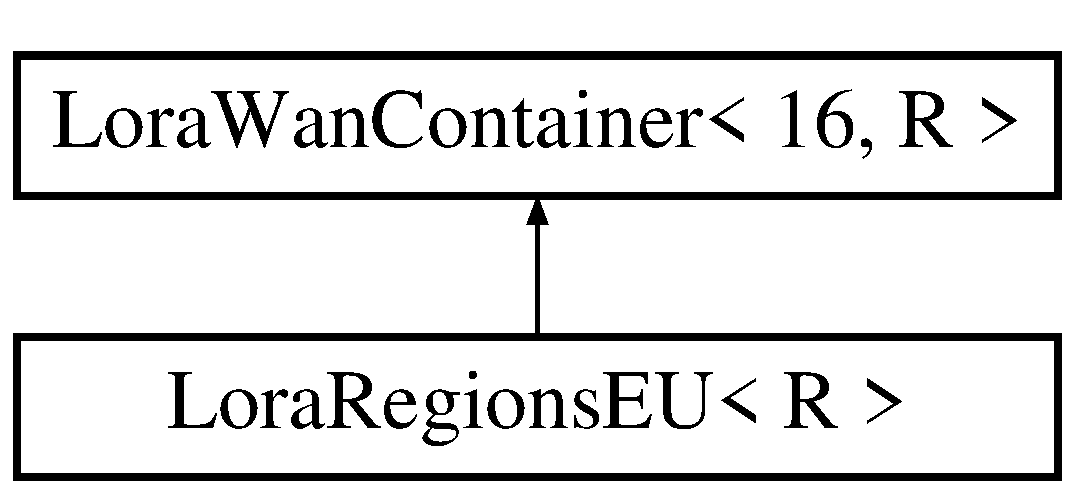
\includegraphics[height=2.000000cm]{class_lora_regions_e_u}
\end{center}
\end{figure}
\subsection*{Public Member Functions}
\begin{DoxyCompactItemize}
\item 
\mbox{\hyperlink{class_lora_regions_e_u_ae819c451aa7c913b67386705ed993645}{Lora\+Regions\+EU}} (\mbox{\hyperlink{structs_lo_ra_wan_keys}{s\+Lo\+Ra\+Wan\+Keys}} Lo\+Ra\+Wan\+Keys, R $\ast$Radio\+User, uint32\+\_\+t Flash\+Adress)
\item 
\mbox{\hyperlink{class_lora_regions_e_u_a7b420653e64fa700d76181d561eb4ca9}{$\sim$\+Lora\+Regions\+EU}} (void)
\item 
\mbox{\hyperlink{_define_8h_a1cea710adbbf5b02bced8f79cd82f7b9}{e\+Status\+Lo\+Ra\+Wan}} \mbox{\hyperlink{class_lora_regions_e_u_aac8f3f20d2a79717a1c0d26f72e073ef}{Region\+Max\+Payload\+Size}} (uint8\+\_\+t size\+In)
\item 
void \mbox{\hyperlink{class_lora_regions_e_u_a94b24cf6b5b8059025cb4e12d03eb97f}{Region\+Set\+Data\+Rate\+Distribution}} (uint8\+\_\+t adr\+Mode)
\item 
virtual void \mbox{\hyperlink{class_lora_regions_e_u_a10897e9e39c1b1682596b9e55844724c}{Region\+Give\+Next\+Data\+Rate}} (void)
\end{DoxyCompactItemize}
\subsection*{Public Attributes}
\begin{DoxyCompactItemize}
\item 
uint8\+\_\+t \mbox{\hyperlink{class_lora_regions_e_u_a9a47972a842e40860f3fd6c2a8bd8847}{Distri\+Data\+Rate}} \mbox{[}8\mbox{]}
\end{DoxyCompactItemize}
\subsection*{Static Public Attributes}
\begin{DoxyCompactItemize}
\item 
static const int \mbox{\hyperlink{class_lora_regions_e_u_a29147d2d0ea7d37b346a4b2744ed8f3a}{J\+O\+I\+N\+\_\+\+A\+C\+C\+E\+P\+T\+\_\+\+D\+E\+L\+A\+Y1}} = 5
\item 
static const int \mbox{\hyperlink{class_lora_regions_e_u_add1f86dd2dd8a0f831b1f683e255af1d}{J\+O\+I\+N\+\_\+\+A\+C\+C\+E\+P\+T\+\_\+\+D\+E\+L\+A\+Y2}} = 6
\item 
static const int \mbox{\hyperlink{class_lora_regions_e_u_a2a3dacdfb28c15b378393a78b92e4dc0}{R\+E\+C\+E\+I\+V\+E\+\_\+\+D\+E\+L\+A\+Y1}} = 1
\item 
static const int \mbox{\hyperlink{class_lora_regions_e_u_a534cd22621dc34cf64c82e76f19ab86c}{T\+X\+\_\+\+P\+O\+W\+ER}} = 14
\item 
static const int \mbox{\hyperlink{class_lora_regions_e_u_a1fad07be37bf7e340241ea2303bba1cb}{A\+D\+R\+\_\+\+A\+C\+K\+\_\+\+L\+I\+M\+IT}} = 64
\item 
static const int \mbox{\hyperlink{class_lora_regions_e_u_a5a934e60781a74b7342a6842b62a7a18}{A\+D\+R\+\_\+\+A\+C\+K\+\_\+\+D\+E\+L\+AY}} = 32
\item 
static const int \mbox{\hyperlink{class_lora_regions_e_u_ae52a86b43d3428a3cc74dbf44d223cd3}{A\+C\+K\+\_\+\+T\+I\+M\+E\+O\+UT}} = 2
\item 
static const uint32\+\_\+t \mbox{\hyperlink{class_lora_regions_e_u_a685911245b727e6545f7004761da6c07}{F\+R\+E\+Q\+M\+IN}} = 8630000
\item 
static const uint32\+\_\+t \mbox{\hyperlink{class_lora_regions_e_u_a4427ef38b32c6d61ba9e755e822c85ee}{F\+R\+E\+Q\+M\+AX}} = 8700000
\item 
static const int \mbox{\hyperlink{class_lora_regions_e_u_aab1f4fd427de20da11c75a1bb187504f}{R\+X2\+D\+R\+\_\+\+I\+N\+IT}} = 0
\end{DoxyCompactItemize}
\subsection*{Protected Member Functions}
\begin{DoxyCompactItemize}
\item 
virtual void \mbox{\hyperlink{class_lora_regions_e_u_acdbe1d2f767912fac7edf295961dfb6b}{Region\+Get\+C\+F\+List}} (void)
\item 
virtual void \mbox{\hyperlink{class_lora_regions_e_u_adf5f39b2b13ad1dca0eccb80123c261d}{Region\+Give\+Next\+Channel}} (void)
\item 
virtual void \mbox{\hyperlink{class_lora_regions_e_u_a1222a9362e7ba3715d9848af850af3f0}{Region\+Set\+Rx\+Config}} (\mbox{\hyperlink{_define_8h_ab894a4c21b8aae9e9c68d8c426a66956}{e\+Rx\+Win\+Type}} type)
\item 
virtual void \mbox{\hyperlink{class_lora_regions_e_u_a322d0f9d2a00243ef01fe15c017ed288}{Region\+Set\+Power}} (uint8\+\_\+t Power\+Cmd)
\item 
virtual void \mbox{\hyperlink{class_lora_regions_e_u_a9aef35dea0d5101768696bed87fa8380}{Region\+Set\+Mask}} (void)
\item 
virtual void \mbox{\hyperlink{class_lora_regions_e_u_a3662471b098dc1e319ab386eaf0b3f52}{Region\+Init\+Channel\+Mask}} (void)
\item 
virtual void \mbox{\hyperlink{class_lora_regions_e_u_ad6bf116000ec083c6e7e0a7f930aa2c6}{Region\+Decrease\+Data\+Rate}} (void)
\item 
virtual \mbox{\hyperlink{_define_8h_abbfbf157098d2505c0cf33877b128cc9}{e\+Status\+Channel}} \mbox{\hyperlink{class_lora_regions_e_u_af19055a7f2df125b3937ebaf033f50af}{Region\+Build\+Channel\+Mask}} (uint8\+\_\+t Ch\+Mask\+Cntl, uint16\+\_\+t Ch\+Mask)
\item 
virtual \mbox{\hyperlink{_define_8h_a1cea710adbbf5b02bced8f79cd82f7b9}{e\+Status\+Lo\+Ra\+Wan}} \mbox{\hyperlink{class_lora_regions_e_u_a6dc681bc39f00825ed46e9636d9acf52}{Region\+Is\+Valid\+Rx1\+Dr\+Offset}} (uint8\+\_\+t Rx1\+Data\+Rate\+Offset)
\item 
virtual \mbox{\hyperlink{_define_8h_a1cea710adbbf5b02bced8f79cd82f7b9}{e\+Status\+Lo\+Ra\+Wan}} \mbox{\hyperlink{class_lora_regions_e_u_aeb59fccca463d845279c448a6fa46548}{Region\+Is\+Valid\+Data\+Rate}} (uint8\+\_\+t temp)
\item 
virtual \mbox{\hyperlink{_define_8h_a1cea710adbbf5b02bced8f79cd82f7b9}{e\+Status\+Lo\+Ra\+Wan}} \mbox{\hyperlink{class_lora_regions_e_u_a367dcb126971269dce46511383696bad}{Region\+Is\+Acceptable\+Data\+Rate}} (uint8\+\_\+t Data\+Rate)
\item 
virtual \mbox{\hyperlink{_define_8h_a1cea710adbbf5b02bced8f79cd82f7b9}{e\+Status\+Lo\+Ra\+Wan}} \mbox{\hyperlink{class_lora_regions_e_u_a192e8af5bcab83f1f7ff48b5d130206e}{Region\+Is\+Valid\+Mac\+Frequency}} (uint32\+\_\+t Frequency)
\item 
virtual \mbox{\hyperlink{_define_8h_a1cea710adbbf5b02bced8f79cd82f7b9}{e\+Status\+Lo\+Ra\+Wan}} \mbox{\hyperlink{class_lora_regions_e_u_ac28aa9ff150676c7f1dd7425dbb6fffa}{Region\+Is\+Valid\+Tx\+Power}} (uint8\+\_\+t Power)
\item 
virtual \mbox{\hyperlink{_define_8h_a1cea710adbbf5b02bced8f79cd82f7b9}{e\+Status\+Lo\+Ra\+Wan}} \mbox{\hyperlink{class_lora_regions_e_u_a265374672b836ead15fe670d9207bf4e}{Region\+Is\+Valid\+Channel\+Index}} (uint8\+\_\+t Channel\+Index)
\item 
virtual uint8\+\_\+t \mbox{\hyperlink{class_lora_regions_e_u_aed553b79468100fb271bb2ac6a230c58}{Region\+Get\+Adr\+Ack\+Limit}} (void)
\item 
virtual uint8\+\_\+t \mbox{\hyperlink{class_lora_regions_e_u_a4e27410febd49bfc58d3bf986177c1e7}{Region\+Get\+Adr\+Ack\+Delay}} (void)
\end{DoxyCompactItemize}
\subsection*{Additional Inherited Members}


\subsection{Detailed Description}
\subsubsection*{template$<$class R$>$\newline
class Lora\+Regions\+E\+U$<$ R $>$}



Definition at line 36 of file Regions.\+h.



\subsection{Constructor \& Destructor Documentation}
\mbox{\Hypertarget{class_lora_regions_e_u_ae819c451aa7c913b67386705ed993645}\label{class_lora_regions_e_u_ae819c451aa7c913b67386705ed993645}} 
\index{Lora\+Regions\+EU@{Lora\+Regions\+EU}!Lora\+Regions\+EU@{Lora\+Regions\+EU}}
\index{Lora\+Regions\+EU@{Lora\+Regions\+EU}!Lora\+Regions\+EU@{Lora\+Regions\+EU}}
\subsubsection{\texorpdfstring{Lora\+Regions\+E\+U()}{LoraRegionsEU()}}
{\footnotesize\ttfamily template$<$class R $>$ \\
\mbox{\hyperlink{class_lora_regions_e_u}{Lora\+Regions\+EU}}$<$ R $>$\+::\mbox{\hyperlink{class_lora_regions_e_u}{Lora\+Regions\+EU}} (\begin{DoxyParamCaption}\item[{\mbox{\hyperlink{structs_lo_ra_wan_keys}{s\+Lo\+Ra\+Wan\+Keys}}}]{Lo\+Ra\+Wan\+Keys,  }\item[{R $\ast$}]{Radio\+User,  }\item[{uint32\+\_\+t}]{Flash\+Adress }\end{DoxyParamCaption})}



Definition at line 26 of file Regions.\+cpp.

\mbox{\Hypertarget{class_lora_regions_e_u_a7b420653e64fa700d76181d561eb4ca9}\label{class_lora_regions_e_u_a7b420653e64fa700d76181d561eb4ca9}} 
\index{Lora\+Regions\+EU@{Lora\+Regions\+EU}!````~Lora\+Regions\+EU@{$\sim$\+Lora\+Regions\+EU}}
\index{````~Lora\+Regions\+EU@{$\sim$\+Lora\+Regions\+EU}!Lora\+Regions\+EU@{Lora\+Regions\+EU}}
\subsubsection{\texorpdfstring{$\sim$\+Lora\+Regions\+E\+U()}{~LoraRegionsEU()}}
{\footnotesize\ttfamily template$<$class R $>$ \\
\mbox{\hyperlink{class_lora_regions_e_u}{Lora\+Regions\+EU}}$<$ R $>$\+::$\sim$\mbox{\hyperlink{class_lora_regions_e_u}{Lora\+Regions\+EU}} (\begin{DoxyParamCaption}\item[{void}]{ }\end{DoxyParamCaption})\hspace{0.3cm}{\ttfamily [inline]}}



Definition at line 42 of file Regions.\+h.



\subsection{Member Function Documentation}
\mbox{\Hypertarget{class_lora_regions_e_u_af19055a7f2df125b3937ebaf033f50af}\label{class_lora_regions_e_u_af19055a7f2df125b3937ebaf033f50af}} 
\index{Lora\+Regions\+EU@{Lora\+Regions\+EU}!Region\+Build\+Channel\+Mask@{Region\+Build\+Channel\+Mask}}
\index{Region\+Build\+Channel\+Mask@{Region\+Build\+Channel\+Mask}!Lora\+Regions\+EU@{Lora\+Regions\+EU}}
\subsubsection{\texorpdfstring{Region\+Build\+Channel\+Mask()}{RegionBuildChannelMask()}}
{\footnotesize\ttfamily template$<$class R $>$ \\
\mbox{\hyperlink{_define_8h_abbfbf157098d2505c0cf33877b128cc9}{e\+Status\+Channel}} \mbox{\hyperlink{class_lora_regions_e_u}{Lora\+Regions\+EU}}$<$ R $>$\+::Region\+Build\+Channel\+Mask (\begin{DoxyParamCaption}\item[{uint8\+\_\+t}]{Ch\+Mask\+Cntl,  }\item[{uint16\+\_\+t}]{Ch\+Mask }\end{DoxyParamCaption})\hspace{0.3cm}{\ttfamily [protected]}, {\ttfamily [virtual]}}



Implements \mbox{\hyperlink{class_lora_wan_container_a7f0fbbcc4652885003a1db83aa28e507}{Lora\+Wan\+Container$<$ 16, R $>$}}.



Definition at line 111 of file Regions.\+cpp.

\mbox{\Hypertarget{class_lora_regions_e_u_ad6bf116000ec083c6e7e0a7f930aa2c6}\label{class_lora_regions_e_u_ad6bf116000ec083c6e7e0a7f930aa2c6}} 
\index{Lora\+Regions\+EU@{Lora\+Regions\+EU}!Region\+Decrease\+Data\+Rate@{Region\+Decrease\+Data\+Rate}}
\index{Region\+Decrease\+Data\+Rate@{Region\+Decrease\+Data\+Rate}!Lora\+Regions\+EU@{Lora\+Regions\+EU}}
\subsubsection{\texorpdfstring{Region\+Decrease\+Data\+Rate()}{RegionDecreaseDataRate()}}
{\footnotesize\ttfamily template$<$class R $>$ \\
void \mbox{\hyperlink{class_lora_regions_e_u}{Lora\+Regions\+EU}}$<$ R $>$\+::Region\+Decrease\+Data\+Rate (\begin{DoxyParamCaption}\item[{void}]{ }\end{DoxyParamCaption})\hspace{0.3cm}{\ttfamily [protected]}, {\ttfamily [virtual]}}



Implements \mbox{\hyperlink{class_lora_wan_container_a198e46f5b6358987f6ec0b91fdc8eab9}{Lora\+Wan\+Container$<$ 16, R $>$}}.



Definition at line 336 of file Regions.\+cpp.

\mbox{\Hypertarget{class_lora_regions_e_u_a4e27410febd49bfc58d3bf986177c1e7}\label{class_lora_regions_e_u_a4e27410febd49bfc58d3bf986177c1e7}} 
\index{Lora\+Regions\+EU@{Lora\+Regions\+EU}!Region\+Get\+Adr\+Ack\+Delay@{Region\+Get\+Adr\+Ack\+Delay}}
\index{Region\+Get\+Adr\+Ack\+Delay@{Region\+Get\+Adr\+Ack\+Delay}!Lora\+Regions\+EU@{Lora\+Regions\+EU}}
\subsubsection{\texorpdfstring{Region\+Get\+Adr\+Ack\+Delay()}{RegionGetAdrAckDelay()}}
{\footnotesize\ttfamily template$<$class R $>$ \\
uint8\+\_\+t \mbox{\hyperlink{class_lora_regions_e_u}{Lora\+Regions\+EU}}$<$ R $>$\+::Region\+Get\+Adr\+Ack\+Delay (\begin{DoxyParamCaption}\item[{void}]{ }\end{DoxyParamCaption})\hspace{0.3cm}{\ttfamily [protected]}, {\ttfamily [virtual]}}



Implements \mbox{\hyperlink{class_lora_wan_container_ad90b5c47b794730a1027a548f20fd63c}{Lora\+Wan\+Container$<$ 16, R $>$}}.



Definition at line 384 of file Regions.\+cpp.

\mbox{\Hypertarget{class_lora_regions_e_u_aed553b79468100fb271bb2ac6a230c58}\label{class_lora_regions_e_u_aed553b79468100fb271bb2ac6a230c58}} 
\index{Lora\+Regions\+EU@{Lora\+Regions\+EU}!Region\+Get\+Adr\+Ack\+Limit@{Region\+Get\+Adr\+Ack\+Limit}}
\index{Region\+Get\+Adr\+Ack\+Limit@{Region\+Get\+Adr\+Ack\+Limit}!Lora\+Regions\+EU@{Lora\+Regions\+EU}}
\subsubsection{\texorpdfstring{Region\+Get\+Adr\+Ack\+Limit()}{RegionGetAdrAckLimit()}}
{\footnotesize\ttfamily template$<$class R $>$ \\
uint8\+\_\+t \mbox{\hyperlink{class_lora_regions_e_u}{Lora\+Regions\+EU}}$<$ R $>$\+::Region\+Get\+Adr\+Ack\+Limit (\begin{DoxyParamCaption}\item[{void}]{ }\end{DoxyParamCaption})\hspace{0.3cm}{\ttfamily [protected]}, {\ttfamily [virtual]}}



Implements \mbox{\hyperlink{class_lora_wan_container_ab68ac169b3edd9aacc7a9c40976dc231}{Lora\+Wan\+Container$<$ 16, R $>$}}.



Definition at line 381 of file Regions.\+cpp.

\mbox{\Hypertarget{class_lora_regions_e_u_acdbe1d2f767912fac7edf295961dfb6b}\label{class_lora_regions_e_u_acdbe1d2f767912fac7edf295961dfb6b}} 
\index{Lora\+Regions\+EU@{Lora\+Regions\+EU}!Region\+Get\+C\+F\+List@{Region\+Get\+C\+F\+List}}
\index{Region\+Get\+C\+F\+List@{Region\+Get\+C\+F\+List}!Lora\+Regions\+EU@{Lora\+Regions\+EU}}
\subsubsection{\texorpdfstring{Region\+Get\+C\+F\+List()}{RegionGetCFList()}}
{\footnotesize\ttfamily template$<$class R $>$ \\
void \mbox{\hyperlink{class_lora_regions_e_u}{Lora\+Regions\+EU}}$<$ R $>$\+::Region\+Get\+C\+F\+List (\begin{DoxyParamCaption}\item[{void}]{ }\end{DoxyParamCaption})\hspace{0.3cm}{\ttfamily [protected]}, {\ttfamily [virtual]}}



Implements \mbox{\hyperlink{class_lora_wan_container_a6603ef368fea1cf2d1e4de2120c1dff6}{Lora\+Wan\+Container$<$ 16, R $>$}}.



Definition at line 86 of file Regions.\+cpp.

\mbox{\Hypertarget{class_lora_regions_e_u_adf5f39b2b13ad1dca0eccb80123c261d}\label{class_lora_regions_e_u_adf5f39b2b13ad1dca0eccb80123c261d}} 
\index{Lora\+Regions\+EU@{Lora\+Regions\+EU}!Region\+Give\+Next\+Channel@{Region\+Give\+Next\+Channel}}
\index{Region\+Give\+Next\+Channel@{Region\+Give\+Next\+Channel}!Lora\+Regions\+EU@{Lora\+Regions\+EU}}
\subsubsection{\texorpdfstring{Region\+Give\+Next\+Channel()}{RegionGiveNextChannel()}}
{\footnotesize\ttfamily template$<$class R $>$ \\
void \mbox{\hyperlink{class_lora_regions_e_u}{Lora\+Regions\+EU}}$<$ R $>$\+::Region\+Give\+Next\+Channel (\begin{DoxyParamCaption}\item[{void}]{ }\end{DoxyParamCaption})\hspace{0.3cm}{\ttfamily [protected]}, {\ttfamily [virtual]}}



Implements \mbox{\hyperlink{class_lora_wan_container_a3ced7ed5217292b17d3f554fdc12c45e}{Lora\+Wan\+Container$<$ 16, R $>$}}.



Definition at line 362 of file Regions.\+cpp.

\mbox{\Hypertarget{class_lora_regions_e_u_a10897e9e39c1b1682596b9e55844724c}\label{class_lora_regions_e_u_a10897e9e39c1b1682596b9e55844724c}} 
\index{Lora\+Regions\+EU@{Lora\+Regions\+EU}!Region\+Give\+Next\+Data\+Rate@{Region\+Give\+Next\+Data\+Rate}}
\index{Region\+Give\+Next\+Data\+Rate@{Region\+Give\+Next\+Data\+Rate}!Lora\+Regions\+EU@{Lora\+Regions\+EU}}
\subsubsection{\texorpdfstring{Region\+Give\+Next\+Data\+Rate()}{RegionGiveNextDataRate()}}
{\footnotesize\ttfamily template$<$class R $>$ \\
void \mbox{\hyperlink{class_lora_regions_e_u}{Lora\+Regions\+EU}}$<$ R $>$\+::Region\+Give\+Next\+Data\+Rate (\begin{DoxyParamCaption}\item[{void}]{ }\end{DoxyParamCaption})\hspace{0.3cm}{\ttfamily [virtual]}}



Implements \mbox{\hyperlink{class_lora_wan_container_a32179d92bac6a7daea1bd39e84dec2a6}{Lora\+Wan\+Container$<$ 16, R $>$}}.



Definition at line 307 of file Regions.\+cpp.

\mbox{\Hypertarget{class_lora_regions_e_u_a3662471b098dc1e319ab386eaf0b3f52}\label{class_lora_regions_e_u_a3662471b098dc1e319ab386eaf0b3f52}} 
\index{Lora\+Regions\+EU@{Lora\+Regions\+EU}!Region\+Init\+Channel\+Mask@{Region\+Init\+Channel\+Mask}}
\index{Region\+Init\+Channel\+Mask@{Region\+Init\+Channel\+Mask}!Lora\+Regions\+EU@{Lora\+Regions\+EU}}
\subsubsection{\texorpdfstring{Region\+Init\+Channel\+Mask()}{RegionInitChannelMask()}}
{\footnotesize\ttfamily template$<$class R $>$ \\
void \mbox{\hyperlink{class_lora_regions_e_u}{Lora\+Regions\+EU}}$<$ R $>$\+::Region\+Init\+Channel\+Mask (\begin{DoxyParamCaption}\item[{void}]{ }\end{DoxyParamCaption})\hspace{0.3cm}{\ttfamily [protected]}, {\ttfamily [virtual]}}



Implements \mbox{\hyperlink{class_lora_wan_container_aeacbb5b9a6ca06708c095c2f67aae93e}{Lora\+Wan\+Container$<$ 16, R $>$}}.



Definition at line 139 of file Regions.\+cpp.

\mbox{\Hypertarget{class_lora_regions_e_u_a367dcb126971269dce46511383696bad}\label{class_lora_regions_e_u_a367dcb126971269dce46511383696bad}} 
\index{Lora\+Regions\+EU@{Lora\+Regions\+EU}!Region\+Is\+Acceptable\+Data\+Rate@{Region\+Is\+Acceptable\+Data\+Rate}}
\index{Region\+Is\+Acceptable\+Data\+Rate@{Region\+Is\+Acceptable\+Data\+Rate}!Lora\+Regions\+EU@{Lora\+Regions\+EU}}
\subsubsection{\texorpdfstring{Region\+Is\+Acceptable\+Data\+Rate()}{RegionIsAcceptableDataRate()}}
{\footnotesize\ttfamily template$<$class R $>$ \\
\mbox{\hyperlink{_define_8h_a1cea710adbbf5b02bced8f79cd82f7b9}{e\+Status\+Lo\+Ra\+Wan}} \mbox{\hyperlink{class_lora_regions_e_u}{Lora\+Regions\+EU}}$<$ R $>$\+::Region\+Is\+Acceptable\+Data\+Rate (\begin{DoxyParamCaption}\item[{uint8\+\_\+t}]{Data\+Rate }\end{DoxyParamCaption})\hspace{0.3cm}{\ttfamily [protected]}, {\ttfamily [virtual]}}



Implements \mbox{\hyperlink{class_lora_wan_container_a8316ea2c314c3809fa7c6b8e72e25df0}{Lora\+Wan\+Container$<$ 16, R $>$}}.



Definition at line 196 of file Regions.\+cpp.

\mbox{\Hypertarget{class_lora_regions_e_u_a265374672b836ead15fe670d9207bf4e}\label{class_lora_regions_e_u_a265374672b836ead15fe670d9207bf4e}} 
\index{Lora\+Regions\+EU@{Lora\+Regions\+EU}!Region\+Is\+Valid\+Channel\+Index@{Region\+Is\+Valid\+Channel\+Index}}
\index{Region\+Is\+Valid\+Channel\+Index@{Region\+Is\+Valid\+Channel\+Index}!Lora\+Regions\+EU@{Lora\+Regions\+EU}}
\subsubsection{\texorpdfstring{Region\+Is\+Valid\+Channel\+Index()}{RegionIsValidChannelIndex()}}
{\footnotesize\ttfamily template$<$class R $>$ \\
\mbox{\hyperlink{_define_8h_a1cea710adbbf5b02bced8f79cd82f7b9}{e\+Status\+Lo\+Ra\+Wan}} \mbox{\hyperlink{class_lora_regions_e_u}{Lora\+Regions\+EU}}$<$ R $>$\+::Region\+Is\+Valid\+Channel\+Index (\begin{DoxyParamCaption}\item[{uint8\+\_\+t}]{Channel\+Index }\end{DoxyParamCaption})\hspace{0.3cm}{\ttfamily [protected]}, {\ttfamily [virtual]}}



Implements \mbox{\hyperlink{class_lora_wan_container_a2eea298e891240d3367f2405b852964a}{Lora\+Wan\+Container$<$ 16, R $>$}}.



Definition at line 226 of file Regions.\+cpp.

\mbox{\Hypertarget{class_lora_regions_e_u_aeb59fccca463d845279c448a6fa46548}\label{class_lora_regions_e_u_aeb59fccca463d845279c448a6fa46548}} 
\index{Lora\+Regions\+EU@{Lora\+Regions\+EU}!Region\+Is\+Valid\+Data\+Rate@{Region\+Is\+Valid\+Data\+Rate}}
\index{Region\+Is\+Valid\+Data\+Rate@{Region\+Is\+Valid\+Data\+Rate}!Lora\+Regions\+EU@{Lora\+Regions\+EU}}
\subsubsection{\texorpdfstring{Region\+Is\+Valid\+Data\+Rate()}{RegionIsValidDataRate()}}
{\footnotesize\ttfamily template$<$class R $>$ \\
\mbox{\hyperlink{_define_8h_a1cea710adbbf5b02bced8f79cd82f7b9}{e\+Status\+Lo\+Ra\+Wan}} \mbox{\hyperlink{class_lora_regions_e_u}{Lora\+Regions\+EU}}$<$ R $>$\+::Region\+Is\+Valid\+Data\+Rate (\begin{DoxyParamCaption}\item[{uint8\+\_\+t}]{temp }\end{DoxyParamCaption})\hspace{0.3cm}{\ttfamily [protected]}, {\ttfamily [virtual]}}



Implements \mbox{\hyperlink{class_lora_wan_container_aeec0ea6c3979df30b2d9b27bdb8ea043}{Lora\+Wan\+Container$<$ 16, R $>$}}.



Definition at line 190 of file Regions.\+cpp.

\mbox{\Hypertarget{class_lora_regions_e_u_a192e8af5bcab83f1f7ff48b5d130206e}\label{class_lora_regions_e_u_a192e8af5bcab83f1f7ff48b5d130206e}} 
\index{Lora\+Regions\+EU@{Lora\+Regions\+EU}!Region\+Is\+Valid\+Mac\+Frequency@{Region\+Is\+Valid\+Mac\+Frequency}}
\index{Region\+Is\+Valid\+Mac\+Frequency@{Region\+Is\+Valid\+Mac\+Frequency}!Lora\+Regions\+EU@{Lora\+Regions\+EU}}
\subsubsection{\texorpdfstring{Region\+Is\+Valid\+Mac\+Frequency()}{RegionIsValidMacFrequency()}}
{\footnotesize\ttfamily template$<$class R $>$ \\
\mbox{\hyperlink{_define_8h_a1cea710adbbf5b02bced8f79cd82f7b9}{e\+Status\+Lo\+Ra\+Wan}} \mbox{\hyperlink{class_lora_regions_e_u}{Lora\+Regions\+EU}}$<$ R $>$\+::Region\+Is\+Valid\+Mac\+Frequency (\begin{DoxyParamCaption}\item[{uint32\+\_\+t}]{Frequency }\end{DoxyParamCaption})\hspace{0.3cm}{\ttfamily [protected]}, {\ttfamily [virtual]}}



Implements \mbox{\hyperlink{class_lora_wan_container_a14be092c3440b0bbfe9683f14c648eb2}{Lora\+Wan\+Container$<$ 16, R $>$}}.



Definition at line 207 of file Regions.\+cpp.

\mbox{\Hypertarget{class_lora_regions_e_u_a6dc681bc39f00825ed46e9636d9acf52}\label{class_lora_regions_e_u_a6dc681bc39f00825ed46e9636d9acf52}} 
\index{Lora\+Regions\+EU@{Lora\+Regions\+EU}!Region\+Is\+Valid\+Rx1\+Dr\+Offset@{Region\+Is\+Valid\+Rx1\+Dr\+Offset}}
\index{Region\+Is\+Valid\+Rx1\+Dr\+Offset@{Region\+Is\+Valid\+Rx1\+Dr\+Offset}!Lora\+Regions\+EU@{Lora\+Regions\+EU}}
\subsubsection{\texorpdfstring{Region\+Is\+Valid\+Rx1\+Dr\+Offset()}{RegionIsValidRx1DrOffset()}}
{\footnotesize\ttfamily template$<$class R $>$ \\
\mbox{\hyperlink{_define_8h_a1cea710adbbf5b02bced8f79cd82f7b9}{e\+Status\+Lo\+Ra\+Wan}} \mbox{\hyperlink{class_lora_regions_e_u}{Lora\+Regions\+EU}}$<$ R $>$\+::Region\+Is\+Valid\+Rx1\+Dr\+Offset (\begin{DoxyParamCaption}\item[{uint8\+\_\+t}]{Rx1\+Data\+Rate\+Offset }\end{DoxyParamCaption})\hspace{0.3cm}{\ttfamily [protected]}, {\ttfamily [virtual]}}



Implements \mbox{\hyperlink{class_lora_wan_container_ac5d3abcc857b6b1f0535e12915dd2bfb}{Lora\+Wan\+Container$<$ 16, R $>$}}.



Definition at line 181 of file Regions.\+cpp.

\mbox{\Hypertarget{class_lora_regions_e_u_ac28aa9ff150676c7f1dd7425dbb6fffa}\label{class_lora_regions_e_u_ac28aa9ff150676c7f1dd7425dbb6fffa}} 
\index{Lora\+Regions\+EU@{Lora\+Regions\+EU}!Region\+Is\+Valid\+Tx\+Power@{Region\+Is\+Valid\+Tx\+Power}}
\index{Region\+Is\+Valid\+Tx\+Power@{Region\+Is\+Valid\+Tx\+Power}!Lora\+Regions\+EU@{Lora\+Regions\+EU}}
\subsubsection{\texorpdfstring{Region\+Is\+Valid\+Tx\+Power()}{RegionIsValidTxPower()}}
{\footnotesize\ttfamily template$<$class R $>$ \\
\mbox{\hyperlink{_define_8h_a1cea710adbbf5b02bced8f79cd82f7b9}{e\+Status\+Lo\+Ra\+Wan}} \mbox{\hyperlink{class_lora_regions_e_u}{Lora\+Regions\+EU}}$<$ R $>$\+::Region\+Is\+Valid\+Tx\+Power (\begin{DoxyParamCaption}\item[{uint8\+\_\+t}]{Power }\end{DoxyParamCaption})\hspace{0.3cm}{\ttfamily [protected]}, {\ttfamily [virtual]}}



Implements \mbox{\hyperlink{class_lora_wan_container_a481b6761bc4743086db57fb0adfb4d88}{Lora\+Wan\+Container$<$ 16, R $>$}}.



Definition at line 218 of file Regions.\+cpp.

\mbox{\Hypertarget{class_lora_regions_e_u_aac8f3f20d2a79717a1c0d26f72e073ef}\label{class_lora_regions_e_u_aac8f3f20d2a79717a1c0d26f72e073ef}} 
\index{Lora\+Regions\+EU@{Lora\+Regions\+EU}!Region\+Max\+Payload\+Size@{Region\+Max\+Payload\+Size}}
\index{Region\+Max\+Payload\+Size@{Region\+Max\+Payload\+Size}!Lora\+Regions\+EU@{Lora\+Regions\+EU}}
\subsubsection{\texorpdfstring{Region\+Max\+Payload\+Size()}{RegionMaxPayloadSize()}}
{\footnotesize\ttfamily template$<$class R $>$ \\
\mbox{\hyperlink{_define_8h_a1cea710adbbf5b02bced8f79cd82f7b9}{e\+Status\+Lo\+Ra\+Wan}} \mbox{\hyperlink{class_lora_regions_e_u}{Lora\+Regions\+EU}}$<$ R $>$\+::Region\+Max\+Payload\+Size (\begin{DoxyParamCaption}\item[{uint8\+\_\+t}]{size\+In }\end{DoxyParamCaption})}



Definition at line 154 of file Regions.\+cpp.

\mbox{\Hypertarget{class_lora_regions_e_u_a94b24cf6b5b8059025cb4e12d03eb97f}\label{class_lora_regions_e_u_a94b24cf6b5b8059025cb4e12d03eb97f}} 
\index{Lora\+Regions\+EU@{Lora\+Regions\+EU}!Region\+Set\+Data\+Rate\+Distribution@{Region\+Set\+Data\+Rate\+Distribution}}
\index{Region\+Set\+Data\+Rate\+Distribution@{Region\+Set\+Data\+Rate\+Distribution}!Lora\+Regions\+EU@{Lora\+Regions\+EU}}
\subsubsection{\texorpdfstring{Region\+Set\+Data\+Rate\+Distribution()}{RegionSetDataRateDistribution()}}
{\footnotesize\ttfamily template$<$class R $>$ \\
void \mbox{\hyperlink{class_lora_regions_e_u}{Lora\+Regions\+EU}}$<$ R $>$\+::Region\+Set\+Data\+Rate\+Distribution (\begin{DoxyParamCaption}\item[{uint8\+\_\+t}]{adr\+Mode }\end{DoxyParamCaption})}



Definition at line 241 of file Regions.\+cpp.

\mbox{\Hypertarget{class_lora_regions_e_u_a9aef35dea0d5101768696bed87fa8380}\label{class_lora_regions_e_u_a9aef35dea0d5101768696bed87fa8380}} 
\index{Lora\+Regions\+EU@{Lora\+Regions\+EU}!Region\+Set\+Mask@{Region\+Set\+Mask}}
\index{Region\+Set\+Mask@{Region\+Set\+Mask}!Lora\+Regions\+EU@{Lora\+Regions\+EU}}
\subsubsection{\texorpdfstring{Region\+Set\+Mask()}{RegionSetMask()}}
{\footnotesize\ttfamily template$<$class R $>$ \\
void \mbox{\hyperlink{class_lora_regions_e_u}{Lora\+Regions\+EU}}$<$ R $>$\+::Region\+Set\+Mask (\begin{DoxyParamCaption}\item[{void}]{ }\end{DoxyParamCaption})\hspace{0.3cm}{\ttfamily [protected]}, {\ttfamily [virtual]}}



Implements \mbox{\hyperlink{class_lora_wan_container_a1256cfca2973d3cb9114a3f25dfa9aca}{Lora\+Wan\+Container$<$ 16, R $>$}}.



Definition at line 142 of file Regions.\+cpp.

\mbox{\Hypertarget{class_lora_regions_e_u_a322d0f9d2a00243ef01fe15c017ed288}\label{class_lora_regions_e_u_a322d0f9d2a00243ef01fe15c017ed288}} 
\index{Lora\+Regions\+EU@{Lora\+Regions\+EU}!Region\+Set\+Power@{Region\+Set\+Power}}
\index{Region\+Set\+Power@{Region\+Set\+Power}!Lora\+Regions\+EU@{Lora\+Regions\+EU}}
\subsubsection{\texorpdfstring{Region\+Set\+Power()}{RegionSetPower()}}
{\footnotesize\ttfamily template$<$class R $>$ \\
void \mbox{\hyperlink{class_lora_regions_e_u}{Lora\+Regions\+EU}}$<$ R $>$\+::Region\+Set\+Power (\begin{DoxyParamCaption}\item[{uint8\+\_\+t}]{Power\+Cmd }\end{DoxyParamCaption})\hspace{0.3cm}{\ttfamily [protected]}, {\ttfamily [virtual]}}



Implements \mbox{\hyperlink{class_lora_wan_container_a6f489634d893e32270ded4b471f93080}{Lora\+Wan\+Container$<$ 16, R $>$}}.



Definition at line 71 of file Regions.\+cpp.

\mbox{\Hypertarget{class_lora_regions_e_u_a1222a9362e7ba3715d9848af850af3f0}\label{class_lora_regions_e_u_a1222a9362e7ba3715d9848af850af3f0}} 
\index{Lora\+Regions\+EU@{Lora\+Regions\+EU}!Region\+Set\+Rx\+Config@{Region\+Set\+Rx\+Config}}
\index{Region\+Set\+Rx\+Config@{Region\+Set\+Rx\+Config}!Lora\+Regions\+EU@{Lora\+Regions\+EU}}
\subsubsection{\texorpdfstring{Region\+Set\+Rx\+Config()}{RegionSetRxConfig()}}
{\footnotesize\ttfamily template$<$class R $>$ \\
void \mbox{\hyperlink{class_lora_regions_e_u}{Lora\+Regions\+EU}}$<$ R $>$\+::Region\+Set\+Rx\+Config (\begin{DoxyParamCaption}\item[{\mbox{\hyperlink{_define_8h_ab894a4c21b8aae9e9c68d8c426a66956}{e\+Rx\+Win\+Type}}}]{type }\end{DoxyParamCaption})\hspace{0.3cm}{\ttfamily [protected]}, {\ttfamily [virtual]}}



Implements \mbox{\hyperlink{class_lora_wan_container_a6d9c6a90a373153f95897951b877d826}{Lora\+Wan\+Container$<$ 16, R $>$}}.



Definition at line 166 of file Regions.\+cpp.



\subsection{Member Data Documentation}
\mbox{\Hypertarget{class_lora_regions_e_u_ae52a86b43d3428a3cc74dbf44d223cd3}\label{class_lora_regions_e_u_ae52a86b43d3428a3cc74dbf44d223cd3}} 
\index{Lora\+Regions\+EU@{Lora\+Regions\+EU}!A\+C\+K\+\_\+\+T\+I\+M\+E\+O\+UT@{A\+C\+K\+\_\+\+T\+I\+M\+E\+O\+UT}}
\index{A\+C\+K\+\_\+\+T\+I\+M\+E\+O\+UT@{A\+C\+K\+\_\+\+T\+I\+M\+E\+O\+UT}!Lora\+Regions\+EU@{Lora\+Regions\+EU}}
\subsubsection{\texorpdfstring{A\+C\+K\+\_\+\+T\+I\+M\+E\+O\+UT}{ACK\_TIMEOUT}}
{\footnotesize\ttfamily template$<$class R $>$ \\
const int \mbox{\hyperlink{class_lora_regions_e_u}{Lora\+Regions\+EU}}$<$ R $>$\+::A\+C\+K\+\_\+\+T\+I\+M\+E\+O\+UT = 2\hspace{0.3cm}{\ttfamily [static]}}



Definition at line 52 of file Regions.\+h.

\mbox{\Hypertarget{class_lora_regions_e_u_a5a934e60781a74b7342a6842b62a7a18}\label{class_lora_regions_e_u_a5a934e60781a74b7342a6842b62a7a18}} 
\index{Lora\+Regions\+EU@{Lora\+Regions\+EU}!A\+D\+R\+\_\+\+A\+C\+K\+\_\+\+D\+E\+L\+AY@{A\+D\+R\+\_\+\+A\+C\+K\+\_\+\+D\+E\+L\+AY}}
\index{A\+D\+R\+\_\+\+A\+C\+K\+\_\+\+D\+E\+L\+AY@{A\+D\+R\+\_\+\+A\+C\+K\+\_\+\+D\+E\+L\+AY}!Lora\+Regions\+EU@{Lora\+Regions\+EU}}
\subsubsection{\texorpdfstring{A\+D\+R\+\_\+\+A\+C\+K\+\_\+\+D\+E\+L\+AY}{ADR\_ACK\_DELAY}}
{\footnotesize\ttfamily template$<$class R $>$ \\
const int \mbox{\hyperlink{class_lora_regions_e_u}{Lora\+Regions\+EU}}$<$ R $>$\+::A\+D\+R\+\_\+\+A\+C\+K\+\_\+\+D\+E\+L\+AY = 32\hspace{0.3cm}{\ttfamily [static]}}



Definition at line 51 of file Regions.\+h.

\mbox{\Hypertarget{class_lora_regions_e_u_a1fad07be37bf7e340241ea2303bba1cb}\label{class_lora_regions_e_u_a1fad07be37bf7e340241ea2303bba1cb}} 
\index{Lora\+Regions\+EU@{Lora\+Regions\+EU}!A\+D\+R\+\_\+\+A\+C\+K\+\_\+\+L\+I\+M\+IT@{A\+D\+R\+\_\+\+A\+C\+K\+\_\+\+L\+I\+M\+IT}}
\index{A\+D\+R\+\_\+\+A\+C\+K\+\_\+\+L\+I\+M\+IT@{A\+D\+R\+\_\+\+A\+C\+K\+\_\+\+L\+I\+M\+IT}!Lora\+Regions\+EU@{Lora\+Regions\+EU}}
\subsubsection{\texorpdfstring{A\+D\+R\+\_\+\+A\+C\+K\+\_\+\+L\+I\+M\+IT}{ADR\_ACK\_LIMIT}}
{\footnotesize\ttfamily template$<$class R $>$ \\
const int \mbox{\hyperlink{class_lora_regions_e_u}{Lora\+Regions\+EU}}$<$ R $>$\+::A\+D\+R\+\_\+\+A\+C\+K\+\_\+\+L\+I\+M\+IT = 64\hspace{0.3cm}{\ttfamily [static]}}



Definition at line 50 of file Regions.\+h.

\mbox{\Hypertarget{class_lora_regions_e_u_a9a47972a842e40860f3fd6c2a8bd8847}\label{class_lora_regions_e_u_a9a47972a842e40860f3fd6c2a8bd8847}} 
\index{Lora\+Regions\+EU@{Lora\+Regions\+EU}!Distri\+Data\+Rate@{Distri\+Data\+Rate}}
\index{Distri\+Data\+Rate@{Distri\+Data\+Rate}!Lora\+Regions\+EU@{Lora\+Regions\+EU}}
\subsubsection{\texorpdfstring{Distri\+Data\+Rate}{DistriDataRate}}
{\footnotesize\ttfamily template$<$class R $>$ \\
uint8\+\_\+t \mbox{\hyperlink{class_lora_regions_e_u}{Lora\+Regions\+EU}}$<$ R $>$\+::Distri\+Data\+Rate\mbox{[}8\mbox{]}}



Definition at line 56 of file Regions.\+h.

\mbox{\Hypertarget{class_lora_regions_e_u_a4427ef38b32c6d61ba9e755e822c85ee}\label{class_lora_regions_e_u_a4427ef38b32c6d61ba9e755e822c85ee}} 
\index{Lora\+Regions\+EU@{Lora\+Regions\+EU}!F\+R\+E\+Q\+M\+AX@{F\+R\+E\+Q\+M\+AX}}
\index{F\+R\+E\+Q\+M\+AX@{F\+R\+E\+Q\+M\+AX}!Lora\+Regions\+EU@{Lora\+Regions\+EU}}
\subsubsection{\texorpdfstring{F\+R\+E\+Q\+M\+AX}{FREQMAX}}
{\footnotesize\ttfamily template$<$class R $>$ \\
const uint32\+\_\+t \mbox{\hyperlink{class_lora_regions_e_u}{Lora\+Regions\+EU}}$<$ R $>$\+::F\+R\+E\+Q\+M\+AX = 8700000\hspace{0.3cm}{\ttfamily [static]}}



Definition at line 54 of file Regions.\+h.

\mbox{\Hypertarget{class_lora_regions_e_u_a685911245b727e6545f7004761da6c07}\label{class_lora_regions_e_u_a685911245b727e6545f7004761da6c07}} 
\index{Lora\+Regions\+EU@{Lora\+Regions\+EU}!F\+R\+E\+Q\+M\+IN@{F\+R\+E\+Q\+M\+IN}}
\index{F\+R\+E\+Q\+M\+IN@{F\+R\+E\+Q\+M\+IN}!Lora\+Regions\+EU@{Lora\+Regions\+EU}}
\subsubsection{\texorpdfstring{F\+R\+E\+Q\+M\+IN}{FREQMIN}}
{\footnotesize\ttfamily template$<$class R $>$ \\
const uint32\+\_\+t \mbox{\hyperlink{class_lora_regions_e_u}{Lora\+Regions\+EU}}$<$ R $>$\+::F\+R\+E\+Q\+M\+IN = 8630000\hspace{0.3cm}{\ttfamily [static]}}



Definition at line 53 of file Regions.\+h.

\mbox{\Hypertarget{class_lora_regions_e_u_a29147d2d0ea7d37b346a4b2744ed8f3a}\label{class_lora_regions_e_u_a29147d2d0ea7d37b346a4b2744ed8f3a}} 
\index{Lora\+Regions\+EU@{Lora\+Regions\+EU}!J\+O\+I\+N\+\_\+\+A\+C\+C\+E\+P\+T\+\_\+\+D\+E\+L\+A\+Y1@{J\+O\+I\+N\+\_\+\+A\+C\+C\+E\+P\+T\+\_\+\+D\+E\+L\+A\+Y1}}
\index{J\+O\+I\+N\+\_\+\+A\+C\+C\+E\+P\+T\+\_\+\+D\+E\+L\+A\+Y1@{J\+O\+I\+N\+\_\+\+A\+C\+C\+E\+P\+T\+\_\+\+D\+E\+L\+A\+Y1}!Lora\+Regions\+EU@{Lora\+Regions\+EU}}
\subsubsection{\texorpdfstring{J\+O\+I\+N\+\_\+\+A\+C\+C\+E\+P\+T\+\_\+\+D\+E\+L\+A\+Y1}{JOIN\_ACCEPT\_DELAY1}}
{\footnotesize\ttfamily template$<$class R $>$ \\
const int \mbox{\hyperlink{class_lora_regions_e_u}{Lora\+Regions\+EU}}$<$ R $>$\+::J\+O\+I\+N\+\_\+\+A\+C\+C\+E\+P\+T\+\_\+\+D\+E\+L\+A\+Y1 = 5\hspace{0.3cm}{\ttfamily [static]}}



Definition at line 46 of file Regions.\+h.

\mbox{\Hypertarget{class_lora_regions_e_u_add1f86dd2dd8a0f831b1f683e255af1d}\label{class_lora_regions_e_u_add1f86dd2dd8a0f831b1f683e255af1d}} 
\index{Lora\+Regions\+EU@{Lora\+Regions\+EU}!J\+O\+I\+N\+\_\+\+A\+C\+C\+E\+P\+T\+\_\+\+D\+E\+L\+A\+Y2@{J\+O\+I\+N\+\_\+\+A\+C\+C\+E\+P\+T\+\_\+\+D\+E\+L\+A\+Y2}}
\index{J\+O\+I\+N\+\_\+\+A\+C\+C\+E\+P\+T\+\_\+\+D\+E\+L\+A\+Y2@{J\+O\+I\+N\+\_\+\+A\+C\+C\+E\+P\+T\+\_\+\+D\+E\+L\+A\+Y2}!Lora\+Regions\+EU@{Lora\+Regions\+EU}}
\subsubsection{\texorpdfstring{J\+O\+I\+N\+\_\+\+A\+C\+C\+E\+P\+T\+\_\+\+D\+E\+L\+A\+Y2}{JOIN\_ACCEPT\_DELAY2}}
{\footnotesize\ttfamily template$<$class R $>$ \\
const int \mbox{\hyperlink{class_lora_regions_e_u}{Lora\+Regions\+EU}}$<$ R $>$\+::J\+O\+I\+N\+\_\+\+A\+C\+C\+E\+P\+T\+\_\+\+D\+E\+L\+A\+Y2 = 6\hspace{0.3cm}{\ttfamily [static]}}



Definition at line 47 of file Regions.\+h.

\mbox{\Hypertarget{class_lora_regions_e_u_a2a3dacdfb28c15b378393a78b92e4dc0}\label{class_lora_regions_e_u_a2a3dacdfb28c15b378393a78b92e4dc0}} 
\index{Lora\+Regions\+EU@{Lora\+Regions\+EU}!R\+E\+C\+E\+I\+V\+E\+\_\+\+D\+E\+L\+A\+Y1@{R\+E\+C\+E\+I\+V\+E\+\_\+\+D\+E\+L\+A\+Y1}}
\index{R\+E\+C\+E\+I\+V\+E\+\_\+\+D\+E\+L\+A\+Y1@{R\+E\+C\+E\+I\+V\+E\+\_\+\+D\+E\+L\+A\+Y1}!Lora\+Regions\+EU@{Lora\+Regions\+EU}}
\subsubsection{\texorpdfstring{R\+E\+C\+E\+I\+V\+E\+\_\+\+D\+E\+L\+A\+Y1}{RECEIVE\_DELAY1}}
{\footnotesize\ttfamily template$<$class R $>$ \\
const int \mbox{\hyperlink{class_lora_regions_e_u}{Lora\+Regions\+EU}}$<$ R $>$\+::R\+E\+C\+E\+I\+V\+E\+\_\+\+D\+E\+L\+A\+Y1 = 1\hspace{0.3cm}{\ttfamily [static]}}



Definition at line 48 of file Regions.\+h.

\mbox{\Hypertarget{class_lora_regions_e_u_aab1f4fd427de20da11c75a1bb187504f}\label{class_lora_regions_e_u_aab1f4fd427de20da11c75a1bb187504f}} 
\index{Lora\+Regions\+EU@{Lora\+Regions\+EU}!R\+X2\+D\+R\+\_\+\+I\+N\+IT@{R\+X2\+D\+R\+\_\+\+I\+N\+IT}}
\index{R\+X2\+D\+R\+\_\+\+I\+N\+IT@{R\+X2\+D\+R\+\_\+\+I\+N\+IT}!Lora\+Regions\+EU@{Lora\+Regions\+EU}}
\subsubsection{\texorpdfstring{R\+X2\+D\+R\+\_\+\+I\+N\+IT}{RX2DR\_INIT}}
{\footnotesize\ttfamily template$<$class R $>$ \\
const int \mbox{\hyperlink{class_lora_regions_e_u}{Lora\+Regions\+EU}}$<$ R $>$\+::R\+X2\+D\+R\+\_\+\+I\+N\+IT = 0\hspace{0.3cm}{\ttfamily [static]}}



Definition at line 55 of file Regions.\+h.

\mbox{\Hypertarget{class_lora_regions_e_u_a534cd22621dc34cf64c82e76f19ab86c}\label{class_lora_regions_e_u_a534cd22621dc34cf64c82e76f19ab86c}} 
\index{Lora\+Regions\+EU@{Lora\+Regions\+EU}!T\+X\+\_\+\+P\+O\+W\+ER@{T\+X\+\_\+\+P\+O\+W\+ER}}
\index{T\+X\+\_\+\+P\+O\+W\+ER@{T\+X\+\_\+\+P\+O\+W\+ER}!Lora\+Regions\+EU@{Lora\+Regions\+EU}}
\subsubsection{\texorpdfstring{T\+X\+\_\+\+P\+O\+W\+ER}{TX\_POWER}}
{\footnotesize\ttfamily template$<$class R $>$ \\
const int \mbox{\hyperlink{class_lora_regions_e_u}{Lora\+Regions\+EU}}$<$ R $>$\+::T\+X\+\_\+\+P\+O\+W\+ER = 14\hspace{0.3cm}{\ttfamily [static]}}



Definition at line 49 of file Regions.\+h.



The documentation for this class was generated from the following files\+:\begin{DoxyCompactItemize}
\item 
C\+:/\+G\+I\+T\+E\+X\+T/githubdoc/\+Lo\+Ra\+Wan\+Mini\+Mouse.\+github.\+io/\+M\+Mstack/\+Minimouse\+Src/\mbox{\hyperlink{_regions_8h}{Regions.\+h}}\item 
C\+:/\+G\+I\+T\+E\+X\+T/githubdoc/\+Lo\+Ra\+Wan\+Mini\+Mouse.\+github.\+io/\+M\+Mstack/\+Minimouse\+Src/\mbox{\hyperlink{_regions_8cpp}{Regions.\+cpp}}\end{DoxyCompactItemize}

\hypertarget{class_lora_wan_container}{}\section{Lora\+Wan\+Container$<$ N\+B\+C\+H\+A\+N\+N\+EL, R $>$ Class Template Reference}
\label{class_lora_wan_container}\index{Lora\+Wan\+Container$<$ N\+B\+C\+H\+A\+N\+N\+E\+L, R $>$@{Lora\+Wan\+Container$<$ N\+B\+C\+H\+A\+N\+N\+E\+L, R $>$}}


{\ttfamily \#include $<$Mac\+Layer.\+h$>$}

\subsection*{Public Member Functions}
\begin{DoxyCompactItemize}
\item 
\mbox{\hyperlink{class_lora_wan_container_a44404ff31803a6c55ffc152c023a7db8}{Lora\+Wan\+Container}} (\mbox{\hyperlink{structs_lo_ra_wan_keys}{s\+Lo\+Ra\+Wan\+Keys}} Lo\+Ra\+Wan\+Keys, R $\ast$Radio\+User, uint32\+\_\+t Flash\+Adress)
\item 
\mbox{\hyperlink{class_lora_wan_container_ae1add5f5a0620c3d513737e2e7241575}{$\sim$\+Lora\+Wan\+Container}} ()
\item 
void \mbox{\hyperlink{class_lora_wan_container_a6f0a9f6cddbd54a1fc5dd4c6de790d88}{Build\+Tx\+Lora\+Frame}} (void)
\item 
void \mbox{\hyperlink{class_lora_wan_container_a6ae2e50f7bc0eb014745ac1e2f48d0af}{Build\+Join\+Lora\+Frame}} (void)
\item 
void \mbox{\hyperlink{class_lora_wan_container_ae9bc11031f33b9bc4928b021a6a34cbd}{Encrypt\+Tx\+Frame}} (void)
\item 
void \mbox{\hyperlink{class_lora_wan_container_ac9a6098c71b551eccdea9b1f29f50c96}{Configure\+Radio\+And\+Send}} (void)
\item 
void \mbox{\hyperlink{class_lora_wan_container_a5c438e86f462a461cbc244054a2c27bb}{Configure\+Radio\+For\+Rx1}} (void)
\item 
void \mbox{\hyperlink{class_lora_wan_container_a9f189640ccae4f4b1e11c4671c88b6c0}{Configure\+Radio\+For\+Rx2}} (void)
\item 
void \mbox{\hyperlink{class_lora_wan_container_a077db278808a15326893610820e26b22}{Configure\+Timer\+For\+Rx}} (\mbox{\hyperlink{_define_8h_ab894a4c21b8aae9e9c68d8c426a66956}{e\+Rx\+Win\+Type}} type)
\item 
void \mbox{\hyperlink{class_lora_wan_container_a99e0d080f7a2bd65252d688e2a4befa1}{Update\+Mac\+Layer}} (void)
\item 
void \mbox{\hyperlink{class_lora_wan_container_a4e3a03ff91ae1ebca993206fc9d18c2d}{Update\+Join\+Procedure}} (void)
\item 
\mbox{\hyperlink{_define_8h_ac1b1454c99671113bca600652e09e8bd}{e\+Rx\+Packet\+Type}} \mbox{\hyperlink{class_lora_wan_container_a757fc71b5986280b6702febbf7bd87f3}{Decode\+Rx\+Frame}} (void)
\item 
\mbox{\hyperlink{_define_8h_a1cea710adbbf5b02bced8f79cd82f7b9}{e\+Status\+Lo\+Ra\+Wan}} \mbox{\hyperlink{class_lora_wan_container_a8b040b7c680d7fa3998a37cb462c74f7}{Parse\+Management\+Packet}} (void)
\item 
void \mbox{\hyperlink{class_lora_wan_container_a0c319cd6644631008aaa3e600e66d2a4}{Isr\+Timer\+Rx1}} (void)
\item 
void \mbox{\hyperlink{class_lora_wan_container_a787bbbf8efd3d85e2938c0bf46b22bfd}{Isr\+Timer\+Rx2}} (void)
\item 
void \mbox{\hyperlink{class_lora_wan_container_abc16aeda3958e34b81e72752e6331be3}{Load\+From\+Flash}} (void)
\item 
void \mbox{\hyperlink{class_lora_wan_container_a91e8c03b02a6672fe5f0342129618bb3}{Save\+In\+Flash}} (void)
\item 
void \mbox{\hyperlink{class_lora_wan_container_a488791458e4b9098607d2f502da9d633}{Set\+Bad\+Crc\+In\+Flash}} (void)
\item 
virtual void \mbox{\hyperlink{class_lora_wan_container_a3ced7ed5217292b17d3f554fdc12c45e}{Region\+Give\+Next\+Channel}} (void)=0
\item 
virtual void \mbox{\hyperlink{class_lora_wan_container_a6d9c6a90a373153f95897951b877d826}{Region\+Set\+Rx\+Config}} (\mbox{\hyperlink{_define_8h_ab894a4c21b8aae9e9c68d8c426a66956}{e\+Rx\+Win\+Type}} type)=0
\item 
virtual void \mbox{\hyperlink{class_lora_wan_container_a6f489634d893e32270ded4b471f93080}{Region\+Set\+Power}} (uint8\+\_\+t Power\+Cmd)=0
\item 
virtual void \mbox{\hyperlink{class_lora_wan_container_a1256cfca2973d3cb9114a3f25dfa9aca}{Region\+Set\+Mask}} (void)=0
\item 
virtual void \mbox{\hyperlink{class_lora_wan_container_aeacbb5b9a6ca06708c095c2f67aae93e}{Region\+Init\+Channel\+Mask}} (void)=0
\item 
virtual void \mbox{\hyperlink{class_lora_wan_container_a6603ef368fea1cf2d1e4de2120c1dff6}{Region\+Get\+C\+F\+List}} (void)=0
\item 
virtual void \mbox{\hyperlink{class_lora_wan_container_a198e46f5b6358987f6ec0b91fdc8eab9}{Region\+Decrease\+Data\+Rate}} (void)=0
\item 
virtual void \mbox{\hyperlink{class_lora_wan_container_a32179d92bac6a7daea1bd39e84dec2a6}{Region\+Give\+Next\+Data\+Rate}} (void)=0
\item 
virtual \mbox{\hyperlink{_define_8h_abbfbf157098d2505c0cf33877b128cc9}{e\+Status\+Channel}} \mbox{\hyperlink{class_lora_wan_container_a7f0fbbcc4652885003a1db83aa28e507}{Region\+Build\+Channel\+Mask}} (uint8\+\_\+t Ch\+Mask\+Cntl, uint16\+\_\+t Ch\+Mask\+In)=0
\item 
virtual \mbox{\hyperlink{_define_8h_a1cea710adbbf5b02bced8f79cd82f7b9}{e\+Status\+Lo\+Ra\+Wan}} \mbox{\hyperlink{class_lora_wan_container_ac5d3abcc857b6b1f0535e12915dd2bfb}{Region\+Is\+Valid\+Rx1\+Dr\+Offset}} (uint8\+\_\+t Rx1\+Data\+Rate\+Offset)=0
\item 
virtual \mbox{\hyperlink{_define_8h_a1cea710adbbf5b02bced8f79cd82f7b9}{e\+Status\+Lo\+Ra\+Wan}} \mbox{\hyperlink{class_lora_wan_container_aeec0ea6c3979df30b2d9b27bdb8ea043}{Region\+Is\+Valid\+Data\+Rate}} (uint8\+\_\+t temp)=0
\item 
virtual \mbox{\hyperlink{_define_8h_a1cea710adbbf5b02bced8f79cd82f7b9}{e\+Status\+Lo\+Ra\+Wan}} \mbox{\hyperlink{class_lora_wan_container_a8316ea2c314c3809fa7c6b8e72e25df0}{Region\+Is\+Acceptable\+Data\+Rate}} (uint8\+\_\+t Data\+Rate)=0
\item 
virtual \mbox{\hyperlink{_define_8h_a1cea710adbbf5b02bced8f79cd82f7b9}{e\+Status\+Lo\+Ra\+Wan}} \mbox{\hyperlink{class_lora_wan_container_a14be092c3440b0bbfe9683f14c648eb2}{Region\+Is\+Valid\+Mac\+Frequency}} (uint32\+\_\+t Frequency)=0
\item 
virtual \mbox{\hyperlink{_define_8h_a1cea710adbbf5b02bced8f79cd82f7b9}{e\+Status\+Lo\+Ra\+Wan}} \mbox{\hyperlink{class_lora_wan_container_a481b6761bc4743086db57fb0adfb4d88}{Region\+Is\+Valid\+Tx\+Power}} (uint8\+\_\+t Power)=0
\item 
virtual \mbox{\hyperlink{_define_8h_a1cea710adbbf5b02bced8f79cd82f7b9}{e\+Status\+Lo\+Ra\+Wan}} \mbox{\hyperlink{class_lora_wan_container_a2eea298e891240d3367f2405b852964a}{Region\+Is\+Valid\+Channel\+Index}} (uint8\+\_\+t Channel\+Index)=0
\item 
virtual uint8\+\_\+t \mbox{\hyperlink{class_lora_wan_container_ab68ac169b3edd9aacc7a9c40976dc231}{Region\+Get\+Adr\+Ack\+Limit}} (void)=0
\item 
virtual uint8\+\_\+t \mbox{\hyperlink{class_lora_wan_container_ad90b5c47b794730a1027a548f20fd63c}{Region\+Get\+Adr\+Ack\+Delay}} (void)=0
\end{DoxyCompactItemize}
\subsection*{Static Public Member Functions}
\begin{DoxyCompactItemize}
\item 
static void \mbox{\hyperlink{class_lora_wan_container_a9fd5d073c605e78e404c4aa7caa6a228}{Callback\+Isr\+Timer\+Rx1}} (void $\ast$obj)
\item 
static void \mbox{\hyperlink{class_lora_wan_container_a49723c3a1e4fbff723372d8f097c45e9}{Callback\+Isr\+Timer\+Rx2}} (void $\ast$obj)
\end{DoxyCompactItemize}
\subsection*{Public Attributes}
\begin{DoxyCompactItemize}
\item 
uint8\+\_\+t \mbox{\hyperlink{class_lora_wan_container_af3427d177dc92611f2da1507c147d317}{Is\+Frame\+To\+Send}}
\item 
uint8\+\_\+t \mbox{\hyperlink{class_lora_wan_container_aa4148486bd1d64010191075e267ee538}{Nb\+Of\+Reset}}
\item 
uint8\+\_\+t \mbox{\hyperlink{class_lora_wan_container_a4233437d7d4772f63973fafede72f4b5}{Mac\+Tx\+Data\+Rate}}
\item 
uint8\+\_\+t \mbox{\hyperlink{class_lora_wan_container_a90a66a8b7888673e0568c1202d1d3421}{Mac\+Tx\+Data\+Rate\+Adr}}
\item 
uint8\+\_\+t \mbox{\hyperlink{class_lora_wan_container_ae294fd8611d2487aeb9a8b1185daf8ea}{Mac\+Tx\+Power}}
\item 
uint16\+\_\+t \mbox{\hyperlink{class_lora_wan_container_a64acd2df6bc04cce4d6a54a6a2ff8332}{Mac\+Ch\+Mask}}
\item 
uint8\+\_\+t \mbox{\hyperlink{class_lora_wan_container_a429285e901085c2f0a9b5ddf59f0dc65}{Mac\+Nb\+Trans}}
\item 
uint8\+\_\+t \mbox{\hyperlink{class_lora_wan_container_af9d590d00503086b62b52a233dc790ed}{Mac\+Nb\+Trans\+Cpt}}
\item 
uint8\+\_\+t \mbox{\hyperlink{class_lora_wan_container_aca87f947d0988768d234f64be6ad55b7}{Mac\+Rx2\+Data\+Rate}}
\item 
uint32\+\_\+t \mbox{\hyperlink{class_lora_wan_container_af4018ef9a538f389d20f9c720fcf8ce1}{Mac\+Rx2\+Frequency}}
\item 
uint8\+\_\+t \mbox{\hyperlink{class_lora_wan_container_a26d187a951c769d9419527583d70ee3c}{Mac\+Rx1\+Data\+Rate\+Offset}}
\item 
uint32\+\_\+t \mbox{\hyperlink{class_lora_wan_container_a4cae0887d6a3475147858cd713ab0784}{Mac\+Tx\+Frequency}} \mbox{[}N\+B\+C\+H\+A\+N\+N\+EL\mbox{]}
\item 
uint32\+\_\+t \mbox{\hyperlink{class_lora_wan_container_ad78558332c51d4dc8cc4fde0e85a9c71}{Mac\+Rx1\+Frequency}} \mbox{[}N\+B\+C\+H\+A\+N\+N\+EL\mbox{]}
\item 
uint8\+\_\+t \mbox{\hyperlink{class_lora_wan_container_a2f32e42a487c751f736af790b98aece8}{Mac\+Min\+Data\+Rate\+Channel}} \mbox{[}N\+B\+C\+H\+A\+N\+N\+EL\mbox{]}
\item 
uint8\+\_\+t \mbox{\hyperlink{class_lora_wan_container_a7af736bad42311bdfba5a67fd2701140}{Mac\+Max\+Data\+Rate\+Channel}} \mbox{[}N\+B\+C\+H\+A\+N\+N\+EL\mbox{]}
\item 
uint8\+\_\+t \mbox{\hyperlink{class_lora_wan_container_acd49152da70498fc82299e77b2ede009}{Mac\+Channel\+Index\+Enabled}} \mbox{[}N\+B\+C\+H\+A\+N\+N\+EL\mbox{]}
\item 
int \mbox{\hyperlink{class_lora_wan_container_af547f45dbe7cc0255396cfa85ba9533a}{Mac\+Rx1\+Delay}}
\item 
uint32\+\_\+t \mbox{\hyperlink{class_lora_wan_container_a57741eeabfb00a58e90368f2134ce7f8}{Fcnt\+Up}}
\item 
uint32\+\_\+t \mbox{\hyperlink{class_lora_wan_container_aab64c8697dcf132852ff7f326f2a806a}{Fcnt\+Dwn}}
\item 
uint32\+\_\+t \mbox{\hyperlink{class_lora_wan_container_aae352b955ec64652c64084de67d6309f}{Dev\+Addr}}
\item 
uint8\+\_\+t \mbox{\hyperlink{class_lora_wan_container_a93c94009fe081053ce73e0b10e05625b}{nwk\+S\+Key}} \mbox{[}16\mbox{]}
\item 
uint8\+\_\+t \mbox{\hyperlink{class_lora_wan_container_abc0d832ba6477333a41e558704acc4e9}{app\+S\+Key}} \mbox{[}16\mbox{]}
\item 
uint8\+\_\+t \mbox{\hyperlink{class_lora_wan_container_a0453cc125759e3b32f8b6e28548dee84}{app\+Key}} \mbox{[}16\mbox{]}
\item 
uint8\+\_\+t \mbox{\hyperlink{class_lora_wan_container_ad4daef996cdb75fe3b0d33076b73dd2f}{dev\+Eui}} \mbox{[}8\mbox{]}
\item 
uint8\+\_\+t \mbox{\hyperlink{class_lora_wan_container_a4cf3acd6dbeebd4bd11f79326fcf5047}{app\+Eui}} \mbox{[}8\mbox{]}
\item 
bool \mbox{\hyperlink{class_lora_wan_container_a41cc43d7525d3c7fca17d06261d3f1f3}{ota\+Device}}
\item 
uint8\+\_\+t \mbox{\hyperlink{class_lora_wan_container_aefbb9daa1fdad56b7b3a7cd24d55d45f}{f\+Port}}
\item 
uint8\+\_\+t \mbox{\hyperlink{class_lora_wan_container_a3381c216b989d3df72caee46d96d439a}{M\+Type}}
\item 
uint8\+\_\+t \mbox{\hyperlink{class_lora_wan_container_a75a3db621a664daa6dbc0264ccc5d3fd}{Major\+Bits}}
\item 
uint8\+\_\+t \mbox{\hyperlink{class_lora_wan_container_a4892444ed5c7fa20cbf9c45a5da7ed22}{Fctrl}}
\item 
uint8\+\_\+t \mbox{\hyperlink{class_lora_wan_container_ac150bed1ff68289d9eb4dcefdd840629}{Ack\+Bit\+For\+Tx}}
\item 
uint8\+\_\+t \mbox{\hyperlink{class_lora_wan_container_ac0d2069ce7801e053b0c18c7bcb99461}{User\+Payload\+Size}}
\item 
uint8\+\_\+t \mbox{\hyperlink{class_lora_wan_container_a7a5629712138aea035101727cefe9932}{Mac\+Payload\+Size}}
\item 
uint8\+\_\+t \mbox{\hyperlink{class_lora_wan_container_ab30ac450a53d4591f9555e081c1e6f25}{Fopts\+Tx\+Length}}
\item 
uint8\+\_\+t \mbox{\hyperlink{class_lora_wan_container_aec4a26086022915f815f3ae0d03a8886}{Fopts\+Tx\+Data}} \mbox{[}15\mbox{]}
\item 
uint8\+\_\+t \mbox{\hyperlink{class_lora_wan_container_ac4263086bb1fcf19feb2fdeeeecac82c}{Fopts\+Tx\+Length\+Sticky}}
\item 
uint8\+\_\+t \mbox{\hyperlink{class_lora_wan_container_aad9ee7e5a686fea5aac63e7fd0b4d3b2}{Fopts\+Tx\+Data\+Sticky}} \mbox{[}15\mbox{]}
\item 
uint8\+\_\+t \mbox{\hyperlink{class_lora_wan_container_ac9cc778ff97f8fb9182d9b8a99f6d08b}{Fopts\+Tx\+Length\+Current}}
\item 
uint8\+\_\+t \mbox{\hyperlink{class_lora_wan_container_a55fd2a924f9e9c32a2567c4f6f8fe661}{Fopts\+Tx\+Data\+Current}} \mbox{[}15\mbox{]}
\item 
uint8\+\_\+t \mbox{\hyperlink{class_lora_wan_container_a2659e1c21772c4948ed6669e6b8c1773}{f\+Rx\+Port}}
\item 
uint8\+\_\+t \mbox{\hyperlink{class_lora_wan_container_af4899d6960d72697cdcba3471bb371c1}{Mtype\+Rx}}
\item 
uint8\+\_\+t \mbox{\hyperlink{class_lora_wan_container_a7098243d9141419c21369840c5852d3f}{Major\+Rx}}
\item 
uint8\+\_\+t \mbox{\hyperlink{class_lora_wan_container_adeacbc1d6a4a97256e0e35e9c72799f6}{Fctrl\+Rx}}
\item 
uint8\+\_\+t \mbox{\hyperlink{class_lora_wan_container_a89564c8c68d7f3067c804c2d1034cd48}{Fopts\+Length}}
\item 
uint8\+\_\+t \mbox{\hyperlink{class_lora_wan_container_a747eaf56824bd60202ffbd3126541e6a}{Fopts}} \mbox{[}16\mbox{]}
\item 
uint8\+\_\+t \mbox{\hyperlink{class_lora_wan_container_a90fd2bfb7df32ce225e2860c920e58d6}{Fport\+Rx}}
\item 
uint8\+\_\+t \mbox{\hyperlink{class_lora_wan_container_a481588e4fef130cf21d6be3a3812d776}{Mac\+Rx\+Payload\+Size}}
\item 
uint8\+\_\+t \mbox{\hyperlink{class_lora_wan_container_a1181f001c9b5ff0d95099e65c2a36f4d}{Mac\+Rx\+Payload}} \mbox{[}255\mbox{]}
\item 
uint8\+\_\+t \mbox{\hyperlink{class_lora_wan_container_a736200328d8ff1538edfed3293e02ca9}{Available\+Rx\+Packet\+For\+User}}
\item 
uint16\+\_\+t \mbox{\hyperlink{class_lora_wan_container_a690b98b15d06ffcd16dc09aeacba25fc}{Dev\+Nonce}}
\item 
uint8\+\_\+t \mbox{\hyperlink{class_lora_wan_container_ad1d51b822467332f07b94fcb17189ced}{C\+F\+List}} \mbox{[}16\mbox{]}
\item 
uint8\+\_\+t \mbox{\hyperlink{class_lora_wan_container_a1aa41109a8f67940d645666709a3c12b}{Mac\+Nwk\+Payload}} \mbox{[}255\mbox{]}
\item 
uint8\+\_\+t \mbox{\hyperlink{class_lora_wan_container_aecdf27c0dbb1e17533574ed76ec62e49}{Mac\+Nwk\+Payload\+Size}}
\item 
uint8\+\_\+t \mbox{\hyperlink{class_lora_wan_container_ac1ae71177292139650127c17088a6337}{Mac\+Nwk\+Ans}} \mbox{[}255\mbox{]}
\item 
uint8\+\_\+t \mbox{\hyperlink{class_lora_wan_container_a76713cb99312f54ec3bf3057c2a0e798}{Mac\+Nwk\+Ans\+Size}}
\item 
uint8\+\_\+t \mbox{\hyperlink{class_lora_wan_container_a020a7c766b4791fde846cc634f4ce577}{Adr\+Mode\+Select}}
\item 
int \mbox{\hyperlink{class_lora_wan_container_aa92da5fb24a992b90c3bf9b1c8974643}{Adr\+Ack\+Cnt}}
\item 
int \mbox{\hyperlink{class_lora_wan_container_a89d2412d983e7027ef346f55b6b1ecf2}{Adr\+Ack\+Limit}}
\item 
int \mbox{\hyperlink{class_lora_wan_container_a1106c7156c06f2f38ebb7abda72524bf}{Adr\+Ack\+Delay}}
\item 
uint8\+\_\+t \mbox{\hyperlink{class_lora_wan_container_a439b4f69a284db6eba911792a41c767a}{Adr\+Ack\+Req}}
\item 
uint8\+\_\+t \mbox{\hyperlink{class_lora_wan_container_a886dfe29c3f405f8fcd7943da9b5285f}{Adr\+Enable}}
\item 
\mbox{\hyperlink{class_radio_container}{Radio\+Container}}$<$ R $>$ \mbox{\hyperlink{class_lora_wan_container_a022c395b2c5a3829c14168a52a187a61}{Phy}}
\item 
int \mbox{\hyperlink{class_lora_wan_container_a1fd80f37a0842928631d917de271cfe9}{State\+Timer}}
\item 
uint32\+\_\+t \mbox{\hyperlink{class_lora_wan_container_a9b25f6e36173b50f63d594afe560d4d6}{Rtc\+Next\+Time\+Join\+Second}}
\item 
uint32\+\_\+t \mbox{\hyperlink{class_lora_wan_container_aaf9bed2385f02a1396f1e3bf68a71494}{Retry\+Join\+Cpt}}
\end{DoxyCompactItemize}
\subsection*{Static Public Attributes}
\begin{DoxyCompactItemize}
\item 
static const uint8\+\_\+t \mbox{\hyperlink{class_lora_wan_container_aa9219b0dc784ae044e3e1a0dcd305e53}{N\+U\+M\+B\+E\+R\+\_\+\+O\+F\+\_\+\+C\+H\+A\+N\+N\+EL}} = N\+B\+C\+H\+A\+N\+N\+EL
\end{DoxyCompactItemize}
\subsection*{Protected Member Functions}
\begin{DoxyCompactItemize}
\item 
int \mbox{\hyperlink{class_lora_wan_container_af7ea3417212b3e06475635e3d392baf2}{Find\+Enabled\+Channel}} (uint8\+\_\+t Index)
\item 
void \mbox{\hyperlink{class_lora_wan_container_a8d38cb16e6bf161520e396457d7194c4}{Print\+Mac\+Context}} (void)
\end{DoxyCompactItemize}
\subsection*{Protected Attributes}
\begin{DoxyCompactItemize}
\item 
uint8\+\_\+t \mbox{\hyperlink{class_lora_wan_container_a22b5a7290fac2cc6886d22ef153770f4}{Mac\+Tx\+Sf\+Current}}
\item 
\mbox{\hyperlink{_define_8h_a81bbaee3ae5a0ec0040b6faedbf80b2f}{e\+Modulation\+Type}} \mbox{\hyperlink{class_lora_wan_container_ad89ce469ad5978798e5c518755b6d005}{Mac\+Tx\+Modulation\+Current}}
\item 
\mbox{\hyperlink{_define_8h_a6cbb491180e131f374cdbe63880c85e1}{e\+Band\+Width}} \mbox{\hyperlink{class_lora_wan_container_a4b6a8445c09566ca796131333befeaa4}{Mac\+Tx\+Bw\+Current}}
\item 
uint32\+\_\+t \mbox{\hyperlink{class_lora_wan_container_af7ca1638efc2891332a2fe863ea1c8b3}{Mac\+Tx\+Frequency\+Current}}
\item 
uint32\+\_\+t \mbox{\hyperlink{class_lora_wan_container_a64f1c2eaa197dc30eb86d13560aabb32}{Mac\+Rx1\+Frequency\+Current}}
\item 
uint8\+\_\+t \mbox{\hyperlink{class_lora_wan_container_a7f5c5940cbc0181dc85138b609200c93}{Mac\+Rx1\+Sf\+Current}}
\item 
\mbox{\hyperlink{_define_8h_a6cbb491180e131f374cdbe63880c85e1}{e\+Band\+Width}} \mbox{\hyperlink{class_lora_wan_container_a8a9873a1e1bde19470d537abf936e30c}{Mac\+Rx1\+Bw\+Current}}
\item 
uint8\+\_\+t \mbox{\hyperlink{class_lora_wan_container_a513daf6bfa05b4f3bac7b9c8184f41cd}{Mac\+Rx2\+Sf\+Current}}
\item 
\mbox{\hyperlink{_define_8h_a6cbb491180e131f374cdbe63880c85e1}{e\+Band\+Width}} \mbox{\hyperlink{class_lora_wan_container_a46ef5fbb867c21b657be7071a6413923}{Mac\+Rx2\+Bw\+Current}}
\end{DoxyCompactItemize}


\subsection{Detailed Description}
\subsubsection*{template$<$int N\+B\+C\+H\+A\+N\+N\+EL, class R$>$\newline
class Lora\+Wan\+Container$<$ N\+B\+C\+H\+A\+N\+N\+E\+L, R $>$}



Definition at line 34 of file Mac\+Layer.\+h.



\subsection{Constructor \& Destructor Documentation}
\mbox{\Hypertarget{class_lora_wan_container_a44404ff31803a6c55ffc152c023a7db8}\label{class_lora_wan_container_a44404ff31803a6c55ffc152c023a7db8}} 
\index{Lora\+Wan\+Container@{Lora\+Wan\+Container}!Lora\+Wan\+Container@{Lora\+Wan\+Container}}
\index{Lora\+Wan\+Container@{Lora\+Wan\+Container}!Lora\+Wan\+Container@{Lora\+Wan\+Container}}
\subsubsection{\texorpdfstring{Lora\+Wan\+Container()}{LoraWanContainer()}}
{\footnotesize\ttfamily template$<$int N\+B\+C\+H\+A\+N\+N\+EL, class R$>$ \\
\mbox{\hyperlink{class_lora_wan_container}{Lora\+Wan\+Container}}$<$ N\+B\+C\+H\+A\+N\+N\+EL, R $>$\+::\mbox{\hyperlink{class_lora_wan_container}{Lora\+Wan\+Container}} (\begin{DoxyParamCaption}\item[{\mbox{\hyperlink{structs_lo_ra_wan_keys}{s\+Lo\+Ra\+Wan\+Keys}}}]{Lo\+Ra\+Wan\+Keys,  }\item[{R $\ast$}]{Radio\+User,  }\item[{uint32\+\_\+t}]{Flash\+Adress }\end{DoxyParamCaption})}



Definition at line 31 of file Mac\+Layer.\+cpp.

\mbox{\Hypertarget{class_lora_wan_container_ae1add5f5a0620c3d513737e2e7241575}\label{class_lora_wan_container_ae1add5f5a0620c3d513737e2e7241575}} 
\index{Lora\+Wan\+Container@{Lora\+Wan\+Container}!````~Lora\+Wan\+Container@{$\sim$\+Lora\+Wan\+Container}}
\index{````~Lora\+Wan\+Container@{$\sim$\+Lora\+Wan\+Container}!Lora\+Wan\+Container@{Lora\+Wan\+Container}}
\subsubsection{\texorpdfstring{$\sim$\+Lora\+Wan\+Container()}{~LoraWanContainer()}}
{\footnotesize\ttfamily template$<$int N\+B\+C\+H\+A\+N\+N\+EL, class R $>$ \\
\mbox{\hyperlink{class_lora_wan_container}{Lora\+Wan\+Container}}$<$ N\+B\+C\+H\+A\+N\+N\+EL, R $>$\+::$\sim$\mbox{\hyperlink{class_lora_wan_container}{Lora\+Wan\+Container}} (\begin{DoxyParamCaption}{ }\end{DoxyParamCaption})}



Definition at line 58 of file Mac\+Layer.\+cpp.



\subsection{Member Function Documentation}
\mbox{\Hypertarget{class_lora_wan_container_a6ae2e50f7bc0eb014745ac1e2f48d0af}\label{class_lora_wan_container_a6ae2e50f7bc0eb014745ac1e2f48d0af}} 
\index{Lora\+Wan\+Container@{Lora\+Wan\+Container}!Build\+Join\+Lora\+Frame@{Build\+Join\+Lora\+Frame}}
\index{Build\+Join\+Lora\+Frame@{Build\+Join\+Lora\+Frame}!Lora\+Wan\+Container@{Lora\+Wan\+Container}}
\subsubsection{\texorpdfstring{Build\+Join\+Lora\+Frame()}{BuildJoinLoraFrame()}}
{\footnotesize\ttfamily template$<$int N\+B\+C\+H\+A\+N\+N\+EL, class R $>$ \\
void \mbox{\hyperlink{class_lora_wan_container}{Lora\+Wan\+Container}}$<$ N\+B\+C\+H\+A\+N\+N\+EL, R $>$\+::Build\+Join\+Lora\+Frame (\begin{DoxyParamCaption}\item[{void}]{ }\end{DoxyParamCaption})}



Definition at line 714 of file Mac\+Layer.\+cpp.

\mbox{\Hypertarget{class_lora_wan_container_a6f0a9f6cddbd54a1fc5dd4c6de790d88}\label{class_lora_wan_container_a6f0a9f6cddbd54a1fc5dd4c6de790d88}} 
\index{Lora\+Wan\+Container@{Lora\+Wan\+Container}!Build\+Tx\+Lora\+Frame@{Build\+Tx\+Lora\+Frame}}
\index{Build\+Tx\+Lora\+Frame@{Build\+Tx\+Lora\+Frame}!Lora\+Wan\+Container@{Lora\+Wan\+Container}}
\subsubsection{\texorpdfstring{Build\+Tx\+Lora\+Frame()}{BuildTxLoraFrame()}}
{\footnotesize\ttfamily template$<$int N\+B\+C\+H\+A\+N\+N\+EL, class R $>$ \\
void \mbox{\hyperlink{class_lora_wan_container}{Lora\+Wan\+Container}}$<$ N\+B\+C\+H\+A\+N\+N\+EL, R $>$\+::Build\+Tx\+Lora\+Frame (\begin{DoxyParamCaption}\item[{void}]{ }\end{DoxyParamCaption})}



Definition at line 71 of file Mac\+Layer.\+cpp.

\mbox{\Hypertarget{class_lora_wan_container_a9fd5d073c605e78e404c4aa7caa6a228}\label{class_lora_wan_container_a9fd5d073c605e78e404c4aa7caa6a228}} 
\index{Lora\+Wan\+Container@{Lora\+Wan\+Container}!Callback\+Isr\+Timer\+Rx1@{Callback\+Isr\+Timer\+Rx1}}
\index{Callback\+Isr\+Timer\+Rx1@{Callback\+Isr\+Timer\+Rx1}!Lora\+Wan\+Container@{Lora\+Wan\+Container}}
\subsubsection{\texorpdfstring{Callback\+Isr\+Timer\+Rx1()}{CallbackIsrTimerRx1()}}
{\footnotesize\ttfamily template$<$int N\+B\+C\+H\+A\+N\+N\+EL, class R$>$ \\
static void \mbox{\hyperlink{class_lora_wan_container}{Lora\+Wan\+Container}}$<$ N\+B\+C\+H\+A\+N\+N\+EL, R $>$\+::Callback\+Isr\+Timer\+Rx1 (\begin{DoxyParamCaption}\item[{void $\ast$}]{obj }\end{DoxyParamCaption})\hspace{0.3cm}{\ttfamily [inline]}, {\ttfamily [static]}}



Definition at line 155 of file Mac\+Layer.\+h.

\mbox{\Hypertarget{class_lora_wan_container_a49723c3a1e4fbff723372d8f097c45e9}\label{class_lora_wan_container_a49723c3a1e4fbff723372d8f097c45e9}} 
\index{Lora\+Wan\+Container@{Lora\+Wan\+Container}!Callback\+Isr\+Timer\+Rx2@{Callback\+Isr\+Timer\+Rx2}}
\index{Callback\+Isr\+Timer\+Rx2@{Callback\+Isr\+Timer\+Rx2}!Lora\+Wan\+Container@{Lora\+Wan\+Container}}
\subsubsection{\texorpdfstring{Callback\+Isr\+Timer\+Rx2()}{CallbackIsrTimerRx2()}}
{\footnotesize\ttfamily template$<$int N\+B\+C\+H\+A\+N\+N\+EL, class R$>$ \\
static void \mbox{\hyperlink{class_lora_wan_container}{Lora\+Wan\+Container}}$<$ N\+B\+C\+H\+A\+N\+N\+EL, R $>$\+::Callback\+Isr\+Timer\+Rx2 (\begin{DoxyParamCaption}\item[{void $\ast$}]{obj }\end{DoxyParamCaption})\hspace{0.3cm}{\ttfamily [inline]}, {\ttfamily [static]}}



Definition at line 156 of file Mac\+Layer.\+h.

\mbox{\Hypertarget{class_lora_wan_container_ac9a6098c71b551eccdea9b1f29f50c96}\label{class_lora_wan_container_ac9a6098c71b551eccdea9b1f29f50c96}} 
\index{Lora\+Wan\+Container@{Lora\+Wan\+Container}!Configure\+Radio\+And\+Send@{Configure\+Radio\+And\+Send}}
\index{Configure\+Radio\+And\+Send@{Configure\+Radio\+And\+Send}!Lora\+Wan\+Container@{Lora\+Wan\+Container}}
\subsubsection{\texorpdfstring{Configure\+Radio\+And\+Send()}{ConfigureRadioAndSend()}}
{\footnotesize\ttfamily template$<$int N\+B\+C\+H\+A\+N\+N\+EL, class R $>$ \\
void \mbox{\hyperlink{class_lora_wan_container}{Lora\+Wan\+Container}}$<$ N\+B\+C\+H\+A\+N\+N\+EL, R $>$\+::Configure\+Radio\+And\+Send (\begin{DoxyParamCaption}\item[{void}]{ }\end{DoxyParamCaption})}



Definition at line 100 of file Mac\+Layer.\+cpp.

\mbox{\Hypertarget{class_lora_wan_container_a5c438e86f462a461cbc244054a2c27bb}\label{class_lora_wan_container_a5c438e86f462a461cbc244054a2c27bb}} 
\index{Lora\+Wan\+Container@{Lora\+Wan\+Container}!Configure\+Radio\+For\+Rx1@{Configure\+Radio\+For\+Rx1}}
\index{Configure\+Radio\+For\+Rx1@{Configure\+Radio\+For\+Rx1}!Lora\+Wan\+Container@{Lora\+Wan\+Container}}
\subsubsection{\texorpdfstring{Configure\+Radio\+For\+Rx1()}{ConfigureRadioForRx1()}}
{\footnotesize\ttfamily template$<$int N\+B\+C\+H\+A\+N\+N\+EL, class R $>$ \\
void \mbox{\hyperlink{class_lora_wan_container}{Lora\+Wan\+Container}}$<$ N\+B\+C\+H\+A\+N\+N\+EL, R $>$\+::Configure\+Radio\+For\+Rx1 (\begin{DoxyParamCaption}\item[{void}]{ }\end{DoxyParamCaption})}



Definition at line 113 of file Mac\+Layer.\+cpp.

\mbox{\Hypertarget{class_lora_wan_container_a9f189640ccae4f4b1e11c4671c88b6c0}\label{class_lora_wan_container_a9f189640ccae4f4b1e11c4671c88b6c0}} 
\index{Lora\+Wan\+Container@{Lora\+Wan\+Container}!Configure\+Radio\+For\+Rx2@{Configure\+Radio\+For\+Rx2}}
\index{Configure\+Radio\+For\+Rx2@{Configure\+Radio\+For\+Rx2}!Lora\+Wan\+Container@{Lora\+Wan\+Container}}
\subsubsection{\texorpdfstring{Configure\+Radio\+For\+Rx2()}{ConfigureRadioForRx2()}}
{\footnotesize\ttfamily template$<$int N\+B\+C\+H\+A\+N\+N\+EL, class R $>$ \\
void \mbox{\hyperlink{class_lora_wan_container}{Lora\+Wan\+Container}}$<$ N\+B\+C\+H\+A\+N\+N\+EL, R $>$\+::Configure\+Radio\+For\+Rx2 (\begin{DoxyParamCaption}\item[{void}]{ }\end{DoxyParamCaption})}



Definition at line 122 of file Mac\+Layer.\+cpp.

\mbox{\Hypertarget{class_lora_wan_container_a077db278808a15326893610820e26b22}\label{class_lora_wan_container_a077db278808a15326893610820e26b22}} 
\index{Lora\+Wan\+Container@{Lora\+Wan\+Container}!Configure\+Timer\+For\+Rx@{Configure\+Timer\+For\+Rx}}
\index{Configure\+Timer\+For\+Rx@{Configure\+Timer\+For\+Rx}!Lora\+Wan\+Container@{Lora\+Wan\+Container}}
\subsubsection{\texorpdfstring{Configure\+Timer\+For\+Rx()}{ConfigureTimerForRx()}}
{\footnotesize\ttfamily template$<$int N\+B\+C\+H\+A\+N\+N\+EL, class R $>$ \\
void \mbox{\hyperlink{class_lora_wan_container}{Lora\+Wan\+Container}}$<$ N\+B\+C\+H\+A\+N\+N\+EL, R $>$\+::Configure\+Timer\+For\+Rx (\begin{DoxyParamCaption}\item[{\mbox{\hyperlink{_define_8h_ab894a4c21b8aae9e9c68d8c426a66956}{e\+Rx\+Win\+Type}}}]{type }\end{DoxyParamCaption})}



Definition at line 127 of file Mac\+Layer.\+cpp.

\mbox{\Hypertarget{class_lora_wan_container_a757fc71b5986280b6702febbf7bd87f3}\label{class_lora_wan_container_a757fc71b5986280b6702febbf7bd87f3}} 
\index{Lora\+Wan\+Container@{Lora\+Wan\+Container}!Decode\+Rx\+Frame@{Decode\+Rx\+Frame}}
\index{Decode\+Rx\+Frame@{Decode\+Rx\+Frame}!Lora\+Wan\+Container@{Lora\+Wan\+Container}}
\subsubsection{\texorpdfstring{Decode\+Rx\+Frame()}{DecodeRxFrame()}}
{\footnotesize\ttfamily template$<$int N\+B\+C\+H\+A\+N\+N\+EL, class R $>$ \\
\mbox{\hyperlink{_define_8h_ac1b1454c99671113bca600652e09e8bd}{e\+Rx\+Packet\+Type}} \mbox{\hyperlink{class_lora_wan_container}{Lora\+Wan\+Container}}$<$ N\+B\+C\+H\+A\+N\+N\+EL, R $>$\+::Decode\+Rx\+Frame (\begin{DoxyParamCaption}\item[{void}]{ }\end{DoxyParamCaption})}



Definition at line 161 of file Mac\+Layer.\+cpp.

\mbox{\Hypertarget{class_lora_wan_container_ae9bc11031f33b9bc4928b021a6a34cbd}\label{class_lora_wan_container_ae9bc11031f33b9bc4928b021a6a34cbd}} 
\index{Lora\+Wan\+Container@{Lora\+Wan\+Container}!Encrypt\+Tx\+Frame@{Encrypt\+Tx\+Frame}}
\index{Encrypt\+Tx\+Frame@{Encrypt\+Tx\+Frame}!Lora\+Wan\+Container@{Lora\+Wan\+Container}}
\subsubsection{\texorpdfstring{Encrypt\+Tx\+Frame()}{EncryptTxFrame()}}
{\footnotesize\ttfamily template$<$int N\+B\+C\+H\+A\+N\+N\+EL, class R $>$ \\
void \mbox{\hyperlink{class_lora_wan_container}{Lora\+Wan\+Container}}$<$ N\+B\+C\+H\+A\+N\+N\+EL, R $>$\+::Encrypt\+Tx\+Frame (\begin{DoxyParamCaption}\item[{void}]{ }\end{DoxyParamCaption})}



Definition at line 86 of file Mac\+Layer.\+cpp.

\mbox{\Hypertarget{class_lora_wan_container_af7ea3417212b3e06475635e3d392baf2}\label{class_lora_wan_container_af7ea3417212b3e06475635e3d392baf2}} 
\index{Lora\+Wan\+Container@{Lora\+Wan\+Container}!Find\+Enabled\+Channel@{Find\+Enabled\+Channel}}
\index{Find\+Enabled\+Channel@{Find\+Enabled\+Channel}!Lora\+Wan\+Container@{Lora\+Wan\+Container}}
\subsubsection{\texorpdfstring{Find\+Enabled\+Channel()}{FindEnabledChannel()}}
{\footnotesize\ttfamily template$<$int N\+B\+C\+H\+A\+N\+N\+EL, class R $>$ \\
int \mbox{\hyperlink{class_lora_wan_container}{Lora\+Wan\+Container}}$<$ N\+B\+C\+H\+A\+N\+N\+EL, R $>$\+::Find\+Enabled\+Channel (\begin{DoxyParamCaption}\item[{uint8\+\_\+t}]{Index }\end{DoxyParamCaption})\hspace{0.3cm}{\ttfamily [protected]}}



Definition at line 993 of file Mac\+Layer.\+cpp.

\mbox{\Hypertarget{class_lora_wan_container_a0c319cd6644631008aaa3e600e66d2a4}\label{class_lora_wan_container_a0c319cd6644631008aaa3e600e66d2a4}} 
\index{Lora\+Wan\+Container@{Lora\+Wan\+Container}!Isr\+Timer\+Rx1@{Isr\+Timer\+Rx1}}
\index{Isr\+Timer\+Rx1@{Isr\+Timer\+Rx1}!Lora\+Wan\+Container@{Lora\+Wan\+Container}}
\subsubsection{\texorpdfstring{Isr\+Timer\+Rx1()}{IsrTimerRx1()}}
{\footnotesize\ttfamily template$<$int N\+B\+C\+H\+A\+N\+N\+EL, class R $>$ \\
void \mbox{\hyperlink{class_lora_wan_container}{Lora\+Wan\+Container}}$<$ N\+B\+C\+H\+A\+N\+N\+EL, R $>$\+::Isr\+Timer\+Rx1 (\begin{DoxyParamCaption}\item[{void}]{ }\end{DoxyParamCaption})}



Definition at line 26 of file Timer\+Isr\+Routine.\+cpp.

\mbox{\Hypertarget{class_lora_wan_container_a787bbbf8efd3d85e2938c0bf46b22bfd}\label{class_lora_wan_container_a787bbbf8efd3d85e2938c0bf46b22bfd}} 
\index{Lora\+Wan\+Container@{Lora\+Wan\+Container}!Isr\+Timer\+Rx2@{Isr\+Timer\+Rx2}}
\index{Isr\+Timer\+Rx2@{Isr\+Timer\+Rx2}!Lora\+Wan\+Container@{Lora\+Wan\+Container}}
\subsubsection{\texorpdfstring{Isr\+Timer\+Rx2()}{IsrTimerRx2()}}
{\footnotesize\ttfamily template$<$int N\+B\+C\+H\+A\+N\+N\+EL, class R $>$ \\
void \mbox{\hyperlink{class_lora_wan_container}{Lora\+Wan\+Container}}$<$ N\+B\+C\+H\+A\+N\+N\+EL, R $>$\+::Isr\+Timer\+Rx2 (\begin{DoxyParamCaption}\item[{void}]{ }\end{DoxyParamCaption})}



Definition at line 31 of file Timer\+Isr\+Routine.\+cpp.

\mbox{\Hypertarget{class_lora_wan_container_abc16aeda3958e34b81e72752e6331be3}\label{class_lora_wan_container_abc16aeda3958e34b81e72752e6331be3}} 
\index{Lora\+Wan\+Container@{Lora\+Wan\+Container}!Load\+From\+Flash@{Load\+From\+Flash}}
\index{Load\+From\+Flash@{Load\+From\+Flash}!Lora\+Wan\+Container@{Lora\+Wan\+Container}}
\subsubsection{\texorpdfstring{Load\+From\+Flash()}{LoadFromFlash()}}
{\footnotesize\ttfamily template$<$int N\+B\+C\+H\+A\+N\+N\+EL, class R $>$ \\
void \mbox{\hyperlink{class_lora_wan_container}{Lora\+Wan\+Container}}$<$ N\+B\+C\+H\+A\+N\+N\+EL, R $>$\+::Load\+From\+Flash (\begin{DoxyParamCaption}\item[{void}]{ }\end{DoxyParamCaption})}



Definition at line 887 of file Mac\+Layer.\+cpp.

\mbox{\Hypertarget{class_lora_wan_container_a8b040b7c680d7fa3998a37cb462c74f7}\label{class_lora_wan_container_a8b040b7c680d7fa3998a37cb462c74f7}} 
\index{Lora\+Wan\+Container@{Lora\+Wan\+Container}!Parse\+Management\+Packet@{Parse\+Management\+Packet}}
\index{Parse\+Management\+Packet@{Parse\+Management\+Packet}!Lora\+Wan\+Container@{Lora\+Wan\+Container}}
\subsubsection{\texorpdfstring{Parse\+Management\+Packet()}{ParseManagementPacket()}}
{\footnotesize\ttfamily template$<$int N\+B\+C\+H\+A\+N\+N\+EL, class R $>$ \\
\mbox{\hyperlink{_define_8h_a1cea710adbbf5b02bced8f79cd82f7b9}{e\+Status\+Lo\+Ra\+Wan}} \mbox{\hyperlink{class_lora_wan_container}{Lora\+Wan\+Container}}$<$ N\+B\+C\+H\+A\+N\+N\+EL, R $>$\+::Parse\+Management\+Packet (\begin{DoxyParamCaption}\item[{void}]{ }\end{DoxyParamCaption})}



Definition at line 308 of file Mac\+Layer.\+cpp.

\mbox{\Hypertarget{class_lora_wan_container_a8d38cb16e6bf161520e396457d7194c4}\label{class_lora_wan_container_a8d38cb16e6bf161520e396457d7194c4}} 
\index{Lora\+Wan\+Container@{Lora\+Wan\+Container}!Print\+Mac\+Context@{Print\+Mac\+Context}}
\index{Print\+Mac\+Context@{Print\+Mac\+Context}!Lora\+Wan\+Container@{Lora\+Wan\+Container}}
\subsubsection{\texorpdfstring{Print\+Mac\+Context()}{PrintMacContext()}}
{\footnotesize\ttfamily template$<$int N\+B\+C\+H\+A\+N\+N\+EL, class R $>$ \\
void \mbox{\hyperlink{class_lora_wan_container}{Lora\+Wan\+Container}}$<$ N\+B\+C\+H\+A\+N\+N\+EL, R $>$\+::Print\+Mac\+Context (\begin{DoxyParamCaption}\item[{void}]{ }\end{DoxyParamCaption})\hspace{0.3cm}{\ttfamily [protected]}}



Definition at line 951 of file Mac\+Layer.\+cpp.

\mbox{\Hypertarget{class_lora_wan_container_a7f0fbbcc4652885003a1db83aa28e507}\label{class_lora_wan_container_a7f0fbbcc4652885003a1db83aa28e507}} 
\index{Lora\+Wan\+Container@{Lora\+Wan\+Container}!Region\+Build\+Channel\+Mask@{Region\+Build\+Channel\+Mask}}
\index{Region\+Build\+Channel\+Mask@{Region\+Build\+Channel\+Mask}!Lora\+Wan\+Container@{Lora\+Wan\+Container}}
\subsubsection{\texorpdfstring{Region\+Build\+Channel\+Mask()}{RegionBuildChannelMask()}}
{\footnotesize\ttfamily template$<$int N\+B\+C\+H\+A\+N\+N\+EL, class R$>$ \\
virtual \mbox{\hyperlink{_define_8h_abbfbf157098d2505c0cf33877b128cc9}{e\+Status\+Channel}} \mbox{\hyperlink{class_lora_wan_container}{Lora\+Wan\+Container}}$<$ N\+B\+C\+H\+A\+N\+N\+EL, R $>$\+::Region\+Build\+Channel\+Mask (\begin{DoxyParamCaption}\item[{uint8\+\_\+t}]{Ch\+Mask\+Cntl,  }\item[{uint16\+\_\+t}]{Ch\+Mask\+In }\end{DoxyParamCaption})\hspace{0.3cm}{\ttfamily [pure virtual]}}



Implemented in \mbox{\hyperlink{class_lora_regions_e_u_af19055a7f2df125b3937ebaf033f50af}{Lora\+Regions\+E\+U$<$ R $>$}}.

\mbox{\Hypertarget{class_lora_wan_container_a198e46f5b6358987f6ec0b91fdc8eab9}\label{class_lora_wan_container_a198e46f5b6358987f6ec0b91fdc8eab9}} 
\index{Lora\+Wan\+Container@{Lora\+Wan\+Container}!Region\+Decrease\+Data\+Rate@{Region\+Decrease\+Data\+Rate}}
\index{Region\+Decrease\+Data\+Rate@{Region\+Decrease\+Data\+Rate}!Lora\+Wan\+Container@{Lora\+Wan\+Container}}
\subsubsection{\texorpdfstring{Region\+Decrease\+Data\+Rate()}{RegionDecreaseDataRate()}}
{\footnotesize\ttfamily template$<$int N\+B\+C\+H\+A\+N\+N\+EL, class R$>$ \\
virtual void \mbox{\hyperlink{class_lora_wan_container}{Lora\+Wan\+Container}}$<$ N\+B\+C\+H\+A\+N\+N\+EL, R $>$\+::Region\+Decrease\+Data\+Rate (\begin{DoxyParamCaption}\item[{void}]{ }\end{DoxyParamCaption})\hspace{0.3cm}{\ttfamily [pure virtual]}}



Implemented in \mbox{\hyperlink{class_lora_regions_e_u_ad6bf116000ec083c6e7e0a7f930aa2c6}{Lora\+Regions\+E\+U$<$ R $>$}}.

\mbox{\Hypertarget{class_lora_wan_container_ad90b5c47b794730a1027a548f20fd63c}\label{class_lora_wan_container_ad90b5c47b794730a1027a548f20fd63c}} 
\index{Lora\+Wan\+Container@{Lora\+Wan\+Container}!Region\+Get\+Adr\+Ack\+Delay@{Region\+Get\+Adr\+Ack\+Delay}}
\index{Region\+Get\+Adr\+Ack\+Delay@{Region\+Get\+Adr\+Ack\+Delay}!Lora\+Wan\+Container@{Lora\+Wan\+Container}}
\subsubsection{\texorpdfstring{Region\+Get\+Adr\+Ack\+Delay()}{RegionGetAdrAckDelay()}}
{\footnotesize\ttfamily template$<$int N\+B\+C\+H\+A\+N\+N\+EL, class R$>$ \\
virtual uint8\+\_\+t \mbox{\hyperlink{class_lora_wan_container}{Lora\+Wan\+Container}}$<$ N\+B\+C\+H\+A\+N\+N\+EL, R $>$\+::Region\+Get\+Adr\+Ack\+Delay (\begin{DoxyParamCaption}\item[{void}]{ }\end{DoxyParamCaption})\hspace{0.3cm}{\ttfamily [pure virtual]}}



Implemented in \mbox{\hyperlink{class_lora_regions_e_u_a4e27410febd49bfc58d3bf986177c1e7}{Lora\+Regions\+E\+U$<$ R $>$}}.

\mbox{\Hypertarget{class_lora_wan_container_ab68ac169b3edd9aacc7a9c40976dc231}\label{class_lora_wan_container_ab68ac169b3edd9aacc7a9c40976dc231}} 
\index{Lora\+Wan\+Container@{Lora\+Wan\+Container}!Region\+Get\+Adr\+Ack\+Limit@{Region\+Get\+Adr\+Ack\+Limit}}
\index{Region\+Get\+Adr\+Ack\+Limit@{Region\+Get\+Adr\+Ack\+Limit}!Lora\+Wan\+Container@{Lora\+Wan\+Container}}
\subsubsection{\texorpdfstring{Region\+Get\+Adr\+Ack\+Limit()}{RegionGetAdrAckLimit()}}
{\footnotesize\ttfamily template$<$int N\+B\+C\+H\+A\+N\+N\+EL, class R$>$ \\
virtual uint8\+\_\+t \mbox{\hyperlink{class_lora_wan_container}{Lora\+Wan\+Container}}$<$ N\+B\+C\+H\+A\+N\+N\+EL, R $>$\+::Region\+Get\+Adr\+Ack\+Limit (\begin{DoxyParamCaption}\item[{void}]{ }\end{DoxyParamCaption})\hspace{0.3cm}{\ttfamily [pure virtual]}}



Implemented in \mbox{\hyperlink{class_lora_regions_e_u_aed553b79468100fb271bb2ac6a230c58}{Lora\+Regions\+E\+U$<$ R $>$}}.

\mbox{\Hypertarget{class_lora_wan_container_a6603ef368fea1cf2d1e4de2120c1dff6}\label{class_lora_wan_container_a6603ef368fea1cf2d1e4de2120c1dff6}} 
\index{Lora\+Wan\+Container@{Lora\+Wan\+Container}!Region\+Get\+C\+F\+List@{Region\+Get\+C\+F\+List}}
\index{Region\+Get\+C\+F\+List@{Region\+Get\+C\+F\+List}!Lora\+Wan\+Container@{Lora\+Wan\+Container}}
\subsubsection{\texorpdfstring{Region\+Get\+C\+F\+List()}{RegionGetCFList()}}
{\footnotesize\ttfamily template$<$int N\+B\+C\+H\+A\+N\+N\+EL, class R$>$ \\
virtual void \mbox{\hyperlink{class_lora_wan_container}{Lora\+Wan\+Container}}$<$ N\+B\+C\+H\+A\+N\+N\+EL, R $>$\+::Region\+Get\+C\+F\+List (\begin{DoxyParamCaption}\item[{void}]{ }\end{DoxyParamCaption})\hspace{0.3cm}{\ttfamily [pure virtual]}}



Implemented in \mbox{\hyperlink{class_lora_regions_e_u_acdbe1d2f767912fac7edf295961dfb6b}{Lora\+Regions\+E\+U$<$ R $>$}}.

\mbox{\Hypertarget{class_lora_wan_container_a3ced7ed5217292b17d3f554fdc12c45e}\label{class_lora_wan_container_a3ced7ed5217292b17d3f554fdc12c45e}} 
\index{Lora\+Wan\+Container@{Lora\+Wan\+Container}!Region\+Give\+Next\+Channel@{Region\+Give\+Next\+Channel}}
\index{Region\+Give\+Next\+Channel@{Region\+Give\+Next\+Channel}!Lora\+Wan\+Container@{Lora\+Wan\+Container}}
\subsubsection{\texorpdfstring{Region\+Give\+Next\+Channel()}{RegionGiveNextChannel()}}
{\footnotesize\ttfamily template$<$int N\+B\+C\+H\+A\+N\+N\+EL, class R$>$ \\
virtual void \mbox{\hyperlink{class_lora_wan_container}{Lora\+Wan\+Container}}$<$ N\+B\+C\+H\+A\+N\+N\+EL, R $>$\+::Region\+Give\+Next\+Channel (\begin{DoxyParamCaption}\item[{void}]{ }\end{DoxyParamCaption})\hspace{0.3cm}{\ttfamily [pure virtual]}}



Implemented in \mbox{\hyperlink{class_lora_regions_e_u_adf5f39b2b13ad1dca0eccb80123c261d}{Lora\+Regions\+E\+U$<$ R $>$}}.

\mbox{\Hypertarget{class_lora_wan_container_a32179d92bac6a7daea1bd39e84dec2a6}\label{class_lora_wan_container_a32179d92bac6a7daea1bd39e84dec2a6}} 
\index{Lora\+Wan\+Container@{Lora\+Wan\+Container}!Region\+Give\+Next\+Data\+Rate@{Region\+Give\+Next\+Data\+Rate}}
\index{Region\+Give\+Next\+Data\+Rate@{Region\+Give\+Next\+Data\+Rate}!Lora\+Wan\+Container@{Lora\+Wan\+Container}}
\subsubsection{\texorpdfstring{Region\+Give\+Next\+Data\+Rate()}{RegionGiveNextDataRate()}}
{\footnotesize\ttfamily template$<$int N\+B\+C\+H\+A\+N\+N\+EL, class R$>$ \\
virtual void \mbox{\hyperlink{class_lora_wan_container}{Lora\+Wan\+Container}}$<$ N\+B\+C\+H\+A\+N\+N\+EL, R $>$\+::Region\+Give\+Next\+Data\+Rate (\begin{DoxyParamCaption}\item[{void}]{ }\end{DoxyParamCaption})\hspace{0.3cm}{\ttfamily [pure virtual]}}



Implemented in \mbox{\hyperlink{class_lora_regions_e_u_a10897e9e39c1b1682596b9e55844724c}{Lora\+Regions\+E\+U$<$ R $>$}}.

\mbox{\Hypertarget{class_lora_wan_container_aeacbb5b9a6ca06708c095c2f67aae93e}\label{class_lora_wan_container_aeacbb5b9a6ca06708c095c2f67aae93e}} 
\index{Lora\+Wan\+Container@{Lora\+Wan\+Container}!Region\+Init\+Channel\+Mask@{Region\+Init\+Channel\+Mask}}
\index{Region\+Init\+Channel\+Mask@{Region\+Init\+Channel\+Mask}!Lora\+Wan\+Container@{Lora\+Wan\+Container}}
\subsubsection{\texorpdfstring{Region\+Init\+Channel\+Mask()}{RegionInitChannelMask()}}
{\footnotesize\ttfamily template$<$int N\+B\+C\+H\+A\+N\+N\+EL, class R$>$ \\
virtual void \mbox{\hyperlink{class_lora_wan_container}{Lora\+Wan\+Container}}$<$ N\+B\+C\+H\+A\+N\+N\+EL, R $>$\+::Region\+Init\+Channel\+Mask (\begin{DoxyParamCaption}\item[{void}]{ }\end{DoxyParamCaption})\hspace{0.3cm}{\ttfamily [pure virtual]}}



Implemented in \mbox{\hyperlink{class_lora_regions_e_u_a3662471b098dc1e319ab386eaf0b3f52}{Lora\+Regions\+E\+U$<$ R $>$}}.

\mbox{\Hypertarget{class_lora_wan_container_a8316ea2c314c3809fa7c6b8e72e25df0}\label{class_lora_wan_container_a8316ea2c314c3809fa7c6b8e72e25df0}} 
\index{Lora\+Wan\+Container@{Lora\+Wan\+Container}!Region\+Is\+Acceptable\+Data\+Rate@{Region\+Is\+Acceptable\+Data\+Rate}}
\index{Region\+Is\+Acceptable\+Data\+Rate@{Region\+Is\+Acceptable\+Data\+Rate}!Lora\+Wan\+Container@{Lora\+Wan\+Container}}
\subsubsection{\texorpdfstring{Region\+Is\+Acceptable\+Data\+Rate()}{RegionIsAcceptableDataRate()}}
{\footnotesize\ttfamily template$<$int N\+B\+C\+H\+A\+N\+N\+EL, class R$>$ \\
virtual \mbox{\hyperlink{_define_8h_a1cea710adbbf5b02bced8f79cd82f7b9}{e\+Status\+Lo\+Ra\+Wan}} \mbox{\hyperlink{class_lora_wan_container}{Lora\+Wan\+Container}}$<$ N\+B\+C\+H\+A\+N\+N\+EL, R $>$\+::Region\+Is\+Acceptable\+Data\+Rate (\begin{DoxyParamCaption}\item[{uint8\+\_\+t}]{Data\+Rate }\end{DoxyParamCaption})\hspace{0.3cm}{\ttfamily [pure virtual]}}



Implemented in \mbox{\hyperlink{class_lora_regions_e_u_a367dcb126971269dce46511383696bad}{Lora\+Regions\+E\+U$<$ R $>$}}.

\mbox{\Hypertarget{class_lora_wan_container_a2eea298e891240d3367f2405b852964a}\label{class_lora_wan_container_a2eea298e891240d3367f2405b852964a}} 
\index{Lora\+Wan\+Container@{Lora\+Wan\+Container}!Region\+Is\+Valid\+Channel\+Index@{Region\+Is\+Valid\+Channel\+Index}}
\index{Region\+Is\+Valid\+Channel\+Index@{Region\+Is\+Valid\+Channel\+Index}!Lora\+Wan\+Container@{Lora\+Wan\+Container}}
\subsubsection{\texorpdfstring{Region\+Is\+Valid\+Channel\+Index()}{RegionIsValidChannelIndex()}}
{\footnotesize\ttfamily template$<$int N\+B\+C\+H\+A\+N\+N\+EL, class R$>$ \\
virtual \mbox{\hyperlink{_define_8h_a1cea710adbbf5b02bced8f79cd82f7b9}{e\+Status\+Lo\+Ra\+Wan}} \mbox{\hyperlink{class_lora_wan_container}{Lora\+Wan\+Container}}$<$ N\+B\+C\+H\+A\+N\+N\+EL, R $>$\+::Region\+Is\+Valid\+Channel\+Index (\begin{DoxyParamCaption}\item[{uint8\+\_\+t}]{Channel\+Index }\end{DoxyParamCaption})\hspace{0.3cm}{\ttfamily [pure virtual]}}



Implemented in \mbox{\hyperlink{class_lora_regions_e_u_a265374672b836ead15fe670d9207bf4e}{Lora\+Regions\+E\+U$<$ R $>$}}.

\mbox{\Hypertarget{class_lora_wan_container_aeec0ea6c3979df30b2d9b27bdb8ea043}\label{class_lora_wan_container_aeec0ea6c3979df30b2d9b27bdb8ea043}} 
\index{Lora\+Wan\+Container@{Lora\+Wan\+Container}!Region\+Is\+Valid\+Data\+Rate@{Region\+Is\+Valid\+Data\+Rate}}
\index{Region\+Is\+Valid\+Data\+Rate@{Region\+Is\+Valid\+Data\+Rate}!Lora\+Wan\+Container@{Lora\+Wan\+Container}}
\subsubsection{\texorpdfstring{Region\+Is\+Valid\+Data\+Rate()}{RegionIsValidDataRate()}}
{\footnotesize\ttfamily template$<$int N\+B\+C\+H\+A\+N\+N\+EL, class R$>$ \\
virtual \mbox{\hyperlink{_define_8h_a1cea710adbbf5b02bced8f79cd82f7b9}{e\+Status\+Lo\+Ra\+Wan}} \mbox{\hyperlink{class_lora_wan_container}{Lora\+Wan\+Container}}$<$ N\+B\+C\+H\+A\+N\+N\+EL, R $>$\+::Region\+Is\+Valid\+Data\+Rate (\begin{DoxyParamCaption}\item[{uint8\+\_\+t}]{temp }\end{DoxyParamCaption})\hspace{0.3cm}{\ttfamily [pure virtual]}}



Implemented in \mbox{\hyperlink{class_lora_regions_e_u_aeb59fccca463d845279c448a6fa46548}{Lora\+Regions\+E\+U$<$ R $>$}}.

\mbox{\Hypertarget{class_lora_wan_container_a14be092c3440b0bbfe9683f14c648eb2}\label{class_lora_wan_container_a14be092c3440b0bbfe9683f14c648eb2}} 
\index{Lora\+Wan\+Container@{Lora\+Wan\+Container}!Region\+Is\+Valid\+Mac\+Frequency@{Region\+Is\+Valid\+Mac\+Frequency}}
\index{Region\+Is\+Valid\+Mac\+Frequency@{Region\+Is\+Valid\+Mac\+Frequency}!Lora\+Wan\+Container@{Lora\+Wan\+Container}}
\subsubsection{\texorpdfstring{Region\+Is\+Valid\+Mac\+Frequency()}{RegionIsValidMacFrequency()}}
{\footnotesize\ttfamily template$<$int N\+B\+C\+H\+A\+N\+N\+EL, class R$>$ \\
virtual \mbox{\hyperlink{_define_8h_a1cea710adbbf5b02bced8f79cd82f7b9}{e\+Status\+Lo\+Ra\+Wan}} \mbox{\hyperlink{class_lora_wan_container}{Lora\+Wan\+Container}}$<$ N\+B\+C\+H\+A\+N\+N\+EL, R $>$\+::Region\+Is\+Valid\+Mac\+Frequency (\begin{DoxyParamCaption}\item[{uint32\+\_\+t}]{Frequency }\end{DoxyParamCaption})\hspace{0.3cm}{\ttfamily [pure virtual]}}



Implemented in \mbox{\hyperlink{class_lora_regions_e_u_a192e8af5bcab83f1f7ff48b5d130206e}{Lora\+Regions\+E\+U$<$ R $>$}}.

\mbox{\Hypertarget{class_lora_wan_container_ac5d3abcc857b6b1f0535e12915dd2bfb}\label{class_lora_wan_container_ac5d3abcc857b6b1f0535e12915dd2bfb}} 
\index{Lora\+Wan\+Container@{Lora\+Wan\+Container}!Region\+Is\+Valid\+Rx1\+Dr\+Offset@{Region\+Is\+Valid\+Rx1\+Dr\+Offset}}
\index{Region\+Is\+Valid\+Rx1\+Dr\+Offset@{Region\+Is\+Valid\+Rx1\+Dr\+Offset}!Lora\+Wan\+Container@{Lora\+Wan\+Container}}
\subsubsection{\texorpdfstring{Region\+Is\+Valid\+Rx1\+Dr\+Offset()}{RegionIsValidRx1DrOffset()}}
{\footnotesize\ttfamily template$<$int N\+B\+C\+H\+A\+N\+N\+EL, class R$>$ \\
virtual \mbox{\hyperlink{_define_8h_a1cea710adbbf5b02bced8f79cd82f7b9}{e\+Status\+Lo\+Ra\+Wan}} \mbox{\hyperlink{class_lora_wan_container}{Lora\+Wan\+Container}}$<$ N\+B\+C\+H\+A\+N\+N\+EL, R $>$\+::Region\+Is\+Valid\+Rx1\+Dr\+Offset (\begin{DoxyParamCaption}\item[{uint8\+\_\+t}]{Rx1\+Data\+Rate\+Offset }\end{DoxyParamCaption})\hspace{0.3cm}{\ttfamily [pure virtual]}}



Implemented in \mbox{\hyperlink{class_lora_regions_e_u_a6dc681bc39f00825ed46e9636d9acf52}{Lora\+Regions\+E\+U$<$ R $>$}}.

\mbox{\Hypertarget{class_lora_wan_container_a481b6761bc4743086db57fb0adfb4d88}\label{class_lora_wan_container_a481b6761bc4743086db57fb0adfb4d88}} 
\index{Lora\+Wan\+Container@{Lora\+Wan\+Container}!Region\+Is\+Valid\+Tx\+Power@{Region\+Is\+Valid\+Tx\+Power}}
\index{Region\+Is\+Valid\+Tx\+Power@{Region\+Is\+Valid\+Tx\+Power}!Lora\+Wan\+Container@{Lora\+Wan\+Container}}
\subsubsection{\texorpdfstring{Region\+Is\+Valid\+Tx\+Power()}{RegionIsValidTxPower()}}
{\footnotesize\ttfamily template$<$int N\+B\+C\+H\+A\+N\+N\+EL, class R$>$ \\
virtual \mbox{\hyperlink{_define_8h_a1cea710adbbf5b02bced8f79cd82f7b9}{e\+Status\+Lo\+Ra\+Wan}} \mbox{\hyperlink{class_lora_wan_container}{Lora\+Wan\+Container}}$<$ N\+B\+C\+H\+A\+N\+N\+EL, R $>$\+::Region\+Is\+Valid\+Tx\+Power (\begin{DoxyParamCaption}\item[{uint8\+\_\+t}]{Power }\end{DoxyParamCaption})\hspace{0.3cm}{\ttfamily [pure virtual]}}



Implemented in \mbox{\hyperlink{class_lora_regions_e_u_ac28aa9ff150676c7f1dd7425dbb6fffa}{Lora\+Regions\+E\+U$<$ R $>$}}.

\mbox{\Hypertarget{class_lora_wan_container_a1256cfca2973d3cb9114a3f25dfa9aca}\label{class_lora_wan_container_a1256cfca2973d3cb9114a3f25dfa9aca}} 
\index{Lora\+Wan\+Container@{Lora\+Wan\+Container}!Region\+Set\+Mask@{Region\+Set\+Mask}}
\index{Region\+Set\+Mask@{Region\+Set\+Mask}!Lora\+Wan\+Container@{Lora\+Wan\+Container}}
\subsubsection{\texorpdfstring{Region\+Set\+Mask()}{RegionSetMask()}}
{\footnotesize\ttfamily template$<$int N\+B\+C\+H\+A\+N\+N\+EL, class R$>$ \\
virtual void \mbox{\hyperlink{class_lora_wan_container}{Lora\+Wan\+Container}}$<$ N\+B\+C\+H\+A\+N\+N\+EL, R $>$\+::Region\+Set\+Mask (\begin{DoxyParamCaption}\item[{void}]{ }\end{DoxyParamCaption})\hspace{0.3cm}{\ttfamily [pure virtual]}}



Implemented in \mbox{\hyperlink{class_lora_regions_e_u_a9aef35dea0d5101768696bed87fa8380}{Lora\+Regions\+E\+U$<$ R $>$}}.

\mbox{\Hypertarget{class_lora_wan_container_a6f489634d893e32270ded4b471f93080}\label{class_lora_wan_container_a6f489634d893e32270ded4b471f93080}} 
\index{Lora\+Wan\+Container@{Lora\+Wan\+Container}!Region\+Set\+Power@{Region\+Set\+Power}}
\index{Region\+Set\+Power@{Region\+Set\+Power}!Lora\+Wan\+Container@{Lora\+Wan\+Container}}
\subsubsection{\texorpdfstring{Region\+Set\+Power()}{RegionSetPower()}}
{\footnotesize\ttfamily template$<$int N\+B\+C\+H\+A\+N\+N\+EL, class R$>$ \\
virtual void \mbox{\hyperlink{class_lora_wan_container}{Lora\+Wan\+Container}}$<$ N\+B\+C\+H\+A\+N\+N\+EL, R $>$\+::Region\+Set\+Power (\begin{DoxyParamCaption}\item[{uint8\+\_\+t}]{Power\+Cmd }\end{DoxyParamCaption})\hspace{0.3cm}{\ttfamily [pure virtual]}}



Implemented in \mbox{\hyperlink{class_lora_regions_e_u_a322d0f9d2a00243ef01fe15c017ed288}{Lora\+Regions\+E\+U$<$ R $>$}}.

\mbox{\Hypertarget{class_lora_wan_container_a6d9c6a90a373153f95897951b877d826}\label{class_lora_wan_container_a6d9c6a90a373153f95897951b877d826}} 
\index{Lora\+Wan\+Container@{Lora\+Wan\+Container}!Region\+Set\+Rx\+Config@{Region\+Set\+Rx\+Config}}
\index{Region\+Set\+Rx\+Config@{Region\+Set\+Rx\+Config}!Lora\+Wan\+Container@{Lora\+Wan\+Container}}
\subsubsection{\texorpdfstring{Region\+Set\+Rx\+Config()}{RegionSetRxConfig()}}
{\footnotesize\ttfamily template$<$int N\+B\+C\+H\+A\+N\+N\+EL, class R$>$ \\
virtual void \mbox{\hyperlink{class_lora_wan_container}{Lora\+Wan\+Container}}$<$ N\+B\+C\+H\+A\+N\+N\+EL, R $>$\+::Region\+Set\+Rx\+Config (\begin{DoxyParamCaption}\item[{\mbox{\hyperlink{_define_8h_ab894a4c21b8aae9e9c68d8c426a66956}{e\+Rx\+Win\+Type}}}]{type }\end{DoxyParamCaption})\hspace{0.3cm}{\ttfamily [pure virtual]}}



Implemented in \mbox{\hyperlink{class_lora_regions_e_u_a1222a9362e7ba3715d9848af850af3f0}{Lora\+Regions\+E\+U$<$ R $>$}}.

\mbox{\Hypertarget{class_lora_wan_container_a91e8c03b02a6672fe5f0342129618bb3}\label{class_lora_wan_container_a91e8c03b02a6672fe5f0342129618bb3}} 
\index{Lora\+Wan\+Container@{Lora\+Wan\+Container}!Save\+In\+Flash@{Save\+In\+Flash}}
\index{Save\+In\+Flash@{Save\+In\+Flash}!Lora\+Wan\+Container@{Lora\+Wan\+Container}}
\subsubsection{\texorpdfstring{Save\+In\+Flash()}{SaveInFlash()}}
{\footnotesize\ttfamily template$<$int N\+B\+C\+H\+A\+N\+N\+EL, class R $>$ \\
void \mbox{\hyperlink{class_lora_wan_container}{Lora\+Wan\+Container}}$<$ N\+B\+C\+H\+A\+N\+N\+EL, R $>$\+::Save\+In\+Flash (\begin{DoxyParamCaption}\item[{void}]{ }\end{DoxyParamCaption})}



Definition at line 823 of file Mac\+Layer.\+cpp.

\mbox{\Hypertarget{class_lora_wan_container_a488791458e4b9098607d2f502da9d633}\label{class_lora_wan_container_a488791458e4b9098607d2f502da9d633}} 
\index{Lora\+Wan\+Container@{Lora\+Wan\+Container}!Set\+Bad\+Crc\+In\+Flash@{Set\+Bad\+Crc\+In\+Flash}}
\index{Set\+Bad\+Crc\+In\+Flash@{Set\+Bad\+Crc\+In\+Flash}!Lora\+Wan\+Container@{Lora\+Wan\+Container}}
\subsubsection{\texorpdfstring{Set\+Bad\+Crc\+In\+Flash()}{SetBadCrcInFlash()}}
{\footnotesize\ttfamily template$<$int N\+B\+C\+H\+A\+N\+N\+EL, class R $>$ \\
void \mbox{\hyperlink{class_lora_wan_container}{Lora\+Wan\+Container}}$<$ N\+B\+C\+H\+A\+N\+N\+EL, R $>$\+::Set\+Bad\+Crc\+In\+Flash (\begin{DoxyParamCaption}\item[{void}]{ }\end{DoxyParamCaption})}



Definition at line 855 of file Mac\+Layer.\+cpp.

\mbox{\Hypertarget{class_lora_wan_container_a4e3a03ff91ae1ebca993206fc9d18c2d}\label{class_lora_wan_container_a4e3a03ff91ae1ebca993206fc9d18c2d}} 
\index{Lora\+Wan\+Container@{Lora\+Wan\+Container}!Update\+Join\+Procedure@{Update\+Join\+Procedure}}
\index{Update\+Join\+Procedure@{Update\+Join\+Procedure}!Lora\+Wan\+Container@{Lora\+Wan\+Container}}
\subsubsection{\texorpdfstring{Update\+Join\+Procedure()}{UpdateJoinProcedure()}}
{\footnotesize\ttfamily template$<$int N\+B\+C\+H\+A\+N\+N\+EL, class R $>$ \\
void \mbox{\hyperlink{class_lora_wan_container}{Lora\+Wan\+Container}}$<$ N\+B\+C\+H\+A\+N\+N\+EL, R $>$\+::Update\+Join\+Procedure (\begin{DoxyParamCaption}\item[{void}]{ }\end{DoxyParamCaption})}



Definition at line 680 of file Mac\+Layer.\+cpp.

\mbox{\Hypertarget{class_lora_wan_container_a99e0d080f7a2bd65252d688e2a4befa1}\label{class_lora_wan_container_a99e0d080f7a2bd65252d688e2a4befa1}} 
\index{Lora\+Wan\+Container@{Lora\+Wan\+Container}!Update\+Mac\+Layer@{Update\+Mac\+Layer}}
\index{Update\+Mac\+Layer@{Update\+Mac\+Layer}!Lora\+Wan\+Container@{Lora\+Wan\+Container}}
\subsubsection{\texorpdfstring{Update\+Mac\+Layer()}{UpdateMacLayer()}}
{\footnotesize\ttfamily template$<$int N\+B\+C\+H\+A\+N\+N\+EL, class R $>$ \\
void \mbox{\hyperlink{class_lora_wan_container}{Lora\+Wan\+Container}}$<$ N\+B\+C\+H\+A\+N\+N\+EL, R $>$\+::Update\+Mac\+Layer (\begin{DoxyParamCaption}\item[{void}]{ }\end{DoxyParamCaption})}



Definition at line 239 of file Mac\+Layer.\+cpp.



\subsection{Member Data Documentation}
\mbox{\Hypertarget{class_lora_wan_container_ac150bed1ff68289d9eb4dcefdd840629}\label{class_lora_wan_container_ac150bed1ff68289d9eb4dcefdd840629}} 
\index{Lora\+Wan\+Container@{Lora\+Wan\+Container}!Ack\+Bit\+For\+Tx@{Ack\+Bit\+For\+Tx}}
\index{Ack\+Bit\+For\+Tx@{Ack\+Bit\+For\+Tx}!Lora\+Wan\+Container@{Lora\+Wan\+Container}}
\subsubsection{\texorpdfstring{Ack\+Bit\+For\+Tx}{AckBitForTx}}
{\footnotesize\ttfamily template$<$int N\+B\+C\+H\+A\+N\+N\+EL, class R$>$ \\
uint8\+\_\+t \mbox{\hyperlink{class_lora_wan_container}{Lora\+Wan\+Container}}$<$ N\+B\+C\+H\+A\+N\+N\+EL, R $>$\+::Ack\+Bit\+For\+Tx}



Definition at line 107 of file Mac\+Layer.\+h.

\mbox{\Hypertarget{class_lora_wan_container_aa92da5fb24a992b90c3bf9b1c8974643}\label{class_lora_wan_container_aa92da5fb24a992b90c3bf9b1c8974643}} 
\index{Lora\+Wan\+Container@{Lora\+Wan\+Container}!Adr\+Ack\+Cnt@{Adr\+Ack\+Cnt}}
\index{Adr\+Ack\+Cnt@{Adr\+Ack\+Cnt}!Lora\+Wan\+Container@{Lora\+Wan\+Container}}
\subsubsection{\texorpdfstring{Adr\+Ack\+Cnt}{AdrAckCnt}}
{\footnotesize\ttfamily template$<$int N\+B\+C\+H\+A\+N\+N\+EL, class R$>$ \\
int \mbox{\hyperlink{class_lora_wan_container}{Lora\+Wan\+Container}}$<$ N\+B\+C\+H\+A\+N\+N\+EL, R $>$\+::Adr\+Ack\+Cnt}



Definition at line 141 of file Mac\+Layer.\+h.

\mbox{\Hypertarget{class_lora_wan_container_a1106c7156c06f2f38ebb7abda72524bf}\label{class_lora_wan_container_a1106c7156c06f2f38ebb7abda72524bf}} 
\index{Lora\+Wan\+Container@{Lora\+Wan\+Container}!Adr\+Ack\+Delay@{Adr\+Ack\+Delay}}
\index{Adr\+Ack\+Delay@{Adr\+Ack\+Delay}!Lora\+Wan\+Container@{Lora\+Wan\+Container}}
\subsubsection{\texorpdfstring{Adr\+Ack\+Delay}{AdrAckDelay}}
{\footnotesize\ttfamily template$<$int N\+B\+C\+H\+A\+N\+N\+EL, class R$>$ \\
int \mbox{\hyperlink{class_lora_wan_container}{Lora\+Wan\+Container}}$<$ N\+B\+C\+H\+A\+N\+N\+EL, R $>$\+::Adr\+Ack\+Delay}



Definition at line 143 of file Mac\+Layer.\+h.

\mbox{\Hypertarget{class_lora_wan_container_a89d2412d983e7027ef346f55b6b1ecf2}\label{class_lora_wan_container_a89d2412d983e7027ef346f55b6b1ecf2}} 
\index{Lora\+Wan\+Container@{Lora\+Wan\+Container}!Adr\+Ack\+Limit@{Adr\+Ack\+Limit}}
\index{Adr\+Ack\+Limit@{Adr\+Ack\+Limit}!Lora\+Wan\+Container@{Lora\+Wan\+Container}}
\subsubsection{\texorpdfstring{Adr\+Ack\+Limit}{AdrAckLimit}}
{\footnotesize\ttfamily template$<$int N\+B\+C\+H\+A\+N\+N\+EL, class R$>$ \\
int \mbox{\hyperlink{class_lora_wan_container}{Lora\+Wan\+Container}}$<$ N\+B\+C\+H\+A\+N\+N\+EL, R $>$\+::Adr\+Ack\+Limit}



Definition at line 142 of file Mac\+Layer.\+h.

\mbox{\Hypertarget{class_lora_wan_container_a439b4f69a284db6eba911792a41c767a}\label{class_lora_wan_container_a439b4f69a284db6eba911792a41c767a}} 
\index{Lora\+Wan\+Container@{Lora\+Wan\+Container}!Adr\+Ack\+Req@{Adr\+Ack\+Req}}
\index{Adr\+Ack\+Req@{Adr\+Ack\+Req}!Lora\+Wan\+Container@{Lora\+Wan\+Container}}
\subsubsection{\texorpdfstring{Adr\+Ack\+Req}{AdrAckReq}}
{\footnotesize\ttfamily template$<$int N\+B\+C\+H\+A\+N\+N\+EL, class R$>$ \\
uint8\+\_\+t \mbox{\hyperlink{class_lora_wan_container}{Lora\+Wan\+Container}}$<$ N\+B\+C\+H\+A\+N\+N\+EL, R $>$\+::Adr\+Ack\+Req}



Definition at line 144 of file Mac\+Layer.\+h.

\mbox{\Hypertarget{class_lora_wan_container_a886dfe29c3f405f8fcd7943da9b5285f}\label{class_lora_wan_container_a886dfe29c3f405f8fcd7943da9b5285f}} 
\index{Lora\+Wan\+Container@{Lora\+Wan\+Container}!Adr\+Enable@{Adr\+Enable}}
\index{Adr\+Enable@{Adr\+Enable}!Lora\+Wan\+Container@{Lora\+Wan\+Container}}
\subsubsection{\texorpdfstring{Adr\+Enable}{AdrEnable}}
{\footnotesize\ttfamily template$<$int N\+B\+C\+H\+A\+N\+N\+EL, class R$>$ \\
uint8\+\_\+t \mbox{\hyperlink{class_lora_wan_container}{Lora\+Wan\+Container}}$<$ N\+B\+C\+H\+A\+N\+N\+EL, R $>$\+::Adr\+Enable}



Definition at line 145 of file Mac\+Layer.\+h.

\mbox{\Hypertarget{class_lora_wan_container_a020a7c766b4791fde846cc634f4ce577}\label{class_lora_wan_container_a020a7c766b4791fde846cc634f4ce577}} 
\index{Lora\+Wan\+Container@{Lora\+Wan\+Container}!Adr\+Mode\+Select@{Adr\+Mode\+Select}}
\index{Adr\+Mode\+Select@{Adr\+Mode\+Select}!Lora\+Wan\+Container@{Lora\+Wan\+Container}}
\subsubsection{\texorpdfstring{Adr\+Mode\+Select}{AdrModeSelect}}
{\footnotesize\ttfamily template$<$int N\+B\+C\+H\+A\+N\+N\+EL, class R$>$ \\
uint8\+\_\+t \mbox{\hyperlink{class_lora_wan_container}{Lora\+Wan\+Container}}$<$ N\+B\+C\+H\+A\+N\+N\+EL, R $>$\+::Adr\+Mode\+Select}



Definition at line 140 of file Mac\+Layer.\+h.

\mbox{\Hypertarget{class_lora_wan_container_a4cf3acd6dbeebd4bd11f79326fcf5047}\label{class_lora_wan_container_a4cf3acd6dbeebd4bd11f79326fcf5047}} 
\index{Lora\+Wan\+Container@{Lora\+Wan\+Container}!app\+Eui@{app\+Eui}}
\index{app\+Eui@{app\+Eui}!Lora\+Wan\+Container@{Lora\+Wan\+Container}}
\subsubsection{\texorpdfstring{app\+Eui}{appEui}}
{\footnotesize\ttfamily template$<$int N\+B\+C\+H\+A\+N\+N\+EL, class R$>$ \\
uint8\+\_\+t \mbox{\hyperlink{class_lora_wan_container}{Lora\+Wan\+Container}}$<$ N\+B\+C\+H\+A\+N\+N\+EL, R $>$\+::app\+Eui\mbox{[}8\mbox{]}}



Definition at line 96 of file Mac\+Layer.\+h.

\mbox{\Hypertarget{class_lora_wan_container_a0453cc125759e3b32f8b6e28548dee84}\label{class_lora_wan_container_a0453cc125759e3b32f8b6e28548dee84}} 
\index{Lora\+Wan\+Container@{Lora\+Wan\+Container}!app\+Key@{app\+Key}}
\index{app\+Key@{app\+Key}!Lora\+Wan\+Container@{Lora\+Wan\+Container}}
\subsubsection{\texorpdfstring{app\+Key}{appKey}}
{\footnotesize\ttfamily template$<$int N\+B\+C\+H\+A\+N\+N\+EL, class R$>$ \\
uint8\+\_\+t \mbox{\hyperlink{class_lora_wan_container}{Lora\+Wan\+Container}}$<$ N\+B\+C\+H\+A\+N\+N\+EL, R $>$\+::app\+Key\mbox{[}16\mbox{]}}



Definition at line 94 of file Mac\+Layer.\+h.

\mbox{\Hypertarget{class_lora_wan_container_abc0d832ba6477333a41e558704acc4e9}\label{class_lora_wan_container_abc0d832ba6477333a41e558704acc4e9}} 
\index{Lora\+Wan\+Container@{Lora\+Wan\+Container}!app\+S\+Key@{app\+S\+Key}}
\index{app\+S\+Key@{app\+S\+Key}!Lora\+Wan\+Container@{Lora\+Wan\+Container}}
\subsubsection{\texorpdfstring{app\+S\+Key}{appSKey}}
{\footnotesize\ttfamily template$<$int N\+B\+C\+H\+A\+N\+N\+EL, class R$>$ \\
uint8\+\_\+t \mbox{\hyperlink{class_lora_wan_container}{Lora\+Wan\+Container}}$<$ N\+B\+C\+H\+A\+N\+N\+EL, R $>$\+::app\+S\+Key\mbox{[}16\mbox{]}}



Definition at line 93 of file Mac\+Layer.\+h.

\mbox{\Hypertarget{class_lora_wan_container_a736200328d8ff1538edfed3293e02ca9}\label{class_lora_wan_container_a736200328d8ff1538edfed3293e02ca9}} 
\index{Lora\+Wan\+Container@{Lora\+Wan\+Container}!Available\+Rx\+Packet\+For\+User@{Available\+Rx\+Packet\+For\+User}}
\index{Available\+Rx\+Packet\+For\+User@{Available\+Rx\+Packet\+For\+User}!Lora\+Wan\+Container@{Lora\+Wan\+Container}}
\subsubsection{\texorpdfstring{Available\+Rx\+Packet\+For\+User}{AvailableRxPacketForUser}}
{\footnotesize\ttfamily template$<$int N\+B\+C\+H\+A\+N\+N\+EL, class R$>$ \\
uint8\+\_\+t \mbox{\hyperlink{class_lora_wan_container}{Lora\+Wan\+Container}}$<$ N\+B\+C\+H\+A\+N\+N\+EL, R $>$\+::Available\+Rx\+Packet\+For\+User}



Definition at line 126 of file Mac\+Layer.\+h.

\mbox{\Hypertarget{class_lora_wan_container_ad1d51b822467332f07b94fcb17189ced}\label{class_lora_wan_container_ad1d51b822467332f07b94fcb17189ced}} 
\index{Lora\+Wan\+Container@{Lora\+Wan\+Container}!C\+F\+List@{C\+F\+List}}
\index{C\+F\+List@{C\+F\+List}!Lora\+Wan\+Container@{Lora\+Wan\+Container}}
\subsubsection{\texorpdfstring{C\+F\+List}{CFList}}
{\footnotesize\ttfamily template$<$int N\+B\+C\+H\+A\+N\+N\+EL, class R$>$ \\
uint8\+\_\+t \mbox{\hyperlink{class_lora_wan_container}{Lora\+Wan\+Container}}$<$ N\+B\+C\+H\+A\+N\+N\+EL, R $>$\+::C\+F\+List\mbox{[}16\mbox{]}}



Definition at line 130 of file Mac\+Layer.\+h.

\mbox{\Hypertarget{class_lora_wan_container_aae352b955ec64652c64084de67d6309f}\label{class_lora_wan_container_aae352b955ec64652c64084de67d6309f}} 
\index{Lora\+Wan\+Container@{Lora\+Wan\+Container}!Dev\+Addr@{Dev\+Addr}}
\index{Dev\+Addr@{Dev\+Addr}!Lora\+Wan\+Container@{Lora\+Wan\+Container}}
\subsubsection{\texorpdfstring{Dev\+Addr}{DevAddr}}
{\footnotesize\ttfamily template$<$int N\+B\+C\+H\+A\+N\+N\+EL, class R$>$ \\
uint32\+\_\+t \mbox{\hyperlink{class_lora_wan_container}{Lora\+Wan\+Container}}$<$ N\+B\+C\+H\+A\+N\+N\+EL, R $>$\+::Dev\+Addr}



Definition at line 91 of file Mac\+Layer.\+h.

\mbox{\Hypertarget{class_lora_wan_container_ad4daef996cdb75fe3b0d33076b73dd2f}\label{class_lora_wan_container_ad4daef996cdb75fe3b0d33076b73dd2f}} 
\index{Lora\+Wan\+Container@{Lora\+Wan\+Container}!dev\+Eui@{dev\+Eui}}
\index{dev\+Eui@{dev\+Eui}!Lora\+Wan\+Container@{Lora\+Wan\+Container}}
\subsubsection{\texorpdfstring{dev\+Eui}{devEui}}
{\footnotesize\ttfamily template$<$int N\+B\+C\+H\+A\+N\+N\+EL, class R$>$ \\
uint8\+\_\+t \mbox{\hyperlink{class_lora_wan_container}{Lora\+Wan\+Container}}$<$ N\+B\+C\+H\+A\+N\+N\+EL, R $>$\+::dev\+Eui\mbox{[}8\mbox{]}}



Definition at line 95 of file Mac\+Layer.\+h.

\mbox{\Hypertarget{class_lora_wan_container_a690b98b15d06ffcd16dc09aeacba25fc}\label{class_lora_wan_container_a690b98b15d06ffcd16dc09aeacba25fc}} 
\index{Lora\+Wan\+Container@{Lora\+Wan\+Container}!Dev\+Nonce@{Dev\+Nonce}}
\index{Dev\+Nonce@{Dev\+Nonce}!Lora\+Wan\+Container@{Lora\+Wan\+Container}}
\subsubsection{\texorpdfstring{Dev\+Nonce}{DevNonce}}
{\footnotesize\ttfamily template$<$int N\+B\+C\+H\+A\+N\+N\+EL, class R$>$ \\
uint16\+\_\+t \mbox{\hyperlink{class_lora_wan_container}{Lora\+Wan\+Container}}$<$ N\+B\+C\+H\+A\+N\+N\+EL, R $>$\+::Dev\+Nonce}



Definition at line 129 of file Mac\+Layer.\+h.

\mbox{\Hypertarget{class_lora_wan_container_aab64c8697dcf132852ff7f326f2a806a}\label{class_lora_wan_container_aab64c8697dcf132852ff7f326f2a806a}} 
\index{Lora\+Wan\+Container@{Lora\+Wan\+Container}!Fcnt\+Dwn@{Fcnt\+Dwn}}
\index{Fcnt\+Dwn@{Fcnt\+Dwn}!Lora\+Wan\+Container@{Lora\+Wan\+Container}}
\subsubsection{\texorpdfstring{Fcnt\+Dwn}{FcntDwn}}
{\footnotesize\ttfamily template$<$int N\+B\+C\+H\+A\+N\+N\+EL, class R$>$ \\
uint32\+\_\+t \mbox{\hyperlink{class_lora_wan_container}{Lora\+Wan\+Container}}$<$ N\+B\+C\+H\+A\+N\+N\+EL, R $>$\+::Fcnt\+Dwn}



Definition at line 90 of file Mac\+Layer.\+h.

\mbox{\Hypertarget{class_lora_wan_container_a57741eeabfb00a58e90368f2134ce7f8}\label{class_lora_wan_container_a57741eeabfb00a58e90368f2134ce7f8}} 
\index{Lora\+Wan\+Container@{Lora\+Wan\+Container}!Fcnt\+Up@{Fcnt\+Up}}
\index{Fcnt\+Up@{Fcnt\+Up}!Lora\+Wan\+Container@{Lora\+Wan\+Container}}
\subsubsection{\texorpdfstring{Fcnt\+Up}{FcntUp}}
{\footnotesize\ttfamily template$<$int N\+B\+C\+H\+A\+N\+N\+EL, class R$>$ \\
uint32\+\_\+t \mbox{\hyperlink{class_lora_wan_container}{Lora\+Wan\+Container}}$<$ N\+B\+C\+H\+A\+N\+N\+EL, R $>$\+::Fcnt\+Up}



Definition at line 89 of file Mac\+Layer.\+h.

\mbox{\Hypertarget{class_lora_wan_container_a4892444ed5c7fa20cbf9c45a5da7ed22}\label{class_lora_wan_container_a4892444ed5c7fa20cbf9c45a5da7ed22}} 
\index{Lora\+Wan\+Container@{Lora\+Wan\+Container}!Fctrl@{Fctrl}}
\index{Fctrl@{Fctrl}!Lora\+Wan\+Container@{Lora\+Wan\+Container}}
\subsubsection{\texorpdfstring{Fctrl}{Fctrl}}
{\footnotesize\ttfamily template$<$int N\+B\+C\+H\+A\+N\+N\+EL, class R$>$ \\
uint8\+\_\+t \mbox{\hyperlink{class_lora_wan_container}{Lora\+Wan\+Container}}$<$ N\+B\+C\+H\+A\+N\+N\+EL, R $>$\+::Fctrl}



Definition at line 106 of file Mac\+Layer.\+h.

\mbox{\Hypertarget{class_lora_wan_container_adeacbc1d6a4a97256e0e35e9c72799f6}\label{class_lora_wan_container_adeacbc1d6a4a97256e0e35e9c72799f6}} 
\index{Lora\+Wan\+Container@{Lora\+Wan\+Container}!Fctrl\+Rx@{Fctrl\+Rx}}
\index{Fctrl\+Rx@{Fctrl\+Rx}!Lora\+Wan\+Container@{Lora\+Wan\+Container}}
\subsubsection{\texorpdfstring{Fctrl\+Rx}{FctrlRx}}
{\footnotesize\ttfamily template$<$int N\+B\+C\+H\+A\+N\+N\+EL, class R$>$ \\
uint8\+\_\+t \mbox{\hyperlink{class_lora_wan_container}{Lora\+Wan\+Container}}$<$ N\+B\+C\+H\+A\+N\+N\+EL, R $>$\+::Fctrl\+Rx}



Definition at line 120 of file Mac\+Layer.\+h.

\mbox{\Hypertarget{class_lora_wan_container_a747eaf56824bd60202ffbd3126541e6a}\label{class_lora_wan_container_a747eaf56824bd60202ffbd3126541e6a}} 
\index{Lora\+Wan\+Container@{Lora\+Wan\+Container}!Fopts@{Fopts}}
\index{Fopts@{Fopts}!Lora\+Wan\+Container@{Lora\+Wan\+Container}}
\subsubsection{\texorpdfstring{Fopts}{Fopts}}
{\footnotesize\ttfamily template$<$int N\+B\+C\+H\+A\+N\+N\+EL, class R$>$ \\
uint8\+\_\+t \mbox{\hyperlink{class_lora_wan_container}{Lora\+Wan\+Container}}$<$ N\+B\+C\+H\+A\+N\+N\+EL, R $>$\+::Fopts\mbox{[}16\mbox{]}}



Definition at line 122 of file Mac\+Layer.\+h.

\mbox{\Hypertarget{class_lora_wan_container_a89564c8c68d7f3067c804c2d1034cd48}\label{class_lora_wan_container_a89564c8c68d7f3067c804c2d1034cd48}} 
\index{Lora\+Wan\+Container@{Lora\+Wan\+Container}!Fopts\+Length@{Fopts\+Length}}
\index{Fopts\+Length@{Fopts\+Length}!Lora\+Wan\+Container@{Lora\+Wan\+Container}}
\subsubsection{\texorpdfstring{Fopts\+Length}{FoptsLength}}
{\footnotesize\ttfamily template$<$int N\+B\+C\+H\+A\+N\+N\+EL, class R$>$ \\
uint8\+\_\+t \mbox{\hyperlink{class_lora_wan_container}{Lora\+Wan\+Container}}$<$ N\+B\+C\+H\+A\+N\+N\+EL, R $>$\+::Fopts\+Length}



Definition at line 121 of file Mac\+Layer.\+h.

\mbox{\Hypertarget{class_lora_wan_container_aec4a26086022915f815f3ae0d03a8886}\label{class_lora_wan_container_aec4a26086022915f815f3ae0d03a8886}} 
\index{Lora\+Wan\+Container@{Lora\+Wan\+Container}!Fopts\+Tx\+Data@{Fopts\+Tx\+Data}}
\index{Fopts\+Tx\+Data@{Fopts\+Tx\+Data}!Lora\+Wan\+Container@{Lora\+Wan\+Container}}
\subsubsection{\texorpdfstring{Fopts\+Tx\+Data}{FoptsTxData}}
{\footnotesize\ttfamily template$<$int N\+B\+C\+H\+A\+N\+N\+EL, class R$>$ \\
uint8\+\_\+t \mbox{\hyperlink{class_lora_wan_container}{Lora\+Wan\+Container}}$<$ N\+B\+C\+H\+A\+N\+N\+EL, R $>$\+::Fopts\+Tx\+Data\mbox{[}15\mbox{]}}



Definition at line 111 of file Mac\+Layer.\+h.

\mbox{\Hypertarget{class_lora_wan_container_a55fd2a924f9e9c32a2567c4f6f8fe661}\label{class_lora_wan_container_a55fd2a924f9e9c32a2567c4f6f8fe661}} 
\index{Lora\+Wan\+Container@{Lora\+Wan\+Container}!Fopts\+Tx\+Data\+Current@{Fopts\+Tx\+Data\+Current}}
\index{Fopts\+Tx\+Data\+Current@{Fopts\+Tx\+Data\+Current}!Lora\+Wan\+Container@{Lora\+Wan\+Container}}
\subsubsection{\texorpdfstring{Fopts\+Tx\+Data\+Current}{FoptsTxDataCurrent}}
{\footnotesize\ttfamily template$<$int N\+B\+C\+H\+A\+N\+N\+EL, class R$>$ \\
uint8\+\_\+t \mbox{\hyperlink{class_lora_wan_container}{Lora\+Wan\+Container}}$<$ N\+B\+C\+H\+A\+N\+N\+EL, R $>$\+::Fopts\+Tx\+Data\+Current\mbox{[}15\mbox{]}}



Definition at line 115 of file Mac\+Layer.\+h.

\mbox{\Hypertarget{class_lora_wan_container_aad9ee7e5a686fea5aac63e7fd0b4d3b2}\label{class_lora_wan_container_aad9ee7e5a686fea5aac63e7fd0b4d3b2}} 
\index{Lora\+Wan\+Container@{Lora\+Wan\+Container}!Fopts\+Tx\+Data\+Sticky@{Fopts\+Tx\+Data\+Sticky}}
\index{Fopts\+Tx\+Data\+Sticky@{Fopts\+Tx\+Data\+Sticky}!Lora\+Wan\+Container@{Lora\+Wan\+Container}}
\subsubsection{\texorpdfstring{Fopts\+Tx\+Data\+Sticky}{FoptsTxDataSticky}}
{\footnotesize\ttfamily template$<$int N\+B\+C\+H\+A\+N\+N\+EL, class R$>$ \\
uint8\+\_\+t \mbox{\hyperlink{class_lora_wan_container}{Lora\+Wan\+Container}}$<$ N\+B\+C\+H\+A\+N\+N\+EL, R $>$\+::Fopts\+Tx\+Data\+Sticky\mbox{[}15\mbox{]}}



Definition at line 113 of file Mac\+Layer.\+h.

\mbox{\Hypertarget{class_lora_wan_container_ab30ac450a53d4591f9555e081c1e6f25}\label{class_lora_wan_container_ab30ac450a53d4591f9555e081c1e6f25}} 
\index{Lora\+Wan\+Container@{Lora\+Wan\+Container}!Fopts\+Tx\+Length@{Fopts\+Tx\+Length}}
\index{Fopts\+Tx\+Length@{Fopts\+Tx\+Length}!Lora\+Wan\+Container@{Lora\+Wan\+Container}}
\subsubsection{\texorpdfstring{Fopts\+Tx\+Length}{FoptsTxLength}}
{\footnotesize\ttfamily template$<$int N\+B\+C\+H\+A\+N\+N\+EL, class R$>$ \\
uint8\+\_\+t \mbox{\hyperlink{class_lora_wan_container}{Lora\+Wan\+Container}}$<$ N\+B\+C\+H\+A\+N\+N\+EL, R $>$\+::Fopts\+Tx\+Length}



Definition at line 110 of file Mac\+Layer.\+h.

\mbox{\Hypertarget{class_lora_wan_container_ac9cc778ff97f8fb9182d9b8a99f6d08b}\label{class_lora_wan_container_ac9cc778ff97f8fb9182d9b8a99f6d08b}} 
\index{Lora\+Wan\+Container@{Lora\+Wan\+Container}!Fopts\+Tx\+Length\+Current@{Fopts\+Tx\+Length\+Current}}
\index{Fopts\+Tx\+Length\+Current@{Fopts\+Tx\+Length\+Current}!Lora\+Wan\+Container@{Lora\+Wan\+Container}}
\subsubsection{\texorpdfstring{Fopts\+Tx\+Length\+Current}{FoptsTxLengthCurrent}}
{\footnotesize\ttfamily template$<$int N\+B\+C\+H\+A\+N\+N\+EL, class R$>$ \\
uint8\+\_\+t \mbox{\hyperlink{class_lora_wan_container}{Lora\+Wan\+Container}}$<$ N\+B\+C\+H\+A\+N\+N\+EL, R $>$\+::Fopts\+Tx\+Length\+Current}



Definition at line 114 of file Mac\+Layer.\+h.

\mbox{\Hypertarget{class_lora_wan_container_ac4263086bb1fcf19feb2fdeeeecac82c}\label{class_lora_wan_container_ac4263086bb1fcf19feb2fdeeeecac82c}} 
\index{Lora\+Wan\+Container@{Lora\+Wan\+Container}!Fopts\+Tx\+Length\+Sticky@{Fopts\+Tx\+Length\+Sticky}}
\index{Fopts\+Tx\+Length\+Sticky@{Fopts\+Tx\+Length\+Sticky}!Lora\+Wan\+Container@{Lora\+Wan\+Container}}
\subsubsection{\texorpdfstring{Fopts\+Tx\+Length\+Sticky}{FoptsTxLengthSticky}}
{\footnotesize\ttfamily template$<$int N\+B\+C\+H\+A\+N\+N\+EL, class R$>$ \\
uint8\+\_\+t \mbox{\hyperlink{class_lora_wan_container}{Lora\+Wan\+Container}}$<$ N\+B\+C\+H\+A\+N\+N\+EL, R $>$\+::Fopts\+Tx\+Length\+Sticky}



Definition at line 112 of file Mac\+Layer.\+h.

\mbox{\Hypertarget{class_lora_wan_container_aefbb9daa1fdad56b7b3a7cd24d55d45f}\label{class_lora_wan_container_aefbb9daa1fdad56b7b3a7cd24d55d45f}} 
\index{Lora\+Wan\+Container@{Lora\+Wan\+Container}!f\+Port@{f\+Port}}
\index{f\+Port@{f\+Port}!Lora\+Wan\+Container@{Lora\+Wan\+Container}}
\subsubsection{\texorpdfstring{f\+Port}{fPort}}
{\footnotesize\ttfamily template$<$int N\+B\+C\+H\+A\+N\+N\+EL, class R$>$ \\
uint8\+\_\+t \mbox{\hyperlink{class_lora_wan_container}{Lora\+Wan\+Container}}$<$ N\+B\+C\+H\+A\+N\+N\+EL, R $>$\+::f\+Port}



Definition at line 103 of file Mac\+Layer.\+h.

\mbox{\Hypertarget{class_lora_wan_container_a90fd2bfb7df32ce225e2860c920e58d6}\label{class_lora_wan_container_a90fd2bfb7df32ce225e2860c920e58d6}} 
\index{Lora\+Wan\+Container@{Lora\+Wan\+Container}!Fport\+Rx@{Fport\+Rx}}
\index{Fport\+Rx@{Fport\+Rx}!Lora\+Wan\+Container@{Lora\+Wan\+Container}}
\subsubsection{\texorpdfstring{Fport\+Rx}{FportRx}}
{\footnotesize\ttfamily template$<$int N\+B\+C\+H\+A\+N\+N\+EL, class R$>$ \\
uint8\+\_\+t \mbox{\hyperlink{class_lora_wan_container}{Lora\+Wan\+Container}}$<$ N\+B\+C\+H\+A\+N\+N\+EL, R $>$\+::Fport\+Rx}



Definition at line 123 of file Mac\+Layer.\+h.

\mbox{\Hypertarget{class_lora_wan_container_a2659e1c21772c4948ed6669e6b8c1773}\label{class_lora_wan_container_a2659e1c21772c4948ed6669e6b8c1773}} 
\index{Lora\+Wan\+Container@{Lora\+Wan\+Container}!f\+Rx\+Port@{f\+Rx\+Port}}
\index{f\+Rx\+Port@{f\+Rx\+Port}!Lora\+Wan\+Container@{Lora\+Wan\+Container}}
\subsubsection{\texorpdfstring{f\+Rx\+Port}{fRxPort}}
{\footnotesize\ttfamily template$<$int N\+B\+C\+H\+A\+N\+N\+EL, class R$>$ \\
uint8\+\_\+t \mbox{\hyperlink{class_lora_wan_container}{Lora\+Wan\+Container}}$<$ N\+B\+C\+H\+A\+N\+N\+EL, R $>$\+::f\+Rx\+Port}



Definition at line 117 of file Mac\+Layer.\+h.

\mbox{\Hypertarget{class_lora_wan_container_af3427d177dc92611f2da1507c147d317}\label{class_lora_wan_container_af3427d177dc92611f2da1507c147d317}} 
\index{Lora\+Wan\+Container@{Lora\+Wan\+Container}!Is\+Frame\+To\+Send@{Is\+Frame\+To\+Send}}
\index{Is\+Frame\+To\+Send@{Is\+Frame\+To\+Send}!Lora\+Wan\+Container@{Lora\+Wan\+Container}}
\subsubsection{\texorpdfstring{Is\+Frame\+To\+Send}{IsFrameToSend}}
{\footnotesize\ttfamily template$<$int N\+B\+C\+H\+A\+N\+N\+EL, class R$>$ \\
uint8\+\_\+t \mbox{\hyperlink{class_lora_wan_container}{Lora\+Wan\+Container}}$<$ N\+B\+C\+H\+A\+N\+N\+EL, R $>$\+::Is\+Frame\+To\+Send}



Definition at line 49 of file Mac\+Layer.\+h.

\mbox{\Hypertarget{class_lora_wan_container_acd49152da70498fc82299e77b2ede009}\label{class_lora_wan_container_acd49152da70498fc82299e77b2ede009}} 
\index{Lora\+Wan\+Container@{Lora\+Wan\+Container}!Mac\+Channel\+Index\+Enabled@{Mac\+Channel\+Index\+Enabled}}
\index{Mac\+Channel\+Index\+Enabled@{Mac\+Channel\+Index\+Enabled}!Lora\+Wan\+Container@{Lora\+Wan\+Container}}
\subsubsection{\texorpdfstring{Mac\+Channel\+Index\+Enabled}{MacChannelIndexEnabled}}
{\footnotesize\ttfamily template$<$int N\+B\+C\+H\+A\+N\+N\+EL, class R$>$ \\
uint8\+\_\+t \mbox{\hyperlink{class_lora_wan_container}{Lora\+Wan\+Container}}$<$ N\+B\+C\+H\+A\+N\+N\+EL, R $>$\+::Mac\+Channel\+Index\+Enabled\mbox{[}N\+B\+C\+H\+A\+N\+N\+EL\mbox{]}}



Definition at line 79 of file Mac\+Layer.\+h.

\mbox{\Hypertarget{class_lora_wan_container_a64acd2df6bc04cce4d6a54a6a2ff8332}\label{class_lora_wan_container_a64acd2df6bc04cce4d6a54a6a2ff8332}} 
\index{Lora\+Wan\+Container@{Lora\+Wan\+Container}!Mac\+Ch\+Mask@{Mac\+Ch\+Mask}}
\index{Mac\+Ch\+Mask@{Mac\+Ch\+Mask}!Lora\+Wan\+Container@{Lora\+Wan\+Container}}
\subsubsection{\texorpdfstring{Mac\+Ch\+Mask}{MacChMask}}
{\footnotesize\ttfamily template$<$int N\+B\+C\+H\+A\+N\+N\+EL, class R$>$ \\
uint16\+\_\+t \mbox{\hyperlink{class_lora_wan_container}{Lora\+Wan\+Container}}$<$ N\+B\+C\+H\+A\+N\+N\+EL, R $>$\+::Mac\+Ch\+Mask}



Definition at line 63 of file Mac\+Layer.\+h.

\mbox{\Hypertarget{class_lora_wan_container_a7af736bad42311bdfba5a67fd2701140}\label{class_lora_wan_container_a7af736bad42311bdfba5a67fd2701140}} 
\index{Lora\+Wan\+Container@{Lora\+Wan\+Container}!Mac\+Max\+Data\+Rate\+Channel@{Mac\+Max\+Data\+Rate\+Channel}}
\index{Mac\+Max\+Data\+Rate\+Channel@{Mac\+Max\+Data\+Rate\+Channel}!Lora\+Wan\+Container@{Lora\+Wan\+Container}}
\subsubsection{\texorpdfstring{Mac\+Max\+Data\+Rate\+Channel}{MacMaxDataRateChannel}}
{\footnotesize\ttfamily template$<$int N\+B\+C\+H\+A\+N\+N\+EL, class R$>$ \\
uint8\+\_\+t \mbox{\hyperlink{class_lora_wan_container}{Lora\+Wan\+Container}}$<$ N\+B\+C\+H\+A\+N\+N\+EL, R $>$\+::Mac\+Max\+Data\+Rate\+Channel\mbox{[}N\+B\+C\+H\+A\+N\+N\+EL\mbox{]}}



Definition at line 78 of file Mac\+Layer.\+h.

\mbox{\Hypertarget{class_lora_wan_container_a2f32e42a487c751f736af790b98aece8}\label{class_lora_wan_container_a2f32e42a487c751f736af790b98aece8}} 
\index{Lora\+Wan\+Container@{Lora\+Wan\+Container}!Mac\+Min\+Data\+Rate\+Channel@{Mac\+Min\+Data\+Rate\+Channel}}
\index{Mac\+Min\+Data\+Rate\+Channel@{Mac\+Min\+Data\+Rate\+Channel}!Lora\+Wan\+Container@{Lora\+Wan\+Container}}
\subsubsection{\texorpdfstring{Mac\+Min\+Data\+Rate\+Channel}{MacMinDataRateChannel}}
{\footnotesize\ttfamily template$<$int N\+B\+C\+H\+A\+N\+N\+EL, class R$>$ \\
uint8\+\_\+t \mbox{\hyperlink{class_lora_wan_container}{Lora\+Wan\+Container}}$<$ N\+B\+C\+H\+A\+N\+N\+EL, R $>$\+::Mac\+Min\+Data\+Rate\+Channel\mbox{[}N\+B\+C\+H\+A\+N\+N\+EL\mbox{]}}



Definition at line 77 of file Mac\+Layer.\+h.

\mbox{\Hypertarget{class_lora_wan_container_a429285e901085c2f0a9b5ddf59f0dc65}\label{class_lora_wan_container_a429285e901085c2f0a9b5ddf59f0dc65}} 
\index{Lora\+Wan\+Container@{Lora\+Wan\+Container}!Mac\+Nb\+Trans@{Mac\+Nb\+Trans}}
\index{Mac\+Nb\+Trans@{Mac\+Nb\+Trans}!Lora\+Wan\+Container@{Lora\+Wan\+Container}}
\subsubsection{\texorpdfstring{Mac\+Nb\+Trans}{MacNbTrans}}
{\footnotesize\ttfamily template$<$int N\+B\+C\+H\+A\+N\+N\+EL, class R$>$ \\
uint8\+\_\+t \mbox{\hyperlink{class_lora_wan_container}{Lora\+Wan\+Container}}$<$ N\+B\+C\+H\+A\+N\+N\+EL, R $>$\+::Mac\+Nb\+Trans}



Definition at line 64 of file Mac\+Layer.\+h.

\mbox{\Hypertarget{class_lora_wan_container_af9d590d00503086b62b52a233dc790ed}\label{class_lora_wan_container_af9d590d00503086b62b52a233dc790ed}} 
\index{Lora\+Wan\+Container@{Lora\+Wan\+Container}!Mac\+Nb\+Trans\+Cpt@{Mac\+Nb\+Trans\+Cpt}}
\index{Mac\+Nb\+Trans\+Cpt@{Mac\+Nb\+Trans\+Cpt}!Lora\+Wan\+Container@{Lora\+Wan\+Container}}
\subsubsection{\texorpdfstring{Mac\+Nb\+Trans\+Cpt}{MacNbTransCpt}}
{\footnotesize\ttfamily template$<$int N\+B\+C\+H\+A\+N\+N\+EL, class R$>$ \\
uint8\+\_\+t \mbox{\hyperlink{class_lora_wan_container}{Lora\+Wan\+Container}}$<$ N\+B\+C\+H\+A\+N\+N\+EL, R $>$\+::Mac\+Nb\+Trans\+Cpt}



Definition at line 65 of file Mac\+Layer.\+h.

\mbox{\Hypertarget{class_lora_wan_container_ac1ae71177292139650127c17088a6337}\label{class_lora_wan_container_ac1ae71177292139650127c17088a6337}} 
\index{Lora\+Wan\+Container@{Lora\+Wan\+Container}!Mac\+Nwk\+Ans@{Mac\+Nwk\+Ans}}
\index{Mac\+Nwk\+Ans@{Mac\+Nwk\+Ans}!Lora\+Wan\+Container@{Lora\+Wan\+Container}}
\subsubsection{\texorpdfstring{Mac\+Nwk\+Ans}{MacNwkAns}}
{\footnotesize\ttfamily template$<$int N\+B\+C\+H\+A\+N\+N\+EL, class R$>$ \\
uint8\+\_\+t \mbox{\hyperlink{class_lora_wan_container}{Lora\+Wan\+Container}}$<$ N\+B\+C\+H\+A\+N\+N\+EL, R $>$\+::Mac\+Nwk\+Ans\mbox{[}255\mbox{]}}



Definition at line 136 of file Mac\+Layer.\+h.

\mbox{\Hypertarget{class_lora_wan_container_a76713cb99312f54ec3bf3057c2a0e798}\label{class_lora_wan_container_a76713cb99312f54ec3bf3057c2a0e798}} 
\index{Lora\+Wan\+Container@{Lora\+Wan\+Container}!Mac\+Nwk\+Ans\+Size@{Mac\+Nwk\+Ans\+Size}}
\index{Mac\+Nwk\+Ans\+Size@{Mac\+Nwk\+Ans\+Size}!Lora\+Wan\+Container@{Lora\+Wan\+Container}}
\subsubsection{\texorpdfstring{Mac\+Nwk\+Ans\+Size}{MacNwkAnsSize}}
{\footnotesize\ttfamily template$<$int N\+B\+C\+H\+A\+N\+N\+EL, class R$>$ \\
uint8\+\_\+t \mbox{\hyperlink{class_lora_wan_container}{Lora\+Wan\+Container}}$<$ N\+B\+C\+H\+A\+N\+N\+EL, R $>$\+::Mac\+Nwk\+Ans\+Size}



Definition at line 137 of file Mac\+Layer.\+h.

\mbox{\Hypertarget{class_lora_wan_container_a1aa41109a8f67940d645666709a3c12b}\label{class_lora_wan_container_a1aa41109a8f67940d645666709a3c12b}} 
\index{Lora\+Wan\+Container@{Lora\+Wan\+Container}!Mac\+Nwk\+Payload@{Mac\+Nwk\+Payload}}
\index{Mac\+Nwk\+Payload@{Mac\+Nwk\+Payload}!Lora\+Wan\+Container@{Lora\+Wan\+Container}}
\subsubsection{\texorpdfstring{Mac\+Nwk\+Payload}{MacNwkPayload}}
{\footnotesize\ttfamily template$<$int N\+B\+C\+H\+A\+N\+N\+EL, class R$>$ \\
uint8\+\_\+t \mbox{\hyperlink{class_lora_wan_container}{Lora\+Wan\+Container}}$<$ N\+B\+C\+H\+A\+N\+N\+EL, R $>$\+::Mac\+Nwk\+Payload\mbox{[}255\mbox{]}}



Definition at line 133 of file Mac\+Layer.\+h.

\mbox{\Hypertarget{class_lora_wan_container_aecdf27c0dbb1e17533574ed76ec62e49}\label{class_lora_wan_container_aecdf27c0dbb1e17533574ed76ec62e49}} 
\index{Lora\+Wan\+Container@{Lora\+Wan\+Container}!Mac\+Nwk\+Payload\+Size@{Mac\+Nwk\+Payload\+Size}}
\index{Mac\+Nwk\+Payload\+Size@{Mac\+Nwk\+Payload\+Size}!Lora\+Wan\+Container@{Lora\+Wan\+Container}}
\subsubsection{\texorpdfstring{Mac\+Nwk\+Payload\+Size}{MacNwkPayloadSize}}
{\footnotesize\ttfamily template$<$int N\+B\+C\+H\+A\+N\+N\+EL, class R$>$ \\
uint8\+\_\+t \mbox{\hyperlink{class_lora_wan_container}{Lora\+Wan\+Container}}$<$ N\+B\+C\+H\+A\+N\+N\+EL, R $>$\+::Mac\+Nwk\+Payload\+Size}



Definition at line 134 of file Mac\+Layer.\+h.

\mbox{\Hypertarget{class_lora_wan_container_a7a5629712138aea035101727cefe9932}\label{class_lora_wan_container_a7a5629712138aea035101727cefe9932}} 
\index{Lora\+Wan\+Container@{Lora\+Wan\+Container}!Mac\+Payload\+Size@{Mac\+Payload\+Size}}
\index{Mac\+Payload\+Size@{Mac\+Payload\+Size}!Lora\+Wan\+Container@{Lora\+Wan\+Container}}
\subsubsection{\texorpdfstring{Mac\+Payload\+Size}{MacPayloadSize}}
{\footnotesize\ttfamily template$<$int N\+B\+C\+H\+A\+N\+N\+EL, class R$>$ \\
uint8\+\_\+t \mbox{\hyperlink{class_lora_wan_container}{Lora\+Wan\+Container}}$<$ N\+B\+C\+H\+A\+N\+N\+EL, R $>$\+::Mac\+Payload\+Size}



Definition at line 109 of file Mac\+Layer.\+h.

\mbox{\Hypertarget{class_lora_wan_container_a8a9873a1e1bde19470d537abf936e30c}\label{class_lora_wan_container_a8a9873a1e1bde19470d537abf936e30c}} 
\index{Lora\+Wan\+Container@{Lora\+Wan\+Container}!Mac\+Rx1\+Bw\+Current@{Mac\+Rx1\+Bw\+Current}}
\index{Mac\+Rx1\+Bw\+Current@{Mac\+Rx1\+Bw\+Current}!Lora\+Wan\+Container@{Lora\+Wan\+Container}}
\subsubsection{\texorpdfstring{Mac\+Rx1\+Bw\+Current}{MacRx1BwCurrent}}
{\footnotesize\ttfamily template$<$int N\+B\+C\+H\+A\+N\+N\+EL, class R$>$ \\
\mbox{\hyperlink{_define_8h_a6cbb491180e131f374cdbe63880c85e1}{e\+Band\+Width}} \mbox{\hyperlink{class_lora_wan_container}{Lora\+Wan\+Container}}$<$ N\+B\+C\+H\+A\+N\+N\+EL, R $>$\+::Mac\+Rx1\+Bw\+Current\hspace{0.3cm}{\ttfamily [protected]}}



Definition at line 199 of file Mac\+Layer.\+h.

\mbox{\Hypertarget{class_lora_wan_container_a26d187a951c769d9419527583d70ee3c}\label{class_lora_wan_container_a26d187a951c769d9419527583d70ee3c}} 
\index{Lora\+Wan\+Container@{Lora\+Wan\+Container}!Mac\+Rx1\+Data\+Rate\+Offset@{Mac\+Rx1\+Data\+Rate\+Offset}}
\index{Mac\+Rx1\+Data\+Rate\+Offset@{Mac\+Rx1\+Data\+Rate\+Offset}!Lora\+Wan\+Container@{Lora\+Wan\+Container}}
\subsubsection{\texorpdfstring{Mac\+Rx1\+Data\+Rate\+Offset}{MacRx1DataRateOffset}}
{\footnotesize\ttfamily template$<$int N\+B\+C\+H\+A\+N\+N\+EL, class R$>$ \\
uint8\+\_\+t \mbox{\hyperlink{class_lora_wan_container}{Lora\+Wan\+Container}}$<$ N\+B\+C\+H\+A\+N\+N\+EL, R $>$\+::Mac\+Rx1\+Data\+Rate\+Offset}



Definition at line 71 of file Mac\+Layer.\+h.

\mbox{\Hypertarget{class_lora_wan_container_af547f45dbe7cc0255396cfa85ba9533a}\label{class_lora_wan_container_af547f45dbe7cc0255396cfa85ba9533a}} 
\index{Lora\+Wan\+Container@{Lora\+Wan\+Container}!Mac\+Rx1\+Delay@{Mac\+Rx1\+Delay}}
\index{Mac\+Rx1\+Delay@{Mac\+Rx1\+Delay}!Lora\+Wan\+Container@{Lora\+Wan\+Container}}
\subsubsection{\texorpdfstring{Mac\+Rx1\+Delay}{MacRx1Delay}}
{\footnotesize\ttfamily template$<$int N\+B\+C\+H\+A\+N\+N\+EL, class R$>$ \\
int \mbox{\hyperlink{class_lora_wan_container}{Lora\+Wan\+Container}}$<$ N\+B\+C\+H\+A\+N\+N\+EL, R $>$\+::Mac\+Rx1\+Delay}



Definition at line 85 of file Mac\+Layer.\+h.

\mbox{\Hypertarget{class_lora_wan_container_ad78558332c51d4dc8cc4fde0e85a9c71}\label{class_lora_wan_container_ad78558332c51d4dc8cc4fde0e85a9c71}} 
\index{Lora\+Wan\+Container@{Lora\+Wan\+Container}!Mac\+Rx1\+Frequency@{Mac\+Rx1\+Frequency}}
\index{Mac\+Rx1\+Frequency@{Mac\+Rx1\+Frequency}!Lora\+Wan\+Container@{Lora\+Wan\+Container}}
\subsubsection{\texorpdfstring{Mac\+Rx1\+Frequency}{MacRx1Frequency}}
{\footnotesize\ttfamily template$<$int N\+B\+C\+H\+A\+N\+N\+EL, class R$>$ \\
uint32\+\_\+t \mbox{\hyperlink{class_lora_wan_container}{Lora\+Wan\+Container}}$<$ N\+B\+C\+H\+A\+N\+N\+EL, R $>$\+::Mac\+Rx1\+Frequency\mbox{[}N\+B\+C\+H\+A\+N\+N\+EL\mbox{]}}



Definition at line 76 of file Mac\+Layer.\+h.

\mbox{\Hypertarget{class_lora_wan_container_a64f1c2eaa197dc30eb86d13560aabb32}\label{class_lora_wan_container_a64f1c2eaa197dc30eb86d13560aabb32}} 
\index{Lora\+Wan\+Container@{Lora\+Wan\+Container}!Mac\+Rx1\+Frequency\+Current@{Mac\+Rx1\+Frequency\+Current}}
\index{Mac\+Rx1\+Frequency\+Current@{Mac\+Rx1\+Frequency\+Current}!Lora\+Wan\+Container@{Lora\+Wan\+Container}}
\subsubsection{\texorpdfstring{Mac\+Rx1\+Frequency\+Current}{MacRx1FrequencyCurrent}}
{\footnotesize\ttfamily template$<$int N\+B\+C\+H\+A\+N\+N\+EL, class R$>$ \\
uint32\+\_\+t \mbox{\hyperlink{class_lora_wan_container}{Lora\+Wan\+Container}}$<$ N\+B\+C\+H\+A\+N\+N\+EL, R $>$\+::Mac\+Rx1\+Frequency\+Current\hspace{0.3cm}{\ttfamily [protected]}}



Definition at line 197 of file Mac\+Layer.\+h.

\mbox{\Hypertarget{class_lora_wan_container_a7f5c5940cbc0181dc85138b609200c93}\label{class_lora_wan_container_a7f5c5940cbc0181dc85138b609200c93}} 
\index{Lora\+Wan\+Container@{Lora\+Wan\+Container}!Mac\+Rx1\+Sf\+Current@{Mac\+Rx1\+Sf\+Current}}
\index{Mac\+Rx1\+Sf\+Current@{Mac\+Rx1\+Sf\+Current}!Lora\+Wan\+Container@{Lora\+Wan\+Container}}
\subsubsection{\texorpdfstring{Mac\+Rx1\+Sf\+Current}{MacRx1SfCurrent}}
{\footnotesize\ttfamily template$<$int N\+B\+C\+H\+A\+N\+N\+EL, class R$>$ \\
uint8\+\_\+t \mbox{\hyperlink{class_lora_wan_container}{Lora\+Wan\+Container}}$<$ N\+B\+C\+H\+A\+N\+N\+EL, R $>$\+::Mac\+Rx1\+Sf\+Current\hspace{0.3cm}{\ttfamily [protected]}}



Definition at line 198 of file Mac\+Layer.\+h.

\mbox{\Hypertarget{class_lora_wan_container_a46ef5fbb867c21b657be7071a6413923}\label{class_lora_wan_container_a46ef5fbb867c21b657be7071a6413923}} 
\index{Lora\+Wan\+Container@{Lora\+Wan\+Container}!Mac\+Rx2\+Bw\+Current@{Mac\+Rx2\+Bw\+Current}}
\index{Mac\+Rx2\+Bw\+Current@{Mac\+Rx2\+Bw\+Current}!Lora\+Wan\+Container@{Lora\+Wan\+Container}}
\subsubsection{\texorpdfstring{Mac\+Rx2\+Bw\+Current}{MacRx2BwCurrent}}
{\footnotesize\ttfamily template$<$int N\+B\+C\+H\+A\+N\+N\+EL, class R$>$ \\
\mbox{\hyperlink{_define_8h_a6cbb491180e131f374cdbe63880c85e1}{e\+Band\+Width}} \mbox{\hyperlink{class_lora_wan_container}{Lora\+Wan\+Container}}$<$ N\+B\+C\+H\+A\+N\+N\+EL, R $>$\+::Mac\+Rx2\+Bw\+Current\hspace{0.3cm}{\ttfamily [protected]}}



Definition at line 201 of file Mac\+Layer.\+h.

\mbox{\Hypertarget{class_lora_wan_container_aca87f947d0988768d234f64be6ad55b7}\label{class_lora_wan_container_aca87f947d0988768d234f64be6ad55b7}} 
\index{Lora\+Wan\+Container@{Lora\+Wan\+Container}!Mac\+Rx2\+Data\+Rate@{Mac\+Rx2\+Data\+Rate}}
\index{Mac\+Rx2\+Data\+Rate@{Mac\+Rx2\+Data\+Rate}!Lora\+Wan\+Container@{Lora\+Wan\+Container}}
\subsubsection{\texorpdfstring{Mac\+Rx2\+Data\+Rate}{MacRx2DataRate}}
{\footnotesize\ttfamily template$<$int N\+B\+C\+H\+A\+N\+N\+EL, class R$>$ \\
uint8\+\_\+t \mbox{\hyperlink{class_lora_wan_container}{Lora\+Wan\+Container}}$<$ N\+B\+C\+H\+A\+N\+N\+EL, R $>$\+::Mac\+Rx2\+Data\+Rate}



Definition at line 69 of file Mac\+Layer.\+h.

\mbox{\Hypertarget{class_lora_wan_container_af4018ef9a538f389d20f9c720fcf8ce1}\label{class_lora_wan_container_af4018ef9a538f389d20f9c720fcf8ce1}} 
\index{Lora\+Wan\+Container@{Lora\+Wan\+Container}!Mac\+Rx2\+Frequency@{Mac\+Rx2\+Frequency}}
\index{Mac\+Rx2\+Frequency@{Mac\+Rx2\+Frequency}!Lora\+Wan\+Container@{Lora\+Wan\+Container}}
\subsubsection{\texorpdfstring{Mac\+Rx2\+Frequency}{MacRx2Frequency}}
{\footnotesize\ttfamily template$<$int N\+B\+C\+H\+A\+N\+N\+EL, class R$>$ \\
uint32\+\_\+t \mbox{\hyperlink{class_lora_wan_container}{Lora\+Wan\+Container}}$<$ N\+B\+C\+H\+A\+N\+N\+EL, R $>$\+::Mac\+Rx2\+Frequency}



Definition at line 70 of file Mac\+Layer.\+h.

\mbox{\Hypertarget{class_lora_wan_container_a513daf6bfa05b4f3bac7b9c8184f41cd}\label{class_lora_wan_container_a513daf6bfa05b4f3bac7b9c8184f41cd}} 
\index{Lora\+Wan\+Container@{Lora\+Wan\+Container}!Mac\+Rx2\+Sf\+Current@{Mac\+Rx2\+Sf\+Current}}
\index{Mac\+Rx2\+Sf\+Current@{Mac\+Rx2\+Sf\+Current}!Lora\+Wan\+Container@{Lora\+Wan\+Container}}
\subsubsection{\texorpdfstring{Mac\+Rx2\+Sf\+Current}{MacRx2SfCurrent}}
{\footnotesize\ttfamily template$<$int N\+B\+C\+H\+A\+N\+N\+EL, class R$>$ \\
uint8\+\_\+t \mbox{\hyperlink{class_lora_wan_container}{Lora\+Wan\+Container}}$<$ N\+B\+C\+H\+A\+N\+N\+EL, R $>$\+::Mac\+Rx2\+Sf\+Current\hspace{0.3cm}{\ttfamily [protected]}}



Definition at line 200 of file Mac\+Layer.\+h.

\mbox{\Hypertarget{class_lora_wan_container_a1181f001c9b5ff0d95099e65c2a36f4d}\label{class_lora_wan_container_a1181f001c9b5ff0d95099e65c2a36f4d}} 
\index{Lora\+Wan\+Container@{Lora\+Wan\+Container}!Mac\+Rx\+Payload@{Mac\+Rx\+Payload}}
\index{Mac\+Rx\+Payload@{Mac\+Rx\+Payload}!Lora\+Wan\+Container@{Lora\+Wan\+Container}}
\subsubsection{\texorpdfstring{Mac\+Rx\+Payload}{MacRxPayload}}
{\footnotesize\ttfamily template$<$int N\+B\+C\+H\+A\+N\+N\+EL, class R$>$ \\
uint8\+\_\+t \mbox{\hyperlink{class_lora_wan_container}{Lora\+Wan\+Container}}$<$ N\+B\+C\+H\+A\+N\+N\+EL, R $>$\+::Mac\+Rx\+Payload\mbox{[}255\mbox{]}}



Definition at line 125 of file Mac\+Layer.\+h.

\mbox{\Hypertarget{class_lora_wan_container_a481588e4fef130cf21d6be3a3812d776}\label{class_lora_wan_container_a481588e4fef130cf21d6be3a3812d776}} 
\index{Lora\+Wan\+Container@{Lora\+Wan\+Container}!Mac\+Rx\+Payload\+Size@{Mac\+Rx\+Payload\+Size}}
\index{Mac\+Rx\+Payload\+Size@{Mac\+Rx\+Payload\+Size}!Lora\+Wan\+Container@{Lora\+Wan\+Container}}
\subsubsection{\texorpdfstring{Mac\+Rx\+Payload\+Size}{MacRxPayloadSize}}
{\footnotesize\ttfamily template$<$int N\+B\+C\+H\+A\+N\+N\+EL, class R$>$ \\
uint8\+\_\+t \mbox{\hyperlink{class_lora_wan_container}{Lora\+Wan\+Container}}$<$ N\+B\+C\+H\+A\+N\+N\+EL, R $>$\+::Mac\+Rx\+Payload\+Size}



Definition at line 124 of file Mac\+Layer.\+h.

\mbox{\Hypertarget{class_lora_wan_container_a4b6a8445c09566ca796131333befeaa4}\label{class_lora_wan_container_a4b6a8445c09566ca796131333befeaa4}} 
\index{Lora\+Wan\+Container@{Lora\+Wan\+Container}!Mac\+Tx\+Bw\+Current@{Mac\+Tx\+Bw\+Current}}
\index{Mac\+Tx\+Bw\+Current@{Mac\+Tx\+Bw\+Current}!Lora\+Wan\+Container@{Lora\+Wan\+Container}}
\subsubsection{\texorpdfstring{Mac\+Tx\+Bw\+Current}{MacTxBwCurrent}}
{\footnotesize\ttfamily template$<$int N\+B\+C\+H\+A\+N\+N\+EL, class R$>$ \\
\mbox{\hyperlink{_define_8h_a6cbb491180e131f374cdbe63880c85e1}{e\+Band\+Width}} \mbox{\hyperlink{class_lora_wan_container}{Lora\+Wan\+Container}}$<$ N\+B\+C\+H\+A\+N\+N\+EL, R $>$\+::Mac\+Tx\+Bw\+Current\hspace{0.3cm}{\ttfamily [protected]}}



Definition at line 195 of file Mac\+Layer.\+h.

\mbox{\Hypertarget{class_lora_wan_container_a4233437d7d4772f63973fafede72f4b5}\label{class_lora_wan_container_a4233437d7d4772f63973fafede72f4b5}} 
\index{Lora\+Wan\+Container@{Lora\+Wan\+Container}!Mac\+Tx\+Data\+Rate@{Mac\+Tx\+Data\+Rate}}
\index{Mac\+Tx\+Data\+Rate@{Mac\+Tx\+Data\+Rate}!Lora\+Wan\+Container@{Lora\+Wan\+Container}}
\subsubsection{\texorpdfstring{Mac\+Tx\+Data\+Rate}{MacTxDataRate}}
{\footnotesize\ttfamily template$<$int N\+B\+C\+H\+A\+N\+N\+EL, class R$>$ \\
uint8\+\_\+t \mbox{\hyperlink{class_lora_wan_container}{Lora\+Wan\+Container}}$<$ N\+B\+C\+H\+A\+N\+N\+EL, R $>$\+::Mac\+Tx\+Data\+Rate}



Definition at line 60 of file Mac\+Layer.\+h.

\mbox{\Hypertarget{class_lora_wan_container_a90a66a8b7888673e0568c1202d1d3421}\label{class_lora_wan_container_a90a66a8b7888673e0568c1202d1d3421}} 
\index{Lora\+Wan\+Container@{Lora\+Wan\+Container}!Mac\+Tx\+Data\+Rate\+Adr@{Mac\+Tx\+Data\+Rate\+Adr}}
\index{Mac\+Tx\+Data\+Rate\+Adr@{Mac\+Tx\+Data\+Rate\+Adr}!Lora\+Wan\+Container@{Lora\+Wan\+Container}}
\subsubsection{\texorpdfstring{Mac\+Tx\+Data\+Rate\+Adr}{MacTxDataRateAdr}}
{\footnotesize\ttfamily template$<$int N\+B\+C\+H\+A\+N\+N\+EL, class R$>$ \\
uint8\+\_\+t \mbox{\hyperlink{class_lora_wan_container}{Lora\+Wan\+Container}}$<$ N\+B\+C\+H\+A\+N\+N\+EL, R $>$\+::Mac\+Tx\+Data\+Rate\+Adr}



Definition at line 61 of file Mac\+Layer.\+h.

\mbox{\Hypertarget{class_lora_wan_container_a4cae0887d6a3475147858cd713ab0784}\label{class_lora_wan_container_a4cae0887d6a3475147858cd713ab0784}} 
\index{Lora\+Wan\+Container@{Lora\+Wan\+Container}!Mac\+Tx\+Frequency@{Mac\+Tx\+Frequency}}
\index{Mac\+Tx\+Frequency@{Mac\+Tx\+Frequency}!Lora\+Wan\+Container@{Lora\+Wan\+Container}}
\subsubsection{\texorpdfstring{Mac\+Tx\+Frequency}{MacTxFrequency}}
{\footnotesize\ttfamily template$<$int N\+B\+C\+H\+A\+N\+N\+EL, class R$>$ \\
uint32\+\_\+t \mbox{\hyperlink{class_lora_wan_container}{Lora\+Wan\+Container}}$<$ N\+B\+C\+H\+A\+N\+N\+EL, R $>$\+::Mac\+Tx\+Frequency\mbox{[}N\+B\+C\+H\+A\+N\+N\+EL\mbox{]}}



Definition at line 75 of file Mac\+Layer.\+h.

\mbox{\Hypertarget{class_lora_wan_container_af7ca1638efc2891332a2fe863ea1c8b3}\label{class_lora_wan_container_af7ca1638efc2891332a2fe863ea1c8b3}} 
\index{Lora\+Wan\+Container@{Lora\+Wan\+Container}!Mac\+Tx\+Frequency\+Current@{Mac\+Tx\+Frequency\+Current}}
\index{Mac\+Tx\+Frequency\+Current@{Mac\+Tx\+Frequency\+Current}!Lora\+Wan\+Container@{Lora\+Wan\+Container}}
\subsubsection{\texorpdfstring{Mac\+Tx\+Frequency\+Current}{MacTxFrequencyCurrent}}
{\footnotesize\ttfamily template$<$int N\+B\+C\+H\+A\+N\+N\+EL, class R$>$ \\
uint32\+\_\+t \mbox{\hyperlink{class_lora_wan_container}{Lora\+Wan\+Container}}$<$ N\+B\+C\+H\+A\+N\+N\+EL, R $>$\+::Mac\+Tx\+Frequency\+Current\hspace{0.3cm}{\ttfamily [protected]}}



Definition at line 196 of file Mac\+Layer.\+h.

\mbox{\Hypertarget{class_lora_wan_container_ad89ce469ad5978798e5c518755b6d005}\label{class_lora_wan_container_ad89ce469ad5978798e5c518755b6d005}} 
\index{Lora\+Wan\+Container@{Lora\+Wan\+Container}!Mac\+Tx\+Modulation\+Current@{Mac\+Tx\+Modulation\+Current}}
\index{Mac\+Tx\+Modulation\+Current@{Mac\+Tx\+Modulation\+Current}!Lora\+Wan\+Container@{Lora\+Wan\+Container}}
\subsubsection{\texorpdfstring{Mac\+Tx\+Modulation\+Current}{MacTxModulationCurrent}}
{\footnotesize\ttfamily template$<$int N\+B\+C\+H\+A\+N\+N\+EL, class R$>$ \\
\mbox{\hyperlink{_define_8h_a81bbaee3ae5a0ec0040b6faedbf80b2f}{e\+Modulation\+Type}} \mbox{\hyperlink{class_lora_wan_container}{Lora\+Wan\+Container}}$<$ N\+B\+C\+H\+A\+N\+N\+EL, R $>$\+::Mac\+Tx\+Modulation\+Current\hspace{0.3cm}{\ttfamily [protected]}}



Definition at line 194 of file Mac\+Layer.\+h.

\mbox{\Hypertarget{class_lora_wan_container_ae294fd8611d2487aeb9a8b1185daf8ea}\label{class_lora_wan_container_ae294fd8611d2487aeb9a8b1185daf8ea}} 
\index{Lora\+Wan\+Container@{Lora\+Wan\+Container}!Mac\+Tx\+Power@{Mac\+Tx\+Power}}
\index{Mac\+Tx\+Power@{Mac\+Tx\+Power}!Lora\+Wan\+Container@{Lora\+Wan\+Container}}
\subsubsection{\texorpdfstring{Mac\+Tx\+Power}{MacTxPower}}
{\footnotesize\ttfamily template$<$int N\+B\+C\+H\+A\+N\+N\+EL, class R$>$ \\
uint8\+\_\+t \mbox{\hyperlink{class_lora_wan_container}{Lora\+Wan\+Container}}$<$ N\+B\+C\+H\+A\+N\+N\+EL, R $>$\+::Mac\+Tx\+Power}



Definition at line 62 of file Mac\+Layer.\+h.

\mbox{\Hypertarget{class_lora_wan_container_a22b5a7290fac2cc6886d22ef153770f4}\label{class_lora_wan_container_a22b5a7290fac2cc6886d22ef153770f4}} 
\index{Lora\+Wan\+Container@{Lora\+Wan\+Container}!Mac\+Tx\+Sf\+Current@{Mac\+Tx\+Sf\+Current}}
\index{Mac\+Tx\+Sf\+Current@{Mac\+Tx\+Sf\+Current}!Lora\+Wan\+Container@{Lora\+Wan\+Container}}
\subsubsection{\texorpdfstring{Mac\+Tx\+Sf\+Current}{MacTxSfCurrent}}
{\footnotesize\ttfamily template$<$int N\+B\+C\+H\+A\+N\+N\+EL, class R$>$ \\
uint8\+\_\+t \mbox{\hyperlink{class_lora_wan_container}{Lora\+Wan\+Container}}$<$ N\+B\+C\+H\+A\+N\+N\+EL, R $>$\+::Mac\+Tx\+Sf\+Current\hspace{0.3cm}{\ttfamily [protected]}}



Definition at line 193 of file Mac\+Layer.\+h.

\mbox{\Hypertarget{class_lora_wan_container_a75a3db621a664daa6dbc0264ccc5d3fd}\label{class_lora_wan_container_a75a3db621a664daa6dbc0264ccc5d3fd}} 
\index{Lora\+Wan\+Container@{Lora\+Wan\+Container}!Major\+Bits@{Major\+Bits}}
\index{Major\+Bits@{Major\+Bits}!Lora\+Wan\+Container@{Lora\+Wan\+Container}}
\subsubsection{\texorpdfstring{Major\+Bits}{MajorBits}}
{\footnotesize\ttfamily template$<$int N\+B\+C\+H\+A\+N\+N\+EL, class R$>$ \\
uint8\+\_\+t \mbox{\hyperlink{class_lora_wan_container}{Lora\+Wan\+Container}}$<$ N\+B\+C\+H\+A\+N\+N\+EL, R $>$\+::Major\+Bits}



Definition at line 105 of file Mac\+Layer.\+h.

\mbox{\Hypertarget{class_lora_wan_container_a7098243d9141419c21369840c5852d3f}\label{class_lora_wan_container_a7098243d9141419c21369840c5852d3f}} 
\index{Lora\+Wan\+Container@{Lora\+Wan\+Container}!Major\+Rx@{Major\+Rx}}
\index{Major\+Rx@{Major\+Rx}!Lora\+Wan\+Container@{Lora\+Wan\+Container}}
\subsubsection{\texorpdfstring{Major\+Rx}{MajorRx}}
{\footnotesize\ttfamily template$<$int N\+B\+C\+H\+A\+N\+N\+EL, class R$>$ \\
uint8\+\_\+t \mbox{\hyperlink{class_lora_wan_container}{Lora\+Wan\+Container}}$<$ N\+B\+C\+H\+A\+N\+N\+EL, R $>$\+::Major\+Rx}



Definition at line 119 of file Mac\+Layer.\+h.

\mbox{\Hypertarget{class_lora_wan_container_a3381c216b989d3df72caee46d96d439a}\label{class_lora_wan_container_a3381c216b989d3df72caee46d96d439a}} 
\index{Lora\+Wan\+Container@{Lora\+Wan\+Container}!M\+Type@{M\+Type}}
\index{M\+Type@{M\+Type}!Lora\+Wan\+Container@{Lora\+Wan\+Container}}
\subsubsection{\texorpdfstring{M\+Type}{MType}}
{\footnotesize\ttfamily template$<$int N\+B\+C\+H\+A\+N\+N\+EL, class R$>$ \\
uint8\+\_\+t \mbox{\hyperlink{class_lora_wan_container}{Lora\+Wan\+Container}}$<$ N\+B\+C\+H\+A\+N\+N\+EL, R $>$\+::M\+Type}



Definition at line 104 of file Mac\+Layer.\+h.

\mbox{\Hypertarget{class_lora_wan_container_af4899d6960d72697cdcba3471bb371c1}\label{class_lora_wan_container_af4899d6960d72697cdcba3471bb371c1}} 
\index{Lora\+Wan\+Container@{Lora\+Wan\+Container}!Mtype\+Rx@{Mtype\+Rx}}
\index{Mtype\+Rx@{Mtype\+Rx}!Lora\+Wan\+Container@{Lora\+Wan\+Container}}
\subsubsection{\texorpdfstring{Mtype\+Rx}{MtypeRx}}
{\footnotesize\ttfamily template$<$int N\+B\+C\+H\+A\+N\+N\+EL, class R$>$ \\
uint8\+\_\+t \mbox{\hyperlink{class_lora_wan_container}{Lora\+Wan\+Container}}$<$ N\+B\+C\+H\+A\+N\+N\+EL, R $>$\+::Mtype\+Rx}



Definition at line 118 of file Mac\+Layer.\+h.

\mbox{\Hypertarget{class_lora_wan_container_aa4148486bd1d64010191075e267ee538}\label{class_lora_wan_container_aa4148486bd1d64010191075e267ee538}} 
\index{Lora\+Wan\+Container@{Lora\+Wan\+Container}!Nb\+Of\+Reset@{Nb\+Of\+Reset}}
\index{Nb\+Of\+Reset@{Nb\+Of\+Reset}!Lora\+Wan\+Container@{Lora\+Wan\+Container}}
\subsubsection{\texorpdfstring{Nb\+Of\+Reset}{NbOfReset}}
{\footnotesize\ttfamily template$<$int N\+B\+C\+H\+A\+N\+N\+EL, class R$>$ \\
uint8\+\_\+t \mbox{\hyperlink{class_lora_wan_container}{Lora\+Wan\+Container}}$<$ N\+B\+C\+H\+A\+N\+N\+EL, R $>$\+::Nb\+Of\+Reset}



Definition at line 52 of file Mac\+Layer.\+h.

\mbox{\Hypertarget{class_lora_wan_container_aa9219b0dc784ae044e3e1a0dcd305e53}\label{class_lora_wan_container_aa9219b0dc784ae044e3e1a0dcd305e53}} 
\index{Lora\+Wan\+Container@{Lora\+Wan\+Container}!N\+U\+M\+B\+E\+R\+\_\+\+O\+F\+\_\+\+C\+H\+A\+N\+N\+EL@{N\+U\+M\+B\+E\+R\+\_\+\+O\+F\+\_\+\+C\+H\+A\+N\+N\+EL}}
\index{N\+U\+M\+B\+E\+R\+\_\+\+O\+F\+\_\+\+C\+H\+A\+N\+N\+EL@{N\+U\+M\+B\+E\+R\+\_\+\+O\+F\+\_\+\+C\+H\+A\+N\+N\+EL}!Lora\+Wan\+Container@{Lora\+Wan\+Container}}
\subsubsection{\texorpdfstring{N\+U\+M\+B\+E\+R\+\_\+\+O\+F\+\_\+\+C\+H\+A\+N\+N\+EL}{NUMBER\_OF\_CHANNEL}}
{\footnotesize\ttfamily template$<$int N\+B\+C\+H\+A\+N\+N\+EL, class R$>$ \\
const uint8\+\_\+t \mbox{\hyperlink{class_lora_wan_container}{Lora\+Wan\+Container}}$<$ N\+B\+C\+H\+A\+N\+N\+EL, R $>$\+::N\+U\+M\+B\+E\+R\+\_\+\+O\+F\+\_\+\+C\+H\+A\+N\+N\+EL = N\+B\+C\+H\+A\+N\+N\+EL\hspace{0.3cm}{\ttfamily [static]}}



Definition at line 39 of file Mac\+Layer.\+h.

\mbox{\Hypertarget{class_lora_wan_container_a93c94009fe081053ce73e0b10e05625b}\label{class_lora_wan_container_a93c94009fe081053ce73e0b10e05625b}} 
\index{Lora\+Wan\+Container@{Lora\+Wan\+Container}!nwk\+S\+Key@{nwk\+S\+Key}}
\index{nwk\+S\+Key@{nwk\+S\+Key}!Lora\+Wan\+Container@{Lora\+Wan\+Container}}
\subsubsection{\texorpdfstring{nwk\+S\+Key}{nwkSKey}}
{\footnotesize\ttfamily template$<$int N\+B\+C\+H\+A\+N\+N\+EL, class R$>$ \\
uint8\+\_\+t \mbox{\hyperlink{class_lora_wan_container}{Lora\+Wan\+Container}}$<$ N\+B\+C\+H\+A\+N\+N\+EL, R $>$\+::nwk\+S\+Key\mbox{[}16\mbox{]}}



Definition at line 92 of file Mac\+Layer.\+h.

\mbox{\Hypertarget{class_lora_wan_container_a41cc43d7525d3c7fca17d06261d3f1f3}\label{class_lora_wan_container_a41cc43d7525d3c7fca17d06261d3f1f3}} 
\index{Lora\+Wan\+Container@{Lora\+Wan\+Container}!ota\+Device@{ota\+Device}}
\index{ota\+Device@{ota\+Device}!Lora\+Wan\+Container@{Lora\+Wan\+Container}}
\subsubsection{\texorpdfstring{ota\+Device}{otaDevice}}
{\footnotesize\ttfamily template$<$int N\+B\+C\+H\+A\+N\+N\+EL, class R$>$ \\
bool \mbox{\hyperlink{class_lora_wan_container}{Lora\+Wan\+Container}}$<$ N\+B\+C\+H\+A\+N\+N\+EL, R $>$\+::ota\+Device}



Definition at line 97 of file Mac\+Layer.\+h.

\mbox{\Hypertarget{class_lora_wan_container_a022c395b2c5a3829c14168a52a187a61}\label{class_lora_wan_container_a022c395b2c5a3829c14168a52a187a61}} 
\index{Lora\+Wan\+Container@{Lora\+Wan\+Container}!Phy@{Phy}}
\index{Phy@{Phy}!Lora\+Wan\+Container@{Lora\+Wan\+Container}}
\subsubsection{\texorpdfstring{Phy}{Phy}}
{\footnotesize\ttfamily template$<$int N\+B\+C\+H\+A\+N\+N\+EL, class R$>$ \\
\mbox{\hyperlink{class_radio_container}{Radio\+Container}}$<$R$>$ \mbox{\hyperlink{class_lora_wan_container}{Lora\+Wan\+Container}}$<$ N\+B\+C\+H\+A\+N\+N\+EL, R $>$\+::Phy}



Definition at line 149 of file Mac\+Layer.\+h.

\mbox{\Hypertarget{class_lora_wan_container_aaf9bed2385f02a1396f1e3bf68a71494}\label{class_lora_wan_container_aaf9bed2385f02a1396f1e3bf68a71494}} 
\index{Lora\+Wan\+Container@{Lora\+Wan\+Container}!Retry\+Join\+Cpt@{Retry\+Join\+Cpt}}
\index{Retry\+Join\+Cpt@{Retry\+Join\+Cpt}!Lora\+Wan\+Container@{Lora\+Wan\+Container}}
\subsubsection{\texorpdfstring{Retry\+Join\+Cpt}{RetryJoinCpt}}
{\footnotesize\ttfamily template$<$int N\+B\+C\+H\+A\+N\+N\+EL, class R$>$ \\
uint32\+\_\+t \mbox{\hyperlink{class_lora_wan_container}{Lora\+Wan\+Container}}$<$ N\+B\+C\+H\+A\+N\+N\+EL, R $>$\+::Retry\+Join\+Cpt}



Definition at line 160 of file Mac\+Layer.\+h.

\mbox{\Hypertarget{class_lora_wan_container_a9b25f6e36173b50f63d594afe560d4d6}\label{class_lora_wan_container_a9b25f6e36173b50f63d594afe560d4d6}} 
\index{Lora\+Wan\+Container@{Lora\+Wan\+Container}!Rtc\+Next\+Time\+Join\+Second@{Rtc\+Next\+Time\+Join\+Second}}
\index{Rtc\+Next\+Time\+Join\+Second@{Rtc\+Next\+Time\+Join\+Second}!Lora\+Wan\+Container@{Lora\+Wan\+Container}}
\subsubsection{\texorpdfstring{Rtc\+Next\+Time\+Join\+Second}{RtcNextTimeJoinSecond}}
{\footnotesize\ttfamily template$<$int N\+B\+C\+H\+A\+N\+N\+EL, class R$>$ \\
uint32\+\_\+t \mbox{\hyperlink{class_lora_wan_container}{Lora\+Wan\+Container}}$<$ N\+B\+C\+H\+A\+N\+N\+EL, R $>$\+::Rtc\+Next\+Time\+Join\+Second}



Definition at line 159 of file Mac\+Layer.\+h.

\mbox{\Hypertarget{class_lora_wan_container_a1fd80f37a0842928631d917de271cfe9}\label{class_lora_wan_container_a1fd80f37a0842928631d917de271cfe9}} 
\index{Lora\+Wan\+Container@{Lora\+Wan\+Container}!State\+Timer@{State\+Timer}}
\index{State\+Timer@{State\+Timer}!Lora\+Wan\+Container@{Lora\+Wan\+Container}}
\subsubsection{\texorpdfstring{State\+Timer}{StateTimer}}
{\footnotesize\ttfamily template$<$int N\+B\+C\+H\+A\+N\+N\+EL, class R$>$ \\
int \mbox{\hyperlink{class_lora_wan_container}{Lora\+Wan\+Container}}$<$ N\+B\+C\+H\+A\+N\+N\+EL, R $>$\+::State\+Timer}



Definition at line 156 of file Mac\+Layer.\+h.

\mbox{\Hypertarget{class_lora_wan_container_ac0d2069ce7801e053b0c18c7bcb99461}\label{class_lora_wan_container_ac0d2069ce7801e053b0c18c7bcb99461}} 
\index{Lora\+Wan\+Container@{Lora\+Wan\+Container}!User\+Payload\+Size@{User\+Payload\+Size}}
\index{User\+Payload\+Size@{User\+Payload\+Size}!Lora\+Wan\+Container@{Lora\+Wan\+Container}}
\subsubsection{\texorpdfstring{User\+Payload\+Size}{UserPayloadSize}}
{\footnotesize\ttfamily template$<$int N\+B\+C\+H\+A\+N\+N\+EL, class R$>$ \\
uint8\+\_\+t \mbox{\hyperlink{class_lora_wan_container}{Lora\+Wan\+Container}}$<$ N\+B\+C\+H\+A\+N\+N\+EL, R $>$\+::User\+Payload\+Size}



Definition at line 108 of file Mac\+Layer.\+h.



The documentation for this class was generated from the following files\+:\begin{DoxyCompactItemize}
\item 
C\+:/\+G\+I\+T\+E\+X\+T/githubdoc/\+Lo\+Ra\+Wan\+Mini\+Mouse.\+github.\+io/\+M\+Mstack/\+Minimouse\+Src/\mbox{\hyperlink{_mac_layer_8h}{Mac\+Layer.\+h}}\item 
C\+:/\+G\+I\+T\+E\+X\+T/githubdoc/\+Lo\+Ra\+Wan\+Mini\+Mouse.\+github.\+io/\+M\+Mstack/\+Minimouse\+Src/\mbox{\hyperlink{_mac_layer_8cpp}{Mac\+Layer.\+cpp}}\item 
C\+:/\+G\+I\+T\+E\+X\+T/githubdoc/\+Lo\+Ra\+Wan\+Mini\+Mouse.\+github.\+io/\+M\+Mstack/\+Minimouse\+Src/\mbox{\hyperlink{_timer_isr_routine_8cpp}{Timer\+Isr\+Routine.\+cpp}}\end{DoxyCompactItemize}

\hypertarget{class_lora_wan_object}{}\section{Lora\+Wan\+Object$<$ T, R\+A\+D\+I\+O\+T\+Y\+PE $>$ Class Template Reference}
\label{class_lora_wan_object}\index{Lora\+Wan\+Object$<$ T, R\+A\+D\+I\+O\+T\+Y\+P\+E $>$@{Lora\+Wan\+Object$<$ T, R\+A\+D\+I\+O\+T\+Y\+P\+E $>$}}


An absolutely minimalistic Lo\+Ra\+W\+AN Class A stack implementation .  




{\ttfamily \#include $<$Lora\+Wan\+Process.\+h$>$}

\subsection*{Public Member Functions}
\begin{DoxyCompactItemize}
\item 
\mbox{\hyperlink{class_lora_wan_object_a87c736c95588e388ae5c2475220827c4}{Lora\+Wan\+Object}} (\mbox{\hyperlink{structs_lo_ra_wan_keys}{s\+Lo\+Ra\+Wan\+Keys}} Lo\+Ra\+Wan\+Keys, R\+A\+D\+I\+O\+T\+Y\+PE $\ast$Radio\+User, uint32\+\_\+t Flash\+Adress)
\begin{DoxyCompactList}\small\item\em \mbox{\hyperlink{class_lora_wan_object}{Lora\+Wan\+Object}} class constructor. \end{DoxyCompactList}\item 
\mbox{\hyperlink{class_lora_wan_object_a9607905d493f2dee3273264b801aae6d}{$\sim$\+Lora\+Wan\+Object}} ()
\begin{DoxyCompactList}\small\item\em \mbox{\hyperlink{class_lora_wan_object}{Lora\+Wan\+Object}} class destructor. \end{DoxyCompactList}\item 
\mbox{\hyperlink{_define_8h_acabcd539e4bcc6575c90bd7d857b21f4}{e\+Lora\+Wan\+\_\+\+Process\+\_\+\+States}} \mbox{\hyperlink{class_lora_wan_object_af5ed07270b8db6c03b6afeb9265fd2c1}{Send\+Payload}} (uint8\+\_\+t f\+Port, const uint8\+\_\+t $\ast$data\+In, const uint8\+\_\+t size\+In, uint8\+\_\+t Packet\+Type)
\begin{DoxyCompactList}\small\item\em Sends an uplink. \end{DoxyCompactList}\item 
\mbox{\hyperlink{_define_8h_a1cea710adbbf5b02bced8f79cd82f7b9}{e\+Status\+Lo\+Ra\+Wan}} \mbox{\hyperlink{class_lora_wan_object_ad78f345b6a38581433b4193df9c7d5f7}{Receive\+Payload}} (uint8\+\_\+t $\ast$User\+Rx\+Fport, uint8\+\_\+t $\ast$User\+Rx\+Payload, uint8\+\_\+t $\ast$User\+Rx\+Payload\+Size)
\begin{DoxyCompactList}\small\item\em Receive Applicative Downlink. \end{DoxyCompactList}\item 
\mbox{\hyperlink{_define_8h_acabcd539e4bcc6575c90bd7d857b21f4}{e\+Lora\+Wan\+\_\+\+Process\+\_\+\+States}} \mbox{\hyperlink{class_lora_wan_object_a4585cc16886b0dc622ce768184d2d5e0}{Join}} (void)
\begin{DoxyCompactList}\small\item\em to Send a Join request \end{DoxyCompactList}\item 
\mbox{\hyperlink{_define_8h_abe3daafdb4fec314926c12003b3ad390}{e\+Join\+Status}} \mbox{\hyperlink{class_lora_wan_object_a0dc910d02d115bea5900567001fd2b77}{Is\+Joined}} (void)
\begin{DoxyCompactList}\small\item\em Returns the join state. \end{DoxyCompactList}\item 
void \mbox{\hyperlink{class_lora_wan_object_abcb65e077d41cd395030e7679d8c4e3c}{Set\+Data\+Rate\+Strategy}} (\mbox{\hyperlink{_define_8h_a1287040ce87452e6c780ec0917441aea}{e\+Data\+Rate\+Strategy}} adr\+Mode\+Select)
\begin{DoxyCompactList}\small\item\em Set\+Data\+Rate\+Strategy of the devices. \end{DoxyCompactList}\item 
\mbox{\hyperlink{_define_8h_acabcd539e4bcc6575c90bd7d857b21f4}{e\+Lora\+Wan\+\_\+\+Process\+\_\+\+States}} \mbox{\hyperlink{class_lora_wan_object_aa833aaa609033491d4b8566bc93851cf}{Lora\+Wan\+Process}} (uint8\+\_\+t $\ast$Available\+Rx\+Packet)
\begin{DoxyCompactList}\small\item\em Runs the M\+AC layer state machine. Must be called periodically by the application. Not timing critical. Can be interrupted. \end{DoxyCompactList}\item 
uint8\+\_\+t \mbox{\hyperlink{class_lora_wan_object_a3f4c1635a946635fdffa4af569ce5f27}{Get\+Radio\+State}} (void)
\begin{DoxyCompactList}\small\item\em Return the state of the Radio. \end{DoxyCompactList}\item 
void \mbox{\hyperlink{class_lora_wan_object_a29662757556ca754ab1b314efd350a6c}{Restore\+Context}} (void)
\begin{DoxyCompactList}\small\item\em Reload the Lora\+W\+AN context saved in the flash. \end{DoxyCompactList}\item 
void \mbox{\hyperlink{class_lora_wan_object_ae3a51c4f4f4e9cbac50f65f77ad8b9cc}{Factory\+Reset}} (void)
\begin{DoxyCompactList}\small\item\em Reload the factory Config in the Lora\+W\+AN Stack. \end{DoxyCompactList}\item 
\mbox{\hyperlink{_define_8h_a1e0a07faefc3dd68bbdd06f7c856cc74}{e\+Device\+Type\+O\+T\+A\+\_\+\+A\+PB}} \mbox{\hyperlink{class_lora_wan_object_a15850f3c7c700edaed5f780d34bff4a8}{Get\+Is\+Ota\+Device}} (void)
\begin{DoxyCompactList}\small\item\em Get Device type \+: O\+TA or A\+PB. \end{DoxyCompactList}\item 
void \mbox{\hyperlink{class_lora_wan_object_a0a8c97531cab1e5610e54f9c1c416185}{Set\+Ota\+Device}} (\mbox{\hyperlink{_define_8h_a1e0a07faefc3dd68bbdd06f7c856cc74}{e\+Device\+Type\+O\+T\+A\+\_\+\+A\+PB}} device\+Type)
\begin{DoxyCompactList}\small\item\em Set Device type \+: O\+TA or A\+PB. \end{DoxyCompactList}\item 
uint32\+\_\+t \mbox{\hyperlink{class_lora_wan_object_a5a43bf270bf1b0b3642d7989d8746023}{Get\+Next\+Max\+Payload\+Length}} (void)
\begin{DoxyCompactList}\small\item\em Return the Max payload length allowed for the next transmit. \end{DoxyCompactList}\item 
void \mbox{\hyperlink{class_lora_wan_object_adf904fdda3d554b8759258be6d93d902}{New\+Join}} (void)
\begin{DoxyCompactList}\small\item\em Call this function to set the lora\+Wan join variable in N\+O\+T\+\_\+\+J\+O\+I\+N\+ED state. \end{DoxyCompactList}\item 
uint32\+\_\+t \mbox{\hyperlink{class_lora_wan_object_ac6cb84ba9ccb3197382280abc72d453c}{Get\+Dev\+Addr}} (void)
\begin{DoxyCompactList}\small\item\em Return the Dev\+Addr of the device. \end{DoxyCompactList}\item 
uint8\+\_\+t \mbox{\hyperlink{class_lora_wan_object_ac833ad6ffd937e093709f6fc309e2276}{Get\+Next\+Power}} (void)
\begin{DoxyCompactList}\small\item\em Return the next transmission power. \end{DoxyCompactList}\item 
uint8\+\_\+t \mbox{\hyperlink{class_lora_wan_object_a4e9211e749e9d12bc6a044a7381efcb8}{Get\+Next\+Data\+Rate}} (void)
\begin{DoxyCompactList}\small\item\em Return the returns the next data rate. \end{DoxyCompactList}\item 
\mbox{\hyperlink{_define_8h_acabcd539e4bcc6575c90bd7d857b21f4}{e\+Lora\+Wan\+\_\+\+Process\+\_\+\+States}} \mbox{\hyperlink{class_lora_wan_object_add21dc9bc142938b0b37f958f6874100}{Get\+Lorawan\+Process\+State}} (void)
\begin{DoxyCompactList}\small\item\em returns the current state of the M\+AC layer. \end{DoxyCompactList}\item 
uint8\+\_\+t \mbox{\hyperlink{class_lora_wan_object_a3432781cfedda764c71fa2839c54a9bd}{Get\+Nb\+Of\+Reset}} (void)
\end{DoxyCompactItemize}


\subsection{Detailed Description}
\subsubsection*{template$<$template$<$ class R $>$ class T, class R\+A\+D\+I\+O\+T\+Y\+PE$>$\newline
class Lora\+Wan\+Object$<$ T, R\+A\+D\+I\+O\+T\+Y\+P\+E $>$}

An absolutely minimalistic Lo\+Ra\+W\+AN Class A stack implementation . 

\begin{DoxyRemark}{Remarks}
In future implementation the constructor will contain \+: A\+P\+P\+S\+Key, N\+W\+S\+Key, Dev\+Adrr mandatory for A\+PB devices Dev\+Eui, App\+E\+UI, A\+P\+P\+Key mandatory for O\+TA devices O\+TA or A\+PB Flag. In future implementation A Radio objet will be also a parameter of this class. 
\end{DoxyRemark}


Definition at line 38 of file Lora\+Wan\+Process.\+h.



\subsection{Constructor \& Destructor Documentation}
\mbox{\Hypertarget{class_lora_wan_object_a87c736c95588e388ae5c2475220827c4}\label{class_lora_wan_object_a87c736c95588e388ae5c2475220827c4}} 
\index{Lora\+Wan\+Object@{Lora\+Wan\+Object}!Lora\+Wan\+Object@{Lora\+Wan\+Object}}
\index{Lora\+Wan\+Object@{Lora\+Wan\+Object}!Lora\+Wan\+Object@{Lora\+Wan\+Object}}
\subsubsection{\texorpdfstring{Lora\+Wan\+Object()}{LoraWanObject()}}
{\footnotesize\ttfamily template$<$template$<$ class R $>$ class T, class R\+A\+D\+I\+O\+T\+Y\+PE $>$ \\
\mbox{\hyperlink{class_lora_wan_object}{Lora\+Wan\+Object}}$<$ T, R\+A\+D\+I\+O\+T\+Y\+PE $>$\+::\mbox{\hyperlink{class_lora_wan_object}{Lora\+Wan\+Object}} (\begin{DoxyParamCaption}\item[{\mbox{\hyperlink{structs_lo_ra_wan_keys}{s\+Lo\+Ra\+Wan\+Keys}}}]{Lo\+Ra\+Wan\+Keys,  }\item[{R\+A\+D\+I\+O\+T\+Y\+PE $\ast$}]{Radio\+User,  }\item[{uint32\+\_\+t}]{Flash\+Adress }\end{DoxyParamCaption})}



\mbox{\hyperlink{class_lora_wan_object}{Lora\+Wan\+Object}} class constructor. 


\begin{DoxyParams}{Parameters}
{\em Dev\+Eui} & Lora\+Wan Key for O\+TA Devices \\
\hline
\end{DoxyParams}


Definition at line 30 of file Lora\+Wan\+Process.\+cpp.

\mbox{\Hypertarget{class_lora_wan_object_a9607905d493f2dee3273264b801aae6d}\label{class_lora_wan_object_a9607905d493f2dee3273264b801aae6d}} 
\index{Lora\+Wan\+Object@{Lora\+Wan\+Object}!````~Lora\+Wan\+Object@{$\sim$\+Lora\+Wan\+Object}}
\index{````~Lora\+Wan\+Object@{$\sim$\+Lora\+Wan\+Object}!Lora\+Wan\+Object@{Lora\+Wan\+Object}}
\subsubsection{\texorpdfstring{$\sim$\+Lora\+Wan\+Object()}{~LoraWanObject()}}
{\footnotesize\ttfamily template$<$template$<$ class R $>$ class T, class R\+A\+D\+I\+O\+T\+Y\+PE $>$ \\
\mbox{\hyperlink{class_lora_wan_object}{Lora\+Wan\+Object}}$<$ T, R\+A\+D\+I\+O\+T\+Y\+PE $>$\+::$\sim$\mbox{\hyperlink{class_lora_wan_object}{Lora\+Wan\+Object}} (\begin{DoxyParamCaption}{ }\end{DoxyParamCaption})}



\mbox{\hyperlink{class_lora_wan_object}{Lora\+Wan\+Object}} class destructor. 


\begin{DoxyParams}{Parameters}
{\em None} & \\
\hline
\end{DoxyParams}


Definition at line 36 of file Lora\+Wan\+Process.\+cpp.



\subsection{Member Function Documentation}
\mbox{\Hypertarget{class_lora_wan_object_ae3a51c4f4f4e9cbac50f65f77ad8b9cc}\label{class_lora_wan_object_ae3a51c4f4f4e9cbac50f65f77ad8b9cc}} 
\index{Lora\+Wan\+Object@{Lora\+Wan\+Object}!Factory\+Reset@{Factory\+Reset}}
\index{Factory\+Reset@{Factory\+Reset}!Lora\+Wan\+Object@{Lora\+Wan\+Object}}
\subsubsection{\texorpdfstring{Factory\+Reset()}{FactoryReset()}}
{\footnotesize\ttfamily template$<$template$<$ class R $>$ class T, class R\+A\+D\+I\+O\+T\+Y\+PE $>$ \\
void \mbox{\hyperlink{class_lora_wan_object}{Lora\+Wan\+Object}}$<$ T, R\+A\+D\+I\+O\+T\+Y\+PE $>$\+::Factory\+Reset (\begin{DoxyParamCaption}\item[{void}]{ }\end{DoxyParamCaption})}



Reload the factory Config in the Lora\+W\+AN Stack. 


\begin{DoxyParams}{Parameters}
{\em \mbox{[}\+I\+N\mbox{]}} & none \\
\hline
{\em \mbox{[}\+O\+U\+T\mbox{]}} & none \\
\hline
\end{DoxyParams}


Definition at line 365 of file Lora\+Wan\+Process.\+cpp.

\mbox{\Hypertarget{class_lora_wan_object_ac6cb84ba9ccb3197382280abc72d453c}\label{class_lora_wan_object_ac6cb84ba9ccb3197382280abc72d453c}} 
\index{Lora\+Wan\+Object@{Lora\+Wan\+Object}!Get\+Dev\+Addr@{Get\+Dev\+Addr}}
\index{Get\+Dev\+Addr@{Get\+Dev\+Addr}!Lora\+Wan\+Object@{Lora\+Wan\+Object}}
\subsubsection{\texorpdfstring{Get\+Dev\+Addr()}{GetDevAddr()}}
{\footnotesize\ttfamily template$<$template$<$ class R $>$ class T, class R\+A\+D\+I\+O\+T\+Y\+PE $>$ \\
uint32\+\_\+t \mbox{\hyperlink{class_lora_wan_object}{Lora\+Wan\+Object}}$<$ T, R\+A\+D\+I\+O\+T\+Y\+PE $>$\+::Get\+Dev\+Addr (\begin{DoxyParamCaption}\item[{void}]{ }\end{DoxyParamCaption})}



Return the Dev\+Addr of the device. 


\begin{DoxyParams}{Parameters}
{\em \mbox{[}\+I\+N\mbox{]}} & none \\
\hline
{\em \mbox{[}\+O\+U\+T\mbox{]}} & return Dev\+Addr \\
\hline
\end{DoxyParams}


Definition at line 315 of file Lora\+Wan\+Process.\+cpp.

\mbox{\Hypertarget{class_lora_wan_object_a15850f3c7c700edaed5f780d34bff4a8}\label{class_lora_wan_object_a15850f3c7c700edaed5f780d34bff4a8}} 
\index{Lora\+Wan\+Object@{Lora\+Wan\+Object}!Get\+Is\+Ota\+Device@{Get\+Is\+Ota\+Device}}
\index{Get\+Is\+Ota\+Device@{Get\+Is\+Ota\+Device}!Lora\+Wan\+Object@{Lora\+Wan\+Object}}
\subsubsection{\texorpdfstring{Get\+Is\+Ota\+Device()}{GetIsOtaDevice()}}
{\footnotesize\ttfamily template$<$template$<$ class R $>$ class T, class R\+A\+D\+I\+O\+T\+Y\+PE $>$ \\
\mbox{\hyperlink{_define_8h_a1e0a07faefc3dd68bbdd06f7c856cc74}{e\+Device\+Type\+O\+T\+A\+\_\+\+A\+PB}} \mbox{\hyperlink{class_lora_wan_object}{Lora\+Wan\+Object}}$<$ T, R\+A\+D\+I\+O\+T\+Y\+PE $>$\+::Get\+Is\+Ota\+Device (\begin{DoxyParamCaption}\item[{void}]{ }\end{DoxyParamCaption})}



Get Device type \+: O\+TA or A\+PB. 


\begin{DoxyParams}{Parameters}
{\em \mbox{[}\+I\+N\mbox{]}} & none \\
\hline
{\em \mbox{[}\+O\+U\+T\mbox{]}} & enum Ota Device Type O\+T\+A\+\_\+\+D\+E\+V\+I\+CE or A\+P\+B\+\_\+\+D\+E\+V\+I\+CE, \\
\hline
\end{DoxyParams}


Definition at line 370 of file Lora\+Wan\+Process.\+cpp.

\mbox{\Hypertarget{class_lora_wan_object_add21dc9bc142938b0b37f958f6874100}\label{class_lora_wan_object_add21dc9bc142938b0b37f958f6874100}} 
\index{Lora\+Wan\+Object@{Lora\+Wan\+Object}!Get\+Lorawan\+Process\+State@{Get\+Lorawan\+Process\+State}}
\index{Get\+Lorawan\+Process\+State@{Get\+Lorawan\+Process\+State}!Lora\+Wan\+Object@{Lora\+Wan\+Object}}
\subsubsection{\texorpdfstring{Get\+Lorawan\+Process\+State()}{GetLorawanProcessState()}}
{\footnotesize\ttfamily template$<$template$<$ class R $>$ class T, class R\+A\+D\+I\+O\+T\+Y\+PE $>$ \\
\mbox{\hyperlink{_define_8h_acabcd539e4bcc6575c90bd7d857b21f4}{e\+Lora\+Wan\+\_\+\+Process\+\_\+\+States}} \mbox{\hyperlink{class_lora_wan_object}{Lora\+Wan\+Object}}$<$ T, R\+A\+D\+I\+O\+T\+Y\+PE $>$\+::Get\+Lorawan\+Process\+State (\begin{DoxyParamCaption}\item[{void}]{ }\end{DoxyParamCaption})}



returns the current state of the M\+AC layer. 

\begin{DoxyRemark}{Remarks}
If the M\+AC is not in the idle state, the user cannot call any methods except the \mbox{\hyperlink{class_lora_wan_object_aa833aaa609033491d4b8566bc93851cf}{Lora\+Wan\+Process()}} method and the \mbox{\hyperlink{class_lora_wan_object_add21dc9bc142938b0b37f958f6874100}{Get\+Lorawan\+Process\+State()}} method 
\end{DoxyRemark}

\begin{DoxyParams}{Parameters}
{\em \mbox{[}\+I\+N\mbox{]}} & none \\
\hline
{\em \mbox{[}\+O\+U\+T\mbox{]}} & return the next transmission power \\
\hline
\end{DoxyParams}


Definition at line 331 of file Lora\+Wan\+Process.\+cpp.

\mbox{\Hypertarget{class_lora_wan_object_a3432781cfedda764c71fa2839c54a9bd}\label{class_lora_wan_object_a3432781cfedda764c71fa2839c54a9bd}} 
\index{Lora\+Wan\+Object@{Lora\+Wan\+Object}!Get\+Nb\+Of\+Reset@{Get\+Nb\+Of\+Reset}}
\index{Get\+Nb\+Of\+Reset@{Get\+Nb\+Of\+Reset}!Lora\+Wan\+Object@{Lora\+Wan\+Object}}
\subsubsection{\texorpdfstring{Get\+Nb\+Of\+Reset()}{GetNbOfReset()}}
{\footnotesize\ttfamily template$<$template$<$ class R $>$ class T, class R\+A\+D\+I\+O\+T\+Y\+PE $>$ \\
uint8\+\_\+t \mbox{\hyperlink{class_lora_wan_object}{Lora\+Wan\+Object}}$<$ T, R\+A\+D\+I\+O\+T\+Y\+PE $>$\+::Get\+Nb\+Of\+Reset (\begin{DoxyParamCaption}\item[{void}]{ }\end{DoxyParamCaption})}



Definition at line 405 of file Lora\+Wan\+Process.\+cpp.

\mbox{\Hypertarget{class_lora_wan_object_a4e9211e749e9d12bc6a044a7381efcb8}\label{class_lora_wan_object_a4e9211e749e9d12bc6a044a7381efcb8}} 
\index{Lora\+Wan\+Object@{Lora\+Wan\+Object}!Get\+Next\+Data\+Rate@{Get\+Next\+Data\+Rate}}
\index{Get\+Next\+Data\+Rate@{Get\+Next\+Data\+Rate}!Lora\+Wan\+Object@{Lora\+Wan\+Object}}
\subsubsection{\texorpdfstring{Get\+Next\+Data\+Rate()}{GetNextDataRate()}}
{\footnotesize\ttfamily template$<$template$<$ class R $>$ class T, class R\+A\+D\+I\+O\+T\+Y\+PE $>$ \\
uint8\+\_\+t \mbox{\hyperlink{class_lora_wan_object}{Lora\+Wan\+Object}}$<$ T, R\+A\+D\+I\+O\+T\+Y\+PE $>$\+::Get\+Next\+Data\+Rate (\begin{DoxyParamCaption}\item[{void}]{ }\end{DoxyParamCaption})}



Return the returns the next data rate. 

\begin{DoxyRemark}{Remarks}
N\+OT Y\+ET I\+M\+P\+L\+E\+M\+E\+N\+T\+ED 
\end{DoxyRemark}

\begin{DoxyParams}{Parameters}
{\em \mbox{[}\+I\+N\mbox{]}} & none \\
\hline
{\em \mbox{[}\+O\+U\+T\mbox{]}} & return the next transmission power \\
\hline
\end{DoxyParams}


Definition at line 359 of file Lora\+Wan\+Process.\+cpp.

\mbox{\Hypertarget{class_lora_wan_object_a5a43bf270bf1b0b3642d7989d8746023}\label{class_lora_wan_object_a5a43bf270bf1b0b3642d7989d8746023}} 
\index{Lora\+Wan\+Object@{Lora\+Wan\+Object}!Get\+Next\+Max\+Payload\+Length@{Get\+Next\+Max\+Payload\+Length}}
\index{Get\+Next\+Max\+Payload\+Length@{Get\+Next\+Max\+Payload\+Length}!Lora\+Wan\+Object@{Lora\+Wan\+Object}}
\subsubsection{\texorpdfstring{Get\+Next\+Max\+Payload\+Length()}{GetNextMaxPayloadLength()}}
{\footnotesize\ttfamily template$<$template$<$ class R $>$ class T, class R\+A\+D\+I\+O\+T\+Y\+PE $>$ \\
uint32\+\_\+t \mbox{\hyperlink{class_lora_wan_object}{Lora\+Wan\+Object}}$<$ T, R\+A\+D\+I\+O\+T\+Y\+PE $>$\+::Get\+Next\+Max\+Payload\+Length (\begin{DoxyParamCaption}\item[{void}]{ }\end{DoxyParamCaption})}



Return the Max payload length allowed for the next transmit. 

\begin{DoxyRemark}{Remarks}
Data\+Rate + F\+O\+P\+TS + region dependant ( N\+OT Y\+ET I\+M\+P\+L\+E\+M\+E\+N\+T\+ED ) 

In any case if user set a too long payload, the send method will answer by an error status 
\end{DoxyRemark}

\begin{DoxyParams}{Parameters}
{\em \mbox{[}\+I\+N\mbox{]}} & none \\
\hline
{\em \mbox{[}\+O\+U\+T\mbox{]}} & Return max payload length for next Transmision \\
\hline
\end{DoxyParams}


Definition at line 350 of file Lora\+Wan\+Process.\+cpp.

\mbox{\Hypertarget{class_lora_wan_object_ac833ad6ffd937e093709f6fc309e2276}\label{class_lora_wan_object_ac833ad6ffd937e093709f6fc309e2276}} 
\index{Lora\+Wan\+Object@{Lora\+Wan\+Object}!Get\+Next\+Power@{Get\+Next\+Power}}
\index{Get\+Next\+Power@{Get\+Next\+Power}!Lora\+Wan\+Object@{Lora\+Wan\+Object}}
\subsubsection{\texorpdfstring{Get\+Next\+Power()}{GetNextPower()}}
{\footnotesize\ttfamily template$<$template$<$ class R $>$ class T, class R\+A\+D\+I\+O\+T\+Y\+PE $>$ \\
uint8\+\_\+t \mbox{\hyperlink{class_lora_wan_object}{Lora\+Wan\+Object}}$<$ T, R\+A\+D\+I\+O\+T\+Y\+PE $>$\+::Get\+Next\+Power (\begin{DoxyParamCaption}\item[{void}]{ }\end{DoxyParamCaption})}



Return the next transmission power. 

\begin{DoxyRemark}{Remarks}
N\+OT Y\+ET I\+M\+P\+L\+E\+M\+E\+N\+T\+ED 
\end{DoxyRemark}

\begin{DoxyParams}{Parameters}
{\em \mbox{[}\+I\+N\mbox{]}} & none \\
\hline
{\em \mbox{[}\+O\+U\+T\mbox{]}} & return the next transmission power \\
\hline
\end{DoxyParams}


Definition at line 323 of file Lora\+Wan\+Process.\+cpp.

\mbox{\Hypertarget{class_lora_wan_object_a3f4c1635a946635fdffa4af569ce5f27}\label{class_lora_wan_object_a3f4c1635a946635fdffa4af569ce5f27}} 
\index{Lora\+Wan\+Object@{Lora\+Wan\+Object}!Get\+Radio\+State@{Get\+Radio\+State}}
\index{Get\+Radio\+State@{Get\+Radio\+State}!Lora\+Wan\+Object@{Lora\+Wan\+Object}}
\subsubsection{\texorpdfstring{Get\+Radio\+State()}{GetRadioState()}}
{\footnotesize\ttfamily template$<$template$<$ class R $>$ class T, class R\+A\+D\+I\+O\+T\+Y\+PE $>$ \\
uint8\+\_\+t \mbox{\hyperlink{class_lora_wan_object}{Lora\+Wan\+Object}}$<$ T, R\+A\+D\+I\+O\+T\+Y\+PE $>$\+::Get\+Radio\+State (\begin{DoxyParamCaption}\item[{void}]{ }\end{DoxyParamCaption})}



Return the state of the Radio. 


\begin{DoxyParams}{Parameters}
{\em \mbox{[}\+I\+N\mbox{]}} & none \\
\hline
{\em \mbox{[}\+O\+U\+T\mbox{]}} & return the state of the radio (Not yet finalized will be replace by an enum) \\
\hline
\end{DoxyParams}


Definition at line 392 of file Lora\+Wan\+Process.\+cpp.

\mbox{\Hypertarget{class_lora_wan_object_a0dc910d02d115bea5900567001fd2b77}\label{class_lora_wan_object_a0dc910d02d115bea5900567001fd2b77}} 
\index{Lora\+Wan\+Object@{Lora\+Wan\+Object}!Is\+Joined@{Is\+Joined}}
\index{Is\+Joined@{Is\+Joined}!Lora\+Wan\+Object@{Lora\+Wan\+Object}}
\subsubsection{\texorpdfstring{Is\+Joined()}{IsJoined()}}
{\footnotesize\ttfamily template$<$template$<$ class R $>$ class T, class R\+A\+D\+I\+O\+T\+Y\+PE $>$ \\
\mbox{\hyperlink{_define_8h_abe3daafdb4fec314926c12003b3ad390}{e\+Join\+Status}} \mbox{\hyperlink{class_lora_wan_object}{Lora\+Wan\+Object}}$<$ T, R\+A\+D\+I\+O\+T\+Y\+PE $>$\+::Is\+Joined (\begin{DoxyParamCaption}\item[{void}]{ }\end{DoxyParamCaption})}



Returns the join state. 


\begin{DoxyParams}{Parameters}
{\em \mbox{[}$\,$\mbox{]}} & None \\
\hline
{\em \mbox{[}\+O\+U\+T\mbox{]}} & Returns the join state N\+O\+T\+\_\+\+J\+O\+I\+N\+ED\+: the device is joined to a network J\+O\+I\+N\+ED\+: the device is not connected Always returns J\+O\+I\+N\+ED for A\+BP devices \\
\hline
\end{DoxyParams}


Definition at line 235 of file Lora\+Wan\+Process.\+cpp.

\mbox{\Hypertarget{class_lora_wan_object_a4585cc16886b0dc622ce768184d2d5e0}\label{class_lora_wan_object_a4585cc16886b0dc622ce768184d2d5e0}} 
\index{Lora\+Wan\+Object@{Lora\+Wan\+Object}!Join@{Join}}
\index{Join@{Join}!Lora\+Wan\+Object@{Lora\+Wan\+Object}}
\subsubsection{\texorpdfstring{Join()}{Join()}}
{\footnotesize\ttfamily template$<$template$<$ class R $>$ class T, class R\+A\+D\+I\+O\+T\+Y\+PE $>$ \\
\mbox{\hyperlink{_define_8h_acabcd539e4bcc6575c90bd7d857b21f4}{e\+Lora\+Wan\+\_\+\+Process\+\_\+\+States}} \mbox{\hyperlink{class_lora_wan_object}{Lora\+Wan\+Object}}$<$ T, R\+A\+D\+I\+O\+T\+Y\+PE $>$\+::Join (\begin{DoxyParamCaption}\item[{void}]{ }\end{DoxyParamCaption})}



to Send a Join request 


\begin{DoxyParams}{Parameters}
{\em \mbox{[}$\,$\mbox{]}} & None \\
\hline
{\em \mbox{[}\+O\+U\+T\mbox{]}} & e\+Lora\+Wan\+\_\+\+Process\+\_\+\+States Current state of the Lora\+Wan stack \+: =$>$ return L\+W\+P\+S\+A\+T\+E\+\_\+\+S\+E\+ND if all is ok =$>$ return Error In case of the Lorawan stack previous state is not equal to iddle \\
\hline
\end{DoxyParams}


Definition at line 209 of file Lora\+Wan\+Process.\+cpp.

\mbox{\Hypertarget{class_lora_wan_object_aa833aaa609033491d4b8566bc93851cf}\label{class_lora_wan_object_aa833aaa609033491d4b8566bc93851cf}} 
\index{Lora\+Wan\+Object@{Lora\+Wan\+Object}!Lora\+Wan\+Process@{Lora\+Wan\+Process}}
\index{Lora\+Wan\+Process@{Lora\+Wan\+Process}!Lora\+Wan\+Object@{Lora\+Wan\+Object}}
\subsubsection{\texorpdfstring{Lora\+Wan\+Process()}{LoraWanProcess()}}
{\footnotesize\ttfamily template$<$template$<$ class R $>$ class T, class R\+A\+D\+I\+O\+T\+Y\+PE $>$ \\
\mbox{\hyperlink{_define_8h_acabcd539e4bcc6575c90bd7d857b21f4}{e\+Lora\+Wan\+\_\+\+Process\+\_\+\+States}} \mbox{\hyperlink{class_lora_wan_object}{Lora\+Wan\+Object}}$<$ T, R\+A\+D\+I\+O\+T\+Y\+PE $>$\+::Lora\+Wan\+Process (\begin{DoxyParamCaption}\item[{uint8\+\_\+t $\ast$}]{Available\+Rx\+Packet }\end{DoxyParamCaption})}



Runs the M\+AC layer state machine. Must be called periodically by the application. Not timing critical. Can be interrupted. 

\begin{DoxyRemark}{Remarks}
Not timing critical. Can be interrupted.
\end{DoxyRemark}

\begin{DoxyParams}{Parameters}
{\em \mbox{[}\+I\+N\mbox{]}} & Available\+Rx\+Packet $\ast$ Return if an applicative packet is available \\
\hline
{\em \mbox{[}\+O\+U\+T\mbox{]}} & e\+Lora\+Wan\+\_\+\+Process\+\_\+\+States return the lorawan state machine state \\
\hline
\end{DoxyParams}


Definition at line 48 of file Lora\+Wan\+Process.\+cpp.

\mbox{\Hypertarget{class_lora_wan_object_adf904fdda3d554b8759258be6d93d902}\label{class_lora_wan_object_adf904fdda3d554b8759258be6d93d902}} 
\index{Lora\+Wan\+Object@{Lora\+Wan\+Object}!New\+Join@{New\+Join}}
\index{New\+Join@{New\+Join}!Lora\+Wan\+Object@{Lora\+Wan\+Object}}
\subsubsection{\texorpdfstring{New\+Join()}{NewJoin()}}
{\footnotesize\ttfamily template$<$template$<$ class R $>$ class T, class R\+A\+D\+I\+O\+T\+Y\+PE $>$ \\
void \mbox{\hyperlink{class_lora_wan_object}{Lora\+Wan\+Object}}$<$ T, R\+A\+D\+I\+O\+T\+Y\+PE $>$\+::New\+Join (\begin{DoxyParamCaption}\item[{void}]{ }\end{DoxyParamCaption})}



Call this function to set the lora\+Wan join variable in N\+O\+T\+\_\+\+J\+O\+I\+N\+ED state. 


\begin{DoxyParams}{Parameters}
{\em \mbox{[}\+I\+N\mbox{]}} & none \\
\hline
{\em \mbox{[}\+O\+U\+T\mbox{]}} & none \\
\hline
\end{DoxyParams}


Definition at line 245 of file Lora\+Wan\+Process.\+cpp.

\mbox{\Hypertarget{class_lora_wan_object_ad78f345b6a38581433b4193df9c7d5f7}\label{class_lora_wan_object_ad78f345b6a38581433b4193df9c7d5f7}} 
\index{Lora\+Wan\+Object@{Lora\+Wan\+Object}!Receive\+Payload@{Receive\+Payload}}
\index{Receive\+Payload@{Receive\+Payload}!Lora\+Wan\+Object@{Lora\+Wan\+Object}}
\subsubsection{\texorpdfstring{Receive\+Payload()}{ReceivePayload()}}
{\footnotesize\ttfamily template$<$template$<$ class R $>$ class T, class R\+A\+D\+I\+O\+T\+Y\+PE $>$ \\
\mbox{\hyperlink{_define_8h_a1cea710adbbf5b02bced8f79cd82f7b9}{e\+Status\+Lo\+Ra\+Wan}} \mbox{\hyperlink{class_lora_wan_object}{Lora\+Wan\+Object}}$<$ T, R\+A\+D\+I\+O\+T\+Y\+PE $>$\+::Receive\+Payload (\begin{DoxyParamCaption}\item[{uint8\+\_\+t $\ast$}]{User\+Rx\+Fport,  }\item[{uint8\+\_\+t $\ast$}]{User\+Rx\+Payload,  }\item[{uint8\+\_\+t $\ast$}]{User\+Rx\+Payload\+Size }\end{DoxyParamCaption})}



Receive Applicative Downlink. 


\begin{DoxyParams}{Parameters}
{\em \mbox{[}\+I\+N\mbox{]}} & uint8\+\_\+t$\ast$ User\+Rx\+Fport Downlinklink Fport \\
\hline
{\em \mbox{[}\+I\+N\mbox{]}} & uint8\+\_\+t$\ast$ User\+Rx\+Payload Applicative Downlink Payload \\
\hline
{\em \mbox{[}\+I\+N\mbox{]}} & uint8\+\_\+t$\ast$ User\+Rx\+Payload\+Size Applicative Downlink Payload Size \\
\hline
{\em \mbox{[}\+I\+N\mbox{]}} & const uint8\+\_\+t Packet\+Type User Packet Type \+: U\+N\+C\+O\+N\+F\+\_\+\+D\+A\+T\+A\+\_\+\+UP, C\+O\+N\+F\+\_\+\+D\+A\+T\+A\+\_\+\+UP,\\
\hline
{\em \mbox{[}\+O\+U\+T\mbox{]}} & e\+Status\+Lo\+Ra\+Wan Return an error if No Packet available. \\
\hline
\end{DoxyParams}


Definition at line 288 of file Lora\+Wan\+Process.\+cpp.

\mbox{\Hypertarget{class_lora_wan_object_a29662757556ca754ab1b314efd350a6c}\label{class_lora_wan_object_a29662757556ca754ab1b314efd350a6c}} 
\index{Lora\+Wan\+Object@{Lora\+Wan\+Object}!Restore\+Context@{Restore\+Context}}
\index{Restore\+Context@{Restore\+Context}!Lora\+Wan\+Object@{Lora\+Wan\+Object}}
\subsubsection{\texorpdfstring{Restore\+Context()}{RestoreContext()}}
{\footnotesize\ttfamily template$<$template$<$ class R $>$ class T, class R\+A\+D\+I\+O\+T\+Y\+PE $>$ \\
void \mbox{\hyperlink{class_lora_wan_object}{Lora\+Wan\+Object}}$<$ T, R\+A\+D\+I\+O\+T\+Y\+PE $>$\+::Restore\+Context (\begin{DoxyParamCaption}\item[{void}]{ }\end{DoxyParamCaption})}



Reload the Lora\+W\+AN context saved in the flash. 


\begin{DoxyParams}{Parameters}
{\em \mbox{[}\+I\+N\mbox{]}} & none \\
\hline
{\em \mbox{[}\+O\+U\+T\mbox{]}} & none \\
\hline
\end{DoxyParams}


Definition at line 339 of file Lora\+Wan\+Process.\+cpp.

\mbox{\Hypertarget{class_lora_wan_object_af5ed07270b8db6c03b6afeb9265fd2c1}\label{class_lora_wan_object_af5ed07270b8db6c03b6afeb9265fd2c1}} 
\index{Lora\+Wan\+Object@{Lora\+Wan\+Object}!Send\+Payload@{Send\+Payload}}
\index{Send\+Payload@{Send\+Payload}!Lora\+Wan\+Object@{Lora\+Wan\+Object}}
\subsubsection{\texorpdfstring{Send\+Payload()}{SendPayload()}}
{\footnotesize\ttfamily template$<$template$<$ class R $>$ class T, class R\+A\+D\+I\+O\+T\+Y\+PE $>$ \\
\mbox{\hyperlink{_define_8h_acabcd539e4bcc6575c90bd7d857b21f4}{e\+Lora\+Wan\+\_\+\+Process\+\_\+\+States}} \mbox{\hyperlink{class_lora_wan_object}{Lora\+Wan\+Object}}$<$ T, R\+A\+D\+I\+O\+T\+Y\+PE $>$\+::Send\+Payload (\begin{DoxyParamCaption}\item[{uint8\+\_\+t}]{f\+Port,  }\item[{const uint8\+\_\+t $\ast$}]{data\+In,  }\item[{const uint8\+\_\+t}]{size\+In,  }\item[{uint8\+\_\+t}]{Packet\+Type }\end{DoxyParamCaption})}



Sends an uplink. 


\begin{DoxyParams}{Parameters}
{\em \mbox{[}\+I\+N\mbox{]}} & uint8\+\_\+t f\+Port Uplink Fport \\
\hline
{\em \mbox{[}\+I\+N\mbox{]}} & const uint8\+\_\+t$\ast$ data\+In\+Fport User Payload \\
\hline
{\em \mbox{[}\+I\+N\mbox{]}} & const uint8\+\_\+t size\+In User Payload Size \\
\hline
{\em \mbox{[}\+I\+N\mbox{]}} & const uint8\+\_\+t Packet\+Type User Packet Type \+: U\+N\+C\+O\+N\+F\+\_\+\+D\+A\+T\+A\+\_\+\+UP, C\+O\+N\+F\+\_\+\+D\+A\+T\+A\+\_\+\+UP,\\
\hline
{\em \mbox{[}\+O\+U\+T\mbox{]}} & e\+Lora\+Wan\+\_\+\+Process\+\_\+\+States Current state of the Lora\+Wan stack \+: \\
\hline
{\em =$>$} & return L\+W\+P\+S\+A\+T\+E\+\_\+\+S\+E\+ND if all is ok \\
\hline
{\em =$>$} & return Error in case of payload too long \\
\hline
{\em =$>$} & return Error In case of the Lorawan stack previous state is not equal to iddle \\
\hline
\end{DoxyParams}


Definition at line 252 of file Lora\+Wan\+Process.\+cpp.

\mbox{\Hypertarget{class_lora_wan_object_abcb65e077d41cd395030e7679d8c4e3c}\label{class_lora_wan_object_abcb65e077d41cd395030e7679d8c4e3c}} 
\index{Lora\+Wan\+Object@{Lora\+Wan\+Object}!Set\+Data\+Rate\+Strategy@{Set\+Data\+Rate\+Strategy}}
\index{Set\+Data\+Rate\+Strategy@{Set\+Data\+Rate\+Strategy}!Lora\+Wan\+Object@{Lora\+Wan\+Object}}
\subsubsection{\texorpdfstring{Set\+Data\+Rate\+Strategy()}{SetDataRateStrategy()}}
{\footnotesize\ttfamily template$<$template$<$ class R $>$ class T, class R\+A\+D\+I\+O\+T\+Y\+PE $>$ \\
void \mbox{\hyperlink{class_lora_wan_object}{Lora\+Wan\+Object}}$<$ T, R\+A\+D\+I\+O\+T\+Y\+PE $>$\+::Set\+Data\+Rate\+Strategy (\begin{DoxyParamCaption}\item[{\mbox{\hyperlink{_define_8h_a1287040ce87452e6c780ec0917441aea}{e\+Data\+Rate\+Strategy}}}]{adr\+Mode\+Select }\end{DoxyParamCaption})}



Set\+Data\+Rate\+Strategy of the devices. 

\begin{DoxyRemark}{Remarks}
Refered to the dedicated chapter in Wiki page for detailed explanation about implemented data rate choice (distribution data rate). 

The current implementation support 4 different data\+Rate Strategy \+: S\+T\+A\+T\+I\+C\+\_\+\+A\+D\+R\+\_\+\+M\+O\+DE for static Devices with A\+DR managed by the Network M\+O\+B\+I\+L\+E\+\_\+\+L\+O\+N\+G\+R\+A\+N\+G\+E\+\_\+\+D\+R\+\_\+\+D\+I\+S\+T\+R\+I\+B\+U\+T\+I\+ON for Mobile Devices with strong Long range requirement M\+O\+B\+I\+L\+E\+\_\+\+L\+O\+W\+P\+E\+R\+\_\+\+D\+R\+\_\+\+D\+I\+S\+T\+R\+I\+B\+U\+T\+I\+ON for Mobile Devices with strong Low power requirement J\+O\+I\+N\+\_\+\+D\+R\+\_\+\+D\+I\+S\+T\+R\+I\+B\+U\+T\+I\+ON Dedicated for Join requests
\end{DoxyRemark}

\begin{DoxyParams}{Parameters}
{\em \mbox{[}\+I\+N\mbox{]}} & e\+Data\+Rate\+Strategy Data\+Rate Mode (describe above) \\
\hline
{\em \mbox{[}\+O\+U\+T\mbox{]}} & None \\
\hline
\end{DoxyParams}


Definition at line 305 of file Lora\+Wan\+Process.\+cpp.

\mbox{\Hypertarget{class_lora_wan_object_a0a8c97531cab1e5610e54f9c1c416185}\label{class_lora_wan_object_a0a8c97531cab1e5610e54f9c1c416185}} 
\index{Lora\+Wan\+Object@{Lora\+Wan\+Object}!Set\+Ota\+Device@{Set\+Ota\+Device}}
\index{Set\+Ota\+Device@{Set\+Ota\+Device}!Lora\+Wan\+Object@{Lora\+Wan\+Object}}
\subsubsection{\texorpdfstring{Set\+Ota\+Device()}{SetOtaDevice()}}
{\footnotesize\ttfamily template$<$template$<$ class R $>$ class T, class R\+A\+D\+I\+O\+T\+Y\+PE $>$ \\
void \mbox{\hyperlink{class_lora_wan_object}{Lora\+Wan\+Object}}$<$ T, R\+A\+D\+I\+O\+T\+Y\+PE $>$\+::Set\+Ota\+Device (\begin{DoxyParamCaption}\item[{\mbox{\hyperlink{_define_8h_a1e0a07faefc3dd68bbdd06f7c856cc74}{e\+Device\+Type\+O\+T\+A\+\_\+\+A\+PB}}}]{device\+Type }\end{DoxyParamCaption})}



Set Device type \+: O\+TA or A\+PB. 


\begin{DoxyParams}{Parameters}
{\em \mbox{[}\+I\+N\mbox{]}} & none \\
\hline
{\em \mbox{[}\+O\+U\+T\mbox{]}} & enum Ota Device Type O\+T\+A\+\_\+\+D\+E\+V\+I\+CE or A\+P\+B\+\_\+\+D\+E\+V\+I\+CE useful for certification, \\
\hline
\end{DoxyParams}


Definition at line 374 of file Lora\+Wan\+Process.\+cpp.



The documentation for this class was generated from the following files\+:\begin{DoxyCompactItemize}
\item 
C\+:/\+G\+I\+T\+E\+X\+T/githubdoc/\+Lo\+Ra\+Wan\+Mini\+Mouse.\+github.\+io/\+M\+Mstack/\+Minimouse\+Src/\mbox{\hyperlink{_lora_wan_process_8h}{Lora\+Wan\+Process.\+h}}\item 
C\+:/\+G\+I\+T\+E\+X\+T/githubdoc/\+Lo\+Ra\+Wan\+Mini\+Mouse.\+github.\+io/\+M\+Mstack/\+Minimouse\+Src/\mbox{\hyperlink{_lora_wan_process_8cpp}{Lora\+Wan\+Process.\+cpp}}\end{DoxyCompactItemize}

\hypertarget{class_mcu_s_t_m32_l0}{}\section{Mcu\+S\+T\+M32\+L0 Class Reference}
\label{class_mcu_s_t_m32_l0}\index{Mcu\+S\+T\+M32\+L0@{Mcu\+S\+T\+M32\+L0}}


{\ttfamily \#include $<$Class\+S\+T\+M32\+L0.\+h$>$}

\subsection*{Public Member Functions}
\begin{DoxyCompactItemize}
\item 
\mbox{\hyperlink{class_mcu_s_t_m32_l0_ae747db3a6df937b07744e0ba492e1a23}{Mcu\+S\+T\+M32\+L0}} (\mbox{\hyperlink{_class_s_t_m32_l0_8h_a5ceb873075d76667eb54dc6a7d2734d1}{Pin\+Name}} mosi, \mbox{\hyperlink{_class_s_t_m32_l0_8h_a5ceb873075d76667eb54dc6a7d2734d1}{Pin\+Name}} miso, \mbox{\hyperlink{_class_s_t_m32_l0_8h_a5ceb873075d76667eb54dc6a7d2734d1}{Pin\+Name}} sclk)
\item 
\mbox{\hyperlink{class_mcu_s_t_m32_l0_af440c13e851db1f24a3a1b33990495eb}{$\sim$\+Mcu\+S\+T\+M32\+L0}} ()
\item 
void \mbox{\hyperlink{class_mcu_s_t_m32_l0_accd83e34546e9a8e5ad338a3ef5a39a3}{Init\+Mcu}} (void)
\item 
void \mbox{\hyperlink{class_mcu_s_t_m32_l0_a2ea20597a73f4238525debca4014505f}{Init\+Spi}} ()
\item 
uint8\+\_\+t \mbox{\hyperlink{class_mcu_s_t_m32_l0_abd95f830753fd74d9d15b5a441c799dd}{Spi\+Write}} (int value)
\item 
void \mbox{\hyperlink{class_mcu_s_t_m32_l0_a466bd56cae23756c3bfdac88bf0b3ff6}{Spiformat}} (int bits, int mode=0)
\item 
void \mbox{\hyperlink{class_mcu_s_t_m32_l0_a08ba6f34a908e8e118c1f8276dfa767e}{Set\+Spi\+Frequency}} (int hz=1000000)
\item 
void \mbox{\hyperlink{class_mcu_s_t_m32_l0_a58bee4a52ad012eab7691a747f6e1ded}{Rtc\+Init}} (void)
\item 
uint32\+\_\+t \mbox{\hyperlink{class_mcu_s_t_m32_l0_ab71a0e92dc7354fbd49953d6b184af80}{Rtc\+Get\+Time\+Second}} (void)
\item 
uint32\+\_\+t \mbox{\hyperlink{class_mcu_s_t_m32_l0_af661b085d1bba097de819af3a5d0a183}{Rtc\+Get\+Time\+Ms}} (void)
\item 
int \mbox{\hyperlink{class_mcu_s_t_m32_l0_a96a84f57ee2a60edb900505b8c23cf19}{Restore\+Context}} (uint8\+\_\+t $\ast$buffer, uint32\+\_\+t addr, uint32\+\_\+t size)
\item 
int \mbox{\hyperlink{class_mcu_s_t_m32_l0_a1e6b6bb844e97540569e470b02521e73}{Store\+Context}} (const void $\ast$buffer, uint32\+\_\+t addr, uint32\+\_\+t size)
\item 
void \mbox{\hyperlink{class_mcu_s_t_m32_l0_aa27cfb60d6a8de8e0dca577301593702}{Watch\+Dog\+Start}} (void)
\item 
void \mbox{\hyperlink{class_mcu_s_t_m32_l0_ac4ba79bb4ea368ee3be5caa28a627db3}{Watch\+Dog\+Release}} (void)
\item 
void \mbox{\hyperlink{class_mcu_s_t_m32_l0_a69b962b22e3c2c0715334cbab25ae5ad}{Low\+Power\+Timer\+Lo\+Ra\+Init}} (void)
\item 
void \mbox{\hyperlink{class_mcu_s_t_m32_l0_a030cf30bd18def0e23b96163bcb8f47d}{Start\+Timer\+Msecond}} (void($\ast$\+\_\+\+Func)(void $\ast$), void $\ast$\+\_\+obj, int delay)
\item 
void \mbox{\hyperlink{class_mcu_s_t_m32_l0_a83ab01e1afdadbf02622e0ec006b2101}{timer\+I\+SR}} (void)
\item 
void \mbox{\hyperlink{class_mcu_s_t_m32_l0_a3c06e74b5182d28f26ddb3fec6d9234d}{Set\+Value\+Digital\+Out\+Pin}} (\mbox{\hyperlink{_class_s_t_m32_l0_8h_a5ceb873075d76667eb54dc6a7d2734d1}{Pin\+Name}} pin, int Value)
\item 
int \mbox{\hyperlink{class_mcu_s_t_m32_l0_ae390ee944052cf1d32fd5fb763921db8}{Get\+Value\+Digital\+In\+Pin}} (\mbox{\hyperlink{_class_s_t_m32_l0_8h_a5ceb873075d76667eb54dc6a7d2734d1}{Pin\+Name}} pin)
\item 
void \mbox{\hyperlink{class_mcu_s_t_m32_l0_a950256ebfaebe49d311b95167ec00998}{Init\+\_\+\+Irq}} (\mbox{\hyperlink{_class_s_t_m32_l0_8h_a5ceb873075d76667eb54dc6a7d2734d1}{Pin\+Name}} pin)
\item 
void \mbox{\hyperlink{class_mcu_s_t_m32_l0_a981d2d9d62185d36077d9383a4870eba}{Attach\+Interrupt\+In}} (void($\ast$\+\_\+\+Funcext)(void $\ast$), void $\ast$\+\_\+objext)
\item 
void \mbox{\hyperlink{class_mcu_s_t_m32_l0_a3c835a5b4bc7eaaaa13ab4822cd5d67a}{Attach\+Interrupt\+In}} (void($\ast$\+\_\+\+Funcext)(void))
\item 
void \mbox{\hyperlink{class_mcu_s_t_m32_l0_a0611ce0bfba12f6da5c8753c12ceda65}{Detach\+Interrupt\+In}} (void($\ast$\+\_\+\+Funcext)(void))
\item 
void \mbox{\hyperlink{class_mcu_s_t_m32_l0_a20414b108d17059f551e3fd928733a15}{Ext\+I\+SR}} (void)
\item 
void \mbox{\hyperlink{class_mcu_s_t_m32_l0_aa5c59fb3cc40e456c8ca2dfb573d2db5}{wait\+\_\+ms}} (int delayms)
\item 
void \mbox{\hyperlink{class_mcu_s_t_m32_l0_a2f73d46dfb58e1145838988645e20045}{wait}} (int delays)
\item 
void \mbox{\hyperlink{class_mcu_s_t_m32_l0_a9b7a19473391bfd637658520b7240173}{Uart\+Init}} (void)
\item 
void \mbox{\hyperlink{class_mcu_s_t_m32_l0_a23c56a6c3f82d731a344793288b2c998}{M\+Mprint}} (const char $\ast$fmt,...)
\end{DoxyCompactItemize}
\subsection*{Public Attributes}
\begin{DoxyCompactItemize}
\item 
\mbox{\hyperlink{_class_s_t_m32_l0_8h_a5ceb873075d76667eb54dc6a7d2734d1}{Pin\+Name}} \mbox{\hyperlink{class_mcu_s_t_m32_l0_ae51c54974f7c9805c92b303a56af819d}{Mcu\+Mosi}}
\item 
\mbox{\hyperlink{_class_s_t_m32_l0_8h_a5ceb873075d76667eb54dc6a7d2734d1}{Pin\+Name}} \mbox{\hyperlink{class_mcu_s_t_m32_l0_aa9c13e5d4ec21a3a1bafdfa87a31ec68}{Mcu\+Miso}}
\item 
\mbox{\hyperlink{_class_s_t_m32_l0_8h_a5ceb873075d76667eb54dc6a7d2734d1}{Pin\+Name}} \mbox{\hyperlink{class_mcu_s_t_m32_l0_a4162e63da5dfca06d192ee811157be3c}{Mcu\+Sclk}}
\end{DoxyCompactItemize}


\subsection{Detailed Description}


Definition at line 170 of file Class\+S\+T\+M32\+L0.\+h.



\subsection{Constructor \& Destructor Documentation}
\mbox{\Hypertarget{class_mcu_s_t_m32_l0_ae747db3a6df937b07744e0ba492e1a23}\label{class_mcu_s_t_m32_l0_ae747db3a6df937b07744e0ba492e1a23}} 
\index{Mcu\+S\+T\+M32\+L0@{Mcu\+S\+T\+M32\+L0}!Mcu\+S\+T\+M32\+L0@{Mcu\+S\+T\+M32\+L0}}
\index{Mcu\+S\+T\+M32\+L0@{Mcu\+S\+T\+M32\+L0}!Mcu\+S\+T\+M32\+L0@{Mcu\+S\+T\+M32\+L0}}
\subsubsection{\texorpdfstring{Mcu\+S\+T\+M32\+L0()}{McuSTM32L0()}}
{\footnotesize\ttfamily Mcu\+S\+T\+M32\+L0\+::\+Mcu\+S\+T\+M32\+L0 (\begin{DoxyParamCaption}\item[{\mbox{\hyperlink{_class_s_t_m32_l0_8h_a5ceb873075d76667eb54dc6a7d2734d1}{Pin\+Name}}}]{mosi,  }\item[{\mbox{\hyperlink{_class_s_t_m32_l0_8h_a5ceb873075d76667eb54dc6a7d2734d1}{Pin\+Name}}}]{miso,  }\item[{\mbox{\hyperlink{_class_s_t_m32_l0_8h_a5ceb873075d76667eb54dc6a7d2734d1}{Pin\+Name}}}]{sclk }\end{DoxyParamCaption})\hspace{0.3cm}{\ttfamily [inline]}}



Definition at line 172 of file Class\+S\+T\+M32\+L0.\+h.

\mbox{\Hypertarget{class_mcu_s_t_m32_l0_af440c13e851db1f24a3a1b33990495eb}\label{class_mcu_s_t_m32_l0_af440c13e851db1f24a3a1b33990495eb}} 
\index{Mcu\+S\+T\+M32\+L0@{Mcu\+S\+T\+M32\+L0}!````~Mcu\+S\+T\+M32\+L0@{$\sim$\+Mcu\+S\+T\+M32\+L0}}
\index{````~Mcu\+S\+T\+M32\+L0@{$\sim$\+Mcu\+S\+T\+M32\+L0}!Mcu\+S\+T\+M32\+L0@{Mcu\+S\+T\+M32\+L0}}
\subsubsection{\texorpdfstring{$\sim$\+Mcu\+S\+T\+M32\+L0()}{~McuSTM32L0()}}
{\footnotesize\ttfamily Mcu\+S\+T\+M32\+L0\+::$\sim$\+Mcu\+S\+T\+M32\+L0 (\begin{DoxyParamCaption}{ }\end{DoxyParamCaption})\hspace{0.3cm}{\ttfamily [inline]}}



Definition at line 177 of file Class\+S\+T\+M32\+L0.\+h.



\subsection{Member Function Documentation}
\mbox{\Hypertarget{class_mcu_s_t_m32_l0_a981d2d9d62185d36077d9383a4870eba}\label{class_mcu_s_t_m32_l0_a981d2d9d62185d36077d9383a4870eba}} 
\index{Mcu\+S\+T\+M32\+L0@{Mcu\+S\+T\+M32\+L0}!Attach\+Interrupt\+In@{Attach\+Interrupt\+In}}
\index{Attach\+Interrupt\+In@{Attach\+Interrupt\+In}!Mcu\+S\+T\+M32\+L0@{Mcu\+S\+T\+M32\+L0}}
\subsubsection{\texorpdfstring{Attach\+Interrupt\+In()}{AttachInterruptIn()}\hspace{0.1cm}{\footnotesize\ttfamily [1/2]}}
{\footnotesize\ttfamily void Mcu\+S\+T\+M32\+L0\+::\+Attach\+Interrupt\+In (\begin{DoxyParamCaption}\item[{void($\ast$)(void $\ast$)}]{\+\_\+\+Funcext,  }\item[{void $\ast$}]{\+\_\+objext }\end{DoxyParamCaption})\hspace{0.3cm}{\ttfamily [inline]}}



Definition at line 492 of file Class\+S\+T\+M32\+L0.\+h.

\mbox{\Hypertarget{class_mcu_s_t_m32_l0_a3c835a5b4bc7eaaaa13ab4822cd5d67a}\label{class_mcu_s_t_m32_l0_a3c835a5b4bc7eaaaa13ab4822cd5d67a}} 
\index{Mcu\+S\+T\+M32\+L0@{Mcu\+S\+T\+M32\+L0}!Attach\+Interrupt\+In@{Attach\+Interrupt\+In}}
\index{Attach\+Interrupt\+In@{Attach\+Interrupt\+In}!Mcu\+S\+T\+M32\+L0@{Mcu\+S\+T\+M32\+L0}}
\subsubsection{\texorpdfstring{Attach\+Interrupt\+In()}{AttachInterruptIn()}\hspace{0.1cm}{\footnotesize\ttfamily [2/2]}}
{\footnotesize\ttfamily void Mcu\+S\+T\+M32\+L0\+::\+Attach\+Interrupt\+In (\begin{DoxyParamCaption}\item[{void($\ast$)(void)}]{\+\_\+\+Funcext }\end{DoxyParamCaption})\hspace{0.3cm}{\ttfamily [inline]}}



Definition at line 497 of file Class\+S\+T\+M32\+L0.\+h.

\mbox{\Hypertarget{class_mcu_s_t_m32_l0_a0611ce0bfba12f6da5c8753c12ceda65}\label{class_mcu_s_t_m32_l0_a0611ce0bfba12f6da5c8753c12ceda65}} 
\index{Mcu\+S\+T\+M32\+L0@{Mcu\+S\+T\+M32\+L0}!Detach\+Interrupt\+In@{Detach\+Interrupt\+In}}
\index{Detach\+Interrupt\+In@{Detach\+Interrupt\+In}!Mcu\+S\+T\+M32\+L0@{Mcu\+S\+T\+M32\+L0}}
\subsubsection{\texorpdfstring{Detach\+Interrupt\+In()}{DetachInterruptIn()}}
{\footnotesize\ttfamily void Mcu\+S\+T\+M32\+L0\+::\+Detach\+Interrupt\+In (\begin{DoxyParamCaption}\item[{void($\ast$)(void)}]{\+\_\+\+Funcext }\end{DoxyParamCaption})\hspace{0.3cm}{\ttfamily [inline]}}



Definition at line 500 of file Class\+S\+T\+M32\+L0.\+h.

\mbox{\Hypertarget{class_mcu_s_t_m32_l0_a20414b108d17059f551e3fd928733a15}\label{class_mcu_s_t_m32_l0_a20414b108d17059f551e3fd928733a15}} 
\index{Mcu\+S\+T\+M32\+L0@{Mcu\+S\+T\+M32\+L0}!Ext\+I\+SR@{Ext\+I\+SR}}
\index{Ext\+I\+SR@{Ext\+I\+SR}!Mcu\+S\+T\+M32\+L0@{Mcu\+S\+T\+M32\+L0}}
\subsubsection{\texorpdfstring{Ext\+I\+S\+R()}{ExtISR()}}
{\footnotesize\ttfamily void Mcu\+S\+T\+M32\+L0\+::\+Ext\+I\+SR (\begin{DoxyParamCaption}\item[{void}]{ }\end{DoxyParamCaption})\hspace{0.3cm}{\ttfamily [inline]}}

Ext\+I\+SR \begin{DoxyRemark}{Remarks}
Do Not Modify 
\end{DoxyRemark}


Definition at line 505 of file Class\+S\+T\+M32\+L0.\+h.

\mbox{\Hypertarget{class_mcu_s_t_m32_l0_ae390ee944052cf1d32fd5fb763921db8}\label{class_mcu_s_t_m32_l0_ae390ee944052cf1d32fd5fb763921db8}} 
\index{Mcu\+S\+T\+M32\+L0@{Mcu\+S\+T\+M32\+L0}!Get\+Value\+Digital\+In\+Pin@{Get\+Value\+Digital\+In\+Pin}}
\index{Get\+Value\+Digital\+In\+Pin@{Get\+Value\+Digital\+In\+Pin}!Mcu\+S\+T\+M32\+L0@{Mcu\+S\+T\+M32\+L0}}
\subsubsection{\texorpdfstring{Get\+Value\+Digital\+In\+Pin()}{GetValueDigitalInPin()}}
{\footnotesize\ttfamily int Mcu\+S\+T\+M32\+L0\+::\+Get\+Value\+Digital\+In\+Pin (\begin{DoxyParamCaption}\item[{\mbox{\hyperlink{_class_s_t_m32_l0_8h_a5ceb873075d76667eb54dc6a7d2734d1}{Pin\+Name}}}]{pin }\end{DoxyParamCaption})\hspace{0.3cm}{\ttfamily [inline]}}



Definition at line 481 of file Class\+S\+T\+M32\+L0.\+h.

\mbox{\Hypertarget{class_mcu_s_t_m32_l0_a950256ebfaebe49d311b95167ec00998}\label{class_mcu_s_t_m32_l0_a950256ebfaebe49d311b95167ec00998}} 
\index{Mcu\+S\+T\+M32\+L0@{Mcu\+S\+T\+M32\+L0}!Init\+\_\+\+Irq@{Init\+\_\+\+Irq}}
\index{Init\+\_\+\+Irq@{Init\+\_\+\+Irq}!Mcu\+S\+T\+M32\+L0@{Mcu\+S\+T\+M32\+L0}}
\subsubsection{\texorpdfstring{Init\+\_\+\+Irq()}{Init\_Irq()}}
{\footnotesize\ttfamily void Mcu\+S\+T\+M32\+L0\+::\+Init\+\_\+\+Irq (\begin{DoxyParamCaption}\item[{\mbox{\hyperlink{_class_s_t_m32_l0_8h_a5ceb873075d76667eb54dc6a7d2734d1}{Pin\+Name}}}]{pin }\end{DoxyParamCaption})}

\mbox{\Hypertarget{class_mcu_s_t_m32_l0_accd83e34546e9a8e5ad338a3ef5a39a3}\label{class_mcu_s_t_m32_l0_accd83e34546e9a8e5ad338a3ef5a39a3}} 
\index{Mcu\+S\+T\+M32\+L0@{Mcu\+S\+T\+M32\+L0}!Init\+Mcu@{Init\+Mcu}}
\index{Init\+Mcu@{Init\+Mcu}!Mcu\+S\+T\+M32\+L0@{Mcu\+S\+T\+M32\+L0}}
\subsubsection{\texorpdfstring{Init\+Mcu()}{InitMcu()}}
{\footnotesize\ttfamily void Mcu\+S\+T\+M32\+L0\+::\+Init\+Mcu (\begin{DoxyParamCaption}\item[{void}]{ }\end{DoxyParamCaption})}

\mbox{\Hypertarget{class_mcu_s_t_m32_l0_a2ea20597a73f4238525debca4014505f}\label{class_mcu_s_t_m32_l0_a2ea20597a73f4238525debca4014505f}} 
\index{Mcu\+S\+T\+M32\+L0@{Mcu\+S\+T\+M32\+L0}!Init\+Spi@{Init\+Spi}}
\index{Init\+Spi@{Init\+Spi}!Mcu\+S\+T\+M32\+L0@{Mcu\+S\+T\+M32\+L0}}
\subsubsection{\texorpdfstring{Init\+Spi()}{InitSpi()}}
{\footnotesize\ttfamily void Mcu\+S\+T\+M32\+L0\+::\+Init\+Spi (\begin{DoxyParamCaption}{ }\end{DoxyParamCaption})\hspace{0.3cm}{\ttfamily [inline]}}

Create a S\+PI master connected to the specified pins


\begin{DoxyParams}{Parameters}
{\em mosi} & S\+PI Master Out, Slave In pin \\
\hline
{\em miso} & S\+PI Master In, Slave Out pin \\
\hline
{\em sclk} & S\+PI Clock pin \\
\hline
\end{DoxyParams}
S\+P\+I1 G\+P\+IO Configuration ~\newline
P\+A5 -\/-\/-\/---$>$ S\+P\+I1\+\_\+\+S\+CK P\+A6 -\/-\/-\/---$>$ S\+P\+I1\+\_\+\+M\+I\+SO P\+A7 -\/-\/-\/---$>$ S\+P\+I1\+\_\+\+M\+O\+SI

Definition at line 189 of file Class\+S\+T\+M32\+L0.\+h.

\mbox{\Hypertarget{class_mcu_s_t_m32_l0_a69b962b22e3c2c0715334cbab25ae5ad}\label{class_mcu_s_t_m32_l0_a69b962b22e3c2c0715334cbab25ae5ad}} 
\index{Mcu\+S\+T\+M32\+L0@{Mcu\+S\+T\+M32\+L0}!Low\+Power\+Timer\+Lo\+Ra\+Init@{Low\+Power\+Timer\+Lo\+Ra\+Init}}
\index{Low\+Power\+Timer\+Lo\+Ra\+Init@{Low\+Power\+Timer\+Lo\+Ra\+Init}!Mcu\+S\+T\+M32\+L0@{Mcu\+S\+T\+M32\+L0}}
\subsubsection{\texorpdfstring{Low\+Power\+Timer\+Lo\+Ra\+Init()}{LowPowerTimerLoRaInit()}}
{\footnotesize\ttfamily void Mcu\+S\+T\+M32\+L0\+::\+Low\+Power\+Timer\+Lo\+Ra\+Init (\begin{DoxyParamCaption}\item[{void}]{ }\end{DoxyParamCaption})}

Low\+Power\+Timer\+Lo\+Ra Init \begin{DoxyRemark}{Remarks}
initializes the dedicated Lo\+Ra\+W\+AN low power timer object. M\+CU specific. 
\end{DoxyRemark}

\begin{DoxyParams}{Parameters}
{\em \mbox{[}\+I\+N\mbox{]}} & void \\
\hline
{\em \mbox{[}\+O\+U\+T\mbox{]}} & void \\
\hline
\end{DoxyParams}
\mbox{\Hypertarget{class_mcu_s_t_m32_l0_a23c56a6c3f82d731a344793288b2c998}\label{class_mcu_s_t_m32_l0_a23c56a6c3f82d731a344793288b2c998}} 
\index{Mcu\+S\+T\+M32\+L0@{Mcu\+S\+T\+M32\+L0}!M\+Mprint@{M\+Mprint}}
\index{M\+Mprint@{M\+Mprint}!Mcu\+S\+T\+M32\+L0@{Mcu\+S\+T\+M32\+L0}}
\subsubsection{\texorpdfstring{M\+Mprint()}{MMprint()}}
{\footnotesize\ttfamily void Mcu\+S\+T\+M32\+L0\+::\+M\+Mprint (\begin{DoxyParamCaption}\item[{const char $\ast$}]{fmt,  }\item[{}]{... }\end{DoxyParamCaption})}

\mbox{\Hypertarget{class_mcu_s_t_m32_l0_a96a84f57ee2a60edb900505b8c23cf19}\label{class_mcu_s_t_m32_l0_a96a84f57ee2a60edb900505b8c23cf19}} 
\index{Mcu\+S\+T\+M32\+L0@{Mcu\+S\+T\+M32\+L0}!Restore\+Context@{Restore\+Context}}
\index{Restore\+Context@{Restore\+Context}!Mcu\+S\+T\+M32\+L0@{Mcu\+S\+T\+M32\+L0}}
\subsubsection{\texorpdfstring{Restore\+Context()}{RestoreContext()}}
{\footnotesize\ttfamily int Mcu\+S\+T\+M32\+L0\+::\+Restore\+Context (\begin{DoxyParamCaption}\item[{uint8\+\_\+t $\ast$}]{buffer,  }\item[{uint32\+\_\+t}]{addr,  }\item[{uint32\+\_\+t}]{size }\end{DoxyParamCaption})\hspace{0.3cm}{\ttfamily [inline]}}

Restore\+Context data from a flash device. ~\newline
 This method invokes memcpy -\/ reads number of bytes from the address


\begin{DoxyParams}{Parameters}
{\em buffer} & Buffer to write to \\
\hline
{\em addr} & Flash address to begin reading from \\
\hline
{\em size} & Size to read in bytes \\
\hline
\end{DoxyParams}
\begin{DoxyReturn}{Returns}
0 on success, negative error code on failure 
\end{DoxyReturn}


Definition at line 376 of file Class\+S\+T\+M32\+L0.\+h.

\mbox{\Hypertarget{class_mcu_s_t_m32_l0_af661b085d1bba097de819af3a5d0a183}\label{class_mcu_s_t_m32_l0_af661b085d1bba097de819af3a5d0a183}} 
\index{Mcu\+S\+T\+M32\+L0@{Mcu\+S\+T\+M32\+L0}!Rtc\+Get\+Time\+Ms@{Rtc\+Get\+Time\+Ms}}
\index{Rtc\+Get\+Time\+Ms@{Rtc\+Get\+Time\+Ms}!Mcu\+S\+T\+M32\+L0@{Mcu\+S\+T\+M32\+L0}}
\subsubsection{\texorpdfstring{Rtc\+Get\+Time\+Ms()}{RtcGetTimeMs()}}
{\footnotesize\ttfamily uint32\+\_\+t Mcu\+S\+T\+M32\+L0\+::\+Rtc\+Get\+Time\+Ms (\begin{DoxyParamCaption}\item[{void}]{ }\end{DoxyParamCaption})\hspace{0.3cm}{\ttfamily [inline]}}

Rtc\+Get\+Time\+Ms \+: return the Current Rtc time in Ms \begin{DoxyRemark}{Remarks}
is used to timestamp radio events (end of TX), will also be used for future classB 

this function may be used by the application. 
\end{DoxyRemark}

\begin{DoxyParams}{Parameters}
{\em \mbox{[}\+I\+N\mbox{]}} & void \\
\hline
{\em \mbox{[}\+O\+U\+T\mbox{]}} & uint32\+\_\+t Current R\+TC time in ms wraps every 49 days \\
\hline
\end{DoxyParams}


Definition at line 344 of file Class\+S\+T\+M32\+L0.\+h.

\mbox{\Hypertarget{class_mcu_s_t_m32_l0_ab71a0e92dc7354fbd49953d6b184af80}\label{class_mcu_s_t_m32_l0_ab71a0e92dc7354fbd49953d6b184af80}} 
\index{Mcu\+S\+T\+M32\+L0@{Mcu\+S\+T\+M32\+L0}!Rtc\+Get\+Time\+Second@{Rtc\+Get\+Time\+Second}}
\index{Rtc\+Get\+Time\+Second@{Rtc\+Get\+Time\+Second}!Mcu\+S\+T\+M32\+L0@{Mcu\+S\+T\+M32\+L0}}
\subsubsection{\texorpdfstring{Rtc\+Get\+Time\+Second()}{RtcGetTimeSecond()}}
{\footnotesize\ttfamily uint32\+\_\+t Mcu\+S\+T\+M32\+L0\+::\+Rtc\+Get\+Time\+Second (\begin{DoxyParamCaption}\item[{void}]{ }\end{DoxyParamCaption})\hspace{0.3cm}{\ttfamily [inline]}}

Rtc\+Get\+Time\+Second \+: return the Current Rtc time in Second \begin{DoxyRemark}{Remarks}
is used for \+: 

scheduling autonomous retransmissions (for exemple Nb\+Trans) , transmitting M\+AC answers , basically any delay without accurate time constraints 

also used to measure the time spent inside the Lo\+Ra\+W\+AN process for the integrated failsafe 
\end{DoxyRemark}

\begin{DoxyParams}{Parameters}
{\em \mbox{[}\+I\+N\mbox{]}} & void \\
\hline
{\em \mbox{[}\+O\+U\+T\mbox{]}} & uint32\+\_\+t R\+TC time in Second \\
\hline
\end{DoxyParams}


Definition at line 319 of file Class\+S\+T\+M32\+L0.\+h.

\mbox{\Hypertarget{class_mcu_s_t_m32_l0_a58bee4a52ad012eab7691a747f6e1ded}\label{class_mcu_s_t_m32_l0_a58bee4a52ad012eab7691a747f6e1ded}} 
\index{Mcu\+S\+T\+M32\+L0@{Mcu\+S\+T\+M32\+L0}!Rtc\+Init@{Rtc\+Init}}
\index{Rtc\+Init@{Rtc\+Init}!Mcu\+S\+T\+M32\+L0@{Mcu\+S\+T\+M32\+L0}}
\subsubsection{\texorpdfstring{Rtc\+Init()}{RtcInit()}}
{\footnotesize\ttfamily void Mcu\+S\+T\+M32\+L0\+::\+Rtc\+Init (\begin{DoxyParamCaption}\item[{void}]{ }\end{DoxyParamCaption})\hspace{0.3cm}{\ttfamily [inline]}}

Rtc\+Init Function \begin{DoxyRemark}{Remarks}
must be called before any call to initiliaze the timers 
\end{DoxyRemark}

\begin{DoxyParams}{Parameters}
{\em \mbox{[}\+I\+N\mbox{]}} & void \\
\hline
{\em \mbox{[}\+O\+U\+T\mbox{]}} & void \\
\hline
\end{DoxyParams}


Definition at line 276 of file Class\+S\+T\+M32\+L0.\+h.

\mbox{\Hypertarget{class_mcu_s_t_m32_l0_a08ba6f34a908e8e118c1f8276dfa767e}\label{class_mcu_s_t_m32_l0_a08ba6f34a908e8e118c1f8276dfa767e}} 
\index{Mcu\+S\+T\+M32\+L0@{Mcu\+S\+T\+M32\+L0}!Set\+Spi\+Frequency@{Set\+Spi\+Frequency}}
\index{Set\+Spi\+Frequency@{Set\+Spi\+Frequency}!Mcu\+S\+T\+M32\+L0@{Mcu\+S\+T\+M32\+L0}}
\subsubsection{\texorpdfstring{Set\+Spi\+Frequency()}{SetSpiFrequency()}}
{\footnotesize\ttfamily void Mcu\+S\+T\+M32\+L0\+::\+Set\+Spi\+Frequency (\begin{DoxyParamCaption}\item[{int}]{hz = {\ttfamily 1000000} }\end{DoxyParamCaption})\hspace{0.3cm}{\ttfamily [inline]}}

Set the spi bus clock frequency


\begin{DoxyParams}{Parameters}
{\em hz} & S\+C\+LK frequency in hz (default = 1\+M\+Hz) \\
\hline
\end{DoxyParams}


Definition at line 261 of file Class\+S\+T\+M32\+L0.\+h.

\mbox{\Hypertarget{class_mcu_s_t_m32_l0_a3c06e74b5182d28f26ddb3fec6d9234d}\label{class_mcu_s_t_m32_l0_a3c06e74b5182d28f26ddb3fec6d9234d}} 
\index{Mcu\+S\+T\+M32\+L0@{Mcu\+S\+T\+M32\+L0}!Set\+Value\+Digital\+Out\+Pin@{Set\+Value\+Digital\+Out\+Pin}}
\index{Set\+Value\+Digital\+Out\+Pin@{Set\+Value\+Digital\+Out\+Pin}!Mcu\+S\+T\+M32\+L0@{Mcu\+S\+T\+M32\+L0}}
\subsubsection{\texorpdfstring{Set\+Value\+Digital\+Out\+Pin()}{SetValueDigitalOutPin()}}
{\footnotesize\ttfamily void Mcu\+S\+T\+M32\+L0\+::\+Set\+Value\+Digital\+Out\+Pin (\begin{DoxyParamCaption}\item[{\mbox{\hyperlink{_class_s_t_m32_l0_8h_a5ceb873075d76667eb54dc6a7d2734d1}{Pin\+Name}}}]{pin,  }\item[{int}]{Value }\end{DoxyParamCaption})\hspace{0.3cm}{\ttfamily [inline]}}



Definition at line 471 of file Class\+S\+T\+M32\+L0.\+h.

\mbox{\Hypertarget{class_mcu_s_t_m32_l0_a466bd56cae23756c3bfdac88bf0b3ff6}\label{class_mcu_s_t_m32_l0_a466bd56cae23756c3bfdac88bf0b3ff6}} 
\index{Mcu\+S\+T\+M32\+L0@{Mcu\+S\+T\+M32\+L0}!Spiformat@{Spiformat}}
\index{Spiformat@{Spiformat}!Mcu\+S\+T\+M32\+L0@{Mcu\+S\+T\+M32\+L0}}
\subsubsection{\texorpdfstring{Spiformat()}{Spiformat()}}
{\footnotesize\ttfamily void Mcu\+S\+T\+M32\+L0\+::\+Spiformat (\begin{DoxyParamCaption}\item[{int}]{bits,  }\item[{int}]{mode = {\ttfamily 0} }\end{DoxyParamCaption})\hspace{0.3cm}{\ttfamily [inline]}}

Configure the data transmission format


\begin{DoxyParams}{Parameters}
{\em bits} & Number of bits per S\+PI frame (4 -\/ 16) \\
\hline
{\em mode} & Clock polarity and phase mode (0 -\/ 3)\\
\hline
\end{DoxyParams}

\begin{DoxyCode}
mode | POL PHA
-----+--------
  0  |  0   0
  1  |  0   1
  2  |  1   0
  3  |  1   1
\end{DoxyCode}
 

Definition at line 255 of file Class\+S\+T\+M32\+L0.\+h.

\mbox{\Hypertarget{class_mcu_s_t_m32_l0_abd95f830753fd74d9d15b5a441c799dd}\label{class_mcu_s_t_m32_l0_abd95f830753fd74d9d15b5a441c799dd}} 
\index{Mcu\+S\+T\+M32\+L0@{Mcu\+S\+T\+M32\+L0}!Spi\+Write@{Spi\+Write}}
\index{Spi\+Write@{Spi\+Write}!Mcu\+S\+T\+M32\+L0@{Mcu\+S\+T\+M32\+L0}}
\subsubsection{\texorpdfstring{Spi\+Write()}{SpiWrite()}}
{\footnotesize\ttfamily uint8\+\_\+t Mcu\+S\+T\+M32\+L0\+::\+Spi\+Write (\begin{DoxyParamCaption}\item[{int}]{value }\end{DoxyParamCaption})\hspace{0.3cm}{\ttfamily [inline]}}

Write to the S\+PI Slave and return the response


\begin{DoxyParams}{Parameters}
{\em value} & Data to be sent to the S\+PI slave\\
\hline
\end{DoxyParams}
\begin{DoxyReturn}{Returns}
Response from the S\+PI slave 
\end{DoxyReturn}


Definition at line 232 of file Class\+S\+T\+M32\+L0.\+h.

\mbox{\Hypertarget{class_mcu_s_t_m32_l0_a030cf30bd18def0e23b96163bcb8f47d}\label{class_mcu_s_t_m32_l0_a030cf30bd18def0e23b96163bcb8f47d}} 
\index{Mcu\+S\+T\+M32\+L0@{Mcu\+S\+T\+M32\+L0}!Start\+Timer\+Msecond@{Start\+Timer\+Msecond}}
\index{Start\+Timer\+Msecond@{Start\+Timer\+Msecond}!Mcu\+S\+T\+M32\+L0@{Mcu\+S\+T\+M32\+L0}}
\subsubsection{\texorpdfstring{Start\+Timer\+Msecond()}{StartTimerMsecond()}}
{\footnotesize\ttfamily void Mcu\+S\+T\+M32\+L0\+::\+Start\+Timer\+Msecond (\begin{DoxyParamCaption}\item[{void($\ast$)(void $\ast$)}]{\+\_\+\+Func,  }\item[{void $\ast$}]{\+\_\+obj,  }\item[{int}]{delay }\end{DoxyParamCaption})}

Low\+Power\+Timer\+Lo\+Ra Attach\+Msecond


\begin{DoxyParams}{Parameters}
{\em void} & ($\ast$ \+\_\+\+Func) (void $\ast$) a static method member of the current Obj \\
\hline
{\em $\ast$\+\_\+obj} & a pointer to the current objet \\
\hline
{\em int} & delay in ms delay should be between 1ms and 16s. \\
\hline
{\em \mbox{[}\+O\+U\+T\mbox{]}} & void ~\newline
\\
\hline
\end{DoxyParams}
\begin{DoxyRemark}{Remarks}
the code Func = \+\_\+\+Func ; and obj = \+\_\+obj; isn\textquotesingle{}t mcu dependent , and could be keep as already implemented 

starts the Lo\+Ra\+W\+AN dedicated timer and attaches the I\+RQ to the handling Interupt Service Routine in the Lo\+Ra\+W\+AN object. 
\end{DoxyRemark}
\mbox{\Hypertarget{class_mcu_s_t_m32_l0_a1e6b6bb844e97540569e470b02521e73}\label{class_mcu_s_t_m32_l0_a1e6b6bb844e97540569e470b02521e73}} 
\index{Mcu\+S\+T\+M32\+L0@{Mcu\+S\+T\+M32\+L0}!Store\+Context@{Store\+Context}}
\index{Store\+Context@{Store\+Context}!Mcu\+S\+T\+M32\+L0@{Mcu\+S\+T\+M32\+L0}}
\subsubsection{\texorpdfstring{Store\+Context()}{StoreContext()}}
{\footnotesize\ttfamily int Mcu\+S\+T\+M32\+L0\+::\+Store\+Context (\begin{DoxyParamCaption}\item[{const void $\ast$}]{buffer,  }\item[{uint32\+\_\+t}]{addr,  }\item[{uint32\+\_\+t}]{size }\end{DoxyParamCaption})\hspace{0.3cm}{\ttfamily [inline]}}

Store\+Context data to flash To be safer this function have to implement a read/check data sequence after programation


\begin{DoxyParams}{Parameters}
{\em buffer} & Buffer of data to be written \\
\hline
{\em addr} & Flash Address to begin writing to, \\
\hline
{\em size} & Size to write in word 64 bits, \\
\hline
\end{DoxyParams}
\begin{DoxyReturn}{Returns}
0 on success, negative error code on failure 
\end{DoxyReturn}


Definition at line 396 of file Class\+S\+T\+M32\+L0.\+h.

\mbox{\Hypertarget{class_mcu_s_t_m32_l0_a83ab01e1afdadbf02622e0ec006b2101}\label{class_mcu_s_t_m32_l0_a83ab01e1afdadbf02622e0ec006b2101}} 
\index{Mcu\+S\+T\+M32\+L0@{Mcu\+S\+T\+M32\+L0}!timer\+I\+SR@{timer\+I\+SR}}
\index{timer\+I\+SR@{timer\+I\+SR}!Mcu\+S\+T\+M32\+L0@{Mcu\+S\+T\+M32\+L0}}
\subsubsection{\texorpdfstring{timer\+I\+S\+R()}{timerISR()}}
{\footnotesize\ttfamily void Mcu\+S\+T\+M32\+L0\+::timer\+I\+SR (\begin{DoxyParamCaption}\item[{void}]{ }\end{DoxyParamCaption})\hspace{0.3cm}{\ttfamily [inline]}}

timer\+I\+SR \begin{DoxyRemark}{Remarks}
Do Not Modify 
\end{DoxyRemark}


Definition at line 467 of file Class\+S\+T\+M32\+L0.\+h.

\mbox{\Hypertarget{class_mcu_s_t_m32_l0_a9b7a19473391bfd637658520b7240173}\label{class_mcu_s_t_m32_l0_a9b7a19473391bfd637658520b7240173}} 
\index{Mcu\+S\+T\+M32\+L0@{Mcu\+S\+T\+M32\+L0}!Uart\+Init@{Uart\+Init}}
\index{Uart\+Init@{Uart\+Init}!Mcu\+S\+T\+M32\+L0@{Mcu\+S\+T\+M32\+L0}}
\subsubsection{\texorpdfstring{Uart\+Init()}{UartInit()}}
{\footnotesize\ttfamily void Mcu\+S\+T\+M32\+L0\+::\+Uart\+Init (\begin{DoxyParamCaption}\item[{void}]{ }\end{DoxyParamCaption})}

\mbox{\Hypertarget{class_mcu_s_t_m32_l0_a2f73d46dfb58e1145838988645e20045}\label{class_mcu_s_t_m32_l0_a2f73d46dfb58e1145838988645e20045}} 
\index{Mcu\+S\+T\+M32\+L0@{Mcu\+S\+T\+M32\+L0}!wait@{wait}}
\index{wait@{wait}!Mcu\+S\+T\+M32\+L0@{Mcu\+S\+T\+M32\+L0}}
\subsubsection{\texorpdfstring{wait()}{wait()}}
{\footnotesize\ttfamily void Mcu\+S\+T\+M32\+L0\+::wait (\begin{DoxyParamCaption}\item[{int}]{delays }\end{DoxyParamCaption})\hspace{0.3cm}{\ttfamily [inline]}}



Definition at line 519 of file Class\+S\+T\+M32\+L0.\+h.

\mbox{\Hypertarget{class_mcu_s_t_m32_l0_aa5c59fb3cc40e456c8ca2dfb573d2db5}\label{class_mcu_s_t_m32_l0_aa5c59fb3cc40e456c8ca2dfb573d2db5}} 
\index{Mcu\+S\+T\+M32\+L0@{Mcu\+S\+T\+M32\+L0}!wait\+\_\+ms@{wait\+\_\+ms}}
\index{wait\+\_\+ms@{wait\+\_\+ms}!Mcu\+S\+T\+M32\+L0@{Mcu\+S\+T\+M32\+L0}}
\subsubsection{\texorpdfstring{wait\+\_\+ms()}{wait\_ms()}}
{\footnotesize\ttfamily void Mcu\+S\+T\+M32\+L0\+::wait\+\_\+ms (\begin{DoxyParamCaption}\item[{int}]{delayms }\end{DoxyParamCaption})\hspace{0.3cm}{\ttfamily [inline]}}



Definition at line 516 of file Class\+S\+T\+M32\+L0.\+h.

\mbox{\Hypertarget{class_mcu_s_t_m32_l0_ac4ba79bb4ea368ee3be5caa28a627db3}\label{class_mcu_s_t_m32_l0_ac4ba79bb4ea368ee3be5caa28a627db3}} 
\index{Mcu\+S\+T\+M32\+L0@{Mcu\+S\+T\+M32\+L0}!Watch\+Dog\+Release@{Watch\+Dog\+Release}}
\index{Watch\+Dog\+Release@{Watch\+Dog\+Release}!Mcu\+S\+T\+M32\+L0@{Mcu\+S\+T\+M32\+L0}}
\subsubsection{\texorpdfstring{Watch\+Dog\+Release()}{WatchDogRelease()}}
{\footnotesize\ttfamily void Mcu\+S\+T\+M32\+L0\+::\+Watch\+Dog\+Release (\begin{DoxyParamCaption}\item[{void}]{ }\end{DoxyParamCaption})\hspace{0.3cm}{\ttfamily [inline]}}



Definition at line 437 of file Class\+S\+T\+M32\+L0.\+h.

\mbox{\Hypertarget{class_mcu_s_t_m32_l0_aa27cfb60d6a8de8e0dca577301593702}\label{class_mcu_s_t_m32_l0_aa27cfb60d6a8de8e0dca577301593702}} 
\index{Mcu\+S\+T\+M32\+L0@{Mcu\+S\+T\+M32\+L0}!Watch\+Dog\+Start@{Watch\+Dog\+Start}}
\index{Watch\+Dog\+Start@{Watch\+Dog\+Start}!Mcu\+S\+T\+M32\+L0@{Mcu\+S\+T\+M32\+L0}}
\subsubsection{\texorpdfstring{Watch\+Dog\+Start()}{WatchDogStart()}}
{\footnotesize\ttfamily void Mcu\+S\+T\+M32\+L0\+::\+Watch\+Dog\+Start (\begin{DoxyParamCaption}\item[{void}]{ }\end{DoxyParamCaption})\hspace{0.3cm}{\ttfamily [inline]}}



Definition at line 423 of file Class\+S\+T\+M32\+L0.\+h.



\subsection{Member Data Documentation}
\mbox{\Hypertarget{class_mcu_s_t_m32_l0_aa9c13e5d4ec21a3a1bafdfa87a31ec68}\label{class_mcu_s_t_m32_l0_aa9c13e5d4ec21a3a1bafdfa87a31ec68}} 
\index{Mcu\+S\+T\+M32\+L0@{Mcu\+S\+T\+M32\+L0}!Mcu\+Miso@{Mcu\+Miso}}
\index{Mcu\+Miso@{Mcu\+Miso}!Mcu\+S\+T\+M32\+L0@{Mcu\+S\+T\+M32\+L0}}
\subsubsection{\texorpdfstring{Mcu\+Miso}{McuMiso}}
{\footnotesize\ttfamily \mbox{\hyperlink{_class_s_t_m32_l0_8h_a5ceb873075d76667eb54dc6a7d2734d1}{Pin\+Name}} Mcu\+S\+T\+M32\+L0\+::\+Mcu\+Miso}



Definition at line 263 of file Class\+S\+T\+M32\+L0.\+h.

\mbox{\Hypertarget{class_mcu_s_t_m32_l0_ae51c54974f7c9805c92b303a56af819d}\label{class_mcu_s_t_m32_l0_ae51c54974f7c9805c92b303a56af819d}} 
\index{Mcu\+S\+T\+M32\+L0@{Mcu\+S\+T\+M32\+L0}!Mcu\+Mosi@{Mcu\+Mosi}}
\index{Mcu\+Mosi@{Mcu\+Mosi}!Mcu\+S\+T\+M32\+L0@{Mcu\+S\+T\+M32\+L0}}
\subsubsection{\texorpdfstring{Mcu\+Mosi}{McuMosi}}
{\footnotesize\ttfamily \mbox{\hyperlink{_class_s_t_m32_l0_8h_a5ceb873075d76667eb54dc6a7d2734d1}{Pin\+Name}} Mcu\+S\+T\+M32\+L0\+::\+Mcu\+Mosi}



Definition at line 261 of file Class\+S\+T\+M32\+L0.\+h.

\mbox{\Hypertarget{class_mcu_s_t_m32_l0_a4162e63da5dfca06d192ee811157be3c}\label{class_mcu_s_t_m32_l0_a4162e63da5dfca06d192ee811157be3c}} 
\index{Mcu\+S\+T\+M32\+L0@{Mcu\+S\+T\+M32\+L0}!Mcu\+Sclk@{Mcu\+Sclk}}
\index{Mcu\+Sclk@{Mcu\+Sclk}!Mcu\+S\+T\+M32\+L0@{Mcu\+S\+T\+M32\+L0}}
\subsubsection{\texorpdfstring{Mcu\+Sclk}{McuSclk}}
{\footnotesize\ttfamily \mbox{\hyperlink{_class_s_t_m32_l0_8h_a5ceb873075d76667eb54dc6a7d2734d1}{Pin\+Name}} Mcu\+S\+T\+M32\+L0\+::\+Mcu\+Sclk}



Definition at line 264 of file Class\+S\+T\+M32\+L0.\+h.



The documentation for this class was generated from the following file\+:\begin{DoxyCompactItemize}
\item 
C\+:/\+G\+I\+T\+E\+X\+T/githubdoc/\+Lo\+Ra\+Wan\+Mini\+Mouse.\+github.\+io/\+M\+Mstack/\+Mcu\+Api/\mbox{\hyperlink{_class_s_t_m32_l0_8h}{Class\+S\+T\+M32\+L0.\+h}}\end{DoxyCompactItemize}

\hypertarget{class_mcu_s_t_m32_l4}{}\section{Mcu\+S\+T\+M32\+L4 Class Reference}
\label{class_mcu_s_t_m32_l4}\index{Mcu\+S\+T\+M32\+L4@{Mcu\+S\+T\+M32\+L4}}


{\ttfamily \#include $<$Class\+S\+T\+M32\+L4.\+h$>$}

\subsection*{Public Member Functions}
\begin{DoxyCompactItemize}
\item 
\mbox{\hyperlink{class_mcu_s_t_m32_l4_a0ba47738d97cb51cbe91e2b905801a1e}{Mcu\+S\+T\+M32\+L4}} (\mbox{\hyperlink{_class_s_t_m32_l0_8h_a5ceb873075d76667eb54dc6a7d2734d1}{Pin\+Name}} mosi, \mbox{\hyperlink{_class_s_t_m32_l0_8h_a5ceb873075d76667eb54dc6a7d2734d1}{Pin\+Name}} miso, \mbox{\hyperlink{_class_s_t_m32_l0_8h_a5ceb873075d76667eb54dc6a7d2734d1}{Pin\+Name}} sclk)
\item 
\mbox{\hyperlink{class_mcu_s_t_m32_l4_a4327f119f5702e2226855371bc5b6f63}{$\sim$\+Mcu\+S\+T\+M32\+L4}} ()
\item 
void \mbox{\hyperlink{class_mcu_s_t_m32_l4_a7f05ed4d66993c6d457d3074c3d1676c}{Init\+Mcu}} (void)
\item 
void \mbox{\hyperlink{class_mcu_s_t_m32_l4_a967ed67d53d5057beba267eab1ddbf67}{Init\+\_\+\+Irq}} (\mbox{\hyperlink{_class_s_t_m32_l0_8h_a5ceb873075d76667eb54dc6a7d2734d1}{Pin\+Name}} pin)
\item 
void \mbox{\hyperlink{class_mcu_s_t_m32_l4_ae7a2747c7e002b958b3fb59a341a6055}{Init\+Spi}} ()
\item 
uint8\+\_\+t \mbox{\hyperlink{class_mcu_s_t_m32_l4_a28153235a63de20319f944b692f30585}{Spi\+Write}} (int value)
\item 
void \mbox{\hyperlink{class_mcu_s_t_m32_l4_ac532240fdffb1ca8bf5977527851269c}{Spiformat}} (int bits, int mode=0)
\item 
void \mbox{\hyperlink{class_mcu_s_t_m32_l4_a3f2001f881ae5cad3a002ea92da0a481}{Set\+Spi\+Frequency}} (int hz=1000000)
\item 
int \mbox{\hyperlink{class_mcu_s_t_m32_l4_ad18c03e3b31fb044ee51001e1c2d6688}{Restore\+Context}} (uint8\+\_\+t $\ast$buffer, uint32\+\_\+t addr, uint32\+\_\+t size)
\item 
int \mbox{\hyperlink{class_mcu_s_t_m32_l4_adb54329cc1ac2883a29a45bd6ec3476f}{Store\+Context}} (const void $\ast$buffer, uint32\+\_\+t addr, uint32\+\_\+t size)
\item 
void \mbox{\hyperlink{class_mcu_s_t_m32_l4_ac8cda7ce6ac857e05a2158998794f373}{Rtc\+Init}} (void)
\item 
uint32\+\_\+t \mbox{\hyperlink{class_mcu_s_t_m32_l4_a193ea0ee797296bfd537bc64d36dea04}{Rtc\+Get\+Time\+Second}} (void)
\item 
uint32\+\_\+t \mbox{\hyperlink{class_mcu_s_t_m32_l4_a71dae6a30ca01e74a880313dfb9411b0}{Rtc\+Get\+Time\+Ms}} (void)
\item 
void \mbox{\hyperlink{class_mcu_s_t_m32_l4_a083d387963ab5fcd70332b156b3762c6}{Goto\+Sleep\+Second}} (int duration)
\item 
void \mbox{\hyperlink{class_mcu_s_t_m32_l4_a69544c445e1ba98745aa2ee356cb3aea}{Goto\+Sleep\+M\+Second}} (int delay)
\item 
void \mbox{\hyperlink{class_mcu_s_t_m32_l4_a23e5654a6ab8be1c439e6831dd41dc42}{Watch\+Dog\+Start}} (void)
\item 
void \mbox{\hyperlink{class_mcu_s_t_m32_l4_ae993ca7724a79b4cb09b4e0a316b62bb}{Watch\+Dog\+Release}} (void)
\item 
void \mbox{\hyperlink{class_mcu_s_t_m32_l4_a8237012accef6d0554d491ed5bd75900}{Low\+Power\+Timer\+Lo\+Ra\+Init}} (void)
\item 
void \mbox{\hyperlink{class_mcu_s_t_m32_l4_adfcfb7d44411a41adb849b57c5b55ce8}{Start\+Timer\+Msecond}} (void($\ast$\+\_\+\+Func)(void $\ast$), void $\ast$\+\_\+obj, int delay)
\item 
void \mbox{\hyperlink{class_mcu_s_t_m32_l4_a4eb783771621fc8b559ccd7c3302e13f}{timer\+I\+SR}} (void)
\item 
void \mbox{\hyperlink{class_mcu_s_t_m32_l4_af5c82155fbbbdccfeb5f9329990cc0f8}{Set\+Value\+Digital\+Out\+Pin}} (\mbox{\hyperlink{_class_s_t_m32_l0_8h_a5ceb873075d76667eb54dc6a7d2734d1}{Pin\+Name}} Pin, int Value)
\item 
int \mbox{\hyperlink{class_mcu_s_t_m32_l4_aa53ed559e38c36adb88ecd5cfbf138b6}{Get\+Value\+Digital\+In\+Pin}} (\mbox{\hyperlink{_class_s_t_m32_l0_8h_a5ceb873075d76667eb54dc6a7d2734d1}{Pin\+Name}} Pin)
\item 
void \mbox{\hyperlink{class_mcu_s_t_m32_l4_a35c9c0dc246fb5481f03d30a3af20f15}{Attach\+Interrupt\+In}} (void($\ast$\+\_\+\+Funcext)(void $\ast$), void $\ast$\+\_\+objext)
\item 
void \mbox{\hyperlink{class_mcu_s_t_m32_l4_a7940406b8d23128dd0550f4378dced11}{Attach\+Interrupt\+In}} (void($\ast$\+\_\+\+Funcext)(void))
\item 
void \mbox{\hyperlink{class_mcu_s_t_m32_l4_a7cc86d66c729307b6b618f5f32139f61}{Detach\+Interrupt\+In}} (void($\ast$\+\_\+\+Funcext)(void))
\item 
void \mbox{\hyperlink{class_mcu_s_t_m32_l4_a0059d78e27e65734ad243cc0a5272fc4}{Ext\+I\+SR}} (void)
\item 
void \mbox{\hyperlink{class_mcu_s_t_m32_l4_ab861c14dba5d68a7eaebb31fdaac745b}{wait}} (int delays)
\item 
void \mbox{\hyperlink{class_mcu_s_t_m32_l4_a3e9a267296f3b9281f3213fbfa9328e3}{wait\+\_\+ms}} (int delayms)
\end{DoxyCompactItemize}
\subsection*{Public Attributes}
\begin{DoxyCompactItemize}
\item 
\mbox{\hyperlink{_class_s_t_m32_l0_8h_a5ceb873075d76667eb54dc6a7d2734d1}{Pin\+Name}} \mbox{\hyperlink{class_mcu_s_t_m32_l4_a57b6d088d088ea3aca6318371f54486b}{Mcu\+Mosi}}
\item 
\mbox{\hyperlink{_class_s_t_m32_l0_8h_a5ceb873075d76667eb54dc6a7d2734d1}{Pin\+Name}} \mbox{\hyperlink{class_mcu_s_t_m32_l4_aefd030de1784ff86cc5d863879a72365}{Mcu\+Miso}}
\item 
\mbox{\hyperlink{_class_s_t_m32_l0_8h_a5ceb873075d76667eb54dc6a7d2734d1}{Pin\+Name}} \mbox{\hyperlink{class_mcu_s_t_m32_l4_a84284db2727aa1409e7872cd26dee564}{Mcu\+Sclk}}
\end{DoxyCompactItemize}


\subsection{Detailed Description}


Definition at line 27 of file Class\+S\+T\+M32\+L4.\+h.



\subsection{Constructor \& Destructor Documentation}
\mbox{\Hypertarget{class_mcu_s_t_m32_l4_a0ba47738d97cb51cbe91e2b905801a1e}\label{class_mcu_s_t_m32_l4_a0ba47738d97cb51cbe91e2b905801a1e}} 
\index{Mcu\+S\+T\+M32\+L4@{Mcu\+S\+T\+M32\+L4}!Mcu\+S\+T\+M32\+L4@{Mcu\+S\+T\+M32\+L4}}
\index{Mcu\+S\+T\+M32\+L4@{Mcu\+S\+T\+M32\+L4}!Mcu\+S\+T\+M32\+L4@{Mcu\+S\+T\+M32\+L4}}
\subsubsection{\texorpdfstring{Mcu\+S\+T\+M32\+L4()}{McuSTM32L4()}}
{\footnotesize\ttfamily Mcu\+S\+T\+M32\+L4\+::\+Mcu\+S\+T\+M32\+L4 (\begin{DoxyParamCaption}\item[{\mbox{\hyperlink{_class_s_t_m32_l0_8h_a5ceb873075d76667eb54dc6a7d2734d1}{Pin\+Name}}}]{mosi,  }\item[{\mbox{\hyperlink{_class_s_t_m32_l0_8h_a5ceb873075d76667eb54dc6a7d2734d1}{Pin\+Name}}}]{miso,  }\item[{\mbox{\hyperlink{_class_s_t_m32_l0_8h_a5ceb873075d76667eb54dc6a7d2734d1}{Pin\+Name}}}]{sclk }\end{DoxyParamCaption})}



Definition at line 230 of file Class\+S\+T\+M32\+L4.\+cpp.

\mbox{\Hypertarget{class_mcu_s_t_m32_l4_a4327f119f5702e2226855371bc5b6f63}\label{class_mcu_s_t_m32_l4_a4327f119f5702e2226855371bc5b6f63}} 
\index{Mcu\+S\+T\+M32\+L4@{Mcu\+S\+T\+M32\+L4}!````~Mcu\+S\+T\+M32\+L4@{$\sim$\+Mcu\+S\+T\+M32\+L4}}
\index{````~Mcu\+S\+T\+M32\+L4@{$\sim$\+Mcu\+S\+T\+M32\+L4}!Mcu\+S\+T\+M32\+L4@{Mcu\+S\+T\+M32\+L4}}
\subsubsection{\texorpdfstring{$\sim$\+Mcu\+S\+T\+M32\+L4()}{~McuSTM32L4()}}
{\footnotesize\ttfamily Mcu\+S\+T\+M32\+L4\+::$\sim$\+Mcu\+S\+T\+M32\+L4 (\begin{DoxyParamCaption}{ }\end{DoxyParamCaption})}



Definition at line 237 of file Class\+S\+T\+M32\+L4.\+cpp.



\subsection{Member Function Documentation}
\mbox{\Hypertarget{class_mcu_s_t_m32_l4_a35c9c0dc246fb5481f03d30a3af20f15}\label{class_mcu_s_t_m32_l4_a35c9c0dc246fb5481f03d30a3af20f15}} 
\index{Mcu\+S\+T\+M32\+L4@{Mcu\+S\+T\+M32\+L4}!Attach\+Interrupt\+In@{Attach\+Interrupt\+In}}
\index{Attach\+Interrupt\+In@{Attach\+Interrupt\+In}!Mcu\+S\+T\+M32\+L4@{Mcu\+S\+T\+M32\+L4}}
\subsubsection{\texorpdfstring{Attach\+Interrupt\+In()}{AttachInterruptIn()}\hspace{0.1cm}{\footnotesize\ttfamily [1/2]}}
{\footnotesize\ttfamily void Mcu\+S\+T\+M32\+L4\+::\+Attach\+Interrupt\+In (\begin{DoxyParamCaption}\item[{void($\ast$)(void $\ast$)}]{\+\_\+\+Funcext,  }\item[{void $\ast$}]{\+\_\+objext }\end{DoxyParamCaption})}



Definition at line 656 of file Class\+S\+T\+M32\+L4.\+cpp.

\mbox{\Hypertarget{class_mcu_s_t_m32_l4_a7940406b8d23128dd0550f4378dced11}\label{class_mcu_s_t_m32_l4_a7940406b8d23128dd0550f4378dced11}} 
\index{Mcu\+S\+T\+M32\+L4@{Mcu\+S\+T\+M32\+L4}!Attach\+Interrupt\+In@{Attach\+Interrupt\+In}}
\index{Attach\+Interrupt\+In@{Attach\+Interrupt\+In}!Mcu\+S\+T\+M32\+L4@{Mcu\+S\+T\+M32\+L4}}
\subsubsection{\texorpdfstring{Attach\+Interrupt\+In()}{AttachInterruptIn()}\hspace{0.1cm}{\footnotesize\ttfamily [2/2]}}
{\footnotesize\ttfamily void Mcu\+S\+T\+M32\+L4\+::\+Attach\+Interrupt\+In (\begin{DoxyParamCaption}\item[{void($\ast$)(void)}]{\+\_\+\+Funcext }\end{DoxyParamCaption})\hspace{0.3cm}{\ttfamily [inline]}}



Definition at line 204 of file Class\+S\+T\+M32\+L4.\+h.

\mbox{\Hypertarget{class_mcu_s_t_m32_l4_a7cc86d66c729307b6b618f5f32139f61}\label{class_mcu_s_t_m32_l4_a7cc86d66c729307b6b618f5f32139f61}} 
\index{Mcu\+S\+T\+M32\+L4@{Mcu\+S\+T\+M32\+L4}!Detach\+Interrupt\+In@{Detach\+Interrupt\+In}}
\index{Detach\+Interrupt\+In@{Detach\+Interrupt\+In}!Mcu\+S\+T\+M32\+L4@{Mcu\+S\+T\+M32\+L4}}
\subsubsection{\texorpdfstring{Detach\+Interrupt\+In()}{DetachInterruptIn()}}
{\footnotesize\ttfamily void Mcu\+S\+T\+M32\+L4\+::\+Detach\+Interrupt\+In (\begin{DoxyParamCaption}\item[{void($\ast$)(void)}]{\+\_\+\+Funcext }\end{DoxyParamCaption})\hspace{0.3cm}{\ttfamily [inline]}}



Definition at line 205 of file Class\+S\+T\+M32\+L4.\+h.

\mbox{\Hypertarget{class_mcu_s_t_m32_l4_a0059d78e27e65734ad243cc0a5272fc4}\label{class_mcu_s_t_m32_l4_a0059d78e27e65734ad243cc0a5272fc4}} 
\index{Mcu\+S\+T\+M32\+L4@{Mcu\+S\+T\+M32\+L4}!Ext\+I\+SR@{Ext\+I\+SR}}
\index{Ext\+I\+SR@{Ext\+I\+SR}!Mcu\+S\+T\+M32\+L4@{Mcu\+S\+T\+M32\+L4}}
\subsubsection{\texorpdfstring{Ext\+I\+S\+R()}{ExtISR()}}
{\footnotesize\ttfamily void Mcu\+S\+T\+M32\+L4\+::\+Ext\+I\+SR (\begin{DoxyParamCaption}\item[{void}]{ }\end{DoxyParamCaption})\hspace{0.3cm}{\ttfamily [inline]}}

Ext\+I\+SR \begin{DoxyRemark}{Remarks}
Do Not Modify 
\end{DoxyRemark}


Definition at line 210 of file Class\+S\+T\+M32\+L4.\+h.

\mbox{\Hypertarget{class_mcu_s_t_m32_l4_aa53ed559e38c36adb88ecd5cfbf138b6}\label{class_mcu_s_t_m32_l4_aa53ed559e38c36adb88ecd5cfbf138b6}} 
\index{Mcu\+S\+T\+M32\+L4@{Mcu\+S\+T\+M32\+L4}!Get\+Value\+Digital\+In\+Pin@{Get\+Value\+Digital\+In\+Pin}}
\index{Get\+Value\+Digital\+In\+Pin@{Get\+Value\+Digital\+In\+Pin}!Mcu\+S\+T\+M32\+L4@{Mcu\+S\+T\+M32\+L4}}
\subsubsection{\texorpdfstring{Get\+Value\+Digital\+In\+Pin()}{GetValueDigitalInPin()}}
{\footnotesize\ttfamily int Mcu\+S\+T\+M32\+L4\+::\+Get\+Value\+Digital\+In\+Pin (\begin{DoxyParamCaption}\item[{\mbox{\hyperlink{_class_s_t_m32_l0_8h_a5ceb873075d76667eb54dc6a7d2734d1}{Pin\+Name}}}]{Pin }\end{DoxyParamCaption})}



Definition at line 651 of file Class\+S\+T\+M32\+L4.\+cpp.

\mbox{\Hypertarget{class_mcu_s_t_m32_l4_a69544c445e1ba98745aa2ee356cb3aea}\label{class_mcu_s_t_m32_l4_a69544c445e1ba98745aa2ee356cb3aea}} 
\index{Mcu\+S\+T\+M32\+L4@{Mcu\+S\+T\+M32\+L4}!Goto\+Sleep\+M\+Second@{Goto\+Sleep\+M\+Second}}
\index{Goto\+Sleep\+M\+Second@{Goto\+Sleep\+M\+Second}!Mcu\+S\+T\+M32\+L4@{Mcu\+S\+T\+M32\+L4}}
\subsubsection{\texorpdfstring{Goto\+Sleep\+M\+Second()}{GotoSleepMSecond()}}
{\footnotesize\ttfamily void Mcu\+S\+T\+M32\+L4\+::\+Goto\+Sleep\+M\+Second (\begin{DoxyParamCaption}\item[{int}]{delay }\end{DoxyParamCaption})}

A function to set the mcu in low power mode for duration in milliseconds \begin{DoxyRemark}{Remarks}

\end{DoxyRemark}

\begin{DoxyParams}{Parameters}
{\em \mbox{[}\+I\+N\mbox{]}} & int delay \\
\hline
{\em \mbox{[}\+O\+U\+T\mbox{]}} & void \\
\hline
\end{DoxyParams}


Definition at line 564 of file Class\+S\+T\+M32\+L4.\+cpp.

\mbox{\Hypertarget{class_mcu_s_t_m32_l4_a083d387963ab5fcd70332b156b3762c6}\label{class_mcu_s_t_m32_l4_a083d387963ab5fcd70332b156b3762c6}} 
\index{Mcu\+S\+T\+M32\+L4@{Mcu\+S\+T\+M32\+L4}!Goto\+Sleep\+Second@{Goto\+Sleep\+Second}}
\index{Goto\+Sleep\+Second@{Goto\+Sleep\+Second}!Mcu\+S\+T\+M32\+L4@{Mcu\+S\+T\+M32\+L4}}
\subsubsection{\texorpdfstring{Goto\+Sleep\+Second()}{GotoSleepSecond()}}
{\footnotesize\ttfamily void Mcu\+S\+T\+M32\+L4\+::\+Goto\+Sleep\+Second (\begin{DoxyParamCaption}\item[{int}]{duration }\end{DoxyParamCaption})}

A function to set the mcu in low power mode for duration seconds \begin{DoxyRemark}{Remarks}
inside this function watchdog has to be manage to not reset the mcu 
\end{DoxyRemark}

\begin{DoxyParams}{Parameters}
{\em \mbox{[}\+I\+N\mbox{]}} & int delay \\
\hline
{\em \mbox{[}\+O\+U\+T\mbox{]}} & void \\
\hline
\end{DoxyParams}


Definition at line 538 of file Class\+S\+T\+M32\+L4.\+cpp.

\mbox{\Hypertarget{class_mcu_s_t_m32_l4_a967ed67d53d5057beba267eab1ddbf67}\label{class_mcu_s_t_m32_l4_a967ed67d53d5057beba267eab1ddbf67}} 
\index{Mcu\+S\+T\+M32\+L4@{Mcu\+S\+T\+M32\+L4}!Init\+\_\+\+Irq@{Init\+\_\+\+Irq}}
\index{Init\+\_\+\+Irq@{Init\+\_\+\+Irq}!Mcu\+S\+T\+M32\+L4@{Mcu\+S\+T\+M32\+L4}}
\subsubsection{\texorpdfstring{Init\+\_\+\+Irq()}{Init\_Irq()}}
{\footnotesize\ttfamily void Mcu\+S\+T\+M32\+L4\+::\+Init\+\_\+\+Irq (\begin{DoxyParamCaption}\item[{\mbox{\hyperlink{_class_s_t_m32_l0_8h_a5ceb873075d76667eb54dc6a7d2734d1}{Pin\+Name}}}]{pin }\end{DoxyParamCaption})}



Definition at line 256 of file Class\+S\+T\+M32\+L4.\+cpp.

\mbox{\Hypertarget{class_mcu_s_t_m32_l4_a7f05ed4d66993c6d457d3074c3d1676c}\label{class_mcu_s_t_m32_l4_a7f05ed4d66993c6d457d3074c3d1676c}} 
\index{Mcu\+S\+T\+M32\+L4@{Mcu\+S\+T\+M32\+L4}!Init\+Mcu@{Init\+Mcu}}
\index{Init\+Mcu@{Init\+Mcu}!Mcu\+S\+T\+M32\+L4@{Mcu\+S\+T\+M32\+L4}}
\subsubsection{\texorpdfstring{Init\+Mcu()}{InitMcu()}}
{\footnotesize\ttfamily void Mcu\+S\+T\+M32\+L4\+::\+Init\+Mcu (\begin{DoxyParamCaption}\item[{void}]{ }\end{DoxyParamCaption})}



Definition at line 244 of file Class\+S\+T\+M32\+L4.\+cpp.

\mbox{\Hypertarget{class_mcu_s_t_m32_l4_ae7a2747c7e002b958b3fb59a341a6055}\label{class_mcu_s_t_m32_l4_ae7a2747c7e002b958b3fb59a341a6055}} 
\index{Mcu\+S\+T\+M32\+L4@{Mcu\+S\+T\+M32\+L4}!Init\+Spi@{Init\+Spi}}
\index{Init\+Spi@{Init\+Spi}!Mcu\+S\+T\+M32\+L4@{Mcu\+S\+T\+M32\+L4}}
\subsubsection{\texorpdfstring{Init\+Spi()}{InitSpi()}}
{\footnotesize\ttfamily void Mcu\+S\+T\+M32\+L4\+::\+Init\+Spi (\begin{DoxyParamCaption}{ }\end{DoxyParamCaption})}

Create a S\+PI master connected to the specified pins


\begin{DoxyParams}{Parameters}
{\em mosi} & S\+PI Master Out, Slave In pin \\
\hline
{\em miso} & S\+PI Master In, Slave Out pin \\
\hline
{\em sclk} & S\+PI Clock pin \\
\hline
\end{DoxyParams}


Definition at line 340 of file Class\+S\+T\+M32\+L4.\+cpp.

\mbox{\Hypertarget{class_mcu_s_t_m32_l4_a8237012accef6d0554d491ed5bd75900}\label{class_mcu_s_t_m32_l4_a8237012accef6d0554d491ed5bd75900}} 
\index{Mcu\+S\+T\+M32\+L4@{Mcu\+S\+T\+M32\+L4}!Low\+Power\+Timer\+Lo\+Ra\+Init@{Low\+Power\+Timer\+Lo\+Ra\+Init}}
\index{Low\+Power\+Timer\+Lo\+Ra\+Init@{Low\+Power\+Timer\+Lo\+Ra\+Init}!Mcu\+S\+T\+M32\+L4@{Mcu\+S\+T\+M32\+L4}}
\subsubsection{\texorpdfstring{Low\+Power\+Timer\+Lo\+Ra\+Init()}{LowPowerTimerLoRaInit()}}
{\footnotesize\ttfamily void Mcu\+S\+T\+M32\+L4\+::\+Low\+Power\+Timer\+Lo\+Ra\+Init (\begin{DoxyParamCaption}\item[{void}]{ }\end{DoxyParamCaption})}

Low\+Power\+Timer\+Lo\+Ra Init \begin{DoxyRemark}{Remarks}
initializes the dedicated Lo\+Ra\+W\+AN low power timer object. M\+CU specific. 
\end{DoxyRemark}

\begin{DoxyParams}{Parameters}
{\em \mbox{[}\+I\+N\mbox{]}} & void \\
\hline
{\em \mbox{[}\+O\+U\+T\mbox{]}} & void \\
\hline
\end{DoxyParams}


Definition at line 598 of file Class\+S\+T\+M32\+L4.\+cpp.

\mbox{\Hypertarget{class_mcu_s_t_m32_l4_ad18c03e3b31fb044ee51001e1c2d6688}\label{class_mcu_s_t_m32_l4_ad18c03e3b31fb044ee51001e1c2d6688}} 
\index{Mcu\+S\+T\+M32\+L4@{Mcu\+S\+T\+M32\+L4}!Restore\+Context@{Restore\+Context}}
\index{Restore\+Context@{Restore\+Context}!Mcu\+S\+T\+M32\+L4@{Mcu\+S\+T\+M32\+L4}}
\subsubsection{\texorpdfstring{Restore\+Context()}{RestoreContext()}}
{\footnotesize\ttfamily int Mcu\+S\+T\+M32\+L4\+::\+Restore\+Context (\begin{DoxyParamCaption}\item[{uint8\+\_\+t $\ast$}]{buffer,  }\item[{uint32\+\_\+t}]{addr,  }\item[{uint32\+\_\+t}]{size }\end{DoxyParamCaption})}

Restore\+Context data from a flash device. ~\newline
 This method invokes memcpy -\/ reads number of bytes from the address


\begin{DoxyParams}{Parameters}
{\em buffer} & Buffer to write to \\
\hline
{\em addr} & Flash address to begin reading from \\
\hline
{\em size} & Size to read in bytes \\
\hline
\end{DoxyParams}
\begin{DoxyReturn}{Returns}
0 on success, negative error code on failure 
\end{DoxyReturn}


Definition at line 410 of file Class\+S\+T\+M32\+L4.\+cpp.

\mbox{\Hypertarget{class_mcu_s_t_m32_l4_a71dae6a30ca01e74a880313dfb9411b0}\label{class_mcu_s_t_m32_l4_a71dae6a30ca01e74a880313dfb9411b0}} 
\index{Mcu\+S\+T\+M32\+L4@{Mcu\+S\+T\+M32\+L4}!Rtc\+Get\+Time\+Ms@{Rtc\+Get\+Time\+Ms}}
\index{Rtc\+Get\+Time\+Ms@{Rtc\+Get\+Time\+Ms}!Mcu\+S\+T\+M32\+L4@{Mcu\+S\+T\+M32\+L4}}
\subsubsection{\texorpdfstring{Rtc\+Get\+Time\+Ms()}{RtcGetTimeMs()}}
{\footnotesize\ttfamily uint32\+\_\+t Mcu\+S\+T\+M32\+L4\+::\+Rtc\+Get\+Time\+Ms (\begin{DoxyParamCaption}\item[{void}]{ }\end{DoxyParamCaption})}

Rtc\+Get\+Time\+Ms \+: return the Current Rtc time in Ms \begin{DoxyRemark}{Remarks}
is used to timestamp radio events (end of TX), will also be used for future classB 

this function may be used by the application. 
\end{DoxyRemark}

\begin{DoxyParams}{Parameters}
{\em \mbox{[}\+I\+N\mbox{]}} & void \\
\hline
{\em \mbox{[}\+O\+U\+T\mbox{]}} & uint32\+\_\+t Current R\+TC time in ms wraps every 49 days \\
\hline
\end{DoxyParams}


Definition at line 495 of file Class\+S\+T\+M32\+L4.\+cpp.

\mbox{\Hypertarget{class_mcu_s_t_m32_l4_a193ea0ee797296bfd537bc64d36dea04}\label{class_mcu_s_t_m32_l4_a193ea0ee797296bfd537bc64d36dea04}} 
\index{Mcu\+S\+T\+M32\+L4@{Mcu\+S\+T\+M32\+L4}!Rtc\+Get\+Time\+Second@{Rtc\+Get\+Time\+Second}}
\index{Rtc\+Get\+Time\+Second@{Rtc\+Get\+Time\+Second}!Mcu\+S\+T\+M32\+L4@{Mcu\+S\+T\+M32\+L4}}
\subsubsection{\texorpdfstring{Rtc\+Get\+Time\+Second()}{RtcGetTimeSecond()}}
{\footnotesize\ttfamily uint32\+\_\+t Mcu\+S\+T\+M32\+L4\+::\+Rtc\+Get\+Time\+Second (\begin{DoxyParamCaption}\item[{void}]{ }\end{DoxyParamCaption})}

Rtc\+Get\+Time\+Second \+: return the Current Rtc time in Second \begin{DoxyRemark}{Remarks}
is used for \+: 

scheduling autonomous retransmissions (for exemple Nb\+Trans) , transmitting M\+AC answers , basically any delay without accurate time constraints 

also used to measure the time spent inside the Lo\+Ra\+W\+AN process for the integrated failsafe 
\end{DoxyRemark}

\begin{DoxyParams}{Parameters}
{\em \mbox{[}\+I\+N\mbox{]}} & void \\
\hline
{\em \mbox{[}\+O\+U\+T\mbox{]}} & uint32\+\_\+t R\+TC time in Second \\
\hline
\end{DoxyParams}


Definition at line 515 of file Class\+S\+T\+M32\+L4.\+cpp.

\mbox{\Hypertarget{class_mcu_s_t_m32_l4_ac8cda7ce6ac857e05a2158998794f373}\label{class_mcu_s_t_m32_l4_ac8cda7ce6ac857e05a2158998794f373}} 
\index{Mcu\+S\+T\+M32\+L4@{Mcu\+S\+T\+M32\+L4}!Rtc\+Init@{Rtc\+Init}}
\index{Rtc\+Init@{Rtc\+Init}!Mcu\+S\+T\+M32\+L4@{Mcu\+S\+T\+M32\+L4}}
\subsubsection{\texorpdfstring{Rtc\+Init()}{RtcInit()}}
{\footnotesize\ttfamily void Mcu\+S\+T\+M32\+L4\+::\+Rtc\+Init (\begin{DoxyParamCaption}\item[{void}]{ }\end{DoxyParamCaption})}

Rtc\+Init Function \begin{DoxyRemark}{Remarks}
must be called before any call to initiliaze the timers 
\end{DoxyRemark}

\begin{DoxyParams}{Parameters}
{\em \mbox{[}\+I\+N\mbox{]}} & void \\
\hline
{\em \mbox{[}\+O\+U\+T\mbox{]}} & void \\
\hline
\end{DoxyParams}


Definition at line 436 of file Class\+S\+T\+M32\+L4.\+cpp.

\mbox{\Hypertarget{class_mcu_s_t_m32_l4_a3f2001f881ae5cad3a002ea92da0a481}\label{class_mcu_s_t_m32_l4_a3f2001f881ae5cad3a002ea92da0a481}} 
\index{Mcu\+S\+T\+M32\+L4@{Mcu\+S\+T\+M32\+L4}!Set\+Spi\+Frequency@{Set\+Spi\+Frequency}}
\index{Set\+Spi\+Frequency@{Set\+Spi\+Frequency}!Mcu\+S\+T\+M32\+L4@{Mcu\+S\+T\+M32\+L4}}
\subsubsection{\texorpdfstring{Set\+Spi\+Frequency()}{SetSpiFrequency()}}
{\footnotesize\ttfamily void Mcu\+S\+T\+M32\+L4\+::\+Set\+Spi\+Frequency (\begin{DoxyParamCaption}\item[{int}]{hz = {\ttfamily 1000000} }\end{DoxyParamCaption})\hspace{0.3cm}{\ttfamily [inline]}}

Set the spi bus clock frequency


\begin{DoxyParams}{Parameters}
{\em hz} & S\+C\+LK frequency in hz (default = 1\+M\+Hz) \\
\hline
\end{DoxyParams}


Definition at line 72 of file Class\+S\+T\+M32\+L4.\+h.

\mbox{\Hypertarget{class_mcu_s_t_m32_l4_af5c82155fbbbdccfeb5f9329990cc0f8}\label{class_mcu_s_t_m32_l4_af5c82155fbbbdccfeb5f9329990cc0f8}} 
\index{Mcu\+S\+T\+M32\+L4@{Mcu\+S\+T\+M32\+L4}!Set\+Value\+Digital\+Out\+Pin@{Set\+Value\+Digital\+Out\+Pin}}
\index{Set\+Value\+Digital\+Out\+Pin@{Set\+Value\+Digital\+Out\+Pin}!Mcu\+S\+T\+M32\+L4@{Mcu\+S\+T\+M32\+L4}}
\subsubsection{\texorpdfstring{Set\+Value\+Digital\+Out\+Pin()}{SetValueDigitalOutPin()}}
{\footnotesize\ttfamily void Mcu\+S\+T\+M32\+L4\+::\+Set\+Value\+Digital\+Out\+Pin (\begin{DoxyParamCaption}\item[{\mbox{\hyperlink{_class_s_t_m32_l0_8h_a5ceb873075d76667eb54dc6a7d2734d1}{Pin\+Name}}}]{Pin,  }\item[{int}]{Value }\end{DoxyParamCaption})}



Definition at line 646 of file Class\+S\+T\+M32\+L4.\+cpp.

\mbox{\Hypertarget{class_mcu_s_t_m32_l4_ac532240fdffb1ca8bf5977527851269c}\label{class_mcu_s_t_m32_l4_ac532240fdffb1ca8bf5977527851269c}} 
\index{Mcu\+S\+T\+M32\+L4@{Mcu\+S\+T\+M32\+L4}!Spiformat@{Spiformat}}
\index{Spiformat@{Spiformat}!Mcu\+S\+T\+M32\+L4@{Mcu\+S\+T\+M32\+L4}}
\subsubsection{\texorpdfstring{Spiformat()}{Spiformat()}}
{\footnotesize\ttfamily void Mcu\+S\+T\+M32\+L4\+::\+Spiformat (\begin{DoxyParamCaption}\item[{int}]{bits,  }\item[{int}]{mode = {\ttfamily 0} }\end{DoxyParamCaption})\hspace{0.3cm}{\ttfamily [inline]}}

Configure the data transmission format


\begin{DoxyParams}{Parameters}
{\em bits} & Number of bits per S\+PI frame (4 -\/ 16) \\
\hline
{\em mode} & Clock polarity and phase mode (0 -\/ 3)\\
\hline
\end{DoxyParams}

\begin{DoxyCode}
mode | POL PHA
-----+--------
  0  |  0   0
  1  |  0   1
  2  |  1   0
  3  |  1   1
\end{DoxyCode}
 

Definition at line 66 of file Class\+S\+T\+M32\+L4.\+h.

\mbox{\Hypertarget{class_mcu_s_t_m32_l4_a28153235a63de20319f944b692f30585}\label{class_mcu_s_t_m32_l4_a28153235a63de20319f944b692f30585}} 
\index{Mcu\+S\+T\+M32\+L4@{Mcu\+S\+T\+M32\+L4}!Spi\+Write@{Spi\+Write}}
\index{Spi\+Write@{Spi\+Write}!Mcu\+S\+T\+M32\+L4@{Mcu\+S\+T\+M32\+L4}}
\subsubsection{\texorpdfstring{Spi\+Write()}{SpiWrite()}}
{\footnotesize\ttfamily uint8\+\_\+t Mcu\+S\+T\+M32\+L4\+::\+Spi\+Write (\begin{DoxyParamCaption}\item[{int}]{value }\end{DoxyParamCaption})}

Write to the S\+PI Slave and return the response


\begin{DoxyParams}{Parameters}
{\em value} & Data to be sent to the S\+PI slave\\
\hline
\end{DoxyParams}
\begin{DoxyReturn}{Returns}
Response from the S\+PI slave 
\end{DoxyReturn}


Definition at line 391 of file Class\+S\+T\+M32\+L4.\+cpp.

\mbox{\Hypertarget{class_mcu_s_t_m32_l4_adfcfb7d44411a41adb849b57c5b55ce8}\label{class_mcu_s_t_m32_l4_adfcfb7d44411a41adb849b57c5b55ce8}} 
\index{Mcu\+S\+T\+M32\+L4@{Mcu\+S\+T\+M32\+L4}!Start\+Timer\+Msecond@{Start\+Timer\+Msecond}}
\index{Start\+Timer\+Msecond@{Start\+Timer\+Msecond}!Mcu\+S\+T\+M32\+L4@{Mcu\+S\+T\+M32\+L4}}
\subsubsection{\texorpdfstring{Start\+Timer\+Msecond()}{StartTimerMsecond()}}
{\footnotesize\ttfamily void Mcu\+S\+T\+M32\+L4\+::\+Start\+Timer\+Msecond (\begin{DoxyParamCaption}\item[{void($\ast$)(void $\ast$)}]{\+\_\+\+Func,  }\item[{void $\ast$}]{\+\_\+obj,  }\item[{int}]{delay }\end{DoxyParamCaption})}

Low\+Power\+Timer\+Lo\+Ra Attach\+Msecond


\begin{DoxyParams}{Parameters}
{\em void} & ($\ast$ \+\_\+\+Func) (void $\ast$) a static method member of the current Obj \\
\hline
{\em $\ast$\+\_\+obj} & a pointer to the current objet \\
\hline
{\em int} & delay in ms delay should be between 1ms and 16s. \\
\hline
{\em \mbox{[}\+O\+U\+T\mbox{]}} & void ~\newline
\\
\hline
\end{DoxyParams}
\begin{DoxyRemark}{Remarks}
the code Func = \+\_\+\+Func ; and obj = \+\_\+obj; isn\textquotesingle{}t mcu dependent , and could be keep as already implemented 

starts the Lo\+Ra\+W\+AN dedicated timer and attaches the I\+RQ to the handling Interupt Service Routine in the Lo\+Ra\+W\+AN object.
\end{DoxyRemark}
Low\+Power\+Timer\+Lo\+Ra Attach\+Msecond


\begin{DoxyParams}{Parameters}
{\em void} & ($\ast$ \+\_\+\+Func) (void $\ast$) a static method member of the current Obj \\
\hline
{\em $\ast$\+\_\+obj} & a pointer to the current objet \\
\hline
{\em int} & delay in ms delay should be between 1ms and 16s. \\
\hline
{\em \mbox{[}\+O\+U\+T\mbox{]}} & void ~\newline
\\
\hline
\end{DoxyParams}
\begin{DoxyRemark}{Remarks}
the code Func = \+\_\+\+Func ; and obj = \+\_\+obj; isn\textquotesingle{}t mcu dependent 

starts the Lo\+Ra\+W\+AN dedicated timer and attaches the I\+RQ to the handling Interupt S\+Ervice Routine in the Lo\+Ra\+W\+AN object. 
\end{DoxyRemark}


Definition at line 636 of file Class\+S\+T\+M32\+L4.\+cpp.

\mbox{\Hypertarget{class_mcu_s_t_m32_l4_adb54329cc1ac2883a29a45bd6ec3476f}\label{class_mcu_s_t_m32_l4_adb54329cc1ac2883a29a45bd6ec3476f}} 
\index{Mcu\+S\+T\+M32\+L4@{Mcu\+S\+T\+M32\+L4}!Store\+Context@{Store\+Context}}
\index{Store\+Context@{Store\+Context}!Mcu\+S\+T\+M32\+L4@{Mcu\+S\+T\+M32\+L4}}
\subsubsection{\texorpdfstring{Store\+Context()}{StoreContext()}}
{\footnotesize\ttfamily int Mcu\+S\+T\+M32\+L4\+::\+Store\+Context (\begin{DoxyParamCaption}\item[{const void $\ast$}]{buffer,  }\item[{uint32\+\_\+t}]{addr,  }\item[{uint32\+\_\+t}]{size }\end{DoxyParamCaption})}

Store\+Context data to flash To be safer this function have to implement a read/check data sequence after programation


\begin{DoxyParams}{Parameters}
{\em buffer} & Buffer of data to be written \\
\hline
{\em addr} & Flash Address to begin writing to, \\
\hline
{\em size} & Size to write in bytes, \\
\hline
\end{DoxyParams}
\begin{DoxyReturn}{Returns}
0 on success, negative error code on failure 
\end{DoxyReturn}


Definition at line 419 of file Class\+S\+T\+M32\+L4.\+cpp.

\mbox{\Hypertarget{class_mcu_s_t_m32_l4_a4eb783771621fc8b559ccd7c3302e13f}\label{class_mcu_s_t_m32_l4_a4eb783771621fc8b559ccd7c3302e13f}} 
\index{Mcu\+S\+T\+M32\+L4@{Mcu\+S\+T\+M32\+L4}!timer\+I\+SR@{timer\+I\+SR}}
\index{timer\+I\+SR@{timer\+I\+SR}!Mcu\+S\+T\+M32\+L4@{Mcu\+S\+T\+M32\+L4}}
\subsubsection{\texorpdfstring{timer\+I\+S\+R()}{timerISR()}}
{\footnotesize\ttfamily void Mcu\+S\+T\+M32\+L4\+::timer\+I\+SR (\begin{DoxyParamCaption}\item[{void}]{ }\end{DoxyParamCaption})\hspace{0.3cm}{\ttfamily [inline]}}

timer\+I\+SR \begin{DoxyRemark}{Remarks}
Do Not Modify 
\end{DoxyRemark}


Definition at line 196 of file Class\+S\+T\+M32\+L4.\+h.

\mbox{\Hypertarget{class_mcu_s_t_m32_l4_ab861c14dba5d68a7eaebb31fdaac745b}\label{class_mcu_s_t_m32_l4_ab861c14dba5d68a7eaebb31fdaac745b}} 
\index{Mcu\+S\+T\+M32\+L4@{Mcu\+S\+T\+M32\+L4}!wait@{wait}}
\index{wait@{wait}!Mcu\+S\+T\+M32\+L4@{Mcu\+S\+T\+M32\+L4}}
\subsubsection{\texorpdfstring{wait()}{wait()}}
{\footnotesize\ttfamily void Mcu\+S\+T\+M32\+L4\+::wait (\begin{DoxyParamCaption}\item[{int}]{delays }\end{DoxyParamCaption})\hspace{0.3cm}{\ttfamily [inline]}}



Definition at line 221 of file Class\+S\+T\+M32\+L4.\+h.

\mbox{\Hypertarget{class_mcu_s_t_m32_l4_a3e9a267296f3b9281f3213fbfa9328e3}\label{class_mcu_s_t_m32_l4_a3e9a267296f3b9281f3213fbfa9328e3}} 
\index{Mcu\+S\+T\+M32\+L4@{Mcu\+S\+T\+M32\+L4}!wait\+\_\+ms@{wait\+\_\+ms}}
\index{wait\+\_\+ms@{wait\+\_\+ms}!Mcu\+S\+T\+M32\+L4@{Mcu\+S\+T\+M32\+L4}}
\subsubsection{\texorpdfstring{wait\+\_\+ms()}{wait\_ms()}}
{\footnotesize\ttfamily void Mcu\+S\+T\+M32\+L4\+::wait\+\_\+ms (\begin{DoxyParamCaption}\item[{int}]{delayms }\end{DoxyParamCaption})\hspace{0.3cm}{\ttfamily [inline]}}



Definition at line 222 of file Class\+S\+T\+M32\+L4.\+h.

\mbox{\Hypertarget{class_mcu_s_t_m32_l4_ae993ca7724a79b4cb09b4e0a316b62bb}\label{class_mcu_s_t_m32_l4_ae993ca7724a79b4cb09b4e0a316b62bb}} 
\index{Mcu\+S\+T\+M32\+L4@{Mcu\+S\+T\+M32\+L4}!Watch\+Dog\+Release@{Watch\+Dog\+Release}}
\index{Watch\+Dog\+Release@{Watch\+Dog\+Release}!Mcu\+S\+T\+M32\+L4@{Mcu\+S\+T\+M32\+L4}}
\subsubsection{\texorpdfstring{Watch\+Dog\+Release()}{WatchDogRelease()}}
{\footnotesize\ttfamily void Mcu\+S\+T\+M32\+L4\+::\+Watch\+Dog\+Release (\begin{DoxyParamCaption}\item[{void}]{ }\end{DoxyParamCaption})}

Watch Dog Release 

Definition at line 592 of file Class\+S\+T\+M32\+L4.\+cpp.

\mbox{\Hypertarget{class_mcu_s_t_m32_l4_a23e5654a6ab8be1c439e6831dd41dc42}\label{class_mcu_s_t_m32_l4_a23e5654a6ab8be1c439e6831dd41dc42}} 
\index{Mcu\+S\+T\+M32\+L4@{Mcu\+S\+T\+M32\+L4}!Watch\+Dog\+Start@{Watch\+Dog\+Start}}
\index{Watch\+Dog\+Start@{Watch\+Dog\+Start}!Mcu\+S\+T\+M32\+L4@{Mcu\+S\+T\+M32\+L4}}
\subsubsection{\texorpdfstring{Watch\+Dog\+Start()}{WatchDogStart()}}
{\footnotesize\ttfamily void Mcu\+S\+T\+M32\+L4\+::\+Watch\+Dog\+Start (\begin{DoxyParamCaption}\item[{void}]{ }\end{DoxyParamCaption})}

Watch Dog Init And start with a period befor ereset set to 32 seconds 

Definition at line 582 of file Class\+S\+T\+M32\+L4.\+cpp.



\subsection{Member Data Documentation}
\mbox{\Hypertarget{class_mcu_s_t_m32_l4_aefd030de1784ff86cc5d863879a72365}\label{class_mcu_s_t_m32_l4_aefd030de1784ff86cc5d863879a72365}} 
\index{Mcu\+S\+T\+M32\+L4@{Mcu\+S\+T\+M32\+L4}!Mcu\+Miso@{Mcu\+Miso}}
\index{Mcu\+Miso@{Mcu\+Miso}!Mcu\+S\+T\+M32\+L4@{Mcu\+S\+T\+M32\+L4}}
\subsubsection{\texorpdfstring{Mcu\+Miso}{McuMiso}}
{\footnotesize\ttfamily \mbox{\hyperlink{_class_s_t_m32_l0_8h_a5ceb873075d76667eb54dc6a7d2734d1}{Pin\+Name}} Mcu\+S\+T\+M32\+L4\+::\+Mcu\+Miso}



Definition at line 74 of file Class\+S\+T\+M32\+L4.\+h.

\mbox{\Hypertarget{class_mcu_s_t_m32_l4_a57b6d088d088ea3aca6318371f54486b}\label{class_mcu_s_t_m32_l4_a57b6d088d088ea3aca6318371f54486b}} 
\index{Mcu\+S\+T\+M32\+L4@{Mcu\+S\+T\+M32\+L4}!Mcu\+Mosi@{Mcu\+Mosi}}
\index{Mcu\+Mosi@{Mcu\+Mosi}!Mcu\+S\+T\+M32\+L4@{Mcu\+S\+T\+M32\+L4}}
\subsubsection{\texorpdfstring{Mcu\+Mosi}{McuMosi}}
{\footnotesize\ttfamily \mbox{\hyperlink{_class_s_t_m32_l0_8h_a5ceb873075d76667eb54dc6a7d2734d1}{Pin\+Name}} Mcu\+S\+T\+M32\+L4\+::\+Mcu\+Mosi}



Definition at line 72 of file Class\+S\+T\+M32\+L4.\+h.

\mbox{\Hypertarget{class_mcu_s_t_m32_l4_a84284db2727aa1409e7872cd26dee564}\label{class_mcu_s_t_m32_l4_a84284db2727aa1409e7872cd26dee564}} 
\index{Mcu\+S\+T\+M32\+L4@{Mcu\+S\+T\+M32\+L4}!Mcu\+Sclk@{Mcu\+Sclk}}
\index{Mcu\+Sclk@{Mcu\+Sclk}!Mcu\+S\+T\+M32\+L4@{Mcu\+S\+T\+M32\+L4}}
\subsubsection{\texorpdfstring{Mcu\+Sclk}{McuSclk}}
{\footnotesize\ttfamily \mbox{\hyperlink{_class_s_t_m32_l0_8h_a5ceb873075d76667eb54dc6a7d2734d1}{Pin\+Name}} Mcu\+S\+T\+M32\+L4\+::\+Mcu\+Sclk}



Definition at line 75 of file Class\+S\+T\+M32\+L4.\+h.



The documentation for this class was generated from the following files\+:\begin{DoxyCompactItemize}
\item 
C\+:/\+G\+I\+T\+E\+X\+T/githubdoc/\+Lo\+Ra\+Wan\+Mini\+Mouse.\+github.\+io/\+M\+Mstack/\+Mcu\+Api/\mbox{\hyperlink{_class_s_t_m32_l4_8h}{Class\+S\+T\+M32\+L4.\+h}}\item 
C\+:/\+G\+I\+T\+E\+X\+T/githubdoc/\+Lo\+Ra\+Wan\+Mini\+Mouse.\+github.\+io/\+M\+Mstack/\+Mcu\+Api/\mbox{\hyperlink{_class_s_t_m32_l4_8cpp}{Class\+S\+T\+M32\+L4.\+cpp}}\end{DoxyCompactItemize}

\hypertarget{class_mcu_x_x}{}\section{Mcu\+XX$<$ R $>$ Class Template Reference}
\label{class_mcu_x_x}\index{Mcu\+X\+X$<$ R $>$@{Mcu\+X\+X$<$ R $>$}}


{\ttfamily \#include $<$Api\+Mcu.\+h$>$}

Inheritance diagram for Mcu\+XX$<$ R $>$\+:\begin{figure}[H]
\begin{center}
\leavevmode
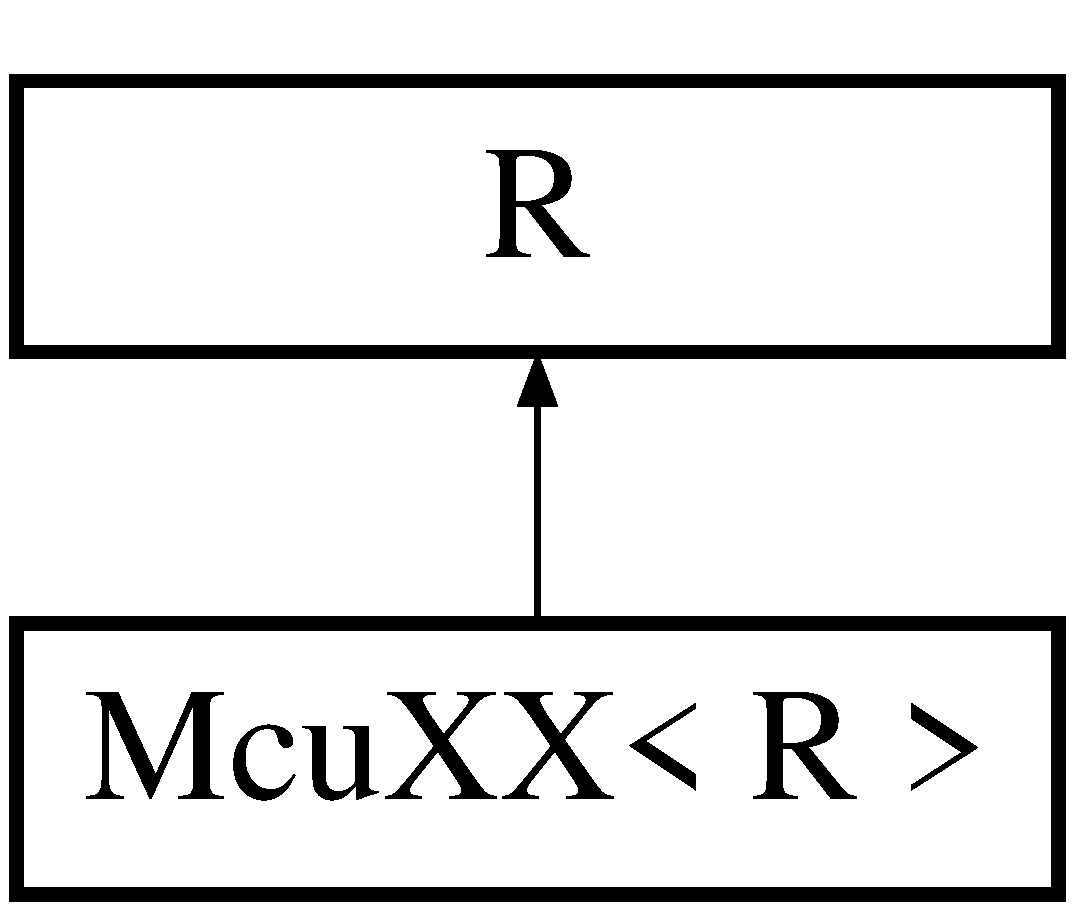
\includegraphics[height=2.000000cm]{class_mcu_x_x}
\end{center}
\end{figure}
\subsection*{Public Member Functions}
\begin{DoxyCompactItemize}
\item 
\mbox{\hyperlink{class_mcu_x_x_ae6c723c6d5e5695e08991ec9fc404064}{Mcu\+XX}} (\mbox{\hyperlink{_class_s_t_m32_l0_8h_a5ceb873075d76667eb54dc6a7d2734d1}{Pin\+Name}} mosi, \mbox{\hyperlink{_class_s_t_m32_l0_8h_a5ceb873075d76667eb54dc6a7d2734d1}{Pin\+Name}} miso, \mbox{\hyperlink{_class_s_t_m32_l0_8h_a5ceb873075d76667eb54dc6a7d2734d1}{Pin\+Name}} sclk)
\item 
\mbox{\hyperlink{class_mcu_x_x_aabd5bdc5db9e38ff12f72d196eb11b8d}{$\sim$\+Mcu\+XX}} ()
\end{DoxyCompactItemize}


\subsection{Detailed Description}
\subsubsection*{template$<$class R$>$\newline
class Mcu\+X\+X$<$ R $>$}



Definition at line 30 of file Api\+Mcu.\+h.



\subsection{Constructor \& Destructor Documentation}
\mbox{\Hypertarget{class_mcu_x_x_ae6c723c6d5e5695e08991ec9fc404064}\label{class_mcu_x_x_ae6c723c6d5e5695e08991ec9fc404064}} 
\index{Mcu\+XX@{Mcu\+XX}!Mcu\+XX@{Mcu\+XX}}
\index{Mcu\+XX@{Mcu\+XX}!Mcu\+XX@{Mcu\+XX}}
\subsubsection{\texorpdfstring{Mcu\+X\+X()}{McuXX()}}
{\footnotesize\ttfamily template$<$class R$>$ \\
\mbox{\hyperlink{class_mcu_x_x}{Mcu\+XX}}$<$ R $>$\+::\mbox{\hyperlink{class_mcu_x_x}{Mcu\+XX}} (\begin{DoxyParamCaption}\item[{\mbox{\hyperlink{_class_s_t_m32_l0_8h_a5ceb873075d76667eb54dc6a7d2734d1}{Pin\+Name}}}]{mosi,  }\item[{\mbox{\hyperlink{_class_s_t_m32_l0_8h_a5ceb873075d76667eb54dc6a7d2734d1}{Pin\+Name}}}]{miso,  }\item[{\mbox{\hyperlink{_class_s_t_m32_l0_8h_a5ceb873075d76667eb54dc6a7d2734d1}{Pin\+Name}}}]{sclk }\end{DoxyParamCaption})\hspace{0.3cm}{\ttfamily [inline]}}



Definition at line 32 of file Api\+Mcu.\+h.

\mbox{\Hypertarget{class_mcu_x_x_aabd5bdc5db9e38ff12f72d196eb11b8d}\label{class_mcu_x_x_aabd5bdc5db9e38ff12f72d196eb11b8d}} 
\index{Mcu\+XX@{Mcu\+XX}!````~Mcu\+XX@{$\sim$\+Mcu\+XX}}
\index{````~Mcu\+XX@{$\sim$\+Mcu\+XX}!Mcu\+XX@{Mcu\+XX}}
\subsubsection{\texorpdfstring{$\sim$\+Mcu\+X\+X()}{~McuXX()}}
{\footnotesize\ttfamily template$<$class R$>$ \\
\mbox{\hyperlink{class_mcu_x_x}{Mcu\+XX}}$<$ R $>$\+::$\sim$\mbox{\hyperlink{class_mcu_x_x}{Mcu\+XX}} (\begin{DoxyParamCaption}{ }\end{DoxyParamCaption})\hspace{0.3cm}{\ttfamily [inline]}}



Definition at line 33 of file Api\+Mcu.\+h.



The documentation for this class was generated from the following file\+:\begin{DoxyCompactItemize}
\item 
C\+:/\+G\+I\+T\+E\+X\+T/githubdoc/\+Lo\+Ra\+Wan\+Mini\+Mouse.\+github.\+io/\+M\+Mstack/\+Mcu\+Api/\mbox{\hyperlink{_api_mcu_8h}{Api\+Mcu.\+h}}\end{DoxyCompactItemize}

\hypertarget{structpayload}{}\section{payload Struct Reference}
\label{structpayload}\index{payload@{payload}}


{\ttfamily \#include $<$appli.\+h$>$}

\subsection*{Public Attributes}
\begin{DoxyCompactItemize}
\item 
float \mbox{\hyperlink{structpayload_a4fe84758224072d721d3b0573e75141f}{Reserved}}
\item 
uint8\+\_\+t \mbox{\hyperlink{structpayload_ada67d46f7c72f987d622511d30baeb11}{Vbat}}
\item 
int8\+\_\+t \mbox{\hyperlink{structpayload_a37cc36f378c70d3fd1aa1116588e380b}{Temp}}
\item 
uint8\+\_\+t \mbox{\hyperlink{structpayload_afc9c5cb383808537d084eef03c169977}{Hygro}}
\end{DoxyCompactItemize}


\subsection{Detailed Description}


Definition at line 14 of file appli.\+h.



\subsection{Member Data Documentation}
\mbox{\Hypertarget{structpayload_afc9c5cb383808537d084eef03c169977}\label{structpayload_afc9c5cb383808537d084eef03c169977}} 
\index{payload@{payload}!Hygro@{Hygro}}
\index{Hygro@{Hygro}!payload@{payload}}
\subsubsection{\texorpdfstring{Hygro}{Hygro}}
{\footnotesize\ttfamily uint8\+\_\+t payload\+::\+Hygro}



Definition at line 18 of file appli.\+h.

\mbox{\Hypertarget{structpayload_a4fe84758224072d721d3b0573e75141f}\label{structpayload_a4fe84758224072d721d3b0573e75141f}} 
\index{payload@{payload}!Reserved@{Reserved}}
\index{Reserved@{Reserved}!payload@{payload}}
\subsubsection{\texorpdfstring{Reserved}{Reserved}}
{\footnotesize\ttfamily float payload\+::\+Reserved}



Definition at line 15 of file appli.\+h.

\mbox{\Hypertarget{structpayload_a37cc36f378c70d3fd1aa1116588e380b}\label{structpayload_a37cc36f378c70d3fd1aa1116588e380b}} 
\index{payload@{payload}!Temp@{Temp}}
\index{Temp@{Temp}!payload@{payload}}
\subsubsection{\texorpdfstring{Temp}{Temp}}
{\footnotesize\ttfamily int8\+\_\+t payload\+::\+Temp}



Definition at line 17 of file appli.\+h.

\mbox{\Hypertarget{structpayload_ada67d46f7c72f987d622511d30baeb11}\label{structpayload_ada67d46f7c72f987d622511d30baeb11}} 
\index{payload@{payload}!Vbat@{Vbat}}
\index{Vbat@{Vbat}!payload@{payload}}
\subsubsection{\texorpdfstring{Vbat}{Vbat}}
{\footnotesize\ttfamily uint8\+\_\+t payload\+::\+Vbat}



Definition at line 16 of file appli.\+h.



The documentation for this struct was generated from the following file\+:\begin{DoxyCompactItemize}
\item 
C\+:/\+G\+I\+T\+E\+X\+T/githubdoc/\+Lo\+Ra\+Wan\+Mini\+Mouse.\+github.\+io/\+M\+Mstack/\+User\+Code/\mbox{\hyperlink{appli_8h}{appli.\+h}}\end{DoxyCompactItemize}

\hypertarget{class_radio_container}{}\section{Radio\+Container$<$ R $>$ Class Template Reference}
\label{class_radio_container}\index{Radio\+Container$<$ R $>$@{Radio\+Container$<$ R $>$}}


{\ttfamily \#include $<$Phy\+Layer.\+h$>$}

\subsection*{Public Member Functions}
\begin{DoxyCompactItemize}
\item 
\mbox{\hyperlink{class_radio_container_acba7b3f419573dc72a58e000072b1d15}{Radio\+Container}} (R $\ast$Radio\+User)
\item 
\mbox{\hyperlink{class_radio_container_af2367ea0e92fa1654a4329d13ed90e47}{$\sim$\+Radio\+Container}} ()
\item 
void \mbox{\hyperlink{class_radio_container_aefcc86fb08cd1857cf6dcd8ba1bd7c90}{Send}} (\mbox{\hyperlink{_define_8h_a81bbaee3ae5a0ec0040b6faedbf80b2f}{e\+Modulation\+Type}} Mac\+Tx\+Modulation\+Current, uint32\+\_\+t Tx\+Frequency\+Mac, uint8\+\_\+t Tx\+Power\+Mac, uint8\+\_\+t Tx\+Sf\+Mac, \mbox{\hyperlink{_define_8h_a6cbb491180e131f374cdbe63880c85e1}{e\+Band\+Width}} Tx\+Bw\+Mac, uint16\+\_\+t Tx\+Payload\+Size\+Mac)
\item 
void \mbox{\hyperlink{class_radio_container_a9a7e676f1735ea1f67898d6e3014ded1}{Receive}} (void)
\item 
void \mbox{\hyperlink{class_radio_container_a4ea6769301a5aaa8e33e22562e024619}{Isr\+Radio}} (void)
\item 
void \mbox{\hyperlink{class_radio_container_ab4ae2d79a43dca2bdf0900cc2e3aac5c}{Attach\+Isr}} (void)
\item 
void \mbox{\hyperlink{class_radio_container_a8819af2363c07fc158989c57a45e5e48}{Detach\+Isr}} (void)
\item 
int \mbox{\hyperlink{class_radio_container_a3ffe014538d877752663a6f747247554}{Get\+Radio\+State}} (void)
\item 
void \mbox{\hyperlink{class_radio_container_a2ca1eae7a18c37aefa507b59ad1bcbef}{Set\+Rx\+Config}} (\mbox{\hyperlink{_define_8h_a81bbaee3ae5a0ec0040b6faedbf80b2f}{e\+Modulation\+Type}} Rx\+Modulation, uint32\+\_\+t Rx\+Frequency\+Mac, uint8\+\_\+t Rx\+Sf\+Mac, \mbox{\hyperlink{_define_8h_a6cbb491180e131f374cdbe63880c85e1}{e\+Band\+Width}} Rx\+Bw\+Mac, uint32\+\_\+t Rx\+Window\+Ms)
\item 
uint32\+\_\+t \mbox{\hyperlink{class_radio_container_a59cf65c721a176fdd0cf2d0039a18242}{Get\+Tx\+Frequency}} (void)
\end{DoxyCompactItemize}
\subsection*{Static Public Member Functions}
\begin{DoxyCompactItemize}
\item 
static void \mbox{\hyperlink{class_radio_container_afd4dc2a290ab1f6d4cf7920ab457fac7}{Callback\+Isr\+Radio}} (void $\ast$obj)
\end{DoxyCompactItemize}
\subsection*{Public Attributes}
\begin{DoxyCompactItemize}
\item 
R $\ast$ \mbox{\hyperlink{class_radio_container_a30b5b1397632040096b08e56e2ec1d47}{Radio}}
\item 
uint8\+\_\+t \mbox{\hyperlink{class_radio_container_ad91ae082ac2890e7b71546c4b7efb5ba}{Tx\+Phy\+Payload}} \mbox{[}\mbox{\hyperlink{_define_8h_ade046d6a940b0e4d9f3ae9415066ee6f}{M\+A\+X\+\_\+\+T\+X\+\_\+\+P\+A\+Y\+L\+O\+A\+D\+\_\+\+S\+I\+ZE}}\mbox{]}
\item 
uint8\+\_\+t \mbox{\hyperlink{class_radio_container_a100c2c3e3d71652fca93d8ee0a5ecc9c}{Rx\+Phy\+Payload}} \mbox{[}\mbox{\hyperlink{_define_8h_ade046d6a940b0e4d9f3ae9415066ee6f}{M\+A\+X\+\_\+\+T\+X\+\_\+\+P\+A\+Y\+L\+O\+A\+D\+\_\+\+S\+I\+ZE}}\mbox{]}
\item 
uint8\+\_\+t \mbox{\hyperlink{class_radio_container_a2b84534ef69df6313c3c7cf9edcb234d}{Rx\+Phy\+Payload\+Size}}
\item 
int \mbox{\hyperlink{class_radio_container_a8814f4b3203f8f9fac24e77291f41dd3}{Rx\+Phy\+Payload\+Snr}}
\item 
int \mbox{\hyperlink{class_radio_container_a198c252436c6a365cb07d9d073d9d50d}{Rx\+Phy\+Payload\+Rssi}}
\item 
uint16\+\_\+t \mbox{\hyperlink{class_radio_container_abb44acd5f52b34e0a1ffaa3a1dec0bbd}{Tx\+Payload\+Size}}
\item 
uint32\+\_\+t \mbox{\hyperlink{class_radio_container_a3fce662f22e5d0beaf3b25df353c0bae}{Dev\+Addr\+Isr}}
\item 
uint8\+\_\+t \mbox{\hyperlink{class_radio_container_adbb1e0ef33a7fdeeb2e27b54a4808220}{Reg\+Irq\+Flag}}
\item 
\mbox{\hyperlink{_define_8h_abe3daafdb4fec314926c12003b3ad390}{e\+Join\+Status}} \mbox{\hyperlink{class_radio_container_a4c19319bc32e8f18dc42b70f852cd24e}{Joined\+Status}}
\item 
int \mbox{\hyperlink{class_radio_container_aaeabc6b1b8012038246bc14e1da1462f}{State\+Radio\+Process}}
\item 
uint32\+\_\+t \mbox{\hyperlink{class_radio_container_a82ecd21f7fb6701a66037821c6175e44}{Timestamp\+Rtc\+Isr}}
\item 
uint32\+\_\+t \mbox{\hyperlink{class_radio_container_a087adc0271190a23c893774d1a9f9dc0}{Last\+Time\+Rx\+Windows\+Ms}}
\item 
uint32\+\_\+t \mbox{\hyperlink{class_radio_container_a26d15cb55aa6f8b4f0bb977f3c4a4b38}{Symbol\+Duration}}
\end{DoxyCompactItemize}


\subsection{Detailed Description}
\subsubsection*{template$<$class R$>$\newline
class Radio\+Container$<$ R $>$}



Definition at line 30 of file Phy\+Layer.\+h.



\subsection{Constructor \& Destructor Documentation}
\mbox{\Hypertarget{class_radio_container_acba7b3f419573dc72a58e000072b1d15}\label{class_radio_container_acba7b3f419573dc72a58e000072b1d15}} 
\index{Radio\+Container@{Radio\+Container}!Radio\+Container@{Radio\+Container}}
\index{Radio\+Container@{Radio\+Container}!Radio\+Container@{Radio\+Container}}
\subsubsection{\texorpdfstring{Radio\+Container()}{RadioContainer()}}
{\footnotesize\ttfamily template$<$class R $>$ \\
\mbox{\hyperlink{class_radio_container}{Radio\+Container}}$<$ R $>$\+::\mbox{\hyperlink{class_radio_container}{Radio\+Container}} (\begin{DoxyParamCaption}\item[{R $\ast$}]{Radio\+User }\end{DoxyParamCaption})}



Definition at line 30 of file Phy\+Layer.\+cpp.

\mbox{\Hypertarget{class_radio_container_af2367ea0e92fa1654a4329d13ed90e47}\label{class_radio_container_af2367ea0e92fa1654a4329d13ed90e47}} 
\index{Radio\+Container@{Radio\+Container}!````~Radio\+Container@{$\sim$\+Radio\+Container}}
\index{````~Radio\+Container@{$\sim$\+Radio\+Container}!Radio\+Container@{Radio\+Container}}
\subsubsection{\texorpdfstring{$\sim$\+Radio\+Container()}{~RadioContainer()}}
{\footnotesize\ttfamily template$<$class R $>$ \\
\mbox{\hyperlink{class_radio_container}{Radio\+Container}}$<$ R $>$\+::$\sim$\mbox{\hyperlink{class_radio_container}{Radio\+Container}} (\begin{DoxyParamCaption}{ }\end{DoxyParamCaption})}



Definition at line 38 of file Phy\+Layer.\+cpp.



\subsection{Member Function Documentation}
\mbox{\Hypertarget{class_radio_container_ab4ae2d79a43dca2bdf0900cc2e3aac5c}\label{class_radio_container_ab4ae2d79a43dca2bdf0900cc2e3aac5c}} 
\index{Radio\+Container@{Radio\+Container}!Attach\+Isr@{Attach\+Isr}}
\index{Attach\+Isr@{Attach\+Isr}!Radio\+Container@{Radio\+Container}}
\subsubsection{\texorpdfstring{Attach\+Isr()}{AttachIsr()}}
{\footnotesize\ttfamily template$<$class R $>$ \\
void \mbox{\hyperlink{class_radio_container}{Radio\+Container}}$<$ R $>$\+::Attach\+Isr (\begin{DoxyParamCaption}\item[{void}]{ }\end{DoxyParamCaption})}



Definition at line 48 of file Phy\+Layer.\+cpp.

\mbox{\Hypertarget{class_radio_container_afd4dc2a290ab1f6d4cf7920ab457fac7}\label{class_radio_container_afd4dc2a290ab1f6d4cf7920ab457fac7}} 
\index{Radio\+Container@{Radio\+Container}!Callback\+Isr\+Radio@{Callback\+Isr\+Radio}}
\index{Callback\+Isr\+Radio@{Callback\+Isr\+Radio}!Radio\+Container@{Radio\+Container}}
\subsubsection{\texorpdfstring{Callback\+Isr\+Radio()}{CallbackIsrRadio()}}
{\footnotesize\ttfamily template$<$class R$>$ \\
static void \mbox{\hyperlink{class_radio_container}{Radio\+Container}}$<$ R $>$\+::Callback\+Isr\+Radio (\begin{DoxyParamCaption}\item[{void $\ast$}]{obj }\end{DoxyParamCaption})\hspace{0.3cm}{\ttfamily [inline]}, {\ttfamily [static]}}



Definition at line 38 of file Phy\+Layer.\+h.

\mbox{\Hypertarget{class_radio_container_a8819af2363c07fc158989c57a45e5e48}\label{class_radio_container_a8819af2363c07fc158989c57a45e5e48}} 
\index{Radio\+Container@{Radio\+Container}!Detach\+Isr@{Detach\+Isr}}
\index{Detach\+Isr@{Detach\+Isr}!Radio\+Container@{Radio\+Container}}
\subsubsection{\texorpdfstring{Detach\+Isr()}{DetachIsr()}}
{\footnotesize\ttfamily template$<$class R $>$ \\
void \mbox{\hyperlink{class_radio_container}{Radio\+Container}}$<$ R $>$\+::Detach\+Isr (\begin{DoxyParamCaption}\item[{void}]{ }\end{DoxyParamCaption})}



Definition at line 53 of file Phy\+Layer.\+cpp.

\mbox{\Hypertarget{class_radio_container_a3ffe014538d877752663a6f747247554}\label{class_radio_container_a3ffe014538d877752663a6f747247554}} 
\index{Radio\+Container@{Radio\+Container}!Get\+Radio\+State@{Get\+Radio\+State}}
\index{Get\+Radio\+State@{Get\+Radio\+State}!Radio\+Container@{Radio\+Container}}
\subsubsection{\texorpdfstring{Get\+Radio\+State()}{GetRadioState()}}
{\footnotesize\ttfamily template$<$class R $>$ \\
int \mbox{\hyperlink{class_radio_container}{Radio\+Container}}$<$ R $>$\+::Get\+Radio\+State (\begin{DoxyParamCaption}\item[{void}]{ }\end{DoxyParamCaption})}



Definition at line 94 of file Phy\+Layer.\+cpp.

\mbox{\Hypertarget{class_radio_container_a59cf65c721a176fdd0cf2d0039a18242}\label{class_radio_container_a59cf65c721a176fdd0cf2d0039a18242}} 
\index{Radio\+Container@{Radio\+Container}!Get\+Tx\+Frequency@{Get\+Tx\+Frequency}}
\index{Get\+Tx\+Frequency@{Get\+Tx\+Frequency}!Radio\+Container@{Radio\+Container}}
\subsubsection{\texorpdfstring{Get\+Tx\+Frequency()}{GetTxFrequency()}}
{\footnotesize\ttfamily template$<$class R $>$ \\
uint32\+\_\+t \mbox{\hyperlink{class_radio_container}{Radio\+Container}}$<$ R $>$\+::Get\+Tx\+Frequency (\begin{DoxyParamCaption}\item[{void}]{ }\end{DoxyParamCaption})}



Definition at line 99 of file Phy\+Layer.\+cpp.

\mbox{\Hypertarget{class_radio_container_a4ea6769301a5aaa8e33e22562e024619}\label{class_radio_container_a4ea6769301a5aaa8e33e22562e024619}} 
\index{Radio\+Container@{Radio\+Container}!Isr\+Radio@{Isr\+Radio}}
\index{Isr\+Radio@{Isr\+Radio}!Radio\+Container@{Radio\+Container}}
\subsubsection{\texorpdfstring{Isr\+Radio()}{IsrRadio()}}
{\footnotesize\ttfamily template$<$class R $>$ \\
void \mbox{\hyperlink{class_radio_container}{Radio\+Container}}$<$ R $>$\+::Isr\+Radio (\begin{DoxyParamCaption}\item[{void}]{ }\end{DoxyParamCaption})}



Definition at line 23 of file Radio\+Isr\+Routine.\+cpp.

\mbox{\Hypertarget{class_radio_container_a9a7e676f1735ea1f67898d6e3014ded1}\label{class_radio_container_a9a7e676f1735ea1f67898d6e3014ded1}} 
\index{Radio\+Container@{Radio\+Container}!Receive@{Receive}}
\index{Receive@{Receive}!Radio\+Container@{Radio\+Container}}
\subsubsection{\texorpdfstring{Receive()}{Receive()}}
{\footnotesize\ttfamily template$<$class R$>$ \\
void \mbox{\hyperlink{class_radio_container}{Radio\+Container}}$<$ R $>$\+::Receive (\begin{DoxyParamCaption}\item[{void}]{ }\end{DoxyParamCaption})}

\mbox{\Hypertarget{class_radio_container_aefcc86fb08cd1857cf6dcd8ba1bd7c90}\label{class_radio_container_aefcc86fb08cd1857cf6dcd8ba1bd7c90}} 
\index{Radio\+Container@{Radio\+Container}!Send@{Send}}
\index{Send@{Send}!Radio\+Container@{Radio\+Container}}
\subsubsection{\texorpdfstring{Send()}{Send()}}
{\footnotesize\ttfamily template$<$class R $>$ \\
void \mbox{\hyperlink{class_radio_container}{Radio\+Container}}$<$ R $>$\+::Send (\begin{DoxyParamCaption}\item[{\mbox{\hyperlink{_define_8h_a81bbaee3ae5a0ec0040b6faedbf80b2f}{e\+Modulation\+Type}}}]{Mac\+Tx\+Modulation\+Current,  }\item[{uint32\+\_\+t}]{Tx\+Frequency\+Mac,  }\item[{uint8\+\_\+t}]{Tx\+Power\+Mac,  }\item[{uint8\+\_\+t}]{Tx\+Sf\+Mac,  }\item[{\mbox{\hyperlink{_define_8h_a6cbb491180e131f374cdbe63880c85e1}{e\+Band\+Width}}}]{Tx\+Bw\+Mac,  }\item[{uint16\+\_\+t}]{Tx\+Payload\+Size\+Mac }\end{DoxyParamCaption})}



Definition at line 62 of file Phy\+Layer.\+cpp.

\mbox{\Hypertarget{class_radio_container_a2ca1eae7a18c37aefa507b59ad1bcbef}\label{class_radio_container_a2ca1eae7a18c37aefa507b59ad1bcbef}} 
\index{Radio\+Container@{Radio\+Container}!Set\+Rx\+Config@{Set\+Rx\+Config}}
\index{Set\+Rx\+Config@{Set\+Rx\+Config}!Radio\+Container@{Radio\+Container}}
\subsubsection{\texorpdfstring{Set\+Rx\+Config()}{SetRxConfig()}}
{\footnotesize\ttfamily template$<$class R $>$ \\
void \mbox{\hyperlink{class_radio_container}{Radio\+Container}}$<$ R $>$\+::Set\+Rx\+Config (\begin{DoxyParamCaption}\item[{\mbox{\hyperlink{_define_8h_a81bbaee3ae5a0ec0040b6faedbf80b2f}{e\+Modulation\+Type}}}]{Rx\+Modulation,  }\item[{uint32\+\_\+t}]{Rx\+Frequency\+Mac,  }\item[{uint8\+\_\+t}]{Rx\+Sf\+Mac,  }\item[{\mbox{\hyperlink{_define_8h_a6cbb491180e131f374cdbe63880c85e1}{e\+Band\+Width}}}]{Rx\+Bw\+Mac,  }\item[{uint32\+\_\+t}]{Rx\+Window\+Ms }\end{DoxyParamCaption})}



Definition at line 80 of file Phy\+Layer.\+cpp.



\subsection{Member Data Documentation}
\mbox{\Hypertarget{class_radio_container_a3fce662f22e5d0beaf3b25df353c0bae}\label{class_radio_container_a3fce662f22e5d0beaf3b25df353c0bae}} 
\index{Radio\+Container@{Radio\+Container}!Dev\+Addr\+Isr@{Dev\+Addr\+Isr}}
\index{Dev\+Addr\+Isr@{Dev\+Addr\+Isr}!Radio\+Container@{Radio\+Container}}
\subsubsection{\texorpdfstring{Dev\+Addr\+Isr}{DevAddrIsr}}
{\footnotesize\ttfamily template$<$class R$>$ \\
uint32\+\_\+t \mbox{\hyperlink{class_radio_container}{Radio\+Container}}$<$ R $>$\+::Dev\+Addr\+Isr}



Definition at line 50 of file Phy\+Layer.\+h.

\mbox{\Hypertarget{class_radio_container_a4c19319bc32e8f18dc42b70f852cd24e}\label{class_radio_container_a4c19319bc32e8f18dc42b70f852cd24e}} 
\index{Radio\+Container@{Radio\+Container}!Joined\+Status@{Joined\+Status}}
\index{Joined\+Status@{Joined\+Status}!Radio\+Container@{Radio\+Container}}
\subsubsection{\texorpdfstring{Joined\+Status}{JoinedStatus}}
{\footnotesize\ttfamily template$<$class R$>$ \\
\mbox{\hyperlink{_define_8h_abe3daafdb4fec314926c12003b3ad390}{e\+Join\+Status}} \mbox{\hyperlink{class_radio_container}{Radio\+Container}}$<$ R $>$\+::Joined\+Status}



Definition at line 52 of file Phy\+Layer.\+h.

\mbox{\Hypertarget{class_radio_container_a087adc0271190a23c893774d1a9f9dc0}\label{class_radio_container_a087adc0271190a23c893774d1a9f9dc0}} 
\index{Radio\+Container@{Radio\+Container}!Last\+Time\+Rx\+Windows\+Ms@{Last\+Time\+Rx\+Windows\+Ms}}
\index{Last\+Time\+Rx\+Windows\+Ms@{Last\+Time\+Rx\+Windows\+Ms}!Radio\+Container@{Radio\+Container}}
\subsubsection{\texorpdfstring{Last\+Time\+Rx\+Windows\+Ms}{LastTimeRxWindowsMs}}
{\footnotesize\ttfamily template$<$class R$>$ \\
uint32\+\_\+t \mbox{\hyperlink{class_radio_container}{Radio\+Container}}$<$ R $>$\+::Last\+Time\+Rx\+Windows\+Ms}



Definition at line 55 of file Phy\+Layer.\+h.

\mbox{\Hypertarget{class_radio_container_a30b5b1397632040096b08e56e2ec1d47}\label{class_radio_container_a30b5b1397632040096b08e56e2ec1d47}} 
\index{Radio\+Container@{Radio\+Container}!Radio@{Radio}}
\index{Radio@{Radio}!Radio\+Container@{Radio\+Container}}
\subsubsection{\texorpdfstring{Radio}{Radio}}
{\footnotesize\ttfamily template$<$class R$>$ \\
R$\ast$ \mbox{\hyperlink{class_radio_container}{Radio\+Container}}$<$ R $>$\+::Radio}



Definition at line 34 of file Phy\+Layer.\+h.

\mbox{\Hypertarget{class_radio_container_adbb1e0ef33a7fdeeb2e27b54a4808220}\label{class_radio_container_adbb1e0ef33a7fdeeb2e27b54a4808220}} 
\index{Radio\+Container@{Radio\+Container}!Reg\+Irq\+Flag@{Reg\+Irq\+Flag}}
\index{Reg\+Irq\+Flag@{Reg\+Irq\+Flag}!Radio\+Container@{Radio\+Container}}
\subsubsection{\texorpdfstring{Reg\+Irq\+Flag}{RegIrqFlag}}
{\footnotesize\ttfamily template$<$class R$>$ \\
uint8\+\_\+t \mbox{\hyperlink{class_radio_container}{Radio\+Container}}$<$ R $>$\+::Reg\+Irq\+Flag}



Definition at line 51 of file Phy\+Layer.\+h.

\mbox{\Hypertarget{class_radio_container_a100c2c3e3d71652fca93d8ee0a5ecc9c}\label{class_radio_container_a100c2c3e3d71652fca93d8ee0a5ecc9c}} 
\index{Radio\+Container@{Radio\+Container}!Rx\+Phy\+Payload@{Rx\+Phy\+Payload}}
\index{Rx\+Phy\+Payload@{Rx\+Phy\+Payload}!Radio\+Container@{Radio\+Container}}
\subsubsection{\texorpdfstring{Rx\+Phy\+Payload}{RxPhyPayload}}
{\footnotesize\ttfamily template$<$class R$>$ \\
uint8\+\_\+t \mbox{\hyperlink{class_radio_container}{Radio\+Container}}$<$ R $>$\+::Rx\+Phy\+Payload\mbox{[}\mbox{\hyperlink{_define_8h_ade046d6a940b0e4d9f3ae9415066ee6f}{M\+A\+X\+\_\+\+T\+X\+\_\+\+P\+A\+Y\+L\+O\+A\+D\+\_\+\+S\+I\+ZE}}\mbox{]}}



Definition at line 45 of file Phy\+Layer.\+h.

\mbox{\Hypertarget{class_radio_container_a198c252436c6a365cb07d9d073d9d50d}\label{class_radio_container_a198c252436c6a365cb07d9d073d9d50d}} 
\index{Radio\+Container@{Radio\+Container}!Rx\+Phy\+Payload\+Rssi@{Rx\+Phy\+Payload\+Rssi}}
\index{Rx\+Phy\+Payload\+Rssi@{Rx\+Phy\+Payload\+Rssi}!Radio\+Container@{Radio\+Container}}
\subsubsection{\texorpdfstring{Rx\+Phy\+Payload\+Rssi}{RxPhyPayloadRssi}}
{\footnotesize\ttfamily template$<$class R$>$ \\
int \mbox{\hyperlink{class_radio_container}{Radio\+Container}}$<$ R $>$\+::Rx\+Phy\+Payload\+Rssi}



Definition at line 48 of file Phy\+Layer.\+h.

\mbox{\Hypertarget{class_radio_container_a2b84534ef69df6313c3c7cf9edcb234d}\label{class_radio_container_a2b84534ef69df6313c3c7cf9edcb234d}} 
\index{Radio\+Container@{Radio\+Container}!Rx\+Phy\+Payload\+Size@{Rx\+Phy\+Payload\+Size}}
\index{Rx\+Phy\+Payload\+Size@{Rx\+Phy\+Payload\+Size}!Radio\+Container@{Radio\+Container}}
\subsubsection{\texorpdfstring{Rx\+Phy\+Payload\+Size}{RxPhyPayloadSize}}
{\footnotesize\ttfamily template$<$class R$>$ \\
uint8\+\_\+t \mbox{\hyperlink{class_radio_container}{Radio\+Container}}$<$ R $>$\+::Rx\+Phy\+Payload\+Size}



Definition at line 46 of file Phy\+Layer.\+h.

\mbox{\Hypertarget{class_radio_container_a8814f4b3203f8f9fac24e77291f41dd3}\label{class_radio_container_a8814f4b3203f8f9fac24e77291f41dd3}} 
\index{Radio\+Container@{Radio\+Container}!Rx\+Phy\+Payload\+Snr@{Rx\+Phy\+Payload\+Snr}}
\index{Rx\+Phy\+Payload\+Snr@{Rx\+Phy\+Payload\+Snr}!Radio\+Container@{Radio\+Container}}
\subsubsection{\texorpdfstring{Rx\+Phy\+Payload\+Snr}{RxPhyPayloadSnr}}
{\footnotesize\ttfamily template$<$class R$>$ \\
int \mbox{\hyperlink{class_radio_container}{Radio\+Container}}$<$ R $>$\+::Rx\+Phy\+Payload\+Snr}



Definition at line 47 of file Phy\+Layer.\+h.

\mbox{\Hypertarget{class_radio_container_aaeabc6b1b8012038246bc14e1da1462f}\label{class_radio_container_aaeabc6b1b8012038246bc14e1da1462f}} 
\index{Radio\+Container@{Radio\+Container}!State\+Radio\+Process@{State\+Radio\+Process}}
\index{State\+Radio\+Process@{State\+Radio\+Process}!Radio\+Container@{Radio\+Container}}
\subsubsection{\texorpdfstring{State\+Radio\+Process}{StateRadioProcess}}
{\footnotesize\ttfamily template$<$class R$>$ \\
int \mbox{\hyperlink{class_radio_container}{Radio\+Container}}$<$ R $>$\+::State\+Radio\+Process}



Definition at line 53 of file Phy\+Layer.\+h.

\mbox{\Hypertarget{class_radio_container_a26d15cb55aa6f8b4f0bb977f3c4a4b38}\label{class_radio_container_a26d15cb55aa6f8b4f0bb977f3c4a4b38}} 
\index{Radio\+Container@{Radio\+Container}!Symbol\+Duration@{Symbol\+Duration}}
\index{Symbol\+Duration@{Symbol\+Duration}!Radio\+Container@{Radio\+Container}}
\subsubsection{\texorpdfstring{Symbol\+Duration}{SymbolDuration}}
{\footnotesize\ttfamily template$<$class R$>$ \\
uint32\+\_\+t \mbox{\hyperlink{class_radio_container}{Radio\+Container}}$<$ R $>$\+::Symbol\+Duration}



Definition at line 56 of file Phy\+Layer.\+h.

\mbox{\Hypertarget{class_radio_container_a82ecd21f7fb6701a66037821c6175e44}\label{class_radio_container_a82ecd21f7fb6701a66037821c6175e44}} 
\index{Radio\+Container@{Radio\+Container}!Timestamp\+Rtc\+Isr@{Timestamp\+Rtc\+Isr}}
\index{Timestamp\+Rtc\+Isr@{Timestamp\+Rtc\+Isr}!Radio\+Container@{Radio\+Container}}
\subsubsection{\texorpdfstring{Timestamp\+Rtc\+Isr}{TimestampRtcIsr}}
{\footnotesize\ttfamily template$<$class R$>$ \\
uint32\+\_\+t \mbox{\hyperlink{class_radio_container}{Radio\+Container}}$<$ R $>$\+::Timestamp\+Rtc\+Isr}



Definition at line 54 of file Phy\+Layer.\+h.

\mbox{\Hypertarget{class_radio_container_abb44acd5f52b34e0a1ffaa3a1dec0bbd}\label{class_radio_container_abb44acd5f52b34e0a1ffaa3a1dec0bbd}} 
\index{Radio\+Container@{Radio\+Container}!Tx\+Payload\+Size@{Tx\+Payload\+Size}}
\index{Tx\+Payload\+Size@{Tx\+Payload\+Size}!Radio\+Container@{Radio\+Container}}
\subsubsection{\texorpdfstring{Tx\+Payload\+Size}{TxPayloadSize}}
{\footnotesize\ttfamily template$<$class R$>$ \\
uint16\+\_\+t \mbox{\hyperlink{class_radio_container}{Radio\+Container}}$<$ R $>$\+::Tx\+Payload\+Size}



Definition at line 49 of file Phy\+Layer.\+h.

\mbox{\Hypertarget{class_radio_container_ad91ae082ac2890e7b71546c4b7efb5ba}\label{class_radio_container_ad91ae082ac2890e7b71546c4b7efb5ba}} 
\index{Radio\+Container@{Radio\+Container}!Tx\+Phy\+Payload@{Tx\+Phy\+Payload}}
\index{Tx\+Phy\+Payload@{Tx\+Phy\+Payload}!Radio\+Container@{Radio\+Container}}
\subsubsection{\texorpdfstring{Tx\+Phy\+Payload}{TxPhyPayload}}
{\footnotesize\ttfamily template$<$class R$>$ \\
uint8\+\_\+t \mbox{\hyperlink{class_radio_container}{Radio\+Container}}$<$ R $>$\+::Tx\+Phy\+Payload\mbox{[}\mbox{\hyperlink{_define_8h_ade046d6a940b0e4d9f3ae9415066ee6f}{M\+A\+X\+\_\+\+T\+X\+\_\+\+P\+A\+Y\+L\+O\+A\+D\+\_\+\+S\+I\+ZE}}\mbox{]}}



Definition at line 44 of file Phy\+Layer.\+h.



The documentation for this class was generated from the following files\+:\begin{DoxyCompactItemize}
\item 
C\+:/\+G\+I\+T\+E\+X\+T/githubdoc/\+Lo\+Ra\+Wan\+Mini\+Mouse.\+github.\+io/\+M\+Mstack/\+Minimouse\+Src/\mbox{\hyperlink{_phy_layer_8h}{Phy\+Layer.\+h}}\item 
C\+:/\+G\+I\+T\+E\+X\+T/githubdoc/\+Lo\+Ra\+Wan\+Mini\+Mouse.\+github.\+io/\+M\+Mstack/\+Minimouse\+Src/\mbox{\hyperlink{_phy_layer_8cpp}{Phy\+Layer.\+cpp}}\item 
C\+:/\+G\+I\+T\+E\+X\+T/githubdoc/\+Lo\+Ra\+Wan\+Mini\+Mouse.\+github.\+io/\+M\+Mstack/\+Minimouse\+Src/\mbox{\hyperlink{_radio_isr_routine_8cpp}{Radio\+Isr\+Routine.\+cpp}}\end{DoxyCompactItemize}

\hypertarget{structs_back_up_flash}{}\section{s\+Back\+Up\+Flash Struct Reference}
\label{structs_back_up_flash}\index{s\+Back\+Up\+Flash@{s\+Back\+Up\+Flash}}


{\ttfamily \#include $<$Lora\+Mac\+Data\+Store\+In\+Flash.\+h$>$}

\subsection*{Public Attributes}
\begin{DoxyCompactItemize}
\item 
uint8\+\_\+t \mbox{\hyperlink{structs_back_up_flash_a408ea06f64214043ee41e5de12cab2eb}{Mac\+Tx\+Data\+Rate}}
\item 
uint8\+\_\+t \mbox{\hyperlink{structs_back_up_flash_a37e09d6a2caa964e66d5ee8ac5f7e3a0}{Mac\+Tx\+Power}}
\item 
uint16\+\_\+t \mbox{\hyperlink{structs_back_up_flash_a4295c7686f916c144783dc2304257338}{Mac\+Ch\+Mask}}
\item 
uint8\+\_\+t \mbox{\hyperlink{structs_back_up_flash_a1770888f794fdf84265d196b2e2c8037}{Mac\+Nb\+Trans}}
\item 
uint32\+\_\+t \mbox{\hyperlink{structs_back_up_flash_aa6053682376d49efcba40e5cc3fd3154}{Mac\+Rx2\+Frequency}}
\item 
uint8\+\_\+t \mbox{\hyperlink{structs_back_up_flash_a8e1465c70a778678ac22a136bde59966}{Mac\+Rx2\+Data\+Rate}}
\item 
uint8\+\_\+t \mbox{\hyperlink{structs_back_up_flash_a5b5f63bc5dd29b8ccb149e6f20037981}{Mac\+Rx1\+Data\+Rate\+Offset}}
\item 
uint32\+\_\+t \mbox{\hyperlink{structs_back_up_flash_aed62b6a6b327e3999d01e7eb21681eb5}{Mac\+Tx\+Frequency}} \mbox{[}16\mbox{]}
\item 
uint32\+\_\+t \mbox{\hyperlink{structs_back_up_flash_a195dfadb183b5ad2b8990791e2c517c9}{Mac\+Rx1\+Frequency}} \mbox{[}16\mbox{]}
\item 
uint8\+\_\+t \mbox{\hyperlink{structs_back_up_flash_a1c212cc8590aa2279d04306b87361bcd}{Mac\+Min\+Data\+Rate\+Channel}} \mbox{[}16\mbox{]}
\item 
uint8\+\_\+t \mbox{\hyperlink{structs_back_up_flash_aae081cfdc99a8f60da6df8742b7dfda1}{Mac\+Max\+Data\+Rate\+Channel}} \mbox{[}16\mbox{]}
\item 
uint8\+\_\+t \mbox{\hyperlink{structs_back_up_flash_a8c75ddd0e48e4a9d3f0d8f44b989d10f}{Mac\+Channel\+Index\+Enabled}} \mbox{[}16\mbox{]}
\item 
uint16\+\_\+t \mbox{\hyperlink{structs_back_up_flash_af9653eb58b4eea0bd814fe175cc65f85}{Mac\+Channel\+Mask}}
\item 
int \mbox{\hyperlink{structs_back_up_flash_a1a196e3ae9619759ae25f5b5ccd64099}{Mac\+Rx1\+Delay}}
\item 
uint32\+\_\+t \mbox{\hyperlink{structs_back_up_flash_aa0c6803486a38093bd0b94cd5853361f}{Fcnt\+Up}}
\item 
uint32\+\_\+t \mbox{\hyperlink{structs_back_up_flash_a56c2f91129afa9d702e322a6af174a85}{Fcnt\+Dwn}}
\item 
uint32\+\_\+t \mbox{\hyperlink{structs_back_up_flash_a2032fb8ac149ddbdd397b070d46c6fda}{Dev\+Addr}}
\item 
uint8\+\_\+t \mbox{\hyperlink{structs_back_up_flash_a36e9fab419d7959dbda8c0ca24cdaf06}{nwk\+S\+Key}} \mbox{[}16\mbox{]}
\item 
uint8\+\_\+t \mbox{\hyperlink{structs_back_up_flash_a8b20dcb0b7253b2125d5116ab68b188e}{app\+S\+Key}} \mbox{[}16\mbox{]}
\item 
uint8\+\_\+t \mbox{\hyperlink{structs_back_up_flash_a294ca0c27de2e0f8b6e0caf67250f419}{Joined\+Status}}
\item 
uint16\+\_\+t \mbox{\hyperlink{structs_back_up_flash_adb12b0a10e2a8ded5388f251ec4d4c17}{Dev\+Nonce}}
\item 
uint8\+\_\+t \mbox{\hyperlink{structs_back_up_flash_a6b1fa618b913d529bac5adaf4ec145dc}{Nb\+Of\+Reset}}
\item 
uint8\+\_\+t \mbox{\hyperlink{structs_back_up_flash_a6163ae953c8ae3245dacc92da79bce16}{Reserved}} \mbox{[}7\mbox{]}
\item 
uint32\+\_\+t \mbox{\hyperlink{structs_back_up_flash_afc534d9e7a3e581783489765b52676a0}{Crc\+High}}
\item 
uint32\+\_\+t \mbox{\hyperlink{structs_back_up_flash_a24f57cec1c39d4972d14bfb65212d74c}{Crc\+Low}}
\end{DoxyCompactItemize}


\subsection{Detailed Description}


Definition at line 26 of file Lora\+Mac\+Data\+Store\+In\+Flash.\+h.



\subsection{Member Data Documentation}
\mbox{\Hypertarget{structs_back_up_flash_a8b20dcb0b7253b2125d5116ab68b188e}\label{structs_back_up_flash_a8b20dcb0b7253b2125d5116ab68b188e}} 
\index{s\+Back\+Up\+Flash@{s\+Back\+Up\+Flash}!app\+S\+Key@{app\+S\+Key}}
\index{app\+S\+Key@{app\+S\+Key}!s\+Back\+Up\+Flash@{s\+Back\+Up\+Flash}}
\subsubsection{\texorpdfstring{app\+S\+Key}{appSKey}}
{\footnotesize\ttfamily uint8\+\_\+t s\+Back\+Up\+Flash\+::app\+S\+Key\mbox{[}16\mbox{]}}



Definition at line 60 of file Lora\+Mac\+Data\+Store\+In\+Flash.\+h.

\mbox{\Hypertarget{structs_back_up_flash_afc534d9e7a3e581783489765b52676a0}\label{structs_back_up_flash_afc534d9e7a3e581783489765b52676a0}} 
\index{s\+Back\+Up\+Flash@{s\+Back\+Up\+Flash}!Crc\+High@{Crc\+High}}
\index{Crc\+High@{Crc\+High}!s\+Back\+Up\+Flash@{s\+Back\+Up\+Flash}}
\subsubsection{\texorpdfstring{Crc\+High}{CrcHigh}}
{\footnotesize\ttfamily uint32\+\_\+t s\+Back\+Up\+Flash\+::\+Crc\+High}



Definition at line 65 of file Lora\+Mac\+Data\+Store\+In\+Flash.\+h.

\mbox{\Hypertarget{structs_back_up_flash_a24f57cec1c39d4972d14bfb65212d74c}\label{structs_back_up_flash_a24f57cec1c39d4972d14bfb65212d74c}} 
\index{s\+Back\+Up\+Flash@{s\+Back\+Up\+Flash}!Crc\+Low@{Crc\+Low}}
\index{Crc\+Low@{Crc\+Low}!s\+Back\+Up\+Flash@{s\+Back\+Up\+Flash}}
\subsubsection{\texorpdfstring{Crc\+Low}{CrcLow}}
{\footnotesize\ttfamily uint32\+\_\+t s\+Back\+Up\+Flash\+::\+Crc\+Low}



Definition at line 66 of file Lora\+Mac\+Data\+Store\+In\+Flash.\+h.

\mbox{\Hypertarget{structs_back_up_flash_a2032fb8ac149ddbdd397b070d46c6fda}\label{structs_back_up_flash_a2032fb8ac149ddbdd397b070d46c6fda}} 
\index{s\+Back\+Up\+Flash@{s\+Back\+Up\+Flash}!Dev\+Addr@{Dev\+Addr}}
\index{Dev\+Addr@{Dev\+Addr}!s\+Back\+Up\+Flash@{s\+Back\+Up\+Flash}}
\subsubsection{\texorpdfstring{Dev\+Addr}{DevAddr}}
{\footnotesize\ttfamily uint32\+\_\+t s\+Back\+Up\+Flash\+::\+Dev\+Addr}



Definition at line 58 of file Lora\+Mac\+Data\+Store\+In\+Flash.\+h.

\mbox{\Hypertarget{structs_back_up_flash_adb12b0a10e2a8ded5388f251ec4d4c17}\label{structs_back_up_flash_adb12b0a10e2a8ded5388f251ec4d4c17}} 
\index{s\+Back\+Up\+Flash@{s\+Back\+Up\+Flash}!Dev\+Nonce@{Dev\+Nonce}}
\index{Dev\+Nonce@{Dev\+Nonce}!s\+Back\+Up\+Flash@{s\+Back\+Up\+Flash}}
\subsubsection{\texorpdfstring{Dev\+Nonce}{DevNonce}}
{\footnotesize\ttfamily uint16\+\_\+t s\+Back\+Up\+Flash\+::\+Dev\+Nonce}



Definition at line 62 of file Lora\+Mac\+Data\+Store\+In\+Flash.\+h.

\mbox{\Hypertarget{structs_back_up_flash_a56c2f91129afa9d702e322a6af174a85}\label{structs_back_up_flash_a56c2f91129afa9d702e322a6af174a85}} 
\index{s\+Back\+Up\+Flash@{s\+Back\+Up\+Flash}!Fcnt\+Dwn@{Fcnt\+Dwn}}
\index{Fcnt\+Dwn@{Fcnt\+Dwn}!s\+Back\+Up\+Flash@{s\+Back\+Up\+Flash}}
\subsubsection{\texorpdfstring{Fcnt\+Dwn}{FcntDwn}}
{\footnotesize\ttfamily uint32\+\_\+t s\+Back\+Up\+Flash\+::\+Fcnt\+Dwn}



Definition at line 57 of file Lora\+Mac\+Data\+Store\+In\+Flash.\+h.

\mbox{\Hypertarget{structs_back_up_flash_aa0c6803486a38093bd0b94cd5853361f}\label{structs_back_up_flash_aa0c6803486a38093bd0b94cd5853361f}} 
\index{s\+Back\+Up\+Flash@{s\+Back\+Up\+Flash}!Fcnt\+Up@{Fcnt\+Up}}
\index{Fcnt\+Up@{Fcnt\+Up}!s\+Back\+Up\+Flash@{s\+Back\+Up\+Flash}}
\subsubsection{\texorpdfstring{Fcnt\+Up}{FcntUp}}
{\footnotesize\ttfamily uint32\+\_\+t s\+Back\+Up\+Flash\+::\+Fcnt\+Up}



Definition at line 56 of file Lora\+Mac\+Data\+Store\+In\+Flash.\+h.

\mbox{\Hypertarget{structs_back_up_flash_a294ca0c27de2e0f8b6e0caf67250f419}\label{structs_back_up_flash_a294ca0c27de2e0f8b6e0caf67250f419}} 
\index{s\+Back\+Up\+Flash@{s\+Back\+Up\+Flash}!Joined\+Status@{Joined\+Status}}
\index{Joined\+Status@{Joined\+Status}!s\+Back\+Up\+Flash@{s\+Back\+Up\+Flash}}
\subsubsection{\texorpdfstring{Joined\+Status}{JoinedStatus}}
{\footnotesize\ttfamily uint8\+\_\+t s\+Back\+Up\+Flash\+::\+Joined\+Status}



Definition at line 61 of file Lora\+Mac\+Data\+Store\+In\+Flash.\+h.

\mbox{\Hypertarget{structs_back_up_flash_a8c75ddd0e48e4a9d3f0d8f44b989d10f}\label{structs_back_up_flash_a8c75ddd0e48e4a9d3f0d8f44b989d10f}} 
\index{s\+Back\+Up\+Flash@{s\+Back\+Up\+Flash}!Mac\+Channel\+Index\+Enabled@{Mac\+Channel\+Index\+Enabled}}
\index{Mac\+Channel\+Index\+Enabled@{Mac\+Channel\+Index\+Enabled}!s\+Back\+Up\+Flash@{s\+Back\+Up\+Flash}}
\subsubsection{\texorpdfstring{Mac\+Channel\+Index\+Enabled}{MacChannelIndexEnabled}}
{\footnotesize\ttfamily uint8\+\_\+t s\+Back\+Up\+Flash\+::\+Mac\+Channel\+Index\+Enabled\mbox{[}16\mbox{]}}



Definition at line 47 of file Lora\+Mac\+Data\+Store\+In\+Flash.\+h.

\mbox{\Hypertarget{structs_back_up_flash_af9653eb58b4eea0bd814fe175cc65f85}\label{structs_back_up_flash_af9653eb58b4eea0bd814fe175cc65f85}} 
\index{s\+Back\+Up\+Flash@{s\+Back\+Up\+Flash}!Mac\+Channel\+Mask@{Mac\+Channel\+Mask}}
\index{Mac\+Channel\+Mask@{Mac\+Channel\+Mask}!s\+Back\+Up\+Flash@{s\+Back\+Up\+Flash}}
\subsubsection{\texorpdfstring{Mac\+Channel\+Mask}{MacChannelMask}}
{\footnotesize\ttfamily uint16\+\_\+t s\+Back\+Up\+Flash\+::\+Mac\+Channel\+Mask}



Definition at line 48 of file Lora\+Mac\+Data\+Store\+In\+Flash.\+h.

\mbox{\Hypertarget{structs_back_up_flash_a4295c7686f916c144783dc2304257338}\label{structs_back_up_flash_a4295c7686f916c144783dc2304257338}} 
\index{s\+Back\+Up\+Flash@{s\+Back\+Up\+Flash}!Mac\+Ch\+Mask@{Mac\+Ch\+Mask}}
\index{Mac\+Ch\+Mask@{Mac\+Ch\+Mask}!s\+Back\+Up\+Flash@{s\+Back\+Up\+Flash}}
\subsubsection{\texorpdfstring{Mac\+Ch\+Mask}{MacChMask}}
{\footnotesize\ttfamily uint16\+\_\+t s\+Back\+Up\+Flash\+::\+Mac\+Ch\+Mask}



Definition at line 32 of file Lora\+Mac\+Data\+Store\+In\+Flash.\+h.

\mbox{\Hypertarget{structs_back_up_flash_aae081cfdc99a8f60da6df8742b7dfda1}\label{structs_back_up_flash_aae081cfdc99a8f60da6df8742b7dfda1}} 
\index{s\+Back\+Up\+Flash@{s\+Back\+Up\+Flash}!Mac\+Max\+Data\+Rate\+Channel@{Mac\+Max\+Data\+Rate\+Channel}}
\index{Mac\+Max\+Data\+Rate\+Channel@{Mac\+Max\+Data\+Rate\+Channel}!s\+Back\+Up\+Flash@{s\+Back\+Up\+Flash}}
\subsubsection{\texorpdfstring{Mac\+Max\+Data\+Rate\+Channel}{MacMaxDataRateChannel}}
{\footnotesize\ttfamily uint8\+\_\+t s\+Back\+Up\+Flash\+::\+Mac\+Max\+Data\+Rate\+Channel\mbox{[}16\mbox{]}}



Definition at line 46 of file Lora\+Mac\+Data\+Store\+In\+Flash.\+h.

\mbox{\Hypertarget{structs_back_up_flash_a1c212cc8590aa2279d04306b87361bcd}\label{structs_back_up_flash_a1c212cc8590aa2279d04306b87361bcd}} 
\index{s\+Back\+Up\+Flash@{s\+Back\+Up\+Flash}!Mac\+Min\+Data\+Rate\+Channel@{Mac\+Min\+Data\+Rate\+Channel}}
\index{Mac\+Min\+Data\+Rate\+Channel@{Mac\+Min\+Data\+Rate\+Channel}!s\+Back\+Up\+Flash@{s\+Back\+Up\+Flash}}
\subsubsection{\texorpdfstring{Mac\+Min\+Data\+Rate\+Channel}{MacMinDataRateChannel}}
{\footnotesize\ttfamily uint8\+\_\+t s\+Back\+Up\+Flash\+::\+Mac\+Min\+Data\+Rate\+Channel\mbox{[}16\mbox{]}}



Definition at line 45 of file Lora\+Mac\+Data\+Store\+In\+Flash.\+h.

\mbox{\Hypertarget{structs_back_up_flash_a1770888f794fdf84265d196b2e2c8037}\label{structs_back_up_flash_a1770888f794fdf84265d196b2e2c8037}} 
\index{s\+Back\+Up\+Flash@{s\+Back\+Up\+Flash}!Mac\+Nb\+Trans@{Mac\+Nb\+Trans}}
\index{Mac\+Nb\+Trans@{Mac\+Nb\+Trans}!s\+Back\+Up\+Flash@{s\+Back\+Up\+Flash}}
\subsubsection{\texorpdfstring{Mac\+Nb\+Trans}{MacNbTrans}}
{\footnotesize\ttfamily uint8\+\_\+t s\+Back\+Up\+Flash\+::\+Mac\+Nb\+Trans}



Definition at line 33 of file Lora\+Mac\+Data\+Store\+In\+Flash.\+h.

\mbox{\Hypertarget{structs_back_up_flash_a5b5f63bc5dd29b8ccb149e6f20037981}\label{structs_back_up_flash_a5b5f63bc5dd29b8ccb149e6f20037981}} 
\index{s\+Back\+Up\+Flash@{s\+Back\+Up\+Flash}!Mac\+Rx1\+Data\+Rate\+Offset@{Mac\+Rx1\+Data\+Rate\+Offset}}
\index{Mac\+Rx1\+Data\+Rate\+Offset@{Mac\+Rx1\+Data\+Rate\+Offset}!s\+Back\+Up\+Flash@{s\+Back\+Up\+Flash}}
\subsubsection{\texorpdfstring{Mac\+Rx1\+Data\+Rate\+Offset}{MacRx1DataRateOffset}}
{\footnotesize\ttfamily uint8\+\_\+t s\+Back\+Up\+Flash\+::\+Mac\+Rx1\+Data\+Rate\+Offset}



Definition at line 39 of file Lora\+Mac\+Data\+Store\+In\+Flash.\+h.

\mbox{\Hypertarget{structs_back_up_flash_a1a196e3ae9619759ae25f5b5ccd64099}\label{structs_back_up_flash_a1a196e3ae9619759ae25f5b5ccd64099}} 
\index{s\+Back\+Up\+Flash@{s\+Back\+Up\+Flash}!Mac\+Rx1\+Delay@{Mac\+Rx1\+Delay}}
\index{Mac\+Rx1\+Delay@{Mac\+Rx1\+Delay}!s\+Back\+Up\+Flash@{s\+Back\+Up\+Flash}}
\subsubsection{\texorpdfstring{Mac\+Rx1\+Delay}{MacRx1Delay}}
{\footnotesize\ttfamily int s\+Back\+Up\+Flash\+::\+Mac\+Rx1\+Delay}



Definition at line 52 of file Lora\+Mac\+Data\+Store\+In\+Flash.\+h.

\mbox{\Hypertarget{structs_back_up_flash_a195dfadb183b5ad2b8990791e2c517c9}\label{structs_back_up_flash_a195dfadb183b5ad2b8990791e2c517c9}} 
\index{s\+Back\+Up\+Flash@{s\+Back\+Up\+Flash}!Mac\+Rx1\+Frequency@{Mac\+Rx1\+Frequency}}
\index{Mac\+Rx1\+Frequency@{Mac\+Rx1\+Frequency}!s\+Back\+Up\+Flash@{s\+Back\+Up\+Flash}}
\subsubsection{\texorpdfstring{Mac\+Rx1\+Frequency}{MacRx1Frequency}}
{\footnotesize\ttfamily uint32\+\_\+t s\+Back\+Up\+Flash\+::\+Mac\+Rx1\+Frequency\mbox{[}16\mbox{]}}



Definition at line 44 of file Lora\+Mac\+Data\+Store\+In\+Flash.\+h.

\mbox{\Hypertarget{structs_back_up_flash_a8e1465c70a778678ac22a136bde59966}\label{structs_back_up_flash_a8e1465c70a778678ac22a136bde59966}} 
\index{s\+Back\+Up\+Flash@{s\+Back\+Up\+Flash}!Mac\+Rx2\+Data\+Rate@{Mac\+Rx2\+Data\+Rate}}
\index{Mac\+Rx2\+Data\+Rate@{Mac\+Rx2\+Data\+Rate}!s\+Back\+Up\+Flash@{s\+Back\+Up\+Flash}}
\subsubsection{\texorpdfstring{Mac\+Rx2\+Data\+Rate}{MacRx2DataRate}}
{\footnotesize\ttfamily uint8\+\_\+t s\+Back\+Up\+Flash\+::\+Mac\+Rx2\+Data\+Rate}



Definition at line 38 of file Lora\+Mac\+Data\+Store\+In\+Flash.\+h.

\mbox{\Hypertarget{structs_back_up_flash_aa6053682376d49efcba40e5cc3fd3154}\label{structs_back_up_flash_aa6053682376d49efcba40e5cc3fd3154}} 
\index{s\+Back\+Up\+Flash@{s\+Back\+Up\+Flash}!Mac\+Rx2\+Frequency@{Mac\+Rx2\+Frequency}}
\index{Mac\+Rx2\+Frequency@{Mac\+Rx2\+Frequency}!s\+Back\+Up\+Flash@{s\+Back\+Up\+Flash}}
\subsubsection{\texorpdfstring{Mac\+Rx2\+Frequency}{MacRx2Frequency}}
{\footnotesize\ttfamily uint32\+\_\+t s\+Back\+Up\+Flash\+::\+Mac\+Rx2\+Frequency}



Definition at line 37 of file Lora\+Mac\+Data\+Store\+In\+Flash.\+h.

\mbox{\Hypertarget{structs_back_up_flash_a408ea06f64214043ee41e5de12cab2eb}\label{structs_back_up_flash_a408ea06f64214043ee41e5de12cab2eb}} 
\index{s\+Back\+Up\+Flash@{s\+Back\+Up\+Flash}!Mac\+Tx\+Data\+Rate@{Mac\+Tx\+Data\+Rate}}
\index{Mac\+Tx\+Data\+Rate@{Mac\+Tx\+Data\+Rate}!s\+Back\+Up\+Flash@{s\+Back\+Up\+Flash}}
\subsubsection{\texorpdfstring{Mac\+Tx\+Data\+Rate}{MacTxDataRate}}
{\footnotesize\ttfamily uint8\+\_\+t s\+Back\+Up\+Flash\+::\+Mac\+Tx\+Data\+Rate}



Definition at line 30 of file Lora\+Mac\+Data\+Store\+In\+Flash.\+h.

\mbox{\Hypertarget{structs_back_up_flash_aed62b6a6b327e3999d01e7eb21681eb5}\label{structs_back_up_flash_aed62b6a6b327e3999d01e7eb21681eb5}} 
\index{s\+Back\+Up\+Flash@{s\+Back\+Up\+Flash}!Mac\+Tx\+Frequency@{Mac\+Tx\+Frequency}}
\index{Mac\+Tx\+Frequency@{Mac\+Tx\+Frequency}!s\+Back\+Up\+Flash@{s\+Back\+Up\+Flash}}
\subsubsection{\texorpdfstring{Mac\+Tx\+Frequency}{MacTxFrequency}}
{\footnotesize\ttfamily uint32\+\_\+t s\+Back\+Up\+Flash\+::\+Mac\+Tx\+Frequency\mbox{[}16\mbox{]}}



Definition at line 43 of file Lora\+Mac\+Data\+Store\+In\+Flash.\+h.

\mbox{\Hypertarget{structs_back_up_flash_a37e09d6a2caa964e66d5ee8ac5f7e3a0}\label{structs_back_up_flash_a37e09d6a2caa964e66d5ee8ac5f7e3a0}} 
\index{s\+Back\+Up\+Flash@{s\+Back\+Up\+Flash}!Mac\+Tx\+Power@{Mac\+Tx\+Power}}
\index{Mac\+Tx\+Power@{Mac\+Tx\+Power}!s\+Back\+Up\+Flash@{s\+Back\+Up\+Flash}}
\subsubsection{\texorpdfstring{Mac\+Tx\+Power}{MacTxPower}}
{\footnotesize\ttfamily uint8\+\_\+t s\+Back\+Up\+Flash\+::\+Mac\+Tx\+Power}



Definition at line 31 of file Lora\+Mac\+Data\+Store\+In\+Flash.\+h.

\mbox{\Hypertarget{structs_back_up_flash_a6b1fa618b913d529bac5adaf4ec145dc}\label{structs_back_up_flash_a6b1fa618b913d529bac5adaf4ec145dc}} 
\index{s\+Back\+Up\+Flash@{s\+Back\+Up\+Flash}!Nb\+Of\+Reset@{Nb\+Of\+Reset}}
\index{Nb\+Of\+Reset@{Nb\+Of\+Reset}!s\+Back\+Up\+Flash@{s\+Back\+Up\+Flash}}
\subsubsection{\texorpdfstring{Nb\+Of\+Reset}{NbOfReset}}
{\footnotesize\ttfamily uint8\+\_\+t s\+Back\+Up\+Flash\+::\+Nb\+Of\+Reset}



Definition at line 63 of file Lora\+Mac\+Data\+Store\+In\+Flash.\+h.

\mbox{\Hypertarget{structs_back_up_flash_a36e9fab419d7959dbda8c0ca24cdaf06}\label{structs_back_up_flash_a36e9fab419d7959dbda8c0ca24cdaf06}} 
\index{s\+Back\+Up\+Flash@{s\+Back\+Up\+Flash}!nwk\+S\+Key@{nwk\+S\+Key}}
\index{nwk\+S\+Key@{nwk\+S\+Key}!s\+Back\+Up\+Flash@{s\+Back\+Up\+Flash}}
\subsubsection{\texorpdfstring{nwk\+S\+Key}{nwkSKey}}
{\footnotesize\ttfamily uint8\+\_\+t s\+Back\+Up\+Flash\+::nwk\+S\+Key\mbox{[}16\mbox{]}}



Definition at line 59 of file Lora\+Mac\+Data\+Store\+In\+Flash.\+h.

\mbox{\Hypertarget{structs_back_up_flash_a6163ae953c8ae3245dacc92da79bce16}\label{structs_back_up_flash_a6163ae953c8ae3245dacc92da79bce16}} 
\index{s\+Back\+Up\+Flash@{s\+Back\+Up\+Flash}!Reserved@{Reserved}}
\index{Reserved@{Reserved}!s\+Back\+Up\+Flash@{s\+Back\+Up\+Flash}}
\subsubsection{\texorpdfstring{Reserved}{Reserved}}
{\footnotesize\ttfamily uint8\+\_\+t s\+Back\+Up\+Flash\+::\+Reserved\mbox{[}7\mbox{]}}



Definition at line 64 of file Lora\+Mac\+Data\+Store\+In\+Flash.\+h.



The documentation for this struct was generated from the following file\+:\begin{DoxyCompactItemize}
\item 
C\+:/\+G\+I\+T\+E\+X\+T/githubdoc/\+Lo\+Ra\+Wan\+Mini\+Mouse.\+github.\+io/\+M\+Mstack/\+Minimouse\+Src/\mbox{\hyperlink{_lora_mac_data_store_in_flash_8h}{Lora\+Mac\+Data\+Store\+In\+Flash.\+h}}\end{DoxyCompactItemize}

\hypertarget{structs_lo_ra_wan_keys}{}\section{s\+Lo\+Ra\+Wan\+Keys Struct Reference}
\label{structs_lo_ra_wan_keys}\index{s\+Lo\+Ra\+Wan\+Keys@{s\+Lo\+Ra\+Wan\+Keys}}


{\ttfamily \#include $<$Define.\+h$>$}

\subsection*{Public Attributes}
\begin{DoxyCompactItemize}
\item 
uint8\+\_\+t $\ast$ \mbox{\hyperlink{structs_lo_ra_wan_keys_a3fbacc8200a5720c10745f5eab5c4c7e}{Lo\+Ra\+Mac\+Nwk\+S\+Key}}
\item 
uint8\+\_\+t $\ast$ \mbox{\hyperlink{structs_lo_ra_wan_keys_ad6b6c043645eafba66603feca886fb23}{Lo\+Ra\+Mac\+App\+S\+Key}}
\item 
uint8\+\_\+t $\ast$ \mbox{\hyperlink{structs_lo_ra_wan_keys_af983e62161d0cef1452d553478e3a540}{Lo\+Ra\+Mac\+App\+Key}}
\item 
uint8\+\_\+t $\ast$ \mbox{\hyperlink{structs_lo_ra_wan_keys_a1f0a69278a218e8f1fde28e16c78b1b0}{App\+Eui}}
\item 
uint8\+\_\+t $\ast$ \mbox{\hyperlink{structs_lo_ra_wan_keys_a23f4c2f316fc8355c80f48151c4b6c83}{Dev\+Eui}}
\item 
uint32\+\_\+t \mbox{\hyperlink{structs_lo_ra_wan_keys_ad88facd7e11295d549ae4b2789d7d00f}{Lo\+Ra\+Dev\+Addr}}
\item 
\mbox{\hyperlink{_define_8h_a1e0a07faefc3dd68bbdd06f7c856cc74}{e\+Device\+Type\+O\+T\+A\+\_\+\+A\+PB}} \mbox{\hyperlink{structs_lo_ra_wan_keys_ac7acae00308fa51301a0b8e21cc1359e}{Ota\+Device}}
\end{DoxyCompactItemize}


\subsection{Detailed Description}


Definition at line 266 of file Define.\+h.



\subsection{Member Data Documentation}
\mbox{\Hypertarget{structs_lo_ra_wan_keys_a1f0a69278a218e8f1fde28e16c78b1b0}\label{structs_lo_ra_wan_keys_a1f0a69278a218e8f1fde28e16c78b1b0}} 
\index{s\+Lo\+Ra\+Wan\+Keys@{s\+Lo\+Ra\+Wan\+Keys}!App\+Eui@{App\+Eui}}
\index{App\+Eui@{App\+Eui}!s\+Lo\+Ra\+Wan\+Keys@{s\+Lo\+Ra\+Wan\+Keys}}
\subsubsection{\texorpdfstring{App\+Eui}{AppEui}}
{\footnotesize\ttfamily uint8\+\_\+t$\ast$ s\+Lo\+Ra\+Wan\+Keys\+::\+App\+Eui}



Definition at line 271 of file Define.\+h.

\mbox{\Hypertarget{structs_lo_ra_wan_keys_a23f4c2f316fc8355c80f48151c4b6c83}\label{structs_lo_ra_wan_keys_a23f4c2f316fc8355c80f48151c4b6c83}} 
\index{s\+Lo\+Ra\+Wan\+Keys@{s\+Lo\+Ra\+Wan\+Keys}!Dev\+Eui@{Dev\+Eui}}
\index{Dev\+Eui@{Dev\+Eui}!s\+Lo\+Ra\+Wan\+Keys@{s\+Lo\+Ra\+Wan\+Keys}}
\subsubsection{\texorpdfstring{Dev\+Eui}{DevEui}}
{\footnotesize\ttfamily uint8\+\_\+t$\ast$ s\+Lo\+Ra\+Wan\+Keys\+::\+Dev\+Eui}



Definition at line 272 of file Define.\+h.

\mbox{\Hypertarget{structs_lo_ra_wan_keys_ad88facd7e11295d549ae4b2789d7d00f}\label{structs_lo_ra_wan_keys_ad88facd7e11295d549ae4b2789d7d00f}} 
\index{s\+Lo\+Ra\+Wan\+Keys@{s\+Lo\+Ra\+Wan\+Keys}!Lo\+Ra\+Dev\+Addr@{Lo\+Ra\+Dev\+Addr}}
\index{Lo\+Ra\+Dev\+Addr@{Lo\+Ra\+Dev\+Addr}!s\+Lo\+Ra\+Wan\+Keys@{s\+Lo\+Ra\+Wan\+Keys}}
\subsubsection{\texorpdfstring{Lo\+Ra\+Dev\+Addr}{LoRaDevAddr}}
{\footnotesize\ttfamily uint32\+\_\+t s\+Lo\+Ra\+Wan\+Keys\+::\+Lo\+Ra\+Dev\+Addr}



Definition at line 273 of file Define.\+h.

\mbox{\Hypertarget{structs_lo_ra_wan_keys_af983e62161d0cef1452d553478e3a540}\label{structs_lo_ra_wan_keys_af983e62161d0cef1452d553478e3a540}} 
\index{s\+Lo\+Ra\+Wan\+Keys@{s\+Lo\+Ra\+Wan\+Keys}!Lo\+Ra\+Mac\+App\+Key@{Lo\+Ra\+Mac\+App\+Key}}
\index{Lo\+Ra\+Mac\+App\+Key@{Lo\+Ra\+Mac\+App\+Key}!s\+Lo\+Ra\+Wan\+Keys@{s\+Lo\+Ra\+Wan\+Keys}}
\subsubsection{\texorpdfstring{Lo\+Ra\+Mac\+App\+Key}{LoRaMacAppKey}}
{\footnotesize\ttfamily uint8\+\_\+t$\ast$ s\+Lo\+Ra\+Wan\+Keys\+::\+Lo\+Ra\+Mac\+App\+Key}



Definition at line 270 of file Define.\+h.

\mbox{\Hypertarget{structs_lo_ra_wan_keys_ad6b6c043645eafba66603feca886fb23}\label{structs_lo_ra_wan_keys_ad6b6c043645eafba66603feca886fb23}} 
\index{s\+Lo\+Ra\+Wan\+Keys@{s\+Lo\+Ra\+Wan\+Keys}!Lo\+Ra\+Mac\+App\+S\+Key@{Lo\+Ra\+Mac\+App\+S\+Key}}
\index{Lo\+Ra\+Mac\+App\+S\+Key@{Lo\+Ra\+Mac\+App\+S\+Key}!s\+Lo\+Ra\+Wan\+Keys@{s\+Lo\+Ra\+Wan\+Keys}}
\subsubsection{\texorpdfstring{Lo\+Ra\+Mac\+App\+S\+Key}{LoRaMacAppSKey}}
{\footnotesize\ttfamily uint8\+\_\+t$\ast$ s\+Lo\+Ra\+Wan\+Keys\+::\+Lo\+Ra\+Mac\+App\+S\+Key}



Definition at line 269 of file Define.\+h.

\mbox{\Hypertarget{structs_lo_ra_wan_keys_a3fbacc8200a5720c10745f5eab5c4c7e}\label{structs_lo_ra_wan_keys_a3fbacc8200a5720c10745f5eab5c4c7e}} 
\index{s\+Lo\+Ra\+Wan\+Keys@{s\+Lo\+Ra\+Wan\+Keys}!Lo\+Ra\+Mac\+Nwk\+S\+Key@{Lo\+Ra\+Mac\+Nwk\+S\+Key}}
\index{Lo\+Ra\+Mac\+Nwk\+S\+Key@{Lo\+Ra\+Mac\+Nwk\+S\+Key}!s\+Lo\+Ra\+Wan\+Keys@{s\+Lo\+Ra\+Wan\+Keys}}
\subsubsection{\texorpdfstring{Lo\+Ra\+Mac\+Nwk\+S\+Key}{LoRaMacNwkSKey}}
{\footnotesize\ttfamily uint8\+\_\+t$\ast$ s\+Lo\+Ra\+Wan\+Keys\+::\+Lo\+Ra\+Mac\+Nwk\+S\+Key}



Definition at line 268 of file Define.\+h.

\mbox{\Hypertarget{structs_lo_ra_wan_keys_ac7acae00308fa51301a0b8e21cc1359e}\label{structs_lo_ra_wan_keys_ac7acae00308fa51301a0b8e21cc1359e}} 
\index{s\+Lo\+Ra\+Wan\+Keys@{s\+Lo\+Ra\+Wan\+Keys}!Ota\+Device@{Ota\+Device}}
\index{Ota\+Device@{Ota\+Device}!s\+Lo\+Ra\+Wan\+Keys@{s\+Lo\+Ra\+Wan\+Keys}}
\subsubsection{\texorpdfstring{Ota\+Device}{OtaDevice}}
{\footnotesize\ttfamily \mbox{\hyperlink{_define_8h_a1e0a07faefc3dd68bbdd06f7c856cc74}{e\+Device\+Type\+O\+T\+A\+\_\+\+A\+PB}} s\+Lo\+Ra\+Wan\+Keys\+::\+Ota\+Device}



Definition at line 274 of file Define.\+h.



The documentation for this struct was generated from the following file\+:\begin{DoxyCompactItemize}
\item 
C\+:/\+G\+I\+T\+E\+X\+T/githubdoc/\+Lo\+Ra\+Wan\+Mini\+Mouse.\+github.\+io/\+M\+Mstack/\+Minimouse\+Src/\mbox{\hyperlink{_define_8h}{Define.\+h}}\end{DoxyCompactItemize}

\hypertarget{class_s_x126x}{}\section{S\+X126x Class Reference}
\label{class_s_x126x}\index{S\+X126x@{S\+X126x}}


{\ttfamily \#include $<$S\+X126x.\+h$>$}

\subsection*{Public Member Functions}
\begin{DoxyCompactItemize}
\item 
\mbox{\hyperlink{class_s_x126x_a325ba815822bd31fcae9d4effcc1aea5}{S\+X126x}} (\mbox{\hyperlink{_class_s_t_m32_l0_8h_a5ceb873075d76667eb54dc6a7d2734d1}{Pin\+Name}} Busy, \mbox{\hyperlink{_class_s_t_m32_l0_8h_a5ceb873075d76667eb54dc6a7d2734d1}{Pin\+Name}} nss, \mbox{\hyperlink{_class_s_t_m32_l0_8h_a5ceb873075d76667eb54dc6a7d2734d1}{Pin\+Name}} reset, \mbox{\hyperlink{_class_s_t_m32_l0_8h_a5ceb873075d76667eb54dc6a7d2734d1}{Pin\+Name}} Interrupt)
\item 
\mbox{\hyperlink{class_s_x126x_ade46beffc61c639d93c2cad02b92c902}{$\sim$\+S\+X126x}} ()
\item 
void \mbox{\hyperlink{class_s_x126x_a0e9939c82c76d571d71a69d6941a6780}{Clear\+Irq\+Flags}} (void)
\item 
\mbox{\hyperlink{_define_8h_ab50e1f84d728c6ede52a9606a2a262d5}{Irq\+Flags\+\_\+t}} \mbox{\hyperlink{class_s_x126x_ac50ac9d688ef2647e10d471f3cdf0ec0}{Get\+Irq\+Flags}} (void)
\item 
void \mbox{\hyperlink{class_s_x126x_a53fde8ee3d816f58b1c493195fd96872}{Fetch\+Payload}} (uint8\+\_\+t $\ast$payload\+Size, uint8\+\_\+t \mbox{\hyperlink{structpayload}{payload}}\mbox{[}255\mbox{]}, int16\+\_\+t $\ast$snr, int16\+\_\+t $\ast$signal\+Rssi)
\item 
void \mbox{\hyperlink{class_s_x126x_a062d1439cea26e3e531e5df8ade82f0b}{Reset}} (void)
\item 
void \mbox{\hyperlink{class_s_x126x_a9199137a513971e5af0b5be2637cb19a}{Send\+Lora}} (uint8\+\_\+t $\ast$\mbox{\hyperlink{structpayload}{payload}}, uint8\+\_\+t payload\+Size, uint8\+\_\+t SF, \mbox{\hyperlink{_define_8h_a6cbb491180e131f374cdbe63880c85e1}{e\+Band\+Width}} BW, uint32\+\_\+t channel, int8\+\_\+t power)
\item 
void \mbox{\hyperlink{class_s_x126x_a027376634d0192e48ce57891cef8b6f3}{Rx\+Lora}} (\mbox{\hyperlink{_define_8h_a6cbb491180e131f374cdbe63880c85e1}{e\+Band\+Width}} BW, uint8\+\_\+t SF, uint32\+\_\+t channel, uint32\+\_\+t rx\+Timeout\+Ms)
\item 
void \mbox{\hyperlink{class_s_x126x_a920aa7de87e1b05c47ad1a95002e00c2}{Sleep}} (bool cold\+Start)
\end{DoxyCompactItemize}


\subsection{Detailed Description}


Definition at line 38 of file S\+X126x.\+h.



\subsection{Constructor \& Destructor Documentation}
\mbox{\Hypertarget{class_s_x126x_a325ba815822bd31fcae9d4effcc1aea5}\label{class_s_x126x_a325ba815822bd31fcae9d4effcc1aea5}} 
\index{S\+X126x@{S\+X126x}!S\+X126x@{S\+X126x}}
\index{S\+X126x@{S\+X126x}!S\+X126x@{S\+X126x}}
\subsubsection{\texorpdfstring{S\+X126x()}{SX126x()}}
{\footnotesize\ttfamily S\+X126x\+::\+S\+X126x (\begin{DoxyParamCaption}\item[{\mbox{\hyperlink{_class_s_t_m32_l0_8h_a5ceb873075d76667eb54dc6a7d2734d1}{Pin\+Name}}}]{Busy,  }\item[{\mbox{\hyperlink{_class_s_t_m32_l0_8h_a5ceb873075d76667eb54dc6a7d2734d1}{Pin\+Name}}}]{nss,  }\item[{\mbox{\hyperlink{_class_s_t_m32_l0_8h_a5ceb873075d76667eb54dc6a7d2734d1}{Pin\+Name}}}]{reset,  }\item[{\mbox{\hyperlink{_class_s_t_m32_l0_8h_a5ceb873075d76667eb54dc6a7d2734d1}{Pin\+Name}}}]{Interrupt }\end{DoxyParamCaption})}



Definition at line 29 of file S\+X126x.\+cpp.

\mbox{\Hypertarget{class_s_x126x_ade46beffc61c639d93c2cad02b92c902}\label{class_s_x126x_ade46beffc61c639d93c2cad02b92c902}} 
\index{S\+X126x@{S\+X126x}!````~S\+X126x@{$\sim$\+S\+X126x}}
\index{````~S\+X126x@{$\sim$\+S\+X126x}!S\+X126x@{S\+X126x}}
\subsubsection{\texorpdfstring{$\sim$\+S\+X126x()}{~SX126x()}}
{\footnotesize\ttfamily S\+X126x\+::$\sim$\+S\+X126x (\begin{DoxyParamCaption}{ }\end{DoxyParamCaption})\hspace{0.3cm}{\ttfamily [inline]}}



Definition at line 41 of file S\+X126x.\+h.



\subsection{Member Function Documentation}
\mbox{\Hypertarget{class_s_x126x_a0e9939c82c76d571d71a69d6941a6780}\label{class_s_x126x_a0e9939c82c76d571d71a69d6941a6780}} 
\index{S\+X126x@{S\+X126x}!Clear\+Irq\+Flags@{Clear\+Irq\+Flags}}
\index{Clear\+Irq\+Flags@{Clear\+Irq\+Flags}!S\+X126x@{S\+X126x}}
\subsubsection{\texorpdfstring{Clear\+Irq\+Flags()}{ClearIrqFlags()}}
{\footnotesize\ttfamily void S\+X126x\+::\+Clear\+Irq\+Flags (\begin{DoxyParamCaption}\item[{void}]{ }\end{DoxyParamCaption})}



Definition at line 38 of file S\+X126x.\+cpp.

\mbox{\Hypertarget{class_s_x126x_a53fde8ee3d816f58b1c493195fd96872}\label{class_s_x126x_a53fde8ee3d816f58b1c493195fd96872}} 
\index{S\+X126x@{S\+X126x}!Fetch\+Payload@{Fetch\+Payload}}
\index{Fetch\+Payload@{Fetch\+Payload}!S\+X126x@{S\+X126x}}
\subsubsection{\texorpdfstring{Fetch\+Payload()}{FetchPayload()}}
{\footnotesize\ttfamily void S\+X126x\+::\+Fetch\+Payload (\begin{DoxyParamCaption}\item[{uint8\+\_\+t $\ast$}]{payload\+Size,  }\item[{uint8\+\_\+t}]{payload\mbox{[}255\mbox{]},  }\item[{int16\+\_\+t $\ast$}]{snr,  }\item[{int16\+\_\+t $\ast$}]{signal\+Rssi }\end{DoxyParamCaption})}



Definition at line 42 of file S\+X126x.\+cpp.

\mbox{\Hypertarget{class_s_x126x_ac50ac9d688ef2647e10d471f3cdf0ec0}\label{class_s_x126x_ac50ac9d688ef2647e10d471f3cdf0ec0}} 
\index{S\+X126x@{S\+X126x}!Get\+Irq\+Flags@{Get\+Irq\+Flags}}
\index{Get\+Irq\+Flags@{Get\+Irq\+Flags}!S\+X126x@{S\+X126x}}
\subsubsection{\texorpdfstring{Get\+Irq\+Flags()}{GetIrqFlags()}}
{\footnotesize\ttfamily \mbox{\hyperlink{_define_8h_ab50e1f84d728c6ede52a9606a2a262d5}{Irq\+Flags\+\_\+t}} S\+X126x\+::\+Get\+Irq\+Flags (\begin{DoxyParamCaption}\item[{void}]{ }\end{DoxyParamCaption})}



Definition at line 55 of file S\+X126x.\+cpp.

\mbox{\Hypertarget{class_s_x126x_a062d1439cea26e3e531e5df8ade82f0b}\label{class_s_x126x_a062d1439cea26e3e531e5df8ade82f0b}} 
\index{S\+X126x@{S\+X126x}!Reset@{Reset}}
\index{Reset@{Reset}!S\+X126x@{S\+X126x}}
\subsubsection{\texorpdfstring{Reset()}{Reset()}}
{\footnotesize\ttfamily void S\+X126x\+::\+Reset (\begin{DoxyParamCaption}\item[{void}]{ }\end{DoxyParamCaption})}



Definition at line 81 of file S\+X126x.\+cpp.

\mbox{\Hypertarget{class_s_x126x_a027376634d0192e48ce57891cef8b6f3}\label{class_s_x126x_a027376634d0192e48ce57891cef8b6f3}} 
\index{S\+X126x@{S\+X126x}!Rx\+Lora@{Rx\+Lora}}
\index{Rx\+Lora@{Rx\+Lora}!S\+X126x@{S\+X126x}}
\subsubsection{\texorpdfstring{Rx\+Lora()}{RxLora()}}
{\footnotesize\ttfamily void S\+X126x\+::\+Rx\+Lora (\begin{DoxyParamCaption}\item[{\mbox{\hyperlink{_define_8h_a6cbb491180e131f374cdbe63880c85e1}{e\+Band\+Width}}}]{BW,  }\item[{uint8\+\_\+t}]{SF,  }\item[{uint32\+\_\+t}]{channel,  }\item[{uint32\+\_\+t}]{rx\+Timeout\+Ms }\end{DoxyParamCaption})}



Definition at line 129 of file S\+X126x.\+cpp.

\mbox{\Hypertarget{class_s_x126x_a9199137a513971e5af0b5be2637cb19a}\label{class_s_x126x_a9199137a513971e5af0b5be2637cb19a}} 
\index{S\+X126x@{S\+X126x}!Send\+Lora@{Send\+Lora}}
\index{Send\+Lora@{Send\+Lora}!S\+X126x@{S\+X126x}}
\subsubsection{\texorpdfstring{Send\+Lora()}{SendLora()}}
{\footnotesize\ttfamily void S\+X126x\+::\+Send\+Lora (\begin{DoxyParamCaption}\item[{uint8\+\_\+t $\ast$}]{payload,  }\item[{uint8\+\_\+t}]{payload\+Size,  }\item[{uint8\+\_\+t}]{SF,  }\item[{\mbox{\hyperlink{_define_8h_a6cbb491180e131f374cdbe63880c85e1}{e\+Band\+Width}}}]{BW,  }\item[{uint32\+\_\+t}]{channel,  }\item[{int8\+\_\+t}]{power }\end{DoxyParamCaption})}



Definition at line 92 of file S\+X126x.\+cpp.

\mbox{\Hypertarget{class_s_x126x_a920aa7de87e1b05c47ad1a95002e00c2}\label{class_s_x126x_a920aa7de87e1b05c47ad1a95002e00c2}} 
\index{S\+X126x@{S\+X126x}!Sleep@{Sleep}}
\index{Sleep@{Sleep}!S\+X126x@{S\+X126x}}
\subsubsection{\texorpdfstring{Sleep()}{Sleep()}}
{\footnotesize\ttfamily void S\+X126x\+::\+Sleep (\begin{DoxyParamCaption}\item[{bool}]{cold\+Start }\end{DoxyParamCaption})}



Definition at line 154 of file S\+X126x.\+cpp.



The documentation for this class was generated from the following files\+:\begin{DoxyCompactItemize}
\item 
C\+:/\+G\+I\+T\+E\+X\+T/githubdoc/\+Lo\+Ra\+Wan\+Mini\+Mouse.\+github.\+io/\+M\+Mstack/radio/\+S\+X126\+X/\mbox{\hyperlink{_s_x126x_8h}{S\+X126x.\+h}}\item 
C\+:/\+G\+I\+T\+E\+X\+T/githubdoc/\+Lo\+Ra\+Wan\+Mini\+Mouse.\+github.\+io/\+M\+Mstack/radio/\+S\+X126\+X/\mbox{\hyperlink{_s_x126x_8cpp}{S\+X126x.\+cpp}}\end{DoxyCompactItemize}

\hypertarget{class_s_x1276}{}\section{S\+X1276 Class Reference}
\label{class_s_x1276}\index{S\+X1276@{S\+X1276}}


{\ttfamily \#include $<$sx1276.\+h$>$}

\subsection*{Public Member Functions}
\begin{DoxyCompactItemize}
\item 
\mbox{\hyperlink{class_s_x1276_a9fd5df20eb50285357e5c5f1dbcbbd4c}{S\+X1276}} (\mbox{\hyperlink{_class_s_t_m32_l0_8h_a5ceb873075d76667eb54dc6a7d2734d1}{Pin\+Name}} nss, \mbox{\hyperlink{_class_s_t_m32_l0_8h_a5ceb873075d76667eb54dc6a7d2734d1}{Pin\+Name}} reset, \mbox{\hyperlink{_class_s_t_m32_l0_8h_a5ceb873075d76667eb54dc6a7d2734d1}{Pin\+Name}} Tx\+Rx\+It, \mbox{\hyperlink{_class_s_t_m32_l0_8h_a5ceb873075d76667eb54dc6a7d2734d1}{Pin\+Name}} Rx\+Time\+Out\+It)
\item 
\mbox{\hyperlink{class_s_x1276_a309d7607da2a200cf0a288532540b133}{$\sim$\+S\+X1276}} ()
\item 
void \mbox{\hyperlink{class_s_x1276_a7afd0cc488888310b8821eaa8000f1bb}{Clear\+Irq\+Flags}} (void)
\item 
uint8\+\_\+t \mbox{\hyperlink{class_s_x1276_a993418a10ee158597c183324c6328f02}{Get\+Irq\+Flags}} (void)
\item 
void \mbox{\hyperlink{class_s_x1276_ade5b7c1ac84e1f18e4d2487f12763cfa}{Fetch\+Payload}} (uint8\+\_\+t $\ast$payload\+Size, uint8\+\_\+t \mbox{\hyperlink{structpayload}{payload}}\mbox{[}255\mbox{]}, int16\+\_\+t $\ast$snr, int16\+\_\+t $\ast$signal\+Rssi)
\item 
void \mbox{\hyperlink{class_s_x1276_a279a0411958926be3b67e42bd5d0bf5c}{Reset}} (void)
\item 
void \mbox{\hyperlink{class_s_x1276_a3c109223d212fb13d5eed45de23ccee6}{Send\+Lora}} (uint8\+\_\+t $\ast$\mbox{\hyperlink{structpayload}{payload}}, uint8\+\_\+t payload\+Size, uint8\+\_\+t SF, \mbox{\hyperlink{_define_8h_a6cbb491180e131f374cdbe63880c85e1}{e\+Band\+Width}} BW, uint32\+\_\+t channel, int8\+\_\+t power)
\item 
void \mbox{\hyperlink{class_s_x1276_a53de2b0fe1c40753e82279518ccd1992}{Rx\+Lora}} (\mbox{\hyperlink{_define_8h_a6cbb491180e131f374cdbe63880c85e1}{e\+Band\+Width}} BW, uint8\+\_\+t SF, uint32\+\_\+t channel, uint16\+\_\+t Time\+Out\+Ms)
\item 
void \mbox{\hyperlink{class_s_x1276_a479a2ca97b17fd54224ad2fac9d84193}{Sleep}} (bool cold\+Start)
\end{DoxyCompactItemize}
\subsection*{Public Attributes}
\begin{DoxyCompactItemize}
\item 
uint32\+\_\+t \mbox{\hyperlink{class_s_x1276_aa927ccaaf4ff0cec945f8e9f02171c00}{Channel}}
\end{DoxyCompactItemize}


\subsection{Detailed Description}


Definition at line 43 of file sx1276.\+h.



\subsection{Constructor \& Destructor Documentation}
\mbox{\Hypertarget{class_s_x1276_a9fd5df20eb50285357e5c5f1dbcbbd4c}\label{class_s_x1276_a9fd5df20eb50285357e5c5f1dbcbbd4c}} 
\index{S\+X1276@{S\+X1276}!S\+X1276@{S\+X1276}}
\index{S\+X1276@{S\+X1276}!S\+X1276@{S\+X1276}}
\subsubsection{\texorpdfstring{S\+X1276()}{SX1276()}}
{\footnotesize\ttfamily S\+X1276\+::\+S\+X1276 (\begin{DoxyParamCaption}\item[{\mbox{\hyperlink{_class_s_t_m32_l0_8h_a5ceb873075d76667eb54dc6a7d2734d1}{Pin\+Name}}}]{nss,  }\item[{\mbox{\hyperlink{_class_s_t_m32_l0_8h_a5ceb873075d76667eb54dc6a7d2734d1}{Pin\+Name}}}]{reset,  }\item[{\mbox{\hyperlink{_class_s_t_m32_l0_8h_a5ceb873075d76667eb54dc6a7d2734d1}{Pin\+Name}}}]{Tx\+Rx\+It,  }\item[{\mbox{\hyperlink{_class_s_t_m32_l0_8h_a5ceb873075d76667eb54dc6a7d2734d1}{Pin\+Name}}}]{Rx\+Time\+Out\+It }\end{DoxyParamCaption})}



Definition at line 33 of file sx1276.\+cpp.

\mbox{\Hypertarget{class_s_x1276_a309d7607da2a200cf0a288532540b133}\label{class_s_x1276_a309d7607da2a200cf0a288532540b133}} 
\index{S\+X1276@{S\+X1276}!````~S\+X1276@{$\sim$\+S\+X1276}}
\index{````~S\+X1276@{$\sim$\+S\+X1276}!S\+X1276@{S\+X1276}}
\subsubsection{\texorpdfstring{$\sim$\+S\+X1276()}{~SX1276()}}
{\footnotesize\ttfamily S\+X1276\+::$\sim$\+S\+X1276 (\begin{DoxyParamCaption}{ }\end{DoxyParamCaption})\hspace{0.3cm}{\ttfamily [inline]}}



Definition at line 46 of file sx1276.\+h.



\subsection{Member Function Documentation}
\mbox{\Hypertarget{class_s_x1276_a7afd0cc488888310b8821eaa8000f1bb}\label{class_s_x1276_a7afd0cc488888310b8821eaa8000f1bb}} 
\index{S\+X1276@{S\+X1276}!Clear\+Irq\+Flags@{Clear\+Irq\+Flags}}
\index{Clear\+Irq\+Flags@{Clear\+Irq\+Flags}!S\+X1276@{S\+X1276}}
\subsubsection{\texorpdfstring{Clear\+Irq\+Flags()}{ClearIrqFlags()}}
{\footnotesize\ttfamily void S\+X1276\+::\+Clear\+Irq\+Flags (\begin{DoxyParamCaption}\item[{void}]{ }\end{DoxyParamCaption})}



Definition at line 39 of file sx1276.\+cpp.

\mbox{\Hypertarget{class_s_x1276_ade5b7c1ac84e1f18e4d2487f12763cfa}\label{class_s_x1276_ade5b7c1ac84e1f18e4d2487f12763cfa}} 
\index{S\+X1276@{S\+X1276}!Fetch\+Payload@{Fetch\+Payload}}
\index{Fetch\+Payload@{Fetch\+Payload}!S\+X1276@{S\+X1276}}
\subsubsection{\texorpdfstring{Fetch\+Payload()}{FetchPayload()}}
{\footnotesize\ttfamily void S\+X1276\+::\+Fetch\+Payload (\begin{DoxyParamCaption}\item[{uint8\+\_\+t $\ast$}]{payload\+Size,  }\item[{uint8\+\_\+t}]{payload\mbox{[}255\mbox{]},  }\item[{int16\+\_\+t $\ast$}]{snr,  }\item[{int16\+\_\+t $\ast$}]{signal\+Rssi }\end{DoxyParamCaption})}



Definition at line 43 of file sx1276.\+cpp.

\mbox{\Hypertarget{class_s_x1276_a993418a10ee158597c183324c6328f02}\label{class_s_x1276_a993418a10ee158597c183324c6328f02}} 
\index{S\+X1276@{S\+X1276}!Get\+Irq\+Flags@{Get\+Irq\+Flags}}
\index{Get\+Irq\+Flags@{Get\+Irq\+Flags}!S\+X1276@{S\+X1276}}
\subsubsection{\texorpdfstring{Get\+Irq\+Flags()}{GetIrqFlags()}}
{\footnotesize\ttfamily uint8\+\_\+t S\+X1276\+::\+Get\+Irq\+Flags (\begin{DoxyParamCaption}\item[{void}]{ }\end{DoxyParamCaption})}



Definition at line 49 of file sx1276.\+cpp.

\mbox{\Hypertarget{class_s_x1276_a279a0411958926be3b67e42bd5d0bf5c}\label{class_s_x1276_a279a0411958926be3b67e42bd5d0bf5c}} 
\index{S\+X1276@{S\+X1276}!Reset@{Reset}}
\index{Reset@{Reset}!S\+X1276@{S\+X1276}}
\subsubsection{\texorpdfstring{Reset()}{Reset()}}
{\footnotesize\ttfamily void S\+X1276\+::\+Reset (\begin{DoxyParamCaption}\item[{void}]{ }\end{DoxyParamCaption})}



Definition at line 54 of file sx1276.\+cpp.

\mbox{\Hypertarget{class_s_x1276_a53de2b0fe1c40753e82279518ccd1992}\label{class_s_x1276_a53de2b0fe1c40753e82279518ccd1992}} 
\index{S\+X1276@{S\+X1276}!Rx\+Lora@{Rx\+Lora}}
\index{Rx\+Lora@{Rx\+Lora}!S\+X1276@{S\+X1276}}
\subsubsection{\texorpdfstring{Rx\+Lora()}{RxLora()}}
{\footnotesize\ttfamily void S\+X1276\+::\+Rx\+Lora (\begin{DoxyParamCaption}\item[{\mbox{\hyperlink{_define_8h_a6cbb491180e131f374cdbe63880c85e1}{e\+Band\+Width}}}]{BW,  }\item[{uint8\+\_\+t}]{SF,  }\item[{uint32\+\_\+t}]{channel,  }\item[{uint16\+\_\+t}]{Time\+Out\+Ms }\end{DoxyParamCaption})}



Definition at line 88 of file sx1276.\+cpp.

\mbox{\Hypertarget{class_s_x1276_a3c109223d212fb13d5eed45de23ccee6}\label{class_s_x1276_a3c109223d212fb13d5eed45de23ccee6}} 
\index{S\+X1276@{S\+X1276}!Send\+Lora@{Send\+Lora}}
\index{Send\+Lora@{Send\+Lora}!S\+X1276@{S\+X1276}}
\subsubsection{\texorpdfstring{Send\+Lora()}{SendLora()}}
{\footnotesize\ttfamily void S\+X1276\+::\+Send\+Lora (\begin{DoxyParamCaption}\item[{uint8\+\_\+t $\ast$}]{payload,  }\item[{uint8\+\_\+t}]{payload\+Size,  }\item[{uint8\+\_\+t}]{SF,  }\item[{\mbox{\hyperlink{_define_8h_a6cbb491180e131f374cdbe63880c85e1}{e\+Band\+Width}}}]{BW,  }\item[{uint32\+\_\+t}]{channel,  }\item[{int8\+\_\+t}]{power }\end{DoxyParamCaption})}



Definition at line 61 of file sx1276.\+cpp.

\mbox{\Hypertarget{class_s_x1276_a479a2ca97b17fd54224ad2fac9d84193}\label{class_s_x1276_a479a2ca97b17fd54224ad2fac9d84193}} 
\index{S\+X1276@{S\+X1276}!Sleep@{Sleep}}
\index{Sleep@{Sleep}!S\+X1276@{S\+X1276}}
\subsubsection{\texorpdfstring{Sleep()}{Sleep()}}
{\footnotesize\ttfamily void S\+X1276\+::\+Sleep (\begin{DoxyParamCaption}\item[{bool}]{cold\+Start }\end{DoxyParamCaption})}



Definition at line 109 of file sx1276.\+cpp.



\subsection{Member Data Documentation}
\mbox{\Hypertarget{class_s_x1276_aa927ccaaf4ff0cec945f8e9f02171c00}\label{class_s_x1276_aa927ccaaf4ff0cec945f8e9f02171c00}} 
\index{S\+X1276@{S\+X1276}!Channel@{Channel}}
\index{Channel@{Channel}!S\+X1276@{S\+X1276}}
\subsubsection{\texorpdfstring{Channel}{Channel}}
{\footnotesize\ttfamily uint32\+\_\+t S\+X1276\+::\+Channel}



Definition at line 55 of file sx1276.\+h.



The documentation for this class was generated from the following files\+:\begin{DoxyCompactItemize}
\item 
C\+:/\+G\+I\+T\+E\+X\+T/githubdoc/\+Lo\+Ra\+Wan\+Mini\+Mouse.\+github.\+io/\+M\+Mstack/radio/\+S\+X1276\+Lib/sx1276/\mbox{\hyperlink{sx1276_8h}{sx1276.\+h}}\item 
C\+:/\+G\+I\+T\+E\+X\+T/githubdoc/\+Lo\+Ra\+Wan\+Mini\+Mouse.\+github.\+io/\+M\+Mstack/radio/\+S\+X1276\+Lib/sx1276/\mbox{\hyperlink{sx1276_8cpp}{sx1276.\+cpp}}\end{DoxyCompactItemize}

\chapter{File Documentation}
\hypertarget{_api_mcu_8h}{}\section{C\+:/\+G\+I\+T\+E\+X\+T/githubdoc/\+Lo\+Ra\+Wan\+Mini\+Mouse.github.\+io/\+M\+Mstack/\+Mcu\+Api/\+Api\+Mcu.h File Reference}
\label{_api_mcu_8h}\index{C\+:/\+G\+I\+T\+E\+X\+T/githubdoc/\+Lo\+Ra\+Wan\+Mini\+Mouse.\+github.\+io/\+M\+Mstack/\+Mcu\+Api/\+Api\+Mcu.\+h@{C\+:/\+G\+I\+T\+E\+X\+T/githubdoc/\+Lo\+Ra\+Wan\+Mini\+Mouse.\+github.\+io/\+M\+Mstack/\+Mcu\+Api/\+Api\+Mcu.\+h}}
{\ttfamily \#include \char`\"{}Define.\+h\char`\"{}}\newline
{\ttfamily \#include \char`\"{}Class\+S\+T\+M32\+L4.\+h\char`\"{}}\newline
{\ttfamily \#include $<$string.\+h$>$}\newline
\subsection*{Classes}
\begin{DoxyCompactItemize}
\item 
class \mbox{\hyperlink{class_mcu_x_x}{Mcu\+X\+X$<$ R $>$}}
\end{DoxyCompactItemize}
\subsection*{Variables}
\begin{DoxyCompactItemize}
\item 
\mbox{\hyperlink{class_mcu_x_x}{Mcu\+XX}}$<$ \mbox{\hyperlink{class_mcu_s_t_m32_l4}{Mcu\+S\+T\+M32\+L4}} $>$ \mbox{\hyperlink{_api_mcu_8h_aa87430f83eb1f3f004ab4ec725f8b8a9}{mcu}}
\begin{DoxyCompactList}\small\item\em Radio Interrupt Pin declarations. \end{DoxyCompactList}\end{DoxyCompactItemize}


\subsection{Variable Documentation}
\mbox{\Hypertarget{_api_mcu_8h_aa87430f83eb1f3f004ab4ec725f8b8a9}\label{_api_mcu_8h_aa87430f83eb1f3f004ab4ec725f8b8a9}} 
\index{Api\+Mcu.\+h@{Api\+Mcu.\+h}!mcu@{mcu}}
\index{mcu@{mcu}!Api\+Mcu.\+h@{Api\+Mcu.\+h}}
\subsubsection{\texorpdfstring{mcu}{mcu}}
{\footnotesize\ttfamily \mbox{\hyperlink{class_mcu_x_x}{Mcu\+XX}}$<$\mbox{\hyperlink{class_mcu_s_t_m32_l4}{Mcu\+S\+T\+M32\+L4}}$>$ mcu}



Radio Interrupt Pin declarations. 


\hypertarget{_class_s_t_m32_l0_8cpp}{}\section{C\+:/\+G\+I\+T\+E\+X\+T/githubdoc/\+Lo\+Ra\+Wan\+Mini\+Mouse.github.\+io/\+M\+Mstack/\+Mcu\+Api/\+Class\+S\+T\+M32\+L0.cpp File Reference}
\label{_class_s_t_m32_l0_8cpp}\index{C\+:/\+G\+I\+T\+E\+X\+T/githubdoc/\+Lo\+Ra\+Wan\+Mini\+Mouse.\+github.\+io/\+M\+Mstack/\+Mcu\+Api/\+Class\+S\+T\+M32\+L0.\+cpp@{C\+:/\+G\+I\+T\+E\+X\+T/githubdoc/\+Lo\+Ra\+Wan\+Mini\+Mouse.\+github.\+io/\+M\+Mstack/\+Mcu\+Api/\+Class\+S\+T\+M32\+L0.\+cpp}}

\hypertarget{_class_s_t_m32_l0_8h}{}\section{C\+:/\+G\+I\+T\+E\+X\+T/githubdoc/\+Lo\+Ra\+Wan\+Mini\+Mouse.github.\+io/\+M\+Mstack/\+Mcu\+Api/\+Class\+S\+T\+M32\+L0.h File Reference}
\label{_class_s_t_m32_l0_8h}\index{C\+:/\+G\+I\+T\+E\+X\+T/githubdoc/\+Lo\+Ra\+Wan\+Mini\+Mouse.\+github.\+io/\+M\+Mstack/\+Mcu\+Api/\+Class\+S\+T\+M32\+L0.\+h@{C\+:/\+G\+I\+T\+E\+X\+T/githubdoc/\+Lo\+Ra\+Wan\+Mini\+Mouse.\+github.\+io/\+M\+Mstack/\+Mcu\+Api/\+Class\+S\+T\+M32\+L0.\+h}}
{\ttfamily \#include \char`\"{}stdint.\+h\char`\"{}}\newline
{\ttfamily \#include \char`\"{}stm32l0xx\+\_\+hal.\+h\char`\"{}}\newline
{\ttfamily \#include \char`\"{}stm32l0xx\+\_\+ll\+\_\+spi.\+h\char`\"{}}\newline
{\ttfamily \#include \char`\"{}time.\+h\char`\"{}}\newline
{\ttfamily \#include \char`\"{}Uart.\+h\char`\"{}}\newline
\subsection*{Classes}
\begin{DoxyCompactItemize}
\item 
class \mbox{\hyperlink{class_mcu_s_t_m32_l0}{Mcu\+S\+T\+M32\+L0}}
\end{DoxyCompactItemize}
\subsection*{Macros}
\begin{DoxyCompactItemize}
\item 
\#define \mbox{\hyperlink{_class_s_t_m32_l0_8h_aed07b4957134494f3545189abece0f04}{T\+X\+\_\+\+R\+X\+\_\+\+IT}}~\mbox{\hyperlink{_class_s_t_m32_l0_8h_a5ceb873075d76667eb54dc6a7d2734d1a86c69dc8849d17673b52b9a8d94d8b9f}{D2}}
\item 
\#define \mbox{\hyperlink{_class_s_t_m32_l0_8h_a106bb2c77f5f8bbd6ec084f37e9c6506}{R\+X\+\_\+\+T\+I\+M\+E\+O\+U\+T\+\_\+\+IT}}~\mbox{\hyperlink{_class_s_t_m32_l0_8h_a5ceb873075d76667eb54dc6a7d2734d1ade8ef7573c5fa770f07ac7616cbf5d34}{D3}}
\item 
\#define \mbox{\hyperlink{_class_s_t_m32_l0_8h_a7597a102c72383ee6a40a5eb5e2f4ef1}{U\+S\+A\+R\+Tx\+\_\+\+T\+X\+\_\+\+P\+IN}}~G\+P\+I\+O\+\_\+\+P\+I\+N\+\_\+2
\item 
\#define \mbox{\hyperlink{_class_s_t_m32_l0_8h_a634496204b64d0d9fd4d4e7b7be20842}{U\+S\+A\+R\+Tx\+\_\+\+T\+X\+\_\+\+G\+P\+I\+O\+\_\+\+P\+O\+RT}}~G\+P\+I\+OA
\item 
\#define \mbox{\hyperlink{_class_s_t_m32_l0_8h_ae4ff7d3e3f08756784e13d0d9d44eb11}{U\+S\+A\+R\+Tx\+\_\+\+T\+X\+\_\+\+AF}}~G\+P\+I\+O\+\_\+\+A\+F4\+\_\+\+U\+S\+A\+R\+T1
\item 
\#define \mbox{\hyperlink{_class_s_t_m32_l0_8h_aee941cfa9fadea92162c4915ee7f3a85}{U\+S\+A\+R\+Tx\+\_\+\+R\+X\+\_\+\+P\+IN}}~G\+P\+I\+O\+\_\+\+P\+I\+N\+\_\+3
\item 
\#define \mbox{\hyperlink{_class_s_t_m32_l0_8h_a1b5a54c22247b06ceefe42b9a2d5d174}{U\+S\+A\+R\+Tx\+\_\+\+R\+X\+\_\+\+G\+P\+I\+O\+\_\+\+P\+O\+RT}}~G\+P\+I\+OA
\item 
\#define \mbox{\hyperlink{_class_s_t_m32_l0_8h_a8fe8e9b6f5881d7315bc580138ad1258}{U\+S\+A\+R\+Tx\+\_\+\+R\+X\+\_\+\+AF}}~G\+P\+I\+O\+\_\+\+A\+F4\+\_\+\+U\+S\+A\+R\+T1
\item 
\#define \mbox{\hyperlink{_class_s_t_m32_l0_8h_ab2c34bea2b27ea30dceaba853cc8a341}{P\+A\+\_\+\+B\+O\+O\+S\+T\+\_\+\+C\+O\+N\+N\+E\+C\+T\+ED}}~1
\end{DoxyCompactItemize}
\subsection*{Enumerations}
\begin{DoxyCompactItemize}
\item 
enum \mbox{\hyperlink{_class_s_t_m32_l0_8h_a5ceb873075d76667eb54dc6a7d2734d1}{Pin\+Name}} \{ \newline
\mbox{\hyperlink{_class_s_t_m32_l0_8h_a5ceb873075d76667eb54dc6a7d2734d1a375a763c1c2d27bb6e2e21bc8c367a21}{P\+A\+\_\+0}} = 0x00, 
\mbox{\hyperlink{_class_s_t_m32_l0_8h_a5ceb873075d76667eb54dc6a7d2734d1a6923c16d8d9d79f8742ac91a133fd6f6}{P\+A\+\_\+1}} = 0x01, 
\mbox{\hyperlink{_class_s_t_m32_l0_8h_a5ceb873075d76667eb54dc6a7d2734d1a85618d80c323e35aef27584d26d0933b}{P\+A\+\_\+2}} = 0x02, 
\mbox{\hyperlink{_class_s_t_m32_l0_8h_a5ceb873075d76667eb54dc6a7d2734d1aed01b69c5cfa6af470984ec888b8d395}{P\+A\+\_\+3}} = 0x03, 
\newline
\mbox{\hyperlink{_class_s_t_m32_l0_8h_a5ceb873075d76667eb54dc6a7d2734d1a7a3904c5744d620ba9965c0e9e3b7d97}{P\+A\+\_\+4}} = 0x04, 
\mbox{\hyperlink{_class_s_t_m32_l0_8h_a5ceb873075d76667eb54dc6a7d2734d1adf270d193644a80ade8c26b881b08f81}{P\+A\+\_\+5}} = 0x05, 
\mbox{\hyperlink{_class_s_t_m32_l0_8h_a5ceb873075d76667eb54dc6a7d2734d1a387e0d864c1f773085701a7237053d44}{P\+A\+\_\+6}} = 0x06, 
\mbox{\hyperlink{_class_s_t_m32_l0_8h_a5ceb873075d76667eb54dc6a7d2734d1aee1caff1f31a5e060318712895f5daa3}{P\+A\+\_\+7}} = 0x07, 
\newline
\mbox{\hyperlink{_class_s_t_m32_l0_8h_a5ceb873075d76667eb54dc6a7d2734d1a07cedc29dbe73cd8d4ba623f7e553c03}{P\+A\+\_\+8}} = 0x08, 
\mbox{\hyperlink{_class_s_t_m32_l0_8h_a5ceb873075d76667eb54dc6a7d2734d1a995091eb3b8d1cb614f15209bf66e0ed}{P\+A\+\_\+9}} = 0x09, 
\mbox{\hyperlink{_class_s_t_m32_l0_8h_a5ceb873075d76667eb54dc6a7d2734d1a19d16ed7b1ae25ddebdf1af7b70c6e52}{P\+A\+\_\+10}} = 0x0A, 
\mbox{\hyperlink{_class_s_t_m32_l0_8h_a5ceb873075d76667eb54dc6a7d2734d1a1d6f54ca8075f2113c1a2ef5a304fbf2}{P\+A\+\_\+11}} = 0x0B, 
\newline
\mbox{\hyperlink{_class_s_t_m32_l0_8h_a5ceb873075d76667eb54dc6a7d2734d1adc16951020f29ed581f578df3f8d8fb7}{P\+A\+\_\+12}} = 0x0C, 
\mbox{\hyperlink{_class_s_t_m32_l0_8h_a5ceb873075d76667eb54dc6a7d2734d1a6b78d15223132d0fa8632e18192b88c5}{P\+A\+\_\+13}} = 0x0D, 
\mbox{\hyperlink{_class_s_t_m32_l0_8h_a5ceb873075d76667eb54dc6a7d2734d1ac64e5e470cc0bb3be17ccfbc1d85d066}{P\+A\+\_\+14}} = 0x0E, 
\mbox{\hyperlink{_class_s_t_m32_l0_8h_a5ceb873075d76667eb54dc6a7d2734d1a61c6e2de446b02eaf50dff8452387e4b}{P\+A\+\_\+15}} = 0x0F, 
\newline
\mbox{\hyperlink{_class_s_t_m32_l0_8h_a5ceb873075d76667eb54dc6a7d2734d1a1875c843863636e4d3e568d88714be68}{P\+B\+\_\+0}} = 0x10, 
\mbox{\hyperlink{_class_s_t_m32_l0_8h_a5ceb873075d76667eb54dc6a7d2734d1a965c067ff6ddcb68ec209b60d1748a54}{P\+B\+\_\+1}} = 0x11, 
\mbox{\hyperlink{_class_s_t_m32_l0_8h_a5ceb873075d76667eb54dc6a7d2734d1a8b1b08a8319c546d312f18ea3ad7e303}{P\+B\+\_\+2}} = 0x12, 
\mbox{\hyperlink{_class_s_t_m32_l0_8h_a5ceb873075d76667eb54dc6a7d2734d1ae449230f3a5e944f98b8a5b217d5ffc0}{P\+B\+\_\+3}} = 0x13, 
\newline
\mbox{\hyperlink{_class_s_t_m32_l0_8h_a5ceb873075d76667eb54dc6a7d2734d1a0a514b69f7b61d63630c97aa16297969}{P\+B\+\_\+4}} = 0x14, 
\mbox{\hyperlink{_class_s_t_m32_l0_8h_a5ceb873075d76667eb54dc6a7d2734d1adab3d73753fc9ab599c991d1419b907b}{P\+B\+\_\+5}} = 0x15, 
\mbox{\hyperlink{_class_s_t_m32_l0_8h_a5ceb873075d76667eb54dc6a7d2734d1a76212493e652fc8262ed4d054ec6586c}{P\+B\+\_\+6}} = 0x16, 
\mbox{\hyperlink{_class_s_t_m32_l0_8h_a5ceb873075d76667eb54dc6a7d2734d1ab92d8cd6e96d9c0b8d01066fba92bc3a}{P\+B\+\_\+7}} = 0x17, 
\newline
\mbox{\hyperlink{_class_s_t_m32_l0_8h_a5ceb873075d76667eb54dc6a7d2734d1a115536dc4db97f12ca5281e7e3ec861f}{P\+B\+\_\+8}} = 0x18, 
\mbox{\hyperlink{_class_s_t_m32_l0_8h_a5ceb873075d76667eb54dc6a7d2734d1ae58e0d355985d0ec18336006664630da}{P\+B\+\_\+9}} = 0x19, 
\mbox{\hyperlink{_class_s_t_m32_l0_8h_a5ceb873075d76667eb54dc6a7d2734d1a0a1b46e1055dee7cc919d4cf9aa02a21}{P\+B\+\_\+10}} = 0x1A, 
\mbox{\hyperlink{_class_s_t_m32_l0_8h_a5ceb873075d76667eb54dc6a7d2734d1ada1bcf036ed5fff2d94c084f4393ab44}{P\+B\+\_\+11}} = 0x1B, 
\newline
\mbox{\hyperlink{_class_s_t_m32_l0_8h_a5ceb873075d76667eb54dc6a7d2734d1a31138415701cb9ff8bf0fe56c37b656f}{P\+B\+\_\+12}} = 0x1C, 
\mbox{\hyperlink{_class_s_t_m32_l0_8h_a5ceb873075d76667eb54dc6a7d2734d1a5fe0dfec56a8a5e1554cb2c1d2e990f1}{P\+B\+\_\+13}} = 0x1D, 
\mbox{\hyperlink{_class_s_t_m32_l0_8h_a5ceb873075d76667eb54dc6a7d2734d1a12d54a825000c01fdd7433412f0ae91e}{P\+B\+\_\+14}} = 0x1E, 
\mbox{\hyperlink{_class_s_t_m32_l0_8h_a5ceb873075d76667eb54dc6a7d2734d1a3bcf436a81547dbf6615b48a44544a62}{P\+B\+\_\+15}} = 0x1F, 
\newline
\mbox{\hyperlink{_class_s_t_m32_l0_8h_a5ceb873075d76667eb54dc6a7d2734d1aedaa921d2b4724a0d50166d00c4fc2cd}{P\+C\+\_\+0}} = 0x20, 
\mbox{\hyperlink{_class_s_t_m32_l0_8h_a5ceb873075d76667eb54dc6a7d2734d1adc750c722aa8b3d8a8a68f7c086c2a8b}{P\+C\+\_\+1}} = 0x21, 
\mbox{\hyperlink{_class_s_t_m32_l0_8h_a5ceb873075d76667eb54dc6a7d2734d1ae4ecf045b1508a71f05017a611315ad8}{P\+C\+\_\+2}} = 0x22, 
\mbox{\hyperlink{_class_s_t_m32_l0_8h_a5ceb873075d76667eb54dc6a7d2734d1a74372d114968e250abda30074038cadb}{P\+C\+\_\+3}} = 0x23, 
\newline
\mbox{\hyperlink{_class_s_t_m32_l0_8h_a5ceb873075d76667eb54dc6a7d2734d1a2af5727054ef4ce5d9abdf59fb381c7c}{P\+C\+\_\+4}} = 0x24, 
\mbox{\hyperlink{_class_s_t_m32_l0_8h_a5ceb873075d76667eb54dc6a7d2734d1a71768d5974f86710758a0fc695bba19f}{P\+C\+\_\+5}} = 0x25, 
\mbox{\hyperlink{_class_s_t_m32_l0_8h_a5ceb873075d76667eb54dc6a7d2734d1a86e3a2f87486ca801334e6089c481d62}{P\+C\+\_\+6}} = 0x26, 
\mbox{\hyperlink{_class_s_t_m32_l0_8h_a5ceb873075d76667eb54dc6a7d2734d1ac97a8e19d982244786f7ff90d73fb6c7}{P\+C\+\_\+7}} = 0x27, 
\newline
\mbox{\hyperlink{_class_s_t_m32_l0_8h_a5ceb873075d76667eb54dc6a7d2734d1ad39865ac0088f540b44b1283d805aece}{P\+C\+\_\+8}} = 0x28, 
\mbox{\hyperlink{_class_s_t_m32_l0_8h_a5ceb873075d76667eb54dc6a7d2734d1a1c1d754d4d5c505db86b14df3aab28d8}{P\+C\+\_\+9}} = 0x29, 
\mbox{\hyperlink{_class_s_t_m32_l0_8h_a5ceb873075d76667eb54dc6a7d2734d1ade10b11d8f228f71e6f108008280646a}{P\+C\+\_\+10}} = 0x2A, 
\mbox{\hyperlink{_class_s_t_m32_l0_8h_a5ceb873075d76667eb54dc6a7d2734d1aa6d12cb6b81df608d96cf5fa64e6b6aa}{P\+C\+\_\+11}} = 0x2B, 
\newline
\mbox{\hyperlink{_class_s_t_m32_l0_8h_a5ceb873075d76667eb54dc6a7d2734d1af18bc58e8ed0769ea6d97fbdb62429d7}{P\+C\+\_\+12}} = 0x2C, 
\mbox{\hyperlink{_class_s_t_m32_l0_8h_a5ceb873075d76667eb54dc6a7d2734d1a9c48cb3112e4d858966bf0df2101fdd7}{P\+C\+\_\+13}} = 0x2D, 
\mbox{\hyperlink{_class_s_t_m32_l0_8h_a5ceb873075d76667eb54dc6a7d2734d1a154505e413ca9655e2532d6d6959b725}{P\+C\+\_\+14}} = 0x2E, 
\mbox{\hyperlink{_class_s_t_m32_l0_8h_a5ceb873075d76667eb54dc6a7d2734d1a2d67a713825ab6aedfcc4228e7e64c56}{P\+C\+\_\+15}} = 0x2F, 
\newline
\mbox{\hyperlink{_class_s_t_m32_l0_8h_a5ceb873075d76667eb54dc6a7d2734d1a6ae7aa1bd8e1e0eca2ce6d31aa867f27}{P\+D\+\_\+2}} = 0x32, 
\mbox{\hyperlink{_class_s_t_m32_l0_8h_a5ceb873075d76667eb54dc6a7d2734d1a86ab8ef6f8b9121c0e1d79fb2c1d445f}{P\+H\+\_\+0}} = 0x70, 
\mbox{\hyperlink{_class_s_t_m32_l0_8h_a5ceb873075d76667eb54dc6a7d2734d1a7ab44bda22f88cb53ca12b4aee652a6c}{P\+H\+\_\+1}} = 0x71, 
\mbox{\hyperlink{_class_s_t_m32_l0_8h_a5ceb873075d76667eb54dc6a7d2734d1ad7f9cb6dde39b561b25c63528eb0c282}{A\+D\+C\+\_\+\+T\+E\+MP}} = 0x\+F0, 
\newline
\mbox{\hyperlink{_class_s_t_m32_l0_8h_a5ceb873075d76667eb54dc6a7d2734d1aa060b46a746ae27105c6fcdf6c3876a4}{A\+D\+C\+\_\+\+V\+R\+EF}} = 0x\+F1, 
\mbox{\hyperlink{_class_s_t_m32_l0_8h_a5ceb873075d76667eb54dc6a7d2734d1adeb6a5c655dffd19b5fced54b5aaa954}{A\+D\+C\+\_\+\+V\+B\+AT}} = 0x\+F2, 
\mbox{\hyperlink{_class_s_t_m32_l0_8h_a5ceb873075d76667eb54dc6a7d2734d1a294c0da68841a5fb30c53f510c3adf56}{A0}} = P\+A\+\_\+0, 
\mbox{\hyperlink{_class_s_t_m32_l0_8h_a5ceb873075d76667eb54dc6a7d2734d1a6ff26890857c886c86453f0c8078bf95}{A1}} = P\+A\+\_\+1, 
\newline
\mbox{\hyperlink{_class_s_t_m32_l0_8h_a5ceb873075d76667eb54dc6a7d2734d1a47329f455692c2a8284d7594405f16d4}{A2}} = P\+A\+\_\+4, 
\mbox{\hyperlink{_class_s_t_m32_l0_8h_a5ceb873075d76667eb54dc6a7d2734d1a47dbfcefc8fabadcd82806b21de14bfc}{A3}} = P\+B\+\_\+0, 
\mbox{\hyperlink{_class_s_t_m32_l0_8h_a5ceb873075d76667eb54dc6a7d2734d1ada06582608e19a3f2438f54eeb0bcad5}{A4}} = P\+C\+\_\+1, 
\mbox{\hyperlink{_class_s_t_m32_l0_8h_a5ceb873075d76667eb54dc6a7d2734d1aacdd5acf9dd0376a4073a1f27d8df74e}{A5}} = P\+C\+\_\+0, 
\newline
\mbox{\hyperlink{_class_s_t_m32_l0_8h_a5ceb873075d76667eb54dc6a7d2734d1a5484c6144a8cba103d5d23f4be32afcf}{D0}} = P\+A\+\_\+3, 
\mbox{\hyperlink{_class_s_t_m32_l0_8h_a5ceb873075d76667eb54dc6a7d2734d1a29b8ecb29049f38cbf752d95f479bff7}{D1}} = P\+A\+\_\+2, 
\mbox{\hyperlink{_class_s_t_m32_l0_8h_a5ceb873075d76667eb54dc6a7d2734d1a86c69dc8849d17673b52b9a8d94d8b9f}{D2}} = P\+A\+\_\+10, 
\mbox{\hyperlink{_class_s_t_m32_l0_8h_a5ceb873075d76667eb54dc6a7d2734d1ade8ef7573c5fa770f07ac7616cbf5d34}{D3}} = P\+B\+\_\+3, 
\newline
\mbox{\hyperlink{_class_s_t_m32_l0_8h_a5ceb873075d76667eb54dc6a7d2734d1a12761dd9f3b74590b720d87d6ca9fbcf}{D4}} = P\+B\+\_\+5, 
\mbox{\hyperlink{_class_s_t_m32_l0_8h_a5ceb873075d76667eb54dc6a7d2734d1a9bfc9615ce2836fe43fe37e0eda2a68a}{D5}} = P\+B\+\_\+4, 
\mbox{\hyperlink{_class_s_t_m32_l0_8h_a5ceb873075d76667eb54dc6a7d2734d1ab6e74cb404ad3a7370b6cbb05f004fcb}{D6}} = P\+B\+\_\+10, 
\mbox{\hyperlink{_class_s_t_m32_l0_8h_a5ceb873075d76667eb54dc6a7d2734d1a0701f86c777d8dde5be3a916a510cdfa}{D7}} = P\+A\+\_\+8, 
\newline
\mbox{\hyperlink{_class_s_t_m32_l0_8h_a5ceb873075d76667eb54dc6a7d2734d1aea0726597b1f1d4e1fbe5bc51978a5e1}{D8}} = P\+A\+\_\+9, 
\mbox{\hyperlink{_class_s_t_m32_l0_8h_a5ceb873075d76667eb54dc6a7d2734d1ad8ff471f40b06f8793851f05c87d4fdf}{D9}} = P\+C\+\_\+7, 
\mbox{\hyperlink{_class_s_t_m32_l0_8h_a5ceb873075d76667eb54dc6a7d2734d1adc4009866f9c8c1611854e1e70b683d9}{D10}} = P\+B\+\_\+6, 
\mbox{\hyperlink{_class_s_t_m32_l0_8h_a5ceb873075d76667eb54dc6a7d2734d1a3875f0f8761e76cc3c581ae7eaf346a2}{D11}} = P\+A\+\_\+7, 
\newline
\mbox{\hyperlink{_class_s_t_m32_l0_8h_a5ceb873075d76667eb54dc6a7d2734d1a2d33aedca327f4bc5671e43de930ae6d}{D12}} = P\+A\+\_\+6, 
\mbox{\hyperlink{_class_s_t_m32_l0_8h_a5ceb873075d76667eb54dc6a7d2734d1a5b09fede8072db2deedbfb5fa2647234}{D13}} = P\+A\+\_\+5, 
\mbox{\hyperlink{_class_s_t_m32_l0_8h_a5ceb873075d76667eb54dc6a7d2734d1a5d8e140b8d4b1f912ab573a095724d57}{D14}} = P\+B\+\_\+9, 
\mbox{\hyperlink{_class_s_t_m32_l0_8h_a5ceb873075d76667eb54dc6a7d2734d1a9ed51b980e2b1824af26a0b7873c80ea}{D15}} = P\+B\+\_\+8, 
\newline
\mbox{\hyperlink{_class_s_t_m32_l0_8h_a5ceb873075d76667eb54dc6a7d2734d1adac6477842247cab1a8c02c65f431b44}{L\+E\+D1}} = P\+A\+\_\+5, 
\mbox{\hyperlink{_class_s_t_m32_l0_8h_a5ceb873075d76667eb54dc6a7d2734d1a8379bbaa96d151e6adac488b2a147b7a}{L\+E\+D2}} = P\+A\+\_\+5, 
\mbox{\hyperlink{_class_s_t_m32_l0_8h_a5ceb873075d76667eb54dc6a7d2734d1a5dec293e081e0fc78369c842fab8452b}{L\+E\+D3}} = P\+A\+\_\+5, 
\mbox{\hyperlink{_class_s_t_m32_l0_8h_a5ceb873075d76667eb54dc6a7d2734d1ad60e39b8d1701d30aa64f80343217342}{L\+E\+D4}} = P\+A\+\_\+5, 
\newline
\mbox{\hyperlink{_class_s_t_m32_l0_8h_a5ceb873075d76667eb54dc6a7d2734d1af4d5b254b31198407788849a82e23f25}{U\+S\+E\+R\+\_\+\+B\+U\+T\+T\+ON}} = P\+C\+\_\+13, 
\mbox{\hyperlink{_class_s_t_m32_l0_8h_a5ceb873075d76667eb54dc6a7d2734d1aa9b981eb5c922bb8a465ed598570326e}{B\+U\+T\+T\+O\+N1}} = U\+S\+E\+R\+\_\+\+B\+U\+T\+T\+ON, 
\mbox{\hyperlink{_class_s_t_m32_l0_8h_a5ceb873075d76667eb54dc6a7d2734d1aeabfc02d4ccd637570870381394b0bbd}{S\+E\+R\+I\+A\+L\+\_\+\+TX}} = P\+A\+\_\+2, 
\mbox{\hyperlink{_class_s_t_m32_l0_8h_a5ceb873075d76667eb54dc6a7d2734d1aba1ef9d1ebae9877675c542721c5de02}{S\+E\+R\+I\+A\+L\+\_\+\+RX}} = P\+A\+\_\+3, 
\newline
\mbox{\hyperlink{_class_s_t_m32_l0_8h_a5ceb873075d76667eb54dc6a7d2734d1a534ddbbf6eacc8aac5fef71be474c64d}{I2\+C\+\_\+\+S\+CL}} = P\+B\+\_\+8, 
\mbox{\hyperlink{_class_s_t_m32_l0_8h_a5ceb873075d76667eb54dc6a7d2734d1a9d51a8c100ce438db65f67d821052ea1}{I2\+C\+\_\+\+S\+DA}} = P\+B\+\_\+9, 
\mbox{\hyperlink{_class_s_t_m32_l0_8h_a5ceb873075d76667eb54dc6a7d2734d1add37bcc343ce0aead026109fc50b2cac}{S\+P\+I\+\_\+\+M\+O\+SI}} = P\+A\+\_\+7, 
\mbox{\hyperlink{_class_s_t_m32_l0_8h_a5ceb873075d76667eb54dc6a7d2734d1a4db1f29a4b23def8195011b407d61189}{S\+P\+I\+\_\+\+M\+I\+SO}} = P\+A\+\_\+6, 
\newline
\mbox{\hyperlink{_class_s_t_m32_l0_8h_a5ceb873075d76667eb54dc6a7d2734d1a0fe4e8dd583eaf1ca7aeb51d6e6ed371}{S\+P\+I\+\_\+\+S\+CK}} = P\+A\+\_\+5, 
\mbox{\hyperlink{_class_s_t_m32_l0_8h_a5ceb873075d76667eb54dc6a7d2734d1a725d2eb77bb2c06481f7bec69674ae96}{S\+P\+I\+\_\+\+CS}} = P\+B\+\_\+6, 
\mbox{\hyperlink{_class_s_t_m32_l0_8h_a5ceb873075d76667eb54dc6a7d2734d1acad31e7a50984434a012aefe22dd812f}{P\+W\+M\+\_\+\+O\+UT}} = P\+B\+\_\+3, 
\mbox{\hyperlink{_class_s_t_m32_l0_8h_a5ceb873075d76667eb54dc6a7d2734d1a3dbd1016ea99d087d747530418b89a01}{NC}} = (int)0x\+F\+F\+F\+F\+F\+F\+FF
 \}
\end{DoxyCompactItemize}
\subsection*{Functions}
\begin{DoxyCompactItemize}
\item 
void \mbox{\hyperlink{_class_s_t_m32_l0_8h_a3595b205bdfadf55a525f2d4f438d122}{E\+X\+T\+I4\+\_\+15\+\_\+\+I\+R\+Q\+Handler}} (void)
\item 
void \mbox{\hyperlink{_class_s_t_m32_l0_8h_ae00a10bd0f2f4c129c84120e78ad4382}{E\+X\+T\+I2\+\_\+3\+\_\+\+I\+R\+Q\+Handler}} (void)
\item 
void \mbox{\hyperlink{_class_s_t_m32_l0_8h_af395599d8a77faa78d99c1beb0e72de3}{L\+P\+T\+I\+M1\+\_\+\+I\+R\+Q\+Handler}} (void)
\end{DoxyCompactItemize}


\subsection{Macro Definition Documentation}
\mbox{\Hypertarget{_class_s_t_m32_l0_8h_ab2c34bea2b27ea30dceaba853cc8a341}\label{_class_s_t_m32_l0_8h_ab2c34bea2b27ea30dceaba853cc8a341}} 
\index{Class\+S\+T\+M32\+L0.\+h@{Class\+S\+T\+M32\+L0.\+h}!P\+A\+\_\+\+B\+O\+O\+S\+T\+\_\+\+C\+O\+N\+N\+E\+C\+T\+ED@{P\+A\+\_\+\+B\+O\+O\+S\+T\+\_\+\+C\+O\+N\+N\+E\+C\+T\+ED}}
\index{P\+A\+\_\+\+B\+O\+O\+S\+T\+\_\+\+C\+O\+N\+N\+E\+C\+T\+ED@{P\+A\+\_\+\+B\+O\+O\+S\+T\+\_\+\+C\+O\+N\+N\+E\+C\+T\+ED}!Class\+S\+T\+M32\+L0.\+h@{Class\+S\+T\+M32\+L0.\+h}}
\subsubsection{\texorpdfstring{P\+A\+\_\+\+B\+O\+O\+S\+T\+\_\+\+C\+O\+N\+N\+E\+C\+T\+ED}{PA\_BOOST\_CONNECTED}}
{\footnotesize\ttfamily \#define P\+A\+\_\+\+B\+O\+O\+S\+T\+\_\+\+C\+O\+N\+N\+E\+C\+T\+ED~1}



Definition at line 44 of file Class\+S\+T\+M32\+L0.\+h.

\mbox{\Hypertarget{_class_s_t_m32_l0_8h_a106bb2c77f5f8bbd6ec084f37e9c6506}\label{_class_s_t_m32_l0_8h_a106bb2c77f5f8bbd6ec084f37e9c6506}} 
\index{Class\+S\+T\+M32\+L0.\+h@{Class\+S\+T\+M32\+L0.\+h}!R\+X\+\_\+\+T\+I\+M\+E\+O\+U\+T\+\_\+\+IT@{R\+X\+\_\+\+T\+I\+M\+E\+O\+U\+T\+\_\+\+IT}}
\index{R\+X\+\_\+\+T\+I\+M\+E\+O\+U\+T\+\_\+\+IT@{R\+X\+\_\+\+T\+I\+M\+E\+O\+U\+T\+\_\+\+IT}!Class\+S\+T\+M32\+L0.\+h@{Class\+S\+T\+M32\+L0.\+h}}
\subsubsection{\texorpdfstring{R\+X\+\_\+\+T\+I\+M\+E\+O\+U\+T\+\_\+\+IT}{RX\_TIMEOUT\_IT}}
{\footnotesize\ttfamily \#define R\+X\+\_\+\+T\+I\+M\+E\+O\+U\+T\+\_\+\+IT~\mbox{\hyperlink{_class_s_t_m32_l0_8h_a5ceb873075d76667eb54dc6a7d2734d1ade8ef7573c5fa770f07ac7616cbf5d34}{D3}}}



Definition at line 32 of file Class\+S\+T\+M32\+L0.\+h.

\mbox{\Hypertarget{_class_s_t_m32_l0_8h_aed07b4957134494f3545189abece0f04}\label{_class_s_t_m32_l0_8h_aed07b4957134494f3545189abece0f04}} 
\index{Class\+S\+T\+M32\+L0.\+h@{Class\+S\+T\+M32\+L0.\+h}!T\+X\+\_\+\+R\+X\+\_\+\+IT@{T\+X\+\_\+\+R\+X\+\_\+\+IT}}
\index{T\+X\+\_\+\+R\+X\+\_\+\+IT@{T\+X\+\_\+\+R\+X\+\_\+\+IT}!Class\+S\+T\+M32\+L0.\+h@{Class\+S\+T\+M32\+L0.\+h}}
\subsubsection{\texorpdfstring{T\+X\+\_\+\+R\+X\+\_\+\+IT}{TX\_RX\_IT}}
{\footnotesize\ttfamily \#define T\+X\+\_\+\+R\+X\+\_\+\+IT~\mbox{\hyperlink{_class_s_t_m32_l0_8h_a5ceb873075d76667eb54dc6a7d2734d1a86c69dc8849d17673b52b9a8d94d8b9f}{D2}}}



Definition at line 31 of file Class\+S\+T\+M32\+L0.\+h.

\mbox{\Hypertarget{_class_s_t_m32_l0_8h_a8fe8e9b6f5881d7315bc580138ad1258}\label{_class_s_t_m32_l0_8h_a8fe8e9b6f5881d7315bc580138ad1258}} 
\index{Class\+S\+T\+M32\+L0.\+h@{Class\+S\+T\+M32\+L0.\+h}!U\+S\+A\+R\+Tx\+\_\+\+R\+X\+\_\+\+AF@{U\+S\+A\+R\+Tx\+\_\+\+R\+X\+\_\+\+AF}}
\index{U\+S\+A\+R\+Tx\+\_\+\+R\+X\+\_\+\+AF@{U\+S\+A\+R\+Tx\+\_\+\+R\+X\+\_\+\+AF}!Class\+S\+T\+M32\+L0.\+h@{Class\+S\+T\+M32\+L0.\+h}}
\subsubsection{\texorpdfstring{U\+S\+A\+R\+Tx\+\_\+\+R\+X\+\_\+\+AF}{USARTx\_RX\_AF}}
{\footnotesize\ttfamily \#define U\+S\+A\+R\+Tx\+\_\+\+R\+X\+\_\+\+AF~G\+P\+I\+O\+\_\+\+A\+F4\+\_\+\+U\+S\+A\+R\+T1}



Definition at line 41 of file Class\+S\+T\+M32\+L0.\+h.

\mbox{\Hypertarget{_class_s_t_m32_l0_8h_a1b5a54c22247b06ceefe42b9a2d5d174}\label{_class_s_t_m32_l0_8h_a1b5a54c22247b06ceefe42b9a2d5d174}} 
\index{Class\+S\+T\+M32\+L0.\+h@{Class\+S\+T\+M32\+L0.\+h}!U\+S\+A\+R\+Tx\+\_\+\+R\+X\+\_\+\+G\+P\+I\+O\+\_\+\+P\+O\+RT@{U\+S\+A\+R\+Tx\+\_\+\+R\+X\+\_\+\+G\+P\+I\+O\+\_\+\+P\+O\+RT}}
\index{U\+S\+A\+R\+Tx\+\_\+\+R\+X\+\_\+\+G\+P\+I\+O\+\_\+\+P\+O\+RT@{U\+S\+A\+R\+Tx\+\_\+\+R\+X\+\_\+\+G\+P\+I\+O\+\_\+\+P\+O\+RT}!Class\+S\+T\+M32\+L0.\+h@{Class\+S\+T\+M32\+L0.\+h}}
\subsubsection{\texorpdfstring{U\+S\+A\+R\+Tx\+\_\+\+R\+X\+\_\+\+G\+P\+I\+O\+\_\+\+P\+O\+RT}{USARTx\_RX\_GPIO\_PORT}}
{\footnotesize\ttfamily \#define U\+S\+A\+R\+Tx\+\_\+\+R\+X\+\_\+\+G\+P\+I\+O\+\_\+\+P\+O\+RT~G\+P\+I\+OA}



Definition at line 40 of file Class\+S\+T\+M32\+L0.\+h.

\mbox{\Hypertarget{_class_s_t_m32_l0_8h_aee941cfa9fadea92162c4915ee7f3a85}\label{_class_s_t_m32_l0_8h_aee941cfa9fadea92162c4915ee7f3a85}} 
\index{Class\+S\+T\+M32\+L0.\+h@{Class\+S\+T\+M32\+L0.\+h}!U\+S\+A\+R\+Tx\+\_\+\+R\+X\+\_\+\+P\+IN@{U\+S\+A\+R\+Tx\+\_\+\+R\+X\+\_\+\+P\+IN}}
\index{U\+S\+A\+R\+Tx\+\_\+\+R\+X\+\_\+\+P\+IN@{U\+S\+A\+R\+Tx\+\_\+\+R\+X\+\_\+\+P\+IN}!Class\+S\+T\+M32\+L0.\+h@{Class\+S\+T\+M32\+L0.\+h}}
\subsubsection{\texorpdfstring{U\+S\+A\+R\+Tx\+\_\+\+R\+X\+\_\+\+P\+IN}{USARTx\_RX\_PIN}}
{\footnotesize\ttfamily \#define U\+S\+A\+R\+Tx\+\_\+\+R\+X\+\_\+\+P\+IN~G\+P\+I\+O\+\_\+\+P\+I\+N\+\_\+3}



Definition at line 39 of file Class\+S\+T\+M32\+L0.\+h.

\mbox{\Hypertarget{_class_s_t_m32_l0_8h_ae4ff7d3e3f08756784e13d0d9d44eb11}\label{_class_s_t_m32_l0_8h_ae4ff7d3e3f08756784e13d0d9d44eb11}} 
\index{Class\+S\+T\+M32\+L0.\+h@{Class\+S\+T\+M32\+L0.\+h}!U\+S\+A\+R\+Tx\+\_\+\+T\+X\+\_\+\+AF@{U\+S\+A\+R\+Tx\+\_\+\+T\+X\+\_\+\+AF}}
\index{U\+S\+A\+R\+Tx\+\_\+\+T\+X\+\_\+\+AF@{U\+S\+A\+R\+Tx\+\_\+\+T\+X\+\_\+\+AF}!Class\+S\+T\+M32\+L0.\+h@{Class\+S\+T\+M32\+L0.\+h}}
\subsubsection{\texorpdfstring{U\+S\+A\+R\+Tx\+\_\+\+T\+X\+\_\+\+AF}{USARTx\_TX\_AF}}
{\footnotesize\ttfamily \#define U\+S\+A\+R\+Tx\+\_\+\+T\+X\+\_\+\+AF~G\+P\+I\+O\+\_\+\+A\+F4\+\_\+\+U\+S\+A\+R\+T1}



Definition at line 38 of file Class\+S\+T\+M32\+L0.\+h.

\mbox{\Hypertarget{_class_s_t_m32_l0_8h_a634496204b64d0d9fd4d4e7b7be20842}\label{_class_s_t_m32_l0_8h_a634496204b64d0d9fd4d4e7b7be20842}} 
\index{Class\+S\+T\+M32\+L0.\+h@{Class\+S\+T\+M32\+L0.\+h}!U\+S\+A\+R\+Tx\+\_\+\+T\+X\+\_\+\+G\+P\+I\+O\+\_\+\+P\+O\+RT@{U\+S\+A\+R\+Tx\+\_\+\+T\+X\+\_\+\+G\+P\+I\+O\+\_\+\+P\+O\+RT}}
\index{U\+S\+A\+R\+Tx\+\_\+\+T\+X\+\_\+\+G\+P\+I\+O\+\_\+\+P\+O\+RT@{U\+S\+A\+R\+Tx\+\_\+\+T\+X\+\_\+\+G\+P\+I\+O\+\_\+\+P\+O\+RT}!Class\+S\+T\+M32\+L0.\+h@{Class\+S\+T\+M32\+L0.\+h}}
\subsubsection{\texorpdfstring{U\+S\+A\+R\+Tx\+\_\+\+T\+X\+\_\+\+G\+P\+I\+O\+\_\+\+P\+O\+RT}{USARTx\_TX\_GPIO\_PORT}}
{\footnotesize\ttfamily \#define U\+S\+A\+R\+Tx\+\_\+\+T\+X\+\_\+\+G\+P\+I\+O\+\_\+\+P\+O\+RT~G\+P\+I\+OA}



Definition at line 37 of file Class\+S\+T\+M32\+L0.\+h.

\mbox{\Hypertarget{_class_s_t_m32_l0_8h_a7597a102c72383ee6a40a5eb5e2f4ef1}\label{_class_s_t_m32_l0_8h_a7597a102c72383ee6a40a5eb5e2f4ef1}} 
\index{Class\+S\+T\+M32\+L0.\+h@{Class\+S\+T\+M32\+L0.\+h}!U\+S\+A\+R\+Tx\+\_\+\+T\+X\+\_\+\+P\+IN@{U\+S\+A\+R\+Tx\+\_\+\+T\+X\+\_\+\+P\+IN}}
\index{U\+S\+A\+R\+Tx\+\_\+\+T\+X\+\_\+\+P\+IN@{U\+S\+A\+R\+Tx\+\_\+\+T\+X\+\_\+\+P\+IN}!Class\+S\+T\+M32\+L0.\+h@{Class\+S\+T\+M32\+L0.\+h}}
\subsubsection{\texorpdfstring{U\+S\+A\+R\+Tx\+\_\+\+T\+X\+\_\+\+P\+IN}{USARTx\_TX\_PIN}}
{\footnotesize\ttfamily \#define U\+S\+A\+R\+Tx\+\_\+\+T\+X\+\_\+\+P\+IN~G\+P\+I\+O\+\_\+\+P\+I\+N\+\_\+2}



Definition at line 36 of file Class\+S\+T\+M32\+L0.\+h.



\subsection{Enumeration Type Documentation}
\mbox{\Hypertarget{_class_s_t_m32_l0_8h_a5ceb873075d76667eb54dc6a7d2734d1}\label{_class_s_t_m32_l0_8h_a5ceb873075d76667eb54dc6a7d2734d1}} 
\index{Class\+S\+T\+M32\+L0.\+h@{Class\+S\+T\+M32\+L0.\+h}!Pin\+Name@{Pin\+Name}}
\index{Pin\+Name@{Pin\+Name}!Class\+S\+T\+M32\+L0.\+h@{Class\+S\+T\+M32\+L0.\+h}}
\subsubsection{\texorpdfstring{Pin\+Name}{PinName}}
{\footnotesize\ttfamily enum \mbox{\hyperlink{_class_s_t_m32_l0_8h_a5ceb873075d76667eb54dc6a7d2734d1}{Pin\+Name}}}

\begin{DoxyEnumFields}{Enumerator}
\raisebox{\heightof{T}}[0pt][0pt]{\index{P\+A\+\_\+0@{P\+A\+\_\+0}!Class\+S\+T\+M32\+L0.\+h@{Class\+S\+T\+M32\+L0.\+h}}\index{Class\+S\+T\+M32\+L0.\+h@{Class\+S\+T\+M32\+L0.\+h}!P\+A\+\_\+0@{P\+A\+\_\+0}}}\mbox{\Hypertarget{_class_s_t_m32_l0_8h_a5ceb873075d76667eb54dc6a7d2734d1a375a763c1c2d27bb6e2e21bc8c367a21}\label{_class_s_t_m32_l0_8h_a5ceb873075d76667eb54dc6a7d2734d1a375a763c1c2d27bb6e2e21bc8c367a21}} 
P\+A\+\_\+0&\\
\hline

\raisebox{\heightof{T}}[0pt][0pt]{\index{P\+A\+\_\+1@{P\+A\+\_\+1}!Class\+S\+T\+M32\+L0.\+h@{Class\+S\+T\+M32\+L0.\+h}}\index{Class\+S\+T\+M32\+L0.\+h@{Class\+S\+T\+M32\+L0.\+h}!P\+A\+\_\+1@{P\+A\+\_\+1}}}\mbox{\Hypertarget{_class_s_t_m32_l0_8h_a5ceb873075d76667eb54dc6a7d2734d1a6923c16d8d9d79f8742ac91a133fd6f6}\label{_class_s_t_m32_l0_8h_a5ceb873075d76667eb54dc6a7d2734d1a6923c16d8d9d79f8742ac91a133fd6f6}} 
P\+A\+\_\+1&\\
\hline

\raisebox{\heightof{T}}[0pt][0pt]{\index{P\+A\+\_\+2@{P\+A\+\_\+2}!Class\+S\+T\+M32\+L0.\+h@{Class\+S\+T\+M32\+L0.\+h}}\index{Class\+S\+T\+M32\+L0.\+h@{Class\+S\+T\+M32\+L0.\+h}!P\+A\+\_\+2@{P\+A\+\_\+2}}}\mbox{\Hypertarget{_class_s_t_m32_l0_8h_a5ceb873075d76667eb54dc6a7d2734d1a85618d80c323e35aef27584d26d0933b}\label{_class_s_t_m32_l0_8h_a5ceb873075d76667eb54dc6a7d2734d1a85618d80c323e35aef27584d26d0933b}} 
P\+A\+\_\+2&\\
\hline

\raisebox{\heightof{T}}[0pt][0pt]{\index{P\+A\+\_\+3@{P\+A\+\_\+3}!Class\+S\+T\+M32\+L0.\+h@{Class\+S\+T\+M32\+L0.\+h}}\index{Class\+S\+T\+M32\+L0.\+h@{Class\+S\+T\+M32\+L0.\+h}!P\+A\+\_\+3@{P\+A\+\_\+3}}}\mbox{\Hypertarget{_class_s_t_m32_l0_8h_a5ceb873075d76667eb54dc6a7d2734d1aed01b69c5cfa6af470984ec888b8d395}\label{_class_s_t_m32_l0_8h_a5ceb873075d76667eb54dc6a7d2734d1aed01b69c5cfa6af470984ec888b8d395}} 
P\+A\+\_\+3&\\
\hline

\raisebox{\heightof{T}}[0pt][0pt]{\index{P\+A\+\_\+4@{P\+A\+\_\+4}!Class\+S\+T\+M32\+L0.\+h@{Class\+S\+T\+M32\+L0.\+h}}\index{Class\+S\+T\+M32\+L0.\+h@{Class\+S\+T\+M32\+L0.\+h}!P\+A\+\_\+4@{P\+A\+\_\+4}}}\mbox{\Hypertarget{_class_s_t_m32_l0_8h_a5ceb873075d76667eb54dc6a7d2734d1a7a3904c5744d620ba9965c0e9e3b7d97}\label{_class_s_t_m32_l0_8h_a5ceb873075d76667eb54dc6a7d2734d1a7a3904c5744d620ba9965c0e9e3b7d97}} 
P\+A\+\_\+4&\\
\hline

\raisebox{\heightof{T}}[0pt][0pt]{\index{P\+A\+\_\+5@{P\+A\+\_\+5}!Class\+S\+T\+M32\+L0.\+h@{Class\+S\+T\+M32\+L0.\+h}}\index{Class\+S\+T\+M32\+L0.\+h@{Class\+S\+T\+M32\+L0.\+h}!P\+A\+\_\+5@{P\+A\+\_\+5}}}\mbox{\Hypertarget{_class_s_t_m32_l0_8h_a5ceb873075d76667eb54dc6a7d2734d1adf270d193644a80ade8c26b881b08f81}\label{_class_s_t_m32_l0_8h_a5ceb873075d76667eb54dc6a7d2734d1adf270d193644a80ade8c26b881b08f81}} 
P\+A\+\_\+5&\\
\hline

\raisebox{\heightof{T}}[0pt][0pt]{\index{P\+A\+\_\+6@{P\+A\+\_\+6}!Class\+S\+T\+M32\+L0.\+h@{Class\+S\+T\+M32\+L0.\+h}}\index{Class\+S\+T\+M32\+L0.\+h@{Class\+S\+T\+M32\+L0.\+h}!P\+A\+\_\+6@{P\+A\+\_\+6}}}\mbox{\Hypertarget{_class_s_t_m32_l0_8h_a5ceb873075d76667eb54dc6a7d2734d1a387e0d864c1f773085701a7237053d44}\label{_class_s_t_m32_l0_8h_a5ceb873075d76667eb54dc6a7d2734d1a387e0d864c1f773085701a7237053d44}} 
P\+A\+\_\+6&\\
\hline

\raisebox{\heightof{T}}[0pt][0pt]{\index{P\+A\+\_\+7@{P\+A\+\_\+7}!Class\+S\+T\+M32\+L0.\+h@{Class\+S\+T\+M32\+L0.\+h}}\index{Class\+S\+T\+M32\+L0.\+h@{Class\+S\+T\+M32\+L0.\+h}!P\+A\+\_\+7@{P\+A\+\_\+7}}}\mbox{\Hypertarget{_class_s_t_m32_l0_8h_a5ceb873075d76667eb54dc6a7d2734d1aee1caff1f31a5e060318712895f5daa3}\label{_class_s_t_m32_l0_8h_a5ceb873075d76667eb54dc6a7d2734d1aee1caff1f31a5e060318712895f5daa3}} 
P\+A\+\_\+7&\\
\hline

\raisebox{\heightof{T}}[0pt][0pt]{\index{P\+A\+\_\+8@{P\+A\+\_\+8}!Class\+S\+T\+M32\+L0.\+h@{Class\+S\+T\+M32\+L0.\+h}}\index{Class\+S\+T\+M32\+L0.\+h@{Class\+S\+T\+M32\+L0.\+h}!P\+A\+\_\+8@{P\+A\+\_\+8}}}\mbox{\Hypertarget{_class_s_t_m32_l0_8h_a5ceb873075d76667eb54dc6a7d2734d1a07cedc29dbe73cd8d4ba623f7e553c03}\label{_class_s_t_m32_l0_8h_a5ceb873075d76667eb54dc6a7d2734d1a07cedc29dbe73cd8d4ba623f7e553c03}} 
P\+A\+\_\+8&\\
\hline

\raisebox{\heightof{T}}[0pt][0pt]{\index{P\+A\+\_\+9@{P\+A\+\_\+9}!Class\+S\+T\+M32\+L0.\+h@{Class\+S\+T\+M32\+L0.\+h}}\index{Class\+S\+T\+M32\+L0.\+h@{Class\+S\+T\+M32\+L0.\+h}!P\+A\+\_\+9@{P\+A\+\_\+9}}}\mbox{\Hypertarget{_class_s_t_m32_l0_8h_a5ceb873075d76667eb54dc6a7d2734d1a995091eb3b8d1cb614f15209bf66e0ed}\label{_class_s_t_m32_l0_8h_a5ceb873075d76667eb54dc6a7d2734d1a995091eb3b8d1cb614f15209bf66e0ed}} 
P\+A\+\_\+9&\\
\hline

\raisebox{\heightof{T}}[0pt][0pt]{\index{P\+A\+\_\+10@{P\+A\+\_\+10}!Class\+S\+T\+M32\+L0.\+h@{Class\+S\+T\+M32\+L0.\+h}}\index{Class\+S\+T\+M32\+L0.\+h@{Class\+S\+T\+M32\+L0.\+h}!P\+A\+\_\+10@{P\+A\+\_\+10}}}\mbox{\Hypertarget{_class_s_t_m32_l0_8h_a5ceb873075d76667eb54dc6a7d2734d1a19d16ed7b1ae25ddebdf1af7b70c6e52}\label{_class_s_t_m32_l0_8h_a5ceb873075d76667eb54dc6a7d2734d1a19d16ed7b1ae25ddebdf1af7b70c6e52}} 
P\+A\+\_\+10&\\
\hline

\raisebox{\heightof{T}}[0pt][0pt]{\index{P\+A\+\_\+11@{P\+A\+\_\+11}!Class\+S\+T\+M32\+L0.\+h@{Class\+S\+T\+M32\+L0.\+h}}\index{Class\+S\+T\+M32\+L0.\+h@{Class\+S\+T\+M32\+L0.\+h}!P\+A\+\_\+11@{P\+A\+\_\+11}}}\mbox{\Hypertarget{_class_s_t_m32_l0_8h_a5ceb873075d76667eb54dc6a7d2734d1a1d6f54ca8075f2113c1a2ef5a304fbf2}\label{_class_s_t_m32_l0_8h_a5ceb873075d76667eb54dc6a7d2734d1a1d6f54ca8075f2113c1a2ef5a304fbf2}} 
P\+A\+\_\+11&\\
\hline

\raisebox{\heightof{T}}[0pt][0pt]{\index{P\+A\+\_\+12@{P\+A\+\_\+12}!Class\+S\+T\+M32\+L0.\+h@{Class\+S\+T\+M32\+L0.\+h}}\index{Class\+S\+T\+M32\+L0.\+h@{Class\+S\+T\+M32\+L0.\+h}!P\+A\+\_\+12@{P\+A\+\_\+12}}}\mbox{\Hypertarget{_class_s_t_m32_l0_8h_a5ceb873075d76667eb54dc6a7d2734d1adc16951020f29ed581f578df3f8d8fb7}\label{_class_s_t_m32_l0_8h_a5ceb873075d76667eb54dc6a7d2734d1adc16951020f29ed581f578df3f8d8fb7}} 
P\+A\+\_\+12&\\
\hline

\raisebox{\heightof{T}}[0pt][0pt]{\index{P\+A\+\_\+13@{P\+A\+\_\+13}!Class\+S\+T\+M32\+L0.\+h@{Class\+S\+T\+M32\+L0.\+h}}\index{Class\+S\+T\+M32\+L0.\+h@{Class\+S\+T\+M32\+L0.\+h}!P\+A\+\_\+13@{P\+A\+\_\+13}}}\mbox{\Hypertarget{_class_s_t_m32_l0_8h_a5ceb873075d76667eb54dc6a7d2734d1a6b78d15223132d0fa8632e18192b88c5}\label{_class_s_t_m32_l0_8h_a5ceb873075d76667eb54dc6a7d2734d1a6b78d15223132d0fa8632e18192b88c5}} 
P\+A\+\_\+13&\\
\hline

\raisebox{\heightof{T}}[0pt][0pt]{\index{P\+A\+\_\+14@{P\+A\+\_\+14}!Class\+S\+T\+M32\+L0.\+h@{Class\+S\+T\+M32\+L0.\+h}}\index{Class\+S\+T\+M32\+L0.\+h@{Class\+S\+T\+M32\+L0.\+h}!P\+A\+\_\+14@{P\+A\+\_\+14}}}\mbox{\Hypertarget{_class_s_t_m32_l0_8h_a5ceb873075d76667eb54dc6a7d2734d1ac64e5e470cc0bb3be17ccfbc1d85d066}\label{_class_s_t_m32_l0_8h_a5ceb873075d76667eb54dc6a7d2734d1ac64e5e470cc0bb3be17ccfbc1d85d066}} 
P\+A\+\_\+14&\\
\hline

\raisebox{\heightof{T}}[0pt][0pt]{\index{P\+A\+\_\+15@{P\+A\+\_\+15}!Class\+S\+T\+M32\+L0.\+h@{Class\+S\+T\+M32\+L0.\+h}}\index{Class\+S\+T\+M32\+L0.\+h@{Class\+S\+T\+M32\+L0.\+h}!P\+A\+\_\+15@{P\+A\+\_\+15}}}\mbox{\Hypertarget{_class_s_t_m32_l0_8h_a5ceb873075d76667eb54dc6a7d2734d1a61c6e2de446b02eaf50dff8452387e4b}\label{_class_s_t_m32_l0_8h_a5ceb873075d76667eb54dc6a7d2734d1a61c6e2de446b02eaf50dff8452387e4b}} 
P\+A\+\_\+15&\\
\hline

\raisebox{\heightof{T}}[0pt][0pt]{\index{P\+B\+\_\+0@{P\+B\+\_\+0}!Class\+S\+T\+M32\+L0.\+h@{Class\+S\+T\+M32\+L0.\+h}}\index{Class\+S\+T\+M32\+L0.\+h@{Class\+S\+T\+M32\+L0.\+h}!P\+B\+\_\+0@{P\+B\+\_\+0}}}\mbox{\Hypertarget{_class_s_t_m32_l0_8h_a5ceb873075d76667eb54dc6a7d2734d1a1875c843863636e4d3e568d88714be68}\label{_class_s_t_m32_l0_8h_a5ceb873075d76667eb54dc6a7d2734d1a1875c843863636e4d3e568d88714be68}} 
P\+B\+\_\+0&\\
\hline

\raisebox{\heightof{T}}[0pt][0pt]{\index{P\+B\+\_\+1@{P\+B\+\_\+1}!Class\+S\+T\+M32\+L0.\+h@{Class\+S\+T\+M32\+L0.\+h}}\index{Class\+S\+T\+M32\+L0.\+h@{Class\+S\+T\+M32\+L0.\+h}!P\+B\+\_\+1@{P\+B\+\_\+1}}}\mbox{\Hypertarget{_class_s_t_m32_l0_8h_a5ceb873075d76667eb54dc6a7d2734d1a965c067ff6ddcb68ec209b60d1748a54}\label{_class_s_t_m32_l0_8h_a5ceb873075d76667eb54dc6a7d2734d1a965c067ff6ddcb68ec209b60d1748a54}} 
P\+B\+\_\+1&\\
\hline

\raisebox{\heightof{T}}[0pt][0pt]{\index{P\+B\+\_\+2@{P\+B\+\_\+2}!Class\+S\+T\+M32\+L0.\+h@{Class\+S\+T\+M32\+L0.\+h}}\index{Class\+S\+T\+M32\+L0.\+h@{Class\+S\+T\+M32\+L0.\+h}!P\+B\+\_\+2@{P\+B\+\_\+2}}}\mbox{\Hypertarget{_class_s_t_m32_l0_8h_a5ceb873075d76667eb54dc6a7d2734d1a8b1b08a8319c546d312f18ea3ad7e303}\label{_class_s_t_m32_l0_8h_a5ceb873075d76667eb54dc6a7d2734d1a8b1b08a8319c546d312f18ea3ad7e303}} 
P\+B\+\_\+2&\\
\hline

\raisebox{\heightof{T}}[0pt][0pt]{\index{P\+B\+\_\+3@{P\+B\+\_\+3}!Class\+S\+T\+M32\+L0.\+h@{Class\+S\+T\+M32\+L0.\+h}}\index{Class\+S\+T\+M32\+L0.\+h@{Class\+S\+T\+M32\+L0.\+h}!P\+B\+\_\+3@{P\+B\+\_\+3}}}\mbox{\Hypertarget{_class_s_t_m32_l0_8h_a5ceb873075d76667eb54dc6a7d2734d1ae449230f3a5e944f98b8a5b217d5ffc0}\label{_class_s_t_m32_l0_8h_a5ceb873075d76667eb54dc6a7d2734d1ae449230f3a5e944f98b8a5b217d5ffc0}} 
P\+B\+\_\+3&\\
\hline

\raisebox{\heightof{T}}[0pt][0pt]{\index{P\+B\+\_\+4@{P\+B\+\_\+4}!Class\+S\+T\+M32\+L0.\+h@{Class\+S\+T\+M32\+L0.\+h}}\index{Class\+S\+T\+M32\+L0.\+h@{Class\+S\+T\+M32\+L0.\+h}!P\+B\+\_\+4@{P\+B\+\_\+4}}}\mbox{\Hypertarget{_class_s_t_m32_l0_8h_a5ceb873075d76667eb54dc6a7d2734d1a0a514b69f7b61d63630c97aa16297969}\label{_class_s_t_m32_l0_8h_a5ceb873075d76667eb54dc6a7d2734d1a0a514b69f7b61d63630c97aa16297969}} 
P\+B\+\_\+4&\\
\hline

\raisebox{\heightof{T}}[0pt][0pt]{\index{P\+B\+\_\+5@{P\+B\+\_\+5}!Class\+S\+T\+M32\+L0.\+h@{Class\+S\+T\+M32\+L0.\+h}}\index{Class\+S\+T\+M32\+L0.\+h@{Class\+S\+T\+M32\+L0.\+h}!P\+B\+\_\+5@{P\+B\+\_\+5}}}\mbox{\Hypertarget{_class_s_t_m32_l0_8h_a5ceb873075d76667eb54dc6a7d2734d1adab3d73753fc9ab599c991d1419b907b}\label{_class_s_t_m32_l0_8h_a5ceb873075d76667eb54dc6a7d2734d1adab3d73753fc9ab599c991d1419b907b}} 
P\+B\+\_\+5&\\
\hline

\raisebox{\heightof{T}}[0pt][0pt]{\index{P\+B\+\_\+6@{P\+B\+\_\+6}!Class\+S\+T\+M32\+L0.\+h@{Class\+S\+T\+M32\+L0.\+h}}\index{Class\+S\+T\+M32\+L0.\+h@{Class\+S\+T\+M32\+L0.\+h}!P\+B\+\_\+6@{P\+B\+\_\+6}}}\mbox{\Hypertarget{_class_s_t_m32_l0_8h_a5ceb873075d76667eb54dc6a7d2734d1a76212493e652fc8262ed4d054ec6586c}\label{_class_s_t_m32_l0_8h_a5ceb873075d76667eb54dc6a7d2734d1a76212493e652fc8262ed4d054ec6586c}} 
P\+B\+\_\+6&\\
\hline

\raisebox{\heightof{T}}[0pt][0pt]{\index{P\+B\+\_\+7@{P\+B\+\_\+7}!Class\+S\+T\+M32\+L0.\+h@{Class\+S\+T\+M32\+L0.\+h}}\index{Class\+S\+T\+M32\+L0.\+h@{Class\+S\+T\+M32\+L0.\+h}!P\+B\+\_\+7@{P\+B\+\_\+7}}}\mbox{\Hypertarget{_class_s_t_m32_l0_8h_a5ceb873075d76667eb54dc6a7d2734d1ab92d8cd6e96d9c0b8d01066fba92bc3a}\label{_class_s_t_m32_l0_8h_a5ceb873075d76667eb54dc6a7d2734d1ab92d8cd6e96d9c0b8d01066fba92bc3a}} 
P\+B\+\_\+7&\\
\hline

\raisebox{\heightof{T}}[0pt][0pt]{\index{P\+B\+\_\+8@{P\+B\+\_\+8}!Class\+S\+T\+M32\+L0.\+h@{Class\+S\+T\+M32\+L0.\+h}}\index{Class\+S\+T\+M32\+L0.\+h@{Class\+S\+T\+M32\+L0.\+h}!P\+B\+\_\+8@{P\+B\+\_\+8}}}\mbox{\Hypertarget{_class_s_t_m32_l0_8h_a5ceb873075d76667eb54dc6a7d2734d1a115536dc4db97f12ca5281e7e3ec861f}\label{_class_s_t_m32_l0_8h_a5ceb873075d76667eb54dc6a7d2734d1a115536dc4db97f12ca5281e7e3ec861f}} 
P\+B\+\_\+8&\\
\hline

\raisebox{\heightof{T}}[0pt][0pt]{\index{P\+B\+\_\+9@{P\+B\+\_\+9}!Class\+S\+T\+M32\+L0.\+h@{Class\+S\+T\+M32\+L0.\+h}}\index{Class\+S\+T\+M32\+L0.\+h@{Class\+S\+T\+M32\+L0.\+h}!P\+B\+\_\+9@{P\+B\+\_\+9}}}\mbox{\Hypertarget{_class_s_t_m32_l0_8h_a5ceb873075d76667eb54dc6a7d2734d1ae58e0d355985d0ec18336006664630da}\label{_class_s_t_m32_l0_8h_a5ceb873075d76667eb54dc6a7d2734d1ae58e0d355985d0ec18336006664630da}} 
P\+B\+\_\+9&\\
\hline

\raisebox{\heightof{T}}[0pt][0pt]{\index{P\+B\+\_\+10@{P\+B\+\_\+10}!Class\+S\+T\+M32\+L0.\+h@{Class\+S\+T\+M32\+L0.\+h}}\index{Class\+S\+T\+M32\+L0.\+h@{Class\+S\+T\+M32\+L0.\+h}!P\+B\+\_\+10@{P\+B\+\_\+10}}}\mbox{\Hypertarget{_class_s_t_m32_l0_8h_a5ceb873075d76667eb54dc6a7d2734d1a0a1b46e1055dee7cc919d4cf9aa02a21}\label{_class_s_t_m32_l0_8h_a5ceb873075d76667eb54dc6a7d2734d1a0a1b46e1055dee7cc919d4cf9aa02a21}} 
P\+B\+\_\+10&\\
\hline

\raisebox{\heightof{T}}[0pt][0pt]{\index{P\+B\+\_\+11@{P\+B\+\_\+11}!Class\+S\+T\+M32\+L0.\+h@{Class\+S\+T\+M32\+L0.\+h}}\index{Class\+S\+T\+M32\+L0.\+h@{Class\+S\+T\+M32\+L0.\+h}!P\+B\+\_\+11@{P\+B\+\_\+11}}}\mbox{\Hypertarget{_class_s_t_m32_l0_8h_a5ceb873075d76667eb54dc6a7d2734d1ada1bcf036ed5fff2d94c084f4393ab44}\label{_class_s_t_m32_l0_8h_a5ceb873075d76667eb54dc6a7d2734d1ada1bcf036ed5fff2d94c084f4393ab44}} 
P\+B\+\_\+11&\\
\hline

\raisebox{\heightof{T}}[0pt][0pt]{\index{P\+B\+\_\+12@{P\+B\+\_\+12}!Class\+S\+T\+M32\+L0.\+h@{Class\+S\+T\+M32\+L0.\+h}}\index{Class\+S\+T\+M32\+L0.\+h@{Class\+S\+T\+M32\+L0.\+h}!P\+B\+\_\+12@{P\+B\+\_\+12}}}\mbox{\Hypertarget{_class_s_t_m32_l0_8h_a5ceb873075d76667eb54dc6a7d2734d1a31138415701cb9ff8bf0fe56c37b656f}\label{_class_s_t_m32_l0_8h_a5ceb873075d76667eb54dc6a7d2734d1a31138415701cb9ff8bf0fe56c37b656f}} 
P\+B\+\_\+12&\\
\hline

\raisebox{\heightof{T}}[0pt][0pt]{\index{P\+B\+\_\+13@{P\+B\+\_\+13}!Class\+S\+T\+M32\+L0.\+h@{Class\+S\+T\+M32\+L0.\+h}}\index{Class\+S\+T\+M32\+L0.\+h@{Class\+S\+T\+M32\+L0.\+h}!P\+B\+\_\+13@{P\+B\+\_\+13}}}\mbox{\Hypertarget{_class_s_t_m32_l0_8h_a5ceb873075d76667eb54dc6a7d2734d1a5fe0dfec56a8a5e1554cb2c1d2e990f1}\label{_class_s_t_m32_l0_8h_a5ceb873075d76667eb54dc6a7d2734d1a5fe0dfec56a8a5e1554cb2c1d2e990f1}} 
P\+B\+\_\+13&\\
\hline

\raisebox{\heightof{T}}[0pt][0pt]{\index{P\+B\+\_\+14@{P\+B\+\_\+14}!Class\+S\+T\+M32\+L0.\+h@{Class\+S\+T\+M32\+L0.\+h}}\index{Class\+S\+T\+M32\+L0.\+h@{Class\+S\+T\+M32\+L0.\+h}!P\+B\+\_\+14@{P\+B\+\_\+14}}}\mbox{\Hypertarget{_class_s_t_m32_l0_8h_a5ceb873075d76667eb54dc6a7d2734d1a12d54a825000c01fdd7433412f0ae91e}\label{_class_s_t_m32_l0_8h_a5ceb873075d76667eb54dc6a7d2734d1a12d54a825000c01fdd7433412f0ae91e}} 
P\+B\+\_\+14&\\
\hline

\raisebox{\heightof{T}}[0pt][0pt]{\index{P\+B\+\_\+15@{P\+B\+\_\+15}!Class\+S\+T\+M32\+L0.\+h@{Class\+S\+T\+M32\+L0.\+h}}\index{Class\+S\+T\+M32\+L0.\+h@{Class\+S\+T\+M32\+L0.\+h}!P\+B\+\_\+15@{P\+B\+\_\+15}}}\mbox{\Hypertarget{_class_s_t_m32_l0_8h_a5ceb873075d76667eb54dc6a7d2734d1a3bcf436a81547dbf6615b48a44544a62}\label{_class_s_t_m32_l0_8h_a5ceb873075d76667eb54dc6a7d2734d1a3bcf436a81547dbf6615b48a44544a62}} 
P\+B\+\_\+15&\\
\hline

\raisebox{\heightof{T}}[0pt][0pt]{\index{P\+C\+\_\+0@{P\+C\+\_\+0}!Class\+S\+T\+M32\+L0.\+h@{Class\+S\+T\+M32\+L0.\+h}}\index{Class\+S\+T\+M32\+L0.\+h@{Class\+S\+T\+M32\+L0.\+h}!P\+C\+\_\+0@{P\+C\+\_\+0}}}\mbox{\Hypertarget{_class_s_t_m32_l0_8h_a5ceb873075d76667eb54dc6a7d2734d1aedaa921d2b4724a0d50166d00c4fc2cd}\label{_class_s_t_m32_l0_8h_a5ceb873075d76667eb54dc6a7d2734d1aedaa921d2b4724a0d50166d00c4fc2cd}} 
P\+C\+\_\+0&\\
\hline

\raisebox{\heightof{T}}[0pt][0pt]{\index{P\+C\+\_\+1@{P\+C\+\_\+1}!Class\+S\+T\+M32\+L0.\+h@{Class\+S\+T\+M32\+L0.\+h}}\index{Class\+S\+T\+M32\+L0.\+h@{Class\+S\+T\+M32\+L0.\+h}!P\+C\+\_\+1@{P\+C\+\_\+1}}}\mbox{\Hypertarget{_class_s_t_m32_l0_8h_a5ceb873075d76667eb54dc6a7d2734d1adc750c722aa8b3d8a8a68f7c086c2a8b}\label{_class_s_t_m32_l0_8h_a5ceb873075d76667eb54dc6a7d2734d1adc750c722aa8b3d8a8a68f7c086c2a8b}} 
P\+C\+\_\+1&\\
\hline

\raisebox{\heightof{T}}[0pt][0pt]{\index{P\+C\+\_\+2@{P\+C\+\_\+2}!Class\+S\+T\+M32\+L0.\+h@{Class\+S\+T\+M32\+L0.\+h}}\index{Class\+S\+T\+M32\+L0.\+h@{Class\+S\+T\+M32\+L0.\+h}!P\+C\+\_\+2@{P\+C\+\_\+2}}}\mbox{\Hypertarget{_class_s_t_m32_l0_8h_a5ceb873075d76667eb54dc6a7d2734d1ae4ecf045b1508a71f05017a611315ad8}\label{_class_s_t_m32_l0_8h_a5ceb873075d76667eb54dc6a7d2734d1ae4ecf045b1508a71f05017a611315ad8}} 
P\+C\+\_\+2&\\
\hline

\raisebox{\heightof{T}}[0pt][0pt]{\index{P\+C\+\_\+3@{P\+C\+\_\+3}!Class\+S\+T\+M32\+L0.\+h@{Class\+S\+T\+M32\+L0.\+h}}\index{Class\+S\+T\+M32\+L0.\+h@{Class\+S\+T\+M32\+L0.\+h}!P\+C\+\_\+3@{P\+C\+\_\+3}}}\mbox{\Hypertarget{_class_s_t_m32_l0_8h_a5ceb873075d76667eb54dc6a7d2734d1a74372d114968e250abda30074038cadb}\label{_class_s_t_m32_l0_8h_a5ceb873075d76667eb54dc6a7d2734d1a74372d114968e250abda30074038cadb}} 
P\+C\+\_\+3&\\
\hline

\raisebox{\heightof{T}}[0pt][0pt]{\index{P\+C\+\_\+4@{P\+C\+\_\+4}!Class\+S\+T\+M32\+L0.\+h@{Class\+S\+T\+M32\+L0.\+h}}\index{Class\+S\+T\+M32\+L0.\+h@{Class\+S\+T\+M32\+L0.\+h}!P\+C\+\_\+4@{P\+C\+\_\+4}}}\mbox{\Hypertarget{_class_s_t_m32_l0_8h_a5ceb873075d76667eb54dc6a7d2734d1a2af5727054ef4ce5d9abdf59fb381c7c}\label{_class_s_t_m32_l0_8h_a5ceb873075d76667eb54dc6a7d2734d1a2af5727054ef4ce5d9abdf59fb381c7c}} 
P\+C\+\_\+4&\\
\hline

\raisebox{\heightof{T}}[0pt][0pt]{\index{P\+C\+\_\+5@{P\+C\+\_\+5}!Class\+S\+T\+M32\+L0.\+h@{Class\+S\+T\+M32\+L0.\+h}}\index{Class\+S\+T\+M32\+L0.\+h@{Class\+S\+T\+M32\+L0.\+h}!P\+C\+\_\+5@{P\+C\+\_\+5}}}\mbox{\Hypertarget{_class_s_t_m32_l0_8h_a5ceb873075d76667eb54dc6a7d2734d1a71768d5974f86710758a0fc695bba19f}\label{_class_s_t_m32_l0_8h_a5ceb873075d76667eb54dc6a7d2734d1a71768d5974f86710758a0fc695bba19f}} 
P\+C\+\_\+5&\\
\hline

\raisebox{\heightof{T}}[0pt][0pt]{\index{P\+C\+\_\+6@{P\+C\+\_\+6}!Class\+S\+T\+M32\+L0.\+h@{Class\+S\+T\+M32\+L0.\+h}}\index{Class\+S\+T\+M32\+L0.\+h@{Class\+S\+T\+M32\+L0.\+h}!P\+C\+\_\+6@{P\+C\+\_\+6}}}\mbox{\Hypertarget{_class_s_t_m32_l0_8h_a5ceb873075d76667eb54dc6a7d2734d1a86e3a2f87486ca801334e6089c481d62}\label{_class_s_t_m32_l0_8h_a5ceb873075d76667eb54dc6a7d2734d1a86e3a2f87486ca801334e6089c481d62}} 
P\+C\+\_\+6&\\
\hline

\raisebox{\heightof{T}}[0pt][0pt]{\index{P\+C\+\_\+7@{P\+C\+\_\+7}!Class\+S\+T\+M32\+L0.\+h@{Class\+S\+T\+M32\+L0.\+h}}\index{Class\+S\+T\+M32\+L0.\+h@{Class\+S\+T\+M32\+L0.\+h}!P\+C\+\_\+7@{P\+C\+\_\+7}}}\mbox{\Hypertarget{_class_s_t_m32_l0_8h_a5ceb873075d76667eb54dc6a7d2734d1ac97a8e19d982244786f7ff90d73fb6c7}\label{_class_s_t_m32_l0_8h_a5ceb873075d76667eb54dc6a7d2734d1ac97a8e19d982244786f7ff90d73fb6c7}} 
P\+C\+\_\+7&\\
\hline

\raisebox{\heightof{T}}[0pt][0pt]{\index{P\+C\+\_\+8@{P\+C\+\_\+8}!Class\+S\+T\+M32\+L0.\+h@{Class\+S\+T\+M32\+L0.\+h}}\index{Class\+S\+T\+M32\+L0.\+h@{Class\+S\+T\+M32\+L0.\+h}!P\+C\+\_\+8@{P\+C\+\_\+8}}}\mbox{\Hypertarget{_class_s_t_m32_l0_8h_a5ceb873075d76667eb54dc6a7d2734d1ad39865ac0088f540b44b1283d805aece}\label{_class_s_t_m32_l0_8h_a5ceb873075d76667eb54dc6a7d2734d1ad39865ac0088f540b44b1283d805aece}} 
P\+C\+\_\+8&\\
\hline

\raisebox{\heightof{T}}[0pt][0pt]{\index{P\+C\+\_\+9@{P\+C\+\_\+9}!Class\+S\+T\+M32\+L0.\+h@{Class\+S\+T\+M32\+L0.\+h}}\index{Class\+S\+T\+M32\+L0.\+h@{Class\+S\+T\+M32\+L0.\+h}!P\+C\+\_\+9@{P\+C\+\_\+9}}}\mbox{\Hypertarget{_class_s_t_m32_l0_8h_a5ceb873075d76667eb54dc6a7d2734d1a1c1d754d4d5c505db86b14df3aab28d8}\label{_class_s_t_m32_l0_8h_a5ceb873075d76667eb54dc6a7d2734d1a1c1d754d4d5c505db86b14df3aab28d8}} 
P\+C\+\_\+9&\\
\hline

\raisebox{\heightof{T}}[0pt][0pt]{\index{P\+C\+\_\+10@{P\+C\+\_\+10}!Class\+S\+T\+M32\+L0.\+h@{Class\+S\+T\+M32\+L0.\+h}}\index{Class\+S\+T\+M32\+L0.\+h@{Class\+S\+T\+M32\+L0.\+h}!P\+C\+\_\+10@{P\+C\+\_\+10}}}\mbox{\Hypertarget{_class_s_t_m32_l0_8h_a5ceb873075d76667eb54dc6a7d2734d1ade10b11d8f228f71e6f108008280646a}\label{_class_s_t_m32_l0_8h_a5ceb873075d76667eb54dc6a7d2734d1ade10b11d8f228f71e6f108008280646a}} 
P\+C\+\_\+10&\\
\hline

\raisebox{\heightof{T}}[0pt][0pt]{\index{P\+C\+\_\+11@{P\+C\+\_\+11}!Class\+S\+T\+M32\+L0.\+h@{Class\+S\+T\+M32\+L0.\+h}}\index{Class\+S\+T\+M32\+L0.\+h@{Class\+S\+T\+M32\+L0.\+h}!P\+C\+\_\+11@{P\+C\+\_\+11}}}\mbox{\Hypertarget{_class_s_t_m32_l0_8h_a5ceb873075d76667eb54dc6a7d2734d1aa6d12cb6b81df608d96cf5fa64e6b6aa}\label{_class_s_t_m32_l0_8h_a5ceb873075d76667eb54dc6a7d2734d1aa6d12cb6b81df608d96cf5fa64e6b6aa}} 
P\+C\+\_\+11&\\
\hline

\raisebox{\heightof{T}}[0pt][0pt]{\index{P\+C\+\_\+12@{P\+C\+\_\+12}!Class\+S\+T\+M32\+L0.\+h@{Class\+S\+T\+M32\+L0.\+h}}\index{Class\+S\+T\+M32\+L0.\+h@{Class\+S\+T\+M32\+L0.\+h}!P\+C\+\_\+12@{P\+C\+\_\+12}}}\mbox{\Hypertarget{_class_s_t_m32_l0_8h_a5ceb873075d76667eb54dc6a7d2734d1af18bc58e8ed0769ea6d97fbdb62429d7}\label{_class_s_t_m32_l0_8h_a5ceb873075d76667eb54dc6a7d2734d1af18bc58e8ed0769ea6d97fbdb62429d7}} 
P\+C\+\_\+12&\\
\hline

\raisebox{\heightof{T}}[0pt][0pt]{\index{P\+C\+\_\+13@{P\+C\+\_\+13}!Class\+S\+T\+M32\+L0.\+h@{Class\+S\+T\+M32\+L0.\+h}}\index{Class\+S\+T\+M32\+L0.\+h@{Class\+S\+T\+M32\+L0.\+h}!P\+C\+\_\+13@{P\+C\+\_\+13}}}\mbox{\Hypertarget{_class_s_t_m32_l0_8h_a5ceb873075d76667eb54dc6a7d2734d1a9c48cb3112e4d858966bf0df2101fdd7}\label{_class_s_t_m32_l0_8h_a5ceb873075d76667eb54dc6a7d2734d1a9c48cb3112e4d858966bf0df2101fdd7}} 
P\+C\+\_\+13&\\
\hline

\raisebox{\heightof{T}}[0pt][0pt]{\index{P\+C\+\_\+14@{P\+C\+\_\+14}!Class\+S\+T\+M32\+L0.\+h@{Class\+S\+T\+M32\+L0.\+h}}\index{Class\+S\+T\+M32\+L0.\+h@{Class\+S\+T\+M32\+L0.\+h}!P\+C\+\_\+14@{P\+C\+\_\+14}}}\mbox{\Hypertarget{_class_s_t_m32_l0_8h_a5ceb873075d76667eb54dc6a7d2734d1a154505e413ca9655e2532d6d6959b725}\label{_class_s_t_m32_l0_8h_a5ceb873075d76667eb54dc6a7d2734d1a154505e413ca9655e2532d6d6959b725}} 
P\+C\+\_\+14&\\
\hline

\raisebox{\heightof{T}}[0pt][0pt]{\index{P\+C\+\_\+15@{P\+C\+\_\+15}!Class\+S\+T\+M32\+L0.\+h@{Class\+S\+T\+M32\+L0.\+h}}\index{Class\+S\+T\+M32\+L0.\+h@{Class\+S\+T\+M32\+L0.\+h}!P\+C\+\_\+15@{P\+C\+\_\+15}}}\mbox{\Hypertarget{_class_s_t_m32_l0_8h_a5ceb873075d76667eb54dc6a7d2734d1a2d67a713825ab6aedfcc4228e7e64c56}\label{_class_s_t_m32_l0_8h_a5ceb873075d76667eb54dc6a7d2734d1a2d67a713825ab6aedfcc4228e7e64c56}} 
P\+C\+\_\+15&\\
\hline

\raisebox{\heightof{T}}[0pt][0pt]{\index{P\+D\+\_\+2@{P\+D\+\_\+2}!Class\+S\+T\+M32\+L0.\+h@{Class\+S\+T\+M32\+L0.\+h}}\index{Class\+S\+T\+M32\+L0.\+h@{Class\+S\+T\+M32\+L0.\+h}!P\+D\+\_\+2@{P\+D\+\_\+2}}}\mbox{\Hypertarget{_class_s_t_m32_l0_8h_a5ceb873075d76667eb54dc6a7d2734d1a6ae7aa1bd8e1e0eca2ce6d31aa867f27}\label{_class_s_t_m32_l0_8h_a5ceb873075d76667eb54dc6a7d2734d1a6ae7aa1bd8e1e0eca2ce6d31aa867f27}} 
P\+D\+\_\+2&\\
\hline

\raisebox{\heightof{T}}[0pt][0pt]{\index{P\+H\+\_\+0@{P\+H\+\_\+0}!Class\+S\+T\+M32\+L0.\+h@{Class\+S\+T\+M32\+L0.\+h}}\index{Class\+S\+T\+M32\+L0.\+h@{Class\+S\+T\+M32\+L0.\+h}!P\+H\+\_\+0@{P\+H\+\_\+0}}}\mbox{\Hypertarget{_class_s_t_m32_l0_8h_a5ceb873075d76667eb54dc6a7d2734d1a86ab8ef6f8b9121c0e1d79fb2c1d445f}\label{_class_s_t_m32_l0_8h_a5ceb873075d76667eb54dc6a7d2734d1a86ab8ef6f8b9121c0e1d79fb2c1d445f}} 
P\+H\+\_\+0&\\
\hline

\raisebox{\heightof{T}}[0pt][0pt]{\index{P\+H\+\_\+1@{P\+H\+\_\+1}!Class\+S\+T\+M32\+L0.\+h@{Class\+S\+T\+M32\+L0.\+h}}\index{Class\+S\+T\+M32\+L0.\+h@{Class\+S\+T\+M32\+L0.\+h}!P\+H\+\_\+1@{P\+H\+\_\+1}}}\mbox{\Hypertarget{_class_s_t_m32_l0_8h_a5ceb873075d76667eb54dc6a7d2734d1a7ab44bda22f88cb53ca12b4aee652a6c}\label{_class_s_t_m32_l0_8h_a5ceb873075d76667eb54dc6a7d2734d1a7ab44bda22f88cb53ca12b4aee652a6c}} 
P\+H\+\_\+1&\\
\hline

\raisebox{\heightof{T}}[0pt][0pt]{\index{A\+D\+C\+\_\+\+T\+E\+MP@{A\+D\+C\+\_\+\+T\+E\+MP}!Class\+S\+T\+M32\+L0.\+h@{Class\+S\+T\+M32\+L0.\+h}}\index{Class\+S\+T\+M32\+L0.\+h@{Class\+S\+T\+M32\+L0.\+h}!A\+D\+C\+\_\+\+T\+E\+MP@{A\+D\+C\+\_\+\+T\+E\+MP}}}\mbox{\Hypertarget{_class_s_t_m32_l0_8h_a5ceb873075d76667eb54dc6a7d2734d1ad7f9cb6dde39b561b25c63528eb0c282}\label{_class_s_t_m32_l0_8h_a5ceb873075d76667eb54dc6a7d2734d1ad7f9cb6dde39b561b25c63528eb0c282}} 
A\+D\+C\+\_\+\+T\+E\+MP&\\
\hline

\raisebox{\heightof{T}}[0pt][0pt]{\index{A\+D\+C\+\_\+\+V\+R\+EF@{A\+D\+C\+\_\+\+V\+R\+EF}!Class\+S\+T\+M32\+L0.\+h@{Class\+S\+T\+M32\+L0.\+h}}\index{Class\+S\+T\+M32\+L0.\+h@{Class\+S\+T\+M32\+L0.\+h}!A\+D\+C\+\_\+\+V\+R\+EF@{A\+D\+C\+\_\+\+V\+R\+EF}}}\mbox{\Hypertarget{_class_s_t_m32_l0_8h_a5ceb873075d76667eb54dc6a7d2734d1aa060b46a746ae27105c6fcdf6c3876a4}\label{_class_s_t_m32_l0_8h_a5ceb873075d76667eb54dc6a7d2734d1aa060b46a746ae27105c6fcdf6c3876a4}} 
A\+D\+C\+\_\+\+V\+R\+EF&\\
\hline

\raisebox{\heightof{T}}[0pt][0pt]{\index{A\+D\+C\+\_\+\+V\+B\+AT@{A\+D\+C\+\_\+\+V\+B\+AT}!Class\+S\+T\+M32\+L0.\+h@{Class\+S\+T\+M32\+L0.\+h}}\index{Class\+S\+T\+M32\+L0.\+h@{Class\+S\+T\+M32\+L0.\+h}!A\+D\+C\+\_\+\+V\+B\+AT@{A\+D\+C\+\_\+\+V\+B\+AT}}}\mbox{\Hypertarget{_class_s_t_m32_l0_8h_a5ceb873075d76667eb54dc6a7d2734d1adeb6a5c655dffd19b5fced54b5aaa954}\label{_class_s_t_m32_l0_8h_a5ceb873075d76667eb54dc6a7d2734d1adeb6a5c655dffd19b5fced54b5aaa954}} 
A\+D\+C\+\_\+\+V\+B\+AT&\\
\hline

\raisebox{\heightof{T}}[0pt][0pt]{\index{A0@{A0}!Class\+S\+T\+M32\+L0.\+h@{Class\+S\+T\+M32\+L0.\+h}}\index{Class\+S\+T\+M32\+L0.\+h@{Class\+S\+T\+M32\+L0.\+h}!A0@{A0}}}\mbox{\Hypertarget{_class_s_t_m32_l0_8h_a5ceb873075d76667eb54dc6a7d2734d1a294c0da68841a5fb30c53f510c3adf56}\label{_class_s_t_m32_l0_8h_a5ceb873075d76667eb54dc6a7d2734d1a294c0da68841a5fb30c53f510c3adf56}} 
A0&\\
\hline

\raisebox{\heightof{T}}[0pt][0pt]{\index{A1@{A1}!Class\+S\+T\+M32\+L0.\+h@{Class\+S\+T\+M32\+L0.\+h}}\index{Class\+S\+T\+M32\+L0.\+h@{Class\+S\+T\+M32\+L0.\+h}!A1@{A1}}}\mbox{\Hypertarget{_class_s_t_m32_l0_8h_a5ceb873075d76667eb54dc6a7d2734d1a6ff26890857c886c86453f0c8078bf95}\label{_class_s_t_m32_l0_8h_a5ceb873075d76667eb54dc6a7d2734d1a6ff26890857c886c86453f0c8078bf95}} 
A1&\\
\hline

\raisebox{\heightof{T}}[0pt][0pt]{\index{A2@{A2}!Class\+S\+T\+M32\+L0.\+h@{Class\+S\+T\+M32\+L0.\+h}}\index{Class\+S\+T\+M32\+L0.\+h@{Class\+S\+T\+M32\+L0.\+h}!A2@{A2}}}\mbox{\Hypertarget{_class_s_t_m32_l0_8h_a5ceb873075d76667eb54dc6a7d2734d1a47329f455692c2a8284d7594405f16d4}\label{_class_s_t_m32_l0_8h_a5ceb873075d76667eb54dc6a7d2734d1a47329f455692c2a8284d7594405f16d4}} 
A2&\\
\hline

\raisebox{\heightof{T}}[0pt][0pt]{\index{A3@{A3}!Class\+S\+T\+M32\+L0.\+h@{Class\+S\+T\+M32\+L0.\+h}}\index{Class\+S\+T\+M32\+L0.\+h@{Class\+S\+T\+M32\+L0.\+h}!A3@{A3}}}\mbox{\Hypertarget{_class_s_t_m32_l0_8h_a5ceb873075d76667eb54dc6a7d2734d1a47dbfcefc8fabadcd82806b21de14bfc}\label{_class_s_t_m32_l0_8h_a5ceb873075d76667eb54dc6a7d2734d1a47dbfcefc8fabadcd82806b21de14bfc}} 
A3&\\
\hline

\raisebox{\heightof{T}}[0pt][0pt]{\index{A4@{A4}!Class\+S\+T\+M32\+L0.\+h@{Class\+S\+T\+M32\+L0.\+h}}\index{Class\+S\+T\+M32\+L0.\+h@{Class\+S\+T\+M32\+L0.\+h}!A4@{A4}}}\mbox{\Hypertarget{_class_s_t_m32_l0_8h_a5ceb873075d76667eb54dc6a7d2734d1ada06582608e19a3f2438f54eeb0bcad5}\label{_class_s_t_m32_l0_8h_a5ceb873075d76667eb54dc6a7d2734d1ada06582608e19a3f2438f54eeb0bcad5}} 
A4&\\
\hline

\raisebox{\heightof{T}}[0pt][0pt]{\index{A5@{A5}!Class\+S\+T\+M32\+L0.\+h@{Class\+S\+T\+M32\+L0.\+h}}\index{Class\+S\+T\+M32\+L0.\+h@{Class\+S\+T\+M32\+L0.\+h}!A5@{A5}}}\mbox{\Hypertarget{_class_s_t_m32_l0_8h_a5ceb873075d76667eb54dc6a7d2734d1aacdd5acf9dd0376a4073a1f27d8df74e}\label{_class_s_t_m32_l0_8h_a5ceb873075d76667eb54dc6a7d2734d1aacdd5acf9dd0376a4073a1f27d8df74e}} 
A5&\\
\hline

\raisebox{\heightof{T}}[0pt][0pt]{\index{D0@{D0}!Class\+S\+T\+M32\+L0.\+h@{Class\+S\+T\+M32\+L0.\+h}}\index{Class\+S\+T\+M32\+L0.\+h@{Class\+S\+T\+M32\+L0.\+h}!D0@{D0}}}\mbox{\Hypertarget{_class_s_t_m32_l0_8h_a5ceb873075d76667eb54dc6a7d2734d1a5484c6144a8cba103d5d23f4be32afcf}\label{_class_s_t_m32_l0_8h_a5ceb873075d76667eb54dc6a7d2734d1a5484c6144a8cba103d5d23f4be32afcf}} 
D0&\\
\hline

\raisebox{\heightof{T}}[0pt][0pt]{\index{D1@{D1}!Class\+S\+T\+M32\+L0.\+h@{Class\+S\+T\+M32\+L0.\+h}}\index{Class\+S\+T\+M32\+L0.\+h@{Class\+S\+T\+M32\+L0.\+h}!D1@{D1}}}\mbox{\Hypertarget{_class_s_t_m32_l0_8h_a5ceb873075d76667eb54dc6a7d2734d1a29b8ecb29049f38cbf752d95f479bff7}\label{_class_s_t_m32_l0_8h_a5ceb873075d76667eb54dc6a7d2734d1a29b8ecb29049f38cbf752d95f479bff7}} 
D1&\\
\hline

\raisebox{\heightof{T}}[0pt][0pt]{\index{D2@{D2}!Class\+S\+T\+M32\+L0.\+h@{Class\+S\+T\+M32\+L0.\+h}}\index{Class\+S\+T\+M32\+L0.\+h@{Class\+S\+T\+M32\+L0.\+h}!D2@{D2}}}\mbox{\Hypertarget{_class_s_t_m32_l0_8h_a5ceb873075d76667eb54dc6a7d2734d1a86c69dc8849d17673b52b9a8d94d8b9f}\label{_class_s_t_m32_l0_8h_a5ceb873075d76667eb54dc6a7d2734d1a86c69dc8849d17673b52b9a8d94d8b9f}} 
D2&\\
\hline

\raisebox{\heightof{T}}[0pt][0pt]{\index{D3@{D3}!Class\+S\+T\+M32\+L0.\+h@{Class\+S\+T\+M32\+L0.\+h}}\index{Class\+S\+T\+M32\+L0.\+h@{Class\+S\+T\+M32\+L0.\+h}!D3@{D3}}}\mbox{\Hypertarget{_class_s_t_m32_l0_8h_a5ceb873075d76667eb54dc6a7d2734d1ade8ef7573c5fa770f07ac7616cbf5d34}\label{_class_s_t_m32_l0_8h_a5ceb873075d76667eb54dc6a7d2734d1ade8ef7573c5fa770f07ac7616cbf5d34}} 
D3&\\
\hline

\raisebox{\heightof{T}}[0pt][0pt]{\index{D4@{D4}!Class\+S\+T\+M32\+L0.\+h@{Class\+S\+T\+M32\+L0.\+h}}\index{Class\+S\+T\+M32\+L0.\+h@{Class\+S\+T\+M32\+L0.\+h}!D4@{D4}}}\mbox{\Hypertarget{_class_s_t_m32_l0_8h_a5ceb873075d76667eb54dc6a7d2734d1a12761dd9f3b74590b720d87d6ca9fbcf}\label{_class_s_t_m32_l0_8h_a5ceb873075d76667eb54dc6a7d2734d1a12761dd9f3b74590b720d87d6ca9fbcf}} 
D4&\\
\hline

\raisebox{\heightof{T}}[0pt][0pt]{\index{D5@{D5}!Class\+S\+T\+M32\+L0.\+h@{Class\+S\+T\+M32\+L0.\+h}}\index{Class\+S\+T\+M32\+L0.\+h@{Class\+S\+T\+M32\+L0.\+h}!D5@{D5}}}\mbox{\Hypertarget{_class_s_t_m32_l0_8h_a5ceb873075d76667eb54dc6a7d2734d1a9bfc9615ce2836fe43fe37e0eda2a68a}\label{_class_s_t_m32_l0_8h_a5ceb873075d76667eb54dc6a7d2734d1a9bfc9615ce2836fe43fe37e0eda2a68a}} 
D5&\\
\hline

\raisebox{\heightof{T}}[0pt][0pt]{\index{D6@{D6}!Class\+S\+T\+M32\+L0.\+h@{Class\+S\+T\+M32\+L0.\+h}}\index{Class\+S\+T\+M32\+L0.\+h@{Class\+S\+T\+M32\+L0.\+h}!D6@{D6}}}\mbox{\Hypertarget{_class_s_t_m32_l0_8h_a5ceb873075d76667eb54dc6a7d2734d1ab6e74cb404ad3a7370b6cbb05f004fcb}\label{_class_s_t_m32_l0_8h_a5ceb873075d76667eb54dc6a7d2734d1ab6e74cb404ad3a7370b6cbb05f004fcb}} 
D6&\\
\hline

\raisebox{\heightof{T}}[0pt][0pt]{\index{D7@{D7}!Class\+S\+T\+M32\+L0.\+h@{Class\+S\+T\+M32\+L0.\+h}}\index{Class\+S\+T\+M32\+L0.\+h@{Class\+S\+T\+M32\+L0.\+h}!D7@{D7}}}\mbox{\Hypertarget{_class_s_t_m32_l0_8h_a5ceb873075d76667eb54dc6a7d2734d1a0701f86c777d8dde5be3a916a510cdfa}\label{_class_s_t_m32_l0_8h_a5ceb873075d76667eb54dc6a7d2734d1a0701f86c777d8dde5be3a916a510cdfa}} 
D7&\\
\hline

\raisebox{\heightof{T}}[0pt][0pt]{\index{D8@{D8}!Class\+S\+T\+M32\+L0.\+h@{Class\+S\+T\+M32\+L0.\+h}}\index{Class\+S\+T\+M32\+L0.\+h@{Class\+S\+T\+M32\+L0.\+h}!D8@{D8}}}\mbox{\Hypertarget{_class_s_t_m32_l0_8h_a5ceb873075d76667eb54dc6a7d2734d1aea0726597b1f1d4e1fbe5bc51978a5e1}\label{_class_s_t_m32_l0_8h_a5ceb873075d76667eb54dc6a7d2734d1aea0726597b1f1d4e1fbe5bc51978a5e1}} 
D8&\\
\hline

\raisebox{\heightof{T}}[0pt][0pt]{\index{D9@{D9}!Class\+S\+T\+M32\+L0.\+h@{Class\+S\+T\+M32\+L0.\+h}}\index{Class\+S\+T\+M32\+L0.\+h@{Class\+S\+T\+M32\+L0.\+h}!D9@{D9}}}\mbox{\Hypertarget{_class_s_t_m32_l0_8h_a5ceb873075d76667eb54dc6a7d2734d1ad8ff471f40b06f8793851f05c87d4fdf}\label{_class_s_t_m32_l0_8h_a5ceb873075d76667eb54dc6a7d2734d1ad8ff471f40b06f8793851f05c87d4fdf}} 
D9&\\
\hline

\raisebox{\heightof{T}}[0pt][0pt]{\index{D10@{D10}!Class\+S\+T\+M32\+L0.\+h@{Class\+S\+T\+M32\+L0.\+h}}\index{Class\+S\+T\+M32\+L0.\+h@{Class\+S\+T\+M32\+L0.\+h}!D10@{D10}}}\mbox{\Hypertarget{_class_s_t_m32_l0_8h_a5ceb873075d76667eb54dc6a7d2734d1adc4009866f9c8c1611854e1e70b683d9}\label{_class_s_t_m32_l0_8h_a5ceb873075d76667eb54dc6a7d2734d1adc4009866f9c8c1611854e1e70b683d9}} 
D10&\\
\hline

\raisebox{\heightof{T}}[0pt][0pt]{\index{D11@{D11}!Class\+S\+T\+M32\+L0.\+h@{Class\+S\+T\+M32\+L0.\+h}}\index{Class\+S\+T\+M32\+L0.\+h@{Class\+S\+T\+M32\+L0.\+h}!D11@{D11}}}\mbox{\Hypertarget{_class_s_t_m32_l0_8h_a5ceb873075d76667eb54dc6a7d2734d1a3875f0f8761e76cc3c581ae7eaf346a2}\label{_class_s_t_m32_l0_8h_a5ceb873075d76667eb54dc6a7d2734d1a3875f0f8761e76cc3c581ae7eaf346a2}} 
D11&\\
\hline

\raisebox{\heightof{T}}[0pt][0pt]{\index{D12@{D12}!Class\+S\+T\+M32\+L0.\+h@{Class\+S\+T\+M32\+L0.\+h}}\index{Class\+S\+T\+M32\+L0.\+h@{Class\+S\+T\+M32\+L0.\+h}!D12@{D12}}}\mbox{\Hypertarget{_class_s_t_m32_l0_8h_a5ceb873075d76667eb54dc6a7d2734d1a2d33aedca327f4bc5671e43de930ae6d}\label{_class_s_t_m32_l0_8h_a5ceb873075d76667eb54dc6a7d2734d1a2d33aedca327f4bc5671e43de930ae6d}} 
D12&\\
\hline

\raisebox{\heightof{T}}[0pt][0pt]{\index{D13@{D13}!Class\+S\+T\+M32\+L0.\+h@{Class\+S\+T\+M32\+L0.\+h}}\index{Class\+S\+T\+M32\+L0.\+h@{Class\+S\+T\+M32\+L0.\+h}!D13@{D13}}}\mbox{\Hypertarget{_class_s_t_m32_l0_8h_a5ceb873075d76667eb54dc6a7d2734d1a5b09fede8072db2deedbfb5fa2647234}\label{_class_s_t_m32_l0_8h_a5ceb873075d76667eb54dc6a7d2734d1a5b09fede8072db2deedbfb5fa2647234}} 
D13&\\
\hline

\raisebox{\heightof{T}}[0pt][0pt]{\index{D14@{D14}!Class\+S\+T\+M32\+L0.\+h@{Class\+S\+T\+M32\+L0.\+h}}\index{Class\+S\+T\+M32\+L0.\+h@{Class\+S\+T\+M32\+L0.\+h}!D14@{D14}}}\mbox{\Hypertarget{_class_s_t_m32_l0_8h_a5ceb873075d76667eb54dc6a7d2734d1a5d8e140b8d4b1f912ab573a095724d57}\label{_class_s_t_m32_l0_8h_a5ceb873075d76667eb54dc6a7d2734d1a5d8e140b8d4b1f912ab573a095724d57}} 
D14&\\
\hline

\raisebox{\heightof{T}}[0pt][0pt]{\index{D15@{D15}!Class\+S\+T\+M32\+L0.\+h@{Class\+S\+T\+M32\+L0.\+h}}\index{Class\+S\+T\+M32\+L0.\+h@{Class\+S\+T\+M32\+L0.\+h}!D15@{D15}}}\mbox{\Hypertarget{_class_s_t_m32_l0_8h_a5ceb873075d76667eb54dc6a7d2734d1a9ed51b980e2b1824af26a0b7873c80ea}\label{_class_s_t_m32_l0_8h_a5ceb873075d76667eb54dc6a7d2734d1a9ed51b980e2b1824af26a0b7873c80ea}} 
D15&\\
\hline

\raisebox{\heightof{T}}[0pt][0pt]{\index{L\+E\+D1@{L\+E\+D1}!Class\+S\+T\+M32\+L0.\+h@{Class\+S\+T\+M32\+L0.\+h}}\index{Class\+S\+T\+M32\+L0.\+h@{Class\+S\+T\+M32\+L0.\+h}!L\+E\+D1@{L\+E\+D1}}}\mbox{\Hypertarget{_class_s_t_m32_l0_8h_a5ceb873075d76667eb54dc6a7d2734d1adac6477842247cab1a8c02c65f431b44}\label{_class_s_t_m32_l0_8h_a5ceb873075d76667eb54dc6a7d2734d1adac6477842247cab1a8c02c65f431b44}} 
L\+E\+D1&\\
\hline

\raisebox{\heightof{T}}[0pt][0pt]{\index{L\+E\+D2@{L\+E\+D2}!Class\+S\+T\+M32\+L0.\+h@{Class\+S\+T\+M32\+L0.\+h}}\index{Class\+S\+T\+M32\+L0.\+h@{Class\+S\+T\+M32\+L0.\+h}!L\+E\+D2@{L\+E\+D2}}}\mbox{\Hypertarget{_class_s_t_m32_l0_8h_a5ceb873075d76667eb54dc6a7d2734d1a8379bbaa96d151e6adac488b2a147b7a}\label{_class_s_t_m32_l0_8h_a5ceb873075d76667eb54dc6a7d2734d1a8379bbaa96d151e6adac488b2a147b7a}} 
L\+E\+D2&\\
\hline

\raisebox{\heightof{T}}[0pt][0pt]{\index{L\+E\+D3@{L\+E\+D3}!Class\+S\+T\+M32\+L0.\+h@{Class\+S\+T\+M32\+L0.\+h}}\index{Class\+S\+T\+M32\+L0.\+h@{Class\+S\+T\+M32\+L0.\+h}!L\+E\+D3@{L\+E\+D3}}}\mbox{\Hypertarget{_class_s_t_m32_l0_8h_a5ceb873075d76667eb54dc6a7d2734d1a5dec293e081e0fc78369c842fab8452b}\label{_class_s_t_m32_l0_8h_a5ceb873075d76667eb54dc6a7d2734d1a5dec293e081e0fc78369c842fab8452b}} 
L\+E\+D3&\\
\hline

\raisebox{\heightof{T}}[0pt][0pt]{\index{L\+E\+D4@{L\+E\+D4}!Class\+S\+T\+M32\+L0.\+h@{Class\+S\+T\+M32\+L0.\+h}}\index{Class\+S\+T\+M32\+L0.\+h@{Class\+S\+T\+M32\+L0.\+h}!L\+E\+D4@{L\+E\+D4}}}\mbox{\Hypertarget{_class_s_t_m32_l0_8h_a5ceb873075d76667eb54dc6a7d2734d1ad60e39b8d1701d30aa64f80343217342}\label{_class_s_t_m32_l0_8h_a5ceb873075d76667eb54dc6a7d2734d1ad60e39b8d1701d30aa64f80343217342}} 
L\+E\+D4&\\
\hline

\raisebox{\heightof{T}}[0pt][0pt]{\index{U\+S\+E\+R\+\_\+\+B\+U\+T\+T\+ON@{U\+S\+E\+R\+\_\+\+B\+U\+T\+T\+ON}!Class\+S\+T\+M32\+L0.\+h@{Class\+S\+T\+M32\+L0.\+h}}\index{Class\+S\+T\+M32\+L0.\+h@{Class\+S\+T\+M32\+L0.\+h}!U\+S\+E\+R\+\_\+\+B\+U\+T\+T\+ON@{U\+S\+E\+R\+\_\+\+B\+U\+T\+T\+ON}}}\mbox{\Hypertarget{_class_s_t_m32_l0_8h_a5ceb873075d76667eb54dc6a7d2734d1af4d5b254b31198407788849a82e23f25}\label{_class_s_t_m32_l0_8h_a5ceb873075d76667eb54dc6a7d2734d1af4d5b254b31198407788849a82e23f25}} 
U\+S\+E\+R\+\_\+\+B\+U\+T\+T\+ON&\\
\hline

\raisebox{\heightof{T}}[0pt][0pt]{\index{B\+U\+T\+T\+O\+N1@{B\+U\+T\+T\+O\+N1}!Class\+S\+T\+M32\+L0.\+h@{Class\+S\+T\+M32\+L0.\+h}}\index{Class\+S\+T\+M32\+L0.\+h@{Class\+S\+T\+M32\+L0.\+h}!B\+U\+T\+T\+O\+N1@{B\+U\+T\+T\+O\+N1}}}\mbox{\Hypertarget{_class_s_t_m32_l0_8h_a5ceb873075d76667eb54dc6a7d2734d1aa9b981eb5c922bb8a465ed598570326e}\label{_class_s_t_m32_l0_8h_a5ceb873075d76667eb54dc6a7d2734d1aa9b981eb5c922bb8a465ed598570326e}} 
B\+U\+T\+T\+O\+N1&\\
\hline

\raisebox{\heightof{T}}[0pt][0pt]{\index{S\+E\+R\+I\+A\+L\+\_\+\+TX@{S\+E\+R\+I\+A\+L\+\_\+\+TX}!Class\+S\+T\+M32\+L0.\+h@{Class\+S\+T\+M32\+L0.\+h}}\index{Class\+S\+T\+M32\+L0.\+h@{Class\+S\+T\+M32\+L0.\+h}!S\+E\+R\+I\+A\+L\+\_\+\+TX@{S\+E\+R\+I\+A\+L\+\_\+\+TX}}}\mbox{\Hypertarget{_class_s_t_m32_l0_8h_a5ceb873075d76667eb54dc6a7d2734d1aeabfc02d4ccd637570870381394b0bbd}\label{_class_s_t_m32_l0_8h_a5ceb873075d76667eb54dc6a7d2734d1aeabfc02d4ccd637570870381394b0bbd}} 
S\+E\+R\+I\+A\+L\+\_\+\+TX&\\
\hline

\raisebox{\heightof{T}}[0pt][0pt]{\index{S\+E\+R\+I\+A\+L\+\_\+\+RX@{S\+E\+R\+I\+A\+L\+\_\+\+RX}!Class\+S\+T\+M32\+L0.\+h@{Class\+S\+T\+M32\+L0.\+h}}\index{Class\+S\+T\+M32\+L0.\+h@{Class\+S\+T\+M32\+L0.\+h}!S\+E\+R\+I\+A\+L\+\_\+\+RX@{S\+E\+R\+I\+A\+L\+\_\+\+RX}}}\mbox{\Hypertarget{_class_s_t_m32_l0_8h_a5ceb873075d76667eb54dc6a7d2734d1aba1ef9d1ebae9877675c542721c5de02}\label{_class_s_t_m32_l0_8h_a5ceb873075d76667eb54dc6a7d2734d1aba1ef9d1ebae9877675c542721c5de02}} 
S\+E\+R\+I\+A\+L\+\_\+\+RX&\\
\hline

\raisebox{\heightof{T}}[0pt][0pt]{\index{I2\+C\+\_\+\+S\+CL@{I2\+C\+\_\+\+S\+CL}!Class\+S\+T\+M32\+L0.\+h@{Class\+S\+T\+M32\+L0.\+h}}\index{Class\+S\+T\+M32\+L0.\+h@{Class\+S\+T\+M32\+L0.\+h}!I2\+C\+\_\+\+S\+CL@{I2\+C\+\_\+\+S\+CL}}}\mbox{\Hypertarget{_class_s_t_m32_l0_8h_a5ceb873075d76667eb54dc6a7d2734d1a534ddbbf6eacc8aac5fef71be474c64d}\label{_class_s_t_m32_l0_8h_a5ceb873075d76667eb54dc6a7d2734d1a534ddbbf6eacc8aac5fef71be474c64d}} 
I2\+C\+\_\+\+S\+CL&\\
\hline

\raisebox{\heightof{T}}[0pt][0pt]{\index{I2\+C\+\_\+\+S\+DA@{I2\+C\+\_\+\+S\+DA}!Class\+S\+T\+M32\+L0.\+h@{Class\+S\+T\+M32\+L0.\+h}}\index{Class\+S\+T\+M32\+L0.\+h@{Class\+S\+T\+M32\+L0.\+h}!I2\+C\+\_\+\+S\+DA@{I2\+C\+\_\+\+S\+DA}}}\mbox{\Hypertarget{_class_s_t_m32_l0_8h_a5ceb873075d76667eb54dc6a7d2734d1a9d51a8c100ce438db65f67d821052ea1}\label{_class_s_t_m32_l0_8h_a5ceb873075d76667eb54dc6a7d2734d1a9d51a8c100ce438db65f67d821052ea1}} 
I2\+C\+\_\+\+S\+DA&\\
\hline

\raisebox{\heightof{T}}[0pt][0pt]{\index{S\+P\+I\+\_\+\+M\+O\+SI@{S\+P\+I\+\_\+\+M\+O\+SI}!Class\+S\+T\+M32\+L0.\+h@{Class\+S\+T\+M32\+L0.\+h}}\index{Class\+S\+T\+M32\+L0.\+h@{Class\+S\+T\+M32\+L0.\+h}!S\+P\+I\+\_\+\+M\+O\+SI@{S\+P\+I\+\_\+\+M\+O\+SI}}}\mbox{\Hypertarget{_class_s_t_m32_l0_8h_a5ceb873075d76667eb54dc6a7d2734d1add37bcc343ce0aead026109fc50b2cac}\label{_class_s_t_m32_l0_8h_a5ceb873075d76667eb54dc6a7d2734d1add37bcc343ce0aead026109fc50b2cac}} 
S\+P\+I\+\_\+\+M\+O\+SI&\\
\hline

\raisebox{\heightof{T}}[0pt][0pt]{\index{S\+P\+I\+\_\+\+M\+I\+SO@{S\+P\+I\+\_\+\+M\+I\+SO}!Class\+S\+T\+M32\+L0.\+h@{Class\+S\+T\+M32\+L0.\+h}}\index{Class\+S\+T\+M32\+L0.\+h@{Class\+S\+T\+M32\+L0.\+h}!S\+P\+I\+\_\+\+M\+I\+SO@{S\+P\+I\+\_\+\+M\+I\+SO}}}\mbox{\Hypertarget{_class_s_t_m32_l0_8h_a5ceb873075d76667eb54dc6a7d2734d1a4db1f29a4b23def8195011b407d61189}\label{_class_s_t_m32_l0_8h_a5ceb873075d76667eb54dc6a7d2734d1a4db1f29a4b23def8195011b407d61189}} 
S\+P\+I\+\_\+\+M\+I\+SO&\\
\hline

\raisebox{\heightof{T}}[0pt][0pt]{\index{S\+P\+I\+\_\+\+S\+CK@{S\+P\+I\+\_\+\+S\+CK}!Class\+S\+T\+M32\+L0.\+h@{Class\+S\+T\+M32\+L0.\+h}}\index{Class\+S\+T\+M32\+L0.\+h@{Class\+S\+T\+M32\+L0.\+h}!S\+P\+I\+\_\+\+S\+CK@{S\+P\+I\+\_\+\+S\+CK}}}\mbox{\Hypertarget{_class_s_t_m32_l0_8h_a5ceb873075d76667eb54dc6a7d2734d1a0fe4e8dd583eaf1ca7aeb51d6e6ed371}\label{_class_s_t_m32_l0_8h_a5ceb873075d76667eb54dc6a7d2734d1a0fe4e8dd583eaf1ca7aeb51d6e6ed371}} 
S\+P\+I\+\_\+\+S\+CK&\\
\hline

\raisebox{\heightof{T}}[0pt][0pt]{\index{S\+P\+I\+\_\+\+CS@{S\+P\+I\+\_\+\+CS}!Class\+S\+T\+M32\+L0.\+h@{Class\+S\+T\+M32\+L0.\+h}}\index{Class\+S\+T\+M32\+L0.\+h@{Class\+S\+T\+M32\+L0.\+h}!S\+P\+I\+\_\+\+CS@{S\+P\+I\+\_\+\+CS}}}\mbox{\Hypertarget{_class_s_t_m32_l0_8h_a5ceb873075d76667eb54dc6a7d2734d1a725d2eb77bb2c06481f7bec69674ae96}\label{_class_s_t_m32_l0_8h_a5ceb873075d76667eb54dc6a7d2734d1a725d2eb77bb2c06481f7bec69674ae96}} 
S\+P\+I\+\_\+\+CS&\\
\hline

\raisebox{\heightof{T}}[0pt][0pt]{\index{P\+W\+M\+\_\+\+O\+UT@{P\+W\+M\+\_\+\+O\+UT}!Class\+S\+T\+M32\+L0.\+h@{Class\+S\+T\+M32\+L0.\+h}}\index{Class\+S\+T\+M32\+L0.\+h@{Class\+S\+T\+M32\+L0.\+h}!P\+W\+M\+\_\+\+O\+UT@{P\+W\+M\+\_\+\+O\+UT}}}\mbox{\Hypertarget{_class_s_t_m32_l0_8h_a5ceb873075d76667eb54dc6a7d2734d1acad31e7a50984434a012aefe22dd812f}\label{_class_s_t_m32_l0_8h_a5ceb873075d76667eb54dc6a7d2734d1acad31e7a50984434a012aefe22dd812f}} 
P\+W\+M\+\_\+\+O\+UT&\\
\hline

\raisebox{\heightof{T}}[0pt][0pt]{\index{NC@{NC}!Class\+S\+T\+M32\+L0.\+h@{Class\+S\+T\+M32\+L0.\+h}}\index{Class\+S\+T\+M32\+L0.\+h@{Class\+S\+T\+M32\+L0.\+h}!NC@{NC}}}\mbox{\Hypertarget{_class_s_t_m32_l0_8h_a5ceb873075d76667eb54dc6a7d2734d1a3dbd1016ea99d087d747530418b89a01}\label{_class_s_t_m32_l0_8h_a5ceb873075d76667eb54dc6a7d2734d1a3dbd1016ea99d087d747530418b89a01}} 
NC&\\
\hline

\end{DoxyEnumFields}


Definition at line 54 of file Class\+S\+T\+M32\+L0.\+h.



\subsection{Function Documentation}
\mbox{\Hypertarget{_class_s_t_m32_l0_8h_ae00a10bd0f2f4c129c84120e78ad4382}\label{_class_s_t_m32_l0_8h_ae00a10bd0f2f4c129c84120e78ad4382}} 
\index{Class\+S\+T\+M32\+L0.\+h@{Class\+S\+T\+M32\+L0.\+h}!E\+X\+T\+I2\+\_\+3\+\_\+\+I\+R\+Q\+Handler@{E\+X\+T\+I2\+\_\+3\+\_\+\+I\+R\+Q\+Handler}}
\index{E\+X\+T\+I2\+\_\+3\+\_\+\+I\+R\+Q\+Handler@{E\+X\+T\+I2\+\_\+3\+\_\+\+I\+R\+Q\+Handler}!Class\+S\+T\+M32\+L0.\+h@{Class\+S\+T\+M32\+L0.\+h}}
\subsubsection{\texorpdfstring{E\+X\+T\+I2\+\_\+3\+\_\+\+I\+R\+Q\+Handler()}{EXTI2\_3\_IRQHandler()}}
{\footnotesize\ttfamily void E\+X\+T\+I2\+\_\+3\+\_\+\+I\+R\+Q\+Handler (\begin{DoxyParamCaption}\item[{void}]{ }\end{DoxyParamCaption})}

\mbox{\Hypertarget{_class_s_t_m32_l0_8h_a3595b205bdfadf55a525f2d4f438d122}\label{_class_s_t_m32_l0_8h_a3595b205bdfadf55a525f2d4f438d122}} 
\index{Class\+S\+T\+M32\+L0.\+h@{Class\+S\+T\+M32\+L0.\+h}!E\+X\+T\+I4\+\_\+15\+\_\+\+I\+R\+Q\+Handler@{E\+X\+T\+I4\+\_\+15\+\_\+\+I\+R\+Q\+Handler}}
\index{E\+X\+T\+I4\+\_\+15\+\_\+\+I\+R\+Q\+Handler@{E\+X\+T\+I4\+\_\+15\+\_\+\+I\+R\+Q\+Handler}!Class\+S\+T\+M32\+L0.\+h@{Class\+S\+T\+M32\+L0.\+h}}
\subsubsection{\texorpdfstring{E\+X\+T\+I4\+\_\+15\+\_\+\+I\+R\+Q\+Handler()}{EXTI4\_15\_IRQHandler()}}
{\footnotesize\ttfamily void E\+X\+T\+I4\+\_\+15\+\_\+\+I\+R\+Q\+Handler (\begin{DoxyParamCaption}\item[{void}]{ }\end{DoxyParamCaption})}

\mbox{\Hypertarget{_class_s_t_m32_l0_8h_af395599d8a77faa78d99c1beb0e72de3}\label{_class_s_t_m32_l0_8h_af395599d8a77faa78d99c1beb0e72de3}} 
\index{Class\+S\+T\+M32\+L0.\+h@{Class\+S\+T\+M32\+L0.\+h}!L\+P\+T\+I\+M1\+\_\+\+I\+R\+Q\+Handler@{L\+P\+T\+I\+M1\+\_\+\+I\+R\+Q\+Handler}}
\index{L\+P\+T\+I\+M1\+\_\+\+I\+R\+Q\+Handler@{L\+P\+T\+I\+M1\+\_\+\+I\+R\+Q\+Handler}!Class\+S\+T\+M32\+L0.\+h@{Class\+S\+T\+M32\+L0.\+h}}
\subsubsection{\texorpdfstring{L\+P\+T\+I\+M1\+\_\+\+I\+R\+Q\+Handler()}{LPTIM1\_IRQHandler()}}
{\footnotesize\ttfamily void L\+P\+T\+I\+M1\+\_\+\+I\+R\+Q\+Handler (\begin{DoxyParamCaption}\item[{void}]{ }\end{DoxyParamCaption})}

Irq Handler dedicated for Low power Timer reserved for lorawan layer \begin{DoxyRemark}{Remarks}
Low\+Power\+Timer\+Lora.\+timer\+I\+S\+R() is used to callback the timer Interupt Service Routine of the current obj \mbox{\hyperlink{class_lora_wan_object}{Lora\+Wan\+Object}} 
\end{DoxyRemark}

\begin{DoxyParams}{Parameters}
{\em \mbox{[}\+I\+N\mbox{]}} & void \\
\hline
{\em \mbox{[}\+O\+U\+T\mbox{]}} & void \\
\hline
\end{DoxyParams}


Definition at line 176 of file Class\+S\+T\+M32\+L4.\+cpp.


\hypertarget{_class_s_t_m32_l4_8cpp}{}\section{C\+:/\+G\+I\+T\+E\+X\+T/githubdoc/\+Lo\+Ra\+Wan\+Mini\+Mouse.github.\+io/\+M\+Mstack/\+Mcu\+Api/\+Class\+S\+T\+M32\+L4.cpp File Reference}
\label{_class_s_t_m32_l4_8cpp}\index{C\+:/\+G\+I\+T\+E\+X\+T/githubdoc/\+Lo\+Ra\+Wan\+Mini\+Mouse.\+github.\+io/\+M\+Mstack/\+Mcu\+Api/\+Class\+S\+T\+M32\+L4.\+cpp@{C\+:/\+G\+I\+T\+E\+X\+T/githubdoc/\+Lo\+Ra\+Wan\+Mini\+Mouse.\+github.\+io/\+M\+Mstack/\+Mcu\+Api/\+Class\+S\+T\+M32\+L4.\+cpp}}
{\ttfamily \#include \char`\"{}Class\+S\+T\+M32\+L4.\+h\char`\"{}}\newline
{\ttfamily \#include \char`\"{}stdint.\+h\char`\"{}}\newline
{\ttfamily \#include \char`\"{}Api\+Mcu.\+h\char`\"{}}\newline
{\ttfamily \#include \char`\"{}stm32l4xx\+\_\+hal.\+h\char`\"{}}\newline
\subsection*{Macros}
\begin{DoxyCompactItemize}
\item 
\#define \mbox{\hyperlink{_class_s_t_m32_l4_8cpp_a852595a6503889229de93a50c9dd607f}{W\+A\+T\+C\+H\+\_\+\+D\+O\+G\+\_\+\+P\+E\+R\+I\+O\+D\+\_\+\+R\+E\+L\+E\+A\+SE}}~30
\item 
\#define \mbox{\hyperlink{_class_s_t_m32_l4_8cpp_abbaaec7f6da578031bcfcaba5ef21691}{D\+A\+T\+A\+\_\+\+E\+E\+P\+R\+O\+M\+\_\+\+B\+A\+SE}}~( ( uint32\+\_\+t )0x8000000 )
\item 
\#define \mbox{\hyperlink{_class_s_t_m32_l4_8cpp_aaca117fec55f07a37ccac637f3242fb3}{D\+A\+T\+A\+\_\+\+E\+E\+P\+R\+O\+M\+\_\+\+E\+ND}}~( ( uint32\+\_\+t )\mbox{\hyperlink{_class_s_t_m32_l4_8cpp_abbaaec7f6da578031bcfcaba5ef21691}{D\+A\+T\+A\+\_\+\+E\+E\+P\+R\+O\+M\+\_\+\+B\+A\+SE}} + 4096 )
\end{DoxyCompactItemize}
\subsection*{Functions}
\begin{DoxyCompactItemize}
\item 
void \mbox{\hyperlink{_class_s_t_m32_l4_8cpp_a77f4fc5408fc13129ce0acde3f6b48be}{Flash\+Page\+Erase}} (uint32\+\_\+t page, uint32\+\_\+t banks)
\item 
uint8\+\_\+t \mbox{\hyperlink{_class_s_t_m32_l4_8cpp_afdfcae51f72a307e9f9409edb171fc11}{Eeprom\+Mcu\+Write\+Buffer}} (uint32\+\_\+t addr, uint8\+\_\+t $\ast$buffer, uint16\+\_\+t size)
\item 
uint8\+\_\+t \mbox{\hyperlink{_class_s_t_m32_l4_8cpp_aa817e0cc592e2efee61e1e6166aa6490}{Eeprom\+Mcu\+Read\+Buffer}} (uint32\+\_\+t addr, uint8\+\_\+t $\ast$buffer, uint16\+\_\+t size)
\item 
void \mbox{\hyperlink{_class_s_t_m32_l4_8cpp_a0e26026167f3e9c61304c52264ef5a87}{Eeprom\+Mcu\+Set\+Device\+Addr}} (uint8\+\_\+t addr)
\item 
uint8\+\_\+t \mbox{\hyperlink{_class_s_t_m32_l4_8cpp_aced0747a3f974a1575ab42ea310f22e8}{Eeprom\+Mcu\+Get\+Device\+Addr}} (void)
\item 
void \mbox{\hyperlink{_class_s_t_m32_l4_8cpp_a6e8166444b1de80910fd2a1e6eeb6ac5}{Wake\+Up\+Init}} (void)
\item 
void \mbox{\hyperlink{_class_s_t_m32_l4_8cpp_a52547b70b5c6791db977dc9870318951}{Wake\+Up\+Alarm\+M\+Second}} (int delay)
\item 
void \mbox{\hyperlink{_class_s_t_m32_l4_8cpp_ac2743d0c7dc8dac647ca11ba59330c5e}{Wake\+Up\+Alarm\+Second}} (int delay)
\item 
void \mbox{\hyperlink{_class_s_t_m32_l4_8cpp_af395599d8a77faa78d99c1beb0e72de3}{L\+P\+T\+I\+M1\+\_\+\+I\+R\+Q\+Handler}} (void)
\item 
void \mbox{\hyperlink{_class_s_t_m32_l4_8cpp_a87bf4d11679836bdee8a8d29862c2630}{Irq\+Handler\+Radio}} (void)
\end{DoxyCompactItemize}
\subsection*{Variables}
\begin{DoxyCompactItemize}
\item 
S\+P\+I\+\_\+\+Handle\+Type\+Def \mbox{\hyperlink{_class_s_t_m32_l4_8cpp_a9c6222bae4d0328dd843ae099623b40b}{hspi1}}
\end{DoxyCompactItemize}


\subsection{Macro Definition Documentation}
\mbox{\Hypertarget{_class_s_t_m32_l4_8cpp_abbaaec7f6da578031bcfcaba5ef21691}\label{_class_s_t_m32_l4_8cpp_abbaaec7f6da578031bcfcaba5ef21691}} 
\index{Class\+S\+T\+M32\+L4.\+cpp@{Class\+S\+T\+M32\+L4.\+cpp}!D\+A\+T\+A\+\_\+\+E\+E\+P\+R\+O\+M\+\_\+\+B\+A\+SE@{D\+A\+T\+A\+\_\+\+E\+E\+P\+R\+O\+M\+\_\+\+B\+A\+SE}}
\index{D\+A\+T\+A\+\_\+\+E\+E\+P\+R\+O\+M\+\_\+\+B\+A\+SE@{D\+A\+T\+A\+\_\+\+E\+E\+P\+R\+O\+M\+\_\+\+B\+A\+SE}!Class\+S\+T\+M32\+L4.\+cpp@{Class\+S\+T\+M32\+L4.\+cpp}}
\subsubsection{\texorpdfstring{D\+A\+T\+A\+\_\+\+E\+E\+P\+R\+O\+M\+\_\+\+B\+A\+SE}{DATA\_EEPROM\_BASE}}
{\footnotesize\ttfamily \#define D\+A\+T\+A\+\_\+\+E\+E\+P\+R\+O\+M\+\_\+\+B\+A\+SE~( ( uint32\+\_\+t )0x8000000 )}

D\+A\+T\+A\+\_\+\+E\+E\+P\+R\+OM base address in the alias region 

Definition at line 33 of file Class\+S\+T\+M32\+L4.\+cpp.

\mbox{\Hypertarget{_class_s_t_m32_l4_8cpp_aaca117fec55f07a37ccac637f3242fb3}\label{_class_s_t_m32_l4_8cpp_aaca117fec55f07a37ccac637f3242fb3}} 
\index{Class\+S\+T\+M32\+L4.\+cpp@{Class\+S\+T\+M32\+L4.\+cpp}!D\+A\+T\+A\+\_\+\+E\+E\+P\+R\+O\+M\+\_\+\+E\+ND@{D\+A\+T\+A\+\_\+\+E\+E\+P\+R\+O\+M\+\_\+\+E\+ND}}
\index{D\+A\+T\+A\+\_\+\+E\+E\+P\+R\+O\+M\+\_\+\+E\+ND@{D\+A\+T\+A\+\_\+\+E\+E\+P\+R\+O\+M\+\_\+\+E\+ND}!Class\+S\+T\+M32\+L4.\+cpp@{Class\+S\+T\+M32\+L4.\+cpp}}
\subsubsection{\texorpdfstring{D\+A\+T\+A\+\_\+\+E\+E\+P\+R\+O\+M\+\_\+\+E\+ND}{DATA\_EEPROM\_END}}
{\footnotesize\ttfamily \#define D\+A\+T\+A\+\_\+\+E\+E\+P\+R\+O\+M\+\_\+\+E\+ND~( ( uint32\+\_\+t )\mbox{\hyperlink{_class_s_t_m32_l4_8cpp_abbaaec7f6da578031bcfcaba5ef21691}{D\+A\+T\+A\+\_\+\+E\+E\+P\+R\+O\+M\+\_\+\+B\+A\+SE}} + 4096 )}

D\+A\+TA E\+E\+P\+R\+OM end address in the alias region 

Definition at line 34 of file Class\+S\+T\+M32\+L4.\+cpp.

\mbox{\Hypertarget{_class_s_t_m32_l4_8cpp_a852595a6503889229de93a50c9dd607f}\label{_class_s_t_m32_l4_8cpp_a852595a6503889229de93a50c9dd607f}} 
\index{Class\+S\+T\+M32\+L4.\+cpp@{Class\+S\+T\+M32\+L4.\+cpp}!W\+A\+T\+C\+H\+\_\+\+D\+O\+G\+\_\+\+P\+E\+R\+I\+O\+D\+\_\+\+R\+E\+L\+E\+A\+SE@{W\+A\+T\+C\+H\+\_\+\+D\+O\+G\+\_\+\+P\+E\+R\+I\+O\+D\+\_\+\+R\+E\+L\+E\+A\+SE}}
\index{W\+A\+T\+C\+H\+\_\+\+D\+O\+G\+\_\+\+P\+E\+R\+I\+O\+D\+\_\+\+R\+E\+L\+E\+A\+SE@{W\+A\+T\+C\+H\+\_\+\+D\+O\+G\+\_\+\+P\+E\+R\+I\+O\+D\+\_\+\+R\+E\+L\+E\+A\+SE}!Class\+S\+T\+M32\+L4.\+cpp@{Class\+S\+T\+M32\+L4.\+cpp}}
\subsubsection{\texorpdfstring{W\+A\+T\+C\+H\+\_\+\+D\+O\+G\+\_\+\+P\+E\+R\+I\+O\+D\+\_\+\+R\+E\+L\+E\+A\+SE}{WATCH\_DOG\_PERIOD\_RELEASE}}
{\footnotesize\ttfamily \#define W\+A\+T\+C\+H\+\_\+\+D\+O\+G\+\_\+\+P\+E\+R\+I\+O\+D\+\_\+\+R\+E\+L\+E\+A\+SE~30}



Definition at line 21 of file Class\+S\+T\+M32\+L4.\+cpp.



\subsection{Function Documentation}
\mbox{\Hypertarget{_class_s_t_m32_l4_8cpp_aced0747a3f974a1575ab42ea310f22e8}\label{_class_s_t_m32_l4_8cpp_aced0747a3f974a1575ab42ea310f22e8}} 
\index{Class\+S\+T\+M32\+L4.\+cpp@{Class\+S\+T\+M32\+L4.\+cpp}!Eeprom\+Mcu\+Get\+Device\+Addr@{Eeprom\+Mcu\+Get\+Device\+Addr}}
\index{Eeprom\+Mcu\+Get\+Device\+Addr@{Eeprom\+Mcu\+Get\+Device\+Addr}!Class\+S\+T\+M32\+L4.\+cpp@{Class\+S\+T\+M32\+L4.\+cpp}}
\subsubsection{\texorpdfstring{Eeprom\+Mcu\+Get\+Device\+Addr()}{EepromMcuGetDeviceAddr()}}
{\footnotesize\ttfamily uint8\+\_\+t Eeprom\+Mcu\+Get\+Device\+Addr (\begin{DoxyParamCaption}\item[{void}]{ }\end{DoxyParamCaption})}



Definition at line 99 of file Class\+S\+T\+M32\+L4.\+cpp.

\mbox{\Hypertarget{_class_s_t_m32_l4_8cpp_aa817e0cc592e2efee61e1e6166aa6490}\label{_class_s_t_m32_l4_8cpp_aa817e0cc592e2efee61e1e6166aa6490}} 
\index{Class\+S\+T\+M32\+L4.\+cpp@{Class\+S\+T\+M32\+L4.\+cpp}!Eeprom\+Mcu\+Read\+Buffer@{Eeprom\+Mcu\+Read\+Buffer}}
\index{Eeprom\+Mcu\+Read\+Buffer@{Eeprom\+Mcu\+Read\+Buffer}!Class\+S\+T\+M32\+L4.\+cpp@{Class\+S\+T\+M32\+L4.\+cpp}}
\subsubsection{\texorpdfstring{Eeprom\+Mcu\+Read\+Buffer()}{EepromMcuReadBuffer()}}
{\footnotesize\ttfamily uint8\+\_\+t Eeprom\+Mcu\+Read\+Buffer (\begin{DoxyParamCaption}\item[{uint32\+\_\+t}]{addr,  }\item[{uint8\+\_\+t $\ast$}]{buffer,  }\item[{uint16\+\_\+t}]{size }\end{DoxyParamCaption})}



Definition at line 80 of file Class\+S\+T\+M32\+L4.\+cpp.

\mbox{\Hypertarget{_class_s_t_m32_l4_8cpp_a0e26026167f3e9c61304c52264ef5a87}\label{_class_s_t_m32_l4_8cpp_a0e26026167f3e9c61304c52264ef5a87}} 
\index{Class\+S\+T\+M32\+L4.\+cpp@{Class\+S\+T\+M32\+L4.\+cpp}!Eeprom\+Mcu\+Set\+Device\+Addr@{Eeprom\+Mcu\+Set\+Device\+Addr}}
\index{Eeprom\+Mcu\+Set\+Device\+Addr@{Eeprom\+Mcu\+Set\+Device\+Addr}!Class\+S\+T\+M32\+L4.\+cpp@{Class\+S\+T\+M32\+L4.\+cpp}}
\subsubsection{\texorpdfstring{Eeprom\+Mcu\+Set\+Device\+Addr()}{EepromMcuSetDeviceAddr()}}
{\footnotesize\ttfamily void Eeprom\+Mcu\+Set\+Device\+Addr (\begin{DoxyParamCaption}\item[{uint8\+\_\+t}]{addr }\end{DoxyParamCaption})}



Definition at line 94 of file Class\+S\+T\+M32\+L4.\+cpp.

\mbox{\Hypertarget{_class_s_t_m32_l4_8cpp_afdfcae51f72a307e9f9409edb171fc11}\label{_class_s_t_m32_l4_8cpp_afdfcae51f72a307e9f9409edb171fc11}} 
\index{Class\+S\+T\+M32\+L4.\+cpp@{Class\+S\+T\+M32\+L4.\+cpp}!Eeprom\+Mcu\+Write\+Buffer@{Eeprom\+Mcu\+Write\+Buffer}}
\index{Eeprom\+Mcu\+Write\+Buffer@{Eeprom\+Mcu\+Write\+Buffer}!Class\+S\+T\+M32\+L4.\+cpp@{Class\+S\+T\+M32\+L4.\+cpp}}
\subsubsection{\texorpdfstring{Eeprom\+Mcu\+Write\+Buffer()}{EepromMcuWriteBuffer()}}
{\footnotesize\ttfamily uint8\+\_\+t Eeprom\+Mcu\+Write\+Buffer (\begin{DoxyParamCaption}\item[{uint32\+\_\+t}]{addr,  }\item[{uint8\+\_\+t $\ast$}]{buffer,  }\item[{uint16\+\_\+t}]{size }\end{DoxyParamCaption})}



Definition at line 57 of file Class\+S\+T\+M32\+L4.\+cpp.

\mbox{\Hypertarget{_class_s_t_m32_l4_8cpp_a77f4fc5408fc13129ce0acde3f6b48be}\label{_class_s_t_m32_l4_8cpp_a77f4fc5408fc13129ce0acde3f6b48be}} 
\index{Class\+S\+T\+M32\+L4.\+cpp@{Class\+S\+T\+M32\+L4.\+cpp}!Flash\+Page\+Erase@{Flash\+Page\+Erase}}
\index{Flash\+Page\+Erase@{Flash\+Page\+Erase}!Class\+S\+T\+M32\+L4.\+cpp@{Class\+S\+T\+M32\+L4.\+cpp}}
\subsubsection{\texorpdfstring{Flash\+Page\+Erase()}{FlashPageErase()}}
{\footnotesize\ttfamily void Flash\+Page\+Erase (\begin{DoxyParamCaption}\item[{uint32\+\_\+t}]{page,  }\item[{uint32\+\_\+t}]{banks }\end{DoxyParamCaption})}



Definition at line 36 of file Class\+S\+T\+M32\+L4.\+cpp.

\mbox{\Hypertarget{_class_s_t_m32_l4_8cpp_a87bf4d11679836bdee8a8d29862c2630}\label{_class_s_t_m32_l4_8cpp_a87bf4d11679836bdee8a8d29862c2630}} 
\index{Class\+S\+T\+M32\+L4.\+cpp@{Class\+S\+T\+M32\+L4.\+cpp}!Irq\+Handler\+Radio@{Irq\+Handler\+Radio}}
\index{Irq\+Handler\+Radio@{Irq\+Handler\+Radio}!Class\+S\+T\+M32\+L4.\+cpp@{Class\+S\+T\+M32\+L4.\+cpp}}
\subsubsection{\texorpdfstring{Irq\+Handler\+Radio()}{IrqHandlerRadio()}}
{\footnotesize\ttfamily void Irq\+Handler\+Radio (\begin{DoxyParamCaption}\item[{void}]{ }\end{DoxyParamCaption})}



Definition at line 189 of file Class\+S\+T\+M32\+L4.\+cpp.

\mbox{\Hypertarget{_class_s_t_m32_l4_8cpp_af395599d8a77faa78d99c1beb0e72de3}\label{_class_s_t_m32_l4_8cpp_af395599d8a77faa78d99c1beb0e72de3}} 
\index{Class\+S\+T\+M32\+L4.\+cpp@{Class\+S\+T\+M32\+L4.\+cpp}!L\+P\+T\+I\+M1\+\_\+\+I\+R\+Q\+Handler@{L\+P\+T\+I\+M1\+\_\+\+I\+R\+Q\+Handler}}
\index{L\+P\+T\+I\+M1\+\_\+\+I\+R\+Q\+Handler@{L\+P\+T\+I\+M1\+\_\+\+I\+R\+Q\+Handler}!Class\+S\+T\+M32\+L4.\+cpp@{Class\+S\+T\+M32\+L4.\+cpp}}
\subsubsection{\texorpdfstring{L\+P\+T\+I\+M1\+\_\+\+I\+R\+Q\+Handler()}{LPTIM1\_IRQHandler()}}
{\footnotesize\ttfamily void L\+P\+T\+I\+M1\+\_\+\+I\+R\+Q\+Handler (\begin{DoxyParamCaption}\item[{void}]{ }\end{DoxyParamCaption})}

Irq Handler dedicated for Low power Timer reserved for lorawan layer \begin{DoxyRemark}{Remarks}
Low\+Power\+Timer\+Lora.\+timer\+I\+S\+R() is used to callback the timer Interupt Service Routine of the current obj \mbox{\hyperlink{class_lora_wan_object}{Lora\+Wan\+Object}} 
\end{DoxyRemark}

\begin{DoxyParams}{Parameters}
{\em \mbox{[}\+I\+N\mbox{]}} & void \\
\hline
{\em \mbox{[}\+O\+U\+T\mbox{]}} & void \\
\hline
\end{DoxyParams}


Definition at line 176 of file Class\+S\+T\+M32\+L4.\+cpp.

\mbox{\Hypertarget{_class_s_t_m32_l4_8cpp_a52547b70b5c6791db977dc9870318951}\label{_class_s_t_m32_l4_8cpp_a52547b70b5c6791db977dc9870318951}} 
\index{Class\+S\+T\+M32\+L4.\+cpp@{Class\+S\+T\+M32\+L4.\+cpp}!Wake\+Up\+Alarm\+M\+Second@{Wake\+Up\+Alarm\+M\+Second}}
\index{Wake\+Up\+Alarm\+M\+Second@{Wake\+Up\+Alarm\+M\+Second}!Class\+S\+T\+M32\+L4.\+cpp@{Class\+S\+T\+M32\+L4.\+cpp}}
\subsubsection{\texorpdfstring{Wake\+Up\+Alarm\+M\+Second()}{WakeUpAlarmMSecond()}}
{\footnotesize\ttfamily void Wake\+Up\+Alarm\+M\+Second (\begin{DoxyParamCaption}\item[{int}]{delay }\end{DoxyParamCaption})}

Wake\+Up\+Alarm\+M\+Second \+: Configures the application wake up timer with a delay duration in ms When the timer expires , the rtc block generates an It to wake up the Mcu \begin{DoxyRemark}{Remarks}
this function is not used by the Lo\+Ra\+W\+AN object, only provided for application purposes. 
\end{DoxyRemark}

\begin{DoxyParams}{Parameters}
{\em \mbox{[}\+I\+N\mbox{]}} & int delay in ms \\
\hline
{\em \mbox{[}\+O\+U\+T\mbox{]}} & void \\
\hline
\end{DoxyParams}


Definition at line 148 of file Class\+S\+T\+M32\+L4.\+cpp.

\mbox{\Hypertarget{_class_s_t_m32_l4_8cpp_ac2743d0c7dc8dac647ca11ba59330c5e}\label{_class_s_t_m32_l4_8cpp_ac2743d0c7dc8dac647ca11ba59330c5e}} 
\index{Class\+S\+T\+M32\+L4.\+cpp@{Class\+S\+T\+M32\+L4.\+cpp}!Wake\+Up\+Alarm\+Second@{Wake\+Up\+Alarm\+Second}}
\index{Wake\+Up\+Alarm\+Second@{Wake\+Up\+Alarm\+Second}!Class\+S\+T\+M32\+L4.\+cpp@{Class\+S\+T\+M32\+L4.\+cpp}}
\subsubsection{\texorpdfstring{Wake\+Up\+Alarm\+Second()}{WakeUpAlarmSecond()}}
{\footnotesize\ttfamily void Wake\+Up\+Alarm\+Second (\begin{DoxyParamCaption}\item[{int}]{delay }\end{DoxyParamCaption})}

Wake\+Up\+Alarm\+Mecond \+: Configure the wake up timer with a delay duration in second \begin{DoxyRemark}{Remarks}
this function is not used by the Lo\+Ra\+W\+AN object, only provided for application purposes. When the timer expires , the rtc block generates an It to wake up the Mcu
\end{DoxyRemark}

\begin{DoxyParams}{Parameters}
{\em \mbox{[}\+I\+N\mbox{]}} & int delay in s \\
\hline
{\em \mbox{[}\+O\+U\+T\mbox{]}} & void \\
\hline
\end{DoxyParams}


Definition at line 160 of file Class\+S\+T\+M32\+L4.\+cpp.

\mbox{\Hypertarget{_class_s_t_m32_l4_8cpp_a6e8166444b1de80910fd2a1e6eeb6ac5}\label{_class_s_t_m32_l4_8cpp_a6e8166444b1de80910fd2a1e6eeb6ac5}} 
\index{Class\+S\+T\+M32\+L4.\+cpp@{Class\+S\+T\+M32\+L4.\+cpp}!Wake\+Up\+Init@{Wake\+Up\+Init}}
\index{Wake\+Up\+Init@{Wake\+Up\+Init}!Class\+S\+T\+M32\+L4.\+cpp@{Class\+S\+T\+M32\+L4.\+cpp}}
\subsubsection{\texorpdfstring{Wake\+Up\+Init()}{WakeUpInit()}}
{\footnotesize\ttfamily void Wake\+Up\+Init (\begin{DoxyParamCaption}\item[{void}]{ }\end{DoxyParamCaption})}

Wake\+Up\+Init \+: Init the application wake up rtc timer. ~\newline
\begin{DoxyRemark}{Remarks}
this timer is not used by the Lo\+Ra\+W\+AN object , only used to wake up from applciation\textquotesingle{}s low power sleep mode. 
\end{DoxyRemark}

\begin{DoxyParams}{Parameters}
{\em \mbox{[}\+I\+N\mbox{]}} & void \\
\hline
{\em \mbox{[}\+O\+U\+T\mbox{]}} & void \\
\hline
\end{DoxyParams}


Definition at line 132 of file Class\+S\+T\+M32\+L4.\+cpp.



\subsection{Variable Documentation}
\mbox{\Hypertarget{_class_s_t_m32_l4_8cpp_a9c6222bae4d0328dd843ae099623b40b}\label{_class_s_t_m32_l4_8cpp_a9c6222bae4d0328dd843ae099623b40b}} 
\index{Class\+S\+T\+M32\+L4.\+cpp@{Class\+S\+T\+M32\+L4.\+cpp}!hspi1@{hspi1}}
\index{hspi1@{hspi1}!Class\+S\+T\+M32\+L4.\+cpp@{Class\+S\+T\+M32\+L4.\+cpp}}
\subsubsection{\texorpdfstring{hspi1}{hspi1}}
{\footnotesize\ttfamily S\+P\+I\+\_\+\+Handle\+Type\+Def hspi1}

Create a S\+PI master connected to the specified pins


\begin{DoxyParams}{Parameters}
{\em mosi} & S\+PI Master Out, Slave In pin \\
\hline
{\em miso} & S\+PI Master In, Slave Out pin \\
\hline
{\em sclk} & S\+PI Clock pin \\
\hline
\end{DoxyParams}


Definition at line 339 of file Class\+S\+T\+M32\+L4.\+cpp.


\hypertarget{_class_s_t_m32_l4_8h}{}\section{C\+:/\+G\+I\+T\+E\+X\+T/githubdoc/\+Lo\+Ra\+Wan\+Mini\+Mouse.github.\+io/\+M\+Mstack/\+Mcu\+Api/\+Class\+S\+T\+M32\+L4.h File Reference}
\label{_class_s_t_m32_l4_8h}\index{C\+:/\+G\+I\+T\+E\+X\+T/githubdoc/\+Lo\+Ra\+Wan\+Mini\+Mouse.\+github.\+io/\+M\+Mstack/\+Mcu\+Api/\+Class\+S\+T\+M32\+L4.\+h@{C\+:/\+G\+I\+T\+E\+X\+T/githubdoc/\+Lo\+Ra\+Wan\+Mini\+Mouse.\+github.\+io/\+M\+Mstack/\+Mcu\+Api/\+Class\+S\+T\+M32\+L4.\+h}}
{\ttfamily \#include \char`\"{}mbed.\+h\char`\"{}}\newline
{\ttfamily \#include \char`\"{}Define.\+h\char`\"{}}\newline
\subsection*{Classes}
\begin{DoxyCompactItemize}
\item 
class \mbox{\hyperlink{class_mcu_s_t_m32_l4}{Mcu\+S\+T\+M32\+L4}}
\end{DoxyCompactItemize}

\hypertarget{aes_8h}{}\section{C\+:/\+G\+I\+T\+E\+X\+T/githubdoc/\+Lo\+Ra\+Wan\+Mini\+Mouse.github.\+io/\+M\+Mstack/\+Minimouse\+Src/aes.h File Reference}
\label{aes_8h}\index{C\+:/\+G\+I\+T\+E\+X\+T/githubdoc/\+Lo\+Ra\+Wan\+Mini\+Mouse.\+github.\+io/\+M\+Mstack/\+Minimouse\+Src/aes.\+h@{C\+:/\+G\+I\+T\+E\+X\+T/githubdoc/\+Lo\+Ra\+Wan\+Mini\+Mouse.\+github.\+io/\+M\+Mstack/\+Minimouse\+Src/aes.\+h}}
\subsection*{Classes}
\begin{DoxyCompactItemize}
\item 
struct \mbox{\hyperlink{structaes__context}{aes\+\_\+context}}
\end{DoxyCompactItemize}
\subsection*{Macros}
\begin{DoxyCompactItemize}
\item 
\#define \mbox{\hyperlink{aes_8h_ae0288db3791855c74ec47f875ba3f131}{A\+E\+S\+\_\+\+E\+N\+C\+\_\+\+P\+R\+E\+K\+E\+Y\+ED}}~/$\ast$ A\+ES encryption with a precomputed key schedule  $\ast$/
\begin{DoxyCompactList}\small\item\em A\+ES implementation. \end{DoxyCompactList}\item 
\#define \mbox{\hyperlink{aes_8h_a397e692f15f1a68ad71f333267f94f89}{N\+\_\+\+R\+OW}}~4
\item 
\#define \mbox{\hyperlink{aes_8h_aa1ca982cd5aa9c974edfddab55fb994b}{N\+\_\+\+C\+OL}}~4
\item 
\#define \mbox{\hyperlink{aes_8h_a64c8b1a34c03210cc4c214735bb4f186}{N\+\_\+\+B\+L\+O\+CK}}~(\mbox{\hyperlink{aes_8h_a397e692f15f1a68ad71f333267f94f89}{N\+\_\+\+R\+OW}} $\ast$ \mbox{\hyperlink{aes_8h_aa1ca982cd5aa9c974edfddab55fb994b}{N\+\_\+\+C\+OL}})
\item 
\#define \mbox{\hyperlink{aes_8h_af8b900ecc3a113f2aed001ac9e1cb11e}{N\+\_\+\+M\+A\+X\+\_\+\+R\+O\+U\+N\+DS}}~14
\end{DoxyCompactItemize}
\subsection*{Typedefs}
\begin{DoxyCompactItemize}
\item 
typedef uint8\+\_\+t \mbox{\hyperlink{aes_8h_a939cc04a88913455efd7cc8fc15f80cf}{return\+\_\+type}}
\item 
typedef uint8\+\_\+t \mbox{\hyperlink{aes_8h_a9bedd830746c77c108ff50ec5c704256}{length\+\_\+type}}
\end{DoxyCompactItemize}
\subsection*{Functions}
\begin{DoxyCompactItemize}
\item 
\mbox{\hyperlink{aes_8h_a939cc04a88913455efd7cc8fc15f80cf}{return\+\_\+type}} \mbox{\hyperlink{aes_8h_a0ffc37ee1bbb50e7147bf6e7de5d73a1}{aes\+\_\+set\+\_\+key}} (const uint8\+\_\+t key\mbox{[}$\,$\mbox{]}, \mbox{\hyperlink{aes_8h_a9bedd830746c77c108ff50ec5c704256}{length\+\_\+type}} keylen, \mbox{\hyperlink{structaes__context}{aes\+\_\+context}} ctx\mbox{[}1\mbox{]})
\item 
\mbox{\hyperlink{aes_8h_a939cc04a88913455efd7cc8fc15f80cf}{return\+\_\+type}} \mbox{\hyperlink{aes_8h_ac88fd4e9cb53f78713a8fce1a6fcffc0}{aes\+\_\+encrypt}} (const uint8\+\_\+t in\mbox{[}\mbox{\hyperlink{aes_8h_a64c8b1a34c03210cc4c214735bb4f186}{N\+\_\+\+B\+L\+O\+CK}}\mbox{]}, uint8\+\_\+t out\mbox{[}\mbox{\hyperlink{aes_8h_a64c8b1a34c03210cc4c214735bb4f186}{N\+\_\+\+B\+L\+O\+CK}}\mbox{]}, const \mbox{\hyperlink{structaes__context}{aes\+\_\+context}} ctx\mbox{[}1\mbox{]})
\item 
\mbox{\hyperlink{aes_8h_a939cc04a88913455efd7cc8fc15f80cf}{return\+\_\+type}} \mbox{\hyperlink{aes_8h_aafdeb6720bdc985cefd83f837bbb55da}{aes\+\_\+cbc\+\_\+encrypt}} (const uint8\+\_\+t $\ast$in, uint8\+\_\+t $\ast$out, int32\+\_\+t n\+\_\+block, uint8\+\_\+t iv\mbox{[}\mbox{\hyperlink{aes_8h_a64c8b1a34c03210cc4c214735bb4f186}{N\+\_\+\+B\+L\+O\+CK}}\mbox{]}, const \mbox{\hyperlink{structaes__context}{aes\+\_\+context}} ctx\mbox{[}1\mbox{]})
\end{DoxyCompactItemize}


\subsection{Macro Definition Documentation}
\mbox{\Hypertarget{aes_8h_ae0288db3791855c74ec47f875ba3f131}\label{aes_8h_ae0288db3791855c74ec47f875ba3f131}} 
\index{aes.\+h@{aes.\+h}!A\+E\+S\+\_\+\+E\+N\+C\+\_\+\+P\+R\+E\+K\+E\+Y\+ED@{A\+E\+S\+\_\+\+E\+N\+C\+\_\+\+P\+R\+E\+K\+E\+Y\+ED}}
\index{A\+E\+S\+\_\+\+E\+N\+C\+\_\+\+P\+R\+E\+K\+E\+Y\+ED@{A\+E\+S\+\_\+\+E\+N\+C\+\_\+\+P\+R\+E\+K\+E\+Y\+ED}!aes.\+h@{aes.\+h}}
\subsubsection{\texorpdfstring{A\+E\+S\+\_\+\+E\+N\+C\+\_\+\+P\+R\+E\+K\+E\+Y\+ED}{AES\_ENC\_PREKEYED}}
{\footnotesize\ttfamily \#define A\+E\+S\+\_\+\+E\+N\+C\+\_\+\+P\+R\+E\+K\+E\+Y\+ED~/$\ast$ A\+ES encryption with a precomputed key schedule  $\ast$/}



A\+ES implementation. 



Definition at line 38 of file aes.\+h.

\mbox{\Hypertarget{aes_8h_a64c8b1a34c03210cc4c214735bb4f186}\label{aes_8h_a64c8b1a34c03210cc4c214735bb4f186}} 
\index{aes.\+h@{aes.\+h}!N\+\_\+\+B\+L\+O\+CK@{N\+\_\+\+B\+L\+O\+CK}}
\index{N\+\_\+\+B\+L\+O\+CK@{N\+\_\+\+B\+L\+O\+CK}!aes.\+h@{aes.\+h}}
\subsubsection{\texorpdfstring{N\+\_\+\+B\+L\+O\+CK}{N\_BLOCK}}
{\footnotesize\ttfamily \#define N\+\_\+\+B\+L\+O\+CK~(\mbox{\hyperlink{aes_8h_a397e692f15f1a68ad71f333267f94f89}{N\+\_\+\+R\+OW}} $\ast$ \mbox{\hyperlink{aes_8h_aa1ca982cd5aa9c974edfddab55fb994b}{N\+\_\+\+C\+OL}})}



Definition at line 58 of file aes.\+h.

\mbox{\Hypertarget{aes_8h_aa1ca982cd5aa9c974edfddab55fb994b}\label{aes_8h_aa1ca982cd5aa9c974edfddab55fb994b}} 
\index{aes.\+h@{aes.\+h}!N\+\_\+\+C\+OL@{N\+\_\+\+C\+OL}}
\index{N\+\_\+\+C\+OL@{N\+\_\+\+C\+OL}!aes.\+h@{aes.\+h}}
\subsubsection{\texorpdfstring{N\+\_\+\+C\+OL}{N\_COL}}
{\footnotesize\ttfamily \#define N\+\_\+\+C\+OL~4}



Definition at line 57 of file aes.\+h.

\mbox{\Hypertarget{aes_8h_af8b900ecc3a113f2aed001ac9e1cb11e}\label{aes_8h_af8b900ecc3a113f2aed001ac9e1cb11e}} 
\index{aes.\+h@{aes.\+h}!N\+\_\+\+M\+A\+X\+\_\+\+R\+O\+U\+N\+DS@{N\+\_\+\+M\+A\+X\+\_\+\+R\+O\+U\+N\+DS}}
\index{N\+\_\+\+M\+A\+X\+\_\+\+R\+O\+U\+N\+DS@{N\+\_\+\+M\+A\+X\+\_\+\+R\+O\+U\+N\+DS}!aes.\+h@{aes.\+h}}
\subsubsection{\texorpdfstring{N\+\_\+\+M\+A\+X\+\_\+\+R\+O\+U\+N\+DS}{N\_MAX\_ROUNDS}}
{\footnotesize\ttfamily \#define N\+\_\+\+M\+A\+X\+\_\+\+R\+O\+U\+N\+DS~14}



Definition at line 59 of file aes.\+h.

\mbox{\Hypertarget{aes_8h_a397e692f15f1a68ad71f333267f94f89}\label{aes_8h_a397e692f15f1a68ad71f333267f94f89}} 
\index{aes.\+h@{aes.\+h}!N\+\_\+\+R\+OW@{N\+\_\+\+R\+OW}}
\index{N\+\_\+\+R\+OW@{N\+\_\+\+R\+OW}!aes.\+h@{aes.\+h}}
\subsubsection{\texorpdfstring{N\+\_\+\+R\+OW}{N\_ROW}}
{\footnotesize\ttfamily \#define N\+\_\+\+R\+OW~4}



Definition at line 56 of file aes.\+h.



\subsection{Typedef Documentation}
\mbox{\Hypertarget{aes_8h_a9bedd830746c77c108ff50ec5c704256}\label{aes_8h_a9bedd830746c77c108ff50ec5c704256}} 
\index{aes.\+h@{aes.\+h}!length\+\_\+type@{length\+\_\+type}}
\index{length\+\_\+type@{length\+\_\+type}!aes.\+h@{aes.\+h}}
\subsubsection{\texorpdfstring{length\+\_\+type}{length\_type}}
{\footnotesize\ttfamily typedef uint8\+\_\+t \mbox{\hyperlink{aes_8h_a9bedd830746c77c108ff50ec5c704256}{length\+\_\+type}}}



Definition at line 67 of file aes.\+h.

\mbox{\Hypertarget{aes_8h_a939cc04a88913455efd7cc8fc15f80cf}\label{aes_8h_a939cc04a88913455efd7cc8fc15f80cf}} 
\index{aes.\+h@{aes.\+h}!return\+\_\+type@{return\+\_\+type}}
\index{return\+\_\+type@{return\+\_\+type}!aes.\+h@{aes.\+h}}
\subsubsection{\texorpdfstring{return\+\_\+type}{return\_type}}
{\footnotesize\ttfamily typedef uint8\+\_\+t \mbox{\hyperlink{aes_8h_a939cc04a88913455efd7cc8fc15f80cf}{return\+\_\+type}}}



Definition at line 61 of file aes.\+h.



\subsection{Function Documentation}
\mbox{\Hypertarget{aes_8h_aafdeb6720bdc985cefd83f837bbb55da}\label{aes_8h_aafdeb6720bdc985cefd83f837bbb55da}} 
\index{aes.\+h@{aes.\+h}!aes\+\_\+cbc\+\_\+encrypt@{aes\+\_\+cbc\+\_\+encrypt}}
\index{aes\+\_\+cbc\+\_\+encrypt@{aes\+\_\+cbc\+\_\+encrypt}!aes.\+h@{aes.\+h}}
\subsubsection{\texorpdfstring{aes\+\_\+cbc\+\_\+encrypt()}{aes\_cbc\_encrypt()}}
{\footnotesize\ttfamily \mbox{\hyperlink{aes_8h_a939cc04a88913455efd7cc8fc15f80cf}{return\+\_\+type}} aes\+\_\+cbc\+\_\+encrypt (\begin{DoxyParamCaption}\item[{const uint8\+\_\+t $\ast$}]{in,  }\item[{uint8\+\_\+t $\ast$}]{out,  }\item[{int32\+\_\+t}]{n\+\_\+block,  }\item[{uint8\+\_\+t}]{iv\mbox{[}\+N\+\_\+\+B\+L\+O\+C\+K\mbox{]},  }\item[{const \mbox{\hyperlink{structaes__context}{aes\+\_\+context}}}]{ctx\mbox{[}1\mbox{]} }\end{DoxyParamCaption})}



Definition at line 597 of file Mini\+Mouse\+Aes.\+cpp.

\mbox{\Hypertarget{aes_8h_ac88fd4e9cb53f78713a8fce1a6fcffc0}\label{aes_8h_ac88fd4e9cb53f78713a8fce1a6fcffc0}} 
\index{aes.\+h@{aes.\+h}!aes\+\_\+encrypt@{aes\+\_\+encrypt}}
\index{aes\+\_\+encrypt@{aes\+\_\+encrypt}!aes.\+h@{aes.\+h}}
\subsubsection{\texorpdfstring{aes\+\_\+encrypt()}{aes\_encrypt()}}
{\footnotesize\ttfamily \mbox{\hyperlink{aes_8h_a939cc04a88913455efd7cc8fc15f80cf}{return\+\_\+type}} aes\+\_\+encrypt (\begin{DoxyParamCaption}\item[{const uint8\+\_\+t}]{in\mbox{[}\+N\+\_\+\+B\+L\+O\+C\+K\mbox{]},  }\item[{uint8\+\_\+t}]{out\mbox{[}\+N\+\_\+\+B\+L\+O\+C\+K\mbox{]},  }\item[{const \mbox{\hyperlink{structaes__context}{aes\+\_\+context}}}]{ctx\mbox{[}1\mbox{]} }\end{DoxyParamCaption})}



Definition at line 568 of file Mini\+Mouse\+Aes.\+cpp.

\mbox{\Hypertarget{aes_8h_a0ffc37ee1bbb50e7147bf6e7de5d73a1}\label{aes_8h_a0ffc37ee1bbb50e7147bf6e7de5d73a1}} 
\index{aes.\+h@{aes.\+h}!aes\+\_\+set\+\_\+key@{aes\+\_\+set\+\_\+key}}
\index{aes\+\_\+set\+\_\+key@{aes\+\_\+set\+\_\+key}!aes.\+h@{aes.\+h}}
\subsubsection{\texorpdfstring{aes\+\_\+set\+\_\+key()}{aes\_set\_key()}}
{\footnotesize\ttfamily \mbox{\hyperlink{aes_8h_a939cc04a88913455efd7cc8fc15f80cf}{return\+\_\+type}} aes\+\_\+set\+\_\+key (\begin{DoxyParamCaption}\item[{const uint8\+\_\+t}]{key\mbox{[}$\,$\mbox{]},  }\item[{\mbox{\hyperlink{aes_8h_a9bedd830746c77c108ff50ec5c704256}{length\+\_\+type}}}]{keylen,  }\item[{\mbox{\hyperlink{structaes__context}{aes\+\_\+context}}}]{ctx\mbox{[}1\mbox{]} }\end{DoxyParamCaption})}



Definition at line 513 of file Mini\+Mouse\+Aes.\+cpp.


\hypertarget{cmac_8h}{}\section{C\+:/\+G\+I\+T\+E\+X\+T/githubdoc/\+Lo\+Ra\+Wan\+Mini\+Mouse.github.\+io/\+M\+Mstack/\+Minimouse\+Src/cmac.h File Reference}
\label{cmac_8h}\index{C\+:/\+G\+I\+T\+E\+X\+T/githubdoc/\+Lo\+Ra\+Wan\+Mini\+Mouse.\+github.\+io/\+M\+Mstack/\+Minimouse\+Src/cmac.\+h@{C\+:/\+G\+I\+T\+E\+X\+T/githubdoc/\+Lo\+Ra\+Wan\+Mini\+Mouse.\+github.\+io/\+M\+Mstack/\+Minimouse\+Src/cmac.\+h}}
{\ttfamily \#include \char`\"{}aes.\+h\char`\"{}}\newline
\subsection*{Classes}
\begin{DoxyCompactItemize}
\item 
struct \mbox{\hyperlink{struct___a_e_s___c_m_a_c___c_t_x}{\+\_\+\+A\+E\+S\+\_\+\+C\+M\+A\+C\+\_\+\+C\+TX}}
\end{DoxyCompactItemize}
\subsection*{Macros}
\begin{DoxyCompactItemize}
\item 
\#define \mbox{\hyperlink{cmac_8h_a8391095f8961b29bdf0818f764d0d66a}{A\+E\+S\+\_\+\+C\+M\+A\+C\+\_\+\+K\+E\+Y\+\_\+\+L\+E\+N\+G\+TH}}~16
\item 
\#define \mbox{\hyperlink{cmac_8h_a9d43ce8be9e275dc33b7992c5cf6623f}{A\+E\+S\+\_\+\+C\+M\+A\+C\+\_\+\+D\+I\+G\+E\+S\+T\+\_\+\+L\+E\+N\+G\+TH}}~16
\end{DoxyCompactItemize}
\subsection*{Typedefs}
\begin{DoxyCompactItemize}
\item 
typedef struct \mbox{\hyperlink{struct___a_e_s___c_m_a_c___c_t_x}{\+\_\+\+A\+E\+S\+\_\+\+C\+M\+A\+C\+\_\+\+C\+TX}} \mbox{\hyperlink{cmac_8h_af41c475ab2b2b5fdf68252112c391434}{A\+E\+S\+\_\+\+C\+M\+A\+C\+\_\+\+C\+TX}}
\end{DoxyCompactItemize}
\subsection*{Functions}
\begin{DoxyCompactItemize}
\item 
void \mbox{\hyperlink{cmac_8h_a0344ba56e27c8029332069892af08737}{A\+E\+S\+\_\+\+C\+M\+A\+C\+\_\+\+Init}} (\mbox{\hyperlink{cmac_8h_af41c475ab2b2b5fdf68252112c391434}{A\+E\+S\+\_\+\+C\+M\+A\+C\+\_\+\+C\+TX}} $\ast$ctx)
\item 
void \mbox{\hyperlink{cmac_8h_a0cbe43f8858ba5fbf5bbd5f03e362170}{A\+E\+S\+\_\+\+C\+M\+A\+C\+\_\+\+Set\+Key}} (\mbox{\hyperlink{cmac_8h_af41c475ab2b2b5fdf68252112c391434}{A\+E\+S\+\_\+\+C\+M\+A\+C\+\_\+\+C\+TX}} $\ast$ctx, const uint8\+\_\+t key\mbox{[}\mbox{\hyperlink{cmac_8h_a8391095f8961b29bdf0818f764d0d66a}{A\+E\+S\+\_\+\+C\+M\+A\+C\+\_\+\+K\+E\+Y\+\_\+\+L\+E\+N\+G\+TH}}\mbox{]})
\item 
void \mbox{\hyperlink{cmac_8h_ad1be03bf3df1635dd5cbf8943f4d04f6}{A\+E\+S\+\_\+\+C\+M\+A\+C\+\_\+\+Update}} (\mbox{\hyperlink{cmac_8h_af41c475ab2b2b5fdf68252112c391434}{A\+E\+S\+\_\+\+C\+M\+A\+C\+\_\+\+C\+TX}} $\ast$ctx, const uint8\+\_\+t $\ast$data, uint32\+\_\+t len)
\item 
void \mbox{\hyperlink{cmac_8h_a8ea4da33d50984199d8a91bc0ab86b15}{A\+E\+S\+\_\+\+C\+M\+A\+C\+\_\+\+Final}} (uint8\+\_\+t digest\mbox{[}\mbox{\hyperlink{cmac_8h_a9d43ce8be9e275dc33b7992c5cf6623f}{A\+E\+S\+\_\+\+C\+M\+A\+C\+\_\+\+D\+I\+G\+E\+S\+T\+\_\+\+L\+E\+N\+G\+TH}}\mbox{]}, \mbox{\hyperlink{cmac_8h_af41c475ab2b2b5fdf68252112c391434}{A\+E\+S\+\_\+\+C\+M\+A\+C\+\_\+\+C\+TX}} $\ast$ctx)
\end{DoxyCompactItemize}


\subsection{Macro Definition Documentation}
\mbox{\Hypertarget{cmac_8h_a9d43ce8be9e275dc33b7992c5cf6623f}\label{cmac_8h_a9d43ce8be9e275dc33b7992c5cf6623f}} 
\index{cmac.\+h@{cmac.\+h}!A\+E\+S\+\_\+\+C\+M\+A\+C\+\_\+\+D\+I\+G\+E\+S\+T\+\_\+\+L\+E\+N\+G\+TH@{A\+E\+S\+\_\+\+C\+M\+A\+C\+\_\+\+D\+I\+G\+E\+S\+T\+\_\+\+L\+E\+N\+G\+TH}}
\index{A\+E\+S\+\_\+\+C\+M\+A\+C\+\_\+\+D\+I\+G\+E\+S\+T\+\_\+\+L\+E\+N\+G\+TH@{A\+E\+S\+\_\+\+C\+M\+A\+C\+\_\+\+D\+I\+G\+E\+S\+T\+\_\+\+L\+E\+N\+G\+TH}!cmac.\+h@{cmac.\+h}}
\subsubsection{\texorpdfstring{A\+E\+S\+\_\+\+C\+M\+A\+C\+\_\+\+D\+I\+G\+E\+S\+T\+\_\+\+L\+E\+N\+G\+TH}{AES\_CMAC\_DIGEST\_LENGTH}}
{\footnotesize\ttfamily \#define A\+E\+S\+\_\+\+C\+M\+A\+C\+\_\+\+D\+I\+G\+E\+S\+T\+\_\+\+L\+E\+N\+G\+TH~16}



Definition at line 42 of file cmac.\+h.

\mbox{\Hypertarget{cmac_8h_a8391095f8961b29bdf0818f764d0d66a}\label{cmac_8h_a8391095f8961b29bdf0818f764d0d66a}} 
\index{cmac.\+h@{cmac.\+h}!A\+E\+S\+\_\+\+C\+M\+A\+C\+\_\+\+K\+E\+Y\+\_\+\+L\+E\+N\+G\+TH@{A\+E\+S\+\_\+\+C\+M\+A\+C\+\_\+\+K\+E\+Y\+\_\+\+L\+E\+N\+G\+TH}}
\index{A\+E\+S\+\_\+\+C\+M\+A\+C\+\_\+\+K\+E\+Y\+\_\+\+L\+E\+N\+G\+TH@{A\+E\+S\+\_\+\+C\+M\+A\+C\+\_\+\+K\+E\+Y\+\_\+\+L\+E\+N\+G\+TH}!cmac.\+h@{cmac.\+h}}
\subsubsection{\texorpdfstring{A\+E\+S\+\_\+\+C\+M\+A\+C\+\_\+\+K\+E\+Y\+\_\+\+L\+E\+N\+G\+TH}{AES\_CMAC\_KEY\_LENGTH}}
{\footnotesize\ttfamily \#define A\+E\+S\+\_\+\+C\+M\+A\+C\+\_\+\+K\+E\+Y\+\_\+\+L\+E\+N\+G\+TH~16}



Definition at line 41 of file cmac.\+h.



\subsection{Typedef Documentation}
\mbox{\Hypertarget{cmac_8h_af41c475ab2b2b5fdf68252112c391434}\label{cmac_8h_af41c475ab2b2b5fdf68252112c391434}} 
\index{cmac.\+h@{cmac.\+h}!A\+E\+S\+\_\+\+C\+M\+A\+C\+\_\+\+C\+TX@{A\+E\+S\+\_\+\+C\+M\+A\+C\+\_\+\+C\+TX}}
\index{A\+E\+S\+\_\+\+C\+M\+A\+C\+\_\+\+C\+TX@{A\+E\+S\+\_\+\+C\+M\+A\+C\+\_\+\+C\+TX}!cmac.\+h@{cmac.\+h}}
\subsubsection{\texorpdfstring{A\+E\+S\+\_\+\+C\+M\+A\+C\+\_\+\+C\+TX}{AES\_CMAC\_CTX}}
{\footnotesize\ttfamily typedef struct \mbox{\hyperlink{struct___a_e_s___c_m_a_c___c_t_x}{\+\_\+\+A\+E\+S\+\_\+\+C\+M\+A\+C\+\_\+\+C\+TX}}  \mbox{\hyperlink{cmac_8h_af41c475ab2b2b5fdf68252112c391434}{A\+E\+S\+\_\+\+C\+M\+A\+C\+\_\+\+C\+TX}}}



\subsection{Function Documentation}
\mbox{\Hypertarget{cmac_8h_a8ea4da33d50984199d8a91bc0ab86b15}\label{cmac_8h_a8ea4da33d50984199d8a91bc0ab86b15}} 
\index{cmac.\+h@{cmac.\+h}!A\+E\+S\+\_\+\+C\+M\+A\+C\+\_\+\+Final@{A\+E\+S\+\_\+\+C\+M\+A\+C\+\_\+\+Final}}
\index{A\+E\+S\+\_\+\+C\+M\+A\+C\+\_\+\+Final@{A\+E\+S\+\_\+\+C\+M\+A\+C\+\_\+\+Final}!cmac.\+h@{cmac.\+h}}
\subsubsection{\texorpdfstring{A\+E\+S\+\_\+\+C\+M\+A\+C\+\_\+\+Final()}{AES\_CMAC\_Final()}}
{\footnotesize\ttfamily void A\+E\+S\+\_\+\+C\+M\+A\+C\+\_\+\+Final (\begin{DoxyParamCaption}\item[{uint8\+\_\+t}]{digest\mbox{[}\+A\+E\+S\+\_\+\+C\+M\+A\+C\+\_\+\+D\+I\+G\+E\+S\+T\+\_\+\+L\+E\+N\+G\+T\+H\mbox{]},  }\item[{\mbox{\hyperlink{cmac_8h_af41c475ab2b2b5fdf68252112c391434}{A\+E\+S\+\_\+\+C\+M\+A\+C\+\_\+\+C\+TX}} $\ast$}]{ctx }\end{DoxyParamCaption})}



Definition at line 105 of file Mini\+Mouse\+Cmac.\+cpp.

\mbox{\Hypertarget{cmac_8h_a0344ba56e27c8029332069892af08737}\label{cmac_8h_a0344ba56e27c8029332069892af08737}} 
\index{cmac.\+h@{cmac.\+h}!A\+E\+S\+\_\+\+C\+M\+A\+C\+\_\+\+Init@{A\+E\+S\+\_\+\+C\+M\+A\+C\+\_\+\+Init}}
\index{A\+E\+S\+\_\+\+C\+M\+A\+C\+\_\+\+Init@{A\+E\+S\+\_\+\+C\+M\+A\+C\+\_\+\+Init}!cmac.\+h@{cmac.\+h}}
\subsubsection{\texorpdfstring{A\+E\+S\+\_\+\+C\+M\+A\+C\+\_\+\+Init()}{AES\_CMAC\_Init()}}
{\footnotesize\ttfamily void A\+E\+S\+\_\+\+C\+M\+A\+C\+\_\+\+Init (\begin{DoxyParamCaption}\item[{\mbox{\hyperlink{cmac_8h_af41c475ab2b2b5fdf68252112c391434}{A\+E\+S\+\_\+\+C\+M\+A\+C\+\_\+\+C\+TX}} $\ast$}]{ctx }\end{DoxyParamCaption})}



Definition at line 58 of file Mini\+Mouse\+Cmac.\+cpp.

\mbox{\Hypertarget{cmac_8h_a0cbe43f8858ba5fbf5bbd5f03e362170}\label{cmac_8h_a0cbe43f8858ba5fbf5bbd5f03e362170}} 
\index{cmac.\+h@{cmac.\+h}!A\+E\+S\+\_\+\+C\+M\+A\+C\+\_\+\+Set\+Key@{A\+E\+S\+\_\+\+C\+M\+A\+C\+\_\+\+Set\+Key}}
\index{A\+E\+S\+\_\+\+C\+M\+A\+C\+\_\+\+Set\+Key@{A\+E\+S\+\_\+\+C\+M\+A\+C\+\_\+\+Set\+Key}!cmac.\+h@{cmac.\+h}}
\subsubsection{\texorpdfstring{A\+E\+S\+\_\+\+C\+M\+A\+C\+\_\+\+Set\+Key()}{AES\_CMAC\_SetKey()}}
{\footnotesize\ttfamily void A\+E\+S\+\_\+\+C\+M\+A\+C\+\_\+\+Set\+Key (\begin{DoxyParamCaption}\item[{\mbox{\hyperlink{cmac_8h_af41c475ab2b2b5fdf68252112c391434}{A\+E\+S\+\_\+\+C\+M\+A\+C\+\_\+\+C\+TX}} $\ast$}]{ctx,  }\item[{const uint8\+\_\+t}]{key\mbox{[}\+A\+E\+S\+\_\+\+C\+M\+A\+C\+\_\+\+K\+E\+Y\+\_\+\+L\+E\+N\+G\+T\+H\mbox{]} }\end{DoxyParamCaption})}



Definition at line 65 of file Mini\+Mouse\+Cmac.\+cpp.

\mbox{\Hypertarget{cmac_8h_ad1be03bf3df1635dd5cbf8943f4d04f6}\label{cmac_8h_ad1be03bf3df1635dd5cbf8943f4d04f6}} 
\index{cmac.\+h@{cmac.\+h}!A\+E\+S\+\_\+\+C\+M\+A\+C\+\_\+\+Update@{A\+E\+S\+\_\+\+C\+M\+A\+C\+\_\+\+Update}}
\index{A\+E\+S\+\_\+\+C\+M\+A\+C\+\_\+\+Update@{A\+E\+S\+\_\+\+C\+M\+A\+C\+\_\+\+Update}!cmac.\+h@{cmac.\+h}}
\subsubsection{\texorpdfstring{A\+E\+S\+\_\+\+C\+M\+A\+C\+\_\+\+Update()}{AES\_CMAC\_Update()}}
{\footnotesize\ttfamily void A\+E\+S\+\_\+\+C\+M\+A\+C\+\_\+\+Update (\begin{DoxyParamCaption}\item[{\mbox{\hyperlink{cmac_8h_af41c475ab2b2b5fdf68252112c391434}{A\+E\+S\+\_\+\+C\+M\+A\+C\+\_\+\+C\+TX}} $\ast$}]{ctx,  }\item[{const uint8\+\_\+t $\ast$}]{data,  }\item[{uint32\+\_\+t}]{len }\end{DoxyParamCaption})}



Definition at line 71 of file Mini\+Mouse\+Cmac.\+cpp.


\hypertarget{_define_8h}{}\section{C\+:/\+G\+I\+T\+E\+X\+T/githubdoc/\+Lo\+Ra\+Wan\+Mini\+Mouse.github.\+io/\+M\+Mstack/\+Minimouse\+Src/\+Define.h File Reference}
\label{_define_8h}\index{C\+:/\+G\+I\+T\+E\+X\+T/githubdoc/\+Lo\+Ra\+Wan\+Mini\+Mouse.\+github.\+io/\+M\+Mstack/\+Minimouse\+Src/\+Define.\+h@{C\+:/\+G\+I\+T\+E\+X\+T/githubdoc/\+Lo\+Ra\+Wan\+Mini\+Mouse.\+github.\+io/\+M\+Mstack/\+Minimouse\+Src/\+Define.\+h}}


Lo\+Ra\+Wan Mac parameters.  


{\ttfamily \#include \char`\"{}stdint.\+h\char`\"{}}\newline
{\ttfamily \#include \char`\"{}User\+Define.\+h\char`\"{}}\newline
\subsection*{Classes}
\begin{DoxyCompactItemize}
\item 
struct \mbox{\hyperlink{structs_lo_ra_wan_keys}{s\+Lo\+Ra\+Wan\+Keys}}
\end{DoxyCompactItemize}
\subsection*{Macros}
\begin{DoxyCompactItemize}
\item 
\#define \mbox{\hyperlink{_define_8h_af1206b4d3bda8c4c8c9257f369a9e9e1}{D\+E\+B\+U\+G\+\_\+\+M\+SG}}(str)
\item 
\#define \mbox{\hyperlink{_define_8h_a0be11ce2e33906806ac4e521781809c0}{D\+E\+B\+U\+G\+\_\+\+P\+R\+I\+N\+TF}}(fmt,  args...)
\item 
\#define \mbox{\hyperlink{_define_8h_a1c73733db421ee224f9827835689b48e}{D\+E\+B\+U\+G\+\_\+\+A\+R\+R\+AY}}(a,  b,  c)~for(a=0;a!=0;)\{\}
\item 
\#define \mbox{\hyperlink{_define_8h_a08b1b321a8db1f30883775ed67872e32}{C\+H\+E\+C\+K\+\_\+\+N\+U\+LL}}(a)~if(a==N\+U\+LL)\{return L\+G\+W\+\_\+\+H\+A\+L\+\_\+\+E\+R\+R\+OR;\}
\item 
\#define \mbox{\hyperlink{_define_8h_a86102ce76228b40fbd7ea613256403c4}{L\+I\+N\+K\+\_\+\+C\+H\+E\+C\+K\+\_\+\+R\+E\+Q\+\_\+\+S\+I\+ZE}}
\item 
\#define \mbox{\hyperlink{_define_8h_a48ab70afd1a356dd26903f027213f006}{L\+I\+N\+K\+\_\+\+C\+H\+E\+C\+K\+\_\+\+A\+N\+S\+\_\+\+S\+I\+ZE}}~3
\item 
\#define \mbox{\hyperlink{_define_8h_af85d473a2b50a23da13bead914b51d50}{L\+I\+N\+K\+\_\+\+A\+D\+R\+\_\+\+R\+E\+Q\+\_\+\+S\+I\+ZE}}~5
\item 
\#define \mbox{\hyperlink{_define_8h_a4d28f59ee502fc6d9da504849e9e8e3f}{L\+I\+N\+K\+\_\+\+A\+D\+R\+\_\+\+A\+N\+S\+\_\+\+S\+I\+ZE}}~2
\item 
\#define \mbox{\hyperlink{_define_8h_ad327f6a122c3829e76ab7f51d6423b1c}{D\+U\+T\+Y\+\_\+\+C\+Y\+C\+L\+E\+\_\+\+R\+E\+Q\+\_\+\+S\+I\+ZE}}~2
\item 
\#define \mbox{\hyperlink{_define_8h_a138cd80b68b1486a2165efe3375762cd}{D\+U\+T\+Y\+\_\+\+C\+Y\+C\+L\+E\+\_\+\+A\+N\+S\+\_\+\+S\+I\+ZE}}~1
\item 
\#define \mbox{\hyperlink{_define_8h_a309ec51d7eeeea689a4881397ee79ea2}{R\+X\+P\+A\+R\+R\+A\+M\+\_\+\+S\+E\+T\+U\+P\+\_\+\+R\+E\+Q\+\_\+\+S\+I\+ZE}}~5
\item 
\#define \mbox{\hyperlink{_define_8h_a276a5249cf1dca698d5fab26d85601ec}{R\+X\+P\+A\+R\+R\+A\+M\+\_\+\+S\+E\+T\+U\+P\+\_\+\+A\+N\+S\+\_\+\+S\+I\+ZE}}~2
\item 
\#define \mbox{\hyperlink{_define_8h_adaf8376153939106ef0e1e5f8f17967d}{D\+E\+V\+\_\+\+S\+T\+A\+T\+U\+S\+\_\+\+R\+E\+Q\+\_\+\+S\+I\+ZE}}~1
\item 
\#define \mbox{\hyperlink{_define_8h_a79558772c6d693effea073ebe12e30ef}{D\+E\+V\+\_\+\+S\+T\+A\+T\+U\+S\+\_\+\+A\+N\+S\+\_\+\+S\+I\+ZE}}~3
\item 
\#define \mbox{\hyperlink{_define_8h_a1df95514fdf4314718e2bb04ca1181ee}{N\+E\+W\+\_\+\+C\+H\+A\+N\+N\+E\+L\+\_\+\+R\+E\+Q\+\_\+\+S\+I\+ZE}}~6
\item 
\#define \mbox{\hyperlink{_define_8h_afcb92d5cddc0133a9fac4d4d718374cc}{N\+E\+W\+\_\+\+C\+H\+A\+N\+N\+E\+L\+\_\+\+A\+N\+S\+\_\+\+S\+I\+ZE}}~2
\item 
\#define \mbox{\hyperlink{_define_8h_aa4af542cae3f1dd1697822b06bf252c5}{R\+X\+T\+I\+M\+I\+N\+G\+\_\+\+S\+E\+T\+U\+P\+\_\+\+R\+E\+Q\+\_\+\+S\+I\+ZE}}~2
\item 
\#define \mbox{\hyperlink{_define_8h_ac9adc074555df61af5bff00537a7beca}{R\+X\+T\+I\+M\+I\+N\+G\+\_\+\+S\+E\+T\+U\+P\+\_\+\+A\+N\+S\+\_\+\+S\+I\+ZE}}~1
\item 
\#define \mbox{\hyperlink{_define_8h_a9098be39fde160abb5edc12ebc3c087a}{D\+I\+C\+\_\+\+C\+H\+A\+N\+N\+E\+L\+\_\+\+R\+E\+Q\+\_\+\+S\+I\+ZE}}~5
\item 
\#define \mbox{\hyperlink{_define_8h_ab83ad2e5dbd9e122eb853dd29e0d3992}{D\+I\+C\+\_\+\+C\+H\+A\+N\+N\+E\+L\+\_\+\+A\+N\+S\+\_\+\+S\+I\+ZE}}~2
\item 
\#define \mbox{\hyperlink{_define_8h_af01dd4805e1d664c6f185182c500bc5b}{T\+I\+M\+E\+O\+N\+A\+I\+R\+\_\+\+J\+O\+I\+N\+\_\+\+S\+F7\+\_\+\+MS}}~65
\item 
\#define \mbox{\hyperlink{_define_8h_a46e5ffc6f8312e44b792dd87bb9223fe}{M\+A\+X\+\_\+\+R\+E\+T\+R\+Y\+\_\+\+J\+O\+I\+N\+\_\+\+D\+U\+T\+Y\+\_\+\+C\+Y\+C\+L\+E\+\_\+1000}}~10
\item 
\#define \mbox{\hyperlink{_define_8h_aefea158d90f2b9ad2f8015a728d7be8a}{M\+I\+N\+\_\+\+L\+O\+R\+A\+W\+A\+N\+\_\+\+P\+A\+Y\+L\+O\+A\+D\+\_\+\+S\+I\+ZE}}~12
\item 
\#define \mbox{\hyperlink{_define_8h_a664848fcf514ef28ef599972b68a3b9a}{P\+O\+R\+T\+N\+WK}}~0
\item 
\#define \mbox{\hyperlink{_define_8h_a71551491e78ffcefdb254c00fb8bcc06}{M\+A\+X\+\_\+\+C\+O\+N\+F\+U\+P\+\_\+\+M\+SG}}~4
\item 
\#define \mbox{\hyperlink{_define_8h_a9a7893238ce67c8ea548ab62be36d2c4}{M\+S\+B32\+F\+I\+R\+ST}}(x)~( ( ( x \& 0x000000\+F\+F ) $<$$<$ 24 ) + ( ( x \& 0x0000\+F\+F00 ) $<$$<$ 8 ) + ( ( x \& 0x00\+F\+F0000 ) $>$$>$ 8 ) + ( ( x \& 0x\+F\+F000000 ) $>$$>$ 24 ) )
\item 
\#define \mbox{\hyperlink{_define_8h_a0f6e00ccb1ea11dd6e84f66345926202}{M\+S\+B16\+F\+I\+R\+ST}}(x)~( ( ( x \& 0x00\+F\+F ) $<$$<$ 8 ) + ( ( x \& 0x\+F\+F00 ) $>$$>$ 8 ) )
\item 
\#define \mbox{\hyperlink{_define_8h_ade046d6a940b0e4d9f3ae9415066ee6f}{M\+A\+X\+\_\+\+T\+X\+\_\+\+P\+A\+Y\+L\+O\+A\+D\+\_\+\+S\+I\+ZE}}~255
\item 
\#define \mbox{\hyperlink{_define_8h_ae061a743ab0a1f3b7eb4c965c75236e9}{F\+H\+D\+R\+O\+F\+F\+S\+ET}}~9
\item 
\#define \mbox{\hyperlink{_define_8h_afb00d7b403f205e99fe543ed4687ad1c}{M\+I\+C\+S\+I\+ZE}}~4
\item 
\#define \mbox{\hyperlink{_define_8h_a7e75f3071d6911b19a563d554038f8da}{U\+P\+\_\+\+L\+I\+NK}}~0
\item 
\#define \mbox{\hyperlink{_define_8h_a801525db3ba12b250029f026403524b7}{D\+O\+W\+N\+\_\+\+L\+I\+NK}}~1
\end{DoxyCompactItemize}
\subsection*{Typedefs}
\begin{DoxyCompactItemize}
\item 
typedef enum \mbox{\hyperlink{_define_8h_a9aa4864b327c9be843762dbedf6419e4}{Lora\+Wan\+\_\+\+Process\+\_\+\+States}} \mbox{\hyperlink{_define_8h_acabcd539e4bcc6575c90bd7d857b21f4}{e\+Lora\+Wan\+\_\+\+Process\+\_\+\+States}}
\item 
typedef enum \mbox{\hyperlink{_define_8h_a1287040ce87452e6c780ec0917441aea}{e\+Data\+Rate\+Strategy}} \mbox{\hyperlink{_define_8h_abe7849c67b9c4e957a8f4946f842f0e7}{e\+Data\+Rate\+Strategy}}
\item 
typedef struct \mbox{\hyperlink{structs_lo_ra_wan_keys}{s\+Lo\+Ra\+Wan\+Keys}} \mbox{\hyperlink{_define_8h_a31aa9e40ad46cdcb4f81ed25014f828b}{s\+Lo\+Ra\+Wan\+Keys}}
\end{DoxyCompactItemize}
\subsection*{Enumerations}
\begin{DoxyCompactItemize}
\item 
enum \mbox{\hyperlink{_define_8h_a9aa4864b327c9be843762dbedf6419e4}{Lora\+Wan\+\_\+\+Process\+\_\+\+States}} \{ \newline
\mbox{\hyperlink{_define_8h_a9aa4864b327c9be843762dbedf6419e4a8bd48a2deed5279c6bf53c9448af5ef0}{L\+W\+P\+S\+T\+A\+T\+E\+\_\+\+I\+D\+LE}}, 
\mbox{\hyperlink{_define_8h_a9aa4864b327c9be843762dbedf6419e4adca8bdd08d3655fcaf97181d28d849d2}{L\+W\+P\+S\+T\+A\+T\+E\+\_\+\+S\+E\+ND}}, 
\mbox{\hyperlink{_define_8h_a9aa4864b327c9be843762dbedf6419e4a22596686bf19b0d02e860cf9bfa2963f}{L\+W\+P\+S\+T\+A\+T\+E\+\_\+\+R\+X1}}, 
\mbox{\hyperlink{_define_8h_a9aa4864b327c9be843762dbedf6419e4ad192deffa53bfbd5e898b1589f0bf644}{L\+W\+P\+S\+T\+A\+T\+E\+\_\+\+R\+X2}}, 
\newline
\mbox{\hyperlink{_define_8h_a9aa4864b327c9be843762dbedf6419e4abd39ae3792d8b9299c71ee885423c8c4}{L\+W\+P\+S\+T\+A\+T\+E\+\_\+\+P\+R\+O\+C\+E\+S\+S\+D\+O\+W\+N\+L\+I\+NK}}, 
\mbox{\hyperlink{_define_8h_a9aa4864b327c9be843762dbedf6419e4a8076f3dea202a2cc1a6753ba77375263}{L\+W\+P\+S\+T\+A\+T\+E\+\_\+\+U\+P\+D\+A\+T\+E\+M\+AC}}, 
\mbox{\hyperlink{_define_8h_a9aa4864b327c9be843762dbedf6419e4aa8f0e13128d7ea647ee74017da6d8bf0}{L\+W\+P\+S\+T\+A\+T\+E\+\_\+\+T\+Xwait}}, 
\mbox{\hyperlink{_define_8h_a9aa4864b327c9be843762dbedf6419e4ab9aa8615258fbb9c33ade69e303c4d9d}{L\+W\+P\+S\+T\+A\+T\+E\+\_\+\+E\+R\+R\+OR}}
 \}
\item 
enum \{ \mbox{\hyperlink{_define_8h_a06fc87d81c62e9abb8790b6e5713c55ba9dd99043356ca36d6520ce1b7e4c0dca}{T\+I\+M\+E\+R\+S\+T\+A\+T\+E\+\_\+\+S\+L\+E\+EP}}, 
\mbox{\hyperlink{_define_8h_a06fc87d81c62e9abb8790b6e5713c55baab5a840404078536232118ff739575b9}{T\+I\+M\+E\+R\+S\+T\+A\+T\+E\+\_\+\+R\+U\+N\+N\+I\+NG}}
 \}
\item 
enum \{ \mbox{\hyperlink{_define_8h_adf764cbdea00d65edcd07bb9953ad2b7a06088d64207e78dc90f284ce590db72c}{R\+A\+D\+I\+O\+S\+T\+A\+T\+E\+\_\+\+I\+D\+LE}}, 
\mbox{\hyperlink{_define_8h_adf764cbdea00d65edcd07bb9953ad2b7a752d957e61a0eb42b073191dd330646a}{R\+A\+D\+I\+O\+S\+T\+A\+T\+E\+\_\+\+T\+X\+ON}}, 
\mbox{\hyperlink{_define_8h_adf764cbdea00d65edcd07bb9953ad2b7a568fdab697236b10631b5b2591a9fd79}{R\+A\+D\+I\+O\+S\+T\+A\+T\+E\+\_\+\+T\+X\+F\+I\+N\+I\+S\+H\+ED}}, 
\mbox{\hyperlink{_define_8h_adf764cbdea00d65edcd07bb9953ad2b7a3db55fb40bb6ed7f2e8a6808aed4d94c}{R\+A\+D\+I\+O\+S\+T\+A\+T\+E\+\_\+\+R\+X1\+F\+I\+N\+I\+S\+H\+ED}}
 \}
\item 
enum \{ \newline
\mbox{\hyperlink{_define_8h_a99fb83031ce9923c84392b4e92f956b5ad97873f5701286759843188faca9b4f6}{J\+O\+I\+N\+R\+E\+Q\+U\+E\+ST}}, 
\mbox{\hyperlink{_define_8h_a99fb83031ce9923c84392b4e92f956b5ae0692e499625566c41ed6d1bbbb76734}{J\+O\+I\+N\+A\+C\+C\+E\+PT}}, 
\mbox{\hyperlink{_define_8h_a99fb83031ce9923c84392b4e92f956b5a6b0e555756b3d5210f52cc4f1c7b7f6a}{U\+N\+C\+O\+N\+F\+\_\+\+D\+A\+T\+A\+\_\+\+UP}}, 
\mbox{\hyperlink{_define_8h_a99fb83031ce9923c84392b4e92f956b5ae0575bae94573b78e8d860146c07ecef}{U\+N\+C\+O\+N\+F\+\_\+\+D\+A\+T\+A\+\_\+\+D\+O\+WN}}, 
\newline
\mbox{\hyperlink{_define_8h_a99fb83031ce9923c84392b4e92f956b5a29fa2679de938b037756c69ea641dc78}{C\+O\+N\+F\+\_\+\+D\+A\+T\+A\+\_\+\+UP}}, 
\mbox{\hyperlink{_define_8h_a99fb83031ce9923c84392b4e92f956b5a554b54c648a0d753328018e8f526f24a}{C\+O\+N\+F\+\_\+\+D\+A\+T\+A\+\_\+\+D\+O\+WN}}, 
\mbox{\hyperlink{_define_8h_a99fb83031ce9923c84392b4e92f956b5a3254cd9451556e8bdd505807682edc2c}{R\+E\+J\+O\+I\+N\+\_\+\+R\+E\+Q\+U\+E\+ST}}, 
\mbox{\hyperlink{_define_8h_a99fb83031ce9923c84392b4e92f956b5ac860014b19b7cb8f83ea9c7ecf5e5dfd}{P\+R\+O\+P\+R\+I\+E\+T\+A\+RY}}
 \}
\item 
enum \{ \mbox{\hyperlink{_define_8h_abc6126af1d45847bc59afa0aa3216b04a0a5a738d2d9b9f6beb195a6683b1703d}{L\+O\+R\+A\+W\+A\+N\+R1}}, 
\mbox{\hyperlink{_define_8h_abc6126af1d45847bc59afa0aa3216b04a13833b593c78d5b476f731d473cf8956}{R\+FU}}
 \}
\item 
enum \mbox{\hyperlink{_define_8h_a1e0a07faefc3dd68bbdd06f7c856cc74}{e\+Device\+Type\+O\+T\+A\+\_\+\+A\+PB}} \{ \mbox{\hyperlink{_define_8h_a1e0a07faefc3dd68bbdd06f7c856cc74ae38e7cd490c6c7efecee77617004e358}{O\+T\+A\+\_\+\+D\+E\+V\+I\+CE}}, 
\mbox{\hyperlink{_define_8h_a1e0a07faefc3dd68bbdd06f7c856cc74a8aa1f734565ab74af6fa78819959bcd4}{A\+P\+B\+\_\+\+D\+E\+V\+I\+CE}}
 \}
\item 
enum \{ \newline
\mbox{\hyperlink{_define_8h_adc29c2ff13d900c2f185ee95427fb06cace81168251ec41fdf9767a6cc5f0afab}{L\+I\+N\+K\+\_\+\+C\+H\+E\+C\+K\+\_\+\+R\+EQ}} = 2, 
\mbox{\hyperlink{_define_8h_adc29c2ff13d900c2f185ee95427fb06cae7d3d2a820d5d901a679ee58c41ce959}{L\+I\+N\+K\+\_\+\+A\+D\+R\+\_\+\+R\+EQ}}, 
\mbox{\hyperlink{_define_8h_adc29c2ff13d900c2f185ee95427fb06ca30093800ac522251d2c0223aa60f92b1}{D\+U\+T\+Y\+\_\+\+C\+Y\+C\+L\+E\+\_\+\+R\+EQ}}, 
\mbox{\hyperlink{_define_8h_adc29c2ff13d900c2f185ee95427fb06cad3ac9b7397868cda52b2c29c49d9085c}{R\+X\+P\+A\+R\+R\+A\+M\+\_\+\+S\+E\+T\+U\+P\+\_\+\+R\+EQ}}, 
\newline
\mbox{\hyperlink{_define_8h_adc29c2ff13d900c2f185ee95427fb06ca0f2fa46759932d1684d91441fb40ca2b}{D\+E\+V\+\_\+\+S\+T\+A\+T\+U\+S\+\_\+\+R\+EQ}}, 
\mbox{\hyperlink{_define_8h_adc29c2ff13d900c2f185ee95427fb06caa27325632060e8b473844097097c6fbc}{N\+E\+W\+\_\+\+C\+H\+A\+N\+N\+E\+L\+\_\+\+R\+EQ}}, 
\mbox{\hyperlink{_define_8h_adc29c2ff13d900c2f185ee95427fb06ca42e572e643cde3e8425989de46533ffd}{R\+X\+T\+I\+M\+I\+N\+G\+\_\+\+S\+E\+T\+U\+P\+\_\+\+R\+EQ}}, 
\mbox{\hyperlink{_define_8h_adc29c2ff13d900c2f185ee95427fb06ca2e6e8bc4a5f6b2a90e23932c42e4ec90}{T\+X\+P\+A\+R\+A\+M\+\_\+\+S\+E\+T\+U\+P\+\_\+\+R\+EQ}}, 
\newline
\mbox{\hyperlink{_define_8h_adc29c2ff13d900c2f185ee95427fb06cada0414f0b7f4a60be3b28198b304f247}{D\+I\+C\+\_\+\+C\+H\+A\+N\+N\+E\+L\+\_\+\+R\+EQ}}
 \}
\item 
enum \{ \newline
\mbox{\hyperlink{_define_8h_a61dadd085c1777f559549e05962b2c9ea78237cbc10496f06e8d7eed241b0f936}{L\+I\+N\+K\+\_\+\+C\+H\+E\+C\+K\+\_\+\+A\+NS}} = 2, 
\mbox{\hyperlink{_define_8h_a61dadd085c1777f559549e05962b2c9ea25c430e719383940012dfe566f878f2e}{L\+I\+N\+K\+\_\+\+A\+D\+R\+\_\+\+A\+NS}}, 
\mbox{\hyperlink{_define_8h_a61dadd085c1777f559549e05962b2c9ea5a2927a34ad00a79ecf08222b62d1b8e}{D\+U\+T\+Y\+\_\+\+C\+Y\+C\+L\+E\+\_\+\+A\+NS}}, 
\mbox{\hyperlink{_define_8h_a61dadd085c1777f559549e05962b2c9eabdb575143df6e66f10fb6d812e7e9f10}{R\+X\+P\+A\+R\+R\+A\+M\+\_\+\+S\+E\+T\+U\+P\+\_\+\+A\+NS}}, 
\newline
\mbox{\hyperlink{_define_8h_a61dadd085c1777f559549e05962b2c9eae3e90c3d20fc801cc36ee659cc208080}{D\+E\+V\+\_\+\+S\+T\+A\+T\+U\+S\+\_\+\+A\+NS}}, 
\mbox{\hyperlink{_define_8h_a61dadd085c1777f559549e05962b2c9eaaedb2a565fab5da3b7675e98f8d006f0}{N\+E\+W\+\_\+\+C\+H\+A\+N\+N\+E\+L\+\_\+\+A\+NS}}, 
\mbox{\hyperlink{_define_8h_a61dadd085c1777f559549e05962b2c9eaf69f5f953cf4c773e86d21a0008772ca}{R\+X\+T\+I\+M\+I\+N\+G\+\_\+\+S\+E\+T\+U\+P\+\_\+\+A\+NS}}, 
\mbox{\hyperlink{_define_8h_a61dadd085c1777f559549e05962b2c9ea10174ae2f995743c3b2eb468bd220c1d}{T\+X\+P\+A\+R\+A\+M\+\_\+\+S\+E\+T\+U\+P\+\_\+\+A\+NS}}, 
\newline
\mbox{\hyperlink{_define_8h_a61dadd085c1777f559549e05962b2c9ea21405b9ba654a7ec3352b4cd3941b6ea}{D\+I\+C\+\_\+\+C\+H\+A\+N\+N\+E\+L\+\_\+\+A\+NS}}
 \}
\item 
enum \mbox{\hyperlink{_define_8h_ab50e1f84d728c6ede52a9606a2a262d5}{Irq\+Flags\+\_\+t}} \{ \mbox{\hyperlink{_define_8h_ab50e1f84d728c6ede52a9606a2a262d5abe8e08724217353470c64e6f807d4f61}{R\+A\+D\+I\+O\+\_\+\+I\+R\+Q\+\_\+\+N\+O\+NE}}, 
\mbox{\hyperlink{_define_8h_ab50e1f84d728c6ede52a9606a2a262d5ab52e1706ba43cb909a6a66261f981848}{R\+X\+T\+I\+M\+E\+O\+U\+T\+\_\+\+I\+R\+Q\+\_\+\+F\+L\+AG}} = 0x80, 
\mbox{\hyperlink{_define_8h_ab50e1f84d728c6ede52a9606a2a262d5a87a27068f5ce93c240d9289532568e7b}{R\+E\+C\+E\+I\+V\+E\+\_\+\+P\+A\+C\+K\+E\+T\+\_\+\+I\+R\+Q\+\_\+\+F\+L\+AG}} = 0x40, 
\mbox{\hyperlink{_define_8h_ab50e1f84d728c6ede52a9606a2a262d5ac8bc5e10a183d865a8f5e9ef2a12c993}{B\+A\+D\+\_\+\+P\+A\+C\+K\+E\+T\+\_\+\+I\+R\+Q\+\_\+\+F\+L\+AG}} = 0x60
 \}
\item 
enum \mbox{\hyperlink{_define_8h_a6cbb491180e131f374cdbe63880c85e1}{e\+Band\+Width}} \{ \mbox{\hyperlink{_define_8h_a6cbb491180e131f374cdbe63880c85e1a89b9f329085d2e8be80749ccfdd10580}{B\+W125}}, 
\mbox{\hyperlink{_define_8h_a6cbb491180e131f374cdbe63880c85e1a21fbe80cfc7b4c2918a987da6ca6d6e9}{B\+W250}}, 
\mbox{\hyperlink{_define_8h_a6cbb491180e131f374cdbe63880c85e1a1ee7329b344ab2f92dba8cab5f682101}{B\+W500}}
 \}
\item 
enum \{ \mbox{\hyperlink{_define_8h_a726ca809ffd3d67ab4b8476646f26635ac53516a4abf151f572ef7a6ac3323c48}{C\+H\+A\+N\+N\+E\+L\+\_\+\+D\+I\+S\+A\+B\+L\+ED}}, 
\mbox{\hyperlink{_define_8h_a726ca809ffd3d67ab4b8476646f26635aa1a84b06e25f52f3eff608a2e1241e3f}{C\+H\+A\+N\+N\+E\+L\+\_\+\+E\+N\+A\+B\+L\+ED}}
 \}
\item 
enum \mbox{\hyperlink{_define_8h_aacb87b7b646161db5223c61d1809fbf9}{e\+V\+A\+L\+I\+D\+\_\+\+C\+H\+A\+N\+N\+EL}} \{ \mbox{\hyperlink{_define_8h_aacb87b7b646161db5223c61d1809fbf9a7ccf4448417afe8ccdf92698f29d97c9}{U\+N\+V\+A\+L\+I\+D\+\_\+\+C\+H\+A\+N\+N\+EL}}, 
\mbox{\hyperlink{_define_8h_aacb87b7b646161db5223c61d1809fbf9aa33e2c7e45b9bb8945c7dd51cbe2d0a3}{V\+A\+L\+I\+D\+\_\+\+C\+H\+A\+N\+N\+EL}}
 \}
\item 
enum \mbox{\hyperlink{_define_8h_a1287040ce87452e6c780ec0917441aea}{e\+Data\+Rate\+Strategy}} \{ \newline
\mbox{\hyperlink{_define_8h_a1287040ce87452e6c780ec0917441aeaa91850405983bdf8c8f74f6aada3dd398}{S\+T\+A\+T\+I\+C\+\_\+\+A\+D\+R\+\_\+\+M\+O\+DE}}, 
\mbox{\hyperlink{_define_8h_a1287040ce87452e6c780ec0917441aeaa0a9da77eac27035913822082f46da48c}{M\+O\+B\+I\+L\+E\+\_\+\+L\+O\+N\+G\+R\+A\+N\+G\+E\+\_\+\+D\+R\+\_\+\+D\+I\+S\+T\+R\+I\+B\+U\+T\+I\+ON}}, 
\mbox{\hyperlink{_define_8h_a1287040ce87452e6c780ec0917441aeaa4ea2cc12f32e5f9dabb49d0a032339d6}{M\+O\+B\+I\+L\+E\+\_\+\+L\+O\+W\+P\+E\+R\+\_\+\+D\+R\+\_\+\+D\+I\+S\+T\+R\+I\+B\+U\+T\+I\+ON}}, 
\mbox{\hyperlink{_define_8h_a1287040ce87452e6c780ec0917441aeaa87bc2eb3b85f4eac3137dcf4b5403b0c}{J\+O\+I\+N\+\_\+\+D\+R\+\_\+\+D\+I\+S\+T\+R\+I\+B\+U\+T\+I\+ON}}, 
\newline
\mbox{\hyperlink{_define_8h_a1287040ce87452e6c780ec0917441aeaaffaca9ba78ad465710d6b05ac2b93648}{U\+S\+E\+R\+\_\+\+D\+R\+\_\+\+D\+I\+S\+T\+R\+I\+B\+U\+T\+I\+ON}}
 \}
\item 
enum \mbox{\hyperlink{_define_8h_a1cea710adbbf5b02bced8f79cd82f7b9}{e\+Status\+Lo\+Ra\+Wan}} \{ \mbox{\hyperlink{_define_8h_a1cea710adbbf5b02bced8f79cd82f7b9a288c866323a148675d7b1ef7604ea96d}{E\+R\+R\+O\+R\+L\+O\+R\+A\+W\+AN}} = -\/1, 
\mbox{\hyperlink{_define_8h_a1cea710adbbf5b02bced8f79cd82f7b9a400ceb20987c156a2f988a2fe4702fa0}{O\+K\+L\+O\+R\+A\+W\+AN}} = 0
 \}
\item 
enum \mbox{\hyperlink{_define_8h_abbfbf157098d2505c0cf33877b128cc9}{e\+Status\+Channel}} \{ \mbox{\hyperlink{_define_8h_abbfbf157098d2505c0cf33877b128cc9a10548013022903b1f4d2b96703b4a3fb}{E\+R\+R\+O\+R\+\_\+\+C\+H\+A\+N\+N\+E\+L\+\_\+\+C\+N\+TL}} = -\/2, 
\mbox{\hyperlink{_define_8h_abbfbf157098d2505c0cf33877b128cc9a0c0d8079276630d54f238d3fc4b594f7}{E\+R\+R\+O\+R\+\_\+\+C\+H\+A\+N\+N\+E\+L\+\_\+\+M\+A\+SK}} = -\/1, 
\mbox{\hyperlink{_define_8h_abbfbf157098d2505c0cf33877b128cc9a3ed30409824cdd570e6e7914e0d6a91b}{O\+K\+C\+H\+A\+N\+N\+EL}} = 0
 \}
\item 
enum \mbox{\hyperlink{_define_8h_ac1b1454c99671113bca600652e09e8bd}{e\+Rx\+Packet\+Type}} \{ \mbox{\hyperlink{_define_8h_ac1b1454c99671113bca600652e09e8bdaef3ea05f07ff39af6a1342f92723e15d}{N\+O\+\_\+\+M\+O\+R\+E\+\_\+\+V\+A\+L\+I\+D\+\_\+\+R\+X\+\_\+\+P\+A\+C\+K\+ET}}, 
\mbox{\hyperlink{_define_8h_ac1b1454c99671113bca600652e09e8bdaab93c24e4575a32534ac32a2351b5a66}{U\+S\+E\+R\+R\+X\+\_\+\+F\+O\+P\+T\+S\+P\+A\+C\+K\+ET}}, 
\mbox{\hyperlink{_define_8h_ac1b1454c99671113bca600652e09e8bda8a88beb4b6371202d48e3142605a1444}{N\+W\+K\+R\+X\+P\+A\+C\+K\+ET}}, 
\mbox{\hyperlink{_define_8h_ac1b1454c99671113bca600652e09e8bdae2376060a89d610d7e25eda58a1ebe99}{J\+O\+I\+N\+\_\+\+A\+C\+C\+E\+P\+T\+\_\+\+P\+A\+C\+K\+ET}}
 \}
\item 
enum \mbox{\hyperlink{_define_8h_ab894a4c21b8aae9e9c68d8c426a66956}{e\+Rx\+Win\+Type}} \{ \mbox{\hyperlink{_define_8h_ab894a4c21b8aae9e9c68d8c426a66956a56a438ee3630fd80572b82bf5db6ef85}{R\+X1}}, 
\mbox{\hyperlink{_define_8h_ab894a4c21b8aae9e9c68d8c426a66956a16d23020bee85c2ada36491598054bab}{R\+X2}}
 \}
\item 
enum \{ \mbox{\hyperlink{_define_8h_a0411cd49bb5b71852cecd93bcbf0ca2da97bb67b41ce2bd4f20bd3318c4c4739a}{N\+O\+\_\+\+L\+O\+R\+A\+\_\+\+R\+X\+P\+A\+C\+K\+E\+T\+\_\+\+A\+V\+A\+I\+L\+A\+B\+LE}}, 
\mbox{\hyperlink{_define_8h_a0411cd49bb5b71852cecd93bcbf0ca2da7419d99f2624be41983cbb3062b4aa09}{L\+O\+R\+A\+\_\+\+R\+X\+\_\+\+P\+A\+C\+K\+E\+T\+\_\+\+A\+V\+A\+I\+L\+A\+B\+LE}}
 \}
\item 
enum \mbox{\hyperlink{_define_8h_abe3daafdb4fec314926c12003b3ad390}{e\+Join\+Status}} \{ \mbox{\hyperlink{_define_8h_abe3daafdb4fec314926c12003b3ad390a13c93a198d97e6601b511be02492a86b}{N\+O\+T\+\_\+\+J\+O\+I\+N\+ED}}, 
\mbox{\hyperlink{_define_8h_abe3daafdb4fec314926c12003b3ad390aac10d462bda2cb61f848d5b411a45088}{J\+O\+I\+N\+ED}}
 \}
\item 
enum \{ \mbox{\hyperlink{_define_8h_abed82baf7f470b522273a3e37c24c600a60da90b27343f9b3adfa1d6872cf0a50}{N\+O\+F\+R\+A\+M\+E\+\_\+\+T\+O\+S\+E\+ND}}, 
\mbox{\hyperlink{_define_8h_abed82baf7f470b522273a3e37c24c600a16e5fbd85d85ee3ed46b3868a8a49683}{N\+W\+K\+F\+R\+A\+M\+E\+\_\+\+T\+O\+S\+E\+ND}}, 
\mbox{\hyperlink{_define_8h_abed82baf7f470b522273a3e37c24c600aa01cab609dc28309b514617c3e24c6d8}{U\+S\+E\+R\+A\+C\+K\+\_\+\+T\+O\+S\+E\+ND}}, 
\mbox{\hyperlink{_define_8h_abed82baf7f470b522273a3e37c24c600a78c7fbb6ec141b0e1b097fe348cfba44}{U\+S\+R\+F\+R\+A\+M\+E\+\_\+\+T\+O\+R\+E\+T\+R\+A\+N\+S\+M\+IT}}
 \}
\item 
enum \mbox{\hyperlink{_define_8h_a81bbaee3ae5a0ec0040b6faedbf80b2f}{e\+Modulation\+Type}} \{ \mbox{\hyperlink{_define_8h_a81bbaee3ae5a0ec0040b6faedbf80b2fa082b1eaa6386e5c3c0204226b4824c07}{L\+O\+RA}}, 
\mbox{\hyperlink{_define_8h_a81bbaee3ae5a0ec0040b6faedbf80b2fa6688d5e854f831d70af179eec9f04e83}{F\+SK}}
 \}
\item 
enum \{ \mbox{\hyperlink{_define_8h_ab04a0655cd1e3bcac5e8f48c18df1a57ab80a813f5703dfefc8eeec8b140fd9bb}{U\+N\+I\+C\+A\+S\+T\+K\+EY}}
 \}
\end{DoxyCompactItemize}


\subsection{Detailed Description}
Lo\+Ra\+Wan Mac parameters. 

\begin{DoxyCopyright}{Copyright}
Revised B\+SD License, see section L\+I\+C\+E\+N\+SE.
\end{DoxyCopyright}

\begin{DoxyCode}
 \_\_  \_\_ \_       \_                                 
|  \(\backslash\)/  (\_)     (\_)                                
| \(\backslash\)  / |\_ \_ \_\_  \_ \_ \_\_ \_\_\_   \_\_\_  \_   \_ \_\_\_  \_\_\_  
| |\(\backslash\)/| | | \textcolor{stringliteral}{'\_ \(\backslash\)| | '}\_ ` \_ \(\backslash\) / \_ \(\backslash\)| | | / \_\_|/ \_ \(\backslash\)
| |  | | | | | | | | | | | | (\_) | |\_| \(\backslash\)\_\_ \(\backslash\)  \_\_/ 
|\_|  |\_|\_|\_| |\_|\_|\_| |\_| |\_|\(\backslash\)\_\_\_/ \(\backslash\)\_\_,\_|\_\_\_/\(\backslash\)\_\_\_| 
\end{DoxyCode}


Maintainer \+: Fabien Holin (S\+E\+M\+T\+E\+CH) 

\subsection{Macro Definition Documentation}
\mbox{\Hypertarget{_define_8h_a08b1b321a8db1f30883775ed67872e32}\label{_define_8h_a08b1b321a8db1f30883775ed67872e32}} 
\index{Define.\+h@{Define.\+h}!C\+H\+E\+C\+K\+\_\+\+N\+U\+LL@{C\+H\+E\+C\+K\+\_\+\+N\+U\+LL}}
\index{C\+H\+E\+C\+K\+\_\+\+N\+U\+LL@{C\+H\+E\+C\+K\+\_\+\+N\+U\+LL}!Define.\+h@{Define.\+h}}
\subsubsection{\texorpdfstring{C\+H\+E\+C\+K\+\_\+\+N\+U\+LL}{CHECK\_NULL}}
{\footnotesize\ttfamily \#define C\+H\+E\+C\+K\+\_\+\+N\+U\+LL(\begin{DoxyParamCaption}\item[{}]{a }\end{DoxyParamCaption})~if(a==N\+U\+LL)\{return L\+G\+W\+\_\+\+H\+A\+L\+\_\+\+E\+R\+R\+OR;\}}



Definition at line 46 of file Define.\+h.

\mbox{\Hypertarget{_define_8h_a1c73733db421ee224f9827835689b48e}\label{_define_8h_a1c73733db421ee224f9827835689b48e}} 
\index{Define.\+h@{Define.\+h}!D\+E\+B\+U\+G\+\_\+\+A\+R\+R\+AY@{D\+E\+B\+U\+G\+\_\+\+A\+R\+R\+AY}}
\index{D\+E\+B\+U\+G\+\_\+\+A\+R\+R\+AY@{D\+E\+B\+U\+G\+\_\+\+A\+R\+R\+AY}!Define.\+h@{Define.\+h}}
\subsubsection{\texorpdfstring{D\+E\+B\+U\+G\+\_\+\+A\+R\+R\+AY}{DEBUG\_ARRAY}}
{\footnotesize\ttfamily \#define D\+E\+B\+U\+G\+\_\+\+A\+R\+R\+AY(\begin{DoxyParamCaption}\item[{}]{a,  }\item[{}]{b,  }\item[{}]{c }\end{DoxyParamCaption})~for(a=0;a!=0;)\{\}}



Definition at line 45 of file Define.\+h.

\mbox{\Hypertarget{_define_8h_af1206b4d3bda8c4c8c9257f369a9e9e1}\label{_define_8h_af1206b4d3bda8c4c8c9257f369a9e9e1}} 
\index{Define.\+h@{Define.\+h}!D\+E\+B\+U\+G\+\_\+\+M\+SG@{D\+E\+B\+U\+G\+\_\+\+M\+SG}}
\index{D\+E\+B\+U\+G\+\_\+\+M\+SG@{D\+E\+B\+U\+G\+\_\+\+M\+SG}!Define.\+h@{Define.\+h}}
\subsubsection{\texorpdfstring{D\+E\+B\+U\+G\+\_\+\+M\+SG}{DEBUG\_MSG}}
{\footnotesize\ttfamily \#define D\+E\+B\+U\+G\+\_\+\+M\+SG(\begin{DoxyParamCaption}\item[{}]{str }\end{DoxyParamCaption})}



Definition at line 43 of file Define.\+h.

\mbox{\Hypertarget{_define_8h_a0be11ce2e33906806ac4e521781809c0}\label{_define_8h_a0be11ce2e33906806ac4e521781809c0}} 
\index{Define.\+h@{Define.\+h}!D\+E\+B\+U\+G\+\_\+\+P\+R\+I\+N\+TF@{D\+E\+B\+U\+G\+\_\+\+P\+R\+I\+N\+TF}}
\index{D\+E\+B\+U\+G\+\_\+\+P\+R\+I\+N\+TF@{D\+E\+B\+U\+G\+\_\+\+P\+R\+I\+N\+TF}!Define.\+h@{Define.\+h}}
\subsubsection{\texorpdfstring{D\+E\+B\+U\+G\+\_\+\+P\+R\+I\+N\+TF}{DEBUG\_PRINTF}}
{\footnotesize\ttfamily \#define D\+E\+B\+U\+G\+\_\+\+P\+R\+I\+N\+TF(\begin{DoxyParamCaption}\item[{}]{fmt,  }\item[{}]{args... }\end{DoxyParamCaption})}



Definition at line 44 of file Define.\+h.

\mbox{\Hypertarget{_define_8h_a79558772c6d693effea073ebe12e30ef}\label{_define_8h_a79558772c6d693effea073ebe12e30ef}} 
\index{Define.\+h@{Define.\+h}!D\+E\+V\+\_\+\+S\+T\+A\+T\+U\+S\+\_\+\+A\+N\+S\+\_\+\+S\+I\+ZE@{D\+E\+V\+\_\+\+S\+T\+A\+T\+U\+S\+\_\+\+A\+N\+S\+\_\+\+S\+I\+ZE}}
\index{D\+E\+V\+\_\+\+S\+T\+A\+T\+U\+S\+\_\+\+A\+N\+S\+\_\+\+S\+I\+ZE@{D\+E\+V\+\_\+\+S\+T\+A\+T\+U\+S\+\_\+\+A\+N\+S\+\_\+\+S\+I\+ZE}!Define.\+h@{Define.\+h}}
\subsubsection{\texorpdfstring{D\+E\+V\+\_\+\+S\+T\+A\+T\+U\+S\+\_\+\+A\+N\+S\+\_\+\+S\+I\+ZE}{DEV\_STATUS\_ANS\_SIZE}}
{\footnotesize\ttfamily \#define D\+E\+V\+\_\+\+S\+T\+A\+T\+U\+S\+\_\+\+A\+N\+S\+\_\+\+S\+I\+ZE~3}



Definition at line 140 of file Define.\+h.

\mbox{\Hypertarget{_define_8h_adaf8376153939106ef0e1e5f8f17967d}\label{_define_8h_adaf8376153939106ef0e1e5f8f17967d}} 
\index{Define.\+h@{Define.\+h}!D\+E\+V\+\_\+\+S\+T\+A\+T\+U\+S\+\_\+\+R\+E\+Q\+\_\+\+S\+I\+ZE@{D\+E\+V\+\_\+\+S\+T\+A\+T\+U\+S\+\_\+\+R\+E\+Q\+\_\+\+S\+I\+ZE}}
\index{D\+E\+V\+\_\+\+S\+T\+A\+T\+U\+S\+\_\+\+R\+E\+Q\+\_\+\+S\+I\+ZE@{D\+E\+V\+\_\+\+S\+T\+A\+T\+U\+S\+\_\+\+R\+E\+Q\+\_\+\+S\+I\+ZE}!Define.\+h@{Define.\+h}}
\subsubsection{\texorpdfstring{D\+E\+V\+\_\+\+S\+T\+A\+T\+U\+S\+\_\+\+R\+E\+Q\+\_\+\+S\+I\+ZE}{DEV\_STATUS\_REQ\_SIZE}}
{\footnotesize\ttfamily \#define D\+E\+V\+\_\+\+S\+T\+A\+T\+U\+S\+\_\+\+R\+E\+Q\+\_\+\+S\+I\+ZE~1}



Definition at line 139 of file Define.\+h.

\mbox{\Hypertarget{_define_8h_ab83ad2e5dbd9e122eb853dd29e0d3992}\label{_define_8h_ab83ad2e5dbd9e122eb853dd29e0d3992}} 
\index{Define.\+h@{Define.\+h}!D\+I\+C\+\_\+\+C\+H\+A\+N\+N\+E\+L\+\_\+\+A\+N\+S\+\_\+\+S\+I\+ZE@{D\+I\+C\+\_\+\+C\+H\+A\+N\+N\+E\+L\+\_\+\+A\+N\+S\+\_\+\+S\+I\+ZE}}
\index{D\+I\+C\+\_\+\+C\+H\+A\+N\+N\+E\+L\+\_\+\+A\+N\+S\+\_\+\+S\+I\+ZE@{D\+I\+C\+\_\+\+C\+H\+A\+N\+N\+E\+L\+\_\+\+A\+N\+S\+\_\+\+S\+I\+ZE}!Define.\+h@{Define.\+h}}
\subsubsection{\texorpdfstring{D\+I\+C\+\_\+\+C\+H\+A\+N\+N\+E\+L\+\_\+\+A\+N\+S\+\_\+\+S\+I\+ZE}{DIC\_CHANNEL\_ANS\_SIZE}}
{\footnotesize\ttfamily \#define D\+I\+C\+\_\+\+C\+H\+A\+N\+N\+E\+L\+\_\+\+A\+N\+S\+\_\+\+S\+I\+ZE~2}



Definition at line 146 of file Define.\+h.

\mbox{\Hypertarget{_define_8h_a9098be39fde160abb5edc12ebc3c087a}\label{_define_8h_a9098be39fde160abb5edc12ebc3c087a}} 
\index{Define.\+h@{Define.\+h}!D\+I\+C\+\_\+\+C\+H\+A\+N\+N\+E\+L\+\_\+\+R\+E\+Q\+\_\+\+S\+I\+ZE@{D\+I\+C\+\_\+\+C\+H\+A\+N\+N\+E\+L\+\_\+\+R\+E\+Q\+\_\+\+S\+I\+ZE}}
\index{D\+I\+C\+\_\+\+C\+H\+A\+N\+N\+E\+L\+\_\+\+R\+E\+Q\+\_\+\+S\+I\+ZE@{D\+I\+C\+\_\+\+C\+H\+A\+N\+N\+E\+L\+\_\+\+R\+E\+Q\+\_\+\+S\+I\+ZE}!Define.\+h@{Define.\+h}}
\subsubsection{\texorpdfstring{D\+I\+C\+\_\+\+C\+H\+A\+N\+N\+E\+L\+\_\+\+R\+E\+Q\+\_\+\+S\+I\+ZE}{DIC\_CHANNEL\_REQ\_SIZE}}
{\footnotesize\ttfamily \#define D\+I\+C\+\_\+\+C\+H\+A\+N\+N\+E\+L\+\_\+\+R\+E\+Q\+\_\+\+S\+I\+ZE~5}



Definition at line 145 of file Define.\+h.

\mbox{\Hypertarget{_define_8h_a801525db3ba12b250029f026403524b7}\label{_define_8h_a801525db3ba12b250029f026403524b7}} 
\index{Define.\+h@{Define.\+h}!D\+O\+W\+N\+\_\+\+L\+I\+NK@{D\+O\+W\+N\+\_\+\+L\+I\+NK}}
\index{D\+O\+W\+N\+\_\+\+L\+I\+NK@{D\+O\+W\+N\+\_\+\+L\+I\+NK}!Define.\+h@{Define.\+h}}
\subsubsection{\texorpdfstring{D\+O\+W\+N\+\_\+\+L\+I\+NK}{DOWN\_LINK}}
{\footnotesize\ttfamily \#define D\+O\+W\+N\+\_\+\+L\+I\+NK~1}

Frame direction definition for down-\/link communications 

Definition at line 184 of file Define.\+h.

\mbox{\Hypertarget{_define_8h_a138cd80b68b1486a2165efe3375762cd}\label{_define_8h_a138cd80b68b1486a2165efe3375762cd}} 
\index{Define.\+h@{Define.\+h}!D\+U\+T\+Y\+\_\+\+C\+Y\+C\+L\+E\+\_\+\+A\+N\+S\+\_\+\+S\+I\+ZE@{D\+U\+T\+Y\+\_\+\+C\+Y\+C\+L\+E\+\_\+\+A\+N\+S\+\_\+\+S\+I\+ZE}}
\index{D\+U\+T\+Y\+\_\+\+C\+Y\+C\+L\+E\+\_\+\+A\+N\+S\+\_\+\+S\+I\+ZE@{D\+U\+T\+Y\+\_\+\+C\+Y\+C\+L\+E\+\_\+\+A\+N\+S\+\_\+\+S\+I\+ZE}!Define.\+h@{Define.\+h}}
\subsubsection{\texorpdfstring{D\+U\+T\+Y\+\_\+\+C\+Y\+C\+L\+E\+\_\+\+A\+N\+S\+\_\+\+S\+I\+ZE}{DUTY\_CYCLE\_ANS\_SIZE}}
{\footnotesize\ttfamily \#define D\+U\+T\+Y\+\_\+\+C\+Y\+C\+L\+E\+\_\+\+A\+N\+S\+\_\+\+S\+I\+ZE~1}



Definition at line 136 of file Define.\+h.

\mbox{\Hypertarget{_define_8h_ad327f6a122c3829e76ab7f51d6423b1c}\label{_define_8h_ad327f6a122c3829e76ab7f51d6423b1c}} 
\index{Define.\+h@{Define.\+h}!D\+U\+T\+Y\+\_\+\+C\+Y\+C\+L\+E\+\_\+\+R\+E\+Q\+\_\+\+S\+I\+ZE@{D\+U\+T\+Y\+\_\+\+C\+Y\+C\+L\+E\+\_\+\+R\+E\+Q\+\_\+\+S\+I\+ZE}}
\index{D\+U\+T\+Y\+\_\+\+C\+Y\+C\+L\+E\+\_\+\+R\+E\+Q\+\_\+\+S\+I\+ZE@{D\+U\+T\+Y\+\_\+\+C\+Y\+C\+L\+E\+\_\+\+R\+E\+Q\+\_\+\+S\+I\+ZE}!Define.\+h@{Define.\+h}}
\subsubsection{\texorpdfstring{D\+U\+T\+Y\+\_\+\+C\+Y\+C\+L\+E\+\_\+\+R\+E\+Q\+\_\+\+S\+I\+ZE}{DUTY\_CYCLE\_REQ\_SIZE}}
{\footnotesize\ttfamily \#define D\+U\+T\+Y\+\_\+\+C\+Y\+C\+L\+E\+\_\+\+R\+E\+Q\+\_\+\+S\+I\+ZE~2}



Definition at line 135 of file Define.\+h.

\mbox{\Hypertarget{_define_8h_ae061a743ab0a1f3b7eb4c965c75236e9}\label{_define_8h_ae061a743ab0a1f3b7eb4c965c75236e9}} 
\index{Define.\+h@{Define.\+h}!F\+H\+D\+R\+O\+F\+F\+S\+ET@{F\+H\+D\+R\+O\+F\+F\+S\+ET}}
\index{F\+H\+D\+R\+O\+F\+F\+S\+ET@{F\+H\+D\+R\+O\+F\+F\+S\+ET}!Define.\+h@{Define.\+h}}
\subsubsection{\texorpdfstring{F\+H\+D\+R\+O\+F\+F\+S\+ET}{FHDROFFSET}}
{\footnotesize\ttfamily \#define F\+H\+D\+R\+O\+F\+F\+S\+ET~9}



Definition at line 173 of file Define.\+h.

\mbox{\Hypertarget{_define_8h_a4d28f59ee502fc6d9da504849e9e8e3f}\label{_define_8h_a4d28f59ee502fc6d9da504849e9e8e3f}} 
\index{Define.\+h@{Define.\+h}!L\+I\+N\+K\+\_\+\+A\+D\+R\+\_\+\+A\+N\+S\+\_\+\+S\+I\+ZE@{L\+I\+N\+K\+\_\+\+A\+D\+R\+\_\+\+A\+N\+S\+\_\+\+S\+I\+ZE}}
\index{L\+I\+N\+K\+\_\+\+A\+D\+R\+\_\+\+A\+N\+S\+\_\+\+S\+I\+ZE@{L\+I\+N\+K\+\_\+\+A\+D\+R\+\_\+\+A\+N\+S\+\_\+\+S\+I\+ZE}!Define.\+h@{Define.\+h}}
\subsubsection{\texorpdfstring{L\+I\+N\+K\+\_\+\+A\+D\+R\+\_\+\+A\+N\+S\+\_\+\+S\+I\+ZE}{LINK\_ADR\_ANS\_SIZE}}
{\footnotesize\ttfamily \#define L\+I\+N\+K\+\_\+\+A\+D\+R\+\_\+\+A\+N\+S\+\_\+\+S\+I\+ZE~2}



Definition at line 134 of file Define.\+h.

\mbox{\Hypertarget{_define_8h_af85d473a2b50a23da13bead914b51d50}\label{_define_8h_af85d473a2b50a23da13bead914b51d50}} 
\index{Define.\+h@{Define.\+h}!L\+I\+N\+K\+\_\+\+A\+D\+R\+\_\+\+R\+E\+Q\+\_\+\+S\+I\+ZE@{L\+I\+N\+K\+\_\+\+A\+D\+R\+\_\+\+R\+E\+Q\+\_\+\+S\+I\+ZE}}
\index{L\+I\+N\+K\+\_\+\+A\+D\+R\+\_\+\+R\+E\+Q\+\_\+\+S\+I\+ZE@{L\+I\+N\+K\+\_\+\+A\+D\+R\+\_\+\+R\+E\+Q\+\_\+\+S\+I\+ZE}!Define.\+h@{Define.\+h}}
\subsubsection{\texorpdfstring{L\+I\+N\+K\+\_\+\+A\+D\+R\+\_\+\+R\+E\+Q\+\_\+\+S\+I\+ZE}{LINK\_ADR\_REQ\_SIZE}}
{\footnotesize\ttfamily \#define L\+I\+N\+K\+\_\+\+A\+D\+R\+\_\+\+R\+E\+Q\+\_\+\+S\+I\+ZE~5}



Definition at line 133 of file Define.\+h.

\mbox{\Hypertarget{_define_8h_a48ab70afd1a356dd26903f027213f006}\label{_define_8h_a48ab70afd1a356dd26903f027213f006}} 
\index{Define.\+h@{Define.\+h}!L\+I\+N\+K\+\_\+\+C\+H\+E\+C\+K\+\_\+\+A\+N\+S\+\_\+\+S\+I\+ZE@{L\+I\+N\+K\+\_\+\+C\+H\+E\+C\+K\+\_\+\+A\+N\+S\+\_\+\+S\+I\+ZE}}
\index{L\+I\+N\+K\+\_\+\+C\+H\+E\+C\+K\+\_\+\+A\+N\+S\+\_\+\+S\+I\+ZE@{L\+I\+N\+K\+\_\+\+C\+H\+E\+C\+K\+\_\+\+A\+N\+S\+\_\+\+S\+I\+ZE}!Define.\+h@{Define.\+h}}
\subsubsection{\texorpdfstring{L\+I\+N\+K\+\_\+\+C\+H\+E\+C\+K\+\_\+\+A\+N\+S\+\_\+\+S\+I\+ZE}{LINK\_CHECK\_ANS\_SIZE}}
{\footnotesize\ttfamily \#define L\+I\+N\+K\+\_\+\+C\+H\+E\+C\+K\+\_\+\+A\+N\+S\+\_\+\+S\+I\+ZE~3}



Definition at line 132 of file Define.\+h.

\mbox{\Hypertarget{_define_8h_a86102ce76228b40fbd7ea613256403c4}\label{_define_8h_a86102ce76228b40fbd7ea613256403c4}} 
\index{Define.\+h@{Define.\+h}!L\+I\+N\+K\+\_\+\+C\+H\+E\+C\+K\+\_\+\+R\+E\+Q\+\_\+\+S\+I\+ZE@{L\+I\+N\+K\+\_\+\+C\+H\+E\+C\+K\+\_\+\+R\+E\+Q\+\_\+\+S\+I\+ZE}}
\index{L\+I\+N\+K\+\_\+\+C\+H\+E\+C\+K\+\_\+\+R\+E\+Q\+\_\+\+S\+I\+ZE@{L\+I\+N\+K\+\_\+\+C\+H\+E\+C\+K\+\_\+\+R\+E\+Q\+\_\+\+S\+I\+ZE}!Define.\+h@{Define.\+h}}
\subsubsection{\texorpdfstring{L\+I\+N\+K\+\_\+\+C\+H\+E\+C\+K\+\_\+\+R\+E\+Q\+\_\+\+S\+I\+ZE}{LINK\_CHECK\_REQ\_SIZE}}
{\footnotesize\ttfamily \#define L\+I\+N\+K\+\_\+\+C\+H\+E\+C\+K\+\_\+\+R\+E\+Q\+\_\+\+S\+I\+ZE}



Definition at line 131 of file Define.\+h.

\mbox{\Hypertarget{_define_8h_a71551491e78ffcefdb254c00fb8bcc06}\label{_define_8h_a71551491e78ffcefdb254c00fb8bcc06}} 
\index{Define.\+h@{Define.\+h}!M\+A\+X\+\_\+\+C\+O\+N\+F\+U\+P\+\_\+\+M\+SG@{M\+A\+X\+\_\+\+C\+O\+N\+F\+U\+P\+\_\+\+M\+SG}}
\index{M\+A\+X\+\_\+\+C\+O\+N\+F\+U\+P\+\_\+\+M\+SG@{M\+A\+X\+\_\+\+C\+O\+N\+F\+U\+P\+\_\+\+M\+SG}!Define.\+h@{Define.\+h}}
\subsubsection{\texorpdfstring{M\+A\+X\+\_\+\+C\+O\+N\+F\+U\+P\+\_\+\+M\+SG}{MAX\_CONFUP\_MSG}}
{\footnotesize\ttfamily \#define M\+A\+X\+\_\+\+C\+O\+N\+F\+U\+P\+\_\+\+M\+SG~4}



Definition at line 153 of file Define.\+h.

\mbox{\Hypertarget{_define_8h_a46e5ffc6f8312e44b792dd87bb9223fe}\label{_define_8h_a46e5ffc6f8312e44b792dd87bb9223fe}} 
\index{Define.\+h@{Define.\+h}!M\+A\+X\+\_\+\+R\+E\+T\+R\+Y\+\_\+\+J\+O\+I\+N\+\_\+\+D\+U\+T\+Y\+\_\+\+C\+Y\+C\+L\+E\+\_\+1000@{M\+A\+X\+\_\+\+R\+E\+T\+R\+Y\+\_\+\+J\+O\+I\+N\+\_\+\+D\+U\+T\+Y\+\_\+\+C\+Y\+C\+L\+E\+\_\+1000}}
\index{M\+A\+X\+\_\+\+R\+E\+T\+R\+Y\+\_\+\+J\+O\+I\+N\+\_\+\+D\+U\+T\+Y\+\_\+\+C\+Y\+C\+L\+E\+\_\+1000@{M\+A\+X\+\_\+\+R\+E\+T\+R\+Y\+\_\+\+J\+O\+I\+N\+\_\+\+D\+U\+T\+Y\+\_\+\+C\+Y\+C\+L\+E\+\_\+1000}!Define.\+h@{Define.\+h}}
\subsubsection{\texorpdfstring{M\+A\+X\+\_\+\+R\+E\+T\+R\+Y\+\_\+\+J\+O\+I\+N\+\_\+\+D\+U\+T\+Y\+\_\+\+C\+Y\+C\+L\+E\+\_\+1000}{MAX\_RETRY\_JOIN\_DUTY\_CYCLE\_1000}}
{\footnotesize\ttfamily \#define M\+A\+X\+\_\+\+R\+E\+T\+R\+Y\+\_\+\+J\+O\+I\+N\+\_\+\+D\+U\+T\+Y\+\_\+\+C\+Y\+C\+L\+E\+\_\+1000~10}



Definition at line 148 of file Define.\+h.

\mbox{\Hypertarget{_define_8h_ade046d6a940b0e4d9f3ae9415066ee6f}\label{_define_8h_ade046d6a940b0e4d9f3ae9415066ee6f}} 
\index{Define.\+h@{Define.\+h}!M\+A\+X\+\_\+\+T\+X\+\_\+\+P\+A\+Y\+L\+O\+A\+D\+\_\+\+S\+I\+ZE@{M\+A\+X\+\_\+\+T\+X\+\_\+\+P\+A\+Y\+L\+O\+A\+D\+\_\+\+S\+I\+ZE}}
\index{M\+A\+X\+\_\+\+T\+X\+\_\+\+P\+A\+Y\+L\+O\+A\+D\+\_\+\+S\+I\+ZE@{M\+A\+X\+\_\+\+T\+X\+\_\+\+P\+A\+Y\+L\+O\+A\+D\+\_\+\+S\+I\+ZE}!Define.\+h@{Define.\+h}}
\subsubsection{\texorpdfstring{M\+A\+X\+\_\+\+T\+X\+\_\+\+P\+A\+Y\+L\+O\+A\+D\+\_\+\+S\+I\+ZE}{MAX\_TX\_PAYLOAD\_SIZE}}
{\footnotesize\ttfamily \#define M\+A\+X\+\_\+\+T\+X\+\_\+\+P\+A\+Y\+L\+O\+A\+D\+\_\+\+S\+I\+ZE~255}



Definition at line 172 of file Define.\+h.

\mbox{\Hypertarget{_define_8h_afb00d7b403f205e99fe543ed4687ad1c}\label{_define_8h_afb00d7b403f205e99fe543ed4687ad1c}} 
\index{Define.\+h@{Define.\+h}!M\+I\+C\+S\+I\+ZE@{M\+I\+C\+S\+I\+ZE}}
\index{M\+I\+C\+S\+I\+ZE@{M\+I\+C\+S\+I\+ZE}!Define.\+h@{Define.\+h}}
\subsubsection{\texorpdfstring{M\+I\+C\+S\+I\+ZE}{MICSIZE}}
{\footnotesize\ttfamily \#define M\+I\+C\+S\+I\+ZE~4}



Definition at line 174 of file Define.\+h.

\mbox{\Hypertarget{_define_8h_aefea158d90f2b9ad2f8015a728d7be8a}\label{_define_8h_aefea158d90f2b9ad2f8015a728d7be8a}} 
\index{Define.\+h@{Define.\+h}!M\+I\+N\+\_\+\+L\+O\+R\+A\+W\+A\+N\+\_\+\+P\+A\+Y\+L\+O\+A\+D\+\_\+\+S\+I\+ZE@{M\+I\+N\+\_\+\+L\+O\+R\+A\+W\+A\+N\+\_\+\+P\+A\+Y\+L\+O\+A\+D\+\_\+\+S\+I\+ZE}}
\index{M\+I\+N\+\_\+\+L\+O\+R\+A\+W\+A\+N\+\_\+\+P\+A\+Y\+L\+O\+A\+D\+\_\+\+S\+I\+ZE@{M\+I\+N\+\_\+\+L\+O\+R\+A\+W\+A\+N\+\_\+\+P\+A\+Y\+L\+O\+A\+D\+\_\+\+S\+I\+ZE}!Define.\+h@{Define.\+h}}
\subsubsection{\texorpdfstring{M\+I\+N\+\_\+\+L\+O\+R\+A\+W\+A\+N\+\_\+\+P\+A\+Y\+L\+O\+A\+D\+\_\+\+S\+I\+ZE}{MIN\_LORAWAN\_PAYLOAD\_SIZE}}
{\footnotesize\ttfamily \#define M\+I\+N\+\_\+\+L\+O\+R\+A\+W\+A\+N\+\_\+\+P\+A\+Y\+L\+O\+A\+D\+\_\+\+S\+I\+ZE~12}



Definition at line 150 of file Define.\+h.

\mbox{\Hypertarget{_define_8h_a0f6e00ccb1ea11dd6e84f66345926202}\label{_define_8h_a0f6e00ccb1ea11dd6e84f66345926202}} 
\index{Define.\+h@{Define.\+h}!M\+S\+B16\+F\+I\+R\+ST@{M\+S\+B16\+F\+I\+R\+ST}}
\index{M\+S\+B16\+F\+I\+R\+ST@{M\+S\+B16\+F\+I\+R\+ST}!Define.\+h@{Define.\+h}}
\subsubsection{\texorpdfstring{M\+S\+B16\+F\+I\+R\+ST}{MSB16FIRST}}
{\footnotesize\ttfamily \#define M\+S\+B16\+F\+I\+R\+ST(\begin{DoxyParamCaption}\item[{}]{x }\end{DoxyParamCaption})~( ( ( x \& 0x00\+F\+F ) $<$$<$ 8 ) + ( ( x \& 0x\+F\+F00 ) $>$$>$ 8 ) )}



Definition at line 171 of file Define.\+h.

\mbox{\Hypertarget{_define_8h_a9a7893238ce67c8ea548ab62be36d2c4}\label{_define_8h_a9a7893238ce67c8ea548ab62be36d2c4}} 
\index{Define.\+h@{Define.\+h}!M\+S\+B32\+F\+I\+R\+ST@{M\+S\+B32\+F\+I\+R\+ST}}
\index{M\+S\+B32\+F\+I\+R\+ST@{M\+S\+B32\+F\+I\+R\+ST}!Define.\+h@{Define.\+h}}
\subsubsection{\texorpdfstring{M\+S\+B32\+F\+I\+R\+ST}{MSB32FIRST}}
{\footnotesize\ttfamily \#define M\+S\+B32\+F\+I\+R\+ST(\begin{DoxyParamCaption}\item[{}]{x }\end{DoxyParamCaption})~( ( ( x \& 0x000000\+F\+F ) $<$$<$ 24 ) + ( ( x \& 0x0000\+F\+F00 ) $<$$<$ 8 ) + ( ( x \& 0x00\+F\+F0000 ) $>$$>$ 8 ) + ( ( x \& 0x\+F\+F000000 ) $>$$>$ 24 ) )}



Definition at line 170 of file Define.\+h.

\mbox{\Hypertarget{_define_8h_afcb92d5cddc0133a9fac4d4d718374cc}\label{_define_8h_afcb92d5cddc0133a9fac4d4d718374cc}} 
\index{Define.\+h@{Define.\+h}!N\+E\+W\+\_\+\+C\+H\+A\+N\+N\+E\+L\+\_\+\+A\+N\+S\+\_\+\+S\+I\+ZE@{N\+E\+W\+\_\+\+C\+H\+A\+N\+N\+E\+L\+\_\+\+A\+N\+S\+\_\+\+S\+I\+ZE}}
\index{N\+E\+W\+\_\+\+C\+H\+A\+N\+N\+E\+L\+\_\+\+A\+N\+S\+\_\+\+S\+I\+ZE@{N\+E\+W\+\_\+\+C\+H\+A\+N\+N\+E\+L\+\_\+\+A\+N\+S\+\_\+\+S\+I\+ZE}!Define.\+h@{Define.\+h}}
\subsubsection{\texorpdfstring{N\+E\+W\+\_\+\+C\+H\+A\+N\+N\+E\+L\+\_\+\+A\+N\+S\+\_\+\+S\+I\+ZE}{NEW\_CHANNEL\_ANS\_SIZE}}
{\footnotesize\ttfamily \#define N\+E\+W\+\_\+\+C\+H\+A\+N\+N\+E\+L\+\_\+\+A\+N\+S\+\_\+\+S\+I\+ZE~2}



Definition at line 142 of file Define.\+h.

\mbox{\Hypertarget{_define_8h_a1df95514fdf4314718e2bb04ca1181ee}\label{_define_8h_a1df95514fdf4314718e2bb04ca1181ee}} 
\index{Define.\+h@{Define.\+h}!N\+E\+W\+\_\+\+C\+H\+A\+N\+N\+E\+L\+\_\+\+R\+E\+Q\+\_\+\+S\+I\+ZE@{N\+E\+W\+\_\+\+C\+H\+A\+N\+N\+E\+L\+\_\+\+R\+E\+Q\+\_\+\+S\+I\+ZE}}
\index{N\+E\+W\+\_\+\+C\+H\+A\+N\+N\+E\+L\+\_\+\+R\+E\+Q\+\_\+\+S\+I\+ZE@{N\+E\+W\+\_\+\+C\+H\+A\+N\+N\+E\+L\+\_\+\+R\+E\+Q\+\_\+\+S\+I\+ZE}!Define.\+h@{Define.\+h}}
\subsubsection{\texorpdfstring{N\+E\+W\+\_\+\+C\+H\+A\+N\+N\+E\+L\+\_\+\+R\+E\+Q\+\_\+\+S\+I\+ZE}{NEW\_CHANNEL\_REQ\_SIZE}}
{\footnotesize\ttfamily \#define N\+E\+W\+\_\+\+C\+H\+A\+N\+N\+E\+L\+\_\+\+R\+E\+Q\+\_\+\+S\+I\+ZE~6}



Definition at line 141 of file Define.\+h.

\mbox{\Hypertarget{_define_8h_a664848fcf514ef28ef599972b68a3b9a}\label{_define_8h_a664848fcf514ef28ef599972b68a3b9a}} 
\index{Define.\+h@{Define.\+h}!P\+O\+R\+T\+N\+WK@{P\+O\+R\+T\+N\+WK}}
\index{P\+O\+R\+T\+N\+WK@{P\+O\+R\+T\+N\+WK}!Define.\+h@{Define.\+h}}
\subsubsection{\texorpdfstring{P\+O\+R\+T\+N\+WK}{PORTNWK}}
{\footnotesize\ttfamily \#define P\+O\+R\+T\+N\+WK~0}



Definition at line 151 of file Define.\+h.

\mbox{\Hypertarget{_define_8h_a276a5249cf1dca698d5fab26d85601ec}\label{_define_8h_a276a5249cf1dca698d5fab26d85601ec}} 
\index{Define.\+h@{Define.\+h}!R\+X\+P\+A\+R\+R\+A\+M\+\_\+\+S\+E\+T\+U\+P\+\_\+\+A\+N\+S\+\_\+\+S\+I\+ZE@{R\+X\+P\+A\+R\+R\+A\+M\+\_\+\+S\+E\+T\+U\+P\+\_\+\+A\+N\+S\+\_\+\+S\+I\+ZE}}
\index{R\+X\+P\+A\+R\+R\+A\+M\+\_\+\+S\+E\+T\+U\+P\+\_\+\+A\+N\+S\+\_\+\+S\+I\+ZE@{R\+X\+P\+A\+R\+R\+A\+M\+\_\+\+S\+E\+T\+U\+P\+\_\+\+A\+N\+S\+\_\+\+S\+I\+ZE}!Define.\+h@{Define.\+h}}
\subsubsection{\texorpdfstring{R\+X\+P\+A\+R\+R\+A\+M\+\_\+\+S\+E\+T\+U\+P\+\_\+\+A\+N\+S\+\_\+\+S\+I\+ZE}{RXPARRAM\_SETUP\_ANS\_SIZE}}
{\footnotesize\ttfamily \#define R\+X\+P\+A\+R\+R\+A\+M\+\_\+\+S\+E\+T\+U\+P\+\_\+\+A\+N\+S\+\_\+\+S\+I\+ZE~2}



Definition at line 138 of file Define.\+h.

\mbox{\Hypertarget{_define_8h_a309ec51d7eeeea689a4881397ee79ea2}\label{_define_8h_a309ec51d7eeeea689a4881397ee79ea2}} 
\index{Define.\+h@{Define.\+h}!R\+X\+P\+A\+R\+R\+A\+M\+\_\+\+S\+E\+T\+U\+P\+\_\+\+R\+E\+Q\+\_\+\+S\+I\+ZE@{R\+X\+P\+A\+R\+R\+A\+M\+\_\+\+S\+E\+T\+U\+P\+\_\+\+R\+E\+Q\+\_\+\+S\+I\+ZE}}
\index{R\+X\+P\+A\+R\+R\+A\+M\+\_\+\+S\+E\+T\+U\+P\+\_\+\+R\+E\+Q\+\_\+\+S\+I\+ZE@{R\+X\+P\+A\+R\+R\+A\+M\+\_\+\+S\+E\+T\+U\+P\+\_\+\+R\+E\+Q\+\_\+\+S\+I\+ZE}!Define.\+h@{Define.\+h}}
\subsubsection{\texorpdfstring{R\+X\+P\+A\+R\+R\+A\+M\+\_\+\+S\+E\+T\+U\+P\+\_\+\+R\+E\+Q\+\_\+\+S\+I\+ZE}{RXPARRAM\_SETUP\_REQ\_SIZE}}
{\footnotesize\ttfamily \#define R\+X\+P\+A\+R\+R\+A\+M\+\_\+\+S\+E\+T\+U\+P\+\_\+\+R\+E\+Q\+\_\+\+S\+I\+ZE~5}



Definition at line 137 of file Define.\+h.

\mbox{\Hypertarget{_define_8h_ac9adc074555df61af5bff00537a7beca}\label{_define_8h_ac9adc074555df61af5bff00537a7beca}} 
\index{Define.\+h@{Define.\+h}!R\+X\+T\+I\+M\+I\+N\+G\+\_\+\+S\+E\+T\+U\+P\+\_\+\+A\+N\+S\+\_\+\+S\+I\+ZE@{R\+X\+T\+I\+M\+I\+N\+G\+\_\+\+S\+E\+T\+U\+P\+\_\+\+A\+N\+S\+\_\+\+S\+I\+ZE}}
\index{R\+X\+T\+I\+M\+I\+N\+G\+\_\+\+S\+E\+T\+U\+P\+\_\+\+A\+N\+S\+\_\+\+S\+I\+ZE@{R\+X\+T\+I\+M\+I\+N\+G\+\_\+\+S\+E\+T\+U\+P\+\_\+\+A\+N\+S\+\_\+\+S\+I\+ZE}!Define.\+h@{Define.\+h}}
\subsubsection{\texorpdfstring{R\+X\+T\+I\+M\+I\+N\+G\+\_\+\+S\+E\+T\+U\+P\+\_\+\+A\+N\+S\+\_\+\+S\+I\+ZE}{RXTIMING\_SETUP\_ANS\_SIZE}}
{\footnotesize\ttfamily \#define R\+X\+T\+I\+M\+I\+N\+G\+\_\+\+S\+E\+T\+U\+P\+\_\+\+A\+N\+S\+\_\+\+S\+I\+ZE~1}



Definition at line 144 of file Define.\+h.

\mbox{\Hypertarget{_define_8h_aa4af542cae3f1dd1697822b06bf252c5}\label{_define_8h_aa4af542cae3f1dd1697822b06bf252c5}} 
\index{Define.\+h@{Define.\+h}!R\+X\+T\+I\+M\+I\+N\+G\+\_\+\+S\+E\+T\+U\+P\+\_\+\+R\+E\+Q\+\_\+\+S\+I\+ZE@{R\+X\+T\+I\+M\+I\+N\+G\+\_\+\+S\+E\+T\+U\+P\+\_\+\+R\+E\+Q\+\_\+\+S\+I\+ZE}}
\index{R\+X\+T\+I\+M\+I\+N\+G\+\_\+\+S\+E\+T\+U\+P\+\_\+\+R\+E\+Q\+\_\+\+S\+I\+ZE@{R\+X\+T\+I\+M\+I\+N\+G\+\_\+\+S\+E\+T\+U\+P\+\_\+\+R\+E\+Q\+\_\+\+S\+I\+ZE}!Define.\+h@{Define.\+h}}
\subsubsection{\texorpdfstring{R\+X\+T\+I\+M\+I\+N\+G\+\_\+\+S\+E\+T\+U\+P\+\_\+\+R\+E\+Q\+\_\+\+S\+I\+ZE}{RXTIMING\_SETUP\_REQ\_SIZE}}
{\footnotesize\ttfamily \#define R\+X\+T\+I\+M\+I\+N\+G\+\_\+\+S\+E\+T\+U\+P\+\_\+\+R\+E\+Q\+\_\+\+S\+I\+ZE~2}



Definition at line 143 of file Define.\+h.

\mbox{\Hypertarget{_define_8h_af01dd4805e1d664c6f185182c500bc5b}\label{_define_8h_af01dd4805e1d664c6f185182c500bc5b}} 
\index{Define.\+h@{Define.\+h}!T\+I\+M\+E\+O\+N\+A\+I\+R\+\_\+\+J\+O\+I\+N\+\_\+\+S\+F7\+\_\+\+MS@{T\+I\+M\+E\+O\+N\+A\+I\+R\+\_\+\+J\+O\+I\+N\+\_\+\+S\+F7\+\_\+\+MS}}
\index{T\+I\+M\+E\+O\+N\+A\+I\+R\+\_\+\+J\+O\+I\+N\+\_\+\+S\+F7\+\_\+\+MS@{T\+I\+M\+E\+O\+N\+A\+I\+R\+\_\+\+J\+O\+I\+N\+\_\+\+S\+F7\+\_\+\+MS}!Define.\+h@{Define.\+h}}
\subsubsection{\texorpdfstring{T\+I\+M\+E\+O\+N\+A\+I\+R\+\_\+\+J\+O\+I\+N\+\_\+\+S\+F7\+\_\+\+MS}{TIMEONAIR\_JOIN\_SF7\_MS}}
{\footnotesize\ttfamily \#define T\+I\+M\+E\+O\+N\+A\+I\+R\+\_\+\+J\+O\+I\+N\+\_\+\+S\+F7\+\_\+\+MS~65}



Definition at line 147 of file Define.\+h.

\mbox{\Hypertarget{_define_8h_a7e75f3071d6911b19a563d554038f8da}\label{_define_8h_a7e75f3071d6911b19a563d554038f8da}} 
\index{Define.\+h@{Define.\+h}!U\+P\+\_\+\+L\+I\+NK@{U\+P\+\_\+\+L\+I\+NK}}
\index{U\+P\+\_\+\+L\+I\+NK@{U\+P\+\_\+\+L\+I\+NK}!Define.\+h@{Define.\+h}}
\subsubsection{\texorpdfstring{U\+P\+\_\+\+L\+I\+NK}{UP\_LINK}}
{\footnotesize\ttfamily \#define U\+P\+\_\+\+L\+I\+NK~0}

Frame direction definition for up-\/link communications 

Definition at line 179 of file Define.\+h.



\subsection{Typedef Documentation}
\mbox{\Hypertarget{_define_8h_abe7849c67b9c4e957a8f4946f842f0e7}\label{_define_8h_abe7849c67b9c4e957a8f4946f842f0e7}} 
\index{Define.\+h@{Define.\+h}!e\+Data\+Rate\+Strategy@{e\+Data\+Rate\+Strategy}}
\index{e\+Data\+Rate\+Strategy@{e\+Data\+Rate\+Strategy}!Define.\+h@{Define.\+h}}
\subsubsection{\texorpdfstring{e\+Data\+Rate\+Strategy}{eDataRateStrategy}}
{\footnotesize\ttfamily typedef enum \mbox{\hyperlink{_define_8h_a1287040ce87452e6c780ec0917441aea}{e\+Data\+Rate\+Strategy}}  \mbox{\hyperlink{_define_8h_a1287040ce87452e6c780ec0917441aea}{e\+Data\+Rate\+Strategy}}}

\mbox{\Hypertarget{_define_8h_acabcd539e4bcc6575c90bd7d857b21f4}\label{_define_8h_acabcd539e4bcc6575c90bd7d857b21f4}} 
\index{Define.\+h@{Define.\+h}!e\+Lora\+Wan\+\_\+\+Process\+\_\+\+States@{e\+Lora\+Wan\+\_\+\+Process\+\_\+\+States}}
\index{e\+Lora\+Wan\+\_\+\+Process\+\_\+\+States@{e\+Lora\+Wan\+\_\+\+Process\+\_\+\+States}!Define.\+h@{Define.\+h}}
\subsubsection{\texorpdfstring{e\+Lora\+Wan\+\_\+\+Process\+\_\+\+States}{eLoraWan\_Process\_States}}
{\footnotesize\ttfamily typedef enum \mbox{\hyperlink{_define_8h_a9aa4864b327c9be843762dbedf6419e4}{Lora\+Wan\+\_\+\+Process\+\_\+\+States}}  \mbox{\hyperlink{_define_8h_acabcd539e4bcc6575c90bd7d857b21f4}{e\+Lora\+Wan\+\_\+\+Process\+\_\+\+States}}}

\mbox{\Hypertarget{_define_8h_a31aa9e40ad46cdcb4f81ed25014f828b}\label{_define_8h_a31aa9e40ad46cdcb4f81ed25014f828b}} 
\index{Define.\+h@{Define.\+h}!s\+Lo\+Ra\+Wan\+Keys@{s\+Lo\+Ra\+Wan\+Keys}}
\index{s\+Lo\+Ra\+Wan\+Keys@{s\+Lo\+Ra\+Wan\+Keys}!Define.\+h@{Define.\+h}}
\subsubsection{\texorpdfstring{s\+Lo\+Ra\+Wan\+Keys}{sLoRaWanKeys}}
{\footnotesize\ttfamily typedef struct \mbox{\hyperlink{structs_lo_ra_wan_keys}{s\+Lo\+Ra\+Wan\+Keys}} \mbox{\hyperlink{structs_lo_ra_wan_keys}{s\+Lo\+Ra\+Wan\+Keys}}}



\subsection{Enumeration Type Documentation}
\mbox{\Hypertarget{_define_8h_a06fc87d81c62e9abb8790b6e5713c55b}\label{_define_8h_a06fc87d81c62e9abb8790b6e5713c55b}} 
\subsubsection{\texorpdfstring{anonymous enum}{anonymous enum}}
{\footnotesize\ttfamily anonymous enum}

\begin{DoxyEnumFields}{Enumerator}
\raisebox{\heightof{T}}[0pt][0pt]{\index{T\+I\+M\+E\+R\+S\+T\+A\+T\+E\+\_\+\+S\+L\+E\+EP@{T\+I\+M\+E\+R\+S\+T\+A\+T\+E\+\_\+\+S\+L\+E\+EP}!Define.\+h@{Define.\+h}}\index{Define.\+h@{Define.\+h}!T\+I\+M\+E\+R\+S\+T\+A\+T\+E\+\_\+\+S\+L\+E\+EP@{T\+I\+M\+E\+R\+S\+T\+A\+T\+E\+\_\+\+S\+L\+E\+EP}}}\mbox{\Hypertarget{_define_8h_a06fc87d81c62e9abb8790b6e5713c55ba9dd99043356ca36d6520ce1b7e4c0dca}\label{_define_8h_a06fc87d81c62e9abb8790b6e5713c55ba9dd99043356ca36d6520ce1b7e4c0dca}} 
T\+I\+M\+E\+R\+S\+T\+A\+T\+E\+\_\+\+S\+L\+E\+EP&\\
\hline

\raisebox{\heightof{T}}[0pt][0pt]{\index{T\+I\+M\+E\+R\+S\+T\+A\+T\+E\+\_\+\+R\+U\+N\+N\+I\+NG@{T\+I\+M\+E\+R\+S\+T\+A\+T\+E\+\_\+\+R\+U\+N\+N\+I\+NG}!Define.\+h@{Define.\+h}}\index{Define.\+h@{Define.\+h}!T\+I\+M\+E\+R\+S\+T\+A\+T\+E\+\_\+\+R\+U\+N\+N\+I\+NG@{T\+I\+M\+E\+R\+S\+T\+A\+T\+E\+\_\+\+R\+U\+N\+N\+I\+NG}}}\mbox{\Hypertarget{_define_8h_a06fc87d81c62e9abb8790b6e5713c55baab5a840404078536232118ff739575b9}\label{_define_8h_a06fc87d81c62e9abb8790b6e5713c55baab5a840404078536232118ff739575b9}} 
T\+I\+M\+E\+R\+S\+T\+A\+T\+E\+\_\+\+R\+U\+N\+N\+I\+NG&\\
\hline

\end{DoxyEnumFields}


Definition at line 67 of file Define.\+h.

\mbox{\Hypertarget{_define_8h_adf764cbdea00d65edcd07bb9953ad2b7}\label{_define_8h_adf764cbdea00d65edcd07bb9953ad2b7}} 
\subsubsection{\texorpdfstring{anonymous enum}{anonymous enum}}
{\footnotesize\ttfamily anonymous enum}

\begin{DoxyEnumFields}{Enumerator}
\raisebox{\heightof{T}}[0pt][0pt]{\index{R\+A\+D\+I\+O\+S\+T\+A\+T\+E\+\_\+\+I\+D\+LE@{R\+A\+D\+I\+O\+S\+T\+A\+T\+E\+\_\+\+I\+D\+LE}!Define.\+h@{Define.\+h}}\index{Define.\+h@{Define.\+h}!R\+A\+D\+I\+O\+S\+T\+A\+T\+E\+\_\+\+I\+D\+LE@{R\+A\+D\+I\+O\+S\+T\+A\+T\+E\+\_\+\+I\+D\+LE}}}\mbox{\Hypertarget{_define_8h_adf764cbdea00d65edcd07bb9953ad2b7a06088d64207e78dc90f284ce590db72c}\label{_define_8h_adf764cbdea00d65edcd07bb9953ad2b7a06088d64207e78dc90f284ce590db72c}} 
R\+A\+D\+I\+O\+S\+T\+A\+T\+E\+\_\+\+I\+D\+LE&\\
\hline

\raisebox{\heightof{T}}[0pt][0pt]{\index{R\+A\+D\+I\+O\+S\+T\+A\+T\+E\+\_\+\+T\+X\+ON@{R\+A\+D\+I\+O\+S\+T\+A\+T\+E\+\_\+\+T\+X\+ON}!Define.\+h@{Define.\+h}}\index{Define.\+h@{Define.\+h}!R\+A\+D\+I\+O\+S\+T\+A\+T\+E\+\_\+\+T\+X\+ON@{R\+A\+D\+I\+O\+S\+T\+A\+T\+E\+\_\+\+T\+X\+ON}}}\mbox{\Hypertarget{_define_8h_adf764cbdea00d65edcd07bb9953ad2b7a752d957e61a0eb42b073191dd330646a}\label{_define_8h_adf764cbdea00d65edcd07bb9953ad2b7a752d957e61a0eb42b073191dd330646a}} 
R\+A\+D\+I\+O\+S\+T\+A\+T\+E\+\_\+\+T\+X\+ON&\\
\hline

\raisebox{\heightof{T}}[0pt][0pt]{\index{R\+A\+D\+I\+O\+S\+T\+A\+T\+E\+\_\+\+T\+X\+F\+I\+N\+I\+S\+H\+ED@{R\+A\+D\+I\+O\+S\+T\+A\+T\+E\+\_\+\+T\+X\+F\+I\+N\+I\+S\+H\+ED}!Define.\+h@{Define.\+h}}\index{Define.\+h@{Define.\+h}!R\+A\+D\+I\+O\+S\+T\+A\+T\+E\+\_\+\+T\+X\+F\+I\+N\+I\+S\+H\+ED@{R\+A\+D\+I\+O\+S\+T\+A\+T\+E\+\_\+\+T\+X\+F\+I\+N\+I\+S\+H\+ED}}}\mbox{\Hypertarget{_define_8h_adf764cbdea00d65edcd07bb9953ad2b7a568fdab697236b10631b5b2591a9fd79}\label{_define_8h_adf764cbdea00d65edcd07bb9953ad2b7a568fdab697236b10631b5b2591a9fd79}} 
R\+A\+D\+I\+O\+S\+T\+A\+T\+E\+\_\+\+T\+X\+F\+I\+N\+I\+S\+H\+ED&\\
\hline

\raisebox{\heightof{T}}[0pt][0pt]{\index{R\+A\+D\+I\+O\+S\+T\+A\+T\+E\+\_\+\+R\+X1\+F\+I\+N\+I\+S\+H\+ED@{R\+A\+D\+I\+O\+S\+T\+A\+T\+E\+\_\+\+R\+X1\+F\+I\+N\+I\+S\+H\+ED}!Define.\+h@{Define.\+h}}\index{Define.\+h@{Define.\+h}!R\+A\+D\+I\+O\+S\+T\+A\+T\+E\+\_\+\+R\+X1\+F\+I\+N\+I\+S\+H\+ED@{R\+A\+D\+I\+O\+S\+T\+A\+T\+E\+\_\+\+R\+X1\+F\+I\+N\+I\+S\+H\+ED}}}\mbox{\Hypertarget{_define_8h_adf764cbdea00d65edcd07bb9953ad2b7a3db55fb40bb6ed7f2e8a6808aed4d94c}\label{_define_8h_adf764cbdea00d65edcd07bb9953ad2b7a3db55fb40bb6ed7f2e8a6808aed4d94c}} 
R\+A\+D\+I\+O\+S\+T\+A\+T\+E\+\_\+\+R\+X1\+F\+I\+N\+I\+S\+H\+ED&\\
\hline

\end{DoxyEnumFields}


Definition at line 76 of file Define.\+h.

\mbox{\Hypertarget{_define_8h_a99fb83031ce9923c84392b4e92f956b5}\label{_define_8h_a99fb83031ce9923c84392b4e92f956b5}} 
\subsubsection{\texorpdfstring{anonymous enum}{anonymous enum}}
{\footnotesize\ttfamily anonymous enum}

\begin{DoxyEnumFields}{Enumerator}
\raisebox{\heightof{T}}[0pt][0pt]{\index{J\+O\+I\+N\+R\+E\+Q\+U\+E\+ST@{J\+O\+I\+N\+R\+E\+Q\+U\+E\+ST}!Define.\+h@{Define.\+h}}\index{Define.\+h@{Define.\+h}!J\+O\+I\+N\+R\+E\+Q\+U\+E\+ST@{J\+O\+I\+N\+R\+E\+Q\+U\+E\+ST}}}\mbox{\Hypertarget{_define_8h_a99fb83031ce9923c84392b4e92f956b5ad97873f5701286759843188faca9b4f6}\label{_define_8h_a99fb83031ce9923c84392b4e92f956b5ad97873f5701286759843188faca9b4f6}} 
J\+O\+I\+N\+R\+E\+Q\+U\+E\+ST&\\
\hline

\raisebox{\heightof{T}}[0pt][0pt]{\index{J\+O\+I\+N\+A\+C\+C\+E\+PT@{J\+O\+I\+N\+A\+C\+C\+E\+PT}!Define.\+h@{Define.\+h}}\index{Define.\+h@{Define.\+h}!J\+O\+I\+N\+A\+C\+C\+E\+PT@{J\+O\+I\+N\+A\+C\+C\+E\+PT}}}\mbox{\Hypertarget{_define_8h_a99fb83031ce9923c84392b4e92f956b5ae0692e499625566c41ed6d1bbbb76734}\label{_define_8h_a99fb83031ce9923c84392b4e92f956b5ae0692e499625566c41ed6d1bbbb76734}} 
J\+O\+I\+N\+A\+C\+C\+E\+PT&\\
\hline

\raisebox{\heightof{T}}[0pt][0pt]{\index{U\+N\+C\+O\+N\+F\+\_\+\+D\+A\+T\+A\+\_\+\+UP@{U\+N\+C\+O\+N\+F\+\_\+\+D\+A\+T\+A\+\_\+\+UP}!Define.\+h@{Define.\+h}}\index{Define.\+h@{Define.\+h}!U\+N\+C\+O\+N\+F\+\_\+\+D\+A\+T\+A\+\_\+\+UP@{U\+N\+C\+O\+N\+F\+\_\+\+D\+A\+T\+A\+\_\+\+UP}}}\mbox{\Hypertarget{_define_8h_a99fb83031ce9923c84392b4e92f956b5a6b0e555756b3d5210f52cc4f1c7b7f6a}\label{_define_8h_a99fb83031ce9923c84392b4e92f956b5a6b0e555756b3d5210f52cc4f1c7b7f6a}} 
U\+N\+C\+O\+N\+F\+\_\+\+D\+A\+T\+A\+\_\+\+UP&\\
\hline

\raisebox{\heightof{T}}[0pt][0pt]{\index{U\+N\+C\+O\+N\+F\+\_\+\+D\+A\+T\+A\+\_\+\+D\+O\+WN@{U\+N\+C\+O\+N\+F\+\_\+\+D\+A\+T\+A\+\_\+\+D\+O\+WN}!Define.\+h@{Define.\+h}}\index{Define.\+h@{Define.\+h}!U\+N\+C\+O\+N\+F\+\_\+\+D\+A\+T\+A\+\_\+\+D\+O\+WN@{U\+N\+C\+O\+N\+F\+\_\+\+D\+A\+T\+A\+\_\+\+D\+O\+WN}}}\mbox{\Hypertarget{_define_8h_a99fb83031ce9923c84392b4e92f956b5ae0575bae94573b78e8d860146c07ecef}\label{_define_8h_a99fb83031ce9923c84392b4e92f956b5ae0575bae94573b78e8d860146c07ecef}} 
U\+N\+C\+O\+N\+F\+\_\+\+D\+A\+T\+A\+\_\+\+D\+O\+WN&\\
\hline

\raisebox{\heightof{T}}[0pt][0pt]{\index{C\+O\+N\+F\+\_\+\+D\+A\+T\+A\+\_\+\+UP@{C\+O\+N\+F\+\_\+\+D\+A\+T\+A\+\_\+\+UP}!Define.\+h@{Define.\+h}}\index{Define.\+h@{Define.\+h}!C\+O\+N\+F\+\_\+\+D\+A\+T\+A\+\_\+\+UP@{C\+O\+N\+F\+\_\+\+D\+A\+T\+A\+\_\+\+UP}}}\mbox{\Hypertarget{_define_8h_a99fb83031ce9923c84392b4e92f956b5a29fa2679de938b037756c69ea641dc78}\label{_define_8h_a99fb83031ce9923c84392b4e92f956b5a29fa2679de938b037756c69ea641dc78}} 
C\+O\+N\+F\+\_\+\+D\+A\+T\+A\+\_\+\+UP&\\
\hline

\raisebox{\heightof{T}}[0pt][0pt]{\index{C\+O\+N\+F\+\_\+\+D\+A\+T\+A\+\_\+\+D\+O\+WN@{C\+O\+N\+F\+\_\+\+D\+A\+T\+A\+\_\+\+D\+O\+WN}!Define.\+h@{Define.\+h}}\index{Define.\+h@{Define.\+h}!C\+O\+N\+F\+\_\+\+D\+A\+T\+A\+\_\+\+D\+O\+WN@{C\+O\+N\+F\+\_\+\+D\+A\+T\+A\+\_\+\+D\+O\+WN}}}\mbox{\Hypertarget{_define_8h_a99fb83031ce9923c84392b4e92f956b5a554b54c648a0d753328018e8f526f24a}\label{_define_8h_a99fb83031ce9923c84392b4e92f956b5a554b54c648a0d753328018e8f526f24a}} 
C\+O\+N\+F\+\_\+\+D\+A\+T\+A\+\_\+\+D\+O\+WN&\\
\hline

\raisebox{\heightof{T}}[0pt][0pt]{\index{R\+E\+J\+O\+I\+N\+\_\+\+R\+E\+Q\+U\+E\+ST@{R\+E\+J\+O\+I\+N\+\_\+\+R\+E\+Q\+U\+E\+ST}!Define.\+h@{Define.\+h}}\index{Define.\+h@{Define.\+h}!R\+E\+J\+O\+I\+N\+\_\+\+R\+E\+Q\+U\+E\+ST@{R\+E\+J\+O\+I\+N\+\_\+\+R\+E\+Q\+U\+E\+ST}}}\mbox{\Hypertarget{_define_8h_a99fb83031ce9923c84392b4e92f956b5a3254cd9451556e8bdd505807682edc2c}\label{_define_8h_a99fb83031ce9923c84392b4e92f956b5a3254cd9451556e8bdd505807682edc2c}} 
R\+E\+J\+O\+I\+N\+\_\+\+R\+E\+Q\+U\+E\+ST&\\
\hline

\raisebox{\heightof{T}}[0pt][0pt]{\index{P\+R\+O\+P\+R\+I\+E\+T\+A\+RY@{P\+R\+O\+P\+R\+I\+E\+T\+A\+RY}!Define.\+h@{Define.\+h}}\index{Define.\+h@{Define.\+h}!P\+R\+O\+P\+R\+I\+E\+T\+A\+RY@{P\+R\+O\+P\+R\+I\+E\+T\+A\+RY}}}\mbox{\Hypertarget{_define_8h_a99fb83031ce9923c84392b4e92f956b5ac860014b19b7cb8f83ea9c7ecf5e5dfd}\label{_define_8h_a99fb83031ce9923c84392b4e92f956b5ac860014b19b7cb8f83ea9c7ecf5e5dfd}} 
P\+R\+O\+P\+R\+I\+E\+T\+A\+RY&\\
\hline

\end{DoxyEnumFields}


Definition at line 88 of file Define.\+h.

\mbox{\Hypertarget{_define_8h_abc6126af1d45847bc59afa0aa3216b04}\label{_define_8h_abc6126af1d45847bc59afa0aa3216b04}} 
\subsubsection{\texorpdfstring{anonymous enum}{anonymous enum}}
{\footnotesize\ttfamily anonymous enum}

\begin{DoxyEnumFields}{Enumerator}
\raisebox{\heightof{T}}[0pt][0pt]{\index{L\+O\+R\+A\+W\+A\+N\+R1@{L\+O\+R\+A\+W\+A\+N\+R1}!Define.\+h@{Define.\+h}}\index{Define.\+h@{Define.\+h}!L\+O\+R\+A\+W\+A\+N\+R1@{L\+O\+R\+A\+W\+A\+N\+R1}}}\mbox{\Hypertarget{_define_8h_abc6126af1d45847bc59afa0aa3216b04a0a5a738d2d9b9f6beb195a6683b1703d}\label{_define_8h_abc6126af1d45847bc59afa0aa3216b04a0a5a738d2d9b9f6beb195a6683b1703d}} 
L\+O\+R\+A\+W\+A\+N\+R1&\\
\hline

\raisebox{\heightof{T}}[0pt][0pt]{\index{R\+FU@{R\+FU}!Define.\+h@{Define.\+h}}\index{Define.\+h@{Define.\+h}!R\+FU@{R\+FU}}}\mbox{\Hypertarget{_define_8h_abc6126af1d45847bc59afa0aa3216b04a13833b593c78d5b476f731d473cf8956}\label{_define_8h_abc6126af1d45847bc59afa0aa3216b04a13833b593c78d5b476f731d473cf8956}} 
R\+FU&\\
\hline

\end{DoxyEnumFields}


Definition at line 99 of file Define.\+h.

\mbox{\Hypertarget{_define_8h_adc29c2ff13d900c2f185ee95427fb06c}\label{_define_8h_adc29c2ff13d900c2f185ee95427fb06c}} 
\subsubsection{\texorpdfstring{anonymous enum}{anonymous enum}}
{\footnotesize\ttfamily anonymous enum}

\begin{DoxyEnumFields}{Enumerator}
\raisebox{\heightof{T}}[0pt][0pt]{\index{L\+I\+N\+K\+\_\+\+C\+H\+E\+C\+K\+\_\+\+R\+EQ@{L\+I\+N\+K\+\_\+\+C\+H\+E\+C\+K\+\_\+\+R\+EQ}!Define.\+h@{Define.\+h}}\index{Define.\+h@{Define.\+h}!L\+I\+N\+K\+\_\+\+C\+H\+E\+C\+K\+\_\+\+R\+EQ@{L\+I\+N\+K\+\_\+\+C\+H\+E\+C\+K\+\_\+\+R\+EQ}}}\mbox{\Hypertarget{_define_8h_adc29c2ff13d900c2f185ee95427fb06cace81168251ec41fdf9767a6cc5f0afab}\label{_define_8h_adc29c2ff13d900c2f185ee95427fb06cace81168251ec41fdf9767a6cc5f0afab}} 
L\+I\+N\+K\+\_\+\+C\+H\+E\+C\+K\+\_\+\+R\+EQ&\\
\hline

\raisebox{\heightof{T}}[0pt][0pt]{\index{L\+I\+N\+K\+\_\+\+A\+D\+R\+\_\+\+R\+EQ@{L\+I\+N\+K\+\_\+\+A\+D\+R\+\_\+\+R\+EQ}!Define.\+h@{Define.\+h}}\index{Define.\+h@{Define.\+h}!L\+I\+N\+K\+\_\+\+A\+D\+R\+\_\+\+R\+EQ@{L\+I\+N\+K\+\_\+\+A\+D\+R\+\_\+\+R\+EQ}}}\mbox{\Hypertarget{_define_8h_adc29c2ff13d900c2f185ee95427fb06cae7d3d2a820d5d901a679ee58c41ce959}\label{_define_8h_adc29c2ff13d900c2f185ee95427fb06cae7d3d2a820d5d901a679ee58c41ce959}} 
L\+I\+N\+K\+\_\+\+A\+D\+R\+\_\+\+R\+EQ&\\
\hline

\raisebox{\heightof{T}}[0pt][0pt]{\index{D\+U\+T\+Y\+\_\+\+C\+Y\+C\+L\+E\+\_\+\+R\+EQ@{D\+U\+T\+Y\+\_\+\+C\+Y\+C\+L\+E\+\_\+\+R\+EQ}!Define.\+h@{Define.\+h}}\index{Define.\+h@{Define.\+h}!D\+U\+T\+Y\+\_\+\+C\+Y\+C\+L\+E\+\_\+\+R\+EQ@{D\+U\+T\+Y\+\_\+\+C\+Y\+C\+L\+E\+\_\+\+R\+EQ}}}\mbox{\Hypertarget{_define_8h_adc29c2ff13d900c2f185ee95427fb06ca30093800ac522251d2c0223aa60f92b1}\label{_define_8h_adc29c2ff13d900c2f185ee95427fb06ca30093800ac522251d2c0223aa60f92b1}} 
D\+U\+T\+Y\+\_\+\+C\+Y\+C\+L\+E\+\_\+\+R\+EQ&\\
\hline

\raisebox{\heightof{T}}[0pt][0pt]{\index{R\+X\+P\+A\+R\+R\+A\+M\+\_\+\+S\+E\+T\+U\+P\+\_\+\+R\+EQ@{R\+X\+P\+A\+R\+R\+A\+M\+\_\+\+S\+E\+T\+U\+P\+\_\+\+R\+EQ}!Define.\+h@{Define.\+h}}\index{Define.\+h@{Define.\+h}!R\+X\+P\+A\+R\+R\+A\+M\+\_\+\+S\+E\+T\+U\+P\+\_\+\+R\+EQ@{R\+X\+P\+A\+R\+R\+A\+M\+\_\+\+S\+E\+T\+U\+P\+\_\+\+R\+EQ}}}\mbox{\Hypertarget{_define_8h_adc29c2ff13d900c2f185ee95427fb06cad3ac9b7397868cda52b2c29c49d9085c}\label{_define_8h_adc29c2ff13d900c2f185ee95427fb06cad3ac9b7397868cda52b2c29c49d9085c}} 
R\+X\+P\+A\+R\+R\+A\+M\+\_\+\+S\+E\+T\+U\+P\+\_\+\+R\+EQ&\\
\hline

\raisebox{\heightof{T}}[0pt][0pt]{\index{D\+E\+V\+\_\+\+S\+T\+A\+T\+U\+S\+\_\+\+R\+EQ@{D\+E\+V\+\_\+\+S\+T\+A\+T\+U\+S\+\_\+\+R\+EQ}!Define.\+h@{Define.\+h}}\index{Define.\+h@{Define.\+h}!D\+E\+V\+\_\+\+S\+T\+A\+T\+U\+S\+\_\+\+R\+EQ@{D\+E\+V\+\_\+\+S\+T\+A\+T\+U\+S\+\_\+\+R\+EQ}}}\mbox{\Hypertarget{_define_8h_adc29c2ff13d900c2f185ee95427fb06ca0f2fa46759932d1684d91441fb40ca2b}\label{_define_8h_adc29c2ff13d900c2f185ee95427fb06ca0f2fa46759932d1684d91441fb40ca2b}} 
D\+E\+V\+\_\+\+S\+T\+A\+T\+U\+S\+\_\+\+R\+EQ&\\
\hline

\raisebox{\heightof{T}}[0pt][0pt]{\index{N\+E\+W\+\_\+\+C\+H\+A\+N\+N\+E\+L\+\_\+\+R\+EQ@{N\+E\+W\+\_\+\+C\+H\+A\+N\+N\+E\+L\+\_\+\+R\+EQ}!Define.\+h@{Define.\+h}}\index{Define.\+h@{Define.\+h}!N\+E\+W\+\_\+\+C\+H\+A\+N\+N\+E\+L\+\_\+\+R\+EQ@{N\+E\+W\+\_\+\+C\+H\+A\+N\+N\+E\+L\+\_\+\+R\+EQ}}}\mbox{\Hypertarget{_define_8h_adc29c2ff13d900c2f185ee95427fb06caa27325632060e8b473844097097c6fbc}\label{_define_8h_adc29c2ff13d900c2f185ee95427fb06caa27325632060e8b473844097097c6fbc}} 
N\+E\+W\+\_\+\+C\+H\+A\+N\+N\+E\+L\+\_\+\+R\+EQ&\\
\hline

\raisebox{\heightof{T}}[0pt][0pt]{\index{R\+X\+T\+I\+M\+I\+N\+G\+\_\+\+S\+E\+T\+U\+P\+\_\+\+R\+EQ@{R\+X\+T\+I\+M\+I\+N\+G\+\_\+\+S\+E\+T\+U\+P\+\_\+\+R\+EQ}!Define.\+h@{Define.\+h}}\index{Define.\+h@{Define.\+h}!R\+X\+T\+I\+M\+I\+N\+G\+\_\+\+S\+E\+T\+U\+P\+\_\+\+R\+EQ@{R\+X\+T\+I\+M\+I\+N\+G\+\_\+\+S\+E\+T\+U\+P\+\_\+\+R\+EQ}}}\mbox{\Hypertarget{_define_8h_adc29c2ff13d900c2f185ee95427fb06ca42e572e643cde3e8425989de46533ffd}\label{_define_8h_adc29c2ff13d900c2f185ee95427fb06ca42e572e643cde3e8425989de46533ffd}} 
R\+X\+T\+I\+M\+I\+N\+G\+\_\+\+S\+E\+T\+U\+P\+\_\+\+R\+EQ&\\
\hline

\raisebox{\heightof{T}}[0pt][0pt]{\index{T\+X\+P\+A\+R\+A\+M\+\_\+\+S\+E\+T\+U\+P\+\_\+\+R\+EQ@{T\+X\+P\+A\+R\+A\+M\+\_\+\+S\+E\+T\+U\+P\+\_\+\+R\+EQ}!Define.\+h@{Define.\+h}}\index{Define.\+h@{Define.\+h}!T\+X\+P\+A\+R\+A\+M\+\_\+\+S\+E\+T\+U\+P\+\_\+\+R\+EQ@{T\+X\+P\+A\+R\+A\+M\+\_\+\+S\+E\+T\+U\+P\+\_\+\+R\+EQ}}}\mbox{\Hypertarget{_define_8h_adc29c2ff13d900c2f185ee95427fb06ca2e6e8bc4a5f6b2a90e23932c42e4ec90}\label{_define_8h_adc29c2ff13d900c2f185ee95427fb06ca2e6e8bc4a5f6b2a90e23932c42e4ec90}} 
T\+X\+P\+A\+R\+A\+M\+\_\+\+S\+E\+T\+U\+P\+\_\+\+R\+EQ&\\
\hline

\raisebox{\heightof{T}}[0pt][0pt]{\index{D\+I\+C\+\_\+\+C\+H\+A\+N\+N\+E\+L\+\_\+\+R\+EQ@{D\+I\+C\+\_\+\+C\+H\+A\+N\+N\+E\+L\+\_\+\+R\+EQ}!Define.\+h@{Define.\+h}}\index{Define.\+h@{Define.\+h}!D\+I\+C\+\_\+\+C\+H\+A\+N\+N\+E\+L\+\_\+\+R\+EQ@{D\+I\+C\+\_\+\+C\+H\+A\+N\+N\+E\+L\+\_\+\+R\+EQ}}}\mbox{\Hypertarget{_define_8h_adc29c2ff13d900c2f185ee95427fb06cada0414f0b7f4a60be3b28198b304f247}\label{_define_8h_adc29c2ff13d900c2f185ee95427fb06cada0414f0b7f4a60be3b28198b304f247}} 
D\+I\+C\+\_\+\+C\+H\+A\+N\+N\+E\+L\+\_\+\+R\+EQ&\\
\hline

\end{DoxyEnumFields}


Definition at line 108 of file Define.\+h.

\mbox{\Hypertarget{_define_8h_a61dadd085c1777f559549e05962b2c9e}\label{_define_8h_a61dadd085c1777f559549e05962b2c9e}} 
\subsubsection{\texorpdfstring{anonymous enum}{anonymous enum}}
{\footnotesize\ttfamily anonymous enum}

\begin{DoxyEnumFields}{Enumerator}
\raisebox{\heightof{T}}[0pt][0pt]{\index{L\+I\+N\+K\+\_\+\+C\+H\+E\+C\+K\+\_\+\+A\+NS@{L\+I\+N\+K\+\_\+\+C\+H\+E\+C\+K\+\_\+\+A\+NS}!Define.\+h@{Define.\+h}}\index{Define.\+h@{Define.\+h}!L\+I\+N\+K\+\_\+\+C\+H\+E\+C\+K\+\_\+\+A\+NS@{L\+I\+N\+K\+\_\+\+C\+H\+E\+C\+K\+\_\+\+A\+NS}}}\mbox{\Hypertarget{_define_8h_a61dadd085c1777f559549e05962b2c9ea78237cbc10496f06e8d7eed241b0f936}\label{_define_8h_a61dadd085c1777f559549e05962b2c9ea78237cbc10496f06e8d7eed241b0f936}} 
L\+I\+N\+K\+\_\+\+C\+H\+E\+C\+K\+\_\+\+A\+NS&\\
\hline

\raisebox{\heightof{T}}[0pt][0pt]{\index{L\+I\+N\+K\+\_\+\+A\+D\+R\+\_\+\+A\+NS@{L\+I\+N\+K\+\_\+\+A\+D\+R\+\_\+\+A\+NS}!Define.\+h@{Define.\+h}}\index{Define.\+h@{Define.\+h}!L\+I\+N\+K\+\_\+\+A\+D\+R\+\_\+\+A\+NS@{L\+I\+N\+K\+\_\+\+A\+D\+R\+\_\+\+A\+NS}}}\mbox{\Hypertarget{_define_8h_a61dadd085c1777f559549e05962b2c9ea25c430e719383940012dfe566f878f2e}\label{_define_8h_a61dadd085c1777f559549e05962b2c9ea25c430e719383940012dfe566f878f2e}} 
L\+I\+N\+K\+\_\+\+A\+D\+R\+\_\+\+A\+NS&\\
\hline

\raisebox{\heightof{T}}[0pt][0pt]{\index{D\+U\+T\+Y\+\_\+\+C\+Y\+C\+L\+E\+\_\+\+A\+NS@{D\+U\+T\+Y\+\_\+\+C\+Y\+C\+L\+E\+\_\+\+A\+NS}!Define.\+h@{Define.\+h}}\index{Define.\+h@{Define.\+h}!D\+U\+T\+Y\+\_\+\+C\+Y\+C\+L\+E\+\_\+\+A\+NS@{D\+U\+T\+Y\+\_\+\+C\+Y\+C\+L\+E\+\_\+\+A\+NS}}}\mbox{\Hypertarget{_define_8h_a61dadd085c1777f559549e05962b2c9ea5a2927a34ad00a79ecf08222b62d1b8e}\label{_define_8h_a61dadd085c1777f559549e05962b2c9ea5a2927a34ad00a79ecf08222b62d1b8e}} 
D\+U\+T\+Y\+\_\+\+C\+Y\+C\+L\+E\+\_\+\+A\+NS&\\
\hline

\raisebox{\heightof{T}}[0pt][0pt]{\index{R\+X\+P\+A\+R\+R\+A\+M\+\_\+\+S\+E\+T\+U\+P\+\_\+\+A\+NS@{R\+X\+P\+A\+R\+R\+A\+M\+\_\+\+S\+E\+T\+U\+P\+\_\+\+A\+NS}!Define.\+h@{Define.\+h}}\index{Define.\+h@{Define.\+h}!R\+X\+P\+A\+R\+R\+A\+M\+\_\+\+S\+E\+T\+U\+P\+\_\+\+A\+NS@{R\+X\+P\+A\+R\+R\+A\+M\+\_\+\+S\+E\+T\+U\+P\+\_\+\+A\+NS}}}\mbox{\Hypertarget{_define_8h_a61dadd085c1777f559549e05962b2c9eabdb575143df6e66f10fb6d812e7e9f10}\label{_define_8h_a61dadd085c1777f559549e05962b2c9eabdb575143df6e66f10fb6d812e7e9f10}} 
R\+X\+P\+A\+R\+R\+A\+M\+\_\+\+S\+E\+T\+U\+P\+\_\+\+A\+NS&\\
\hline

\raisebox{\heightof{T}}[0pt][0pt]{\index{D\+E\+V\+\_\+\+S\+T\+A\+T\+U\+S\+\_\+\+A\+NS@{D\+E\+V\+\_\+\+S\+T\+A\+T\+U\+S\+\_\+\+A\+NS}!Define.\+h@{Define.\+h}}\index{Define.\+h@{Define.\+h}!D\+E\+V\+\_\+\+S\+T\+A\+T\+U\+S\+\_\+\+A\+NS@{D\+E\+V\+\_\+\+S\+T\+A\+T\+U\+S\+\_\+\+A\+NS}}}\mbox{\Hypertarget{_define_8h_a61dadd085c1777f559549e05962b2c9eae3e90c3d20fc801cc36ee659cc208080}\label{_define_8h_a61dadd085c1777f559549e05962b2c9eae3e90c3d20fc801cc36ee659cc208080}} 
D\+E\+V\+\_\+\+S\+T\+A\+T\+U\+S\+\_\+\+A\+NS&\\
\hline

\raisebox{\heightof{T}}[0pt][0pt]{\index{N\+E\+W\+\_\+\+C\+H\+A\+N\+N\+E\+L\+\_\+\+A\+NS@{N\+E\+W\+\_\+\+C\+H\+A\+N\+N\+E\+L\+\_\+\+A\+NS}!Define.\+h@{Define.\+h}}\index{Define.\+h@{Define.\+h}!N\+E\+W\+\_\+\+C\+H\+A\+N\+N\+E\+L\+\_\+\+A\+NS@{N\+E\+W\+\_\+\+C\+H\+A\+N\+N\+E\+L\+\_\+\+A\+NS}}}\mbox{\Hypertarget{_define_8h_a61dadd085c1777f559549e05962b2c9eaaedb2a565fab5da3b7675e98f8d006f0}\label{_define_8h_a61dadd085c1777f559549e05962b2c9eaaedb2a565fab5da3b7675e98f8d006f0}} 
N\+E\+W\+\_\+\+C\+H\+A\+N\+N\+E\+L\+\_\+\+A\+NS&\\
\hline

\raisebox{\heightof{T}}[0pt][0pt]{\index{R\+X\+T\+I\+M\+I\+N\+G\+\_\+\+S\+E\+T\+U\+P\+\_\+\+A\+NS@{R\+X\+T\+I\+M\+I\+N\+G\+\_\+\+S\+E\+T\+U\+P\+\_\+\+A\+NS}!Define.\+h@{Define.\+h}}\index{Define.\+h@{Define.\+h}!R\+X\+T\+I\+M\+I\+N\+G\+\_\+\+S\+E\+T\+U\+P\+\_\+\+A\+NS@{R\+X\+T\+I\+M\+I\+N\+G\+\_\+\+S\+E\+T\+U\+P\+\_\+\+A\+NS}}}\mbox{\Hypertarget{_define_8h_a61dadd085c1777f559549e05962b2c9eaf69f5f953cf4c773e86d21a0008772ca}\label{_define_8h_a61dadd085c1777f559549e05962b2c9eaf69f5f953cf4c773e86d21a0008772ca}} 
R\+X\+T\+I\+M\+I\+N\+G\+\_\+\+S\+E\+T\+U\+P\+\_\+\+A\+NS&\\
\hline

\raisebox{\heightof{T}}[0pt][0pt]{\index{T\+X\+P\+A\+R\+A\+M\+\_\+\+S\+E\+T\+U\+P\+\_\+\+A\+NS@{T\+X\+P\+A\+R\+A\+M\+\_\+\+S\+E\+T\+U\+P\+\_\+\+A\+NS}!Define.\+h@{Define.\+h}}\index{Define.\+h@{Define.\+h}!T\+X\+P\+A\+R\+A\+M\+\_\+\+S\+E\+T\+U\+P\+\_\+\+A\+NS@{T\+X\+P\+A\+R\+A\+M\+\_\+\+S\+E\+T\+U\+P\+\_\+\+A\+NS}}}\mbox{\Hypertarget{_define_8h_a61dadd085c1777f559549e05962b2c9ea10174ae2f995743c3b2eb468bd220c1d}\label{_define_8h_a61dadd085c1777f559549e05962b2c9ea10174ae2f995743c3b2eb468bd220c1d}} 
T\+X\+P\+A\+R\+A\+M\+\_\+\+S\+E\+T\+U\+P\+\_\+\+A\+NS&\\
\hline

\raisebox{\heightof{T}}[0pt][0pt]{\index{D\+I\+C\+\_\+\+C\+H\+A\+N\+N\+E\+L\+\_\+\+A\+NS@{D\+I\+C\+\_\+\+C\+H\+A\+N\+N\+E\+L\+\_\+\+A\+NS}!Define.\+h@{Define.\+h}}\index{Define.\+h@{Define.\+h}!D\+I\+C\+\_\+\+C\+H\+A\+N\+N\+E\+L\+\_\+\+A\+NS@{D\+I\+C\+\_\+\+C\+H\+A\+N\+N\+E\+L\+\_\+\+A\+NS}}}\mbox{\Hypertarget{_define_8h_a61dadd085c1777f559549e05962b2c9ea21405b9ba654a7ec3352b4cd3941b6ea}\label{_define_8h_a61dadd085c1777f559549e05962b2c9ea21405b9ba654a7ec3352b4cd3941b6ea}} 
D\+I\+C\+\_\+\+C\+H\+A\+N\+N\+E\+L\+\_\+\+A\+NS&\\
\hline

\end{DoxyEnumFields}


Definition at line 119 of file Define.\+h.

\mbox{\Hypertarget{_define_8h_a726ca809ffd3d67ab4b8476646f26635}\label{_define_8h_a726ca809ffd3d67ab4b8476646f26635}} 
\subsubsection{\texorpdfstring{anonymous enum}{anonymous enum}}
{\footnotesize\ttfamily anonymous enum}

\begin{DoxyEnumFields}{Enumerator}
\raisebox{\heightof{T}}[0pt][0pt]{\index{C\+H\+A\+N\+N\+E\+L\+\_\+\+D\+I\+S\+A\+B\+L\+ED@{C\+H\+A\+N\+N\+E\+L\+\_\+\+D\+I\+S\+A\+B\+L\+ED}!Define.\+h@{Define.\+h}}\index{Define.\+h@{Define.\+h}!C\+H\+A\+N\+N\+E\+L\+\_\+\+D\+I\+S\+A\+B\+L\+ED@{C\+H\+A\+N\+N\+E\+L\+\_\+\+D\+I\+S\+A\+B\+L\+ED}}}\mbox{\Hypertarget{_define_8h_a726ca809ffd3d67ab4b8476646f26635ac53516a4abf151f572ef7a6ac3323c48}\label{_define_8h_a726ca809ffd3d67ab4b8476646f26635ac53516a4abf151f572ef7a6ac3323c48}} 
C\+H\+A\+N\+N\+E\+L\+\_\+\+D\+I\+S\+A\+B\+L\+ED&\\
\hline

\raisebox{\heightof{T}}[0pt][0pt]{\index{C\+H\+A\+N\+N\+E\+L\+\_\+\+E\+N\+A\+B\+L\+ED@{C\+H\+A\+N\+N\+E\+L\+\_\+\+E\+N\+A\+B\+L\+ED}!Define.\+h@{Define.\+h}}\index{Define.\+h@{Define.\+h}!C\+H\+A\+N\+N\+E\+L\+\_\+\+E\+N\+A\+B\+L\+ED@{C\+H\+A\+N\+N\+E\+L\+\_\+\+E\+N\+A\+B\+L\+ED}}}\mbox{\Hypertarget{_define_8h_a726ca809ffd3d67ab4b8476646f26635aa1a84b06e25f52f3eff608a2e1241e3f}\label{_define_8h_a726ca809ffd3d67ab4b8476646f26635aa1a84b06e25f52f3eff608a2e1241e3f}} 
C\+H\+A\+N\+N\+E\+L\+\_\+\+E\+N\+A\+B\+L\+ED&\\
\hline

\end{DoxyEnumFields}


Definition at line 192 of file Define.\+h.

\mbox{\Hypertarget{_define_8h_a0411cd49bb5b71852cecd93bcbf0ca2d}\label{_define_8h_a0411cd49bb5b71852cecd93bcbf0ca2d}} 
\subsubsection{\texorpdfstring{anonymous enum}{anonymous enum}}
{\footnotesize\ttfamily anonymous enum}

\begin{DoxyEnumFields}{Enumerator}
\raisebox{\heightof{T}}[0pt][0pt]{\index{N\+O\+\_\+\+L\+O\+R\+A\+\_\+\+R\+X\+P\+A\+C\+K\+E\+T\+\_\+\+A\+V\+A\+I\+L\+A\+B\+LE@{N\+O\+\_\+\+L\+O\+R\+A\+\_\+\+R\+X\+P\+A\+C\+K\+E\+T\+\_\+\+A\+V\+A\+I\+L\+A\+B\+LE}!Define.\+h@{Define.\+h}}\index{Define.\+h@{Define.\+h}!N\+O\+\_\+\+L\+O\+R\+A\+\_\+\+R\+X\+P\+A\+C\+K\+E\+T\+\_\+\+A\+V\+A\+I\+L\+A\+B\+LE@{N\+O\+\_\+\+L\+O\+R\+A\+\_\+\+R\+X\+P\+A\+C\+K\+E\+T\+\_\+\+A\+V\+A\+I\+L\+A\+B\+LE}}}\mbox{\Hypertarget{_define_8h_a0411cd49bb5b71852cecd93bcbf0ca2da97bb67b41ce2bd4f20bd3318c4c4739a}\label{_define_8h_a0411cd49bb5b71852cecd93bcbf0ca2da97bb67b41ce2bd4f20bd3318c4c4739a}} 
N\+O\+\_\+\+L\+O\+R\+A\+\_\+\+R\+X\+P\+A\+C\+K\+E\+T\+\_\+\+A\+V\+A\+I\+L\+A\+B\+LE&\\
\hline

\raisebox{\heightof{T}}[0pt][0pt]{\index{L\+O\+R\+A\+\_\+\+R\+X\+\_\+\+P\+A\+C\+K\+E\+T\+\_\+\+A\+V\+A\+I\+L\+A\+B\+LE@{L\+O\+R\+A\+\_\+\+R\+X\+\_\+\+P\+A\+C\+K\+E\+T\+\_\+\+A\+V\+A\+I\+L\+A\+B\+LE}!Define.\+h@{Define.\+h}}\index{Define.\+h@{Define.\+h}!L\+O\+R\+A\+\_\+\+R\+X\+\_\+\+P\+A\+C\+K\+E\+T\+\_\+\+A\+V\+A\+I\+L\+A\+B\+LE@{L\+O\+R\+A\+\_\+\+R\+X\+\_\+\+P\+A\+C\+K\+E\+T\+\_\+\+A\+V\+A\+I\+L\+A\+B\+LE}}}\mbox{\Hypertarget{_define_8h_a0411cd49bb5b71852cecd93bcbf0ca2da7419d99f2624be41983cbb3062b4aa09}\label{_define_8h_a0411cd49bb5b71852cecd93bcbf0ca2da7419d99f2624be41983cbb3062b4aa09}} 
L\+O\+R\+A\+\_\+\+R\+X\+\_\+\+P\+A\+C\+K\+E\+T\+\_\+\+A\+V\+A\+I\+L\+A\+B\+LE&\\
\hline

\end{DoxyEnumFields}


Definition at line 234 of file Define.\+h.

\mbox{\Hypertarget{_define_8h_abed82baf7f470b522273a3e37c24c600}\label{_define_8h_abed82baf7f470b522273a3e37c24c600}} 
\subsubsection{\texorpdfstring{anonymous enum}{anonymous enum}}
{\footnotesize\ttfamily anonymous enum}

\begin{DoxyEnumFields}{Enumerator}
\raisebox{\heightof{T}}[0pt][0pt]{\index{N\+O\+F\+R\+A\+M\+E\+\_\+\+T\+O\+S\+E\+ND@{N\+O\+F\+R\+A\+M\+E\+\_\+\+T\+O\+S\+E\+ND}!Define.\+h@{Define.\+h}}\index{Define.\+h@{Define.\+h}!N\+O\+F\+R\+A\+M\+E\+\_\+\+T\+O\+S\+E\+ND@{N\+O\+F\+R\+A\+M\+E\+\_\+\+T\+O\+S\+E\+ND}}}\mbox{\Hypertarget{_define_8h_abed82baf7f470b522273a3e37c24c600a60da90b27343f9b3adfa1d6872cf0a50}\label{_define_8h_abed82baf7f470b522273a3e37c24c600a60da90b27343f9b3adfa1d6872cf0a50}} 
N\+O\+F\+R\+A\+M\+E\+\_\+\+T\+O\+S\+E\+ND&\\
\hline

\raisebox{\heightof{T}}[0pt][0pt]{\index{N\+W\+K\+F\+R\+A\+M\+E\+\_\+\+T\+O\+S\+E\+ND@{N\+W\+K\+F\+R\+A\+M\+E\+\_\+\+T\+O\+S\+E\+ND}!Define.\+h@{Define.\+h}}\index{Define.\+h@{Define.\+h}!N\+W\+K\+F\+R\+A\+M\+E\+\_\+\+T\+O\+S\+E\+ND@{N\+W\+K\+F\+R\+A\+M\+E\+\_\+\+T\+O\+S\+E\+ND}}}\mbox{\Hypertarget{_define_8h_abed82baf7f470b522273a3e37c24c600a16e5fbd85d85ee3ed46b3868a8a49683}\label{_define_8h_abed82baf7f470b522273a3e37c24c600a16e5fbd85d85ee3ed46b3868a8a49683}} 
N\+W\+K\+F\+R\+A\+M\+E\+\_\+\+T\+O\+S\+E\+ND&\\
\hline

\raisebox{\heightof{T}}[0pt][0pt]{\index{U\+S\+E\+R\+A\+C\+K\+\_\+\+T\+O\+S\+E\+ND@{U\+S\+E\+R\+A\+C\+K\+\_\+\+T\+O\+S\+E\+ND}!Define.\+h@{Define.\+h}}\index{Define.\+h@{Define.\+h}!U\+S\+E\+R\+A\+C\+K\+\_\+\+T\+O\+S\+E\+ND@{U\+S\+E\+R\+A\+C\+K\+\_\+\+T\+O\+S\+E\+ND}}}\mbox{\Hypertarget{_define_8h_abed82baf7f470b522273a3e37c24c600aa01cab609dc28309b514617c3e24c6d8}\label{_define_8h_abed82baf7f470b522273a3e37c24c600aa01cab609dc28309b514617c3e24c6d8}} 
U\+S\+E\+R\+A\+C\+K\+\_\+\+T\+O\+S\+E\+ND&\\
\hline

\raisebox{\heightof{T}}[0pt][0pt]{\index{U\+S\+R\+F\+R\+A\+M\+E\+\_\+\+T\+O\+R\+E\+T\+R\+A\+N\+S\+M\+IT@{U\+S\+R\+F\+R\+A\+M\+E\+\_\+\+T\+O\+R\+E\+T\+R\+A\+N\+S\+M\+IT}!Define.\+h@{Define.\+h}}\index{Define.\+h@{Define.\+h}!U\+S\+R\+F\+R\+A\+M\+E\+\_\+\+T\+O\+R\+E\+T\+R\+A\+N\+S\+M\+IT@{U\+S\+R\+F\+R\+A\+M\+E\+\_\+\+T\+O\+R\+E\+T\+R\+A\+N\+S\+M\+IT}}}\mbox{\Hypertarget{_define_8h_abed82baf7f470b522273a3e37c24c600a78c7fbb6ec141b0e1b097fe348cfba44}\label{_define_8h_abed82baf7f470b522273a3e37c24c600a78c7fbb6ec141b0e1b097fe348cfba44}} 
U\+S\+R\+F\+R\+A\+M\+E\+\_\+\+T\+O\+R\+E\+T\+R\+A\+N\+S\+M\+IT&\\
\hline

\end{DoxyEnumFields}


Definition at line 244 of file Define.\+h.

\mbox{\Hypertarget{_define_8h_ab04a0655cd1e3bcac5e8f48c18df1a57}\label{_define_8h_ab04a0655cd1e3bcac5e8f48c18df1a57}} 
\subsubsection{\texorpdfstring{anonymous enum}{anonymous enum}}
{\footnotesize\ttfamily anonymous enum}

\begin{DoxyEnumFields}{Enumerator}
\raisebox{\heightof{T}}[0pt][0pt]{\index{U\+N\+I\+C\+A\+S\+T\+K\+EY@{U\+N\+I\+C\+A\+S\+T\+K\+EY}!Define.\+h@{Define.\+h}}\index{Define.\+h@{Define.\+h}!U\+N\+I\+C\+A\+S\+T\+K\+EY@{U\+N\+I\+C\+A\+S\+T\+K\+EY}}}\mbox{\Hypertarget{_define_8h_ab04a0655cd1e3bcac5e8f48c18df1a57ab80a813f5703dfefc8eeec8b140fd9bb}\label{_define_8h_ab04a0655cd1e3bcac5e8f48c18df1a57ab80a813f5703dfefc8eeec8b140fd9bb}} 
U\+N\+I\+C\+A\+S\+T\+K\+EY&\\
\hline

\end{DoxyEnumFields}


Definition at line 259 of file Define.\+h.

\mbox{\Hypertarget{_define_8h_a6cbb491180e131f374cdbe63880c85e1}\label{_define_8h_a6cbb491180e131f374cdbe63880c85e1}} 
\index{Define.\+h@{Define.\+h}!e\+Band\+Width@{e\+Band\+Width}}
\index{e\+Band\+Width@{e\+Band\+Width}!Define.\+h@{Define.\+h}}
\subsubsection{\texorpdfstring{e\+Band\+Width}{eBandWidth}}
{\footnotesize\ttfamily enum \mbox{\hyperlink{_define_8h_a6cbb491180e131f374cdbe63880c85e1}{e\+Band\+Width}}}

\begin{DoxyEnumFields}{Enumerator}
\raisebox{\heightof{T}}[0pt][0pt]{\index{B\+W125@{B\+W125}!Define.\+h@{Define.\+h}}\index{Define.\+h@{Define.\+h}!B\+W125@{B\+W125}}}\mbox{\Hypertarget{_define_8h_a6cbb491180e131f374cdbe63880c85e1a89b9f329085d2e8be80749ccfdd10580}\label{_define_8h_a6cbb491180e131f374cdbe63880c85e1a89b9f329085d2e8be80749ccfdd10580}} 
B\+W125&\\
\hline

\raisebox{\heightof{T}}[0pt][0pt]{\index{B\+W250@{B\+W250}!Define.\+h@{Define.\+h}}\index{Define.\+h@{Define.\+h}!B\+W250@{B\+W250}}}\mbox{\Hypertarget{_define_8h_a6cbb491180e131f374cdbe63880c85e1a21fbe80cfc7b4c2918a987da6ca6d6e9}\label{_define_8h_a6cbb491180e131f374cdbe63880c85e1a21fbe80cfc7b4c2918a987da6ca6d6e9}} 
B\+W250&\\
\hline

\raisebox{\heightof{T}}[0pt][0pt]{\index{B\+W500@{B\+W500}!Define.\+h@{Define.\+h}}\index{Define.\+h@{Define.\+h}!B\+W500@{B\+W500}}}\mbox{\Hypertarget{_define_8h_a6cbb491180e131f374cdbe63880c85e1a1ee7329b344ab2f92dba8cab5f682101}\label{_define_8h_a6cbb491180e131f374cdbe63880c85e1a1ee7329b344ab2f92dba8cab5f682101}} 
B\+W500&\\
\hline

\end{DoxyEnumFields}


Definition at line 186 of file Define.\+h.

\mbox{\Hypertarget{_define_8h_a1287040ce87452e6c780ec0917441aea}\label{_define_8h_a1287040ce87452e6c780ec0917441aea}} 
\index{Define.\+h@{Define.\+h}!e\+Data\+Rate\+Strategy@{e\+Data\+Rate\+Strategy}}
\index{e\+Data\+Rate\+Strategy@{e\+Data\+Rate\+Strategy}!Define.\+h@{Define.\+h}}
\subsubsection{\texorpdfstring{e\+Data\+Rate\+Strategy}{eDataRateStrategy}}
{\footnotesize\ttfamily enum \mbox{\hyperlink{_define_8h_a1287040ce87452e6c780ec0917441aea}{e\+Data\+Rate\+Strategy}}}

\begin{DoxyEnumFields}{Enumerator}
\raisebox{\heightof{T}}[0pt][0pt]{\index{S\+T\+A\+T\+I\+C\+\_\+\+A\+D\+R\+\_\+\+M\+O\+DE@{S\+T\+A\+T\+I\+C\+\_\+\+A\+D\+R\+\_\+\+M\+O\+DE}!Define.\+h@{Define.\+h}}\index{Define.\+h@{Define.\+h}!S\+T\+A\+T\+I\+C\+\_\+\+A\+D\+R\+\_\+\+M\+O\+DE@{S\+T\+A\+T\+I\+C\+\_\+\+A\+D\+R\+\_\+\+M\+O\+DE}}}\mbox{\Hypertarget{_define_8h_a1287040ce87452e6c780ec0917441aeaa91850405983bdf8c8f74f6aada3dd398}\label{_define_8h_a1287040ce87452e6c780ec0917441aeaa91850405983bdf8c8f74f6aada3dd398}} 
S\+T\+A\+T\+I\+C\+\_\+\+A\+D\+R\+\_\+\+M\+O\+DE&\\
\hline

\raisebox{\heightof{T}}[0pt][0pt]{\index{M\+O\+B\+I\+L\+E\+\_\+\+L\+O\+N\+G\+R\+A\+N\+G\+E\+\_\+\+D\+R\+\_\+\+D\+I\+S\+T\+R\+I\+B\+U\+T\+I\+ON@{M\+O\+B\+I\+L\+E\+\_\+\+L\+O\+N\+G\+R\+A\+N\+G\+E\+\_\+\+D\+R\+\_\+\+D\+I\+S\+T\+R\+I\+B\+U\+T\+I\+ON}!Define.\+h@{Define.\+h}}\index{Define.\+h@{Define.\+h}!M\+O\+B\+I\+L\+E\+\_\+\+L\+O\+N\+G\+R\+A\+N\+G\+E\+\_\+\+D\+R\+\_\+\+D\+I\+S\+T\+R\+I\+B\+U\+T\+I\+ON@{M\+O\+B\+I\+L\+E\+\_\+\+L\+O\+N\+G\+R\+A\+N\+G\+E\+\_\+\+D\+R\+\_\+\+D\+I\+S\+T\+R\+I\+B\+U\+T\+I\+ON}}}\mbox{\Hypertarget{_define_8h_a1287040ce87452e6c780ec0917441aeaa0a9da77eac27035913822082f46da48c}\label{_define_8h_a1287040ce87452e6c780ec0917441aeaa0a9da77eac27035913822082f46da48c}} 
M\+O\+B\+I\+L\+E\+\_\+\+L\+O\+N\+G\+R\+A\+N\+G\+E\+\_\+\+D\+R\+\_\+\+D\+I\+S\+T\+R\+I\+B\+U\+T\+I\+ON&\\
\hline

\raisebox{\heightof{T}}[0pt][0pt]{\index{M\+O\+B\+I\+L\+E\+\_\+\+L\+O\+W\+P\+E\+R\+\_\+\+D\+R\+\_\+\+D\+I\+S\+T\+R\+I\+B\+U\+T\+I\+ON@{M\+O\+B\+I\+L\+E\+\_\+\+L\+O\+W\+P\+E\+R\+\_\+\+D\+R\+\_\+\+D\+I\+S\+T\+R\+I\+B\+U\+T\+I\+ON}!Define.\+h@{Define.\+h}}\index{Define.\+h@{Define.\+h}!M\+O\+B\+I\+L\+E\+\_\+\+L\+O\+W\+P\+E\+R\+\_\+\+D\+R\+\_\+\+D\+I\+S\+T\+R\+I\+B\+U\+T\+I\+ON@{M\+O\+B\+I\+L\+E\+\_\+\+L\+O\+W\+P\+E\+R\+\_\+\+D\+R\+\_\+\+D\+I\+S\+T\+R\+I\+B\+U\+T\+I\+ON}}}\mbox{\Hypertarget{_define_8h_a1287040ce87452e6c780ec0917441aeaa4ea2cc12f32e5f9dabb49d0a032339d6}\label{_define_8h_a1287040ce87452e6c780ec0917441aeaa4ea2cc12f32e5f9dabb49d0a032339d6}} 
M\+O\+B\+I\+L\+E\+\_\+\+L\+O\+W\+P\+E\+R\+\_\+\+D\+R\+\_\+\+D\+I\+S\+T\+R\+I\+B\+U\+T\+I\+ON&\\
\hline

\raisebox{\heightof{T}}[0pt][0pt]{\index{J\+O\+I\+N\+\_\+\+D\+R\+\_\+\+D\+I\+S\+T\+R\+I\+B\+U\+T\+I\+ON@{J\+O\+I\+N\+\_\+\+D\+R\+\_\+\+D\+I\+S\+T\+R\+I\+B\+U\+T\+I\+ON}!Define.\+h@{Define.\+h}}\index{Define.\+h@{Define.\+h}!J\+O\+I\+N\+\_\+\+D\+R\+\_\+\+D\+I\+S\+T\+R\+I\+B\+U\+T\+I\+ON@{J\+O\+I\+N\+\_\+\+D\+R\+\_\+\+D\+I\+S\+T\+R\+I\+B\+U\+T\+I\+ON}}}\mbox{\Hypertarget{_define_8h_a1287040ce87452e6c780ec0917441aeaa87bc2eb3b85f4eac3137dcf4b5403b0c}\label{_define_8h_a1287040ce87452e6c780ec0917441aeaa87bc2eb3b85f4eac3137dcf4b5403b0c}} 
J\+O\+I\+N\+\_\+\+D\+R\+\_\+\+D\+I\+S\+T\+R\+I\+B\+U\+T\+I\+ON&\\
\hline

\raisebox{\heightof{T}}[0pt][0pt]{\index{U\+S\+E\+R\+\_\+\+D\+R\+\_\+\+D\+I\+S\+T\+R\+I\+B\+U\+T\+I\+ON@{U\+S\+E\+R\+\_\+\+D\+R\+\_\+\+D\+I\+S\+T\+R\+I\+B\+U\+T\+I\+ON}!Define.\+h@{Define.\+h}}\index{Define.\+h@{Define.\+h}!U\+S\+E\+R\+\_\+\+D\+R\+\_\+\+D\+I\+S\+T\+R\+I\+B\+U\+T\+I\+ON@{U\+S\+E\+R\+\_\+\+D\+R\+\_\+\+D\+I\+S\+T\+R\+I\+B\+U\+T\+I\+ON}}}\mbox{\Hypertarget{_define_8h_a1287040ce87452e6c780ec0917441aeaaffaca9ba78ad465710d6b05ac2b93648}\label{_define_8h_a1287040ce87452e6c780ec0917441aeaaffaca9ba78ad465710d6b05ac2b93648}} 
U\+S\+E\+R\+\_\+\+D\+R\+\_\+\+D\+I\+S\+T\+R\+I\+B\+U\+T\+I\+ON&\\
\hline

\end{DoxyEnumFields}


Definition at line 203 of file Define.\+h.

\mbox{\Hypertarget{_define_8h_a1e0a07faefc3dd68bbdd06f7c856cc74}\label{_define_8h_a1e0a07faefc3dd68bbdd06f7c856cc74}} 
\index{Define.\+h@{Define.\+h}!e\+Device\+Type\+O\+T\+A\+\_\+\+A\+PB@{e\+Device\+Type\+O\+T\+A\+\_\+\+A\+PB}}
\index{e\+Device\+Type\+O\+T\+A\+\_\+\+A\+PB@{e\+Device\+Type\+O\+T\+A\+\_\+\+A\+PB}!Define.\+h@{Define.\+h}}
\subsubsection{\texorpdfstring{e\+Device\+Type\+O\+T\+A\+\_\+\+A\+PB}{eDeviceTypeOTA\_APB}}
{\footnotesize\ttfamily enum \mbox{\hyperlink{_define_8h_a1e0a07faefc3dd68bbdd06f7c856cc74}{e\+Device\+Type\+O\+T\+A\+\_\+\+A\+PB}}}

\begin{DoxyEnumFields}{Enumerator}
\raisebox{\heightof{T}}[0pt][0pt]{\index{O\+T\+A\+\_\+\+D\+E\+V\+I\+CE@{O\+T\+A\+\_\+\+D\+E\+V\+I\+CE}!Define.\+h@{Define.\+h}}\index{Define.\+h@{Define.\+h}!O\+T\+A\+\_\+\+D\+E\+V\+I\+CE@{O\+T\+A\+\_\+\+D\+E\+V\+I\+CE}}}\mbox{\Hypertarget{_define_8h_a1e0a07faefc3dd68bbdd06f7c856cc74ae38e7cd490c6c7efecee77617004e358}\label{_define_8h_a1e0a07faefc3dd68bbdd06f7c856cc74ae38e7cd490c6c7efecee77617004e358}} 
O\+T\+A\+\_\+\+D\+E\+V\+I\+CE&\\
\hline

\raisebox{\heightof{T}}[0pt][0pt]{\index{A\+P\+B\+\_\+\+D\+E\+V\+I\+CE@{A\+P\+B\+\_\+\+D\+E\+V\+I\+CE}!Define.\+h@{Define.\+h}}\index{Define.\+h@{Define.\+h}!A\+P\+B\+\_\+\+D\+E\+V\+I\+CE@{A\+P\+B\+\_\+\+D\+E\+V\+I\+CE}}}\mbox{\Hypertarget{_define_8h_a1e0a07faefc3dd68bbdd06f7c856cc74a8aa1f734565ab74af6fa78819959bcd4}\label{_define_8h_a1e0a07faefc3dd68bbdd06f7c856cc74a8aa1f734565ab74af6fa78819959bcd4}} 
A\+P\+B\+\_\+\+D\+E\+V\+I\+CE&\\
\hline

\end{DoxyEnumFields}


Definition at line 104 of file Define.\+h.

\mbox{\Hypertarget{_define_8h_abe3daafdb4fec314926c12003b3ad390}\label{_define_8h_abe3daafdb4fec314926c12003b3ad390}} 
\index{Define.\+h@{Define.\+h}!e\+Join\+Status@{e\+Join\+Status}}
\index{e\+Join\+Status@{e\+Join\+Status}!Define.\+h@{Define.\+h}}
\subsubsection{\texorpdfstring{e\+Join\+Status}{eJoinStatus}}
{\footnotesize\ttfamily enum \mbox{\hyperlink{_define_8h_abe3daafdb4fec314926c12003b3ad390}{e\+Join\+Status}}}

\begin{DoxyEnumFields}{Enumerator}
\raisebox{\heightof{T}}[0pt][0pt]{\index{N\+O\+T\+\_\+\+J\+O\+I\+N\+ED@{N\+O\+T\+\_\+\+J\+O\+I\+N\+ED}!Define.\+h@{Define.\+h}}\index{Define.\+h@{Define.\+h}!N\+O\+T\+\_\+\+J\+O\+I\+N\+ED@{N\+O\+T\+\_\+\+J\+O\+I\+N\+ED}}}\mbox{\Hypertarget{_define_8h_abe3daafdb4fec314926c12003b3ad390a13c93a198d97e6601b511be02492a86b}\label{_define_8h_abe3daafdb4fec314926c12003b3ad390a13c93a198d97e6601b511be02492a86b}} 
N\+O\+T\+\_\+\+J\+O\+I\+N\+ED&\\
\hline

\raisebox{\heightof{T}}[0pt][0pt]{\index{J\+O\+I\+N\+ED@{J\+O\+I\+N\+ED}!Define.\+h@{Define.\+h}}\index{Define.\+h@{Define.\+h}!J\+O\+I\+N\+ED@{J\+O\+I\+N\+ED}}}\mbox{\Hypertarget{_define_8h_abe3daafdb4fec314926c12003b3ad390aac10d462bda2cb61f848d5b411a45088}\label{_define_8h_abe3daafdb4fec314926c12003b3ad390aac10d462bda2cb61f848d5b411a45088}} 
J\+O\+I\+N\+ED&\\
\hline

\end{DoxyEnumFields}


Definition at line 239 of file Define.\+h.

\mbox{\Hypertarget{_define_8h_a81bbaee3ae5a0ec0040b6faedbf80b2f}\label{_define_8h_a81bbaee3ae5a0ec0040b6faedbf80b2f}} 
\index{Define.\+h@{Define.\+h}!e\+Modulation\+Type@{e\+Modulation\+Type}}
\index{e\+Modulation\+Type@{e\+Modulation\+Type}!Define.\+h@{Define.\+h}}
\subsubsection{\texorpdfstring{e\+Modulation\+Type}{eModulationType}}
{\footnotesize\ttfamily enum \mbox{\hyperlink{_define_8h_a81bbaee3ae5a0ec0040b6faedbf80b2f}{e\+Modulation\+Type}}}

\begin{DoxyEnumFields}{Enumerator}
\raisebox{\heightof{T}}[0pt][0pt]{\index{L\+O\+RA@{L\+O\+RA}!Define.\+h@{Define.\+h}}\index{Define.\+h@{Define.\+h}!L\+O\+RA@{L\+O\+RA}}}\mbox{\Hypertarget{_define_8h_a81bbaee3ae5a0ec0040b6faedbf80b2fa082b1eaa6386e5c3c0204226b4824c07}\label{_define_8h_a81bbaee3ae5a0ec0040b6faedbf80b2fa082b1eaa6386e5c3c0204226b4824c07}} 
L\+O\+RA&\\
\hline

\raisebox{\heightof{T}}[0pt][0pt]{\index{F\+SK@{F\+SK}!Define.\+h@{Define.\+h}}\index{Define.\+h@{Define.\+h}!F\+SK@{F\+SK}}}\mbox{\Hypertarget{_define_8h_a81bbaee3ae5a0ec0040b6faedbf80b2fa6688d5e854f831d70af179eec9f04e83}\label{_define_8h_a81bbaee3ae5a0ec0040b6faedbf80b2fa6688d5e854f831d70af179eec9f04e83}} 
F\+SK&\\
\hline

\end{DoxyEnumFields}


Definition at line 251 of file Define.\+h.

\mbox{\Hypertarget{_define_8h_ac1b1454c99671113bca600652e09e8bd}\label{_define_8h_ac1b1454c99671113bca600652e09e8bd}} 
\index{Define.\+h@{Define.\+h}!e\+Rx\+Packet\+Type@{e\+Rx\+Packet\+Type}}
\index{e\+Rx\+Packet\+Type@{e\+Rx\+Packet\+Type}!Define.\+h@{Define.\+h}}
\subsubsection{\texorpdfstring{e\+Rx\+Packet\+Type}{eRxPacketType}}
{\footnotesize\ttfamily enum \mbox{\hyperlink{_define_8h_ac1b1454c99671113bca600652e09e8bd}{e\+Rx\+Packet\+Type}}}

\begin{DoxyEnumFields}{Enumerator}
\raisebox{\heightof{T}}[0pt][0pt]{\index{N\+O\+\_\+\+M\+O\+R\+E\+\_\+\+V\+A\+L\+I\+D\+\_\+\+R\+X\+\_\+\+P\+A\+C\+K\+ET@{N\+O\+\_\+\+M\+O\+R\+E\+\_\+\+V\+A\+L\+I\+D\+\_\+\+R\+X\+\_\+\+P\+A\+C\+K\+ET}!Define.\+h@{Define.\+h}}\index{Define.\+h@{Define.\+h}!N\+O\+\_\+\+M\+O\+R\+E\+\_\+\+V\+A\+L\+I\+D\+\_\+\+R\+X\+\_\+\+P\+A\+C\+K\+ET@{N\+O\+\_\+\+M\+O\+R\+E\+\_\+\+V\+A\+L\+I\+D\+\_\+\+R\+X\+\_\+\+P\+A\+C\+K\+ET}}}\mbox{\Hypertarget{_define_8h_ac1b1454c99671113bca600652e09e8bdaef3ea05f07ff39af6a1342f92723e15d}\label{_define_8h_ac1b1454c99671113bca600652e09e8bdaef3ea05f07ff39af6a1342f92723e15d}} 
N\+O\+\_\+\+M\+O\+R\+E\+\_\+\+V\+A\+L\+I\+D\+\_\+\+R\+X\+\_\+\+P\+A\+C\+K\+ET&\\
\hline

\raisebox{\heightof{T}}[0pt][0pt]{\index{U\+S\+E\+R\+R\+X\+\_\+\+F\+O\+P\+T\+S\+P\+A\+C\+K\+ET@{U\+S\+E\+R\+R\+X\+\_\+\+F\+O\+P\+T\+S\+P\+A\+C\+K\+ET}!Define.\+h@{Define.\+h}}\index{Define.\+h@{Define.\+h}!U\+S\+E\+R\+R\+X\+\_\+\+F\+O\+P\+T\+S\+P\+A\+C\+K\+ET@{U\+S\+E\+R\+R\+X\+\_\+\+F\+O\+P\+T\+S\+P\+A\+C\+K\+ET}}}\mbox{\Hypertarget{_define_8h_ac1b1454c99671113bca600652e09e8bdaab93c24e4575a32534ac32a2351b5a66}\label{_define_8h_ac1b1454c99671113bca600652e09e8bdaab93c24e4575a32534ac32a2351b5a66}} 
U\+S\+E\+R\+R\+X\+\_\+\+F\+O\+P\+T\+S\+P\+A\+C\+K\+ET&\\
\hline

\raisebox{\heightof{T}}[0pt][0pt]{\index{N\+W\+K\+R\+X\+P\+A\+C\+K\+ET@{N\+W\+K\+R\+X\+P\+A\+C\+K\+ET}!Define.\+h@{Define.\+h}}\index{Define.\+h@{Define.\+h}!N\+W\+K\+R\+X\+P\+A\+C\+K\+ET@{N\+W\+K\+R\+X\+P\+A\+C\+K\+ET}}}\mbox{\Hypertarget{_define_8h_ac1b1454c99671113bca600652e09e8bda8a88beb4b6371202d48e3142605a1444}\label{_define_8h_ac1b1454c99671113bca600652e09e8bda8a88beb4b6371202d48e3142605a1444}} 
N\+W\+K\+R\+X\+P\+A\+C\+K\+ET&\\
\hline

\raisebox{\heightof{T}}[0pt][0pt]{\index{J\+O\+I\+N\+\_\+\+A\+C\+C\+E\+P\+T\+\_\+\+P\+A\+C\+K\+ET@{J\+O\+I\+N\+\_\+\+A\+C\+C\+E\+P\+T\+\_\+\+P\+A\+C\+K\+ET}!Define.\+h@{Define.\+h}}\index{Define.\+h@{Define.\+h}!J\+O\+I\+N\+\_\+\+A\+C\+C\+E\+P\+T\+\_\+\+P\+A\+C\+K\+ET@{J\+O\+I\+N\+\_\+\+A\+C\+C\+E\+P\+T\+\_\+\+P\+A\+C\+K\+ET}}}\mbox{\Hypertarget{_define_8h_ac1b1454c99671113bca600652e09e8bdae2376060a89d610d7e25eda58a1ebe99}\label{_define_8h_ac1b1454c99671113bca600652e09e8bdae2376060a89d610d7e25eda58a1ebe99}} 
J\+O\+I\+N\+\_\+\+A\+C\+C\+E\+P\+T\+\_\+\+P\+A\+C\+K\+ET&\\
\hline

\end{DoxyEnumFields}


Definition at line 221 of file Define.\+h.

\mbox{\Hypertarget{_define_8h_ab894a4c21b8aae9e9c68d8c426a66956}\label{_define_8h_ab894a4c21b8aae9e9c68d8c426a66956}} 
\index{Define.\+h@{Define.\+h}!e\+Rx\+Win\+Type@{e\+Rx\+Win\+Type}}
\index{e\+Rx\+Win\+Type@{e\+Rx\+Win\+Type}!Define.\+h@{Define.\+h}}
\subsubsection{\texorpdfstring{e\+Rx\+Win\+Type}{eRxWinType}}
{\footnotesize\ttfamily enum \mbox{\hyperlink{_define_8h_ab894a4c21b8aae9e9c68d8c426a66956}{e\+Rx\+Win\+Type}}}

\begin{DoxyEnumFields}{Enumerator}
\raisebox{\heightof{T}}[0pt][0pt]{\index{R\+X1@{R\+X1}!Define.\+h@{Define.\+h}}\index{Define.\+h@{Define.\+h}!R\+X1@{R\+X1}}}\mbox{\Hypertarget{_define_8h_ab894a4c21b8aae9e9c68d8c426a66956a56a438ee3630fd80572b82bf5db6ef85}\label{_define_8h_ab894a4c21b8aae9e9c68d8c426a66956a56a438ee3630fd80572b82bf5db6ef85}} 
R\+X1&\\
\hline

\raisebox{\heightof{T}}[0pt][0pt]{\index{R\+X2@{R\+X2}!Define.\+h@{Define.\+h}}\index{Define.\+h@{Define.\+h}!R\+X2@{R\+X2}}}\mbox{\Hypertarget{_define_8h_ab894a4c21b8aae9e9c68d8c426a66956a16d23020bee85c2ada36491598054bab}\label{_define_8h_ab894a4c21b8aae9e9c68d8c426a66956a16d23020bee85c2ada36491598054bab}} 
R\+X2&\\
\hline

\end{DoxyEnumFields}


Definition at line 227 of file Define.\+h.

\mbox{\Hypertarget{_define_8h_abbfbf157098d2505c0cf33877b128cc9}\label{_define_8h_abbfbf157098d2505c0cf33877b128cc9}} 
\index{Define.\+h@{Define.\+h}!e\+Status\+Channel@{e\+Status\+Channel}}
\index{e\+Status\+Channel@{e\+Status\+Channel}!Define.\+h@{Define.\+h}}
\subsubsection{\texorpdfstring{e\+Status\+Channel}{eStatusChannel}}
{\footnotesize\ttfamily enum \mbox{\hyperlink{_define_8h_abbfbf157098d2505c0cf33877b128cc9}{e\+Status\+Channel}}}

\begin{DoxyEnumFields}{Enumerator}
\raisebox{\heightof{T}}[0pt][0pt]{\index{E\+R\+R\+O\+R\+\_\+\+C\+H\+A\+N\+N\+E\+L\+\_\+\+C\+N\+TL@{E\+R\+R\+O\+R\+\_\+\+C\+H\+A\+N\+N\+E\+L\+\_\+\+C\+N\+TL}!Define.\+h@{Define.\+h}}\index{Define.\+h@{Define.\+h}!E\+R\+R\+O\+R\+\_\+\+C\+H\+A\+N\+N\+E\+L\+\_\+\+C\+N\+TL@{E\+R\+R\+O\+R\+\_\+\+C\+H\+A\+N\+N\+E\+L\+\_\+\+C\+N\+TL}}}\mbox{\Hypertarget{_define_8h_abbfbf157098d2505c0cf33877b128cc9a10548013022903b1f4d2b96703b4a3fb}\label{_define_8h_abbfbf157098d2505c0cf33877b128cc9a10548013022903b1f4d2b96703b4a3fb}} 
E\+R\+R\+O\+R\+\_\+\+C\+H\+A\+N\+N\+E\+L\+\_\+\+C\+N\+TL&\\
\hline

\raisebox{\heightof{T}}[0pt][0pt]{\index{E\+R\+R\+O\+R\+\_\+\+C\+H\+A\+N\+N\+E\+L\+\_\+\+M\+A\+SK@{E\+R\+R\+O\+R\+\_\+\+C\+H\+A\+N\+N\+E\+L\+\_\+\+M\+A\+SK}!Define.\+h@{Define.\+h}}\index{Define.\+h@{Define.\+h}!E\+R\+R\+O\+R\+\_\+\+C\+H\+A\+N\+N\+E\+L\+\_\+\+M\+A\+SK@{E\+R\+R\+O\+R\+\_\+\+C\+H\+A\+N\+N\+E\+L\+\_\+\+M\+A\+SK}}}\mbox{\Hypertarget{_define_8h_abbfbf157098d2505c0cf33877b128cc9a0c0d8079276630d54f238d3fc4b594f7}\label{_define_8h_abbfbf157098d2505c0cf33877b128cc9a0c0d8079276630d54f238d3fc4b594f7}} 
E\+R\+R\+O\+R\+\_\+\+C\+H\+A\+N\+N\+E\+L\+\_\+\+M\+A\+SK&\\
\hline

\raisebox{\heightof{T}}[0pt][0pt]{\index{O\+K\+C\+H\+A\+N\+N\+EL@{O\+K\+C\+H\+A\+N\+N\+EL}!Define.\+h@{Define.\+h}}\index{Define.\+h@{Define.\+h}!O\+K\+C\+H\+A\+N\+N\+EL@{O\+K\+C\+H\+A\+N\+N\+EL}}}\mbox{\Hypertarget{_define_8h_abbfbf157098d2505c0cf33877b128cc9a3ed30409824cdd570e6e7914e0d6a91b}\label{_define_8h_abbfbf157098d2505c0cf33877b128cc9a3ed30409824cdd570e6e7914e0d6a91b}} 
O\+K\+C\+H\+A\+N\+N\+EL&\\
\hline

\end{DoxyEnumFields}


Definition at line 216 of file Define.\+h.

\mbox{\Hypertarget{_define_8h_a1cea710adbbf5b02bced8f79cd82f7b9}\label{_define_8h_a1cea710adbbf5b02bced8f79cd82f7b9}} 
\index{Define.\+h@{Define.\+h}!e\+Status\+Lo\+Ra\+Wan@{e\+Status\+Lo\+Ra\+Wan}}
\index{e\+Status\+Lo\+Ra\+Wan@{e\+Status\+Lo\+Ra\+Wan}!Define.\+h@{Define.\+h}}
\subsubsection{\texorpdfstring{e\+Status\+Lo\+Ra\+Wan}{eStatusLoRaWan}}
{\footnotesize\ttfamily enum \mbox{\hyperlink{_define_8h_a1cea710adbbf5b02bced8f79cd82f7b9}{e\+Status\+Lo\+Ra\+Wan}}}

\begin{DoxyEnumFields}{Enumerator}
\raisebox{\heightof{T}}[0pt][0pt]{\index{E\+R\+R\+O\+R\+L\+O\+R\+A\+W\+AN@{E\+R\+R\+O\+R\+L\+O\+R\+A\+W\+AN}!Define.\+h@{Define.\+h}}\index{Define.\+h@{Define.\+h}!E\+R\+R\+O\+R\+L\+O\+R\+A\+W\+AN@{E\+R\+R\+O\+R\+L\+O\+R\+A\+W\+AN}}}\mbox{\Hypertarget{_define_8h_a1cea710adbbf5b02bced8f79cd82f7b9a288c866323a148675d7b1ef7604ea96d}\label{_define_8h_a1cea710adbbf5b02bced8f79cd82f7b9a288c866323a148675d7b1ef7604ea96d}} 
E\+R\+R\+O\+R\+L\+O\+R\+A\+W\+AN&\\
\hline

\raisebox{\heightof{T}}[0pt][0pt]{\index{O\+K\+L\+O\+R\+A\+W\+AN@{O\+K\+L\+O\+R\+A\+W\+AN}!Define.\+h@{Define.\+h}}\index{Define.\+h@{Define.\+h}!O\+K\+L\+O\+R\+A\+W\+AN@{O\+K\+L\+O\+R\+A\+W\+AN}}}\mbox{\Hypertarget{_define_8h_a1cea710adbbf5b02bced8f79cd82f7b9a400ceb20987c156a2f988a2fe4702fa0}\label{_define_8h_a1cea710adbbf5b02bced8f79cd82f7b9a400ceb20987c156a2f988a2fe4702fa0}} 
O\+K\+L\+O\+R\+A\+W\+AN&\\
\hline

\end{DoxyEnumFields}


Definition at line 211 of file Define.\+h.

\mbox{\Hypertarget{_define_8h_aacb87b7b646161db5223c61d1809fbf9}\label{_define_8h_aacb87b7b646161db5223c61d1809fbf9}} 
\index{Define.\+h@{Define.\+h}!e\+V\+A\+L\+I\+D\+\_\+\+C\+H\+A\+N\+N\+EL@{e\+V\+A\+L\+I\+D\+\_\+\+C\+H\+A\+N\+N\+EL}}
\index{e\+V\+A\+L\+I\+D\+\_\+\+C\+H\+A\+N\+N\+EL@{e\+V\+A\+L\+I\+D\+\_\+\+C\+H\+A\+N\+N\+EL}!Define.\+h@{Define.\+h}}
\subsubsection{\texorpdfstring{e\+V\+A\+L\+I\+D\+\_\+\+C\+H\+A\+N\+N\+EL}{eVALID\_CHANNEL}}
{\footnotesize\ttfamily enum \mbox{\hyperlink{_define_8h_aacb87b7b646161db5223c61d1809fbf9}{e\+V\+A\+L\+I\+D\+\_\+\+C\+H\+A\+N\+N\+EL}}}

\begin{DoxyEnumFields}{Enumerator}
\raisebox{\heightof{T}}[0pt][0pt]{\index{U\+N\+V\+A\+L\+I\+D\+\_\+\+C\+H\+A\+N\+N\+EL@{U\+N\+V\+A\+L\+I\+D\+\_\+\+C\+H\+A\+N\+N\+EL}!Define.\+h@{Define.\+h}}\index{Define.\+h@{Define.\+h}!U\+N\+V\+A\+L\+I\+D\+\_\+\+C\+H\+A\+N\+N\+EL@{U\+N\+V\+A\+L\+I\+D\+\_\+\+C\+H\+A\+N\+N\+EL}}}\mbox{\Hypertarget{_define_8h_aacb87b7b646161db5223c61d1809fbf9a7ccf4448417afe8ccdf92698f29d97c9}\label{_define_8h_aacb87b7b646161db5223c61d1809fbf9a7ccf4448417afe8ccdf92698f29d97c9}} 
U\+N\+V\+A\+L\+I\+D\+\_\+\+C\+H\+A\+N\+N\+EL&\\
\hline

\raisebox{\heightof{T}}[0pt][0pt]{\index{V\+A\+L\+I\+D\+\_\+\+C\+H\+A\+N\+N\+EL@{V\+A\+L\+I\+D\+\_\+\+C\+H\+A\+N\+N\+EL}!Define.\+h@{Define.\+h}}\index{Define.\+h@{Define.\+h}!V\+A\+L\+I\+D\+\_\+\+C\+H\+A\+N\+N\+EL@{V\+A\+L\+I\+D\+\_\+\+C\+H\+A\+N\+N\+EL}}}\mbox{\Hypertarget{_define_8h_aacb87b7b646161db5223c61d1809fbf9aa33e2c7e45b9bb8945c7dd51cbe2d0a3}\label{_define_8h_aacb87b7b646161db5223c61d1809fbf9aa33e2c7e45b9bb8945c7dd51cbe2d0a3}} 
V\+A\+L\+I\+D\+\_\+\+C\+H\+A\+N\+N\+EL&\\
\hline

\end{DoxyEnumFields}


Definition at line 197 of file Define.\+h.

\mbox{\Hypertarget{_define_8h_ab50e1f84d728c6ede52a9606a2a262d5}\label{_define_8h_ab50e1f84d728c6ede52a9606a2a262d5}} 
\index{Define.\+h@{Define.\+h}!Irq\+Flags\+\_\+t@{Irq\+Flags\+\_\+t}}
\index{Irq\+Flags\+\_\+t@{Irq\+Flags\+\_\+t}!Define.\+h@{Define.\+h}}
\subsubsection{\texorpdfstring{Irq\+Flags\+\_\+t}{IrqFlags\_t}}
{\footnotesize\ttfamily enum \mbox{\hyperlink{_define_8h_ab50e1f84d728c6ede52a9606a2a262d5}{Irq\+Flags\+\_\+t}}}

\begin{DoxyEnumFields}{Enumerator}
\raisebox{\heightof{T}}[0pt][0pt]{\index{R\+A\+D\+I\+O\+\_\+\+I\+R\+Q\+\_\+\+N\+O\+NE@{R\+A\+D\+I\+O\+\_\+\+I\+R\+Q\+\_\+\+N\+O\+NE}!Define.\+h@{Define.\+h}}\index{Define.\+h@{Define.\+h}!R\+A\+D\+I\+O\+\_\+\+I\+R\+Q\+\_\+\+N\+O\+NE@{R\+A\+D\+I\+O\+\_\+\+I\+R\+Q\+\_\+\+N\+O\+NE}}}\mbox{\Hypertarget{_define_8h_ab50e1f84d728c6ede52a9606a2a262d5abe8e08724217353470c64e6f807d4f61}\label{_define_8h_ab50e1f84d728c6ede52a9606a2a262d5abe8e08724217353470c64e6f807d4f61}} 
R\+A\+D\+I\+O\+\_\+\+I\+R\+Q\+\_\+\+N\+O\+NE&\\
\hline

\raisebox{\heightof{T}}[0pt][0pt]{\index{R\+X\+T\+I\+M\+E\+O\+U\+T\+\_\+\+I\+R\+Q\+\_\+\+F\+L\+AG@{R\+X\+T\+I\+M\+E\+O\+U\+T\+\_\+\+I\+R\+Q\+\_\+\+F\+L\+AG}!Define.\+h@{Define.\+h}}\index{Define.\+h@{Define.\+h}!R\+X\+T\+I\+M\+E\+O\+U\+T\+\_\+\+I\+R\+Q\+\_\+\+F\+L\+AG@{R\+X\+T\+I\+M\+E\+O\+U\+T\+\_\+\+I\+R\+Q\+\_\+\+F\+L\+AG}}}\mbox{\Hypertarget{_define_8h_ab50e1f84d728c6ede52a9606a2a262d5ab52e1706ba43cb909a6a66261f981848}\label{_define_8h_ab50e1f84d728c6ede52a9606a2a262d5ab52e1706ba43cb909a6a66261f981848}} 
R\+X\+T\+I\+M\+E\+O\+U\+T\+\_\+\+I\+R\+Q\+\_\+\+F\+L\+AG&\\
\hline

\raisebox{\heightof{T}}[0pt][0pt]{\index{R\+E\+C\+E\+I\+V\+E\+\_\+\+P\+A\+C\+K\+E\+T\+\_\+\+I\+R\+Q\+\_\+\+F\+L\+AG@{R\+E\+C\+E\+I\+V\+E\+\_\+\+P\+A\+C\+K\+E\+T\+\_\+\+I\+R\+Q\+\_\+\+F\+L\+AG}!Define.\+h@{Define.\+h}}\index{Define.\+h@{Define.\+h}!R\+E\+C\+E\+I\+V\+E\+\_\+\+P\+A\+C\+K\+E\+T\+\_\+\+I\+R\+Q\+\_\+\+F\+L\+AG@{R\+E\+C\+E\+I\+V\+E\+\_\+\+P\+A\+C\+K\+E\+T\+\_\+\+I\+R\+Q\+\_\+\+F\+L\+AG}}}\mbox{\Hypertarget{_define_8h_ab50e1f84d728c6ede52a9606a2a262d5a87a27068f5ce93c240d9289532568e7b}\label{_define_8h_ab50e1f84d728c6ede52a9606a2a262d5a87a27068f5ce93c240d9289532568e7b}} 
R\+E\+C\+E\+I\+V\+E\+\_\+\+P\+A\+C\+K\+E\+T\+\_\+\+I\+R\+Q\+\_\+\+F\+L\+AG&\\
\hline

\raisebox{\heightof{T}}[0pt][0pt]{\index{B\+A\+D\+\_\+\+P\+A\+C\+K\+E\+T\+\_\+\+I\+R\+Q\+\_\+\+F\+L\+AG@{B\+A\+D\+\_\+\+P\+A\+C\+K\+E\+T\+\_\+\+I\+R\+Q\+\_\+\+F\+L\+AG}!Define.\+h@{Define.\+h}}\index{Define.\+h@{Define.\+h}!B\+A\+D\+\_\+\+P\+A\+C\+K\+E\+T\+\_\+\+I\+R\+Q\+\_\+\+F\+L\+AG@{B\+A\+D\+\_\+\+P\+A\+C\+K\+E\+T\+\_\+\+I\+R\+Q\+\_\+\+F\+L\+AG}}}\mbox{\Hypertarget{_define_8h_ab50e1f84d728c6ede52a9606a2a262d5ac8bc5e10a183d865a8f5e9ef2a12c993}\label{_define_8h_ab50e1f84d728c6ede52a9606a2a262d5ac8bc5e10a183d865a8f5e9ef2a12c993}} 
B\+A\+D\+\_\+\+P\+A\+C\+K\+E\+T\+\_\+\+I\+R\+Q\+\_\+\+F\+L\+AG&\\
\hline

\end{DoxyEnumFields}


Definition at line 158 of file Define.\+h.

\mbox{\Hypertarget{_define_8h_a9aa4864b327c9be843762dbedf6419e4}\label{_define_8h_a9aa4864b327c9be843762dbedf6419e4}} 
\index{Define.\+h@{Define.\+h}!Lora\+Wan\+\_\+\+Process\+\_\+\+States@{Lora\+Wan\+\_\+\+Process\+\_\+\+States}}
\index{Lora\+Wan\+\_\+\+Process\+\_\+\+States@{Lora\+Wan\+\_\+\+Process\+\_\+\+States}!Define.\+h@{Define.\+h}}
\subsubsection{\texorpdfstring{Lora\+Wan\+\_\+\+Process\+\_\+\+States}{LoraWan\_Process\_States}}
{\footnotesize\ttfamily enum \mbox{\hyperlink{_define_8h_a9aa4864b327c9be843762dbedf6419e4}{Lora\+Wan\+\_\+\+Process\+\_\+\+States}}}

\begin{DoxyEnumFields}{Enumerator}
\raisebox{\heightof{T}}[0pt][0pt]{\index{L\+W\+P\+S\+T\+A\+T\+E\+\_\+\+I\+D\+LE@{L\+W\+P\+S\+T\+A\+T\+E\+\_\+\+I\+D\+LE}!Define.\+h@{Define.\+h}}\index{Define.\+h@{Define.\+h}!L\+W\+P\+S\+T\+A\+T\+E\+\_\+\+I\+D\+LE@{L\+W\+P\+S\+T\+A\+T\+E\+\_\+\+I\+D\+LE}}}\mbox{\Hypertarget{_define_8h_a9aa4864b327c9be843762dbedf6419e4a8bd48a2deed5279c6bf53c9448af5ef0}\label{_define_8h_a9aa4864b327c9be843762dbedf6419e4a8bd48a2deed5279c6bf53c9448af5ef0}} 
L\+W\+P\+S\+T\+A\+T\+E\+\_\+\+I\+D\+LE&\\
\hline

\raisebox{\heightof{T}}[0pt][0pt]{\index{L\+W\+P\+S\+T\+A\+T\+E\+\_\+\+S\+E\+ND@{L\+W\+P\+S\+T\+A\+T\+E\+\_\+\+S\+E\+ND}!Define.\+h@{Define.\+h}}\index{Define.\+h@{Define.\+h}!L\+W\+P\+S\+T\+A\+T\+E\+\_\+\+S\+E\+ND@{L\+W\+P\+S\+T\+A\+T\+E\+\_\+\+S\+E\+ND}}}\mbox{\Hypertarget{_define_8h_a9aa4864b327c9be843762dbedf6419e4adca8bdd08d3655fcaf97181d28d849d2}\label{_define_8h_a9aa4864b327c9be843762dbedf6419e4adca8bdd08d3655fcaf97181d28d849d2}} 
L\+W\+P\+S\+T\+A\+T\+E\+\_\+\+S\+E\+ND&\\
\hline

\raisebox{\heightof{T}}[0pt][0pt]{\index{L\+W\+P\+S\+T\+A\+T\+E\+\_\+\+R\+X1@{L\+W\+P\+S\+T\+A\+T\+E\+\_\+\+R\+X1}!Define.\+h@{Define.\+h}}\index{Define.\+h@{Define.\+h}!L\+W\+P\+S\+T\+A\+T\+E\+\_\+\+R\+X1@{L\+W\+P\+S\+T\+A\+T\+E\+\_\+\+R\+X1}}}\mbox{\Hypertarget{_define_8h_a9aa4864b327c9be843762dbedf6419e4a22596686bf19b0d02e860cf9bfa2963f}\label{_define_8h_a9aa4864b327c9be843762dbedf6419e4a22596686bf19b0d02e860cf9bfa2963f}} 
L\+W\+P\+S\+T\+A\+T\+E\+\_\+\+R\+X1&\\
\hline

\raisebox{\heightof{T}}[0pt][0pt]{\index{L\+W\+P\+S\+T\+A\+T\+E\+\_\+\+R\+X2@{L\+W\+P\+S\+T\+A\+T\+E\+\_\+\+R\+X2}!Define.\+h@{Define.\+h}}\index{Define.\+h@{Define.\+h}!L\+W\+P\+S\+T\+A\+T\+E\+\_\+\+R\+X2@{L\+W\+P\+S\+T\+A\+T\+E\+\_\+\+R\+X2}}}\mbox{\Hypertarget{_define_8h_a9aa4864b327c9be843762dbedf6419e4ad192deffa53bfbd5e898b1589f0bf644}\label{_define_8h_a9aa4864b327c9be843762dbedf6419e4ad192deffa53bfbd5e898b1589f0bf644}} 
L\+W\+P\+S\+T\+A\+T\+E\+\_\+\+R\+X2&\\
\hline

\raisebox{\heightof{T}}[0pt][0pt]{\index{L\+W\+P\+S\+T\+A\+T\+E\+\_\+\+P\+R\+O\+C\+E\+S\+S\+D\+O\+W\+N\+L\+I\+NK@{L\+W\+P\+S\+T\+A\+T\+E\+\_\+\+P\+R\+O\+C\+E\+S\+S\+D\+O\+W\+N\+L\+I\+NK}!Define.\+h@{Define.\+h}}\index{Define.\+h@{Define.\+h}!L\+W\+P\+S\+T\+A\+T\+E\+\_\+\+P\+R\+O\+C\+E\+S\+S\+D\+O\+W\+N\+L\+I\+NK@{L\+W\+P\+S\+T\+A\+T\+E\+\_\+\+P\+R\+O\+C\+E\+S\+S\+D\+O\+W\+N\+L\+I\+NK}}}\mbox{\Hypertarget{_define_8h_a9aa4864b327c9be843762dbedf6419e4abd39ae3792d8b9299c71ee885423c8c4}\label{_define_8h_a9aa4864b327c9be843762dbedf6419e4abd39ae3792d8b9299c71ee885423c8c4}} 
L\+W\+P\+S\+T\+A\+T\+E\+\_\+\+P\+R\+O\+C\+E\+S\+S\+D\+O\+W\+N\+L\+I\+NK&\\
\hline

\raisebox{\heightof{T}}[0pt][0pt]{\index{L\+W\+P\+S\+T\+A\+T\+E\+\_\+\+U\+P\+D\+A\+T\+E\+M\+AC@{L\+W\+P\+S\+T\+A\+T\+E\+\_\+\+U\+P\+D\+A\+T\+E\+M\+AC}!Define.\+h@{Define.\+h}}\index{Define.\+h@{Define.\+h}!L\+W\+P\+S\+T\+A\+T\+E\+\_\+\+U\+P\+D\+A\+T\+E\+M\+AC@{L\+W\+P\+S\+T\+A\+T\+E\+\_\+\+U\+P\+D\+A\+T\+E\+M\+AC}}}\mbox{\Hypertarget{_define_8h_a9aa4864b327c9be843762dbedf6419e4a8076f3dea202a2cc1a6753ba77375263}\label{_define_8h_a9aa4864b327c9be843762dbedf6419e4a8076f3dea202a2cc1a6753ba77375263}} 
L\+W\+P\+S\+T\+A\+T\+E\+\_\+\+U\+P\+D\+A\+T\+E\+M\+AC&\\
\hline

\raisebox{\heightof{T}}[0pt][0pt]{\index{L\+W\+P\+S\+T\+A\+T\+E\+\_\+\+T\+Xwait@{L\+W\+P\+S\+T\+A\+T\+E\+\_\+\+T\+Xwait}!Define.\+h@{Define.\+h}}\index{Define.\+h@{Define.\+h}!L\+W\+P\+S\+T\+A\+T\+E\+\_\+\+T\+Xwait@{L\+W\+P\+S\+T\+A\+T\+E\+\_\+\+T\+Xwait}}}\mbox{\Hypertarget{_define_8h_a9aa4864b327c9be843762dbedf6419e4aa8f0e13128d7ea647ee74017da6d8bf0}\label{_define_8h_a9aa4864b327c9be843762dbedf6419e4aa8f0e13128d7ea647ee74017da6d8bf0}} 
L\+W\+P\+S\+T\+A\+T\+E\+\_\+\+T\+Xwait&\\
\hline

\raisebox{\heightof{T}}[0pt][0pt]{\index{L\+W\+P\+S\+T\+A\+T\+E\+\_\+\+E\+R\+R\+OR@{L\+W\+P\+S\+T\+A\+T\+E\+\_\+\+E\+R\+R\+OR}!Define.\+h@{Define.\+h}}\index{Define.\+h@{Define.\+h}!L\+W\+P\+S\+T\+A\+T\+E\+\_\+\+E\+R\+R\+OR@{L\+W\+P\+S\+T\+A\+T\+E\+\_\+\+E\+R\+R\+OR}}}\mbox{\Hypertarget{_define_8h_a9aa4864b327c9be843762dbedf6419e4ab9aa8615258fbb9c33ade69e303c4d9d}\label{_define_8h_a9aa4864b327c9be843762dbedf6419e4ab9aa8615258fbb9c33ade69e303c4d9d}} 
L\+W\+P\+S\+T\+A\+T\+E\+\_\+\+E\+R\+R\+OR&\\
\hline

\end{DoxyEnumFields}


Definition at line 54 of file Define.\+h.


\hypertarget{_lo_ra_mac_crypto_8h}{}\section{C\+:/\+G\+I\+T\+E\+X\+T/githubdoc/\+Lo\+Ra\+Wan\+Mini\+Mouse.github.\+io/\+M\+Mstack/\+Minimouse\+Src/\+Lo\+Ra\+Mac\+Crypto.h File Reference}
\label{_lo_ra_mac_crypto_8h}\index{C\+:/\+G\+I\+T\+E\+X\+T/githubdoc/\+Lo\+Ra\+Wan\+Mini\+Mouse.\+github.\+io/\+M\+Mstack/\+Minimouse\+Src/\+Lo\+Ra\+Mac\+Crypto.\+h@{C\+:/\+G\+I\+T\+E\+X\+T/githubdoc/\+Lo\+Ra\+Wan\+Mini\+Mouse.\+github.\+io/\+M\+Mstack/\+Minimouse\+Src/\+Lo\+Ra\+Mac\+Crypto.\+h}}


Lo\+Ra M\+AC layer cryptography implementation.  


\subsection*{Functions}
\begin{DoxyCompactItemize}
\item 
void \mbox{\hyperlink{group___l_o_r_a_m_a_c___c_r_y_p_t_o_ga6ee265070494b83255e7fdc4dff985da}{Lo\+Ra\+Mac\+Compute\+Mic}} (const uint8\+\_\+t $\ast$buffer, uint16\+\_\+t size, const uint8\+\_\+t $\ast$key, uint32\+\_\+t address, uint8\+\_\+t dir, uint32\+\_\+t sequence\+Counter, uint32\+\_\+t $\ast$mic)
\begin{DoxyCompactList}\small\item\em Computes the Lo\+Ra\+M\+AC frame M\+IC field. \end{DoxyCompactList}\item 
void \mbox{\hyperlink{group___l_o_r_a_m_a_c___c_r_y_p_t_o_ga50339e60abea2186ca7e584b489718b1}{Lo\+Ra\+Mac\+Payload\+Encrypt}} (const uint8\+\_\+t $\ast$buffer, uint16\+\_\+t size, const uint8\+\_\+t $\ast$key, uint32\+\_\+t address, uint8\+\_\+t dir, uint32\+\_\+t sequence\+Counter, uint8\+\_\+t $\ast$enc\+Buffer)
\item 
void \mbox{\hyperlink{group___l_o_r_a_m_a_c___c_r_y_p_t_o_ga41f9ba19f61b195420914ed58c8b94c7}{Lo\+Ra\+Mac\+Payload\+Decrypt}} (const uint8\+\_\+t $\ast$buffer, uint16\+\_\+t size, const uint8\+\_\+t $\ast$key, uint32\+\_\+t address, uint8\+\_\+t dir, uint32\+\_\+t sequence\+Counter, uint8\+\_\+t $\ast$dec\+Buffer)
\item 
void \mbox{\hyperlink{group___l_o_r_a_m_a_c___c_r_y_p_t_o_gac9216af326316c9e7f207d4e73aed199}{Lo\+Ra\+Mac\+Join\+Compute\+Mic}} (const uint8\+\_\+t $\ast$buffer, uint16\+\_\+t size, const uint8\+\_\+t $\ast$key, uint32\+\_\+t $\ast$mic)
\item 
void \mbox{\hyperlink{group___l_o_r_a_m_a_c___c_r_y_p_t_o_gac2379cd7cbeb6febaa2a7be5d9f04b5c}{Lo\+Ra\+Mac\+Join\+Decrypt}} (const uint8\+\_\+t $\ast$buffer, uint16\+\_\+t size, const uint8\+\_\+t $\ast$key, uint8\+\_\+t $\ast$dec\+Buffer)
\item 
void \mbox{\hyperlink{group___l_o_r_a_m_a_c___c_r_y_p_t_o_gad6fc2ace27fa388ec860fc2e5ae1f544}{Lo\+Ra\+Mac\+Join\+Compute\+S\+Keys}} (const uint8\+\_\+t $\ast$key, const uint8\+\_\+t $\ast$app\+Nonce, uint16\+\_\+t dev\+Nonce, uint8\+\_\+t $\ast$nwk\+S\+Key, uint8\+\_\+t $\ast$app\+S\+Key)
\item 
void \mbox{\hyperlink{_lo_ra_mac_crypto_8h_a35ef45aa2ea7a562a7307c3e3a434300}{Lo\+Ra\+Mac\+Compute\+And\+Add\+Mic}} (uint8\+\_\+t $\ast$buffer, uint16\+\_\+t size, const uint8\+\_\+t $\ast$key, uint32\+\_\+t address, uint8\+\_\+t dir, uint32\+\_\+t sequence\+Counter)
\item 
int \mbox{\hyperlink{_lo_ra_mac_crypto_8h_a6045e63e9d0bcd83722aa50fcef0abc5}{Lo\+Ra\+Mac\+Check\+Mic}} (uint8\+\_\+t $\ast$buffer, uint16\+\_\+t size, const uint8\+\_\+t $\ast$key, uint32\+\_\+t address, uint32\+\_\+t sequence\+Counter, uint32\+\_\+t mic\+In)
\item 
int \mbox{\hyperlink{_lo_ra_mac_crypto_8h_a759976ba9dbb6009faff8022074992e1}{Lo\+Ra\+Mac\+Check\+Join\+Mic}} (const uint8\+\_\+t $\ast$buffer, uint16\+\_\+t size, const uint8\+\_\+t $\ast$key, uint32\+\_\+t mic\+In)
\end{DoxyCompactItemize}


\subsection{Detailed Description}
Lo\+Ra M\+AC layer cryptography implementation. 

\begin{DoxyCopyright}{Copyright}
Revised B\+SD License, see section L\+I\+C\+E\+N\+SE.
\end{DoxyCopyright}

\begin{DoxyCode}
  \_\_\_\_\_\_                              \_
 / \_\_\_\_\_)             \_              | |
( (\_\_\_\_  \_\_\_\_\_ \_\_\_\_ \_| |\_ \_\_\_\_\_  \_\_\_\_| |\_\_
 \(\backslash\)\_\_\_\_ \(\backslash\)| \_\_\_ |    (\_   \_) \_\_\_ |/ \_\_\_)  \_ \(\backslash\)
 \_\_\_\_\_) ) \_\_\_\_| | | || |\_| \_\_\_\_( (\_\_\_| | | |
(\_\_\_\_\_\_/|\_\_\_\_\_)\_|\_|\_| \(\backslash\)\_\_)\_\_\_\_\_)\(\backslash\)\_\_\_\_)\_| |\_|
(C)2013 Semtech

 \_\_\_ \_\_\_\_\_ \_   \_\_\_ \_  \_\_\_\_\_ \_\_\_  \_\_\_  \_\_\_ \_\_\_
/ \_\_|\_   \_/\_\(\backslash\) / \_\_| |/ / \_\_/ \_ \(\backslash\)| \_ \(\backslash\)/ \_\_| \_\_|
\(\backslash\)\_\_ \(\backslash\) | |/ \_ \(\backslash\) (\_\_| \textcolor{stringliteral}{' <| \_| (\_) |   / (\_\_| \_|}
\textcolor{stringliteral}{|\_\_\_/ |\_/\_/ \(\backslash\)\_\(\backslash\)\_\_\_|\_|\(\backslash\)\_\(\backslash\)\_| \(\backslash\)\_\_\_/|\_|\_\(\backslash\)\(\backslash\)\_\_\_|\_\_\_|}
\textcolor{stringliteral}{embedded.connectivity.solutions===============}
\end{DoxyCode}


\begin{DoxyAuthor}{Author}
Miguel Luis ( Semtech )

Gregory Cristian ( Semtech )

Daniel Jaeckle ( S\+T\+A\+C\+K\+F\+O\+R\+CE ) 
\end{DoxyAuthor}


\subsection{Function Documentation}
\mbox{\Hypertarget{_lo_ra_mac_crypto_8h_a759976ba9dbb6009faff8022074992e1}\label{_lo_ra_mac_crypto_8h_a759976ba9dbb6009faff8022074992e1}} 
\index{Lo\+Ra\+Mac\+Crypto.\+h@{Lo\+Ra\+Mac\+Crypto.\+h}!Lo\+Ra\+Mac\+Check\+Join\+Mic@{Lo\+Ra\+Mac\+Check\+Join\+Mic}}
\index{Lo\+Ra\+Mac\+Check\+Join\+Mic@{Lo\+Ra\+Mac\+Check\+Join\+Mic}!Lo\+Ra\+Mac\+Crypto.\+h@{Lo\+Ra\+Mac\+Crypto.\+h}}
\subsubsection{\texorpdfstring{Lo\+Ra\+Mac\+Check\+Join\+Mic()}{LoRaMacCheckJoinMic()}}
{\footnotesize\ttfamily int Lo\+Ra\+Mac\+Check\+Join\+Mic (\begin{DoxyParamCaption}\item[{const uint8\+\_\+t $\ast$}]{buffer,  }\item[{uint16\+\_\+t}]{size,  }\item[{const uint8\+\_\+t $\ast$}]{key,  }\item[{uint32\+\_\+t}]{mic\+In }\end{DoxyParamCaption})}



Definition at line 225 of file Lo\+Ra\+Mac\+Crypto\+Mini\+Mouse.\+cpp.

\mbox{\Hypertarget{_lo_ra_mac_crypto_8h_a6045e63e9d0bcd83722aa50fcef0abc5}\label{_lo_ra_mac_crypto_8h_a6045e63e9d0bcd83722aa50fcef0abc5}} 
\index{Lo\+Ra\+Mac\+Crypto.\+h@{Lo\+Ra\+Mac\+Crypto.\+h}!Lo\+Ra\+Mac\+Check\+Mic@{Lo\+Ra\+Mac\+Check\+Mic}}
\index{Lo\+Ra\+Mac\+Check\+Mic@{Lo\+Ra\+Mac\+Check\+Mic}!Lo\+Ra\+Mac\+Crypto.\+h@{Lo\+Ra\+Mac\+Crypto.\+h}}
\subsubsection{\texorpdfstring{Lo\+Ra\+Mac\+Check\+Mic()}{LoRaMacCheckMic()}}
{\footnotesize\ttfamily int Lo\+Ra\+Mac\+Check\+Mic (\begin{DoxyParamCaption}\item[{uint8\+\_\+t $\ast$}]{buffer,  }\item[{uint16\+\_\+t}]{size,  }\item[{const uint8\+\_\+t $\ast$}]{key,  }\item[{uint32\+\_\+t}]{address,  }\item[{uint32\+\_\+t}]{sequence\+Counter,  }\item[{uint32\+\_\+t}]{mic\+In }\end{DoxyParamCaption})}



Definition at line 216 of file Lo\+Ra\+Mac\+Crypto\+Mini\+Mouse.\+cpp.

\mbox{\Hypertarget{_lo_ra_mac_crypto_8h_a35ef45aa2ea7a562a7307c3e3a434300}\label{_lo_ra_mac_crypto_8h_a35ef45aa2ea7a562a7307c3e3a434300}} 
\index{Lo\+Ra\+Mac\+Crypto.\+h@{Lo\+Ra\+Mac\+Crypto.\+h}!Lo\+Ra\+Mac\+Compute\+And\+Add\+Mic@{Lo\+Ra\+Mac\+Compute\+And\+Add\+Mic}}
\index{Lo\+Ra\+Mac\+Compute\+And\+Add\+Mic@{Lo\+Ra\+Mac\+Compute\+And\+Add\+Mic}!Lo\+Ra\+Mac\+Crypto.\+h@{Lo\+Ra\+Mac\+Crypto.\+h}}
\subsubsection{\texorpdfstring{Lo\+Ra\+Mac\+Compute\+And\+Add\+Mic()}{LoRaMacComputeAndAddMic()}}
{\footnotesize\ttfamily void Lo\+Ra\+Mac\+Compute\+And\+Add\+Mic (\begin{DoxyParamCaption}\item[{uint8\+\_\+t $\ast$}]{buffer,  }\item[{uint16\+\_\+t}]{size,  }\item[{const uint8\+\_\+t $\ast$}]{key,  }\item[{uint32\+\_\+t}]{address,  }\item[{uint8\+\_\+t}]{dir,  }\item[{uint32\+\_\+t}]{sequence\+Counter }\end{DoxyParamCaption})}



Definition at line 209 of file Lo\+Ra\+Mac\+Crypto\+Mini\+Mouse.\+cpp.


\hypertarget{_lo_ra_mac_crypto_mini_mouse_8cpp}{}\section{C\+:/\+G\+I\+T\+E\+X\+T/githubdoc/\+Lo\+Ra\+Wan\+Mini\+Mouse.github.\+io/\+M\+Mstack/\+Minimouse\+Src/\+Lo\+Ra\+Mac\+Crypto\+Mini\+Mouse.cpp File Reference}
\label{_lo_ra_mac_crypto_mini_mouse_8cpp}\index{C\+:/\+G\+I\+T\+E\+X\+T/githubdoc/\+Lo\+Ra\+Wan\+Mini\+Mouse.\+github.\+io/\+M\+Mstack/\+Minimouse\+Src/\+Lo\+Ra\+Mac\+Crypto\+Mini\+Mouse.\+cpp@{C\+:/\+G\+I\+T\+E\+X\+T/githubdoc/\+Lo\+Ra\+Wan\+Mini\+Mouse.\+github.\+io/\+M\+Mstack/\+Minimouse\+Src/\+Lo\+Ra\+Mac\+Crypto\+Mini\+Mouse.\+cpp}}
{\ttfamily \#include $<$stdlib.\+h$>$}\newline
{\ttfamily \#include $<$stdint.\+h$>$}\newline
{\ttfamily \#include \char`\"{}utilities.\+h\char`\"{}}\newline
{\ttfamily \#include \char`\"{}Define.\+h\char`\"{}}\newline
{\ttfamily \#include \char`\"{}aes.\+h\char`\"{}}\newline
{\ttfamily \#include \char`\"{}cmac.\+h\char`\"{}}\newline
{\ttfamily \#include \char`\"{}Lo\+Ra\+Mac\+Crypto.\+h\char`\"{}}\newline
\subsection*{Macros}
\begin{DoxyCompactItemize}
\item 
\#define \mbox{\hyperlink{_lo_ra_mac_crypto_mini_mouse_8cpp_a5c3d9a633ffde7d6b49116095bf4395e}{L\+O\+R\+A\+M\+A\+C\+\_\+\+M\+I\+C\+\_\+\+B\+L\+O\+C\+K\+\_\+\+B0\+\_\+\+S\+I\+ZE}}~16
\end{DoxyCompactItemize}
\subsection*{Functions}
\begin{DoxyCompactItemize}
\item 
void \mbox{\hyperlink{group___l_o_r_a_m_a_c___c_r_y_p_t_o_ga6ee265070494b83255e7fdc4dff985da}{Lo\+Ra\+Mac\+Compute\+Mic}} (const uint8\+\_\+t $\ast$buffer, uint16\+\_\+t size, const uint8\+\_\+t $\ast$key, uint32\+\_\+t address, uint8\+\_\+t dir, uint32\+\_\+t sequence\+Counter, uint32\+\_\+t $\ast$mic)
\begin{DoxyCompactList}\small\item\em Computes the Lo\+Ra\+M\+AC frame M\+IC field. \end{DoxyCompactList}\item 
void \mbox{\hyperlink{group___l_o_r_a_m_a_c___c_r_y_p_t_o_ga50339e60abea2186ca7e584b489718b1}{Lo\+Ra\+Mac\+Payload\+Encrypt}} (const uint8\+\_\+t $\ast$buffer, uint16\+\_\+t size, const uint8\+\_\+t $\ast$key, uint32\+\_\+t address, uint8\+\_\+t dir, uint32\+\_\+t sequence\+Counter, uint8\+\_\+t $\ast$enc\+Buffer)
\item 
void \mbox{\hyperlink{group___l_o_r_a_m_a_c___c_r_y_p_t_o_ga41f9ba19f61b195420914ed58c8b94c7}{Lo\+Ra\+Mac\+Payload\+Decrypt}} (const uint8\+\_\+t $\ast$buffer, uint16\+\_\+t size, const uint8\+\_\+t $\ast$key, uint32\+\_\+t address, uint8\+\_\+t dir, uint32\+\_\+t sequence\+Counter, uint8\+\_\+t $\ast$dec\+Buffer)
\item 
void \mbox{\hyperlink{group___l_o_r_a_m_a_c___c_r_y_p_t_o_gac9216af326316c9e7f207d4e73aed199}{Lo\+Ra\+Mac\+Join\+Compute\+Mic}} (const uint8\+\_\+t $\ast$buffer, uint16\+\_\+t size, const uint8\+\_\+t $\ast$key, uint32\+\_\+t $\ast$mic)
\item 
void \mbox{\hyperlink{group___l_o_r_a_m_a_c___c_r_y_p_t_o_gac2379cd7cbeb6febaa2a7be5d9f04b5c}{Lo\+Ra\+Mac\+Join\+Decrypt}} (const uint8\+\_\+t $\ast$buffer, uint16\+\_\+t size, const uint8\+\_\+t $\ast$key, uint8\+\_\+t $\ast$dec\+Buffer)
\item 
void \mbox{\hyperlink{group___l_o_r_a_m_a_c___c_r_y_p_t_o_gad6fc2ace27fa388ec860fc2e5ae1f544}{Lo\+Ra\+Mac\+Join\+Compute\+S\+Keys}} (const uint8\+\_\+t $\ast$key, const uint8\+\_\+t $\ast$app\+Nonce, uint16\+\_\+t dev\+Nonce, uint8\+\_\+t $\ast$nwk\+S\+Key, uint8\+\_\+t $\ast$app\+S\+Key)
\item 
void \mbox{\hyperlink{_lo_ra_mac_crypto_mini_mouse_8cpp_a35ef45aa2ea7a562a7307c3e3a434300}{Lo\+Ra\+Mac\+Compute\+And\+Add\+Mic}} (uint8\+\_\+t $\ast$buffer, uint16\+\_\+t size, const uint8\+\_\+t $\ast$key, uint32\+\_\+t address, uint8\+\_\+t dir, uint32\+\_\+t sequence\+Counter)
\item 
int \mbox{\hyperlink{_lo_ra_mac_crypto_mini_mouse_8cpp_a6045e63e9d0bcd83722aa50fcef0abc5}{Lo\+Ra\+Mac\+Check\+Mic}} (uint8\+\_\+t $\ast$buffer, uint16\+\_\+t size, const uint8\+\_\+t $\ast$key, uint32\+\_\+t address, uint32\+\_\+t sequence\+Counter, uint32\+\_\+t mic\+In)
\item 
int \mbox{\hyperlink{_lo_ra_mac_crypto_mini_mouse_8cpp_a759976ba9dbb6009faff8022074992e1}{Lo\+Ra\+Mac\+Check\+Join\+Mic}} (const uint8\+\_\+t $\ast$buffer, uint16\+\_\+t size, const uint8\+\_\+t $\ast$key, uint32\+\_\+t mic\+In)
\end{DoxyCompactItemize}


\subsection{Macro Definition Documentation}
\mbox{\Hypertarget{_lo_ra_mac_crypto_mini_mouse_8cpp_a5c3d9a633ffde7d6b49116095bf4395e}\label{_lo_ra_mac_crypto_mini_mouse_8cpp_a5c3d9a633ffde7d6b49116095bf4395e}} 
\index{Lo\+Ra\+Mac\+Crypto\+Mini\+Mouse.\+cpp@{Lo\+Ra\+Mac\+Crypto\+Mini\+Mouse.\+cpp}!L\+O\+R\+A\+M\+A\+C\+\_\+\+M\+I\+C\+\_\+\+B\+L\+O\+C\+K\+\_\+\+B0\+\_\+\+S\+I\+ZE@{L\+O\+R\+A\+M\+A\+C\+\_\+\+M\+I\+C\+\_\+\+B\+L\+O\+C\+K\+\_\+\+B0\+\_\+\+S\+I\+ZE}}
\index{L\+O\+R\+A\+M\+A\+C\+\_\+\+M\+I\+C\+\_\+\+B\+L\+O\+C\+K\+\_\+\+B0\+\_\+\+S\+I\+ZE@{L\+O\+R\+A\+M\+A\+C\+\_\+\+M\+I\+C\+\_\+\+B\+L\+O\+C\+K\+\_\+\+B0\+\_\+\+S\+I\+ZE}!Lo\+Ra\+Mac\+Crypto\+Mini\+Mouse.\+cpp@{Lo\+Ra\+Mac\+Crypto\+Mini\+Mouse.\+cpp}}
\subsubsection{\texorpdfstring{L\+O\+R\+A\+M\+A\+C\+\_\+\+M\+I\+C\+\_\+\+B\+L\+O\+C\+K\+\_\+\+B0\+\_\+\+S\+I\+ZE}{LORAMAC\_MIC\_BLOCK\_B0\_SIZE}}
{\footnotesize\ttfamily \#define L\+O\+R\+A\+M\+A\+C\+\_\+\+M\+I\+C\+\_\+\+B\+L\+O\+C\+K\+\_\+\+B0\+\_\+\+S\+I\+ZE~16}

C\+M\+A\+C/\+A\+ES Message Integrity Code (M\+IC) Block B0 size 

Definition at line 31 of file Lo\+Ra\+Mac\+Crypto\+Mini\+Mouse.\+cpp.



\subsection{Function Documentation}
\mbox{\Hypertarget{_lo_ra_mac_crypto_mini_mouse_8cpp_a759976ba9dbb6009faff8022074992e1}\label{_lo_ra_mac_crypto_mini_mouse_8cpp_a759976ba9dbb6009faff8022074992e1}} 
\index{Lo\+Ra\+Mac\+Crypto\+Mini\+Mouse.\+cpp@{Lo\+Ra\+Mac\+Crypto\+Mini\+Mouse.\+cpp}!Lo\+Ra\+Mac\+Check\+Join\+Mic@{Lo\+Ra\+Mac\+Check\+Join\+Mic}}
\index{Lo\+Ra\+Mac\+Check\+Join\+Mic@{Lo\+Ra\+Mac\+Check\+Join\+Mic}!Lo\+Ra\+Mac\+Crypto\+Mini\+Mouse.\+cpp@{Lo\+Ra\+Mac\+Crypto\+Mini\+Mouse.\+cpp}}
\subsubsection{\texorpdfstring{Lo\+Ra\+Mac\+Check\+Join\+Mic()}{LoRaMacCheckJoinMic()}}
{\footnotesize\ttfamily int Lo\+Ra\+Mac\+Check\+Join\+Mic (\begin{DoxyParamCaption}\item[{const uint8\+\_\+t $\ast$}]{buffer,  }\item[{uint16\+\_\+t}]{size,  }\item[{const uint8\+\_\+t $\ast$}]{key,  }\item[{uint32\+\_\+t}]{mic\+In }\end{DoxyParamCaption})}



Definition at line 225 of file Lo\+Ra\+Mac\+Crypto\+Mini\+Mouse.\+cpp.

\mbox{\Hypertarget{_lo_ra_mac_crypto_mini_mouse_8cpp_a6045e63e9d0bcd83722aa50fcef0abc5}\label{_lo_ra_mac_crypto_mini_mouse_8cpp_a6045e63e9d0bcd83722aa50fcef0abc5}} 
\index{Lo\+Ra\+Mac\+Crypto\+Mini\+Mouse.\+cpp@{Lo\+Ra\+Mac\+Crypto\+Mini\+Mouse.\+cpp}!Lo\+Ra\+Mac\+Check\+Mic@{Lo\+Ra\+Mac\+Check\+Mic}}
\index{Lo\+Ra\+Mac\+Check\+Mic@{Lo\+Ra\+Mac\+Check\+Mic}!Lo\+Ra\+Mac\+Crypto\+Mini\+Mouse.\+cpp@{Lo\+Ra\+Mac\+Crypto\+Mini\+Mouse.\+cpp}}
\subsubsection{\texorpdfstring{Lo\+Ra\+Mac\+Check\+Mic()}{LoRaMacCheckMic()}}
{\footnotesize\ttfamily int Lo\+Ra\+Mac\+Check\+Mic (\begin{DoxyParamCaption}\item[{uint8\+\_\+t $\ast$}]{buffer,  }\item[{uint16\+\_\+t}]{size,  }\item[{const uint8\+\_\+t $\ast$}]{key,  }\item[{uint32\+\_\+t}]{address,  }\item[{uint32\+\_\+t}]{sequence\+Counter,  }\item[{uint32\+\_\+t}]{mic\+In }\end{DoxyParamCaption})}



Definition at line 216 of file Lo\+Ra\+Mac\+Crypto\+Mini\+Mouse.\+cpp.

\mbox{\Hypertarget{_lo_ra_mac_crypto_mini_mouse_8cpp_a35ef45aa2ea7a562a7307c3e3a434300}\label{_lo_ra_mac_crypto_mini_mouse_8cpp_a35ef45aa2ea7a562a7307c3e3a434300}} 
\index{Lo\+Ra\+Mac\+Crypto\+Mini\+Mouse.\+cpp@{Lo\+Ra\+Mac\+Crypto\+Mini\+Mouse.\+cpp}!Lo\+Ra\+Mac\+Compute\+And\+Add\+Mic@{Lo\+Ra\+Mac\+Compute\+And\+Add\+Mic}}
\index{Lo\+Ra\+Mac\+Compute\+And\+Add\+Mic@{Lo\+Ra\+Mac\+Compute\+And\+Add\+Mic}!Lo\+Ra\+Mac\+Crypto\+Mini\+Mouse.\+cpp@{Lo\+Ra\+Mac\+Crypto\+Mini\+Mouse.\+cpp}}
\subsubsection{\texorpdfstring{Lo\+Ra\+Mac\+Compute\+And\+Add\+Mic()}{LoRaMacComputeAndAddMic()}}
{\footnotesize\ttfamily void Lo\+Ra\+Mac\+Compute\+And\+Add\+Mic (\begin{DoxyParamCaption}\item[{uint8\+\_\+t $\ast$}]{buffer,  }\item[{uint16\+\_\+t}]{size,  }\item[{const uint8\+\_\+t $\ast$}]{key,  }\item[{uint32\+\_\+t}]{address,  }\item[{uint8\+\_\+t}]{dir,  }\item[{uint32\+\_\+t}]{sequence\+Counter }\end{DoxyParamCaption})}



Definition at line 209 of file Lo\+Ra\+Mac\+Crypto\+Mini\+Mouse.\+cpp.


\hypertarget{_lora_mac_data_store_in_flash_8h}{}\section{C\+:/\+G\+I\+T\+E\+X\+T/githubdoc/\+Lo\+Ra\+Wan\+Mini\+Mouse.github.\+io/\+M\+Mstack/\+Minimouse\+Src/\+Lora\+Mac\+Data\+Store\+In\+Flash.h File Reference}
\label{_lora_mac_data_store_in_flash_8h}\index{C\+:/\+G\+I\+T\+E\+X\+T/githubdoc/\+Lo\+Ra\+Wan\+Mini\+Mouse.\+github.\+io/\+M\+Mstack/\+Minimouse\+Src/\+Lora\+Mac\+Data\+Store\+In\+Flash.\+h@{C\+:/\+G\+I\+T\+E\+X\+T/githubdoc/\+Lo\+Ra\+Wan\+Mini\+Mouse.\+github.\+io/\+M\+Mstack/\+Minimouse\+Src/\+Lora\+Mac\+Data\+Store\+In\+Flash.\+h}}


Lo\+Ra\+Wan Context stored in flash.  


{\ttfamily \#include \char`\"{}Define.\+h\char`\"{}}\newline
\subsection*{Classes}
\begin{DoxyCompactItemize}
\item 
struct \mbox{\hyperlink{structs_back_up_flash}{s\+Back\+Up\+Flash}}
\end{DoxyCompactItemize}
\subsection*{Variables}
\begin{DoxyCompactItemize}
\item 
struct \mbox{\hyperlink{structs_back_up_flash}{s\+Back\+Up\+Flash}} \mbox{\hyperlink{_lora_mac_data_store_in_flash_8h_af39987ed395cff959b6956b3452952be}{Back\+Up\+Flash}}
\begin{DoxyCompactList}\small\item\em Back\+Up\+Flash The Lora\+Wan structure parameters save into the flash memory for failsafe restauration. \end{DoxyCompactList}\end{DoxyCompactItemize}


\subsection{Detailed Description}
Lo\+Ra\+Wan Context stored in flash. 

\begin{DoxyCopyright}{Copyright}
Revised B\+SD License, see section L\+I\+C\+E\+N\+SE.
\end{DoxyCopyright}

\begin{DoxyCode}
 \_\_  \_\_ \_       \_                                 
|  \(\backslash\)/  (\_)     (\_)                                
| \(\backslash\)  / |\_ \_ \_\_  \_ \_ \_\_ \_\_\_   \_\_\_  \_   \_ \_\_\_  \_\_\_  
| |\(\backslash\)/| | | \textcolor{stringliteral}{'\_ \(\backslash\)| | '}\_ ` \_ \(\backslash\) / \_ \(\backslash\)| | | / \_\_|/ \_ \(\backslash\)
| |  | | | | | | | | | | | | (\_) | |\_| \(\backslash\)\_\_ \(\backslash\)  \_\_/ 
|\_|  |\_|\_|\_| |\_|\_|\_| |\_| |\_|\(\backslash\)\_\_\_/ \(\backslash\)\_\_,\_|\_\_\_/\(\backslash\)\_\_\_| 
\end{DoxyCode}


Maintainer \+: Fabien Holin (S\+E\+M\+T\+E\+CH) 

\subsection{Variable Documentation}
\mbox{\Hypertarget{_lora_mac_data_store_in_flash_8h_af39987ed395cff959b6956b3452952be}\label{_lora_mac_data_store_in_flash_8h_af39987ed395cff959b6956b3452952be}} 
\index{Lora\+Mac\+Data\+Store\+In\+Flash.\+h@{Lora\+Mac\+Data\+Store\+In\+Flash.\+h}!Back\+Up\+Flash@{Back\+Up\+Flash}}
\index{Back\+Up\+Flash@{Back\+Up\+Flash}!Lora\+Mac\+Data\+Store\+In\+Flash.\+h@{Lora\+Mac\+Data\+Store\+In\+Flash.\+h}}
\subsubsection{\texorpdfstring{Back\+Up\+Flash}{BackUpFlash}}
{\footnotesize\ttfamily struct \mbox{\hyperlink{structs_back_up_flash}{s\+Back\+Up\+Flash}} Back\+Up\+Flash}



Back\+Up\+Flash The Lora\+Wan structure parameters save into the flash memory for failsafe restauration. 



Definition at line 33 of file main.\+cpp.


\hypertarget{_lora_wan_process_8cpp}{}\section{C\+:/\+G\+I\+T\+E\+X\+T/githubdoc/\+Lo\+Ra\+Wan\+Mini\+Mouse.github.\+io/\+M\+Mstack/\+Minimouse\+Src/\+Lora\+Wan\+Process.cpp File Reference}
\label{_lora_wan_process_8cpp}\index{C\+:/\+G\+I\+T\+E\+X\+T/githubdoc/\+Lo\+Ra\+Wan\+Mini\+Mouse.\+github.\+io/\+M\+Mstack/\+Minimouse\+Src/\+Lora\+Wan\+Process.\+cpp@{C\+:/\+G\+I\+T\+E\+X\+T/githubdoc/\+Lo\+Ra\+Wan\+Mini\+Mouse.\+github.\+io/\+M\+Mstack/\+Minimouse\+Src/\+Lora\+Wan\+Process.\+cpp}}
{\ttfamily \#include \char`\"{}Lora\+Wan\+Process.\+h\char`\"{}}\newline
{\ttfamily \#include \char`\"{}utilities.\+h\char`\"{}}\newline
{\ttfamily \#include \char`\"{}Define.\+h\char`\"{}}\newline
{\ttfamily \#include \char`\"{}Api\+Mcu.\+h\char`\"{}}\newline

\hypertarget{_lora_wan_process_8h}{}\section{C\+:/\+G\+I\+T\+E\+X\+T/githubdoc/\+Lo\+Ra\+Wan\+Mini\+Mouse.github.\+io/\+M\+Mstack/\+Minimouse\+Src/\+Lora\+Wan\+Process.h File Reference}
\label{_lora_wan_process_8h}\index{C\+:/\+G\+I\+T\+E\+X\+T/githubdoc/\+Lo\+Ra\+Wan\+Mini\+Mouse.\+github.\+io/\+M\+Mstack/\+Minimouse\+Src/\+Lora\+Wan\+Process.\+h@{C\+:/\+G\+I\+T\+E\+X\+T/githubdoc/\+Lo\+Ra\+Wan\+Mini\+Mouse.\+github.\+io/\+M\+Mstack/\+Minimouse\+Src/\+Lora\+Wan\+Process.\+h}}


Minimalistic Lo\+Ra\+W\+AN stack implementation.  


{\ttfamily \#include \char`\"{}stdint.\+h\char`\"{}}\newline
{\ttfamily \#include \char`\"{}Define.\+h\char`\"{}}\newline
{\ttfamily \#include \char`\"{}Mac\+Layer.\+h\char`\"{}}\newline
{\ttfamily \#include \char`\"{}Regions.\+h\char`\"{}}\newline
\subsection*{Classes}
\begin{DoxyCompactItemize}
\item 
class \mbox{\hyperlink{class_lora_wan_object}{Lora\+Wan\+Object$<$ T, R\+A\+D\+I\+O\+T\+Y\+P\+E $>$}}
\begin{DoxyCompactList}\small\item\em An absolutely minimalistic Lo\+Ra\+W\+AN Class A stack implementation . \end{DoxyCompactList}\end{DoxyCompactItemize}


\subsection{Detailed Description}
Minimalistic Lo\+Ra\+W\+AN stack implementation. 

\begin{DoxyCopyright}{Copyright}
Revised B\+SD License, see section L\+I\+C\+E\+N\+SE.
\end{DoxyCopyright}

\begin{DoxyCode}
 \_\_  \_\_ \_       \_                                 
|  \(\backslash\)/  (\_)     (\_)                                
| \(\backslash\)  / |\_ \_ \_\_  \_ \_ \_\_ \_\_\_   \_\_\_  \_   \_ \_\_\_  \_\_\_  
| |\(\backslash\)/| | | \textcolor{stringliteral}{'\_ \(\backslash\)| | '}\_ ` \_ \(\backslash\) / \_ \(\backslash\)| | | / \_\_|/ \_ \(\backslash\)
| |  | | | | | | | | | | | | (\_) | |\_| \(\backslash\)\_\_ \(\backslash\)  \_\_/ 
|\_|  |\_|\_|\_| |\_|\_|\_| |\_| |\_|\(\backslash\)\_\_\_/ \(\backslash\)\_\_,\_|\_\_\_/\(\backslash\)\_\_\_| 
\end{DoxyCode}


Maintainer \+: Fabien Holin (S\+E\+M\+T\+E\+CH) 
\hypertarget{_mac_layer_8cpp}{}\section{C\+:/\+G\+I\+T\+E\+X\+T/githubdoc/\+Lo\+Ra\+Wan\+Mini\+Mouse.github.\+io/\+M\+Mstack/\+Minimouse\+Src/\+Mac\+Layer.cpp File Reference}
\label{_mac_layer_8cpp}\index{C\+:/\+G\+I\+T\+E\+X\+T/githubdoc/\+Lo\+Ra\+Wan\+Mini\+Mouse.\+github.\+io/\+M\+Mstack/\+Minimouse\+Src/\+Mac\+Layer.\+cpp@{C\+:/\+G\+I\+T\+E\+X\+T/githubdoc/\+Lo\+Ra\+Wan\+Mini\+Mouse.\+github.\+io/\+M\+Mstack/\+Minimouse\+Src/\+Mac\+Layer.\+cpp}}
{\ttfamily \#include \char`\"{}Mac\+Layer.\+h\char`\"{}}\newline
{\ttfamily \#include \char`\"{}Lo\+Ra\+Mac\+Crypto.\+h\char`\"{}}\newline
{\ttfamily \#include \char`\"{}Lora\+Wan\+Process.\+h\char`\"{}}\newline
{\ttfamily \#include \char`\"{}Define.\+h\char`\"{}}\newline
{\ttfamily \#include \char`\"{}utilities.\+h\char`\"{}}\newline
{\ttfamily \#include \char`\"{}Phy\+Layer.\+h\char`\"{}}\newline
{\ttfamily \#include \char`\"{}Api\+Mcu.\+h\char`\"{}}\newline
{\ttfamily \#include \char`\"{}User\+Define.\+h\char`\"{}}\newline
{\ttfamily \#include \char`\"{}stdio.\+h\char`\"{}}\newline
{\ttfamily \#include \char`\"{}math.\+h\char`\"{}}\newline

\hypertarget{_mac_layer_8h}{}\section{C\+:/\+G\+I\+T\+E\+X\+T/githubdoc/\+Lo\+Ra\+Wan\+Mini\+Mouse.github.\+io/\+M\+Mstack/\+Minimouse\+Src/\+Mac\+Layer.h File Reference}
\label{_mac_layer_8h}\index{C\+:/\+G\+I\+T\+E\+X\+T/githubdoc/\+Lo\+Ra\+Wan\+Mini\+Mouse.\+github.\+io/\+M\+Mstack/\+Minimouse\+Src/\+Mac\+Layer.\+h@{C\+:/\+G\+I\+T\+E\+X\+T/githubdoc/\+Lo\+Ra\+Wan\+Mini\+Mouse.\+github.\+io/\+M\+Mstack/\+Minimouse\+Src/\+Mac\+Layer.\+h}}
{\ttfamily \#include \char`\"{}stdint.\+h\char`\"{}}\newline
{\ttfamily \#include \char`\"{}Define.\+h\char`\"{}}\newline
{\ttfamily \#include \char`\"{}Phy\+Layer.\+h\char`\"{}}\newline
{\ttfamily \#include \char`\"{}sx1276.\+h\char`\"{}}\newline
{\ttfamily \#include \char`\"{}Lora\+Mac\+Data\+Store\+In\+Flash.\+h\char`\"{}}\newline
\subsection*{Classes}
\begin{DoxyCompactItemize}
\item 
class \mbox{\hyperlink{class_lora_wan_container}{Lora\+Wan\+Container$<$ N\+B\+C\+H\+A\+N\+N\+E\+L, R $>$}}
\end{DoxyCompactItemize}
\subsection*{Macros}
\begin{DoxyCompactItemize}
\item 
\#define \mbox{\hyperlink{_mac_layer_8h_a8ba5caf6a4461eca9a35f05869275ad9}{L\+O\+R\+A\+\_\+\+M\+A\+C\+\_\+\+S\+Y\+N\+C\+W\+O\+RD}}~0x34
\end{DoxyCompactItemize}


\subsection{Macro Definition Documentation}
\mbox{\Hypertarget{_mac_layer_8h_a8ba5caf6a4461eca9a35f05869275ad9}\label{_mac_layer_8h_a8ba5caf6a4461eca9a35f05869275ad9}} 
\index{Mac\+Layer.\+h@{Mac\+Layer.\+h}!L\+O\+R\+A\+\_\+\+M\+A\+C\+\_\+\+S\+Y\+N\+C\+W\+O\+RD@{L\+O\+R\+A\+\_\+\+M\+A\+C\+\_\+\+S\+Y\+N\+C\+W\+O\+RD}}
\index{L\+O\+R\+A\+\_\+\+M\+A\+C\+\_\+\+S\+Y\+N\+C\+W\+O\+RD@{L\+O\+R\+A\+\_\+\+M\+A\+C\+\_\+\+S\+Y\+N\+C\+W\+O\+RD}!Mac\+Layer.\+h@{Mac\+Layer.\+h}}
\subsubsection{\texorpdfstring{L\+O\+R\+A\+\_\+\+M\+A\+C\+\_\+\+S\+Y\+N\+C\+W\+O\+RD}{LORA\_MAC\_SYNCWORD}}
{\footnotesize\ttfamily \#define L\+O\+R\+A\+\_\+\+M\+A\+C\+\_\+\+S\+Y\+N\+C\+W\+O\+RD~0x34}



Definition at line 30 of file Mac\+Layer.\+h.


\hypertarget{_mini_mouse_aes_8cpp}{}\section{C\+:/\+G\+I\+T\+E\+X\+T/githubdoc/\+Lo\+Ra\+Wan\+Mini\+Mouse.github.\+io/\+M\+Mstack/\+Minimouse\+Src/\+Mini\+Mouse\+Aes.cpp File Reference}
\label{_mini_mouse_aes_8cpp}\index{C\+:/\+G\+I\+T\+E\+X\+T/githubdoc/\+Lo\+Ra\+Wan\+Mini\+Mouse.\+github.\+io/\+M\+Mstack/\+Minimouse\+Src/\+Mini\+Mouse\+Aes.\+cpp@{C\+:/\+G\+I\+T\+E\+X\+T/githubdoc/\+Lo\+Ra\+Wan\+Mini\+Mouse.\+github.\+io/\+M\+Mstack/\+Minimouse\+Src/\+Mini\+Mouse\+Aes.\+cpp}}
{\ttfamily \#include $<$stdlib.\+h$>$}\newline
{\ttfamily \#include $<$stdint.\+h$>$}\newline
{\ttfamily \#include \char`\"{}aes.\+h\char`\"{}}\newline
\subsection*{Macros}
\begin{DoxyCompactItemize}
\item 
\#define \mbox{\hyperlink{_mini_mouse_aes_8cpp_ab7aef13fbdead81e2d3ab96eb3630f10}{U\+S\+E\+\_\+\+T\+A\+B\+L\+ES}}
\item 
\#define \mbox{\hyperlink{_mini_mouse_aes_8cpp_ac40209feb00db6f009389419498d2066}{V\+E\+R\+S\+I\+O\+N\+\_\+1}}
\item 
\#define \mbox{\hyperlink{_mini_mouse_aes_8cpp_a42a5cd32857f360475450233f8367515}{W\+P\+O\+LY}}~0x011b
\item 
\#define \mbox{\hyperlink{_mini_mouse_aes_8cpp_a77c5bde3251e897058c8491bd2335c91}{B\+P\+O\+LY}}~0x1b
\item 
\#define \mbox{\hyperlink{_mini_mouse_aes_8cpp_a7dc5fb6478333a4f4cb3f55360f51d85}{D\+P\+O\+LY}}~0x008d
\item 
\#define \mbox{\hyperlink{_mini_mouse_aes_8cpp_af26abb8c819fd3cf4d6cb0711c80b9ee}{f1}}(x)~(x)
\item 
\#define \mbox{\hyperlink{_mini_mouse_aes_8cpp_a5cd67c8452696b8eebb34709acc71f36}{f2}}(x)~((x $<$$<$ 1) $^\wedge$ (((x $>$$>$ 7) \& 1) $\ast$ \mbox{\hyperlink{_mini_mouse_aes_8cpp_a42a5cd32857f360475450233f8367515}{W\+P\+O\+LY}}))
\item 
\#define \mbox{\hyperlink{_mini_mouse_aes_8cpp_a4938c6d949d0932e1f2c149745618bb1}{f4}}(x)~((x $<$$<$ 2) $^\wedge$ (((x $>$$>$ 6) \& 1) $\ast$ \mbox{\hyperlink{_mini_mouse_aes_8cpp_a42a5cd32857f360475450233f8367515}{W\+P\+O\+LY}}) $^\wedge$ (((x $>$$>$ 6) \& 2) $\ast$ \mbox{\hyperlink{_mini_mouse_aes_8cpp_a42a5cd32857f360475450233f8367515}{W\+P\+O\+LY}}))
\item 
\#define \mbox{\hyperlink{_mini_mouse_aes_8cpp_a17724e8bbf2490d74b26829de5916cab}{f8}}(x)
\item 
\#define \mbox{\hyperlink{_mini_mouse_aes_8cpp_a2087aa6d56cb1111b2483bc1207c050a}{d2}}(x)~(((x) $>$$>$ 1) $^\wedge$ ((x) \& 1 ? \mbox{\hyperlink{_mini_mouse_aes_8cpp_a7dc5fb6478333a4f4cb3f55360f51d85}{D\+P\+O\+LY}} \+: 0))
\item 
\#define \mbox{\hyperlink{_mini_mouse_aes_8cpp_abae335fbd04dfd4dfea78528d0ed5f38}{f3}}(x)~(\mbox{\hyperlink{_mini_mouse_aes_8cpp_a5cd67c8452696b8eebb34709acc71f36}{f2}}(x) $^\wedge$ x)
\item 
\#define \mbox{\hyperlink{_mini_mouse_aes_8cpp_a0250d3dc2d2afe1eb2054de3b86ecfd7}{f9}}(x)~(\mbox{\hyperlink{_mini_mouse_aes_8cpp_a17724e8bbf2490d74b26829de5916cab}{f8}}(x) $^\wedge$ x)
\item 
\#define \mbox{\hyperlink{_mini_mouse_aes_8cpp_a15fd0649edbc944c71fd478892026f17}{fb}}(x)~(\mbox{\hyperlink{_mini_mouse_aes_8cpp_a17724e8bbf2490d74b26829de5916cab}{f8}}(x) $^\wedge$ \mbox{\hyperlink{_mini_mouse_aes_8cpp_a5cd67c8452696b8eebb34709acc71f36}{f2}}(x) $^\wedge$ x)
\item 
\#define \mbox{\hyperlink{_mini_mouse_aes_8cpp_a78eca4dcca91c6f7a65890d87d4795c5}{fd}}(x)~(\mbox{\hyperlink{_mini_mouse_aes_8cpp_a17724e8bbf2490d74b26829de5916cab}{f8}}(x) $^\wedge$ \mbox{\hyperlink{_mini_mouse_aes_8cpp_a4938c6d949d0932e1f2c149745618bb1}{f4}}(x) $^\wedge$ x)
\item 
\#define \mbox{\hyperlink{_mini_mouse_aes_8cpp_a590ce7a678e3262b26a62caddd445eef}{fe}}(x)~(\mbox{\hyperlink{_mini_mouse_aes_8cpp_a17724e8bbf2490d74b26829de5916cab}{f8}}(x) $^\wedge$ \mbox{\hyperlink{_mini_mouse_aes_8cpp_a4938c6d949d0932e1f2c149745618bb1}{f4}}(x) $^\wedge$ \mbox{\hyperlink{_mini_mouse_aes_8cpp_a5cd67c8452696b8eebb34709acc71f36}{f2}}(x))
\item 
\#define \mbox{\hyperlink{_mini_mouse_aes_8cpp_a5966ee704de281b64b470dc19865ba73}{sb\+\_\+data}}(w)
\item 
\#define \mbox{\hyperlink{_mini_mouse_aes_8cpp_a49e094309b29bb309197741fcd33761d}{isb\+\_\+data}}(w)
\item 
\#define \mbox{\hyperlink{_mini_mouse_aes_8cpp_a28c686a91195f4d0b38c58a7ed5c3340}{mm\+\_\+data}}(w)
\item 
\#define \mbox{\hyperlink{_mini_mouse_aes_8cpp_a9006aafb3746fe0f41fb827589734d2f}{s\+\_\+box}}(x)~sbox\mbox{[}(x)\mbox{]}
\item 
\#define \mbox{\hyperlink{_mini_mouse_aes_8cpp_a5dae72835839ca71434aca7737a73cfb}{gfm2\+\_\+sb}}(x)~gfm2\+\_\+sbox\mbox{[}(x)\mbox{]}
\item 
\#define \mbox{\hyperlink{_mini_mouse_aes_8cpp_aa88e27a7fdb6919aeaebd89cb1e05ffe}{gfm3\+\_\+sb}}(x)~gfm3\+\_\+sbox\mbox{[}(x)\mbox{]}
\item 
\#define \mbox{\hyperlink{_mini_mouse_aes_8cpp_ab4a934eb025568ddd7da2acb02c7001d}{block\+\_\+copy\+\_\+nn}}(d,  s,  l)~copy\+\_\+block\+\_\+nn(d, s, l)
\item 
\#define \mbox{\hyperlink{_mini_mouse_aes_8cpp_a85797c367f802e5a095e54157b12b785}{block\+\_\+copy}}(d,  s)~copy\+\_\+block(d, s)
\end{DoxyCompactItemize}
\subsection*{Functions}
\begin{DoxyCompactItemize}
\item 
\mbox{\hyperlink{aes_8h_a939cc04a88913455efd7cc8fc15f80cf}{return\+\_\+type}} \mbox{\hyperlink{_mini_mouse_aes_8cpp_a0ffc37ee1bbb50e7147bf6e7de5d73a1}{aes\+\_\+set\+\_\+key}} (const uint8\+\_\+t key\mbox{[}$\,$\mbox{]}, \mbox{\hyperlink{aes_8h_a9bedd830746c77c108ff50ec5c704256}{length\+\_\+type}} keylen, \mbox{\hyperlink{structaes__context}{aes\+\_\+context}} ctx\mbox{[}1\mbox{]})
\item 
\mbox{\hyperlink{aes_8h_a939cc04a88913455efd7cc8fc15f80cf}{return\+\_\+type}} \mbox{\hyperlink{_mini_mouse_aes_8cpp_ac88fd4e9cb53f78713a8fce1a6fcffc0}{aes\+\_\+encrypt}} (const uint8\+\_\+t in\mbox{[}\mbox{\hyperlink{aes_8h_a64c8b1a34c03210cc4c214735bb4f186}{N\+\_\+\+B\+L\+O\+CK}}\mbox{]}, uint8\+\_\+t out\mbox{[}\mbox{\hyperlink{aes_8h_a64c8b1a34c03210cc4c214735bb4f186}{N\+\_\+\+B\+L\+O\+CK}}\mbox{]}, const \mbox{\hyperlink{structaes__context}{aes\+\_\+context}} ctx\mbox{[}1\mbox{]})
\item 
\mbox{\hyperlink{aes_8h_a939cc04a88913455efd7cc8fc15f80cf}{return\+\_\+type}} \mbox{\hyperlink{_mini_mouse_aes_8cpp_aafdeb6720bdc985cefd83f837bbb55da}{aes\+\_\+cbc\+\_\+encrypt}} (const uint8\+\_\+t $\ast$in, uint8\+\_\+t $\ast$out, int32\+\_\+t n\+\_\+block, uint8\+\_\+t iv\mbox{[}\mbox{\hyperlink{aes_8h_a64c8b1a34c03210cc4c214735bb4f186}{N\+\_\+\+B\+L\+O\+CK}}\mbox{]}, const \mbox{\hyperlink{structaes__context}{aes\+\_\+context}} ctx\mbox{[}1\mbox{]})
\end{DoxyCompactItemize}


\subsection{Macro Definition Documentation}
\mbox{\Hypertarget{_mini_mouse_aes_8cpp_a85797c367f802e5a095e54157b12b785}\label{_mini_mouse_aes_8cpp_a85797c367f802e5a095e54157b12b785}} 
\index{Mini\+Mouse\+Aes.\+cpp@{Mini\+Mouse\+Aes.\+cpp}!block\+\_\+copy@{block\+\_\+copy}}
\index{block\+\_\+copy@{block\+\_\+copy}!Mini\+Mouse\+Aes.\+cpp@{Mini\+Mouse\+Aes.\+cpp}}
\subsubsection{\texorpdfstring{block\+\_\+copy}{block\_copy}}
{\footnotesize\ttfamily \#define block\+\_\+copy(\begin{DoxyParamCaption}\item[{}]{d,  }\item[{}]{s }\end{DoxyParamCaption})~copy\+\_\+block(d, s)}



Definition at line 312 of file Mini\+Mouse\+Aes.\+cpp.

\mbox{\Hypertarget{_mini_mouse_aes_8cpp_ab4a934eb025568ddd7da2acb02c7001d}\label{_mini_mouse_aes_8cpp_ab4a934eb025568ddd7da2acb02c7001d}} 
\index{Mini\+Mouse\+Aes.\+cpp@{Mini\+Mouse\+Aes.\+cpp}!block\+\_\+copy\+\_\+nn@{block\+\_\+copy\+\_\+nn}}
\index{block\+\_\+copy\+\_\+nn@{block\+\_\+copy\+\_\+nn}!Mini\+Mouse\+Aes.\+cpp@{Mini\+Mouse\+Aes.\+cpp}}
\subsubsection{\texorpdfstring{block\+\_\+copy\+\_\+nn}{block\_copy\_nn}}
{\footnotesize\ttfamily \#define block\+\_\+copy\+\_\+nn(\begin{DoxyParamCaption}\item[{}]{d,  }\item[{}]{s,  }\item[{}]{l }\end{DoxyParamCaption})~copy\+\_\+block\+\_\+nn(d, s, l)}



Definition at line 311 of file Mini\+Mouse\+Aes.\+cpp.

\mbox{\Hypertarget{_mini_mouse_aes_8cpp_a77c5bde3251e897058c8491bd2335c91}\label{_mini_mouse_aes_8cpp_a77c5bde3251e897058c8491bd2335c91}} 
\index{Mini\+Mouse\+Aes.\+cpp@{Mini\+Mouse\+Aes.\+cpp}!B\+P\+O\+LY@{B\+P\+O\+LY}}
\index{B\+P\+O\+LY@{B\+P\+O\+LY}!Mini\+Mouse\+Aes.\+cpp@{Mini\+Mouse\+Aes.\+cpp}}
\subsubsection{\texorpdfstring{B\+P\+O\+LY}{BPOLY}}
{\footnotesize\ttfamily \#define B\+P\+O\+LY~0x1b}



Definition at line 74 of file Mini\+Mouse\+Aes.\+cpp.

\mbox{\Hypertarget{_mini_mouse_aes_8cpp_a2087aa6d56cb1111b2483bc1207c050a}\label{_mini_mouse_aes_8cpp_a2087aa6d56cb1111b2483bc1207c050a}} 
\index{Mini\+Mouse\+Aes.\+cpp@{Mini\+Mouse\+Aes.\+cpp}!d2@{d2}}
\index{d2@{d2}!Mini\+Mouse\+Aes.\+cpp@{Mini\+Mouse\+Aes.\+cpp}}
\subsubsection{\texorpdfstring{d2}{d2}}
{\footnotesize\ttfamily \#define d2(\begin{DoxyParamCaption}\item[{}]{x }\end{DoxyParamCaption})~(((x) $>$$>$ 1) $^\wedge$ ((x) \& 1 ? \mbox{\hyperlink{_mini_mouse_aes_8cpp_a7dc5fb6478333a4f4cb3f55360f51d85}{D\+P\+O\+LY}} \+: 0))}



Definition at line 82 of file Mini\+Mouse\+Aes.\+cpp.

\mbox{\Hypertarget{_mini_mouse_aes_8cpp_a7dc5fb6478333a4f4cb3f55360f51d85}\label{_mini_mouse_aes_8cpp_a7dc5fb6478333a4f4cb3f55360f51d85}} 
\index{Mini\+Mouse\+Aes.\+cpp@{Mini\+Mouse\+Aes.\+cpp}!D\+P\+O\+LY@{D\+P\+O\+LY}}
\index{D\+P\+O\+LY@{D\+P\+O\+LY}!Mini\+Mouse\+Aes.\+cpp@{Mini\+Mouse\+Aes.\+cpp}}
\subsubsection{\texorpdfstring{D\+P\+O\+LY}{DPOLY}}
{\footnotesize\ttfamily \#define D\+P\+O\+LY~0x008d}



Definition at line 75 of file Mini\+Mouse\+Aes.\+cpp.

\mbox{\Hypertarget{_mini_mouse_aes_8cpp_af26abb8c819fd3cf4d6cb0711c80b9ee}\label{_mini_mouse_aes_8cpp_af26abb8c819fd3cf4d6cb0711c80b9ee}} 
\index{Mini\+Mouse\+Aes.\+cpp@{Mini\+Mouse\+Aes.\+cpp}!f1@{f1}}
\index{f1@{f1}!Mini\+Mouse\+Aes.\+cpp@{Mini\+Mouse\+Aes.\+cpp}}
\subsubsection{\texorpdfstring{f1}{f1}}
{\footnotesize\ttfamily \#define f1(\begin{DoxyParamCaption}\item[{}]{x }\end{DoxyParamCaption})~(x)}



Definition at line 77 of file Mini\+Mouse\+Aes.\+cpp.

\mbox{\Hypertarget{_mini_mouse_aes_8cpp_a5cd67c8452696b8eebb34709acc71f36}\label{_mini_mouse_aes_8cpp_a5cd67c8452696b8eebb34709acc71f36}} 
\index{Mini\+Mouse\+Aes.\+cpp@{Mini\+Mouse\+Aes.\+cpp}!f2@{f2}}
\index{f2@{f2}!Mini\+Mouse\+Aes.\+cpp@{Mini\+Mouse\+Aes.\+cpp}}
\subsubsection{\texorpdfstring{f2}{f2}}
{\footnotesize\ttfamily \#define f2(\begin{DoxyParamCaption}\item[{}]{x }\end{DoxyParamCaption})~((x $<$$<$ 1) $^\wedge$ (((x $>$$>$ 7) \& 1) $\ast$ \mbox{\hyperlink{_mini_mouse_aes_8cpp_a42a5cd32857f360475450233f8367515}{W\+P\+O\+LY}}))}



Definition at line 78 of file Mini\+Mouse\+Aes.\+cpp.

\mbox{\Hypertarget{_mini_mouse_aes_8cpp_abae335fbd04dfd4dfea78528d0ed5f38}\label{_mini_mouse_aes_8cpp_abae335fbd04dfd4dfea78528d0ed5f38}} 
\index{Mini\+Mouse\+Aes.\+cpp@{Mini\+Mouse\+Aes.\+cpp}!f3@{f3}}
\index{f3@{f3}!Mini\+Mouse\+Aes.\+cpp@{Mini\+Mouse\+Aes.\+cpp}}
\subsubsection{\texorpdfstring{f3}{f3}}
{\footnotesize\ttfamily \#define f3(\begin{DoxyParamCaption}\item[{}]{x }\end{DoxyParamCaption})~(\mbox{\hyperlink{_mini_mouse_aes_8cpp_a5cd67c8452696b8eebb34709acc71f36}{f2}}(x) $^\wedge$ x)}



Definition at line 84 of file Mini\+Mouse\+Aes.\+cpp.

\mbox{\Hypertarget{_mini_mouse_aes_8cpp_a4938c6d949d0932e1f2c149745618bb1}\label{_mini_mouse_aes_8cpp_a4938c6d949d0932e1f2c149745618bb1}} 
\index{Mini\+Mouse\+Aes.\+cpp@{Mini\+Mouse\+Aes.\+cpp}!f4@{f4}}
\index{f4@{f4}!Mini\+Mouse\+Aes.\+cpp@{Mini\+Mouse\+Aes.\+cpp}}
\subsubsection{\texorpdfstring{f4}{f4}}
{\footnotesize\ttfamily \#define f4(\begin{DoxyParamCaption}\item[{}]{x }\end{DoxyParamCaption})~((x $<$$<$ 2) $^\wedge$ (((x $>$$>$ 6) \& 1) $\ast$ \mbox{\hyperlink{_mini_mouse_aes_8cpp_a42a5cd32857f360475450233f8367515}{W\+P\+O\+LY}}) $^\wedge$ (((x $>$$>$ 6) \& 2) $\ast$ \mbox{\hyperlink{_mini_mouse_aes_8cpp_a42a5cd32857f360475450233f8367515}{W\+P\+O\+LY}}))}



Definition at line 79 of file Mini\+Mouse\+Aes.\+cpp.

\mbox{\Hypertarget{_mini_mouse_aes_8cpp_a17724e8bbf2490d74b26829de5916cab}\label{_mini_mouse_aes_8cpp_a17724e8bbf2490d74b26829de5916cab}} 
\index{Mini\+Mouse\+Aes.\+cpp@{Mini\+Mouse\+Aes.\+cpp}!f8@{f8}}
\index{f8@{f8}!Mini\+Mouse\+Aes.\+cpp@{Mini\+Mouse\+Aes.\+cpp}}
\subsubsection{\texorpdfstring{f8}{f8}}
{\footnotesize\ttfamily \#define f8(\begin{DoxyParamCaption}\item[{}]{x }\end{DoxyParamCaption})}

{\bfseries Value\+:}
\begin{DoxyCode}
((x << 3) ^ (((x >> 5) & 1) * \mbox{\hyperlink{_mini_mouse_aes_8cpp_a42a5cd32857f360475450233f8367515}{WPOLY}}) ^ (((x >> 5) & 2) * \mbox{\hyperlink{_mini_mouse_aes_8cpp_a42a5cd32857f360475450233f8367515}{WPOLY}}) \(\backslash\)
                          ^ (((x >> 5) & 4) * \mbox{\hyperlink{_mini_mouse_aes_8cpp_a42a5cd32857f360475450233f8367515}{WPOLY}}))
\end{DoxyCode}


Definition at line 80 of file Mini\+Mouse\+Aes.\+cpp.

\mbox{\Hypertarget{_mini_mouse_aes_8cpp_a0250d3dc2d2afe1eb2054de3b86ecfd7}\label{_mini_mouse_aes_8cpp_a0250d3dc2d2afe1eb2054de3b86ecfd7}} 
\index{Mini\+Mouse\+Aes.\+cpp@{Mini\+Mouse\+Aes.\+cpp}!f9@{f9}}
\index{f9@{f9}!Mini\+Mouse\+Aes.\+cpp@{Mini\+Mouse\+Aes.\+cpp}}
\subsubsection{\texorpdfstring{f9}{f9}}
{\footnotesize\ttfamily \#define f9(\begin{DoxyParamCaption}\item[{}]{x }\end{DoxyParamCaption})~(\mbox{\hyperlink{_mini_mouse_aes_8cpp_a17724e8bbf2490d74b26829de5916cab}{f8}}(x) $^\wedge$ x)}



Definition at line 85 of file Mini\+Mouse\+Aes.\+cpp.

\mbox{\Hypertarget{_mini_mouse_aes_8cpp_a15fd0649edbc944c71fd478892026f17}\label{_mini_mouse_aes_8cpp_a15fd0649edbc944c71fd478892026f17}} 
\index{Mini\+Mouse\+Aes.\+cpp@{Mini\+Mouse\+Aes.\+cpp}!fb@{fb}}
\index{fb@{fb}!Mini\+Mouse\+Aes.\+cpp@{Mini\+Mouse\+Aes.\+cpp}}
\subsubsection{\texorpdfstring{fb}{fb}}
{\footnotesize\ttfamily \#define fb(\begin{DoxyParamCaption}\item[{}]{x }\end{DoxyParamCaption})~(\mbox{\hyperlink{_mini_mouse_aes_8cpp_a17724e8bbf2490d74b26829de5916cab}{f8}}(x) $^\wedge$ \mbox{\hyperlink{_mini_mouse_aes_8cpp_a5cd67c8452696b8eebb34709acc71f36}{f2}}(x) $^\wedge$ x)}



Definition at line 86 of file Mini\+Mouse\+Aes.\+cpp.

\mbox{\Hypertarget{_mini_mouse_aes_8cpp_a78eca4dcca91c6f7a65890d87d4795c5}\label{_mini_mouse_aes_8cpp_a78eca4dcca91c6f7a65890d87d4795c5}} 
\index{Mini\+Mouse\+Aes.\+cpp@{Mini\+Mouse\+Aes.\+cpp}!fd@{fd}}
\index{fd@{fd}!Mini\+Mouse\+Aes.\+cpp@{Mini\+Mouse\+Aes.\+cpp}}
\subsubsection{\texorpdfstring{fd}{fd}}
{\footnotesize\ttfamily \#define fd(\begin{DoxyParamCaption}\item[{}]{x }\end{DoxyParamCaption})~(\mbox{\hyperlink{_mini_mouse_aes_8cpp_a17724e8bbf2490d74b26829de5916cab}{f8}}(x) $^\wedge$ \mbox{\hyperlink{_mini_mouse_aes_8cpp_a4938c6d949d0932e1f2c149745618bb1}{f4}}(x) $^\wedge$ x)}



Definition at line 87 of file Mini\+Mouse\+Aes.\+cpp.

\mbox{\Hypertarget{_mini_mouse_aes_8cpp_a590ce7a678e3262b26a62caddd445eef}\label{_mini_mouse_aes_8cpp_a590ce7a678e3262b26a62caddd445eef}} 
\index{Mini\+Mouse\+Aes.\+cpp@{Mini\+Mouse\+Aes.\+cpp}!fe@{fe}}
\index{fe@{fe}!Mini\+Mouse\+Aes.\+cpp@{Mini\+Mouse\+Aes.\+cpp}}
\subsubsection{\texorpdfstring{fe}{fe}}
{\footnotesize\ttfamily \#define fe(\begin{DoxyParamCaption}\item[{}]{x }\end{DoxyParamCaption})~(\mbox{\hyperlink{_mini_mouse_aes_8cpp_a17724e8bbf2490d74b26829de5916cab}{f8}}(x) $^\wedge$ \mbox{\hyperlink{_mini_mouse_aes_8cpp_a4938c6d949d0932e1f2c149745618bb1}{f4}}(x) $^\wedge$ \mbox{\hyperlink{_mini_mouse_aes_8cpp_a5cd67c8452696b8eebb34709acc71f36}{f2}}(x))}



Definition at line 88 of file Mini\+Mouse\+Aes.\+cpp.

\mbox{\Hypertarget{_mini_mouse_aes_8cpp_a5dae72835839ca71434aca7737a73cfb}\label{_mini_mouse_aes_8cpp_a5dae72835839ca71434aca7737a73cfb}} 
\index{Mini\+Mouse\+Aes.\+cpp@{Mini\+Mouse\+Aes.\+cpp}!gfm2\+\_\+sb@{gfm2\+\_\+sb}}
\index{gfm2\+\_\+sb@{gfm2\+\_\+sb}!Mini\+Mouse\+Aes.\+cpp@{Mini\+Mouse\+Aes.\+cpp}}
\subsubsection{\texorpdfstring{gfm2\+\_\+sb}{gfm2\_sb}}
{\footnotesize\ttfamily \#define gfm2\+\_\+sb(\begin{DoxyParamCaption}\item[{}]{x }\end{DoxyParamCaption})~gfm2\+\_\+sbox\mbox{[}(x)\mbox{]}}



Definition at line 214 of file Mini\+Mouse\+Aes.\+cpp.

\mbox{\Hypertarget{_mini_mouse_aes_8cpp_aa88e27a7fdb6919aeaebd89cb1e05ffe}\label{_mini_mouse_aes_8cpp_aa88e27a7fdb6919aeaebd89cb1e05ffe}} 
\index{Mini\+Mouse\+Aes.\+cpp@{Mini\+Mouse\+Aes.\+cpp}!gfm3\+\_\+sb@{gfm3\+\_\+sb}}
\index{gfm3\+\_\+sb@{gfm3\+\_\+sb}!Mini\+Mouse\+Aes.\+cpp@{Mini\+Mouse\+Aes.\+cpp}}
\subsubsection{\texorpdfstring{gfm3\+\_\+sb}{gfm3\_sb}}
{\footnotesize\ttfamily \#define gfm3\+\_\+sb(\begin{DoxyParamCaption}\item[{}]{x }\end{DoxyParamCaption})~gfm3\+\_\+sbox\mbox{[}(x)\mbox{]}}



Definition at line 215 of file Mini\+Mouse\+Aes.\+cpp.

\mbox{\Hypertarget{_mini_mouse_aes_8cpp_a49e094309b29bb309197741fcd33761d}\label{_mini_mouse_aes_8cpp_a49e094309b29bb309197741fcd33761d}} 
\index{Mini\+Mouse\+Aes.\+cpp@{Mini\+Mouse\+Aes.\+cpp}!isb\+\_\+data@{isb\+\_\+data}}
\index{isb\+\_\+data@{isb\+\_\+data}!Mini\+Mouse\+Aes.\+cpp@{Mini\+Mouse\+Aes.\+cpp}}
\subsubsection{\texorpdfstring{isb\+\_\+data}{isb\_data}}
{\footnotesize\ttfamily \#define isb\+\_\+data(\begin{DoxyParamCaption}\item[{}]{w }\end{DoxyParamCaption})}



Definition at line 126 of file Mini\+Mouse\+Aes.\+cpp.

\mbox{\Hypertarget{_mini_mouse_aes_8cpp_a28c686a91195f4d0b38c58a7ed5c3340}\label{_mini_mouse_aes_8cpp_a28c686a91195f4d0b38c58a7ed5c3340}} 
\index{Mini\+Mouse\+Aes.\+cpp@{Mini\+Mouse\+Aes.\+cpp}!mm\+\_\+data@{mm\+\_\+data}}
\index{mm\+\_\+data@{mm\+\_\+data}!Mini\+Mouse\+Aes.\+cpp@{Mini\+Mouse\+Aes.\+cpp}}
\subsubsection{\texorpdfstring{mm\+\_\+data}{mm\_data}}
{\footnotesize\ttfamily \#define mm\+\_\+data(\begin{DoxyParamCaption}\item[{}]{w }\end{DoxyParamCaption})}



Definition at line 160 of file Mini\+Mouse\+Aes.\+cpp.

\mbox{\Hypertarget{_mini_mouse_aes_8cpp_a9006aafb3746fe0f41fb827589734d2f}\label{_mini_mouse_aes_8cpp_a9006aafb3746fe0f41fb827589734d2f}} 
\index{Mini\+Mouse\+Aes.\+cpp@{Mini\+Mouse\+Aes.\+cpp}!s\+\_\+box@{s\+\_\+box}}
\index{s\+\_\+box@{s\+\_\+box}!Mini\+Mouse\+Aes.\+cpp@{Mini\+Mouse\+Aes.\+cpp}}
\subsubsection{\texorpdfstring{s\+\_\+box}{s\_box}}
{\footnotesize\ttfamily \#define s\+\_\+box(\begin{DoxyParamCaption}\item[{}]{x }\end{DoxyParamCaption})~sbox\mbox{[}(x)\mbox{]}}



Definition at line 210 of file Mini\+Mouse\+Aes.\+cpp.

\mbox{\Hypertarget{_mini_mouse_aes_8cpp_a5966ee704de281b64b470dc19865ba73}\label{_mini_mouse_aes_8cpp_a5966ee704de281b64b470dc19865ba73}} 
\index{Mini\+Mouse\+Aes.\+cpp@{Mini\+Mouse\+Aes.\+cpp}!sb\+\_\+data@{sb\+\_\+data}}
\index{sb\+\_\+data@{sb\+\_\+data}!Mini\+Mouse\+Aes.\+cpp@{Mini\+Mouse\+Aes.\+cpp}}
\subsubsection{\texorpdfstring{sb\+\_\+data}{sb\_data}}
{\footnotesize\ttfamily \#define sb\+\_\+data(\begin{DoxyParamCaption}\item[{}]{w }\end{DoxyParamCaption})}



Definition at line 92 of file Mini\+Mouse\+Aes.\+cpp.

\mbox{\Hypertarget{_mini_mouse_aes_8cpp_ab7aef13fbdead81e2d3ab96eb3630f10}\label{_mini_mouse_aes_8cpp_ab7aef13fbdead81e2d3ab96eb3630f10}} 
\index{Mini\+Mouse\+Aes.\+cpp@{Mini\+Mouse\+Aes.\+cpp}!U\+S\+E\+\_\+\+T\+A\+B\+L\+ES@{U\+S\+E\+\_\+\+T\+A\+B\+L\+ES}}
\index{U\+S\+E\+\_\+\+T\+A\+B\+L\+ES@{U\+S\+E\+\_\+\+T\+A\+B\+L\+ES}!Mini\+Mouse\+Aes.\+cpp@{Mini\+Mouse\+Aes.\+cpp}}
\subsubsection{\texorpdfstring{U\+S\+E\+\_\+\+T\+A\+B\+L\+ES}{USE\_TABLES}}
{\footnotesize\ttfamily \#define U\+S\+E\+\_\+\+T\+A\+B\+L\+ES}



Definition at line 55 of file Mini\+Mouse\+Aes.\+cpp.

\mbox{\Hypertarget{_mini_mouse_aes_8cpp_ac40209feb00db6f009389419498d2066}\label{_mini_mouse_aes_8cpp_ac40209feb00db6f009389419498d2066}} 
\index{Mini\+Mouse\+Aes.\+cpp@{Mini\+Mouse\+Aes.\+cpp}!V\+E\+R\+S\+I\+O\+N\+\_\+1@{V\+E\+R\+S\+I\+O\+N\+\_\+1}}
\index{V\+E\+R\+S\+I\+O\+N\+\_\+1@{V\+E\+R\+S\+I\+O\+N\+\_\+1}!Mini\+Mouse\+Aes.\+cpp@{Mini\+Mouse\+Aes.\+cpp}}
\subsubsection{\texorpdfstring{V\+E\+R\+S\+I\+O\+N\+\_\+1}{VERSION\_1}}
{\footnotesize\ttfamily \#define V\+E\+R\+S\+I\+O\+N\+\_\+1}



Definition at line 62 of file Mini\+Mouse\+Aes.\+cpp.

\mbox{\Hypertarget{_mini_mouse_aes_8cpp_a42a5cd32857f360475450233f8367515}\label{_mini_mouse_aes_8cpp_a42a5cd32857f360475450233f8367515}} 
\index{Mini\+Mouse\+Aes.\+cpp@{Mini\+Mouse\+Aes.\+cpp}!W\+P\+O\+LY@{W\+P\+O\+LY}}
\index{W\+P\+O\+LY@{W\+P\+O\+LY}!Mini\+Mouse\+Aes.\+cpp@{Mini\+Mouse\+Aes.\+cpp}}
\subsubsection{\texorpdfstring{W\+P\+O\+LY}{WPOLY}}
{\footnotesize\ttfamily \#define W\+P\+O\+LY~0x011b}



Definition at line 73 of file Mini\+Mouse\+Aes.\+cpp.



\subsection{Function Documentation}
\mbox{\Hypertarget{_mini_mouse_aes_8cpp_aafdeb6720bdc985cefd83f837bbb55da}\label{_mini_mouse_aes_8cpp_aafdeb6720bdc985cefd83f837bbb55da}} 
\index{Mini\+Mouse\+Aes.\+cpp@{Mini\+Mouse\+Aes.\+cpp}!aes\+\_\+cbc\+\_\+encrypt@{aes\+\_\+cbc\+\_\+encrypt}}
\index{aes\+\_\+cbc\+\_\+encrypt@{aes\+\_\+cbc\+\_\+encrypt}!Mini\+Mouse\+Aes.\+cpp@{Mini\+Mouse\+Aes.\+cpp}}
\subsubsection{\texorpdfstring{aes\+\_\+cbc\+\_\+encrypt()}{aes\_cbc\_encrypt()}}
{\footnotesize\ttfamily \mbox{\hyperlink{aes_8h_a939cc04a88913455efd7cc8fc15f80cf}{return\+\_\+type}} aes\+\_\+cbc\+\_\+encrypt (\begin{DoxyParamCaption}\item[{const uint8\+\_\+t $\ast$}]{in,  }\item[{uint8\+\_\+t $\ast$}]{out,  }\item[{int32\+\_\+t}]{n\+\_\+block,  }\item[{uint8\+\_\+t}]{iv\mbox{[}\+N\+\_\+\+B\+L\+O\+C\+K\mbox{]},  }\item[{const \mbox{\hyperlink{structaes__context}{aes\+\_\+context}}}]{ctx\mbox{[}1\mbox{]} }\end{DoxyParamCaption})}



Definition at line 597 of file Mini\+Mouse\+Aes.\+cpp.

\mbox{\Hypertarget{_mini_mouse_aes_8cpp_ac88fd4e9cb53f78713a8fce1a6fcffc0}\label{_mini_mouse_aes_8cpp_ac88fd4e9cb53f78713a8fce1a6fcffc0}} 
\index{Mini\+Mouse\+Aes.\+cpp@{Mini\+Mouse\+Aes.\+cpp}!aes\+\_\+encrypt@{aes\+\_\+encrypt}}
\index{aes\+\_\+encrypt@{aes\+\_\+encrypt}!Mini\+Mouse\+Aes.\+cpp@{Mini\+Mouse\+Aes.\+cpp}}
\subsubsection{\texorpdfstring{aes\+\_\+encrypt()}{aes\_encrypt()}}
{\footnotesize\ttfamily \mbox{\hyperlink{aes_8h_a939cc04a88913455efd7cc8fc15f80cf}{return\+\_\+type}} aes\+\_\+encrypt (\begin{DoxyParamCaption}\item[{const uint8\+\_\+t}]{in\mbox{[}\+N\+\_\+\+B\+L\+O\+C\+K\mbox{]},  }\item[{uint8\+\_\+t}]{out\mbox{[}\+N\+\_\+\+B\+L\+O\+C\+K\mbox{]},  }\item[{const \mbox{\hyperlink{structaes__context}{aes\+\_\+context}}}]{ctx\mbox{[}1\mbox{]} }\end{DoxyParamCaption})}



Definition at line 568 of file Mini\+Mouse\+Aes.\+cpp.

\mbox{\Hypertarget{_mini_mouse_aes_8cpp_a0ffc37ee1bbb50e7147bf6e7de5d73a1}\label{_mini_mouse_aes_8cpp_a0ffc37ee1bbb50e7147bf6e7de5d73a1}} 
\index{Mini\+Mouse\+Aes.\+cpp@{Mini\+Mouse\+Aes.\+cpp}!aes\+\_\+set\+\_\+key@{aes\+\_\+set\+\_\+key}}
\index{aes\+\_\+set\+\_\+key@{aes\+\_\+set\+\_\+key}!Mini\+Mouse\+Aes.\+cpp@{Mini\+Mouse\+Aes.\+cpp}}
\subsubsection{\texorpdfstring{aes\+\_\+set\+\_\+key()}{aes\_set\_key()}}
{\footnotesize\ttfamily \mbox{\hyperlink{aes_8h_a939cc04a88913455efd7cc8fc15f80cf}{return\+\_\+type}} aes\+\_\+set\+\_\+key (\begin{DoxyParamCaption}\item[{const uint8\+\_\+t}]{key\mbox{[}$\,$\mbox{]},  }\item[{\mbox{\hyperlink{aes_8h_a9bedd830746c77c108ff50ec5c704256}{length\+\_\+type}}}]{keylen,  }\item[{\mbox{\hyperlink{structaes__context}{aes\+\_\+context}}}]{ctx\mbox{[}1\mbox{]} }\end{DoxyParamCaption})}



Definition at line 513 of file Mini\+Mouse\+Aes.\+cpp.


\hypertarget{_mini_mouse_cmac_8cpp}{}\section{C\+:/\+G\+I\+T\+E\+X\+T/githubdoc/\+Lo\+Ra\+Wan\+Mini\+Mouse.github.\+io/\+M\+Mstack/\+Minimouse\+Src/\+Mini\+Mouse\+Cmac.cpp File Reference}
\label{_mini_mouse_cmac_8cpp}\index{C\+:/\+G\+I\+T\+E\+X\+T/githubdoc/\+Lo\+Ra\+Wan\+Mini\+Mouse.\+github.\+io/\+M\+Mstack/\+Minimouse\+Src/\+Mini\+Mouse\+Cmac.\+cpp@{C\+:/\+G\+I\+T\+E\+X\+T/githubdoc/\+Lo\+Ra\+Wan\+Mini\+Mouse.\+github.\+io/\+M\+Mstack/\+Minimouse\+Src/\+Mini\+Mouse\+Cmac.\+cpp}}
{\ttfamily \#include $<$stdint.\+h$>$}\newline
{\ttfamily \#include \char`\"{}aes.\+h\char`\"{}}\newline
{\ttfamily \#include \char`\"{}cmac.\+h\char`\"{}}\newline
{\ttfamily \#include \char`\"{}utilities.\+h\char`\"{}}\newline
\subsection*{Macros}
\begin{DoxyCompactItemize}
\item 
\#define \mbox{\hyperlink{_mini_mouse_cmac_8cpp_af9ca930f6a22a67738997972244303e3}{L\+S\+H\+I\+FT}}(v,  r)
\item 
\#define \mbox{\hyperlink{_mini_mouse_cmac_8cpp_a24a57a540896e74aca18138ed0104e6e}{X\+OR}}(v,  r)
\end{DoxyCompactItemize}
\subsection*{Functions}
\begin{DoxyCompactItemize}
\item 
void \mbox{\hyperlink{_mini_mouse_cmac_8cpp_a0344ba56e27c8029332069892af08737}{A\+E\+S\+\_\+\+C\+M\+A\+C\+\_\+\+Init}} (\mbox{\hyperlink{cmac_8h_af41c475ab2b2b5fdf68252112c391434}{A\+E\+S\+\_\+\+C\+M\+A\+C\+\_\+\+C\+TX}} $\ast$ctx)
\item 
void \mbox{\hyperlink{_mini_mouse_cmac_8cpp_a0cbe43f8858ba5fbf5bbd5f03e362170}{A\+E\+S\+\_\+\+C\+M\+A\+C\+\_\+\+Set\+Key}} (\mbox{\hyperlink{cmac_8h_af41c475ab2b2b5fdf68252112c391434}{A\+E\+S\+\_\+\+C\+M\+A\+C\+\_\+\+C\+TX}} $\ast$ctx, const uint8\+\_\+t key\mbox{[}\mbox{\hyperlink{cmac_8h_a8391095f8961b29bdf0818f764d0d66a}{A\+E\+S\+\_\+\+C\+M\+A\+C\+\_\+\+K\+E\+Y\+\_\+\+L\+E\+N\+G\+TH}}\mbox{]})
\item 
void \mbox{\hyperlink{_mini_mouse_cmac_8cpp_ad1be03bf3df1635dd5cbf8943f4d04f6}{A\+E\+S\+\_\+\+C\+M\+A\+C\+\_\+\+Update}} (\mbox{\hyperlink{cmac_8h_af41c475ab2b2b5fdf68252112c391434}{A\+E\+S\+\_\+\+C\+M\+A\+C\+\_\+\+C\+TX}} $\ast$ctx, const uint8\+\_\+t $\ast$data, uint32\+\_\+t len)
\item 
void \mbox{\hyperlink{_mini_mouse_cmac_8cpp_a8ea4da33d50984199d8a91bc0ab86b15}{A\+E\+S\+\_\+\+C\+M\+A\+C\+\_\+\+Final}} (uint8\+\_\+t digest\mbox{[}\mbox{\hyperlink{cmac_8h_a9d43ce8be9e275dc33b7992c5cf6623f}{A\+E\+S\+\_\+\+C\+M\+A\+C\+\_\+\+D\+I\+G\+E\+S\+T\+\_\+\+L\+E\+N\+G\+TH}}\mbox{]}, \mbox{\hyperlink{cmac_8h_af41c475ab2b2b5fdf68252112c391434}{A\+E\+S\+\_\+\+C\+M\+A\+C\+\_\+\+C\+TX}} $\ast$ctx)
\end{DoxyCompactItemize}


\subsection{Macro Definition Documentation}
\mbox{\Hypertarget{_mini_mouse_cmac_8cpp_af9ca930f6a22a67738997972244303e3}\label{_mini_mouse_cmac_8cpp_af9ca930f6a22a67738997972244303e3}} 
\index{Mini\+Mouse\+Cmac.\+cpp@{Mini\+Mouse\+Cmac.\+cpp}!L\+S\+H\+I\+FT@{L\+S\+H\+I\+FT}}
\index{L\+S\+H\+I\+FT@{L\+S\+H\+I\+FT}!Mini\+Mouse\+Cmac.\+cpp@{Mini\+Mouse\+Cmac.\+cpp}}
\subsubsection{\texorpdfstring{L\+S\+H\+I\+FT}{LSHIFT}}
{\footnotesize\ttfamily \#define L\+S\+H\+I\+FT(\begin{DoxyParamCaption}\item[{}]{v,  }\item[{}]{r }\end{DoxyParamCaption})}

{\bfseries Value\+:}
\begin{DoxyCode}
\textcolor{keywordflow}{do} \{                                       \(\backslash\)
  int32\_t i;                                                  \(\backslash\)
           for (i = 0; i < 15; i++)                                \(\backslash\)
                    (r)[i] = (v)[i] << 1 | (v)[i + 1] >> 7;         \(\backslash\)
            (r)[15] = (v)[15] << 1;                                 \(\backslash\)
    \} \textcolor{keywordflow}{while} (0)
\end{DoxyCode}


Definition at line 42 of file Mini\+Mouse\+Cmac.\+cpp.

\mbox{\Hypertarget{_mini_mouse_cmac_8cpp_a24a57a540896e74aca18138ed0104e6e}\label{_mini_mouse_cmac_8cpp_a24a57a540896e74aca18138ed0104e6e}} 
\index{Mini\+Mouse\+Cmac.\+cpp@{Mini\+Mouse\+Cmac.\+cpp}!X\+OR@{X\+OR}}
\index{X\+OR@{X\+OR}!Mini\+Mouse\+Cmac.\+cpp@{Mini\+Mouse\+Cmac.\+cpp}}
\subsubsection{\texorpdfstring{X\+OR}{XOR}}
{\footnotesize\ttfamily \#define X\+OR(\begin{DoxyParamCaption}\item[{}]{v,  }\item[{}]{r }\end{DoxyParamCaption})}

{\bfseries Value\+:}
\begin{DoxyCode}
\textcolor{keywordflow}{do} \{                                          \(\backslash\)
            int32\_t i;                                                  \(\backslash\)
            for (i = 0; i < 16; i++)     \(\backslash\)
        \{   \(\backslash\)
                    (r)[i] = (r)[i] ^ (v)[i]; \(\backslash\)
        \}                          \(\backslash\)
    \} \textcolor{keywordflow}{while} (0) \(\backslash\)
\end{DoxyCode}


Definition at line 49 of file Mini\+Mouse\+Cmac.\+cpp.



\subsection{Function Documentation}
\mbox{\Hypertarget{_mini_mouse_cmac_8cpp_a8ea4da33d50984199d8a91bc0ab86b15}\label{_mini_mouse_cmac_8cpp_a8ea4da33d50984199d8a91bc0ab86b15}} 
\index{Mini\+Mouse\+Cmac.\+cpp@{Mini\+Mouse\+Cmac.\+cpp}!A\+E\+S\+\_\+\+C\+M\+A\+C\+\_\+\+Final@{A\+E\+S\+\_\+\+C\+M\+A\+C\+\_\+\+Final}}
\index{A\+E\+S\+\_\+\+C\+M\+A\+C\+\_\+\+Final@{A\+E\+S\+\_\+\+C\+M\+A\+C\+\_\+\+Final}!Mini\+Mouse\+Cmac.\+cpp@{Mini\+Mouse\+Cmac.\+cpp}}
\subsubsection{\texorpdfstring{A\+E\+S\+\_\+\+C\+M\+A\+C\+\_\+\+Final()}{AES\_CMAC\_Final()}}
{\footnotesize\ttfamily void A\+E\+S\+\_\+\+C\+M\+A\+C\+\_\+\+Final (\begin{DoxyParamCaption}\item[{uint8\+\_\+t}]{digest\mbox{[}\+A\+E\+S\+\_\+\+C\+M\+A\+C\+\_\+\+D\+I\+G\+E\+S\+T\+\_\+\+L\+E\+N\+G\+T\+H\mbox{]},  }\item[{\mbox{\hyperlink{cmac_8h_af41c475ab2b2b5fdf68252112c391434}{A\+E\+S\+\_\+\+C\+M\+A\+C\+\_\+\+C\+TX}} $\ast$}]{ctx }\end{DoxyParamCaption})}



Definition at line 105 of file Mini\+Mouse\+Cmac.\+cpp.

\mbox{\Hypertarget{_mini_mouse_cmac_8cpp_a0344ba56e27c8029332069892af08737}\label{_mini_mouse_cmac_8cpp_a0344ba56e27c8029332069892af08737}} 
\index{Mini\+Mouse\+Cmac.\+cpp@{Mini\+Mouse\+Cmac.\+cpp}!A\+E\+S\+\_\+\+C\+M\+A\+C\+\_\+\+Init@{A\+E\+S\+\_\+\+C\+M\+A\+C\+\_\+\+Init}}
\index{A\+E\+S\+\_\+\+C\+M\+A\+C\+\_\+\+Init@{A\+E\+S\+\_\+\+C\+M\+A\+C\+\_\+\+Init}!Mini\+Mouse\+Cmac.\+cpp@{Mini\+Mouse\+Cmac.\+cpp}}
\subsubsection{\texorpdfstring{A\+E\+S\+\_\+\+C\+M\+A\+C\+\_\+\+Init()}{AES\_CMAC\_Init()}}
{\footnotesize\ttfamily void A\+E\+S\+\_\+\+C\+M\+A\+C\+\_\+\+Init (\begin{DoxyParamCaption}\item[{\mbox{\hyperlink{cmac_8h_af41c475ab2b2b5fdf68252112c391434}{A\+E\+S\+\_\+\+C\+M\+A\+C\+\_\+\+C\+TX}} $\ast$}]{ctx }\end{DoxyParamCaption})}



Definition at line 58 of file Mini\+Mouse\+Cmac.\+cpp.

\mbox{\Hypertarget{_mini_mouse_cmac_8cpp_a0cbe43f8858ba5fbf5bbd5f03e362170}\label{_mini_mouse_cmac_8cpp_a0cbe43f8858ba5fbf5bbd5f03e362170}} 
\index{Mini\+Mouse\+Cmac.\+cpp@{Mini\+Mouse\+Cmac.\+cpp}!A\+E\+S\+\_\+\+C\+M\+A\+C\+\_\+\+Set\+Key@{A\+E\+S\+\_\+\+C\+M\+A\+C\+\_\+\+Set\+Key}}
\index{A\+E\+S\+\_\+\+C\+M\+A\+C\+\_\+\+Set\+Key@{A\+E\+S\+\_\+\+C\+M\+A\+C\+\_\+\+Set\+Key}!Mini\+Mouse\+Cmac.\+cpp@{Mini\+Mouse\+Cmac.\+cpp}}
\subsubsection{\texorpdfstring{A\+E\+S\+\_\+\+C\+M\+A\+C\+\_\+\+Set\+Key()}{AES\_CMAC\_SetKey()}}
{\footnotesize\ttfamily void A\+E\+S\+\_\+\+C\+M\+A\+C\+\_\+\+Set\+Key (\begin{DoxyParamCaption}\item[{\mbox{\hyperlink{cmac_8h_af41c475ab2b2b5fdf68252112c391434}{A\+E\+S\+\_\+\+C\+M\+A\+C\+\_\+\+C\+TX}} $\ast$}]{ctx,  }\item[{const uint8\+\_\+t}]{key\mbox{[}\+A\+E\+S\+\_\+\+C\+M\+A\+C\+\_\+\+K\+E\+Y\+\_\+\+L\+E\+N\+G\+T\+H\mbox{]} }\end{DoxyParamCaption})}



Definition at line 65 of file Mini\+Mouse\+Cmac.\+cpp.

\mbox{\Hypertarget{_mini_mouse_cmac_8cpp_ad1be03bf3df1635dd5cbf8943f4d04f6}\label{_mini_mouse_cmac_8cpp_ad1be03bf3df1635dd5cbf8943f4d04f6}} 
\index{Mini\+Mouse\+Cmac.\+cpp@{Mini\+Mouse\+Cmac.\+cpp}!A\+E\+S\+\_\+\+C\+M\+A\+C\+\_\+\+Update@{A\+E\+S\+\_\+\+C\+M\+A\+C\+\_\+\+Update}}
\index{A\+E\+S\+\_\+\+C\+M\+A\+C\+\_\+\+Update@{A\+E\+S\+\_\+\+C\+M\+A\+C\+\_\+\+Update}!Mini\+Mouse\+Cmac.\+cpp@{Mini\+Mouse\+Cmac.\+cpp}}
\subsubsection{\texorpdfstring{A\+E\+S\+\_\+\+C\+M\+A\+C\+\_\+\+Update()}{AES\_CMAC\_Update()}}
{\footnotesize\ttfamily void A\+E\+S\+\_\+\+C\+M\+A\+C\+\_\+\+Update (\begin{DoxyParamCaption}\item[{\mbox{\hyperlink{cmac_8h_af41c475ab2b2b5fdf68252112c391434}{A\+E\+S\+\_\+\+C\+M\+A\+C\+\_\+\+C\+TX}} $\ast$}]{ctx,  }\item[{const uint8\+\_\+t $\ast$}]{data,  }\item[{uint32\+\_\+t}]{len }\end{DoxyParamCaption})}



Definition at line 71 of file Mini\+Mouse\+Cmac.\+cpp.


\hypertarget{_phy_layer_8cpp}{}\section{C\+:/\+G\+I\+T\+E\+X\+T/githubdoc/\+Lo\+Ra\+Wan\+Mini\+Mouse.github.\+io/\+M\+Mstack/\+Minimouse\+Src/\+Phy\+Layer.cpp File Reference}
\label{_phy_layer_8cpp}\index{C\+:/\+G\+I\+T\+E\+X\+T/githubdoc/\+Lo\+Ra\+Wan\+Mini\+Mouse.\+github.\+io/\+M\+Mstack/\+Minimouse\+Src/\+Phy\+Layer.\+cpp@{C\+:/\+G\+I\+T\+E\+X\+T/githubdoc/\+Lo\+Ra\+Wan\+Mini\+Mouse.\+github.\+io/\+M\+Mstack/\+Minimouse\+Src/\+Phy\+Layer.\+cpp}}
{\ttfamily \#include \char`\"{}Phy\+Layer.\+h\char`\"{}}\newline
{\ttfamily \#include \char`\"{}sx1276.\+h\char`\"{}}\newline
{\ttfamily \#include \char`\"{}sx1276\+Regs-\/\+Lo\+Ra.\+h\char`\"{}}\newline
{\ttfamily \#include \char`\"{}Mac\+Layer.\+h\char`\"{}}\newline
{\ttfamily \#include \char`\"{}Lora\+Wan\+Process.\+h\char`\"{}}\newline
{\ttfamily \#include \char`\"{}Define.\+h\char`\"{}}\newline
{\ttfamily \#include \char`\"{}Api\+Mcu.\+h\char`\"{}}\newline
{\ttfamily \#include \char`\"{}User\+Define.\+h\char`\"{}}\newline

\hypertarget{_phy_layer_8h}{}\section{C\+:/\+G\+I\+T\+E\+X\+T/githubdoc/\+Lo\+Ra\+Wan\+Mini\+Mouse.github.\+io/\+M\+Mstack/\+Minimouse\+Src/\+Phy\+Layer.h File Reference}
\label{_phy_layer_8h}\index{C\+:/\+G\+I\+T\+E\+X\+T/githubdoc/\+Lo\+Ra\+Wan\+Mini\+Mouse.\+github.\+io/\+M\+Mstack/\+Minimouse\+Src/\+Phy\+Layer.\+h@{C\+:/\+G\+I\+T\+E\+X\+T/githubdoc/\+Lo\+Ra\+Wan\+Mini\+Mouse.\+github.\+io/\+M\+Mstack/\+Minimouse\+Src/\+Phy\+Layer.\+h}}
{\ttfamily \#include \char`\"{}sx1276.\+h\char`\"{}}\newline
{\ttfamily \#include \char`\"{}S\+X126x.\+h\char`\"{}}\newline
{\ttfamily \#include \char`\"{}Define.\+h\char`\"{}}\newline
\subsection*{Classes}
\begin{DoxyCompactItemize}
\item 
class \mbox{\hyperlink{class_radio_container}{Radio\+Container$<$ R $>$}}
\end{DoxyCompactItemize}

\hypertarget{_radio_isr_routine_8cpp}{}\section{C\+:/\+G\+I\+T\+E\+X\+T/githubdoc/\+Lo\+Ra\+Wan\+Mini\+Mouse.github.\+io/\+M\+Mstack/\+Minimouse\+Src/\+Radio\+Isr\+Routine.cpp File Reference}
\label{_radio_isr_routine_8cpp}\index{C\+:/\+G\+I\+T\+E\+X\+T/githubdoc/\+Lo\+Ra\+Wan\+Mini\+Mouse.\+github.\+io/\+M\+Mstack/\+Minimouse\+Src/\+Radio\+Isr\+Routine.\+cpp@{C\+:/\+G\+I\+T\+E\+X\+T/githubdoc/\+Lo\+Ra\+Wan\+Mini\+Mouse.\+github.\+io/\+M\+Mstack/\+Minimouse\+Src/\+Radio\+Isr\+Routine.\+cpp}}
{\ttfamily \#include \char`\"{}Phy\+Layer.\+h\char`\"{}}\newline
{\ttfamily \#include \char`\"{}Define.\+h\char`\"{}}\newline
{\ttfamily \#include \char`\"{}Api\+Mcu.\+h\char`\"{}}\newline

\hypertarget{_regions_8cpp}{}\section{C\+:/\+G\+I\+T\+E\+X\+T/githubdoc/\+Lo\+Ra\+Wan\+Mini\+Mouse.github.\+io/\+M\+Mstack/\+Minimouse\+Src/\+Regions.cpp File Reference}
\label{_regions_8cpp}\index{C\+:/\+G\+I\+T\+E\+X\+T/githubdoc/\+Lo\+Ra\+Wan\+Mini\+Mouse.\+github.\+io/\+M\+Mstack/\+Minimouse\+Src/\+Regions.\+cpp@{C\+:/\+G\+I\+T\+E\+X\+T/githubdoc/\+Lo\+Ra\+Wan\+Mini\+Mouse.\+github.\+io/\+M\+Mstack/\+Minimouse\+Src/\+Regions.\+cpp}}
{\ttfamily \#include \char`\"{}Regions.\+h\char`\"{}}\newline
{\ttfamily \#include \char`\"{}Define.\+h\char`\"{}}\newline
{\ttfamily \#include \char`\"{}utilities.\+h\char`\"{}}\newline

\hypertarget{_regions_8h}{}\section{C\+:/\+G\+I\+T\+E\+X\+T/githubdoc/\+Lo\+Ra\+Wan\+Mini\+Mouse.github.\+io/\+M\+Mstack/\+Minimouse\+Src/\+Regions.h File Reference}
\label{_regions_8h}\index{C\+:/\+G\+I\+T\+E\+X\+T/githubdoc/\+Lo\+Ra\+Wan\+Mini\+Mouse.\+github.\+io/\+M\+Mstack/\+Minimouse\+Src/\+Regions.\+h@{C\+:/\+G\+I\+T\+E\+X\+T/githubdoc/\+Lo\+Ra\+Wan\+Mini\+Mouse.\+github.\+io/\+M\+Mstack/\+Minimouse\+Src/\+Regions.\+h}}
{\ttfamily \#include \char`\"{}stdint.\+h\char`\"{}}\newline
{\ttfamily \#include \char`\"{}Define.\+h\char`\"{}}\newline
{\ttfamily \#include \char`\"{}Mac\+Layer.\+h\char`\"{}}\newline
\subsection*{Classes}
\begin{DoxyCompactItemize}
\item 
class \mbox{\hyperlink{class_lora_regions_e_u}{Lora\+Regions\+E\+U$<$ R $>$}}
\end{DoxyCompactItemize}

\hypertarget{_timer_isr_routine_8cpp}{}\section{C\+:/\+G\+I\+T\+E\+X\+T/githubdoc/\+Lo\+Ra\+Wan\+Mini\+Mouse.github.\+io/\+M\+Mstack/\+Minimouse\+Src/\+Timer\+Isr\+Routine.cpp File Reference}
\label{_timer_isr_routine_8cpp}\index{C\+:/\+G\+I\+T\+E\+X\+T/githubdoc/\+Lo\+Ra\+Wan\+Mini\+Mouse.\+github.\+io/\+M\+Mstack/\+Minimouse\+Src/\+Timer\+Isr\+Routine.\+cpp@{C\+:/\+G\+I\+T\+E\+X\+T/githubdoc/\+Lo\+Ra\+Wan\+Mini\+Mouse.\+github.\+io/\+M\+Mstack/\+Minimouse\+Src/\+Timer\+Isr\+Routine.\+cpp}}
{\ttfamily \#include \char`\"{}Phy\+Layer.\+h\char`\"{}}\newline
{\ttfamily \#include \char`\"{}Define.\+h\char`\"{}}\newline
{\ttfamily \#include \char`\"{}Mac\+Layer.\+h\char`\"{}}\newline

\hypertarget{utilities_8cpp}{}\section{C\+:/\+G\+I\+T\+E\+X\+T/githubdoc/\+Lo\+Ra\+Wan\+Mini\+Mouse.github.\+io/\+M\+Mstack/\+Minimouse\+Src/utilities.cpp File Reference}
\label{utilities_8cpp}\index{C\+:/\+G\+I\+T\+E\+X\+T/githubdoc/\+Lo\+Ra\+Wan\+Mini\+Mouse.\+github.\+io/\+M\+Mstack/\+Minimouse\+Src/utilities.\+cpp@{C\+:/\+G\+I\+T\+E\+X\+T/githubdoc/\+Lo\+Ra\+Wan\+Mini\+Mouse.\+github.\+io/\+M\+Mstack/\+Minimouse\+Src/utilities.\+cpp}}
{\ttfamily \#include $<$stdlib.\+h$>$}\newline
{\ttfamily \#include $<$stdio.\+h$>$}\newline
{\ttfamily \#include \char`\"{}utilities.\+h\char`\"{}}\newline
{\ttfamily \#include \char`\"{}Lora\+Wan\+Process.\+h\char`\"{}}\newline
\subsection*{Macros}
\begin{DoxyCompactItemize}
\item 
\#define \mbox{\hyperlink{utilities_8cpp_a46f7cffa6a937c357ad11b34032f52de}{R\+A\+N\+D\+\_\+\+L\+O\+C\+A\+L\+\_\+\+M\+AX}}~2147483647L
\item 
\#define \mbox{\hyperlink{utilities_8cpp_a762013da9bd80500f4b6930903aa89ba}{P\+O\+L\+Y64\+R\+EV}}~0x95\+A\+C9329\+A\+C4\+B\+C9\+B5
\item 
\#define \mbox{\hyperlink{utilities_8cpp_a407ea0935e54d2ece150ef5065812487}{I\+N\+I\+T\+I\+A\+L\+C\+RC}}~0x\+F\+F\+F\+F\+F\+F\+F\+F\+F\+F\+F\+F\+F\+F\+FF
\end{DoxyCompactItemize}
\subsection*{Functions}
\begin{DoxyCompactItemize}
\item 
int32\+\_\+t \mbox{\hyperlink{utilities_8cpp_a682de7091382ea1fcb2919b0f1cf6cdc}{rand1}} (void)
\item 
void \mbox{\hyperlink{utilities_8cpp_aeb9a45da74fe6c260b78b181882d7275}{srand1}} (uint32\+\_\+t seed)
\begin{DoxyCompactList}\small\item\em Initializes the pseudo random generator initial value. \end{DoxyCompactList}\item 
int32\+\_\+t \mbox{\hyperlink{utilities_8cpp_af5d8ad6dae489ac64821e7d4f004595d}{randr}} (int32\+\_\+t min, int32\+\_\+t max)
\begin{DoxyCompactList}\small\item\em Computes a random number between min and max. \end{DoxyCompactList}\item 
void \mbox{\hyperlink{utilities_8cpp_abfbe672c7136122f16c9214bc4ba8d21}{memcpy1}} (uint8\+\_\+t $\ast$dst, const uint8\+\_\+t $\ast$src, uint16\+\_\+t size)
\begin{DoxyCompactList}\small\item\em Copies size elements of src array to dst array. \end{DoxyCompactList}\item 
void \mbox{\hyperlink{utilities_8cpp_a0cb4146b2cc797dcabcb7b0d50c64558}{memcpyr}} (uint8\+\_\+t $\ast$dst, const uint8\+\_\+t $\ast$src, uint16\+\_\+t size)
\begin{DoxyCompactList}\small\item\em Copies size elements of src array to dst array reversing the byte order. \end{DoxyCompactList}\item 
void \mbox{\hyperlink{utilities_8cpp_a272ed6d691263d9762c98ed720b1fa3a}{memset1}} (uint8\+\_\+t $\ast$dst, uint8\+\_\+t value, uint16\+\_\+t size)
\begin{DoxyCompactList}\small\item\em Set size elements of dst array with value. \end{DoxyCompactList}\item 
int8\+\_\+t \mbox{\hyperlink{utilities_8cpp_a8976c21b18144ae2cc8b6395768e5863}{Nibble2\+Hex\+Char}} (uint8\+\_\+t a)
\begin{DoxyCompactList}\small\item\em Converts a nibble to an hexadecimal character. \end{DoxyCompactList}\item 
void \mbox{\hyperlink{utilities_8cpp_a898d75f16cbadd24a57be5523557b393}{Crc64}} (uint8\+\_\+t $\ast$data\+In, int size, uint32\+\_\+t $\ast$crc\+Low, uint32\+\_\+t $\ast$crc\+High)
\item 
int \mbox{\hyperlink{utilities_8cpp_a86651f9739b709f3b5bf2c8f17a7ee84}{Certification}} (bool New\+Command, uint8\+\_\+t $\ast$User\+Fport, uint8\+\_\+t $\ast$User\+Payload\+Size, uint8\+\_\+t $\ast$User\+Rx\+Payload\+Size, uint8\+\_\+t $\ast$Msg\+Type, uint8\+\_\+t $\ast$User\+Rx\+Payload, uint8\+\_\+t $\ast$User\+Payload, \mbox{\hyperlink{class_lora_wan_object}{Lora\+Wan\+Object}}$<$ \mbox{\hyperlink{class_lora_regions_e_u}{Lora\+Regions\+EU}}, \mbox{\hyperlink{class_s_x1276}{S\+X1276}} $>$ $\ast$Lp)
\begin{DoxyCompactList}\small\item\em Certification apllication layer. \end{DoxyCompactList}\end{DoxyCompactItemize}


\subsection{Macro Definition Documentation}
\mbox{\Hypertarget{utilities_8cpp_a407ea0935e54d2ece150ef5065812487}\label{utilities_8cpp_a407ea0935e54d2ece150ef5065812487}} 
\index{utilities.\+cpp@{utilities.\+cpp}!I\+N\+I\+T\+I\+A\+L\+C\+RC@{I\+N\+I\+T\+I\+A\+L\+C\+RC}}
\index{I\+N\+I\+T\+I\+A\+L\+C\+RC@{I\+N\+I\+T\+I\+A\+L\+C\+RC}!utilities.\+cpp@{utilities.\+cpp}}
\subsubsection{\texorpdfstring{I\+N\+I\+T\+I\+A\+L\+C\+RC}{INITIALCRC}}
{\footnotesize\ttfamily \#define I\+N\+I\+T\+I\+A\+L\+C\+RC~0x\+F\+F\+F\+F\+F\+F\+F\+F\+F\+F\+F\+F\+F\+F\+FF}



Definition at line 90 of file utilities.\+cpp.

\mbox{\Hypertarget{utilities_8cpp_a762013da9bd80500f4b6930903aa89ba}\label{utilities_8cpp_a762013da9bd80500f4b6930903aa89ba}} 
\index{utilities.\+cpp@{utilities.\+cpp}!P\+O\+L\+Y64\+R\+EV@{P\+O\+L\+Y64\+R\+EV}}
\index{P\+O\+L\+Y64\+R\+EV@{P\+O\+L\+Y64\+R\+EV}!utilities.\+cpp@{utilities.\+cpp}}
\subsubsection{\texorpdfstring{P\+O\+L\+Y64\+R\+EV}{POLY64REV}}
{\footnotesize\ttfamily \#define P\+O\+L\+Y64\+R\+EV~0x95\+A\+C9329\+A\+C4\+B\+C9\+B5}



Definition at line 89 of file utilities.\+cpp.

\mbox{\Hypertarget{utilities_8cpp_a46f7cffa6a937c357ad11b34032f52de}\label{utilities_8cpp_a46f7cffa6a937c357ad11b34032f52de}} 
\index{utilities.\+cpp@{utilities.\+cpp}!R\+A\+N\+D\+\_\+\+L\+O\+C\+A\+L\+\_\+\+M\+AX@{R\+A\+N\+D\+\_\+\+L\+O\+C\+A\+L\+\_\+\+M\+AX}}
\index{R\+A\+N\+D\+\_\+\+L\+O\+C\+A\+L\+\_\+\+M\+AX@{R\+A\+N\+D\+\_\+\+L\+O\+C\+A\+L\+\_\+\+M\+AX}!utilities.\+cpp@{utilities.\+cpp}}
\subsubsection{\texorpdfstring{R\+A\+N\+D\+\_\+\+L\+O\+C\+A\+L\+\_\+\+M\+AX}{RAND\_LOCAL\_MAX}}
{\footnotesize\ttfamily \#define R\+A\+N\+D\+\_\+\+L\+O\+C\+A\+L\+\_\+\+M\+AX~2147483647L}

Redefinition of rand() and srand() standard C functions. These functions are redefined in order to get the same behavior across different compiler toolchains implementations. 

Definition at line 26 of file utilities.\+cpp.



\subsection{Function Documentation}
\mbox{\Hypertarget{utilities_8cpp_a86651f9739b709f3b5bf2c8f17a7ee84}\label{utilities_8cpp_a86651f9739b709f3b5bf2c8f17a7ee84}} 
\index{utilities.\+cpp@{utilities.\+cpp}!Certification@{Certification}}
\index{Certification@{Certification}!utilities.\+cpp@{utilities.\+cpp}}
\subsubsection{\texorpdfstring{Certification()}{Certification()}}
{\footnotesize\ttfamily int Certification (\begin{DoxyParamCaption}\item[{bool}]{New\+Command,  }\item[{uint8\+\_\+t $\ast$}]{User\+Fport,  }\item[{uint8\+\_\+t $\ast$}]{User\+Payload\+Size,  }\item[{uint8\+\_\+t $\ast$}]{User\+Rx\+Payload\+Size,  }\item[{uint8\+\_\+t $\ast$}]{Msg\+Type,  }\item[{uint8\+\_\+t $\ast$}]{User\+Rx\+Payload,  }\item[{uint8\+\_\+t $\ast$}]{User\+Payload,  }\item[{\mbox{\hyperlink{class_lora_wan_object}{Lora\+Wan\+Object}}$<$ \mbox{\hyperlink{class_lora_regions_e_u}{Lora\+Regions\+EU}}, \mbox{\hyperlink{class_s_x1276}{S\+X1276}} $>$ $\ast$}]{Lp }\end{DoxyParamCaption})}



Certification apllication layer. 



Definition at line 129 of file utilities.\+cpp.

\mbox{\Hypertarget{utilities_8cpp_a898d75f16cbadd24a57be5523557b393}\label{utilities_8cpp_a898d75f16cbadd24a57be5523557b393}} 
\index{utilities.\+cpp@{utilities.\+cpp}!Crc64@{Crc64}}
\index{Crc64@{Crc64}!utilities.\+cpp@{utilities.\+cpp}}
\subsubsection{\texorpdfstring{Crc64()}{Crc64()}}
{\footnotesize\ttfamily void Crc64 (\begin{DoxyParamCaption}\item[{uint8\+\_\+t $\ast$}]{data\+In,  }\item[{int}]{size,  }\item[{uint32\+\_\+t $\ast$}]{crc\+Low,  }\item[{uint32\+\_\+t $\ast$}]{crc\+High }\end{DoxyParamCaption})}



Definition at line 92 of file utilities.\+cpp.

\mbox{\Hypertarget{utilities_8cpp_abfbe672c7136122f16c9214bc4ba8d21}\label{utilities_8cpp_abfbe672c7136122f16c9214bc4ba8d21}} 
\index{utilities.\+cpp@{utilities.\+cpp}!memcpy1@{memcpy1}}
\index{memcpy1@{memcpy1}!utilities.\+cpp@{utilities.\+cpp}}
\subsubsection{\texorpdfstring{memcpy1()}{memcpy1()}}
{\footnotesize\ttfamily void memcpy1 (\begin{DoxyParamCaption}\item[{uint8\+\_\+t $\ast$}]{dst,  }\item[{const uint8\+\_\+t $\ast$}]{src,  }\item[{uint16\+\_\+t}]{size }\end{DoxyParamCaption})}



Copies size elements of src array to dst array. 

\begin{DoxyRemark}{Remarks}
S\+T\+M32 Standard memcpy function only works on pointers that are aligned
\end{DoxyRemark}

\begin{DoxyParams}{Parameters}
{\em \mbox{[}\+O\+U\+T\mbox{]}} & dst Destination array \\
\hline
{\em \mbox{[}\+I\+N\mbox{]}} & src Source array \\
\hline
{\em \mbox{[}\+I\+N\mbox{]}} & size Number of bytes to be copied \\
\hline
\end{DoxyParams}


Definition at line 46 of file utilities.\+cpp.

\mbox{\Hypertarget{utilities_8cpp_a0cb4146b2cc797dcabcb7b0d50c64558}\label{utilities_8cpp_a0cb4146b2cc797dcabcb7b0d50c64558}} 
\index{utilities.\+cpp@{utilities.\+cpp}!memcpyr@{memcpyr}}
\index{memcpyr@{memcpyr}!utilities.\+cpp@{utilities.\+cpp}}
\subsubsection{\texorpdfstring{memcpyr()}{memcpyr()}}
{\footnotesize\ttfamily void memcpyr (\begin{DoxyParamCaption}\item[{uint8\+\_\+t $\ast$}]{dst,  }\item[{const uint8\+\_\+t $\ast$}]{src,  }\item[{uint16\+\_\+t}]{size }\end{DoxyParamCaption})}



Copies size elements of src array to dst array reversing the byte order. 


\begin{DoxyParams}{Parameters}
{\em \mbox{[}\+O\+U\+T\mbox{]}} & dst Destination array \\
\hline
{\em \mbox{[}\+I\+N\mbox{]}} & src Source array \\
\hline
{\em \mbox{[}\+I\+N\mbox{]}} & size Number of bytes to be copied \\
\hline
\end{DoxyParams}


Definition at line 54 of file utilities.\+cpp.

\mbox{\Hypertarget{utilities_8cpp_a272ed6d691263d9762c98ed720b1fa3a}\label{utilities_8cpp_a272ed6d691263d9762c98ed720b1fa3a}} 
\index{utilities.\+cpp@{utilities.\+cpp}!memset1@{memset1}}
\index{memset1@{memset1}!utilities.\+cpp@{utilities.\+cpp}}
\subsubsection{\texorpdfstring{memset1()}{memset1()}}
{\footnotesize\ttfamily void memset1 (\begin{DoxyParamCaption}\item[{uint8\+\_\+t $\ast$}]{dst,  }\item[{uint8\+\_\+t}]{value,  }\item[{uint16\+\_\+t}]{size }\end{DoxyParamCaption})}



Set size elements of dst array with value. 

\begin{DoxyRemark}{Remarks}
S\+T\+M32 Standard memset function only works on pointers that are aligned
\end{DoxyRemark}

\begin{DoxyParams}{Parameters}
{\em \mbox{[}\+O\+U\+T\mbox{]}} & dst Destination array \\
\hline
{\em \mbox{[}\+I\+N\mbox{]}} & value Default value \\
\hline
{\em \mbox{[}\+I\+N\mbox{]}} & size Number of bytes to be copied \\
\hline
\end{DoxyParams}


Definition at line 63 of file utilities.\+cpp.

\mbox{\Hypertarget{utilities_8cpp_a8976c21b18144ae2cc8b6395768e5863}\label{utilities_8cpp_a8976c21b18144ae2cc8b6395768e5863}} 
\index{utilities.\+cpp@{utilities.\+cpp}!Nibble2\+Hex\+Char@{Nibble2\+Hex\+Char}}
\index{Nibble2\+Hex\+Char@{Nibble2\+Hex\+Char}!utilities.\+cpp@{utilities.\+cpp}}
\subsubsection{\texorpdfstring{Nibble2\+Hex\+Char()}{Nibble2HexChar()}}
{\footnotesize\ttfamily int8\+\_\+t Nibble2\+Hex\+Char (\begin{DoxyParamCaption}\item[{uint8\+\_\+t}]{a }\end{DoxyParamCaption})}



Converts a nibble to an hexadecimal character. 


\begin{DoxyParams}{Parameters}
{\em \mbox{[}\+I\+N\mbox{]}} & a Nibble to be converted \\
\hline
\end{DoxyParams}

\begin{DoxyRetVals}{Return values}
{\em hex\+Char} & Converted hexadecimal character \\
\hline
\end{DoxyRetVals}


Definition at line 71 of file utilities.\+cpp.

\mbox{\Hypertarget{utilities_8cpp_a682de7091382ea1fcb2919b0f1cf6cdc}\label{utilities_8cpp_a682de7091382ea1fcb2919b0f1cf6cdc}} 
\index{utilities.\+cpp@{utilities.\+cpp}!rand1@{rand1}}
\index{rand1@{rand1}!utilities.\+cpp@{utilities.\+cpp}}
\subsubsection{\texorpdfstring{rand1()}{rand1()}}
{\footnotesize\ttfamily int32\+\_\+t rand1 (\begin{DoxyParamCaption}\item[{void}]{ }\end{DoxyParamCaption})}



Definition at line 30 of file utilities.\+cpp.

\mbox{\Hypertarget{utilities_8cpp_af5d8ad6dae489ac64821e7d4f004595d}\label{utilities_8cpp_af5d8ad6dae489ac64821e7d4f004595d}} 
\index{utilities.\+cpp@{utilities.\+cpp}!randr@{randr}}
\index{randr@{randr}!utilities.\+cpp@{utilities.\+cpp}}
\subsubsection{\texorpdfstring{randr()}{randr()}}
{\footnotesize\ttfamily int32\+\_\+t randr (\begin{DoxyParamCaption}\item[{int32\+\_\+t}]{min,  }\item[{int32\+\_\+t}]{max }\end{DoxyParamCaption})}



Computes a random number between min and max. 


\begin{DoxyParams}{Parameters}
{\em \mbox{[}\+I\+N\mbox{]}} & min range minimum value \\
\hline
{\em \mbox{[}\+I\+N\mbox{]}} & max range maximum value \\
\hline
\end{DoxyParams}

\begin{DoxyRetVals}{Return values}
{\em random} & random value in range min..max \\
\hline
\end{DoxyRetVals}


Definition at line 41 of file utilities.\+cpp.

\mbox{\Hypertarget{utilities_8cpp_aeb9a45da74fe6c260b78b181882d7275}\label{utilities_8cpp_aeb9a45da74fe6c260b78b181882d7275}} 
\index{utilities.\+cpp@{utilities.\+cpp}!srand1@{srand1}}
\index{srand1@{srand1}!utilities.\+cpp@{utilities.\+cpp}}
\subsubsection{\texorpdfstring{srand1()}{srand1()}}
{\footnotesize\ttfamily void srand1 (\begin{DoxyParamCaption}\item[{uint32\+\_\+t}]{seed }\end{DoxyParamCaption})}



Initializes the pseudo random generator initial value. 


\begin{DoxyParams}{Parameters}
{\em \mbox{[}\+I\+N\mbox{]}} & seed Pseudo random generator initial value \\
\hline
\end{DoxyParams}


Definition at line 35 of file utilities.\+cpp.


\hypertarget{utilities_8h}{}\section{C\+:/\+G\+I\+T\+E\+X\+T/githubdoc/\+Lo\+Ra\+Wan\+Mini\+Mouse.github.\+io/\+M\+Mstack/\+Minimouse\+Src/utilities.h File Reference}
\label{utilities_8h}\index{C\+:/\+G\+I\+T\+E\+X\+T/githubdoc/\+Lo\+Ra\+Wan\+Mini\+Mouse.\+github.\+io/\+M\+Mstack/\+Minimouse\+Src/utilities.\+h@{C\+:/\+G\+I\+T\+E\+X\+T/githubdoc/\+Lo\+Ra\+Wan\+Mini\+Mouse.\+github.\+io/\+M\+Mstack/\+Minimouse\+Src/utilities.\+h}}
{\ttfamily \#include \char`\"{}stdint.\+h\char`\"{}}\newline
{\ttfamily \#include \char`\"{}Lora\+Wan\+Process.\+h\char`\"{}}\newline
\subsection*{Macros}
\begin{DoxyCompactItemize}
\item 
\#define \mbox{\hyperlink{utilities_8h_a3acffbd305ee72dcd4593c0d8af64a4f}{M\+IN}}(a,  b)~( ( ( a ) $<$ ( b ) ) ? ( a ) \+: ( b ) )
\begin{DoxyCompactList}\small\item\em Returns the minimum value between a and b. \end{DoxyCompactList}\item 
\#define \mbox{\hyperlink{utilities_8h_afa99ec4acc4ecb2dc3c2d05da15d0e3f}{M\+AX}}(a,  b)~( ( ( a ) $>$ ( b ) ) ? ( a ) \+: ( b ) )
\begin{DoxyCompactList}\small\item\em Returns the maximum value between a and b. \end{DoxyCompactList}\item 
\#define \mbox{\hyperlink{utilities_8h_a4ccbcb603250aaa348c37eafb950cd48}{P\+O\+W2}}(n)~( 1 $<$$<$ n )
\begin{DoxyCompactList}\small\item\em Returns 2 raised to the power of n. \end{DoxyCompactList}\item 
\#define \mbox{\hyperlink{utilities_8h_a762013da9bd80500f4b6930903aa89ba}{P\+O\+L\+Y64\+R\+EV}}~0x95\+A\+C9329\+A\+C4\+B\+C9\+B5
\begin{DoxyCompactList}\small\item\em Crc64 implementation for flash corruption. \end{DoxyCompactList}\item 
\#define \mbox{\hyperlink{utilities_8h_a407ea0935e54d2ece150ef5065812487}{I\+N\+I\+T\+I\+A\+L\+C\+RC}}~0x\+F\+F\+F\+F\+F\+F\+F\+F\+F\+F\+F\+F\+F\+F\+FF
\end{DoxyCompactItemize}
\subsection*{Functions}
\begin{DoxyCompactItemize}
\item 
void \mbox{\hyperlink{utilities_8h_aeb9a45da74fe6c260b78b181882d7275}{srand1}} (uint32\+\_\+t seed)
\begin{DoxyCompactList}\small\item\em Initializes the pseudo random generator initial value. \end{DoxyCompactList}\item 
int32\+\_\+t \mbox{\hyperlink{utilities_8h_af5d8ad6dae489ac64821e7d4f004595d}{randr}} (int32\+\_\+t min, int32\+\_\+t max)
\begin{DoxyCompactList}\small\item\em Computes a random number between min and max. \end{DoxyCompactList}\item 
void \mbox{\hyperlink{utilities_8h_abfbe672c7136122f16c9214bc4ba8d21}{memcpy1}} (uint8\+\_\+t $\ast$dst, const uint8\+\_\+t $\ast$src, uint16\+\_\+t size)
\begin{DoxyCompactList}\small\item\em Copies size elements of src array to dst array. \end{DoxyCompactList}\item 
void \mbox{\hyperlink{utilities_8h_a0cb4146b2cc797dcabcb7b0d50c64558}{memcpyr}} (uint8\+\_\+t $\ast$dst, const uint8\+\_\+t $\ast$src, uint16\+\_\+t size)
\begin{DoxyCompactList}\small\item\em Copies size elements of src array to dst array reversing the byte order. \end{DoxyCompactList}\item 
void \mbox{\hyperlink{utilities_8h_a272ed6d691263d9762c98ed720b1fa3a}{memset1}} (uint8\+\_\+t $\ast$dst, uint8\+\_\+t value, uint16\+\_\+t size)
\begin{DoxyCompactList}\small\item\em Set size elements of dst array with value. \end{DoxyCompactList}\item 
int8\+\_\+t \mbox{\hyperlink{utilities_8h_a8976c21b18144ae2cc8b6395768e5863}{Nibble2\+Hex\+Char}} (uint8\+\_\+t a)
\begin{DoxyCompactList}\small\item\em Converts a nibble to an hexadecimal character. \end{DoxyCompactList}\item 
int \mbox{\hyperlink{utilities_8h_a86651f9739b709f3b5bf2c8f17a7ee84}{Certification}} (bool New\+Command, uint8\+\_\+t $\ast$User\+Fport, uint8\+\_\+t $\ast$User\+Payload\+Size, uint8\+\_\+t $\ast$User\+Rx\+Payload\+Size, uint8\+\_\+t $\ast$Msg\+Type, uint8\+\_\+t $\ast$User\+Rx\+Payload, uint8\+\_\+t $\ast$User\+Payload, \mbox{\hyperlink{class_lora_wan_object}{Lora\+Wan\+Object}}$<$ \mbox{\hyperlink{class_lora_regions_e_u}{Lora\+Regions\+EU}}, \mbox{\hyperlink{class_s_x1276}{S\+X1276}} $>$ $\ast$Lp)
\begin{DoxyCompactList}\small\item\em Certification apllication layer. \end{DoxyCompactList}\item 
void \mbox{\hyperlink{utilities_8h_a898d75f16cbadd24a57be5523557b393}{Crc64}} (uint8\+\_\+t $\ast$data\+In, int size, uint32\+\_\+t $\ast$crc\+Low, uint32\+\_\+t $\ast$crc\+High)
\end{DoxyCompactItemize}


\subsection{Macro Definition Documentation}
\mbox{\Hypertarget{utilities_8h_a407ea0935e54d2ece150ef5065812487}\label{utilities_8h_a407ea0935e54d2ece150ef5065812487}} 
\index{utilities.\+h@{utilities.\+h}!I\+N\+I\+T\+I\+A\+L\+C\+RC@{I\+N\+I\+T\+I\+A\+L\+C\+RC}}
\index{I\+N\+I\+T\+I\+A\+L\+C\+RC@{I\+N\+I\+T\+I\+A\+L\+C\+RC}!utilities.\+h@{utilities.\+h}}
\subsubsection{\texorpdfstring{I\+N\+I\+T\+I\+A\+L\+C\+RC}{INITIALCRC}}
{\footnotesize\ttfamily \#define I\+N\+I\+T\+I\+A\+L\+C\+RC~0x\+F\+F\+F\+F\+F\+F\+F\+F\+F\+F\+F\+F\+F\+F\+FF}



Definition at line 121 of file utilities.\+h.

\mbox{\Hypertarget{utilities_8h_afa99ec4acc4ecb2dc3c2d05da15d0e3f}\label{utilities_8h_afa99ec4acc4ecb2dc3c2d05da15d0e3f}} 
\index{utilities.\+h@{utilities.\+h}!M\+AX@{M\+AX}}
\index{M\+AX@{M\+AX}!utilities.\+h@{utilities.\+h}}
\subsubsection{\texorpdfstring{M\+AX}{MAX}}
{\footnotesize\ttfamily \#define M\+AX(\begin{DoxyParamCaption}\item[{}]{a,  }\item[{}]{b }\end{DoxyParamCaption})~( ( ( a ) $>$ ( b ) ) ? ( a ) \+: ( b ) )}



Returns the maximum value between a and b. 


\begin{DoxyParams}{Parameters}
{\em \mbox{[}\+I\+N\mbox{]}} & a 1st value \\
\hline
{\em \mbox{[}\+I\+N\mbox{]}} & b 2nd value \\
\hline
\end{DoxyParams}

\begin{DoxyRetVals}{Return values}
{\em max\+Value} & Maximum value \\
\hline
\end{DoxyRetVals}


Definition at line 42 of file utilities.\+h.

\mbox{\Hypertarget{utilities_8h_a3acffbd305ee72dcd4593c0d8af64a4f}\label{utilities_8h_a3acffbd305ee72dcd4593c0d8af64a4f}} 
\index{utilities.\+h@{utilities.\+h}!M\+IN@{M\+IN}}
\index{M\+IN@{M\+IN}!utilities.\+h@{utilities.\+h}}
\subsubsection{\texorpdfstring{M\+IN}{MIN}}
{\footnotesize\ttfamily \#define M\+IN(\begin{DoxyParamCaption}\item[{}]{a,  }\item[{}]{b }\end{DoxyParamCaption})~( ( ( a ) $<$ ( b ) ) ? ( a ) \+: ( b ) )}



Returns the minimum value between a and b. 


\begin{DoxyParams}{Parameters}
{\em \mbox{[}\+I\+N\mbox{]}} & a 1st value \\
\hline
{\em \mbox{[}\+I\+N\mbox{]}} & b 2nd value \\
\hline
\end{DoxyParams}

\begin{DoxyRetVals}{Return values}
{\em min\+Value} & Minimum value \\
\hline
\end{DoxyRetVals}


Definition at line 33 of file utilities.\+h.

\mbox{\Hypertarget{utilities_8h_a762013da9bd80500f4b6930903aa89ba}\label{utilities_8h_a762013da9bd80500f4b6930903aa89ba}} 
\index{utilities.\+h@{utilities.\+h}!P\+O\+L\+Y64\+R\+EV@{P\+O\+L\+Y64\+R\+EV}}
\index{P\+O\+L\+Y64\+R\+EV@{P\+O\+L\+Y64\+R\+EV}!utilities.\+h@{utilities.\+h}}
\subsubsection{\texorpdfstring{P\+O\+L\+Y64\+R\+EV}{POLY64REV}}
{\footnotesize\ttfamily \#define P\+O\+L\+Y64\+R\+EV~0x95\+A\+C9329\+A\+C4\+B\+C9\+B5}



Crc64 implementation for flash corruption. 



Definition at line 120 of file utilities.\+h.

\mbox{\Hypertarget{utilities_8h_a4ccbcb603250aaa348c37eafb950cd48}\label{utilities_8h_a4ccbcb603250aaa348c37eafb950cd48}} 
\index{utilities.\+h@{utilities.\+h}!P\+O\+W2@{P\+O\+W2}}
\index{P\+O\+W2@{P\+O\+W2}!utilities.\+h@{utilities.\+h}}
\subsubsection{\texorpdfstring{P\+O\+W2}{POW2}}
{\footnotesize\ttfamily \#define P\+O\+W2(\begin{DoxyParamCaption}\item[{}]{n }\end{DoxyParamCaption})~( 1 $<$$<$ n )}



Returns 2 raised to the power of n. 


\begin{DoxyParams}{Parameters}
{\em \mbox{[}\+I\+N\mbox{]}} & n power value \\
\hline
\end{DoxyParams}

\begin{DoxyRetVals}{Return values}
{\em result} & of raising 2 to the power n \\
\hline
\end{DoxyRetVals}


Definition at line 50 of file utilities.\+h.



\subsection{Function Documentation}
\mbox{\Hypertarget{utilities_8h_a86651f9739b709f3b5bf2c8f17a7ee84}\label{utilities_8h_a86651f9739b709f3b5bf2c8f17a7ee84}} 
\index{utilities.\+h@{utilities.\+h}!Certification@{Certification}}
\index{Certification@{Certification}!utilities.\+h@{utilities.\+h}}
\subsubsection{\texorpdfstring{Certification()}{Certification()}}
{\footnotesize\ttfamily int Certification (\begin{DoxyParamCaption}\item[{bool}]{New\+Command,  }\item[{uint8\+\_\+t $\ast$}]{User\+Fport,  }\item[{uint8\+\_\+t $\ast$}]{User\+Payload\+Size,  }\item[{uint8\+\_\+t $\ast$}]{User\+Rx\+Payload\+Size,  }\item[{uint8\+\_\+t $\ast$}]{Msg\+Type,  }\item[{uint8\+\_\+t $\ast$}]{User\+Rx\+Payload,  }\item[{uint8\+\_\+t $\ast$}]{User\+Payload,  }\item[{\mbox{\hyperlink{class_lora_wan_object}{Lora\+Wan\+Object}}$<$ \mbox{\hyperlink{class_lora_regions_e_u}{Lora\+Regions\+EU}}, \mbox{\hyperlink{class_s_x1276}{S\+X1276}} $>$ $\ast$}]{Lp }\end{DoxyParamCaption})}



Certification apllication layer. 



Definition at line 129 of file utilities.\+cpp.

\mbox{\Hypertarget{utilities_8h_a898d75f16cbadd24a57be5523557b393}\label{utilities_8h_a898d75f16cbadd24a57be5523557b393}} 
\index{utilities.\+h@{utilities.\+h}!Crc64@{Crc64}}
\index{Crc64@{Crc64}!utilities.\+h@{utilities.\+h}}
\subsubsection{\texorpdfstring{Crc64()}{Crc64()}}
{\footnotesize\ttfamily void Crc64 (\begin{DoxyParamCaption}\item[{uint8\+\_\+t $\ast$}]{data\+In,  }\item[{int}]{size,  }\item[{uint32\+\_\+t $\ast$}]{crc\+Low,  }\item[{uint32\+\_\+t $\ast$}]{crc\+High }\end{DoxyParamCaption})}



Definition at line 92 of file utilities.\+cpp.

\mbox{\Hypertarget{utilities_8h_abfbe672c7136122f16c9214bc4ba8d21}\label{utilities_8h_abfbe672c7136122f16c9214bc4ba8d21}} 
\index{utilities.\+h@{utilities.\+h}!memcpy1@{memcpy1}}
\index{memcpy1@{memcpy1}!utilities.\+h@{utilities.\+h}}
\subsubsection{\texorpdfstring{memcpy1()}{memcpy1()}}
{\footnotesize\ttfamily void memcpy1 (\begin{DoxyParamCaption}\item[{uint8\+\_\+t $\ast$}]{dst,  }\item[{const uint8\+\_\+t $\ast$}]{src,  }\item[{uint16\+\_\+t}]{size }\end{DoxyParamCaption})}



Copies size elements of src array to dst array. 

\begin{DoxyRemark}{Remarks}
S\+T\+M32 Standard memcpy function only works on pointers that are aligned
\end{DoxyRemark}

\begin{DoxyParams}{Parameters}
{\em \mbox{[}\+O\+U\+T\mbox{]}} & dst Destination array \\
\hline
{\em \mbox{[}\+I\+N\mbox{]}} & src Source array \\
\hline
{\em \mbox{[}\+I\+N\mbox{]}} & size Number of bytes to be copied \\
\hline
\end{DoxyParams}


Definition at line 46 of file utilities.\+cpp.

\mbox{\Hypertarget{utilities_8h_a0cb4146b2cc797dcabcb7b0d50c64558}\label{utilities_8h_a0cb4146b2cc797dcabcb7b0d50c64558}} 
\index{utilities.\+h@{utilities.\+h}!memcpyr@{memcpyr}}
\index{memcpyr@{memcpyr}!utilities.\+h@{utilities.\+h}}
\subsubsection{\texorpdfstring{memcpyr()}{memcpyr()}}
{\footnotesize\ttfamily void memcpyr (\begin{DoxyParamCaption}\item[{uint8\+\_\+t $\ast$}]{dst,  }\item[{const uint8\+\_\+t $\ast$}]{src,  }\item[{uint16\+\_\+t}]{size }\end{DoxyParamCaption})}



Copies size elements of src array to dst array reversing the byte order. 


\begin{DoxyParams}{Parameters}
{\em \mbox{[}\+O\+U\+T\mbox{]}} & dst Destination array \\
\hline
{\em \mbox{[}\+I\+N\mbox{]}} & src Source array \\
\hline
{\em \mbox{[}\+I\+N\mbox{]}} & size Number of bytes to be copied \\
\hline
\end{DoxyParams}


Definition at line 54 of file utilities.\+cpp.

\mbox{\Hypertarget{utilities_8h_a272ed6d691263d9762c98ed720b1fa3a}\label{utilities_8h_a272ed6d691263d9762c98ed720b1fa3a}} 
\index{utilities.\+h@{utilities.\+h}!memset1@{memset1}}
\index{memset1@{memset1}!utilities.\+h@{utilities.\+h}}
\subsubsection{\texorpdfstring{memset1()}{memset1()}}
{\footnotesize\ttfamily void memset1 (\begin{DoxyParamCaption}\item[{uint8\+\_\+t $\ast$}]{dst,  }\item[{uint8\+\_\+t}]{value,  }\item[{uint16\+\_\+t}]{size }\end{DoxyParamCaption})}



Set size elements of dst array with value. 

\begin{DoxyRemark}{Remarks}
S\+T\+M32 Standard memset function only works on pointers that are aligned
\end{DoxyRemark}

\begin{DoxyParams}{Parameters}
{\em \mbox{[}\+O\+U\+T\mbox{]}} & dst Destination array \\
\hline
{\em \mbox{[}\+I\+N\mbox{]}} & value Default value \\
\hline
{\em \mbox{[}\+I\+N\mbox{]}} & size Number of bytes to be copied \\
\hline
\end{DoxyParams}


Definition at line 63 of file utilities.\+cpp.

\mbox{\Hypertarget{utilities_8h_a8976c21b18144ae2cc8b6395768e5863}\label{utilities_8h_a8976c21b18144ae2cc8b6395768e5863}} 
\index{utilities.\+h@{utilities.\+h}!Nibble2\+Hex\+Char@{Nibble2\+Hex\+Char}}
\index{Nibble2\+Hex\+Char@{Nibble2\+Hex\+Char}!utilities.\+h@{utilities.\+h}}
\subsubsection{\texorpdfstring{Nibble2\+Hex\+Char()}{Nibble2HexChar()}}
{\footnotesize\ttfamily int8\+\_\+t Nibble2\+Hex\+Char (\begin{DoxyParamCaption}\item[{uint8\+\_\+t}]{a }\end{DoxyParamCaption})}



Converts a nibble to an hexadecimal character. 


\begin{DoxyParams}{Parameters}
{\em \mbox{[}\+I\+N\mbox{]}} & a Nibble to be converted \\
\hline
\end{DoxyParams}

\begin{DoxyRetVals}{Return values}
{\em hex\+Char} & Converted hexadecimal character \\
\hline
\end{DoxyRetVals}


Definition at line 71 of file utilities.\+cpp.

\mbox{\Hypertarget{utilities_8h_af5d8ad6dae489ac64821e7d4f004595d}\label{utilities_8h_af5d8ad6dae489ac64821e7d4f004595d}} 
\index{utilities.\+h@{utilities.\+h}!randr@{randr}}
\index{randr@{randr}!utilities.\+h@{utilities.\+h}}
\subsubsection{\texorpdfstring{randr()}{randr()}}
{\footnotesize\ttfamily int32\+\_\+t randr (\begin{DoxyParamCaption}\item[{int32\+\_\+t}]{min,  }\item[{int32\+\_\+t}]{max }\end{DoxyParamCaption})}



Computes a random number between min and max. 


\begin{DoxyParams}{Parameters}
{\em \mbox{[}\+I\+N\mbox{]}} & min range minimum value \\
\hline
{\em \mbox{[}\+I\+N\mbox{]}} & max range maximum value \\
\hline
\end{DoxyParams}

\begin{DoxyRetVals}{Return values}
{\em random} & random value in range min..max \\
\hline
\end{DoxyRetVals}


Definition at line 41 of file utilities.\+cpp.

\mbox{\Hypertarget{utilities_8h_aeb9a45da74fe6c260b78b181882d7275}\label{utilities_8h_aeb9a45da74fe6c260b78b181882d7275}} 
\index{utilities.\+h@{utilities.\+h}!srand1@{srand1}}
\index{srand1@{srand1}!utilities.\+h@{utilities.\+h}}
\subsubsection{\texorpdfstring{srand1()}{srand1()}}
{\footnotesize\ttfamily void srand1 (\begin{DoxyParamCaption}\item[{uint32\+\_\+t}]{seed }\end{DoxyParamCaption})}



Initializes the pseudo random generator initial value. 


\begin{DoxyParams}{Parameters}
{\em \mbox{[}\+I\+N\mbox{]}} & seed Pseudo random generator initial value \\
\hline
\end{DoxyParams}


Definition at line 35 of file utilities.\+cpp.


\hypertarget{_s_x126x_8cpp}{}\section{C\+:/\+G\+I\+T\+E\+X\+T/githubdoc/\+Lo\+Ra\+Wan\+Mini\+Mouse.github.\+io/\+M\+Mstack/radio/\+S\+X126\+X/\+S\+X126x.cpp File Reference}
\label{_s_x126x_8cpp}\index{C\+:/\+G\+I\+T\+E\+X\+T/githubdoc/\+Lo\+Ra\+Wan\+Mini\+Mouse.\+github.\+io/\+M\+Mstack/radio/\+S\+X126\+X/\+S\+X126x.\+cpp@{C\+:/\+G\+I\+T\+E\+X\+T/githubdoc/\+Lo\+Ra\+Wan\+Mini\+Mouse.\+github.\+io/\+M\+Mstack/radio/\+S\+X126\+X/\+S\+X126x.\+cpp}}
{\ttfamily \#include \char`\"{}S\+X126x.\+h\char`\"{}}\newline
{\ttfamily \#include $<$string.\+h$>$}\newline
{\ttfamily \#include \char`\"{}Define.\+h\char`\"{}}\newline

\hypertarget{_s_x126x_8h}{}\section{C\+:/\+G\+I\+T\+E\+X\+T/githubdoc/\+Lo\+Ra\+Wan\+Mini\+Mouse.github.\+io/\+M\+Mstack/radio/\+S\+X126\+X/\+S\+X126x.h File Reference}
\label{_s_x126x_8h}\index{C\+:/\+G\+I\+T\+E\+X\+T/githubdoc/\+Lo\+Ra\+Wan\+Mini\+Mouse.\+github.\+io/\+M\+Mstack/radio/\+S\+X126\+X/\+S\+X126x.\+h@{C\+:/\+G\+I\+T\+E\+X\+T/githubdoc/\+Lo\+Ra\+Wan\+Mini\+Mouse.\+github.\+io/\+M\+Mstack/radio/\+S\+X126\+X/\+S\+X126x.\+h}}
{\ttfamily \#include $<$stdint.\+h$>$}\newline
{\ttfamily \#include \char`\"{}Define.\+h\char`\"{}}\newline
{\ttfamily \#include \char`\"{}Api\+Mcu.\+h\char`\"{}}\newline
{\ttfamily \#include \char`\"{}stdio.\+h\char`\"{}}\newline
{\ttfamily \#include \char`\"{}math.\+h\char`\"{}}\newline
\subsection*{Classes}
\begin{DoxyCompactItemize}
\item 
class \mbox{\hyperlink{class_s_x126x}{S\+X126x}}
\end{DoxyCompactItemize}
\subsection*{Macros}
\begin{DoxyCompactItemize}
\item 
\#define \mbox{\hyperlink{_s_x126x_8h_a6ba9bf9646198813b84e50f258cd01cb}{R\+A\+D\+I\+O\+\_\+\+X\+T\+A\+L\+\_\+\+F\+R\+EQ}}~( double )32000000
\begin{DoxyCompactList}\small\item\em Provides the frequency of the chip running on the radio and the frequency step. \end{DoxyCompactList}\item 
\#define \mbox{\hyperlink{_s_x126x_8h_a92d2d78c0128d5d63346b8175438815a}{R\+A\+D\+I\+O\+\_\+\+F\+R\+E\+Q\+\_\+\+D\+IV}}~( double )pow( 2.\+0, 25.\+0 )
\item 
\#define \mbox{\hyperlink{_s_x126x_8h_a7472c42f01f8a09997b620c44e5b807b}{R\+A\+D\+I\+O\+\_\+\+F\+R\+E\+Q\+\_\+\+S\+T\+EP}}~( double )( \mbox{\hyperlink{_s_x126x_8h_a6ba9bf9646198813b84e50f258cd01cb}{R\+A\+D\+I\+O\+\_\+\+X\+T\+A\+L\+\_\+\+F\+R\+EQ}} / \mbox{\hyperlink{_s_x126x_8h_a92d2d78c0128d5d63346b8175438815a}{R\+A\+D\+I\+O\+\_\+\+F\+R\+E\+Q\+\_\+\+D\+IV}} )
\end{DoxyCompactItemize}


\subsection{Macro Definition Documentation}
\mbox{\Hypertarget{_s_x126x_8h_a92d2d78c0128d5d63346b8175438815a}\label{_s_x126x_8h_a92d2d78c0128d5d63346b8175438815a}} 
\index{S\+X126x.\+h@{S\+X126x.\+h}!R\+A\+D\+I\+O\+\_\+\+F\+R\+E\+Q\+\_\+\+D\+IV@{R\+A\+D\+I\+O\+\_\+\+F\+R\+E\+Q\+\_\+\+D\+IV}}
\index{R\+A\+D\+I\+O\+\_\+\+F\+R\+E\+Q\+\_\+\+D\+IV@{R\+A\+D\+I\+O\+\_\+\+F\+R\+E\+Q\+\_\+\+D\+IV}!S\+X126x.\+h@{S\+X126x.\+h}}
\subsubsection{\texorpdfstring{R\+A\+D\+I\+O\+\_\+\+F\+R\+E\+Q\+\_\+\+D\+IV}{RADIO\_FREQ\_DIV}}
{\footnotesize\ttfamily \#define R\+A\+D\+I\+O\+\_\+\+F\+R\+E\+Q\+\_\+\+D\+IV~( double )pow( 2.\+0, 25.\+0 )}



Definition at line 34 of file S\+X126x.\+h.

\mbox{\Hypertarget{_s_x126x_8h_a7472c42f01f8a09997b620c44e5b807b}\label{_s_x126x_8h_a7472c42f01f8a09997b620c44e5b807b}} 
\index{S\+X126x.\+h@{S\+X126x.\+h}!R\+A\+D\+I\+O\+\_\+\+F\+R\+E\+Q\+\_\+\+S\+T\+EP@{R\+A\+D\+I\+O\+\_\+\+F\+R\+E\+Q\+\_\+\+S\+T\+EP}}
\index{R\+A\+D\+I\+O\+\_\+\+F\+R\+E\+Q\+\_\+\+S\+T\+EP@{R\+A\+D\+I\+O\+\_\+\+F\+R\+E\+Q\+\_\+\+S\+T\+EP}!S\+X126x.\+h@{S\+X126x.\+h}}
\subsubsection{\texorpdfstring{R\+A\+D\+I\+O\+\_\+\+F\+R\+E\+Q\+\_\+\+S\+T\+EP}{RADIO\_FREQ\_STEP}}
{\footnotesize\ttfamily \#define R\+A\+D\+I\+O\+\_\+\+F\+R\+E\+Q\+\_\+\+S\+T\+EP~( double )( \mbox{\hyperlink{_s_x126x_8h_a6ba9bf9646198813b84e50f258cd01cb}{R\+A\+D\+I\+O\+\_\+\+X\+T\+A\+L\+\_\+\+F\+R\+EQ}} / \mbox{\hyperlink{_s_x126x_8h_a92d2d78c0128d5d63346b8175438815a}{R\+A\+D\+I\+O\+\_\+\+F\+R\+E\+Q\+\_\+\+D\+IV}} )}



Definition at line 35 of file S\+X126x.\+h.

\mbox{\Hypertarget{_s_x126x_8h_a6ba9bf9646198813b84e50f258cd01cb}\label{_s_x126x_8h_a6ba9bf9646198813b84e50f258cd01cb}} 
\index{S\+X126x.\+h@{S\+X126x.\+h}!R\+A\+D\+I\+O\+\_\+\+X\+T\+A\+L\+\_\+\+F\+R\+EQ@{R\+A\+D\+I\+O\+\_\+\+X\+T\+A\+L\+\_\+\+F\+R\+EQ}}
\index{R\+A\+D\+I\+O\+\_\+\+X\+T\+A\+L\+\_\+\+F\+R\+EQ@{R\+A\+D\+I\+O\+\_\+\+X\+T\+A\+L\+\_\+\+F\+R\+EQ}!S\+X126x.\+h@{S\+X126x.\+h}}
\subsubsection{\texorpdfstring{R\+A\+D\+I\+O\+\_\+\+X\+T\+A\+L\+\_\+\+F\+R\+EQ}{RADIO\_XTAL\_FREQ}}
{\footnotesize\ttfamily \#define R\+A\+D\+I\+O\+\_\+\+X\+T\+A\+L\+\_\+\+F\+R\+EQ~( double )32000000}



Provides the frequency of the chip running on the radio and the frequency step. 

\begin{DoxyRemark}{Remarks}
These defines are used for computing the frequency divider to set the RF frequency 
\end{DoxyRemark}


Definition at line 33 of file S\+X126x.\+h.


\hypertarget{sx1276_regs-_fsk_8h}{}\section{C\+:/\+G\+I\+T\+E\+X\+T/githubdoc/\+Lo\+Ra\+Wan\+Mini\+Mouse.github.\+io/\+M\+Mstack/radio/\+S\+X1276\+Lib/registers/sx1276\+Regs-\/\+Fsk.h File Reference}
\label{sx1276_regs-_fsk_8h}\index{C\+:/\+G\+I\+T\+E\+X\+T/githubdoc/\+Lo\+Ra\+Wan\+Mini\+Mouse.\+github.\+io/\+M\+Mstack/radio/\+S\+X1276\+Lib/registers/sx1276\+Regs-\/\+Fsk.\+h@{C\+:/\+G\+I\+T\+E\+X\+T/githubdoc/\+Lo\+Ra\+Wan\+Mini\+Mouse.\+github.\+io/\+M\+Mstack/radio/\+S\+X1276\+Lib/registers/sx1276\+Regs-\/\+Fsk.\+h}}
\subsection*{Macros}
\begin{DoxyCompactItemize}
\item 
\#define \mbox{\hyperlink{sx1276_regs-_fsk_8h_a8ed1afe4fdc88a0f2626d9ee783e06e5}{R\+E\+G\+\_\+\+F\+I\+FO}}~0x00
\item 
\#define \mbox{\hyperlink{sx1276_regs-_fsk_8h_af3f25ba8cab1ad2c10ee96089d5a21be}{R\+E\+G\+\_\+\+O\+P\+M\+O\+DE}}~0x01
\item 
\#define \mbox{\hyperlink{sx1276_regs-_fsk_8h_a967024927a998c8b00e76015c0444d11}{R\+E\+G\+\_\+\+B\+I\+T\+R\+A\+T\+E\+M\+SB}}~0x02
\item 
\#define \mbox{\hyperlink{sx1276_regs-_fsk_8h_ab7321068986e253c5e0c4c00f592339b}{R\+E\+G\+\_\+\+B\+I\+T\+R\+A\+T\+E\+L\+SB}}~0x03
\item 
\#define \mbox{\hyperlink{sx1276_regs-_fsk_8h_ac9a9ad053f237a88ac9ef4e9f1eb6902}{R\+E\+G\+\_\+\+F\+D\+E\+V\+M\+SB}}~0x04
\item 
\#define \mbox{\hyperlink{sx1276_regs-_fsk_8h_a41b897af0ba110c4450e54887148acda}{R\+E\+G\+\_\+\+F\+D\+E\+V\+L\+SB}}~0x05
\item 
\#define \mbox{\hyperlink{sx1276_regs-_fsk_8h_a80711d5ed54cc1aa69666b92ea78c353}{R\+E\+G\+\_\+\+F\+R\+F\+M\+SB}}~0x06
\item 
\#define \mbox{\hyperlink{sx1276_regs-_fsk_8h_ad80489ab7d36cc8d9c725ab45f77c731}{R\+E\+G\+\_\+\+F\+R\+F\+M\+ID}}~0x07
\item 
\#define \mbox{\hyperlink{sx1276_regs-_fsk_8h_a3f6b75c6bcb9bb8631cd7fa7151dd934}{R\+E\+G\+\_\+\+F\+R\+F\+L\+SB}}~0x08
\item 
\#define \mbox{\hyperlink{sx1276_regs-_fsk_8h_a36b48e41982d4b0d0b6758a5e1ba398e}{R\+E\+G\+\_\+\+P\+A\+C\+O\+N\+F\+IG}}~0x09
\item 
\#define \mbox{\hyperlink{sx1276_regs-_fsk_8h_aff539bfb169523f9feb34a1d28daaa3f}{R\+E\+G\+\_\+\+P\+A\+R\+A\+MP}}~0x0A
\item 
\#define \mbox{\hyperlink{sx1276_regs-_fsk_8h_a4e0e13619868140039378bb218aa5a3b}{R\+E\+G\+\_\+\+O\+CP}}~0x0B
\item 
\#define \mbox{\hyperlink{sx1276_regs-_fsk_8h_ab08aa4c56ad75b3e715a1115330109ca}{R\+E\+G\+\_\+\+L\+NA}}~0x0C
\item 
\#define \mbox{\hyperlink{sx1276_regs-_fsk_8h_a6bba52e363d49d2783439eb8062d90c8}{R\+E\+G\+\_\+\+R\+X\+C\+O\+N\+F\+IG}}~0x0D
\item 
\#define \mbox{\hyperlink{sx1276_regs-_fsk_8h_a9ba1a67481c3ba0a454cb4873e4db10b}{R\+E\+G\+\_\+\+R\+S\+S\+I\+C\+O\+N\+F\+IG}}~0x0E
\item 
\#define \mbox{\hyperlink{sx1276_regs-_fsk_8h_ad810a0e5aaa761e8edbe804df2e4f5fe}{R\+E\+G\+\_\+\+R\+S\+S\+I\+C\+O\+L\+L\+I\+S\+I\+ON}}~0x0F
\item 
\#define \mbox{\hyperlink{sx1276_regs-_fsk_8h_ab3af0df6e457f5b5f994d1c19dc2642f}{R\+E\+G\+\_\+\+R\+S\+S\+I\+T\+H\+R\+E\+SH}}~0x10
\item 
\#define \mbox{\hyperlink{sx1276_regs-_fsk_8h_a7ff36314652a235acc13fa6ab5504e3d}{R\+E\+G\+\_\+\+R\+S\+S\+I\+V\+A\+L\+UE}}~0x11
\item 
\#define \mbox{\hyperlink{sx1276_regs-_fsk_8h_a1bbbafd83ab10909a8dd5385fd0dfff8}{R\+E\+G\+\_\+\+R\+X\+BW}}~0x12
\item 
\#define \mbox{\hyperlink{sx1276_regs-_fsk_8h_aa4a7b5b5d63e9f8ef8f8dc4d7984753c}{R\+E\+G\+\_\+\+A\+F\+C\+BW}}~0x13
\item 
\#define \mbox{\hyperlink{sx1276_regs-_fsk_8h_a4a6adb6f15f5e4fe71a627d96f6f8141}{R\+E\+G\+\_\+\+O\+O\+K\+P\+E\+AK}}~0x14
\item 
\#define \mbox{\hyperlink{sx1276_regs-_fsk_8h_a585aebf4bf7b6d781ac836ade0f00aad}{R\+E\+G\+\_\+\+O\+O\+K\+F\+IX}}~0x15
\item 
\#define \mbox{\hyperlink{sx1276_regs-_fsk_8h_ad0c870505b9062bb61176ba9076e9b5e}{R\+E\+G\+\_\+\+O\+O\+K\+A\+VG}}~0x16
\item 
\#define \mbox{\hyperlink{sx1276_regs-_fsk_8h_a6a38821b7a89a409d200dbd0420c92c8}{R\+E\+G\+\_\+\+R\+E\+S17}}~0x17
\item 
\#define \mbox{\hyperlink{sx1276_regs-_fsk_8h_a855a1d320f1a948b9210dbd3a7ecc4cc}{R\+E\+G\+\_\+\+R\+E\+S18}}~0x18
\item 
\#define \mbox{\hyperlink{sx1276_regs-_fsk_8h_a1459e2972b36abc24aeed3b664cbe2c1}{R\+E\+G\+\_\+\+R\+E\+S19}}~0x19
\item 
\#define \mbox{\hyperlink{sx1276_regs-_fsk_8h_a04f60f1d03035cf80cebff9648a894c0}{R\+E\+G\+\_\+\+A\+F\+C\+F\+EI}}~0x1A
\item 
\#define \mbox{\hyperlink{sx1276_regs-_fsk_8h_a989d0164e5d5090b39e25506526e0aa5}{R\+E\+G\+\_\+\+A\+F\+C\+M\+SB}}~0x1B
\item 
\#define \mbox{\hyperlink{sx1276_regs-_fsk_8h_a4c64591ff1cb9d48f90c679a6f5985c7}{R\+E\+G\+\_\+\+A\+F\+C\+L\+SB}}~0x1C
\item 
\#define \mbox{\hyperlink{sx1276_regs-_fsk_8h_a99f252ad098770ae36c2947075ba011a}{R\+E\+G\+\_\+\+F\+E\+I\+M\+SB}}~0x1D
\item 
\#define \mbox{\hyperlink{sx1276_regs-_fsk_8h_a02e249f7bd9ca6c91dea006e205bbbe5}{R\+E\+G\+\_\+\+F\+E\+I\+L\+SB}}~0x1E
\item 
\#define \mbox{\hyperlink{sx1276_regs-_fsk_8h_a8acf717d67c4e7f4b92a25653ddb495c}{R\+E\+G\+\_\+\+P\+R\+E\+A\+M\+B\+L\+E\+D\+E\+T\+E\+CT}}~0x1F
\item 
\#define \mbox{\hyperlink{sx1276_regs-_fsk_8h_afa819749e90d0ecb13a5d75f28af5ccb}{R\+E\+G\+\_\+\+R\+X\+T\+I\+M\+E\+O\+U\+T1}}~0x20
\item 
\#define \mbox{\hyperlink{sx1276_regs-_fsk_8h_aa5870403dc3e6ba5cb5212423051e18a}{R\+E\+G\+\_\+\+R\+X\+T\+I\+M\+E\+O\+U\+T2}}~0x21
\item 
\#define \mbox{\hyperlink{sx1276_regs-_fsk_8h_a8167beac9018acd4f54b530176170145}{R\+E\+G\+\_\+\+R\+X\+T\+I\+M\+E\+O\+U\+T3}}~0x22
\item 
\#define \mbox{\hyperlink{sx1276_regs-_fsk_8h_a8ee126fae09fa47e0ef722dc43a4dc22}{R\+E\+G\+\_\+\+R\+X\+D\+E\+L\+AY}}~0x23
\item 
\#define \mbox{\hyperlink{sx1276_regs-_fsk_8h_a1edb093ed684495473ecd2e97e3a49c2}{R\+E\+G\+\_\+\+O\+SC}}~0x24
\item 
\#define \mbox{\hyperlink{sx1276_regs-_fsk_8h_ab8a433a9dd9c4cebe485d1a1b49cfd4b}{R\+E\+G\+\_\+\+P\+R\+E\+A\+M\+B\+L\+E\+M\+SB}}~0x25
\item 
\#define \mbox{\hyperlink{sx1276_regs-_fsk_8h_a342040215f26acdefd5c95ec7c8ce828}{R\+E\+G\+\_\+\+P\+R\+E\+A\+M\+B\+L\+E\+L\+SB}}~0x26
\item 
\#define \mbox{\hyperlink{sx1276_regs-_fsk_8h_ae80bd3142a5c405bf7063ac7b0e8e101}{R\+E\+G\+\_\+\+S\+Y\+N\+C\+C\+O\+N\+F\+IG}}~0x27
\item 
\#define \mbox{\hyperlink{sx1276_regs-_fsk_8h_a4d0160e654656b6cd6426c295c8e131b}{R\+E\+G\+\_\+\+S\+Y\+N\+C\+V\+A\+L\+U\+E1}}~0x28
\item 
\#define \mbox{\hyperlink{sx1276_regs-_fsk_8h_a840d780f6d455dc828e2ec8217e9043a}{R\+E\+G\+\_\+\+S\+Y\+N\+C\+V\+A\+L\+U\+E2}}~0x29
\item 
\#define \mbox{\hyperlink{sx1276_regs-_fsk_8h_af89062529e96d32eecd0f89963d52adf}{R\+E\+G\+\_\+\+S\+Y\+N\+C\+V\+A\+L\+U\+E3}}~0x2A
\item 
\#define \mbox{\hyperlink{sx1276_regs-_fsk_8h_a9768416ceaebbdeab3fee291f351a98f}{R\+E\+G\+\_\+\+S\+Y\+N\+C\+V\+A\+L\+U\+E4}}~0x2B
\item 
\#define \mbox{\hyperlink{sx1276_regs-_fsk_8h_a834570d54f8b7370a5d42fc180650c14}{R\+E\+G\+\_\+\+S\+Y\+N\+C\+V\+A\+L\+U\+E5}}~0x2C
\item 
\#define \mbox{\hyperlink{sx1276_regs-_fsk_8h_a4e2e2802416f6a445a355828764363e2}{R\+E\+G\+\_\+\+S\+Y\+N\+C\+V\+A\+L\+U\+E6}}~0x2D
\item 
\#define \mbox{\hyperlink{sx1276_regs-_fsk_8h_ac276ab640ba22f4edb9cc206567f1e22}{R\+E\+G\+\_\+\+S\+Y\+N\+C\+V\+A\+L\+U\+E7}}~0x2E
\item 
\#define \mbox{\hyperlink{sx1276_regs-_fsk_8h_ab29ed95bcf10e2b561a2400806344f81}{R\+E\+G\+\_\+\+S\+Y\+N\+C\+V\+A\+L\+U\+E8}}~0x2F
\item 
\#define \mbox{\hyperlink{sx1276_regs-_fsk_8h_a035c91c3eea7209c78ac5bda775940cc}{R\+E\+G\+\_\+\+P\+A\+C\+K\+E\+T\+C\+O\+N\+F\+I\+G1}}~0x30
\item 
\#define \mbox{\hyperlink{sx1276_regs-_fsk_8h_a519d7b5db6ab8bb6013226eaef9756c8}{R\+E\+G\+\_\+\+P\+A\+C\+K\+E\+T\+C\+O\+N\+F\+I\+G2}}~0x31
\item 
\#define \mbox{\hyperlink{sx1276_regs-_fsk_8h_ac1f66aa74c41653c8d30ce6b92af3769}{R\+E\+G\+\_\+\+P\+A\+Y\+L\+O\+A\+D\+L\+E\+N\+G\+TH}}~0x32
\item 
\#define \mbox{\hyperlink{sx1276_regs-_fsk_8h_aa62099ad5a5d4b5967f1ded180d5f685}{R\+E\+G\+\_\+\+N\+O\+D\+E\+A\+D\+RS}}~0x33
\item 
\#define \mbox{\hyperlink{sx1276_regs-_fsk_8h_a5c96b6f1a3e95a80f700d3a0c8ed5742}{R\+E\+G\+\_\+\+B\+R\+O\+A\+D\+C\+A\+S\+T\+A\+D\+RS}}~0x34
\item 
\#define \mbox{\hyperlink{sx1276_regs-_fsk_8h_a18b41b1ddfbe6eb514f74431b5d76792}{R\+E\+G\+\_\+\+F\+I\+F\+O\+T\+H\+R\+E\+SH}}~0x35
\item 
\#define \mbox{\hyperlink{sx1276_regs-_fsk_8h_aed3f5e12a0c953d12aacbc1146f2dde8}{R\+E\+G\+\_\+\+S\+E\+Q\+C\+O\+N\+F\+I\+G1}}~0x36
\item 
\#define \mbox{\hyperlink{sx1276_regs-_fsk_8h_a93a8f2fecd93790802eab65f9685dfb6}{R\+E\+G\+\_\+\+S\+E\+Q\+C\+O\+N\+F\+I\+G2}}~0x37
\item 
\#define \mbox{\hyperlink{sx1276_regs-_fsk_8h_a92529ed06adfae1625c5300057a88f23}{R\+E\+G\+\_\+\+T\+I\+M\+E\+R\+R\+E\+S\+OL}}~0x38
\item 
\#define \mbox{\hyperlink{sx1276_regs-_fsk_8h_a748e83f19ce0c442f47ff56c3ae2ae1c}{R\+E\+G\+\_\+\+T\+I\+M\+E\+R1\+C\+O\+EF}}~0x39
\item 
\#define \mbox{\hyperlink{sx1276_regs-_fsk_8h_a35594318e2541ff55e79e1ce8d52ab8a}{R\+E\+G\+\_\+\+T\+I\+M\+E\+R2\+C\+O\+EF}}~0x3A
\item 
\#define \mbox{\hyperlink{sx1276_regs-_fsk_8h_aeb557bae3e3e5ffb390a6f6a61ac686d}{R\+E\+G\+\_\+\+I\+M\+A\+G\+E\+C\+AL}}~0x3B
\item 
\#define \mbox{\hyperlink{sx1276_regs-_fsk_8h_ad3b0b6d8d5d3de58e5d56ce84e667b20}{R\+E\+G\+\_\+\+T\+E\+MP}}~0x3C
\item 
\#define \mbox{\hyperlink{sx1276_regs-_fsk_8h_afbb15f7aeaefcb5994a64fff237025f9}{R\+E\+G\+\_\+\+L\+O\+W\+B\+AT}}~0x3D
\item 
\#define \mbox{\hyperlink{sx1276_regs-_fsk_8h_a271d978a9b14435dc5f3d8f3ac9b8951}{R\+E\+G\+\_\+\+I\+R\+Q\+F\+L\+A\+G\+S1}}~0x3E
\item 
\#define \mbox{\hyperlink{sx1276_regs-_fsk_8h_ae93c6dbbf26ea297ba04cbe39c116ff3}{R\+E\+G\+\_\+\+I\+R\+Q\+F\+L\+A\+G\+S2}}~0x3F
\item 
\#define \mbox{\hyperlink{sx1276_regs-_fsk_8h_ac16d5678e98fa6ab73655240a11f9b69}{R\+E\+G\+\_\+\+D\+I\+O\+M\+A\+P\+P\+I\+N\+G1}}~0x40
\item 
\#define \mbox{\hyperlink{sx1276_regs-_fsk_8h_aec8b1ddf72925f502675593fabcc469f}{R\+E\+G\+\_\+\+D\+I\+O\+M\+A\+P\+P\+I\+N\+G2}}~0x41
\item 
\#define \mbox{\hyperlink{sx1276_regs-_fsk_8h_aa7075c0ae73420685bb4278ee580f3fa}{R\+E\+G\+\_\+\+V\+E\+R\+S\+I\+ON}}~0x42
\item 
\#define \mbox{\hyperlink{sx1276_regs-_fsk_8h_a6a8f2748b149c14533e877f06e4720f3}{R\+E\+G\+\_\+\+P\+L\+L\+H\+OP}}~0x44
\item 
\#define \mbox{\hyperlink{sx1276_regs-_fsk_8h_a57f595889f6a6af755ecc9b3bb5b4c3d}{R\+E\+G\+\_\+\+T\+C\+XO}}~0x4B
\item 
\#define \mbox{\hyperlink{sx1276_regs-_fsk_8h_ad64f0f69f548f51e16be4a9a07d980cd}{R\+E\+G\+\_\+\+P\+A\+D\+AC}}~0x4D
\item 
\#define \mbox{\hyperlink{sx1276_regs-_fsk_8h_a1c2bc2d26e0f676a4f012e975f1d86f2}{R\+E\+G\+\_\+\+F\+O\+R\+M\+E\+R\+T\+E\+MP}}~0x5B
\item 
\#define \mbox{\hyperlink{sx1276_regs-_fsk_8h_a1e0117bd4c660d60afc9d119840f9e26}{R\+E\+G\+\_\+\+B\+I\+T\+R\+A\+T\+E\+F\+R\+AC}}~0x5D
\item 
\#define \mbox{\hyperlink{sx1276_regs-_fsk_8h_a3dc004091d7cb3015aff5967e09b77d8}{R\+E\+G\+\_\+\+A\+G\+C\+R\+EF}}~0x61
\item 
\#define \mbox{\hyperlink{sx1276_regs-_fsk_8h_a1d0f8f390ec3b351e10e37e7258ca6df}{R\+E\+G\+\_\+\+A\+G\+C\+T\+H\+R\+E\+S\+H1}}~0x62
\item 
\#define \mbox{\hyperlink{sx1276_regs-_fsk_8h_ac3b7b366f9a287e32a0be6724909f644}{R\+E\+G\+\_\+\+A\+G\+C\+T\+H\+R\+E\+S\+H2}}~0x63
\item 
\#define \mbox{\hyperlink{sx1276_regs-_fsk_8h_a1686f2ccb6d060e425194a9414fd7ca3}{R\+E\+G\+\_\+\+A\+G\+C\+T\+H\+R\+E\+S\+H3}}~0x64
\item 
\#define \mbox{\hyperlink{sx1276_regs-_fsk_8h_aa5110ddd4aaa720908be259b5a4af489}{R\+E\+G\+\_\+\+P\+LL}}~0x70
\item 
\#define \mbox{\hyperlink{sx1276_regs-_fsk_8h_afd99a116c626b5579054d37c640e175a}{R\+F\+\_\+\+O\+P\+M\+O\+D\+E\+\_\+\+L\+O\+N\+G\+R\+A\+N\+G\+E\+M\+O\+D\+E\+\_\+\+M\+A\+SK}}~0x7F
\item 
\#define \mbox{\hyperlink{sx1276_regs-_fsk_8h_a856e634d884238e300fdf87a2557d670}{R\+F\+\_\+\+O\+P\+M\+O\+D\+E\+\_\+\+L\+O\+N\+G\+R\+A\+N\+G\+E\+M\+O\+D\+E\+\_\+\+O\+FF}}~0x00
\item 
\#define \mbox{\hyperlink{sx1276_regs-_fsk_8h_a1775751bd57cbba5d752ebf2e03c6e1b}{R\+F\+\_\+\+O\+P\+M\+O\+D\+E\+\_\+\+L\+O\+N\+G\+R\+A\+N\+G\+E\+M\+O\+D\+E\+\_\+\+ON}}~0x80
\item 
\#define \mbox{\hyperlink{sx1276_regs-_fsk_8h_a9b3d405d931ad505308b89d2fa029dbb}{R\+F\+\_\+\+O\+P\+M\+O\+D\+E\+\_\+\+M\+O\+D\+U\+L\+A\+T\+I\+O\+N\+T\+Y\+P\+E\+\_\+\+M\+A\+SK}}~0x9F
\item 
\#define \mbox{\hyperlink{sx1276_regs-_fsk_8h_af4f3f4b19fd43491f270fcee634edd13}{R\+F\+\_\+\+O\+P\+M\+O\+D\+E\+\_\+\+M\+O\+D\+U\+L\+A\+T\+I\+O\+N\+T\+Y\+P\+E\+\_\+\+F\+SK}}~0x00
\item 
\#define \mbox{\hyperlink{sx1276_regs-_fsk_8h_af6fe2f62d8ec55fcf40c73ae24bc54ae}{R\+F\+\_\+\+O\+P\+M\+O\+D\+E\+\_\+\+M\+O\+D\+U\+L\+A\+T\+I\+O\+N\+T\+Y\+P\+E\+\_\+\+O\+OK}}~0x20
\item 
\#define \mbox{\hyperlink{sx1276_regs-_fsk_8h_a1b851bfa8cc641cd5a2a0805df4f4762}{R\+F\+\_\+\+O\+P\+M\+O\+D\+E\+\_\+\+M\+O\+D\+U\+L\+A\+T\+I\+O\+N\+S\+H\+A\+P\+I\+N\+G\+\_\+\+M\+A\+SK}}~0x\+E7
\item 
\#define \mbox{\hyperlink{sx1276_regs-_fsk_8h_a1a589ce58d8c5fb2da244d4829d11a3f}{R\+F\+\_\+\+O\+P\+M\+O\+D\+E\+\_\+\+M\+O\+D\+U\+L\+A\+T\+I\+O\+N\+S\+H\+A\+P\+I\+N\+G\+\_\+00}}~0x00
\item 
\#define \mbox{\hyperlink{sx1276_regs-_fsk_8h_a19fca1c14eed0e9a8879aaef7a27e05f}{R\+F\+\_\+\+O\+P\+M\+O\+D\+E\+\_\+\+M\+O\+D\+U\+L\+A\+T\+I\+O\+N\+S\+H\+A\+P\+I\+N\+G\+\_\+01}}~0x08
\item 
\#define \mbox{\hyperlink{sx1276_regs-_fsk_8h_a07bd0112f429ed1340afabbb6d511da3}{R\+F\+\_\+\+O\+P\+M\+O\+D\+E\+\_\+\+M\+O\+D\+U\+L\+A\+T\+I\+O\+N\+S\+H\+A\+P\+I\+N\+G\+\_\+10}}~0x10
\item 
\#define \mbox{\hyperlink{sx1276_regs-_fsk_8h_a9f1f93b87462b90bcbccba6a26400c89}{R\+F\+\_\+\+O\+P\+M\+O\+D\+E\+\_\+\+M\+O\+D\+U\+L\+A\+T\+I\+O\+N\+S\+H\+A\+P\+I\+N\+G\+\_\+11}}~0x18
\item 
\#define \mbox{\hyperlink{sx1276_regs-_fsk_8h_a85461827ea27e5138c9198c75f1bdf6e}{R\+F\+\_\+\+O\+P\+M\+O\+D\+E\+\_\+\+M\+A\+SK}}~0x\+F8
\item 
\#define \mbox{\hyperlink{sx1276_regs-_fsk_8h_a2b5cd905a9116a8a462c28a2d17c483a}{R\+F\+\_\+\+O\+P\+M\+O\+D\+E\+\_\+\+S\+L\+E\+EP}}~0x00
\item 
\#define \mbox{\hyperlink{sx1276_regs-_fsk_8h_a8061431d06917243c6409c4a014c3592}{R\+F\+\_\+\+O\+P\+M\+O\+D\+E\+\_\+\+S\+T\+A\+N\+D\+BY}}~0x01
\item 
\#define \mbox{\hyperlink{sx1276_regs-_fsk_8h_ab384b4d4a5a2e55a8a6eadf18e00e8db}{R\+F\+\_\+\+O\+P\+M\+O\+D\+E\+\_\+\+S\+Y\+N\+T\+H\+E\+S\+I\+Z\+E\+R\+\_\+\+TX}}~0x02
\item 
\#define \mbox{\hyperlink{sx1276_regs-_fsk_8h_a9851bc9741460e2c48415a59f9e3f5ba}{R\+F\+\_\+\+O\+P\+M\+O\+D\+E\+\_\+\+T\+R\+A\+N\+S\+M\+I\+T\+T\+ER}}~0x03
\item 
\#define \mbox{\hyperlink{sx1276_regs-_fsk_8h_a7257f5b516d9fe4c292a87c569ac1519}{R\+F\+\_\+\+O\+P\+M\+O\+D\+E\+\_\+\+S\+Y\+N\+T\+H\+E\+S\+I\+Z\+E\+R\+\_\+\+RX}}~0x04
\item 
\#define \mbox{\hyperlink{sx1276_regs-_fsk_8h_a7a13dffe3a61d783cdbbb0ac11cc85b2}{R\+F\+\_\+\+O\+P\+M\+O\+D\+E\+\_\+\+R\+E\+C\+E\+I\+V\+ER}}~0x05
\item 
\#define \mbox{\hyperlink{sx1276_regs-_fsk_8h_abefe1b1960c632cccac981eed31ddfdf}{R\+F\+\_\+\+B\+I\+T\+R\+A\+T\+E\+M\+S\+B\+\_\+1200\+\_\+\+B\+PS}}~0x68
\item 
\#define \mbox{\hyperlink{sx1276_regs-_fsk_8h_a61be3af220402958165d9e69f7f506c6}{R\+F\+\_\+\+B\+I\+T\+R\+A\+T\+E\+L\+S\+B\+\_\+1200\+\_\+\+B\+PS}}~0x2B
\item 
\#define \mbox{\hyperlink{sx1276_regs-_fsk_8h_af1a5b1f28fc382c9df4d6e482b448c3c}{R\+F\+\_\+\+B\+I\+T\+R\+A\+T\+E\+M\+S\+B\+\_\+2400\+\_\+\+B\+PS}}~0x34
\item 
\#define \mbox{\hyperlink{sx1276_regs-_fsk_8h_a9341847d10e8210454bc8c5abcbef3e3}{R\+F\+\_\+\+B\+I\+T\+R\+A\+T\+E\+L\+S\+B\+\_\+2400\+\_\+\+B\+PS}}~0x15
\item 
\#define \mbox{\hyperlink{sx1276_regs-_fsk_8h_a3fbe8a73f4b0a021159cd8046e9e1959}{R\+F\+\_\+\+B\+I\+T\+R\+A\+T\+E\+M\+S\+B\+\_\+4800\+\_\+\+B\+PS}}~0x1A
\item 
\#define \mbox{\hyperlink{sx1276_regs-_fsk_8h_a37dfb650a26879afa9a8aa036507b189}{R\+F\+\_\+\+B\+I\+T\+R\+A\+T\+E\+L\+S\+B\+\_\+4800\+\_\+\+B\+PS}}~0x0B
\item 
\#define \mbox{\hyperlink{sx1276_regs-_fsk_8h_ae69250b1621744d9da30c06f56d0f483}{R\+F\+\_\+\+B\+I\+T\+R\+A\+T\+E\+M\+S\+B\+\_\+9600\+\_\+\+B\+PS}}~0x0D
\item 
\#define \mbox{\hyperlink{sx1276_regs-_fsk_8h_ad137bc838a75f376cf1b9be4f53e6eb7}{R\+F\+\_\+\+B\+I\+T\+R\+A\+T\+E\+L\+S\+B\+\_\+9600\+\_\+\+B\+PS}}~0x05
\item 
\#define \mbox{\hyperlink{sx1276_regs-_fsk_8h_a1e8f56770ecc5d5f7264a7029f7ae2c3}{R\+F\+\_\+\+B\+I\+T\+R\+A\+T\+E\+M\+S\+B\+\_\+15000\+\_\+\+B\+PS}}~0x08
\item 
\#define \mbox{\hyperlink{sx1276_regs-_fsk_8h_a60340fe3a748b8e02ed6ebbf2426d620}{R\+F\+\_\+\+B\+I\+T\+R\+A\+T\+E\+L\+S\+B\+\_\+15000\+\_\+\+B\+PS}}~0x55
\item 
\#define \mbox{\hyperlink{sx1276_regs-_fsk_8h_aeec19a1a2418cf8ed29ac2ce61ebbe76}{R\+F\+\_\+\+B\+I\+T\+R\+A\+T\+E\+M\+S\+B\+\_\+19200\+\_\+\+B\+PS}}~0x06
\item 
\#define \mbox{\hyperlink{sx1276_regs-_fsk_8h_a4f1ddd00d5777887dc4b68b3711df3c9}{R\+F\+\_\+\+B\+I\+T\+R\+A\+T\+E\+L\+S\+B\+\_\+19200\+\_\+\+B\+PS}}~0x83
\item 
\#define \mbox{\hyperlink{sx1276_regs-_fsk_8h_a041c9eb73ab4c25e3ed8a25303a49ad0}{R\+F\+\_\+\+B\+I\+T\+R\+A\+T\+E\+M\+S\+B\+\_\+38400\+\_\+\+B\+PS}}~0x03
\item 
\#define \mbox{\hyperlink{sx1276_regs-_fsk_8h_a71ea2cd6143ebf9bf63a7118064a471f}{R\+F\+\_\+\+B\+I\+T\+R\+A\+T\+E\+L\+S\+B\+\_\+38400\+\_\+\+B\+PS}}~0x41
\item 
\#define \mbox{\hyperlink{sx1276_regs-_fsk_8h_a8e3881281736c31ce8b72b51e801b49d}{R\+F\+\_\+\+B\+I\+T\+R\+A\+T\+E\+M\+S\+B\+\_\+76800\+\_\+\+B\+PS}}~0x01
\item 
\#define \mbox{\hyperlink{sx1276_regs-_fsk_8h_ae22ca1c6a214c62d298eb1f6d76ba092}{R\+F\+\_\+\+B\+I\+T\+R\+A\+T\+E\+L\+S\+B\+\_\+76800\+\_\+\+B\+PS}}~0x\+A1
\item 
\#define \mbox{\hyperlink{sx1276_regs-_fsk_8h_a68aec0128102e04f2699befbf244f5ec}{R\+F\+\_\+\+B\+I\+T\+R\+A\+T\+E\+M\+S\+B\+\_\+153600\+\_\+\+B\+PS}}~0x00
\item 
\#define \mbox{\hyperlink{sx1276_regs-_fsk_8h_a918d453d557cfd2e89c2310591290ef6}{R\+F\+\_\+\+B\+I\+T\+R\+A\+T\+E\+L\+S\+B\+\_\+153600\+\_\+\+B\+PS}}~0x\+D0
\item 
\#define \mbox{\hyperlink{sx1276_regs-_fsk_8h_a5c8867e729d049e6b01d95f17daeaa43}{R\+F\+\_\+\+B\+I\+T\+R\+A\+T\+E\+M\+S\+B\+\_\+57600\+\_\+\+B\+PS}}~0x02
\item 
\#define \mbox{\hyperlink{sx1276_regs-_fsk_8h_a4b990574403a3171c4bf1ef56f87076c}{R\+F\+\_\+\+B\+I\+T\+R\+A\+T\+E\+L\+S\+B\+\_\+57600\+\_\+\+B\+PS}}~0x2C
\item 
\#define \mbox{\hyperlink{sx1276_regs-_fsk_8h_a4f3568a645d981cc5d56d5892fd79fea}{R\+F\+\_\+\+B\+I\+T\+R\+A\+T\+E\+M\+S\+B\+\_\+115200\+\_\+\+B\+PS}}~0x01
\item 
\#define \mbox{\hyperlink{sx1276_regs-_fsk_8h_a6677546d2936ed5f36a259f13c123d00}{R\+F\+\_\+\+B\+I\+T\+R\+A\+T\+E\+L\+S\+B\+\_\+115200\+\_\+\+B\+PS}}~0x16
\item 
\#define \mbox{\hyperlink{sx1276_regs-_fsk_8h_a8d2d2c7221965aeac9af067528723746}{R\+F\+\_\+\+B\+I\+T\+R\+A\+T\+E\+M\+S\+B\+\_\+12500\+\_\+\+B\+PS}}~0x0A
\item 
\#define \mbox{\hyperlink{sx1276_regs-_fsk_8h_a382c67b25793c0884e7bfe662dfb06c6}{R\+F\+\_\+\+B\+I\+T\+R\+A\+T\+E\+L\+S\+B\+\_\+12500\+\_\+\+B\+PS}}~0x00
\item 
\#define \mbox{\hyperlink{sx1276_regs-_fsk_8h_a783ebd0eeb85cb90ed09736f058122ed}{R\+F\+\_\+\+B\+I\+T\+R\+A\+T\+E\+M\+S\+B\+\_\+25000\+\_\+\+B\+PS}}~0x05
\item 
\#define \mbox{\hyperlink{sx1276_regs-_fsk_8h_af7a1f67d376fd019e9b883a080b35700}{R\+F\+\_\+\+B\+I\+T\+R\+A\+T\+E\+L\+S\+B\+\_\+25000\+\_\+\+B\+PS}}~0x00
\item 
\#define \mbox{\hyperlink{sx1276_regs-_fsk_8h_a7b42c7402e7d73f2e75d753085badf7a}{R\+F\+\_\+\+B\+I\+T\+R\+A\+T\+E\+M\+S\+B\+\_\+50000\+\_\+\+B\+PS}}~0x02
\item 
\#define \mbox{\hyperlink{sx1276_regs-_fsk_8h_a1780bbfac40913821e859a35c0a7eae2}{R\+F\+\_\+\+B\+I\+T\+R\+A\+T\+E\+L\+S\+B\+\_\+50000\+\_\+\+B\+PS}}~0x80
\item 
\#define \mbox{\hyperlink{sx1276_regs-_fsk_8h_a899b8e6397e082b4d95f589ba51093b0}{R\+F\+\_\+\+B\+I\+T\+R\+A\+T\+E\+M\+S\+B\+\_\+100000\+\_\+\+B\+PS}}~0x01
\item 
\#define \mbox{\hyperlink{sx1276_regs-_fsk_8h_ac8a775e0079f97d0da847bcbc743f8b8}{R\+F\+\_\+\+B\+I\+T\+R\+A\+T\+E\+L\+S\+B\+\_\+100000\+\_\+\+B\+PS}}~0x40
\item 
\#define \mbox{\hyperlink{sx1276_regs-_fsk_8h_adb3227e86cec303479803ee36c94dc12}{R\+F\+\_\+\+B\+I\+T\+R\+A\+T\+E\+M\+S\+B\+\_\+150000\+\_\+\+B\+PS}}~0x00
\item 
\#define \mbox{\hyperlink{sx1276_regs-_fsk_8h_a4c354668226a9b7cbc899d1571eb7f6a}{R\+F\+\_\+\+B\+I\+T\+R\+A\+T\+E\+L\+S\+B\+\_\+150000\+\_\+\+B\+PS}}~0x\+D5
\item 
\#define \mbox{\hyperlink{sx1276_regs-_fsk_8h_a2820d9407f3f886ccc4b95f37bdba43a}{R\+F\+\_\+\+B\+I\+T\+R\+A\+T\+E\+M\+S\+B\+\_\+200000\+\_\+\+B\+PS}}~0x00
\item 
\#define \mbox{\hyperlink{sx1276_regs-_fsk_8h_a5dc775df5325cee5e4f068777ec7d0ce}{R\+F\+\_\+\+B\+I\+T\+R\+A\+T\+E\+L\+S\+B\+\_\+200000\+\_\+\+B\+PS}}~0x\+A0
\item 
\#define \mbox{\hyperlink{sx1276_regs-_fsk_8h_a2929fca60be7a159f4f0b3768f60d811}{R\+F\+\_\+\+B\+I\+T\+R\+A\+T\+E\+M\+S\+B\+\_\+250000\+\_\+\+B\+PS}}~0x00
\item 
\#define \mbox{\hyperlink{sx1276_regs-_fsk_8h_a39ce2c4b4f89ca91ee4a9a943341a75f}{R\+F\+\_\+\+B\+I\+T\+R\+A\+T\+E\+L\+S\+B\+\_\+250000\+\_\+\+B\+PS}}~0x80
\item 
\#define \mbox{\hyperlink{sx1276_regs-_fsk_8h_a7110c5c5081018aa2856943a0cf1223c}{R\+F\+\_\+\+B\+I\+T\+R\+A\+T\+E\+M\+S\+B\+\_\+32768\+\_\+\+B\+PS}}~0x03
\item 
\#define \mbox{\hyperlink{sx1276_regs-_fsk_8h_a358a84803ccf3e4c4896cdbd43576c08}{R\+F\+\_\+\+B\+I\+T\+R\+A\+T\+E\+L\+S\+B\+\_\+32768\+\_\+\+B\+PS}}~0x\+D1
\item 
\#define \mbox{\hyperlink{sx1276_regs-_fsk_8h_a5f494883fb5d77b75be547962cc3bc55}{R\+F\+\_\+\+F\+D\+E\+V\+M\+S\+B\+\_\+2000\+\_\+\+HZ}}~0x00
\item 
\#define \mbox{\hyperlink{sx1276_regs-_fsk_8h_acf567929b56d3921b2d717142b29275b}{R\+F\+\_\+\+F\+D\+E\+V\+L\+S\+B\+\_\+2000\+\_\+\+HZ}}~0x21
\item 
\#define \mbox{\hyperlink{sx1276_regs-_fsk_8h_ae6ae0e5b1aa1a2bdd92b3c9fccdb533c}{R\+F\+\_\+\+F\+D\+E\+V\+M\+S\+B\+\_\+5000\+\_\+\+HZ}}~0x00
\item 
\#define \mbox{\hyperlink{sx1276_regs-_fsk_8h_adafffdefc88466fdb255869839356960}{R\+F\+\_\+\+F\+D\+E\+V\+L\+S\+B\+\_\+5000\+\_\+\+HZ}}~0x52
\item 
\#define \mbox{\hyperlink{sx1276_regs-_fsk_8h_a687bcf3879dd873acbd21cba5b7142c5}{R\+F\+\_\+\+F\+D\+E\+V\+M\+S\+B\+\_\+10000\+\_\+\+HZ}}~0x00
\item 
\#define \mbox{\hyperlink{sx1276_regs-_fsk_8h_a0751e1ea52818613b7a5e3476607f646}{R\+F\+\_\+\+F\+D\+E\+V\+L\+S\+B\+\_\+10000\+\_\+\+HZ}}~0x\+A4
\item 
\#define \mbox{\hyperlink{sx1276_regs-_fsk_8h_a91093fabca4892b315095dc0283828c7}{R\+F\+\_\+\+F\+D\+E\+V\+M\+S\+B\+\_\+15000\+\_\+\+HZ}}~0x00
\item 
\#define \mbox{\hyperlink{sx1276_regs-_fsk_8h_a5331d1f2a7cd8c568218d901d2a388ce}{R\+F\+\_\+\+F\+D\+E\+V\+L\+S\+B\+\_\+15000\+\_\+\+HZ}}~0x\+F6
\item 
\#define \mbox{\hyperlink{sx1276_regs-_fsk_8h_ada7253b158b4a51d4a8621eff8d3aa59}{R\+F\+\_\+\+F\+D\+E\+V\+M\+S\+B\+\_\+20000\+\_\+\+HZ}}~0x01
\item 
\#define \mbox{\hyperlink{sx1276_regs-_fsk_8h_a6e922112d9f9ada8500acab833bec19d}{R\+F\+\_\+\+F\+D\+E\+V\+L\+S\+B\+\_\+20000\+\_\+\+HZ}}~0x48
\item 
\#define \mbox{\hyperlink{sx1276_regs-_fsk_8h_a93a967f33b1732e004831862b3d4964f}{R\+F\+\_\+\+F\+D\+E\+V\+M\+S\+B\+\_\+25000\+\_\+\+HZ}}~0x01
\item 
\#define \mbox{\hyperlink{sx1276_regs-_fsk_8h_a391d42e4ff6fa112df9198fb1a1803fe}{R\+F\+\_\+\+F\+D\+E\+V\+L\+S\+B\+\_\+25000\+\_\+\+HZ}}~0x9A
\item 
\#define \mbox{\hyperlink{sx1276_regs-_fsk_8h_a6b95e0d91882f1c75092a944ccdf8952}{R\+F\+\_\+\+F\+D\+E\+V\+M\+S\+B\+\_\+30000\+\_\+\+HZ}}~0x01
\item 
\#define \mbox{\hyperlink{sx1276_regs-_fsk_8h_a30c6d67de342780865db12984208b286}{R\+F\+\_\+\+F\+D\+E\+V\+L\+S\+B\+\_\+30000\+\_\+\+HZ}}~0x\+EC
\item 
\#define \mbox{\hyperlink{sx1276_regs-_fsk_8h_aae123662302055b52008db80777f3bad}{R\+F\+\_\+\+F\+D\+E\+V\+M\+S\+B\+\_\+35000\+\_\+\+HZ}}~0x02
\item 
\#define \mbox{\hyperlink{sx1276_regs-_fsk_8h_ae12db3f305913ae3a16466507fdd3d3c}{R\+F\+\_\+\+F\+D\+E\+V\+L\+S\+B\+\_\+35000\+\_\+\+HZ}}~0x3D
\item 
\#define \mbox{\hyperlink{sx1276_regs-_fsk_8h_aa12a12d2a93e1a5c35134219f35bb51c}{R\+F\+\_\+\+F\+D\+E\+V\+M\+S\+B\+\_\+40000\+\_\+\+HZ}}~0x02
\item 
\#define \mbox{\hyperlink{sx1276_regs-_fsk_8h_a635b9754fb64e7fa3d62a0eb3a00e086}{R\+F\+\_\+\+F\+D\+E\+V\+L\+S\+B\+\_\+40000\+\_\+\+HZ}}~0x8F
\item 
\#define \mbox{\hyperlink{sx1276_regs-_fsk_8h_a5e36011fe2f0d8bee1bd3aa9a928c18c}{R\+F\+\_\+\+F\+D\+E\+V\+M\+S\+B\+\_\+45000\+\_\+\+HZ}}~0x02
\item 
\#define \mbox{\hyperlink{sx1276_regs-_fsk_8h_a8e69ee5a2729700dda58111180fae357}{R\+F\+\_\+\+F\+D\+E\+V\+L\+S\+B\+\_\+45000\+\_\+\+HZ}}~0x\+E1
\item 
\#define \mbox{\hyperlink{sx1276_regs-_fsk_8h_a2d77a912cc45a97d9fffaeafa791b186}{R\+F\+\_\+\+F\+D\+E\+V\+M\+S\+B\+\_\+50000\+\_\+\+HZ}}~0x03
\item 
\#define \mbox{\hyperlink{sx1276_regs-_fsk_8h_a1675346ade9c8f671aac79a317512699}{R\+F\+\_\+\+F\+D\+E\+V\+L\+S\+B\+\_\+50000\+\_\+\+HZ}}~0x33
\item 
\#define \mbox{\hyperlink{sx1276_regs-_fsk_8h_a2727b4b04f0a27d9f370c8f2b47e81fb}{R\+F\+\_\+\+F\+D\+E\+V\+M\+S\+B\+\_\+55000\+\_\+\+HZ}}~0x03
\item 
\#define \mbox{\hyperlink{sx1276_regs-_fsk_8h_a01b1b43aab91e76e84d00af78699ceba}{R\+F\+\_\+\+F\+D\+E\+V\+L\+S\+B\+\_\+55000\+\_\+\+HZ}}~0x85
\item 
\#define \mbox{\hyperlink{sx1276_regs-_fsk_8h_a0ca702dda690369e62b5225d3e5425e8}{R\+F\+\_\+\+F\+D\+E\+V\+M\+S\+B\+\_\+60000\+\_\+\+HZ}}~0x03
\item 
\#define \mbox{\hyperlink{sx1276_regs-_fsk_8h_ab739890a1c4948ba9df80139f9e90c66}{R\+F\+\_\+\+F\+D\+E\+V\+L\+S\+B\+\_\+60000\+\_\+\+HZ}}~0x\+D7
\item 
\#define \mbox{\hyperlink{sx1276_regs-_fsk_8h_a1d9bb9563e152c76f7cbb9df5e1b36c4}{R\+F\+\_\+\+F\+D\+E\+V\+M\+S\+B\+\_\+65000\+\_\+\+HZ}}~0x04
\item 
\#define \mbox{\hyperlink{sx1276_regs-_fsk_8h_a8036d3d91106128102f59ddecacd4dc3}{R\+F\+\_\+\+F\+D\+E\+V\+L\+S\+B\+\_\+65000\+\_\+\+HZ}}~0x29
\item 
\#define \mbox{\hyperlink{sx1276_regs-_fsk_8h_a3e130dcdc84aa5685b7bc35edf6027f2}{R\+F\+\_\+\+F\+D\+E\+V\+M\+S\+B\+\_\+70000\+\_\+\+HZ}}~0x04
\item 
\#define \mbox{\hyperlink{sx1276_regs-_fsk_8h_af2c378fd0b423a7ab42424b045402936}{R\+F\+\_\+\+F\+D\+E\+V\+L\+S\+B\+\_\+70000\+\_\+\+HZ}}~0x7B
\item 
\#define \mbox{\hyperlink{sx1276_regs-_fsk_8h_a95625bf09af0cd2a50f00f182a14746d}{R\+F\+\_\+\+F\+D\+E\+V\+M\+S\+B\+\_\+75000\+\_\+\+HZ}}~0x04
\item 
\#define \mbox{\hyperlink{sx1276_regs-_fsk_8h_a556565ac523c78650661dce1450dcaf7}{R\+F\+\_\+\+F\+D\+E\+V\+L\+S\+B\+\_\+75000\+\_\+\+HZ}}~0x\+CD
\item 
\#define \mbox{\hyperlink{sx1276_regs-_fsk_8h_af8cf1be1a66c7f6f63c4c73a2603657a}{R\+F\+\_\+\+F\+D\+E\+V\+M\+S\+B\+\_\+80000\+\_\+\+HZ}}~0x05
\item 
\#define \mbox{\hyperlink{sx1276_regs-_fsk_8h_a28c9def64a8f7e81619124df236fb932}{R\+F\+\_\+\+F\+D\+E\+V\+L\+S\+B\+\_\+80000\+\_\+\+HZ}}~0x1F
\item 
\#define \mbox{\hyperlink{sx1276_regs-_fsk_8h_a357181556a2104789f589fa736b3fbad}{R\+F\+\_\+\+F\+D\+E\+V\+M\+S\+B\+\_\+85000\+\_\+\+HZ}}~0x05
\item 
\#define \mbox{\hyperlink{sx1276_regs-_fsk_8h_abd3148b49d4c38af8373bd6915742f61}{R\+F\+\_\+\+F\+D\+E\+V\+L\+S\+B\+\_\+85000\+\_\+\+HZ}}~0x71
\item 
\#define \mbox{\hyperlink{sx1276_regs-_fsk_8h_a61741067e7b6adeb71872ead6d569729}{R\+F\+\_\+\+F\+D\+E\+V\+M\+S\+B\+\_\+90000\+\_\+\+HZ}}~0x05
\item 
\#define \mbox{\hyperlink{sx1276_regs-_fsk_8h_a7b621f874a4cde1cff39524f75238242}{R\+F\+\_\+\+F\+D\+E\+V\+L\+S\+B\+\_\+90000\+\_\+\+HZ}}~0x\+C3
\item 
\#define \mbox{\hyperlink{sx1276_regs-_fsk_8h_aac385ea95089fd15f02ee9c6ae3f544b}{R\+F\+\_\+\+F\+D\+E\+V\+M\+S\+B\+\_\+95000\+\_\+\+HZ}}~0x06
\item 
\#define \mbox{\hyperlink{sx1276_regs-_fsk_8h_a4a3332dcc3410ea042aefd3ea508747c}{R\+F\+\_\+\+F\+D\+E\+V\+L\+S\+B\+\_\+95000\+\_\+\+HZ}}~0x14
\item 
\#define \mbox{\hyperlink{sx1276_regs-_fsk_8h_a7f10de16347c046343a2290d5b4b9746}{R\+F\+\_\+\+F\+D\+E\+V\+M\+S\+B\+\_\+100000\+\_\+\+HZ}}~0x06
\item 
\#define \mbox{\hyperlink{sx1276_regs-_fsk_8h_ad5473d95050cf0c240839957bf60cec6}{R\+F\+\_\+\+F\+D\+E\+V\+L\+S\+B\+\_\+100000\+\_\+\+HZ}}~0x66
\item 
\#define \mbox{\hyperlink{sx1276_regs-_fsk_8h_a12c35c728c8d629f7295578c715b79a8}{R\+F\+\_\+\+F\+D\+E\+V\+M\+S\+B\+\_\+110000\+\_\+\+HZ}}~0x07
\item 
\#define \mbox{\hyperlink{sx1276_regs-_fsk_8h_a4eba5e680962adb0864eb8635768fdc6}{R\+F\+\_\+\+F\+D\+E\+V\+L\+S\+B\+\_\+110000\+\_\+\+HZ}}~0x0A
\item 
\#define \mbox{\hyperlink{sx1276_regs-_fsk_8h_a37ae271366c80441c6d8c2f1e35ea29c}{R\+F\+\_\+\+F\+D\+E\+V\+M\+S\+B\+\_\+120000\+\_\+\+HZ}}~0x07
\item 
\#define \mbox{\hyperlink{sx1276_regs-_fsk_8h_ab5e21d861dfe48c74e13672bfaa53fe1}{R\+F\+\_\+\+F\+D\+E\+V\+L\+S\+B\+\_\+120000\+\_\+\+HZ}}~0x\+AE
\item 
\#define \mbox{\hyperlink{sx1276_regs-_fsk_8h_a63df078ca72c89cfb75b17b10c3b945a}{R\+F\+\_\+\+F\+D\+E\+V\+M\+S\+B\+\_\+130000\+\_\+\+HZ}}~0x08
\item 
\#define \mbox{\hyperlink{sx1276_regs-_fsk_8h_aa2e0e0c7fe24f55eb301861dcfc3a424}{R\+F\+\_\+\+F\+D\+E\+V\+L\+S\+B\+\_\+130000\+\_\+\+HZ}}~0x52
\item 
\#define \mbox{\hyperlink{sx1276_regs-_fsk_8h_a110048d122625ad47fb9d89e148dc5d2}{R\+F\+\_\+\+F\+D\+E\+V\+M\+S\+B\+\_\+140000\+\_\+\+HZ}}~0x08
\item 
\#define \mbox{\hyperlink{sx1276_regs-_fsk_8h_a080114dabe30fe534828104407a2722c}{R\+F\+\_\+\+F\+D\+E\+V\+L\+S\+B\+\_\+140000\+\_\+\+HZ}}~0x\+F6
\item 
\#define \mbox{\hyperlink{sx1276_regs-_fsk_8h_a7bb4105e24da2db3a56553eb96b85fee}{R\+F\+\_\+\+F\+D\+E\+V\+M\+S\+B\+\_\+150000\+\_\+\+HZ}}~0x09
\item 
\#define \mbox{\hyperlink{sx1276_regs-_fsk_8h_a71f7698b87a725be1779b76b935e6a6f}{R\+F\+\_\+\+F\+D\+E\+V\+L\+S\+B\+\_\+150000\+\_\+\+HZ}}~0x9A
\item 
\#define \mbox{\hyperlink{sx1276_regs-_fsk_8h_a968b4f3ec96d855980589e665504ed37}{R\+F\+\_\+\+F\+D\+E\+V\+M\+S\+B\+\_\+160000\+\_\+\+HZ}}~0x0A
\item 
\#define \mbox{\hyperlink{sx1276_regs-_fsk_8h_a39866c54593a2235f4420210b5b80603}{R\+F\+\_\+\+F\+D\+E\+V\+L\+S\+B\+\_\+160000\+\_\+\+HZ}}~0x3D
\item 
\#define \mbox{\hyperlink{sx1276_regs-_fsk_8h_a6b284d8f5090feebc648fdd533537e3c}{R\+F\+\_\+\+F\+D\+E\+V\+M\+S\+B\+\_\+170000\+\_\+\+HZ}}~0x0A
\item 
\#define \mbox{\hyperlink{sx1276_regs-_fsk_8h_a22d756238beb3bcd0a2a529f14a39ad5}{R\+F\+\_\+\+F\+D\+E\+V\+L\+S\+B\+\_\+170000\+\_\+\+HZ}}~0x\+E1
\item 
\#define \mbox{\hyperlink{sx1276_regs-_fsk_8h_a46b03842ce006837e2c6c45b445491d8}{R\+F\+\_\+\+F\+D\+E\+V\+M\+S\+B\+\_\+180000\+\_\+\+HZ}}~0x0B
\item 
\#define \mbox{\hyperlink{sx1276_regs-_fsk_8h_a1be73f0e78b52c082eeeaffe963f599a}{R\+F\+\_\+\+F\+D\+E\+V\+L\+S\+B\+\_\+180000\+\_\+\+HZ}}~0x85
\item 
\#define \mbox{\hyperlink{sx1276_regs-_fsk_8h_a630069f35932526b025935cdd3450410}{R\+F\+\_\+\+F\+D\+E\+V\+M\+S\+B\+\_\+190000\+\_\+\+HZ}}~0x0C
\item 
\#define \mbox{\hyperlink{sx1276_regs-_fsk_8h_a0053271b65e629e9cdaa5c3f345158d3}{R\+F\+\_\+\+F\+D\+E\+V\+L\+S\+B\+\_\+190000\+\_\+\+HZ}}~0x29
\item 
\#define \mbox{\hyperlink{sx1276_regs-_fsk_8h_ab1dad7f0e5a571acc531e431108a9fc9}{R\+F\+\_\+\+F\+D\+E\+V\+M\+S\+B\+\_\+200000\+\_\+\+HZ}}~0x0C
\item 
\#define \mbox{\hyperlink{sx1276_regs-_fsk_8h_a1f18878e3fdfb4aa5770666f80fe0cac}{R\+F\+\_\+\+F\+D\+E\+V\+L\+S\+B\+\_\+200000\+\_\+\+HZ}}~0x\+CD
\item 
\#define \mbox{\hyperlink{sx1276_regs-_fsk_8h_a7c04c2dc8d6dcc63877be6ab7e60376f}{R\+F\+\_\+\+F\+R\+F\+M\+S\+B\+\_\+863\+\_\+\+M\+HZ}}~0x\+D7
\item 
\#define \mbox{\hyperlink{sx1276_regs-_fsk_8h_a5e338d308b8d245fcadd0c54b17f2164}{R\+F\+\_\+\+F\+R\+F\+M\+I\+D\+\_\+863\+\_\+\+M\+HZ}}~0x\+C0
\item 
\#define \mbox{\hyperlink{sx1276_regs-_fsk_8h_aecfa3c2f5b34cd5f809bbf1e10e467d4}{R\+F\+\_\+\+F\+R\+F\+L\+S\+B\+\_\+863\+\_\+\+M\+HZ}}~0x00
\item 
\#define \mbox{\hyperlink{sx1276_regs-_fsk_8h_a67e8381b0688a6cedc0a9809e841b1bc}{R\+F\+\_\+\+F\+R\+F\+M\+S\+B\+\_\+864\+\_\+\+M\+HZ}}~0x\+D8
\item 
\#define \mbox{\hyperlink{sx1276_regs-_fsk_8h_a012de711e32ef9690d9a2af46ffbb5eb}{R\+F\+\_\+\+F\+R\+F\+M\+I\+D\+\_\+864\+\_\+\+M\+HZ}}~0x00
\item 
\#define \mbox{\hyperlink{sx1276_regs-_fsk_8h_aa2fb137b9b0807073842bddad9257e56}{R\+F\+\_\+\+F\+R\+F\+L\+S\+B\+\_\+864\+\_\+\+M\+HZ}}~0x00
\item 
\#define \mbox{\hyperlink{sx1276_regs-_fsk_8h_a4789261c437ac2f175c6ec70f67018c4}{R\+F\+\_\+\+F\+R\+F\+M\+S\+B\+\_\+865\+\_\+\+M\+HZ}}~0x\+D8
\item 
\#define \mbox{\hyperlink{sx1276_regs-_fsk_8h_a95dd5d402da457617be796822d2cc015}{R\+F\+\_\+\+F\+R\+F\+M\+I\+D\+\_\+865\+\_\+\+M\+HZ}}~0x40
\item 
\#define \mbox{\hyperlink{sx1276_regs-_fsk_8h_a7efd19de747f0506749b11e4f95401e9}{R\+F\+\_\+\+F\+R\+F\+L\+S\+B\+\_\+865\+\_\+\+M\+HZ}}~0x00
\item 
\#define \mbox{\hyperlink{sx1276_regs-_fsk_8h_aa17560da4e17ee817c1bb624e8267a54}{R\+F\+\_\+\+F\+R\+F\+M\+S\+B\+\_\+866\+\_\+\+M\+HZ}}~0x\+D8
\item 
\#define \mbox{\hyperlink{sx1276_regs-_fsk_8h_ab841e5262361314bd63eaa7b4bcb9218}{R\+F\+\_\+\+F\+R\+F\+M\+I\+D\+\_\+866\+\_\+\+M\+HZ}}~0x80
\item 
\#define \mbox{\hyperlink{sx1276_regs-_fsk_8h_a5fa819f17598b9e573c36d6e780b3fb6}{R\+F\+\_\+\+F\+R\+F\+L\+S\+B\+\_\+866\+\_\+\+M\+HZ}}~0x00
\item 
\#define \mbox{\hyperlink{sx1276_regs-_fsk_8h_a1fd84bcd8872d01855cba3d13fe3bc32}{R\+F\+\_\+\+F\+R\+F\+M\+S\+B\+\_\+867\+\_\+\+M\+HZ}}~0x\+D8
\item 
\#define \mbox{\hyperlink{sx1276_regs-_fsk_8h_ab234cf9eacbcdd90a4533c2021003a3d}{R\+F\+\_\+\+F\+R\+F\+M\+I\+D\+\_\+867\+\_\+\+M\+HZ}}~0x\+C0
\item 
\#define \mbox{\hyperlink{sx1276_regs-_fsk_8h_a3dd2b64da47687e9f790392f01273113}{R\+F\+\_\+\+F\+R\+F\+L\+S\+B\+\_\+867\+\_\+\+M\+HZ}}~0x00
\item 
\#define \mbox{\hyperlink{sx1276_regs-_fsk_8h_a3d68b88442a5c8b7f80d9c615088220b}{R\+F\+\_\+\+F\+R\+F\+M\+S\+B\+\_\+868\+\_\+\+M\+HZ}}~0x\+D9
\item 
\#define \mbox{\hyperlink{sx1276_regs-_fsk_8h_a2ba15a463e655bf6b331e41d1162abbc}{R\+F\+\_\+\+F\+R\+F\+M\+I\+D\+\_\+868\+\_\+\+M\+HZ}}~0x00
\item 
\#define \mbox{\hyperlink{sx1276_regs-_fsk_8h_a9a969086561d3e987798039b3b9cac58}{R\+F\+\_\+\+F\+R\+F\+L\+S\+B\+\_\+868\+\_\+\+M\+HZ}}~0x00
\item 
\#define \mbox{\hyperlink{sx1276_regs-_fsk_8h_ab854d00a5751351eb073ba41bd066d27}{R\+F\+\_\+\+F\+R\+F\+M\+S\+B\+\_\+869\+\_\+\+M\+HZ}}~0x\+D9
\item 
\#define \mbox{\hyperlink{sx1276_regs-_fsk_8h_a337c9786171b07f0fa5f58d53ae10758}{R\+F\+\_\+\+F\+R\+F\+M\+I\+D\+\_\+869\+\_\+\+M\+HZ}}~0x40
\item 
\#define \mbox{\hyperlink{sx1276_regs-_fsk_8h_a6925adb66395bd8bb21743caba42c9f9}{R\+F\+\_\+\+F\+R\+F\+L\+S\+B\+\_\+869\+\_\+\+M\+HZ}}~0x00
\item 
\#define \mbox{\hyperlink{sx1276_regs-_fsk_8h_a2ace97f7a21f64054c6e3269922426a1}{R\+F\+\_\+\+F\+R\+F\+M\+S\+B\+\_\+870\+\_\+\+M\+HZ}}~0x\+D9
\item 
\#define \mbox{\hyperlink{sx1276_regs-_fsk_8h_adbc52c9dc5896fe162b01114caba6fc5}{R\+F\+\_\+\+F\+R\+F\+M\+I\+D\+\_\+870\+\_\+\+M\+HZ}}~0x80
\item 
\#define \mbox{\hyperlink{sx1276_regs-_fsk_8h_a6c0278026a620c9acd18814372785f46}{R\+F\+\_\+\+F\+R\+F\+L\+S\+B\+\_\+870\+\_\+\+M\+HZ}}~0x00
\item 
\#define \mbox{\hyperlink{sx1276_regs-_fsk_8h_aede2d8353a6f4503837b467d42177217}{R\+F\+\_\+\+F\+R\+F\+M\+S\+B\+\_\+902\+\_\+\+M\+HZ}}~0x\+E1
\item 
\#define \mbox{\hyperlink{sx1276_regs-_fsk_8h_a7f8d47495d559a0d89bee64f0f219578}{R\+F\+\_\+\+F\+R\+F\+M\+I\+D\+\_\+902\+\_\+\+M\+HZ}}~0x80
\item 
\#define \mbox{\hyperlink{sx1276_regs-_fsk_8h_ac420052c647dbb18db24e44bd556dc45}{R\+F\+\_\+\+F\+R\+F\+L\+S\+B\+\_\+902\+\_\+\+M\+HZ}}~0x00
\item 
\#define \mbox{\hyperlink{sx1276_regs-_fsk_8h_a20b708b5fdc452b10f5c014592235ed4}{R\+F\+\_\+\+F\+R\+F\+M\+S\+B\+\_\+903\+\_\+\+M\+HZ}}~0x\+E1
\item 
\#define \mbox{\hyperlink{sx1276_regs-_fsk_8h_ad673e935e767a6107b7ed126f2b0e020}{R\+F\+\_\+\+F\+R\+F\+M\+I\+D\+\_\+903\+\_\+\+M\+HZ}}~0x\+C0
\item 
\#define \mbox{\hyperlink{sx1276_regs-_fsk_8h_a9b654fee5670a21e74b9b3f2a71d1929}{R\+F\+\_\+\+F\+R\+F\+L\+S\+B\+\_\+903\+\_\+\+M\+HZ}}~0x00
\item 
\#define \mbox{\hyperlink{sx1276_regs-_fsk_8h_ac103def8b55db2e68ecd74f622d05ec8}{R\+F\+\_\+\+F\+R\+F\+M\+S\+B\+\_\+904\+\_\+\+M\+HZ}}~0x\+E2
\item 
\#define \mbox{\hyperlink{sx1276_regs-_fsk_8h_a68c181778920969fd320960aa9b8540a}{R\+F\+\_\+\+F\+R\+F\+M\+I\+D\+\_\+904\+\_\+\+M\+HZ}}~0x00
\item 
\#define \mbox{\hyperlink{sx1276_regs-_fsk_8h_ad6aa652c01dd83e83eee08310a4ab27d}{R\+F\+\_\+\+F\+R\+F\+L\+S\+B\+\_\+904\+\_\+\+M\+HZ}}~0x00
\item 
\#define \mbox{\hyperlink{sx1276_regs-_fsk_8h_acf4419e259f3ac0eaa240b5d276f2783}{R\+F\+\_\+\+F\+R\+F\+M\+S\+B\+\_\+905\+\_\+\+M\+HZ}}~0x\+E2
\item 
\#define \mbox{\hyperlink{sx1276_regs-_fsk_8h_a5805cba8302e2b4cc090072e27e9b74a}{R\+F\+\_\+\+F\+R\+F\+M\+I\+D\+\_\+905\+\_\+\+M\+HZ}}~0x40
\item 
\#define \mbox{\hyperlink{sx1276_regs-_fsk_8h_a54bc243265f355ba3398eaf560182add}{R\+F\+\_\+\+F\+R\+F\+L\+S\+B\+\_\+905\+\_\+\+M\+HZ}}~0x00
\item 
\#define \mbox{\hyperlink{sx1276_regs-_fsk_8h_a55862c6f4752ba5add661f520ef78d85}{R\+F\+\_\+\+F\+R\+F\+M\+S\+B\+\_\+906\+\_\+\+M\+HZ}}~0x\+E2
\item 
\#define \mbox{\hyperlink{sx1276_regs-_fsk_8h_ab9eed26517ae9101715c14e1f6ebe36a}{R\+F\+\_\+\+F\+R\+F\+M\+I\+D\+\_\+906\+\_\+\+M\+HZ}}~0x80
\item 
\#define \mbox{\hyperlink{sx1276_regs-_fsk_8h_a51b43142f8e6f359f3fa9a2de957b0d6}{R\+F\+\_\+\+F\+R\+F\+L\+S\+B\+\_\+906\+\_\+\+M\+HZ}}~0x00
\item 
\#define \mbox{\hyperlink{sx1276_regs-_fsk_8h_ac90d9f82ccd48696f5f6d5f3da034c95}{R\+F\+\_\+\+F\+R\+F\+M\+S\+B\+\_\+907\+\_\+\+M\+HZ}}~0x\+E2
\item 
\#define \mbox{\hyperlink{sx1276_regs-_fsk_8h_ae7d275a31f9ef6141362da97cbc82ba0}{R\+F\+\_\+\+F\+R\+F\+M\+I\+D\+\_\+907\+\_\+\+M\+HZ}}~0x\+C0
\item 
\#define \mbox{\hyperlink{sx1276_regs-_fsk_8h_a69c1b7d68cd9e8efbd11af9bf2d23141}{R\+F\+\_\+\+F\+R\+F\+L\+S\+B\+\_\+907\+\_\+\+M\+HZ}}~0x00
\item 
\#define \mbox{\hyperlink{sx1276_regs-_fsk_8h_a46d253ce6ced063cf1d1ac2790b6b655}{R\+F\+\_\+\+F\+R\+F\+M\+S\+B\+\_\+908\+\_\+\+M\+HZ}}~0x\+E3
\item 
\#define \mbox{\hyperlink{sx1276_regs-_fsk_8h_a1113a7007b474ba7a126649cd5000ed7}{R\+F\+\_\+\+F\+R\+F\+M\+I\+D\+\_\+908\+\_\+\+M\+HZ}}~0x00
\item 
\#define \mbox{\hyperlink{sx1276_regs-_fsk_8h_a3b906ff98326799d71d01c4d0439c349}{R\+F\+\_\+\+F\+R\+F\+L\+S\+B\+\_\+908\+\_\+\+M\+HZ}}~0x00
\item 
\#define \mbox{\hyperlink{sx1276_regs-_fsk_8h_aa30208849f839f0bd46fa5bcce4a1b4d}{R\+F\+\_\+\+F\+R\+F\+M\+S\+B\+\_\+909\+\_\+\+M\+HZ}}~0x\+E3
\item 
\#define \mbox{\hyperlink{sx1276_regs-_fsk_8h_a0f2dfb97900c562d6097dc14bed35164}{R\+F\+\_\+\+F\+R\+F\+M\+I\+D\+\_\+909\+\_\+\+M\+HZ}}~0x40
\item 
\#define \mbox{\hyperlink{sx1276_regs-_fsk_8h_a7cae9ceaac8f2c67896fae0f48307539}{R\+F\+\_\+\+F\+R\+F\+L\+S\+B\+\_\+909\+\_\+\+M\+HZ}}~0x00
\item 
\#define \mbox{\hyperlink{sx1276_regs-_fsk_8h_ab768211f38db9d1409de34ae1a4e07ae}{R\+F\+\_\+\+F\+R\+F\+M\+S\+B\+\_\+910\+\_\+\+M\+HZ}}~0x\+E3
\item 
\#define \mbox{\hyperlink{sx1276_regs-_fsk_8h_a3602c77fb8c46ec1aa8c8bc23455181d}{R\+F\+\_\+\+F\+R\+F\+M\+I\+D\+\_\+910\+\_\+\+M\+HZ}}~0x80
\item 
\#define \mbox{\hyperlink{sx1276_regs-_fsk_8h_a480899d8b9136ea63dc5382d206def71}{R\+F\+\_\+\+F\+R\+F\+L\+S\+B\+\_\+910\+\_\+\+M\+HZ}}~0x00
\item 
\#define \mbox{\hyperlink{sx1276_regs-_fsk_8h_a7dca7fbccfb186de24ab3c46a1a2d70b}{R\+F\+\_\+\+F\+R\+F\+M\+S\+B\+\_\+911\+\_\+\+M\+HZ}}~0x\+E3
\item 
\#define \mbox{\hyperlink{sx1276_regs-_fsk_8h_abbadaaee53f7f5a47b4d7e06efe12f5b}{R\+F\+\_\+\+F\+R\+F\+M\+I\+D\+\_\+911\+\_\+\+M\+HZ}}~0x\+C0
\item 
\#define \mbox{\hyperlink{sx1276_regs-_fsk_8h_ab6ba47c7782eb528dc506a3af1c8792b}{R\+F\+\_\+\+F\+R\+F\+L\+S\+B\+\_\+911\+\_\+\+M\+HZ}}~0x00
\item 
\#define \mbox{\hyperlink{sx1276_regs-_fsk_8h_a8a8c4525592e8d79144da83beaf3bda8}{R\+F\+\_\+\+F\+R\+F\+M\+S\+B\+\_\+912\+\_\+\+M\+HZ}}~0x\+E4
\item 
\#define \mbox{\hyperlink{sx1276_regs-_fsk_8h_ad0aa8be155a01fea5b88cf0f0973f93b}{R\+F\+\_\+\+F\+R\+F\+M\+I\+D\+\_\+912\+\_\+\+M\+HZ}}~0x00
\item 
\#define \mbox{\hyperlink{sx1276_regs-_fsk_8h_a0a5d15119dbdf4aefbc6c11d65c2b360}{R\+F\+\_\+\+F\+R\+F\+L\+S\+B\+\_\+912\+\_\+\+M\+HZ}}~0x00
\item 
\#define \mbox{\hyperlink{sx1276_regs-_fsk_8h_aed868e22bd165fab920c66816c665033}{R\+F\+\_\+\+F\+R\+F\+M\+S\+B\+\_\+913\+\_\+\+M\+HZ}}~0x\+E4
\item 
\#define \mbox{\hyperlink{sx1276_regs-_fsk_8h_aa6875f66924d31b915390903c1fab25a}{R\+F\+\_\+\+F\+R\+F\+M\+I\+D\+\_\+913\+\_\+\+M\+HZ}}~0x40
\item 
\#define \mbox{\hyperlink{sx1276_regs-_fsk_8h_a007ff670a860ed0968e2022a303bcaf5}{R\+F\+\_\+\+F\+R\+F\+L\+S\+B\+\_\+913\+\_\+\+M\+HZ}}~0x00
\item 
\#define \mbox{\hyperlink{sx1276_regs-_fsk_8h_a9ec17583ae6938b5f9a1cdaadc5376b2}{R\+F\+\_\+\+F\+R\+F\+M\+S\+B\+\_\+914\+\_\+\+M\+HZ}}~0x\+E4
\item 
\#define \mbox{\hyperlink{sx1276_regs-_fsk_8h_adbcd8c0ac344d059c366381b5c72c058}{R\+F\+\_\+\+F\+R\+F\+M\+I\+D\+\_\+914\+\_\+\+M\+HZ}}~0x80
\item 
\#define \mbox{\hyperlink{sx1276_regs-_fsk_8h_addbb5e073b3813270c984ef1413be95b}{R\+F\+\_\+\+F\+R\+F\+L\+S\+B\+\_\+914\+\_\+\+M\+HZ}}~0x00
\item 
\#define \mbox{\hyperlink{sx1276_regs-_fsk_8h_ad149370afbff5b09fdf963efb76142fb}{R\+F\+\_\+\+F\+R\+F\+M\+S\+B\+\_\+915\+\_\+\+M\+HZ}}~0x\+E4
\item 
\#define \mbox{\hyperlink{sx1276_regs-_fsk_8h_ace60596f70acafb3b57d31bc658e484e}{R\+F\+\_\+\+F\+R\+F\+M\+I\+D\+\_\+915\+\_\+\+M\+HZ}}~0x\+C0
\item 
\#define \mbox{\hyperlink{sx1276_regs-_fsk_8h_a18c46e7d8870d1d8c0a82b8f67be4d5a}{R\+F\+\_\+\+F\+R\+F\+L\+S\+B\+\_\+915\+\_\+\+M\+HZ}}~0x00
\item 
\#define \mbox{\hyperlink{sx1276_regs-_fsk_8h_ad7c62f39d583a8fcd4c15374d8bee1f6}{R\+F\+\_\+\+F\+R\+F\+M\+S\+B\+\_\+916\+\_\+\+M\+HZ}}~0x\+E5
\item 
\#define \mbox{\hyperlink{sx1276_regs-_fsk_8h_af4f0e5b8ac05cd73f32e19dd96ae34cf}{R\+F\+\_\+\+F\+R\+F\+M\+I\+D\+\_\+916\+\_\+\+M\+HZ}}~0x00
\item 
\#define \mbox{\hyperlink{sx1276_regs-_fsk_8h_a806e977236285fcd65eb5c5028a165e5}{R\+F\+\_\+\+F\+R\+F\+L\+S\+B\+\_\+916\+\_\+\+M\+HZ}}~0x00
\item 
\#define \mbox{\hyperlink{sx1276_regs-_fsk_8h_a34b7c4220125ea6aa40f38ac71fc8eab}{R\+F\+\_\+\+F\+R\+F\+M\+S\+B\+\_\+917\+\_\+\+M\+HZ}}~0x\+E5
\item 
\#define \mbox{\hyperlink{sx1276_regs-_fsk_8h_a1bceebac3751bf54d8cc4e4320514a3e}{R\+F\+\_\+\+F\+R\+F\+M\+I\+D\+\_\+917\+\_\+\+M\+HZ}}~0x40
\item 
\#define \mbox{\hyperlink{sx1276_regs-_fsk_8h_aab684a457bd2e8952dc0f8940715bfe9}{R\+F\+\_\+\+F\+R\+F\+L\+S\+B\+\_\+917\+\_\+\+M\+HZ}}~0x00
\item 
\#define \mbox{\hyperlink{sx1276_regs-_fsk_8h_a78d8d7e3f4451c2badb7f3359916d743}{R\+F\+\_\+\+F\+R\+F\+M\+S\+B\+\_\+918\+\_\+\+M\+HZ}}~0x\+E5
\item 
\#define \mbox{\hyperlink{sx1276_regs-_fsk_8h_a1546e90f6f3410863a32080331820bbf}{R\+F\+\_\+\+F\+R\+F\+M\+I\+D\+\_\+918\+\_\+\+M\+HZ}}~0x80
\item 
\#define \mbox{\hyperlink{sx1276_regs-_fsk_8h_a9ff02de3ac5b8834425db22bd9c08aa0}{R\+F\+\_\+\+F\+R\+F\+L\+S\+B\+\_\+918\+\_\+\+M\+HZ}}~0x00
\item 
\#define \mbox{\hyperlink{sx1276_regs-_fsk_8h_aa5948b0994ec297dab348596c157f83e}{R\+F\+\_\+\+F\+R\+F\+M\+S\+B\+\_\+919\+\_\+\+M\+HZ}}~0x\+E5
\item 
\#define \mbox{\hyperlink{sx1276_regs-_fsk_8h_aa290b930290cc4e553b4ab66ae76110d}{R\+F\+\_\+\+F\+R\+F\+M\+I\+D\+\_\+919\+\_\+\+M\+HZ}}~0x\+C0
\item 
\#define \mbox{\hyperlink{sx1276_regs-_fsk_8h_a5015a2c3439f35865780ba16fefb1493}{R\+F\+\_\+\+F\+R\+F\+L\+S\+B\+\_\+919\+\_\+\+M\+HZ}}~0x00
\item 
\#define \mbox{\hyperlink{sx1276_regs-_fsk_8h_ac8513596ed36e9470cbeb19a1e8e9951}{R\+F\+\_\+\+F\+R\+F\+M\+S\+B\+\_\+920\+\_\+\+M\+HZ}}~0x\+E6
\item 
\#define \mbox{\hyperlink{sx1276_regs-_fsk_8h_ac4e4c5efd901db32fc8ba24c6875d05f}{R\+F\+\_\+\+F\+R\+F\+M\+I\+D\+\_\+920\+\_\+\+M\+HZ}}~0x00
\item 
\#define \mbox{\hyperlink{sx1276_regs-_fsk_8h_a43714471acd2a688c20cdd6b5eedaa35}{R\+F\+\_\+\+F\+R\+F\+L\+S\+B\+\_\+920\+\_\+\+M\+HZ}}~0x00
\item 
\#define \mbox{\hyperlink{sx1276_regs-_fsk_8h_a3b3f235e4db9c9622527591ca7916c87}{R\+F\+\_\+\+F\+R\+F\+M\+S\+B\+\_\+921\+\_\+\+M\+HZ}}~0x\+E6
\item 
\#define \mbox{\hyperlink{sx1276_regs-_fsk_8h_a0ac29b7ceadd42ee420ff9edfe9e8e79}{R\+F\+\_\+\+F\+R\+F\+M\+I\+D\+\_\+921\+\_\+\+M\+HZ}}~0x40
\item 
\#define \mbox{\hyperlink{sx1276_regs-_fsk_8h_a1f2bb1e7bc8fbd6e621de9eba5c86f91}{R\+F\+\_\+\+F\+R\+F\+L\+S\+B\+\_\+921\+\_\+\+M\+HZ}}~0x00
\item 
\#define \mbox{\hyperlink{sx1276_regs-_fsk_8h_a963d533d9223136c79c216730aa5652a}{R\+F\+\_\+\+F\+R\+F\+M\+S\+B\+\_\+922\+\_\+\+M\+HZ}}~0x\+E6
\item 
\#define \mbox{\hyperlink{sx1276_regs-_fsk_8h_a8a4cffed719d7412c18649f04f7b5c5e}{R\+F\+\_\+\+F\+R\+F\+M\+I\+D\+\_\+922\+\_\+\+M\+HZ}}~0x80
\item 
\#define \mbox{\hyperlink{sx1276_regs-_fsk_8h_ad25234b1263e37abda8f6cc585c939ca}{R\+F\+\_\+\+F\+R\+F\+L\+S\+B\+\_\+922\+\_\+\+M\+HZ}}~0x00
\item 
\#define \mbox{\hyperlink{sx1276_regs-_fsk_8h_aa6e42390611123d77589fc770058555c}{R\+F\+\_\+\+F\+R\+F\+M\+S\+B\+\_\+923\+\_\+\+M\+HZ}}~0x\+E6
\item 
\#define \mbox{\hyperlink{sx1276_regs-_fsk_8h_a90947d1a0f48c89486946fffe628ff78}{R\+F\+\_\+\+F\+R\+F\+M\+I\+D\+\_\+923\+\_\+\+M\+HZ}}~0x\+C0
\item 
\#define \mbox{\hyperlink{sx1276_regs-_fsk_8h_a347e6771a94a6176cc90415848828eb1}{R\+F\+\_\+\+F\+R\+F\+L\+S\+B\+\_\+923\+\_\+\+M\+HZ}}~0x00
\item 
\#define \mbox{\hyperlink{sx1276_regs-_fsk_8h_ad8aba952c014e2c08340d73f404f3072}{R\+F\+\_\+\+F\+R\+F\+M\+S\+B\+\_\+924\+\_\+\+M\+HZ}}~0x\+E7
\item 
\#define \mbox{\hyperlink{sx1276_regs-_fsk_8h_ad9f0fa1a4f699e3fa4e6095c50423f20}{R\+F\+\_\+\+F\+R\+F\+M\+I\+D\+\_\+924\+\_\+\+M\+HZ}}~0x00
\item 
\#define \mbox{\hyperlink{sx1276_regs-_fsk_8h_a0121ab508575ecf2f3af83b4affe913d}{R\+F\+\_\+\+F\+R\+F\+L\+S\+B\+\_\+924\+\_\+\+M\+HZ}}~0x00
\item 
\#define \mbox{\hyperlink{sx1276_regs-_fsk_8h_a9317e75c46b2888c847f5d5560fc4295}{R\+F\+\_\+\+F\+R\+F\+M\+S\+B\+\_\+925\+\_\+\+M\+HZ}}~0x\+E7
\item 
\#define \mbox{\hyperlink{sx1276_regs-_fsk_8h_ad764821102179c03fa856b0068bce2c1}{R\+F\+\_\+\+F\+R\+F\+M\+I\+D\+\_\+925\+\_\+\+M\+HZ}}~0x40
\item 
\#define \mbox{\hyperlink{sx1276_regs-_fsk_8h_ac2d3a6fb3a8d88975487b7c811bbd99c}{R\+F\+\_\+\+F\+R\+F\+L\+S\+B\+\_\+925\+\_\+\+M\+HZ}}~0x00
\item 
\#define \mbox{\hyperlink{sx1276_regs-_fsk_8h_a65a33036761574a1a055363a12432579}{R\+F\+\_\+\+F\+R\+F\+M\+S\+B\+\_\+926\+\_\+\+M\+HZ}}~0x\+E7
\item 
\#define \mbox{\hyperlink{sx1276_regs-_fsk_8h_a1b35ddffb5369efd6a34ded63724ceab}{R\+F\+\_\+\+F\+R\+F\+M\+I\+D\+\_\+926\+\_\+\+M\+HZ}}~0x80
\item 
\#define \mbox{\hyperlink{sx1276_regs-_fsk_8h_ac664acd9a4e7749794f8a533a05436a1}{R\+F\+\_\+\+F\+R\+F\+L\+S\+B\+\_\+926\+\_\+\+M\+HZ}}~0x00
\item 
\#define \mbox{\hyperlink{sx1276_regs-_fsk_8h_a038d10c481806a8f4f5165d91019ce50}{R\+F\+\_\+\+F\+R\+F\+M\+S\+B\+\_\+927\+\_\+\+M\+HZ}}~0x\+E7
\item 
\#define \mbox{\hyperlink{sx1276_regs-_fsk_8h_a5f486d2c3784ae62187f57030d347b17}{R\+F\+\_\+\+F\+R\+F\+M\+I\+D\+\_\+927\+\_\+\+M\+HZ}}~0x\+C0
\item 
\#define \mbox{\hyperlink{sx1276_regs-_fsk_8h_aafaad9f6003901f9081b92d207c67022}{R\+F\+\_\+\+F\+R\+F\+L\+S\+B\+\_\+927\+\_\+\+M\+HZ}}~0x00
\item 
\#define \mbox{\hyperlink{sx1276_regs-_fsk_8h_a61fa44af0eda546fb2dd7a2d1e772e9f}{R\+F\+\_\+\+F\+R\+F\+M\+S\+B\+\_\+928\+\_\+\+M\+HZ}}~0x\+E8
\item 
\#define \mbox{\hyperlink{sx1276_regs-_fsk_8h_a0fe5c603e40a6d7c28902efeefc14049}{R\+F\+\_\+\+F\+R\+F\+M\+I\+D\+\_\+928\+\_\+\+M\+HZ}}~0x00
\item 
\#define \mbox{\hyperlink{sx1276_regs-_fsk_8h_abedb5dbcb3f48722c93379c37eb7cdee}{R\+F\+\_\+\+F\+R\+F\+L\+S\+B\+\_\+928\+\_\+\+M\+HZ}}~0x00
\item 
\#define \mbox{\hyperlink{sx1276_regs-_fsk_8h_a1f6faf51858096a4381e494bc157dedd}{R\+F\+\_\+\+P\+A\+C\+O\+N\+F\+I\+G\+\_\+\+P\+A\+S\+E\+L\+E\+C\+T\+\_\+\+M\+A\+SK}}~0x7F
\item 
\#define \mbox{\hyperlink{sx1276_regs-_fsk_8h_ae9a12e879be43e88ad7cff8f48010a9e}{R\+F\+\_\+\+P\+A\+C\+O\+N\+F\+I\+G\+\_\+\+P\+A\+S\+E\+L\+E\+C\+T\+\_\+\+P\+A\+B\+O\+O\+ST}}~0x80
\item 
\#define \mbox{\hyperlink{sx1276_regs-_fsk_8h_a01b86de3552e662d9994a1c4c4d8c571}{R\+F\+\_\+\+P\+A\+C\+O\+N\+F\+I\+G\+\_\+\+P\+A\+S\+E\+L\+E\+C\+T\+\_\+\+R\+FO}}~0x00
\item 
\#define \mbox{\hyperlink{sx1276_regs-_fsk_8h_aa89d945546b59e43c22a245423d58378}{R\+F\+\_\+\+P\+A\+C\+O\+N\+F\+I\+G\+\_\+\+M\+A\+X\+\_\+\+P\+O\+W\+E\+R\+\_\+\+M\+A\+SK}}~0x8F
\item 
\#define \mbox{\hyperlink{sx1276_regs-_fsk_8h_a88306565c0c75c9421326683fdcb84e8}{R\+F\+\_\+\+P\+A\+C\+O\+N\+F\+I\+G\+\_\+\+O\+U\+T\+P\+U\+T\+P\+O\+W\+E\+R\+\_\+\+M\+A\+SK}}~0x\+F0
\item 
\#define \mbox{\hyperlink{sx1276_regs-_fsk_8h_a4821994144ee566eb3452c92c08d1801}{R\+F\+\_\+\+P\+A\+R\+A\+M\+P\+\_\+\+L\+O\+W\+P\+N\+T\+X\+P\+L\+L\+\_\+\+M\+A\+SK}}~0x\+E0
\item 
\#define \mbox{\hyperlink{sx1276_regs-_fsk_8h_a6ee4b65572eec82ea7473695aa118762}{R\+F\+\_\+\+P\+A\+R\+A\+M\+P\+\_\+\+L\+O\+W\+P\+N\+T\+X\+P\+L\+L\+\_\+\+O\+FF}}~0x10
\item 
\#define \mbox{\hyperlink{sx1276_regs-_fsk_8h_ab08c5cb0f135bcc77cb0d238467ce7b6}{R\+F\+\_\+\+P\+A\+R\+A\+M\+P\+\_\+\+L\+O\+W\+P\+N\+T\+X\+P\+L\+L\+\_\+\+ON}}~0x00
\item 
\#define \mbox{\hyperlink{sx1276_regs-_fsk_8h_acf298b5a57b53f2dbaabc1bf14b7e195}{R\+F\+\_\+\+P\+A\+R\+A\+M\+P\+\_\+\+M\+A\+SK}}~0x\+F0
\item 
\#define \mbox{\hyperlink{sx1276_regs-_fsk_8h_a7af19d4ba1da0302a8f0663928b03fb3}{R\+F\+\_\+\+P\+A\+R\+A\+M\+P\+\_\+3400\+\_\+\+US}}~0x00
\item 
\#define \mbox{\hyperlink{sx1276_regs-_fsk_8h_a19914e4184e2246e820f923f068b4a84}{R\+F\+\_\+\+P\+A\+R\+A\+M\+P\+\_\+2000\+\_\+\+US}}~0x01
\item 
\#define \mbox{\hyperlink{sx1276_regs-_fsk_8h_a8647a6bde6d158ce8a6209f0bcf939a5}{R\+F\+\_\+\+P\+A\+R\+A\+M\+P\+\_\+1000\+\_\+\+US}}~0x02
\item 
\#define \mbox{\hyperlink{sx1276_regs-_fsk_8h_a2b7aa0506166758344a48149bc647a19}{R\+F\+\_\+\+P\+A\+R\+A\+M\+P\+\_\+0500\+\_\+\+US}}~0x03
\item 
\#define \mbox{\hyperlink{sx1276_regs-_fsk_8h_ac09b8ab8fd2f894cff3f4ff744fc6afe}{R\+F\+\_\+\+P\+A\+R\+A\+M\+P\+\_\+0250\+\_\+\+US}}~0x04
\item 
\#define \mbox{\hyperlink{sx1276_regs-_fsk_8h_a503450550b5adc6b1a90f669560ce6e3}{R\+F\+\_\+\+P\+A\+R\+A\+M\+P\+\_\+0125\+\_\+\+US}}~0x05
\item 
\#define \mbox{\hyperlink{sx1276_regs-_fsk_8h_ab6436b7008237e768430e4341f3690c2}{R\+F\+\_\+\+P\+A\+R\+A\+M\+P\+\_\+0100\+\_\+\+US}}~0x06
\item 
\#define \mbox{\hyperlink{sx1276_regs-_fsk_8h_afdbd878cf8d71fc7847839ede51befcf}{R\+F\+\_\+\+P\+A\+R\+A\+M\+P\+\_\+0062\+\_\+\+US}}~0x07
\item 
\#define \mbox{\hyperlink{sx1276_regs-_fsk_8h_ac822b78122be23759c44a0ea4bafcee8}{R\+F\+\_\+\+P\+A\+R\+A\+M\+P\+\_\+0050\+\_\+\+US}}~0x08
\item 
\#define \mbox{\hyperlink{sx1276_regs-_fsk_8h_a8bf30d2871eb23126fcf129bc33e865d}{R\+F\+\_\+\+P\+A\+R\+A\+M\+P\+\_\+0040\+\_\+\+US}}~0x09
\item 
\#define \mbox{\hyperlink{sx1276_regs-_fsk_8h_ac52043271b89e70323e72d1075f0b6fe}{R\+F\+\_\+\+P\+A\+R\+A\+M\+P\+\_\+0031\+\_\+\+US}}~0x0A
\item 
\#define \mbox{\hyperlink{sx1276_regs-_fsk_8h_ad0dfe13e76f88d7ded3c3ef508d4d2ae}{R\+F\+\_\+\+P\+A\+R\+A\+M\+P\+\_\+0025\+\_\+\+US}}~0x0B
\item 
\#define \mbox{\hyperlink{sx1276_regs-_fsk_8h_a321fde6a82d665cb174086f7d532eff8}{R\+F\+\_\+\+P\+A\+R\+A\+M\+P\+\_\+0020\+\_\+\+US}}~0x0C
\item 
\#define \mbox{\hyperlink{sx1276_regs-_fsk_8h_a035bf0812a1b3171b3ca7ccebfe71deb}{R\+F\+\_\+\+P\+A\+R\+A\+M\+P\+\_\+0015\+\_\+\+US}}~0x0D
\item 
\#define \mbox{\hyperlink{sx1276_regs-_fsk_8h_abca7fd114ba58b4640c3662519e2c713}{R\+F\+\_\+\+P\+A\+R\+A\+M\+P\+\_\+0012\+\_\+\+US}}~0x0E
\item 
\#define \mbox{\hyperlink{sx1276_regs-_fsk_8h_a7863d94d5d9cbd4b3fa8ba21da2c1d2d}{R\+F\+\_\+\+P\+A\+R\+A\+M\+P\+\_\+0010\+\_\+\+US}}~0x0F
\item 
\#define \mbox{\hyperlink{sx1276_regs-_fsk_8h_a647861589ac95c5f1dc957e8050efd1c}{R\+F\+\_\+\+O\+C\+P\+\_\+\+M\+A\+SK}}~0x\+DF
\item 
\#define \mbox{\hyperlink{sx1276_regs-_fsk_8h_a88bfe34637e386be3c38ce7ff1a9eed1}{R\+F\+\_\+\+O\+C\+P\+\_\+\+ON}}~0x20
\item 
\#define \mbox{\hyperlink{sx1276_regs-_fsk_8h_adcad32407684d268946ce3928213a966}{R\+F\+\_\+\+O\+C\+P\+\_\+\+O\+FF}}~0x00
\item 
\#define \mbox{\hyperlink{sx1276_regs-_fsk_8h_a01f3bea912fa624b72dc713e92fd4b05}{R\+F\+\_\+\+O\+C\+P\+\_\+\+T\+R\+I\+M\+\_\+\+M\+A\+SK}}~0x\+E0
\item 
\#define \mbox{\hyperlink{sx1276_regs-_fsk_8h_a100553bbc898d5cfcaf0c5f0ee8e1ac1}{R\+F\+\_\+\+O\+C\+P\+\_\+\+T\+R\+I\+M\+\_\+045\+\_\+\+MA}}~0x00
\item 
\#define \mbox{\hyperlink{sx1276_regs-_fsk_8h_ae63185fb50f27713e94bc100dff0f991}{R\+F\+\_\+\+O\+C\+P\+\_\+\+T\+R\+I\+M\+\_\+050\+\_\+\+MA}}~0x01
\item 
\#define \mbox{\hyperlink{sx1276_regs-_fsk_8h_ae614e18d5387cbdda89f9a375f76eac6}{R\+F\+\_\+\+O\+C\+P\+\_\+\+T\+R\+I\+M\+\_\+055\+\_\+\+MA}}~0x02
\item 
\#define \mbox{\hyperlink{sx1276_regs-_fsk_8h_a7ba90fa227a1b2b43ae699d0e89b1ed5}{R\+F\+\_\+\+O\+C\+P\+\_\+\+T\+R\+I\+M\+\_\+060\+\_\+\+MA}}~0x03
\item 
\#define \mbox{\hyperlink{sx1276_regs-_fsk_8h_a71a92d9741db30ff30e3f262438ae62f}{R\+F\+\_\+\+O\+C\+P\+\_\+\+T\+R\+I\+M\+\_\+065\+\_\+\+MA}}~0x04
\item 
\#define \mbox{\hyperlink{sx1276_regs-_fsk_8h_aa66596103d632808f6927635cb4049f1}{R\+F\+\_\+\+O\+C\+P\+\_\+\+T\+R\+I\+M\+\_\+070\+\_\+\+MA}}~0x05
\item 
\#define \mbox{\hyperlink{sx1276_regs-_fsk_8h_a9fc05aaa1ed0f566c01aff24164080aa}{R\+F\+\_\+\+O\+C\+P\+\_\+\+T\+R\+I\+M\+\_\+075\+\_\+\+MA}}~0x06
\item 
\#define \mbox{\hyperlink{sx1276_regs-_fsk_8h_ad91d8ca7ffc7866cec37af6b3cefeb91}{R\+F\+\_\+\+O\+C\+P\+\_\+\+T\+R\+I\+M\+\_\+080\+\_\+\+MA}}~0x07
\item 
\#define \mbox{\hyperlink{sx1276_regs-_fsk_8h_a457a3f7221afb38da84a69a8745e53b6}{R\+F\+\_\+\+O\+C\+P\+\_\+\+T\+R\+I\+M\+\_\+085\+\_\+\+MA}}~0x08
\item 
\#define \mbox{\hyperlink{sx1276_regs-_fsk_8h_aae9790e06b8eb78619b36ddac797362d}{R\+F\+\_\+\+O\+C\+P\+\_\+\+T\+R\+I\+M\+\_\+090\+\_\+\+MA}}~0x09
\item 
\#define \mbox{\hyperlink{sx1276_regs-_fsk_8h_a26174898b5ac7efce60f4b347910b1ca}{R\+F\+\_\+\+O\+C\+P\+\_\+\+T\+R\+I\+M\+\_\+095\+\_\+\+MA}}~0x0A
\item 
\#define \mbox{\hyperlink{sx1276_regs-_fsk_8h_a1387ca1b80a4984a2de36325743a6050}{R\+F\+\_\+\+O\+C\+P\+\_\+\+T\+R\+I\+M\+\_\+100\+\_\+\+MA}}~0x0B
\item 
\#define \mbox{\hyperlink{sx1276_regs-_fsk_8h_a87c78055bb1ff7e9f72416324d1afa5f}{R\+F\+\_\+\+O\+C\+P\+\_\+\+T\+R\+I\+M\+\_\+105\+\_\+\+MA}}~0x0C
\item 
\#define \mbox{\hyperlink{sx1276_regs-_fsk_8h_aec4e8936c74d0338b33f7c5201a13007}{R\+F\+\_\+\+O\+C\+P\+\_\+\+T\+R\+I\+M\+\_\+110\+\_\+\+MA}}~0x0D
\item 
\#define \mbox{\hyperlink{sx1276_regs-_fsk_8h_ac48e4dd5062ac350432eadd140ba12fe}{R\+F\+\_\+\+O\+C\+P\+\_\+\+T\+R\+I\+M\+\_\+115\+\_\+\+MA}}~0x0E
\item 
\#define \mbox{\hyperlink{sx1276_regs-_fsk_8h_abc2ff6a69d2a51ea5b724ca790af57bc}{R\+F\+\_\+\+O\+C\+P\+\_\+\+T\+R\+I\+M\+\_\+120\+\_\+\+MA}}~0x0F
\item 
\#define \mbox{\hyperlink{sx1276_regs-_fsk_8h_a86b4c20cd2573e3fa003699d26e9dec5}{R\+F\+\_\+\+O\+C\+P\+\_\+\+T\+R\+I\+M\+\_\+130\+\_\+\+MA}}~0x10
\item 
\#define \mbox{\hyperlink{sx1276_regs-_fsk_8h_ac7e461bc044a8ce5c11b3c944da839a0}{R\+F\+\_\+\+O\+C\+P\+\_\+\+T\+R\+I\+M\+\_\+140\+\_\+\+MA}}~0x11
\item 
\#define \mbox{\hyperlink{sx1276_regs-_fsk_8h_a353421d2bcb86f0e10738e847ee7cc33}{R\+F\+\_\+\+O\+C\+P\+\_\+\+T\+R\+I\+M\+\_\+150\+\_\+\+MA}}~0x12
\item 
\#define \mbox{\hyperlink{sx1276_regs-_fsk_8h_aff8239a2ad3878879cafc1766f7706df}{R\+F\+\_\+\+O\+C\+P\+\_\+\+T\+R\+I\+M\+\_\+160\+\_\+\+MA}}~0x13
\item 
\#define \mbox{\hyperlink{sx1276_regs-_fsk_8h_a71ddc55ff41ffa8eed9f84918e12f8d2}{R\+F\+\_\+\+O\+C\+P\+\_\+\+T\+R\+I\+M\+\_\+170\+\_\+\+MA}}~0x14
\item 
\#define \mbox{\hyperlink{sx1276_regs-_fsk_8h_a45b10e117bee9e321a4b5addb46a45f8}{R\+F\+\_\+\+O\+C\+P\+\_\+\+T\+R\+I\+M\+\_\+180\+\_\+\+MA}}~0x15
\item 
\#define \mbox{\hyperlink{sx1276_regs-_fsk_8h_a80d19cc2e70d7f878ee824f9ce0b0b8b}{R\+F\+\_\+\+O\+C\+P\+\_\+\+T\+R\+I\+M\+\_\+190\+\_\+\+MA}}~0x16
\item 
\#define \mbox{\hyperlink{sx1276_regs-_fsk_8h_a5b9812e1a3678664f64af0c4bf22cf96}{R\+F\+\_\+\+O\+C\+P\+\_\+\+T\+R\+I\+M\+\_\+200\+\_\+\+MA}}~0x17
\item 
\#define \mbox{\hyperlink{sx1276_regs-_fsk_8h_a03e5de0e6f345d7c6f813fe49a2f3a8d}{R\+F\+\_\+\+O\+C\+P\+\_\+\+T\+R\+I\+M\+\_\+210\+\_\+\+MA}}~0x18
\item 
\#define \mbox{\hyperlink{sx1276_regs-_fsk_8h_a5857beccb0e3c2c875d33b7644ae7849}{R\+F\+\_\+\+O\+C\+P\+\_\+\+T\+R\+I\+M\+\_\+220\+\_\+\+MA}}~0x19
\item 
\#define \mbox{\hyperlink{sx1276_regs-_fsk_8h_a87f10f8656ea5d103c7f4df386d1c8b6}{R\+F\+\_\+\+O\+C\+P\+\_\+\+T\+R\+I\+M\+\_\+230\+\_\+\+MA}}~0x1A
\item 
\#define \mbox{\hyperlink{sx1276_regs-_fsk_8h_a26aa5a089e0f570046a41643fa416dce}{R\+F\+\_\+\+O\+C\+P\+\_\+\+T\+R\+I\+M\+\_\+240\+\_\+\+MA}}~0x1B
\item 
\#define \mbox{\hyperlink{sx1276_regs-_fsk_8h_aecfcf32d325020275e659f18f096593a}{R\+F\+\_\+\+L\+N\+A\+\_\+\+G\+A\+I\+N\+\_\+\+M\+A\+SK}}~0x1F
\item 
\#define \mbox{\hyperlink{sx1276_regs-_fsk_8h_a64189fbd3e263a0cd23c565f1cda656e}{R\+F\+\_\+\+L\+N\+A\+\_\+\+G\+A\+I\+N\+\_\+\+G1}}~0x20
\item 
\#define \mbox{\hyperlink{sx1276_regs-_fsk_8h_a5db88ff1f5dcbf3e2e73aa95b7b9e395}{R\+F\+\_\+\+L\+N\+A\+\_\+\+G\+A\+I\+N\+\_\+\+G2}}~0x40
\item 
\#define \mbox{\hyperlink{sx1276_regs-_fsk_8h_a27cb701834892c250a7859261e26d7da}{R\+F\+\_\+\+L\+N\+A\+\_\+\+G\+A\+I\+N\+\_\+\+G3}}~0x60
\item 
\#define \mbox{\hyperlink{sx1276_regs-_fsk_8h_a313f47fe3c3dc5879cfdfa74ecebd9db}{R\+F\+\_\+\+L\+N\+A\+\_\+\+G\+A\+I\+N\+\_\+\+G4}}~0x80
\item 
\#define \mbox{\hyperlink{sx1276_regs-_fsk_8h_ab2fcc04cefd1433048655c2b49e95204}{R\+F\+\_\+\+L\+N\+A\+\_\+\+G\+A\+I\+N\+\_\+\+G5}}~0x\+A0
\item 
\#define \mbox{\hyperlink{sx1276_regs-_fsk_8h_a33e9322adb51544aa391dc909ab83516}{R\+F\+\_\+\+L\+N\+A\+\_\+\+G\+A\+I\+N\+\_\+\+G6}}~0x\+C0
\item 
\#define \mbox{\hyperlink{sx1276_regs-_fsk_8h_a00faa959b2d9cdedea58962da0579c96}{R\+F\+\_\+\+L\+N\+A\+\_\+\+B\+O\+O\+S\+T\+\_\+\+M\+A\+SK}}~0x\+FC
\item 
\#define \mbox{\hyperlink{sx1276_regs-_fsk_8h_a83f435e55a947239e4b0a971e57384fb}{R\+F\+\_\+\+L\+N\+A\+\_\+\+B\+O\+O\+S\+T\+\_\+\+O\+FF}}~0x00
\item 
\#define \mbox{\hyperlink{sx1276_regs-_fsk_8h_ae729805f23edcd913b0442e569f6b151}{R\+F\+\_\+\+L\+N\+A\+\_\+\+B\+O\+O\+S\+T\+\_\+\+ON}}~0x03
\item 
\#define \mbox{\hyperlink{sx1276_regs-_fsk_8h_a5100d76c88dbc8760a74597f945b585c}{R\+F\+\_\+\+R\+X\+C\+O\+N\+F\+I\+G\+\_\+\+R\+E\+S\+T\+A\+R\+T\+R\+X\+O\+N\+C\+O\+L\+L\+I\+S\+I\+O\+N\+\_\+\+M\+A\+SK}}~0x7F
\item 
\#define \mbox{\hyperlink{sx1276_regs-_fsk_8h_ab12ed62cd3ca3d4a4d04717f4e4e1c6e}{R\+F\+\_\+\+R\+X\+C\+O\+N\+F\+I\+G\+\_\+\+R\+E\+S\+T\+A\+R\+T\+R\+X\+O\+N\+C\+O\+L\+L\+I\+S\+I\+O\+N\+\_\+\+ON}}~0x80
\item 
\#define \mbox{\hyperlink{sx1276_regs-_fsk_8h_adcb2e2a2c6ddefb70fa9d95b4091dfbc}{R\+F\+\_\+\+R\+X\+C\+O\+N\+F\+I\+G\+\_\+\+R\+E\+S\+T\+A\+R\+T\+R\+X\+O\+N\+C\+O\+L\+L\+I\+S\+I\+O\+N\+\_\+\+O\+FF}}~0x00
\item 
\#define \mbox{\hyperlink{sx1276_regs-_fsk_8h_afe5d2d617bc8305d563ddf6bdf6f525b}{R\+F\+\_\+\+R\+X\+C\+O\+N\+F\+I\+G\+\_\+\+R\+E\+S\+T\+A\+R\+T\+R\+X\+W\+I\+T\+H\+O\+U\+T\+P\+L\+L\+L\+O\+CK}}~0x40
\item 
\#define \mbox{\hyperlink{sx1276_regs-_fsk_8h_a89ca1a06f70efe28c16331278cfb2e55}{R\+F\+\_\+\+R\+X\+C\+O\+N\+F\+I\+G\+\_\+\+R\+E\+S\+T\+A\+R\+T\+R\+X\+W\+I\+T\+H\+P\+L\+L\+L\+O\+CK}}~0x20
\item 
\#define \mbox{\hyperlink{sx1276_regs-_fsk_8h_aad8947af15105d6b90d75d761439aa23}{R\+F\+\_\+\+R\+X\+C\+O\+N\+F\+I\+G\+\_\+\+A\+F\+C\+A\+U\+T\+O\+\_\+\+M\+A\+SK}}~0x\+EF
\item 
\#define \mbox{\hyperlink{sx1276_regs-_fsk_8h_a1565ab71874bf162f92304ed92a3560c}{R\+F\+\_\+\+R\+X\+C\+O\+N\+F\+I\+G\+\_\+\+A\+F\+C\+A\+U\+T\+O\+\_\+\+ON}}~0x10
\item 
\#define \mbox{\hyperlink{sx1276_regs-_fsk_8h_a46775e0fe6e7798c4f50aa1527a5e454}{R\+F\+\_\+\+R\+X\+C\+O\+N\+F\+I\+G\+\_\+\+A\+F\+C\+A\+U\+T\+O\+\_\+\+O\+FF}}~0x00
\item 
\#define \mbox{\hyperlink{sx1276_regs-_fsk_8h_a20bbc62b9e34c66596d9152d8d1c18ac}{R\+F\+\_\+\+R\+X\+C\+O\+N\+F\+I\+G\+\_\+\+A\+G\+C\+A\+U\+T\+O\+\_\+\+M\+A\+SK}}~0x\+F7
\item 
\#define \mbox{\hyperlink{sx1276_regs-_fsk_8h_a6d9c9a618b195915a59cfffeae490a76}{R\+F\+\_\+\+R\+X\+C\+O\+N\+F\+I\+G\+\_\+\+A\+G\+C\+A\+U\+T\+O\+\_\+\+ON}}~0x08
\item 
\#define \mbox{\hyperlink{sx1276_regs-_fsk_8h_acae238b6c7912d2900ef6f6a66eff67c}{R\+F\+\_\+\+R\+X\+C\+O\+N\+F\+I\+G\+\_\+\+A\+G\+C\+A\+U\+T\+O\+\_\+\+O\+FF}}~0x00
\item 
\#define \mbox{\hyperlink{sx1276_regs-_fsk_8h_a6484d9c4b47e7a5860ad4d2ffa85f7fc}{R\+F\+\_\+\+R\+X\+C\+O\+N\+F\+I\+G\+\_\+\+R\+X\+T\+R\+I\+G\+E\+R\+\_\+\+M\+A\+SK}}~0x\+F8
\item 
\#define \mbox{\hyperlink{sx1276_regs-_fsk_8h_ab7bc69d7042e25e9e1c38cc4a82d5510}{R\+F\+\_\+\+R\+X\+C\+O\+N\+F\+I\+G\+\_\+\+R\+X\+T\+R\+I\+G\+E\+R\+\_\+\+O\+FF}}~0x00
\item 
\#define \mbox{\hyperlink{sx1276_regs-_fsk_8h_a9c49c770ce3e8a7629c47d1c1485a9b3}{R\+F\+\_\+\+R\+X\+C\+O\+N\+F\+I\+G\+\_\+\+R\+X\+T\+R\+I\+G\+E\+R\+\_\+\+R\+S\+SI}}~0x01
\item 
\#define \mbox{\hyperlink{sx1276_regs-_fsk_8h_a46818be362acfd8e971b2ba909a5bd48}{R\+F\+\_\+\+R\+X\+C\+O\+N\+F\+I\+G\+\_\+\+R\+X\+T\+R\+I\+G\+E\+R\+\_\+\+P\+R\+E\+A\+M\+B\+L\+E\+D\+E\+T\+E\+CT}}~0x06
\item 
\#define \mbox{\hyperlink{sx1276_regs-_fsk_8h_ac0fb8096e173b7862b65d689a21a8d57}{R\+F\+\_\+\+R\+X\+C\+O\+N\+F\+I\+G\+\_\+\+R\+X\+T\+R\+I\+G\+E\+R\+\_\+\+R\+S\+S\+I\+\_\+\+P\+R\+E\+A\+M\+B\+L\+E\+D\+E\+T\+E\+CT}}~0x07
\item 
\#define \mbox{\hyperlink{sx1276_regs-_fsk_8h_a699dac31bce270b1076bcf3026d007db}{R\+F\+\_\+\+R\+S\+S\+I\+C\+O\+N\+F\+I\+G\+\_\+\+O\+F\+F\+S\+E\+T\+\_\+\+M\+A\+SK}}~0x07
\item 
\#define \mbox{\hyperlink{sx1276_regs-_fsk_8h_aa354cb5789ab8e09067569f67a359440}{R\+F\+\_\+\+R\+S\+S\+I\+C\+O\+N\+F\+I\+G\+\_\+\+O\+F\+F\+S\+E\+T\+\_\+\+P\+\_\+00\+\_\+\+DB}}~0x00
\item 
\#define \mbox{\hyperlink{sx1276_regs-_fsk_8h_a0a3e7708d76f93e58d8edd106f1a2276}{R\+F\+\_\+\+R\+S\+S\+I\+C\+O\+N\+F\+I\+G\+\_\+\+O\+F\+F\+S\+E\+T\+\_\+\+P\+\_\+01\+\_\+\+DB}}~0x08
\item 
\#define \mbox{\hyperlink{sx1276_regs-_fsk_8h_a353ff92327056e55a727979d6a82e27a}{R\+F\+\_\+\+R\+S\+S\+I\+C\+O\+N\+F\+I\+G\+\_\+\+O\+F\+F\+S\+E\+T\+\_\+\+P\+\_\+02\+\_\+\+DB}}~0x10
\item 
\#define \mbox{\hyperlink{sx1276_regs-_fsk_8h_a94023f7a527573099d0c794d75c9d808}{R\+F\+\_\+\+R\+S\+S\+I\+C\+O\+N\+F\+I\+G\+\_\+\+O\+F\+F\+S\+E\+T\+\_\+\+P\+\_\+03\+\_\+\+DB}}~0x18
\item 
\#define \mbox{\hyperlink{sx1276_regs-_fsk_8h_aea0ec0438ba56a524841136e5237f4ad}{R\+F\+\_\+\+R\+S\+S\+I\+C\+O\+N\+F\+I\+G\+\_\+\+O\+F\+F\+S\+E\+T\+\_\+\+P\+\_\+04\+\_\+\+DB}}~0x20
\item 
\#define \mbox{\hyperlink{sx1276_regs-_fsk_8h_a3c460ec9034b813510375d7c2e111141}{R\+F\+\_\+\+R\+S\+S\+I\+C\+O\+N\+F\+I\+G\+\_\+\+O\+F\+F\+S\+E\+T\+\_\+\+P\+\_\+05\+\_\+\+DB}}~0x28
\item 
\#define \mbox{\hyperlink{sx1276_regs-_fsk_8h_a71cb3712a518504dc00192bd7830d0fc}{R\+F\+\_\+\+R\+S\+S\+I\+C\+O\+N\+F\+I\+G\+\_\+\+O\+F\+F\+S\+E\+T\+\_\+\+P\+\_\+06\+\_\+\+DB}}~0x30
\item 
\#define \mbox{\hyperlink{sx1276_regs-_fsk_8h_a2e7c3aaf7c9271cab8f33ffb42d016ac}{R\+F\+\_\+\+R\+S\+S\+I\+C\+O\+N\+F\+I\+G\+\_\+\+O\+F\+F\+S\+E\+T\+\_\+\+P\+\_\+07\+\_\+\+DB}}~0x38
\item 
\#define \mbox{\hyperlink{sx1276_regs-_fsk_8h_a523fcb82c45be7b2f269a9c20c5063e3}{R\+F\+\_\+\+R\+S\+S\+I\+C\+O\+N\+F\+I\+G\+\_\+\+O\+F\+F\+S\+E\+T\+\_\+\+P\+\_\+08\+\_\+\+DB}}~0x40
\item 
\#define \mbox{\hyperlink{sx1276_regs-_fsk_8h_a070ede192c6134e05ce21875038d2525}{R\+F\+\_\+\+R\+S\+S\+I\+C\+O\+N\+F\+I\+G\+\_\+\+O\+F\+F\+S\+E\+T\+\_\+\+P\+\_\+09\+\_\+\+DB}}~0x48
\item 
\#define \mbox{\hyperlink{sx1276_regs-_fsk_8h_afbfdf21feffd708399f947db0aa2bc09}{R\+F\+\_\+\+R\+S\+S\+I\+C\+O\+N\+F\+I\+G\+\_\+\+O\+F\+F\+S\+E\+T\+\_\+\+P\+\_\+10\+\_\+\+DB}}~0x50
\item 
\#define \mbox{\hyperlink{sx1276_regs-_fsk_8h_ae11e2cc321929764afe9df5c5bb750ea}{R\+F\+\_\+\+R\+S\+S\+I\+C\+O\+N\+F\+I\+G\+\_\+\+O\+F\+F\+S\+E\+T\+\_\+\+P\+\_\+11\+\_\+\+DB}}~0x58
\item 
\#define \mbox{\hyperlink{sx1276_regs-_fsk_8h_abce6efdb35695bf504c61bc91edd06bd}{R\+F\+\_\+\+R\+S\+S\+I\+C\+O\+N\+F\+I\+G\+\_\+\+O\+F\+F\+S\+E\+T\+\_\+\+P\+\_\+12\+\_\+\+DB}}~0x60
\item 
\#define \mbox{\hyperlink{sx1276_regs-_fsk_8h_a636e0b5757980dd446fd0f8d68ff7bec}{R\+F\+\_\+\+R\+S\+S\+I\+C\+O\+N\+F\+I\+G\+\_\+\+O\+F\+F\+S\+E\+T\+\_\+\+P\+\_\+13\+\_\+\+DB}}~0x68
\item 
\#define \mbox{\hyperlink{sx1276_regs-_fsk_8h_adb4617e4a26c0967429266f47635854c}{R\+F\+\_\+\+R\+S\+S\+I\+C\+O\+N\+F\+I\+G\+\_\+\+O\+F\+F\+S\+E\+T\+\_\+\+P\+\_\+14\+\_\+\+DB}}~0x70
\item 
\#define \mbox{\hyperlink{sx1276_regs-_fsk_8h_a9bc9864b2deb63ce4851767aa20d13fe}{R\+F\+\_\+\+R\+S\+S\+I\+C\+O\+N\+F\+I\+G\+\_\+\+O\+F\+F\+S\+E\+T\+\_\+\+P\+\_\+15\+\_\+\+DB}}~0x78
\item 
\#define \mbox{\hyperlink{sx1276_regs-_fsk_8h_aeffccc68b7d23a19aaa8af6531d2d2ce}{R\+F\+\_\+\+R\+S\+S\+I\+C\+O\+N\+F\+I\+G\+\_\+\+O\+F\+F\+S\+E\+T\+\_\+\+M\+\_\+16\+\_\+\+DB}}~0x80
\item 
\#define \mbox{\hyperlink{sx1276_regs-_fsk_8h_ad7fb49ed509ef7fb18fadda22bf06f11}{R\+F\+\_\+\+R\+S\+S\+I\+C\+O\+N\+F\+I\+G\+\_\+\+O\+F\+F\+S\+E\+T\+\_\+\+M\+\_\+15\+\_\+\+DB}}~0x88
\item 
\#define \mbox{\hyperlink{sx1276_regs-_fsk_8h_abbd9ed83c6fbecfcce7c527e34d04ec0}{R\+F\+\_\+\+R\+S\+S\+I\+C\+O\+N\+F\+I\+G\+\_\+\+O\+F\+F\+S\+E\+T\+\_\+\+M\+\_\+14\+\_\+\+DB}}~0x90
\item 
\#define \mbox{\hyperlink{sx1276_regs-_fsk_8h_ae0e47dc6a207da992b1ac902a110f9d7}{R\+F\+\_\+\+R\+S\+S\+I\+C\+O\+N\+F\+I\+G\+\_\+\+O\+F\+F\+S\+E\+T\+\_\+\+M\+\_\+13\+\_\+\+DB}}~0x98
\item 
\#define \mbox{\hyperlink{sx1276_regs-_fsk_8h_a3e5e74a8043abbe4a998705c64a85970}{R\+F\+\_\+\+R\+S\+S\+I\+C\+O\+N\+F\+I\+G\+\_\+\+O\+F\+F\+S\+E\+T\+\_\+\+M\+\_\+12\+\_\+\+DB}}~0x\+A0
\item 
\#define \mbox{\hyperlink{sx1276_regs-_fsk_8h_aba0e0493c2206484248dda87b2ca7134}{R\+F\+\_\+\+R\+S\+S\+I\+C\+O\+N\+F\+I\+G\+\_\+\+O\+F\+F\+S\+E\+T\+\_\+\+M\+\_\+11\+\_\+\+DB}}~0x\+A8
\item 
\#define \mbox{\hyperlink{sx1276_regs-_fsk_8h_ac5d1af16b9ab32202350604e20ff97ca}{R\+F\+\_\+\+R\+S\+S\+I\+C\+O\+N\+F\+I\+G\+\_\+\+O\+F\+F\+S\+E\+T\+\_\+\+M\+\_\+10\+\_\+\+DB}}~0x\+B0
\item 
\#define \mbox{\hyperlink{sx1276_regs-_fsk_8h_adc8551bf57dfe63c6f6f5ae1610dfb90}{R\+F\+\_\+\+R\+S\+S\+I\+C\+O\+N\+F\+I\+G\+\_\+\+O\+F\+F\+S\+E\+T\+\_\+\+M\+\_\+09\+\_\+\+DB}}~0x\+B8
\item 
\#define \mbox{\hyperlink{sx1276_regs-_fsk_8h_a2974c4a75b7464841728fb56d662743b}{R\+F\+\_\+\+R\+S\+S\+I\+C\+O\+N\+F\+I\+G\+\_\+\+O\+F\+F\+S\+E\+T\+\_\+\+M\+\_\+08\+\_\+\+DB}}~0x\+C0
\item 
\#define \mbox{\hyperlink{sx1276_regs-_fsk_8h_a90e12bf75d247cefc76360f6b6b65c36}{R\+F\+\_\+\+R\+S\+S\+I\+C\+O\+N\+F\+I\+G\+\_\+\+O\+F\+F\+S\+E\+T\+\_\+\+M\+\_\+07\+\_\+\+DB}}~0x\+C8
\item 
\#define \mbox{\hyperlink{sx1276_regs-_fsk_8h_ad7061fda6354ecec243b4cf450f80fdf}{R\+F\+\_\+\+R\+S\+S\+I\+C\+O\+N\+F\+I\+G\+\_\+\+O\+F\+F\+S\+E\+T\+\_\+\+M\+\_\+06\+\_\+\+DB}}~0x\+D0
\item 
\#define \mbox{\hyperlink{sx1276_regs-_fsk_8h_a9231b5019a52af5f09d67e4f0c76b681}{R\+F\+\_\+\+R\+S\+S\+I\+C\+O\+N\+F\+I\+G\+\_\+\+O\+F\+F\+S\+E\+T\+\_\+\+M\+\_\+05\+\_\+\+DB}}~0x\+D8
\item 
\#define \mbox{\hyperlink{sx1276_regs-_fsk_8h_a3c584e4445cc29c7ea1faa931383f5bf}{R\+F\+\_\+\+R\+S\+S\+I\+C\+O\+N\+F\+I\+G\+\_\+\+O\+F\+F\+S\+E\+T\+\_\+\+M\+\_\+04\+\_\+\+DB}}~0x\+E0
\item 
\#define \mbox{\hyperlink{sx1276_regs-_fsk_8h_a931a618c3206621f7a13ed8e2b7dfc85}{R\+F\+\_\+\+R\+S\+S\+I\+C\+O\+N\+F\+I\+G\+\_\+\+O\+F\+F\+S\+E\+T\+\_\+\+M\+\_\+03\+\_\+\+DB}}~0x\+E8
\item 
\#define \mbox{\hyperlink{sx1276_regs-_fsk_8h_a07f627585a0fb052af36c054b1aa998d}{R\+F\+\_\+\+R\+S\+S\+I\+C\+O\+N\+F\+I\+G\+\_\+\+O\+F\+F\+S\+E\+T\+\_\+\+M\+\_\+02\+\_\+\+DB}}~0x\+F0
\item 
\#define \mbox{\hyperlink{sx1276_regs-_fsk_8h_a1bda3872a2df71ff4834111e75210880}{R\+F\+\_\+\+R\+S\+S\+I\+C\+O\+N\+F\+I\+G\+\_\+\+O\+F\+F\+S\+E\+T\+\_\+\+M\+\_\+01\+\_\+\+DB}}~0x\+F8
\item 
\#define \mbox{\hyperlink{sx1276_regs-_fsk_8h_a8ff6402df6371ff0d43d3cc044cd24ae}{R\+F\+\_\+\+R\+S\+S\+I\+C\+O\+N\+F\+I\+G\+\_\+\+S\+M\+O\+O\+T\+H\+I\+N\+G\+\_\+\+M\+A\+SK}}~0x\+F8
\item 
\#define \mbox{\hyperlink{sx1276_regs-_fsk_8h_ab42a5844e4a21615cbe58162237dd17f}{R\+F\+\_\+\+R\+S\+S\+I\+C\+O\+N\+F\+I\+G\+\_\+\+S\+M\+O\+O\+T\+H\+I\+N\+G\+\_\+2}}~0x00
\item 
\#define \mbox{\hyperlink{sx1276_regs-_fsk_8h_af10e6a0d1b88f5750047c1a87c5cdd7c}{R\+F\+\_\+\+R\+S\+S\+I\+C\+O\+N\+F\+I\+G\+\_\+\+S\+M\+O\+O\+T\+H\+I\+N\+G\+\_\+4}}~0x01
\item 
\#define \mbox{\hyperlink{sx1276_regs-_fsk_8h_a3edb9e3f6851690fc218c719ca858763}{R\+F\+\_\+\+R\+S\+S\+I\+C\+O\+N\+F\+I\+G\+\_\+\+S\+M\+O\+O\+T\+H\+I\+N\+G\+\_\+8}}~0x02
\item 
\#define \mbox{\hyperlink{sx1276_regs-_fsk_8h_a796004e51661fdbde6d228017452dbfe}{R\+F\+\_\+\+R\+S\+S\+I\+C\+O\+N\+F\+I\+G\+\_\+\+S\+M\+O\+O\+T\+H\+I\+N\+G\+\_\+16}}~0x03
\item 
\#define \mbox{\hyperlink{sx1276_regs-_fsk_8h_af3544ebacc23f2f0da15339288abd88b}{R\+F\+\_\+\+R\+S\+S\+I\+C\+O\+N\+F\+I\+G\+\_\+\+S\+M\+O\+O\+T\+H\+I\+N\+G\+\_\+32}}~0x04
\item 
\#define \mbox{\hyperlink{sx1276_regs-_fsk_8h_aae348ea0ba017e4bc7ce0ad98205a9a6}{R\+F\+\_\+\+R\+S\+S\+I\+C\+O\+N\+F\+I\+G\+\_\+\+S\+M\+O\+O\+T\+H\+I\+N\+G\+\_\+64}}~0x05
\item 
\#define \mbox{\hyperlink{sx1276_regs-_fsk_8h_a65690fc4263834d89464b781dfbf0abe}{R\+F\+\_\+\+R\+S\+S\+I\+C\+O\+N\+F\+I\+G\+\_\+\+S\+M\+O\+O\+T\+H\+I\+N\+G\+\_\+128}}~0x06
\item 
\#define \mbox{\hyperlink{sx1276_regs-_fsk_8h_ab1e32dfa6c5a4e8707b17a39d4c952f2}{R\+F\+\_\+\+R\+S\+S\+I\+C\+O\+N\+F\+I\+G\+\_\+\+S\+M\+O\+O\+T\+H\+I\+N\+G\+\_\+256}}~0x07
\item 
\#define \mbox{\hyperlink{sx1276_regs-_fsk_8h_ad81b4cc0e3351a069dc394f00a68b24b}{R\+F\+\_\+\+R\+S\+S\+I\+C\+O\+L\+I\+S\+I\+O\+N\+\_\+\+T\+H\+R\+E\+S\+H\+O\+LD}}~0x0A
\item 
\#define \mbox{\hyperlink{sx1276_regs-_fsk_8h_ae89a3fe6abf9275ab02fa1ab30aefb8d}{R\+F\+\_\+\+R\+S\+S\+I\+T\+H\+R\+E\+S\+H\+\_\+\+T\+H\+R\+E\+S\+H\+O\+LD}}~0x\+FF
\item 
\#define \mbox{\hyperlink{sx1276_regs-_fsk_8h_acd14c73e628d64f102dbe34390ab20d5}{R\+F\+\_\+\+R\+X\+B\+W\+\_\+\+M\+A\+N\+T\+\_\+\+M\+A\+SK}}~0x\+E7
\item 
\#define \mbox{\hyperlink{sx1276_regs-_fsk_8h_a0e07506869ee3d7bb6e989c67a94f1bc}{R\+F\+\_\+\+R\+X\+B\+W\+\_\+\+M\+A\+N\+T\+\_\+16}}~0x00
\item 
\#define \mbox{\hyperlink{sx1276_regs-_fsk_8h_a3c69e1b355ce895eb1390fc921a27d51}{R\+F\+\_\+\+R\+X\+B\+W\+\_\+\+M\+A\+N\+T\+\_\+20}}~0x08
\item 
\#define \mbox{\hyperlink{sx1276_regs-_fsk_8h_a372ceb3b14593993f8b7f2a25220675b}{R\+F\+\_\+\+R\+X\+B\+W\+\_\+\+M\+A\+N\+T\+\_\+24}}~0x10
\item 
\#define \mbox{\hyperlink{sx1276_regs-_fsk_8h_ab161ca7f3051baf8f6f27a4f177db024}{R\+F\+\_\+\+R\+X\+B\+W\+\_\+\+E\+X\+P\+\_\+\+M\+A\+SK}}~0x\+F8
\item 
\#define \mbox{\hyperlink{sx1276_regs-_fsk_8h_abcc6bb74aa70ef98f9ebe7a145598c69}{R\+F\+\_\+\+R\+X\+B\+W\+\_\+\+E\+X\+P\+\_\+0}}~0x00
\item 
\#define \mbox{\hyperlink{sx1276_regs-_fsk_8h_a96e6aefdfd02d7b9c56bd3cc2ccee993}{R\+F\+\_\+\+R\+X\+B\+W\+\_\+\+E\+X\+P\+\_\+1}}~0x01
\item 
\#define \mbox{\hyperlink{sx1276_regs-_fsk_8h_ac6ae039c9acf780cf56782004f273e1e}{R\+F\+\_\+\+R\+X\+B\+W\+\_\+\+E\+X\+P\+\_\+2}}~0x02
\item 
\#define \mbox{\hyperlink{sx1276_regs-_fsk_8h_a9c4a24cd2f131d5b4222ae0081f90add}{R\+F\+\_\+\+R\+X\+B\+W\+\_\+\+E\+X\+P\+\_\+3}}~0x03
\item 
\#define \mbox{\hyperlink{sx1276_regs-_fsk_8h_a1df24f4f0853faae82bab62e77a81478}{R\+F\+\_\+\+R\+X\+B\+W\+\_\+\+E\+X\+P\+\_\+4}}~0x04
\item 
\#define \mbox{\hyperlink{sx1276_regs-_fsk_8h_a6b7bec394371c0536f76fc58836b2b99}{R\+F\+\_\+\+R\+X\+B\+W\+\_\+\+E\+X\+P\+\_\+5}}~0x05
\item 
\#define \mbox{\hyperlink{sx1276_regs-_fsk_8h_a720c06b4d807792b0a75073b3f826c9f}{R\+F\+\_\+\+R\+X\+B\+W\+\_\+\+E\+X\+P\+\_\+6}}~0x06
\item 
\#define \mbox{\hyperlink{sx1276_regs-_fsk_8h_a600d1cc75c5d6b87ea49e5fdf8d05de2}{R\+F\+\_\+\+R\+X\+B\+W\+\_\+\+E\+X\+P\+\_\+7}}~0x07
\item 
\#define \mbox{\hyperlink{sx1276_regs-_fsk_8h_a7d35ac3bf14ffc3be17ac5450bc781a7}{R\+F\+\_\+\+A\+F\+C\+B\+W\+\_\+\+M\+A\+N\+T\+A\+F\+C\+\_\+\+M\+A\+SK}}~0x\+E7
\item 
\#define \mbox{\hyperlink{sx1276_regs-_fsk_8h_abf43472df1a0e71a5381ab56f212366b}{R\+F\+\_\+\+A\+F\+C\+B\+W\+\_\+\+M\+A\+N\+T\+A\+F\+C\+\_\+16}}~0x00
\item 
\#define \mbox{\hyperlink{sx1276_regs-_fsk_8h_aac631ae8fd6d24284d6624ef2c32f0ec}{R\+F\+\_\+\+A\+F\+C\+B\+W\+\_\+\+M\+A\+N\+T\+A\+F\+C\+\_\+20}}~0x08
\item 
\#define \mbox{\hyperlink{sx1276_regs-_fsk_8h_a0fa0fc9612a4b48114ed43fb4e2e95b4}{R\+F\+\_\+\+A\+F\+C\+B\+W\+\_\+\+M\+A\+N\+T\+A\+F\+C\+\_\+24}}~0x10
\item 
\#define \mbox{\hyperlink{sx1276_regs-_fsk_8h_a73aab542bba68b65d6e6e529a6e502c1}{R\+F\+\_\+\+A\+F\+C\+B\+W\+\_\+\+E\+X\+P\+A\+F\+C\+\_\+\+M\+A\+SK}}~0x\+F8
\item 
\#define \mbox{\hyperlink{sx1276_regs-_fsk_8h_a8cc2a4a34787108b59e150f19a27c9a6}{R\+F\+\_\+\+A\+F\+C\+B\+W\+\_\+\+E\+X\+P\+A\+F\+C\+\_\+0}}~0x00
\item 
\#define \mbox{\hyperlink{sx1276_regs-_fsk_8h_afe3cf2aebd859024337d286c1ab68f6a}{R\+F\+\_\+\+A\+F\+C\+B\+W\+\_\+\+E\+X\+P\+A\+F\+C\+\_\+1}}~0x01
\item 
\#define \mbox{\hyperlink{sx1276_regs-_fsk_8h_a7b89d616e4ba9c65441deb101651f638}{R\+F\+\_\+\+A\+F\+C\+B\+W\+\_\+\+E\+X\+P\+A\+F\+C\+\_\+2}}~0x02
\item 
\#define \mbox{\hyperlink{sx1276_regs-_fsk_8h_a93a930a33871216aaa3bc41a8bf2507b}{R\+F\+\_\+\+A\+F\+C\+B\+W\+\_\+\+E\+X\+P\+A\+F\+C\+\_\+3}}~0x03
\item 
\#define \mbox{\hyperlink{sx1276_regs-_fsk_8h_a468c40d81d8271fa92a4331f4c3a6c74}{R\+F\+\_\+\+A\+F\+C\+B\+W\+\_\+\+E\+X\+P\+A\+F\+C\+\_\+4}}~0x04
\item 
\#define \mbox{\hyperlink{sx1276_regs-_fsk_8h_a507cb037026ab04e1a1634a2ef8fa90b}{R\+F\+\_\+\+A\+F\+C\+B\+W\+\_\+\+E\+X\+P\+A\+F\+C\+\_\+5}}~0x05
\item 
\#define \mbox{\hyperlink{sx1276_regs-_fsk_8h_a1ebab24d4f23c9430b1b65b670bf2b79}{R\+F\+\_\+\+A\+F\+C\+B\+W\+\_\+\+E\+X\+P\+A\+F\+C\+\_\+6}}~0x06
\item 
\#define \mbox{\hyperlink{sx1276_regs-_fsk_8h_a99b0f60379ae9cf93b92a8108977cf1d}{R\+F\+\_\+\+A\+F\+C\+B\+W\+\_\+\+E\+X\+P\+A\+F\+C\+\_\+7}}~0x07
\item 
\#define \mbox{\hyperlink{sx1276_regs-_fsk_8h_a07bd216fd11bb1522ddaaec499b1acc6}{R\+F\+\_\+\+O\+O\+K\+P\+E\+A\+K\+\_\+\+B\+I\+T\+S\+Y\+N\+C\+\_\+\+M\+A\+SK}}~0x\+DF
\item 
\#define \mbox{\hyperlink{sx1276_regs-_fsk_8h_a3069cb1326f97de4513e38c42efcf442}{R\+F\+\_\+\+O\+O\+K\+P\+E\+A\+K\+\_\+\+B\+I\+T\+S\+Y\+N\+C\+\_\+\+ON}}~0x20
\item 
\#define \mbox{\hyperlink{sx1276_regs-_fsk_8h_a46e977e1bee2a0285de1c083959c7bbf}{R\+F\+\_\+\+O\+O\+K\+P\+E\+A\+K\+\_\+\+B\+I\+T\+S\+Y\+N\+C\+\_\+\+O\+FF}}~0x00
\item 
\#define \mbox{\hyperlink{sx1276_regs-_fsk_8h_ae957050c27e9149fe25fae7276d721ec}{R\+F\+\_\+\+O\+O\+K\+P\+E\+A\+K\+\_\+\+O\+O\+K\+T\+H\+R\+E\+S\+H\+T\+Y\+P\+E\+\_\+\+M\+A\+SK}}~0x\+E7
\item 
\#define \mbox{\hyperlink{sx1276_regs-_fsk_8h_a9d2ecb9366c343ab004e496ac9ceb599}{R\+F\+\_\+\+O\+O\+K\+P\+E\+A\+K\+\_\+\+O\+O\+K\+T\+H\+R\+E\+S\+H\+T\+Y\+P\+E\+\_\+\+F\+I\+X\+ED}}~0x00
\item 
\#define \mbox{\hyperlink{sx1276_regs-_fsk_8h_a20ec7775c45b4a1cc90fe08e498d5bf9}{R\+F\+\_\+\+O\+O\+K\+P\+E\+A\+K\+\_\+\+O\+O\+K\+T\+H\+R\+E\+S\+H\+T\+Y\+P\+E\+\_\+\+P\+E\+AK}}~0x08
\item 
\#define \mbox{\hyperlink{sx1276_regs-_fsk_8h_a5ff6a1e29aba2e560b9ecedad7e31edd}{R\+F\+\_\+\+O\+O\+K\+P\+E\+A\+K\+\_\+\+O\+O\+K\+T\+H\+R\+E\+S\+H\+T\+Y\+P\+E\+\_\+\+A\+V\+E\+R\+A\+GE}}~0x10
\item 
\#define \mbox{\hyperlink{sx1276_regs-_fsk_8h_a524369fe14789f919e9d15908c500e08}{R\+F\+\_\+\+O\+O\+K\+P\+E\+A\+K\+\_\+\+O\+O\+K\+P\+E\+A\+K\+T\+H\+R\+E\+S\+H\+S\+T\+E\+P\+\_\+\+M\+A\+SK}}~0x\+F8
\item 
\#define \mbox{\hyperlink{sx1276_regs-_fsk_8h_aeb7f9969c7c16737c6d44fc3c9e50dfa}{R\+F\+\_\+\+O\+O\+K\+P\+E\+A\+K\+\_\+\+O\+O\+K\+P\+E\+A\+K\+T\+H\+R\+E\+S\+H\+S\+T\+E\+P\+\_\+0\+\_\+5\+\_\+\+DB}}~0x00
\item 
\#define \mbox{\hyperlink{sx1276_regs-_fsk_8h_a502a4cebfd6bf36312360df00b987d5e}{R\+F\+\_\+\+O\+O\+K\+P\+E\+A\+K\+\_\+\+O\+O\+K\+P\+E\+A\+K\+T\+H\+R\+E\+S\+H\+S\+T\+E\+P\+\_\+1\+\_\+0\+\_\+\+DB}}~0x01
\item 
\#define \mbox{\hyperlink{sx1276_regs-_fsk_8h_a3c73c078a2b02c4d7c96a7645cd59dc5}{R\+F\+\_\+\+O\+O\+K\+P\+E\+A\+K\+\_\+\+O\+O\+K\+P\+E\+A\+K\+T\+H\+R\+E\+S\+H\+S\+T\+E\+P\+\_\+1\+\_\+5\+\_\+\+DB}}~0x02
\item 
\#define \mbox{\hyperlink{sx1276_regs-_fsk_8h_ac659aab479d8f4719a2e5e04bed3b9bf}{R\+F\+\_\+\+O\+O\+K\+P\+E\+A\+K\+\_\+\+O\+O\+K\+P\+E\+A\+K\+T\+H\+R\+E\+S\+H\+S\+T\+E\+P\+\_\+2\+\_\+0\+\_\+\+DB}}~0x03
\item 
\#define \mbox{\hyperlink{sx1276_regs-_fsk_8h_a38a4fc95f2ee8beda4d0e385613f1bfb}{R\+F\+\_\+\+O\+O\+K\+P\+E\+A\+K\+\_\+\+O\+O\+K\+P\+E\+A\+K\+T\+H\+R\+E\+S\+H\+S\+T\+E\+P\+\_\+3\+\_\+0\+\_\+\+DB}}~0x04
\item 
\#define \mbox{\hyperlink{sx1276_regs-_fsk_8h_aec641cef999dd2d468a584ea612e2c03}{R\+F\+\_\+\+O\+O\+K\+P\+E\+A\+K\+\_\+\+O\+O\+K\+P\+E\+A\+K\+T\+H\+R\+E\+S\+H\+S\+T\+E\+P\+\_\+4\+\_\+0\+\_\+\+DB}}~0x05
\item 
\#define \mbox{\hyperlink{sx1276_regs-_fsk_8h_ae8518d15001ad5791fbeb05923019dec}{R\+F\+\_\+\+O\+O\+K\+P\+E\+A\+K\+\_\+\+O\+O\+K\+P\+E\+A\+K\+T\+H\+R\+E\+S\+H\+S\+T\+E\+P\+\_\+5\+\_\+0\+\_\+\+DB}}~0x06
\item 
\#define \mbox{\hyperlink{sx1276_regs-_fsk_8h_a085b555fd2c09aa73357dc6336eda7ac}{R\+F\+\_\+\+O\+O\+K\+P\+E\+A\+K\+\_\+\+O\+O\+K\+P\+E\+A\+K\+T\+H\+R\+E\+S\+H\+S\+T\+E\+P\+\_\+6\+\_\+0\+\_\+\+DB}}~0x07
\item 
\#define \mbox{\hyperlink{sx1276_regs-_fsk_8h_ad2bf54f789e69283ca0bf08d696bb721}{R\+F\+\_\+\+O\+O\+K\+F\+I\+X\+\_\+\+O\+O\+K\+F\+I\+X\+E\+D\+T\+H\+R\+E\+S\+H\+O\+LD}}~0x0C
\item 
\#define \mbox{\hyperlink{sx1276_regs-_fsk_8h_a2287adb3befe89936e5ed0572c501aa9}{R\+F\+\_\+\+O\+O\+K\+A\+V\+G\+\_\+\+O\+O\+K\+P\+E\+A\+K\+T\+H\+R\+E\+S\+H\+D\+E\+C\+\_\+\+M\+A\+SK}}~0x1F
\item 
\#define \mbox{\hyperlink{sx1276_regs-_fsk_8h_a6c9b34eb4954c700c6f4ba92809d3ffe}{R\+F\+\_\+\+O\+O\+K\+A\+V\+G\+\_\+\+O\+O\+K\+P\+E\+A\+K\+T\+H\+R\+E\+S\+H\+D\+E\+C\+\_\+000}}~0x00
\item 
\#define \mbox{\hyperlink{sx1276_regs-_fsk_8h_aa67814a74e18aba2675aeb52d1ea7b8b}{R\+F\+\_\+\+O\+O\+K\+A\+V\+G\+\_\+\+O\+O\+K\+P\+E\+A\+K\+T\+H\+R\+E\+S\+H\+D\+E\+C\+\_\+001}}~0x20
\item 
\#define \mbox{\hyperlink{sx1276_regs-_fsk_8h_a30ee5ddf6435cc05ce8552efcb7490bd}{R\+F\+\_\+\+O\+O\+K\+A\+V\+G\+\_\+\+O\+O\+K\+P\+E\+A\+K\+T\+H\+R\+E\+S\+H\+D\+E\+C\+\_\+010}}~0x40
\item 
\#define \mbox{\hyperlink{sx1276_regs-_fsk_8h_aea7df55dec934090e2f1f9b6034cd7e9}{R\+F\+\_\+\+O\+O\+K\+A\+V\+G\+\_\+\+O\+O\+K\+P\+E\+A\+K\+T\+H\+R\+E\+S\+H\+D\+E\+C\+\_\+011}}~0x60
\item 
\#define \mbox{\hyperlink{sx1276_regs-_fsk_8h_ad08d706304928ef15901203945928661}{R\+F\+\_\+\+O\+O\+K\+A\+V\+G\+\_\+\+O\+O\+K\+P\+E\+A\+K\+T\+H\+R\+E\+S\+H\+D\+E\+C\+\_\+100}}~0x80
\item 
\#define \mbox{\hyperlink{sx1276_regs-_fsk_8h_a215d216886d5f06e59bd3c2b877f87c2}{R\+F\+\_\+\+O\+O\+K\+A\+V\+G\+\_\+\+O\+O\+K\+P\+E\+A\+K\+T\+H\+R\+E\+S\+H\+D\+E\+C\+\_\+101}}~0x\+A0
\item 
\#define \mbox{\hyperlink{sx1276_regs-_fsk_8h_a05bf8d929b7d885f20888cc7f3332a8a}{R\+F\+\_\+\+O\+O\+K\+A\+V\+G\+\_\+\+O\+O\+K\+P\+E\+A\+K\+T\+H\+R\+E\+S\+H\+D\+E\+C\+\_\+110}}~0x\+C0
\item 
\#define \mbox{\hyperlink{sx1276_regs-_fsk_8h_a3a072ae3ee56b50bf7de60f4469711df}{R\+F\+\_\+\+O\+O\+K\+A\+V\+G\+\_\+\+O\+O\+K\+P\+E\+A\+K\+T\+H\+R\+E\+S\+H\+D\+E\+C\+\_\+111}}~0x\+E0
\item 
\#define \mbox{\hyperlink{sx1276_regs-_fsk_8h_ae287b34581e54ad15dfa43345e246722}{R\+F\+\_\+\+O\+O\+K\+A\+V\+G\+\_\+\+A\+V\+E\+R\+A\+G\+E\+O\+F\+F\+S\+E\+T\+\_\+\+M\+A\+SK}}~0x\+F3
\item 
\#define \mbox{\hyperlink{sx1276_regs-_fsk_8h_ab6d2934dbc04c61e6c03217796bfbde9}{R\+F\+\_\+\+O\+O\+K\+A\+V\+G\+\_\+\+A\+V\+E\+R\+A\+G\+E\+O\+F\+F\+S\+E\+T\+\_\+0\+\_\+\+DB}}~0x00
\item 
\#define \mbox{\hyperlink{sx1276_regs-_fsk_8h_a1bcf452b92ad86f1bf5d1876bf3764cf}{R\+F\+\_\+\+O\+O\+K\+A\+V\+G\+\_\+\+A\+V\+E\+R\+A\+G\+E\+O\+F\+F\+S\+E\+T\+\_\+2\+\_\+\+DB}}~0x04
\item 
\#define \mbox{\hyperlink{sx1276_regs-_fsk_8h_a0ad417387089ff60df572ff0caea31e3}{R\+F\+\_\+\+O\+O\+K\+A\+V\+G\+\_\+\+A\+V\+E\+R\+A\+G\+E\+O\+F\+F\+S\+E\+T\+\_\+4\+\_\+\+DB}}~0x08
\item 
\#define \mbox{\hyperlink{sx1276_regs-_fsk_8h_a01d49f7bf297e19573e597c1cea201b3}{R\+F\+\_\+\+O\+O\+K\+A\+V\+G\+\_\+\+A\+V\+E\+R\+A\+G\+E\+O\+F\+F\+S\+E\+T\+\_\+6\+\_\+\+DB}}~0x0C
\item 
\#define \mbox{\hyperlink{sx1276_regs-_fsk_8h_a7692c2da6c19d0727a2514eb98b7084d}{R\+F\+\_\+\+O\+O\+K\+A\+V\+G\+\_\+\+O\+O\+K\+A\+V\+E\+R\+A\+G\+E\+T\+H\+R\+E\+S\+H\+F\+I\+L\+T\+\_\+\+M\+A\+SK}}~0x\+FC
\item 
\#define \mbox{\hyperlink{sx1276_regs-_fsk_8h_af32acaba93e5219170d91aa2f860f6f8}{R\+F\+\_\+\+O\+O\+K\+A\+V\+G\+\_\+\+O\+O\+K\+A\+V\+E\+R\+A\+G\+E\+T\+H\+R\+E\+S\+H\+F\+I\+L\+T\+\_\+00}}~0x00
\item 
\#define \mbox{\hyperlink{sx1276_regs-_fsk_8h_af101871f4380dea2544b985a7d162347}{R\+F\+\_\+\+O\+O\+K\+A\+V\+G\+\_\+\+O\+O\+K\+A\+V\+E\+R\+A\+G\+E\+T\+H\+R\+E\+S\+H\+F\+I\+L\+T\+\_\+01}}~0x01
\item 
\#define \mbox{\hyperlink{sx1276_regs-_fsk_8h_a33d6a5bc732f2f47f9f45b93c2d6b4a8}{R\+F\+\_\+\+O\+O\+K\+A\+V\+G\+\_\+\+O\+O\+K\+A\+V\+E\+R\+A\+G\+E\+T\+H\+R\+E\+S\+H\+F\+I\+L\+T\+\_\+10}}~0x02
\item 
\#define \mbox{\hyperlink{sx1276_regs-_fsk_8h_a5f946cb672cf2b677e28758a94ce65dd}{R\+F\+\_\+\+O\+O\+K\+A\+V\+G\+\_\+\+O\+O\+K\+A\+V\+E\+R\+A\+G\+E\+T\+H\+R\+E\+S\+H\+F\+I\+L\+T\+\_\+11}}~0x03
\item 
\#define \mbox{\hyperlink{sx1276_regs-_fsk_8h_a99a17d7febe804164dd9aabe561ca38b}{R\+F\+\_\+\+A\+F\+C\+F\+E\+I\+\_\+\+A\+G\+C\+S\+T\+A\+RT}}~0x10
\item 
\#define \mbox{\hyperlink{sx1276_regs-_fsk_8h_a30d3f06563697b523ac9d05ae193f40d}{R\+F\+\_\+\+A\+F\+C\+F\+E\+I\+\_\+\+A\+F\+C\+C\+L\+E\+AR}}~0x02
\item 
\#define \mbox{\hyperlink{sx1276_regs-_fsk_8h_a29c1ef8bc89fbd62f2ee2fe4fd84c4c2}{R\+F\+\_\+\+A\+F\+C\+F\+E\+I\+\_\+\+A\+F\+C\+A\+U\+T\+O\+C\+L\+E\+A\+R\+\_\+\+M\+A\+SK}}~0x\+FE
\item 
\#define \mbox{\hyperlink{sx1276_regs-_fsk_8h_a6b142333d65dd99ae62b3b1b4468d192}{R\+F\+\_\+\+A\+F\+C\+F\+E\+I\+\_\+\+A\+F\+C\+A\+U\+T\+O\+C\+L\+E\+A\+R\+\_\+\+ON}}~0x01
\item 
\#define \mbox{\hyperlink{sx1276_regs-_fsk_8h_a49619aa659b86ba6827a8f07aa93ea1e}{R\+F\+\_\+\+A\+F\+C\+F\+E\+I\+\_\+\+A\+F\+C\+A\+U\+T\+O\+C\+L\+E\+A\+R\+\_\+\+O\+FF}}~0x00
\item 
\#define \mbox{\hyperlink{sx1276_regs-_fsk_8h_ad2e43fa3154b37dc7e0425619e018bfa}{R\+F\+\_\+\+P\+R\+E\+A\+M\+B\+L\+E\+D\+E\+T\+E\+C\+T\+\_\+\+D\+E\+T\+E\+C\+T\+O\+R\+\_\+\+M\+A\+SK}}~0x7F
\item 
\#define \mbox{\hyperlink{sx1276_regs-_fsk_8h_ae44badc1d61d3d787bac79bd8ec3855c}{R\+F\+\_\+\+P\+R\+E\+A\+M\+B\+L\+E\+D\+E\+T\+E\+C\+T\+\_\+\+D\+E\+T\+E\+C\+T\+O\+R\+\_\+\+ON}}~0x80
\item 
\#define \mbox{\hyperlink{sx1276_regs-_fsk_8h_a2236d29211449425ac6d2ea24441caa6}{R\+F\+\_\+\+P\+R\+E\+A\+M\+B\+L\+E\+D\+E\+T\+E\+C\+T\+\_\+\+D\+E\+T\+E\+C\+T\+O\+R\+\_\+\+O\+FF}}~0x00
\item 
\#define \mbox{\hyperlink{sx1276_regs-_fsk_8h_ac6926dd5bf77faf266c0755554312b3e}{R\+F\+\_\+\+P\+R\+E\+A\+M\+B\+L\+E\+D\+E\+T\+E\+C\+T\+\_\+\+D\+E\+T\+E\+C\+T\+O\+R\+S\+I\+Z\+E\+\_\+\+M\+A\+SK}}~0x9F
\item 
\#define \mbox{\hyperlink{sx1276_regs-_fsk_8h_a1ffab2e1b21abc6180629831a8cf95bc}{R\+F\+\_\+\+P\+R\+E\+A\+M\+B\+L\+E\+D\+E\+T\+E\+C\+T\+\_\+\+D\+E\+T\+E\+C\+T\+O\+R\+S\+I\+Z\+E\+\_\+1}}~0x00
\item 
\#define \mbox{\hyperlink{sx1276_regs-_fsk_8h_a5301fc89f558a18b6b8770986c726753}{R\+F\+\_\+\+P\+R\+E\+A\+M\+B\+L\+E\+D\+E\+T\+E\+C\+T\+\_\+\+D\+E\+T\+E\+C\+T\+O\+R\+S\+I\+Z\+E\+\_\+2}}~0x20
\item 
\#define \mbox{\hyperlink{sx1276_regs-_fsk_8h_a24df8f8f9be8c45c5d5b5ecc8481c4b6}{R\+F\+\_\+\+P\+R\+E\+A\+M\+B\+L\+E\+D\+E\+T\+E\+C\+T\+\_\+\+D\+E\+T\+E\+C\+T\+O\+R\+S\+I\+Z\+E\+\_\+3}}~0x40
\item 
\#define \mbox{\hyperlink{sx1276_regs-_fsk_8h_a068ff264e935f49fcf3dbc2cea7e0e8a}{R\+F\+\_\+\+P\+R\+E\+A\+M\+B\+L\+E\+D\+E\+T\+E\+C\+T\+\_\+\+D\+E\+T\+E\+C\+T\+O\+R\+S\+I\+Z\+E\+\_\+4}}~0x60
\item 
\#define \mbox{\hyperlink{sx1276_regs-_fsk_8h_afe6902084d6b9beef5eafd33ef3e8909}{R\+F\+\_\+\+P\+R\+E\+A\+M\+B\+L\+E\+D\+E\+T\+E\+C\+T\+\_\+\+D\+E\+T\+E\+C\+T\+O\+R\+T\+O\+L\+\_\+\+M\+A\+SK}}~0x\+E0
\item 
\#define \mbox{\hyperlink{sx1276_regs-_fsk_8h_a47aab5851ef02c5294a3f963992435e4}{R\+F\+\_\+\+P\+R\+E\+A\+M\+B\+L\+E\+D\+E\+T\+E\+C\+T\+\_\+\+D\+E\+T\+E\+C\+T\+O\+R\+T\+O\+L\+\_\+0}}~0x00
\item 
\#define \mbox{\hyperlink{sx1276_regs-_fsk_8h_ad2ff8de8b56560355096d8a801ce5680}{R\+F\+\_\+\+P\+R\+E\+A\+M\+B\+L\+E\+D\+E\+T\+E\+C\+T\+\_\+\+D\+E\+T\+E\+C\+T\+O\+R\+T\+O\+L\+\_\+1}}~0x01
\item 
\#define \mbox{\hyperlink{sx1276_regs-_fsk_8h_a5ba9d732666a53326a6d250c03a3bb5e}{R\+F\+\_\+\+P\+R\+E\+A\+M\+B\+L\+E\+D\+E\+T\+E\+C\+T\+\_\+\+D\+E\+T\+E\+C\+T\+O\+R\+T\+O\+L\+\_\+2}}~0x02
\item 
\#define \mbox{\hyperlink{sx1276_regs-_fsk_8h_ab1241db9216a97e01cdae2448254397f}{R\+F\+\_\+\+P\+R\+E\+A\+M\+B\+L\+E\+D\+E\+T\+E\+C\+T\+\_\+\+D\+E\+T\+E\+C\+T\+O\+R\+T\+O\+L\+\_\+3}}~0x03
\item 
\#define \mbox{\hyperlink{sx1276_regs-_fsk_8h_a95a2297e4d989009a9aa9381be6421b3}{R\+F\+\_\+\+P\+R\+E\+A\+M\+B\+L\+E\+D\+E\+T\+E\+C\+T\+\_\+\+D\+E\+T\+E\+C\+T\+O\+R\+T\+O\+L\+\_\+4}}~0x04
\item 
\#define \mbox{\hyperlink{sx1276_regs-_fsk_8h_af616497c0128bb6a90bcc753f8b7cd98}{R\+F\+\_\+\+P\+R\+E\+A\+M\+B\+L\+E\+D\+E\+T\+E\+C\+T\+\_\+\+D\+E\+T\+E\+C\+T\+O\+R\+T\+O\+L\+\_\+5}}~0x05
\item 
\#define \mbox{\hyperlink{sx1276_regs-_fsk_8h_a6fb0dbd911e9ed04d2f243052a818e19}{R\+F\+\_\+\+P\+R\+E\+A\+M\+B\+L\+E\+D\+E\+T\+E\+C\+T\+\_\+\+D\+E\+T\+E\+C\+T\+O\+R\+T\+O\+L\+\_\+6}}~0x06
\item 
\#define \mbox{\hyperlink{sx1276_regs-_fsk_8h_a8fa771bedf632878d3a377491c0a31da}{R\+F\+\_\+\+P\+R\+E\+A\+M\+B\+L\+E\+D\+E\+T\+E\+C\+T\+\_\+\+D\+E\+T\+E\+C\+T\+O\+R\+T\+O\+L\+\_\+7}}~0x07
\item 
\#define \mbox{\hyperlink{sx1276_regs-_fsk_8h_adb359b6eb996d119489f7d6afedc77a8}{R\+F\+\_\+\+P\+R\+E\+A\+M\+B\+L\+E\+D\+E\+T\+E\+C\+T\+\_\+\+D\+E\+T\+E\+C\+T\+O\+R\+T\+O\+L\+\_\+8}}~0x08
\item 
\#define \mbox{\hyperlink{sx1276_regs-_fsk_8h_a8fe78c9fcf3aa09f5aa1831ba3c33b7a}{R\+F\+\_\+\+P\+R\+E\+A\+M\+B\+L\+E\+D\+E\+T\+E\+C\+T\+\_\+\+D\+E\+T\+E\+C\+T\+O\+R\+T\+O\+L\+\_\+9}}~0x09
\item 
\#define \mbox{\hyperlink{sx1276_regs-_fsk_8h_ab7c305fbd95c7da0279d01830ca33de2}{R\+F\+\_\+\+P\+R\+E\+A\+M\+B\+L\+E\+D\+E\+T\+E\+C\+T\+\_\+\+D\+E\+T\+E\+C\+T\+O\+R\+T\+O\+L\+\_\+10}}~0x0A
\item 
\#define \mbox{\hyperlink{sx1276_regs-_fsk_8h_ad65f1522c16c3d28b2ee4b8f0742962c}{R\+F\+\_\+\+P\+R\+E\+A\+M\+B\+L\+E\+D\+E\+T\+E\+C\+T\+\_\+\+D\+E\+T\+E\+C\+T\+O\+R\+T\+O\+L\+\_\+11}}~0x0B
\item 
\#define \mbox{\hyperlink{sx1276_regs-_fsk_8h_a7d2f3b00426a551c8ae401881717dcca}{R\+F\+\_\+\+P\+R\+E\+A\+M\+B\+L\+E\+D\+E\+T\+E\+C\+T\+\_\+\+D\+E\+T\+E\+C\+T\+O\+R\+T\+O\+L\+\_\+12}}~0x0C
\item 
\#define \mbox{\hyperlink{sx1276_regs-_fsk_8h_ab4eac0c4501804c8c5c9a3b7634ea151}{R\+F\+\_\+\+P\+R\+E\+A\+M\+B\+L\+E\+D\+E\+T\+E\+C\+T\+\_\+\+D\+E\+T\+E\+C\+T\+O\+R\+T\+O\+L\+\_\+13}}~0x0D
\item 
\#define \mbox{\hyperlink{sx1276_regs-_fsk_8h_a1699af63f8c2a4aafc0b0b3545de7caf}{R\+F\+\_\+\+P\+R\+E\+A\+M\+B\+L\+E\+D\+E\+T\+E\+C\+T\+\_\+\+D\+E\+T\+E\+C\+T\+O\+R\+T\+O\+L\+\_\+14}}~0x0E
\item 
\#define \mbox{\hyperlink{sx1276_regs-_fsk_8h_ad13b9c3f0b1ba1eea748751f8cff07e0}{R\+F\+\_\+\+P\+R\+E\+A\+M\+B\+L\+E\+D\+E\+T\+E\+C\+T\+\_\+\+D\+E\+T\+E\+C\+T\+O\+R\+T\+O\+L\+\_\+15}}~0x0F
\item 
\#define \mbox{\hyperlink{sx1276_regs-_fsk_8h_aad1ba5659a47a05311fc9165df1df0c7}{R\+F\+\_\+\+P\+R\+E\+A\+M\+B\+L\+E\+D\+E\+T\+E\+C\+T\+\_\+\+D\+E\+T\+E\+C\+T\+O\+R\+T\+O\+L\+\_\+16}}~0x10
\item 
\#define \mbox{\hyperlink{sx1276_regs-_fsk_8h_a79fe78ed30bace2a4a4dc589bb5277fc}{R\+F\+\_\+\+P\+R\+E\+A\+M\+B\+L\+E\+D\+E\+T\+E\+C\+T\+\_\+\+D\+E\+T\+E\+C\+T\+O\+R\+T\+O\+L\+\_\+17}}~0x11
\item 
\#define \mbox{\hyperlink{sx1276_regs-_fsk_8h_ad969caed7162a965ea9c8469d45c42dd}{R\+F\+\_\+\+P\+R\+E\+A\+M\+B\+L\+E\+D\+E\+T\+E\+C\+T\+\_\+\+D\+E\+T\+E\+C\+T\+O\+R\+T\+O\+L\+\_\+18}}~0x12
\item 
\#define \mbox{\hyperlink{sx1276_regs-_fsk_8h_a6295b4fba95341315d256126bdb6506d}{R\+F\+\_\+\+P\+R\+E\+A\+M\+B\+L\+E\+D\+E\+T\+E\+C\+T\+\_\+\+D\+E\+T\+E\+C\+T\+O\+R\+T\+O\+L\+\_\+19}}~0x13
\item 
\#define \mbox{\hyperlink{sx1276_regs-_fsk_8h_a685d199aafb86300e1bbcc48cd2b5646}{R\+F\+\_\+\+P\+R\+E\+A\+M\+B\+L\+E\+D\+E\+T\+E\+C\+T\+\_\+\+D\+E\+T\+E\+C\+T\+O\+R\+T\+O\+L\+\_\+20}}~0x14
\item 
\#define \mbox{\hyperlink{sx1276_regs-_fsk_8h_aeb0a1361059deb9b9d086027dbfc1e9e}{R\+F\+\_\+\+P\+R\+E\+A\+M\+B\+L\+E\+D\+E\+T\+E\+C\+T\+\_\+\+D\+E\+T\+E\+C\+T\+O\+R\+T\+O\+L\+\_\+21}}~0x15
\item 
\#define \mbox{\hyperlink{sx1276_regs-_fsk_8h_a047c2d4c92a0348034cb38f31878a72a}{R\+F\+\_\+\+P\+R\+E\+A\+M\+B\+L\+E\+D\+E\+T\+E\+C\+T\+\_\+\+D\+E\+T\+E\+C\+T\+O\+R\+T\+O\+L\+\_\+22}}~0x16
\item 
\#define \mbox{\hyperlink{sx1276_regs-_fsk_8h_a2e8f5ccecf0338fbb43c7aace746214b}{R\+F\+\_\+\+P\+R\+E\+A\+M\+B\+L\+E\+D\+E\+T\+E\+C\+T\+\_\+\+D\+E\+T\+E\+C\+T\+O\+R\+T\+O\+L\+\_\+23}}~0x17
\item 
\#define \mbox{\hyperlink{sx1276_regs-_fsk_8h_aef7179fc37f80c1dcf77e12ebafa1b50}{R\+F\+\_\+\+P\+R\+E\+A\+M\+B\+L\+E\+D\+E\+T\+E\+C\+T\+\_\+\+D\+E\+T\+E\+C\+T\+O\+R\+T\+O\+L\+\_\+24}}~0x18
\item 
\#define \mbox{\hyperlink{sx1276_regs-_fsk_8h_ab5b2d80ff0b029a3de2dd04b83fc4313}{R\+F\+\_\+\+P\+R\+E\+A\+M\+B\+L\+E\+D\+E\+T\+E\+C\+T\+\_\+\+D\+E\+T\+E\+C\+T\+O\+R\+T\+O\+L\+\_\+25}}~0x19
\item 
\#define \mbox{\hyperlink{sx1276_regs-_fsk_8h_ab588e51e9deb46dc1349326566bde157}{R\+F\+\_\+\+P\+R\+E\+A\+M\+B\+L\+E\+D\+E\+T\+E\+C\+T\+\_\+\+D\+E\+T\+E\+C\+T\+O\+R\+T\+O\+L\+\_\+26}}~0x1A
\item 
\#define \mbox{\hyperlink{sx1276_regs-_fsk_8h_a73aa24ae139867b133532a5c8c0be09f}{R\+F\+\_\+\+P\+R\+E\+A\+M\+B\+L\+E\+D\+E\+T\+E\+C\+T\+\_\+\+D\+E\+T\+E\+C\+T\+O\+R\+T\+O\+L\+\_\+27}}~0x1B
\item 
\#define \mbox{\hyperlink{sx1276_regs-_fsk_8h_ad119978aa14dfd4d1505c29a6732c11e}{R\+F\+\_\+\+P\+R\+E\+A\+M\+B\+L\+E\+D\+E\+T\+E\+C\+T\+\_\+\+D\+E\+T\+E\+C\+T\+O\+R\+T\+O\+L\+\_\+28}}~0x1C
\item 
\#define \mbox{\hyperlink{sx1276_regs-_fsk_8h_aae822debf5d31da445ec5836bd6c293b}{R\+F\+\_\+\+P\+R\+E\+A\+M\+B\+L\+E\+D\+E\+T\+E\+C\+T\+\_\+\+D\+E\+T\+E\+C\+T\+O\+R\+T\+O\+L\+\_\+29}}~0x1D
\item 
\#define \mbox{\hyperlink{sx1276_regs-_fsk_8h_a909bc72cec5165d5a6374b88b5d3ea6a}{R\+F\+\_\+\+P\+R\+E\+A\+M\+B\+L\+E\+D\+E\+T\+E\+C\+T\+\_\+\+D\+E\+T\+E\+C\+T\+O\+R\+T\+O\+L\+\_\+30}}~0x1E
\item 
\#define \mbox{\hyperlink{sx1276_regs-_fsk_8h_a0c05079f0ba1fe02406808d156d78937}{R\+F\+\_\+\+P\+R\+E\+A\+M\+B\+L\+E\+D\+E\+T\+E\+C\+T\+\_\+\+D\+E\+T\+E\+C\+T\+O\+R\+T\+O\+L\+\_\+31}}~0x1F
\item 
\#define \mbox{\hyperlink{sx1276_regs-_fsk_8h_aac1596be27776611ff5936e308cdb900}{R\+F\+\_\+\+R\+X\+T\+I\+M\+E\+O\+U\+T1\+\_\+\+T\+I\+M\+E\+O\+U\+T\+R\+X\+R\+S\+SI}}~0x00
\item 
\#define \mbox{\hyperlink{sx1276_regs-_fsk_8h_a28172a613ca2fd8925df8b1722bf58ea}{R\+F\+\_\+\+R\+X\+T\+I\+M\+E\+O\+U\+T2\+\_\+\+T\+I\+M\+E\+O\+U\+T\+R\+X\+P\+R\+E\+A\+M\+B\+LE}}~0x00
\item 
\#define \mbox{\hyperlink{sx1276_regs-_fsk_8h_aaee5dfb33a404f5cbdba0a317cb45907}{R\+F\+\_\+\+R\+X\+T\+I\+M\+E\+O\+U\+T3\+\_\+\+T\+I\+M\+E\+O\+U\+T\+S\+I\+G\+N\+A\+L\+S\+Y\+NC}}~0x00
\item 
\#define \mbox{\hyperlink{sx1276_regs-_fsk_8h_a3e60ee872c200009c326412fbc4a84c8}{R\+F\+\_\+\+R\+X\+D\+E\+L\+A\+Y\+\_\+\+I\+N\+T\+E\+R\+P\+A\+C\+K\+E\+T\+R\+X\+D\+E\+L\+AY}}~0x00
\item 
\#define \mbox{\hyperlink{sx1276_regs-_fsk_8h_aa7d737cc3597f1868d03ae2da0d2ef1e}{R\+F\+\_\+\+O\+S\+C\+\_\+\+R\+C\+C\+A\+L\+S\+T\+A\+RT}}~0x08
\item 
\#define \mbox{\hyperlink{sx1276_regs-_fsk_8h_ac744b47205236aa1bab6db5de6d763cb}{R\+F\+\_\+\+O\+S\+C\+\_\+\+C\+L\+K\+O\+U\+T\+\_\+\+M\+A\+SK}}~0x\+F8
\item 
\#define \mbox{\hyperlink{sx1276_regs-_fsk_8h_a39939037ef778589c2a012a432af4001}{R\+F\+\_\+\+O\+S\+C\+\_\+\+C\+L\+K\+O\+U\+T\+\_\+32\+\_\+\+M\+HZ}}~0x00
\item 
\#define \mbox{\hyperlink{sx1276_regs-_fsk_8h_a35cb9b93f3c11029ba94d749886a74b0}{R\+F\+\_\+\+O\+S\+C\+\_\+\+C\+L\+K\+O\+U\+T\+\_\+16\+\_\+\+M\+HZ}}~0x01
\item 
\#define \mbox{\hyperlink{sx1276_regs-_fsk_8h_af99ef1d509dbd26671e0643217f15d02}{R\+F\+\_\+\+O\+S\+C\+\_\+\+C\+L\+K\+O\+U\+T\+\_\+8\+\_\+\+M\+HZ}}~0x02
\item 
\#define \mbox{\hyperlink{sx1276_regs-_fsk_8h_aa7a24066783679941d44574aff9f7f2b}{R\+F\+\_\+\+O\+S\+C\+\_\+\+C\+L\+K\+O\+U\+T\+\_\+4\+\_\+\+M\+HZ}}~0x03
\item 
\#define \mbox{\hyperlink{sx1276_regs-_fsk_8h_a6971552c1ee1dea0c304a1ce1698b7f7}{R\+F\+\_\+\+O\+S\+C\+\_\+\+C\+L\+K\+O\+U\+T\+\_\+2\+\_\+\+M\+HZ}}~0x04
\item 
\#define \mbox{\hyperlink{sx1276_regs-_fsk_8h_a1ca04775f201904ebc725b7d3e642c7b}{R\+F\+\_\+\+O\+S\+C\+\_\+\+C\+L\+K\+O\+U\+T\+\_\+1\+\_\+\+M\+HZ}}~0x05
\item 
\#define \mbox{\hyperlink{sx1276_regs-_fsk_8h_a69fef930e480b9c06fcb24746b6531cf}{R\+F\+\_\+\+O\+S\+C\+\_\+\+C\+L\+K\+O\+U\+T\+\_\+\+RC}}~0x06
\item 
\#define \mbox{\hyperlink{sx1276_regs-_fsk_8h_a5bef2e0155da1ee7ba0486ddd82b36cc}{R\+F\+\_\+\+O\+S\+C\+\_\+\+C\+L\+K\+O\+U\+T\+\_\+\+O\+FF}}~0x07
\item 
\#define \mbox{\hyperlink{sx1276_regs-_fsk_8h_a350e72bb75827ba417c04247092659f2}{R\+F\+\_\+\+P\+R\+E\+A\+M\+B\+L\+E\+M\+S\+B\+\_\+\+S\+I\+ZE}}~0x00
\item 
\#define \mbox{\hyperlink{sx1276_regs-_fsk_8h_aad343150a42f37198320692e62456844}{R\+F\+\_\+\+P\+R\+E\+A\+M\+B\+L\+E\+L\+S\+B\+\_\+\+S\+I\+ZE}}~0x03
\item 
\#define \mbox{\hyperlink{sx1276_regs-_fsk_8h_a74e4ab5de0446cd3ca9dce0ddad065e3}{R\+F\+\_\+\+S\+Y\+N\+C\+C\+O\+N\+F\+I\+G\+\_\+\+A\+U\+T\+O\+R\+E\+S\+T\+A\+R\+T\+R\+X\+M\+O\+D\+E\+\_\+\+M\+A\+SK}}~0x3F
\item 
\#define \mbox{\hyperlink{sx1276_regs-_fsk_8h_a2f058df94f014d92ffc1ec9579523488}{R\+F\+\_\+\+S\+Y\+N\+C\+C\+O\+N\+F\+I\+G\+\_\+\+A\+U\+T\+O\+R\+E\+S\+T\+A\+R\+T\+R\+X\+M\+O\+D\+E\+\_\+wait\+P\+L\+L\+\_\+\+ON}}~0x80
\item 
\#define \mbox{\hyperlink{sx1276_regs-_fsk_8h_a8786c863c14c55f260733788c5478fc5}{R\+F\+\_\+\+S\+Y\+N\+C\+C\+O\+N\+F\+I\+G\+\_\+\+A\+U\+T\+O\+R\+E\+S\+T\+A\+R\+T\+R\+X\+M\+O\+D\+E\+\_\+wait\+P\+L\+L\+\_\+\+O\+FF}}~0x40
\item 
\#define \mbox{\hyperlink{sx1276_regs-_fsk_8h_ac2c0f0cad363bba58dcdcc0bebbbbf56}{R\+F\+\_\+\+S\+Y\+N\+C\+C\+O\+N\+F\+I\+G\+\_\+\+A\+U\+T\+O\+R\+E\+S\+T\+A\+R\+T\+R\+X\+M\+O\+D\+E\+\_\+\+O\+FF}}~0x00
\item 
\#define \mbox{\hyperlink{sx1276_regs-_fsk_8h_aabfc2e96ddfb3844b90e9c9dc455dcaa}{R\+F\+\_\+\+S\+Y\+N\+C\+C\+O\+N\+F\+I\+G\+\_\+\+P\+R\+E\+A\+M\+B\+L\+E\+P\+O\+L\+A\+R\+I\+T\+Y\+\_\+\+M\+A\+SK}}~0x\+DF
\item 
\#define \mbox{\hyperlink{sx1276_regs-_fsk_8h_a9aa039b3727ca99daa81e3e9b6710a97}{R\+F\+\_\+\+S\+Y\+N\+C\+C\+O\+N\+F\+I\+G\+\_\+\+P\+R\+E\+A\+M\+B\+L\+E\+P\+O\+L\+A\+R\+I\+T\+Y\+\_\+55}}~0x20
\item 
\#define \mbox{\hyperlink{sx1276_regs-_fsk_8h_a413dee0514df5bc1fa6a1aa64c08c55f}{R\+F\+\_\+\+S\+Y\+N\+C\+C\+O\+N\+F\+I\+G\+\_\+\+P\+R\+E\+A\+M\+B\+L\+E\+P\+O\+L\+A\+R\+I\+T\+Y\+\_\+\+AA}}~0x00
\item 
\#define \mbox{\hyperlink{sx1276_regs-_fsk_8h_adde21fff1779d6bb7165ccc5982e255a}{R\+F\+\_\+\+S\+Y\+N\+C\+C\+O\+N\+F\+I\+G\+\_\+\+S\+Y\+N\+C\+\_\+\+M\+A\+SK}}~0x\+EF
\item 
\#define \mbox{\hyperlink{sx1276_regs-_fsk_8h_a7ccce52a152f24047a49b53f9238ce57}{R\+F\+\_\+\+S\+Y\+N\+C\+C\+O\+N\+F\+I\+G\+\_\+\+S\+Y\+N\+C\+\_\+\+ON}}~0x10
\item 
\#define \mbox{\hyperlink{sx1276_regs-_fsk_8h_a09a78683bc189b8a3c47ec3aee9bd562}{R\+F\+\_\+\+S\+Y\+N\+C\+C\+O\+N\+F\+I\+G\+\_\+\+S\+Y\+N\+C\+\_\+\+O\+FF}}~0x00
\item 
\#define \mbox{\hyperlink{sx1276_regs-_fsk_8h_a470d9a45389bc8f22f4eee11937274fc}{R\+F\+\_\+\+S\+Y\+N\+C\+C\+O\+N\+F\+I\+G\+\_\+\+S\+Y\+N\+C\+S\+I\+Z\+E\+\_\+\+M\+A\+SK}}~0x\+F8
\item 
\#define \mbox{\hyperlink{sx1276_regs-_fsk_8h_ac7cf5fb2ab72c6b637f27980a77d49b3}{R\+F\+\_\+\+S\+Y\+N\+C\+C\+O\+N\+F\+I\+G\+\_\+\+S\+Y\+N\+C\+S\+I\+Z\+E\+\_\+1}}~0x00
\item 
\#define \mbox{\hyperlink{sx1276_regs-_fsk_8h_ab3cee473593e065fb7bb4121dba8dfc8}{R\+F\+\_\+\+S\+Y\+N\+C\+C\+O\+N\+F\+I\+G\+\_\+\+S\+Y\+N\+C\+S\+I\+Z\+E\+\_\+2}}~0x01
\item 
\#define \mbox{\hyperlink{sx1276_regs-_fsk_8h_a0b7febf6601e6e048eadfea72756fbf5}{R\+F\+\_\+\+S\+Y\+N\+C\+C\+O\+N\+F\+I\+G\+\_\+\+S\+Y\+N\+C\+S\+I\+Z\+E\+\_\+3}}~0x02
\item 
\#define \mbox{\hyperlink{sx1276_regs-_fsk_8h_a3e690add68a9524bb58f47842e68d83c}{R\+F\+\_\+\+S\+Y\+N\+C\+C\+O\+N\+F\+I\+G\+\_\+\+S\+Y\+N\+C\+S\+I\+Z\+E\+\_\+4}}~0x03
\item 
\#define \mbox{\hyperlink{sx1276_regs-_fsk_8h_a604cc721857bae9b870b53048ecf341b}{R\+F\+\_\+\+S\+Y\+N\+C\+C\+O\+N\+F\+I\+G\+\_\+\+S\+Y\+N\+C\+S\+I\+Z\+E\+\_\+5}}~0x04
\item 
\#define \mbox{\hyperlink{sx1276_regs-_fsk_8h_aff9f3662ee515712447db47565a8f7dc}{R\+F\+\_\+\+S\+Y\+N\+C\+C\+O\+N\+F\+I\+G\+\_\+\+S\+Y\+N\+C\+S\+I\+Z\+E\+\_\+6}}~0x05
\item 
\#define \mbox{\hyperlink{sx1276_regs-_fsk_8h_a9d9db7e70160e306d46e9a3fb119497d}{R\+F\+\_\+\+S\+Y\+N\+C\+C\+O\+N\+F\+I\+G\+\_\+\+S\+Y\+N\+C\+S\+I\+Z\+E\+\_\+7}}~0x06
\item 
\#define \mbox{\hyperlink{sx1276_regs-_fsk_8h_a3ad4c813c0827a01d61620f16a8e6867}{R\+F\+\_\+\+S\+Y\+N\+C\+C\+O\+N\+F\+I\+G\+\_\+\+S\+Y\+N\+C\+S\+I\+Z\+E\+\_\+8}}~0x07
\item 
\#define \mbox{\hyperlink{sx1276_regs-_fsk_8h_a9dbf8a5e894ab724bb15b1721e218127}{R\+F\+\_\+\+S\+Y\+N\+C\+V\+A\+L\+U\+E1\+\_\+\+S\+Y\+N\+C\+V\+A\+L\+UE}}~0x01
\item 
\#define \mbox{\hyperlink{sx1276_regs-_fsk_8h_ab6518f99eb4a677a3fe535db8d48c732}{R\+F\+\_\+\+S\+Y\+N\+C\+V\+A\+L\+U\+E2\+\_\+\+S\+Y\+N\+C\+V\+A\+L\+UE}}~0x01
\item 
\#define \mbox{\hyperlink{sx1276_regs-_fsk_8h_aced5402e8dbb4d7795d00b115981f2f4}{R\+F\+\_\+\+S\+Y\+N\+C\+V\+A\+L\+U\+E3\+\_\+\+S\+Y\+N\+C\+V\+A\+L\+UE}}~0x01
\item 
\#define \mbox{\hyperlink{sx1276_regs-_fsk_8h_adf2d6af9d59e50370870d65071817b10}{R\+F\+\_\+\+S\+Y\+N\+C\+V\+A\+L\+U\+E4\+\_\+\+S\+Y\+N\+C\+V\+A\+L\+UE}}~0x01
\item 
\#define \mbox{\hyperlink{sx1276_regs-_fsk_8h_ae874599f8f93c33fc5c2bdc53602ebe5}{R\+F\+\_\+\+S\+Y\+N\+C\+V\+A\+L\+U\+E5\+\_\+\+S\+Y\+N\+C\+V\+A\+L\+UE}}~0x01
\item 
\#define \mbox{\hyperlink{sx1276_regs-_fsk_8h_ab94bee7a110ee04831e6a396a3d2a890}{R\+F\+\_\+\+S\+Y\+N\+C\+V\+A\+L\+U\+E6\+\_\+\+S\+Y\+N\+C\+V\+A\+L\+UE}}~0x01
\item 
\#define \mbox{\hyperlink{sx1276_regs-_fsk_8h_a98fd9daba44f509a22b528f6ce39a8ca}{R\+F\+\_\+\+S\+Y\+N\+C\+V\+A\+L\+U\+E7\+\_\+\+S\+Y\+N\+C\+V\+A\+L\+UE}}~0x01
\item 
\#define \mbox{\hyperlink{sx1276_regs-_fsk_8h_aed618a9d802603a9727223a9b66fa39e}{R\+F\+\_\+\+S\+Y\+N\+C\+V\+A\+L\+U\+E8\+\_\+\+S\+Y\+N\+C\+V\+A\+L\+UE}}~0x01
\item 
\#define \mbox{\hyperlink{sx1276_regs-_fsk_8h_a49a5b9d17a41eac837198daf073a8bc2}{R\+F\+\_\+\+P\+A\+C\+K\+E\+T\+C\+O\+N\+F\+I\+G1\+\_\+\+P\+A\+C\+K\+E\+T\+F\+O\+R\+M\+A\+T\+\_\+\+M\+A\+SK}}~0x7F
\item 
\#define \mbox{\hyperlink{sx1276_regs-_fsk_8h_a9bcb87a30f7c182b7434cb87fdcb8187}{R\+F\+\_\+\+P\+A\+C\+K\+E\+T\+C\+O\+N\+F\+I\+G1\+\_\+\+P\+A\+C\+K\+E\+T\+F\+O\+R\+M\+A\+T\+\_\+\+F\+I\+X\+ED}}~0x00
\item 
\#define \mbox{\hyperlink{sx1276_regs-_fsk_8h_a3ea46ce872f527e487bfc9ad5bc04fda}{R\+F\+\_\+\+P\+A\+C\+K\+E\+T\+C\+O\+N\+F\+I\+G1\+\_\+\+P\+A\+C\+K\+E\+T\+F\+O\+R\+M\+A\+T\+\_\+\+V\+A\+R\+I\+A\+B\+LE}}~0x80
\item 
\#define \mbox{\hyperlink{sx1276_regs-_fsk_8h_a16146b7b76f771448f92a63952fed8ba}{R\+F\+\_\+\+P\+A\+C\+K\+E\+T\+C\+O\+N\+F\+I\+G1\+\_\+\+D\+C\+F\+R\+E\+E\+\_\+\+M\+A\+SK}}~0x9F
\item 
\#define \mbox{\hyperlink{sx1276_regs-_fsk_8h_a3ff7ed664dafac3f35c529684e793afd}{R\+F\+\_\+\+P\+A\+C\+K\+E\+T\+C\+O\+N\+F\+I\+G1\+\_\+\+D\+C\+F\+R\+E\+E\+\_\+\+O\+FF}}~0x00
\item 
\#define \mbox{\hyperlink{sx1276_regs-_fsk_8h_aa8d6a62ddb02dee4e3d477c9c6a7e621}{R\+F\+\_\+\+P\+A\+C\+K\+E\+T\+C\+O\+N\+F\+I\+G1\+\_\+\+D\+C\+F\+R\+E\+E\+\_\+\+M\+A\+N\+C\+H\+E\+S\+T\+ER}}~0x20
\item 
\#define \mbox{\hyperlink{sx1276_regs-_fsk_8h_aca0b24d6db23ec11341111780a769c46}{R\+F\+\_\+\+P\+A\+C\+K\+E\+T\+C\+O\+N\+F\+I\+G1\+\_\+\+D\+C\+F\+R\+E\+E\+\_\+\+W\+H\+I\+T\+E\+N\+I\+NG}}~0x40
\item 
\#define \mbox{\hyperlink{sx1276_regs-_fsk_8h_ad7dcff9e6dc9092816aea02a997fbce2}{R\+F\+\_\+\+P\+A\+C\+K\+E\+T\+C\+O\+N\+F\+I\+G1\+\_\+\+C\+R\+C\+\_\+\+M\+A\+SK}}~0x\+EF
\item 
\#define \mbox{\hyperlink{sx1276_regs-_fsk_8h_ad7837efcf34cc8d322f9a6804d6862cc}{R\+F\+\_\+\+P\+A\+C\+K\+E\+T\+C\+O\+N\+F\+I\+G1\+\_\+\+C\+R\+C\+\_\+\+ON}}~0x10
\item 
\#define \mbox{\hyperlink{sx1276_regs-_fsk_8h_adadf61508b683e35a68324d98bf08ae7}{R\+F\+\_\+\+P\+A\+C\+K\+E\+T\+C\+O\+N\+F\+I\+G1\+\_\+\+C\+R\+C\+\_\+\+O\+FF}}~0x00
\item 
\#define \mbox{\hyperlink{sx1276_regs-_fsk_8h_a71ef80b56ede94b1e6f5216296a549a2}{R\+F\+\_\+\+P\+A\+C\+K\+E\+T\+C\+O\+N\+F\+I\+G1\+\_\+\+C\+R\+C\+A\+U\+T\+O\+C\+L\+E\+A\+R\+\_\+\+M\+A\+SK}}~0x\+F7
\item 
\#define \mbox{\hyperlink{sx1276_regs-_fsk_8h_ab08c36961942390a8d7bf306c3811bca}{R\+F\+\_\+\+P\+A\+C\+K\+E\+T\+C\+O\+N\+F\+I\+G1\+\_\+\+C\+R\+C\+A\+U\+T\+O\+C\+L\+E\+A\+R\+\_\+\+ON}}~0x00
\item 
\#define \mbox{\hyperlink{sx1276_regs-_fsk_8h_a5657b8ed002c1fa8240195094ae616d3}{R\+F\+\_\+\+P\+A\+C\+K\+E\+T\+C\+O\+N\+F\+I\+G1\+\_\+\+C\+R\+C\+A\+U\+T\+O\+C\+L\+E\+A\+R\+\_\+\+O\+FF}}~0x08
\item 
\#define \mbox{\hyperlink{sx1276_regs-_fsk_8h_aa6ade0d8733661fe9b5909e83f82ff8d}{R\+F\+\_\+\+P\+A\+C\+K\+E\+T\+C\+O\+N\+F\+I\+G1\+\_\+\+A\+D\+D\+R\+S\+F\+I\+L\+T\+E\+R\+I\+N\+G\+\_\+\+M\+A\+SK}}~0x\+F9
\item 
\#define \mbox{\hyperlink{sx1276_regs-_fsk_8h_ae1c5b653c3eaf3484aa55b58fcd6f4f0}{R\+F\+\_\+\+P\+A\+C\+K\+E\+T\+C\+O\+N\+F\+I\+G1\+\_\+\+A\+D\+D\+R\+S\+F\+I\+L\+T\+E\+R\+I\+N\+G\+\_\+\+O\+FF}}~0x00
\item 
\#define \mbox{\hyperlink{sx1276_regs-_fsk_8h_a5ead47f6e17c82b0ac7cb3d9c0f63f7c}{R\+F\+\_\+\+P\+A\+C\+K\+E\+T\+C\+O\+N\+F\+I\+G1\+\_\+\+A\+D\+D\+R\+S\+F\+I\+L\+T\+E\+R\+I\+N\+G\+\_\+\+N\+O\+DE}}~0x02
\item 
\#define \mbox{\hyperlink{sx1276_regs-_fsk_8h_aa303faf2ff47ba50805b1f4f51f6d012}{R\+F\+\_\+\+P\+A\+C\+K\+E\+T\+C\+O\+N\+F\+I\+G1\+\_\+\+A\+D\+D\+R\+S\+F\+I\+L\+T\+E\+R\+I\+N\+G\+\_\+\+N\+O\+D\+E\+B\+R\+O\+A\+D\+C\+A\+ST}}~0x04
\item 
\#define \mbox{\hyperlink{sx1276_regs-_fsk_8h_a8062626f245aa20c2a325b831b908f0f}{R\+F\+\_\+\+P\+A\+C\+K\+E\+T\+C\+O\+N\+F\+I\+G1\+\_\+\+C\+R\+C\+W\+H\+I\+T\+E\+N\+I\+N\+G\+T\+Y\+P\+E\+\_\+\+M\+A\+SK}}~0x\+FE
\item 
\#define \mbox{\hyperlink{sx1276_regs-_fsk_8h_a618462d2aed522dc17aaa596d7dd982d}{R\+F\+\_\+\+P\+A\+C\+K\+E\+T\+C\+O\+N\+F\+I\+G1\+\_\+\+C\+R\+C\+W\+H\+I\+T\+E\+N\+I\+N\+G\+T\+Y\+P\+E\+\_\+\+C\+C\+I\+TT}}~0x00
\item 
\#define \mbox{\hyperlink{sx1276_regs-_fsk_8h_abb45d698c0e2e726d9754315bd4d3829}{R\+F\+\_\+\+P\+A\+C\+K\+E\+T\+C\+O\+N\+F\+I\+G1\+\_\+\+C\+R\+C\+W\+H\+I\+T\+E\+N\+I\+N\+G\+T\+Y\+P\+E\+\_\+\+I\+BM}}~0x01
\item 
\#define \mbox{\hyperlink{sx1276_regs-_fsk_8h_a57d39324128c8750f93dabdbdff3f22a}{R\+F\+\_\+\+P\+A\+C\+K\+E\+T\+C\+O\+N\+F\+I\+G2\+\_\+\+W\+M\+B\+U\+S\+\_\+\+C\+R\+C\+\_\+\+E\+N\+A\+B\+L\+E\+\_\+\+M\+A\+SK}}~0x7F
\item 
\#define \mbox{\hyperlink{sx1276_regs-_fsk_8h_a5c8e0ba4aa3a5fe54ad3bc55a8119856}{R\+F\+\_\+\+P\+A\+C\+K\+E\+T\+C\+O\+N\+F\+I\+G2\+\_\+\+W\+M\+B\+U\+S\+\_\+\+C\+R\+C\+\_\+\+E\+N\+A\+B\+LE}}~0x80
\item 
\#define \mbox{\hyperlink{sx1276_regs-_fsk_8h_aa806ad7df0d57492cde33c501aff3861}{R\+F\+\_\+\+P\+A\+C\+K\+E\+T\+C\+O\+N\+F\+I\+G2\+\_\+\+W\+M\+B\+U\+S\+\_\+\+C\+R\+C\+\_\+\+D\+I\+S\+A\+B\+LE}}~0x00
\item 
\#define \mbox{\hyperlink{sx1276_regs-_fsk_8h_abb4848f4bf2f260a572db2e1b7fa8f0b}{R\+F\+\_\+\+P\+A\+C\+K\+E\+T\+C\+O\+N\+F\+I\+G2\+\_\+\+D\+A\+T\+A\+M\+O\+D\+E\+\_\+\+M\+A\+SK}}~0x\+BF
\item 
\#define \mbox{\hyperlink{sx1276_regs-_fsk_8h_a4882838bfea73af51a7e1184a4fd5f6a}{R\+F\+\_\+\+P\+A\+C\+K\+E\+T\+C\+O\+N\+F\+I\+G2\+\_\+\+D\+A\+T\+A\+M\+O\+D\+E\+\_\+\+C\+O\+N\+T\+I\+N\+U\+O\+US}}~0x00
\item 
\#define \mbox{\hyperlink{sx1276_regs-_fsk_8h_a4796ee777b3c32fa2a8ae19b434a1b99}{R\+F\+\_\+\+P\+A\+C\+K\+E\+T\+C\+O\+N\+F\+I\+G2\+\_\+\+D\+A\+T\+A\+M\+O\+D\+E\+\_\+\+P\+A\+C\+K\+ET}}~0x40
\item 
\#define \mbox{\hyperlink{sx1276_regs-_fsk_8h_aec749b50706dc81b547897200273b2a6}{R\+F\+\_\+\+P\+A\+C\+K\+E\+T\+C\+O\+N\+F\+I\+G2\+\_\+\+I\+O\+H\+O\+M\+E\+\_\+\+M\+A\+SK}}~0x\+DF
\item 
\#define \mbox{\hyperlink{sx1276_regs-_fsk_8h_ab3fecfa9a81a7642916f87732b105c60}{R\+F\+\_\+\+P\+A\+C\+K\+E\+T\+C\+O\+N\+F\+I\+G2\+\_\+\+I\+O\+H\+O\+M\+E\+\_\+\+ON}}~0x20
\item 
\#define \mbox{\hyperlink{sx1276_regs-_fsk_8h_a4c835d63f6e0105443e2ce5353f9f7fb}{R\+F\+\_\+\+P\+A\+C\+K\+E\+T\+C\+O\+N\+F\+I\+G2\+\_\+\+I\+O\+H\+O\+M\+E\+\_\+\+O\+FF}}~0x00
\item 
\#define \mbox{\hyperlink{sx1276_regs-_fsk_8h_a1c363971f1c7a8065204bc8c6f156333}{R\+F\+\_\+\+P\+A\+C\+K\+E\+T\+C\+O\+N\+F\+I\+G2\+\_\+\+B\+E\+A\+C\+O\+N\+\_\+\+M\+A\+SK}}~0x\+F7
\item 
\#define \mbox{\hyperlink{sx1276_regs-_fsk_8h_a454732572980957a184bc0ad1b0248e4}{R\+F\+\_\+\+P\+A\+C\+K\+E\+T\+C\+O\+N\+F\+I\+G2\+\_\+\+B\+E\+A\+C\+O\+N\+\_\+\+ON}}~0x08
\item 
\#define \mbox{\hyperlink{sx1276_regs-_fsk_8h_a06a6c1e69dfcb07cc709d00d5935e43d}{R\+F\+\_\+\+P\+A\+C\+K\+E\+T\+C\+O\+N\+F\+I\+G2\+\_\+\+B\+E\+A\+C\+O\+N\+\_\+\+O\+FF}}~0x00
\item 
\#define \mbox{\hyperlink{sx1276_regs-_fsk_8h_a2a5f92482f4317a5eadb24f9ffe5443d}{R\+F\+\_\+\+P\+A\+C\+K\+E\+T\+C\+O\+N\+F\+I\+G2\+\_\+\+P\+A\+Y\+L\+O\+A\+D\+L\+E\+N\+G\+T\+H\+\_\+\+M\+S\+B\+\_\+\+M\+A\+SK}}~0x\+F8
\item 
\#define \mbox{\hyperlink{sx1276_regs-_fsk_8h_a5bedd7662c9e637130ec18bbdc710f3c}{R\+F\+\_\+\+P\+A\+Y\+L\+O\+A\+D\+L\+E\+N\+G\+T\+H\+\_\+\+L\+E\+N\+G\+TH}}~0x40
\item 
\#define \mbox{\hyperlink{sx1276_regs-_fsk_8h_acbca54b084bb21f9cd767b00c83dd4a1}{R\+F\+\_\+\+N\+O\+D\+E\+A\+D\+D\+R\+E\+S\+S\+\_\+\+A\+D\+D\+R\+E\+SS}}~0x00
\item 
\#define \mbox{\hyperlink{sx1276_regs-_fsk_8h_a6fe83305d4e9adead59e7783120b0ee5}{R\+F\+\_\+\+B\+R\+O\+A\+D\+C\+A\+S\+T\+A\+D\+D\+R\+E\+S\+S\+\_\+\+A\+D\+D\+R\+E\+SS}}~0x00
\item 
\#define \mbox{\hyperlink{sx1276_regs-_fsk_8h_af0bc1b4471a1dbd9d6e11895fe34d154}{R\+F\+\_\+\+F\+I\+F\+O\+T\+H\+R\+E\+S\+H\+\_\+\+T\+X\+S\+T\+A\+R\+T\+C\+O\+N\+D\+I\+T\+I\+O\+N\+\_\+\+M\+A\+SK}}~0x7F
\item 
\#define \mbox{\hyperlink{sx1276_regs-_fsk_8h_aa6ad7e18fef56fd59458fd8b7e723b14}{R\+F\+\_\+\+F\+I\+F\+O\+T\+H\+R\+E\+S\+H\+\_\+\+T\+X\+S\+T\+A\+R\+T\+C\+O\+N\+D\+I\+T\+I\+O\+N\+\_\+\+F\+I\+F\+O\+T\+H\+R\+E\+SH}}~0x00
\item 
\#define \mbox{\hyperlink{sx1276_regs-_fsk_8h_a25f3a10051bb160b646cbc8f05b99bf8}{R\+F\+\_\+\+F\+I\+F\+O\+T\+H\+R\+E\+S\+H\+\_\+\+T\+X\+S\+T\+A\+R\+T\+C\+O\+N\+D\+I\+T\+I\+O\+N\+\_\+\+F\+I\+F\+O\+N\+O\+T\+E\+M\+P\+TY}}~0x80
\item 
\#define \mbox{\hyperlink{sx1276_regs-_fsk_8h_a11133eab9006138c972b4bbbbcc38ef9}{R\+F\+\_\+\+F\+I\+F\+O\+T\+H\+R\+E\+S\+H\+\_\+\+F\+I\+F\+O\+T\+H\+R\+E\+S\+H\+O\+L\+D\+\_\+\+M\+A\+SK}}~0x\+C0
\item 
\#define \mbox{\hyperlink{sx1276_regs-_fsk_8h_a157d89bed834c9fe81aa8b0a653526c3}{R\+F\+\_\+\+F\+I\+F\+O\+T\+H\+R\+E\+S\+H\+\_\+\+F\+I\+F\+O\+T\+H\+R\+E\+S\+H\+O\+L\+D\+\_\+\+T\+H\+R\+E\+S\+H\+O\+LD}}~0x0F
\item 
\#define \mbox{\hyperlink{sx1276_regs-_fsk_8h_a9374284f8d161876adbfe106d58dd77d}{R\+F\+\_\+\+S\+E\+Q\+C\+O\+N\+F\+I\+G1\+\_\+\+S\+E\+Q\+U\+E\+N\+C\+E\+R\+\_\+\+S\+T\+A\+RT}}~0x80
\item 
\#define \mbox{\hyperlink{sx1276_regs-_fsk_8h_a77b3c19d8d12e5acfe979ab731df8a06}{R\+F\+\_\+\+S\+E\+Q\+C\+O\+N\+F\+I\+G1\+\_\+\+S\+E\+Q\+U\+E\+N\+C\+E\+R\+\_\+\+S\+T\+OP}}~0x40
\item 
\#define \mbox{\hyperlink{sx1276_regs-_fsk_8h_af2acf1e69aca7c8fcd98b364903512c8}{R\+F\+\_\+\+S\+E\+Q\+C\+O\+N\+F\+I\+G1\+\_\+\+I\+D\+L\+E\+M\+O\+D\+E\+\_\+\+M\+A\+SK}}~0x\+DF
\item 
\#define \mbox{\hyperlink{sx1276_regs-_fsk_8h_aeb8f9f145245df6d737b93f2d26cdc3a}{R\+F\+\_\+\+S\+E\+Q\+C\+O\+N\+F\+I\+G1\+\_\+\+I\+D\+L\+E\+M\+O\+D\+E\+\_\+\+S\+L\+E\+EP}}~0x20
\item 
\#define \mbox{\hyperlink{sx1276_regs-_fsk_8h_a4994de24c1c0ada3cba71f4cb9ff91db}{R\+F\+\_\+\+S\+E\+Q\+C\+O\+N\+F\+I\+G1\+\_\+\+I\+D\+L\+E\+M\+O\+D\+E\+\_\+\+S\+T\+A\+N\+D\+BY}}~0x00
\item 
\#define \mbox{\hyperlink{sx1276_regs-_fsk_8h_a842ad530378141c3522950f4ed4a6278}{R\+F\+\_\+\+S\+E\+Q\+C\+O\+N\+F\+I\+G1\+\_\+\+F\+R\+O\+M\+S\+T\+A\+R\+T\+\_\+\+M\+A\+SK}}~0x\+E7
\item 
\#define \mbox{\hyperlink{sx1276_regs-_fsk_8h_a180dc23f59acdec302255e7fe8fdd7b5}{R\+F\+\_\+\+S\+E\+Q\+C\+O\+N\+F\+I\+G1\+\_\+\+F\+R\+O\+M\+S\+T\+A\+R\+T\+\_\+\+T\+O\+L\+PS}}~0x00
\item 
\#define \mbox{\hyperlink{sx1276_regs-_fsk_8h_a41fd3a8ddc9ada2815a3fab3da9f285f}{R\+F\+\_\+\+S\+E\+Q\+C\+O\+N\+F\+I\+G1\+\_\+\+F\+R\+O\+M\+S\+T\+A\+R\+T\+\_\+\+T\+O\+RX}}~0x08
\item 
\#define \mbox{\hyperlink{sx1276_regs-_fsk_8h_aa2d23a14e3b777e4facefba5816e2d77}{R\+F\+\_\+\+S\+E\+Q\+C\+O\+N\+F\+I\+G1\+\_\+\+F\+R\+O\+M\+S\+T\+A\+R\+T\+\_\+\+T\+O\+TX}}~0x10
\item 
\#define \mbox{\hyperlink{sx1276_regs-_fsk_8h_aa02ee770e23b0c4a96bcc52f0766f36a}{R\+F\+\_\+\+S\+E\+Q\+C\+O\+N\+F\+I\+G1\+\_\+\+F\+R\+O\+M\+S\+T\+A\+R\+T\+\_\+\+T\+O\+T\+X\+\_\+\+O\+N\+F\+I\+F\+O\+L\+E\+V\+EL}}~0x18
\item 
\#define \mbox{\hyperlink{sx1276_regs-_fsk_8h_a02ee763d7a7708377930505f75a3186c}{R\+F\+\_\+\+S\+E\+Q\+C\+O\+N\+F\+I\+G1\+\_\+\+L\+P\+S\+\_\+\+M\+A\+SK}}~0x\+FB
\item 
\#define \mbox{\hyperlink{sx1276_regs-_fsk_8h_aec8c7e8c3338f262ec4d0f345846a386}{R\+F\+\_\+\+S\+E\+Q\+C\+O\+N\+F\+I\+G1\+\_\+\+L\+P\+S\+\_\+\+S\+E\+Q\+U\+E\+N\+C\+E\+R\+\_\+\+O\+FF}}~0x00
\item 
\#define \mbox{\hyperlink{sx1276_regs-_fsk_8h_a1b623685f94da423e0c38564e9ca3db0}{R\+F\+\_\+\+S\+E\+Q\+C\+O\+N\+F\+I\+G1\+\_\+\+L\+P\+S\+\_\+\+I\+D\+LE}}~0x04
\item 
\#define \mbox{\hyperlink{sx1276_regs-_fsk_8h_ab1e6c8bba2d45e7fc1f08440f818d0d7}{R\+F\+\_\+\+S\+E\+Q\+C\+O\+N\+F\+I\+G1\+\_\+\+F\+R\+O\+M\+I\+D\+L\+E\+\_\+\+M\+A\+SK}}~0x\+FD
\item 
\#define \mbox{\hyperlink{sx1276_regs-_fsk_8h_a0f54c10177f68ae9802ae741bbdc9493}{R\+F\+\_\+\+S\+E\+Q\+C\+O\+N\+F\+I\+G1\+\_\+\+F\+R\+O\+M\+I\+D\+L\+E\+\_\+\+T\+O\+TX}}~0x00
\item 
\#define \mbox{\hyperlink{sx1276_regs-_fsk_8h_a327106f766ae675b2410b0a8c90d8627}{R\+F\+\_\+\+S\+E\+Q\+C\+O\+N\+F\+I\+G1\+\_\+\+F\+R\+O\+M\+I\+D\+L\+E\+\_\+\+T\+O\+RX}}~0x02
\item 
\#define \mbox{\hyperlink{sx1276_regs-_fsk_8h_a8d9a8b1cebb2d1f6da7eb71779c62562}{R\+F\+\_\+\+S\+E\+Q\+C\+O\+N\+F\+I\+G1\+\_\+\+F\+R\+O\+M\+T\+X\+\_\+\+M\+A\+SK}}~0x\+FE
\item 
\#define \mbox{\hyperlink{sx1276_regs-_fsk_8h_a55d5e49e5d8ebda93a64135e6f0cd9d7}{R\+F\+\_\+\+S\+E\+Q\+C\+O\+N\+F\+I\+G1\+\_\+\+F\+R\+O\+M\+T\+X\+\_\+\+T\+O\+L\+PS}}~0x00
\item 
\#define \mbox{\hyperlink{sx1276_regs-_fsk_8h_a8af68d94c1ffd6f3cf982a475f07208e}{R\+F\+\_\+\+S\+E\+Q\+C\+O\+N\+F\+I\+G1\+\_\+\+F\+R\+O\+M\+T\+X\+\_\+\+T\+O\+RX}}~0x01
\item 
\#define \mbox{\hyperlink{sx1276_regs-_fsk_8h_a297c55a1f13050a1b8b4a9656dee1bee}{R\+F\+\_\+\+S\+E\+Q\+C\+O\+N\+F\+I\+G2\+\_\+\+F\+R\+O\+M\+R\+X\+\_\+\+M\+A\+SK}}~0x1F
\item 
\#define \mbox{\hyperlink{sx1276_regs-_fsk_8h_adafa898afe4ea546849d24b47fab63e9}{R\+F\+\_\+\+S\+E\+Q\+C\+O\+N\+F\+I\+G2\+\_\+\+F\+R\+O\+M\+R\+X\+\_\+\+T\+O\+U\+N\+U\+S\+E\+D\+\_\+000}}~0x00
\item 
\#define \mbox{\hyperlink{sx1276_regs-_fsk_8h_ae7a4ee5cace860cabada5e5696f0d2f4}{R\+F\+\_\+\+S\+E\+Q\+C\+O\+N\+F\+I\+G2\+\_\+\+F\+R\+O\+M\+R\+X\+\_\+\+T\+O\+R\+X\+P\+K\+T\+\_\+\+O\+N\+P\+L\+D\+R\+DY}}~0x20
\item 
\#define \mbox{\hyperlink{sx1276_regs-_fsk_8h_a39d97dcfbbf843fa3ed39b8684382fc2}{R\+F\+\_\+\+S\+E\+Q\+C\+O\+N\+F\+I\+G2\+\_\+\+F\+R\+O\+M\+R\+X\+\_\+\+T\+O\+L\+P\+S\+\_\+\+O\+N\+P\+L\+D\+R\+DY}}~0x40
\item 
\#define \mbox{\hyperlink{sx1276_regs-_fsk_8h_a15da62d2433f1464b5ed139af3bf2f43}{R\+F\+\_\+\+S\+E\+Q\+C\+O\+N\+F\+I\+G2\+\_\+\+F\+R\+O\+M\+R\+X\+\_\+\+T\+O\+R\+X\+P\+K\+T\+\_\+\+O\+N\+C\+R\+C\+OK}}~0x60
\item 
\#define \mbox{\hyperlink{sx1276_regs-_fsk_8h_a8da00c89f8cbc3168a1eef6440c76427}{R\+F\+\_\+\+S\+E\+Q\+C\+O\+N\+F\+I\+G2\+\_\+\+F\+R\+O\+M\+R\+X\+\_\+\+T\+O\+S\+E\+Q\+U\+E\+N\+C\+E\+R\+O\+F\+F\+\_\+\+O\+N\+R\+S\+SI}}~0x80
\item 
\#define \mbox{\hyperlink{sx1276_regs-_fsk_8h_a1d5b9abdda18dcf97144ee55420e9c63}{R\+F\+\_\+\+S\+E\+Q\+C\+O\+N\+F\+I\+G2\+\_\+\+F\+R\+O\+M\+R\+X\+\_\+\+T\+O\+S\+E\+Q\+U\+E\+N\+C\+E\+R\+O\+F\+F\+\_\+\+O\+N\+S\+Y\+NC}}~0x\+A0
\item 
\#define \mbox{\hyperlink{sx1276_regs-_fsk_8h_ad291c261a95d9171798bf2b564d1ac9c}{R\+F\+\_\+\+S\+E\+Q\+C\+O\+N\+F\+I\+G2\+\_\+\+F\+R\+O\+M\+R\+X\+\_\+\+T\+O\+S\+E\+Q\+U\+E\+N\+C\+E\+R\+O\+F\+F\+\_\+\+O\+N\+P\+R\+E\+A\+M\+B\+LE}}~0x\+C0
\item 
\#define \mbox{\hyperlink{sx1276_regs-_fsk_8h_a189edf62f7c74b86afb5d840272ed540}{R\+F\+\_\+\+S\+E\+Q\+C\+O\+N\+F\+I\+G2\+\_\+\+F\+R\+O\+M\+R\+X\+\_\+\+T\+O\+U\+N\+U\+S\+E\+D\+\_\+111}}~0x\+E0
\item 
\#define \mbox{\hyperlink{sx1276_regs-_fsk_8h_a3d4b2324c35b3440327ddc622e57b54f}{R\+F\+\_\+\+S\+E\+Q\+C\+O\+N\+F\+I\+G2\+\_\+\+F\+R\+O\+M\+R\+X\+T\+I\+M\+E\+O\+U\+T\+\_\+\+M\+A\+SK}}~0x\+E7
\item 
\#define \mbox{\hyperlink{sx1276_regs-_fsk_8h_a61f477238d6ab34794c6beb2075f7c74}{R\+F\+\_\+\+S\+E\+Q\+C\+O\+N\+F\+I\+G2\+\_\+\+F\+R\+O\+M\+R\+X\+T\+I\+M\+E\+O\+U\+T\+\_\+\+T\+O\+R\+X\+R\+E\+S\+T\+A\+RT}}~0x00
\item 
\#define \mbox{\hyperlink{sx1276_regs-_fsk_8h_aafadf4e3c6d5afde4f45a52b150ac010}{R\+F\+\_\+\+S\+E\+Q\+C\+O\+N\+F\+I\+G2\+\_\+\+F\+R\+O\+M\+R\+X\+T\+I\+M\+E\+O\+U\+T\+\_\+\+T\+O\+TX}}~0x08
\item 
\#define \mbox{\hyperlink{sx1276_regs-_fsk_8h_a1e8856528e554ac06c0b15a0331af25f}{R\+F\+\_\+\+S\+E\+Q\+C\+O\+N\+F\+I\+G2\+\_\+\+F\+R\+O\+M\+R\+X\+T\+I\+M\+E\+O\+U\+T\+\_\+\+T\+O\+L\+PS}}~0x10
\item 
\#define \mbox{\hyperlink{sx1276_regs-_fsk_8h_ac8284b2e9e769af716e7e9e69d7489c3}{R\+F\+\_\+\+S\+E\+Q\+C\+O\+N\+F\+I\+G2\+\_\+\+F\+R\+O\+M\+R\+X\+T\+I\+M\+E\+O\+U\+T\+\_\+\+T\+O\+S\+E\+Q\+U\+E\+N\+C\+E\+R\+O\+FF}}~0x18
\item 
\#define \mbox{\hyperlink{sx1276_regs-_fsk_8h_af969ae590556e2c15a447e7fc528bd41}{R\+F\+\_\+\+S\+E\+Q\+C\+O\+N\+F\+I\+G2\+\_\+\+F\+R\+O\+M\+R\+X\+P\+K\+T\+\_\+\+M\+A\+SK}}~0x\+F8
\item 
\#define \mbox{\hyperlink{sx1276_regs-_fsk_8h_a6540dab5dd5ba1667a344a2c1f40a16e}{R\+F\+\_\+\+S\+E\+Q\+C\+O\+N\+F\+I\+G2\+\_\+\+F\+R\+O\+M\+R\+X\+P\+K\+T\+\_\+\+T\+O\+S\+E\+Q\+U\+E\+N\+C\+E\+R\+O\+FF}}~0x00
\item 
\#define \mbox{\hyperlink{sx1276_regs-_fsk_8h_a967bc541983c4f4ffd13d25eb67a751f}{R\+F\+\_\+\+S\+E\+Q\+C\+O\+N\+F\+I\+G2\+\_\+\+F\+R\+O\+M\+R\+X\+P\+K\+T\+\_\+\+T\+O\+T\+X\+\_\+\+O\+N\+F\+I\+F\+O\+E\+M\+P\+TY}}~0x01
\item 
\#define \mbox{\hyperlink{sx1276_regs-_fsk_8h_aa27b9d5f133d0c76752de6696f68de93}{R\+F\+\_\+\+S\+E\+Q\+C\+O\+N\+F\+I\+G2\+\_\+\+F\+R\+O\+M\+R\+X\+P\+K\+T\+\_\+\+T\+O\+L\+PS}}~0x02
\item 
\#define \mbox{\hyperlink{sx1276_regs-_fsk_8h_a23dbeccd9f9305bc5e606ad683a2e26c}{R\+F\+\_\+\+S\+E\+Q\+C\+O\+N\+F\+I\+G2\+\_\+\+F\+R\+O\+M\+R\+X\+P\+K\+T\+\_\+\+T\+O\+S\+Y\+N\+T\+H\+E\+S\+I\+Z\+E\+R\+RX}}~0x03
\item 
\#define \mbox{\hyperlink{sx1276_regs-_fsk_8h_a3d05f39e4ba0e2326381877cde06c05d}{R\+F\+\_\+\+S\+E\+Q\+C\+O\+N\+F\+I\+G2\+\_\+\+F\+R\+O\+M\+R\+X\+P\+K\+T\+\_\+\+T\+O\+RX}}~0x04
\item 
\#define \mbox{\hyperlink{sx1276_regs-_fsk_8h_afefc0f259bc8bcdde6d343b3dc397499}{R\+F\+\_\+\+T\+I\+M\+E\+R\+R\+E\+S\+O\+L\+\_\+\+T\+I\+M\+E\+R1\+R\+E\+S\+O\+L\+\_\+\+M\+A\+SK}}~0x\+F3
\item 
\#define \mbox{\hyperlink{sx1276_regs-_fsk_8h_a06e61a3885ef4ec1cdf878d7f733185d}{R\+F\+\_\+\+T\+I\+M\+E\+R\+R\+E\+S\+O\+L\+\_\+\+T\+I\+M\+E\+R1\+R\+E\+S\+O\+L\+\_\+\+O\+FF}}~0x00
\item 
\#define \mbox{\hyperlink{sx1276_regs-_fsk_8h_a96cf4090d4f2c3bad6d3700db6bd46d5}{R\+F\+\_\+\+T\+I\+M\+E\+R\+R\+E\+S\+O\+L\+\_\+\+T\+I\+M\+E\+R1\+R\+E\+S\+O\+L\+\_\+000064\+\_\+\+US}}~0x04
\item 
\#define \mbox{\hyperlink{sx1276_regs-_fsk_8h_a487b01361759b258d03235fcff6d5d51}{R\+F\+\_\+\+T\+I\+M\+E\+R\+R\+E\+S\+O\+L\+\_\+\+T\+I\+M\+E\+R1\+R\+E\+S\+O\+L\+\_\+004100\+\_\+\+US}}~0x08
\item 
\#define \mbox{\hyperlink{sx1276_regs-_fsk_8h_ac742a40587f098201b3fb024c6b24020}{R\+F\+\_\+\+T\+I\+M\+E\+R\+R\+E\+S\+O\+L\+\_\+\+T\+I\+M\+E\+R1\+R\+E\+S\+O\+L\+\_\+262000\+\_\+\+US}}~0x0C
\item 
\#define \mbox{\hyperlink{sx1276_regs-_fsk_8h_a23a05da24c57dc8c5b1f512637eb7d35}{R\+F\+\_\+\+T\+I\+M\+E\+R\+R\+E\+S\+O\+L\+\_\+\+T\+I\+M\+E\+R2\+R\+E\+S\+O\+L\+\_\+\+M\+A\+SK}}~0x\+FC
\item 
\#define \mbox{\hyperlink{sx1276_regs-_fsk_8h_a1f0fd645faed2c8357ebb3131369c9ba}{R\+F\+\_\+\+T\+I\+M\+E\+R\+R\+E\+S\+O\+L\+\_\+\+T\+I\+M\+E\+R2\+R\+E\+S\+O\+L\+\_\+\+O\+FF}}~0x00
\item 
\#define \mbox{\hyperlink{sx1276_regs-_fsk_8h_aaeb97a29ba9389511206598948f2b544}{R\+F\+\_\+\+T\+I\+M\+E\+R\+R\+E\+S\+O\+L\+\_\+\+T\+I\+M\+E\+R2\+R\+E\+S\+O\+L\+\_\+000064\+\_\+\+US}}~0x01
\item 
\#define \mbox{\hyperlink{sx1276_regs-_fsk_8h_a0c4dd1dabb1862f2898d6b2460c59c8d}{R\+F\+\_\+\+T\+I\+M\+E\+R\+R\+E\+S\+O\+L\+\_\+\+T\+I\+M\+E\+R2\+R\+E\+S\+O\+L\+\_\+004100\+\_\+\+US}}~0x02
\item 
\#define \mbox{\hyperlink{sx1276_regs-_fsk_8h_a565fce371ac9705658e6932916c3768a}{R\+F\+\_\+\+T\+I\+M\+E\+R\+R\+E\+S\+O\+L\+\_\+\+T\+I\+M\+E\+R2\+R\+E\+S\+O\+L\+\_\+262000\+\_\+\+US}}~0x03
\item 
\#define \mbox{\hyperlink{sx1276_regs-_fsk_8h_a8718af4d7f55436a3c9376964556c42f}{R\+F\+\_\+\+T\+I\+M\+E\+R1\+C\+O\+E\+F\+\_\+\+T\+I\+M\+E\+R1\+C\+O\+E\+F\+F\+I\+C\+I\+E\+NT}}~0x\+F5
\item 
\#define \mbox{\hyperlink{sx1276_regs-_fsk_8h_a815c5b653da11e17f1973a36f7e83fc6}{R\+F\+\_\+\+T\+I\+M\+E\+R2\+C\+O\+E\+F\+\_\+\+T\+I\+M\+E\+R2\+C\+O\+E\+F\+F\+I\+C\+I\+E\+NT}}~0x20
\item 
\#define \mbox{\hyperlink{sx1276_regs-_fsk_8h_a3a8677759e03ebc17657dae4e83ee3e6}{R\+F\+\_\+\+I\+M\+A\+G\+E\+C\+A\+L\+\_\+\+A\+U\+T\+O\+I\+M\+A\+G\+E\+C\+A\+L\+\_\+\+M\+A\+SK}}~0x7F
\item 
\#define \mbox{\hyperlink{sx1276_regs-_fsk_8h_a89ea44c76e321418f15421277a3ec28f}{R\+F\+\_\+\+I\+M\+A\+G\+E\+C\+A\+L\+\_\+\+A\+U\+T\+O\+I\+M\+A\+G\+E\+C\+A\+L\+\_\+\+ON}}~0x80
\item 
\#define \mbox{\hyperlink{sx1276_regs-_fsk_8h_a1d28367a9a8e92bb14f6cdf8347d581d}{R\+F\+\_\+\+I\+M\+A\+G\+E\+C\+A\+L\+\_\+\+A\+U\+T\+O\+I\+M\+A\+G\+E\+C\+A\+L\+\_\+\+O\+FF}}~0x00
\item 
\#define \mbox{\hyperlink{sx1276_regs-_fsk_8h_a93dde986266fcd5b36345279f7eb2307}{R\+F\+\_\+\+I\+M\+A\+G\+E\+C\+A\+L\+\_\+\+I\+M\+A\+G\+E\+C\+A\+L\+\_\+\+M\+A\+SK}}~0x\+BF
\item 
\#define \mbox{\hyperlink{sx1276_regs-_fsk_8h_af1223b6f247482b1d7327c213b8b0864}{R\+F\+\_\+\+I\+M\+A\+G\+E\+C\+A\+L\+\_\+\+I\+M\+A\+G\+E\+C\+A\+L\+\_\+\+S\+T\+A\+RT}}~0x40
\item 
\#define \mbox{\hyperlink{sx1276_regs-_fsk_8h_a491baca7615a667462dbb91548b46e53}{R\+F\+\_\+\+I\+M\+A\+G\+E\+C\+A\+L\+\_\+\+I\+M\+A\+G\+E\+C\+A\+L\+\_\+\+R\+U\+N\+N\+I\+NG}}~0x20
\item 
\#define \mbox{\hyperlink{sx1276_regs-_fsk_8h_af062b902b4557ff0de124bb91de0cbc7}{R\+F\+\_\+\+I\+M\+A\+G\+E\+C\+A\+L\+\_\+\+I\+M\+A\+G\+E\+C\+A\+L\+\_\+\+D\+O\+NE}}~0x00
\item 
\#define \mbox{\hyperlink{sx1276_regs-_fsk_8h_a03320f56cee8ba418004acafcdd34249}{R\+F\+\_\+\+I\+M\+A\+G\+E\+C\+A\+L\+\_\+\+T\+E\+M\+P\+C\+H\+A\+N\+G\+E\+\_\+\+H\+I\+G\+H\+ER}}~0x08
\item 
\#define \mbox{\hyperlink{sx1276_regs-_fsk_8h_a63c7e38c8fe42a56c9e21141c63ed6fd}{R\+F\+\_\+\+I\+M\+A\+G\+E\+C\+A\+L\+\_\+\+T\+E\+M\+P\+C\+H\+A\+N\+G\+E\+\_\+\+L\+O\+W\+ER}}~0x00
\item 
\#define \mbox{\hyperlink{sx1276_regs-_fsk_8h_a71e92b3a6cabbb3c991d406981b0ca4c}{R\+F\+\_\+\+I\+M\+A\+G\+E\+C\+A\+L\+\_\+\+T\+E\+M\+P\+T\+H\+R\+E\+S\+H\+O\+L\+D\+\_\+\+M\+A\+SK}}~0x\+F9
\item 
\#define \mbox{\hyperlink{sx1276_regs-_fsk_8h_a823732f79cd8fdb0e911e9845eefdfc7}{R\+F\+\_\+\+I\+M\+A\+G\+E\+C\+A\+L\+\_\+\+T\+E\+M\+P\+T\+H\+R\+E\+S\+H\+O\+L\+D\+\_\+05}}~0x00
\item 
\#define \mbox{\hyperlink{sx1276_regs-_fsk_8h_ace08ac63033530d1b78d0902d0563095}{R\+F\+\_\+\+I\+M\+A\+G\+E\+C\+A\+L\+\_\+\+T\+E\+M\+P\+T\+H\+R\+E\+S\+H\+O\+L\+D\+\_\+10}}~0x02
\item 
\#define \mbox{\hyperlink{sx1276_regs-_fsk_8h_ac99967aa7133c5de90e00d89cdb2fc31}{R\+F\+\_\+\+I\+M\+A\+G\+E\+C\+A\+L\+\_\+\+T\+E\+M\+P\+T\+H\+R\+E\+S\+H\+O\+L\+D\+\_\+15}}~0x04
\item 
\#define \mbox{\hyperlink{sx1276_regs-_fsk_8h_a15e6175c8004a9070dc082987c16c8f5}{R\+F\+\_\+\+I\+M\+A\+G\+E\+C\+A\+L\+\_\+\+T\+E\+M\+P\+T\+H\+R\+E\+S\+H\+O\+L\+D\+\_\+20}}~0x06
\item 
\#define \mbox{\hyperlink{sx1276_regs-_fsk_8h_ab383d53c5725baec9e3eca281bb1c8ab}{R\+F\+\_\+\+I\+M\+A\+G\+E\+C\+A\+L\+\_\+\+T\+E\+M\+P\+M\+O\+N\+I\+T\+O\+R\+\_\+\+M\+A\+SK}}~0x\+FE
\item 
\#define \mbox{\hyperlink{sx1276_regs-_fsk_8h_af81f91a2ef01cc97f6c0da04fa990513}{R\+F\+\_\+\+I\+M\+A\+G\+E\+C\+A\+L\+\_\+\+T\+E\+M\+P\+M\+O\+N\+I\+T\+O\+R\+\_\+\+ON}}~0x00
\item 
\#define \mbox{\hyperlink{sx1276_regs-_fsk_8h_a88d0a3e79e03d24bc1d0585bb495a8f6}{R\+F\+\_\+\+I\+M\+A\+G\+E\+C\+A\+L\+\_\+\+T\+E\+M\+P\+M\+O\+N\+I\+T\+O\+R\+\_\+\+O\+FF}}~0x01
\item 
\#define \mbox{\hyperlink{sx1276_regs-_fsk_8h_abaff91d450af8669ffd50eb619e28483}{R\+F\+\_\+\+L\+O\+W\+B\+A\+T\+\_\+\+M\+A\+SK}}~0x\+F7
\item 
\#define \mbox{\hyperlink{sx1276_regs-_fsk_8h_ac8bf5b979c71e1fa7ff998f96136001c}{R\+F\+\_\+\+L\+O\+W\+B\+A\+T\+\_\+\+ON}}~0x08
\item 
\#define \mbox{\hyperlink{sx1276_regs-_fsk_8h_a5f220eb10ea52a4dfc62ca4675ddb55f}{R\+F\+\_\+\+L\+O\+W\+B\+A\+T\+\_\+\+O\+FF}}~0x00
\item 
\#define \mbox{\hyperlink{sx1276_regs-_fsk_8h_a668694c9fd9267c3dc4fa53354319ed9}{R\+F\+\_\+\+L\+O\+W\+B\+A\+T\+\_\+\+T\+R\+I\+M\+\_\+\+M\+A\+SK}}~0x\+F8
\item 
\#define \mbox{\hyperlink{sx1276_regs-_fsk_8h_a85288dbdf38735bd011bcdb471e993c7}{R\+F\+\_\+\+L\+O\+W\+B\+A\+T\+\_\+\+T\+R\+I\+M\+\_\+1695}}~0x00
\item 
\#define \mbox{\hyperlink{sx1276_regs-_fsk_8h_af835b4f1f8a866a42b09fa2e3f09c5cd}{R\+F\+\_\+\+L\+O\+W\+B\+A\+T\+\_\+\+T\+R\+I\+M\+\_\+1764}}~0x01
\item 
\#define \mbox{\hyperlink{sx1276_regs-_fsk_8h_ab0728e7072fa3d8924b464744703f078}{R\+F\+\_\+\+L\+O\+W\+B\+A\+T\+\_\+\+T\+R\+I\+M\+\_\+1835}}~0x02
\item 
\#define \mbox{\hyperlink{sx1276_regs-_fsk_8h_a7eecdc654023bc207f44edb51eadc593}{R\+F\+\_\+\+L\+O\+W\+B\+A\+T\+\_\+\+T\+R\+I\+M\+\_\+1905}}~0x03
\item 
\#define \mbox{\hyperlink{sx1276_regs-_fsk_8h_a460e532d54bd79a1403c4597e1fe00f9}{R\+F\+\_\+\+L\+O\+W\+B\+A\+T\+\_\+\+T\+R\+I\+M\+\_\+1976}}~0x04
\item 
\#define \mbox{\hyperlink{sx1276_regs-_fsk_8h_a1b4874343fe46f3e926ed05c244a418c}{R\+F\+\_\+\+L\+O\+W\+B\+A\+T\+\_\+\+T\+R\+I\+M\+\_\+2045}}~0x05
\item 
\#define \mbox{\hyperlink{sx1276_regs-_fsk_8h_ae5f2e0d03a4c5fa134faafcebc5fa522}{R\+F\+\_\+\+L\+O\+W\+B\+A\+T\+\_\+\+T\+R\+I\+M\+\_\+2116}}~0x06
\item 
\#define \mbox{\hyperlink{sx1276_regs-_fsk_8h_aabf95f34e7473a492e723c6adfffd368}{R\+F\+\_\+\+L\+O\+W\+B\+A\+T\+\_\+\+T\+R\+I\+M\+\_\+2185}}~0x07
\item 
\#define \mbox{\hyperlink{sx1276_regs-_fsk_8h_a9af03b2b868666a55780e8337c6e7497}{R\+F\+\_\+\+I\+R\+Q\+F\+L\+A\+G\+S1\+\_\+\+M\+O\+D\+E\+R\+E\+A\+DY}}~0x80
\item 
\#define \mbox{\hyperlink{sx1276_regs-_fsk_8h_ad4616b07e6107a520a6736e7d3759d3c}{R\+F\+\_\+\+I\+R\+Q\+F\+L\+A\+G\+S1\+\_\+\+R\+X\+R\+E\+A\+DY}}~0x40
\item 
\#define \mbox{\hyperlink{sx1276_regs-_fsk_8h_a465d49e932f278f59902789e70a3c713}{R\+F\+\_\+\+I\+R\+Q\+F\+L\+A\+G\+S1\+\_\+\+T\+X\+R\+E\+A\+DY}}~0x20
\item 
\#define \mbox{\hyperlink{sx1276_regs-_fsk_8h_afea7644a493f829a930c6a4f9bc7acee}{R\+F\+\_\+\+I\+R\+Q\+F\+L\+A\+G\+S1\+\_\+\+P\+L\+L\+L\+O\+CK}}~0x10
\item 
\#define \mbox{\hyperlink{sx1276_regs-_fsk_8h_acddf4bcd9ff43eac1edf8aa1e4f6c7ad}{R\+F\+\_\+\+I\+R\+Q\+F\+L\+A\+G\+S1\+\_\+\+R\+S\+SI}}~0x08
\item 
\#define \mbox{\hyperlink{sx1276_regs-_fsk_8h_ac8d3e1c751fe2a0ba644dab36cf01d41}{R\+F\+\_\+\+I\+R\+Q\+F\+L\+A\+G\+S1\+\_\+\+T\+I\+M\+E\+O\+UT}}~0x04
\item 
\#define \mbox{\hyperlink{sx1276_regs-_fsk_8h_af93b6a2656990eaaac6467e5b7bb900e}{R\+F\+\_\+\+I\+R\+Q\+F\+L\+A\+G\+S1\+\_\+\+P\+R\+E\+A\+M\+B\+L\+E\+D\+E\+T\+E\+CT}}~0x02
\item 
\#define \mbox{\hyperlink{sx1276_regs-_fsk_8h_a9773a75aa15a6e081ee08400d0c99bdc}{R\+F\+\_\+\+I\+R\+Q\+F\+L\+A\+G\+S1\+\_\+\+S\+Y\+N\+C\+A\+D\+D\+R\+E\+S\+S\+M\+A\+T\+CH}}~0x01
\item 
\#define \mbox{\hyperlink{sx1276_regs-_fsk_8h_abd1e80863cab37648e006f1b10c8a099}{R\+F\+\_\+\+I\+R\+Q\+F\+L\+A\+G\+S2\+\_\+\+F\+I\+F\+O\+F\+U\+LL}}~0x80
\item 
\#define \mbox{\hyperlink{sx1276_regs-_fsk_8h_a3dab8f9ed1df7682ad585cb7d88fb9d6}{R\+F\+\_\+\+I\+R\+Q\+F\+L\+A\+G\+S2\+\_\+\+F\+I\+F\+O\+E\+M\+P\+TY}}~0x40
\item 
\#define \mbox{\hyperlink{sx1276_regs-_fsk_8h_a7740115745a3a932a9b7af0560632e42}{R\+F\+\_\+\+I\+R\+Q\+F\+L\+A\+G\+S2\+\_\+\+F\+I\+F\+O\+L\+E\+V\+EL}}~0x20
\item 
\#define \mbox{\hyperlink{sx1276_regs-_fsk_8h_ab8c3186a58e855c916590aafbef08cc6}{R\+F\+\_\+\+I\+R\+Q\+F\+L\+A\+G\+S2\+\_\+\+F\+I\+F\+O\+O\+V\+E\+R\+R\+UN}}~0x10
\item 
\#define \mbox{\hyperlink{sx1276_regs-_fsk_8h_ab17c87d7c87bb0cf9eae4db77b2902c9}{R\+F\+\_\+\+I\+R\+Q\+F\+L\+A\+G\+S2\+\_\+\+P\+A\+C\+K\+E\+T\+S\+E\+NT}}~0x08
\item 
\#define \mbox{\hyperlink{sx1276_regs-_fsk_8h_a31da28dd399ab411a7f35f1c3d5295a8}{R\+F\+\_\+\+I\+R\+Q\+F\+L\+A\+G\+S2\+\_\+\+P\+A\+Y\+L\+O\+A\+D\+R\+E\+A\+DY}}~0x04
\item 
\#define \mbox{\hyperlink{sx1276_regs-_fsk_8h_a55a4b43de7fb4852a6ffe0cf6eee98f7}{R\+F\+\_\+\+I\+R\+Q\+F\+L\+A\+G\+S2\+\_\+\+C\+R\+C\+OK}}~0x02
\item 
\#define \mbox{\hyperlink{sx1276_regs-_fsk_8h_a2849a01d5fe3f3476fb31a7ac8e5e34a}{R\+F\+\_\+\+I\+R\+Q\+F\+L\+A\+G\+S2\+\_\+\+L\+O\+W\+B\+AT}}~0x01
\item 
\#define \mbox{\hyperlink{sx1276_regs-_fsk_8h_a9be88c0f522b9fb1e8a43008a84cb4e5}{R\+F\+\_\+\+D\+I\+O\+M\+A\+P\+P\+I\+N\+G1\+\_\+\+D\+I\+O0\+\_\+\+M\+A\+SK}}~0x3F
\item 
\#define \mbox{\hyperlink{sx1276_regs-_fsk_8h_a848521495c2f6025a438a89cd4fe7943}{R\+F\+\_\+\+D\+I\+O\+M\+A\+P\+P\+I\+N\+G1\+\_\+\+D\+I\+O0\+\_\+00}}~0x00
\item 
\#define \mbox{\hyperlink{sx1276_regs-_fsk_8h_a63c7ef74ba01cd3e1552814d638f32fd}{R\+F\+\_\+\+D\+I\+O\+M\+A\+P\+P\+I\+N\+G1\+\_\+\+D\+I\+O0\+\_\+01}}~0x40
\item 
\#define \mbox{\hyperlink{sx1276_regs-_fsk_8h_abc31a276fae19b01be5eb3f8705cd793}{R\+F\+\_\+\+D\+I\+O\+M\+A\+P\+P\+I\+N\+G1\+\_\+\+D\+I\+O0\+\_\+10}}~0x80
\item 
\#define \mbox{\hyperlink{sx1276_regs-_fsk_8h_a9ff81336dba9556766eab5557d307c61}{R\+F\+\_\+\+D\+I\+O\+M\+A\+P\+P\+I\+N\+G1\+\_\+\+D\+I\+O0\+\_\+11}}~0x\+C0
\item 
\#define \mbox{\hyperlink{sx1276_regs-_fsk_8h_aa92615e9def963f8881f657746524eac}{R\+F\+\_\+\+D\+I\+O\+M\+A\+P\+P\+I\+N\+G1\+\_\+\+D\+I\+O1\+\_\+\+M\+A\+SK}}~0x\+CF
\item 
\#define \mbox{\hyperlink{sx1276_regs-_fsk_8h_abd43e3d4350c26e574afbde538b06ad6}{R\+F\+\_\+\+D\+I\+O\+M\+A\+P\+P\+I\+N\+G1\+\_\+\+D\+I\+O1\+\_\+00}}~0x00
\item 
\#define \mbox{\hyperlink{sx1276_regs-_fsk_8h_a0740d4eea50feddedcc9c16f2bea4b46}{R\+F\+\_\+\+D\+I\+O\+M\+A\+P\+P\+I\+N\+G1\+\_\+\+D\+I\+O1\+\_\+01}}~0x10
\item 
\#define \mbox{\hyperlink{sx1276_regs-_fsk_8h_aa3a59a62b71ccad95afea471eb8d51b2}{R\+F\+\_\+\+D\+I\+O\+M\+A\+P\+P\+I\+N\+G1\+\_\+\+D\+I\+O1\+\_\+10}}~0x20
\item 
\#define \mbox{\hyperlink{sx1276_regs-_fsk_8h_a5c6e8e60356b10f7742d5dc73ddd03af}{R\+F\+\_\+\+D\+I\+O\+M\+A\+P\+P\+I\+N\+G1\+\_\+\+D\+I\+O1\+\_\+11}}~0x30
\item 
\#define \mbox{\hyperlink{sx1276_regs-_fsk_8h_a428631edbba8ef725a4a6b3be1b6fb8a}{R\+F\+\_\+\+D\+I\+O\+M\+A\+P\+P\+I\+N\+G1\+\_\+\+D\+I\+O2\+\_\+\+M\+A\+SK}}~0x\+F3
\item 
\#define \mbox{\hyperlink{sx1276_regs-_fsk_8h_a6db6d0433fa092c1c499001f8b5a3a1a}{R\+F\+\_\+\+D\+I\+O\+M\+A\+P\+P\+I\+N\+G1\+\_\+\+D\+I\+O2\+\_\+00}}~0x00
\item 
\#define \mbox{\hyperlink{sx1276_regs-_fsk_8h_a6f88625f3e51cbfacd0c8328d448fce4}{R\+F\+\_\+\+D\+I\+O\+M\+A\+P\+P\+I\+N\+G1\+\_\+\+D\+I\+O2\+\_\+01}}~0x04
\item 
\#define \mbox{\hyperlink{sx1276_regs-_fsk_8h_ad121efc538b9ec91c270343fc829fb36}{R\+F\+\_\+\+D\+I\+O\+M\+A\+P\+P\+I\+N\+G1\+\_\+\+D\+I\+O2\+\_\+10}}~0x08
\item 
\#define \mbox{\hyperlink{sx1276_regs-_fsk_8h_a8f9393d8018c3a4699ac487c2e133a55}{R\+F\+\_\+\+D\+I\+O\+M\+A\+P\+P\+I\+N\+G1\+\_\+\+D\+I\+O2\+\_\+11}}~0x0C
\item 
\#define \mbox{\hyperlink{sx1276_regs-_fsk_8h_a43ae7365b7ce0d2f75e25cd32c48c6e5}{R\+F\+\_\+\+D\+I\+O\+M\+A\+P\+P\+I\+N\+G1\+\_\+\+D\+I\+O3\+\_\+\+M\+A\+SK}}~0x\+FC
\item 
\#define \mbox{\hyperlink{sx1276_regs-_fsk_8h_ae678538a0f95f5fece5e9bf1e81a5a86}{R\+F\+\_\+\+D\+I\+O\+M\+A\+P\+P\+I\+N\+G1\+\_\+\+D\+I\+O3\+\_\+00}}~0x00
\item 
\#define \mbox{\hyperlink{sx1276_regs-_fsk_8h_a04646c3e0ad7972da0c719126f656a91}{R\+F\+\_\+\+D\+I\+O\+M\+A\+P\+P\+I\+N\+G1\+\_\+\+D\+I\+O3\+\_\+01}}~0x01
\item 
\#define \mbox{\hyperlink{sx1276_regs-_fsk_8h_a950ee75b1c397a6b2f06f2f7269471fe}{R\+F\+\_\+\+D\+I\+O\+M\+A\+P\+P\+I\+N\+G1\+\_\+\+D\+I\+O3\+\_\+10}}~0x02
\item 
\#define \mbox{\hyperlink{sx1276_regs-_fsk_8h_a73c2510210ed9b4605d4fbbadc7e5ed1}{R\+F\+\_\+\+D\+I\+O\+M\+A\+P\+P\+I\+N\+G1\+\_\+\+D\+I\+O3\+\_\+11}}~0x03
\item 
\#define \mbox{\hyperlink{sx1276_regs-_fsk_8h_a9415ebcccf7fd73e9c6e9de0b71a4be8}{R\+F\+\_\+\+D\+I\+O\+M\+A\+P\+P\+I\+N\+G2\+\_\+\+D\+I\+O4\+\_\+\+M\+A\+SK}}~0x3F
\item 
\#define \mbox{\hyperlink{sx1276_regs-_fsk_8h_a2c1e484d67c2b59da0b2b1f4de011000}{R\+F\+\_\+\+D\+I\+O\+M\+A\+P\+P\+I\+N\+G2\+\_\+\+D\+I\+O4\+\_\+00}}~0x00
\item 
\#define \mbox{\hyperlink{sx1276_regs-_fsk_8h_a4ee426f706b74f90c0a6225669a87c6c}{R\+F\+\_\+\+D\+I\+O\+M\+A\+P\+P\+I\+N\+G2\+\_\+\+D\+I\+O4\+\_\+01}}~0x40
\item 
\#define \mbox{\hyperlink{sx1276_regs-_fsk_8h_a6d6eff0baca6f8041d58b483f29c1477}{R\+F\+\_\+\+D\+I\+O\+M\+A\+P\+P\+I\+N\+G2\+\_\+\+D\+I\+O4\+\_\+10}}~0x80
\item 
\#define \mbox{\hyperlink{sx1276_regs-_fsk_8h_a04ef85b93c2ee7e32c2992dbcf60781c}{R\+F\+\_\+\+D\+I\+O\+M\+A\+P\+P\+I\+N\+G2\+\_\+\+D\+I\+O4\+\_\+11}}~0x\+C0
\item 
\#define \mbox{\hyperlink{sx1276_regs-_fsk_8h_a7f2fac07e30561cbe8a856d35592704e}{R\+F\+\_\+\+D\+I\+O\+M\+A\+P\+P\+I\+N\+G2\+\_\+\+D\+I\+O5\+\_\+\+M\+A\+SK}}~0x\+CF
\item 
\#define \mbox{\hyperlink{sx1276_regs-_fsk_8h_a49d9e03aef7b56e4772c7af5f55822b2}{R\+F\+\_\+\+D\+I\+O\+M\+A\+P\+P\+I\+N\+G2\+\_\+\+D\+I\+O5\+\_\+00}}~0x00
\item 
\#define \mbox{\hyperlink{sx1276_regs-_fsk_8h_a3fa8da47f99319005e509c21a50e48b0}{R\+F\+\_\+\+D\+I\+O\+M\+A\+P\+P\+I\+N\+G2\+\_\+\+D\+I\+O5\+\_\+01}}~0x10
\item 
\#define \mbox{\hyperlink{sx1276_regs-_fsk_8h_a259874b1f6f9963873c96de8b0bb6c30}{R\+F\+\_\+\+D\+I\+O\+M\+A\+P\+P\+I\+N\+G2\+\_\+\+D\+I\+O5\+\_\+10}}~0x20
\item 
\#define \mbox{\hyperlink{sx1276_regs-_fsk_8h_ace7d0c4a788c6e13dd2ba438eb4ea344}{R\+F\+\_\+\+D\+I\+O\+M\+A\+P\+P\+I\+N\+G2\+\_\+\+D\+I\+O5\+\_\+11}}~0x30
\item 
\#define \mbox{\hyperlink{sx1276_regs-_fsk_8h_aa2e45e0e210e6bb7c122982f17433ad4}{R\+F\+\_\+\+D\+I\+O\+M\+A\+P\+P\+I\+N\+G2\+\_\+\+M\+A\+P\+\_\+\+M\+A\+SK}}~0x\+FE
\item 
\#define \mbox{\hyperlink{sx1276_regs-_fsk_8h_a6a4137adde392024770632b94ce5b78a}{R\+F\+\_\+\+D\+I\+O\+M\+A\+P\+P\+I\+N\+G2\+\_\+\+M\+A\+P\+\_\+\+P\+R\+E\+A\+M\+B\+L\+E\+D\+E\+T\+E\+CT}}~0x01
\item 
\#define \mbox{\hyperlink{sx1276_regs-_fsk_8h_a6e81c871f9411523c67383b1accfac64}{R\+F\+\_\+\+D\+I\+O\+M\+A\+P\+P\+I\+N\+G2\+\_\+\+M\+A\+P\+\_\+\+R\+S\+SI}}~0x00
\item 
\#define \mbox{\hyperlink{sx1276_regs-_fsk_8h_a840e28ff315779d1bb03dbdde40d099b}{R\+F\+\_\+\+P\+L\+L\+H\+O\+P\+\_\+\+F\+A\+S\+T\+H\+O\+P\+\_\+\+M\+A\+SK}}~0x7F
\item 
\#define \mbox{\hyperlink{sx1276_regs-_fsk_8h_aca81d0d430dc3da63986cfec9c71419f}{R\+F\+\_\+\+P\+L\+L\+H\+O\+P\+\_\+\+F\+A\+S\+T\+H\+O\+P\+\_\+\+ON}}~0x80
\item 
\#define \mbox{\hyperlink{sx1276_regs-_fsk_8h_a212139c0fe426dc287805ec078162052}{R\+F\+\_\+\+P\+L\+L\+H\+O\+P\+\_\+\+F\+A\+S\+T\+H\+O\+P\+\_\+\+O\+FF}}~0x00
\item 
\#define \mbox{\hyperlink{sx1276_regs-_fsk_8h_aa006a0facb06e3841fd1b526a2e33a63}{R\+F\+\_\+\+T\+C\+X\+O\+\_\+\+T\+C\+X\+O\+I\+N\+P\+U\+T\+\_\+\+M\+A\+SK}}~0x\+EF
\item 
\#define \mbox{\hyperlink{sx1276_regs-_fsk_8h_a617bfeb60948f03de66b96101a3db22f}{R\+F\+\_\+\+T\+C\+X\+O\+\_\+\+T\+C\+X\+O\+I\+N\+P\+U\+T\+\_\+\+ON}}~0x10
\item 
\#define \mbox{\hyperlink{sx1276_regs-_fsk_8h_a120ffcbc3af395153eacc2b979c9e682}{R\+F\+\_\+\+T\+C\+X\+O\+\_\+\+T\+C\+X\+O\+I\+N\+P\+U\+T\+\_\+\+O\+FF}}~0x00
\item 
\#define \mbox{\hyperlink{sx1276_regs-_fsk_8h_a9169e38a9e608f0dc7fd94af67d8a2e6}{R\+F\+\_\+\+P\+A\+D\+A\+C\+\_\+20\+D\+B\+M\+\_\+\+M\+A\+SK}}~0x\+F8
\item 
\#define \mbox{\hyperlink{sx1276_regs-_fsk_8h_ad3f69e485ca56bb333524e2be1687363}{R\+F\+\_\+\+P\+A\+D\+A\+C\+\_\+20\+D\+B\+M\+\_\+\+ON}}~0x07
\item 
\#define \mbox{\hyperlink{sx1276_regs-_fsk_8h_a2e97c98b3d6f8ae20dc9241ef5b346d7}{R\+F\+\_\+\+P\+A\+D\+A\+C\+\_\+20\+D\+B\+M\+\_\+\+O\+FF}}~0x04
\item 
\#define \mbox{\hyperlink{sx1276_regs-_fsk_8h_a15a3a7765ab924197cdf57cbe3fc1160}{R\+F\+\_\+\+B\+I\+T\+R\+A\+T\+E\+F\+R\+A\+C\+\_\+\+M\+A\+SK}}~0x\+F0
\item 
\#define \mbox{\hyperlink{sx1276_regs-_fsk_8h_aac01efdf312f6264cbd8b48d6c94e0ea}{R\+F\+\_\+\+P\+L\+L\+\_\+\+B\+A\+N\+D\+W\+I\+D\+T\+H\+\_\+\+M\+A\+SK}}~0x3F
\item 
\#define \mbox{\hyperlink{sx1276_regs-_fsk_8h_afdfab4acc3525e87ce252cbf593c3255}{R\+F\+\_\+\+P\+L\+L\+\_\+\+B\+A\+N\+D\+W\+I\+D\+T\+H\+\_\+75}}~0x00
\item 
\#define \mbox{\hyperlink{sx1276_regs-_fsk_8h_acb5d72344cac01094235aaf62ac05399}{R\+F\+\_\+\+P\+L\+L\+\_\+\+B\+A\+N\+D\+W\+I\+D\+T\+H\+\_\+150}}~0x40
\item 
\#define \mbox{\hyperlink{sx1276_regs-_fsk_8h_aa5f41821cba4e1c23b0cf8b6eb05d021}{R\+F\+\_\+\+P\+L\+L\+\_\+\+B\+A\+N\+D\+W\+I\+D\+T\+H\+\_\+225}}~0x80
\item 
\#define \mbox{\hyperlink{sx1276_regs-_fsk_8h_ae1e12342489e52885c9de6812079d6e8}{R\+F\+\_\+\+P\+L\+L\+\_\+\+B\+A\+N\+D\+W\+I\+D\+T\+H\+\_\+300}}~0x\+C0
\end{DoxyCompactItemize}


\subsection{Macro Definition Documentation}
\mbox{\Hypertarget{sx1276_regs-_fsk_8h_aa4a7b5b5d63e9f8ef8f8dc4d7984753c}\label{sx1276_regs-_fsk_8h_aa4a7b5b5d63e9f8ef8f8dc4d7984753c}} 
\index{sx1276\+Regs-\/\+Fsk.\+h@{sx1276\+Regs-\/\+Fsk.\+h}!R\+E\+G\+\_\+\+A\+F\+C\+BW@{R\+E\+G\+\_\+\+A\+F\+C\+BW}}
\index{R\+E\+G\+\_\+\+A\+F\+C\+BW@{R\+E\+G\+\_\+\+A\+F\+C\+BW}!sx1276\+Regs-\/\+Fsk.\+h@{sx1276\+Regs-\/\+Fsk.\+h}}
\subsubsection{\texorpdfstring{R\+E\+G\+\_\+\+A\+F\+C\+BW}{REG\_AFCBW}}
{\footnotesize\ttfamily \#define R\+E\+G\+\_\+\+A\+F\+C\+BW~0x13}



Definition at line 45 of file sx1276\+Regs-\/\+Fsk.\+h.

\mbox{\Hypertarget{sx1276_regs-_fsk_8h_a04f60f1d03035cf80cebff9648a894c0}\label{sx1276_regs-_fsk_8h_a04f60f1d03035cf80cebff9648a894c0}} 
\index{sx1276\+Regs-\/\+Fsk.\+h@{sx1276\+Regs-\/\+Fsk.\+h}!R\+E\+G\+\_\+\+A\+F\+C\+F\+EI@{R\+E\+G\+\_\+\+A\+F\+C\+F\+EI}}
\index{R\+E\+G\+\_\+\+A\+F\+C\+F\+EI@{R\+E\+G\+\_\+\+A\+F\+C\+F\+EI}!sx1276\+Regs-\/\+Fsk.\+h@{sx1276\+Regs-\/\+Fsk.\+h}}
\subsubsection{\texorpdfstring{R\+E\+G\+\_\+\+A\+F\+C\+F\+EI}{REG\_AFCFEI}}
{\footnotesize\ttfamily \#define R\+E\+G\+\_\+\+A\+F\+C\+F\+EI~0x1A}



Definition at line 52 of file sx1276\+Regs-\/\+Fsk.\+h.

\mbox{\Hypertarget{sx1276_regs-_fsk_8h_a4c64591ff1cb9d48f90c679a6f5985c7}\label{sx1276_regs-_fsk_8h_a4c64591ff1cb9d48f90c679a6f5985c7}} 
\index{sx1276\+Regs-\/\+Fsk.\+h@{sx1276\+Regs-\/\+Fsk.\+h}!R\+E\+G\+\_\+\+A\+F\+C\+L\+SB@{R\+E\+G\+\_\+\+A\+F\+C\+L\+SB}}
\index{R\+E\+G\+\_\+\+A\+F\+C\+L\+SB@{R\+E\+G\+\_\+\+A\+F\+C\+L\+SB}!sx1276\+Regs-\/\+Fsk.\+h@{sx1276\+Regs-\/\+Fsk.\+h}}
\subsubsection{\texorpdfstring{R\+E\+G\+\_\+\+A\+F\+C\+L\+SB}{REG\_AFCLSB}}
{\footnotesize\ttfamily \#define R\+E\+G\+\_\+\+A\+F\+C\+L\+SB~0x1C}



Definition at line 54 of file sx1276\+Regs-\/\+Fsk.\+h.

\mbox{\Hypertarget{sx1276_regs-_fsk_8h_a989d0164e5d5090b39e25506526e0aa5}\label{sx1276_regs-_fsk_8h_a989d0164e5d5090b39e25506526e0aa5}} 
\index{sx1276\+Regs-\/\+Fsk.\+h@{sx1276\+Regs-\/\+Fsk.\+h}!R\+E\+G\+\_\+\+A\+F\+C\+M\+SB@{R\+E\+G\+\_\+\+A\+F\+C\+M\+SB}}
\index{R\+E\+G\+\_\+\+A\+F\+C\+M\+SB@{R\+E\+G\+\_\+\+A\+F\+C\+M\+SB}!sx1276\+Regs-\/\+Fsk.\+h@{sx1276\+Regs-\/\+Fsk.\+h}}
\subsubsection{\texorpdfstring{R\+E\+G\+\_\+\+A\+F\+C\+M\+SB}{REG\_AFCMSB}}
{\footnotesize\ttfamily \#define R\+E\+G\+\_\+\+A\+F\+C\+M\+SB~0x1B}



Definition at line 53 of file sx1276\+Regs-\/\+Fsk.\+h.

\mbox{\Hypertarget{sx1276_regs-_fsk_8h_a3dc004091d7cb3015aff5967e09b77d8}\label{sx1276_regs-_fsk_8h_a3dc004091d7cb3015aff5967e09b77d8}} 
\index{sx1276\+Regs-\/\+Fsk.\+h@{sx1276\+Regs-\/\+Fsk.\+h}!R\+E\+G\+\_\+\+A\+G\+C\+R\+EF@{R\+E\+G\+\_\+\+A\+G\+C\+R\+EF}}
\index{R\+E\+G\+\_\+\+A\+G\+C\+R\+EF@{R\+E\+G\+\_\+\+A\+G\+C\+R\+EF}!sx1276\+Regs-\/\+Fsk.\+h@{sx1276\+Regs-\/\+Fsk.\+h}}
\subsubsection{\texorpdfstring{R\+E\+G\+\_\+\+A\+G\+C\+R\+EF}{REG\_AGCREF}}
{\footnotesize\ttfamily \#define R\+E\+G\+\_\+\+A\+G\+C\+R\+EF~0x61}



Definition at line 106 of file sx1276\+Regs-\/\+Fsk.\+h.

\mbox{\Hypertarget{sx1276_regs-_fsk_8h_a1d0f8f390ec3b351e10e37e7258ca6df}\label{sx1276_regs-_fsk_8h_a1d0f8f390ec3b351e10e37e7258ca6df}} 
\index{sx1276\+Regs-\/\+Fsk.\+h@{sx1276\+Regs-\/\+Fsk.\+h}!R\+E\+G\+\_\+\+A\+G\+C\+T\+H\+R\+E\+S\+H1@{R\+E\+G\+\_\+\+A\+G\+C\+T\+H\+R\+E\+S\+H1}}
\index{R\+E\+G\+\_\+\+A\+G\+C\+T\+H\+R\+E\+S\+H1@{R\+E\+G\+\_\+\+A\+G\+C\+T\+H\+R\+E\+S\+H1}!sx1276\+Regs-\/\+Fsk.\+h@{sx1276\+Regs-\/\+Fsk.\+h}}
\subsubsection{\texorpdfstring{R\+E\+G\+\_\+\+A\+G\+C\+T\+H\+R\+E\+S\+H1}{REG\_AGCTHRESH1}}
{\footnotesize\ttfamily \#define R\+E\+G\+\_\+\+A\+G\+C\+T\+H\+R\+E\+S\+H1~0x62}



Definition at line 107 of file sx1276\+Regs-\/\+Fsk.\+h.

\mbox{\Hypertarget{sx1276_regs-_fsk_8h_ac3b7b366f9a287e32a0be6724909f644}\label{sx1276_regs-_fsk_8h_ac3b7b366f9a287e32a0be6724909f644}} 
\index{sx1276\+Regs-\/\+Fsk.\+h@{sx1276\+Regs-\/\+Fsk.\+h}!R\+E\+G\+\_\+\+A\+G\+C\+T\+H\+R\+E\+S\+H2@{R\+E\+G\+\_\+\+A\+G\+C\+T\+H\+R\+E\+S\+H2}}
\index{R\+E\+G\+\_\+\+A\+G\+C\+T\+H\+R\+E\+S\+H2@{R\+E\+G\+\_\+\+A\+G\+C\+T\+H\+R\+E\+S\+H2}!sx1276\+Regs-\/\+Fsk.\+h@{sx1276\+Regs-\/\+Fsk.\+h}}
\subsubsection{\texorpdfstring{R\+E\+G\+\_\+\+A\+G\+C\+T\+H\+R\+E\+S\+H2}{REG\_AGCTHRESH2}}
{\footnotesize\ttfamily \#define R\+E\+G\+\_\+\+A\+G\+C\+T\+H\+R\+E\+S\+H2~0x63}



Definition at line 108 of file sx1276\+Regs-\/\+Fsk.\+h.

\mbox{\Hypertarget{sx1276_regs-_fsk_8h_a1686f2ccb6d060e425194a9414fd7ca3}\label{sx1276_regs-_fsk_8h_a1686f2ccb6d060e425194a9414fd7ca3}} 
\index{sx1276\+Regs-\/\+Fsk.\+h@{sx1276\+Regs-\/\+Fsk.\+h}!R\+E\+G\+\_\+\+A\+G\+C\+T\+H\+R\+E\+S\+H3@{R\+E\+G\+\_\+\+A\+G\+C\+T\+H\+R\+E\+S\+H3}}
\index{R\+E\+G\+\_\+\+A\+G\+C\+T\+H\+R\+E\+S\+H3@{R\+E\+G\+\_\+\+A\+G\+C\+T\+H\+R\+E\+S\+H3}!sx1276\+Regs-\/\+Fsk.\+h@{sx1276\+Regs-\/\+Fsk.\+h}}
\subsubsection{\texorpdfstring{R\+E\+G\+\_\+\+A\+G\+C\+T\+H\+R\+E\+S\+H3}{REG\_AGCTHRESH3}}
{\footnotesize\ttfamily \#define R\+E\+G\+\_\+\+A\+G\+C\+T\+H\+R\+E\+S\+H3~0x64}



Definition at line 109 of file sx1276\+Regs-\/\+Fsk.\+h.

\mbox{\Hypertarget{sx1276_regs-_fsk_8h_a1e0117bd4c660d60afc9d119840f9e26}\label{sx1276_regs-_fsk_8h_a1e0117bd4c660d60afc9d119840f9e26}} 
\index{sx1276\+Regs-\/\+Fsk.\+h@{sx1276\+Regs-\/\+Fsk.\+h}!R\+E\+G\+\_\+\+B\+I\+T\+R\+A\+T\+E\+F\+R\+AC@{R\+E\+G\+\_\+\+B\+I\+T\+R\+A\+T\+E\+F\+R\+AC}}
\index{R\+E\+G\+\_\+\+B\+I\+T\+R\+A\+T\+E\+F\+R\+AC@{R\+E\+G\+\_\+\+B\+I\+T\+R\+A\+T\+E\+F\+R\+AC}!sx1276\+Regs-\/\+Fsk.\+h@{sx1276\+Regs-\/\+Fsk.\+h}}
\subsubsection{\texorpdfstring{R\+E\+G\+\_\+\+B\+I\+T\+R\+A\+T\+E\+F\+R\+AC}{REG\_BITRATEFRAC}}
{\footnotesize\ttfamily \#define R\+E\+G\+\_\+\+B\+I\+T\+R\+A\+T\+E\+F\+R\+AC~0x5D}



Definition at line 105 of file sx1276\+Regs-\/\+Fsk.\+h.

\mbox{\Hypertarget{sx1276_regs-_fsk_8h_ab7321068986e253c5e0c4c00f592339b}\label{sx1276_regs-_fsk_8h_ab7321068986e253c5e0c4c00f592339b}} 
\index{sx1276\+Regs-\/\+Fsk.\+h@{sx1276\+Regs-\/\+Fsk.\+h}!R\+E\+G\+\_\+\+B\+I\+T\+R\+A\+T\+E\+L\+SB@{R\+E\+G\+\_\+\+B\+I\+T\+R\+A\+T\+E\+L\+SB}}
\index{R\+E\+G\+\_\+\+B\+I\+T\+R\+A\+T\+E\+L\+SB@{R\+E\+G\+\_\+\+B\+I\+T\+R\+A\+T\+E\+L\+SB}!sx1276\+Regs-\/\+Fsk.\+h@{sx1276\+Regs-\/\+Fsk.\+h}}
\subsubsection{\texorpdfstring{R\+E\+G\+\_\+\+B\+I\+T\+R\+A\+T\+E\+L\+SB}{REG\_BITRATELSB}}
{\footnotesize\ttfamily \#define R\+E\+G\+\_\+\+B\+I\+T\+R\+A\+T\+E\+L\+SB~0x03}



Definition at line 27 of file sx1276\+Regs-\/\+Fsk.\+h.

\mbox{\Hypertarget{sx1276_regs-_fsk_8h_a967024927a998c8b00e76015c0444d11}\label{sx1276_regs-_fsk_8h_a967024927a998c8b00e76015c0444d11}} 
\index{sx1276\+Regs-\/\+Fsk.\+h@{sx1276\+Regs-\/\+Fsk.\+h}!R\+E\+G\+\_\+\+B\+I\+T\+R\+A\+T\+E\+M\+SB@{R\+E\+G\+\_\+\+B\+I\+T\+R\+A\+T\+E\+M\+SB}}
\index{R\+E\+G\+\_\+\+B\+I\+T\+R\+A\+T\+E\+M\+SB@{R\+E\+G\+\_\+\+B\+I\+T\+R\+A\+T\+E\+M\+SB}!sx1276\+Regs-\/\+Fsk.\+h@{sx1276\+Regs-\/\+Fsk.\+h}}
\subsubsection{\texorpdfstring{R\+E\+G\+\_\+\+B\+I\+T\+R\+A\+T\+E\+M\+SB}{REG\_BITRATEMSB}}
{\footnotesize\ttfamily \#define R\+E\+G\+\_\+\+B\+I\+T\+R\+A\+T\+E\+M\+SB~0x02}



Definition at line 26 of file sx1276\+Regs-\/\+Fsk.\+h.

\mbox{\Hypertarget{sx1276_regs-_fsk_8h_a5c96b6f1a3e95a80f700d3a0c8ed5742}\label{sx1276_regs-_fsk_8h_a5c96b6f1a3e95a80f700d3a0c8ed5742}} 
\index{sx1276\+Regs-\/\+Fsk.\+h@{sx1276\+Regs-\/\+Fsk.\+h}!R\+E\+G\+\_\+\+B\+R\+O\+A\+D\+C\+A\+S\+T\+A\+D\+RS@{R\+E\+G\+\_\+\+B\+R\+O\+A\+D\+C\+A\+S\+T\+A\+D\+RS}}
\index{R\+E\+G\+\_\+\+B\+R\+O\+A\+D\+C\+A\+S\+T\+A\+D\+RS@{R\+E\+G\+\_\+\+B\+R\+O\+A\+D\+C\+A\+S\+T\+A\+D\+RS}!sx1276\+Regs-\/\+Fsk.\+h@{sx1276\+Regs-\/\+Fsk.\+h}}
\subsubsection{\texorpdfstring{R\+E\+G\+\_\+\+B\+R\+O\+A\+D\+C\+A\+S\+T\+A\+D\+RS}{REG\_BROADCASTADRS}}
{\footnotesize\ttfamily \#define R\+E\+G\+\_\+\+B\+R\+O\+A\+D\+C\+A\+S\+T\+A\+D\+RS~0x34}



Definition at line 80 of file sx1276\+Regs-\/\+Fsk.\+h.

\mbox{\Hypertarget{sx1276_regs-_fsk_8h_ac16d5678e98fa6ab73655240a11f9b69}\label{sx1276_regs-_fsk_8h_ac16d5678e98fa6ab73655240a11f9b69}} 
\index{sx1276\+Regs-\/\+Fsk.\+h@{sx1276\+Regs-\/\+Fsk.\+h}!R\+E\+G\+\_\+\+D\+I\+O\+M\+A\+P\+P\+I\+N\+G1@{R\+E\+G\+\_\+\+D\+I\+O\+M\+A\+P\+P\+I\+N\+G1}}
\index{R\+E\+G\+\_\+\+D\+I\+O\+M\+A\+P\+P\+I\+N\+G1@{R\+E\+G\+\_\+\+D\+I\+O\+M\+A\+P\+P\+I\+N\+G1}!sx1276\+Regs-\/\+Fsk.\+h@{sx1276\+Regs-\/\+Fsk.\+h}}
\subsubsection{\texorpdfstring{R\+E\+G\+\_\+\+D\+I\+O\+M\+A\+P\+P\+I\+N\+G1}{REG\_DIOMAPPING1}}
{\footnotesize\ttfamily \#define R\+E\+G\+\_\+\+D\+I\+O\+M\+A\+P\+P\+I\+N\+G1~0x40}



Definition at line 96 of file sx1276\+Regs-\/\+Fsk.\+h.

\mbox{\Hypertarget{sx1276_regs-_fsk_8h_aec8b1ddf72925f502675593fabcc469f}\label{sx1276_regs-_fsk_8h_aec8b1ddf72925f502675593fabcc469f}} 
\index{sx1276\+Regs-\/\+Fsk.\+h@{sx1276\+Regs-\/\+Fsk.\+h}!R\+E\+G\+\_\+\+D\+I\+O\+M\+A\+P\+P\+I\+N\+G2@{R\+E\+G\+\_\+\+D\+I\+O\+M\+A\+P\+P\+I\+N\+G2}}
\index{R\+E\+G\+\_\+\+D\+I\+O\+M\+A\+P\+P\+I\+N\+G2@{R\+E\+G\+\_\+\+D\+I\+O\+M\+A\+P\+P\+I\+N\+G2}!sx1276\+Regs-\/\+Fsk.\+h@{sx1276\+Regs-\/\+Fsk.\+h}}
\subsubsection{\texorpdfstring{R\+E\+G\+\_\+\+D\+I\+O\+M\+A\+P\+P\+I\+N\+G2}{REG\_DIOMAPPING2}}
{\footnotesize\ttfamily \#define R\+E\+G\+\_\+\+D\+I\+O\+M\+A\+P\+P\+I\+N\+G2~0x41}



Definition at line 97 of file sx1276\+Regs-\/\+Fsk.\+h.

\mbox{\Hypertarget{sx1276_regs-_fsk_8h_a41b897af0ba110c4450e54887148acda}\label{sx1276_regs-_fsk_8h_a41b897af0ba110c4450e54887148acda}} 
\index{sx1276\+Regs-\/\+Fsk.\+h@{sx1276\+Regs-\/\+Fsk.\+h}!R\+E\+G\+\_\+\+F\+D\+E\+V\+L\+SB@{R\+E\+G\+\_\+\+F\+D\+E\+V\+L\+SB}}
\index{R\+E\+G\+\_\+\+F\+D\+E\+V\+L\+SB@{R\+E\+G\+\_\+\+F\+D\+E\+V\+L\+SB}!sx1276\+Regs-\/\+Fsk.\+h@{sx1276\+Regs-\/\+Fsk.\+h}}
\subsubsection{\texorpdfstring{R\+E\+G\+\_\+\+F\+D\+E\+V\+L\+SB}{REG\_FDEVLSB}}
{\footnotesize\ttfamily \#define R\+E\+G\+\_\+\+F\+D\+E\+V\+L\+SB~0x05}



Definition at line 29 of file sx1276\+Regs-\/\+Fsk.\+h.

\mbox{\Hypertarget{sx1276_regs-_fsk_8h_ac9a9ad053f237a88ac9ef4e9f1eb6902}\label{sx1276_regs-_fsk_8h_ac9a9ad053f237a88ac9ef4e9f1eb6902}} 
\index{sx1276\+Regs-\/\+Fsk.\+h@{sx1276\+Regs-\/\+Fsk.\+h}!R\+E\+G\+\_\+\+F\+D\+E\+V\+M\+SB@{R\+E\+G\+\_\+\+F\+D\+E\+V\+M\+SB}}
\index{R\+E\+G\+\_\+\+F\+D\+E\+V\+M\+SB@{R\+E\+G\+\_\+\+F\+D\+E\+V\+M\+SB}!sx1276\+Regs-\/\+Fsk.\+h@{sx1276\+Regs-\/\+Fsk.\+h}}
\subsubsection{\texorpdfstring{R\+E\+G\+\_\+\+F\+D\+E\+V\+M\+SB}{REG\_FDEVMSB}}
{\footnotesize\ttfamily \#define R\+E\+G\+\_\+\+F\+D\+E\+V\+M\+SB~0x04}



Definition at line 28 of file sx1276\+Regs-\/\+Fsk.\+h.

\mbox{\Hypertarget{sx1276_regs-_fsk_8h_a02e249f7bd9ca6c91dea006e205bbbe5}\label{sx1276_regs-_fsk_8h_a02e249f7bd9ca6c91dea006e205bbbe5}} 
\index{sx1276\+Regs-\/\+Fsk.\+h@{sx1276\+Regs-\/\+Fsk.\+h}!R\+E\+G\+\_\+\+F\+E\+I\+L\+SB@{R\+E\+G\+\_\+\+F\+E\+I\+L\+SB}}
\index{R\+E\+G\+\_\+\+F\+E\+I\+L\+SB@{R\+E\+G\+\_\+\+F\+E\+I\+L\+SB}!sx1276\+Regs-\/\+Fsk.\+h@{sx1276\+Regs-\/\+Fsk.\+h}}
\subsubsection{\texorpdfstring{R\+E\+G\+\_\+\+F\+E\+I\+L\+SB}{REG\_FEILSB}}
{\footnotesize\ttfamily \#define R\+E\+G\+\_\+\+F\+E\+I\+L\+SB~0x1E}



Definition at line 56 of file sx1276\+Regs-\/\+Fsk.\+h.

\mbox{\Hypertarget{sx1276_regs-_fsk_8h_a99f252ad098770ae36c2947075ba011a}\label{sx1276_regs-_fsk_8h_a99f252ad098770ae36c2947075ba011a}} 
\index{sx1276\+Regs-\/\+Fsk.\+h@{sx1276\+Regs-\/\+Fsk.\+h}!R\+E\+G\+\_\+\+F\+E\+I\+M\+SB@{R\+E\+G\+\_\+\+F\+E\+I\+M\+SB}}
\index{R\+E\+G\+\_\+\+F\+E\+I\+M\+SB@{R\+E\+G\+\_\+\+F\+E\+I\+M\+SB}!sx1276\+Regs-\/\+Fsk.\+h@{sx1276\+Regs-\/\+Fsk.\+h}}
\subsubsection{\texorpdfstring{R\+E\+G\+\_\+\+F\+E\+I\+M\+SB}{REG\_FEIMSB}}
{\footnotesize\ttfamily \#define R\+E\+G\+\_\+\+F\+E\+I\+M\+SB~0x1D}



Definition at line 55 of file sx1276\+Regs-\/\+Fsk.\+h.

\mbox{\Hypertarget{sx1276_regs-_fsk_8h_a8ed1afe4fdc88a0f2626d9ee783e06e5}\label{sx1276_regs-_fsk_8h_a8ed1afe4fdc88a0f2626d9ee783e06e5}} 
\index{sx1276\+Regs-\/\+Fsk.\+h@{sx1276\+Regs-\/\+Fsk.\+h}!R\+E\+G\+\_\+\+F\+I\+FO@{R\+E\+G\+\_\+\+F\+I\+FO}}
\index{R\+E\+G\+\_\+\+F\+I\+FO@{R\+E\+G\+\_\+\+F\+I\+FO}!sx1276\+Regs-\/\+Fsk.\+h@{sx1276\+Regs-\/\+Fsk.\+h}}
\subsubsection{\texorpdfstring{R\+E\+G\+\_\+\+F\+I\+FO}{REG\_FIFO}}
{\footnotesize\ttfamily \#define R\+E\+G\+\_\+\+F\+I\+FO~0x00}

============================================================================ \subsection*{\mbox{\hyperlink{class_s_x1276}{S\+X1276}} Internal registers Address }

Definition at line 23 of file sx1276\+Regs-\/\+Fsk.\+h.

\mbox{\Hypertarget{sx1276_regs-_fsk_8h_a18b41b1ddfbe6eb514f74431b5d76792}\label{sx1276_regs-_fsk_8h_a18b41b1ddfbe6eb514f74431b5d76792}} 
\index{sx1276\+Regs-\/\+Fsk.\+h@{sx1276\+Regs-\/\+Fsk.\+h}!R\+E\+G\+\_\+\+F\+I\+F\+O\+T\+H\+R\+E\+SH@{R\+E\+G\+\_\+\+F\+I\+F\+O\+T\+H\+R\+E\+SH}}
\index{R\+E\+G\+\_\+\+F\+I\+F\+O\+T\+H\+R\+E\+SH@{R\+E\+G\+\_\+\+F\+I\+F\+O\+T\+H\+R\+E\+SH}!sx1276\+Regs-\/\+Fsk.\+h@{sx1276\+Regs-\/\+Fsk.\+h}}
\subsubsection{\texorpdfstring{R\+E\+G\+\_\+\+F\+I\+F\+O\+T\+H\+R\+E\+SH}{REG\_FIFOTHRESH}}
{\footnotesize\ttfamily \#define R\+E\+G\+\_\+\+F\+I\+F\+O\+T\+H\+R\+E\+SH~0x35}



Definition at line 81 of file sx1276\+Regs-\/\+Fsk.\+h.

\mbox{\Hypertarget{sx1276_regs-_fsk_8h_a1c2bc2d26e0f676a4f012e975f1d86f2}\label{sx1276_regs-_fsk_8h_a1c2bc2d26e0f676a4f012e975f1d86f2}} 
\index{sx1276\+Regs-\/\+Fsk.\+h@{sx1276\+Regs-\/\+Fsk.\+h}!R\+E\+G\+\_\+\+F\+O\+R\+M\+E\+R\+T\+E\+MP@{R\+E\+G\+\_\+\+F\+O\+R\+M\+E\+R\+T\+E\+MP}}
\index{R\+E\+G\+\_\+\+F\+O\+R\+M\+E\+R\+T\+E\+MP@{R\+E\+G\+\_\+\+F\+O\+R\+M\+E\+R\+T\+E\+MP}!sx1276\+Regs-\/\+Fsk.\+h@{sx1276\+Regs-\/\+Fsk.\+h}}
\subsubsection{\texorpdfstring{R\+E\+G\+\_\+\+F\+O\+R\+M\+E\+R\+T\+E\+MP}{REG\_FORMERTEMP}}
{\footnotesize\ttfamily \#define R\+E\+G\+\_\+\+F\+O\+R\+M\+E\+R\+T\+E\+MP~0x5B}



Definition at line 104 of file sx1276\+Regs-\/\+Fsk.\+h.

\mbox{\Hypertarget{sx1276_regs-_fsk_8h_a3f6b75c6bcb9bb8631cd7fa7151dd934}\label{sx1276_regs-_fsk_8h_a3f6b75c6bcb9bb8631cd7fa7151dd934}} 
\index{sx1276\+Regs-\/\+Fsk.\+h@{sx1276\+Regs-\/\+Fsk.\+h}!R\+E\+G\+\_\+\+F\+R\+F\+L\+SB@{R\+E\+G\+\_\+\+F\+R\+F\+L\+SB}}
\index{R\+E\+G\+\_\+\+F\+R\+F\+L\+SB@{R\+E\+G\+\_\+\+F\+R\+F\+L\+SB}!sx1276\+Regs-\/\+Fsk.\+h@{sx1276\+Regs-\/\+Fsk.\+h}}
\subsubsection{\texorpdfstring{R\+E\+G\+\_\+\+F\+R\+F\+L\+SB}{REG\_FRFLSB}}
{\footnotesize\ttfamily \#define R\+E\+G\+\_\+\+F\+R\+F\+L\+SB~0x08}



Definition at line 32 of file sx1276\+Regs-\/\+Fsk.\+h.

\mbox{\Hypertarget{sx1276_regs-_fsk_8h_ad80489ab7d36cc8d9c725ab45f77c731}\label{sx1276_regs-_fsk_8h_ad80489ab7d36cc8d9c725ab45f77c731}} 
\index{sx1276\+Regs-\/\+Fsk.\+h@{sx1276\+Regs-\/\+Fsk.\+h}!R\+E\+G\+\_\+\+F\+R\+F\+M\+ID@{R\+E\+G\+\_\+\+F\+R\+F\+M\+ID}}
\index{R\+E\+G\+\_\+\+F\+R\+F\+M\+ID@{R\+E\+G\+\_\+\+F\+R\+F\+M\+ID}!sx1276\+Regs-\/\+Fsk.\+h@{sx1276\+Regs-\/\+Fsk.\+h}}
\subsubsection{\texorpdfstring{R\+E\+G\+\_\+\+F\+R\+F\+M\+ID}{REG\_FRFMID}}
{\footnotesize\ttfamily \#define R\+E\+G\+\_\+\+F\+R\+F\+M\+ID~0x07}



Definition at line 31 of file sx1276\+Regs-\/\+Fsk.\+h.

\mbox{\Hypertarget{sx1276_regs-_fsk_8h_a80711d5ed54cc1aa69666b92ea78c353}\label{sx1276_regs-_fsk_8h_a80711d5ed54cc1aa69666b92ea78c353}} 
\index{sx1276\+Regs-\/\+Fsk.\+h@{sx1276\+Regs-\/\+Fsk.\+h}!R\+E\+G\+\_\+\+F\+R\+F\+M\+SB@{R\+E\+G\+\_\+\+F\+R\+F\+M\+SB}}
\index{R\+E\+G\+\_\+\+F\+R\+F\+M\+SB@{R\+E\+G\+\_\+\+F\+R\+F\+M\+SB}!sx1276\+Regs-\/\+Fsk.\+h@{sx1276\+Regs-\/\+Fsk.\+h}}
\subsubsection{\texorpdfstring{R\+E\+G\+\_\+\+F\+R\+F\+M\+SB}{REG\_FRFMSB}}
{\footnotesize\ttfamily \#define R\+E\+G\+\_\+\+F\+R\+F\+M\+SB~0x06}



Definition at line 30 of file sx1276\+Regs-\/\+Fsk.\+h.

\mbox{\Hypertarget{sx1276_regs-_fsk_8h_aeb557bae3e3e5ffb390a6f6a61ac686d}\label{sx1276_regs-_fsk_8h_aeb557bae3e3e5ffb390a6f6a61ac686d}} 
\index{sx1276\+Regs-\/\+Fsk.\+h@{sx1276\+Regs-\/\+Fsk.\+h}!R\+E\+G\+\_\+\+I\+M\+A\+G\+E\+C\+AL@{R\+E\+G\+\_\+\+I\+M\+A\+G\+E\+C\+AL}}
\index{R\+E\+G\+\_\+\+I\+M\+A\+G\+E\+C\+AL@{R\+E\+G\+\_\+\+I\+M\+A\+G\+E\+C\+AL}!sx1276\+Regs-\/\+Fsk.\+h@{sx1276\+Regs-\/\+Fsk.\+h}}
\subsubsection{\texorpdfstring{R\+E\+G\+\_\+\+I\+M\+A\+G\+E\+C\+AL}{REG\_IMAGECAL}}
{\footnotesize\ttfamily \#define R\+E\+G\+\_\+\+I\+M\+A\+G\+E\+C\+AL~0x3B}



Definition at line 89 of file sx1276\+Regs-\/\+Fsk.\+h.

\mbox{\Hypertarget{sx1276_regs-_fsk_8h_a271d978a9b14435dc5f3d8f3ac9b8951}\label{sx1276_regs-_fsk_8h_a271d978a9b14435dc5f3d8f3ac9b8951}} 
\index{sx1276\+Regs-\/\+Fsk.\+h@{sx1276\+Regs-\/\+Fsk.\+h}!R\+E\+G\+\_\+\+I\+R\+Q\+F\+L\+A\+G\+S1@{R\+E\+G\+\_\+\+I\+R\+Q\+F\+L\+A\+G\+S1}}
\index{R\+E\+G\+\_\+\+I\+R\+Q\+F\+L\+A\+G\+S1@{R\+E\+G\+\_\+\+I\+R\+Q\+F\+L\+A\+G\+S1}!sx1276\+Regs-\/\+Fsk.\+h@{sx1276\+Regs-\/\+Fsk.\+h}}
\subsubsection{\texorpdfstring{R\+E\+G\+\_\+\+I\+R\+Q\+F\+L\+A\+G\+S1}{REG\_IRQFLAGS1}}
{\footnotesize\ttfamily \#define R\+E\+G\+\_\+\+I\+R\+Q\+F\+L\+A\+G\+S1~0x3E}



Definition at line 93 of file sx1276\+Regs-\/\+Fsk.\+h.

\mbox{\Hypertarget{sx1276_regs-_fsk_8h_ae93c6dbbf26ea297ba04cbe39c116ff3}\label{sx1276_regs-_fsk_8h_ae93c6dbbf26ea297ba04cbe39c116ff3}} 
\index{sx1276\+Regs-\/\+Fsk.\+h@{sx1276\+Regs-\/\+Fsk.\+h}!R\+E\+G\+\_\+\+I\+R\+Q\+F\+L\+A\+G\+S2@{R\+E\+G\+\_\+\+I\+R\+Q\+F\+L\+A\+G\+S2}}
\index{R\+E\+G\+\_\+\+I\+R\+Q\+F\+L\+A\+G\+S2@{R\+E\+G\+\_\+\+I\+R\+Q\+F\+L\+A\+G\+S2}!sx1276\+Regs-\/\+Fsk.\+h@{sx1276\+Regs-\/\+Fsk.\+h}}
\subsubsection{\texorpdfstring{R\+E\+G\+\_\+\+I\+R\+Q\+F\+L\+A\+G\+S2}{REG\_IRQFLAGS2}}
{\footnotesize\ttfamily \#define R\+E\+G\+\_\+\+I\+R\+Q\+F\+L\+A\+G\+S2~0x3F}



Definition at line 94 of file sx1276\+Regs-\/\+Fsk.\+h.

\mbox{\Hypertarget{sx1276_regs-_fsk_8h_ab08aa4c56ad75b3e715a1115330109ca}\label{sx1276_regs-_fsk_8h_ab08aa4c56ad75b3e715a1115330109ca}} 
\index{sx1276\+Regs-\/\+Fsk.\+h@{sx1276\+Regs-\/\+Fsk.\+h}!R\+E\+G\+\_\+\+L\+NA@{R\+E\+G\+\_\+\+L\+NA}}
\index{R\+E\+G\+\_\+\+L\+NA@{R\+E\+G\+\_\+\+L\+NA}!sx1276\+Regs-\/\+Fsk.\+h@{sx1276\+Regs-\/\+Fsk.\+h}}
\subsubsection{\texorpdfstring{R\+E\+G\+\_\+\+L\+NA}{REG\_LNA}}
{\footnotesize\ttfamily \#define R\+E\+G\+\_\+\+L\+NA~0x0C}



Definition at line 38 of file sx1276\+Regs-\/\+Fsk.\+h.

\mbox{\Hypertarget{sx1276_regs-_fsk_8h_afbb15f7aeaefcb5994a64fff237025f9}\label{sx1276_regs-_fsk_8h_afbb15f7aeaefcb5994a64fff237025f9}} 
\index{sx1276\+Regs-\/\+Fsk.\+h@{sx1276\+Regs-\/\+Fsk.\+h}!R\+E\+G\+\_\+\+L\+O\+W\+B\+AT@{R\+E\+G\+\_\+\+L\+O\+W\+B\+AT}}
\index{R\+E\+G\+\_\+\+L\+O\+W\+B\+AT@{R\+E\+G\+\_\+\+L\+O\+W\+B\+AT}!sx1276\+Regs-\/\+Fsk.\+h@{sx1276\+Regs-\/\+Fsk.\+h}}
\subsubsection{\texorpdfstring{R\+E\+G\+\_\+\+L\+O\+W\+B\+AT}{REG\_LOWBAT}}
{\footnotesize\ttfamily \#define R\+E\+G\+\_\+\+L\+O\+W\+B\+AT~0x3D}



Definition at line 91 of file sx1276\+Regs-\/\+Fsk.\+h.

\mbox{\Hypertarget{sx1276_regs-_fsk_8h_aa62099ad5a5d4b5967f1ded180d5f685}\label{sx1276_regs-_fsk_8h_aa62099ad5a5d4b5967f1ded180d5f685}} 
\index{sx1276\+Regs-\/\+Fsk.\+h@{sx1276\+Regs-\/\+Fsk.\+h}!R\+E\+G\+\_\+\+N\+O\+D\+E\+A\+D\+RS@{R\+E\+G\+\_\+\+N\+O\+D\+E\+A\+D\+RS}}
\index{R\+E\+G\+\_\+\+N\+O\+D\+E\+A\+D\+RS@{R\+E\+G\+\_\+\+N\+O\+D\+E\+A\+D\+RS}!sx1276\+Regs-\/\+Fsk.\+h@{sx1276\+Regs-\/\+Fsk.\+h}}
\subsubsection{\texorpdfstring{R\+E\+G\+\_\+\+N\+O\+D\+E\+A\+D\+RS}{REG\_NODEADRS}}
{\footnotesize\ttfamily \#define R\+E\+G\+\_\+\+N\+O\+D\+E\+A\+D\+RS~0x33}



Definition at line 79 of file sx1276\+Regs-\/\+Fsk.\+h.

\mbox{\Hypertarget{sx1276_regs-_fsk_8h_a4e0e13619868140039378bb218aa5a3b}\label{sx1276_regs-_fsk_8h_a4e0e13619868140039378bb218aa5a3b}} 
\index{sx1276\+Regs-\/\+Fsk.\+h@{sx1276\+Regs-\/\+Fsk.\+h}!R\+E\+G\+\_\+\+O\+CP@{R\+E\+G\+\_\+\+O\+CP}}
\index{R\+E\+G\+\_\+\+O\+CP@{R\+E\+G\+\_\+\+O\+CP}!sx1276\+Regs-\/\+Fsk.\+h@{sx1276\+Regs-\/\+Fsk.\+h}}
\subsubsection{\texorpdfstring{R\+E\+G\+\_\+\+O\+CP}{REG\_OCP}}
{\footnotesize\ttfamily \#define R\+E\+G\+\_\+\+O\+CP~0x0B}



Definition at line 36 of file sx1276\+Regs-\/\+Fsk.\+h.

\mbox{\Hypertarget{sx1276_regs-_fsk_8h_ad0c870505b9062bb61176ba9076e9b5e}\label{sx1276_regs-_fsk_8h_ad0c870505b9062bb61176ba9076e9b5e}} 
\index{sx1276\+Regs-\/\+Fsk.\+h@{sx1276\+Regs-\/\+Fsk.\+h}!R\+E\+G\+\_\+\+O\+O\+K\+A\+VG@{R\+E\+G\+\_\+\+O\+O\+K\+A\+VG}}
\index{R\+E\+G\+\_\+\+O\+O\+K\+A\+VG@{R\+E\+G\+\_\+\+O\+O\+K\+A\+VG}!sx1276\+Regs-\/\+Fsk.\+h@{sx1276\+Regs-\/\+Fsk.\+h}}
\subsubsection{\texorpdfstring{R\+E\+G\+\_\+\+O\+O\+K\+A\+VG}{REG\_OOKAVG}}
{\footnotesize\ttfamily \#define R\+E\+G\+\_\+\+O\+O\+K\+A\+VG~0x16}



Definition at line 48 of file sx1276\+Regs-\/\+Fsk.\+h.

\mbox{\Hypertarget{sx1276_regs-_fsk_8h_a585aebf4bf7b6d781ac836ade0f00aad}\label{sx1276_regs-_fsk_8h_a585aebf4bf7b6d781ac836ade0f00aad}} 
\index{sx1276\+Regs-\/\+Fsk.\+h@{sx1276\+Regs-\/\+Fsk.\+h}!R\+E\+G\+\_\+\+O\+O\+K\+F\+IX@{R\+E\+G\+\_\+\+O\+O\+K\+F\+IX}}
\index{R\+E\+G\+\_\+\+O\+O\+K\+F\+IX@{R\+E\+G\+\_\+\+O\+O\+K\+F\+IX}!sx1276\+Regs-\/\+Fsk.\+h@{sx1276\+Regs-\/\+Fsk.\+h}}
\subsubsection{\texorpdfstring{R\+E\+G\+\_\+\+O\+O\+K\+F\+IX}{REG\_OOKFIX}}
{\footnotesize\ttfamily \#define R\+E\+G\+\_\+\+O\+O\+K\+F\+IX~0x15}



Definition at line 47 of file sx1276\+Regs-\/\+Fsk.\+h.

\mbox{\Hypertarget{sx1276_regs-_fsk_8h_a4a6adb6f15f5e4fe71a627d96f6f8141}\label{sx1276_regs-_fsk_8h_a4a6adb6f15f5e4fe71a627d96f6f8141}} 
\index{sx1276\+Regs-\/\+Fsk.\+h@{sx1276\+Regs-\/\+Fsk.\+h}!R\+E\+G\+\_\+\+O\+O\+K\+P\+E\+AK@{R\+E\+G\+\_\+\+O\+O\+K\+P\+E\+AK}}
\index{R\+E\+G\+\_\+\+O\+O\+K\+P\+E\+AK@{R\+E\+G\+\_\+\+O\+O\+K\+P\+E\+AK}!sx1276\+Regs-\/\+Fsk.\+h@{sx1276\+Regs-\/\+Fsk.\+h}}
\subsubsection{\texorpdfstring{R\+E\+G\+\_\+\+O\+O\+K\+P\+E\+AK}{REG\_OOKPEAK}}
{\footnotesize\ttfamily \#define R\+E\+G\+\_\+\+O\+O\+K\+P\+E\+AK~0x14}



Definition at line 46 of file sx1276\+Regs-\/\+Fsk.\+h.

\mbox{\Hypertarget{sx1276_regs-_fsk_8h_af3f25ba8cab1ad2c10ee96089d5a21be}\label{sx1276_regs-_fsk_8h_af3f25ba8cab1ad2c10ee96089d5a21be}} 
\index{sx1276\+Regs-\/\+Fsk.\+h@{sx1276\+Regs-\/\+Fsk.\+h}!R\+E\+G\+\_\+\+O\+P\+M\+O\+DE@{R\+E\+G\+\_\+\+O\+P\+M\+O\+DE}}
\index{R\+E\+G\+\_\+\+O\+P\+M\+O\+DE@{R\+E\+G\+\_\+\+O\+P\+M\+O\+DE}!sx1276\+Regs-\/\+Fsk.\+h@{sx1276\+Regs-\/\+Fsk.\+h}}
\subsubsection{\texorpdfstring{R\+E\+G\+\_\+\+O\+P\+M\+O\+DE}{REG\_OPMODE}}
{\footnotesize\ttfamily \#define R\+E\+G\+\_\+\+O\+P\+M\+O\+DE~0x01}



Definition at line 25 of file sx1276\+Regs-\/\+Fsk.\+h.

\mbox{\Hypertarget{sx1276_regs-_fsk_8h_a1edb093ed684495473ecd2e97e3a49c2}\label{sx1276_regs-_fsk_8h_a1edb093ed684495473ecd2e97e3a49c2}} 
\index{sx1276\+Regs-\/\+Fsk.\+h@{sx1276\+Regs-\/\+Fsk.\+h}!R\+E\+G\+\_\+\+O\+SC@{R\+E\+G\+\_\+\+O\+SC}}
\index{R\+E\+G\+\_\+\+O\+SC@{R\+E\+G\+\_\+\+O\+SC}!sx1276\+Regs-\/\+Fsk.\+h@{sx1276\+Regs-\/\+Fsk.\+h}}
\subsubsection{\texorpdfstring{R\+E\+G\+\_\+\+O\+SC}{REG\_OSC}}
{\footnotesize\ttfamily \#define R\+E\+G\+\_\+\+O\+SC~0x24}



Definition at line 63 of file sx1276\+Regs-\/\+Fsk.\+h.

\mbox{\Hypertarget{sx1276_regs-_fsk_8h_a035c91c3eea7209c78ac5bda775940cc}\label{sx1276_regs-_fsk_8h_a035c91c3eea7209c78ac5bda775940cc}} 
\index{sx1276\+Regs-\/\+Fsk.\+h@{sx1276\+Regs-\/\+Fsk.\+h}!R\+E\+G\+\_\+\+P\+A\+C\+K\+E\+T\+C\+O\+N\+F\+I\+G1@{R\+E\+G\+\_\+\+P\+A\+C\+K\+E\+T\+C\+O\+N\+F\+I\+G1}}
\index{R\+E\+G\+\_\+\+P\+A\+C\+K\+E\+T\+C\+O\+N\+F\+I\+G1@{R\+E\+G\+\_\+\+P\+A\+C\+K\+E\+T\+C\+O\+N\+F\+I\+G1}!sx1276\+Regs-\/\+Fsk.\+h@{sx1276\+Regs-\/\+Fsk.\+h}}
\subsubsection{\texorpdfstring{R\+E\+G\+\_\+\+P\+A\+C\+K\+E\+T\+C\+O\+N\+F\+I\+G1}{REG\_PACKETCONFIG1}}
{\footnotesize\ttfamily \#define R\+E\+G\+\_\+\+P\+A\+C\+K\+E\+T\+C\+O\+N\+F\+I\+G1~0x30}



Definition at line 76 of file sx1276\+Regs-\/\+Fsk.\+h.

\mbox{\Hypertarget{sx1276_regs-_fsk_8h_a519d7b5db6ab8bb6013226eaef9756c8}\label{sx1276_regs-_fsk_8h_a519d7b5db6ab8bb6013226eaef9756c8}} 
\index{sx1276\+Regs-\/\+Fsk.\+h@{sx1276\+Regs-\/\+Fsk.\+h}!R\+E\+G\+\_\+\+P\+A\+C\+K\+E\+T\+C\+O\+N\+F\+I\+G2@{R\+E\+G\+\_\+\+P\+A\+C\+K\+E\+T\+C\+O\+N\+F\+I\+G2}}
\index{R\+E\+G\+\_\+\+P\+A\+C\+K\+E\+T\+C\+O\+N\+F\+I\+G2@{R\+E\+G\+\_\+\+P\+A\+C\+K\+E\+T\+C\+O\+N\+F\+I\+G2}!sx1276\+Regs-\/\+Fsk.\+h@{sx1276\+Regs-\/\+Fsk.\+h}}
\subsubsection{\texorpdfstring{R\+E\+G\+\_\+\+P\+A\+C\+K\+E\+T\+C\+O\+N\+F\+I\+G2}{REG\_PACKETCONFIG2}}
{\footnotesize\ttfamily \#define R\+E\+G\+\_\+\+P\+A\+C\+K\+E\+T\+C\+O\+N\+F\+I\+G2~0x31}



Definition at line 77 of file sx1276\+Regs-\/\+Fsk.\+h.

\mbox{\Hypertarget{sx1276_regs-_fsk_8h_a36b48e41982d4b0d0b6758a5e1ba398e}\label{sx1276_regs-_fsk_8h_a36b48e41982d4b0d0b6758a5e1ba398e}} 
\index{sx1276\+Regs-\/\+Fsk.\+h@{sx1276\+Regs-\/\+Fsk.\+h}!R\+E\+G\+\_\+\+P\+A\+C\+O\+N\+F\+IG@{R\+E\+G\+\_\+\+P\+A\+C\+O\+N\+F\+IG}}
\index{R\+E\+G\+\_\+\+P\+A\+C\+O\+N\+F\+IG@{R\+E\+G\+\_\+\+P\+A\+C\+O\+N\+F\+IG}!sx1276\+Regs-\/\+Fsk.\+h@{sx1276\+Regs-\/\+Fsk.\+h}}
\subsubsection{\texorpdfstring{R\+E\+G\+\_\+\+P\+A\+C\+O\+N\+F\+IG}{REG\_PACONFIG}}
{\footnotesize\ttfamily \#define R\+E\+G\+\_\+\+P\+A\+C\+O\+N\+F\+IG~0x09}



Definition at line 34 of file sx1276\+Regs-\/\+Fsk.\+h.

\mbox{\Hypertarget{sx1276_regs-_fsk_8h_ad64f0f69f548f51e16be4a9a07d980cd}\label{sx1276_regs-_fsk_8h_ad64f0f69f548f51e16be4a9a07d980cd}} 
\index{sx1276\+Regs-\/\+Fsk.\+h@{sx1276\+Regs-\/\+Fsk.\+h}!R\+E\+G\+\_\+\+P\+A\+D\+AC@{R\+E\+G\+\_\+\+P\+A\+D\+AC}}
\index{R\+E\+G\+\_\+\+P\+A\+D\+AC@{R\+E\+G\+\_\+\+P\+A\+D\+AC}!sx1276\+Regs-\/\+Fsk.\+h@{sx1276\+Regs-\/\+Fsk.\+h}}
\subsubsection{\texorpdfstring{R\+E\+G\+\_\+\+P\+A\+D\+AC}{REG\_PADAC}}
{\footnotesize\ttfamily \#define R\+E\+G\+\_\+\+P\+A\+D\+AC~0x4D}



Definition at line 103 of file sx1276\+Regs-\/\+Fsk.\+h.

\mbox{\Hypertarget{sx1276_regs-_fsk_8h_aff539bfb169523f9feb34a1d28daaa3f}\label{sx1276_regs-_fsk_8h_aff539bfb169523f9feb34a1d28daaa3f}} 
\index{sx1276\+Regs-\/\+Fsk.\+h@{sx1276\+Regs-\/\+Fsk.\+h}!R\+E\+G\+\_\+\+P\+A\+R\+A\+MP@{R\+E\+G\+\_\+\+P\+A\+R\+A\+MP}}
\index{R\+E\+G\+\_\+\+P\+A\+R\+A\+MP@{R\+E\+G\+\_\+\+P\+A\+R\+A\+MP}!sx1276\+Regs-\/\+Fsk.\+h@{sx1276\+Regs-\/\+Fsk.\+h}}
\subsubsection{\texorpdfstring{R\+E\+G\+\_\+\+P\+A\+R\+A\+MP}{REG\_PARAMP}}
{\footnotesize\ttfamily \#define R\+E\+G\+\_\+\+P\+A\+R\+A\+MP~0x0A}



Definition at line 35 of file sx1276\+Regs-\/\+Fsk.\+h.

\mbox{\Hypertarget{sx1276_regs-_fsk_8h_ac1f66aa74c41653c8d30ce6b92af3769}\label{sx1276_regs-_fsk_8h_ac1f66aa74c41653c8d30ce6b92af3769}} 
\index{sx1276\+Regs-\/\+Fsk.\+h@{sx1276\+Regs-\/\+Fsk.\+h}!R\+E\+G\+\_\+\+P\+A\+Y\+L\+O\+A\+D\+L\+E\+N\+G\+TH@{R\+E\+G\+\_\+\+P\+A\+Y\+L\+O\+A\+D\+L\+E\+N\+G\+TH}}
\index{R\+E\+G\+\_\+\+P\+A\+Y\+L\+O\+A\+D\+L\+E\+N\+G\+TH@{R\+E\+G\+\_\+\+P\+A\+Y\+L\+O\+A\+D\+L\+E\+N\+G\+TH}!sx1276\+Regs-\/\+Fsk.\+h@{sx1276\+Regs-\/\+Fsk.\+h}}
\subsubsection{\texorpdfstring{R\+E\+G\+\_\+\+P\+A\+Y\+L\+O\+A\+D\+L\+E\+N\+G\+TH}{REG\_PAYLOADLENGTH}}
{\footnotesize\ttfamily \#define R\+E\+G\+\_\+\+P\+A\+Y\+L\+O\+A\+D\+L\+E\+N\+G\+TH~0x32}



Definition at line 78 of file sx1276\+Regs-\/\+Fsk.\+h.

\mbox{\Hypertarget{sx1276_regs-_fsk_8h_aa5110ddd4aaa720908be259b5a4af489}\label{sx1276_regs-_fsk_8h_aa5110ddd4aaa720908be259b5a4af489}} 
\index{sx1276\+Regs-\/\+Fsk.\+h@{sx1276\+Regs-\/\+Fsk.\+h}!R\+E\+G\+\_\+\+P\+LL@{R\+E\+G\+\_\+\+P\+LL}}
\index{R\+E\+G\+\_\+\+P\+LL@{R\+E\+G\+\_\+\+P\+LL}!sx1276\+Regs-\/\+Fsk.\+h@{sx1276\+Regs-\/\+Fsk.\+h}}
\subsubsection{\texorpdfstring{R\+E\+G\+\_\+\+P\+LL}{REG\_PLL}}
{\footnotesize\ttfamily \#define R\+E\+G\+\_\+\+P\+LL~0x70}



Definition at line 110 of file sx1276\+Regs-\/\+Fsk.\+h.

\mbox{\Hypertarget{sx1276_regs-_fsk_8h_a6a8f2748b149c14533e877f06e4720f3}\label{sx1276_regs-_fsk_8h_a6a8f2748b149c14533e877f06e4720f3}} 
\index{sx1276\+Regs-\/\+Fsk.\+h@{sx1276\+Regs-\/\+Fsk.\+h}!R\+E\+G\+\_\+\+P\+L\+L\+H\+OP@{R\+E\+G\+\_\+\+P\+L\+L\+H\+OP}}
\index{R\+E\+G\+\_\+\+P\+L\+L\+H\+OP@{R\+E\+G\+\_\+\+P\+L\+L\+H\+OP}!sx1276\+Regs-\/\+Fsk.\+h@{sx1276\+Regs-\/\+Fsk.\+h}}
\subsubsection{\texorpdfstring{R\+E\+G\+\_\+\+P\+L\+L\+H\+OP}{REG\_PLLHOP}}
{\footnotesize\ttfamily \#define R\+E\+G\+\_\+\+P\+L\+L\+H\+OP~0x44}



Definition at line 101 of file sx1276\+Regs-\/\+Fsk.\+h.

\mbox{\Hypertarget{sx1276_regs-_fsk_8h_a8acf717d67c4e7f4b92a25653ddb495c}\label{sx1276_regs-_fsk_8h_a8acf717d67c4e7f4b92a25653ddb495c}} 
\index{sx1276\+Regs-\/\+Fsk.\+h@{sx1276\+Regs-\/\+Fsk.\+h}!R\+E\+G\+\_\+\+P\+R\+E\+A\+M\+B\+L\+E\+D\+E\+T\+E\+CT@{R\+E\+G\+\_\+\+P\+R\+E\+A\+M\+B\+L\+E\+D\+E\+T\+E\+CT}}
\index{R\+E\+G\+\_\+\+P\+R\+E\+A\+M\+B\+L\+E\+D\+E\+T\+E\+CT@{R\+E\+G\+\_\+\+P\+R\+E\+A\+M\+B\+L\+E\+D\+E\+T\+E\+CT}!sx1276\+Regs-\/\+Fsk.\+h@{sx1276\+Regs-\/\+Fsk.\+h}}
\subsubsection{\texorpdfstring{R\+E\+G\+\_\+\+P\+R\+E\+A\+M\+B\+L\+E\+D\+E\+T\+E\+CT}{REG\_PREAMBLEDETECT}}
{\footnotesize\ttfamily \#define R\+E\+G\+\_\+\+P\+R\+E\+A\+M\+B\+L\+E\+D\+E\+T\+E\+CT~0x1F}



Definition at line 57 of file sx1276\+Regs-\/\+Fsk.\+h.

\mbox{\Hypertarget{sx1276_regs-_fsk_8h_a342040215f26acdefd5c95ec7c8ce828}\label{sx1276_regs-_fsk_8h_a342040215f26acdefd5c95ec7c8ce828}} 
\index{sx1276\+Regs-\/\+Fsk.\+h@{sx1276\+Regs-\/\+Fsk.\+h}!R\+E\+G\+\_\+\+P\+R\+E\+A\+M\+B\+L\+E\+L\+SB@{R\+E\+G\+\_\+\+P\+R\+E\+A\+M\+B\+L\+E\+L\+SB}}
\index{R\+E\+G\+\_\+\+P\+R\+E\+A\+M\+B\+L\+E\+L\+SB@{R\+E\+G\+\_\+\+P\+R\+E\+A\+M\+B\+L\+E\+L\+SB}!sx1276\+Regs-\/\+Fsk.\+h@{sx1276\+Regs-\/\+Fsk.\+h}}
\subsubsection{\texorpdfstring{R\+E\+G\+\_\+\+P\+R\+E\+A\+M\+B\+L\+E\+L\+SB}{REG\_PREAMBLELSB}}
{\footnotesize\ttfamily \#define R\+E\+G\+\_\+\+P\+R\+E\+A\+M\+B\+L\+E\+L\+SB~0x26}



Definition at line 66 of file sx1276\+Regs-\/\+Fsk.\+h.

\mbox{\Hypertarget{sx1276_regs-_fsk_8h_ab8a433a9dd9c4cebe485d1a1b49cfd4b}\label{sx1276_regs-_fsk_8h_ab8a433a9dd9c4cebe485d1a1b49cfd4b}} 
\index{sx1276\+Regs-\/\+Fsk.\+h@{sx1276\+Regs-\/\+Fsk.\+h}!R\+E\+G\+\_\+\+P\+R\+E\+A\+M\+B\+L\+E\+M\+SB@{R\+E\+G\+\_\+\+P\+R\+E\+A\+M\+B\+L\+E\+M\+SB}}
\index{R\+E\+G\+\_\+\+P\+R\+E\+A\+M\+B\+L\+E\+M\+SB@{R\+E\+G\+\_\+\+P\+R\+E\+A\+M\+B\+L\+E\+M\+SB}!sx1276\+Regs-\/\+Fsk.\+h@{sx1276\+Regs-\/\+Fsk.\+h}}
\subsubsection{\texorpdfstring{R\+E\+G\+\_\+\+P\+R\+E\+A\+M\+B\+L\+E\+M\+SB}{REG\_PREAMBLEMSB}}
{\footnotesize\ttfamily \#define R\+E\+G\+\_\+\+P\+R\+E\+A\+M\+B\+L\+E\+M\+SB~0x25}



Definition at line 65 of file sx1276\+Regs-\/\+Fsk.\+h.

\mbox{\Hypertarget{sx1276_regs-_fsk_8h_a6a38821b7a89a409d200dbd0420c92c8}\label{sx1276_regs-_fsk_8h_a6a38821b7a89a409d200dbd0420c92c8}} 
\index{sx1276\+Regs-\/\+Fsk.\+h@{sx1276\+Regs-\/\+Fsk.\+h}!R\+E\+G\+\_\+\+R\+E\+S17@{R\+E\+G\+\_\+\+R\+E\+S17}}
\index{R\+E\+G\+\_\+\+R\+E\+S17@{R\+E\+G\+\_\+\+R\+E\+S17}!sx1276\+Regs-\/\+Fsk.\+h@{sx1276\+Regs-\/\+Fsk.\+h}}
\subsubsection{\texorpdfstring{R\+E\+G\+\_\+\+R\+E\+S17}{REG\_RES17}}
{\footnotesize\ttfamily \#define R\+E\+G\+\_\+\+R\+E\+S17~0x17}



Definition at line 49 of file sx1276\+Regs-\/\+Fsk.\+h.

\mbox{\Hypertarget{sx1276_regs-_fsk_8h_a855a1d320f1a948b9210dbd3a7ecc4cc}\label{sx1276_regs-_fsk_8h_a855a1d320f1a948b9210dbd3a7ecc4cc}} 
\index{sx1276\+Regs-\/\+Fsk.\+h@{sx1276\+Regs-\/\+Fsk.\+h}!R\+E\+G\+\_\+\+R\+E\+S18@{R\+E\+G\+\_\+\+R\+E\+S18}}
\index{R\+E\+G\+\_\+\+R\+E\+S18@{R\+E\+G\+\_\+\+R\+E\+S18}!sx1276\+Regs-\/\+Fsk.\+h@{sx1276\+Regs-\/\+Fsk.\+h}}
\subsubsection{\texorpdfstring{R\+E\+G\+\_\+\+R\+E\+S18}{REG\_RES18}}
{\footnotesize\ttfamily \#define R\+E\+G\+\_\+\+R\+E\+S18~0x18}



Definition at line 50 of file sx1276\+Regs-\/\+Fsk.\+h.

\mbox{\Hypertarget{sx1276_regs-_fsk_8h_a1459e2972b36abc24aeed3b664cbe2c1}\label{sx1276_regs-_fsk_8h_a1459e2972b36abc24aeed3b664cbe2c1}} 
\index{sx1276\+Regs-\/\+Fsk.\+h@{sx1276\+Regs-\/\+Fsk.\+h}!R\+E\+G\+\_\+\+R\+E\+S19@{R\+E\+G\+\_\+\+R\+E\+S19}}
\index{R\+E\+G\+\_\+\+R\+E\+S19@{R\+E\+G\+\_\+\+R\+E\+S19}!sx1276\+Regs-\/\+Fsk.\+h@{sx1276\+Regs-\/\+Fsk.\+h}}
\subsubsection{\texorpdfstring{R\+E\+G\+\_\+\+R\+E\+S19}{REG\_RES19}}
{\footnotesize\ttfamily \#define R\+E\+G\+\_\+\+R\+E\+S19~0x19}



Definition at line 51 of file sx1276\+Regs-\/\+Fsk.\+h.

\mbox{\Hypertarget{sx1276_regs-_fsk_8h_ad810a0e5aaa761e8edbe804df2e4f5fe}\label{sx1276_regs-_fsk_8h_ad810a0e5aaa761e8edbe804df2e4f5fe}} 
\index{sx1276\+Regs-\/\+Fsk.\+h@{sx1276\+Regs-\/\+Fsk.\+h}!R\+E\+G\+\_\+\+R\+S\+S\+I\+C\+O\+L\+L\+I\+S\+I\+ON@{R\+E\+G\+\_\+\+R\+S\+S\+I\+C\+O\+L\+L\+I\+S\+I\+ON}}
\index{R\+E\+G\+\_\+\+R\+S\+S\+I\+C\+O\+L\+L\+I\+S\+I\+ON@{R\+E\+G\+\_\+\+R\+S\+S\+I\+C\+O\+L\+L\+I\+S\+I\+ON}!sx1276\+Regs-\/\+Fsk.\+h@{sx1276\+Regs-\/\+Fsk.\+h}}
\subsubsection{\texorpdfstring{R\+E\+G\+\_\+\+R\+S\+S\+I\+C\+O\+L\+L\+I\+S\+I\+ON}{REG\_RSSICOLLISION}}
{\footnotesize\ttfamily \#define R\+E\+G\+\_\+\+R\+S\+S\+I\+C\+O\+L\+L\+I\+S\+I\+ON~0x0F}



Definition at line 41 of file sx1276\+Regs-\/\+Fsk.\+h.

\mbox{\Hypertarget{sx1276_regs-_fsk_8h_a9ba1a67481c3ba0a454cb4873e4db10b}\label{sx1276_regs-_fsk_8h_a9ba1a67481c3ba0a454cb4873e4db10b}} 
\index{sx1276\+Regs-\/\+Fsk.\+h@{sx1276\+Regs-\/\+Fsk.\+h}!R\+E\+G\+\_\+\+R\+S\+S\+I\+C\+O\+N\+F\+IG@{R\+E\+G\+\_\+\+R\+S\+S\+I\+C\+O\+N\+F\+IG}}
\index{R\+E\+G\+\_\+\+R\+S\+S\+I\+C\+O\+N\+F\+IG@{R\+E\+G\+\_\+\+R\+S\+S\+I\+C\+O\+N\+F\+IG}!sx1276\+Regs-\/\+Fsk.\+h@{sx1276\+Regs-\/\+Fsk.\+h}}
\subsubsection{\texorpdfstring{R\+E\+G\+\_\+\+R\+S\+S\+I\+C\+O\+N\+F\+IG}{REG\_RSSICONFIG}}
{\footnotesize\ttfamily \#define R\+E\+G\+\_\+\+R\+S\+S\+I\+C\+O\+N\+F\+IG~0x0E}



Definition at line 40 of file sx1276\+Regs-\/\+Fsk.\+h.

\mbox{\Hypertarget{sx1276_regs-_fsk_8h_ab3af0df6e457f5b5f994d1c19dc2642f}\label{sx1276_regs-_fsk_8h_ab3af0df6e457f5b5f994d1c19dc2642f}} 
\index{sx1276\+Regs-\/\+Fsk.\+h@{sx1276\+Regs-\/\+Fsk.\+h}!R\+E\+G\+\_\+\+R\+S\+S\+I\+T\+H\+R\+E\+SH@{R\+E\+G\+\_\+\+R\+S\+S\+I\+T\+H\+R\+E\+SH}}
\index{R\+E\+G\+\_\+\+R\+S\+S\+I\+T\+H\+R\+E\+SH@{R\+E\+G\+\_\+\+R\+S\+S\+I\+T\+H\+R\+E\+SH}!sx1276\+Regs-\/\+Fsk.\+h@{sx1276\+Regs-\/\+Fsk.\+h}}
\subsubsection{\texorpdfstring{R\+E\+G\+\_\+\+R\+S\+S\+I\+T\+H\+R\+E\+SH}{REG\_RSSITHRESH}}
{\footnotesize\ttfamily \#define R\+E\+G\+\_\+\+R\+S\+S\+I\+T\+H\+R\+E\+SH~0x10}



Definition at line 42 of file sx1276\+Regs-\/\+Fsk.\+h.

\mbox{\Hypertarget{sx1276_regs-_fsk_8h_a7ff36314652a235acc13fa6ab5504e3d}\label{sx1276_regs-_fsk_8h_a7ff36314652a235acc13fa6ab5504e3d}} 
\index{sx1276\+Regs-\/\+Fsk.\+h@{sx1276\+Regs-\/\+Fsk.\+h}!R\+E\+G\+\_\+\+R\+S\+S\+I\+V\+A\+L\+UE@{R\+E\+G\+\_\+\+R\+S\+S\+I\+V\+A\+L\+UE}}
\index{R\+E\+G\+\_\+\+R\+S\+S\+I\+V\+A\+L\+UE@{R\+E\+G\+\_\+\+R\+S\+S\+I\+V\+A\+L\+UE}!sx1276\+Regs-\/\+Fsk.\+h@{sx1276\+Regs-\/\+Fsk.\+h}}
\subsubsection{\texorpdfstring{R\+E\+G\+\_\+\+R\+S\+S\+I\+V\+A\+L\+UE}{REG\_RSSIVALUE}}
{\footnotesize\ttfamily \#define R\+E\+G\+\_\+\+R\+S\+S\+I\+V\+A\+L\+UE~0x11}



Definition at line 43 of file sx1276\+Regs-\/\+Fsk.\+h.

\mbox{\Hypertarget{sx1276_regs-_fsk_8h_a1bbbafd83ab10909a8dd5385fd0dfff8}\label{sx1276_regs-_fsk_8h_a1bbbafd83ab10909a8dd5385fd0dfff8}} 
\index{sx1276\+Regs-\/\+Fsk.\+h@{sx1276\+Regs-\/\+Fsk.\+h}!R\+E\+G\+\_\+\+R\+X\+BW@{R\+E\+G\+\_\+\+R\+X\+BW}}
\index{R\+E\+G\+\_\+\+R\+X\+BW@{R\+E\+G\+\_\+\+R\+X\+BW}!sx1276\+Regs-\/\+Fsk.\+h@{sx1276\+Regs-\/\+Fsk.\+h}}
\subsubsection{\texorpdfstring{R\+E\+G\+\_\+\+R\+X\+BW}{REG\_RXBW}}
{\footnotesize\ttfamily \#define R\+E\+G\+\_\+\+R\+X\+BW~0x12}



Definition at line 44 of file sx1276\+Regs-\/\+Fsk.\+h.

\mbox{\Hypertarget{sx1276_regs-_fsk_8h_a6bba52e363d49d2783439eb8062d90c8}\label{sx1276_regs-_fsk_8h_a6bba52e363d49d2783439eb8062d90c8}} 
\index{sx1276\+Regs-\/\+Fsk.\+h@{sx1276\+Regs-\/\+Fsk.\+h}!R\+E\+G\+\_\+\+R\+X\+C\+O\+N\+F\+IG@{R\+E\+G\+\_\+\+R\+X\+C\+O\+N\+F\+IG}}
\index{R\+E\+G\+\_\+\+R\+X\+C\+O\+N\+F\+IG@{R\+E\+G\+\_\+\+R\+X\+C\+O\+N\+F\+IG}!sx1276\+Regs-\/\+Fsk.\+h@{sx1276\+Regs-\/\+Fsk.\+h}}
\subsubsection{\texorpdfstring{R\+E\+G\+\_\+\+R\+X\+C\+O\+N\+F\+IG}{REG\_RXCONFIG}}
{\footnotesize\ttfamily \#define R\+E\+G\+\_\+\+R\+X\+C\+O\+N\+F\+IG~0x0D}



Definition at line 39 of file sx1276\+Regs-\/\+Fsk.\+h.

\mbox{\Hypertarget{sx1276_regs-_fsk_8h_a8ee126fae09fa47e0ef722dc43a4dc22}\label{sx1276_regs-_fsk_8h_a8ee126fae09fa47e0ef722dc43a4dc22}} 
\index{sx1276\+Regs-\/\+Fsk.\+h@{sx1276\+Regs-\/\+Fsk.\+h}!R\+E\+G\+\_\+\+R\+X\+D\+E\+L\+AY@{R\+E\+G\+\_\+\+R\+X\+D\+E\+L\+AY}}
\index{R\+E\+G\+\_\+\+R\+X\+D\+E\+L\+AY@{R\+E\+G\+\_\+\+R\+X\+D\+E\+L\+AY}!sx1276\+Regs-\/\+Fsk.\+h@{sx1276\+Regs-\/\+Fsk.\+h}}
\subsubsection{\texorpdfstring{R\+E\+G\+\_\+\+R\+X\+D\+E\+L\+AY}{REG\_RXDELAY}}
{\footnotesize\ttfamily \#define R\+E\+G\+\_\+\+R\+X\+D\+E\+L\+AY~0x23}



Definition at line 61 of file sx1276\+Regs-\/\+Fsk.\+h.

\mbox{\Hypertarget{sx1276_regs-_fsk_8h_afa819749e90d0ecb13a5d75f28af5ccb}\label{sx1276_regs-_fsk_8h_afa819749e90d0ecb13a5d75f28af5ccb}} 
\index{sx1276\+Regs-\/\+Fsk.\+h@{sx1276\+Regs-\/\+Fsk.\+h}!R\+E\+G\+\_\+\+R\+X\+T\+I\+M\+E\+O\+U\+T1@{R\+E\+G\+\_\+\+R\+X\+T\+I\+M\+E\+O\+U\+T1}}
\index{R\+E\+G\+\_\+\+R\+X\+T\+I\+M\+E\+O\+U\+T1@{R\+E\+G\+\_\+\+R\+X\+T\+I\+M\+E\+O\+U\+T1}!sx1276\+Regs-\/\+Fsk.\+h@{sx1276\+Regs-\/\+Fsk.\+h}}
\subsubsection{\texorpdfstring{R\+E\+G\+\_\+\+R\+X\+T\+I\+M\+E\+O\+U\+T1}{REG\_RXTIMEOUT1}}
{\footnotesize\ttfamily \#define R\+E\+G\+\_\+\+R\+X\+T\+I\+M\+E\+O\+U\+T1~0x20}



Definition at line 58 of file sx1276\+Regs-\/\+Fsk.\+h.

\mbox{\Hypertarget{sx1276_regs-_fsk_8h_aa5870403dc3e6ba5cb5212423051e18a}\label{sx1276_regs-_fsk_8h_aa5870403dc3e6ba5cb5212423051e18a}} 
\index{sx1276\+Regs-\/\+Fsk.\+h@{sx1276\+Regs-\/\+Fsk.\+h}!R\+E\+G\+\_\+\+R\+X\+T\+I\+M\+E\+O\+U\+T2@{R\+E\+G\+\_\+\+R\+X\+T\+I\+M\+E\+O\+U\+T2}}
\index{R\+E\+G\+\_\+\+R\+X\+T\+I\+M\+E\+O\+U\+T2@{R\+E\+G\+\_\+\+R\+X\+T\+I\+M\+E\+O\+U\+T2}!sx1276\+Regs-\/\+Fsk.\+h@{sx1276\+Regs-\/\+Fsk.\+h}}
\subsubsection{\texorpdfstring{R\+E\+G\+\_\+\+R\+X\+T\+I\+M\+E\+O\+U\+T2}{REG\_RXTIMEOUT2}}
{\footnotesize\ttfamily \#define R\+E\+G\+\_\+\+R\+X\+T\+I\+M\+E\+O\+U\+T2~0x21}



Definition at line 59 of file sx1276\+Regs-\/\+Fsk.\+h.

\mbox{\Hypertarget{sx1276_regs-_fsk_8h_a8167beac9018acd4f54b530176170145}\label{sx1276_regs-_fsk_8h_a8167beac9018acd4f54b530176170145}} 
\index{sx1276\+Regs-\/\+Fsk.\+h@{sx1276\+Regs-\/\+Fsk.\+h}!R\+E\+G\+\_\+\+R\+X\+T\+I\+M\+E\+O\+U\+T3@{R\+E\+G\+\_\+\+R\+X\+T\+I\+M\+E\+O\+U\+T3}}
\index{R\+E\+G\+\_\+\+R\+X\+T\+I\+M\+E\+O\+U\+T3@{R\+E\+G\+\_\+\+R\+X\+T\+I\+M\+E\+O\+U\+T3}!sx1276\+Regs-\/\+Fsk.\+h@{sx1276\+Regs-\/\+Fsk.\+h}}
\subsubsection{\texorpdfstring{R\+E\+G\+\_\+\+R\+X\+T\+I\+M\+E\+O\+U\+T3}{REG\_RXTIMEOUT3}}
{\footnotesize\ttfamily \#define R\+E\+G\+\_\+\+R\+X\+T\+I\+M\+E\+O\+U\+T3~0x22}



Definition at line 60 of file sx1276\+Regs-\/\+Fsk.\+h.

\mbox{\Hypertarget{sx1276_regs-_fsk_8h_aed3f5e12a0c953d12aacbc1146f2dde8}\label{sx1276_regs-_fsk_8h_aed3f5e12a0c953d12aacbc1146f2dde8}} 
\index{sx1276\+Regs-\/\+Fsk.\+h@{sx1276\+Regs-\/\+Fsk.\+h}!R\+E\+G\+\_\+\+S\+E\+Q\+C\+O\+N\+F\+I\+G1@{R\+E\+G\+\_\+\+S\+E\+Q\+C\+O\+N\+F\+I\+G1}}
\index{R\+E\+G\+\_\+\+S\+E\+Q\+C\+O\+N\+F\+I\+G1@{R\+E\+G\+\_\+\+S\+E\+Q\+C\+O\+N\+F\+I\+G1}!sx1276\+Regs-\/\+Fsk.\+h@{sx1276\+Regs-\/\+Fsk.\+h}}
\subsubsection{\texorpdfstring{R\+E\+G\+\_\+\+S\+E\+Q\+C\+O\+N\+F\+I\+G1}{REG\_SEQCONFIG1}}
{\footnotesize\ttfamily \#define R\+E\+G\+\_\+\+S\+E\+Q\+C\+O\+N\+F\+I\+G1~0x36}



Definition at line 83 of file sx1276\+Regs-\/\+Fsk.\+h.

\mbox{\Hypertarget{sx1276_regs-_fsk_8h_a93a8f2fecd93790802eab65f9685dfb6}\label{sx1276_regs-_fsk_8h_a93a8f2fecd93790802eab65f9685dfb6}} 
\index{sx1276\+Regs-\/\+Fsk.\+h@{sx1276\+Regs-\/\+Fsk.\+h}!R\+E\+G\+\_\+\+S\+E\+Q\+C\+O\+N\+F\+I\+G2@{R\+E\+G\+\_\+\+S\+E\+Q\+C\+O\+N\+F\+I\+G2}}
\index{R\+E\+G\+\_\+\+S\+E\+Q\+C\+O\+N\+F\+I\+G2@{R\+E\+G\+\_\+\+S\+E\+Q\+C\+O\+N\+F\+I\+G2}!sx1276\+Regs-\/\+Fsk.\+h@{sx1276\+Regs-\/\+Fsk.\+h}}
\subsubsection{\texorpdfstring{R\+E\+G\+\_\+\+S\+E\+Q\+C\+O\+N\+F\+I\+G2}{REG\_SEQCONFIG2}}
{\footnotesize\ttfamily \#define R\+E\+G\+\_\+\+S\+E\+Q\+C\+O\+N\+F\+I\+G2~0x37}



Definition at line 84 of file sx1276\+Regs-\/\+Fsk.\+h.

\mbox{\Hypertarget{sx1276_regs-_fsk_8h_ae80bd3142a5c405bf7063ac7b0e8e101}\label{sx1276_regs-_fsk_8h_ae80bd3142a5c405bf7063ac7b0e8e101}} 
\index{sx1276\+Regs-\/\+Fsk.\+h@{sx1276\+Regs-\/\+Fsk.\+h}!R\+E\+G\+\_\+\+S\+Y\+N\+C\+C\+O\+N\+F\+IG@{R\+E\+G\+\_\+\+S\+Y\+N\+C\+C\+O\+N\+F\+IG}}
\index{R\+E\+G\+\_\+\+S\+Y\+N\+C\+C\+O\+N\+F\+IG@{R\+E\+G\+\_\+\+S\+Y\+N\+C\+C\+O\+N\+F\+IG}!sx1276\+Regs-\/\+Fsk.\+h@{sx1276\+Regs-\/\+Fsk.\+h}}
\subsubsection{\texorpdfstring{R\+E\+G\+\_\+\+S\+Y\+N\+C\+C\+O\+N\+F\+IG}{REG\_SYNCCONFIG}}
{\footnotesize\ttfamily \#define R\+E\+G\+\_\+\+S\+Y\+N\+C\+C\+O\+N\+F\+IG~0x27}



Definition at line 67 of file sx1276\+Regs-\/\+Fsk.\+h.

\mbox{\Hypertarget{sx1276_regs-_fsk_8h_a4d0160e654656b6cd6426c295c8e131b}\label{sx1276_regs-_fsk_8h_a4d0160e654656b6cd6426c295c8e131b}} 
\index{sx1276\+Regs-\/\+Fsk.\+h@{sx1276\+Regs-\/\+Fsk.\+h}!R\+E\+G\+\_\+\+S\+Y\+N\+C\+V\+A\+L\+U\+E1@{R\+E\+G\+\_\+\+S\+Y\+N\+C\+V\+A\+L\+U\+E1}}
\index{R\+E\+G\+\_\+\+S\+Y\+N\+C\+V\+A\+L\+U\+E1@{R\+E\+G\+\_\+\+S\+Y\+N\+C\+V\+A\+L\+U\+E1}!sx1276\+Regs-\/\+Fsk.\+h@{sx1276\+Regs-\/\+Fsk.\+h}}
\subsubsection{\texorpdfstring{R\+E\+G\+\_\+\+S\+Y\+N\+C\+V\+A\+L\+U\+E1}{REG\_SYNCVALUE1}}
{\footnotesize\ttfamily \#define R\+E\+G\+\_\+\+S\+Y\+N\+C\+V\+A\+L\+U\+E1~0x28}



Definition at line 68 of file sx1276\+Regs-\/\+Fsk.\+h.

\mbox{\Hypertarget{sx1276_regs-_fsk_8h_a840d780f6d455dc828e2ec8217e9043a}\label{sx1276_regs-_fsk_8h_a840d780f6d455dc828e2ec8217e9043a}} 
\index{sx1276\+Regs-\/\+Fsk.\+h@{sx1276\+Regs-\/\+Fsk.\+h}!R\+E\+G\+\_\+\+S\+Y\+N\+C\+V\+A\+L\+U\+E2@{R\+E\+G\+\_\+\+S\+Y\+N\+C\+V\+A\+L\+U\+E2}}
\index{R\+E\+G\+\_\+\+S\+Y\+N\+C\+V\+A\+L\+U\+E2@{R\+E\+G\+\_\+\+S\+Y\+N\+C\+V\+A\+L\+U\+E2}!sx1276\+Regs-\/\+Fsk.\+h@{sx1276\+Regs-\/\+Fsk.\+h}}
\subsubsection{\texorpdfstring{R\+E\+G\+\_\+\+S\+Y\+N\+C\+V\+A\+L\+U\+E2}{REG\_SYNCVALUE2}}
{\footnotesize\ttfamily \#define R\+E\+G\+\_\+\+S\+Y\+N\+C\+V\+A\+L\+U\+E2~0x29}



Definition at line 69 of file sx1276\+Regs-\/\+Fsk.\+h.

\mbox{\Hypertarget{sx1276_regs-_fsk_8h_af89062529e96d32eecd0f89963d52adf}\label{sx1276_regs-_fsk_8h_af89062529e96d32eecd0f89963d52adf}} 
\index{sx1276\+Regs-\/\+Fsk.\+h@{sx1276\+Regs-\/\+Fsk.\+h}!R\+E\+G\+\_\+\+S\+Y\+N\+C\+V\+A\+L\+U\+E3@{R\+E\+G\+\_\+\+S\+Y\+N\+C\+V\+A\+L\+U\+E3}}
\index{R\+E\+G\+\_\+\+S\+Y\+N\+C\+V\+A\+L\+U\+E3@{R\+E\+G\+\_\+\+S\+Y\+N\+C\+V\+A\+L\+U\+E3}!sx1276\+Regs-\/\+Fsk.\+h@{sx1276\+Regs-\/\+Fsk.\+h}}
\subsubsection{\texorpdfstring{R\+E\+G\+\_\+\+S\+Y\+N\+C\+V\+A\+L\+U\+E3}{REG\_SYNCVALUE3}}
{\footnotesize\ttfamily \#define R\+E\+G\+\_\+\+S\+Y\+N\+C\+V\+A\+L\+U\+E3~0x2A}



Definition at line 70 of file sx1276\+Regs-\/\+Fsk.\+h.

\mbox{\Hypertarget{sx1276_regs-_fsk_8h_a9768416ceaebbdeab3fee291f351a98f}\label{sx1276_regs-_fsk_8h_a9768416ceaebbdeab3fee291f351a98f}} 
\index{sx1276\+Regs-\/\+Fsk.\+h@{sx1276\+Regs-\/\+Fsk.\+h}!R\+E\+G\+\_\+\+S\+Y\+N\+C\+V\+A\+L\+U\+E4@{R\+E\+G\+\_\+\+S\+Y\+N\+C\+V\+A\+L\+U\+E4}}
\index{R\+E\+G\+\_\+\+S\+Y\+N\+C\+V\+A\+L\+U\+E4@{R\+E\+G\+\_\+\+S\+Y\+N\+C\+V\+A\+L\+U\+E4}!sx1276\+Regs-\/\+Fsk.\+h@{sx1276\+Regs-\/\+Fsk.\+h}}
\subsubsection{\texorpdfstring{R\+E\+G\+\_\+\+S\+Y\+N\+C\+V\+A\+L\+U\+E4}{REG\_SYNCVALUE4}}
{\footnotesize\ttfamily \#define R\+E\+G\+\_\+\+S\+Y\+N\+C\+V\+A\+L\+U\+E4~0x2B}



Definition at line 71 of file sx1276\+Regs-\/\+Fsk.\+h.

\mbox{\Hypertarget{sx1276_regs-_fsk_8h_a834570d54f8b7370a5d42fc180650c14}\label{sx1276_regs-_fsk_8h_a834570d54f8b7370a5d42fc180650c14}} 
\index{sx1276\+Regs-\/\+Fsk.\+h@{sx1276\+Regs-\/\+Fsk.\+h}!R\+E\+G\+\_\+\+S\+Y\+N\+C\+V\+A\+L\+U\+E5@{R\+E\+G\+\_\+\+S\+Y\+N\+C\+V\+A\+L\+U\+E5}}
\index{R\+E\+G\+\_\+\+S\+Y\+N\+C\+V\+A\+L\+U\+E5@{R\+E\+G\+\_\+\+S\+Y\+N\+C\+V\+A\+L\+U\+E5}!sx1276\+Regs-\/\+Fsk.\+h@{sx1276\+Regs-\/\+Fsk.\+h}}
\subsubsection{\texorpdfstring{R\+E\+G\+\_\+\+S\+Y\+N\+C\+V\+A\+L\+U\+E5}{REG\_SYNCVALUE5}}
{\footnotesize\ttfamily \#define R\+E\+G\+\_\+\+S\+Y\+N\+C\+V\+A\+L\+U\+E5~0x2C}



Definition at line 72 of file sx1276\+Regs-\/\+Fsk.\+h.

\mbox{\Hypertarget{sx1276_regs-_fsk_8h_a4e2e2802416f6a445a355828764363e2}\label{sx1276_regs-_fsk_8h_a4e2e2802416f6a445a355828764363e2}} 
\index{sx1276\+Regs-\/\+Fsk.\+h@{sx1276\+Regs-\/\+Fsk.\+h}!R\+E\+G\+\_\+\+S\+Y\+N\+C\+V\+A\+L\+U\+E6@{R\+E\+G\+\_\+\+S\+Y\+N\+C\+V\+A\+L\+U\+E6}}
\index{R\+E\+G\+\_\+\+S\+Y\+N\+C\+V\+A\+L\+U\+E6@{R\+E\+G\+\_\+\+S\+Y\+N\+C\+V\+A\+L\+U\+E6}!sx1276\+Regs-\/\+Fsk.\+h@{sx1276\+Regs-\/\+Fsk.\+h}}
\subsubsection{\texorpdfstring{R\+E\+G\+\_\+\+S\+Y\+N\+C\+V\+A\+L\+U\+E6}{REG\_SYNCVALUE6}}
{\footnotesize\ttfamily \#define R\+E\+G\+\_\+\+S\+Y\+N\+C\+V\+A\+L\+U\+E6~0x2D}



Definition at line 73 of file sx1276\+Regs-\/\+Fsk.\+h.

\mbox{\Hypertarget{sx1276_regs-_fsk_8h_ac276ab640ba22f4edb9cc206567f1e22}\label{sx1276_regs-_fsk_8h_ac276ab640ba22f4edb9cc206567f1e22}} 
\index{sx1276\+Regs-\/\+Fsk.\+h@{sx1276\+Regs-\/\+Fsk.\+h}!R\+E\+G\+\_\+\+S\+Y\+N\+C\+V\+A\+L\+U\+E7@{R\+E\+G\+\_\+\+S\+Y\+N\+C\+V\+A\+L\+U\+E7}}
\index{R\+E\+G\+\_\+\+S\+Y\+N\+C\+V\+A\+L\+U\+E7@{R\+E\+G\+\_\+\+S\+Y\+N\+C\+V\+A\+L\+U\+E7}!sx1276\+Regs-\/\+Fsk.\+h@{sx1276\+Regs-\/\+Fsk.\+h}}
\subsubsection{\texorpdfstring{R\+E\+G\+\_\+\+S\+Y\+N\+C\+V\+A\+L\+U\+E7}{REG\_SYNCVALUE7}}
{\footnotesize\ttfamily \#define R\+E\+G\+\_\+\+S\+Y\+N\+C\+V\+A\+L\+U\+E7~0x2E}



Definition at line 74 of file sx1276\+Regs-\/\+Fsk.\+h.

\mbox{\Hypertarget{sx1276_regs-_fsk_8h_ab29ed95bcf10e2b561a2400806344f81}\label{sx1276_regs-_fsk_8h_ab29ed95bcf10e2b561a2400806344f81}} 
\index{sx1276\+Regs-\/\+Fsk.\+h@{sx1276\+Regs-\/\+Fsk.\+h}!R\+E\+G\+\_\+\+S\+Y\+N\+C\+V\+A\+L\+U\+E8@{R\+E\+G\+\_\+\+S\+Y\+N\+C\+V\+A\+L\+U\+E8}}
\index{R\+E\+G\+\_\+\+S\+Y\+N\+C\+V\+A\+L\+U\+E8@{R\+E\+G\+\_\+\+S\+Y\+N\+C\+V\+A\+L\+U\+E8}!sx1276\+Regs-\/\+Fsk.\+h@{sx1276\+Regs-\/\+Fsk.\+h}}
\subsubsection{\texorpdfstring{R\+E\+G\+\_\+\+S\+Y\+N\+C\+V\+A\+L\+U\+E8}{REG\_SYNCVALUE8}}
{\footnotesize\ttfamily \#define R\+E\+G\+\_\+\+S\+Y\+N\+C\+V\+A\+L\+U\+E8~0x2F}



Definition at line 75 of file sx1276\+Regs-\/\+Fsk.\+h.

\mbox{\Hypertarget{sx1276_regs-_fsk_8h_a57f595889f6a6af755ecc9b3bb5b4c3d}\label{sx1276_regs-_fsk_8h_a57f595889f6a6af755ecc9b3bb5b4c3d}} 
\index{sx1276\+Regs-\/\+Fsk.\+h@{sx1276\+Regs-\/\+Fsk.\+h}!R\+E\+G\+\_\+\+T\+C\+XO@{R\+E\+G\+\_\+\+T\+C\+XO}}
\index{R\+E\+G\+\_\+\+T\+C\+XO@{R\+E\+G\+\_\+\+T\+C\+XO}!sx1276\+Regs-\/\+Fsk.\+h@{sx1276\+Regs-\/\+Fsk.\+h}}
\subsubsection{\texorpdfstring{R\+E\+G\+\_\+\+T\+C\+XO}{REG\_TCXO}}
{\footnotesize\ttfamily \#define R\+E\+G\+\_\+\+T\+C\+XO~0x4B}



Definition at line 102 of file sx1276\+Regs-\/\+Fsk.\+h.

\mbox{\Hypertarget{sx1276_regs-_fsk_8h_ad3b0b6d8d5d3de58e5d56ce84e667b20}\label{sx1276_regs-_fsk_8h_ad3b0b6d8d5d3de58e5d56ce84e667b20}} 
\index{sx1276\+Regs-\/\+Fsk.\+h@{sx1276\+Regs-\/\+Fsk.\+h}!R\+E\+G\+\_\+\+T\+E\+MP@{R\+E\+G\+\_\+\+T\+E\+MP}}
\index{R\+E\+G\+\_\+\+T\+E\+MP@{R\+E\+G\+\_\+\+T\+E\+MP}!sx1276\+Regs-\/\+Fsk.\+h@{sx1276\+Regs-\/\+Fsk.\+h}}
\subsubsection{\texorpdfstring{R\+E\+G\+\_\+\+T\+E\+MP}{REG\_TEMP}}
{\footnotesize\ttfamily \#define R\+E\+G\+\_\+\+T\+E\+MP~0x3C}



Definition at line 90 of file sx1276\+Regs-\/\+Fsk.\+h.

\mbox{\Hypertarget{sx1276_regs-_fsk_8h_a748e83f19ce0c442f47ff56c3ae2ae1c}\label{sx1276_regs-_fsk_8h_a748e83f19ce0c442f47ff56c3ae2ae1c}} 
\index{sx1276\+Regs-\/\+Fsk.\+h@{sx1276\+Regs-\/\+Fsk.\+h}!R\+E\+G\+\_\+\+T\+I\+M\+E\+R1\+C\+O\+EF@{R\+E\+G\+\_\+\+T\+I\+M\+E\+R1\+C\+O\+EF}}
\index{R\+E\+G\+\_\+\+T\+I\+M\+E\+R1\+C\+O\+EF@{R\+E\+G\+\_\+\+T\+I\+M\+E\+R1\+C\+O\+EF}!sx1276\+Regs-\/\+Fsk.\+h@{sx1276\+Regs-\/\+Fsk.\+h}}
\subsubsection{\texorpdfstring{R\+E\+G\+\_\+\+T\+I\+M\+E\+R1\+C\+O\+EF}{REG\_TIMER1COEF}}
{\footnotesize\ttfamily \#define R\+E\+G\+\_\+\+T\+I\+M\+E\+R1\+C\+O\+EF~0x39}



Definition at line 86 of file sx1276\+Regs-\/\+Fsk.\+h.

\mbox{\Hypertarget{sx1276_regs-_fsk_8h_a35594318e2541ff55e79e1ce8d52ab8a}\label{sx1276_regs-_fsk_8h_a35594318e2541ff55e79e1ce8d52ab8a}} 
\index{sx1276\+Regs-\/\+Fsk.\+h@{sx1276\+Regs-\/\+Fsk.\+h}!R\+E\+G\+\_\+\+T\+I\+M\+E\+R2\+C\+O\+EF@{R\+E\+G\+\_\+\+T\+I\+M\+E\+R2\+C\+O\+EF}}
\index{R\+E\+G\+\_\+\+T\+I\+M\+E\+R2\+C\+O\+EF@{R\+E\+G\+\_\+\+T\+I\+M\+E\+R2\+C\+O\+EF}!sx1276\+Regs-\/\+Fsk.\+h@{sx1276\+Regs-\/\+Fsk.\+h}}
\subsubsection{\texorpdfstring{R\+E\+G\+\_\+\+T\+I\+M\+E\+R2\+C\+O\+EF}{REG\_TIMER2COEF}}
{\footnotesize\ttfamily \#define R\+E\+G\+\_\+\+T\+I\+M\+E\+R2\+C\+O\+EF~0x3A}



Definition at line 87 of file sx1276\+Regs-\/\+Fsk.\+h.

\mbox{\Hypertarget{sx1276_regs-_fsk_8h_a92529ed06adfae1625c5300057a88f23}\label{sx1276_regs-_fsk_8h_a92529ed06adfae1625c5300057a88f23}} 
\index{sx1276\+Regs-\/\+Fsk.\+h@{sx1276\+Regs-\/\+Fsk.\+h}!R\+E\+G\+\_\+\+T\+I\+M\+E\+R\+R\+E\+S\+OL@{R\+E\+G\+\_\+\+T\+I\+M\+E\+R\+R\+E\+S\+OL}}
\index{R\+E\+G\+\_\+\+T\+I\+M\+E\+R\+R\+E\+S\+OL@{R\+E\+G\+\_\+\+T\+I\+M\+E\+R\+R\+E\+S\+OL}!sx1276\+Regs-\/\+Fsk.\+h@{sx1276\+Regs-\/\+Fsk.\+h}}
\subsubsection{\texorpdfstring{R\+E\+G\+\_\+\+T\+I\+M\+E\+R\+R\+E\+S\+OL}{REG\_TIMERRESOL}}
{\footnotesize\ttfamily \#define R\+E\+G\+\_\+\+T\+I\+M\+E\+R\+R\+E\+S\+OL~0x38}



Definition at line 85 of file sx1276\+Regs-\/\+Fsk.\+h.

\mbox{\Hypertarget{sx1276_regs-_fsk_8h_aa7075c0ae73420685bb4278ee580f3fa}\label{sx1276_regs-_fsk_8h_aa7075c0ae73420685bb4278ee580f3fa}} 
\index{sx1276\+Regs-\/\+Fsk.\+h@{sx1276\+Regs-\/\+Fsk.\+h}!R\+E\+G\+\_\+\+V\+E\+R\+S\+I\+ON@{R\+E\+G\+\_\+\+V\+E\+R\+S\+I\+ON}}
\index{R\+E\+G\+\_\+\+V\+E\+R\+S\+I\+ON@{R\+E\+G\+\_\+\+V\+E\+R\+S\+I\+ON}!sx1276\+Regs-\/\+Fsk.\+h@{sx1276\+Regs-\/\+Fsk.\+h}}
\subsubsection{\texorpdfstring{R\+E\+G\+\_\+\+V\+E\+R\+S\+I\+ON}{REG\_VERSION}}
{\footnotesize\ttfamily \#define R\+E\+G\+\_\+\+V\+E\+R\+S\+I\+ON~0x42}



Definition at line 99 of file sx1276\+Regs-\/\+Fsk.\+h.

\mbox{\Hypertarget{sx1276_regs-_fsk_8h_a8cc2a4a34787108b59e150f19a27c9a6}\label{sx1276_regs-_fsk_8h_a8cc2a4a34787108b59e150f19a27c9a6}} 
\index{sx1276\+Regs-\/\+Fsk.\+h@{sx1276\+Regs-\/\+Fsk.\+h}!R\+F\+\_\+\+A\+F\+C\+B\+W\+\_\+\+E\+X\+P\+A\+F\+C\+\_\+0@{R\+F\+\_\+\+A\+F\+C\+B\+W\+\_\+\+E\+X\+P\+A\+F\+C\+\_\+0}}
\index{R\+F\+\_\+\+A\+F\+C\+B\+W\+\_\+\+E\+X\+P\+A\+F\+C\+\_\+0@{R\+F\+\_\+\+A\+F\+C\+B\+W\+\_\+\+E\+X\+P\+A\+F\+C\+\_\+0}!sx1276\+Regs-\/\+Fsk.\+h@{sx1276\+Regs-\/\+Fsk.\+h}}
\subsubsection{\texorpdfstring{R\+F\+\_\+\+A\+F\+C\+B\+W\+\_\+\+E\+X\+P\+A\+F\+C\+\_\+0}{RF\_AFCBW\_EXPAFC\_0}}
{\footnotesize\ttfamily \#define R\+F\+\_\+\+A\+F\+C\+B\+W\+\_\+\+E\+X\+P\+A\+F\+C\+\_\+0~0x00}



Definition at line 566 of file sx1276\+Regs-\/\+Fsk.\+h.

\mbox{\Hypertarget{sx1276_regs-_fsk_8h_afe3cf2aebd859024337d286c1ab68f6a}\label{sx1276_regs-_fsk_8h_afe3cf2aebd859024337d286c1ab68f6a}} 
\index{sx1276\+Regs-\/\+Fsk.\+h@{sx1276\+Regs-\/\+Fsk.\+h}!R\+F\+\_\+\+A\+F\+C\+B\+W\+\_\+\+E\+X\+P\+A\+F\+C\+\_\+1@{R\+F\+\_\+\+A\+F\+C\+B\+W\+\_\+\+E\+X\+P\+A\+F\+C\+\_\+1}}
\index{R\+F\+\_\+\+A\+F\+C\+B\+W\+\_\+\+E\+X\+P\+A\+F\+C\+\_\+1@{R\+F\+\_\+\+A\+F\+C\+B\+W\+\_\+\+E\+X\+P\+A\+F\+C\+\_\+1}!sx1276\+Regs-\/\+Fsk.\+h@{sx1276\+Regs-\/\+Fsk.\+h}}
\subsubsection{\texorpdfstring{R\+F\+\_\+\+A\+F\+C\+B\+W\+\_\+\+E\+X\+P\+A\+F\+C\+\_\+1}{RF\_AFCBW\_EXPAFC\_1}}
{\footnotesize\ttfamily \#define R\+F\+\_\+\+A\+F\+C\+B\+W\+\_\+\+E\+X\+P\+A\+F\+C\+\_\+1~0x01}



Definition at line 567 of file sx1276\+Regs-\/\+Fsk.\+h.

\mbox{\Hypertarget{sx1276_regs-_fsk_8h_a7b89d616e4ba9c65441deb101651f638}\label{sx1276_regs-_fsk_8h_a7b89d616e4ba9c65441deb101651f638}} 
\index{sx1276\+Regs-\/\+Fsk.\+h@{sx1276\+Regs-\/\+Fsk.\+h}!R\+F\+\_\+\+A\+F\+C\+B\+W\+\_\+\+E\+X\+P\+A\+F\+C\+\_\+2@{R\+F\+\_\+\+A\+F\+C\+B\+W\+\_\+\+E\+X\+P\+A\+F\+C\+\_\+2}}
\index{R\+F\+\_\+\+A\+F\+C\+B\+W\+\_\+\+E\+X\+P\+A\+F\+C\+\_\+2@{R\+F\+\_\+\+A\+F\+C\+B\+W\+\_\+\+E\+X\+P\+A\+F\+C\+\_\+2}!sx1276\+Regs-\/\+Fsk.\+h@{sx1276\+Regs-\/\+Fsk.\+h}}
\subsubsection{\texorpdfstring{R\+F\+\_\+\+A\+F\+C\+B\+W\+\_\+\+E\+X\+P\+A\+F\+C\+\_\+2}{RF\_AFCBW\_EXPAFC\_2}}
{\footnotesize\ttfamily \#define R\+F\+\_\+\+A\+F\+C\+B\+W\+\_\+\+E\+X\+P\+A\+F\+C\+\_\+2~0x02}



Definition at line 568 of file sx1276\+Regs-\/\+Fsk.\+h.

\mbox{\Hypertarget{sx1276_regs-_fsk_8h_a93a930a33871216aaa3bc41a8bf2507b}\label{sx1276_regs-_fsk_8h_a93a930a33871216aaa3bc41a8bf2507b}} 
\index{sx1276\+Regs-\/\+Fsk.\+h@{sx1276\+Regs-\/\+Fsk.\+h}!R\+F\+\_\+\+A\+F\+C\+B\+W\+\_\+\+E\+X\+P\+A\+F\+C\+\_\+3@{R\+F\+\_\+\+A\+F\+C\+B\+W\+\_\+\+E\+X\+P\+A\+F\+C\+\_\+3}}
\index{R\+F\+\_\+\+A\+F\+C\+B\+W\+\_\+\+E\+X\+P\+A\+F\+C\+\_\+3@{R\+F\+\_\+\+A\+F\+C\+B\+W\+\_\+\+E\+X\+P\+A\+F\+C\+\_\+3}!sx1276\+Regs-\/\+Fsk.\+h@{sx1276\+Regs-\/\+Fsk.\+h}}
\subsubsection{\texorpdfstring{R\+F\+\_\+\+A\+F\+C\+B\+W\+\_\+\+E\+X\+P\+A\+F\+C\+\_\+3}{RF\_AFCBW\_EXPAFC\_3}}
{\footnotesize\ttfamily \#define R\+F\+\_\+\+A\+F\+C\+B\+W\+\_\+\+E\+X\+P\+A\+F\+C\+\_\+3~0x03}



Definition at line 569 of file sx1276\+Regs-\/\+Fsk.\+h.

\mbox{\Hypertarget{sx1276_regs-_fsk_8h_a468c40d81d8271fa92a4331f4c3a6c74}\label{sx1276_regs-_fsk_8h_a468c40d81d8271fa92a4331f4c3a6c74}} 
\index{sx1276\+Regs-\/\+Fsk.\+h@{sx1276\+Regs-\/\+Fsk.\+h}!R\+F\+\_\+\+A\+F\+C\+B\+W\+\_\+\+E\+X\+P\+A\+F\+C\+\_\+4@{R\+F\+\_\+\+A\+F\+C\+B\+W\+\_\+\+E\+X\+P\+A\+F\+C\+\_\+4}}
\index{R\+F\+\_\+\+A\+F\+C\+B\+W\+\_\+\+E\+X\+P\+A\+F\+C\+\_\+4@{R\+F\+\_\+\+A\+F\+C\+B\+W\+\_\+\+E\+X\+P\+A\+F\+C\+\_\+4}!sx1276\+Regs-\/\+Fsk.\+h@{sx1276\+Regs-\/\+Fsk.\+h}}
\subsubsection{\texorpdfstring{R\+F\+\_\+\+A\+F\+C\+B\+W\+\_\+\+E\+X\+P\+A\+F\+C\+\_\+4}{RF\_AFCBW\_EXPAFC\_4}}
{\footnotesize\ttfamily \#define R\+F\+\_\+\+A\+F\+C\+B\+W\+\_\+\+E\+X\+P\+A\+F\+C\+\_\+4~0x04}



Definition at line 570 of file sx1276\+Regs-\/\+Fsk.\+h.

\mbox{\Hypertarget{sx1276_regs-_fsk_8h_a507cb037026ab04e1a1634a2ef8fa90b}\label{sx1276_regs-_fsk_8h_a507cb037026ab04e1a1634a2ef8fa90b}} 
\index{sx1276\+Regs-\/\+Fsk.\+h@{sx1276\+Regs-\/\+Fsk.\+h}!R\+F\+\_\+\+A\+F\+C\+B\+W\+\_\+\+E\+X\+P\+A\+F\+C\+\_\+5@{R\+F\+\_\+\+A\+F\+C\+B\+W\+\_\+\+E\+X\+P\+A\+F\+C\+\_\+5}}
\index{R\+F\+\_\+\+A\+F\+C\+B\+W\+\_\+\+E\+X\+P\+A\+F\+C\+\_\+5@{R\+F\+\_\+\+A\+F\+C\+B\+W\+\_\+\+E\+X\+P\+A\+F\+C\+\_\+5}!sx1276\+Regs-\/\+Fsk.\+h@{sx1276\+Regs-\/\+Fsk.\+h}}
\subsubsection{\texorpdfstring{R\+F\+\_\+\+A\+F\+C\+B\+W\+\_\+\+E\+X\+P\+A\+F\+C\+\_\+5}{RF\_AFCBW\_EXPAFC\_5}}
{\footnotesize\ttfamily \#define R\+F\+\_\+\+A\+F\+C\+B\+W\+\_\+\+E\+X\+P\+A\+F\+C\+\_\+5~0x05}



Definition at line 571 of file sx1276\+Regs-\/\+Fsk.\+h.

\mbox{\Hypertarget{sx1276_regs-_fsk_8h_a1ebab24d4f23c9430b1b65b670bf2b79}\label{sx1276_regs-_fsk_8h_a1ebab24d4f23c9430b1b65b670bf2b79}} 
\index{sx1276\+Regs-\/\+Fsk.\+h@{sx1276\+Regs-\/\+Fsk.\+h}!R\+F\+\_\+\+A\+F\+C\+B\+W\+\_\+\+E\+X\+P\+A\+F\+C\+\_\+6@{R\+F\+\_\+\+A\+F\+C\+B\+W\+\_\+\+E\+X\+P\+A\+F\+C\+\_\+6}}
\index{R\+F\+\_\+\+A\+F\+C\+B\+W\+\_\+\+E\+X\+P\+A\+F\+C\+\_\+6@{R\+F\+\_\+\+A\+F\+C\+B\+W\+\_\+\+E\+X\+P\+A\+F\+C\+\_\+6}!sx1276\+Regs-\/\+Fsk.\+h@{sx1276\+Regs-\/\+Fsk.\+h}}
\subsubsection{\texorpdfstring{R\+F\+\_\+\+A\+F\+C\+B\+W\+\_\+\+E\+X\+P\+A\+F\+C\+\_\+6}{RF\_AFCBW\_EXPAFC\_6}}
{\footnotesize\ttfamily \#define R\+F\+\_\+\+A\+F\+C\+B\+W\+\_\+\+E\+X\+P\+A\+F\+C\+\_\+6~0x06}



Definition at line 572 of file sx1276\+Regs-\/\+Fsk.\+h.

\mbox{\Hypertarget{sx1276_regs-_fsk_8h_a99b0f60379ae9cf93b92a8108977cf1d}\label{sx1276_regs-_fsk_8h_a99b0f60379ae9cf93b92a8108977cf1d}} 
\index{sx1276\+Regs-\/\+Fsk.\+h@{sx1276\+Regs-\/\+Fsk.\+h}!R\+F\+\_\+\+A\+F\+C\+B\+W\+\_\+\+E\+X\+P\+A\+F\+C\+\_\+7@{R\+F\+\_\+\+A\+F\+C\+B\+W\+\_\+\+E\+X\+P\+A\+F\+C\+\_\+7}}
\index{R\+F\+\_\+\+A\+F\+C\+B\+W\+\_\+\+E\+X\+P\+A\+F\+C\+\_\+7@{R\+F\+\_\+\+A\+F\+C\+B\+W\+\_\+\+E\+X\+P\+A\+F\+C\+\_\+7}!sx1276\+Regs-\/\+Fsk.\+h@{sx1276\+Regs-\/\+Fsk.\+h}}
\subsubsection{\texorpdfstring{R\+F\+\_\+\+A\+F\+C\+B\+W\+\_\+\+E\+X\+P\+A\+F\+C\+\_\+7}{RF\_AFCBW\_EXPAFC\_7}}
{\footnotesize\ttfamily \#define R\+F\+\_\+\+A\+F\+C\+B\+W\+\_\+\+E\+X\+P\+A\+F\+C\+\_\+7~0x07}



Definition at line 573 of file sx1276\+Regs-\/\+Fsk.\+h.

\mbox{\Hypertarget{sx1276_regs-_fsk_8h_a73aab542bba68b65d6e6e529a6e502c1}\label{sx1276_regs-_fsk_8h_a73aab542bba68b65d6e6e529a6e502c1}} 
\index{sx1276\+Regs-\/\+Fsk.\+h@{sx1276\+Regs-\/\+Fsk.\+h}!R\+F\+\_\+\+A\+F\+C\+B\+W\+\_\+\+E\+X\+P\+A\+F\+C\+\_\+\+M\+A\+SK@{R\+F\+\_\+\+A\+F\+C\+B\+W\+\_\+\+E\+X\+P\+A\+F\+C\+\_\+\+M\+A\+SK}}
\index{R\+F\+\_\+\+A\+F\+C\+B\+W\+\_\+\+E\+X\+P\+A\+F\+C\+\_\+\+M\+A\+SK@{R\+F\+\_\+\+A\+F\+C\+B\+W\+\_\+\+E\+X\+P\+A\+F\+C\+\_\+\+M\+A\+SK}!sx1276\+Regs-\/\+Fsk.\+h@{sx1276\+Regs-\/\+Fsk.\+h}}
\subsubsection{\texorpdfstring{R\+F\+\_\+\+A\+F\+C\+B\+W\+\_\+\+E\+X\+P\+A\+F\+C\+\_\+\+M\+A\+SK}{RF\_AFCBW\_EXPAFC\_MASK}}
{\footnotesize\ttfamily \#define R\+F\+\_\+\+A\+F\+C\+B\+W\+\_\+\+E\+X\+P\+A\+F\+C\+\_\+\+M\+A\+SK~0x\+F8}



Definition at line 565 of file sx1276\+Regs-\/\+Fsk.\+h.

\mbox{\Hypertarget{sx1276_regs-_fsk_8h_abf43472df1a0e71a5381ab56f212366b}\label{sx1276_regs-_fsk_8h_abf43472df1a0e71a5381ab56f212366b}} 
\index{sx1276\+Regs-\/\+Fsk.\+h@{sx1276\+Regs-\/\+Fsk.\+h}!R\+F\+\_\+\+A\+F\+C\+B\+W\+\_\+\+M\+A\+N\+T\+A\+F\+C\+\_\+16@{R\+F\+\_\+\+A\+F\+C\+B\+W\+\_\+\+M\+A\+N\+T\+A\+F\+C\+\_\+16}}
\index{R\+F\+\_\+\+A\+F\+C\+B\+W\+\_\+\+M\+A\+N\+T\+A\+F\+C\+\_\+16@{R\+F\+\_\+\+A\+F\+C\+B\+W\+\_\+\+M\+A\+N\+T\+A\+F\+C\+\_\+16}!sx1276\+Regs-\/\+Fsk.\+h@{sx1276\+Regs-\/\+Fsk.\+h}}
\subsubsection{\texorpdfstring{R\+F\+\_\+\+A\+F\+C\+B\+W\+\_\+\+M\+A\+N\+T\+A\+F\+C\+\_\+16}{RF\_AFCBW\_MANTAFC\_16}}
{\footnotesize\ttfamily \#define R\+F\+\_\+\+A\+F\+C\+B\+W\+\_\+\+M\+A\+N\+T\+A\+F\+C\+\_\+16~0x00}



Definition at line 561 of file sx1276\+Regs-\/\+Fsk.\+h.

\mbox{\Hypertarget{sx1276_regs-_fsk_8h_aac631ae8fd6d24284d6624ef2c32f0ec}\label{sx1276_regs-_fsk_8h_aac631ae8fd6d24284d6624ef2c32f0ec}} 
\index{sx1276\+Regs-\/\+Fsk.\+h@{sx1276\+Regs-\/\+Fsk.\+h}!R\+F\+\_\+\+A\+F\+C\+B\+W\+\_\+\+M\+A\+N\+T\+A\+F\+C\+\_\+20@{R\+F\+\_\+\+A\+F\+C\+B\+W\+\_\+\+M\+A\+N\+T\+A\+F\+C\+\_\+20}}
\index{R\+F\+\_\+\+A\+F\+C\+B\+W\+\_\+\+M\+A\+N\+T\+A\+F\+C\+\_\+20@{R\+F\+\_\+\+A\+F\+C\+B\+W\+\_\+\+M\+A\+N\+T\+A\+F\+C\+\_\+20}!sx1276\+Regs-\/\+Fsk.\+h@{sx1276\+Regs-\/\+Fsk.\+h}}
\subsubsection{\texorpdfstring{R\+F\+\_\+\+A\+F\+C\+B\+W\+\_\+\+M\+A\+N\+T\+A\+F\+C\+\_\+20}{RF\_AFCBW\_MANTAFC\_20}}
{\footnotesize\ttfamily \#define R\+F\+\_\+\+A\+F\+C\+B\+W\+\_\+\+M\+A\+N\+T\+A\+F\+C\+\_\+20~0x08}



Definition at line 562 of file sx1276\+Regs-\/\+Fsk.\+h.

\mbox{\Hypertarget{sx1276_regs-_fsk_8h_a0fa0fc9612a4b48114ed43fb4e2e95b4}\label{sx1276_regs-_fsk_8h_a0fa0fc9612a4b48114ed43fb4e2e95b4}} 
\index{sx1276\+Regs-\/\+Fsk.\+h@{sx1276\+Regs-\/\+Fsk.\+h}!R\+F\+\_\+\+A\+F\+C\+B\+W\+\_\+\+M\+A\+N\+T\+A\+F\+C\+\_\+24@{R\+F\+\_\+\+A\+F\+C\+B\+W\+\_\+\+M\+A\+N\+T\+A\+F\+C\+\_\+24}}
\index{R\+F\+\_\+\+A\+F\+C\+B\+W\+\_\+\+M\+A\+N\+T\+A\+F\+C\+\_\+24@{R\+F\+\_\+\+A\+F\+C\+B\+W\+\_\+\+M\+A\+N\+T\+A\+F\+C\+\_\+24}!sx1276\+Regs-\/\+Fsk.\+h@{sx1276\+Regs-\/\+Fsk.\+h}}
\subsubsection{\texorpdfstring{R\+F\+\_\+\+A\+F\+C\+B\+W\+\_\+\+M\+A\+N\+T\+A\+F\+C\+\_\+24}{RF\_AFCBW\_MANTAFC\_24}}
{\footnotesize\ttfamily \#define R\+F\+\_\+\+A\+F\+C\+B\+W\+\_\+\+M\+A\+N\+T\+A\+F\+C\+\_\+24~0x10}



Definition at line 563 of file sx1276\+Regs-\/\+Fsk.\+h.

\mbox{\Hypertarget{sx1276_regs-_fsk_8h_a7d35ac3bf14ffc3be17ac5450bc781a7}\label{sx1276_regs-_fsk_8h_a7d35ac3bf14ffc3be17ac5450bc781a7}} 
\index{sx1276\+Regs-\/\+Fsk.\+h@{sx1276\+Regs-\/\+Fsk.\+h}!R\+F\+\_\+\+A\+F\+C\+B\+W\+\_\+\+M\+A\+N\+T\+A\+F\+C\+\_\+\+M\+A\+SK@{R\+F\+\_\+\+A\+F\+C\+B\+W\+\_\+\+M\+A\+N\+T\+A\+F\+C\+\_\+\+M\+A\+SK}}
\index{R\+F\+\_\+\+A\+F\+C\+B\+W\+\_\+\+M\+A\+N\+T\+A\+F\+C\+\_\+\+M\+A\+SK@{R\+F\+\_\+\+A\+F\+C\+B\+W\+\_\+\+M\+A\+N\+T\+A\+F\+C\+\_\+\+M\+A\+SK}!sx1276\+Regs-\/\+Fsk.\+h@{sx1276\+Regs-\/\+Fsk.\+h}}
\subsubsection{\texorpdfstring{R\+F\+\_\+\+A\+F\+C\+B\+W\+\_\+\+M\+A\+N\+T\+A\+F\+C\+\_\+\+M\+A\+SK}{RF\_AFCBW\_MANTAFC\_MASK}}
{\footnotesize\ttfamily \#define R\+F\+\_\+\+A\+F\+C\+B\+W\+\_\+\+M\+A\+N\+T\+A\+F\+C\+\_\+\+M\+A\+SK~0x\+E7}

Reg\+Afc\+Bw 

Definition at line 560 of file sx1276\+Regs-\/\+Fsk.\+h.

\mbox{\Hypertarget{sx1276_regs-_fsk_8h_a29c1ef8bc89fbd62f2ee2fe4fd84c4c2}\label{sx1276_regs-_fsk_8h_a29c1ef8bc89fbd62f2ee2fe4fd84c4c2}} 
\index{sx1276\+Regs-\/\+Fsk.\+h@{sx1276\+Regs-\/\+Fsk.\+h}!R\+F\+\_\+\+A\+F\+C\+F\+E\+I\+\_\+\+A\+F\+C\+A\+U\+T\+O\+C\+L\+E\+A\+R\+\_\+\+M\+A\+SK@{R\+F\+\_\+\+A\+F\+C\+F\+E\+I\+\_\+\+A\+F\+C\+A\+U\+T\+O\+C\+L\+E\+A\+R\+\_\+\+M\+A\+SK}}
\index{R\+F\+\_\+\+A\+F\+C\+F\+E\+I\+\_\+\+A\+F\+C\+A\+U\+T\+O\+C\+L\+E\+A\+R\+\_\+\+M\+A\+SK@{R\+F\+\_\+\+A\+F\+C\+F\+E\+I\+\_\+\+A\+F\+C\+A\+U\+T\+O\+C\+L\+E\+A\+R\+\_\+\+M\+A\+SK}!sx1276\+Regs-\/\+Fsk.\+h@{sx1276\+Regs-\/\+Fsk.\+h}}
\subsubsection{\texorpdfstring{R\+F\+\_\+\+A\+F\+C\+F\+E\+I\+\_\+\+A\+F\+C\+A\+U\+T\+O\+C\+L\+E\+A\+R\+\_\+\+M\+A\+SK}{RF\_AFCFEI\_AFCAUTOCLEAR\_MASK}}
{\footnotesize\ttfamily \#define R\+F\+\_\+\+A\+F\+C\+F\+E\+I\+\_\+\+A\+F\+C\+A\+U\+T\+O\+C\+L\+E\+A\+R\+\_\+\+M\+A\+SK~0x\+FE}



Definition at line 634 of file sx1276\+Regs-\/\+Fsk.\+h.

\mbox{\Hypertarget{sx1276_regs-_fsk_8h_a49619aa659b86ba6827a8f07aa93ea1e}\label{sx1276_regs-_fsk_8h_a49619aa659b86ba6827a8f07aa93ea1e}} 
\index{sx1276\+Regs-\/\+Fsk.\+h@{sx1276\+Regs-\/\+Fsk.\+h}!R\+F\+\_\+\+A\+F\+C\+F\+E\+I\+\_\+\+A\+F\+C\+A\+U\+T\+O\+C\+L\+E\+A\+R\+\_\+\+O\+FF@{R\+F\+\_\+\+A\+F\+C\+F\+E\+I\+\_\+\+A\+F\+C\+A\+U\+T\+O\+C\+L\+E\+A\+R\+\_\+\+O\+FF}}
\index{R\+F\+\_\+\+A\+F\+C\+F\+E\+I\+\_\+\+A\+F\+C\+A\+U\+T\+O\+C\+L\+E\+A\+R\+\_\+\+O\+FF@{R\+F\+\_\+\+A\+F\+C\+F\+E\+I\+\_\+\+A\+F\+C\+A\+U\+T\+O\+C\+L\+E\+A\+R\+\_\+\+O\+FF}!sx1276\+Regs-\/\+Fsk.\+h@{sx1276\+Regs-\/\+Fsk.\+h}}
\subsubsection{\texorpdfstring{R\+F\+\_\+\+A\+F\+C\+F\+E\+I\+\_\+\+A\+F\+C\+A\+U\+T\+O\+C\+L\+E\+A\+R\+\_\+\+O\+FF}{RF\_AFCFEI\_AFCAUTOCLEAR\_OFF}}
{\footnotesize\ttfamily \#define R\+F\+\_\+\+A\+F\+C\+F\+E\+I\+\_\+\+A\+F\+C\+A\+U\+T\+O\+C\+L\+E\+A\+R\+\_\+\+O\+FF~0x00}



Definition at line 636 of file sx1276\+Regs-\/\+Fsk.\+h.

\mbox{\Hypertarget{sx1276_regs-_fsk_8h_a6b142333d65dd99ae62b3b1b4468d192}\label{sx1276_regs-_fsk_8h_a6b142333d65dd99ae62b3b1b4468d192}} 
\index{sx1276\+Regs-\/\+Fsk.\+h@{sx1276\+Regs-\/\+Fsk.\+h}!R\+F\+\_\+\+A\+F\+C\+F\+E\+I\+\_\+\+A\+F\+C\+A\+U\+T\+O\+C\+L\+E\+A\+R\+\_\+\+ON@{R\+F\+\_\+\+A\+F\+C\+F\+E\+I\+\_\+\+A\+F\+C\+A\+U\+T\+O\+C\+L\+E\+A\+R\+\_\+\+ON}}
\index{R\+F\+\_\+\+A\+F\+C\+F\+E\+I\+\_\+\+A\+F\+C\+A\+U\+T\+O\+C\+L\+E\+A\+R\+\_\+\+ON@{R\+F\+\_\+\+A\+F\+C\+F\+E\+I\+\_\+\+A\+F\+C\+A\+U\+T\+O\+C\+L\+E\+A\+R\+\_\+\+ON}!sx1276\+Regs-\/\+Fsk.\+h@{sx1276\+Regs-\/\+Fsk.\+h}}
\subsubsection{\texorpdfstring{R\+F\+\_\+\+A\+F\+C\+F\+E\+I\+\_\+\+A\+F\+C\+A\+U\+T\+O\+C\+L\+E\+A\+R\+\_\+\+ON}{RF\_AFCFEI\_AFCAUTOCLEAR\_ON}}
{\footnotesize\ttfamily \#define R\+F\+\_\+\+A\+F\+C\+F\+E\+I\+\_\+\+A\+F\+C\+A\+U\+T\+O\+C\+L\+E\+A\+R\+\_\+\+ON~0x01}



Definition at line 635 of file sx1276\+Regs-\/\+Fsk.\+h.

\mbox{\Hypertarget{sx1276_regs-_fsk_8h_a30d3f06563697b523ac9d05ae193f40d}\label{sx1276_regs-_fsk_8h_a30d3f06563697b523ac9d05ae193f40d}} 
\index{sx1276\+Regs-\/\+Fsk.\+h@{sx1276\+Regs-\/\+Fsk.\+h}!R\+F\+\_\+\+A\+F\+C\+F\+E\+I\+\_\+\+A\+F\+C\+C\+L\+E\+AR@{R\+F\+\_\+\+A\+F\+C\+F\+E\+I\+\_\+\+A\+F\+C\+C\+L\+E\+AR}}
\index{R\+F\+\_\+\+A\+F\+C\+F\+E\+I\+\_\+\+A\+F\+C\+C\+L\+E\+AR@{R\+F\+\_\+\+A\+F\+C\+F\+E\+I\+\_\+\+A\+F\+C\+C\+L\+E\+AR}!sx1276\+Regs-\/\+Fsk.\+h@{sx1276\+Regs-\/\+Fsk.\+h}}
\subsubsection{\texorpdfstring{R\+F\+\_\+\+A\+F\+C\+F\+E\+I\+\_\+\+A\+F\+C\+C\+L\+E\+AR}{RF\_AFCFEI\_AFCCLEAR}}
{\footnotesize\ttfamily \#define R\+F\+\_\+\+A\+F\+C\+F\+E\+I\+\_\+\+A\+F\+C\+C\+L\+E\+AR~0x02}



Definition at line 632 of file sx1276\+Regs-\/\+Fsk.\+h.

\mbox{\Hypertarget{sx1276_regs-_fsk_8h_a99a17d7febe804164dd9aabe561ca38b}\label{sx1276_regs-_fsk_8h_a99a17d7febe804164dd9aabe561ca38b}} 
\index{sx1276\+Regs-\/\+Fsk.\+h@{sx1276\+Regs-\/\+Fsk.\+h}!R\+F\+\_\+\+A\+F\+C\+F\+E\+I\+\_\+\+A\+G\+C\+S\+T\+A\+RT@{R\+F\+\_\+\+A\+F\+C\+F\+E\+I\+\_\+\+A\+G\+C\+S\+T\+A\+RT}}
\index{R\+F\+\_\+\+A\+F\+C\+F\+E\+I\+\_\+\+A\+G\+C\+S\+T\+A\+RT@{R\+F\+\_\+\+A\+F\+C\+F\+E\+I\+\_\+\+A\+G\+C\+S\+T\+A\+RT}!sx1276\+Regs-\/\+Fsk.\+h@{sx1276\+Regs-\/\+Fsk.\+h}}
\subsubsection{\texorpdfstring{R\+F\+\_\+\+A\+F\+C\+F\+E\+I\+\_\+\+A\+G\+C\+S\+T\+A\+RT}{RF\_AFCFEI\_AGCSTART}}
{\footnotesize\ttfamily \#define R\+F\+\_\+\+A\+F\+C\+F\+E\+I\+\_\+\+A\+G\+C\+S\+T\+A\+RT~0x10}

Reg\+Afc\+Fei 

Definition at line 630 of file sx1276\+Regs-\/\+Fsk.\+h.

\mbox{\Hypertarget{sx1276_regs-_fsk_8h_a15a3a7765ab924197cdf57cbe3fc1160}\label{sx1276_regs-_fsk_8h_a15a3a7765ab924197cdf57cbe3fc1160}} 
\index{sx1276\+Regs-\/\+Fsk.\+h@{sx1276\+Regs-\/\+Fsk.\+h}!R\+F\+\_\+\+B\+I\+T\+R\+A\+T\+E\+F\+R\+A\+C\+\_\+\+M\+A\+SK@{R\+F\+\_\+\+B\+I\+T\+R\+A\+T\+E\+F\+R\+A\+C\+\_\+\+M\+A\+SK}}
\index{R\+F\+\_\+\+B\+I\+T\+R\+A\+T\+E\+F\+R\+A\+C\+\_\+\+M\+A\+SK@{R\+F\+\_\+\+B\+I\+T\+R\+A\+T\+E\+F\+R\+A\+C\+\_\+\+M\+A\+SK}!sx1276\+Regs-\/\+Fsk.\+h@{sx1276\+Regs-\/\+Fsk.\+h}}
\subsubsection{\texorpdfstring{R\+F\+\_\+\+B\+I\+T\+R\+A\+T\+E\+F\+R\+A\+C\+\_\+\+M\+A\+SK}{RF\_BITRATEFRAC\_MASK}}
{\footnotesize\ttfamily \#define R\+F\+\_\+\+B\+I\+T\+R\+A\+T\+E\+F\+R\+A\+C\+\_\+\+M\+A\+SK~0x\+F0}

Reg\+Former\+Temp

Reg\+Bitrate\+Frac 

Definition at line 1101 of file sx1276\+Regs-\/\+Fsk.\+h.

\mbox{\Hypertarget{sx1276_regs-_fsk_8h_ac8a775e0079f97d0da847bcbc743f8b8}\label{sx1276_regs-_fsk_8h_ac8a775e0079f97d0da847bcbc743f8b8}} 
\index{sx1276\+Regs-\/\+Fsk.\+h@{sx1276\+Regs-\/\+Fsk.\+h}!R\+F\+\_\+\+B\+I\+T\+R\+A\+T\+E\+L\+S\+B\+\_\+100000\+\_\+\+B\+PS@{R\+F\+\_\+\+B\+I\+T\+R\+A\+T\+E\+L\+S\+B\+\_\+100000\+\_\+\+B\+PS}}
\index{R\+F\+\_\+\+B\+I\+T\+R\+A\+T\+E\+L\+S\+B\+\_\+100000\+\_\+\+B\+PS@{R\+F\+\_\+\+B\+I\+T\+R\+A\+T\+E\+L\+S\+B\+\_\+100000\+\_\+\+B\+PS}!sx1276\+Regs-\/\+Fsk.\+h@{sx1276\+Regs-\/\+Fsk.\+h}}
\subsubsection{\texorpdfstring{R\+F\+\_\+\+B\+I\+T\+R\+A\+T\+E\+L\+S\+B\+\_\+100000\+\_\+\+B\+PS}{RF\_BITRATELSB\_100000\_BPS}}
{\footnotesize\ttfamily \#define R\+F\+\_\+\+B\+I\+T\+R\+A\+T\+E\+L\+S\+B\+\_\+100000\+\_\+\+B\+PS~0x40}



Definition at line 179 of file sx1276\+Regs-\/\+Fsk.\+h.

\mbox{\Hypertarget{sx1276_regs-_fsk_8h_a6677546d2936ed5f36a259f13c123d00}\label{sx1276_regs-_fsk_8h_a6677546d2936ed5f36a259f13c123d00}} 
\index{sx1276\+Regs-\/\+Fsk.\+h@{sx1276\+Regs-\/\+Fsk.\+h}!R\+F\+\_\+\+B\+I\+T\+R\+A\+T\+E\+L\+S\+B\+\_\+115200\+\_\+\+B\+PS@{R\+F\+\_\+\+B\+I\+T\+R\+A\+T\+E\+L\+S\+B\+\_\+115200\+\_\+\+B\+PS}}
\index{R\+F\+\_\+\+B\+I\+T\+R\+A\+T\+E\+L\+S\+B\+\_\+115200\+\_\+\+B\+PS@{R\+F\+\_\+\+B\+I\+T\+R\+A\+T\+E\+L\+S\+B\+\_\+115200\+\_\+\+B\+PS}!sx1276\+Regs-\/\+Fsk.\+h@{sx1276\+Regs-\/\+Fsk.\+h}}
\subsubsection{\texorpdfstring{R\+F\+\_\+\+B\+I\+T\+R\+A\+T\+E\+L\+S\+B\+\_\+115200\+\_\+\+B\+PS}{RF\_BITRATELSB\_115200\_BPS}}
{\footnotesize\ttfamily \#define R\+F\+\_\+\+B\+I\+T\+R\+A\+T\+E\+L\+S\+B\+\_\+115200\+\_\+\+B\+PS~0x16}



Definition at line 171 of file sx1276\+Regs-\/\+Fsk.\+h.

\mbox{\Hypertarget{sx1276_regs-_fsk_8h_a61be3af220402958165d9e69f7f506c6}\label{sx1276_regs-_fsk_8h_a61be3af220402958165d9e69f7f506c6}} 
\index{sx1276\+Regs-\/\+Fsk.\+h@{sx1276\+Regs-\/\+Fsk.\+h}!R\+F\+\_\+\+B\+I\+T\+R\+A\+T\+E\+L\+S\+B\+\_\+1200\+\_\+\+B\+PS@{R\+F\+\_\+\+B\+I\+T\+R\+A\+T\+E\+L\+S\+B\+\_\+1200\+\_\+\+B\+PS}}
\index{R\+F\+\_\+\+B\+I\+T\+R\+A\+T\+E\+L\+S\+B\+\_\+1200\+\_\+\+B\+PS@{R\+F\+\_\+\+B\+I\+T\+R\+A\+T\+E\+L\+S\+B\+\_\+1200\+\_\+\+B\+PS}!sx1276\+Regs-\/\+Fsk.\+h@{sx1276\+Regs-\/\+Fsk.\+h}}
\subsubsection{\texorpdfstring{R\+F\+\_\+\+B\+I\+T\+R\+A\+T\+E\+L\+S\+B\+\_\+1200\+\_\+\+B\+PS}{RF\_BITRATELSB\_1200\_BPS}}
{\footnotesize\ttfamily \#define R\+F\+\_\+\+B\+I\+T\+R\+A\+T\+E\+L\+S\+B\+\_\+1200\+\_\+\+B\+PS~0x2B}



Definition at line 151 of file sx1276\+Regs-\/\+Fsk.\+h.

\mbox{\Hypertarget{sx1276_regs-_fsk_8h_a382c67b25793c0884e7bfe662dfb06c6}\label{sx1276_regs-_fsk_8h_a382c67b25793c0884e7bfe662dfb06c6}} 
\index{sx1276\+Regs-\/\+Fsk.\+h@{sx1276\+Regs-\/\+Fsk.\+h}!R\+F\+\_\+\+B\+I\+T\+R\+A\+T\+E\+L\+S\+B\+\_\+12500\+\_\+\+B\+PS@{R\+F\+\_\+\+B\+I\+T\+R\+A\+T\+E\+L\+S\+B\+\_\+12500\+\_\+\+B\+PS}}
\index{R\+F\+\_\+\+B\+I\+T\+R\+A\+T\+E\+L\+S\+B\+\_\+12500\+\_\+\+B\+PS@{R\+F\+\_\+\+B\+I\+T\+R\+A\+T\+E\+L\+S\+B\+\_\+12500\+\_\+\+B\+PS}!sx1276\+Regs-\/\+Fsk.\+h@{sx1276\+Regs-\/\+Fsk.\+h}}
\subsubsection{\texorpdfstring{R\+F\+\_\+\+B\+I\+T\+R\+A\+T\+E\+L\+S\+B\+\_\+12500\+\_\+\+B\+PS}{RF\_BITRATELSB\_12500\_BPS}}
{\footnotesize\ttfamily \#define R\+F\+\_\+\+B\+I\+T\+R\+A\+T\+E\+L\+S\+B\+\_\+12500\+\_\+\+B\+PS~0x00}



Definition at line 173 of file sx1276\+Regs-\/\+Fsk.\+h.

\mbox{\Hypertarget{sx1276_regs-_fsk_8h_a4c354668226a9b7cbc899d1571eb7f6a}\label{sx1276_regs-_fsk_8h_a4c354668226a9b7cbc899d1571eb7f6a}} 
\index{sx1276\+Regs-\/\+Fsk.\+h@{sx1276\+Regs-\/\+Fsk.\+h}!R\+F\+\_\+\+B\+I\+T\+R\+A\+T\+E\+L\+S\+B\+\_\+150000\+\_\+\+B\+PS@{R\+F\+\_\+\+B\+I\+T\+R\+A\+T\+E\+L\+S\+B\+\_\+150000\+\_\+\+B\+PS}}
\index{R\+F\+\_\+\+B\+I\+T\+R\+A\+T\+E\+L\+S\+B\+\_\+150000\+\_\+\+B\+PS@{R\+F\+\_\+\+B\+I\+T\+R\+A\+T\+E\+L\+S\+B\+\_\+150000\+\_\+\+B\+PS}!sx1276\+Regs-\/\+Fsk.\+h@{sx1276\+Regs-\/\+Fsk.\+h}}
\subsubsection{\texorpdfstring{R\+F\+\_\+\+B\+I\+T\+R\+A\+T\+E\+L\+S\+B\+\_\+150000\+\_\+\+B\+PS}{RF\_BITRATELSB\_150000\_BPS}}
{\footnotesize\ttfamily \#define R\+F\+\_\+\+B\+I\+T\+R\+A\+T\+E\+L\+S\+B\+\_\+150000\+\_\+\+B\+PS~0x\+D5}



Definition at line 181 of file sx1276\+Regs-\/\+Fsk.\+h.

\mbox{\Hypertarget{sx1276_regs-_fsk_8h_a60340fe3a748b8e02ed6ebbf2426d620}\label{sx1276_regs-_fsk_8h_a60340fe3a748b8e02ed6ebbf2426d620}} 
\index{sx1276\+Regs-\/\+Fsk.\+h@{sx1276\+Regs-\/\+Fsk.\+h}!R\+F\+\_\+\+B\+I\+T\+R\+A\+T\+E\+L\+S\+B\+\_\+15000\+\_\+\+B\+PS@{R\+F\+\_\+\+B\+I\+T\+R\+A\+T\+E\+L\+S\+B\+\_\+15000\+\_\+\+B\+PS}}
\index{R\+F\+\_\+\+B\+I\+T\+R\+A\+T\+E\+L\+S\+B\+\_\+15000\+\_\+\+B\+PS@{R\+F\+\_\+\+B\+I\+T\+R\+A\+T\+E\+L\+S\+B\+\_\+15000\+\_\+\+B\+PS}!sx1276\+Regs-\/\+Fsk.\+h@{sx1276\+Regs-\/\+Fsk.\+h}}
\subsubsection{\texorpdfstring{R\+F\+\_\+\+B\+I\+T\+R\+A\+T\+E\+L\+S\+B\+\_\+15000\+\_\+\+B\+PS}{RF\_BITRATELSB\_15000\_BPS}}
{\footnotesize\ttfamily \#define R\+F\+\_\+\+B\+I\+T\+R\+A\+T\+E\+L\+S\+B\+\_\+15000\+\_\+\+B\+PS~0x55}



Definition at line 159 of file sx1276\+Regs-\/\+Fsk.\+h.

\mbox{\Hypertarget{sx1276_regs-_fsk_8h_a918d453d557cfd2e89c2310591290ef6}\label{sx1276_regs-_fsk_8h_a918d453d557cfd2e89c2310591290ef6}} 
\index{sx1276\+Regs-\/\+Fsk.\+h@{sx1276\+Regs-\/\+Fsk.\+h}!R\+F\+\_\+\+B\+I\+T\+R\+A\+T\+E\+L\+S\+B\+\_\+153600\+\_\+\+B\+PS@{R\+F\+\_\+\+B\+I\+T\+R\+A\+T\+E\+L\+S\+B\+\_\+153600\+\_\+\+B\+PS}}
\index{R\+F\+\_\+\+B\+I\+T\+R\+A\+T\+E\+L\+S\+B\+\_\+153600\+\_\+\+B\+PS@{R\+F\+\_\+\+B\+I\+T\+R\+A\+T\+E\+L\+S\+B\+\_\+153600\+\_\+\+B\+PS}!sx1276\+Regs-\/\+Fsk.\+h@{sx1276\+Regs-\/\+Fsk.\+h}}
\subsubsection{\texorpdfstring{R\+F\+\_\+\+B\+I\+T\+R\+A\+T\+E\+L\+S\+B\+\_\+153600\+\_\+\+B\+PS}{RF\_BITRATELSB\_153600\_BPS}}
{\footnotesize\ttfamily \#define R\+F\+\_\+\+B\+I\+T\+R\+A\+T\+E\+L\+S\+B\+\_\+153600\+\_\+\+B\+PS~0x\+D0}



Definition at line 167 of file sx1276\+Regs-\/\+Fsk.\+h.

\mbox{\Hypertarget{sx1276_regs-_fsk_8h_a4f1ddd00d5777887dc4b68b3711df3c9}\label{sx1276_regs-_fsk_8h_a4f1ddd00d5777887dc4b68b3711df3c9}} 
\index{sx1276\+Regs-\/\+Fsk.\+h@{sx1276\+Regs-\/\+Fsk.\+h}!R\+F\+\_\+\+B\+I\+T\+R\+A\+T\+E\+L\+S\+B\+\_\+19200\+\_\+\+B\+PS@{R\+F\+\_\+\+B\+I\+T\+R\+A\+T\+E\+L\+S\+B\+\_\+19200\+\_\+\+B\+PS}}
\index{R\+F\+\_\+\+B\+I\+T\+R\+A\+T\+E\+L\+S\+B\+\_\+19200\+\_\+\+B\+PS@{R\+F\+\_\+\+B\+I\+T\+R\+A\+T\+E\+L\+S\+B\+\_\+19200\+\_\+\+B\+PS}!sx1276\+Regs-\/\+Fsk.\+h@{sx1276\+Regs-\/\+Fsk.\+h}}
\subsubsection{\texorpdfstring{R\+F\+\_\+\+B\+I\+T\+R\+A\+T\+E\+L\+S\+B\+\_\+19200\+\_\+\+B\+PS}{RF\_BITRATELSB\_19200\_BPS}}
{\footnotesize\ttfamily \#define R\+F\+\_\+\+B\+I\+T\+R\+A\+T\+E\+L\+S\+B\+\_\+19200\+\_\+\+B\+PS~0x83}



Definition at line 161 of file sx1276\+Regs-\/\+Fsk.\+h.

\mbox{\Hypertarget{sx1276_regs-_fsk_8h_a5dc775df5325cee5e4f068777ec7d0ce}\label{sx1276_regs-_fsk_8h_a5dc775df5325cee5e4f068777ec7d0ce}} 
\index{sx1276\+Regs-\/\+Fsk.\+h@{sx1276\+Regs-\/\+Fsk.\+h}!R\+F\+\_\+\+B\+I\+T\+R\+A\+T\+E\+L\+S\+B\+\_\+200000\+\_\+\+B\+PS@{R\+F\+\_\+\+B\+I\+T\+R\+A\+T\+E\+L\+S\+B\+\_\+200000\+\_\+\+B\+PS}}
\index{R\+F\+\_\+\+B\+I\+T\+R\+A\+T\+E\+L\+S\+B\+\_\+200000\+\_\+\+B\+PS@{R\+F\+\_\+\+B\+I\+T\+R\+A\+T\+E\+L\+S\+B\+\_\+200000\+\_\+\+B\+PS}!sx1276\+Regs-\/\+Fsk.\+h@{sx1276\+Regs-\/\+Fsk.\+h}}
\subsubsection{\texorpdfstring{R\+F\+\_\+\+B\+I\+T\+R\+A\+T\+E\+L\+S\+B\+\_\+200000\+\_\+\+B\+PS}{RF\_BITRATELSB\_200000\_BPS}}
{\footnotesize\ttfamily \#define R\+F\+\_\+\+B\+I\+T\+R\+A\+T\+E\+L\+S\+B\+\_\+200000\+\_\+\+B\+PS~0x\+A0}



Definition at line 183 of file sx1276\+Regs-\/\+Fsk.\+h.

\mbox{\Hypertarget{sx1276_regs-_fsk_8h_a9341847d10e8210454bc8c5abcbef3e3}\label{sx1276_regs-_fsk_8h_a9341847d10e8210454bc8c5abcbef3e3}} 
\index{sx1276\+Regs-\/\+Fsk.\+h@{sx1276\+Regs-\/\+Fsk.\+h}!R\+F\+\_\+\+B\+I\+T\+R\+A\+T\+E\+L\+S\+B\+\_\+2400\+\_\+\+B\+PS@{R\+F\+\_\+\+B\+I\+T\+R\+A\+T\+E\+L\+S\+B\+\_\+2400\+\_\+\+B\+PS}}
\index{R\+F\+\_\+\+B\+I\+T\+R\+A\+T\+E\+L\+S\+B\+\_\+2400\+\_\+\+B\+PS@{R\+F\+\_\+\+B\+I\+T\+R\+A\+T\+E\+L\+S\+B\+\_\+2400\+\_\+\+B\+PS}!sx1276\+Regs-\/\+Fsk.\+h@{sx1276\+Regs-\/\+Fsk.\+h}}
\subsubsection{\texorpdfstring{R\+F\+\_\+\+B\+I\+T\+R\+A\+T\+E\+L\+S\+B\+\_\+2400\+\_\+\+B\+PS}{RF\_BITRATELSB\_2400\_BPS}}
{\footnotesize\ttfamily \#define R\+F\+\_\+\+B\+I\+T\+R\+A\+T\+E\+L\+S\+B\+\_\+2400\+\_\+\+B\+PS~0x15}



Definition at line 153 of file sx1276\+Regs-\/\+Fsk.\+h.

\mbox{\Hypertarget{sx1276_regs-_fsk_8h_a39ce2c4b4f89ca91ee4a9a943341a75f}\label{sx1276_regs-_fsk_8h_a39ce2c4b4f89ca91ee4a9a943341a75f}} 
\index{sx1276\+Regs-\/\+Fsk.\+h@{sx1276\+Regs-\/\+Fsk.\+h}!R\+F\+\_\+\+B\+I\+T\+R\+A\+T\+E\+L\+S\+B\+\_\+250000\+\_\+\+B\+PS@{R\+F\+\_\+\+B\+I\+T\+R\+A\+T\+E\+L\+S\+B\+\_\+250000\+\_\+\+B\+PS}}
\index{R\+F\+\_\+\+B\+I\+T\+R\+A\+T\+E\+L\+S\+B\+\_\+250000\+\_\+\+B\+PS@{R\+F\+\_\+\+B\+I\+T\+R\+A\+T\+E\+L\+S\+B\+\_\+250000\+\_\+\+B\+PS}!sx1276\+Regs-\/\+Fsk.\+h@{sx1276\+Regs-\/\+Fsk.\+h}}
\subsubsection{\texorpdfstring{R\+F\+\_\+\+B\+I\+T\+R\+A\+T\+E\+L\+S\+B\+\_\+250000\+\_\+\+B\+PS}{RF\_BITRATELSB\_250000\_BPS}}
{\footnotesize\ttfamily \#define R\+F\+\_\+\+B\+I\+T\+R\+A\+T\+E\+L\+S\+B\+\_\+250000\+\_\+\+B\+PS~0x80}



Definition at line 185 of file sx1276\+Regs-\/\+Fsk.\+h.

\mbox{\Hypertarget{sx1276_regs-_fsk_8h_af7a1f67d376fd019e9b883a080b35700}\label{sx1276_regs-_fsk_8h_af7a1f67d376fd019e9b883a080b35700}} 
\index{sx1276\+Regs-\/\+Fsk.\+h@{sx1276\+Regs-\/\+Fsk.\+h}!R\+F\+\_\+\+B\+I\+T\+R\+A\+T\+E\+L\+S\+B\+\_\+25000\+\_\+\+B\+PS@{R\+F\+\_\+\+B\+I\+T\+R\+A\+T\+E\+L\+S\+B\+\_\+25000\+\_\+\+B\+PS}}
\index{R\+F\+\_\+\+B\+I\+T\+R\+A\+T\+E\+L\+S\+B\+\_\+25000\+\_\+\+B\+PS@{R\+F\+\_\+\+B\+I\+T\+R\+A\+T\+E\+L\+S\+B\+\_\+25000\+\_\+\+B\+PS}!sx1276\+Regs-\/\+Fsk.\+h@{sx1276\+Regs-\/\+Fsk.\+h}}
\subsubsection{\texorpdfstring{R\+F\+\_\+\+B\+I\+T\+R\+A\+T\+E\+L\+S\+B\+\_\+25000\+\_\+\+B\+PS}{RF\_BITRATELSB\_25000\_BPS}}
{\footnotesize\ttfamily \#define R\+F\+\_\+\+B\+I\+T\+R\+A\+T\+E\+L\+S\+B\+\_\+25000\+\_\+\+B\+PS~0x00}



Definition at line 175 of file sx1276\+Regs-\/\+Fsk.\+h.

\mbox{\Hypertarget{sx1276_regs-_fsk_8h_a358a84803ccf3e4c4896cdbd43576c08}\label{sx1276_regs-_fsk_8h_a358a84803ccf3e4c4896cdbd43576c08}} 
\index{sx1276\+Regs-\/\+Fsk.\+h@{sx1276\+Regs-\/\+Fsk.\+h}!R\+F\+\_\+\+B\+I\+T\+R\+A\+T\+E\+L\+S\+B\+\_\+32768\+\_\+\+B\+PS@{R\+F\+\_\+\+B\+I\+T\+R\+A\+T\+E\+L\+S\+B\+\_\+32768\+\_\+\+B\+PS}}
\index{R\+F\+\_\+\+B\+I\+T\+R\+A\+T\+E\+L\+S\+B\+\_\+32768\+\_\+\+B\+PS@{R\+F\+\_\+\+B\+I\+T\+R\+A\+T\+E\+L\+S\+B\+\_\+32768\+\_\+\+B\+PS}!sx1276\+Regs-\/\+Fsk.\+h@{sx1276\+Regs-\/\+Fsk.\+h}}
\subsubsection{\texorpdfstring{R\+F\+\_\+\+B\+I\+T\+R\+A\+T\+E\+L\+S\+B\+\_\+32768\+\_\+\+B\+PS}{RF\_BITRATELSB\_32768\_BPS}}
{\footnotesize\ttfamily \#define R\+F\+\_\+\+B\+I\+T\+R\+A\+T\+E\+L\+S\+B\+\_\+32768\+\_\+\+B\+PS~0x\+D1}



Definition at line 187 of file sx1276\+Regs-\/\+Fsk.\+h.

\mbox{\Hypertarget{sx1276_regs-_fsk_8h_a71ea2cd6143ebf9bf63a7118064a471f}\label{sx1276_regs-_fsk_8h_a71ea2cd6143ebf9bf63a7118064a471f}} 
\index{sx1276\+Regs-\/\+Fsk.\+h@{sx1276\+Regs-\/\+Fsk.\+h}!R\+F\+\_\+\+B\+I\+T\+R\+A\+T\+E\+L\+S\+B\+\_\+38400\+\_\+\+B\+PS@{R\+F\+\_\+\+B\+I\+T\+R\+A\+T\+E\+L\+S\+B\+\_\+38400\+\_\+\+B\+PS}}
\index{R\+F\+\_\+\+B\+I\+T\+R\+A\+T\+E\+L\+S\+B\+\_\+38400\+\_\+\+B\+PS@{R\+F\+\_\+\+B\+I\+T\+R\+A\+T\+E\+L\+S\+B\+\_\+38400\+\_\+\+B\+PS}!sx1276\+Regs-\/\+Fsk.\+h@{sx1276\+Regs-\/\+Fsk.\+h}}
\subsubsection{\texorpdfstring{R\+F\+\_\+\+B\+I\+T\+R\+A\+T\+E\+L\+S\+B\+\_\+38400\+\_\+\+B\+PS}{RF\_BITRATELSB\_38400\_BPS}}
{\footnotesize\ttfamily \#define R\+F\+\_\+\+B\+I\+T\+R\+A\+T\+E\+L\+S\+B\+\_\+38400\+\_\+\+B\+PS~0x41}



Definition at line 163 of file sx1276\+Regs-\/\+Fsk.\+h.

\mbox{\Hypertarget{sx1276_regs-_fsk_8h_a37dfb650a26879afa9a8aa036507b189}\label{sx1276_regs-_fsk_8h_a37dfb650a26879afa9a8aa036507b189}} 
\index{sx1276\+Regs-\/\+Fsk.\+h@{sx1276\+Regs-\/\+Fsk.\+h}!R\+F\+\_\+\+B\+I\+T\+R\+A\+T\+E\+L\+S\+B\+\_\+4800\+\_\+\+B\+PS@{R\+F\+\_\+\+B\+I\+T\+R\+A\+T\+E\+L\+S\+B\+\_\+4800\+\_\+\+B\+PS}}
\index{R\+F\+\_\+\+B\+I\+T\+R\+A\+T\+E\+L\+S\+B\+\_\+4800\+\_\+\+B\+PS@{R\+F\+\_\+\+B\+I\+T\+R\+A\+T\+E\+L\+S\+B\+\_\+4800\+\_\+\+B\+PS}!sx1276\+Regs-\/\+Fsk.\+h@{sx1276\+Regs-\/\+Fsk.\+h}}
\subsubsection{\texorpdfstring{R\+F\+\_\+\+B\+I\+T\+R\+A\+T\+E\+L\+S\+B\+\_\+4800\+\_\+\+B\+PS}{RF\_BITRATELSB\_4800\_BPS}}
{\footnotesize\ttfamily \#define R\+F\+\_\+\+B\+I\+T\+R\+A\+T\+E\+L\+S\+B\+\_\+4800\+\_\+\+B\+PS~0x0B}



Definition at line 155 of file sx1276\+Regs-\/\+Fsk.\+h.

\mbox{\Hypertarget{sx1276_regs-_fsk_8h_a1780bbfac40913821e859a35c0a7eae2}\label{sx1276_regs-_fsk_8h_a1780bbfac40913821e859a35c0a7eae2}} 
\index{sx1276\+Regs-\/\+Fsk.\+h@{sx1276\+Regs-\/\+Fsk.\+h}!R\+F\+\_\+\+B\+I\+T\+R\+A\+T\+E\+L\+S\+B\+\_\+50000\+\_\+\+B\+PS@{R\+F\+\_\+\+B\+I\+T\+R\+A\+T\+E\+L\+S\+B\+\_\+50000\+\_\+\+B\+PS}}
\index{R\+F\+\_\+\+B\+I\+T\+R\+A\+T\+E\+L\+S\+B\+\_\+50000\+\_\+\+B\+PS@{R\+F\+\_\+\+B\+I\+T\+R\+A\+T\+E\+L\+S\+B\+\_\+50000\+\_\+\+B\+PS}!sx1276\+Regs-\/\+Fsk.\+h@{sx1276\+Regs-\/\+Fsk.\+h}}
\subsubsection{\texorpdfstring{R\+F\+\_\+\+B\+I\+T\+R\+A\+T\+E\+L\+S\+B\+\_\+50000\+\_\+\+B\+PS}{RF\_BITRATELSB\_50000\_BPS}}
{\footnotesize\ttfamily \#define R\+F\+\_\+\+B\+I\+T\+R\+A\+T\+E\+L\+S\+B\+\_\+50000\+\_\+\+B\+PS~0x80}



Definition at line 177 of file sx1276\+Regs-\/\+Fsk.\+h.

\mbox{\Hypertarget{sx1276_regs-_fsk_8h_a4b990574403a3171c4bf1ef56f87076c}\label{sx1276_regs-_fsk_8h_a4b990574403a3171c4bf1ef56f87076c}} 
\index{sx1276\+Regs-\/\+Fsk.\+h@{sx1276\+Regs-\/\+Fsk.\+h}!R\+F\+\_\+\+B\+I\+T\+R\+A\+T\+E\+L\+S\+B\+\_\+57600\+\_\+\+B\+PS@{R\+F\+\_\+\+B\+I\+T\+R\+A\+T\+E\+L\+S\+B\+\_\+57600\+\_\+\+B\+PS}}
\index{R\+F\+\_\+\+B\+I\+T\+R\+A\+T\+E\+L\+S\+B\+\_\+57600\+\_\+\+B\+PS@{R\+F\+\_\+\+B\+I\+T\+R\+A\+T\+E\+L\+S\+B\+\_\+57600\+\_\+\+B\+PS}!sx1276\+Regs-\/\+Fsk.\+h@{sx1276\+Regs-\/\+Fsk.\+h}}
\subsubsection{\texorpdfstring{R\+F\+\_\+\+B\+I\+T\+R\+A\+T\+E\+L\+S\+B\+\_\+57600\+\_\+\+B\+PS}{RF\_BITRATELSB\_57600\_BPS}}
{\footnotesize\ttfamily \#define R\+F\+\_\+\+B\+I\+T\+R\+A\+T\+E\+L\+S\+B\+\_\+57600\+\_\+\+B\+PS~0x2C}



Definition at line 169 of file sx1276\+Regs-\/\+Fsk.\+h.

\mbox{\Hypertarget{sx1276_regs-_fsk_8h_ae22ca1c6a214c62d298eb1f6d76ba092}\label{sx1276_regs-_fsk_8h_ae22ca1c6a214c62d298eb1f6d76ba092}} 
\index{sx1276\+Regs-\/\+Fsk.\+h@{sx1276\+Regs-\/\+Fsk.\+h}!R\+F\+\_\+\+B\+I\+T\+R\+A\+T\+E\+L\+S\+B\+\_\+76800\+\_\+\+B\+PS@{R\+F\+\_\+\+B\+I\+T\+R\+A\+T\+E\+L\+S\+B\+\_\+76800\+\_\+\+B\+PS}}
\index{R\+F\+\_\+\+B\+I\+T\+R\+A\+T\+E\+L\+S\+B\+\_\+76800\+\_\+\+B\+PS@{R\+F\+\_\+\+B\+I\+T\+R\+A\+T\+E\+L\+S\+B\+\_\+76800\+\_\+\+B\+PS}!sx1276\+Regs-\/\+Fsk.\+h@{sx1276\+Regs-\/\+Fsk.\+h}}
\subsubsection{\texorpdfstring{R\+F\+\_\+\+B\+I\+T\+R\+A\+T\+E\+L\+S\+B\+\_\+76800\+\_\+\+B\+PS}{RF\_BITRATELSB\_76800\_BPS}}
{\footnotesize\ttfamily \#define R\+F\+\_\+\+B\+I\+T\+R\+A\+T\+E\+L\+S\+B\+\_\+76800\+\_\+\+B\+PS~0x\+A1}



Definition at line 165 of file sx1276\+Regs-\/\+Fsk.\+h.

\mbox{\Hypertarget{sx1276_regs-_fsk_8h_ad137bc838a75f376cf1b9be4f53e6eb7}\label{sx1276_regs-_fsk_8h_ad137bc838a75f376cf1b9be4f53e6eb7}} 
\index{sx1276\+Regs-\/\+Fsk.\+h@{sx1276\+Regs-\/\+Fsk.\+h}!R\+F\+\_\+\+B\+I\+T\+R\+A\+T\+E\+L\+S\+B\+\_\+9600\+\_\+\+B\+PS@{R\+F\+\_\+\+B\+I\+T\+R\+A\+T\+E\+L\+S\+B\+\_\+9600\+\_\+\+B\+PS}}
\index{R\+F\+\_\+\+B\+I\+T\+R\+A\+T\+E\+L\+S\+B\+\_\+9600\+\_\+\+B\+PS@{R\+F\+\_\+\+B\+I\+T\+R\+A\+T\+E\+L\+S\+B\+\_\+9600\+\_\+\+B\+PS}!sx1276\+Regs-\/\+Fsk.\+h@{sx1276\+Regs-\/\+Fsk.\+h}}
\subsubsection{\texorpdfstring{R\+F\+\_\+\+B\+I\+T\+R\+A\+T\+E\+L\+S\+B\+\_\+9600\+\_\+\+B\+PS}{RF\_BITRATELSB\_9600\_BPS}}
{\footnotesize\ttfamily \#define R\+F\+\_\+\+B\+I\+T\+R\+A\+T\+E\+L\+S\+B\+\_\+9600\+\_\+\+B\+PS~0x05}



Definition at line 157 of file sx1276\+Regs-\/\+Fsk.\+h.

\mbox{\Hypertarget{sx1276_regs-_fsk_8h_a899b8e6397e082b4d95f589ba51093b0}\label{sx1276_regs-_fsk_8h_a899b8e6397e082b4d95f589ba51093b0}} 
\index{sx1276\+Regs-\/\+Fsk.\+h@{sx1276\+Regs-\/\+Fsk.\+h}!R\+F\+\_\+\+B\+I\+T\+R\+A\+T\+E\+M\+S\+B\+\_\+100000\+\_\+\+B\+PS@{R\+F\+\_\+\+B\+I\+T\+R\+A\+T\+E\+M\+S\+B\+\_\+100000\+\_\+\+B\+PS}}
\index{R\+F\+\_\+\+B\+I\+T\+R\+A\+T\+E\+M\+S\+B\+\_\+100000\+\_\+\+B\+PS@{R\+F\+\_\+\+B\+I\+T\+R\+A\+T\+E\+M\+S\+B\+\_\+100000\+\_\+\+B\+PS}!sx1276\+Regs-\/\+Fsk.\+h@{sx1276\+Regs-\/\+Fsk.\+h}}
\subsubsection{\texorpdfstring{R\+F\+\_\+\+B\+I\+T\+R\+A\+T\+E\+M\+S\+B\+\_\+100000\+\_\+\+B\+PS}{RF\_BITRATEMSB\_100000\_BPS}}
{\footnotesize\ttfamily \#define R\+F\+\_\+\+B\+I\+T\+R\+A\+T\+E\+M\+S\+B\+\_\+100000\+\_\+\+B\+PS~0x01}



Definition at line 178 of file sx1276\+Regs-\/\+Fsk.\+h.

\mbox{\Hypertarget{sx1276_regs-_fsk_8h_a4f3568a645d981cc5d56d5892fd79fea}\label{sx1276_regs-_fsk_8h_a4f3568a645d981cc5d56d5892fd79fea}} 
\index{sx1276\+Regs-\/\+Fsk.\+h@{sx1276\+Regs-\/\+Fsk.\+h}!R\+F\+\_\+\+B\+I\+T\+R\+A\+T\+E\+M\+S\+B\+\_\+115200\+\_\+\+B\+PS@{R\+F\+\_\+\+B\+I\+T\+R\+A\+T\+E\+M\+S\+B\+\_\+115200\+\_\+\+B\+PS}}
\index{R\+F\+\_\+\+B\+I\+T\+R\+A\+T\+E\+M\+S\+B\+\_\+115200\+\_\+\+B\+PS@{R\+F\+\_\+\+B\+I\+T\+R\+A\+T\+E\+M\+S\+B\+\_\+115200\+\_\+\+B\+PS}!sx1276\+Regs-\/\+Fsk.\+h@{sx1276\+Regs-\/\+Fsk.\+h}}
\subsubsection{\texorpdfstring{R\+F\+\_\+\+B\+I\+T\+R\+A\+T\+E\+M\+S\+B\+\_\+115200\+\_\+\+B\+PS}{RF\_BITRATEMSB\_115200\_BPS}}
{\footnotesize\ttfamily \#define R\+F\+\_\+\+B\+I\+T\+R\+A\+T\+E\+M\+S\+B\+\_\+115200\+\_\+\+B\+PS~0x01}



Definition at line 170 of file sx1276\+Regs-\/\+Fsk.\+h.

\mbox{\Hypertarget{sx1276_regs-_fsk_8h_abefe1b1960c632cccac981eed31ddfdf}\label{sx1276_regs-_fsk_8h_abefe1b1960c632cccac981eed31ddfdf}} 
\index{sx1276\+Regs-\/\+Fsk.\+h@{sx1276\+Regs-\/\+Fsk.\+h}!R\+F\+\_\+\+B\+I\+T\+R\+A\+T\+E\+M\+S\+B\+\_\+1200\+\_\+\+B\+PS@{R\+F\+\_\+\+B\+I\+T\+R\+A\+T\+E\+M\+S\+B\+\_\+1200\+\_\+\+B\+PS}}
\index{R\+F\+\_\+\+B\+I\+T\+R\+A\+T\+E\+M\+S\+B\+\_\+1200\+\_\+\+B\+PS@{R\+F\+\_\+\+B\+I\+T\+R\+A\+T\+E\+M\+S\+B\+\_\+1200\+\_\+\+B\+PS}!sx1276\+Regs-\/\+Fsk.\+h@{sx1276\+Regs-\/\+Fsk.\+h}}
\subsubsection{\texorpdfstring{R\+F\+\_\+\+B\+I\+T\+R\+A\+T\+E\+M\+S\+B\+\_\+1200\+\_\+\+B\+PS}{RF\_BITRATEMSB\_1200\_BPS}}
{\footnotesize\ttfamily \#define R\+F\+\_\+\+B\+I\+T\+R\+A\+T\+E\+M\+S\+B\+\_\+1200\+\_\+\+B\+PS~0x68}

Reg\+Bit\+Rate (bits/sec) 

Definition at line 150 of file sx1276\+Regs-\/\+Fsk.\+h.

\mbox{\Hypertarget{sx1276_regs-_fsk_8h_a8d2d2c7221965aeac9af067528723746}\label{sx1276_regs-_fsk_8h_a8d2d2c7221965aeac9af067528723746}} 
\index{sx1276\+Regs-\/\+Fsk.\+h@{sx1276\+Regs-\/\+Fsk.\+h}!R\+F\+\_\+\+B\+I\+T\+R\+A\+T\+E\+M\+S\+B\+\_\+12500\+\_\+\+B\+PS@{R\+F\+\_\+\+B\+I\+T\+R\+A\+T\+E\+M\+S\+B\+\_\+12500\+\_\+\+B\+PS}}
\index{R\+F\+\_\+\+B\+I\+T\+R\+A\+T\+E\+M\+S\+B\+\_\+12500\+\_\+\+B\+PS@{R\+F\+\_\+\+B\+I\+T\+R\+A\+T\+E\+M\+S\+B\+\_\+12500\+\_\+\+B\+PS}!sx1276\+Regs-\/\+Fsk.\+h@{sx1276\+Regs-\/\+Fsk.\+h}}
\subsubsection{\texorpdfstring{R\+F\+\_\+\+B\+I\+T\+R\+A\+T\+E\+M\+S\+B\+\_\+12500\+\_\+\+B\+PS}{RF\_BITRATEMSB\_12500\_BPS}}
{\footnotesize\ttfamily \#define R\+F\+\_\+\+B\+I\+T\+R\+A\+T\+E\+M\+S\+B\+\_\+12500\+\_\+\+B\+PS~0x0A}



Definition at line 172 of file sx1276\+Regs-\/\+Fsk.\+h.

\mbox{\Hypertarget{sx1276_regs-_fsk_8h_adb3227e86cec303479803ee36c94dc12}\label{sx1276_regs-_fsk_8h_adb3227e86cec303479803ee36c94dc12}} 
\index{sx1276\+Regs-\/\+Fsk.\+h@{sx1276\+Regs-\/\+Fsk.\+h}!R\+F\+\_\+\+B\+I\+T\+R\+A\+T\+E\+M\+S\+B\+\_\+150000\+\_\+\+B\+PS@{R\+F\+\_\+\+B\+I\+T\+R\+A\+T\+E\+M\+S\+B\+\_\+150000\+\_\+\+B\+PS}}
\index{R\+F\+\_\+\+B\+I\+T\+R\+A\+T\+E\+M\+S\+B\+\_\+150000\+\_\+\+B\+PS@{R\+F\+\_\+\+B\+I\+T\+R\+A\+T\+E\+M\+S\+B\+\_\+150000\+\_\+\+B\+PS}!sx1276\+Regs-\/\+Fsk.\+h@{sx1276\+Regs-\/\+Fsk.\+h}}
\subsubsection{\texorpdfstring{R\+F\+\_\+\+B\+I\+T\+R\+A\+T\+E\+M\+S\+B\+\_\+150000\+\_\+\+B\+PS}{RF\_BITRATEMSB\_150000\_BPS}}
{\footnotesize\ttfamily \#define R\+F\+\_\+\+B\+I\+T\+R\+A\+T\+E\+M\+S\+B\+\_\+150000\+\_\+\+B\+PS~0x00}



Definition at line 180 of file sx1276\+Regs-\/\+Fsk.\+h.

\mbox{\Hypertarget{sx1276_regs-_fsk_8h_a1e8f56770ecc5d5f7264a7029f7ae2c3}\label{sx1276_regs-_fsk_8h_a1e8f56770ecc5d5f7264a7029f7ae2c3}} 
\index{sx1276\+Regs-\/\+Fsk.\+h@{sx1276\+Regs-\/\+Fsk.\+h}!R\+F\+\_\+\+B\+I\+T\+R\+A\+T\+E\+M\+S\+B\+\_\+15000\+\_\+\+B\+PS@{R\+F\+\_\+\+B\+I\+T\+R\+A\+T\+E\+M\+S\+B\+\_\+15000\+\_\+\+B\+PS}}
\index{R\+F\+\_\+\+B\+I\+T\+R\+A\+T\+E\+M\+S\+B\+\_\+15000\+\_\+\+B\+PS@{R\+F\+\_\+\+B\+I\+T\+R\+A\+T\+E\+M\+S\+B\+\_\+15000\+\_\+\+B\+PS}!sx1276\+Regs-\/\+Fsk.\+h@{sx1276\+Regs-\/\+Fsk.\+h}}
\subsubsection{\texorpdfstring{R\+F\+\_\+\+B\+I\+T\+R\+A\+T\+E\+M\+S\+B\+\_\+15000\+\_\+\+B\+PS}{RF\_BITRATEMSB\_15000\_BPS}}
{\footnotesize\ttfamily \#define R\+F\+\_\+\+B\+I\+T\+R\+A\+T\+E\+M\+S\+B\+\_\+15000\+\_\+\+B\+PS~0x08}



Definition at line 158 of file sx1276\+Regs-\/\+Fsk.\+h.

\mbox{\Hypertarget{sx1276_regs-_fsk_8h_a68aec0128102e04f2699befbf244f5ec}\label{sx1276_regs-_fsk_8h_a68aec0128102e04f2699befbf244f5ec}} 
\index{sx1276\+Regs-\/\+Fsk.\+h@{sx1276\+Regs-\/\+Fsk.\+h}!R\+F\+\_\+\+B\+I\+T\+R\+A\+T\+E\+M\+S\+B\+\_\+153600\+\_\+\+B\+PS@{R\+F\+\_\+\+B\+I\+T\+R\+A\+T\+E\+M\+S\+B\+\_\+153600\+\_\+\+B\+PS}}
\index{R\+F\+\_\+\+B\+I\+T\+R\+A\+T\+E\+M\+S\+B\+\_\+153600\+\_\+\+B\+PS@{R\+F\+\_\+\+B\+I\+T\+R\+A\+T\+E\+M\+S\+B\+\_\+153600\+\_\+\+B\+PS}!sx1276\+Regs-\/\+Fsk.\+h@{sx1276\+Regs-\/\+Fsk.\+h}}
\subsubsection{\texorpdfstring{R\+F\+\_\+\+B\+I\+T\+R\+A\+T\+E\+M\+S\+B\+\_\+153600\+\_\+\+B\+PS}{RF\_BITRATEMSB\_153600\_BPS}}
{\footnotesize\ttfamily \#define R\+F\+\_\+\+B\+I\+T\+R\+A\+T\+E\+M\+S\+B\+\_\+153600\+\_\+\+B\+PS~0x00}



Definition at line 166 of file sx1276\+Regs-\/\+Fsk.\+h.

\mbox{\Hypertarget{sx1276_regs-_fsk_8h_aeec19a1a2418cf8ed29ac2ce61ebbe76}\label{sx1276_regs-_fsk_8h_aeec19a1a2418cf8ed29ac2ce61ebbe76}} 
\index{sx1276\+Regs-\/\+Fsk.\+h@{sx1276\+Regs-\/\+Fsk.\+h}!R\+F\+\_\+\+B\+I\+T\+R\+A\+T\+E\+M\+S\+B\+\_\+19200\+\_\+\+B\+PS@{R\+F\+\_\+\+B\+I\+T\+R\+A\+T\+E\+M\+S\+B\+\_\+19200\+\_\+\+B\+PS}}
\index{R\+F\+\_\+\+B\+I\+T\+R\+A\+T\+E\+M\+S\+B\+\_\+19200\+\_\+\+B\+PS@{R\+F\+\_\+\+B\+I\+T\+R\+A\+T\+E\+M\+S\+B\+\_\+19200\+\_\+\+B\+PS}!sx1276\+Regs-\/\+Fsk.\+h@{sx1276\+Regs-\/\+Fsk.\+h}}
\subsubsection{\texorpdfstring{R\+F\+\_\+\+B\+I\+T\+R\+A\+T\+E\+M\+S\+B\+\_\+19200\+\_\+\+B\+PS}{RF\_BITRATEMSB\_19200\_BPS}}
{\footnotesize\ttfamily \#define R\+F\+\_\+\+B\+I\+T\+R\+A\+T\+E\+M\+S\+B\+\_\+19200\+\_\+\+B\+PS~0x06}



Definition at line 160 of file sx1276\+Regs-\/\+Fsk.\+h.

\mbox{\Hypertarget{sx1276_regs-_fsk_8h_a2820d9407f3f886ccc4b95f37bdba43a}\label{sx1276_regs-_fsk_8h_a2820d9407f3f886ccc4b95f37bdba43a}} 
\index{sx1276\+Regs-\/\+Fsk.\+h@{sx1276\+Regs-\/\+Fsk.\+h}!R\+F\+\_\+\+B\+I\+T\+R\+A\+T\+E\+M\+S\+B\+\_\+200000\+\_\+\+B\+PS@{R\+F\+\_\+\+B\+I\+T\+R\+A\+T\+E\+M\+S\+B\+\_\+200000\+\_\+\+B\+PS}}
\index{R\+F\+\_\+\+B\+I\+T\+R\+A\+T\+E\+M\+S\+B\+\_\+200000\+\_\+\+B\+PS@{R\+F\+\_\+\+B\+I\+T\+R\+A\+T\+E\+M\+S\+B\+\_\+200000\+\_\+\+B\+PS}!sx1276\+Regs-\/\+Fsk.\+h@{sx1276\+Regs-\/\+Fsk.\+h}}
\subsubsection{\texorpdfstring{R\+F\+\_\+\+B\+I\+T\+R\+A\+T\+E\+M\+S\+B\+\_\+200000\+\_\+\+B\+PS}{RF\_BITRATEMSB\_200000\_BPS}}
{\footnotesize\ttfamily \#define R\+F\+\_\+\+B\+I\+T\+R\+A\+T\+E\+M\+S\+B\+\_\+200000\+\_\+\+B\+PS~0x00}



Definition at line 182 of file sx1276\+Regs-\/\+Fsk.\+h.

\mbox{\Hypertarget{sx1276_regs-_fsk_8h_af1a5b1f28fc382c9df4d6e482b448c3c}\label{sx1276_regs-_fsk_8h_af1a5b1f28fc382c9df4d6e482b448c3c}} 
\index{sx1276\+Regs-\/\+Fsk.\+h@{sx1276\+Regs-\/\+Fsk.\+h}!R\+F\+\_\+\+B\+I\+T\+R\+A\+T\+E\+M\+S\+B\+\_\+2400\+\_\+\+B\+PS@{R\+F\+\_\+\+B\+I\+T\+R\+A\+T\+E\+M\+S\+B\+\_\+2400\+\_\+\+B\+PS}}
\index{R\+F\+\_\+\+B\+I\+T\+R\+A\+T\+E\+M\+S\+B\+\_\+2400\+\_\+\+B\+PS@{R\+F\+\_\+\+B\+I\+T\+R\+A\+T\+E\+M\+S\+B\+\_\+2400\+\_\+\+B\+PS}!sx1276\+Regs-\/\+Fsk.\+h@{sx1276\+Regs-\/\+Fsk.\+h}}
\subsubsection{\texorpdfstring{R\+F\+\_\+\+B\+I\+T\+R\+A\+T\+E\+M\+S\+B\+\_\+2400\+\_\+\+B\+PS}{RF\_BITRATEMSB\_2400\_BPS}}
{\footnotesize\ttfamily \#define R\+F\+\_\+\+B\+I\+T\+R\+A\+T\+E\+M\+S\+B\+\_\+2400\+\_\+\+B\+PS~0x34}



Definition at line 152 of file sx1276\+Regs-\/\+Fsk.\+h.

\mbox{\Hypertarget{sx1276_regs-_fsk_8h_a2929fca60be7a159f4f0b3768f60d811}\label{sx1276_regs-_fsk_8h_a2929fca60be7a159f4f0b3768f60d811}} 
\index{sx1276\+Regs-\/\+Fsk.\+h@{sx1276\+Regs-\/\+Fsk.\+h}!R\+F\+\_\+\+B\+I\+T\+R\+A\+T\+E\+M\+S\+B\+\_\+250000\+\_\+\+B\+PS@{R\+F\+\_\+\+B\+I\+T\+R\+A\+T\+E\+M\+S\+B\+\_\+250000\+\_\+\+B\+PS}}
\index{R\+F\+\_\+\+B\+I\+T\+R\+A\+T\+E\+M\+S\+B\+\_\+250000\+\_\+\+B\+PS@{R\+F\+\_\+\+B\+I\+T\+R\+A\+T\+E\+M\+S\+B\+\_\+250000\+\_\+\+B\+PS}!sx1276\+Regs-\/\+Fsk.\+h@{sx1276\+Regs-\/\+Fsk.\+h}}
\subsubsection{\texorpdfstring{R\+F\+\_\+\+B\+I\+T\+R\+A\+T\+E\+M\+S\+B\+\_\+250000\+\_\+\+B\+PS}{RF\_BITRATEMSB\_250000\_BPS}}
{\footnotesize\ttfamily \#define R\+F\+\_\+\+B\+I\+T\+R\+A\+T\+E\+M\+S\+B\+\_\+250000\+\_\+\+B\+PS~0x00}



Definition at line 184 of file sx1276\+Regs-\/\+Fsk.\+h.

\mbox{\Hypertarget{sx1276_regs-_fsk_8h_a783ebd0eeb85cb90ed09736f058122ed}\label{sx1276_regs-_fsk_8h_a783ebd0eeb85cb90ed09736f058122ed}} 
\index{sx1276\+Regs-\/\+Fsk.\+h@{sx1276\+Regs-\/\+Fsk.\+h}!R\+F\+\_\+\+B\+I\+T\+R\+A\+T\+E\+M\+S\+B\+\_\+25000\+\_\+\+B\+PS@{R\+F\+\_\+\+B\+I\+T\+R\+A\+T\+E\+M\+S\+B\+\_\+25000\+\_\+\+B\+PS}}
\index{R\+F\+\_\+\+B\+I\+T\+R\+A\+T\+E\+M\+S\+B\+\_\+25000\+\_\+\+B\+PS@{R\+F\+\_\+\+B\+I\+T\+R\+A\+T\+E\+M\+S\+B\+\_\+25000\+\_\+\+B\+PS}!sx1276\+Regs-\/\+Fsk.\+h@{sx1276\+Regs-\/\+Fsk.\+h}}
\subsubsection{\texorpdfstring{R\+F\+\_\+\+B\+I\+T\+R\+A\+T\+E\+M\+S\+B\+\_\+25000\+\_\+\+B\+PS}{RF\_BITRATEMSB\_25000\_BPS}}
{\footnotesize\ttfamily \#define R\+F\+\_\+\+B\+I\+T\+R\+A\+T\+E\+M\+S\+B\+\_\+25000\+\_\+\+B\+PS~0x05}



Definition at line 174 of file sx1276\+Regs-\/\+Fsk.\+h.

\mbox{\Hypertarget{sx1276_regs-_fsk_8h_a7110c5c5081018aa2856943a0cf1223c}\label{sx1276_regs-_fsk_8h_a7110c5c5081018aa2856943a0cf1223c}} 
\index{sx1276\+Regs-\/\+Fsk.\+h@{sx1276\+Regs-\/\+Fsk.\+h}!R\+F\+\_\+\+B\+I\+T\+R\+A\+T\+E\+M\+S\+B\+\_\+32768\+\_\+\+B\+PS@{R\+F\+\_\+\+B\+I\+T\+R\+A\+T\+E\+M\+S\+B\+\_\+32768\+\_\+\+B\+PS}}
\index{R\+F\+\_\+\+B\+I\+T\+R\+A\+T\+E\+M\+S\+B\+\_\+32768\+\_\+\+B\+PS@{R\+F\+\_\+\+B\+I\+T\+R\+A\+T\+E\+M\+S\+B\+\_\+32768\+\_\+\+B\+PS}!sx1276\+Regs-\/\+Fsk.\+h@{sx1276\+Regs-\/\+Fsk.\+h}}
\subsubsection{\texorpdfstring{R\+F\+\_\+\+B\+I\+T\+R\+A\+T\+E\+M\+S\+B\+\_\+32768\+\_\+\+B\+PS}{RF\_BITRATEMSB\_32768\_BPS}}
{\footnotesize\ttfamily \#define R\+F\+\_\+\+B\+I\+T\+R\+A\+T\+E\+M\+S\+B\+\_\+32768\+\_\+\+B\+PS~0x03}



Definition at line 186 of file sx1276\+Regs-\/\+Fsk.\+h.

\mbox{\Hypertarget{sx1276_regs-_fsk_8h_a041c9eb73ab4c25e3ed8a25303a49ad0}\label{sx1276_regs-_fsk_8h_a041c9eb73ab4c25e3ed8a25303a49ad0}} 
\index{sx1276\+Regs-\/\+Fsk.\+h@{sx1276\+Regs-\/\+Fsk.\+h}!R\+F\+\_\+\+B\+I\+T\+R\+A\+T\+E\+M\+S\+B\+\_\+38400\+\_\+\+B\+PS@{R\+F\+\_\+\+B\+I\+T\+R\+A\+T\+E\+M\+S\+B\+\_\+38400\+\_\+\+B\+PS}}
\index{R\+F\+\_\+\+B\+I\+T\+R\+A\+T\+E\+M\+S\+B\+\_\+38400\+\_\+\+B\+PS@{R\+F\+\_\+\+B\+I\+T\+R\+A\+T\+E\+M\+S\+B\+\_\+38400\+\_\+\+B\+PS}!sx1276\+Regs-\/\+Fsk.\+h@{sx1276\+Regs-\/\+Fsk.\+h}}
\subsubsection{\texorpdfstring{R\+F\+\_\+\+B\+I\+T\+R\+A\+T\+E\+M\+S\+B\+\_\+38400\+\_\+\+B\+PS}{RF\_BITRATEMSB\_38400\_BPS}}
{\footnotesize\ttfamily \#define R\+F\+\_\+\+B\+I\+T\+R\+A\+T\+E\+M\+S\+B\+\_\+38400\+\_\+\+B\+PS~0x03}



Definition at line 162 of file sx1276\+Regs-\/\+Fsk.\+h.

\mbox{\Hypertarget{sx1276_regs-_fsk_8h_a3fbe8a73f4b0a021159cd8046e9e1959}\label{sx1276_regs-_fsk_8h_a3fbe8a73f4b0a021159cd8046e9e1959}} 
\index{sx1276\+Regs-\/\+Fsk.\+h@{sx1276\+Regs-\/\+Fsk.\+h}!R\+F\+\_\+\+B\+I\+T\+R\+A\+T\+E\+M\+S\+B\+\_\+4800\+\_\+\+B\+PS@{R\+F\+\_\+\+B\+I\+T\+R\+A\+T\+E\+M\+S\+B\+\_\+4800\+\_\+\+B\+PS}}
\index{R\+F\+\_\+\+B\+I\+T\+R\+A\+T\+E\+M\+S\+B\+\_\+4800\+\_\+\+B\+PS@{R\+F\+\_\+\+B\+I\+T\+R\+A\+T\+E\+M\+S\+B\+\_\+4800\+\_\+\+B\+PS}!sx1276\+Regs-\/\+Fsk.\+h@{sx1276\+Regs-\/\+Fsk.\+h}}
\subsubsection{\texorpdfstring{R\+F\+\_\+\+B\+I\+T\+R\+A\+T\+E\+M\+S\+B\+\_\+4800\+\_\+\+B\+PS}{RF\_BITRATEMSB\_4800\_BPS}}
{\footnotesize\ttfamily \#define R\+F\+\_\+\+B\+I\+T\+R\+A\+T\+E\+M\+S\+B\+\_\+4800\+\_\+\+B\+PS~0x1A}



Definition at line 154 of file sx1276\+Regs-\/\+Fsk.\+h.

\mbox{\Hypertarget{sx1276_regs-_fsk_8h_a7b42c7402e7d73f2e75d753085badf7a}\label{sx1276_regs-_fsk_8h_a7b42c7402e7d73f2e75d753085badf7a}} 
\index{sx1276\+Regs-\/\+Fsk.\+h@{sx1276\+Regs-\/\+Fsk.\+h}!R\+F\+\_\+\+B\+I\+T\+R\+A\+T\+E\+M\+S\+B\+\_\+50000\+\_\+\+B\+PS@{R\+F\+\_\+\+B\+I\+T\+R\+A\+T\+E\+M\+S\+B\+\_\+50000\+\_\+\+B\+PS}}
\index{R\+F\+\_\+\+B\+I\+T\+R\+A\+T\+E\+M\+S\+B\+\_\+50000\+\_\+\+B\+PS@{R\+F\+\_\+\+B\+I\+T\+R\+A\+T\+E\+M\+S\+B\+\_\+50000\+\_\+\+B\+PS}!sx1276\+Regs-\/\+Fsk.\+h@{sx1276\+Regs-\/\+Fsk.\+h}}
\subsubsection{\texorpdfstring{R\+F\+\_\+\+B\+I\+T\+R\+A\+T\+E\+M\+S\+B\+\_\+50000\+\_\+\+B\+PS}{RF\_BITRATEMSB\_50000\_BPS}}
{\footnotesize\ttfamily \#define R\+F\+\_\+\+B\+I\+T\+R\+A\+T\+E\+M\+S\+B\+\_\+50000\+\_\+\+B\+PS~0x02}



Definition at line 176 of file sx1276\+Regs-\/\+Fsk.\+h.

\mbox{\Hypertarget{sx1276_regs-_fsk_8h_a5c8867e729d049e6b01d95f17daeaa43}\label{sx1276_regs-_fsk_8h_a5c8867e729d049e6b01d95f17daeaa43}} 
\index{sx1276\+Regs-\/\+Fsk.\+h@{sx1276\+Regs-\/\+Fsk.\+h}!R\+F\+\_\+\+B\+I\+T\+R\+A\+T\+E\+M\+S\+B\+\_\+57600\+\_\+\+B\+PS@{R\+F\+\_\+\+B\+I\+T\+R\+A\+T\+E\+M\+S\+B\+\_\+57600\+\_\+\+B\+PS}}
\index{R\+F\+\_\+\+B\+I\+T\+R\+A\+T\+E\+M\+S\+B\+\_\+57600\+\_\+\+B\+PS@{R\+F\+\_\+\+B\+I\+T\+R\+A\+T\+E\+M\+S\+B\+\_\+57600\+\_\+\+B\+PS}!sx1276\+Regs-\/\+Fsk.\+h@{sx1276\+Regs-\/\+Fsk.\+h}}
\subsubsection{\texorpdfstring{R\+F\+\_\+\+B\+I\+T\+R\+A\+T\+E\+M\+S\+B\+\_\+57600\+\_\+\+B\+PS}{RF\_BITRATEMSB\_57600\_BPS}}
{\footnotesize\ttfamily \#define R\+F\+\_\+\+B\+I\+T\+R\+A\+T\+E\+M\+S\+B\+\_\+57600\+\_\+\+B\+PS~0x02}



Definition at line 168 of file sx1276\+Regs-\/\+Fsk.\+h.

\mbox{\Hypertarget{sx1276_regs-_fsk_8h_a8e3881281736c31ce8b72b51e801b49d}\label{sx1276_regs-_fsk_8h_a8e3881281736c31ce8b72b51e801b49d}} 
\index{sx1276\+Regs-\/\+Fsk.\+h@{sx1276\+Regs-\/\+Fsk.\+h}!R\+F\+\_\+\+B\+I\+T\+R\+A\+T\+E\+M\+S\+B\+\_\+76800\+\_\+\+B\+PS@{R\+F\+\_\+\+B\+I\+T\+R\+A\+T\+E\+M\+S\+B\+\_\+76800\+\_\+\+B\+PS}}
\index{R\+F\+\_\+\+B\+I\+T\+R\+A\+T\+E\+M\+S\+B\+\_\+76800\+\_\+\+B\+PS@{R\+F\+\_\+\+B\+I\+T\+R\+A\+T\+E\+M\+S\+B\+\_\+76800\+\_\+\+B\+PS}!sx1276\+Regs-\/\+Fsk.\+h@{sx1276\+Regs-\/\+Fsk.\+h}}
\subsubsection{\texorpdfstring{R\+F\+\_\+\+B\+I\+T\+R\+A\+T\+E\+M\+S\+B\+\_\+76800\+\_\+\+B\+PS}{RF\_BITRATEMSB\_76800\_BPS}}
{\footnotesize\ttfamily \#define R\+F\+\_\+\+B\+I\+T\+R\+A\+T\+E\+M\+S\+B\+\_\+76800\+\_\+\+B\+PS~0x01}



Definition at line 164 of file sx1276\+Regs-\/\+Fsk.\+h.

\mbox{\Hypertarget{sx1276_regs-_fsk_8h_ae69250b1621744d9da30c06f56d0f483}\label{sx1276_regs-_fsk_8h_ae69250b1621744d9da30c06f56d0f483}} 
\index{sx1276\+Regs-\/\+Fsk.\+h@{sx1276\+Regs-\/\+Fsk.\+h}!R\+F\+\_\+\+B\+I\+T\+R\+A\+T\+E\+M\+S\+B\+\_\+9600\+\_\+\+B\+PS@{R\+F\+\_\+\+B\+I\+T\+R\+A\+T\+E\+M\+S\+B\+\_\+9600\+\_\+\+B\+PS}}
\index{R\+F\+\_\+\+B\+I\+T\+R\+A\+T\+E\+M\+S\+B\+\_\+9600\+\_\+\+B\+PS@{R\+F\+\_\+\+B\+I\+T\+R\+A\+T\+E\+M\+S\+B\+\_\+9600\+\_\+\+B\+PS}!sx1276\+Regs-\/\+Fsk.\+h@{sx1276\+Regs-\/\+Fsk.\+h}}
\subsubsection{\texorpdfstring{R\+F\+\_\+\+B\+I\+T\+R\+A\+T\+E\+M\+S\+B\+\_\+9600\+\_\+\+B\+PS}{RF\_BITRATEMSB\_9600\_BPS}}
{\footnotesize\ttfamily \#define R\+F\+\_\+\+B\+I\+T\+R\+A\+T\+E\+M\+S\+B\+\_\+9600\+\_\+\+B\+PS~0x0D}



Definition at line 156 of file sx1276\+Regs-\/\+Fsk.\+h.

\mbox{\Hypertarget{sx1276_regs-_fsk_8h_a6fe83305d4e9adead59e7783120b0ee5}\label{sx1276_regs-_fsk_8h_a6fe83305d4e9adead59e7783120b0ee5}} 
\index{sx1276\+Regs-\/\+Fsk.\+h@{sx1276\+Regs-\/\+Fsk.\+h}!R\+F\+\_\+\+B\+R\+O\+A\+D\+C\+A\+S\+T\+A\+D\+D\+R\+E\+S\+S\+\_\+\+A\+D\+D\+R\+E\+SS@{R\+F\+\_\+\+B\+R\+O\+A\+D\+C\+A\+S\+T\+A\+D\+D\+R\+E\+S\+S\+\_\+\+A\+D\+D\+R\+E\+SS}}
\index{R\+F\+\_\+\+B\+R\+O\+A\+D\+C\+A\+S\+T\+A\+D\+D\+R\+E\+S\+S\+\_\+\+A\+D\+D\+R\+E\+SS@{R\+F\+\_\+\+B\+R\+O\+A\+D\+C\+A\+S\+T\+A\+D\+D\+R\+E\+S\+S\+\_\+\+A\+D\+D\+R\+E\+SS}!sx1276\+Regs-\/\+Fsk.\+h@{sx1276\+Regs-\/\+Fsk.\+h}}
\subsubsection{\texorpdfstring{R\+F\+\_\+\+B\+R\+O\+A\+D\+C\+A\+S\+T\+A\+D\+D\+R\+E\+S\+S\+\_\+\+A\+D\+D\+R\+E\+SS}{RF\_BROADCASTADDRESS\_ADDRESS}}
{\footnotesize\ttfamily \#define R\+F\+\_\+\+B\+R\+O\+A\+D\+C\+A\+S\+T\+A\+D\+D\+R\+E\+S\+S\+\_\+\+A\+D\+D\+R\+E\+SS~0x00}

Reg\+Broadcast\+Adrs 

Definition at line 846 of file sx1276\+Regs-\/\+Fsk.\+h.

\mbox{\Hypertarget{sx1276_regs-_fsk_8h_a848521495c2f6025a438a89cd4fe7943}\label{sx1276_regs-_fsk_8h_a848521495c2f6025a438a89cd4fe7943}} 
\index{sx1276\+Regs-\/\+Fsk.\+h@{sx1276\+Regs-\/\+Fsk.\+h}!R\+F\+\_\+\+D\+I\+O\+M\+A\+P\+P\+I\+N\+G1\+\_\+\+D\+I\+O0\+\_\+00@{R\+F\+\_\+\+D\+I\+O\+M\+A\+P\+P\+I\+N\+G1\+\_\+\+D\+I\+O0\+\_\+00}}
\index{R\+F\+\_\+\+D\+I\+O\+M\+A\+P\+P\+I\+N\+G1\+\_\+\+D\+I\+O0\+\_\+00@{R\+F\+\_\+\+D\+I\+O\+M\+A\+P\+P\+I\+N\+G1\+\_\+\+D\+I\+O0\+\_\+00}!sx1276\+Regs-\/\+Fsk.\+h@{sx1276\+Regs-\/\+Fsk.\+h}}
\subsubsection{\texorpdfstring{R\+F\+\_\+\+D\+I\+O\+M\+A\+P\+P\+I\+N\+G1\+\_\+\+D\+I\+O0\+\_\+00}{RF\_DIOMAPPING1\_DIO0\_00}}
{\footnotesize\ttfamily \#define R\+F\+\_\+\+D\+I\+O\+M\+A\+P\+P\+I\+N\+G1\+\_\+\+D\+I\+O0\+\_\+00~0x00}



Definition at line 1027 of file sx1276\+Regs-\/\+Fsk.\+h.

\mbox{\Hypertarget{sx1276_regs-_fsk_8h_a63c7ef74ba01cd3e1552814d638f32fd}\label{sx1276_regs-_fsk_8h_a63c7ef74ba01cd3e1552814d638f32fd}} 
\index{sx1276\+Regs-\/\+Fsk.\+h@{sx1276\+Regs-\/\+Fsk.\+h}!R\+F\+\_\+\+D\+I\+O\+M\+A\+P\+P\+I\+N\+G1\+\_\+\+D\+I\+O0\+\_\+01@{R\+F\+\_\+\+D\+I\+O\+M\+A\+P\+P\+I\+N\+G1\+\_\+\+D\+I\+O0\+\_\+01}}
\index{R\+F\+\_\+\+D\+I\+O\+M\+A\+P\+P\+I\+N\+G1\+\_\+\+D\+I\+O0\+\_\+01@{R\+F\+\_\+\+D\+I\+O\+M\+A\+P\+P\+I\+N\+G1\+\_\+\+D\+I\+O0\+\_\+01}!sx1276\+Regs-\/\+Fsk.\+h@{sx1276\+Regs-\/\+Fsk.\+h}}
\subsubsection{\texorpdfstring{R\+F\+\_\+\+D\+I\+O\+M\+A\+P\+P\+I\+N\+G1\+\_\+\+D\+I\+O0\+\_\+01}{RF\_DIOMAPPING1\_DIO0\_01}}
{\footnotesize\ttfamily \#define R\+F\+\_\+\+D\+I\+O\+M\+A\+P\+P\+I\+N\+G1\+\_\+\+D\+I\+O0\+\_\+01~0x40}



Definition at line 1028 of file sx1276\+Regs-\/\+Fsk.\+h.

\mbox{\Hypertarget{sx1276_regs-_fsk_8h_abc31a276fae19b01be5eb3f8705cd793}\label{sx1276_regs-_fsk_8h_abc31a276fae19b01be5eb3f8705cd793}} 
\index{sx1276\+Regs-\/\+Fsk.\+h@{sx1276\+Regs-\/\+Fsk.\+h}!R\+F\+\_\+\+D\+I\+O\+M\+A\+P\+P\+I\+N\+G1\+\_\+\+D\+I\+O0\+\_\+10@{R\+F\+\_\+\+D\+I\+O\+M\+A\+P\+P\+I\+N\+G1\+\_\+\+D\+I\+O0\+\_\+10}}
\index{R\+F\+\_\+\+D\+I\+O\+M\+A\+P\+P\+I\+N\+G1\+\_\+\+D\+I\+O0\+\_\+10@{R\+F\+\_\+\+D\+I\+O\+M\+A\+P\+P\+I\+N\+G1\+\_\+\+D\+I\+O0\+\_\+10}!sx1276\+Regs-\/\+Fsk.\+h@{sx1276\+Regs-\/\+Fsk.\+h}}
\subsubsection{\texorpdfstring{R\+F\+\_\+\+D\+I\+O\+M\+A\+P\+P\+I\+N\+G1\+\_\+\+D\+I\+O0\+\_\+10}{RF\_DIOMAPPING1\_DIO0\_10}}
{\footnotesize\ttfamily \#define R\+F\+\_\+\+D\+I\+O\+M\+A\+P\+P\+I\+N\+G1\+\_\+\+D\+I\+O0\+\_\+10~0x80}



Definition at line 1029 of file sx1276\+Regs-\/\+Fsk.\+h.

\mbox{\Hypertarget{sx1276_regs-_fsk_8h_a9ff81336dba9556766eab5557d307c61}\label{sx1276_regs-_fsk_8h_a9ff81336dba9556766eab5557d307c61}} 
\index{sx1276\+Regs-\/\+Fsk.\+h@{sx1276\+Regs-\/\+Fsk.\+h}!R\+F\+\_\+\+D\+I\+O\+M\+A\+P\+P\+I\+N\+G1\+\_\+\+D\+I\+O0\+\_\+11@{R\+F\+\_\+\+D\+I\+O\+M\+A\+P\+P\+I\+N\+G1\+\_\+\+D\+I\+O0\+\_\+11}}
\index{R\+F\+\_\+\+D\+I\+O\+M\+A\+P\+P\+I\+N\+G1\+\_\+\+D\+I\+O0\+\_\+11@{R\+F\+\_\+\+D\+I\+O\+M\+A\+P\+P\+I\+N\+G1\+\_\+\+D\+I\+O0\+\_\+11}!sx1276\+Regs-\/\+Fsk.\+h@{sx1276\+Regs-\/\+Fsk.\+h}}
\subsubsection{\texorpdfstring{R\+F\+\_\+\+D\+I\+O\+M\+A\+P\+P\+I\+N\+G1\+\_\+\+D\+I\+O0\+\_\+11}{RF\_DIOMAPPING1\_DIO0\_11}}
{\footnotesize\ttfamily \#define R\+F\+\_\+\+D\+I\+O\+M\+A\+P\+P\+I\+N\+G1\+\_\+\+D\+I\+O0\+\_\+11~0x\+C0}



Definition at line 1030 of file sx1276\+Regs-\/\+Fsk.\+h.

\mbox{\Hypertarget{sx1276_regs-_fsk_8h_a9be88c0f522b9fb1e8a43008a84cb4e5}\label{sx1276_regs-_fsk_8h_a9be88c0f522b9fb1e8a43008a84cb4e5}} 
\index{sx1276\+Regs-\/\+Fsk.\+h@{sx1276\+Regs-\/\+Fsk.\+h}!R\+F\+\_\+\+D\+I\+O\+M\+A\+P\+P\+I\+N\+G1\+\_\+\+D\+I\+O0\+\_\+\+M\+A\+SK@{R\+F\+\_\+\+D\+I\+O\+M\+A\+P\+P\+I\+N\+G1\+\_\+\+D\+I\+O0\+\_\+\+M\+A\+SK}}
\index{R\+F\+\_\+\+D\+I\+O\+M\+A\+P\+P\+I\+N\+G1\+\_\+\+D\+I\+O0\+\_\+\+M\+A\+SK@{R\+F\+\_\+\+D\+I\+O\+M\+A\+P\+P\+I\+N\+G1\+\_\+\+D\+I\+O0\+\_\+\+M\+A\+SK}!sx1276\+Regs-\/\+Fsk.\+h@{sx1276\+Regs-\/\+Fsk.\+h}}
\subsubsection{\texorpdfstring{R\+F\+\_\+\+D\+I\+O\+M\+A\+P\+P\+I\+N\+G1\+\_\+\+D\+I\+O0\+\_\+\+M\+A\+SK}{RF\_DIOMAPPING1\_DIO0\_MASK}}
{\footnotesize\ttfamily \#define R\+F\+\_\+\+D\+I\+O\+M\+A\+P\+P\+I\+N\+G1\+\_\+\+D\+I\+O0\+\_\+\+M\+A\+SK~0x3F}

Reg\+Dio\+Mapping1 

Definition at line 1026 of file sx1276\+Regs-\/\+Fsk.\+h.

\mbox{\Hypertarget{sx1276_regs-_fsk_8h_abd43e3d4350c26e574afbde538b06ad6}\label{sx1276_regs-_fsk_8h_abd43e3d4350c26e574afbde538b06ad6}} 
\index{sx1276\+Regs-\/\+Fsk.\+h@{sx1276\+Regs-\/\+Fsk.\+h}!R\+F\+\_\+\+D\+I\+O\+M\+A\+P\+P\+I\+N\+G1\+\_\+\+D\+I\+O1\+\_\+00@{R\+F\+\_\+\+D\+I\+O\+M\+A\+P\+P\+I\+N\+G1\+\_\+\+D\+I\+O1\+\_\+00}}
\index{R\+F\+\_\+\+D\+I\+O\+M\+A\+P\+P\+I\+N\+G1\+\_\+\+D\+I\+O1\+\_\+00@{R\+F\+\_\+\+D\+I\+O\+M\+A\+P\+P\+I\+N\+G1\+\_\+\+D\+I\+O1\+\_\+00}!sx1276\+Regs-\/\+Fsk.\+h@{sx1276\+Regs-\/\+Fsk.\+h}}
\subsubsection{\texorpdfstring{R\+F\+\_\+\+D\+I\+O\+M\+A\+P\+P\+I\+N\+G1\+\_\+\+D\+I\+O1\+\_\+00}{RF\_DIOMAPPING1\_DIO1\_00}}
{\footnotesize\ttfamily \#define R\+F\+\_\+\+D\+I\+O\+M\+A\+P\+P\+I\+N\+G1\+\_\+\+D\+I\+O1\+\_\+00~0x00}



Definition at line 1033 of file sx1276\+Regs-\/\+Fsk.\+h.

\mbox{\Hypertarget{sx1276_regs-_fsk_8h_a0740d4eea50feddedcc9c16f2bea4b46}\label{sx1276_regs-_fsk_8h_a0740d4eea50feddedcc9c16f2bea4b46}} 
\index{sx1276\+Regs-\/\+Fsk.\+h@{sx1276\+Regs-\/\+Fsk.\+h}!R\+F\+\_\+\+D\+I\+O\+M\+A\+P\+P\+I\+N\+G1\+\_\+\+D\+I\+O1\+\_\+01@{R\+F\+\_\+\+D\+I\+O\+M\+A\+P\+P\+I\+N\+G1\+\_\+\+D\+I\+O1\+\_\+01}}
\index{R\+F\+\_\+\+D\+I\+O\+M\+A\+P\+P\+I\+N\+G1\+\_\+\+D\+I\+O1\+\_\+01@{R\+F\+\_\+\+D\+I\+O\+M\+A\+P\+P\+I\+N\+G1\+\_\+\+D\+I\+O1\+\_\+01}!sx1276\+Regs-\/\+Fsk.\+h@{sx1276\+Regs-\/\+Fsk.\+h}}
\subsubsection{\texorpdfstring{R\+F\+\_\+\+D\+I\+O\+M\+A\+P\+P\+I\+N\+G1\+\_\+\+D\+I\+O1\+\_\+01}{RF\_DIOMAPPING1\_DIO1\_01}}
{\footnotesize\ttfamily \#define R\+F\+\_\+\+D\+I\+O\+M\+A\+P\+P\+I\+N\+G1\+\_\+\+D\+I\+O1\+\_\+01~0x10}



Definition at line 1034 of file sx1276\+Regs-\/\+Fsk.\+h.

\mbox{\Hypertarget{sx1276_regs-_fsk_8h_aa3a59a62b71ccad95afea471eb8d51b2}\label{sx1276_regs-_fsk_8h_aa3a59a62b71ccad95afea471eb8d51b2}} 
\index{sx1276\+Regs-\/\+Fsk.\+h@{sx1276\+Regs-\/\+Fsk.\+h}!R\+F\+\_\+\+D\+I\+O\+M\+A\+P\+P\+I\+N\+G1\+\_\+\+D\+I\+O1\+\_\+10@{R\+F\+\_\+\+D\+I\+O\+M\+A\+P\+P\+I\+N\+G1\+\_\+\+D\+I\+O1\+\_\+10}}
\index{R\+F\+\_\+\+D\+I\+O\+M\+A\+P\+P\+I\+N\+G1\+\_\+\+D\+I\+O1\+\_\+10@{R\+F\+\_\+\+D\+I\+O\+M\+A\+P\+P\+I\+N\+G1\+\_\+\+D\+I\+O1\+\_\+10}!sx1276\+Regs-\/\+Fsk.\+h@{sx1276\+Regs-\/\+Fsk.\+h}}
\subsubsection{\texorpdfstring{R\+F\+\_\+\+D\+I\+O\+M\+A\+P\+P\+I\+N\+G1\+\_\+\+D\+I\+O1\+\_\+10}{RF\_DIOMAPPING1\_DIO1\_10}}
{\footnotesize\ttfamily \#define R\+F\+\_\+\+D\+I\+O\+M\+A\+P\+P\+I\+N\+G1\+\_\+\+D\+I\+O1\+\_\+10~0x20}



Definition at line 1035 of file sx1276\+Regs-\/\+Fsk.\+h.

\mbox{\Hypertarget{sx1276_regs-_fsk_8h_a5c6e8e60356b10f7742d5dc73ddd03af}\label{sx1276_regs-_fsk_8h_a5c6e8e60356b10f7742d5dc73ddd03af}} 
\index{sx1276\+Regs-\/\+Fsk.\+h@{sx1276\+Regs-\/\+Fsk.\+h}!R\+F\+\_\+\+D\+I\+O\+M\+A\+P\+P\+I\+N\+G1\+\_\+\+D\+I\+O1\+\_\+11@{R\+F\+\_\+\+D\+I\+O\+M\+A\+P\+P\+I\+N\+G1\+\_\+\+D\+I\+O1\+\_\+11}}
\index{R\+F\+\_\+\+D\+I\+O\+M\+A\+P\+P\+I\+N\+G1\+\_\+\+D\+I\+O1\+\_\+11@{R\+F\+\_\+\+D\+I\+O\+M\+A\+P\+P\+I\+N\+G1\+\_\+\+D\+I\+O1\+\_\+11}!sx1276\+Regs-\/\+Fsk.\+h@{sx1276\+Regs-\/\+Fsk.\+h}}
\subsubsection{\texorpdfstring{R\+F\+\_\+\+D\+I\+O\+M\+A\+P\+P\+I\+N\+G1\+\_\+\+D\+I\+O1\+\_\+11}{RF\_DIOMAPPING1\_DIO1\_11}}
{\footnotesize\ttfamily \#define R\+F\+\_\+\+D\+I\+O\+M\+A\+P\+P\+I\+N\+G1\+\_\+\+D\+I\+O1\+\_\+11~0x30}



Definition at line 1036 of file sx1276\+Regs-\/\+Fsk.\+h.

\mbox{\Hypertarget{sx1276_regs-_fsk_8h_aa92615e9def963f8881f657746524eac}\label{sx1276_regs-_fsk_8h_aa92615e9def963f8881f657746524eac}} 
\index{sx1276\+Regs-\/\+Fsk.\+h@{sx1276\+Regs-\/\+Fsk.\+h}!R\+F\+\_\+\+D\+I\+O\+M\+A\+P\+P\+I\+N\+G1\+\_\+\+D\+I\+O1\+\_\+\+M\+A\+SK@{R\+F\+\_\+\+D\+I\+O\+M\+A\+P\+P\+I\+N\+G1\+\_\+\+D\+I\+O1\+\_\+\+M\+A\+SK}}
\index{R\+F\+\_\+\+D\+I\+O\+M\+A\+P\+P\+I\+N\+G1\+\_\+\+D\+I\+O1\+\_\+\+M\+A\+SK@{R\+F\+\_\+\+D\+I\+O\+M\+A\+P\+P\+I\+N\+G1\+\_\+\+D\+I\+O1\+\_\+\+M\+A\+SK}!sx1276\+Regs-\/\+Fsk.\+h@{sx1276\+Regs-\/\+Fsk.\+h}}
\subsubsection{\texorpdfstring{R\+F\+\_\+\+D\+I\+O\+M\+A\+P\+P\+I\+N\+G1\+\_\+\+D\+I\+O1\+\_\+\+M\+A\+SK}{RF\_DIOMAPPING1\_DIO1\_MASK}}
{\footnotesize\ttfamily \#define R\+F\+\_\+\+D\+I\+O\+M\+A\+P\+P\+I\+N\+G1\+\_\+\+D\+I\+O1\+\_\+\+M\+A\+SK~0x\+CF}



Definition at line 1032 of file sx1276\+Regs-\/\+Fsk.\+h.

\mbox{\Hypertarget{sx1276_regs-_fsk_8h_a6db6d0433fa092c1c499001f8b5a3a1a}\label{sx1276_regs-_fsk_8h_a6db6d0433fa092c1c499001f8b5a3a1a}} 
\index{sx1276\+Regs-\/\+Fsk.\+h@{sx1276\+Regs-\/\+Fsk.\+h}!R\+F\+\_\+\+D\+I\+O\+M\+A\+P\+P\+I\+N\+G1\+\_\+\+D\+I\+O2\+\_\+00@{R\+F\+\_\+\+D\+I\+O\+M\+A\+P\+P\+I\+N\+G1\+\_\+\+D\+I\+O2\+\_\+00}}
\index{R\+F\+\_\+\+D\+I\+O\+M\+A\+P\+P\+I\+N\+G1\+\_\+\+D\+I\+O2\+\_\+00@{R\+F\+\_\+\+D\+I\+O\+M\+A\+P\+P\+I\+N\+G1\+\_\+\+D\+I\+O2\+\_\+00}!sx1276\+Regs-\/\+Fsk.\+h@{sx1276\+Regs-\/\+Fsk.\+h}}
\subsubsection{\texorpdfstring{R\+F\+\_\+\+D\+I\+O\+M\+A\+P\+P\+I\+N\+G1\+\_\+\+D\+I\+O2\+\_\+00}{RF\_DIOMAPPING1\_DIO2\_00}}
{\footnotesize\ttfamily \#define R\+F\+\_\+\+D\+I\+O\+M\+A\+P\+P\+I\+N\+G1\+\_\+\+D\+I\+O2\+\_\+00~0x00}



Definition at line 1039 of file sx1276\+Regs-\/\+Fsk.\+h.

\mbox{\Hypertarget{sx1276_regs-_fsk_8h_a6f88625f3e51cbfacd0c8328d448fce4}\label{sx1276_regs-_fsk_8h_a6f88625f3e51cbfacd0c8328d448fce4}} 
\index{sx1276\+Regs-\/\+Fsk.\+h@{sx1276\+Regs-\/\+Fsk.\+h}!R\+F\+\_\+\+D\+I\+O\+M\+A\+P\+P\+I\+N\+G1\+\_\+\+D\+I\+O2\+\_\+01@{R\+F\+\_\+\+D\+I\+O\+M\+A\+P\+P\+I\+N\+G1\+\_\+\+D\+I\+O2\+\_\+01}}
\index{R\+F\+\_\+\+D\+I\+O\+M\+A\+P\+P\+I\+N\+G1\+\_\+\+D\+I\+O2\+\_\+01@{R\+F\+\_\+\+D\+I\+O\+M\+A\+P\+P\+I\+N\+G1\+\_\+\+D\+I\+O2\+\_\+01}!sx1276\+Regs-\/\+Fsk.\+h@{sx1276\+Regs-\/\+Fsk.\+h}}
\subsubsection{\texorpdfstring{R\+F\+\_\+\+D\+I\+O\+M\+A\+P\+P\+I\+N\+G1\+\_\+\+D\+I\+O2\+\_\+01}{RF\_DIOMAPPING1\_DIO2\_01}}
{\footnotesize\ttfamily \#define R\+F\+\_\+\+D\+I\+O\+M\+A\+P\+P\+I\+N\+G1\+\_\+\+D\+I\+O2\+\_\+01~0x04}



Definition at line 1040 of file sx1276\+Regs-\/\+Fsk.\+h.

\mbox{\Hypertarget{sx1276_regs-_fsk_8h_ad121efc538b9ec91c270343fc829fb36}\label{sx1276_regs-_fsk_8h_ad121efc538b9ec91c270343fc829fb36}} 
\index{sx1276\+Regs-\/\+Fsk.\+h@{sx1276\+Regs-\/\+Fsk.\+h}!R\+F\+\_\+\+D\+I\+O\+M\+A\+P\+P\+I\+N\+G1\+\_\+\+D\+I\+O2\+\_\+10@{R\+F\+\_\+\+D\+I\+O\+M\+A\+P\+P\+I\+N\+G1\+\_\+\+D\+I\+O2\+\_\+10}}
\index{R\+F\+\_\+\+D\+I\+O\+M\+A\+P\+P\+I\+N\+G1\+\_\+\+D\+I\+O2\+\_\+10@{R\+F\+\_\+\+D\+I\+O\+M\+A\+P\+P\+I\+N\+G1\+\_\+\+D\+I\+O2\+\_\+10}!sx1276\+Regs-\/\+Fsk.\+h@{sx1276\+Regs-\/\+Fsk.\+h}}
\subsubsection{\texorpdfstring{R\+F\+\_\+\+D\+I\+O\+M\+A\+P\+P\+I\+N\+G1\+\_\+\+D\+I\+O2\+\_\+10}{RF\_DIOMAPPING1\_DIO2\_10}}
{\footnotesize\ttfamily \#define R\+F\+\_\+\+D\+I\+O\+M\+A\+P\+P\+I\+N\+G1\+\_\+\+D\+I\+O2\+\_\+10~0x08}



Definition at line 1041 of file sx1276\+Regs-\/\+Fsk.\+h.

\mbox{\Hypertarget{sx1276_regs-_fsk_8h_a8f9393d8018c3a4699ac487c2e133a55}\label{sx1276_regs-_fsk_8h_a8f9393d8018c3a4699ac487c2e133a55}} 
\index{sx1276\+Regs-\/\+Fsk.\+h@{sx1276\+Regs-\/\+Fsk.\+h}!R\+F\+\_\+\+D\+I\+O\+M\+A\+P\+P\+I\+N\+G1\+\_\+\+D\+I\+O2\+\_\+11@{R\+F\+\_\+\+D\+I\+O\+M\+A\+P\+P\+I\+N\+G1\+\_\+\+D\+I\+O2\+\_\+11}}
\index{R\+F\+\_\+\+D\+I\+O\+M\+A\+P\+P\+I\+N\+G1\+\_\+\+D\+I\+O2\+\_\+11@{R\+F\+\_\+\+D\+I\+O\+M\+A\+P\+P\+I\+N\+G1\+\_\+\+D\+I\+O2\+\_\+11}!sx1276\+Regs-\/\+Fsk.\+h@{sx1276\+Regs-\/\+Fsk.\+h}}
\subsubsection{\texorpdfstring{R\+F\+\_\+\+D\+I\+O\+M\+A\+P\+P\+I\+N\+G1\+\_\+\+D\+I\+O2\+\_\+11}{RF\_DIOMAPPING1\_DIO2\_11}}
{\footnotesize\ttfamily \#define R\+F\+\_\+\+D\+I\+O\+M\+A\+P\+P\+I\+N\+G1\+\_\+\+D\+I\+O2\+\_\+11~0x0C}



Definition at line 1042 of file sx1276\+Regs-\/\+Fsk.\+h.

\mbox{\Hypertarget{sx1276_regs-_fsk_8h_a428631edbba8ef725a4a6b3be1b6fb8a}\label{sx1276_regs-_fsk_8h_a428631edbba8ef725a4a6b3be1b6fb8a}} 
\index{sx1276\+Regs-\/\+Fsk.\+h@{sx1276\+Regs-\/\+Fsk.\+h}!R\+F\+\_\+\+D\+I\+O\+M\+A\+P\+P\+I\+N\+G1\+\_\+\+D\+I\+O2\+\_\+\+M\+A\+SK@{R\+F\+\_\+\+D\+I\+O\+M\+A\+P\+P\+I\+N\+G1\+\_\+\+D\+I\+O2\+\_\+\+M\+A\+SK}}
\index{R\+F\+\_\+\+D\+I\+O\+M\+A\+P\+P\+I\+N\+G1\+\_\+\+D\+I\+O2\+\_\+\+M\+A\+SK@{R\+F\+\_\+\+D\+I\+O\+M\+A\+P\+P\+I\+N\+G1\+\_\+\+D\+I\+O2\+\_\+\+M\+A\+SK}!sx1276\+Regs-\/\+Fsk.\+h@{sx1276\+Regs-\/\+Fsk.\+h}}
\subsubsection{\texorpdfstring{R\+F\+\_\+\+D\+I\+O\+M\+A\+P\+P\+I\+N\+G1\+\_\+\+D\+I\+O2\+\_\+\+M\+A\+SK}{RF\_DIOMAPPING1\_DIO2\_MASK}}
{\footnotesize\ttfamily \#define R\+F\+\_\+\+D\+I\+O\+M\+A\+P\+P\+I\+N\+G1\+\_\+\+D\+I\+O2\+\_\+\+M\+A\+SK~0x\+F3}



Definition at line 1038 of file sx1276\+Regs-\/\+Fsk.\+h.

\mbox{\Hypertarget{sx1276_regs-_fsk_8h_ae678538a0f95f5fece5e9bf1e81a5a86}\label{sx1276_regs-_fsk_8h_ae678538a0f95f5fece5e9bf1e81a5a86}} 
\index{sx1276\+Regs-\/\+Fsk.\+h@{sx1276\+Regs-\/\+Fsk.\+h}!R\+F\+\_\+\+D\+I\+O\+M\+A\+P\+P\+I\+N\+G1\+\_\+\+D\+I\+O3\+\_\+00@{R\+F\+\_\+\+D\+I\+O\+M\+A\+P\+P\+I\+N\+G1\+\_\+\+D\+I\+O3\+\_\+00}}
\index{R\+F\+\_\+\+D\+I\+O\+M\+A\+P\+P\+I\+N\+G1\+\_\+\+D\+I\+O3\+\_\+00@{R\+F\+\_\+\+D\+I\+O\+M\+A\+P\+P\+I\+N\+G1\+\_\+\+D\+I\+O3\+\_\+00}!sx1276\+Regs-\/\+Fsk.\+h@{sx1276\+Regs-\/\+Fsk.\+h}}
\subsubsection{\texorpdfstring{R\+F\+\_\+\+D\+I\+O\+M\+A\+P\+P\+I\+N\+G1\+\_\+\+D\+I\+O3\+\_\+00}{RF\_DIOMAPPING1\_DIO3\_00}}
{\footnotesize\ttfamily \#define R\+F\+\_\+\+D\+I\+O\+M\+A\+P\+P\+I\+N\+G1\+\_\+\+D\+I\+O3\+\_\+00~0x00}



Definition at line 1045 of file sx1276\+Regs-\/\+Fsk.\+h.

\mbox{\Hypertarget{sx1276_regs-_fsk_8h_a04646c3e0ad7972da0c719126f656a91}\label{sx1276_regs-_fsk_8h_a04646c3e0ad7972da0c719126f656a91}} 
\index{sx1276\+Regs-\/\+Fsk.\+h@{sx1276\+Regs-\/\+Fsk.\+h}!R\+F\+\_\+\+D\+I\+O\+M\+A\+P\+P\+I\+N\+G1\+\_\+\+D\+I\+O3\+\_\+01@{R\+F\+\_\+\+D\+I\+O\+M\+A\+P\+P\+I\+N\+G1\+\_\+\+D\+I\+O3\+\_\+01}}
\index{R\+F\+\_\+\+D\+I\+O\+M\+A\+P\+P\+I\+N\+G1\+\_\+\+D\+I\+O3\+\_\+01@{R\+F\+\_\+\+D\+I\+O\+M\+A\+P\+P\+I\+N\+G1\+\_\+\+D\+I\+O3\+\_\+01}!sx1276\+Regs-\/\+Fsk.\+h@{sx1276\+Regs-\/\+Fsk.\+h}}
\subsubsection{\texorpdfstring{R\+F\+\_\+\+D\+I\+O\+M\+A\+P\+P\+I\+N\+G1\+\_\+\+D\+I\+O3\+\_\+01}{RF\_DIOMAPPING1\_DIO3\_01}}
{\footnotesize\ttfamily \#define R\+F\+\_\+\+D\+I\+O\+M\+A\+P\+P\+I\+N\+G1\+\_\+\+D\+I\+O3\+\_\+01~0x01}



Definition at line 1046 of file sx1276\+Regs-\/\+Fsk.\+h.

\mbox{\Hypertarget{sx1276_regs-_fsk_8h_a950ee75b1c397a6b2f06f2f7269471fe}\label{sx1276_regs-_fsk_8h_a950ee75b1c397a6b2f06f2f7269471fe}} 
\index{sx1276\+Regs-\/\+Fsk.\+h@{sx1276\+Regs-\/\+Fsk.\+h}!R\+F\+\_\+\+D\+I\+O\+M\+A\+P\+P\+I\+N\+G1\+\_\+\+D\+I\+O3\+\_\+10@{R\+F\+\_\+\+D\+I\+O\+M\+A\+P\+P\+I\+N\+G1\+\_\+\+D\+I\+O3\+\_\+10}}
\index{R\+F\+\_\+\+D\+I\+O\+M\+A\+P\+P\+I\+N\+G1\+\_\+\+D\+I\+O3\+\_\+10@{R\+F\+\_\+\+D\+I\+O\+M\+A\+P\+P\+I\+N\+G1\+\_\+\+D\+I\+O3\+\_\+10}!sx1276\+Regs-\/\+Fsk.\+h@{sx1276\+Regs-\/\+Fsk.\+h}}
\subsubsection{\texorpdfstring{R\+F\+\_\+\+D\+I\+O\+M\+A\+P\+P\+I\+N\+G1\+\_\+\+D\+I\+O3\+\_\+10}{RF\_DIOMAPPING1\_DIO3\_10}}
{\footnotesize\ttfamily \#define R\+F\+\_\+\+D\+I\+O\+M\+A\+P\+P\+I\+N\+G1\+\_\+\+D\+I\+O3\+\_\+10~0x02}



Definition at line 1047 of file sx1276\+Regs-\/\+Fsk.\+h.

\mbox{\Hypertarget{sx1276_regs-_fsk_8h_a73c2510210ed9b4605d4fbbadc7e5ed1}\label{sx1276_regs-_fsk_8h_a73c2510210ed9b4605d4fbbadc7e5ed1}} 
\index{sx1276\+Regs-\/\+Fsk.\+h@{sx1276\+Regs-\/\+Fsk.\+h}!R\+F\+\_\+\+D\+I\+O\+M\+A\+P\+P\+I\+N\+G1\+\_\+\+D\+I\+O3\+\_\+11@{R\+F\+\_\+\+D\+I\+O\+M\+A\+P\+P\+I\+N\+G1\+\_\+\+D\+I\+O3\+\_\+11}}
\index{R\+F\+\_\+\+D\+I\+O\+M\+A\+P\+P\+I\+N\+G1\+\_\+\+D\+I\+O3\+\_\+11@{R\+F\+\_\+\+D\+I\+O\+M\+A\+P\+P\+I\+N\+G1\+\_\+\+D\+I\+O3\+\_\+11}!sx1276\+Regs-\/\+Fsk.\+h@{sx1276\+Regs-\/\+Fsk.\+h}}
\subsubsection{\texorpdfstring{R\+F\+\_\+\+D\+I\+O\+M\+A\+P\+P\+I\+N\+G1\+\_\+\+D\+I\+O3\+\_\+11}{RF\_DIOMAPPING1\_DIO3\_11}}
{\footnotesize\ttfamily \#define R\+F\+\_\+\+D\+I\+O\+M\+A\+P\+P\+I\+N\+G1\+\_\+\+D\+I\+O3\+\_\+11~0x03}



Definition at line 1048 of file sx1276\+Regs-\/\+Fsk.\+h.

\mbox{\Hypertarget{sx1276_regs-_fsk_8h_a43ae7365b7ce0d2f75e25cd32c48c6e5}\label{sx1276_regs-_fsk_8h_a43ae7365b7ce0d2f75e25cd32c48c6e5}} 
\index{sx1276\+Regs-\/\+Fsk.\+h@{sx1276\+Regs-\/\+Fsk.\+h}!R\+F\+\_\+\+D\+I\+O\+M\+A\+P\+P\+I\+N\+G1\+\_\+\+D\+I\+O3\+\_\+\+M\+A\+SK@{R\+F\+\_\+\+D\+I\+O\+M\+A\+P\+P\+I\+N\+G1\+\_\+\+D\+I\+O3\+\_\+\+M\+A\+SK}}
\index{R\+F\+\_\+\+D\+I\+O\+M\+A\+P\+P\+I\+N\+G1\+\_\+\+D\+I\+O3\+\_\+\+M\+A\+SK@{R\+F\+\_\+\+D\+I\+O\+M\+A\+P\+P\+I\+N\+G1\+\_\+\+D\+I\+O3\+\_\+\+M\+A\+SK}!sx1276\+Regs-\/\+Fsk.\+h@{sx1276\+Regs-\/\+Fsk.\+h}}
\subsubsection{\texorpdfstring{R\+F\+\_\+\+D\+I\+O\+M\+A\+P\+P\+I\+N\+G1\+\_\+\+D\+I\+O3\+\_\+\+M\+A\+SK}{RF\_DIOMAPPING1\_DIO3\_MASK}}
{\footnotesize\ttfamily \#define R\+F\+\_\+\+D\+I\+O\+M\+A\+P\+P\+I\+N\+G1\+\_\+\+D\+I\+O3\+\_\+\+M\+A\+SK~0x\+FC}



Definition at line 1044 of file sx1276\+Regs-\/\+Fsk.\+h.

\mbox{\Hypertarget{sx1276_regs-_fsk_8h_a2c1e484d67c2b59da0b2b1f4de011000}\label{sx1276_regs-_fsk_8h_a2c1e484d67c2b59da0b2b1f4de011000}} 
\index{sx1276\+Regs-\/\+Fsk.\+h@{sx1276\+Regs-\/\+Fsk.\+h}!R\+F\+\_\+\+D\+I\+O\+M\+A\+P\+P\+I\+N\+G2\+\_\+\+D\+I\+O4\+\_\+00@{R\+F\+\_\+\+D\+I\+O\+M\+A\+P\+P\+I\+N\+G2\+\_\+\+D\+I\+O4\+\_\+00}}
\index{R\+F\+\_\+\+D\+I\+O\+M\+A\+P\+P\+I\+N\+G2\+\_\+\+D\+I\+O4\+\_\+00@{R\+F\+\_\+\+D\+I\+O\+M\+A\+P\+P\+I\+N\+G2\+\_\+\+D\+I\+O4\+\_\+00}!sx1276\+Regs-\/\+Fsk.\+h@{sx1276\+Regs-\/\+Fsk.\+h}}
\subsubsection{\texorpdfstring{R\+F\+\_\+\+D\+I\+O\+M\+A\+P\+P\+I\+N\+G2\+\_\+\+D\+I\+O4\+\_\+00}{RF\_DIOMAPPING2\_DIO4\_00}}
{\footnotesize\ttfamily \#define R\+F\+\_\+\+D\+I\+O\+M\+A\+P\+P\+I\+N\+G2\+\_\+\+D\+I\+O4\+\_\+00~0x00}



Definition at line 1054 of file sx1276\+Regs-\/\+Fsk.\+h.

\mbox{\Hypertarget{sx1276_regs-_fsk_8h_a4ee426f706b74f90c0a6225669a87c6c}\label{sx1276_regs-_fsk_8h_a4ee426f706b74f90c0a6225669a87c6c}} 
\index{sx1276\+Regs-\/\+Fsk.\+h@{sx1276\+Regs-\/\+Fsk.\+h}!R\+F\+\_\+\+D\+I\+O\+M\+A\+P\+P\+I\+N\+G2\+\_\+\+D\+I\+O4\+\_\+01@{R\+F\+\_\+\+D\+I\+O\+M\+A\+P\+P\+I\+N\+G2\+\_\+\+D\+I\+O4\+\_\+01}}
\index{R\+F\+\_\+\+D\+I\+O\+M\+A\+P\+P\+I\+N\+G2\+\_\+\+D\+I\+O4\+\_\+01@{R\+F\+\_\+\+D\+I\+O\+M\+A\+P\+P\+I\+N\+G2\+\_\+\+D\+I\+O4\+\_\+01}!sx1276\+Regs-\/\+Fsk.\+h@{sx1276\+Regs-\/\+Fsk.\+h}}
\subsubsection{\texorpdfstring{R\+F\+\_\+\+D\+I\+O\+M\+A\+P\+P\+I\+N\+G2\+\_\+\+D\+I\+O4\+\_\+01}{RF\_DIOMAPPING2\_DIO4\_01}}
{\footnotesize\ttfamily \#define R\+F\+\_\+\+D\+I\+O\+M\+A\+P\+P\+I\+N\+G2\+\_\+\+D\+I\+O4\+\_\+01~0x40}



Definition at line 1055 of file sx1276\+Regs-\/\+Fsk.\+h.

\mbox{\Hypertarget{sx1276_regs-_fsk_8h_a6d6eff0baca6f8041d58b483f29c1477}\label{sx1276_regs-_fsk_8h_a6d6eff0baca6f8041d58b483f29c1477}} 
\index{sx1276\+Regs-\/\+Fsk.\+h@{sx1276\+Regs-\/\+Fsk.\+h}!R\+F\+\_\+\+D\+I\+O\+M\+A\+P\+P\+I\+N\+G2\+\_\+\+D\+I\+O4\+\_\+10@{R\+F\+\_\+\+D\+I\+O\+M\+A\+P\+P\+I\+N\+G2\+\_\+\+D\+I\+O4\+\_\+10}}
\index{R\+F\+\_\+\+D\+I\+O\+M\+A\+P\+P\+I\+N\+G2\+\_\+\+D\+I\+O4\+\_\+10@{R\+F\+\_\+\+D\+I\+O\+M\+A\+P\+P\+I\+N\+G2\+\_\+\+D\+I\+O4\+\_\+10}!sx1276\+Regs-\/\+Fsk.\+h@{sx1276\+Regs-\/\+Fsk.\+h}}
\subsubsection{\texorpdfstring{R\+F\+\_\+\+D\+I\+O\+M\+A\+P\+P\+I\+N\+G2\+\_\+\+D\+I\+O4\+\_\+10}{RF\_DIOMAPPING2\_DIO4\_10}}
{\footnotesize\ttfamily \#define R\+F\+\_\+\+D\+I\+O\+M\+A\+P\+P\+I\+N\+G2\+\_\+\+D\+I\+O4\+\_\+10~0x80}



Definition at line 1056 of file sx1276\+Regs-\/\+Fsk.\+h.

\mbox{\Hypertarget{sx1276_regs-_fsk_8h_a04ef85b93c2ee7e32c2992dbcf60781c}\label{sx1276_regs-_fsk_8h_a04ef85b93c2ee7e32c2992dbcf60781c}} 
\index{sx1276\+Regs-\/\+Fsk.\+h@{sx1276\+Regs-\/\+Fsk.\+h}!R\+F\+\_\+\+D\+I\+O\+M\+A\+P\+P\+I\+N\+G2\+\_\+\+D\+I\+O4\+\_\+11@{R\+F\+\_\+\+D\+I\+O\+M\+A\+P\+P\+I\+N\+G2\+\_\+\+D\+I\+O4\+\_\+11}}
\index{R\+F\+\_\+\+D\+I\+O\+M\+A\+P\+P\+I\+N\+G2\+\_\+\+D\+I\+O4\+\_\+11@{R\+F\+\_\+\+D\+I\+O\+M\+A\+P\+P\+I\+N\+G2\+\_\+\+D\+I\+O4\+\_\+11}!sx1276\+Regs-\/\+Fsk.\+h@{sx1276\+Regs-\/\+Fsk.\+h}}
\subsubsection{\texorpdfstring{R\+F\+\_\+\+D\+I\+O\+M\+A\+P\+P\+I\+N\+G2\+\_\+\+D\+I\+O4\+\_\+11}{RF\_DIOMAPPING2\_DIO4\_11}}
{\footnotesize\ttfamily \#define R\+F\+\_\+\+D\+I\+O\+M\+A\+P\+P\+I\+N\+G2\+\_\+\+D\+I\+O4\+\_\+11~0x\+C0}



Definition at line 1057 of file sx1276\+Regs-\/\+Fsk.\+h.

\mbox{\Hypertarget{sx1276_regs-_fsk_8h_a9415ebcccf7fd73e9c6e9de0b71a4be8}\label{sx1276_regs-_fsk_8h_a9415ebcccf7fd73e9c6e9de0b71a4be8}} 
\index{sx1276\+Regs-\/\+Fsk.\+h@{sx1276\+Regs-\/\+Fsk.\+h}!R\+F\+\_\+\+D\+I\+O\+M\+A\+P\+P\+I\+N\+G2\+\_\+\+D\+I\+O4\+\_\+\+M\+A\+SK@{R\+F\+\_\+\+D\+I\+O\+M\+A\+P\+P\+I\+N\+G2\+\_\+\+D\+I\+O4\+\_\+\+M\+A\+SK}}
\index{R\+F\+\_\+\+D\+I\+O\+M\+A\+P\+P\+I\+N\+G2\+\_\+\+D\+I\+O4\+\_\+\+M\+A\+SK@{R\+F\+\_\+\+D\+I\+O\+M\+A\+P\+P\+I\+N\+G2\+\_\+\+D\+I\+O4\+\_\+\+M\+A\+SK}!sx1276\+Regs-\/\+Fsk.\+h@{sx1276\+Regs-\/\+Fsk.\+h}}
\subsubsection{\texorpdfstring{R\+F\+\_\+\+D\+I\+O\+M\+A\+P\+P\+I\+N\+G2\+\_\+\+D\+I\+O4\+\_\+\+M\+A\+SK}{RF\_DIOMAPPING2\_DIO4\_MASK}}
{\footnotesize\ttfamily \#define R\+F\+\_\+\+D\+I\+O\+M\+A\+P\+P\+I\+N\+G2\+\_\+\+D\+I\+O4\+\_\+\+M\+A\+SK~0x3F}

Reg\+Dio\+Mapping2 

Definition at line 1053 of file sx1276\+Regs-\/\+Fsk.\+h.

\mbox{\Hypertarget{sx1276_regs-_fsk_8h_a49d9e03aef7b56e4772c7af5f55822b2}\label{sx1276_regs-_fsk_8h_a49d9e03aef7b56e4772c7af5f55822b2}} 
\index{sx1276\+Regs-\/\+Fsk.\+h@{sx1276\+Regs-\/\+Fsk.\+h}!R\+F\+\_\+\+D\+I\+O\+M\+A\+P\+P\+I\+N\+G2\+\_\+\+D\+I\+O5\+\_\+00@{R\+F\+\_\+\+D\+I\+O\+M\+A\+P\+P\+I\+N\+G2\+\_\+\+D\+I\+O5\+\_\+00}}
\index{R\+F\+\_\+\+D\+I\+O\+M\+A\+P\+P\+I\+N\+G2\+\_\+\+D\+I\+O5\+\_\+00@{R\+F\+\_\+\+D\+I\+O\+M\+A\+P\+P\+I\+N\+G2\+\_\+\+D\+I\+O5\+\_\+00}!sx1276\+Regs-\/\+Fsk.\+h@{sx1276\+Regs-\/\+Fsk.\+h}}
\subsubsection{\texorpdfstring{R\+F\+\_\+\+D\+I\+O\+M\+A\+P\+P\+I\+N\+G2\+\_\+\+D\+I\+O5\+\_\+00}{RF\_DIOMAPPING2\_DIO5\_00}}
{\footnotesize\ttfamily \#define R\+F\+\_\+\+D\+I\+O\+M\+A\+P\+P\+I\+N\+G2\+\_\+\+D\+I\+O5\+\_\+00~0x00}



Definition at line 1060 of file sx1276\+Regs-\/\+Fsk.\+h.

\mbox{\Hypertarget{sx1276_regs-_fsk_8h_a3fa8da47f99319005e509c21a50e48b0}\label{sx1276_regs-_fsk_8h_a3fa8da47f99319005e509c21a50e48b0}} 
\index{sx1276\+Regs-\/\+Fsk.\+h@{sx1276\+Regs-\/\+Fsk.\+h}!R\+F\+\_\+\+D\+I\+O\+M\+A\+P\+P\+I\+N\+G2\+\_\+\+D\+I\+O5\+\_\+01@{R\+F\+\_\+\+D\+I\+O\+M\+A\+P\+P\+I\+N\+G2\+\_\+\+D\+I\+O5\+\_\+01}}
\index{R\+F\+\_\+\+D\+I\+O\+M\+A\+P\+P\+I\+N\+G2\+\_\+\+D\+I\+O5\+\_\+01@{R\+F\+\_\+\+D\+I\+O\+M\+A\+P\+P\+I\+N\+G2\+\_\+\+D\+I\+O5\+\_\+01}!sx1276\+Regs-\/\+Fsk.\+h@{sx1276\+Regs-\/\+Fsk.\+h}}
\subsubsection{\texorpdfstring{R\+F\+\_\+\+D\+I\+O\+M\+A\+P\+P\+I\+N\+G2\+\_\+\+D\+I\+O5\+\_\+01}{RF\_DIOMAPPING2\_DIO5\_01}}
{\footnotesize\ttfamily \#define R\+F\+\_\+\+D\+I\+O\+M\+A\+P\+P\+I\+N\+G2\+\_\+\+D\+I\+O5\+\_\+01~0x10}



Definition at line 1061 of file sx1276\+Regs-\/\+Fsk.\+h.

\mbox{\Hypertarget{sx1276_regs-_fsk_8h_a259874b1f6f9963873c96de8b0bb6c30}\label{sx1276_regs-_fsk_8h_a259874b1f6f9963873c96de8b0bb6c30}} 
\index{sx1276\+Regs-\/\+Fsk.\+h@{sx1276\+Regs-\/\+Fsk.\+h}!R\+F\+\_\+\+D\+I\+O\+M\+A\+P\+P\+I\+N\+G2\+\_\+\+D\+I\+O5\+\_\+10@{R\+F\+\_\+\+D\+I\+O\+M\+A\+P\+P\+I\+N\+G2\+\_\+\+D\+I\+O5\+\_\+10}}
\index{R\+F\+\_\+\+D\+I\+O\+M\+A\+P\+P\+I\+N\+G2\+\_\+\+D\+I\+O5\+\_\+10@{R\+F\+\_\+\+D\+I\+O\+M\+A\+P\+P\+I\+N\+G2\+\_\+\+D\+I\+O5\+\_\+10}!sx1276\+Regs-\/\+Fsk.\+h@{sx1276\+Regs-\/\+Fsk.\+h}}
\subsubsection{\texorpdfstring{R\+F\+\_\+\+D\+I\+O\+M\+A\+P\+P\+I\+N\+G2\+\_\+\+D\+I\+O5\+\_\+10}{RF\_DIOMAPPING2\_DIO5\_10}}
{\footnotesize\ttfamily \#define R\+F\+\_\+\+D\+I\+O\+M\+A\+P\+P\+I\+N\+G2\+\_\+\+D\+I\+O5\+\_\+10~0x20}



Definition at line 1062 of file sx1276\+Regs-\/\+Fsk.\+h.

\mbox{\Hypertarget{sx1276_regs-_fsk_8h_ace7d0c4a788c6e13dd2ba438eb4ea344}\label{sx1276_regs-_fsk_8h_ace7d0c4a788c6e13dd2ba438eb4ea344}} 
\index{sx1276\+Regs-\/\+Fsk.\+h@{sx1276\+Regs-\/\+Fsk.\+h}!R\+F\+\_\+\+D\+I\+O\+M\+A\+P\+P\+I\+N\+G2\+\_\+\+D\+I\+O5\+\_\+11@{R\+F\+\_\+\+D\+I\+O\+M\+A\+P\+P\+I\+N\+G2\+\_\+\+D\+I\+O5\+\_\+11}}
\index{R\+F\+\_\+\+D\+I\+O\+M\+A\+P\+P\+I\+N\+G2\+\_\+\+D\+I\+O5\+\_\+11@{R\+F\+\_\+\+D\+I\+O\+M\+A\+P\+P\+I\+N\+G2\+\_\+\+D\+I\+O5\+\_\+11}!sx1276\+Regs-\/\+Fsk.\+h@{sx1276\+Regs-\/\+Fsk.\+h}}
\subsubsection{\texorpdfstring{R\+F\+\_\+\+D\+I\+O\+M\+A\+P\+P\+I\+N\+G2\+\_\+\+D\+I\+O5\+\_\+11}{RF\_DIOMAPPING2\_DIO5\_11}}
{\footnotesize\ttfamily \#define R\+F\+\_\+\+D\+I\+O\+M\+A\+P\+P\+I\+N\+G2\+\_\+\+D\+I\+O5\+\_\+11~0x30}



Definition at line 1063 of file sx1276\+Regs-\/\+Fsk.\+h.

\mbox{\Hypertarget{sx1276_regs-_fsk_8h_a7f2fac07e30561cbe8a856d35592704e}\label{sx1276_regs-_fsk_8h_a7f2fac07e30561cbe8a856d35592704e}} 
\index{sx1276\+Regs-\/\+Fsk.\+h@{sx1276\+Regs-\/\+Fsk.\+h}!R\+F\+\_\+\+D\+I\+O\+M\+A\+P\+P\+I\+N\+G2\+\_\+\+D\+I\+O5\+\_\+\+M\+A\+SK@{R\+F\+\_\+\+D\+I\+O\+M\+A\+P\+P\+I\+N\+G2\+\_\+\+D\+I\+O5\+\_\+\+M\+A\+SK}}
\index{R\+F\+\_\+\+D\+I\+O\+M\+A\+P\+P\+I\+N\+G2\+\_\+\+D\+I\+O5\+\_\+\+M\+A\+SK@{R\+F\+\_\+\+D\+I\+O\+M\+A\+P\+P\+I\+N\+G2\+\_\+\+D\+I\+O5\+\_\+\+M\+A\+SK}!sx1276\+Regs-\/\+Fsk.\+h@{sx1276\+Regs-\/\+Fsk.\+h}}
\subsubsection{\texorpdfstring{R\+F\+\_\+\+D\+I\+O\+M\+A\+P\+P\+I\+N\+G2\+\_\+\+D\+I\+O5\+\_\+\+M\+A\+SK}{RF\_DIOMAPPING2\_DIO5\_MASK}}
{\footnotesize\ttfamily \#define R\+F\+\_\+\+D\+I\+O\+M\+A\+P\+P\+I\+N\+G2\+\_\+\+D\+I\+O5\+\_\+\+M\+A\+SK~0x\+CF}



Definition at line 1059 of file sx1276\+Regs-\/\+Fsk.\+h.

\mbox{\Hypertarget{sx1276_regs-_fsk_8h_aa2e45e0e210e6bb7c122982f17433ad4}\label{sx1276_regs-_fsk_8h_aa2e45e0e210e6bb7c122982f17433ad4}} 
\index{sx1276\+Regs-\/\+Fsk.\+h@{sx1276\+Regs-\/\+Fsk.\+h}!R\+F\+\_\+\+D\+I\+O\+M\+A\+P\+P\+I\+N\+G2\+\_\+\+M\+A\+P\+\_\+\+M\+A\+SK@{R\+F\+\_\+\+D\+I\+O\+M\+A\+P\+P\+I\+N\+G2\+\_\+\+M\+A\+P\+\_\+\+M\+A\+SK}}
\index{R\+F\+\_\+\+D\+I\+O\+M\+A\+P\+P\+I\+N\+G2\+\_\+\+M\+A\+P\+\_\+\+M\+A\+SK@{R\+F\+\_\+\+D\+I\+O\+M\+A\+P\+P\+I\+N\+G2\+\_\+\+M\+A\+P\+\_\+\+M\+A\+SK}!sx1276\+Regs-\/\+Fsk.\+h@{sx1276\+Regs-\/\+Fsk.\+h}}
\subsubsection{\texorpdfstring{R\+F\+\_\+\+D\+I\+O\+M\+A\+P\+P\+I\+N\+G2\+\_\+\+M\+A\+P\+\_\+\+M\+A\+SK}{RF\_DIOMAPPING2\_MAP\_MASK}}
{\footnotesize\ttfamily \#define R\+F\+\_\+\+D\+I\+O\+M\+A\+P\+P\+I\+N\+G2\+\_\+\+M\+A\+P\+\_\+\+M\+A\+SK~0x\+FE}



Definition at line 1065 of file sx1276\+Regs-\/\+Fsk.\+h.

\mbox{\Hypertarget{sx1276_regs-_fsk_8h_a6a4137adde392024770632b94ce5b78a}\label{sx1276_regs-_fsk_8h_a6a4137adde392024770632b94ce5b78a}} 
\index{sx1276\+Regs-\/\+Fsk.\+h@{sx1276\+Regs-\/\+Fsk.\+h}!R\+F\+\_\+\+D\+I\+O\+M\+A\+P\+P\+I\+N\+G2\+\_\+\+M\+A\+P\+\_\+\+P\+R\+E\+A\+M\+B\+L\+E\+D\+E\+T\+E\+CT@{R\+F\+\_\+\+D\+I\+O\+M\+A\+P\+P\+I\+N\+G2\+\_\+\+M\+A\+P\+\_\+\+P\+R\+E\+A\+M\+B\+L\+E\+D\+E\+T\+E\+CT}}
\index{R\+F\+\_\+\+D\+I\+O\+M\+A\+P\+P\+I\+N\+G2\+\_\+\+M\+A\+P\+\_\+\+P\+R\+E\+A\+M\+B\+L\+E\+D\+E\+T\+E\+CT@{R\+F\+\_\+\+D\+I\+O\+M\+A\+P\+P\+I\+N\+G2\+\_\+\+M\+A\+P\+\_\+\+P\+R\+E\+A\+M\+B\+L\+E\+D\+E\+T\+E\+CT}!sx1276\+Regs-\/\+Fsk.\+h@{sx1276\+Regs-\/\+Fsk.\+h}}
\subsubsection{\texorpdfstring{R\+F\+\_\+\+D\+I\+O\+M\+A\+P\+P\+I\+N\+G2\+\_\+\+M\+A\+P\+\_\+\+P\+R\+E\+A\+M\+B\+L\+E\+D\+E\+T\+E\+CT}{RF\_DIOMAPPING2\_MAP\_PREAMBLEDETECT}}
{\footnotesize\ttfamily \#define R\+F\+\_\+\+D\+I\+O\+M\+A\+P\+P\+I\+N\+G2\+\_\+\+M\+A\+P\+\_\+\+P\+R\+E\+A\+M\+B\+L\+E\+D\+E\+T\+E\+CT~0x01}



Definition at line 1066 of file sx1276\+Regs-\/\+Fsk.\+h.

\mbox{\Hypertarget{sx1276_regs-_fsk_8h_a6e81c871f9411523c67383b1accfac64}\label{sx1276_regs-_fsk_8h_a6e81c871f9411523c67383b1accfac64}} 
\index{sx1276\+Regs-\/\+Fsk.\+h@{sx1276\+Regs-\/\+Fsk.\+h}!R\+F\+\_\+\+D\+I\+O\+M\+A\+P\+P\+I\+N\+G2\+\_\+\+M\+A\+P\+\_\+\+R\+S\+SI@{R\+F\+\_\+\+D\+I\+O\+M\+A\+P\+P\+I\+N\+G2\+\_\+\+M\+A\+P\+\_\+\+R\+S\+SI}}
\index{R\+F\+\_\+\+D\+I\+O\+M\+A\+P\+P\+I\+N\+G2\+\_\+\+M\+A\+P\+\_\+\+R\+S\+SI@{R\+F\+\_\+\+D\+I\+O\+M\+A\+P\+P\+I\+N\+G2\+\_\+\+M\+A\+P\+\_\+\+R\+S\+SI}!sx1276\+Regs-\/\+Fsk.\+h@{sx1276\+Regs-\/\+Fsk.\+h}}
\subsubsection{\texorpdfstring{R\+F\+\_\+\+D\+I\+O\+M\+A\+P\+P\+I\+N\+G2\+\_\+\+M\+A\+P\+\_\+\+R\+S\+SI}{RF\_DIOMAPPING2\_MAP\_RSSI}}
{\footnotesize\ttfamily \#define R\+F\+\_\+\+D\+I\+O\+M\+A\+P\+P\+I\+N\+G2\+\_\+\+M\+A\+P\+\_\+\+R\+S\+SI~0x00}



Definition at line 1067 of file sx1276\+Regs-\/\+Fsk.\+h.

\mbox{\Hypertarget{sx1276_regs-_fsk_8h_ad5473d95050cf0c240839957bf60cec6}\label{sx1276_regs-_fsk_8h_ad5473d95050cf0c240839957bf60cec6}} 
\index{sx1276\+Regs-\/\+Fsk.\+h@{sx1276\+Regs-\/\+Fsk.\+h}!R\+F\+\_\+\+F\+D\+E\+V\+L\+S\+B\+\_\+100000\+\_\+\+HZ@{R\+F\+\_\+\+F\+D\+E\+V\+L\+S\+B\+\_\+100000\+\_\+\+HZ}}
\index{R\+F\+\_\+\+F\+D\+E\+V\+L\+S\+B\+\_\+100000\+\_\+\+HZ@{R\+F\+\_\+\+F\+D\+E\+V\+L\+S\+B\+\_\+100000\+\_\+\+HZ}!sx1276\+Regs-\/\+Fsk.\+h@{sx1276\+Regs-\/\+Fsk.\+h}}
\subsubsection{\texorpdfstring{R\+F\+\_\+\+F\+D\+E\+V\+L\+S\+B\+\_\+100000\+\_\+\+HZ}{RF\_FDEVLSB\_100000\_HZ}}
{\footnotesize\ttfamily \#define R\+F\+\_\+\+F\+D\+E\+V\+L\+S\+B\+\_\+100000\+\_\+\+HZ~0x66}



Definition at line 233 of file sx1276\+Regs-\/\+Fsk.\+h.

\mbox{\Hypertarget{sx1276_regs-_fsk_8h_a0751e1ea52818613b7a5e3476607f646}\label{sx1276_regs-_fsk_8h_a0751e1ea52818613b7a5e3476607f646}} 
\index{sx1276\+Regs-\/\+Fsk.\+h@{sx1276\+Regs-\/\+Fsk.\+h}!R\+F\+\_\+\+F\+D\+E\+V\+L\+S\+B\+\_\+10000\+\_\+\+HZ@{R\+F\+\_\+\+F\+D\+E\+V\+L\+S\+B\+\_\+10000\+\_\+\+HZ}}
\index{R\+F\+\_\+\+F\+D\+E\+V\+L\+S\+B\+\_\+10000\+\_\+\+HZ@{R\+F\+\_\+\+F\+D\+E\+V\+L\+S\+B\+\_\+10000\+\_\+\+HZ}!sx1276\+Regs-\/\+Fsk.\+h@{sx1276\+Regs-\/\+Fsk.\+h}}
\subsubsection{\texorpdfstring{R\+F\+\_\+\+F\+D\+E\+V\+L\+S\+B\+\_\+10000\+\_\+\+HZ}{RF\_FDEVLSB\_10000\_HZ}}
{\footnotesize\ttfamily \#define R\+F\+\_\+\+F\+D\+E\+V\+L\+S\+B\+\_\+10000\+\_\+\+HZ~0x\+A4}



Definition at line 197 of file sx1276\+Regs-\/\+Fsk.\+h.

\mbox{\Hypertarget{sx1276_regs-_fsk_8h_a4eba5e680962adb0864eb8635768fdc6}\label{sx1276_regs-_fsk_8h_a4eba5e680962adb0864eb8635768fdc6}} 
\index{sx1276\+Regs-\/\+Fsk.\+h@{sx1276\+Regs-\/\+Fsk.\+h}!R\+F\+\_\+\+F\+D\+E\+V\+L\+S\+B\+\_\+110000\+\_\+\+HZ@{R\+F\+\_\+\+F\+D\+E\+V\+L\+S\+B\+\_\+110000\+\_\+\+HZ}}
\index{R\+F\+\_\+\+F\+D\+E\+V\+L\+S\+B\+\_\+110000\+\_\+\+HZ@{R\+F\+\_\+\+F\+D\+E\+V\+L\+S\+B\+\_\+110000\+\_\+\+HZ}!sx1276\+Regs-\/\+Fsk.\+h@{sx1276\+Regs-\/\+Fsk.\+h}}
\subsubsection{\texorpdfstring{R\+F\+\_\+\+F\+D\+E\+V\+L\+S\+B\+\_\+110000\+\_\+\+HZ}{RF\_FDEVLSB\_110000\_HZ}}
{\footnotesize\ttfamily \#define R\+F\+\_\+\+F\+D\+E\+V\+L\+S\+B\+\_\+110000\+\_\+\+HZ~0x0A}



Definition at line 235 of file sx1276\+Regs-\/\+Fsk.\+h.

\mbox{\Hypertarget{sx1276_regs-_fsk_8h_ab5e21d861dfe48c74e13672bfaa53fe1}\label{sx1276_regs-_fsk_8h_ab5e21d861dfe48c74e13672bfaa53fe1}} 
\index{sx1276\+Regs-\/\+Fsk.\+h@{sx1276\+Regs-\/\+Fsk.\+h}!R\+F\+\_\+\+F\+D\+E\+V\+L\+S\+B\+\_\+120000\+\_\+\+HZ@{R\+F\+\_\+\+F\+D\+E\+V\+L\+S\+B\+\_\+120000\+\_\+\+HZ}}
\index{R\+F\+\_\+\+F\+D\+E\+V\+L\+S\+B\+\_\+120000\+\_\+\+HZ@{R\+F\+\_\+\+F\+D\+E\+V\+L\+S\+B\+\_\+120000\+\_\+\+HZ}!sx1276\+Regs-\/\+Fsk.\+h@{sx1276\+Regs-\/\+Fsk.\+h}}
\subsubsection{\texorpdfstring{R\+F\+\_\+\+F\+D\+E\+V\+L\+S\+B\+\_\+120000\+\_\+\+HZ}{RF\_FDEVLSB\_120000\_HZ}}
{\footnotesize\ttfamily \#define R\+F\+\_\+\+F\+D\+E\+V\+L\+S\+B\+\_\+120000\+\_\+\+HZ~0x\+AE}



Definition at line 237 of file sx1276\+Regs-\/\+Fsk.\+h.

\mbox{\Hypertarget{sx1276_regs-_fsk_8h_aa2e0e0c7fe24f55eb301861dcfc3a424}\label{sx1276_regs-_fsk_8h_aa2e0e0c7fe24f55eb301861dcfc3a424}} 
\index{sx1276\+Regs-\/\+Fsk.\+h@{sx1276\+Regs-\/\+Fsk.\+h}!R\+F\+\_\+\+F\+D\+E\+V\+L\+S\+B\+\_\+130000\+\_\+\+HZ@{R\+F\+\_\+\+F\+D\+E\+V\+L\+S\+B\+\_\+130000\+\_\+\+HZ}}
\index{R\+F\+\_\+\+F\+D\+E\+V\+L\+S\+B\+\_\+130000\+\_\+\+HZ@{R\+F\+\_\+\+F\+D\+E\+V\+L\+S\+B\+\_\+130000\+\_\+\+HZ}!sx1276\+Regs-\/\+Fsk.\+h@{sx1276\+Regs-\/\+Fsk.\+h}}
\subsubsection{\texorpdfstring{R\+F\+\_\+\+F\+D\+E\+V\+L\+S\+B\+\_\+130000\+\_\+\+HZ}{RF\_FDEVLSB\_130000\_HZ}}
{\footnotesize\ttfamily \#define R\+F\+\_\+\+F\+D\+E\+V\+L\+S\+B\+\_\+130000\+\_\+\+HZ~0x52}



Definition at line 239 of file sx1276\+Regs-\/\+Fsk.\+h.

\mbox{\Hypertarget{sx1276_regs-_fsk_8h_a080114dabe30fe534828104407a2722c}\label{sx1276_regs-_fsk_8h_a080114dabe30fe534828104407a2722c}} 
\index{sx1276\+Regs-\/\+Fsk.\+h@{sx1276\+Regs-\/\+Fsk.\+h}!R\+F\+\_\+\+F\+D\+E\+V\+L\+S\+B\+\_\+140000\+\_\+\+HZ@{R\+F\+\_\+\+F\+D\+E\+V\+L\+S\+B\+\_\+140000\+\_\+\+HZ}}
\index{R\+F\+\_\+\+F\+D\+E\+V\+L\+S\+B\+\_\+140000\+\_\+\+HZ@{R\+F\+\_\+\+F\+D\+E\+V\+L\+S\+B\+\_\+140000\+\_\+\+HZ}!sx1276\+Regs-\/\+Fsk.\+h@{sx1276\+Regs-\/\+Fsk.\+h}}
\subsubsection{\texorpdfstring{R\+F\+\_\+\+F\+D\+E\+V\+L\+S\+B\+\_\+140000\+\_\+\+HZ}{RF\_FDEVLSB\_140000\_HZ}}
{\footnotesize\ttfamily \#define R\+F\+\_\+\+F\+D\+E\+V\+L\+S\+B\+\_\+140000\+\_\+\+HZ~0x\+F6}



Definition at line 241 of file sx1276\+Regs-\/\+Fsk.\+h.

\mbox{\Hypertarget{sx1276_regs-_fsk_8h_a71f7698b87a725be1779b76b935e6a6f}\label{sx1276_regs-_fsk_8h_a71f7698b87a725be1779b76b935e6a6f}} 
\index{sx1276\+Regs-\/\+Fsk.\+h@{sx1276\+Regs-\/\+Fsk.\+h}!R\+F\+\_\+\+F\+D\+E\+V\+L\+S\+B\+\_\+150000\+\_\+\+HZ@{R\+F\+\_\+\+F\+D\+E\+V\+L\+S\+B\+\_\+150000\+\_\+\+HZ}}
\index{R\+F\+\_\+\+F\+D\+E\+V\+L\+S\+B\+\_\+150000\+\_\+\+HZ@{R\+F\+\_\+\+F\+D\+E\+V\+L\+S\+B\+\_\+150000\+\_\+\+HZ}!sx1276\+Regs-\/\+Fsk.\+h@{sx1276\+Regs-\/\+Fsk.\+h}}
\subsubsection{\texorpdfstring{R\+F\+\_\+\+F\+D\+E\+V\+L\+S\+B\+\_\+150000\+\_\+\+HZ}{RF\_FDEVLSB\_150000\_HZ}}
{\footnotesize\ttfamily \#define R\+F\+\_\+\+F\+D\+E\+V\+L\+S\+B\+\_\+150000\+\_\+\+HZ~0x9A}



Definition at line 243 of file sx1276\+Regs-\/\+Fsk.\+h.

\mbox{\Hypertarget{sx1276_regs-_fsk_8h_a5331d1f2a7cd8c568218d901d2a388ce}\label{sx1276_regs-_fsk_8h_a5331d1f2a7cd8c568218d901d2a388ce}} 
\index{sx1276\+Regs-\/\+Fsk.\+h@{sx1276\+Regs-\/\+Fsk.\+h}!R\+F\+\_\+\+F\+D\+E\+V\+L\+S\+B\+\_\+15000\+\_\+\+HZ@{R\+F\+\_\+\+F\+D\+E\+V\+L\+S\+B\+\_\+15000\+\_\+\+HZ}}
\index{R\+F\+\_\+\+F\+D\+E\+V\+L\+S\+B\+\_\+15000\+\_\+\+HZ@{R\+F\+\_\+\+F\+D\+E\+V\+L\+S\+B\+\_\+15000\+\_\+\+HZ}!sx1276\+Regs-\/\+Fsk.\+h@{sx1276\+Regs-\/\+Fsk.\+h}}
\subsubsection{\texorpdfstring{R\+F\+\_\+\+F\+D\+E\+V\+L\+S\+B\+\_\+15000\+\_\+\+HZ}{RF\_FDEVLSB\_15000\_HZ}}
{\footnotesize\ttfamily \#define R\+F\+\_\+\+F\+D\+E\+V\+L\+S\+B\+\_\+15000\+\_\+\+HZ~0x\+F6}



Definition at line 199 of file sx1276\+Regs-\/\+Fsk.\+h.

\mbox{\Hypertarget{sx1276_regs-_fsk_8h_a39866c54593a2235f4420210b5b80603}\label{sx1276_regs-_fsk_8h_a39866c54593a2235f4420210b5b80603}} 
\index{sx1276\+Regs-\/\+Fsk.\+h@{sx1276\+Regs-\/\+Fsk.\+h}!R\+F\+\_\+\+F\+D\+E\+V\+L\+S\+B\+\_\+160000\+\_\+\+HZ@{R\+F\+\_\+\+F\+D\+E\+V\+L\+S\+B\+\_\+160000\+\_\+\+HZ}}
\index{R\+F\+\_\+\+F\+D\+E\+V\+L\+S\+B\+\_\+160000\+\_\+\+HZ@{R\+F\+\_\+\+F\+D\+E\+V\+L\+S\+B\+\_\+160000\+\_\+\+HZ}!sx1276\+Regs-\/\+Fsk.\+h@{sx1276\+Regs-\/\+Fsk.\+h}}
\subsubsection{\texorpdfstring{R\+F\+\_\+\+F\+D\+E\+V\+L\+S\+B\+\_\+160000\+\_\+\+HZ}{RF\_FDEVLSB\_160000\_HZ}}
{\footnotesize\ttfamily \#define R\+F\+\_\+\+F\+D\+E\+V\+L\+S\+B\+\_\+160000\+\_\+\+HZ~0x3D}



Definition at line 245 of file sx1276\+Regs-\/\+Fsk.\+h.

\mbox{\Hypertarget{sx1276_regs-_fsk_8h_a22d756238beb3bcd0a2a529f14a39ad5}\label{sx1276_regs-_fsk_8h_a22d756238beb3bcd0a2a529f14a39ad5}} 
\index{sx1276\+Regs-\/\+Fsk.\+h@{sx1276\+Regs-\/\+Fsk.\+h}!R\+F\+\_\+\+F\+D\+E\+V\+L\+S\+B\+\_\+170000\+\_\+\+HZ@{R\+F\+\_\+\+F\+D\+E\+V\+L\+S\+B\+\_\+170000\+\_\+\+HZ}}
\index{R\+F\+\_\+\+F\+D\+E\+V\+L\+S\+B\+\_\+170000\+\_\+\+HZ@{R\+F\+\_\+\+F\+D\+E\+V\+L\+S\+B\+\_\+170000\+\_\+\+HZ}!sx1276\+Regs-\/\+Fsk.\+h@{sx1276\+Regs-\/\+Fsk.\+h}}
\subsubsection{\texorpdfstring{R\+F\+\_\+\+F\+D\+E\+V\+L\+S\+B\+\_\+170000\+\_\+\+HZ}{RF\_FDEVLSB\_170000\_HZ}}
{\footnotesize\ttfamily \#define R\+F\+\_\+\+F\+D\+E\+V\+L\+S\+B\+\_\+170000\+\_\+\+HZ~0x\+E1}



Definition at line 247 of file sx1276\+Regs-\/\+Fsk.\+h.

\mbox{\Hypertarget{sx1276_regs-_fsk_8h_a1be73f0e78b52c082eeeaffe963f599a}\label{sx1276_regs-_fsk_8h_a1be73f0e78b52c082eeeaffe963f599a}} 
\index{sx1276\+Regs-\/\+Fsk.\+h@{sx1276\+Regs-\/\+Fsk.\+h}!R\+F\+\_\+\+F\+D\+E\+V\+L\+S\+B\+\_\+180000\+\_\+\+HZ@{R\+F\+\_\+\+F\+D\+E\+V\+L\+S\+B\+\_\+180000\+\_\+\+HZ}}
\index{R\+F\+\_\+\+F\+D\+E\+V\+L\+S\+B\+\_\+180000\+\_\+\+HZ@{R\+F\+\_\+\+F\+D\+E\+V\+L\+S\+B\+\_\+180000\+\_\+\+HZ}!sx1276\+Regs-\/\+Fsk.\+h@{sx1276\+Regs-\/\+Fsk.\+h}}
\subsubsection{\texorpdfstring{R\+F\+\_\+\+F\+D\+E\+V\+L\+S\+B\+\_\+180000\+\_\+\+HZ}{RF\_FDEVLSB\_180000\_HZ}}
{\footnotesize\ttfamily \#define R\+F\+\_\+\+F\+D\+E\+V\+L\+S\+B\+\_\+180000\+\_\+\+HZ~0x85}



Definition at line 249 of file sx1276\+Regs-\/\+Fsk.\+h.

\mbox{\Hypertarget{sx1276_regs-_fsk_8h_a0053271b65e629e9cdaa5c3f345158d3}\label{sx1276_regs-_fsk_8h_a0053271b65e629e9cdaa5c3f345158d3}} 
\index{sx1276\+Regs-\/\+Fsk.\+h@{sx1276\+Regs-\/\+Fsk.\+h}!R\+F\+\_\+\+F\+D\+E\+V\+L\+S\+B\+\_\+190000\+\_\+\+HZ@{R\+F\+\_\+\+F\+D\+E\+V\+L\+S\+B\+\_\+190000\+\_\+\+HZ}}
\index{R\+F\+\_\+\+F\+D\+E\+V\+L\+S\+B\+\_\+190000\+\_\+\+HZ@{R\+F\+\_\+\+F\+D\+E\+V\+L\+S\+B\+\_\+190000\+\_\+\+HZ}!sx1276\+Regs-\/\+Fsk.\+h@{sx1276\+Regs-\/\+Fsk.\+h}}
\subsubsection{\texorpdfstring{R\+F\+\_\+\+F\+D\+E\+V\+L\+S\+B\+\_\+190000\+\_\+\+HZ}{RF\_FDEVLSB\_190000\_HZ}}
{\footnotesize\ttfamily \#define R\+F\+\_\+\+F\+D\+E\+V\+L\+S\+B\+\_\+190000\+\_\+\+HZ~0x29}



Definition at line 251 of file sx1276\+Regs-\/\+Fsk.\+h.

\mbox{\Hypertarget{sx1276_regs-_fsk_8h_a1f18878e3fdfb4aa5770666f80fe0cac}\label{sx1276_regs-_fsk_8h_a1f18878e3fdfb4aa5770666f80fe0cac}} 
\index{sx1276\+Regs-\/\+Fsk.\+h@{sx1276\+Regs-\/\+Fsk.\+h}!R\+F\+\_\+\+F\+D\+E\+V\+L\+S\+B\+\_\+200000\+\_\+\+HZ@{R\+F\+\_\+\+F\+D\+E\+V\+L\+S\+B\+\_\+200000\+\_\+\+HZ}}
\index{R\+F\+\_\+\+F\+D\+E\+V\+L\+S\+B\+\_\+200000\+\_\+\+HZ@{R\+F\+\_\+\+F\+D\+E\+V\+L\+S\+B\+\_\+200000\+\_\+\+HZ}!sx1276\+Regs-\/\+Fsk.\+h@{sx1276\+Regs-\/\+Fsk.\+h}}
\subsubsection{\texorpdfstring{R\+F\+\_\+\+F\+D\+E\+V\+L\+S\+B\+\_\+200000\+\_\+\+HZ}{RF\_FDEVLSB\_200000\_HZ}}
{\footnotesize\ttfamily \#define R\+F\+\_\+\+F\+D\+E\+V\+L\+S\+B\+\_\+200000\+\_\+\+HZ~0x\+CD}



Definition at line 253 of file sx1276\+Regs-\/\+Fsk.\+h.

\mbox{\Hypertarget{sx1276_regs-_fsk_8h_a6e922112d9f9ada8500acab833bec19d}\label{sx1276_regs-_fsk_8h_a6e922112d9f9ada8500acab833bec19d}} 
\index{sx1276\+Regs-\/\+Fsk.\+h@{sx1276\+Regs-\/\+Fsk.\+h}!R\+F\+\_\+\+F\+D\+E\+V\+L\+S\+B\+\_\+20000\+\_\+\+HZ@{R\+F\+\_\+\+F\+D\+E\+V\+L\+S\+B\+\_\+20000\+\_\+\+HZ}}
\index{R\+F\+\_\+\+F\+D\+E\+V\+L\+S\+B\+\_\+20000\+\_\+\+HZ@{R\+F\+\_\+\+F\+D\+E\+V\+L\+S\+B\+\_\+20000\+\_\+\+HZ}!sx1276\+Regs-\/\+Fsk.\+h@{sx1276\+Regs-\/\+Fsk.\+h}}
\subsubsection{\texorpdfstring{R\+F\+\_\+\+F\+D\+E\+V\+L\+S\+B\+\_\+20000\+\_\+\+HZ}{RF\_FDEVLSB\_20000\_HZ}}
{\footnotesize\ttfamily \#define R\+F\+\_\+\+F\+D\+E\+V\+L\+S\+B\+\_\+20000\+\_\+\+HZ~0x48}



Definition at line 201 of file sx1276\+Regs-\/\+Fsk.\+h.

\mbox{\Hypertarget{sx1276_regs-_fsk_8h_acf567929b56d3921b2d717142b29275b}\label{sx1276_regs-_fsk_8h_acf567929b56d3921b2d717142b29275b}} 
\index{sx1276\+Regs-\/\+Fsk.\+h@{sx1276\+Regs-\/\+Fsk.\+h}!R\+F\+\_\+\+F\+D\+E\+V\+L\+S\+B\+\_\+2000\+\_\+\+HZ@{R\+F\+\_\+\+F\+D\+E\+V\+L\+S\+B\+\_\+2000\+\_\+\+HZ}}
\index{R\+F\+\_\+\+F\+D\+E\+V\+L\+S\+B\+\_\+2000\+\_\+\+HZ@{R\+F\+\_\+\+F\+D\+E\+V\+L\+S\+B\+\_\+2000\+\_\+\+HZ}!sx1276\+Regs-\/\+Fsk.\+h@{sx1276\+Regs-\/\+Fsk.\+h}}
\subsubsection{\texorpdfstring{R\+F\+\_\+\+F\+D\+E\+V\+L\+S\+B\+\_\+2000\+\_\+\+HZ}{RF\_FDEVLSB\_2000\_HZ}}
{\footnotesize\ttfamily \#define R\+F\+\_\+\+F\+D\+E\+V\+L\+S\+B\+\_\+2000\+\_\+\+HZ~0x21}



Definition at line 193 of file sx1276\+Regs-\/\+Fsk.\+h.

\mbox{\Hypertarget{sx1276_regs-_fsk_8h_a391d42e4ff6fa112df9198fb1a1803fe}\label{sx1276_regs-_fsk_8h_a391d42e4ff6fa112df9198fb1a1803fe}} 
\index{sx1276\+Regs-\/\+Fsk.\+h@{sx1276\+Regs-\/\+Fsk.\+h}!R\+F\+\_\+\+F\+D\+E\+V\+L\+S\+B\+\_\+25000\+\_\+\+HZ@{R\+F\+\_\+\+F\+D\+E\+V\+L\+S\+B\+\_\+25000\+\_\+\+HZ}}
\index{R\+F\+\_\+\+F\+D\+E\+V\+L\+S\+B\+\_\+25000\+\_\+\+HZ@{R\+F\+\_\+\+F\+D\+E\+V\+L\+S\+B\+\_\+25000\+\_\+\+HZ}!sx1276\+Regs-\/\+Fsk.\+h@{sx1276\+Regs-\/\+Fsk.\+h}}
\subsubsection{\texorpdfstring{R\+F\+\_\+\+F\+D\+E\+V\+L\+S\+B\+\_\+25000\+\_\+\+HZ}{RF\_FDEVLSB\_25000\_HZ}}
{\footnotesize\ttfamily \#define R\+F\+\_\+\+F\+D\+E\+V\+L\+S\+B\+\_\+25000\+\_\+\+HZ~0x9A}



Definition at line 203 of file sx1276\+Regs-\/\+Fsk.\+h.

\mbox{\Hypertarget{sx1276_regs-_fsk_8h_a30c6d67de342780865db12984208b286}\label{sx1276_regs-_fsk_8h_a30c6d67de342780865db12984208b286}} 
\index{sx1276\+Regs-\/\+Fsk.\+h@{sx1276\+Regs-\/\+Fsk.\+h}!R\+F\+\_\+\+F\+D\+E\+V\+L\+S\+B\+\_\+30000\+\_\+\+HZ@{R\+F\+\_\+\+F\+D\+E\+V\+L\+S\+B\+\_\+30000\+\_\+\+HZ}}
\index{R\+F\+\_\+\+F\+D\+E\+V\+L\+S\+B\+\_\+30000\+\_\+\+HZ@{R\+F\+\_\+\+F\+D\+E\+V\+L\+S\+B\+\_\+30000\+\_\+\+HZ}!sx1276\+Regs-\/\+Fsk.\+h@{sx1276\+Regs-\/\+Fsk.\+h}}
\subsubsection{\texorpdfstring{R\+F\+\_\+\+F\+D\+E\+V\+L\+S\+B\+\_\+30000\+\_\+\+HZ}{RF\_FDEVLSB\_30000\_HZ}}
{\footnotesize\ttfamily \#define R\+F\+\_\+\+F\+D\+E\+V\+L\+S\+B\+\_\+30000\+\_\+\+HZ~0x\+EC}



Definition at line 205 of file sx1276\+Regs-\/\+Fsk.\+h.

\mbox{\Hypertarget{sx1276_regs-_fsk_8h_ae12db3f305913ae3a16466507fdd3d3c}\label{sx1276_regs-_fsk_8h_ae12db3f305913ae3a16466507fdd3d3c}} 
\index{sx1276\+Regs-\/\+Fsk.\+h@{sx1276\+Regs-\/\+Fsk.\+h}!R\+F\+\_\+\+F\+D\+E\+V\+L\+S\+B\+\_\+35000\+\_\+\+HZ@{R\+F\+\_\+\+F\+D\+E\+V\+L\+S\+B\+\_\+35000\+\_\+\+HZ}}
\index{R\+F\+\_\+\+F\+D\+E\+V\+L\+S\+B\+\_\+35000\+\_\+\+HZ@{R\+F\+\_\+\+F\+D\+E\+V\+L\+S\+B\+\_\+35000\+\_\+\+HZ}!sx1276\+Regs-\/\+Fsk.\+h@{sx1276\+Regs-\/\+Fsk.\+h}}
\subsubsection{\texorpdfstring{R\+F\+\_\+\+F\+D\+E\+V\+L\+S\+B\+\_\+35000\+\_\+\+HZ}{RF\_FDEVLSB\_35000\_HZ}}
{\footnotesize\ttfamily \#define R\+F\+\_\+\+F\+D\+E\+V\+L\+S\+B\+\_\+35000\+\_\+\+HZ~0x3D}



Definition at line 207 of file sx1276\+Regs-\/\+Fsk.\+h.

\mbox{\Hypertarget{sx1276_regs-_fsk_8h_a635b9754fb64e7fa3d62a0eb3a00e086}\label{sx1276_regs-_fsk_8h_a635b9754fb64e7fa3d62a0eb3a00e086}} 
\index{sx1276\+Regs-\/\+Fsk.\+h@{sx1276\+Regs-\/\+Fsk.\+h}!R\+F\+\_\+\+F\+D\+E\+V\+L\+S\+B\+\_\+40000\+\_\+\+HZ@{R\+F\+\_\+\+F\+D\+E\+V\+L\+S\+B\+\_\+40000\+\_\+\+HZ}}
\index{R\+F\+\_\+\+F\+D\+E\+V\+L\+S\+B\+\_\+40000\+\_\+\+HZ@{R\+F\+\_\+\+F\+D\+E\+V\+L\+S\+B\+\_\+40000\+\_\+\+HZ}!sx1276\+Regs-\/\+Fsk.\+h@{sx1276\+Regs-\/\+Fsk.\+h}}
\subsubsection{\texorpdfstring{R\+F\+\_\+\+F\+D\+E\+V\+L\+S\+B\+\_\+40000\+\_\+\+HZ}{RF\_FDEVLSB\_40000\_HZ}}
{\footnotesize\ttfamily \#define R\+F\+\_\+\+F\+D\+E\+V\+L\+S\+B\+\_\+40000\+\_\+\+HZ~0x8F}



Definition at line 209 of file sx1276\+Regs-\/\+Fsk.\+h.

\mbox{\Hypertarget{sx1276_regs-_fsk_8h_a8e69ee5a2729700dda58111180fae357}\label{sx1276_regs-_fsk_8h_a8e69ee5a2729700dda58111180fae357}} 
\index{sx1276\+Regs-\/\+Fsk.\+h@{sx1276\+Regs-\/\+Fsk.\+h}!R\+F\+\_\+\+F\+D\+E\+V\+L\+S\+B\+\_\+45000\+\_\+\+HZ@{R\+F\+\_\+\+F\+D\+E\+V\+L\+S\+B\+\_\+45000\+\_\+\+HZ}}
\index{R\+F\+\_\+\+F\+D\+E\+V\+L\+S\+B\+\_\+45000\+\_\+\+HZ@{R\+F\+\_\+\+F\+D\+E\+V\+L\+S\+B\+\_\+45000\+\_\+\+HZ}!sx1276\+Regs-\/\+Fsk.\+h@{sx1276\+Regs-\/\+Fsk.\+h}}
\subsubsection{\texorpdfstring{R\+F\+\_\+\+F\+D\+E\+V\+L\+S\+B\+\_\+45000\+\_\+\+HZ}{RF\_FDEVLSB\_45000\_HZ}}
{\footnotesize\ttfamily \#define R\+F\+\_\+\+F\+D\+E\+V\+L\+S\+B\+\_\+45000\+\_\+\+HZ~0x\+E1}



Definition at line 211 of file sx1276\+Regs-\/\+Fsk.\+h.

\mbox{\Hypertarget{sx1276_regs-_fsk_8h_a1675346ade9c8f671aac79a317512699}\label{sx1276_regs-_fsk_8h_a1675346ade9c8f671aac79a317512699}} 
\index{sx1276\+Regs-\/\+Fsk.\+h@{sx1276\+Regs-\/\+Fsk.\+h}!R\+F\+\_\+\+F\+D\+E\+V\+L\+S\+B\+\_\+50000\+\_\+\+HZ@{R\+F\+\_\+\+F\+D\+E\+V\+L\+S\+B\+\_\+50000\+\_\+\+HZ}}
\index{R\+F\+\_\+\+F\+D\+E\+V\+L\+S\+B\+\_\+50000\+\_\+\+HZ@{R\+F\+\_\+\+F\+D\+E\+V\+L\+S\+B\+\_\+50000\+\_\+\+HZ}!sx1276\+Regs-\/\+Fsk.\+h@{sx1276\+Regs-\/\+Fsk.\+h}}
\subsubsection{\texorpdfstring{R\+F\+\_\+\+F\+D\+E\+V\+L\+S\+B\+\_\+50000\+\_\+\+HZ}{RF\_FDEVLSB\_50000\_HZ}}
{\footnotesize\ttfamily \#define R\+F\+\_\+\+F\+D\+E\+V\+L\+S\+B\+\_\+50000\+\_\+\+HZ~0x33}



Definition at line 213 of file sx1276\+Regs-\/\+Fsk.\+h.

\mbox{\Hypertarget{sx1276_regs-_fsk_8h_adafffdefc88466fdb255869839356960}\label{sx1276_regs-_fsk_8h_adafffdefc88466fdb255869839356960}} 
\index{sx1276\+Regs-\/\+Fsk.\+h@{sx1276\+Regs-\/\+Fsk.\+h}!R\+F\+\_\+\+F\+D\+E\+V\+L\+S\+B\+\_\+5000\+\_\+\+HZ@{R\+F\+\_\+\+F\+D\+E\+V\+L\+S\+B\+\_\+5000\+\_\+\+HZ}}
\index{R\+F\+\_\+\+F\+D\+E\+V\+L\+S\+B\+\_\+5000\+\_\+\+HZ@{R\+F\+\_\+\+F\+D\+E\+V\+L\+S\+B\+\_\+5000\+\_\+\+HZ}!sx1276\+Regs-\/\+Fsk.\+h@{sx1276\+Regs-\/\+Fsk.\+h}}
\subsubsection{\texorpdfstring{R\+F\+\_\+\+F\+D\+E\+V\+L\+S\+B\+\_\+5000\+\_\+\+HZ}{RF\_FDEVLSB\_5000\_HZ}}
{\footnotesize\ttfamily \#define R\+F\+\_\+\+F\+D\+E\+V\+L\+S\+B\+\_\+5000\+\_\+\+HZ~0x52}



Definition at line 195 of file sx1276\+Regs-\/\+Fsk.\+h.

\mbox{\Hypertarget{sx1276_regs-_fsk_8h_a01b1b43aab91e76e84d00af78699ceba}\label{sx1276_regs-_fsk_8h_a01b1b43aab91e76e84d00af78699ceba}} 
\index{sx1276\+Regs-\/\+Fsk.\+h@{sx1276\+Regs-\/\+Fsk.\+h}!R\+F\+\_\+\+F\+D\+E\+V\+L\+S\+B\+\_\+55000\+\_\+\+HZ@{R\+F\+\_\+\+F\+D\+E\+V\+L\+S\+B\+\_\+55000\+\_\+\+HZ}}
\index{R\+F\+\_\+\+F\+D\+E\+V\+L\+S\+B\+\_\+55000\+\_\+\+HZ@{R\+F\+\_\+\+F\+D\+E\+V\+L\+S\+B\+\_\+55000\+\_\+\+HZ}!sx1276\+Regs-\/\+Fsk.\+h@{sx1276\+Regs-\/\+Fsk.\+h}}
\subsubsection{\texorpdfstring{R\+F\+\_\+\+F\+D\+E\+V\+L\+S\+B\+\_\+55000\+\_\+\+HZ}{RF\_FDEVLSB\_55000\_HZ}}
{\footnotesize\ttfamily \#define R\+F\+\_\+\+F\+D\+E\+V\+L\+S\+B\+\_\+55000\+\_\+\+HZ~0x85}



Definition at line 215 of file sx1276\+Regs-\/\+Fsk.\+h.

\mbox{\Hypertarget{sx1276_regs-_fsk_8h_ab739890a1c4948ba9df80139f9e90c66}\label{sx1276_regs-_fsk_8h_ab739890a1c4948ba9df80139f9e90c66}} 
\index{sx1276\+Regs-\/\+Fsk.\+h@{sx1276\+Regs-\/\+Fsk.\+h}!R\+F\+\_\+\+F\+D\+E\+V\+L\+S\+B\+\_\+60000\+\_\+\+HZ@{R\+F\+\_\+\+F\+D\+E\+V\+L\+S\+B\+\_\+60000\+\_\+\+HZ}}
\index{R\+F\+\_\+\+F\+D\+E\+V\+L\+S\+B\+\_\+60000\+\_\+\+HZ@{R\+F\+\_\+\+F\+D\+E\+V\+L\+S\+B\+\_\+60000\+\_\+\+HZ}!sx1276\+Regs-\/\+Fsk.\+h@{sx1276\+Regs-\/\+Fsk.\+h}}
\subsubsection{\texorpdfstring{R\+F\+\_\+\+F\+D\+E\+V\+L\+S\+B\+\_\+60000\+\_\+\+HZ}{RF\_FDEVLSB\_60000\_HZ}}
{\footnotesize\ttfamily \#define R\+F\+\_\+\+F\+D\+E\+V\+L\+S\+B\+\_\+60000\+\_\+\+HZ~0x\+D7}



Definition at line 217 of file sx1276\+Regs-\/\+Fsk.\+h.

\mbox{\Hypertarget{sx1276_regs-_fsk_8h_a8036d3d91106128102f59ddecacd4dc3}\label{sx1276_regs-_fsk_8h_a8036d3d91106128102f59ddecacd4dc3}} 
\index{sx1276\+Regs-\/\+Fsk.\+h@{sx1276\+Regs-\/\+Fsk.\+h}!R\+F\+\_\+\+F\+D\+E\+V\+L\+S\+B\+\_\+65000\+\_\+\+HZ@{R\+F\+\_\+\+F\+D\+E\+V\+L\+S\+B\+\_\+65000\+\_\+\+HZ}}
\index{R\+F\+\_\+\+F\+D\+E\+V\+L\+S\+B\+\_\+65000\+\_\+\+HZ@{R\+F\+\_\+\+F\+D\+E\+V\+L\+S\+B\+\_\+65000\+\_\+\+HZ}!sx1276\+Regs-\/\+Fsk.\+h@{sx1276\+Regs-\/\+Fsk.\+h}}
\subsubsection{\texorpdfstring{R\+F\+\_\+\+F\+D\+E\+V\+L\+S\+B\+\_\+65000\+\_\+\+HZ}{RF\_FDEVLSB\_65000\_HZ}}
{\footnotesize\ttfamily \#define R\+F\+\_\+\+F\+D\+E\+V\+L\+S\+B\+\_\+65000\+\_\+\+HZ~0x29}



Definition at line 219 of file sx1276\+Regs-\/\+Fsk.\+h.

\mbox{\Hypertarget{sx1276_regs-_fsk_8h_af2c378fd0b423a7ab42424b045402936}\label{sx1276_regs-_fsk_8h_af2c378fd0b423a7ab42424b045402936}} 
\index{sx1276\+Regs-\/\+Fsk.\+h@{sx1276\+Regs-\/\+Fsk.\+h}!R\+F\+\_\+\+F\+D\+E\+V\+L\+S\+B\+\_\+70000\+\_\+\+HZ@{R\+F\+\_\+\+F\+D\+E\+V\+L\+S\+B\+\_\+70000\+\_\+\+HZ}}
\index{R\+F\+\_\+\+F\+D\+E\+V\+L\+S\+B\+\_\+70000\+\_\+\+HZ@{R\+F\+\_\+\+F\+D\+E\+V\+L\+S\+B\+\_\+70000\+\_\+\+HZ}!sx1276\+Regs-\/\+Fsk.\+h@{sx1276\+Regs-\/\+Fsk.\+h}}
\subsubsection{\texorpdfstring{R\+F\+\_\+\+F\+D\+E\+V\+L\+S\+B\+\_\+70000\+\_\+\+HZ}{RF\_FDEVLSB\_70000\_HZ}}
{\footnotesize\ttfamily \#define R\+F\+\_\+\+F\+D\+E\+V\+L\+S\+B\+\_\+70000\+\_\+\+HZ~0x7B}



Definition at line 221 of file sx1276\+Regs-\/\+Fsk.\+h.

\mbox{\Hypertarget{sx1276_regs-_fsk_8h_a556565ac523c78650661dce1450dcaf7}\label{sx1276_regs-_fsk_8h_a556565ac523c78650661dce1450dcaf7}} 
\index{sx1276\+Regs-\/\+Fsk.\+h@{sx1276\+Regs-\/\+Fsk.\+h}!R\+F\+\_\+\+F\+D\+E\+V\+L\+S\+B\+\_\+75000\+\_\+\+HZ@{R\+F\+\_\+\+F\+D\+E\+V\+L\+S\+B\+\_\+75000\+\_\+\+HZ}}
\index{R\+F\+\_\+\+F\+D\+E\+V\+L\+S\+B\+\_\+75000\+\_\+\+HZ@{R\+F\+\_\+\+F\+D\+E\+V\+L\+S\+B\+\_\+75000\+\_\+\+HZ}!sx1276\+Regs-\/\+Fsk.\+h@{sx1276\+Regs-\/\+Fsk.\+h}}
\subsubsection{\texorpdfstring{R\+F\+\_\+\+F\+D\+E\+V\+L\+S\+B\+\_\+75000\+\_\+\+HZ}{RF\_FDEVLSB\_75000\_HZ}}
{\footnotesize\ttfamily \#define R\+F\+\_\+\+F\+D\+E\+V\+L\+S\+B\+\_\+75000\+\_\+\+HZ~0x\+CD}



Definition at line 223 of file sx1276\+Regs-\/\+Fsk.\+h.

\mbox{\Hypertarget{sx1276_regs-_fsk_8h_a28c9def64a8f7e81619124df236fb932}\label{sx1276_regs-_fsk_8h_a28c9def64a8f7e81619124df236fb932}} 
\index{sx1276\+Regs-\/\+Fsk.\+h@{sx1276\+Regs-\/\+Fsk.\+h}!R\+F\+\_\+\+F\+D\+E\+V\+L\+S\+B\+\_\+80000\+\_\+\+HZ@{R\+F\+\_\+\+F\+D\+E\+V\+L\+S\+B\+\_\+80000\+\_\+\+HZ}}
\index{R\+F\+\_\+\+F\+D\+E\+V\+L\+S\+B\+\_\+80000\+\_\+\+HZ@{R\+F\+\_\+\+F\+D\+E\+V\+L\+S\+B\+\_\+80000\+\_\+\+HZ}!sx1276\+Regs-\/\+Fsk.\+h@{sx1276\+Regs-\/\+Fsk.\+h}}
\subsubsection{\texorpdfstring{R\+F\+\_\+\+F\+D\+E\+V\+L\+S\+B\+\_\+80000\+\_\+\+HZ}{RF\_FDEVLSB\_80000\_HZ}}
{\footnotesize\ttfamily \#define R\+F\+\_\+\+F\+D\+E\+V\+L\+S\+B\+\_\+80000\+\_\+\+HZ~0x1F}



Definition at line 225 of file sx1276\+Regs-\/\+Fsk.\+h.

\mbox{\Hypertarget{sx1276_regs-_fsk_8h_abd3148b49d4c38af8373bd6915742f61}\label{sx1276_regs-_fsk_8h_abd3148b49d4c38af8373bd6915742f61}} 
\index{sx1276\+Regs-\/\+Fsk.\+h@{sx1276\+Regs-\/\+Fsk.\+h}!R\+F\+\_\+\+F\+D\+E\+V\+L\+S\+B\+\_\+85000\+\_\+\+HZ@{R\+F\+\_\+\+F\+D\+E\+V\+L\+S\+B\+\_\+85000\+\_\+\+HZ}}
\index{R\+F\+\_\+\+F\+D\+E\+V\+L\+S\+B\+\_\+85000\+\_\+\+HZ@{R\+F\+\_\+\+F\+D\+E\+V\+L\+S\+B\+\_\+85000\+\_\+\+HZ}!sx1276\+Regs-\/\+Fsk.\+h@{sx1276\+Regs-\/\+Fsk.\+h}}
\subsubsection{\texorpdfstring{R\+F\+\_\+\+F\+D\+E\+V\+L\+S\+B\+\_\+85000\+\_\+\+HZ}{RF\_FDEVLSB\_85000\_HZ}}
{\footnotesize\ttfamily \#define R\+F\+\_\+\+F\+D\+E\+V\+L\+S\+B\+\_\+85000\+\_\+\+HZ~0x71}



Definition at line 227 of file sx1276\+Regs-\/\+Fsk.\+h.

\mbox{\Hypertarget{sx1276_regs-_fsk_8h_a7b621f874a4cde1cff39524f75238242}\label{sx1276_regs-_fsk_8h_a7b621f874a4cde1cff39524f75238242}} 
\index{sx1276\+Regs-\/\+Fsk.\+h@{sx1276\+Regs-\/\+Fsk.\+h}!R\+F\+\_\+\+F\+D\+E\+V\+L\+S\+B\+\_\+90000\+\_\+\+HZ@{R\+F\+\_\+\+F\+D\+E\+V\+L\+S\+B\+\_\+90000\+\_\+\+HZ}}
\index{R\+F\+\_\+\+F\+D\+E\+V\+L\+S\+B\+\_\+90000\+\_\+\+HZ@{R\+F\+\_\+\+F\+D\+E\+V\+L\+S\+B\+\_\+90000\+\_\+\+HZ}!sx1276\+Regs-\/\+Fsk.\+h@{sx1276\+Regs-\/\+Fsk.\+h}}
\subsubsection{\texorpdfstring{R\+F\+\_\+\+F\+D\+E\+V\+L\+S\+B\+\_\+90000\+\_\+\+HZ}{RF\_FDEVLSB\_90000\_HZ}}
{\footnotesize\ttfamily \#define R\+F\+\_\+\+F\+D\+E\+V\+L\+S\+B\+\_\+90000\+\_\+\+HZ~0x\+C3}



Definition at line 229 of file sx1276\+Regs-\/\+Fsk.\+h.

\mbox{\Hypertarget{sx1276_regs-_fsk_8h_a4a3332dcc3410ea042aefd3ea508747c}\label{sx1276_regs-_fsk_8h_a4a3332dcc3410ea042aefd3ea508747c}} 
\index{sx1276\+Regs-\/\+Fsk.\+h@{sx1276\+Regs-\/\+Fsk.\+h}!R\+F\+\_\+\+F\+D\+E\+V\+L\+S\+B\+\_\+95000\+\_\+\+HZ@{R\+F\+\_\+\+F\+D\+E\+V\+L\+S\+B\+\_\+95000\+\_\+\+HZ}}
\index{R\+F\+\_\+\+F\+D\+E\+V\+L\+S\+B\+\_\+95000\+\_\+\+HZ@{R\+F\+\_\+\+F\+D\+E\+V\+L\+S\+B\+\_\+95000\+\_\+\+HZ}!sx1276\+Regs-\/\+Fsk.\+h@{sx1276\+Regs-\/\+Fsk.\+h}}
\subsubsection{\texorpdfstring{R\+F\+\_\+\+F\+D\+E\+V\+L\+S\+B\+\_\+95000\+\_\+\+HZ}{RF\_FDEVLSB\_95000\_HZ}}
{\footnotesize\ttfamily \#define R\+F\+\_\+\+F\+D\+E\+V\+L\+S\+B\+\_\+95000\+\_\+\+HZ~0x14}



Definition at line 231 of file sx1276\+Regs-\/\+Fsk.\+h.

\mbox{\Hypertarget{sx1276_regs-_fsk_8h_a7f10de16347c046343a2290d5b4b9746}\label{sx1276_regs-_fsk_8h_a7f10de16347c046343a2290d5b4b9746}} 
\index{sx1276\+Regs-\/\+Fsk.\+h@{sx1276\+Regs-\/\+Fsk.\+h}!R\+F\+\_\+\+F\+D\+E\+V\+M\+S\+B\+\_\+100000\+\_\+\+HZ@{R\+F\+\_\+\+F\+D\+E\+V\+M\+S\+B\+\_\+100000\+\_\+\+HZ}}
\index{R\+F\+\_\+\+F\+D\+E\+V\+M\+S\+B\+\_\+100000\+\_\+\+HZ@{R\+F\+\_\+\+F\+D\+E\+V\+M\+S\+B\+\_\+100000\+\_\+\+HZ}!sx1276\+Regs-\/\+Fsk.\+h@{sx1276\+Regs-\/\+Fsk.\+h}}
\subsubsection{\texorpdfstring{R\+F\+\_\+\+F\+D\+E\+V\+M\+S\+B\+\_\+100000\+\_\+\+HZ}{RF\_FDEVMSB\_100000\_HZ}}
{\footnotesize\ttfamily \#define R\+F\+\_\+\+F\+D\+E\+V\+M\+S\+B\+\_\+100000\+\_\+\+HZ~0x06}



Definition at line 232 of file sx1276\+Regs-\/\+Fsk.\+h.

\mbox{\Hypertarget{sx1276_regs-_fsk_8h_a687bcf3879dd873acbd21cba5b7142c5}\label{sx1276_regs-_fsk_8h_a687bcf3879dd873acbd21cba5b7142c5}} 
\index{sx1276\+Regs-\/\+Fsk.\+h@{sx1276\+Regs-\/\+Fsk.\+h}!R\+F\+\_\+\+F\+D\+E\+V\+M\+S\+B\+\_\+10000\+\_\+\+HZ@{R\+F\+\_\+\+F\+D\+E\+V\+M\+S\+B\+\_\+10000\+\_\+\+HZ}}
\index{R\+F\+\_\+\+F\+D\+E\+V\+M\+S\+B\+\_\+10000\+\_\+\+HZ@{R\+F\+\_\+\+F\+D\+E\+V\+M\+S\+B\+\_\+10000\+\_\+\+HZ}!sx1276\+Regs-\/\+Fsk.\+h@{sx1276\+Regs-\/\+Fsk.\+h}}
\subsubsection{\texorpdfstring{R\+F\+\_\+\+F\+D\+E\+V\+M\+S\+B\+\_\+10000\+\_\+\+HZ}{RF\_FDEVMSB\_10000\_HZ}}
{\footnotesize\ttfamily \#define R\+F\+\_\+\+F\+D\+E\+V\+M\+S\+B\+\_\+10000\+\_\+\+HZ~0x00}



Definition at line 196 of file sx1276\+Regs-\/\+Fsk.\+h.

\mbox{\Hypertarget{sx1276_regs-_fsk_8h_a12c35c728c8d629f7295578c715b79a8}\label{sx1276_regs-_fsk_8h_a12c35c728c8d629f7295578c715b79a8}} 
\index{sx1276\+Regs-\/\+Fsk.\+h@{sx1276\+Regs-\/\+Fsk.\+h}!R\+F\+\_\+\+F\+D\+E\+V\+M\+S\+B\+\_\+110000\+\_\+\+HZ@{R\+F\+\_\+\+F\+D\+E\+V\+M\+S\+B\+\_\+110000\+\_\+\+HZ}}
\index{R\+F\+\_\+\+F\+D\+E\+V\+M\+S\+B\+\_\+110000\+\_\+\+HZ@{R\+F\+\_\+\+F\+D\+E\+V\+M\+S\+B\+\_\+110000\+\_\+\+HZ}!sx1276\+Regs-\/\+Fsk.\+h@{sx1276\+Regs-\/\+Fsk.\+h}}
\subsubsection{\texorpdfstring{R\+F\+\_\+\+F\+D\+E\+V\+M\+S\+B\+\_\+110000\+\_\+\+HZ}{RF\_FDEVMSB\_110000\_HZ}}
{\footnotesize\ttfamily \#define R\+F\+\_\+\+F\+D\+E\+V\+M\+S\+B\+\_\+110000\+\_\+\+HZ~0x07}



Definition at line 234 of file sx1276\+Regs-\/\+Fsk.\+h.

\mbox{\Hypertarget{sx1276_regs-_fsk_8h_a37ae271366c80441c6d8c2f1e35ea29c}\label{sx1276_regs-_fsk_8h_a37ae271366c80441c6d8c2f1e35ea29c}} 
\index{sx1276\+Regs-\/\+Fsk.\+h@{sx1276\+Regs-\/\+Fsk.\+h}!R\+F\+\_\+\+F\+D\+E\+V\+M\+S\+B\+\_\+120000\+\_\+\+HZ@{R\+F\+\_\+\+F\+D\+E\+V\+M\+S\+B\+\_\+120000\+\_\+\+HZ}}
\index{R\+F\+\_\+\+F\+D\+E\+V\+M\+S\+B\+\_\+120000\+\_\+\+HZ@{R\+F\+\_\+\+F\+D\+E\+V\+M\+S\+B\+\_\+120000\+\_\+\+HZ}!sx1276\+Regs-\/\+Fsk.\+h@{sx1276\+Regs-\/\+Fsk.\+h}}
\subsubsection{\texorpdfstring{R\+F\+\_\+\+F\+D\+E\+V\+M\+S\+B\+\_\+120000\+\_\+\+HZ}{RF\_FDEVMSB\_120000\_HZ}}
{\footnotesize\ttfamily \#define R\+F\+\_\+\+F\+D\+E\+V\+M\+S\+B\+\_\+120000\+\_\+\+HZ~0x07}



Definition at line 236 of file sx1276\+Regs-\/\+Fsk.\+h.

\mbox{\Hypertarget{sx1276_regs-_fsk_8h_a63df078ca72c89cfb75b17b10c3b945a}\label{sx1276_regs-_fsk_8h_a63df078ca72c89cfb75b17b10c3b945a}} 
\index{sx1276\+Regs-\/\+Fsk.\+h@{sx1276\+Regs-\/\+Fsk.\+h}!R\+F\+\_\+\+F\+D\+E\+V\+M\+S\+B\+\_\+130000\+\_\+\+HZ@{R\+F\+\_\+\+F\+D\+E\+V\+M\+S\+B\+\_\+130000\+\_\+\+HZ}}
\index{R\+F\+\_\+\+F\+D\+E\+V\+M\+S\+B\+\_\+130000\+\_\+\+HZ@{R\+F\+\_\+\+F\+D\+E\+V\+M\+S\+B\+\_\+130000\+\_\+\+HZ}!sx1276\+Regs-\/\+Fsk.\+h@{sx1276\+Regs-\/\+Fsk.\+h}}
\subsubsection{\texorpdfstring{R\+F\+\_\+\+F\+D\+E\+V\+M\+S\+B\+\_\+130000\+\_\+\+HZ}{RF\_FDEVMSB\_130000\_HZ}}
{\footnotesize\ttfamily \#define R\+F\+\_\+\+F\+D\+E\+V\+M\+S\+B\+\_\+130000\+\_\+\+HZ~0x08}



Definition at line 238 of file sx1276\+Regs-\/\+Fsk.\+h.

\mbox{\Hypertarget{sx1276_regs-_fsk_8h_a110048d122625ad47fb9d89e148dc5d2}\label{sx1276_regs-_fsk_8h_a110048d122625ad47fb9d89e148dc5d2}} 
\index{sx1276\+Regs-\/\+Fsk.\+h@{sx1276\+Regs-\/\+Fsk.\+h}!R\+F\+\_\+\+F\+D\+E\+V\+M\+S\+B\+\_\+140000\+\_\+\+HZ@{R\+F\+\_\+\+F\+D\+E\+V\+M\+S\+B\+\_\+140000\+\_\+\+HZ}}
\index{R\+F\+\_\+\+F\+D\+E\+V\+M\+S\+B\+\_\+140000\+\_\+\+HZ@{R\+F\+\_\+\+F\+D\+E\+V\+M\+S\+B\+\_\+140000\+\_\+\+HZ}!sx1276\+Regs-\/\+Fsk.\+h@{sx1276\+Regs-\/\+Fsk.\+h}}
\subsubsection{\texorpdfstring{R\+F\+\_\+\+F\+D\+E\+V\+M\+S\+B\+\_\+140000\+\_\+\+HZ}{RF\_FDEVMSB\_140000\_HZ}}
{\footnotesize\ttfamily \#define R\+F\+\_\+\+F\+D\+E\+V\+M\+S\+B\+\_\+140000\+\_\+\+HZ~0x08}



Definition at line 240 of file sx1276\+Regs-\/\+Fsk.\+h.

\mbox{\Hypertarget{sx1276_regs-_fsk_8h_a7bb4105e24da2db3a56553eb96b85fee}\label{sx1276_regs-_fsk_8h_a7bb4105e24da2db3a56553eb96b85fee}} 
\index{sx1276\+Regs-\/\+Fsk.\+h@{sx1276\+Regs-\/\+Fsk.\+h}!R\+F\+\_\+\+F\+D\+E\+V\+M\+S\+B\+\_\+150000\+\_\+\+HZ@{R\+F\+\_\+\+F\+D\+E\+V\+M\+S\+B\+\_\+150000\+\_\+\+HZ}}
\index{R\+F\+\_\+\+F\+D\+E\+V\+M\+S\+B\+\_\+150000\+\_\+\+HZ@{R\+F\+\_\+\+F\+D\+E\+V\+M\+S\+B\+\_\+150000\+\_\+\+HZ}!sx1276\+Regs-\/\+Fsk.\+h@{sx1276\+Regs-\/\+Fsk.\+h}}
\subsubsection{\texorpdfstring{R\+F\+\_\+\+F\+D\+E\+V\+M\+S\+B\+\_\+150000\+\_\+\+HZ}{RF\_FDEVMSB\_150000\_HZ}}
{\footnotesize\ttfamily \#define R\+F\+\_\+\+F\+D\+E\+V\+M\+S\+B\+\_\+150000\+\_\+\+HZ~0x09}



Definition at line 242 of file sx1276\+Regs-\/\+Fsk.\+h.

\mbox{\Hypertarget{sx1276_regs-_fsk_8h_a91093fabca4892b315095dc0283828c7}\label{sx1276_regs-_fsk_8h_a91093fabca4892b315095dc0283828c7}} 
\index{sx1276\+Regs-\/\+Fsk.\+h@{sx1276\+Regs-\/\+Fsk.\+h}!R\+F\+\_\+\+F\+D\+E\+V\+M\+S\+B\+\_\+15000\+\_\+\+HZ@{R\+F\+\_\+\+F\+D\+E\+V\+M\+S\+B\+\_\+15000\+\_\+\+HZ}}
\index{R\+F\+\_\+\+F\+D\+E\+V\+M\+S\+B\+\_\+15000\+\_\+\+HZ@{R\+F\+\_\+\+F\+D\+E\+V\+M\+S\+B\+\_\+15000\+\_\+\+HZ}!sx1276\+Regs-\/\+Fsk.\+h@{sx1276\+Regs-\/\+Fsk.\+h}}
\subsubsection{\texorpdfstring{R\+F\+\_\+\+F\+D\+E\+V\+M\+S\+B\+\_\+15000\+\_\+\+HZ}{RF\_FDEVMSB\_15000\_HZ}}
{\footnotesize\ttfamily \#define R\+F\+\_\+\+F\+D\+E\+V\+M\+S\+B\+\_\+15000\+\_\+\+HZ~0x00}



Definition at line 198 of file sx1276\+Regs-\/\+Fsk.\+h.

\mbox{\Hypertarget{sx1276_regs-_fsk_8h_a968b4f3ec96d855980589e665504ed37}\label{sx1276_regs-_fsk_8h_a968b4f3ec96d855980589e665504ed37}} 
\index{sx1276\+Regs-\/\+Fsk.\+h@{sx1276\+Regs-\/\+Fsk.\+h}!R\+F\+\_\+\+F\+D\+E\+V\+M\+S\+B\+\_\+160000\+\_\+\+HZ@{R\+F\+\_\+\+F\+D\+E\+V\+M\+S\+B\+\_\+160000\+\_\+\+HZ}}
\index{R\+F\+\_\+\+F\+D\+E\+V\+M\+S\+B\+\_\+160000\+\_\+\+HZ@{R\+F\+\_\+\+F\+D\+E\+V\+M\+S\+B\+\_\+160000\+\_\+\+HZ}!sx1276\+Regs-\/\+Fsk.\+h@{sx1276\+Regs-\/\+Fsk.\+h}}
\subsubsection{\texorpdfstring{R\+F\+\_\+\+F\+D\+E\+V\+M\+S\+B\+\_\+160000\+\_\+\+HZ}{RF\_FDEVMSB\_160000\_HZ}}
{\footnotesize\ttfamily \#define R\+F\+\_\+\+F\+D\+E\+V\+M\+S\+B\+\_\+160000\+\_\+\+HZ~0x0A}



Definition at line 244 of file sx1276\+Regs-\/\+Fsk.\+h.

\mbox{\Hypertarget{sx1276_regs-_fsk_8h_a6b284d8f5090feebc648fdd533537e3c}\label{sx1276_regs-_fsk_8h_a6b284d8f5090feebc648fdd533537e3c}} 
\index{sx1276\+Regs-\/\+Fsk.\+h@{sx1276\+Regs-\/\+Fsk.\+h}!R\+F\+\_\+\+F\+D\+E\+V\+M\+S\+B\+\_\+170000\+\_\+\+HZ@{R\+F\+\_\+\+F\+D\+E\+V\+M\+S\+B\+\_\+170000\+\_\+\+HZ}}
\index{R\+F\+\_\+\+F\+D\+E\+V\+M\+S\+B\+\_\+170000\+\_\+\+HZ@{R\+F\+\_\+\+F\+D\+E\+V\+M\+S\+B\+\_\+170000\+\_\+\+HZ}!sx1276\+Regs-\/\+Fsk.\+h@{sx1276\+Regs-\/\+Fsk.\+h}}
\subsubsection{\texorpdfstring{R\+F\+\_\+\+F\+D\+E\+V\+M\+S\+B\+\_\+170000\+\_\+\+HZ}{RF\_FDEVMSB\_170000\_HZ}}
{\footnotesize\ttfamily \#define R\+F\+\_\+\+F\+D\+E\+V\+M\+S\+B\+\_\+170000\+\_\+\+HZ~0x0A}



Definition at line 246 of file sx1276\+Regs-\/\+Fsk.\+h.

\mbox{\Hypertarget{sx1276_regs-_fsk_8h_a46b03842ce006837e2c6c45b445491d8}\label{sx1276_regs-_fsk_8h_a46b03842ce006837e2c6c45b445491d8}} 
\index{sx1276\+Regs-\/\+Fsk.\+h@{sx1276\+Regs-\/\+Fsk.\+h}!R\+F\+\_\+\+F\+D\+E\+V\+M\+S\+B\+\_\+180000\+\_\+\+HZ@{R\+F\+\_\+\+F\+D\+E\+V\+M\+S\+B\+\_\+180000\+\_\+\+HZ}}
\index{R\+F\+\_\+\+F\+D\+E\+V\+M\+S\+B\+\_\+180000\+\_\+\+HZ@{R\+F\+\_\+\+F\+D\+E\+V\+M\+S\+B\+\_\+180000\+\_\+\+HZ}!sx1276\+Regs-\/\+Fsk.\+h@{sx1276\+Regs-\/\+Fsk.\+h}}
\subsubsection{\texorpdfstring{R\+F\+\_\+\+F\+D\+E\+V\+M\+S\+B\+\_\+180000\+\_\+\+HZ}{RF\_FDEVMSB\_180000\_HZ}}
{\footnotesize\ttfamily \#define R\+F\+\_\+\+F\+D\+E\+V\+M\+S\+B\+\_\+180000\+\_\+\+HZ~0x0B}



Definition at line 248 of file sx1276\+Regs-\/\+Fsk.\+h.

\mbox{\Hypertarget{sx1276_regs-_fsk_8h_a630069f35932526b025935cdd3450410}\label{sx1276_regs-_fsk_8h_a630069f35932526b025935cdd3450410}} 
\index{sx1276\+Regs-\/\+Fsk.\+h@{sx1276\+Regs-\/\+Fsk.\+h}!R\+F\+\_\+\+F\+D\+E\+V\+M\+S\+B\+\_\+190000\+\_\+\+HZ@{R\+F\+\_\+\+F\+D\+E\+V\+M\+S\+B\+\_\+190000\+\_\+\+HZ}}
\index{R\+F\+\_\+\+F\+D\+E\+V\+M\+S\+B\+\_\+190000\+\_\+\+HZ@{R\+F\+\_\+\+F\+D\+E\+V\+M\+S\+B\+\_\+190000\+\_\+\+HZ}!sx1276\+Regs-\/\+Fsk.\+h@{sx1276\+Regs-\/\+Fsk.\+h}}
\subsubsection{\texorpdfstring{R\+F\+\_\+\+F\+D\+E\+V\+M\+S\+B\+\_\+190000\+\_\+\+HZ}{RF\_FDEVMSB\_190000\_HZ}}
{\footnotesize\ttfamily \#define R\+F\+\_\+\+F\+D\+E\+V\+M\+S\+B\+\_\+190000\+\_\+\+HZ~0x0C}



Definition at line 250 of file sx1276\+Regs-\/\+Fsk.\+h.

\mbox{\Hypertarget{sx1276_regs-_fsk_8h_ab1dad7f0e5a571acc531e431108a9fc9}\label{sx1276_regs-_fsk_8h_ab1dad7f0e5a571acc531e431108a9fc9}} 
\index{sx1276\+Regs-\/\+Fsk.\+h@{sx1276\+Regs-\/\+Fsk.\+h}!R\+F\+\_\+\+F\+D\+E\+V\+M\+S\+B\+\_\+200000\+\_\+\+HZ@{R\+F\+\_\+\+F\+D\+E\+V\+M\+S\+B\+\_\+200000\+\_\+\+HZ}}
\index{R\+F\+\_\+\+F\+D\+E\+V\+M\+S\+B\+\_\+200000\+\_\+\+HZ@{R\+F\+\_\+\+F\+D\+E\+V\+M\+S\+B\+\_\+200000\+\_\+\+HZ}!sx1276\+Regs-\/\+Fsk.\+h@{sx1276\+Regs-\/\+Fsk.\+h}}
\subsubsection{\texorpdfstring{R\+F\+\_\+\+F\+D\+E\+V\+M\+S\+B\+\_\+200000\+\_\+\+HZ}{RF\_FDEVMSB\_200000\_HZ}}
{\footnotesize\ttfamily \#define R\+F\+\_\+\+F\+D\+E\+V\+M\+S\+B\+\_\+200000\+\_\+\+HZ~0x0C}



Definition at line 252 of file sx1276\+Regs-\/\+Fsk.\+h.

\mbox{\Hypertarget{sx1276_regs-_fsk_8h_ada7253b158b4a51d4a8621eff8d3aa59}\label{sx1276_regs-_fsk_8h_ada7253b158b4a51d4a8621eff8d3aa59}} 
\index{sx1276\+Regs-\/\+Fsk.\+h@{sx1276\+Regs-\/\+Fsk.\+h}!R\+F\+\_\+\+F\+D\+E\+V\+M\+S\+B\+\_\+20000\+\_\+\+HZ@{R\+F\+\_\+\+F\+D\+E\+V\+M\+S\+B\+\_\+20000\+\_\+\+HZ}}
\index{R\+F\+\_\+\+F\+D\+E\+V\+M\+S\+B\+\_\+20000\+\_\+\+HZ@{R\+F\+\_\+\+F\+D\+E\+V\+M\+S\+B\+\_\+20000\+\_\+\+HZ}!sx1276\+Regs-\/\+Fsk.\+h@{sx1276\+Regs-\/\+Fsk.\+h}}
\subsubsection{\texorpdfstring{R\+F\+\_\+\+F\+D\+E\+V\+M\+S\+B\+\_\+20000\+\_\+\+HZ}{RF\_FDEVMSB\_20000\_HZ}}
{\footnotesize\ttfamily \#define R\+F\+\_\+\+F\+D\+E\+V\+M\+S\+B\+\_\+20000\+\_\+\+HZ~0x01}



Definition at line 200 of file sx1276\+Regs-\/\+Fsk.\+h.

\mbox{\Hypertarget{sx1276_regs-_fsk_8h_a5f494883fb5d77b75be547962cc3bc55}\label{sx1276_regs-_fsk_8h_a5f494883fb5d77b75be547962cc3bc55}} 
\index{sx1276\+Regs-\/\+Fsk.\+h@{sx1276\+Regs-\/\+Fsk.\+h}!R\+F\+\_\+\+F\+D\+E\+V\+M\+S\+B\+\_\+2000\+\_\+\+HZ@{R\+F\+\_\+\+F\+D\+E\+V\+M\+S\+B\+\_\+2000\+\_\+\+HZ}}
\index{R\+F\+\_\+\+F\+D\+E\+V\+M\+S\+B\+\_\+2000\+\_\+\+HZ@{R\+F\+\_\+\+F\+D\+E\+V\+M\+S\+B\+\_\+2000\+\_\+\+HZ}!sx1276\+Regs-\/\+Fsk.\+h@{sx1276\+Regs-\/\+Fsk.\+h}}
\subsubsection{\texorpdfstring{R\+F\+\_\+\+F\+D\+E\+V\+M\+S\+B\+\_\+2000\+\_\+\+HZ}{RF\_FDEVMSB\_2000\_HZ}}
{\footnotesize\ttfamily \#define R\+F\+\_\+\+F\+D\+E\+V\+M\+S\+B\+\_\+2000\+\_\+\+HZ~0x00}

Reg\+Fdev (Hz) 

Definition at line 192 of file sx1276\+Regs-\/\+Fsk.\+h.

\mbox{\Hypertarget{sx1276_regs-_fsk_8h_a93a967f33b1732e004831862b3d4964f}\label{sx1276_regs-_fsk_8h_a93a967f33b1732e004831862b3d4964f}} 
\index{sx1276\+Regs-\/\+Fsk.\+h@{sx1276\+Regs-\/\+Fsk.\+h}!R\+F\+\_\+\+F\+D\+E\+V\+M\+S\+B\+\_\+25000\+\_\+\+HZ@{R\+F\+\_\+\+F\+D\+E\+V\+M\+S\+B\+\_\+25000\+\_\+\+HZ}}
\index{R\+F\+\_\+\+F\+D\+E\+V\+M\+S\+B\+\_\+25000\+\_\+\+HZ@{R\+F\+\_\+\+F\+D\+E\+V\+M\+S\+B\+\_\+25000\+\_\+\+HZ}!sx1276\+Regs-\/\+Fsk.\+h@{sx1276\+Regs-\/\+Fsk.\+h}}
\subsubsection{\texorpdfstring{R\+F\+\_\+\+F\+D\+E\+V\+M\+S\+B\+\_\+25000\+\_\+\+HZ}{RF\_FDEVMSB\_25000\_HZ}}
{\footnotesize\ttfamily \#define R\+F\+\_\+\+F\+D\+E\+V\+M\+S\+B\+\_\+25000\+\_\+\+HZ~0x01}



Definition at line 202 of file sx1276\+Regs-\/\+Fsk.\+h.

\mbox{\Hypertarget{sx1276_regs-_fsk_8h_a6b95e0d91882f1c75092a944ccdf8952}\label{sx1276_regs-_fsk_8h_a6b95e0d91882f1c75092a944ccdf8952}} 
\index{sx1276\+Regs-\/\+Fsk.\+h@{sx1276\+Regs-\/\+Fsk.\+h}!R\+F\+\_\+\+F\+D\+E\+V\+M\+S\+B\+\_\+30000\+\_\+\+HZ@{R\+F\+\_\+\+F\+D\+E\+V\+M\+S\+B\+\_\+30000\+\_\+\+HZ}}
\index{R\+F\+\_\+\+F\+D\+E\+V\+M\+S\+B\+\_\+30000\+\_\+\+HZ@{R\+F\+\_\+\+F\+D\+E\+V\+M\+S\+B\+\_\+30000\+\_\+\+HZ}!sx1276\+Regs-\/\+Fsk.\+h@{sx1276\+Regs-\/\+Fsk.\+h}}
\subsubsection{\texorpdfstring{R\+F\+\_\+\+F\+D\+E\+V\+M\+S\+B\+\_\+30000\+\_\+\+HZ}{RF\_FDEVMSB\_30000\_HZ}}
{\footnotesize\ttfamily \#define R\+F\+\_\+\+F\+D\+E\+V\+M\+S\+B\+\_\+30000\+\_\+\+HZ~0x01}



Definition at line 204 of file sx1276\+Regs-\/\+Fsk.\+h.

\mbox{\Hypertarget{sx1276_regs-_fsk_8h_aae123662302055b52008db80777f3bad}\label{sx1276_regs-_fsk_8h_aae123662302055b52008db80777f3bad}} 
\index{sx1276\+Regs-\/\+Fsk.\+h@{sx1276\+Regs-\/\+Fsk.\+h}!R\+F\+\_\+\+F\+D\+E\+V\+M\+S\+B\+\_\+35000\+\_\+\+HZ@{R\+F\+\_\+\+F\+D\+E\+V\+M\+S\+B\+\_\+35000\+\_\+\+HZ}}
\index{R\+F\+\_\+\+F\+D\+E\+V\+M\+S\+B\+\_\+35000\+\_\+\+HZ@{R\+F\+\_\+\+F\+D\+E\+V\+M\+S\+B\+\_\+35000\+\_\+\+HZ}!sx1276\+Regs-\/\+Fsk.\+h@{sx1276\+Regs-\/\+Fsk.\+h}}
\subsubsection{\texorpdfstring{R\+F\+\_\+\+F\+D\+E\+V\+M\+S\+B\+\_\+35000\+\_\+\+HZ}{RF\_FDEVMSB\_35000\_HZ}}
{\footnotesize\ttfamily \#define R\+F\+\_\+\+F\+D\+E\+V\+M\+S\+B\+\_\+35000\+\_\+\+HZ~0x02}



Definition at line 206 of file sx1276\+Regs-\/\+Fsk.\+h.

\mbox{\Hypertarget{sx1276_regs-_fsk_8h_aa12a12d2a93e1a5c35134219f35bb51c}\label{sx1276_regs-_fsk_8h_aa12a12d2a93e1a5c35134219f35bb51c}} 
\index{sx1276\+Regs-\/\+Fsk.\+h@{sx1276\+Regs-\/\+Fsk.\+h}!R\+F\+\_\+\+F\+D\+E\+V\+M\+S\+B\+\_\+40000\+\_\+\+HZ@{R\+F\+\_\+\+F\+D\+E\+V\+M\+S\+B\+\_\+40000\+\_\+\+HZ}}
\index{R\+F\+\_\+\+F\+D\+E\+V\+M\+S\+B\+\_\+40000\+\_\+\+HZ@{R\+F\+\_\+\+F\+D\+E\+V\+M\+S\+B\+\_\+40000\+\_\+\+HZ}!sx1276\+Regs-\/\+Fsk.\+h@{sx1276\+Regs-\/\+Fsk.\+h}}
\subsubsection{\texorpdfstring{R\+F\+\_\+\+F\+D\+E\+V\+M\+S\+B\+\_\+40000\+\_\+\+HZ}{RF\_FDEVMSB\_40000\_HZ}}
{\footnotesize\ttfamily \#define R\+F\+\_\+\+F\+D\+E\+V\+M\+S\+B\+\_\+40000\+\_\+\+HZ~0x02}



Definition at line 208 of file sx1276\+Regs-\/\+Fsk.\+h.

\mbox{\Hypertarget{sx1276_regs-_fsk_8h_a5e36011fe2f0d8bee1bd3aa9a928c18c}\label{sx1276_regs-_fsk_8h_a5e36011fe2f0d8bee1bd3aa9a928c18c}} 
\index{sx1276\+Regs-\/\+Fsk.\+h@{sx1276\+Regs-\/\+Fsk.\+h}!R\+F\+\_\+\+F\+D\+E\+V\+M\+S\+B\+\_\+45000\+\_\+\+HZ@{R\+F\+\_\+\+F\+D\+E\+V\+M\+S\+B\+\_\+45000\+\_\+\+HZ}}
\index{R\+F\+\_\+\+F\+D\+E\+V\+M\+S\+B\+\_\+45000\+\_\+\+HZ@{R\+F\+\_\+\+F\+D\+E\+V\+M\+S\+B\+\_\+45000\+\_\+\+HZ}!sx1276\+Regs-\/\+Fsk.\+h@{sx1276\+Regs-\/\+Fsk.\+h}}
\subsubsection{\texorpdfstring{R\+F\+\_\+\+F\+D\+E\+V\+M\+S\+B\+\_\+45000\+\_\+\+HZ}{RF\_FDEVMSB\_45000\_HZ}}
{\footnotesize\ttfamily \#define R\+F\+\_\+\+F\+D\+E\+V\+M\+S\+B\+\_\+45000\+\_\+\+HZ~0x02}



Definition at line 210 of file sx1276\+Regs-\/\+Fsk.\+h.

\mbox{\Hypertarget{sx1276_regs-_fsk_8h_a2d77a912cc45a97d9fffaeafa791b186}\label{sx1276_regs-_fsk_8h_a2d77a912cc45a97d9fffaeafa791b186}} 
\index{sx1276\+Regs-\/\+Fsk.\+h@{sx1276\+Regs-\/\+Fsk.\+h}!R\+F\+\_\+\+F\+D\+E\+V\+M\+S\+B\+\_\+50000\+\_\+\+HZ@{R\+F\+\_\+\+F\+D\+E\+V\+M\+S\+B\+\_\+50000\+\_\+\+HZ}}
\index{R\+F\+\_\+\+F\+D\+E\+V\+M\+S\+B\+\_\+50000\+\_\+\+HZ@{R\+F\+\_\+\+F\+D\+E\+V\+M\+S\+B\+\_\+50000\+\_\+\+HZ}!sx1276\+Regs-\/\+Fsk.\+h@{sx1276\+Regs-\/\+Fsk.\+h}}
\subsubsection{\texorpdfstring{R\+F\+\_\+\+F\+D\+E\+V\+M\+S\+B\+\_\+50000\+\_\+\+HZ}{RF\_FDEVMSB\_50000\_HZ}}
{\footnotesize\ttfamily \#define R\+F\+\_\+\+F\+D\+E\+V\+M\+S\+B\+\_\+50000\+\_\+\+HZ~0x03}



Definition at line 212 of file sx1276\+Regs-\/\+Fsk.\+h.

\mbox{\Hypertarget{sx1276_regs-_fsk_8h_ae6ae0e5b1aa1a2bdd92b3c9fccdb533c}\label{sx1276_regs-_fsk_8h_ae6ae0e5b1aa1a2bdd92b3c9fccdb533c}} 
\index{sx1276\+Regs-\/\+Fsk.\+h@{sx1276\+Regs-\/\+Fsk.\+h}!R\+F\+\_\+\+F\+D\+E\+V\+M\+S\+B\+\_\+5000\+\_\+\+HZ@{R\+F\+\_\+\+F\+D\+E\+V\+M\+S\+B\+\_\+5000\+\_\+\+HZ}}
\index{R\+F\+\_\+\+F\+D\+E\+V\+M\+S\+B\+\_\+5000\+\_\+\+HZ@{R\+F\+\_\+\+F\+D\+E\+V\+M\+S\+B\+\_\+5000\+\_\+\+HZ}!sx1276\+Regs-\/\+Fsk.\+h@{sx1276\+Regs-\/\+Fsk.\+h}}
\subsubsection{\texorpdfstring{R\+F\+\_\+\+F\+D\+E\+V\+M\+S\+B\+\_\+5000\+\_\+\+HZ}{RF\_FDEVMSB\_5000\_HZ}}
{\footnotesize\ttfamily \#define R\+F\+\_\+\+F\+D\+E\+V\+M\+S\+B\+\_\+5000\+\_\+\+HZ~0x00}



Definition at line 194 of file sx1276\+Regs-\/\+Fsk.\+h.

\mbox{\Hypertarget{sx1276_regs-_fsk_8h_a2727b4b04f0a27d9f370c8f2b47e81fb}\label{sx1276_regs-_fsk_8h_a2727b4b04f0a27d9f370c8f2b47e81fb}} 
\index{sx1276\+Regs-\/\+Fsk.\+h@{sx1276\+Regs-\/\+Fsk.\+h}!R\+F\+\_\+\+F\+D\+E\+V\+M\+S\+B\+\_\+55000\+\_\+\+HZ@{R\+F\+\_\+\+F\+D\+E\+V\+M\+S\+B\+\_\+55000\+\_\+\+HZ}}
\index{R\+F\+\_\+\+F\+D\+E\+V\+M\+S\+B\+\_\+55000\+\_\+\+HZ@{R\+F\+\_\+\+F\+D\+E\+V\+M\+S\+B\+\_\+55000\+\_\+\+HZ}!sx1276\+Regs-\/\+Fsk.\+h@{sx1276\+Regs-\/\+Fsk.\+h}}
\subsubsection{\texorpdfstring{R\+F\+\_\+\+F\+D\+E\+V\+M\+S\+B\+\_\+55000\+\_\+\+HZ}{RF\_FDEVMSB\_55000\_HZ}}
{\footnotesize\ttfamily \#define R\+F\+\_\+\+F\+D\+E\+V\+M\+S\+B\+\_\+55000\+\_\+\+HZ~0x03}



Definition at line 214 of file sx1276\+Regs-\/\+Fsk.\+h.

\mbox{\Hypertarget{sx1276_regs-_fsk_8h_a0ca702dda690369e62b5225d3e5425e8}\label{sx1276_regs-_fsk_8h_a0ca702dda690369e62b5225d3e5425e8}} 
\index{sx1276\+Regs-\/\+Fsk.\+h@{sx1276\+Regs-\/\+Fsk.\+h}!R\+F\+\_\+\+F\+D\+E\+V\+M\+S\+B\+\_\+60000\+\_\+\+HZ@{R\+F\+\_\+\+F\+D\+E\+V\+M\+S\+B\+\_\+60000\+\_\+\+HZ}}
\index{R\+F\+\_\+\+F\+D\+E\+V\+M\+S\+B\+\_\+60000\+\_\+\+HZ@{R\+F\+\_\+\+F\+D\+E\+V\+M\+S\+B\+\_\+60000\+\_\+\+HZ}!sx1276\+Regs-\/\+Fsk.\+h@{sx1276\+Regs-\/\+Fsk.\+h}}
\subsubsection{\texorpdfstring{R\+F\+\_\+\+F\+D\+E\+V\+M\+S\+B\+\_\+60000\+\_\+\+HZ}{RF\_FDEVMSB\_60000\_HZ}}
{\footnotesize\ttfamily \#define R\+F\+\_\+\+F\+D\+E\+V\+M\+S\+B\+\_\+60000\+\_\+\+HZ~0x03}



Definition at line 216 of file sx1276\+Regs-\/\+Fsk.\+h.

\mbox{\Hypertarget{sx1276_regs-_fsk_8h_a1d9bb9563e152c76f7cbb9df5e1b36c4}\label{sx1276_regs-_fsk_8h_a1d9bb9563e152c76f7cbb9df5e1b36c4}} 
\index{sx1276\+Regs-\/\+Fsk.\+h@{sx1276\+Regs-\/\+Fsk.\+h}!R\+F\+\_\+\+F\+D\+E\+V\+M\+S\+B\+\_\+65000\+\_\+\+HZ@{R\+F\+\_\+\+F\+D\+E\+V\+M\+S\+B\+\_\+65000\+\_\+\+HZ}}
\index{R\+F\+\_\+\+F\+D\+E\+V\+M\+S\+B\+\_\+65000\+\_\+\+HZ@{R\+F\+\_\+\+F\+D\+E\+V\+M\+S\+B\+\_\+65000\+\_\+\+HZ}!sx1276\+Regs-\/\+Fsk.\+h@{sx1276\+Regs-\/\+Fsk.\+h}}
\subsubsection{\texorpdfstring{R\+F\+\_\+\+F\+D\+E\+V\+M\+S\+B\+\_\+65000\+\_\+\+HZ}{RF\_FDEVMSB\_65000\_HZ}}
{\footnotesize\ttfamily \#define R\+F\+\_\+\+F\+D\+E\+V\+M\+S\+B\+\_\+65000\+\_\+\+HZ~0x04}



Definition at line 218 of file sx1276\+Regs-\/\+Fsk.\+h.

\mbox{\Hypertarget{sx1276_regs-_fsk_8h_a3e130dcdc84aa5685b7bc35edf6027f2}\label{sx1276_regs-_fsk_8h_a3e130dcdc84aa5685b7bc35edf6027f2}} 
\index{sx1276\+Regs-\/\+Fsk.\+h@{sx1276\+Regs-\/\+Fsk.\+h}!R\+F\+\_\+\+F\+D\+E\+V\+M\+S\+B\+\_\+70000\+\_\+\+HZ@{R\+F\+\_\+\+F\+D\+E\+V\+M\+S\+B\+\_\+70000\+\_\+\+HZ}}
\index{R\+F\+\_\+\+F\+D\+E\+V\+M\+S\+B\+\_\+70000\+\_\+\+HZ@{R\+F\+\_\+\+F\+D\+E\+V\+M\+S\+B\+\_\+70000\+\_\+\+HZ}!sx1276\+Regs-\/\+Fsk.\+h@{sx1276\+Regs-\/\+Fsk.\+h}}
\subsubsection{\texorpdfstring{R\+F\+\_\+\+F\+D\+E\+V\+M\+S\+B\+\_\+70000\+\_\+\+HZ}{RF\_FDEVMSB\_70000\_HZ}}
{\footnotesize\ttfamily \#define R\+F\+\_\+\+F\+D\+E\+V\+M\+S\+B\+\_\+70000\+\_\+\+HZ~0x04}



Definition at line 220 of file sx1276\+Regs-\/\+Fsk.\+h.

\mbox{\Hypertarget{sx1276_regs-_fsk_8h_a95625bf09af0cd2a50f00f182a14746d}\label{sx1276_regs-_fsk_8h_a95625bf09af0cd2a50f00f182a14746d}} 
\index{sx1276\+Regs-\/\+Fsk.\+h@{sx1276\+Regs-\/\+Fsk.\+h}!R\+F\+\_\+\+F\+D\+E\+V\+M\+S\+B\+\_\+75000\+\_\+\+HZ@{R\+F\+\_\+\+F\+D\+E\+V\+M\+S\+B\+\_\+75000\+\_\+\+HZ}}
\index{R\+F\+\_\+\+F\+D\+E\+V\+M\+S\+B\+\_\+75000\+\_\+\+HZ@{R\+F\+\_\+\+F\+D\+E\+V\+M\+S\+B\+\_\+75000\+\_\+\+HZ}!sx1276\+Regs-\/\+Fsk.\+h@{sx1276\+Regs-\/\+Fsk.\+h}}
\subsubsection{\texorpdfstring{R\+F\+\_\+\+F\+D\+E\+V\+M\+S\+B\+\_\+75000\+\_\+\+HZ}{RF\_FDEVMSB\_75000\_HZ}}
{\footnotesize\ttfamily \#define R\+F\+\_\+\+F\+D\+E\+V\+M\+S\+B\+\_\+75000\+\_\+\+HZ~0x04}



Definition at line 222 of file sx1276\+Regs-\/\+Fsk.\+h.

\mbox{\Hypertarget{sx1276_regs-_fsk_8h_af8cf1be1a66c7f6f63c4c73a2603657a}\label{sx1276_regs-_fsk_8h_af8cf1be1a66c7f6f63c4c73a2603657a}} 
\index{sx1276\+Regs-\/\+Fsk.\+h@{sx1276\+Regs-\/\+Fsk.\+h}!R\+F\+\_\+\+F\+D\+E\+V\+M\+S\+B\+\_\+80000\+\_\+\+HZ@{R\+F\+\_\+\+F\+D\+E\+V\+M\+S\+B\+\_\+80000\+\_\+\+HZ}}
\index{R\+F\+\_\+\+F\+D\+E\+V\+M\+S\+B\+\_\+80000\+\_\+\+HZ@{R\+F\+\_\+\+F\+D\+E\+V\+M\+S\+B\+\_\+80000\+\_\+\+HZ}!sx1276\+Regs-\/\+Fsk.\+h@{sx1276\+Regs-\/\+Fsk.\+h}}
\subsubsection{\texorpdfstring{R\+F\+\_\+\+F\+D\+E\+V\+M\+S\+B\+\_\+80000\+\_\+\+HZ}{RF\_FDEVMSB\_80000\_HZ}}
{\footnotesize\ttfamily \#define R\+F\+\_\+\+F\+D\+E\+V\+M\+S\+B\+\_\+80000\+\_\+\+HZ~0x05}



Definition at line 224 of file sx1276\+Regs-\/\+Fsk.\+h.

\mbox{\Hypertarget{sx1276_regs-_fsk_8h_a357181556a2104789f589fa736b3fbad}\label{sx1276_regs-_fsk_8h_a357181556a2104789f589fa736b3fbad}} 
\index{sx1276\+Regs-\/\+Fsk.\+h@{sx1276\+Regs-\/\+Fsk.\+h}!R\+F\+\_\+\+F\+D\+E\+V\+M\+S\+B\+\_\+85000\+\_\+\+HZ@{R\+F\+\_\+\+F\+D\+E\+V\+M\+S\+B\+\_\+85000\+\_\+\+HZ}}
\index{R\+F\+\_\+\+F\+D\+E\+V\+M\+S\+B\+\_\+85000\+\_\+\+HZ@{R\+F\+\_\+\+F\+D\+E\+V\+M\+S\+B\+\_\+85000\+\_\+\+HZ}!sx1276\+Regs-\/\+Fsk.\+h@{sx1276\+Regs-\/\+Fsk.\+h}}
\subsubsection{\texorpdfstring{R\+F\+\_\+\+F\+D\+E\+V\+M\+S\+B\+\_\+85000\+\_\+\+HZ}{RF\_FDEVMSB\_85000\_HZ}}
{\footnotesize\ttfamily \#define R\+F\+\_\+\+F\+D\+E\+V\+M\+S\+B\+\_\+85000\+\_\+\+HZ~0x05}



Definition at line 226 of file sx1276\+Regs-\/\+Fsk.\+h.

\mbox{\Hypertarget{sx1276_regs-_fsk_8h_a61741067e7b6adeb71872ead6d569729}\label{sx1276_regs-_fsk_8h_a61741067e7b6adeb71872ead6d569729}} 
\index{sx1276\+Regs-\/\+Fsk.\+h@{sx1276\+Regs-\/\+Fsk.\+h}!R\+F\+\_\+\+F\+D\+E\+V\+M\+S\+B\+\_\+90000\+\_\+\+HZ@{R\+F\+\_\+\+F\+D\+E\+V\+M\+S\+B\+\_\+90000\+\_\+\+HZ}}
\index{R\+F\+\_\+\+F\+D\+E\+V\+M\+S\+B\+\_\+90000\+\_\+\+HZ@{R\+F\+\_\+\+F\+D\+E\+V\+M\+S\+B\+\_\+90000\+\_\+\+HZ}!sx1276\+Regs-\/\+Fsk.\+h@{sx1276\+Regs-\/\+Fsk.\+h}}
\subsubsection{\texorpdfstring{R\+F\+\_\+\+F\+D\+E\+V\+M\+S\+B\+\_\+90000\+\_\+\+HZ}{RF\_FDEVMSB\_90000\_HZ}}
{\footnotesize\ttfamily \#define R\+F\+\_\+\+F\+D\+E\+V\+M\+S\+B\+\_\+90000\+\_\+\+HZ~0x05}



Definition at line 228 of file sx1276\+Regs-\/\+Fsk.\+h.

\mbox{\Hypertarget{sx1276_regs-_fsk_8h_aac385ea95089fd15f02ee9c6ae3f544b}\label{sx1276_regs-_fsk_8h_aac385ea95089fd15f02ee9c6ae3f544b}} 
\index{sx1276\+Regs-\/\+Fsk.\+h@{sx1276\+Regs-\/\+Fsk.\+h}!R\+F\+\_\+\+F\+D\+E\+V\+M\+S\+B\+\_\+95000\+\_\+\+HZ@{R\+F\+\_\+\+F\+D\+E\+V\+M\+S\+B\+\_\+95000\+\_\+\+HZ}}
\index{R\+F\+\_\+\+F\+D\+E\+V\+M\+S\+B\+\_\+95000\+\_\+\+HZ@{R\+F\+\_\+\+F\+D\+E\+V\+M\+S\+B\+\_\+95000\+\_\+\+HZ}!sx1276\+Regs-\/\+Fsk.\+h@{sx1276\+Regs-\/\+Fsk.\+h}}
\subsubsection{\texorpdfstring{R\+F\+\_\+\+F\+D\+E\+V\+M\+S\+B\+\_\+95000\+\_\+\+HZ}{RF\_FDEVMSB\_95000\_HZ}}
{\footnotesize\ttfamily \#define R\+F\+\_\+\+F\+D\+E\+V\+M\+S\+B\+\_\+95000\+\_\+\+HZ~0x06}



Definition at line 230 of file sx1276\+Regs-\/\+Fsk.\+h.

\mbox{\Hypertarget{sx1276_regs-_fsk_8h_a11133eab9006138c972b4bbbbcc38ef9}\label{sx1276_regs-_fsk_8h_a11133eab9006138c972b4bbbbcc38ef9}} 
\index{sx1276\+Regs-\/\+Fsk.\+h@{sx1276\+Regs-\/\+Fsk.\+h}!R\+F\+\_\+\+F\+I\+F\+O\+T\+H\+R\+E\+S\+H\+\_\+\+F\+I\+F\+O\+T\+H\+R\+E\+S\+H\+O\+L\+D\+\_\+\+M\+A\+SK@{R\+F\+\_\+\+F\+I\+F\+O\+T\+H\+R\+E\+S\+H\+\_\+\+F\+I\+F\+O\+T\+H\+R\+E\+S\+H\+O\+L\+D\+\_\+\+M\+A\+SK}}
\index{R\+F\+\_\+\+F\+I\+F\+O\+T\+H\+R\+E\+S\+H\+\_\+\+F\+I\+F\+O\+T\+H\+R\+E\+S\+H\+O\+L\+D\+\_\+\+M\+A\+SK@{R\+F\+\_\+\+F\+I\+F\+O\+T\+H\+R\+E\+S\+H\+\_\+\+F\+I\+F\+O\+T\+H\+R\+E\+S\+H\+O\+L\+D\+\_\+\+M\+A\+SK}!sx1276\+Regs-\/\+Fsk.\+h@{sx1276\+Regs-\/\+Fsk.\+h}}
\subsubsection{\texorpdfstring{R\+F\+\_\+\+F\+I\+F\+O\+T\+H\+R\+E\+S\+H\+\_\+\+F\+I\+F\+O\+T\+H\+R\+E\+S\+H\+O\+L\+D\+\_\+\+M\+A\+SK}{RF\_FIFOTHRESH\_FIFOTHRESHOLD\_MASK}}
{\footnotesize\ttfamily \#define R\+F\+\_\+\+F\+I\+F\+O\+T\+H\+R\+E\+S\+H\+\_\+\+F\+I\+F\+O\+T\+H\+R\+E\+S\+H\+O\+L\+D\+\_\+\+M\+A\+SK~0x\+C0}



Definition at line 855 of file sx1276\+Regs-\/\+Fsk.\+h.

\mbox{\Hypertarget{sx1276_regs-_fsk_8h_a157d89bed834c9fe81aa8b0a653526c3}\label{sx1276_regs-_fsk_8h_a157d89bed834c9fe81aa8b0a653526c3}} 
\index{sx1276\+Regs-\/\+Fsk.\+h@{sx1276\+Regs-\/\+Fsk.\+h}!R\+F\+\_\+\+F\+I\+F\+O\+T\+H\+R\+E\+S\+H\+\_\+\+F\+I\+F\+O\+T\+H\+R\+E\+S\+H\+O\+L\+D\+\_\+\+T\+H\+R\+E\+S\+H\+O\+LD@{R\+F\+\_\+\+F\+I\+F\+O\+T\+H\+R\+E\+S\+H\+\_\+\+F\+I\+F\+O\+T\+H\+R\+E\+S\+H\+O\+L\+D\+\_\+\+T\+H\+R\+E\+S\+H\+O\+LD}}
\index{R\+F\+\_\+\+F\+I\+F\+O\+T\+H\+R\+E\+S\+H\+\_\+\+F\+I\+F\+O\+T\+H\+R\+E\+S\+H\+O\+L\+D\+\_\+\+T\+H\+R\+E\+S\+H\+O\+LD@{R\+F\+\_\+\+F\+I\+F\+O\+T\+H\+R\+E\+S\+H\+\_\+\+F\+I\+F\+O\+T\+H\+R\+E\+S\+H\+O\+L\+D\+\_\+\+T\+H\+R\+E\+S\+H\+O\+LD}!sx1276\+Regs-\/\+Fsk.\+h@{sx1276\+Regs-\/\+Fsk.\+h}}
\subsubsection{\texorpdfstring{R\+F\+\_\+\+F\+I\+F\+O\+T\+H\+R\+E\+S\+H\+\_\+\+F\+I\+F\+O\+T\+H\+R\+E\+S\+H\+O\+L\+D\+\_\+\+T\+H\+R\+E\+S\+H\+O\+LD}{RF\_FIFOTHRESH\_FIFOTHRESHOLD\_THRESHOLD}}
{\footnotesize\ttfamily \#define R\+F\+\_\+\+F\+I\+F\+O\+T\+H\+R\+E\+S\+H\+\_\+\+F\+I\+F\+O\+T\+H\+R\+E\+S\+H\+O\+L\+D\+\_\+\+T\+H\+R\+E\+S\+H\+O\+LD~0x0F}



Definition at line 856 of file sx1276\+Regs-\/\+Fsk.\+h.

\mbox{\Hypertarget{sx1276_regs-_fsk_8h_a25f3a10051bb160b646cbc8f05b99bf8}\label{sx1276_regs-_fsk_8h_a25f3a10051bb160b646cbc8f05b99bf8}} 
\index{sx1276\+Regs-\/\+Fsk.\+h@{sx1276\+Regs-\/\+Fsk.\+h}!R\+F\+\_\+\+F\+I\+F\+O\+T\+H\+R\+E\+S\+H\+\_\+\+T\+X\+S\+T\+A\+R\+T\+C\+O\+N\+D\+I\+T\+I\+O\+N\+\_\+\+F\+I\+F\+O\+N\+O\+T\+E\+M\+P\+TY@{R\+F\+\_\+\+F\+I\+F\+O\+T\+H\+R\+E\+S\+H\+\_\+\+T\+X\+S\+T\+A\+R\+T\+C\+O\+N\+D\+I\+T\+I\+O\+N\+\_\+\+F\+I\+F\+O\+N\+O\+T\+E\+M\+P\+TY}}
\index{R\+F\+\_\+\+F\+I\+F\+O\+T\+H\+R\+E\+S\+H\+\_\+\+T\+X\+S\+T\+A\+R\+T\+C\+O\+N\+D\+I\+T\+I\+O\+N\+\_\+\+F\+I\+F\+O\+N\+O\+T\+E\+M\+P\+TY@{R\+F\+\_\+\+F\+I\+F\+O\+T\+H\+R\+E\+S\+H\+\_\+\+T\+X\+S\+T\+A\+R\+T\+C\+O\+N\+D\+I\+T\+I\+O\+N\+\_\+\+F\+I\+F\+O\+N\+O\+T\+E\+M\+P\+TY}!sx1276\+Regs-\/\+Fsk.\+h@{sx1276\+Regs-\/\+Fsk.\+h}}
\subsubsection{\texorpdfstring{R\+F\+\_\+\+F\+I\+F\+O\+T\+H\+R\+E\+S\+H\+\_\+\+T\+X\+S\+T\+A\+R\+T\+C\+O\+N\+D\+I\+T\+I\+O\+N\+\_\+\+F\+I\+F\+O\+N\+O\+T\+E\+M\+P\+TY}{RF\_FIFOTHRESH\_TXSTARTCONDITION\_FIFONOTEMPTY}}
{\footnotesize\ttfamily \#define R\+F\+\_\+\+F\+I\+F\+O\+T\+H\+R\+E\+S\+H\+\_\+\+T\+X\+S\+T\+A\+R\+T\+C\+O\+N\+D\+I\+T\+I\+O\+N\+\_\+\+F\+I\+F\+O\+N\+O\+T\+E\+M\+P\+TY~0x80}



Definition at line 853 of file sx1276\+Regs-\/\+Fsk.\+h.

\mbox{\Hypertarget{sx1276_regs-_fsk_8h_aa6ad7e18fef56fd59458fd8b7e723b14}\label{sx1276_regs-_fsk_8h_aa6ad7e18fef56fd59458fd8b7e723b14}} 
\index{sx1276\+Regs-\/\+Fsk.\+h@{sx1276\+Regs-\/\+Fsk.\+h}!R\+F\+\_\+\+F\+I\+F\+O\+T\+H\+R\+E\+S\+H\+\_\+\+T\+X\+S\+T\+A\+R\+T\+C\+O\+N\+D\+I\+T\+I\+O\+N\+\_\+\+F\+I\+F\+O\+T\+H\+R\+E\+SH@{R\+F\+\_\+\+F\+I\+F\+O\+T\+H\+R\+E\+S\+H\+\_\+\+T\+X\+S\+T\+A\+R\+T\+C\+O\+N\+D\+I\+T\+I\+O\+N\+\_\+\+F\+I\+F\+O\+T\+H\+R\+E\+SH}}
\index{R\+F\+\_\+\+F\+I\+F\+O\+T\+H\+R\+E\+S\+H\+\_\+\+T\+X\+S\+T\+A\+R\+T\+C\+O\+N\+D\+I\+T\+I\+O\+N\+\_\+\+F\+I\+F\+O\+T\+H\+R\+E\+SH@{R\+F\+\_\+\+F\+I\+F\+O\+T\+H\+R\+E\+S\+H\+\_\+\+T\+X\+S\+T\+A\+R\+T\+C\+O\+N\+D\+I\+T\+I\+O\+N\+\_\+\+F\+I\+F\+O\+T\+H\+R\+E\+SH}!sx1276\+Regs-\/\+Fsk.\+h@{sx1276\+Regs-\/\+Fsk.\+h}}
\subsubsection{\texorpdfstring{R\+F\+\_\+\+F\+I\+F\+O\+T\+H\+R\+E\+S\+H\+\_\+\+T\+X\+S\+T\+A\+R\+T\+C\+O\+N\+D\+I\+T\+I\+O\+N\+\_\+\+F\+I\+F\+O\+T\+H\+R\+E\+SH}{RF\_FIFOTHRESH\_TXSTARTCONDITION\_FIFOTHRESH}}
{\footnotesize\ttfamily \#define R\+F\+\_\+\+F\+I\+F\+O\+T\+H\+R\+E\+S\+H\+\_\+\+T\+X\+S\+T\+A\+R\+T\+C\+O\+N\+D\+I\+T\+I\+O\+N\+\_\+\+F\+I\+F\+O\+T\+H\+R\+E\+SH~0x00}



Definition at line 852 of file sx1276\+Regs-\/\+Fsk.\+h.

\mbox{\Hypertarget{sx1276_regs-_fsk_8h_af0bc1b4471a1dbd9d6e11895fe34d154}\label{sx1276_regs-_fsk_8h_af0bc1b4471a1dbd9d6e11895fe34d154}} 
\index{sx1276\+Regs-\/\+Fsk.\+h@{sx1276\+Regs-\/\+Fsk.\+h}!R\+F\+\_\+\+F\+I\+F\+O\+T\+H\+R\+E\+S\+H\+\_\+\+T\+X\+S\+T\+A\+R\+T\+C\+O\+N\+D\+I\+T\+I\+O\+N\+\_\+\+M\+A\+SK@{R\+F\+\_\+\+F\+I\+F\+O\+T\+H\+R\+E\+S\+H\+\_\+\+T\+X\+S\+T\+A\+R\+T\+C\+O\+N\+D\+I\+T\+I\+O\+N\+\_\+\+M\+A\+SK}}
\index{R\+F\+\_\+\+F\+I\+F\+O\+T\+H\+R\+E\+S\+H\+\_\+\+T\+X\+S\+T\+A\+R\+T\+C\+O\+N\+D\+I\+T\+I\+O\+N\+\_\+\+M\+A\+SK@{R\+F\+\_\+\+F\+I\+F\+O\+T\+H\+R\+E\+S\+H\+\_\+\+T\+X\+S\+T\+A\+R\+T\+C\+O\+N\+D\+I\+T\+I\+O\+N\+\_\+\+M\+A\+SK}!sx1276\+Regs-\/\+Fsk.\+h@{sx1276\+Regs-\/\+Fsk.\+h}}
\subsubsection{\texorpdfstring{R\+F\+\_\+\+F\+I\+F\+O\+T\+H\+R\+E\+S\+H\+\_\+\+T\+X\+S\+T\+A\+R\+T\+C\+O\+N\+D\+I\+T\+I\+O\+N\+\_\+\+M\+A\+SK}{RF\_FIFOTHRESH\_TXSTARTCONDITION\_MASK}}
{\footnotesize\ttfamily \#define R\+F\+\_\+\+F\+I\+F\+O\+T\+H\+R\+E\+S\+H\+\_\+\+T\+X\+S\+T\+A\+R\+T\+C\+O\+N\+D\+I\+T\+I\+O\+N\+\_\+\+M\+A\+SK~0x7F}

Reg\+Fifo\+Thresh 

Definition at line 851 of file sx1276\+Regs-\/\+Fsk.\+h.

\mbox{\Hypertarget{sx1276_regs-_fsk_8h_aecfa3c2f5b34cd5f809bbf1e10e467d4}\label{sx1276_regs-_fsk_8h_aecfa3c2f5b34cd5f809bbf1e10e467d4}} 
\index{sx1276\+Regs-\/\+Fsk.\+h@{sx1276\+Regs-\/\+Fsk.\+h}!R\+F\+\_\+\+F\+R\+F\+L\+S\+B\+\_\+863\+\_\+\+M\+HZ@{R\+F\+\_\+\+F\+R\+F\+L\+S\+B\+\_\+863\+\_\+\+M\+HZ}}
\index{R\+F\+\_\+\+F\+R\+F\+L\+S\+B\+\_\+863\+\_\+\+M\+HZ@{R\+F\+\_\+\+F\+R\+F\+L\+S\+B\+\_\+863\+\_\+\+M\+HZ}!sx1276\+Regs-\/\+Fsk.\+h@{sx1276\+Regs-\/\+Fsk.\+h}}
\subsubsection{\texorpdfstring{R\+F\+\_\+\+F\+R\+F\+L\+S\+B\+\_\+863\+\_\+\+M\+HZ}{RF\_FRFLSB\_863\_MHZ}}
{\footnotesize\ttfamily \#define R\+F\+\_\+\+F\+R\+F\+L\+S\+B\+\_\+863\+\_\+\+M\+HZ~0x00}



Definition at line 260 of file sx1276\+Regs-\/\+Fsk.\+h.

\mbox{\Hypertarget{sx1276_regs-_fsk_8h_aa2fb137b9b0807073842bddad9257e56}\label{sx1276_regs-_fsk_8h_aa2fb137b9b0807073842bddad9257e56}} 
\index{sx1276\+Regs-\/\+Fsk.\+h@{sx1276\+Regs-\/\+Fsk.\+h}!R\+F\+\_\+\+F\+R\+F\+L\+S\+B\+\_\+864\+\_\+\+M\+HZ@{R\+F\+\_\+\+F\+R\+F\+L\+S\+B\+\_\+864\+\_\+\+M\+HZ}}
\index{R\+F\+\_\+\+F\+R\+F\+L\+S\+B\+\_\+864\+\_\+\+M\+HZ@{R\+F\+\_\+\+F\+R\+F\+L\+S\+B\+\_\+864\+\_\+\+M\+HZ}!sx1276\+Regs-\/\+Fsk.\+h@{sx1276\+Regs-\/\+Fsk.\+h}}
\subsubsection{\texorpdfstring{R\+F\+\_\+\+F\+R\+F\+L\+S\+B\+\_\+864\+\_\+\+M\+HZ}{RF\_FRFLSB\_864\_MHZ}}
{\footnotesize\ttfamily \#define R\+F\+\_\+\+F\+R\+F\+L\+S\+B\+\_\+864\+\_\+\+M\+HZ~0x00}



Definition at line 263 of file sx1276\+Regs-\/\+Fsk.\+h.

\mbox{\Hypertarget{sx1276_regs-_fsk_8h_a7efd19de747f0506749b11e4f95401e9}\label{sx1276_regs-_fsk_8h_a7efd19de747f0506749b11e4f95401e9}} 
\index{sx1276\+Regs-\/\+Fsk.\+h@{sx1276\+Regs-\/\+Fsk.\+h}!R\+F\+\_\+\+F\+R\+F\+L\+S\+B\+\_\+865\+\_\+\+M\+HZ@{R\+F\+\_\+\+F\+R\+F\+L\+S\+B\+\_\+865\+\_\+\+M\+HZ}}
\index{R\+F\+\_\+\+F\+R\+F\+L\+S\+B\+\_\+865\+\_\+\+M\+HZ@{R\+F\+\_\+\+F\+R\+F\+L\+S\+B\+\_\+865\+\_\+\+M\+HZ}!sx1276\+Regs-\/\+Fsk.\+h@{sx1276\+Regs-\/\+Fsk.\+h}}
\subsubsection{\texorpdfstring{R\+F\+\_\+\+F\+R\+F\+L\+S\+B\+\_\+865\+\_\+\+M\+HZ}{RF\_FRFLSB\_865\_MHZ}}
{\footnotesize\ttfamily \#define R\+F\+\_\+\+F\+R\+F\+L\+S\+B\+\_\+865\+\_\+\+M\+HZ~0x00}



Definition at line 266 of file sx1276\+Regs-\/\+Fsk.\+h.

\mbox{\Hypertarget{sx1276_regs-_fsk_8h_a5fa819f17598b9e573c36d6e780b3fb6}\label{sx1276_regs-_fsk_8h_a5fa819f17598b9e573c36d6e780b3fb6}} 
\index{sx1276\+Regs-\/\+Fsk.\+h@{sx1276\+Regs-\/\+Fsk.\+h}!R\+F\+\_\+\+F\+R\+F\+L\+S\+B\+\_\+866\+\_\+\+M\+HZ@{R\+F\+\_\+\+F\+R\+F\+L\+S\+B\+\_\+866\+\_\+\+M\+HZ}}
\index{R\+F\+\_\+\+F\+R\+F\+L\+S\+B\+\_\+866\+\_\+\+M\+HZ@{R\+F\+\_\+\+F\+R\+F\+L\+S\+B\+\_\+866\+\_\+\+M\+HZ}!sx1276\+Regs-\/\+Fsk.\+h@{sx1276\+Regs-\/\+Fsk.\+h}}
\subsubsection{\texorpdfstring{R\+F\+\_\+\+F\+R\+F\+L\+S\+B\+\_\+866\+\_\+\+M\+HZ}{RF\_FRFLSB\_866\_MHZ}}
{\footnotesize\ttfamily \#define R\+F\+\_\+\+F\+R\+F\+L\+S\+B\+\_\+866\+\_\+\+M\+HZ~0x00}



Definition at line 269 of file sx1276\+Regs-\/\+Fsk.\+h.

\mbox{\Hypertarget{sx1276_regs-_fsk_8h_a3dd2b64da47687e9f790392f01273113}\label{sx1276_regs-_fsk_8h_a3dd2b64da47687e9f790392f01273113}} 
\index{sx1276\+Regs-\/\+Fsk.\+h@{sx1276\+Regs-\/\+Fsk.\+h}!R\+F\+\_\+\+F\+R\+F\+L\+S\+B\+\_\+867\+\_\+\+M\+HZ@{R\+F\+\_\+\+F\+R\+F\+L\+S\+B\+\_\+867\+\_\+\+M\+HZ}}
\index{R\+F\+\_\+\+F\+R\+F\+L\+S\+B\+\_\+867\+\_\+\+M\+HZ@{R\+F\+\_\+\+F\+R\+F\+L\+S\+B\+\_\+867\+\_\+\+M\+HZ}!sx1276\+Regs-\/\+Fsk.\+h@{sx1276\+Regs-\/\+Fsk.\+h}}
\subsubsection{\texorpdfstring{R\+F\+\_\+\+F\+R\+F\+L\+S\+B\+\_\+867\+\_\+\+M\+HZ}{RF\_FRFLSB\_867\_MHZ}}
{\footnotesize\ttfamily \#define R\+F\+\_\+\+F\+R\+F\+L\+S\+B\+\_\+867\+\_\+\+M\+HZ~0x00}



Definition at line 272 of file sx1276\+Regs-\/\+Fsk.\+h.

\mbox{\Hypertarget{sx1276_regs-_fsk_8h_a9a969086561d3e987798039b3b9cac58}\label{sx1276_regs-_fsk_8h_a9a969086561d3e987798039b3b9cac58}} 
\index{sx1276\+Regs-\/\+Fsk.\+h@{sx1276\+Regs-\/\+Fsk.\+h}!R\+F\+\_\+\+F\+R\+F\+L\+S\+B\+\_\+868\+\_\+\+M\+HZ@{R\+F\+\_\+\+F\+R\+F\+L\+S\+B\+\_\+868\+\_\+\+M\+HZ}}
\index{R\+F\+\_\+\+F\+R\+F\+L\+S\+B\+\_\+868\+\_\+\+M\+HZ@{R\+F\+\_\+\+F\+R\+F\+L\+S\+B\+\_\+868\+\_\+\+M\+HZ}!sx1276\+Regs-\/\+Fsk.\+h@{sx1276\+Regs-\/\+Fsk.\+h}}
\subsubsection{\texorpdfstring{R\+F\+\_\+\+F\+R\+F\+L\+S\+B\+\_\+868\+\_\+\+M\+HZ}{RF\_FRFLSB\_868\_MHZ}}
{\footnotesize\ttfamily \#define R\+F\+\_\+\+F\+R\+F\+L\+S\+B\+\_\+868\+\_\+\+M\+HZ~0x00}



Definition at line 275 of file sx1276\+Regs-\/\+Fsk.\+h.

\mbox{\Hypertarget{sx1276_regs-_fsk_8h_a6925adb66395bd8bb21743caba42c9f9}\label{sx1276_regs-_fsk_8h_a6925adb66395bd8bb21743caba42c9f9}} 
\index{sx1276\+Regs-\/\+Fsk.\+h@{sx1276\+Regs-\/\+Fsk.\+h}!R\+F\+\_\+\+F\+R\+F\+L\+S\+B\+\_\+869\+\_\+\+M\+HZ@{R\+F\+\_\+\+F\+R\+F\+L\+S\+B\+\_\+869\+\_\+\+M\+HZ}}
\index{R\+F\+\_\+\+F\+R\+F\+L\+S\+B\+\_\+869\+\_\+\+M\+HZ@{R\+F\+\_\+\+F\+R\+F\+L\+S\+B\+\_\+869\+\_\+\+M\+HZ}!sx1276\+Regs-\/\+Fsk.\+h@{sx1276\+Regs-\/\+Fsk.\+h}}
\subsubsection{\texorpdfstring{R\+F\+\_\+\+F\+R\+F\+L\+S\+B\+\_\+869\+\_\+\+M\+HZ}{RF\_FRFLSB\_869\_MHZ}}
{\footnotesize\ttfamily \#define R\+F\+\_\+\+F\+R\+F\+L\+S\+B\+\_\+869\+\_\+\+M\+HZ~0x00}



Definition at line 278 of file sx1276\+Regs-\/\+Fsk.\+h.

\mbox{\Hypertarget{sx1276_regs-_fsk_8h_a6c0278026a620c9acd18814372785f46}\label{sx1276_regs-_fsk_8h_a6c0278026a620c9acd18814372785f46}} 
\index{sx1276\+Regs-\/\+Fsk.\+h@{sx1276\+Regs-\/\+Fsk.\+h}!R\+F\+\_\+\+F\+R\+F\+L\+S\+B\+\_\+870\+\_\+\+M\+HZ@{R\+F\+\_\+\+F\+R\+F\+L\+S\+B\+\_\+870\+\_\+\+M\+HZ}}
\index{R\+F\+\_\+\+F\+R\+F\+L\+S\+B\+\_\+870\+\_\+\+M\+HZ@{R\+F\+\_\+\+F\+R\+F\+L\+S\+B\+\_\+870\+\_\+\+M\+HZ}!sx1276\+Regs-\/\+Fsk.\+h@{sx1276\+Regs-\/\+Fsk.\+h}}
\subsubsection{\texorpdfstring{R\+F\+\_\+\+F\+R\+F\+L\+S\+B\+\_\+870\+\_\+\+M\+HZ}{RF\_FRFLSB\_870\_MHZ}}
{\footnotesize\ttfamily \#define R\+F\+\_\+\+F\+R\+F\+L\+S\+B\+\_\+870\+\_\+\+M\+HZ~0x00}



Definition at line 281 of file sx1276\+Regs-\/\+Fsk.\+h.

\mbox{\Hypertarget{sx1276_regs-_fsk_8h_ac420052c647dbb18db24e44bd556dc45}\label{sx1276_regs-_fsk_8h_ac420052c647dbb18db24e44bd556dc45}} 
\index{sx1276\+Regs-\/\+Fsk.\+h@{sx1276\+Regs-\/\+Fsk.\+h}!R\+F\+\_\+\+F\+R\+F\+L\+S\+B\+\_\+902\+\_\+\+M\+HZ@{R\+F\+\_\+\+F\+R\+F\+L\+S\+B\+\_\+902\+\_\+\+M\+HZ}}
\index{R\+F\+\_\+\+F\+R\+F\+L\+S\+B\+\_\+902\+\_\+\+M\+HZ@{R\+F\+\_\+\+F\+R\+F\+L\+S\+B\+\_\+902\+\_\+\+M\+HZ}!sx1276\+Regs-\/\+Fsk.\+h@{sx1276\+Regs-\/\+Fsk.\+h}}
\subsubsection{\texorpdfstring{R\+F\+\_\+\+F\+R\+F\+L\+S\+B\+\_\+902\+\_\+\+M\+HZ}{RF\_FRFLSB\_902\_MHZ}}
{\footnotesize\ttfamily \#define R\+F\+\_\+\+F\+R\+F\+L\+S\+B\+\_\+902\+\_\+\+M\+HZ~0x00}



Definition at line 285 of file sx1276\+Regs-\/\+Fsk.\+h.

\mbox{\Hypertarget{sx1276_regs-_fsk_8h_a9b654fee5670a21e74b9b3f2a71d1929}\label{sx1276_regs-_fsk_8h_a9b654fee5670a21e74b9b3f2a71d1929}} 
\index{sx1276\+Regs-\/\+Fsk.\+h@{sx1276\+Regs-\/\+Fsk.\+h}!R\+F\+\_\+\+F\+R\+F\+L\+S\+B\+\_\+903\+\_\+\+M\+HZ@{R\+F\+\_\+\+F\+R\+F\+L\+S\+B\+\_\+903\+\_\+\+M\+HZ}}
\index{R\+F\+\_\+\+F\+R\+F\+L\+S\+B\+\_\+903\+\_\+\+M\+HZ@{R\+F\+\_\+\+F\+R\+F\+L\+S\+B\+\_\+903\+\_\+\+M\+HZ}!sx1276\+Regs-\/\+Fsk.\+h@{sx1276\+Regs-\/\+Fsk.\+h}}
\subsubsection{\texorpdfstring{R\+F\+\_\+\+F\+R\+F\+L\+S\+B\+\_\+903\+\_\+\+M\+HZ}{RF\_FRFLSB\_903\_MHZ}}
{\footnotesize\ttfamily \#define R\+F\+\_\+\+F\+R\+F\+L\+S\+B\+\_\+903\+\_\+\+M\+HZ~0x00}



Definition at line 288 of file sx1276\+Regs-\/\+Fsk.\+h.

\mbox{\Hypertarget{sx1276_regs-_fsk_8h_ad6aa652c01dd83e83eee08310a4ab27d}\label{sx1276_regs-_fsk_8h_ad6aa652c01dd83e83eee08310a4ab27d}} 
\index{sx1276\+Regs-\/\+Fsk.\+h@{sx1276\+Regs-\/\+Fsk.\+h}!R\+F\+\_\+\+F\+R\+F\+L\+S\+B\+\_\+904\+\_\+\+M\+HZ@{R\+F\+\_\+\+F\+R\+F\+L\+S\+B\+\_\+904\+\_\+\+M\+HZ}}
\index{R\+F\+\_\+\+F\+R\+F\+L\+S\+B\+\_\+904\+\_\+\+M\+HZ@{R\+F\+\_\+\+F\+R\+F\+L\+S\+B\+\_\+904\+\_\+\+M\+HZ}!sx1276\+Regs-\/\+Fsk.\+h@{sx1276\+Regs-\/\+Fsk.\+h}}
\subsubsection{\texorpdfstring{R\+F\+\_\+\+F\+R\+F\+L\+S\+B\+\_\+904\+\_\+\+M\+HZ}{RF\_FRFLSB\_904\_MHZ}}
{\footnotesize\ttfamily \#define R\+F\+\_\+\+F\+R\+F\+L\+S\+B\+\_\+904\+\_\+\+M\+HZ~0x00}



Definition at line 291 of file sx1276\+Regs-\/\+Fsk.\+h.

\mbox{\Hypertarget{sx1276_regs-_fsk_8h_a54bc243265f355ba3398eaf560182add}\label{sx1276_regs-_fsk_8h_a54bc243265f355ba3398eaf560182add}} 
\index{sx1276\+Regs-\/\+Fsk.\+h@{sx1276\+Regs-\/\+Fsk.\+h}!R\+F\+\_\+\+F\+R\+F\+L\+S\+B\+\_\+905\+\_\+\+M\+HZ@{R\+F\+\_\+\+F\+R\+F\+L\+S\+B\+\_\+905\+\_\+\+M\+HZ}}
\index{R\+F\+\_\+\+F\+R\+F\+L\+S\+B\+\_\+905\+\_\+\+M\+HZ@{R\+F\+\_\+\+F\+R\+F\+L\+S\+B\+\_\+905\+\_\+\+M\+HZ}!sx1276\+Regs-\/\+Fsk.\+h@{sx1276\+Regs-\/\+Fsk.\+h}}
\subsubsection{\texorpdfstring{R\+F\+\_\+\+F\+R\+F\+L\+S\+B\+\_\+905\+\_\+\+M\+HZ}{RF\_FRFLSB\_905\_MHZ}}
{\footnotesize\ttfamily \#define R\+F\+\_\+\+F\+R\+F\+L\+S\+B\+\_\+905\+\_\+\+M\+HZ~0x00}



Definition at line 294 of file sx1276\+Regs-\/\+Fsk.\+h.

\mbox{\Hypertarget{sx1276_regs-_fsk_8h_a51b43142f8e6f359f3fa9a2de957b0d6}\label{sx1276_regs-_fsk_8h_a51b43142f8e6f359f3fa9a2de957b0d6}} 
\index{sx1276\+Regs-\/\+Fsk.\+h@{sx1276\+Regs-\/\+Fsk.\+h}!R\+F\+\_\+\+F\+R\+F\+L\+S\+B\+\_\+906\+\_\+\+M\+HZ@{R\+F\+\_\+\+F\+R\+F\+L\+S\+B\+\_\+906\+\_\+\+M\+HZ}}
\index{R\+F\+\_\+\+F\+R\+F\+L\+S\+B\+\_\+906\+\_\+\+M\+HZ@{R\+F\+\_\+\+F\+R\+F\+L\+S\+B\+\_\+906\+\_\+\+M\+HZ}!sx1276\+Regs-\/\+Fsk.\+h@{sx1276\+Regs-\/\+Fsk.\+h}}
\subsubsection{\texorpdfstring{R\+F\+\_\+\+F\+R\+F\+L\+S\+B\+\_\+906\+\_\+\+M\+HZ}{RF\_FRFLSB\_906\_MHZ}}
{\footnotesize\ttfamily \#define R\+F\+\_\+\+F\+R\+F\+L\+S\+B\+\_\+906\+\_\+\+M\+HZ~0x00}



Definition at line 297 of file sx1276\+Regs-\/\+Fsk.\+h.

\mbox{\Hypertarget{sx1276_regs-_fsk_8h_a69c1b7d68cd9e8efbd11af9bf2d23141}\label{sx1276_regs-_fsk_8h_a69c1b7d68cd9e8efbd11af9bf2d23141}} 
\index{sx1276\+Regs-\/\+Fsk.\+h@{sx1276\+Regs-\/\+Fsk.\+h}!R\+F\+\_\+\+F\+R\+F\+L\+S\+B\+\_\+907\+\_\+\+M\+HZ@{R\+F\+\_\+\+F\+R\+F\+L\+S\+B\+\_\+907\+\_\+\+M\+HZ}}
\index{R\+F\+\_\+\+F\+R\+F\+L\+S\+B\+\_\+907\+\_\+\+M\+HZ@{R\+F\+\_\+\+F\+R\+F\+L\+S\+B\+\_\+907\+\_\+\+M\+HZ}!sx1276\+Regs-\/\+Fsk.\+h@{sx1276\+Regs-\/\+Fsk.\+h}}
\subsubsection{\texorpdfstring{R\+F\+\_\+\+F\+R\+F\+L\+S\+B\+\_\+907\+\_\+\+M\+HZ}{RF\_FRFLSB\_907\_MHZ}}
{\footnotesize\ttfamily \#define R\+F\+\_\+\+F\+R\+F\+L\+S\+B\+\_\+907\+\_\+\+M\+HZ~0x00}



Definition at line 300 of file sx1276\+Regs-\/\+Fsk.\+h.

\mbox{\Hypertarget{sx1276_regs-_fsk_8h_a3b906ff98326799d71d01c4d0439c349}\label{sx1276_regs-_fsk_8h_a3b906ff98326799d71d01c4d0439c349}} 
\index{sx1276\+Regs-\/\+Fsk.\+h@{sx1276\+Regs-\/\+Fsk.\+h}!R\+F\+\_\+\+F\+R\+F\+L\+S\+B\+\_\+908\+\_\+\+M\+HZ@{R\+F\+\_\+\+F\+R\+F\+L\+S\+B\+\_\+908\+\_\+\+M\+HZ}}
\index{R\+F\+\_\+\+F\+R\+F\+L\+S\+B\+\_\+908\+\_\+\+M\+HZ@{R\+F\+\_\+\+F\+R\+F\+L\+S\+B\+\_\+908\+\_\+\+M\+HZ}!sx1276\+Regs-\/\+Fsk.\+h@{sx1276\+Regs-\/\+Fsk.\+h}}
\subsubsection{\texorpdfstring{R\+F\+\_\+\+F\+R\+F\+L\+S\+B\+\_\+908\+\_\+\+M\+HZ}{RF\_FRFLSB\_908\_MHZ}}
{\footnotesize\ttfamily \#define R\+F\+\_\+\+F\+R\+F\+L\+S\+B\+\_\+908\+\_\+\+M\+HZ~0x00}



Definition at line 303 of file sx1276\+Regs-\/\+Fsk.\+h.

\mbox{\Hypertarget{sx1276_regs-_fsk_8h_a7cae9ceaac8f2c67896fae0f48307539}\label{sx1276_regs-_fsk_8h_a7cae9ceaac8f2c67896fae0f48307539}} 
\index{sx1276\+Regs-\/\+Fsk.\+h@{sx1276\+Regs-\/\+Fsk.\+h}!R\+F\+\_\+\+F\+R\+F\+L\+S\+B\+\_\+909\+\_\+\+M\+HZ@{R\+F\+\_\+\+F\+R\+F\+L\+S\+B\+\_\+909\+\_\+\+M\+HZ}}
\index{R\+F\+\_\+\+F\+R\+F\+L\+S\+B\+\_\+909\+\_\+\+M\+HZ@{R\+F\+\_\+\+F\+R\+F\+L\+S\+B\+\_\+909\+\_\+\+M\+HZ}!sx1276\+Regs-\/\+Fsk.\+h@{sx1276\+Regs-\/\+Fsk.\+h}}
\subsubsection{\texorpdfstring{R\+F\+\_\+\+F\+R\+F\+L\+S\+B\+\_\+909\+\_\+\+M\+HZ}{RF\_FRFLSB\_909\_MHZ}}
{\footnotesize\ttfamily \#define R\+F\+\_\+\+F\+R\+F\+L\+S\+B\+\_\+909\+\_\+\+M\+HZ~0x00}



Definition at line 306 of file sx1276\+Regs-\/\+Fsk.\+h.

\mbox{\Hypertarget{sx1276_regs-_fsk_8h_a480899d8b9136ea63dc5382d206def71}\label{sx1276_regs-_fsk_8h_a480899d8b9136ea63dc5382d206def71}} 
\index{sx1276\+Regs-\/\+Fsk.\+h@{sx1276\+Regs-\/\+Fsk.\+h}!R\+F\+\_\+\+F\+R\+F\+L\+S\+B\+\_\+910\+\_\+\+M\+HZ@{R\+F\+\_\+\+F\+R\+F\+L\+S\+B\+\_\+910\+\_\+\+M\+HZ}}
\index{R\+F\+\_\+\+F\+R\+F\+L\+S\+B\+\_\+910\+\_\+\+M\+HZ@{R\+F\+\_\+\+F\+R\+F\+L\+S\+B\+\_\+910\+\_\+\+M\+HZ}!sx1276\+Regs-\/\+Fsk.\+h@{sx1276\+Regs-\/\+Fsk.\+h}}
\subsubsection{\texorpdfstring{R\+F\+\_\+\+F\+R\+F\+L\+S\+B\+\_\+910\+\_\+\+M\+HZ}{RF\_FRFLSB\_910\_MHZ}}
{\footnotesize\ttfamily \#define R\+F\+\_\+\+F\+R\+F\+L\+S\+B\+\_\+910\+\_\+\+M\+HZ~0x00}



Definition at line 309 of file sx1276\+Regs-\/\+Fsk.\+h.

\mbox{\Hypertarget{sx1276_regs-_fsk_8h_ab6ba47c7782eb528dc506a3af1c8792b}\label{sx1276_regs-_fsk_8h_ab6ba47c7782eb528dc506a3af1c8792b}} 
\index{sx1276\+Regs-\/\+Fsk.\+h@{sx1276\+Regs-\/\+Fsk.\+h}!R\+F\+\_\+\+F\+R\+F\+L\+S\+B\+\_\+911\+\_\+\+M\+HZ@{R\+F\+\_\+\+F\+R\+F\+L\+S\+B\+\_\+911\+\_\+\+M\+HZ}}
\index{R\+F\+\_\+\+F\+R\+F\+L\+S\+B\+\_\+911\+\_\+\+M\+HZ@{R\+F\+\_\+\+F\+R\+F\+L\+S\+B\+\_\+911\+\_\+\+M\+HZ}!sx1276\+Regs-\/\+Fsk.\+h@{sx1276\+Regs-\/\+Fsk.\+h}}
\subsubsection{\texorpdfstring{R\+F\+\_\+\+F\+R\+F\+L\+S\+B\+\_\+911\+\_\+\+M\+HZ}{RF\_FRFLSB\_911\_MHZ}}
{\footnotesize\ttfamily \#define R\+F\+\_\+\+F\+R\+F\+L\+S\+B\+\_\+911\+\_\+\+M\+HZ~0x00}



Definition at line 312 of file sx1276\+Regs-\/\+Fsk.\+h.

\mbox{\Hypertarget{sx1276_regs-_fsk_8h_a0a5d15119dbdf4aefbc6c11d65c2b360}\label{sx1276_regs-_fsk_8h_a0a5d15119dbdf4aefbc6c11d65c2b360}} 
\index{sx1276\+Regs-\/\+Fsk.\+h@{sx1276\+Regs-\/\+Fsk.\+h}!R\+F\+\_\+\+F\+R\+F\+L\+S\+B\+\_\+912\+\_\+\+M\+HZ@{R\+F\+\_\+\+F\+R\+F\+L\+S\+B\+\_\+912\+\_\+\+M\+HZ}}
\index{R\+F\+\_\+\+F\+R\+F\+L\+S\+B\+\_\+912\+\_\+\+M\+HZ@{R\+F\+\_\+\+F\+R\+F\+L\+S\+B\+\_\+912\+\_\+\+M\+HZ}!sx1276\+Regs-\/\+Fsk.\+h@{sx1276\+Regs-\/\+Fsk.\+h}}
\subsubsection{\texorpdfstring{R\+F\+\_\+\+F\+R\+F\+L\+S\+B\+\_\+912\+\_\+\+M\+HZ}{RF\_FRFLSB\_912\_MHZ}}
{\footnotesize\ttfamily \#define R\+F\+\_\+\+F\+R\+F\+L\+S\+B\+\_\+912\+\_\+\+M\+HZ~0x00}



Definition at line 315 of file sx1276\+Regs-\/\+Fsk.\+h.

\mbox{\Hypertarget{sx1276_regs-_fsk_8h_a007ff670a860ed0968e2022a303bcaf5}\label{sx1276_regs-_fsk_8h_a007ff670a860ed0968e2022a303bcaf5}} 
\index{sx1276\+Regs-\/\+Fsk.\+h@{sx1276\+Regs-\/\+Fsk.\+h}!R\+F\+\_\+\+F\+R\+F\+L\+S\+B\+\_\+913\+\_\+\+M\+HZ@{R\+F\+\_\+\+F\+R\+F\+L\+S\+B\+\_\+913\+\_\+\+M\+HZ}}
\index{R\+F\+\_\+\+F\+R\+F\+L\+S\+B\+\_\+913\+\_\+\+M\+HZ@{R\+F\+\_\+\+F\+R\+F\+L\+S\+B\+\_\+913\+\_\+\+M\+HZ}!sx1276\+Regs-\/\+Fsk.\+h@{sx1276\+Regs-\/\+Fsk.\+h}}
\subsubsection{\texorpdfstring{R\+F\+\_\+\+F\+R\+F\+L\+S\+B\+\_\+913\+\_\+\+M\+HZ}{RF\_FRFLSB\_913\_MHZ}}
{\footnotesize\ttfamily \#define R\+F\+\_\+\+F\+R\+F\+L\+S\+B\+\_\+913\+\_\+\+M\+HZ~0x00}



Definition at line 318 of file sx1276\+Regs-\/\+Fsk.\+h.

\mbox{\Hypertarget{sx1276_regs-_fsk_8h_addbb5e073b3813270c984ef1413be95b}\label{sx1276_regs-_fsk_8h_addbb5e073b3813270c984ef1413be95b}} 
\index{sx1276\+Regs-\/\+Fsk.\+h@{sx1276\+Regs-\/\+Fsk.\+h}!R\+F\+\_\+\+F\+R\+F\+L\+S\+B\+\_\+914\+\_\+\+M\+HZ@{R\+F\+\_\+\+F\+R\+F\+L\+S\+B\+\_\+914\+\_\+\+M\+HZ}}
\index{R\+F\+\_\+\+F\+R\+F\+L\+S\+B\+\_\+914\+\_\+\+M\+HZ@{R\+F\+\_\+\+F\+R\+F\+L\+S\+B\+\_\+914\+\_\+\+M\+HZ}!sx1276\+Regs-\/\+Fsk.\+h@{sx1276\+Regs-\/\+Fsk.\+h}}
\subsubsection{\texorpdfstring{R\+F\+\_\+\+F\+R\+F\+L\+S\+B\+\_\+914\+\_\+\+M\+HZ}{RF\_FRFLSB\_914\_MHZ}}
{\footnotesize\ttfamily \#define R\+F\+\_\+\+F\+R\+F\+L\+S\+B\+\_\+914\+\_\+\+M\+HZ~0x00}



Definition at line 321 of file sx1276\+Regs-\/\+Fsk.\+h.

\mbox{\Hypertarget{sx1276_regs-_fsk_8h_a18c46e7d8870d1d8c0a82b8f67be4d5a}\label{sx1276_regs-_fsk_8h_a18c46e7d8870d1d8c0a82b8f67be4d5a}} 
\index{sx1276\+Regs-\/\+Fsk.\+h@{sx1276\+Regs-\/\+Fsk.\+h}!R\+F\+\_\+\+F\+R\+F\+L\+S\+B\+\_\+915\+\_\+\+M\+HZ@{R\+F\+\_\+\+F\+R\+F\+L\+S\+B\+\_\+915\+\_\+\+M\+HZ}}
\index{R\+F\+\_\+\+F\+R\+F\+L\+S\+B\+\_\+915\+\_\+\+M\+HZ@{R\+F\+\_\+\+F\+R\+F\+L\+S\+B\+\_\+915\+\_\+\+M\+HZ}!sx1276\+Regs-\/\+Fsk.\+h@{sx1276\+Regs-\/\+Fsk.\+h}}
\subsubsection{\texorpdfstring{R\+F\+\_\+\+F\+R\+F\+L\+S\+B\+\_\+915\+\_\+\+M\+HZ}{RF\_FRFLSB\_915\_MHZ}}
{\footnotesize\ttfamily \#define R\+F\+\_\+\+F\+R\+F\+L\+S\+B\+\_\+915\+\_\+\+M\+HZ~0x00}



Definition at line 324 of file sx1276\+Regs-\/\+Fsk.\+h.

\mbox{\Hypertarget{sx1276_regs-_fsk_8h_a806e977236285fcd65eb5c5028a165e5}\label{sx1276_regs-_fsk_8h_a806e977236285fcd65eb5c5028a165e5}} 
\index{sx1276\+Regs-\/\+Fsk.\+h@{sx1276\+Regs-\/\+Fsk.\+h}!R\+F\+\_\+\+F\+R\+F\+L\+S\+B\+\_\+916\+\_\+\+M\+HZ@{R\+F\+\_\+\+F\+R\+F\+L\+S\+B\+\_\+916\+\_\+\+M\+HZ}}
\index{R\+F\+\_\+\+F\+R\+F\+L\+S\+B\+\_\+916\+\_\+\+M\+HZ@{R\+F\+\_\+\+F\+R\+F\+L\+S\+B\+\_\+916\+\_\+\+M\+HZ}!sx1276\+Regs-\/\+Fsk.\+h@{sx1276\+Regs-\/\+Fsk.\+h}}
\subsubsection{\texorpdfstring{R\+F\+\_\+\+F\+R\+F\+L\+S\+B\+\_\+916\+\_\+\+M\+HZ}{RF\_FRFLSB\_916\_MHZ}}
{\footnotesize\ttfamily \#define R\+F\+\_\+\+F\+R\+F\+L\+S\+B\+\_\+916\+\_\+\+M\+HZ~0x00}



Definition at line 327 of file sx1276\+Regs-\/\+Fsk.\+h.

\mbox{\Hypertarget{sx1276_regs-_fsk_8h_aab684a457bd2e8952dc0f8940715bfe9}\label{sx1276_regs-_fsk_8h_aab684a457bd2e8952dc0f8940715bfe9}} 
\index{sx1276\+Regs-\/\+Fsk.\+h@{sx1276\+Regs-\/\+Fsk.\+h}!R\+F\+\_\+\+F\+R\+F\+L\+S\+B\+\_\+917\+\_\+\+M\+HZ@{R\+F\+\_\+\+F\+R\+F\+L\+S\+B\+\_\+917\+\_\+\+M\+HZ}}
\index{R\+F\+\_\+\+F\+R\+F\+L\+S\+B\+\_\+917\+\_\+\+M\+HZ@{R\+F\+\_\+\+F\+R\+F\+L\+S\+B\+\_\+917\+\_\+\+M\+HZ}!sx1276\+Regs-\/\+Fsk.\+h@{sx1276\+Regs-\/\+Fsk.\+h}}
\subsubsection{\texorpdfstring{R\+F\+\_\+\+F\+R\+F\+L\+S\+B\+\_\+917\+\_\+\+M\+HZ}{RF\_FRFLSB\_917\_MHZ}}
{\footnotesize\ttfamily \#define R\+F\+\_\+\+F\+R\+F\+L\+S\+B\+\_\+917\+\_\+\+M\+HZ~0x00}



Definition at line 330 of file sx1276\+Regs-\/\+Fsk.\+h.

\mbox{\Hypertarget{sx1276_regs-_fsk_8h_a9ff02de3ac5b8834425db22bd9c08aa0}\label{sx1276_regs-_fsk_8h_a9ff02de3ac5b8834425db22bd9c08aa0}} 
\index{sx1276\+Regs-\/\+Fsk.\+h@{sx1276\+Regs-\/\+Fsk.\+h}!R\+F\+\_\+\+F\+R\+F\+L\+S\+B\+\_\+918\+\_\+\+M\+HZ@{R\+F\+\_\+\+F\+R\+F\+L\+S\+B\+\_\+918\+\_\+\+M\+HZ}}
\index{R\+F\+\_\+\+F\+R\+F\+L\+S\+B\+\_\+918\+\_\+\+M\+HZ@{R\+F\+\_\+\+F\+R\+F\+L\+S\+B\+\_\+918\+\_\+\+M\+HZ}!sx1276\+Regs-\/\+Fsk.\+h@{sx1276\+Regs-\/\+Fsk.\+h}}
\subsubsection{\texorpdfstring{R\+F\+\_\+\+F\+R\+F\+L\+S\+B\+\_\+918\+\_\+\+M\+HZ}{RF\_FRFLSB\_918\_MHZ}}
{\footnotesize\ttfamily \#define R\+F\+\_\+\+F\+R\+F\+L\+S\+B\+\_\+918\+\_\+\+M\+HZ~0x00}



Definition at line 333 of file sx1276\+Regs-\/\+Fsk.\+h.

\mbox{\Hypertarget{sx1276_regs-_fsk_8h_a5015a2c3439f35865780ba16fefb1493}\label{sx1276_regs-_fsk_8h_a5015a2c3439f35865780ba16fefb1493}} 
\index{sx1276\+Regs-\/\+Fsk.\+h@{sx1276\+Regs-\/\+Fsk.\+h}!R\+F\+\_\+\+F\+R\+F\+L\+S\+B\+\_\+919\+\_\+\+M\+HZ@{R\+F\+\_\+\+F\+R\+F\+L\+S\+B\+\_\+919\+\_\+\+M\+HZ}}
\index{R\+F\+\_\+\+F\+R\+F\+L\+S\+B\+\_\+919\+\_\+\+M\+HZ@{R\+F\+\_\+\+F\+R\+F\+L\+S\+B\+\_\+919\+\_\+\+M\+HZ}!sx1276\+Regs-\/\+Fsk.\+h@{sx1276\+Regs-\/\+Fsk.\+h}}
\subsubsection{\texorpdfstring{R\+F\+\_\+\+F\+R\+F\+L\+S\+B\+\_\+919\+\_\+\+M\+HZ}{RF\_FRFLSB\_919\_MHZ}}
{\footnotesize\ttfamily \#define R\+F\+\_\+\+F\+R\+F\+L\+S\+B\+\_\+919\+\_\+\+M\+HZ~0x00}



Definition at line 336 of file sx1276\+Regs-\/\+Fsk.\+h.

\mbox{\Hypertarget{sx1276_regs-_fsk_8h_a43714471acd2a688c20cdd6b5eedaa35}\label{sx1276_regs-_fsk_8h_a43714471acd2a688c20cdd6b5eedaa35}} 
\index{sx1276\+Regs-\/\+Fsk.\+h@{sx1276\+Regs-\/\+Fsk.\+h}!R\+F\+\_\+\+F\+R\+F\+L\+S\+B\+\_\+920\+\_\+\+M\+HZ@{R\+F\+\_\+\+F\+R\+F\+L\+S\+B\+\_\+920\+\_\+\+M\+HZ}}
\index{R\+F\+\_\+\+F\+R\+F\+L\+S\+B\+\_\+920\+\_\+\+M\+HZ@{R\+F\+\_\+\+F\+R\+F\+L\+S\+B\+\_\+920\+\_\+\+M\+HZ}!sx1276\+Regs-\/\+Fsk.\+h@{sx1276\+Regs-\/\+Fsk.\+h}}
\subsubsection{\texorpdfstring{R\+F\+\_\+\+F\+R\+F\+L\+S\+B\+\_\+920\+\_\+\+M\+HZ}{RF\_FRFLSB\_920\_MHZ}}
{\footnotesize\ttfamily \#define R\+F\+\_\+\+F\+R\+F\+L\+S\+B\+\_\+920\+\_\+\+M\+HZ~0x00}



Definition at line 339 of file sx1276\+Regs-\/\+Fsk.\+h.

\mbox{\Hypertarget{sx1276_regs-_fsk_8h_a1f2bb1e7bc8fbd6e621de9eba5c86f91}\label{sx1276_regs-_fsk_8h_a1f2bb1e7bc8fbd6e621de9eba5c86f91}} 
\index{sx1276\+Regs-\/\+Fsk.\+h@{sx1276\+Regs-\/\+Fsk.\+h}!R\+F\+\_\+\+F\+R\+F\+L\+S\+B\+\_\+921\+\_\+\+M\+HZ@{R\+F\+\_\+\+F\+R\+F\+L\+S\+B\+\_\+921\+\_\+\+M\+HZ}}
\index{R\+F\+\_\+\+F\+R\+F\+L\+S\+B\+\_\+921\+\_\+\+M\+HZ@{R\+F\+\_\+\+F\+R\+F\+L\+S\+B\+\_\+921\+\_\+\+M\+HZ}!sx1276\+Regs-\/\+Fsk.\+h@{sx1276\+Regs-\/\+Fsk.\+h}}
\subsubsection{\texorpdfstring{R\+F\+\_\+\+F\+R\+F\+L\+S\+B\+\_\+921\+\_\+\+M\+HZ}{RF\_FRFLSB\_921\_MHZ}}
{\footnotesize\ttfamily \#define R\+F\+\_\+\+F\+R\+F\+L\+S\+B\+\_\+921\+\_\+\+M\+HZ~0x00}



Definition at line 342 of file sx1276\+Regs-\/\+Fsk.\+h.

\mbox{\Hypertarget{sx1276_regs-_fsk_8h_ad25234b1263e37abda8f6cc585c939ca}\label{sx1276_regs-_fsk_8h_ad25234b1263e37abda8f6cc585c939ca}} 
\index{sx1276\+Regs-\/\+Fsk.\+h@{sx1276\+Regs-\/\+Fsk.\+h}!R\+F\+\_\+\+F\+R\+F\+L\+S\+B\+\_\+922\+\_\+\+M\+HZ@{R\+F\+\_\+\+F\+R\+F\+L\+S\+B\+\_\+922\+\_\+\+M\+HZ}}
\index{R\+F\+\_\+\+F\+R\+F\+L\+S\+B\+\_\+922\+\_\+\+M\+HZ@{R\+F\+\_\+\+F\+R\+F\+L\+S\+B\+\_\+922\+\_\+\+M\+HZ}!sx1276\+Regs-\/\+Fsk.\+h@{sx1276\+Regs-\/\+Fsk.\+h}}
\subsubsection{\texorpdfstring{R\+F\+\_\+\+F\+R\+F\+L\+S\+B\+\_\+922\+\_\+\+M\+HZ}{RF\_FRFLSB\_922\_MHZ}}
{\footnotesize\ttfamily \#define R\+F\+\_\+\+F\+R\+F\+L\+S\+B\+\_\+922\+\_\+\+M\+HZ~0x00}



Definition at line 345 of file sx1276\+Regs-\/\+Fsk.\+h.

\mbox{\Hypertarget{sx1276_regs-_fsk_8h_a347e6771a94a6176cc90415848828eb1}\label{sx1276_regs-_fsk_8h_a347e6771a94a6176cc90415848828eb1}} 
\index{sx1276\+Regs-\/\+Fsk.\+h@{sx1276\+Regs-\/\+Fsk.\+h}!R\+F\+\_\+\+F\+R\+F\+L\+S\+B\+\_\+923\+\_\+\+M\+HZ@{R\+F\+\_\+\+F\+R\+F\+L\+S\+B\+\_\+923\+\_\+\+M\+HZ}}
\index{R\+F\+\_\+\+F\+R\+F\+L\+S\+B\+\_\+923\+\_\+\+M\+HZ@{R\+F\+\_\+\+F\+R\+F\+L\+S\+B\+\_\+923\+\_\+\+M\+HZ}!sx1276\+Regs-\/\+Fsk.\+h@{sx1276\+Regs-\/\+Fsk.\+h}}
\subsubsection{\texorpdfstring{R\+F\+\_\+\+F\+R\+F\+L\+S\+B\+\_\+923\+\_\+\+M\+HZ}{RF\_FRFLSB\_923\_MHZ}}
{\footnotesize\ttfamily \#define R\+F\+\_\+\+F\+R\+F\+L\+S\+B\+\_\+923\+\_\+\+M\+HZ~0x00}



Definition at line 348 of file sx1276\+Regs-\/\+Fsk.\+h.

\mbox{\Hypertarget{sx1276_regs-_fsk_8h_a0121ab508575ecf2f3af83b4affe913d}\label{sx1276_regs-_fsk_8h_a0121ab508575ecf2f3af83b4affe913d}} 
\index{sx1276\+Regs-\/\+Fsk.\+h@{sx1276\+Regs-\/\+Fsk.\+h}!R\+F\+\_\+\+F\+R\+F\+L\+S\+B\+\_\+924\+\_\+\+M\+HZ@{R\+F\+\_\+\+F\+R\+F\+L\+S\+B\+\_\+924\+\_\+\+M\+HZ}}
\index{R\+F\+\_\+\+F\+R\+F\+L\+S\+B\+\_\+924\+\_\+\+M\+HZ@{R\+F\+\_\+\+F\+R\+F\+L\+S\+B\+\_\+924\+\_\+\+M\+HZ}!sx1276\+Regs-\/\+Fsk.\+h@{sx1276\+Regs-\/\+Fsk.\+h}}
\subsubsection{\texorpdfstring{R\+F\+\_\+\+F\+R\+F\+L\+S\+B\+\_\+924\+\_\+\+M\+HZ}{RF\_FRFLSB\_924\_MHZ}}
{\footnotesize\ttfamily \#define R\+F\+\_\+\+F\+R\+F\+L\+S\+B\+\_\+924\+\_\+\+M\+HZ~0x00}



Definition at line 351 of file sx1276\+Regs-\/\+Fsk.\+h.

\mbox{\Hypertarget{sx1276_regs-_fsk_8h_ac2d3a6fb3a8d88975487b7c811bbd99c}\label{sx1276_regs-_fsk_8h_ac2d3a6fb3a8d88975487b7c811bbd99c}} 
\index{sx1276\+Regs-\/\+Fsk.\+h@{sx1276\+Regs-\/\+Fsk.\+h}!R\+F\+\_\+\+F\+R\+F\+L\+S\+B\+\_\+925\+\_\+\+M\+HZ@{R\+F\+\_\+\+F\+R\+F\+L\+S\+B\+\_\+925\+\_\+\+M\+HZ}}
\index{R\+F\+\_\+\+F\+R\+F\+L\+S\+B\+\_\+925\+\_\+\+M\+HZ@{R\+F\+\_\+\+F\+R\+F\+L\+S\+B\+\_\+925\+\_\+\+M\+HZ}!sx1276\+Regs-\/\+Fsk.\+h@{sx1276\+Regs-\/\+Fsk.\+h}}
\subsubsection{\texorpdfstring{R\+F\+\_\+\+F\+R\+F\+L\+S\+B\+\_\+925\+\_\+\+M\+HZ}{RF\_FRFLSB\_925\_MHZ}}
{\footnotesize\ttfamily \#define R\+F\+\_\+\+F\+R\+F\+L\+S\+B\+\_\+925\+\_\+\+M\+HZ~0x00}



Definition at line 354 of file sx1276\+Regs-\/\+Fsk.\+h.

\mbox{\Hypertarget{sx1276_regs-_fsk_8h_ac664acd9a4e7749794f8a533a05436a1}\label{sx1276_regs-_fsk_8h_ac664acd9a4e7749794f8a533a05436a1}} 
\index{sx1276\+Regs-\/\+Fsk.\+h@{sx1276\+Regs-\/\+Fsk.\+h}!R\+F\+\_\+\+F\+R\+F\+L\+S\+B\+\_\+926\+\_\+\+M\+HZ@{R\+F\+\_\+\+F\+R\+F\+L\+S\+B\+\_\+926\+\_\+\+M\+HZ}}
\index{R\+F\+\_\+\+F\+R\+F\+L\+S\+B\+\_\+926\+\_\+\+M\+HZ@{R\+F\+\_\+\+F\+R\+F\+L\+S\+B\+\_\+926\+\_\+\+M\+HZ}!sx1276\+Regs-\/\+Fsk.\+h@{sx1276\+Regs-\/\+Fsk.\+h}}
\subsubsection{\texorpdfstring{R\+F\+\_\+\+F\+R\+F\+L\+S\+B\+\_\+926\+\_\+\+M\+HZ}{RF\_FRFLSB\_926\_MHZ}}
{\footnotesize\ttfamily \#define R\+F\+\_\+\+F\+R\+F\+L\+S\+B\+\_\+926\+\_\+\+M\+HZ~0x00}



Definition at line 357 of file sx1276\+Regs-\/\+Fsk.\+h.

\mbox{\Hypertarget{sx1276_regs-_fsk_8h_aafaad9f6003901f9081b92d207c67022}\label{sx1276_regs-_fsk_8h_aafaad9f6003901f9081b92d207c67022}} 
\index{sx1276\+Regs-\/\+Fsk.\+h@{sx1276\+Regs-\/\+Fsk.\+h}!R\+F\+\_\+\+F\+R\+F\+L\+S\+B\+\_\+927\+\_\+\+M\+HZ@{R\+F\+\_\+\+F\+R\+F\+L\+S\+B\+\_\+927\+\_\+\+M\+HZ}}
\index{R\+F\+\_\+\+F\+R\+F\+L\+S\+B\+\_\+927\+\_\+\+M\+HZ@{R\+F\+\_\+\+F\+R\+F\+L\+S\+B\+\_\+927\+\_\+\+M\+HZ}!sx1276\+Regs-\/\+Fsk.\+h@{sx1276\+Regs-\/\+Fsk.\+h}}
\subsubsection{\texorpdfstring{R\+F\+\_\+\+F\+R\+F\+L\+S\+B\+\_\+927\+\_\+\+M\+HZ}{RF\_FRFLSB\_927\_MHZ}}
{\footnotesize\ttfamily \#define R\+F\+\_\+\+F\+R\+F\+L\+S\+B\+\_\+927\+\_\+\+M\+HZ~0x00}



Definition at line 360 of file sx1276\+Regs-\/\+Fsk.\+h.

\mbox{\Hypertarget{sx1276_regs-_fsk_8h_abedb5dbcb3f48722c93379c37eb7cdee}\label{sx1276_regs-_fsk_8h_abedb5dbcb3f48722c93379c37eb7cdee}} 
\index{sx1276\+Regs-\/\+Fsk.\+h@{sx1276\+Regs-\/\+Fsk.\+h}!R\+F\+\_\+\+F\+R\+F\+L\+S\+B\+\_\+928\+\_\+\+M\+HZ@{R\+F\+\_\+\+F\+R\+F\+L\+S\+B\+\_\+928\+\_\+\+M\+HZ}}
\index{R\+F\+\_\+\+F\+R\+F\+L\+S\+B\+\_\+928\+\_\+\+M\+HZ@{R\+F\+\_\+\+F\+R\+F\+L\+S\+B\+\_\+928\+\_\+\+M\+HZ}!sx1276\+Regs-\/\+Fsk.\+h@{sx1276\+Regs-\/\+Fsk.\+h}}
\subsubsection{\texorpdfstring{R\+F\+\_\+\+F\+R\+F\+L\+S\+B\+\_\+928\+\_\+\+M\+HZ}{RF\_FRFLSB\_928\_MHZ}}
{\footnotesize\ttfamily \#define R\+F\+\_\+\+F\+R\+F\+L\+S\+B\+\_\+928\+\_\+\+M\+HZ~0x00}



Definition at line 363 of file sx1276\+Regs-\/\+Fsk.\+h.

\mbox{\Hypertarget{sx1276_regs-_fsk_8h_a5e338d308b8d245fcadd0c54b17f2164}\label{sx1276_regs-_fsk_8h_a5e338d308b8d245fcadd0c54b17f2164}} 
\index{sx1276\+Regs-\/\+Fsk.\+h@{sx1276\+Regs-\/\+Fsk.\+h}!R\+F\+\_\+\+F\+R\+F\+M\+I\+D\+\_\+863\+\_\+\+M\+HZ@{R\+F\+\_\+\+F\+R\+F\+M\+I\+D\+\_\+863\+\_\+\+M\+HZ}}
\index{R\+F\+\_\+\+F\+R\+F\+M\+I\+D\+\_\+863\+\_\+\+M\+HZ@{R\+F\+\_\+\+F\+R\+F\+M\+I\+D\+\_\+863\+\_\+\+M\+HZ}!sx1276\+Regs-\/\+Fsk.\+h@{sx1276\+Regs-\/\+Fsk.\+h}}
\subsubsection{\texorpdfstring{R\+F\+\_\+\+F\+R\+F\+M\+I\+D\+\_\+863\+\_\+\+M\+HZ}{RF\_FRFMID\_863\_MHZ}}
{\footnotesize\ttfamily \#define R\+F\+\_\+\+F\+R\+F\+M\+I\+D\+\_\+863\+\_\+\+M\+HZ~0x\+C0}



Definition at line 259 of file sx1276\+Regs-\/\+Fsk.\+h.

\mbox{\Hypertarget{sx1276_regs-_fsk_8h_a012de711e32ef9690d9a2af46ffbb5eb}\label{sx1276_regs-_fsk_8h_a012de711e32ef9690d9a2af46ffbb5eb}} 
\index{sx1276\+Regs-\/\+Fsk.\+h@{sx1276\+Regs-\/\+Fsk.\+h}!R\+F\+\_\+\+F\+R\+F\+M\+I\+D\+\_\+864\+\_\+\+M\+HZ@{R\+F\+\_\+\+F\+R\+F\+M\+I\+D\+\_\+864\+\_\+\+M\+HZ}}
\index{R\+F\+\_\+\+F\+R\+F\+M\+I\+D\+\_\+864\+\_\+\+M\+HZ@{R\+F\+\_\+\+F\+R\+F\+M\+I\+D\+\_\+864\+\_\+\+M\+HZ}!sx1276\+Regs-\/\+Fsk.\+h@{sx1276\+Regs-\/\+Fsk.\+h}}
\subsubsection{\texorpdfstring{R\+F\+\_\+\+F\+R\+F\+M\+I\+D\+\_\+864\+\_\+\+M\+HZ}{RF\_FRFMID\_864\_MHZ}}
{\footnotesize\ttfamily \#define R\+F\+\_\+\+F\+R\+F\+M\+I\+D\+\_\+864\+\_\+\+M\+HZ~0x00}



Definition at line 262 of file sx1276\+Regs-\/\+Fsk.\+h.

\mbox{\Hypertarget{sx1276_regs-_fsk_8h_a95dd5d402da457617be796822d2cc015}\label{sx1276_regs-_fsk_8h_a95dd5d402da457617be796822d2cc015}} 
\index{sx1276\+Regs-\/\+Fsk.\+h@{sx1276\+Regs-\/\+Fsk.\+h}!R\+F\+\_\+\+F\+R\+F\+M\+I\+D\+\_\+865\+\_\+\+M\+HZ@{R\+F\+\_\+\+F\+R\+F\+M\+I\+D\+\_\+865\+\_\+\+M\+HZ}}
\index{R\+F\+\_\+\+F\+R\+F\+M\+I\+D\+\_\+865\+\_\+\+M\+HZ@{R\+F\+\_\+\+F\+R\+F\+M\+I\+D\+\_\+865\+\_\+\+M\+HZ}!sx1276\+Regs-\/\+Fsk.\+h@{sx1276\+Regs-\/\+Fsk.\+h}}
\subsubsection{\texorpdfstring{R\+F\+\_\+\+F\+R\+F\+M\+I\+D\+\_\+865\+\_\+\+M\+HZ}{RF\_FRFMID\_865\_MHZ}}
{\footnotesize\ttfamily \#define R\+F\+\_\+\+F\+R\+F\+M\+I\+D\+\_\+865\+\_\+\+M\+HZ~0x40}



Definition at line 265 of file sx1276\+Regs-\/\+Fsk.\+h.

\mbox{\Hypertarget{sx1276_regs-_fsk_8h_ab841e5262361314bd63eaa7b4bcb9218}\label{sx1276_regs-_fsk_8h_ab841e5262361314bd63eaa7b4bcb9218}} 
\index{sx1276\+Regs-\/\+Fsk.\+h@{sx1276\+Regs-\/\+Fsk.\+h}!R\+F\+\_\+\+F\+R\+F\+M\+I\+D\+\_\+866\+\_\+\+M\+HZ@{R\+F\+\_\+\+F\+R\+F\+M\+I\+D\+\_\+866\+\_\+\+M\+HZ}}
\index{R\+F\+\_\+\+F\+R\+F\+M\+I\+D\+\_\+866\+\_\+\+M\+HZ@{R\+F\+\_\+\+F\+R\+F\+M\+I\+D\+\_\+866\+\_\+\+M\+HZ}!sx1276\+Regs-\/\+Fsk.\+h@{sx1276\+Regs-\/\+Fsk.\+h}}
\subsubsection{\texorpdfstring{R\+F\+\_\+\+F\+R\+F\+M\+I\+D\+\_\+866\+\_\+\+M\+HZ}{RF\_FRFMID\_866\_MHZ}}
{\footnotesize\ttfamily \#define R\+F\+\_\+\+F\+R\+F\+M\+I\+D\+\_\+866\+\_\+\+M\+HZ~0x80}



Definition at line 268 of file sx1276\+Regs-\/\+Fsk.\+h.

\mbox{\Hypertarget{sx1276_regs-_fsk_8h_ab234cf9eacbcdd90a4533c2021003a3d}\label{sx1276_regs-_fsk_8h_ab234cf9eacbcdd90a4533c2021003a3d}} 
\index{sx1276\+Regs-\/\+Fsk.\+h@{sx1276\+Regs-\/\+Fsk.\+h}!R\+F\+\_\+\+F\+R\+F\+M\+I\+D\+\_\+867\+\_\+\+M\+HZ@{R\+F\+\_\+\+F\+R\+F\+M\+I\+D\+\_\+867\+\_\+\+M\+HZ}}
\index{R\+F\+\_\+\+F\+R\+F\+M\+I\+D\+\_\+867\+\_\+\+M\+HZ@{R\+F\+\_\+\+F\+R\+F\+M\+I\+D\+\_\+867\+\_\+\+M\+HZ}!sx1276\+Regs-\/\+Fsk.\+h@{sx1276\+Regs-\/\+Fsk.\+h}}
\subsubsection{\texorpdfstring{R\+F\+\_\+\+F\+R\+F\+M\+I\+D\+\_\+867\+\_\+\+M\+HZ}{RF\_FRFMID\_867\_MHZ}}
{\footnotesize\ttfamily \#define R\+F\+\_\+\+F\+R\+F\+M\+I\+D\+\_\+867\+\_\+\+M\+HZ~0x\+C0}



Definition at line 271 of file sx1276\+Regs-\/\+Fsk.\+h.

\mbox{\Hypertarget{sx1276_regs-_fsk_8h_a2ba15a463e655bf6b331e41d1162abbc}\label{sx1276_regs-_fsk_8h_a2ba15a463e655bf6b331e41d1162abbc}} 
\index{sx1276\+Regs-\/\+Fsk.\+h@{sx1276\+Regs-\/\+Fsk.\+h}!R\+F\+\_\+\+F\+R\+F\+M\+I\+D\+\_\+868\+\_\+\+M\+HZ@{R\+F\+\_\+\+F\+R\+F\+M\+I\+D\+\_\+868\+\_\+\+M\+HZ}}
\index{R\+F\+\_\+\+F\+R\+F\+M\+I\+D\+\_\+868\+\_\+\+M\+HZ@{R\+F\+\_\+\+F\+R\+F\+M\+I\+D\+\_\+868\+\_\+\+M\+HZ}!sx1276\+Regs-\/\+Fsk.\+h@{sx1276\+Regs-\/\+Fsk.\+h}}
\subsubsection{\texorpdfstring{R\+F\+\_\+\+F\+R\+F\+M\+I\+D\+\_\+868\+\_\+\+M\+HZ}{RF\_FRFMID\_868\_MHZ}}
{\footnotesize\ttfamily \#define R\+F\+\_\+\+F\+R\+F\+M\+I\+D\+\_\+868\+\_\+\+M\+HZ~0x00}



Definition at line 274 of file sx1276\+Regs-\/\+Fsk.\+h.

\mbox{\Hypertarget{sx1276_regs-_fsk_8h_a337c9786171b07f0fa5f58d53ae10758}\label{sx1276_regs-_fsk_8h_a337c9786171b07f0fa5f58d53ae10758}} 
\index{sx1276\+Regs-\/\+Fsk.\+h@{sx1276\+Regs-\/\+Fsk.\+h}!R\+F\+\_\+\+F\+R\+F\+M\+I\+D\+\_\+869\+\_\+\+M\+HZ@{R\+F\+\_\+\+F\+R\+F\+M\+I\+D\+\_\+869\+\_\+\+M\+HZ}}
\index{R\+F\+\_\+\+F\+R\+F\+M\+I\+D\+\_\+869\+\_\+\+M\+HZ@{R\+F\+\_\+\+F\+R\+F\+M\+I\+D\+\_\+869\+\_\+\+M\+HZ}!sx1276\+Regs-\/\+Fsk.\+h@{sx1276\+Regs-\/\+Fsk.\+h}}
\subsubsection{\texorpdfstring{R\+F\+\_\+\+F\+R\+F\+M\+I\+D\+\_\+869\+\_\+\+M\+HZ}{RF\_FRFMID\_869\_MHZ}}
{\footnotesize\ttfamily \#define R\+F\+\_\+\+F\+R\+F\+M\+I\+D\+\_\+869\+\_\+\+M\+HZ~0x40}



Definition at line 277 of file sx1276\+Regs-\/\+Fsk.\+h.

\mbox{\Hypertarget{sx1276_regs-_fsk_8h_adbc52c9dc5896fe162b01114caba6fc5}\label{sx1276_regs-_fsk_8h_adbc52c9dc5896fe162b01114caba6fc5}} 
\index{sx1276\+Regs-\/\+Fsk.\+h@{sx1276\+Regs-\/\+Fsk.\+h}!R\+F\+\_\+\+F\+R\+F\+M\+I\+D\+\_\+870\+\_\+\+M\+HZ@{R\+F\+\_\+\+F\+R\+F\+M\+I\+D\+\_\+870\+\_\+\+M\+HZ}}
\index{R\+F\+\_\+\+F\+R\+F\+M\+I\+D\+\_\+870\+\_\+\+M\+HZ@{R\+F\+\_\+\+F\+R\+F\+M\+I\+D\+\_\+870\+\_\+\+M\+HZ}!sx1276\+Regs-\/\+Fsk.\+h@{sx1276\+Regs-\/\+Fsk.\+h}}
\subsubsection{\texorpdfstring{R\+F\+\_\+\+F\+R\+F\+M\+I\+D\+\_\+870\+\_\+\+M\+HZ}{RF\_FRFMID\_870\_MHZ}}
{\footnotesize\ttfamily \#define R\+F\+\_\+\+F\+R\+F\+M\+I\+D\+\_\+870\+\_\+\+M\+HZ~0x80}



Definition at line 280 of file sx1276\+Regs-\/\+Fsk.\+h.

\mbox{\Hypertarget{sx1276_regs-_fsk_8h_a7f8d47495d559a0d89bee64f0f219578}\label{sx1276_regs-_fsk_8h_a7f8d47495d559a0d89bee64f0f219578}} 
\index{sx1276\+Regs-\/\+Fsk.\+h@{sx1276\+Regs-\/\+Fsk.\+h}!R\+F\+\_\+\+F\+R\+F\+M\+I\+D\+\_\+902\+\_\+\+M\+HZ@{R\+F\+\_\+\+F\+R\+F\+M\+I\+D\+\_\+902\+\_\+\+M\+HZ}}
\index{R\+F\+\_\+\+F\+R\+F\+M\+I\+D\+\_\+902\+\_\+\+M\+HZ@{R\+F\+\_\+\+F\+R\+F\+M\+I\+D\+\_\+902\+\_\+\+M\+HZ}!sx1276\+Regs-\/\+Fsk.\+h@{sx1276\+Regs-\/\+Fsk.\+h}}
\subsubsection{\texorpdfstring{R\+F\+\_\+\+F\+R\+F\+M\+I\+D\+\_\+902\+\_\+\+M\+HZ}{RF\_FRFMID\_902\_MHZ}}
{\footnotesize\ttfamily \#define R\+F\+\_\+\+F\+R\+F\+M\+I\+D\+\_\+902\+\_\+\+M\+HZ~0x80}



Definition at line 284 of file sx1276\+Regs-\/\+Fsk.\+h.

\mbox{\Hypertarget{sx1276_regs-_fsk_8h_ad673e935e767a6107b7ed126f2b0e020}\label{sx1276_regs-_fsk_8h_ad673e935e767a6107b7ed126f2b0e020}} 
\index{sx1276\+Regs-\/\+Fsk.\+h@{sx1276\+Regs-\/\+Fsk.\+h}!R\+F\+\_\+\+F\+R\+F\+M\+I\+D\+\_\+903\+\_\+\+M\+HZ@{R\+F\+\_\+\+F\+R\+F\+M\+I\+D\+\_\+903\+\_\+\+M\+HZ}}
\index{R\+F\+\_\+\+F\+R\+F\+M\+I\+D\+\_\+903\+\_\+\+M\+HZ@{R\+F\+\_\+\+F\+R\+F\+M\+I\+D\+\_\+903\+\_\+\+M\+HZ}!sx1276\+Regs-\/\+Fsk.\+h@{sx1276\+Regs-\/\+Fsk.\+h}}
\subsubsection{\texorpdfstring{R\+F\+\_\+\+F\+R\+F\+M\+I\+D\+\_\+903\+\_\+\+M\+HZ}{RF\_FRFMID\_903\_MHZ}}
{\footnotesize\ttfamily \#define R\+F\+\_\+\+F\+R\+F\+M\+I\+D\+\_\+903\+\_\+\+M\+HZ~0x\+C0}



Definition at line 287 of file sx1276\+Regs-\/\+Fsk.\+h.

\mbox{\Hypertarget{sx1276_regs-_fsk_8h_a68c181778920969fd320960aa9b8540a}\label{sx1276_regs-_fsk_8h_a68c181778920969fd320960aa9b8540a}} 
\index{sx1276\+Regs-\/\+Fsk.\+h@{sx1276\+Regs-\/\+Fsk.\+h}!R\+F\+\_\+\+F\+R\+F\+M\+I\+D\+\_\+904\+\_\+\+M\+HZ@{R\+F\+\_\+\+F\+R\+F\+M\+I\+D\+\_\+904\+\_\+\+M\+HZ}}
\index{R\+F\+\_\+\+F\+R\+F\+M\+I\+D\+\_\+904\+\_\+\+M\+HZ@{R\+F\+\_\+\+F\+R\+F\+M\+I\+D\+\_\+904\+\_\+\+M\+HZ}!sx1276\+Regs-\/\+Fsk.\+h@{sx1276\+Regs-\/\+Fsk.\+h}}
\subsubsection{\texorpdfstring{R\+F\+\_\+\+F\+R\+F\+M\+I\+D\+\_\+904\+\_\+\+M\+HZ}{RF\_FRFMID\_904\_MHZ}}
{\footnotesize\ttfamily \#define R\+F\+\_\+\+F\+R\+F\+M\+I\+D\+\_\+904\+\_\+\+M\+HZ~0x00}



Definition at line 290 of file sx1276\+Regs-\/\+Fsk.\+h.

\mbox{\Hypertarget{sx1276_regs-_fsk_8h_a5805cba8302e2b4cc090072e27e9b74a}\label{sx1276_regs-_fsk_8h_a5805cba8302e2b4cc090072e27e9b74a}} 
\index{sx1276\+Regs-\/\+Fsk.\+h@{sx1276\+Regs-\/\+Fsk.\+h}!R\+F\+\_\+\+F\+R\+F\+M\+I\+D\+\_\+905\+\_\+\+M\+HZ@{R\+F\+\_\+\+F\+R\+F\+M\+I\+D\+\_\+905\+\_\+\+M\+HZ}}
\index{R\+F\+\_\+\+F\+R\+F\+M\+I\+D\+\_\+905\+\_\+\+M\+HZ@{R\+F\+\_\+\+F\+R\+F\+M\+I\+D\+\_\+905\+\_\+\+M\+HZ}!sx1276\+Regs-\/\+Fsk.\+h@{sx1276\+Regs-\/\+Fsk.\+h}}
\subsubsection{\texorpdfstring{R\+F\+\_\+\+F\+R\+F\+M\+I\+D\+\_\+905\+\_\+\+M\+HZ}{RF\_FRFMID\_905\_MHZ}}
{\footnotesize\ttfamily \#define R\+F\+\_\+\+F\+R\+F\+M\+I\+D\+\_\+905\+\_\+\+M\+HZ~0x40}



Definition at line 293 of file sx1276\+Regs-\/\+Fsk.\+h.

\mbox{\Hypertarget{sx1276_regs-_fsk_8h_ab9eed26517ae9101715c14e1f6ebe36a}\label{sx1276_regs-_fsk_8h_ab9eed26517ae9101715c14e1f6ebe36a}} 
\index{sx1276\+Regs-\/\+Fsk.\+h@{sx1276\+Regs-\/\+Fsk.\+h}!R\+F\+\_\+\+F\+R\+F\+M\+I\+D\+\_\+906\+\_\+\+M\+HZ@{R\+F\+\_\+\+F\+R\+F\+M\+I\+D\+\_\+906\+\_\+\+M\+HZ}}
\index{R\+F\+\_\+\+F\+R\+F\+M\+I\+D\+\_\+906\+\_\+\+M\+HZ@{R\+F\+\_\+\+F\+R\+F\+M\+I\+D\+\_\+906\+\_\+\+M\+HZ}!sx1276\+Regs-\/\+Fsk.\+h@{sx1276\+Regs-\/\+Fsk.\+h}}
\subsubsection{\texorpdfstring{R\+F\+\_\+\+F\+R\+F\+M\+I\+D\+\_\+906\+\_\+\+M\+HZ}{RF\_FRFMID\_906\_MHZ}}
{\footnotesize\ttfamily \#define R\+F\+\_\+\+F\+R\+F\+M\+I\+D\+\_\+906\+\_\+\+M\+HZ~0x80}



Definition at line 296 of file sx1276\+Regs-\/\+Fsk.\+h.

\mbox{\Hypertarget{sx1276_regs-_fsk_8h_ae7d275a31f9ef6141362da97cbc82ba0}\label{sx1276_regs-_fsk_8h_ae7d275a31f9ef6141362da97cbc82ba0}} 
\index{sx1276\+Regs-\/\+Fsk.\+h@{sx1276\+Regs-\/\+Fsk.\+h}!R\+F\+\_\+\+F\+R\+F\+M\+I\+D\+\_\+907\+\_\+\+M\+HZ@{R\+F\+\_\+\+F\+R\+F\+M\+I\+D\+\_\+907\+\_\+\+M\+HZ}}
\index{R\+F\+\_\+\+F\+R\+F\+M\+I\+D\+\_\+907\+\_\+\+M\+HZ@{R\+F\+\_\+\+F\+R\+F\+M\+I\+D\+\_\+907\+\_\+\+M\+HZ}!sx1276\+Regs-\/\+Fsk.\+h@{sx1276\+Regs-\/\+Fsk.\+h}}
\subsubsection{\texorpdfstring{R\+F\+\_\+\+F\+R\+F\+M\+I\+D\+\_\+907\+\_\+\+M\+HZ}{RF\_FRFMID\_907\_MHZ}}
{\footnotesize\ttfamily \#define R\+F\+\_\+\+F\+R\+F\+M\+I\+D\+\_\+907\+\_\+\+M\+HZ~0x\+C0}



Definition at line 299 of file sx1276\+Regs-\/\+Fsk.\+h.

\mbox{\Hypertarget{sx1276_regs-_fsk_8h_a1113a7007b474ba7a126649cd5000ed7}\label{sx1276_regs-_fsk_8h_a1113a7007b474ba7a126649cd5000ed7}} 
\index{sx1276\+Regs-\/\+Fsk.\+h@{sx1276\+Regs-\/\+Fsk.\+h}!R\+F\+\_\+\+F\+R\+F\+M\+I\+D\+\_\+908\+\_\+\+M\+HZ@{R\+F\+\_\+\+F\+R\+F\+M\+I\+D\+\_\+908\+\_\+\+M\+HZ}}
\index{R\+F\+\_\+\+F\+R\+F\+M\+I\+D\+\_\+908\+\_\+\+M\+HZ@{R\+F\+\_\+\+F\+R\+F\+M\+I\+D\+\_\+908\+\_\+\+M\+HZ}!sx1276\+Regs-\/\+Fsk.\+h@{sx1276\+Regs-\/\+Fsk.\+h}}
\subsubsection{\texorpdfstring{R\+F\+\_\+\+F\+R\+F\+M\+I\+D\+\_\+908\+\_\+\+M\+HZ}{RF\_FRFMID\_908\_MHZ}}
{\footnotesize\ttfamily \#define R\+F\+\_\+\+F\+R\+F\+M\+I\+D\+\_\+908\+\_\+\+M\+HZ~0x00}



Definition at line 302 of file sx1276\+Regs-\/\+Fsk.\+h.

\mbox{\Hypertarget{sx1276_regs-_fsk_8h_a0f2dfb97900c562d6097dc14bed35164}\label{sx1276_regs-_fsk_8h_a0f2dfb97900c562d6097dc14bed35164}} 
\index{sx1276\+Regs-\/\+Fsk.\+h@{sx1276\+Regs-\/\+Fsk.\+h}!R\+F\+\_\+\+F\+R\+F\+M\+I\+D\+\_\+909\+\_\+\+M\+HZ@{R\+F\+\_\+\+F\+R\+F\+M\+I\+D\+\_\+909\+\_\+\+M\+HZ}}
\index{R\+F\+\_\+\+F\+R\+F\+M\+I\+D\+\_\+909\+\_\+\+M\+HZ@{R\+F\+\_\+\+F\+R\+F\+M\+I\+D\+\_\+909\+\_\+\+M\+HZ}!sx1276\+Regs-\/\+Fsk.\+h@{sx1276\+Regs-\/\+Fsk.\+h}}
\subsubsection{\texorpdfstring{R\+F\+\_\+\+F\+R\+F\+M\+I\+D\+\_\+909\+\_\+\+M\+HZ}{RF\_FRFMID\_909\_MHZ}}
{\footnotesize\ttfamily \#define R\+F\+\_\+\+F\+R\+F\+M\+I\+D\+\_\+909\+\_\+\+M\+HZ~0x40}



Definition at line 305 of file sx1276\+Regs-\/\+Fsk.\+h.

\mbox{\Hypertarget{sx1276_regs-_fsk_8h_a3602c77fb8c46ec1aa8c8bc23455181d}\label{sx1276_regs-_fsk_8h_a3602c77fb8c46ec1aa8c8bc23455181d}} 
\index{sx1276\+Regs-\/\+Fsk.\+h@{sx1276\+Regs-\/\+Fsk.\+h}!R\+F\+\_\+\+F\+R\+F\+M\+I\+D\+\_\+910\+\_\+\+M\+HZ@{R\+F\+\_\+\+F\+R\+F\+M\+I\+D\+\_\+910\+\_\+\+M\+HZ}}
\index{R\+F\+\_\+\+F\+R\+F\+M\+I\+D\+\_\+910\+\_\+\+M\+HZ@{R\+F\+\_\+\+F\+R\+F\+M\+I\+D\+\_\+910\+\_\+\+M\+HZ}!sx1276\+Regs-\/\+Fsk.\+h@{sx1276\+Regs-\/\+Fsk.\+h}}
\subsubsection{\texorpdfstring{R\+F\+\_\+\+F\+R\+F\+M\+I\+D\+\_\+910\+\_\+\+M\+HZ}{RF\_FRFMID\_910\_MHZ}}
{\footnotesize\ttfamily \#define R\+F\+\_\+\+F\+R\+F\+M\+I\+D\+\_\+910\+\_\+\+M\+HZ~0x80}



Definition at line 308 of file sx1276\+Regs-\/\+Fsk.\+h.

\mbox{\Hypertarget{sx1276_regs-_fsk_8h_abbadaaee53f7f5a47b4d7e06efe12f5b}\label{sx1276_regs-_fsk_8h_abbadaaee53f7f5a47b4d7e06efe12f5b}} 
\index{sx1276\+Regs-\/\+Fsk.\+h@{sx1276\+Regs-\/\+Fsk.\+h}!R\+F\+\_\+\+F\+R\+F\+M\+I\+D\+\_\+911\+\_\+\+M\+HZ@{R\+F\+\_\+\+F\+R\+F\+M\+I\+D\+\_\+911\+\_\+\+M\+HZ}}
\index{R\+F\+\_\+\+F\+R\+F\+M\+I\+D\+\_\+911\+\_\+\+M\+HZ@{R\+F\+\_\+\+F\+R\+F\+M\+I\+D\+\_\+911\+\_\+\+M\+HZ}!sx1276\+Regs-\/\+Fsk.\+h@{sx1276\+Regs-\/\+Fsk.\+h}}
\subsubsection{\texorpdfstring{R\+F\+\_\+\+F\+R\+F\+M\+I\+D\+\_\+911\+\_\+\+M\+HZ}{RF\_FRFMID\_911\_MHZ}}
{\footnotesize\ttfamily \#define R\+F\+\_\+\+F\+R\+F\+M\+I\+D\+\_\+911\+\_\+\+M\+HZ~0x\+C0}



Definition at line 311 of file sx1276\+Regs-\/\+Fsk.\+h.

\mbox{\Hypertarget{sx1276_regs-_fsk_8h_ad0aa8be155a01fea5b88cf0f0973f93b}\label{sx1276_regs-_fsk_8h_ad0aa8be155a01fea5b88cf0f0973f93b}} 
\index{sx1276\+Regs-\/\+Fsk.\+h@{sx1276\+Regs-\/\+Fsk.\+h}!R\+F\+\_\+\+F\+R\+F\+M\+I\+D\+\_\+912\+\_\+\+M\+HZ@{R\+F\+\_\+\+F\+R\+F\+M\+I\+D\+\_\+912\+\_\+\+M\+HZ}}
\index{R\+F\+\_\+\+F\+R\+F\+M\+I\+D\+\_\+912\+\_\+\+M\+HZ@{R\+F\+\_\+\+F\+R\+F\+M\+I\+D\+\_\+912\+\_\+\+M\+HZ}!sx1276\+Regs-\/\+Fsk.\+h@{sx1276\+Regs-\/\+Fsk.\+h}}
\subsubsection{\texorpdfstring{R\+F\+\_\+\+F\+R\+F\+M\+I\+D\+\_\+912\+\_\+\+M\+HZ}{RF\_FRFMID\_912\_MHZ}}
{\footnotesize\ttfamily \#define R\+F\+\_\+\+F\+R\+F\+M\+I\+D\+\_\+912\+\_\+\+M\+HZ~0x00}



Definition at line 314 of file sx1276\+Regs-\/\+Fsk.\+h.

\mbox{\Hypertarget{sx1276_regs-_fsk_8h_aa6875f66924d31b915390903c1fab25a}\label{sx1276_regs-_fsk_8h_aa6875f66924d31b915390903c1fab25a}} 
\index{sx1276\+Regs-\/\+Fsk.\+h@{sx1276\+Regs-\/\+Fsk.\+h}!R\+F\+\_\+\+F\+R\+F\+M\+I\+D\+\_\+913\+\_\+\+M\+HZ@{R\+F\+\_\+\+F\+R\+F\+M\+I\+D\+\_\+913\+\_\+\+M\+HZ}}
\index{R\+F\+\_\+\+F\+R\+F\+M\+I\+D\+\_\+913\+\_\+\+M\+HZ@{R\+F\+\_\+\+F\+R\+F\+M\+I\+D\+\_\+913\+\_\+\+M\+HZ}!sx1276\+Regs-\/\+Fsk.\+h@{sx1276\+Regs-\/\+Fsk.\+h}}
\subsubsection{\texorpdfstring{R\+F\+\_\+\+F\+R\+F\+M\+I\+D\+\_\+913\+\_\+\+M\+HZ}{RF\_FRFMID\_913\_MHZ}}
{\footnotesize\ttfamily \#define R\+F\+\_\+\+F\+R\+F\+M\+I\+D\+\_\+913\+\_\+\+M\+HZ~0x40}



Definition at line 317 of file sx1276\+Regs-\/\+Fsk.\+h.

\mbox{\Hypertarget{sx1276_regs-_fsk_8h_adbcd8c0ac344d059c366381b5c72c058}\label{sx1276_regs-_fsk_8h_adbcd8c0ac344d059c366381b5c72c058}} 
\index{sx1276\+Regs-\/\+Fsk.\+h@{sx1276\+Regs-\/\+Fsk.\+h}!R\+F\+\_\+\+F\+R\+F\+M\+I\+D\+\_\+914\+\_\+\+M\+HZ@{R\+F\+\_\+\+F\+R\+F\+M\+I\+D\+\_\+914\+\_\+\+M\+HZ}}
\index{R\+F\+\_\+\+F\+R\+F\+M\+I\+D\+\_\+914\+\_\+\+M\+HZ@{R\+F\+\_\+\+F\+R\+F\+M\+I\+D\+\_\+914\+\_\+\+M\+HZ}!sx1276\+Regs-\/\+Fsk.\+h@{sx1276\+Regs-\/\+Fsk.\+h}}
\subsubsection{\texorpdfstring{R\+F\+\_\+\+F\+R\+F\+M\+I\+D\+\_\+914\+\_\+\+M\+HZ}{RF\_FRFMID\_914\_MHZ}}
{\footnotesize\ttfamily \#define R\+F\+\_\+\+F\+R\+F\+M\+I\+D\+\_\+914\+\_\+\+M\+HZ~0x80}



Definition at line 320 of file sx1276\+Regs-\/\+Fsk.\+h.

\mbox{\Hypertarget{sx1276_regs-_fsk_8h_ace60596f70acafb3b57d31bc658e484e}\label{sx1276_regs-_fsk_8h_ace60596f70acafb3b57d31bc658e484e}} 
\index{sx1276\+Regs-\/\+Fsk.\+h@{sx1276\+Regs-\/\+Fsk.\+h}!R\+F\+\_\+\+F\+R\+F\+M\+I\+D\+\_\+915\+\_\+\+M\+HZ@{R\+F\+\_\+\+F\+R\+F\+M\+I\+D\+\_\+915\+\_\+\+M\+HZ}}
\index{R\+F\+\_\+\+F\+R\+F\+M\+I\+D\+\_\+915\+\_\+\+M\+HZ@{R\+F\+\_\+\+F\+R\+F\+M\+I\+D\+\_\+915\+\_\+\+M\+HZ}!sx1276\+Regs-\/\+Fsk.\+h@{sx1276\+Regs-\/\+Fsk.\+h}}
\subsubsection{\texorpdfstring{R\+F\+\_\+\+F\+R\+F\+M\+I\+D\+\_\+915\+\_\+\+M\+HZ}{RF\_FRFMID\_915\_MHZ}}
{\footnotesize\ttfamily \#define R\+F\+\_\+\+F\+R\+F\+M\+I\+D\+\_\+915\+\_\+\+M\+HZ~0x\+C0}



Definition at line 323 of file sx1276\+Regs-\/\+Fsk.\+h.

\mbox{\Hypertarget{sx1276_regs-_fsk_8h_af4f0e5b8ac05cd73f32e19dd96ae34cf}\label{sx1276_regs-_fsk_8h_af4f0e5b8ac05cd73f32e19dd96ae34cf}} 
\index{sx1276\+Regs-\/\+Fsk.\+h@{sx1276\+Regs-\/\+Fsk.\+h}!R\+F\+\_\+\+F\+R\+F\+M\+I\+D\+\_\+916\+\_\+\+M\+HZ@{R\+F\+\_\+\+F\+R\+F\+M\+I\+D\+\_\+916\+\_\+\+M\+HZ}}
\index{R\+F\+\_\+\+F\+R\+F\+M\+I\+D\+\_\+916\+\_\+\+M\+HZ@{R\+F\+\_\+\+F\+R\+F\+M\+I\+D\+\_\+916\+\_\+\+M\+HZ}!sx1276\+Regs-\/\+Fsk.\+h@{sx1276\+Regs-\/\+Fsk.\+h}}
\subsubsection{\texorpdfstring{R\+F\+\_\+\+F\+R\+F\+M\+I\+D\+\_\+916\+\_\+\+M\+HZ}{RF\_FRFMID\_916\_MHZ}}
{\footnotesize\ttfamily \#define R\+F\+\_\+\+F\+R\+F\+M\+I\+D\+\_\+916\+\_\+\+M\+HZ~0x00}



Definition at line 326 of file sx1276\+Regs-\/\+Fsk.\+h.

\mbox{\Hypertarget{sx1276_regs-_fsk_8h_a1bceebac3751bf54d8cc4e4320514a3e}\label{sx1276_regs-_fsk_8h_a1bceebac3751bf54d8cc4e4320514a3e}} 
\index{sx1276\+Regs-\/\+Fsk.\+h@{sx1276\+Regs-\/\+Fsk.\+h}!R\+F\+\_\+\+F\+R\+F\+M\+I\+D\+\_\+917\+\_\+\+M\+HZ@{R\+F\+\_\+\+F\+R\+F\+M\+I\+D\+\_\+917\+\_\+\+M\+HZ}}
\index{R\+F\+\_\+\+F\+R\+F\+M\+I\+D\+\_\+917\+\_\+\+M\+HZ@{R\+F\+\_\+\+F\+R\+F\+M\+I\+D\+\_\+917\+\_\+\+M\+HZ}!sx1276\+Regs-\/\+Fsk.\+h@{sx1276\+Regs-\/\+Fsk.\+h}}
\subsubsection{\texorpdfstring{R\+F\+\_\+\+F\+R\+F\+M\+I\+D\+\_\+917\+\_\+\+M\+HZ}{RF\_FRFMID\_917\_MHZ}}
{\footnotesize\ttfamily \#define R\+F\+\_\+\+F\+R\+F\+M\+I\+D\+\_\+917\+\_\+\+M\+HZ~0x40}



Definition at line 329 of file sx1276\+Regs-\/\+Fsk.\+h.

\mbox{\Hypertarget{sx1276_regs-_fsk_8h_a1546e90f6f3410863a32080331820bbf}\label{sx1276_regs-_fsk_8h_a1546e90f6f3410863a32080331820bbf}} 
\index{sx1276\+Regs-\/\+Fsk.\+h@{sx1276\+Regs-\/\+Fsk.\+h}!R\+F\+\_\+\+F\+R\+F\+M\+I\+D\+\_\+918\+\_\+\+M\+HZ@{R\+F\+\_\+\+F\+R\+F\+M\+I\+D\+\_\+918\+\_\+\+M\+HZ}}
\index{R\+F\+\_\+\+F\+R\+F\+M\+I\+D\+\_\+918\+\_\+\+M\+HZ@{R\+F\+\_\+\+F\+R\+F\+M\+I\+D\+\_\+918\+\_\+\+M\+HZ}!sx1276\+Regs-\/\+Fsk.\+h@{sx1276\+Regs-\/\+Fsk.\+h}}
\subsubsection{\texorpdfstring{R\+F\+\_\+\+F\+R\+F\+M\+I\+D\+\_\+918\+\_\+\+M\+HZ}{RF\_FRFMID\_918\_MHZ}}
{\footnotesize\ttfamily \#define R\+F\+\_\+\+F\+R\+F\+M\+I\+D\+\_\+918\+\_\+\+M\+HZ~0x80}



Definition at line 332 of file sx1276\+Regs-\/\+Fsk.\+h.

\mbox{\Hypertarget{sx1276_regs-_fsk_8h_aa290b930290cc4e553b4ab66ae76110d}\label{sx1276_regs-_fsk_8h_aa290b930290cc4e553b4ab66ae76110d}} 
\index{sx1276\+Regs-\/\+Fsk.\+h@{sx1276\+Regs-\/\+Fsk.\+h}!R\+F\+\_\+\+F\+R\+F\+M\+I\+D\+\_\+919\+\_\+\+M\+HZ@{R\+F\+\_\+\+F\+R\+F\+M\+I\+D\+\_\+919\+\_\+\+M\+HZ}}
\index{R\+F\+\_\+\+F\+R\+F\+M\+I\+D\+\_\+919\+\_\+\+M\+HZ@{R\+F\+\_\+\+F\+R\+F\+M\+I\+D\+\_\+919\+\_\+\+M\+HZ}!sx1276\+Regs-\/\+Fsk.\+h@{sx1276\+Regs-\/\+Fsk.\+h}}
\subsubsection{\texorpdfstring{R\+F\+\_\+\+F\+R\+F\+M\+I\+D\+\_\+919\+\_\+\+M\+HZ}{RF\_FRFMID\_919\_MHZ}}
{\footnotesize\ttfamily \#define R\+F\+\_\+\+F\+R\+F\+M\+I\+D\+\_\+919\+\_\+\+M\+HZ~0x\+C0}



Definition at line 335 of file sx1276\+Regs-\/\+Fsk.\+h.

\mbox{\Hypertarget{sx1276_regs-_fsk_8h_ac4e4c5efd901db32fc8ba24c6875d05f}\label{sx1276_regs-_fsk_8h_ac4e4c5efd901db32fc8ba24c6875d05f}} 
\index{sx1276\+Regs-\/\+Fsk.\+h@{sx1276\+Regs-\/\+Fsk.\+h}!R\+F\+\_\+\+F\+R\+F\+M\+I\+D\+\_\+920\+\_\+\+M\+HZ@{R\+F\+\_\+\+F\+R\+F\+M\+I\+D\+\_\+920\+\_\+\+M\+HZ}}
\index{R\+F\+\_\+\+F\+R\+F\+M\+I\+D\+\_\+920\+\_\+\+M\+HZ@{R\+F\+\_\+\+F\+R\+F\+M\+I\+D\+\_\+920\+\_\+\+M\+HZ}!sx1276\+Regs-\/\+Fsk.\+h@{sx1276\+Regs-\/\+Fsk.\+h}}
\subsubsection{\texorpdfstring{R\+F\+\_\+\+F\+R\+F\+M\+I\+D\+\_\+920\+\_\+\+M\+HZ}{RF\_FRFMID\_920\_MHZ}}
{\footnotesize\ttfamily \#define R\+F\+\_\+\+F\+R\+F\+M\+I\+D\+\_\+920\+\_\+\+M\+HZ~0x00}



Definition at line 338 of file sx1276\+Regs-\/\+Fsk.\+h.

\mbox{\Hypertarget{sx1276_regs-_fsk_8h_a0ac29b7ceadd42ee420ff9edfe9e8e79}\label{sx1276_regs-_fsk_8h_a0ac29b7ceadd42ee420ff9edfe9e8e79}} 
\index{sx1276\+Regs-\/\+Fsk.\+h@{sx1276\+Regs-\/\+Fsk.\+h}!R\+F\+\_\+\+F\+R\+F\+M\+I\+D\+\_\+921\+\_\+\+M\+HZ@{R\+F\+\_\+\+F\+R\+F\+M\+I\+D\+\_\+921\+\_\+\+M\+HZ}}
\index{R\+F\+\_\+\+F\+R\+F\+M\+I\+D\+\_\+921\+\_\+\+M\+HZ@{R\+F\+\_\+\+F\+R\+F\+M\+I\+D\+\_\+921\+\_\+\+M\+HZ}!sx1276\+Regs-\/\+Fsk.\+h@{sx1276\+Regs-\/\+Fsk.\+h}}
\subsubsection{\texorpdfstring{R\+F\+\_\+\+F\+R\+F\+M\+I\+D\+\_\+921\+\_\+\+M\+HZ}{RF\_FRFMID\_921\_MHZ}}
{\footnotesize\ttfamily \#define R\+F\+\_\+\+F\+R\+F\+M\+I\+D\+\_\+921\+\_\+\+M\+HZ~0x40}



Definition at line 341 of file sx1276\+Regs-\/\+Fsk.\+h.

\mbox{\Hypertarget{sx1276_regs-_fsk_8h_a8a4cffed719d7412c18649f04f7b5c5e}\label{sx1276_regs-_fsk_8h_a8a4cffed719d7412c18649f04f7b5c5e}} 
\index{sx1276\+Regs-\/\+Fsk.\+h@{sx1276\+Regs-\/\+Fsk.\+h}!R\+F\+\_\+\+F\+R\+F\+M\+I\+D\+\_\+922\+\_\+\+M\+HZ@{R\+F\+\_\+\+F\+R\+F\+M\+I\+D\+\_\+922\+\_\+\+M\+HZ}}
\index{R\+F\+\_\+\+F\+R\+F\+M\+I\+D\+\_\+922\+\_\+\+M\+HZ@{R\+F\+\_\+\+F\+R\+F\+M\+I\+D\+\_\+922\+\_\+\+M\+HZ}!sx1276\+Regs-\/\+Fsk.\+h@{sx1276\+Regs-\/\+Fsk.\+h}}
\subsubsection{\texorpdfstring{R\+F\+\_\+\+F\+R\+F\+M\+I\+D\+\_\+922\+\_\+\+M\+HZ}{RF\_FRFMID\_922\_MHZ}}
{\footnotesize\ttfamily \#define R\+F\+\_\+\+F\+R\+F\+M\+I\+D\+\_\+922\+\_\+\+M\+HZ~0x80}



Definition at line 344 of file sx1276\+Regs-\/\+Fsk.\+h.

\mbox{\Hypertarget{sx1276_regs-_fsk_8h_a90947d1a0f48c89486946fffe628ff78}\label{sx1276_regs-_fsk_8h_a90947d1a0f48c89486946fffe628ff78}} 
\index{sx1276\+Regs-\/\+Fsk.\+h@{sx1276\+Regs-\/\+Fsk.\+h}!R\+F\+\_\+\+F\+R\+F\+M\+I\+D\+\_\+923\+\_\+\+M\+HZ@{R\+F\+\_\+\+F\+R\+F\+M\+I\+D\+\_\+923\+\_\+\+M\+HZ}}
\index{R\+F\+\_\+\+F\+R\+F\+M\+I\+D\+\_\+923\+\_\+\+M\+HZ@{R\+F\+\_\+\+F\+R\+F\+M\+I\+D\+\_\+923\+\_\+\+M\+HZ}!sx1276\+Regs-\/\+Fsk.\+h@{sx1276\+Regs-\/\+Fsk.\+h}}
\subsubsection{\texorpdfstring{R\+F\+\_\+\+F\+R\+F\+M\+I\+D\+\_\+923\+\_\+\+M\+HZ}{RF\_FRFMID\_923\_MHZ}}
{\footnotesize\ttfamily \#define R\+F\+\_\+\+F\+R\+F\+M\+I\+D\+\_\+923\+\_\+\+M\+HZ~0x\+C0}



Definition at line 347 of file sx1276\+Regs-\/\+Fsk.\+h.

\mbox{\Hypertarget{sx1276_regs-_fsk_8h_ad9f0fa1a4f699e3fa4e6095c50423f20}\label{sx1276_regs-_fsk_8h_ad9f0fa1a4f699e3fa4e6095c50423f20}} 
\index{sx1276\+Regs-\/\+Fsk.\+h@{sx1276\+Regs-\/\+Fsk.\+h}!R\+F\+\_\+\+F\+R\+F\+M\+I\+D\+\_\+924\+\_\+\+M\+HZ@{R\+F\+\_\+\+F\+R\+F\+M\+I\+D\+\_\+924\+\_\+\+M\+HZ}}
\index{R\+F\+\_\+\+F\+R\+F\+M\+I\+D\+\_\+924\+\_\+\+M\+HZ@{R\+F\+\_\+\+F\+R\+F\+M\+I\+D\+\_\+924\+\_\+\+M\+HZ}!sx1276\+Regs-\/\+Fsk.\+h@{sx1276\+Regs-\/\+Fsk.\+h}}
\subsubsection{\texorpdfstring{R\+F\+\_\+\+F\+R\+F\+M\+I\+D\+\_\+924\+\_\+\+M\+HZ}{RF\_FRFMID\_924\_MHZ}}
{\footnotesize\ttfamily \#define R\+F\+\_\+\+F\+R\+F\+M\+I\+D\+\_\+924\+\_\+\+M\+HZ~0x00}



Definition at line 350 of file sx1276\+Regs-\/\+Fsk.\+h.

\mbox{\Hypertarget{sx1276_regs-_fsk_8h_ad764821102179c03fa856b0068bce2c1}\label{sx1276_regs-_fsk_8h_ad764821102179c03fa856b0068bce2c1}} 
\index{sx1276\+Regs-\/\+Fsk.\+h@{sx1276\+Regs-\/\+Fsk.\+h}!R\+F\+\_\+\+F\+R\+F\+M\+I\+D\+\_\+925\+\_\+\+M\+HZ@{R\+F\+\_\+\+F\+R\+F\+M\+I\+D\+\_\+925\+\_\+\+M\+HZ}}
\index{R\+F\+\_\+\+F\+R\+F\+M\+I\+D\+\_\+925\+\_\+\+M\+HZ@{R\+F\+\_\+\+F\+R\+F\+M\+I\+D\+\_\+925\+\_\+\+M\+HZ}!sx1276\+Regs-\/\+Fsk.\+h@{sx1276\+Regs-\/\+Fsk.\+h}}
\subsubsection{\texorpdfstring{R\+F\+\_\+\+F\+R\+F\+M\+I\+D\+\_\+925\+\_\+\+M\+HZ}{RF\_FRFMID\_925\_MHZ}}
{\footnotesize\ttfamily \#define R\+F\+\_\+\+F\+R\+F\+M\+I\+D\+\_\+925\+\_\+\+M\+HZ~0x40}



Definition at line 353 of file sx1276\+Regs-\/\+Fsk.\+h.

\mbox{\Hypertarget{sx1276_regs-_fsk_8h_a1b35ddffb5369efd6a34ded63724ceab}\label{sx1276_regs-_fsk_8h_a1b35ddffb5369efd6a34ded63724ceab}} 
\index{sx1276\+Regs-\/\+Fsk.\+h@{sx1276\+Regs-\/\+Fsk.\+h}!R\+F\+\_\+\+F\+R\+F\+M\+I\+D\+\_\+926\+\_\+\+M\+HZ@{R\+F\+\_\+\+F\+R\+F\+M\+I\+D\+\_\+926\+\_\+\+M\+HZ}}
\index{R\+F\+\_\+\+F\+R\+F\+M\+I\+D\+\_\+926\+\_\+\+M\+HZ@{R\+F\+\_\+\+F\+R\+F\+M\+I\+D\+\_\+926\+\_\+\+M\+HZ}!sx1276\+Regs-\/\+Fsk.\+h@{sx1276\+Regs-\/\+Fsk.\+h}}
\subsubsection{\texorpdfstring{R\+F\+\_\+\+F\+R\+F\+M\+I\+D\+\_\+926\+\_\+\+M\+HZ}{RF\_FRFMID\_926\_MHZ}}
{\footnotesize\ttfamily \#define R\+F\+\_\+\+F\+R\+F\+M\+I\+D\+\_\+926\+\_\+\+M\+HZ~0x80}



Definition at line 356 of file sx1276\+Regs-\/\+Fsk.\+h.

\mbox{\Hypertarget{sx1276_regs-_fsk_8h_a5f486d2c3784ae62187f57030d347b17}\label{sx1276_regs-_fsk_8h_a5f486d2c3784ae62187f57030d347b17}} 
\index{sx1276\+Regs-\/\+Fsk.\+h@{sx1276\+Regs-\/\+Fsk.\+h}!R\+F\+\_\+\+F\+R\+F\+M\+I\+D\+\_\+927\+\_\+\+M\+HZ@{R\+F\+\_\+\+F\+R\+F\+M\+I\+D\+\_\+927\+\_\+\+M\+HZ}}
\index{R\+F\+\_\+\+F\+R\+F\+M\+I\+D\+\_\+927\+\_\+\+M\+HZ@{R\+F\+\_\+\+F\+R\+F\+M\+I\+D\+\_\+927\+\_\+\+M\+HZ}!sx1276\+Regs-\/\+Fsk.\+h@{sx1276\+Regs-\/\+Fsk.\+h}}
\subsubsection{\texorpdfstring{R\+F\+\_\+\+F\+R\+F\+M\+I\+D\+\_\+927\+\_\+\+M\+HZ}{RF\_FRFMID\_927\_MHZ}}
{\footnotesize\ttfamily \#define R\+F\+\_\+\+F\+R\+F\+M\+I\+D\+\_\+927\+\_\+\+M\+HZ~0x\+C0}



Definition at line 359 of file sx1276\+Regs-\/\+Fsk.\+h.

\mbox{\Hypertarget{sx1276_regs-_fsk_8h_a0fe5c603e40a6d7c28902efeefc14049}\label{sx1276_regs-_fsk_8h_a0fe5c603e40a6d7c28902efeefc14049}} 
\index{sx1276\+Regs-\/\+Fsk.\+h@{sx1276\+Regs-\/\+Fsk.\+h}!R\+F\+\_\+\+F\+R\+F\+M\+I\+D\+\_\+928\+\_\+\+M\+HZ@{R\+F\+\_\+\+F\+R\+F\+M\+I\+D\+\_\+928\+\_\+\+M\+HZ}}
\index{R\+F\+\_\+\+F\+R\+F\+M\+I\+D\+\_\+928\+\_\+\+M\+HZ@{R\+F\+\_\+\+F\+R\+F\+M\+I\+D\+\_\+928\+\_\+\+M\+HZ}!sx1276\+Regs-\/\+Fsk.\+h@{sx1276\+Regs-\/\+Fsk.\+h}}
\subsubsection{\texorpdfstring{R\+F\+\_\+\+F\+R\+F\+M\+I\+D\+\_\+928\+\_\+\+M\+HZ}{RF\_FRFMID\_928\_MHZ}}
{\footnotesize\ttfamily \#define R\+F\+\_\+\+F\+R\+F\+M\+I\+D\+\_\+928\+\_\+\+M\+HZ~0x00}



Definition at line 362 of file sx1276\+Regs-\/\+Fsk.\+h.

\mbox{\Hypertarget{sx1276_regs-_fsk_8h_a7c04c2dc8d6dcc63877be6ab7e60376f}\label{sx1276_regs-_fsk_8h_a7c04c2dc8d6dcc63877be6ab7e60376f}} 
\index{sx1276\+Regs-\/\+Fsk.\+h@{sx1276\+Regs-\/\+Fsk.\+h}!R\+F\+\_\+\+F\+R\+F\+M\+S\+B\+\_\+863\+\_\+\+M\+HZ@{R\+F\+\_\+\+F\+R\+F\+M\+S\+B\+\_\+863\+\_\+\+M\+HZ}}
\index{R\+F\+\_\+\+F\+R\+F\+M\+S\+B\+\_\+863\+\_\+\+M\+HZ@{R\+F\+\_\+\+F\+R\+F\+M\+S\+B\+\_\+863\+\_\+\+M\+HZ}!sx1276\+Regs-\/\+Fsk.\+h@{sx1276\+Regs-\/\+Fsk.\+h}}
\subsubsection{\texorpdfstring{R\+F\+\_\+\+F\+R\+F\+M\+S\+B\+\_\+863\+\_\+\+M\+HZ}{RF\_FRFMSB\_863\_MHZ}}
{\footnotesize\ttfamily \#define R\+F\+\_\+\+F\+R\+F\+M\+S\+B\+\_\+863\+\_\+\+M\+HZ~0x\+D7}

Reg\+Frf (M\+Hz) 

Definition at line 258 of file sx1276\+Regs-\/\+Fsk.\+h.

\mbox{\Hypertarget{sx1276_regs-_fsk_8h_a67e8381b0688a6cedc0a9809e841b1bc}\label{sx1276_regs-_fsk_8h_a67e8381b0688a6cedc0a9809e841b1bc}} 
\index{sx1276\+Regs-\/\+Fsk.\+h@{sx1276\+Regs-\/\+Fsk.\+h}!R\+F\+\_\+\+F\+R\+F\+M\+S\+B\+\_\+864\+\_\+\+M\+HZ@{R\+F\+\_\+\+F\+R\+F\+M\+S\+B\+\_\+864\+\_\+\+M\+HZ}}
\index{R\+F\+\_\+\+F\+R\+F\+M\+S\+B\+\_\+864\+\_\+\+M\+HZ@{R\+F\+\_\+\+F\+R\+F\+M\+S\+B\+\_\+864\+\_\+\+M\+HZ}!sx1276\+Regs-\/\+Fsk.\+h@{sx1276\+Regs-\/\+Fsk.\+h}}
\subsubsection{\texorpdfstring{R\+F\+\_\+\+F\+R\+F\+M\+S\+B\+\_\+864\+\_\+\+M\+HZ}{RF\_FRFMSB\_864\_MHZ}}
{\footnotesize\ttfamily \#define R\+F\+\_\+\+F\+R\+F\+M\+S\+B\+\_\+864\+\_\+\+M\+HZ~0x\+D8}



Definition at line 261 of file sx1276\+Regs-\/\+Fsk.\+h.

\mbox{\Hypertarget{sx1276_regs-_fsk_8h_a4789261c437ac2f175c6ec70f67018c4}\label{sx1276_regs-_fsk_8h_a4789261c437ac2f175c6ec70f67018c4}} 
\index{sx1276\+Regs-\/\+Fsk.\+h@{sx1276\+Regs-\/\+Fsk.\+h}!R\+F\+\_\+\+F\+R\+F\+M\+S\+B\+\_\+865\+\_\+\+M\+HZ@{R\+F\+\_\+\+F\+R\+F\+M\+S\+B\+\_\+865\+\_\+\+M\+HZ}}
\index{R\+F\+\_\+\+F\+R\+F\+M\+S\+B\+\_\+865\+\_\+\+M\+HZ@{R\+F\+\_\+\+F\+R\+F\+M\+S\+B\+\_\+865\+\_\+\+M\+HZ}!sx1276\+Regs-\/\+Fsk.\+h@{sx1276\+Regs-\/\+Fsk.\+h}}
\subsubsection{\texorpdfstring{R\+F\+\_\+\+F\+R\+F\+M\+S\+B\+\_\+865\+\_\+\+M\+HZ}{RF\_FRFMSB\_865\_MHZ}}
{\footnotesize\ttfamily \#define R\+F\+\_\+\+F\+R\+F\+M\+S\+B\+\_\+865\+\_\+\+M\+HZ~0x\+D8}



Definition at line 264 of file sx1276\+Regs-\/\+Fsk.\+h.

\mbox{\Hypertarget{sx1276_regs-_fsk_8h_aa17560da4e17ee817c1bb624e8267a54}\label{sx1276_regs-_fsk_8h_aa17560da4e17ee817c1bb624e8267a54}} 
\index{sx1276\+Regs-\/\+Fsk.\+h@{sx1276\+Regs-\/\+Fsk.\+h}!R\+F\+\_\+\+F\+R\+F\+M\+S\+B\+\_\+866\+\_\+\+M\+HZ@{R\+F\+\_\+\+F\+R\+F\+M\+S\+B\+\_\+866\+\_\+\+M\+HZ}}
\index{R\+F\+\_\+\+F\+R\+F\+M\+S\+B\+\_\+866\+\_\+\+M\+HZ@{R\+F\+\_\+\+F\+R\+F\+M\+S\+B\+\_\+866\+\_\+\+M\+HZ}!sx1276\+Regs-\/\+Fsk.\+h@{sx1276\+Regs-\/\+Fsk.\+h}}
\subsubsection{\texorpdfstring{R\+F\+\_\+\+F\+R\+F\+M\+S\+B\+\_\+866\+\_\+\+M\+HZ}{RF\_FRFMSB\_866\_MHZ}}
{\footnotesize\ttfamily \#define R\+F\+\_\+\+F\+R\+F\+M\+S\+B\+\_\+866\+\_\+\+M\+HZ~0x\+D8}



Definition at line 267 of file sx1276\+Regs-\/\+Fsk.\+h.

\mbox{\Hypertarget{sx1276_regs-_fsk_8h_a1fd84bcd8872d01855cba3d13fe3bc32}\label{sx1276_regs-_fsk_8h_a1fd84bcd8872d01855cba3d13fe3bc32}} 
\index{sx1276\+Regs-\/\+Fsk.\+h@{sx1276\+Regs-\/\+Fsk.\+h}!R\+F\+\_\+\+F\+R\+F\+M\+S\+B\+\_\+867\+\_\+\+M\+HZ@{R\+F\+\_\+\+F\+R\+F\+M\+S\+B\+\_\+867\+\_\+\+M\+HZ}}
\index{R\+F\+\_\+\+F\+R\+F\+M\+S\+B\+\_\+867\+\_\+\+M\+HZ@{R\+F\+\_\+\+F\+R\+F\+M\+S\+B\+\_\+867\+\_\+\+M\+HZ}!sx1276\+Regs-\/\+Fsk.\+h@{sx1276\+Regs-\/\+Fsk.\+h}}
\subsubsection{\texorpdfstring{R\+F\+\_\+\+F\+R\+F\+M\+S\+B\+\_\+867\+\_\+\+M\+HZ}{RF\_FRFMSB\_867\_MHZ}}
{\footnotesize\ttfamily \#define R\+F\+\_\+\+F\+R\+F\+M\+S\+B\+\_\+867\+\_\+\+M\+HZ~0x\+D8}



Definition at line 270 of file sx1276\+Regs-\/\+Fsk.\+h.

\mbox{\Hypertarget{sx1276_regs-_fsk_8h_a3d68b88442a5c8b7f80d9c615088220b}\label{sx1276_regs-_fsk_8h_a3d68b88442a5c8b7f80d9c615088220b}} 
\index{sx1276\+Regs-\/\+Fsk.\+h@{sx1276\+Regs-\/\+Fsk.\+h}!R\+F\+\_\+\+F\+R\+F\+M\+S\+B\+\_\+868\+\_\+\+M\+HZ@{R\+F\+\_\+\+F\+R\+F\+M\+S\+B\+\_\+868\+\_\+\+M\+HZ}}
\index{R\+F\+\_\+\+F\+R\+F\+M\+S\+B\+\_\+868\+\_\+\+M\+HZ@{R\+F\+\_\+\+F\+R\+F\+M\+S\+B\+\_\+868\+\_\+\+M\+HZ}!sx1276\+Regs-\/\+Fsk.\+h@{sx1276\+Regs-\/\+Fsk.\+h}}
\subsubsection{\texorpdfstring{R\+F\+\_\+\+F\+R\+F\+M\+S\+B\+\_\+868\+\_\+\+M\+HZ}{RF\_FRFMSB\_868\_MHZ}}
{\footnotesize\ttfamily \#define R\+F\+\_\+\+F\+R\+F\+M\+S\+B\+\_\+868\+\_\+\+M\+HZ~0x\+D9}



Definition at line 273 of file sx1276\+Regs-\/\+Fsk.\+h.

\mbox{\Hypertarget{sx1276_regs-_fsk_8h_ab854d00a5751351eb073ba41bd066d27}\label{sx1276_regs-_fsk_8h_ab854d00a5751351eb073ba41bd066d27}} 
\index{sx1276\+Regs-\/\+Fsk.\+h@{sx1276\+Regs-\/\+Fsk.\+h}!R\+F\+\_\+\+F\+R\+F\+M\+S\+B\+\_\+869\+\_\+\+M\+HZ@{R\+F\+\_\+\+F\+R\+F\+M\+S\+B\+\_\+869\+\_\+\+M\+HZ}}
\index{R\+F\+\_\+\+F\+R\+F\+M\+S\+B\+\_\+869\+\_\+\+M\+HZ@{R\+F\+\_\+\+F\+R\+F\+M\+S\+B\+\_\+869\+\_\+\+M\+HZ}!sx1276\+Regs-\/\+Fsk.\+h@{sx1276\+Regs-\/\+Fsk.\+h}}
\subsubsection{\texorpdfstring{R\+F\+\_\+\+F\+R\+F\+M\+S\+B\+\_\+869\+\_\+\+M\+HZ}{RF\_FRFMSB\_869\_MHZ}}
{\footnotesize\ttfamily \#define R\+F\+\_\+\+F\+R\+F\+M\+S\+B\+\_\+869\+\_\+\+M\+HZ~0x\+D9}



Definition at line 276 of file sx1276\+Regs-\/\+Fsk.\+h.

\mbox{\Hypertarget{sx1276_regs-_fsk_8h_a2ace97f7a21f64054c6e3269922426a1}\label{sx1276_regs-_fsk_8h_a2ace97f7a21f64054c6e3269922426a1}} 
\index{sx1276\+Regs-\/\+Fsk.\+h@{sx1276\+Regs-\/\+Fsk.\+h}!R\+F\+\_\+\+F\+R\+F\+M\+S\+B\+\_\+870\+\_\+\+M\+HZ@{R\+F\+\_\+\+F\+R\+F\+M\+S\+B\+\_\+870\+\_\+\+M\+HZ}}
\index{R\+F\+\_\+\+F\+R\+F\+M\+S\+B\+\_\+870\+\_\+\+M\+HZ@{R\+F\+\_\+\+F\+R\+F\+M\+S\+B\+\_\+870\+\_\+\+M\+HZ}!sx1276\+Regs-\/\+Fsk.\+h@{sx1276\+Regs-\/\+Fsk.\+h}}
\subsubsection{\texorpdfstring{R\+F\+\_\+\+F\+R\+F\+M\+S\+B\+\_\+870\+\_\+\+M\+HZ}{RF\_FRFMSB\_870\_MHZ}}
{\footnotesize\ttfamily \#define R\+F\+\_\+\+F\+R\+F\+M\+S\+B\+\_\+870\+\_\+\+M\+HZ~0x\+D9}



Definition at line 279 of file sx1276\+Regs-\/\+Fsk.\+h.

\mbox{\Hypertarget{sx1276_regs-_fsk_8h_aede2d8353a6f4503837b467d42177217}\label{sx1276_regs-_fsk_8h_aede2d8353a6f4503837b467d42177217}} 
\index{sx1276\+Regs-\/\+Fsk.\+h@{sx1276\+Regs-\/\+Fsk.\+h}!R\+F\+\_\+\+F\+R\+F\+M\+S\+B\+\_\+902\+\_\+\+M\+HZ@{R\+F\+\_\+\+F\+R\+F\+M\+S\+B\+\_\+902\+\_\+\+M\+HZ}}
\index{R\+F\+\_\+\+F\+R\+F\+M\+S\+B\+\_\+902\+\_\+\+M\+HZ@{R\+F\+\_\+\+F\+R\+F\+M\+S\+B\+\_\+902\+\_\+\+M\+HZ}!sx1276\+Regs-\/\+Fsk.\+h@{sx1276\+Regs-\/\+Fsk.\+h}}
\subsubsection{\texorpdfstring{R\+F\+\_\+\+F\+R\+F\+M\+S\+B\+\_\+902\+\_\+\+M\+HZ}{RF\_FRFMSB\_902\_MHZ}}
{\footnotesize\ttfamily \#define R\+F\+\_\+\+F\+R\+F\+M\+S\+B\+\_\+902\+\_\+\+M\+HZ~0x\+E1}



Definition at line 283 of file sx1276\+Regs-\/\+Fsk.\+h.

\mbox{\Hypertarget{sx1276_regs-_fsk_8h_a20b708b5fdc452b10f5c014592235ed4}\label{sx1276_regs-_fsk_8h_a20b708b5fdc452b10f5c014592235ed4}} 
\index{sx1276\+Regs-\/\+Fsk.\+h@{sx1276\+Regs-\/\+Fsk.\+h}!R\+F\+\_\+\+F\+R\+F\+M\+S\+B\+\_\+903\+\_\+\+M\+HZ@{R\+F\+\_\+\+F\+R\+F\+M\+S\+B\+\_\+903\+\_\+\+M\+HZ}}
\index{R\+F\+\_\+\+F\+R\+F\+M\+S\+B\+\_\+903\+\_\+\+M\+HZ@{R\+F\+\_\+\+F\+R\+F\+M\+S\+B\+\_\+903\+\_\+\+M\+HZ}!sx1276\+Regs-\/\+Fsk.\+h@{sx1276\+Regs-\/\+Fsk.\+h}}
\subsubsection{\texorpdfstring{R\+F\+\_\+\+F\+R\+F\+M\+S\+B\+\_\+903\+\_\+\+M\+HZ}{RF\_FRFMSB\_903\_MHZ}}
{\footnotesize\ttfamily \#define R\+F\+\_\+\+F\+R\+F\+M\+S\+B\+\_\+903\+\_\+\+M\+HZ~0x\+E1}



Definition at line 286 of file sx1276\+Regs-\/\+Fsk.\+h.

\mbox{\Hypertarget{sx1276_regs-_fsk_8h_ac103def8b55db2e68ecd74f622d05ec8}\label{sx1276_regs-_fsk_8h_ac103def8b55db2e68ecd74f622d05ec8}} 
\index{sx1276\+Regs-\/\+Fsk.\+h@{sx1276\+Regs-\/\+Fsk.\+h}!R\+F\+\_\+\+F\+R\+F\+M\+S\+B\+\_\+904\+\_\+\+M\+HZ@{R\+F\+\_\+\+F\+R\+F\+M\+S\+B\+\_\+904\+\_\+\+M\+HZ}}
\index{R\+F\+\_\+\+F\+R\+F\+M\+S\+B\+\_\+904\+\_\+\+M\+HZ@{R\+F\+\_\+\+F\+R\+F\+M\+S\+B\+\_\+904\+\_\+\+M\+HZ}!sx1276\+Regs-\/\+Fsk.\+h@{sx1276\+Regs-\/\+Fsk.\+h}}
\subsubsection{\texorpdfstring{R\+F\+\_\+\+F\+R\+F\+M\+S\+B\+\_\+904\+\_\+\+M\+HZ}{RF\_FRFMSB\_904\_MHZ}}
{\footnotesize\ttfamily \#define R\+F\+\_\+\+F\+R\+F\+M\+S\+B\+\_\+904\+\_\+\+M\+HZ~0x\+E2}



Definition at line 289 of file sx1276\+Regs-\/\+Fsk.\+h.

\mbox{\Hypertarget{sx1276_regs-_fsk_8h_acf4419e259f3ac0eaa240b5d276f2783}\label{sx1276_regs-_fsk_8h_acf4419e259f3ac0eaa240b5d276f2783}} 
\index{sx1276\+Regs-\/\+Fsk.\+h@{sx1276\+Regs-\/\+Fsk.\+h}!R\+F\+\_\+\+F\+R\+F\+M\+S\+B\+\_\+905\+\_\+\+M\+HZ@{R\+F\+\_\+\+F\+R\+F\+M\+S\+B\+\_\+905\+\_\+\+M\+HZ}}
\index{R\+F\+\_\+\+F\+R\+F\+M\+S\+B\+\_\+905\+\_\+\+M\+HZ@{R\+F\+\_\+\+F\+R\+F\+M\+S\+B\+\_\+905\+\_\+\+M\+HZ}!sx1276\+Regs-\/\+Fsk.\+h@{sx1276\+Regs-\/\+Fsk.\+h}}
\subsubsection{\texorpdfstring{R\+F\+\_\+\+F\+R\+F\+M\+S\+B\+\_\+905\+\_\+\+M\+HZ}{RF\_FRFMSB\_905\_MHZ}}
{\footnotesize\ttfamily \#define R\+F\+\_\+\+F\+R\+F\+M\+S\+B\+\_\+905\+\_\+\+M\+HZ~0x\+E2}



Definition at line 292 of file sx1276\+Regs-\/\+Fsk.\+h.

\mbox{\Hypertarget{sx1276_regs-_fsk_8h_a55862c6f4752ba5add661f520ef78d85}\label{sx1276_regs-_fsk_8h_a55862c6f4752ba5add661f520ef78d85}} 
\index{sx1276\+Regs-\/\+Fsk.\+h@{sx1276\+Regs-\/\+Fsk.\+h}!R\+F\+\_\+\+F\+R\+F\+M\+S\+B\+\_\+906\+\_\+\+M\+HZ@{R\+F\+\_\+\+F\+R\+F\+M\+S\+B\+\_\+906\+\_\+\+M\+HZ}}
\index{R\+F\+\_\+\+F\+R\+F\+M\+S\+B\+\_\+906\+\_\+\+M\+HZ@{R\+F\+\_\+\+F\+R\+F\+M\+S\+B\+\_\+906\+\_\+\+M\+HZ}!sx1276\+Regs-\/\+Fsk.\+h@{sx1276\+Regs-\/\+Fsk.\+h}}
\subsubsection{\texorpdfstring{R\+F\+\_\+\+F\+R\+F\+M\+S\+B\+\_\+906\+\_\+\+M\+HZ}{RF\_FRFMSB\_906\_MHZ}}
{\footnotesize\ttfamily \#define R\+F\+\_\+\+F\+R\+F\+M\+S\+B\+\_\+906\+\_\+\+M\+HZ~0x\+E2}



Definition at line 295 of file sx1276\+Regs-\/\+Fsk.\+h.

\mbox{\Hypertarget{sx1276_regs-_fsk_8h_ac90d9f82ccd48696f5f6d5f3da034c95}\label{sx1276_regs-_fsk_8h_ac90d9f82ccd48696f5f6d5f3da034c95}} 
\index{sx1276\+Regs-\/\+Fsk.\+h@{sx1276\+Regs-\/\+Fsk.\+h}!R\+F\+\_\+\+F\+R\+F\+M\+S\+B\+\_\+907\+\_\+\+M\+HZ@{R\+F\+\_\+\+F\+R\+F\+M\+S\+B\+\_\+907\+\_\+\+M\+HZ}}
\index{R\+F\+\_\+\+F\+R\+F\+M\+S\+B\+\_\+907\+\_\+\+M\+HZ@{R\+F\+\_\+\+F\+R\+F\+M\+S\+B\+\_\+907\+\_\+\+M\+HZ}!sx1276\+Regs-\/\+Fsk.\+h@{sx1276\+Regs-\/\+Fsk.\+h}}
\subsubsection{\texorpdfstring{R\+F\+\_\+\+F\+R\+F\+M\+S\+B\+\_\+907\+\_\+\+M\+HZ}{RF\_FRFMSB\_907\_MHZ}}
{\footnotesize\ttfamily \#define R\+F\+\_\+\+F\+R\+F\+M\+S\+B\+\_\+907\+\_\+\+M\+HZ~0x\+E2}



Definition at line 298 of file sx1276\+Regs-\/\+Fsk.\+h.

\mbox{\Hypertarget{sx1276_regs-_fsk_8h_a46d253ce6ced063cf1d1ac2790b6b655}\label{sx1276_regs-_fsk_8h_a46d253ce6ced063cf1d1ac2790b6b655}} 
\index{sx1276\+Regs-\/\+Fsk.\+h@{sx1276\+Regs-\/\+Fsk.\+h}!R\+F\+\_\+\+F\+R\+F\+M\+S\+B\+\_\+908\+\_\+\+M\+HZ@{R\+F\+\_\+\+F\+R\+F\+M\+S\+B\+\_\+908\+\_\+\+M\+HZ}}
\index{R\+F\+\_\+\+F\+R\+F\+M\+S\+B\+\_\+908\+\_\+\+M\+HZ@{R\+F\+\_\+\+F\+R\+F\+M\+S\+B\+\_\+908\+\_\+\+M\+HZ}!sx1276\+Regs-\/\+Fsk.\+h@{sx1276\+Regs-\/\+Fsk.\+h}}
\subsubsection{\texorpdfstring{R\+F\+\_\+\+F\+R\+F\+M\+S\+B\+\_\+908\+\_\+\+M\+HZ}{RF\_FRFMSB\_908\_MHZ}}
{\footnotesize\ttfamily \#define R\+F\+\_\+\+F\+R\+F\+M\+S\+B\+\_\+908\+\_\+\+M\+HZ~0x\+E3}



Definition at line 301 of file sx1276\+Regs-\/\+Fsk.\+h.

\mbox{\Hypertarget{sx1276_regs-_fsk_8h_aa30208849f839f0bd46fa5bcce4a1b4d}\label{sx1276_regs-_fsk_8h_aa30208849f839f0bd46fa5bcce4a1b4d}} 
\index{sx1276\+Regs-\/\+Fsk.\+h@{sx1276\+Regs-\/\+Fsk.\+h}!R\+F\+\_\+\+F\+R\+F\+M\+S\+B\+\_\+909\+\_\+\+M\+HZ@{R\+F\+\_\+\+F\+R\+F\+M\+S\+B\+\_\+909\+\_\+\+M\+HZ}}
\index{R\+F\+\_\+\+F\+R\+F\+M\+S\+B\+\_\+909\+\_\+\+M\+HZ@{R\+F\+\_\+\+F\+R\+F\+M\+S\+B\+\_\+909\+\_\+\+M\+HZ}!sx1276\+Regs-\/\+Fsk.\+h@{sx1276\+Regs-\/\+Fsk.\+h}}
\subsubsection{\texorpdfstring{R\+F\+\_\+\+F\+R\+F\+M\+S\+B\+\_\+909\+\_\+\+M\+HZ}{RF\_FRFMSB\_909\_MHZ}}
{\footnotesize\ttfamily \#define R\+F\+\_\+\+F\+R\+F\+M\+S\+B\+\_\+909\+\_\+\+M\+HZ~0x\+E3}



Definition at line 304 of file sx1276\+Regs-\/\+Fsk.\+h.

\mbox{\Hypertarget{sx1276_regs-_fsk_8h_ab768211f38db9d1409de34ae1a4e07ae}\label{sx1276_regs-_fsk_8h_ab768211f38db9d1409de34ae1a4e07ae}} 
\index{sx1276\+Regs-\/\+Fsk.\+h@{sx1276\+Regs-\/\+Fsk.\+h}!R\+F\+\_\+\+F\+R\+F\+M\+S\+B\+\_\+910\+\_\+\+M\+HZ@{R\+F\+\_\+\+F\+R\+F\+M\+S\+B\+\_\+910\+\_\+\+M\+HZ}}
\index{R\+F\+\_\+\+F\+R\+F\+M\+S\+B\+\_\+910\+\_\+\+M\+HZ@{R\+F\+\_\+\+F\+R\+F\+M\+S\+B\+\_\+910\+\_\+\+M\+HZ}!sx1276\+Regs-\/\+Fsk.\+h@{sx1276\+Regs-\/\+Fsk.\+h}}
\subsubsection{\texorpdfstring{R\+F\+\_\+\+F\+R\+F\+M\+S\+B\+\_\+910\+\_\+\+M\+HZ}{RF\_FRFMSB\_910\_MHZ}}
{\footnotesize\ttfamily \#define R\+F\+\_\+\+F\+R\+F\+M\+S\+B\+\_\+910\+\_\+\+M\+HZ~0x\+E3}



Definition at line 307 of file sx1276\+Regs-\/\+Fsk.\+h.

\mbox{\Hypertarget{sx1276_regs-_fsk_8h_a7dca7fbccfb186de24ab3c46a1a2d70b}\label{sx1276_regs-_fsk_8h_a7dca7fbccfb186de24ab3c46a1a2d70b}} 
\index{sx1276\+Regs-\/\+Fsk.\+h@{sx1276\+Regs-\/\+Fsk.\+h}!R\+F\+\_\+\+F\+R\+F\+M\+S\+B\+\_\+911\+\_\+\+M\+HZ@{R\+F\+\_\+\+F\+R\+F\+M\+S\+B\+\_\+911\+\_\+\+M\+HZ}}
\index{R\+F\+\_\+\+F\+R\+F\+M\+S\+B\+\_\+911\+\_\+\+M\+HZ@{R\+F\+\_\+\+F\+R\+F\+M\+S\+B\+\_\+911\+\_\+\+M\+HZ}!sx1276\+Regs-\/\+Fsk.\+h@{sx1276\+Regs-\/\+Fsk.\+h}}
\subsubsection{\texorpdfstring{R\+F\+\_\+\+F\+R\+F\+M\+S\+B\+\_\+911\+\_\+\+M\+HZ}{RF\_FRFMSB\_911\_MHZ}}
{\footnotesize\ttfamily \#define R\+F\+\_\+\+F\+R\+F\+M\+S\+B\+\_\+911\+\_\+\+M\+HZ~0x\+E3}



Definition at line 310 of file sx1276\+Regs-\/\+Fsk.\+h.

\mbox{\Hypertarget{sx1276_regs-_fsk_8h_a8a8c4525592e8d79144da83beaf3bda8}\label{sx1276_regs-_fsk_8h_a8a8c4525592e8d79144da83beaf3bda8}} 
\index{sx1276\+Regs-\/\+Fsk.\+h@{sx1276\+Regs-\/\+Fsk.\+h}!R\+F\+\_\+\+F\+R\+F\+M\+S\+B\+\_\+912\+\_\+\+M\+HZ@{R\+F\+\_\+\+F\+R\+F\+M\+S\+B\+\_\+912\+\_\+\+M\+HZ}}
\index{R\+F\+\_\+\+F\+R\+F\+M\+S\+B\+\_\+912\+\_\+\+M\+HZ@{R\+F\+\_\+\+F\+R\+F\+M\+S\+B\+\_\+912\+\_\+\+M\+HZ}!sx1276\+Regs-\/\+Fsk.\+h@{sx1276\+Regs-\/\+Fsk.\+h}}
\subsubsection{\texorpdfstring{R\+F\+\_\+\+F\+R\+F\+M\+S\+B\+\_\+912\+\_\+\+M\+HZ}{RF\_FRFMSB\_912\_MHZ}}
{\footnotesize\ttfamily \#define R\+F\+\_\+\+F\+R\+F\+M\+S\+B\+\_\+912\+\_\+\+M\+HZ~0x\+E4}



Definition at line 313 of file sx1276\+Regs-\/\+Fsk.\+h.

\mbox{\Hypertarget{sx1276_regs-_fsk_8h_aed868e22bd165fab920c66816c665033}\label{sx1276_regs-_fsk_8h_aed868e22bd165fab920c66816c665033}} 
\index{sx1276\+Regs-\/\+Fsk.\+h@{sx1276\+Regs-\/\+Fsk.\+h}!R\+F\+\_\+\+F\+R\+F\+M\+S\+B\+\_\+913\+\_\+\+M\+HZ@{R\+F\+\_\+\+F\+R\+F\+M\+S\+B\+\_\+913\+\_\+\+M\+HZ}}
\index{R\+F\+\_\+\+F\+R\+F\+M\+S\+B\+\_\+913\+\_\+\+M\+HZ@{R\+F\+\_\+\+F\+R\+F\+M\+S\+B\+\_\+913\+\_\+\+M\+HZ}!sx1276\+Regs-\/\+Fsk.\+h@{sx1276\+Regs-\/\+Fsk.\+h}}
\subsubsection{\texorpdfstring{R\+F\+\_\+\+F\+R\+F\+M\+S\+B\+\_\+913\+\_\+\+M\+HZ}{RF\_FRFMSB\_913\_MHZ}}
{\footnotesize\ttfamily \#define R\+F\+\_\+\+F\+R\+F\+M\+S\+B\+\_\+913\+\_\+\+M\+HZ~0x\+E4}



Definition at line 316 of file sx1276\+Regs-\/\+Fsk.\+h.

\mbox{\Hypertarget{sx1276_regs-_fsk_8h_a9ec17583ae6938b5f9a1cdaadc5376b2}\label{sx1276_regs-_fsk_8h_a9ec17583ae6938b5f9a1cdaadc5376b2}} 
\index{sx1276\+Regs-\/\+Fsk.\+h@{sx1276\+Regs-\/\+Fsk.\+h}!R\+F\+\_\+\+F\+R\+F\+M\+S\+B\+\_\+914\+\_\+\+M\+HZ@{R\+F\+\_\+\+F\+R\+F\+M\+S\+B\+\_\+914\+\_\+\+M\+HZ}}
\index{R\+F\+\_\+\+F\+R\+F\+M\+S\+B\+\_\+914\+\_\+\+M\+HZ@{R\+F\+\_\+\+F\+R\+F\+M\+S\+B\+\_\+914\+\_\+\+M\+HZ}!sx1276\+Regs-\/\+Fsk.\+h@{sx1276\+Regs-\/\+Fsk.\+h}}
\subsubsection{\texorpdfstring{R\+F\+\_\+\+F\+R\+F\+M\+S\+B\+\_\+914\+\_\+\+M\+HZ}{RF\_FRFMSB\_914\_MHZ}}
{\footnotesize\ttfamily \#define R\+F\+\_\+\+F\+R\+F\+M\+S\+B\+\_\+914\+\_\+\+M\+HZ~0x\+E4}



Definition at line 319 of file sx1276\+Regs-\/\+Fsk.\+h.

\mbox{\Hypertarget{sx1276_regs-_fsk_8h_ad149370afbff5b09fdf963efb76142fb}\label{sx1276_regs-_fsk_8h_ad149370afbff5b09fdf963efb76142fb}} 
\index{sx1276\+Regs-\/\+Fsk.\+h@{sx1276\+Regs-\/\+Fsk.\+h}!R\+F\+\_\+\+F\+R\+F\+M\+S\+B\+\_\+915\+\_\+\+M\+HZ@{R\+F\+\_\+\+F\+R\+F\+M\+S\+B\+\_\+915\+\_\+\+M\+HZ}}
\index{R\+F\+\_\+\+F\+R\+F\+M\+S\+B\+\_\+915\+\_\+\+M\+HZ@{R\+F\+\_\+\+F\+R\+F\+M\+S\+B\+\_\+915\+\_\+\+M\+HZ}!sx1276\+Regs-\/\+Fsk.\+h@{sx1276\+Regs-\/\+Fsk.\+h}}
\subsubsection{\texorpdfstring{R\+F\+\_\+\+F\+R\+F\+M\+S\+B\+\_\+915\+\_\+\+M\+HZ}{RF\_FRFMSB\_915\_MHZ}}
{\footnotesize\ttfamily \#define R\+F\+\_\+\+F\+R\+F\+M\+S\+B\+\_\+915\+\_\+\+M\+HZ~0x\+E4}



Definition at line 322 of file sx1276\+Regs-\/\+Fsk.\+h.

\mbox{\Hypertarget{sx1276_regs-_fsk_8h_ad7c62f39d583a8fcd4c15374d8bee1f6}\label{sx1276_regs-_fsk_8h_ad7c62f39d583a8fcd4c15374d8bee1f6}} 
\index{sx1276\+Regs-\/\+Fsk.\+h@{sx1276\+Regs-\/\+Fsk.\+h}!R\+F\+\_\+\+F\+R\+F\+M\+S\+B\+\_\+916\+\_\+\+M\+HZ@{R\+F\+\_\+\+F\+R\+F\+M\+S\+B\+\_\+916\+\_\+\+M\+HZ}}
\index{R\+F\+\_\+\+F\+R\+F\+M\+S\+B\+\_\+916\+\_\+\+M\+HZ@{R\+F\+\_\+\+F\+R\+F\+M\+S\+B\+\_\+916\+\_\+\+M\+HZ}!sx1276\+Regs-\/\+Fsk.\+h@{sx1276\+Regs-\/\+Fsk.\+h}}
\subsubsection{\texorpdfstring{R\+F\+\_\+\+F\+R\+F\+M\+S\+B\+\_\+916\+\_\+\+M\+HZ}{RF\_FRFMSB\_916\_MHZ}}
{\footnotesize\ttfamily \#define R\+F\+\_\+\+F\+R\+F\+M\+S\+B\+\_\+916\+\_\+\+M\+HZ~0x\+E5}



Definition at line 325 of file sx1276\+Regs-\/\+Fsk.\+h.

\mbox{\Hypertarget{sx1276_regs-_fsk_8h_a34b7c4220125ea6aa40f38ac71fc8eab}\label{sx1276_regs-_fsk_8h_a34b7c4220125ea6aa40f38ac71fc8eab}} 
\index{sx1276\+Regs-\/\+Fsk.\+h@{sx1276\+Regs-\/\+Fsk.\+h}!R\+F\+\_\+\+F\+R\+F\+M\+S\+B\+\_\+917\+\_\+\+M\+HZ@{R\+F\+\_\+\+F\+R\+F\+M\+S\+B\+\_\+917\+\_\+\+M\+HZ}}
\index{R\+F\+\_\+\+F\+R\+F\+M\+S\+B\+\_\+917\+\_\+\+M\+HZ@{R\+F\+\_\+\+F\+R\+F\+M\+S\+B\+\_\+917\+\_\+\+M\+HZ}!sx1276\+Regs-\/\+Fsk.\+h@{sx1276\+Regs-\/\+Fsk.\+h}}
\subsubsection{\texorpdfstring{R\+F\+\_\+\+F\+R\+F\+M\+S\+B\+\_\+917\+\_\+\+M\+HZ}{RF\_FRFMSB\_917\_MHZ}}
{\footnotesize\ttfamily \#define R\+F\+\_\+\+F\+R\+F\+M\+S\+B\+\_\+917\+\_\+\+M\+HZ~0x\+E5}



Definition at line 328 of file sx1276\+Regs-\/\+Fsk.\+h.

\mbox{\Hypertarget{sx1276_regs-_fsk_8h_a78d8d7e3f4451c2badb7f3359916d743}\label{sx1276_regs-_fsk_8h_a78d8d7e3f4451c2badb7f3359916d743}} 
\index{sx1276\+Regs-\/\+Fsk.\+h@{sx1276\+Regs-\/\+Fsk.\+h}!R\+F\+\_\+\+F\+R\+F\+M\+S\+B\+\_\+918\+\_\+\+M\+HZ@{R\+F\+\_\+\+F\+R\+F\+M\+S\+B\+\_\+918\+\_\+\+M\+HZ}}
\index{R\+F\+\_\+\+F\+R\+F\+M\+S\+B\+\_\+918\+\_\+\+M\+HZ@{R\+F\+\_\+\+F\+R\+F\+M\+S\+B\+\_\+918\+\_\+\+M\+HZ}!sx1276\+Regs-\/\+Fsk.\+h@{sx1276\+Regs-\/\+Fsk.\+h}}
\subsubsection{\texorpdfstring{R\+F\+\_\+\+F\+R\+F\+M\+S\+B\+\_\+918\+\_\+\+M\+HZ}{RF\_FRFMSB\_918\_MHZ}}
{\footnotesize\ttfamily \#define R\+F\+\_\+\+F\+R\+F\+M\+S\+B\+\_\+918\+\_\+\+M\+HZ~0x\+E5}



Definition at line 331 of file sx1276\+Regs-\/\+Fsk.\+h.

\mbox{\Hypertarget{sx1276_regs-_fsk_8h_aa5948b0994ec297dab348596c157f83e}\label{sx1276_regs-_fsk_8h_aa5948b0994ec297dab348596c157f83e}} 
\index{sx1276\+Regs-\/\+Fsk.\+h@{sx1276\+Regs-\/\+Fsk.\+h}!R\+F\+\_\+\+F\+R\+F\+M\+S\+B\+\_\+919\+\_\+\+M\+HZ@{R\+F\+\_\+\+F\+R\+F\+M\+S\+B\+\_\+919\+\_\+\+M\+HZ}}
\index{R\+F\+\_\+\+F\+R\+F\+M\+S\+B\+\_\+919\+\_\+\+M\+HZ@{R\+F\+\_\+\+F\+R\+F\+M\+S\+B\+\_\+919\+\_\+\+M\+HZ}!sx1276\+Regs-\/\+Fsk.\+h@{sx1276\+Regs-\/\+Fsk.\+h}}
\subsubsection{\texorpdfstring{R\+F\+\_\+\+F\+R\+F\+M\+S\+B\+\_\+919\+\_\+\+M\+HZ}{RF\_FRFMSB\_919\_MHZ}}
{\footnotesize\ttfamily \#define R\+F\+\_\+\+F\+R\+F\+M\+S\+B\+\_\+919\+\_\+\+M\+HZ~0x\+E5}



Definition at line 334 of file sx1276\+Regs-\/\+Fsk.\+h.

\mbox{\Hypertarget{sx1276_regs-_fsk_8h_ac8513596ed36e9470cbeb19a1e8e9951}\label{sx1276_regs-_fsk_8h_ac8513596ed36e9470cbeb19a1e8e9951}} 
\index{sx1276\+Regs-\/\+Fsk.\+h@{sx1276\+Regs-\/\+Fsk.\+h}!R\+F\+\_\+\+F\+R\+F\+M\+S\+B\+\_\+920\+\_\+\+M\+HZ@{R\+F\+\_\+\+F\+R\+F\+M\+S\+B\+\_\+920\+\_\+\+M\+HZ}}
\index{R\+F\+\_\+\+F\+R\+F\+M\+S\+B\+\_\+920\+\_\+\+M\+HZ@{R\+F\+\_\+\+F\+R\+F\+M\+S\+B\+\_\+920\+\_\+\+M\+HZ}!sx1276\+Regs-\/\+Fsk.\+h@{sx1276\+Regs-\/\+Fsk.\+h}}
\subsubsection{\texorpdfstring{R\+F\+\_\+\+F\+R\+F\+M\+S\+B\+\_\+920\+\_\+\+M\+HZ}{RF\_FRFMSB\_920\_MHZ}}
{\footnotesize\ttfamily \#define R\+F\+\_\+\+F\+R\+F\+M\+S\+B\+\_\+920\+\_\+\+M\+HZ~0x\+E6}



Definition at line 337 of file sx1276\+Regs-\/\+Fsk.\+h.

\mbox{\Hypertarget{sx1276_regs-_fsk_8h_a3b3f235e4db9c9622527591ca7916c87}\label{sx1276_regs-_fsk_8h_a3b3f235e4db9c9622527591ca7916c87}} 
\index{sx1276\+Regs-\/\+Fsk.\+h@{sx1276\+Regs-\/\+Fsk.\+h}!R\+F\+\_\+\+F\+R\+F\+M\+S\+B\+\_\+921\+\_\+\+M\+HZ@{R\+F\+\_\+\+F\+R\+F\+M\+S\+B\+\_\+921\+\_\+\+M\+HZ}}
\index{R\+F\+\_\+\+F\+R\+F\+M\+S\+B\+\_\+921\+\_\+\+M\+HZ@{R\+F\+\_\+\+F\+R\+F\+M\+S\+B\+\_\+921\+\_\+\+M\+HZ}!sx1276\+Regs-\/\+Fsk.\+h@{sx1276\+Regs-\/\+Fsk.\+h}}
\subsubsection{\texorpdfstring{R\+F\+\_\+\+F\+R\+F\+M\+S\+B\+\_\+921\+\_\+\+M\+HZ}{RF\_FRFMSB\_921\_MHZ}}
{\footnotesize\ttfamily \#define R\+F\+\_\+\+F\+R\+F\+M\+S\+B\+\_\+921\+\_\+\+M\+HZ~0x\+E6}



Definition at line 340 of file sx1276\+Regs-\/\+Fsk.\+h.

\mbox{\Hypertarget{sx1276_regs-_fsk_8h_a963d533d9223136c79c216730aa5652a}\label{sx1276_regs-_fsk_8h_a963d533d9223136c79c216730aa5652a}} 
\index{sx1276\+Regs-\/\+Fsk.\+h@{sx1276\+Regs-\/\+Fsk.\+h}!R\+F\+\_\+\+F\+R\+F\+M\+S\+B\+\_\+922\+\_\+\+M\+HZ@{R\+F\+\_\+\+F\+R\+F\+M\+S\+B\+\_\+922\+\_\+\+M\+HZ}}
\index{R\+F\+\_\+\+F\+R\+F\+M\+S\+B\+\_\+922\+\_\+\+M\+HZ@{R\+F\+\_\+\+F\+R\+F\+M\+S\+B\+\_\+922\+\_\+\+M\+HZ}!sx1276\+Regs-\/\+Fsk.\+h@{sx1276\+Regs-\/\+Fsk.\+h}}
\subsubsection{\texorpdfstring{R\+F\+\_\+\+F\+R\+F\+M\+S\+B\+\_\+922\+\_\+\+M\+HZ}{RF\_FRFMSB\_922\_MHZ}}
{\footnotesize\ttfamily \#define R\+F\+\_\+\+F\+R\+F\+M\+S\+B\+\_\+922\+\_\+\+M\+HZ~0x\+E6}



Definition at line 343 of file sx1276\+Regs-\/\+Fsk.\+h.

\mbox{\Hypertarget{sx1276_regs-_fsk_8h_aa6e42390611123d77589fc770058555c}\label{sx1276_regs-_fsk_8h_aa6e42390611123d77589fc770058555c}} 
\index{sx1276\+Regs-\/\+Fsk.\+h@{sx1276\+Regs-\/\+Fsk.\+h}!R\+F\+\_\+\+F\+R\+F\+M\+S\+B\+\_\+923\+\_\+\+M\+HZ@{R\+F\+\_\+\+F\+R\+F\+M\+S\+B\+\_\+923\+\_\+\+M\+HZ}}
\index{R\+F\+\_\+\+F\+R\+F\+M\+S\+B\+\_\+923\+\_\+\+M\+HZ@{R\+F\+\_\+\+F\+R\+F\+M\+S\+B\+\_\+923\+\_\+\+M\+HZ}!sx1276\+Regs-\/\+Fsk.\+h@{sx1276\+Regs-\/\+Fsk.\+h}}
\subsubsection{\texorpdfstring{R\+F\+\_\+\+F\+R\+F\+M\+S\+B\+\_\+923\+\_\+\+M\+HZ}{RF\_FRFMSB\_923\_MHZ}}
{\footnotesize\ttfamily \#define R\+F\+\_\+\+F\+R\+F\+M\+S\+B\+\_\+923\+\_\+\+M\+HZ~0x\+E6}



Definition at line 346 of file sx1276\+Regs-\/\+Fsk.\+h.

\mbox{\Hypertarget{sx1276_regs-_fsk_8h_ad8aba952c014e2c08340d73f404f3072}\label{sx1276_regs-_fsk_8h_ad8aba952c014e2c08340d73f404f3072}} 
\index{sx1276\+Regs-\/\+Fsk.\+h@{sx1276\+Regs-\/\+Fsk.\+h}!R\+F\+\_\+\+F\+R\+F\+M\+S\+B\+\_\+924\+\_\+\+M\+HZ@{R\+F\+\_\+\+F\+R\+F\+M\+S\+B\+\_\+924\+\_\+\+M\+HZ}}
\index{R\+F\+\_\+\+F\+R\+F\+M\+S\+B\+\_\+924\+\_\+\+M\+HZ@{R\+F\+\_\+\+F\+R\+F\+M\+S\+B\+\_\+924\+\_\+\+M\+HZ}!sx1276\+Regs-\/\+Fsk.\+h@{sx1276\+Regs-\/\+Fsk.\+h}}
\subsubsection{\texorpdfstring{R\+F\+\_\+\+F\+R\+F\+M\+S\+B\+\_\+924\+\_\+\+M\+HZ}{RF\_FRFMSB\_924\_MHZ}}
{\footnotesize\ttfamily \#define R\+F\+\_\+\+F\+R\+F\+M\+S\+B\+\_\+924\+\_\+\+M\+HZ~0x\+E7}



Definition at line 349 of file sx1276\+Regs-\/\+Fsk.\+h.

\mbox{\Hypertarget{sx1276_regs-_fsk_8h_a9317e75c46b2888c847f5d5560fc4295}\label{sx1276_regs-_fsk_8h_a9317e75c46b2888c847f5d5560fc4295}} 
\index{sx1276\+Regs-\/\+Fsk.\+h@{sx1276\+Regs-\/\+Fsk.\+h}!R\+F\+\_\+\+F\+R\+F\+M\+S\+B\+\_\+925\+\_\+\+M\+HZ@{R\+F\+\_\+\+F\+R\+F\+M\+S\+B\+\_\+925\+\_\+\+M\+HZ}}
\index{R\+F\+\_\+\+F\+R\+F\+M\+S\+B\+\_\+925\+\_\+\+M\+HZ@{R\+F\+\_\+\+F\+R\+F\+M\+S\+B\+\_\+925\+\_\+\+M\+HZ}!sx1276\+Regs-\/\+Fsk.\+h@{sx1276\+Regs-\/\+Fsk.\+h}}
\subsubsection{\texorpdfstring{R\+F\+\_\+\+F\+R\+F\+M\+S\+B\+\_\+925\+\_\+\+M\+HZ}{RF\_FRFMSB\_925\_MHZ}}
{\footnotesize\ttfamily \#define R\+F\+\_\+\+F\+R\+F\+M\+S\+B\+\_\+925\+\_\+\+M\+HZ~0x\+E7}



Definition at line 352 of file sx1276\+Regs-\/\+Fsk.\+h.

\mbox{\Hypertarget{sx1276_regs-_fsk_8h_a65a33036761574a1a055363a12432579}\label{sx1276_regs-_fsk_8h_a65a33036761574a1a055363a12432579}} 
\index{sx1276\+Regs-\/\+Fsk.\+h@{sx1276\+Regs-\/\+Fsk.\+h}!R\+F\+\_\+\+F\+R\+F\+M\+S\+B\+\_\+926\+\_\+\+M\+HZ@{R\+F\+\_\+\+F\+R\+F\+M\+S\+B\+\_\+926\+\_\+\+M\+HZ}}
\index{R\+F\+\_\+\+F\+R\+F\+M\+S\+B\+\_\+926\+\_\+\+M\+HZ@{R\+F\+\_\+\+F\+R\+F\+M\+S\+B\+\_\+926\+\_\+\+M\+HZ}!sx1276\+Regs-\/\+Fsk.\+h@{sx1276\+Regs-\/\+Fsk.\+h}}
\subsubsection{\texorpdfstring{R\+F\+\_\+\+F\+R\+F\+M\+S\+B\+\_\+926\+\_\+\+M\+HZ}{RF\_FRFMSB\_926\_MHZ}}
{\footnotesize\ttfamily \#define R\+F\+\_\+\+F\+R\+F\+M\+S\+B\+\_\+926\+\_\+\+M\+HZ~0x\+E7}



Definition at line 355 of file sx1276\+Regs-\/\+Fsk.\+h.

\mbox{\Hypertarget{sx1276_regs-_fsk_8h_a038d10c481806a8f4f5165d91019ce50}\label{sx1276_regs-_fsk_8h_a038d10c481806a8f4f5165d91019ce50}} 
\index{sx1276\+Regs-\/\+Fsk.\+h@{sx1276\+Regs-\/\+Fsk.\+h}!R\+F\+\_\+\+F\+R\+F\+M\+S\+B\+\_\+927\+\_\+\+M\+HZ@{R\+F\+\_\+\+F\+R\+F\+M\+S\+B\+\_\+927\+\_\+\+M\+HZ}}
\index{R\+F\+\_\+\+F\+R\+F\+M\+S\+B\+\_\+927\+\_\+\+M\+HZ@{R\+F\+\_\+\+F\+R\+F\+M\+S\+B\+\_\+927\+\_\+\+M\+HZ}!sx1276\+Regs-\/\+Fsk.\+h@{sx1276\+Regs-\/\+Fsk.\+h}}
\subsubsection{\texorpdfstring{R\+F\+\_\+\+F\+R\+F\+M\+S\+B\+\_\+927\+\_\+\+M\+HZ}{RF\_FRFMSB\_927\_MHZ}}
{\footnotesize\ttfamily \#define R\+F\+\_\+\+F\+R\+F\+M\+S\+B\+\_\+927\+\_\+\+M\+HZ~0x\+E7}



Definition at line 358 of file sx1276\+Regs-\/\+Fsk.\+h.

\mbox{\Hypertarget{sx1276_regs-_fsk_8h_a61fa44af0eda546fb2dd7a2d1e772e9f}\label{sx1276_regs-_fsk_8h_a61fa44af0eda546fb2dd7a2d1e772e9f}} 
\index{sx1276\+Regs-\/\+Fsk.\+h@{sx1276\+Regs-\/\+Fsk.\+h}!R\+F\+\_\+\+F\+R\+F\+M\+S\+B\+\_\+928\+\_\+\+M\+HZ@{R\+F\+\_\+\+F\+R\+F\+M\+S\+B\+\_\+928\+\_\+\+M\+HZ}}
\index{R\+F\+\_\+\+F\+R\+F\+M\+S\+B\+\_\+928\+\_\+\+M\+HZ@{R\+F\+\_\+\+F\+R\+F\+M\+S\+B\+\_\+928\+\_\+\+M\+HZ}!sx1276\+Regs-\/\+Fsk.\+h@{sx1276\+Regs-\/\+Fsk.\+h}}
\subsubsection{\texorpdfstring{R\+F\+\_\+\+F\+R\+F\+M\+S\+B\+\_\+928\+\_\+\+M\+HZ}{RF\_FRFMSB\_928\_MHZ}}
{\footnotesize\ttfamily \#define R\+F\+\_\+\+F\+R\+F\+M\+S\+B\+\_\+928\+\_\+\+M\+HZ~0x\+E8}



Definition at line 361 of file sx1276\+Regs-\/\+Fsk.\+h.

\mbox{\Hypertarget{sx1276_regs-_fsk_8h_a3a8677759e03ebc17657dae4e83ee3e6}\label{sx1276_regs-_fsk_8h_a3a8677759e03ebc17657dae4e83ee3e6}} 
\index{sx1276\+Regs-\/\+Fsk.\+h@{sx1276\+Regs-\/\+Fsk.\+h}!R\+F\+\_\+\+I\+M\+A\+G\+E\+C\+A\+L\+\_\+\+A\+U\+T\+O\+I\+M\+A\+G\+E\+C\+A\+L\+\_\+\+M\+A\+SK@{R\+F\+\_\+\+I\+M\+A\+G\+E\+C\+A\+L\+\_\+\+A\+U\+T\+O\+I\+M\+A\+G\+E\+C\+A\+L\+\_\+\+M\+A\+SK}}
\index{R\+F\+\_\+\+I\+M\+A\+G\+E\+C\+A\+L\+\_\+\+A\+U\+T\+O\+I\+M\+A\+G\+E\+C\+A\+L\+\_\+\+M\+A\+SK@{R\+F\+\_\+\+I\+M\+A\+G\+E\+C\+A\+L\+\_\+\+A\+U\+T\+O\+I\+M\+A\+G\+E\+C\+A\+L\+\_\+\+M\+A\+SK}!sx1276\+Regs-\/\+Fsk.\+h@{sx1276\+Regs-\/\+Fsk.\+h}}
\subsubsection{\texorpdfstring{R\+F\+\_\+\+I\+M\+A\+G\+E\+C\+A\+L\+\_\+\+A\+U\+T\+O\+I\+M\+A\+G\+E\+C\+A\+L\+\_\+\+M\+A\+SK}{RF\_IMAGECAL\_AUTOIMAGECAL\_MASK}}
{\footnotesize\ttfamily \#define R\+F\+\_\+\+I\+M\+A\+G\+E\+C\+A\+L\+\_\+\+A\+U\+T\+O\+I\+M\+A\+G\+E\+C\+A\+L\+\_\+\+M\+A\+SK~0x7F}

Reg\+Image\+Cal 

Definition at line 941 of file sx1276\+Regs-\/\+Fsk.\+h.

\mbox{\Hypertarget{sx1276_regs-_fsk_8h_a1d28367a9a8e92bb14f6cdf8347d581d}\label{sx1276_regs-_fsk_8h_a1d28367a9a8e92bb14f6cdf8347d581d}} 
\index{sx1276\+Regs-\/\+Fsk.\+h@{sx1276\+Regs-\/\+Fsk.\+h}!R\+F\+\_\+\+I\+M\+A\+G\+E\+C\+A\+L\+\_\+\+A\+U\+T\+O\+I\+M\+A\+G\+E\+C\+A\+L\+\_\+\+O\+FF@{R\+F\+\_\+\+I\+M\+A\+G\+E\+C\+A\+L\+\_\+\+A\+U\+T\+O\+I\+M\+A\+G\+E\+C\+A\+L\+\_\+\+O\+FF}}
\index{R\+F\+\_\+\+I\+M\+A\+G\+E\+C\+A\+L\+\_\+\+A\+U\+T\+O\+I\+M\+A\+G\+E\+C\+A\+L\+\_\+\+O\+FF@{R\+F\+\_\+\+I\+M\+A\+G\+E\+C\+A\+L\+\_\+\+A\+U\+T\+O\+I\+M\+A\+G\+E\+C\+A\+L\+\_\+\+O\+FF}!sx1276\+Regs-\/\+Fsk.\+h@{sx1276\+Regs-\/\+Fsk.\+h}}
\subsubsection{\texorpdfstring{R\+F\+\_\+\+I\+M\+A\+G\+E\+C\+A\+L\+\_\+\+A\+U\+T\+O\+I\+M\+A\+G\+E\+C\+A\+L\+\_\+\+O\+FF}{RF\_IMAGECAL\_AUTOIMAGECAL\_OFF}}
{\footnotesize\ttfamily \#define R\+F\+\_\+\+I\+M\+A\+G\+E\+C\+A\+L\+\_\+\+A\+U\+T\+O\+I\+M\+A\+G\+E\+C\+A\+L\+\_\+\+O\+FF~0x00}



Definition at line 943 of file sx1276\+Regs-\/\+Fsk.\+h.

\mbox{\Hypertarget{sx1276_regs-_fsk_8h_a89ea44c76e321418f15421277a3ec28f}\label{sx1276_regs-_fsk_8h_a89ea44c76e321418f15421277a3ec28f}} 
\index{sx1276\+Regs-\/\+Fsk.\+h@{sx1276\+Regs-\/\+Fsk.\+h}!R\+F\+\_\+\+I\+M\+A\+G\+E\+C\+A\+L\+\_\+\+A\+U\+T\+O\+I\+M\+A\+G\+E\+C\+A\+L\+\_\+\+ON@{R\+F\+\_\+\+I\+M\+A\+G\+E\+C\+A\+L\+\_\+\+A\+U\+T\+O\+I\+M\+A\+G\+E\+C\+A\+L\+\_\+\+ON}}
\index{R\+F\+\_\+\+I\+M\+A\+G\+E\+C\+A\+L\+\_\+\+A\+U\+T\+O\+I\+M\+A\+G\+E\+C\+A\+L\+\_\+\+ON@{R\+F\+\_\+\+I\+M\+A\+G\+E\+C\+A\+L\+\_\+\+A\+U\+T\+O\+I\+M\+A\+G\+E\+C\+A\+L\+\_\+\+ON}!sx1276\+Regs-\/\+Fsk.\+h@{sx1276\+Regs-\/\+Fsk.\+h}}
\subsubsection{\texorpdfstring{R\+F\+\_\+\+I\+M\+A\+G\+E\+C\+A\+L\+\_\+\+A\+U\+T\+O\+I\+M\+A\+G\+E\+C\+A\+L\+\_\+\+ON}{RF\_IMAGECAL\_AUTOIMAGECAL\_ON}}
{\footnotesize\ttfamily \#define R\+F\+\_\+\+I\+M\+A\+G\+E\+C\+A\+L\+\_\+\+A\+U\+T\+O\+I\+M\+A\+G\+E\+C\+A\+L\+\_\+\+ON~0x80}



Definition at line 942 of file sx1276\+Regs-\/\+Fsk.\+h.

\mbox{\Hypertarget{sx1276_regs-_fsk_8h_af062b902b4557ff0de124bb91de0cbc7}\label{sx1276_regs-_fsk_8h_af062b902b4557ff0de124bb91de0cbc7}} 
\index{sx1276\+Regs-\/\+Fsk.\+h@{sx1276\+Regs-\/\+Fsk.\+h}!R\+F\+\_\+\+I\+M\+A\+G\+E\+C\+A\+L\+\_\+\+I\+M\+A\+G\+E\+C\+A\+L\+\_\+\+D\+O\+NE@{R\+F\+\_\+\+I\+M\+A\+G\+E\+C\+A\+L\+\_\+\+I\+M\+A\+G\+E\+C\+A\+L\+\_\+\+D\+O\+NE}}
\index{R\+F\+\_\+\+I\+M\+A\+G\+E\+C\+A\+L\+\_\+\+I\+M\+A\+G\+E\+C\+A\+L\+\_\+\+D\+O\+NE@{R\+F\+\_\+\+I\+M\+A\+G\+E\+C\+A\+L\+\_\+\+I\+M\+A\+G\+E\+C\+A\+L\+\_\+\+D\+O\+NE}!sx1276\+Regs-\/\+Fsk.\+h@{sx1276\+Regs-\/\+Fsk.\+h}}
\subsubsection{\texorpdfstring{R\+F\+\_\+\+I\+M\+A\+G\+E\+C\+A\+L\+\_\+\+I\+M\+A\+G\+E\+C\+A\+L\+\_\+\+D\+O\+NE}{RF\_IMAGECAL\_IMAGECAL\_DONE}}
{\footnotesize\ttfamily \#define R\+F\+\_\+\+I\+M\+A\+G\+E\+C\+A\+L\+\_\+\+I\+M\+A\+G\+E\+C\+A\+L\+\_\+\+D\+O\+NE~0x00}



Definition at line 949 of file sx1276\+Regs-\/\+Fsk.\+h.

\mbox{\Hypertarget{sx1276_regs-_fsk_8h_a93dde986266fcd5b36345279f7eb2307}\label{sx1276_regs-_fsk_8h_a93dde986266fcd5b36345279f7eb2307}} 
\index{sx1276\+Regs-\/\+Fsk.\+h@{sx1276\+Regs-\/\+Fsk.\+h}!R\+F\+\_\+\+I\+M\+A\+G\+E\+C\+A\+L\+\_\+\+I\+M\+A\+G\+E\+C\+A\+L\+\_\+\+M\+A\+SK@{R\+F\+\_\+\+I\+M\+A\+G\+E\+C\+A\+L\+\_\+\+I\+M\+A\+G\+E\+C\+A\+L\+\_\+\+M\+A\+SK}}
\index{R\+F\+\_\+\+I\+M\+A\+G\+E\+C\+A\+L\+\_\+\+I\+M\+A\+G\+E\+C\+A\+L\+\_\+\+M\+A\+SK@{R\+F\+\_\+\+I\+M\+A\+G\+E\+C\+A\+L\+\_\+\+I\+M\+A\+G\+E\+C\+A\+L\+\_\+\+M\+A\+SK}!sx1276\+Regs-\/\+Fsk.\+h@{sx1276\+Regs-\/\+Fsk.\+h}}
\subsubsection{\texorpdfstring{R\+F\+\_\+\+I\+M\+A\+G\+E\+C\+A\+L\+\_\+\+I\+M\+A\+G\+E\+C\+A\+L\+\_\+\+M\+A\+SK}{RF\_IMAGECAL\_IMAGECAL\_MASK}}
{\footnotesize\ttfamily \#define R\+F\+\_\+\+I\+M\+A\+G\+E\+C\+A\+L\+\_\+\+I\+M\+A\+G\+E\+C\+A\+L\+\_\+\+M\+A\+SK~0x\+BF}



Definition at line 945 of file sx1276\+Regs-\/\+Fsk.\+h.

\mbox{\Hypertarget{sx1276_regs-_fsk_8h_a491baca7615a667462dbb91548b46e53}\label{sx1276_regs-_fsk_8h_a491baca7615a667462dbb91548b46e53}} 
\index{sx1276\+Regs-\/\+Fsk.\+h@{sx1276\+Regs-\/\+Fsk.\+h}!R\+F\+\_\+\+I\+M\+A\+G\+E\+C\+A\+L\+\_\+\+I\+M\+A\+G\+E\+C\+A\+L\+\_\+\+R\+U\+N\+N\+I\+NG@{R\+F\+\_\+\+I\+M\+A\+G\+E\+C\+A\+L\+\_\+\+I\+M\+A\+G\+E\+C\+A\+L\+\_\+\+R\+U\+N\+N\+I\+NG}}
\index{R\+F\+\_\+\+I\+M\+A\+G\+E\+C\+A\+L\+\_\+\+I\+M\+A\+G\+E\+C\+A\+L\+\_\+\+R\+U\+N\+N\+I\+NG@{R\+F\+\_\+\+I\+M\+A\+G\+E\+C\+A\+L\+\_\+\+I\+M\+A\+G\+E\+C\+A\+L\+\_\+\+R\+U\+N\+N\+I\+NG}!sx1276\+Regs-\/\+Fsk.\+h@{sx1276\+Regs-\/\+Fsk.\+h}}
\subsubsection{\texorpdfstring{R\+F\+\_\+\+I\+M\+A\+G\+E\+C\+A\+L\+\_\+\+I\+M\+A\+G\+E\+C\+A\+L\+\_\+\+R\+U\+N\+N\+I\+NG}{RF\_IMAGECAL\_IMAGECAL\_RUNNING}}
{\footnotesize\ttfamily \#define R\+F\+\_\+\+I\+M\+A\+G\+E\+C\+A\+L\+\_\+\+I\+M\+A\+G\+E\+C\+A\+L\+\_\+\+R\+U\+N\+N\+I\+NG~0x20}



Definition at line 948 of file sx1276\+Regs-\/\+Fsk.\+h.

\mbox{\Hypertarget{sx1276_regs-_fsk_8h_af1223b6f247482b1d7327c213b8b0864}\label{sx1276_regs-_fsk_8h_af1223b6f247482b1d7327c213b8b0864}} 
\index{sx1276\+Regs-\/\+Fsk.\+h@{sx1276\+Regs-\/\+Fsk.\+h}!R\+F\+\_\+\+I\+M\+A\+G\+E\+C\+A\+L\+\_\+\+I\+M\+A\+G\+E\+C\+A\+L\+\_\+\+S\+T\+A\+RT@{R\+F\+\_\+\+I\+M\+A\+G\+E\+C\+A\+L\+\_\+\+I\+M\+A\+G\+E\+C\+A\+L\+\_\+\+S\+T\+A\+RT}}
\index{R\+F\+\_\+\+I\+M\+A\+G\+E\+C\+A\+L\+\_\+\+I\+M\+A\+G\+E\+C\+A\+L\+\_\+\+S\+T\+A\+RT@{R\+F\+\_\+\+I\+M\+A\+G\+E\+C\+A\+L\+\_\+\+I\+M\+A\+G\+E\+C\+A\+L\+\_\+\+S\+T\+A\+RT}!sx1276\+Regs-\/\+Fsk.\+h@{sx1276\+Regs-\/\+Fsk.\+h}}
\subsubsection{\texorpdfstring{R\+F\+\_\+\+I\+M\+A\+G\+E\+C\+A\+L\+\_\+\+I\+M\+A\+G\+E\+C\+A\+L\+\_\+\+S\+T\+A\+RT}{RF\_IMAGECAL\_IMAGECAL\_START}}
{\footnotesize\ttfamily \#define R\+F\+\_\+\+I\+M\+A\+G\+E\+C\+A\+L\+\_\+\+I\+M\+A\+G\+E\+C\+A\+L\+\_\+\+S\+T\+A\+RT~0x40}



Definition at line 946 of file sx1276\+Regs-\/\+Fsk.\+h.

\mbox{\Hypertarget{sx1276_regs-_fsk_8h_a03320f56cee8ba418004acafcdd34249}\label{sx1276_regs-_fsk_8h_a03320f56cee8ba418004acafcdd34249}} 
\index{sx1276\+Regs-\/\+Fsk.\+h@{sx1276\+Regs-\/\+Fsk.\+h}!R\+F\+\_\+\+I\+M\+A\+G\+E\+C\+A\+L\+\_\+\+T\+E\+M\+P\+C\+H\+A\+N\+G\+E\+\_\+\+H\+I\+G\+H\+ER@{R\+F\+\_\+\+I\+M\+A\+G\+E\+C\+A\+L\+\_\+\+T\+E\+M\+P\+C\+H\+A\+N\+G\+E\+\_\+\+H\+I\+G\+H\+ER}}
\index{R\+F\+\_\+\+I\+M\+A\+G\+E\+C\+A\+L\+\_\+\+T\+E\+M\+P\+C\+H\+A\+N\+G\+E\+\_\+\+H\+I\+G\+H\+ER@{R\+F\+\_\+\+I\+M\+A\+G\+E\+C\+A\+L\+\_\+\+T\+E\+M\+P\+C\+H\+A\+N\+G\+E\+\_\+\+H\+I\+G\+H\+ER}!sx1276\+Regs-\/\+Fsk.\+h@{sx1276\+Regs-\/\+Fsk.\+h}}
\subsubsection{\texorpdfstring{R\+F\+\_\+\+I\+M\+A\+G\+E\+C\+A\+L\+\_\+\+T\+E\+M\+P\+C\+H\+A\+N\+G\+E\+\_\+\+H\+I\+G\+H\+ER}{RF\_IMAGECAL\_TEMPCHANGE\_HIGHER}}
{\footnotesize\ttfamily \#define R\+F\+\_\+\+I\+M\+A\+G\+E\+C\+A\+L\+\_\+\+T\+E\+M\+P\+C\+H\+A\+N\+G\+E\+\_\+\+H\+I\+G\+H\+ER~0x08}



Definition at line 951 of file sx1276\+Regs-\/\+Fsk.\+h.

\mbox{\Hypertarget{sx1276_regs-_fsk_8h_a63c7e38c8fe42a56c9e21141c63ed6fd}\label{sx1276_regs-_fsk_8h_a63c7e38c8fe42a56c9e21141c63ed6fd}} 
\index{sx1276\+Regs-\/\+Fsk.\+h@{sx1276\+Regs-\/\+Fsk.\+h}!R\+F\+\_\+\+I\+M\+A\+G\+E\+C\+A\+L\+\_\+\+T\+E\+M\+P\+C\+H\+A\+N\+G\+E\+\_\+\+L\+O\+W\+ER@{R\+F\+\_\+\+I\+M\+A\+G\+E\+C\+A\+L\+\_\+\+T\+E\+M\+P\+C\+H\+A\+N\+G\+E\+\_\+\+L\+O\+W\+ER}}
\index{R\+F\+\_\+\+I\+M\+A\+G\+E\+C\+A\+L\+\_\+\+T\+E\+M\+P\+C\+H\+A\+N\+G\+E\+\_\+\+L\+O\+W\+ER@{R\+F\+\_\+\+I\+M\+A\+G\+E\+C\+A\+L\+\_\+\+T\+E\+M\+P\+C\+H\+A\+N\+G\+E\+\_\+\+L\+O\+W\+ER}!sx1276\+Regs-\/\+Fsk.\+h@{sx1276\+Regs-\/\+Fsk.\+h}}
\subsubsection{\texorpdfstring{R\+F\+\_\+\+I\+M\+A\+G\+E\+C\+A\+L\+\_\+\+T\+E\+M\+P\+C\+H\+A\+N\+G\+E\+\_\+\+L\+O\+W\+ER}{RF\_IMAGECAL\_TEMPCHANGE\_LOWER}}
{\footnotesize\ttfamily \#define R\+F\+\_\+\+I\+M\+A\+G\+E\+C\+A\+L\+\_\+\+T\+E\+M\+P\+C\+H\+A\+N\+G\+E\+\_\+\+L\+O\+W\+ER~0x00}



Definition at line 952 of file sx1276\+Regs-\/\+Fsk.\+h.

\mbox{\Hypertarget{sx1276_regs-_fsk_8h_ab383d53c5725baec9e3eca281bb1c8ab}\label{sx1276_regs-_fsk_8h_ab383d53c5725baec9e3eca281bb1c8ab}} 
\index{sx1276\+Regs-\/\+Fsk.\+h@{sx1276\+Regs-\/\+Fsk.\+h}!R\+F\+\_\+\+I\+M\+A\+G\+E\+C\+A\+L\+\_\+\+T\+E\+M\+P\+M\+O\+N\+I\+T\+O\+R\+\_\+\+M\+A\+SK@{R\+F\+\_\+\+I\+M\+A\+G\+E\+C\+A\+L\+\_\+\+T\+E\+M\+P\+M\+O\+N\+I\+T\+O\+R\+\_\+\+M\+A\+SK}}
\index{R\+F\+\_\+\+I\+M\+A\+G\+E\+C\+A\+L\+\_\+\+T\+E\+M\+P\+M\+O\+N\+I\+T\+O\+R\+\_\+\+M\+A\+SK@{R\+F\+\_\+\+I\+M\+A\+G\+E\+C\+A\+L\+\_\+\+T\+E\+M\+P\+M\+O\+N\+I\+T\+O\+R\+\_\+\+M\+A\+SK}!sx1276\+Regs-\/\+Fsk.\+h@{sx1276\+Regs-\/\+Fsk.\+h}}
\subsubsection{\texorpdfstring{R\+F\+\_\+\+I\+M\+A\+G\+E\+C\+A\+L\+\_\+\+T\+E\+M\+P\+M\+O\+N\+I\+T\+O\+R\+\_\+\+M\+A\+SK}{RF\_IMAGECAL\_TEMPMONITOR\_MASK}}
{\footnotesize\ttfamily \#define R\+F\+\_\+\+I\+M\+A\+G\+E\+C\+A\+L\+\_\+\+T\+E\+M\+P\+M\+O\+N\+I\+T\+O\+R\+\_\+\+M\+A\+SK~0x\+FE}



Definition at line 960 of file sx1276\+Regs-\/\+Fsk.\+h.

\mbox{\Hypertarget{sx1276_regs-_fsk_8h_a88d0a3e79e03d24bc1d0585bb495a8f6}\label{sx1276_regs-_fsk_8h_a88d0a3e79e03d24bc1d0585bb495a8f6}} 
\index{sx1276\+Regs-\/\+Fsk.\+h@{sx1276\+Regs-\/\+Fsk.\+h}!R\+F\+\_\+\+I\+M\+A\+G\+E\+C\+A\+L\+\_\+\+T\+E\+M\+P\+M\+O\+N\+I\+T\+O\+R\+\_\+\+O\+FF@{R\+F\+\_\+\+I\+M\+A\+G\+E\+C\+A\+L\+\_\+\+T\+E\+M\+P\+M\+O\+N\+I\+T\+O\+R\+\_\+\+O\+FF}}
\index{R\+F\+\_\+\+I\+M\+A\+G\+E\+C\+A\+L\+\_\+\+T\+E\+M\+P\+M\+O\+N\+I\+T\+O\+R\+\_\+\+O\+FF@{R\+F\+\_\+\+I\+M\+A\+G\+E\+C\+A\+L\+\_\+\+T\+E\+M\+P\+M\+O\+N\+I\+T\+O\+R\+\_\+\+O\+FF}!sx1276\+Regs-\/\+Fsk.\+h@{sx1276\+Regs-\/\+Fsk.\+h}}
\subsubsection{\texorpdfstring{R\+F\+\_\+\+I\+M\+A\+G\+E\+C\+A\+L\+\_\+\+T\+E\+M\+P\+M\+O\+N\+I\+T\+O\+R\+\_\+\+O\+FF}{RF\_IMAGECAL\_TEMPMONITOR\_OFF}}
{\footnotesize\ttfamily \#define R\+F\+\_\+\+I\+M\+A\+G\+E\+C\+A\+L\+\_\+\+T\+E\+M\+P\+M\+O\+N\+I\+T\+O\+R\+\_\+\+O\+FF~0x01}



Definition at line 962 of file sx1276\+Regs-\/\+Fsk.\+h.

\mbox{\Hypertarget{sx1276_regs-_fsk_8h_af81f91a2ef01cc97f6c0da04fa990513}\label{sx1276_regs-_fsk_8h_af81f91a2ef01cc97f6c0da04fa990513}} 
\index{sx1276\+Regs-\/\+Fsk.\+h@{sx1276\+Regs-\/\+Fsk.\+h}!R\+F\+\_\+\+I\+M\+A\+G\+E\+C\+A\+L\+\_\+\+T\+E\+M\+P\+M\+O\+N\+I\+T\+O\+R\+\_\+\+ON@{R\+F\+\_\+\+I\+M\+A\+G\+E\+C\+A\+L\+\_\+\+T\+E\+M\+P\+M\+O\+N\+I\+T\+O\+R\+\_\+\+ON}}
\index{R\+F\+\_\+\+I\+M\+A\+G\+E\+C\+A\+L\+\_\+\+T\+E\+M\+P\+M\+O\+N\+I\+T\+O\+R\+\_\+\+ON@{R\+F\+\_\+\+I\+M\+A\+G\+E\+C\+A\+L\+\_\+\+T\+E\+M\+P\+M\+O\+N\+I\+T\+O\+R\+\_\+\+ON}!sx1276\+Regs-\/\+Fsk.\+h@{sx1276\+Regs-\/\+Fsk.\+h}}
\subsubsection{\texorpdfstring{R\+F\+\_\+\+I\+M\+A\+G\+E\+C\+A\+L\+\_\+\+T\+E\+M\+P\+M\+O\+N\+I\+T\+O\+R\+\_\+\+ON}{RF\_IMAGECAL\_TEMPMONITOR\_ON}}
{\footnotesize\ttfamily \#define R\+F\+\_\+\+I\+M\+A\+G\+E\+C\+A\+L\+\_\+\+T\+E\+M\+P\+M\+O\+N\+I\+T\+O\+R\+\_\+\+ON~0x00}



Definition at line 961 of file sx1276\+Regs-\/\+Fsk.\+h.

\mbox{\Hypertarget{sx1276_regs-_fsk_8h_a823732f79cd8fdb0e911e9845eefdfc7}\label{sx1276_regs-_fsk_8h_a823732f79cd8fdb0e911e9845eefdfc7}} 
\index{sx1276\+Regs-\/\+Fsk.\+h@{sx1276\+Regs-\/\+Fsk.\+h}!R\+F\+\_\+\+I\+M\+A\+G\+E\+C\+A\+L\+\_\+\+T\+E\+M\+P\+T\+H\+R\+E\+S\+H\+O\+L\+D\+\_\+05@{R\+F\+\_\+\+I\+M\+A\+G\+E\+C\+A\+L\+\_\+\+T\+E\+M\+P\+T\+H\+R\+E\+S\+H\+O\+L\+D\+\_\+05}}
\index{R\+F\+\_\+\+I\+M\+A\+G\+E\+C\+A\+L\+\_\+\+T\+E\+M\+P\+T\+H\+R\+E\+S\+H\+O\+L\+D\+\_\+05@{R\+F\+\_\+\+I\+M\+A\+G\+E\+C\+A\+L\+\_\+\+T\+E\+M\+P\+T\+H\+R\+E\+S\+H\+O\+L\+D\+\_\+05}!sx1276\+Regs-\/\+Fsk.\+h@{sx1276\+Regs-\/\+Fsk.\+h}}
\subsubsection{\texorpdfstring{R\+F\+\_\+\+I\+M\+A\+G\+E\+C\+A\+L\+\_\+\+T\+E\+M\+P\+T\+H\+R\+E\+S\+H\+O\+L\+D\+\_\+05}{RF\_IMAGECAL\_TEMPTHRESHOLD\_05}}
{\footnotesize\ttfamily \#define R\+F\+\_\+\+I\+M\+A\+G\+E\+C\+A\+L\+\_\+\+T\+E\+M\+P\+T\+H\+R\+E\+S\+H\+O\+L\+D\+\_\+05~0x00}



Definition at line 955 of file sx1276\+Regs-\/\+Fsk.\+h.

\mbox{\Hypertarget{sx1276_regs-_fsk_8h_ace08ac63033530d1b78d0902d0563095}\label{sx1276_regs-_fsk_8h_ace08ac63033530d1b78d0902d0563095}} 
\index{sx1276\+Regs-\/\+Fsk.\+h@{sx1276\+Regs-\/\+Fsk.\+h}!R\+F\+\_\+\+I\+M\+A\+G\+E\+C\+A\+L\+\_\+\+T\+E\+M\+P\+T\+H\+R\+E\+S\+H\+O\+L\+D\+\_\+10@{R\+F\+\_\+\+I\+M\+A\+G\+E\+C\+A\+L\+\_\+\+T\+E\+M\+P\+T\+H\+R\+E\+S\+H\+O\+L\+D\+\_\+10}}
\index{R\+F\+\_\+\+I\+M\+A\+G\+E\+C\+A\+L\+\_\+\+T\+E\+M\+P\+T\+H\+R\+E\+S\+H\+O\+L\+D\+\_\+10@{R\+F\+\_\+\+I\+M\+A\+G\+E\+C\+A\+L\+\_\+\+T\+E\+M\+P\+T\+H\+R\+E\+S\+H\+O\+L\+D\+\_\+10}!sx1276\+Regs-\/\+Fsk.\+h@{sx1276\+Regs-\/\+Fsk.\+h}}
\subsubsection{\texorpdfstring{R\+F\+\_\+\+I\+M\+A\+G\+E\+C\+A\+L\+\_\+\+T\+E\+M\+P\+T\+H\+R\+E\+S\+H\+O\+L\+D\+\_\+10}{RF\_IMAGECAL\_TEMPTHRESHOLD\_10}}
{\footnotesize\ttfamily \#define R\+F\+\_\+\+I\+M\+A\+G\+E\+C\+A\+L\+\_\+\+T\+E\+M\+P\+T\+H\+R\+E\+S\+H\+O\+L\+D\+\_\+10~0x02}



Definition at line 956 of file sx1276\+Regs-\/\+Fsk.\+h.

\mbox{\Hypertarget{sx1276_regs-_fsk_8h_ac99967aa7133c5de90e00d89cdb2fc31}\label{sx1276_regs-_fsk_8h_ac99967aa7133c5de90e00d89cdb2fc31}} 
\index{sx1276\+Regs-\/\+Fsk.\+h@{sx1276\+Regs-\/\+Fsk.\+h}!R\+F\+\_\+\+I\+M\+A\+G\+E\+C\+A\+L\+\_\+\+T\+E\+M\+P\+T\+H\+R\+E\+S\+H\+O\+L\+D\+\_\+15@{R\+F\+\_\+\+I\+M\+A\+G\+E\+C\+A\+L\+\_\+\+T\+E\+M\+P\+T\+H\+R\+E\+S\+H\+O\+L\+D\+\_\+15}}
\index{R\+F\+\_\+\+I\+M\+A\+G\+E\+C\+A\+L\+\_\+\+T\+E\+M\+P\+T\+H\+R\+E\+S\+H\+O\+L\+D\+\_\+15@{R\+F\+\_\+\+I\+M\+A\+G\+E\+C\+A\+L\+\_\+\+T\+E\+M\+P\+T\+H\+R\+E\+S\+H\+O\+L\+D\+\_\+15}!sx1276\+Regs-\/\+Fsk.\+h@{sx1276\+Regs-\/\+Fsk.\+h}}
\subsubsection{\texorpdfstring{R\+F\+\_\+\+I\+M\+A\+G\+E\+C\+A\+L\+\_\+\+T\+E\+M\+P\+T\+H\+R\+E\+S\+H\+O\+L\+D\+\_\+15}{RF\_IMAGECAL\_TEMPTHRESHOLD\_15}}
{\footnotesize\ttfamily \#define R\+F\+\_\+\+I\+M\+A\+G\+E\+C\+A\+L\+\_\+\+T\+E\+M\+P\+T\+H\+R\+E\+S\+H\+O\+L\+D\+\_\+15~0x04}



Definition at line 957 of file sx1276\+Regs-\/\+Fsk.\+h.

\mbox{\Hypertarget{sx1276_regs-_fsk_8h_a15e6175c8004a9070dc082987c16c8f5}\label{sx1276_regs-_fsk_8h_a15e6175c8004a9070dc082987c16c8f5}} 
\index{sx1276\+Regs-\/\+Fsk.\+h@{sx1276\+Regs-\/\+Fsk.\+h}!R\+F\+\_\+\+I\+M\+A\+G\+E\+C\+A\+L\+\_\+\+T\+E\+M\+P\+T\+H\+R\+E\+S\+H\+O\+L\+D\+\_\+20@{R\+F\+\_\+\+I\+M\+A\+G\+E\+C\+A\+L\+\_\+\+T\+E\+M\+P\+T\+H\+R\+E\+S\+H\+O\+L\+D\+\_\+20}}
\index{R\+F\+\_\+\+I\+M\+A\+G\+E\+C\+A\+L\+\_\+\+T\+E\+M\+P\+T\+H\+R\+E\+S\+H\+O\+L\+D\+\_\+20@{R\+F\+\_\+\+I\+M\+A\+G\+E\+C\+A\+L\+\_\+\+T\+E\+M\+P\+T\+H\+R\+E\+S\+H\+O\+L\+D\+\_\+20}!sx1276\+Regs-\/\+Fsk.\+h@{sx1276\+Regs-\/\+Fsk.\+h}}
\subsubsection{\texorpdfstring{R\+F\+\_\+\+I\+M\+A\+G\+E\+C\+A\+L\+\_\+\+T\+E\+M\+P\+T\+H\+R\+E\+S\+H\+O\+L\+D\+\_\+20}{RF\_IMAGECAL\_TEMPTHRESHOLD\_20}}
{\footnotesize\ttfamily \#define R\+F\+\_\+\+I\+M\+A\+G\+E\+C\+A\+L\+\_\+\+T\+E\+M\+P\+T\+H\+R\+E\+S\+H\+O\+L\+D\+\_\+20~0x06}



Definition at line 958 of file sx1276\+Regs-\/\+Fsk.\+h.

\mbox{\Hypertarget{sx1276_regs-_fsk_8h_a71e92b3a6cabbb3c991d406981b0ca4c}\label{sx1276_regs-_fsk_8h_a71e92b3a6cabbb3c991d406981b0ca4c}} 
\index{sx1276\+Regs-\/\+Fsk.\+h@{sx1276\+Regs-\/\+Fsk.\+h}!R\+F\+\_\+\+I\+M\+A\+G\+E\+C\+A\+L\+\_\+\+T\+E\+M\+P\+T\+H\+R\+E\+S\+H\+O\+L\+D\+\_\+\+M\+A\+SK@{R\+F\+\_\+\+I\+M\+A\+G\+E\+C\+A\+L\+\_\+\+T\+E\+M\+P\+T\+H\+R\+E\+S\+H\+O\+L\+D\+\_\+\+M\+A\+SK}}
\index{R\+F\+\_\+\+I\+M\+A\+G\+E\+C\+A\+L\+\_\+\+T\+E\+M\+P\+T\+H\+R\+E\+S\+H\+O\+L\+D\+\_\+\+M\+A\+SK@{R\+F\+\_\+\+I\+M\+A\+G\+E\+C\+A\+L\+\_\+\+T\+E\+M\+P\+T\+H\+R\+E\+S\+H\+O\+L\+D\+\_\+\+M\+A\+SK}!sx1276\+Regs-\/\+Fsk.\+h@{sx1276\+Regs-\/\+Fsk.\+h}}
\subsubsection{\texorpdfstring{R\+F\+\_\+\+I\+M\+A\+G\+E\+C\+A\+L\+\_\+\+T\+E\+M\+P\+T\+H\+R\+E\+S\+H\+O\+L\+D\+\_\+\+M\+A\+SK}{RF\_IMAGECAL\_TEMPTHRESHOLD\_MASK}}
{\footnotesize\ttfamily \#define R\+F\+\_\+\+I\+M\+A\+G\+E\+C\+A\+L\+\_\+\+T\+E\+M\+P\+T\+H\+R\+E\+S\+H\+O\+L\+D\+\_\+\+M\+A\+SK~0x\+F9}



Definition at line 954 of file sx1276\+Regs-\/\+Fsk.\+h.

\mbox{\Hypertarget{sx1276_regs-_fsk_8h_a9af03b2b868666a55780e8337c6e7497}\label{sx1276_regs-_fsk_8h_a9af03b2b868666a55780e8337c6e7497}} 
\index{sx1276\+Regs-\/\+Fsk.\+h@{sx1276\+Regs-\/\+Fsk.\+h}!R\+F\+\_\+\+I\+R\+Q\+F\+L\+A\+G\+S1\+\_\+\+M\+O\+D\+E\+R\+E\+A\+DY@{R\+F\+\_\+\+I\+R\+Q\+F\+L\+A\+G\+S1\+\_\+\+M\+O\+D\+E\+R\+E\+A\+DY}}
\index{R\+F\+\_\+\+I\+R\+Q\+F\+L\+A\+G\+S1\+\_\+\+M\+O\+D\+E\+R\+E\+A\+DY@{R\+F\+\_\+\+I\+R\+Q\+F\+L\+A\+G\+S1\+\_\+\+M\+O\+D\+E\+R\+E\+A\+DY}!sx1276\+Regs-\/\+Fsk.\+h@{sx1276\+Regs-\/\+Fsk.\+h}}
\subsubsection{\texorpdfstring{R\+F\+\_\+\+I\+R\+Q\+F\+L\+A\+G\+S1\+\_\+\+M\+O\+D\+E\+R\+E\+A\+DY}{RF\_IRQFLAGS1\_MODEREADY}}
{\footnotesize\ttfamily \#define R\+F\+\_\+\+I\+R\+Q\+F\+L\+A\+G\+S1\+\_\+\+M\+O\+D\+E\+R\+E\+A\+DY~0x80}

Reg\+Irq\+Flags1 

Definition at line 988 of file sx1276\+Regs-\/\+Fsk.\+h.

\mbox{\Hypertarget{sx1276_regs-_fsk_8h_afea7644a493f829a930c6a4f9bc7acee}\label{sx1276_regs-_fsk_8h_afea7644a493f829a930c6a4f9bc7acee}} 
\index{sx1276\+Regs-\/\+Fsk.\+h@{sx1276\+Regs-\/\+Fsk.\+h}!R\+F\+\_\+\+I\+R\+Q\+F\+L\+A\+G\+S1\+\_\+\+P\+L\+L\+L\+O\+CK@{R\+F\+\_\+\+I\+R\+Q\+F\+L\+A\+G\+S1\+\_\+\+P\+L\+L\+L\+O\+CK}}
\index{R\+F\+\_\+\+I\+R\+Q\+F\+L\+A\+G\+S1\+\_\+\+P\+L\+L\+L\+O\+CK@{R\+F\+\_\+\+I\+R\+Q\+F\+L\+A\+G\+S1\+\_\+\+P\+L\+L\+L\+O\+CK}!sx1276\+Regs-\/\+Fsk.\+h@{sx1276\+Regs-\/\+Fsk.\+h}}
\subsubsection{\texorpdfstring{R\+F\+\_\+\+I\+R\+Q\+F\+L\+A\+G\+S1\+\_\+\+P\+L\+L\+L\+O\+CK}{RF\_IRQFLAGS1\_PLLLOCK}}
{\footnotesize\ttfamily \#define R\+F\+\_\+\+I\+R\+Q\+F\+L\+A\+G\+S1\+\_\+\+P\+L\+L\+L\+O\+CK~0x10}



Definition at line 994 of file sx1276\+Regs-\/\+Fsk.\+h.

\mbox{\Hypertarget{sx1276_regs-_fsk_8h_af93b6a2656990eaaac6467e5b7bb900e}\label{sx1276_regs-_fsk_8h_af93b6a2656990eaaac6467e5b7bb900e}} 
\index{sx1276\+Regs-\/\+Fsk.\+h@{sx1276\+Regs-\/\+Fsk.\+h}!R\+F\+\_\+\+I\+R\+Q\+F\+L\+A\+G\+S1\+\_\+\+P\+R\+E\+A\+M\+B\+L\+E\+D\+E\+T\+E\+CT@{R\+F\+\_\+\+I\+R\+Q\+F\+L\+A\+G\+S1\+\_\+\+P\+R\+E\+A\+M\+B\+L\+E\+D\+E\+T\+E\+CT}}
\index{R\+F\+\_\+\+I\+R\+Q\+F\+L\+A\+G\+S1\+\_\+\+P\+R\+E\+A\+M\+B\+L\+E\+D\+E\+T\+E\+CT@{R\+F\+\_\+\+I\+R\+Q\+F\+L\+A\+G\+S1\+\_\+\+P\+R\+E\+A\+M\+B\+L\+E\+D\+E\+T\+E\+CT}!sx1276\+Regs-\/\+Fsk.\+h@{sx1276\+Regs-\/\+Fsk.\+h}}
\subsubsection{\texorpdfstring{R\+F\+\_\+\+I\+R\+Q\+F\+L\+A\+G\+S1\+\_\+\+P\+R\+E\+A\+M\+B\+L\+E\+D\+E\+T\+E\+CT}{RF\_IRQFLAGS1\_PREAMBLEDETECT}}
{\footnotesize\ttfamily \#define R\+F\+\_\+\+I\+R\+Q\+F\+L\+A\+G\+S1\+\_\+\+P\+R\+E\+A\+M\+B\+L\+E\+D\+E\+T\+E\+CT~0x02}



Definition at line 1000 of file sx1276\+Regs-\/\+Fsk.\+h.

\mbox{\Hypertarget{sx1276_regs-_fsk_8h_acddf4bcd9ff43eac1edf8aa1e4f6c7ad}\label{sx1276_regs-_fsk_8h_acddf4bcd9ff43eac1edf8aa1e4f6c7ad}} 
\index{sx1276\+Regs-\/\+Fsk.\+h@{sx1276\+Regs-\/\+Fsk.\+h}!R\+F\+\_\+\+I\+R\+Q\+F\+L\+A\+G\+S1\+\_\+\+R\+S\+SI@{R\+F\+\_\+\+I\+R\+Q\+F\+L\+A\+G\+S1\+\_\+\+R\+S\+SI}}
\index{R\+F\+\_\+\+I\+R\+Q\+F\+L\+A\+G\+S1\+\_\+\+R\+S\+SI@{R\+F\+\_\+\+I\+R\+Q\+F\+L\+A\+G\+S1\+\_\+\+R\+S\+SI}!sx1276\+Regs-\/\+Fsk.\+h@{sx1276\+Regs-\/\+Fsk.\+h}}
\subsubsection{\texorpdfstring{R\+F\+\_\+\+I\+R\+Q\+F\+L\+A\+G\+S1\+\_\+\+R\+S\+SI}{RF\_IRQFLAGS1\_RSSI}}
{\footnotesize\ttfamily \#define R\+F\+\_\+\+I\+R\+Q\+F\+L\+A\+G\+S1\+\_\+\+R\+S\+SI~0x08}



Definition at line 996 of file sx1276\+Regs-\/\+Fsk.\+h.

\mbox{\Hypertarget{sx1276_regs-_fsk_8h_ad4616b07e6107a520a6736e7d3759d3c}\label{sx1276_regs-_fsk_8h_ad4616b07e6107a520a6736e7d3759d3c}} 
\index{sx1276\+Regs-\/\+Fsk.\+h@{sx1276\+Regs-\/\+Fsk.\+h}!R\+F\+\_\+\+I\+R\+Q\+F\+L\+A\+G\+S1\+\_\+\+R\+X\+R\+E\+A\+DY@{R\+F\+\_\+\+I\+R\+Q\+F\+L\+A\+G\+S1\+\_\+\+R\+X\+R\+E\+A\+DY}}
\index{R\+F\+\_\+\+I\+R\+Q\+F\+L\+A\+G\+S1\+\_\+\+R\+X\+R\+E\+A\+DY@{R\+F\+\_\+\+I\+R\+Q\+F\+L\+A\+G\+S1\+\_\+\+R\+X\+R\+E\+A\+DY}!sx1276\+Regs-\/\+Fsk.\+h@{sx1276\+Regs-\/\+Fsk.\+h}}
\subsubsection{\texorpdfstring{R\+F\+\_\+\+I\+R\+Q\+F\+L\+A\+G\+S1\+\_\+\+R\+X\+R\+E\+A\+DY}{RF\_IRQFLAGS1\_RXREADY}}
{\footnotesize\ttfamily \#define R\+F\+\_\+\+I\+R\+Q\+F\+L\+A\+G\+S1\+\_\+\+R\+X\+R\+E\+A\+DY~0x40}



Definition at line 990 of file sx1276\+Regs-\/\+Fsk.\+h.

\mbox{\Hypertarget{sx1276_regs-_fsk_8h_a9773a75aa15a6e081ee08400d0c99bdc}\label{sx1276_regs-_fsk_8h_a9773a75aa15a6e081ee08400d0c99bdc}} 
\index{sx1276\+Regs-\/\+Fsk.\+h@{sx1276\+Regs-\/\+Fsk.\+h}!R\+F\+\_\+\+I\+R\+Q\+F\+L\+A\+G\+S1\+\_\+\+S\+Y\+N\+C\+A\+D\+D\+R\+E\+S\+S\+M\+A\+T\+CH@{R\+F\+\_\+\+I\+R\+Q\+F\+L\+A\+G\+S1\+\_\+\+S\+Y\+N\+C\+A\+D\+D\+R\+E\+S\+S\+M\+A\+T\+CH}}
\index{R\+F\+\_\+\+I\+R\+Q\+F\+L\+A\+G\+S1\+\_\+\+S\+Y\+N\+C\+A\+D\+D\+R\+E\+S\+S\+M\+A\+T\+CH@{R\+F\+\_\+\+I\+R\+Q\+F\+L\+A\+G\+S1\+\_\+\+S\+Y\+N\+C\+A\+D\+D\+R\+E\+S\+S\+M\+A\+T\+CH}!sx1276\+Regs-\/\+Fsk.\+h@{sx1276\+Regs-\/\+Fsk.\+h}}
\subsubsection{\texorpdfstring{R\+F\+\_\+\+I\+R\+Q\+F\+L\+A\+G\+S1\+\_\+\+S\+Y\+N\+C\+A\+D\+D\+R\+E\+S\+S\+M\+A\+T\+CH}{RF\_IRQFLAGS1\_SYNCADDRESSMATCH}}
{\footnotesize\ttfamily \#define R\+F\+\_\+\+I\+R\+Q\+F\+L\+A\+G\+S1\+\_\+\+S\+Y\+N\+C\+A\+D\+D\+R\+E\+S\+S\+M\+A\+T\+CH~0x01}



Definition at line 1002 of file sx1276\+Regs-\/\+Fsk.\+h.

\mbox{\Hypertarget{sx1276_regs-_fsk_8h_ac8d3e1c751fe2a0ba644dab36cf01d41}\label{sx1276_regs-_fsk_8h_ac8d3e1c751fe2a0ba644dab36cf01d41}} 
\index{sx1276\+Regs-\/\+Fsk.\+h@{sx1276\+Regs-\/\+Fsk.\+h}!R\+F\+\_\+\+I\+R\+Q\+F\+L\+A\+G\+S1\+\_\+\+T\+I\+M\+E\+O\+UT@{R\+F\+\_\+\+I\+R\+Q\+F\+L\+A\+G\+S1\+\_\+\+T\+I\+M\+E\+O\+UT}}
\index{R\+F\+\_\+\+I\+R\+Q\+F\+L\+A\+G\+S1\+\_\+\+T\+I\+M\+E\+O\+UT@{R\+F\+\_\+\+I\+R\+Q\+F\+L\+A\+G\+S1\+\_\+\+T\+I\+M\+E\+O\+UT}!sx1276\+Regs-\/\+Fsk.\+h@{sx1276\+Regs-\/\+Fsk.\+h}}
\subsubsection{\texorpdfstring{R\+F\+\_\+\+I\+R\+Q\+F\+L\+A\+G\+S1\+\_\+\+T\+I\+M\+E\+O\+UT}{RF\_IRQFLAGS1\_TIMEOUT}}
{\footnotesize\ttfamily \#define R\+F\+\_\+\+I\+R\+Q\+F\+L\+A\+G\+S1\+\_\+\+T\+I\+M\+E\+O\+UT~0x04}



Definition at line 998 of file sx1276\+Regs-\/\+Fsk.\+h.

\mbox{\Hypertarget{sx1276_regs-_fsk_8h_a465d49e932f278f59902789e70a3c713}\label{sx1276_regs-_fsk_8h_a465d49e932f278f59902789e70a3c713}} 
\index{sx1276\+Regs-\/\+Fsk.\+h@{sx1276\+Regs-\/\+Fsk.\+h}!R\+F\+\_\+\+I\+R\+Q\+F\+L\+A\+G\+S1\+\_\+\+T\+X\+R\+E\+A\+DY@{R\+F\+\_\+\+I\+R\+Q\+F\+L\+A\+G\+S1\+\_\+\+T\+X\+R\+E\+A\+DY}}
\index{R\+F\+\_\+\+I\+R\+Q\+F\+L\+A\+G\+S1\+\_\+\+T\+X\+R\+E\+A\+DY@{R\+F\+\_\+\+I\+R\+Q\+F\+L\+A\+G\+S1\+\_\+\+T\+X\+R\+E\+A\+DY}!sx1276\+Regs-\/\+Fsk.\+h@{sx1276\+Regs-\/\+Fsk.\+h}}
\subsubsection{\texorpdfstring{R\+F\+\_\+\+I\+R\+Q\+F\+L\+A\+G\+S1\+\_\+\+T\+X\+R\+E\+A\+DY}{RF\_IRQFLAGS1\_TXREADY}}
{\footnotesize\ttfamily \#define R\+F\+\_\+\+I\+R\+Q\+F\+L\+A\+G\+S1\+\_\+\+T\+X\+R\+E\+A\+DY~0x20}



Definition at line 992 of file sx1276\+Regs-\/\+Fsk.\+h.

\mbox{\Hypertarget{sx1276_regs-_fsk_8h_a55a4b43de7fb4852a6ffe0cf6eee98f7}\label{sx1276_regs-_fsk_8h_a55a4b43de7fb4852a6ffe0cf6eee98f7}} 
\index{sx1276\+Regs-\/\+Fsk.\+h@{sx1276\+Regs-\/\+Fsk.\+h}!R\+F\+\_\+\+I\+R\+Q\+F\+L\+A\+G\+S2\+\_\+\+C\+R\+C\+OK@{R\+F\+\_\+\+I\+R\+Q\+F\+L\+A\+G\+S2\+\_\+\+C\+R\+C\+OK}}
\index{R\+F\+\_\+\+I\+R\+Q\+F\+L\+A\+G\+S2\+\_\+\+C\+R\+C\+OK@{R\+F\+\_\+\+I\+R\+Q\+F\+L\+A\+G\+S2\+\_\+\+C\+R\+C\+OK}!sx1276\+Regs-\/\+Fsk.\+h@{sx1276\+Regs-\/\+Fsk.\+h}}
\subsubsection{\texorpdfstring{R\+F\+\_\+\+I\+R\+Q\+F\+L\+A\+G\+S2\+\_\+\+C\+R\+C\+OK}{RF\_IRQFLAGS2\_CRCOK}}
{\footnotesize\ttfamily \#define R\+F\+\_\+\+I\+R\+Q\+F\+L\+A\+G\+S2\+\_\+\+C\+R\+C\+OK~0x02}



Definition at line 1019 of file sx1276\+Regs-\/\+Fsk.\+h.

\mbox{\Hypertarget{sx1276_regs-_fsk_8h_a3dab8f9ed1df7682ad585cb7d88fb9d6}\label{sx1276_regs-_fsk_8h_a3dab8f9ed1df7682ad585cb7d88fb9d6}} 
\index{sx1276\+Regs-\/\+Fsk.\+h@{sx1276\+Regs-\/\+Fsk.\+h}!R\+F\+\_\+\+I\+R\+Q\+F\+L\+A\+G\+S2\+\_\+\+F\+I\+F\+O\+E\+M\+P\+TY@{R\+F\+\_\+\+I\+R\+Q\+F\+L\+A\+G\+S2\+\_\+\+F\+I\+F\+O\+E\+M\+P\+TY}}
\index{R\+F\+\_\+\+I\+R\+Q\+F\+L\+A\+G\+S2\+\_\+\+F\+I\+F\+O\+E\+M\+P\+TY@{R\+F\+\_\+\+I\+R\+Q\+F\+L\+A\+G\+S2\+\_\+\+F\+I\+F\+O\+E\+M\+P\+TY}!sx1276\+Regs-\/\+Fsk.\+h@{sx1276\+Regs-\/\+Fsk.\+h}}
\subsubsection{\texorpdfstring{R\+F\+\_\+\+I\+R\+Q\+F\+L\+A\+G\+S2\+\_\+\+F\+I\+F\+O\+E\+M\+P\+TY}{RF\_IRQFLAGS2\_FIFOEMPTY}}
{\footnotesize\ttfamily \#define R\+F\+\_\+\+I\+R\+Q\+F\+L\+A\+G\+S2\+\_\+\+F\+I\+F\+O\+E\+M\+P\+TY~0x40}



Definition at line 1009 of file sx1276\+Regs-\/\+Fsk.\+h.

\mbox{\Hypertarget{sx1276_regs-_fsk_8h_abd1e80863cab37648e006f1b10c8a099}\label{sx1276_regs-_fsk_8h_abd1e80863cab37648e006f1b10c8a099}} 
\index{sx1276\+Regs-\/\+Fsk.\+h@{sx1276\+Regs-\/\+Fsk.\+h}!R\+F\+\_\+\+I\+R\+Q\+F\+L\+A\+G\+S2\+\_\+\+F\+I\+F\+O\+F\+U\+LL@{R\+F\+\_\+\+I\+R\+Q\+F\+L\+A\+G\+S2\+\_\+\+F\+I\+F\+O\+F\+U\+LL}}
\index{R\+F\+\_\+\+I\+R\+Q\+F\+L\+A\+G\+S2\+\_\+\+F\+I\+F\+O\+F\+U\+LL@{R\+F\+\_\+\+I\+R\+Q\+F\+L\+A\+G\+S2\+\_\+\+F\+I\+F\+O\+F\+U\+LL}!sx1276\+Regs-\/\+Fsk.\+h@{sx1276\+Regs-\/\+Fsk.\+h}}
\subsubsection{\texorpdfstring{R\+F\+\_\+\+I\+R\+Q\+F\+L\+A\+G\+S2\+\_\+\+F\+I\+F\+O\+F\+U\+LL}{RF\_IRQFLAGS2\_FIFOFULL}}
{\footnotesize\ttfamily \#define R\+F\+\_\+\+I\+R\+Q\+F\+L\+A\+G\+S2\+\_\+\+F\+I\+F\+O\+F\+U\+LL~0x80}

Reg\+Irq\+Flags2 

Definition at line 1007 of file sx1276\+Regs-\/\+Fsk.\+h.

\mbox{\Hypertarget{sx1276_regs-_fsk_8h_a7740115745a3a932a9b7af0560632e42}\label{sx1276_regs-_fsk_8h_a7740115745a3a932a9b7af0560632e42}} 
\index{sx1276\+Regs-\/\+Fsk.\+h@{sx1276\+Regs-\/\+Fsk.\+h}!R\+F\+\_\+\+I\+R\+Q\+F\+L\+A\+G\+S2\+\_\+\+F\+I\+F\+O\+L\+E\+V\+EL@{R\+F\+\_\+\+I\+R\+Q\+F\+L\+A\+G\+S2\+\_\+\+F\+I\+F\+O\+L\+E\+V\+EL}}
\index{R\+F\+\_\+\+I\+R\+Q\+F\+L\+A\+G\+S2\+\_\+\+F\+I\+F\+O\+L\+E\+V\+EL@{R\+F\+\_\+\+I\+R\+Q\+F\+L\+A\+G\+S2\+\_\+\+F\+I\+F\+O\+L\+E\+V\+EL}!sx1276\+Regs-\/\+Fsk.\+h@{sx1276\+Regs-\/\+Fsk.\+h}}
\subsubsection{\texorpdfstring{R\+F\+\_\+\+I\+R\+Q\+F\+L\+A\+G\+S2\+\_\+\+F\+I\+F\+O\+L\+E\+V\+EL}{RF\_IRQFLAGS2\_FIFOLEVEL}}
{\footnotesize\ttfamily \#define R\+F\+\_\+\+I\+R\+Q\+F\+L\+A\+G\+S2\+\_\+\+F\+I\+F\+O\+L\+E\+V\+EL~0x20}



Definition at line 1011 of file sx1276\+Regs-\/\+Fsk.\+h.

\mbox{\Hypertarget{sx1276_regs-_fsk_8h_ab8c3186a58e855c916590aafbef08cc6}\label{sx1276_regs-_fsk_8h_ab8c3186a58e855c916590aafbef08cc6}} 
\index{sx1276\+Regs-\/\+Fsk.\+h@{sx1276\+Regs-\/\+Fsk.\+h}!R\+F\+\_\+\+I\+R\+Q\+F\+L\+A\+G\+S2\+\_\+\+F\+I\+F\+O\+O\+V\+E\+R\+R\+UN@{R\+F\+\_\+\+I\+R\+Q\+F\+L\+A\+G\+S2\+\_\+\+F\+I\+F\+O\+O\+V\+E\+R\+R\+UN}}
\index{R\+F\+\_\+\+I\+R\+Q\+F\+L\+A\+G\+S2\+\_\+\+F\+I\+F\+O\+O\+V\+E\+R\+R\+UN@{R\+F\+\_\+\+I\+R\+Q\+F\+L\+A\+G\+S2\+\_\+\+F\+I\+F\+O\+O\+V\+E\+R\+R\+UN}!sx1276\+Regs-\/\+Fsk.\+h@{sx1276\+Regs-\/\+Fsk.\+h}}
\subsubsection{\texorpdfstring{R\+F\+\_\+\+I\+R\+Q\+F\+L\+A\+G\+S2\+\_\+\+F\+I\+F\+O\+O\+V\+E\+R\+R\+UN}{RF\_IRQFLAGS2\_FIFOOVERRUN}}
{\footnotesize\ttfamily \#define R\+F\+\_\+\+I\+R\+Q\+F\+L\+A\+G\+S2\+\_\+\+F\+I\+F\+O\+O\+V\+E\+R\+R\+UN~0x10}



Definition at line 1013 of file sx1276\+Regs-\/\+Fsk.\+h.

\mbox{\Hypertarget{sx1276_regs-_fsk_8h_a2849a01d5fe3f3476fb31a7ac8e5e34a}\label{sx1276_regs-_fsk_8h_a2849a01d5fe3f3476fb31a7ac8e5e34a}} 
\index{sx1276\+Regs-\/\+Fsk.\+h@{sx1276\+Regs-\/\+Fsk.\+h}!R\+F\+\_\+\+I\+R\+Q\+F\+L\+A\+G\+S2\+\_\+\+L\+O\+W\+B\+AT@{R\+F\+\_\+\+I\+R\+Q\+F\+L\+A\+G\+S2\+\_\+\+L\+O\+W\+B\+AT}}
\index{R\+F\+\_\+\+I\+R\+Q\+F\+L\+A\+G\+S2\+\_\+\+L\+O\+W\+B\+AT@{R\+F\+\_\+\+I\+R\+Q\+F\+L\+A\+G\+S2\+\_\+\+L\+O\+W\+B\+AT}!sx1276\+Regs-\/\+Fsk.\+h@{sx1276\+Regs-\/\+Fsk.\+h}}
\subsubsection{\texorpdfstring{R\+F\+\_\+\+I\+R\+Q\+F\+L\+A\+G\+S2\+\_\+\+L\+O\+W\+B\+AT}{RF\_IRQFLAGS2\_LOWBAT}}
{\footnotesize\ttfamily \#define R\+F\+\_\+\+I\+R\+Q\+F\+L\+A\+G\+S2\+\_\+\+L\+O\+W\+B\+AT~0x01}



Definition at line 1021 of file sx1276\+Regs-\/\+Fsk.\+h.

\mbox{\Hypertarget{sx1276_regs-_fsk_8h_ab17c87d7c87bb0cf9eae4db77b2902c9}\label{sx1276_regs-_fsk_8h_ab17c87d7c87bb0cf9eae4db77b2902c9}} 
\index{sx1276\+Regs-\/\+Fsk.\+h@{sx1276\+Regs-\/\+Fsk.\+h}!R\+F\+\_\+\+I\+R\+Q\+F\+L\+A\+G\+S2\+\_\+\+P\+A\+C\+K\+E\+T\+S\+E\+NT@{R\+F\+\_\+\+I\+R\+Q\+F\+L\+A\+G\+S2\+\_\+\+P\+A\+C\+K\+E\+T\+S\+E\+NT}}
\index{R\+F\+\_\+\+I\+R\+Q\+F\+L\+A\+G\+S2\+\_\+\+P\+A\+C\+K\+E\+T\+S\+E\+NT@{R\+F\+\_\+\+I\+R\+Q\+F\+L\+A\+G\+S2\+\_\+\+P\+A\+C\+K\+E\+T\+S\+E\+NT}!sx1276\+Regs-\/\+Fsk.\+h@{sx1276\+Regs-\/\+Fsk.\+h}}
\subsubsection{\texorpdfstring{R\+F\+\_\+\+I\+R\+Q\+F\+L\+A\+G\+S2\+\_\+\+P\+A\+C\+K\+E\+T\+S\+E\+NT}{RF\_IRQFLAGS2\_PACKETSENT}}
{\footnotesize\ttfamily \#define R\+F\+\_\+\+I\+R\+Q\+F\+L\+A\+G\+S2\+\_\+\+P\+A\+C\+K\+E\+T\+S\+E\+NT~0x08}



Definition at line 1015 of file sx1276\+Regs-\/\+Fsk.\+h.

\mbox{\Hypertarget{sx1276_regs-_fsk_8h_a31da28dd399ab411a7f35f1c3d5295a8}\label{sx1276_regs-_fsk_8h_a31da28dd399ab411a7f35f1c3d5295a8}} 
\index{sx1276\+Regs-\/\+Fsk.\+h@{sx1276\+Regs-\/\+Fsk.\+h}!R\+F\+\_\+\+I\+R\+Q\+F\+L\+A\+G\+S2\+\_\+\+P\+A\+Y\+L\+O\+A\+D\+R\+E\+A\+DY@{R\+F\+\_\+\+I\+R\+Q\+F\+L\+A\+G\+S2\+\_\+\+P\+A\+Y\+L\+O\+A\+D\+R\+E\+A\+DY}}
\index{R\+F\+\_\+\+I\+R\+Q\+F\+L\+A\+G\+S2\+\_\+\+P\+A\+Y\+L\+O\+A\+D\+R\+E\+A\+DY@{R\+F\+\_\+\+I\+R\+Q\+F\+L\+A\+G\+S2\+\_\+\+P\+A\+Y\+L\+O\+A\+D\+R\+E\+A\+DY}!sx1276\+Regs-\/\+Fsk.\+h@{sx1276\+Regs-\/\+Fsk.\+h}}
\subsubsection{\texorpdfstring{R\+F\+\_\+\+I\+R\+Q\+F\+L\+A\+G\+S2\+\_\+\+P\+A\+Y\+L\+O\+A\+D\+R\+E\+A\+DY}{RF\_IRQFLAGS2\_PAYLOADREADY}}
{\footnotesize\ttfamily \#define R\+F\+\_\+\+I\+R\+Q\+F\+L\+A\+G\+S2\+\_\+\+P\+A\+Y\+L\+O\+A\+D\+R\+E\+A\+DY~0x04}



Definition at line 1017 of file sx1276\+Regs-\/\+Fsk.\+h.

\mbox{\Hypertarget{sx1276_regs-_fsk_8h_a00faa959b2d9cdedea58962da0579c96}\label{sx1276_regs-_fsk_8h_a00faa959b2d9cdedea58962da0579c96}} 
\index{sx1276\+Regs-\/\+Fsk.\+h@{sx1276\+Regs-\/\+Fsk.\+h}!R\+F\+\_\+\+L\+N\+A\+\_\+\+B\+O\+O\+S\+T\+\_\+\+M\+A\+SK@{R\+F\+\_\+\+L\+N\+A\+\_\+\+B\+O\+O\+S\+T\+\_\+\+M\+A\+SK}}
\index{R\+F\+\_\+\+L\+N\+A\+\_\+\+B\+O\+O\+S\+T\+\_\+\+M\+A\+SK@{R\+F\+\_\+\+L\+N\+A\+\_\+\+B\+O\+O\+S\+T\+\_\+\+M\+A\+SK}!sx1276\+Regs-\/\+Fsk.\+h@{sx1276\+Regs-\/\+Fsk.\+h}}
\subsubsection{\texorpdfstring{R\+F\+\_\+\+L\+N\+A\+\_\+\+B\+O\+O\+S\+T\+\_\+\+M\+A\+SK}{RF\_LNA\_BOOST\_MASK}}
{\footnotesize\ttfamily \#define R\+F\+\_\+\+L\+N\+A\+\_\+\+B\+O\+O\+S\+T\+\_\+\+M\+A\+SK~0x\+FC}



Definition at line 449 of file sx1276\+Regs-\/\+Fsk.\+h.

\mbox{\Hypertarget{sx1276_regs-_fsk_8h_a83f435e55a947239e4b0a971e57384fb}\label{sx1276_regs-_fsk_8h_a83f435e55a947239e4b0a971e57384fb}} 
\index{sx1276\+Regs-\/\+Fsk.\+h@{sx1276\+Regs-\/\+Fsk.\+h}!R\+F\+\_\+\+L\+N\+A\+\_\+\+B\+O\+O\+S\+T\+\_\+\+O\+FF@{R\+F\+\_\+\+L\+N\+A\+\_\+\+B\+O\+O\+S\+T\+\_\+\+O\+FF}}
\index{R\+F\+\_\+\+L\+N\+A\+\_\+\+B\+O\+O\+S\+T\+\_\+\+O\+FF@{R\+F\+\_\+\+L\+N\+A\+\_\+\+B\+O\+O\+S\+T\+\_\+\+O\+FF}!sx1276\+Regs-\/\+Fsk.\+h@{sx1276\+Regs-\/\+Fsk.\+h}}
\subsubsection{\texorpdfstring{R\+F\+\_\+\+L\+N\+A\+\_\+\+B\+O\+O\+S\+T\+\_\+\+O\+FF}{RF\_LNA\_BOOST\_OFF}}
{\footnotesize\ttfamily \#define R\+F\+\_\+\+L\+N\+A\+\_\+\+B\+O\+O\+S\+T\+\_\+\+O\+FF~0x00}



Definition at line 450 of file sx1276\+Regs-\/\+Fsk.\+h.

\mbox{\Hypertarget{sx1276_regs-_fsk_8h_ae729805f23edcd913b0442e569f6b151}\label{sx1276_regs-_fsk_8h_ae729805f23edcd913b0442e569f6b151}} 
\index{sx1276\+Regs-\/\+Fsk.\+h@{sx1276\+Regs-\/\+Fsk.\+h}!R\+F\+\_\+\+L\+N\+A\+\_\+\+B\+O\+O\+S\+T\+\_\+\+ON@{R\+F\+\_\+\+L\+N\+A\+\_\+\+B\+O\+O\+S\+T\+\_\+\+ON}}
\index{R\+F\+\_\+\+L\+N\+A\+\_\+\+B\+O\+O\+S\+T\+\_\+\+ON@{R\+F\+\_\+\+L\+N\+A\+\_\+\+B\+O\+O\+S\+T\+\_\+\+ON}!sx1276\+Regs-\/\+Fsk.\+h@{sx1276\+Regs-\/\+Fsk.\+h}}
\subsubsection{\texorpdfstring{R\+F\+\_\+\+L\+N\+A\+\_\+\+B\+O\+O\+S\+T\+\_\+\+ON}{RF\_LNA\_BOOST\_ON}}
{\footnotesize\ttfamily \#define R\+F\+\_\+\+L\+N\+A\+\_\+\+B\+O\+O\+S\+T\+\_\+\+ON~0x03}



Definition at line 451 of file sx1276\+Regs-\/\+Fsk.\+h.

\mbox{\Hypertarget{sx1276_regs-_fsk_8h_a64189fbd3e263a0cd23c565f1cda656e}\label{sx1276_regs-_fsk_8h_a64189fbd3e263a0cd23c565f1cda656e}} 
\index{sx1276\+Regs-\/\+Fsk.\+h@{sx1276\+Regs-\/\+Fsk.\+h}!R\+F\+\_\+\+L\+N\+A\+\_\+\+G\+A\+I\+N\+\_\+\+G1@{R\+F\+\_\+\+L\+N\+A\+\_\+\+G\+A\+I\+N\+\_\+\+G1}}
\index{R\+F\+\_\+\+L\+N\+A\+\_\+\+G\+A\+I\+N\+\_\+\+G1@{R\+F\+\_\+\+L\+N\+A\+\_\+\+G\+A\+I\+N\+\_\+\+G1}!sx1276\+Regs-\/\+Fsk.\+h@{sx1276\+Regs-\/\+Fsk.\+h}}
\subsubsection{\texorpdfstring{R\+F\+\_\+\+L\+N\+A\+\_\+\+G\+A\+I\+N\+\_\+\+G1}{RF\_LNA\_GAIN\_G1}}
{\footnotesize\ttfamily \#define R\+F\+\_\+\+L\+N\+A\+\_\+\+G\+A\+I\+N\+\_\+\+G1~0x20}



Definition at line 442 of file sx1276\+Regs-\/\+Fsk.\+h.

\mbox{\Hypertarget{sx1276_regs-_fsk_8h_a5db88ff1f5dcbf3e2e73aa95b7b9e395}\label{sx1276_regs-_fsk_8h_a5db88ff1f5dcbf3e2e73aa95b7b9e395}} 
\index{sx1276\+Regs-\/\+Fsk.\+h@{sx1276\+Regs-\/\+Fsk.\+h}!R\+F\+\_\+\+L\+N\+A\+\_\+\+G\+A\+I\+N\+\_\+\+G2@{R\+F\+\_\+\+L\+N\+A\+\_\+\+G\+A\+I\+N\+\_\+\+G2}}
\index{R\+F\+\_\+\+L\+N\+A\+\_\+\+G\+A\+I\+N\+\_\+\+G2@{R\+F\+\_\+\+L\+N\+A\+\_\+\+G\+A\+I\+N\+\_\+\+G2}!sx1276\+Regs-\/\+Fsk.\+h@{sx1276\+Regs-\/\+Fsk.\+h}}
\subsubsection{\texorpdfstring{R\+F\+\_\+\+L\+N\+A\+\_\+\+G\+A\+I\+N\+\_\+\+G2}{RF\_LNA\_GAIN\_G2}}
{\footnotesize\ttfamily \#define R\+F\+\_\+\+L\+N\+A\+\_\+\+G\+A\+I\+N\+\_\+\+G2~0x40}



Definition at line 443 of file sx1276\+Regs-\/\+Fsk.\+h.

\mbox{\Hypertarget{sx1276_regs-_fsk_8h_a27cb701834892c250a7859261e26d7da}\label{sx1276_regs-_fsk_8h_a27cb701834892c250a7859261e26d7da}} 
\index{sx1276\+Regs-\/\+Fsk.\+h@{sx1276\+Regs-\/\+Fsk.\+h}!R\+F\+\_\+\+L\+N\+A\+\_\+\+G\+A\+I\+N\+\_\+\+G3@{R\+F\+\_\+\+L\+N\+A\+\_\+\+G\+A\+I\+N\+\_\+\+G3}}
\index{R\+F\+\_\+\+L\+N\+A\+\_\+\+G\+A\+I\+N\+\_\+\+G3@{R\+F\+\_\+\+L\+N\+A\+\_\+\+G\+A\+I\+N\+\_\+\+G3}!sx1276\+Regs-\/\+Fsk.\+h@{sx1276\+Regs-\/\+Fsk.\+h}}
\subsubsection{\texorpdfstring{R\+F\+\_\+\+L\+N\+A\+\_\+\+G\+A\+I\+N\+\_\+\+G3}{RF\_LNA\_GAIN\_G3}}
{\footnotesize\ttfamily \#define R\+F\+\_\+\+L\+N\+A\+\_\+\+G\+A\+I\+N\+\_\+\+G3~0x60}



Definition at line 444 of file sx1276\+Regs-\/\+Fsk.\+h.

\mbox{\Hypertarget{sx1276_regs-_fsk_8h_a313f47fe3c3dc5879cfdfa74ecebd9db}\label{sx1276_regs-_fsk_8h_a313f47fe3c3dc5879cfdfa74ecebd9db}} 
\index{sx1276\+Regs-\/\+Fsk.\+h@{sx1276\+Regs-\/\+Fsk.\+h}!R\+F\+\_\+\+L\+N\+A\+\_\+\+G\+A\+I\+N\+\_\+\+G4@{R\+F\+\_\+\+L\+N\+A\+\_\+\+G\+A\+I\+N\+\_\+\+G4}}
\index{R\+F\+\_\+\+L\+N\+A\+\_\+\+G\+A\+I\+N\+\_\+\+G4@{R\+F\+\_\+\+L\+N\+A\+\_\+\+G\+A\+I\+N\+\_\+\+G4}!sx1276\+Regs-\/\+Fsk.\+h@{sx1276\+Regs-\/\+Fsk.\+h}}
\subsubsection{\texorpdfstring{R\+F\+\_\+\+L\+N\+A\+\_\+\+G\+A\+I\+N\+\_\+\+G4}{RF\_LNA\_GAIN\_G4}}
{\footnotesize\ttfamily \#define R\+F\+\_\+\+L\+N\+A\+\_\+\+G\+A\+I\+N\+\_\+\+G4~0x80}



Definition at line 445 of file sx1276\+Regs-\/\+Fsk.\+h.

\mbox{\Hypertarget{sx1276_regs-_fsk_8h_ab2fcc04cefd1433048655c2b49e95204}\label{sx1276_regs-_fsk_8h_ab2fcc04cefd1433048655c2b49e95204}} 
\index{sx1276\+Regs-\/\+Fsk.\+h@{sx1276\+Regs-\/\+Fsk.\+h}!R\+F\+\_\+\+L\+N\+A\+\_\+\+G\+A\+I\+N\+\_\+\+G5@{R\+F\+\_\+\+L\+N\+A\+\_\+\+G\+A\+I\+N\+\_\+\+G5}}
\index{R\+F\+\_\+\+L\+N\+A\+\_\+\+G\+A\+I\+N\+\_\+\+G5@{R\+F\+\_\+\+L\+N\+A\+\_\+\+G\+A\+I\+N\+\_\+\+G5}!sx1276\+Regs-\/\+Fsk.\+h@{sx1276\+Regs-\/\+Fsk.\+h}}
\subsubsection{\texorpdfstring{R\+F\+\_\+\+L\+N\+A\+\_\+\+G\+A\+I\+N\+\_\+\+G5}{RF\_LNA\_GAIN\_G5}}
{\footnotesize\ttfamily \#define R\+F\+\_\+\+L\+N\+A\+\_\+\+G\+A\+I\+N\+\_\+\+G5~0x\+A0}



Definition at line 446 of file sx1276\+Regs-\/\+Fsk.\+h.

\mbox{\Hypertarget{sx1276_regs-_fsk_8h_a33e9322adb51544aa391dc909ab83516}\label{sx1276_regs-_fsk_8h_a33e9322adb51544aa391dc909ab83516}} 
\index{sx1276\+Regs-\/\+Fsk.\+h@{sx1276\+Regs-\/\+Fsk.\+h}!R\+F\+\_\+\+L\+N\+A\+\_\+\+G\+A\+I\+N\+\_\+\+G6@{R\+F\+\_\+\+L\+N\+A\+\_\+\+G\+A\+I\+N\+\_\+\+G6}}
\index{R\+F\+\_\+\+L\+N\+A\+\_\+\+G\+A\+I\+N\+\_\+\+G6@{R\+F\+\_\+\+L\+N\+A\+\_\+\+G\+A\+I\+N\+\_\+\+G6}!sx1276\+Regs-\/\+Fsk.\+h@{sx1276\+Regs-\/\+Fsk.\+h}}
\subsubsection{\texorpdfstring{R\+F\+\_\+\+L\+N\+A\+\_\+\+G\+A\+I\+N\+\_\+\+G6}{RF\_LNA\_GAIN\_G6}}
{\footnotesize\ttfamily \#define R\+F\+\_\+\+L\+N\+A\+\_\+\+G\+A\+I\+N\+\_\+\+G6~0x\+C0}



Definition at line 447 of file sx1276\+Regs-\/\+Fsk.\+h.

\mbox{\Hypertarget{sx1276_regs-_fsk_8h_aecfcf32d325020275e659f18f096593a}\label{sx1276_regs-_fsk_8h_aecfcf32d325020275e659f18f096593a}} 
\index{sx1276\+Regs-\/\+Fsk.\+h@{sx1276\+Regs-\/\+Fsk.\+h}!R\+F\+\_\+\+L\+N\+A\+\_\+\+G\+A\+I\+N\+\_\+\+M\+A\+SK@{R\+F\+\_\+\+L\+N\+A\+\_\+\+G\+A\+I\+N\+\_\+\+M\+A\+SK}}
\index{R\+F\+\_\+\+L\+N\+A\+\_\+\+G\+A\+I\+N\+\_\+\+M\+A\+SK@{R\+F\+\_\+\+L\+N\+A\+\_\+\+G\+A\+I\+N\+\_\+\+M\+A\+SK}!sx1276\+Regs-\/\+Fsk.\+h@{sx1276\+Regs-\/\+Fsk.\+h}}
\subsubsection{\texorpdfstring{R\+F\+\_\+\+L\+N\+A\+\_\+\+G\+A\+I\+N\+\_\+\+M\+A\+SK}{RF\_LNA\_GAIN\_MASK}}
{\footnotesize\ttfamily \#define R\+F\+\_\+\+L\+N\+A\+\_\+\+G\+A\+I\+N\+\_\+\+M\+A\+SK~0x1F}

Reg\+Lna 

Definition at line 441 of file sx1276\+Regs-\/\+Fsk.\+h.

\mbox{\Hypertarget{sx1276_regs-_fsk_8h_abaff91d450af8669ffd50eb619e28483}\label{sx1276_regs-_fsk_8h_abaff91d450af8669ffd50eb619e28483}} 
\index{sx1276\+Regs-\/\+Fsk.\+h@{sx1276\+Regs-\/\+Fsk.\+h}!R\+F\+\_\+\+L\+O\+W\+B\+A\+T\+\_\+\+M\+A\+SK@{R\+F\+\_\+\+L\+O\+W\+B\+A\+T\+\_\+\+M\+A\+SK}}
\index{R\+F\+\_\+\+L\+O\+W\+B\+A\+T\+\_\+\+M\+A\+SK@{R\+F\+\_\+\+L\+O\+W\+B\+A\+T\+\_\+\+M\+A\+SK}!sx1276\+Regs-\/\+Fsk.\+h@{sx1276\+Regs-\/\+Fsk.\+h}}
\subsubsection{\texorpdfstring{R\+F\+\_\+\+L\+O\+W\+B\+A\+T\+\_\+\+M\+A\+SK}{RF\_LOWBAT\_MASK}}
{\footnotesize\ttfamily \#define R\+F\+\_\+\+L\+O\+W\+B\+A\+T\+\_\+\+M\+A\+SK~0x\+F7}

Reg\+Temp (Read Only)

Reg\+Low\+Bat 

Definition at line 971 of file sx1276\+Regs-\/\+Fsk.\+h.

\mbox{\Hypertarget{sx1276_regs-_fsk_8h_a5f220eb10ea52a4dfc62ca4675ddb55f}\label{sx1276_regs-_fsk_8h_a5f220eb10ea52a4dfc62ca4675ddb55f}} 
\index{sx1276\+Regs-\/\+Fsk.\+h@{sx1276\+Regs-\/\+Fsk.\+h}!R\+F\+\_\+\+L\+O\+W\+B\+A\+T\+\_\+\+O\+FF@{R\+F\+\_\+\+L\+O\+W\+B\+A\+T\+\_\+\+O\+FF}}
\index{R\+F\+\_\+\+L\+O\+W\+B\+A\+T\+\_\+\+O\+FF@{R\+F\+\_\+\+L\+O\+W\+B\+A\+T\+\_\+\+O\+FF}!sx1276\+Regs-\/\+Fsk.\+h@{sx1276\+Regs-\/\+Fsk.\+h}}
\subsubsection{\texorpdfstring{R\+F\+\_\+\+L\+O\+W\+B\+A\+T\+\_\+\+O\+FF}{RF\_LOWBAT\_OFF}}
{\footnotesize\ttfamily \#define R\+F\+\_\+\+L\+O\+W\+B\+A\+T\+\_\+\+O\+FF~0x00}



Definition at line 973 of file sx1276\+Regs-\/\+Fsk.\+h.

\mbox{\Hypertarget{sx1276_regs-_fsk_8h_ac8bf5b979c71e1fa7ff998f96136001c}\label{sx1276_regs-_fsk_8h_ac8bf5b979c71e1fa7ff998f96136001c}} 
\index{sx1276\+Regs-\/\+Fsk.\+h@{sx1276\+Regs-\/\+Fsk.\+h}!R\+F\+\_\+\+L\+O\+W\+B\+A\+T\+\_\+\+ON@{R\+F\+\_\+\+L\+O\+W\+B\+A\+T\+\_\+\+ON}}
\index{R\+F\+\_\+\+L\+O\+W\+B\+A\+T\+\_\+\+ON@{R\+F\+\_\+\+L\+O\+W\+B\+A\+T\+\_\+\+ON}!sx1276\+Regs-\/\+Fsk.\+h@{sx1276\+Regs-\/\+Fsk.\+h}}
\subsubsection{\texorpdfstring{R\+F\+\_\+\+L\+O\+W\+B\+A\+T\+\_\+\+ON}{RF\_LOWBAT\_ON}}
{\footnotesize\ttfamily \#define R\+F\+\_\+\+L\+O\+W\+B\+A\+T\+\_\+\+ON~0x08}



Definition at line 972 of file sx1276\+Regs-\/\+Fsk.\+h.

\mbox{\Hypertarget{sx1276_regs-_fsk_8h_a85288dbdf38735bd011bcdb471e993c7}\label{sx1276_regs-_fsk_8h_a85288dbdf38735bd011bcdb471e993c7}} 
\index{sx1276\+Regs-\/\+Fsk.\+h@{sx1276\+Regs-\/\+Fsk.\+h}!R\+F\+\_\+\+L\+O\+W\+B\+A\+T\+\_\+\+T\+R\+I\+M\+\_\+1695@{R\+F\+\_\+\+L\+O\+W\+B\+A\+T\+\_\+\+T\+R\+I\+M\+\_\+1695}}
\index{R\+F\+\_\+\+L\+O\+W\+B\+A\+T\+\_\+\+T\+R\+I\+M\+\_\+1695@{R\+F\+\_\+\+L\+O\+W\+B\+A\+T\+\_\+\+T\+R\+I\+M\+\_\+1695}!sx1276\+Regs-\/\+Fsk.\+h@{sx1276\+Regs-\/\+Fsk.\+h}}
\subsubsection{\texorpdfstring{R\+F\+\_\+\+L\+O\+W\+B\+A\+T\+\_\+\+T\+R\+I\+M\+\_\+1695}{RF\_LOWBAT\_TRIM\_1695}}
{\footnotesize\ttfamily \#define R\+F\+\_\+\+L\+O\+W\+B\+A\+T\+\_\+\+T\+R\+I\+M\+\_\+1695~0x00}



Definition at line 976 of file sx1276\+Regs-\/\+Fsk.\+h.

\mbox{\Hypertarget{sx1276_regs-_fsk_8h_af835b4f1f8a866a42b09fa2e3f09c5cd}\label{sx1276_regs-_fsk_8h_af835b4f1f8a866a42b09fa2e3f09c5cd}} 
\index{sx1276\+Regs-\/\+Fsk.\+h@{sx1276\+Regs-\/\+Fsk.\+h}!R\+F\+\_\+\+L\+O\+W\+B\+A\+T\+\_\+\+T\+R\+I\+M\+\_\+1764@{R\+F\+\_\+\+L\+O\+W\+B\+A\+T\+\_\+\+T\+R\+I\+M\+\_\+1764}}
\index{R\+F\+\_\+\+L\+O\+W\+B\+A\+T\+\_\+\+T\+R\+I\+M\+\_\+1764@{R\+F\+\_\+\+L\+O\+W\+B\+A\+T\+\_\+\+T\+R\+I\+M\+\_\+1764}!sx1276\+Regs-\/\+Fsk.\+h@{sx1276\+Regs-\/\+Fsk.\+h}}
\subsubsection{\texorpdfstring{R\+F\+\_\+\+L\+O\+W\+B\+A\+T\+\_\+\+T\+R\+I\+M\+\_\+1764}{RF\_LOWBAT\_TRIM\_1764}}
{\footnotesize\ttfamily \#define R\+F\+\_\+\+L\+O\+W\+B\+A\+T\+\_\+\+T\+R\+I\+M\+\_\+1764~0x01}



Definition at line 977 of file sx1276\+Regs-\/\+Fsk.\+h.

\mbox{\Hypertarget{sx1276_regs-_fsk_8h_ab0728e7072fa3d8924b464744703f078}\label{sx1276_regs-_fsk_8h_ab0728e7072fa3d8924b464744703f078}} 
\index{sx1276\+Regs-\/\+Fsk.\+h@{sx1276\+Regs-\/\+Fsk.\+h}!R\+F\+\_\+\+L\+O\+W\+B\+A\+T\+\_\+\+T\+R\+I\+M\+\_\+1835@{R\+F\+\_\+\+L\+O\+W\+B\+A\+T\+\_\+\+T\+R\+I\+M\+\_\+1835}}
\index{R\+F\+\_\+\+L\+O\+W\+B\+A\+T\+\_\+\+T\+R\+I\+M\+\_\+1835@{R\+F\+\_\+\+L\+O\+W\+B\+A\+T\+\_\+\+T\+R\+I\+M\+\_\+1835}!sx1276\+Regs-\/\+Fsk.\+h@{sx1276\+Regs-\/\+Fsk.\+h}}
\subsubsection{\texorpdfstring{R\+F\+\_\+\+L\+O\+W\+B\+A\+T\+\_\+\+T\+R\+I\+M\+\_\+1835}{RF\_LOWBAT\_TRIM\_1835}}
{\footnotesize\ttfamily \#define R\+F\+\_\+\+L\+O\+W\+B\+A\+T\+\_\+\+T\+R\+I\+M\+\_\+1835~0x02}



Definition at line 978 of file sx1276\+Regs-\/\+Fsk.\+h.

\mbox{\Hypertarget{sx1276_regs-_fsk_8h_a7eecdc654023bc207f44edb51eadc593}\label{sx1276_regs-_fsk_8h_a7eecdc654023bc207f44edb51eadc593}} 
\index{sx1276\+Regs-\/\+Fsk.\+h@{sx1276\+Regs-\/\+Fsk.\+h}!R\+F\+\_\+\+L\+O\+W\+B\+A\+T\+\_\+\+T\+R\+I\+M\+\_\+1905@{R\+F\+\_\+\+L\+O\+W\+B\+A\+T\+\_\+\+T\+R\+I\+M\+\_\+1905}}
\index{R\+F\+\_\+\+L\+O\+W\+B\+A\+T\+\_\+\+T\+R\+I\+M\+\_\+1905@{R\+F\+\_\+\+L\+O\+W\+B\+A\+T\+\_\+\+T\+R\+I\+M\+\_\+1905}!sx1276\+Regs-\/\+Fsk.\+h@{sx1276\+Regs-\/\+Fsk.\+h}}
\subsubsection{\texorpdfstring{R\+F\+\_\+\+L\+O\+W\+B\+A\+T\+\_\+\+T\+R\+I\+M\+\_\+1905}{RF\_LOWBAT\_TRIM\_1905}}
{\footnotesize\ttfamily \#define R\+F\+\_\+\+L\+O\+W\+B\+A\+T\+\_\+\+T\+R\+I\+M\+\_\+1905~0x03}



Definition at line 979 of file sx1276\+Regs-\/\+Fsk.\+h.

\mbox{\Hypertarget{sx1276_regs-_fsk_8h_a460e532d54bd79a1403c4597e1fe00f9}\label{sx1276_regs-_fsk_8h_a460e532d54bd79a1403c4597e1fe00f9}} 
\index{sx1276\+Regs-\/\+Fsk.\+h@{sx1276\+Regs-\/\+Fsk.\+h}!R\+F\+\_\+\+L\+O\+W\+B\+A\+T\+\_\+\+T\+R\+I\+M\+\_\+1976@{R\+F\+\_\+\+L\+O\+W\+B\+A\+T\+\_\+\+T\+R\+I\+M\+\_\+1976}}
\index{R\+F\+\_\+\+L\+O\+W\+B\+A\+T\+\_\+\+T\+R\+I\+M\+\_\+1976@{R\+F\+\_\+\+L\+O\+W\+B\+A\+T\+\_\+\+T\+R\+I\+M\+\_\+1976}!sx1276\+Regs-\/\+Fsk.\+h@{sx1276\+Regs-\/\+Fsk.\+h}}
\subsubsection{\texorpdfstring{R\+F\+\_\+\+L\+O\+W\+B\+A\+T\+\_\+\+T\+R\+I\+M\+\_\+1976}{RF\_LOWBAT\_TRIM\_1976}}
{\footnotesize\ttfamily \#define R\+F\+\_\+\+L\+O\+W\+B\+A\+T\+\_\+\+T\+R\+I\+M\+\_\+1976~0x04}



Definition at line 980 of file sx1276\+Regs-\/\+Fsk.\+h.

\mbox{\Hypertarget{sx1276_regs-_fsk_8h_a1b4874343fe46f3e926ed05c244a418c}\label{sx1276_regs-_fsk_8h_a1b4874343fe46f3e926ed05c244a418c}} 
\index{sx1276\+Regs-\/\+Fsk.\+h@{sx1276\+Regs-\/\+Fsk.\+h}!R\+F\+\_\+\+L\+O\+W\+B\+A\+T\+\_\+\+T\+R\+I\+M\+\_\+2045@{R\+F\+\_\+\+L\+O\+W\+B\+A\+T\+\_\+\+T\+R\+I\+M\+\_\+2045}}
\index{R\+F\+\_\+\+L\+O\+W\+B\+A\+T\+\_\+\+T\+R\+I\+M\+\_\+2045@{R\+F\+\_\+\+L\+O\+W\+B\+A\+T\+\_\+\+T\+R\+I\+M\+\_\+2045}!sx1276\+Regs-\/\+Fsk.\+h@{sx1276\+Regs-\/\+Fsk.\+h}}
\subsubsection{\texorpdfstring{R\+F\+\_\+\+L\+O\+W\+B\+A\+T\+\_\+\+T\+R\+I\+M\+\_\+2045}{RF\_LOWBAT\_TRIM\_2045}}
{\footnotesize\ttfamily \#define R\+F\+\_\+\+L\+O\+W\+B\+A\+T\+\_\+\+T\+R\+I\+M\+\_\+2045~0x05}



Definition at line 981 of file sx1276\+Regs-\/\+Fsk.\+h.

\mbox{\Hypertarget{sx1276_regs-_fsk_8h_ae5f2e0d03a4c5fa134faafcebc5fa522}\label{sx1276_regs-_fsk_8h_ae5f2e0d03a4c5fa134faafcebc5fa522}} 
\index{sx1276\+Regs-\/\+Fsk.\+h@{sx1276\+Regs-\/\+Fsk.\+h}!R\+F\+\_\+\+L\+O\+W\+B\+A\+T\+\_\+\+T\+R\+I\+M\+\_\+2116@{R\+F\+\_\+\+L\+O\+W\+B\+A\+T\+\_\+\+T\+R\+I\+M\+\_\+2116}}
\index{R\+F\+\_\+\+L\+O\+W\+B\+A\+T\+\_\+\+T\+R\+I\+M\+\_\+2116@{R\+F\+\_\+\+L\+O\+W\+B\+A\+T\+\_\+\+T\+R\+I\+M\+\_\+2116}!sx1276\+Regs-\/\+Fsk.\+h@{sx1276\+Regs-\/\+Fsk.\+h}}
\subsubsection{\texorpdfstring{R\+F\+\_\+\+L\+O\+W\+B\+A\+T\+\_\+\+T\+R\+I\+M\+\_\+2116}{RF\_LOWBAT\_TRIM\_2116}}
{\footnotesize\ttfamily \#define R\+F\+\_\+\+L\+O\+W\+B\+A\+T\+\_\+\+T\+R\+I\+M\+\_\+2116~0x06}



Definition at line 982 of file sx1276\+Regs-\/\+Fsk.\+h.

\mbox{\Hypertarget{sx1276_regs-_fsk_8h_aabf95f34e7473a492e723c6adfffd368}\label{sx1276_regs-_fsk_8h_aabf95f34e7473a492e723c6adfffd368}} 
\index{sx1276\+Regs-\/\+Fsk.\+h@{sx1276\+Regs-\/\+Fsk.\+h}!R\+F\+\_\+\+L\+O\+W\+B\+A\+T\+\_\+\+T\+R\+I\+M\+\_\+2185@{R\+F\+\_\+\+L\+O\+W\+B\+A\+T\+\_\+\+T\+R\+I\+M\+\_\+2185}}
\index{R\+F\+\_\+\+L\+O\+W\+B\+A\+T\+\_\+\+T\+R\+I\+M\+\_\+2185@{R\+F\+\_\+\+L\+O\+W\+B\+A\+T\+\_\+\+T\+R\+I\+M\+\_\+2185}!sx1276\+Regs-\/\+Fsk.\+h@{sx1276\+Regs-\/\+Fsk.\+h}}
\subsubsection{\texorpdfstring{R\+F\+\_\+\+L\+O\+W\+B\+A\+T\+\_\+\+T\+R\+I\+M\+\_\+2185}{RF\_LOWBAT\_TRIM\_2185}}
{\footnotesize\ttfamily \#define R\+F\+\_\+\+L\+O\+W\+B\+A\+T\+\_\+\+T\+R\+I\+M\+\_\+2185~0x07}



Definition at line 983 of file sx1276\+Regs-\/\+Fsk.\+h.

\mbox{\Hypertarget{sx1276_regs-_fsk_8h_a668694c9fd9267c3dc4fa53354319ed9}\label{sx1276_regs-_fsk_8h_a668694c9fd9267c3dc4fa53354319ed9}} 
\index{sx1276\+Regs-\/\+Fsk.\+h@{sx1276\+Regs-\/\+Fsk.\+h}!R\+F\+\_\+\+L\+O\+W\+B\+A\+T\+\_\+\+T\+R\+I\+M\+\_\+\+M\+A\+SK@{R\+F\+\_\+\+L\+O\+W\+B\+A\+T\+\_\+\+T\+R\+I\+M\+\_\+\+M\+A\+SK}}
\index{R\+F\+\_\+\+L\+O\+W\+B\+A\+T\+\_\+\+T\+R\+I\+M\+\_\+\+M\+A\+SK@{R\+F\+\_\+\+L\+O\+W\+B\+A\+T\+\_\+\+T\+R\+I\+M\+\_\+\+M\+A\+SK}!sx1276\+Regs-\/\+Fsk.\+h@{sx1276\+Regs-\/\+Fsk.\+h}}
\subsubsection{\texorpdfstring{R\+F\+\_\+\+L\+O\+W\+B\+A\+T\+\_\+\+T\+R\+I\+M\+\_\+\+M\+A\+SK}{RF\_LOWBAT\_TRIM\_MASK}}
{\footnotesize\ttfamily \#define R\+F\+\_\+\+L\+O\+W\+B\+A\+T\+\_\+\+T\+R\+I\+M\+\_\+\+M\+A\+SK~0x\+F8}



Definition at line 975 of file sx1276\+Regs-\/\+Fsk.\+h.

\mbox{\Hypertarget{sx1276_regs-_fsk_8h_acbca54b084bb21f9cd767b00c83dd4a1}\label{sx1276_regs-_fsk_8h_acbca54b084bb21f9cd767b00c83dd4a1}} 
\index{sx1276\+Regs-\/\+Fsk.\+h@{sx1276\+Regs-\/\+Fsk.\+h}!R\+F\+\_\+\+N\+O\+D\+E\+A\+D\+D\+R\+E\+S\+S\+\_\+\+A\+D\+D\+R\+E\+SS@{R\+F\+\_\+\+N\+O\+D\+E\+A\+D\+D\+R\+E\+S\+S\+\_\+\+A\+D\+D\+R\+E\+SS}}
\index{R\+F\+\_\+\+N\+O\+D\+E\+A\+D\+D\+R\+E\+S\+S\+\_\+\+A\+D\+D\+R\+E\+SS@{R\+F\+\_\+\+N\+O\+D\+E\+A\+D\+D\+R\+E\+S\+S\+\_\+\+A\+D\+D\+R\+E\+SS}!sx1276\+Regs-\/\+Fsk.\+h@{sx1276\+Regs-\/\+Fsk.\+h}}
\subsubsection{\texorpdfstring{R\+F\+\_\+\+N\+O\+D\+E\+A\+D\+D\+R\+E\+S\+S\+\_\+\+A\+D\+D\+R\+E\+SS}{RF\_NODEADDRESS\_ADDRESS}}
{\footnotesize\ttfamily \#define R\+F\+\_\+\+N\+O\+D\+E\+A\+D\+D\+R\+E\+S\+S\+\_\+\+A\+D\+D\+R\+E\+SS~0x00}

Reg\+Node\+Adrs 

Definition at line 841 of file sx1276\+Regs-\/\+Fsk.\+h.

\mbox{\Hypertarget{sx1276_regs-_fsk_8h_a647861589ac95c5f1dc957e8050efd1c}\label{sx1276_regs-_fsk_8h_a647861589ac95c5f1dc957e8050efd1c}} 
\index{sx1276\+Regs-\/\+Fsk.\+h@{sx1276\+Regs-\/\+Fsk.\+h}!R\+F\+\_\+\+O\+C\+P\+\_\+\+M\+A\+SK@{R\+F\+\_\+\+O\+C\+P\+\_\+\+M\+A\+SK}}
\index{R\+F\+\_\+\+O\+C\+P\+\_\+\+M\+A\+SK@{R\+F\+\_\+\+O\+C\+P\+\_\+\+M\+A\+SK}!sx1276\+Regs-\/\+Fsk.\+h@{sx1276\+Regs-\/\+Fsk.\+h}}
\subsubsection{\texorpdfstring{R\+F\+\_\+\+O\+C\+P\+\_\+\+M\+A\+SK}{RF\_OCP\_MASK}}
{\footnotesize\ttfamily \#define R\+F\+\_\+\+O\+C\+P\+\_\+\+M\+A\+SK~0x\+DF}

Reg\+Ocp 

Definition at line 404 of file sx1276\+Regs-\/\+Fsk.\+h.

\mbox{\Hypertarget{sx1276_regs-_fsk_8h_adcad32407684d268946ce3928213a966}\label{sx1276_regs-_fsk_8h_adcad32407684d268946ce3928213a966}} 
\index{sx1276\+Regs-\/\+Fsk.\+h@{sx1276\+Regs-\/\+Fsk.\+h}!R\+F\+\_\+\+O\+C\+P\+\_\+\+O\+FF@{R\+F\+\_\+\+O\+C\+P\+\_\+\+O\+FF}}
\index{R\+F\+\_\+\+O\+C\+P\+\_\+\+O\+FF@{R\+F\+\_\+\+O\+C\+P\+\_\+\+O\+FF}!sx1276\+Regs-\/\+Fsk.\+h@{sx1276\+Regs-\/\+Fsk.\+h}}
\subsubsection{\texorpdfstring{R\+F\+\_\+\+O\+C\+P\+\_\+\+O\+FF}{RF\_OCP\_OFF}}
{\footnotesize\ttfamily \#define R\+F\+\_\+\+O\+C\+P\+\_\+\+O\+FF~0x00}



Definition at line 406 of file sx1276\+Regs-\/\+Fsk.\+h.

\mbox{\Hypertarget{sx1276_regs-_fsk_8h_a88bfe34637e386be3c38ce7ff1a9eed1}\label{sx1276_regs-_fsk_8h_a88bfe34637e386be3c38ce7ff1a9eed1}} 
\index{sx1276\+Regs-\/\+Fsk.\+h@{sx1276\+Regs-\/\+Fsk.\+h}!R\+F\+\_\+\+O\+C\+P\+\_\+\+ON@{R\+F\+\_\+\+O\+C\+P\+\_\+\+ON}}
\index{R\+F\+\_\+\+O\+C\+P\+\_\+\+ON@{R\+F\+\_\+\+O\+C\+P\+\_\+\+ON}!sx1276\+Regs-\/\+Fsk.\+h@{sx1276\+Regs-\/\+Fsk.\+h}}
\subsubsection{\texorpdfstring{R\+F\+\_\+\+O\+C\+P\+\_\+\+ON}{RF\_OCP\_ON}}
{\footnotesize\ttfamily \#define R\+F\+\_\+\+O\+C\+P\+\_\+\+ON~0x20}



Definition at line 405 of file sx1276\+Regs-\/\+Fsk.\+h.

\mbox{\Hypertarget{sx1276_regs-_fsk_8h_a100553bbc898d5cfcaf0c5f0ee8e1ac1}\label{sx1276_regs-_fsk_8h_a100553bbc898d5cfcaf0c5f0ee8e1ac1}} 
\index{sx1276\+Regs-\/\+Fsk.\+h@{sx1276\+Regs-\/\+Fsk.\+h}!R\+F\+\_\+\+O\+C\+P\+\_\+\+T\+R\+I\+M\+\_\+045\+\_\+\+MA@{R\+F\+\_\+\+O\+C\+P\+\_\+\+T\+R\+I\+M\+\_\+045\+\_\+\+MA}}
\index{R\+F\+\_\+\+O\+C\+P\+\_\+\+T\+R\+I\+M\+\_\+045\+\_\+\+MA@{R\+F\+\_\+\+O\+C\+P\+\_\+\+T\+R\+I\+M\+\_\+045\+\_\+\+MA}!sx1276\+Regs-\/\+Fsk.\+h@{sx1276\+Regs-\/\+Fsk.\+h}}
\subsubsection{\texorpdfstring{R\+F\+\_\+\+O\+C\+P\+\_\+\+T\+R\+I\+M\+\_\+045\+\_\+\+MA}{RF\_OCP\_TRIM\_045\_MA}}
{\footnotesize\ttfamily \#define R\+F\+\_\+\+O\+C\+P\+\_\+\+T\+R\+I\+M\+\_\+045\+\_\+\+MA~0x00}



Definition at line 409 of file sx1276\+Regs-\/\+Fsk.\+h.

\mbox{\Hypertarget{sx1276_regs-_fsk_8h_ae63185fb50f27713e94bc100dff0f991}\label{sx1276_regs-_fsk_8h_ae63185fb50f27713e94bc100dff0f991}} 
\index{sx1276\+Regs-\/\+Fsk.\+h@{sx1276\+Regs-\/\+Fsk.\+h}!R\+F\+\_\+\+O\+C\+P\+\_\+\+T\+R\+I\+M\+\_\+050\+\_\+\+MA@{R\+F\+\_\+\+O\+C\+P\+\_\+\+T\+R\+I\+M\+\_\+050\+\_\+\+MA}}
\index{R\+F\+\_\+\+O\+C\+P\+\_\+\+T\+R\+I\+M\+\_\+050\+\_\+\+MA@{R\+F\+\_\+\+O\+C\+P\+\_\+\+T\+R\+I\+M\+\_\+050\+\_\+\+MA}!sx1276\+Regs-\/\+Fsk.\+h@{sx1276\+Regs-\/\+Fsk.\+h}}
\subsubsection{\texorpdfstring{R\+F\+\_\+\+O\+C\+P\+\_\+\+T\+R\+I\+M\+\_\+050\+\_\+\+MA}{RF\_OCP\_TRIM\_050\_MA}}
{\footnotesize\ttfamily \#define R\+F\+\_\+\+O\+C\+P\+\_\+\+T\+R\+I\+M\+\_\+050\+\_\+\+MA~0x01}



Definition at line 410 of file sx1276\+Regs-\/\+Fsk.\+h.

\mbox{\Hypertarget{sx1276_regs-_fsk_8h_ae614e18d5387cbdda89f9a375f76eac6}\label{sx1276_regs-_fsk_8h_ae614e18d5387cbdda89f9a375f76eac6}} 
\index{sx1276\+Regs-\/\+Fsk.\+h@{sx1276\+Regs-\/\+Fsk.\+h}!R\+F\+\_\+\+O\+C\+P\+\_\+\+T\+R\+I\+M\+\_\+055\+\_\+\+MA@{R\+F\+\_\+\+O\+C\+P\+\_\+\+T\+R\+I\+M\+\_\+055\+\_\+\+MA}}
\index{R\+F\+\_\+\+O\+C\+P\+\_\+\+T\+R\+I\+M\+\_\+055\+\_\+\+MA@{R\+F\+\_\+\+O\+C\+P\+\_\+\+T\+R\+I\+M\+\_\+055\+\_\+\+MA}!sx1276\+Regs-\/\+Fsk.\+h@{sx1276\+Regs-\/\+Fsk.\+h}}
\subsubsection{\texorpdfstring{R\+F\+\_\+\+O\+C\+P\+\_\+\+T\+R\+I\+M\+\_\+055\+\_\+\+MA}{RF\_OCP\_TRIM\_055\_MA}}
{\footnotesize\ttfamily \#define R\+F\+\_\+\+O\+C\+P\+\_\+\+T\+R\+I\+M\+\_\+055\+\_\+\+MA~0x02}



Definition at line 411 of file sx1276\+Regs-\/\+Fsk.\+h.

\mbox{\Hypertarget{sx1276_regs-_fsk_8h_a7ba90fa227a1b2b43ae699d0e89b1ed5}\label{sx1276_regs-_fsk_8h_a7ba90fa227a1b2b43ae699d0e89b1ed5}} 
\index{sx1276\+Regs-\/\+Fsk.\+h@{sx1276\+Regs-\/\+Fsk.\+h}!R\+F\+\_\+\+O\+C\+P\+\_\+\+T\+R\+I\+M\+\_\+060\+\_\+\+MA@{R\+F\+\_\+\+O\+C\+P\+\_\+\+T\+R\+I\+M\+\_\+060\+\_\+\+MA}}
\index{R\+F\+\_\+\+O\+C\+P\+\_\+\+T\+R\+I\+M\+\_\+060\+\_\+\+MA@{R\+F\+\_\+\+O\+C\+P\+\_\+\+T\+R\+I\+M\+\_\+060\+\_\+\+MA}!sx1276\+Regs-\/\+Fsk.\+h@{sx1276\+Regs-\/\+Fsk.\+h}}
\subsubsection{\texorpdfstring{R\+F\+\_\+\+O\+C\+P\+\_\+\+T\+R\+I\+M\+\_\+060\+\_\+\+MA}{RF\_OCP\_TRIM\_060\_MA}}
{\footnotesize\ttfamily \#define R\+F\+\_\+\+O\+C\+P\+\_\+\+T\+R\+I\+M\+\_\+060\+\_\+\+MA~0x03}



Definition at line 412 of file sx1276\+Regs-\/\+Fsk.\+h.

\mbox{\Hypertarget{sx1276_regs-_fsk_8h_a71a92d9741db30ff30e3f262438ae62f}\label{sx1276_regs-_fsk_8h_a71a92d9741db30ff30e3f262438ae62f}} 
\index{sx1276\+Regs-\/\+Fsk.\+h@{sx1276\+Regs-\/\+Fsk.\+h}!R\+F\+\_\+\+O\+C\+P\+\_\+\+T\+R\+I\+M\+\_\+065\+\_\+\+MA@{R\+F\+\_\+\+O\+C\+P\+\_\+\+T\+R\+I\+M\+\_\+065\+\_\+\+MA}}
\index{R\+F\+\_\+\+O\+C\+P\+\_\+\+T\+R\+I\+M\+\_\+065\+\_\+\+MA@{R\+F\+\_\+\+O\+C\+P\+\_\+\+T\+R\+I\+M\+\_\+065\+\_\+\+MA}!sx1276\+Regs-\/\+Fsk.\+h@{sx1276\+Regs-\/\+Fsk.\+h}}
\subsubsection{\texorpdfstring{R\+F\+\_\+\+O\+C\+P\+\_\+\+T\+R\+I\+M\+\_\+065\+\_\+\+MA}{RF\_OCP\_TRIM\_065\_MA}}
{\footnotesize\ttfamily \#define R\+F\+\_\+\+O\+C\+P\+\_\+\+T\+R\+I\+M\+\_\+065\+\_\+\+MA~0x04}



Definition at line 413 of file sx1276\+Regs-\/\+Fsk.\+h.

\mbox{\Hypertarget{sx1276_regs-_fsk_8h_aa66596103d632808f6927635cb4049f1}\label{sx1276_regs-_fsk_8h_aa66596103d632808f6927635cb4049f1}} 
\index{sx1276\+Regs-\/\+Fsk.\+h@{sx1276\+Regs-\/\+Fsk.\+h}!R\+F\+\_\+\+O\+C\+P\+\_\+\+T\+R\+I\+M\+\_\+070\+\_\+\+MA@{R\+F\+\_\+\+O\+C\+P\+\_\+\+T\+R\+I\+M\+\_\+070\+\_\+\+MA}}
\index{R\+F\+\_\+\+O\+C\+P\+\_\+\+T\+R\+I\+M\+\_\+070\+\_\+\+MA@{R\+F\+\_\+\+O\+C\+P\+\_\+\+T\+R\+I\+M\+\_\+070\+\_\+\+MA}!sx1276\+Regs-\/\+Fsk.\+h@{sx1276\+Regs-\/\+Fsk.\+h}}
\subsubsection{\texorpdfstring{R\+F\+\_\+\+O\+C\+P\+\_\+\+T\+R\+I\+M\+\_\+070\+\_\+\+MA}{RF\_OCP\_TRIM\_070\_MA}}
{\footnotesize\ttfamily \#define R\+F\+\_\+\+O\+C\+P\+\_\+\+T\+R\+I\+M\+\_\+070\+\_\+\+MA~0x05}



Definition at line 414 of file sx1276\+Regs-\/\+Fsk.\+h.

\mbox{\Hypertarget{sx1276_regs-_fsk_8h_a9fc05aaa1ed0f566c01aff24164080aa}\label{sx1276_regs-_fsk_8h_a9fc05aaa1ed0f566c01aff24164080aa}} 
\index{sx1276\+Regs-\/\+Fsk.\+h@{sx1276\+Regs-\/\+Fsk.\+h}!R\+F\+\_\+\+O\+C\+P\+\_\+\+T\+R\+I\+M\+\_\+075\+\_\+\+MA@{R\+F\+\_\+\+O\+C\+P\+\_\+\+T\+R\+I\+M\+\_\+075\+\_\+\+MA}}
\index{R\+F\+\_\+\+O\+C\+P\+\_\+\+T\+R\+I\+M\+\_\+075\+\_\+\+MA@{R\+F\+\_\+\+O\+C\+P\+\_\+\+T\+R\+I\+M\+\_\+075\+\_\+\+MA}!sx1276\+Regs-\/\+Fsk.\+h@{sx1276\+Regs-\/\+Fsk.\+h}}
\subsubsection{\texorpdfstring{R\+F\+\_\+\+O\+C\+P\+\_\+\+T\+R\+I\+M\+\_\+075\+\_\+\+MA}{RF\_OCP\_TRIM\_075\_MA}}
{\footnotesize\ttfamily \#define R\+F\+\_\+\+O\+C\+P\+\_\+\+T\+R\+I\+M\+\_\+075\+\_\+\+MA~0x06}



Definition at line 415 of file sx1276\+Regs-\/\+Fsk.\+h.

\mbox{\Hypertarget{sx1276_regs-_fsk_8h_ad91d8ca7ffc7866cec37af6b3cefeb91}\label{sx1276_regs-_fsk_8h_ad91d8ca7ffc7866cec37af6b3cefeb91}} 
\index{sx1276\+Regs-\/\+Fsk.\+h@{sx1276\+Regs-\/\+Fsk.\+h}!R\+F\+\_\+\+O\+C\+P\+\_\+\+T\+R\+I\+M\+\_\+080\+\_\+\+MA@{R\+F\+\_\+\+O\+C\+P\+\_\+\+T\+R\+I\+M\+\_\+080\+\_\+\+MA}}
\index{R\+F\+\_\+\+O\+C\+P\+\_\+\+T\+R\+I\+M\+\_\+080\+\_\+\+MA@{R\+F\+\_\+\+O\+C\+P\+\_\+\+T\+R\+I\+M\+\_\+080\+\_\+\+MA}!sx1276\+Regs-\/\+Fsk.\+h@{sx1276\+Regs-\/\+Fsk.\+h}}
\subsubsection{\texorpdfstring{R\+F\+\_\+\+O\+C\+P\+\_\+\+T\+R\+I\+M\+\_\+080\+\_\+\+MA}{RF\_OCP\_TRIM\_080\_MA}}
{\footnotesize\ttfamily \#define R\+F\+\_\+\+O\+C\+P\+\_\+\+T\+R\+I\+M\+\_\+080\+\_\+\+MA~0x07}



Definition at line 416 of file sx1276\+Regs-\/\+Fsk.\+h.

\mbox{\Hypertarget{sx1276_regs-_fsk_8h_a457a3f7221afb38da84a69a8745e53b6}\label{sx1276_regs-_fsk_8h_a457a3f7221afb38da84a69a8745e53b6}} 
\index{sx1276\+Regs-\/\+Fsk.\+h@{sx1276\+Regs-\/\+Fsk.\+h}!R\+F\+\_\+\+O\+C\+P\+\_\+\+T\+R\+I\+M\+\_\+085\+\_\+\+MA@{R\+F\+\_\+\+O\+C\+P\+\_\+\+T\+R\+I\+M\+\_\+085\+\_\+\+MA}}
\index{R\+F\+\_\+\+O\+C\+P\+\_\+\+T\+R\+I\+M\+\_\+085\+\_\+\+MA@{R\+F\+\_\+\+O\+C\+P\+\_\+\+T\+R\+I\+M\+\_\+085\+\_\+\+MA}!sx1276\+Regs-\/\+Fsk.\+h@{sx1276\+Regs-\/\+Fsk.\+h}}
\subsubsection{\texorpdfstring{R\+F\+\_\+\+O\+C\+P\+\_\+\+T\+R\+I\+M\+\_\+085\+\_\+\+MA}{RF\_OCP\_TRIM\_085\_MA}}
{\footnotesize\ttfamily \#define R\+F\+\_\+\+O\+C\+P\+\_\+\+T\+R\+I\+M\+\_\+085\+\_\+\+MA~0x08}



Definition at line 417 of file sx1276\+Regs-\/\+Fsk.\+h.

\mbox{\Hypertarget{sx1276_regs-_fsk_8h_aae9790e06b8eb78619b36ddac797362d}\label{sx1276_regs-_fsk_8h_aae9790e06b8eb78619b36ddac797362d}} 
\index{sx1276\+Regs-\/\+Fsk.\+h@{sx1276\+Regs-\/\+Fsk.\+h}!R\+F\+\_\+\+O\+C\+P\+\_\+\+T\+R\+I\+M\+\_\+090\+\_\+\+MA@{R\+F\+\_\+\+O\+C\+P\+\_\+\+T\+R\+I\+M\+\_\+090\+\_\+\+MA}}
\index{R\+F\+\_\+\+O\+C\+P\+\_\+\+T\+R\+I\+M\+\_\+090\+\_\+\+MA@{R\+F\+\_\+\+O\+C\+P\+\_\+\+T\+R\+I\+M\+\_\+090\+\_\+\+MA}!sx1276\+Regs-\/\+Fsk.\+h@{sx1276\+Regs-\/\+Fsk.\+h}}
\subsubsection{\texorpdfstring{R\+F\+\_\+\+O\+C\+P\+\_\+\+T\+R\+I\+M\+\_\+090\+\_\+\+MA}{RF\_OCP\_TRIM\_090\_MA}}
{\footnotesize\ttfamily \#define R\+F\+\_\+\+O\+C\+P\+\_\+\+T\+R\+I\+M\+\_\+090\+\_\+\+MA~0x09}



Definition at line 418 of file sx1276\+Regs-\/\+Fsk.\+h.

\mbox{\Hypertarget{sx1276_regs-_fsk_8h_a26174898b5ac7efce60f4b347910b1ca}\label{sx1276_regs-_fsk_8h_a26174898b5ac7efce60f4b347910b1ca}} 
\index{sx1276\+Regs-\/\+Fsk.\+h@{sx1276\+Regs-\/\+Fsk.\+h}!R\+F\+\_\+\+O\+C\+P\+\_\+\+T\+R\+I\+M\+\_\+095\+\_\+\+MA@{R\+F\+\_\+\+O\+C\+P\+\_\+\+T\+R\+I\+M\+\_\+095\+\_\+\+MA}}
\index{R\+F\+\_\+\+O\+C\+P\+\_\+\+T\+R\+I\+M\+\_\+095\+\_\+\+MA@{R\+F\+\_\+\+O\+C\+P\+\_\+\+T\+R\+I\+M\+\_\+095\+\_\+\+MA}!sx1276\+Regs-\/\+Fsk.\+h@{sx1276\+Regs-\/\+Fsk.\+h}}
\subsubsection{\texorpdfstring{R\+F\+\_\+\+O\+C\+P\+\_\+\+T\+R\+I\+M\+\_\+095\+\_\+\+MA}{RF\_OCP\_TRIM\_095\_MA}}
{\footnotesize\ttfamily \#define R\+F\+\_\+\+O\+C\+P\+\_\+\+T\+R\+I\+M\+\_\+095\+\_\+\+MA~0x0A}



Definition at line 419 of file sx1276\+Regs-\/\+Fsk.\+h.

\mbox{\Hypertarget{sx1276_regs-_fsk_8h_a1387ca1b80a4984a2de36325743a6050}\label{sx1276_regs-_fsk_8h_a1387ca1b80a4984a2de36325743a6050}} 
\index{sx1276\+Regs-\/\+Fsk.\+h@{sx1276\+Regs-\/\+Fsk.\+h}!R\+F\+\_\+\+O\+C\+P\+\_\+\+T\+R\+I\+M\+\_\+100\+\_\+\+MA@{R\+F\+\_\+\+O\+C\+P\+\_\+\+T\+R\+I\+M\+\_\+100\+\_\+\+MA}}
\index{R\+F\+\_\+\+O\+C\+P\+\_\+\+T\+R\+I\+M\+\_\+100\+\_\+\+MA@{R\+F\+\_\+\+O\+C\+P\+\_\+\+T\+R\+I\+M\+\_\+100\+\_\+\+MA}!sx1276\+Regs-\/\+Fsk.\+h@{sx1276\+Regs-\/\+Fsk.\+h}}
\subsubsection{\texorpdfstring{R\+F\+\_\+\+O\+C\+P\+\_\+\+T\+R\+I\+M\+\_\+100\+\_\+\+MA}{RF\_OCP\_TRIM\_100\_MA}}
{\footnotesize\ttfamily \#define R\+F\+\_\+\+O\+C\+P\+\_\+\+T\+R\+I\+M\+\_\+100\+\_\+\+MA~0x0B}



Definition at line 420 of file sx1276\+Regs-\/\+Fsk.\+h.

\mbox{\Hypertarget{sx1276_regs-_fsk_8h_a87c78055bb1ff7e9f72416324d1afa5f}\label{sx1276_regs-_fsk_8h_a87c78055bb1ff7e9f72416324d1afa5f}} 
\index{sx1276\+Regs-\/\+Fsk.\+h@{sx1276\+Regs-\/\+Fsk.\+h}!R\+F\+\_\+\+O\+C\+P\+\_\+\+T\+R\+I\+M\+\_\+105\+\_\+\+MA@{R\+F\+\_\+\+O\+C\+P\+\_\+\+T\+R\+I\+M\+\_\+105\+\_\+\+MA}}
\index{R\+F\+\_\+\+O\+C\+P\+\_\+\+T\+R\+I\+M\+\_\+105\+\_\+\+MA@{R\+F\+\_\+\+O\+C\+P\+\_\+\+T\+R\+I\+M\+\_\+105\+\_\+\+MA}!sx1276\+Regs-\/\+Fsk.\+h@{sx1276\+Regs-\/\+Fsk.\+h}}
\subsubsection{\texorpdfstring{R\+F\+\_\+\+O\+C\+P\+\_\+\+T\+R\+I\+M\+\_\+105\+\_\+\+MA}{RF\_OCP\_TRIM\_105\_MA}}
{\footnotesize\ttfamily \#define R\+F\+\_\+\+O\+C\+P\+\_\+\+T\+R\+I\+M\+\_\+105\+\_\+\+MA~0x0C}



Definition at line 421 of file sx1276\+Regs-\/\+Fsk.\+h.

\mbox{\Hypertarget{sx1276_regs-_fsk_8h_aec4e8936c74d0338b33f7c5201a13007}\label{sx1276_regs-_fsk_8h_aec4e8936c74d0338b33f7c5201a13007}} 
\index{sx1276\+Regs-\/\+Fsk.\+h@{sx1276\+Regs-\/\+Fsk.\+h}!R\+F\+\_\+\+O\+C\+P\+\_\+\+T\+R\+I\+M\+\_\+110\+\_\+\+MA@{R\+F\+\_\+\+O\+C\+P\+\_\+\+T\+R\+I\+M\+\_\+110\+\_\+\+MA}}
\index{R\+F\+\_\+\+O\+C\+P\+\_\+\+T\+R\+I\+M\+\_\+110\+\_\+\+MA@{R\+F\+\_\+\+O\+C\+P\+\_\+\+T\+R\+I\+M\+\_\+110\+\_\+\+MA}!sx1276\+Regs-\/\+Fsk.\+h@{sx1276\+Regs-\/\+Fsk.\+h}}
\subsubsection{\texorpdfstring{R\+F\+\_\+\+O\+C\+P\+\_\+\+T\+R\+I\+M\+\_\+110\+\_\+\+MA}{RF\_OCP\_TRIM\_110\_MA}}
{\footnotesize\ttfamily \#define R\+F\+\_\+\+O\+C\+P\+\_\+\+T\+R\+I\+M\+\_\+110\+\_\+\+MA~0x0D}



Definition at line 422 of file sx1276\+Regs-\/\+Fsk.\+h.

\mbox{\Hypertarget{sx1276_regs-_fsk_8h_ac48e4dd5062ac350432eadd140ba12fe}\label{sx1276_regs-_fsk_8h_ac48e4dd5062ac350432eadd140ba12fe}} 
\index{sx1276\+Regs-\/\+Fsk.\+h@{sx1276\+Regs-\/\+Fsk.\+h}!R\+F\+\_\+\+O\+C\+P\+\_\+\+T\+R\+I\+M\+\_\+115\+\_\+\+MA@{R\+F\+\_\+\+O\+C\+P\+\_\+\+T\+R\+I\+M\+\_\+115\+\_\+\+MA}}
\index{R\+F\+\_\+\+O\+C\+P\+\_\+\+T\+R\+I\+M\+\_\+115\+\_\+\+MA@{R\+F\+\_\+\+O\+C\+P\+\_\+\+T\+R\+I\+M\+\_\+115\+\_\+\+MA}!sx1276\+Regs-\/\+Fsk.\+h@{sx1276\+Regs-\/\+Fsk.\+h}}
\subsubsection{\texorpdfstring{R\+F\+\_\+\+O\+C\+P\+\_\+\+T\+R\+I\+M\+\_\+115\+\_\+\+MA}{RF\_OCP\_TRIM\_115\_MA}}
{\footnotesize\ttfamily \#define R\+F\+\_\+\+O\+C\+P\+\_\+\+T\+R\+I\+M\+\_\+115\+\_\+\+MA~0x0E}



Definition at line 423 of file sx1276\+Regs-\/\+Fsk.\+h.

\mbox{\Hypertarget{sx1276_regs-_fsk_8h_abc2ff6a69d2a51ea5b724ca790af57bc}\label{sx1276_regs-_fsk_8h_abc2ff6a69d2a51ea5b724ca790af57bc}} 
\index{sx1276\+Regs-\/\+Fsk.\+h@{sx1276\+Regs-\/\+Fsk.\+h}!R\+F\+\_\+\+O\+C\+P\+\_\+\+T\+R\+I\+M\+\_\+120\+\_\+\+MA@{R\+F\+\_\+\+O\+C\+P\+\_\+\+T\+R\+I\+M\+\_\+120\+\_\+\+MA}}
\index{R\+F\+\_\+\+O\+C\+P\+\_\+\+T\+R\+I\+M\+\_\+120\+\_\+\+MA@{R\+F\+\_\+\+O\+C\+P\+\_\+\+T\+R\+I\+M\+\_\+120\+\_\+\+MA}!sx1276\+Regs-\/\+Fsk.\+h@{sx1276\+Regs-\/\+Fsk.\+h}}
\subsubsection{\texorpdfstring{R\+F\+\_\+\+O\+C\+P\+\_\+\+T\+R\+I\+M\+\_\+120\+\_\+\+MA}{RF\_OCP\_TRIM\_120\_MA}}
{\footnotesize\ttfamily \#define R\+F\+\_\+\+O\+C\+P\+\_\+\+T\+R\+I\+M\+\_\+120\+\_\+\+MA~0x0F}



Definition at line 424 of file sx1276\+Regs-\/\+Fsk.\+h.

\mbox{\Hypertarget{sx1276_regs-_fsk_8h_a86b4c20cd2573e3fa003699d26e9dec5}\label{sx1276_regs-_fsk_8h_a86b4c20cd2573e3fa003699d26e9dec5}} 
\index{sx1276\+Regs-\/\+Fsk.\+h@{sx1276\+Regs-\/\+Fsk.\+h}!R\+F\+\_\+\+O\+C\+P\+\_\+\+T\+R\+I\+M\+\_\+130\+\_\+\+MA@{R\+F\+\_\+\+O\+C\+P\+\_\+\+T\+R\+I\+M\+\_\+130\+\_\+\+MA}}
\index{R\+F\+\_\+\+O\+C\+P\+\_\+\+T\+R\+I\+M\+\_\+130\+\_\+\+MA@{R\+F\+\_\+\+O\+C\+P\+\_\+\+T\+R\+I\+M\+\_\+130\+\_\+\+MA}!sx1276\+Regs-\/\+Fsk.\+h@{sx1276\+Regs-\/\+Fsk.\+h}}
\subsubsection{\texorpdfstring{R\+F\+\_\+\+O\+C\+P\+\_\+\+T\+R\+I\+M\+\_\+130\+\_\+\+MA}{RF\_OCP\_TRIM\_130\_MA}}
{\footnotesize\ttfamily \#define R\+F\+\_\+\+O\+C\+P\+\_\+\+T\+R\+I\+M\+\_\+130\+\_\+\+MA~0x10}



Definition at line 425 of file sx1276\+Regs-\/\+Fsk.\+h.

\mbox{\Hypertarget{sx1276_regs-_fsk_8h_ac7e461bc044a8ce5c11b3c944da839a0}\label{sx1276_regs-_fsk_8h_ac7e461bc044a8ce5c11b3c944da839a0}} 
\index{sx1276\+Regs-\/\+Fsk.\+h@{sx1276\+Regs-\/\+Fsk.\+h}!R\+F\+\_\+\+O\+C\+P\+\_\+\+T\+R\+I\+M\+\_\+140\+\_\+\+MA@{R\+F\+\_\+\+O\+C\+P\+\_\+\+T\+R\+I\+M\+\_\+140\+\_\+\+MA}}
\index{R\+F\+\_\+\+O\+C\+P\+\_\+\+T\+R\+I\+M\+\_\+140\+\_\+\+MA@{R\+F\+\_\+\+O\+C\+P\+\_\+\+T\+R\+I\+M\+\_\+140\+\_\+\+MA}!sx1276\+Regs-\/\+Fsk.\+h@{sx1276\+Regs-\/\+Fsk.\+h}}
\subsubsection{\texorpdfstring{R\+F\+\_\+\+O\+C\+P\+\_\+\+T\+R\+I\+M\+\_\+140\+\_\+\+MA}{RF\_OCP\_TRIM\_140\_MA}}
{\footnotesize\ttfamily \#define R\+F\+\_\+\+O\+C\+P\+\_\+\+T\+R\+I\+M\+\_\+140\+\_\+\+MA~0x11}



Definition at line 426 of file sx1276\+Regs-\/\+Fsk.\+h.

\mbox{\Hypertarget{sx1276_regs-_fsk_8h_a353421d2bcb86f0e10738e847ee7cc33}\label{sx1276_regs-_fsk_8h_a353421d2bcb86f0e10738e847ee7cc33}} 
\index{sx1276\+Regs-\/\+Fsk.\+h@{sx1276\+Regs-\/\+Fsk.\+h}!R\+F\+\_\+\+O\+C\+P\+\_\+\+T\+R\+I\+M\+\_\+150\+\_\+\+MA@{R\+F\+\_\+\+O\+C\+P\+\_\+\+T\+R\+I\+M\+\_\+150\+\_\+\+MA}}
\index{R\+F\+\_\+\+O\+C\+P\+\_\+\+T\+R\+I\+M\+\_\+150\+\_\+\+MA@{R\+F\+\_\+\+O\+C\+P\+\_\+\+T\+R\+I\+M\+\_\+150\+\_\+\+MA}!sx1276\+Regs-\/\+Fsk.\+h@{sx1276\+Regs-\/\+Fsk.\+h}}
\subsubsection{\texorpdfstring{R\+F\+\_\+\+O\+C\+P\+\_\+\+T\+R\+I\+M\+\_\+150\+\_\+\+MA}{RF\_OCP\_TRIM\_150\_MA}}
{\footnotesize\ttfamily \#define R\+F\+\_\+\+O\+C\+P\+\_\+\+T\+R\+I\+M\+\_\+150\+\_\+\+MA~0x12}



Definition at line 427 of file sx1276\+Regs-\/\+Fsk.\+h.

\mbox{\Hypertarget{sx1276_regs-_fsk_8h_aff8239a2ad3878879cafc1766f7706df}\label{sx1276_regs-_fsk_8h_aff8239a2ad3878879cafc1766f7706df}} 
\index{sx1276\+Regs-\/\+Fsk.\+h@{sx1276\+Regs-\/\+Fsk.\+h}!R\+F\+\_\+\+O\+C\+P\+\_\+\+T\+R\+I\+M\+\_\+160\+\_\+\+MA@{R\+F\+\_\+\+O\+C\+P\+\_\+\+T\+R\+I\+M\+\_\+160\+\_\+\+MA}}
\index{R\+F\+\_\+\+O\+C\+P\+\_\+\+T\+R\+I\+M\+\_\+160\+\_\+\+MA@{R\+F\+\_\+\+O\+C\+P\+\_\+\+T\+R\+I\+M\+\_\+160\+\_\+\+MA}!sx1276\+Regs-\/\+Fsk.\+h@{sx1276\+Regs-\/\+Fsk.\+h}}
\subsubsection{\texorpdfstring{R\+F\+\_\+\+O\+C\+P\+\_\+\+T\+R\+I\+M\+\_\+160\+\_\+\+MA}{RF\_OCP\_TRIM\_160\_MA}}
{\footnotesize\ttfamily \#define R\+F\+\_\+\+O\+C\+P\+\_\+\+T\+R\+I\+M\+\_\+160\+\_\+\+MA~0x13}



Definition at line 428 of file sx1276\+Regs-\/\+Fsk.\+h.

\mbox{\Hypertarget{sx1276_regs-_fsk_8h_a71ddc55ff41ffa8eed9f84918e12f8d2}\label{sx1276_regs-_fsk_8h_a71ddc55ff41ffa8eed9f84918e12f8d2}} 
\index{sx1276\+Regs-\/\+Fsk.\+h@{sx1276\+Regs-\/\+Fsk.\+h}!R\+F\+\_\+\+O\+C\+P\+\_\+\+T\+R\+I\+M\+\_\+170\+\_\+\+MA@{R\+F\+\_\+\+O\+C\+P\+\_\+\+T\+R\+I\+M\+\_\+170\+\_\+\+MA}}
\index{R\+F\+\_\+\+O\+C\+P\+\_\+\+T\+R\+I\+M\+\_\+170\+\_\+\+MA@{R\+F\+\_\+\+O\+C\+P\+\_\+\+T\+R\+I\+M\+\_\+170\+\_\+\+MA}!sx1276\+Regs-\/\+Fsk.\+h@{sx1276\+Regs-\/\+Fsk.\+h}}
\subsubsection{\texorpdfstring{R\+F\+\_\+\+O\+C\+P\+\_\+\+T\+R\+I\+M\+\_\+170\+\_\+\+MA}{RF\_OCP\_TRIM\_170\_MA}}
{\footnotesize\ttfamily \#define R\+F\+\_\+\+O\+C\+P\+\_\+\+T\+R\+I\+M\+\_\+170\+\_\+\+MA~0x14}



Definition at line 429 of file sx1276\+Regs-\/\+Fsk.\+h.

\mbox{\Hypertarget{sx1276_regs-_fsk_8h_a45b10e117bee9e321a4b5addb46a45f8}\label{sx1276_regs-_fsk_8h_a45b10e117bee9e321a4b5addb46a45f8}} 
\index{sx1276\+Regs-\/\+Fsk.\+h@{sx1276\+Regs-\/\+Fsk.\+h}!R\+F\+\_\+\+O\+C\+P\+\_\+\+T\+R\+I\+M\+\_\+180\+\_\+\+MA@{R\+F\+\_\+\+O\+C\+P\+\_\+\+T\+R\+I\+M\+\_\+180\+\_\+\+MA}}
\index{R\+F\+\_\+\+O\+C\+P\+\_\+\+T\+R\+I\+M\+\_\+180\+\_\+\+MA@{R\+F\+\_\+\+O\+C\+P\+\_\+\+T\+R\+I\+M\+\_\+180\+\_\+\+MA}!sx1276\+Regs-\/\+Fsk.\+h@{sx1276\+Regs-\/\+Fsk.\+h}}
\subsubsection{\texorpdfstring{R\+F\+\_\+\+O\+C\+P\+\_\+\+T\+R\+I\+M\+\_\+180\+\_\+\+MA}{RF\_OCP\_TRIM\_180\_MA}}
{\footnotesize\ttfamily \#define R\+F\+\_\+\+O\+C\+P\+\_\+\+T\+R\+I\+M\+\_\+180\+\_\+\+MA~0x15}



Definition at line 430 of file sx1276\+Regs-\/\+Fsk.\+h.

\mbox{\Hypertarget{sx1276_regs-_fsk_8h_a80d19cc2e70d7f878ee824f9ce0b0b8b}\label{sx1276_regs-_fsk_8h_a80d19cc2e70d7f878ee824f9ce0b0b8b}} 
\index{sx1276\+Regs-\/\+Fsk.\+h@{sx1276\+Regs-\/\+Fsk.\+h}!R\+F\+\_\+\+O\+C\+P\+\_\+\+T\+R\+I\+M\+\_\+190\+\_\+\+MA@{R\+F\+\_\+\+O\+C\+P\+\_\+\+T\+R\+I\+M\+\_\+190\+\_\+\+MA}}
\index{R\+F\+\_\+\+O\+C\+P\+\_\+\+T\+R\+I\+M\+\_\+190\+\_\+\+MA@{R\+F\+\_\+\+O\+C\+P\+\_\+\+T\+R\+I\+M\+\_\+190\+\_\+\+MA}!sx1276\+Regs-\/\+Fsk.\+h@{sx1276\+Regs-\/\+Fsk.\+h}}
\subsubsection{\texorpdfstring{R\+F\+\_\+\+O\+C\+P\+\_\+\+T\+R\+I\+M\+\_\+190\+\_\+\+MA}{RF\_OCP\_TRIM\_190\_MA}}
{\footnotesize\ttfamily \#define R\+F\+\_\+\+O\+C\+P\+\_\+\+T\+R\+I\+M\+\_\+190\+\_\+\+MA~0x16}



Definition at line 431 of file sx1276\+Regs-\/\+Fsk.\+h.

\mbox{\Hypertarget{sx1276_regs-_fsk_8h_a5b9812e1a3678664f64af0c4bf22cf96}\label{sx1276_regs-_fsk_8h_a5b9812e1a3678664f64af0c4bf22cf96}} 
\index{sx1276\+Regs-\/\+Fsk.\+h@{sx1276\+Regs-\/\+Fsk.\+h}!R\+F\+\_\+\+O\+C\+P\+\_\+\+T\+R\+I\+M\+\_\+200\+\_\+\+MA@{R\+F\+\_\+\+O\+C\+P\+\_\+\+T\+R\+I\+M\+\_\+200\+\_\+\+MA}}
\index{R\+F\+\_\+\+O\+C\+P\+\_\+\+T\+R\+I\+M\+\_\+200\+\_\+\+MA@{R\+F\+\_\+\+O\+C\+P\+\_\+\+T\+R\+I\+M\+\_\+200\+\_\+\+MA}!sx1276\+Regs-\/\+Fsk.\+h@{sx1276\+Regs-\/\+Fsk.\+h}}
\subsubsection{\texorpdfstring{R\+F\+\_\+\+O\+C\+P\+\_\+\+T\+R\+I\+M\+\_\+200\+\_\+\+MA}{RF\_OCP\_TRIM\_200\_MA}}
{\footnotesize\ttfamily \#define R\+F\+\_\+\+O\+C\+P\+\_\+\+T\+R\+I\+M\+\_\+200\+\_\+\+MA~0x17}



Definition at line 432 of file sx1276\+Regs-\/\+Fsk.\+h.

\mbox{\Hypertarget{sx1276_regs-_fsk_8h_a03e5de0e6f345d7c6f813fe49a2f3a8d}\label{sx1276_regs-_fsk_8h_a03e5de0e6f345d7c6f813fe49a2f3a8d}} 
\index{sx1276\+Regs-\/\+Fsk.\+h@{sx1276\+Regs-\/\+Fsk.\+h}!R\+F\+\_\+\+O\+C\+P\+\_\+\+T\+R\+I\+M\+\_\+210\+\_\+\+MA@{R\+F\+\_\+\+O\+C\+P\+\_\+\+T\+R\+I\+M\+\_\+210\+\_\+\+MA}}
\index{R\+F\+\_\+\+O\+C\+P\+\_\+\+T\+R\+I\+M\+\_\+210\+\_\+\+MA@{R\+F\+\_\+\+O\+C\+P\+\_\+\+T\+R\+I\+M\+\_\+210\+\_\+\+MA}!sx1276\+Regs-\/\+Fsk.\+h@{sx1276\+Regs-\/\+Fsk.\+h}}
\subsubsection{\texorpdfstring{R\+F\+\_\+\+O\+C\+P\+\_\+\+T\+R\+I\+M\+\_\+210\+\_\+\+MA}{RF\_OCP\_TRIM\_210\_MA}}
{\footnotesize\ttfamily \#define R\+F\+\_\+\+O\+C\+P\+\_\+\+T\+R\+I\+M\+\_\+210\+\_\+\+MA~0x18}



Definition at line 433 of file sx1276\+Regs-\/\+Fsk.\+h.

\mbox{\Hypertarget{sx1276_regs-_fsk_8h_a5857beccb0e3c2c875d33b7644ae7849}\label{sx1276_regs-_fsk_8h_a5857beccb0e3c2c875d33b7644ae7849}} 
\index{sx1276\+Regs-\/\+Fsk.\+h@{sx1276\+Regs-\/\+Fsk.\+h}!R\+F\+\_\+\+O\+C\+P\+\_\+\+T\+R\+I\+M\+\_\+220\+\_\+\+MA@{R\+F\+\_\+\+O\+C\+P\+\_\+\+T\+R\+I\+M\+\_\+220\+\_\+\+MA}}
\index{R\+F\+\_\+\+O\+C\+P\+\_\+\+T\+R\+I\+M\+\_\+220\+\_\+\+MA@{R\+F\+\_\+\+O\+C\+P\+\_\+\+T\+R\+I\+M\+\_\+220\+\_\+\+MA}!sx1276\+Regs-\/\+Fsk.\+h@{sx1276\+Regs-\/\+Fsk.\+h}}
\subsubsection{\texorpdfstring{R\+F\+\_\+\+O\+C\+P\+\_\+\+T\+R\+I\+M\+\_\+220\+\_\+\+MA}{RF\_OCP\_TRIM\_220\_MA}}
{\footnotesize\ttfamily \#define R\+F\+\_\+\+O\+C\+P\+\_\+\+T\+R\+I\+M\+\_\+220\+\_\+\+MA~0x19}



Definition at line 434 of file sx1276\+Regs-\/\+Fsk.\+h.

\mbox{\Hypertarget{sx1276_regs-_fsk_8h_a87f10f8656ea5d103c7f4df386d1c8b6}\label{sx1276_regs-_fsk_8h_a87f10f8656ea5d103c7f4df386d1c8b6}} 
\index{sx1276\+Regs-\/\+Fsk.\+h@{sx1276\+Regs-\/\+Fsk.\+h}!R\+F\+\_\+\+O\+C\+P\+\_\+\+T\+R\+I\+M\+\_\+230\+\_\+\+MA@{R\+F\+\_\+\+O\+C\+P\+\_\+\+T\+R\+I\+M\+\_\+230\+\_\+\+MA}}
\index{R\+F\+\_\+\+O\+C\+P\+\_\+\+T\+R\+I\+M\+\_\+230\+\_\+\+MA@{R\+F\+\_\+\+O\+C\+P\+\_\+\+T\+R\+I\+M\+\_\+230\+\_\+\+MA}!sx1276\+Regs-\/\+Fsk.\+h@{sx1276\+Regs-\/\+Fsk.\+h}}
\subsubsection{\texorpdfstring{R\+F\+\_\+\+O\+C\+P\+\_\+\+T\+R\+I\+M\+\_\+230\+\_\+\+MA}{RF\_OCP\_TRIM\_230\_MA}}
{\footnotesize\ttfamily \#define R\+F\+\_\+\+O\+C\+P\+\_\+\+T\+R\+I\+M\+\_\+230\+\_\+\+MA~0x1A}



Definition at line 435 of file sx1276\+Regs-\/\+Fsk.\+h.

\mbox{\Hypertarget{sx1276_regs-_fsk_8h_a26aa5a089e0f570046a41643fa416dce}\label{sx1276_regs-_fsk_8h_a26aa5a089e0f570046a41643fa416dce}} 
\index{sx1276\+Regs-\/\+Fsk.\+h@{sx1276\+Regs-\/\+Fsk.\+h}!R\+F\+\_\+\+O\+C\+P\+\_\+\+T\+R\+I\+M\+\_\+240\+\_\+\+MA@{R\+F\+\_\+\+O\+C\+P\+\_\+\+T\+R\+I\+M\+\_\+240\+\_\+\+MA}}
\index{R\+F\+\_\+\+O\+C\+P\+\_\+\+T\+R\+I\+M\+\_\+240\+\_\+\+MA@{R\+F\+\_\+\+O\+C\+P\+\_\+\+T\+R\+I\+M\+\_\+240\+\_\+\+MA}!sx1276\+Regs-\/\+Fsk.\+h@{sx1276\+Regs-\/\+Fsk.\+h}}
\subsubsection{\texorpdfstring{R\+F\+\_\+\+O\+C\+P\+\_\+\+T\+R\+I\+M\+\_\+240\+\_\+\+MA}{RF\_OCP\_TRIM\_240\_MA}}
{\footnotesize\ttfamily \#define R\+F\+\_\+\+O\+C\+P\+\_\+\+T\+R\+I\+M\+\_\+240\+\_\+\+MA~0x1B}



Definition at line 436 of file sx1276\+Regs-\/\+Fsk.\+h.

\mbox{\Hypertarget{sx1276_regs-_fsk_8h_a01f3bea912fa624b72dc713e92fd4b05}\label{sx1276_regs-_fsk_8h_a01f3bea912fa624b72dc713e92fd4b05}} 
\index{sx1276\+Regs-\/\+Fsk.\+h@{sx1276\+Regs-\/\+Fsk.\+h}!R\+F\+\_\+\+O\+C\+P\+\_\+\+T\+R\+I\+M\+\_\+\+M\+A\+SK@{R\+F\+\_\+\+O\+C\+P\+\_\+\+T\+R\+I\+M\+\_\+\+M\+A\+SK}}
\index{R\+F\+\_\+\+O\+C\+P\+\_\+\+T\+R\+I\+M\+\_\+\+M\+A\+SK@{R\+F\+\_\+\+O\+C\+P\+\_\+\+T\+R\+I\+M\+\_\+\+M\+A\+SK}!sx1276\+Regs-\/\+Fsk.\+h@{sx1276\+Regs-\/\+Fsk.\+h}}
\subsubsection{\texorpdfstring{R\+F\+\_\+\+O\+C\+P\+\_\+\+T\+R\+I\+M\+\_\+\+M\+A\+SK}{RF\_OCP\_TRIM\_MASK}}
{\footnotesize\ttfamily \#define R\+F\+\_\+\+O\+C\+P\+\_\+\+T\+R\+I\+M\+\_\+\+M\+A\+SK~0x\+E0}



Definition at line 408 of file sx1276\+Regs-\/\+Fsk.\+h.

\mbox{\Hypertarget{sx1276_regs-_fsk_8h_ab6d2934dbc04c61e6c03217796bfbde9}\label{sx1276_regs-_fsk_8h_ab6d2934dbc04c61e6c03217796bfbde9}} 
\index{sx1276\+Regs-\/\+Fsk.\+h@{sx1276\+Regs-\/\+Fsk.\+h}!R\+F\+\_\+\+O\+O\+K\+A\+V\+G\+\_\+\+A\+V\+E\+R\+A\+G\+E\+O\+F\+F\+S\+E\+T\+\_\+0\+\_\+\+DB@{R\+F\+\_\+\+O\+O\+K\+A\+V\+G\+\_\+\+A\+V\+E\+R\+A\+G\+E\+O\+F\+F\+S\+E\+T\+\_\+0\+\_\+\+DB}}
\index{R\+F\+\_\+\+O\+O\+K\+A\+V\+G\+\_\+\+A\+V\+E\+R\+A\+G\+E\+O\+F\+F\+S\+E\+T\+\_\+0\+\_\+\+DB@{R\+F\+\_\+\+O\+O\+K\+A\+V\+G\+\_\+\+A\+V\+E\+R\+A\+G\+E\+O\+F\+F\+S\+E\+T\+\_\+0\+\_\+\+DB}!sx1276\+Regs-\/\+Fsk.\+h@{sx1276\+Regs-\/\+Fsk.\+h}}
\subsubsection{\texorpdfstring{R\+F\+\_\+\+O\+O\+K\+A\+V\+G\+\_\+\+A\+V\+E\+R\+A\+G\+E\+O\+F\+F\+S\+E\+T\+\_\+0\+\_\+\+DB}{RF\_OOKAVG\_AVERAGEOFFSET\_0\_DB}}
{\footnotesize\ttfamily \#define R\+F\+\_\+\+O\+O\+K\+A\+V\+G\+\_\+\+A\+V\+E\+R\+A\+G\+E\+O\+F\+F\+S\+E\+T\+\_\+0\+\_\+\+DB~0x00}



Definition at line 616 of file sx1276\+Regs-\/\+Fsk.\+h.

\mbox{\Hypertarget{sx1276_regs-_fsk_8h_a1bcf452b92ad86f1bf5d1876bf3764cf}\label{sx1276_regs-_fsk_8h_a1bcf452b92ad86f1bf5d1876bf3764cf}} 
\index{sx1276\+Regs-\/\+Fsk.\+h@{sx1276\+Regs-\/\+Fsk.\+h}!R\+F\+\_\+\+O\+O\+K\+A\+V\+G\+\_\+\+A\+V\+E\+R\+A\+G\+E\+O\+F\+F\+S\+E\+T\+\_\+2\+\_\+\+DB@{R\+F\+\_\+\+O\+O\+K\+A\+V\+G\+\_\+\+A\+V\+E\+R\+A\+G\+E\+O\+F\+F\+S\+E\+T\+\_\+2\+\_\+\+DB}}
\index{R\+F\+\_\+\+O\+O\+K\+A\+V\+G\+\_\+\+A\+V\+E\+R\+A\+G\+E\+O\+F\+F\+S\+E\+T\+\_\+2\+\_\+\+DB@{R\+F\+\_\+\+O\+O\+K\+A\+V\+G\+\_\+\+A\+V\+E\+R\+A\+G\+E\+O\+F\+F\+S\+E\+T\+\_\+2\+\_\+\+DB}!sx1276\+Regs-\/\+Fsk.\+h@{sx1276\+Regs-\/\+Fsk.\+h}}
\subsubsection{\texorpdfstring{R\+F\+\_\+\+O\+O\+K\+A\+V\+G\+\_\+\+A\+V\+E\+R\+A\+G\+E\+O\+F\+F\+S\+E\+T\+\_\+2\+\_\+\+DB}{RF\_OOKAVG\_AVERAGEOFFSET\_2\_DB}}
{\footnotesize\ttfamily \#define R\+F\+\_\+\+O\+O\+K\+A\+V\+G\+\_\+\+A\+V\+E\+R\+A\+G\+E\+O\+F\+F\+S\+E\+T\+\_\+2\+\_\+\+DB~0x04}



Definition at line 617 of file sx1276\+Regs-\/\+Fsk.\+h.

\mbox{\Hypertarget{sx1276_regs-_fsk_8h_a0ad417387089ff60df572ff0caea31e3}\label{sx1276_regs-_fsk_8h_a0ad417387089ff60df572ff0caea31e3}} 
\index{sx1276\+Regs-\/\+Fsk.\+h@{sx1276\+Regs-\/\+Fsk.\+h}!R\+F\+\_\+\+O\+O\+K\+A\+V\+G\+\_\+\+A\+V\+E\+R\+A\+G\+E\+O\+F\+F\+S\+E\+T\+\_\+4\+\_\+\+DB@{R\+F\+\_\+\+O\+O\+K\+A\+V\+G\+\_\+\+A\+V\+E\+R\+A\+G\+E\+O\+F\+F\+S\+E\+T\+\_\+4\+\_\+\+DB}}
\index{R\+F\+\_\+\+O\+O\+K\+A\+V\+G\+\_\+\+A\+V\+E\+R\+A\+G\+E\+O\+F\+F\+S\+E\+T\+\_\+4\+\_\+\+DB@{R\+F\+\_\+\+O\+O\+K\+A\+V\+G\+\_\+\+A\+V\+E\+R\+A\+G\+E\+O\+F\+F\+S\+E\+T\+\_\+4\+\_\+\+DB}!sx1276\+Regs-\/\+Fsk.\+h@{sx1276\+Regs-\/\+Fsk.\+h}}
\subsubsection{\texorpdfstring{R\+F\+\_\+\+O\+O\+K\+A\+V\+G\+\_\+\+A\+V\+E\+R\+A\+G\+E\+O\+F\+F\+S\+E\+T\+\_\+4\+\_\+\+DB}{RF\_OOKAVG\_AVERAGEOFFSET\_4\_DB}}
{\footnotesize\ttfamily \#define R\+F\+\_\+\+O\+O\+K\+A\+V\+G\+\_\+\+A\+V\+E\+R\+A\+G\+E\+O\+F\+F\+S\+E\+T\+\_\+4\+\_\+\+DB~0x08}



Definition at line 618 of file sx1276\+Regs-\/\+Fsk.\+h.

\mbox{\Hypertarget{sx1276_regs-_fsk_8h_a01d49f7bf297e19573e597c1cea201b3}\label{sx1276_regs-_fsk_8h_a01d49f7bf297e19573e597c1cea201b3}} 
\index{sx1276\+Regs-\/\+Fsk.\+h@{sx1276\+Regs-\/\+Fsk.\+h}!R\+F\+\_\+\+O\+O\+K\+A\+V\+G\+\_\+\+A\+V\+E\+R\+A\+G\+E\+O\+F\+F\+S\+E\+T\+\_\+6\+\_\+\+DB@{R\+F\+\_\+\+O\+O\+K\+A\+V\+G\+\_\+\+A\+V\+E\+R\+A\+G\+E\+O\+F\+F\+S\+E\+T\+\_\+6\+\_\+\+DB}}
\index{R\+F\+\_\+\+O\+O\+K\+A\+V\+G\+\_\+\+A\+V\+E\+R\+A\+G\+E\+O\+F\+F\+S\+E\+T\+\_\+6\+\_\+\+DB@{R\+F\+\_\+\+O\+O\+K\+A\+V\+G\+\_\+\+A\+V\+E\+R\+A\+G\+E\+O\+F\+F\+S\+E\+T\+\_\+6\+\_\+\+DB}!sx1276\+Regs-\/\+Fsk.\+h@{sx1276\+Regs-\/\+Fsk.\+h}}
\subsubsection{\texorpdfstring{R\+F\+\_\+\+O\+O\+K\+A\+V\+G\+\_\+\+A\+V\+E\+R\+A\+G\+E\+O\+F\+F\+S\+E\+T\+\_\+6\+\_\+\+DB}{RF\_OOKAVG\_AVERAGEOFFSET\_6\_DB}}
{\footnotesize\ttfamily \#define R\+F\+\_\+\+O\+O\+K\+A\+V\+G\+\_\+\+A\+V\+E\+R\+A\+G\+E\+O\+F\+F\+S\+E\+T\+\_\+6\+\_\+\+DB~0x0C}



Definition at line 619 of file sx1276\+Regs-\/\+Fsk.\+h.

\mbox{\Hypertarget{sx1276_regs-_fsk_8h_ae287b34581e54ad15dfa43345e246722}\label{sx1276_regs-_fsk_8h_ae287b34581e54ad15dfa43345e246722}} 
\index{sx1276\+Regs-\/\+Fsk.\+h@{sx1276\+Regs-\/\+Fsk.\+h}!R\+F\+\_\+\+O\+O\+K\+A\+V\+G\+\_\+\+A\+V\+E\+R\+A\+G\+E\+O\+F\+F\+S\+E\+T\+\_\+\+M\+A\+SK@{R\+F\+\_\+\+O\+O\+K\+A\+V\+G\+\_\+\+A\+V\+E\+R\+A\+G\+E\+O\+F\+F\+S\+E\+T\+\_\+\+M\+A\+SK}}
\index{R\+F\+\_\+\+O\+O\+K\+A\+V\+G\+\_\+\+A\+V\+E\+R\+A\+G\+E\+O\+F\+F\+S\+E\+T\+\_\+\+M\+A\+SK@{R\+F\+\_\+\+O\+O\+K\+A\+V\+G\+\_\+\+A\+V\+E\+R\+A\+G\+E\+O\+F\+F\+S\+E\+T\+\_\+\+M\+A\+SK}!sx1276\+Regs-\/\+Fsk.\+h@{sx1276\+Regs-\/\+Fsk.\+h}}
\subsubsection{\texorpdfstring{R\+F\+\_\+\+O\+O\+K\+A\+V\+G\+\_\+\+A\+V\+E\+R\+A\+G\+E\+O\+F\+F\+S\+E\+T\+\_\+\+M\+A\+SK}{RF\_OOKAVG\_AVERAGEOFFSET\_MASK}}
{\footnotesize\ttfamily \#define R\+F\+\_\+\+O\+O\+K\+A\+V\+G\+\_\+\+A\+V\+E\+R\+A\+G\+E\+O\+F\+F\+S\+E\+T\+\_\+\+M\+A\+SK~0x\+F3}



Definition at line 615 of file sx1276\+Regs-\/\+Fsk.\+h.

\mbox{\Hypertarget{sx1276_regs-_fsk_8h_af32acaba93e5219170d91aa2f860f6f8}\label{sx1276_regs-_fsk_8h_af32acaba93e5219170d91aa2f860f6f8}} 
\index{sx1276\+Regs-\/\+Fsk.\+h@{sx1276\+Regs-\/\+Fsk.\+h}!R\+F\+\_\+\+O\+O\+K\+A\+V\+G\+\_\+\+O\+O\+K\+A\+V\+E\+R\+A\+G\+E\+T\+H\+R\+E\+S\+H\+F\+I\+L\+T\+\_\+00@{R\+F\+\_\+\+O\+O\+K\+A\+V\+G\+\_\+\+O\+O\+K\+A\+V\+E\+R\+A\+G\+E\+T\+H\+R\+E\+S\+H\+F\+I\+L\+T\+\_\+00}}
\index{R\+F\+\_\+\+O\+O\+K\+A\+V\+G\+\_\+\+O\+O\+K\+A\+V\+E\+R\+A\+G\+E\+T\+H\+R\+E\+S\+H\+F\+I\+L\+T\+\_\+00@{R\+F\+\_\+\+O\+O\+K\+A\+V\+G\+\_\+\+O\+O\+K\+A\+V\+E\+R\+A\+G\+E\+T\+H\+R\+E\+S\+H\+F\+I\+L\+T\+\_\+00}!sx1276\+Regs-\/\+Fsk.\+h@{sx1276\+Regs-\/\+Fsk.\+h}}
\subsubsection{\texorpdfstring{R\+F\+\_\+\+O\+O\+K\+A\+V\+G\+\_\+\+O\+O\+K\+A\+V\+E\+R\+A\+G\+E\+T\+H\+R\+E\+S\+H\+F\+I\+L\+T\+\_\+00}{RF\_OOKAVG\_OOKAVERAGETHRESHFILT\_00}}
{\footnotesize\ttfamily \#define R\+F\+\_\+\+O\+O\+K\+A\+V\+G\+\_\+\+O\+O\+K\+A\+V\+E\+R\+A\+G\+E\+T\+H\+R\+E\+S\+H\+F\+I\+L\+T\+\_\+00~0x00}



Definition at line 622 of file sx1276\+Regs-\/\+Fsk.\+h.

\mbox{\Hypertarget{sx1276_regs-_fsk_8h_af101871f4380dea2544b985a7d162347}\label{sx1276_regs-_fsk_8h_af101871f4380dea2544b985a7d162347}} 
\index{sx1276\+Regs-\/\+Fsk.\+h@{sx1276\+Regs-\/\+Fsk.\+h}!R\+F\+\_\+\+O\+O\+K\+A\+V\+G\+\_\+\+O\+O\+K\+A\+V\+E\+R\+A\+G\+E\+T\+H\+R\+E\+S\+H\+F\+I\+L\+T\+\_\+01@{R\+F\+\_\+\+O\+O\+K\+A\+V\+G\+\_\+\+O\+O\+K\+A\+V\+E\+R\+A\+G\+E\+T\+H\+R\+E\+S\+H\+F\+I\+L\+T\+\_\+01}}
\index{R\+F\+\_\+\+O\+O\+K\+A\+V\+G\+\_\+\+O\+O\+K\+A\+V\+E\+R\+A\+G\+E\+T\+H\+R\+E\+S\+H\+F\+I\+L\+T\+\_\+01@{R\+F\+\_\+\+O\+O\+K\+A\+V\+G\+\_\+\+O\+O\+K\+A\+V\+E\+R\+A\+G\+E\+T\+H\+R\+E\+S\+H\+F\+I\+L\+T\+\_\+01}!sx1276\+Regs-\/\+Fsk.\+h@{sx1276\+Regs-\/\+Fsk.\+h}}
\subsubsection{\texorpdfstring{R\+F\+\_\+\+O\+O\+K\+A\+V\+G\+\_\+\+O\+O\+K\+A\+V\+E\+R\+A\+G\+E\+T\+H\+R\+E\+S\+H\+F\+I\+L\+T\+\_\+01}{RF\_OOKAVG\_OOKAVERAGETHRESHFILT\_01}}
{\footnotesize\ttfamily \#define R\+F\+\_\+\+O\+O\+K\+A\+V\+G\+\_\+\+O\+O\+K\+A\+V\+E\+R\+A\+G\+E\+T\+H\+R\+E\+S\+H\+F\+I\+L\+T\+\_\+01~0x01}



Definition at line 623 of file sx1276\+Regs-\/\+Fsk.\+h.

\mbox{\Hypertarget{sx1276_regs-_fsk_8h_a33d6a5bc732f2f47f9f45b93c2d6b4a8}\label{sx1276_regs-_fsk_8h_a33d6a5bc732f2f47f9f45b93c2d6b4a8}} 
\index{sx1276\+Regs-\/\+Fsk.\+h@{sx1276\+Regs-\/\+Fsk.\+h}!R\+F\+\_\+\+O\+O\+K\+A\+V\+G\+\_\+\+O\+O\+K\+A\+V\+E\+R\+A\+G\+E\+T\+H\+R\+E\+S\+H\+F\+I\+L\+T\+\_\+10@{R\+F\+\_\+\+O\+O\+K\+A\+V\+G\+\_\+\+O\+O\+K\+A\+V\+E\+R\+A\+G\+E\+T\+H\+R\+E\+S\+H\+F\+I\+L\+T\+\_\+10}}
\index{R\+F\+\_\+\+O\+O\+K\+A\+V\+G\+\_\+\+O\+O\+K\+A\+V\+E\+R\+A\+G\+E\+T\+H\+R\+E\+S\+H\+F\+I\+L\+T\+\_\+10@{R\+F\+\_\+\+O\+O\+K\+A\+V\+G\+\_\+\+O\+O\+K\+A\+V\+E\+R\+A\+G\+E\+T\+H\+R\+E\+S\+H\+F\+I\+L\+T\+\_\+10}!sx1276\+Regs-\/\+Fsk.\+h@{sx1276\+Regs-\/\+Fsk.\+h}}
\subsubsection{\texorpdfstring{R\+F\+\_\+\+O\+O\+K\+A\+V\+G\+\_\+\+O\+O\+K\+A\+V\+E\+R\+A\+G\+E\+T\+H\+R\+E\+S\+H\+F\+I\+L\+T\+\_\+10}{RF\_OOKAVG\_OOKAVERAGETHRESHFILT\_10}}
{\footnotesize\ttfamily \#define R\+F\+\_\+\+O\+O\+K\+A\+V\+G\+\_\+\+O\+O\+K\+A\+V\+E\+R\+A\+G\+E\+T\+H\+R\+E\+S\+H\+F\+I\+L\+T\+\_\+10~0x02}



Definition at line 624 of file sx1276\+Regs-\/\+Fsk.\+h.

\mbox{\Hypertarget{sx1276_regs-_fsk_8h_a5f946cb672cf2b677e28758a94ce65dd}\label{sx1276_regs-_fsk_8h_a5f946cb672cf2b677e28758a94ce65dd}} 
\index{sx1276\+Regs-\/\+Fsk.\+h@{sx1276\+Regs-\/\+Fsk.\+h}!R\+F\+\_\+\+O\+O\+K\+A\+V\+G\+\_\+\+O\+O\+K\+A\+V\+E\+R\+A\+G\+E\+T\+H\+R\+E\+S\+H\+F\+I\+L\+T\+\_\+11@{R\+F\+\_\+\+O\+O\+K\+A\+V\+G\+\_\+\+O\+O\+K\+A\+V\+E\+R\+A\+G\+E\+T\+H\+R\+E\+S\+H\+F\+I\+L\+T\+\_\+11}}
\index{R\+F\+\_\+\+O\+O\+K\+A\+V\+G\+\_\+\+O\+O\+K\+A\+V\+E\+R\+A\+G\+E\+T\+H\+R\+E\+S\+H\+F\+I\+L\+T\+\_\+11@{R\+F\+\_\+\+O\+O\+K\+A\+V\+G\+\_\+\+O\+O\+K\+A\+V\+E\+R\+A\+G\+E\+T\+H\+R\+E\+S\+H\+F\+I\+L\+T\+\_\+11}!sx1276\+Regs-\/\+Fsk.\+h@{sx1276\+Regs-\/\+Fsk.\+h}}
\subsubsection{\texorpdfstring{R\+F\+\_\+\+O\+O\+K\+A\+V\+G\+\_\+\+O\+O\+K\+A\+V\+E\+R\+A\+G\+E\+T\+H\+R\+E\+S\+H\+F\+I\+L\+T\+\_\+11}{RF\_OOKAVG\_OOKAVERAGETHRESHFILT\_11}}
{\footnotesize\ttfamily \#define R\+F\+\_\+\+O\+O\+K\+A\+V\+G\+\_\+\+O\+O\+K\+A\+V\+E\+R\+A\+G\+E\+T\+H\+R\+E\+S\+H\+F\+I\+L\+T\+\_\+11~0x03}



Definition at line 625 of file sx1276\+Regs-\/\+Fsk.\+h.

\mbox{\Hypertarget{sx1276_regs-_fsk_8h_a7692c2da6c19d0727a2514eb98b7084d}\label{sx1276_regs-_fsk_8h_a7692c2da6c19d0727a2514eb98b7084d}} 
\index{sx1276\+Regs-\/\+Fsk.\+h@{sx1276\+Regs-\/\+Fsk.\+h}!R\+F\+\_\+\+O\+O\+K\+A\+V\+G\+\_\+\+O\+O\+K\+A\+V\+E\+R\+A\+G\+E\+T\+H\+R\+E\+S\+H\+F\+I\+L\+T\+\_\+\+M\+A\+SK@{R\+F\+\_\+\+O\+O\+K\+A\+V\+G\+\_\+\+O\+O\+K\+A\+V\+E\+R\+A\+G\+E\+T\+H\+R\+E\+S\+H\+F\+I\+L\+T\+\_\+\+M\+A\+SK}}
\index{R\+F\+\_\+\+O\+O\+K\+A\+V\+G\+\_\+\+O\+O\+K\+A\+V\+E\+R\+A\+G\+E\+T\+H\+R\+E\+S\+H\+F\+I\+L\+T\+\_\+\+M\+A\+SK@{R\+F\+\_\+\+O\+O\+K\+A\+V\+G\+\_\+\+O\+O\+K\+A\+V\+E\+R\+A\+G\+E\+T\+H\+R\+E\+S\+H\+F\+I\+L\+T\+\_\+\+M\+A\+SK}!sx1276\+Regs-\/\+Fsk.\+h@{sx1276\+Regs-\/\+Fsk.\+h}}
\subsubsection{\texorpdfstring{R\+F\+\_\+\+O\+O\+K\+A\+V\+G\+\_\+\+O\+O\+K\+A\+V\+E\+R\+A\+G\+E\+T\+H\+R\+E\+S\+H\+F\+I\+L\+T\+\_\+\+M\+A\+SK}{RF\_OOKAVG\_OOKAVERAGETHRESHFILT\_MASK}}
{\footnotesize\ttfamily \#define R\+F\+\_\+\+O\+O\+K\+A\+V\+G\+\_\+\+O\+O\+K\+A\+V\+E\+R\+A\+G\+E\+T\+H\+R\+E\+S\+H\+F\+I\+L\+T\+\_\+\+M\+A\+SK~0x\+FC}



Definition at line 621 of file sx1276\+Regs-\/\+Fsk.\+h.

\mbox{\Hypertarget{sx1276_regs-_fsk_8h_a6c9b34eb4954c700c6f4ba92809d3ffe}\label{sx1276_regs-_fsk_8h_a6c9b34eb4954c700c6f4ba92809d3ffe}} 
\index{sx1276\+Regs-\/\+Fsk.\+h@{sx1276\+Regs-\/\+Fsk.\+h}!R\+F\+\_\+\+O\+O\+K\+A\+V\+G\+\_\+\+O\+O\+K\+P\+E\+A\+K\+T\+H\+R\+E\+S\+H\+D\+E\+C\+\_\+000@{R\+F\+\_\+\+O\+O\+K\+A\+V\+G\+\_\+\+O\+O\+K\+P\+E\+A\+K\+T\+H\+R\+E\+S\+H\+D\+E\+C\+\_\+000}}
\index{R\+F\+\_\+\+O\+O\+K\+A\+V\+G\+\_\+\+O\+O\+K\+P\+E\+A\+K\+T\+H\+R\+E\+S\+H\+D\+E\+C\+\_\+000@{R\+F\+\_\+\+O\+O\+K\+A\+V\+G\+\_\+\+O\+O\+K\+P\+E\+A\+K\+T\+H\+R\+E\+S\+H\+D\+E\+C\+\_\+000}!sx1276\+Regs-\/\+Fsk.\+h@{sx1276\+Regs-\/\+Fsk.\+h}}
\subsubsection{\texorpdfstring{R\+F\+\_\+\+O\+O\+K\+A\+V\+G\+\_\+\+O\+O\+K\+P\+E\+A\+K\+T\+H\+R\+E\+S\+H\+D\+E\+C\+\_\+000}{RF\_OOKAVG\_OOKPEAKTHRESHDEC\_000}}
{\footnotesize\ttfamily \#define R\+F\+\_\+\+O\+O\+K\+A\+V\+G\+\_\+\+O\+O\+K\+P\+E\+A\+K\+T\+H\+R\+E\+S\+H\+D\+E\+C\+\_\+000~0x00}



Definition at line 606 of file sx1276\+Regs-\/\+Fsk.\+h.

\mbox{\Hypertarget{sx1276_regs-_fsk_8h_aa67814a74e18aba2675aeb52d1ea7b8b}\label{sx1276_regs-_fsk_8h_aa67814a74e18aba2675aeb52d1ea7b8b}} 
\index{sx1276\+Regs-\/\+Fsk.\+h@{sx1276\+Regs-\/\+Fsk.\+h}!R\+F\+\_\+\+O\+O\+K\+A\+V\+G\+\_\+\+O\+O\+K\+P\+E\+A\+K\+T\+H\+R\+E\+S\+H\+D\+E\+C\+\_\+001@{R\+F\+\_\+\+O\+O\+K\+A\+V\+G\+\_\+\+O\+O\+K\+P\+E\+A\+K\+T\+H\+R\+E\+S\+H\+D\+E\+C\+\_\+001}}
\index{R\+F\+\_\+\+O\+O\+K\+A\+V\+G\+\_\+\+O\+O\+K\+P\+E\+A\+K\+T\+H\+R\+E\+S\+H\+D\+E\+C\+\_\+001@{R\+F\+\_\+\+O\+O\+K\+A\+V\+G\+\_\+\+O\+O\+K\+P\+E\+A\+K\+T\+H\+R\+E\+S\+H\+D\+E\+C\+\_\+001}!sx1276\+Regs-\/\+Fsk.\+h@{sx1276\+Regs-\/\+Fsk.\+h}}
\subsubsection{\texorpdfstring{R\+F\+\_\+\+O\+O\+K\+A\+V\+G\+\_\+\+O\+O\+K\+P\+E\+A\+K\+T\+H\+R\+E\+S\+H\+D\+E\+C\+\_\+001}{RF\_OOKAVG\_OOKPEAKTHRESHDEC\_001}}
{\footnotesize\ttfamily \#define R\+F\+\_\+\+O\+O\+K\+A\+V\+G\+\_\+\+O\+O\+K\+P\+E\+A\+K\+T\+H\+R\+E\+S\+H\+D\+E\+C\+\_\+001~0x20}



Definition at line 607 of file sx1276\+Regs-\/\+Fsk.\+h.

\mbox{\Hypertarget{sx1276_regs-_fsk_8h_a30ee5ddf6435cc05ce8552efcb7490bd}\label{sx1276_regs-_fsk_8h_a30ee5ddf6435cc05ce8552efcb7490bd}} 
\index{sx1276\+Regs-\/\+Fsk.\+h@{sx1276\+Regs-\/\+Fsk.\+h}!R\+F\+\_\+\+O\+O\+K\+A\+V\+G\+\_\+\+O\+O\+K\+P\+E\+A\+K\+T\+H\+R\+E\+S\+H\+D\+E\+C\+\_\+010@{R\+F\+\_\+\+O\+O\+K\+A\+V\+G\+\_\+\+O\+O\+K\+P\+E\+A\+K\+T\+H\+R\+E\+S\+H\+D\+E\+C\+\_\+010}}
\index{R\+F\+\_\+\+O\+O\+K\+A\+V\+G\+\_\+\+O\+O\+K\+P\+E\+A\+K\+T\+H\+R\+E\+S\+H\+D\+E\+C\+\_\+010@{R\+F\+\_\+\+O\+O\+K\+A\+V\+G\+\_\+\+O\+O\+K\+P\+E\+A\+K\+T\+H\+R\+E\+S\+H\+D\+E\+C\+\_\+010}!sx1276\+Regs-\/\+Fsk.\+h@{sx1276\+Regs-\/\+Fsk.\+h}}
\subsubsection{\texorpdfstring{R\+F\+\_\+\+O\+O\+K\+A\+V\+G\+\_\+\+O\+O\+K\+P\+E\+A\+K\+T\+H\+R\+E\+S\+H\+D\+E\+C\+\_\+010}{RF\_OOKAVG\_OOKPEAKTHRESHDEC\_010}}
{\footnotesize\ttfamily \#define R\+F\+\_\+\+O\+O\+K\+A\+V\+G\+\_\+\+O\+O\+K\+P\+E\+A\+K\+T\+H\+R\+E\+S\+H\+D\+E\+C\+\_\+010~0x40}



Definition at line 608 of file sx1276\+Regs-\/\+Fsk.\+h.

\mbox{\Hypertarget{sx1276_regs-_fsk_8h_aea7df55dec934090e2f1f9b6034cd7e9}\label{sx1276_regs-_fsk_8h_aea7df55dec934090e2f1f9b6034cd7e9}} 
\index{sx1276\+Regs-\/\+Fsk.\+h@{sx1276\+Regs-\/\+Fsk.\+h}!R\+F\+\_\+\+O\+O\+K\+A\+V\+G\+\_\+\+O\+O\+K\+P\+E\+A\+K\+T\+H\+R\+E\+S\+H\+D\+E\+C\+\_\+011@{R\+F\+\_\+\+O\+O\+K\+A\+V\+G\+\_\+\+O\+O\+K\+P\+E\+A\+K\+T\+H\+R\+E\+S\+H\+D\+E\+C\+\_\+011}}
\index{R\+F\+\_\+\+O\+O\+K\+A\+V\+G\+\_\+\+O\+O\+K\+P\+E\+A\+K\+T\+H\+R\+E\+S\+H\+D\+E\+C\+\_\+011@{R\+F\+\_\+\+O\+O\+K\+A\+V\+G\+\_\+\+O\+O\+K\+P\+E\+A\+K\+T\+H\+R\+E\+S\+H\+D\+E\+C\+\_\+011}!sx1276\+Regs-\/\+Fsk.\+h@{sx1276\+Regs-\/\+Fsk.\+h}}
\subsubsection{\texorpdfstring{R\+F\+\_\+\+O\+O\+K\+A\+V\+G\+\_\+\+O\+O\+K\+P\+E\+A\+K\+T\+H\+R\+E\+S\+H\+D\+E\+C\+\_\+011}{RF\_OOKAVG\_OOKPEAKTHRESHDEC\_011}}
{\footnotesize\ttfamily \#define R\+F\+\_\+\+O\+O\+K\+A\+V\+G\+\_\+\+O\+O\+K\+P\+E\+A\+K\+T\+H\+R\+E\+S\+H\+D\+E\+C\+\_\+011~0x60}



Definition at line 609 of file sx1276\+Regs-\/\+Fsk.\+h.

\mbox{\Hypertarget{sx1276_regs-_fsk_8h_ad08d706304928ef15901203945928661}\label{sx1276_regs-_fsk_8h_ad08d706304928ef15901203945928661}} 
\index{sx1276\+Regs-\/\+Fsk.\+h@{sx1276\+Regs-\/\+Fsk.\+h}!R\+F\+\_\+\+O\+O\+K\+A\+V\+G\+\_\+\+O\+O\+K\+P\+E\+A\+K\+T\+H\+R\+E\+S\+H\+D\+E\+C\+\_\+100@{R\+F\+\_\+\+O\+O\+K\+A\+V\+G\+\_\+\+O\+O\+K\+P\+E\+A\+K\+T\+H\+R\+E\+S\+H\+D\+E\+C\+\_\+100}}
\index{R\+F\+\_\+\+O\+O\+K\+A\+V\+G\+\_\+\+O\+O\+K\+P\+E\+A\+K\+T\+H\+R\+E\+S\+H\+D\+E\+C\+\_\+100@{R\+F\+\_\+\+O\+O\+K\+A\+V\+G\+\_\+\+O\+O\+K\+P\+E\+A\+K\+T\+H\+R\+E\+S\+H\+D\+E\+C\+\_\+100}!sx1276\+Regs-\/\+Fsk.\+h@{sx1276\+Regs-\/\+Fsk.\+h}}
\subsubsection{\texorpdfstring{R\+F\+\_\+\+O\+O\+K\+A\+V\+G\+\_\+\+O\+O\+K\+P\+E\+A\+K\+T\+H\+R\+E\+S\+H\+D\+E\+C\+\_\+100}{RF\_OOKAVG\_OOKPEAKTHRESHDEC\_100}}
{\footnotesize\ttfamily \#define R\+F\+\_\+\+O\+O\+K\+A\+V\+G\+\_\+\+O\+O\+K\+P\+E\+A\+K\+T\+H\+R\+E\+S\+H\+D\+E\+C\+\_\+100~0x80}



Definition at line 610 of file sx1276\+Regs-\/\+Fsk.\+h.

\mbox{\Hypertarget{sx1276_regs-_fsk_8h_a215d216886d5f06e59bd3c2b877f87c2}\label{sx1276_regs-_fsk_8h_a215d216886d5f06e59bd3c2b877f87c2}} 
\index{sx1276\+Regs-\/\+Fsk.\+h@{sx1276\+Regs-\/\+Fsk.\+h}!R\+F\+\_\+\+O\+O\+K\+A\+V\+G\+\_\+\+O\+O\+K\+P\+E\+A\+K\+T\+H\+R\+E\+S\+H\+D\+E\+C\+\_\+101@{R\+F\+\_\+\+O\+O\+K\+A\+V\+G\+\_\+\+O\+O\+K\+P\+E\+A\+K\+T\+H\+R\+E\+S\+H\+D\+E\+C\+\_\+101}}
\index{R\+F\+\_\+\+O\+O\+K\+A\+V\+G\+\_\+\+O\+O\+K\+P\+E\+A\+K\+T\+H\+R\+E\+S\+H\+D\+E\+C\+\_\+101@{R\+F\+\_\+\+O\+O\+K\+A\+V\+G\+\_\+\+O\+O\+K\+P\+E\+A\+K\+T\+H\+R\+E\+S\+H\+D\+E\+C\+\_\+101}!sx1276\+Regs-\/\+Fsk.\+h@{sx1276\+Regs-\/\+Fsk.\+h}}
\subsubsection{\texorpdfstring{R\+F\+\_\+\+O\+O\+K\+A\+V\+G\+\_\+\+O\+O\+K\+P\+E\+A\+K\+T\+H\+R\+E\+S\+H\+D\+E\+C\+\_\+101}{RF\_OOKAVG\_OOKPEAKTHRESHDEC\_101}}
{\footnotesize\ttfamily \#define R\+F\+\_\+\+O\+O\+K\+A\+V\+G\+\_\+\+O\+O\+K\+P\+E\+A\+K\+T\+H\+R\+E\+S\+H\+D\+E\+C\+\_\+101~0x\+A0}



Definition at line 611 of file sx1276\+Regs-\/\+Fsk.\+h.

\mbox{\Hypertarget{sx1276_regs-_fsk_8h_a05bf8d929b7d885f20888cc7f3332a8a}\label{sx1276_regs-_fsk_8h_a05bf8d929b7d885f20888cc7f3332a8a}} 
\index{sx1276\+Regs-\/\+Fsk.\+h@{sx1276\+Regs-\/\+Fsk.\+h}!R\+F\+\_\+\+O\+O\+K\+A\+V\+G\+\_\+\+O\+O\+K\+P\+E\+A\+K\+T\+H\+R\+E\+S\+H\+D\+E\+C\+\_\+110@{R\+F\+\_\+\+O\+O\+K\+A\+V\+G\+\_\+\+O\+O\+K\+P\+E\+A\+K\+T\+H\+R\+E\+S\+H\+D\+E\+C\+\_\+110}}
\index{R\+F\+\_\+\+O\+O\+K\+A\+V\+G\+\_\+\+O\+O\+K\+P\+E\+A\+K\+T\+H\+R\+E\+S\+H\+D\+E\+C\+\_\+110@{R\+F\+\_\+\+O\+O\+K\+A\+V\+G\+\_\+\+O\+O\+K\+P\+E\+A\+K\+T\+H\+R\+E\+S\+H\+D\+E\+C\+\_\+110}!sx1276\+Regs-\/\+Fsk.\+h@{sx1276\+Regs-\/\+Fsk.\+h}}
\subsubsection{\texorpdfstring{R\+F\+\_\+\+O\+O\+K\+A\+V\+G\+\_\+\+O\+O\+K\+P\+E\+A\+K\+T\+H\+R\+E\+S\+H\+D\+E\+C\+\_\+110}{RF\_OOKAVG\_OOKPEAKTHRESHDEC\_110}}
{\footnotesize\ttfamily \#define R\+F\+\_\+\+O\+O\+K\+A\+V\+G\+\_\+\+O\+O\+K\+P\+E\+A\+K\+T\+H\+R\+E\+S\+H\+D\+E\+C\+\_\+110~0x\+C0}



Definition at line 612 of file sx1276\+Regs-\/\+Fsk.\+h.

\mbox{\Hypertarget{sx1276_regs-_fsk_8h_a3a072ae3ee56b50bf7de60f4469711df}\label{sx1276_regs-_fsk_8h_a3a072ae3ee56b50bf7de60f4469711df}} 
\index{sx1276\+Regs-\/\+Fsk.\+h@{sx1276\+Regs-\/\+Fsk.\+h}!R\+F\+\_\+\+O\+O\+K\+A\+V\+G\+\_\+\+O\+O\+K\+P\+E\+A\+K\+T\+H\+R\+E\+S\+H\+D\+E\+C\+\_\+111@{R\+F\+\_\+\+O\+O\+K\+A\+V\+G\+\_\+\+O\+O\+K\+P\+E\+A\+K\+T\+H\+R\+E\+S\+H\+D\+E\+C\+\_\+111}}
\index{R\+F\+\_\+\+O\+O\+K\+A\+V\+G\+\_\+\+O\+O\+K\+P\+E\+A\+K\+T\+H\+R\+E\+S\+H\+D\+E\+C\+\_\+111@{R\+F\+\_\+\+O\+O\+K\+A\+V\+G\+\_\+\+O\+O\+K\+P\+E\+A\+K\+T\+H\+R\+E\+S\+H\+D\+E\+C\+\_\+111}!sx1276\+Regs-\/\+Fsk.\+h@{sx1276\+Regs-\/\+Fsk.\+h}}
\subsubsection{\texorpdfstring{R\+F\+\_\+\+O\+O\+K\+A\+V\+G\+\_\+\+O\+O\+K\+P\+E\+A\+K\+T\+H\+R\+E\+S\+H\+D\+E\+C\+\_\+111}{RF\_OOKAVG\_OOKPEAKTHRESHDEC\_111}}
{\footnotesize\ttfamily \#define R\+F\+\_\+\+O\+O\+K\+A\+V\+G\+\_\+\+O\+O\+K\+P\+E\+A\+K\+T\+H\+R\+E\+S\+H\+D\+E\+C\+\_\+111~0x\+E0}



Definition at line 613 of file sx1276\+Regs-\/\+Fsk.\+h.

\mbox{\Hypertarget{sx1276_regs-_fsk_8h_a2287adb3befe89936e5ed0572c501aa9}\label{sx1276_regs-_fsk_8h_a2287adb3befe89936e5ed0572c501aa9}} 
\index{sx1276\+Regs-\/\+Fsk.\+h@{sx1276\+Regs-\/\+Fsk.\+h}!R\+F\+\_\+\+O\+O\+K\+A\+V\+G\+\_\+\+O\+O\+K\+P\+E\+A\+K\+T\+H\+R\+E\+S\+H\+D\+E\+C\+\_\+\+M\+A\+SK@{R\+F\+\_\+\+O\+O\+K\+A\+V\+G\+\_\+\+O\+O\+K\+P\+E\+A\+K\+T\+H\+R\+E\+S\+H\+D\+E\+C\+\_\+\+M\+A\+SK}}
\index{R\+F\+\_\+\+O\+O\+K\+A\+V\+G\+\_\+\+O\+O\+K\+P\+E\+A\+K\+T\+H\+R\+E\+S\+H\+D\+E\+C\+\_\+\+M\+A\+SK@{R\+F\+\_\+\+O\+O\+K\+A\+V\+G\+\_\+\+O\+O\+K\+P\+E\+A\+K\+T\+H\+R\+E\+S\+H\+D\+E\+C\+\_\+\+M\+A\+SK}!sx1276\+Regs-\/\+Fsk.\+h@{sx1276\+Regs-\/\+Fsk.\+h}}
\subsubsection{\texorpdfstring{R\+F\+\_\+\+O\+O\+K\+A\+V\+G\+\_\+\+O\+O\+K\+P\+E\+A\+K\+T\+H\+R\+E\+S\+H\+D\+E\+C\+\_\+\+M\+A\+SK}{RF\_OOKAVG\_OOKPEAKTHRESHDEC\_MASK}}
{\footnotesize\ttfamily \#define R\+F\+\_\+\+O\+O\+K\+A\+V\+G\+\_\+\+O\+O\+K\+P\+E\+A\+K\+T\+H\+R\+E\+S\+H\+D\+E\+C\+\_\+\+M\+A\+SK~0x1F}

Reg\+Ook\+Avg 

Definition at line 605 of file sx1276\+Regs-\/\+Fsk.\+h.

\mbox{\Hypertarget{sx1276_regs-_fsk_8h_ad2bf54f789e69283ca0bf08d696bb721}\label{sx1276_regs-_fsk_8h_ad2bf54f789e69283ca0bf08d696bb721}} 
\index{sx1276\+Regs-\/\+Fsk.\+h@{sx1276\+Regs-\/\+Fsk.\+h}!R\+F\+\_\+\+O\+O\+K\+F\+I\+X\+\_\+\+O\+O\+K\+F\+I\+X\+E\+D\+T\+H\+R\+E\+S\+H\+O\+LD@{R\+F\+\_\+\+O\+O\+K\+F\+I\+X\+\_\+\+O\+O\+K\+F\+I\+X\+E\+D\+T\+H\+R\+E\+S\+H\+O\+LD}}
\index{R\+F\+\_\+\+O\+O\+K\+F\+I\+X\+\_\+\+O\+O\+K\+F\+I\+X\+E\+D\+T\+H\+R\+E\+S\+H\+O\+LD@{R\+F\+\_\+\+O\+O\+K\+F\+I\+X\+\_\+\+O\+O\+K\+F\+I\+X\+E\+D\+T\+H\+R\+E\+S\+H\+O\+LD}!sx1276\+Regs-\/\+Fsk.\+h@{sx1276\+Regs-\/\+Fsk.\+h}}
\subsubsection{\texorpdfstring{R\+F\+\_\+\+O\+O\+K\+F\+I\+X\+\_\+\+O\+O\+K\+F\+I\+X\+E\+D\+T\+H\+R\+E\+S\+H\+O\+LD}{RF\_OOKFIX\_OOKFIXEDTHRESHOLD}}
{\footnotesize\ttfamily \#define R\+F\+\_\+\+O\+O\+K\+F\+I\+X\+\_\+\+O\+O\+K\+F\+I\+X\+E\+D\+T\+H\+R\+E\+S\+H\+O\+LD~0x0C}

Reg\+Ook\+Fix 

Definition at line 600 of file sx1276\+Regs-\/\+Fsk.\+h.

\mbox{\Hypertarget{sx1276_regs-_fsk_8h_a07bd216fd11bb1522ddaaec499b1acc6}\label{sx1276_regs-_fsk_8h_a07bd216fd11bb1522ddaaec499b1acc6}} 
\index{sx1276\+Regs-\/\+Fsk.\+h@{sx1276\+Regs-\/\+Fsk.\+h}!R\+F\+\_\+\+O\+O\+K\+P\+E\+A\+K\+\_\+\+B\+I\+T\+S\+Y\+N\+C\+\_\+\+M\+A\+SK@{R\+F\+\_\+\+O\+O\+K\+P\+E\+A\+K\+\_\+\+B\+I\+T\+S\+Y\+N\+C\+\_\+\+M\+A\+SK}}
\index{R\+F\+\_\+\+O\+O\+K\+P\+E\+A\+K\+\_\+\+B\+I\+T\+S\+Y\+N\+C\+\_\+\+M\+A\+SK@{R\+F\+\_\+\+O\+O\+K\+P\+E\+A\+K\+\_\+\+B\+I\+T\+S\+Y\+N\+C\+\_\+\+M\+A\+SK}!sx1276\+Regs-\/\+Fsk.\+h@{sx1276\+Regs-\/\+Fsk.\+h}}
\subsubsection{\texorpdfstring{R\+F\+\_\+\+O\+O\+K\+P\+E\+A\+K\+\_\+\+B\+I\+T\+S\+Y\+N\+C\+\_\+\+M\+A\+SK}{RF\_OOKPEAK\_BITSYNC\_MASK}}
{\footnotesize\ttfamily \#define R\+F\+\_\+\+O\+O\+K\+P\+E\+A\+K\+\_\+\+B\+I\+T\+S\+Y\+N\+C\+\_\+\+M\+A\+SK~0x\+DF}

Reg\+Ook\+Peak 

Definition at line 578 of file sx1276\+Regs-\/\+Fsk.\+h.

\mbox{\Hypertarget{sx1276_regs-_fsk_8h_a46e977e1bee2a0285de1c083959c7bbf}\label{sx1276_regs-_fsk_8h_a46e977e1bee2a0285de1c083959c7bbf}} 
\index{sx1276\+Regs-\/\+Fsk.\+h@{sx1276\+Regs-\/\+Fsk.\+h}!R\+F\+\_\+\+O\+O\+K\+P\+E\+A\+K\+\_\+\+B\+I\+T\+S\+Y\+N\+C\+\_\+\+O\+FF@{R\+F\+\_\+\+O\+O\+K\+P\+E\+A\+K\+\_\+\+B\+I\+T\+S\+Y\+N\+C\+\_\+\+O\+FF}}
\index{R\+F\+\_\+\+O\+O\+K\+P\+E\+A\+K\+\_\+\+B\+I\+T\+S\+Y\+N\+C\+\_\+\+O\+FF@{R\+F\+\_\+\+O\+O\+K\+P\+E\+A\+K\+\_\+\+B\+I\+T\+S\+Y\+N\+C\+\_\+\+O\+FF}!sx1276\+Regs-\/\+Fsk.\+h@{sx1276\+Regs-\/\+Fsk.\+h}}
\subsubsection{\texorpdfstring{R\+F\+\_\+\+O\+O\+K\+P\+E\+A\+K\+\_\+\+B\+I\+T\+S\+Y\+N\+C\+\_\+\+O\+FF}{RF\_OOKPEAK\_BITSYNC\_OFF}}
{\footnotesize\ttfamily \#define R\+F\+\_\+\+O\+O\+K\+P\+E\+A\+K\+\_\+\+B\+I\+T\+S\+Y\+N\+C\+\_\+\+O\+FF~0x00}



Definition at line 580 of file sx1276\+Regs-\/\+Fsk.\+h.

\mbox{\Hypertarget{sx1276_regs-_fsk_8h_a3069cb1326f97de4513e38c42efcf442}\label{sx1276_regs-_fsk_8h_a3069cb1326f97de4513e38c42efcf442}} 
\index{sx1276\+Regs-\/\+Fsk.\+h@{sx1276\+Regs-\/\+Fsk.\+h}!R\+F\+\_\+\+O\+O\+K\+P\+E\+A\+K\+\_\+\+B\+I\+T\+S\+Y\+N\+C\+\_\+\+ON@{R\+F\+\_\+\+O\+O\+K\+P\+E\+A\+K\+\_\+\+B\+I\+T\+S\+Y\+N\+C\+\_\+\+ON}}
\index{R\+F\+\_\+\+O\+O\+K\+P\+E\+A\+K\+\_\+\+B\+I\+T\+S\+Y\+N\+C\+\_\+\+ON@{R\+F\+\_\+\+O\+O\+K\+P\+E\+A\+K\+\_\+\+B\+I\+T\+S\+Y\+N\+C\+\_\+\+ON}!sx1276\+Regs-\/\+Fsk.\+h@{sx1276\+Regs-\/\+Fsk.\+h}}
\subsubsection{\texorpdfstring{R\+F\+\_\+\+O\+O\+K\+P\+E\+A\+K\+\_\+\+B\+I\+T\+S\+Y\+N\+C\+\_\+\+ON}{RF\_OOKPEAK\_BITSYNC\_ON}}
{\footnotesize\ttfamily \#define R\+F\+\_\+\+O\+O\+K\+P\+E\+A\+K\+\_\+\+B\+I\+T\+S\+Y\+N\+C\+\_\+\+ON~0x20}



Definition at line 579 of file sx1276\+Regs-\/\+Fsk.\+h.

\mbox{\Hypertarget{sx1276_regs-_fsk_8h_aeb7f9969c7c16737c6d44fc3c9e50dfa}\label{sx1276_regs-_fsk_8h_aeb7f9969c7c16737c6d44fc3c9e50dfa}} 
\index{sx1276\+Regs-\/\+Fsk.\+h@{sx1276\+Regs-\/\+Fsk.\+h}!R\+F\+\_\+\+O\+O\+K\+P\+E\+A\+K\+\_\+\+O\+O\+K\+P\+E\+A\+K\+T\+H\+R\+E\+S\+H\+S\+T\+E\+P\+\_\+0\+\_\+5\+\_\+\+DB@{R\+F\+\_\+\+O\+O\+K\+P\+E\+A\+K\+\_\+\+O\+O\+K\+P\+E\+A\+K\+T\+H\+R\+E\+S\+H\+S\+T\+E\+P\+\_\+0\+\_\+5\+\_\+\+DB}}
\index{R\+F\+\_\+\+O\+O\+K\+P\+E\+A\+K\+\_\+\+O\+O\+K\+P\+E\+A\+K\+T\+H\+R\+E\+S\+H\+S\+T\+E\+P\+\_\+0\+\_\+5\+\_\+\+DB@{R\+F\+\_\+\+O\+O\+K\+P\+E\+A\+K\+\_\+\+O\+O\+K\+P\+E\+A\+K\+T\+H\+R\+E\+S\+H\+S\+T\+E\+P\+\_\+0\+\_\+5\+\_\+\+DB}!sx1276\+Regs-\/\+Fsk.\+h@{sx1276\+Regs-\/\+Fsk.\+h}}
\subsubsection{\texorpdfstring{R\+F\+\_\+\+O\+O\+K\+P\+E\+A\+K\+\_\+\+O\+O\+K\+P\+E\+A\+K\+T\+H\+R\+E\+S\+H\+S\+T\+E\+P\+\_\+0\+\_\+5\+\_\+\+DB}{RF\_OOKPEAK\_OOKPEAKTHRESHSTEP\_0\_5\_DB}}
{\footnotesize\ttfamily \#define R\+F\+\_\+\+O\+O\+K\+P\+E\+A\+K\+\_\+\+O\+O\+K\+P\+E\+A\+K\+T\+H\+R\+E\+S\+H\+S\+T\+E\+P\+\_\+0\+\_\+5\+\_\+\+DB~0x00}



Definition at line 588 of file sx1276\+Regs-\/\+Fsk.\+h.

\mbox{\Hypertarget{sx1276_regs-_fsk_8h_a502a4cebfd6bf36312360df00b987d5e}\label{sx1276_regs-_fsk_8h_a502a4cebfd6bf36312360df00b987d5e}} 
\index{sx1276\+Regs-\/\+Fsk.\+h@{sx1276\+Regs-\/\+Fsk.\+h}!R\+F\+\_\+\+O\+O\+K\+P\+E\+A\+K\+\_\+\+O\+O\+K\+P\+E\+A\+K\+T\+H\+R\+E\+S\+H\+S\+T\+E\+P\+\_\+1\+\_\+0\+\_\+\+DB@{R\+F\+\_\+\+O\+O\+K\+P\+E\+A\+K\+\_\+\+O\+O\+K\+P\+E\+A\+K\+T\+H\+R\+E\+S\+H\+S\+T\+E\+P\+\_\+1\+\_\+0\+\_\+\+DB}}
\index{R\+F\+\_\+\+O\+O\+K\+P\+E\+A\+K\+\_\+\+O\+O\+K\+P\+E\+A\+K\+T\+H\+R\+E\+S\+H\+S\+T\+E\+P\+\_\+1\+\_\+0\+\_\+\+DB@{R\+F\+\_\+\+O\+O\+K\+P\+E\+A\+K\+\_\+\+O\+O\+K\+P\+E\+A\+K\+T\+H\+R\+E\+S\+H\+S\+T\+E\+P\+\_\+1\+\_\+0\+\_\+\+DB}!sx1276\+Regs-\/\+Fsk.\+h@{sx1276\+Regs-\/\+Fsk.\+h}}
\subsubsection{\texorpdfstring{R\+F\+\_\+\+O\+O\+K\+P\+E\+A\+K\+\_\+\+O\+O\+K\+P\+E\+A\+K\+T\+H\+R\+E\+S\+H\+S\+T\+E\+P\+\_\+1\+\_\+0\+\_\+\+DB}{RF\_OOKPEAK\_OOKPEAKTHRESHSTEP\_1\_0\_DB}}
{\footnotesize\ttfamily \#define R\+F\+\_\+\+O\+O\+K\+P\+E\+A\+K\+\_\+\+O\+O\+K\+P\+E\+A\+K\+T\+H\+R\+E\+S\+H\+S\+T\+E\+P\+\_\+1\+\_\+0\+\_\+\+DB~0x01}



Definition at line 589 of file sx1276\+Regs-\/\+Fsk.\+h.

\mbox{\Hypertarget{sx1276_regs-_fsk_8h_a3c73c078a2b02c4d7c96a7645cd59dc5}\label{sx1276_regs-_fsk_8h_a3c73c078a2b02c4d7c96a7645cd59dc5}} 
\index{sx1276\+Regs-\/\+Fsk.\+h@{sx1276\+Regs-\/\+Fsk.\+h}!R\+F\+\_\+\+O\+O\+K\+P\+E\+A\+K\+\_\+\+O\+O\+K\+P\+E\+A\+K\+T\+H\+R\+E\+S\+H\+S\+T\+E\+P\+\_\+1\+\_\+5\+\_\+\+DB@{R\+F\+\_\+\+O\+O\+K\+P\+E\+A\+K\+\_\+\+O\+O\+K\+P\+E\+A\+K\+T\+H\+R\+E\+S\+H\+S\+T\+E\+P\+\_\+1\+\_\+5\+\_\+\+DB}}
\index{R\+F\+\_\+\+O\+O\+K\+P\+E\+A\+K\+\_\+\+O\+O\+K\+P\+E\+A\+K\+T\+H\+R\+E\+S\+H\+S\+T\+E\+P\+\_\+1\+\_\+5\+\_\+\+DB@{R\+F\+\_\+\+O\+O\+K\+P\+E\+A\+K\+\_\+\+O\+O\+K\+P\+E\+A\+K\+T\+H\+R\+E\+S\+H\+S\+T\+E\+P\+\_\+1\+\_\+5\+\_\+\+DB}!sx1276\+Regs-\/\+Fsk.\+h@{sx1276\+Regs-\/\+Fsk.\+h}}
\subsubsection{\texorpdfstring{R\+F\+\_\+\+O\+O\+K\+P\+E\+A\+K\+\_\+\+O\+O\+K\+P\+E\+A\+K\+T\+H\+R\+E\+S\+H\+S\+T\+E\+P\+\_\+1\+\_\+5\+\_\+\+DB}{RF\_OOKPEAK\_OOKPEAKTHRESHSTEP\_1\_5\_DB}}
{\footnotesize\ttfamily \#define R\+F\+\_\+\+O\+O\+K\+P\+E\+A\+K\+\_\+\+O\+O\+K\+P\+E\+A\+K\+T\+H\+R\+E\+S\+H\+S\+T\+E\+P\+\_\+1\+\_\+5\+\_\+\+DB~0x02}



Definition at line 590 of file sx1276\+Regs-\/\+Fsk.\+h.

\mbox{\Hypertarget{sx1276_regs-_fsk_8h_ac659aab479d8f4719a2e5e04bed3b9bf}\label{sx1276_regs-_fsk_8h_ac659aab479d8f4719a2e5e04bed3b9bf}} 
\index{sx1276\+Regs-\/\+Fsk.\+h@{sx1276\+Regs-\/\+Fsk.\+h}!R\+F\+\_\+\+O\+O\+K\+P\+E\+A\+K\+\_\+\+O\+O\+K\+P\+E\+A\+K\+T\+H\+R\+E\+S\+H\+S\+T\+E\+P\+\_\+2\+\_\+0\+\_\+\+DB@{R\+F\+\_\+\+O\+O\+K\+P\+E\+A\+K\+\_\+\+O\+O\+K\+P\+E\+A\+K\+T\+H\+R\+E\+S\+H\+S\+T\+E\+P\+\_\+2\+\_\+0\+\_\+\+DB}}
\index{R\+F\+\_\+\+O\+O\+K\+P\+E\+A\+K\+\_\+\+O\+O\+K\+P\+E\+A\+K\+T\+H\+R\+E\+S\+H\+S\+T\+E\+P\+\_\+2\+\_\+0\+\_\+\+DB@{R\+F\+\_\+\+O\+O\+K\+P\+E\+A\+K\+\_\+\+O\+O\+K\+P\+E\+A\+K\+T\+H\+R\+E\+S\+H\+S\+T\+E\+P\+\_\+2\+\_\+0\+\_\+\+DB}!sx1276\+Regs-\/\+Fsk.\+h@{sx1276\+Regs-\/\+Fsk.\+h}}
\subsubsection{\texorpdfstring{R\+F\+\_\+\+O\+O\+K\+P\+E\+A\+K\+\_\+\+O\+O\+K\+P\+E\+A\+K\+T\+H\+R\+E\+S\+H\+S\+T\+E\+P\+\_\+2\+\_\+0\+\_\+\+DB}{RF\_OOKPEAK\_OOKPEAKTHRESHSTEP\_2\_0\_DB}}
{\footnotesize\ttfamily \#define R\+F\+\_\+\+O\+O\+K\+P\+E\+A\+K\+\_\+\+O\+O\+K\+P\+E\+A\+K\+T\+H\+R\+E\+S\+H\+S\+T\+E\+P\+\_\+2\+\_\+0\+\_\+\+DB~0x03}



Definition at line 591 of file sx1276\+Regs-\/\+Fsk.\+h.

\mbox{\Hypertarget{sx1276_regs-_fsk_8h_a38a4fc95f2ee8beda4d0e385613f1bfb}\label{sx1276_regs-_fsk_8h_a38a4fc95f2ee8beda4d0e385613f1bfb}} 
\index{sx1276\+Regs-\/\+Fsk.\+h@{sx1276\+Regs-\/\+Fsk.\+h}!R\+F\+\_\+\+O\+O\+K\+P\+E\+A\+K\+\_\+\+O\+O\+K\+P\+E\+A\+K\+T\+H\+R\+E\+S\+H\+S\+T\+E\+P\+\_\+3\+\_\+0\+\_\+\+DB@{R\+F\+\_\+\+O\+O\+K\+P\+E\+A\+K\+\_\+\+O\+O\+K\+P\+E\+A\+K\+T\+H\+R\+E\+S\+H\+S\+T\+E\+P\+\_\+3\+\_\+0\+\_\+\+DB}}
\index{R\+F\+\_\+\+O\+O\+K\+P\+E\+A\+K\+\_\+\+O\+O\+K\+P\+E\+A\+K\+T\+H\+R\+E\+S\+H\+S\+T\+E\+P\+\_\+3\+\_\+0\+\_\+\+DB@{R\+F\+\_\+\+O\+O\+K\+P\+E\+A\+K\+\_\+\+O\+O\+K\+P\+E\+A\+K\+T\+H\+R\+E\+S\+H\+S\+T\+E\+P\+\_\+3\+\_\+0\+\_\+\+DB}!sx1276\+Regs-\/\+Fsk.\+h@{sx1276\+Regs-\/\+Fsk.\+h}}
\subsubsection{\texorpdfstring{R\+F\+\_\+\+O\+O\+K\+P\+E\+A\+K\+\_\+\+O\+O\+K\+P\+E\+A\+K\+T\+H\+R\+E\+S\+H\+S\+T\+E\+P\+\_\+3\+\_\+0\+\_\+\+DB}{RF\_OOKPEAK\_OOKPEAKTHRESHSTEP\_3\_0\_DB}}
{\footnotesize\ttfamily \#define R\+F\+\_\+\+O\+O\+K\+P\+E\+A\+K\+\_\+\+O\+O\+K\+P\+E\+A\+K\+T\+H\+R\+E\+S\+H\+S\+T\+E\+P\+\_\+3\+\_\+0\+\_\+\+DB~0x04}



Definition at line 592 of file sx1276\+Regs-\/\+Fsk.\+h.

\mbox{\Hypertarget{sx1276_regs-_fsk_8h_aec641cef999dd2d468a584ea612e2c03}\label{sx1276_regs-_fsk_8h_aec641cef999dd2d468a584ea612e2c03}} 
\index{sx1276\+Regs-\/\+Fsk.\+h@{sx1276\+Regs-\/\+Fsk.\+h}!R\+F\+\_\+\+O\+O\+K\+P\+E\+A\+K\+\_\+\+O\+O\+K\+P\+E\+A\+K\+T\+H\+R\+E\+S\+H\+S\+T\+E\+P\+\_\+4\+\_\+0\+\_\+\+DB@{R\+F\+\_\+\+O\+O\+K\+P\+E\+A\+K\+\_\+\+O\+O\+K\+P\+E\+A\+K\+T\+H\+R\+E\+S\+H\+S\+T\+E\+P\+\_\+4\+\_\+0\+\_\+\+DB}}
\index{R\+F\+\_\+\+O\+O\+K\+P\+E\+A\+K\+\_\+\+O\+O\+K\+P\+E\+A\+K\+T\+H\+R\+E\+S\+H\+S\+T\+E\+P\+\_\+4\+\_\+0\+\_\+\+DB@{R\+F\+\_\+\+O\+O\+K\+P\+E\+A\+K\+\_\+\+O\+O\+K\+P\+E\+A\+K\+T\+H\+R\+E\+S\+H\+S\+T\+E\+P\+\_\+4\+\_\+0\+\_\+\+DB}!sx1276\+Regs-\/\+Fsk.\+h@{sx1276\+Regs-\/\+Fsk.\+h}}
\subsubsection{\texorpdfstring{R\+F\+\_\+\+O\+O\+K\+P\+E\+A\+K\+\_\+\+O\+O\+K\+P\+E\+A\+K\+T\+H\+R\+E\+S\+H\+S\+T\+E\+P\+\_\+4\+\_\+0\+\_\+\+DB}{RF\_OOKPEAK\_OOKPEAKTHRESHSTEP\_4\_0\_DB}}
{\footnotesize\ttfamily \#define R\+F\+\_\+\+O\+O\+K\+P\+E\+A\+K\+\_\+\+O\+O\+K\+P\+E\+A\+K\+T\+H\+R\+E\+S\+H\+S\+T\+E\+P\+\_\+4\+\_\+0\+\_\+\+DB~0x05}



Definition at line 593 of file sx1276\+Regs-\/\+Fsk.\+h.

\mbox{\Hypertarget{sx1276_regs-_fsk_8h_ae8518d15001ad5791fbeb05923019dec}\label{sx1276_regs-_fsk_8h_ae8518d15001ad5791fbeb05923019dec}} 
\index{sx1276\+Regs-\/\+Fsk.\+h@{sx1276\+Regs-\/\+Fsk.\+h}!R\+F\+\_\+\+O\+O\+K\+P\+E\+A\+K\+\_\+\+O\+O\+K\+P\+E\+A\+K\+T\+H\+R\+E\+S\+H\+S\+T\+E\+P\+\_\+5\+\_\+0\+\_\+\+DB@{R\+F\+\_\+\+O\+O\+K\+P\+E\+A\+K\+\_\+\+O\+O\+K\+P\+E\+A\+K\+T\+H\+R\+E\+S\+H\+S\+T\+E\+P\+\_\+5\+\_\+0\+\_\+\+DB}}
\index{R\+F\+\_\+\+O\+O\+K\+P\+E\+A\+K\+\_\+\+O\+O\+K\+P\+E\+A\+K\+T\+H\+R\+E\+S\+H\+S\+T\+E\+P\+\_\+5\+\_\+0\+\_\+\+DB@{R\+F\+\_\+\+O\+O\+K\+P\+E\+A\+K\+\_\+\+O\+O\+K\+P\+E\+A\+K\+T\+H\+R\+E\+S\+H\+S\+T\+E\+P\+\_\+5\+\_\+0\+\_\+\+DB}!sx1276\+Regs-\/\+Fsk.\+h@{sx1276\+Regs-\/\+Fsk.\+h}}
\subsubsection{\texorpdfstring{R\+F\+\_\+\+O\+O\+K\+P\+E\+A\+K\+\_\+\+O\+O\+K\+P\+E\+A\+K\+T\+H\+R\+E\+S\+H\+S\+T\+E\+P\+\_\+5\+\_\+0\+\_\+\+DB}{RF\_OOKPEAK\_OOKPEAKTHRESHSTEP\_5\_0\_DB}}
{\footnotesize\ttfamily \#define R\+F\+\_\+\+O\+O\+K\+P\+E\+A\+K\+\_\+\+O\+O\+K\+P\+E\+A\+K\+T\+H\+R\+E\+S\+H\+S\+T\+E\+P\+\_\+5\+\_\+0\+\_\+\+DB~0x06}



Definition at line 594 of file sx1276\+Regs-\/\+Fsk.\+h.

\mbox{\Hypertarget{sx1276_regs-_fsk_8h_a085b555fd2c09aa73357dc6336eda7ac}\label{sx1276_regs-_fsk_8h_a085b555fd2c09aa73357dc6336eda7ac}} 
\index{sx1276\+Regs-\/\+Fsk.\+h@{sx1276\+Regs-\/\+Fsk.\+h}!R\+F\+\_\+\+O\+O\+K\+P\+E\+A\+K\+\_\+\+O\+O\+K\+P\+E\+A\+K\+T\+H\+R\+E\+S\+H\+S\+T\+E\+P\+\_\+6\+\_\+0\+\_\+\+DB@{R\+F\+\_\+\+O\+O\+K\+P\+E\+A\+K\+\_\+\+O\+O\+K\+P\+E\+A\+K\+T\+H\+R\+E\+S\+H\+S\+T\+E\+P\+\_\+6\+\_\+0\+\_\+\+DB}}
\index{R\+F\+\_\+\+O\+O\+K\+P\+E\+A\+K\+\_\+\+O\+O\+K\+P\+E\+A\+K\+T\+H\+R\+E\+S\+H\+S\+T\+E\+P\+\_\+6\+\_\+0\+\_\+\+DB@{R\+F\+\_\+\+O\+O\+K\+P\+E\+A\+K\+\_\+\+O\+O\+K\+P\+E\+A\+K\+T\+H\+R\+E\+S\+H\+S\+T\+E\+P\+\_\+6\+\_\+0\+\_\+\+DB}!sx1276\+Regs-\/\+Fsk.\+h@{sx1276\+Regs-\/\+Fsk.\+h}}
\subsubsection{\texorpdfstring{R\+F\+\_\+\+O\+O\+K\+P\+E\+A\+K\+\_\+\+O\+O\+K\+P\+E\+A\+K\+T\+H\+R\+E\+S\+H\+S\+T\+E\+P\+\_\+6\+\_\+0\+\_\+\+DB}{RF\_OOKPEAK\_OOKPEAKTHRESHSTEP\_6\_0\_DB}}
{\footnotesize\ttfamily \#define R\+F\+\_\+\+O\+O\+K\+P\+E\+A\+K\+\_\+\+O\+O\+K\+P\+E\+A\+K\+T\+H\+R\+E\+S\+H\+S\+T\+E\+P\+\_\+6\+\_\+0\+\_\+\+DB~0x07}



Definition at line 595 of file sx1276\+Regs-\/\+Fsk.\+h.

\mbox{\Hypertarget{sx1276_regs-_fsk_8h_a524369fe14789f919e9d15908c500e08}\label{sx1276_regs-_fsk_8h_a524369fe14789f919e9d15908c500e08}} 
\index{sx1276\+Regs-\/\+Fsk.\+h@{sx1276\+Regs-\/\+Fsk.\+h}!R\+F\+\_\+\+O\+O\+K\+P\+E\+A\+K\+\_\+\+O\+O\+K\+P\+E\+A\+K\+T\+H\+R\+E\+S\+H\+S\+T\+E\+P\+\_\+\+M\+A\+SK@{R\+F\+\_\+\+O\+O\+K\+P\+E\+A\+K\+\_\+\+O\+O\+K\+P\+E\+A\+K\+T\+H\+R\+E\+S\+H\+S\+T\+E\+P\+\_\+\+M\+A\+SK}}
\index{R\+F\+\_\+\+O\+O\+K\+P\+E\+A\+K\+\_\+\+O\+O\+K\+P\+E\+A\+K\+T\+H\+R\+E\+S\+H\+S\+T\+E\+P\+\_\+\+M\+A\+SK@{R\+F\+\_\+\+O\+O\+K\+P\+E\+A\+K\+\_\+\+O\+O\+K\+P\+E\+A\+K\+T\+H\+R\+E\+S\+H\+S\+T\+E\+P\+\_\+\+M\+A\+SK}!sx1276\+Regs-\/\+Fsk.\+h@{sx1276\+Regs-\/\+Fsk.\+h}}
\subsubsection{\texorpdfstring{R\+F\+\_\+\+O\+O\+K\+P\+E\+A\+K\+\_\+\+O\+O\+K\+P\+E\+A\+K\+T\+H\+R\+E\+S\+H\+S\+T\+E\+P\+\_\+\+M\+A\+SK}{RF\_OOKPEAK\_OOKPEAKTHRESHSTEP\_MASK}}
{\footnotesize\ttfamily \#define R\+F\+\_\+\+O\+O\+K\+P\+E\+A\+K\+\_\+\+O\+O\+K\+P\+E\+A\+K\+T\+H\+R\+E\+S\+H\+S\+T\+E\+P\+\_\+\+M\+A\+SK~0x\+F8}



Definition at line 587 of file sx1276\+Regs-\/\+Fsk.\+h.

\mbox{\Hypertarget{sx1276_regs-_fsk_8h_a5ff6a1e29aba2e560b9ecedad7e31edd}\label{sx1276_regs-_fsk_8h_a5ff6a1e29aba2e560b9ecedad7e31edd}} 
\index{sx1276\+Regs-\/\+Fsk.\+h@{sx1276\+Regs-\/\+Fsk.\+h}!R\+F\+\_\+\+O\+O\+K\+P\+E\+A\+K\+\_\+\+O\+O\+K\+T\+H\+R\+E\+S\+H\+T\+Y\+P\+E\+\_\+\+A\+V\+E\+R\+A\+GE@{R\+F\+\_\+\+O\+O\+K\+P\+E\+A\+K\+\_\+\+O\+O\+K\+T\+H\+R\+E\+S\+H\+T\+Y\+P\+E\+\_\+\+A\+V\+E\+R\+A\+GE}}
\index{R\+F\+\_\+\+O\+O\+K\+P\+E\+A\+K\+\_\+\+O\+O\+K\+T\+H\+R\+E\+S\+H\+T\+Y\+P\+E\+\_\+\+A\+V\+E\+R\+A\+GE@{R\+F\+\_\+\+O\+O\+K\+P\+E\+A\+K\+\_\+\+O\+O\+K\+T\+H\+R\+E\+S\+H\+T\+Y\+P\+E\+\_\+\+A\+V\+E\+R\+A\+GE}!sx1276\+Regs-\/\+Fsk.\+h@{sx1276\+Regs-\/\+Fsk.\+h}}
\subsubsection{\texorpdfstring{R\+F\+\_\+\+O\+O\+K\+P\+E\+A\+K\+\_\+\+O\+O\+K\+T\+H\+R\+E\+S\+H\+T\+Y\+P\+E\+\_\+\+A\+V\+E\+R\+A\+GE}{RF\_OOKPEAK\_OOKTHRESHTYPE\_AVERAGE}}
{\footnotesize\ttfamily \#define R\+F\+\_\+\+O\+O\+K\+P\+E\+A\+K\+\_\+\+O\+O\+K\+T\+H\+R\+E\+S\+H\+T\+Y\+P\+E\+\_\+\+A\+V\+E\+R\+A\+GE~0x10}



Definition at line 585 of file sx1276\+Regs-\/\+Fsk.\+h.

\mbox{\Hypertarget{sx1276_regs-_fsk_8h_a9d2ecb9366c343ab004e496ac9ceb599}\label{sx1276_regs-_fsk_8h_a9d2ecb9366c343ab004e496ac9ceb599}} 
\index{sx1276\+Regs-\/\+Fsk.\+h@{sx1276\+Regs-\/\+Fsk.\+h}!R\+F\+\_\+\+O\+O\+K\+P\+E\+A\+K\+\_\+\+O\+O\+K\+T\+H\+R\+E\+S\+H\+T\+Y\+P\+E\+\_\+\+F\+I\+X\+ED@{R\+F\+\_\+\+O\+O\+K\+P\+E\+A\+K\+\_\+\+O\+O\+K\+T\+H\+R\+E\+S\+H\+T\+Y\+P\+E\+\_\+\+F\+I\+X\+ED}}
\index{R\+F\+\_\+\+O\+O\+K\+P\+E\+A\+K\+\_\+\+O\+O\+K\+T\+H\+R\+E\+S\+H\+T\+Y\+P\+E\+\_\+\+F\+I\+X\+ED@{R\+F\+\_\+\+O\+O\+K\+P\+E\+A\+K\+\_\+\+O\+O\+K\+T\+H\+R\+E\+S\+H\+T\+Y\+P\+E\+\_\+\+F\+I\+X\+ED}!sx1276\+Regs-\/\+Fsk.\+h@{sx1276\+Regs-\/\+Fsk.\+h}}
\subsubsection{\texorpdfstring{R\+F\+\_\+\+O\+O\+K\+P\+E\+A\+K\+\_\+\+O\+O\+K\+T\+H\+R\+E\+S\+H\+T\+Y\+P\+E\+\_\+\+F\+I\+X\+ED}{RF\_OOKPEAK\_OOKTHRESHTYPE\_FIXED}}
{\footnotesize\ttfamily \#define R\+F\+\_\+\+O\+O\+K\+P\+E\+A\+K\+\_\+\+O\+O\+K\+T\+H\+R\+E\+S\+H\+T\+Y\+P\+E\+\_\+\+F\+I\+X\+ED~0x00}



Definition at line 583 of file sx1276\+Regs-\/\+Fsk.\+h.

\mbox{\Hypertarget{sx1276_regs-_fsk_8h_ae957050c27e9149fe25fae7276d721ec}\label{sx1276_regs-_fsk_8h_ae957050c27e9149fe25fae7276d721ec}} 
\index{sx1276\+Regs-\/\+Fsk.\+h@{sx1276\+Regs-\/\+Fsk.\+h}!R\+F\+\_\+\+O\+O\+K\+P\+E\+A\+K\+\_\+\+O\+O\+K\+T\+H\+R\+E\+S\+H\+T\+Y\+P\+E\+\_\+\+M\+A\+SK@{R\+F\+\_\+\+O\+O\+K\+P\+E\+A\+K\+\_\+\+O\+O\+K\+T\+H\+R\+E\+S\+H\+T\+Y\+P\+E\+\_\+\+M\+A\+SK}}
\index{R\+F\+\_\+\+O\+O\+K\+P\+E\+A\+K\+\_\+\+O\+O\+K\+T\+H\+R\+E\+S\+H\+T\+Y\+P\+E\+\_\+\+M\+A\+SK@{R\+F\+\_\+\+O\+O\+K\+P\+E\+A\+K\+\_\+\+O\+O\+K\+T\+H\+R\+E\+S\+H\+T\+Y\+P\+E\+\_\+\+M\+A\+SK}!sx1276\+Regs-\/\+Fsk.\+h@{sx1276\+Regs-\/\+Fsk.\+h}}
\subsubsection{\texorpdfstring{R\+F\+\_\+\+O\+O\+K\+P\+E\+A\+K\+\_\+\+O\+O\+K\+T\+H\+R\+E\+S\+H\+T\+Y\+P\+E\+\_\+\+M\+A\+SK}{RF\_OOKPEAK\_OOKTHRESHTYPE\_MASK}}
{\footnotesize\ttfamily \#define R\+F\+\_\+\+O\+O\+K\+P\+E\+A\+K\+\_\+\+O\+O\+K\+T\+H\+R\+E\+S\+H\+T\+Y\+P\+E\+\_\+\+M\+A\+SK~0x\+E7}



Definition at line 582 of file sx1276\+Regs-\/\+Fsk.\+h.

\mbox{\Hypertarget{sx1276_regs-_fsk_8h_a20ec7775c45b4a1cc90fe08e498d5bf9}\label{sx1276_regs-_fsk_8h_a20ec7775c45b4a1cc90fe08e498d5bf9}} 
\index{sx1276\+Regs-\/\+Fsk.\+h@{sx1276\+Regs-\/\+Fsk.\+h}!R\+F\+\_\+\+O\+O\+K\+P\+E\+A\+K\+\_\+\+O\+O\+K\+T\+H\+R\+E\+S\+H\+T\+Y\+P\+E\+\_\+\+P\+E\+AK@{R\+F\+\_\+\+O\+O\+K\+P\+E\+A\+K\+\_\+\+O\+O\+K\+T\+H\+R\+E\+S\+H\+T\+Y\+P\+E\+\_\+\+P\+E\+AK}}
\index{R\+F\+\_\+\+O\+O\+K\+P\+E\+A\+K\+\_\+\+O\+O\+K\+T\+H\+R\+E\+S\+H\+T\+Y\+P\+E\+\_\+\+P\+E\+AK@{R\+F\+\_\+\+O\+O\+K\+P\+E\+A\+K\+\_\+\+O\+O\+K\+T\+H\+R\+E\+S\+H\+T\+Y\+P\+E\+\_\+\+P\+E\+AK}!sx1276\+Regs-\/\+Fsk.\+h@{sx1276\+Regs-\/\+Fsk.\+h}}
\subsubsection{\texorpdfstring{R\+F\+\_\+\+O\+O\+K\+P\+E\+A\+K\+\_\+\+O\+O\+K\+T\+H\+R\+E\+S\+H\+T\+Y\+P\+E\+\_\+\+P\+E\+AK}{RF\_OOKPEAK\_OOKTHRESHTYPE\_PEAK}}
{\footnotesize\ttfamily \#define R\+F\+\_\+\+O\+O\+K\+P\+E\+A\+K\+\_\+\+O\+O\+K\+T\+H\+R\+E\+S\+H\+T\+Y\+P\+E\+\_\+\+P\+E\+AK~0x08}



Definition at line 584 of file sx1276\+Regs-\/\+Fsk.\+h.

\mbox{\Hypertarget{sx1276_regs-_fsk_8h_afd99a116c626b5579054d37c640e175a}\label{sx1276_regs-_fsk_8h_afd99a116c626b5579054d37c640e175a}} 
\index{sx1276\+Regs-\/\+Fsk.\+h@{sx1276\+Regs-\/\+Fsk.\+h}!R\+F\+\_\+\+O\+P\+M\+O\+D\+E\+\_\+\+L\+O\+N\+G\+R\+A\+N\+G\+E\+M\+O\+D\+E\+\_\+\+M\+A\+SK@{R\+F\+\_\+\+O\+P\+M\+O\+D\+E\+\_\+\+L\+O\+N\+G\+R\+A\+N\+G\+E\+M\+O\+D\+E\+\_\+\+M\+A\+SK}}
\index{R\+F\+\_\+\+O\+P\+M\+O\+D\+E\+\_\+\+L\+O\+N\+G\+R\+A\+N\+G\+E\+M\+O\+D\+E\+\_\+\+M\+A\+SK@{R\+F\+\_\+\+O\+P\+M\+O\+D\+E\+\_\+\+L\+O\+N\+G\+R\+A\+N\+G\+E\+M\+O\+D\+E\+\_\+\+M\+A\+SK}!sx1276\+Regs-\/\+Fsk.\+h@{sx1276\+Regs-\/\+Fsk.\+h}}
\subsubsection{\texorpdfstring{R\+F\+\_\+\+O\+P\+M\+O\+D\+E\+\_\+\+L\+O\+N\+G\+R\+A\+N\+G\+E\+M\+O\+D\+E\+\_\+\+M\+A\+SK}{RF\_OPMODE\_LONGRANGEMODE\_MASK}}
{\footnotesize\ttfamily \#define R\+F\+\_\+\+O\+P\+M\+O\+D\+E\+\_\+\+L\+O\+N\+G\+R\+A\+N\+G\+E\+M\+O\+D\+E\+\_\+\+M\+A\+SK~0x7F}

============================================================================ \subsection*{\mbox{\hyperlink{class_s_x1276}{S\+X1276}} F\+SK bits control definition }

Reg\+Fifo

Reg\+Op\+Mode 

Definition at line 125 of file sx1276\+Regs-\/\+Fsk.\+h.

\mbox{\Hypertarget{sx1276_regs-_fsk_8h_a856e634d884238e300fdf87a2557d670}\label{sx1276_regs-_fsk_8h_a856e634d884238e300fdf87a2557d670}} 
\index{sx1276\+Regs-\/\+Fsk.\+h@{sx1276\+Regs-\/\+Fsk.\+h}!R\+F\+\_\+\+O\+P\+M\+O\+D\+E\+\_\+\+L\+O\+N\+G\+R\+A\+N\+G\+E\+M\+O\+D\+E\+\_\+\+O\+FF@{R\+F\+\_\+\+O\+P\+M\+O\+D\+E\+\_\+\+L\+O\+N\+G\+R\+A\+N\+G\+E\+M\+O\+D\+E\+\_\+\+O\+FF}}
\index{R\+F\+\_\+\+O\+P\+M\+O\+D\+E\+\_\+\+L\+O\+N\+G\+R\+A\+N\+G\+E\+M\+O\+D\+E\+\_\+\+O\+FF@{R\+F\+\_\+\+O\+P\+M\+O\+D\+E\+\_\+\+L\+O\+N\+G\+R\+A\+N\+G\+E\+M\+O\+D\+E\+\_\+\+O\+FF}!sx1276\+Regs-\/\+Fsk.\+h@{sx1276\+Regs-\/\+Fsk.\+h}}
\subsubsection{\texorpdfstring{R\+F\+\_\+\+O\+P\+M\+O\+D\+E\+\_\+\+L\+O\+N\+G\+R\+A\+N\+G\+E\+M\+O\+D\+E\+\_\+\+O\+FF}{RF\_OPMODE\_LONGRANGEMODE\_OFF}}
{\footnotesize\ttfamily \#define R\+F\+\_\+\+O\+P\+M\+O\+D\+E\+\_\+\+L\+O\+N\+G\+R\+A\+N\+G\+E\+M\+O\+D\+E\+\_\+\+O\+FF~0x00}



Definition at line 126 of file sx1276\+Regs-\/\+Fsk.\+h.

\mbox{\Hypertarget{sx1276_regs-_fsk_8h_a1775751bd57cbba5d752ebf2e03c6e1b}\label{sx1276_regs-_fsk_8h_a1775751bd57cbba5d752ebf2e03c6e1b}} 
\index{sx1276\+Regs-\/\+Fsk.\+h@{sx1276\+Regs-\/\+Fsk.\+h}!R\+F\+\_\+\+O\+P\+M\+O\+D\+E\+\_\+\+L\+O\+N\+G\+R\+A\+N\+G\+E\+M\+O\+D\+E\+\_\+\+ON@{R\+F\+\_\+\+O\+P\+M\+O\+D\+E\+\_\+\+L\+O\+N\+G\+R\+A\+N\+G\+E\+M\+O\+D\+E\+\_\+\+ON}}
\index{R\+F\+\_\+\+O\+P\+M\+O\+D\+E\+\_\+\+L\+O\+N\+G\+R\+A\+N\+G\+E\+M\+O\+D\+E\+\_\+\+ON@{R\+F\+\_\+\+O\+P\+M\+O\+D\+E\+\_\+\+L\+O\+N\+G\+R\+A\+N\+G\+E\+M\+O\+D\+E\+\_\+\+ON}!sx1276\+Regs-\/\+Fsk.\+h@{sx1276\+Regs-\/\+Fsk.\+h}}
\subsubsection{\texorpdfstring{R\+F\+\_\+\+O\+P\+M\+O\+D\+E\+\_\+\+L\+O\+N\+G\+R\+A\+N\+G\+E\+M\+O\+D\+E\+\_\+\+ON}{RF\_OPMODE\_LONGRANGEMODE\_ON}}
{\footnotesize\ttfamily \#define R\+F\+\_\+\+O\+P\+M\+O\+D\+E\+\_\+\+L\+O\+N\+G\+R\+A\+N\+G\+E\+M\+O\+D\+E\+\_\+\+ON~0x80}



Definition at line 127 of file sx1276\+Regs-\/\+Fsk.\+h.

\mbox{\Hypertarget{sx1276_regs-_fsk_8h_a85461827ea27e5138c9198c75f1bdf6e}\label{sx1276_regs-_fsk_8h_a85461827ea27e5138c9198c75f1bdf6e}} 
\index{sx1276\+Regs-\/\+Fsk.\+h@{sx1276\+Regs-\/\+Fsk.\+h}!R\+F\+\_\+\+O\+P\+M\+O\+D\+E\+\_\+\+M\+A\+SK@{R\+F\+\_\+\+O\+P\+M\+O\+D\+E\+\_\+\+M\+A\+SK}}
\index{R\+F\+\_\+\+O\+P\+M\+O\+D\+E\+\_\+\+M\+A\+SK@{R\+F\+\_\+\+O\+P\+M\+O\+D\+E\+\_\+\+M\+A\+SK}!sx1276\+Regs-\/\+Fsk.\+h@{sx1276\+Regs-\/\+Fsk.\+h}}
\subsubsection{\texorpdfstring{R\+F\+\_\+\+O\+P\+M\+O\+D\+E\+\_\+\+M\+A\+SK}{RF\_OPMODE\_MASK}}
{\footnotesize\ttfamily \#define R\+F\+\_\+\+O\+P\+M\+O\+D\+E\+\_\+\+M\+A\+SK~0x\+F8}



Definition at line 139 of file sx1276\+Regs-\/\+Fsk.\+h.

\mbox{\Hypertarget{sx1276_regs-_fsk_8h_a1a589ce58d8c5fb2da244d4829d11a3f}\label{sx1276_regs-_fsk_8h_a1a589ce58d8c5fb2da244d4829d11a3f}} 
\index{sx1276\+Regs-\/\+Fsk.\+h@{sx1276\+Regs-\/\+Fsk.\+h}!R\+F\+\_\+\+O\+P\+M\+O\+D\+E\+\_\+\+M\+O\+D\+U\+L\+A\+T\+I\+O\+N\+S\+H\+A\+P\+I\+N\+G\+\_\+00@{R\+F\+\_\+\+O\+P\+M\+O\+D\+E\+\_\+\+M\+O\+D\+U\+L\+A\+T\+I\+O\+N\+S\+H\+A\+P\+I\+N\+G\+\_\+00}}
\index{R\+F\+\_\+\+O\+P\+M\+O\+D\+E\+\_\+\+M\+O\+D\+U\+L\+A\+T\+I\+O\+N\+S\+H\+A\+P\+I\+N\+G\+\_\+00@{R\+F\+\_\+\+O\+P\+M\+O\+D\+E\+\_\+\+M\+O\+D\+U\+L\+A\+T\+I\+O\+N\+S\+H\+A\+P\+I\+N\+G\+\_\+00}!sx1276\+Regs-\/\+Fsk.\+h@{sx1276\+Regs-\/\+Fsk.\+h}}
\subsubsection{\texorpdfstring{R\+F\+\_\+\+O\+P\+M\+O\+D\+E\+\_\+\+M\+O\+D\+U\+L\+A\+T\+I\+O\+N\+S\+H\+A\+P\+I\+N\+G\+\_\+00}{RF\_OPMODE\_MODULATIONSHAPING\_00}}
{\footnotesize\ttfamily \#define R\+F\+\_\+\+O\+P\+M\+O\+D\+E\+\_\+\+M\+O\+D\+U\+L\+A\+T\+I\+O\+N\+S\+H\+A\+P\+I\+N\+G\+\_\+00~0x00}



Definition at line 134 of file sx1276\+Regs-\/\+Fsk.\+h.

\mbox{\Hypertarget{sx1276_regs-_fsk_8h_a19fca1c14eed0e9a8879aaef7a27e05f}\label{sx1276_regs-_fsk_8h_a19fca1c14eed0e9a8879aaef7a27e05f}} 
\index{sx1276\+Regs-\/\+Fsk.\+h@{sx1276\+Regs-\/\+Fsk.\+h}!R\+F\+\_\+\+O\+P\+M\+O\+D\+E\+\_\+\+M\+O\+D\+U\+L\+A\+T\+I\+O\+N\+S\+H\+A\+P\+I\+N\+G\+\_\+01@{R\+F\+\_\+\+O\+P\+M\+O\+D\+E\+\_\+\+M\+O\+D\+U\+L\+A\+T\+I\+O\+N\+S\+H\+A\+P\+I\+N\+G\+\_\+01}}
\index{R\+F\+\_\+\+O\+P\+M\+O\+D\+E\+\_\+\+M\+O\+D\+U\+L\+A\+T\+I\+O\+N\+S\+H\+A\+P\+I\+N\+G\+\_\+01@{R\+F\+\_\+\+O\+P\+M\+O\+D\+E\+\_\+\+M\+O\+D\+U\+L\+A\+T\+I\+O\+N\+S\+H\+A\+P\+I\+N\+G\+\_\+01}!sx1276\+Regs-\/\+Fsk.\+h@{sx1276\+Regs-\/\+Fsk.\+h}}
\subsubsection{\texorpdfstring{R\+F\+\_\+\+O\+P\+M\+O\+D\+E\+\_\+\+M\+O\+D\+U\+L\+A\+T\+I\+O\+N\+S\+H\+A\+P\+I\+N\+G\+\_\+01}{RF\_OPMODE\_MODULATIONSHAPING\_01}}
{\footnotesize\ttfamily \#define R\+F\+\_\+\+O\+P\+M\+O\+D\+E\+\_\+\+M\+O\+D\+U\+L\+A\+T\+I\+O\+N\+S\+H\+A\+P\+I\+N\+G\+\_\+01~0x08}



Definition at line 135 of file sx1276\+Regs-\/\+Fsk.\+h.

\mbox{\Hypertarget{sx1276_regs-_fsk_8h_a07bd0112f429ed1340afabbb6d511da3}\label{sx1276_regs-_fsk_8h_a07bd0112f429ed1340afabbb6d511da3}} 
\index{sx1276\+Regs-\/\+Fsk.\+h@{sx1276\+Regs-\/\+Fsk.\+h}!R\+F\+\_\+\+O\+P\+M\+O\+D\+E\+\_\+\+M\+O\+D\+U\+L\+A\+T\+I\+O\+N\+S\+H\+A\+P\+I\+N\+G\+\_\+10@{R\+F\+\_\+\+O\+P\+M\+O\+D\+E\+\_\+\+M\+O\+D\+U\+L\+A\+T\+I\+O\+N\+S\+H\+A\+P\+I\+N\+G\+\_\+10}}
\index{R\+F\+\_\+\+O\+P\+M\+O\+D\+E\+\_\+\+M\+O\+D\+U\+L\+A\+T\+I\+O\+N\+S\+H\+A\+P\+I\+N\+G\+\_\+10@{R\+F\+\_\+\+O\+P\+M\+O\+D\+E\+\_\+\+M\+O\+D\+U\+L\+A\+T\+I\+O\+N\+S\+H\+A\+P\+I\+N\+G\+\_\+10}!sx1276\+Regs-\/\+Fsk.\+h@{sx1276\+Regs-\/\+Fsk.\+h}}
\subsubsection{\texorpdfstring{R\+F\+\_\+\+O\+P\+M\+O\+D\+E\+\_\+\+M\+O\+D\+U\+L\+A\+T\+I\+O\+N\+S\+H\+A\+P\+I\+N\+G\+\_\+10}{RF\_OPMODE\_MODULATIONSHAPING\_10}}
{\footnotesize\ttfamily \#define R\+F\+\_\+\+O\+P\+M\+O\+D\+E\+\_\+\+M\+O\+D\+U\+L\+A\+T\+I\+O\+N\+S\+H\+A\+P\+I\+N\+G\+\_\+10~0x10}



Definition at line 136 of file sx1276\+Regs-\/\+Fsk.\+h.

\mbox{\Hypertarget{sx1276_regs-_fsk_8h_a9f1f93b87462b90bcbccba6a26400c89}\label{sx1276_regs-_fsk_8h_a9f1f93b87462b90bcbccba6a26400c89}} 
\index{sx1276\+Regs-\/\+Fsk.\+h@{sx1276\+Regs-\/\+Fsk.\+h}!R\+F\+\_\+\+O\+P\+M\+O\+D\+E\+\_\+\+M\+O\+D\+U\+L\+A\+T\+I\+O\+N\+S\+H\+A\+P\+I\+N\+G\+\_\+11@{R\+F\+\_\+\+O\+P\+M\+O\+D\+E\+\_\+\+M\+O\+D\+U\+L\+A\+T\+I\+O\+N\+S\+H\+A\+P\+I\+N\+G\+\_\+11}}
\index{R\+F\+\_\+\+O\+P\+M\+O\+D\+E\+\_\+\+M\+O\+D\+U\+L\+A\+T\+I\+O\+N\+S\+H\+A\+P\+I\+N\+G\+\_\+11@{R\+F\+\_\+\+O\+P\+M\+O\+D\+E\+\_\+\+M\+O\+D\+U\+L\+A\+T\+I\+O\+N\+S\+H\+A\+P\+I\+N\+G\+\_\+11}!sx1276\+Regs-\/\+Fsk.\+h@{sx1276\+Regs-\/\+Fsk.\+h}}
\subsubsection{\texorpdfstring{R\+F\+\_\+\+O\+P\+M\+O\+D\+E\+\_\+\+M\+O\+D\+U\+L\+A\+T\+I\+O\+N\+S\+H\+A\+P\+I\+N\+G\+\_\+11}{RF\_OPMODE\_MODULATIONSHAPING\_11}}
{\footnotesize\ttfamily \#define R\+F\+\_\+\+O\+P\+M\+O\+D\+E\+\_\+\+M\+O\+D\+U\+L\+A\+T\+I\+O\+N\+S\+H\+A\+P\+I\+N\+G\+\_\+11~0x18}



Definition at line 137 of file sx1276\+Regs-\/\+Fsk.\+h.

\mbox{\Hypertarget{sx1276_regs-_fsk_8h_a1b851bfa8cc641cd5a2a0805df4f4762}\label{sx1276_regs-_fsk_8h_a1b851bfa8cc641cd5a2a0805df4f4762}} 
\index{sx1276\+Regs-\/\+Fsk.\+h@{sx1276\+Regs-\/\+Fsk.\+h}!R\+F\+\_\+\+O\+P\+M\+O\+D\+E\+\_\+\+M\+O\+D\+U\+L\+A\+T\+I\+O\+N\+S\+H\+A\+P\+I\+N\+G\+\_\+\+M\+A\+SK@{R\+F\+\_\+\+O\+P\+M\+O\+D\+E\+\_\+\+M\+O\+D\+U\+L\+A\+T\+I\+O\+N\+S\+H\+A\+P\+I\+N\+G\+\_\+\+M\+A\+SK}}
\index{R\+F\+\_\+\+O\+P\+M\+O\+D\+E\+\_\+\+M\+O\+D\+U\+L\+A\+T\+I\+O\+N\+S\+H\+A\+P\+I\+N\+G\+\_\+\+M\+A\+SK@{R\+F\+\_\+\+O\+P\+M\+O\+D\+E\+\_\+\+M\+O\+D\+U\+L\+A\+T\+I\+O\+N\+S\+H\+A\+P\+I\+N\+G\+\_\+\+M\+A\+SK}!sx1276\+Regs-\/\+Fsk.\+h@{sx1276\+Regs-\/\+Fsk.\+h}}
\subsubsection{\texorpdfstring{R\+F\+\_\+\+O\+P\+M\+O\+D\+E\+\_\+\+M\+O\+D\+U\+L\+A\+T\+I\+O\+N\+S\+H\+A\+P\+I\+N\+G\+\_\+\+M\+A\+SK}{RF\_OPMODE\_MODULATIONSHAPING\_MASK}}
{\footnotesize\ttfamily \#define R\+F\+\_\+\+O\+P\+M\+O\+D\+E\+\_\+\+M\+O\+D\+U\+L\+A\+T\+I\+O\+N\+S\+H\+A\+P\+I\+N\+G\+\_\+\+M\+A\+SK~0x\+E7}



Definition at line 133 of file sx1276\+Regs-\/\+Fsk.\+h.

\mbox{\Hypertarget{sx1276_regs-_fsk_8h_af4f3f4b19fd43491f270fcee634edd13}\label{sx1276_regs-_fsk_8h_af4f3f4b19fd43491f270fcee634edd13}} 
\index{sx1276\+Regs-\/\+Fsk.\+h@{sx1276\+Regs-\/\+Fsk.\+h}!R\+F\+\_\+\+O\+P\+M\+O\+D\+E\+\_\+\+M\+O\+D\+U\+L\+A\+T\+I\+O\+N\+T\+Y\+P\+E\+\_\+\+F\+SK@{R\+F\+\_\+\+O\+P\+M\+O\+D\+E\+\_\+\+M\+O\+D\+U\+L\+A\+T\+I\+O\+N\+T\+Y\+P\+E\+\_\+\+F\+SK}}
\index{R\+F\+\_\+\+O\+P\+M\+O\+D\+E\+\_\+\+M\+O\+D\+U\+L\+A\+T\+I\+O\+N\+T\+Y\+P\+E\+\_\+\+F\+SK@{R\+F\+\_\+\+O\+P\+M\+O\+D\+E\+\_\+\+M\+O\+D\+U\+L\+A\+T\+I\+O\+N\+T\+Y\+P\+E\+\_\+\+F\+SK}!sx1276\+Regs-\/\+Fsk.\+h@{sx1276\+Regs-\/\+Fsk.\+h}}
\subsubsection{\texorpdfstring{R\+F\+\_\+\+O\+P\+M\+O\+D\+E\+\_\+\+M\+O\+D\+U\+L\+A\+T\+I\+O\+N\+T\+Y\+P\+E\+\_\+\+F\+SK}{RF\_OPMODE\_MODULATIONTYPE\_FSK}}
{\footnotesize\ttfamily \#define R\+F\+\_\+\+O\+P\+M\+O\+D\+E\+\_\+\+M\+O\+D\+U\+L\+A\+T\+I\+O\+N\+T\+Y\+P\+E\+\_\+\+F\+SK~0x00}



Definition at line 130 of file sx1276\+Regs-\/\+Fsk.\+h.

\mbox{\Hypertarget{sx1276_regs-_fsk_8h_a9b3d405d931ad505308b89d2fa029dbb}\label{sx1276_regs-_fsk_8h_a9b3d405d931ad505308b89d2fa029dbb}} 
\index{sx1276\+Regs-\/\+Fsk.\+h@{sx1276\+Regs-\/\+Fsk.\+h}!R\+F\+\_\+\+O\+P\+M\+O\+D\+E\+\_\+\+M\+O\+D\+U\+L\+A\+T\+I\+O\+N\+T\+Y\+P\+E\+\_\+\+M\+A\+SK@{R\+F\+\_\+\+O\+P\+M\+O\+D\+E\+\_\+\+M\+O\+D\+U\+L\+A\+T\+I\+O\+N\+T\+Y\+P\+E\+\_\+\+M\+A\+SK}}
\index{R\+F\+\_\+\+O\+P\+M\+O\+D\+E\+\_\+\+M\+O\+D\+U\+L\+A\+T\+I\+O\+N\+T\+Y\+P\+E\+\_\+\+M\+A\+SK@{R\+F\+\_\+\+O\+P\+M\+O\+D\+E\+\_\+\+M\+O\+D\+U\+L\+A\+T\+I\+O\+N\+T\+Y\+P\+E\+\_\+\+M\+A\+SK}!sx1276\+Regs-\/\+Fsk.\+h@{sx1276\+Regs-\/\+Fsk.\+h}}
\subsubsection{\texorpdfstring{R\+F\+\_\+\+O\+P\+M\+O\+D\+E\+\_\+\+M\+O\+D\+U\+L\+A\+T\+I\+O\+N\+T\+Y\+P\+E\+\_\+\+M\+A\+SK}{RF\_OPMODE\_MODULATIONTYPE\_MASK}}
{\footnotesize\ttfamily \#define R\+F\+\_\+\+O\+P\+M\+O\+D\+E\+\_\+\+M\+O\+D\+U\+L\+A\+T\+I\+O\+N\+T\+Y\+P\+E\+\_\+\+M\+A\+SK~0x9F}



Definition at line 129 of file sx1276\+Regs-\/\+Fsk.\+h.

\mbox{\Hypertarget{sx1276_regs-_fsk_8h_af6fe2f62d8ec55fcf40c73ae24bc54ae}\label{sx1276_regs-_fsk_8h_af6fe2f62d8ec55fcf40c73ae24bc54ae}} 
\index{sx1276\+Regs-\/\+Fsk.\+h@{sx1276\+Regs-\/\+Fsk.\+h}!R\+F\+\_\+\+O\+P\+M\+O\+D\+E\+\_\+\+M\+O\+D\+U\+L\+A\+T\+I\+O\+N\+T\+Y\+P\+E\+\_\+\+O\+OK@{R\+F\+\_\+\+O\+P\+M\+O\+D\+E\+\_\+\+M\+O\+D\+U\+L\+A\+T\+I\+O\+N\+T\+Y\+P\+E\+\_\+\+O\+OK}}
\index{R\+F\+\_\+\+O\+P\+M\+O\+D\+E\+\_\+\+M\+O\+D\+U\+L\+A\+T\+I\+O\+N\+T\+Y\+P\+E\+\_\+\+O\+OK@{R\+F\+\_\+\+O\+P\+M\+O\+D\+E\+\_\+\+M\+O\+D\+U\+L\+A\+T\+I\+O\+N\+T\+Y\+P\+E\+\_\+\+O\+OK}!sx1276\+Regs-\/\+Fsk.\+h@{sx1276\+Regs-\/\+Fsk.\+h}}
\subsubsection{\texorpdfstring{R\+F\+\_\+\+O\+P\+M\+O\+D\+E\+\_\+\+M\+O\+D\+U\+L\+A\+T\+I\+O\+N\+T\+Y\+P\+E\+\_\+\+O\+OK}{RF\_OPMODE\_MODULATIONTYPE\_OOK}}
{\footnotesize\ttfamily \#define R\+F\+\_\+\+O\+P\+M\+O\+D\+E\+\_\+\+M\+O\+D\+U\+L\+A\+T\+I\+O\+N\+T\+Y\+P\+E\+\_\+\+O\+OK~0x20}



Definition at line 131 of file sx1276\+Regs-\/\+Fsk.\+h.

\mbox{\Hypertarget{sx1276_regs-_fsk_8h_a7a13dffe3a61d783cdbbb0ac11cc85b2}\label{sx1276_regs-_fsk_8h_a7a13dffe3a61d783cdbbb0ac11cc85b2}} 
\index{sx1276\+Regs-\/\+Fsk.\+h@{sx1276\+Regs-\/\+Fsk.\+h}!R\+F\+\_\+\+O\+P\+M\+O\+D\+E\+\_\+\+R\+E\+C\+E\+I\+V\+ER@{R\+F\+\_\+\+O\+P\+M\+O\+D\+E\+\_\+\+R\+E\+C\+E\+I\+V\+ER}}
\index{R\+F\+\_\+\+O\+P\+M\+O\+D\+E\+\_\+\+R\+E\+C\+E\+I\+V\+ER@{R\+F\+\_\+\+O\+P\+M\+O\+D\+E\+\_\+\+R\+E\+C\+E\+I\+V\+ER}!sx1276\+Regs-\/\+Fsk.\+h@{sx1276\+Regs-\/\+Fsk.\+h}}
\subsubsection{\texorpdfstring{R\+F\+\_\+\+O\+P\+M\+O\+D\+E\+\_\+\+R\+E\+C\+E\+I\+V\+ER}{RF\_OPMODE\_RECEIVER}}
{\footnotesize\ttfamily \#define R\+F\+\_\+\+O\+P\+M\+O\+D\+E\+\_\+\+R\+E\+C\+E\+I\+V\+ER~0x05}



Definition at line 145 of file sx1276\+Regs-\/\+Fsk.\+h.

\mbox{\Hypertarget{sx1276_regs-_fsk_8h_a2b5cd905a9116a8a462c28a2d17c483a}\label{sx1276_regs-_fsk_8h_a2b5cd905a9116a8a462c28a2d17c483a}} 
\index{sx1276\+Regs-\/\+Fsk.\+h@{sx1276\+Regs-\/\+Fsk.\+h}!R\+F\+\_\+\+O\+P\+M\+O\+D\+E\+\_\+\+S\+L\+E\+EP@{R\+F\+\_\+\+O\+P\+M\+O\+D\+E\+\_\+\+S\+L\+E\+EP}}
\index{R\+F\+\_\+\+O\+P\+M\+O\+D\+E\+\_\+\+S\+L\+E\+EP@{R\+F\+\_\+\+O\+P\+M\+O\+D\+E\+\_\+\+S\+L\+E\+EP}!sx1276\+Regs-\/\+Fsk.\+h@{sx1276\+Regs-\/\+Fsk.\+h}}
\subsubsection{\texorpdfstring{R\+F\+\_\+\+O\+P\+M\+O\+D\+E\+\_\+\+S\+L\+E\+EP}{RF\_OPMODE\_SLEEP}}
{\footnotesize\ttfamily \#define R\+F\+\_\+\+O\+P\+M\+O\+D\+E\+\_\+\+S\+L\+E\+EP~0x00}



Definition at line 140 of file sx1276\+Regs-\/\+Fsk.\+h.

\mbox{\Hypertarget{sx1276_regs-_fsk_8h_a8061431d06917243c6409c4a014c3592}\label{sx1276_regs-_fsk_8h_a8061431d06917243c6409c4a014c3592}} 
\index{sx1276\+Regs-\/\+Fsk.\+h@{sx1276\+Regs-\/\+Fsk.\+h}!R\+F\+\_\+\+O\+P\+M\+O\+D\+E\+\_\+\+S\+T\+A\+N\+D\+BY@{R\+F\+\_\+\+O\+P\+M\+O\+D\+E\+\_\+\+S\+T\+A\+N\+D\+BY}}
\index{R\+F\+\_\+\+O\+P\+M\+O\+D\+E\+\_\+\+S\+T\+A\+N\+D\+BY@{R\+F\+\_\+\+O\+P\+M\+O\+D\+E\+\_\+\+S\+T\+A\+N\+D\+BY}!sx1276\+Regs-\/\+Fsk.\+h@{sx1276\+Regs-\/\+Fsk.\+h}}
\subsubsection{\texorpdfstring{R\+F\+\_\+\+O\+P\+M\+O\+D\+E\+\_\+\+S\+T\+A\+N\+D\+BY}{RF\_OPMODE\_STANDBY}}
{\footnotesize\ttfamily \#define R\+F\+\_\+\+O\+P\+M\+O\+D\+E\+\_\+\+S\+T\+A\+N\+D\+BY~0x01}



Definition at line 141 of file sx1276\+Regs-\/\+Fsk.\+h.

\mbox{\Hypertarget{sx1276_regs-_fsk_8h_a7257f5b516d9fe4c292a87c569ac1519}\label{sx1276_regs-_fsk_8h_a7257f5b516d9fe4c292a87c569ac1519}} 
\index{sx1276\+Regs-\/\+Fsk.\+h@{sx1276\+Regs-\/\+Fsk.\+h}!R\+F\+\_\+\+O\+P\+M\+O\+D\+E\+\_\+\+S\+Y\+N\+T\+H\+E\+S\+I\+Z\+E\+R\+\_\+\+RX@{R\+F\+\_\+\+O\+P\+M\+O\+D\+E\+\_\+\+S\+Y\+N\+T\+H\+E\+S\+I\+Z\+E\+R\+\_\+\+RX}}
\index{R\+F\+\_\+\+O\+P\+M\+O\+D\+E\+\_\+\+S\+Y\+N\+T\+H\+E\+S\+I\+Z\+E\+R\+\_\+\+RX@{R\+F\+\_\+\+O\+P\+M\+O\+D\+E\+\_\+\+S\+Y\+N\+T\+H\+E\+S\+I\+Z\+E\+R\+\_\+\+RX}!sx1276\+Regs-\/\+Fsk.\+h@{sx1276\+Regs-\/\+Fsk.\+h}}
\subsubsection{\texorpdfstring{R\+F\+\_\+\+O\+P\+M\+O\+D\+E\+\_\+\+S\+Y\+N\+T\+H\+E\+S\+I\+Z\+E\+R\+\_\+\+RX}{RF\_OPMODE\_SYNTHESIZER\_RX}}
{\footnotesize\ttfamily \#define R\+F\+\_\+\+O\+P\+M\+O\+D\+E\+\_\+\+S\+Y\+N\+T\+H\+E\+S\+I\+Z\+E\+R\+\_\+\+RX~0x04}



Definition at line 144 of file sx1276\+Regs-\/\+Fsk.\+h.

\mbox{\Hypertarget{sx1276_regs-_fsk_8h_ab384b4d4a5a2e55a8a6eadf18e00e8db}\label{sx1276_regs-_fsk_8h_ab384b4d4a5a2e55a8a6eadf18e00e8db}} 
\index{sx1276\+Regs-\/\+Fsk.\+h@{sx1276\+Regs-\/\+Fsk.\+h}!R\+F\+\_\+\+O\+P\+M\+O\+D\+E\+\_\+\+S\+Y\+N\+T\+H\+E\+S\+I\+Z\+E\+R\+\_\+\+TX@{R\+F\+\_\+\+O\+P\+M\+O\+D\+E\+\_\+\+S\+Y\+N\+T\+H\+E\+S\+I\+Z\+E\+R\+\_\+\+TX}}
\index{R\+F\+\_\+\+O\+P\+M\+O\+D\+E\+\_\+\+S\+Y\+N\+T\+H\+E\+S\+I\+Z\+E\+R\+\_\+\+TX@{R\+F\+\_\+\+O\+P\+M\+O\+D\+E\+\_\+\+S\+Y\+N\+T\+H\+E\+S\+I\+Z\+E\+R\+\_\+\+TX}!sx1276\+Regs-\/\+Fsk.\+h@{sx1276\+Regs-\/\+Fsk.\+h}}
\subsubsection{\texorpdfstring{R\+F\+\_\+\+O\+P\+M\+O\+D\+E\+\_\+\+S\+Y\+N\+T\+H\+E\+S\+I\+Z\+E\+R\+\_\+\+TX}{RF\_OPMODE\_SYNTHESIZER\_TX}}
{\footnotesize\ttfamily \#define R\+F\+\_\+\+O\+P\+M\+O\+D\+E\+\_\+\+S\+Y\+N\+T\+H\+E\+S\+I\+Z\+E\+R\+\_\+\+TX~0x02}



Definition at line 142 of file sx1276\+Regs-\/\+Fsk.\+h.

\mbox{\Hypertarget{sx1276_regs-_fsk_8h_a9851bc9741460e2c48415a59f9e3f5ba}\label{sx1276_regs-_fsk_8h_a9851bc9741460e2c48415a59f9e3f5ba}} 
\index{sx1276\+Regs-\/\+Fsk.\+h@{sx1276\+Regs-\/\+Fsk.\+h}!R\+F\+\_\+\+O\+P\+M\+O\+D\+E\+\_\+\+T\+R\+A\+N\+S\+M\+I\+T\+T\+ER@{R\+F\+\_\+\+O\+P\+M\+O\+D\+E\+\_\+\+T\+R\+A\+N\+S\+M\+I\+T\+T\+ER}}
\index{R\+F\+\_\+\+O\+P\+M\+O\+D\+E\+\_\+\+T\+R\+A\+N\+S\+M\+I\+T\+T\+ER@{R\+F\+\_\+\+O\+P\+M\+O\+D\+E\+\_\+\+T\+R\+A\+N\+S\+M\+I\+T\+T\+ER}!sx1276\+Regs-\/\+Fsk.\+h@{sx1276\+Regs-\/\+Fsk.\+h}}
\subsubsection{\texorpdfstring{R\+F\+\_\+\+O\+P\+M\+O\+D\+E\+\_\+\+T\+R\+A\+N\+S\+M\+I\+T\+T\+ER}{RF\_OPMODE\_TRANSMITTER}}
{\footnotesize\ttfamily \#define R\+F\+\_\+\+O\+P\+M\+O\+D\+E\+\_\+\+T\+R\+A\+N\+S\+M\+I\+T\+T\+ER~0x03}



Definition at line 143 of file sx1276\+Regs-\/\+Fsk.\+h.

\mbox{\Hypertarget{sx1276_regs-_fsk_8h_a35cb9b93f3c11029ba94d749886a74b0}\label{sx1276_regs-_fsk_8h_a35cb9b93f3c11029ba94d749886a74b0}} 
\index{sx1276\+Regs-\/\+Fsk.\+h@{sx1276\+Regs-\/\+Fsk.\+h}!R\+F\+\_\+\+O\+S\+C\+\_\+\+C\+L\+K\+O\+U\+T\+\_\+16\+\_\+\+M\+HZ@{R\+F\+\_\+\+O\+S\+C\+\_\+\+C\+L\+K\+O\+U\+T\+\_\+16\+\_\+\+M\+HZ}}
\index{R\+F\+\_\+\+O\+S\+C\+\_\+\+C\+L\+K\+O\+U\+T\+\_\+16\+\_\+\+M\+HZ@{R\+F\+\_\+\+O\+S\+C\+\_\+\+C\+L\+K\+O\+U\+T\+\_\+16\+\_\+\+M\+HZ}!sx1276\+Regs-\/\+Fsk.\+h@{sx1276\+Regs-\/\+Fsk.\+h}}
\subsubsection{\texorpdfstring{R\+F\+\_\+\+O\+S\+C\+\_\+\+C\+L\+K\+O\+U\+T\+\_\+16\+\_\+\+M\+HZ}{RF\_OSC\_CLKOUT\_16\_MHZ}}
{\footnotesize\ttfamily \#define R\+F\+\_\+\+O\+S\+C\+\_\+\+C\+L\+K\+O\+U\+T\+\_\+16\+\_\+\+M\+HZ~0x01}



Definition at line 728 of file sx1276\+Regs-\/\+Fsk.\+h.

\mbox{\Hypertarget{sx1276_regs-_fsk_8h_a1ca04775f201904ebc725b7d3e642c7b}\label{sx1276_regs-_fsk_8h_a1ca04775f201904ebc725b7d3e642c7b}} 
\index{sx1276\+Regs-\/\+Fsk.\+h@{sx1276\+Regs-\/\+Fsk.\+h}!R\+F\+\_\+\+O\+S\+C\+\_\+\+C\+L\+K\+O\+U\+T\+\_\+1\+\_\+\+M\+HZ@{R\+F\+\_\+\+O\+S\+C\+\_\+\+C\+L\+K\+O\+U\+T\+\_\+1\+\_\+\+M\+HZ}}
\index{R\+F\+\_\+\+O\+S\+C\+\_\+\+C\+L\+K\+O\+U\+T\+\_\+1\+\_\+\+M\+HZ@{R\+F\+\_\+\+O\+S\+C\+\_\+\+C\+L\+K\+O\+U\+T\+\_\+1\+\_\+\+M\+HZ}!sx1276\+Regs-\/\+Fsk.\+h@{sx1276\+Regs-\/\+Fsk.\+h}}
\subsubsection{\texorpdfstring{R\+F\+\_\+\+O\+S\+C\+\_\+\+C\+L\+K\+O\+U\+T\+\_\+1\+\_\+\+M\+HZ}{RF\_OSC\_CLKOUT\_1\_MHZ}}
{\footnotesize\ttfamily \#define R\+F\+\_\+\+O\+S\+C\+\_\+\+C\+L\+K\+O\+U\+T\+\_\+1\+\_\+\+M\+HZ~0x05}



Definition at line 732 of file sx1276\+Regs-\/\+Fsk.\+h.

\mbox{\Hypertarget{sx1276_regs-_fsk_8h_a6971552c1ee1dea0c304a1ce1698b7f7}\label{sx1276_regs-_fsk_8h_a6971552c1ee1dea0c304a1ce1698b7f7}} 
\index{sx1276\+Regs-\/\+Fsk.\+h@{sx1276\+Regs-\/\+Fsk.\+h}!R\+F\+\_\+\+O\+S\+C\+\_\+\+C\+L\+K\+O\+U\+T\+\_\+2\+\_\+\+M\+HZ@{R\+F\+\_\+\+O\+S\+C\+\_\+\+C\+L\+K\+O\+U\+T\+\_\+2\+\_\+\+M\+HZ}}
\index{R\+F\+\_\+\+O\+S\+C\+\_\+\+C\+L\+K\+O\+U\+T\+\_\+2\+\_\+\+M\+HZ@{R\+F\+\_\+\+O\+S\+C\+\_\+\+C\+L\+K\+O\+U\+T\+\_\+2\+\_\+\+M\+HZ}!sx1276\+Regs-\/\+Fsk.\+h@{sx1276\+Regs-\/\+Fsk.\+h}}
\subsubsection{\texorpdfstring{R\+F\+\_\+\+O\+S\+C\+\_\+\+C\+L\+K\+O\+U\+T\+\_\+2\+\_\+\+M\+HZ}{RF\_OSC\_CLKOUT\_2\_MHZ}}
{\footnotesize\ttfamily \#define R\+F\+\_\+\+O\+S\+C\+\_\+\+C\+L\+K\+O\+U\+T\+\_\+2\+\_\+\+M\+HZ~0x04}



Definition at line 731 of file sx1276\+Regs-\/\+Fsk.\+h.

\mbox{\Hypertarget{sx1276_regs-_fsk_8h_a39939037ef778589c2a012a432af4001}\label{sx1276_regs-_fsk_8h_a39939037ef778589c2a012a432af4001}} 
\index{sx1276\+Regs-\/\+Fsk.\+h@{sx1276\+Regs-\/\+Fsk.\+h}!R\+F\+\_\+\+O\+S\+C\+\_\+\+C\+L\+K\+O\+U\+T\+\_\+32\+\_\+\+M\+HZ@{R\+F\+\_\+\+O\+S\+C\+\_\+\+C\+L\+K\+O\+U\+T\+\_\+32\+\_\+\+M\+HZ}}
\index{R\+F\+\_\+\+O\+S\+C\+\_\+\+C\+L\+K\+O\+U\+T\+\_\+32\+\_\+\+M\+HZ@{R\+F\+\_\+\+O\+S\+C\+\_\+\+C\+L\+K\+O\+U\+T\+\_\+32\+\_\+\+M\+HZ}!sx1276\+Regs-\/\+Fsk.\+h@{sx1276\+Regs-\/\+Fsk.\+h}}
\subsubsection{\texorpdfstring{R\+F\+\_\+\+O\+S\+C\+\_\+\+C\+L\+K\+O\+U\+T\+\_\+32\+\_\+\+M\+HZ}{RF\_OSC\_CLKOUT\_32\_MHZ}}
{\footnotesize\ttfamily \#define R\+F\+\_\+\+O\+S\+C\+\_\+\+C\+L\+K\+O\+U\+T\+\_\+32\+\_\+\+M\+HZ~0x00}



Definition at line 727 of file sx1276\+Regs-\/\+Fsk.\+h.

\mbox{\Hypertarget{sx1276_regs-_fsk_8h_aa7a24066783679941d44574aff9f7f2b}\label{sx1276_regs-_fsk_8h_aa7a24066783679941d44574aff9f7f2b}} 
\index{sx1276\+Regs-\/\+Fsk.\+h@{sx1276\+Regs-\/\+Fsk.\+h}!R\+F\+\_\+\+O\+S\+C\+\_\+\+C\+L\+K\+O\+U\+T\+\_\+4\+\_\+\+M\+HZ@{R\+F\+\_\+\+O\+S\+C\+\_\+\+C\+L\+K\+O\+U\+T\+\_\+4\+\_\+\+M\+HZ}}
\index{R\+F\+\_\+\+O\+S\+C\+\_\+\+C\+L\+K\+O\+U\+T\+\_\+4\+\_\+\+M\+HZ@{R\+F\+\_\+\+O\+S\+C\+\_\+\+C\+L\+K\+O\+U\+T\+\_\+4\+\_\+\+M\+HZ}!sx1276\+Regs-\/\+Fsk.\+h@{sx1276\+Regs-\/\+Fsk.\+h}}
\subsubsection{\texorpdfstring{R\+F\+\_\+\+O\+S\+C\+\_\+\+C\+L\+K\+O\+U\+T\+\_\+4\+\_\+\+M\+HZ}{RF\_OSC\_CLKOUT\_4\_MHZ}}
{\footnotesize\ttfamily \#define R\+F\+\_\+\+O\+S\+C\+\_\+\+C\+L\+K\+O\+U\+T\+\_\+4\+\_\+\+M\+HZ~0x03}



Definition at line 730 of file sx1276\+Regs-\/\+Fsk.\+h.

\mbox{\Hypertarget{sx1276_regs-_fsk_8h_af99ef1d509dbd26671e0643217f15d02}\label{sx1276_regs-_fsk_8h_af99ef1d509dbd26671e0643217f15d02}} 
\index{sx1276\+Regs-\/\+Fsk.\+h@{sx1276\+Regs-\/\+Fsk.\+h}!R\+F\+\_\+\+O\+S\+C\+\_\+\+C\+L\+K\+O\+U\+T\+\_\+8\+\_\+\+M\+HZ@{R\+F\+\_\+\+O\+S\+C\+\_\+\+C\+L\+K\+O\+U\+T\+\_\+8\+\_\+\+M\+HZ}}
\index{R\+F\+\_\+\+O\+S\+C\+\_\+\+C\+L\+K\+O\+U\+T\+\_\+8\+\_\+\+M\+HZ@{R\+F\+\_\+\+O\+S\+C\+\_\+\+C\+L\+K\+O\+U\+T\+\_\+8\+\_\+\+M\+HZ}!sx1276\+Regs-\/\+Fsk.\+h@{sx1276\+Regs-\/\+Fsk.\+h}}
\subsubsection{\texorpdfstring{R\+F\+\_\+\+O\+S\+C\+\_\+\+C\+L\+K\+O\+U\+T\+\_\+8\+\_\+\+M\+HZ}{RF\_OSC\_CLKOUT\_8\_MHZ}}
{\footnotesize\ttfamily \#define R\+F\+\_\+\+O\+S\+C\+\_\+\+C\+L\+K\+O\+U\+T\+\_\+8\+\_\+\+M\+HZ~0x02}



Definition at line 729 of file sx1276\+Regs-\/\+Fsk.\+h.

\mbox{\Hypertarget{sx1276_regs-_fsk_8h_ac744b47205236aa1bab6db5de6d763cb}\label{sx1276_regs-_fsk_8h_ac744b47205236aa1bab6db5de6d763cb}} 
\index{sx1276\+Regs-\/\+Fsk.\+h@{sx1276\+Regs-\/\+Fsk.\+h}!R\+F\+\_\+\+O\+S\+C\+\_\+\+C\+L\+K\+O\+U\+T\+\_\+\+M\+A\+SK@{R\+F\+\_\+\+O\+S\+C\+\_\+\+C\+L\+K\+O\+U\+T\+\_\+\+M\+A\+SK}}
\index{R\+F\+\_\+\+O\+S\+C\+\_\+\+C\+L\+K\+O\+U\+T\+\_\+\+M\+A\+SK@{R\+F\+\_\+\+O\+S\+C\+\_\+\+C\+L\+K\+O\+U\+T\+\_\+\+M\+A\+SK}!sx1276\+Regs-\/\+Fsk.\+h@{sx1276\+Regs-\/\+Fsk.\+h}}
\subsubsection{\texorpdfstring{R\+F\+\_\+\+O\+S\+C\+\_\+\+C\+L\+K\+O\+U\+T\+\_\+\+M\+A\+SK}{RF\_OSC\_CLKOUT\_MASK}}
{\footnotesize\ttfamily \#define R\+F\+\_\+\+O\+S\+C\+\_\+\+C\+L\+K\+O\+U\+T\+\_\+\+M\+A\+SK~0x\+F8}



Definition at line 726 of file sx1276\+Regs-\/\+Fsk.\+h.

\mbox{\Hypertarget{sx1276_regs-_fsk_8h_a5bef2e0155da1ee7ba0486ddd82b36cc}\label{sx1276_regs-_fsk_8h_a5bef2e0155da1ee7ba0486ddd82b36cc}} 
\index{sx1276\+Regs-\/\+Fsk.\+h@{sx1276\+Regs-\/\+Fsk.\+h}!R\+F\+\_\+\+O\+S\+C\+\_\+\+C\+L\+K\+O\+U\+T\+\_\+\+O\+FF@{R\+F\+\_\+\+O\+S\+C\+\_\+\+C\+L\+K\+O\+U\+T\+\_\+\+O\+FF}}
\index{R\+F\+\_\+\+O\+S\+C\+\_\+\+C\+L\+K\+O\+U\+T\+\_\+\+O\+FF@{R\+F\+\_\+\+O\+S\+C\+\_\+\+C\+L\+K\+O\+U\+T\+\_\+\+O\+FF}!sx1276\+Regs-\/\+Fsk.\+h@{sx1276\+Regs-\/\+Fsk.\+h}}
\subsubsection{\texorpdfstring{R\+F\+\_\+\+O\+S\+C\+\_\+\+C\+L\+K\+O\+U\+T\+\_\+\+O\+FF}{RF\_OSC\_CLKOUT\_OFF}}
{\footnotesize\ttfamily \#define R\+F\+\_\+\+O\+S\+C\+\_\+\+C\+L\+K\+O\+U\+T\+\_\+\+O\+FF~0x07}



Definition at line 734 of file sx1276\+Regs-\/\+Fsk.\+h.

\mbox{\Hypertarget{sx1276_regs-_fsk_8h_a69fef930e480b9c06fcb24746b6531cf}\label{sx1276_regs-_fsk_8h_a69fef930e480b9c06fcb24746b6531cf}} 
\index{sx1276\+Regs-\/\+Fsk.\+h@{sx1276\+Regs-\/\+Fsk.\+h}!R\+F\+\_\+\+O\+S\+C\+\_\+\+C\+L\+K\+O\+U\+T\+\_\+\+RC@{R\+F\+\_\+\+O\+S\+C\+\_\+\+C\+L\+K\+O\+U\+T\+\_\+\+RC}}
\index{R\+F\+\_\+\+O\+S\+C\+\_\+\+C\+L\+K\+O\+U\+T\+\_\+\+RC@{R\+F\+\_\+\+O\+S\+C\+\_\+\+C\+L\+K\+O\+U\+T\+\_\+\+RC}!sx1276\+Regs-\/\+Fsk.\+h@{sx1276\+Regs-\/\+Fsk.\+h}}
\subsubsection{\texorpdfstring{R\+F\+\_\+\+O\+S\+C\+\_\+\+C\+L\+K\+O\+U\+T\+\_\+\+RC}{RF\_OSC\_CLKOUT\_RC}}
{\footnotesize\ttfamily \#define R\+F\+\_\+\+O\+S\+C\+\_\+\+C\+L\+K\+O\+U\+T\+\_\+\+RC~0x06}



Definition at line 733 of file sx1276\+Regs-\/\+Fsk.\+h.

\mbox{\Hypertarget{sx1276_regs-_fsk_8h_aa7d737cc3597f1868d03ae2da0d2ef1e}\label{sx1276_regs-_fsk_8h_aa7d737cc3597f1868d03ae2da0d2ef1e}} 
\index{sx1276\+Regs-\/\+Fsk.\+h@{sx1276\+Regs-\/\+Fsk.\+h}!R\+F\+\_\+\+O\+S\+C\+\_\+\+R\+C\+C\+A\+L\+S\+T\+A\+RT@{R\+F\+\_\+\+O\+S\+C\+\_\+\+R\+C\+C\+A\+L\+S\+T\+A\+RT}}
\index{R\+F\+\_\+\+O\+S\+C\+\_\+\+R\+C\+C\+A\+L\+S\+T\+A\+RT@{R\+F\+\_\+\+O\+S\+C\+\_\+\+R\+C\+C\+A\+L\+S\+T\+A\+RT}!sx1276\+Regs-\/\+Fsk.\+h@{sx1276\+Regs-\/\+Fsk.\+h}}
\subsubsection{\texorpdfstring{R\+F\+\_\+\+O\+S\+C\+\_\+\+R\+C\+C\+A\+L\+S\+T\+A\+RT}{RF\_OSC\_RCCALSTART}}
{\footnotesize\ttfamily \#define R\+F\+\_\+\+O\+S\+C\+\_\+\+R\+C\+C\+A\+L\+S\+T\+A\+RT~0x08}

Reg\+Osc 

Definition at line 724 of file sx1276\+Regs-\/\+Fsk.\+h.

\mbox{\Hypertarget{sx1276_regs-_fsk_8h_aa6ade0d8733661fe9b5909e83f82ff8d}\label{sx1276_regs-_fsk_8h_aa6ade0d8733661fe9b5909e83f82ff8d}} 
\index{sx1276\+Regs-\/\+Fsk.\+h@{sx1276\+Regs-\/\+Fsk.\+h}!R\+F\+\_\+\+P\+A\+C\+K\+E\+T\+C\+O\+N\+F\+I\+G1\+\_\+\+A\+D\+D\+R\+S\+F\+I\+L\+T\+E\+R\+I\+N\+G\+\_\+\+M\+A\+SK@{R\+F\+\_\+\+P\+A\+C\+K\+E\+T\+C\+O\+N\+F\+I\+G1\+\_\+\+A\+D\+D\+R\+S\+F\+I\+L\+T\+E\+R\+I\+N\+G\+\_\+\+M\+A\+SK}}
\index{R\+F\+\_\+\+P\+A\+C\+K\+E\+T\+C\+O\+N\+F\+I\+G1\+\_\+\+A\+D\+D\+R\+S\+F\+I\+L\+T\+E\+R\+I\+N\+G\+\_\+\+M\+A\+SK@{R\+F\+\_\+\+P\+A\+C\+K\+E\+T\+C\+O\+N\+F\+I\+G1\+\_\+\+A\+D\+D\+R\+S\+F\+I\+L\+T\+E\+R\+I\+N\+G\+\_\+\+M\+A\+SK}!sx1276\+Regs-\/\+Fsk.\+h@{sx1276\+Regs-\/\+Fsk.\+h}}
\subsubsection{\texorpdfstring{R\+F\+\_\+\+P\+A\+C\+K\+E\+T\+C\+O\+N\+F\+I\+G1\+\_\+\+A\+D\+D\+R\+S\+F\+I\+L\+T\+E\+R\+I\+N\+G\+\_\+\+M\+A\+SK}{RF\_PACKETCONFIG1\_ADDRSFILTERING\_MASK}}
{\footnotesize\ttfamily \#define R\+F\+\_\+\+P\+A\+C\+K\+E\+T\+C\+O\+N\+F\+I\+G1\+\_\+\+A\+D\+D\+R\+S\+F\+I\+L\+T\+E\+R\+I\+N\+G\+\_\+\+M\+A\+SK~0x\+F9}



Definition at line 802 of file sx1276\+Regs-\/\+Fsk.\+h.

\mbox{\Hypertarget{sx1276_regs-_fsk_8h_a5ead47f6e17c82b0ac7cb3d9c0f63f7c}\label{sx1276_regs-_fsk_8h_a5ead47f6e17c82b0ac7cb3d9c0f63f7c}} 
\index{sx1276\+Regs-\/\+Fsk.\+h@{sx1276\+Regs-\/\+Fsk.\+h}!R\+F\+\_\+\+P\+A\+C\+K\+E\+T\+C\+O\+N\+F\+I\+G1\+\_\+\+A\+D\+D\+R\+S\+F\+I\+L\+T\+E\+R\+I\+N\+G\+\_\+\+N\+O\+DE@{R\+F\+\_\+\+P\+A\+C\+K\+E\+T\+C\+O\+N\+F\+I\+G1\+\_\+\+A\+D\+D\+R\+S\+F\+I\+L\+T\+E\+R\+I\+N\+G\+\_\+\+N\+O\+DE}}
\index{R\+F\+\_\+\+P\+A\+C\+K\+E\+T\+C\+O\+N\+F\+I\+G1\+\_\+\+A\+D\+D\+R\+S\+F\+I\+L\+T\+E\+R\+I\+N\+G\+\_\+\+N\+O\+DE@{R\+F\+\_\+\+P\+A\+C\+K\+E\+T\+C\+O\+N\+F\+I\+G1\+\_\+\+A\+D\+D\+R\+S\+F\+I\+L\+T\+E\+R\+I\+N\+G\+\_\+\+N\+O\+DE}!sx1276\+Regs-\/\+Fsk.\+h@{sx1276\+Regs-\/\+Fsk.\+h}}
\subsubsection{\texorpdfstring{R\+F\+\_\+\+P\+A\+C\+K\+E\+T\+C\+O\+N\+F\+I\+G1\+\_\+\+A\+D\+D\+R\+S\+F\+I\+L\+T\+E\+R\+I\+N\+G\+\_\+\+N\+O\+DE}{RF\_PACKETCONFIG1\_ADDRSFILTERING\_NODE}}
{\footnotesize\ttfamily \#define R\+F\+\_\+\+P\+A\+C\+K\+E\+T\+C\+O\+N\+F\+I\+G1\+\_\+\+A\+D\+D\+R\+S\+F\+I\+L\+T\+E\+R\+I\+N\+G\+\_\+\+N\+O\+DE~0x02}



Definition at line 804 of file sx1276\+Regs-\/\+Fsk.\+h.

\mbox{\Hypertarget{sx1276_regs-_fsk_8h_aa303faf2ff47ba50805b1f4f51f6d012}\label{sx1276_regs-_fsk_8h_aa303faf2ff47ba50805b1f4f51f6d012}} 
\index{sx1276\+Regs-\/\+Fsk.\+h@{sx1276\+Regs-\/\+Fsk.\+h}!R\+F\+\_\+\+P\+A\+C\+K\+E\+T\+C\+O\+N\+F\+I\+G1\+\_\+\+A\+D\+D\+R\+S\+F\+I\+L\+T\+E\+R\+I\+N\+G\+\_\+\+N\+O\+D\+E\+B\+R\+O\+A\+D\+C\+A\+ST@{R\+F\+\_\+\+P\+A\+C\+K\+E\+T\+C\+O\+N\+F\+I\+G1\+\_\+\+A\+D\+D\+R\+S\+F\+I\+L\+T\+E\+R\+I\+N\+G\+\_\+\+N\+O\+D\+E\+B\+R\+O\+A\+D\+C\+A\+ST}}
\index{R\+F\+\_\+\+P\+A\+C\+K\+E\+T\+C\+O\+N\+F\+I\+G1\+\_\+\+A\+D\+D\+R\+S\+F\+I\+L\+T\+E\+R\+I\+N\+G\+\_\+\+N\+O\+D\+E\+B\+R\+O\+A\+D\+C\+A\+ST@{R\+F\+\_\+\+P\+A\+C\+K\+E\+T\+C\+O\+N\+F\+I\+G1\+\_\+\+A\+D\+D\+R\+S\+F\+I\+L\+T\+E\+R\+I\+N\+G\+\_\+\+N\+O\+D\+E\+B\+R\+O\+A\+D\+C\+A\+ST}!sx1276\+Regs-\/\+Fsk.\+h@{sx1276\+Regs-\/\+Fsk.\+h}}
\subsubsection{\texorpdfstring{R\+F\+\_\+\+P\+A\+C\+K\+E\+T\+C\+O\+N\+F\+I\+G1\+\_\+\+A\+D\+D\+R\+S\+F\+I\+L\+T\+E\+R\+I\+N\+G\+\_\+\+N\+O\+D\+E\+B\+R\+O\+A\+D\+C\+A\+ST}{RF\_PACKETCONFIG1\_ADDRSFILTERING\_NODEBROADCAST}}
{\footnotesize\ttfamily \#define R\+F\+\_\+\+P\+A\+C\+K\+E\+T\+C\+O\+N\+F\+I\+G1\+\_\+\+A\+D\+D\+R\+S\+F\+I\+L\+T\+E\+R\+I\+N\+G\+\_\+\+N\+O\+D\+E\+B\+R\+O\+A\+D\+C\+A\+ST~0x04}



Definition at line 805 of file sx1276\+Regs-\/\+Fsk.\+h.

\mbox{\Hypertarget{sx1276_regs-_fsk_8h_ae1c5b653c3eaf3484aa55b58fcd6f4f0}\label{sx1276_regs-_fsk_8h_ae1c5b653c3eaf3484aa55b58fcd6f4f0}} 
\index{sx1276\+Regs-\/\+Fsk.\+h@{sx1276\+Regs-\/\+Fsk.\+h}!R\+F\+\_\+\+P\+A\+C\+K\+E\+T\+C\+O\+N\+F\+I\+G1\+\_\+\+A\+D\+D\+R\+S\+F\+I\+L\+T\+E\+R\+I\+N\+G\+\_\+\+O\+FF@{R\+F\+\_\+\+P\+A\+C\+K\+E\+T\+C\+O\+N\+F\+I\+G1\+\_\+\+A\+D\+D\+R\+S\+F\+I\+L\+T\+E\+R\+I\+N\+G\+\_\+\+O\+FF}}
\index{R\+F\+\_\+\+P\+A\+C\+K\+E\+T\+C\+O\+N\+F\+I\+G1\+\_\+\+A\+D\+D\+R\+S\+F\+I\+L\+T\+E\+R\+I\+N\+G\+\_\+\+O\+FF@{R\+F\+\_\+\+P\+A\+C\+K\+E\+T\+C\+O\+N\+F\+I\+G1\+\_\+\+A\+D\+D\+R\+S\+F\+I\+L\+T\+E\+R\+I\+N\+G\+\_\+\+O\+FF}!sx1276\+Regs-\/\+Fsk.\+h@{sx1276\+Regs-\/\+Fsk.\+h}}
\subsubsection{\texorpdfstring{R\+F\+\_\+\+P\+A\+C\+K\+E\+T\+C\+O\+N\+F\+I\+G1\+\_\+\+A\+D\+D\+R\+S\+F\+I\+L\+T\+E\+R\+I\+N\+G\+\_\+\+O\+FF}{RF\_PACKETCONFIG1\_ADDRSFILTERING\_OFF}}
{\footnotesize\ttfamily \#define R\+F\+\_\+\+P\+A\+C\+K\+E\+T\+C\+O\+N\+F\+I\+G1\+\_\+\+A\+D\+D\+R\+S\+F\+I\+L\+T\+E\+R\+I\+N\+G\+\_\+\+O\+FF~0x00}



Definition at line 803 of file sx1276\+Regs-\/\+Fsk.\+h.

\mbox{\Hypertarget{sx1276_regs-_fsk_8h_ad7dcff9e6dc9092816aea02a997fbce2}\label{sx1276_regs-_fsk_8h_ad7dcff9e6dc9092816aea02a997fbce2}} 
\index{sx1276\+Regs-\/\+Fsk.\+h@{sx1276\+Regs-\/\+Fsk.\+h}!R\+F\+\_\+\+P\+A\+C\+K\+E\+T\+C\+O\+N\+F\+I\+G1\+\_\+\+C\+R\+C\+\_\+\+M\+A\+SK@{R\+F\+\_\+\+P\+A\+C\+K\+E\+T\+C\+O\+N\+F\+I\+G1\+\_\+\+C\+R\+C\+\_\+\+M\+A\+SK}}
\index{R\+F\+\_\+\+P\+A\+C\+K\+E\+T\+C\+O\+N\+F\+I\+G1\+\_\+\+C\+R\+C\+\_\+\+M\+A\+SK@{R\+F\+\_\+\+P\+A\+C\+K\+E\+T\+C\+O\+N\+F\+I\+G1\+\_\+\+C\+R\+C\+\_\+\+M\+A\+SK}!sx1276\+Regs-\/\+Fsk.\+h@{sx1276\+Regs-\/\+Fsk.\+h}}
\subsubsection{\texorpdfstring{R\+F\+\_\+\+P\+A\+C\+K\+E\+T\+C\+O\+N\+F\+I\+G1\+\_\+\+C\+R\+C\+\_\+\+M\+A\+SK}{RF\_PACKETCONFIG1\_CRC\_MASK}}
{\footnotesize\ttfamily \#define R\+F\+\_\+\+P\+A\+C\+K\+E\+T\+C\+O\+N\+F\+I\+G1\+\_\+\+C\+R\+C\+\_\+\+M\+A\+SK~0x\+EF}



Definition at line 794 of file sx1276\+Regs-\/\+Fsk.\+h.

\mbox{\Hypertarget{sx1276_regs-_fsk_8h_adadf61508b683e35a68324d98bf08ae7}\label{sx1276_regs-_fsk_8h_adadf61508b683e35a68324d98bf08ae7}} 
\index{sx1276\+Regs-\/\+Fsk.\+h@{sx1276\+Regs-\/\+Fsk.\+h}!R\+F\+\_\+\+P\+A\+C\+K\+E\+T\+C\+O\+N\+F\+I\+G1\+\_\+\+C\+R\+C\+\_\+\+O\+FF@{R\+F\+\_\+\+P\+A\+C\+K\+E\+T\+C\+O\+N\+F\+I\+G1\+\_\+\+C\+R\+C\+\_\+\+O\+FF}}
\index{R\+F\+\_\+\+P\+A\+C\+K\+E\+T\+C\+O\+N\+F\+I\+G1\+\_\+\+C\+R\+C\+\_\+\+O\+FF@{R\+F\+\_\+\+P\+A\+C\+K\+E\+T\+C\+O\+N\+F\+I\+G1\+\_\+\+C\+R\+C\+\_\+\+O\+FF}!sx1276\+Regs-\/\+Fsk.\+h@{sx1276\+Regs-\/\+Fsk.\+h}}
\subsubsection{\texorpdfstring{R\+F\+\_\+\+P\+A\+C\+K\+E\+T\+C\+O\+N\+F\+I\+G1\+\_\+\+C\+R\+C\+\_\+\+O\+FF}{RF\_PACKETCONFIG1\_CRC\_OFF}}
{\footnotesize\ttfamily \#define R\+F\+\_\+\+P\+A\+C\+K\+E\+T\+C\+O\+N\+F\+I\+G1\+\_\+\+C\+R\+C\+\_\+\+O\+FF~0x00}



Definition at line 796 of file sx1276\+Regs-\/\+Fsk.\+h.

\mbox{\Hypertarget{sx1276_regs-_fsk_8h_ad7837efcf34cc8d322f9a6804d6862cc}\label{sx1276_regs-_fsk_8h_ad7837efcf34cc8d322f9a6804d6862cc}} 
\index{sx1276\+Regs-\/\+Fsk.\+h@{sx1276\+Regs-\/\+Fsk.\+h}!R\+F\+\_\+\+P\+A\+C\+K\+E\+T\+C\+O\+N\+F\+I\+G1\+\_\+\+C\+R\+C\+\_\+\+ON@{R\+F\+\_\+\+P\+A\+C\+K\+E\+T\+C\+O\+N\+F\+I\+G1\+\_\+\+C\+R\+C\+\_\+\+ON}}
\index{R\+F\+\_\+\+P\+A\+C\+K\+E\+T\+C\+O\+N\+F\+I\+G1\+\_\+\+C\+R\+C\+\_\+\+ON@{R\+F\+\_\+\+P\+A\+C\+K\+E\+T\+C\+O\+N\+F\+I\+G1\+\_\+\+C\+R\+C\+\_\+\+ON}!sx1276\+Regs-\/\+Fsk.\+h@{sx1276\+Regs-\/\+Fsk.\+h}}
\subsubsection{\texorpdfstring{R\+F\+\_\+\+P\+A\+C\+K\+E\+T\+C\+O\+N\+F\+I\+G1\+\_\+\+C\+R\+C\+\_\+\+ON}{RF\_PACKETCONFIG1\_CRC\_ON}}
{\footnotesize\ttfamily \#define R\+F\+\_\+\+P\+A\+C\+K\+E\+T\+C\+O\+N\+F\+I\+G1\+\_\+\+C\+R\+C\+\_\+\+ON~0x10}



Definition at line 795 of file sx1276\+Regs-\/\+Fsk.\+h.

\mbox{\Hypertarget{sx1276_regs-_fsk_8h_a71ef80b56ede94b1e6f5216296a549a2}\label{sx1276_regs-_fsk_8h_a71ef80b56ede94b1e6f5216296a549a2}} 
\index{sx1276\+Regs-\/\+Fsk.\+h@{sx1276\+Regs-\/\+Fsk.\+h}!R\+F\+\_\+\+P\+A\+C\+K\+E\+T\+C\+O\+N\+F\+I\+G1\+\_\+\+C\+R\+C\+A\+U\+T\+O\+C\+L\+E\+A\+R\+\_\+\+M\+A\+SK@{R\+F\+\_\+\+P\+A\+C\+K\+E\+T\+C\+O\+N\+F\+I\+G1\+\_\+\+C\+R\+C\+A\+U\+T\+O\+C\+L\+E\+A\+R\+\_\+\+M\+A\+SK}}
\index{R\+F\+\_\+\+P\+A\+C\+K\+E\+T\+C\+O\+N\+F\+I\+G1\+\_\+\+C\+R\+C\+A\+U\+T\+O\+C\+L\+E\+A\+R\+\_\+\+M\+A\+SK@{R\+F\+\_\+\+P\+A\+C\+K\+E\+T\+C\+O\+N\+F\+I\+G1\+\_\+\+C\+R\+C\+A\+U\+T\+O\+C\+L\+E\+A\+R\+\_\+\+M\+A\+SK}!sx1276\+Regs-\/\+Fsk.\+h@{sx1276\+Regs-\/\+Fsk.\+h}}
\subsubsection{\texorpdfstring{R\+F\+\_\+\+P\+A\+C\+K\+E\+T\+C\+O\+N\+F\+I\+G1\+\_\+\+C\+R\+C\+A\+U\+T\+O\+C\+L\+E\+A\+R\+\_\+\+M\+A\+SK}{RF\_PACKETCONFIG1\_CRCAUTOCLEAR\_MASK}}
{\footnotesize\ttfamily \#define R\+F\+\_\+\+P\+A\+C\+K\+E\+T\+C\+O\+N\+F\+I\+G1\+\_\+\+C\+R\+C\+A\+U\+T\+O\+C\+L\+E\+A\+R\+\_\+\+M\+A\+SK~0x\+F7}



Definition at line 798 of file sx1276\+Regs-\/\+Fsk.\+h.

\mbox{\Hypertarget{sx1276_regs-_fsk_8h_a5657b8ed002c1fa8240195094ae616d3}\label{sx1276_regs-_fsk_8h_a5657b8ed002c1fa8240195094ae616d3}} 
\index{sx1276\+Regs-\/\+Fsk.\+h@{sx1276\+Regs-\/\+Fsk.\+h}!R\+F\+\_\+\+P\+A\+C\+K\+E\+T\+C\+O\+N\+F\+I\+G1\+\_\+\+C\+R\+C\+A\+U\+T\+O\+C\+L\+E\+A\+R\+\_\+\+O\+FF@{R\+F\+\_\+\+P\+A\+C\+K\+E\+T\+C\+O\+N\+F\+I\+G1\+\_\+\+C\+R\+C\+A\+U\+T\+O\+C\+L\+E\+A\+R\+\_\+\+O\+FF}}
\index{R\+F\+\_\+\+P\+A\+C\+K\+E\+T\+C\+O\+N\+F\+I\+G1\+\_\+\+C\+R\+C\+A\+U\+T\+O\+C\+L\+E\+A\+R\+\_\+\+O\+FF@{R\+F\+\_\+\+P\+A\+C\+K\+E\+T\+C\+O\+N\+F\+I\+G1\+\_\+\+C\+R\+C\+A\+U\+T\+O\+C\+L\+E\+A\+R\+\_\+\+O\+FF}!sx1276\+Regs-\/\+Fsk.\+h@{sx1276\+Regs-\/\+Fsk.\+h}}
\subsubsection{\texorpdfstring{R\+F\+\_\+\+P\+A\+C\+K\+E\+T\+C\+O\+N\+F\+I\+G1\+\_\+\+C\+R\+C\+A\+U\+T\+O\+C\+L\+E\+A\+R\+\_\+\+O\+FF}{RF\_PACKETCONFIG1\_CRCAUTOCLEAR\_OFF}}
{\footnotesize\ttfamily \#define R\+F\+\_\+\+P\+A\+C\+K\+E\+T\+C\+O\+N\+F\+I\+G1\+\_\+\+C\+R\+C\+A\+U\+T\+O\+C\+L\+E\+A\+R\+\_\+\+O\+FF~0x08}



Definition at line 800 of file sx1276\+Regs-\/\+Fsk.\+h.

\mbox{\Hypertarget{sx1276_regs-_fsk_8h_ab08c36961942390a8d7bf306c3811bca}\label{sx1276_regs-_fsk_8h_ab08c36961942390a8d7bf306c3811bca}} 
\index{sx1276\+Regs-\/\+Fsk.\+h@{sx1276\+Regs-\/\+Fsk.\+h}!R\+F\+\_\+\+P\+A\+C\+K\+E\+T\+C\+O\+N\+F\+I\+G1\+\_\+\+C\+R\+C\+A\+U\+T\+O\+C\+L\+E\+A\+R\+\_\+\+ON@{R\+F\+\_\+\+P\+A\+C\+K\+E\+T\+C\+O\+N\+F\+I\+G1\+\_\+\+C\+R\+C\+A\+U\+T\+O\+C\+L\+E\+A\+R\+\_\+\+ON}}
\index{R\+F\+\_\+\+P\+A\+C\+K\+E\+T\+C\+O\+N\+F\+I\+G1\+\_\+\+C\+R\+C\+A\+U\+T\+O\+C\+L\+E\+A\+R\+\_\+\+ON@{R\+F\+\_\+\+P\+A\+C\+K\+E\+T\+C\+O\+N\+F\+I\+G1\+\_\+\+C\+R\+C\+A\+U\+T\+O\+C\+L\+E\+A\+R\+\_\+\+ON}!sx1276\+Regs-\/\+Fsk.\+h@{sx1276\+Regs-\/\+Fsk.\+h}}
\subsubsection{\texorpdfstring{R\+F\+\_\+\+P\+A\+C\+K\+E\+T\+C\+O\+N\+F\+I\+G1\+\_\+\+C\+R\+C\+A\+U\+T\+O\+C\+L\+E\+A\+R\+\_\+\+ON}{RF\_PACKETCONFIG1\_CRCAUTOCLEAR\_ON}}
{\footnotesize\ttfamily \#define R\+F\+\_\+\+P\+A\+C\+K\+E\+T\+C\+O\+N\+F\+I\+G1\+\_\+\+C\+R\+C\+A\+U\+T\+O\+C\+L\+E\+A\+R\+\_\+\+ON~0x00}



Definition at line 799 of file sx1276\+Regs-\/\+Fsk.\+h.

\mbox{\Hypertarget{sx1276_regs-_fsk_8h_a618462d2aed522dc17aaa596d7dd982d}\label{sx1276_regs-_fsk_8h_a618462d2aed522dc17aaa596d7dd982d}} 
\index{sx1276\+Regs-\/\+Fsk.\+h@{sx1276\+Regs-\/\+Fsk.\+h}!R\+F\+\_\+\+P\+A\+C\+K\+E\+T\+C\+O\+N\+F\+I\+G1\+\_\+\+C\+R\+C\+W\+H\+I\+T\+E\+N\+I\+N\+G\+T\+Y\+P\+E\+\_\+\+C\+C\+I\+TT@{R\+F\+\_\+\+P\+A\+C\+K\+E\+T\+C\+O\+N\+F\+I\+G1\+\_\+\+C\+R\+C\+W\+H\+I\+T\+E\+N\+I\+N\+G\+T\+Y\+P\+E\+\_\+\+C\+C\+I\+TT}}
\index{R\+F\+\_\+\+P\+A\+C\+K\+E\+T\+C\+O\+N\+F\+I\+G1\+\_\+\+C\+R\+C\+W\+H\+I\+T\+E\+N\+I\+N\+G\+T\+Y\+P\+E\+\_\+\+C\+C\+I\+TT@{R\+F\+\_\+\+P\+A\+C\+K\+E\+T\+C\+O\+N\+F\+I\+G1\+\_\+\+C\+R\+C\+W\+H\+I\+T\+E\+N\+I\+N\+G\+T\+Y\+P\+E\+\_\+\+C\+C\+I\+TT}!sx1276\+Regs-\/\+Fsk.\+h@{sx1276\+Regs-\/\+Fsk.\+h}}
\subsubsection{\texorpdfstring{R\+F\+\_\+\+P\+A\+C\+K\+E\+T\+C\+O\+N\+F\+I\+G1\+\_\+\+C\+R\+C\+W\+H\+I\+T\+E\+N\+I\+N\+G\+T\+Y\+P\+E\+\_\+\+C\+C\+I\+TT}{RF\_PACKETCONFIG1\_CRCWHITENINGTYPE\_CCITT}}
{\footnotesize\ttfamily \#define R\+F\+\_\+\+P\+A\+C\+K\+E\+T\+C\+O\+N\+F\+I\+G1\+\_\+\+C\+R\+C\+W\+H\+I\+T\+E\+N\+I\+N\+G\+T\+Y\+P\+E\+\_\+\+C\+C\+I\+TT~0x00}



Definition at line 808 of file sx1276\+Regs-\/\+Fsk.\+h.

\mbox{\Hypertarget{sx1276_regs-_fsk_8h_abb45d698c0e2e726d9754315bd4d3829}\label{sx1276_regs-_fsk_8h_abb45d698c0e2e726d9754315bd4d3829}} 
\index{sx1276\+Regs-\/\+Fsk.\+h@{sx1276\+Regs-\/\+Fsk.\+h}!R\+F\+\_\+\+P\+A\+C\+K\+E\+T\+C\+O\+N\+F\+I\+G1\+\_\+\+C\+R\+C\+W\+H\+I\+T\+E\+N\+I\+N\+G\+T\+Y\+P\+E\+\_\+\+I\+BM@{R\+F\+\_\+\+P\+A\+C\+K\+E\+T\+C\+O\+N\+F\+I\+G1\+\_\+\+C\+R\+C\+W\+H\+I\+T\+E\+N\+I\+N\+G\+T\+Y\+P\+E\+\_\+\+I\+BM}}
\index{R\+F\+\_\+\+P\+A\+C\+K\+E\+T\+C\+O\+N\+F\+I\+G1\+\_\+\+C\+R\+C\+W\+H\+I\+T\+E\+N\+I\+N\+G\+T\+Y\+P\+E\+\_\+\+I\+BM@{R\+F\+\_\+\+P\+A\+C\+K\+E\+T\+C\+O\+N\+F\+I\+G1\+\_\+\+C\+R\+C\+W\+H\+I\+T\+E\+N\+I\+N\+G\+T\+Y\+P\+E\+\_\+\+I\+BM}!sx1276\+Regs-\/\+Fsk.\+h@{sx1276\+Regs-\/\+Fsk.\+h}}
\subsubsection{\texorpdfstring{R\+F\+\_\+\+P\+A\+C\+K\+E\+T\+C\+O\+N\+F\+I\+G1\+\_\+\+C\+R\+C\+W\+H\+I\+T\+E\+N\+I\+N\+G\+T\+Y\+P\+E\+\_\+\+I\+BM}{RF\_PACKETCONFIG1\_CRCWHITENINGTYPE\_IBM}}
{\footnotesize\ttfamily \#define R\+F\+\_\+\+P\+A\+C\+K\+E\+T\+C\+O\+N\+F\+I\+G1\+\_\+\+C\+R\+C\+W\+H\+I\+T\+E\+N\+I\+N\+G\+T\+Y\+P\+E\+\_\+\+I\+BM~0x01}



Definition at line 809 of file sx1276\+Regs-\/\+Fsk.\+h.

\mbox{\Hypertarget{sx1276_regs-_fsk_8h_a8062626f245aa20c2a325b831b908f0f}\label{sx1276_regs-_fsk_8h_a8062626f245aa20c2a325b831b908f0f}} 
\index{sx1276\+Regs-\/\+Fsk.\+h@{sx1276\+Regs-\/\+Fsk.\+h}!R\+F\+\_\+\+P\+A\+C\+K\+E\+T\+C\+O\+N\+F\+I\+G1\+\_\+\+C\+R\+C\+W\+H\+I\+T\+E\+N\+I\+N\+G\+T\+Y\+P\+E\+\_\+\+M\+A\+SK@{R\+F\+\_\+\+P\+A\+C\+K\+E\+T\+C\+O\+N\+F\+I\+G1\+\_\+\+C\+R\+C\+W\+H\+I\+T\+E\+N\+I\+N\+G\+T\+Y\+P\+E\+\_\+\+M\+A\+SK}}
\index{R\+F\+\_\+\+P\+A\+C\+K\+E\+T\+C\+O\+N\+F\+I\+G1\+\_\+\+C\+R\+C\+W\+H\+I\+T\+E\+N\+I\+N\+G\+T\+Y\+P\+E\+\_\+\+M\+A\+SK@{R\+F\+\_\+\+P\+A\+C\+K\+E\+T\+C\+O\+N\+F\+I\+G1\+\_\+\+C\+R\+C\+W\+H\+I\+T\+E\+N\+I\+N\+G\+T\+Y\+P\+E\+\_\+\+M\+A\+SK}!sx1276\+Regs-\/\+Fsk.\+h@{sx1276\+Regs-\/\+Fsk.\+h}}
\subsubsection{\texorpdfstring{R\+F\+\_\+\+P\+A\+C\+K\+E\+T\+C\+O\+N\+F\+I\+G1\+\_\+\+C\+R\+C\+W\+H\+I\+T\+E\+N\+I\+N\+G\+T\+Y\+P\+E\+\_\+\+M\+A\+SK}{RF\_PACKETCONFIG1\_CRCWHITENINGTYPE\_MASK}}
{\footnotesize\ttfamily \#define R\+F\+\_\+\+P\+A\+C\+K\+E\+T\+C\+O\+N\+F\+I\+G1\+\_\+\+C\+R\+C\+W\+H\+I\+T\+E\+N\+I\+N\+G\+T\+Y\+P\+E\+\_\+\+M\+A\+SK~0x\+FE}



Definition at line 807 of file sx1276\+Regs-\/\+Fsk.\+h.

\mbox{\Hypertarget{sx1276_regs-_fsk_8h_aa8d6a62ddb02dee4e3d477c9c6a7e621}\label{sx1276_regs-_fsk_8h_aa8d6a62ddb02dee4e3d477c9c6a7e621}} 
\index{sx1276\+Regs-\/\+Fsk.\+h@{sx1276\+Regs-\/\+Fsk.\+h}!R\+F\+\_\+\+P\+A\+C\+K\+E\+T\+C\+O\+N\+F\+I\+G1\+\_\+\+D\+C\+F\+R\+E\+E\+\_\+\+M\+A\+N\+C\+H\+E\+S\+T\+ER@{R\+F\+\_\+\+P\+A\+C\+K\+E\+T\+C\+O\+N\+F\+I\+G1\+\_\+\+D\+C\+F\+R\+E\+E\+\_\+\+M\+A\+N\+C\+H\+E\+S\+T\+ER}}
\index{R\+F\+\_\+\+P\+A\+C\+K\+E\+T\+C\+O\+N\+F\+I\+G1\+\_\+\+D\+C\+F\+R\+E\+E\+\_\+\+M\+A\+N\+C\+H\+E\+S\+T\+ER@{R\+F\+\_\+\+P\+A\+C\+K\+E\+T\+C\+O\+N\+F\+I\+G1\+\_\+\+D\+C\+F\+R\+E\+E\+\_\+\+M\+A\+N\+C\+H\+E\+S\+T\+ER}!sx1276\+Regs-\/\+Fsk.\+h@{sx1276\+Regs-\/\+Fsk.\+h}}
\subsubsection{\texorpdfstring{R\+F\+\_\+\+P\+A\+C\+K\+E\+T\+C\+O\+N\+F\+I\+G1\+\_\+\+D\+C\+F\+R\+E\+E\+\_\+\+M\+A\+N\+C\+H\+E\+S\+T\+ER}{RF\_PACKETCONFIG1\_DCFREE\_MANCHESTER}}
{\footnotesize\ttfamily \#define R\+F\+\_\+\+P\+A\+C\+K\+E\+T\+C\+O\+N\+F\+I\+G1\+\_\+\+D\+C\+F\+R\+E\+E\+\_\+\+M\+A\+N\+C\+H\+E\+S\+T\+ER~0x20}



Definition at line 791 of file sx1276\+Regs-\/\+Fsk.\+h.

\mbox{\Hypertarget{sx1276_regs-_fsk_8h_a16146b7b76f771448f92a63952fed8ba}\label{sx1276_regs-_fsk_8h_a16146b7b76f771448f92a63952fed8ba}} 
\index{sx1276\+Regs-\/\+Fsk.\+h@{sx1276\+Regs-\/\+Fsk.\+h}!R\+F\+\_\+\+P\+A\+C\+K\+E\+T\+C\+O\+N\+F\+I\+G1\+\_\+\+D\+C\+F\+R\+E\+E\+\_\+\+M\+A\+SK@{R\+F\+\_\+\+P\+A\+C\+K\+E\+T\+C\+O\+N\+F\+I\+G1\+\_\+\+D\+C\+F\+R\+E\+E\+\_\+\+M\+A\+SK}}
\index{R\+F\+\_\+\+P\+A\+C\+K\+E\+T\+C\+O\+N\+F\+I\+G1\+\_\+\+D\+C\+F\+R\+E\+E\+\_\+\+M\+A\+SK@{R\+F\+\_\+\+P\+A\+C\+K\+E\+T\+C\+O\+N\+F\+I\+G1\+\_\+\+D\+C\+F\+R\+E\+E\+\_\+\+M\+A\+SK}!sx1276\+Regs-\/\+Fsk.\+h@{sx1276\+Regs-\/\+Fsk.\+h}}
\subsubsection{\texorpdfstring{R\+F\+\_\+\+P\+A\+C\+K\+E\+T\+C\+O\+N\+F\+I\+G1\+\_\+\+D\+C\+F\+R\+E\+E\+\_\+\+M\+A\+SK}{RF\_PACKETCONFIG1\_DCFREE\_MASK}}
{\footnotesize\ttfamily \#define R\+F\+\_\+\+P\+A\+C\+K\+E\+T\+C\+O\+N\+F\+I\+G1\+\_\+\+D\+C\+F\+R\+E\+E\+\_\+\+M\+A\+SK~0x9F}



Definition at line 789 of file sx1276\+Regs-\/\+Fsk.\+h.

\mbox{\Hypertarget{sx1276_regs-_fsk_8h_a3ff7ed664dafac3f35c529684e793afd}\label{sx1276_regs-_fsk_8h_a3ff7ed664dafac3f35c529684e793afd}} 
\index{sx1276\+Regs-\/\+Fsk.\+h@{sx1276\+Regs-\/\+Fsk.\+h}!R\+F\+\_\+\+P\+A\+C\+K\+E\+T\+C\+O\+N\+F\+I\+G1\+\_\+\+D\+C\+F\+R\+E\+E\+\_\+\+O\+FF@{R\+F\+\_\+\+P\+A\+C\+K\+E\+T\+C\+O\+N\+F\+I\+G1\+\_\+\+D\+C\+F\+R\+E\+E\+\_\+\+O\+FF}}
\index{R\+F\+\_\+\+P\+A\+C\+K\+E\+T\+C\+O\+N\+F\+I\+G1\+\_\+\+D\+C\+F\+R\+E\+E\+\_\+\+O\+FF@{R\+F\+\_\+\+P\+A\+C\+K\+E\+T\+C\+O\+N\+F\+I\+G1\+\_\+\+D\+C\+F\+R\+E\+E\+\_\+\+O\+FF}!sx1276\+Regs-\/\+Fsk.\+h@{sx1276\+Regs-\/\+Fsk.\+h}}
\subsubsection{\texorpdfstring{R\+F\+\_\+\+P\+A\+C\+K\+E\+T\+C\+O\+N\+F\+I\+G1\+\_\+\+D\+C\+F\+R\+E\+E\+\_\+\+O\+FF}{RF\_PACKETCONFIG1\_DCFREE\_OFF}}
{\footnotesize\ttfamily \#define R\+F\+\_\+\+P\+A\+C\+K\+E\+T\+C\+O\+N\+F\+I\+G1\+\_\+\+D\+C\+F\+R\+E\+E\+\_\+\+O\+FF~0x00}



Definition at line 790 of file sx1276\+Regs-\/\+Fsk.\+h.

\mbox{\Hypertarget{sx1276_regs-_fsk_8h_aca0b24d6db23ec11341111780a769c46}\label{sx1276_regs-_fsk_8h_aca0b24d6db23ec11341111780a769c46}} 
\index{sx1276\+Regs-\/\+Fsk.\+h@{sx1276\+Regs-\/\+Fsk.\+h}!R\+F\+\_\+\+P\+A\+C\+K\+E\+T\+C\+O\+N\+F\+I\+G1\+\_\+\+D\+C\+F\+R\+E\+E\+\_\+\+W\+H\+I\+T\+E\+N\+I\+NG@{R\+F\+\_\+\+P\+A\+C\+K\+E\+T\+C\+O\+N\+F\+I\+G1\+\_\+\+D\+C\+F\+R\+E\+E\+\_\+\+W\+H\+I\+T\+E\+N\+I\+NG}}
\index{R\+F\+\_\+\+P\+A\+C\+K\+E\+T\+C\+O\+N\+F\+I\+G1\+\_\+\+D\+C\+F\+R\+E\+E\+\_\+\+W\+H\+I\+T\+E\+N\+I\+NG@{R\+F\+\_\+\+P\+A\+C\+K\+E\+T\+C\+O\+N\+F\+I\+G1\+\_\+\+D\+C\+F\+R\+E\+E\+\_\+\+W\+H\+I\+T\+E\+N\+I\+NG}!sx1276\+Regs-\/\+Fsk.\+h@{sx1276\+Regs-\/\+Fsk.\+h}}
\subsubsection{\texorpdfstring{R\+F\+\_\+\+P\+A\+C\+K\+E\+T\+C\+O\+N\+F\+I\+G1\+\_\+\+D\+C\+F\+R\+E\+E\+\_\+\+W\+H\+I\+T\+E\+N\+I\+NG}{RF\_PACKETCONFIG1\_DCFREE\_WHITENING}}
{\footnotesize\ttfamily \#define R\+F\+\_\+\+P\+A\+C\+K\+E\+T\+C\+O\+N\+F\+I\+G1\+\_\+\+D\+C\+F\+R\+E\+E\+\_\+\+W\+H\+I\+T\+E\+N\+I\+NG~0x40}



Definition at line 792 of file sx1276\+Regs-\/\+Fsk.\+h.

\mbox{\Hypertarget{sx1276_regs-_fsk_8h_a9bcb87a30f7c182b7434cb87fdcb8187}\label{sx1276_regs-_fsk_8h_a9bcb87a30f7c182b7434cb87fdcb8187}} 
\index{sx1276\+Regs-\/\+Fsk.\+h@{sx1276\+Regs-\/\+Fsk.\+h}!R\+F\+\_\+\+P\+A\+C\+K\+E\+T\+C\+O\+N\+F\+I\+G1\+\_\+\+P\+A\+C\+K\+E\+T\+F\+O\+R\+M\+A\+T\+\_\+\+F\+I\+X\+ED@{R\+F\+\_\+\+P\+A\+C\+K\+E\+T\+C\+O\+N\+F\+I\+G1\+\_\+\+P\+A\+C\+K\+E\+T\+F\+O\+R\+M\+A\+T\+\_\+\+F\+I\+X\+ED}}
\index{R\+F\+\_\+\+P\+A\+C\+K\+E\+T\+C\+O\+N\+F\+I\+G1\+\_\+\+P\+A\+C\+K\+E\+T\+F\+O\+R\+M\+A\+T\+\_\+\+F\+I\+X\+ED@{R\+F\+\_\+\+P\+A\+C\+K\+E\+T\+C\+O\+N\+F\+I\+G1\+\_\+\+P\+A\+C\+K\+E\+T\+F\+O\+R\+M\+A\+T\+\_\+\+F\+I\+X\+ED}!sx1276\+Regs-\/\+Fsk.\+h@{sx1276\+Regs-\/\+Fsk.\+h}}
\subsubsection{\texorpdfstring{R\+F\+\_\+\+P\+A\+C\+K\+E\+T\+C\+O\+N\+F\+I\+G1\+\_\+\+P\+A\+C\+K\+E\+T\+F\+O\+R\+M\+A\+T\+\_\+\+F\+I\+X\+ED}{RF\_PACKETCONFIG1\_PACKETFORMAT\_FIXED}}
{\footnotesize\ttfamily \#define R\+F\+\_\+\+P\+A\+C\+K\+E\+T\+C\+O\+N\+F\+I\+G1\+\_\+\+P\+A\+C\+K\+E\+T\+F\+O\+R\+M\+A\+T\+\_\+\+F\+I\+X\+ED~0x00}



Definition at line 786 of file sx1276\+Regs-\/\+Fsk.\+h.

\mbox{\Hypertarget{sx1276_regs-_fsk_8h_a49a5b9d17a41eac837198daf073a8bc2}\label{sx1276_regs-_fsk_8h_a49a5b9d17a41eac837198daf073a8bc2}} 
\index{sx1276\+Regs-\/\+Fsk.\+h@{sx1276\+Regs-\/\+Fsk.\+h}!R\+F\+\_\+\+P\+A\+C\+K\+E\+T\+C\+O\+N\+F\+I\+G1\+\_\+\+P\+A\+C\+K\+E\+T\+F\+O\+R\+M\+A\+T\+\_\+\+M\+A\+SK@{R\+F\+\_\+\+P\+A\+C\+K\+E\+T\+C\+O\+N\+F\+I\+G1\+\_\+\+P\+A\+C\+K\+E\+T\+F\+O\+R\+M\+A\+T\+\_\+\+M\+A\+SK}}
\index{R\+F\+\_\+\+P\+A\+C\+K\+E\+T\+C\+O\+N\+F\+I\+G1\+\_\+\+P\+A\+C\+K\+E\+T\+F\+O\+R\+M\+A\+T\+\_\+\+M\+A\+SK@{R\+F\+\_\+\+P\+A\+C\+K\+E\+T\+C\+O\+N\+F\+I\+G1\+\_\+\+P\+A\+C\+K\+E\+T\+F\+O\+R\+M\+A\+T\+\_\+\+M\+A\+SK}!sx1276\+Regs-\/\+Fsk.\+h@{sx1276\+Regs-\/\+Fsk.\+h}}
\subsubsection{\texorpdfstring{R\+F\+\_\+\+P\+A\+C\+K\+E\+T\+C\+O\+N\+F\+I\+G1\+\_\+\+P\+A\+C\+K\+E\+T\+F\+O\+R\+M\+A\+T\+\_\+\+M\+A\+SK}{RF\_PACKETCONFIG1\_PACKETFORMAT\_MASK}}
{\footnotesize\ttfamily \#define R\+F\+\_\+\+P\+A\+C\+K\+E\+T\+C\+O\+N\+F\+I\+G1\+\_\+\+P\+A\+C\+K\+E\+T\+F\+O\+R\+M\+A\+T\+\_\+\+M\+A\+SK~0x7F}

Reg\+Packet\+Config1 

Definition at line 785 of file sx1276\+Regs-\/\+Fsk.\+h.

\mbox{\Hypertarget{sx1276_regs-_fsk_8h_a3ea46ce872f527e487bfc9ad5bc04fda}\label{sx1276_regs-_fsk_8h_a3ea46ce872f527e487bfc9ad5bc04fda}} 
\index{sx1276\+Regs-\/\+Fsk.\+h@{sx1276\+Regs-\/\+Fsk.\+h}!R\+F\+\_\+\+P\+A\+C\+K\+E\+T\+C\+O\+N\+F\+I\+G1\+\_\+\+P\+A\+C\+K\+E\+T\+F\+O\+R\+M\+A\+T\+\_\+\+V\+A\+R\+I\+A\+B\+LE@{R\+F\+\_\+\+P\+A\+C\+K\+E\+T\+C\+O\+N\+F\+I\+G1\+\_\+\+P\+A\+C\+K\+E\+T\+F\+O\+R\+M\+A\+T\+\_\+\+V\+A\+R\+I\+A\+B\+LE}}
\index{R\+F\+\_\+\+P\+A\+C\+K\+E\+T\+C\+O\+N\+F\+I\+G1\+\_\+\+P\+A\+C\+K\+E\+T\+F\+O\+R\+M\+A\+T\+\_\+\+V\+A\+R\+I\+A\+B\+LE@{R\+F\+\_\+\+P\+A\+C\+K\+E\+T\+C\+O\+N\+F\+I\+G1\+\_\+\+P\+A\+C\+K\+E\+T\+F\+O\+R\+M\+A\+T\+\_\+\+V\+A\+R\+I\+A\+B\+LE}!sx1276\+Regs-\/\+Fsk.\+h@{sx1276\+Regs-\/\+Fsk.\+h}}
\subsubsection{\texorpdfstring{R\+F\+\_\+\+P\+A\+C\+K\+E\+T\+C\+O\+N\+F\+I\+G1\+\_\+\+P\+A\+C\+K\+E\+T\+F\+O\+R\+M\+A\+T\+\_\+\+V\+A\+R\+I\+A\+B\+LE}{RF\_PACKETCONFIG1\_PACKETFORMAT\_VARIABLE}}
{\footnotesize\ttfamily \#define R\+F\+\_\+\+P\+A\+C\+K\+E\+T\+C\+O\+N\+F\+I\+G1\+\_\+\+P\+A\+C\+K\+E\+T\+F\+O\+R\+M\+A\+T\+\_\+\+V\+A\+R\+I\+A\+B\+LE~0x80}



Definition at line 787 of file sx1276\+Regs-\/\+Fsk.\+h.

\mbox{\Hypertarget{sx1276_regs-_fsk_8h_a1c363971f1c7a8065204bc8c6f156333}\label{sx1276_regs-_fsk_8h_a1c363971f1c7a8065204bc8c6f156333}} 
\index{sx1276\+Regs-\/\+Fsk.\+h@{sx1276\+Regs-\/\+Fsk.\+h}!R\+F\+\_\+\+P\+A\+C\+K\+E\+T\+C\+O\+N\+F\+I\+G2\+\_\+\+B\+E\+A\+C\+O\+N\+\_\+\+M\+A\+SK@{R\+F\+\_\+\+P\+A\+C\+K\+E\+T\+C\+O\+N\+F\+I\+G2\+\_\+\+B\+E\+A\+C\+O\+N\+\_\+\+M\+A\+SK}}
\index{R\+F\+\_\+\+P\+A\+C\+K\+E\+T\+C\+O\+N\+F\+I\+G2\+\_\+\+B\+E\+A\+C\+O\+N\+\_\+\+M\+A\+SK@{R\+F\+\_\+\+P\+A\+C\+K\+E\+T\+C\+O\+N\+F\+I\+G2\+\_\+\+B\+E\+A\+C\+O\+N\+\_\+\+M\+A\+SK}!sx1276\+Regs-\/\+Fsk.\+h@{sx1276\+Regs-\/\+Fsk.\+h}}
\subsubsection{\texorpdfstring{R\+F\+\_\+\+P\+A\+C\+K\+E\+T\+C\+O\+N\+F\+I\+G2\+\_\+\+B\+E\+A\+C\+O\+N\+\_\+\+M\+A\+SK}{RF\_PACKETCONFIG2\_BEACON\_MASK}}
{\footnotesize\ttfamily \#define R\+F\+\_\+\+P\+A\+C\+K\+E\+T\+C\+O\+N\+F\+I\+G2\+\_\+\+B\+E\+A\+C\+O\+N\+\_\+\+M\+A\+SK~0x\+F7}



Definition at line 827 of file sx1276\+Regs-\/\+Fsk.\+h.

\mbox{\Hypertarget{sx1276_regs-_fsk_8h_a06a6c1e69dfcb07cc709d00d5935e43d}\label{sx1276_regs-_fsk_8h_a06a6c1e69dfcb07cc709d00d5935e43d}} 
\index{sx1276\+Regs-\/\+Fsk.\+h@{sx1276\+Regs-\/\+Fsk.\+h}!R\+F\+\_\+\+P\+A\+C\+K\+E\+T\+C\+O\+N\+F\+I\+G2\+\_\+\+B\+E\+A\+C\+O\+N\+\_\+\+O\+FF@{R\+F\+\_\+\+P\+A\+C\+K\+E\+T\+C\+O\+N\+F\+I\+G2\+\_\+\+B\+E\+A\+C\+O\+N\+\_\+\+O\+FF}}
\index{R\+F\+\_\+\+P\+A\+C\+K\+E\+T\+C\+O\+N\+F\+I\+G2\+\_\+\+B\+E\+A\+C\+O\+N\+\_\+\+O\+FF@{R\+F\+\_\+\+P\+A\+C\+K\+E\+T\+C\+O\+N\+F\+I\+G2\+\_\+\+B\+E\+A\+C\+O\+N\+\_\+\+O\+FF}!sx1276\+Regs-\/\+Fsk.\+h@{sx1276\+Regs-\/\+Fsk.\+h}}
\subsubsection{\texorpdfstring{R\+F\+\_\+\+P\+A\+C\+K\+E\+T\+C\+O\+N\+F\+I\+G2\+\_\+\+B\+E\+A\+C\+O\+N\+\_\+\+O\+FF}{RF\_PACKETCONFIG2\_BEACON\_OFF}}
{\footnotesize\ttfamily \#define R\+F\+\_\+\+P\+A\+C\+K\+E\+T\+C\+O\+N\+F\+I\+G2\+\_\+\+B\+E\+A\+C\+O\+N\+\_\+\+O\+FF~0x00}



Definition at line 829 of file sx1276\+Regs-\/\+Fsk.\+h.

\mbox{\Hypertarget{sx1276_regs-_fsk_8h_a454732572980957a184bc0ad1b0248e4}\label{sx1276_regs-_fsk_8h_a454732572980957a184bc0ad1b0248e4}} 
\index{sx1276\+Regs-\/\+Fsk.\+h@{sx1276\+Regs-\/\+Fsk.\+h}!R\+F\+\_\+\+P\+A\+C\+K\+E\+T\+C\+O\+N\+F\+I\+G2\+\_\+\+B\+E\+A\+C\+O\+N\+\_\+\+ON@{R\+F\+\_\+\+P\+A\+C\+K\+E\+T\+C\+O\+N\+F\+I\+G2\+\_\+\+B\+E\+A\+C\+O\+N\+\_\+\+ON}}
\index{R\+F\+\_\+\+P\+A\+C\+K\+E\+T\+C\+O\+N\+F\+I\+G2\+\_\+\+B\+E\+A\+C\+O\+N\+\_\+\+ON@{R\+F\+\_\+\+P\+A\+C\+K\+E\+T\+C\+O\+N\+F\+I\+G2\+\_\+\+B\+E\+A\+C\+O\+N\+\_\+\+ON}!sx1276\+Regs-\/\+Fsk.\+h@{sx1276\+Regs-\/\+Fsk.\+h}}
\subsubsection{\texorpdfstring{R\+F\+\_\+\+P\+A\+C\+K\+E\+T\+C\+O\+N\+F\+I\+G2\+\_\+\+B\+E\+A\+C\+O\+N\+\_\+\+ON}{RF\_PACKETCONFIG2\_BEACON\_ON}}
{\footnotesize\ttfamily \#define R\+F\+\_\+\+P\+A\+C\+K\+E\+T\+C\+O\+N\+F\+I\+G2\+\_\+\+B\+E\+A\+C\+O\+N\+\_\+\+ON~0x08}



Definition at line 828 of file sx1276\+Regs-\/\+Fsk.\+h.

\mbox{\Hypertarget{sx1276_regs-_fsk_8h_a4882838bfea73af51a7e1184a4fd5f6a}\label{sx1276_regs-_fsk_8h_a4882838bfea73af51a7e1184a4fd5f6a}} 
\index{sx1276\+Regs-\/\+Fsk.\+h@{sx1276\+Regs-\/\+Fsk.\+h}!R\+F\+\_\+\+P\+A\+C\+K\+E\+T\+C\+O\+N\+F\+I\+G2\+\_\+\+D\+A\+T\+A\+M\+O\+D\+E\+\_\+\+C\+O\+N\+T\+I\+N\+U\+O\+US@{R\+F\+\_\+\+P\+A\+C\+K\+E\+T\+C\+O\+N\+F\+I\+G2\+\_\+\+D\+A\+T\+A\+M\+O\+D\+E\+\_\+\+C\+O\+N\+T\+I\+N\+U\+O\+US}}
\index{R\+F\+\_\+\+P\+A\+C\+K\+E\+T\+C\+O\+N\+F\+I\+G2\+\_\+\+D\+A\+T\+A\+M\+O\+D\+E\+\_\+\+C\+O\+N\+T\+I\+N\+U\+O\+US@{R\+F\+\_\+\+P\+A\+C\+K\+E\+T\+C\+O\+N\+F\+I\+G2\+\_\+\+D\+A\+T\+A\+M\+O\+D\+E\+\_\+\+C\+O\+N\+T\+I\+N\+U\+O\+US}!sx1276\+Regs-\/\+Fsk.\+h@{sx1276\+Regs-\/\+Fsk.\+h}}
\subsubsection{\texorpdfstring{R\+F\+\_\+\+P\+A\+C\+K\+E\+T\+C\+O\+N\+F\+I\+G2\+\_\+\+D\+A\+T\+A\+M\+O\+D\+E\+\_\+\+C\+O\+N\+T\+I\+N\+U\+O\+US}{RF\_PACKETCONFIG2\_DATAMODE\_CONTINUOUS}}
{\footnotesize\ttfamily \#define R\+F\+\_\+\+P\+A\+C\+K\+E\+T\+C\+O\+N\+F\+I\+G2\+\_\+\+D\+A\+T\+A\+M\+O\+D\+E\+\_\+\+C\+O\+N\+T\+I\+N\+U\+O\+US~0x00}



Definition at line 820 of file sx1276\+Regs-\/\+Fsk.\+h.

\mbox{\Hypertarget{sx1276_regs-_fsk_8h_abb4848f4bf2f260a572db2e1b7fa8f0b}\label{sx1276_regs-_fsk_8h_abb4848f4bf2f260a572db2e1b7fa8f0b}} 
\index{sx1276\+Regs-\/\+Fsk.\+h@{sx1276\+Regs-\/\+Fsk.\+h}!R\+F\+\_\+\+P\+A\+C\+K\+E\+T\+C\+O\+N\+F\+I\+G2\+\_\+\+D\+A\+T\+A\+M\+O\+D\+E\+\_\+\+M\+A\+SK@{R\+F\+\_\+\+P\+A\+C\+K\+E\+T\+C\+O\+N\+F\+I\+G2\+\_\+\+D\+A\+T\+A\+M\+O\+D\+E\+\_\+\+M\+A\+SK}}
\index{R\+F\+\_\+\+P\+A\+C\+K\+E\+T\+C\+O\+N\+F\+I\+G2\+\_\+\+D\+A\+T\+A\+M\+O\+D\+E\+\_\+\+M\+A\+SK@{R\+F\+\_\+\+P\+A\+C\+K\+E\+T\+C\+O\+N\+F\+I\+G2\+\_\+\+D\+A\+T\+A\+M\+O\+D\+E\+\_\+\+M\+A\+SK}!sx1276\+Regs-\/\+Fsk.\+h@{sx1276\+Regs-\/\+Fsk.\+h}}
\subsubsection{\texorpdfstring{R\+F\+\_\+\+P\+A\+C\+K\+E\+T\+C\+O\+N\+F\+I\+G2\+\_\+\+D\+A\+T\+A\+M\+O\+D\+E\+\_\+\+M\+A\+SK}{RF\_PACKETCONFIG2\_DATAMODE\_MASK}}
{\footnotesize\ttfamily \#define R\+F\+\_\+\+P\+A\+C\+K\+E\+T\+C\+O\+N\+F\+I\+G2\+\_\+\+D\+A\+T\+A\+M\+O\+D\+E\+\_\+\+M\+A\+SK~0x\+BF}



Definition at line 819 of file sx1276\+Regs-\/\+Fsk.\+h.

\mbox{\Hypertarget{sx1276_regs-_fsk_8h_a4796ee777b3c32fa2a8ae19b434a1b99}\label{sx1276_regs-_fsk_8h_a4796ee777b3c32fa2a8ae19b434a1b99}} 
\index{sx1276\+Regs-\/\+Fsk.\+h@{sx1276\+Regs-\/\+Fsk.\+h}!R\+F\+\_\+\+P\+A\+C\+K\+E\+T\+C\+O\+N\+F\+I\+G2\+\_\+\+D\+A\+T\+A\+M\+O\+D\+E\+\_\+\+P\+A\+C\+K\+ET@{R\+F\+\_\+\+P\+A\+C\+K\+E\+T\+C\+O\+N\+F\+I\+G2\+\_\+\+D\+A\+T\+A\+M\+O\+D\+E\+\_\+\+P\+A\+C\+K\+ET}}
\index{R\+F\+\_\+\+P\+A\+C\+K\+E\+T\+C\+O\+N\+F\+I\+G2\+\_\+\+D\+A\+T\+A\+M\+O\+D\+E\+\_\+\+P\+A\+C\+K\+ET@{R\+F\+\_\+\+P\+A\+C\+K\+E\+T\+C\+O\+N\+F\+I\+G2\+\_\+\+D\+A\+T\+A\+M\+O\+D\+E\+\_\+\+P\+A\+C\+K\+ET}!sx1276\+Regs-\/\+Fsk.\+h@{sx1276\+Regs-\/\+Fsk.\+h}}
\subsubsection{\texorpdfstring{R\+F\+\_\+\+P\+A\+C\+K\+E\+T\+C\+O\+N\+F\+I\+G2\+\_\+\+D\+A\+T\+A\+M\+O\+D\+E\+\_\+\+P\+A\+C\+K\+ET}{RF\_PACKETCONFIG2\_DATAMODE\_PACKET}}
{\footnotesize\ttfamily \#define R\+F\+\_\+\+P\+A\+C\+K\+E\+T\+C\+O\+N\+F\+I\+G2\+\_\+\+D\+A\+T\+A\+M\+O\+D\+E\+\_\+\+P\+A\+C\+K\+ET~0x40}



Definition at line 821 of file sx1276\+Regs-\/\+Fsk.\+h.

\mbox{\Hypertarget{sx1276_regs-_fsk_8h_aec749b50706dc81b547897200273b2a6}\label{sx1276_regs-_fsk_8h_aec749b50706dc81b547897200273b2a6}} 
\index{sx1276\+Regs-\/\+Fsk.\+h@{sx1276\+Regs-\/\+Fsk.\+h}!R\+F\+\_\+\+P\+A\+C\+K\+E\+T\+C\+O\+N\+F\+I\+G2\+\_\+\+I\+O\+H\+O\+M\+E\+\_\+\+M\+A\+SK@{R\+F\+\_\+\+P\+A\+C\+K\+E\+T\+C\+O\+N\+F\+I\+G2\+\_\+\+I\+O\+H\+O\+M\+E\+\_\+\+M\+A\+SK}}
\index{R\+F\+\_\+\+P\+A\+C\+K\+E\+T\+C\+O\+N\+F\+I\+G2\+\_\+\+I\+O\+H\+O\+M\+E\+\_\+\+M\+A\+SK@{R\+F\+\_\+\+P\+A\+C\+K\+E\+T\+C\+O\+N\+F\+I\+G2\+\_\+\+I\+O\+H\+O\+M\+E\+\_\+\+M\+A\+SK}!sx1276\+Regs-\/\+Fsk.\+h@{sx1276\+Regs-\/\+Fsk.\+h}}
\subsubsection{\texorpdfstring{R\+F\+\_\+\+P\+A\+C\+K\+E\+T\+C\+O\+N\+F\+I\+G2\+\_\+\+I\+O\+H\+O\+M\+E\+\_\+\+M\+A\+SK}{RF\_PACKETCONFIG2\_IOHOME\_MASK}}
{\footnotesize\ttfamily \#define R\+F\+\_\+\+P\+A\+C\+K\+E\+T\+C\+O\+N\+F\+I\+G2\+\_\+\+I\+O\+H\+O\+M\+E\+\_\+\+M\+A\+SK~0x\+DF}



Definition at line 823 of file sx1276\+Regs-\/\+Fsk.\+h.

\mbox{\Hypertarget{sx1276_regs-_fsk_8h_a4c835d63f6e0105443e2ce5353f9f7fb}\label{sx1276_regs-_fsk_8h_a4c835d63f6e0105443e2ce5353f9f7fb}} 
\index{sx1276\+Regs-\/\+Fsk.\+h@{sx1276\+Regs-\/\+Fsk.\+h}!R\+F\+\_\+\+P\+A\+C\+K\+E\+T\+C\+O\+N\+F\+I\+G2\+\_\+\+I\+O\+H\+O\+M\+E\+\_\+\+O\+FF@{R\+F\+\_\+\+P\+A\+C\+K\+E\+T\+C\+O\+N\+F\+I\+G2\+\_\+\+I\+O\+H\+O\+M\+E\+\_\+\+O\+FF}}
\index{R\+F\+\_\+\+P\+A\+C\+K\+E\+T\+C\+O\+N\+F\+I\+G2\+\_\+\+I\+O\+H\+O\+M\+E\+\_\+\+O\+FF@{R\+F\+\_\+\+P\+A\+C\+K\+E\+T\+C\+O\+N\+F\+I\+G2\+\_\+\+I\+O\+H\+O\+M\+E\+\_\+\+O\+FF}!sx1276\+Regs-\/\+Fsk.\+h@{sx1276\+Regs-\/\+Fsk.\+h}}
\subsubsection{\texorpdfstring{R\+F\+\_\+\+P\+A\+C\+K\+E\+T\+C\+O\+N\+F\+I\+G2\+\_\+\+I\+O\+H\+O\+M\+E\+\_\+\+O\+FF}{RF\_PACKETCONFIG2\_IOHOME\_OFF}}
{\footnotesize\ttfamily \#define R\+F\+\_\+\+P\+A\+C\+K\+E\+T\+C\+O\+N\+F\+I\+G2\+\_\+\+I\+O\+H\+O\+M\+E\+\_\+\+O\+FF~0x00}



Definition at line 825 of file sx1276\+Regs-\/\+Fsk.\+h.

\mbox{\Hypertarget{sx1276_regs-_fsk_8h_ab3fecfa9a81a7642916f87732b105c60}\label{sx1276_regs-_fsk_8h_ab3fecfa9a81a7642916f87732b105c60}} 
\index{sx1276\+Regs-\/\+Fsk.\+h@{sx1276\+Regs-\/\+Fsk.\+h}!R\+F\+\_\+\+P\+A\+C\+K\+E\+T\+C\+O\+N\+F\+I\+G2\+\_\+\+I\+O\+H\+O\+M\+E\+\_\+\+ON@{R\+F\+\_\+\+P\+A\+C\+K\+E\+T\+C\+O\+N\+F\+I\+G2\+\_\+\+I\+O\+H\+O\+M\+E\+\_\+\+ON}}
\index{R\+F\+\_\+\+P\+A\+C\+K\+E\+T\+C\+O\+N\+F\+I\+G2\+\_\+\+I\+O\+H\+O\+M\+E\+\_\+\+ON@{R\+F\+\_\+\+P\+A\+C\+K\+E\+T\+C\+O\+N\+F\+I\+G2\+\_\+\+I\+O\+H\+O\+M\+E\+\_\+\+ON}!sx1276\+Regs-\/\+Fsk.\+h@{sx1276\+Regs-\/\+Fsk.\+h}}
\subsubsection{\texorpdfstring{R\+F\+\_\+\+P\+A\+C\+K\+E\+T\+C\+O\+N\+F\+I\+G2\+\_\+\+I\+O\+H\+O\+M\+E\+\_\+\+ON}{RF\_PACKETCONFIG2\_IOHOME\_ON}}
{\footnotesize\ttfamily \#define R\+F\+\_\+\+P\+A\+C\+K\+E\+T\+C\+O\+N\+F\+I\+G2\+\_\+\+I\+O\+H\+O\+M\+E\+\_\+\+ON~0x20}



Definition at line 824 of file sx1276\+Regs-\/\+Fsk.\+h.

\mbox{\Hypertarget{sx1276_regs-_fsk_8h_a2a5f92482f4317a5eadb24f9ffe5443d}\label{sx1276_regs-_fsk_8h_a2a5f92482f4317a5eadb24f9ffe5443d}} 
\index{sx1276\+Regs-\/\+Fsk.\+h@{sx1276\+Regs-\/\+Fsk.\+h}!R\+F\+\_\+\+P\+A\+C\+K\+E\+T\+C\+O\+N\+F\+I\+G2\+\_\+\+P\+A\+Y\+L\+O\+A\+D\+L\+E\+N\+G\+T\+H\+\_\+\+M\+S\+B\+\_\+\+M\+A\+SK@{R\+F\+\_\+\+P\+A\+C\+K\+E\+T\+C\+O\+N\+F\+I\+G2\+\_\+\+P\+A\+Y\+L\+O\+A\+D\+L\+E\+N\+G\+T\+H\+\_\+\+M\+S\+B\+\_\+\+M\+A\+SK}}
\index{R\+F\+\_\+\+P\+A\+C\+K\+E\+T\+C\+O\+N\+F\+I\+G2\+\_\+\+P\+A\+Y\+L\+O\+A\+D\+L\+E\+N\+G\+T\+H\+\_\+\+M\+S\+B\+\_\+\+M\+A\+SK@{R\+F\+\_\+\+P\+A\+C\+K\+E\+T\+C\+O\+N\+F\+I\+G2\+\_\+\+P\+A\+Y\+L\+O\+A\+D\+L\+E\+N\+G\+T\+H\+\_\+\+M\+S\+B\+\_\+\+M\+A\+SK}!sx1276\+Regs-\/\+Fsk.\+h@{sx1276\+Regs-\/\+Fsk.\+h}}
\subsubsection{\texorpdfstring{R\+F\+\_\+\+P\+A\+C\+K\+E\+T\+C\+O\+N\+F\+I\+G2\+\_\+\+P\+A\+Y\+L\+O\+A\+D\+L\+E\+N\+G\+T\+H\+\_\+\+M\+S\+B\+\_\+\+M\+A\+SK}{RF\_PACKETCONFIG2\_PAYLOADLENGTH\_MSB\_MASK}}
{\footnotesize\ttfamily \#define R\+F\+\_\+\+P\+A\+C\+K\+E\+T\+C\+O\+N\+F\+I\+G2\+\_\+\+P\+A\+Y\+L\+O\+A\+D\+L\+E\+N\+G\+T\+H\+\_\+\+M\+S\+B\+\_\+\+M\+A\+SK~0x\+F8}



Definition at line 831 of file sx1276\+Regs-\/\+Fsk.\+h.

\mbox{\Hypertarget{sx1276_regs-_fsk_8h_aa806ad7df0d57492cde33c501aff3861}\label{sx1276_regs-_fsk_8h_aa806ad7df0d57492cde33c501aff3861}} 
\index{sx1276\+Regs-\/\+Fsk.\+h@{sx1276\+Regs-\/\+Fsk.\+h}!R\+F\+\_\+\+P\+A\+C\+K\+E\+T\+C\+O\+N\+F\+I\+G2\+\_\+\+W\+M\+B\+U\+S\+\_\+\+C\+R\+C\+\_\+\+D\+I\+S\+A\+B\+LE@{R\+F\+\_\+\+P\+A\+C\+K\+E\+T\+C\+O\+N\+F\+I\+G2\+\_\+\+W\+M\+B\+U\+S\+\_\+\+C\+R\+C\+\_\+\+D\+I\+S\+A\+B\+LE}}
\index{R\+F\+\_\+\+P\+A\+C\+K\+E\+T\+C\+O\+N\+F\+I\+G2\+\_\+\+W\+M\+B\+U\+S\+\_\+\+C\+R\+C\+\_\+\+D\+I\+S\+A\+B\+LE@{R\+F\+\_\+\+P\+A\+C\+K\+E\+T\+C\+O\+N\+F\+I\+G2\+\_\+\+W\+M\+B\+U\+S\+\_\+\+C\+R\+C\+\_\+\+D\+I\+S\+A\+B\+LE}!sx1276\+Regs-\/\+Fsk.\+h@{sx1276\+Regs-\/\+Fsk.\+h}}
\subsubsection{\texorpdfstring{R\+F\+\_\+\+P\+A\+C\+K\+E\+T\+C\+O\+N\+F\+I\+G2\+\_\+\+W\+M\+B\+U\+S\+\_\+\+C\+R\+C\+\_\+\+D\+I\+S\+A\+B\+LE}{RF\_PACKETCONFIG2\_WMBUS\_CRC\_DISABLE}}
{\footnotesize\ttfamily \#define R\+F\+\_\+\+P\+A\+C\+K\+E\+T\+C\+O\+N\+F\+I\+G2\+\_\+\+W\+M\+B\+U\+S\+\_\+\+C\+R\+C\+\_\+\+D\+I\+S\+A\+B\+LE~0x00}



Definition at line 817 of file sx1276\+Regs-\/\+Fsk.\+h.

\mbox{\Hypertarget{sx1276_regs-_fsk_8h_a5c8e0ba4aa3a5fe54ad3bc55a8119856}\label{sx1276_regs-_fsk_8h_a5c8e0ba4aa3a5fe54ad3bc55a8119856}} 
\index{sx1276\+Regs-\/\+Fsk.\+h@{sx1276\+Regs-\/\+Fsk.\+h}!R\+F\+\_\+\+P\+A\+C\+K\+E\+T\+C\+O\+N\+F\+I\+G2\+\_\+\+W\+M\+B\+U\+S\+\_\+\+C\+R\+C\+\_\+\+E\+N\+A\+B\+LE@{R\+F\+\_\+\+P\+A\+C\+K\+E\+T\+C\+O\+N\+F\+I\+G2\+\_\+\+W\+M\+B\+U\+S\+\_\+\+C\+R\+C\+\_\+\+E\+N\+A\+B\+LE}}
\index{R\+F\+\_\+\+P\+A\+C\+K\+E\+T\+C\+O\+N\+F\+I\+G2\+\_\+\+W\+M\+B\+U\+S\+\_\+\+C\+R\+C\+\_\+\+E\+N\+A\+B\+LE@{R\+F\+\_\+\+P\+A\+C\+K\+E\+T\+C\+O\+N\+F\+I\+G2\+\_\+\+W\+M\+B\+U\+S\+\_\+\+C\+R\+C\+\_\+\+E\+N\+A\+B\+LE}!sx1276\+Regs-\/\+Fsk.\+h@{sx1276\+Regs-\/\+Fsk.\+h}}
\subsubsection{\texorpdfstring{R\+F\+\_\+\+P\+A\+C\+K\+E\+T\+C\+O\+N\+F\+I\+G2\+\_\+\+W\+M\+B\+U\+S\+\_\+\+C\+R\+C\+\_\+\+E\+N\+A\+B\+LE}{RF\_PACKETCONFIG2\_WMBUS\_CRC\_ENABLE}}
{\footnotesize\ttfamily \#define R\+F\+\_\+\+P\+A\+C\+K\+E\+T\+C\+O\+N\+F\+I\+G2\+\_\+\+W\+M\+B\+U\+S\+\_\+\+C\+R\+C\+\_\+\+E\+N\+A\+B\+LE~0x80}



Definition at line 816 of file sx1276\+Regs-\/\+Fsk.\+h.

\mbox{\Hypertarget{sx1276_regs-_fsk_8h_a57d39324128c8750f93dabdbdff3f22a}\label{sx1276_regs-_fsk_8h_a57d39324128c8750f93dabdbdff3f22a}} 
\index{sx1276\+Regs-\/\+Fsk.\+h@{sx1276\+Regs-\/\+Fsk.\+h}!R\+F\+\_\+\+P\+A\+C\+K\+E\+T\+C\+O\+N\+F\+I\+G2\+\_\+\+W\+M\+B\+U\+S\+\_\+\+C\+R\+C\+\_\+\+E\+N\+A\+B\+L\+E\+\_\+\+M\+A\+SK@{R\+F\+\_\+\+P\+A\+C\+K\+E\+T\+C\+O\+N\+F\+I\+G2\+\_\+\+W\+M\+B\+U\+S\+\_\+\+C\+R\+C\+\_\+\+E\+N\+A\+B\+L\+E\+\_\+\+M\+A\+SK}}
\index{R\+F\+\_\+\+P\+A\+C\+K\+E\+T\+C\+O\+N\+F\+I\+G2\+\_\+\+W\+M\+B\+U\+S\+\_\+\+C\+R\+C\+\_\+\+E\+N\+A\+B\+L\+E\+\_\+\+M\+A\+SK@{R\+F\+\_\+\+P\+A\+C\+K\+E\+T\+C\+O\+N\+F\+I\+G2\+\_\+\+W\+M\+B\+U\+S\+\_\+\+C\+R\+C\+\_\+\+E\+N\+A\+B\+L\+E\+\_\+\+M\+A\+SK}!sx1276\+Regs-\/\+Fsk.\+h@{sx1276\+Regs-\/\+Fsk.\+h}}
\subsubsection{\texorpdfstring{R\+F\+\_\+\+P\+A\+C\+K\+E\+T\+C\+O\+N\+F\+I\+G2\+\_\+\+W\+M\+B\+U\+S\+\_\+\+C\+R\+C\+\_\+\+E\+N\+A\+B\+L\+E\+\_\+\+M\+A\+SK}{RF\_PACKETCONFIG2\_WMBUS\_CRC\_ENABLE\_MASK}}
{\footnotesize\ttfamily \#define R\+F\+\_\+\+P\+A\+C\+K\+E\+T\+C\+O\+N\+F\+I\+G2\+\_\+\+W\+M\+B\+U\+S\+\_\+\+C\+R\+C\+\_\+\+E\+N\+A\+B\+L\+E\+\_\+\+M\+A\+SK~0x7F}

Reg\+Packet\+Config2 

Definition at line 815 of file sx1276\+Regs-\/\+Fsk.\+h.

\mbox{\Hypertarget{sx1276_regs-_fsk_8h_aa89d945546b59e43c22a245423d58378}\label{sx1276_regs-_fsk_8h_aa89d945546b59e43c22a245423d58378}} 
\index{sx1276\+Regs-\/\+Fsk.\+h@{sx1276\+Regs-\/\+Fsk.\+h}!R\+F\+\_\+\+P\+A\+C\+O\+N\+F\+I\+G\+\_\+\+M\+A\+X\+\_\+\+P\+O\+W\+E\+R\+\_\+\+M\+A\+SK@{R\+F\+\_\+\+P\+A\+C\+O\+N\+F\+I\+G\+\_\+\+M\+A\+X\+\_\+\+P\+O\+W\+E\+R\+\_\+\+M\+A\+SK}}
\index{R\+F\+\_\+\+P\+A\+C\+O\+N\+F\+I\+G\+\_\+\+M\+A\+X\+\_\+\+P\+O\+W\+E\+R\+\_\+\+M\+A\+SK@{R\+F\+\_\+\+P\+A\+C\+O\+N\+F\+I\+G\+\_\+\+M\+A\+X\+\_\+\+P\+O\+W\+E\+R\+\_\+\+M\+A\+SK}!sx1276\+Regs-\/\+Fsk.\+h@{sx1276\+Regs-\/\+Fsk.\+h}}
\subsubsection{\texorpdfstring{R\+F\+\_\+\+P\+A\+C\+O\+N\+F\+I\+G\+\_\+\+M\+A\+X\+\_\+\+P\+O\+W\+E\+R\+\_\+\+M\+A\+SK}{RF\_PACONFIG\_MAX\_POWER\_MASK}}
{\footnotesize\ttfamily \#define R\+F\+\_\+\+P\+A\+C\+O\+N\+F\+I\+G\+\_\+\+M\+A\+X\+\_\+\+P\+O\+W\+E\+R\+\_\+\+M\+A\+SK~0x8F}



Definition at line 372 of file sx1276\+Regs-\/\+Fsk.\+h.

\mbox{\Hypertarget{sx1276_regs-_fsk_8h_a88306565c0c75c9421326683fdcb84e8}\label{sx1276_regs-_fsk_8h_a88306565c0c75c9421326683fdcb84e8}} 
\index{sx1276\+Regs-\/\+Fsk.\+h@{sx1276\+Regs-\/\+Fsk.\+h}!R\+F\+\_\+\+P\+A\+C\+O\+N\+F\+I\+G\+\_\+\+O\+U\+T\+P\+U\+T\+P\+O\+W\+E\+R\+\_\+\+M\+A\+SK@{R\+F\+\_\+\+P\+A\+C\+O\+N\+F\+I\+G\+\_\+\+O\+U\+T\+P\+U\+T\+P\+O\+W\+E\+R\+\_\+\+M\+A\+SK}}
\index{R\+F\+\_\+\+P\+A\+C\+O\+N\+F\+I\+G\+\_\+\+O\+U\+T\+P\+U\+T\+P\+O\+W\+E\+R\+\_\+\+M\+A\+SK@{R\+F\+\_\+\+P\+A\+C\+O\+N\+F\+I\+G\+\_\+\+O\+U\+T\+P\+U\+T\+P\+O\+W\+E\+R\+\_\+\+M\+A\+SK}!sx1276\+Regs-\/\+Fsk.\+h@{sx1276\+Regs-\/\+Fsk.\+h}}
\subsubsection{\texorpdfstring{R\+F\+\_\+\+P\+A\+C\+O\+N\+F\+I\+G\+\_\+\+O\+U\+T\+P\+U\+T\+P\+O\+W\+E\+R\+\_\+\+M\+A\+SK}{RF\_PACONFIG\_OUTPUTPOWER\_MASK}}
{\footnotesize\ttfamily \#define R\+F\+\_\+\+P\+A\+C\+O\+N\+F\+I\+G\+\_\+\+O\+U\+T\+P\+U\+T\+P\+O\+W\+E\+R\+\_\+\+M\+A\+SK~0x\+F0}



Definition at line 374 of file sx1276\+Regs-\/\+Fsk.\+h.

\mbox{\Hypertarget{sx1276_regs-_fsk_8h_a1f6faf51858096a4381e494bc157dedd}\label{sx1276_regs-_fsk_8h_a1f6faf51858096a4381e494bc157dedd}} 
\index{sx1276\+Regs-\/\+Fsk.\+h@{sx1276\+Regs-\/\+Fsk.\+h}!R\+F\+\_\+\+P\+A\+C\+O\+N\+F\+I\+G\+\_\+\+P\+A\+S\+E\+L\+E\+C\+T\+\_\+\+M\+A\+SK@{R\+F\+\_\+\+P\+A\+C\+O\+N\+F\+I\+G\+\_\+\+P\+A\+S\+E\+L\+E\+C\+T\+\_\+\+M\+A\+SK}}
\index{R\+F\+\_\+\+P\+A\+C\+O\+N\+F\+I\+G\+\_\+\+P\+A\+S\+E\+L\+E\+C\+T\+\_\+\+M\+A\+SK@{R\+F\+\_\+\+P\+A\+C\+O\+N\+F\+I\+G\+\_\+\+P\+A\+S\+E\+L\+E\+C\+T\+\_\+\+M\+A\+SK}!sx1276\+Regs-\/\+Fsk.\+h@{sx1276\+Regs-\/\+Fsk.\+h}}
\subsubsection{\texorpdfstring{R\+F\+\_\+\+P\+A\+C\+O\+N\+F\+I\+G\+\_\+\+P\+A\+S\+E\+L\+E\+C\+T\+\_\+\+M\+A\+SK}{RF\_PACONFIG\_PASELECT\_MASK}}
{\footnotesize\ttfamily \#define R\+F\+\_\+\+P\+A\+C\+O\+N\+F\+I\+G\+\_\+\+P\+A\+S\+E\+L\+E\+C\+T\+\_\+\+M\+A\+SK~0x7F}

Reg\+Pa\+Config 

Definition at line 368 of file sx1276\+Regs-\/\+Fsk.\+h.

\mbox{\Hypertarget{sx1276_regs-_fsk_8h_ae9a12e879be43e88ad7cff8f48010a9e}\label{sx1276_regs-_fsk_8h_ae9a12e879be43e88ad7cff8f48010a9e}} 
\index{sx1276\+Regs-\/\+Fsk.\+h@{sx1276\+Regs-\/\+Fsk.\+h}!R\+F\+\_\+\+P\+A\+C\+O\+N\+F\+I\+G\+\_\+\+P\+A\+S\+E\+L\+E\+C\+T\+\_\+\+P\+A\+B\+O\+O\+ST@{R\+F\+\_\+\+P\+A\+C\+O\+N\+F\+I\+G\+\_\+\+P\+A\+S\+E\+L\+E\+C\+T\+\_\+\+P\+A\+B\+O\+O\+ST}}
\index{R\+F\+\_\+\+P\+A\+C\+O\+N\+F\+I\+G\+\_\+\+P\+A\+S\+E\+L\+E\+C\+T\+\_\+\+P\+A\+B\+O\+O\+ST@{R\+F\+\_\+\+P\+A\+C\+O\+N\+F\+I\+G\+\_\+\+P\+A\+S\+E\+L\+E\+C\+T\+\_\+\+P\+A\+B\+O\+O\+ST}!sx1276\+Regs-\/\+Fsk.\+h@{sx1276\+Regs-\/\+Fsk.\+h}}
\subsubsection{\texorpdfstring{R\+F\+\_\+\+P\+A\+C\+O\+N\+F\+I\+G\+\_\+\+P\+A\+S\+E\+L\+E\+C\+T\+\_\+\+P\+A\+B\+O\+O\+ST}{RF\_PACONFIG\_PASELECT\_PABOOST}}
{\footnotesize\ttfamily \#define R\+F\+\_\+\+P\+A\+C\+O\+N\+F\+I\+G\+\_\+\+P\+A\+S\+E\+L\+E\+C\+T\+\_\+\+P\+A\+B\+O\+O\+ST~0x80}



Definition at line 369 of file sx1276\+Regs-\/\+Fsk.\+h.

\mbox{\Hypertarget{sx1276_regs-_fsk_8h_a01b86de3552e662d9994a1c4c4d8c571}\label{sx1276_regs-_fsk_8h_a01b86de3552e662d9994a1c4c4d8c571}} 
\index{sx1276\+Regs-\/\+Fsk.\+h@{sx1276\+Regs-\/\+Fsk.\+h}!R\+F\+\_\+\+P\+A\+C\+O\+N\+F\+I\+G\+\_\+\+P\+A\+S\+E\+L\+E\+C\+T\+\_\+\+R\+FO@{R\+F\+\_\+\+P\+A\+C\+O\+N\+F\+I\+G\+\_\+\+P\+A\+S\+E\+L\+E\+C\+T\+\_\+\+R\+FO}}
\index{R\+F\+\_\+\+P\+A\+C\+O\+N\+F\+I\+G\+\_\+\+P\+A\+S\+E\+L\+E\+C\+T\+\_\+\+R\+FO@{R\+F\+\_\+\+P\+A\+C\+O\+N\+F\+I\+G\+\_\+\+P\+A\+S\+E\+L\+E\+C\+T\+\_\+\+R\+FO}!sx1276\+Regs-\/\+Fsk.\+h@{sx1276\+Regs-\/\+Fsk.\+h}}
\subsubsection{\texorpdfstring{R\+F\+\_\+\+P\+A\+C\+O\+N\+F\+I\+G\+\_\+\+P\+A\+S\+E\+L\+E\+C\+T\+\_\+\+R\+FO}{RF\_PACONFIG\_PASELECT\_RFO}}
{\footnotesize\ttfamily \#define R\+F\+\_\+\+P\+A\+C\+O\+N\+F\+I\+G\+\_\+\+P\+A\+S\+E\+L\+E\+C\+T\+\_\+\+R\+FO~0x00}



Definition at line 370 of file sx1276\+Regs-\/\+Fsk.\+h.

\mbox{\Hypertarget{sx1276_regs-_fsk_8h_a9169e38a9e608f0dc7fd94af67d8a2e6}\label{sx1276_regs-_fsk_8h_a9169e38a9e608f0dc7fd94af67d8a2e6}} 
\index{sx1276\+Regs-\/\+Fsk.\+h@{sx1276\+Regs-\/\+Fsk.\+h}!R\+F\+\_\+\+P\+A\+D\+A\+C\+\_\+20\+D\+B\+M\+\_\+\+M\+A\+SK@{R\+F\+\_\+\+P\+A\+D\+A\+C\+\_\+20\+D\+B\+M\+\_\+\+M\+A\+SK}}
\index{R\+F\+\_\+\+P\+A\+D\+A\+C\+\_\+20\+D\+B\+M\+\_\+\+M\+A\+SK@{R\+F\+\_\+\+P\+A\+D\+A\+C\+\_\+20\+D\+B\+M\+\_\+\+M\+A\+SK}!sx1276\+Regs-\/\+Fsk.\+h@{sx1276\+Regs-\/\+Fsk.\+h}}
\subsubsection{\texorpdfstring{R\+F\+\_\+\+P\+A\+D\+A\+C\+\_\+20\+D\+B\+M\+\_\+\+M\+A\+SK}{RF\_PADAC\_20DBM\_MASK}}
{\footnotesize\ttfamily \#define R\+F\+\_\+\+P\+A\+D\+A\+C\+\_\+20\+D\+B\+M\+\_\+\+M\+A\+SK~0x\+F8}

Reg\+Pa\+Dac 

Definition at line 1090 of file sx1276\+Regs-\/\+Fsk.\+h.

\mbox{\Hypertarget{sx1276_regs-_fsk_8h_a2e97c98b3d6f8ae20dc9241ef5b346d7}\label{sx1276_regs-_fsk_8h_a2e97c98b3d6f8ae20dc9241ef5b346d7}} 
\index{sx1276\+Regs-\/\+Fsk.\+h@{sx1276\+Regs-\/\+Fsk.\+h}!R\+F\+\_\+\+P\+A\+D\+A\+C\+\_\+20\+D\+B\+M\+\_\+\+O\+FF@{R\+F\+\_\+\+P\+A\+D\+A\+C\+\_\+20\+D\+B\+M\+\_\+\+O\+FF}}
\index{R\+F\+\_\+\+P\+A\+D\+A\+C\+\_\+20\+D\+B\+M\+\_\+\+O\+FF@{R\+F\+\_\+\+P\+A\+D\+A\+C\+\_\+20\+D\+B\+M\+\_\+\+O\+FF}!sx1276\+Regs-\/\+Fsk.\+h@{sx1276\+Regs-\/\+Fsk.\+h}}
\subsubsection{\texorpdfstring{R\+F\+\_\+\+P\+A\+D\+A\+C\+\_\+20\+D\+B\+M\+\_\+\+O\+FF}{RF\_PADAC\_20DBM\_OFF}}
{\footnotesize\ttfamily \#define R\+F\+\_\+\+P\+A\+D\+A\+C\+\_\+20\+D\+B\+M\+\_\+\+O\+FF~0x04}



Definition at line 1092 of file sx1276\+Regs-\/\+Fsk.\+h.

\mbox{\Hypertarget{sx1276_regs-_fsk_8h_ad3f69e485ca56bb333524e2be1687363}\label{sx1276_regs-_fsk_8h_ad3f69e485ca56bb333524e2be1687363}} 
\index{sx1276\+Regs-\/\+Fsk.\+h@{sx1276\+Regs-\/\+Fsk.\+h}!R\+F\+\_\+\+P\+A\+D\+A\+C\+\_\+20\+D\+B\+M\+\_\+\+ON@{R\+F\+\_\+\+P\+A\+D\+A\+C\+\_\+20\+D\+B\+M\+\_\+\+ON}}
\index{R\+F\+\_\+\+P\+A\+D\+A\+C\+\_\+20\+D\+B\+M\+\_\+\+ON@{R\+F\+\_\+\+P\+A\+D\+A\+C\+\_\+20\+D\+B\+M\+\_\+\+ON}!sx1276\+Regs-\/\+Fsk.\+h@{sx1276\+Regs-\/\+Fsk.\+h}}
\subsubsection{\texorpdfstring{R\+F\+\_\+\+P\+A\+D\+A\+C\+\_\+20\+D\+B\+M\+\_\+\+ON}{RF\_PADAC\_20DBM\_ON}}
{\footnotesize\ttfamily \#define R\+F\+\_\+\+P\+A\+D\+A\+C\+\_\+20\+D\+B\+M\+\_\+\+ON~0x07}



Definition at line 1091 of file sx1276\+Regs-\/\+Fsk.\+h.

\mbox{\Hypertarget{sx1276_regs-_fsk_8h_a7863d94d5d9cbd4b3fa8ba21da2c1d2d}\label{sx1276_regs-_fsk_8h_a7863d94d5d9cbd4b3fa8ba21da2c1d2d}} 
\index{sx1276\+Regs-\/\+Fsk.\+h@{sx1276\+Regs-\/\+Fsk.\+h}!R\+F\+\_\+\+P\+A\+R\+A\+M\+P\+\_\+0010\+\_\+\+US@{R\+F\+\_\+\+P\+A\+R\+A\+M\+P\+\_\+0010\+\_\+\+US}}
\index{R\+F\+\_\+\+P\+A\+R\+A\+M\+P\+\_\+0010\+\_\+\+US@{R\+F\+\_\+\+P\+A\+R\+A\+M\+P\+\_\+0010\+\_\+\+US}!sx1276\+Regs-\/\+Fsk.\+h@{sx1276\+Regs-\/\+Fsk.\+h}}
\subsubsection{\texorpdfstring{R\+F\+\_\+\+P\+A\+R\+A\+M\+P\+\_\+0010\+\_\+\+US}{RF\_PARAMP\_0010\_US}}
{\footnotesize\ttfamily \#define R\+F\+\_\+\+P\+A\+R\+A\+M\+P\+\_\+0010\+\_\+\+US~0x0F}



Definition at line 399 of file sx1276\+Regs-\/\+Fsk.\+h.

\mbox{\Hypertarget{sx1276_regs-_fsk_8h_abca7fd114ba58b4640c3662519e2c713}\label{sx1276_regs-_fsk_8h_abca7fd114ba58b4640c3662519e2c713}} 
\index{sx1276\+Regs-\/\+Fsk.\+h@{sx1276\+Regs-\/\+Fsk.\+h}!R\+F\+\_\+\+P\+A\+R\+A\+M\+P\+\_\+0012\+\_\+\+US@{R\+F\+\_\+\+P\+A\+R\+A\+M\+P\+\_\+0012\+\_\+\+US}}
\index{R\+F\+\_\+\+P\+A\+R\+A\+M\+P\+\_\+0012\+\_\+\+US@{R\+F\+\_\+\+P\+A\+R\+A\+M\+P\+\_\+0012\+\_\+\+US}!sx1276\+Regs-\/\+Fsk.\+h@{sx1276\+Regs-\/\+Fsk.\+h}}
\subsubsection{\texorpdfstring{R\+F\+\_\+\+P\+A\+R\+A\+M\+P\+\_\+0012\+\_\+\+US}{RF\_PARAMP\_0012\_US}}
{\footnotesize\ttfamily \#define R\+F\+\_\+\+P\+A\+R\+A\+M\+P\+\_\+0012\+\_\+\+US~0x0E}



Definition at line 398 of file sx1276\+Regs-\/\+Fsk.\+h.

\mbox{\Hypertarget{sx1276_regs-_fsk_8h_a035bf0812a1b3171b3ca7ccebfe71deb}\label{sx1276_regs-_fsk_8h_a035bf0812a1b3171b3ca7ccebfe71deb}} 
\index{sx1276\+Regs-\/\+Fsk.\+h@{sx1276\+Regs-\/\+Fsk.\+h}!R\+F\+\_\+\+P\+A\+R\+A\+M\+P\+\_\+0015\+\_\+\+US@{R\+F\+\_\+\+P\+A\+R\+A\+M\+P\+\_\+0015\+\_\+\+US}}
\index{R\+F\+\_\+\+P\+A\+R\+A\+M\+P\+\_\+0015\+\_\+\+US@{R\+F\+\_\+\+P\+A\+R\+A\+M\+P\+\_\+0015\+\_\+\+US}!sx1276\+Regs-\/\+Fsk.\+h@{sx1276\+Regs-\/\+Fsk.\+h}}
\subsubsection{\texorpdfstring{R\+F\+\_\+\+P\+A\+R\+A\+M\+P\+\_\+0015\+\_\+\+US}{RF\_PARAMP\_0015\_US}}
{\footnotesize\ttfamily \#define R\+F\+\_\+\+P\+A\+R\+A\+M\+P\+\_\+0015\+\_\+\+US~0x0D}



Definition at line 397 of file sx1276\+Regs-\/\+Fsk.\+h.

\mbox{\Hypertarget{sx1276_regs-_fsk_8h_a321fde6a82d665cb174086f7d532eff8}\label{sx1276_regs-_fsk_8h_a321fde6a82d665cb174086f7d532eff8}} 
\index{sx1276\+Regs-\/\+Fsk.\+h@{sx1276\+Regs-\/\+Fsk.\+h}!R\+F\+\_\+\+P\+A\+R\+A\+M\+P\+\_\+0020\+\_\+\+US@{R\+F\+\_\+\+P\+A\+R\+A\+M\+P\+\_\+0020\+\_\+\+US}}
\index{R\+F\+\_\+\+P\+A\+R\+A\+M\+P\+\_\+0020\+\_\+\+US@{R\+F\+\_\+\+P\+A\+R\+A\+M\+P\+\_\+0020\+\_\+\+US}!sx1276\+Regs-\/\+Fsk.\+h@{sx1276\+Regs-\/\+Fsk.\+h}}
\subsubsection{\texorpdfstring{R\+F\+\_\+\+P\+A\+R\+A\+M\+P\+\_\+0020\+\_\+\+US}{RF\_PARAMP\_0020\_US}}
{\footnotesize\ttfamily \#define R\+F\+\_\+\+P\+A\+R\+A\+M\+P\+\_\+0020\+\_\+\+US~0x0C}



Definition at line 396 of file sx1276\+Regs-\/\+Fsk.\+h.

\mbox{\Hypertarget{sx1276_regs-_fsk_8h_ad0dfe13e76f88d7ded3c3ef508d4d2ae}\label{sx1276_regs-_fsk_8h_ad0dfe13e76f88d7ded3c3ef508d4d2ae}} 
\index{sx1276\+Regs-\/\+Fsk.\+h@{sx1276\+Regs-\/\+Fsk.\+h}!R\+F\+\_\+\+P\+A\+R\+A\+M\+P\+\_\+0025\+\_\+\+US@{R\+F\+\_\+\+P\+A\+R\+A\+M\+P\+\_\+0025\+\_\+\+US}}
\index{R\+F\+\_\+\+P\+A\+R\+A\+M\+P\+\_\+0025\+\_\+\+US@{R\+F\+\_\+\+P\+A\+R\+A\+M\+P\+\_\+0025\+\_\+\+US}!sx1276\+Regs-\/\+Fsk.\+h@{sx1276\+Regs-\/\+Fsk.\+h}}
\subsubsection{\texorpdfstring{R\+F\+\_\+\+P\+A\+R\+A\+M\+P\+\_\+0025\+\_\+\+US}{RF\_PARAMP\_0025\_US}}
{\footnotesize\ttfamily \#define R\+F\+\_\+\+P\+A\+R\+A\+M\+P\+\_\+0025\+\_\+\+US~0x0B}



Definition at line 395 of file sx1276\+Regs-\/\+Fsk.\+h.

\mbox{\Hypertarget{sx1276_regs-_fsk_8h_ac52043271b89e70323e72d1075f0b6fe}\label{sx1276_regs-_fsk_8h_ac52043271b89e70323e72d1075f0b6fe}} 
\index{sx1276\+Regs-\/\+Fsk.\+h@{sx1276\+Regs-\/\+Fsk.\+h}!R\+F\+\_\+\+P\+A\+R\+A\+M\+P\+\_\+0031\+\_\+\+US@{R\+F\+\_\+\+P\+A\+R\+A\+M\+P\+\_\+0031\+\_\+\+US}}
\index{R\+F\+\_\+\+P\+A\+R\+A\+M\+P\+\_\+0031\+\_\+\+US@{R\+F\+\_\+\+P\+A\+R\+A\+M\+P\+\_\+0031\+\_\+\+US}!sx1276\+Regs-\/\+Fsk.\+h@{sx1276\+Regs-\/\+Fsk.\+h}}
\subsubsection{\texorpdfstring{R\+F\+\_\+\+P\+A\+R\+A\+M\+P\+\_\+0031\+\_\+\+US}{RF\_PARAMP\_0031\_US}}
{\footnotesize\ttfamily \#define R\+F\+\_\+\+P\+A\+R\+A\+M\+P\+\_\+0031\+\_\+\+US~0x0A}



Definition at line 394 of file sx1276\+Regs-\/\+Fsk.\+h.

\mbox{\Hypertarget{sx1276_regs-_fsk_8h_a8bf30d2871eb23126fcf129bc33e865d}\label{sx1276_regs-_fsk_8h_a8bf30d2871eb23126fcf129bc33e865d}} 
\index{sx1276\+Regs-\/\+Fsk.\+h@{sx1276\+Regs-\/\+Fsk.\+h}!R\+F\+\_\+\+P\+A\+R\+A\+M\+P\+\_\+0040\+\_\+\+US@{R\+F\+\_\+\+P\+A\+R\+A\+M\+P\+\_\+0040\+\_\+\+US}}
\index{R\+F\+\_\+\+P\+A\+R\+A\+M\+P\+\_\+0040\+\_\+\+US@{R\+F\+\_\+\+P\+A\+R\+A\+M\+P\+\_\+0040\+\_\+\+US}!sx1276\+Regs-\/\+Fsk.\+h@{sx1276\+Regs-\/\+Fsk.\+h}}
\subsubsection{\texorpdfstring{R\+F\+\_\+\+P\+A\+R\+A\+M\+P\+\_\+0040\+\_\+\+US}{RF\_PARAMP\_0040\_US}}
{\footnotesize\ttfamily \#define R\+F\+\_\+\+P\+A\+R\+A\+M\+P\+\_\+0040\+\_\+\+US~0x09}



Definition at line 393 of file sx1276\+Regs-\/\+Fsk.\+h.

\mbox{\Hypertarget{sx1276_regs-_fsk_8h_ac822b78122be23759c44a0ea4bafcee8}\label{sx1276_regs-_fsk_8h_ac822b78122be23759c44a0ea4bafcee8}} 
\index{sx1276\+Regs-\/\+Fsk.\+h@{sx1276\+Regs-\/\+Fsk.\+h}!R\+F\+\_\+\+P\+A\+R\+A\+M\+P\+\_\+0050\+\_\+\+US@{R\+F\+\_\+\+P\+A\+R\+A\+M\+P\+\_\+0050\+\_\+\+US}}
\index{R\+F\+\_\+\+P\+A\+R\+A\+M\+P\+\_\+0050\+\_\+\+US@{R\+F\+\_\+\+P\+A\+R\+A\+M\+P\+\_\+0050\+\_\+\+US}!sx1276\+Regs-\/\+Fsk.\+h@{sx1276\+Regs-\/\+Fsk.\+h}}
\subsubsection{\texorpdfstring{R\+F\+\_\+\+P\+A\+R\+A\+M\+P\+\_\+0050\+\_\+\+US}{RF\_PARAMP\_0050\_US}}
{\footnotesize\ttfamily \#define R\+F\+\_\+\+P\+A\+R\+A\+M\+P\+\_\+0050\+\_\+\+US~0x08}



Definition at line 392 of file sx1276\+Regs-\/\+Fsk.\+h.

\mbox{\Hypertarget{sx1276_regs-_fsk_8h_afdbd878cf8d71fc7847839ede51befcf}\label{sx1276_regs-_fsk_8h_afdbd878cf8d71fc7847839ede51befcf}} 
\index{sx1276\+Regs-\/\+Fsk.\+h@{sx1276\+Regs-\/\+Fsk.\+h}!R\+F\+\_\+\+P\+A\+R\+A\+M\+P\+\_\+0062\+\_\+\+US@{R\+F\+\_\+\+P\+A\+R\+A\+M\+P\+\_\+0062\+\_\+\+US}}
\index{R\+F\+\_\+\+P\+A\+R\+A\+M\+P\+\_\+0062\+\_\+\+US@{R\+F\+\_\+\+P\+A\+R\+A\+M\+P\+\_\+0062\+\_\+\+US}!sx1276\+Regs-\/\+Fsk.\+h@{sx1276\+Regs-\/\+Fsk.\+h}}
\subsubsection{\texorpdfstring{R\+F\+\_\+\+P\+A\+R\+A\+M\+P\+\_\+0062\+\_\+\+US}{RF\_PARAMP\_0062\_US}}
{\footnotesize\ttfamily \#define R\+F\+\_\+\+P\+A\+R\+A\+M\+P\+\_\+0062\+\_\+\+US~0x07}



Definition at line 391 of file sx1276\+Regs-\/\+Fsk.\+h.

\mbox{\Hypertarget{sx1276_regs-_fsk_8h_ab6436b7008237e768430e4341f3690c2}\label{sx1276_regs-_fsk_8h_ab6436b7008237e768430e4341f3690c2}} 
\index{sx1276\+Regs-\/\+Fsk.\+h@{sx1276\+Regs-\/\+Fsk.\+h}!R\+F\+\_\+\+P\+A\+R\+A\+M\+P\+\_\+0100\+\_\+\+US@{R\+F\+\_\+\+P\+A\+R\+A\+M\+P\+\_\+0100\+\_\+\+US}}
\index{R\+F\+\_\+\+P\+A\+R\+A\+M\+P\+\_\+0100\+\_\+\+US@{R\+F\+\_\+\+P\+A\+R\+A\+M\+P\+\_\+0100\+\_\+\+US}!sx1276\+Regs-\/\+Fsk.\+h@{sx1276\+Regs-\/\+Fsk.\+h}}
\subsubsection{\texorpdfstring{R\+F\+\_\+\+P\+A\+R\+A\+M\+P\+\_\+0100\+\_\+\+US}{RF\_PARAMP\_0100\_US}}
{\footnotesize\ttfamily \#define R\+F\+\_\+\+P\+A\+R\+A\+M\+P\+\_\+0100\+\_\+\+US~0x06}



Definition at line 390 of file sx1276\+Regs-\/\+Fsk.\+h.

\mbox{\Hypertarget{sx1276_regs-_fsk_8h_a503450550b5adc6b1a90f669560ce6e3}\label{sx1276_regs-_fsk_8h_a503450550b5adc6b1a90f669560ce6e3}} 
\index{sx1276\+Regs-\/\+Fsk.\+h@{sx1276\+Regs-\/\+Fsk.\+h}!R\+F\+\_\+\+P\+A\+R\+A\+M\+P\+\_\+0125\+\_\+\+US@{R\+F\+\_\+\+P\+A\+R\+A\+M\+P\+\_\+0125\+\_\+\+US}}
\index{R\+F\+\_\+\+P\+A\+R\+A\+M\+P\+\_\+0125\+\_\+\+US@{R\+F\+\_\+\+P\+A\+R\+A\+M\+P\+\_\+0125\+\_\+\+US}!sx1276\+Regs-\/\+Fsk.\+h@{sx1276\+Regs-\/\+Fsk.\+h}}
\subsubsection{\texorpdfstring{R\+F\+\_\+\+P\+A\+R\+A\+M\+P\+\_\+0125\+\_\+\+US}{RF\_PARAMP\_0125\_US}}
{\footnotesize\ttfamily \#define R\+F\+\_\+\+P\+A\+R\+A\+M\+P\+\_\+0125\+\_\+\+US~0x05}



Definition at line 389 of file sx1276\+Regs-\/\+Fsk.\+h.

\mbox{\Hypertarget{sx1276_regs-_fsk_8h_ac09b8ab8fd2f894cff3f4ff744fc6afe}\label{sx1276_regs-_fsk_8h_ac09b8ab8fd2f894cff3f4ff744fc6afe}} 
\index{sx1276\+Regs-\/\+Fsk.\+h@{sx1276\+Regs-\/\+Fsk.\+h}!R\+F\+\_\+\+P\+A\+R\+A\+M\+P\+\_\+0250\+\_\+\+US@{R\+F\+\_\+\+P\+A\+R\+A\+M\+P\+\_\+0250\+\_\+\+US}}
\index{R\+F\+\_\+\+P\+A\+R\+A\+M\+P\+\_\+0250\+\_\+\+US@{R\+F\+\_\+\+P\+A\+R\+A\+M\+P\+\_\+0250\+\_\+\+US}!sx1276\+Regs-\/\+Fsk.\+h@{sx1276\+Regs-\/\+Fsk.\+h}}
\subsubsection{\texorpdfstring{R\+F\+\_\+\+P\+A\+R\+A\+M\+P\+\_\+0250\+\_\+\+US}{RF\_PARAMP\_0250\_US}}
{\footnotesize\ttfamily \#define R\+F\+\_\+\+P\+A\+R\+A\+M\+P\+\_\+0250\+\_\+\+US~0x04}



Definition at line 388 of file sx1276\+Regs-\/\+Fsk.\+h.

\mbox{\Hypertarget{sx1276_regs-_fsk_8h_a2b7aa0506166758344a48149bc647a19}\label{sx1276_regs-_fsk_8h_a2b7aa0506166758344a48149bc647a19}} 
\index{sx1276\+Regs-\/\+Fsk.\+h@{sx1276\+Regs-\/\+Fsk.\+h}!R\+F\+\_\+\+P\+A\+R\+A\+M\+P\+\_\+0500\+\_\+\+US@{R\+F\+\_\+\+P\+A\+R\+A\+M\+P\+\_\+0500\+\_\+\+US}}
\index{R\+F\+\_\+\+P\+A\+R\+A\+M\+P\+\_\+0500\+\_\+\+US@{R\+F\+\_\+\+P\+A\+R\+A\+M\+P\+\_\+0500\+\_\+\+US}!sx1276\+Regs-\/\+Fsk.\+h@{sx1276\+Regs-\/\+Fsk.\+h}}
\subsubsection{\texorpdfstring{R\+F\+\_\+\+P\+A\+R\+A\+M\+P\+\_\+0500\+\_\+\+US}{RF\_PARAMP\_0500\_US}}
{\footnotesize\ttfamily \#define R\+F\+\_\+\+P\+A\+R\+A\+M\+P\+\_\+0500\+\_\+\+US~0x03}



Definition at line 387 of file sx1276\+Regs-\/\+Fsk.\+h.

\mbox{\Hypertarget{sx1276_regs-_fsk_8h_a8647a6bde6d158ce8a6209f0bcf939a5}\label{sx1276_regs-_fsk_8h_a8647a6bde6d158ce8a6209f0bcf939a5}} 
\index{sx1276\+Regs-\/\+Fsk.\+h@{sx1276\+Regs-\/\+Fsk.\+h}!R\+F\+\_\+\+P\+A\+R\+A\+M\+P\+\_\+1000\+\_\+\+US@{R\+F\+\_\+\+P\+A\+R\+A\+M\+P\+\_\+1000\+\_\+\+US}}
\index{R\+F\+\_\+\+P\+A\+R\+A\+M\+P\+\_\+1000\+\_\+\+US@{R\+F\+\_\+\+P\+A\+R\+A\+M\+P\+\_\+1000\+\_\+\+US}!sx1276\+Regs-\/\+Fsk.\+h@{sx1276\+Regs-\/\+Fsk.\+h}}
\subsubsection{\texorpdfstring{R\+F\+\_\+\+P\+A\+R\+A\+M\+P\+\_\+1000\+\_\+\+US}{RF\_PARAMP\_1000\_US}}
{\footnotesize\ttfamily \#define R\+F\+\_\+\+P\+A\+R\+A\+M\+P\+\_\+1000\+\_\+\+US~0x02}



Definition at line 386 of file sx1276\+Regs-\/\+Fsk.\+h.

\mbox{\Hypertarget{sx1276_regs-_fsk_8h_a19914e4184e2246e820f923f068b4a84}\label{sx1276_regs-_fsk_8h_a19914e4184e2246e820f923f068b4a84}} 
\index{sx1276\+Regs-\/\+Fsk.\+h@{sx1276\+Regs-\/\+Fsk.\+h}!R\+F\+\_\+\+P\+A\+R\+A\+M\+P\+\_\+2000\+\_\+\+US@{R\+F\+\_\+\+P\+A\+R\+A\+M\+P\+\_\+2000\+\_\+\+US}}
\index{R\+F\+\_\+\+P\+A\+R\+A\+M\+P\+\_\+2000\+\_\+\+US@{R\+F\+\_\+\+P\+A\+R\+A\+M\+P\+\_\+2000\+\_\+\+US}!sx1276\+Regs-\/\+Fsk.\+h@{sx1276\+Regs-\/\+Fsk.\+h}}
\subsubsection{\texorpdfstring{R\+F\+\_\+\+P\+A\+R\+A\+M\+P\+\_\+2000\+\_\+\+US}{RF\_PARAMP\_2000\_US}}
{\footnotesize\ttfamily \#define R\+F\+\_\+\+P\+A\+R\+A\+M\+P\+\_\+2000\+\_\+\+US~0x01}



Definition at line 385 of file sx1276\+Regs-\/\+Fsk.\+h.

\mbox{\Hypertarget{sx1276_regs-_fsk_8h_a7af19d4ba1da0302a8f0663928b03fb3}\label{sx1276_regs-_fsk_8h_a7af19d4ba1da0302a8f0663928b03fb3}} 
\index{sx1276\+Regs-\/\+Fsk.\+h@{sx1276\+Regs-\/\+Fsk.\+h}!R\+F\+\_\+\+P\+A\+R\+A\+M\+P\+\_\+3400\+\_\+\+US@{R\+F\+\_\+\+P\+A\+R\+A\+M\+P\+\_\+3400\+\_\+\+US}}
\index{R\+F\+\_\+\+P\+A\+R\+A\+M\+P\+\_\+3400\+\_\+\+US@{R\+F\+\_\+\+P\+A\+R\+A\+M\+P\+\_\+3400\+\_\+\+US}!sx1276\+Regs-\/\+Fsk.\+h@{sx1276\+Regs-\/\+Fsk.\+h}}
\subsubsection{\texorpdfstring{R\+F\+\_\+\+P\+A\+R\+A\+M\+P\+\_\+3400\+\_\+\+US}{RF\_PARAMP\_3400\_US}}
{\footnotesize\ttfamily \#define R\+F\+\_\+\+P\+A\+R\+A\+M\+P\+\_\+3400\+\_\+\+US~0x00}



Definition at line 384 of file sx1276\+Regs-\/\+Fsk.\+h.

\mbox{\Hypertarget{sx1276_regs-_fsk_8h_a4821994144ee566eb3452c92c08d1801}\label{sx1276_regs-_fsk_8h_a4821994144ee566eb3452c92c08d1801}} 
\index{sx1276\+Regs-\/\+Fsk.\+h@{sx1276\+Regs-\/\+Fsk.\+h}!R\+F\+\_\+\+P\+A\+R\+A\+M\+P\+\_\+\+L\+O\+W\+P\+N\+T\+X\+P\+L\+L\+\_\+\+M\+A\+SK@{R\+F\+\_\+\+P\+A\+R\+A\+M\+P\+\_\+\+L\+O\+W\+P\+N\+T\+X\+P\+L\+L\+\_\+\+M\+A\+SK}}
\index{R\+F\+\_\+\+P\+A\+R\+A\+M\+P\+\_\+\+L\+O\+W\+P\+N\+T\+X\+P\+L\+L\+\_\+\+M\+A\+SK@{R\+F\+\_\+\+P\+A\+R\+A\+M\+P\+\_\+\+L\+O\+W\+P\+N\+T\+X\+P\+L\+L\+\_\+\+M\+A\+SK}!sx1276\+Regs-\/\+Fsk.\+h@{sx1276\+Regs-\/\+Fsk.\+h}}
\subsubsection{\texorpdfstring{R\+F\+\_\+\+P\+A\+R\+A\+M\+P\+\_\+\+L\+O\+W\+P\+N\+T\+X\+P\+L\+L\+\_\+\+M\+A\+SK}{RF\_PARAMP\_LOWPNTXPLL\_MASK}}
{\footnotesize\ttfamily \#define R\+F\+\_\+\+P\+A\+R\+A\+M\+P\+\_\+\+L\+O\+W\+P\+N\+T\+X\+P\+L\+L\+\_\+\+M\+A\+SK~0x\+E0}

Reg\+Pa\+Ramp 

Definition at line 379 of file sx1276\+Regs-\/\+Fsk.\+h.

\mbox{\Hypertarget{sx1276_regs-_fsk_8h_a6ee4b65572eec82ea7473695aa118762}\label{sx1276_regs-_fsk_8h_a6ee4b65572eec82ea7473695aa118762}} 
\index{sx1276\+Regs-\/\+Fsk.\+h@{sx1276\+Regs-\/\+Fsk.\+h}!R\+F\+\_\+\+P\+A\+R\+A\+M\+P\+\_\+\+L\+O\+W\+P\+N\+T\+X\+P\+L\+L\+\_\+\+O\+FF@{R\+F\+\_\+\+P\+A\+R\+A\+M\+P\+\_\+\+L\+O\+W\+P\+N\+T\+X\+P\+L\+L\+\_\+\+O\+FF}}
\index{R\+F\+\_\+\+P\+A\+R\+A\+M\+P\+\_\+\+L\+O\+W\+P\+N\+T\+X\+P\+L\+L\+\_\+\+O\+FF@{R\+F\+\_\+\+P\+A\+R\+A\+M\+P\+\_\+\+L\+O\+W\+P\+N\+T\+X\+P\+L\+L\+\_\+\+O\+FF}!sx1276\+Regs-\/\+Fsk.\+h@{sx1276\+Regs-\/\+Fsk.\+h}}
\subsubsection{\texorpdfstring{R\+F\+\_\+\+P\+A\+R\+A\+M\+P\+\_\+\+L\+O\+W\+P\+N\+T\+X\+P\+L\+L\+\_\+\+O\+FF}{RF\_PARAMP\_LOWPNTXPLL\_OFF}}
{\footnotesize\ttfamily \#define R\+F\+\_\+\+P\+A\+R\+A\+M\+P\+\_\+\+L\+O\+W\+P\+N\+T\+X\+P\+L\+L\+\_\+\+O\+FF~0x10}



Definition at line 380 of file sx1276\+Regs-\/\+Fsk.\+h.

\mbox{\Hypertarget{sx1276_regs-_fsk_8h_ab08c5cb0f135bcc77cb0d238467ce7b6}\label{sx1276_regs-_fsk_8h_ab08c5cb0f135bcc77cb0d238467ce7b6}} 
\index{sx1276\+Regs-\/\+Fsk.\+h@{sx1276\+Regs-\/\+Fsk.\+h}!R\+F\+\_\+\+P\+A\+R\+A\+M\+P\+\_\+\+L\+O\+W\+P\+N\+T\+X\+P\+L\+L\+\_\+\+ON@{R\+F\+\_\+\+P\+A\+R\+A\+M\+P\+\_\+\+L\+O\+W\+P\+N\+T\+X\+P\+L\+L\+\_\+\+ON}}
\index{R\+F\+\_\+\+P\+A\+R\+A\+M\+P\+\_\+\+L\+O\+W\+P\+N\+T\+X\+P\+L\+L\+\_\+\+ON@{R\+F\+\_\+\+P\+A\+R\+A\+M\+P\+\_\+\+L\+O\+W\+P\+N\+T\+X\+P\+L\+L\+\_\+\+ON}!sx1276\+Regs-\/\+Fsk.\+h@{sx1276\+Regs-\/\+Fsk.\+h}}
\subsubsection{\texorpdfstring{R\+F\+\_\+\+P\+A\+R\+A\+M\+P\+\_\+\+L\+O\+W\+P\+N\+T\+X\+P\+L\+L\+\_\+\+ON}{RF\_PARAMP\_LOWPNTXPLL\_ON}}
{\footnotesize\ttfamily \#define R\+F\+\_\+\+P\+A\+R\+A\+M\+P\+\_\+\+L\+O\+W\+P\+N\+T\+X\+P\+L\+L\+\_\+\+ON~0x00}



Definition at line 381 of file sx1276\+Regs-\/\+Fsk.\+h.

\mbox{\Hypertarget{sx1276_regs-_fsk_8h_acf298b5a57b53f2dbaabc1bf14b7e195}\label{sx1276_regs-_fsk_8h_acf298b5a57b53f2dbaabc1bf14b7e195}} 
\index{sx1276\+Regs-\/\+Fsk.\+h@{sx1276\+Regs-\/\+Fsk.\+h}!R\+F\+\_\+\+P\+A\+R\+A\+M\+P\+\_\+\+M\+A\+SK@{R\+F\+\_\+\+P\+A\+R\+A\+M\+P\+\_\+\+M\+A\+SK}}
\index{R\+F\+\_\+\+P\+A\+R\+A\+M\+P\+\_\+\+M\+A\+SK@{R\+F\+\_\+\+P\+A\+R\+A\+M\+P\+\_\+\+M\+A\+SK}!sx1276\+Regs-\/\+Fsk.\+h@{sx1276\+Regs-\/\+Fsk.\+h}}
\subsubsection{\texorpdfstring{R\+F\+\_\+\+P\+A\+R\+A\+M\+P\+\_\+\+M\+A\+SK}{RF\_PARAMP\_MASK}}
{\footnotesize\ttfamily \#define R\+F\+\_\+\+P\+A\+R\+A\+M\+P\+\_\+\+M\+A\+SK~0x\+F0}



Definition at line 383 of file sx1276\+Regs-\/\+Fsk.\+h.

\mbox{\Hypertarget{sx1276_regs-_fsk_8h_a5bedd7662c9e637130ec18bbdc710f3c}\label{sx1276_regs-_fsk_8h_a5bedd7662c9e637130ec18bbdc710f3c}} 
\index{sx1276\+Regs-\/\+Fsk.\+h@{sx1276\+Regs-\/\+Fsk.\+h}!R\+F\+\_\+\+P\+A\+Y\+L\+O\+A\+D\+L\+E\+N\+G\+T\+H\+\_\+\+L\+E\+N\+G\+TH@{R\+F\+\_\+\+P\+A\+Y\+L\+O\+A\+D\+L\+E\+N\+G\+T\+H\+\_\+\+L\+E\+N\+G\+TH}}
\index{R\+F\+\_\+\+P\+A\+Y\+L\+O\+A\+D\+L\+E\+N\+G\+T\+H\+\_\+\+L\+E\+N\+G\+TH@{R\+F\+\_\+\+P\+A\+Y\+L\+O\+A\+D\+L\+E\+N\+G\+T\+H\+\_\+\+L\+E\+N\+G\+TH}!sx1276\+Regs-\/\+Fsk.\+h@{sx1276\+Regs-\/\+Fsk.\+h}}
\subsubsection{\texorpdfstring{R\+F\+\_\+\+P\+A\+Y\+L\+O\+A\+D\+L\+E\+N\+G\+T\+H\+\_\+\+L\+E\+N\+G\+TH}{RF\_PAYLOADLENGTH\_LENGTH}}
{\footnotesize\ttfamily \#define R\+F\+\_\+\+P\+A\+Y\+L\+O\+A\+D\+L\+E\+N\+G\+T\+H\+\_\+\+L\+E\+N\+G\+TH~0x40}

Reg\+Payload\+Length 

Definition at line 836 of file sx1276\+Regs-\/\+Fsk.\+h.

\mbox{\Hypertarget{sx1276_regs-_fsk_8h_acb5d72344cac01094235aaf62ac05399}\label{sx1276_regs-_fsk_8h_acb5d72344cac01094235aaf62ac05399}} 
\index{sx1276\+Regs-\/\+Fsk.\+h@{sx1276\+Regs-\/\+Fsk.\+h}!R\+F\+\_\+\+P\+L\+L\+\_\+\+B\+A\+N\+D\+W\+I\+D\+T\+H\+\_\+150@{R\+F\+\_\+\+P\+L\+L\+\_\+\+B\+A\+N\+D\+W\+I\+D\+T\+H\+\_\+150}}
\index{R\+F\+\_\+\+P\+L\+L\+\_\+\+B\+A\+N\+D\+W\+I\+D\+T\+H\+\_\+150@{R\+F\+\_\+\+P\+L\+L\+\_\+\+B\+A\+N\+D\+W\+I\+D\+T\+H\+\_\+150}!sx1276\+Regs-\/\+Fsk.\+h@{sx1276\+Regs-\/\+Fsk.\+h}}
\subsubsection{\texorpdfstring{R\+F\+\_\+\+P\+L\+L\+\_\+\+B\+A\+N\+D\+W\+I\+D\+T\+H\+\_\+150}{RF\_PLL\_BANDWIDTH\_150}}
{\footnotesize\ttfamily \#define R\+F\+\_\+\+P\+L\+L\+\_\+\+B\+A\+N\+D\+W\+I\+D\+T\+H\+\_\+150~0x40}



Definition at line 1124 of file sx1276\+Regs-\/\+Fsk.\+h.

\mbox{\Hypertarget{sx1276_regs-_fsk_8h_aa5f41821cba4e1c23b0cf8b6eb05d021}\label{sx1276_regs-_fsk_8h_aa5f41821cba4e1c23b0cf8b6eb05d021}} 
\index{sx1276\+Regs-\/\+Fsk.\+h@{sx1276\+Regs-\/\+Fsk.\+h}!R\+F\+\_\+\+P\+L\+L\+\_\+\+B\+A\+N\+D\+W\+I\+D\+T\+H\+\_\+225@{R\+F\+\_\+\+P\+L\+L\+\_\+\+B\+A\+N\+D\+W\+I\+D\+T\+H\+\_\+225}}
\index{R\+F\+\_\+\+P\+L\+L\+\_\+\+B\+A\+N\+D\+W\+I\+D\+T\+H\+\_\+225@{R\+F\+\_\+\+P\+L\+L\+\_\+\+B\+A\+N\+D\+W\+I\+D\+T\+H\+\_\+225}!sx1276\+Regs-\/\+Fsk.\+h@{sx1276\+Regs-\/\+Fsk.\+h}}
\subsubsection{\texorpdfstring{R\+F\+\_\+\+P\+L\+L\+\_\+\+B\+A\+N\+D\+W\+I\+D\+T\+H\+\_\+225}{RF\_PLL\_BANDWIDTH\_225}}
{\footnotesize\ttfamily \#define R\+F\+\_\+\+P\+L\+L\+\_\+\+B\+A\+N\+D\+W\+I\+D\+T\+H\+\_\+225~0x80}



Definition at line 1125 of file sx1276\+Regs-\/\+Fsk.\+h.

\mbox{\Hypertarget{sx1276_regs-_fsk_8h_ae1e12342489e52885c9de6812079d6e8}\label{sx1276_regs-_fsk_8h_ae1e12342489e52885c9de6812079d6e8}} 
\index{sx1276\+Regs-\/\+Fsk.\+h@{sx1276\+Regs-\/\+Fsk.\+h}!R\+F\+\_\+\+P\+L\+L\+\_\+\+B\+A\+N\+D\+W\+I\+D\+T\+H\+\_\+300@{R\+F\+\_\+\+P\+L\+L\+\_\+\+B\+A\+N\+D\+W\+I\+D\+T\+H\+\_\+300}}
\index{R\+F\+\_\+\+P\+L\+L\+\_\+\+B\+A\+N\+D\+W\+I\+D\+T\+H\+\_\+300@{R\+F\+\_\+\+P\+L\+L\+\_\+\+B\+A\+N\+D\+W\+I\+D\+T\+H\+\_\+300}!sx1276\+Regs-\/\+Fsk.\+h@{sx1276\+Regs-\/\+Fsk.\+h}}
\subsubsection{\texorpdfstring{R\+F\+\_\+\+P\+L\+L\+\_\+\+B\+A\+N\+D\+W\+I\+D\+T\+H\+\_\+300}{RF\_PLL\_BANDWIDTH\_300}}
{\footnotesize\ttfamily \#define R\+F\+\_\+\+P\+L\+L\+\_\+\+B\+A\+N\+D\+W\+I\+D\+T\+H\+\_\+300~0x\+C0}



Definition at line 1126 of file sx1276\+Regs-\/\+Fsk.\+h.

\mbox{\Hypertarget{sx1276_regs-_fsk_8h_afdfab4acc3525e87ce252cbf593c3255}\label{sx1276_regs-_fsk_8h_afdfab4acc3525e87ce252cbf593c3255}} 
\index{sx1276\+Regs-\/\+Fsk.\+h@{sx1276\+Regs-\/\+Fsk.\+h}!R\+F\+\_\+\+P\+L\+L\+\_\+\+B\+A\+N\+D\+W\+I\+D\+T\+H\+\_\+75@{R\+F\+\_\+\+P\+L\+L\+\_\+\+B\+A\+N\+D\+W\+I\+D\+T\+H\+\_\+75}}
\index{R\+F\+\_\+\+P\+L\+L\+\_\+\+B\+A\+N\+D\+W\+I\+D\+T\+H\+\_\+75@{R\+F\+\_\+\+P\+L\+L\+\_\+\+B\+A\+N\+D\+W\+I\+D\+T\+H\+\_\+75}!sx1276\+Regs-\/\+Fsk.\+h@{sx1276\+Regs-\/\+Fsk.\+h}}
\subsubsection{\texorpdfstring{R\+F\+\_\+\+P\+L\+L\+\_\+\+B\+A\+N\+D\+W\+I\+D\+T\+H\+\_\+75}{RF\_PLL\_BANDWIDTH\_75}}
{\footnotesize\ttfamily \#define R\+F\+\_\+\+P\+L\+L\+\_\+\+B\+A\+N\+D\+W\+I\+D\+T\+H\+\_\+75~0x00}



Definition at line 1123 of file sx1276\+Regs-\/\+Fsk.\+h.

\mbox{\Hypertarget{sx1276_regs-_fsk_8h_aac01efdf312f6264cbd8b48d6c94e0ea}\label{sx1276_regs-_fsk_8h_aac01efdf312f6264cbd8b48d6c94e0ea}} 
\index{sx1276\+Regs-\/\+Fsk.\+h@{sx1276\+Regs-\/\+Fsk.\+h}!R\+F\+\_\+\+P\+L\+L\+\_\+\+B\+A\+N\+D\+W\+I\+D\+T\+H\+\_\+\+M\+A\+SK@{R\+F\+\_\+\+P\+L\+L\+\_\+\+B\+A\+N\+D\+W\+I\+D\+T\+H\+\_\+\+M\+A\+SK}}
\index{R\+F\+\_\+\+P\+L\+L\+\_\+\+B\+A\+N\+D\+W\+I\+D\+T\+H\+\_\+\+M\+A\+SK@{R\+F\+\_\+\+P\+L\+L\+\_\+\+B\+A\+N\+D\+W\+I\+D\+T\+H\+\_\+\+M\+A\+SK}!sx1276\+Regs-\/\+Fsk.\+h@{sx1276\+Regs-\/\+Fsk.\+h}}
\subsubsection{\texorpdfstring{R\+F\+\_\+\+P\+L\+L\+\_\+\+B\+A\+N\+D\+W\+I\+D\+T\+H\+\_\+\+M\+A\+SK}{RF\_PLL\_BANDWIDTH\_MASK}}
{\footnotesize\ttfamily \#define R\+F\+\_\+\+P\+L\+L\+\_\+\+B\+A\+N\+D\+W\+I\+D\+T\+H\+\_\+\+M\+A\+SK~0x3F}

Reg\+Agc\+Ref

Reg\+Agc\+Thresh1

Reg\+Agc\+Thresh2

Reg\+Agc\+Thresh3

Reg\+Pll 

Definition at line 1122 of file sx1276\+Regs-\/\+Fsk.\+h.

\mbox{\Hypertarget{sx1276_regs-_fsk_8h_a840e28ff315779d1bb03dbdde40d099b}\label{sx1276_regs-_fsk_8h_a840e28ff315779d1bb03dbdde40d099b}} 
\index{sx1276\+Regs-\/\+Fsk.\+h@{sx1276\+Regs-\/\+Fsk.\+h}!R\+F\+\_\+\+P\+L\+L\+H\+O\+P\+\_\+\+F\+A\+S\+T\+H\+O\+P\+\_\+\+M\+A\+SK@{R\+F\+\_\+\+P\+L\+L\+H\+O\+P\+\_\+\+F\+A\+S\+T\+H\+O\+P\+\_\+\+M\+A\+SK}}
\index{R\+F\+\_\+\+P\+L\+L\+H\+O\+P\+\_\+\+F\+A\+S\+T\+H\+O\+P\+\_\+\+M\+A\+SK@{R\+F\+\_\+\+P\+L\+L\+H\+O\+P\+\_\+\+F\+A\+S\+T\+H\+O\+P\+\_\+\+M\+A\+SK}!sx1276\+Regs-\/\+Fsk.\+h@{sx1276\+Regs-\/\+Fsk.\+h}}
\subsubsection{\texorpdfstring{R\+F\+\_\+\+P\+L\+L\+H\+O\+P\+\_\+\+F\+A\+S\+T\+H\+O\+P\+\_\+\+M\+A\+SK}{RF\_PLLHOP\_FASTHOP\_MASK}}
{\footnotesize\ttfamily \#define R\+F\+\_\+\+P\+L\+L\+H\+O\+P\+\_\+\+F\+A\+S\+T\+H\+O\+P\+\_\+\+M\+A\+SK~0x7F}

Reg\+Version (Read Only)

Reg\+Pll\+Hop 

Definition at line 1076 of file sx1276\+Regs-\/\+Fsk.\+h.

\mbox{\Hypertarget{sx1276_regs-_fsk_8h_a212139c0fe426dc287805ec078162052}\label{sx1276_regs-_fsk_8h_a212139c0fe426dc287805ec078162052}} 
\index{sx1276\+Regs-\/\+Fsk.\+h@{sx1276\+Regs-\/\+Fsk.\+h}!R\+F\+\_\+\+P\+L\+L\+H\+O\+P\+\_\+\+F\+A\+S\+T\+H\+O\+P\+\_\+\+O\+FF@{R\+F\+\_\+\+P\+L\+L\+H\+O\+P\+\_\+\+F\+A\+S\+T\+H\+O\+P\+\_\+\+O\+FF}}
\index{R\+F\+\_\+\+P\+L\+L\+H\+O\+P\+\_\+\+F\+A\+S\+T\+H\+O\+P\+\_\+\+O\+FF@{R\+F\+\_\+\+P\+L\+L\+H\+O\+P\+\_\+\+F\+A\+S\+T\+H\+O\+P\+\_\+\+O\+FF}!sx1276\+Regs-\/\+Fsk.\+h@{sx1276\+Regs-\/\+Fsk.\+h}}
\subsubsection{\texorpdfstring{R\+F\+\_\+\+P\+L\+L\+H\+O\+P\+\_\+\+F\+A\+S\+T\+H\+O\+P\+\_\+\+O\+FF}{RF\_PLLHOP\_FASTHOP\_OFF}}
{\footnotesize\ttfamily \#define R\+F\+\_\+\+P\+L\+L\+H\+O\+P\+\_\+\+F\+A\+S\+T\+H\+O\+P\+\_\+\+O\+FF~0x00}



Definition at line 1078 of file sx1276\+Regs-\/\+Fsk.\+h.

\mbox{\Hypertarget{sx1276_regs-_fsk_8h_aca81d0d430dc3da63986cfec9c71419f}\label{sx1276_regs-_fsk_8h_aca81d0d430dc3da63986cfec9c71419f}} 
\index{sx1276\+Regs-\/\+Fsk.\+h@{sx1276\+Regs-\/\+Fsk.\+h}!R\+F\+\_\+\+P\+L\+L\+H\+O\+P\+\_\+\+F\+A\+S\+T\+H\+O\+P\+\_\+\+ON@{R\+F\+\_\+\+P\+L\+L\+H\+O\+P\+\_\+\+F\+A\+S\+T\+H\+O\+P\+\_\+\+ON}}
\index{R\+F\+\_\+\+P\+L\+L\+H\+O\+P\+\_\+\+F\+A\+S\+T\+H\+O\+P\+\_\+\+ON@{R\+F\+\_\+\+P\+L\+L\+H\+O\+P\+\_\+\+F\+A\+S\+T\+H\+O\+P\+\_\+\+ON}!sx1276\+Regs-\/\+Fsk.\+h@{sx1276\+Regs-\/\+Fsk.\+h}}
\subsubsection{\texorpdfstring{R\+F\+\_\+\+P\+L\+L\+H\+O\+P\+\_\+\+F\+A\+S\+T\+H\+O\+P\+\_\+\+ON}{RF\_PLLHOP\_FASTHOP\_ON}}
{\footnotesize\ttfamily \#define R\+F\+\_\+\+P\+L\+L\+H\+O\+P\+\_\+\+F\+A\+S\+T\+H\+O\+P\+\_\+\+ON~0x80}



Definition at line 1077 of file sx1276\+Regs-\/\+Fsk.\+h.

\mbox{\Hypertarget{sx1276_regs-_fsk_8h_ad2e43fa3154b37dc7e0425619e018bfa}\label{sx1276_regs-_fsk_8h_ad2e43fa3154b37dc7e0425619e018bfa}} 
\index{sx1276\+Regs-\/\+Fsk.\+h@{sx1276\+Regs-\/\+Fsk.\+h}!R\+F\+\_\+\+P\+R\+E\+A\+M\+B\+L\+E\+D\+E\+T\+E\+C\+T\+\_\+\+D\+E\+T\+E\+C\+T\+O\+R\+\_\+\+M\+A\+SK@{R\+F\+\_\+\+P\+R\+E\+A\+M\+B\+L\+E\+D\+E\+T\+E\+C\+T\+\_\+\+D\+E\+T\+E\+C\+T\+O\+R\+\_\+\+M\+A\+SK}}
\index{R\+F\+\_\+\+P\+R\+E\+A\+M\+B\+L\+E\+D\+E\+T\+E\+C\+T\+\_\+\+D\+E\+T\+E\+C\+T\+O\+R\+\_\+\+M\+A\+SK@{R\+F\+\_\+\+P\+R\+E\+A\+M\+B\+L\+E\+D\+E\+T\+E\+C\+T\+\_\+\+D\+E\+T\+E\+C\+T\+O\+R\+\_\+\+M\+A\+SK}!sx1276\+Regs-\/\+Fsk.\+h@{sx1276\+Regs-\/\+Fsk.\+h}}
\subsubsection{\texorpdfstring{R\+F\+\_\+\+P\+R\+E\+A\+M\+B\+L\+E\+D\+E\+T\+E\+C\+T\+\_\+\+D\+E\+T\+E\+C\+T\+O\+R\+\_\+\+M\+A\+SK}{RF\_PREAMBLEDETECT\_DETECTOR\_MASK}}
{\footnotesize\ttfamily \#define R\+F\+\_\+\+P\+R\+E\+A\+M\+B\+L\+E\+D\+E\+T\+E\+C\+T\+\_\+\+D\+E\+T\+E\+C\+T\+O\+R\+\_\+\+M\+A\+SK~0x7F}

Reg\+Afc\+Msb (Read Only)

Reg\+Afc\+Lsb (Read Only)

Reg\+Fei\+Msb (Read Only)

Reg\+Fei\+Lsb (Read Only)

Reg\+Preamble\+Detect 

Definition at line 657 of file sx1276\+Regs-\/\+Fsk.\+h.

\mbox{\Hypertarget{sx1276_regs-_fsk_8h_a2236d29211449425ac6d2ea24441caa6}\label{sx1276_regs-_fsk_8h_a2236d29211449425ac6d2ea24441caa6}} 
\index{sx1276\+Regs-\/\+Fsk.\+h@{sx1276\+Regs-\/\+Fsk.\+h}!R\+F\+\_\+\+P\+R\+E\+A\+M\+B\+L\+E\+D\+E\+T\+E\+C\+T\+\_\+\+D\+E\+T\+E\+C\+T\+O\+R\+\_\+\+O\+FF@{R\+F\+\_\+\+P\+R\+E\+A\+M\+B\+L\+E\+D\+E\+T\+E\+C\+T\+\_\+\+D\+E\+T\+E\+C\+T\+O\+R\+\_\+\+O\+FF}}
\index{R\+F\+\_\+\+P\+R\+E\+A\+M\+B\+L\+E\+D\+E\+T\+E\+C\+T\+\_\+\+D\+E\+T\+E\+C\+T\+O\+R\+\_\+\+O\+FF@{R\+F\+\_\+\+P\+R\+E\+A\+M\+B\+L\+E\+D\+E\+T\+E\+C\+T\+\_\+\+D\+E\+T\+E\+C\+T\+O\+R\+\_\+\+O\+FF}!sx1276\+Regs-\/\+Fsk.\+h@{sx1276\+Regs-\/\+Fsk.\+h}}
\subsubsection{\texorpdfstring{R\+F\+\_\+\+P\+R\+E\+A\+M\+B\+L\+E\+D\+E\+T\+E\+C\+T\+\_\+\+D\+E\+T\+E\+C\+T\+O\+R\+\_\+\+O\+FF}{RF\_PREAMBLEDETECT\_DETECTOR\_OFF}}
{\footnotesize\ttfamily \#define R\+F\+\_\+\+P\+R\+E\+A\+M\+B\+L\+E\+D\+E\+T\+E\+C\+T\+\_\+\+D\+E\+T\+E\+C\+T\+O\+R\+\_\+\+O\+FF~0x00}



Definition at line 659 of file sx1276\+Regs-\/\+Fsk.\+h.

\mbox{\Hypertarget{sx1276_regs-_fsk_8h_ae44badc1d61d3d787bac79bd8ec3855c}\label{sx1276_regs-_fsk_8h_ae44badc1d61d3d787bac79bd8ec3855c}} 
\index{sx1276\+Regs-\/\+Fsk.\+h@{sx1276\+Regs-\/\+Fsk.\+h}!R\+F\+\_\+\+P\+R\+E\+A\+M\+B\+L\+E\+D\+E\+T\+E\+C\+T\+\_\+\+D\+E\+T\+E\+C\+T\+O\+R\+\_\+\+ON@{R\+F\+\_\+\+P\+R\+E\+A\+M\+B\+L\+E\+D\+E\+T\+E\+C\+T\+\_\+\+D\+E\+T\+E\+C\+T\+O\+R\+\_\+\+ON}}
\index{R\+F\+\_\+\+P\+R\+E\+A\+M\+B\+L\+E\+D\+E\+T\+E\+C\+T\+\_\+\+D\+E\+T\+E\+C\+T\+O\+R\+\_\+\+ON@{R\+F\+\_\+\+P\+R\+E\+A\+M\+B\+L\+E\+D\+E\+T\+E\+C\+T\+\_\+\+D\+E\+T\+E\+C\+T\+O\+R\+\_\+\+ON}!sx1276\+Regs-\/\+Fsk.\+h@{sx1276\+Regs-\/\+Fsk.\+h}}
\subsubsection{\texorpdfstring{R\+F\+\_\+\+P\+R\+E\+A\+M\+B\+L\+E\+D\+E\+T\+E\+C\+T\+\_\+\+D\+E\+T\+E\+C\+T\+O\+R\+\_\+\+ON}{RF\_PREAMBLEDETECT\_DETECTOR\_ON}}
{\footnotesize\ttfamily \#define R\+F\+\_\+\+P\+R\+E\+A\+M\+B\+L\+E\+D\+E\+T\+E\+C\+T\+\_\+\+D\+E\+T\+E\+C\+T\+O\+R\+\_\+\+ON~0x80}



Definition at line 658 of file sx1276\+Regs-\/\+Fsk.\+h.

\mbox{\Hypertarget{sx1276_regs-_fsk_8h_a1ffab2e1b21abc6180629831a8cf95bc}\label{sx1276_regs-_fsk_8h_a1ffab2e1b21abc6180629831a8cf95bc}} 
\index{sx1276\+Regs-\/\+Fsk.\+h@{sx1276\+Regs-\/\+Fsk.\+h}!R\+F\+\_\+\+P\+R\+E\+A\+M\+B\+L\+E\+D\+E\+T\+E\+C\+T\+\_\+\+D\+E\+T\+E\+C\+T\+O\+R\+S\+I\+Z\+E\+\_\+1@{R\+F\+\_\+\+P\+R\+E\+A\+M\+B\+L\+E\+D\+E\+T\+E\+C\+T\+\_\+\+D\+E\+T\+E\+C\+T\+O\+R\+S\+I\+Z\+E\+\_\+1}}
\index{R\+F\+\_\+\+P\+R\+E\+A\+M\+B\+L\+E\+D\+E\+T\+E\+C\+T\+\_\+\+D\+E\+T\+E\+C\+T\+O\+R\+S\+I\+Z\+E\+\_\+1@{R\+F\+\_\+\+P\+R\+E\+A\+M\+B\+L\+E\+D\+E\+T\+E\+C\+T\+\_\+\+D\+E\+T\+E\+C\+T\+O\+R\+S\+I\+Z\+E\+\_\+1}!sx1276\+Regs-\/\+Fsk.\+h@{sx1276\+Regs-\/\+Fsk.\+h}}
\subsubsection{\texorpdfstring{R\+F\+\_\+\+P\+R\+E\+A\+M\+B\+L\+E\+D\+E\+T\+E\+C\+T\+\_\+\+D\+E\+T\+E\+C\+T\+O\+R\+S\+I\+Z\+E\+\_\+1}{RF\_PREAMBLEDETECT\_DETECTORSIZE\_1}}
{\footnotesize\ttfamily \#define R\+F\+\_\+\+P\+R\+E\+A\+M\+B\+L\+E\+D\+E\+T\+E\+C\+T\+\_\+\+D\+E\+T\+E\+C\+T\+O\+R\+S\+I\+Z\+E\+\_\+1~0x00}



Definition at line 662 of file sx1276\+Regs-\/\+Fsk.\+h.

\mbox{\Hypertarget{sx1276_regs-_fsk_8h_a5301fc89f558a18b6b8770986c726753}\label{sx1276_regs-_fsk_8h_a5301fc89f558a18b6b8770986c726753}} 
\index{sx1276\+Regs-\/\+Fsk.\+h@{sx1276\+Regs-\/\+Fsk.\+h}!R\+F\+\_\+\+P\+R\+E\+A\+M\+B\+L\+E\+D\+E\+T\+E\+C\+T\+\_\+\+D\+E\+T\+E\+C\+T\+O\+R\+S\+I\+Z\+E\+\_\+2@{R\+F\+\_\+\+P\+R\+E\+A\+M\+B\+L\+E\+D\+E\+T\+E\+C\+T\+\_\+\+D\+E\+T\+E\+C\+T\+O\+R\+S\+I\+Z\+E\+\_\+2}}
\index{R\+F\+\_\+\+P\+R\+E\+A\+M\+B\+L\+E\+D\+E\+T\+E\+C\+T\+\_\+\+D\+E\+T\+E\+C\+T\+O\+R\+S\+I\+Z\+E\+\_\+2@{R\+F\+\_\+\+P\+R\+E\+A\+M\+B\+L\+E\+D\+E\+T\+E\+C\+T\+\_\+\+D\+E\+T\+E\+C\+T\+O\+R\+S\+I\+Z\+E\+\_\+2}!sx1276\+Regs-\/\+Fsk.\+h@{sx1276\+Regs-\/\+Fsk.\+h}}
\subsubsection{\texorpdfstring{R\+F\+\_\+\+P\+R\+E\+A\+M\+B\+L\+E\+D\+E\+T\+E\+C\+T\+\_\+\+D\+E\+T\+E\+C\+T\+O\+R\+S\+I\+Z\+E\+\_\+2}{RF\_PREAMBLEDETECT\_DETECTORSIZE\_2}}
{\footnotesize\ttfamily \#define R\+F\+\_\+\+P\+R\+E\+A\+M\+B\+L\+E\+D\+E\+T\+E\+C\+T\+\_\+\+D\+E\+T\+E\+C\+T\+O\+R\+S\+I\+Z\+E\+\_\+2~0x20}



Definition at line 663 of file sx1276\+Regs-\/\+Fsk.\+h.

\mbox{\Hypertarget{sx1276_regs-_fsk_8h_a24df8f8f9be8c45c5d5b5ecc8481c4b6}\label{sx1276_regs-_fsk_8h_a24df8f8f9be8c45c5d5b5ecc8481c4b6}} 
\index{sx1276\+Regs-\/\+Fsk.\+h@{sx1276\+Regs-\/\+Fsk.\+h}!R\+F\+\_\+\+P\+R\+E\+A\+M\+B\+L\+E\+D\+E\+T\+E\+C\+T\+\_\+\+D\+E\+T\+E\+C\+T\+O\+R\+S\+I\+Z\+E\+\_\+3@{R\+F\+\_\+\+P\+R\+E\+A\+M\+B\+L\+E\+D\+E\+T\+E\+C\+T\+\_\+\+D\+E\+T\+E\+C\+T\+O\+R\+S\+I\+Z\+E\+\_\+3}}
\index{R\+F\+\_\+\+P\+R\+E\+A\+M\+B\+L\+E\+D\+E\+T\+E\+C\+T\+\_\+\+D\+E\+T\+E\+C\+T\+O\+R\+S\+I\+Z\+E\+\_\+3@{R\+F\+\_\+\+P\+R\+E\+A\+M\+B\+L\+E\+D\+E\+T\+E\+C\+T\+\_\+\+D\+E\+T\+E\+C\+T\+O\+R\+S\+I\+Z\+E\+\_\+3}!sx1276\+Regs-\/\+Fsk.\+h@{sx1276\+Regs-\/\+Fsk.\+h}}
\subsubsection{\texorpdfstring{R\+F\+\_\+\+P\+R\+E\+A\+M\+B\+L\+E\+D\+E\+T\+E\+C\+T\+\_\+\+D\+E\+T\+E\+C\+T\+O\+R\+S\+I\+Z\+E\+\_\+3}{RF\_PREAMBLEDETECT\_DETECTORSIZE\_3}}
{\footnotesize\ttfamily \#define R\+F\+\_\+\+P\+R\+E\+A\+M\+B\+L\+E\+D\+E\+T\+E\+C\+T\+\_\+\+D\+E\+T\+E\+C\+T\+O\+R\+S\+I\+Z\+E\+\_\+3~0x40}



Definition at line 664 of file sx1276\+Regs-\/\+Fsk.\+h.

\mbox{\Hypertarget{sx1276_regs-_fsk_8h_a068ff264e935f49fcf3dbc2cea7e0e8a}\label{sx1276_regs-_fsk_8h_a068ff264e935f49fcf3dbc2cea7e0e8a}} 
\index{sx1276\+Regs-\/\+Fsk.\+h@{sx1276\+Regs-\/\+Fsk.\+h}!R\+F\+\_\+\+P\+R\+E\+A\+M\+B\+L\+E\+D\+E\+T\+E\+C\+T\+\_\+\+D\+E\+T\+E\+C\+T\+O\+R\+S\+I\+Z\+E\+\_\+4@{R\+F\+\_\+\+P\+R\+E\+A\+M\+B\+L\+E\+D\+E\+T\+E\+C\+T\+\_\+\+D\+E\+T\+E\+C\+T\+O\+R\+S\+I\+Z\+E\+\_\+4}}
\index{R\+F\+\_\+\+P\+R\+E\+A\+M\+B\+L\+E\+D\+E\+T\+E\+C\+T\+\_\+\+D\+E\+T\+E\+C\+T\+O\+R\+S\+I\+Z\+E\+\_\+4@{R\+F\+\_\+\+P\+R\+E\+A\+M\+B\+L\+E\+D\+E\+T\+E\+C\+T\+\_\+\+D\+E\+T\+E\+C\+T\+O\+R\+S\+I\+Z\+E\+\_\+4}!sx1276\+Regs-\/\+Fsk.\+h@{sx1276\+Regs-\/\+Fsk.\+h}}
\subsubsection{\texorpdfstring{R\+F\+\_\+\+P\+R\+E\+A\+M\+B\+L\+E\+D\+E\+T\+E\+C\+T\+\_\+\+D\+E\+T\+E\+C\+T\+O\+R\+S\+I\+Z\+E\+\_\+4}{RF\_PREAMBLEDETECT\_DETECTORSIZE\_4}}
{\footnotesize\ttfamily \#define R\+F\+\_\+\+P\+R\+E\+A\+M\+B\+L\+E\+D\+E\+T\+E\+C\+T\+\_\+\+D\+E\+T\+E\+C\+T\+O\+R\+S\+I\+Z\+E\+\_\+4~0x60}



Definition at line 665 of file sx1276\+Regs-\/\+Fsk.\+h.

\mbox{\Hypertarget{sx1276_regs-_fsk_8h_ac6926dd5bf77faf266c0755554312b3e}\label{sx1276_regs-_fsk_8h_ac6926dd5bf77faf266c0755554312b3e}} 
\index{sx1276\+Regs-\/\+Fsk.\+h@{sx1276\+Regs-\/\+Fsk.\+h}!R\+F\+\_\+\+P\+R\+E\+A\+M\+B\+L\+E\+D\+E\+T\+E\+C\+T\+\_\+\+D\+E\+T\+E\+C\+T\+O\+R\+S\+I\+Z\+E\+\_\+\+M\+A\+SK@{R\+F\+\_\+\+P\+R\+E\+A\+M\+B\+L\+E\+D\+E\+T\+E\+C\+T\+\_\+\+D\+E\+T\+E\+C\+T\+O\+R\+S\+I\+Z\+E\+\_\+\+M\+A\+SK}}
\index{R\+F\+\_\+\+P\+R\+E\+A\+M\+B\+L\+E\+D\+E\+T\+E\+C\+T\+\_\+\+D\+E\+T\+E\+C\+T\+O\+R\+S\+I\+Z\+E\+\_\+\+M\+A\+SK@{R\+F\+\_\+\+P\+R\+E\+A\+M\+B\+L\+E\+D\+E\+T\+E\+C\+T\+\_\+\+D\+E\+T\+E\+C\+T\+O\+R\+S\+I\+Z\+E\+\_\+\+M\+A\+SK}!sx1276\+Regs-\/\+Fsk.\+h@{sx1276\+Regs-\/\+Fsk.\+h}}
\subsubsection{\texorpdfstring{R\+F\+\_\+\+P\+R\+E\+A\+M\+B\+L\+E\+D\+E\+T\+E\+C\+T\+\_\+\+D\+E\+T\+E\+C\+T\+O\+R\+S\+I\+Z\+E\+\_\+\+M\+A\+SK}{RF\_PREAMBLEDETECT\_DETECTORSIZE\_MASK}}
{\footnotesize\ttfamily \#define R\+F\+\_\+\+P\+R\+E\+A\+M\+B\+L\+E\+D\+E\+T\+E\+C\+T\+\_\+\+D\+E\+T\+E\+C\+T\+O\+R\+S\+I\+Z\+E\+\_\+\+M\+A\+SK~0x9F}



Definition at line 661 of file sx1276\+Regs-\/\+Fsk.\+h.

\mbox{\Hypertarget{sx1276_regs-_fsk_8h_a47aab5851ef02c5294a3f963992435e4}\label{sx1276_regs-_fsk_8h_a47aab5851ef02c5294a3f963992435e4}} 
\index{sx1276\+Regs-\/\+Fsk.\+h@{sx1276\+Regs-\/\+Fsk.\+h}!R\+F\+\_\+\+P\+R\+E\+A\+M\+B\+L\+E\+D\+E\+T\+E\+C\+T\+\_\+\+D\+E\+T\+E\+C\+T\+O\+R\+T\+O\+L\+\_\+0@{R\+F\+\_\+\+P\+R\+E\+A\+M\+B\+L\+E\+D\+E\+T\+E\+C\+T\+\_\+\+D\+E\+T\+E\+C\+T\+O\+R\+T\+O\+L\+\_\+0}}
\index{R\+F\+\_\+\+P\+R\+E\+A\+M\+B\+L\+E\+D\+E\+T\+E\+C\+T\+\_\+\+D\+E\+T\+E\+C\+T\+O\+R\+T\+O\+L\+\_\+0@{R\+F\+\_\+\+P\+R\+E\+A\+M\+B\+L\+E\+D\+E\+T\+E\+C\+T\+\_\+\+D\+E\+T\+E\+C\+T\+O\+R\+T\+O\+L\+\_\+0}!sx1276\+Regs-\/\+Fsk.\+h@{sx1276\+Regs-\/\+Fsk.\+h}}
\subsubsection{\texorpdfstring{R\+F\+\_\+\+P\+R\+E\+A\+M\+B\+L\+E\+D\+E\+T\+E\+C\+T\+\_\+\+D\+E\+T\+E\+C\+T\+O\+R\+T\+O\+L\+\_\+0}{RF\_PREAMBLEDETECT\_DETECTORTOL\_0}}
{\footnotesize\ttfamily \#define R\+F\+\_\+\+P\+R\+E\+A\+M\+B\+L\+E\+D\+E\+T\+E\+C\+T\+\_\+\+D\+E\+T\+E\+C\+T\+O\+R\+T\+O\+L\+\_\+0~0x00}



Definition at line 668 of file sx1276\+Regs-\/\+Fsk.\+h.

\mbox{\Hypertarget{sx1276_regs-_fsk_8h_ad2ff8de8b56560355096d8a801ce5680}\label{sx1276_regs-_fsk_8h_ad2ff8de8b56560355096d8a801ce5680}} 
\index{sx1276\+Regs-\/\+Fsk.\+h@{sx1276\+Regs-\/\+Fsk.\+h}!R\+F\+\_\+\+P\+R\+E\+A\+M\+B\+L\+E\+D\+E\+T\+E\+C\+T\+\_\+\+D\+E\+T\+E\+C\+T\+O\+R\+T\+O\+L\+\_\+1@{R\+F\+\_\+\+P\+R\+E\+A\+M\+B\+L\+E\+D\+E\+T\+E\+C\+T\+\_\+\+D\+E\+T\+E\+C\+T\+O\+R\+T\+O\+L\+\_\+1}}
\index{R\+F\+\_\+\+P\+R\+E\+A\+M\+B\+L\+E\+D\+E\+T\+E\+C\+T\+\_\+\+D\+E\+T\+E\+C\+T\+O\+R\+T\+O\+L\+\_\+1@{R\+F\+\_\+\+P\+R\+E\+A\+M\+B\+L\+E\+D\+E\+T\+E\+C\+T\+\_\+\+D\+E\+T\+E\+C\+T\+O\+R\+T\+O\+L\+\_\+1}!sx1276\+Regs-\/\+Fsk.\+h@{sx1276\+Regs-\/\+Fsk.\+h}}
\subsubsection{\texorpdfstring{R\+F\+\_\+\+P\+R\+E\+A\+M\+B\+L\+E\+D\+E\+T\+E\+C\+T\+\_\+\+D\+E\+T\+E\+C\+T\+O\+R\+T\+O\+L\+\_\+1}{RF\_PREAMBLEDETECT\_DETECTORTOL\_1}}
{\footnotesize\ttfamily \#define R\+F\+\_\+\+P\+R\+E\+A\+M\+B\+L\+E\+D\+E\+T\+E\+C\+T\+\_\+\+D\+E\+T\+E\+C\+T\+O\+R\+T\+O\+L\+\_\+1~0x01}



Definition at line 669 of file sx1276\+Regs-\/\+Fsk.\+h.

\mbox{\Hypertarget{sx1276_regs-_fsk_8h_ab7c305fbd95c7da0279d01830ca33de2}\label{sx1276_regs-_fsk_8h_ab7c305fbd95c7da0279d01830ca33de2}} 
\index{sx1276\+Regs-\/\+Fsk.\+h@{sx1276\+Regs-\/\+Fsk.\+h}!R\+F\+\_\+\+P\+R\+E\+A\+M\+B\+L\+E\+D\+E\+T\+E\+C\+T\+\_\+\+D\+E\+T\+E\+C\+T\+O\+R\+T\+O\+L\+\_\+10@{R\+F\+\_\+\+P\+R\+E\+A\+M\+B\+L\+E\+D\+E\+T\+E\+C\+T\+\_\+\+D\+E\+T\+E\+C\+T\+O\+R\+T\+O\+L\+\_\+10}}
\index{R\+F\+\_\+\+P\+R\+E\+A\+M\+B\+L\+E\+D\+E\+T\+E\+C\+T\+\_\+\+D\+E\+T\+E\+C\+T\+O\+R\+T\+O\+L\+\_\+10@{R\+F\+\_\+\+P\+R\+E\+A\+M\+B\+L\+E\+D\+E\+T\+E\+C\+T\+\_\+\+D\+E\+T\+E\+C\+T\+O\+R\+T\+O\+L\+\_\+10}!sx1276\+Regs-\/\+Fsk.\+h@{sx1276\+Regs-\/\+Fsk.\+h}}
\subsubsection{\texorpdfstring{R\+F\+\_\+\+P\+R\+E\+A\+M\+B\+L\+E\+D\+E\+T\+E\+C\+T\+\_\+\+D\+E\+T\+E\+C\+T\+O\+R\+T\+O\+L\+\_\+10}{RF\_PREAMBLEDETECT\_DETECTORTOL\_10}}
{\footnotesize\ttfamily \#define R\+F\+\_\+\+P\+R\+E\+A\+M\+B\+L\+E\+D\+E\+T\+E\+C\+T\+\_\+\+D\+E\+T\+E\+C\+T\+O\+R\+T\+O\+L\+\_\+10~0x0A}



Definition at line 678 of file sx1276\+Regs-\/\+Fsk.\+h.

\mbox{\Hypertarget{sx1276_regs-_fsk_8h_ad65f1522c16c3d28b2ee4b8f0742962c}\label{sx1276_regs-_fsk_8h_ad65f1522c16c3d28b2ee4b8f0742962c}} 
\index{sx1276\+Regs-\/\+Fsk.\+h@{sx1276\+Regs-\/\+Fsk.\+h}!R\+F\+\_\+\+P\+R\+E\+A\+M\+B\+L\+E\+D\+E\+T\+E\+C\+T\+\_\+\+D\+E\+T\+E\+C\+T\+O\+R\+T\+O\+L\+\_\+11@{R\+F\+\_\+\+P\+R\+E\+A\+M\+B\+L\+E\+D\+E\+T\+E\+C\+T\+\_\+\+D\+E\+T\+E\+C\+T\+O\+R\+T\+O\+L\+\_\+11}}
\index{R\+F\+\_\+\+P\+R\+E\+A\+M\+B\+L\+E\+D\+E\+T\+E\+C\+T\+\_\+\+D\+E\+T\+E\+C\+T\+O\+R\+T\+O\+L\+\_\+11@{R\+F\+\_\+\+P\+R\+E\+A\+M\+B\+L\+E\+D\+E\+T\+E\+C\+T\+\_\+\+D\+E\+T\+E\+C\+T\+O\+R\+T\+O\+L\+\_\+11}!sx1276\+Regs-\/\+Fsk.\+h@{sx1276\+Regs-\/\+Fsk.\+h}}
\subsubsection{\texorpdfstring{R\+F\+\_\+\+P\+R\+E\+A\+M\+B\+L\+E\+D\+E\+T\+E\+C\+T\+\_\+\+D\+E\+T\+E\+C\+T\+O\+R\+T\+O\+L\+\_\+11}{RF\_PREAMBLEDETECT\_DETECTORTOL\_11}}
{\footnotesize\ttfamily \#define R\+F\+\_\+\+P\+R\+E\+A\+M\+B\+L\+E\+D\+E\+T\+E\+C\+T\+\_\+\+D\+E\+T\+E\+C\+T\+O\+R\+T\+O\+L\+\_\+11~0x0B}



Definition at line 679 of file sx1276\+Regs-\/\+Fsk.\+h.

\mbox{\Hypertarget{sx1276_regs-_fsk_8h_a7d2f3b00426a551c8ae401881717dcca}\label{sx1276_regs-_fsk_8h_a7d2f3b00426a551c8ae401881717dcca}} 
\index{sx1276\+Regs-\/\+Fsk.\+h@{sx1276\+Regs-\/\+Fsk.\+h}!R\+F\+\_\+\+P\+R\+E\+A\+M\+B\+L\+E\+D\+E\+T\+E\+C\+T\+\_\+\+D\+E\+T\+E\+C\+T\+O\+R\+T\+O\+L\+\_\+12@{R\+F\+\_\+\+P\+R\+E\+A\+M\+B\+L\+E\+D\+E\+T\+E\+C\+T\+\_\+\+D\+E\+T\+E\+C\+T\+O\+R\+T\+O\+L\+\_\+12}}
\index{R\+F\+\_\+\+P\+R\+E\+A\+M\+B\+L\+E\+D\+E\+T\+E\+C\+T\+\_\+\+D\+E\+T\+E\+C\+T\+O\+R\+T\+O\+L\+\_\+12@{R\+F\+\_\+\+P\+R\+E\+A\+M\+B\+L\+E\+D\+E\+T\+E\+C\+T\+\_\+\+D\+E\+T\+E\+C\+T\+O\+R\+T\+O\+L\+\_\+12}!sx1276\+Regs-\/\+Fsk.\+h@{sx1276\+Regs-\/\+Fsk.\+h}}
\subsubsection{\texorpdfstring{R\+F\+\_\+\+P\+R\+E\+A\+M\+B\+L\+E\+D\+E\+T\+E\+C\+T\+\_\+\+D\+E\+T\+E\+C\+T\+O\+R\+T\+O\+L\+\_\+12}{RF\_PREAMBLEDETECT\_DETECTORTOL\_12}}
{\footnotesize\ttfamily \#define R\+F\+\_\+\+P\+R\+E\+A\+M\+B\+L\+E\+D\+E\+T\+E\+C\+T\+\_\+\+D\+E\+T\+E\+C\+T\+O\+R\+T\+O\+L\+\_\+12~0x0C}



Definition at line 680 of file sx1276\+Regs-\/\+Fsk.\+h.

\mbox{\Hypertarget{sx1276_regs-_fsk_8h_ab4eac0c4501804c8c5c9a3b7634ea151}\label{sx1276_regs-_fsk_8h_ab4eac0c4501804c8c5c9a3b7634ea151}} 
\index{sx1276\+Regs-\/\+Fsk.\+h@{sx1276\+Regs-\/\+Fsk.\+h}!R\+F\+\_\+\+P\+R\+E\+A\+M\+B\+L\+E\+D\+E\+T\+E\+C\+T\+\_\+\+D\+E\+T\+E\+C\+T\+O\+R\+T\+O\+L\+\_\+13@{R\+F\+\_\+\+P\+R\+E\+A\+M\+B\+L\+E\+D\+E\+T\+E\+C\+T\+\_\+\+D\+E\+T\+E\+C\+T\+O\+R\+T\+O\+L\+\_\+13}}
\index{R\+F\+\_\+\+P\+R\+E\+A\+M\+B\+L\+E\+D\+E\+T\+E\+C\+T\+\_\+\+D\+E\+T\+E\+C\+T\+O\+R\+T\+O\+L\+\_\+13@{R\+F\+\_\+\+P\+R\+E\+A\+M\+B\+L\+E\+D\+E\+T\+E\+C\+T\+\_\+\+D\+E\+T\+E\+C\+T\+O\+R\+T\+O\+L\+\_\+13}!sx1276\+Regs-\/\+Fsk.\+h@{sx1276\+Regs-\/\+Fsk.\+h}}
\subsubsection{\texorpdfstring{R\+F\+\_\+\+P\+R\+E\+A\+M\+B\+L\+E\+D\+E\+T\+E\+C\+T\+\_\+\+D\+E\+T\+E\+C\+T\+O\+R\+T\+O\+L\+\_\+13}{RF\_PREAMBLEDETECT\_DETECTORTOL\_13}}
{\footnotesize\ttfamily \#define R\+F\+\_\+\+P\+R\+E\+A\+M\+B\+L\+E\+D\+E\+T\+E\+C\+T\+\_\+\+D\+E\+T\+E\+C\+T\+O\+R\+T\+O\+L\+\_\+13~0x0D}



Definition at line 681 of file sx1276\+Regs-\/\+Fsk.\+h.

\mbox{\Hypertarget{sx1276_regs-_fsk_8h_a1699af63f8c2a4aafc0b0b3545de7caf}\label{sx1276_regs-_fsk_8h_a1699af63f8c2a4aafc0b0b3545de7caf}} 
\index{sx1276\+Regs-\/\+Fsk.\+h@{sx1276\+Regs-\/\+Fsk.\+h}!R\+F\+\_\+\+P\+R\+E\+A\+M\+B\+L\+E\+D\+E\+T\+E\+C\+T\+\_\+\+D\+E\+T\+E\+C\+T\+O\+R\+T\+O\+L\+\_\+14@{R\+F\+\_\+\+P\+R\+E\+A\+M\+B\+L\+E\+D\+E\+T\+E\+C\+T\+\_\+\+D\+E\+T\+E\+C\+T\+O\+R\+T\+O\+L\+\_\+14}}
\index{R\+F\+\_\+\+P\+R\+E\+A\+M\+B\+L\+E\+D\+E\+T\+E\+C\+T\+\_\+\+D\+E\+T\+E\+C\+T\+O\+R\+T\+O\+L\+\_\+14@{R\+F\+\_\+\+P\+R\+E\+A\+M\+B\+L\+E\+D\+E\+T\+E\+C\+T\+\_\+\+D\+E\+T\+E\+C\+T\+O\+R\+T\+O\+L\+\_\+14}!sx1276\+Regs-\/\+Fsk.\+h@{sx1276\+Regs-\/\+Fsk.\+h}}
\subsubsection{\texorpdfstring{R\+F\+\_\+\+P\+R\+E\+A\+M\+B\+L\+E\+D\+E\+T\+E\+C\+T\+\_\+\+D\+E\+T\+E\+C\+T\+O\+R\+T\+O\+L\+\_\+14}{RF\_PREAMBLEDETECT\_DETECTORTOL\_14}}
{\footnotesize\ttfamily \#define R\+F\+\_\+\+P\+R\+E\+A\+M\+B\+L\+E\+D\+E\+T\+E\+C\+T\+\_\+\+D\+E\+T\+E\+C\+T\+O\+R\+T\+O\+L\+\_\+14~0x0E}



Definition at line 682 of file sx1276\+Regs-\/\+Fsk.\+h.

\mbox{\Hypertarget{sx1276_regs-_fsk_8h_ad13b9c3f0b1ba1eea748751f8cff07e0}\label{sx1276_regs-_fsk_8h_ad13b9c3f0b1ba1eea748751f8cff07e0}} 
\index{sx1276\+Regs-\/\+Fsk.\+h@{sx1276\+Regs-\/\+Fsk.\+h}!R\+F\+\_\+\+P\+R\+E\+A\+M\+B\+L\+E\+D\+E\+T\+E\+C\+T\+\_\+\+D\+E\+T\+E\+C\+T\+O\+R\+T\+O\+L\+\_\+15@{R\+F\+\_\+\+P\+R\+E\+A\+M\+B\+L\+E\+D\+E\+T\+E\+C\+T\+\_\+\+D\+E\+T\+E\+C\+T\+O\+R\+T\+O\+L\+\_\+15}}
\index{R\+F\+\_\+\+P\+R\+E\+A\+M\+B\+L\+E\+D\+E\+T\+E\+C\+T\+\_\+\+D\+E\+T\+E\+C\+T\+O\+R\+T\+O\+L\+\_\+15@{R\+F\+\_\+\+P\+R\+E\+A\+M\+B\+L\+E\+D\+E\+T\+E\+C\+T\+\_\+\+D\+E\+T\+E\+C\+T\+O\+R\+T\+O\+L\+\_\+15}!sx1276\+Regs-\/\+Fsk.\+h@{sx1276\+Regs-\/\+Fsk.\+h}}
\subsubsection{\texorpdfstring{R\+F\+\_\+\+P\+R\+E\+A\+M\+B\+L\+E\+D\+E\+T\+E\+C\+T\+\_\+\+D\+E\+T\+E\+C\+T\+O\+R\+T\+O\+L\+\_\+15}{RF\_PREAMBLEDETECT\_DETECTORTOL\_15}}
{\footnotesize\ttfamily \#define R\+F\+\_\+\+P\+R\+E\+A\+M\+B\+L\+E\+D\+E\+T\+E\+C\+T\+\_\+\+D\+E\+T\+E\+C\+T\+O\+R\+T\+O\+L\+\_\+15~0x0F}



Definition at line 683 of file sx1276\+Regs-\/\+Fsk.\+h.

\mbox{\Hypertarget{sx1276_regs-_fsk_8h_aad1ba5659a47a05311fc9165df1df0c7}\label{sx1276_regs-_fsk_8h_aad1ba5659a47a05311fc9165df1df0c7}} 
\index{sx1276\+Regs-\/\+Fsk.\+h@{sx1276\+Regs-\/\+Fsk.\+h}!R\+F\+\_\+\+P\+R\+E\+A\+M\+B\+L\+E\+D\+E\+T\+E\+C\+T\+\_\+\+D\+E\+T\+E\+C\+T\+O\+R\+T\+O\+L\+\_\+16@{R\+F\+\_\+\+P\+R\+E\+A\+M\+B\+L\+E\+D\+E\+T\+E\+C\+T\+\_\+\+D\+E\+T\+E\+C\+T\+O\+R\+T\+O\+L\+\_\+16}}
\index{R\+F\+\_\+\+P\+R\+E\+A\+M\+B\+L\+E\+D\+E\+T\+E\+C\+T\+\_\+\+D\+E\+T\+E\+C\+T\+O\+R\+T\+O\+L\+\_\+16@{R\+F\+\_\+\+P\+R\+E\+A\+M\+B\+L\+E\+D\+E\+T\+E\+C\+T\+\_\+\+D\+E\+T\+E\+C\+T\+O\+R\+T\+O\+L\+\_\+16}!sx1276\+Regs-\/\+Fsk.\+h@{sx1276\+Regs-\/\+Fsk.\+h}}
\subsubsection{\texorpdfstring{R\+F\+\_\+\+P\+R\+E\+A\+M\+B\+L\+E\+D\+E\+T\+E\+C\+T\+\_\+\+D\+E\+T\+E\+C\+T\+O\+R\+T\+O\+L\+\_\+16}{RF\_PREAMBLEDETECT\_DETECTORTOL\_16}}
{\footnotesize\ttfamily \#define R\+F\+\_\+\+P\+R\+E\+A\+M\+B\+L\+E\+D\+E\+T\+E\+C\+T\+\_\+\+D\+E\+T\+E\+C\+T\+O\+R\+T\+O\+L\+\_\+16~0x10}



Definition at line 684 of file sx1276\+Regs-\/\+Fsk.\+h.

\mbox{\Hypertarget{sx1276_regs-_fsk_8h_a79fe78ed30bace2a4a4dc589bb5277fc}\label{sx1276_regs-_fsk_8h_a79fe78ed30bace2a4a4dc589bb5277fc}} 
\index{sx1276\+Regs-\/\+Fsk.\+h@{sx1276\+Regs-\/\+Fsk.\+h}!R\+F\+\_\+\+P\+R\+E\+A\+M\+B\+L\+E\+D\+E\+T\+E\+C\+T\+\_\+\+D\+E\+T\+E\+C\+T\+O\+R\+T\+O\+L\+\_\+17@{R\+F\+\_\+\+P\+R\+E\+A\+M\+B\+L\+E\+D\+E\+T\+E\+C\+T\+\_\+\+D\+E\+T\+E\+C\+T\+O\+R\+T\+O\+L\+\_\+17}}
\index{R\+F\+\_\+\+P\+R\+E\+A\+M\+B\+L\+E\+D\+E\+T\+E\+C\+T\+\_\+\+D\+E\+T\+E\+C\+T\+O\+R\+T\+O\+L\+\_\+17@{R\+F\+\_\+\+P\+R\+E\+A\+M\+B\+L\+E\+D\+E\+T\+E\+C\+T\+\_\+\+D\+E\+T\+E\+C\+T\+O\+R\+T\+O\+L\+\_\+17}!sx1276\+Regs-\/\+Fsk.\+h@{sx1276\+Regs-\/\+Fsk.\+h}}
\subsubsection{\texorpdfstring{R\+F\+\_\+\+P\+R\+E\+A\+M\+B\+L\+E\+D\+E\+T\+E\+C\+T\+\_\+\+D\+E\+T\+E\+C\+T\+O\+R\+T\+O\+L\+\_\+17}{RF\_PREAMBLEDETECT\_DETECTORTOL\_17}}
{\footnotesize\ttfamily \#define R\+F\+\_\+\+P\+R\+E\+A\+M\+B\+L\+E\+D\+E\+T\+E\+C\+T\+\_\+\+D\+E\+T\+E\+C\+T\+O\+R\+T\+O\+L\+\_\+17~0x11}



Definition at line 685 of file sx1276\+Regs-\/\+Fsk.\+h.

\mbox{\Hypertarget{sx1276_regs-_fsk_8h_ad969caed7162a965ea9c8469d45c42dd}\label{sx1276_regs-_fsk_8h_ad969caed7162a965ea9c8469d45c42dd}} 
\index{sx1276\+Regs-\/\+Fsk.\+h@{sx1276\+Regs-\/\+Fsk.\+h}!R\+F\+\_\+\+P\+R\+E\+A\+M\+B\+L\+E\+D\+E\+T\+E\+C\+T\+\_\+\+D\+E\+T\+E\+C\+T\+O\+R\+T\+O\+L\+\_\+18@{R\+F\+\_\+\+P\+R\+E\+A\+M\+B\+L\+E\+D\+E\+T\+E\+C\+T\+\_\+\+D\+E\+T\+E\+C\+T\+O\+R\+T\+O\+L\+\_\+18}}
\index{R\+F\+\_\+\+P\+R\+E\+A\+M\+B\+L\+E\+D\+E\+T\+E\+C\+T\+\_\+\+D\+E\+T\+E\+C\+T\+O\+R\+T\+O\+L\+\_\+18@{R\+F\+\_\+\+P\+R\+E\+A\+M\+B\+L\+E\+D\+E\+T\+E\+C\+T\+\_\+\+D\+E\+T\+E\+C\+T\+O\+R\+T\+O\+L\+\_\+18}!sx1276\+Regs-\/\+Fsk.\+h@{sx1276\+Regs-\/\+Fsk.\+h}}
\subsubsection{\texorpdfstring{R\+F\+\_\+\+P\+R\+E\+A\+M\+B\+L\+E\+D\+E\+T\+E\+C\+T\+\_\+\+D\+E\+T\+E\+C\+T\+O\+R\+T\+O\+L\+\_\+18}{RF\_PREAMBLEDETECT\_DETECTORTOL\_18}}
{\footnotesize\ttfamily \#define R\+F\+\_\+\+P\+R\+E\+A\+M\+B\+L\+E\+D\+E\+T\+E\+C\+T\+\_\+\+D\+E\+T\+E\+C\+T\+O\+R\+T\+O\+L\+\_\+18~0x12}



Definition at line 686 of file sx1276\+Regs-\/\+Fsk.\+h.

\mbox{\Hypertarget{sx1276_regs-_fsk_8h_a6295b4fba95341315d256126bdb6506d}\label{sx1276_regs-_fsk_8h_a6295b4fba95341315d256126bdb6506d}} 
\index{sx1276\+Regs-\/\+Fsk.\+h@{sx1276\+Regs-\/\+Fsk.\+h}!R\+F\+\_\+\+P\+R\+E\+A\+M\+B\+L\+E\+D\+E\+T\+E\+C\+T\+\_\+\+D\+E\+T\+E\+C\+T\+O\+R\+T\+O\+L\+\_\+19@{R\+F\+\_\+\+P\+R\+E\+A\+M\+B\+L\+E\+D\+E\+T\+E\+C\+T\+\_\+\+D\+E\+T\+E\+C\+T\+O\+R\+T\+O\+L\+\_\+19}}
\index{R\+F\+\_\+\+P\+R\+E\+A\+M\+B\+L\+E\+D\+E\+T\+E\+C\+T\+\_\+\+D\+E\+T\+E\+C\+T\+O\+R\+T\+O\+L\+\_\+19@{R\+F\+\_\+\+P\+R\+E\+A\+M\+B\+L\+E\+D\+E\+T\+E\+C\+T\+\_\+\+D\+E\+T\+E\+C\+T\+O\+R\+T\+O\+L\+\_\+19}!sx1276\+Regs-\/\+Fsk.\+h@{sx1276\+Regs-\/\+Fsk.\+h}}
\subsubsection{\texorpdfstring{R\+F\+\_\+\+P\+R\+E\+A\+M\+B\+L\+E\+D\+E\+T\+E\+C\+T\+\_\+\+D\+E\+T\+E\+C\+T\+O\+R\+T\+O\+L\+\_\+19}{RF\_PREAMBLEDETECT\_DETECTORTOL\_19}}
{\footnotesize\ttfamily \#define R\+F\+\_\+\+P\+R\+E\+A\+M\+B\+L\+E\+D\+E\+T\+E\+C\+T\+\_\+\+D\+E\+T\+E\+C\+T\+O\+R\+T\+O\+L\+\_\+19~0x13}



Definition at line 687 of file sx1276\+Regs-\/\+Fsk.\+h.

\mbox{\Hypertarget{sx1276_regs-_fsk_8h_a5ba9d732666a53326a6d250c03a3bb5e}\label{sx1276_regs-_fsk_8h_a5ba9d732666a53326a6d250c03a3bb5e}} 
\index{sx1276\+Regs-\/\+Fsk.\+h@{sx1276\+Regs-\/\+Fsk.\+h}!R\+F\+\_\+\+P\+R\+E\+A\+M\+B\+L\+E\+D\+E\+T\+E\+C\+T\+\_\+\+D\+E\+T\+E\+C\+T\+O\+R\+T\+O\+L\+\_\+2@{R\+F\+\_\+\+P\+R\+E\+A\+M\+B\+L\+E\+D\+E\+T\+E\+C\+T\+\_\+\+D\+E\+T\+E\+C\+T\+O\+R\+T\+O\+L\+\_\+2}}
\index{R\+F\+\_\+\+P\+R\+E\+A\+M\+B\+L\+E\+D\+E\+T\+E\+C\+T\+\_\+\+D\+E\+T\+E\+C\+T\+O\+R\+T\+O\+L\+\_\+2@{R\+F\+\_\+\+P\+R\+E\+A\+M\+B\+L\+E\+D\+E\+T\+E\+C\+T\+\_\+\+D\+E\+T\+E\+C\+T\+O\+R\+T\+O\+L\+\_\+2}!sx1276\+Regs-\/\+Fsk.\+h@{sx1276\+Regs-\/\+Fsk.\+h}}
\subsubsection{\texorpdfstring{R\+F\+\_\+\+P\+R\+E\+A\+M\+B\+L\+E\+D\+E\+T\+E\+C\+T\+\_\+\+D\+E\+T\+E\+C\+T\+O\+R\+T\+O\+L\+\_\+2}{RF\_PREAMBLEDETECT\_DETECTORTOL\_2}}
{\footnotesize\ttfamily \#define R\+F\+\_\+\+P\+R\+E\+A\+M\+B\+L\+E\+D\+E\+T\+E\+C\+T\+\_\+\+D\+E\+T\+E\+C\+T\+O\+R\+T\+O\+L\+\_\+2~0x02}



Definition at line 670 of file sx1276\+Regs-\/\+Fsk.\+h.

\mbox{\Hypertarget{sx1276_regs-_fsk_8h_a685d199aafb86300e1bbcc48cd2b5646}\label{sx1276_regs-_fsk_8h_a685d199aafb86300e1bbcc48cd2b5646}} 
\index{sx1276\+Regs-\/\+Fsk.\+h@{sx1276\+Regs-\/\+Fsk.\+h}!R\+F\+\_\+\+P\+R\+E\+A\+M\+B\+L\+E\+D\+E\+T\+E\+C\+T\+\_\+\+D\+E\+T\+E\+C\+T\+O\+R\+T\+O\+L\+\_\+20@{R\+F\+\_\+\+P\+R\+E\+A\+M\+B\+L\+E\+D\+E\+T\+E\+C\+T\+\_\+\+D\+E\+T\+E\+C\+T\+O\+R\+T\+O\+L\+\_\+20}}
\index{R\+F\+\_\+\+P\+R\+E\+A\+M\+B\+L\+E\+D\+E\+T\+E\+C\+T\+\_\+\+D\+E\+T\+E\+C\+T\+O\+R\+T\+O\+L\+\_\+20@{R\+F\+\_\+\+P\+R\+E\+A\+M\+B\+L\+E\+D\+E\+T\+E\+C\+T\+\_\+\+D\+E\+T\+E\+C\+T\+O\+R\+T\+O\+L\+\_\+20}!sx1276\+Regs-\/\+Fsk.\+h@{sx1276\+Regs-\/\+Fsk.\+h}}
\subsubsection{\texorpdfstring{R\+F\+\_\+\+P\+R\+E\+A\+M\+B\+L\+E\+D\+E\+T\+E\+C\+T\+\_\+\+D\+E\+T\+E\+C\+T\+O\+R\+T\+O\+L\+\_\+20}{RF\_PREAMBLEDETECT\_DETECTORTOL\_20}}
{\footnotesize\ttfamily \#define R\+F\+\_\+\+P\+R\+E\+A\+M\+B\+L\+E\+D\+E\+T\+E\+C\+T\+\_\+\+D\+E\+T\+E\+C\+T\+O\+R\+T\+O\+L\+\_\+20~0x14}



Definition at line 688 of file sx1276\+Regs-\/\+Fsk.\+h.

\mbox{\Hypertarget{sx1276_regs-_fsk_8h_aeb0a1361059deb9b9d086027dbfc1e9e}\label{sx1276_regs-_fsk_8h_aeb0a1361059deb9b9d086027dbfc1e9e}} 
\index{sx1276\+Regs-\/\+Fsk.\+h@{sx1276\+Regs-\/\+Fsk.\+h}!R\+F\+\_\+\+P\+R\+E\+A\+M\+B\+L\+E\+D\+E\+T\+E\+C\+T\+\_\+\+D\+E\+T\+E\+C\+T\+O\+R\+T\+O\+L\+\_\+21@{R\+F\+\_\+\+P\+R\+E\+A\+M\+B\+L\+E\+D\+E\+T\+E\+C\+T\+\_\+\+D\+E\+T\+E\+C\+T\+O\+R\+T\+O\+L\+\_\+21}}
\index{R\+F\+\_\+\+P\+R\+E\+A\+M\+B\+L\+E\+D\+E\+T\+E\+C\+T\+\_\+\+D\+E\+T\+E\+C\+T\+O\+R\+T\+O\+L\+\_\+21@{R\+F\+\_\+\+P\+R\+E\+A\+M\+B\+L\+E\+D\+E\+T\+E\+C\+T\+\_\+\+D\+E\+T\+E\+C\+T\+O\+R\+T\+O\+L\+\_\+21}!sx1276\+Regs-\/\+Fsk.\+h@{sx1276\+Regs-\/\+Fsk.\+h}}
\subsubsection{\texorpdfstring{R\+F\+\_\+\+P\+R\+E\+A\+M\+B\+L\+E\+D\+E\+T\+E\+C\+T\+\_\+\+D\+E\+T\+E\+C\+T\+O\+R\+T\+O\+L\+\_\+21}{RF\_PREAMBLEDETECT\_DETECTORTOL\_21}}
{\footnotesize\ttfamily \#define R\+F\+\_\+\+P\+R\+E\+A\+M\+B\+L\+E\+D\+E\+T\+E\+C\+T\+\_\+\+D\+E\+T\+E\+C\+T\+O\+R\+T\+O\+L\+\_\+21~0x15}



Definition at line 689 of file sx1276\+Regs-\/\+Fsk.\+h.

\mbox{\Hypertarget{sx1276_regs-_fsk_8h_a047c2d4c92a0348034cb38f31878a72a}\label{sx1276_regs-_fsk_8h_a047c2d4c92a0348034cb38f31878a72a}} 
\index{sx1276\+Regs-\/\+Fsk.\+h@{sx1276\+Regs-\/\+Fsk.\+h}!R\+F\+\_\+\+P\+R\+E\+A\+M\+B\+L\+E\+D\+E\+T\+E\+C\+T\+\_\+\+D\+E\+T\+E\+C\+T\+O\+R\+T\+O\+L\+\_\+22@{R\+F\+\_\+\+P\+R\+E\+A\+M\+B\+L\+E\+D\+E\+T\+E\+C\+T\+\_\+\+D\+E\+T\+E\+C\+T\+O\+R\+T\+O\+L\+\_\+22}}
\index{R\+F\+\_\+\+P\+R\+E\+A\+M\+B\+L\+E\+D\+E\+T\+E\+C\+T\+\_\+\+D\+E\+T\+E\+C\+T\+O\+R\+T\+O\+L\+\_\+22@{R\+F\+\_\+\+P\+R\+E\+A\+M\+B\+L\+E\+D\+E\+T\+E\+C\+T\+\_\+\+D\+E\+T\+E\+C\+T\+O\+R\+T\+O\+L\+\_\+22}!sx1276\+Regs-\/\+Fsk.\+h@{sx1276\+Regs-\/\+Fsk.\+h}}
\subsubsection{\texorpdfstring{R\+F\+\_\+\+P\+R\+E\+A\+M\+B\+L\+E\+D\+E\+T\+E\+C\+T\+\_\+\+D\+E\+T\+E\+C\+T\+O\+R\+T\+O\+L\+\_\+22}{RF\_PREAMBLEDETECT\_DETECTORTOL\_22}}
{\footnotesize\ttfamily \#define R\+F\+\_\+\+P\+R\+E\+A\+M\+B\+L\+E\+D\+E\+T\+E\+C\+T\+\_\+\+D\+E\+T\+E\+C\+T\+O\+R\+T\+O\+L\+\_\+22~0x16}



Definition at line 690 of file sx1276\+Regs-\/\+Fsk.\+h.

\mbox{\Hypertarget{sx1276_regs-_fsk_8h_a2e8f5ccecf0338fbb43c7aace746214b}\label{sx1276_regs-_fsk_8h_a2e8f5ccecf0338fbb43c7aace746214b}} 
\index{sx1276\+Regs-\/\+Fsk.\+h@{sx1276\+Regs-\/\+Fsk.\+h}!R\+F\+\_\+\+P\+R\+E\+A\+M\+B\+L\+E\+D\+E\+T\+E\+C\+T\+\_\+\+D\+E\+T\+E\+C\+T\+O\+R\+T\+O\+L\+\_\+23@{R\+F\+\_\+\+P\+R\+E\+A\+M\+B\+L\+E\+D\+E\+T\+E\+C\+T\+\_\+\+D\+E\+T\+E\+C\+T\+O\+R\+T\+O\+L\+\_\+23}}
\index{R\+F\+\_\+\+P\+R\+E\+A\+M\+B\+L\+E\+D\+E\+T\+E\+C\+T\+\_\+\+D\+E\+T\+E\+C\+T\+O\+R\+T\+O\+L\+\_\+23@{R\+F\+\_\+\+P\+R\+E\+A\+M\+B\+L\+E\+D\+E\+T\+E\+C\+T\+\_\+\+D\+E\+T\+E\+C\+T\+O\+R\+T\+O\+L\+\_\+23}!sx1276\+Regs-\/\+Fsk.\+h@{sx1276\+Regs-\/\+Fsk.\+h}}
\subsubsection{\texorpdfstring{R\+F\+\_\+\+P\+R\+E\+A\+M\+B\+L\+E\+D\+E\+T\+E\+C\+T\+\_\+\+D\+E\+T\+E\+C\+T\+O\+R\+T\+O\+L\+\_\+23}{RF\_PREAMBLEDETECT\_DETECTORTOL\_23}}
{\footnotesize\ttfamily \#define R\+F\+\_\+\+P\+R\+E\+A\+M\+B\+L\+E\+D\+E\+T\+E\+C\+T\+\_\+\+D\+E\+T\+E\+C\+T\+O\+R\+T\+O\+L\+\_\+23~0x17}



Definition at line 691 of file sx1276\+Regs-\/\+Fsk.\+h.

\mbox{\Hypertarget{sx1276_regs-_fsk_8h_aef7179fc37f80c1dcf77e12ebafa1b50}\label{sx1276_regs-_fsk_8h_aef7179fc37f80c1dcf77e12ebafa1b50}} 
\index{sx1276\+Regs-\/\+Fsk.\+h@{sx1276\+Regs-\/\+Fsk.\+h}!R\+F\+\_\+\+P\+R\+E\+A\+M\+B\+L\+E\+D\+E\+T\+E\+C\+T\+\_\+\+D\+E\+T\+E\+C\+T\+O\+R\+T\+O\+L\+\_\+24@{R\+F\+\_\+\+P\+R\+E\+A\+M\+B\+L\+E\+D\+E\+T\+E\+C\+T\+\_\+\+D\+E\+T\+E\+C\+T\+O\+R\+T\+O\+L\+\_\+24}}
\index{R\+F\+\_\+\+P\+R\+E\+A\+M\+B\+L\+E\+D\+E\+T\+E\+C\+T\+\_\+\+D\+E\+T\+E\+C\+T\+O\+R\+T\+O\+L\+\_\+24@{R\+F\+\_\+\+P\+R\+E\+A\+M\+B\+L\+E\+D\+E\+T\+E\+C\+T\+\_\+\+D\+E\+T\+E\+C\+T\+O\+R\+T\+O\+L\+\_\+24}!sx1276\+Regs-\/\+Fsk.\+h@{sx1276\+Regs-\/\+Fsk.\+h}}
\subsubsection{\texorpdfstring{R\+F\+\_\+\+P\+R\+E\+A\+M\+B\+L\+E\+D\+E\+T\+E\+C\+T\+\_\+\+D\+E\+T\+E\+C\+T\+O\+R\+T\+O\+L\+\_\+24}{RF\_PREAMBLEDETECT\_DETECTORTOL\_24}}
{\footnotesize\ttfamily \#define R\+F\+\_\+\+P\+R\+E\+A\+M\+B\+L\+E\+D\+E\+T\+E\+C\+T\+\_\+\+D\+E\+T\+E\+C\+T\+O\+R\+T\+O\+L\+\_\+24~0x18}



Definition at line 692 of file sx1276\+Regs-\/\+Fsk.\+h.

\mbox{\Hypertarget{sx1276_regs-_fsk_8h_ab5b2d80ff0b029a3de2dd04b83fc4313}\label{sx1276_regs-_fsk_8h_ab5b2d80ff0b029a3de2dd04b83fc4313}} 
\index{sx1276\+Regs-\/\+Fsk.\+h@{sx1276\+Regs-\/\+Fsk.\+h}!R\+F\+\_\+\+P\+R\+E\+A\+M\+B\+L\+E\+D\+E\+T\+E\+C\+T\+\_\+\+D\+E\+T\+E\+C\+T\+O\+R\+T\+O\+L\+\_\+25@{R\+F\+\_\+\+P\+R\+E\+A\+M\+B\+L\+E\+D\+E\+T\+E\+C\+T\+\_\+\+D\+E\+T\+E\+C\+T\+O\+R\+T\+O\+L\+\_\+25}}
\index{R\+F\+\_\+\+P\+R\+E\+A\+M\+B\+L\+E\+D\+E\+T\+E\+C\+T\+\_\+\+D\+E\+T\+E\+C\+T\+O\+R\+T\+O\+L\+\_\+25@{R\+F\+\_\+\+P\+R\+E\+A\+M\+B\+L\+E\+D\+E\+T\+E\+C\+T\+\_\+\+D\+E\+T\+E\+C\+T\+O\+R\+T\+O\+L\+\_\+25}!sx1276\+Regs-\/\+Fsk.\+h@{sx1276\+Regs-\/\+Fsk.\+h}}
\subsubsection{\texorpdfstring{R\+F\+\_\+\+P\+R\+E\+A\+M\+B\+L\+E\+D\+E\+T\+E\+C\+T\+\_\+\+D\+E\+T\+E\+C\+T\+O\+R\+T\+O\+L\+\_\+25}{RF\_PREAMBLEDETECT\_DETECTORTOL\_25}}
{\footnotesize\ttfamily \#define R\+F\+\_\+\+P\+R\+E\+A\+M\+B\+L\+E\+D\+E\+T\+E\+C\+T\+\_\+\+D\+E\+T\+E\+C\+T\+O\+R\+T\+O\+L\+\_\+25~0x19}



Definition at line 693 of file sx1276\+Regs-\/\+Fsk.\+h.

\mbox{\Hypertarget{sx1276_regs-_fsk_8h_ab588e51e9deb46dc1349326566bde157}\label{sx1276_regs-_fsk_8h_ab588e51e9deb46dc1349326566bde157}} 
\index{sx1276\+Regs-\/\+Fsk.\+h@{sx1276\+Regs-\/\+Fsk.\+h}!R\+F\+\_\+\+P\+R\+E\+A\+M\+B\+L\+E\+D\+E\+T\+E\+C\+T\+\_\+\+D\+E\+T\+E\+C\+T\+O\+R\+T\+O\+L\+\_\+26@{R\+F\+\_\+\+P\+R\+E\+A\+M\+B\+L\+E\+D\+E\+T\+E\+C\+T\+\_\+\+D\+E\+T\+E\+C\+T\+O\+R\+T\+O\+L\+\_\+26}}
\index{R\+F\+\_\+\+P\+R\+E\+A\+M\+B\+L\+E\+D\+E\+T\+E\+C\+T\+\_\+\+D\+E\+T\+E\+C\+T\+O\+R\+T\+O\+L\+\_\+26@{R\+F\+\_\+\+P\+R\+E\+A\+M\+B\+L\+E\+D\+E\+T\+E\+C\+T\+\_\+\+D\+E\+T\+E\+C\+T\+O\+R\+T\+O\+L\+\_\+26}!sx1276\+Regs-\/\+Fsk.\+h@{sx1276\+Regs-\/\+Fsk.\+h}}
\subsubsection{\texorpdfstring{R\+F\+\_\+\+P\+R\+E\+A\+M\+B\+L\+E\+D\+E\+T\+E\+C\+T\+\_\+\+D\+E\+T\+E\+C\+T\+O\+R\+T\+O\+L\+\_\+26}{RF\_PREAMBLEDETECT\_DETECTORTOL\_26}}
{\footnotesize\ttfamily \#define R\+F\+\_\+\+P\+R\+E\+A\+M\+B\+L\+E\+D\+E\+T\+E\+C\+T\+\_\+\+D\+E\+T\+E\+C\+T\+O\+R\+T\+O\+L\+\_\+26~0x1A}



Definition at line 694 of file sx1276\+Regs-\/\+Fsk.\+h.

\mbox{\Hypertarget{sx1276_regs-_fsk_8h_a73aa24ae139867b133532a5c8c0be09f}\label{sx1276_regs-_fsk_8h_a73aa24ae139867b133532a5c8c0be09f}} 
\index{sx1276\+Regs-\/\+Fsk.\+h@{sx1276\+Regs-\/\+Fsk.\+h}!R\+F\+\_\+\+P\+R\+E\+A\+M\+B\+L\+E\+D\+E\+T\+E\+C\+T\+\_\+\+D\+E\+T\+E\+C\+T\+O\+R\+T\+O\+L\+\_\+27@{R\+F\+\_\+\+P\+R\+E\+A\+M\+B\+L\+E\+D\+E\+T\+E\+C\+T\+\_\+\+D\+E\+T\+E\+C\+T\+O\+R\+T\+O\+L\+\_\+27}}
\index{R\+F\+\_\+\+P\+R\+E\+A\+M\+B\+L\+E\+D\+E\+T\+E\+C\+T\+\_\+\+D\+E\+T\+E\+C\+T\+O\+R\+T\+O\+L\+\_\+27@{R\+F\+\_\+\+P\+R\+E\+A\+M\+B\+L\+E\+D\+E\+T\+E\+C\+T\+\_\+\+D\+E\+T\+E\+C\+T\+O\+R\+T\+O\+L\+\_\+27}!sx1276\+Regs-\/\+Fsk.\+h@{sx1276\+Regs-\/\+Fsk.\+h}}
\subsubsection{\texorpdfstring{R\+F\+\_\+\+P\+R\+E\+A\+M\+B\+L\+E\+D\+E\+T\+E\+C\+T\+\_\+\+D\+E\+T\+E\+C\+T\+O\+R\+T\+O\+L\+\_\+27}{RF\_PREAMBLEDETECT\_DETECTORTOL\_27}}
{\footnotesize\ttfamily \#define R\+F\+\_\+\+P\+R\+E\+A\+M\+B\+L\+E\+D\+E\+T\+E\+C\+T\+\_\+\+D\+E\+T\+E\+C\+T\+O\+R\+T\+O\+L\+\_\+27~0x1B}



Definition at line 695 of file sx1276\+Regs-\/\+Fsk.\+h.

\mbox{\Hypertarget{sx1276_regs-_fsk_8h_ad119978aa14dfd4d1505c29a6732c11e}\label{sx1276_regs-_fsk_8h_ad119978aa14dfd4d1505c29a6732c11e}} 
\index{sx1276\+Regs-\/\+Fsk.\+h@{sx1276\+Regs-\/\+Fsk.\+h}!R\+F\+\_\+\+P\+R\+E\+A\+M\+B\+L\+E\+D\+E\+T\+E\+C\+T\+\_\+\+D\+E\+T\+E\+C\+T\+O\+R\+T\+O\+L\+\_\+28@{R\+F\+\_\+\+P\+R\+E\+A\+M\+B\+L\+E\+D\+E\+T\+E\+C\+T\+\_\+\+D\+E\+T\+E\+C\+T\+O\+R\+T\+O\+L\+\_\+28}}
\index{R\+F\+\_\+\+P\+R\+E\+A\+M\+B\+L\+E\+D\+E\+T\+E\+C\+T\+\_\+\+D\+E\+T\+E\+C\+T\+O\+R\+T\+O\+L\+\_\+28@{R\+F\+\_\+\+P\+R\+E\+A\+M\+B\+L\+E\+D\+E\+T\+E\+C\+T\+\_\+\+D\+E\+T\+E\+C\+T\+O\+R\+T\+O\+L\+\_\+28}!sx1276\+Regs-\/\+Fsk.\+h@{sx1276\+Regs-\/\+Fsk.\+h}}
\subsubsection{\texorpdfstring{R\+F\+\_\+\+P\+R\+E\+A\+M\+B\+L\+E\+D\+E\+T\+E\+C\+T\+\_\+\+D\+E\+T\+E\+C\+T\+O\+R\+T\+O\+L\+\_\+28}{RF\_PREAMBLEDETECT\_DETECTORTOL\_28}}
{\footnotesize\ttfamily \#define R\+F\+\_\+\+P\+R\+E\+A\+M\+B\+L\+E\+D\+E\+T\+E\+C\+T\+\_\+\+D\+E\+T\+E\+C\+T\+O\+R\+T\+O\+L\+\_\+28~0x1C}



Definition at line 696 of file sx1276\+Regs-\/\+Fsk.\+h.

\mbox{\Hypertarget{sx1276_regs-_fsk_8h_aae822debf5d31da445ec5836bd6c293b}\label{sx1276_regs-_fsk_8h_aae822debf5d31da445ec5836bd6c293b}} 
\index{sx1276\+Regs-\/\+Fsk.\+h@{sx1276\+Regs-\/\+Fsk.\+h}!R\+F\+\_\+\+P\+R\+E\+A\+M\+B\+L\+E\+D\+E\+T\+E\+C\+T\+\_\+\+D\+E\+T\+E\+C\+T\+O\+R\+T\+O\+L\+\_\+29@{R\+F\+\_\+\+P\+R\+E\+A\+M\+B\+L\+E\+D\+E\+T\+E\+C\+T\+\_\+\+D\+E\+T\+E\+C\+T\+O\+R\+T\+O\+L\+\_\+29}}
\index{R\+F\+\_\+\+P\+R\+E\+A\+M\+B\+L\+E\+D\+E\+T\+E\+C\+T\+\_\+\+D\+E\+T\+E\+C\+T\+O\+R\+T\+O\+L\+\_\+29@{R\+F\+\_\+\+P\+R\+E\+A\+M\+B\+L\+E\+D\+E\+T\+E\+C\+T\+\_\+\+D\+E\+T\+E\+C\+T\+O\+R\+T\+O\+L\+\_\+29}!sx1276\+Regs-\/\+Fsk.\+h@{sx1276\+Regs-\/\+Fsk.\+h}}
\subsubsection{\texorpdfstring{R\+F\+\_\+\+P\+R\+E\+A\+M\+B\+L\+E\+D\+E\+T\+E\+C\+T\+\_\+\+D\+E\+T\+E\+C\+T\+O\+R\+T\+O\+L\+\_\+29}{RF\_PREAMBLEDETECT\_DETECTORTOL\_29}}
{\footnotesize\ttfamily \#define R\+F\+\_\+\+P\+R\+E\+A\+M\+B\+L\+E\+D\+E\+T\+E\+C\+T\+\_\+\+D\+E\+T\+E\+C\+T\+O\+R\+T\+O\+L\+\_\+29~0x1D}



Definition at line 697 of file sx1276\+Regs-\/\+Fsk.\+h.

\mbox{\Hypertarget{sx1276_regs-_fsk_8h_ab1241db9216a97e01cdae2448254397f}\label{sx1276_regs-_fsk_8h_ab1241db9216a97e01cdae2448254397f}} 
\index{sx1276\+Regs-\/\+Fsk.\+h@{sx1276\+Regs-\/\+Fsk.\+h}!R\+F\+\_\+\+P\+R\+E\+A\+M\+B\+L\+E\+D\+E\+T\+E\+C\+T\+\_\+\+D\+E\+T\+E\+C\+T\+O\+R\+T\+O\+L\+\_\+3@{R\+F\+\_\+\+P\+R\+E\+A\+M\+B\+L\+E\+D\+E\+T\+E\+C\+T\+\_\+\+D\+E\+T\+E\+C\+T\+O\+R\+T\+O\+L\+\_\+3}}
\index{R\+F\+\_\+\+P\+R\+E\+A\+M\+B\+L\+E\+D\+E\+T\+E\+C\+T\+\_\+\+D\+E\+T\+E\+C\+T\+O\+R\+T\+O\+L\+\_\+3@{R\+F\+\_\+\+P\+R\+E\+A\+M\+B\+L\+E\+D\+E\+T\+E\+C\+T\+\_\+\+D\+E\+T\+E\+C\+T\+O\+R\+T\+O\+L\+\_\+3}!sx1276\+Regs-\/\+Fsk.\+h@{sx1276\+Regs-\/\+Fsk.\+h}}
\subsubsection{\texorpdfstring{R\+F\+\_\+\+P\+R\+E\+A\+M\+B\+L\+E\+D\+E\+T\+E\+C\+T\+\_\+\+D\+E\+T\+E\+C\+T\+O\+R\+T\+O\+L\+\_\+3}{RF\_PREAMBLEDETECT\_DETECTORTOL\_3}}
{\footnotesize\ttfamily \#define R\+F\+\_\+\+P\+R\+E\+A\+M\+B\+L\+E\+D\+E\+T\+E\+C\+T\+\_\+\+D\+E\+T\+E\+C\+T\+O\+R\+T\+O\+L\+\_\+3~0x03}



Definition at line 671 of file sx1276\+Regs-\/\+Fsk.\+h.

\mbox{\Hypertarget{sx1276_regs-_fsk_8h_a909bc72cec5165d5a6374b88b5d3ea6a}\label{sx1276_regs-_fsk_8h_a909bc72cec5165d5a6374b88b5d3ea6a}} 
\index{sx1276\+Regs-\/\+Fsk.\+h@{sx1276\+Regs-\/\+Fsk.\+h}!R\+F\+\_\+\+P\+R\+E\+A\+M\+B\+L\+E\+D\+E\+T\+E\+C\+T\+\_\+\+D\+E\+T\+E\+C\+T\+O\+R\+T\+O\+L\+\_\+30@{R\+F\+\_\+\+P\+R\+E\+A\+M\+B\+L\+E\+D\+E\+T\+E\+C\+T\+\_\+\+D\+E\+T\+E\+C\+T\+O\+R\+T\+O\+L\+\_\+30}}
\index{R\+F\+\_\+\+P\+R\+E\+A\+M\+B\+L\+E\+D\+E\+T\+E\+C\+T\+\_\+\+D\+E\+T\+E\+C\+T\+O\+R\+T\+O\+L\+\_\+30@{R\+F\+\_\+\+P\+R\+E\+A\+M\+B\+L\+E\+D\+E\+T\+E\+C\+T\+\_\+\+D\+E\+T\+E\+C\+T\+O\+R\+T\+O\+L\+\_\+30}!sx1276\+Regs-\/\+Fsk.\+h@{sx1276\+Regs-\/\+Fsk.\+h}}
\subsubsection{\texorpdfstring{R\+F\+\_\+\+P\+R\+E\+A\+M\+B\+L\+E\+D\+E\+T\+E\+C\+T\+\_\+\+D\+E\+T\+E\+C\+T\+O\+R\+T\+O\+L\+\_\+30}{RF\_PREAMBLEDETECT\_DETECTORTOL\_30}}
{\footnotesize\ttfamily \#define R\+F\+\_\+\+P\+R\+E\+A\+M\+B\+L\+E\+D\+E\+T\+E\+C\+T\+\_\+\+D\+E\+T\+E\+C\+T\+O\+R\+T\+O\+L\+\_\+30~0x1E}



Definition at line 698 of file sx1276\+Regs-\/\+Fsk.\+h.

\mbox{\Hypertarget{sx1276_regs-_fsk_8h_a0c05079f0ba1fe02406808d156d78937}\label{sx1276_regs-_fsk_8h_a0c05079f0ba1fe02406808d156d78937}} 
\index{sx1276\+Regs-\/\+Fsk.\+h@{sx1276\+Regs-\/\+Fsk.\+h}!R\+F\+\_\+\+P\+R\+E\+A\+M\+B\+L\+E\+D\+E\+T\+E\+C\+T\+\_\+\+D\+E\+T\+E\+C\+T\+O\+R\+T\+O\+L\+\_\+31@{R\+F\+\_\+\+P\+R\+E\+A\+M\+B\+L\+E\+D\+E\+T\+E\+C\+T\+\_\+\+D\+E\+T\+E\+C\+T\+O\+R\+T\+O\+L\+\_\+31}}
\index{R\+F\+\_\+\+P\+R\+E\+A\+M\+B\+L\+E\+D\+E\+T\+E\+C\+T\+\_\+\+D\+E\+T\+E\+C\+T\+O\+R\+T\+O\+L\+\_\+31@{R\+F\+\_\+\+P\+R\+E\+A\+M\+B\+L\+E\+D\+E\+T\+E\+C\+T\+\_\+\+D\+E\+T\+E\+C\+T\+O\+R\+T\+O\+L\+\_\+31}!sx1276\+Regs-\/\+Fsk.\+h@{sx1276\+Regs-\/\+Fsk.\+h}}
\subsubsection{\texorpdfstring{R\+F\+\_\+\+P\+R\+E\+A\+M\+B\+L\+E\+D\+E\+T\+E\+C\+T\+\_\+\+D\+E\+T\+E\+C\+T\+O\+R\+T\+O\+L\+\_\+31}{RF\_PREAMBLEDETECT\_DETECTORTOL\_31}}
{\footnotesize\ttfamily \#define R\+F\+\_\+\+P\+R\+E\+A\+M\+B\+L\+E\+D\+E\+T\+E\+C\+T\+\_\+\+D\+E\+T\+E\+C\+T\+O\+R\+T\+O\+L\+\_\+31~0x1F}



Definition at line 699 of file sx1276\+Regs-\/\+Fsk.\+h.

\mbox{\Hypertarget{sx1276_regs-_fsk_8h_a95a2297e4d989009a9aa9381be6421b3}\label{sx1276_regs-_fsk_8h_a95a2297e4d989009a9aa9381be6421b3}} 
\index{sx1276\+Regs-\/\+Fsk.\+h@{sx1276\+Regs-\/\+Fsk.\+h}!R\+F\+\_\+\+P\+R\+E\+A\+M\+B\+L\+E\+D\+E\+T\+E\+C\+T\+\_\+\+D\+E\+T\+E\+C\+T\+O\+R\+T\+O\+L\+\_\+4@{R\+F\+\_\+\+P\+R\+E\+A\+M\+B\+L\+E\+D\+E\+T\+E\+C\+T\+\_\+\+D\+E\+T\+E\+C\+T\+O\+R\+T\+O\+L\+\_\+4}}
\index{R\+F\+\_\+\+P\+R\+E\+A\+M\+B\+L\+E\+D\+E\+T\+E\+C\+T\+\_\+\+D\+E\+T\+E\+C\+T\+O\+R\+T\+O\+L\+\_\+4@{R\+F\+\_\+\+P\+R\+E\+A\+M\+B\+L\+E\+D\+E\+T\+E\+C\+T\+\_\+\+D\+E\+T\+E\+C\+T\+O\+R\+T\+O\+L\+\_\+4}!sx1276\+Regs-\/\+Fsk.\+h@{sx1276\+Regs-\/\+Fsk.\+h}}
\subsubsection{\texorpdfstring{R\+F\+\_\+\+P\+R\+E\+A\+M\+B\+L\+E\+D\+E\+T\+E\+C\+T\+\_\+\+D\+E\+T\+E\+C\+T\+O\+R\+T\+O\+L\+\_\+4}{RF\_PREAMBLEDETECT\_DETECTORTOL\_4}}
{\footnotesize\ttfamily \#define R\+F\+\_\+\+P\+R\+E\+A\+M\+B\+L\+E\+D\+E\+T\+E\+C\+T\+\_\+\+D\+E\+T\+E\+C\+T\+O\+R\+T\+O\+L\+\_\+4~0x04}



Definition at line 672 of file sx1276\+Regs-\/\+Fsk.\+h.

\mbox{\Hypertarget{sx1276_regs-_fsk_8h_af616497c0128bb6a90bcc753f8b7cd98}\label{sx1276_regs-_fsk_8h_af616497c0128bb6a90bcc753f8b7cd98}} 
\index{sx1276\+Regs-\/\+Fsk.\+h@{sx1276\+Regs-\/\+Fsk.\+h}!R\+F\+\_\+\+P\+R\+E\+A\+M\+B\+L\+E\+D\+E\+T\+E\+C\+T\+\_\+\+D\+E\+T\+E\+C\+T\+O\+R\+T\+O\+L\+\_\+5@{R\+F\+\_\+\+P\+R\+E\+A\+M\+B\+L\+E\+D\+E\+T\+E\+C\+T\+\_\+\+D\+E\+T\+E\+C\+T\+O\+R\+T\+O\+L\+\_\+5}}
\index{R\+F\+\_\+\+P\+R\+E\+A\+M\+B\+L\+E\+D\+E\+T\+E\+C\+T\+\_\+\+D\+E\+T\+E\+C\+T\+O\+R\+T\+O\+L\+\_\+5@{R\+F\+\_\+\+P\+R\+E\+A\+M\+B\+L\+E\+D\+E\+T\+E\+C\+T\+\_\+\+D\+E\+T\+E\+C\+T\+O\+R\+T\+O\+L\+\_\+5}!sx1276\+Regs-\/\+Fsk.\+h@{sx1276\+Regs-\/\+Fsk.\+h}}
\subsubsection{\texorpdfstring{R\+F\+\_\+\+P\+R\+E\+A\+M\+B\+L\+E\+D\+E\+T\+E\+C\+T\+\_\+\+D\+E\+T\+E\+C\+T\+O\+R\+T\+O\+L\+\_\+5}{RF\_PREAMBLEDETECT\_DETECTORTOL\_5}}
{\footnotesize\ttfamily \#define R\+F\+\_\+\+P\+R\+E\+A\+M\+B\+L\+E\+D\+E\+T\+E\+C\+T\+\_\+\+D\+E\+T\+E\+C\+T\+O\+R\+T\+O\+L\+\_\+5~0x05}



Definition at line 673 of file sx1276\+Regs-\/\+Fsk.\+h.

\mbox{\Hypertarget{sx1276_regs-_fsk_8h_a6fb0dbd911e9ed04d2f243052a818e19}\label{sx1276_regs-_fsk_8h_a6fb0dbd911e9ed04d2f243052a818e19}} 
\index{sx1276\+Regs-\/\+Fsk.\+h@{sx1276\+Regs-\/\+Fsk.\+h}!R\+F\+\_\+\+P\+R\+E\+A\+M\+B\+L\+E\+D\+E\+T\+E\+C\+T\+\_\+\+D\+E\+T\+E\+C\+T\+O\+R\+T\+O\+L\+\_\+6@{R\+F\+\_\+\+P\+R\+E\+A\+M\+B\+L\+E\+D\+E\+T\+E\+C\+T\+\_\+\+D\+E\+T\+E\+C\+T\+O\+R\+T\+O\+L\+\_\+6}}
\index{R\+F\+\_\+\+P\+R\+E\+A\+M\+B\+L\+E\+D\+E\+T\+E\+C\+T\+\_\+\+D\+E\+T\+E\+C\+T\+O\+R\+T\+O\+L\+\_\+6@{R\+F\+\_\+\+P\+R\+E\+A\+M\+B\+L\+E\+D\+E\+T\+E\+C\+T\+\_\+\+D\+E\+T\+E\+C\+T\+O\+R\+T\+O\+L\+\_\+6}!sx1276\+Regs-\/\+Fsk.\+h@{sx1276\+Regs-\/\+Fsk.\+h}}
\subsubsection{\texorpdfstring{R\+F\+\_\+\+P\+R\+E\+A\+M\+B\+L\+E\+D\+E\+T\+E\+C\+T\+\_\+\+D\+E\+T\+E\+C\+T\+O\+R\+T\+O\+L\+\_\+6}{RF\_PREAMBLEDETECT\_DETECTORTOL\_6}}
{\footnotesize\ttfamily \#define R\+F\+\_\+\+P\+R\+E\+A\+M\+B\+L\+E\+D\+E\+T\+E\+C\+T\+\_\+\+D\+E\+T\+E\+C\+T\+O\+R\+T\+O\+L\+\_\+6~0x06}



Definition at line 674 of file sx1276\+Regs-\/\+Fsk.\+h.

\mbox{\Hypertarget{sx1276_regs-_fsk_8h_a8fa771bedf632878d3a377491c0a31da}\label{sx1276_regs-_fsk_8h_a8fa771bedf632878d3a377491c0a31da}} 
\index{sx1276\+Regs-\/\+Fsk.\+h@{sx1276\+Regs-\/\+Fsk.\+h}!R\+F\+\_\+\+P\+R\+E\+A\+M\+B\+L\+E\+D\+E\+T\+E\+C\+T\+\_\+\+D\+E\+T\+E\+C\+T\+O\+R\+T\+O\+L\+\_\+7@{R\+F\+\_\+\+P\+R\+E\+A\+M\+B\+L\+E\+D\+E\+T\+E\+C\+T\+\_\+\+D\+E\+T\+E\+C\+T\+O\+R\+T\+O\+L\+\_\+7}}
\index{R\+F\+\_\+\+P\+R\+E\+A\+M\+B\+L\+E\+D\+E\+T\+E\+C\+T\+\_\+\+D\+E\+T\+E\+C\+T\+O\+R\+T\+O\+L\+\_\+7@{R\+F\+\_\+\+P\+R\+E\+A\+M\+B\+L\+E\+D\+E\+T\+E\+C\+T\+\_\+\+D\+E\+T\+E\+C\+T\+O\+R\+T\+O\+L\+\_\+7}!sx1276\+Regs-\/\+Fsk.\+h@{sx1276\+Regs-\/\+Fsk.\+h}}
\subsubsection{\texorpdfstring{R\+F\+\_\+\+P\+R\+E\+A\+M\+B\+L\+E\+D\+E\+T\+E\+C\+T\+\_\+\+D\+E\+T\+E\+C\+T\+O\+R\+T\+O\+L\+\_\+7}{RF\_PREAMBLEDETECT\_DETECTORTOL\_7}}
{\footnotesize\ttfamily \#define R\+F\+\_\+\+P\+R\+E\+A\+M\+B\+L\+E\+D\+E\+T\+E\+C\+T\+\_\+\+D\+E\+T\+E\+C\+T\+O\+R\+T\+O\+L\+\_\+7~0x07}



Definition at line 675 of file sx1276\+Regs-\/\+Fsk.\+h.

\mbox{\Hypertarget{sx1276_regs-_fsk_8h_adb359b6eb996d119489f7d6afedc77a8}\label{sx1276_regs-_fsk_8h_adb359b6eb996d119489f7d6afedc77a8}} 
\index{sx1276\+Regs-\/\+Fsk.\+h@{sx1276\+Regs-\/\+Fsk.\+h}!R\+F\+\_\+\+P\+R\+E\+A\+M\+B\+L\+E\+D\+E\+T\+E\+C\+T\+\_\+\+D\+E\+T\+E\+C\+T\+O\+R\+T\+O\+L\+\_\+8@{R\+F\+\_\+\+P\+R\+E\+A\+M\+B\+L\+E\+D\+E\+T\+E\+C\+T\+\_\+\+D\+E\+T\+E\+C\+T\+O\+R\+T\+O\+L\+\_\+8}}
\index{R\+F\+\_\+\+P\+R\+E\+A\+M\+B\+L\+E\+D\+E\+T\+E\+C\+T\+\_\+\+D\+E\+T\+E\+C\+T\+O\+R\+T\+O\+L\+\_\+8@{R\+F\+\_\+\+P\+R\+E\+A\+M\+B\+L\+E\+D\+E\+T\+E\+C\+T\+\_\+\+D\+E\+T\+E\+C\+T\+O\+R\+T\+O\+L\+\_\+8}!sx1276\+Regs-\/\+Fsk.\+h@{sx1276\+Regs-\/\+Fsk.\+h}}
\subsubsection{\texorpdfstring{R\+F\+\_\+\+P\+R\+E\+A\+M\+B\+L\+E\+D\+E\+T\+E\+C\+T\+\_\+\+D\+E\+T\+E\+C\+T\+O\+R\+T\+O\+L\+\_\+8}{RF\_PREAMBLEDETECT\_DETECTORTOL\_8}}
{\footnotesize\ttfamily \#define R\+F\+\_\+\+P\+R\+E\+A\+M\+B\+L\+E\+D\+E\+T\+E\+C\+T\+\_\+\+D\+E\+T\+E\+C\+T\+O\+R\+T\+O\+L\+\_\+8~0x08}



Definition at line 676 of file sx1276\+Regs-\/\+Fsk.\+h.

\mbox{\Hypertarget{sx1276_regs-_fsk_8h_a8fe78c9fcf3aa09f5aa1831ba3c33b7a}\label{sx1276_regs-_fsk_8h_a8fe78c9fcf3aa09f5aa1831ba3c33b7a}} 
\index{sx1276\+Regs-\/\+Fsk.\+h@{sx1276\+Regs-\/\+Fsk.\+h}!R\+F\+\_\+\+P\+R\+E\+A\+M\+B\+L\+E\+D\+E\+T\+E\+C\+T\+\_\+\+D\+E\+T\+E\+C\+T\+O\+R\+T\+O\+L\+\_\+9@{R\+F\+\_\+\+P\+R\+E\+A\+M\+B\+L\+E\+D\+E\+T\+E\+C\+T\+\_\+\+D\+E\+T\+E\+C\+T\+O\+R\+T\+O\+L\+\_\+9}}
\index{R\+F\+\_\+\+P\+R\+E\+A\+M\+B\+L\+E\+D\+E\+T\+E\+C\+T\+\_\+\+D\+E\+T\+E\+C\+T\+O\+R\+T\+O\+L\+\_\+9@{R\+F\+\_\+\+P\+R\+E\+A\+M\+B\+L\+E\+D\+E\+T\+E\+C\+T\+\_\+\+D\+E\+T\+E\+C\+T\+O\+R\+T\+O\+L\+\_\+9}!sx1276\+Regs-\/\+Fsk.\+h@{sx1276\+Regs-\/\+Fsk.\+h}}
\subsubsection{\texorpdfstring{R\+F\+\_\+\+P\+R\+E\+A\+M\+B\+L\+E\+D\+E\+T\+E\+C\+T\+\_\+\+D\+E\+T\+E\+C\+T\+O\+R\+T\+O\+L\+\_\+9}{RF\_PREAMBLEDETECT\_DETECTORTOL\_9}}
{\footnotesize\ttfamily \#define R\+F\+\_\+\+P\+R\+E\+A\+M\+B\+L\+E\+D\+E\+T\+E\+C\+T\+\_\+\+D\+E\+T\+E\+C\+T\+O\+R\+T\+O\+L\+\_\+9~0x09}



Definition at line 677 of file sx1276\+Regs-\/\+Fsk.\+h.

\mbox{\Hypertarget{sx1276_regs-_fsk_8h_afe6902084d6b9beef5eafd33ef3e8909}\label{sx1276_regs-_fsk_8h_afe6902084d6b9beef5eafd33ef3e8909}} 
\index{sx1276\+Regs-\/\+Fsk.\+h@{sx1276\+Regs-\/\+Fsk.\+h}!R\+F\+\_\+\+P\+R\+E\+A\+M\+B\+L\+E\+D\+E\+T\+E\+C\+T\+\_\+\+D\+E\+T\+E\+C\+T\+O\+R\+T\+O\+L\+\_\+\+M\+A\+SK@{R\+F\+\_\+\+P\+R\+E\+A\+M\+B\+L\+E\+D\+E\+T\+E\+C\+T\+\_\+\+D\+E\+T\+E\+C\+T\+O\+R\+T\+O\+L\+\_\+\+M\+A\+SK}}
\index{R\+F\+\_\+\+P\+R\+E\+A\+M\+B\+L\+E\+D\+E\+T\+E\+C\+T\+\_\+\+D\+E\+T\+E\+C\+T\+O\+R\+T\+O\+L\+\_\+\+M\+A\+SK@{R\+F\+\_\+\+P\+R\+E\+A\+M\+B\+L\+E\+D\+E\+T\+E\+C\+T\+\_\+\+D\+E\+T\+E\+C\+T\+O\+R\+T\+O\+L\+\_\+\+M\+A\+SK}!sx1276\+Regs-\/\+Fsk.\+h@{sx1276\+Regs-\/\+Fsk.\+h}}
\subsubsection{\texorpdfstring{R\+F\+\_\+\+P\+R\+E\+A\+M\+B\+L\+E\+D\+E\+T\+E\+C\+T\+\_\+\+D\+E\+T\+E\+C\+T\+O\+R\+T\+O\+L\+\_\+\+M\+A\+SK}{RF\_PREAMBLEDETECT\_DETECTORTOL\_MASK}}
{\footnotesize\ttfamily \#define R\+F\+\_\+\+P\+R\+E\+A\+M\+B\+L\+E\+D\+E\+T\+E\+C\+T\+\_\+\+D\+E\+T\+E\+C\+T\+O\+R\+T\+O\+L\+\_\+\+M\+A\+SK~0x\+E0}



Definition at line 667 of file sx1276\+Regs-\/\+Fsk.\+h.

\mbox{\Hypertarget{sx1276_regs-_fsk_8h_aad343150a42f37198320692e62456844}\label{sx1276_regs-_fsk_8h_aad343150a42f37198320692e62456844}} 
\index{sx1276\+Regs-\/\+Fsk.\+h@{sx1276\+Regs-\/\+Fsk.\+h}!R\+F\+\_\+\+P\+R\+E\+A\+M\+B\+L\+E\+L\+S\+B\+\_\+\+S\+I\+ZE@{R\+F\+\_\+\+P\+R\+E\+A\+M\+B\+L\+E\+L\+S\+B\+\_\+\+S\+I\+ZE}}
\index{R\+F\+\_\+\+P\+R\+E\+A\+M\+B\+L\+E\+L\+S\+B\+\_\+\+S\+I\+ZE@{R\+F\+\_\+\+P\+R\+E\+A\+M\+B\+L\+E\+L\+S\+B\+\_\+\+S\+I\+ZE}!sx1276\+Regs-\/\+Fsk.\+h@{sx1276\+Regs-\/\+Fsk.\+h}}
\subsubsection{\texorpdfstring{R\+F\+\_\+\+P\+R\+E\+A\+M\+B\+L\+E\+L\+S\+B\+\_\+\+S\+I\+ZE}{RF\_PREAMBLELSB\_SIZE}}
{\footnotesize\ttfamily \#define R\+F\+\_\+\+P\+R\+E\+A\+M\+B\+L\+E\+L\+S\+B\+\_\+\+S\+I\+ZE~0x03}



Definition at line 740 of file sx1276\+Regs-\/\+Fsk.\+h.

\mbox{\Hypertarget{sx1276_regs-_fsk_8h_a350e72bb75827ba417c04247092659f2}\label{sx1276_regs-_fsk_8h_a350e72bb75827ba417c04247092659f2}} 
\index{sx1276\+Regs-\/\+Fsk.\+h@{sx1276\+Regs-\/\+Fsk.\+h}!R\+F\+\_\+\+P\+R\+E\+A\+M\+B\+L\+E\+M\+S\+B\+\_\+\+S\+I\+ZE@{R\+F\+\_\+\+P\+R\+E\+A\+M\+B\+L\+E\+M\+S\+B\+\_\+\+S\+I\+ZE}}
\index{R\+F\+\_\+\+P\+R\+E\+A\+M\+B\+L\+E\+M\+S\+B\+\_\+\+S\+I\+ZE@{R\+F\+\_\+\+P\+R\+E\+A\+M\+B\+L\+E\+M\+S\+B\+\_\+\+S\+I\+ZE}!sx1276\+Regs-\/\+Fsk.\+h@{sx1276\+Regs-\/\+Fsk.\+h}}
\subsubsection{\texorpdfstring{R\+F\+\_\+\+P\+R\+E\+A\+M\+B\+L\+E\+M\+S\+B\+\_\+\+S\+I\+ZE}{RF\_PREAMBLEMSB\_SIZE}}
{\footnotesize\ttfamily \#define R\+F\+\_\+\+P\+R\+E\+A\+M\+B\+L\+E\+M\+S\+B\+\_\+\+S\+I\+ZE~0x00}

Reg\+Preamble\+Msb/\+Reg\+Preamble\+Lsb 

Definition at line 739 of file sx1276\+Regs-\/\+Fsk.\+h.

\mbox{\Hypertarget{sx1276_regs-_fsk_8h_ad81b4cc0e3351a069dc394f00a68b24b}\label{sx1276_regs-_fsk_8h_ad81b4cc0e3351a069dc394f00a68b24b}} 
\index{sx1276\+Regs-\/\+Fsk.\+h@{sx1276\+Regs-\/\+Fsk.\+h}!R\+F\+\_\+\+R\+S\+S\+I\+C\+O\+L\+I\+S\+I\+O\+N\+\_\+\+T\+H\+R\+E\+S\+H\+O\+LD@{R\+F\+\_\+\+R\+S\+S\+I\+C\+O\+L\+I\+S\+I\+O\+N\+\_\+\+T\+H\+R\+E\+S\+H\+O\+LD}}
\index{R\+F\+\_\+\+R\+S\+S\+I\+C\+O\+L\+I\+S\+I\+O\+N\+\_\+\+T\+H\+R\+E\+S\+H\+O\+LD@{R\+F\+\_\+\+R\+S\+S\+I\+C\+O\+L\+I\+S\+I\+O\+N\+\_\+\+T\+H\+R\+E\+S\+H\+O\+LD}!sx1276\+Regs-\/\+Fsk.\+h@{sx1276\+Regs-\/\+Fsk.\+h}}
\subsubsection{\texorpdfstring{R\+F\+\_\+\+R\+S\+S\+I\+C\+O\+L\+I\+S\+I\+O\+N\+\_\+\+T\+H\+R\+E\+S\+H\+O\+LD}{RF\_RSSICOLISION\_THRESHOLD}}
{\footnotesize\ttfamily \#define R\+F\+\_\+\+R\+S\+S\+I\+C\+O\+L\+I\+S\+I\+O\+N\+\_\+\+T\+H\+R\+E\+S\+H\+O\+LD~0x0A}

Reg\+Rssi\+Collision 

Definition at line 528 of file sx1276\+Regs-\/\+Fsk.\+h.

\mbox{\Hypertarget{sx1276_regs-_fsk_8h_a1bda3872a2df71ff4834111e75210880}\label{sx1276_regs-_fsk_8h_a1bda3872a2df71ff4834111e75210880}} 
\index{sx1276\+Regs-\/\+Fsk.\+h@{sx1276\+Regs-\/\+Fsk.\+h}!R\+F\+\_\+\+R\+S\+S\+I\+C\+O\+N\+F\+I\+G\+\_\+\+O\+F\+F\+S\+E\+T\+\_\+\+M\+\_\+01\+\_\+\+DB@{R\+F\+\_\+\+R\+S\+S\+I\+C\+O\+N\+F\+I\+G\+\_\+\+O\+F\+F\+S\+E\+T\+\_\+\+M\+\_\+01\+\_\+\+DB}}
\index{R\+F\+\_\+\+R\+S\+S\+I\+C\+O\+N\+F\+I\+G\+\_\+\+O\+F\+F\+S\+E\+T\+\_\+\+M\+\_\+01\+\_\+\+DB@{R\+F\+\_\+\+R\+S\+S\+I\+C\+O\+N\+F\+I\+G\+\_\+\+O\+F\+F\+S\+E\+T\+\_\+\+M\+\_\+01\+\_\+\+DB}!sx1276\+Regs-\/\+Fsk.\+h@{sx1276\+Regs-\/\+Fsk.\+h}}
\subsubsection{\texorpdfstring{R\+F\+\_\+\+R\+S\+S\+I\+C\+O\+N\+F\+I\+G\+\_\+\+O\+F\+F\+S\+E\+T\+\_\+\+M\+\_\+01\+\_\+\+DB}{RF\_RSSICONFIG\_OFFSET\_M\_01\_DB}}
{\footnotesize\ttfamily \#define R\+F\+\_\+\+R\+S\+S\+I\+C\+O\+N\+F\+I\+G\+\_\+\+O\+F\+F\+S\+E\+T\+\_\+\+M\+\_\+01\+\_\+\+DB~0x\+F8}



Definition at line 513 of file sx1276\+Regs-\/\+Fsk.\+h.

\mbox{\Hypertarget{sx1276_regs-_fsk_8h_a07f627585a0fb052af36c054b1aa998d}\label{sx1276_regs-_fsk_8h_a07f627585a0fb052af36c054b1aa998d}} 
\index{sx1276\+Regs-\/\+Fsk.\+h@{sx1276\+Regs-\/\+Fsk.\+h}!R\+F\+\_\+\+R\+S\+S\+I\+C\+O\+N\+F\+I\+G\+\_\+\+O\+F\+F\+S\+E\+T\+\_\+\+M\+\_\+02\+\_\+\+DB@{R\+F\+\_\+\+R\+S\+S\+I\+C\+O\+N\+F\+I\+G\+\_\+\+O\+F\+F\+S\+E\+T\+\_\+\+M\+\_\+02\+\_\+\+DB}}
\index{R\+F\+\_\+\+R\+S\+S\+I\+C\+O\+N\+F\+I\+G\+\_\+\+O\+F\+F\+S\+E\+T\+\_\+\+M\+\_\+02\+\_\+\+DB@{R\+F\+\_\+\+R\+S\+S\+I\+C\+O\+N\+F\+I\+G\+\_\+\+O\+F\+F\+S\+E\+T\+\_\+\+M\+\_\+02\+\_\+\+DB}!sx1276\+Regs-\/\+Fsk.\+h@{sx1276\+Regs-\/\+Fsk.\+h}}
\subsubsection{\texorpdfstring{R\+F\+\_\+\+R\+S\+S\+I\+C\+O\+N\+F\+I\+G\+\_\+\+O\+F\+F\+S\+E\+T\+\_\+\+M\+\_\+02\+\_\+\+DB}{RF\_RSSICONFIG\_OFFSET\_M\_02\_DB}}
{\footnotesize\ttfamily \#define R\+F\+\_\+\+R\+S\+S\+I\+C\+O\+N\+F\+I\+G\+\_\+\+O\+F\+F\+S\+E\+T\+\_\+\+M\+\_\+02\+\_\+\+DB~0x\+F0}



Definition at line 512 of file sx1276\+Regs-\/\+Fsk.\+h.

\mbox{\Hypertarget{sx1276_regs-_fsk_8h_a931a618c3206621f7a13ed8e2b7dfc85}\label{sx1276_regs-_fsk_8h_a931a618c3206621f7a13ed8e2b7dfc85}} 
\index{sx1276\+Regs-\/\+Fsk.\+h@{sx1276\+Regs-\/\+Fsk.\+h}!R\+F\+\_\+\+R\+S\+S\+I\+C\+O\+N\+F\+I\+G\+\_\+\+O\+F\+F\+S\+E\+T\+\_\+\+M\+\_\+03\+\_\+\+DB@{R\+F\+\_\+\+R\+S\+S\+I\+C\+O\+N\+F\+I\+G\+\_\+\+O\+F\+F\+S\+E\+T\+\_\+\+M\+\_\+03\+\_\+\+DB}}
\index{R\+F\+\_\+\+R\+S\+S\+I\+C\+O\+N\+F\+I\+G\+\_\+\+O\+F\+F\+S\+E\+T\+\_\+\+M\+\_\+03\+\_\+\+DB@{R\+F\+\_\+\+R\+S\+S\+I\+C\+O\+N\+F\+I\+G\+\_\+\+O\+F\+F\+S\+E\+T\+\_\+\+M\+\_\+03\+\_\+\+DB}!sx1276\+Regs-\/\+Fsk.\+h@{sx1276\+Regs-\/\+Fsk.\+h}}
\subsubsection{\texorpdfstring{R\+F\+\_\+\+R\+S\+S\+I\+C\+O\+N\+F\+I\+G\+\_\+\+O\+F\+F\+S\+E\+T\+\_\+\+M\+\_\+03\+\_\+\+DB}{RF\_RSSICONFIG\_OFFSET\_M\_03\_DB}}
{\footnotesize\ttfamily \#define R\+F\+\_\+\+R\+S\+S\+I\+C\+O\+N\+F\+I\+G\+\_\+\+O\+F\+F\+S\+E\+T\+\_\+\+M\+\_\+03\+\_\+\+DB~0x\+E8}



Definition at line 511 of file sx1276\+Regs-\/\+Fsk.\+h.

\mbox{\Hypertarget{sx1276_regs-_fsk_8h_a3c584e4445cc29c7ea1faa931383f5bf}\label{sx1276_regs-_fsk_8h_a3c584e4445cc29c7ea1faa931383f5bf}} 
\index{sx1276\+Regs-\/\+Fsk.\+h@{sx1276\+Regs-\/\+Fsk.\+h}!R\+F\+\_\+\+R\+S\+S\+I\+C\+O\+N\+F\+I\+G\+\_\+\+O\+F\+F\+S\+E\+T\+\_\+\+M\+\_\+04\+\_\+\+DB@{R\+F\+\_\+\+R\+S\+S\+I\+C\+O\+N\+F\+I\+G\+\_\+\+O\+F\+F\+S\+E\+T\+\_\+\+M\+\_\+04\+\_\+\+DB}}
\index{R\+F\+\_\+\+R\+S\+S\+I\+C\+O\+N\+F\+I\+G\+\_\+\+O\+F\+F\+S\+E\+T\+\_\+\+M\+\_\+04\+\_\+\+DB@{R\+F\+\_\+\+R\+S\+S\+I\+C\+O\+N\+F\+I\+G\+\_\+\+O\+F\+F\+S\+E\+T\+\_\+\+M\+\_\+04\+\_\+\+DB}!sx1276\+Regs-\/\+Fsk.\+h@{sx1276\+Regs-\/\+Fsk.\+h}}
\subsubsection{\texorpdfstring{R\+F\+\_\+\+R\+S\+S\+I\+C\+O\+N\+F\+I\+G\+\_\+\+O\+F\+F\+S\+E\+T\+\_\+\+M\+\_\+04\+\_\+\+DB}{RF\_RSSICONFIG\_OFFSET\_M\_04\_DB}}
{\footnotesize\ttfamily \#define R\+F\+\_\+\+R\+S\+S\+I\+C\+O\+N\+F\+I\+G\+\_\+\+O\+F\+F\+S\+E\+T\+\_\+\+M\+\_\+04\+\_\+\+DB~0x\+E0}



Definition at line 510 of file sx1276\+Regs-\/\+Fsk.\+h.

\mbox{\Hypertarget{sx1276_regs-_fsk_8h_a9231b5019a52af5f09d67e4f0c76b681}\label{sx1276_regs-_fsk_8h_a9231b5019a52af5f09d67e4f0c76b681}} 
\index{sx1276\+Regs-\/\+Fsk.\+h@{sx1276\+Regs-\/\+Fsk.\+h}!R\+F\+\_\+\+R\+S\+S\+I\+C\+O\+N\+F\+I\+G\+\_\+\+O\+F\+F\+S\+E\+T\+\_\+\+M\+\_\+05\+\_\+\+DB@{R\+F\+\_\+\+R\+S\+S\+I\+C\+O\+N\+F\+I\+G\+\_\+\+O\+F\+F\+S\+E\+T\+\_\+\+M\+\_\+05\+\_\+\+DB}}
\index{R\+F\+\_\+\+R\+S\+S\+I\+C\+O\+N\+F\+I\+G\+\_\+\+O\+F\+F\+S\+E\+T\+\_\+\+M\+\_\+05\+\_\+\+DB@{R\+F\+\_\+\+R\+S\+S\+I\+C\+O\+N\+F\+I\+G\+\_\+\+O\+F\+F\+S\+E\+T\+\_\+\+M\+\_\+05\+\_\+\+DB}!sx1276\+Regs-\/\+Fsk.\+h@{sx1276\+Regs-\/\+Fsk.\+h}}
\subsubsection{\texorpdfstring{R\+F\+\_\+\+R\+S\+S\+I\+C\+O\+N\+F\+I\+G\+\_\+\+O\+F\+F\+S\+E\+T\+\_\+\+M\+\_\+05\+\_\+\+DB}{RF\_RSSICONFIG\_OFFSET\_M\_05\_DB}}
{\footnotesize\ttfamily \#define R\+F\+\_\+\+R\+S\+S\+I\+C\+O\+N\+F\+I\+G\+\_\+\+O\+F\+F\+S\+E\+T\+\_\+\+M\+\_\+05\+\_\+\+DB~0x\+D8}



Definition at line 509 of file sx1276\+Regs-\/\+Fsk.\+h.

\mbox{\Hypertarget{sx1276_regs-_fsk_8h_ad7061fda6354ecec243b4cf450f80fdf}\label{sx1276_regs-_fsk_8h_ad7061fda6354ecec243b4cf450f80fdf}} 
\index{sx1276\+Regs-\/\+Fsk.\+h@{sx1276\+Regs-\/\+Fsk.\+h}!R\+F\+\_\+\+R\+S\+S\+I\+C\+O\+N\+F\+I\+G\+\_\+\+O\+F\+F\+S\+E\+T\+\_\+\+M\+\_\+06\+\_\+\+DB@{R\+F\+\_\+\+R\+S\+S\+I\+C\+O\+N\+F\+I\+G\+\_\+\+O\+F\+F\+S\+E\+T\+\_\+\+M\+\_\+06\+\_\+\+DB}}
\index{R\+F\+\_\+\+R\+S\+S\+I\+C\+O\+N\+F\+I\+G\+\_\+\+O\+F\+F\+S\+E\+T\+\_\+\+M\+\_\+06\+\_\+\+DB@{R\+F\+\_\+\+R\+S\+S\+I\+C\+O\+N\+F\+I\+G\+\_\+\+O\+F\+F\+S\+E\+T\+\_\+\+M\+\_\+06\+\_\+\+DB}!sx1276\+Regs-\/\+Fsk.\+h@{sx1276\+Regs-\/\+Fsk.\+h}}
\subsubsection{\texorpdfstring{R\+F\+\_\+\+R\+S\+S\+I\+C\+O\+N\+F\+I\+G\+\_\+\+O\+F\+F\+S\+E\+T\+\_\+\+M\+\_\+06\+\_\+\+DB}{RF\_RSSICONFIG\_OFFSET\_M\_06\_DB}}
{\footnotesize\ttfamily \#define R\+F\+\_\+\+R\+S\+S\+I\+C\+O\+N\+F\+I\+G\+\_\+\+O\+F\+F\+S\+E\+T\+\_\+\+M\+\_\+06\+\_\+\+DB~0x\+D0}



Definition at line 508 of file sx1276\+Regs-\/\+Fsk.\+h.

\mbox{\Hypertarget{sx1276_regs-_fsk_8h_a90e12bf75d247cefc76360f6b6b65c36}\label{sx1276_regs-_fsk_8h_a90e12bf75d247cefc76360f6b6b65c36}} 
\index{sx1276\+Regs-\/\+Fsk.\+h@{sx1276\+Regs-\/\+Fsk.\+h}!R\+F\+\_\+\+R\+S\+S\+I\+C\+O\+N\+F\+I\+G\+\_\+\+O\+F\+F\+S\+E\+T\+\_\+\+M\+\_\+07\+\_\+\+DB@{R\+F\+\_\+\+R\+S\+S\+I\+C\+O\+N\+F\+I\+G\+\_\+\+O\+F\+F\+S\+E\+T\+\_\+\+M\+\_\+07\+\_\+\+DB}}
\index{R\+F\+\_\+\+R\+S\+S\+I\+C\+O\+N\+F\+I\+G\+\_\+\+O\+F\+F\+S\+E\+T\+\_\+\+M\+\_\+07\+\_\+\+DB@{R\+F\+\_\+\+R\+S\+S\+I\+C\+O\+N\+F\+I\+G\+\_\+\+O\+F\+F\+S\+E\+T\+\_\+\+M\+\_\+07\+\_\+\+DB}!sx1276\+Regs-\/\+Fsk.\+h@{sx1276\+Regs-\/\+Fsk.\+h}}
\subsubsection{\texorpdfstring{R\+F\+\_\+\+R\+S\+S\+I\+C\+O\+N\+F\+I\+G\+\_\+\+O\+F\+F\+S\+E\+T\+\_\+\+M\+\_\+07\+\_\+\+DB}{RF\_RSSICONFIG\_OFFSET\_M\_07\_DB}}
{\footnotesize\ttfamily \#define R\+F\+\_\+\+R\+S\+S\+I\+C\+O\+N\+F\+I\+G\+\_\+\+O\+F\+F\+S\+E\+T\+\_\+\+M\+\_\+07\+\_\+\+DB~0x\+C8}



Definition at line 507 of file sx1276\+Regs-\/\+Fsk.\+h.

\mbox{\Hypertarget{sx1276_regs-_fsk_8h_a2974c4a75b7464841728fb56d662743b}\label{sx1276_regs-_fsk_8h_a2974c4a75b7464841728fb56d662743b}} 
\index{sx1276\+Regs-\/\+Fsk.\+h@{sx1276\+Regs-\/\+Fsk.\+h}!R\+F\+\_\+\+R\+S\+S\+I\+C\+O\+N\+F\+I\+G\+\_\+\+O\+F\+F\+S\+E\+T\+\_\+\+M\+\_\+08\+\_\+\+DB@{R\+F\+\_\+\+R\+S\+S\+I\+C\+O\+N\+F\+I\+G\+\_\+\+O\+F\+F\+S\+E\+T\+\_\+\+M\+\_\+08\+\_\+\+DB}}
\index{R\+F\+\_\+\+R\+S\+S\+I\+C\+O\+N\+F\+I\+G\+\_\+\+O\+F\+F\+S\+E\+T\+\_\+\+M\+\_\+08\+\_\+\+DB@{R\+F\+\_\+\+R\+S\+S\+I\+C\+O\+N\+F\+I\+G\+\_\+\+O\+F\+F\+S\+E\+T\+\_\+\+M\+\_\+08\+\_\+\+DB}!sx1276\+Regs-\/\+Fsk.\+h@{sx1276\+Regs-\/\+Fsk.\+h}}
\subsubsection{\texorpdfstring{R\+F\+\_\+\+R\+S\+S\+I\+C\+O\+N\+F\+I\+G\+\_\+\+O\+F\+F\+S\+E\+T\+\_\+\+M\+\_\+08\+\_\+\+DB}{RF\_RSSICONFIG\_OFFSET\_M\_08\_DB}}
{\footnotesize\ttfamily \#define R\+F\+\_\+\+R\+S\+S\+I\+C\+O\+N\+F\+I\+G\+\_\+\+O\+F\+F\+S\+E\+T\+\_\+\+M\+\_\+08\+\_\+\+DB~0x\+C0}



Definition at line 506 of file sx1276\+Regs-\/\+Fsk.\+h.

\mbox{\Hypertarget{sx1276_regs-_fsk_8h_adc8551bf57dfe63c6f6f5ae1610dfb90}\label{sx1276_regs-_fsk_8h_adc8551bf57dfe63c6f6f5ae1610dfb90}} 
\index{sx1276\+Regs-\/\+Fsk.\+h@{sx1276\+Regs-\/\+Fsk.\+h}!R\+F\+\_\+\+R\+S\+S\+I\+C\+O\+N\+F\+I\+G\+\_\+\+O\+F\+F\+S\+E\+T\+\_\+\+M\+\_\+09\+\_\+\+DB@{R\+F\+\_\+\+R\+S\+S\+I\+C\+O\+N\+F\+I\+G\+\_\+\+O\+F\+F\+S\+E\+T\+\_\+\+M\+\_\+09\+\_\+\+DB}}
\index{R\+F\+\_\+\+R\+S\+S\+I\+C\+O\+N\+F\+I\+G\+\_\+\+O\+F\+F\+S\+E\+T\+\_\+\+M\+\_\+09\+\_\+\+DB@{R\+F\+\_\+\+R\+S\+S\+I\+C\+O\+N\+F\+I\+G\+\_\+\+O\+F\+F\+S\+E\+T\+\_\+\+M\+\_\+09\+\_\+\+DB}!sx1276\+Regs-\/\+Fsk.\+h@{sx1276\+Regs-\/\+Fsk.\+h}}
\subsubsection{\texorpdfstring{R\+F\+\_\+\+R\+S\+S\+I\+C\+O\+N\+F\+I\+G\+\_\+\+O\+F\+F\+S\+E\+T\+\_\+\+M\+\_\+09\+\_\+\+DB}{RF\_RSSICONFIG\_OFFSET\_M\_09\_DB}}
{\footnotesize\ttfamily \#define R\+F\+\_\+\+R\+S\+S\+I\+C\+O\+N\+F\+I\+G\+\_\+\+O\+F\+F\+S\+E\+T\+\_\+\+M\+\_\+09\+\_\+\+DB~0x\+B8}



Definition at line 505 of file sx1276\+Regs-\/\+Fsk.\+h.

\mbox{\Hypertarget{sx1276_regs-_fsk_8h_ac5d1af16b9ab32202350604e20ff97ca}\label{sx1276_regs-_fsk_8h_ac5d1af16b9ab32202350604e20ff97ca}} 
\index{sx1276\+Regs-\/\+Fsk.\+h@{sx1276\+Regs-\/\+Fsk.\+h}!R\+F\+\_\+\+R\+S\+S\+I\+C\+O\+N\+F\+I\+G\+\_\+\+O\+F\+F\+S\+E\+T\+\_\+\+M\+\_\+10\+\_\+\+DB@{R\+F\+\_\+\+R\+S\+S\+I\+C\+O\+N\+F\+I\+G\+\_\+\+O\+F\+F\+S\+E\+T\+\_\+\+M\+\_\+10\+\_\+\+DB}}
\index{R\+F\+\_\+\+R\+S\+S\+I\+C\+O\+N\+F\+I\+G\+\_\+\+O\+F\+F\+S\+E\+T\+\_\+\+M\+\_\+10\+\_\+\+DB@{R\+F\+\_\+\+R\+S\+S\+I\+C\+O\+N\+F\+I\+G\+\_\+\+O\+F\+F\+S\+E\+T\+\_\+\+M\+\_\+10\+\_\+\+DB}!sx1276\+Regs-\/\+Fsk.\+h@{sx1276\+Regs-\/\+Fsk.\+h}}
\subsubsection{\texorpdfstring{R\+F\+\_\+\+R\+S\+S\+I\+C\+O\+N\+F\+I\+G\+\_\+\+O\+F\+F\+S\+E\+T\+\_\+\+M\+\_\+10\+\_\+\+DB}{RF\_RSSICONFIG\_OFFSET\_M\_10\_DB}}
{\footnotesize\ttfamily \#define R\+F\+\_\+\+R\+S\+S\+I\+C\+O\+N\+F\+I\+G\+\_\+\+O\+F\+F\+S\+E\+T\+\_\+\+M\+\_\+10\+\_\+\+DB~0x\+B0}



Definition at line 504 of file sx1276\+Regs-\/\+Fsk.\+h.

\mbox{\Hypertarget{sx1276_regs-_fsk_8h_aba0e0493c2206484248dda87b2ca7134}\label{sx1276_regs-_fsk_8h_aba0e0493c2206484248dda87b2ca7134}} 
\index{sx1276\+Regs-\/\+Fsk.\+h@{sx1276\+Regs-\/\+Fsk.\+h}!R\+F\+\_\+\+R\+S\+S\+I\+C\+O\+N\+F\+I\+G\+\_\+\+O\+F\+F\+S\+E\+T\+\_\+\+M\+\_\+11\+\_\+\+DB@{R\+F\+\_\+\+R\+S\+S\+I\+C\+O\+N\+F\+I\+G\+\_\+\+O\+F\+F\+S\+E\+T\+\_\+\+M\+\_\+11\+\_\+\+DB}}
\index{R\+F\+\_\+\+R\+S\+S\+I\+C\+O\+N\+F\+I\+G\+\_\+\+O\+F\+F\+S\+E\+T\+\_\+\+M\+\_\+11\+\_\+\+DB@{R\+F\+\_\+\+R\+S\+S\+I\+C\+O\+N\+F\+I\+G\+\_\+\+O\+F\+F\+S\+E\+T\+\_\+\+M\+\_\+11\+\_\+\+DB}!sx1276\+Regs-\/\+Fsk.\+h@{sx1276\+Regs-\/\+Fsk.\+h}}
\subsubsection{\texorpdfstring{R\+F\+\_\+\+R\+S\+S\+I\+C\+O\+N\+F\+I\+G\+\_\+\+O\+F\+F\+S\+E\+T\+\_\+\+M\+\_\+11\+\_\+\+DB}{RF\_RSSICONFIG\_OFFSET\_M\_11\_DB}}
{\footnotesize\ttfamily \#define R\+F\+\_\+\+R\+S\+S\+I\+C\+O\+N\+F\+I\+G\+\_\+\+O\+F\+F\+S\+E\+T\+\_\+\+M\+\_\+11\+\_\+\+DB~0x\+A8}



Definition at line 503 of file sx1276\+Regs-\/\+Fsk.\+h.

\mbox{\Hypertarget{sx1276_regs-_fsk_8h_a3e5e74a8043abbe4a998705c64a85970}\label{sx1276_regs-_fsk_8h_a3e5e74a8043abbe4a998705c64a85970}} 
\index{sx1276\+Regs-\/\+Fsk.\+h@{sx1276\+Regs-\/\+Fsk.\+h}!R\+F\+\_\+\+R\+S\+S\+I\+C\+O\+N\+F\+I\+G\+\_\+\+O\+F\+F\+S\+E\+T\+\_\+\+M\+\_\+12\+\_\+\+DB@{R\+F\+\_\+\+R\+S\+S\+I\+C\+O\+N\+F\+I\+G\+\_\+\+O\+F\+F\+S\+E\+T\+\_\+\+M\+\_\+12\+\_\+\+DB}}
\index{R\+F\+\_\+\+R\+S\+S\+I\+C\+O\+N\+F\+I\+G\+\_\+\+O\+F\+F\+S\+E\+T\+\_\+\+M\+\_\+12\+\_\+\+DB@{R\+F\+\_\+\+R\+S\+S\+I\+C\+O\+N\+F\+I\+G\+\_\+\+O\+F\+F\+S\+E\+T\+\_\+\+M\+\_\+12\+\_\+\+DB}!sx1276\+Regs-\/\+Fsk.\+h@{sx1276\+Regs-\/\+Fsk.\+h}}
\subsubsection{\texorpdfstring{R\+F\+\_\+\+R\+S\+S\+I\+C\+O\+N\+F\+I\+G\+\_\+\+O\+F\+F\+S\+E\+T\+\_\+\+M\+\_\+12\+\_\+\+DB}{RF\_RSSICONFIG\_OFFSET\_M\_12\_DB}}
{\footnotesize\ttfamily \#define R\+F\+\_\+\+R\+S\+S\+I\+C\+O\+N\+F\+I\+G\+\_\+\+O\+F\+F\+S\+E\+T\+\_\+\+M\+\_\+12\+\_\+\+DB~0x\+A0}



Definition at line 502 of file sx1276\+Regs-\/\+Fsk.\+h.

\mbox{\Hypertarget{sx1276_regs-_fsk_8h_ae0e47dc6a207da992b1ac902a110f9d7}\label{sx1276_regs-_fsk_8h_ae0e47dc6a207da992b1ac902a110f9d7}} 
\index{sx1276\+Regs-\/\+Fsk.\+h@{sx1276\+Regs-\/\+Fsk.\+h}!R\+F\+\_\+\+R\+S\+S\+I\+C\+O\+N\+F\+I\+G\+\_\+\+O\+F\+F\+S\+E\+T\+\_\+\+M\+\_\+13\+\_\+\+DB@{R\+F\+\_\+\+R\+S\+S\+I\+C\+O\+N\+F\+I\+G\+\_\+\+O\+F\+F\+S\+E\+T\+\_\+\+M\+\_\+13\+\_\+\+DB}}
\index{R\+F\+\_\+\+R\+S\+S\+I\+C\+O\+N\+F\+I\+G\+\_\+\+O\+F\+F\+S\+E\+T\+\_\+\+M\+\_\+13\+\_\+\+DB@{R\+F\+\_\+\+R\+S\+S\+I\+C\+O\+N\+F\+I\+G\+\_\+\+O\+F\+F\+S\+E\+T\+\_\+\+M\+\_\+13\+\_\+\+DB}!sx1276\+Regs-\/\+Fsk.\+h@{sx1276\+Regs-\/\+Fsk.\+h}}
\subsubsection{\texorpdfstring{R\+F\+\_\+\+R\+S\+S\+I\+C\+O\+N\+F\+I\+G\+\_\+\+O\+F\+F\+S\+E\+T\+\_\+\+M\+\_\+13\+\_\+\+DB}{RF\_RSSICONFIG\_OFFSET\_M\_13\_DB}}
{\footnotesize\ttfamily \#define R\+F\+\_\+\+R\+S\+S\+I\+C\+O\+N\+F\+I\+G\+\_\+\+O\+F\+F\+S\+E\+T\+\_\+\+M\+\_\+13\+\_\+\+DB~0x98}



Definition at line 501 of file sx1276\+Regs-\/\+Fsk.\+h.

\mbox{\Hypertarget{sx1276_regs-_fsk_8h_abbd9ed83c6fbecfcce7c527e34d04ec0}\label{sx1276_regs-_fsk_8h_abbd9ed83c6fbecfcce7c527e34d04ec0}} 
\index{sx1276\+Regs-\/\+Fsk.\+h@{sx1276\+Regs-\/\+Fsk.\+h}!R\+F\+\_\+\+R\+S\+S\+I\+C\+O\+N\+F\+I\+G\+\_\+\+O\+F\+F\+S\+E\+T\+\_\+\+M\+\_\+14\+\_\+\+DB@{R\+F\+\_\+\+R\+S\+S\+I\+C\+O\+N\+F\+I\+G\+\_\+\+O\+F\+F\+S\+E\+T\+\_\+\+M\+\_\+14\+\_\+\+DB}}
\index{R\+F\+\_\+\+R\+S\+S\+I\+C\+O\+N\+F\+I\+G\+\_\+\+O\+F\+F\+S\+E\+T\+\_\+\+M\+\_\+14\+\_\+\+DB@{R\+F\+\_\+\+R\+S\+S\+I\+C\+O\+N\+F\+I\+G\+\_\+\+O\+F\+F\+S\+E\+T\+\_\+\+M\+\_\+14\+\_\+\+DB}!sx1276\+Regs-\/\+Fsk.\+h@{sx1276\+Regs-\/\+Fsk.\+h}}
\subsubsection{\texorpdfstring{R\+F\+\_\+\+R\+S\+S\+I\+C\+O\+N\+F\+I\+G\+\_\+\+O\+F\+F\+S\+E\+T\+\_\+\+M\+\_\+14\+\_\+\+DB}{RF\_RSSICONFIG\_OFFSET\_M\_14\_DB}}
{\footnotesize\ttfamily \#define R\+F\+\_\+\+R\+S\+S\+I\+C\+O\+N\+F\+I\+G\+\_\+\+O\+F\+F\+S\+E\+T\+\_\+\+M\+\_\+14\+\_\+\+DB~0x90}



Definition at line 500 of file sx1276\+Regs-\/\+Fsk.\+h.

\mbox{\Hypertarget{sx1276_regs-_fsk_8h_ad7fb49ed509ef7fb18fadda22bf06f11}\label{sx1276_regs-_fsk_8h_ad7fb49ed509ef7fb18fadda22bf06f11}} 
\index{sx1276\+Regs-\/\+Fsk.\+h@{sx1276\+Regs-\/\+Fsk.\+h}!R\+F\+\_\+\+R\+S\+S\+I\+C\+O\+N\+F\+I\+G\+\_\+\+O\+F\+F\+S\+E\+T\+\_\+\+M\+\_\+15\+\_\+\+DB@{R\+F\+\_\+\+R\+S\+S\+I\+C\+O\+N\+F\+I\+G\+\_\+\+O\+F\+F\+S\+E\+T\+\_\+\+M\+\_\+15\+\_\+\+DB}}
\index{R\+F\+\_\+\+R\+S\+S\+I\+C\+O\+N\+F\+I\+G\+\_\+\+O\+F\+F\+S\+E\+T\+\_\+\+M\+\_\+15\+\_\+\+DB@{R\+F\+\_\+\+R\+S\+S\+I\+C\+O\+N\+F\+I\+G\+\_\+\+O\+F\+F\+S\+E\+T\+\_\+\+M\+\_\+15\+\_\+\+DB}!sx1276\+Regs-\/\+Fsk.\+h@{sx1276\+Regs-\/\+Fsk.\+h}}
\subsubsection{\texorpdfstring{R\+F\+\_\+\+R\+S\+S\+I\+C\+O\+N\+F\+I\+G\+\_\+\+O\+F\+F\+S\+E\+T\+\_\+\+M\+\_\+15\+\_\+\+DB}{RF\_RSSICONFIG\_OFFSET\_M\_15\_DB}}
{\footnotesize\ttfamily \#define R\+F\+\_\+\+R\+S\+S\+I\+C\+O\+N\+F\+I\+G\+\_\+\+O\+F\+F\+S\+E\+T\+\_\+\+M\+\_\+15\+\_\+\+DB~0x88}



Definition at line 499 of file sx1276\+Regs-\/\+Fsk.\+h.

\mbox{\Hypertarget{sx1276_regs-_fsk_8h_aeffccc68b7d23a19aaa8af6531d2d2ce}\label{sx1276_regs-_fsk_8h_aeffccc68b7d23a19aaa8af6531d2d2ce}} 
\index{sx1276\+Regs-\/\+Fsk.\+h@{sx1276\+Regs-\/\+Fsk.\+h}!R\+F\+\_\+\+R\+S\+S\+I\+C\+O\+N\+F\+I\+G\+\_\+\+O\+F\+F\+S\+E\+T\+\_\+\+M\+\_\+16\+\_\+\+DB@{R\+F\+\_\+\+R\+S\+S\+I\+C\+O\+N\+F\+I\+G\+\_\+\+O\+F\+F\+S\+E\+T\+\_\+\+M\+\_\+16\+\_\+\+DB}}
\index{R\+F\+\_\+\+R\+S\+S\+I\+C\+O\+N\+F\+I\+G\+\_\+\+O\+F\+F\+S\+E\+T\+\_\+\+M\+\_\+16\+\_\+\+DB@{R\+F\+\_\+\+R\+S\+S\+I\+C\+O\+N\+F\+I\+G\+\_\+\+O\+F\+F\+S\+E\+T\+\_\+\+M\+\_\+16\+\_\+\+DB}!sx1276\+Regs-\/\+Fsk.\+h@{sx1276\+Regs-\/\+Fsk.\+h}}
\subsubsection{\texorpdfstring{R\+F\+\_\+\+R\+S\+S\+I\+C\+O\+N\+F\+I\+G\+\_\+\+O\+F\+F\+S\+E\+T\+\_\+\+M\+\_\+16\+\_\+\+DB}{RF\_RSSICONFIG\_OFFSET\_M\_16\_DB}}
{\footnotesize\ttfamily \#define R\+F\+\_\+\+R\+S\+S\+I\+C\+O\+N\+F\+I\+G\+\_\+\+O\+F\+F\+S\+E\+T\+\_\+\+M\+\_\+16\+\_\+\+DB~0x80}



Definition at line 498 of file sx1276\+Regs-\/\+Fsk.\+h.

\mbox{\Hypertarget{sx1276_regs-_fsk_8h_a699dac31bce270b1076bcf3026d007db}\label{sx1276_regs-_fsk_8h_a699dac31bce270b1076bcf3026d007db}} 
\index{sx1276\+Regs-\/\+Fsk.\+h@{sx1276\+Regs-\/\+Fsk.\+h}!R\+F\+\_\+\+R\+S\+S\+I\+C\+O\+N\+F\+I\+G\+\_\+\+O\+F\+F\+S\+E\+T\+\_\+\+M\+A\+SK@{R\+F\+\_\+\+R\+S\+S\+I\+C\+O\+N\+F\+I\+G\+\_\+\+O\+F\+F\+S\+E\+T\+\_\+\+M\+A\+SK}}
\index{R\+F\+\_\+\+R\+S\+S\+I\+C\+O\+N\+F\+I\+G\+\_\+\+O\+F\+F\+S\+E\+T\+\_\+\+M\+A\+SK@{R\+F\+\_\+\+R\+S\+S\+I\+C\+O\+N\+F\+I\+G\+\_\+\+O\+F\+F\+S\+E\+T\+\_\+\+M\+A\+SK}!sx1276\+Regs-\/\+Fsk.\+h@{sx1276\+Regs-\/\+Fsk.\+h}}
\subsubsection{\texorpdfstring{R\+F\+\_\+\+R\+S\+S\+I\+C\+O\+N\+F\+I\+G\+\_\+\+O\+F\+F\+S\+E\+T\+\_\+\+M\+A\+SK}{RF\_RSSICONFIG\_OFFSET\_MASK}}
{\footnotesize\ttfamily \#define R\+F\+\_\+\+R\+S\+S\+I\+C\+O\+N\+F\+I\+G\+\_\+\+O\+F\+F\+S\+E\+T\+\_\+\+M\+A\+SK~0x07}

Reg\+Rssi\+Config 

Definition at line 481 of file sx1276\+Regs-\/\+Fsk.\+h.

\mbox{\Hypertarget{sx1276_regs-_fsk_8h_aa354cb5789ab8e09067569f67a359440}\label{sx1276_regs-_fsk_8h_aa354cb5789ab8e09067569f67a359440}} 
\index{sx1276\+Regs-\/\+Fsk.\+h@{sx1276\+Regs-\/\+Fsk.\+h}!R\+F\+\_\+\+R\+S\+S\+I\+C\+O\+N\+F\+I\+G\+\_\+\+O\+F\+F\+S\+E\+T\+\_\+\+P\+\_\+00\+\_\+\+DB@{R\+F\+\_\+\+R\+S\+S\+I\+C\+O\+N\+F\+I\+G\+\_\+\+O\+F\+F\+S\+E\+T\+\_\+\+P\+\_\+00\+\_\+\+DB}}
\index{R\+F\+\_\+\+R\+S\+S\+I\+C\+O\+N\+F\+I\+G\+\_\+\+O\+F\+F\+S\+E\+T\+\_\+\+P\+\_\+00\+\_\+\+DB@{R\+F\+\_\+\+R\+S\+S\+I\+C\+O\+N\+F\+I\+G\+\_\+\+O\+F\+F\+S\+E\+T\+\_\+\+P\+\_\+00\+\_\+\+DB}!sx1276\+Regs-\/\+Fsk.\+h@{sx1276\+Regs-\/\+Fsk.\+h}}
\subsubsection{\texorpdfstring{R\+F\+\_\+\+R\+S\+S\+I\+C\+O\+N\+F\+I\+G\+\_\+\+O\+F\+F\+S\+E\+T\+\_\+\+P\+\_\+00\+\_\+\+DB}{RF\_RSSICONFIG\_OFFSET\_P\_00\_DB}}
{\footnotesize\ttfamily \#define R\+F\+\_\+\+R\+S\+S\+I\+C\+O\+N\+F\+I\+G\+\_\+\+O\+F\+F\+S\+E\+T\+\_\+\+P\+\_\+00\+\_\+\+DB~0x00}



Definition at line 482 of file sx1276\+Regs-\/\+Fsk.\+h.

\mbox{\Hypertarget{sx1276_regs-_fsk_8h_a0a3e7708d76f93e58d8edd106f1a2276}\label{sx1276_regs-_fsk_8h_a0a3e7708d76f93e58d8edd106f1a2276}} 
\index{sx1276\+Regs-\/\+Fsk.\+h@{sx1276\+Regs-\/\+Fsk.\+h}!R\+F\+\_\+\+R\+S\+S\+I\+C\+O\+N\+F\+I\+G\+\_\+\+O\+F\+F\+S\+E\+T\+\_\+\+P\+\_\+01\+\_\+\+DB@{R\+F\+\_\+\+R\+S\+S\+I\+C\+O\+N\+F\+I\+G\+\_\+\+O\+F\+F\+S\+E\+T\+\_\+\+P\+\_\+01\+\_\+\+DB}}
\index{R\+F\+\_\+\+R\+S\+S\+I\+C\+O\+N\+F\+I\+G\+\_\+\+O\+F\+F\+S\+E\+T\+\_\+\+P\+\_\+01\+\_\+\+DB@{R\+F\+\_\+\+R\+S\+S\+I\+C\+O\+N\+F\+I\+G\+\_\+\+O\+F\+F\+S\+E\+T\+\_\+\+P\+\_\+01\+\_\+\+DB}!sx1276\+Regs-\/\+Fsk.\+h@{sx1276\+Regs-\/\+Fsk.\+h}}
\subsubsection{\texorpdfstring{R\+F\+\_\+\+R\+S\+S\+I\+C\+O\+N\+F\+I\+G\+\_\+\+O\+F\+F\+S\+E\+T\+\_\+\+P\+\_\+01\+\_\+\+DB}{RF\_RSSICONFIG\_OFFSET\_P\_01\_DB}}
{\footnotesize\ttfamily \#define R\+F\+\_\+\+R\+S\+S\+I\+C\+O\+N\+F\+I\+G\+\_\+\+O\+F\+F\+S\+E\+T\+\_\+\+P\+\_\+01\+\_\+\+DB~0x08}



Definition at line 483 of file sx1276\+Regs-\/\+Fsk.\+h.

\mbox{\Hypertarget{sx1276_regs-_fsk_8h_a353ff92327056e55a727979d6a82e27a}\label{sx1276_regs-_fsk_8h_a353ff92327056e55a727979d6a82e27a}} 
\index{sx1276\+Regs-\/\+Fsk.\+h@{sx1276\+Regs-\/\+Fsk.\+h}!R\+F\+\_\+\+R\+S\+S\+I\+C\+O\+N\+F\+I\+G\+\_\+\+O\+F\+F\+S\+E\+T\+\_\+\+P\+\_\+02\+\_\+\+DB@{R\+F\+\_\+\+R\+S\+S\+I\+C\+O\+N\+F\+I\+G\+\_\+\+O\+F\+F\+S\+E\+T\+\_\+\+P\+\_\+02\+\_\+\+DB}}
\index{R\+F\+\_\+\+R\+S\+S\+I\+C\+O\+N\+F\+I\+G\+\_\+\+O\+F\+F\+S\+E\+T\+\_\+\+P\+\_\+02\+\_\+\+DB@{R\+F\+\_\+\+R\+S\+S\+I\+C\+O\+N\+F\+I\+G\+\_\+\+O\+F\+F\+S\+E\+T\+\_\+\+P\+\_\+02\+\_\+\+DB}!sx1276\+Regs-\/\+Fsk.\+h@{sx1276\+Regs-\/\+Fsk.\+h}}
\subsubsection{\texorpdfstring{R\+F\+\_\+\+R\+S\+S\+I\+C\+O\+N\+F\+I\+G\+\_\+\+O\+F\+F\+S\+E\+T\+\_\+\+P\+\_\+02\+\_\+\+DB}{RF\_RSSICONFIG\_OFFSET\_P\_02\_DB}}
{\footnotesize\ttfamily \#define R\+F\+\_\+\+R\+S\+S\+I\+C\+O\+N\+F\+I\+G\+\_\+\+O\+F\+F\+S\+E\+T\+\_\+\+P\+\_\+02\+\_\+\+DB~0x10}



Definition at line 484 of file sx1276\+Regs-\/\+Fsk.\+h.

\mbox{\Hypertarget{sx1276_regs-_fsk_8h_a94023f7a527573099d0c794d75c9d808}\label{sx1276_regs-_fsk_8h_a94023f7a527573099d0c794d75c9d808}} 
\index{sx1276\+Regs-\/\+Fsk.\+h@{sx1276\+Regs-\/\+Fsk.\+h}!R\+F\+\_\+\+R\+S\+S\+I\+C\+O\+N\+F\+I\+G\+\_\+\+O\+F\+F\+S\+E\+T\+\_\+\+P\+\_\+03\+\_\+\+DB@{R\+F\+\_\+\+R\+S\+S\+I\+C\+O\+N\+F\+I\+G\+\_\+\+O\+F\+F\+S\+E\+T\+\_\+\+P\+\_\+03\+\_\+\+DB}}
\index{R\+F\+\_\+\+R\+S\+S\+I\+C\+O\+N\+F\+I\+G\+\_\+\+O\+F\+F\+S\+E\+T\+\_\+\+P\+\_\+03\+\_\+\+DB@{R\+F\+\_\+\+R\+S\+S\+I\+C\+O\+N\+F\+I\+G\+\_\+\+O\+F\+F\+S\+E\+T\+\_\+\+P\+\_\+03\+\_\+\+DB}!sx1276\+Regs-\/\+Fsk.\+h@{sx1276\+Regs-\/\+Fsk.\+h}}
\subsubsection{\texorpdfstring{R\+F\+\_\+\+R\+S\+S\+I\+C\+O\+N\+F\+I\+G\+\_\+\+O\+F\+F\+S\+E\+T\+\_\+\+P\+\_\+03\+\_\+\+DB}{RF\_RSSICONFIG\_OFFSET\_P\_03\_DB}}
{\footnotesize\ttfamily \#define R\+F\+\_\+\+R\+S\+S\+I\+C\+O\+N\+F\+I\+G\+\_\+\+O\+F\+F\+S\+E\+T\+\_\+\+P\+\_\+03\+\_\+\+DB~0x18}



Definition at line 485 of file sx1276\+Regs-\/\+Fsk.\+h.

\mbox{\Hypertarget{sx1276_regs-_fsk_8h_aea0ec0438ba56a524841136e5237f4ad}\label{sx1276_regs-_fsk_8h_aea0ec0438ba56a524841136e5237f4ad}} 
\index{sx1276\+Regs-\/\+Fsk.\+h@{sx1276\+Regs-\/\+Fsk.\+h}!R\+F\+\_\+\+R\+S\+S\+I\+C\+O\+N\+F\+I\+G\+\_\+\+O\+F\+F\+S\+E\+T\+\_\+\+P\+\_\+04\+\_\+\+DB@{R\+F\+\_\+\+R\+S\+S\+I\+C\+O\+N\+F\+I\+G\+\_\+\+O\+F\+F\+S\+E\+T\+\_\+\+P\+\_\+04\+\_\+\+DB}}
\index{R\+F\+\_\+\+R\+S\+S\+I\+C\+O\+N\+F\+I\+G\+\_\+\+O\+F\+F\+S\+E\+T\+\_\+\+P\+\_\+04\+\_\+\+DB@{R\+F\+\_\+\+R\+S\+S\+I\+C\+O\+N\+F\+I\+G\+\_\+\+O\+F\+F\+S\+E\+T\+\_\+\+P\+\_\+04\+\_\+\+DB}!sx1276\+Regs-\/\+Fsk.\+h@{sx1276\+Regs-\/\+Fsk.\+h}}
\subsubsection{\texorpdfstring{R\+F\+\_\+\+R\+S\+S\+I\+C\+O\+N\+F\+I\+G\+\_\+\+O\+F\+F\+S\+E\+T\+\_\+\+P\+\_\+04\+\_\+\+DB}{RF\_RSSICONFIG\_OFFSET\_P\_04\_DB}}
{\footnotesize\ttfamily \#define R\+F\+\_\+\+R\+S\+S\+I\+C\+O\+N\+F\+I\+G\+\_\+\+O\+F\+F\+S\+E\+T\+\_\+\+P\+\_\+04\+\_\+\+DB~0x20}



Definition at line 486 of file sx1276\+Regs-\/\+Fsk.\+h.

\mbox{\Hypertarget{sx1276_regs-_fsk_8h_a3c460ec9034b813510375d7c2e111141}\label{sx1276_regs-_fsk_8h_a3c460ec9034b813510375d7c2e111141}} 
\index{sx1276\+Regs-\/\+Fsk.\+h@{sx1276\+Regs-\/\+Fsk.\+h}!R\+F\+\_\+\+R\+S\+S\+I\+C\+O\+N\+F\+I\+G\+\_\+\+O\+F\+F\+S\+E\+T\+\_\+\+P\+\_\+05\+\_\+\+DB@{R\+F\+\_\+\+R\+S\+S\+I\+C\+O\+N\+F\+I\+G\+\_\+\+O\+F\+F\+S\+E\+T\+\_\+\+P\+\_\+05\+\_\+\+DB}}
\index{R\+F\+\_\+\+R\+S\+S\+I\+C\+O\+N\+F\+I\+G\+\_\+\+O\+F\+F\+S\+E\+T\+\_\+\+P\+\_\+05\+\_\+\+DB@{R\+F\+\_\+\+R\+S\+S\+I\+C\+O\+N\+F\+I\+G\+\_\+\+O\+F\+F\+S\+E\+T\+\_\+\+P\+\_\+05\+\_\+\+DB}!sx1276\+Regs-\/\+Fsk.\+h@{sx1276\+Regs-\/\+Fsk.\+h}}
\subsubsection{\texorpdfstring{R\+F\+\_\+\+R\+S\+S\+I\+C\+O\+N\+F\+I\+G\+\_\+\+O\+F\+F\+S\+E\+T\+\_\+\+P\+\_\+05\+\_\+\+DB}{RF\_RSSICONFIG\_OFFSET\_P\_05\_DB}}
{\footnotesize\ttfamily \#define R\+F\+\_\+\+R\+S\+S\+I\+C\+O\+N\+F\+I\+G\+\_\+\+O\+F\+F\+S\+E\+T\+\_\+\+P\+\_\+05\+\_\+\+DB~0x28}



Definition at line 487 of file sx1276\+Regs-\/\+Fsk.\+h.

\mbox{\Hypertarget{sx1276_regs-_fsk_8h_a71cb3712a518504dc00192bd7830d0fc}\label{sx1276_regs-_fsk_8h_a71cb3712a518504dc00192bd7830d0fc}} 
\index{sx1276\+Regs-\/\+Fsk.\+h@{sx1276\+Regs-\/\+Fsk.\+h}!R\+F\+\_\+\+R\+S\+S\+I\+C\+O\+N\+F\+I\+G\+\_\+\+O\+F\+F\+S\+E\+T\+\_\+\+P\+\_\+06\+\_\+\+DB@{R\+F\+\_\+\+R\+S\+S\+I\+C\+O\+N\+F\+I\+G\+\_\+\+O\+F\+F\+S\+E\+T\+\_\+\+P\+\_\+06\+\_\+\+DB}}
\index{R\+F\+\_\+\+R\+S\+S\+I\+C\+O\+N\+F\+I\+G\+\_\+\+O\+F\+F\+S\+E\+T\+\_\+\+P\+\_\+06\+\_\+\+DB@{R\+F\+\_\+\+R\+S\+S\+I\+C\+O\+N\+F\+I\+G\+\_\+\+O\+F\+F\+S\+E\+T\+\_\+\+P\+\_\+06\+\_\+\+DB}!sx1276\+Regs-\/\+Fsk.\+h@{sx1276\+Regs-\/\+Fsk.\+h}}
\subsubsection{\texorpdfstring{R\+F\+\_\+\+R\+S\+S\+I\+C\+O\+N\+F\+I\+G\+\_\+\+O\+F\+F\+S\+E\+T\+\_\+\+P\+\_\+06\+\_\+\+DB}{RF\_RSSICONFIG\_OFFSET\_P\_06\_DB}}
{\footnotesize\ttfamily \#define R\+F\+\_\+\+R\+S\+S\+I\+C\+O\+N\+F\+I\+G\+\_\+\+O\+F\+F\+S\+E\+T\+\_\+\+P\+\_\+06\+\_\+\+DB~0x30}



Definition at line 488 of file sx1276\+Regs-\/\+Fsk.\+h.

\mbox{\Hypertarget{sx1276_regs-_fsk_8h_a2e7c3aaf7c9271cab8f33ffb42d016ac}\label{sx1276_regs-_fsk_8h_a2e7c3aaf7c9271cab8f33ffb42d016ac}} 
\index{sx1276\+Regs-\/\+Fsk.\+h@{sx1276\+Regs-\/\+Fsk.\+h}!R\+F\+\_\+\+R\+S\+S\+I\+C\+O\+N\+F\+I\+G\+\_\+\+O\+F\+F\+S\+E\+T\+\_\+\+P\+\_\+07\+\_\+\+DB@{R\+F\+\_\+\+R\+S\+S\+I\+C\+O\+N\+F\+I\+G\+\_\+\+O\+F\+F\+S\+E\+T\+\_\+\+P\+\_\+07\+\_\+\+DB}}
\index{R\+F\+\_\+\+R\+S\+S\+I\+C\+O\+N\+F\+I\+G\+\_\+\+O\+F\+F\+S\+E\+T\+\_\+\+P\+\_\+07\+\_\+\+DB@{R\+F\+\_\+\+R\+S\+S\+I\+C\+O\+N\+F\+I\+G\+\_\+\+O\+F\+F\+S\+E\+T\+\_\+\+P\+\_\+07\+\_\+\+DB}!sx1276\+Regs-\/\+Fsk.\+h@{sx1276\+Regs-\/\+Fsk.\+h}}
\subsubsection{\texorpdfstring{R\+F\+\_\+\+R\+S\+S\+I\+C\+O\+N\+F\+I\+G\+\_\+\+O\+F\+F\+S\+E\+T\+\_\+\+P\+\_\+07\+\_\+\+DB}{RF\_RSSICONFIG\_OFFSET\_P\_07\_DB}}
{\footnotesize\ttfamily \#define R\+F\+\_\+\+R\+S\+S\+I\+C\+O\+N\+F\+I\+G\+\_\+\+O\+F\+F\+S\+E\+T\+\_\+\+P\+\_\+07\+\_\+\+DB~0x38}



Definition at line 489 of file sx1276\+Regs-\/\+Fsk.\+h.

\mbox{\Hypertarget{sx1276_regs-_fsk_8h_a523fcb82c45be7b2f269a9c20c5063e3}\label{sx1276_regs-_fsk_8h_a523fcb82c45be7b2f269a9c20c5063e3}} 
\index{sx1276\+Regs-\/\+Fsk.\+h@{sx1276\+Regs-\/\+Fsk.\+h}!R\+F\+\_\+\+R\+S\+S\+I\+C\+O\+N\+F\+I\+G\+\_\+\+O\+F\+F\+S\+E\+T\+\_\+\+P\+\_\+08\+\_\+\+DB@{R\+F\+\_\+\+R\+S\+S\+I\+C\+O\+N\+F\+I\+G\+\_\+\+O\+F\+F\+S\+E\+T\+\_\+\+P\+\_\+08\+\_\+\+DB}}
\index{R\+F\+\_\+\+R\+S\+S\+I\+C\+O\+N\+F\+I\+G\+\_\+\+O\+F\+F\+S\+E\+T\+\_\+\+P\+\_\+08\+\_\+\+DB@{R\+F\+\_\+\+R\+S\+S\+I\+C\+O\+N\+F\+I\+G\+\_\+\+O\+F\+F\+S\+E\+T\+\_\+\+P\+\_\+08\+\_\+\+DB}!sx1276\+Regs-\/\+Fsk.\+h@{sx1276\+Regs-\/\+Fsk.\+h}}
\subsubsection{\texorpdfstring{R\+F\+\_\+\+R\+S\+S\+I\+C\+O\+N\+F\+I\+G\+\_\+\+O\+F\+F\+S\+E\+T\+\_\+\+P\+\_\+08\+\_\+\+DB}{RF\_RSSICONFIG\_OFFSET\_P\_08\_DB}}
{\footnotesize\ttfamily \#define R\+F\+\_\+\+R\+S\+S\+I\+C\+O\+N\+F\+I\+G\+\_\+\+O\+F\+F\+S\+E\+T\+\_\+\+P\+\_\+08\+\_\+\+DB~0x40}



Definition at line 490 of file sx1276\+Regs-\/\+Fsk.\+h.

\mbox{\Hypertarget{sx1276_regs-_fsk_8h_a070ede192c6134e05ce21875038d2525}\label{sx1276_regs-_fsk_8h_a070ede192c6134e05ce21875038d2525}} 
\index{sx1276\+Regs-\/\+Fsk.\+h@{sx1276\+Regs-\/\+Fsk.\+h}!R\+F\+\_\+\+R\+S\+S\+I\+C\+O\+N\+F\+I\+G\+\_\+\+O\+F\+F\+S\+E\+T\+\_\+\+P\+\_\+09\+\_\+\+DB@{R\+F\+\_\+\+R\+S\+S\+I\+C\+O\+N\+F\+I\+G\+\_\+\+O\+F\+F\+S\+E\+T\+\_\+\+P\+\_\+09\+\_\+\+DB}}
\index{R\+F\+\_\+\+R\+S\+S\+I\+C\+O\+N\+F\+I\+G\+\_\+\+O\+F\+F\+S\+E\+T\+\_\+\+P\+\_\+09\+\_\+\+DB@{R\+F\+\_\+\+R\+S\+S\+I\+C\+O\+N\+F\+I\+G\+\_\+\+O\+F\+F\+S\+E\+T\+\_\+\+P\+\_\+09\+\_\+\+DB}!sx1276\+Regs-\/\+Fsk.\+h@{sx1276\+Regs-\/\+Fsk.\+h}}
\subsubsection{\texorpdfstring{R\+F\+\_\+\+R\+S\+S\+I\+C\+O\+N\+F\+I\+G\+\_\+\+O\+F\+F\+S\+E\+T\+\_\+\+P\+\_\+09\+\_\+\+DB}{RF\_RSSICONFIG\_OFFSET\_P\_09\_DB}}
{\footnotesize\ttfamily \#define R\+F\+\_\+\+R\+S\+S\+I\+C\+O\+N\+F\+I\+G\+\_\+\+O\+F\+F\+S\+E\+T\+\_\+\+P\+\_\+09\+\_\+\+DB~0x48}



Definition at line 491 of file sx1276\+Regs-\/\+Fsk.\+h.

\mbox{\Hypertarget{sx1276_regs-_fsk_8h_afbfdf21feffd708399f947db0aa2bc09}\label{sx1276_regs-_fsk_8h_afbfdf21feffd708399f947db0aa2bc09}} 
\index{sx1276\+Regs-\/\+Fsk.\+h@{sx1276\+Regs-\/\+Fsk.\+h}!R\+F\+\_\+\+R\+S\+S\+I\+C\+O\+N\+F\+I\+G\+\_\+\+O\+F\+F\+S\+E\+T\+\_\+\+P\+\_\+10\+\_\+\+DB@{R\+F\+\_\+\+R\+S\+S\+I\+C\+O\+N\+F\+I\+G\+\_\+\+O\+F\+F\+S\+E\+T\+\_\+\+P\+\_\+10\+\_\+\+DB}}
\index{R\+F\+\_\+\+R\+S\+S\+I\+C\+O\+N\+F\+I\+G\+\_\+\+O\+F\+F\+S\+E\+T\+\_\+\+P\+\_\+10\+\_\+\+DB@{R\+F\+\_\+\+R\+S\+S\+I\+C\+O\+N\+F\+I\+G\+\_\+\+O\+F\+F\+S\+E\+T\+\_\+\+P\+\_\+10\+\_\+\+DB}!sx1276\+Regs-\/\+Fsk.\+h@{sx1276\+Regs-\/\+Fsk.\+h}}
\subsubsection{\texorpdfstring{R\+F\+\_\+\+R\+S\+S\+I\+C\+O\+N\+F\+I\+G\+\_\+\+O\+F\+F\+S\+E\+T\+\_\+\+P\+\_\+10\+\_\+\+DB}{RF\_RSSICONFIG\_OFFSET\_P\_10\_DB}}
{\footnotesize\ttfamily \#define R\+F\+\_\+\+R\+S\+S\+I\+C\+O\+N\+F\+I\+G\+\_\+\+O\+F\+F\+S\+E\+T\+\_\+\+P\+\_\+10\+\_\+\+DB~0x50}



Definition at line 492 of file sx1276\+Regs-\/\+Fsk.\+h.

\mbox{\Hypertarget{sx1276_regs-_fsk_8h_ae11e2cc321929764afe9df5c5bb750ea}\label{sx1276_regs-_fsk_8h_ae11e2cc321929764afe9df5c5bb750ea}} 
\index{sx1276\+Regs-\/\+Fsk.\+h@{sx1276\+Regs-\/\+Fsk.\+h}!R\+F\+\_\+\+R\+S\+S\+I\+C\+O\+N\+F\+I\+G\+\_\+\+O\+F\+F\+S\+E\+T\+\_\+\+P\+\_\+11\+\_\+\+DB@{R\+F\+\_\+\+R\+S\+S\+I\+C\+O\+N\+F\+I\+G\+\_\+\+O\+F\+F\+S\+E\+T\+\_\+\+P\+\_\+11\+\_\+\+DB}}
\index{R\+F\+\_\+\+R\+S\+S\+I\+C\+O\+N\+F\+I\+G\+\_\+\+O\+F\+F\+S\+E\+T\+\_\+\+P\+\_\+11\+\_\+\+DB@{R\+F\+\_\+\+R\+S\+S\+I\+C\+O\+N\+F\+I\+G\+\_\+\+O\+F\+F\+S\+E\+T\+\_\+\+P\+\_\+11\+\_\+\+DB}!sx1276\+Regs-\/\+Fsk.\+h@{sx1276\+Regs-\/\+Fsk.\+h}}
\subsubsection{\texorpdfstring{R\+F\+\_\+\+R\+S\+S\+I\+C\+O\+N\+F\+I\+G\+\_\+\+O\+F\+F\+S\+E\+T\+\_\+\+P\+\_\+11\+\_\+\+DB}{RF\_RSSICONFIG\_OFFSET\_P\_11\_DB}}
{\footnotesize\ttfamily \#define R\+F\+\_\+\+R\+S\+S\+I\+C\+O\+N\+F\+I\+G\+\_\+\+O\+F\+F\+S\+E\+T\+\_\+\+P\+\_\+11\+\_\+\+DB~0x58}



Definition at line 493 of file sx1276\+Regs-\/\+Fsk.\+h.

\mbox{\Hypertarget{sx1276_regs-_fsk_8h_abce6efdb35695bf504c61bc91edd06bd}\label{sx1276_regs-_fsk_8h_abce6efdb35695bf504c61bc91edd06bd}} 
\index{sx1276\+Regs-\/\+Fsk.\+h@{sx1276\+Regs-\/\+Fsk.\+h}!R\+F\+\_\+\+R\+S\+S\+I\+C\+O\+N\+F\+I\+G\+\_\+\+O\+F\+F\+S\+E\+T\+\_\+\+P\+\_\+12\+\_\+\+DB@{R\+F\+\_\+\+R\+S\+S\+I\+C\+O\+N\+F\+I\+G\+\_\+\+O\+F\+F\+S\+E\+T\+\_\+\+P\+\_\+12\+\_\+\+DB}}
\index{R\+F\+\_\+\+R\+S\+S\+I\+C\+O\+N\+F\+I\+G\+\_\+\+O\+F\+F\+S\+E\+T\+\_\+\+P\+\_\+12\+\_\+\+DB@{R\+F\+\_\+\+R\+S\+S\+I\+C\+O\+N\+F\+I\+G\+\_\+\+O\+F\+F\+S\+E\+T\+\_\+\+P\+\_\+12\+\_\+\+DB}!sx1276\+Regs-\/\+Fsk.\+h@{sx1276\+Regs-\/\+Fsk.\+h}}
\subsubsection{\texorpdfstring{R\+F\+\_\+\+R\+S\+S\+I\+C\+O\+N\+F\+I\+G\+\_\+\+O\+F\+F\+S\+E\+T\+\_\+\+P\+\_\+12\+\_\+\+DB}{RF\_RSSICONFIG\_OFFSET\_P\_12\_DB}}
{\footnotesize\ttfamily \#define R\+F\+\_\+\+R\+S\+S\+I\+C\+O\+N\+F\+I\+G\+\_\+\+O\+F\+F\+S\+E\+T\+\_\+\+P\+\_\+12\+\_\+\+DB~0x60}



Definition at line 494 of file sx1276\+Regs-\/\+Fsk.\+h.

\mbox{\Hypertarget{sx1276_regs-_fsk_8h_a636e0b5757980dd446fd0f8d68ff7bec}\label{sx1276_regs-_fsk_8h_a636e0b5757980dd446fd0f8d68ff7bec}} 
\index{sx1276\+Regs-\/\+Fsk.\+h@{sx1276\+Regs-\/\+Fsk.\+h}!R\+F\+\_\+\+R\+S\+S\+I\+C\+O\+N\+F\+I\+G\+\_\+\+O\+F\+F\+S\+E\+T\+\_\+\+P\+\_\+13\+\_\+\+DB@{R\+F\+\_\+\+R\+S\+S\+I\+C\+O\+N\+F\+I\+G\+\_\+\+O\+F\+F\+S\+E\+T\+\_\+\+P\+\_\+13\+\_\+\+DB}}
\index{R\+F\+\_\+\+R\+S\+S\+I\+C\+O\+N\+F\+I\+G\+\_\+\+O\+F\+F\+S\+E\+T\+\_\+\+P\+\_\+13\+\_\+\+DB@{R\+F\+\_\+\+R\+S\+S\+I\+C\+O\+N\+F\+I\+G\+\_\+\+O\+F\+F\+S\+E\+T\+\_\+\+P\+\_\+13\+\_\+\+DB}!sx1276\+Regs-\/\+Fsk.\+h@{sx1276\+Regs-\/\+Fsk.\+h}}
\subsubsection{\texorpdfstring{R\+F\+\_\+\+R\+S\+S\+I\+C\+O\+N\+F\+I\+G\+\_\+\+O\+F\+F\+S\+E\+T\+\_\+\+P\+\_\+13\+\_\+\+DB}{RF\_RSSICONFIG\_OFFSET\_P\_13\_DB}}
{\footnotesize\ttfamily \#define R\+F\+\_\+\+R\+S\+S\+I\+C\+O\+N\+F\+I\+G\+\_\+\+O\+F\+F\+S\+E\+T\+\_\+\+P\+\_\+13\+\_\+\+DB~0x68}



Definition at line 495 of file sx1276\+Regs-\/\+Fsk.\+h.

\mbox{\Hypertarget{sx1276_regs-_fsk_8h_adb4617e4a26c0967429266f47635854c}\label{sx1276_regs-_fsk_8h_adb4617e4a26c0967429266f47635854c}} 
\index{sx1276\+Regs-\/\+Fsk.\+h@{sx1276\+Regs-\/\+Fsk.\+h}!R\+F\+\_\+\+R\+S\+S\+I\+C\+O\+N\+F\+I\+G\+\_\+\+O\+F\+F\+S\+E\+T\+\_\+\+P\+\_\+14\+\_\+\+DB@{R\+F\+\_\+\+R\+S\+S\+I\+C\+O\+N\+F\+I\+G\+\_\+\+O\+F\+F\+S\+E\+T\+\_\+\+P\+\_\+14\+\_\+\+DB}}
\index{R\+F\+\_\+\+R\+S\+S\+I\+C\+O\+N\+F\+I\+G\+\_\+\+O\+F\+F\+S\+E\+T\+\_\+\+P\+\_\+14\+\_\+\+DB@{R\+F\+\_\+\+R\+S\+S\+I\+C\+O\+N\+F\+I\+G\+\_\+\+O\+F\+F\+S\+E\+T\+\_\+\+P\+\_\+14\+\_\+\+DB}!sx1276\+Regs-\/\+Fsk.\+h@{sx1276\+Regs-\/\+Fsk.\+h}}
\subsubsection{\texorpdfstring{R\+F\+\_\+\+R\+S\+S\+I\+C\+O\+N\+F\+I\+G\+\_\+\+O\+F\+F\+S\+E\+T\+\_\+\+P\+\_\+14\+\_\+\+DB}{RF\_RSSICONFIG\_OFFSET\_P\_14\_DB}}
{\footnotesize\ttfamily \#define R\+F\+\_\+\+R\+S\+S\+I\+C\+O\+N\+F\+I\+G\+\_\+\+O\+F\+F\+S\+E\+T\+\_\+\+P\+\_\+14\+\_\+\+DB~0x70}



Definition at line 496 of file sx1276\+Regs-\/\+Fsk.\+h.

\mbox{\Hypertarget{sx1276_regs-_fsk_8h_a9bc9864b2deb63ce4851767aa20d13fe}\label{sx1276_regs-_fsk_8h_a9bc9864b2deb63ce4851767aa20d13fe}} 
\index{sx1276\+Regs-\/\+Fsk.\+h@{sx1276\+Regs-\/\+Fsk.\+h}!R\+F\+\_\+\+R\+S\+S\+I\+C\+O\+N\+F\+I\+G\+\_\+\+O\+F\+F\+S\+E\+T\+\_\+\+P\+\_\+15\+\_\+\+DB@{R\+F\+\_\+\+R\+S\+S\+I\+C\+O\+N\+F\+I\+G\+\_\+\+O\+F\+F\+S\+E\+T\+\_\+\+P\+\_\+15\+\_\+\+DB}}
\index{R\+F\+\_\+\+R\+S\+S\+I\+C\+O\+N\+F\+I\+G\+\_\+\+O\+F\+F\+S\+E\+T\+\_\+\+P\+\_\+15\+\_\+\+DB@{R\+F\+\_\+\+R\+S\+S\+I\+C\+O\+N\+F\+I\+G\+\_\+\+O\+F\+F\+S\+E\+T\+\_\+\+P\+\_\+15\+\_\+\+DB}!sx1276\+Regs-\/\+Fsk.\+h@{sx1276\+Regs-\/\+Fsk.\+h}}
\subsubsection{\texorpdfstring{R\+F\+\_\+\+R\+S\+S\+I\+C\+O\+N\+F\+I\+G\+\_\+\+O\+F\+F\+S\+E\+T\+\_\+\+P\+\_\+15\+\_\+\+DB}{RF\_RSSICONFIG\_OFFSET\_P\_15\_DB}}
{\footnotesize\ttfamily \#define R\+F\+\_\+\+R\+S\+S\+I\+C\+O\+N\+F\+I\+G\+\_\+\+O\+F\+F\+S\+E\+T\+\_\+\+P\+\_\+15\+\_\+\+DB~0x78}



Definition at line 497 of file sx1276\+Regs-\/\+Fsk.\+h.

\mbox{\Hypertarget{sx1276_regs-_fsk_8h_a65690fc4263834d89464b781dfbf0abe}\label{sx1276_regs-_fsk_8h_a65690fc4263834d89464b781dfbf0abe}} 
\index{sx1276\+Regs-\/\+Fsk.\+h@{sx1276\+Regs-\/\+Fsk.\+h}!R\+F\+\_\+\+R\+S\+S\+I\+C\+O\+N\+F\+I\+G\+\_\+\+S\+M\+O\+O\+T\+H\+I\+N\+G\+\_\+128@{R\+F\+\_\+\+R\+S\+S\+I\+C\+O\+N\+F\+I\+G\+\_\+\+S\+M\+O\+O\+T\+H\+I\+N\+G\+\_\+128}}
\index{R\+F\+\_\+\+R\+S\+S\+I\+C\+O\+N\+F\+I\+G\+\_\+\+S\+M\+O\+O\+T\+H\+I\+N\+G\+\_\+128@{R\+F\+\_\+\+R\+S\+S\+I\+C\+O\+N\+F\+I\+G\+\_\+\+S\+M\+O\+O\+T\+H\+I\+N\+G\+\_\+128}!sx1276\+Regs-\/\+Fsk.\+h@{sx1276\+Regs-\/\+Fsk.\+h}}
\subsubsection{\texorpdfstring{R\+F\+\_\+\+R\+S\+S\+I\+C\+O\+N\+F\+I\+G\+\_\+\+S\+M\+O\+O\+T\+H\+I\+N\+G\+\_\+128}{RF\_RSSICONFIG\_SMOOTHING\_128}}
{\footnotesize\ttfamily \#define R\+F\+\_\+\+R\+S\+S\+I\+C\+O\+N\+F\+I\+G\+\_\+\+S\+M\+O\+O\+T\+H\+I\+N\+G\+\_\+128~0x06}



Definition at line 522 of file sx1276\+Regs-\/\+Fsk.\+h.

\mbox{\Hypertarget{sx1276_regs-_fsk_8h_a796004e51661fdbde6d228017452dbfe}\label{sx1276_regs-_fsk_8h_a796004e51661fdbde6d228017452dbfe}} 
\index{sx1276\+Regs-\/\+Fsk.\+h@{sx1276\+Regs-\/\+Fsk.\+h}!R\+F\+\_\+\+R\+S\+S\+I\+C\+O\+N\+F\+I\+G\+\_\+\+S\+M\+O\+O\+T\+H\+I\+N\+G\+\_\+16@{R\+F\+\_\+\+R\+S\+S\+I\+C\+O\+N\+F\+I\+G\+\_\+\+S\+M\+O\+O\+T\+H\+I\+N\+G\+\_\+16}}
\index{R\+F\+\_\+\+R\+S\+S\+I\+C\+O\+N\+F\+I\+G\+\_\+\+S\+M\+O\+O\+T\+H\+I\+N\+G\+\_\+16@{R\+F\+\_\+\+R\+S\+S\+I\+C\+O\+N\+F\+I\+G\+\_\+\+S\+M\+O\+O\+T\+H\+I\+N\+G\+\_\+16}!sx1276\+Regs-\/\+Fsk.\+h@{sx1276\+Regs-\/\+Fsk.\+h}}
\subsubsection{\texorpdfstring{R\+F\+\_\+\+R\+S\+S\+I\+C\+O\+N\+F\+I\+G\+\_\+\+S\+M\+O\+O\+T\+H\+I\+N\+G\+\_\+16}{RF\_RSSICONFIG\_SMOOTHING\_16}}
{\footnotesize\ttfamily \#define R\+F\+\_\+\+R\+S\+S\+I\+C\+O\+N\+F\+I\+G\+\_\+\+S\+M\+O\+O\+T\+H\+I\+N\+G\+\_\+16~0x03}



Definition at line 519 of file sx1276\+Regs-\/\+Fsk.\+h.

\mbox{\Hypertarget{sx1276_regs-_fsk_8h_ab42a5844e4a21615cbe58162237dd17f}\label{sx1276_regs-_fsk_8h_ab42a5844e4a21615cbe58162237dd17f}} 
\index{sx1276\+Regs-\/\+Fsk.\+h@{sx1276\+Regs-\/\+Fsk.\+h}!R\+F\+\_\+\+R\+S\+S\+I\+C\+O\+N\+F\+I\+G\+\_\+\+S\+M\+O\+O\+T\+H\+I\+N\+G\+\_\+2@{R\+F\+\_\+\+R\+S\+S\+I\+C\+O\+N\+F\+I\+G\+\_\+\+S\+M\+O\+O\+T\+H\+I\+N\+G\+\_\+2}}
\index{R\+F\+\_\+\+R\+S\+S\+I\+C\+O\+N\+F\+I\+G\+\_\+\+S\+M\+O\+O\+T\+H\+I\+N\+G\+\_\+2@{R\+F\+\_\+\+R\+S\+S\+I\+C\+O\+N\+F\+I\+G\+\_\+\+S\+M\+O\+O\+T\+H\+I\+N\+G\+\_\+2}!sx1276\+Regs-\/\+Fsk.\+h@{sx1276\+Regs-\/\+Fsk.\+h}}
\subsubsection{\texorpdfstring{R\+F\+\_\+\+R\+S\+S\+I\+C\+O\+N\+F\+I\+G\+\_\+\+S\+M\+O\+O\+T\+H\+I\+N\+G\+\_\+2}{RF\_RSSICONFIG\_SMOOTHING\_2}}
{\footnotesize\ttfamily \#define R\+F\+\_\+\+R\+S\+S\+I\+C\+O\+N\+F\+I\+G\+\_\+\+S\+M\+O\+O\+T\+H\+I\+N\+G\+\_\+2~0x00}



Definition at line 516 of file sx1276\+Regs-\/\+Fsk.\+h.

\mbox{\Hypertarget{sx1276_regs-_fsk_8h_ab1e32dfa6c5a4e8707b17a39d4c952f2}\label{sx1276_regs-_fsk_8h_ab1e32dfa6c5a4e8707b17a39d4c952f2}} 
\index{sx1276\+Regs-\/\+Fsk.\+h@{sx1276\+Regs-\/\+Fsk.\+h}!R\+F\+\_\+\+R\+S\+S\+I\+C\+O\+N\+F\+I\+G\+\_\+\+S\+M\+O\+O\+T\+H\+I\+N\+G\+\_\+256@{R\+F\+\_\+\+R\+S\+S\+I\+C\+O\+N\+F\+I\+G\+\_\+\+S\+M\+O\+O\+T\+H\+I\+N\+G\+\_\+256}}
\index{R\+F\+\_\+\+R\+S\+S\+I\+C\+O\+N\+F\+I\+G\+\_\+\+S\+M\+O\+O\+T\+H\+I\+N\+G\+\_\+256@{R\+F\+\_\+\+R\+S\+S\+I\+C\+O\+N\+F\+I\+G\+\_\+\+S\+M\+O\+O\+T\+H\+I\+N\+G\+\_\+256}!sx1276\+Regs-\/\+Fsk.\+h@{sx1276\+Regs-\/\+Fsk.\+h}}
\subsubsection{\texorpdfstring{R\+F\+\_\+\+R\+S\+S\+I\+C\+O\+N\+F\+I\+G\+\_\+\+S\+M\+O\+O\+T\+H\+I\+N\+G\+\_\+256}{RF\_RSSICONFIG\_SMOOTHING\_256}}
{\footnotesize\ttfamily \#define R\+F\+\_\+\+R\+S\+S\+I\+C\+O\+N\+F\+I\+G\+\_\+\+S\+M\+O\+O\+T\+H\+I\+N\+G\+\_\+256~0x07}



Definition at line 523 of file sx1276\+Regs-\/\+Fsk.\+h.

\mbox{\Hypertarget{sx1276_regs-_fsk_8h_af3544ebacc23f2f0da15339288abd88b}\label{sx1276_regs-_fsk_8h_af3544ebacc23f2f0da15339288abd88b}} 
\index{sx1276\+Regs-\/\+Fsk.\+h@{sx1276\+Regs-\/\+Fsk.\+h}!R\+F\+\_\+\+R\+S\+S\+I\+C\+O\+N\+F\+I\+G\+\_\+\+S\+M\+O\+O\+T\+H\+I\+N\+G\+\_\+32@{R\+F\+\_\+\+R\+S\+S\+I\+C\+O\+N\+F\+I\+G\+\_\+\+S\+M\+O\+O\+T\+H\+I\+N\+G\+\_\+32}}
\index{R\+F\+\_\+\+R\+S\+S\+I\+C\+O\+N\+F\+I\+G\+\_\+\+S\+M\+O\+O\+T\+H\+I\+N\+G\+\_\+32@{R\+F\+\_\+\+R\+S\+S\+I\+C\+O\+N\+F\+I\+G\+\_\+\+S\+M\+O\+O\+T\+H\+I\+N\+G\+\_\+32}!sx1276\+Regs-\/\+Fsk.\+h@{sx1276\+Regs-\/\+Fsk.\+h}}
\subsubsection{\texorpdfstring{R\+F\+\_\+\+R\+S\+S\+I\+C\+O\+N\+F\+I\+G\+\_\+\+S\+M\+O\+O\+T\+H\+I\+N\+G\+\_\+32}{RF\_RSSICONFIG\_SMOOTHING\_32}}
{\footnotesize\ttfamily \#define R\+F\+\_\+\+R\+S\+S\+I\+C\+O\+N\+F\+I\+G\+\_\+\+S\+M\+O\+O\+T\+H\+I\+N\+G\+\_\+32~0x04}



Definition at line 520 of file sx1276\+Regs-\/\+Fsk.\+h.

\mbox{\Hypertarget{sx1276_regs-_fsk_8h_af10e6a0d1b88f5750047c1a87c5cdd7c}\label{sx1276_regs-_fsk_8h_af10e6a0d1b88f5750047c1a87c5cdd7c}} 
\index{sx1276\+Regs-\/\+Fsk.\+h@{sx1276\+Regs-\/\+Fsk.\+h}!R\+F\+\_\+\+R\+S\+S\+I\+C\+O\+N\+F\+I\+G\+\_\+\+S\+M\+O\+O\+T\+H\+I\+N\+G\+\_\+4@{R\+F\+\_\+\+R\+S\+S\+I\+C\+O\+N\+F\+I\+G\+\_\+\+S\+M\+O\+O\+T\+H\+I\+N\+G\+\_\+4}}
\index{R\+F\+\_\+\+R\+S\+S\+I\+C\+O\+N\+F\+I\+G\+\_\+\+S\+M\+O\+O\+T\+H\+I\+N\+G\+\_\+4@{R\+F\+\_\+\+R\+S\+S\+I\+C\+O\+N\+F\+I\+G\+\_\+\+S\+M\+O\+O\+T\+H\+I\+N\+G\+\_\+4}!sx1276\+Regs-\/\+Fsk.\+h@{sx1276\+Regs-\/\+Fsk.\+h}}
\subsubsection{\texorpdfstring{R\+F\+\_\+\+R\+S\+S\+I\+C\+O\+N\+F\+I\+G\+\_\+\+S\+M\+O\+O\+T\+H\+I\+N\+G\+\_\+4}{RF\_RSSICONFIG\_SMOOTHING\_4}}
{\footnotesize\ttfamily \#define R\+F\+\_\+\+R\+S\+S\+I\+C\+O\+N\+F\+I\+G\+\_\+\+S\+M\+O\+O\+T\+H\+I\+N\+G\+\_\+4~0x01}



Definition at line 517 of file sx1276\+Regs-\/\+Fsk.\+h.

\mbox{\Hypertarget{sx1276_regs-_fsk_8h_aae348ea0ba017e4bc7ce0ad98205a9a6}\label{sx1276_regs-_fsk_8h_aae348ea0ba017e4bc7ce0ad98205a9a6}} 
\index{sx1276\+Regs-\/\+Fsk.\+h@{sx1276\+Regs-\/\+Fsk.\+h}!R\+F\+\_\+\+R\+S\+S\+I\+C\+O\+N\+F\+I\+G\+\_\+\+S\+M\+O\+O\+T\+H\+I\+N\+G\+\_\+64@{R\+F\+\_\+\+R\+S\+S\+I\+C\+O\+N\+F\+I\+G\+\_\+\+S\+M\+O\+O\+T\+H\+I\+N\+G\+\_\+64}}
\index{R\+F\+\_\+\+R\+S\+S\+I\+C\+O\+N\+F\+I\+G\+\_\+\+S\+M\+O\+O\+T\+H\+I\+N\+G\+\_\+64@{R\+F\+\_\+\+R\+S\+S\+I\+C\+O\+N\+F\+I\+G\+\_\+\+S\+M\+O\+O\+T\+H\+I\+N\+G\+\_\+64}!sx1276\+Regs-\/\+Fsk.\+h@{sx1276\+Regs-\/\+Fsk.\+h}}
\subsubsection{\texorpdfstring{R\+F\+\_\+\+R\+S\+S\+I\+C\+O\+N\+F\+I\+G\+\_\+\+S\+M\+O\+O\+T\+H\+I\+N\+G\+\_\+64}{RF\_RSSICONFIG\_SMOOTHING\_64}}
{\footnotesize\ttfamily \#define R\+F\+\_\+\+R\+S\+S\+I\+C\+O\+N\+F\+I\+G\+\_\+\+S\+M\+O\+O\+T\+H\+I\+N\+G\+\_\+64~0x05}



Definition at line 521 of file sx1276\+Regs-\/\+Fsk.\+h.

\mbox{\Hypertarget{sx1276_regs-_fsk_8h_a3edb9e3f6851690fc218c719ca858763}\label{sx1276_regs-_fsk_8h_a3edb9e3f6851690fc218c719ca858763}} 
\index{sx1276\+Regs-\/\+Fsk.\+h@{sx1276\+Regs-\/\+Fsk.\+h}!R\+F\+\_\+\+R\+S\+S\+I\+C\+O\+N\+F\+I\+G\+\_\+\+S\+M\+O\+O\+T\+H\+I\+N\+G\+\_\+8@{R\+F\+\_\+\+R\+S\+S\+I\+C\+O\+N\+F\+I\+G\+\_\+\+S\+M\+O\+O\+T\+H\+I\+N\+G\+\_\+8}}
\index{R\+F\+\_\+\+R\+S\+S\+I\+C\+O\+N\+F\+I\+G\+\_\+\+S\+M\+O\+O\+T\+H\+I\+N\+G\+\_\+8@{R\+F\+\_\+\+R\+S\+S\+I\+C\+O\+N\+F\+I\+G\+\_\+\+S\+M\+O\+O\+T\+H\+I\+N\+G\+\_\+8}!sx1276\+Regs-\/\+Fsk.\+h@{sx1276\+Regs-\/\+Fsk.\+h}}
\subsubsection{\texorpdfstring{R\+F\+\_\+\+R\+S\+S\+I\+C\+O\+N\+F\+I\+G\+\_\+\+S\+M\+O\+O\+T\+H\+I\+N\+G\+\_\+8}{RF\_RSSICONFIG\_SMOOTHING\_8}}
{\footnotesize\ttfamily \#define R\+F\+\_\+\+R\+S\+S\+I\+C\+O\+N\+F\+I\+G\+\_\+\+S\+M\+O\+O\+T\+H\+I\+N\+G\+\_\+8~0x02}



Definition at line 518 of file sx1276\+Regs-\/\+Fsk.\+h.

\mbox{\Hypertarget{sx1276_regs-_fsk_8h_a8ff6402df6371ff0d43d3cc044cd24ae}\label{sx1276_regs-_fsk_8h_a8ff6402df6371ff0d43d3cc044cd24ae}} 
\index{sx1276\+Regs-\/\+Fsk.\+h@{sx1276\+Regs-\/\+Fsk.\+h}!R\+F\+\_\+\+R\+S\+S\+I\+C\+O\+N\+F\+I\+G\+\_\+\+S\+M\+O\+O\+T\+H\+I\+N\+G\+\_\+\+M\+A\+SK@{R\+F\+\_\+\+R\+S\+S\+I\+C\+O\+N\+F\+I\+G\+\_\+\+S\+M\+O\+O\+T\+H\+I\+N\+G\+\_\+\+M\+A\+SK}}
\index{R\+F\+\_\+\+R\+S\+S\+I\+C\+O\+N\+F\+I\+G\+\_\+\+S\+M\+O\+O\+T\+H\+I\+N\+G\+\_\+\+M\+A\+SK@{R\+F\+\_\+\+R\+S\+S\+I\+C\+O\+N\+F\+I\+G\+\_\+\+S\+M\+O\+O\+T\+H\+I\+N\+G\+\_\+\+M\+A\+SK}!sx1276\+Regs-\/\+Fsk.\+h@{sx1276\+Regs-\/\+Fsk.\+h}}
\subsubsection{\texorpdfstring{R\+F\+\_\+\+R\+S\+S\+I\+C\+O\+N\+F\+I\+G\+\_\+\+S\+M\+O\+O\+T\+H\+I\+N\+G\+\_\+\+M\+A\+SK}{RF\_RSSICONFIG\_SMOOTHING\_MASK}}
{\footnotesize\ttfamily \#define R\+F\+\_\+\+R\+S\+S\+I\+C\+O\+N\+F\+I\+G\+\_\+\+S\+M\+O\+O\+T\+H\+I\+N\+G\+\_\+\+M\+A\+SK~0x\+F8}



Definition at line 515 of file sx1276\+Regs-\/\+Fsk.\+h.

\mbox{\Hypertarget{sx1276_regs-_fsk_8h_ae89a3fe6abf9275ab02fa1ab30aefb8d}\label{sx1276_regs-_fsk_8h_ae89a3fe6abf9275ab02fa1ab30aefb8d}} 
\index{sx1276\+Regs-\/\+Fsk.\+h@{sx1276\+Regs-\/\+Fsk.\+h}!R\+F\+\_\+\+R\+S\+S\+I\+T\+H\+R\+E\+S\+H\+\_\+\+T\+H\+R\+E\+S\+H\+O\+LD@{R\+F\+\_\+\+R\+S\+S\+I\+T\+H\+R\+E\+S\+H\+\_\+\+T\+H\+R\+E\+S\+H\+O\+LD}}
\index{R\+F\+\_\+\+R\+S\+S\+I\+T\+H\+R\+E\+S\+H\+\_\+\+T\+H\+R\+E\+S\+H\+O\+LD@{R\+F\+\_\+\+R\+S\+S\+I\+T\+H\+R\+E\+S\+H\+\_\+\+T\+H\+R\+E\+S\+H\+O\+LD}!sx1276\+Regs-\/\+Fsk.\+h@{sx1276\+Regs-\/\+Fsk.\+h}}
\subsubsection{\texorpdfstring{R\+F\+\_\+\+R\+S\+S\+I\+T\+H\+R\+E\+S\+H\+\_\+\+T\+H\+R\+E\+S\+H\+O\+LD}{RF\_RSSITHRESH\_THRESHOLD}}
{\footnotesize\ttfamily \#define R\+F\+\_\+\+R\+S\+S\+I\+T\+H\+R\+E\+S\+H\+\_\+\+T\+H\+R\+E\+S\+H\+O\+LD~0x\+FF}

Reg\+Rssi\+Thresh 

Definition at line 533 of file sx1276\+Regs-\/\+Fsk.\+h.

\mbox{\Hypertarget{sx1276_regs-_fsk_8h_abcc6bb74aa70ef98f9ebe7a145598c69}\label{sx1276_regs-_fsk_8h_abcc6bb74aa70ef98f9ebe7a145598c69}} 
\index{sx1276\+Regs-\/\+Fsk.\+h@{sx1276\+Regs-\/\+Fsk.\+h}!R\+F\+\_\+\+R\+X\+B\+W\+\_\+\+E\+X\+P\+\_\+0@{R\+F\+\_\+\+R\+X\+B\+W\+\_\+\+E\+X\+P\+\_\+0}}
\index{R\+F\+\_\+\+R\+X\+B\+W\+\_\+\+E\+X\+P\+\_\+0@{R\+F\+\_\+\+R\+X\+B\+W\+\_\+\+E\+X\+P\+\_\+0}!sx1276\+Regs-\/\+Fsk.\+h@{sx1276\+Regs-\/\+Fsk.\+h}}
\subsubsection{\texorpdfstring{R\+F\+\_\+\+R\+X\+B\+W\+\_\+\+E\+X\+P\+\_\+0}{RF\_RXBW\_EXP\_0}}
{\footnotesize\ttfamily \#define R\+F\+\_\+\+R\+X\+B\+W\+\_\+\+E\+X\+P\+\_\+0~0x00}



Definition at line 548 of file sx1276\+Regs-\/\+Fsk.\+h.

\mbox{\Hypertarget{sx1276_regs-_fsk_8h_a96e6aefdfd02d7b9c56bd3cc2ccee993}\label{sx1276_regs-_fsk_8h_a96e6aefdfd02d7b9c56bd3cc2ccee993}} 
\index{sx1276\+Regs-\/\+Fsk.\+h@{sx1276\+Regs-\/\+Fsk.\+h}!R\+F\+\_\+\+R\+X\+B\+W\+\_\+\+E\+X\+P\+\_\+1@{R\+F\+\_\+\+R\+X\+B\+W\+\_\+\+E\+X\+P\+\_\+1}}
\index{R\+F\+\_\+\+R\+X\+B\+W\+\_\+\+E\+X\+P\+\_\+1@{R\+F\+\_\+\+R\+X\+B\+W\+\_\+\+E\+X\+P\+\_\+1}!sx1276\+Regs-\/\+Fsk.\+h@{sx1276\+Regs-\/\+Fsk.\+h}}
\subsubsection{\texorpdfstring{R\+F\+\_\+\+R\+X\+B\+W\+\_\+\+E\+X\+P\+\_\+1}{RF\_RXBW\_EXP\_1}}
{\footnotesize\ttfamily \#define R\+F\+\_\+\+R\+X\+B\+W\+\_\+\+E\+X\+P\+\_\+1~0x01}



Definition at line 549 of file sx1276\+Regs-\/\+Fsk.\+h.

\mbox{\Hypertarget{sx1276_regs-_fsk_8h_ac6ae039c9acf780cf56782004f273e1e}\label{sx1276_regs-_fsk_8h_ac6ae039c9acf780cf56782004f273e1e}} 
\index{sx1276\+Regs-\/\+Fsk.\+h@{sx1276\+Regs-\/\+Fsk.\+h}!R\+F\+\_\+\+R\+X\+B\+W\+\_\+\+E\+X\+P\+\_\+2@{R\+F\+\_\+\+R\+X\+B\+W\+\_\+\+E\+X\+P\+\_\+2}}
\index{R\+F\+\_\+\+R\+X\+B\+W\+\_\+\+E\+X\+P\+\_\+2@{R\+F\+\_\+\+R\+X\+B\+W\+\_\+\+E\+X\+P\+\_\+2}!sx1276\+Regs-\/\+Fsk.\+h@{sx1276\+Regs-\/\+Fsk.\+h}}
\subsubsection{\texorpdfstring{R\+F\+\_\+\+R\+X\+B\+W\+\_\+\+E\+X\+P\+\_\+2}{RF\_RXBW\_EXP\_2}}
{\footnotesize\ttfamily \#define R\+F\+\_\+\+R\+X\+B\+W\+\_\+\+E\+X\+P\+\_\+2~0x02}



Definition at line 550 of file sx1276\+Regs-\/\+Fsk.\+h.

\mbox{\Hypertarget{sx1276_regs-_fsk_8h_a9c4a24cd2f131d5b4222ae0081f90add}\label{sx1276_regs-_fsk_8h_a9c4a24cd2f131d5b4222ae0081f90add}} 
\index{sx1276\+Regs-\/\+Fsk.\+h@{sx1276\+Regs-\/\+Fsk.\+h}!R\+F\+\_\+\+R\+X\+B\+W\+\_\+\+E\+X\+P\+\_\+3@{R\+F\+\_\+\+R\+X\+B\+W\+\_\+\+E\+X\+P\+\_\+3}}
\index{R\+F\+\_\+\+R\+X\+B\+W\+\_\+\+E\+X\+P\+\_\+3@{R\+F\+\_\+\+R\+X\+B\+W\+\_\+\+E\+X\+P\+\_\+3}!sx1276\+Regs-\/\+Fsk.\+h@{sx1276\+Regs-\/\+Fsk.\+h}}
\subsubsection{\texorpdfstring{R\+F\+\_\+\+R\+X\+B\+W\+\_\+\+E\+X\+P\+\_\+3}{RF\_RXBW\_EXP\_3}}
{\footnotesize\ttfamily \#define R\+F\+\_\+\+R\+X\+B\+W\+\_\+\+E\+X\+P\+\_\+3~0x03}



Definition at line 551 of file sx1276\+Regs-\/\+Fsk.\+h.

\mbox{\Hypertarget{sx1276_regs-_fsk_8h_a1df24f4f0853faae82bab62e77a81478}\label{sx1276_regs-_fsk_8h_a1df24f4f0853faae82bab62e77a81478}} 
\index{sx1276\+Regs-\/\+Fsk.\+h@{sx1276\+Regs-\/\+Fsk.\+h}!R\+F\+\_\+\+R\+X\+B\+W\+\_\+\+E\+X\+P\+\_\+4@{R\+F\+\_\+\+R\+X\+B\+W\+\_\+\+E\+X\+P\+\_\+4}}
\index{R\+F\+\_\+\+R\+X\+B\+W\+\_\+\+E\+X\+P\+\_\+4@{R\+F\+\_\+\+R\+X\+B\+W\+\_\+\+E\+X\+P\+\_\+4}!sx1276\+Regs-\/\+Fsk.\+h@{sx1276\+Regs-\/\+Fsk.\+h}}
\subsubsection{\texorpdfstring{R\+F\+\_\+\+R\+X\+B\+W\+\_\+\+E\+X\+P\+\_\+4}{RF\_RXBW\_EXP\_4}}
{\footnotesize\ttfamily \#define R\+F\+\_\+\+R\+X\+B\+W\+\_\+\+E\+X\+P\+\_\+4~0x04}



Definition at line 552 of file sx1276\+Regs-\/\+Fsk.\+h.

\mbox{\Hypertarget{sx1276_regs-_fsk_8h_a6b7bec394371c0536f76fc58836b2b99}\label{sx1276_regs-_fsk_8h_a6b7bec394371c0536f76fc58836b2b99}} 
\index{sx1276\+Regs-\/\+Fsk.\+h@{sx1276\+Regs-\/\+Fsk.\+h}!R\+F\+\_\+\+R\+X\+B\+W\+\_\+\+E\+X\+P\+\_\+5@{R\+F\+\_\+\+R\+X\+B\+W\+\_\+\+E\+X\+P\+\_\+5}}
\index{R\+F\+\_\+\+R\+X\+B\+W\+\_\+\+E\+X\+P\+\_\+5@{R\+F\+\_\+\+R\+X\+B\+W\+\_\+\+E\+X\+P\+\_\+5}!sx1276\+Regs-\/\+Fsk.\+h@{sx1276\+Regs-\/\+Fsk.\+h}}
\subsubsection{\texorpdfstring{R\+F\+\_\+\+R\+X\+B\+W\+\_\+\+E\+X\+P\+\_\+5}{RF\_RXBW\_EXP\_5}}
{\footnotesize\ttfamily \#define R\+F\+\_\+\+R\+X\+B\+W\+\_\+\+E\+X\+P\+\_\+5~0x05}



Definition at line 553 of file sx1276\+Regs-\/\+Fsk.\+h.

\mbox{\Hypertarget{sx1276_regs-_fsk_8h_a720c06b4d807792b0a75073b3f826c9f}\label{sx1276_regs-_fsk_8h_a720c06b4d807792b0a75073b3f826c9f}} 
\index{sx1276\+Regs-\/\+Fsk.\+h@{sx1276\+Regs-\/\+Fsk.\+h}!R\+F\+\_\+\+R\+X\+B\+W\+\_\+\+E\+X\+P\+\_\+6@{R\+F\+\_\+\+R\+X\+B\+W\+\_\+\+E\+X\+P\+\_\+6}}
\index{R\+F\+\_\+\+R\+X\+B\+W\+\_\+\+E\+X\+P\+\_\+6@{R\+F\+\_\+\+R\+X\+B\+W\+\_\+\+E\+X\+P\+\_\+6}!sx1276\+Regs-\/\+Fsk.\+h@{sx1276\+Regs-\/\+Fsk.\+h}}
\subsubsection{\texorpdfstring{R\+F\+\_\+\+R\+X\+B\+W\+\_\+\+E\+X\+P\+\_\+6}{RF\_RXBW\_EXP\_6}}
{\footnotesize\ttfamily \#define R\+F\+\_\+\+R\+X\+B\+W\+\_\+\+E\+X\+P\+\_\+6~0x06}



Definition at line 554 of file sx1276\+Regs-\/\+Fsk.\+h.

\mbox{\Hypertarget{sx1276_regs-_fsk_8h_a600d1cc75c5d6b87ea49e5fdf8d05de2}\label{sx1276_regs-_fsk_8h_a600d1cc75c5d6b87ea49e5fdf8d05de2}} 
\index{sx1276\+Regs-\/\+Fsk.\+h@{sx1276\+Regs-\/\+Fsk.\+h}!R\+F\+\_\+\+R\+X\+B\+W\+\_\+\+E\+X\+P\+\_\+7@{R\+F\+\_\+\+R\+X\+B\+W\+\_\+\+E\+X\+P\+\_\+7}}
\index{R\+F\+\_\+\+R\+X\+B\+W\+\_\+\+E\+X\+P\+\_\+7@{R\+F\+\_\+\+R\+X\+B\+W\+\_\+\+E\+X\+P\+\_\+7}!sx1276\+Regs-\/\+Fsk.\+h@{sx1276\+Regs-\/\+Fsk.\+h}}
\subsubsection{\texorpdfstring{R\+F\+\_\+\+R\+X\+B\+W\+\_\+\+E\+X\+P\+\_\+7}{RF\_RXBW\_EXP\_7}}
{\footnotesize\ttfamily \#define R\+F\+\_\+\+R\+X\+B\+W\+\_\+\+E\+X\+P\+\_\+7~0x07}



Definition at line 555 of file sx1276\+Regs-\/\+Fsk.\+h.

\mbox{\Hypertarget{sx1276_regs-_fsk_8h_ab161ca7f3051baf8f6f27a4f177db024}\label{sx1276_regs-_fsk_8h_ab161ca7f3051baf8f6f27a4f177db024}} 
\index{sx1276\+Regs-\/\+Fsk.\+h@{sx1276\+Regs-\/\+Fsk.\+h}!R\+F\+\_\+\+R\+X\+B\+W\+\_\+\+E\+X\+P\+\_\+\+M\+A\+SK@{R\+F\+\_\+\+R\+X\+B\+W\+\_\+\+E\+X\+P\+\_\+\+M\+A\+SK}}
\index{R\+F\+\_\+\+R\+X\+B\+W\+\_\+\+E\+X\+P\+\_\+\+M\+A\+SK@{R\+F\+\_\+\+R\+X\+B\+W\+\_\+\+E\+X\+P\+\_\+\+M\+A\+SK}!sx1276\+Regs-\/\+Fsk.\+h@{sx1276\+Regs-\/\+Fsk.\+h}}
\subsubsection{\texorpdfstring{R\+F\+\_\+\+R\+X\+B\+W\+\_\+\+E\+X\+P\+\_\+\+M\+A\+SK}{RF\_RXBW\_EXP\_MASK}}
{\footnotesize\ttfamily \#define R\+F\+\_\+\+R\+X\+B\+W\+\_\+\+E\+X\+P\+\_\+\+M\+A\+SK~0x\+F8}



Definition at line 547 of file sx1276\+Regs-\/\+Fsk.\+h.

\mbox{\Hypertarget{sx1276_regs-_fsk_8h_a0e07506869ee3d7bb6e989c67a94f1bc}\label{sx1276_regs-_fsk_8h_a0e07506869ee3d7bb6e989c67a94f1bc}} 
\index{sx1276\+Regs-\/\+Fsk.\+h@{sx1276\+Regs-\/\+Fsk.\+h}!R\+F\+\_\+\+R\+X\+B\+W\+\_\+\+M\+A\+N\+T\+\_\+16@{R\+F\+\_\+\+R\+X\+B\+W\+\_\+\+M\+A\+N\+T\+\_\+16}}
\index{R\+F\+\_\+\+R\+X\+B\+W\+\_\+\+M\+A\+N\+T\+\_\+16@{R\+F\+\_\+\+R\+X\+B\+W\+\_\+\+M\+A\+N\+T\+\_\+16}!sx1276\+Regs-\/\+Fsk.\+h@{sx1276\+Regs-\/\+Fsk.\+h}}
\subsubsection{\texorpdfstring{R\+F\+\_\+\+R\+X\+B\+W\+\_\+\+M\+A\+N\+T\+\_\+16}{RF\_RXBW\_MANT\_16}}
{\footnotesize\ttfamily \#define R\+F\+\_\+\+R\+X\+B\+W\+\_\+\+M\+A\+N\+T\+\_\+16~0x00}



Definition at line 543 of file sx1276\+Regs-\/\+Fsk.\+h.

\mbox{\Hypertarget{sx1276_regs-_fsk_8h_a3c69e1b355ce895eb1390fc921a27d51}\label{sx1276_regs-_fsk_8h_a3c69e1b355ce895eb1390fc921a27d51}} 
\index{sx1276\+Regs-\/\+Fsk.\+h@{sx1276\+Regs-\/\+Fsk.\+h}!R\+F\+\_\+\+R\+X\+B\+W\+\_\+\+M\+A\+N\+T\+\_\+20@{R\+F\+\_\+\+R\+X\+B\+W\+\_\+\+M\+A\+N\+T\+\_\+20}}
\index{R\+F\+\_\+\+R\+X\+B\+W\+\_\+\+M\+A\+N\+T\+\_\+20@{R\+F\+\_\+\+R\+X\+B\+W\+\_\+\+M\+A\+N\+T\+\_\+20}!sx1276\+Regs-\/\+Fsk.\+h@{sx1276\+Regs-\/\+Fsk.\+h}}
\subsubsection{\texorpdfstring{R\+F\+\_\+\+R\+X\+B\+W\+\_\+\+M\+A\+N\+T\+\_\+20}{RF\_RXBW\_MANT\_20}}
{\footnotesize\ttfamily \#define R\+F\+\_\+\+R\+X\+B\+W\+\_\+\+M\+A\+N\+T\+\_\+20~0x08}



Definition at line 544 of file sx1276\+Regs-\/\+Fsk.\+h.

\mbox{\Hypertarget{sx1276_regs-_fsk_8h_a372ceb3b14593993f8b7f2a25220675b}\label{sx1276_regs-_fsk_8h_a372ceb3b14593993f8b7f2a25220675b}} 
\index{sx1276\+Regs-\/\+Fsk.\+h@{sx1276\+Regs-\/\+Fsk.\+h}!R\+F\+\_\+\+R\+X\+B\+W\+\_\+\+M\+A\+N\+T\+\_\+24@{R\+F\+\_\+\+R\+X\+B\+W\+\_\+\+M\+A\+N\+T\+\_\+24}}
\index{R\+F\+\_\+\+R\+X\+B\+W\+\_\+\+M\+A\+N\+T\+\_\+24@{R\+F\+\_\+\+R\+X\+B\+W\+\_\+\+M\+A\+N\+T\+\_\+24}!sx1276\+Regs-\/\+Fsk.\+h@{sx1276\+Regs-\/\+Fsk.\+h}}
\subsubsection{\texorpdfstring{R\+F\+\_\+\+R\+X\+B\+W\+\_\+\+M\+A\+N\+T\+\_\+24}{RF\_RXBW\_MANT\_24}}
{\footnotesize\ttfamily \#define R\+F\+\_\+\+R\+X\+B\+W\+\_\+\+M\+A\+N\+T\+\_\+24~0x10}



Definition at line 545 of file sx1276\+Regs-\/\+Fsk.\+h.

\mbox{\Hypertarget{sx1276_regs-_fsk_8h_acd14c73e628d64f102dbe34390ab20d5}\label{sx1276_regs-_fsk_8h_acd14c73e628d64f102dbe34390ab20d5}} 
\index{sx1276\+Regs-\/\+Fsk.\+h@{sx1276\+Regs-\/\+Fsk.\+h}!R\+F\+\_\+\+R\+X\+B\+W\+\_\+\+M\+A\+N\+T\+\_\+\+M\+A\+SK@{R\+F\+\_\+\+R\+X\+B\+W\+\_\+\+M\+A\+N\+T\+\_\+\+M\+A\+SK}}
\index{R\+F\+\_\+\+R\+X\+B\+W\+\_\+\+M\+A\+N\+T\+\_\+\+M\+A\+SK@{R\+F\+\_\+\+R\+X\+B\+W\+\_\+\+M\+A\+N\+T\+\_\+\+M\+A\+SK}!sx1276\+Regs-\/\+Fsk.\+h@{sx1276\+Regs-\/\+Fsk.\+h}}
\subsubsection{\texorpdfstring{R\+F\+\_\+\+R\+X\+B\+W\+\_\+\+M\+A\+N\+T\+\_\+\+M\+A\+SK}{RF\_RXBW\_MANT\_MASK}}
{\footnotesize\ttfamily \#define R\+F\+\_\+\+R\+X\+B\+W\+\_\+\+M\+A\+N\+T\+\_\+\+M\+A\+SK~0x\+E7}

Reg\+Rssi\+Value (Read Only)

Reg\+Rx\+Bw 

Definition at line 542 of file sx1276\+Regs-\/\+Fsk.\+h.

\mbox{\Hypertarget{sx1276_regs-_fsk_8h_aad8947af15105d6b90d75d761439aa23}\label{sx1276_regs-_fsk_8h_aad8947af15105d6b90d75d761439aa23}} 
\index{sx1276\+Regs-\/\+Fsk.\+h@{sx1276\+Regs-\/\+Fsk.\+h}!R\+F\+\_\+\+R\+X\+C\+O\+N\+F\+I\+G\+\_\+\+A\+F\+C\+A\+U\+T\+O\+\_\+\+M\+A\+SK@{R\+F\+\_\+\+R\+X\+C\+O\+N\+F\+I\+G\+\_\+\+A\+F\+C\+A\+U\+T\+O\+\_\+\+M\+A\+SK}}
\index{R\+F\+\_\+\+R\+X\+C\+O\+N\+F\+I\+G\+\_\+\+A\+F\+C\+A\+U\+T\+O\+\_\+\+M\+A\+SK@{R\+F\+\_\+\+R\+X\+C\+O\+N\+F\+I\+G\+\_\+\+A\+F\+C\+A\+U\+T\+O\+\_\+\+M\+A\+SK}!sx1276\+Regs-\/\+Fsk.\+h@{sx1276\+Regs-\/\+Fsk.\+h}}
\subsubsection{\texorpdfstring{R\+F\+\_\+\+R\+X\+C\+O\+N\+F\+I\+G\+\_\+\+A\+F\+C\+A\+U\+T\+O\+\_\+\+M\+A\+SK}{RF\_RXCONFIG\_AFCAUTO\_MASK}}
{\footnotesize\ttfamily \#define R\+F\+\_\+\+R\+X\+C\+O\+N\+F\+I\+G\+\_\+\+A\+F\+C\+A\+U\+T\+O\+\_\+\+M\+A\+SK~0x\+EF}



Definition at line 464 of file sx1276\+Regs-\/\+Fsk.\+h.

\mbox{\Hypertarget{sx1276_regs-_fsk_8h_a46775e0fe6e7798c4f50aa1527a5e454}\label{sx1276_regs-_fsk_8h_a46775e0fe6e7798c4f50aa1527a5e454}} 
\index{sx1276\+Regs-\/\+Fsk.\+h@{sx1276\+Regs-\/\+Fsk.\+h}!R\+F\+\_\+\+R\+X\+C\+O\+N\+F\+I\+G\+\_\+\+A\+F\+C\+A\+U\+T\+O\+\_\+\+O\+FF@{R\+F\+\_\+\+R\+X\+C\+O\+N\+F\+I\+G\+\_\+\+A\+F\+C\+A\+U\+T\+O\+\_\+\+O\+FF}}
\index{R\+F\+\_\+\+R\+X\+C\+O\+N\+F\+I\+G\+\_\+\+A\+F\+C\+A\+U\+T\+O\+\_\+\+O\+FF@{R\+F\+\_\+\+R\+X\+C\+O\+N\+F\+I\+G\+\_\+\+A\+F\+C\+A\+U\+T\+O\+\_\+\+O\+FF}!sx1276\+Regs-\/\+Fsk.\+h@{sx1276\+Regs-\/\+Fsk.\+h}}
\subsubsection{\texorpdfstring{R\+F\+\_\+\+R\+X\+C\+O\+N\+F\+I\+G\+\_\+\+A\+F\+C\+A\+U\+T\+O\+\_\+\+O\+FF}{RF\_RXCONFIG\_AFCAUTO\_OFF}}
{\footnotesize\ttfamily \#define R\+F\+\_\+\+R\+X\+C\+O\+N\+F\+I\+G\+\_\+\+A\+F\+C\+A\+U\+T\+O\+\_\+\+O\+FF~0x00}



Definition at line 466 of file sx1276\+Regs-\/\+Fsk.\+h.

\mbox{\Hypertarget{sx1276_regs-_fsk_8h_a1565ab71874bf162f92304ed92a3560c}\label{sx1276_regs-_fsk_8h_a1565ab71874bf162f92304ed92a3560c}} 
\index{sx1276\+Regs-\/\+Fsk.\+h@{sx1276\+Regs-\/\+Fsk.\+h}!R\+F\+\_\+\+R\+X\+C\+O\+N\+F\+I\+G\+\_\+\+A\+F\+C\+A\+U\+T\+O\+\_\+\+ON@{R\+F\+\_\+\+R\+X\+C\+O\+N\+F\+I\+G\+\_\+\+A\+F\+C\+A\+U\+T\+O\+\_\+\+ON}}
\index{R\+F\+\_\+\+R\+X\+C\+O\+N\+F\+I\+G\+\_\+\+A\+F\+C\+A\+U\+T\+O\+\_\+\+ON@{R\+F\+\_\+\+R\+X\+C\+O\+N\+F\+I\+G\+\_\+\+A\+F\+C\+A\+U\+T\+O\+\_\+\+ON}!sx1276\+Regs-\/\+Fsk.\+h@{sx1276\+Regs-\/\+Fsk.\+h}}
\subsubsection{\texorpdfstring{R\+F\+\_\+\+R\+X\+C\+O\+N\+F\+I\+G\+\_\+\+A\+F\+C\+A\+U\+T\+O\+\_\+\+ON}{RF\_RXCONFIG\_AFCAUTO\_ON}}
{\footnotesize\ttfamily \#define R\+F\+\_\+\+R\+X\+C\+O\+N\+F\+I\+G\+\_\+\+A\+F\+C\+A\+U\+T\+O\+\_\+\+ON~0x10}



Definition at line 465 of file sx1276\+Regs-\/\+Fsk.\+h.

\mbox{\Hypertarget{sx1276_regs-_fsk_8h_a20bbc62b9e34c66596d9152d8d1c18ac}\label{sx1276_regs-_fsk_8h_a20bbc62b9e34c66596d9152d8d1c18ac}} 
\index{sx1276\+Regs-\/\+Fsk.\+h@{sx1276\+Regs-\/\+Fsk.\+h}!R\+F\+\_\+\+R\+X\+C\+O\+N\+F\+I\+G\+\_\+\+A\+G\+C\+A\+U\+T\+O\+\_\+\+M\+A\+SK@{R\+F\+\_\+\+R\+X\+C\+O\+N\+F\+I\+G\+\_\+\+A\+G\+C\+A\+U\+T\+O\+\_\+\+M\+A\+SK}}
\index{R\+F\+\_\+\+R\+X\+C\+O\+N\+F\+I\+G\+\_\+\+A\+G\+C\+A\+U\+T\+O\+\_\+\+M\+A\+SK@{R\+F\+\_\+\+R\+X\+C\+O\+N\+F\+I\+G\+\_\+\+A\+G\+C\+A\+U\+T\+O\+\_\+\+M\+A\+SK}!sx1276\+Regs-\/\+Fsk.\+h@{sx1276\+Regs-\/\+Fsk.\+h}}
\subsubsection{\texorpdfstring{R\+F\+\_\+\+R\+X\+C\+O\+N\+F\+I\+G\+\_\+\+A\+G\+C\+A\+U\+T\+O\+\_\+\+M\+A\+SK}{RF\_RXCONFIG\_AGCAUTO\_MASK}}
{\footnotesize\ttfamily \#define R\+F\+\_\+\+R\+X\+C\+O\+N\+F\+I\+G\+\_\+\+A\+G\+C\+A\+U\+T\+O\+\_\+\+M\+A\+SK~0x\+F7}



Definition at line 468 of file sx1276\+Regs-\/\+Fsk.\+h.

\mbox{\Hypertarget{sx1276_regs-_fsk_8h_acae238b6c7912d2900ef6f6a66eff67c}\label{sx1276_regs-_fsk_8h_acae238b6c7912d2900ef6f6a66eff67c}} 
\index{sx1276\+Regs-\/\+Fsk.\+h@{sx1276\+Regs-\/\+Fsk.\+h}!R\+F\+\_\+\+R\+X\+C\+O\+N\+F\+I\+G\+\_\+\+A\+G\+C\+A\+U\+T\+O\+\_\+\+O\+FF@{R\+F\+\_\+\+R\+X\+C\+O\+N\+F\+I\+G\+\_\+\+A\+G\+C\+A\+U\+T\+O\+\_\+\+O\+FF}}
\index{R\+F\+\_\+\+R\+X\+C\+O\+N\+F\+I\+G\+\_\+\+A\+G\+C\+A\+U\+T\+O\+\_\+\+O\+FF@{R\+F\+\_\+\+R\+X\+C\+O\+N\+F\+I\+G\+\_\+\+A\+G\+C\+A\+U\+T\+O\+\_\+\+O\+FF}!sx1276\+Regs-\/\+Fsk.\+h@{sx1276\+Regs-\/\+Fsk.\+h}}
\subsubsection{\texorpdfstring{R\+F\+\_\+\+R\+X\+C\+O\+N\+F\+I\+G\+\_\+\+A\+G\+C\+A\+U\+T\+O\+\_\+\+O\+FF}{RF\_RXCONFIG\_AGCAUTO\_OFF}}
{\footnotesize\ttfamily \#define R\+F\+\_\+\+R\+X\+C\+O\+N\+F\+I\+G\+\_\+\+A\+G\+C\+A\+U\+T\+O\+\_\+\+O\+FF~0x00}



Definition at line 470 of file sx1276\+Regs-\/\+Fsk.\+h.

\mbox{\Hypertarget{sx1276_regs-_fsk_8h_a6d9c9a618b195915a59cfffeae490a76}\label{sx1276_regs-_fsk_8h_a6d9c9a618b195915a59cfffeae490a76}} 
\index{sx1276\+Regs-\/\+Fsk.\+h@{sx1276\+Regs-\/\+Fsk.\+h}!R\+F\+\_\+\+R\+X\+C\+O\+N\+F\+I\+G\+\_\+\+A\+G\+C\+A\+U\+T\+O\+\_\+\+ON@{R\+F\+\_\+\+R\+X\+C\+O\+N\+F\+I\+G\+\_\+\+A\+G\+C\+A\+U\+T\+O\+\_\+\+ON}}
\index{R\+F\+\_\+\+R\+X\+C\+O\+N\+F\+I\+G\+\_\+\+A\+G\+C\+A\+U\+T\+O\+\_\+\+ON@{R\+F\+\_\+\+R\+X\+C\+O\+N\+F\+I\+G\+\_\+\+A\+G\+C\+A\+U\+T\+O\+\_\+\+ON}!sx1276\+Regs-\/\+Fsk.\+h@{sx1276\+Regs-\/\+Fsk.\+h}}
\subsubsection{\texorpdfstring{R\+F\+\_\+\+R\+X\+C\+O\+N\+F\+I\+G\+\_\+\+A\+G\+C\+A\+U\+T\+O\+\_\+\+ON}{RF\_RXCONFIG\_AGCAUTO\_ON}}
{\footnotesize\ttfamily \#define R\+F\+\_\+\+R\+X\+C\+O\+N\+F\+I\+G\+\_\+\+A\+G\+C\+A\+U\+T\+O\+\_\+\+ON~0x08}



Definition at line 469 of file sx1276\+Regs-\/\+Fsk.\+h.

\mbox{\Hypertarget{sx1276_regs-_fsk_8h_a5100d76c88dbc8760a74597f945b585c}\label{sx1276_regs-_fsk_8h_a5100d76c88dbc8760a74597f945b585c}} 
\index{sx1276\+Regs-\/\+Fsk.\+h@{sx1276\+Regs-\/\+Fsk.\+h}!R\+F\+\_\+\+R\+X\+C\+O\+N\+F\+I\+G\+\_\+\+R\+E\+S\+T\+A\+R\+T\+R\+X\+O\+N\+C\+O\+L\+L\+I\+S\+I\+O\+N\+\_\+\+M\+A\+SK@{R\+F\+\_\+\+R\+X\+C\+O\+N\+F\+I\+G\+\_\+\+R\+E\+S\+T\+A\+R\+T\+R\+X\+O\+N\+C\+O\+L\+L\+I\+S\+I\+O\+N\+\_\+\+M\+A\+SK}}
\index{R\+F\+\_\+\+R\+X\+C\+O\+N\+F\+I\+G\+\_\+\+R\+E\+S\+T\+A\+R\+T\+R\+X\+O\+N\+C\+O\+L\+L\+I\+S\+I\+O\+N\+\_\+\+M\+A\+SK@{R\+F\+\_\+\+R\+X\+C\+O\+N\+F\+I\+G\+\_\+\+R\+E\+S\+T\+A\+R\+T\+R\+X\+O\+N\+C\+O\+L\+L\+I\+S\+I\+O\+N\+\_\+\+M\+A\+SK}!sx1276\+Regs-\/\+Fsk.\+h@{sx1276\+Regs-\/\+Fsk.\+h}}
\subsubsection{\texorpdfstring{R\+F\+\_\+\+R\+X\+C\+O\+N\+F\+I\+G\+\_\+\+R\+E\+S\+T\+A\+R\+T\+R\+X\+O\+N\+C\+O\+L\+L\+I\+S\+I\+O\+N\+\_\+\+M\+A\+SK}{RF\_RXCONFIG\_RESTARTRXONCOLLISION\_MASK}}
{\footnotesize\ttfamily \#define R\+F\+\_\+\+R\+X\+C\+O\+N\+F\+I\+G\+\_\+\+R\+E\+S\+T\+A\+R\+T\+R\+X\+O\+N\+C\+O\+L\+L\+I\+S\+I\+O\+N\+\_\+\+M\+A\+SK~0x7F}

Reg\+Rx\+Config 

Definition at line 456 of file sx1276\+Regs-\/\+Fsk.\+h.

\mbox{\Hypertarget{sx1276_regs-_fsk_8h_adcb2e2a2c6ddefb70fa9d95b4091dfbc}\label{sx1276_regs-_fsk_8h_adcb2e2a2c6ddefb70fa9d95b4091dfbc}} 
\index{sx1276\+Regs-\/\+Fsk.\+h@{sx1276\+Regs-\/\+Fsk.\+h}!R\+F\+\_\+\+R\+X\+C\+O\+N\+F\+I\+G\+\_\+\+R\+E\+S\+T\+A\+R\+T\+R\+X\+O\+N\+C\+O\+L\+L\+I\+S\+I\+O\+N\+\_\+\+O\+FF@{R\+F\+\_\+\+R\+X\+C\+O\+N\+F\+I\+G\+\_\+\+R\+E\+S\+T\+A\+R\+T\+R\+X\+O\+N\+C\+O\+L\+L\+I\+S\+I\+O\+N\+\_\+\+O\+FF}}
\index{R\+F\+\_\+\+R\+X\+C\+O\+N\+F\+I\+G\+\_\+\+R\+E\+S\+T\+A\+R\+T\+R\+X\+O\+N\+C\+O\+L\+L\+I\+S\+I\+O\+N\+\_\+\+O\+FF@{R\+F\+\_\+\+R\+X\+C\+O\+N\+F\+I\+G\+\_\+\+R\+E\+S\+T\+A\+R\+T\+R\+X\+O\+N\+C\+O\+L\+L\+I\+S\+I\+O\+N\+\_\+\+O\+FF}!sx1276\+Regs-\/\+Fsk.\+h@{sx1276\+Regs-\/\+Fsk.\+h}}
\subsubsection{\texorpdfstring{R\+F\+\_\+\+R\+X\+C\+O\+N\+F\+I\+G\+\_\+\+R\+E\+S\+T\+A\+R\+T\+R\+X\+O\+N\+C\+O\+L\+L\+I\+S\+I\+O\+N\+\_\+\+O\+FF}{RF\_RXCONFIG\_RESTARTRXONCOLLISION\_OFF}}
{\footnotesize\ttfamily \#define R\+F\+\_\+\+R\+X\+C\+O\+N\+F\+I\+G\+\_\+\+R\+E\+S\+T\+A\+R\+T\+R\+X\+O\+N\+C\+O\+L\+L\+I\+S\+I\+O\+N\+\_\+\+O\+FF~0x00}



Definition at line 458 of file sx1276\+Regs-\/\+Fsk.\+h.

\mbox{\Hypertarget{sx1276_regs-_fsk_8h_ab12ed62cd3ca3d4a4d04717f4e4e1c6e}\label{sx1276_regs-_fsk_8h_ab12ed62cd3ca3d4a4d04717f4e4e1c6e}} 
\index{sx1276\+Regs-\/\+Fsk.\+h@{sx1276\+Regs-\/\+Fsk.\+h}!R\+F\+\_\+\+R\+X\+C\+O\+N\+F\+I\+G\+\_\+\+R\+E\+S\+T\+A\+R\+T\+R\+X\+O\+N\+C\+O\+L\+L\+I\+S\+I\+O\+N\+\_\+\+ON@{R\+F\+\_\+\+R\+X\+C\+O\+N\+F\+I\+G\+\_\+\+R\+E\+S\+T\+A\+R\+T\+R\+X\+O\+N\+C\+O\+L\+L\+I\+S\+I\+O\+N\+\_\+\+ON}}
\index{R\+F\+\_\+\+R\+X\+C\+O\+N\+F\+I\+G\+\_\+\+R\+E\+S\+T\+A\+R\+T\+R\+X\+O\+N\+C\+O\+L\+L\+I\+S\+I\+O\+N\+\_\+\+ON@{R\+F\+\_\+\+R\+X\+C\+O\+N\+F\+I\+G\+\_\+\+R\+E\+S\+T\+A\+R\+T\+R\+X\+O\+N\+C\+O\+L\+L\+I\+S\+I\+O\+N\+\_\+\+ON}!sx1276\+Regs-\/\+Fsk.\+h@{sx1276\+Regs-\/\+Fsk.\+h}}
\subsubsection{\texorpdfstring{R\+F\+\_\+\+R\+X\+C\+O\+N\+F\+I\+G\+\_\+\+R\+E\+S\+T\+A\+R\+T\+R\+X\+O\+N\+C\+O\+L\+L\+I\+S\+I\+O\+N\+\_\+\+ON}{RF\_RXCONFIG\_RESTARTRXONCOLLISION\_ON}}
{\footnotesize\ttfamily \#define R\+F\+\_\+\+R\+X\+C\+O\+N\+F\+I\+G\+\_\+\+R\+E\+S\+T\+A\+R\+T\+R\+X\+O\+N\+C\+O\+L\+L\+I\+S\+I\+O\+N\+\_\+\+ON~0x80}



Definition at line 457 of file sx1276\+Regs-\/\+Fsk.\+h.

\mbox{\Hypertarget{sx1276_regs-_fsk_8h_afe5d2d617bc8305d563ddf6bdf6f525b}\label{sx1276_regs-_fsk_8h_afe5d2d617bc8305d563ddf6bdf6f525b}} 
\index{sx1276\+Regs-\/\+Fsk.\+h@{sx1276\+Regs-\/\+Fsk.\+h}!R\+F\+\_\+\+R\+X\+C\+O\+N\+F\+I\+G\+\_\+\+R\+E\+S\+T\+A\+R\+T\+R\+X\+W\+I\+T\+H\+O\+U\+T\+P\+L\+L\+L\+O\+CK@{R\+F\+\_\+\+R\+X\+C\+O\+N\+F\+I\+G\+\_\+\+R\+E\+S\+T\+A\+R\+T\+R\+X\+W\+I\+T\+H\+O\+U\+T\+P\+L\+L\+L\+O\+CK}}
\index{R\+F\+\_\+\+R\+X\+C\+O\+N\+F\+I\+G\+\_\+\+R\+E\+S\+T\+A\+R\+T\+R\+X\+W\+I\+T\+H\+O\+U\+T\+P\+L\+L\+L\+O\+CK@{R\+F\+\_\+\+R\+X\+C\+O\+N\+F\+I\+G\+\_\+\+R\+E\+S\+T\+A\+R\+T\+R\+X\+W\+I\+T\+H\+O\+U\+T\+P\+L\+L\+L\+O\+CK}!sx1276\+Regs-\/\+Fsk.\+h@{sx1276\+Regs-\/\+Fsk.\+h}}
\subsubsection{\texorpdfstring{R\+F\+\_\+\+R\+X\+C\+O\+N\+F\+I\+G\+\_\+\+R\+E\+S\+T\+A\+R\+T\+R\+X\+W\+I\+T\+H\+O\+U\+T\+P\+L\+L\+L\+O\+CK}{RF\_RXCONFIG\_RESTARTRXWITHOUTPLLLOCK}}
{\footnotesize\ttfamily \#define R\+F\+\_\+\+R\+X\+C\+O\+N\+F\+I\+G\+\_\+\+R\+E\+S\+T\+A\+R\+T\+R\+X\+W\+I\+T\+H\+O\+U\+T\+P\+L\+L\+L\+O\+CK~0x40}



Definition at line 460 of file sx1276\+Regs-\/\+Fsk.\+h.

\mbox{\Hypertarget{sx1276_regs-_fsk_8h_a89ca1a06f70efe28c16331278cfb2e55}\label{sx1276_regs-_fsk_8h_a89ca1a06f70efe28c16331278cfb2e55}} 
\index{sx1276\+Regs-\/\+Fsk.\+h@{sx1276\+Regs-\/\+Fsk.\+h}!R\+F\+\_\+\+R\+X\+C\+O\+N\+F\+I\+G\+\_\+\+R\+E\+S\+T\+A\+R\+T\+R\+X\+W\+I\+T\+H\+P\+L\+L\+L\+O\+CK@{R\+F\+\_\+\+R\+X\+C\+O\+N\+F\+I\+G\+\_\+\+R\+E\+S\+T\+A\+R\+T\+R\+X\+W\+I\+T\+H\+P\+L\+L\+L\+O\+CK}}
\index{R\+F\+\_\+\+R\+X\+C\+O\+N\+F\+I\+G\+\_\+\+R\+E\+S\+T\+A\+R\+T\+R\+X\+W\+I\+T\+H\+P\+L\+L\+L\+O\+CK@{R\+F\+\_\+\+R\+X\+C\+O\+N\+F\+I\+G\+\_\+\+R\+E\+S\+T\+A\+R\+T\+R\+X\+W\+I\+T\+H\+P\+L\+L\+L\+O\+CK}!sx1276\+Regs-\/\+Fsk.\+h@{sx1276\+Regs-\/\+Fsk.\+h}}
\subsubsection{\texorpdfstring{R\+F\+\_\+\+R\+X\+C\+O\+N\+F\+I\+G\+\_\+\+R\+E\+S\+T\+A\+R\+T\+R\+X\+W\+I\+T\+H\+P\+L\+L\+L\+O\+CK}{RF\_RXCONFIG\_RESTARTRXWITHPLLLOCK}}
{\footnotesize\ttfamily \#define R\+F\+\_\+\+R\+X\+C\+O\+N\+F\+I\+G\+\_\+\+R\+E\+S\+T\+A\+R\+T\+R\+X\+W\+I\+T\+H\+P\+L\+L\+L\+O\+CK~0x20}



Definition at line 462 of file sx1276\+Regs-\/\+Fsk.\+h.

\mbox{\Hypertarget{sx1276_regs-_fsk_8h_a6484d9c4b47e7a5860ad4d2ffa85f7fc}\label{sx1276_regs-_fsk_8h_a6484d9c4b47e7a5860ad4d2ffa85f7fc}} 
\index{sx1276\+Regs-\/\+Fsk.\+h@{sx1276\+Regs-\/\+Fsk.\+h}!R\+F\+\_\+\+R\+X\+C\+O\+N\+F\+I\+G\+\_\+\+R\+X\+T\+R\+I\+G\+E\+R\+\_\+\+M\+A\+SK@{R\+F\+\_\+\+R\+X\+C\+O\+N\+F\+I\+G\+\_\+\+R\+X\+T\+R\+I\+G\+E\+R\+\_\+\+M\+A\+SK}}
\index{R\+F\+\_\+\+R\+X\+C\+O\+N\+F\+I\+G\+\_\+\+R\+X\+T\+R\+I\+G\+E\+R\+\_\+\+M\+A\+SK@{R\+F\+\_\+\+R\+X\+C\+O\+N\+F\+I\+G\+\_\+\+R\+X\+T\+R\+I\+G\+E\+R\+\_\+\+M\+A\+SK}!sx1276\+Regs-\/\+Fsk.\+h@{sx1276\+Regs-\/\+Fsk.\+h}}
\subsubsection{\texorpdfstring{R\+F\+\_\+\+R\+X\+C\+O\+N\+F\+I\+G\+\_\+\+R\+X\+T\+R\+I\+G\+E\+R\+\_\+\+M\+A\+SK}{RF\_RXCONFIG\_RXTRIGER\_MASK}}
{\footnotesize\ttfamily \#define R\+F\+\_\+\+R\+X\+C\+O\+N\+F\+I\+G\+\_\+\+R\+X\+T\+R\+I\+G\+E\+R\+\_\+\+M\+A\+SK~0x\+F8}



Definition at line 472 of file sx1276\+Regs-\/\+Fsk.\+h.

\mbox{\Hypertarget{sx1276_regs-_fsk_8h_ab7bc69d7042e25e9e1c38cc4a82d5510}\label{sx1276_regs-_fsk_8h_ab7bc69d7042e25e9e1c38cc4a82d5510}} 
\index{sx1276\+Regs-\/\+Fsk.\+h@{sx1276\+Regs-\/\+Fsk.\+h}!R\+F\+\_\+\+R\+X\+C\+O\+N\+F\+I\+G\+\_\+\+R\+X\+T\+R\+I\+G\+E\+R\+\_\+\+O\+FF@{R\+F\+\_\+\+R\+X\+C\+O\+N\+F\+I\+G\+\_\+\+R\+X\+T\+R\+I\+G\+E\+R\+\_\+\+O\+FF}}
\index{R\+F\+\_\+\+R\+X\+C\+O\+N\+F\+I\+G\+\_\+\+R\+X\+T\+R\+I\+G\+E\+R\+\_\+\+O\+FF@{R\+F\+\_\+\+R\+X\+C\+O\+N\+F\+I\+G\+\_\+\+R\+X\+T\+R\+I\+G\+E\+R\+\_\+\+O\+FF}!sx1276\+Regs-\/\+Fsk.\+h@{sx1276\+Regs-\/\+Fsk.\+h}}
\subsubsection{\texorpdfstring{R\+F\+\_\+\+R\+X\+C\+O\+N\+F\+I\+G\+\_\+\+R\+X\+T\+R\+I\+G\+E\+R\+\_\+\+O\+FF}{RF\_RXCONFIG\_RXTRIGER\_OFF}}
{\footnotesize\ttfamily \#define R\+F\+\_\+\+R\+X\+C\+O\+N\+F\+I\+G\+\_\+\+R\+X\+T\+R\+I\+G\+E\+R\+\_\+\+O\+FF~0x00}



Definition at line 473 of file sx1276\+Regs-\/\+Fsk.\+h.

\mbox{\Hypertarget{sx1276_regs-_fsk_8h_a46818be362acfd8e971b2ba909a5bd48}\label{sx1276_regs-_fsk_8h_a46818be362acfd8e971b2ba909a5bd48}} 
\index{sx1276\+Regs-\/\+Fsk.\+h@{sx1276\+Regs-\/\+Fsk.\+h}!R\+F\+\_\+\+R\+X\+C\+O\+N\+F\+I\+G\+\_\+\+R\+X\+T\+R\+I\+G\+E\+R\+\_\+\+P\+R\+E\+A\+M\+B\+L\+E\+D\+E\+T\+E\+CT@{R\+F\+\_\+\+R\+X\+C\+O\+N\+F\+I\+G\+\_\+\+R\+X\+T\+R\+I\+G\+E\+R\+\_\+\+P\+R\+E\+A\+M\+B\+L\+E\+D\+E\+T\+E\+CT}}
\index{R\+F\+\_\+\+R\+X\+C\+O\+N\+F\+I\+G\+\_\+\+R\+X\+T\+R\+I\+G\+E\+R\+\_\+\+P\+R\+E\+A\+M\+B\+L\+E\+D\+E\+T\+E\+CT@{R\+F\+\_\+\+R\+X\+C\+O\+N\+F\+I\+G\+\_\+\+R\+X\+T\+R\+I\+G\+E\+R\+\_\+\+P\+R\+E\+A\+M\+B\+L\+E\+D\+E\+T\+E\+CT}!sx1276\+Regs-\/\+Fsk.\+h@{sx1276\+Regs-\/\+Fsk.\+h}}
\subsubsection{\texorpdfstring{R\+F\+\_\+\+R\+X\+C\+O\+N\+F\+I\+G\+\_\+\+R\+X\+T\+R\+I\+G\+E\+R\+\_\+\+P\+R\+E\+A\+M\+B\+L\+E\+D\+E\+T\+E\+CT}{RF\_RXCONFIG\_RXTRIGER\_PREAMBLEDETECT}}
{\footnotesize\ttfamily \#define R\+F\+\_\+\+R\+X\+C\+O\+N\+F\+I\+G\+\_\+\+R\+X\+T\+R\+I\+G\+E\+R\+\_\+\+P\+R\+E\+A\+M\+B\+L\+E\+D\+E\+T\+E\+CT~0x06}



Definition at line 475 of file sx1276\+Regs-\/\+Fsk.\+h.

\mbox{\Hypertarget{sx1276_regs-_fsk_8h_a9c49c770ce3e8a7629c47d1c1485a9b3}\label{sx1276_regs-_fsk_8h_a9c49c770ce3e8a7629c47d1c1485a9b3}} 
\index{sx1276\+Regs-\/\+Fsk.\+h@{sx1276\+Regs-\/\+Fsk.\+h}!R\+F\+\_\+\+R\+X\+C\+O\+N\+F\+I\+G\+\_\+\+R\+X\+T\+R\+I\+G\+E\+R\+\_\+\+R\+S\+SI@{R\+F\+\_\+\+R\+X\+C\+O\+N\+F\+I\+G\+\_\+\+R\+X\+T\+R\+I\+G\+E\+R\+\_\+\+R\+S\+SI}}
\index{R\+F\+\_\+\+R\+X\+C\+O\+N\+F\+I\+G\+\_\+\+R\+X\+T\+R\+I\+G\+E\+R\+\_\+\+R\+S\+SI@{R\+F\+\_\+\+R\+X\+C\+O\+N\+F\+I\+G\+\_\+\+R\+X\+T\+R\+I\+G\+E\+R\+\_\+\+R\+S\+SI}!sx1276\+Regs-\/\+Fsk.\+h@{sx1276\+Regs-\/\+Fsk.\+h}}
\subsubsection{\texorpdfstring{R\+F\+\_\+\+R\+X\+C\+O\+N\+F\+I\+G\+\_\+\+R\+X\+T\+R\+I\+G\+E\+R\+\_\+\+R\+S\+SI}{RF\_RXCONFIG\_RXTRIGER\_RSSI}}
{\footnotesize\ttfamily \#define R\+F\+\_\+\+R\+X\+C\+O\+N\+F\+I\+G\+\_\+\+R\+X\+T\+R\+I\+G\+E\+R\+\_\+\+R\+S\+SI~0x01}



Definition at line 474 of file sx1276\+Regs-\/\+Fsk.\+h.

\mbox{\Hypertarget{sx1276_regs-_fsk_8h_ac0fb8096e173b7862b65d689a21a8d57}\label{sx1276_regs-_fsk_8h_ac0fb8096e173b7862b65d689a21a8d57}} 
\index{sx1276\+Regs-\/\+Fsk.\+h@{sx1276\+Regs-\/\+Fsk.\+h}!R\+F\+\_\+\+R\+X\+C\+O\+N\+F\+I\+G\+\_\+\+R\+X\+T\+R\+I\+G\+E\+R\+\_\+\+R\+S\+S\+I\+\_\+\+P\+R\+E\+A\+M\+B\+L\+E\+D\+E\+T\+E\+CT@{R\+F\+\_\+\+R\+X\+C\+O\+N\+F\+I\+G\+\_\+\+R\+X\+T\+R\+I\+G\+E\+R\+\_\+\+R\+S\+S\+I\+\_\+\+P\+R\+E\+A\+M\+B\+L\+E\+D\+E\+T\+E\+CT}}
\index{R\+F\+\_\+\+R\+X\+C\+O\+N\+F\+I\+G\+\_\+\+R\+X\+T\+R\+I\+G\+E\+R\+\_\+\+R\+S\+S\+I\+\_\+\+P\+R\+E\+A\+M\+B\+L\+E\+D\+E\+T\+E\+CT@{R\+F\+\_\+\+R\+X\+C\+O\+N\+F\+I\+G\+\_\+\+R\+X\+T\+R\+I\+G\+E\+R\+\_\+\+R\+S\+S\+I\+\_\+\+P\+R\+E\+A\+M\+B\+L\+E\+D\+E\+T\+E\+CT}!sx1276\+Regs-\/\+Fsk.\+h@{sx1276\+Regs-\/\+Fsk.\+h}}
\subsubsection{\texorpdfstring{R\+F\+\_\+\+R\+X\+C\+O\+N\+F\+I\+G\+\_\+\+R\+X\+T\+R\+I\+G\+E\+R\+\_\+\+R\+S\+S\+I\+\_\+\+P\+R\+E\+A\+M\+B\+L\+E\+D\+E\+T\+E\+CT}{RF\_RXCONFIG\_RXTRIGER\_RSSI\_PREAMBLEDETECT}}
{\footnotesize\ttfamily \#define R\+F\+\_\+\+R\+X\+C\+O\+N\+F\+I\+G\+\_\+\+R\+X\+T\+R\+I\+G\+E\+R\+\_\+\+R\+S\+S\+I\+\_\+\+P\+R\+E\+A\+M\+B\+L\+E\+D\+E\+T\+E\+CT~0x07}



Definition at line 476 of file sx1276\+Regs-\/\+Fsk.\+h.

\mbox{\Hypertarget{sx1276_regs-_fsk_8h_a3e60ee872c200009c326412fbc4a84c8}\label{sx1276_regs-_fsk_8h_a3e60ee872c200009c326412fbc4a84c8}} 
\index{sx1276\+Regs-\/\+Fsk.\+h@{sx1276\+Regs-\/\+Fsk.\+h}!R\+F\+\_\+\+R\+X\+D\+E\+L\+A\+Y\+\_\+\+I\+N\+T\+E\+R\+P\+A\+C\+K\+E\+T\+R\+X\+D\+E\+L\+AY@{R\+F\+\_\+\+R\+X\+D\+E\+L\+A\+Y\+\_\+\+I\+N\+T\+E\+R\+P\+A\+C\+K\+E\+T\+R\+X\+D\+E\+L\+AY}}
\index{R\+F\+\_\+\+R\+X\+D\+E\+L\+A\+Y\+\_\+\+I\+N\+T\+E\+R\+P\+A\+C\+K\+E\+T\+R\+X\+D\+E\+L\+AY@{R\+F\+\_\+\+R\+X\+D\+E\+L\+A\+Y\+\_\+\+I\+N\+T\+E\+R\+P\+A\+C\+K\+E\+T\+R\+X\+D\+E\+L\+AY}!sx1276\+Regs-\/\+Fsk.\+h@{sx1276\+Regs-\/\+Fsk.\+h}}
\subsubsection{\texorpdfstring{R\+F\+\_\+\+R\+X\+D\+E\+L\+A\+Y\+\_\+\+I\+N\+T\+E\+R\+P\+A\+C\+K\+E\+T\+R\+X\+D\+E\+L\+AY}{RF\_RXDELAY\_INTERPACKETRXDELAY}}
{\footnotesize\ttfamily \#define R\+F\+\_\+\+R\+X\+D\+E\+L\+A\+Y\+\_\+\+I\+N\+T\+E\+R\+P\+A\+C\+K\+E\+T\+R\+X\+D\+E\+L\+AY~0x00}

Reg\+Rx\+Delay 

Definition at line 719 of file sx1276\+Regs-\/\+Fsk.\+h.

\mbox{\Hypertarget{sx1276_regs-_fsk_8h_aac1596be27776611ff5936e308cdb900}\label{sx1276_regs-_fsk_8h_aac1596be27776611ff5936e308cdb900}} 
\index{sx1276\+Regs-\/\+Fsk.\+h@{sx1276\+Regs-\/\+Fsk.\+h}!R\+F\+\_\+\+R\+X\+T\+I\+M\+E\+O\+U\+T1\+\_\+\+T\+I\+M\+E\+O\+U\+T\+R\+X\+R\+S\+SI@{R\+F\+\_\+\+R\+X\+T\+I\+M\+E\+O\+U\+T1\+\_\+\+T\+I\+M\+E\+O\+U\+T\+R\+X\+R\+S\+SI}}
\index{R\+F\+\_\+\+R\+X\+T\+I\+M\+E\+O\+U\+T1\+\_\+\+T\+I\+M\+E\+O\+U\+T\+R\+X\+R\+S\+SI@{R\+F\+\_\+\+R\+X\+T\+I\+M\+E\+O\+U\+T1\+\_\+\+T\+I\+M\+E\+O\+U\+T\+R\+X\+R\+S\+SI}!sx1276\+Regs-\/\+Fsk.\+h@{sx1276\+Regs-\/\+Fsk.\+h}}
\subsubsection{\texorpdfstring{R\+F\+\_\+\+R\+X\+T\+I\+M\+E\+O\+U\+T1\+\_\+\+T\+I\+M\+E\+O\+U\+T\+R\+X\+R\+S\+SI}{RF\_RXTIMEOUT1\_TIMEOUTRXRSSI}}
{\footnotesize\ttfamily \#define R\+F\+\_\+\+R\+X\+T\+I\+M\+E\+O\+U\+T1\+\_\+\+T\+I\+M\+E\+O\+U\+T\+R\+X\+R\+S\+SI~0x00}

Reg\+Rx\+Timeout1 

Definition at line 704 of file sx1276\+Regs-\/\+Fsk.\+h.

\mbox{\Hypertarget{sx1276_regs-_fsk_8h_a28172a613ca2fd8925df8b1722bf58ea}\label{sx1276_regs-_fsk_8h_a28172a613ca2fd8925df8b1722bf58ea}} 
\index{sx1276\+Regs-\/\+Fsk.\+h@{sx1276\+Regs-\/\+Fsk.\+h}!R\+F\+\_\+\+R\+X\+T\+I\+M\+E\+O\+U\+T2\+\_\+\+T\+I\+M\+E\+O\+U\+T\+R\+X\+P\+R\+E\+A\+M\+B\+LE@{R\+F\+\_\+\+R\+X\+T\+I\+M\+E\+O\+U\+T2\+\_\+\+T\+I\+M\+E\+O\+U\+T\+R\+X\+P\+R\+E\+A\+M\+B\+LE}}
\index{R\+F\+\_\+\+R\+X\+T\+I\+M\+E\+O\+U\+T2\+\_\+\+T\+I\+M\+E\+O\+U\+T\+R\+X\+P\+R\+E\+A\+M\+B\+LE@{R\+F\+\_\+\+R\+X\+T\+I\+M\+E\+O\+U\+T2\+\_\+\+T\+I\+M\+E\+O\+U\+T\+R\+X\+P\+R\+E\+A\+M\+B\+LE}!sx1276\+Regs-\/\+Fsk.\+h@{sx1276\+Regs-\/\+Fsk.\+h}}
\subsubsection{\texorpdfstring{R\+F\+\_\+\+R\+X\+T\+I\+M\+E\+O\+U\+T2\+\_\+\+T\+I\+M\+E\+O\+U\+T\+R\+X\+P\+R\+E\+A\+M\+B\+LE}{RF\_RXTIMEOUT2\_TIMEOUTRXPREAMBLE}}
{\footnotesize\ttfamily \#define R\+F\+\_\+\+R\+X\+T\+I\+M\+E\+O\+U\+T2\+\_\+\+T\+I\+M\+E\+O\+U\+T\+R\+X\+P\+R\+E\+A\+M\+B\+LE~0x00}

Reg\+Rx\+Timeout2 

Definition at line 709 of file sx1276\+Regs-\/\+Fsk.\+h.

\mbox{\Hypertarget{sx1276_regs-_fsk_8h_aaee5dfb33a404f5cbdba0a317cb45907}\label{sx1276_regs-_fsk_8h_aaee5dfb33a404f5cbdba0a317cb45907}} 
\index{sx1276\+Regs-\/\+Fsk.\+h@{sx1276\+Regs-\/\+Fsk.\+h}!R\+F\+\_\+\+R\+X\+T\+I\+M\+E\+O\+U\+T3\+\_\+\+T\+I\+M\+E\+O\+U\+T\+S\+I\+G\+N\+A\+L\+S\+Y\+NC@{R\+F\+\_\+\+R\+X\+T\+I\+M\+E\+O\+U\+T3\+\_\+\+T\+I\+M\+E\+O\+U\+T\+S\+I\+G\+N\+A\+L\+S\+Y\+NC}}
\index{R\+F\+\_\+\+R\+X\+T\+I\+M\+E\+O\+U\+T3\+\_\+\+T\+I\+M\+E\+O\+U\+T\+S\+I\+G\+N\+A\+L\+S\+Y\+NC@{R\+F\+\_\+\+R\+X\+T\+I\+M\+E\+O\+U\+T3\+\_\+\+T\+I\+M\+E\+O\+U\+T\+S\+I\+G\+N\+A\+L\+S\+Y\+NC}!sx1276\+Regs-\/\+Fsk.\+h@{sx1276\+Regs-\/\+Fsk.\+h}}
\subsubsection{\texorpdfstring{R\+F\+\_\+\+R\+X\+T\+I\+M\+E\+O\+U\+T3\+\_\+\+T\+I\+M\+E\+O\+U\+T\+S\+I\+G\+N\+A\+L\+S\+Y\+NC}{RF\_RXTIMEOUT3\_TIMEOUTSIGNALSYNC}}
{\footnotesize\ttfamily \#define R\+F\+\_\+\+R\+X\+T\+I\+M\+E\+O\+U\+T3\+\_\+\+T\+I\+M\+E\+O\+U\+T\+S\+I\+G\+N\+A\+L\+S\+Y\+NC~0x00}

Reg\+Rx\+Timeout3 

Definition at line 714 of file sx1276\+Regs-\/\+Fsk.\+h.

\mbox{\Hypertarget{sx1276_regs-_fsk_8h_ab1e6c8bba2d45e7fc1f08440f818d0d7}\label{sx1276_regs-_fsk_8h_ab1e6c8bba2d45e7fc1f08440f818d0d7}} 
\index{sx1276\+Regs-\/\+Fsk.\+h@{sx1276\+Regs-\/\+Fsk.\+h}!R\+F\+\_\+\+S\+E\+Q\+C\+O\+N\+F\+I\+G1\+\_\+\+F\+R\+O\+M\+I\+D\+L\+E\+\_\+\+M\+A\+SK@{R\+F\+\_\+\+S\+E\+Q\+C\+O\+N\+F\+I\+G1\+\_\+\+F\+R\+O\+M\+I\+D\+L\+E\+\_\+\+M\+A\+SK}}
\index{R\+F\+\_\+\+S\+E\+Q\+C\+O\+N\+F\+I\+G1\+\_\+\+F\+R\+O\+M\+I\+D\+L\+E\+\_\+\+M\+A\+SK@{R\+F\+\_\+\+S\+E\+Q\+C\+O\+N\+F\+I\+G1\+\_\+\+F\+R\+O\+M\+I\+D\+L\+E\+\_\+\+M\+A\+SK}!sx1276\+Regs-\/\+Fsk.\+h@{sx1276\+Regs-\/\+Fsk.\+h}}
\subsubsection{\texorpdfstring{R\+F\+\_\+\+S\+E\+Q\+C\+O\+N\+F\+I\+G1\+\_\+\+F\+R\+O\+M\+I\+D\+L\+E\+\_\+\+M\+A\+SK}{RF\_SEQCONFIG1\_FROMIDLE\_MASK}}
{\footnotesize\ttfamily \#define R\+F\+\_\+\+S\+E\+Q\+C\+O\+N\+F\+I\+G1\+\_\+\+F\+R\+O\+M\+I\+D\+L\+E\+\_\+\+M\+A\+SK~0x\+FD}



Definition at line 879 of file sx1276\+Regs-\/\+Fsk.\+h.

\mbox{\Hypertarget{sx1276_regs-_fsk_8h_a327106f766ae675b2410b0a8c90d8627}\label{sx1276_regs-_fsk_8h_a327106f766ae675b2410b0a8c90d8627}} 
\index{sx1276\+Regs-\/\+Fsk.\+h@{sx1276\+Regs-\/\+Fsk.\+h}!R\+F\+\_\+\+S\+E\+Q\+C\+O\+N\+F\+I\+G1\+\_\+\+F\+R\+O\+M\+I\+D\+L\+E\+\_\+\+T\+O\+RX@{R\+F\+\_\+\+S\+E\+Q\+C\+O\+N\+F\+I\+G1\+\_\+\+F\+R\+O\+M\+I\+D\+L\+E\+\_\+\+T\+O\+RX}}
\index{R\+F\+\_\+\+S\+E\+Q\+C\+O\+N\+F\+I\+G1\+\_\+\+F\+R\+O\+M\+I\+D\+L\+E\+\_\+\+T\+O\+RX@{R\+F\+\_\+\+S\+E\+Q\+C\+O\+N\+F\+I\+G1\+\_\+\+F\+R\+O\+M\+I\+D\+L\+E\+\_\+\+T\+O\+RX}!sx1276\+Regs-\/\+Fsk.\+h@{sx1276\+Regs-\/\+Fsk.\+h}}
\subsubsection{\texorpdfstring{R\+F\+\_\+\+S\+E\+Q\+C\+O\+N\+F\+I\+G1\+\_\+\+F\+R\+O\+M\+I\+D\+L\+E\+\_\+\+T\+O\+RX}{RF\_SEQCONFIG1\_FROMIDLE\_TORX}}
{\footnotesize\ttfamily \#define R\+F\+\_\+\+S\+E\+Q\+C\+O\+N\+F\+I\+G1\+\_\+\+F\+R\+O\+M\+I\+D\+L\+E\+\_\+\+T\+O\+RX~0x02}



Definition at line 881 of file sx1276\+Regs-\/\+Fsk.\+h.

\mbox{\Hypertarget{sx1276_regs-_fsk_8h_a0f54c10177f68ae9802ae741bbdc9493}\label{sx1276_regs-_fsk_8h_a0f54c10177f68ae9802ae741bbdc9493}} 
\index{sx1276\+Regs-\/\+Fsk.\+h@{sx1276\+Regs-\/\+Fsk.\+h}!R\+F\+\_\+\+S\+E\+Q\+C\+O\+N\+F\+I\+G1\+\_\+\+F\+R\+O\+M\+I\+D\+L\+E\+\_\+\+T\+O\+TX@{R\+F\+\_\+\+S\+E\+Q\+C\+O\+N\+F\+I\+G1\+\_\+\+F\+R\+O\+M\+I\+D\+L\+E\+\_\+\+T\+O\+TX}}
\index{R\+F\+\_\+\+S\+E\+Q\+C\+O\+N\+F\+I\+G1\+\_\+\+F\+R\+O\+M\+I\+D\+L\+E\+\_\+\+T\+O\+TX@{R\+F\+\_\+\+S\+E\+Q\+C\+O\+N\+F\+I\+G1\+\_\+\+F\+R\+O\+M\+I\+D\+L\+E\+\_\+\+T\+O\+TX}!sx1276\+Regs-\/\+Fsk.\+h@{sx1276\+Regs-\/\+Fsk.\+h}}
\subsubsection{\texorpdfstring{R\+F\+\_\+\+S\+E\+Q\+C\+O\+N\+F\+I\+G1\+\_\+\+F\+R\+O\+M\+I\+D\+L\+E\+\_\+\+T\+O\+TX}{RF\_SEQCONFIG1\_FROMIDLE\_TOTX}}
{\footnotesize\ttfamily \#define R\+F\+\_\+\+S\+E\+Q\+C\+O\+N\+F\+I\+G1\+\_\+\+F\+R\+O\+M\+I\+D\+L\+E\+\_\+\+T\+O\+TX~0x00}



Definition at line 880 of file sx1276\+Regs-\/\+Fsk.\+h.

\mbox{\Hypertarget{sx1276_regs-_fsk_8h_a842ad530378141c3522950f4ed4a6278}\label{sx1276_regs-_fsk_8h_a842ad530378141c3522950f4ed4a6278}} 
\index{sx1276\+Regs-\/\+Fsk.\+h@{sx1276\+Regs-\/\+Fsk.\+h}!R\+F\+\_\+\+S\+E\+Q\+C\+O\+N\+F\+I\+G1\+\_\+\+F\+R\+O\+M\+S\+T\+A\+R\+T\+\_\+\+M\+A\+SK@{R\+F\+\_\+\+S\+E\+Q\+C\+O\+N\+F\+I\+G1\+\_\+\+F\+R\+O\+M\+S\+T\+A\+R\+T\+\_\+\+M\+A\+SK}}
\index{R\+F\+\_\+\+S\+E\+Q\+C\+O\+N\+F\+I\+G1\+\_\+\+F\+R\+O\+M\+S\+T\+A\+R\+T\+\_\+\+M\+A\+SK@{R\+F\+\_\+\+S\+E\+Q\+C\+O\+N\+F\+I\+G1\+\_\+\+F\+R\+O\+M\+S\+T\+A\+R\+T\+\_\+\+M\+A\+SK}!sx1276\+Regs-\/\+Fsk.\+h@{sx1276\+Regs-\/\+Fsk.\+h}}
\subsubsection{\texorpdfstring{R\+F\+\_\+\+S\+E\+Q\+C\+O\+N\+F\+I\+G1\+\_\+\+F\+R\+O\+M\+S\+T\+A\+R\+T\+\_\+\+M\+A\+SK}{RF\_SEQCONFIG1\_FROMSTART\_MASK}}
{\footnotesize\ttfamily \#define R\+F\+\_\+\+S\+E\+Q\+C\+O\+N\+F\+I\+G1\+\_\+\+F\+R\+O\+M\+S\+T\+A\+R\+T\+\_\+\+M\+A\+SK~0x\+E7}



Definition at line 869 of file sx1276\+Regs-\/\+Fsk.\+h.

\mbox{\Hypertarget{sx1276_regs-_fsk_8h_a180dc23f59acdec302255e7fe8fdd7b5}\label{sx1276_regs-_fsk_8h_a180dc23f59acdec302255e7fe8fdd7b5}} 
\index{sx1276\+Regs-\/\+Fsk.\+h@{sx1276\+Regs-\/\+Fsk.\+h}!R\+F\+\_\+\+S\+E\+Q\+C\+O\+N\+F\+I\+G1\+\_\+\+F\+R\+O\+M\+S\+T\+A\+R\+T\+\_\+\+T\+O\+L\+PS@{R\+F\+\_\+\+S\+E\+Q\+C\+O\+N\+F\+I\+G1\+\_\+\+F\+R\+O\+M\+S\+T\+A\+R\+T\+\_\+\+T\+O\+L\+PS}}
\index{R\+F\+\_\+\+S\+E\+Q\+C\+O\+N\+F\+I\+G1\+\_\+\+F\+R\+O\+M\+S\+T\+A\+R\+T\+\_\+\+T\+O\+L\+PS@{R\+F\+\_\+\+S\+E\+Q\+C\+O\+N\+F\+I\+G1\+\_\+\+F\+R\+O\+M\+S\+T\+A\+R\+T\+\_\+\+T\+O\+L\+PS}!sx1276\+Regs-\/\+Fsk.\+h@{sx1276\+Regs-\/\+Fsk.\+h}}
\subsubsection{\texorpdfstring{R\+F\+\_\+\+S\+E\+Q\+C\+O\+N\+F\+I\+G1\+\_\+\+F\+R\+O\+M\+S\+T\+A\+R\+T\+\_\+\+T\+O\+L\+PS}{RF\_SEQCONFIG1\_FROMSTART\_TOLPS}}
{\footnotesize\ttfamily \#define R\+F\+\_\+\+S\+E\+Q\+C\+O\+N\+F\+I\+G1\+\_\+\+F\+R\+O\+M\+S\+T\+A\+R\+T\+\_\+\+T\+O\+L\+PS~0x00}



Definition at line 870 of file sx1276\+Regs-\/\+Fsk.\+h.

\mbox{\Hypertarget{sx1276_regs-_fsk_8h_a41fd3a8ddc9ada2815a3fab3da9f285f}\label{sx1276_regs-_fsk_8h_a41fd3a8ddc9ada2815a3fab3da9f285f}} 
\index{sx1276\+Regs-\/\+Fsk.\+h@{sx1276\+Regs-\/\+Fsk.\+h}!R\+F\+\_\+\+S\+E\+Q\+C\+O\+N\+F\+I\+G1\+\_\+\+F\+R\+O\+M\+S\+T\+A\+R\+T\+\_\+\+T\+O\+RX@{R\+F\+\_\+\+S\+E\+Q\+C\+O\+N\+F\+I\+G1\+\_\+\+F\+R\+O\+M\+S\+T\+A\+R\+T\+\_\+\+T\+O\+RX}}
\index{R\+F\+\_\+\+S\+E\+Q\+C\+O\+N\+F\+I\+G1\+\_\+\+F\+R\+O\+M\+S\+T\+A\+R\+T\+\_\+\+T\+O\+RX@{R\+F\+\_\+\+S\+E\+Q\+C\+O\+N\+F\+I\+G1\+\_\+\+F\+R\+O\+M\+S\+T\+A\+R\+T\+\_\+\+T\+O\+RX}!sx1276\+Regs-\/\+Fsk.\+h@{sx1276\+Regs-\/\+Fsk.\+h}}
\subsubsection{\texorpdfstring{R\+F\+\_\+\+S\+E\+Q\+C\+O\+N\+F\+I\+G1\+\_\+\+F\+R\+O\+M\+S\+T\+A\+R\+T\+\_\+\+T\+O\+RX}{RF\_SEQCONFIG1\_FROMSTART\_TORX}}
{\footnotesize\ttfamily \#define R\+F\+\_\+\+S\+E\+Q\+C\+O\+N\+F\+I\+G1\+\_\+\+F\+R\+O\+M\+S\+T\+A\+R\+T\+\_\+\+T\+O\+RX~0x08}



Definition at line 871 of file sx1276\+Regs-\/\+Fsk.\+h.

\mbox{\Hypertarget{sx1276_regs-_fsk_8h_aa2d23a14e3b777e4facefba5816e2d77}\label{sx1276_regs-_fsk_8h_aa2d23a14e3b777e4facefba5816e2d77}} 
\index{sx1276\+Regs-\/\+Fsk.\+h@{sx1276\+Regs-\/\+Fsk.\+h}!R\+F\+\_\+\+S\+E\+Q\+C\+O\+N\+F\+I\+G1\+\_\+\+F\+R\+O\+M\+S\+T\+A\+R\+T\+\_\+\+T\+O\+TX@{R\+F\+\_\+\+S\+E\+Q\+C\+O\+N\+F\+I\+G1\+\_\+\+F\+R\+O\+M\+S\+T\+A\+R\+T\+\_\+\+T\+O\+TX}}
\index{R\+F\+\_\+\+S\+E\+Q\+C\+O\+N\+F\+I\+G1\+\_\+\+F\+R\+O\+M\+S\+T\+A\+R\+T\+\_\+\+T\+O\+TX@{R\+F\+\_\+\+S\+E\+Q\+C\+O\+N\+F\+I\+G1\+\_\+\+F\+R\+O\+M\+S\+T\+A\+R\+T\+\_\+\+T\+O\+TX}!sx1276\+Regs-\/\+Fsk.\+h@{sx1276\+Regs-\/\+Fsk.\+h}}
\subsubsection{\texorpdfstring{R\+F\+\_\+\+S\+E\+Q\+C\+O\+N\+F\+I\+G1\+\_\+\+F\+R\+O\+M\+S\+T\+A\+R\+T\+\_\+\+T\+O\+TX}{RF\_SEQCONFIG1\_FROMSTART\_TOTX}}
{\footnotesize\ttfamily \#define R\+F\+\_\+\+S\+E\+Q\+C\+O\+N\+F\+I\+G1\+\_\+\+F\+R\+O\+M\+S\+T\+A\+R\+T\+\_\+\+T\+O\+TX~0x10}



Definition at line 872 of file sx1276\+Regs-\/\+Fsk.\+h.

\mbox{\Hypertarget{sx1276_regs-_fsk_8h_aa02ee770e23b0c4a96bcc52f0766f36a}\label{sx1276_regs-_fsk_8h_aa02ee770e23b0c4a96bcc52f0766f36a}} 
\index{sx1276\+Regs-\/\+Fsk.\+h@{sx1276\+Regs-\/\+Fsk.\+h}!R\+F\+\_\+\+S\+E\+Q\+C\+O\+N\+F\+I\+G1\+\_\+\+F\+R\+O\+M\+S\+T\+A\+R\+T\+\_\+\+T\+O\+T\+X\+\_\+\+O\+N\+F\+I\+F\+O\+L\+E\+V\+EL@{R\+F\+\_\+\+S\+E\+Q\+C\+O\+N\+F\+I\+G1\+\_\+\+F\+R\+O\+M\+S\+T\+A\+R\+T\+\_\+\+T\+O\+T\+X\+\_\+\+O\+N\+F\+I\+F\+O\+L\+E\+V\+EL}}
\index{R\+F\+\_\+\+S\+E\+Q\+C\+O\+N\+F\+I\+G1\+\_\+\+F\+R\+O\+M\+S\+T\+A\+R\+T\+\_\+\+T\+O\+T\+X\+\_\+\+O\+N\+F\+I\+F\+O\+L\+E\+V\+EL@{R\+F\+\_\+\+S\+E\+Q\+C\+O\+N\+F\+I\+G1\+\_\+\+F\+R\+O\+M\+S\+T\+A\+R\+T\+\_\+\+T\+O\+T\+X\+\_\+\+O\+N\+F\+I\+F\+O\+L\+E\+V\+EL}!sx1276\+Regs-\/\+Fsk.\+h@{sx1276\+Regs-\/\+Fsk.\+h}}
\subsubsection{\texorpdfstring{R\+F\+\_\+\+S\+E\+Q\+C\+O\+N\+F\+I\+G1\+\_\+\+F\+R\+O\+M\+S\+T\+A\+R\+T\+\_\+\+T\+O\+T\+X\+\_\+\+O\+N\+F\+I\+F\+O\+L\+E\+V\+EL}{RF\_SEQCONFIG1\_FROMSTART\_TOTX\_ONFIFOLEVEL}}
{\footnotesize\ttfamily \#define R\+F\+\_\+\+S\+E\+Q\+C\+O\+N\+F\+I\+G1\+\_\+\+F\+R\+O\+M\+S\+T\+A\+R\+T\+\_\+\+T\+O\+T\+X\+\_\+\+O\+N\+F\+I\+F\+O\+L\+E\+V\+EL~0x18}



Definition at line 873 of file sx1276\+Regs-\/\+Fsk.\+h.

\mbox{\Hypertarget{sx1276_regs-_fsk_8h_a8d9a8b1cebb2d1f6da7eb71779c62562}\label{sx1276_regs-_fsk_8h_a8d9a8b1cebb2d1f6da7eb71779c62562}} 
\index{sx1276\+Regs-\/\+Fsk.\+h@{sx1276\+Regs-\/\+Fsk.\+h}!R\+F\+\_\+\+S\+E\+Q\+C\+O\+N\+F\+I\+G1\+\_\+\+F\+R\+O\+M\+T\+X\+\_\+\+M\+A\+SK@{R\+F\+\_\+\+S\+E\+Q\+C\+O\+N\+F\+I\+G1\+\_\+\+F\+R\+O\+M\+T\+X\+\_\+\+M\+A\+SK}}
\index{R\+F\+\_\+\+S\+E\+Q\+C\+O\+N\+F\+I\+G1\+\_\+\+F\+R\+O\+M\+T\+X\+\_\+\+M\+A\+SK@{R\+F\+\_\+\+S\+E\+Q\+C\+O\+N\+F\+I\+G1\+\_\+\+F\+R\+O\+M\+T\+X\+\_\+\+M\+A\+SK}!sx1276\+Regs-\/\+Fsk.\+h@{sx1276\+Regs-\/\+Fsk.\+h}}
\subsubsection{\texorpdfstring{R\+F\+\_\+\+S\+E\+Q\+C\+O\+N\+F\+I\+G1\+\_\+\+F\+R\+O\+M\+T\+X\+\_\+\+M\+A\+SK}{RF\_SEQCONFIG1\_FROMTX\_MASK}}
{\footnotesize\ttfamily \#define R\+F\+\_\+\+S\+E\+Q\+C\+O\+N\+F\+I\+G1\+\_\+\+F\+R\+O\+M\+T\+X\+\_\+\+M\+A\+SK~0x\+FE}



Definition at line 883 of file sx1276\+Regs-\/\+Fsk.\+h.

\mbox{\Hypertarget{sx1276_regs-_fsk_8h_a55d5e49e5d8ebda93a64135e6f0cd9d7}\label{sx1276_regs-_fsk_8h_a55d5e49e5d8ebda93a64135e6f0cd9d7}} 
\index{sx1276\+Regs-\/\+Fsk.\+h@{sx1276\+Regs-\/\+Fsk.\+h}!R\+F\+\_\+\+S\+E\+Q\+C\+O\+N\+F\+I\+G1\+\_\+\+F\+R\+O\+M\+T\+X\+\_\+\+T\+O\+L\+PS@{R\+F\+\_\+\+S\+E\+Q\+C\+O\+N\+F\+I\+G1\+\_\+\+F\+R\+O\+M\+T\+X\+\_\+\+T\+O\+L\+PS}}
\index{R\+F\+\_\+\+S\+E\+Q\+C\+O\+N\+F\+I\+G1\+\_\+\+F\+R\+O\+M\+T\+X\+\_\+\+T\+O\+L\+PS@{R\+F\+\_\+\+S\+E\+Q\+C\+O\+N\+F\+I\+G1\+\_\+\+F\+R\+O\+M\+T\+X\+\_\+\+T\+O\+L\+PS}!sx1276\+Regs-\/\+Fsk.\+h@{sx1276\+Regs-\/\+Fsk.\+h}}
\subsubsection{\texorpdfstring{R\+F\+\_\+\+S\+E\+Q\+C\+O\+N\+F\+I\+G1\+\_\+\+F\+R\+O\+M\+T\+X\+\_\+\+T\+O\+L\+PS}{RF\_SEQCONFIG1\_FROMTX\_TOLPS}}
{\footnotesize\ttfamily \#define R\+F\+\_\+\+S\+E\+Q\+C\+O\+N\+F\+I\+G1\+\_\+\+F\+R\+O\+M\+T\+X\+\_\+\+T\+O\+L\+PS~0x00}



Definition at line 884 of file sx1276\+Regs-\/\+Fsk.\+h.

\mbox{\Hypertarget{sx1276_regs-_fsk_8h_a8af68d94c1ffd6f3cf982a475f07208e}\label{sx1276_regs-_fsk_8h_a8af68d94c1ffd6f3cf982a475f07208e}} 
\index{sx1276\+Regs-\/\+Fsk.\+h@{sx1276\+Regs-\/\+Fsk.\+h}!R\+F\+\_\+\+S\+E\+Q\+C\+O\+N\+F\+I\+G1\+\_\+\+F\+R\+O\+M\+T\+X\+\_\+\+T\+O\+RX@{R\+F\+\_\+\+S\+E\+Q\+C\+O\+N\+F\+I\+G1\+\_\+\+F\+R\+O\+M\+T\+X\+\_\+\+T\+O\+RX}}
\index{R\+F\+\_\+\+S\+E\+Q\+C\+O\+N\+F\+I\+G1\+\_\+\+F\+R\+O\+M\+T\+X\+\_\+\+T\+O\+RX@{R\+F\+\_\+\+S\+E\+Q\+C\+O\+N\+F\+I\+G1\+\_\+\+F\+R\+O\+M\+T\+X\+\_\+\+T\+O\+RX}!sx1276\+Regs-\/\+Fsk.\+h@{sx1276\+Regs-\/\+Fsk.\+h}}
\subsubsection{\texorpdfstring{R\+F\+\_\+\+S\+E\+Q\+C\+O\+N\+F\+I\+G1\+\_\+\+F\+R\+O\+M\+T\+X\+\_\+\+T\+O\+RX}{RF\_SEQCONFIG1\_FROMTX\_TORX}}
{\footnotesize\ttfamily \#define R\+F\+\_\+\+S\+E\+Q\+C\+O\+N\+F\+I\+G1\+\_\+\+F\+R\+O\+M\+T\+X\+\_\+\+T\+O\+RX~0x01}



Definition at line 885 of file sx1276\+Regs-\/\+Fsk.\+h.

\mbox{\Hypertarget{sx1276_regs-_fsk_8h_af2acf1e69aca7c8fcd98b364903512c8}\label{sx1276_regs-_fsk_8h_af2acf1e69aca7c8fcd98b364903512c8}} 
\index{sx1276\+Regs-\/\+Fsk.\+h@{sx1276\+Regs-\/\+Fsk.\+h}!R\+F\+\_\+\+S\+E\+Q\+C\+O\+N\+F\+I\+G1\+\_\+\+I\+D\+L\+E\+M\+O\+D\+E\+\_\+\+M\+A\+SK@{R\+F\+\_\+\+S\+E\+Q\+C\+O\+N\+F\+I\+G1\+\_\+\+I\+D\+L\+E\+M\+O\+D\+E\+\_\+\+M\+A\+SK}}
\index{R\+F\+\_\+\+S\+E\+Q\+C\+O\+N\+F\+I\+G1\+\_\+\+I\+D\+L\+E\+M\+O\+D\+E\+\_\+\+M\+A\+SK@{R\+F\+\_\+\+S\+E\+Q\+C\+O\+N\+F\+I\+G1\+\_\+\+I\+D\+L\+E\+M\+O\+D\+E\+\_\+\+M\+A\+SK}!sx1276\+Regs-\/\+Fsk.\+h@{sx1276\+Regs-\/\+Fsk.\+h}}
\subsubsection{\texorpdfstring{R\+F\+\_\+\+S\+E\+Q\+C\+O\+N\+F\+I\+G1\+\_\+\+I\+D\+L\+E\+M\+O\+D\+E\+\_\+\+M\+A\+SK}{RF\_SEQCONFIG1\_IDLEMODE\_MASK}}
{\footnotesize\ttfamily \#define R\+F\+\_\+\+S\+E\+Q\+C\+O\+N\+F\+I\+G1\+\_\+\+I\+D\+L\+E\+M\+O\+D\+E\+\_\+\+M\+A\+SK~0x\+DF}



Definition at line 865 of file sx1276\+Regs-\/\+Fsk.\+h.

\mbox{\Hypertarget{sx1276_regs-_fsk_8h_aeb8f9f145245df6d737b93f2d26cdc3a}\label{sx1276_regs-_fsk_8h_aeb8f9f145245df6d737b93f2d26cdc3a}} 
\index{sx1276\+Regs-\/\+Fsk.\+h@{sx1276\+Regs-\/\+Fsk.\+h}!R\+F\+\_\+\+S\+E\+Q\+C\+O\+N\+F\+I\+G1\+\_\+\+I\+D\+L\+E\+M\+O\+D\+E\+\_\+\+S\+L\+E\+EP@{R\+F\+\_\+\+S\+E\+Q\+C\+O\+N\+F\+I\+G1\+\_\+\+I\+D\+L\+E\+M\+O\+D\+E\+\_\+\+S\+L\+E\+EP}}
\index{R\+F\+\_\+\+S\+E\+Q\+C\+O\+N\+F\+I\+G1\+\_\+\+I\+D\+L\+E\+M\+O\+D\+E\+\_\+\+S\+L\+E\+EP@{R\+F\+\_\+\+S\+E\+Q\+C\+O\+N\+F\+I\+G1\+\_\+\+I\+D\+L\+E\+M\+O\+D\+E\+\_\+\+S\+L\+E\+EP}!sx1276\+Regs-\/\+Fsk.\+h@{sx1276\+Regs-\/\+Fsk.\+h}}
\subsubsection{\texorpdfstring{R\+F\+\_\+\+S\+E\+Q\+C\+O\+N\+F\+I\+G1\+\_\+\+I\+D\+L\+E\+M\+O\+D\+E\+\_\+\+S\+L\+E\+EP}{RF\_SEQCONFIG1\_IDLEMODE\_SLEEP}}
{\footnotesize\ttfamily \#define R\+F\+\_\+\+S\+E\+Q\+C\+O\+N\+F\+I\+G1\+\_\+\+I\+D\+L\+E\+M\+O\+D\+E\+\_\+\+S\+L\+E\+EP~0x20}



Definition at line 866 of file sx1276\+Regs-\/\+Fsk.\+h.

\mbox{\Hypertarget{sx1276_regs-_fsk_8h_a4994de24c1c0ada3cba71f4cb9ff91db}\label{sx1276_regs-_fsk_8h_a4994de24c1c0ada3cba71f4cb9ff91db}} 
\index{sx1276\+Regs-\/\+Fsk.\+h@{sx1276\+Regs-\/\+Fsk.\+h}!R\+F\+\_\+\+S\+E\+Q\+C\+O\+N\+F\+I\+G1\+\_\+\+I\+D\+L\+E\+M\+O\+D\+E\+\_\+\+S\+T\+A\+N\+D\+BY@{R\+F\+\_\+\+S\+E\+Q\+C\+O\+N\+F\+I\+G1\+\_\+\+I\+D\+L\+E\+M\+O\+D\+E\+\_\+\+S\+T\+A\+N\+D\+BY}}
\index{R\+F\+\_\+\+S\+E\+Q\+C\+O\+N\+F\+I\+G1\+\_\+\+I\+D\+L\+E\+M\+O\+D\+E\+\_\+\+S\+T\+A\+N\+D\+BY@{R\+F\+\_\+\+S\+E\+Q\+C\+O\+N\+F\+I\+G1\+\_\+\+I\+D\+L\+E\+M\+O\+D\+E\+\_\+\+S\+T\+A\+N\+D\+BY}!sx1276\+Regs-\/\+Fsk.\+h@{sx1276\+Regs-\/\+Fsk.\+h}}
\subsubsection{\texorpdfstring{R\+F\+\_\+\+S\+E\+Q\+C\+O\+N\+F\+I\+G1\+\_\+\+I\+D\+L\+E\+M\+O\+D\+E\+\_\+\+S\+T\+A\+N\+D\+BY}{RF\_SEQCONFIG1\_IDLEMODE\_STANDBY}}
{\footnotesize\ttfamily \#define R\+F\+\_\+\+S\+E\+Q\+C\+O\+N\+F\+I\+G1\+\_\+\+I\+D\+L\+E\+M\+O\+D\+E\+\_\+\+S\+T\+A\+N\+D\+BY~0x00}



Definition at line 867 of file sx1276\+Regs-\/\+Fsk.\+h.

\mbox{\Hypertarget{sx1276_regs-_fsk_8h_a1b623685f94da423e0c38564e9ca3db0}\label{sx1276_regs-_fsk_8h_a1b623685f94da423e0c38564e9ca3db0}} 
\index{sx1276\+Regs-\/\+Fsk.\+h@{sx1276\+Regs-\/\+Fsk.\+h}!R\+F\+\_\+\+S\+E\+Q\+C\+O\+N\+F\+I\+G1\+\_\+\+L\+P\+S\+\_\+\+I\+D\+LE@{R\+F\+\_\+\+S\+E\+Q\+C\+O\+N\+F\+I\+G1\+\_\+\+L\+P\+S\+\_\+\+I\+D\+LE}}
\index{R\+F\+\_\+\+S\+E\+Q\+C\+O\+N\+F\+I\+G1\+\_\+\+L\+P\+S\+\_\+\+I\+D\+LE@{R\+F\+\_\+\+S\+E\+Q\+C\+O\+N\+F\+I\+G1\+\_\+\+L\+P\+S\+\_\+\+I\+D\+LE}!sx1276\+Regs-\/\+Fsk.\+h@{sx1276\+Regs-\/\+Fsk.\+h}}
\subsubsection{\texorpdfstring{R\+F\+\_\+\+S\+E\+Q\+C\+O\+N\+F\+I\+G1\+\_\+\+L\+P\+S\+\_\+\+I\+D\+LE}{RF\_SEQCONFIG1\_LPS\_IDLE}}
{\footnotesize\ttfamily \#define R\+F\+\_\+\+S\+E\+Q\+C\+O\+N\+F\+I\+G1\+\_\+\+L\+P\+S\+\_\+\+I\+D\+LE~0x04}



Definition at line 877 of file sx1276\+Regs-\/\+Fsk.\+h.

\mbox{\Hypertarget{sx1276_regs-_fsk_8h_a02ee763d7a7708377930505f75a3186c}\label{sx1276_regs-_fsk_8h_a02ee763d7a7708377930505f75a3186c}} 
\index{sx1276\+Regs-\/\+Fsk.\+h@{sx1276\+Regs-\/\+Fsk.\+h}!R\+F\+\_\+\+S\+E\+Q\+C\+O\+N\+F\+I\+G1\+\_\+\+L\+P\+S\+\_\+\+M\+A\+SK@{R\+F\+\_\+\+S\+E\+Q\+C\+O\+N\+F\+I\+G1\+\_\+\+L\+P\+S\+\_\+\+M\+A\+SK}}
\index{R\+F\+\_\+\+S\+E\+Q\+C\+O\+N\+F\+I\+G1\+\_\+\+L\+P\+S\+\_\+\+M\+A\+SK@{R\+F\+\_\+\+S\+E\+Q\+C\+O\+N\+F\+I\+G1\+\_\+\+L\+P\+S\+\_\+\+M\+A\+SK}!sx1276\+Regs-\/\+Fsk.\+h@{sx1276\+Regs-\/\+Fsk.\+h}}
\subsubsection{\texorpdfstring{R\+F\+\_\+\+S\+E\+Q\+C\+O\+N\+F\+I\+G1\+\_\+\+L\+P\+S\+\_\+\+M\+A\+SK}{RF\_SEQCONFIG1\_LPS\_MASK}}
{\footnotesize\ttfamily \#define R\+F\+\_\+\+S\+E\+Q\+C\+O\+N\+F\+I\+G1\+\_\+\+L\+P\+S\+\_\+\+M\+A\+SK~0x\+FB}



Definition at line 875 of file sx1276\+Regs-\/\+Fsk.\+h.

\mbox{\Hypertarget{sx1276_regs-_fsk_8h_aec8c7e8c3338f262ec4d0f345846a386}\label{sx1276_regs-_fsk_8h_aec8c7e8c3338f262ec4d0f345846a386}} 
\index{sx1276\+Regs-\/\+Fsk.\+h@{sx1276\+Regs-\/\+Fsk.\+h}!R\+F\+\_\+\+S\+E\+Q\+C\+O\+N\+F\+I\+G1\+\_\+\+L\+P\+S\+\_\+\+S\+E\+Q\+U\+E\+N\+C\+E\+R\+\_\+\+O\+FF@{R\+F\+\_\+\+S\+E\+Q\+C\+O\+N\+F\+I\+G1\+\_\+\+L\+P\+S\+\_\+\+S\+E\+Q\+U\+E\+N\+C\+E\+R\+\_\+\+O\+FF}}
\index{R\+F\+\_\+\+S\+E\+Q\+C\+O\+N\+F\+I\+G1\+\_\+\+L\+P\+S\+\_\+\+S\+E\+Q\+U\+E\+N\+C\+E\+R\+\_\+\+O\+FF@{R\+F\+\_\+\+S\+E\+Q\+C\+O\+N\+F\+I\+G1\+\_\+\+L\+P\+S\+\_\+\+S\+E\+Q\+U\+E\+N\+C\+E\+R\+\_\+\+O\+FF}!sx1276\+Regs-\/\+Fsk.\+h@{sx1276\+Regs-\/\+Fsk.\+h}}
\subsubsection{\texorpdfstring{R\+F\+\_\+\+S\+E\+Q\+C\+O\+N\+F\+I\+G1\+\_\+\+L\+P\+S\+\_\+\+S\+E\+Q\+U\+E\+N\+C\+E\+R\+\_\+\+O\+FF}{RF\_SEQCONFIG1\_LPS\_SEQUENCER\_OFF}}
{\footnotesize\ttfamily \#define R\+F\+\_\+\+S\+E\+Q\+C\+O\+N\+F\+I\+G1\+\_\+\+L\+P\+S\+\_\+\+S\+E\+Q\+U\+E\+N\+C\+E\+R\+\_\+\+O\+FF~0x00}



Definition at line 876 of file sx1276\+Regs-\/\+Fsk.\+h.

\mbox{\Hypertarget{sx1276_regs-_fsk_8h_a9374284f8d161876adbfe106d58dd77d}\label{sx1276_regs-_fsk_8h_a9374284f8d161876adbfe106d58dd77d}} 
\index{sx1276\+Regs-\/\+Fsk.\+h@{sx1276\+Regs-\/\+Fsk.\+h}!R\+F\+\_\+\+S\+E\+Q\+C\+O\+N\+F\+I\+G1\+\_\+\+S\+E\+Q\+U\+E\+N\+C\+E\+R\+\_\+\+S\+T\+A\+RT@{R\+F\+\_\+\+S\+E\+Q\+C\+O\+N\+F\+I\+G1\+\_\+\+S\+E\+Q\+U\+E\+N\+C\+E\+R\+\_\+\+S\+T\+A\+RT}}
\index{R\+F\+\_\+\+S\+E\+Q\+C\+O\+N\+F\+I\+G1\+\_\+\+S\+E\+Q\+U\+E\+N\+C\+E\+R\+\_\+\+S\+T\+A\+RT@{R\+F\+\_\+\+S\+E\+Q\+C\+O\+N\+F\+I\+G1\+\_\+\+S\+E\+Q\+U\+E\+N\+C\+E\+R\+\_\+\+S\+T\+A\+RT}!sx1276\+Regs-\/\+Fsk.\+h@{sx1276\+Regs-\/\+Fsk.\+h}}
\subsubsection{\texorpdfstring{R\+F\+\_\+\+S\+E\+Q\+C\+O\+N\+F\+I\+G1\+\_\+\+S\+E\+Q\+U\+E\+N\+C\+E\+R\+\_\+\+S\+T\+A\+RT}{RF\_SEQCONFIG1\_SEQUENCER\_START}}
{\footnotesize\ttfamily \#define R\+F\+\_\+\+S\+E\+Q\+C\+O\+N\+F\+I\+G1\+\_\+\+S\+E\+Q\+U\+E\+N\+C\+E\+R\+\_\+\+S\+T\+A\+RT~0x80}

Reg\+Seq\+Config1 

Definition at line 861 of file sx1276\+Regs-\/\+Fsk.\+h.

\mbox{\Hypertarget{sx1276_regs-_fsk_8h_a77b3c19d8d12e5acfe979ab731df8a06}\label{sx1276_regs-_fsk_8h_a77b3c19d8d12e5acfe979ab731df8a06}} 
\index{sx1276\+Regs-\/\+Fsk.\+h@{sx1276\+Regs-\/\+Fsk.\+h}!R\+F\+\_\+\+S\+E\+Q\+C\+O\+N\+F\+I\+G1\+\_\+\+S\+E\+Q\+U\+E\+N\+C\+E\+R\+\_\+\+S\+T\+OP@{R\+F\+\_\+\+S\+E\+Q\+C\+O\+N\+F\+I\+G1\+\_\+\+S\+E\+Q\+U\+E\+N\+C\+E\+R\+\_\+\+S\+T\+OP}}
\index{R\+F\+\_\+\+S\+E\+Q\+C\+O\+N\+F\+I\+G1\+\_\+\+S\+E\+Q\+U\+E\+N\+C\+E\+R\+\_\+\+S\+T\+OP@{R\+F\+\_\+\+S\+E\+Q\+C\+O\+N\+F\+I\+G1\+\_\+\+S\+E\+Q\+U\+E\+N\+C\+E\+R\+\_\+\+S\+T\+OP}!sx1276\+Regs-\/\+Fsk.\+h@{sx1276\+Regs-\/\+Fsk.\+h}}
\subsubsection{\texorpdfstring{R\+F\+\_\+\+S\+E\+Q\+C\+O\+N\+F\+I\+G1\+\_\+\+S\+E\+Q\+U\+E\+N\+C\+E\+R\+\_\+\+S\+T\+OP}{RF\_SEQCONFIG1\_SEQUENCER\_STOP}}
{\footnotesize\ttfamily \#define R\+F\+\_\+\+S\+E\+Q\+C\+O\+N\+F\+I\+G1\+\_\+\+S\+E\+Q\+U\+E\+N\+C\+E\+R\+\_\+\+S\+T\+OP~0x40}



Definition at line 863 of file sx1276\+Regs-\/\+Fsk.\+h.

\mbox{\Hypertarget{sx1276_regs-_fsk_8h_a297c55a1f13050a1b8b4a9656dee1bee}\label{sx1276_regs-_fsk_8h_a297c55a1f13050a1b8b4a9656dee1bee}} 
\index{sx1276\+Regs-\/\+Fsk.\+h@{sx1276\+Regs-\/\+Fsk.\+h}!R\+F\+\_\+\+S\+E\+Q\+C\+O\+N\+F\+I\+G2\+\_\+\+F\+R\+O\+M\+R\+X\+\_\+\+M\+A\+SK@{R\+F\+\_\+\+S\+E\+Q\+C\+O\+N\+F\+I\+G2\+\_\+\+F\+R\+O\+M\+R\+X\+\_\+\+M\+A\+SK}}
\index{R\+F\+\_\+\+S\+E\+Q\+C\+O\+N\+F\+I\+G2\+\_\+\+F\+R\+O\+M\+R\+X\+\_\+\+M\+A\+SK@{R\+F\+\_\+\+S\+E\+Q\+C\+O\+N\+F\+I\+G2\+\_\+\+F\+R\+O\+M\+R\+X\+\_\+\+M\+A\+SK}!sx1276\+Regs-\/\+Fsk.\+h@{sx1276\+Regs-\/\+Fsk.\+h}}
\subsubsection{\texorpdfstring{R\+F\+\_\+\+S\+E\+Q\+C\+O\+N\+F\+I\+G2\+\_\+\+F\+R\+O\+M\+R\+X\+\_\+\+M\+A\+SK}{RF\_SEQCONFIG2\_FROMRX\_MASK}}
{\footnotesize\ttfamily \#define R\+F\+\_\+\+S\+E\+Q\+C\+O\+N\+F\+I\+G2\+\_\+\+F\+R\+O\+M\+R\+X\+\_\+\+M\+A\+SK~0x1F}

Reg\+Seq\+Config2 

Definition at line 890 of file sx1276\+Regs-\/\+Fsk.\+h.

\mbox{\Hypertarget{sx1276_regs-_fsk_8h_a39d97dcfbbf843fa3ed39b8684382fc2}\label{sx1276_regs-_fsk_8h_a39d97dcfbbf843fa3ed39b8684382fc2}} 
\index{sx1276\+Regs-\/\+Fsk.\+h@{sx1276\+Regs-\/\+Fsk.\+h}!R\+F\+\_\+\+S\+E\+Q\+C\+O\+N\+F\+I\+G2\+\_\+\+F\+R\+O\+M\+R\+X\+\_\+\+T\+O\+L\+P\+S\+\_\+\+O\+N\+P\+L\+D\+R\+DY@{R\+F\+\_\+\+S\+E\+Q\+C\+O\+N\+F\+I\+G2\+\_\+\+F\+R\+O\+M\+R\+X\+\_\+\+T\+O\+L\+P\+S\+\_\+\+O\+N\+P\+L\+D\+R\+DY}}
\index{R\+F\+\_\+\+S\+E\+Q\+C\+O\+N\+F\+I\+G2\+\_\+\+F\+R\+O\+M\+R\+X\+\_\+\+T\+O\+L\+P\+S\+\_\+\+O\+N\+P\+L\+D\+R\+DY@{R\+F\+\_\+\+S\+E\+Q\+C\+O\+N\+F\+I\+G2\+\_\+\+F\+R\+O\+M\+R\+X\+\_\+\+T\+O\+L\+P\+S\+\_\+\+O\+N\+P\+L\+D\+R\+DY}!sx1276\+Regs-\/\+Fsk.\+h@{sx1276\+Regs-\/\+Fsk.\+h}}
\subsubsection{\texorpdfstring{R\+F\+\_\+\+S\+E\+Q\+C\+O\+N\+F\+I\+G2\+\_\+\+F\+R\+O\+M\+R\+X\+\_\+\+T\+O\+L\+P\+S\+\_\+\+O\+N\+P\+L\+D\+R\+DY}{RF\_SEQCONFIG2\_FROMRX\_TOLPS\_ONPLDRDY}}
{\footnotesize\ttfamily \#define R\+F\+\_\+\+S\+E\+Q\+C\+O\+N\+F\+I\+G2\+\_\+\+F\+R\+O\+M\+R\+X\+\_\+\+T\+O\+L\+P\+S\+\_\+\+O\+N\+P\+L\+D\+R\+DY~0x40}



Definition at line 893 of file sx1276\+Regs-\/\+Fsk.\+h.

\mbox{\Hypertarget{sx1276_regs-_fsk_8h_a15da62d2433f1464b5ed139af3bf2f43}\label{sx1276_regs-_fsk_8h_a15da62d2433f1464b5ed139af3bf2f43}} 
\index{sx1276\+Regs-\/\+Fsk.\+h@{sx1276\+Regs-\/\+Fsk.\+h}!R\+F\+\_\+\+S\+E\+Q\+C\+O\+N\+F\+I\+G2\+\_\+\+F\+R\+O\+M\+R\+X\+\_\+\+T\+O\+R\+X\+P\+K\+T\+\_\+\+O\+N\+C\+R\+C\+OK@{R\+F\+\_\+\+S\+E\+Q\+C\+O\+N\+F\+I\+G2\+\_\+\+F\+R\+O\+M\+R\+X\+\_\+\+T\+O\+R\+X\+P\+K\+T\+\_\+\+O\+N\+C\+R\+C\+OK}}
\index{R\+F\+\_\+\+S\+E\+Q\+C\+O\+N\+F\+I\+G2\+\_\+\+F\+R\+O\+M\+R\+X\+\_\+\+T\+O\+R\+X\+P\+K\+T\+\_\+\+O\+N\+C\+R\+C\+OK@{R\+F\+\_\+\+S\+E\+Q\+C\+O\+N\+F\+I\+G2\+\_\+\+F\+R\+O\+M\+R\+X\+\_\+\+T\+O\+R\+X\+P\+K\+T\+\_\+\+O\+N\+C\+R\+C\+OK}!sx1276\+Regs-\/\+Fsk.\+h@{sx1276\+Regs-\/\+Fsk.\+h}}
\subsubsection{\texorpdfstring{R\+F\+\_\+\+S\+E\+Q\+C\+O\+N\+F\+I\+G2\+\_\+\+F\+R\+O\+M\+R\+X\+\_\+\+T\+O\+R\+X\+P\+K\+T\+\_\+\+O\+N\+C\+R\+C\+OK}{RF\_SEQCONFIG2\_FROMRX\_TORXPKT\_ONCRCOK}}
{\footnotesize\ttfamily \#define R\+F\+\_\+\+S\+E\+Q\+C\+O\+N\+F\+I\+G2\+\_\+\+F\+R\+O\+M\+R\+X\+\_\+\+T\+O\+R\+X\+P\+K\+T\+\_\+\+O\+N\+C\+R\+C\+OK~0x60}



Definition at line 894 of file sx1276\+Regs-\/\+Fsk.\+h.

\mbox{\Hypertarget{sx1276_regs-_fsk_8h_ae7a4ee5cace860cabada5e5696f0d2f4}\label{sx1276_regs-_fsk_8h_ae7a4ee5cace860cabada5e5696f0d2f4}} 
\index{sx1276\+Regs-\/\+Fsk.\+h@{sx1276\+Regs-\/\+Fsk.\+h}!R\+F\+\_\+\+S\+E\+Q\+C\+O\+N\+F\+I\+G2\+\_\+\+F\+R\+O\+M\+R\+X\+\_\+\+T\+O\+R\+X\+P\+K\+T\+\_\+\+O\+N\+P\+L\+D\+R\+DY@{R\+F\+\_\+\+S\+E\+Q\+C\+O\+N\+F\+I\+G2\+\_\+\+F\+R\+O\+M\+R\+X\+\_\+\+T\+O\+R\+X\+P\+K\+T\+\_\+\+O\+N\+P\+L\+D\+R\+DY}}
\index{R\+F\+\_\+\+S\+E\+Q\+C\+O\+N\+F\+I\+G2\+\_\+\+F\+R\+O\+M\+R\+X\+\_\+\+T\+O\+R\+X\+P\+K\+T\+\_\+\+O\+N\+P\+L\+D\+R\+DY@{R\+F\+\_\+\+S\+E\+Q\+C\+O\+N\+F\+I\+G2\+\_\+\+F\+R\+O\+M\+R\+X\+\_\+\+T\+O\+R\+X\+P\+K\+T\+\_\+\+O\+N\+P\+L\+D\+R\+DY}!sx1276\+Regs-\/\+Fsk.\+h@{sx1276\+Regs-\/\+Fsk.\+h}}
\subsubsection{\texorpdfstring{R\+F\+\_\+\+S\+E\+Q\+C\+O\+N\+F\+I\+G2\+\_\+\+F\+R\+O\+M\+R\+X\+\_\+\+T\+O\+R\+X\+P\+K\+T\+\_\+\+O\+N\+P\+L\+D\+R\+DY}{RF\_SEQCONFIG2\_FROMRX\_TORXPKT\_ONPLDRDY}}
{\footnotesize\ttfamily \#define R\+F\+\_\+\+S\+E\+Q\+C\+O\+N\+F\+I\+G2\+\_\+\+F\+R\+O\+M\+R\+X\+\_\+\+T\+O\+R\+X\+P\+K\+T\+\_\+\+O\+N\+P\+L\+D\+R\+DY~0x20}



Definition at line 892 of file sx1276\+Regs-\/\+Fsk.\+h.

\mbox{\Hypertarget{sx1276_regs-_fsk_8h_ad291c261a95d9171798bf2b564d1ac9c}\label{sx1276_regs-_fsk_8h_ad291c261a95d9171798bf2b564d1ac9c}} 
\index{sx1276\+Regs-\/\+Fsk.\+h@{sx1276\+Regs-\/\+Fsk.\+h}!R\+F\+\_\+\+S\+E\+Q\+C\+O\+N\+F\+I\+G2\+\_\+\+F\+R\+O\+M\+R\+X\+\_\+\+T\+O\+S\+E\+Q\+U\+E\+N\+C\+E\+R\+O\+F\+F\+\_\+\+O\+N\+P\+R\+E\+A\+M\+B\+LE@{R\+F\+\_\+\+S\+E\+Q\+C\+O\+N\+F\+I\+G2\+\_\+\+F\+R\+O\+M\+R\+X\+\_\+\+T\+O\+S\+E\+Q\+U\+E\+N\+C\+E\+R\+O\+F\+F\+\_\+\+O\+N\+P\+R\+E\+A\+M\+B\+LE}}
\index{R\+F\+\_\+\+S\+E\+Q\+C\+O\+N\+F\+I\+G2\+\_\+\+F\+R\+O\+M\+R\+X\+\_\+\+T\+O\+S\+E\+Q\+U\+E\+N\+C\+E\+R\+O\+F\+F\+\_\+\+O\+N\+P\+R\+E\+A\+M\+B\+LE@{R\+F\+\_\+\+S\+E\+Q\+C\+O\+N\+F\+I\+G2\+\_\+\+F\+R\+O\+M\+R\+X\+\_\+\+T\+O\+S\+E\+Q\+U\+E\+N\+C\+E\+R\+O\+F\+F\+\_\+\+O\+N\+P\+R\+E\+A\+M\+B\+LE}!sx1276\+Regs-\/\+Fsk.\+h@{sx1276\+Regs-\/\+Fsk.\+h}}
\subsubsection{\texorpdfstring{R\+F\+\_\+\+S\+E\+Q\+C\+O\+N\+F\+I\+G2\+\_\+\+F\+R\+O\+M\+R\+X\+\_\+\+T\+O\+S\+E\+Q\+U\+E\+N\+C\+E\+R\+O\+F\+F\+\_\+\+O\+N\+P\+R\+E\+A\+M\+B\+LE}{RF\_SEQCONFIG2\_FROMRX\_TOSEQUENCEROFF\_ONPREAMBLE}}
{\footnotesize\ttfamily \#define R\+F\+\_\+\+S\+E\+Q\+C\+O\+N\+F\+I\+G2\+\_\+\+F\+R\+O\+M\+R\+X\+\_\+\+T\+O\+S\+E\+Q\+U\+E\+N\+C\+E\+R\+O\+F\+F\+\_\+\+O\+N\+P\+R\+E\+A\+M\+B\+LE~0x\+C0}



Definition at line 897 of file sx1276\+Regs-\/\+Fsk.\+h.

\mbox{\Hypertarget{sx1276_regs-_fsk_8h_a8da00c89f8cbc3168a1eef6440c76427}\label{sx1276_regs-_fsk_8h_a8da00c89f8cbc3168a1eef6440c76427}} 
\index{sx1276\+Regs-\/\+Fsk.\+h@{sx1276\+Regs-\/\+Fsk.\+h}!R\+F\+\_\+\+S\+E\+Q\+C\+O\+N\+F\+I\+G2\+\_\+\+F\+R\+O\+M\+R\+X\+\_\+\+T\+O\+S\+E\+Q\+U\+E\+N\+C\+E\+R\+O\+F\+F\+\_\+\+O\+N\+R\+S\+SI@{R\+F\+\_\+\+S\+E\+Q\+C\+O\+N\+F\+I\+G2\+\_\+\+F\+R\+O\+M\+R\+X\+\_\+\+T\+O\+S\+E\+Q\+U\+E\+N\+C\+E\+R\+O\+F\+F\+\_\+\+O\+N\+R\+S\+SI}}
\index{R\+F\+\_\+\+S\+E\+Q\+C\+O\+N\+F\+I\+G2\+\_\+\+F\+R\+O\+M\+R\+X\+\_\+\+T\+O\+S\+E\+Q\+U\+E\+N\+C\+E\+R\+O\+F\+F\+\_\+\+O\+N\+R\+S\+SI@{R\+F\+\_\+\+S\+E\+Q\+C\+O\+N\+F\+I\+G2\+\_\+\+F\+R\+O\+M\+R\+X\+\_\+\+T\+O\+S\+E\+Q\+U\+E\+N\+C\+E\+R\+O\+F\+F\+\_\+\+O\+N\+R\+S\+SI}!sx1276\+Regs-\/\+Fsk.\+h@{sx1276\+Regs-\/\+Fsk.\+h}}
\subsubsection{\texorpdfstring{R\+F\+\_\+\+S\+E\+Q\+C\+O\+N\+F\+I\+G2\+\_\+\+F\+R\+O\+M\+R\+X\+\_\+\+T\+O\+S\+E\+Q\+U\+E\+N\+C\+E\+R\+O\+F\+F\+\_\+\+O\+N\+R\+S\+SI}{RF\_SEQCONFIG2\_FROMRX\_TOSEQUENCEROFF\_ONRSSI}}
{\footnotesize\ttfamily \#define R\+F\+\_\+\+S\+E\+Q\+C\+O\+N\+F\+I\+G2\+\_\+\+F\+R\+O\+M\+R\+X\+\_\+\+T\+O\+S\+E\+Q\+U\+E\+N\+C\+E\+R\+O\+F\+F\+\_\+\+O\+N\+R\+S\+SI~0x80}



Definition at line 895 of file sx1276\+Regs-\/\+Fsk.\+h.

\mbox{\Hypertarget{sx1276_regs-_fsk_8h_a1d5b9abdda18dcf97144ee55420e9c63}\label{sx1276_regs-_fsk_8h_a1d5b9abdda18dcf97144ee55420e9c63}} 
\index{sx1276\+Regs-\/\+Fsk.\+h@{sx1276\+Regs-\/\+Fsk.\+h}!R\+F\+\_\+\+S\+E\+Q\+C\+O\+N\+F\+I\+G2\+\_\+\+F\+R\+O\+M\+R\+X\+\_\+\+T\+O\+S\+E\+Q\+U\+E\+N\+C\+E\+R\+O\+F\+F\+\_\+\+O\+N\+S\+Y\+NC@{R\+F\+\_\+\+S\+E\+Q\+C\+O\+N\+F\+I\+G2\+\_\+\+F\+R\+O\+M\+R\+X\+\_\+\+T\+O\+S\+E\+Q\+U\+E\+N\+C\+E\+R\+O\+F\+F\+\_\+\+O\+N\+S\+Y\+NC}}
\index{R\+F\+\_\+\+S\+E\+Q\+C\+O\+N\+F\+I\+G2\+\_\+\+F\+R\+O\+M\+R\+X\+\_\+\+T\+O\+S\+E\+Q\+U\+E\+N\+C\+E\+R\+O\+F\+F\+\_\+\+O\+N\+S\+Y\+NC@{R\+F\+\_\+\+S\+E\+Q\+C\+O\+N\+F\+I\+G2\+\_\+\+F\+R\+O\+M\+R\+X\+\_\+\+T\+O\+S\+E\+Q\+U\+E\+N\+C\+E\+R\+O\+F\+F\+\_\+\+O\+N\+S\+Y\+NC}!sx1276\+Regs-\/\+Fsk.\+h@{sx1276\+Regs-\/\+Fsk.\+h}}
\subsubsection{\texorpdfstring{R\+F\+\_\+\+S\+E\+Q\+C\+O\+N\+F\+I\+G2\+\_\+\+F\+R\+O\+M\+R\+X\+\_\+\+T\+O\+S\+E\+Q\+U\+E\+N\+C\+E\+R\+O\+F\+F\+\_\+\+O\+N\+S\+Y\+NC}{RF\_SEQCONFIG2\_FROMRX\_TOSEQUENCEROFF\_ONSYNC}}
{\footnotesize\ttfamily \#define R\+F\+\_\+\+S\+E\+Q\+C\+O\+N\+F\+I\+G2\+\_\+\+F\+R\+O\+M\+R\+X\+\_\+\+T\+O\+S\+E\+Q\+U\+E\+N\+C\+E\+R\+O\+F\+F\+\_\+\+O\+N\+S\+Y\+NC~0x\+A0}



Definition at line 896 of file sx1276\+Regs-\/\+Fsk.\+h.

\mbox{\Hypertarget{sx1276_regs-_fsk_8h_adafa898afe4ea546849d24b47fab63e9}\label{sx1276_regs-_fsk_8h_adafa898afe4ea546849d24b47fab63e9}} 
\index{sx1276\+Regs-\/\+Fsk.\+h@{sx1276\+Regs-\/\+Fsk.\+h}!R\+F\+\_\+\+S\+E\+Q\+C\+O\+N\+F\+I\+G2\+\_\+\+F\+R\+O\+M\+R\+X\+\_\+\+T\+O\+U\+N\+U\+S\+E\+D\+\_\+000@{R\+F\+\_\+\+S\+E\+Q\+C\+O\+N\+F\+I\+G2\+\_\+\+F\+R\+O\+M\+R\+X\+\_\+\+T\+O\+U\+N\+U\+S\+E\+D\+\_\+000}}
\index{R\+F\+\_\+\+S\+E\+Q\+C\+O\+N\+F\+I\+G2\+\_\+\+F\+R\+O\+M\+R\+X\+\_\+\+T\+O\+U\+N\+U\+S\+E\+D\+\_\+000@{R\+F\+\_\+\+S\+E\+Q\+C\+O\+N\+F\+I\+G2\+\_\+\+F\+R\+O\+M\+R\+X\+\_\+\+T\+O\+U\+N\+U\+S\+E\+D\+\_\+000}!sx1276\+Regs-\/\+Fsk.\+h@{sx1276\+Regs-\/\+Fsk.\+h}}
\subsubsection{\texorpdfstring{R\+F\+\_\+\+S\+E\+Q\+C\+O\+N\+F\+I\+G2\+\_\+\+F\+R\+O\+M\+R\+X\+\_\+\+T\+O\+U\+N\+U\+S\+E\+D\+\_\+000}{RF\_SEQCONFIG2\_FROMRX\_TOUNUSED\_000}}
{\footnotesize\ttfamily \#define R\+F\+\_\+\+S\+E\+Q\+C\+O\+N\+F\+I\+G2\+\_\+\+F\+R\+O\+M\+R\+X\+\_\+\+T\+O\+U\+N\+U\+S\+E\+D\+\_\+000~0x00}



Definition at line 891 of file sx1276\+Regs-\/\+Fsk.\+h.

\mbox{\Hypertarget{sx1276_regs-_fsk_8h_a189edf62f7c74b86afb5d840272ed540}\label{sx1276_regs-_fsk_8h_a189edf62f7c74b86afb5d840272ed540}} 
\index{sx1276\+Regs-\/\+Fsk.\+h@{sx1276\+Regs-\/\+Fsk.\+h}!R\+F\+\_\+\+S\+E\+Q\+C\+O\+N\+F\+I\+G2\+\_\+\+F\+R\+O\+M\+R\+X\+\_\+\+T\+O\+U\+N\+U\+S\+E\+D\+\_\+111@{R\+F\+\_\+\+S\+E\+Q\+C\+O\+N\+F\+I\+G2\+\_\+\+F\+R\+O\+M\+R\+X\+\_\+\+T\+O\+U\+N\+U\+S\+E\+D\+\_\+111}}
\index{R\+F\+\_\+\+S\+E\+Q\+C\+O\+N\+F\+I\+G2\+\_\+\+F\+R\+O\+M\+R\+X\+\_\+\+T\+O\+U\+N\+U\+S\+E\+D\+\_\+111@{R\+F\+\_\+\+S\+E\+Q\+C\+O\+N\+F\+I\+G2\+\_\+\+F\+R\+O\+M\+R\+X\+\_\+\+T\+O\+U\+N\+U\+S\+E\+D\+\_\+111}!sx1276\+Regs-\/\+Fsk.\+h@{sx1276\+Regs-\/\+Fsk.\+h}}
\subsubsection{\texorpdfstring{R\+F\+\_\+\+S\+E\+Q\+C\+O\+N\+F\+I\+G2\+\_\+\+F\+R\+O\+M\+R\+X\+\_\+\+T\+O\+U\+N\+U\+S\+E\+D\+\_\+111}{RF\_SEQCONFIG2\_FROMRX\_TOUNUSED\_111}}
{\footnotesize\ttfamily \#define R\+F\+\_\+\+S\+E\+Q\+C\+O\+N\+F\+I\+G2\+\_\+\+F\+R\+O\+M\+R\+X\+\_\+\+T\+O\+U\+N\+U\+S\+E\+D\+\_\+111~0x\+E0}



Definition at line 898 of file sx1276\+Regs-\/\+Fsk.\+h.

\mbox{\Hypertarget{sx1276_regs-_fsk_8h_af969ae590556e2c15a447e7fc528bd41}\label{sx1276_regs-_fsk_8h_af969ae590556e2c15a447e7fc528bd41}} 
\index{sx1276\+Regs-\/\+Fsk.\+h@{sx1276\+Regs-\/\+Fsk.\+h}!R\+F\+\_\+\+S\+E\+Q\+C\+O\+N\+F\+I\+G2\+\_\+\+F\+R\+O\+M\+R\+X\+P\+K\+T\+\_\+\+M\+A\+SK@{R\+F\+\_\+\+S\+E\+Q\+C\+O\+N\+F\+I\+G2\+\_\+\+F\+R\+O\+M\+R\+X\+P\+K\+T\+\_\+\+M\+A\+SK}}
\index{R\+F\+\_\+\+S\+E\+Q\+C\+O\+N\+F\+I\+G2\+\_\+\+F\+R\+O\+M\+R\+X\+P\+K\+T\+\_\+\+M\+A\+SK@{R\+F\+\_\+\+S\+E\+Q\+C\+O\+N\+F\+I\+G2\+\_\+\+F\+R\+O\+M\+R\+X\+P\+K\+T\+\_\+\+M\+A\+SK}!sx1276\+Regs-\/\+Fsk.\+h@{sx1276\+Regs-\/\+Fsk.\+h}}
\subsubsection{\texorpdfstring{R\+F\+\_\+\+S\+E\+Q\+C\+O\+N\+F\+I\+G2\+\_\+\+F\+R\+O\+M\+R\+X\+P\+K\+T\+\_\+\+M\+A\+SK}{RF\_SEQCONFIG2\_FROMRXPKT\_MASK}}
{\footnotesize\ttfamily \#define R\+F\+\_\+\+S\+E\+Q\+C\+O\+N\+F\+I\+G2\+\_\+\+F\+R\+O\+M\+R\+X\+P\+K\+T\+\_\+\+M\+A\+SK~0x\+F8}



Definition at line 906 of file sx1276\+Regs-\/\+Fsk.\+h.

\mbox{\Hypertarget{sx1276_regs-_fsk_8h_aa27b9d5f133d0c76752de6696f68de93}\label{sx1276_regs-_fsk_8h_aa27b9d5f133d0c76752de6696f68de93}} 
\index{sx1276\+Regs-\/\+Fsk.\+h@{sx1276\+Regs-\/\+Fsk.\+h}!R\+F\+\_\+\+S\+E\+Q\+C\+O\+N\+F\+I\+G2\+\_\+\+F\+R\+O\+M\+R\+X\+P\+K\+T\+\_\+\+T\+O\+L\+PS@{R\+F\+\_\+\+S\+E\+Q\+C\+O\+N\+F\+I\+G2\+\_\+\+F\+R\+O\+M\+R\+X\+P\+K\+T\+\_\+\+T\+O\+L\+PS}}
\index{R\+F\+\_\+\+S\+E\+Q\+C\+O\+N\+F\+I\+G2\+\_\+\+F\+R\+O\+M\+R\+X\+P\+K\+T\+\_\+\+T\+O\+L\+PS@{R\+F\+\_\+\+S\+E\+Q\+C\+O\+N\+F\+I\+G2\+\_\+\+F\+R\+O\+M\+R\+X\+P\+K\+T\+\_\+\+T\+O\+L\+PS}!sx1276\+Regs-\/\+Fsk.\+h@{sx1276\+Regs-\/\+Fsk.\+h}}
\subsubsection{\texorpdfstring{R\+F\+\_\+\+S\+E\+Q\+C\+O\+N\+F\+I\+G2\+\_\+\+F\+R\+O\+M\+R\+X\+P\+K\+T\+\_\+\+T\+O\+L\+PS}{RF\_SEQCONFIG2\_FROMRXPKT\_TOLPS}}
{\footnotesize\ttfamily \#define R\+F\+\_\+\+S\+E\+Q\+C\+O\+N\+F\+I\+G2\+\_\+\+F\+R\+O\+M\+R\+X\+P\+K\+T\+\_\+\+T\+O\+L\+PS~0x02}



Definition at line 909 of file sx1276\+Regs-\/\+Fsk.\+h.

\mbox{\Hypertarget{sx1276_regs-_fsk_8h_a3d05f39e4ba0e2326381877cde06c05d}\label{sx1276_regs-_fsk_8h_a3d05f39e4ba0e2326381877cde06c05d}} 
\index{sx1276\+Regs-\/\+Fsk.\+h@{sx1276\+Regs-\/\+Fsk.\+h}!R\+F\+\_\+\+S\+E\+Q\+C\+O\+N\+F\+I\+G2\+\_\+\+F\+R\+O\+M\+R\+X\+P\+K\+T\+\_\+\+T\+O\+RX@{R\+F\+\_\+\+S\+E\+Q\+C\+O\+N\+F\+I\+G2\+\_\+\+F\+R\+O\+M\+R\+X\+P\+K\+T\+\_\+\+T\+O\+RX}}
\index{R\+F\+\_\+\+S\+E\+Q\+C\+O\+N\+F\+I\+G2\+\_\+\+F\+R\+O\+M\+R\+X\+P\+K\+T\+\_\+\+T\+O\+RX@{R\+F\+\_\+\+S\+E\+Q\+C\+O\+N\+F\+I\+G2\+\_\+\+F\+R\+O\+M\+R\+X\+P\+K\+T\+\_\+\+T\+O\+RX}!sx1276\+Regs-\/\+Fsk.\+h@{sx1276\+Regs-\/\+Fsk.\+h}}
\subsubsection{\texorpdfstring{R\+F\+\_\+\+S\+E\+Q\+C\+O\+N\+F\+I\+G2\+\_\+\+F\+R\+O\+M\+R\+X\+P\+K\+T\+\_\+\+T\+O\+RX}{RF\_SEQCONFIG2\_FROMRXPKT\_TORX}}
{\footnotesize\ttfamily \#define R\+F\+\_\+\+S\+E\+Q\+C\+O\+N\+F\+I\+G2\+\_\+\+F\+R\+O\+M\+R\+X\+P\+K\+T\+\_\+\+T\+O\+RX~0x04}



Definition at line 911 of file sx1276\+Regs-\/\+Fsk.\+h.

\mbox{\Hypertarget{sx1276_regs-_fsk_8h_a6540dab5dd5ba1667a344a2c1f40a16e}\label{sx1276_regs-_fsk_8h_a6540dab5dd5ba1667a344a2c1f40a16e}} 
\index{sx1276\+Regs-\/\+Fsk.\+h@{sx1276\+Regs-\/\+Fsk.\+h}!R\+F\+\_\+\+S\+E\+Q\+C\+O\+N\+F\+I\+G2\+\_\+\+F\+R\+O\+M\+R\+X\+P\+K\+T\+\_\+\+T\+O\+S\+E\+Q\+U\+E\+N\+C\+E\+R\+O\+FF@{R\+F\+\_\+\+S\+E\+Q\+C\+O\+N\+F\+I\+G2\+\_\+\+F\+R\+O\+M\+R\+X\+P\+K\+T\+\_\+\+T\+O\+S\+E\+Q\+U\+E\+N\+C\+E\+R\+O\+FF}}
\index{R\+F\+\_\+\+S\+E\+Q\+C\+O\+N\+F\+I\+G2\+\_\+\+F\+R\+O\+M\+R\+X\+P\+K\+T\+\_\+\+T\+O\+S\+E\+Q\+U\+E\+N\+C\+E\+R\+O\+FF@{R\+F\+\_\+\+S\+E\+Q\+C\+O\+N\+F\+I\+G2\+\_\+\+F\+R\+O\+M\+R\+X\+P\+K\+T\+\_\+\+T\+O\+S\+E\+Q\+U\+E\+N\+C\+E\+R\+O\+FF}!sx1276\+Regs-\/\+Fsk.\+h@{sx1276\+Regs-\/\+Fsk.\+h}}
\subsubsection{\texorpdfstring{R\+F\+\_\+\+S\+E\+Q\+C\+O\+N\+F\+I\+G2\+\_\+\+F\+R\+O\+M\+R\+X\+P\+K\+T\+\_\+\+T\+O\+S\+E\+Q\+U\+E\+N\+C\+E\+R\+O\+FF}{RF\_SEQCONFIG2\_FROMRXPKT\_TOSEQUENCEROFF}}
{\footnotesize\ttfamily \#define R\+F\+\_\+\+S\+E\+Q\+C\+O\+N\+F\+I\+G2\+\_\+\+F\+R\+O\+M\+R\+X\+P\+K\+T\+\_\+\+T\+O\+S\+E\+Q\+U\+E\+N\+C\+E\+R\+O\+FF~0x00}



Definition at line 907 of file sx1276\+Regs-\/\+Fsk.\+h.

\mbox{\Hypertarget{sx1276_regs-_fsk_8h_a23dbeccd9f9305bc5e606ad683a2e26c}\label{sx1276_regs-_fsk_8h_a23dbeccd9f9305bc5e606ad683a2e26c}} 
\index{sx1276\+Regs-\/\+Fsk.\+h@{sx1276\+Regs-\/\+Fsk.\+h}!R\+F\+\_\+\+S\+E\+Q\+C\+O\+N\+F\+I\+G2\+\_\+\+F\+R\+O\+M\+R\+X\+P\+K\+T\+\_\+\+T\+O\+S\+Y\+N\+T\+H\+E\+S\+I\+Z\+E\+R\+RX@{R\+F\+\_\+\+S\+E\+Q\+C\+O\+N\+F\+I\+G2\+\_\+\+F\+R\+O\+M\+R\+X\+P\+K\+T\+\_\+\+T\+O\+S\+Y\+N\+T\+H\+E\+S\+I\+Z\+E\+R\+RX}}
\index{R\+F\+\_\+\+S\+E\+Q\+C\+O\+N\+F\+I\+G2\+\_\+\+F\+R\+O\+M\+R\+X\+P\+K\+T\+\_\+\+T\+O\+S\+Y\+N\+T\+H\+E\+S\+I\+Z\+E\+R\+RX@{R\+F\+\_\+\+S\+E\+Q\+C\+O\+N\+F\+I\+G2\+\_\+\+F\+R\+O\+M\+R\+X\+P\+K\+T\+\_\+\+T\+O\+S\+Y\+N\+T\+H\+E\+S\+I\+Z\+E\+R\+RX}!sx1276\+Regs-\/\+Fsk.\+h@{sx1276\+Regs-\/\+Fsk.\+h}}
\subsubsection{\texorpdfstring{R\+F\+\_\+\+S\+E\+Q\+C\+O\+N\+F\+I\+G2\+\_\+\+F\+R\+O\+M\+R\+X\+P\+K\+T\+\_\+\+T\+O\+S\+Y\+N\+T\+H\+E\+S\+I\+Z\+E\+R\+RX}{RF\_SEQCONFIG2\_FROMRXPKT\_TOSYNTHESIZERRX}}
{\footnotesize\ttfamily \#define R\+F\+\_\+\+S\+E\+Q\+C\+O\+N\+F\+I\+G2\+\_\+\+F\+R\+O\+M\+R\+X\+P\+K\+T\+\_\+\+T\+O\+S\+Y\+N\+T\+H\+E\+S\+I\+Z\+E\+R\+RX~0x03}



Definition at line 910 of file sx1276\+Regs-\/\+Fsk.\+h.

\mbox{\Hypertarget{sx1276_regs-_fsk_8h_a967bc541983c4f4ffd13d25eb67a751f}\label{sx1276_regs-_fsk_8h_a967bc541983c4f4ffd13d25eb67a751f}} 
\index{sx1276\+Regs-\/\+Fsk.\+h@{sx1276\+Regs-\/\+Fsk.\+h}!R\+F\+\_\+\+S\+E\+Q\+C\+O\+N\+F\+I\+G2\+\_\+\+F\+R\+O\+M\+R\+X\+P\+K\+T\+\_\+\+T\+O\+T\+X\+\_\+\+O\+N\+F\+I\+F\+O\+E\+M\+P\+TY@{R\+F\+\_\+\+S\+E\+Q\+C\+O\+N\+F\+I\+G2\+\_\+\+F\+R\+O\+M\+R\+X\+P\+K\+T\+\_\+\+T\+O\+T\+X\+\_\+\+O\+N\+F\+I\+F\+O\+E\+M\+P\+TY}}
\index{R\+F\+\_\+\+S\+E\+Q\+C\+O\+N\+F\+I\+G2\+\_\+\+F\+R\+O\+M\+R\+X\+P\+K\+T\+\_\+\+T\+O\+T\+X\+\_\+\+O\+N\+F\+I\+F\+O\+E\+M\+P\+TY@{R\+F\+\_\+\+S\+E\+Q\+C\+O\+N\+F\+I\+G2\+\_\+\+F\+R\+O\+M\+R\+X\+P\+K\+T\+\_\+\+T\+O\+T\+X\+\_\+\+O\+N\+F\+I\+F\+O\+E\+M\+P\+TY}!sx1276\+Regs-\/\+Fsk.\+h@{sx1276\+Regs-\/\+Fsk.\+h}}
\subsubsection{\texorpdfstring{R\+F\+\_\+\+S\+E\+Q\+C\+O\+N\+F\+I\+G2\+\_\+\+F\+R\+O\+M\+R\+X\+P\+K\+T\+\_\+\+T\+O\+T\+X\+\_\+\+O\+N\+F\+I\+F\+O\+E\+M\+P\+TY}{RF\_SEQCONFIG2\_FROMRXPKT\_TOTX\_ONFIFOEMPTY}}
{\footnotesize\ttfamily \#define R\+F\+\_\+\+S\+E\+Q\+C\+O\+N\+F\+I\+G2\+\_\+\+F\+R\+O\+M\+R\+X\+P\+K\+T\+\_\+\+T\+O\+T\+X\+\_\+\+O\+N\+F\+I\+F\+O\+E\+M\+P\+TY~0x01}



Definition at line 908 of file sx1276\+Regs-\/\+Fsk.\+h.

\mbox{\Hypertarget{sx1276_regs-_fsk_8h_a3d4b2324c35b3440327ddc622e57b54f}\label{sx1276_regs-_fsk_8h_a3d4b2324c35b3440327ddc622e57b54f}} 
\index{sx1276\+Regs-\/\+Fsk.\+h@{sx1276\+Regs-\/\+Fsk.\+h}!R\+F\+\_\+\+S\+E\+Q\+C\+O\+N\+F\+I\+G2\+\_\+\+F\+R\+O\+M\+R\+X\+T\+I\+M\+E\+O\+U\+T\+\_\+\+M\+A\+SK@{R\+F\+\_\+\+S\+E\+Q\+C\+O\+N\+F\+I\+G2\+\_\+\+F\+R\+O\+M\+R\+X\+T\+I\+M\+E\+O\+U\+T\+\_\+\+M\+A\+SK}}
\index{R\+F\+\_\+\+S\+E\+Q\+C\+O\+N\+F\+I\+G2\+\_\+\+F\+R\+O\+M\+R\+X\+T\+I\+M\+E\+O\+U\+T\+\_\+\+M\+A\+SK@{R\+F\+\_\+\+S\+E\+Q\+C\+O\+N\+F\+I\+G2\+\_\+\+F\+R\+O\+M\+R\+X\+T\+I\+M\+E\+O\+U\+T\+\_\+\+M\+A\+SK}!sx1276\+Regs-\/\+Fsk.\+h@{sx1276\+Regs-\/\+Fsk.\+h}}
\subsubsection{\texorpdfstring{R\+F\+\_\+\+S\+E\+Q\+C\+O\+N\+F\+I\+G2\+\_\+\+F\+R\+O\+M\+R\+X\+T\+I\+M\+E\+O\+U\+T\+\_\+\+M\+A\+SK}{RF\_SEQCONFIG2\_FROMRXTIMEOUT\_MASK}}
{\footnotesize\ttfamily \#define R\+F\+\_\+\+S\+E\+Q\+C\+O\+N\+F\+I\+G2\+\_\+\+F\+R\+O\+M\+R\+X\+T\+I\+M\+E\+O\+U\+T\+\_\+\+M\+A\+SK~0x\+E7}



Definition at line 900 of file sx1276\+Regs-\/\+Fsk.\+h.

\mbox{\Hypertarget{sx1276_regs-_fsk_8h_a1e8856528e554ac06c0b15a0331af25f}\label{sx1276_regs-_fsk_8h_a1e8856528e554ac06c0b15a0331af25f}} 
\index{sx1276\+Regs-\/\+Fsk.\+h@{sx1276\+Regs-\/\+Fsk.\+h}!R\+F\+\_\+\+S\+E\+Q\+C\+O\+N\+F\+I\+G2\+\_\+\+F\+R\+O\+M\+R\+X\+T\+I\+M\+E\+O\+U\+T\+\_\+\+T\+O\+L\+PS@{R\+F\+\_\+\+S\+E\+Q\+C\+O\+N\+F\+I\+G2\+\_\+\+F\+R\+O\+M\+R\+X\+T\+I\+M\+E\+O\+U\+T\+\_\+\+T\+O\+L\+PS}}
\index{R\+F\+\_\+\+S\+E\+Q\+C\+O\+N\+F\+I\+G2\+\_\+\+F\+R\+O\+M\+R\+X\+T\+I\+M\+E\+O\+U\+T\+\_\+\+T\+O\+L\+PS@{R\+F\+\_\+\+S\+E\+Q\+C\+O\+N\+F\+I\+G2\+\_\+\+F\+R\+O\+M\+R\+X\+T\+I\+M\+E\+O\+U\+T\+\_\+\+T\+O\+L\+PS}!sx1276\+Regs-\/\+Fsk.\+h@{sx1276\+Regs-\/\+Fsk.\+h}}
\subsubsection{\texorpdfstring{R\+F\+\_\+\+S\+E\+Q\+C\+O\+N\+F\+I\+G2\+\_\+\+F\+R\+O\+M\+R\+X\+T\+I\+M\+E\+O\+U\+T\+\_\+\+T\+O\+L\+PS}{RF\_SEQCONFIG2\_FROMRXTIMEOUT\_TOLPS}}
{\footnotesize\ttfamily \#define R\+F\+\_\+\+S\+E\+Q\+C\+O\+N\+F\+I\+G2\+\_\+\+F\+R\+O\+M\+R\+X\+T\+I\+M\+E\+O\+U\+T\+\_\+\+T\+O\+L\+PS~0x10}



Definition at line 903 of file sx1276\+Regs-\/\+Fsk.\+h.

\mbox{\Hypertarget{sx1276_regs-_fsk_8h_a61f477238d6ab34794c6beb2075f7c74}\label{sx1276_regs-_fsk_8h_a61f477238d6ab34794c6beb2075f7c74}} 
\index{sx1276\+Regs-\/\+Fsk.\+h@{sx1276\+Regs-\/\+Fsk.\+h}!R\+F\+\_\+\+S\+E\+Q\+C\+O\+N\+F\+I\+G2\+\_\+\+F\+R\+O\+M\+R\+X\+T\+I\+M\+E\+O\+U\+T\+\_\+\+T\+O\+R\+X\+R\+E\+S\+T\+A\+RT@{R\+F\+\_\+\+S\+E\+Q\+C\+O\+N\+F\+I\+G2\+\_\+\+F\+R\+O\+M\+R\+X\+T\+I\+M\+E\+O\+U\+T\+\_\+\+T\+O\+R\+X\+R\+E\+S\+T\+A\+RT}}
\index{R\+F\+\_\+\+S\+E\+Q\+C\+O\+N\+F\+I\+G2\+\_\+\+F\+R\+O\+M\+R\+X\+T\+I\+M\+E\+O\+U\+T\+\_\+\+T\+O\+R\+X\+R\+E\+S\+T\+A\+RT@{R\+F\+\_\+\+S\+E\+Q\+C\+O\+N\+F\+I\+G2\+\_\+\+F\+R\+O\+M\+R\+X\+T\+I\+M\+E\+O\+U\+T\+\_\+\+T\+O\+R\+X\+R\+E\+S\+T\+A\+RT}!sx1276\+Regs-\/\+Fsk.\+h@{sx1276\+Regs-\/\+Fsk.\+h}}
\subsubsection{\texorpdfstring{R\+F\+\_\+\+S\+E\+Q\+C\+O\+N\+F\+I\+G2\+\_\+\+F\+R\+O\+M\+R\+X\+T\+I\+M\+E\+O\+U\+T\+\_\+\+T\+O\+R\+X\+R\+E\+S\+T\+A\+RT}{RF\_SEQCONFIG2\_FROMRXTIMEOUT\_TORXRESTART}}
{\footnotesize\ttfamily \#define R\+F\+\_\+\+S\+E\+Q\+C\+O\+N\+F\+I\+G2\+\_\+\+F\+R\+O\+M\+R\+X\+T\+I\+M\+E\+O\+U\+T\+\_\+\+T\+O\+R\+X\+R\+E\+S\+T\+A\+RT~0x00}



Definition at line 901 of file sx1276\+Regs-\/\+Fsk.\+h.

\mbox{\Hypertarget{sx1276_regs-_fsk_8h_ac8284b2e9e769af716e7e9e69d7489c3}\label{sx1276_regs-_fsk_8h_ac8284b2e9e769af716e7e9e69d7489c3}} 
\index{sx1276\+Regs-\/\+Fsk.\+h@{sx1276\+Regs-\/\+Fsk.\+h}!R\+F\+\_\+\+S\+E\+Q\+C\+O\+N\+F\+I\+G2\+\_\+\+F\+R\+O\+M\+R\+X\+T\+I\+M\+E\+O\+U\+T\+\_\+\+T\+O\+S\+E\+Q\+U\+E\+N\+C\+E\+R\+O\+FF@{R\+F\+\_\+\+S\+E\+Q\+C\+O\+N\+F\+I\+G2\+\_\+\+F\+R\+O\+M\+R\+X\+T\+I\+M\+E\+O\+U\+T\+\_\+\+T\+O\+S\+E\+Q\+U\+E\+N\+C\+E\+R\+O\+FF}}
\index{R\+F\+\_\+\+S\+E\+Q\+C\+O\+N\+F\+I\+G2\+\_\+\+F\+R\+O\+M\+R\+X\+T\+I\+M\+E\+O\+U\+T\+\_\+\+T\+O\+S\+E\+Q\+U\+E\+N\+C\+E\+R\+O\+FF@{R\+F\+\_\+\+S\+E\+Q\+C\+O\+N\+F\+I\+G2\+\_\+\+F\+R\+O\+M\+R\+X\+T\+I\+M\+E\+O\+U\+T\+\_\+\+T\+O\+S\+E\+Q\+U\+E\+N\+C\+E\+R\+O\+FF}!sx1276\+Regs-\/\+Fsk.\+h@{sx1276\+Regs-\/\+Fsk.\+h}}
\subsubsection{\texorpdfstring{R\+F\+\_\+\+S\+E\+Q\+C\+O\+N\+F\+I\+G2\+\_\+\+F\+R\+O\+M\+R\+X\+T\+I\+M\+E\+O\+U\+T\+\_\+\+T\+O\+S\+E\+Q\+U\+E\+N\+C\+E\+R\+O\+FF}{RF\_SEQCONFIG2\_FROMRXTIMEOUT\_TOSEQUENCEROFF}}
{\footnotesize\ttfamily \#define R\+F\+\_\+\+S\+E\+Q\+C\+O\+N\+F\+I\+G2\+\_\+\+F\+R\+O\+M\+R\+X\+T\+I\+M\+E\+O\+U\+T\+\_\+\+T\+O\+S\+E\+Q\+U\+E\+N\+C\+E\+R\+O\+FF~0x18}



Definition at line 904 of file sx1276\+Regs-\/\+Fsk.\+h.

\mbox{\Hypertarget{sx1276_regs-_fsk_8h_aafadf4e3c6d5afde4f45a52b150ac010}\label{sx1276_regs-_fsk_8h_aafadf4e3c6d5afde4f45a52b150ac010}} 
\index{sx1276\+Regs-\/\+Fsk.\+h@{sx1276\+Regs-\/\+Fsk.\+h}!R\+F\+\_\+\+S\+E\+Q\+C\+O\+N\+F\+I\+G2\+\_\+\+F\+R\+O\+M\+R\+X\+T\+I\+M\+E\+O\+U\+T\+\_\+\+T\+O\+TX@{R\+F\+\_\+\+S\+E\+Q\+C\+O\+N\+F\+I\+G2\+\_\+\+F\+R\+O\+M\+R\+X\+T\+I\+M\+E\+O\+U\+T\+\_\+\+T\+O\+TX}}
\index{R\+F\+\_\+\+S\+E\+Q\+C\+O\+N\+F\+I\+G2\+\_\+\+F\+R\+O\+M\+R\+X\+T\+I\+M\+E\+O\+U\+T\+\_\+\+T\+O\+TX@{R\+F\+\_\+\+S\+E\+Q\+C\+O\+N\+F\+I\+G2\+\_\+\+F\+R\+O\+M\+R\+X\+T\+I\+M\+E\+O\+U\+T\+\_\+\+T\+O\+TX}!sx1276\+Regs-\/\+Fsk.\+h@{sx1276\+Regs-\/\+Fsk.\+h}}
\subsubsection{\texorpdfstring{R\+F\+\_\+\+S\+E\+Q\+C\+O\+N\+F\+I\+G2\+\_\+\+F\+R\+O\+M\+R\+X\+T\+I\+M\+E\+O\+U\+T\+\_\+\+T\+O\+TX}{RF\_SEQCONFIG2\_FROMRXTIMEOUT\_TOTX}}
{\footnotesize\ttfamily \#define R\+F\+\_\+\+S\+E\+Q\+C\+O\+N\+F\+I\+G2\+\_\+\+F\+R\+O\+M\+R\+X\+T\+I\+M\+E\+O\+U\+T\+\_\+\+T\+O\+TX~0x08}



Definition at line 902 of file sx1276\+Regs-\/\+Fsk.\+h.

\mbox{\Hypertarget{sx1276_regs-_fsk_8h_a74e4ab5de0446cd3ca9dce0ddad065e3}\label{sx1276_regs-_fsk_8h_a74e4ab5de0446cd3ca9dce0ddad065e3}} 
\index{sx1276\+Regs-\/\+Fsk.\+h@{sx1276\+Regs-\/\+Fsk.\+h}!R\+F\+\_\+\+S\+Y\+N\+C\+C\+O\+N\+F\+I\+G\+\_\+\+A\+U\+T\+O\+R\+E\+S\+T\+A\+R\+T\+R\+X\+M\+O\+D\+E\+\_\+\+M\+A\+SK@{R\+F\+\_\+\+S\+Y\+N\+C\+C\+O\+N\+F\+I\+G\+\_\+\+A\+U\+T\+O\+R\+E\+S\+T\+A\+R\+T\+R\+X\+M\+O\+D\+E\+\_\+\+M\+A\+SK}}
\index{R\+F\+\_\+\+S\+Y\+N\+C\+C\+O\+N\+F\+I\+G\+\_\+\+A\+U\+T\+O\+R\+E\+S\+T\+A\+R\+T\+R\+X\+M\+O\+D\+E\+\_\+\+M\+A\+SK@{R\+F\+\_\+\+S\+Y\+N\+C\+C\+O\+N\+F\+I\+G\+\_\+\+A\+U\+T\+O\+R\+E\+S\+T\+A\+R\+T\+R\+X\+M\+O\+D\+E\+\_\+\+M\+A\+SK}!sx1276\+Regs-\/\+Fsk.\+h@{sx1276\+Regs-\/\+Fsk.\+h}}
\subsubsection{\texorpdfstring{R\+F\+\_\+\+S\+Y\+N\+C\+C\+O\+N\+F\+I\+G\+\_\+\+A\+U\+T\+O\+R\+E\+S\+T\+A\+R\+T\+R\+X\+M\+O\+D\+E\+\_\+\+M\+A\+SK}{RF\_SYNCCONFIG\_AUTORESTARTRXMODE\_MASK}}
{\footnotesize\ttfamily \#define R\+F\+\_\+\+S\+Y\+N\+C\+C\+O\+N\+F\+I\+G\+\_\+\+A\+U\+T\+O\+R\+E\+S\+T\+A\+R\+T\+R\+X\+M\+O\+D\+E\+\_\+\+M\+A\+SK~0x3F}

Reg\+Sync\+Config 

Definition at line 745 of file sx1276\+Regs-\/\+Fsk.\+h.

\mbox{\Hypertarget{sx1276_regs-_fsk_8h_ac2c0f0cad363bba58dcdcc0bebbbbf56}\label{sx1276_regs-_fsk_8h_ac2c0f0cad363bba58dcdcc0bebbbbf56}} 
\index{sx1276\+Regs-\/\+Fsk.\+h@{sx1276\+Regs-\/\+Fsk.\+h}!R\+F\+\_\+\+S\+Y\+N\+C\+C\+O\+N\+F\+I\+G\+\_\+\+A\+U\+T\+O\+R\+E\+S\+T\+A\+R\+T\+R\+X\+M\+O\+D\+E\+\_\+\+O\+FF@{R\+F\+\_\+\+S\+Y\+N\+C\+C\+O\+N\+F\+I\+G\+\_\+\+A\+U\+T\+O\+R\+E\+S\+T\+A\+R\+T\+R\+X\+M\+O\+D\+E\+\_\+\+O\+FF}}
\index{R\+F\+\_\+\+S\+Y\+N\+C\+C\+O\+N\+F\+I\+G\+\_\+\+A\+U\+T\+O\+R\+E\+S\+T\+A\+R\+T\+R\+X\+M\+O\+D\+E\+\_\+\+O\+FF@{R\+F\+\_\+\+S\+Y\+N\+C\+C\+O\+N\+F\+I\+G\+\_\+\+A\+U\+T\+O\+R\+E\+S\+T\+A\+R\+T\+R\+X\+M\+O\+D\+E\+\_\+\+O\+FF}!sx1276\+Regs-\/\+Fsk.\+h@{sx1276\+Regs-\/\+Fsk.\+h}}
\subsubsection{\texorpdfstring{R\+F\+\_\+\+S\+Y\+N\+C\+C\+O\+N\+F\+I\+G\+\_\+\+A\+U\+T\+O\+R\+E\+S\+T\+A\+R\+T\+R\+X\+M\+O\+D\+E\+\_\+\+O\+FF}{RF\_SYNCCONFIG\_AUTORESTARTRXMODE\_OFF}}
{\footnotesize\ttfamily \#define R\+F\+\_\+\+S\+Y\+N\+C\+C\+O\+N\+F\+I\+G\+\_\+\+A\+U\+T\+O\+R\+E\+S\+T\+A\+R\+T\+R\+X\+M\+O\+D\+E\+\_\+\+O\+FF~0x00}



Definition at line 748 of file sx1276\+Regs-\/\+Fsk.\+h.

\mbox{\Hypertarget{sx1276_regs-_fsk_8h_a8786c863c14c55f260733788c5478fc5}\label{sx1276_regs-_fsk_8h_a8786c863c14c55f260733788c5478fc5}} 
\index{sx1276\+Regs-\/\+Fsk.\+h@{sx1276\+Regs-\/\+Fsk.\+h}!R\+F\+\_\+\+S\+Y\+N\+C\+C\+O\+N\+F\+I\+G\+\_\+\+A\+U\+T\+O\+R\+E\+S\+T\+A\+R\+T\+R\+X\+M\+O\+D\+E\+\_\+wait\+P\+L\+L\+\_\+\+O\+FF@{R\+F\+\_\+\+S\+Y\+N\+C\+C\+O\+N\+F\+I\+G\+\_\+\+A\+U\+T\+O\+R\+E\+S\+T\+A\+R\+T\+R\+X\+M\+O\+D\+E\+\_\+wait\+P\+L\+L\+\_\+\+O\+FF}}
\index{R\+F\+\_\+\+S\+Y\+N\+C\+C\+O\+N\+F\+I\+G\+\_\+\+A\+U\+T\+O\+R\+E\+S\+T\+A\+R\+T\+R\+X\+M\+O\+D\+E\+\_\+wait\+P\+L\+L\+\_\+\+O\+FF@{R\+F\+\_\+\+S\+Y\+N\+C\+C\+O\+N\+F\+I\+G\+\_\+\+A\+U\+T\+O\+R\+E\+S\+T\+A\+R\+T\+R\+X\+M\+O\+D\+E\+\_\+wait\+P\+L\+L\+\_\+\+O\+FF}!sx1276\+Regs-\/\+Fsk.\+h@{sx1276\+Regs-\/\+Fsk.\+h}}
\subsubsection{\texorpdfstring{R\+F\+\_\+\+S\+Y\+N\+C\+C\+O\+N\+F\+I\+G\+\_\+\+A\+U\+T\+O\+R\+E\+S\+T\+A\+R\+T\+R\+X\+M\+O\+D\+E\+\_\+wait\+P\+L\+L\+\_\+\+O\+FF}{RF\_SYNCCONFIG\_AUTORESTARTRXMODE\_waitPLL\_OFF}}
{\footnotesize\ttfamily \#define R\+F\+\_\+\+S\+Y\+N\+C\+C\+O\+N\+F\+I\+G\+\_\+\+A\+U\+T\+O\+R\+E\+S\+T\+A\+R\+T\+R\+X\+M\+O\+D\+E\+\_\+wait\+P\+L\+L\+\_\+\+O\+FF~0x40}



Definition at line 747 of file sx1276\+Regs-\/\+Fsk.\+h.

\mbox{\Hypertarget{sx1276_regs-_fsk_8h_a2f058df94f014d92ffc1ec9579523488}\label{sx1276_regs-_fsk_8h_a2f058df94f014d92ffc1ec9579523488}} 
\index{sx1276\+Regs-\/\+Fsk.\+h@{sx1276\+Regs-\/\+Fsk.\+h}!R\+F\+\_\+\+S\+Y\+N\+C\+C\+O\+N\+F\+I\+G\+\_\+\+A\+U\+T\+O\+R\+E\+S\+T\+A\+R\+T\+R\+X\+M\+O\+D\+E\+\_\+wait\+P\+L\+L\+\_\+\+ON@{R\+F\+\_\+\+S\+Y\+N\+C\+C\+O\+N\+F\+I\+G\+\_\+\+A\+U\+T\+O\+R\+E\+S\+T\+A\+R\+T\+R\+X\+M\+O\+D\+E\+\_\+wait\+P\+L\+L\+\_\+\+ON}}
\index{R\+F\+\_\+\+S\+Y\+N\+C\+C\+O\+N\+F\+I\+G\+\_\+\+A\+U\+T\+O\+R\+E\+S\+T\+A\+R\+T\+R\+X\+M\+O\+D\+E\+\_\+wait\+P\+L\+L\+\_\+\+ON@{R\+F\+\_\+\+S\+Y\+N\+C\+C\+O\+N\+F\+I\+G\+\_\+\+A\+U\+T\+O\+R\+E\+S\+T\+A\+R\+T\+R\+X\+M\+O\+D\+E\+\_\+wait\+P\+L\+L\+\_\+\+ON}!sx1276\+Regs-\/\+Fsk.\+h@{sx1276\+Regs-\/\+Fsk.\+h}}
\subsubsection{\texorpdfstring{R\+F\+\_\+\+S\+Y\+N\+C\+C\+O\+N\+F\+I\+G\+\_\+\+A\+U\+T\+O\+R\+E\+S\+T\+A\+R\+T\+R\+X\+M\+O\+D\+E\+\_\+wait\+P\+L\+L\+\_\+\+ON}{RF\_SYNCCONFIG\_AUTORESTARTRXMODE\_waitPLL\_ON}}
{\footnotesize\ttfamily \#define R\+F\+\_\+\+S\+Y\+N\+C\+C\+O\+N\+F\+I\+G\+\_\+\+A\+U\+T\+O\+R\+E\+S\+T\+A\+R\+T\+R\+X\+M\+O\+D\+E\+\_\+wait\+P\+L\+L\+\_\+\+ON~0x80}



Definition at line 746 of file sx1276\+Regs-\/\+Fsk.\+h.

\mbox{\Hypertarget{sx1276_regs-_fsk_8h_a9aa039b3727ca99daa81e3e9b6710a97}\label{sx1276_regs-_fsk_8h_a9aa039b3727ca99daa81e3e9b6710a97}} 
\index{sx1276\+Regs-\/\+Fsk.\+h@{sx1276\+Regs-\/\+Fsk.\+h}!R\+F\+\_\+\+S\+Y\+N\+C\+C\+O\+N\+F\+I\+G\+\_\+\+P\+R\+E\+A\+M\+B\+L\+E\+P\+O\+L\+A\+R\+I\+T\+Y\+\_\+55@{R\+F\+\_\+\+S\+Y\+N\+C\+C\+O\+N\+F\+I\+G\+\_\+\+P\+R\+E\+A\+M\+B\+L\+E\+P\+O\+L\+A\+R\+I\+T\+Y\+\_\+55}}
\index{R\+F\+\_\+\+S\+Y\+N\+C\+C\+O\+N\+F\+I\+G\+\_\+\+P\+R\+E\+A\+M\+B\+L\+E\+P\+O\+L\+A\+R\+I\+T\+Y\+\_\+55@{R\+F\+\_\+\+S\+Y\+N\+C\+C\+O\+N\+F\+I\+G\+\_\+\+P\+R\+E\+A\+M\+B\+L\+E\+P\+O\+L\+A\+R\+I\+T\+Y\+\_\+55}!sx1276\+Regs-\/\+Fsk.\+h@{sx1276\+Regs-\/\+Fsk.\+h}}
\subsubsection{\texorpdfstring{R\+F\+\_\+\+S\+Y\+N\+C\+C\+O\+N\+F\+I\+G\+\_\+\+P\+R\+E\+A\+M\+B\+L\+E\+P\+O\+L\+A\+R\+I\+T\+Y\+\_\+55}{RF\_SYNCCONFIG\_PREAMBLEPOLARITY\_55}}
{\footnotesize\ttfamily \#define R\+F\+\_\+\+S\+Y\+N\+C\+C\+O\+N\+F\+I\+G\+\_\+\+P\+R\+E\+A\+M\+B\+L\+E\+P\+O\+L\+A\+R\+I\+T\+Y\+\_\+55~0x20}



Definition at line 752 of file sx1276\+Regs-\/\+Fsk.\+h.

\mbox{\Hypertarget{sx1276_regs-_fsk_8h_a413dee0514df5bc1fa6a1aa64c08c55f}\label{sx1276_regs-_fsk_8h_a413dee0514df5bc1fa6a1aa64c08c55f}} 
\index{sx1276\+Regs-\/\+Fsk.\+h@{sx1276\+Regs-\/\+Fsk.\+h}!R\+F\+\_\+\+S\+Y\+N\+C\+C\+O\+N\+F\+I\+G\+\_\+\+P\+R\+E\+A\+M\+B\+L\+E\+P\+O\+L\+A\+R\+I\+T\+Y\+\_\+\+AA@{R\+F\+\_\+\+S\+Y\+N\+C\+C\+O\+N\+F\+I\+G\+\_\+\+P\+R\+E\+A\+M\+B\+L\+E\+P\+O\+L\+A\+R\+I\+T\+Y\+\_\+\+AA}}
\index{R\+F\+\_\+\+S\+Y\+N\+C\+C\+O\+N\+F\+I\+G\+\_\+\+P\+R\+E\+A\+M\+B\+L\+E\+P\+O\+L\+A\+R\+I\+T\+Y\+\_\+\+AA@{R\+F\+\_\+\+S\+Y\+N\+C\+C\+O\+N\+F\+I\+G\+\_\+\+P\+R\+E\+A\+M\+B\+L\+E\+P\+O\+L\+A\+R\+I\+T\+Y\+\_\+\+AA}!sx1276\+Regs-\/\+Fsk.\+h@{sx1276\+Regs-\/\+Fsk.\+h}}
\subsubsection{\texorpdfstring{R\+F\+\_\+\+S\+Y\+N\+C\+C\+O\+N\+F\+I\+G\+\_\+\+P\+R\+E\+A\+M\+B\+L\+E\+P\+O\+L\+A\+R\+I\+T\+Y\+\_\+\+AA}{RF\_SYNCCONFIG\_PREAMBLEPOLARITY\_AA}}
{\footnotesize\ttfamily \#define R\+F\+\_\+\+S\+Y\+N\+C\+C\+O\+N\+F\+I\+G\+\_\+\+P\+R\+E\+A\+M\+B\+L\+E\+P\+O\+L\+A\+R\+I\+T\+Y\+\_\+\+AA~0x00}



Definition at line 753 of file sx1276\+Regs-\/\+Fsk.\+h.

\mbox{\Hypertarget{sx1276_regs-_fsk_8h_aabfc2e96ddfb3844b90e9c9dc455dcaa}\label{sx1276_regs-_fsk_8h_aabfc2e96ddfb3844b90e9c9dc455dcaa}} 
\index{sx1276\+Regs-\/\+Fsk.\+h@{sx1276\+Regs-\/\+Fsk.\+h}!R\+F\+\_\+\+S\+Y\+N\+C\+C\+O\+N\+F\+I\+G\+\_\+\+P\+R\+E\+A\+M\+B\+L\+E\+P\+O\+L\+A\+R\+I\+T\+Y\+\_\+\+M\+A\+SK@{R\+F\+\_\+\+S\+Y\+N\+C\+C\+O\+N\+F\+I\+G\+\_\+\+P\+R\+E\+A\+M\+B\+L\+E\+P\+O\+L\+A\+R\+I\+T\+Y\+\_\+\+M\+A\+SK}}
\index{R\+F\+\_\+\+S\+Y\+N\+C\+C\+O\+N\+F\+I\+G\+\_\+\+P\+R\+E\+A\+M\+B\+L\+E\+P\+O\+L\+A\+R\+I\+T\+Y\+\_\+\+M\+A\+SK@{R\+F\+\_\+\+S\+Y\+N\+C\+C\+O\+N\+F\+I\+G\+\_\+\+P\+R\+E\+A\+M\+B\+L\+E\+P\+O\+L\+A\+R\+I\+T\+Y\+\_\+\+M\+A\+SK}!sx1276\+Regs-\/\+Fsk.\+h@{sx1276\+Regs-\/\+Fsk.\+h}}
\subsubsection{\texorpdfstring{R\+F\+\_\+\+S\+Y\+N\+C\+C\+O\+N\+F\+I\+G\+\_\+\+P\+R\+E\+A\+M\+B\+L\+E\+P\+O\+L\+A\+R\+I\+T\+Y\+\_\+\+M\+A\+SK}{RF\_SYNCCONFIG\_PREAMBLEPOLARITY\_MASK}}
{\footnotesize\ttfamily \#define R\+F\+\_\+\+S\+Y\+N\+C\+C\+O\+N\+F\+I\+G\+\_\+\+P\+R\+E\+A\+M\+B\+L\+E\+P\+O\+L\+A\+R\+I\+T\+Y\+\_\+\+M\+A\+SK~0x\+DF}



Definition at line 751 of file sx1276\+Regs-\/\+Fsk.\+h.

\mbox{\Hypertarget{sx1276_regs-_fsk_8h_adde21fff1779d6bb7165ccc5982e255a}\label{sx1276_regs-_fsk_8h_adde21fff1779d6bb7165ccc5982e255a}} 
\index{sx1276\+Regs-\/\+Fsk.\+h@{sx1276\+Regs-\/\+Fsk.\+h}!R\+F\+\_\+\+S\+Y\+N\+C\+C\+O\+N\+F\+I\+G\+\_\+\+S\+Y\+N\+C\+\_\+\+M\+A\+SK@{R\+F\+\_\+\+S\+Y\+N\+C\+C\+O\+N\+F\+I\+G\+\_\+\+S\+Y\+N\+C\+\_\+\+M\+A\+SK}}
\index{R\+F\+\_\+\+S\+Y\+N\+C\+C\+O\+N\+F\+I\+G\+\_\+\+S\+Y\+N\+C\+\_\+\+M\+A\+SK@{R\+F\+\_\+\+S\+Y\+N\+C\+C\+O\+N\+F\+I\+G\+\_\+\+S\+Y\+N\+C\+\_\+\+M\+A\+SK}!sx1276\+Regs-\/\+Fsk.\+h@{sx1276\+Regs-\/\+Fsk.\+h}}
\subsubsection{\texorpdfstring{R\+F\+\_\+\+S\+Y\+N\+C\+C\+O\+N\+F\+I\+G\+\_\+\+S\+Y\+N\+C\+\_\+\+M\+A\+SK}{RF\_SYNCCONFIG\_SYNC\_MASK}}
{\footnotesize\ttfamily \#define R\+F\+\_\+\+S\+Y\+N\+C\+C\+O\+N\+F\+I\+G\+\_\+\+S\+Y\+N\+C\+\_\+\+M\+A\+SK~0x\+EF}



Definition at line 755 of file sx1276\+Regs-\/\+Fsk.\+h.

\mbox{\Hypertarget{sx1276_regs-_fsk_8h_a09a78683bc189b8a3c47ec3aee9bd562}\label{sx1276_regs-_fsk_8h_a09a78683bc189b8a3c47ec3aee9bd562}} 
\index{sx1276\+Regs-\/\+Fsk.\+h@{sx1276\+Regs-\/\+Fsk.\+h}!R\+F\+\_\+\+S\+Y\+N\+C\+C\+O\+N\+F\+I\+G\+\_\+\+S\+Y\+N\+C\+\_\+\+O\+FF@{R\+F\+\_\+\+S\+Y\+N\+C\+C\+O\+N\+F\+I\+G\+\_\+\+S\+Y\+N\+C\+\_\+\+O\+FF}}
\index{R\+F\+\_\+\+S\+Y\+N\+C\+C\+O\+N\+F\+I\+G\+\_\+\+S\+Y\+N\+C\+\_\+\+O\+FF@{R\+F\+\_\+\+S\+Y\+N\+C\+C\+O\+N\+F\+I\+G\+\_\+\+S\+Y\+N\+C\+\_\+\+O\+FF}!sx1276\+Regs-\/\+Fsk.\+h@{sx1276\+Regs-\/\+Fsk.\+h}}
\subsubsection{\texorpdfstring{R\+F\+\_\+\+S\+Y\+N\+C\+C\+O\+N\+F\+I\+G\+\_\+\+S\+Y\+N\+C\+\_\+\+O\+FF}{RF\_SYNCCONFIG\_SYNC\_OFF}}
{\footnotesize\ttfamily \#define R\+F\+\_\+\+S\+Y\+N\+C\+C\+O\+N\+F\+I\+G\+\_\+\+S\+Y\+N\+C\+\_\+\+O\+FF~0x00}



Definition at line 757 of file sx1276\+Regs-\/\+Fsk.\+h.

\mbox{\Hypertarget{sx1276_regs-_fsk_8h_a7ccce52a152f24047a49b53f9238ce57}\label{sx1276_regs-_fsk_8h_a7ccce52a152f24047a49b53f9238ce57}} 
\index{sx1276\+Regs-\/\+Fsk.\+h@{sx1276\+Regs-\/\+Fsk.\+h}!R\+F\+\_\+\+S\+Y\+N\+C\+C\+O\+N\+F\+I\+G\+\_\+\+S\+Y\+N\+C\+\_\+\+ON@{R\+F\+\_\+\+S\+Y\+N\+C\+C\+O\+N\+F\+I\+G\+\_\+\+S\+Y\+N\+C\+\_\+\+ON}}
\index{R\+F\+\_\+\+S\+Y\+N\+C\+C\+O\+N\+F\+I\+G\+\_\+\+S\+Y\+N\+C\+\_\+\+ON@{R\+F\+\_\+\+S\+Y\+N\+C\+C\+O\+N\+F\+I\+G\+\_\+\+S\+Y\+N\+C\+\_\+\+ON}!sx1276\+Regs-\/\+Fsk.\+h@{sx1276\+Regs-\/\+Fsk.\+h}}
\subsubsection{\texorpdfstring{R\+F\+\_\+\+S\+Y\+N\+C\+C\+O\+N\+F\+I\+G\+\_\+\+S\+Y\+N\+C\+\_\+\+ON}{RF\_SYNCCONFIG\_SYNC\_ON}}
{\footnotesize\ttfamily \#define R\+F\+\_\+\+S\+Y\+N\+C\+C\+O\+N\+F\+I\+G\+\_\+\+S\+Y\+N\+C\+\_\+\+ON~0x10}



Definition at line 756 of file sx1276\+Regs-\/\+Fsk.\+h.

\mbox{\Hypertarget{sx1276_regs-_fsk_8h_ac7cf5fb2ab72c6b637f27980a77d49b3}\label{sx1276_regs-_fsk_8h_ac7cf5fb2ab72c6b637f27980a77d49b3}} 
\index{sx1276\+Regs-\/\+Fsk.\+h@{sx1276\+Regs-\/\+Fsk.\+h}!R\+F\+\_\+\+S\+Y\+N\+C\+C\+O\+N\+F\+I\+G\+\_\+\+S\+Y\+N\+C\+S\+I\+Z\+E\+\_\+1@{R\+F\+\_\+\+S\+Y\+N\+C\+C\+O\+N\+F\+I\+G\+\_\+\+S\+Y\+N\+C\+S\+I\+Z\+E\+\_\+1}}
\index{R\+F\+\_\+\+S\+Y\+N\+C\+C\+O\+N\+F\+I\+G\+\_\+\+S\+Y\+N\+C\+S\+I\+Z\+E\+\_\+1@{R\+F\+\_\+\+S\+Y\+N\+C\+C\+O\+N\+F\+I\+G\+\_\+\+S\+Y\+N\+C\+S\+I\+Z\+E\+\_\+1}!sx1276\+Regs-\/\+Fsk.\+h@{sx1276\+Regs-\/\+Fsk.\+h}}
\subsubsection{\texorpdfstring{R\+F\+\_\+\+S\+Y\+N\+C\+C\+O\+N\+F\+I\+G\+\_\+\+S\+Y\+N\+C\+S\+I\+Z\+E\+\_\+1}{RF\_SYNCCONFIG\_SYNCSIZE\_1}}
{\footnotesize\ttfamily \#define R\+F\+\_\+\+S\+Y\+N\+C\+C\+O\+N\+F\+I\+G\+\_\+\+S\+Y\+N\+C\+S\+I\+Z\+E\+\_\+1~0x00}



Definition at line 761 of file sx1276\+Regs-\/\+Fsk.\+h.

\mbox{\Hypertarget{sx1276_regs-_fsk_8h_ab3cee473593e065fb7bb4121dba8dfc8}\label{sx1276_regs-_fsk_8h_ab3cee473593e065fb7bb4121dba8dfc8}} 
\index{sx1276\+Regs-\/\+Fsk.\+h@{sx1276\+Regs-\/\+Fsk.\+h}!R\+F\+\_\+\+S\+Y\+N\+C\+C\+O\+N\+F\+I\+G\+\_\+\+S\+Y\+N\+C\+S\+I\+Z\+E\+\_\+2@{R\+F\+\_\+\+S\+Y\+N\+C\+C\+O\+N\+F\+I\+G\+\_\+\+S\+Y\+N\+C\+S\+I\+Z\+E\+\_\+2}}
\index{R\+F\+\_\+\+S\+Y\+N\+C\+C\+O\+N\+F\+I\+G\+\_\+\+S\+Y\+N\+C\+S\+I\+Z\+E\+\_\+2@{R\+F\+\_\+\+S\+Y\+N\+C\+C\+O\+N\+F\+I\+G\+\_\+\+S\+Y\+N\+C\+S\+I\+Z\+E\+\_\+2}!sx1276\+Regs-\/\+Fsk.\+h@{sx1276\+Regs-\/\+Fsk.\+h}}
\subsubsection{\texorpdfstring{R\+F\+\_\+\+S\+Y\+N\+C\+C\+O\+N\+F\+I\+G\+\_\+\+S\+Y\+N\+C\+S\+I\+Z\+E\+\_\+2}{RF\_SYNCCONFIG\_SYNCSIZE\_2}}
{\footnotesize\ttfamily \#define R\+F\+\_\+\+S\+Y\+N\+C\+C\+O\+N\+F\+I\+G\+\_\+\+S\+Y\+N\+C\+S\+I\+Z\+E\+\_\+2~0x01}



Definition at line 762 of file sx1276\+Regs-\/\+Fsk.\+h.

\mbox{\Hypertarget{sx1276_regs-_fsk_8h_a0b7febf6601e6e048eadfea72756fbf5}\label{sx1276_regs-_fsk_8h_a0b7febf6601e6e048eadfea72756fbf5}} 
\index{sx1276\+Regs-\/\+Fsk.\+h@{sx1276\+Regs-\/\+Fsk.\+h}!R\+F\+\_\+\+S\+Y\+N\+C\+C\+O\+N\+F\+I\+G\+\_\+\+S\+Y\+N\+C\+S\+I\+Z\+E\+\_\+3@{R\+F\+\_\+\+S\+Y\+N\+C\+C\+O\+N\+F\+I\+G\+\_\+\+S\+Y\+N\+C\+S\+I\+Z\+E\+\_\+3}}
\index{R\+F\+\_\+\+S\+Y\+N\+C\+C\+O\+N\+F\+I\+G\+\_\+\+S\+Y\+N\+C\+S\+I\+Z\+E\+\_\+3@{R\+F\+\_\+\+S\+Y\+N\+C\+C\+O\+N\+F\+I\+G\+\_\+\+S\+Y\+N\+C\+S\+I\+Z\+E\+\_\+3}!sx1276\+Regs-\/\+Fsk.\+h@{sx1276\+Regs-\/\+Fsk.\+h}}
\subsubsection{\texorpdfstring{R\+F\+\_\+\+S\+Y\+N\+C\+C\+O\+N\+F\+I\+G\+\_\+\+S\+Y\+N\+C\+S\+I\+Z\+E\+\_\+3}{RF\_SYNCCONFIG\_SYNCSIZE\_3}}
{\footnotesize\ttfamily \#define R\+F\+\_\+\+S\+Y\+N\+C\+C\+O\+N\+F\+I\+G\+\_\+\+S\+Y\+N\+C\+S\+I\+Z\+E\+\_\+3~0x02}



Definition at line 763 of file sx1276\+Regs-\/\+Fsk.\+h.

\mbox{\Hypertarget{sx1276_regs-_fsk_8h_a3e690add68a9524bb58f47842e68d83c}\label{sx1276_regs-_fsk_8h_a3e690add68a9524bb58f47842e68d83c}} 
\index{sx1276\+Regs-\/\+Fsk.\+h@{sx1276\+Regs-\/\+Fsk.\+h}!R\+F\+\_\+\+S\+Y\+N\+C\+C\+O\+N\+F\+I\+G\+\_\+\+S\+Y\+N\+C\+S\+I\+Z\+E\+\_\+4@{R\+F\+\_\+\+S\+Y\+N\+C\+C\+O\+N\+F\+I\+G\+\_\+\+S\+Y\+N\+C\+S\+I\+Z\+E\+\_\+4}}
\index{R\+F\+\_\+\+S\+Y\+N\+C\+C\+O\+N\+F\+I\+G\+\_\+\+S\+Y\+N\+C\+S\+I\+Z\+E\+\_\+4@{R\+F\+\_\+\+S\+Y\+N\+C\+C\+O\+N\+F\+I\+G\+\_\+\+S\+Y\+N\+C\+S\+I\+Z\+E\+\_\+4}!sx1276\+Regs-\/\+Fsk.\+h@{sx1276\+Regs-\/\+Fsk.\+h}}
\subsubsection{\texorpdfstring{R\+F\+\_\+\+S\+Y\+N\+C\+C\+O\+N\+F\+I\+G\+\_\+\+S\+Y\+N\+C\+S\+I\+Z\+E\+\_\+4}{RF\_SYNCCONFIG\_SYNCSIZE\_4}}
{\footnotesize\ttfamily \#define R\+F\+\_\+\+S\+Y\+N\+C\+C\+O\+N\+F\+I\+G\+\_\+\+S\+Y\+N\+C\+S\+I\+Z\+E\+\_\+4~0x03}



Definition at line 764 of file sx1276\+Regs-\/\+Fsk.\+h.

\mbox{\Hypertarget{sx1276_regs-_fsk_8h_a604cc721857bae9b870b53048ecf341b}\label{sx1276_regs-_fsk_8h_a604cc721857bae9b870b53048ecf341b}} 
\index{sx1276\+Regs-\/\+Fsk.\+h@{sx1276\+Regs-\/\+Fsk.\+h}!R\+F\+\_\+\+S\+Y\+N\+C\+C\+O\+N\+F\+I\+G\+\_\+\+S\+Y\+N\+C\+S\+I\+Z\+E\+\_\+5@{R\+F\+\_\+\+S\+Y\+N\+C\+C\+O\+N\+F\+I\+G\+\_\+\+S\+Y\+N\+C\+S\+I\+Z\+E\+\_\+5}}
\index{R\+F\+\_\+\+S\+Y\+N\+C\+C\+O\+N\+F\+I\+G\+\_\+\+S\+Y\+N\+C\+S\+I\+Z\+E\+\_\+5@{R\+F\+\_\+\+S\+Y\+N\+C\+C\+O\+N\+F\+I\+G\+\_\+\+S\+Y\+N\+C\+S\+I\+Z\+E\+\_\+5}!sx1276\+Regs-\/\+Fsk.\+h@{sx1276\+Regs-\/\+Fsk.\+h}}
\subsubsection{\texorpdfstring{R\+F\+\_\+\+S\+Y\+N\+C\+C\+O\+N\+F\+I\+G\+\_\+\+S\+Y\+N\+C\+S\+I\+Z\+E\+\_\+5}{RF\_SYNCCONFIG\_SYNCSIZE\_5}}
{\footnotesize\ttfamily \#define R\+F\+\_\+\+S\+Y\+N\+C\+C\+O\+N\+F\+I\+G\+\_\+\+S\+Y\+N\+C\+S\+I\+Z\+E\+\_\+5~0x04}



Definition at line 765 of file sx1276\+Regs-\/\+Fsk.\+h.

\mbox{\Hypertarget{sx1276_regs-_fsk_8h_aff9f3662ee515712447db47565a8f7dc}\label{sx1276_regs-_fsk_8h_aff9f3662ee515712447db47565a8f7dc}} 
\index{sx1276\+Regs-\/\+Fsk.\+h@{sx1276\+Regs-\/\+Fsk.\+h}!R\+F\+\_\+\+S\+Y\+N\+C\+C\+O\+N\+F\+I\+G\+\_\+\+S\+Y\+N\+C\+S\+I\+Z\+E\+\_\+6@{R\+F\+\_\+\+S\+Y\+N\+C\+C\+O\+N\+F\+I\+G\+\_\+\+S\+Y\+N\+C\+S\+I\+Z\+E\+\_\+6}}
\index{R\+F\+\_\+\+S\+Y\+N\+C\+C\+O\+N\+F\+I\+G\+\_\+\+S\+Y\+N\+C\+S\+I\+Z\+E\+\_\+6@{R\+F\+\_\+\+S\+Y\+N\+C\+C\+O\+N\+F\+I\+G\+\_\+\+S\+Y\+N\+C\+S\+I\+Z\+E\+\_\+6}!sx1276\+Regs-\/\+Fsk.\+h@{sx1276\+Regs-\/\+Fsk.\+h}}
\subsubsection{\texorpdfstring{R\+F\+\_\+\+S\+Y\+N\+C\+C\+O\+N\+F\+I\+G\+\_\+\+S\+Y\+N\+C\+S\+I\+Z\+E\+\_\+6}{RF\_SYNCCONFIG\_SYNCSIZE\_6}}
{\footnotesize\ttfamily \#define R\+F\+\_\+\+S\+Y\+N\+C\+C\+O\+N\+F\+I\+G\+\_\+\+S\+Y\+N\+C\+S\+I\+Z\+E\+\_\+6~0x05}



Definition at line 766 of file sx1276\+Regs-\/\+Fsk.\+h.

\mbox{\Hypertarget{sx1276_regs-_fsk_8h_a9d9db7e70160e306d46e9a3fb119497d}\label{sx1276_regs-_fsk_8h_a9d9db7e70160e306d46e9a3fb119497d}} 
\index{sx1276\+Regs-\/\+Fsk.\+h@{sx1276\+Regs-\/\+Fsk.\+h}!R\+F\+\_\+\+S\+Y\+N\+C\+C\+O\+N\+F\+I\+G\+\_\+\+S\+Y\+N\+C\+S\+I\+Z\+E\+\_\+7@{R\+F\+\_\+\+S\+Y\+N\+C\+C\+O\+N\+F\+I\+G\+\_\+\+S\+Y\+N\+C\+S\+I\+Z\+E\+\_\+7}}
\index{R\+F\+\_\+\+S\+Y\+N\+C\+C\+O\+N\+F\+I\+G\+\_\+\+S\+Y\+N\+C\+S\+I\+Z\+E\+\_\+7@{R\+F\+\_\+\+S\+Y\+N\+C\+C\+O\+N\+F\+I\+G\+\_\+\+S\+Y\+N\+C\+S\+I\+Z\+E\+\_\+7}!sx1276\+Regs-\/\+Fsk.\+h@{sx1276\+Regs-\/\+Fsk.\+h}}
\subsubsection{\texorpdfstring{R\+F\+\_\+\+S\+Y\+N\+C\+C\+O\+N\+F\+I\+G\+\_\+\+S\+Y\+N\+C\+S\+I\+Z\+E\+\_\+7}{RF\_SYNCCONFIG\_SYNCSIZE\_7}}
{\footnotesize\ttfamily \#define R\+F\+\_\+\+S\+Y\+N\+C\+C\+O\+N\+F\+I\+G\+\_\+\+S\+Y\+N\+C\+S\+I\+Z\+E\+\_\+7~0x06}



Definition at line 767 of file sx1276\+Regs-\/\+Fsk.\+h.

\mbox{\Hypertarget{sx1276_regs-_fsk_8h_a3ad4c813c0827a01d61620f16a8e6867}\label{sx1276_regs-_fsk_8h_a3ad4c813c0827a01d61620f16a8e6867}} 
\index{sx1276\+Regs-\/\+Fsk.\+h@{sx1276\+Regs-\/\+Fsk.\+h}!R\+F\+\_\+\+S\+Y\+N\+C\+C\+O\+N\+F\+I\+G\+\_\+\+S\+Y\+N\+C\+S\+I\+Z\+E\+\_\+8@{R\+F\+\_\+\+S\+Y\+N\+C\+C\+O\+N\+F\+I\+G\+\_\+\+S\+Y\+N\+C\+S\+I\+Z\+E\+\_\+8}}
\index{R\+F\+\_\+\+S\+Y\+N\+C\+C\+O\+N\+F\+I\+G\+\_\+\+S\+Y\+N\+C\+S\+I\+Z\+E\+\_\+8@{R\+F\+\_\+\+S\+Y\+N\+C\+C\+O\+N\+F\+I\+G\+\_\+\+S\+Y\+N\+C\+S\+I\+Z\+E\+\_\+8}!sx1276\+Regs-\/\+Fsk.\+h@{sx1276\+Regs-\/\+Fsk.\+h}}
\subsubsection{\texorpdfstring{R\+F\+\_\+\+S\+Y\+N\+C\+C\+O\+N\+F\+I\+G\+\_\+\+S\+Y\+N\+C\+S\+I\+Z\+E\+\_\+8}{RF\_SYNCCONFIG\_SYNCSIZE\_8}}
{\footnotesize\ttfamily \#define R\+F\+\_\+\+S\+Y\+N\+C\+C\+O\+N\+F\+I\+G\+\_\+\+S\+Y\+N\+C\+S\+I\+Z\+E\+\_\+8~0x07}



Definition at line 768 of file sx1276\+Regs-\/\+Fsk.\+h.

\mbox{\Hypertarget{sx1276_regs-_fsk_8h_a470d9a45389bc8f22f4eee11937274fc}\label{sx1276_regs-_fsk_8h_a470d9a45389bc8f22f4eee11937274fc}} 
\index{sx1276\+Regs-\/\+Fsk.\+h@{sx1276\+Regs-\/\+Fsk.\+h}!R\+F\+\_\+\+S\+Y\+N\+C\+C\+O\+N\+F\+I\+G\+\_\+\+S\+Y\+N\+C\+S\+I\+Z\+E\+\_\+\+M\+A\+SK@{R\+F\+\_\+\+S\+Y\+N\+C\+C\+O\+N\+F\+I\+G\+\_\+\+S\+Y\+N\+C\+S\+I\+Z\+E\+\_\+\+M\+A\+SK}}
\index{R\+F\+\_\+\+S\+Y\+N\+C\+C\+O\+N\+F\+I\+G\+\_\+\+S\+Y\+N\+C\+S\+I\+Z\+E\+\_\+\+M\+A\+SK@{R\+F\+\_\+\+S\+Y\+N\+C\+C\+O\+N\+F\+I\+G\+\_\+\+S\+Y\+N\+C\+S\+I\+Z\+E\+\_\+\+M\+A\+SK}!sx1276\+Regs-\/\+Fsk.\+h@{sx1276\+Regs-\/\+Fsk.\+h}}
\subsubsection{\texorpdfstring{R\+F\+\_\+\+S\+Y\+N\+C\+C\+O\+N\+F\+I\+G\+\_\+\+S\+Y\+N\+C\+S\+I\+Z\+E\+\_\+\+M\+A\+SK}{RF\_SYNCCONFIG\_SYNCSIZE\_MASK}}
{\footnotesize\ttfamily \#define R\+F\+\_\+\+S\+Y\+N\+C\+C\+O\+N\+F\+I\+G\+\_\+\+S\+Y\+N\+C\+S\+I\+Z\+E\+\_\+\+M\+A\+SK~0x\+F8}



Definition at line 760 of file sx1276\+Regs-\/\+Fsk.\+h.

\mbox{\Hypertarget{sx1276_regs-_fsk_8h_a9dbf8a5e894ab724bb15b1721e218127}\label{sx1276_regs-_fsk_8h_a9dbf8a5e894ab724bb15b1721e218127}} 
\index{sx1276\+Regs-\/\+Fsk.\+h@{sx1276\+Regs-\/\+Fsk.\+h}!R\+F\+\_\+\+S\+Y\+N\+C\+V\+A\+L\+U\+E1\+\_\+\+S\+Y\+N\+C\+V\+A\+L\+UE@{R\+F\+\_\+\+S\+Y\+N\+C\+V\+A\+L\+U\+E1\+\_\+\+S\+Y\+N\+C\+V\+A\+L\+UE}}
\index{R\+F\+\_\+\+S\+Y\+N\+C\+V\+A\+L\+U\+E1\+\_\+\+S\+Y\+N\+C\+V\+A\+L\+UE@{R\+F\+\_\+\+S\+Y\+N\+C\+V\+A\+L\+U\+E1\+\_\+\+S\+Y\+N\+C\+V\+A\+L\+UE}!sx1276\+Regs-\/\+Fsk.\+h@{sx1276\+Regs-\/\+Fsk.\+h}}
\subsubsection{\texorpdfstring{R\+F\+\_\+\+S\+Y\+N\+C\+V\+A\+L\+U\+E1\+\_\+\+S\+Y\+N\+C\+V\+A\+L\+UE}{RF\_SYNCVALUE1\_SYNCVALUE}}
{\footnotesize\ttfamily \#define R\+F\+\_\+\+S\+Y\+N\+C\+V\+A\+L\+U\+E1\+\_\+\+S\+Y\+N\+C\+V\+A\+L\+UE~0x01}

Reg\+Sync\+Value1-\/8 

Definition at line 773 of file sx1276\+Regs-\/\+Fsk.\+h.

\mbox{\Hypertarget{sx1276_regs-_fsk_8h_ab6518f99eb4a677a3fe535db8d48c732}\label{sx1276_regs-_fsk_8h_ab6518f99eb4a677a3fe535db8d48c732}} 
\index{sx1276\+Regs-\/\+Fsk.\+h@{sx1276\+Regs-\/\+Fsk.\+h}!R\+F\+\_\+\+S\+Y\+N\+C\+V\+A\+L\+U\+E2\+\_\+\+S\+Y\+N\+C\+V\+A\+L\+UE@{R\+F\+\_\+\+S\+Y\+N\+C\+V\+A\+L\+U\+E2\+\_\+\+S\+Y\+N\+C\+V\+A\+L\+UE}}
\index{R\+F\+\_\+\+S\+Y\+N\+C\+V\+A\+L\+U\+E2\+\_\+\+S\+Y\+N\+C\+V\+A\+L\+UE@{R\+F\+\_\+\+S\+Y\+N\+C\+V\+A\+L\+U\+E2\+\_\+\+S\+Y\+N\+C\+V\+A\+L\+UE}!sx1276\+Regs-\/\+Fsk.\+h@{sx1276\+Regs-\/\+Fsk.\+h}}
\subsubsection{\texorpdfstring{R\+F\+\_\+\+S\+Y\+N\+C\+V\+A\+L\+U\+E2\+\_\+\+S\+Y\+N\+C\+V\+A\+L\+UE}{RF\_SYNCVALUE2\_SYNCVALUE}}
{\footnotesize\ttfamily \#define R\+F\+\_\+\+S\+Y\+N\+C\+V\+A\+L\+U\+E2\+\_\+\+S\+Y\+N\+C\+V\+A\+L\+UE~0x01}



Definition at line 774 of file sx1276\+Regs-\/\+Fsk.\+h.

\mbox{\Hypertarget{sx1276_regs-_fsk_8h_aced5402e8dbb4d7795d00b115981f2f4}\label{sx1276_regs-_fsk_8h_aced5402e8dbb4d7795d00b115981f2f4}} 
\index{sx1276\+Regs-\/\+Fsk.\+h@{sx1276\+Regs-\/\+Fsk.\+h}!R\+F\+\_\+\+S\+Y\+N\+C\+V\+A\+L\+U\+E3\+\_\+\+S\+Y\+N\+C\+V\+A\+L\+UE@{R\+F\+\_\+\+S\+Y\+N\+C\+V\+A\+L\+U\+E3\+\_\+\+S\+Y\+N\+C\+V\+A\+L\+UE}}
\index{R\+F\+\_\+\+S\+Y\+N\+C\+V\+A\+L\+U\+E3\+\_\+\+S\+Y\+N\+C\+V\+A\+L\+UE@{R\+F\+\_\+\+S\+Y\+N\+C\+V\+A\+L\+U\+E3\+\_\+\+S\+Y\+N\+C\+V\+A\+L\+UE}!sx1276\+Regs-\/\+Fsk.\+h@{sx1276\+Regs-\/\+Fsk.\+h}}
\subsubsection{\texorpdfstring{R\+F\+\_\+\+S\+Y\+N\+C\+V\+A\+L\+U\+E3\+\_\+\+S\+Y\+N\+C\+V\+A\+L\+UE}{RF\_SYNCVALUE3\_SYNCVALUE}}
{\footnotesize\ttfamily \#define R\+F\+\_\+\+S\+Y\+N\+C\+V\+A\+L\+U\+E3\+\_\+\+S\+Y\+N\+C\+V\+A\+L\+UE~0x01}



Definition at line 775 of file sx1276\+Regs-\/\+Fsk.\+h.

\mbox{\Hypertarget{sx1276_regs-_fsk_8h_adf2d6af9d59e50370870d65071817b10}\label{sx1276_regs-_fsk_8h_adf2d6af9d59e50370870d65071817b10}} 
\index{sx1276\+Regs-\/\+Fsk.\+h@{sx1276\+Regs-\/\+Fsk.\+h}!R\+F\+\_\+\+S\+Y\+N\+C\+V\+A\+L\+U\+E4\+\_\+\+S\+Y\+N\+C\+V\+A\+L\+UE@{R\+F\+\_\+\+S\+Y\+N\+C\+V\+A\+L\+U\+E4\+\_\+\+S\+Y\+N\+C\+V\+A\+L\+UE}}
\index{R\+F\+\_\+\+S\+Y\+N\+C\+V\+A\+L\+U\+E4\+\_\+\+S\+Y\+N\+C\+V\+A\+L\+UE@{R\+F\+\_\+\+S\+Y\+N\+C\+V\+A\+L\+U\+E4\+\_\+\+S\+Y\+N\+C\+V\+A\+L\+UE}!sx1276\+Regs-\/\+Fsk.\+h@{sx1276\+Regs-\/\+Fsk.\+h}}
\subsubsection{\texorpdfstring{R\+F\+\_\+\+S\+Y\+N\+C\+V\+A\+L\+U\+E4\+\_\+\+S\+Y\+N\+C\+V\+A\+L\+UE}{RF\_SYNCVALUE4\_SYNCVALUE}}
{\footnotesize\ttfamily \#define R\+F\+\_\+\+S\+Y\+N\+C\+V\+A\+L\+U\+E4\+\_\+\+S\+Y\+N\+C\+V\+A\+L\+UE~0x01}



Definition at line 776 of file sx1276\+Regs-\/\+Fsk.\+h.

\mbox{\Hypertarget{sx1276_regs-_fsk_8h_ae874599f8f93c33fc5c2bdc53602ebe5}\label{sx1276_regs-_fsk_8h_ae874599f8f93c33fc5c2bdc53602ebe5}} 
\index{sx1276\+Regs-\/\+Fsk.\+h@{sx1276\+Regs-\/\+Fsk.\+h}!R\+F\+\_\+\+S\+Y\+N\+C\+V\+A\+L\+U\+E5\+\_\+\+S\+Y\+N\+C\+V\+A\+L\+UE@{R\+F\+\_\+\+S\+Y\+N\+C\+V\+A\+L\+U\+E5\+\_\+\+S\+Y\+N\+C\+V\+A\+L\+UE}}
\index{R\+F\+\_\+\+S\+Y\+N\+C\+V\+A\+L\+U\+E5\+\_\+\+S\+Y\+N\+C\+V\+A\+L\+UE@{R\+F\+\_\+\+S\+Y\+N\+C\+V\+A\+L\+U\+E5\+\_\+\+S\+Y\+N\+C\+V\+A\+L\+UE}!sx1276\+Regs-\/\+Fsk.\+h@{sx1276\+Regs-\/\+Fsk.\+h}}
\subsubsection{\texorpdfstring{R\+F\+\_\+\+S\+Y\+N\+C\+V\+A\+L\+U\+E5\+\_\+\+S\+Y\+N\+C\+V\+A\+L\+UE}{RF\_SYNCVALUE5\_SYNCVALUE}}
{\footnotesize\ttfamily \#define R\+F\+\_\+\+S\+Y\+N\+C\+V\+A\+L\+U\+E5\+\_\+\+S\+Y\+N\+C\+V\+A\+L\+UE~0x01}



Definition at line 777 of file sx1276\+Regs-\/\+Fsk.\+h.

\mbox{\Hypertarget{sx1276_regs-_fsk_8h_ab94bee7a110ee04831e6a396a3d2a890}\label{sx1276_regs-_fsk_8h_ab94bee7a110ee04831e6a396a3d2a890}} 
\index{sx1276\+Regs-\/\+Fsk.\+h@{sx1276\+Regs-\/\+Fsk.\+h}!R\+F\+\_\+\+S\+Y\+N\+C\+V\+A\+L\+U\+E6\+\_\+\+S\+Y\+N\+C\+V\+A\+L\+UE@{R\+F\+\_\+\+S\+Y\+N\+C\+V\+A\+L\+U\+E6\+\_\+\+S\+Y\+N\+C\+V\+A\+L\+UE}}
\index{R\+F\+\_\+\+S\+Y\+N\+C\+V\+A\+L\+U\+E6\+\_\+\+S\+Y\+N\+C\+V\+A\+L\+UE@{R\+F\+\_\+\+S\+Y\+N\+C\+V\+A\+L\+U\+E6\+\_\+\+S\+Y\+N\+C\+V\+A\+L\+UE}!sx1276\+Regs-\/\+Fsk.\+h@{sx1276\+Regs-\/\+Fsk.\+h}}
\subsubsection{\texorpdfstring{R\+F\+\_\+\+S\+Y\+N\+C\+V\+A\+L\+U\+E6\+\_\+\+S\+Y\+N\+C\+V\+A\+L\+UE}{RF\_SYNCVALUE6\_SYNCVALUE}}
{\footnotesize\ttfamily \#define R\+F\+\_\+\+S\+Y\+N\+C\+V\+A\+L\+U\+E6\+\_\+\+S\+Y\+N\+C\+V\+A\+L\+UE~0x01}



Definition at line 778 of file sx1276\+Regs-\/\+Fsk.\+h.

\mbox{\Hypertarget{sx1276_regs-_fsk_8h_a98fd9daba44f509a22b528f6ce39a8ca}\label{sx1276_regs-_fsk_8h_a98fd9daba44f509a22b528f6ce39a8ca}} 
\index{sx1276\+Regs-\/\+Fsk.\+h@{sx1276\+Regs-\/\+Fsk.\+h}!R\+F\+\_\+\+S\+Y\+N\+C\+V\+A\+L\+U\+E7\+\_\+\+S\+Y\+N\+C\+V\+A\+L\+UE@{R\+F\+\_\+\+S\+Y\+N\+C\+V\+A\+L\+U\+E7\+\_\+\+S\+Y\+N\+C\+V\+A\+L\+UE}}
\index{R\+F\+\_\+\+S\+Y\+N\+C\+V\+A\+L\+U\+E7\+\_\+\+S\+Y\+N\+C\+V\+A\+L\+UE@{R\+F\+\_\+\+S\+Y\+N\+C\+V\+A\+L\+U\+E7\+\_\+\+S\+Y\+N\+C\+V\+A\+L\+UE}!sx1276\+Regs-\/\+Fsk.\+h@{sx1276\+Regs-\/\+Fsk.\+h}}
\subsubsection{\texorpdfstring{R\+F\+\_\+\+S\+Y\+N\+C\+V\+A\+L\+U\+E7\+\_\+\+S\+Y\+N\+C\+V\+A\+L\+UE}{RF\_SYNCVALUE7\_SYNCVALUE}}
{\footnotesize\ttfamily \#define R\+F\+\_\+\+S\+Y\+N\+C\+V\+A\+L\+U\+E7\+\_\+\+S\+Y\+N\+C\+V\+A\+L\+UE~0x01}



Definition at line 779 of file sx1276\+Regs-\/\+Fsk.\+h.

\mbox{\Hypertarget{sx1276_regs-_fsk_8h_aed618a9d802603a9727223a9b66fa39e}\label{sx1276_regs-_fsk_8h_aed618a9d802603a9727223a9b66fa39e}} 
\index{sx1276\+Regs-\/\+Fsk.\+h@{sx1276\+Regs-\/\+Fsk.\+h}!R\+F\+\_\+\+S\+Y\+N\+C\+V\+A\+L\+U\+E8\+\_\+\+S\+Y\+N\+C\+V\+A\+L\+UE@{R\+F\+\_\+\+S\+Y\+N\+C\+V\+A\+L\+U\+E8\+\_\+\+S\+Y\+N\+C\+V\+A\+L\+UE}}
\index{R\+F\+\_\+\+S\+Y\+N\+C\+V\+A\+L\+U\+E8\+\_\+\+S\+Y\+N\+C\+V\+A\+L\+UE@{R\+F\+\_\+\+S\+Y\+N\+C\+V\+A\+L\+U\+E8\+\_\+\+S\+Y\+N\+C\+V\+A\+L\+UE}!sx1276\+Regs-\/\+Fsk.\+h@{sx1276\+Regs-\/\+Fsk.\+h}}
\subsubsection{\texorpdfstring{R\+F\+\_\+\+S\+Y\+N\+C\+V\+A\+L\+U\+E8\+\_\+\+S\+Y\+N\+C\+V\+A\+L\+UE}{RF\_SYNCVALUE8\_SYNCVALUE}}
{\footnotesize\ttfamily \#define R\+F\+\_\+\+S\+Y\+N\+C\+V\+A\+L\+U\+E8\+\_\+\+S\+Y\+N\+C\+V\+A\+L\+UE~0x01}



Definition at line 780 of file sx1276\+Regs-\/\+Fsk.\+h.

\mbox{\Hypertarget{sx1276_regs-_fsk_8h_aa006a0facb06e3841fd1b526a2e33a63}\label{sx1276_regs-_fsk_8h_aa006a0facb06e3841fd1b526a2e33a63}} 
\index{sx1276\+Regs-\/\+Fsk.\+h@{sx1276\+Regs-\/\+Fsk.\+h}!R\+F\+\_\+\+T\+C\+X\+O\+\_\+\+T\+C\+X\+O\+I\+N\+P\+U\+T\+\_\+\+M\+A\+SK@{R\+F\+\_\+\+T\+C\+X\+O\+\_\+\+T\+C\+X\+O\+I\+N\+P\+U\+T\+\_\+\+M\+A\+SK}}
\index{R\+F\+\_\+\+T\+C\+X\+O\+\_\+\+T\+C\+X\+O\+I\+N\+P\+U\+T\+\_\+\+M\+A\+SK@{R\+F\+\_\+\+T\+C\+X\+O\+\_\+\+T\+C\+X\+O\+I\+N\+P\+U\+T\+\_\+\+M\+A\+SK}!sx1276\+Regs-\/\+Fsk.\+h@{sx1276\+Regs-\/\+Fsk.\+h}}
\subsubsection{\texorpdfstring{R\+F\+\_\+\+T\+C\+X\+O\+\_\+\+T\+C\+X\+O\+I\+N\+P\+U\+T\+\_\+\+M\+A\+SK}{RF\_TCXO\_TCXOINPUT\_MASK}}
{\footnotesize\ttfamily \#define R\+F\+\_\+\+T\+C\+X\+O\+\_\+\+T\+C\+X\+O\+I\+N\+P\+U\+T\+\_\+\+M\+A\+SK~0x\+EF}

Reg\+Tcxo 

Definition at line 1083 of file sx1276\+Regs-\/\+Fsk.\+h.

\mbox{\Hypertarget{sx1276_regs-_fsk_8h_a120ffcbc3af395153eacc2b979c9e682}\label{sx1276_regs-_fsk_8h_a120ffcbc3af395153eacc2b979c9e682}} 
\index{sx1276\+Regs-\/\+Fsk.\+h@{sx1276\+Regs-\/\+Fsk.\+h}!R\+F\+\_\+\+T\+C\+X\+O\+\_\+\+T\+C\+X\+O\+I\+N\+P\+U\+T\+\_\+\+O\+FF@{R\+F\+\_\+\+T\+C\+X\+O\+\_\+\+T\+C\+X\+O\+I\+N\+P\+U\+T\+\_\+\+O\+FF}}
\index{R\+F\+\_\+\+T\+C\+X\+O\+\_\+\+T\+C\+X\+O\+I\+N\+P\+U\+T\+\_\+\+O\+FF@{R\+F\+\_\+\+T\+C\+X\+O\+\_\+\+T\+C\+X\+O\+I\+N\+P\+U\+T\+\_\+\+O\+FF}!sx1276\+Regs-\/\+Fsk.\+h@{sx1276\+Regs-\/\+Fsk.\+h}}
\subsubsection{\texorpdfstring{R\+F\+\_\+\+T\+C\+X\+O\+\_\+\+T\+C\+X\+O\+I\+N\+P\+U\+T\+\_\+\+O\+FF}{RF\_TCXO\_TCXOINPUT\_OFF}}
{\footnotesize\ttfamily \#define R\+F\+\_\+\+T\+C\+X\+O\+\_\+\+T\+C\+X\+O\+I\+N\+P\+U\+T\+\_\+\+O\+FF~0x00}



Definition at line 1085 of file sx1276\+Regs-\/\+Fsk.\+h.

\mbox{\Hypertarget{sx1276_regs-_fsk_8h_a617bfeb60948f03de66b96101a3db22f}\label{sx1276_regs-_fsk_8h_a617bfeb60948f03de66b96101a3db22f}} 
\index{sx1276\+Regs-\/\+Fsk.\+h@{sx1276\+Regs-\/\+Fsk.\+h}!R\+F\+\_\+\+T\+C\+X\+O\+\_\+\+T\+C\+X\+O\+I\+N\+P\+U\+T\+\_\+\+ON@{R\+F\+\_\+\+T\+C\+X\+O\+\_\+\+T\+C\+X\+O\+I\+N\+P\+U\+T\+\_\+\+ON}}
\index{R\+F\+\_\+\+T\+C\+X\+O\+\_\+\+T\+C\+X\+O\+I\+N\+P\+U\+T\+\_\+\+ON@{R\+F\+\_\+\+T\+C\+X\+O\+\_\+\+T\+C\+X\+O\+I\+N\+P\+U\+T\+\_\+\+ON}!sx1276\+Regs-\/\+Fsk.\+h@{sx1276\+Regs-\/\+Fsk.\+h}}
\subsubsection{\texorpdfstring{R\+F\+\_\+\+T\+C\+X\+O\+\_\+\+T\+C\+X\+O\+I\+N\+P\+U\+T\+\_\+\+ON}{RF\_TCXO\_TCXOINPUT\_ON}}
{\footnotesize\ttfamily \#define R\+F\+\_\+\+T\+C\+X\+O\+\_\+\+T\+C\+X\+O\+I\+N\+P\+U\+T\+\_\+\+ON~0x10}



Definition at line 1084 of file sx1276\+Regs-\/\+Fsk.\+h.

\mbox{\Hypertarget{sx1276_regs-_fsk_8h_a8718af4d7f55436a3c9376964556c42f}\label{sx1276_regs-_fsk_8h_a8718af4d7f55436a3c9376964556c42f}} 
\index{sx1276\+Regs-\/\+Fsk.\+h@{sx1276\+Regs-\/\+Fsk.\+h}!R\+F\+\_\+\+T\+I\+M\+E\+R1\+C\+O\+E\+F\+\_\+\+T\+I\+M\+E\+R1\+C\+O\+E\+F\+F\+I\+C\+I\+E\+NT@{R\+F\+\_\+\+T\+I\+M\+E\+R1\+C\+O\+E\+F\+\_\+\+T\+I\+M\+E\+R1\+C\+O\+E\+F\+F\+I\+C\+I\+E\+NT}}
\index{R\+F\+\_\+\+T\+I\+M\+E\+R1\+C\+O\+E\+F\+\_\+\+T\+I\+M\+E\+R1\+C\+O\+E\+F\+F\+I\+C\+I\+E\+NT@{R\+F\+\_\+\+T\+I\+M\+E\+R1\+C\+O\+E\+F\+\_\+\+T\+I\+M\+E\+R1\+C\+O\+E\+F\+F\+I\+C\+I\+E\+NT}!sx1276\+Regs-\/\+Fsk.\+h@{sx1276\+Regs-\/\+Fsk.\+h}}
\subsubsection{\texorpdfstring{R\+F\+\_\+\+T\+I\+M\+E\+R1\+C\+O\+E\+F\+\_\+\+T\+I\+M\+E\+R1\+C\+O\+E\+F\+F\+I\+C\+I\+E\+NT}{RF\_TIMER1COEF\_TIMER1COEFFICIENT}}
{\footnotesize\ttfamily \#define R\+F\+\_\+\+T\+I\+M\+E\+R1\+C\+O\+E\+F\+\_\+\+T\+I\+M\+E\+R1\+C\+O\+E\+F\+F\+I\+C\+I\+E\+NT~0x\+F5}

Reg\+Timer1\+Coef 

Definition at line 931 of file sx1276\+Regs-\/\+Fsk.\+h.

\mbox{\Hypertarget{sx1276_regs-_fsk_8h_a815c5b653da11e17f1973a36f7e83fc6}\label{sx1276_regs-_fsk_8h_a815c5b653da11e17f1973a36f7e83fc6}} 
\index{sx1276\+Regs-\/\+Fsk.\+h@{sx1276\+Regs-\/\+Fsk.\+h}!R\+F\+\_\+\+T\+I\+M\+E\+R2\+C\+O\+E\+F\+\_\+\+T\+I\+M\+E\+R2\+C\+O\+E\+F\+F\+I\+C\+I\+E\+NT@{R\+F\+\_\+\+T\+I\+M\+E\+R2\+C\+O\+E\+F\+\_\+\+T\+I\+M\+E\+R2\+C\+O\+E\+F\+F\+I\+C\+I\+E\+NT}}
\index{R\+F\+\_\+\+T\+I\+M\+E\+R2\+C\+O\+E\+F\+\_\+\+T\+I\+M\+E\+R2\+C\+O\+E\+F\+F\+I\+C\+I\+E\+NT@{R\+F\+\_\+\+T\+I\+M\+E\+R2\+C\+O\+E\+F\+\_\+\+T\+I\+M\+E\+R2\+C\+O\+E\+F\+F\+I\+C\+I\+E\+NT}!sx1276\+Regs-\/\+Fsk.\+h@{sx1276\+Regs-\/\+Fsk.\+h}}
\subsubsection{\texorpdfstring{R\+F\+\_\+\+T\+I\+M\+E\+R2\+C\+O\+E\+F\+\_\+\+T\+I\+M\+E\+R2\+C\+O\+E\+F\+F\+I\+C\+I\+E\+NT}{RF\_TIMER2COEF\_TIMER2COEFFICIENT}}
{\footnotesize\ttfamily \#define R\+F\+\_\+\+T\+I\+M\+E\+R2\+C\+O\+E\+F\+\_\+\+T\+I\+M\+E\+R2\+C\+O\+E\+F\+F\+I\+C\+I\+E\+NT~0x20}

Reg\+Timer2\+Coef 

Definition at line 936 of file sx1276\+Regs-\/\+Fsk.\+h.

\mbox{\Hypertarget{sx1276_regs-_fsk_8h_a96cf4090d4f2c3bad6d3700db6bd46d5}\label{sx1276_regs-_fsk_8h_a96cf4090d4f2c3bad6d3700db6bd46d5}} 
\index{sx1276\+Regs-\/\+Fsk.\+h@{sx1276\+Regs-\/\+Fsk.\+h}!R\+F\+\_\+\+T\+I\+M\+E\+R\+R\+E\+S\+O\+L\+\_\+\+T\+I\+M\+E\+R1\+R\+E\+S\+O\+L\+\_\+000064\+\_\+\+US@{R\+F\+\_\+\+T\+I\+M\+E\+R\+R\+E\+S\+O\+L\+\_\+\+T\+I\+M\+E\+R1\+R\+E\+S\+O\+L\+\_\+000064\+\_\+\+US}}
\index{R\+F\+\_\+\+T\+I\+M\+E\+R\+R\+E\+S\+O\+L\+\_\+\+T\+I\+M\+E\+R1\+R\+E\+S\+O\+L\+\_\+000064\+\_\+\+US@{R\+F\+\_\+\+T\+I\+M\+E\+R\+R\+E\+S\+O\+L\+\_\+\+T\+I\+M\+E\+R1\+R\+E\+S\+O\+L\+\_\+000064\+\_\+\+US}!sx1276\+Regs-\/\+Fsk.\+h@{sx1276\+Regs-\/\+Fsk.\+h}}
\subsubsection{\texorpdfstring{R\+F\+\_\+\+T\+I\+M\+E\+R\+R\+E\+S\+O\+L\+\_\+\+T\+I\+M\+E\+R1\+R\+E\+S\+O\+L\+\_\+000064\+\_\+\+US}{RF\_TIMERRESOL\_TIMER1RESOL\_000064\_US}}
{\footnotesize\ttfamily \#define R\+F\+\_\+\+T\+I\+M\+E\+R\+R\+E\+S\+O\+L\+\_\+\+T\+I\+M\+E\+R1\+R\+E\+S\+O\+L\+\_\+000064\+\_\+\+US~0x04}



Definition at line 918 of file sx1276\+Regs-\/\+Fsk.\+h.

\mbox{\Hypertarget{sx1276_regs-_fsk_8h_a487b01361759b258d03235fcff6d5d51}\label{sx1276_regs-_fsk_8h_a487b01361759b258d03235fcff6d5d51}} 
\index{sx1276\+Regs-\/\+Fsk.\+h@{sx1276\+Regs-\/\+Fsk.\+h}!R\+F\+\_\+\+T\+I\+M\+E\+R\+R\+E\+S\+O\+L\+\_\+\+T\+I\+M\+E\+R1\+R\+E\+S\+O\+L\+\_\+004100\+\_\+\+US@{R\+F\+\_\+\+T\+I\+M\+E\+R\+R\+E\+S\+O\+L\+\_\+\+T\+I\+M\+E\+R1\+R\+E\+S\+O\+L\+\_\+004100\+\_\+\+US}}
\index{R\+F\+\_\+\+T\+I\+M\+E\+R\+R\+E\+S\+O\+L\+\_\+\+T\+I\+M\+E\+R1\+R\+E\+S\+O\+L\+\_\+004100\+\_\+\+US@{R\+F\+\_\+\+T\+I\+M\+E\+R\+R\+E\+S\+O\+L\+\_\+\+T\+I\+M\+E\+R1\+R\+E\+S\+O\+L\+\_\+004100\+\_\+\+US}!sx1276\+Regs-\/\+Fsk.\+h@{sx1276\+Regs-\/\+Fsk.\+h}}
\subsubsection{\texorpdfstring{R\+F\+\_\+\+T\+I\+M\+E\+R\+R\+E\+S\+O\+L\+\_\+\+T\+I\+M\+E\+R1\+R\+E\+S\+O\+L\+\_\+004100\+\_\+\+US}{RF\_TIMERRESOL\_TIMER1RESOL\_004100\_US}}
{\footnotesize\ttfamily \#define R\+F\+\_\+\+T\+I\+M\+E\+R\+R\+E\+S\+O\+L\+\_\+\+T\+I\+M\+E\+R1\+R\+E\+S\+O\+L\+\_\+004100\+\_\+\+US~0x08}



Definition at line 919 of file sx1276\+Regs-\/\+Fsk.\+h.

\mbox{\Hypertarget{sx1276_regs-_fsk_8h_ac742a40587f098201b3fb024c6b24020}\label{sx1276_regs-_fsk_8h_ac742a40587f098201b3fb024c6b24020}} 
\index{sx1276\+Regs-\/\+Fsk.\+h@{sx1276\+Regs-\/\+Fsk.\+h}!R\+F\+\_\+\+T\+I\+M\+E\+R\+R\+E\+S\+O\+L\+\_\+\+T\+I\+M\+E\+R1\+R\+E\+S\+O\+L\+\_\+262000\+\_\+\+US@{R\+F\+\_\+\+T\+I\+M\+E\+R\+R\+E\+S\+O\+L\+\_\+\+T\+I\+M\+E\+R1\+R\+E\+S\+O\+L\+\_\+262000\+\_\+\+US}}
\index{R\+F\+\_\+\+T\+I\+M\+E\+R\+R\+E\+S\+O\+L\+\_\+\+T\+I\+M\+E\+R1\+R\+E\+S\+O\+L\+\_\+262000\+\_\+\+US@{R\+F\+\_\+\+T\+I\+M\+E\+R\+R\+E\+S\+O\+L\+\_\+\+T\+I\+M\+E\+R1\+R\+E\+S\+O\+L\+\_\+262000\+\_\+\+US}!sx1276\+Regs-\/\+Fsk.\+h@{sx1276\+Regs-\/\+Fsk.\+h}}
\subsubsection{\texorpdfstring{R\+F\+\_\+\+T\+I\+M\+E\+R\+R\+E\+S\+O\+L\+\_\+\+T\+I\+M\+E\+R1\+R\+E\+S\+O\+L\+\_\+262000\+\_\+\+US}{RF\_TIMERRESOL\_TIMER1RESOL\_262000\_US}}
{\footnotesize\ttfamily \#define R\+F\+\_\+\+T\+I\+M\+E\+R\+R\+E\+S\+O\+L\+\_\+\+T\+I\+M\+E\+R1\+R\+E\+S\+O\+L\+\_\+262000\+\_\+\+US~0x0C}



Definition at line 920 of file sx1276\+Regs-\/\+Fsk.\+h.

\mbox{\Hypertarget{sx1276_regs-_fsk_8h_afefc0f259bc8bcdde6d343b3dc397499}\label{sx1276_regs-_fsk_8h_afefc0f259bc8bcdde6d343b3dc397499}} 
\index{sx1276\+Regs-\/\+Fsk.\+h@{sx1276\+Regs-\/\+Fsk.\+h}!R\+F\+\_\+\+T\+I\+M\+E\+R\+R\+E\+S\+O\+L\+\_\+\+T\+I\+M\+E\+R1\+R\+E\+S\+O\+L\+\_\+\+M\+A\+SK@{R\+F\+\_\+\+T\+I\+M\+E\+R\+R\+E\+S\+O\+L\+\_\+\+T\+I\+M\+E\+R1\+R\+E\+S\+O\+L\+\_\+\+M\+A\+SK}}
\index{R\+F\+\_\+\+T\+I\+M\+E\+R\+R\+E\+S\+O\+L\+\_\+\+T\+I\+M\+E\+R1\+R\+E\+S\+O\+L\+\_\+\+M\+A\+SK@{R\+F\+\_\+\+T\+I\+M\+E\+R\+R\+E\+S\+O\+L\+\_\+\+T\+I\+M\+E\+R1\+R\+E\+S\+O\+L\+\_\+\+M\+A\+SK}!sx1276\+Regs-\/\+Fsk.\+h@{sx1276\+Regs-\/\+Fsk.\+h}}
\subsubsection{\texorpdfstring{R\+F\+\_\+\+T\+I\+M\+E\+R\+R\+E\+S\+O\+L\+\_\+\+T\+I\+M\+E\+R1\+R\+E\+S\+O\+L\+\_\+\+M\+A\+SK}{RF\_TIMERRESOL\_TIMER1RESOL\_MASK}}
{\footnotesize\ttfamily \#define R\+F\+\_\+\+T\+I\+M\+E\+R\+R\+E\+S\+O\+L\+\_\+\+T\+I\+M\+E\+R1\+R\+E\+S\+O\+L\+\_\+\+M\+A\+SK~0x\+F3}

Reg\+Timer\+Resol 

Definition at line 916 of file sx1276\+Regs-\/\+Fsk.\+h.

\mbox{\Hypertarget{sx1276_regs-_fsk_8h_a06e61a3885ef4ec1cdf878d7f733185d}\label{sx1276_regs-_fsk_8h_a06e61a3885ef4ec1cdf878d7f733185d}} 
\index{sx1276\+Regs-\/\+Fsk.\+h@{sx1276\+Regs-\/\+Fsk.\+h}!R\+F\+\_\+\+T\+I\+M\+E\+R\+R\+E\+S\+O\+L\+\_\+\+T\+I\+M\+E\+R1\+R\+E\+S\+O\+L\+\_\+\+O\+FF@{R\+F\+\_\+\+T\+I\+M\+E\+R\+R\+E\+S\+O\+L\+\_\+\+T\+I\+M\+E\+R1\+R\+E\+S\+O\+L\+\_\+\+O\+FF}}
\index{R\+F\+\_\+\+T\+I\+M\+E\+R\+R\+E\+S\+O\+L\+\_\+\+T\+I\+M\+E\+R1\+R\+E\+S\+O\+L\+\_\+\+O\+FF@{R\+F\+\_\+\+T\+I\+M\+E\+R\+R\+E\+S\+O\+L\+\_\+\+T\+I\+M\+E\+R1\+R\+E\+S\+O\+L\+\_\+\+O\+FF}!sx1276\+Regs-\/\+Fsk.\+h@{sx1276\+Regs-\/\+Fsk.\+h}}
\subsubsection{\texorpdfstring{R\+F\+\_\+\+T\+I\+M\+E\+R\+R\+E\+S\+O\+L\+\_\+\+T\+I\+M\+E\+R1\+R\+E\+S\+O\+L\+\_\+\+O\+FF}{RF\_TIMERRESOL\_TIMER1RESOL\_OFF}}
{\footnotesize\ttfamily \#define R\+F\+\_\+\+T\+I\+M\+E\+R\+R\+E\+S\+O\+L\+\_\+\+T\+I\+M\+E\+R1\+R\+E\+S\+O\+L\+\_\+\+O\+FF~0x00}



Definition at line 917 of file sx1276\+Regs-\/\+Fsk.\+h.

\mbox{\Hypertarget{sx1276_regs-_fsk_8h_aaeb97a29ba9389511206598948f2b544}\label{sx1276_regs-_fsk_8h_aaeb97a29ba9389511206598948f2b544}} 
\index{sx1276\+Regs-\/\+Fsk.\+h@{sx1276\+Regs-\/\+Fsk.\+h}!R\+F\+\_\+\+T\+I\+M\+E\+R\+R\+E\+S\+O\+L\+\_\+\+T\+I\+M\+E\+R2\+R\+E\+S\+O\+L\+\_\+000064\+\_\+\+US@{R\+F\+\_\+\+T\+I\+M\+E\+R\+R\+E\+S\+O\+L\+\_\+\+T\+I\+M\+E\+R2\+R\+E\+S\+O\+L\+\_\+000064\+\_\+\+US}}
\index{R\+F\+\_\+\+T\+I\+M\+E\+R\+R\+E\+S\+O\+L\+\_\+\+T\+I\+M\+E\+R2\+R\+E\+S\+O\+L\+\_\+000064\+\_\+\+US@{R\+F\+\_\+\+T\+I\+M\+E\+R\+R\+E\+S\+O\+L\+\_\+\+T\+I\+M\+E\+R2\+R\+E\+S\+O\+L\+\_\+000064\+\_\+\+US}!sx1276\+Regs-\/\+Fsk.\+h@{sx1276\+Regs-\/\+Fsk.\+h}}
\subsubsection{\texorpdfstring{R\+F\+\_\+\+T\+I\+M\+E\+R\+R\+E\+S\+O\+L\+\_\+\+T\+I\+M\+E\+R2\+R\+E\+S\+O\+L\+\_\+000064\+\_\+\+US}{RF\_TIMERRESOL\_TIMER2RESOL\_000064\_US}}
{\footnotesize\ttfamily \#define R\+F\+\_\+\+T\+I\+M\+E\+R\+R\+E\+S\+O\+L\+\_\+\+T\+I\+M\+E\+R2\+R\+E\+S\+O\+L\+\_\+000064\+\_\+\+US~0x01}



Definition at line 924 of file sx1276\+Regs-\/\+Fsk.\+h.

\mbox{\Hypertarget{sx1276_regs-_fsk_8h_a0c4dd1dabb1862f2898d6b2460c59c8d}\label{sx1276_regs-_fsk_8h_a0c4dd1dabb1862f2898d6b2460c59c8d}} 
\index{sx1276\+Regs-\/\+Fsk.\+h@{sx1276\+Regs-\/\+Fsk.\+h}!R\+F\+\_\+\+T\+I\+M\+E\+R\+R\+E\+S\+O\+L\+\_\+\+T\+I\+M\+E\+R2\+R\+E\+S\+O\+L\+\_\+004100\+\_\+\+US@{R\+F\+\_\+\+T\+I\+M\+E\+R\+R\+E\+S\+O\+L\+\_\+\+T\+I\+M\+E\+R2\+R\+E\+S\+O\+L\+\_\+004100\+\_\+\+US}}
\index{R\+F\+\_\+\+T\+I\+M\+E\+R\+R\+E\+S\+O\+L\+\_\+\+T\+I\+M\+E\+R2\+R\+E\+S\+O\+L\+\_\+004100\+\_\+\+US@{R\+F\+\_\+\+T\+I\+M\+E\+R\+R\+E\+S\+O\+L\+\_\+\+T\+I\+M\+E\+R2\+R\+E\+S\+O\+L\+\_\+004100\+\_\+\+US}!sx1276\+Regs-\/\+Fsk.\+h@{sx1276\+Regs-\/\+Fsk.\+h}}
\subsubsection{\texorpdfstring{R\+F\+\_\+\+T\+I\+M\+E\+R\+R\+E\+S\+O\+L\+\_\+\+T\+I\+M\+E\+R2\+R\+E\+S\+O\+L\+\_\+004100\+\_\+\+US}{RF\_TIMERRESOL\_TIMER2RESOL\_004100\_US}}
{\footnotesize\ttfamily \#define R\+F\+\_\+\+T\+I\+M\+E\+R\+R\+E\+S\+O\+L\+\_\+\+T\+I\+M\+E\+R2\+R\+E\+S\+O\+L\+\_\+004100\+\_\+\+US~0x02}



Definition at line 925 of file sx1276\+Regs-\/\+Fsk.\+h.

\mbox{\Hypertarget{sx1276_regs-_fsk_8h_a565fce371ac9705658e6932916c3768a}\label{sx1276_regs-_fsk_8h_a565fce371ac9705658e6932916c3768a}} 
\index{sx1276\+Regs-\/\+Fsk.\+h@{sx1276\+Regs-\/\+Fsk.\+h}!R\+F\+\_\+\+T\+I\+M\+E\+R\+R\+E\+S\+O\+L\+\_\+\+T\+I\+M\+E\+R2\+R\+E\+S\+O\+L\+\_\+262000\+\_\+\+US@{R\+F\+\_\+\+T\+I\+M\+E\+R\+R\+E\+S\+O\+L\+\_\+\+T\+I\+M\+E\+R2\+R\+E\+S\+O\+L\+\_\+262000\+\_\+\+US}}
\index{R\+F\+\_\+\+T\+I\+M\+E\+R\+R\+E\+S\+O\+L\+\_\+\+T\+I\+M\+E\+R2\+R\+E\+S\+O\+L\+\_\+262000\+\_\+\+US@{R\+F\+\_\+\+T\+I\+M\+E\+R\+R\+E\+S\+O\+L\+\_\+\+T\+I\+M\+E\+R2\+R\+E\+S\+O\+L\+\_\+262000\+\_\+\+US}!sx1276\+Regs-\/\+Fsk.\+h@{sx1276\+Regs-\/\+Fsk.\+h}}
\subsubsection{\texorpdfstring{R\+F\+\_\+\+T\+I\+M\+E\+R\+R\+E\+S\+O\+L\+\_\+\+T\+I\+M\+E\+R2\+R\+E\+S\+O\+L\+\_\+262000\+\_\+\+US}{RF\_TIMERRESOL\_TIMER2RESOL\_262000\_US}}
{\footnotesize\ttfamily \#define R\+F\+\_\+\+T\+I\+M\+E\+R\+R\+E\+S\+O\+L\+\_\+\+T\+I\+M\+E\+R2\+R\+E\+S\+O\+L\+\_\+262000\+\_\+\+US~0x03}



Definition at line 926 of file sx1276\+Regs-\/\+Fsk.\+h.

\mbox{\Hypertarget{sx1276_regs-_fsk_8h_a23a05da24c57dc8c5b1f512637eb7d35}\label{sx1276_regs-_fsk_8h_a23a05da24c57dc8c5b1f512637eb7d35}} 
\index{sx1276\+Regs-\/\+Fsk.\+h@{sx1276\+Regs-\/\+Fsk.\+h}!R\+F\+\_\+\+T\+I\+M\+E\+R\+R\+E\+S\+O\+L\+\_\+\+T\+I\+M\+E\+R2\+R\+E\+S\+O\+L\+\_\+\+M\+A\+SK@{R\+F\+\_\+\+T\+I\+M\+E\+R\+R\+E\+S\+O\+L\+\_\+\+T\+I\+M\+E\+R2\+R\+E\+S\+O\+L\+\_\+\+M\+A\+SK}}
\index{R\+F\+\_\+\+T\+I\+M\+E\+R\+R\+E\+S\+O\+L\+\_\+\+T\+I\+M\+E\+R2\+R\+E\+S\+O\+L\+\_\+\+M\+A\+SK@{R\+F\+\_\+\+T\+I\+M\+E\+R\+R\+E\+S\+O\+L\+\_\+\+T\+I\+M\+E\+R2\+R\+E\+S\+O\+L\+\_\+\+M\+A\+SK}!sx1276\+Regs-\/\+Fsk.\+h@{sx1276\+Regs-\/\+Fsk.\+h}}
\subsubsection{\texorpdfstring{R\+F\+\_\+\+T\+I\+M\+E\+R\+R\+E\+S\+O\+L\+\_\+\+T\+I\+M\+E\+R2\+R\+E\+S\+O\+L\+\_\+\+M\+A\+SK}{RF\_TIMERRESOL\_TIMER2RESOL\_MASK}}
{\footnotesize\ttfamily \#define R\+F\+\_\+\+T\+I\+M\+E\+R\+R\+E\+S\+O\+L\+\_\+\+T\+I\+M\+E\+R2\+R\+E\+S\+O\+L\+\_\+\+M\+A\+SK~0x\+FC}



Definition at line 922 of file sx1276\+Regs-\/\+Fsk.\+h.

\mbox{\Hypertarget{sx1276_regs-_fsk_8h_a1f0fd645faed2c8357ebb3131369c9ba}\label{sx1276_regs-_fsk_8h_a1f0fd645faed2c8357ebb3131369c9ba}} 
\index{sx1276\+Regs-\/\+Fsk.\+h@{sx1276\+Regs-\/\+Fsk.\+h}!R\+F\+\_\+\+T\+I\+M\+E\+R\+R\+E\+S\+O\+L\+\_\+\+T\+I\+M\+E\+R2\+R\+E\+S\+O\+L\+\_\+\+O\+FF@{R\+F\+\_\+\+T\+I\+M\+E\+R\+R\+E\+S\+O\+L\+\_\+\+T\+I\+M\+E\+R2\+R\+E\+S\+O\+L\+\_\+\+O\+FF}}
\index{R\+F\+\_\+\+T\+I\+M\+E\+R\+R\+E\+S\+O\+L\+\_\+\+T\+I\+M\+E\+R2\+R\+E\+S\+O\+L\+\_\+\+O\+FF@{R\+F\+\_\+\+T\+I\+M\+E\+R\+R\+E\+S\+O\+L\+\_\+\+T\+I\+M\+E\+R2\+R\+E\+S\+O\+L\+\_\+\+O\+FF}!sx1276\+Regs-\/\+Fsk.\+h@{sx1276\+Regs-\/\+Fsk.\+h}}
\subsubsection{\texorpdfstring{R\+F\+\_\+\+T\+I\+M\+E\+R\+R\+E\+S\+O\+L\+\_\+\+T\+I\+M\+E\+R2\+R\+E\+S\+O\+L\+\_\+\+O\+FF}{RF\_TIMERRESOL\_TIMER2RESOL\_OFF}}
{\footnotesize\ttfamily \#define R\+F\+\_\+\+T\+I\+M\+E\+R\+R\+E\+S\+O\+L\+\_\+\+T\+I\+M\+E\+R2\+R\+E\+S\+O\+L\+\_\+\+O\+FF~0x00}



Definition at line 923 of file sx1276\+Regs-\/\+Fsk.\+h.


\hypertarget{sx1276_regs-_lo_ra_8h}{}\section{C\+:/\+G\+I\+T\+E\+X\+T/githubdoc/\+Lo\+Ra\+Wan\+Mini\+Mouse.github.\+io/\+M\+Mstack/radio/\+S\+X1276\+Lib/registers/sx1276\+Regs-\/\+Lo\+Ra.h File Reference}
\label{sx1276_regs-_lo_ra_8h}\index{C\+:/\+G\+I\+T\+E\+X\+T/githubdoc/\+Lo\+Ra\+Wan\+Mini\+Mouse.\+github.\+io/\+M\+Mstack/radio/\+S\+X1276\+Lib/registers/sx1276\+Regs-\/\+Lo\+Ra.\+h@{C\+:/\+G\+I\+T\+E\+X\+T/githubdoc/\+Lo\+Ra\+Wan\+Mini\+Mouse.\+github.\+io/\+M\+Mstack/radio/\+S\+X1276\+Lib/registers/sx1276\+Regs-\/\+Lo\+Ra.\+h}}
\subsection*{Macros}
\begin{DoxyCompactItemize}
\item 
\#define \mbox{\hyperlink{sx1276_regs-_lo_ra_8h_a0f3e3ea7703c7cb55e2fa4c02ebc6edb}{R\+E\+G\+\_\+\+L\+R\+\_\+\+F\+I\+FO}}~0x00
\item 
\#define \mbox{\hyperlink{sx1276_regs-_lo_ra_8h_ae13863a0cab88f39c29d875010dc5b25}{R\+E\+G\+\_\+\+L\+R\+\_\+\+O\+P\+M\+O\+DE}}~0x01
\item 
\#define \mbox{\hyperlink{sx1276_regs-_lo_ra_8h_a8649d29d6156853059baf0e882ee52ec}{R\+E\+G\+\_\+\+L\+R\+\_\+\+F\+R\+F\+M\+SB}}~0x06
\item 
\#define \mbox{\hyperlink{sx1276_regs-_lo_ra_8h_a63a5c5592931ff821f237f6393b54d95}{R\+E\+G\+\_\+\+L\+R\+\_\+\+F\+R\+F\+M\+ID}}~0x07
\item 
\#define \mbox{\hyperlink{sx1276_regs-_lo_ra_8h_a97328f9a41f18eb8a0888e003104626a}{R\+E\+G\+\_\+\+L\+R\+\_\+\+F\+R\+F\+L\+SB}}~0x08
\item 
\#define \mbox{\hyperlink{sx1276_regs-_lo_ra_8h_a8dfd910a5d3e587f7772052710ac3376}{R\+E\+G\+\_\+\+L\+R\+\_\+\+P\+A\+C\+O\+N\+F\+IG}}~0x09
\item 
\#define \mbox{\hyperlink{sx1276_regs-_lo_ra_8h_a5e5599cfeecea91ca7c5ba1e68c70882}{R\+E\+G\+\_\+\+L\+R\+\_\+\+P\+A\+R\+A\+MP}}~0x0A
\item 
\#define \mbox{\hyperlink{sx1276_regs-_lo_ra_8h_acdfdcf7cfc15f16c5c8d59fee923ca5f}{R\+E\+G\+\_\+\+L\+R\+\_\+\+O\+CP}}~0x0B
\item 
\#define \mbox{\hyperlink{sx1276_regs-_lo_ra_8h_a3a52a9b28aecbdddf291c14fe1b69b68}{R\+E\+G\+\_\+\+L\+R\+\_\+\+L\+NA}}~0x0C
\item 
\#define \mbox{\hyperlink{sx1276_regs-_lo_ra_8h_abdc4c3b5c640a1069f7be689ad5bd908}{R\+E\+G\+\_\+\+L\+R\+\_\+\+F\+I\+F\+O\+A\+D\+D\+R\+P\+TR}}~0x0D
\item 
\#define \mbox{\hyperlink{sx1276_regs-_lo_ra_8h_a317be2161e52b7ae141564e19598de85}{R\+E\+G\+\_\+\+L\+R\+\_\+\+F\+I\+F\+O\+T\+X\+B\+A\+S\+E\+A\+D\+DR}}~0x0E
\item 
\#define \mbox{\hyperlink{sx1276_regs-_lo_ra_8h_ad0c1f657286b341e8a305fcc546ff391}{R\+E\+G\+\_\+\+L\+R\+\_\+\+F\+I\+F\+O\+R\+X\+B\+A\+S\+E\+A\+D\+DR}}~0x0F
\item 
\#define \mbox{\hyperlink{sx1276_regs-_lo_ra_8h_ab571f7dfb8c742a652e427b983cc6962}{R\+E\+G\+\_\+\+L\+R\+\_\+\+F\+I\+F\+O\+R\+X\+C\+U\+R\+R\+E\+N\+T\+A\+D\+DR}}~0x10
\item 
\#define \mbox{\hyperlink{sx1276_regs-_lo_ra_8h_a2b50ca91ed7db2035a2183b37506eec8}{R\+E\+G\+\_\+\+L\+R\+\_\+\+I\+R\+Q\+F\+L\+A\+G\+S\+M\+A\+SK}}~0x11
\item 
\#define \mbox{\hyperlink{sx1276_regs-_lo_ra_8h_a29222ef4f73d911623275ebbb7ddbaf0}{R\+E\+G\+\_\+\+L\+R\+\_\+\+I\+R\+Q\+F\+L\+A\+GS}}~0x12
\item 
\#define \mbox{\hyperlink{sx1276_regs-_lo_ra_8h_a5443dae2a149465cebef0aa8aad4d8aa}{R\+E\+G\+\_\+\+L\+R\+\_\+\+R\+X\+N\+B\+B\+Y\+T\+ES}}~0x13
\item 
\#define \mbox{\hyperlink{sx1276_regs-_lo_ra_8h_aaf42f47bffbc4e33e7a4a10a81aee5e7}{R\+E\+G\+\_\+\+L\+R\+\_\+\+R\+X\+H\+E\+A\+D\+E\+R\+C\+N\+T\+V\+A\+L\+U\+E\+M\+SB}}~0x14
\item 
\#define \mbox{\hyperlink{sx1276_regs-_lo_ra_8h_a8153ac7c0d03f1c769485b112383a733}{R\+E\+G\+\_\+\+L\+R\+\_\+\+R\+X\+H\+E\+A\+D\+E\+R\+C\+N\+T\+V\+A\+L\+U\+E\+L\+SB}}~0x15
\item 
\#define \mbox{\hyperlink{sx1276_regs-_lo_ra_8h_aab224430e41cf39e050a92927b8a2e03}{R\+E\+G\+\_\+\+L\+R\+\_\+\+R\+X\+P\+A\+C\+K\+E\+T\+C\+N\+T\+V\+A\+L\+U\+E\+M\+SB}}~0x16
\item 
\#define \mbox{\hyperlink{sx1276_regs-_lo_ra_8h_a999636679ece11f0f6cb0ad058db863a}{R\+E\+G\+\_\+\+L\+R\+\_\+\+R\+X\+P\+A\+C\+K\+E\+T\+C\+N\+T\+V\+A\+L\+U\+E\+L\+SB}}~0x17
\item 
\#define \mbox{\hyperlink{sx1276_regs-_lo_ra_8h_ac633e60a75224b850dc8429394e80e7c}{R\+E\+G\+\_\+\+L\+R\+\_\+\+M\+O\+D\+E\+M\+S\+T\+AT}}~0x18
\item 
\#define \mbox{\hyperlink{sx1276_regs-_lo_ra_8h_a2b0bc71a6460bd6e97cf8a6717c90cc5}{R\+E\+G\+\_\+\+L\+R\+\_\+\+P\+K\+T\+S\+N\+R\+V\+A\+L\+UE}}~0x19
\item 
\#define \mbox{\hyperlink{sx1276_regs-_lo_ra_8h_ac7db39cc10de754e5e5d7065ca2c1796}{R\+E\+G\+\_\+\+L\+R\+\_\+\+P\+K\+T\+R\+S\+S\+I\+V\+A\+L\+UE}}~0x1A
\item 
\#define \mbox{\hyperlink{sx1276_regs-_lo_ra_8h_a51636b899dd268fa04ddfa2c66329f05}{R\+E\+G\+\_\+\+L\+R\+\_\+\+R\+S\+S\+I\+V\+A\+L\+UE}}~0x1B
\item 
\#define \mbox{\hyperlink{sx1276_regs-_lo_ra_8h_a5eb22acab75323e171815532117539e4}{R\+E\+G\+\_\+\+L\+R\+\_\+\+H\+O\+P\+C\+H\+A\+N\+N\+EL}}~0x1C
\item 
\#define \mbox{\hyperlink{sx1276_regs-_lo_ra_8h_af759d830088be4284079ba8aa75d98ae}{R\+E\+G\+\_\+\+L\+R\+\_\+\+M\+O\+D\+E\+M\+C\+O\+N\+F\+I\+G1}}~0x1D
\item 
\#define \mbox{\hyperlink{sx1276_regs-_lo_ra_8h_ae96f87f817a89b1240cfdc89f17b6e30}{R\+E\+G\+\_\+\+L\+R\+\_\+\+M\+O\+D\+E\+M\+C\+O\+N\+F\+I\+G2}}~0x1E
\item 
\#define \mbox{\hyperlink{sx1276_regs-_lo_ra_8h_a7759fc860cf446c7e1a92a823a89ea31}{R\+E\+G\+\_\+\+L\+R\+\_\+\+S\+Y\+M\+B\+T\+I\+M\+E\+O\+U\+T\+L\+SB}}~0x1F
\item 
\#define \mbox{\hyperlink{sx1276_regs-_lo_ra_8h_a786457a6b4788117f8a2b994e68344ba}{R\+E\+G\+\_\+\+L\+R\+\_\+\+P\+R\+E\+A\+M\+B\+L\+E\+M\+SB}}~0x20
\item 
\#define \mbox{\hyperlink{sx1276_regs-_lo_ra_8h_a4449a1e2b055269d13034ebb4ba705b2}{R\+E\+G\+\_\+\+L\+R\+\_\+\+P\+R\+E\+A\+M\+B\+L\+E\+L\+SB}}~0x21
\item 
\#define \mbox{\hyperlink{sx1276_regs-_lo_ra_8h_a702e1e9ac301d26eb08fed50b90c6718}{R\+E\+G\+\_\+\+L\+R\+\_\+\+P\+A\+Y\+L\+O\+A\+D\+L\+E\+N\+G\+TH}}~0x22
\item 
\#define \mbox{\hyperlink{sx1276_regs-_lo_ra_8h_ae71e7acfa7c8c737e55349e72c71349f}{R\+E\+G\+\_\+\+L\+R\+\_\+\+P\+A\+Y\+L\+O\+A\+D\+M\+A\+X\+L\+E\+N\+G\+TH}}~0x23
\item 
\#define \mbox{\hyperlink{sx1276_regs-_lo_ra_8h_a829b59cc8b18d86904af96d1dc60add2}{R\+E\+G\+\_\+\+L\+R\+\_\+\+H\+O\+P\+P\+E\+R\+I\+OD}}~0x24
\item 
\#define \mbox{\hyperlink{sx1276_regs-_lo_ra_8h_a71cd184cd1fae95aeb458d8361d51cdd}{R\+E\+G\+\_\+\+L\+R\+\_\+\+F\+I\+F\+O\+R\+X\+B\+Y\+T\+E\+A\+D\+DR}}~0x25
\item 
\#define \mbox{\hyperlink{sx1276_regs-_lo_ra_8h_aecf214e63c69601e543629269b0401c7}{R\+E\+G\+\_\+\+L\+R\+\_\+\+M\+O\+D\+E\+M\+C\+O\+N\+F\+I\+G3}}~0x26
\item 
\#define \mbox{\hyperlink{sx1276_regs-_lo_ra_8h_a71a7b80d5f8a8c64cd63ea8d81a33d26}{R\+E\+G\+\_\+\+L\+R\+\_\+\+F\+E\+I\+M\+SB}}~0x28
\item 
\#define \mbox{\hyperlink{sx1276_regs-_lo_ra_8h_a300ed0b1d23a5723176cfb26dcf2b32c}{R\+E\+G\+\_\+\+L\+R\+\_\+\+F\+E\+I\+M\+ID}}~0x29
\item 
\#define \mbox{\hyperlink{sx1276_regs-_lo_ra_8h_a515106b61bc60484b381cc58afa28b6e}{R\+E\+G\+\_\+\+L\+R\+\_\+\+F\+E\+I\+L\+SB}}~0x2A
\item 
\#define \mbox{\hyperlink{sx1276_regs-_lo_ra_8h_a98748f71ec5ffb1945bf8fa7a91a5d45}{R\+E\+G\+\_\+\+L\+R\+\_\+\+R\+S\+S\+I\+W\+I\+D\+E\+B\+A\+ND}}~0x2C
\item 
\#define \mbox{\hyperlink{sx1276_regs-_lo_ra_8h_af5f1829a69cb2a95243952ffa751a4c9}{R\+E\+G\+\_\+\+L\+R\+\_\+\+T\+E\+S\+T2F}}~0x2F
\item 
\#define \mbox{\hyperlink{sx1276_regs-_lo_ra_8h_a74451ab459bd0f482dde3ee50592390b}{R\+E\+G\+\_\+\+L\+R\+\_\+\+T\+E\+S\+T30}}~0x30
\item 
\#define \mbox{\hyperlink{sx1276_regs-_lo_ra_8h_a62883b6ca8e236af4d331a31e55c67b3}{R\+E\+G\+\_\+\+L\+R\+\_\+\+D\+E\+T\+E\+C\+T\+O\+P\+T\+I\+M\+I\+ZE}}~0x31
\item 
\#define \mbox{\hyperlink{sx1276_regs-_lo_ra_8h_afc2779efc44625851e1d056f48fa1f0c}{R\+E\+G\+\_\+\+L\+R\+\_\+\+I\+N\+V\+E\+R\+T\+IQ}}~0x33
\item 
\#define \mbox{\hyperlink{sx1276_regs-_lo_ra_8h_a08173e8721d25c6ab32e8aa4c157751d}{R\+E\+G\+\_\+\+L\+R\+\_\+\+T\+E\+S\+T36}}~0x36
\item 
\#define \mbox{\hyperlink{sx1276_regs-_lo_ra_8h_abc835e71071bd5f3bd52f54168d6e4b7}{R\+E\+G\+\_\+\+L\+R\+\_\+\+D\+E\+T\+E\+C\+T\+I\+O\+N\+T\+H\+R\+E\+S\+H\+O\+LD}}~0x37
\item 
\#define \mbox{\hyperlink{sx1276_regs-_lo_ra_8h_a9da3702bd320fa729cb809d07ef0c38a}{R\+E\+G\+\_\+\+L\+R\+\_\+\+S\+Y\+N\+C\+W\+O\+RD}}~0x39
\item 
\#define \mbox{\hyperlink{sx1276_regs-_lo_ra_8h_a4dd28b78370d8732b9d149f71826e62d}{R\+E\+G\+\_\+\+L\+R\+\_\+\+T\+E\+S\+T3A}}~0x3A
\item 
\#define \mbox{\hyperlink{sx1276_regs-_lo_ra_8h_a83e2628ed2b5dcf9d0a30e7317b9a560}{R\+E\+G\+\_\+\+L\+R\+\_\+\+I\+N\+V\+E\+R\+T\+I\+Q2}}~0x3B
\item 
\#define \mbox{\hyperlink{sx1276_regs-_lo_ra_8h_a153226eac782c0908150527e844dc42f}{R\+E\+G\+\_\+\+L\+R\+\_\+\+D\+I\+O\+M\+A\+P\+P\+I\+N\+G1}}~0x40
\item 
\#define \mbox{\hyperlink{sx1276_regs-_lo_ra_8h_a13a4beabb022493d7f714e49e44e1715}{R\+E\+G\+\_\+\+L\+R\+\_\+\+D\+I\+O\+M\+A\+P\+P\+I\+N\+G2}}~0x41
\item 
\#define \mbox{\hyperlink{sx1276_regs-_lo_ra_8h_a8161394887fc1ff67af883e55afa006e}{R\+E\+G\+\_\+\+L\+R\+\_\+\+V\+E\+R\+S\+I\+ON}}~0x42
\item 
\#define \mbox{\hyperlink{sx1276_regs-_lo_ra_8h_af71d93b5478ef3e6058e3787a1095503}{R\+E\+G\+\_\+\+L\+R\+\_\+\+P\+L\+L\+H\+OP}}~0x44
\item 
\#define \mbox{\hyperlink{sx1276_regs-_lo_ra_8h_ab7ec38544ea3e38b672c3c786607b3ea}{R\+E\+G\+\_\+\+L\+R\+\_\+\+T\+C\+XO}}~0x4B
\item 
\#define \mbox{\hyperlink{sx1276_regs-_lo_ra_8h_a0fe80f278fb8bf0702faad66404d4a5c}{R\+E\+G\+\_\+\+L\+R\+\_\+\+P\+A\+D\+AC}}~0x4D
\item 
\#define \mbox{\hyperlink{sx1276_regs-_lo_ra_8h_a8eedbc42b755b17b123d3ecdb8d785b8}{R\+E\+G\+\_\+\+L\+R\+\_\+\+F\+O\+R\+M\+E\+R\+T\+E\+MP}}~0x5B
\item 
\#define \mbox{\hyperlink{sx1276_regs-_lo_ra_8h_ab2660874b741525fc0424f8b0c59fb00}{R\+E\+G\+\_\+\+L\+R\+\_\+\+B\+I\+T\+R\+A\+T\+E\+F\+R\+AC}}~0x5D
\item 
\#define \mbox{\hyperlink{sx1276_regs-_lo_ra_8h_a3ad00cd303907ff68744172e6bf219c8}{R\+E\+G\+\_\+\+L\+R\+\_\+\+A\+G\+C\+R\+EF}}~0x61
\item 
\#define \mbox{\hyperlink{sx1276_regs-_lo_ra_8h_a5b15d639723d2681ebaa2d5f31286ce5}{R\+E\+G\+\_\+\+L\+R\+\_\+\+A\+G\+C\+T\+H\+R\+E\+S\+H1}}~0x62
\item 
\#define \mbox{\hyperlink{sx1276_regs-_lo_ra_8h_a58a2478774db4cf2ff4bdc89c7f29eff}{R\+E\+G\+\_\+\+L\+R\+\_\+\+A\+G\+C\+T\+H\+R\+E\+S\+H2}}~0x63
\item 
\#define \mbox{\hyperlink{sx1276_regs-_lo_ra_8h_a546cd6aa87137c48b5c98c5973f6f8de}{R\+E\+G\+\_\+\+L\+R\+\_\+\+A\+G\+C\+T\+H\+R\+E\+S\+H3}}~0x64
\item 
\#define \mbox{\hyperlink{sx1276_regs-_lo_ra_8h_a59ec52cf30ae082fee02bdf04a95dcf8}{R\+E\+G\+\_\+\+L\+R\+\_\+\+P\+LL}}~0x70
\item 
\#define \mbox{\hyperlink{sx1276_regs-_lo_ra_8h_a4f5c6acc1ecbded1e724e4d8d4614a4d}{R\+F\+L\+R\+\_\+\+O\+P\+M\+O\+D\+E\+\_\+\+L\+O\+N\+G\+R\+A\+N\+G\+E\+M\+O\+D\+E\+\_\+\+M\+A\+SK}}~0x7F
\item 
\#define \mbox{\hyperlink{sx1276_regs-_lo_ra_8h_abb6cc4dc044295367651d11fb77508bd}{R\+F\+L\+R\+\_\+\+O\+P\+M\+O\+D\+E\+\_\+\+L\+O\+N\+G\+R\+A\+N\+G\+E\+M\+O\+D\+E\+\_\+\+O\+FF}}~0x00
\item 
\#define \mbox{\hyperlink{sx1276_regs-_lo_ra_8h_a4d9b59767f3e421ed4b6a5857c1007bf}{R\+F\+L\+R\+\_\+\+O\+P\+M\+O\+D\+E\+\_\+\+L\+O\+N\+G\+R\+A\+N\+G\+E\+M\+O\+D\+E\+\_\+\+ON}}~0x80
\item 
\#define \mbox{\hyperlink{sx1276_regs-_lo_ra_8h_a01598cd825d7b0a773e420ba4811067c}{R\+F\+L\+R\+\_\+\+O\+P\+M\+O\+D\+E\+\_\+\+A\+C\+C\+E\+S\+S\+S\+H\+A\+R\+E\+D\+R\+E\+G\+\_\+\+M\+A\+SK}}~0x\+BF
\item 
\#define \mbox{\hyperlink{sx1276_regs-_lo_ra_8h_a32305e7842ed6a5e27dea62504bb59da}{R\+F\+L\+R\+\_\+\+O\+P\+M\+O\+D\+E\+\_\+\+A\+C\+C\+E\+S\+S\+S\+H\+A\+R\+E\+D\+R\+E\+G\+\_\+\+E\+N\+A\+B\+LE}}~0x40
\item 
\#define \mbox{\hyperlink{sx1276_regs-_lo_ra_8h_ad9b5fa39ecfbad14292001a38b5db44d}{R\+F\+L\+R\+\_\+\+O\+P\+M\+O\+D\+E\+\_\+\+A\+C\+C\+E\+S\+S\+S\+H\+A\+R\+E\+D\+R\+E\+G\+\_\+\+D\+I\+S\+A\+B\+LE}}~0x00
\item 
\#define \mbox{\hyperlink{sx1276_regs-_lo_ra_8h_af78146c81e7e2c1d15a3c1f487fc8237}{R\+F\+L\+R\+\_\+\+O\+P\+M\+O\+D\+E\+\_\+\+F\+R\+E\+Q\+M\+O\+D\+E\+\_\+\+A\+C\+C\+E\+S\+S\+\_\+\+M\+A\+SK}}~0x\+F7
\item 
\#define \mbox{\hyperlink{sx1276_regs-_lo_ra_8h_ac3b485df85439dc57b6ff9fa4b4e7178}{R\+F\+L\+R\+\_\+\+O\+P\+M\+O\+D\+E\+\_\+\+F\+R\+E\+Q\+M\+O\+D\+E\+\_\+\+A\+C\+C\+E\+S\+S\+\_\+\+LF}}~0x08
\item 
\#define \mbox{\hyperlink{sx1276_regs-_lo_ra_8h_aa8585403cacfc764a79455a2e82507bf}{R\+F\+L\+R\+\_\+\+O\+P\+M\+O\+D\+E\+\_\+\+F\+R\+E\+Q\+M\+O\+D\+E\+\_\+\+A\+C\+C\+E\+S\+S\+\_\+\+HF}}~0x00
\item 
\#define \mbox{\hyperlink{sx1276_regs-_lo_ra_8h_ae81262dc31f1b6843d2d09125dda0659}{R\+F\+L\+R\+\_\+\+O\+P\+M\+O\+D\+E\+\_\+\+M\+A\+SK}}~0x\+F8
\item 
\#define \mbox{\hyperlink{sx1276_regs-_lo_ra_8h_a042c25d6f974d449c3ba24782751cd45}{R\+F\+L\+R\+\_\+\+O\+P\+M\+O\+D\+E\+\_\+\+S\+L\+E\+EP}}~0x00
\item 
\#define \mbox{\hyperlink{sx1276_regs-_lo_ra_8h_afb7498d406642d2e07cb383010697c0a}{R\+F\+L\+R\+\_\+\+O\+P\+M\+O\+D\+E\+\_\+\+S\+T\+A\+N\+D\+BY}}~0x01
\item 
\#define \mbox{\hyperlink{sx1276_regs-_lo_ra_8h_ab5c2916d7198480084d9275020ed67f0}{R\+F\+L\+R\+\_\+\+O\+P\+M\+O\+D\+E\+\_\+\+S\+Y\+N\+T\+H\+E\+S\+I\+Z\+E\+R\+\_\+\+TX}}~0x02
\item 
\#define \mbox{\hyperlink{sx1276_regs-_lo_ra_8h_a2ccdd26a6b1283c6f8f0710b49269d02}{R\+F\+L\+R\+\_\+\+O\+P\+M\+O\+D\+E\+\_\+\+T\+R\+A\+N\+S\+M\+I\+T\+T\+ER}}~0x03
\item 
\#define \mbox{\hyperlink{sx1276_regs-_lo_ra_8h_a51b6a8bcd4bb5e0016428956ffa91794}{R\+F\+L\+R\+\_\+\+O\+P\+M\+O\+D\+E\+\_\+\+S\+Y\+N\+T\+H\+E\+S\+I\+Z\+E\+R\+\_\+\+RX}}~0x04
\item 
\#define \mbox{\hyperlink{sx1276_regs-_lo_ra_8h_a18ffa4e2930797bbeb71fd15ae77dfe0}{R\+F\+L\+R\+\_\+\+O\+P\+M\+O\+D\+E\+\_\+\+R\+E\+C\+E\+I\+V\+ER}}~0x05
\item 
\#define \mbox{\hyperlink{sx1276_regs-_lo_ra_8h_a0cfa7959ea68f8e81d1ee04e8a3ef596}{R\+F\+L\+R\+\_\+\+O\+P\+M\+O\+D\+E\+\_\+\+R\+E\+C\+E\+I\+V\+E\+R\+\_\+\+S\+I\+N\+G\+LE}}~0x06
\item 
\#define \mbox{\hyperlink{sx1276_regs-_lo_ra_8h_a8e3c7ec4d0aceedae1069a3b6d8d6bd2}{R\+F\+L\+R\+\_\+\+O\+P\+M\+O\+D\+E\+\_\+\+C\+AD}}~0x07
\item 
\#define \mbox{\hyperlink{sx1276_regs-_lo_ra_8h_ac8e626a7d3028cc58dbe937ce2cb4fef}{R\+F\+L\+R\+\_\+\+F\+R\+F\+M\+S\+B\+\_\+434\+\_\+\+M\+HZ}}~0x6C
\item 
\#define \mbox{\hyperlink{sx1276_regs-_lo_ra_8h_a2b6e1709a469a8e5fe8c3099036576b2}{R\+F\+L\+R\+\_\+\+F\+R\+F\+M\+I\+D\+\_\+434\+\_\+\+M\+HZ}}~0x80
\item 
\#define \mbox{\hyperlink{sx1276_regs-_lo_ra_8h_a9fbeb4068d680304497804b2e3b01cc1}{R\+F\+L\+R\+\_\+\+F\+R\+F\+L\+S\+B\+\_\+434\+\_\+\+M\+HZ}}~0x00
\item 
\#define \mbox{\hyperlink{sx1276_regs-_lo_ra_8h_a98fc674afce865acf9efb9a1c2ab39a3}{R\+F\+L\+R\+\_\+\+P\+A\+C\+O\+N\+F\+I\+G\+\_\+\+P\+A\+S\+E\+L\+E\+C\+T\+\_\+\+M\+A\+SK}}~0x7F
\item 
\#define \mbox{\hyperlink{sx1276_regs-_lo_ra_8h_a268b1d9d7fa806038150cabff6dee9a7}{R\+F\+L\+R\+\_\+\+P\+A\+C\+O\+N\+F\+I\+G\+\_\+\+P\+A\+S\+E\+L\+E\+C\+T\+\_\+\+P\+A\+B\+O\+O\+ST}}~0x80
\item 
\#define \mbox{\hyperlink{sx1276_regs-_lo_ra_8h_a584857e70a2e6fddfb11bc51775b35a6}{R\+F\+L\+R\+\_\+\+P\+A\+C\+O\+N\+F\+I\+G\+\_\+\+P\+A\+S\+E\+L\+E\+C\+T\+\_\+\+R\+FO}}~0x00
\item 
\#define \mbox{\hyperlink{sx1276_regs-_lo_ra_8h_a2045361d9d317c305aed6e405420ab81}{R\+F\+L\+R\+\_\+\+P\+A\+C\+O\+N\+F\+I\+G\+\_\+\+M\+A\+X\+\_\+\+P\+O\+W\+E\+R\+\_\+\+M\+A\+SK}}~0x8F
\item 
\#define \mbox{\hyperlink{sx1276_regs-_lo_ra_8h_a1d4448a184c398c43e06bfad5102730f}{R\+F\+L\+R\+\_\+\+P\+A\+C\+O\+N\+F\+I\+G\+\_\+\+O\+U\+T\+P\+U\+T\+P\+O\+W\+E\+R\+\_\+\+M\+A\+SK}}~0x\+F0
\item 
\#define \mbox{\hyperlink{sx1276_regs-_lo_ra_8h_a9112c35a5e33d45453157d1a04591294}{R\+F\+L\+R\+\_\+\+P\+A\+R\+A\+M\+P\+\_\+\+T\+X\+B\+A\+N\+D\+F\+O\+R\+C\+E\+\_\+\+M\+A\+SK}}~0x\+EF
\item 
\#define \mbox{\hyperlink{sx1276_regs-_lo_ra_8h_ad45572b9fe781c4e783cc7aef19b1406}{R\+F\+L\+R\+\_\+\+P\+A\+R\+A\+M\+P\+\_\+\+T\+X\+B\+A\+N\+D\+F\+O\+R\+C\+E\+\_\+\+B\+A\+N\+D\+\_\+\+S\+EL}}~0x10
\item 
\#define \mbox{\hyperlink{sx1276_regs-_lo_ra_8h_aeaf1429172c5196bcaa7f5d3079113d1}{R\+F\+L\+R\+\_\+\+P\+A\+R\+A\+M\+P\+\_\+\+T\+X\+B\+A\+N\+D\+F\+O\+R\+C\+E\+\_\+\+A\+U\+TO}}~0x00
\item 
\#define \mbox{\hyperlink{sx1276_regs-_lo_ra_8h_a8e2df5205bbee456190800ae3e6c5b48}{R\+F\+L\+R\+\_\+\+P\+A\+R\+A\+M\+P\+\_\+\+M\+A\+SK}}~0x\+F0
\item 
\#define \mbox{\hyperlink{sx1276_regs-_lo_ra_8h_a17650ac6f6503f25d99fc36183d339fb}{R\+F\+L\+R\+\_\+\+P\+A\+R\+A\+M\+P\+\_\+3400\+\_\+\+US}}~0x00
\item 
\#define \mbox{\hyperlink{sx1276_regs-_lo_ra_8h_a54e4bb780307ff67f9319190a061ed65}{R\+F\+L\+R\+\_\+\+P\+A\+R\+A\+M\+P\+\_\+2000\+\_\+\+US}}~0x01
\item 
\#define \mbox{\hyperlink{sx1276_regs-_lo_ra_8h_aa50dc8d791c24398ad463dbbe163c218}{R\+F\+L\+R\+\_\+\+P\+A\+R\+A\+M\+P\+\_\+1000\+\_\+\+US}}~0x02
\item 
\#define \mbox{\hyperlink{sx1276_regs-_lo_ra_8h_a268b294289d89cac69a2f50608292fb9}{R\+F\+L\+R\+\_\+\+P\+A\+R\+A\+M\+P\+\_\+0500\+\_\+\+US}}~0x03
\item 
\#define \mbox{\hyperlink{sx1276_regs-_lo_ra_8h_a31b242b14f8b2b7fb9bf6a0634fe43e2}{R\+F\+L\+R\+\_\+\+P\+A\+R\+A\+M\+P\+\_\+0250\+\_\+\+US}}~0x04
\item 
\#define \mbox{\hyperlink{sx1276_regs-_lo_ra_8h_a2ae8ceffd161e8c509cc076715b71c15}{R\+F\+L\+R\+\_\+\+P\+A\+R\+A\+M\+P\+\_\+0125\+\_\+\+US}}~0x05
\item 
\#define \mbox{\hyperlink{sx1276_regs-_lo_ra_8h_a23f0326e72ee3f1041d32f7edbe30733}{R\+F\+L\+R\+\_\+\+P\+A\+R\+A\+M\+P\+\_\+0100\+\_\+\+US}}~0x06
\item 
\#define \mbox{\hyperlink{sx1276_regs-_lo_ra_8h_a274b21f651fded0ec4d35ed18dc281da}{R\+F\+L\+R\+\_\+\+P\+A\+R\+A\+M\+P\+\_\+0062\+\_\+\+US}}~0x07
\item 
\#define \mbox{\hyperlink{sx1276_regs-_lo_ra_8h_a00d7b1b7436424f43314df712aa89fe2}{R\+F\+L\+R\+\_\+\+P\+A\+R\+A\+M\+P\+\_\+0050\+\_\+\+US}}~0x08
\item 
\#define \mbox{\hyperlink{sx1276_regs-_lo_ra_8h_a9ce8032bc528b8f1a56e72a0fe6fb956}{R\+F\+L\+R\+\_\+\+P\+A\+R\+A\+M\+P\+\_\+0040\+\_\+\+US}}~0x09
\item 
\#define \mbox{\hyperlink{sx1276_regs-_lo_ra_8h_ae596e916faaf110c1306996dbd93d25f}{R\+F\+L\+R\+\_\+\+P\+A\+R\+A\+M\+P\+\_\+0031\+\_\+\+US}}~0x0A
\item 
\#define \mbox{\hyperlink{sx1276_regs-_lo_ra_8h_adb4da3360a1b4adf5de2c99f86d502c7}{R\+F\+L\+R\+\_\+\+P\+A\+R\+A\+M\+P\+\_\+0025\+\_\+\+US}}~0x0B
\item 
\#define \mbox{\hyperlink{sx1276_regs-_lo_ra_8h_afd5af86b9fcd58b5da08d807ab0deae5}{R\+F\+L\+R\+\_\+\+P\+A\+R\+A\+M\+P\+\_\+0020\+\_\+\+US}}~0x0C
\item 
\#define \mbox{\hyperlink{sx1276_regs-_lo_ra_8h_a58992d8a87351616671bb667124c136a}{R\+F\+L\+R\+\_\+\+P\+A\+R\+A\+M\+P\+\_\+0015\+\_\+\+US}}~0x0D
\item 
\#define \mbox{\hyperlink{sx1276_regs-_lo_ra_8h_a6af078a4ad16e7e83d180c4470e174e1}{R\+F\+L\+R\+\_\+\+P\+A\+R\+A\+M\+P\+\_\+0012\+\_\+\+US}}~0x0E
\item 
\#define \mbox{\hyperlink{sx1276_regs-_lo_ra_8h_a42510cd3823fa579f7ce0a2590414d94}{R\+F\+L\+R\+\_\+\+P\+A\+R\+A\+M\+P\+\_\+0010\+\_\+\+US}}~0x0F
\item 
\#define \mbox{\hyperlink{sx1276_regs-_lo_ra_8h_a811d1ea4838fb5bdbc731e246f9abd00}{R\+F\+L\+R\+\_\+\+O\+C\+P\+\_\+\+M\+A\+SK}}~0x\+DF
\item 
\#define \mbox{\hyperlink{sx1276_regs-_lo_ra_8h_ab4cd8bafefd94bf96c0eda92a1a0e2cc}{R\+F\+L\+R\+\_\+\+O\+C\+P\+\_\+\+ON}}~0x20
\item 
\#define \mbox{\hyperlink{sx1276_regs-_lo_ra_8h_add262ca41df12a73f7ab0fe05ca26253}{R\+F\+L\+R\+\_\+\+O\+C\+P\+\_\+\+O\+FF}}~0x00
\item 
\#define \mbox{\hyperlink{sx1276_regs-_lo_ra_8h_a218c5b62787ba2141067b6273f2e43a3}{R\+F\+L\+R\+\_\+\+O\+C\+P\+\_\+\+T\+R\+I\+M\+\_\+\+M\+A\+SK}}~0x\+E0
\item 
\#define \mbox{\hyperlink{sx1276_regs-_lo_ra_8h_a6656289f06f654d070ee51d72830d1cb}{R\+F\+L\+R\+\_\+\+O\+C\+P\+\_\+\+T\+R\+I\+M\+\_\+045\+\_\+\+MA}}~0x00
\item 
\#define \mbox{\hyperlink{sx1276_regs-_lo_ra_8h_a102d3235b329da485a39882b6f06fec4}{R\+F\+L\+R\+\_\+\+O\+C\+P\+\_\+\+T\+R\+I\+M\+\_\+050\+\_\+\+MA}}~0x01
\item 
\#define \mbox{\hyperlink{sx1276_regs-_lo_ra_8h_a916a524ad394506a119ea2c5d8d2642c}{R\+F\+L\+R\+\_\+\+O\+C\+P\+\_\+\+T\+R\+I\+M\+\_\+055\+\_\+\+MA}}~0x02
\item 
\#define \mbox{\hyperlink{sx1276_regs-_lo_ra_8h_a7fc3cb1a990f3c479cf620772593991b}{R\+F\+L\+R\+\_\+\+O\+C\+P\+\_\+\+T\+R\+I\+M\+\_\+060\+\_\+\+MA}}~0x03
\item 
\#define \mbox{\hyperlink{sx1276_regs-_lo_ra_8h_a1d7e9642b9adfb481f9696186a068db8}{R\+F\+L\+R\+\_\+\+O\+C\+P\+\_\+\+T\+R\+I\+M\+\_\+065\+\_\+\+MA}}~0x04
\item 
\#define \mbox{\hyperlink{sx1276_regs-_lo_ra_8h_a08ffd9de8d0ea7320df82bf3ddd38430}{R\+F\+L\+R\+\_\+\+O\+C\+P\+\_\+\+T\+R\+I\+M\+\_\+070\+\_\+\+MA}}~0x05
\item 
\#define \mbox{\hyperlink{sx1276_regs-_lo_ra_8h_add96158d00533ceefc7b0ab356e4a6cc}{R\+F\+L\+R\+\_\+\+O\+C\+P\+\_\+\+T\+R\+I\+M\+\_\+075\+\_\+\+MA}}~0x06
\item 
\#define \mbox{\hyperlink{sx1276_regs-_lo_ra_8h_a2551f7eacef1961881b7b38c724b393b}{R\+F\+L\+R\+\_\+\+O\+C\+P\+\_\+\+T\+R\+I\+M\+\_\+080\+\_\+\+MA}}~0x07
\item 
\#define \mbox{\hyperlink{sx1276_regs-_lo_ra_8h_a944d696fcf109d939378d53b4f85f9fb}{R\+F\+L\+R\+\_\+\+O\+C\+P\+\_\+\+T\+R\+I\+M\+\_\+085\+\_\+\+MA}}~0x08
\item 
\#define \mbox{\hyperlink{sx1276_regs-_lo_ra_8h_a4928b1121ada662258df2b1741f8f6ea}{R\+F\+L\+R\+\_\+\+O\+C\+P\+\_\+\+T\+R\+I\+M\+\_\+090\+\_\+\+MA}}~0x09
\item 
\#define \mbox{\hyperlink{sx1276_regs-_lo_ra_8h_a701a4cf9ac291205389f408f2a37755b}{R\+F\+L\+R\+\_\+\+O\+C\+P\+\_\+\+T\+R\+I\+M\+\_\+095\+\_\+\+MA}}~0x0A
\item 
\#define \mbox{\hyperlink{sx1276_regs-_lo_ra_8h_a9dde9ac43efb12556edd486e76ceec63}{R\+F\+L\+R\+\_\+\+O\+C\+P\+\_\+\+T\+R\+I\+M\+\_\+100\+\_\+\+MA}}~0x0B
\item 
\#define \mbox{\hyperlink{sx1276_regs-_lo_ra_8h_afe5f0e6dfa00877d42470d27df2cf3ad}{R\+F\+L\+R\+\_\+\+O\+C\+P\+\_\+\+T\+R\+I\+M\+\_\+105\+\_\+\+MA}}~0x0C
\item 
\#define \mbox{\hyperlink{sx1276_regs-_lo_ra_8h_a8e37fe5976b5ec9bc44a3b2af08924b6}{R\+F\+L\+R\+\_\+\+O\+C\+P\+\_\+\+T\+R\+I\+M\+\_\+110\+\_\+\+MA}}~0x0D
\item 
\#define \mbox{\hyperlink{sx1276_regs-_lo_ra_8h_afaa7abafc08d83bcb214bf99ca93ee7c}{R\+F\+L\+R\+\_\+\+O\+C\+P\+\_\+\+T\+R\+I\+M\+\_\+115\+\_\+\+MA}}~0x0E
\item 
\#define \mbox{\hyperlink{sx1276_regs-_lo_ra_8h_aab5037b9ac3e1bc7e2eedccf9193ba28}{R\+F\+L\+R\+\_\+\+O\+C\+P\+\_\+\+T\+R\+I\+M\+\_\+120\+\_\+\+MA}}~0x0F
\item 
\#define \mbox{\hyperlink{sx1276_regs-_lo_ra_8h_a883d12dc95ff98fb03fc31ce6ddc2811}{R\+F\+L\+R\+\_\+\+O\+C\+P\+\_\+\+T\+R\+I\+M\+\_\+130\+\_\+\+MA}}~0x10
\item 
\#define \mbox{\hyperlink{sx1276_regs-_lo_ra_8h_a6a2eac9941486d2997adb00c19f49d98}{R\+F\+L\+R\+\_\+\+O\+C\+P\+\_\+\+T\+R\+I\+M\+\_\+140\+\_\+\+MA}}~0x11
\item 
\#define \mbox{\hyperlink{sx1276_regs-_lo_ra_8h_af9d84c5fa6e8da9a6e9cf68ebe748a18}{R\+F\+L\+R\+\_\+\+O\+C\+P\+\_\+\+T\+R\+I\+M\+\_\+150\+\_\+\+MA}}~0x12
\item 
\#define \mbox{\hyperlink{sx1276_regs-_lo_ra_8h_a3755351c3f7f7842a523b6e7627545fe}{R\+F\+L\+R\+\_\+\+O\+C\+P\+\_\+\+T\+R\+I\+M\+\_\+160\+\_\+\+MA}}~0x13
\item 
\#define \mbox{\hyperlink{sx1276_regs-_lo_ra_8h_a13dba4245f8c69fe3dee74ebeaad4ed3}{R\+F\+L\+R\+\_\+\+O\+C\+P\+\_\+\+T\+R\+I\+M\+\_\+170\+\_\+\+MA}}~0x14
\item 
\#define \mbox{\hyperlink{sx1276_regs-_lo_ra_8h_a58209162f626269790dcb91f81340f9d}{R\+F\+L\+R\+\_\+\+O\+C\+P\+\_\+\+T\+R\+I\+M\+\_\+180\+\_\+\+MA}}~0x15
\item 
\#define \mbox{\hyperlink{sx1276_regs-_lo_ra_8h_a27d3cfb3df1cbf0d08af0ba9e57aae49}{R\+F\+L\+R\+\_\+\+O\+C\+P\+\_\+\+T\+R\+I\+M\+\_\+190\+\_\+\+MA}}~0x16
\item 
\#define \mbox{\hyperlink{sx1276_regs-_lo_ra_8h_a1979c11cd7ce8b54355954a9e0139de6}{R\+F\+L\+R\+\_\+\+O\+C\+P\+\_\+\+T\+R\+I\+M\+\_\+200\+\_\+\+MA}}~0x17
\item 
\#define \mbox{\hyperlink{sx1276_regs-_lo_ra_8h_a67bf750125a9cf6cc4137361236ad814}{R\+F\+L\+R\+\_\+\+O\+C\+P\+\_\+\+T\+R\+I\+M\+\_\+210\+\_\+\+MA}}~0x18
\item 
\#define \mbox{\hyperlink{sx1276_regs-_lo_ra_8h_a3c729a06b76ddb3b25279ab9ec9759bf}{R\+F\+L\+R\+\_\+\+O\+C\+P\+\_\+\+T\+R\+I\+M\+\_\+220\+\_\+\+MA}}~0x19
\item 
\#define \mbox{\hyperlink{sx1276_regs-_lo_ra_8h_a62fbdb1632a9ef8e2464a411ba6270ac}{R\+F\+L\+R\+\_\+\+O\+C\+P\+\_\+\+T\+R\+I\+M\+\_\+230\+\_\+\+MA}}~0x1A
\item 
\#define \mbox{\hyperlink{sx1276_regs-_lo_ra_8h_a5b9df1b8ef5dd642212f2da58fff03e3}{R\+F\+L\+R\+\_\+\+O\+C\+P\+\_\+\+T\+R\+I\+M\+\_\+240\+\_\+\+MA}}~0x1B
\item 
\#define \mbox{\hyperlink{sx1276_regs-_lo_ra_8h_adaf87cfb5bc1842f215a8905466c7c09}{R\+F\+L\+R\+\_\+\+L\+N\+A\+\_\+\+G\+A\+I\+N\+\_\+\+M\+A\+SK}}~0x1F
\item 
\#define \mbox{\hyperlink{sx1276_regs-_lo_ra_8h_a037aede58520e0ac15f5b63e9edef4fb}{R\+F\+L\+R\+\_\+\+L\+N\+A\+\_\+\+G\+A\+I\+N\+\_\+\+G1}}~0x20
\item 
\#define \mbox{\hyperlink{sx1276_regs-_lo_ra_8h_a20befb067e09b6a2f3768e8f0da43eec}{R\+F\+L\+R\+\_\+\+L\+N\+A\+\_\+\+G\+A\+I\+N\+\_\+\+G2}}~0x40
\item 
\#define \mbox{\hyperlink{sx1276_regs-_lo_ra_8h_accae2f3f70ca282fd61cb09a667901ba}{R\+F\+L\+R\+\_\+\+L\+N\+A\+\_\+\+G\+A\+I\+N\+\_\+\+G3}}~0x60
\item 
\#define \mbox{\hyperlink{sx1276_regs-_lo_ra_8h_a6d72851174c6d7664136736589055129}{R\+F\+L\+R\+\_\+\+L\+N\+A\+\_\+\+G\+A\+I\+N\+\_\+\+G4}}~0x80
\item 
\#define \mbox{\hyperlink{sx1276_regs-_lo_ra_8h_ae5719825fa402e40336c7acac639c5db}{R\+F\+L\+R\+\_\+\+L\+N\+A\+\_\+\+G\+A\+I\+N\+\_\+\+G5}}~0x\+A0
\item 
\#define \mbox{\hyperlink{sx1276_regs-_lo_ra_8h_aa16933aa89f284c5c3e9c3700d717902}{R\+F\+L\+R\+\_\+\+L\+N\+A\+\_\+\+G\+A\+I\+N\+\_\+\+G6}}~0x\+C0
\item 
\#define \mbox{\hyperlink{sx1276_regs-_lo_ra_8h_ace13d78a7979a589c7b3918412bb7140}{R\+F\+L\+R\+\_\+\+L\+N\+A\+\_\+\+B\+O\+O\+S\+T\+\_\+\+L\+F\+\_\+\+M\+A\+SK}}~0x\+E7
\item 
\#define \mbox{\hyperlink{sx1276_regs-_lo_ra_8h_a952b2dd390b6b2faff709e9950c7bdbf}{R\+F\+L\+R\+\_\+\+L\+N\+A\+\_\+\+B\+O\+O\+S\+T\+\_\+\+L\+F\+\_\+\+D\+E\+F\+A\+U\+LT}}~0x00
\item 
\#define \mbox{\hyperlink{sx1276_regs-_lo_ra_8h_a0276e7bb160dc7aeb54faf11570caee6}{R\+F\+L\+R\+\_\+\+L\+N\+A\+\_\+\+B\+O\+O\+S\+T\+\_\+\+H\+F\+\_\+\+M\+A\+SK}}~0x\+FC
\item 
\#define \mbox{\hyperlink{sx1276_regs-_lo_ra_8h_ab97ab7086b3dd953fa82bcf76347f433}{R\+F\+L\+R\+\_\+\+L\+N\+A\+\_\+\+B\+O\+O\+S\+T\+\_\+\+H\+F\+\_\+\+O\+FF}}~0x00
\item 
\#define \mbox{\hyperlink{sx1276_regs-_lo_ra_8h_af8786c60c42323ea89f1c133e9d82c43}{R\+F\+L\+R\+\_\+\+L\+N\+A\+\_\+\+B\+O\+O\+S\+T\+\_\+\+H\+F\+\_\+\+ON}}~0x03
\item 
\#define \mbox{\hyperlink{sx1276_regs-_lo_ra_8h_a293258103cd0271149fc3ddbc2eb37a2}{R\+F\+L\+R\+\_\+\+F\+I\+F\+O\+A\+D\+D\+R\+P\+TR}}~0x00
\item 
\#define \mbox{\hyperlink{sx1276_regs-_lo_ra_8h_ace89be0e3d72b0aa238de31aa1840fd3}{R\+F\+L\+R\+\_\+\+F\+I\+F\+O\+T\+X\+B\+A\+S\+E\+A\+D\+DR}}~0x80
\item 
\#define \mbox{\hyperlink{sx1276_regs-_lo_ra_8h_af2f960ed320739991501681945e45b7e}{R\+F\+L\+R\+\_\+\+F\+I\+F\+O\+R\+X\+B\+A\+S\+E\+A\+D\+DR}}~0x00
\item 
\#define \mbox{\hyperlink{sx1276_regs-_lo_ra_8h_ab60607459cabba892de2c685a14786ff}{R\+F\+L\+R\+\_\+\+I\+R\+Q\+F\+L\+A\+G\+S\+\_\+\+R\+X\+T\+I\+M\+E\+O\+U\+T\+\_\+\+M\+A\+SK}}~0x80
\item 
\#define \mbox{\hyperlink{sx1276_regs-_lo_ra_8h_aaed938b05c39afb8a66f7abc7bd31a9e}{R\+F\+L\+R\+\_\+\+I\+R\+Q\+F\+L\+A\+G\+S\+\_\+\+R\+X\+D\+O\+N\+E\+\_\+\+M\+A\+SK}}~0x40
\item 
\#define \mbox{\hyperlink{sx1276_regs-_lo_ra_8h_a4e2618c340d93f8bfd19f8634f7a63b3}{R\+F\+L\+R\+\_\+\+I\+R\+Q\+F\+L\+A\+G\+S\+\_\+\+P\+A\+Y\+L\+O\+A\+D\+C\+R\+C\+E\+R\+R\+O\+R\+\_\+\+M\+A\+SK}}~0x20
\item 
\#define \mbox{\hyperlink{sx1276_regs-_lo_ra_8h_a7d3583b774d3514d985a6f8acb6cd7c7}{R\+F\+L\+R\+\_\+\+I\+R\+Q\+F\+L\+A\+G\+S\+\_\+\+V\+A\+L\+I\+D\+H\+E\+A\+D\+E\+R\+\_\+\+M\+A\+SK}}~0x10
\item 
\#define \mbox{\hyperlink{sx1276_regs-_lo_ra_8h_adeb3e1c7ad35e4b4ab4ea7cd9050c2e6}{R\+F\+L\+R\+\_\+\+I\+R\+Q\+F\+L\+A\+G\+S\+\_\+\+T\+X\+D\+O\+N\+E\+\_\+\+M\+A\+SK}}~0x08
\item 
\#define \mbox{\hyperlink{sx1276_regs-_lo_ra_8h_a5af8031790e4a1d7c3703fb4f834b21d}{R\+F\+L\+R\+\_\+\+I\+R\+Q\+F\+L\+A\+G\+S\+\_\+\+C\+A\+D\+D\+O\+N\+E\+\_\+\+M\+A\+SK}}~0x04
\item 
\#define \mbox{\hyperlink{sx1276_regs-_lo_ra_8h_ae0250cb5809f0702a43eb235823acc44}{R\+F\+L\+R\+\_\+\+I\+R\+Q\+F\+L\+A\+G\+S\+\_\+\+F\+H\+S\+S\+C\+H\+A\+N\+G\+E\+D\+C\+H\+A\+N\+N\+E\+L\+\_\+\+M\+A\+SK}}~0x02
\item 
\#define \mbox{\hyperlink{sx1276_regs-_lo_ra_8h_a0d8e41b65bd4af8f19dfad50b7dcad97}{R\+F\+L\+R\+\_\+\+I\+R\+Q\+F\+L\+A\+G\+S\+\_\+\+C\+A\+D\+D\+E\+T\+E\+C\+T\+E\+D\+\_\+\+M\+A\+SK}}~0x01
\item 
\#define \mbox{\hyperlink{sx1276_regs-_lo_ra_8h_a12d5b2ce439396e7033053c929b815bf}{R\+F\+L\+R\+\_\+\+I\+R\+Q\+F\+L\+A\+G\+S\+\_\+\+R\+X\+T\+I\+M\+E\+O\+UT}}~0x80
\item 
\#define \mbox{\hyperlink{sx1276_regs-_lo_ra_8h_a7bdc1e0f642b272cef8fc3f81ab8d95e}{R\+F\+L\+R\+\_\+\+I\+R\+Q\+F\+L\+A\+G\+S\+\_\+\+R\+X\+D\+O\+NE}}~0x40
\item 
\#define \mbox{\hyperlink{sx1276_regs-_lo_ra_8h_a2b91f96d488f7d08d8fd543a7a5eb76b}{R\+F\+L\+R\+\_\+\+I\+R\+Q\+F\+L\+A\+G\+S\+\_\+\+P\+A\+Y\+L\+O\+A\+D\+C\+R\+C\+E\+R\+R\+OR}}~0x20
\item 
\#define \mbox{\hyperlink{sx1276_regs-_lo_ra_8h_a56f64bf676430c4ce2cc672d3bfde2b8}{R\+F\+L\+R\+\_\+\+I\+R\+Q\+F\+L\+A\+G\+S\+\_\+\+V\+A\+L\+I\+D\+H\+E\+A\+D\+ER}}~0x10
\item 
\#define \mbox{\hyperlink{sx1276_regs-_lo_ra_8h_a15a27d43d8ec6b82bcd31857c35e9f09}{R\+F\+L\+R\+\_\+\+I\+R\+Q\+F\+L\+A\+G\+S\+\_\+\+T\+X\+D\+O\+NE}}~0x08
\item 
\#define \mbox{\hyperlink{sx1276_regs-_lo_ra_8h_a44fee83993ca42bbd77370fc82c2fc91}{R\+F\+L\+R\+\_\+\+I\+R\+Q\+F\+L\+A\+G\+S\+\_\+\+C\+A\+D\+D\+O\+NE}}~0x04
\item 
\#define \mbox{\hyperlink{sx1276_regs-_lo_ra_8h_a781c17401f3c0f94e56cd76d43ca0271}{R\+F\+L\+R\+\_\+\+I\+R\+Q\+F\+L\+A\+G\+S\+\_\+\+F\+H\+S\+S\+C\+H\+A\+N\+G\+E\+D\+C\+H\+A\+N\+N\+EL}}~0x02
\item 
\#define \mbox{\hyperlink{sx1276_regs-_lo_ra_8h_a301a9870f807e6c4f54ad608da0549ed}{R\+F\+L\+R\+\_\+\+I\+R\+Q\+F\+L\+A\+G\+S\+\_\+\+C\+A\+D\+D\+E\+T\+E\+C\+T\+ED}}~0x01
\item 
\#define \mbox{\hyperlink{sx1276_regs-_lo_ra_8h_af3688cb4f2ac1d6fe5669af690e813ed}{R\+F\+L\+R\+\_\+\+M\+O\+D\+E\+M\+S\+T\+A\+T\+\_\+\+R\+X\+\_\+\+C\+R\+\_\+\+M\+A\+SK}}~0x1F
\item 
\#define \mbox{\hyperlink{sx1276_regs-_lo_ra_8h_af57dfdb07c9b3873afb53a91443b0565}{R\+F\+L\+R\+\_\+\+M\+O\+D\+E\+M\+S\+T\+A\+T\+\_\+\+M\+O\+D\+E\+M\+\_\+\+S\+T\+A\+T\+U\+S\+\_\+\+M\+A\+SK}}~0x\+E0
\item 
\#define \mbox{\hyperlink{sx1276_regs-_lo_ra_8h_a9b65f0f8d357147986b31a6c668868fb}{R\+F\+L\+R\+\_\+\+H\+O\+P\+C\+H\+A\+N\+N\+E\+L\+\_\+\+P\+L\+L\+\_\+\+L\+O\+C\+K\+\_\+\+T\+I\+M\+E\+O\+U\+T\+\_\+\+M\+A\+SK}}~0x7F
\item 
\#define \mbox{\hyperlink{sx1276_regs-_lo_ra_8h_a5585b4aec7b248eb33ae15ba12b6d91a}{R\+F\+L\+R\+\_\+\+H\+O\+P\+C\+H\+A\+N\+N\+E\+L\+\_\+\+P\+L\+L\+\_\+\+L\+O\+C\+K\+\_\+\+F\+A\+IL}}~0x80
\item 
\#define \mbox{\hyperlink{sx1276_regs-_lo_ra_8h_aee5274333f27229f37276e92627fe9d0}{R\+F\+L\+R\+\_\+\+H\+O\+P\+C\+H\+A\+N\+N\+E\+L\+\_\+\+P\+L\+L\+\_\+\+L\+O\+C\+K\+\_\+\+S\+U\+C\+C\+E\+ED}}~0x00
\item 
\#define \mbox{\hyperlink{sx1276_regs-_lo_ra_8h_aa8fbfece67ad9c1feabed0dc5018d1fa}{R\+F\+L\+R\+\_\+\+H\+O\+P\+C\+H\+A\+N\+N\+E\+L\+\_\+\+C\+R\+C\+O\+N\+P\+A\+Y\+L\+O\+A\+D\+\_\+\+M\+A\+SK}}~0x\+BF
\item 
\#define \mbox{\hyperlink{sx1276_regs-_lo_ra_8h_ab93bd7b9eac440324cb3e24bd123af06}{R\+F\+L\+R\+\_\+\+H\+O\+P\+C\+H\+A\+N\+N\+E\+L\+\_\+\+C\+R\+C\+O\+N\+P\+A\+Y\+L\+O\+A\+D\+\_\+\+ON}}~0x40
\item 
\#define \mbox{\hyperlink{sx1276_regs-_lo_ra_8h_a1355316824e22da44242051ef2e802cd}{R\+F\+L\+R\+\_\+\+H\+O\+P\+C\+H\+A\+N\+N\+E\+L\+\_\+\+C\+R\+C\+O\+N\+P\+A\+Y\+L\+O\+A\+D\+\_\+\+O\+FF}}~0x00
\item 
\#define \mbox{\hyperlink{sx1276_regs-_lo_ra_8h_a8f0d9adf82ac36ad0e801b0ab96439a2}{R\+F\+L\+R\+\_\+\+H\+O\+P\+C\+H\+A\+N\+N\+E\+L\+\_\+\+C\+H\+A\+N\+N\+E\+L\+\_\+\+M\+A\+SK}}~0x3F
\item 
\#define \mbox{\hyperlink{sx1276_regs-_lo_ra_8h_ab1aa24187e882f0f54896b50ccae77d4}{R\+F\+L\+R\+\_\+\+M\+O\+D\+E\+M\+C\+O\+N\+F\+I\+G1\+\_\+\+B\+W\+\_\+\+M\+A\+SK}}~0x0F
\item 
\#define \mbox{\hyperlink{sx1276_regs-_lo_ra_8h_a5588d7dec546c6f6f676ab4f7574604a}{R\+F\+L\+R\+\_\+\+M\+O\+D\+E\+M\+C\+O\+N\+F\+I\+G1\+\_\+\+B\+W\+\_\+7\+\_\+81\+\_\+\+K\+HZ}}~0x00
\item 
\#define \mbox{\hyperlink{sx1276_regs-_lo_ra_8h_acc64eb6597ce1a53b3150ed0e66ed5c1}{R\+F\+L\+R\+\_\+\+M\+O\+D\+E\+M\+C\+O\+N\+F\+I\+G1\+\_\+\+B\+W\+\_\+10\+\_\+41\+\_\+\+K\+HZ}}~0x10
\item 
\#define \mbox{\hyperlink{sx1276_regs-_lo_ra_8h_a302f1d2a8b4689aeb3f09e49d882d953}{R\+F\+L\+R\+\_\+\+M\+O\+D\+E\+M\+C\+O\+N\+F\+I\+G1\+\_\+\+B\+W\+\_\+15\+\_\+62\+\_\+\+K\+HZ}}~0x20
\item 
\#define \mbox{\hyperlink{sx1276_regs-_lo_ra_8h_a12c825dc67bb4487e8c3844336dfbef0}{R\+F\+L\+R\+\_\+\+M\+O\+D\+E\+M\+C\+O\+N\+F\+I\+G1\+\_\+\+B\+W\+\_\+20\+\_\+83\+\_\+\+K\+HZ}}~0x30
\item 
\#define \mbox{\hyperlink{sx1276_regs-_lo_ra_8h_ac09be492d1d58049e2c5cef4e99607cf}{R\+F\+L\+R\+\_\+\+M\+O\+D\+E\+M\+C\+O\+N\+F\+I\+G1\+\_\+\+B\+W\+\_\+31\+\_\+25\+\_\+\+K\+HZ}}~0x40
\item 
\#define \mbox{\hyperlink{sx1276_regs-_lo_ra_8h_a06e169f2f77974e5f6744d3207878895}{R\+F\+L\+R\+\_\+\+M\+O\+D\+E\+M\+C\+O\+N\+F\+I\+G1\+\_\+\+B\+W\+\_\+41\+\_\+66\+\_\+\+K\+HZ}}~0x50
\item 
\#define \mbox{\hyperlink{sx1276_regs-_lo_ra_8h_a6fa8fd52b3b97c984c917da3ce089bf4}{R\+F\+L\+R\+\_\+\+M\+O\+D\+E\+M\+C\+O\+N\+F\+I\+G1\+\_\+\+B\+W\+\_\+62\+\_\+50\+\_\+\+K\+HZ}}~0x60
\item 
\#define \mbox{\hyperlink{sx1276_regs-_lo_ra_8h_aa19a521faa54c9c8ced4d57973434b1b}{R\+F\+L\+R\+\_\+\+M\+O\+D\+E\+M\+C\+O\+N\+F\+I\+G1\+\_\+\+B\+W\+\_\+125\+\_\+\+K\+HZ}}~0x70
\item 
\#define \mbox{\hyperlink{sx1276_regs-_lo_ra_8h_ab0f85fb037803d4312f614171ceebb45}{R\+F\+L\+R\+\_\+\+M\+O\+D\+E\+M\+C\+O\+N\+F\+I\+G1\+\_\+\+B\+W\+\_\+250\+\_\+\+K\+HZ}}~0x80
\item 
\#define \mbox{\hyperlink{sx1276_regs-_lo_ra_8h_a9fbb21591b341afa0fce0263570d5a03}{R\+F\+L\+R\+\_\+\+M\+O\+D\+E\+M\+C\+O\+N\+F\+I\+G1\+\_\+\+B\+W\+\_\+500\+\_\+\+K\+HZ}}~0x90
\item 
\#define \mbox{\hyperlink{sx1276_regs-_lo_ra_8h_aeb0ea5fbbb7ec90fca31ca87481597c1}{R\+F\+L\+R\+\_\+\+M\+O\+D\+E\+M\+C\+O\+N\+F\+I\+G1\+\_\+\+C\+O\+D\+I\+N\+G\+R\+A\+T\+E\+\_\+\+M\+A\+SK}}~0x\+F1
\item 
\#define \mbox{\hyperlink{sx1276_regs-_lo_ra_8h_aa7c27ea8d7dbd73e49c8516a1fce494e}{R\+F\+L\+R\+\_\+\+M\+O\+D\+E\+M\+C\+O\+N\+F\+I\+G1\+\_\+\+C\+O\+D\+I\+N\+G\+R\+A\+T\+E\+\_\+4\+\_\+5}}~0x02
\item 
\#define \mbox{\hyperlink{sx1276_regs-_lo_ra_8h_ac6c7a7836d0806b3c807f4e13a72d474}{R\+F\+L\+R\+\_\+\+M\+O\+D\+E\+M\+C\+O\+N\+F\+I\+G1\+\_\+\+C\+O\+D\+I\+N\+G\+R\+A\+T\+E\+\_\+4\+\_\+6}}~0x04
\item 
\#define \mbox{\hyperlink{sx1276_regs-_lo_ra_8h_abb6c4f6b2967084666cb7f4a3afdbfc0}{R\+F\+L\+R\+\_\+\+M\+O\+D\+E\+M\+C\+O\+N\+F\+I\+G1\+\_\+\+C\+O\+D\+I\+N\+G\+R\+A\+T\+E\+\_\+4\+\_\+7}}~0x06
\item 
\#define \mbox{\hyperlink{sx1276_regs-_lo_ra_8h_a48839c3cc11bc39faef3b944b148e5c4}{R\+F\+L\+R\+\_\+\+M\+O\+D\+E\+M\+C\+O\+N\+F\+I\+G1\+\_\+\+C\+O\+D\+I\+N\+G\+R\+A\+T\+E\+\_\+4\+\_\+8}}~0x08
\item 
\#define \mbox{\hyperlink{sx1276_regs-_lo_ra_8h_a5c3e8f169b7fd6a7c8c064f00aca22b5}{R\+F\+L\+R\+\_\+\+M\+O\+D\+E\+M\+C\+O\+N\+F\+I\+G1\+\_\+\+I\+M\+P\+L\+I\+C\+I\+T\+H\+E\+A\+D\+E\+R\+\_\+\+M\+A\+SK}}~0x\+FE
\item 
\#define \mbox{\hyperlink{sx1276_regs-_lo_ra_8h_abebb6a657cfb5c28ed1e40efaf65d41b}{R\+F\+L\+R\+\_\+\+M\+O\+D\+E\+M\+C\+O\+N\+F\+I\+G1\+\_\+\+I\+M\+P\+L\+I\+C\+I\+T\+H\+E\+A\+D\+E\+R\+\_\+\+ON}}~0x01
\item 
\#define \mbox{\hyperlink{sx1276_regs-_lo_ra_8h_ab556742d1ecaced47aa63acbb5f52500}{R\+F\+L\+R\+\_\+\+M\+O\+D\+E\+M\+C\+O\+N\+F\+I\+G1\+\_\+\+I\+M\+P\+L\+I\+C\+I\+T\+H\+E\+A\+D\+E\+R\+\_\+\+O\+FF}}~0x00
\item 
\#define \mbox{\hyperlink{sx1276_regs-_lo_ra_8h_ac76e1fabdc6072d4f6110c17b1b6d34d}{R\+F\+L\+R\+\_\+\+M\+O\+D\+E\+M\+C\+O\+N\+F\+I\+G2\+\_\+\+S\+F\+\_\+\+M\+A\+SK}}~0x0F
\item 
\#define \mbox{\hyperlink{sx1276_regs-_lo_ra_8h_a79aea3587de0d6b3d509ffb74c68cf52}{R\+F\+L\+R\+\_\+\+M\+O\+D\+E\+M\+C\+O\+N\+F\+I\+G2\+\_\+\+S\+F\+\_\+6}}~0x60
\item 
\#define \mbox{\hyperlink{sx1276_regs-_lo_ra_8h_acc46f8d414149e44dd110e4839277386}{R\+F\+L\+R\+\_\+\+M\+O\+D\+E\+M\+C\+O\+N\+F\+I\+G2\+\_\+\+S\+F\+\_\+7}}~0x70
\item 
\#define \mbox{\hyperlink{sx1276_regs-_lo_ra_8h_a68793443cf8e71888053c9b20b1e39b5}{R\+F\+L\+R\+\_\+\+M\+O\+D\+E\+M\+C\+O\+N\+F\+I\+G2\+\_\+\+S\+F\+\_\+8}}~0x80
\item 
\#define \mbox{\hyperlink{sx1276_regs-_lo_ra_8h_aa08790a707957dd4af566cb0c8d85299}{R\+F\+L\+R\+\_\+\+M\+O\+D\+E\+M\+C\+O\+N\+F\+I\+G2\+\_\+\+S\+F\+\_\+9}}~0x90
\item 
\#define \mbox{\hyperlink{sx1276_regs-_lo_ra_8h_ad13461cea4b7c46dcb9043766b435ccf}{R\+F\+L\+R\+\_\+\+M\+O\+D\+E\+M\+C\+O\+N\+F\+I\+G2\+\_\+\+S\+F\+\_\+10}}~0x\+A0
\item 
\#define \mbox{\hyperlink{sx1276_regs-_lo_ra_8h_a10a0b7d83cf516794592fe46263ebfb8}{R\+F\+L\+R\+\_\+\+M\+O\+D\+E\+M\+C\+O\+N\+F\+I\+G2\+\_\+\+S\+F\+\_\+11}}~0x\+B0
\item 
\#define \mbox{\hyperlink{sx1276_regs-_lo_ra_8h_ab5d322da73b14a285604eb9d9cee496f}{R\+F\+L\+R\+\_\+\+M\+O\+D\+E\+M\+C\+O\+N\+F\+I\+G2\+\_\+\+S\+F\+\_\+12}}~0x\+C0
\item 
\#define \mbox{\hyperlink{sx1276_regs-_lo_ra_8h_a56711c409baa81b02691cbdd892d99da}{R\+F\+L\+R\+\_\+\+M\+O\+D\+E\+M\+C\+O\+N\+F\+I\+G2\+\_\+\+T\+X\+C\+O\+N\+T\+I\+N\+U\+O\+U\+S\+M\+O\+D\+E\+\_\+\+M\+A\+SK}}~0x\+F7
\item 
\#define \mbox{\hyperlink{sx1276_regs-_lo_ra_8h_a8ff8561f45a2fd07a2c89fdf43d0142a}{R\+F\+L\+R\+\_\+\+M\+O\+D\+E\+M\+C\+O\+N\+F\+I\+G2\+\_\+\+T\+X\+C\+O\+N\+T\+I\+N\+U\+O\+U\+S\+M\+O\+D\+E\+\_\+\+ON}}~0x08
\item 
\#define \mbox{\hyperlink{sx1276_regs-_lo_ra_8h_a2044b58e88e240089fa471c3c7093982}{R\+F\+L\+R\+\_\+\+M\+O\+D\+E\+M\+C\+O\+N\+F\+I\+G2\+\_\+\+T\+X\+C\+O\+N\+T\+I\+N\+U\+O\+U\+S\+M\+O\+D\+E\+\_\+\+O\+FF}}~0x00
\item 
\#define \mbox{\hyperlink{sx1276_regs-_lo_ra_8h_a6a4d6c789643526dc38fda7cb00d2a46}{R\+F\+L\+R\+\_\+\+M\+O\+D\+E\+M\+C\+O\+N\+F\+I\+G2\+\_\+\+R\+X\+P\+A\+Y\+L\+O\+A\+D\+C\+R\+C\+\_\+\+M\+A\+SK}}~0x\+FB
\item 
\#define \mbox{\hyperlink{sx1276_regs-_lo_ra_8h_a29918f9915b10596c1a1403dc722c70f}{R\+F\+L\+R\+\_\+\+M\+O\+D\+E\+M\+C\+O\+N\+F\+I\+G2\+\_\+\+R\+X\+P\+A\+Y\+L\+O\+A\+D\+C\+R\+C\+\_\+\+ON}}~0x04
\item 
\#define \mbox{\hyperlink{sx1276_regs-_lo_ra_8h_a33586afd95b43ba36a0fa9fd199b0991}{R\+F\+L\+R\+\_\+\+M\+O\+D\+E\+M\+C\+O\+N\+F\+I\+G2\+\_\+\+R\+X\+P\+A\+Y\+L\+O\+A\+D\+C\+R\+C\+\_\+\+O\+FF}}~0x00
\item 
\#define \mbox{\hyperlink{sx1276_regs-_lo_ra_8h_a6a9255e1645c7a286b74c1a03980a7a1}{R\+F\+L\+R\+\_\+\+M\+O\+D\+E\+M\+C\+O\+N\+F\+I\+G2\+\_\+\+S\+Y\+M\+B\+T\+I\+M\+E\+O\+U\+T\+M\+S\+B\+\_\+\+M\+A\+SK}}~0x\+FC
\item 
\#define \mbox{\hyperlink{sx1276_regs-_lo_ra_8h_a2ac4fd798c0f4cca3b5b5f911da77941}{R\+F\+L\+R\+\_\+\+M\+O\+D\+E\+M\+C\+O\+N\+F\+I\+G2\+\_\+\+S\+Y\+M\+B\+T\+I\+M\+E\+O\+U\+T\+M\+SB}}~0x00
\item 
\#define \mbox{\hyperlink{sx1276_regs-_lo_ra_8h_a7c716a3e2f80da48b0d56525b7559fe2}{R\+F\+L\+R\+\_\+\+S\+Y\+M\+B\+T\+I\+M\+E\+O\+U\+T\+L\+S\+B\+\_\+\+S\+Y\+M\+B\+T\+I\+M\+E\+O\+UT}}~0x64
\item 
\#define \mbox{\hyperlink{sx1276_regs-_lo_ra_8h_a2cc4ec3c5fefaf4cb485fe1e2b02457a}{R\+F\+L\+R\+\_\+\+P\+R\+E\+A\+M\+B\+L\+E\+L\+E\+N\+G\+T\+H\+M\+SB}}~0x00
\item 
\#define \mbox{\hyperlink{sx1276_regs-_lo_ra_8h_a5da40c14ea4b9e74e51eaa3f889d7194}{R\+F\+L\+R\+\_\+\+P\+R\+E\+A\+M\+B\+L\+E\+L\+E\+N\+G\+T\+H\+L\+SB}}~0x08
\item 
\#define \mbox{\hyperlink{sx1276_regs-_lo_ra_8h_a0992f3f019223ffe14d03e6953678ede}{R\+F\+L\+R\+\_\+\+P\+A\+Y\+L\+O\+A\+D\+L\+E\+N\+G\+TH}}~0x0E
\item 
\#define \mbox{\hyperlink{sx1276_regs-_lo_ra_8h_ae2ef2578d9d578322e66d92d1a3d2b4f}{R\+F\+L\+R\+\_\+\+P\+A\+Y\+L\+O\+A\+D\+M\+A\+X\+L\+E\+N\+G\+TH}}~0x\+FF
\item 
\#define \mbox{\hyperlink{sx1276_regs-_lo_ra_8h_aedf4649ce9c41869658cdb3a9ea111af}{R\+F\+L\+R\+\_\+\+H\+O\+P\+P\+E\+R\+I\+O\+D\+\_\+\+F\+R\+E\+Q\+F\+O\+P\+P\+I\+N\+G\+P\+E\+R\+I\+OD}}~0x00
\item 
\#define \mbox{\hyperlink{sx1276_regs-_lo_ra_8h_acc0d112fd4a7d3bf0325e1e17701702c}{R\+F\+L\+R\+\_\+\+M\+O\+D\+E\+M\+C\+O\+N\+F\+I\+G3\+\_\+\+L\+O\+W\+D\+A\+T\+A\+R\+A\+T\+E\+O\+P\+T\+I\+M\+I\+Z\+E\+\_\+\+M\+A\+SK}}~0x\+F7
\item 
\#define \mbox{\hyperlink{sx1276_regs-_lo_ra_8h_a1def60d210d6a0ec8ea83f3137db0db3}{R\+F\+L\+R\+\_\+\+M\+O\+D\+E\+M\+C\+O\+N\+F\+I\+G3\+\_\+\+L\+O\+W\+D\+A\+T\+A\+R\+A\+T\+E\+O\+P\+T\+I\+M\+I\+Z\+E\+\_\+\+ON}}~0x08
\item 
\#define \mbox{\hyperlink{sx1276_regs-_lo_ra_8h_aba5ba3dcc0dca5012f459a1328e83e59}{R\+F\+L\+R\+\_\+\+M\+O\+D\+E\+M\+C\+O\+N\+F\+I\+G3\+\_\+\+L\+O\+W\+D\+A\+T\+A\+R\+A\+T\+E\+O\+P\+T\+I\+M\+I\+Z\+E\+\_\+\+O\+FF}}~0x00
\item 
\#define \mbox{\hyperlink{sx1276_regs-_lo_ra_8h_a7436ec112d8acb4c70d2ff02a0e0424c}{R\+F\+L\+R\+\_\+\+M\+O\+D\+E\+M\+C\+O\+N\+F\+I\+G3\+\_\+\+A\+G\+C\+A\+U\+T\+O\+\_\+\+M\+A\+SK}}~0x\+FB
\item 
\#define \mbox{\hyperlink{sx1276_regs-_lo_ra_8h_ac3e41f96acc26c049d2ba14aaf97173a}{R\+F\+L\+R\+\_\+\+M\+O\+D\+E\+M\+C\+O\+N\+F\+I\+G3\+\_\+\+A\+G\+C\+A\+U\+T\+O\+\_\+\+ON}}~0x04
\item 
\#define \mbox{\hyperlink{sx1276_regs-_lo_ra_8h_ab2d2c93d68a0a68d8b6dbdbf49590245}{R\+F\+L\+R\+\_\+\+M\+O\+D\+E\+M\+C\+O\+N\+F\+I\+G3\+\_\+\+A\+G\+C\+A\+U\+T\+O\+\_\+\+O\+FF}}~0x00
\item 
\#define \mbox{\hyperlink{sx1276_regs-_lo_ra_8h_aeb175d9d741f888838066955df3e4edb}{R\+F\+L\+R\+\_\+\+D\+E\+T\+E\+C\+T\+I\+O\+N\+O\+P\+T\+I\+M\+I\+Z\+E\+\_\+\+M\+A\+SK}}~0x\+F8
\item 
\#define \mbox{\hyperlink{sx1276_regs-_lo_ra_8h_ad88e1ef10bcff41afc4074ce1d489320}{R\+F\+L\+R\+\_\+\+D\+E\+T\+E\+C\+T\+I\+O\+N\+O\+P\+T\+I\+M\+I\+Z\+E\+\_\+\+S\+F7\+\_\+\+T\+O\+\_\+\+S\+F12}}~0x03
\item 
\#define \mbox{\hyperlink{sx1276_regs-_lo_ra_8h_aac16a729154e667b90de0819e702433a}{R\+F\+L\+R\+\_\+\+D\+E\+T\+E\+C\+T\+I\+O\+N\+O\+P\+T\+I\+M\+I\+Z\+E\+\_\+\+S\+F6}}~0x05
\item 
\#define \mbox{\hyperlink{sx1276_regs-_lo_ra_8h_acd90b646213ae78994111ee2653940b1}{R\+F\+L\+R\+\_\+\+I\+N\+V\+E\+R\+T\+I\+Q\+\_\+\+R\+X\+\_\+\+M\+A\+SK}}~0x\+BF
\item 
\#define \mbox{\hyperlink{sx1276_regs-_lo_ra_8h_a9c9c9827af6cdbca76caa24df62ccc8e}{R\+F\+L\+R\+\_\+\+I\+N\+V\+E\+R\+T\+I\+Q\+\_\+\+R\+X\+\_\+\+O\+FF}}~0x00
\item 
\#define \mbox{\hyperlink{sx1276_regs-_lo_ra_8h_a2dfdb9bc15c1adca8287a01803ed2672}{R\+F\+L\+R\+\_\+\+I\+N\+V\+E\+R\+T\+I\+Q\+\_\+\+R\+X\+\_\+\+ON}}~0x40
\item 
\#define \mbox{\hyperlink{sx1276_regs-_lo_ra_8h_a105fb2d297f6c79929c49e9af746abe6}{R\+F\+L\+R\+\_\+\+I\+N\+V\+E\+R\+T\+I\+Q\+\_\+\+T\+X\+\_\+\+M\+A\+SK}}~0x\+FE
\item 
\#define \mbox{\hyperlink{sx1276_regs-_lo_ra_8h_a0a85cfee5ae010b871c747d507065d14}{R\+F\+L\+R\+\_\+\+I\+N\+V\+E\+R\+T\+I\+Q\+\_\+\+T\+X\+\_\+\+O\+FF}}~0x01
\item 
\#define \mbox{\hyperlink{sx1276_regs-_lo_ra_8h_aee577d02af06b8226f3e880bd0e06e0c}{R\+F\+L\+R\+\_\+\+I\+N\+V\+E\+R\+T\+I\+Q\+\_\+\+T\+X\+\_\+\+ON}}~0x00
\item 
\#define \mbox{\hyperlink{sx1276_regs-_lo_ra_8h_a0b071b81b299c33f0dc61036cb00b5c8}{R\+F\+L\+R\+\_\+\+D\+E\+T\+E\+C\+T\+I\+O\+N\+T\+H\+R\+E\+S\+H\+\_\+\+S\+F7\+\_\+\+T\+O\+\_\+\+S\+F12}}~0x0A
\item 
\#define \mbox{\hyperlink{sx1276_regs-_lo_ra_8h_a8833cf246a93bf07dca0b0c60fb31eef}{R\+F\+L\+R\+\_\+\+D\+E\+T\+E\+C\+T\+I\+O\+N\+T\+H\+R\+E\+S\+H\+\_\+\+S\+F6}}~0x0C
\item 
\#define \mbox{\hyperlink{sx1276_regs-_lo_ra_8h_a9eb231f472e12e3a0f4ee8b9dd2586b7}{R\+F\+L\+R\+\_\+\+I\+N\+V\+E\+R\+T\+I\+Q2\+\_\+\+ON}}~0x19
\item 
\#define \mbox{\hyperlink{sx1276_regs-_lo_ra_8h_aebe752d4de9fd54dac7d4be3ce195b16}{R\+F\+L\+R\+\_\+\+I\+N\+V\+E\+R\+T\+I\+Q2\+\_\+\+O\+FF}}~0x1D
\item 
\#define \mbox{\hyperlink{sx1276_regs-_lo_ra_8h_af758e474cda2159002abe0e6180d7cd1}{R\+F\+L\+R\+\_\+\+D\+I\+O\+M\+A\+P\+P\+I\+N\+G1\+\_\+\+D\+I\+O0\+\_\+\+M\+A\+SK}}~0x3F
\item 
\#define \mbox{\hyperlink{sx1276_regs-_lo_ra_8h_ab6265039b78b19a1a30b1219633cd48b}{R\+F\+L\+R\+\_\+\+D\+I\+O\+M\+A\+P\+P\+I\+N\+G1\+\_\+\+D\+I\+O0\+\_\+00}}~0x00
\item 
\#define \mbox{\hyperlink{sx1276_regs-_lo_ra_8h_a045b2ea3634a643b2b3c924dc7eba8ed}{R\+F\+L\+R\+\_\+\+D\+I\+O\+M\+A\+P\+P\+I\+N\+G1\+\_\+\+D\+I\+O0\+\_\+01}}~0x40
\item 
\#define \mbox{\hyperlink{sx1276_regs-_lo_ra_8h_a71222a82d6394750e0b5fc440617c447}{R\+F\+L\+R\+\_\+\+D\+I\+O\+M\+A\+P\+P\+I\+N\+G1\+\_\+\+D\+I\+O0\+\_\+10}}~0x80
\item 
\#define \mbox{\hyperlink{sx1276_regs-_lo_ra_8h_a9e64a93bbe4b9e41debac37fae14fa98}{R\+F\+L\+R\+\_\+\+D\+I\+O\+M\+A\+P\+P\+I\+N\+G1\+\_\+\+D\+I\+O0\+\_\+11}}~0x\+C0
\item 
\#define \mbox{\hyperlink{sx1276_regs-_lo_ra_8h_a393a84b91029e234b6d5ca1662d137ff}{R\+F\+L\+R\+\_\+\+D\+I\+O\+M\+A\+P\+P\+I\+N\+G1\+\_\+\+D\+I\+O1\+\_\+\+M\+A\+SK}}~0x\+CF
\item 
\#define \mbox{\hyperlink{sx1276_regs-_lo_ra_8h_a722ab613c1b99d008acb7d0b5e41a19d}{R\+F\+L\+R\+\_\+\+D\+I\+O\+M\+A\+P\+P\+I\+N\+G1\+\_\+\+D\+I\+O1\+\_\+00}}~0x00
\item 
\#define \mbox{\hyperlink{sx1276_regs-_lo_ra_8h_a52490d96aa23316e4c2722adc0f27d25}{R\+F\+L\+R\+\_\+\+D\+I\+O\+M\+A\+P\+P\+I\+N\+G1\+\_\+\+D\+I\+O1\+\_\+01}}~0x10
\item 
\#define \mbox{\hyperlink{sx1276_regs-_lo_ra_8h_abb77d9e03102bf5f40a5761b7670c5f3}{R\+F\+L\+R\+\_\+\+D\+I\+O\+M\+A\+P\+P\+I\+N\+G1\+\_\+\+D\+I\+O1\+\_\+10}}~0x20
\item 
\#define \mbox{\hyperlink{sx1276_regs-_lo_ra_8h_aba98ad397693e9f3768bfa7ae5a3eb6f}{R\+F\+L\+R\+\_\+\+D\+I\+O\+M\+A\+P\+P\+I\+N\+G1\+\_\+\+D\+I\+O1\+\_\+11}}~0x30
\item 
\#define \mbox{\hyperlink{sx1276_regs-_lo_ra_8h_ac0828a1effa434c36dd94a983d54375d}{R\+F\+L\+R\+\_\+\+D\+I\+O\+M\+A\+P\+P\+I\+N\+G1\+\_\+\+D\+I\+O2\+\_\+\+M\+A\+SK}}~0x\+F3
\item 
\#define \mbox{\hyperlink{sx1276_regs-_lo_ra_8h_a2f0f04b85bbb762368832a1b37ac7711}{R\+F\+L\+R\+\_\+\+D\+I\+O\+M\+A\+P\+P\+I\+N\+G1\+\_\+\+D\+I\+O2\+\_\+00}}~0x00
\item 
\#define \mbox{\hyperlink{sx1276_regs-_lo_ra_8h_a3c67981c0926e7c1e8d0eb1aee9afdee}{R\+F\+L\+R\+\_\+\+D\+I\+O\+M\+A\+P\+P\+I\+N\+G1\+\_\+\+D\+I\+O2\+\_\+01}}~0x04
\item 
\#define \mbox{\hyperlink{sx1276_regs-_lo_ra_8h_a9b1a690269c769c7a7eec3b20238868a}{R\+F\+L\+R\+\_\+\+D\+I\+O\+M\+A\+P\+P\+I\+N\+G1\+\_\+\+D\+I\+O2\+\_\+10}}~0x08
\item 
\#define \mbox{\hyperlink{sx1276_regs-_lo_ra_8h_a2c4eeeb8117d63b3e7caf7c7d664aad0}{R\+F\+L\+R\+\_\+\+D\+I\+O\+M\+A\+P\+P\+I\+N\+G1\+\_\+\+D\+I\+O2\+\_\+11}}~0x0C
\item 
\#define \mbox{\hyperlink{sx1276_regs-_lo_ra_8h_a671275ba8790f890b2cab8745c0e5da9}{R\+F\+L\+R\+\_\+\+D\+I\+O\+M\+A\+P\+P\+I\+N\+G1\+\_\+\+D\+I\+O3\+\_\+\+M\+A\+SK}}~0x\+FC
\item 
\#define \mbox{\hyperlink{sx1276_regs-_lo_ra_8h_a551ae1e5f5fca17d8b1866ef33d8c625}{R\+F\+L\+R\+\_\+\+D\+I\+O\+M\+A\+P\+P\+I\+N\+G1\+\_\+\+D\+I\+O3\+\_\+00}}~0x00
\item 
\#define \mbox{\hyperlink{sx1276_regs-_lo_ra_8h_a2017ab5d8218e6ec01f7bc8c530dab36}{R\+F\+L\+R\+\_\+\+D\+I\+O\+M\+A\+P\+P\+I\+N\+G1\+\_\+\+D\+I\+O3\+\_\+01}}~0x01
\item 
\#define \mbox{\hyperlink{sx1276_regs-_lo_ra_8h_ad8f51698cfb8f6f58a6f29735d27807b}{R\+F\+L\+R\+\_\+\+D\+I\+O\+M\+A\+P\+P\+I\+N\+G1\+\_\+\+D\+I\+O3\+\_\+10}}~0x02
\item 
\#define \mbox{\hyperlink{sx1276_regs-_lo_ra_8h_abfb68e4b1ca125be4fa873f9bc2a4a35}{R\+F\+L\+R\+\_\+\+D\+I\+O\+M\+A\+P\+P\+I\+N\+G1\+\_\+\+D\+I\+O3\+\_\+11}}~0x03
\item 
\#define \mbox{\hyperlink{sx1276_regs-_lo_ra_8h_a2edc9ee9a9806b51ce98036d53023a1b}{R\+F\+L\+R\+\_\+\+D\+I\+O\+M\+A\+P\+P\+I\+N\+G2\+\_\+\+D\+I\+O4\+\_\+\+M\+A\+SK}}~0x3F
\item 
\#define \mbox{\hyperlink{sx1276_regs-_lo_ra_8h_a4411dcaba5455b537f266a64720f27ed}{R\+F\+L\+R\+\_\+\+D\+I\+O\+M\+A\+P\+P\+I\+N\+G2\+\_\+\+D\+I\+O4\+\_\+00}}~0x00
\item 
\#define \mbox{\hyperlink{sx1276_regs-_lo_ra_8h_a1bd8087999e9680a935e194cc38d0059}{R\+F\+L\+R\+\_\+\+D\+I\+O\+M\+A\+P\+P\+I\+N\+G2\+\_\+\+D\+I\+O4\+\_\+01}}~0x40
\item 
\#define \mbox{\hyperlink{sx1276_regs-_lo_ra_8h_a236e237046e0ad2df6fc1863faf889e8}{R\+F\+L\+R\+\_\+\+D\+I\+O\+M\+A\+P\+P\+I\+N\+G2\+\_\+\+D\+I\+O4\+\_\+10}}~0x80
\item 
\#define \mbox{\hyperlink{sx1276_regs-_lo_ra_8h_a34a1f33c5dc2b5ccfbb23eb88449e0c4}{R\+F\+L\+R\+\_\+\+D\+I\+O\+M\+A\+P\+P\+I\+N\+G2\+\_\+\+D\+I\+O4\+\_\+11}}~0x\+C0
\item 
\#define \mbox{\hyperlink{sx1276_regs-_lo_ra_8h_af3fc23f7884695edc293589fd947e129}{R\+F\+L\+R\+\_\+\+D\+I\+O\+M\+A\+P\+P\+I\+N\+G2\+\_\+\+D\+I\+O5\+\_\+\+M\+A\+SK}}~0x\+CF
\item 
\#define \mbox{\hyperlink{sx1276_regs-_lo_ra_8h_a0e5493d208e6868affd080d05a7d467e}{R\+F\+L\+R\+\_\+\+D\+I\+O\+M\+A\+P\+P\+I\+N\+G2\+\_\+\+D\+I\+O5\+\_\+00}}~0x00
\item 
\#define \mbox{\hyperlink{sx1276_regs-_lo_ra_8h_aba65bbca70d5269aa6579f9511d3e7ff}{R\+F\+L\+R\+\_\+\+D\+I\+O\+M\+A\+P\+P\+I\+N\+G2\+\_\+\+D\+I\+O5\+\_\+01}}~0x10
\item 
\#define \mbox{\hyperlink{sx1276_regs-_lo_ra_8h_a2ad3aaa57ff9cc5032a3dfa5459ee087}{R\+F\+L\+R\+\_\+\+D\+I\+O\+M\+A\+P\+P\+I\+N\+G2\+\_\+\+D\+I\+O5\+\_\+10}}~0x20
\item 
\#define \mbox{\hyperlink{sx1276_regs-_lo_ra_8h_a293990dac05ba899104544d255d9e1f3}{R\+F\+L\+R\+\_\+\+D\+I\+O\+M\+A\+P\+P\+I\+N\+G2\+\_\+\+D\+I\+O5\+\_\+11}}~0x30
\item 
\#define \mbox{\hyperlink{sx1276_regs-_lo_ra_8h_a4a8cafb2b79d52ca4f11f47fef8b9884}{R\+F\+L\+R\+\_\+\+D\+I\+O\+M\+A\+P\+P\+I\+N\+G2\+\_\+\+M\+A\+P\+\_\+\+M\+A\+SK}}~0x\+FE
\item 
\#define \mbox{\hyperlink{sx1276_regs-_lo_ra_8h_a3f69971419d7493c492a601189ba9831}{R\+F\+L\+R\+\_\+\+D\+I\+O\+M\+A\+P\+P\+I\+N\+G2\+\_\+\+M\+A\+P\+\_\+\+P\+R\+E\+A\+M\+B\+L\+E\+D\+E\+T\+E\+CT}}~0x01
\item 
\#define \mbox{\hyperlink{sx1276_regs-_lo_ra_8h_a20f17873979d88df5568f438d530d5ec}{R\+F\+L\+R\+\_\+\+D\+I\+O\+M\+A\+P\+P\+I\+N\+G2\+\_\+\+M\+A\+P\+\_\+\+R\+S\+SI}}~0x00
\item 
\#define \mbox{\hyperlink{sx1276_regs-_lo_ra_8h_ac5ab476a5c458941851fdd45d4dd863c}{R\+F\+L\+R\+\_\+\+P\+L\+L\+H\+O\+P\+\_\+\+F\+A\+S\+T\+H\+O\+P\+\_\+\+M\+A\+SK}}~0x7F
\item 
\#define \mbox{\hyperlink{sx1276_regs-_lo_ra_8h_abeb38c8feecc22921c7099f076dd6996}{R\+F\+L\+R\+\_\+\+P\+L\+L\+H\+O\+P\+\_\+\+F\+A\+S\+T\+H\+O\+P\+\_\+\+ON}}~0x80
\item 
\#define \mbox{\hyperlink{sx1276_regs-_lo_ra_8h_ac5a89ff2be0dcb49df1188731bfb6503}{R\+F\+L\+R\+\_\+\+P\+L\+L\+H\+O\+P\+\_\+\+F\+A\+S\+T\+H\+O\+P\+\_\+\+O\+FF}}~0x00
\item 
\#define \mbox{\hyperlink{sx1276_regs-_lo_ra_8h_a2c9b68a7cd24f958fce90a5e5fa48e3f}{R\+F\+L\+R\+\_\+\+T\+C\+X\+O\+\_\+\+T\+C\+X\+O\+I\+N\+P\+U\+T\+\_\+\+M\+A\+SK}}~0x\+EF
\item 
\#define \mbox{\hyperlink{sx1276_regs-_lo_ra_8h_a4af451aaa27188e884108961c0e24bbb}{R\+F\+L\+R\+\_\+\+T\+C\+X\+O\+\_\+\+T\+C\+X\+O\+I\+N\+P\+U\+T\+\_\+\+ON}}~0x10
\item 
\#define \mbox{\hyperlink{sx1276_regs-_lo_ra_8h_a248c5dfb7c8e38ef7005ba6fdcfe94ca}{R\+F\+L\+R\+\_\+\+T\+C\+X\+O\+\_\+\+T\+C\+X\+O\+I\+N\+P\+U\+T\+\_\+\+O\+FF}}~0x00
\item 
\#define \mbox{\hyperlink{sx1276_regs-_lo_ra_8h_a56956e6af4645664d25bd3cc40a3a477}{R\+F\+L\+R\+\_\+\+P\+A\+D\+A\+C\+\_\+20\+D\+B\+M\+\_\+\+M\+A\+SK}}~0x\+F8
\item 
\#define \mbox{\hyperlink{sx1276_regs-_lo_ra_8h_a9e1e9d92a5d04b4c5ffcca9dde04cc7e}{R\+F\+L\+R\+\_\+\+P\+A\+D\+A\+C\+\_\+20\+D\+B\+M\+\_\+\+ON}}~0x07
\item 
\#define \mbox{\hyperlink{sx1276_regs-_lo_ra_8h_a16791519b3052ba77fcc3bd3b1112fa2}{R\+F\+L\+R\+\_\+\+P\+A\+D\+A\+C\+\_\+20\+D\+B\+M\+\_\+\+O\+FF}}~0x04
\item 
\#define \mbox{\hyperlink{sx1276_regs-_lo_ra_8h_a15a3a7765ab924197cdf57cbe3fc1160}{R\+F\+\_\+\+B\+I\+T\+R\+A\+T\+E\+F\+R\+A\+C\+\_\+\+M\+A\+SK}}~0x\+F0
\item 
\#define \mbox{\hyperlink{sx1276_regs-_lo_ra_8h_aac01efdf312f6264cbd8b48d6c94e0ea}{R\+F\+\_\+\+P\+L\+L\+\_\+\+B\+A\+N\+D\+W\+I\+D\+T\+H\+\_\+\+M\+A\+SK}}~0x3F
\item 
\#define \mbox{\hyperlink{sx1276_regs-_lo_ra_8h_afdfab4acc3525e87ce252cbf593c3255}{R\+F\+\_\+\+P\+L\+L\+\_\+\+B\+A\+N\+D\+W\+I\+D\+T\+H\+\_\+75}}~0x00
\item 
\#define \mbox{\hyperlink{sx1276_regs-_lo_ra_8h_acb5d72344cac01094235aaf62ac05399}{R\+F\+\_\+\+P\+L\+L\+\_\+\+B\+A\+N\+D\+W\+I\+D\+T\+H\+\_\+150}}~0x40
\item 
\#define \mbox{\hyperlink{sx1276_regs-_lo_ra_8h_aa5f41821cba4e1c23b0cf8b6eb05d021}{R\+F\+\_\+\+P\+L\+L\+\_\+\+B\+A\+N\+D\+W\+I\+D\+T\+H\+\_\+225}}~0x80
\item 
\#define \mbox{\hyperlink{sx1276_regs-_lo_ra_8h_ae1e12342489e52885c9de6812079d6e8}{R\+F\+\_\+\+P\+L\+L\+\_\+\+B\+A\+N\+D\+W\+I\+D\+T\+H\+\_\+300}}~0x\+C0
\end{DoxyCompactItemize}


\subsection{Macro Definition Documentation}
\mbox{\Hypertarget{sx1276_regs-_lo_ra_8h_a3ad00cd303907ff68744172e6bf219c8}\label{sx1276_regs-_lo_ra_8h_a3ad00cd303907ff68744172e6bf219c8}} 
\index{sx1276\+Regs-\/\+Lo\+Ra.\+h@{sx1276\+Regs-\/\+Lo\+Ra.\+h}!R\+E\+G\+\_\+\+L\+R\+\_\+\+A\+G\+C\+R\+EF@{R\+E\+G\+\_\+\+L\+R\+\_\+\+A\+G\+C\+R\+EF}}
\index{R\+E\+G\+\_\+\+L\+R\+\_\+\+A\+G\+C\+R\+EF@{R\+E\+G\+\_\+\+L\+R\+\_\+\+A\+G\+C\+R\+EF}!sx1276\+Regs-\/\+Lo\+Ra.\+h@{sx1276\+Regs-\/\+Lo\+Ra.\+h}}
\subsubsection{\texorpdfstring{R\+E\+G\+\_\+\+L\+R\+\_\+\+A\+G\+C\+R\+EF}{REG\_LR\_AGCREF}}
{\footnotesize\ttfamily \#define R\+E\+G\+\_\+\+L\+R\+\_\+\+A\+G\+C\+R\+EF~0x61}



Definition at line 88 of file sx1276\+Regs-\/\+Lo\+Ra.\+h.

\mbox{\Hypertarget{sx1276_regs-_lo_ra_8h_a5b15d639723d2681ebaa2d5f31286ce5}\label{sx1276_regs-_lo_ra_8h_a5b15d639723d2681ebaa2d5f31286ce5}} 
\index{sx1276\+Regs-\/\+Lo\+Ra.\+h@{sx1276\+Regs-\/\+Lo\+Ra.\+h}!R\+E\+G\+\_\+\+L\+R\+\_\+\+A\+G\+C\+T\+H\+R\+E\+S\+H1@{R\+E\+G\+\_\+\+L\+R\+\_\+\+A\+G\+C\+T\+H\+R\+E\+S\+H1}}
\index{R\+E\+G\+\_\+\+L\+R\+\_\+\+A\+G\+C\+T\+H\+R\+E\+S\+H1@{R\+E\+G\+\_\+\+L\+R\+\_\+\+A\+G\+C\+T\+H\+R\+E\+S\+H1}!sx1276\+Regs-\/\+Lo\+Ra.\+h@{sx1276\+Regs-\/\+Lo\+Ra.\+h}}
\subsubsection{\texorpdfstring{R\+E\+G\+\_\+\+L\+R\+\_\+\+A\+G\+C\+T\+H\+R\+E\+S\+H1}{REG\_LR\_AGCTHRESH1}}
{\footnotesize\ttfamily \#define R\+E\+G\+\_\+\+L\+R\+\_\+\+A\+G\+C\+T\+H\+R\+E\+S\+H1~0x62}



Definition at line 89 of file sx1276\+Regs-\/\+Lo\+Ra.\+h.

\mbox{\Hypertarget{sx1276_regs-_lo_ra_8h_a58a2478774db4cf2ff4bdc89c7f29eff}\label{sx1276_regs-_lo_ra_8h_a58a2478774db4cf2ff4bdc89c7f29eff}} 
\index{sx1276\+Regs-\/\+Lo\+Ra.\+h@{sx1276\+Regs-\/\+Lo\+Ra.\+h}!R\+E\+G\+\_\+\+L\+R\+\_\+\+A\+G\+C\+T\+H\+R\+E\+S\+H2@{R\+E\+G\+\_\+\+L\+R\+\_\+\+A\+G\+C\+T\+H\+R\+E\+S\+H2}}
\index{R\+E\+G\+\_\+\+L\+R\+\_\+\+A\+G\+C\+T\+H\+R\+E\+S\+H2@{R\+E\+G\+\_\+\+L\+R\+\_\+\+A\+G\+C\+T\+H\+R\+E\+S\+H2}!sx1276\+Regs-\/\+Lo\+Ra.\+h@{sx1276\+Regs-\/\+Lo\+Ra.\+h}}
\subsubsection{\texorpdfstring{R\+E\+G\+\_\+\+L\+R\+\_\+\+A\+G\+C\+T\+H\+R\+E\+S\+H2}{REG\_LR\_AGCTHRESH2}}
{\footnotesize\ttfamily \#define R\+E\+G\+\_\+\+L\+R\+\_\+\+A\+G\+C\+T\+H\+R\+E\+S\+H2~0x63}



Definition at line 90 of file sx1276\+Regs-\/\+Lo\+Ra.\+h.

\mbox{\Hypertarget{sx1276_regs-_lo_ra_8h_a546cd6aa87137c48b5c98c5973f6f8de}\label{sx1276_regs-_lo_ra_8h_a546cd6aa87137c48b5c98c5973f6f8de}} 
\index{sx1276\+Regs-\/\+Lo\+Ra.\+h@{sx1276\+Regs-\/\+Lo\+Ra.\+h}!R\+E\+G\+\_\+\+L\+R\+\_\+\+A\+G\+C\+T\+H\+R\+E\+S\+H3@{R\+E\+G\+\_\+\+L\+R\+\_\+\+A\+G\+C\+T\+H\+R\+E\+S\+H3}}
\index{R\+E\+G\+\_\+\+L\+R\+\_\+\+A\+G\+C\+T\+H\+R\+E\+S\+H3@{R\+E\+G\+\_\+\+L\+R\+\_\+\+A\+G\+C\+T\+H\+R\+E\+S\+H3}!sx1276\+Regs-\/\+Lo\+Ra.\+h@{sx1276\+Regs-\/\+Lo\+Ra.\+h}}
\subsubsection{\texorpdfstring{R\+E\+G\+\_\+\+L\+R\+\_\+\+A\+G\+C\+T\+H\+R\+E\+S\+H3}{REG\_LR\_AGCTHRESH3}}
{\footnotesize\ttfamily \#define R\+E\+G\+\_\+\+L\+R\+\_\+\+A\+G\+C\+T\+H\+R\+E\+S\+H3~0x64}



Definition at line 91 of file sx1276\+Regs-\/\+Lo\+Ra.\+h.

\mbox{\Hypertarget{sx1276_regs-_lo_ra_8h_ab2660874b741525fc0424f8b0c59fb00}\label{sx1276_regs-_lo_ra_8h_ab2660874b741525fc0424f8b0c59fb00}} 
\index{sx1276\+Regs-\/\+Lo\+Ra.\+h@{sx1276\+Regs-\/\+Lo\+Ra.\+h}!R\+E\+G\+\_\+\+L\+R\+\_\+\+B\+I\+T\+R\+A\+T\+E\+F\+R\+AC@{R\+E\+G\+\_\+\+L\+R\+\_\+\+B\+I\+T\+R\+A\+T\+E\+F\+R\+AC}}
\index{R\+E\+G\+\_\+\+L\+R\+\_\+\+B\+I\+T\+R\+A\+T\+E\+F\+R\+AC@{R\+E\+G\+\_\+\+L\+R\+\_\+\+B\+I\+T\+R\+A\+T\+E\+F\+R\+AC}!sx1276\+Regs-\/\+Lo\+Ra.\+h@{sx1276\+Regs-\/\+Lo\+Ra.\+h}}
\subsubsection{\texorpdfstring{R\+E\+G\+\_\+\+L\+R\+\_\+\+B\+I\+T\+R\+A\+T\+E\+F\+R\+AC}{REG\_LR\_BITRATEFRAC}}
{\footnotesize\ttfamily \#define R\+E\+G\+\_\+\+L\+R\+\_\+\+B\+I\+T\+R\+A\+T\+E\+F\+R\+AC~0x5D}



Definition at line 87 of file sx1276\+Regs-\/\+Lo\+Ra.\+h.

\mbox{\Hypertarget{sx1276_regs-_lo_ra_8h_abc835e71071bd5f3bd52f54168d6e4b7}\label{sx1276_regs-_lo_ra_8h_abc835e71071bd5f3bd52f54168d6e4b7}} 
\index{sx1276\+Regs-\/\+Lo\+Ra.\+h@{sx1276\+Regs-\/\+Lo\+Ra.\+h}!R\+E\+G\+\_\+\+L\+R\+\_\+\+D\+E\+T\+E\+C\+T\+I\+O\+N\+T\+H\+R\+E\+S\+H\+O\+LD@{R\+E\+G\+\_\+\+L\+R\+\_\+\+D\+E\+T\+E\+C\+T\+I\+O\+N\+T\+H\+R\+E\+S\+H\+O\+LD}}
\index{R\+E\+G\+\_\+\+L\+R\+\_\+\+D\+E\+T\+E\+C\+T\+I\+O\+N\+T\+H\+R\+E\+S\+H\+O\+LD@{R\+E\+G\+\_\+\+L\+R\+\_\+\+D\+E\+T\+E\+C\+T\+I\+O\+N\+T\+H\+R\+E\+S\+H\+O\+LD}!sx1276\+Regs-\/\+Lo\+Ra.\+h@{sx1276\+Regs-\/\+Lo\+Ra.\+h}}
\subsubsection{\texorpdfstring{R\+E\+G\+\_\+\+L\+R\+\_\+\+D\+E\+T\+E\+C\+T\+I\+O\+N\+T\+H\+R\+E\+S\+H\+O\+LD}{REG\_LR\_DETECTIONTHRESHOLD}}
{\footnotesize\ttfamily \#define R\+E\+G\+\_\+\+L\+R\+\_\+\+D\+E\+T\+E\+C\+T\+I\+O\+N\+T\+H\+R\+E\+S\+H\+O\+LD~0x37}



Definition at line 71 of file sx1276\+Regs-\/\+Lo\+Ra.\+h.

\mbox{\Hypertarget{sx1276_regs-_lo_ra_8h_a62883b6ca8e236af4d331a31e55c67b3}\label{sx1276_regs-_lo_ra_8h_a62883b6ca8e236af4d331a31e55c67b3}} 
\index{sx1276\+Regs-\/\+Lo\+Ra.\+h@{sx1276\+Regs-\/\+Lo\+Ra.\+h}!R\+E\+G\+\_\+\+L\+R\+\_\+\+D\+E\+T\+E\+C\+T\+O\+P\+T\+I\+M\+I\+ZE@{R\+E\+G\+\_\+\+L\+R\+\_\+\+D\+E\+T\+E\+C\+T\+O\+P\+T\+I\+M\+I\+ZE}}
\index{R\+E\+G\+\_\+\+L\+R\+\_\+\+D\+E\+T\+E\+C\+T\+O\+P\+T\+I\+M\+I\+ZE@{R\+E\+G\+\_\+\+L\+R\+\_\+\+D\+E\+T\+E\+C\+T\+O\+P\+T\+I\+M\+I\+ZE}!sx1276\+Regs-\/\+Lo\+Ra.\+h@{sx1276\+Regs-\/\+Lo\+Ra.\+h}}
\subsubsection{\texorpdfstring{R\+E\+G\+\_\+\+L\+R\+\_\+\+D\+E\+T\+E\+C\+T\+O\+P\+T\+I\+M\+I\+ZE}{REG\_LR\_DETECTOPTIMIZE}}
{\footnotesize\ttfamily \#define R\+E\+G\+\_\+\+L\+R\+\_\+\+D\+E\+T\+E\+C\+T\+O\+P\+T\+I\+M\+I\+ZE~0x31}



Definition at line 68 of file sx1276\+Regs-\/\+Lo\+Ra.\+h.

\mbox{\Hypertarget{sx1276_regs-_lo_ra_8h_a153226eac782c0908150527e844dc42f}\label{sx1276_regs-_lo_ra_8h_a153226eac782c0908150527e844dc42f}} 
\index{sx1276\+Regs-\/\+Lo\+Ra.\+h@{sx1276\+Regs-\/\+Lo\+Ra.\+h}!R\+E\+G\+\_\+\+L\+R\+\_\+\+D\+I\+O\+M\+A\+P\+P\+I\+N\+G1@{R\+E\+G\+\_\+\+L\+R\+\_\+\+D\+I\+O\+M\+A\+P\+P\+I\+N\+G1}}
\index{R\+E\+G\+\_\+\+L\+R\+\_\+\+D\+I\+O\+M\+A\+P\+P\+I\+N\+G1@{R\+E\+G\+\_\+\+L\+R\+\_\+\+D\+I\+O\+M\+A\+P\+P\+I\+N\+G1}!sx1276\+Regs-\/\+Lo\+Ra.\+h@{sx1276\+Regs-\/\+Lo\+Ra.\+h}}
\subsubsection{\texorpdfstring{R\+E\+G\+\_\+\+L\+R\+\_\+\+D\+I\+O\+M\+A\+P\+P\+I\+N\+G1}{REG\_LR\_DIOMAPPING1}}
{\footnotesize\ttfamily \#define R\+E\+G\+\_\+\+L\+R\+\_\+\+D\+I\+O\+M\+A\+P\+P\+I\+N\+G1~0x40}



Definition at line 78 of file sx1276\+Regs-\/\+Lo\+Ra.\+h.

\mbox{\Hypertarget{sx1276_regs-_lo_ra_8h_a13a4beabb022493d7f714e49e44e1715}\label{sx1276_regs-_lo_ra_8h_a13a4beabb022493d7f714e49e44e1715}} 
\index{sx1276\+Regs-\/\+Lo\+Ra.\+h@{sx1276\+Regs-\/\+Lo\+Ra.\+h}!R\+E\+G\+\_\+\+L\+R\+\_\+\+D\+I\+O\+M\+A\+P\+P\+I\+N\+G2@{R\+E\+G\+\_\+\+L\+R\+\_\+\+D\+I\+O\+M\+A\+P\+P\+I\+N\+G2}}
\index{R\+E\+G\+\_\+\+L\+R\+\_\+\+D\+I\+O\+M\+A\+P\+P\+I\+N\+G2@{R\+E\+G\+\_\+\+L\+R\+\_\+\+D\+I\+O\+M\+A\+P\+P\+I\+N\+G2}!sx1276\+Regs-\/\+Lo\+Ra.\+h@{sx1276\+Regs-\/\+Lo\+Ra.\+h}}
\subsubsection{\texorpdfstring{R\+E\+G\+\_\+\+L\+R\+\_\+\+D\+I\+O\+M\+A\+P\+P\+I\+N\+G2}{REG\_LR\_DIOMAPPING2}}
{\footnotesize\ttfamily \#define R\+E\+G\+\_\+\+L\+R\+\_\+\+D\+I\+O\+M\+A\+P\+P\+I\+N\+G2~0x41}



Definition at line 79 of file sx1276\+Regs-\/\+Lo\+Ra.\+h.

\mbox{\Hypertarget{sx1276_regs-_lo_ra_8h_a515106b61bc60484b381cc58afa28b6e}\label{sx1276_regs-_lo_ra_8h_a515106b61bc60484b381cc58afa28b6e}} 
\index{sx1276\+Regs-\/\+Lo\+Ra.\+h@{sx1276\+Regs-\/\+Lo\+Ra.\+h}!R\+E\+G\+\_\+\+L\+R\+\_\+\+F\+E\+I\+L\+SB@{R\+E\+G\+\_\+\+L\+R\+\_\+\+F\+E\+I\+L\+SB}}
\index{R\+E\+G\+\_\+\+L\+R\+\_\+\+F\+E\+I\+L\+SB@{R\+E\+G\+\_\+\+L\+R\+\_\+\+F\+E\+I\+L\+SB}!sx1276\+Regs-\/\+Lo\+Ra.\+h@{sx1276\+Regs-\/\+Lo\+Ra.\+h}}
\subsubsection{\texorpdfstring{R\+E\+G\+\_\+\+L\+R\+\_\+\+F\+E\+I\+L\+SB}{REG\_LR\_FEILSB}}
{\footnotesize\ttfamily \#define R\+E\+G\+\_\+\+L\+R\+\_\+\+F\+E\+I\+L\+SB~0x2A}



Definition at line 64 of file sx1276\+Regs-\/\+Lo\+Ra.\+h.

\mbox{\Hypertarget{sx1276_regs-_lo_ra_8h_a300ed0b1d23a5723176cfb26dcf2b32c}\label{sx1276_regs-_lo_ra_8h_a300ed0b1d23a5723176cfb26dcf2b32c}} 
\index{sx1276\+Regs-\/\+Lo\+Ra.\+h@{sx1276\+Regs-\/\+Lo\+Ra.\+h}!R\+E\+G\+\_\+\+L\+R\+\_\+\+F\+E\+I\+M\+ID@{R\+E\+G\+\_\+\+L\+R\+\_\+\+F\+E\+I\+M\+ID}}
\index{R\+E\+G\+\_\+\+L\+R\+\_\+\+F\+E\+I\+M\+ID@{R\+E\+G\+\_\+\+L\+R\+\_\+\+F\+E\+I\+M\+ID}!sx1276\+Regs-\/\+Lo\+Ra.\+h@{sx1276\+Regs-\/\+Lo\+Ra.\+h}}
\subsubsection{\texorpdfstring{R\+E\+G\+\_\+\+L\+R\+\_\+\+F\+E\+I\+M\+ID}{REG\_LR\_FEIMID}}
{\footnotesize\ttfamily \#define R\+E\+G\+\_\+\+L\+R\+\_\+\+F\+E\+I\+M\+ID~0x29}



Definition at line 63 of file sx1276\+Regs-\/\+Lo\+Ra.\+h.

\mbox{\Hypertarget{sx1276_regs-_lo_ra_8h_a71a7b80d5f8a8c64cd63ea8d81a33d26}\label{sx1276_regs-_lo_ra_8h_a71a7b80d5f8a8c64cd63ea8d81a33d26}} 
\index{sx1276\+Regs-\/\+Lo\+Ra.\+h@{sx1276\+Regs-\/\+Lo\+Ra.\+h}!R\+E\+G\+\_\+\+L\+R\+\_\+\+F\+E\+I\+M\+SB@{R\+E\+G\+\_\+\+L\+R\+\_\+\+F\+E\+I\+M\+SB}}
\index{R\+E\+G\+\_\+\+L\+R\+\_\+\+F\+E\+I\+M\+SB@{R\+E\+G\+\_\+\+L\+R\+\_\+\+F\+E\+I\+M\+SB}!sx1276\+Regs-\/\+Lo\+Ra.\+h@{sx1276\+Regs-\/\+Lo\+Ra.\+h}}
\subsubsection{\texorpdfstring{R\+E\+G\+\_\+\+L\+R\+\_\+\+F\+E\+I\+M\+SB}{REG\_LR\_FEIMSB}}
{\footnotesize\ttfamily \#define R\+E\+G\+\_\+\+L\+R\+\_\+\+F\+E\+I\+M\+SB~0x28}



Definition at line 62 of file sx1276\+Regs-\/\+Lo\+Ra.\+h.

\mbox{\Hypertarget{sx1276_regs-_lo_ra_8h_a0f3e3ea7703c7cb55e2fa4c02ebc6edb}\label{sx1276_regs-_lo_ra_8h_a0f3e3ea7703c7cb55e2fa4c02ebc6edb}} 
\index{sx1276\+Regs-\/\+Lo\+Ra.\+h@{sx1276\+Regs-\/\+Lo\+Ra.\+h}!R\+E\+G\+\_\+\+L\+R\+\_\+\+F\+I\+FO@{R\+E\+G\+\_\+\+L\+R\+\_\+\+F\+I\+FO}}
\index{R\+E\+G\+\_\+\+L\+R\+\_\+\+F\+I\+FO@{R\+E\+G\+\_\+\+L\+R\+\_\+\+F\+I\+FO}!sx1276\+Regs-\/\+Lo\+Ra.\+h@{sx1276\+Regs-\/\+Lo\+Ra.\+h}}
\subsubsection{\texorpdfstring{R\+E\+G\+\_\+\+L\+R\+\_\+\+F\+I\+FO}{REG\_LR\_FIFO}}
{\footnotesize\ttfamily \#define R\+E\+G\+\_\+\+L\+R\+\_\+\+F\+I\+FO~0x00}

============================================================================ \subsection*{\mbox{\hyperlink{class_s_x1276}{S\+X1276}} Internal registers Address }

Definition at line 23 of file sx1276\+Regs-\/\+Lo\+Ra.\+h.

\mbox{\Hypertarget{sx1276_regs-_lo_ra_8h_abdc4c3b5c640a1069f7be689ad5bd908}\label{sx1276_regs-_lo_ra_8h_abdc4c3b5c640a1069f7be689ad5bd908}} 
\index{sx1276\+Regs-\/\+Lo\+Ra.\+h@{sx1276\+Regs-\/\+Lo\+Ra.\+h}!R\+E\+G\+\_\+\+L\+R\+\_\+\+F\+I\+F\+O\+A\+D\+D\+R\+P\+TR@{R\+E\+G\+\_\+\+L\+R\+\_\+\+F\+I\+F\+O\+A\+D\+D\+R\+P\+TR}}
\index{R\+E\+G\+\_\+\+L\+R\+\_\+\+F\+I\+F\+O\+A\+D\+D\+R\+P\+TR@{R\+E\+G\+\_\+\+L\+R\+\_\+\+F\+I\+F\+O\+A\+D\+D\+R\+P\+TR}!sx1276\+Regs-\/\+Lo\+Ra.\+h@{sx1276\+Regs-\/\+Lo\+Ra.\+h}}
\subsubsection{\texorpdfstring{R\+E\+G\+\_\+\+L\+R\+\_\+\+F\+I\+F\+O\+A\+D\+D\+R\+P\+TR}{REG\_LR\_FIFOADDRPTR}}
{\footnotesize\ttfamily \#define R\+E\+G\+\_\+\+L\+R\+\_\+\+F\+I\+F\+O\+A\+D\+D\+R\+P\+TR~0x0D}



Definition at line 36 of file sx1276\+Regs-\/\+Lo\+Ra.\+h.

\mbox{\Hypertarget{sx1276_regs-_lo_ra_8h_ad0c1f657286b341e8a305fcc546ff391}\label{sx1276_regs-_lo_ra_8h_ad0c1f657286b341e8a305fcc546ff391}} 
\index{sx1276\+Regs-\/\+Lo\+Ra.\+h@{sx1276\+Regs-\/\+Lo\+Ra.\+h}!R\+E\+G\+\_\+\+L\+R\+\_\+\+F\+I\+F\+O\+R\+X\+B\+A\+S\+E\+A\+D\+DR@{R\+E\+G\+\_\+\+L\+R\+\_\+\+F\+I\+F\+O\+R\+X\+B\+A\+S\+E\+A\+D\+DR}}
\index{R\+E\+G\+\_\+\+L\+R\+\_\+\+F\+I\+F\+O\+R\+X\+B\+A\+S\+E\+A\+D\+DR@{R\+E\+G\+\_\+\+L\+R\+\_\+\+F\+I\+F\+O\+R\+X\+B\+A\+S\+E\+A\+D\+DR}!sx1276\+Regs-\/\+Lo\+Ra.\+h@{sx1276\+Regs-\/\+Lo\+Ra.\+h}}
\subsubsection{\texorpdfstring{R\+E\+G\+\_\+\+L\+R\+\_\+\+F\+I\+F\+O\+R\+X\+B\+A\+S\+E\+A\+D\+DR}{REG\_LR\_FIFORXBASEADDR}}
{\footnotesize\ttfamily \#define R\+E\+G\+\_\+\+L\+R\+\_\+\+F\+I\+F\+O\+R\+X\+B\+A\+S\+E\+A\+D\+DR~0x0F}



Definition at line 38 of file sx1276\+Regs-\/\+Lo\+Ra.\+h.

\mbox{\Hypertarget{sx1276_regs-_lo_ra_8h_a71cd184cd1fae95aeb458d8361d51cdd}\label{sx1276_regs-_lo_ra_8h_a71cd184cd1fae95aeb458d8361d51cdd}} 
\index{sx1276\+Regs-\/\+Lo\+Ra.\+h@{sx1276\+Regs-\/\+Lo\+Ra.\+h}!R\+E\+G\+\_\+\+L\+R\+\_\+\+F\+I\+F\+O\+R\+X\+B\+Y\+T\+E\+A\+D\+DR@{R\+E\+G\+\_\+\+L\+R\+\_\+\+F\+I\+F\+O\+R\+X\+B\+Y\+T\+E\+A\+D\+DR}}
\index{R\+E\+G\+\_\+\+L\+R\+\_\+\+F\+I\+F\+O\+R\+X\+B\+Y\+T\+E\+A\+D\+DR@{R\+E\+G\+\_\+\+L\+R\+\_\+\+F\+I\+F\+O\+R\+X\+B\+Y\+T\+E\+A\+D\+DR}!sx1276\+Regs-\/\+Lo\+Ra.\+h@{sx1276\+Regs-\/\+Lo\+Ra.\+h}}
\subsubsection{\texorpdfstring{R\+E\+G\+\_\+\+L\+R\+\_\+\+F\+I\+F\+O\+R\+X\+B\+Y\+T\+E\+A\+D\+DR}{REG\_LR\_FIFORXBYTEADDR}}
{\footnotesize\ttfamily \#define R\+E\+G\+\_\+\+L\+R\+\_\+\+F\+I\+F\+O\+R\+X\+B\+Y\+T\+E\+A\+D\+DR~0x25}



Definition at line 60 of file sx1276\+Regs-\/\+Lo\+Ra.\+h.

\mbox{\Hypertarget{sx1276_regs-_lo_ra_8h_ab571f7dfb8c742a652e427b983cc6962}\label{sx1276_regs-_lo_ra_8h_ab571f7dfb8c742a652e427b983cc6962}} 
\index{sx1276\+Regs-\/\+Lo\+Ra.\+h@{sx1276\+Regs-\/\+Lo\+Ra.\+h}!R\+E\+G\+\_\+\+L\+R\+\_\+\+F\+I\+F\+O\+R\+X\+C\+U\+R\+R\+E\+N\+T\+A\+D\+DR@{R\+E\+G\+\_\+\+L\+R\+\_\+\+F\+I\+F\+O\+R\+X\+C\+U\+R\+R\+E\+N\+T\+A\+D\+DR}}
\index{R\+E\+G\+\_\+\+L\+R\+\_\+\+F\+I\+F\+O\+R\+X\+C\+U\+R\+R\+E\+N\+T\+A\+D\+DR@{R\+E\+G\+\_\+\+L\+R\+\_\+\+F\+I\+F\+O\+R\+X\+C\+U\+R\+R\+E\+N\+T\+A\+D\+DR}!sx1276\+Regs-\/\+Lo\+Ra.\+h@{sx1276\+Regs-\/\+Lo\+Ra.\+h}}
\subsubsection{\texorpdfstring{R\+E\+G\+\_\+\+L\+R\+\_\+\+F\+I\+F\+O\+R\+X\+C\+U\+R\+R\+E\+N\+T\+A\+D\+DR}{REG\_LR\_FIFORXCURRENTADDR}}
{\footnotesize\ttfamily \#define R\+E\+G\+\_\+\+L\+R\+\_\+\+F\+I\+F\+O\+R\+X\+C\+U\+R\+R\+E\+N\+T\+A\+D\+DR~0x10}



Definition at line 39 of file sx1276\+Regs-\/\+Lo\+Ra.\+h.

\mbox{\Hypertarget{sx1276_regs-_lo_ra_8h_a317be2161e52b7ae141564e19598de85}\label{sx1276_regs-_lo_ra_8h_a317be2161e52b7ae141564e19598de85}} 
\index{sx1276\+Regs-\/\+Lo\+Ra.\+h@{sx1276\+Regs-\/\+Lo\+Ra.\+h}!R\+E\+G\+\_\+\+L\+R\+\_\+\+F\+I\+F\+O\+T\+X\+B\+A\+S\+E\+A\+D\+DR@{R\+E\+G\+\_\+\+L\+R\+\_\+\+F\+I\+F\+O\+T\+X\+B\+A\+S\+E\+A\+D\+DR}}
\index{R\+E\+G\+\_\+\+L\+R\+\_\+\+F\+I\+F\+O\+T\+X\+B\+A\+S\+E\+A\+D\+DR@{R\+E\+G\+\_\+\+L\+R\+\_\+\+F\+I\+F\+O\+T\+X\+B\+A\+S\+E\+A\+D\+DR}!sx1276\+Regs-\/\+Lo\+Ra.\+h@{sx1276\+Regs-\/\+Lo\+Ra.\+h}}
\subsubsection{\texorpdfstring{R\+E\+G\+\_\+\+L\+R\+\_\+\+F\+I\+F\+O\+T\+X\+B\+A\+S\+E\+A\+D\+DR}{REG\_LR\_FIFOTXBASEADDR}}
{\footnotesize\ttfamily \#define R\+E\+G\+\_\+\+L\+R\+\_\+\+F\+I\+F\+O\+T\+X\+B\+A\+S\+E\+A\+D\+DR~0x0E}



Definition at line 37 of file sx1276\+Regs-\/\+Lo\+Ra.\+h.

\mbox{\Hypertarget{sx1276_regs-_lo_ra_8h_a8eedbc42b755b17b123d3ecdb8d785b8}\label{sx1276_regs-_lo_ra_8h_a8eedbc42b755b17b123d3ecdb8d785b8}} 
\index{sx1276\+Regs-\/\+Lo\+Ra.\+h@{sx1276\+Regs-\/\+Lo\+Ra.\+h}!R\+E\+G\+\_\+\+L\+R\+\_\+\+F\+O\+R\+M\+E\+R\+T\+E\+MP@{R\+E\+G\+\_\+\+L\+R\+\_\+\+F\+O\+R\+M\+E\+R\+T\+E\+MP}}
\index{R\+E\+G\+\_\+\+L\+R\+\_\+\+F\+O\+R\+M\+E\+R\+T\+E\+MP@{R\+E\+G\+\_\+\+L\+R\+\_\+\+F\+O\+R\+M\+E\+R\+T\+E\+MP}!sx1276\+Regs-\/\+Lo\+Ra.\+h@{sx1276\+Regs-\/\+Lo\+Ra.\+h}}
\subsubsection{\texorpdfstring{R\+E\+G\+\_\+\+L\+R\+\_\+\+F\+O\+R\+M\+E\+R\+T\+E\+MP}{REG\_LR\_FORMERTEMP}}
{\footnotesize\ttfamily \#define R\+E\+G\+\_\+\+L\+R\+\_\+\+F\+O\+R\+M\+E\+R\+T\+E\+MP~0x5B}



Definition at line 86 of file sx1276\+Regs-\/\+Lo\+Ra.\+h.

\mbox{\Hypertarget{sx1276_regs-_lo_ra_8h_a97328f9a41f18eb8a0888e003104626a}\label{sx1276_regs-_lo_ra_8h_a97328f9a41f18eb8a0888e003104626a}} 
\index{sx1276\+Regs-\/\+Lo\+Ra.\+h@{sx1276\+Regs-\/\+Lo\+Ra.\+h}!R\+E\+G\+\_\+\+L\+R\+\_\+\+F\+R\+F\+L\+SB@{R\+E\+G\+\_\+\+L\+R\+\_\+\+F\+R\+F\+L\+SB}}
\index{R\+E\+G\+\_\+\+L\+R\+\_\+\+F\+R\+F\+L\+SB@{R\+E\+G\+\_\+\+L\+R\+\_\+\+F\+R\+F\+L\+SB}!sx1276\+Regs-\/\+Lo\+Ra.\+h@{sx1276\+Regs-\/\+Lo\+Ra.\+h}}
\subsubsection{\texorpdfstring{R\+E\+G\+\_\+\+L\+R\+\_\+\+F\+R\+F\+L\+SB}{REG\_LR\_FRFLSB}}
{\footnotesize\ttfamily \#define R\+E\+G\+\_\+\+L\+R\+\_\+\+F\+R\+F\+L\+SB~0x08}



Definition at line 28 of file sx1276\+Regs-\/\+Lo\+Ra.\+h.

\mbox{\Hypertarget{sx1276_regs-_lo_ra_8h_a63a5c5592931ff821f237f6393b54d95}\label{sx1276_regs-_lo_ra_8h_a63a5c5592931ff821f237f6393b54d95}} 
\index{sx1276\+Regs-\/\+Lo\+Ra.\+h@{sx1276\+Regs-\/\+Lo\+Ra.\+h}!R\+E\+G\+\_\+\+L\+R\+\_\+\+F\+R\+F\+M\+ID@{R\+E\+G\+\_\+\+L\+R\+\_\+\+F\+R\+F\+M\+ID}}
\index{R\+E\+G\+\_\+\+L\+R\+\_\+\+F\+R\+F\+M\+ID@{R\+E\+G\+\_\+\+L\+R\+\_\+\+F\+R\+F\+M\+ID}!sx1276\+Regs-\/\+Lo\+Ra.\+h@{sx1276\+Regs-\/\+Lo\+Ra.\+h}}
\subsubsection{\texorpdfstring{R\+E\+G\+\_\+\+L\+R\+\_\+\+F\+R\+F\+M\+ID}{REG\_LR\_FRFMID}}
{\footnotesize\ttfamily \#define R\+E\+G\+\_\+\+L\+R\+\_\+\+F\+R\+F\+M\+ID~0x07}



Definition at line 27 of file sx1276\+Regs-\/\+Lo\+Ra.\+h.

\mbox{\Hypertarget{sx1276_regs-_lo_ra_8h_a8649d29d6156853059baf0e882ee52ec}\label{sx1276_regs-_lo_ra_8h_a8649d29d6156853059baf0e882ee52ec}} 
\index{sx1276\+Regs-\/\+Lo\+Ra.\+h@{sx1276\+Regs-\/\+Lo\+Ra.\+h}!R\+E\+G\+\_\+\+L\+R\+\_\+\+F\+R\+F\+M\+SB@{R\+E\+G\+\_\+\+L\+R\+\_\+\+F\+R\+F\+M\+SB}}
\index{R\+E\+G\+\_\+\+L\+R\+\_\+\+F\+R\+F\+M\+SB@{R\+E\+G\+\_\+\+L\+R\+\_\+\+F\+R\+F\+M\+SB}!sx1276\+Regs-\/\+Lo\+Ra.\+h@{sx1276\+Regs-\/\+Lo\+Ra.\+h}}
\subsubsection{\texorpdfstring{R\+E\+G\+\_\+\+L\+R\+\_\+\+F\+R\+F\+M\+SB}{REG\_LR\_FRFMSB}}
{\footnotesize\ttfamily \#define R\+E\+G\+\_\+\+L\+R\+\_\+\+F\+R\+F\+M\+SB~0x06}



Definition at line 26 of file sx1276\+Regs-\/\+Lo\+Ra.\+h.

\mbox{\Hypertarget{sx1276_regs-_lo_ra_8h_a5eb22acab75323e171815532117539e4}\label{sx1276_regs-_lo_ra_8h_a5eb22acab75323e171815532117539e4}} 
\index{sx1276\+Regs-\/\+Lo\+Ra.\+h@{sx1276\+Regs-\/\+Lo\+Ra.\+h}!R\+E\+G\+\_\+\+L\+R\+\_\+\+H\+O\+P\+C\+H\+A\+N\+N\+EL@{R\+E\+G\+\_\+\+L\+R\+\_\+\+H\+O\+P\+C\+H\+A\+N\+N\+EL}}
\index{R\+E\+G\+\_\+\+L\+R\+\_\+\+H\+O\+P\+C\+H\+A\+N\+N\+EL@{R\+E\+G\+\_\+\+L\+R\+\_\+\+H\+O\+P\+C\+H\+A\+N\+N\+EL}!sx1276\+Regs-\/\+Lo\+Ra.\+h@{sx1276\+Regs-\/\+Lo\+Ra.\+h}}
\subsubsection{\texorpdfstring{R\+E\+G\+\_\+\+L\+R\+\_\+\+H\+O\+P\+C\+H\+A\+N\+N\+EL}{REG\_LR\_HOPCHANNEL}}
{\footnotesize\ttfamily \#define R\+E\+G\+\_\+\+L\+R\+\_\+\+H\+O\+P\+C\+H\+A\+N\+N\+EL~0x1C}



Definition at line 51 of file sx1276\+Regs-\/\+Lo\+Ra.\+h.

\mbox{\Hypertarget{sx1276_regs-_lo_ra_8h_a829b59cc8b18d86904af96d1dc60add2}\label{sx1276_regs-_lo_ra_8h_a829b59cc8b18d86904af96d1dc60add2}} 
\index{sx1276\+Regs-\/\+Lo\+Ra.\+h@{sx1276\+Regs-\/\+Lo\+Ra.\+h}!R\+E\+G\+\_\+\+L\+R\+\_\+\+H\+O\+P\+P\+E\+R\+I\+OD@{R\+E\+G\+\_\+\+L\+R\+\_\+\+H\+O\+P\+P\+E\+R\+I\+OD}}
\index{R\+E\+G\+\_\+\+L\+R\+\_\+\+H\+O\+P\+P\+E\+R\+I\+OD@{R\+E\+G\+\_\+\+L\+R\+\_\+\+H\+O\+P\+P\+E\+R\+I\+OD}!sx1276\+Regs-\/\+Lo\+Ra.\+h@{sx1276\+Regs-\/\+Lo\+Ra.\+h}}
\subsubsection{\texorpdfstring{R\+E\+G\+\_\+\+L\+R\+\_\+\+H\+O\+P\+P\+E\+R\+I\+OD}{REG\_LR\_HOPPERIOD}}
{\footnotesize\ttfamily \#define R\+E\+G\+\_\+\+L\+R\+\_\+\+H\+O\+P\+P\+E\+R\+I\+OD~0x24}



Definition at line 59 of file sx1276\+Regs-\/\+Lo\+Ra.\+h.

\mbox{\Hypertarget{sx1276_regs-_lo_ra_8h_afc2779efc44625851e1d056f48fa1f0c}\label{sx1276_regs-_lo_ra_8h_afc2779efc44625851e1d056f48fa1f0c}} 
\index{sx1276\+Regs-\/\+Lo\+Ra.\+h@{sx1276\+Regs-\/\+Lo\+Ra.\+h}!R\+E\+G\+\_\+\+L\+R\+\_\+\+I\+N\+V\+E\+R\+T\+IQ@{R\+E\+G\+\_\+\+L\+R\+\_\+\+I\+N\+V\+E\+R\+T\+IQ}}
\index{R\+E\+G\+\_\+\+L\+R\+\_\+\+I\+N\+V\+E\+R\+T\+IQ@{R\+E\+G\+\_\+\+L\+R\+\_\+\+I\+N\+V\+E\+R\+T\+IQ}!sx1276\+Regs-\/\+Lo\+Ra.\+h@{sx1276\+Regs-\/\+Lo\+Ra.\+h}}
\subsubsection{\texorpdfstring{R\+E\+G\+\_\+\+L\+R\+\_\+\+I\+N\+V\+E\+R\+T\+IQ}{REG\_LR\_INVERTIQ}}
{\footnotesize\ttfamily \#define R\+E\+G\+\_\+\+L\+R\+\_\+\+I\+N\+V\+E\+R\+T\+IQ~0x33}



Definition at line 69 of file sx1276\+Regs-\/\+Lo\+Ra.\+h.

\mbox{\Hypertarget{sx1276_regs-_lo_ra_8h_a83e2628ed2b5dcf9d0a30e7317b9a560}\label{sx1276_regs-_lo_ra_8h_a83e2628ed2b5dcf9d0a30e7317b9a560}} 
\index{sx1276\+Regs-\/\+Lo\+Ra.\+h@{sx1276\+Regs-\/\+Lo\+Ra.\+h}!R\+E\+G\+\_\+\+L\+R\+\_\+\+I\+N\+V\+E\+R\+T\+I\+Q2@{R\+E\+G\+\_\+\+L\+R\+\_\+\+I\+N\+V\+E\+R\+T\+I\+Q2}}
\index{R\+E\+G\+\_\+\+L\+R\+\_\+\+I\+N\+V\+E\+R\+T\+I\+Q2@{R\+E\+G\+\_\+\+L\+R\+\_\+\+I\+N\+V\+E\+R\+T\+I\+Q2}!sx1276\+Regs-\/\+Lo\+Ra.\+h@{sx1276\+Regs-\/\+Lo\+Ra.\+h}}
\subsubsection{\texorpdfstring{R\+E\+G\+\_\+\+L\+R\+\_\+\+I\+N\+V\+E\+R\+T\+I\+Q2}{REG\_LR\_INVERTIQ2}}
{\footnotesize\ttfamily \#define R\+E\+G\+\_\+\+L\+R\+\_\+\+I\+N\+V\+E\+R\+T\+I\+Q2~0x3B}



Definition at line 74 of file sx1276\+Regs-\/\+Lo\+Ra.\+h.

\mbox{\Hypertarget{sx1276_regs-_lo_ra_8h_a29222ef4f73d911623275ebbb7ddbaf0}\label{sx1276_regs-_lo_ra_8h_a29222ef4f73d911623275ebbb7ddbaf0}} 
\index{sx1276\+Regs-\/\+Lo\+Ra.\+h@{sx1276\+Regs-\/\+Lo\+Ra.\+h}!R\+E\+G\+\_\+\+L\+R\+\_\+\+I\+R\+Q\+F\+L\+A\+GS@{R\+E\+G\+\_\+\+L\+R\+\_\+\+I\+R\+Q\+F\+L\+A\+GS}}
\index{R\+E\+G\+\_\+\+L\+R\+\_\+\+I\+R\+Q\+F\+L\+A\+GS@{R\+E\+G\+\_\+\+L\+R\+\_\+\+I\+R\+Q\+F\+L\+A\+GS}!sx1276\+Regs-\/\+Lo\+Ra.\+h@{sx1276\+Regs-\/\+Lo\+Ra.\+h}}
\subsubsection{\texorpdfstring{R\+E\+G\+\_\+\+L\+R\+\_\+\+I\+R\+Q\+F\+L\+A\+GS}{REG\_LR\_IRQFLAGS}}
{\footnotesize\ttfamily \#define R\+E\+G\+\_\+\+L\+R\+\_\+\+I\+R\+Q\+F\+L\+A\+GS~0x12}



Definition at line 41 of file sx1276\+Regs-\/\+Lo\+Ra.\+h.

\mbox{\Hypertarget{sx1276_regs-_lo_ra_8h_a2b50ca91ed7db2035a2183b37506eec8}\label{sx1276_regs-_lo_ra_8h_a2b50ca91ed7db2035a2183b37506eec8}} 
\index{sx1276\+Regs-\/\+Lo\+Ra.\+h@{sx1276\+Regs-\/\+Lo\+Ra.\+h}!R\+E\+G\+\_\+\+L\+R\+\_\+\+I\+R\+Q\+F\+L\+A\+G\+S\+M\+A\+SK@{R\+E\+G\+\_\+\+L\+R\+\_\+\+I\+R\+Q\+F\+L\+A\+G\+S\+M\+A\+SK}}
\index{R\+E\+G\+\_\+\+L\+R\+\_\+\+I\+R\+Q\+F\+L\+A\+G\+S\+M\+A\+SK@{R\+E\+G\+\_\+\+L\+R\+\_\+\+I\+R\+Q\+F\+L\+A\+G\+S\+M\+A\+SK}!sx1276\+Regs-\/\+Lo\+Ra.\+h@{sx1276\+Regs-\/\+Lo\+Ra.\+h}}
\subsubsection{\texorpdfstring{R\+E\+G\+\_\+\+L\+R\+\_\+\+I\+R\+Q\+F\+L\+A\+G\+S\+M\+A\+SK}{REG\_LR\_IRQFLAGSMASK}}
{\footnotesize\ttfamily \#define R\+E\+G\+\_\+\+L\+R\+\_\+\+I\+R\+Q\+F\+L\+A\+G\+S\+M\+A\+SK~0x11}



Definition at line 40 of file sx1276\+Regs-\/\+Lo\+Ra.\+h.

\mbox{\Hypertarget{sx1276_regs-_lo_ra_8h_a3a52a9b28aecbdddf291c14fe1b69b68}\label{sx1276_regs-_lo_ra_8h_a3a52a9b28aecbdddf291c14fe1b69b68}} 
\index{sx1276\+Regs-\/\+Lo\+Ra.\+h@{sx1276\+Regs-\/\+Lo\+Ra.\+h}!R\+E\+G\+\_\+\+L\+R\+\_\+\+L\+NA@{R\+E\+G\+\_\+\+L\+R\+\_\+\+L\+NA}}
\index{R\+E\+G\+\_\+\+L\+R\+\_\+\+L\+NA@{R\+E\+G\+\_\+\+L\+R\+\_\+\+L\+NA}!sx1276\+Regs-\/\+Lo\+Ra.\+h@{sx1276\+Regs-\/\+Lo\+Ra.\+h}}
\subsubsection{\texorpdfstring{R\+E\+G\+\_\+\+L\+R\+\_\+\+L\+NA}{REG\_LR\_LNA}}
{\footnotesize\ttfamily \#define R\+E\+G\+\_\+\+L\+R\+\_\+\+L\+NA~0x0C}



Definition at line 34 of file sx1276\+Regs-\/\+Lo\+Ra.\+h.

\mbox{\Hypertarget{sx1276_regs-_lo_ra_8h_af759d830088be4284079ba8aa75d98ae}\label{sx1276_regs-_lo_ra_8h_af759d830088be4284079ba8aa75d98ae}} 
\index{sx1276\+Regs-\/\+Lo\+Ra.\+h@{sx1276\+Regs-\/\+Lo\+Ra.\+h}!R\+E\+G\+\_\+\+L\+R\+\_\+\+M\+O\+D\+E\+M\+C\+O\+N\+F\+I\+G1@{R\+E\+G\+\_\+\+L\+R\+\_\+\+M\+O\+D\+E\+M\+C\+O\+N\+F\+I\+G1}}
\index{R\+E\+G\+\_\+\+L\+R\+\_\+\+M\+O\+D\+E\+M\+C\+O\+N\+F\+I\+G1@{R\+E\+G\+\_\+\+L\+R\+\_\+\+M\+O\+D\+E\+M\+C\+O\+N\+F\+I\+G1}!sx1276\+Regs-\/\+Lo\+Ra.\+h@{sx1276\+Regs-\/\+Lo\+Ra.\+h}}
\subsubsection{\texorpdfstring{R\+E\+G\+\_\+\+L\+R\+\_\+\+M\+O\+D\+E\+M\+C\+O\+N\+F\+I\+G1}{REG\_LR\_MODEMCONFIG1}}
{\footnotesize\ttfamily \#define R\+E\+G\+\_\+\+L\+R\+\_\+\+M\+O\+D\+E\+M\+C\+O\+N\+F\+I\+G1~0x1D}



Definition at line 52 of file sx1276\+Regs-\/\+Lo\+Ra.\+h.

\mbox{\Hypertarget{sx1276_regs-_lo_ra_8h_ae96f87f817a89b1240cfdc89f17b6e30}\label{sx1276_regs-_lo_ra_8h_ae96f87f817a89b1240cfdc89f17b6e30}} 
\index{sx1276\+Regs-\/\+Lo\+Ra.\+h@{sx1276\+Regs-\/\+Lo\+Ra.\+h}!R\+E\+G\+\_\+\+L\+R\+\_\+\+M\+O\+D\+E\+M\+C\+O\+N\+F\+I\+G2@{R\+E\+G\+\_\+\+L\+R\+\_\+\+M\+O\+D\+E\+M\+C\+O\+N\+F\+I\+G2}}
\index{R\+E\+G\+\_\+\+L\+R\+\_\+\+M\+O\+D\+E\+M\+C\+O\+N\+F\+I\+G2@{R\+E\+G\+\_\+\+L\+R\+\_\+\+M\+O\+D\+E\+M\+C\+O\+N\+F\+I\+G2}!sx1276\+Regs-\/\+Lo\+Ra.\+h@{sx1276\+Regs-\/\+Lo\+Ra.\+h}}
\subsubsection{\texorpdfstring{R\+E\+G\+\_\+\+L\+R\+\_\+\+M\+O\+D\+E\+M\+C\+O\+N\+F\+I\+G2}{REG\_LR\_MODEMCONFIG2}}
{\footnotesize\ttfamily \#define R\+E\+G\+\_\+\+L\+R\+\_\+\+M\+O\+D\+E\+M\+C\+O\+N\+F\+I\+G2~0x1E}



Definition at line 53 of file sx1276\+Regs-\/\+Lo\+Ra.\+h.

\mbox{\Hypertarget{sx1276_regs-_lo_ra_8h_aecf214e63c69601e543629269b0401c7}\label{sx1276_regs-_lo_ra_8h_aecf214e63c69601e543629269b0401c7}} 
\index{sx1276\+Regs-\/\+Lo\+Ra.\+h@{sx1276\+Regs-\/\+Lo\+Ra.\+h}!R\+E\+G\+\_\+\+L\+R\+\_\+\+M\+O\+D\+E\+M\+C\+O\+N\+F\+I\+G3@{R\+E\+G\+\_\+\+L\+R\+\_\+\+M\+O\+D\+E\+M\+C\+O\+N\+F\+I\+G3}}
\index{R\+E\+G\+\_\+\+L\+R\+\_\+\+M\+O\+D\+E\+M\+C\+O\+N\+F\+I\+G3@{R\+E\+G\+\_\+\+L\+R\+\_\+\+M\+O\+D\+E\+M\+C\+O\+N\+F\+I\+G3}!sx1276\+Regs-\/\+Lo\+Ra.\+h@{sx1276\+Regs-\/\+Lo\+Ra.\+h}}
\subsubsection{\texorpdfstring{R\+E\+G\+\_\+\+L\+R\+\_\+\+M\+O\+D\+E\+M\+C\+O\+N\+F\+I\+G3}{REG\_LR\_MODEMCONFIG3}}
{\footnotesize\ttfamily \#define R\+E\+G\+\_\+\+L\+R\+\_\+\+M\+O\+D\+E\+M\+C\+O\+N\+F\+I\+G3~0x26}



Definition at line 61 of file sx1276\+Regs-\/\+Lo\+Ra.\+h.

\mbox{\Hypertarget{sx1276_regs-_lo_ra_8h_ac633e60a75224b850dc8429394e80e7c}\label{sx1276_regs-_lo_ra_8h_ac633e60a75224b850dc8429394e80e7c}} 
\index{sx1276\+Regs-\/\+Lo\+Ra.\+h@{sx1276\+Regs-\/\+Lo\+Ra.\+h}!R\+E\+G\+\_\+\+L\+R\+\_\+\+M\+O\+D\+E\+M\+S\+T\+AT@{R\+E\+G\+\_\+\+L\+R\+\_\+\+M\+O\+D\+E\+M\+S\+T\+AT}}
\index{R\+E\+G\+\_\+\+L\+R\+\_\+\+M\+O\+D\+E\+M\+S\+T\+AT@{R\+E\+G\+\_\+\+L\+R\+\_\+\+M\+O\+D\+E\+M\+S\+T\+AT}!sx1276\+Regs-\/\+Lo\+Ra.\+h@{sx1276\+Regs-\/\+Lo\+Ra.\+h}}
\subsubsection{\texorpdfstring{R\+E\+G\+\_\+\+L\+R\+\_\+\+M\+O\+D\+E\+M\+S\+T\+AT}{REG\_LR\_MODEMSTAT}}
{\footnotesize\ttfamily \#define R\+E\+G\+\_\+\+L\+R\+\_\+\+M\+O\+D\+E\+M\+S\+T\+AT~0x18}



Definition at line 47 of file sx1276\+Regs-\/\+Lo\+Ra.\+h.

\mbox{\Hypertarget{sx1276_regs-_lo_ra_8h_acdfdcf7cfc15f16c5c8d59fee923ca5f}\label{sx1276_regs-_lo_ra_8h_acdfdcf7cfc15f16c5c8d59fee923ca5f}} 
\index{sx1276\+Regs-\/\+Lo\+Ra.\+h@{sx1276\+Regs-\/\+Lo\+Ra.\+h}!R\+E\+G\+\_\+\+L\+R\+\_\+\+O\+CP@{R\+E\+G\+\_\+\+L\+R\+\_\+\+O\+CP}}
\index{R\+E\+G\+\_\+\+L\+R\+\_\+\+O\+CP@{R\+E\+G\+\_\+\+L\+R\+\_\+\+O\+CP}!sx1276\+Regs-\/\+Lo\+Ra.\+h@{sx1276\+Regs-\/\+Lo\+Ra.\+h}}
\subsubsection{\texorpdfstring{R\+E\+G\+\_\+\+L\+R\+\_\+\+O\+CP}{REG\_LR\_OCP}}
{\footnotesize\ttfamily \#define R\+E\+G\+\_\+\+L\+R\+\_\+\+O\+CP~0x0B}



Definition at line 32 of file sx1276\+Regs-\/\+Lo\+Ra.\+h.

\mbox{\Hypertarget{sx1276_regs-_lo_ra_8h_ae13863a0cab88f39c29d875010dc5b25}\label{sx1276_regs-_lo_ra_8h_ae13863a0cab88f39c29d875010dc5b25}} 
\index{sx1276\+Regs-\/\+Lo\+Ra.\+h@{sx1276\+Regs-\/\+Lo\+Ra.\+h}!R\+E\+G\+\_\+\+L\+R\+\_\+\+O\+P\+M\+O\+DE@{R\+E\+G\+\_\+\+L\+R\+\_\+\+O\+P\+M\+O\+DE}}
\index{R\+E\+G\+\_\+\+L\+R\+\_\+\+O\+P\+M\+O\+DE@{R\+E\+G\+\_\+\+L\+R\+\_\+\+O\+P\+M\+O\+DE}!sx1276\+Regs-\/\+Lo\+Ra.\+h@{sx1276\+Regs-\/\+Lo\+Ra.\+h}}
\subsubsection{\texorpdfstring{R\+E\+G\+\_\+\+L\+R\+\_\+\+O\+P\+M\+O\+DE}{REG\_LR\_OPMODE}}
{\footnotesize\ttfamily \#define R\+E\+G\+\_\+\+L\+R\+\_\+\+O\+P\+M\+O\+DE~0x01}



Definition at line 25 of file sx1276\+Regs-\/\+Lo\+Ra.\+h.

\mbox{\Hypertarget{sx1276_regs-_lo_ra_8h_a8dfd910a5d3e587f7772052710ac3376}\label{sx1276_regs-_lo_ra_8h_a8dfd910a5d3e587f7772052710ac3376}} 
\index{sx1276\+Regs-\/\+Lo\+Ra.\+h@{sx1276\+Regs-\/\+Lo\+Ra.\+h}!R\+E\+G\+\_\+\+L\+R\+\_\+\+P\+A\+C\+O\+N\+F\+IG@{R\+E\+G\+\_\+\+L\+R\+\_\+\+P\+A\+C\+O\+N\+F\+IG}}
\index{R\+E\+G\+\_\+\+L\+R\+\_\+\+P\+A\+C\+O\+N\+F\+IG@{R\+E\+G\+\_\+\+L\+R\+\_\+\+P\+A\+C\+O\+N\+F\+IG}!sx1276\+Regs-\/\+Lo\+Ra.\+h@{sx1276\+Regs-\/\+Lo\+Ra.\+h}}
\subsubsection{\texorpdfstring{R\+E\+G\+\_\+\+L\+R\+\_\+\+P\+A\+C\+O\+N\+F\+IG}{REG\_LR\_PACONFIG}}
{\footnotesize\ttfamily \#define R\+E\+G\+\_\+\+L\+R\+\_\+\+P\+A\+C\+O\+N\+F\+IG~0x09}



Definition at line 30 of file sx1276\+Regs-\/\+Lo\+Ra.\+h.

\mbox{\Hypertarget{sx1276_regs-_lo_ra_8h_a0fe80f278fb8bf0702faad66404d4a5c}\label{sx1276_regs-_lo_ra_8h_a0fe80f278fb8bf0702faad66404d4a5c}} 
\index{sx1276\+Regs-\/\+Lo\+Ra.\+h@{sx1276\+Regs-\/\+Lo\+Ra.\+h}!R\+E\+G\+\_\+\+L\+R\+\_\+\+P\+A\+D\+AC@{R\+E\+G\+\_\+\+L\+R\+\_\+\+P\+A\+D\+AC}}
\index{R\+E\+G\+\_\+\+L\+R\+\_\+\+P\+A\+D\+AC@{R\+E\+G\+\_\+\+L\+R\+\_\+\+P\+A\+D\+AC}!sx1276\+Regs-\/\+Lo\+Ra.\+h@{sx1276\+Regs-\/\+Lo\+Ra.\+h}}
\subsubsection{\texorpdfstring{R\+E\+G\+\_\+\+L\+R\+\_\+\+P\+A\+D\+AC}{REG\_LR\_PADAC}}
{\footnotesize\ttfamily \#define R\+E\+G\+\_\+\+L\+R\+\_\+\+P\+A\+D\+AC~0x4D}



Definition at line 85 of file sx1276\+Regs-\/\+Lo\+Ra.\+h.

\mbox{\Hypertarget{sx1276_regs-_lo_ra_8h_a5e5599cfeecea91ca7c5ba1e68c70882}\label{sx1276_regs-_lo_ra_8h_a5e5599cfeecea91ca7c5ba1e68c70882}} 
\index{sx1276\+Regs-\/\+Lo\+Ra.\+h@{sx1276\+Regs-\/\+Lo\+Ra.\+h}!R\+E\+G\+\_\+\+L\+R\+\_\+\+P\+A\+R\+A\+MP@{R\+E\+G\+\_\+\+L\+R\+\_\+\+P\+A\+R\+A\+MP}}
\index{R\+E\+G\+\_\+\+L\+R\+\_\+\+P\+A\+R\+A\+MP@{R\+E\+G\+\_\+\+L\+R\+\_\+\+P\+A\+R\+A\+MP}!sx1276\+Regs-\/\+Lo\+Ra.\+h@{sx1276\+Regs-\/\+Lo\+Ra.\+h}}
\subsubsection{\texorpdfstring{R\+E\+G\+\_\+\+L\+R\+\_\+\+P\+A\+R\+A\+MP}{REG\_LR\_PARAMP}}
{\footnotesize\ttfamily \#define R\+E\+G\+\_\+\+L\+R\+\_\+\+P\+A\+R\+A\+MP~0x0A}



Definition at line 31 of file sx1276\+Regs-\/\+Lo\+Ra.\+h.

\mbox{\Hypertarget{sx1276_regs-_lo_ra_8h_a702e1e9ac301d26eb08fed50b90c6718}\label{sx1276_regs-_lo_ra_8h_a702e1e9ac301d26eb08fed50b90c6718}} 
\index{sx1276\+Regs-\/\+Lo\+Ra.\+h@{sx1276\+Regs-\/\+Lo\+Ra.\+h}!R\+E\+G\+\_\+\+L\+R\+\_\+\+P\+A\+Y\+L\+O\+A\+D\+L\+E\+N\+G\+TH@{R\+E\+G\+\_\+\+L\+R\+\_\+\+P\+A\+Y\+L\+O\+A\+D\+L\+E\+N\+G\+TH}}
\index{R\+E\+G\+\_\+\+L\+R\+\_\+\+P\+A\+Y\+L\+O\+A\+D\+L\+E\+N\+G\+TH@{R\+E\+G\+\_\+\+L\+R\+\_\+\+P\+A\+Y\+L\+O\+A\+D\+L\+E\+N\+G\+TH}!sx1276\+Regs-\/\+Lo\+Ra.\+h@{sx1276\+Regs-\/\+Lo\+Ra.\+h}}
\subsubsection{\texorpdfstring{R\+E\+G\+\_\+\+L\+R\+\_\+\+P\+A\+Y\+L\+O\+A\+D\+L\+E\+N\+G\+TH}{REG\_LR\_PAYLOADLENGTH}}
{\footnotesize\ttfamily \#define R\+E\+G\+\_\+\+L\+R\+\_\+\+P\+A\+Y\+L\+O\+A\+D\+L\+E\+N\+G\+TH~0x22}



Definition at line 57 of file sx1276\+Regs-\/\+Lo\+Ra.\+h.

\mbox{\Hypertarget{sx1276_regs-_lo_ra_8h_ae71e7acfa7c8c737e55349e72c71349f}\label{sx1276_regs-_lo_ra_8h_ae71e7acfa7c8c737e55349e72c71349f}} 
\index{sx1276\+Regs-\/\+Lo\+Ra.\+h@{sx1276\+Regs-\/\+Lo\+Ra.\+h}!R\+E\+G\+\_\+\+L\+R\+\_\+\+P\+A\+Y\+L\+O\+A\+D\+M\+A\+X\+L\+E\+N\+G\+TH@{R\+E\+G\+\_\+\+L\+R\+\_\+\+P\+A\+Y\+L\+O\+A\+D\+M\+A\+X\+L\+E\+N\+G\+TH}}
\index{R\+E\+G\+\_\+\+L\+R\+\_\+\+P\+A\+Y\+L\+O\+A\+D\+M\+A\+X\+L\+E\+N\+G\+TH@{R\+E\+G\+\_\+\+L\+R\+\_\+\+P\+A\+Y\+L\+O\+A\+D\+M\+A\+X\+L\+E\+N\+G\+TH}!sx1276\+Regs-\/\+Lo\+Ra.\+h@{sx1276\+Regs-\/\+Lo\+Ra.\+h}}
\subsubsection{\texorpdfstring{R\+E\+G\+\_\+\+L\+R\+\_\+\+P\+A\+Y\+L\+O\+A\+D\+M\+A\+X\+L\+E\+N\+G\+TH}{REG\_LR\_PAYLOADMAXLENGTH}}
{\footnotesize\ttfamily \#define R\+E\+G\+\_\+\+L\+R\+\_\+\+P\+A\+Y\+L\+O\+A\+D\+M\+A\+X\+L\+E\+N\+G\+TH~0x23}



Definition at line 58 of file sx1276\+Regs-\/\+Lo\+Ra.\+h.

\mbox{\Hypertarget{sx1276_regs-_lo_ra_8h_ac7db39cc10de754e5e5d7065ca2c1796}\label{sx1276_regs-_lo_ra_8h_ac7db39cc10de754e5e5d7065ca2c1796}} 
\index{sx1276\+Regs-\/\+Lo\+Ra.\+h@{sx1276\+Regs-\/\+Lo\+Ra.\+h}!R\+E\+G\+\_\+\+L\+R\+\_\+\+P\+K\+T\+R\+S\+S\+I\+V\+A\+L\+UE@{R\+E\+G\+\_\+\+L\+R\+\_\+\+P\+K\+T\+R\+S\+S\+I\+V\+A\+L\+UE}}
\index{R\+E\+G\+\_\+\+L\+R\+\_\+\+P\+K\+T\+R\+S\+S\+I\+V\+A\+L\+UE@{R\+E\+G\+\_\+\+L\+R\+\_\+\+P\+K\+T\+R\+S\+S\+I\+V\+A\+L\+UE}!sx1276\+Regs-\/\+Lo\+Ra.\+h@{sx1276\+Regs-\/\+Lo\+Ra.\+h}}
\subsubsection{\texorpdfstring{R\+E\+G\+\_\+\+L\+R\+\_\+\+P\+K\+T\+R\+S\+S\+I\+V\+A\+L\+UE}{REG\_LR\_PKTRSSIVALUE}}
{\footnotesize\ttfamily \#define R\+E\+G\+\_\+\+L\+R\+\_\+\+P\+K\+T\+R\+S\+S\+I\+V\+A\+L\+UE~0x1A}



Definition at line 49 of file sx1276\+Regs-\/\+Lo\+Ra.\+h.

\mbox{\Hypertarget{sx1276_regs-_lo_ra_8h_a2b0bc71a6460bd6e97cf8a6717c90cc5}\label{sx1276_regs-_lo_ra_8h_a2b0bc71a6460bd6e97cf8a6717c90cc5}} 
\index{sx1276\+Regs-\/\+Lo\+Ra.\+h@{sx1276\+Regs-\/\+Lo\+Ra.\+h}!R\+E\+G\+\_\+\+L\+R\+\_\+\+P\+K\+T\+S\+N\+R\+V\+A\+L\+UE@{R\+E\+G\+\_\+\+L\+R\+\_\+\+P\+K\+T\+S\+N\+R\+V\+A\+L\+UE}}
\index{R\+E\+G\+\_\+\+L\+R\+\_\+\+P\+K\+T\+S\+N\+R\+V\+A\+L\+UE@{R\+E\+G\+\_\+\+L\+R\+\_\+\+P\+K\+T\+S\+N\+R\+V\+A\+L\+UE}!sx1276\+Regs-\/\+Lo\+Ra.\+h@{sx1276\+Regs-\/\+Lo\+Ra.\+h}}
\subsubsection{\texorpdfstring{R\+E\+G\+\_\+\+L\+R\+\_\+\+P\+K\+T\+S\+N\+R\+V\+A\+L\+UE}{REG\_LR\_PKTSNRVALUE}}
{\footnotesize\ttfamily \#define R\+E\+G\+\_\+\+L\+R\+\_\+\+P\+K\+T\+S\+N\+R\+V\+A\+L\+UE~0x19}



Definition at line 48 of file sx1276\+Regs-\/\+Lo\+Ra.\+h.

\mbox{\Hypertarget{sx1276_regs-_lo_ra_8h_a59ec52cf30ae082fee02bdf04a95dcf8}\label{sx1276_regs-_lo_ra_8h_a59ec52cf30ae082fee02bdf04a95dcf8}} 
\index{sx1276\+Regs-\/\+Lo\+Ra.\+h@{sx1276\+Regs-\/\+Lo\+Ra.\+h}!R\+E\+G\+\_\+\+L\+R\+\_\+\+P\+LL@{R\+E\+G\+\_\+\+L\+R\+\_\+\+P\+LL}}
\index{R\+E\+G\+\_\+\+L\+R\+\_\+\+P\+LL@{R\+E\+G\+\_\+\+L\+R\+\_\+\+P\+LL}!sx1276\+Regs-\/\+Lo\+Ra.\+h@{sx1276\+Regs-\/\+Lo\+Ra.\+h}}
\subsubsection{\texorpdfstring{R\+E\+G\+\_\+\+L\+R\+\_\+\+P\+LL}{REG\_LR\_PLL}}
{\footnotesize\ttfamily \#define R\+E\+G\+\_\+\+L\+R\+\_\+\+P\+LL~0x70}



Definition at line 92 of file sx1276\+Regs-\/\+Lo\+Ra.\+h.

\mbox{\Hypertarget{sx1276_regs-_lo_ra_8h_af71d93b5478ef3e6058e3787a1095503}\label{sx1276_regs-_lo_ra_8h_af71d93b5478ef3e6058e3787a1095503}} 
\index{sx1276\+Regs-\/\+Lo\+Ra.\+h@{sx1276\+Regs-\/\+Lo\+Ra.\+h}!R\+E\+G\+\_\+\+L\+R\+\_\+\+P\+L\+L\+H\+OP@{R\+E\+G\+\_\+\+L\+R\+\_\+\+P\+L\+L\+H\+OP}}
\index{R\+E\+G\+\_\+\+L\+R\+\_\+\+P\+L\+L\+H\+OP@{R\+E\+G\+\_\+\+L\+R\+\_\+\+P\+L\+L\+H\+OP}!sx1276\+Regs-\/\+Lo\+Ra.\+h@{sx1276\+Regs-\/\+Lo\+Ra.\+h}}
\subsubsection{\texorpdfstring{R\+E\+G\+\_\+\+L\+R\+\_\+\+P\+L\+L\+H\+OP}{REG\_LR\_PLLHOP}}
{\footnotesize\ttfamily \#define R\+E\+G\+\_\+\+L\+R\+\_\+\+P\+L\+L\+H\+OP~0x44}



Definition at line 83 of file sx1276\+Regs-\/\+Lo\+Ra.\+h.

\mbox{\Hypertarget{sx1276_regs-_lo_ra_8h_a4449a1e2b055269d13034ebb4ba705b2}\label{sx1276_regs-_lo_ra_8h_a4449a1e2b055269d13034ebb4ba705b2}} 
\index{sx1276\+Regs-\/\+Lo\+Ra.\+h@{sx1276\+Regs-\/\+Lo\+Ra.\+h}!R\+E\+G\+\_\+\+L\+R\+\_\+\+P\+R\+E\+A\+M\+B\+L\+E\+L\+SB@{R\+E\+G\+\_\+\+L\+R\+\_\+\+P\+R\+E\+A\+M\+B\+L\+E\+L\+SB}}
\index{R\+E\+G\+\_\+\+L\+R\+\_\+\+P\+R\+E\+A\+M\+B\+L\+E\+L\+SB@{R\+E\+G\+\_\+\+L\+R\+\_\+\+P\+R\+E\+A\+M\+B\+L\+E\+L\+SB}!sx1276\+Regs-\/\+Lo\+Ra.\+h@{sx1276\+Regs-\/\+Lo\+Ra.\+h}}
\subsubsection{\texorpdfstring{R\+E\+G\+\_\+\+L\+R\+\_\+\+P\+R\+E\+A\+M\+B\+L\+E\+L\+SB}{REG\_LR\_PREAMBLELSB}}
{\footnotesize\ttfamily \#define R\+E\+G\+\_\+\+L\+R\+\_\+\+P\+R\+E\+A\+M\+B\+L\+E\+L\+SB~0x21}



Definition at line 56 of file sx1276\+Regs-\/\+Lo\+Ra.\+h.

\mbox{\Hypertarget{sx1276_regs-_lo_ra_8h_a786457a6b4788117f8a2b994e68344ba}\label{sx1276_regs-_lo_ra_8h_a786457a6b4788117f8a2b994e68344ba}} 
\index{sx1276\+Regs-\/\+Lo\+Ra.\+h@{sx1276\+Regs-\/\+Lo\+Ra.\+h}!R\+E\+G\+\_\+\+L\+R\+\_\+\+P\+R\+E\+A\+M\+B\+L\+E\+M\+SB@{R\+E\+G\+\_\+\+L\+R\+\_\+\+P\+R\+E\+A\+M\+B\+L\+E\+M\+SB}}
\index{R\+E\+G\+\_\+\+L\+R\+\_\+\+P\+R\+E\+A\+M\+B\+L\+E\+M\+SB@{R\+E\+G\+\_\+\+L\+R\+\_\+\+P\+R\+E\+A\+M\+B\+L\+E\+M\+SB}!sx1276\+Regs-\/\+Lo\+Ra.\+h@{sx1276\+Regs-\/\+Lo\+Ra.\+h}}
\subsubsection{\texorpdfstring{R\+E\+G\+\_\+\+L\+R\+\_\+\+P\+R\+E\+A\+M\+B\+L\+E\+M\+SB}{REG\_LR\_PREAMBLEMSB}}
{\footnotesize\ttfamily \#define R\+E\+G\+\_\+\+L\+R\+\_\+\+P\+R\+E\+A\+M\+B\+L\+E\+M\+SB~0x20}



Definition at line 55 of file sx1276\+Regs-\/\+Lo\+Ra.\+h.

\mbox{\Hypertarget{sx1276_regs-_lo_ra_8h_a51636b899dd268fa04ddfa2c66329f05}\label{sx1276_regs-_lo_ra_8h_a51636b899dd268fa04ddfa2c66329f05}} 
\index{sx1276\+Regs-\/\+Lo\+Ra.\+h@{sx1276\+Regs-\/\+Lo\+Ra.\+h}!R\+E\+G\+\_\+\+L\+R\+\_\+\+R\+S\+S\+I\+V\+A\+L\+UE@{R\+E\+G\+\_\+\+L\+R\+\_\+\+R\+S\+S\+I\+V\+A\+L\+UE}}
\index{R\+E\+G\+\_\+\+L\+R\+\_\+\+R\+S\+S\+I\+V\+A\+L\+UE@{R\+E\+G\+\_\+\+L\+R\+\_\+\+R\+S\+S\+I\+V\+A\+L\+UE}!sx1276\+Regs-\/\+Lo\+Ra.\+h@{sx1276\+Regs-\/\+Lo\+Ra.\+h}}
\subsubsection{\texorpdfstring{R\+E\+G\+\_\+\+L\+R\+\_\+\+R\+S\+S\+I\+V\+A\+L\+UE}{REG\_LR\_RSSIVALUE}}
{\footnotesize\ttfamily \#define R\+E\+G\+\_\+\+L\+R\+\_\+\+R\+S\+S\+I\+V\+A\+L\+UE~0x1B}



Definition at line 50 of file sx1276\+Regs-\/\+Lo\+Ra.\+h.

\mbox{\Hypertarget{sx1276_regs-_lo_ra_8h_a98748f71ec5ffb1945bf8fa7a91a5d45}\label{sx1276_regs-_lo_ra_8h_a98748f71ec5ffb1945bf8fa7a91a5d45}} 
\index{sx1276\+Regs-\/\+Lo\+Ra.\+h@{sx1276\+Regs-\/\+Lo\+Ra.\+h}!R\+E\+G\+\_\+\+L\+R\+\_\+\+R\+S\+S\+I\+W\+I\+D\+E\+B\+A\+ND@{R\+E\+G\+\_\+\+L\+R\+\_\+\+R\+S\+S\+I\+W\+I\+D\+E\+B\+A\+ND}}
\index{R\+E\+G\+\_\+\+L\+R\+\_\+\+R\+S\+S\+I\+W\+I\+D\+E\+B\+A\+ND@{R\+E\+G\+\_\+\+L\+R\+\_\+\+R\+S\+S\+I\+W\+I\+D\+E\+B\+A\+ND}!sx1276\+Regs-\/\+Lo\+Ra.\+h@{sx1276\+Regs-\/\+Lo\+Ra.\+h}}
\subsubsection{\texorpdfstring{R\+E\+G\+\_\+\+L\+R\+\_\+\+R\+S\+S\+I\+W\+I\+D\+E\+B\+A\+ND}{REG\_LR\_RSSIWIDEBAND}}
{\footnotesize\ttfamily \#define R\+E\+G\+\_\+\+L\+R\+\_\+\+R\+S\+S\+I\+W\+I\+D\+E\+B\+A\+ND~0x2C}



Definition at line 65 of file sx1276\+Regs-\/\+Lo\+Ra.\+h.

\mbox{\Hypertarget{sx1276_regs-_lo_ra_8h_a8153ac7c0d03f1c769485b112383a733}\label{sx1276_regs-_lo_ra_8h_a8153ac7c0d03f1c769485b112383a733}} 
\index{sx1276\+Regs-\/\+Lo\+Ra.\+h@{sx1276\+Regs-\/\+Lo\+Ra.\+h}!R\+E\+G\+\_\+\+L\+R\+\_\+\+R\+X\+H\+E\+A\+D\+E\+R\+C\+N\+T\+V\+A\+L\+U\+E\+L\+SB@{R\+E\+G\+\_\+\+L\+R\+\_\+\+R\+X\+H\+E\+A\+D\+E\+R\+C\+N\+T\+V\+A\+L\+U\+E\+L\+SB}}
\index{R\+E\+G\+\_\+\+L\+R\+\_\+\+R\+X\+H\+E\+A\+D\+E\+R\+C\+N\+T\+V\+A\+L\+U\+E\+L\+SB@{R\+E\+G\+\_\+\+L\+R\+\_\+\+R\+X\+H\+E\+A\+D\+E\+R\+C\+N\+T\+V\+A\+L\+U\+E\+L\+SB}!sx1276\+Regs-\/\+Lo\+Ra.\+h@{sx1276\+Regs-\/\+Lo\+Ra.\+h}}
\subsubsection{\texorpdfstring{R\+E\+G\+\_\+\+L\+R\+\_\+\+R\+X\+H\+E\+A\+D\+E\+R\+C\+N\+T\+V\+A\+L\+U\+E\+L\+SB}{REG\_LR\_RXHEADERCNTVALUELSB}}
{\footnotesize\ttfamily \#define R\+E\+G\+\_\+\+L\+R\+\_\+\+R\+X\+H\+E\+A\+D\+E\+R\+C\+N\+T\+V\+A\+L\+U\+E\+L\+SB~0x15}



Definition at line 44 of file sx1276\+Regs-\/\+Lo\+Ra.\+h.

\mbox{\Hypertarget{sx1276_regs-_lo_ra_8h_aaf42f47bffbc4e33e7a4a10a81aee5e7}\label{sx1276_regs-_lo_ra_8h_aaf42f47bffbc4e33e7a4a10a81aee5e7}} 
\index{sx1276\+Regs-\/\+Lo\+Ra.\+h@{sx1276\+Regs-\/\+Lo\+Ra.\+h}!R\+E\+G\+\_\+\+L\+R\+\_\+\+R\+X\+H\+E\+A\+D\+E\+R\+C\+N\+T\+V\+A\+L\+U\+E\+M\+SB@{R\+E\+G\+\_\+\+L\+R\+\_\+\+R\+X\+H\+E\+A\+D\+E\+R\+C\+N\+T\+V\+A\+L\+U\+E\+M\+SB}}
\index{R\+E\+G\+\_\+\+L\+R\+\_\+\+R\+X\+H\+E\+A\+D\+E\+R\+C\+N\+T\+V\+A\+L\+U\+E\+M\+SB@{R\+E\+G\+\_\+\+L\+R\+\_\+\+R\+X\+H\+E\+A\+D\+E\+R\+C\+N\+T\+V\+A\+L\+U\+E\+M\+SB}!sx1276\+Regs-\/\+Lo\+Ra.\+h@{sx1276\+Regs-\/\+Lo\+Ra.\+h}}
\subsubsection{\texorpdfstring{R\+E\+G\+\_\+\+L\+R\+\_\+\+R\+X\+H\+E\+A\+D\+E\+R\+C\+N\+T\+V\+A\+L\+U\+E\+M\+SB}{REG\_LR\_RXHEADERCNTVALUEMSB}}
{\footnotesize\ttfamily \#define R\+E\+G\+\_\+\+L\+R\+\_\+\+R\+X\+H\+E\+A\+D\+E\+R\+C\+N\+T\+V\+A\+L\+U\+E\+M\+SB~0x14}



Definition at line 43 of file sx1276\+Regs-\/\+Lo\+Ra.\+h.

\mbox{\Hypertarget{sx1276_regs-_lo_ra_8h_a5443dae2a149465cebef0aa8aad4d8aa}\label{sx1276_regs-_lo_ra_8h_a5443dae2a149465cebef0aa8aad4d8aa}} 
\index{sx1276\+Regs-\/\+Lo\+Ra.\+h@{sx1276\+Regs-\/\+Lo\+Ra.\+h}!R\+E\+G\+\_\+\+L\+R\+\_\+\+R\+X\+N\+B\+B\+Y\+T\+ES@{R\+E\+G\+\_\+\+L\+R\+\_\+\+R\+X\+N\+B\+B\+Y\+T\+ES}}
\index{R\+E\+G\+\_\+\+L\+R\+\_\+\+R\+X\+N\+B\+B\+Y\+T\+ES@{R\+E\+G\+\_\+\+L\+R\+\_\+\+R\+X\+N\+B\+B\+Y\+T\+ES}!sx1276\+Regs-\/\+Lo\+Ra.\+h@{sx1276\+Regs-\/\+Lo\+Ra.\+h}}
\subsubsection{\texorpdfstring{R\+E\+G\+\_\+\+L\+R\+\_\+\+R\+X\+N\+B\+B\+Y\+T\+ES}{REG\_LR\_RXNBBYTES}}
{\footnotesize\ttfamily \#define R\+E\+G\+\_\+\+L\+R\+\_\+\+R\+X\+N\+B\+B\+Y\+T\+ES~0x13}



Definition at line 42 of file sx1276\+Regs-\/\+Lo\+Ra.\+h.

\mbox{\Hypertarget{sx1276_regs-_lo_ra_8h_a999636679ece11f0f6cb0ad058db863a}\label{sx1276_regs-_lo_ra_8h_a999636679ece11f0f6cb0ad058db863a}} 
\index{sx1276\+Regs-\/\+Lo\+Ra.\+h@{sx1276\+Regs-\/\+Lo\+Ra.\+h}!R\+E\+G\+\_\+\+L\+R\+\_\+\+R\+X\+P\+A\+C\+K\+E\+T\+C\+N\+T\+V\+A\+L\+U\+E\+L\+SB@{R\+E\+G\+\_\+\+L\+R\+\_\+\+R\+X\+P\+A\+C\+K\+E\+T\+C\+N\+T\+V\+A\+L\+U\+E\+L\+SB}}
\index{R\+E\+G\+\_\+\+L\+R\+\_\+\+R\+X\+P\+A\+C\+K\+E\+T\+C\+N\+T\+V\+A\+L\+U\+E\+L\+SB@{R\+E\+G\+\_\+\+L\+R\+\_\+\+R\+X\+P\+A\+C\+K\+E\+T\+C\+N\+T\+V\+A\+L\+U\+E\+L\+SB}!sx1276\+Regs-\/\+Lo\+Ra.\+h@{sx1276\+Regs-\/\+Lo\+Ra.\+h}}
\subsubsection{\texorpdfstring{R\+E\+G\+\_\+\+L\+R\+\_\+\+R\+X\+P\+A\+C\+K\+E\+T\+C\+N\+T\+V\+A\+L\+U\+E\+L\+SB}{REG\_LR\_RXPACKETCNTVALUELSB}}
{\footnotesize\ttfamily \#define R\+E\+G\+\_\+\+L\+R\+\_\+\+R\+X\+P\+A\+C\+K\+E\+T\+C\+N\+T\+V\+A\+L\+U\+E\+L\+SB~0x17}



Definition at line 46 of file sx1276\+Regs-\/\+Lo\+Ra.\+h.

\mbox{\Hypertarget{sx1276_regs-_lo_ra_8h_aab224430e41cf39e050a92927b8a2e03}\label{sx1276_regs-_lo_ra_8h_aab224430e41cf39e050a92927b8a2e03}} 
\index{sx1276\+Regs-\/\+Lo\+Ra.\+h@{sx1276\+Regs-\/\+Lo\+Ra.\+h}!R\+E\+G\+\_\+\+L\+R\+\_\+\+R\+X\+P\+A\+C\+K\+E\+T\+C\+N\+T\+V\+A\+L\+U\+E\+M\+SB@{R\+E\+G\+\_\+\+L\+R\+\_\+\+R\+X\+P\+A\+C\+K\+E\+T\+C\+N\+T\+V\+A\+L\+U\+E\+M\+SB}}
\index{R\+E\+G\+\_\+\+L\+R\+\_\+\+R\+X\+P\+A\+C\+K\+E\+T\+C\+N\+T\+V\+A\+L\+U\+E\+M\+SB@{R\+E\+G\+\_\+\+L\+R\+\_\+\+R\+X\+P\+A\+C\+K\+E\+T\+C\+N\+T\+V\+A\+L\+U\+E\+M\+SB}!sx1276\+Regs-\/\+Lo\+Ra.\+h@{sx1276\+Regs-\/\+Lo\+Ra.\+h}}
\subsubsection{\texorpdfstring{R\+E\+G\+\_\+\+L\+R\+\_\+\+R\+X\+P\+A\+C\+K\+E\+T\+C\+N\+T\+V\+A\+L\+U\+E\+M\+SB}{REG\_LR\_RXPACKETCNTVALUEMSB}}
{\footnotesize\ttfamily \#define R\+E\+G\+\_\+\+L\+R\+\_\+\+R\+X\+P\+A\+C\+K\+E\+T\+C\+N\+T\+V\+A\+L\+U\+E\+M\+SB~0x16}



Definition at line 45 of file sx1276\+Regs-\/\+Lo\+Ra.\+h.

\mbox{\Hypertarget{sx1276_regs-_lo_ra_8h_a7759fc860cf446c7e1a92a823a89ea31}\label{sx1276_regs-_lo_ra_8h_a7759fc860cf446c7e1a92a823a89ea31}} 
\index{sx1276\+Regs-\/\+Lo\+Ra.\+h@{sx1276\+Regs-\/\+Lo\+Ra.\+h}!R\+E\+G\+\_\+\+L\+R\+\_\+\+S\+Y\+M\+B\+T\+I\+M\+E\+O\+U\+T\+L\+SB@{R\+E\+G\+\_\+\+L\+R\+\_\+\+S\+Y\+M\+B\+T\+I\+M\+E\+O\+U\+T\+L\+SB}}
\index{R\+E\+G\+\_\+\+L\+R\+\_\+\+S\+Y\+M\+B\+T\+I\+M\+E\+O\+U\+T\+L\+SB@{R\+E\+G\+\_\+\+L\+R\+\_\+\+S\+Y\+M\+B\+T\+I\+M\+E\+O\+U\+T\+L\+SB}!sx1276\+Regs-\/\+Lo\+Ra.\+h@{sx1276\+Regs-\/\+Lo\+Ra.\+h}}
\subsubsection{\texorpdfstring{R\+E\+G\+\_\+\+L\+R\+\_\+\+S\+Y\+M\+B\+T\+I\+M\+E\+O\+U\+T\+L\+SB}{REG\_LR\_SYMBTIMEOUTLSB}}
{\footnotesize\ttfamily \#define R\+E\+G\+\_\+\+L\+R\+\_\+\+S\+Y\+M\+B\+T\+I\+M\+E\+O\+U\+T\+L\+SB~0x1F}



Definition at line 54 of file sx1276\+Regs-\/\+Lo\+Ra.\+h.

\mbox{\Hypertarget{sx1276_regs-_lo_ra_8h_a9da3702bd320fa729cb809d07ef0c38a}\label{sx1276_regs-_lo_ra_8h_a9da3702bd320fa729cb809d07ef0c38a}} 
\index{sx1276\+Regs-\/\+Lo\+Ra.\+h@{sx1276\+Regs-\/\+Lo\+Ra.\+h}!R\+E\+G\+\_\+\+L\+R\+\_\+\+S\+Y\+N\+C\+W\+O\+RD@{R\+E\+G\+\_\+\+L\+R\+\_\+\+S\+Y\+N\+C\+W\+O\+RD}}
\index{R\+E\+G\+\_\+\+L\+R\+\_\+\+S\+Y\+N\+C\+W\+O\+RD@{R\+E\+G\+\_\+\+L\+R\+\_\+\+S\+Y\+N\+C\+W\+O\+RD}!sx1276\+Regs-\/\+Lo\+Ra.\+h@{sx1276\+Regs-\/\+Lo\+Ra.\+h}}
\subsubsection{\texorpdfstring{R\+E\+G\+\_\+\+L\+R\+\_\+\+S\+Y\+N\+C\+W\+O\+RD}{REG\_LR\_SYNCWORD}}
{\footnotesize\ttfamily \#define R\+E\+G\+\_\+\+L\+R\+\_\+\+S\+Y\+N\+C\+W\+O\+RD~0x39}



Definition at line 72 of file sx1276\+Regs-\/\+Lo\+Ra.\+h.

\mbox{\Hypertarget{sx1276_regs-_lo_ra_8h_ab7ec38544ea3e38b672c3c786607b3ea}\label{sx1276_regs-_lo_ra_8h_ab7ec38544ea3e38b672c3c786607b3ea}} 
\index{sx1276\+Regs-\/\+Lo\+Ra.\+h@{sx1276\+Regs-\/\+Lo\+Ra.\+h}!R\+E\+G\+\_\+\+L\+R\+\_\+\+T\+C\+XO@{R\+E\+G\+\_\+\+L\+R\+\_\+\+T\+C\+XO}}
\index{R\+E\+G\+\_\+\+L\+R\+\_\+\+T\+C\+XO@{R\+E\+G\+\_\+\+L\+R\+\_\+\+T\+C\+XO}!sx1276\+Regs-\/\+Lo\+Ra.\+h@{sx1276\+Regs-\/\+Lo\+Ra.\+h}}
\subsubsection{\texorpdfstring{R\+E\+G\+\_\+\+L\+R\+\_\+\+T\+C\+XO}{REG\_LR\_TCXO}}
{\footnotesize\ttfamily \#define R\+E\+G\+\_\+\+L\+R\+\_\+\+T\+C\+XO~0x4B}



Definition at line 84 of file sx1276\+Regs-\/\+Lo\+Ra.\+h.

\mbox{\Hypertarget{sx1276_regs-_lo_ra_8h_af5f1829a69cb2a95243952ffa751a4c9}\label{sx1276_regs-_lo_ra_8h_af5f1829a69cb2a95243952ffa751a4c9}} 
\index{sx1276\+Regs-\/\+Lo\+Ra.\+h@{sx1276\+Regs-\/\+Lo\+Ra.\+h}!R\+E\+G\+\_\+\+L\+R\+\_\+\+T\+E\+S\+T2F@{R\+E\+G\+\_\+\+L\+R\+\_\+\+T\+E\+S\+T2F}}
\index{R\+E\+G\+\_\+\+L\+R\+\_\+\+T\+E\+S\+T2F@{R\+E\+G\+\_\+\+L\+R\+\_\+\+T\+E\+S\+T2F}!sx1276\+Regs-\/\+Lo\+Ra.\+h@{sx1276\+Regs-\/\+Lo\+Ra.\+h}}
\subsubsection{\texorpdfstring{R\+E\+G\+\_\+\+L\+R\+\_\+\+T\+E\+S\+T2F}{REG\_LR\_TEST2F}}
{\footnotesize\ttfamily \#define R\+E\+G\+\_\+\+L\+R\+\_\+\+T\+E\+S\+T2F~0x2F}



Definition at line 66 of file sx1276\+Regs-\/\+Lo\+Ra.\+h.

\mbox{\Hypertarget{sx1276_regs-_lo_ra_8h_a74451ab459bd0f482dde3ee50592390b}\label{sx1276_regs-_lo_ra_8h_a74451ab459bd0f482dde3ee50592390b}} 
\index{sx1276\+Regs-\/\+Lo\+Ra.\+h@{sx1276\+Regs-\/\+Lo\+Ra.\+h}!R\+E\+G\+\_\+\+L\+R\+\_\+\+T\+E\+S\+T30@{R\+E\+G\+\_\+\+L\+R\+\_\+\+T\+E\+S\+T30}}
\index{R\+E\+G\+\_\+\+L\+R\+\_\+\+T\+E\+S\+T30@{R\+E\+G\+\_\+\+L\+R\+\_\+\+T\+E\+S\+T30}!sx1276\+Regs-\/\+Lo\+Ra.\+h@{sx1276\+Regs-\/\+Lo\+Ra.\+h}}
\subsubsection{\texorpdfstring{R\+E\+G\+\_\+\+L\+R\+\_\+\+T\+E\+S\+T30}{REG\_LR\_TEST30}}
{\footnotesize\ttfamily \#define R\+E\+G\+\_\+\+L\+R\+\_\+\+T\+E\+S\+T30~0x30}



Definition at line 67 of file sx1276\+Regs-\/\+Lo\+Ra.\+h.

\mbox{\Hypertarget{sx1276_regs-_lo_ra_8h_a08173e8721d25c6ab32e8aa4c157751d}\label{sx1276_regs-_lo_ra_8h_a08173e8721d25c6ab32e8aa4c157751d}} 
\index{sx1276\+Regs-\/\+Lo\+Ra.\+h@{sx1276\+Regs-\/\+Lo\+Ra.\+h}!R\+E\+G\+\_\+\+L\+R\+\_\+\+T\+E\+S\+T36@{R\+E\+G\+\_\+\+L\+R\+\_\+\+T\+E\+S\+T36}}
\index{R\+E\+G\+\_\+\+L\+R\+\_\+\+T\+E\+S\+T36@{R\+E\+G\+\_\+\+L\+R\+\_\+\+T\+E\+S\+T36}!sx1276\+Regs-\/\+Lo\+Ra.\+h@{sx1276\+Regs-\/\+Lo\+Ra.\+h}}
\subsubsection{\texorpdfstring{R\+E\+G\+\_\+\+L\+R\+\_\+\+T\+E\+S\+T36}{REG\_LR\_TEST36}}
{\footnotesize\ttfamily \#define R\+E\+G\+\_\+\+L\+R\+\_\+\+T\+E\+S\+T36~0x36}



Definition at line 70 of file sx1276\+Regs-\/\+Lo\+Ra.\+h.

\mbox{\Hypertarget{sx1276_regs-_lo_ra_8h_a4dd28b78370d8732b9d149f71826e62d}\label{sx1276_regs-_lo_ra_8h_a4dd28b78370d8732b9d149f71826e62d}} 
\index{sx1276\+Regs-\/\+Lo\+Ra.\+h@{sx1276\+Regs-\/\+Lo\+Ra.\+h}!R\+E\+G\+\_\+\+L\+R\+\_\+\+T\+E\+S\+T3A@{R\+E\+G\+\_\+\+L\+R\+\_\+\+T\+E\+S\+T3A}}
\index{R\+E\+G\+\_\+\+L\+R\+\_\+\+T\+E\+S\+T3A@{R\+E\+G\+\_\+\+L\+R\+\_\+\+T\+E\+S\+T3A}!sx1276\+Regs-\/\+Lo\+Ra.\+h@{sx1276\+Regs-\/\+Lo\+Ra.\+h}}
\subsubsection{\texorpdfstring{R\+E\+G\+\_\+\+L\+R\+\_\+\+T\+E\+S\+T3A}{REG\_LR\_TEST3A}}
{\footnotesize\ttfamily \#define R\+E\+G\+\_\+\+L\+R\+\_\+\+T\+E\+S\+T3A~0x3A}



Definition at line 73 of file sx1276\+Regs-\/\+Lo\+Ra.\+h.

\mbox{\Hypertarget{sx1276_regs-_lo_ra_8h_a8161394887fc1ff67af883e55afa006e}\label{sx1276_regs-_lo_ra_8h_a8161394887fc1ff67af883e55afa006e}} 
\index{sx1276\+Regs-\/\+Lo\+Ra.\+h@{sx1276\+Regs-\/\+Lo\+Ra.\+h}!R\+E\+G\+\_\+\+L\+R\+\_\+\+V\+E\+R\+S\+I\+ON@{R\+E\+G\+\_\+\+L\+R\+\_\+\+V\+E\+R\+S\+I\+ON}}
\index{R\+E\+G\+\_\+\+L\+R\+\_\+\+V\+E\+R\+S\+I\+ON@{R\+E\+G\+\_\+\+L\+R\+\_\+\+V\+E\+R\+S\+I\+ON}!sx1276\+Regs-\/\+Lo\+Ra.\+h@{sx1276\+Regs-\/\+Lo\+Ra.\+h}}
\subsubsection{\texorpdfstring{R\+E\+G\+\_\+\+L\+R\+\_\+\+V\+E\+R\+S\+I\+ON}{REG\_LR\_VERSION}}
{\footnotesize\ttfamily \#define R\+E\+G\+\_\+\+L\+R\+\_\+\+V\+E\+R\+S\+I\+ON~0x42}



Definition at line 81 of file sx1276\+Regs-\/\+Lo\+Ra.\+h.

\mbox{\Hypertarget{sx1276_regs-_lo_ra_8h_a15a3a7765ab924197cdf57cbe3fc1160}\label{sx1276_regs-_lo_ra_8h_a15a3a7765ab924197cdf57cbe3fc1160}} 
\index{sx1276\+Regs-\/\+Lo\+Ra.\+h@{sx1276\+Regs-\/\+Lo\+Ra.\+h}!R\+F\+\_\+\+B\+I\+T\+R\+A\+T\+E\+F\+R\+A\+C\+\_\+\+M\+A\+SK@{R\+F\+\_\+\+B\+I\+T\+R\+A\+T\+E\+F\+R\+A\+C\+\_\+\+M\+A\+SK}}
\index{R\+F\+\_\+\+B\+I\+T\+R\+A\+T\+E\+F\+R\+A\+C\+\_\+\+M\+A\+SK@{R\+F\+\_\+\+B\+I\+T\+R\+A\+T\+E\+F\+R\+A\+C\+\_\+\+M\+A\+SK}!sx1276\+Regs-\/\+Lo\+Ra.\+h@{sx1276\+Regs-\/\+Lo\+Ra.\+h}}
\subsubsection{\texorpdfstring{R\+F\+\_\+\+B\+I\+T\+R\+A\+T\+E\+F\+R\+A\+C\+\_\+\+M\+A\+SK}{RF\_BITRATEFRAC\_MASK}}
{\footnotesize\ttfamily \#define R\+F\+\_\+\+B\+I\+T\+R\+A\+T\+E\+F\+R\+A\+C\+\_\+\+M\+A\+SK~0x\+F0}

Reg\+Former\+Temp

Reg\+Bitrate\+Frac 

Definition at line 538 of file sx1276\+Regs-\/\+Lo\+Ra.\+h.

\mbox{\Hypertarget{sx1276_regs-_lo_ra_8h_acb5d72344cac01094235aaf62ac05399}\label{sx1276_regs-_lo_ra_8h_acb5d72344cac01094235aaf62ac05399}} 
\index{sx1276\+Regs-\/\+Lo\+Ra.\+h@{sx1276\+Regs-\/\+Lo\+Ra.\+h}!R\+F\+\_\+\+P\+L\+L\+\_\+\+B\+A\+N\+D\+W\+I\+D\+T\+H\+\_\+150@{R\+F\+\_\+\+P\+L\+L\+\_\+\+B\+A\+N\+D\+W\+I\+D\+T\+H\+\_\+150}}
\index{R\+F\+\_\+\+P\+L\+L\+\_\+\+B\+A\+N\+D\+W\+I\+D\+T\+H\+\_\+150@{R\+F\+\_\+\+P\+L\+L\+\_\+\+B\+A\+N\+D\+W\+I\+D\+T\+H\+\_\+150}!sx1276\+Regs-\/\+Lo\+Ra.\+h@{sx1276\+Regs-\/\+Lo\+Ra.\+h}}
\subsubsection{\texorpdfstring{R\+F\+\_\+\+P\+L\+L\+\_\+\+B\+A\+N\+D\+W\+I\+D\+T\+H\+\_\+150}{RF\_PLL\_BANDWIDTH\_150}}
{\footnotesize\ttfamily \#define R\+F\+\_\+\+P\+L\+L\+\_\+\+B\+A\+N\+D\+W\+I\+D\+T\+H\+\_\+150~0x40}



Definition at line 561 of file sx1276\+Regs-\/\+Lo\+Ra.\+h.

\mbox{\Hypertarget{sx1276_regs-_lo_ra_8h_aa5f41821cba4e1c23b0cf8b6eb05d021}\label{sx1276_regs-_lo_ra_8h_aa5f41821cba4e1c23b0cf8b6eb05d021}} 
\index{sx1276\+Regs-\/\+Lo\+Ra.\+h@{sx1276\+Regs-\/\+Lo\+Ra.\+h}!R\+F\+\_\+\+P\+L\+L\+\_\+\+B\+A\+N\+D\+W\+I\+D\+T\+H\+\_\+225@{R\+F\+\_\+\+P\+L\+L\+\_\+\+B\+A\+N\+D\+W\+I\+D\+T\+H\+\_\+225}}
\index{R\+F\+\_\+\+P\+L\+L\+\_\+\+B\+A\+N\+D\+W\+I\+D\+T\+H\+\_\+225@{R\+F\+\_\+\+P\+L\+L\+\_\+\+B\+A\+N\+D\+W\+I\+D\+T\+H\+\_\+225}!sx1276\+Regs-\/\+Lo\+Ra.\+h@{sx1276\+Regs-\/\+Lo\+Ra.\+h}}
\subsubsection{\texorpdfstring{R\+F\+\_\+\+P\+L\+L\+\_\+\+B\+A\+N\+D\+W\+I\+D\+T\+H\+\_\+225}{RF\_PLL\_BANDWIDTH\_225}}
{\footnotesize\ttfamily \#define R\+F\+\_\+\+P\+L\+L\+\_\+\+B\+A\+N\+D\+W\+I\+D\+T\+H\+\_\+225~0x80}



Definition at line 562 of file sx1276\+Regs-\/\+Lo\+Ra.\+h.

\mbox{\Hypertarget{sx1276_regs-_lo_ra_8h_ae1e12342489e52885c9de6812079d6e8}\label{sx1276_regs-_lo_ra_8h_ae1e12342489e52885c9de6812079d6e8}} 
\index{sx1276\+Regs-\/\+Lo\+Ra.\+h@{sx1276\+Regs-\/\+Lo\+Ra.\+h}!R\+F\+\_\+\+P\+L\+L\+\_\+\+B\+A\+N\+D\+W\+I\+D\+T\+H\+\_\+300@{R\+F\+\_\+\+P\+L\+L\+\_\+\+B\+A\+N\+D\+W\+I\+D\+T\+H\+\_\+300}}
\index{R\+F\+\_\+\+P\+L\+L\+\_\+\+B\+A\+N\+D\+W\+I\+D\+T\+H\+\_\+300@{R\+F\+\_\+\+P\+L\+L\+\_\+\+B\+A\+N\+D\+W\+I\+D\+T\+H\+\_\+300}!sx1276\+Regs-\/\+Lo\+Ra.\+h@{sx1276\+Regs-\/\+Lo\+Ra.\+h}}
\subsubsection{\texorpdfstring{R\+F\+\_\+\+P\+L\+L\+\_\+\+B\+A\+N\+D\+W\+I\+D\+T\+H\+\_\+300}{RF\_PLL\_BANDWIDTH\_300}}
{\footnotesize\ttfamily \#define R\+F\+\_\+\+P\+L\+L\+\_\+\+B\+A\+N\+D\+W\+I\+D\+T\+H\+\_\+300~0x\+C0}



Definition at line 563 of file sx1276\+Regs-\/\+Lo\+Ra.\+h.

\mbox{\Hypertarget{sx1276_regs-_lo_ra_8h_afdfab4acc3525e87ce252cbf593c3255}\label{sx1276_regs-_lo_ra_8h_afdfab4acc3525e87ce252cbf593c3255}} 
\index{sx1276\+Regs-\/\+Lo\+Ra.\+h@{sx1276\+Regs-\/\+Lo\+Ra.\+h}!R\+F\+\_\+\+P\+L\+L\+\_\+\+B\+A\+N\+D\+W\+I\+D\+T\+H\+\_\+75@{R\+F\+\_\+\+P\+L\+L\+\_\+\+B\+A\+N\+D\+W\+I\+D\+T\+H\+\_\+75}}
\index{R\+F\+\_\+\+P\+L\+L\+\_\+\+B\+A\+N\+D\+W\+I\+D\+T\+H\+\_\+75@{R\+F\+\_\+\+P\+L\+L\+\_\+\+B\+A\+N\+D\+W\+I\+D\+T\+H\+\_\+75}!sx1276\+Regs-\/\+Lo\+Ra.\+h@{sx1276\+Regs-\/\+Lo\+Ra.\+h}}
\subsubsection{\texorpdfstring{R\+F\+\_\+\+P\+L\+L\+\_\+\+B\+A\+N\+D\+W\+I\+D\+T\+H\+\_\+75}{RF\_PLL\_BANDWIDTH\_75}}
{\footnotesize\ttfamily \#define R\+F\+\_\+\+P\+L\+L\+\_\+\+B\+A\+N\+D\+W\+I\+D\+T\+H\+\_\+75~0x00}



Definition at line 560 of file sx1276\+Regs-\/\+Lo\+Ra.\+h.

\mbox{\Hypertarget{sx1276_regs-_lo_ra_8h_aac01efdf312f6264cbd8b48d6c94e0ea}\label{sx1276_regs-_lo_ra_8h_aac01efdf312f6264cbd8b48d6c94e0ea}} 
\index{sx1276\+Regs-\/\+Lo\+Ra.\+h@{sx1276\+Regs-\/\+Lo\+Ra.\+h}!R\+F\+\_\+\+P\+L\+L\+\_\+\+B\+A\+N\+D\+W\+I\+D\+T\+H\+\_\+\+M\+A\+SK@{R\+F\+\_\+\+P\+L\+L\+\_\+\+B\+A\+N\+D\+W\+I\+D\+T\+H\+\_\+\+M\+A\+SK}}
\index{R\+F\+\_\+\+P\+L\+L\+\_\+\+B\+A\+N\+D\+W\+I\+D\+T\+H\+\_\+\+M\+A\+SK@{R\+F\+\_\+\+P\+L\+L\+\_\+\+B\+A\+N\+D\+W\+I\+D\+T\+H\+\_\+\+M\+A\+SK}!sx1276\+Regs-\/\+Lo\+Ra.\+h@{sx1276\+Regs-\/\+Lo\+Ra.\+h}}
\subsubsection{\texorpdfstring{R\+F\+\_\+\+P\+L\+L\+\_\+\+B\+A\+N\+D\+W\+I\+D\+T\+H\+\_\+\+M\+A\+SK}{RF\_PLL\_BANDWIDTH\_MASK}}
{\footnotesize\ttfamily \#define R\+F\+\_\+\+P\+L\+L\+\_\+\+B\+A\+N\+D\+W\+I\+D\+T\+H\+\_\+\+M\+A\+SK~0x3F}

Reg\+Agc\+Ref

Reg\+Agc\+Thresh1

Reg\+Agc\+Thresh2

Reg\+Agc\+Thresh3

Reg\+Pll 

Definition at line 559 of file sx1276\+Regs-\/\+Lo\+Ra.\+h.

\mbox{\Hypertarget{sx1276_regs-_lo_ra_8h_aeb175d9d741f888838066955df3e4edb}\label{sx1276_regs-_lo_ra_8h_aeb175d9d741f888838066955df3e4edb}} 
\index{sx1276\+Regs-\/\+Lo\+Ra.\+h@{sx1276\+Regs-\/\+Lo\+Ra.\+h}!R\+F\+L\+R\+\_\+\+D\+E\+T\+E\+C\+T\+I\+O\+N\+O\+P\+T\+I\+M\+I\+Z\+E\+\_\+\+M\+A\+SK@{R\+F\+L\+R\+\_\+\+D\+E\+T\+E\+C\+T\+I\+O\+N\+O\+P\+T\+I\+M\+I\+Z\+E\+\_\+\+M\+A\+SK}}
\index{R\+F\+L\+R\+\_\+\+D\+E\+T\+E\+C\+T\+I\+O\+N\+O\+P\+T\+I\+M\+I\+Z\+E\+\_\+\+M\+A\+SK@{R\+F\+L\+R\+\_\+\+D\+E\+T\+E\+C\+T\+I\+O\+N\+O\+P\+T\+I\+M\+I\+Z\+E\+\_\+\+M\+A\+SK}!sx1276\+Regs-\/\+Lo\+Ra.\+h@{sx1276\+Regs-\/\+Lo\+Ra.\+h}}
\subsubsection{\texorpdfstring{R\+F\+L\+R\+\_\+\+D\+E\+T\+E\+C\+T\+I\+O\+N\+O\+P\+T\+I\+M\+I\+Z\+E\+\_\+\+M\+A\+SK}{RFLR\_DETECTIONOPTIMIZE\_MASK}}
{\footnotesize\ttfamily \#define R\+F\+L\+R\+\_\+\+D\+E\+T\+E\+C\+T\+I\+O\+N\+O\+P\+T\+I\+M\+I\+Z\+E\+\_\+\+M\+A\+SK~0x\+F8}

Reg\+Fei\+Msb (Read Only)

Reg\+Fei\+Mid (Read Only)

Reg\+Fei\+Lsb (Read Only)

Reg\+Rssi\+Wideband (Read Only)

Reg\+Detect\+Optimize 

Definition at line 434 of file sx1276\+Regs-\/\+Lo\+Ra.\+h.

\mbox{\Hypertarget{sx1276_regs-_lo_ra_8h_aac16a729154e667b90de0819e702433a}\label{sx1276_regs-_lo_ra_8h_aac16a729154e667b90de0819e702433a}} 
\index{sx1276\+Regs-\/\+Lo\+Ra.\+h@{sx1276\+Regs-\/\+Lo\+Ra.\+h}!R\+F\+L\+R\+\_\+\+D\+E\+T\+E\+C\+T\+I\+O\+N\+O\+P\+T\+I\+M\+I\+Z\+E\+\_\+\+S\+F6@{R\+F\+L\+R\+\_\+\+D\+E\+T\+E\+C\+T\+I\+O\+N\+O\+P\+T\+I\+M\+I\+Z\+E\+\_\+\+S\+F6}}
\index{R\+F\+L\+R\+\_\+\+D\+E\+T\+E\+C\+T\+I\+O\+N\+O\+P\+T\+I\+M\+I\+Z\+E\+\_\+\+S\+F6@{R\+F\+L\+R\+\_\+\+D\+E\+T\+E\+C\+T\+I\+O\+N\+O\+P\+T\+I\+M\+I\+Z\+E\+\_\+\+S\+F6}!sx1276\+Regs-\/\+Lo\+Ra.\+h@{sx1276\+Regs-\/\+Lo\+Ra.\+h}}
\subsubsection{\texorpdfstring{R\+F\+L\+R\+\_\+\+D\+E\+T\+E\+C\+T\+I\+O\+N\+O\+P\+T\+I\+M\+I\+Z\+E\+\_\+\+S\+F6}{RFLR\_DETECTIONOPTIMIZE\_SF6}}
{\footnotesize\ttfamily \#define R\+F\+L\+R\+\_\+\+D\+E\+T\+E\+C\+T\+I\+O\+N\+O\+P\+T\+I\+M\+I\+Z\+E\+\_\+\+S\+F6~0x05}



Definition at line 436 of file sx1276\+Regs-\/\+Lo\+Ra.\+h.

\mbox{\Hypertarget{sx1276_regs-_lo_ra_8h_ad88e1ef10bcff41afc4074ce1d489320}\label{sx1276_regs-_lo_ra_8h_ad88e1ef10bcff41afc4074ce1d489320}} 
\index{sx1276\+Regs-\/\+Lo\+Ra.\+h@{sx1276\+Regs-\/\+Lo\+Ra.\+h}!R\+F\+L\+R\+\_\+\+D\+E\+T\+E\+C\+T\+I\+O\+N\+O\+P\+T\+I\+M\+I\+Z\+E\+\_\+\+S\+F7\+\_\+\+T\+O\+\_\+\+S\+F12@{R\+F\+L\+R\+\_\+\+D\+E\+T\+E\+C\+T\+I\+O\+N\+O\+P\+T\+I\+M\+I\+Z\+E\+\_\+\+S\+F7\+\_\+\+T\+O\+\_\+\+S\+F12}}
\index{R\+F\+L\+R\+\_\+\+D\+E\+T\+E\+C\+T\+I\+O\+N\+O\+P\+T\+I\+M\+I\+Z\+E\+\_\+\+S\+F7\+\_\+\+T\+O\+\_\+\+S\+F12@{R\+F\+L\+R\+\_\+\+D\+E\+T\+E\+C\+T\+I\+O\+N\+O\+P\+T\+I\+M\+I\+Z\+E\+\_\+\+S\+F7\+\_\+\+T\+O\+\_\+\+S\+F12}!sx1276\+Regs-\/\+Lo\+Ra.\+h@{sx1276\+Regs-\/\+Lo\+Ra.\+h}}
\subsubsection{\texorpdfstring{R\+F\+L\+R\+\_\+\+D\+E\+T\+E\+C\+T\+I\+O\+N\+O\+P\+T\+I\+M\+I\+Z\+E\+\_\+\+S\+F7\+\_\+\+T\+O\+\_\+\+S\+F12}{RFLR\_DETECTIONOPTIMIZE\_SF7\_TO\_SF12}}
{\footnotesize\ttfamily \#define R\+F\+L\+R\+\_\+\+D\+E\+T\+E\+C\+T\+I\+O\+N\+O\+P\+T\+I\+M\+I\+Z\+E\+\_\+\+S\+F7\+\_\+\+T\+O\+\_\+\+S\+F12~0x03}



Definition at line 435 of file sx1276\+Regs-\/\+Lo\+Ra.\+h.

\mbox{\Hypertarget{sx1276_regs-_lo_ra_8h_a8833cf246a93bf07dca0b0c60fb31eef}\label{sx1276_regs-_lo_ra_8h_a8833cf246a93bf07dca0b0c60fb31eef}} 
\index{sx1276\+Regs-\/\+Lo\+Ra.\+h@{sx1276\+Regs-\/\+Lo\+Ra.\+h}!R\+F\+L\+R\+\_\+\+D\+E\+T\+E\+C\+T\+I\+O\+N\+T\+H\+R\+E\+S\+H\+\_\+\+S\+F6@{R\+F\+L\+R\+\_\+\+D\+E\+T\+E\+C\+T\+I\+O\+N\+T\+H\+R\+E\+S\+H\+\_\+\+S\+F6}}
\index{R\+F\+L\+R\+\_\+\+D\+E\+T\+E\+C\+T\+I\+O\+N\+T\+H\+R\+E\+S\+H\+\_\+\+S\+F6@{R\+F\+L\+R\+\_\+\+D\+E\+T\+E\+C\+T\+I\+O\+N\+T\+H\+R\+E\+S\+H\+\_\+\+S\+F6}!sx1276\+Regs-\/\+Lo\+Ra.\+h@{sx1276\+Regs-\/\+Lo\+Ra.\+h}}
\subsubsection{\texorpdfstring{R\+F\+L\+R\+\_\+\+D\+E\+T\+E\+C\+T\+I\+O\+N\+T\+H\+R\+E\+S\+H\+\_\+\+S\+F6}{RFLR\_DETECTIONTHRESH\_SF6}}
{\footnotesize\ttfamily \#define R\+F\+L\+R\+\_\+\+D\+E\+T\+E\+C\+T\+I\+O\+N\+T\+H\+R\+E\+S\+H\+\_\+\+S\+F6~0x0C}



Definition at line 452 of file sx1276\+Regs-\/\+Lo\+Ra.\+h.

\mbox{\Hypertarget{sx1276_regs-_lo_ra_8h_a0b071b81b299c33f0dc61036cb00b5c8}\label{sx1276_regs-_lo_ra_8h_a0b071b81b299c33f0dc61036cb00b5c8}} 
\index{sx1276\+Regs-\/\+Lo\+Ra.\+h@{sx1276\+Regs-\/\+Lo\+Ra.\+h}!R\+F\+L\+R\+\_\+\+D\+E\+T\+E\+C\+T\+I\+O\+N\+T\+H\+R\+E\+S\+H\+\_\+\+S\+F7\+\_\+\+T\+O\+\_\+\+S\+F12@{R\+F\+L\+R\+\_\+\+D\+E\+T\+E\+C\+T\+I\+O\+N\+T\+H\+R\+E\+S\+H\+\_\+\+S\+F7\+\_\+\+T\+O\+\_\+\+S\+F12}}
\index{R\+F\+L\+R\+\_\+\+D\+E\+T\+E\+C\+T\+I\+O\+N\+T\+H\+R\+E\+S\+H\+\_\+\+S\+F7\+\_\+\+T\+O\+\_\+\+S\+F12@{R\+F\+L\+R\+\_\+\+D\+E\+T\+E\+C\+T\+I\+O\+N\+T\+H\+R\+E\+S\+H\+\_\+\+S\+F7\+\_\+\+T\+O\+\_\+\+S\+F12}!sx1276\+Regs-\/\+Lo\+Ra.\+h@{sx1276\+Regs-\/\+Lo\+Ra.\+h}}
\subsubsection{\texorpdfstring{R\+F\+L\+R\+\_\+\+D\+E\+T\+E\+C\+T\+I\+O\+N\+T\+H\+R\+E\+S\+H\+\_\+\+S\+F7\+\_\+\+T\+O\+\_\+\+S\+F12}{RFLR\_DETECTIONTHRESH\_SF7\_TO\_SF12}}
{\footnotesize\ttfamily \#define R\+F\+L\+R\+\_\+\+D\+E\+T\+E\+C\+T\+I\+O\+N\+T\+H\+R\+E\+S\+H\+\_\+\+S\+F7\+\_\+\+T\+O\+\_\+\+S\+F12~0x0A}

Reg\+Detection\+Threshold 

Definition at line 451 of file sx1276\+Regs-\/\+Lo\+Ra.\+h.

\mbox{\Hypertarget{sx1276_regs-_lo_ra_8h_ab6265039b78b19a1a30b1219633cd48b}\label{sx1276_regs-_lo_ra_8h_ab6265039b78b19a1a30b1219633cd48b}} 
\index{sx1276\+Regs-\/\+Lo\+Ra.\+h@{sx1276\+Regs-\/\+Lo\+Ra.\+h}!R\+F\+L\+R\+\_\+\+D\+I\+O\+M\+A\+P\+P\+I\+N\+G1\+\_\+\+D\+I\+O0\+\_\+00@{R\+F\+L\+R\+\_\+\+D\+I\+O\+M\+A\+P\+P\+I\+N\+G1\+\_\+\+D\+I\+O0\+\_\+00}}
\index{R\+F\+L\+R\+\_\+\+D\+I\+O\+M\+A\+P\+P\+I\+N\+G1\+\_\+\+D\+I\+O0\+\_\+00@{R\+F\+L\+R\+\_\+\+D\+I\+O\+M\+A\+P\+P\+I\+N\+G1\+\_\+\+D\+I\+O0\+\_\+00}!sx1276\+Regs-\/\+Lo\+Ra.\+h@{sx1276\+Regs-\/\+Lo\+Ra.\+h}}
\subsubsection{\texorpdfstring{R\+F\+L\+R\+\_\+\+D\+I\+O\+M\+A\+P\+P\+I\+N\+G1\+\_\+\+D\+I\+O0\+\_\+00}{RFLR\_DIOMAPPING1\_DIO0\_00}}
{\footnotesize\ttfamily \#define R\+F\+L\+R\+\_\+\+D\+I\+O\+M\+A\+P\+P\+I\+N\+G1\+\_\+\+D\+I\+O0\+\_\+00~0x00}



Definition at line 464 of file sx1276\+Regs-\/\+Lo\+Ra.\+h.

\mbox{\Hypertarget{sx1276_regs-_lo_ra_8h_a045b2ea3634a643b2b3c924dc7eba8ed}\label{sx1276_regs-_lo_ra_8h_a045b2ea3634a643b2b3c924dc7eba8ed}} 
\index{sx1276\+Regs-\/\+Lo\+Ra.\+h@{sx1276\+Regs-\/\+Lo\+Ra.\+h}!R\+F\+L\+R\+\_\+\+D\+I\+O\+M\+A\+P\+P\+I\+N\+G1\+\_\+\+D\+I\+O0\+\_\+01@{R\+F\+L\+R\+\_\+\+D\+I\+O\+M\+A\+P\+P\+I\+N\+G1\+\_\+\+D\+I\+O0\+\_\+01}}
\index{R\+F\+L\+R\+\_\+\+D\+I\+O\+M\+A\+P\+P\+I\+N\+G1\+\_\+\+D\+I\+O0\+\_\+01@{R\+F\+L\+R\+\_\+\+D\+I\+O\+M\+A\+P\+P\+I\+N\+G1\+\_\+\+D\+I\+O0\+\_\+01}!sx1276\+Regs-\/\+Lo\+Ra.\+h@{sx1276\+Regs-\/\+Lo\+Ra.\+h}}
\subsubsection{\texorpdfstring{R\+F\+L\+R\+\_\+\+D\+I\+O\+M\+A\+P\+P\+I\+N\+G1\+\_\+\+D\+I\+O0\+\_\+01}{RFLR\_DIOMAPPING1\_DIO0\_01}}
{\footnotesize\ttfamily \#define R\+F\+L\+R\+\_\+\+D\+I\+O\+M\+A\+P\+P\+I\+N\+G1\+\_\+\+D\+I\+O0\+\_\+01~0x40}



Definition at line 465 of file sx1276\+Regs-\/\+Lo\+Ra.\+h.

\mbox{\Hypertarget{sx1276_regs-_lo_ra_8h_a71222a82d6394750e0b5fc440617c447}\label{sx1276_regs-_lo_ra_8h_a71222a82d6394750e0b5fc440617c447}} 
\index{sx1276\+Regs-\/\+Lo\+Ra.\+h@{sx1276\+Regs-\/\+Lo\+Ra.\+h}!R\+F\+L\+R\+\_\+\+D\+I\+O\+M\+A\+P\+P\+I\+N\+G1\+\_\+\+D\+I\+O0\+\_\+10@{R\+F\+L\+R\+\_\+\+D\+I\+O\+M\+A\+P\+P\+I\+N\+G1\+\_\+\+D\+I\+O0\+\_\+10}}
\index{R\+F\+L\+R\+\_\+\+D\+I\+O\+M\+A\+P\+P\+I\+N\+G1\+\_\+\+D\+I\+O0\+\_\+10@{R\+F\+L\+R\+\_\+\+D\+I\+O\+M\+A\+P\+P\+I\+N\+G1\+\_\+\+D\+I\+O0\+\_\+10}!sx1276\+Regs-\/\+Lo\+Ra.\+h@{sx1276\+Regs-\/\+Lo\+Ra.\+h}}
\subsubsection{\texorpdfstring{R\+F\+L\+R\+\_\+\+D\+I\+O\+M\+A\+P\+P\+I\+N\+G1\+\_\+\+D\+I\+O0\+\_\+10}{RFLR\_DIOMAPPING1\_DIO0\_10}}
{\footnotesize\ttfamily \#define R\+F\+L\+R\+\_\+\+D\+I\+O\+M\+A\+P\+P\+I\+N\+G1\+\_\+\+D\+I\+O0\+\_\+10~0x80}



Definition at line 466 of file sx1276\+Regs-\/\+Lo\+Ra.\+h.

\mbox{\Hypertarget{sx1276_regs-_lo_ra_8h_a9e64a93bbe4b9e41debac37fae14fa98}\label{sx1276_regs-_lo_ra_8h_a9e64a93bbe4b9e41debac37fae14fa98}} 
\index{sx1276\+Regs-\/\+Lo\+Ra.\+h@{sx1276\+Regs-\/\+Lo\+Ra.\+h}!R\+F\+L\+R\+\_\+\+D\+I\+O\+M\+A\+P\+P\+I\+N\+G1\+\_\+\+D\+I\+O0\+\_\+11@{R\+F\+L\+R\+\_\+\+D\+I\+O\+M\+A\+P\+P\+I\+N\+G1\+\_\+\+D\+I\+O0\+\_\+11}}
\index{R\+F\+L\+R\+\_\+\+D\+I\+O\+M\+A\+P\+P\+I\+N\+G1\+\_\+\+D\+I\+O0\+\_\+11@{R\+F\+L\+R\+\_\+\+D\+I\+O\+M\+A\+P\+P\+I\+N\+G1\+\_\+\+D\+I\+O0\+\_\+11}!sx1276\+Regs-\/\+Lo\+Ra.\+h@{sx1276\+Regs-\/\+Lo\+Ra.\+h}}
\subsubsection{\texorpdfstring{R\+F\+L\+R\+\_\+\+D\+I\+O\+M\+A\+P\+P\+I\+N\+G1\+\_\+\+D\+I\+O0\+\_\+11}{RFLR\_DIOMAPPING1\_DIO0\_11}}
{\footnotesize\ttfamily \#define R\+F\+L\+R\+\_\+\+D\+I\+O\+M\+A\+P\+P\+I\+N\+G1\+\_\+\+D\+I\+O0\+\_\+11~0x\+C0}



Definition at line 467 of file sx1276\+Regs-\/\+Lo\+Ra.\+h.

\mbox{\Hypertarget{sx1276_regs-_lo_ra_8h_af758e474cda2159002abe0e6180d7cd1}\label{sx1276_regs-_lo_ra_8h_af758e474cda2159002abe0e6180d7cd1}} 
\index{sx1276\+Regs-\/\+Lo\+Ra.\+h@{sx1276\+Regs-\/\+Lo\+Ra.\+h}!R\+F\+L\+R\+\_\+\+D\+I\+O\+M\+A\+P\+P\+I\+N\+G1\+\_\+\+D\+I\+O0\+\_\+\+M\+A\+SK@{R\+F\+L\+R\+\_\+\+D\+I\+O\+M\+A\+P\+P\+I\+N\+G1\+\_\+\+D\+I\+O0\+\_\+\+M\+A\+SK}}
\index{R\+F\+L\+R\+\_\+\+D\+I\+O\+M\+A\+P\+P\+I\+N\+G1\+\_\+\+D\+I\+O0\+\_\+\+M\+A\+SK@{R\+F\+L\+R\+\_\+\+D\+I\+O\+M\+A\+P\+P\+I\+N\+G1\+\_\+\+D\+I\+O0\+\_\+\+M\+A\+SK}!sx1276\+Regs-\/\+Lo\+Ra.\+h@{sx1276\+Regs-\/\+Lo\+Ra.\+h}}
\subsubsection{\texorpdfstring{R\+F\+L\+R\+\_\+\+D\+I\+O\+M\+A\+P\+P\+I\+N\+G1\+\_\+\+D\+I\+O0\+\_\+\+M\+A\+SK}{RFLR\_DIOMAPPING1\_DIO0\_MASK}}
{\footnotesize\ttfamily \#define R\+F\+L\+R\+\_\+\+D\+I\+O\+M\+A\+P\+P\+I\+N\+G1\+\_\+\+D\+I\+O0\+\_\+\+M\+A\+SK~0x3F}

Reg\+Dio\+Mapping1 

Definition at line 463 of file sx1276\+Regs-\/\+Lo\+Ra.\+h.

\mbox{\Hypertarget{sx1276_regs-_lo_ra_8h_a722ab613c1b99d008acb7d0b5e41a19d}\label{sx1276_regs-_lo_ra_8h_a722ab613c1b99d008acb7d0b5e41a19d}} 
\index{sx1276\+Regs-\/\+Lo\+Ra.\+h@{sx1276\+Regs-\/\+Lo\+Ra.\+h}!R\+F\+L\+R\+\_\+\+D\+I\+O\+M\+A\+P\+P\+I\+N\+G1\+\_\+\+D\+I\+O1\+\_\+00@{R\+F\+L\+R\+\_\+\+D\+I\+O\+M\+A\+P\+P\+I\+N\+G1\+\_\+\+D\+I\+O1\+\_\+00}}
\index{R\+F\+L\+R\+\_\+\+D\+I\+O\+M\+A\+P\+P\+I\+N\+G1\+\_\+\+D\+I\+O1\+\_\+00@{R\+F\+L\+R\+\_\+\+D\+I\+O\+M\+A\+P\+P\+I\+N\+G1\+\_\+\+D\+I\+O1\+\_\+00}!sx1276\+Regs-\/\+Lo\+Ra.\+h@{sx1276\+Regs-\/\+Lo\+Ra.\+h}}
\subsubsection{\texorpdfstring{R\+F\+L\+R\+\_\+\+D\+I\+O\+M\+A\+P\+P\+I\+N\+G1\+\_\+\+D\+I\+O1\+\_\+00}{RFLR\_DIOMAPPING1\_DIO1\_00}}
{\footnotesize\ttfamily \#define R\+F\+L\+R\+\_\+\+D\+I\+O\+M\+A\+P\+P\+I\+N\+G1\+\_\+\+D\+I\+O1\+\_\+00~0x00}



Definition at line 470 of file sx1276\+Regs-\/\+Lo\+Ra.\+h.

\mbox{\Hypertarget{sx1276_regs-_lo_ra_8h_a52490d96aa23316e4c2722adc0f27d25}\label{sx1276_regs-_lo_ra_8h_a52490d96aa23316e4c2722adc0f27d25}} 
\index{sx1276\+Regs-\/\+Lo\+Ra.\+h@{sx1276\+Regs-\/\+Lo\+Ra.\+h}!R\+F\+L\+R\+\_\+\+D\+I\+O\+M\+A\+P\+P\+I\+N\+G1\+\_\+\+D\+I\+O1\+\_\+01@{R\+F\+L\+R\+\_\+\+D\+I\+O\+M\+A\+P\+P\+I\+N\+G1\+\_\+\+D\+I\+O1\+\_\+01}}
\index{R\+F\+L\+R\+\_\+\+D\+I\+O\+M\+A\+P\+P\+I\+N\+G1\+\_\+\+D\+I\+O1\+\_\+01@{R\+F\+L\+R\+\_\+\+D\+I\+O\+M\+A\+P\+P\+I\+N\+G1\+\_\+\+D\+I\+O1\+\_\+01}!sx1276\+Regs-\/\+Lo\+Ra.\+h@{sx1276\+Regs-\/\+Lo\+Ra.\+h}}
\subsubsection{\texorpdfstring{R\+F\+L\+R\+\_\+\+D\+I\+O\+M\+A\+P\+P\+I\+N\+G1\+\_\+\+D\+I\+O1\+\_\+01}{RFLR\_DIOMAPPING1\_DIO1\_01}}
{\footnotesize\ttfamily \#define R\+F\+L\+R\+\_\+\+D\+I\+O\+M\+A\+P\+P\+I\+N\+G1\+\_\+\+D\+I\+O1\+\_\+01~0x10}



Definition at line 471 of file sx1276\+Regs-\/\+Lo\+Ra.\+h.

\mbox{\Hypertarget{sx1276_regs-_lo_ra_8h_abb77d9e03102bf5f40a5761b7670c5f3}\label{sx1276_regs-_lo_ra_8h_abb77d9e03102bf5f40a5761b7670c5f3}} 
\index{sx1276\+Regs-\/\+Lo\+Ra.\+h@{sx1276\+Regs-\/\+Lo\+Ra.\+h}!R\+F\+L\+R\+\_\+\+D\+I\+O\+M\+A\+P\+P\+I\+N\+G1\+\_\+\+D\+I\+O1\+\_\+10@{R\+F\+L\+R\+\_\+\+D\+I\+O\+M\+A\+P\+P\+I\+N\+G1\+\_\+\+D\+I\+O1\+\_\+10}}
\index{R\+F\+L\+R\+\_\+\+D\+I\+O\+M\+A\+P\+P\+I\+N\+G1\+\_\+\+D\+I\+O1\+\_\+10@{R\+F\+L\+R\+\_\+\+D\+I\+O\+M\+A\+P\+P\+I\+N\+G1\+\_\+\+D\+I\+O1\+\_\+10}!sx1276\+Regs-\/\+Lo\+Ra.\+h@{sx1276\+Regs-\/\+Lo\+Ra.\+h}}
\subsubsection{\texorpdfstring{R\+F\+L\+R\+\_\+\+D\+I\+O\+M\+A\+P\+P\+I\+N\+G1\+\_\+\+D\+I\+O1\+\_\+10}{RFLR\_DIOMAPPING1\_DIO1\_10}}
{\footnotesize\ttfamily \#define R\+F\+L\+R\+\_\+\+D\+I\+O\+M\+A\+P\+P\+I\+N\+G1\+\_\+\+D\+I\+O1\+\_\+10~0x20}



Definition at line 472 of file sx1276\+Regs-\/\+Lo\+Ra.\+h.

\mbox{\Hypertarget{sx1276_regs-_lo_ra_8h_aba98ad397693e9f3768bfa7ae5a3eb6f}\label{sx1276_regs-_lo_ra_8h_aba98ad397693e9f3768bfa7ae5a3eb6f}} 
\index{sx1276\+Regs-\/\+Lo\+Ra.\+h@{sx1276\+Regs-\/\+Lo\+Ra.\+h}!R\+F\+L\+R\+\_\+\+D\+I\+O\+M\+A\+P\+P\+I\+N\+G1\+\_\+\+D\+I\+O1\+\_\+11@{R\+F\+L\+R\+\_\+\+D\+I\+O\+M\+A\+P\+P\+I\+N\+G1\+\_\+\+D\+I\+O1\+\_\+11}}
\index{R\+F\+L\+R\+\_\+\+D\+I\+O\+M\+A\+P\+P\+I\+N\+G1\+\_\+\+D\+I\+O1\+\_\+11@{R\+F\+L\+R\+\_\+\+D\+I\+O\+M\+A\+P\+P\+I\+N\+G1\+\_\+\+D\+I\+O1\+\_\+11}!sx1276\+Regs-\/\+Lo\+Ra.\+h@{sx1276\+Regs-\/\+Lo\+Ra.\+h}}
\subsubsection{\texorpdfstring{R\+F\+L\+R\+\_\+\+D\+I\+O\+M\+A\+P\+P\+I\+N\+G1\+\_\+\+D\+I\+O1\+\_\+11}{RFLR\_DIOMAPPING1\_DIO1\_11}}
{\footnotesize\ttfamily \#define R\+F\+L\+R\+\_\+\+D\+I\+O\+M\+A\+P\+P\+I\+N\+G1\+\_\+\+D\+I\+O1\+\_\+11~0x30}



Definition at line 473 of file sx1276\+Regs-\/\+Lo\+Ra.\+h.

\mbox{\Hypertarget{sx1276_regs-_lo_ra_8h_a393a84b91029e234b6d5ca1662d137ff}\label{sx1276_regs-_lo_ra_8h_a393a84b91029e234b6d5ca1662d137ff}} 
\index{sx1276\+Regs-\/\+Lo\+Ra.\+h@{sx1276\+Regs-\/\+Lo\+Ra.\+h}!R\+F\+L\+R\+\_\+\+D\+I\+O\+M\+A\+P\+P\+I\+N\+G1\+\_\+\+D\+I\+O1\+\_\+\+M\+A\+SK@{R\+F\+L\+R\+\_\+\+D\+I\+O\+M\+A\+P\+P\+I\+N\+G1\+\_\+\+D\+I\+O1\+\_\+\+M\+A\+SK}}
\index{R\+F\+L\+R\+\_\+\+D\+I\+O\+M\+A\+P\+P\+I\+N\+G1\+\_\+\+D\+I\+O1\+\_\+\+M\+A\+SK@{R\+F\+L\+R\+\_\+\+D\+I\+O\+M\+A\+P\+P\+I\+N\+G1\+\_\+\+D\+I\+O1\+\_\+\+M\+A\+SK}!sx1276\+Regs-\/\+Lo\+Ra.\+h@{sx1276\+Regs-\/\+Lo\+Ra.\+h}}
\subsubsection{\texorpdfstring{R\+F\+L\+R\+\_\+\+D\+I\+O\+M\+A\+P\+P\+I\+N\+G1\+\_\+\+D\+I\+O1\+\_\+\+M\+A\+SK}{RFLR\_DIOMAPPING1\_DIO1\_MASK}}
{\footnotesize\ttfamily \#define R\+F\+L\+R\+\_\+\+D\+I\+O\+M\+A\+P\+P\+I\+N\+G1\+\_\+\+D\+I\+O1\+\_\+\+M\+A\+SK~0x\+CF}



Definition at line 469 of file sx1276\+Regs-\/\+Lo\+Ra.\+h.

\mbox{\Hypertarget{sx1276_regs-_lo_ra_8h_a2f0f04b85bbb762368832a1b37ac7711}\label{sx1276_regs-_lo_ra_8h_a2f0f04b85bbb762368832a1b37ac7711}} 
\index{sx1276\+Regs-\/\+Lo\+Ra.\+h@{sx1276\+Regs-\/\+Lo\+Ra.\+h}!R\+F\+L\+R\+\_\+\+D\+I\+O\+M\+A\+P\+P\+I\+N\+G1\+\_\+\+D\+I\+O2\+\_\+00@{R\+F\+L\+R\+\_\+\+D\+I\+O\+M\+A\+P\+P\+I\+N\+G1\+\_\+\+D\+I\+O2\+\_\+00}}
\index{R\+F\+L\+R\+\_\+\+D\+I\+O\+M\+A\+P\+P\+I\+N\+G1\+\_\+\+D\+I\+O2\+\_\+00@{R\+F\+L\+R\+\_\+\+D\+I\+O\+M\+A\+P\+P\+I\+N\+G1\+\_\+\+D\+I\+O2\+\_\+00}!sx1276\+Regs-\/\+Lo\+Ra.\+h@{sx1276\+Regs-\/\+Lo\+Ra.\+h}}
\subsubsection{\texorpdfstring{R\+F\+L\+R\+\_\+\+D\+I\+O\+M\+A\+P\+P\+I\+N\+G1\+\_\+\+D\+I\+O2\+\_\+00}{RFLR\_DIOMAPPING1\_DIO2\_00}}
{\footnotesize\ttfamily \#define R\+F\+L\+R\+\_\+\+D\+I\+O\+M\+A\+P\+P\+I\+N\+G1\+\_\+\+D\+I\+O2\+\_\+00~0x00}



Definition at line 476 of file sx1276\+Regs-\/\+Lo\+Ra.\+h.

\mbox{\Hypertarget{sx1276_regs-_lo_ra_8h_a3c67981c0926e7c1e8d0eb1aee9afdee}\label{sx1276_regs-_lo_ra_8h_a3c67981c0926e7c1e8d0eb1aee9afdee}} 
\index{sx1276\+Regs-\/\+Lo\+Ra.\+h@{sx1276\+Regs-\/\+Lo\+Ra.\+h}!R\+F\+L\+R\+\_\+\+D\+I\+O\+M\+A\+P\+P\+I\+N\+G1\+\_\+\+D\+I\+O2\+\_\+01@{R\+F\+L\+R\+\_\+\+D\+I\+O\+M\+A\+P\+P\+I\+N\+G1\+\_\+\+D\+I\+O2\+\_\+01}}
\index{R\+F\+L\+R\+\_\+\+D\+I\+O\+M\+A\+P\+P\+I\+N\+G1\+\_\+\+D\+I\+O2\+\_\+01@{R\+F\+L\+R\+\_\+\+D\+I\+O\+M\+A\+P\+P\+I\+N\+G1\+\_\+\+D\+I\+O2\+\_\+01}!sx1276\+Regs-\/\+Lo\+Ra.\+h@{sx1276\+Regs-\/\+Lo\+Ra.\+h}}
\subsubsection{\texorpdfstring{R\+F\+L\+R\+\_\+\+D\+I\+O\+M\+A\+P\+P\+I\+N\+G1\+\_\+\+D\+I\+O2\+\_\+01}{RFLR\_DIOMAPPING1\_DIO2\_01}}
{\footnotesize\ttfamily \#define R\+F\+L\+R\+\_\+\+D\+I\+O\+M\+A\+P\+P\+I\+N\+G1\+\_\+\+D\+I\+O2\+\_\+01~0x04}



Definition at line 477 of file sx1276\+Regs-\/\+Lo\+Ra.\+h.

\mbox{\Hypertarget{sx1276_regs-_lo_ra_8h_a9b1a690269c769c7a7eec3b20238868a}\label{sx1276_regs-_lo_ra_8h_a9b1a690269c769c7a7eec3b20238868a}} 
\index{sx1276\+Regs-\/\+Lo\+Ra.\+h@{sx1276\+Regs-\/\+Lo\+Ra.\+h}!R\+F\+L\+R\+\_\+\+D\+I\+O\+M\+A\+P\+P\+I\+N\+G1\+\_\+\+D\+I\+O2\+\_\+10@{R\+F\+L\+R\+\_\+\+D\+I\+O\+M\+A\+P\+P\+I\+N\+G1\+\_\+\+D\+I\+O2\+\_\+10}}
\index{R\+F\+L\+R\+\_\+\+D\+I\+O\+M\+A\+P\+P\+I\+N\+G1\+\_\+\+D\+I\+O2\+\_\+10@{R\+F\+L\+R\+\_\+\+D\+I\+O\+M\+A\+P\+P\+I\+N\+G1\+\_\+\+D\+I\+O2\+\_\+10}!sx1276\+Regs-\/\+Lo\+Ra.\+h@{sx1276\+Regs-\/\+Lo\+Ra.\+h}}
\subsubsection{\texorpdfstring{R\+F\+L\+R\+\_\+\+D\+I\+O\+M\+A\+P\+P\+I\+N\+G1\+\_\+\+D\+I\+O2\+\_\+10}{RFLR\_DIOMAPPING1\_DIO2\_10}}
{\footnotesize\ttfamily \#define R\+F\+L\+R\+\_\+\+D\+I\+O\+M\+A\+P\+P\+I\+N\+G1\+\_\+\+D\+I\+O2\+\_\+10~0x08}



Definition at line 478 of file sx1276\+Regs-\/\+Lo\+Ra.\+h.

\mbox{\Hypertarget{sx1276_regs-_lo_ra_8h_a2c4eeeb8117d63b3e7caf7c7d664aad0}\label{sx1276_regs-_lo_ra_8h_a2c4eeeb8117d63b3e7caf7c7d664aad0}} 
\index{sx1276\+Regs-\/\+Lo\+Ra.\+h@{sx1276\+Regs-\/\+Lo\+Ra.\+h}!R\+F\+L\+R\+\_\+\+D\+I\+O\+M\+A\+P\+P\+I\+N\+G1\+\_\+\+D\+I\+O2\+\_\+11@{R\+F\+L\+R\+\_\+\+D\+I\+O\+M\+A\+P\+P\+I\+N\+G1\+\_\+\+D\+I\+O2\+\_\+11}}
\index{R\+F\+L\+R\+\_\+\+D\+I\+O\+M\+A\+P\+P\+I\+N\+G1\+\_\+\+D\+I\+O2\+\_\+11@{R\+F\+L\+R\+\_\+\+D\+I\+O\+M\+A\+P\+P\+I\+N\+G1\+\_\+\+D\+I\+O2\+\_\+11}!sx1276\+Regs-\/\+Lo\+Ra.\+h@{sx1276\+Regs-\/\+Lo\+Ra.\+h}}
\subsubsection{\texorpdfstring{R\+F\+L\+R\+\_\+\+D\+I\+O\+M\+A\+P\+P\+I\+N\+G1\+\_\+\+D\+I\+O2\+\_\+11}{RFLR\_DIOMAPPING1\_DIO2\_11}}
{\footnotesize\ttfamily \#define R\+F\+L\+R\+\_\+\+D\+I\+O\+M\+A\+P\+P\+I\+N\+G1\+\_\+\+D\+I\+O2\+\_\+11~0x0C}



Definition at line 479 of file sx1276\+Regs-\/\+Lo\+Ra.\+h.

\mbox{\Hypertarget{sx1276_regs-_lo_ra_8h_ac0828a1effa434c36dd94a983d54375d}\label{sx1276_regs-_lo_ra_8h_ac0828a1effa434c36dd94a983d54375d}} 
\index{sx1276\+Regs-\/\+Lo\+Ra.\+h@{sx1276\+Regs-\/\+Lo\+Ra.\+h}!R\+F\+L\+R\+\_\+\+D\+I\+O\+M\+A\+P\+P\+I\+N\+G1\+\_\+\+D\+I\+O2\+\_\+\+M\+A\+SK@{R\+F\+L\+R\+\_\+\+D\+I\+O\+M\+A\+P\+P\+I\+N\+G1\+\_\+\+D\+I\+O2\+\_\+\+M\+A\+SK}}
\index{R\+F\+L\+R\+\_\+\+D\+I\+O\+M\+A\+P\+P\+I\+N\+G1\+\_\+\+D\+I\+O2\+\_\+\+M\+A\+SK@{R\+F\+L\+R\+\_\+\+D\+I\+O\+M\+A\+P\+P\+I\+N\+G1\+\_\+\+D\+I\+O2\+\_\+\+M\+A\+SK}!sx1276\+Regs-\/\+Lo\+Ra.\+h@{sx1276\+Regs-\/\+Lo\+Ra.\+h}}
\subsubsection{\texorpdfstring{R\+F\+L\+R\+\_\+\+D\+I\+O\+M\+A\+P\+P\+I\+N\+G1\+\_\+\+D\+I\+O2\+\_\+\+M\+A\+SK}{RFLR\_DIOMAPPING1\_DIO2\_MASK}}
{\footnotesize\ttfamily \#define R\+F\+L\+R\+\_\+\+D\+I\+O\+M\+A\+P\+P\+I\+N\+G1\+\_\+\+D\+I\+O2\+\_\+\+M\+A\+SK~0x\+F3}



Definition at line 475 of file sx1276\+Regs-\/\+Lo\+Ra.\+h.

\mbox{\Hypertarget{sx1276_regs-_lo_ra_8h_a551ae1e5f5fca17d8b1866ef33d8c625}\label{sx1276_regs-_lo_ra_8h_a551ae1e5f5fca17d8b1866ef33d8c625}} 
\index{sx1276\+Regs-\/\+Lo\+Ra.\+h@{sx1276\+Regs-\/\+Lo\+Ra.\+h}!R\+F\+L\+R\+\_\+\+D\+I\+O\+M\+A\+P\+P\+I\+N\+G1\+\_\+\+D\+I\+O3\+\_\+00@{R\+F\+L\+R\+\_\+\+D\+I\+O\+M\+A\+P\+P\+I\+N\+G1\+\_\+\+D\+I\+O3\+\_\+00}}
\index{R\+F\+L\+R\+\_\+\+D\+I\+O\+M\+A\+P\+P\+I\+N\+G1\+\_\+\+D\+I\+O3\+\_\+00@{R\+F\+L\+R\+\_\+\+D\+I\+O\+M\+A\+P\+P\+I\+N\+G1\+\_\+\+D\+I\+O3\+\_\+00}!sx1276\+Regs-\/\+Lo\+Ra.\+h@{sx1276\+Regs-\/\+Lo\+Ra.\+h}}
\subsubsection{\texorpdfstring{R\+F\+L\+R\+\_\+\+D\+I\+O\+M\+A\+P\+P\+I\+N\+G1\+\_\+\+D\+I\+O3\+\_\+00}{RFLR\_DIOMAPPING1\_DIO3\_00}}
{\footnotesize\ttfamily \#define R\+F\+L\+R\+\_\+\+D\+I\+O\+M\+A\+P\+P\+I\+N\+G1\+\_\+\+D\+I\+O3\+\_\+00~0x00}



Definition at line 482 of file sx1276\+Regs-\/\+Lo\+Ra.\+h.

\mbox{\Hypertarget{sx1276_regs-_lo_ra_8h_a2017ab5d8218e6ec01f7bc8c530dab36}\label{sx1276_regs-_lo_ra_8h_a2017ab5d8218e6ec01f7bc8c530dab36}} 
\index{sx1276\+Regs-\/\+Lo\+Ra.\+h@{sx1276\+Regs-\/\+Lo\+Ra.\+h}!R\+F\+L\+R\+\_\+\+D\+I\+O\+M\+A\+P\+P\+I\+N\+G1\+\_\+\+D\+I\+O3\+\_\+01@{R\+F\+L\+R\+\_\+\+D\+I\+O\+M\+A\+P\+P\+I\+N\+G1\+\_\+\+D\+I\+O3\+\_\+01}}
\index{R\+F\+L\+R\+\_\+\+D\+I\+O\+M\+A\+P\+P\+I\+N\+G1\+\_\+\+D\+I\+O3\+\_\+01@{R\+F\+L\+R\+\_\+\+D\+I\+O\+M\+A\+P\+P\+I\+N\+G1\+\_\+\+D\+I\+O3\+\_\+01}!sx1276\+Regs-\/\+Lo\+Ra.\+h@{sx1276\+Regs-\/\+Lo\+Ra.\+h}}
\subsubsection{\texorpdfstring{R\+F\+L\+R\+\_\+\+D\+I\+O\+M\+A\+P\+P\+I\+N\+G1\+\_\+\+D\+I\+O3\+\_\+01}{RFLR\_DIOMAPPING1\_DIO3\_01}}
{\footnotesize\ttfamily \#define R\+F\+L\+R\+\_\+\+D\+I\+O\+M\+A\+P\+P\+I\+N\+G1\+\_\+\+D\+I\+O3\+\_\+01~0x01}



Definition at line 483 of file sx1276\+Regs-\/\+Lo\+Ra.\+h.

\mbox{\Hypertarget{sx1276_regs-_lo_ra_8h_ad8f51698cfb8f6f58a6f29735d27807b}\label{sx1276_regs-_lo_ra_8h_ad8f51698cfb8f6f58a6f29735d27807b}} 
\index{sx1276\+Regs-\/\+Lo\+Ra.\+h@{sx1276\+Regs-\/\+Lo\+Ra.\+h}!R\+F\+L\+R\+\_\+\+D\+I\+O\+M\+A\+P\+P\+I\+N\+G1\+\_\+\+D\+I\+O3\+\_\+10@{R\+F\+L\+R\+\_\+\+D\+I\+O\+M\+A\+P\+P\+I\+N\+G1\+\_\+\+D\+I\+O3\+\_\+10}}
\index{R\+F\+L\+R\+\_\+\+D\+I\+O\+M\+A\+P\+P\+I\+N\+G1\+\_\+\+D\+I\+O3\+\_\+10@{R\+F\+L\+R\+\_\+\+D\+I\+O\+M\+A\+P\+P\+I\+N\+G1\+\_\+\+D\+I\+O3\+\_\+10}!sx1276\+Regs-\/\+Lo\+Ra.\+h@{sx1276\+Regs-\/\+Lo\+Ra.\+h}}
\subsubsection{\texorpdfstring{R\+F\+L\+R\+\_\+\+D\+I\+O\+M\+A\+P\+P\+I\+N\+G1\+\_\+\+D\+I\+O3\+\_\+10}{RFLR\_DIOMAPPING1\_DIO3\_10}}
{\footnotesize\ttfamily \#define R\+F\+L\+R\+\_\+\+D\+I\+O\+M\+A\+P\+P\+I\+N\+G1\+\_\+\+D\+I\+O3\+\_\+10~0x02}



Definition at line 484 of file sx1276\+Regs-\/\+Lo\+Ra.\+h.

\mbox{\Hypertarget{sx1276_regs-_lo_ra_8h_abfb68e4b1ca125be4fa873f9bc2a4a35}\label{sx1276_regs-_lo_ra_8h_abfb68e4b1ca125be4fa873f9bc2a4a35}} 
\index{sx1276\+Regs-\/\+Lo\+Ra.\+h@{sx1276\+Regs-\/\+Lo\+Ra.\+h}!R\+F\+L\+R\+\_\+\+D\+I\+O\+M\+A\+P\+P\+I\+N\+G1\+\_\+\+D\+I\+O3\+\_\+11@{R\+F\+L\+R\+\_\+\+D\+I\+O\+M\+A\+P\+P\+I\+N\+G1\+\_\+\+D\+I\+O3\+\_\+11}}
\index{R\+F\+L\+R\+\_\+\+D\+I\+O\+M\+A\+P\+P\+I\+N\+G1\+\_\+\+D\+I\+O3\+\_\+11@{R\+F\+L\+R\+\_\+\+D\+I\+O\+M\+A\+P\+P\+I\+N\+G1\+\_\+\+D\+I\+O3\+\_\+11}!sx1276\+Regs-\/\+Lo\+Ra.\+h@{sx1276\+Regs-\/\+Lo\+Ra.\+h}}
\subsubsection{\texorpdfstring{R\+F\+L\+R\+\_\+\+D\+I\+O\+M\+A\+P\+P\+I\+N\+G1\+\_\+\+D\+I\+O3\+\_\+11}{RFLR\_DIOMAPPING1\_DIO3\_11}}
{\footnotesize\ttfamily \#define R\+F\+L\+R\+\_\+\+D\+I\+O\+M\+A\+P\+P\+I\+N\+G1\+\_\+\+D\+I\+O3\+\_\+11~0x03}



Definition at line 485 of file sx1276\+Regs-\/\+Lo\+Ra.\+h.

\mbox{\Hypertarget{sx1276_regs-_lo_ra_8h_a671275ba8790f890b2cab8745c0e5da9}\label{sx1276_regs-_lo_ra_8h_a671275ba8790f890b2cab8745c0e5da9}} 
\index{sx1276\+Regs-\/\+Lo\+Ra.\+h@{sx1276\+Regs-\/\+Lo\+Ra.\+h}!R\+F\+L\+R\+\_\+\+D\+I\+O\+M\+A\+P\+P\+I\+N\+G1\+\_\+\+D\+I\+O3\+\_\+\+M\+A\+SK@{R\+F\+L\+R\+\_\+\+D\+I\+O\+M\+A\+P\+P\+I\+N\+G1\+\_\+\+D\+I\+O3\+\_\+\+M\+A\+SK}}
\index{R\+F\+L\+R\+\_\+\+D\+I\+O\+M\+A\+P\+P\+I\+N\+G1\+\_\+\+D\+I\+O3\+\_\+\+M\+A\+SK@{R\+F\+L\+R\+\_\+\+D\+I\+O\+M\+A\+P\+P\+I\+N\+G1\+\_\+\+D\+I\+O3\+\_\+\+M\+A\+SK}!sx1276\+Regs-\/\+Lo\+Ra.\+h@{sx1276\+Regs-\/\+Lo\+Ra.\+h}}
\subsubsection{\texorpdfstring{R\+F\+L\+R\+\_\+\+D\+I\+O\+M\+A\+P\+P\+I\+N\+G1\+\_\+\+D\+I\+O3\+\_\+\+M\+A\+SK}{RFLR\_DIOMAPPING1\_DIO3\_MASK}}
{\footnotesize\ttfamily \#define R\+F\+L\+R\+\_\+\+D\+I\+O\+M\+A\+P\+P\+I\+N\+G1\+\_\+\+D\+I\+O3\+\_\+\+M\+A\+SK~0x\+FC}



Definition at line 481 of file sx1276\+Regs-\/\+Lo\+Ra.\+h.

\mbox{\Hypertarget{sx1276_regs-_lo_ra_8h_a4411dcaba5455b537f266a64720f27ed}\label{sx1276_regs-_lo_ra_8h_a4411dcaba5455b537f266a64720f27ed}} 
\index{sx1276\+Regs-\/\+Lo\+Ra.\+h@{sx1276\+Regs-\/\+Lo\+Ra.\+h}!R\+F\+L\+R\+\_\+\+D\+I\+O\+M\+A\+P\+P\+I\+N\+G2\+\_\+\+D\+I\+O4\+\_\+00@{R\+F\+L\+R\+\_\+\+D\+I\+O\+M\+A\+P\+P\+I\+N\+G2\+\_\+\+D\+I\+O4\+\_\+00}}
\index{R\+F\+L\+R\+\_\+\+D\+I\+O\+M\+A\+P\+P\+I\+N\+G2\+\_\+\+D\+I\+O4\+\_\+00@{R\+F\+L\+R\+\_\+\+D\+I\+O\+M\+A\+P\+P\+I\+N\+G2\+\_\+\+D\+I\+O4\+\_\+00}!sx1276\+Regs-\/\+Lo\+Ra.\+h@{sx1276\+Regs-\/\+Lo\+Ra.\+h}}
\subsubsection{\texorpdfstring{R\+F\+L\+R\+\_\+\+D\+I\+O\+M\+A\+P\+P\+I\+N\+G2\+\_\+\+D\+I\+O4\+\_\+00}{RFLR\_DIOMAPPING2\_DIO4\_00}}
{\footnotesize\ttfamily \#define R\+F\+L\+R\+\_\+\+D\+I\+O\+M\+A\+P\+P\+I\+N\+G2\+\_\+\+D\+I\+O4\+\_\+00~0x00}



Definition at line 491 of file sx1276\+Regs-\/\+Lo\+Ra.\+h.

\mbox{\Hypertarget{sx1276_regs-_lo_ra_8h_a1bd8087999e9680a935e194cc38d0059}\label{sx1276_regs-_lo_ra_8h_a1bd8087999e9680a935e194cc38d0059}} 
\index{sx1276\+Regs-\/\+Lo\+Ra.\+h@{sx1276\+Regs-\/\+Lo\+Ra.\+h}!R\+F\+L\+R\+\_\+\+D\+I\+O\+M\+A\+P\+P\+I\+N\+G2\+\_\+\+D\+I\+O4\+\_\+01@{R\+F\+L\+R\+\_\+\+D\+I\+O\+M\+A\+P\+P\+I\+N\+G2\+\_\+\+D\+I\+O4\+\_\+01}}
\index{R\+F\+L\+R\+\_\+\+D\+I\+O\+M\+A\+P\+P\+I\+N\+G2\+\_\+\+D\+I\+O4\+\_\+01@{R\+F\+L\+R\+\_\+\+D\+I\+O\+M\+A\+P\+P\+I\+N\+G2\+\_\+\+D\+I\+O4\+\_\+01}!sx1276\+Regs-\/\+Lo\+Ra.\+h@{sx1276\+Regs-\/\+Lo\+Ra.\+h}}
\subsubsection{\texorpdfstring{R\+F\+L\+R\+\_\+\+D\+I\+O\+M\+A\+P\+P\+I\+N\+G2\+\_\+\+D\+I\+O4\+\_\+01}{RFLR\_DIOMAPPING2\_DIO4\_01}}
{\footnotesize\ttfamily \#define R\+F\+L\+R\+\_\+\+D\+I\+O\+M\+A\+P\+P\+I\+N\+G2\+\_\+\+D\+I\+O4\+\_\+01~0x40}



Definition at line 492 of file sx1276\+Regs-\/\+Lo\+Ra.\+h.

\mbox{\Hypertarget{sx1276_regs-_lo_ra_8h_a236e237046e0ad2df6fc1863faf889e8}\label{sx1276_regs-_lo_ra_8h_a236e237046e0ad2df6fc1863faf889e8}} 
\index{sx1276\+Regs-\/\+Lo\+Ra.\+h@{sx1276\+Regs-\/\+Lo\+Ra.\+h}!R\+F\+L\+R\+\_\+\+D\+I\+O\+M\+A\+P\+P\+I\+N\+G2\+\_\+\+D\+I\+O4\+\_\+10@{R\+F\+L\+R\+\_\+\+D\+I\+O\+M\+A\+P\+P\+I\+N\+G2\+\_\+\+D\+I\+O4\+\_\+10}}
\index{R\+F\+L\+R\+\_\+\+D\+I\+O\+M\+A\+P\+P\+I\+N\+G2\+\_\+\+D\+I\+O4\+\_\+10@{R\+F\+L\+R\+\_\+\+D\+I\+O\+M\+A\+P\+P\+I\+N\+G2\+\_\+\+D\+I\+O4\+\_\+10}!sx1276\+Regs-\/\+Lo\+Ra.\+h@{sx1276\+Regs-\/\+Lo\+Ra.\+h}}
\subsubsection{\texorpdfstring{R\+F\+L\+R\+\_\+\+D\+I\+O\+M\+A\+P\+P\+I\+N\+G2\+\_\+\+D\+I\+O4\+\_\+10}{RFLR\_DIOMAPPING2\_DIO4\_10}}
{\footnotesize\ttfamily \#define R\+F\+L\+R\+\_\+\+D\+I\+O\+M\+A\+P\+P\+I\+N\+G2\+\_\+\+D\+I\+O4\+\_\+10~0x80}



Definition at line 493 of file sx1276\+Regs-\/\+Lo\+Ra.\+h.

\mbox{\Hypertarget{sx1276_regs-_lo_ra_8h_a34a1f33c5dc2b5ccfbb23eb88449e0c4}\label{sx1276_regs-_lo_ra_8h_a34a1f33c5dc2b5ccfbb23eb88449e0c4}} 
\index{sx1276\+Regs-\/\+Lo\+Ra.\+h@{sx1276\+Regs-\/\+Lo\+Ra.\+h}!R\+F\+L\+R\+\_\+\+D\+I\+O\+M\+A\+P\+P\+I\+N\+G2\+\_\+\+D\+I\+O4\+\_\+11@{R\+F\+L\+R\+\_\+\+D\+I\+O\+M\+A\+P\+P\+I\+N\+G2\+\_\+\+D\+I\+O4\+\_\+11}}
\index{R\+F\+L\+R\+\_\+\+D\+I\+O\+M\+A\+P\+P\+I\+N\+G2\+\_\+\+D\+I\+O4\+\_\+11@{R\+F\+L\+R\+\_\+\+D\+I\+O\+M\+A\+P\+P\+I\+N\+G2\+\_\+\+D\+I\+O4\+\_\+11}!sx1276\+Regs-\/\+Lo\+Ra.\+h@{sx1276\+Regs-\/\+Lo\+Ra.\+h}}
\subsubsection{\texorpdfstring{R\+F\+L\+R\+\_\+\+D\+I\+O\+M\+A\+P\+P\+I\+N\+G2\+\_\+\+D\+I\+O4\+\_\+11}{RFLR\_DIOMAPPING2\_DIO4\_11}}
{\footnotesize\ttfamily \#define R\+F\+L\+R\+\_\+\+D\+I\+O\+M\+A\+P\+P\+I\+N\+G2\+\_\+\+D\+I\+O4\+\_\+11~0x\+C0}



Definition at line 494 of file sx1276\+Regs-\/\+Lo\+Ra.\+h.

\mbox{\Hypertarget{sx1276_regs-_lo_ra_8h_a2edc9ee9a9806b51ce98036d53023a1b}\label{sx1276_regs-_lo_ra_8h_a2edc9ee9a9806b51ce98036d53023a1b}} 
\index{sx1276\+Regs-\/\+Lo\+Ra.\+h@{sx1276\+Regs-\/\+Lo\+Ra.\+h}!R\+F\+L\+R\+\_\+\+D\+I\+O\+M\+A\+P\+P\+I\+N\+G2\+\_\+\+D\+I\+O4\+\_\+\+M\+A\+SK@{R\+F\+L\+R\+\_\+\+D\+I\+O\+M\+A\+P\+P\+I\+N\+G2\+\_\+\+D\+I\+O4\+\_\+\+M\+A\+SK}}
\index{R\+F\+L\+R\+\_\+\+D\+I\+O\+M\+A\+P\+P\+I\+N\+G2\+\_\+\+D\+I\+O4\+\_\+\+M\+A\+SK@{R\+F\+L\+R\+\_\+\+D\+I\+O\+M\+A\+P\+P\+I\+N\+G2\+\_\+\+D\+I\+O4\+\_\+\+M\+A\+SK}!sx1276\+Regs-\/\+Lo\+Ra.\+h@{sx1276\+Regs-\/\+Lo\+Ra.\+h}}
\subsubsection{\texorpdfstring{R\+F\+L\+R\+\_\+\+D\+I\+O\+M\+A\+P\+P\+I\+N\+G2\+\_\+\+D\+I\+O4\+\_\+\+M\+A\+SK}{RFLR\_DIOMAPPING2\_DIO4\_MASK}}
{\footnotesize\ttfamily \#define R\+F\+L\+R\+\_\+\+D\+I\+O\+M\+A\+P\+P\+I\+N\+G2\+\_\+\+D\+I\+O4\+\_\+\+M\+A\+SK~0x3F}

Reg\+Dio\+Mapping2 

Definition at line 490 of file sx1276\+Regs-\/\+Lo\+Ra.\+h.

\mbox{\Hypertarget{sx1276_regs-_lo_ra_8h_a0e5493d208e6868affd080d05a7d467e}\label{sx1276_regs-_lo_ra_8h_a0e5493d208e6868affd080d05a7d467e}} 
\index{sx1276\+Regs-\/\+Lo\+Ra.\+h@{sx1276\+Regs-\/\+Lo\+Ra.\+h}!R\+F\+L\+R\+\_\+\+D\+I\+O\+M\+A\+P\+P\+I\+N\+G2\+\_\+\+D\+I\+O5\+\_\+00@{R\+F\+L\+R\+\_\+\+D\+I\+O\+M\+A\+P\+P\+I\+N\+G2\+\_\+\+D\+I\+O5\+\_\+00}}
\index{R\+F\+L\+R\+\_\+\+D\+I\+O\+M\+A\+P\+P\+I\+N\+G2\+\_\+\+D\+I\+O5\+\_\+00@{R\+F\+L\+R\+\_\+\+D\+I\+O\+M\+A\+P\+P\+I\+N\+G2\+\_\+\+D\+I\+O5\+\_\+00}!sx1276\+Regs-\/\+Lo\+Ra.\+h@{sx1276\+Regs-\/\+Lo\+Ra.\+h}}
\subsubsection{\texorpdfstring{R\+F\+L\+R\+\_\+\+D\+I\+O\+M\+A\+P\+P\+I\+N\+G2\+\_\+\+D\+I\+O5\+\_\+00}{RFLR\_DIOMAPPING2\_DIO5\_00}}
{\footnotesize\ttfamily \#define R\+F\+L\+R\+\_\+\+D\+I\+O\+M\+A\+P\+P\+I\+N\+G2\+\_\+\+D\+I\+O5\+\_\+00~0x00}



Definition at line 497 of file sx1276\+Regs-\/\+Lo\+Ra.\+h.

\mbox{\Hypertarget{sx1276_regs-_lo_ra_8h_aba65bbca70d5269aa6579f9511d3e7ff}\label{sx1276_regs-_lo_ra_8h_aba65bbca70d5269aa6579f9511d3e7ff}} 
\index{sx1276\+Regs-\/\+Lo\+Ra.\+h@{sx1276\+Regs-\/\+Lo\+Ra.\+h}!R\+F\+L\+R\+\_\+\+D\+I\+O\+M\+A\+P\+P\+I\+N\+G2\+\_\+\+D\+I\+O5\+\_\+01@{R\+F\+L\+R\+\_\+\+D\+I\+O\+M\+A\+P\+P\+I\+N\+G2\+\_\+\+D\+I\+O5\+\_\+01}}
\index{R\+F\+L\+R\+\_\+\+D\+I\+O\+M\+A\+P\+P\+I\+N\+G2\+\_\+\+D\+I\+O5\+\_\+01@{R\+F\+L\+R\+\_\+\+D\+I\+O\+M\+A\+P\+P\+I\+N\+G2\+\_\+\+D\+I\+O5\+\_\+01}!sx1276\+Regs-\/\+Lo\+Ra.\+h@{sx1276\+Regs-\/\+Lo\+Ra.\+h}}
\subsubsection{\texorpdfstring{R\+F\+L\+R\+\_\+\+D\+I\+O\+M\+A\+P\+P\+I\+N\+G2\+\_\+\+D\+I\+O5\+\_\+01}{RFLR\_DIOMAPPING2\_DIO5\_01}}
{\footnotesize\ttfamily \#define R\+F\+L\+R\+\_\+\+D\+I\+O\+M\+A\+P\+P\+I\+N\+G2\+\_\+\+D\+I\+O5\+\_\+01~0x10}



Definition at line 498 of file sx1276\+Regs-\/\+Lo\+Ra.\+h.

\mbox{\Hypertarget{sx1276_regs-_lo_ra_8h_a2ad3aaa57ff9cc5032a3dfa5459ee087}\label{sx1276_regs-_lo_ra_8h_a2ad3aaa57ff9cc5032a3dfa5459ee087}} 
\index{sx1276\+Regs-\/\+Lo\+Ra.\+h@{sx1276\+Regs-\/\+Lo\+Ra.\+h}!R\+F\+L\+R\+\_\+\+D\+I\+O\+M\+A\+P\+P\+I\+N\+G2\+\_\+\+D\+I\+O5\+\_\+10@{R\+F\+L\+R\+\_\+\+D\+I\+O\+M\+A\+P\+P\+I\+N\+G2\+\_\+\+D\+I\+O5\+\_\+10}}
\index{R\+F\+L\+R\+\_\+\+D\+I\+O\+M\+A\+P\+P\+I\+N\+G2\+\_\+\+D\+I\+O5\+\_\+10@{R\+F\+L\+R\+\_\+\+D\+I\+O\+M\+A\+P\+P\+I\+N\+G2\+\_\+\+D\+I\+O5\+\_\+10}!sx1276\+Regs-\/\+Lo\+Ra.\+h@{sx1276\+Regs-\/\+Lo\+Ra.\+h}}
\subsubsection{\texorpdfstring{R\+F\+L\+R\+\_\+\+D\+I\+O\+M\+A\+P\+P\+I\+N\+G2\+\_\+\+D\+I\+O5\+\_\+10}{RFLR\_DIOMAPPING2\_DIO5\_10}}
{\footnotesize\ttfamily \#define R\+F\+L\+R\+\_\+\+D\+I\+O\+M\+A\+P\+P\+I\+N\+G2\+\_\+\+D\+I\+O5\+\_\+10~0x20}



Definition at line 499 of file sx1276\+Regs-\/\+Lo\+Ra.\+h.

\mbox{\Hypertarget{sx1276_regs-_lo_ra_8h_a293990dac05ba899104544d255d9e1f3}\label{sx1276_regs-_lo_ra_8h_a293990dac05ba899104544d255d9e1f3}} 
\index{sx1276\+Regs-\/\+Lo\+Ra.\+h@{sx1276\+Regs-\/\+Lo\+Ra.\+h}!R\+F\+L\+R\+\_\+\+D\+I\+O\+M\+A\+P\+P\+I\+N\+G2\+\_\+\+D\+I\+O5\+\_\+11@{R\+F\+L\+R\+\_\+\+D\+I\+O\+M\+A\+P\+P\+I\+N\+G2\+\_\+\+D\+I\+O5\+\_\+11}}
\index{R\+F\+L\+R\+\_\+\+D\+I\+O\+M\+A\+P\+P\+I\+N\+G2\+\_\+\+D\+I\+O5\+\_\+11@{R\+F\+L\+R\+\_\+\+D\+I\+O\+M\+A\+P\+P\+I\+N\+G2\+\_\+\+D\+I\+O5\+\_\+11}!sx1276\+Regs-\/\+Lo\+Ra.\+h@{sx1276\+Regs-\/\+Lo\+Ra.\+h}}
\subsubsection{\texorpdfstring{R\+F\+L\+R\+\_\+\+D\+I\+O\+M\+A\+P\+P\+I\+N\+G2\+\_\+\+D\+I\+O5\+\_\+11}{RFLR\_DIOMAPPING2\_DIO5\_11}}
{\footnotesize\ttfamily \#define R\+F\+L\+R\+\_\+\+D\+I\+O\+M\+A\+P\+P\+I\+N\+G2\+\_\+\+D\+I\+O5\+\_\+11~0x30}



Definition at line 500 of file sx1276\+Regs-\/\+Lo\+Ra.\+h.

\mbox{\Hypertarget{sx1276_regs-_lo_ra_8h_af3fc23f7884695edc293589fd947e129}\label{sx1276_regs-_lo_ra_8h_af3fc23f7884695edc293589fd947e129}} 
\index{sx1276\+Regs-\/\+Lo\+Ra.\+h@{sx1276\+Regs-\/\+Lo\+Ra.\+h}!R\+F\+L\+R\+\_\+\+D\+I\+O\+M\+A\+P\+P\+I\+N\+G2\+\_\+\+D\+I\+O5\+\_\+\+M\+A\+SK@{R\+F\+L\+R\+\_\+\+D\+I\+O\+M\+A\+P\+P\+I\+N\+G2\+\_\+\+D\+I\+O5\+\_\+\+M\+A\+SK}}
\index{R\+F\+L\+R\+\_\+\+D\+I\+O\+M\+A\+P\+P\+I\+N\+G2\+\_\+\+D\+I\+O5\+\_\+\+M\+A\+SK@{R\+F\+L\+R\+\_\+\+D\+I\+O\+M\+A\+P\+P\+I\+N\+G2\+\_\+\+D\+I\+O5\+\_\+\+M\+A\+SK}!sx1276\+Regs-\/\+Lo\+Ra.\+h@{sx1276\+Regs-\/\+Lo\+Ra.\+h}}
\subsubsection{\texorpdfstring{R\+F\+L\+R\+\_\+\+D\+I\+O\+M\+A\+P\+P\+I\+N\+G2\+\_\+\+D\+I\+O5\+\_\+\+M\+A\+SK}{RFLR\_DIOMAPPING2\_DIO5\_MASK}}
{\footnotesize\ttfamily \#define R\+F\+L\+R\+\_\+\+D\+I\+O\+M\+A\+P\+P\+I\+N\+G2\+\_\+\+D\+I\+O5\+\_\+\+M\+A\+SK~0x\+CF}



Definition at line 496 of file sx1276\+Regs-\/\+Lo\+Ra.\+h.

\mbox{\Hypertarget{sx1276_regs-_lo_ra_8h_a4a8cafb2b79d52ca4f11f47fef8b9884}\label{sx1276_regs-_lo_ra_8h_a4a8cafb2b79d52ca4f11f47fef8b9884}} 
\index{sx1276\+Regs-\/\+Lo\+Ra.\+h@{sx1276\+Regs-\/\+Lo\+Ra.\+h}!R\+F\+L\+R\+\_\+\+D\+I\+O\+M\+A\+P\+P\+I\+N\+G2\+\_\+\+M\+A\+P\+\_\+\+M\+A\+SK@{R\+F\+L\+R\+\_\+\+D\+I\+O\+M\+A\+P\+P\+I\+N\+G2\+\_\+\+M\+A\+P\+\_\+\+M\+A\+SK}}
\index{R\+F\+L\+R\+\_\+\+D\+I\+O\+M\+A\+P\+P\+I\+N\+G2\+\_\+\+M\+A\+P\+\_\+\+M\+A\+SK@{R\+F\+L\+R\+\_\+\+D\+I\+O\+M\+A\+P\+P\+I\+N\+G2\+\_\+\+M\+A\+P\+\_\+\+M\+A\+SK}!sx1276\+Regs-\/\+Lo\+Ra.\+h@{sx1276\+Regs-\/\+Lo\+Ra.\+h}}
\subsubsection{\texorpdfstring{R\+F\+L\+R\+\_\+\+D\+I\+O\+M\+A\+P\+P\+I\+N\+G2\+\_\+\+M\+A\+P\+\_\+\+M\+A\+SK}{RFLR\_DIOMAPPING2\_MAP\_MASK}}
{\footnotesize\ttfamily \#define R\+F\+L\+R\+\_\+\+D\+I\+O\+M\+A\+P\+P\+I\+N\+G2\+\_\+\+M\+A\+P\+\_\+\+M\+A\+SK~0x\+FE}



Definition at line 502 of file sx1276\+Regs-\/\+Lo\+Ra.\+h.

\mbox{\Hypertarget{sx1276_regs-_lo_ra_8h_a3f69971419d7493c492a601189ba9831}\label{sx1276_regs-_lo_ra_8h_a3f69971419d7493c492a601189ba9831}} 
\index{sx1276\+Regs-\/\+Lo\+Ra.\+h@{sx1276\+Regs-\/\+Lo\+Ra.\+h}!R\+F\+L\+R\+\_\+\+D\+I\+O\+M\+A\+P\+P\+I\+N\+G2\+\_\+\+M\+A\+P\+\_\+\+P\+R\+E\+A\+M\+B\+L\+E\+D\+E\+T\+E\+CT@{R\+F\+L\+R\+\_\+\+D\+I\+O\+M\+A\+P\+P\+I\+N\+G2\+\_\+\+M\+A\+P\+\_\+\+P\+R\+E\+A\+M\+B\+L\+E\+D\+E\+T\+E\+CT}}
\index{R\+F\+L\+R\+\_\+\+D\+I\+O\+M\+A\+P\+P\+I\+N\+G2\+\_\+\+M\+A\+P\+\_\+\+P\+R\+E\+A\+M\+B\+L\+E\+D\+E\+T\+E\+CT@{R\+F\+L\+R\+\_\+\+D\+I\+O\+M\+A\+P\+P\+I\+N\+G2\+\_\+\+M\+A\+P\+\_\+\+P\+R\+E\+A\+M\+B\+L\+E\+D\+E\+T\+E\+CT}!sx1276\+Regs-\/\+Lo\+Ra.\+h@{sx1276\+Regs-\/\+Lo\+Ra.\+h}}
\subsubsection{\texorpdfstring{R\+F\+L\+R\+\_\+\+D\+I\+O\+M\+A\+P\+P\+I\+N\+G2\+\_\+\+M\+A\+P\+\_\+\+P\+R\+E\+A\+M\+B\+L\+E\+D\+E\+T\+E\+CT}{RFLR\_DIOMAPPING2\_MAP\_PREAMBLEDETECT}}
{\footnotesize\ttfamily \#define R\+F\+L\+R\+\_\+\+D\+I\+O\+M\+A\+P\+P\+I\+N\+G2\+\_\+\+M\+A\+P\+\_\+\+P\+R\+E\+A\+M\+B\+L\+E\+D\+E\+T\+E\+CT~0x01}



Definition at line 503 of file sx1276\+Regs-\/\+Lo\+Ra.\+h.

\mbox{\Hypertarget{sx1276_regs-_lo_ra_8h_a20f17873979d88df5568f438d530d5ec}\label{sx1276_regs-_lo_ra_8h_a20f17873979d88df5568f438d530d5ec}} 
\index{sx1276\+Regs-\/\+Lo\+Ra.\+h@{sx1276\+Regs-\/\+Lo\+Ra.\+h}!R\+F\+L\+R\+\_\+\+D\+I\+O\+M\+A\+P\+P\+I\+N\+G2\+\_\+\+M\+A\+P\+\_\+\+R\+S\+SI@{R\+F\+L\+R\+\_\+\+D\+I\+O\+M\+A\+P\+P\+I\+N\+G2\+\_\+\+M\+A\+P\+\_\+\+R\+S\+SI}}
\index{R\+F\+L\+R\+\_\+\+D\+I\+O\+M\+A\+P\+P\+I\+N\+G2\+\_\+\+M\+A\+P\+\_\+\+R\+S\+SI@{R\+F\+L\+R\+\_\+\+D\+I\+O\+M\+A\+P\+P\+I\+N\+G2\+\_\+\+M\+A\+P\+\_\+\+R\+S\+SI}!sx1276\+Regs-\/\+Lo\+Ra.\+h@{sx1276\+Regs-\/\+Lo\+Ra.\+h}}
\subsubsection{\texorpdfstring{R\+F\+L\+R\+\_\+\+D\+I\+O\+M\+A\+P\+P\+I\+N\+G2\+\_\+\+M\+A\+P\+\_\+\+R\+S\+SI}{RFLR\_DIOMAPPING2\_MAP\_RSSI}}
{\footnotesize\ttfamily \#define R\+F\+L\+R\+\_\+\+D\+I\+O\+M\+A\+P\+P\+I\+N\+G2\+\_\+\+M\+A\+P\+\_\+\+R\+S\+SI~0x00}



Definition at line 504 of file sx1276\+Regs-\/\+Lo\+Ra.\+h.

\mbox{\Hypertarget{sx1276_regs-_lo_ra_8h_a293258103cd0271149fc3ddbc2eb37a2}\label{sx1276_regs-_lo_ra_8h_a293258103cd0271149fc3ddbc2eb37a2}} 
\index{sx1276\+Regs-\/\+Lo\+Ra.\+h@{sx1276\+Regs-\/\+Lo\+Ra.\+h}!R\+F\+L\+R\+\_\+\+F\+I\+F\+O\+A\+D\+D\+R\+P\+TR@{R\+F\+L\+R\+\_\+\+F\+I\+F\+O\+A\+D\+D\+R\+P\+TR}}
\index{R\+F\+L\+R\+\_\+\+F\+I\+F\+O\+A\+D\+D\+R\+P\+TR@{R\+F\+L\+R\+\_\+\+F\+I\+F\+O\+A\+D\+D\+R\+P\+TR}!sx1276\+Regs-\/\+Lo\+Ra.\+h@{sx1276\+Regs-\/\+Lo\+Ra.\+h}}
\subsubsection{\texorpdfstring{R\+F\+L\+R\+\_\+\+F\+I\+F\+O\+A\+D\+D\+R\+P\+TR}{RFLR\_FIFOADDRPTR}}
{\footnotesize\ttfamily \#define R\+F\+L\+R\+\_\+\+F\+I\+F\+O\+A\+D\+D\+R\+P\+TR~0x00}

Reg\+Fifo\+Addr\+Ptr 

Definition at line 231 of file sx1276\+Regs-\/\+Lo\+Ra.\+h.

\mbox{\Hypertarget{sx1276_regs-_lo_ra_8h_af2f960ed320739991501681945e45b7e}\label{sx1276_regs-_lo_ra_8h_af2f960ed320739991501681945e45b7e}} 
\index{sx1276\+Regs-\/\+Lo\+Ra.\+h@{sx1276\+Regs-\/\+Lo\+Ra.\+h}!R\+F\+L\+R\+\_\+\+F\+I\+F\+O\+R\+X\+B\+A\+S\+E\+A\+D\+DR@{R\+F\+L\+R\+\_\+\+F\+I\+F\+O\+R\+X\+B\+A\+S\+E\+A\+D\+DR}}
\index{R\+F\+L\+R\+\_\+\+F\+I\+F\+O\+R\+X\+B\+A\+S\+E\+A\+D\+DR@{R\+F\+L\+R\+\_\+\+F\+I\+F\+O\+R\+X\+B\+A\+S\+E\+A\+D\+DR}!sx1276\+Regs-\/\+Lo\+Ra.\+h@{sx1276\+Regs-\/\+Lo\+Ra.\+h}}
\subsubsection{\texorpdfstring{R\+F\+L\+R\+\_\+\+F\+I\+F\+O\+R\+X\+B\+A\+S\+E\+A\+D\+DR}{RFLR\_FIFORXBASEADDR}}
{\footnotesize\ttfamily \#define R\+F\+L\+R\+\_\+\+F\+I\+F\+O\+R\+X\+B\+A\+S\+E\+A\+D\+DR~0x00}

Reg\+Fifo\+Tx\+Base\+Addr 

Definition at line 241 of file sx1276\+Regs-\/\+Lo\+Ra.\+h.

\mbox{\Hypertarget{sx1276_regs-_lo_ra_8h_ace89be0e3d72b0aa238de31aa1840fd3}\label{sx1276_regs-_lo_ra_8h_ace89be0e3d72b0aa238de31aa1840fd3}} 
\index{sx1276\+Regs-\/\+Lo\+Ra.\+h@{sx1276\+Regs-\/\+Lo\+Ra.\+h}!R\+F\+L\+R\+\_\+\+F\+I\+F\+O\+T\+X\+B\+A\+S\+E\+A\+D\+DR@{R\+F\+L\+R\+\_\+\+F\+I\+F\+O\+T\+X\+B\+A\+S\+E\+A\+D\+DR}}
\index{R\+F\+L\+R\+\_\+\+F\+I\+F\+O\+T\+X\+B\+A\+S\+E\+A\+D\+DR@{R\+F\+L\+R\+\_\+\+F\+I\+F\+O\+T\+X\+B\+A\+S\+E\+A\+D\+DR}!sx1276\+Regs-\/\+Lo\+Ra.\+h@{sx1276\+Regs-\/\+Lo\+Ra.\+h}}
\subsubsection{\texorpdfstring{R\+F\+L\+R\+\_\+\+F\+I\+F\+O\+T\+X\+B\+A\+S\+E\+A\+D\+DR}{RFLR\_FIFOTXBASEADDR}}
{\footnotesize\ttfamily \#define R\+F\+L\+R\+\_\+\+F\+I\+F\+O\+T\+X\+B\+A\+S\+E\+A\+D\+DR~0x80}

Reg\+Fifo\+Tx\+Base\+Addr 

Definition at line 236 of file sx1276\+Regs-\/\+Lo\+Ra.\+h.

\mbox{\Hypertarget{sx1276_regs-_lo_ra_8h_a9fbeb4068d680304497804b2e3b01cc1}\label{sx1276_regs-_lo_ra_8h_a9fbeb4068d680304497804b2e3b01cc1}} 
\index{sx1276\+Regs-\/\+Lo\+Ra.\+h@{sx1276\+Regs-\/\+Lo\+Ra.\+h}!R\+F\+L\+R\+\_\+\+F\+R\+F\+L\+S\+B\+\_\+434\+\_\+\+M\+HZ@{R\+F\+L\+R\+\_\+\+F\+R\+F\+L\+S\+B\+\_\+434\+\_\+\+M\+HZ}}
\index{R\+F\+L\+R\+\_\+\+F\+R\+F\+L\+S\+B\+\_\+434\+\_\+\+M\+HZ@{R\+F\+L\+R\+\_\+\+F\+R\+F\+L\+S\+B\+\_\+434\+\_\+\+M\+HZ}!sx1276\+Regs-\/\+Lo\+Ra.\+h@{sx1276\+Regs-\/\+Lo\+Ra.\+h}}
\subsubsection{\texorpdfstring{R\+F\+L\+R\+\_\+\+F\+R\+F\+L\+S\+B\+\_\+434\+\_\+\+M\+HZ}{RFLR\_FRFLSB\_434\_MHZ}}
{\footnotesize\ttfamily \#define R\+F\+L\+R\+\_\+\+F\+R\+F\+L\+S\+B\+\_\+434\+\_\+\+M\+HZ~0x00}



Definition at line 135 of file sx1276\+Regs-\/\+Lo\+Ra.\+h.

\mbox{\Hypertarget{sx1276_regs-_lo_ra_8h_a2b6e1709a469a8e5fe8c3099036576b2}\label{sx1276_regs-_lo_ra_8h_a2b6e1709a469a8e5fe8c3099036576b2}} 
\index{sx1276\+Regs-\/\+Lo\+Ra.\+h@{sx1276\+Regs-\/\+Lo\+Ra.\+h}!R\+F\+L\+R\+\_\+\+F\+R\+F\+M\+I\+D\+\_\+434\+\_\+\+M\+HZ@{R\+F\+L\+R\+\_\+\+F\+R\+F\+M\+I\+D\+\_\+434\+\_\+\+M\+HZ}}
\index{R\+F\+L\+R\+\_\+\+F\+R\+F\+M\+I\+D\+\_\+434\+\_\+\+M\+HZ@{R\+F\+L\+R\+\_\+\+F\+R\+F\+M\+I\+D\+\_\+434\+\_\+\+M\+HZ}!sx1276\+Regs-\/\+Lo\+Ra.\+h@{sx1276\+Regs-\/\+Lo\+Ra.\+h}}
\subsubsection{\texorpdfstring{R\+F\+L\+R\+\_\+\+F\+R\+F\+M\+I\+D\+\_\+434\+\_\+\+M\+HZ}{RFLR\_FRFMID\_434\_MHZ}}
{\footnotesize\ttfamily \#define R\+F\+L\+R\+\_\+\+F\+R\+F\+M\+I\+D\+\_\+434\+\_\+\+M\+HZ~0x80}



Definition at line 134 of file sx1276\+Regs-\/\+Lo\+Ra.\+h.

\mbox{\Hypertarget{sx1276_regs-_lo_ra_8h_ac8e626a7d3028cc58dbe937ce2cb4fef}\label{sx1276_regs-_lo_ra_8h_ac8e626a7d3028cc58dbe937ce2cb4fef}} 
\index{sx1276\+Regs-\/\+Lo\+Ra.\+h@{sx1276\+Regs-\/\+Lo\+Ra.\+h}!R\+F\+L\+R\+\_\+\+F\+R\+F\+M\+S\+B\+\_\+434\+\_\+\+M\+HZ@{R\+F\+L\+R\+\_\+\+F\+R\+F\+M\+S\+B\+\_\+434\+\_\+\+M\+HZ}}
\index{R\+F\+L\+R\+\_\+\+F\+R\+F\+M\+S\+B\+\_\+434\+\_\+\+M\+HZ@{R\+F\+L\+R\+\_\+\+F\+R\+F\+M\+S\+B\+\_\+434\+\_\+\+M\+HZ}!sx1276\+Regs-\/\+Lo\+Ra.\+h@{sx1276\+Regs-\/\+Lo\+Ra.\+h}}
\subsubsection{\texorpdfstring{R\+F\+L\+R\+\_\+\+F\+R\+F\+M\+S\+B\+\_\+434\+\_\+\+M\+HZ}{RFLR\_FRFMSB\_434\_MHZ}}
{\footnotesize\ttfamily \#define R\+F\+L\+R\+\_\+\+F\+R\+F\+M\+S\+B\+\_\+434\+\_\+\+M\+HZ~0x6C}

Reg\+Frf (M\+Hz) 

Definition at line 133 of file sx1276\+Regs-\/\+Lo\+Ra.\+h.

\mbox{\Hypertarget{sx1276_regs-_lo_ra_8h_a8f0d9adf82ac36ad0e801b0ab96439a2}\label{sx1276_regs-_lo_ra_8h_a8f0d9adf82ac36ad0e801b0ab96439a2}} 
\index{sx1276\+Regs-\/\+Lo\+Ra.\+h@{sx1276\+Regs-\/\+Lo\+Ra.\+h}!R\+F\+L\+R\+\_\+\+H\+O\+P\+C\+H\+A\+N\+N\+E\+L\+\_\+\+C\+H\+A\+N\+N\+E\+L\+\_\+\+M\+A\+SK@{R\+F\+L\+R\+\_\+\+H\+O\+P\+C\+H\+A\+N\+N\+E\+L\+\_\+\+C\+H\+A\+N\+N\+E\+L\+\_\+\+M\+A\+SK}}
\index{R\+F\+L\+R\+\_\+\+H\+O\+P\+C\+H\+A\+N\+N\+E\+L\+\_\+\+C\+H\+A\+N\+N\+E\+L\+\_\+\+M\+A\+SK@{R\+F\+L\+R\+\_\+\+H\+O\+P\+C\+H\+A\+N\+N\+E\+L\+\_\+\+C\+H\+A\+N\+N\+E\+L\+\_\+\+M\+A\+SK}!sx1276\+Regs-\/\+Lo\+Ra.\+h@{sx1276\+Regs-\/\+Lo\+Ra.\+h}}
\subsubsection{\texorpdfstring{R\+F\+L\+R\+\_\+\+H\+O\+P\+C\+H\+A\+N\+N\+E\+L\+\_\+\+C\+H\+A\+N\+N\+E\+L\+\_\+\+M\+A\+SK}{RFLR\_HOPCHANNEL\_CHANNEL\_MASK}}
{\footnotesize\ttfamily \#define R\+F\+L\+R\+\_\+\+H\+O\+P\+C\+H\+A\+N\+N\+E\+L\+\_\+\+C\+H\+A\+N\+N\+E\+L\+\_\+\+M\+A\+SK~0x3F}



Definition at line 320 of file sx1276\+Regs-\/\+Lo\+Ra.\+h.

\mbox{\Hypertarget{sx1276_regs-_lo_ra_8h_aa8fbfece67ad9c1feabed0dc5018d1fa}\label{sx1276_regs-_lo_ra_8h_aa8fbfece67ad9c1feabed0dc5018d1fa}} 
\index{sx1276\+Regs-\/\+Lo\+Ra.\+h@{sx1276\+Regs-\/\+Lo\+Ra.\+h}!R\+F\+L\+R\+\_\+\+H\+O\+P\+C\+H\+A\+N\+N\+E\+L\+\_\+\+C\+R\+C\+O\+N\+P\+A\+Y\+L\+O\+A\+D\+\_\+\+M\+A\+SK@{R\+F\+L\+R\+\_\+\+H\+O\+P\+C\+H\+A\+N\+N\+E\+L\+\_\+\+C\+R\+C\+O\+N\+P\+A\+Y\+L\+O\+A\+D\+\_\+\+M\+A\+SK}}
\index{R\+F\+L\+R\+\_\+\+H\+O\+P\+C\+H\+A\+N\+N\+E\+L\+\_\+\+C\+R\+C\+O\+N\+P\+A\+Y\+L\+O\+A\+D\+\_\+\+M\+A\+SK@{R\+F\+L\+R\+\_\+\+H\+O\+P\+C\+H\+A\+N\+N\+E\+L\+\_\+\+C\+R\+C\+O\+N\+P\+A\+Y\+L\+O\+A\+D\+\_\+\+M\+A\+SK}!sx1276\+Regs-\/\+Lo\+Ra.\+h@{sx1276\+Regs-\/\+Lo\+Ra.\+h}}
\subsubsection{\texorpdfstring{R\+F\+L\+R\+\_\+\+H\+O\+P\+C\+H\+A\+N\+N\+E\+L\+\_\+\+C\+R\+C\+O\+N\+P\+A\+Y\+L\+O\+A\+D\+\_\+\+M\+A\+SK}{RFLR\_HOPCHANNEL\_CRCONPAYLOAD\_MASK}}
{\footnotesize\ttfamily \#define R\+F\+L\+R\+\_\+\+H\+O\+P\+C\+H\+A\+N\+N\+E\+L\+\_\+\+C\+R\+C\+O\+N\+P\+A\+Y\+L\+O\+A\+D\+\_\+\+M\+A\+SK~0x\+BF}



Definition at line 316 of file sx1276\+Regs-\/\+Lo\+Ra.\+h.

\mbox{\Hypertarget{sx1276_regs-_lo_ra_8h_a1355316824e22da44242051ef2e802cd}\label{sx1276_regs-_lo_ra_8h_a1355316824e22da44242051ef2e802cd}} 
\index{sx1276\+Regs-\/\+Lo\+Ra.\+h@{sx1276\+Regs-\/\+Lo\+Ra.\+h}!R\+F\+L\+R\+\_\+\+H\+O\+P\+C\+H\+A\+N\+N\+E\+L\+\_\+\+C\+R\+C\+O\+N\+P\+A\+Y\+L\+O\+A\+D\+\_\+\+O\+FF@{R\+F\+L\+R\+\_\+\+H\+O\+P\+C\+H\+A\+N\+N\+E\+L\+\_\+\+C\+R\+C\+O\+N\+P\+A\+Y\+L\+O\+A\+D\+\_\+\+O\+FF}}
\index{R\+F\+L\+R\+\_\+\+H\+O\+P\+C\+H\+A\+N\+N\+E\+L\+\_\+\+C\+R\+C\+O\+N\+P\+A\+Y\+L\+O\+A\+D\+\_\+\+O\+FF@{R\+F\+L\+R\+\_\+\+H\+O\+P\+C\+H\+A\+N\+N\+E\+L\+\_\+\+C\+R\+C\+O\+N\+P\+A\+Y\+L\+O\+A\+D\+\_\+\+O\+FF}!sx1276\+Regs-\/\+Lo\+Ra.\+h@{sx1276\+Regs-\/\+Lo\+Ra.\+h}}
\subsubsection{\texorpdfstring{R\+F\+L\+R\+\_\+\+H\+O\+P\+C\+H\+A\+N\+N\+E\+L\+\_\+\+C\+R\+C\+O\+N\+P\+A\+Y\+L\+O\+A\+D\+\_\+\+O\+FF}{RFLR\_HOPCHANNEL\_CRCONPAYLOAD\_OFF}}
{\footnotesize\ttfamily \#define R\+F\+L\+R\+\_\+\+H\+O\+P\+C\+H\+A\+N\+N\+E\+L\+\_\+\+C\+R\+C\+O\+N\+P\+A\+Y\+L\+O\+A\+D\+\_\+\+O\+FF~0x00}



Definition at line 318 of file sx1276\+Regs-\/\+Lo\+Ra.\+h.

\mbox{\Hypertarget{sx1276_regs-_lo_ra_8h_ab93bd7b9eac440324cb3e24bd123af06}\label{sx1276_regs-_lo_ra_8h_ab93bd7b9eac440324cb3e24bd123af06}} 
\index{sx1276\+Regs-\/\+Lo\+Ra.\+h@{sx1276\+Regs-\/\+Lo\+Ra.\+h}!R\+F\+L\+R\+\_\+\+H\+O\+P\+C\+H\+A\+N\+N\+E\+L\+\_\+\+C\+R\+C\+O\+N\+P\+A\+Y\+L\+O\+A\+D\+\_\+\+ON@{R\+F\+L\+R\+\_\+\+H\+O\+P\+C\+H\+A\+N\+N\+E\+L\+\_\+\+C\+R\+C\+O\+N\+P\+A\+Y\+L\+O\+A\+D\+\_\+\+ON}}
\index{R\+F\+L\+R\+\_\+\+H\+O\+P\+C\+H\+A\+N\+N\+E\+L\+\_\+\+C\+R\+C\+O\+N\+P\+A\+Y\+L\+O\+A\+D\+\_\+\+ON@{R\+F\+L\+R\+\_\+\+H\+O\+P\+C\+H\+A\+N\+N\+E\+L\+\_\+\+C\+R\+C\+O\+N\+P\+A\+Y\+L\+O\+A\+D\+\_\+\+ON}!sx1276\+Regs-\/\+Lo\+Ra.\+h@{sx1276\+Regs-\/\+Lo\+Ra.\+h}}
\subsubsection{\texorpdfstring{R\+F\+L\+R\+\_\+\+H\+O\+P\+C\+H\+A\+N\+N\+E\+L\+\_\+\+C\+R\+C\+O\+N\+P\+A\+Y\+L\+O\+A\+D\+\_\+\+ON}{RFLR\_HOPCHANNEL\_CRCONPAYLOAD\_ON}}
{\footnotesize\ttfamily \#define R\+F\+L\+R\+\_\+\+H\+O\+P\+C\+H\+A\+N\+N\+E\+L\+\_\+\+C\+R\+C\+O\+N\+P\+A\+Y\+L\+O\+A\+D\+\_\+\+ON~0x40}



Definition at line 317 of file sx1276\+Regs-\/\+Lo\+Ra.\+h.

\mbox{\Hypertarget{sx1276_regs-_lo_ra_8h_a5585b4aec7b248eb33ae15ba12b6d91a}\label{sx1276_regs-_lo_ra_8h_a5585b4aec7b248eb33ae15ba12b6d91a}} 
\index{sx1276\+Regs-\/\+Lo\+Ra.\+h@{sx1276\+Regs-\/\+Lo\+Ra.\+h}!R\+F\+L\+R\+\_\+\+H\+O\+P\+C\+H\+A\+N\+N\+E\+L\+\_\+\+P\+L\+L\+\_\+\+L\+O\+C\+K\+\_\+\+F\+A\+IL@{R\+F\+L\+R\+\_\+\+H\+O\+P\+C\+H\+A\+N\+N\+E\+L\+\_\+\+P\+L\+L\+\_\+\+L\+O\+C\+K\+\_\+\+F\+A\+IL}}
\index{R\+F\+L\+R\+\_\+\+H\+O\+P\+C\+H\+A\+N\+N\+E\+L\+\_\+\+P\+L\+L\+\_\+\+L\+O\+C\+K\+\_\+\+F\+A\+IL@{R\+F\+L\+R\+\_\+\+H\+O\+P\+C\+H\+A\+N\+N\+E\+L\+\_\+\+P\+L\+L\+\_\+\+L\+O\+C\+K\+\_\+\+F\+A\+IL}!sx1276\+Regs-\/\+Lo\+Ra.\+h@{sx1276\+Regs-\/\+Lo\+Ra.\+h}}
\subsubsection{\texorpdfstring{R\+F\+L\+R\+\_\+\+H\+O\+P\+C\+H\+A\+N\+N\+E\+L\+\_\+\+P\+L\+L\+\_\+\+L\+O\+C\+K\+\_\+\+F\+A\+IL}{RFLR\_HOPCHANNEL\_PLL\_LOCK\_FAIL}}
{\footnotesize\ttfamily \#define R\+F\+L\+R\+\_\+\+H\+O\+P\+C\+H\+A\+N\+N\+E\+L\+\_\+\+P\+L\+L\+\_\+\+L\+O\+C\+K\+\_\+\+F\+A\+IL~0x80}



Definition at line 313 of file sx1276\+Regs-\/\+Lo\+Ra.\+h.

\mbox{\Hypertarget{sx1276_regs-_lo_ra_8h_aee5274333f27229f37276e92627fe9d0}\label{sx1276_regs-_lo_ra_8h_aee5274333f27229f37276e92627fe9d0}} 
\index{sx1276\+Regs-\/\+Lo\+Ra.\+h@{sx1276\+Regs-\/\+Lo\+Ra.\+h}!R\+F\+L\+R\+\_\+\+H\+O\+P\+C\+H\+A\+N\+N\+E\+L\+\_\+\+P\+L\+L\+\_\+\+L\+O\+C\+K\+\_\+\+S\+U\+C\+C\+E\+ED@{R\+F\+L\+R\+\_\+\+H\+O\+P\+C\+H\+A\+N\+N\+E\+L\+\_\+\+P\+L\+L\+\_\+\+L\+O\+C\+K\+\_\+\+S\+U\+C\+C\+E\+ED}}
\index{R\+F\+L\+R\+\_\+\+H\+O\+P\+C\+H\+A\+N\+N\+E\+L\+\_\+\+P\+L\+L\+\_\+\+L\+O\+C\+K\+\_\+\+S\+U\+C\+C\+E\+ED@{R\+F\+L\+R\+\_\+\+H\+O\+P\+C\+H\+A\+N\+N\+E\+L\+\_\+\+P\+L\+L\+\_\+\+L\+O\+C\+K\+\_\+\+S\+U\+C\+C\+E\+ED}!sx1276\+Regs-\/\+Lo\+Ra.\+h@{sx1276\+Regs-\/\+Lo\+Ra.\+h}}
\subsubsection{\texorpdfstring{R\+F\+L\+R\+\_\+\+H\+O\+P\+C\+H\+A\+N\+N\+E\+L\+\_\+\+P\+L\+L\+\_\+\+L\+O\+C\+K\+\_\+\+S\+U\+C\+C\+E\+ED}{RFLR\_HOPCHANNEL\_PLL\_LOCK\_SUCCEED}}
{\footnotesize\ttfamily \#define R\+F\+L\+R\+\_\+\+H\+O\+P\+C\+H\+A\+N\+N\+E\+L\+\_\+\+P\+L\+L\+\_\+\+L\+O\+C\+K\+\_\+\+S\+U\+C\+C\+E\+ED~0x00}



Definition at line 314 of file sx1276\+Regs-\/\+Lo\+Ra.\+h.

\mbox{\Hypertarget{sx1276_regs-_lo_ra_8h_a9b65f0f8d357147986b31a6c668868fb}\label{sx1276_regs-_lo_ra_8h_a9b65f0f8d357147986b31a6c668868fb}} 
\index{sx1276\+Regs-\/\+Lo\+Ra.\+h@{sx1276\+Regs-\/\+Lo\+Ra.\+h}!R\+F\+L\+R\+\_\+\+H\+O\+P\+C\+H\+A\+N\+N\+E\+L\+\_\+\+P\+L\+L\+\_\+\+L\+O\+C\+K\+\_\+\+T\+I\+M\+E\+O\+U\+T\+\_\+\+M\+A\+SK@{R\+F\+L\+R\+\_\+\+H\+O\+P\+C\+H\+A\+N\+N\+E\+L\+\_\+\+P\+L\+L\+\_\+\+L\+O\+C\+K\+\_\+\+T\+I\+M\+E\+O\+U\+T\+\_\+\+M\+A\+SK}}
\index{R\+F\+L\+R\+\_\+\+H\+O\+P\+C\+H\+A\+N\+N\+E\+L\+\_\+\+P\+L\+L\+\_\+\+L\+O\+C\+K\+\_\+\+T\+I\+M\+E\+O\+U\+T\+\_\+\+M\+A\+SK@{R\+F\+L\+R\+\_\+\+H\+O\+P\+C\+H\+A\+N\+N\+E\+L\+\_\+\+P\+L\+L\+\_\+\+L\+O\+C\+K\+\_\+\+T\+I\+M\+E\+O\+U\+T\+\_\+\+M\+A\+SK}!sx1276\+Regs-\/\+Lo\+Ra.\+h@{sx1276\+Regs-\/\+Lo\+Ra.\+h}}
\subsubsection{\texorpdfstring{R\+F\+L\+R\+\_\+\+H\+O\+P\+C\+H\+A\+N\+N\+E\+L\+\_\+\+P\+L\+L\+\_\+\+L\+O\+C\+K\+\_\+\+T\+I\+M\+E\+O\+U\+T\+\_\+\+M\+A\+SK}{RFLR\_HOPCHANNEL\_PLL\_LOCK\_TIMEOUT\_MASK}}
{\footnotesize\ttfamily \#define R\+F\+L\+R\+\_\+\+H\+O\+P\+C\+H\+A\+N\+N\+E\+L\+\_\+\+P\+L\+L\+\_\+\+L\+O\+C\+K\+\_\+\+T\+I\+M\+E\+O\+U\+T\+\_\+\+M\+A\+SK~0x7F}

Reg\+Pkt\+Snr\+Value (Read Only)

Reg\+Pkt\+Rssi\+Value (Read Only)

Reg\+Rssi\+Value (Read Only)

Reg\+Hop\+Channel (Read Only) 

Definition at line 312 of file sx1276\+Regs-\/\+Lo\+Ra.\+h.

\mbox{\Hypertarget{sx1276_regs-_lo_ra_8h_aedf4649ce9c41869658cdb3a9ea111af}\label{sx1276_regs-_lo_ra_8h_aedf4649ce9c41869658cdb3a9ea111af}} 
\index{sx1276\+Regs-\/\+Lo\+Ra.\+h@{sx1276\+Regs-\/\+Lo\+Ra.\+h}!R\+F\+L\+R\+\_\+\+H\+O\+P\+P\+E\+R\+I\+O\+D\+\_\+\+F\+R\+E\+Q\+F\+O\+P\+P\+I\+N\+G\+P\+E\+R\+I\+OD@{R\+F\+L\+R\+\_\+\+H\+O\+P\+P\+E\+R\+I\+O\+D\+\_\+\+F\+R\+E\+Q\+F\+O\+P\+P\+I\+N\+G\+P\+E\+R\+I\+OD}}
\index{R\+F\+L\+R\+\_\+\+H\+O\+P\+P\+E\+R\+I\+O\+D\+\_\+\+F\+R\+E\+Q\+F\+O\+P\+P\+I\+N\+G\+P\+E\+R\+I\+OD@{R\+F\+L\+R\+\_\+\+H\+O\+P\+P\+E\+R\+I\+O\+D\+\_\+\+F\+R\+E\+Q\+F\+O\+P\+P\+I\+N\+G\+P\+E\+R\+I\+OD}!sx1276\+Regs-\/\+Lo\+Ra.\+h@{sx1276\+Regs-\/\+Lo\+Ra.\+h}}
\subsubsection{\texorpdfstring{R\+F\+L\+R\+\_\+\+H\+O\+P\+P\+E\+R\+I\+O\+D\+\_\+\+F\+R\+E\+Q\+F\+O\+P\+P\+I\+N\+G\+P\+E\+R\+I\+OD}{RFLR\_HOPPERIOD\_FREQFOPPINGPERIOD}}
{\footnotesize\ttfamily \#define R\+F\+L\+R\+\_\+\+H\+O\+P\+P\+E\+R\+I\+O\+D\+\_\+\+F\+R\+E\+Q\+F\+O\+P\+P\+I\+N\+G\+P\+E\+R\+I\+OD~0x00}

Reg\+Hop\+Period 

Definition at line 398 of file sx1276\+Regs-\/\+Lo\+Ra.\+h.

\mbox{\Hypertarget{sx1276_regs-_lo_ra_8h_aebe752d4de9fd54dac7d4be3ce195b16}\label{sx1276_regs-_lo_ra_8h_aebe752d4de9fd54dac7d4be3ce195b16}} 
\index{sx1276\+Regs-\/\+Lo\+Ra.\+h@{sx1276\+Regs-\/\+Lo\+Ra.\+h}!R\+F\+L\+R\+\_\+\+I\+N\+V\+E\+R\+T\+I\+Q2\+\_\+\+O\+FF@{R\+F\+L\+R\+\_\+\+I\+N\+V\+E\+R\+T\+I\+Q2\+\_\+\+O\+FF}}
\index{R\+F\+L\+R\+\_\+\+I\+N\+V\+E\+R\+T\+I\+Q2\+\_\+\+O\+FF@{R\+F\+L\+R\+\_\+\+I\+N\+V\+E\+R\+T\+I\+Q2\+\_\+\+O\+FF}!sx1276\+Regs-\/\+Lo\+Ra.\+h@{sx1276\+Regs-\/\+Lo\+Ra.\+h}}
\subsubsection{\texorpdfstring{R\+F\+L\+R\+\_\+\+I\+N\+V\+E\+R\+T\+I\+Q2\+\_\+\+O\+FF}{RFLR\_INVERTIQ2\_OFF}}
{\footnotesize\ttfamily \#define R\+F\+L\+R\+\_\+\+I\+N\+V\+E\+R\+T\+I\+Q2\+\_\+\+O\+FF~0x1D}



Definition at line 458 of file sx1276\+Regs-\/\+Lo\+Ra.\+h.

\mbox{\Hypertarget{sx1276_regs-_lo_ra_8h_a9eb231f472e12e3a0f4ee8b9dd2586b7}\label{sx1276_regs-_lo_ra_8h_a9eb231f472e12e3a0f4ee8b9dd2586b7}} 
\index{sx1276\+Regs-\/\+Lo\+Ra.\+h@{sx1276\+Regs-\/\+Lo\+Ra.\+h}!R\+F\+L\+R\+\_\+\+I\+N\+V\+E\+R\+T\+I\+Q2\+\_\+\+ON@{R\+F\+L\+R\+\_\+\+I\+N\+V\+E\+R\+T\+I\+Q2\+\_\+\+ON}}
\index{R\+F\+L\+R\+\_\+\+I\+N\+V\+E\+R\+T\+I\+Q2\+\_\+\+ON@{R\+F\+L\+R\+\_\+\+I\+N\+V\+E\+R\+T\+I\+Q2\+\_\+\+ON}!sx1276\+Regs-\/\+Lo\+Ra.\+h@{sx1276\+Regs-\/\+Lo\+Ra.\+h}}
\subsubsection{\texorpdfstring{R\+F\+L\+R\+\_\+\+I\+N\+V\+E\+R\+T\+I\+Q2\+\_\+\+ON}{RFLR\_INVERTIQ2\_ON}}
{\footnotesize\ttfamily \#define R\+F\+L\+R\+\_\+\+I\+N\+V\+E\+R\+T\+I\+Q2\+\_\+\+ON~0x19}

Reg\+Invert\+I\+Q2 

Definition at line 457 of file sx1276\+Regs-\/\+Lo\+Ra.\+h.

\mbox{\Hypertarget{sx1276_regs-_lo_ra_8h_acd90b646213ae78994111ee2653940b1}\label{sx1276_regs-_lo_ra_8h_acd90b646213ae78994111ee2653940b1}} 
\index{sx1276\+Regs-\/\+Lo\+Ra.\+h@{sx1276\+Regs-\/\+Lo\+Ra.\+h}!R\+F\+L\+R\+\_\+\+I\+N\+V\+E\+R\+T\+I\+Q\+\_\+\+R\+X\+\_\+\+M\+A\+SK@{R\+F\+L\+R\+\_\+\+I\+N\+V\+E\+R\+T\+I\+Q\+\_\+\+R\+X\+\_\+\+M\+A\+SK}}
\index{R\+F\+L\+R\+\_\+\+I\+N\+V\+E\+R\+T\+I\+Q\+\_\+\+R\+X\+\_\+\+M\+A\+SK@{R\+F\+L\+R\+\_\+\+I\+N\+V\+E\+R\+T\+I\+Q\+\_\+\+R\+X\+\_\+\+M\+A\+SK}!sx1276\+Regs-\/\+Lo\+Ra.\+h@{sx1276\+Regs-\/\+Lo\+Ra.\+h}}
\subsubsection{\texorpdfstring{R\+F\+L\+R\+\_\+\+I\+N\+V\+E\+R\+T\+I\+Q\+\_\+\+R\+X\+\_\+\+M\+A\+SK}{RFLR\_INVERTIQ\_RX\_MASK}}
{\footnotesize\ttfamily \#define R\+F\+L\+R\+\_\+\+I\+N\+V\+E\+R\+T\+I\+Q\+\_\+\+R\+X\+\_\+\+M\+A\+SK~0x\+BF}

Reg\+Invert\+IQ 

Definition at line 441 of file sx1276\+Regs-\/\+Lo\+Ra.\+h.

\mbox{\Hypertarget{sx1276_regs-_lo_ra_8h_a9c9c9827af6cdbca76caa24df62ccc8e}\label{sx1276_regs-_lo_ra_8h_a9c9c9827af6cdbca76caa24df62ccc8e}} 
\index{sx1276\+Regs-\/\+Lo\+Ra.\+h@{sx1276\+Regs-\/\+Lo\+Ra.\+h}!R\+F\+L\+R\+\_\+\+I\+N\+V\+E\+R\+T\+I\+Q\+\_\+\+R\+X\+\_\+\+O\+FF@{R\+F\+L\+R\+\_\+\+I\+N\+V\+E\+R\+T\+I\+Q\+\_\+\+R\+X\+\_\+\+O\+FF}}
\index{R\+F\+L\+R\+\_\+\+I\+N\+V\+E\+R\+T\+I\+Q\+\_\+\+R\+X\+\_\+\+O\+FF@{R\+F\+L\+R\+\_\+\+I\+N\+V\+E\+R\+T\+I\+Q\+\_\+\+R\+X\+\_\+\+O\+FF}!sx1276\+Regs-\/\+Lo\+Ra.\+h@{sx1276\+Regs-\/\+Lo\+Ra.\+h}}
\subsubsection{\texorpdfstring{R\+F\+L\+R\+\_\+\+I\+N\+V\+E\+R\+T\+I\+Q\+\_\+\+R\+X\+\_\+\+O\+FF}{RFLR\_INVERTIQ\_RX\_OFF}}
{\footnotesize\ttfamily \#define R\+F\+L\+R\+\_\+\+I\+N\+V\+E\+R\+T\+I\+Q\+\_\+\+R\+X\+\_\+\+O\+FF~0x00}



Definition at line 442 of file sx1276\+Regs-\/\+Lo\+Ra.\+h.

\mbox{\Hypertarget{sx1276_regs-_lo_ra_8h_a2dfdb9bc15c1adca8287a01803ed2672}\label{sx1276_regs-_lo_ra_8h_a2dfdb9bc15c1adca8287a01803ed2672}} 
\index{sx1276\+Regs-\/\+Lo\+Ra.\+h@{sx1276\+Regs-\/\+Lo\+Ra.\+h}!R\+F\+L\+R\+\_\+\+I\+N\+V\+E\+R\+T\+I\+Q\+\_\+\+R\+X\+\_\+\+ON@{R\+F\+L\+R\+\_\+\+I\+N\+V\+E\+R\+T\+I\+Q\+\_\+\+R\+X\+\_\+\+ON}}
\index{R\+F\+L\+R\+\_\+\+I\+N\+V\+E\+R\+T\+I\+Q\+\_\+\+R\+X\+\_\+\+ON@{R\+F\+L\+R\+\_\+\+I\+N\+V\+E\+R\+T\+I\+Q\+\_\+\+R\+X\+\_\+\+ON}!sx1276\+Regs-\/\+Lo\+Ra.\+h@{sx1276\+Regs-\/\+Lo\+Ra.\+h}}
\subsubsection{\texorpdfstring{R\+F\+L\+R\+\_\+\+I\+N\+V\+E\+R\+T\+I\+Q\+\_\+\+R\+X\+\_\+\+ON}{RFLR\_INVERTIQ\_RX\_ON}}
{\footnotesize\ttfamily \#define R\+F\+L\+R\+\_\+\+I\+N\+V\+E\+R\+T\+I\+Q\+\_\+\+R\+X\+\_\+\+ON~0x40}



Definition at line 443 of file sx1276\+Regs-\/\+Lo\+Ra.\+h.

\mbox{\Hypertarget{sx1276_regs-_lo_ra_8h_a105fb2d297f6c79929c49e9af746abe6}\label{sx1276_regs-_lo_ra_8h_a105fb2d297f6c79929c49e9af746abe6}} 
\index{sx1276\+Regs-\/\+Lo\+Ra.\+h@{sx1276\+Regs-\/\+Lo\+Ra.\+h}!R\+F\+L\+R\+\_\+\+I\+N\+V\+E\+R\+T\+I\+Q\+\_\+\+T\+X\+\_\+\+M\+A\+SK@{R\+F\+L\+R\+\_\+\+I\+N\+V\+E\+R\+T\+I\+Q\+\_\+\+T\+X\+\_\+\+M\+A\+SK}}
\index{R\+F\+L\+R\+\_\+\+I\+N\+V\+E\+R\+T\+I\+Q\+\_\+\+T\+X\+\_\+\+M\+A\+SK@{R\+F\+L\+R\+\_\+\+I\+N\+V\+E\+R\+T\+I\+Q\+\_\+\+T\+X\+\_\+\+M\+A\+SK}!sx1276\+Regs-\/\+Lo\+Ra.\+h@{sx1276\+Regs-\/\+Lo\+Ra.\+h}}
\subsubsection{\texorpdfstring{R\+F\+L\+R\+\_\+\+I\+N\+V\+E\+R\+T\+I\+Q\+\_\+\+T\+X\+\_\+\+M\+A\+SK}{RFLR\_INVERTIQ\_TX\_MASK}}
{\footnotesize\ttfamily \#define R\+F\+L\+R\+\_\+\+I\+N\+V\+E\+R\+T\+I\+Q\+\_\+\+T\+X\+\_\+\+M\+A\+SK~0x\+FE}



Definition at line 444 of file sx1276\+Regs-\/\+Lo\+Ra.\+h.

\mbox{\Hypertarget{sx1276_regs-_lo_ra_8h_a0a85cfee5ae010b871c747d507065d14}\label{sx1276_regs-_lo_ra_8h_a0a85cfee5ae010b871c747d507065d14}} 
\index{sx1276\+Regs-\/\+Lo\+Ra.\+h@{sx1276\+Regs-\/\+Lo\+Ra.\+h}!R\+F\+L\+R\+\_\+\+I\+N\+V\+E\+R\+T\+I\+Q\+\_\+\+T\+X\+\_\+\+O\+FF@{R\+F\+L\+R\+\_\+\+I\+N\+V\+E\+R\+T\+I\+Q\+\_\+\+T\+X\+\_\+\+O\+FF}}
\index{R\+F\+L\+R\+\_\+\+I\+N\+V\+E\+R\+T\+I\+Q\+\_\+\+T\+X\+\_\+\+O\+FF@{R\+F\+L\+R\+\_\+\+I\+N\+V\+E\+R\+T\+I\+Q\+\_\+\+T\+X\+\_\+\+O\+FF}!sx1276\+Regs-\/\+Lo\+Ra.\+h@{sx1276\+Regs-\/\+Lo\+Ra.\+h}}
\subsubsection{\texorpdfstring{R\+F\+L\+R\+\_\+\+I\+N\+V\+E\+R\+T\+I\+Q\+\_\+\+T\+X\+\_\+\+O\+FF}{RFLR\_INVERTIQ\_TX\_OFF}}
{\footnotesize\ttfamily \#define R\+F\+L\+R\+\_\+\+I\+N\+V\+E\+R\+T\+I\+Q\+\_\+\+T\+X\+\_\+\+O\+FF~0x01}



Definition at line 445 of file sx1276\+Regs-\/\+Lo\+Ra.\+h.

\mbox{\Hypertarget{sx1276_regs-_lo_ra_8h_aee577d02af06b8226f3e880bd0e06e0c}\label{sx1276_regs-_lo_ra_8h_aee577d02af06b8226f3e880bd0e06e0c}} 
\index{sx1276\+Regs-\/\+Lo\+Ra.\+h@{sx1276\+Regs-\/\+Lo\+Ra.\+h}!R\+F\+L\+R\+\_\+\+I\+N\+V\+E\+R\+T\+I\+Q\+\_\+\+T\+X\+\_\+\+ON@{R\+F\+L\+R\+\_\+\+I\+N\+V\+E\+R\+T\+I\+Q\+\_\+\+T\+X\+\_\+\+ON}}
\index{R\+F\+L\+R\+\_\+\+I\+N\+V\+E\+R\+T\+I\+Q\+\_\+\+T\+X\+\_\+\+ON@{R\+F\+L\+R\+\_\+\+I\+N\+V\+E\+R\+T\+I\+Q\+\_\+\+T\+X\+\_\+\+ON}!sx1276\+Regs-\/\+Lo\+Ra.\+h@{sx1276\+Regs-\/\+Lo\+Ra.\+h}}
\subsubsection{\texorpdfstring{R\+F\+L\+R\+\_\+\+I\+N\+V\+E\+R\+T\+I\+Q\+\_\+\+T\+X\+\_\+\+ON}{RFLR\_INVERTIQ\_TX\_ON}}
{\footnotesize\ttfamily \#define R\+F\+L\+R\+\_\+\+I\+N\+V\+E\+R\+T\+I\+Q\+\_\+\+T\+X\+\_\+\+ON~0x00}



Definition at line 446 of file sx1276\+Regs-\/\+Lo\+Ra.\+h.

\mbox{\Hypertarget{sx1276_regs-_lo_ra_8h_a301a9870f807e6c4f54ad608da0549ed}\label{sx1276_regs-_lo_ra_8h_a301a9870f807e6c4f54ad608da0549ed}} 
\index{sx1276\+Regs-\/\+Lo\+Ra.\+h@{sx1276\+Regs-\/\+Lo\+Ra.\+h}!R\+F\+L\+R\+\_\+\+I\+R\+Q\+F\+L\+A\+G\+S\+\_\+\+C\+A\+D\+D\+E\+T\+E\+C\+T\+ED@{R\+F\+L\+R\+\_\+\+I\+R\+Q\+F\+L\+A\+G\+S\+\_\+\+C\+A\+D\+D\+E\+T\+E\+C\+T\+ED}}
\index{R\+F\+L\+R\+\_\+\+I\+R\+Q\+F\+L\+A\+G\+S\+\_\+\+C\+A\+D\+D\+E\+T\+E\+C\+T\+ED@{R\+F\+L\+R\+\_\+\+I\+R\+Q\+F\+L\+A\+G\+S\+\_\+\+C\+A\+D\+D\+E\+T\+E\+C\+T\+ED}!sx1276\+Regs-\/\+Lo\+Ra.\+h@{sx1276\+Regs-\/\+Lo\+Ra.\+h}}
\subsubsection{\texorpdfstring{R\+F\+L\+R\+\_\+\+I\+R\+Q\+F\+L\+A\+G\+S\+\_\+\+C\+A\+D\+D\+E\+T\+E\+C\+T\+ED}{RFLR\_IRQFLAGS\_CADDETECTED}}
{\footnotesize\ttfamily \#define R\+F\+L\+R\+\_\+\+I\+R\+Q\+F\+L\+A\+G\+S\+\_\+\+C\+A\+D\+D\+E\+T\+E\+C\+T\+ED~0x01}



Definition at line 269 of file sx1276\+Regs-\/\+Lo\+Ra.\+h.

\mbox{\Hypertarget{sx1276_regs-_lo_ra_8h_a0d8e41b65bd4af8f19dfad50b7dcad97}\label{sx1276_regs-_lo_ra_8h_a0d8e41b65bd4af8f19dfad50b7dcad97}} 
\index{sx1276\+Regs-\/\+Lo\+Ra.\+h@{sx1276\+Regs-\/\+Lo\+Ra.\+h}!R\+F\+L\+R\+\_\+\+I\+R\+Q\+F\+L\+A\+G\+S\+\_\+\+C\+A\+D\+D\+E\+T\+E\+C\+T\+E\+D\+\_\+\+M\+A\+SK@{R\+F\+L\+R\+\_\+\+I\+R\+Q\+F\+L\+A\+G\+S\+\_\+\+C\+A\+D\+D\+E\+T\+E\+C\+T\+E\+D\+\_\+\+M\+A\+SK}}
\index{R\+F\+L\+R\+\_\+\+I\+R\+Q\+F\+L\+A\+G\+S\+\_\+\+C\+A\+D\+D\+E\+T\+E\+C\+T\+E\+D\+\_\+\+M\+A\+SK@{R\+F\+L\+R\+\_\+\+I\+R\+Q\+F\+L\+A\+G\+S\+\_\+\+C\+A\+D\+D\+E\+T\+E\+C\+T\+E\+D\+\_\+\+M\+A\+SK}!sx1276\+Regs-\/\+Lo\+Ra.\+h@{sx1276\+Regs-\/\+Lo\+Ra.\+h}}
\subsubsection{\texorpdfstring{R\+F\+L\+R\+\_\+\+I\+R\+Q\+F\+L\+A\+G\+S\+\_\+\+C\+A\+D\+D\+E\+T\+E\+C\+T\+E\+D\+\_\+\+M\+A\+SK}{RFLR\_IRQFLAGS\_CADDETECTED\_MASK}}
{\footnotesize\ttfamily \#define R\+F\+L\+R\+\_\+\+I\+R\+Q\+F\+L\+A\+G\+S\+\_\+\+C\+A\+D\+D\+E\+T\+E\+C\+T\+E\+D\+\_\+\+M\+A\+SK~0x01}



Definition at line 257 of file sx1276\+Regs-\/\+Lo\+Ra.\+h.

\mbox{\Hypertarget{sx1276_regs-_lo_ra_8h_a44fee83993ca42bbd77370fc82c2fc91}\label{sx1276_regs-_lo_ra_8h_a44fee83993ca42bbd77370fc82c2fc91}} 
\index{sx1276\+Regs-\/\+Lo\+Ra.\+h@{sx1276\+Regs-\/\+Lo\+Ra.\+h}!R\+F\+L\+R\+\_\+\+I\+R\+Q\+F\+L\+A\+G\+S\+\_\+\+C\+A\+D\+D\+O\+NE@{R\+F\+L\+R\+\_\+\+I\+R\+Q\+F\+L\+A\+G\+S\+\_\+\+C\+A\+D\+D\+O\+NE}}
\index{R\+F\+L\+R\+\_\+\+I\+R\+Q\+F\+L\+A\+G\+S\+\_\+\+C\+A\+D\+D\+O\+NE@{R\+F\+L\+R\+\_\+\+I\+R\+Q\+F\+L\+A\+G\+S\+\_\+\+C\+A\+D\+D\+O\+NE}!sx1276\+Regs-\/\+Lo\+Ra.\+h@{sx1276\+Regs-\/\+Lo\+Ra.\+h}}
\subsubsection{\texorpdfstring{R\+F\+L\+R\+\_\+\+I\+R\+Q\+F\+L\+A\+G\+S\+\_\+\+C\+A\+D\+D\+O\+NE}{RFLR\_IRQFLAGS\_CADDONE}}
{\footnotesize\ttfamily \#define R\+F\+L\+R\+\_\+\+I\+R\+Q\+F\+L\+A\+G\+S\+\_\+\+C\+A\+D\+D\+O\+NE~0x04}



Definition at line 267 of file sx1276\+Regs-\/\+Lo\+Ra.\+h.

\mbox{\Hypertarget{sx1276_regs-_lo_ra_8h_a5af8031790e4a1d7c3703fb4f834b21d}\label{sx1276_regs-_lo_ra_8h_a5af8031790e4a1d7c3703fb4f834b21d}} 
\index{sx1276\+Regs-\/\+Lo\+Ra.\+h@{sx1276\+Regs-\/\+Lo\+Ra.\+h}!R\+F\+L\+R\+\_\+\+I\+R\+Q\+F\+L\+A\+G\+S\+\_\+\+C\+A\+D\+D\+O\+N\+E\+\_\+\+M\+A\+SK@{R\+F\+L\+R\+\_\+\+I\+R\+Q\+F\+L\+A\+G\+S\+\_\+\+C\+A\+D\+D\+O\+N\+E\+\_\+\+M\+A\+SK}}
\index{R\+F\+L\+R\+\_\+\+I\+R\+Q\+F\+L\+A\+G\+S\+\_\+\+C\+A\+D\+D\+O\+N\+E\+\_\+\+M\+A\+SK@{R\+F\+L\+R\+\_\+\+I\+R\+Q\+F\+L\+A\+G\+S\+\_\+\+C\+A\+D\+D\+O\+N\+E\+\_\+\+M\+A\+SK}!sx1276\+Regs-\/\+Lo\+Ra.\+h@{sx1276\+Regs-\/\+Lo\+Ra.\+h}}
\subsubsection{\texorpdfstring{R\+F\+L\+R\+\_\+\+I\+R\+Q\+F\+L\+A\+G\+S\+\_\+\+C\+A\+D\+D\+O\+N\+E\+\_\+\+M\+A\+SK}{RFLR\_IRQFLAGS\_CADDONE\_MASK}}
{\footnotesize\ttfamily \#define R\+F\+L\+R\+\_\+\+I\+R\+Q\+F\+L\+A\+G\+S\+\_\+\+C\+A\+D\+D\+O\+N\+E\+\_\+\+M\+A\+SK~0x04}



Definition at line 255 of file sx1276\+Regs-\/\+Lo\+Ra.\+h.

\mbox{\Hypertarget{sx1276_regs-_lo_ra_8h_a781c17401f3c0f94e56cd76d43ca0271}\label{sx1276_regs-_lo_ra_8h_a781c17401f3c0f94e56cd76d43ca0271}} 
\index{sx1276\+Regs-\/\+Lo\+Ra.\+h@{sx1276\+Regs-\/\+Lo\+Ra.\+h}!R\+F\+L\+R\+\_\+\+I\+R\+Q\+F\+L\+A\+G\+S\+\_\+\+F\+H\+S\+S\+C\+H\+A\+N\+G\+E\+D\+C\+H\+A\+N\+N\+EL@{R\+F\+L\+R\+\_\+\+I\+R\+Q\+F\+L\+A\+G\+S\+\_\+\+F\+H\+S\+S\+C\+H\+A\+N\+G\+E\+D\+C\+H\+A\+N\+N\+EL}}
\index{R\+F\+L\+R\+\_\+\+I\+R\+Q\+F\+L\+A\+G\+S\+\_\+\+F\+H\+S\+S\+C\+H\+A\+N\+G\+E\+D\+C\+H\+A\+N\+N\+EL@{R\+F\+L\+R\+\_\+\+I\+R\+Q\+F\+L\+A\+G\+S\+\_\+\+F\+H\+S\+S\+C\+H\+A\+N\+G\+E\+D\+C\+H\+A\+N\+N\+EL}!sx1276\+Regs-\/\+Lo\+Ra.\+h@{sx1276\+Regs-\/\+Lo\+Ra.\+h}}
\subsubsection{\texorpdfstring{R\+F\+L\+R\+\_\+\+I\+R\+Q\+F\+L\+A\+G\+S\+\_\+\+F\+H\+S\+S\+C\+H\+A\+N\+G\+E\+D\+C\+H\+A\+N\+N\+EL}{RFLR\_IRQFLAGS\_FHSSCHANGEDCHANNEL}}
{\footnotesize\ttfamily \#define R\+F\+L\+R\+\_\+\+I\+R\+Q\+F\+L\+A\+G\+S\+\_\+\+F\+H\+S\+S\+C\+H\+A\+N\+G\+E\+D\+C\+H\+A\+N\+N\+EL~0x02}



Definition at line 268 of file sx1276\+Regs-\/\+Lo\+Ra.\+h.

\mbox{\Hypertarget{sx1276_regs-_lo_ra_8h_ae0250cb5809f0702a43eb235823acc44}\label{sx1276_regs-_lo_ra_8h_ae0250cb5809f0702a43eb235823acc44}} 
\index{sx1276\+Regs-\/\+Lo\+Ra.\+h@{sx1276\+Regs-\/\+Lo\+Ra.\+h}!R\+F\+L\+R\+\_\+\+I\+R\+Q\+F\+L\+A\+G\+S\+\_\+\+F\+H\+S\+S\+C\+H\+A\+N\+G\+E\+D\+C\+H\+A\+N\+N\+E\+L\+\_\+\+M\+A\+SK@{R\+F\+L\+R\+\_\+\+I\+R\+Q\+F\+L\+A\+G\+S\+\_\+\+F\+H\+S\+S\+C\+H\+A\+N\+G\+E\+D\+C\+H\+A\+N\+N\+E\+L\+\_\+\+M\+A\+SK}}
\index{R\+F\+L\+R\+\_\+\+I\+R\+Q\+F\+L\+A\+G\+S\+\_\+\+F\+H\+S\+S\+C\+H\+A\+N\+G\+E\+D\+C\+H\+A\+N\+N\+E\+L\+\_\+\+M\+A\+SK@{R\+F\+L\+R\+\_\+\+I\+R\+Q\+F\+L\+A\+G\+S\+\_\+\+F\+H\+S\+S\+C\+H\+A\+N\+G\+E\+D\+C\+H\+A\+N\+N\+E\+L\+\_\+\+M\+A\+SK}!sx1276\+Regs-\/\+Lo\+Ra.\+h@{sx1276\+Regs-\/\+Lo\+Ra.\+h}}
\subsubsection{\texorpdfstring{R\+F\+L\+R\+\_\+\+I\+R\+Q\+F\+L\+A\+G\+S\+\_\+\+F\+H\+S\+S\+C\+H\+A\+N\+G\+E\+D\+C\+H\+A\+N\+N\+E\+L\+\_\+\+M\+A\+SK}{RFLR\_IRQFLAGS\_FHSSCHANGEDCHANNEL\_MASK}}
{\footnotesize\ttfamily \#define R\+F\+L\+R\+\_\+\+I\+R\+Q\+F\+L\+A\+G\+S\+\_\+\+F\+H\+S\+S\+C\+H\+A\+N\+G\+E\+D\+C\+H\+A\+N\+N\+E\+L\+\_\+\+M\+A\+SK~0x02}



Definition at line 256 of file sx1276\+Regs-\/\+Lo\+Ra.\+h.

\mbox{\Hypertarget{sx1276_regs-_lo_ra_8h_a2b91f96d488f7d08d8fd543a7a5eb76b}\label{sx1276_regs-_lo_ra_8h_a2b91f96d488f7d08d8fd543a7a5eb76b}} 
\index{sx1276\+Regs-\/\+Lo\+Ra.\+h@{sx1276\+Regs-\/\+Lo\+Ra.\+h}!R\+F\+L\+R\+\_\+\+I\+R\+Q\+F\+L\+A\+G\+S\+\_\+\+P\+A\+Y\+L\+O\+A\+D\+C\+R\+C\+E\+R\+R\+OR@{R\+F\+L\+R\+\_\+\+I\+R\+Q\+F\+L\+A\+G\+S\+\_\+\+P\+A\+Y\+L\+O\+A\+D\+C\+R\+C\+E\+R\+R\+OR}}
\index{R\+F\+L\+R\+\_\+\+I\+R\+Q\+F\+L\+A\+G\+S\+\_\+\+P\+A\+Y\+L\+O\+A\+D\+C\+R\+C\+E\+R\+R\+OR@{R\+F\+L\+R\+\_\+\+I\+R\+Q\+F\+L\+A\+G\+S\+\_\+\+P\+A\+Y\+L\+O\+A\+D\+C\+R\+C\+E\+R\+R\+OR}!sx1276\+Regs-\/\+Lo\+Ra.\+h@{sx1276\+Regs-\/\+Lo\+Ra.\+h}}
\subsubsection{\texorpdfstring{R\+F\+L\+R\+\_\+\+I\+R\+Q\+F\+L\+A\+G\+S\+\_\+\+P\+A\+Y\+L\+O\+A\+D\+C\+R\+C\+E\+R\+R\+OR}{RFLR\_IRQFLAGS\_PAYLOADCRCERROR}}
{\footnotesize\ttfamily \#define R\+F\+L\+R\+\_\+\+I\+R\+Q\+F\+L\+A\+G\+S\+\_\+\+P\+A\+Y\+L\+O\+A\+D\+C\+R\+C\+E\+R\+R\+OR~0x20}



Definition at line 264 of file sx1276\+Regs-\/\+Lo\+Ra.\+h.

\mbox{\Hypertarget{sx1276_regs-_lo_ra_8h_a4e2618c340d93f8bfd19f8634f7a63b3}\label{sx1276_regs-_lo_ra_8h_a4e2618c340d93f8bfd19f8634f7a63b3}} 
\index{sx1276\+Regs-\/\+Lo\+Ra.\+h@{sx1276\+Regs-\/\+Lo\+Ra.\+h}!R\+F\+L\+R\+\_\+\+I\+R\+Q\+F\+L\+A\+G\+S\+\_\+\+P\+A\+Y\+L\+O\+A\+D\+C\+R\+C\+E\+R\+R\+O\+R\+\_\+\+M\+A\+SK@{R\+F\+L\+R\+\_\+\+I\+R\+Q\+F\+L\+A\+G\+S\+\_\+\+P\+A\+Y\+L\+O\+A\+D\+C\+R\+C\+E\+R\+R\+O\+R\+\_\+\+M\+A\+SK}}
\index{R\+F\+L\+R\+\_\+\+I\+R\+Q\+F\+L\+A\+G\+S\+\_\+\+P\+A\+Y\+L\+O\+A\+D\+C\+R\+C\+E\+R\+R\+O\+R\+\_\+\+M\+A\+SK@{R\+F\+L\+R\+\_\+\+I\+R\+Q\+F\+L\+A\+G\+S\+\_\+\+P\+A\+Y\+L\+O\+A\+D\+C\+R\+C\+E\+R\+R\+O\+R\+\_\+\+M\+A\+SK}!sx1276\+Regs-\/\+Lo\+Ra.\+h@{sx1276\+Regs-\/\+Lo\+Ra.\+h}}
\subsubsection{\texorpdfstring{R\+F\+L\+R\+\_\+\+I\+R\+Q\+F\+L\+A\+G\+S\+\_\+\+P\+A\+Y\+L\+O\+A\+D\+C\+R\+C\+E\+R\+R\+O\+R\+\_\+\+M\+A\+SK}{RFLR\_IRQFLAGS\_PAYLOADCRCERROR\_MASK}}
{\footnotesize\ttfamily \#define R\+F\+L\+R\+\_\+\+I\+R\+Q\+F\+L\+A\+G\+S\+\_\+\+P\+A\+Y\+L\+O\+A\+D\+C\+R\+C\+E\+R\+R\+O\+R\+\_\+\+M\+A\+SK~0x20}



Definition at line 252 of file sx1276\+Regs-\/\+Lo\+Ra.\+h.

\mbox{\Hypertarget{sx1276_regs-_lo_ra_8h_a7bdc1e0f642b272cef8fc3f81ab8d95e}\label{sx1276_regs-_lo_ra_8h_a7bdc1e0f642b272cef8fc3f81ab8d95e}} 
\index{sx1276\+Regs-\/\+Lo\+Ra.\+h@{sx1276\+Regs-\/\+Lo\+Ra.\+h}!R\+F\+L\+R\+\_\+\+I\+R\+Q\+F\+L\+A\+G\+S\+\_\+\+R\+X\+D\+O\+NE@{R\+F\+L\+R\+\_\+\+I\+R\+Q\+F\+L\+A\+G\+S\+\_\+\+R\+X\+D\+O\+NE}}
\index{R\+F\+L\+R\+\_\+\+I\+R\+Q\+F\+L\+A\+G\+S\+\_\+\+R\+X\+D\+O\+NE@{R\+F\+L\+R\+\_\+\+I\+R\+Q\+F\+L\+A\+G\+S\+\_\+\+R\+X\+D\+O\+NE}!sx1276\+Regs-\/\+Lo\+Ra.\+h@{sx1276\+Regs-\/\+Lo\+Ra.\+h}}
\subsubsection{\texorpdfstring{R\+F\+L\+R\+\_\+\+I\+R\+Q\+F\+L\+A\+G\+S\+\_\+\+R\+X\+D\+O\+NE}{RFLR\_IRQFLAGS\_RXDONE}}
{\footnotesize\ttfamily \#define R\+F\+L\+R\+\_\+\+I\+R\+Q\+F\+L\+A\+G\+S\+\_\+\+R\+X\+D\+O\+NE~0x40}



Definition at line 263 of file sx1276\+Regs-\/\+Lo\+Ra.\+h.

\mbox{\Hypertarget{sx1276_regs-_lo_ra_8h_aaed938b05c39afb8a66f7abc7bd31a9e}\label{sx1276_regs-_lo_ra_8h_aaed938b05c39afb8a66f7abc7bd31a9e}} 
\index{sx1276\+Regs-\/\+Lo\+Ra.\+h@{sx1276\+Regs-\/\+Lo\+Ra.\+h}!R\+F\+L\+R\+\_\+\+I\+R\+Q\+F\+L\+A\+G\+S\+\_\+\+R\+X\+D\+O\+N\+E\+\_\+\+M\+A\+SK@{R\+F\+L\+R\+\_\+\+I\+R\+Q\+F\+L\+A\+G\+S\+\_\+\+R\+X\+D\+O\+N\+E\+\_\+\+M\+A\+SK}}
\index{R\+F\+L\+R\+\_\+\+I\+R\+Q\+F\+L\+A\+G\+S\+\_\+\+R\+X\+D\+O\+N\+E\+\_\+\+M\+A\+SK@{R\+F\+L\+R\+\_\+\+I\+R\+Q\+F\+L\+A\+G\+S\+\_\+\+R\+X\+D\+O\+N\+E\+\_\+\+M\+A\+SK}!sx1276\+Regs-\/\+Lo\+Ra.\+h@{sx1276\+Regs-\/\+Lo\+Ra.\+h}}
\subsubsection{\texorpdfstring{R\+F\+L\+R\+\_\+\+I\+R\+Q\+F\+L\+A\+G\+S\+\_\+\+R\+X\+D\+O\+N\+E\+\_\+\+M\+A\+SK}{RFLR\_IRQFLAGS\_RXDONE\_MASK}}
{\footnotesize\ttfamily \#define R\+F\+L\+R\+\_\+\+I\+R\+Q\+F\+L\+A\+G\+S\+\_\+\+R\+X\+D\+O\+N\+E\+\_\+\+M\+A\+SK~0x40}



Definition at line 251 of file sx1276\+Regs-\/\+Lo\+Ra.\+h.

\mbox{\Hypertarget{sx1276_regs-_lo_ra_8h_a12d5b2ce439396e7033053c929b815bf}\label{sx1276_regs-_lo_ra_8h_a12d5b2ce439396e7033053c929b815bf}} 
\index{sx1276\+Regs-\/\+Lo\+Ra.\+h@{sx1276\+Regs-\/\+Lo\+Ra.\+h}!R\+F\+L\+R\+\_\+\+I\+R\+Q\+F\+L\+A\+G\+S\+\_\+\+R\+X\+T\+I\+M\+E\+O\+UT@{R\+F\+L\+R\+\_\+\+I\+R\+Q\+F\+L\+A\+G\+S\+\_\+\+R\+X\+T\+I\+M\+E\+O\+UT}}
\index{R\+F\+L\+R\+\_\+\+I\+R\+Q\+F\+L\+A\+G\+S\+\_\+\+R\+X\+T\+I\+M\+E\+O\+UT@{R\+F\+L\+R\+\_\+\+I\+R\+Q\+F\+L\+A\+G\+S\+\_\+\+R\+X\+T\+I\+M\+E\+O\+UT}!sx1276\+Regs-\/\+Lo\+Ra.\+h@{sx1276\+Regs-\/\+Lo\+Ra.\+h}}
\subsubsection{\texorpdfstring{R\+F\+L\+R\+\_\+\+I\+R\+Q\+F\+L\+A\+G\+S\+\_\+\+R\+X\+T\+I\+M\+E\+O\+UT}{RFLR\_IRQFLAGS\_RXTIMEOUT}}
{\footnotesize\ttfamily \#define R\+F\+L\+R\+\_\+\+I\+R\+Q\+F\+L\+A\+G\+S\+\_\+\+R\+X\+T\+I\+M\+E\+O\+UT~0x80}

Reg\+Irq\+Flags 

Definition at line 262 of file sx1276\+Regs-\/\+Lo\+Ra.\+h.

\mbox{\Hypertarget{sx1276_regs-_lo_ra_8h_ab60607459cabba892de2c685a14786ff}\label{sx1276_regs-_lo_ra_8h_ab60607459cabba892de2c685a14786ff}} 
\index{sx1276\+Regs-\/\+Lo\+Ra.\+h@{sx1276\+Regs-\/\+Lo\+Ra.\+h}!R\+F\+L\+R\+\_\+\+I\+R\+Q\+F\+L\+A\+G\+S\+\_\+\+R\+X\+T\+I\+M\+E\+O\+U\+T\+\_\+\+M\+A\+SK@{R\+F\+L\+R\+\_\+\+I\+R\+Q\+F\+L\+A\+G\+S\+\_\+\+R\+X\+T\+I\+M\+E\+O\+U\+T\+\_\+\+M\+A\+SK}}
\index{R\+F\+L\+R\+\_\+\+I\+R\+Q\+F\+L\+A\+G\+S\+\_\+\+R\+X\+T\+I\+M\+E\+O\+U\+T\+\_\+\+M\+A\+SK@{R\+F\+L\+R\+\_\+\+I\+R\+Q\+F\+L\+A\+G\+S\+\_\+\+R\+X\+T\+I\+M\+E\+O\+U\+T\+\_\+\+M\+A\+SK}!sx1276\+Regs-\/\+Lo\+Ra.\+h@{sx1276\+Regs-\/\+Lo\+Ra.\+h}}
\subsubsection{\texorpdfstring{R\+F\+L\+R\+\_\+\+I\+R\+Q\+F\+L\+A\+G\+S\+\_\+\+R\+X\+T\+I\+M\+E\+O\+U\+T\+\_\+\+M\+A\+SK}{RFLR\_IRQFLAGS\_RXTIMEOUT\_MASK}}
{\footnotesize\ttfamily \#define R\+F\+L\+R\+\_\+\+I\+R\+Q\+F\+L\+A\+G\+S\+\_\+\+R\+X\+T\+I\+M\+E\+O\+U\+T\+\_\+\+M\+A\+SK~0x80}

Reg\+Fifo\+Rx\+Current\+Addr (Read Only)

Reg\+Irq\+Flags\+Mask 

Definition at line 250 of file sx1276\+Regs-\/\+Lo\+Ra.\+h.

\mbox{\Hypertarget{sx1276_regs-_lo_ra_8h_a15a27d43d8ec6b82bcd31857c35e9f09}\label{sx1276_regs-_lo_ra_8h_a15a27d43d8ec6b82bcd31857c35e9f09}} 
\index{sx1276\+Regs-\/\+Lo\+Ra.\+h@{sx1276\+Regs-\/\+Lo\+Ra.\+h}!R\+F\+L\+R\+\_\+\+I\+R\+Q\+F\+L\+A\+G\+S\+\_\+\+T\+X\+D\+O\+NE@{R\+F\+L\+R\+\_\+\+I\+R\+Q\+F\+L\+A\+G\+S\+\_\+\+T\+X\+D\+O\+NE}}
\index{R\+F\+L\+R\+\_\+\+I\+R\+Q\+F\+L\+A\+G\+S\+\_\+\+T\+X\+D\+O\+NE@{R\+F\+L\+R\+\_\+\+I\+R\+Q\+F\+L\+A\+G\+S\+\_\+\+T\+X\+D\+O\+NE}!sx1276\+Regs-\/\+Lo\+Ra.\+h@{sx1276\+Regs-\/\+Lo\+Ra.\+h}}
\subsubsection{\texorpdfstring{R\+F\+L\+R\+\_\+\+I\+R\+Q\+F\+L\+A\+G\+S\+\_\+\+T\+X\+D\+O\+NE}{RFLR\_IRQFLAGS\_TXDONE}}
{\footnotesize\ttfamily \#define R\+F\+L\+R\+\_\+\+I\+R\+Q\+F\+L\+A\+G\+S\+\_\+\+T\+X\+D\+O\+NE~0x08}



Definition at line 266 of file sx1276\+Regs-\/\+Lo\+Ra.\+h.

\mbox{\Hypertarget{sx1276_regs-_lo_ra_8h_adeb3e1c7ad35e4b4ab4ea7cd9050c2e6}\label{sx1276_regs-_lo_ra_8h_adeb3e1c7ad35e4b4ab4ea7cd9050c2e6}} 
\index{sx1276\+Regs-\/\+Lo\+Ra.\+h@{sx1276\+Regs-\/\+Lo\+Ra.\+h}!R\+F\+L\+R\+\_\+\+I\+R\+Q\+F\+L\+A\+G\+S\+\_\+\+T\+X\+D\+O\+N\+E\+\_\+\+M\+A\+SK@{R\+F\+L\+R\+\_\+\+I\+R\+Q\+F\+L\+A\+G\+S\+\_\+\+T\+X\+D\+O\+N\+E\+\_\+\+M\+A\+SK}}
\index{R\+F\+L\+R\+\_\+\+I\+R\+Q\+F\+L\+A\+G\+S\+\_\+\+T\+X\+D\+O\+N\+E\+\_\+\+M\+A\+SK@{R\+F\+L\+R\+\_\+\+I\+R\+Q\+F\+L\+A\+G\+S\+\_\+\+T\+X\+D\+O\+N\+E\+\_\+\+M\+A\+SK}!sx1276\+Regs-\/\+Lo\+Ra.\+h@{sx1276\+Regs-\/\+Lo\+Ra.\+h}}
\subsubsection{\texorpdfstring{R\+F\+L\+R\+\_\+\+I\+R\+Q\+F\+L\+A\+G\+S\+\_\+\+T\+X\+D\+O\+N\+E\+\_\+\+M\+A\+SK}{RFLR\_IRQFLAGS\_TXDONE\_MASK}}
{\footnotesize\ttfamily \#define R\+F\+L\+R\+\_\+\+I\+R\+Q\+F\+L\+A\+G\+S\+\_\+\+T\+X\+D\+O\+N\+E\+\_\+\+M\+A\+SK~0x08}



Definition at line 254 of file sx1276\+Regs-\/\+Lo\+Ra.\+h.

\mbox{\Hypertarget{sx1276_regs-_lo_ra_8h_a56f64bf676430c4ce2cc672d3bfde2b8}\label{sx1276_regs-_lo_ra_8h_a56f64bf676430c4ce2cc672d3bfde2b8}} 
\index{sx1276\+Regs-\/\+Lo\+Ra.\+h@{sx1276\+Regs-\/\+Lo\+Ra.\+h}!R\+F\+L\+R\+\_\+\+I\+R\+Q\+F\+L\+A\+G\+S\+\_\+\+V\+A\+L\+I\+D\+H\+E\+A\+D\+ER@{R\+F\+L\+R\+\_\+\+I\+R\+Q\+F\+L\+A\+G\+S\+\_\+\+V\+A\+L\+I\+D\+H\+E\+A\+D\+ER}}
\index{R\+F\+L\+R\+\_\+\+I\+R\+Q\+F\+L\+A\+G\+S\+\_\+\+V\+A\+L\+I\+D\+H\+E\+A\+D\+ER@{R\+F\+L\+R\+\_\+\+I\+R\+Q\+F\+L\+A\+G\+S\+\_\+\+V\+A\+L\+I\+D\+H\+E\+A\+D\+ER}!sx1276\+Regs-\/\+Lo\+Ra.\+h@{sx1276\+Regs-\/\+Lo\+Ra.\+h}}
\subsubsection{\texorpdfstring{R\+F\+L\+R\+\_\+\+I\+R\+Q\+F\+L\+A\+G\+S\+\_\+\+V\+A\+L\+I\+D\+H\+E\+A\+D\+ER}{RFLR\_IRQFLAGS\_VALIDHEADER}}
{\footnotesize\ttfamily \#define R\+F\+L\+R\+\_\+\+I\+R\+Q\+F\+L\+A\+G\+S\+\_\+\+V\+A\+L\+I\+D\+H\+E\+A\+D\+ER~0x10}



Definition at line 265 of file sx1276\+Regs-\/\+Lo\+Ra.\+h.

\mbox{\Hypertarget{sx1276_regs-_lo_ra_8h_a7d3583b774d3514d985a6f8acb6cd7c7}\label{sx1276_regs-_lo_ra_8h_a7d3583b774d3514d985a6f8acb6cd7c7}} 
\index{sx1276\+Regs-\/\+Lo\+Ra.\+h@{sx1276\+Regs-\/\+Lo\+Ra.\+h}!R\+F\+L\+R\+\_\+\+I\+R\+Q\+F\+L\+A\+G\+S\+\_\+\+V\+A\+L\+I\+D\+H\+E\+A\+D\+E\+R\+\_\+\+M\+A\+SK@{R\+F\+L\+R\+\_\+\+I\+R\+Q\+F\+L\+A\+G\+S\+\_\+\+V\+A\+L\+I\+D\+H\+E\+A\+D\+E\+R\+\_\+\+M\+A\+SK}}
\index{R\+F\+L\+R\+\_\+\+I\+R\+Q\+F\+L\+A\+G\+S\+\_\+\+V\+A\+L\+I\+D\+H\+E\+A\+D\+E\+R\+\_\+\+M\+A\+SK@{R\+F\+L\+R\+\_\+\+I\+R\+Q\+F\+L\+A\+G\+S\+\_\+\+V\+A\+L\+I\+D\+H\+E\+A\+D\+E\+R\+\_\+\+M\+A\+SK}!sx1276\+Regs-\/\+Lo\+Ra.\+h@{sx1276\+Regs-\/\+Lo\+Ra.\+h}}
\subsubsection{\texorpdfstring{R\+F\+L\+R\+\_\+\+I\+R\+Q\+F\+L\+A\+G\+S\+\_\+\+V\+A\+L\+I\+D\+H\+E\+A\+D\+E\+R\+\_\+\+M\+A\+SK}{RFLR\_IRQFLAGS\_VALIDHEADER\_MASK}}
{\footnotesize\ttfamily \#define R\+F\+L\+R\+\_\+\+I\+R\+Q\+F\+L\+A\+G\+S\+\_\+\+V\+A\+L\+I\+D\+H\+E\+A\+D\+E\+R\+\_\+\+M\+A\+SK~0x10}



Definition at line 253 of file sx1276\+Regs-\/\+Lo\+Ra.\+h.

\mbox{\Hypertarget{sx1276_regs-_lo_ra_8h_a0276e7bb160dc7aeb54faf11570caee6}\label{sx1276_regs-_lo_ra_8h_a0276e7bb160dc7aeb54faf11570caee6}} 
\index{sx1276\+Regs-\/\+Lo\+Ra.\+h@{sx1276\+Regs-\/\+Lo\+Ra.\+h}!R\+F\+L\+R\+\_\+\+L\+N\+A\+\_\+\+B\+O\+O\+S\+T\+\_\+\+H\+F\+\_\+\+M\+A\+SK@{R\+F\+L\+R\+\_\+\+L\+N\+A\+\_\+\+B\+O\+O\+S\+T\+\_\+\+H\+F\+\_\+\+M\+A\+SK}}
\index{R\+F\+L\+R\+\_\+\+L\+N\+A\+\_\+\+B\+O\+O\+S\+T\+\_\+\+H\+F\+\_\+\+M\+A\+SK@{R\+F\+L\+R\+\_\+\+L\+N\+A\+\_\+\+B\+O\+O\+S\+T\+\_\+\+H\+F\+\_\+\+M\+A\+SK}!sx1276\+Regs-\/\+Lo\+Ra.\+h@{sx1276\+Regs-\/\+Lo\+Ra.\+h}}
\subsubsection{\texorpdfstring{R\+F\+L\+R\+\_\+\+L\+N\+A\+\_\+\+B\+O\+O\+S\+T\+\_\+\+H\+F\+\_\+\+M\+A\+SK}{RFLR\_LNA\_BOOST\_HF\_MASK}}
{\footnotesize\ttfamily \#define R\+F\+L\+R\+\_\+\+L\+N\+A\+\_\+\+B\+O\+O\+S\+T\+\_\+\+H\+F\+\_\+\+M\+A\+SK~0x\+FC}



Definition at line 224 of file sx1276\+Regs-\/\+Lo\+Ra.\+h.

\mbox{\Hypertarget{sx1276_regs-_lo_ra_8h_ab97ab7086b3dd953fa82bcf76347f433}\label{sx1276_regs-_lo_ra_8h_ab97ab7086b3dd953fa82bcf76347f433}} 
\index{sx1276\+Regs-\/\+Lo\+Ra.\+h@{sx1276\+Regs-\/\+Lo\+Ra.\+h}!R\+F\+L\+R\+\_\+\+L\+N\+A\+\_\+\+B\+O\+O\+S\+T\+\_\+\+H\+F\+\_\+\+O\+FF@{R\+F\+L\+R\+\_\+\+L\+N\+A\+\_\+\+B\+O\+O\+S\+T\+\_\+\+H\+F\+\_\+\+O\+FF}}
\index{R\+F\+L\+R\+\_\+\+L\+N\+A\+\_\+\+B\+O\+O\+S\+T\+\_\+\+H\+F\+\_\+\+O\+FF@{R\+F\+L\+R\+\_\+\+L\+N\+A\+\_\+\+B\+O\+O\+S\+T\+\_\+\+H\+F\+\_\+\+O\+FF}!sx1276\+Regs-\/\+Lo\+Ra.\+h@{sx1276\+Regs-\/\+Lo\+Ra.\+h}}
\subsubsection{\texorpdfstring{R\+F\+L\+R\+\_\+\+L\+N\+A\+\_\+\+B\+O\+O\+S\+T\+\_\+\+H\+F\+\_\+\+O\+FF}{RFLR\_LNA\_BOOST\_HF\_OFF}}
{\footnotesize\ttfamily \#define R\+F\+L\+R\+\_\+\+L\+N\+A\+\_\+\+B\+O\+O\+S\+T\+\_\+\+H\+F\+\_\+\+O\+FF~0x00}



Definition at line 225 of file sx1276\+Regs-\/\+Lo\+Ra.\+h.

\mbox{\Hypertarget{sx1276_regs-_lo_ra_8h_af8786c60c42323ea89f1c133e9d82c43}\label{sx1276_regs-_lo_ra_8h_af8786c60c42323ea89f1c133e9d82c43}} 
\index{sx1276\+Regs-\/\+Lo\+Ra.\+h@{sx1276\+Regs-\/\+Lo\+Ra.\+h}!R\+F\+L\+R\+\_\+\+L\+N\+A\+\_\+\+B\+O\+O\+S\+T\+\_\+\+H\+F\+\_\+\+ON@{R\+F\+L\+R\+\_\+\+L\+N\+A\+\_\+\+B\+O\+O\+S\+T\+\_\+\+H\+F\+\_\+\+ON}}
\index{R\+F\+L\+R\+\_\+\+L\+N\+A\+\_\+\+B\+O\+O\+S\+T\+\_\+\+H\+F\+\_\+\+ON@{R\+F\+L\+R\+\_\+\+L\+N\+A\+\_\+\+B\+O\+O\+S\+T\+\_\+\+H\+F\+\_\+\+ON}!sx1276\+Regs-\/\+Lo\+Ra.\+h@{sx1276\+Regs-\/\+Lo\+Ra.\+h}}
\subsubsection{\texorpdfstring{R\+F\+L\+R\+\_\+\+L\+N\+A\+\_\+\+B\+O\+O\+S\+T\+\_\+\+H\+F\+\_\+\+ON}{RFLR\_LNA\_BOOST\_HF\_ON}}
{\footnotesize\ttfamily \#define R\+F\+L\+R\+\_\+\+L\+N\+A\+\_\+\+B\+O\+O\+S\+T\+\_\+\+H\+F\+\_\+\+ON~0x03}



Definition at line 226 of file sx1276\+Regs-\/\+Lo\+Ra.\+h.

\mbox{\Hypertarget{sx1276_regs-_lo_ra_8h_a952b2dd390b6b2faff709e9950c7bdbf}\label{sx1276_regs-_lo_ra_8h_a952b2dd390b6b2faff709e9950c7bdbf}} 
\index{sx1276\+Regs-\/\+Lo\+Ra.\+h@{sx1276\+Regs-\/\+Lo\+Ra.\+h}!R\+F\+L\+R\+\_\+\+L\+N\+A\+\_\+\+B\+O\+O\+S\+T\+\_\+\+L\+F\+\_\+\+D\+E\+F\+A\+U\+LT@{R\+F\+L\+R\+\_\+\+L\+N\+A\+\_\+\+B\+O\+O\+S\+T\+\_\+\+L\+F\+\_\+\+D\+E\+F\+A\+U\+LT}}
\index{R\+F\+L\+R\+\_\+\+L\+N\+A\+\_\+\+B\+O\+O\+S\+T\+\_\+\+L\+F\+\_\+\+D\+E\+F\+A\+U\+LT@{R\+F\+L\+R\+\_\+\+L\+N\+A\+\_\+\+B\+O\+O\+S\+T\+\_\+\+L\+F\+\_\+\+D\+E\+F\+A\+U\+LT}!sx1276\+Regs-\/\+Lo\+Ra.\+h@{sx1276\+Regs-\/\+Lo\+Ra.\+h}}
\subsubsection{\texorpdfstring{R\+F\+L\+R\+\_\+\+L\+N\+A\+\_\+\+B\+O\+O\+S\+T\+\_\+\+L\+F\+\_\+\+D\+E\+F\+A\+U\+LT}{RFLR\_LNA\_BOOST\_LF\_DEFAULT}}
{\footnotesize\ttfamily \#define R\+F\+L\+R\+\_\+\+L\+N\+A\+\_\+\+B\+O\+O\+S\+T\+\_\+\+L\+F\+\_\+\+D\+E\+F\+A\+U\+LT~0x00}



Definition at line 222 of file sx1276\+Regs-\/\+Lo\+Ra.\+h.

\mbox{\Hypertarget{sx1276_regs-_lo_ra_8h_ace13d78a7979a589c7b3918412bb7140}\label{sx1276_regs-_lo_ra_8h_ace13d78a7979a589c7b3918412bb7140}} 
\index{sx1276\+Regs-\/\+Lo\+Ra.\+h@{sx1276\+Regs-\/\+Lo\+Ra.\+h}!R\+F\+L\+R\+\_\+\+L\+N\+A\+\_\+\+B\+O\+O\+S\+T\+\_\+\+L\+F\+\_\+\+M\+A\+SK@{R\+F\+L\+R\+\_\+\+L\+N\+A\+\_\+\+B\+O\+O\+S\+T\+\_\+\+L\+F\+\_\+\+M\+A\+SK}}
\index{R\+F\+L\+R\+\_\+\+L\+N\+A\+\_\+\+B\+O\+O\+S\+T\+\_\+\+L\+F\+\_\+\+M\+A\+SK@{R\+F\+L\+R\+\_\+\+L\+N\+A\+\_\+\+B\+O\+O\+S\+T\+\_\+\+L\+F\+\_\+\+M\+A\+SK}!sx1276\+Regs-\/\+Lo\+Ra.\+h@{sx1276\+Regs-\/\+Lo\+Ra.\+h}}
\subsubsection{\texorpdfstring{R\+F\+L\+R\+\_\+\+L\+N\+A\+\_\+\+B\+O\+O\+S\+T\+\_\+\+L\+F\+\_\+\+M\+A\+SK}{RFLR\_LNA\_BOOST\_LF\_MASK}}
{\footnotesize\ttfamily \#define R\+F\+L\+R\+\_\+\+L\+N\+A\+\_\+\+B\+O\+O\+S\+T\+\_\+\+L\+F\+\_\+\+M\+A\+SK~0x\+E7}



Definition at line 221 of file sx1276\+Regs-\/\+Lo\+Ra.\+h.

\mbox{\Hypertarget{sx1276_regs-_lo_ra_8h_a037aede58520e0ac15f5b63e9edef4fb}\label{sx1276_regs-_lo_ra_8h_a037aede58520e0ac15f5b63e9edef4fb}} 
\index{sx1276\+Regs-\/\+Lo\+Ra.\+h@{sx1276\+Regs-\/\+Lo\+Ra.\+h}!R\+F\+L\+R\+\_\+\+L\+N\+A\+\_\+\+G\+A\+I\+N\+\_\+\+G1@{R\+F\+L\+R\+\_\+\+L\+N\+A\+\_\+\+G\+A\+I\+N\+\_\+\+G1}}
\index{R\+F\+L\+R\+\_\+\+L\+N\+A\+\_\+\+G\+A\+I\+N\+\_\+\+G1@{R\+F\+L\+R\+\_\+\+L\+N\+A\+\_\+\+G\+A\+I\+N\+\_\+\+G1}!sx1276\+Regs-\/\+Lo\+Ra.\+h@{sx1276\+Regs-\/\+Lo\+Ra.\+h}}
\subsubsection{\texorpdfstring{R\+F\+L\+R\+\_\+\+L\+N\+A\+\_\+\+G\+A\+I\+N\+\_\+\+G1}{RFLR\_LNA\_GAIN\_G1}}
{\footnotesize\ttfamily \#define R\+F\+L\+R\+\_\+\+L\+N\+A\+\_\+\+G\+A\+I\+N\+\_\+\+G1~0x20}



Definition at line 214 of file sx1276\+Regs-\/\+Lo\+Ra.\+h.

\mbox{\Hypertarget{sx1276_regs-_lo_ra_8h_a20befb067e09b6a2f3768e8f0da43eec}\label{sx1276_regs-_lo_ra_8h_a20befb067e09b6a2f3768e8f0da43eec}} 
\index{sx1276\+Regs-\/\+Lo\+Ra.\+h@{sx1276\+Regs-\/\+Lo\+Ra.\+h}!R\+F\+L\+R\+\_\+\+L\+N\+A\+\_\+\+G\+A\+I\+N\+\_\+\+G2@{R\+F\+L\+R\+\_\+\+L\+N\+A\+\_\+\+G\+A\+I\+N\+\_\+\+G2}}
\index{R\+F\+L\+R\+\_\+\+L\+N\+A\+\_\+\+G\+A\+I\+N\+\_\+\+G2@{R\+F\+L\+R\+\_\+\+L\+N\+A\+\_\+\+G\+A\+I\+N\+\_\+\+G2}!sx1276\+Regs-\/\+Lo\+Ra.\+h@{sx1276\+Regs-\/\+Lo\+Ra.\+h}}
\subsubsection{\texorpdfstring{R\+F\+L\+R\+\_\+\+L\+N\+A\+\_\+\+G\+A\+I\+N\+\_\+\+G2}{RFLR\_LNA\_GAIN\_G2}}
{\footnotesize\ttfamily \#define R\+F\+L\+R\+\_\+\+L\+N\+A\+\_\+\+G\+A\+I\+N\+\_\+\+G2~0x40}



Definition at line 215 of file sx1276\+Regs-\/\+Lo\+Ra.\+h.

\mbox{\Hypertarget{sx1276_regs-_lo_ra_8h_accae2f3f70ca282fd61cb09a667901ba}\label{sx1276_regs-_lo_ra_8h_accae2f3f70ca282fd61cb09a667901ba}} 
\index{sx1276\+Regs-\/\+Lo\+Ra.\+h@{sx1276\+Regs-\/\+Lo\+Ra.\+h}!R\+F\+L\+R\+\_\+\+L\+N\+A\+\_\+\+G\+A\+I\+N\+\_\+\+G3@{R\+F\+L\+R\+\_\+\+L\+N\+A\+\_\+\+G\+A\+I\+N\+\_\+\+G3}}
\index{R\+F\+L\+R\+\_\+\+L\+N\+A\+\_\+\+G\+A\+I\+N\+\_\+\+G3@{R\+F\+L\+R\+\_\+\+L\+N\+A\+\_\+\+G\+A\+I\+N\+\_\+\+G3}!sx1276\+Regs-\/\+Lo\+Ra.\+h@{sx1276\+Regs-\/\+Lo\+Ra.\+h}}
\subsubsection{\texorpdfstring{R\+F\+L\+R\+\_\+\+L\+N\+A\+\_\+\+G\+A\+I\+N\+\_\+\+G3}{RFLR\_LNA\_GAIN\_G3}}
{\footnotesize\ttfamily \#define R\+F\+L\+R\+\_\+\+L\+N\+A\+\_\+\+G\+A\+I\+N\+\_\+\+G3~0x60}



Definition at line 216 of file sx1276\+Regs-\/\+Lo\+Ra.\+h.

\mbox{\Hypertarget{sx1276_regs-_lo_ra_8h_a6d72851174c6d7664136736589055129}\label{sx1276_regs-_lo_ra_8h_a6d72851174c6d7664136736589055129}} 
\index{sx1276\+Regs-\/\+Lo\+Ra.\+h@{sx1276\+Regs-\/\+Lo\+Ra.\+h}!R\+F\+L\+R\+\_\+\+L\+N\+A\+\_\+\+G\+A\+I\+N\+\_\+\+G4@{R\+F\+L\+R\+\_\+\+L\+N\+A\+\_\+\+G\+A\+I\+N\+\_\+\+G4}}
\index{R\+F\+L\+R\+\_\+\+L\+N\+A\+\_\+\+G\+A\+I\+N\+\_\+\+G4@{R\+F\+L\+R\+\_\+\+L\+N\+A\+\_\+\+G\+A\+I\+N\+\_\+\+G4}!sx1276\+Regs-\/\+Lo\+Ra.\+h@{sx1276\+Regs-\/\+Lo\+Ra.\+h}}
\subsubsection{\texorpdfstring{R\+F\+L\+R\+\_\+\+L\+N\+A\+\_\+\+G\+A\+I\+N\+\_\+\+G4}{RFLR\_LNA\_GAIN\_G4}}
{\footnotesize\ttfamily \#define R\+F\+L\+R\+\_\+\+L\+N\+A\+\_\+\+G\+A\+I\+N\+\_\+\+G4~0x80}



Definition at line 217 of file sx1276\+Regs-\/\+Lo\+Ra.\+h.

\mbox{\Hypertarget{sx1276_regs-_lo_ra_8h_ae5719825fa402e40336c7acac639c5db}\label{sx1276_regs-_lo_ra_8h_ae5719825fa402e40336c7acac639c5db}} 
\index{sx1276\+Regs-\/\+Lo\+Ra.\+h@{sx1276\+Regs-\/\+Lo\+Ra.\+h}!R\+F\+L\+R\+\_\+\+L\+N\+A\+\_\+\+G\+A\+I\+N\+\_\+\+G5@{R\+F\+L\+R\+\_\+\+L\+N\+A\+\_\+\+G\+A\+I\+N\+\_\+\+G5}}
\index{R\+F\+L\+R\+\_\+\+L\+N\+A\+\_\+\+G\+A\+I\+N\+\_\+\+G5@{R\+F\+L\+R\+\_\+\+L\+N\+A\+\_\+\+G\+A\+I\+N\+\_\+\+G5}!sx1276\+Regs-\/\+Lo\+Ra.\+h@{sx1276\+Regs-\/\+Lo\+Ra.\+h}}
\subsubsection{\texorpdfstring{R\+F\+L\+R\+\_\+\+L\+N\+A\+\_\+\+G\+A\+I\+N\+\_\+\+G5}{RFLR\_LNA\_GAIN\_G5}}
{\footnotesize\ttfamily \#define R\+F\+L\+R\+\_\+\+L\+N\+A\+\_\+\+G\+A\+I\+N\+\_\+\+G5~0x\+A0}



Definition at line 218 of file sx1276\+Regs-\/\+Lo\+Ra.\+h.

\mbox{\Hypertarget{sx1276_regs-_lo_ra_8h_aa16933aa89f284c5c3e9c3700d717902}\label{sx1276_regs-_lo_ra_8h_aa16933aa89f284c5c3e9c3700d717902}} 
\index{sx1276\+Regs-\/\+Lo\+Ra.\+h@{sx1276\+Regs-\/\+Lo\+Ra.\+h}!R\+F\+L\+R\+\_\+\+L\+N\+A\+\_\+\+G\+A\+I\+N\+\_\+\+G6@{R\+F\+L\+R\+\_\+\+L\+N\+A\+\_\+\+G\+A\+I\+N\+\_\+\+G6}}
\index{R\+F\+L\+R\+\_\+\+L\+N\+A\+\_\+\+G\+A\+I\+N\+\_\+\+G6@{R\+F\+L\+R\+\_\+\+L\+N\+A\+\_\+\+G\+A\+I\+N\+\_\+\+G6}!sx1276\+Regs-\/\+Lo\+Ra.\+h@{sx1276\+Regs-\/\+Lo\+Ra.\+h}}
\subsubsection{\texorpdfstring{R\+F\+L\+R\+\_\+\+L\+N\+A\+\_\+\+G\+A\+I\+N\+\_\+\+G6}{RFLR\_LNA\_GAIN\_G6}}
{\footnotesize\ttfamily \#define R\+F\+L\+R\+\_\+\+L\+N\+A\+\_\+\+G\+A\+I\+N\+\_\+\+G6~0x\+C0}



Definition at line 219 of file sx1276\+Regs-\/\+Lo\+Ra.\+h.

\mbox{\Hypertarget{sx1276_regs-_lo_ra_8h_adaf87cfb5bc1842f215a8905466c7c09}\label{sx1276_regs-_lo_ra_8h_adaf87cfb5bc1842f215a8905466c7c09}} 
\index{sx1276\+Regs-\/\+Lo\+Ra.\+h@{sx1276\+Regs-\/\+Lo\+Ra.\+h}!R\+F\+L\+R\+\_\+\+L\+N\+A\+\_\+\+G\+A\+I\+N\+\_\+\+M\+A\+SK@{R\+F\+L\+R\+\_\+\+L\+N\+A\+\_\+\+G\+A\+I\+N\+\_\+\+M\+A\+SK}}
\index{R\+F\+L\+R\+\_\+\+L\+N\+A\+\_\+\+G\+A\+I\+N\+\_\+\+M\+A\+SK@{R\+F\+L\+R\+\_\+\+L\+N\+A\+\_\+\+G\+A\+I\+N\+\_\+\+M\+A\+SK}!sx1276\+Regs-\/\+Lo\+Ra.\+h@{sx1276\+Regs-\/\+Lo\+Ra.\+h}}
\subsubsection{\texorpdfstring{R\+F\+L\+R\+\_\+\+L\+N\+A\+\_\+\+G\+A\+I\+N\+\_\+\+M\+A\+SK}{RFLR\_LNA\_GAIN\_MASK}}
{\footnotesize\ttfamily \#define R\+F\+L\+R\+\_\+\+L\+N\+A\+\_\+\+G\+A\+I\+N\+\_\+\+M\+A\+SK~0x1F}

Reg\+Lna 

Definition at line 213 of file sx1276\+Regs-\/\+Lo\+Ra.\+h.

\mbox{\Hypertarget{sx1276_regs-_lo_ra_8h_acc64eb6597ce1a53b3150ed0e66ed5c1}\label{sx1276_regs-_lo_ra_8h_acc64eb6597ce1a53b3150ed0e66ed5c1}} 
\index{sx1276\+Regs-\/\+Lo\+Ra.\+h@{sx1276\+Regs-\/\+Lo\+Ra.\+h}!R\+F\+L\+R\+\_\+\+M\+O\+D\+E\+M\+C\+O\+N\+F\+I\+G1\+\_\+\+B\+W\+\_\+10\+\_\+41\+\_\+\+K\+HZ@{R\+F\+L\+R\+\_\+\+M\+O\+D\+E\+M\+C\+O\+N\+F\+I\+G1\+\_\+\+B\+W\+\_\+10\+\_\+41\+\_\+\+K\+HZ}}
\index{R\+F\+L\+R\+\_\+\+M\+O\+D\+E\+M\+C\+O\+N\+F\+I\+G1\+\_\+\+B\+W\+\_\+10\+\_\+41\+\_\+\+K\+HZ@{R\+F\+L\+R\+\_\+\+M\+O\+D\+E\+M\+C\+O\+N\+F\+I\+G1\+\_\+\+B\+W\+\_\+10\+\_\+41\+\_\+\+K\+HZ}!sx1276\+Regs-\/\+Lo\+Ra.\+h@{sx1276\+Regs-\/\+Lo\+Ra.\+h}}
\subsubsection{\texorpdfstring{R\+F\+L\+R\+\_\+\+M\+O\+D\+E\+M\+C\+O\+N\+F\+I\+G1\+\_\+\+B\+W\+\_\+10\+\_\+41\+\_\+\+K\+HZ}{RFLR\_MODEMCONFIG1\_BW\_10\_41\_KHZ}}
{\footnotesize\ttfamily \#define R\+F\+L\+R\+\_\+\+M\+O\+D\+E\+M\+C\+O\+N\+F\+I\+G1\+\_\+\+B\+W\+\_\+10\+\_\+41\+\_\+\+K\+HZ~0x10}



Definition at line 327 of file sx1276\+Regs-\/\+Lo\+Ra.\+h.

\mbox{\Hypertarget{sx1276_regs-_lo_ra_8h_aa19a521faa54c9c8ced4d57973434b1b}\label{sx1276_regs-_lo_ra_8h_aa19a521faa54c9c8ced4d57973434b1b}} 
\index{sx1276\+Regs-\/\+Lo\+Ra.\+h@{sx1276\+Regs-\/\+Lo\+Ra.\+h}!R\+F\+L\+R\+\_\+\+M\+O\+D\+E\+M\+C\+O\+N\+F\+I\+G1\+\_\+\+B\+W\+\_\+125\+\_\+\+K\+HZ@{R\+F\+L\+R\+\_\+\+M\+O\+D\+E\+M\+C\+O\+N\+F\+I\+G1\+\_\+\+B\+W\+\_\+125\+\_\+\+K\+HZ}}
\index{R\+F\+L\+R\+\_\+\+M\+O\+D\+E\+M\+C\+O\+N\+F\+I\+G1\+\_\+\+B\+W\+\_\+125\+\_\+\+K\+HZ@{R\+F\+L\+R\+\_\+\+M\+O\+D\+E\+M\+C\+O\+N\+F\+I\+G1\+\_\+\+B\+W\+\_\+125\+\_\+\+K\+HZ}!sx1276\+Regs-\/\+Lo\+Ra.\+h@{sx1276\+Regs-\/\+Lo\+Ra.\+h}}
\subsubsection{\texorpdfstring{R\+F\+L\+R\+\_\+\+M\+O\+D\+E\+M\+C\+O\+N\+F\+I\+G1\+\_\+\+B\+W\+\_\+125\+\_\+\+K\+HZ}{RFLR\_MODEMCONFIG1\_BW\_125\_KHZ}}
{\footnotesize\ttfamily \#define R\+F\+L\+R\+\_\+\+M\+O\+D\+E\+M\+C\+O\+N\+F\+I\+G1\+\_\+\+B\+W\+\_\+125\+\_\+\+K\+HZ~0x70}



Definition at line 333 of file sx1276\+Regs-\/\+Lo\+Ra.\+h.

\mbox{\Hypertarget{sx1276_regs-_lo_ra_8h_a302f1d2a8b4689aeb3f09e49d882d953}\label{sx1276_regs-_lo_ra_8h_a302f1d2a8b4689aeb3f09e49d882d953}} 
\index{sx1276\+Regs-\/\+Lo\+Ra.\+h@{sx1276\+Regs-\/\+Lo\+Ra.\+h}!R\+F\+L\+R\+\_\+\+M\+O\+D\+E\+M\+C\+O\+N\+F\+I\+G1\+\_\+\+B\+W\+\_\+15\+\_\+62\+\_\+\+K\+HZ@{R\+F\+L\+R\+\_\+\+M\+O\+D\+E\+M\+C\+O\+N\+F\+I\+G1\+\_\+\+B\+W\+\_\+15\+\_\+62\+\_\+\+K\+HZ}}
\index{R\+F\+L\+R\+\_\+\+M\+O\+D\+E\+M\+C\+O\+N\+F\+I\+G1\+\_\+\+B\+W\+\_\+15\+\_\+62\+\_\+\+K\+HZ@{R\+F\+L\+R\+\_\+\+M\+O\+D\+E\+M\+C\+O\+N\+F\+I\+G1\+\_\+\+B\+W\+\_\+15\+\_\+62\+\_\+\+K\+HZ}!sx1276\+Regs-\/\+Lo\+Ra.\+h@{sx1276\+Regs-\/\+Lo\+Ra.\+h}}
\subsubsection{\texorpdfstring{R\+F\+L\+R\+\_\+\+M\+O\+D\+E\+M\+C\+O\+N\+F\+I\+G1\+\_\+\+B\+W\+\_\+15\+\_\+62\+\_\+\+K\+HZ}{RFLR\_MODEMCONFIG1\_BW\_15\_62\_KHZ}}
{\footnotesize\ttfamily \#define R\+F\+L\+R\+\_\+\+M\+O\+D\+E\+M\+C\+O\+N\+F\+I\+G1\+\_\+\+B\+W\+\_\+15\+\_\+62\+\_\+\+K\+HZ~0x20}



Definition at line 328 of file sx1276\+Regs-\/\+Lo\+Ra.\+h.

\mbox{\Hypertarget{sx1276_regs-_lo_ra_8h_a12c825dc67bb4487e8c3844336dfbef0}\label{sx1276_regs-_lo_ra_8h_a12c825dc67bb4487e8c3844336dfbef0}} 
\index{sx1276\+Regs-\/\+Lo\+Ra.\+h@{sx1276\+Regs-\/\+Lo\+Ra.\+h}!R\+F\+L\+R\+\_\+\+M\+O\+D\+E\+M\+C\+O\+N\+F\+I\+G1\+\_\+\+B\+W\+\_\+20\+\_\+83\+\_\+\+K\+HZ@{R\+F\+L\+R\+\_\+\+M\+O\+D\+E\+M\+C\+O\+N\+F\+I\+G1\+\_\+\+B\+W\+\_\+20\+\_\+83\+\_\+\+K\+HZ}}
\index{R\+F\+L\+R\+\_\+\+M\+O\+D\+E\+M\+C\+O\+N\+F\+I\+G1\+\_\+\+B\+W\+\_\+20\+\_\+83\+\_\+\+K\+HZ@{R\+F\+L\+R\+\_\+\+M\+O\+D\+E\+M\+C\+O\+N\+F\+I\+G1\+\_\+\+B\+W\+\_\+20\+\_\+83\+\_\+\+K\+HZ}!sx1276\+Regs-\/\+Lo\+Ra.\+h@{sx1276\+Regs-\/\+Lo\+Ra.\+h}}
\subsubsection{\texorpdfstring{R\+F\+L\+R\+\_\+\+M\+O\+D\+E\+M\+C\+O\+N\+F\+I\+G1\+\_\+\+B\+W\+\_\+20\+\_\+83\+\_\+\+K\+HZ}{RFLR\_MODEMCONFIG1\_BW\_20\_83\_KHZ}}
{\footnotesize\ttfamily \#define R\+F\+L\+R\+\_\+\+M\+O\+D\+E\+M\+C\+O\+N\+F\+I\+G1\+\_\+\+B\+W\+\_\+20\+\_\+83\+\_\+\+K\+HZ~0x30}



Definition at line 329 of file sx1276\+Regs-\/\+Lo\+Ra.\+h.

\mbox{\Hypertarget{sx1276_regs-_lo_ra_8h_ab0f85fb037803d4312f614171ceebb45}\label{sx1276_regs-_lo_ra_8h_ab0f85fb037803d4312f614171ceebb45}} 
\index{sx1276\+Regs-\/\+Lo\+Ra.\+h@{sx1276\+Regs-\/\+Lo\+Ra.\+h}!R\+F\+L\+R\+\_\+\+M\+O\+D\+E\+M\+C\+O\+N\+F\+I\+G1\+\_\+\+B\+W\+\_\+250\+\_\+\+K\+HZ@{R\+F\+L\+R\+\_\+\+M\+O\+D\+E\+M\+C\+O\+N\+F\+I\+G1\+\_\+\+B\+W\+\_\+250\+\_\+\+K\+HZ}}
\index{R\+F\+L\+R\+\_\+\+M\+O\+D\+E\+M\+C\+O\+N\+F\+I\+G1\+\_\+\+B\+W\+\_\+250\+\_\+\+K\+HZ@{R\+F\+L\+R\+\_\+\+M\+O\+D\+E\+M\+C\+O\+N\+F\+I\+G1\+\_\+\+B\+W\+\_\+250\+\_\+\+K\+HZ}!sx1276\+Regs-\/\+Lo\+Ra.\+h@{sx1276\+Regs-\/\+Lo\+Ra.\+h}}
\subsubsection{\texorpdfstring{R\+F\+L\+R\+\_\+\+M\+O\+D\+E\+M\+C\+O\+N\+F\+I\+G1\+\_\+\+B\+W\+\_\+250\+\_\+\+K\+HZ}{RFLR\_MODEMCONFIG1\_BW\_250\_KHZ}}
{\footnotesize\ttfamily \#define R\+F\+L\+R\+\_\+\+M\+O\+D\+E\+M\+C\+O\+N\+F\+I\+G1\+\_\+\+B\+W\+\_\+250\+\_\+\+K\+HZ~0x80}



Definition at line 334 of file sx1276\+Regs-\/\+Lo\+Ra.\+h.

\mbox{\Hypertarget{sx1276_regs-_lo_ra_8h_ac09be492d1d58049e2c5cef4e99607cf}\label{sx1276_regs-_lo_ra_8h_ac09be492d1d58049e2c5cef4e99607cf}} 
\index{sx1276\+Regs-\/\+Lo\+Ra.\+h@{sx1276\+Regs-\/\+Lo\+Ra.\+h}!R\+F\+L\+R\+\_\+\+M\+O\+D\+E\+M\+C\+O\+N\+F\+I\+G1\+\_\+\+B\+W\+\_\+31\+\_\+25\+\_\+\+K\+HZ@{R\+F\+L\+R\+\_\+\+M\+O\+D\+E\+M\+C\+O\+N\+F\+I\+G1\+\_\+\+B\+W\+\_\+31\+\_\+25\+\_\+\+K\+HZ}}
\index{R\+F\+L\+R\+\_\+\+M\+O\+D\+E\+M\+C\+O\+N\+F\+I\+G1\+\_\+\+B\+W\+\_\+31\+\_\+25\+\_\+\+K\+HZ@{R\+F\+L\+R\+\_\+\+M\+O\+D\+E\+M\+C\+O\+N\+F\+I\+G1\+\_\+\+B\+W\+\_\+31\+\_\+25\+\_\+\+K\+HZ}!sx1276\+Regs-\/\+Lo\+Ra.\+h@{sx1276\+Regs-\/\+Lo\+Ra.\+h}}
\subsubsection{\texorpdfstring{R\+F\+L\+R\+\_\+\+M\+O\+D\+E\+M\+C\+O\+N\+F\+I\+G1\+\_\+\+B\+W\+\_\+31\+\_\+25\+\_\+\+K\+HZ}{RFLR\_MODEMCONFIG1\_BW\_31\_25\_KHZ}}
{\footnotesize\ttfamily \#define R\+F\+L\+R\+\_\+\+M\+O\+D\+E\+M\+C\+O\+N\+F\+I\+G1\+\_\+\+B\+W\+\_\+31\+\_\+25\+\_\+\+K\+HZ~0x40}



Definition at line 330 of file sx1276\+Regs-\/\+Lo\+Ra.\+h.

\mbox{\Hypertarget{sx1276_regs-_lo_ra_8h_a06e169f2f77974e5f6744d3207878895}\label{sx1276_regs-_lo_ra_8h_a06e169f2f77974e5f6744d3207878895}} 
\index{sx1276\+Regs-\/\+Lo\+Ra.\+h@{sx1276\+Regs-\/\+Lo\+Ra.\+h}!R\+F\+L\+R\+\_\+\+M\+O\+D\+E\+M\+C\+O\+N\+F\+I\+G1\+\_\+\+B\+W\+\_\+41\+\_\+66\+\_\+\+K\+HZ@{R\+F\+L\+R\+\_\+\+M\+O\+D\+E\+M\+C\+O\+N\+F\+I\+G1\+\_\+\+B\+W\+\_\+41\+\_\+66\+\_\+\+K\+HZ}}
\index{R\+F\+L\+R\+\_\+\+M\+O\+D\+E\+M\+C\+O\+N\+F\+I\+G1\+\_\+\+B\+W\+\_\+41\+\_\+66\+\_\+\+K\+HZ@{R\+F\+L\+R\+\_\+\+M\+O\+D\+E\+M\+C\+O\+N\+F\+I\+G1\+\_\+\+B\+W\+\_\+41\+\_\+66\+\_\+\+K\+HZ}!sx1276\+Regs-\/\+Lo\+Ra.\+h@{sx1276\+Regs-\/\+Lo\+Ra.\+h}}
\subsubsection{\texorpdfstring{R\+F\+L\+R\+\_\+\+M\+O\+D\+E\+M\+C\+O\+N\+F\+I\+G1\+\_\+\+B\+W\+\_\+41\+\_\+66\+\_\+\+K\+HZ}{RFLR\_MODEMCONFIG1\_BW\_41\_66\_KHZ}}
{\footnotesize\ttfamily \#define R\+F\+L\+R\+\_\+\+M\+O\+D\+E\+M\+C\+O\+N\+F\+I\+G1\+\_\+\+B\+W\+\_\+41\+\_\+66\+\_\+\+K\+HZ~0x50}



Definition at line 331 of file sx1276\+Regs-\/\+Lo\+Ra.\+h.

\mbox{\Hypertarget{sx1276_regs-_lo_ra_8h_a9fbb21591b341afa0fce0263570d5a03}\label{sx1276_regs-_lo_ra_8h_a9fbb21591b341afa0fce0263570d5a03}} 
\index{sx1276\+Regs-\/\+Lo\+Ra.\+h@{sx1276\+Regs-\/\+Lo\+Ra.\+h}!R\+F\+L\+R\+\_\+\+M\+O\+D\+E\+M\+C\+O\+N\+F\+I\+G1\+\_\+\+B\+W\+\_\+500\+\_\+\+K\+HZ@{R\+F\+L\+R\+\_\+\+M\+O\+D\+E\+M\+C\+O\+N\+F\+I\+G1\+\_\+\+B\+W\+\_\+500\+\_\+\+K\+HZ}}
\index{R\+F\+L\+R\+\_\+\+M\+O\+D\+E\+M\+C\+O\+N\+F\+I\+G1\+\_\+\+B\+W\+\_\+500\+\_\+\+K\+HZ@{R\+F\+L\+R\+\_\+\+M\+O\+D\+E\+M\+C\+O\+N\+F\+I\+G1\+\_\+\+B\+W\+\_\+500\+\_\+\+K\+HZ}!sx1276\+Regs-\/\+Lo\+Ra.\+h@{sx1276\+Regs-\/\+Lo\+Ra.\+h}}
\subsubsection{\texorpdfstring{R\+F\+L\+R\+\_\+\+M\+O\+D\+E\+M\+C\+O\+N\+F\+I\+G1\+\_\+\+B\+W\+\_\+500\+\_\+\+K\+HZ}{RFLR\_MODEMCONFIG1\_BW\_500\_KHZ}}
{\footnotesize\ttfamily \#define R\+F\+L\+R\+\_\+\+M\+O\+D\+E\+M\+C\+O\+N\+F\+I\+G1\+\_\+\+B\+W\+\_\+500\+\_\+\+K\+HZ~0x90}



Definition at line 335 of file sx1276\+Regs-\/\+Lo\+Ra.\+h.

\mbox{\Hypertarget{sx1276_regs-_lo_ra_8h_a6fa8fd52b3b97c984c917da3ce089bf4}\label{sx1276_regs-_lo_ra_8h_a6fa8fd52b3b97c984c917da3ce089bf4}} 
\index{sx1276\+Regs-\/\+Lo\+Ra.\+h@{sx1276\+Regs-\/\+Lo\+Ra.\+h}!R\+F\+L\+R\+\_\+\+M\+O\+D\+E\+M\+C\+O\+N\+F\+I\+G1\+\_\+\+B\+W\+\_\+62\+\_\+50\+\_\+\+K\+HZ@{R\+F\+L\+R\+\_\+\+M\+O\+D\+E\+M\+C\+O\+N\+F\+I\+G1\+\_\+\+B\+W\+\_\+62\+\_\+50\+\_\+\+K\+HZ}}
\index{R\+F\+L\+R\+\_\+\+M\+O\+D\+E\+M\+C\+O\+N\+F\+I\+G1\+\_\+\+B\+W\+\_\+62\+\_\+50\+\_\+\+K\+HZ@{R\+F\+L\+R\+\_\+\+M\+O\+D\+E\+M\+C\+O\+N\+F\+I\+G1\+\_\+\+B\+W\+\_\+62\+\_\+50\+\_\+\+K\+HZ}!sx1276\+Regs-\/\+Lo\+Ra.\+h@{sx1276\+Regs-\/\+Lo\+Ra.\+h}}
\subsubsection{\texorpdfstring{R\+F\+L\+R\+\_\+\+M\+O\+D\+E\+M\+C\+O\+N\+F\+I\+G1\+\_\+\+B\+W\+\_\+62\+\_\+50\+\_\+\+K\+HZ}{RFLR\_MODEMCONFIG1\_BW\_62\_50\_KHZ}}
{\footnotesize\ttfamily \#define R\+F\+L\+R\+\_\+\+M\+O\+D\+E\+M\+C\+O\+N\+F\+I\+G1\+\_\+\+B\+W\+\_\+62\+\_\+50\+\_\+\+K\+HZ~0x60}



Definition at line 332 of file sx1276\+Regs-\/\+Lo\+Ra.\+h.

\mbox{\Hypertarget{sx1276_regs-_lo_ra_8h_a5588d7dec546c6f6f676ab4f7574604a}\label{sx1276_regs-_lo_ra_8h_a5588d7dec546c6f6f676ab4f7574604a}} 
\index{sx1276\+Regs-\/\+Lo\+Ra.\+h@{sx1276\+Regs-\/\+Lo\+Ra.\+h}!R\+F\+L\+R\+\_\+\+M\+O\+D\+E\+M\+C\+O\+N\+F\+I\+G1\+\_\+\+B\+W\+\_\+7\+\_\+81\+\_\+\+K\+HZ@{R\+F\+L\+R\+\_\+\+M\+O\+D\+E\+M\+C\+O\+N\+F\+I\+G1\+\_\+\+B\+W\+\_\+7\+\_\+81\+\_\+\+K\+HZ}}
\index{R\+F\+L\+R\+\_\+\+M\+O\+D\+E\+M\+C\+O\+N\+F\+I\+G1\+\_\+\+B\+W\+\_\+7\+\_\+81\+\_\+\+K\+HZ@{R\+F\+L\+R\+\_\+\+M\+O\+D\+E\+M\+C\+O\+N\+F\+I\+G1\+\_\+\+B\+W\+\_\+7\+\_\+81\+\_\+\+K\+HZ}!sx1276\+Regs-\/\+Lo\+Ra.\+h@{sx1276\+Regs-\/\+Lo\+Ra.\+h}}
\subsubsection{\texorpdfstring{R\+F\+L\+R\+\_\+\+M\+O\+D\+E\+M\+C\+O\+N\+F\+I\+G1\+\_\+\+B\+W\+\_\+7\+\_\+81\+\_\+\+K\+HZ}{RFLR\_MODEMCONFIG1\_BW\_7\_81\_KHZ}}
{\footnotesize\ttfamily \#define R\+F\+L\+R\+\_\+\+M\+O\+D\+E\+M\+C\+O\+N\+F\+I\+G1\+\_\+\+B\+W\+\_\+7\+\_\+81\+\_\+\+K\+HZ~0x00}



Definition at line 326 of file sx1276\+Regs-\/\+Lo\+Ra.\+h.

\mbox{\Hypertarget{sx1276_regs-_lo_ra_8h_ab1aa24187e882f0f54896b50ccae77d4}\label{sx1276_regs-_lo_ra_8h_ab1aa24187e882f0f54896b50ccae77d4}} 
\index{sx1276\+Regs-\/\+Lo\+Ra.\+h@{sx1276\+Regs-\/\+Lo\+Ra.\+h}!R\+F\+L\+R\+\_\+\+M\+O\+D\+E\+M\+C\+O\+N\+F\+I\+G1\+\_\+\+B\+W\+\_\+\+M\+A\+SK@{R\+F\+L\+R\+\_\+\+M\+O\+D\+E\+M\+C\+O\+N\+F\+I\+G1\+\_\+\+B\+W\+\_\+\+M\+A\+SK}}
\index{R\+F\+L\+R\+\_\+\+M\+O\+D\+E\+M\+C\+O\+N\+F\+I\+G1\+\_\+\+B\+W\+\_\+\+M\+A\+SK@{R\+F\+L\+R\+\_\+\+M\+O\+D\+E\+M\+C\+O\+N\+F\+I\+G1\+\_\+\+B\+W\+\_\+\+M\+A\+SK}!sx1276\+Regs-\/\+Lo\+Ra.\+h@{sx1276\+Regs-\/\+Lo\+Ra.\+h}}
\subsubsection{\texorpdfstring{R\+F\+L\+R\+\_\+\+M\+O\+D\+E\+M\+C\+O\+N\+F\+I\+G1\+\_\+\+B\+W\+\_\+\+M\+A\+SK}{RFLR\_MODEMCONFIG1\_BW\_MASK}}
{\footnotesize\ttfamily \#define R\+F\+L\+R\+\_\+\+M\+O\+D\+E\+M\+C\+O\+N\+F\+I\+G1\+\_\+\+B\+W\+\_\+\+M\+A\+SK~0x0F}

Reg\+Modem\+Config1 

Definition at line 325 of file sx1276\+Regs-\/\+Lo\+Ra.\+h.

\mbox{\Hypertarget{sx1276_regs-_lo_ra_8h_aa7c27ea8d7dbd73e49c8516a1fce494e}\label{sx1276_regs-_lo_ra_8h_aa7c27ea8d7dbd73e49c8516a1fce494e}} 
\index{sx1276\+Regs-\/\+Lo\+Ra.\+h@{sx1276\+Regs-\/\+Lo\+Ra.\+h}!R\+F\+L\+R\+\_\+\+M\+O\+D\+E\+M\+C\+O\+N\+F\+I\+G1\+\_\+\+C\+O\+D\+I\+N\+G\+R\+A\+T\+E\+\_\+4\+\_\+5@{R\+F\+L\+R\+\_\+\+M\+O\+D\+E\+M\+C\+O\+N\+F\+I\+G1\+\_\+\+C\+O\+D\+I\+N\+G\+R\+A\+T\+E\+\_\+4\+\_\+5}}
\index{R\+F\+L\+R\+\_\+\+M\+O\+D\+E\+M\+C\+O\+N\+F\+I\+G1\+\_\+\+C\+O\+D\+I\+N\+G\+R\+A\+T\+E\+\_\+4\+\_\+5@{R\+F\+L\+R\+\_\+\+M\+O\+D\+E\+M\+C\+O\+N\+F\+I\+G1\+\_\+\+C\+O\+D\+I\+N\+G\+R\+A\+T\+E\+\_\+4\+\_\+5}!sx1276\+Regs-\/\+Lo\+Ra.\+h@{sx1276\+Regs-\/\+Lo\+Ra.\+h}}
\subsubsection{\texorpdfstring{R\+F\+L\+R\+\_\+\+M\+O\+D\+E\+M\+C\+O\+N\+F\+I\+G1\+\_\+\+C\+O\+D\+I\+N\+G\+R\+A\+T\+E\+\_\+4\+\_\+5}{RFLR\_MODEMCONFIG1\_CODINGRATE\_4\_5}}
{\footnotesize\ttfamily \#define R\+F\+L\+R\+\_\+\+M\+O\+D\+E\+M\+C\+O\+N\+F\+I\+G1\+\_\+\+C\+O\+D\+I\+N\+G\+R\+A\+T\+E\+\_\+4\+\_\+5~0x02}



Definition at line 338 of file sx1276\+Regs-\/\+Lo\+Ra.\+h.

\mbox{\Hypertarget{sx1276_regs-_lo_ra_8h_ac6c7a7836d0806b3c807f4e13a72d474}\label{sx1276_regs-_lo_ra_8h_ac6c7a7836d0806b3c807f4e13a72d474}} 
\index{sx1276\+Regs-\/\+Lo\+Ra.\+h@{sx1276\+Regs-\/\+Lo\+Ra.\+h}!R\+F\+L\+R\+\_\+\+M\+O\+D\+E\+M\+C\+O\+N\+F\+I\+G1\+\_\+\+C\+O\+D\+I\+N\+G\+R\+A\+T\+E\+\_\+4\+\_\+6@{R\+F\+L\+R\+\_\+\+M\+O\+D\+E\+M\+C\+O\+N\+F\+I\+G1\+\_\+\+C\+O\+D\+I\+N\+G\+R\+A\+T\+E\+\_\+4\+\_\+6}}
\index{R\+F\+L\+R\+\_\+\+M\+O\+D\+E\+M\+C\+O\+N\+F\+I\+G1\+\_\+\+C\+O\+D\+I\+N\+G\+R\+A\+T\+E\+\_\+4\+\_\+6@{R\+F\+L\+R\+\_\+\+M\+O\+D\+E\+M\+C\+O\+N\+F\+I\+G1\+\_\+\+C\+O\+D\+I\+N\+G\+R\+A\+T\+E\+\_\+4\+\_\+6}!sx1276\+Regs-\/\+Lo\+Ra.\+h@{sx1276\+Regs-\/\+Lo\+Ra.\+h}}
\subsubsection{\texorpdfstring{R\+F\+L\+R\+\_\+\+M\+O\+D\+E\+M\+C\+O\+N\+F\+I\+G1\+\_\+\+C\+O\+D\+I\+N\+G\+R\+A\+T\+E\+\_\+4\+\_\+6}{RFLR\_MODEMCONFIG1\_CODINGRATE\_4\_6}}
{\footnotesize\ttfamily \#define R\+F\+L\+R\+\_\+\+M\+O\+D\+E\+M\+C\+O\+N\+F\+I\+G1\+\_\+\+C\+O\+D\+I\+N\+G\+R\+A\+T\+E\+\_\+4\+\_\+6~0x04}



Definition at line 339 of file sx1276\+Regs-\/\+Lo\+Ra.\+h.

\mbox{\Hypertarget{sx1276_regs-_lo_ra_8h_abb6c4f6b2967084666cb7f4a3afdbfc0}\label{sx1276_regs-_lo_ra_8h_abb6c4f6b2967084666cb7f4a3afdbfc0}} 
\index{sx1276\+Regs-\/\+Lo\+Ra.\+h@{sx1276\+Regs-\/\+Lo\+Ra.\+h}!R\+F\+L\+R\+\_\+\+M\+O\+D\+E\+M\+C\+O\+N\+F\+I\+G1\+\_\+\+C\+O\+D\+I\+N\+G\+R\+A\+T\+E\+\_\+4\+\_\+7@{R\+F\+L\+R\+\_\+\+M\+O\+D\+E\+M\+C\+O\+N\+F\+I\+G1\+\_\+\+C\+O\+D\+I\+N\+G\+R\+A\+T\+E\+\_\+4\+\_\+7}}
\index{R\+F\+L\+R\+\_\+\+M\+O\+D\+E\+M\+C\+O\+N\+F\+I\+G1\+\_\+\+C\+O\+D\+I\+N\+G\+R\+A\+T\+E\+\_\+4\+\_\+7@{R\+F\+L\+R\+\_\+\+M\+O\+D\+E\+M\+C\+O\+N\+F\+I\+G1\+\_\+\+C\+O\+D\+I\+N\+G\+R\+A\+T\+E\+\_\+4\+\_\+7}!sx1276\+Regs-\/\+Lo\+Ra.\+h@{sx1276\+Regs-\/\+Lo\+Ra.\+h}}
\subsubsection{\texorpdfstring{R\+F\+L\+R\+\_\+\+M\+O\+D\+E\+M\+C\+O\+N\+F\+I\+G1\+\_\+\+C\+O\+D\+I\+N\+G\+R\+A\+T\+E\+\_\+4\+\_\+7}{RFLR\_MODEMCONFIG1\_CODINGRATE\_4\_7}}
{\footnotesize\ttfamily \#define R\+F\+L\+R\+\_\+\+M\+O\+D\+E\+M\+C\+O\+N\+F\+I\+G1\+\_\+\+C\+O\+D\+I\+N\+G\+R\+A\+T\+E\+\_\+4\+\_\+7~0x06}



Definition at line 340 of file sx1276\+Regs-\/\+Lo\+Ra.\+h.

\mbox{\Hypertarget{sx1276_regs-_lo_ra_8h_a48839c3cc11bc39faef3b944b148e5c4}\label{sx1276_regs-_lo_ra_8h_a48839c3cc11bc39faef3b944b148e5c4}} 
\index{sx1276\+Regs-\/\+Lo\+Ra.\+h@{sx1276\+Regs-\/\+Lo\+Ra.\+h}!R\+F\+L\+R\+\_\+\+M\+O\+D\+E\+M\+C\+O\+N\+F\+I\+G1\+\_\+\+C\+O\+D\+I\+N\+G\+R\+A\+T\+E\+\_\+4\+\_\+8@{R\+F\+L\+R\+\_\+\+M\+O\+D\+E\+M\+C\+O\+N\+F\+I\+G1\+\_\+\+C\+O\+D\+I\+N\+G\+R\+A\+T\+E\+\_\+4\+\_\+8}}
\index{R\+F\+L\+R\+\_\+\+M\+O\+D\+E\+M\+C\+O\+N\+F\+I\+G1\+\_\+\+C\+O\+D\+I\+N\+G\+R\+A\+T\+E\+\_\+4\+\_\+8@{R\+F\+L\+R\+\_\+\+M\+O\+D\+E\+M\+C\+O\+N\+F\+I\+G1\+\_\+\+C\+O\+D\+I\+N\+G\+R\+A\+T\+E\+\_\+4\+\_\+8}!sx1276\+Regs-\/\+Lo\+Ra.\+h@{sx1276\+Regs-\/\+Lo\+Ra.\+h}}
\subsubsection{\texorpdfstring{R\+F\+L\+R\+\_\+\+M\+O\+D\+E\+M\+C\+O\+N\+F\+I\+G1\+\_\+\+C\+O\+D\+I\+N\+G\+R\+A\+T\+E\+\_\+4\+\_\+8}{RFLR\_MODEMCONFIG1\_CODINGRATE\_4\_8}}
{\footnotesize\ttfamily \#define R\+F\+L\+R\+\_\+\+M\+O\+D\+E\+M\+C\+O\+N\+F\+I\+G1\+\_\+\+C\+O\+D\+I\+N\+G\+R\+A\+T\+E\+\_\+4\+\_\+8~0x08}



Definition at line 341 of file sx1276\+Regs-\/\+Lo\+Ra.\+h.

\mbox{\Hypertarget{sx1276_regs-_lo_ra_8h_aeb0ea5fbbb7ec90fca31ca87481597c1}\label{sx1276_regs-_lo_ra_8h_aeb0ea5fbbb7ec90fca31ca87481597c1}} 
\index{sx1276\+Regs-\/\+Lo\+Ra.\+h@{sx1276\+Regs-\/\+Lo\+Ra.\+h}!R\+F\+L\+R\+\_\+\+M\+O\+D\+E\+M\+C\+O\+N\+F\+I\+G1\+\_\+\+C\+O\+D\+I\+N\+G\+R\+A\+T\+E\+\_\+\+M\+A\+SK@{R\+F\+L\+R\+\_\+\+M\+O\+D\+E\+M\+C\+O\+N\+F\+I\+G1\+\_\+\+C\+O\+D\+I\+N\+G\+R\+A\+T\+E\+\_\+\+M\+A\+SK}}
\index{R\+F\+L\+R\+\_\+\+M\+O\+D\+E\+M\+C\+O\+N\+F\+I\+G1\+\_\+\+C\+O\+D\+I\+N\+G\+R\+A\+T\+E\+\_\+\+M\+A\+SK@{R\+F\+L\+R\+\_\+\+M\+O\+D\+E\+M\+C\+O\+N\+F\+I\+G1\+\_\+\+C\+O\+D\+I\+N\+G\+R\+A\+T\+E\+\_\+\+M\+A\+SK}!sx1276\+Regs-\/\+Lo\+Ra.\+h@{sx1276\+Regs-\/\+Lo\+Ra.\+h}}
\subsubsection{\texorpdfstring{R\+F\+L\+R\+\_\+\+M\+O\+D\+E\+M\+C\+O\+N\+F\+I\+G1\+\_\+\+C\+O\+D\+I\+N\+G\+R\+A\+T\+E\+\_\+\+M\+A\+SK}{RFLR\_MODEMCONFIG1\_CODINGRATE\_MASK}}
{\footnotesize\ttfamily \#define R\+F\+L\+R\+\_\+\+M\+O\+D\+E\+M\+C\+O\+N\+F\+I\+G1\+\_\+\+C\+O\+D\+I\+N\+G\+R\+A\+T\+E\+\_\+\+M\+A\+SK~0x\+F1}



Definition at line 337 of file sx1276\+Regs-\/\+Lo\+Ra.\+h.

\mbox{\Hypertarget{sx1276_regs-_lo_ra_8h_a5c3e8f169b7fd6a7c8c064f00aca22b5}\label{sx1276_regs-_lo_ra_8h_a5c3e8f169b7fd6a7c8c064f00aca22b5}} 
\index{sx1276\+Regs-\/\+Lo\+Ra.\+h@{sx1276\+Regs-\/\+Lo\+Ra.\+h}!R\+F\+L\+R\+\_\+\+M\+O\+D\+E\+M\+C\+O\+N\+F\+I\+G1\+\_\+\+I\+M\+P\+L\+I\+C\+I\+T\+H\+E\+A\+D\+E\+R\+\_\+\+M\+A\+SK@{R\+F\+L\+R\+\_\+\+M\+O\+D\+E\+M\+C\+O\+N\+F\+I\+G1\+\_\+\+I\+M\+P\+L\+I\+C\+I\+T\+H\+E\+A\+D\+E\+R\+\_\+\+M\+A\+SK}}
\index{R\+F\+L\+R\+\_\+\+M\+O\+D\+E\+M\+C\+O\+N\+F\+I\+G1\+\_\+\+I\+M\+P\+L\+I\+C\+I\+T\+H\+E\+A\+D\+E\+R\+\_\+\+M\+A\+SK@{R\+F\+L\+R\+\_\+\+M\+O\+D\+E\+M\+C\+O\+N\+F\+I\+G1\+\_\+\+I\+M\+P\+L\+I\+C\+I\+T\+H\+E\+A\+D\+E\+R\+\_\+\+M\+A\+SK}!sx1276\+Regs-\/\+Lo\+Ra.\+h@{sx1276\+Regs-\/\+Lo\+Ra.\+h}}
\subsubsection{\texorpdfstring{R\+F\+L\+R\+\_\+\+M\+O\+D\+E\+M\+C\+O\+N\+F\+I\+G1\+\_\+\+I\+M\+P\+L\+I\+C\+I\+T\+H\+E\+A\+D\+E\+R\+\_\+\+M\+A\+SK}{RFLR\_MODEMCONFIG1\_IMPLICITHEADER\_MASK}}
{\footnotesize\ttfamily \#define R\+F\+L\+R\+\_\+\+M\+O\+D\+E\+M\+C\+O\+N\+F\+I\+G1\+\_\+\+I\+M\+P\+L\+I\+C\+I\+T\+H\+E\+A\+D\+E\+R\+\_\+\+M\+A\+SK~0x\+FE}



Definition at line 343 of file sx1276\+Regs-\/\+Lo\+Ra.\+h.

\mbox{\Hypertarget{sx1276_regs-_lo_ra_8h_ab556742d1ecaced47aa63acbb5f52500}\label{sx1276_regs-_lo_ra_8h_ab556742d1ecaced47aa63acbb5f52500}} 
\index{sx1276\+Regs-\/\+Lo\+Ra.\+h@{sx1276\+Regs-\/\+Lo\+Ra.\+h}!R\+F\+L\+R\+\_\+\+M\+O\+D\+E\+M\+C\+O\+N\+F\+I\+G1\+\_\+\+I\+M\+P\+L\+I\+C\+I\+T\+H\+E\+A\+D\+E\+R\+\_\+\+O\+FF@{R\+F\+L\+R\+\_\+\+M\+O\+D\+E\+M\+C\+O\+N\+F\+I\+G1\+\_\+\+I\+M\+P\+L\+I\+C\+I\+T\+H\+E\+A\+D\+E\+R\+\_\+\+O\+FF}}
\index{R\+F\+L\+R\+\_\+\+M\+O\+D\+E\+M\+C\+O\+N\+F\+I\+G1\+\_\+\+I\+M\+P\+L\+I\+C\+I\+T\+H\+E\+A\+D\+E\+R\+\_\+\+O\+FF@{R\+F\+L\+R\+\_\+\+M\+O\+D\+E\+M\+C\+O\+N\+F\+I\+G1\+\_\+\+I\+M\+P\+L\+I\+C\+I\+T\+H\+E\+A\+D\+E\+R\+\_\+\+O\+FF}!sx1276\+Regs-\/\+Lo\+Ra.\+h@{sx1276\+Regs-\/\+Lo\+Ra.\+h}}
\subsubsection{\texorpdfstring{R\+F\+L\+R\+\_\+\+M\+O\+D\+E\+M\+C\+O\+N\+F\+I\+G1\+\_\+\+I\+M\+P\+L\+I\+C\+I\+T\+H\+E\+A\+D\+E\+R\+\_\+\+O\+FF}{RFLR\_MODEMCONFIG1\_IMPLICITHEADER\_OFF}}
{\footnotesize\ttfamily \#define R\+F\+L\+R\+\_\+\+M\+O\+D\+E\+M\+C\+O\+N\+F\+I\+G1\+\_\+\+I\+M\+P\+L\+I\+C\+I\+T\+H\+E\+A\+D\+E\+R\+\_\+\+O\+FF~0x00}



Definition at line 345 of file sx1276\+Regs-\/\+Lo\+Ra.\+h.

\mbox{\Hypertarget{sx1276_regs-_lo_ra_8h_abebb6a657cfb5c28ed1e40efaf65d41b}\label{sx1276_regs-_lo_ra_8h_abebb6a657cfb5c28ed1e40efaf65d41b}} 
\index{sx1276\+Regs-\/\+Lo\+Ra.\+h@{sx1276\+Regs-\/\+Lo\+Ra.\+h}!R\+F\+L\+R\+\_\+\+M\+O\+D\+E\+M\+C\+O\+N\+F\+I\+G1\+\_\+\+I\+M\+P\+L\+I\+C\+I\+T\+H\+E\+A\+D\+E\+R\+\_\+\+ON@{R\+F\+L\+R\+\_\+\+M\+O\+D\+E\+M\+C\+O\+N\+F\+I\+G1\+\_\+\+I\+M\+P\+L\+I\+C\+I\+T\+H\+E\+A\+D\+E\+R\+\_\+\+ON}}
\index{R\+F\+L\+R\+\_\+\+M\+O\+D\+E\+M\+C\+O\+N\+F\+I\+G1\+\_\+\+I\+M\+P\+L\+I\+C\+I\+T\+H\+E\+A\+D\+E\+R\+\_\+\+ON@{R\+F\+L\+R\+\_\+\+M\+O\+D\+E\+M\+C\+O\+N\+F\+I\+G1\+\_\+\+I\+M\+P\+L\+I\+C\+I\+T\+H\+E\+A\+D\+E\+R\+\_\+\+ON}!sx1276\+Regs-\/\+Lo\+Ra.\+h@{sx1276\+Regs-\/\+Lo\+Ra.\+h}}
\subsubsection{\texorpdfstring{R\+F\+L\+R\+\_\+\+M\+O\+D\+E\+M\+C\+O\+N\+F\+I\+G1\+\_\+\+I\+M\+P\+L\+I\+C\+I\+T\+H\+E\+A\+D\+E\+R\+\_\+\+ON}{RFLR\_MODEMCONFIG1\_IMPLICITHEADER\_ON}}
{\footnotesize\ttfamily \#define R\+F\+L\+R\+\_\+\+M\+O\+D\+E\+M\+C\+O\+N\+F\+I\+G1\+\_\+\+I\+M\+P\+L\+I\+C\+I\+T\+H\+E\+A\+D\+E\+R\+\_\+\+ON~0x01}



Definition at line 344 of file sx1276\+Regs-\/\+Lo\+Ra.\+h.

\mbox{\Hypertarget{sx1276_regs-_lo_ra_8h_a6a4d6c789643526dc38fda7cb00d2a46}\label{sx1276_regs-_lo_ra_8h_a6a4d6c789643526dc38fda7cb00d2a46}} 
\index{sx1276\+Regs-\/\+Lo\+Ra.\+h@{sx1276\+Regs-\/\+Lo\+Ra.\+h}!R\+F\+L\+R\+\_\+\+M\+O\+D\+E\+M\+C\+O\+N\+F\+I\+G2\+\_\+\+R\+X\+P\+A\+Y\+L\+O\+A\+D\+C\+R\+C\+\_\+\+M\+A\+SK@{R\+F\+L\+R\+\_\+\+M\+O\+D\+E\+M\+C\+O\+N\+F\+I\+G2\+\_\+\+R\+X\+P\+A\+Y\+L\+O\+A\+D\+C\+R\+C\+\_\+\+M\+A\+SK}}
\index{R\+F\+L\+R\+\_\+\+M\+O\+D\+E\+M\+C\+O\+N\+F\+I\+G2\+\_\+\+R\+X\+P\+A\+Y\+L\+O\+A\+D\+C\+R\+C\+\_\+\+M\+A\+SK@{R\+F\+L\+R\+\_\+\+M\+O\+D\+E\+M\+C\+O\+N\+F\+I\+G2\+\_\+\+R\+X\+P\+A\+Y\+L\+O\+A\+D\+C\+R\+C\+\_\+\+M\+A\+SK}!sx1276\+Regs-\/\+Lo\+Ra.\+h@{sx1276\+Regs-\/\+Lo\+Ra.\+h}}
\subsubsection{\texorpdfstring{R\+F\+L\+R\+\_\+\+M\+O\+D\+E\+M\+C\+O\+N\+F\+I\+G2\+\_\+\+R\+X\+P\+A\+Y\+L\+O\+A\+D\+C\+R\+C\+\_\+\+M\+A\+SK}{RFLR\_MODEMCONFIG2\_RXPAYLOADCRC\_MASK}}
{\footnotesize\ttfamily \#define R\+F\+L\+R\+\_\+\+M\+O\+D\+E\+M\+C\+O\+N\+F\+I\+G2\+\_\+\+R\+X\+P\+A\+Y\+L\+O\+A\+D\+C\+R\+C\+\_\+\+M\+A\+SK~0x\+FB}



Definition at line 363 of file sx1276\+Regs-\/\+Lo\+Ra.\+h.

\mbox{\Hypertarget{sx1276_regs-_lo_ra_8h_a33586afd95b43ba36a0fa9fd199b0991}\label{sx1276_regs-_lo_ra_8h_a33586afd95b43ba36a0fa9fd199b0991}} 
\index{sx1276\+Regs-\/\+Lo\+Ra.\+h@{sx1276\+Regs-\/\+Lo\+Ra.\+h}!R\+F\+L\+R\+\_\+\+M\+O\+D\+E\+M\+C\+O\+N\+F\+I\+G2\+\_\+\+R\+X\+P\+A\+Y\+L\+O\+A\+D\+C\+R\+C\+\_\+\+O\+FF@{R\+F\+L\+R\+\_\+\+M\+O\+D\+E\+M\+C\+O\+N\+F\+I\+G2\+\_\+\+R\+X\+P\+A\+Y\+L\+O\+A\+D\+C\+R\+C\+\_\+\+O\+FF}}
\index{R\+F\+L\+R\+\_\+\+M\+O\+D\+E\+M\+C\+O\+N\+F\+I\+G2\+\_\+\+R\+X\+P\+A\+Y\+L\+O\+A\+D\+C\+R\+C\+\_\+\+O\+FF@{R\+F\+L\+R\+\_\+\+M\+O\+D\+E\+M\+C\+O\+N\+F\+I\+G2\+\_\+\+R\+X\+P\+A\+Y\+L\+O\+A\+D\+C\+R\+C\+\_\+\+O\+FF}!sx1276\+Regs-\/\+Lo\+Ra.\+h@{sx1276\+Regs-\/\+Lo\+Ra.\+h}}
\subsubsection{\texorpdfstring{R\+F\+L\+R\+\_\+\+M\+O\+D\+E\+M\+C\+O\+N\+F\+I\+G2\+\_\+\+R\+X\+P\+A\+Y\+L\+O\+A\+D\+C\+R\+C\+\_\+\+O\+FF}{RFLR\_MODEMCONFIG2\_RXPAYLOADCRC\_OFF}}
{\footnotesize\ttfamily \#define R\+F\+L\+R\+\_\+\+M\+O\+D\+E\+M\+C\+O\+N\+F\+I\+G2\+\_\+\+R\+X\+P\+A\+Y\+L\+O\+A\+D\+C\+R\+C\+\_\+\+O\+FF~0x00}



Definition at line 365 of file sx1276\+Regs-\/\+Lo\+Ra.\+h.

\mbox{\Hypertarget{sx1276_regs-_lo_ra_8h_a29918f9915b10596c1a1403dc722c70f}\label{sx1276_regs-_lo_ra_8h_a29918f9915b10596c1a1403dc722c70f}} 
\index{sx1276\+Regs-\/\+Lo\+Ra.\+h@{sx1276\+Regs-\/\+Lo\+Ra.\+h}!R\+F\+L\+R\+\_\+\+M\+O\+D\+E\+M\+C\+O\+N\+F\+I\+G2\+\_\+\+R\+X\+P\+A\+Y\+L\+O\+A\+D\+C\+R\+C\+\_\+\+ON@{R\+F\+L\+R\+\_\+\+M\+O\+D\+E\+M\+C\+O\+N\+F\+I\+G2\+\_\+\+R\+X\+P\+A\+Y\+L\+O\+A\+D\+C\+R\+C\+\_\+\+ON}}
\index{R\+F\+L\+R\+\_\+\+M\+O\+D\+E\+M\+C\+O\+N\+F\+I\+G2\+\_\+\+R\+X\+P\+A\+Y\+L\+O\+A\+D\+C\+R\+C\+\_\+\+ON@{R\+F\+L\+R\+\_\+\+M\+O\+D\+E\+M\+C\+O\+N\+F\+I\+G2\+\_\+\+R\+X\+P\+A\+Y\+L\+O\+A\+D\+C\+R\+C\+\_\+\+ON}!sx1276\+Regs-\/\+Lo\+Ra.\+h@{sx1276\+Regs-\/\+Lo\+Ra.\+h}}
\subsubsection{\texorpdfstring{R\+F\+L\+R\+\_\+\+M\+O\+D\+E\+M\+C\+O\+N\+F\+I\+G2\+\_\+\+R\+X\+P\+A\+Y\+L\+O\+A\+D\+C\+R\+C\+\_\+\+ON}{RFLR\_MODEMCONFIG2\_RXPAYLOADCRC\_ON}}
{\footnotesize\ttfamily \#define R\+F\+L\+R\+\_\+\+M\+O\+D\+E\+M\+C\+O\+N\+F\+I\+G2\+\_\+\+R\+X\+P\+A\+Y\+L\+O\+A\+D\+C\+R\+C\+\_\+\+ON~0x04}



Definition at line 364 of file sx1276\+Regs-\/\+Lo\+Ra.\+h.

\mbox{\Hypertarget{sx1276_regs-_lo_ra_8h_ad13461cea4b7c46dcb9043766b435ccf}\label{sx1276_regs-_lo_ra_8h_ad13461cea4b7c46dcb9043766b435ccf}} 
\index{sx1276\+Regs-\/\+Lo\+Ra.\+h@{sx1276\+Regs-\/\+Lo\+Ra.\+h}!R\+F\+L\+R\+\_\+\+M\+O\+D\+E\+M\+C\+O\+N\+F\+I\+G2\+\_\+\+S\+F\+\_\+10@{R\+F\+L\+R\+\_\+\+M\+O\+D\+E\+M\+C\+O\+N\+F\+I\+G2\+\_\+\+S\+F\+\_\+10}}
\index{R\+F\+L\+R\+\_\+\+M\+O\+D\+E\+M\+C\+O\+N\+F\+I\+G2\+\_\+\+S\+F\+\_\+10@{R\+F\+L\+R\+\_\+\+M\+O\+D\+E\+M\+C\+O\+N\+F\+I\+G2\+\_\+\+S\+F\+\_\+10}!sx1276\+Regs-\/\+Lo\+Ra.\+h@{sx1276\+Regs-\/\+Lo\+Ra.\+h}}
\subsubsection{\texorpdfstring{R\+F\+L\+R\+\_\+\+M\+O\+D\+E\+M\+C\+O\+N\+F\+I\+G2\+\_\+\+S\+F\+\_\+10}{RFLR\_MODEMCONFIG2\_SF\_10}}
{\footnotesize\ttfamily \#define R\+F\+L\+R\+\_\+\+M\+O\+D\+E\+M\+C\+O\+N\+F\+I\+G2\+\_\+\+S\+F\+\_\+10~0x\+A0}



Definition at line 355 of file sx1276\+Regs-\/\+Lo\+Ra.\+h.

\mbox{\Hypertarget{sx1276_regs-_lo_ra_8h_a10a0b7d83cf516794592fe46263ebfb8}\label{sx1276_regs-_lo_ra_8h_a10a0b7d83cf516794592fe46263ebfb8}} 
\index{sx1276\+Regs-\/\+Lo\+Ra.\+h@{sx1276\+Regs-\/\+Lo\+Ra.\+h}!R\+F\+L\+R\+\_\+\+M\+O\+D\+E\+M\+C\+O\+N\+F\+I\+G2\+\_\+\+S\+F\+\_\+11@{R\+F\+L\+R\+\_\+\+M\+O\+D\+E\+M\+C\+O\+N\+F\+I\+G2\+\_\+\+S\+F\+\_\+11}}
\index{R\+F\+L\+R\+\_\+\+M\+O\+D\+E\+M\+C\+O\+N\+F\+I\+G2\+\_\+\+S\+F\+\_\+11@{R\+F\+L\+R\+\_\+\+M\+O\+D\+E\+M\+C\+O\+N\+F\+I\+G2\+\_\+\+S\+F\+\_\+11}!sx1276\+Regs-\/\+Lo\+Ra.\+h@{sx1276\+Regs-\/\+Lo\+Ra.\+h}}
\subsubsection{\texorpdfstring{R\+F\+L\+R\+\_\+\+M\+O\+D\+E\+M\+C\+O\+N\+F\+I\+G2\+\_\+\+S\+F\+\_\+11}{RFLR\_MODEMCONFIG2\_SF\_11}}
{\footnotesize\ttfamily \#define R\+F\+L\+R\+\_\+\+M\+O\+D\+E\+M\+C\+O\+N\+F\+I\+G2\+\_\+\+S\+F\+\_\+11~0x\+B0}



Definition at line 356 of file sx1276\+Regs-\/\+Lo\+Ra.\+h.

\mbox{\Hypertarget{sx1276_regs-_lo_ra_8h_ab5d322da73b14a285604eb9d9cee496f}\label{sx1276_regs-_lo_ra_8h_ab5d322da73b14a285604eb9d9cee496f}} 
\index{sx1276\+Regs-\/\+Lo\+Ra.\+h@{sx1276\+Regs-\/\+Lo\+Ra.\+h}!R\+F\+L\+R\+\_\+\+M\+O\+D\+E\+M\+C\+O\+N\+F\+I\+G2\+\_\+\+S\+F\+\_\+12@{R\+F\+L\+R\+\_\+\+M\+O\+D\+E\+M\+C\+O\+N\+F\+I\+G2\+\_\+\+S\+F\+\_\+12}}
\index{R\+F\+L\+R\+\_\+\+M\+O\+D\+E\+M\+C\+O\+N\+F\+I\+G2\+\_\+\+S\+F\+\_\+12@{R\+F\+L\+R\+\_\+\+M\+O\+D\+E\+M\+C\+O\+N\+F\+I\+G2\+\_\+\+S\+F\+\_\+12}!sx1276\+Regs-\/\+Lo\+Ra.\+h@{sx1276\+Regs-\/\+Lo\+Ra.\+h}}
\subsubsection{\texorpdfstring{R\+F\+L\+R\+\_\+\+M\+O\+D\+E\+M\+C\+O\+N\+F\+I\+G2\+\_\+\+S\+F\+\_\+12}{RFLR\_MODEMCONFIG2\_SF\_12}}
{\footnotesize\ttfamily \#define R\+F\+L\+R\+\_\+\+M\+O\+D\+E\+M\+C\+O\+N\+F\+I\+G2\+\_\+\+S\+F\+\_\+12~0x\+C0}



Definition at line 357 of file sx1276\+Regs-\/\+Lo\+Ra.\+h.

\mbox{\Hypertarget{sx1276_regs-_lo_ra_8h_a79aea3587de0d6b3d509ffb74c68cf52}\label{sx1276_regs-_lo_ra_8h_a79aea3587de0d6b3d509ffb74c68cf52}} 
\index{sx1276\+Regs-\/\+Lo\+Ra.\+h@{sx1276\+Regs-\/\+Lo\+Ra.\+h}!R\+F\+L\+R\+\_\+\+M\+O\+D\+E\+M\+C\+O\+N\+F\+I\+G2\+\_\+\+S\+F\+\_\+6@{R\+F\+L\+R\+\_\+\+M\+O\+D\+E\+M\+C\+O\+N\+F\+I\+G2\+\_\+\+S\+F\+\_\+6}}
\index{R\+F\+L\+R\+\_\+\+M\+O\+D\+E\+M\+C\+O\+N\+F\+I\+G2\+\_\+\+S\+F\+\_\+6@{R\+F\+L\+R\+\_\+\+M\+O\+D\+E\+M\+C\+O\+N\+F\+I\+G2\+\_\+\+S\+F\+\_\+6}!sx1276\+Regs-\/\+Lo\+Ra.\+h@{sx1276\+Regs-\/\+Lo\+Ra.\+h}}
\subsubsection{\texorpdfstring{R\+F\+L\+R\+\_\+\+M\+O\+D\+E\+M\+C\+O\+N\+F\+I\+G2\+\_\+\+S\+F\+\_\+6}{RFLR\_MODEMCONFIG2\_SF\_6}}
{\footnotesize\ttfamily \#define R\+F\+L\+R\+\_\+\+M\+O\+D\+E\+M\+C\+O\+N\+F\+I\+G2\+\_\+\+S\+F\+\_\+6~0x60}



Definition at line 351 of file sx1276\+Regs-\/\+Lo\+Ra.\+h.

\mbox{\Hypertarget{sx1276_regs-_lo_ra_8h_acc46f8d414149e44dd110e4839277386}\label{sx1276_regs-_lo_ra_8h_acc46f8d414149e44dd110e4839277386}} 
\index{sx1276\+Regs-\/\+Lo\+Ra.\+h@{sx1276\+Regs-\/\+Lo\+Ra.\+h}!R\+F\+L\+R\+\_\+\+M\+O\+D\+E\+M\+C\+O\+N\+F\+I\+G2\+\_\+\+S\+F\+\_\+7@{R\+F\+L\+R\+\_\+\+M\+O\+D\+E\+M\+C\+O\+N\+F\+I\+G2\+\_\+\+S\+F\+\_\+7}}
\index{R\+F\+L\+R\+\_\+\+M\+O\+D\+E\+M\+C\+O\+N\+F\+I\+G2\+\_\+\+S\+F\+\_\+7@{R\+F\+L\+R\+\_\+\+M\+O\+D\+E\+M\+C\+O\+N\+F\+I\+G2\+\_\+\+S\+F\+\_\+7}!sx1276\+Regs-\/\+Lo\+Ra.\+h@{sx1276\+Regs-\/\+Lo\+Ra.\+h}}
\subsubsection{\texorpdfstring{R\+F\+L\+R\+\_\+\+M\+O\+D\+E\+M\+C\+O\+N\+F\+I\+G2\+\_\+\+S\+F\+\_\+7}{RFLR\_MODEMCONFIG2\_SF\_7}}
{\footnotesize\ttfamily \#define R\+F\+L\+R\+\_\+\+M\+O\+D\+E\+M\+C\+O\+N\+F\+I\+G2\+\_\+\+S\+F\+\_\+7~0x70}



Definition at line 352 of file sx1276\+Regs-\/\+Lo\+Ra.\+h.

\mbox{\Hypertarget{sx1276_regs-_lo_ra_8h_a68793443cf8e71888053c9b20b1e39b5}\label{sx1276_regs-_lo_ra_8h_a68793443cf8e71888053c9b20b1e39b5}} 
\index{sx1276\+Regs-\/\+Lo\+Ra.\+h@{sx1276\+Regs-\/\+Lo\+Ra.\+h}!R\+F\+L\+R\+\_\+\+M\+O\+D\+E\+M\+C\+O\+N\+F\+I\+G2\+\_\+\+S\+F\+\_\+8@{R\+F\+L\+R\+\_\+\+M\+O\+D\+E\+M\+C\+O\+N\+F\+I\+G2\+\_\+\+S\+F\+\_\+8}}
\index{R\+F\+L\+R\+\_\+\+M\+O\+D\+E\+M\+C\+O\+N\+F\+I\+G2\+\_\+\+S\+F\+\_\+8@{R\+F\+L\+R\+\_\+\+M\+O\+D\+E\+M\+C\+O\+N\+F\+I\+G2\+\_\+\+S\+F\+\_\+8}!sx1276\+Regs-\/\+Lo\+Ra.\+h@{sx1276\+Regs-\/\+Lo\+Ra.\+h}}
\subsubsection{\texorpdfstring{R\+F\+L\+R\+\_\+\+M\+O\+D\+E\+M\+C\+O\+N\+F\+I\+G2\+\_\+\+S\+F\+\_\+8}{RFLR\_MODEMCONFIG2\_SF\_8}}
{\footnotesize\ttfamily \#define R\+F\+L\+R\+\_\+\+M\+O\+D\+E\+M\+C\+O\+N\+F\+I\+G2\+\_\+\+S\+F\+\_\+8~0x80}



Definition at line 353 of file sx1276\+Regs-\/\+Lo\+Ra.\+h.

\mbox{\Hypertarget{sx1276_regs-_lo_ra_8h_aa08790a707957dd4af566cb0c8d85299}\label{sx1276_regs-_lo_ra_8h_aa08790a707957dd4af566cb0c8d85299}} 
\index{sx1276\+Regs-\/\+Lo\+Ra.\+h@{sx1276\+Regs-\/\+Lo\+Ra.\+h}!R\+F\+L\+R\+\_\+\+M\+O\+D\+E\+M\+C\+O\+N\+F\+I\+G2\+\_\+\+S\+F\+\_\+9@{R\+F\+L\+R\+\_\+\+M\+O\+D\+E\+M\+C\+O\+N\+F\+I\+G2\+\_\+\+S\+F\+\_\+9}}
\index{R\+F\+L\+R\+\_\+\+M\+O\+D\+E\+M\+C\+O\+N\+F\+I\+G2\+\_\+\+S\+F\+\_\+9@{R\+F\+L\+R\+\_\+\+M\+O\+D\+E\+M\+C\+O\+N\+F\+I\+G2\+\_\+\+S\+F\+\_\+9}!sx1276\+Regs-\/\+Lo\+Ra.\+h@{sx1276\+Regs-\/\+Lo\+Ra.\+h}}
\subsubsection{\texorpdfstring{R\+F\+L\+R\+\_\+\+M\+O\+D\+E\+M\+C\+O\+N\+F\+I\+G2\+\_\+\+S\+F\+\_\+9}{RFLR\_MODEMCONFIG2\_SF\_9}}
{\footnotesize\ttfamily \#define R\+F\+L\+R\+\_\+\+M\+O\+D\+E\+M\+C\+O\+N\+F\+I\+G2\+\_\+\+S\+F\+\_\+9~0x90}



Definition at line 354 of file sx1276\+Regs-\/\+Lo\+Ra.\+h.

\mbox{\Hypertarget{sx1276_regs-_lo_ra_8h_ac76e1fabdc6072d4f6110c17b1b6d34d}\label{sx1276_regs-_lo_ra_8h_ac76e1fabdc6072d4f6110c17b1b6d34d}} 
\index{sx1276\+Regs-\/\+Lo\+Ra.\+h@{sx1276\+Regs-\/\+Lo\+Ra.\+h}!R\+F\+L\+R\+\_\+\+M\+O\+D\+E\+M\+C\+O\+N\+F\+I\+G2\+\_\+\+S\+F\+\_\+\+M\+A\+SK@{R\+F\+L\+R\+\_\+\+M\+O\+D\+E\+M\+C\+O\+N\+F\+I\+G2\+\_\+\+S\+F\+\_\+\+M\+A\+SK}}
\index{R\+F\+L\+R\+\_\+\+M\+O\+D\+E\+M\+C\+O\+N\+F\+I\+G2\+\_\+\+S\+F\+\_\+\+M\+A\+SK@{R\+F\+L\+R\+\_\+\+M\+O\+D\+E\+M\+C\+O\+N\+F\+I\+G2\+\_\+\+S\+F\+\_\+\+M\+A\+SK}!sx1276\+Regs-\/\+Lo\+Ra.\+h@{sx1276\+Regs-\/\+Lo\+Ra.\+h}}
\subsubsection{\texorpdfstring{R\+F\+L\+R\+\_\+\+M\+O\+D\+E\+M\+C\+O\+N\+F\+I\+G2\+\_\+\+S\+F\+\_\+\+M\+A\+SK}{RFLR\_MODEMCONFIG2\_SF\_MASK}}
{\footnotesize\ttfamily \#define R\+F\+L\+R\+\_\+\+M\+O\+D\+E\+M\+C\+O\+N\+F\+I\+G2\+\_\+\+S\+F\+\_\+\+M\+A\+SK~0x0F}

Reg\+Modem\+Config2 

Definition at line 350 of file sx1276\+Regs-\/\+Lo\+Ra.\+h.

\mbox{\Hypertarget{sx1276_regs-_lo_ra_8h_a2ac4fd798c0f4cca3b5b5f911da77941}\label{sx1276_regs-_lo_ra_8h_a2ac4fd798c0f4cca3b5b5f911da77941}} 
\index{sx1276\+Regs-\/\+Lo\+Ra.\+h@{sx1276\+Regs-\/\+Lo\+Ra.\+h}!R\+F\+L\+R\+\_\+\+M\+O\+D\+E\+M\+C\+O\+N\+F\+I\+G2\+\_\+\+S\+Y\+M\+B\+T\+I\+M\+E\+O\+U\+T\+M\+SB@{R\+F\+L\+R\+\_\+\+M\+O\+D\+E\+M\+C\+O\+N\+F\+I\+G2\+\_\+\+S\+Y\+M\+B\+T\+I\+M\+E\+O\+U\+T\+M\+SB}}
\index{R\+F\+L\+R\+\_\+\+M\+O\+D\+E\+M\+C\+O\+N\+F\+I\+G2\+\_\+\+S\+Y\+M\+B\+T\+I\+M\+E\+O\+U\+T\+M\+SB@{R\+F\+L\+R\+\_\+\+M\+O\+D\+E\+M\+C\+O\+N\+F\+I\+G2\+\_\+\+S\+Y\+M\+B\+T\+I\+M\+E\+O\+U\+T\+M\+SB}!sx1276\+Regs-\/\+Lo\+Ra.\+h@{sx1276\+Regs-\/\+Lo\+Ra.\+h}}
\subsubsection{\texorpdfstring{R\+F\+L\+R\+\_\+\+M\+O\+D\+E\+M\+C\+O\+N\+F\+I\+G2\+\_\+\+S\+Y\+M\+B\+T\+I\+M\+E\+O\+U\+T\+M\+SB}{RFLR\_MODEMCONFIG2\_SYMBTIMEOUTMSB}}
{\footnotesize\ttfamily \#define R\+F\+L\+R\+\_\+\+M\+O\+D\+E\+M\+C\+O\+N\+F\+I\+G2\+\_\+\+S\+Y\+M\+B\+T\+I\+M\+E\+O\+U\+T\+M\+SB~0x00}



Definition at line 368 of file sx1276\+Regs-\/\+Lo\+Ra.\+h.

\mbox{\Hypertarget{sx1276_regs-_lo_ra_8h_a6a9255e1645c7a286b74c1a03980a7a1}\label{sx1276_regs-_lo_ra_8h_a6a9255e1645c7a286b74c1a03980a7a1}} 
\index{sx1276\+Regs-\/\+Lo\+Ra.\+h@{sx1276\+Regs-\/\+Lo\+Ra.\+h}!R\+F\+L\+R\+\_\+\+M\+O\+D\+E\+M\+C\+O\+N\+F\+I\+G2\+\_\+\+S\+Y\+M\+B\+T\+I\+M\+E\+O\+U\+T\+M\+S\+B\+\_\+\+M\+A\+SK@{R\+F\+L\+R\+\_\+\+M\+O\+D\+E\+M\+C\+O\+N\+F\+I\+G2\+\_\+\+S\+Y\+M\+B\+T\+I\+M\+E\+O\+U\+T\+M\+S\+B\+\_\+\+M\+A\+SK}}
\index{R\+F\+L\+R\+\_\+\+M\+O\+D\+E\+M\+C\+O\+N\+F\+I\+G2\+\_\+\+S\+Y\+M\+B\+T\+I\+M\+E\+O\+U\+T\+M\+S\+B\+\_\+\+M\+A\+SK@{R\+F\+L\+R\+\_\+\+M\+O\+D\+E\+M\+C\+O\+N\+F\+I\+G2\+\_\+\+S\+Y\+M\+B\+T\+I\+M\+E\+O\+U\+T\+M\+S\+B\+\_\+\+M\+A\+SK}!sx1276\+Regs-\/\+Lo\+Ra.\+h@{sx1276\+Regs-\/\+Lo\+Ra.\+h}}
\subsubsection{\texorpdfstring{R\+F\+L\+R\+\_\+\+M\+O\+D\+E\+M\+C\+O\+N\+F\+I\+G2\+\_\+\+S\+Y\+M\+B\+T\+I\+M\+E\+O\+U\+T\+M\+S\+B\+\_\+\+M\+A\+SK}{RFLR\_MODEMCONFIG2\_SYMBTIMEOUTMSB\_MASK}}
{\footnotesize\ttfamily \#define R\+F\+L\+R\+\_\+\+M\+O\+D\+E\+M\+C\+O\+N\+F\+I\+G2\+\_\+\+S\+Y\+M\+B\+T\+I\+M\+E\+O\+U\+T\+M\+S\+B\+\_\+\+M\+A\+SK~0x\+FC}



Definition at line 367 of file sx1276\+Regs-\/\+Lo\+Ra.\+h.

\mbox{\Hypertarget{sx1276_regs-_lo_ra_8h_a56711c409baa81b02691cbdd892d99da}\label{sx1276_regs-_lo_ra_8h_a56711c409baa81b02691cbdd892d99da}} 
\index{sx1276\+Regs-\/\+Lo\+Ra.\+h@{sx1276\+Regs-\/\+Lo\+Ra.\+h}!R\+F\+L\+R\+\_\+\+M\+O\+D\+E\+M\+C\+O\+N\+F\+I\+G2\+\_\+\+T\+X\+C\+O\+N\+T\+I\+N\+U\+O\+U\+S\+M\+O\+D\+E\+\_\+\+M\+A\+SK@{R\+F\+L\+R\+\_\+\+M\+O\+D\+E\+M\+C\+O\+N\+F\+I\+G2\+\_\+\+T\+X\+C\+O\+N\+T\+I\+N\+U\+O\+U\+S\+M\+O\+D\+E\+\_\+\+M\+A\+SK}}
\index{R\+F\+L\+R\+\_\+\+M\+O\+D\+E\+M\+C\+O\+N\+F\+I\+G2\+\_\+\+T\+X\+C\+O\+N\+T\+I\+N\+U\+O\+U\+S\+M\+O\+D\+E\+\_\+\+M\+A\+SK@{R\+F\+L\+R\+\_\+\+M\+O\+D\+E\+M\+C\+O\+N\+F\+I\+G2\+\_\+\+T\+X\+C\+O\+N\+T\+I\+N\+U\+O\+U\+S\+M\+O\+D\+E\+\_\+\+M\+A\+SK}!sx1276\+Regs-\/\+Lo\+Ra.\+h@{sx1276\+Regs-\/\+Lo\+Ra.\+h}}
\subsubsection{\texorpdfstring{R\+F\+L\+R\+\_\+\+M\+O\+D\+E\+M\+C\+O\+N\+F\+I\+G2\+\_\+\+T\+X\+C\+O\+N\+T\+I\+N\+U\+O\+U\+S\+M\+O\+D\+E\+\_\+\+M\+A\+SK}{RFLR\_MODEMCONFIG2\_TXCONTINUOUSMODE\_MASK}}
{\footnotesize\ttfamily \#define R\+F\+L\+R\+\_\+\+M\+O\+D\+E\+M\+C\+O\+N\+F\+I\+G2\+\_\+\+T\+X\+C\+O\+N\+T\+I\+N\+U\+O\+U\+S\+M\+O\+D\+E\+\_\+\+M\+A\+SK~0x\+F7}



Definition at line 359 of file sx1276\+Regs-\/\+Lo\+Ra.\+h.

\mbox{\Hypertarget{sx1276_regs-_lo_ra_8h_a2044b58e88e240089fa471c3c7093982}\label{sx1276_regs-_lo_ra_8h_a2044b58e88e240089fa471c3c7093982}} 
\index{sx1276\+Regs-\/\+Lo\+Ra.\+h@{sx1276\+Regs-\/\+Lo\+Ra.\+h}!R\+F\+L\+R\+\_\+\+M\+O\+D\+E\+M\+C\+O\+N\+F\+I\+G2\+\_\+\+T\+X\+C\+O\+N\+T\+I\+N\+U\+O\+U\+S\+M\+O\+D\+E\+\_\+\+O\+FF@{R\+F\+L\+R\+\_\+\+M\+O\+D\+E\+M\+C\+O\+N\+F\+I\+G2\+\_\+\+T\+X\+C\+O\+N\+T\+I\+N\+U\+O\+U\+S\+M\+O\+D\+E\+\_\+\+O\+FF}}
\index{R\+F\+L\+R\+\_\+\+M\+O\+D\+E\+M\+C\+O\+N\+F\+I\+G2\+\_\+\+T\+X\+C\+O\+N\+T\+I\+N\+U\+O\+U\+S\+M\+O\+D\+E\+\_\+\+O\+FF@{R\+F\+L\+R\+\_\+\+M\+O\+D\+E\+M\+C\+O\+N\+F\+I\+G2\+\_\+\+T\+X\+C\+O\+N\+T\+I\+N\+U\+O\+U\+S\+M\+O\+D\+E\+\_\+\+O\+FF}!sx1276\+Regs-\/\+Lo\+Ra.\+h@{sx1276\+Regs-\/\+Lo\+Ra.\+h}}
\subsubsection{\texorpdfstring{R\+F\+L\+R\+\_\+\+M\+O\+D\+E\+M\+C\+O\+N\+F\+I\+G2\+\_\+\+T\+X\+C\+O\+N\+T\+I\+N\+U\+O\+U\+S\+M\+O\+D\+E\+\_\+\+O\+FF}{RFLR\_MODEMCONFIG2\_TXCONTINUOUSMODE\_OFF}}
{\footnotesize\ttfamily \#define R\+F\+L\+R\+\_\+\+M\+O\+D\+E\+M\+C\+O\+N\+F\+I\+G2\+\_\+\+T\+X\+C\+O\+N\+T\+I\+N\+U\+O\+U\+S\+M\+O\+D\+E\+\_\+\+O\+FF~0x00}



Definition at line 361 of file sx1276\+Regs-\/\+Lo\+Ra.\+h.

\mbox{\Hypertarget{sx1276_regs-_lo_ra_8h_a8ff8561f45a2fd07a2c89fdf43d0142a}\label{sx1276_regs-_lo_ra_8h_a8ff8561f45a2fd07a2c89fdf43d0142a}} 
\index{sx1276\+Regs-\/\+Lo\+Ra.\+h@{sx1276\+Regs-\/\+Lo\+Ra.\+h}!R\+F\+L\+R\+\_\+\+M\+O\+D\+E\+M\+C\+O\+N\+F\+I\+G2\+\_\+\+T\+X\+C\+O\+N\+T\+I\+N\+U\+O\+U\+S\+M\+O\+D\+E\+\_\+\+ON@{R\+F\+L\+R\+\_\+\+M\+O\+D\+E\+M\+C\+O\+N\+F\+I\+G2\+\_\+\+T\+X\+C\+O\+N\+T\+I\+N\+U\+O\+U\+S\+M\+O\+D\+E\+\_\+\+ON}}
\index{R\+F\+L\+R\+\_\+\+M\+O\+D\+E\+M\+C\+O\+N\+F\+I\+G2\+\_\+\+T\+X\+C\+O\+N\+T\+I\+N\+U\+O\+U\+S\+M\+O\+D\+E\+\_\+\+ON@{R\+F\+L\+R\+\_\+\+M\+O\+D\+E\+M\+C\+O\+N\+F\+I\+G2\+\_\+\+T\+X\+C\+O\+N\+T\+I\+N\+U\+O\+U\+S\+M\+O\+D\+E\+\_\+\+ON}!sx1276\+Regs-\/\+Lo\+Ra.\+h@{sx1276\+Regs-\/\+Lo\+Ra.\+h}}
\subsubsection{\texorpdfstring{R\+F\+L\+R\+\_\+\+M\+O\+D\+E\+M\+C\+O\+N\+F\+I\+G2\+\_\+\+T\+X\+C\+O\+N\+T\+I\+N\+U\+O\+U\+S\+M\+O\+D\+E\+\_\+\+ON}{RFLR\_MODEMCONFIG2\_TXCONTINUOUSMODE\_ON}}
{\footnotesize\ttfamily \#define R\+F\+L\+R\+\_\+\+M\+O\+D\+E\+M\+C\+O\+N\+F\+I\+G2\+\_\+\+T\+X\+C\+O\+N\+T\+I\+N\+U\+O\+U\+S\+M\+O\+D\+E\+\_\+\+ON~0x08}



Definition at line 360 of file sx1276\+Regs-\/\+Lo\+Ra.\+h.

\mbox{\Hypertarget{sx1276_regs-_lo_ra_8h_a7436ec112d8acb4c70d2ff02a0e0424c}\label{sx1276_regs-_lo_ra_8h_a7436ec112d8acb4c70d2ff02a0e0424c}} 
\index{sx1276\+Regs-\/\+Lo\+Ra.\+h@{sx1276\+Regs-\/\+Lo\+Ra.\+h}!R\+F\+L\+R\+\_\+\+M\+O\+D\+E\+M\+C\+O\+N\+F\+I\+G3\+\_\+\+A\+G\+C\+A\+U\+T\+O\+\_\+\+M\+A\+SK@{R\+F\+L\+R\+\_\+\+M\+O\+D\+E\+M\+C\+O\+N\+F\+I\+G3\+\_\+\+A\+G\+C\+A\+U\+T\+O\+\_\+\+M\+A\+SK}}
\index{R\+F\+L\+R\+\_\+\+M\+O\+D\+E\+M\+C\+O\+N\+F\+I\+G3\+\_\+\+A\+G\+C\+A\+U\+T\+O\+\_\+\+M\+A\+SK@{R\+F\+L\+R\+\_\+\+M\+O\+D\+E\+M\+C\+O\+N\+F\+I\+G3\+\_\+\+A\+G\+C\+A\+U\+T\+O\+\_\+\+M\+A\+SK}!sx1276\+Regs-\/\+Lo\+Ra.\+h@{sx1276\+Regs-\/\+Lo\+Ra.\+h}}
\subsubsection{\texorpdfstring{R\+F\+L\+R\+\_\+\+M\+O\+D\+E\+M\+C\+O\+N\+F\+I\+G3\+\_\+\+A\+G\+C\+A\+U\+T\+O\+\_\+\+M\+A\+SK}{RFLR\_MODEMCONFIG3\_AGCAUTO\_MASK}}
{\footnotesize\ttfamily \#define R\+F\+L\+R\+\_\+\+M\+O\+D\+E\+M\+C\+O\+N\+F\+I\+G3\+\_\+\+A\+G\+C\+A\+U\+T\+O\+\_\+\+M\+A\+SK~0x\+FB}



Definition at line 411 of file sx1276\+Regs-\/\+Lo\+Ra.\+h.

\mbox{\Hypertarget{sx1276_regs-_lo_ra_8h_ab2d2c93d68a0a68d8b6dbdbf49590245}\label{sx1276_regs-_lo_ra_8h_ab2d2c93d68a0a68d8b6dbdbf49590245}} 
\index{sx1276\+Regs-\/\+Lo\+Ra.\+h@{sx1276\+Regs-\/\+Lo\+Ra.\+h}!R\+F\+L\+R\+\_\+\+M\+O\+D\+E\+M\+C\+O\+N\+F\+I\+G3\+\_\+\+A\+G\+C\+A\+U\+T\+O\+\_\+\+O\+FF@{R\+F\+L\+R\+\_\+\+M\+O\+D\+E\+M\+C\+O\+N\+F\+I\+G3\+\_\+\+A\+G\+C\+A\+U\+T\+O\+\_\+\+O\+FF}}
\index{R\+F\+L\+R\+\_\+\+M\+O\+D\+E\+M\+C\+O\+N\+F\+I\+G3\+\_\+\+A\+G\+C\+A\+U\+T\+O\+\_\+\+O\+FF@{R\+F\+L\+R\+\_\+\+M\+O\+D\+E\+M\+C\+O\+N\+F\+I\+G3\+\_\+\+A\+G\+C\+A\+U\+T\+O\+\_\+\+O\+FF}!sx1276\+Regs-\/\+Lo\+Ra.\+h@{sx1276\+Regs-\/\+Lo\+Ra.\+h}}
\subsubsection{\texorpdfstring{R\+F\+L\+R\+\_\+\+M\+O\+D\+E\+M\+C\+O\+N\+F\+I\+G3\+\_\+\+A\+G\+C\+A\+U\+T\+O\+\_\+\+O\+FF}{RFLR\_MODEMCONFIG3\_AGCAUTO\_OFF}}
{\footnotesize\ttfamily \#define R\+F\+L\+R\+\_\+\+M\+O\+D\+E\+M\+C\+O\+N\+F\+I\+G3\+\_\+\+A\+G\+C\+A\+U\+T\+O\+\_\+\+O\+FF~0x00}



Definition at line 413 of file sx1276\+Regs-\/\+Lo\+Ra.\+h.

\mbox{\Hypertarget{sx1276_regs-_lo_ra_8h_ac3e41f96acc26c049d2ba14aaf97173a}\label{sx1276_regs-_lo_ra_8h_ac3e41f96acc26c049d2ba14aaf97173a}} 
\index{sx1276\+Regs-\/\+Lo\+Ra.\+h@{sx1276\+Regs-\/\+Lo\+Ra.\+h}!R\+F\+L\+R\+\_\+\+M\+O\+D\+E\+M\+C\+O\+N\+F\+I\+G3\+\_\+\+A\+G\+C\+A\+U\+T\+O\+\_\+\+ON@{R\+F\+L\+R\+\_\+\+M\+O\+D\+E\+M\+C\+O\+N\+F\+I\+G3\+\_\+\+A\+G\+C\+A\+U\+T\+O\+\_\+\+ON}}
\index{R\+F\+L\+R\+\_\+\+M\+O\+D\+E\+M\+C\+O\+N\+F\+I\+G3\+\_\+\+A\+G\+C\+A\+U\+T\+O\+\_\+\+ON@{R\+F\+L\+R\+\_\+\+M\+O\+D\+E\+M\+C\+O\+N\+F\+I\+G3\+\_\+\+A\+G\+C\+A\+U\+T\+O\+\_\+\+ON}!sx1276\+Regs-\/\+Lo\+Ra.\+h@{sx1276\+Regs-\/\+Lo\+Ra.\+h}}
\subsubsection{\texorpdfstring{R\+F\+L\+R\+\_\+\+M\+O\+D\+E\+M\+C\+O\+N\+F\+I\+G3\+\_\+\+A\+G\+C\+A\+U\+T\+O\+\_\+\+ON}{RFLR\_MODEMCONFIG3\_AGCAUTO\_ON}}
{\footnotesize\ttfamily \#define R\+F\+L\+R\+\_\+\+M\+O\+D\+E\+M\+C\+O\+N\+F\+I\+G3\+\_\+\+A\+G\+C\+A\+U\+T\+O\+\_\+\+ON~0x04}



Definition at line 412 of file sx1276\+Regs-\/\+Lo\+Ra.\+h.

\mbox{\Hypertarget{sx1276_regs-_lo_ra_8h_acc0d112fd4a7d3bf0325e1e17701702c}\label{sx1276_regs-_lo_ra_8h_acc0d112fd4a7d3bf0325e1e17701702c}} 
\index{sx1276\+Regs-\/\+Lo\+Ra.\+h@{sx1276\+Regs-\/\+Lo\+Ra.\+h}!R\+F\+L\+R\+\_\+\+M\+O\+D\+E\+M\+C\+O\+N\+F\+I\+G3\+\_\+\+L\+O\+W\+D\+A\+T\+A\+R\+A\+T\+E\+O\+P\+T\+I\+M\+I\+Z\+E\+\_\+\+M\+A\+SK@{R\+F\+L\+R\+\_\+\+M\+O\+D\+E\+M\+C\+O\+N\+F\+I\+G3\+\_\+\+L\+O\+W\+D\+A\+T\+A\+R\+A\+T\+E\+O\+P\+T\+I\+M\+I\+Z\+E\+\_\+\+M\+A\+SK}}
\index{R\+F\+L\+R\+\_\+\+M\+O\+D\+E\+M\+C\+O\+N\+F\+I\+G3\+\_\+\+L\+O\+W\+D\+A\+T\+A\+R\+A\+T\+E\+O\+P\+T\+I\+M\+I\+Z\+E\+\_\+\+M\+A\+SK@{R\+F\+L\+R\+\_\+\+M\+O\+D\+E\+M\+C\+O\+N\+F\+I\+G3\+\_\+\+L\+O\+W\+D\+A\+T\+A\+R\+A\+T\+E\+O\+P\+T\+I\+M\+I\+Z\+E\+\_\+\+M\+A\+SK}!sx1276\+Regs-\/\+Lo\+Ra.\+h@{sx1276\+Regs-\/\+Lo\+Ra.\+h}}
\subsubsection{\texorpdfstring{R\+F\+L\+R\+\_\+\+M\+O\+D\+E\+M\+C\+O\+N\+F\+I\+G3\+\_\+\+L\+O\+W\+D\+A\+T\+A\+R\+A\+T\+E\+O\+P\+T\+I\+M\+I\+Z\+E\+\_\+\+M\+A\+SK}{RFLR\_MODEMCONFIG3\_LOWDATARATEOPTIMIZE\_MASK}}
{\footnotesize\ttfamily \#define R\+F\+L\+R\+\_\+\+M\+O\+D\+E\+M\+C\+O\+N\+F\+I\+G3\+\_\+\+L\+O\+W\+D\+A\+T\+A\+R\+A\+T\+E\+O\+P\+T\+I\+M\+I\+Z\+E\+\_\+\+M\+A\+SK~0x\+F7}

Reg\+Fifo\+Rx\+Byte\+Addr (Read Only)

Reg\+Modem\+Config3 

Definition at line 407 of file sx1276\+Regs-\/\+Lo\+Ra.\+h.

\mbox{\Hypertarget{sx1276_regs-_lo_ra_8h_aba5ba3dcc0dca5012f459a1328e83e59}\label{sx1276_regs-_lo_ra_8h_aba5ba3dcc0dca5012f459a1328e83e59}} 
\index{sx1276\+Regs-\/\+Lo\+Ra.\+h@{sx1276\+Regs-\/\+Lo\+Ra.\+h}!R\+F\+L\+R\+\_\+\+M\+O\+D\+E\+M\+C\+O\+N\+F\+I\+G3\+\_\+\+L\+O\+W\+D\+A\+T\+A\+R\+A\+T\+E\+O\+P\+T\+I\+M\+I\+Z\+E\+\_\+\+O\+FF@{R\+F\+L\+R\+\_\+\+M\+O\+D\+E\+M\+C\+O\+N\+F\+I\+G3\+\_\+\+L\+O\+W\+D\+A\+T\+A\+R\+A\+T\+E\+O\+P\+T\+I\+M\+I\+Z\+E\+\_\+\+O\+FF}}
\index{R\+F\+L\+R\+\_\+\+M\+O\+D\+E\+M\+C\+O\+N\+F\+I\+G3\+\_\+\+L\+O\+W\+D\+A\+T\+A\+R\+A\+T\+E\+O\+P\+T\+I\+M\+I\+Z\+E\+\_\+\+O\+FF@{R\+F\+L\+R\+\_\+\+M\+O\+D\+E\+M\+C\+O\+N\+F\+I\+G3\+\_\+\+L\+O\+W\+D\+A\+T\+A\+R\+A\+T\+E\+O\+P\+T\+I\+M\+I\+Z\+E\+\_\+\+O\+FF}!sx1276\+Regs-\/\+Lo\+Ra.\+h@{sx1276\+Regs-\/\+Lo\+Ra.\+h}}
\subsubsection{\texorpdfstring{R\+F\+L\+R\+\_\+\+M\+O\+D\+E\+M\+C\+O\+N\+F\+I\+G3\+\_\+\+L\+O\+W\+D\+A\+T\+A\+R\+A\+T\+E\+O\+P\+T\+I\+M\+I\+Z\+E\+\_\+\+O\+FF}{RFLR\_MODEMCONFIG3\_LOWDATARATEOPTIMIZE\_OFF}}
{\footnotesize\ttfamily \#define R\+F\+L\+R\+\_\+\+M\+O\+D\+E\+M\+C\+O\+N\+F\+I\+G3\+\_\+\+L\+O\+W\+D\+A\+T\+A\+R\+A\+T\+E\+O\+P\+T\+I\+M\+I\+Z\+E\+\_\+\+O\+FF~0x00}



Definition at line 409 of file sx1276\+Regs-\/\+Lo\+Ra.\+h.

\mbox{\Hypertarget{sx1276_regs-_lo_ra_8h_a1def60d210d6a0ec8ea83f3137db0db3}\label{sx1276_regs-_lo_ra_8h_a1def60d210d6a0ec8ea83f3137db0db3}} 
\index{sx1276\+Regs-\/\+Lo\+Ra.\+h@{sx1276\+Regs-\/\+Lo\+Ra.\+h}!R\+F\+L\+R\+\_\+\+M\+O\+D\+E\+M\+C\+O\+N\+F\+I\+G3\+\_\+\+L\+O\+W\+D\+A\+T\+A\+R\+A\+T\+E\+O\+P\+T\+I\+M\+I\+Z\+E\+\_\+\+ON@{R\+F\+L\+R\+\_\+\+M\+O\+D\+E\+M\+C\+O\+N\+F\+I\+G3\+\_\+\+L\+O\+W\+D\+A\+T\+A\+R\+A\+T\+E\+O\+P\+T\+I\+M\+I\+Z\+E\+\_\+\+ON}}
\index{R\+F\+L\+R\+\_\+\+M\+O\+D\+E\+M\+C\+O\+N\+F\+I\+G3\+\_\+\+L\+O\+W\+D\+A\+T\+A\+R\+A\+T\+E\+O\+P\+T\+I\+M\+I\+Z\+E\+\_\+\+ON@{R\+F\+L\+R\+\_\+\+M\+O\+D\+E\+M\+C\+O\+N\+F\+I\+G3\+\_\+\+L\+O\+W\+D\+A\+T\+A\+R\+A\+T\+E\+O\+P\+T\+I\+M\+I\+Z\+E\+\_\+\+ON}!sx1276\+Regs-\/\+Lo\+Ra.\+h@{sx1276\+Regs-\/\+Lo\+Ra.\+h}}
\subsubsection{\texorpdfstring{R\+F\+L\+R\+\_\+\+M\+O\+D\+E\+M\+C\+O\+N\+F\+I\+G3\+\_\+\+L\+O\+W\+D\+A\+T\+A\+R\+A\+T\+E\+O\+P\+T\+I\+M\+I\+Z\+E\+\_\+\+ON}{RFLR\_MODEMCONFIG3\_LOWDATARATEOPTIMIZE\_ON}}
{\footnotesize\ttfamily \#define R\+F\+L\+R\+\_\+\+M\+O\+D\+E\+M\+C\+O\+N\+F\+I\+G3\+\_\+\+L\+O\+W\+D\+A\+T\+A\+R\+A\+T\+E\+O\+P\+T\+I\+M\+I\+Z\+E\+\_\+\+ON~0x08}



Definition at line 408 of file sx1276\+Regs-\/\+Lo\+Ra.\+h.

\mbox{\Hypertarget{sx1276_regs-_lo_ra_8h_af57dfdb07c9b3873afb53a91443b0565}\label{sx1276_regs-_lo_ra_8h_af57dfdb07c9b3873afb53a91443b0565}} 
\index{sx1276\+Regs-\/\+Lo\+Ra.\+h@{sx1276\+Regs-\/\+Lo\+Ra.\+h}!R\+F\+L\+R\+\_\+\+M\+O\+D\+E\+M\+S\+T\+A\+T\+\_\+\+M\+O\+D\+E\+M\+\_\+\+S\+T\+A\+T\+U\+S\+\_\+\+M\+A\+SK@{R\+F\+L\+R\+\_\+\+M\+O\+D\+E\+M\+S\+T\+A\+T\+\_\+\+M\+O\+D\+E\+M\+\_\+\+S\+T\+A\+T\+U\+S\+\_\+\+M\+A\+SK}}
\index{R\+F\+L\+R\+\_\+\+M\+O\+D\+E\+M\+S\+T\+A\+T\+\_\+\+M\+O\+D\+E\+M\+\_\+\+S\+T\+A\+T\+U\+S\+\_\+\+M\+A\+SK@{R\+F\+L\+R\+\_\+\+M\+O\+D\+E\+M\+S\+T\+A\+T\+\_\+\+M\+O\+D\+E\+M\+\_\+\+S\+T\+A\+T\+U\+S\+\_\+\+M\+A\+SK}!sx1276\+Regs-\/\+Lo\+Ra.\+h@{sx1276\+Regs-\/\+Lo\+Ra.\+h}}
\subsubsection{\texorpdfstring{R\+F\+L\+R\+\_\+\+M\+O\+D\+E\+M\+S\+T\+A\+T\+\_\+\+M\+O\+D\+E\+M\+\_\+\+S\+T\+A\+T\+U\+S\+\_\+\+M\+A\+SK}{RFLR\_MODEMSTAT\_MODEM\_STATUS\_MASK}}
{\footnotesize\ttfamily \#define R\+F\+L\+R\+\_\+\+M\+O\+D\+E\+M\+S\+T\+A\+T\+\_\+\+M\+O\+D\+E\+M\+\_\+\+S\+T\+A\+T\+U\+S\+\_\+\+M\+A\+SK~0x\+E0}



Definition at line 295 of file sx1276\+Regs-\/\+Lo\+Ra.\+h.

\mbox{\Hypertarget{sx1276_regs-_lo_ra_8h_af3688cb4f2ac1d6fe5669af690e813ed}\label{sx1276_regs-_lo_ra_8h_af3688cb4f2ac1d6fe5669af690e813ed}} 
\index{sx1276\+Regs-\/\+Lo\+Ra.\+h@{sx1276\+Regs-\/\+Lo\+Ra.\+h}!R\+F\+L\+R\+\_\+\+M\+O\+D\+E\+M\+S\+T\+A\+T\+\_\+\+R\+X\+\_\+\+C\+R\+\_\+\+M\+A\+SK@{R\+F\+L\+R\+\_\+\+M\+O\+D\+E\+M\+S\+T\+A\+T\+\_\+\+R\+X\+\_\+\+C\+R\+\_\+\+M\+A\+SK}}
\index{R\+F\+L\+R\+\_\+\+M\+O\+D\+E\+M\+S\+T\+A\+T\+\_\+\+R\+X\+\_\+\+C\+R\+\_\+\+M\+A\+SK@{R\+F\+L\+R\+\_\+\+M\+O\+D\+E\+M\+S\+T\+A\+T\+\_\+\+R\+X\+\_\+\+C\+R\+\_\+\+M\+A\+SK}!sx1276\+Regs-\/\+Lo\+Ra.\+h@{sx1276\+Regs-\/\+Lo\+Ra.\+h}}
\subsubsection{\texorpdfstring{R\+F\+L\+R\+\_\+\+M\+O\+D\+E\+M\+S\+T\+A\+T\+\_\+\+R\+X\+\_\+\+C\+R\+\_\+\+M\+A\+SK}{RFLR\_MODEMSTAT\_RX\_CR\_MASK}}
{\footnotesize\ttfamily \#define R\+F\+L\+R\+\_\+\+M\+O\+D\+E\+M\+S\+T\+A\+T\+\_\+\+R\+X\+\_\+\+C\+R\+\_\+\+M\+A\+SK~0x1F}

Reg\+Fifo\+Rx\+Nb\+Bytes (Read Only)

Reg\+Rx\+Header\+Cnt\+Value\+Msb (Read Only)

Reg\+Rx\+Header\+Cnt\+Value\+Lsb (Read Only)

Reg\+Rx\+Packet\+Cnt\+Value\+Msb (Read Only)

Reg\+Rx\+Packet\+Cnt\+Value\+Lsb (Read Only)

Reg\+Modem\+Stat (Read Only) 

Definition at line 294 of file sx1276\+Regs-\/\+Lo\+Ra.\+h.

\mbox{\Hypertarget{sx1276_regs-_lo_ra_8h_a811d1ea4838fb5bdbc731e246f9abd00}\label{sx1276_regs-_lo_ra_8h_a811d1ea4838fb5bdbc731e246f9abd00}} 
\index{sx1276\+Regs-\/\+Lo\+Ra.\+h@{sx1276\+Regs-\/\+Lo\+Ra.\+h}!R\+F\+L\+R\+\_\+\+O\+C\+P\+\_\+\+M\+A\+SK@{R\+F\+L\+R\+\_\+\+O\+C\+P\+\_\+\+M\+A\+SK}}
\index{R\+F\+L\+R\+\_\+\+O\+C\+P\+\_\+\+M\+A\+SK@{R\+F\+L\+R\+\_\+\+O\+C\+P\+\_\+\+M\+A\+SK}!sx1276\+Regs-\/\+Lo\+Ra.\+h@{sx1276\+Regs-\/\+Lo\+Ra.\+h}}
\subsubsection{\texorpdfstring{R\+F\+L\+R\+\_\+\+O\+C\+P\+\_\+\+M\+A\+SK}{RFLR\_OCP\_MASK}}
{\footnotesize\ttfamily \#define R\+F\+L\+R\+\_\+\+O\+C\+P\+\_\+\+M\+A\+SK~0x\+DF}

Reg\+Ocp 

Definition at line 176 of file sx1276\+Regs-\/\+Lo\+Ra.\+h.

\mbox{\Hypertarget{sx1276_regs-_lo_ra_8h_add262ca41df12a73f7ab0fe05ca26253}\label{sx1276_regs-_lo_ra_8h_add262ca41df12a73f7ab0fe05ca26253}} 
\index{sx1276\+Regs-\/\+Lo\+Ra.\+h@{sx1276\+Regs-\/\+Lo\+Ra.\+h}!R\+F\+L\+R\+\_\+\+O\+C\+P\+\_\+\+O\+FF@{R\+F\+L\+R\+\_\+\+O\+C\+P\+\_\+\+O\+FF}}
\index{R\+F\+L\+R\+\_\+\+O\+C\+P\+\_\+\+O\+FF@{R\+F\+L\+R\+\_\+\+O\+C\+P\+\_\+\+O\+FF}!sx1276\+Regs-\/\+Lo\+Ra.\+h@{sx1276\+Regs-\/\+Lo\+Ra.\+h}}
\subsubsection{\texorpdfstring{R\+F\+L\+R\+\_\+\+O\+C\+P\+\_\+\+O\+FF}{RFLR\_OCP\_OFF}}
{\footnotesize\ttfamily \#define R\+F\+L\+R\+\_\+\+O\+C\+P\+\_\+\+O\+FF~0x00}



Definition at line 178 of file sx1276\+Regs-\/\+Lo\+Ra.\+h.

\mbox{\Hypertarget{sx1276_regs-_lo_ra_8h_ab4cd8bafefd94bf96c0eda92a1a0e2cc}\label{sx1276_regs-_lo_ra_8h_ab4cd8bafefd94bf96c0eda92a1a0e2cc}} 
\index{sx1276\+Regs-\/\+Lo\+Ra.\+h@{sx1276\+Regs-\/\+Lo\+Ra.\+h}!R\+F\+L\+R\+\_\+\+O\+C\+P\+\_\+\+ON@{R\+F\+L\+R\+\_\+\+O\+C\+P\+\_\+\+ON}}
\index{R\+F\+L\+R\+\_\+\+O\+C\+P\+\_\+\+ON@{R\+F\+L\+R\+\_\+\+O\+C\+P\+\_\+\+ON}!sx1276\+Regs-\/\+Lo\+Ra.\+h@{sx1276\+Regs-\/\+Lo\+Ra.\+h}}
\subsubsection{\texorpdfstring{R\+F\+L\+R\+\_\+\+O\+C\+P\+\_\+\+ON}{RFLR\_OCP\_ON}}
{\footnotesize\ttfamily \#define R\+F\+L\+R\+\_\+\+O\+C\+P\+\_\+\+ON~0x20}



Definition at line 177 of file sx1276\+Regs-\/\+Lo\+Ra.\+h.

\mbox{\Hypertarget{sx1276_regs-_lo_ra_8h_a6656289f06f654d070ee51d72830d1cb}\label{sx1276_regs-_lo_ra_8h_a6656289f06f654d070ee51d72830d1cb}} 
\index{sx1276\+Regs-\/\+Lo\+Ra.\+h@{sx1276\+Regs-\/\+Lo\+Ra.\+h}!R\+F\+L\+R\+\_\+\+O\+C\+P\+\_\+\+T\+R\+I\+M\+\_\+045\+\_\+\+MA@{R\+F\+L\+R\+\_\+\+O\+C\+P\+\_\+\+T\+R\+I\+M\+\_\+045\+\_\+\+MA}}
\index{R\+F\+L\+R\+\_\+\+O\+C\+P\+\_\+\+T\+R\+I\+M\+\_\+045\+\_\+\+MA@{R\+F\+L\+R\+\_\+\+O\+C\+P\+\_\+\+T\+R\+I\+M\+\_\+045\+\_\+\+MA}!sx1276\+Regs-\/\+Lo\+Ra.\+h@{sx1276\+Regs-\/\+Lo\+Ra.\+h}}
\subsubsection{\texorpdfstring{R\+F\+L\+R\+\_\+\+O\+C\+P\+\_\+\+T\+R\+I\+M\+\_\+045\+\_\+\+MA}{RFLR\_OCP\_TRIM\_045\_MA}}
{\footnotesize\ttfamily \#define R\+F\+L\+R\+\_\+\+O\+C\+P\+\_\+\+T\+R\+I\+M\+\_\+045\+\_\+\+MA~0x00}



Definition at line 181 of file sx1276\+Regs-\/\+Lo\+Ra.\+h.

\mbox{\Hypertarget{sx1276_regs-_lo_ra_8h_a102d3235b329da485a39882b6f06fec4}\label{sx1276_regs-_lo_ra_8h_a102d3235b329da485a39882b6f06fec4}} 
\index{sx1276\+Regs-\/\+Lo\+Ra.\+h@{sx1276\+Regs-\/\+Lo\+Ra.\+h}!R\+F\+L\+R\+\_\+\+O\+C\+P\+\_\+\+T\+R\+I\+M\+\_\+050\+\_\+\+MA@{R\+F\+L\+R\+\_\+\+O\+C\+P\+\_\+\+T\+R\+I\+M\+\_\+050\+\_\+\+MA}}
\index{R\+F\+L\+R\+\_\+\+O\+C\+P\+\_\+\+T\+R\+I\+M\+\_\+050\+\_\+\+MA@{R\+F\+L\+R\+\_\+\+O\+C\+P\+\_\+\+T\+R\+I\+M\+\_\+050\+\_\+\+MA}!sx1276\+Regs-\/\+Lo\+Ra.\+h@{sx1276\+Regs-\/\+Lo\+Ra.\+h}}
\subsubsection{\texorpdfstring{R\+F\+L\+R\+\_\+\+O\+C\+P\+\_\+\+T\+R\+I\+M\+\_\+050\+\_\+\+MA}{RFLR\_OCP\_TRIM\_050\_MA}}
{\footnotesize\ttfamily \#define R\+F\+L\+R\+\_\+\+O\+C\+P\+\_\+\+T\+R\+I\+M\+\_\+050\+\_\+\+MA~0x01}



Definition at line 182 of file sx1276\+Regs-\/\+Lo\+Ra.\+h.

\mbox{\Hypertarget{sx1276_regs-_lo_ra_8h_a916a524ad394506a119ea2c5d8d2642c}\label{sx1276_regs-_lo_ra_8h_a916a524ad394506a119ea2c5d8d2642c}} 
\index{sx1276\+Regs-\/\+Lo\+Ra.\+h@{sx1276\+Regs-\/\+Lo\+Ra.\+h}!R\+F\+L\+R\+\_\+\+O\+C\+P\+\_\+\+T\+R\+I\+M\+\_\+055\+\_\+\+MA@{R\+F\+L\+R\+\_\+\+O\+C\+P\+\_\+\+T\+R\+I\+M\+\_\+055\+\_\+\+MA}}
\index{R\+F\+L\+R\+\_\+\+O\+C\+P\+\_\+\+T\+R\+I\+M\+\_\+055\+\_\+\+MA@{R\+F\+L\+R\+\_\+\+O\+C\+P\+\_\+\+T\+R\+I\+M\+\_\+055\+\_\+\+MA}!sx1276\+Regs-\/\+Lo\+Ra.\+h@{sx1276\+Regs-\/\+Lo\+Ra.\+h}}
\subsubsection{\texorpdfstring{R\+F\+L\+R\+\_\+\+O\+C\+P\+\_\+\+T\+R\+I\+M\+\_\+055\+\_\+\+MA}{RFLR\_OCP\_TRIM\_055\_MA}}
{\footnotesize\ttfamily \#define R\+F\+L\+R\+\_\+\+O\+C\+P\+\_\+\+T\+R\+I\+M\+\_\+055\+\_\+\+MA~0x02}



Definition at line 183 of file sx1276\+Regs-\/\+Lo\+Ra.\+h.

\mbox{\Hypertarget{sx1276_regs-_lo_ra_8h_a7fc3cb1a990f3c479cf620772593991b}\label{sx1276_regs-_lo_ra_8h_a7fc3cb1a990f3c479cf620772593991b}} 
\index{sx1276\+Regs-\/\+Lo\+Ra.\+h@{sx1276\+Regs-\/\+Lo\+Ra.\+h}!R\+F\+L\+R\+\_\+\+O\+C\+P\+\_\+\+T\+R\+I\+M\+\_\+060\+\_\+\+MA@{R\+F\+L\+R\+\_\+\+O\+C\+P\+\_\+\+T\+R\+I\+M\+\_\+060\+\_\+\+MA}}
\index{R\+F\+L\+R\+\_\+\+O\+C\+P\+\_\+\+T\+R\+I\+M\+\_\+060\+\_\+\+MA@{R\+F\+L\+R\+\_\+\+O\+C\+P\+\_\+\+T\+R\+I\+M\+\_\+060\+\_\+\+MA}!sx1276\+Regs-\/\+Lo\+Ra.\+h@{sx1276\+Regs-\/\+Lo\+Ra.\+h}}
\subsubsection{\texorpdfstring{R\+F\+L\+R\+\_\+\+O\+C\+P\+\_\+\+T\+R\+I\+M\+\_\+060\+\_\+\+MA}{RFLR\_OCP\_TRIM\_060\_MA}}
{\footnotesize\ttfamily \#define R\+F\+L\+R\+\_\+\+O\+C\+P\+\_\+\+T\+R\+I\+M\+\_\+060\+\_\+\+MA~0x03}



Definition at line 184 of file sx1276\+Regs-\/\+Lo\+Ra.\+h.

\mbox{\Hypertarget{sx1276_regs-_lo_ra_8h_a1d7e9642b9adfb481f9696186a068db8}\label{sx1276_regs-_lo_ra_8h_a1d7e9642b9adfb481f9696186a068db8}} 
\index{sx1276\+Regs-\/\+Lo\+Ra.\+h@{sx1276\+Regs-\/\+Lo\+Ra.\+h}!R\+F\+L\+R\+\_\+\+O\+C\+P\+\_\+\+T\+R\+I\+M\+\_\+065\+\_\+\+MA@{R\+F\+L\+R\+\_\+\+O\+C\+P\+\_\+\+T\+R\+I\+M\+\_\+065\+\_\+\+MA}}
\index{R\+F\+L\+R\+\_\+\+O\+C\+P\+\_\+\+T\+R\+I\+M\+\_\+065\+\_\+\+MA@{R\+F\+L\+R\+\_\+\+O\+C\+P\+\_\+\+T\+R\+I\+M\+\_\+065\+\_\+\+MA}!sx1276\+Regs-\/\+Lo\+Ra.\+h@{sx1276\+Regs-\/\+Lo\+Ra.\+h}}
\subsubsection{\texorpdfstring{R\+F\+L\+R\+\_\+\+O\+C\+P\+\_\+\+T\+R\+I\+M\+\_\+065\+\_\+\+MA}{RFLR\_OCP\_TRIM\_065\_MA}}
{\footnotesize\ttfamily \#define R\+F\+L\+R\+\_\+\+O\+C\+P\+\_\+\+T\+R\+I\+M\+\_\+065\+\_\+\+MA~0x04}



Definition at line 185 of file sx1276\+Regs-\/\+Lo\+Ra.\+h.

\mbox{\Hypertarget{sx1276_regs-_lo_ra_8h_a08ffd9de8d0ea7320df82bf3ddd38430}\label{sx1276_regs-_lo_ra_8h_a08ffd9de8d0ea7320df82bf3ddd38430}} 
\index{sx1276\+Regs-\/\+Lo\+Ra.\+h@{sx1276\+Regs-\/\+Lo\+Ra.\+h}!R\+F\+L\+R\+\_\+\+O\+C\+P\+\_\+\+T\+R\+I\+M\+\_\+070\+\_\+\+MA@{R\+F\+L\+R\+\_\+\+O\+C\+P\+\_\+\+T\+R\+I\+M\+\_\+070\+\_\+\+MA}}
\index{R\+F\+L\+R\+\_\+\+O\+C\+P\+\_\+\+T\+R\+I\+M\+\_\+070\+\_\+\+MA@{R\+F\+L\+R\+\_\+\+O\+C\+P\+\_\+\+T\+R\+I\+M\+\_\+070\+\_\+\+MA}!sx1276\+Regs-\/\+Lo\+Ra.\+h@{sx1276\+Regs-\/\+Lo\+Ra.\+h}}
\subsubsection{\texorpdfstring{R\+F\+L\+R\+\_\+\+O\+C\+P\+\_\+\+T\+R\+I\+M\+\_\+070\+\_\+\+MA}{RFLR\_OCP\_TRIM\_070\_MA}}
{\footnotesize\ttfamily \#define R\+F\+L\+R\+\_\+\+O\+C\+P\+\_\+\+T\+R\+I\+M\+\_\+070\+\_\+\+MA~0x05}



Definition at line 186 of file sx1276\+Regs-\/\+Lo\+Ra.\+h.

\mbox{\Hypertarget{sx1276_regs-_lo_ra_8h_add96158d00533ceefc7b0ab356e4a6cc}\label{sx1276_regs-_lo_ra_8h_add96158d00533ceefc7b0ab356e4a6cc}} 
\index{sx1276\+Regs-\/\+Lo\+Ra.\+h@{sx1276\+Regs-\/\+Lo\+Ra.\+h}!R\+F\+L\+R\+\_\+\+O\+C\+P\+\_\+\+T\+R\+I\+M\+\_\+075\+\_\+\+MA@{R\+F\+L\+R\+\_\+\+O\+C\+P\+\_\+\+T\+R\+I\+M\+\_\+075\+\_\+\+MA}}
\index{R\+F\+L\+R\+\_\+\+O\+C\+P\+\_\+\+T\+R\+I\+M\+\_\+075\+\_\+\+MA@{R\+F\+L\+R\+\_\+\+O\+C\+P\+\_\+\+T\+R\+I\+M\+\_\+075\+\_\+\+MA}!sx1276\+Regs-\/\+Lo\+Ra.\+h@{sx1276\+Regs-\/\+Lo\+Ra.\+h}}
\subsubsection{\texorpdfstring{R\+F\+L\+R\+\_\+\+O\+C\+P\+\_\+\+T\+R\+I\+M\+\_\+075\+\_\+\+MA}{RFLR\_OCP\_TRIM\_075\_MA}}
{\footnotesize\ttfamily \#define R\+F\+L\+R\+\_\+\+O\+C\+P\+\_\+\+T\+R\+I\+M\+\_\+075\+\_\+\+MA~0x06}



Definition at line 187 of file sx1276\+Regs-\/\+Lo\+Ra.\+h.

\mbox{\Hypertarget{sx1276_regs-_lo_ra_8h_a2551f7eacef1961881b7b38c724b393b}\label{sx1276_regs-_lo_ra_8h_a2551f7eacef1961881b7b38c724b393b}} 
\index{sx1276\+Regs-\/\+Lo\+Ra.\+h@{sx1276\+Regs-\/\+Lo\+Ra.\+h}!R\+F\+L\+R\+\_\+\+O\+C\+P\+\_\+\+T\+R\+I\+M\+\_\+080\+\_\+\+MA@{R\+F\+L\+R\+\_\+\+O\+C\+P\+\_\+\+T\+R\+I\+M\+\_\+080\+\_\+\+MA}}
\index{R\+F\+L\+R\+\_\+\+O\+C\+P\+\_\+\+T\+R\+I\+M\+\_\+080\+\_\+\+MA@{R\+F\+L\+R\+\_\+\+O\+C\+P\+\_\+\+T\+R\+I\+M\+\_\+080\+\_\+\+MA}!sx1276\+Regs-\/\+Lo\+Ra.\+h@{sx1276\+Regs-\/\+Lo\+Ra.\+h}}
\subsubsection{\texorpdfstring{R\+F\+L\+R\+\_\+\+O\+C\+P\+\_\+\+T\+R\+I\+M\+\_\+080\+\_\+\+MA}{RFLR\_OCP\_TRIM\_080\_MA}}
{\footnotesize\ttfamily \#define R\+F\+L\+R\+\_\+\+O\+C\+P\+\_\+\+T\+R\+I\+M\+\_\+080\+\_\+\+MA~0x07}



Definition at line 188 of file sx1276\+Regs-\/\+Lo\+Ra.\+h.

\mbox{\Hypertarget{sx1276_regs-_lo_ra_8h_a944d696fcf109d939378d53b4f85f9fb}\label{sx1276_regs-_lo_ra_8h_a944d696fcf109d939378d53b4f85f9fb}} 
\index{sx1276\+Regs-\/\+Lo\+Ra.\+h@{sx1276\+Regs-\/\+Lo\+Ra.\+h}!R\+F\+L\+R\+\_\+\+O\+C\+P\+\_\+\+T\+R\+I\+M\+\_\+085\+\_\+\+MA@{R\+F\+L\+R\+\_\+\+O\+C\+P\+\_\+\+T\+R\+I\+M\+\_\+085\+\_\+\+MA}}
\index{R\+F\+L\+R\+\_\+\+O\+C\+P\+\_\+\+T\+R\+I\+M\+\_\+085\+\_\+\+MA@{R\+F\+L\+R\+\_\+\+O\+C\+P\+\_\+\+T\+R\+I\+M\+\_\+085\+\_\+\+MA}!sx1276\+Regs-\/\+Lo\+Ra.\+h@{sx1276\+Regs-\/\+Lo\+Ra.\+h}}
\subsubsection{\texorpdfstring{R\+F\+L\+R\+\_\+\+O\+C\+P\+\_\+\+T\+R\+I\+M\+\_\+085\+\_\+\+MA}{RFLR\_OCP\_TRIM\_085\_MA}}
{\footnotesize\ttfamily \#define R\+F\+L\+R\+\_\+\+O\+C\+P\+\_\+\+T\+R\+I\+M\+\_\+085\+\_\+\+MA~0x08}



Definition at line 189 of file sx1276\+Regs-\/\+Lo\+Ra.\+h.

\mbox{\Hypertarget{sx1276_regs-_lo_ra_8h_a4928b1121ada662258df2b1741f8f6ea}\label{sx1276_regs-_lo_ra_8h_a4928b1121ada662258df2b1741f8f6ea}} 
\index{sx1276\+Regs-\/\+Lo\+Ra.\+h@{sx1276\+Regs-\/\+Lo\+Ra.\+h}!R\+F\+L\+R\+\_\+\+O\+C\+P\+\_\+\+T\+R\+I\+M\+\_\+090\+\_\+\+MA@{R\+F\+L\+R\+\_\+\+O\+C\+P\+\_\+\+T\+R\+I\+M\+\_\+090\+\_\+\+MA}}
\index{R\+F\+L\+R\+\_\+\+O\+C\+P\+\_\+\+T\+R\+I\+M\+\_\+090\+\_\+\+MA@{R\+F\+L\+R\+\_\+\+O\+C\+P\+\_\+\+T\+R\+I\+M\+\_\+090\+\_\+\+MA}!sx1276\+Regs-\/\+Lo\+Ra.\+h@{sx1276\+Regs-\/\+Lo\+Ra.\+h}}
\subsubsection{\texorpdfstring{R\+F\+L\+R\+\_\+\+O\+C\+P\+\_\+\+T\+R\+I\+M\+\_\+090\+\_\+\+MA}{RFLR\_OCP\_TRIM\_090\_MA}}
{\footnotesize\ttfamily \#define R\+F\+L\+R\+\_\+\+O\+C\+P\+\_\+\+T\+R\+I\+M\+\_\+090\+\_\+\+MA~0x09}



Definition at line 190 of file sx1276\+Regs-\/\+Lo\+Ra.\+h.

\mbox{\Hypertarget{sx1276_regs-_lo_ra_8h_a701a4cf9ac291205389f408f2a37755b}\label{sx1276_regs-_lo_ra_8h_a701a4cf9ac291205389f408f2a37755b}} 
\index{sx1276\+Regs-\/\+Lo\+Ra.\+h@{sx1276\+Regs-\/\+Lo\+Ra.\+h}!R\+F\+L\+R\+\_\+\+O\+C\+P\+\_\+\+T\+R\+I\+M\+\_\+095\+\_\+\+MA@{R\+F\+L\+R\+\_\+\+O\+C\+P\+\_\+\+T\+R\+I\+M\+\_\+095\+\_\+\+MA}}
\index{R\+F\+L\+R\+\_\+\+O\+C\+P\+\_\+\+T\+R\+I\+M\+\_\+095\+\_\+\+MA@{R\+F\+L\+R\+\_\+\+O\+C\+P\+\_\+\+T\+R\+I\+M\+\_\+095\+\_\+\+MA}!sx1276\+Regs-\/\+Lo\+Ra.\+h@{sx1276\+Regs-\/\+Lo\+Ra.\+h}}
\subsubsection{\texorpdfstring{R\+F\+L\+R\+\_\+\+O\+C\+P\+\_\+\+T\+R\+I\+M\+\_\+095\+\_\+\+MA}{RFLR\_OCP\_TRIM\_095\_MA}}
{\footnotesize\ttfamily \#define R\+F\+L\+R\+\_\+\+O\+C\+P\+\_\+\+T\+R\+I\+M\+\_\+095\+\_\+\+MA~0x0A}



Definition at line 191 of file sx1276\+Regs-\/\+Lo\+Ra.\+h.

\mbox{\Hypertarget{sx1276_regs-_lo_ra_8h_a9dde9ac43efb12556edd486e76ceec63}\label{sx1276_regs-_lo_ra_8h_a9dde9ac43efb12556edd486e76ceec63}} 
\index{sx1276\+Regs-\/\+Lo\+Ra.\+h@{sx1276\+Regs-\/\+Lo\+Ra.\+h}!R\+F\+L\+R\+\_\+\+O\+C\+P\+\_\+\+T\+R\+I\+M\+\_\+100\+\_\+\+MA@{R\+F\+L\+R\+\_\+\+O\+C\+P\+\_\+\+T\+R\+I\+M\+\_\+100\+\_\+\+MA}}
\index{R\+F\+L\+R\+\_\+\+O\+C\+P\+\_\+\+T\+R\+I\+M\+\_\+100\+\_\+\+MA@{R\+F\+L\+R\+\_\+\+O\+C\+P\+\_\+\+T\+R\+I\+M\+\_\+100\+\_\+\+MA}!sx1276\+Regs-\/\+Lo\+Ra.\+h@{sx1276\+Regs-\/\+Lo\+Ra.\+h}}
\subsubsection{\texorpdfstring{R\+F\+L\+R\+\_\+\+O\+C\+P\+\_\+\+T\+R\+I\+M\+\_\+100\+\_\+\+MA}{RFLR\_OCP\_TRIM\_100\_MA}}
{\footnotesize\ttfamily \#define R\+F\+L\+R\+\_\+\+O\+C\+P\+\_\+\+T\+R\+I\+M\+\_\+100\+\_\+\+MA~0x0B}



Definition at line 192 of file sx1276\+Regs-\/\+Lo\+Ra.\+h.

\mbox{\Hypertarget{sx1276_regs-_lo_ra_8h_afe5f0e6dfa00877d42470d27df2cf3ad}\label{sx1276_regs-_lo_ra_8h_afe5f0e6dfa00877d42470d27df2cf3ad}} 
\index{sx1276\+Regs-\/\+Lo\+Ra.\+h@{sx1276\+Regs-\/\+Lo\+Ra.\+h}!R\+F\+L\+R\+\_\+\+O\+C\+P\+\_\+\+T\+R\+I\+M\+\_\+105\+\_\+\+MA@{R\+F\+L\+R\+\_\+\+O\+C\+P\+\_\+\+T\+R\+I\+M\+\_\+105\+\_\+\+MA}}
\index{R\+F\+L\+R\+\_\+\+O\+C\+P\+\_\+\+T\+R\+I\+M\+\_\+105\+\_\+\+MA@{R\+F\+L\+R\+\_\+\+O\+C\+P\+\_\+\+T\+R\+I\+M\+\_\+105\+\_\+\+MA}!sx1276\+Regs-\/\+Lo\+Ra.\+h@{sx1276\+Regs-\/\+Lo\+Ra.\+h}}
\subsubsection{\texorpdfstring{R\+F\+L\+R\+\_\+\+O\+C\+P\+\_\+\+T\+R\+I\+M\+\_\+105\+\_\+\+MA}{RFLR\_OCP\_TRIM\_105\_MA}}
{\footnotesize\ttfamily \#define R\+F\+L\+R\+\_\+\+O\+C\+P\+\_\+\+T\+R\+I\+M\+\_\+105\+\_\+\+MA~0x0C}



Definition at line 193 of file sx1276\+Regs-\/\+Lo\+Ra.\+h.

\mbox{\Hypertarget{sx1276_regs-_lo_ra_8h_a8e37fe5976b5ec9bc44a3b2af08924b6}\label{sx1276_regs-_lo_ra_8h_a8e37fe5976b5ec9bc44a3b2af08924b6}} 
\index{sx1276\+Regs-\/\+Lo\+Ra.\+h@{sx1276\+Regs-\/\+Lo\+Ra.\+h}!R\+F\+L\+R\+\_\+\+O\+C\+P\+\_\+\+T\+R\+I\+M\+\_\+110\+\_\+\+MA@{R\+F\+L\+R\+\_\+\+O\+C\+P\+\_\+\+T\+R\+I\+M\+\_\+110\+\_\+\+MA}}
\index{R\+F\+L\+R\+\_\+\+O\+C\+P\+\_\+\+T\+R\+I\+M\+\_\+110\+\_\+\+MA@{R\+F\+L\+R\+\_\+\+O\+C\+P\+\_\+\+T\+R\+I\+M\+\_\+110\+\_\+\+MA}!sx1276\+Regs-\/\+Lo\+Ra.\+h@{sx1276\+Regs-\/\+Lo\+Ra.\+h}}
\subsubsection{\texorpdfstring{R\+F\+L\+R\+\_\+\+O\+C\+P\+\_\+\+T\+R\+I\+M\+\_\+110\+\_\+\+MA}{RFLR\_OCP\_TRIM\_110\_MA}}
{\footnotesize\ttfamily \#define R\+F\+L\+R\+\_\+\+O\+C\+P\+\_\+\+T\+R\+I\+M\+\_\+110\+\_\+\+MA~0x0D}



Definition at line 194 of file sx1276\+Regs-\/\+Lo\+Ra.\+h.

\mbox{\Hypertarget{sx1276_regs-_lo_ra_8h_afaa7abafc08d83bcb214bf99ca93ee7c}\label{sx1276_regs-_lo_ra_8h_afaa7abafc08d83bcb214bf99ca93ee7c}} 
\index{sx1276\+Regs-\/\+Lo\+Ra.\+h@{sx1276\+Regs-\/\+Lo\+Ra.\+h}!R\+F\+L\+R\+\_\+\+O\+C\+P\+\_\+\+T\+R\+I\+M\+\_\+115\+\_\+\+MA@{R\+F\+L\+R\+\_\+\+O\+C\+P\+\_\+\+T\+R\+I\+M\+\_\+115\+\_\+\+MA}}
\index{R\+F\+L\+R\+\_\+\+O\+C\+P\+\_\+\+T\+R\+I\+M\+\_\+115\+\_\+\+MA@{R\+F\+L\+R\+\_\+\+O\+C\+P\+\_\+\+T\+R\+I\+M\+\_\+115\+\_\+\+MA}!sx1276\+Regs-\/\+Lo\+Ra.\+h@{sx1276\+Regs-\/\+Lo\+Ra.\+h}}
\subsubsection{\texorpdfstring{R\+F\+L\+R\+\_\+\+O\+C\+P\+\_\+\+T\+R\+I\+M\+\_\+115\+\_\+\+MA}{RFLR\_OCP\_TRIM\_115\_MA}}
{\footnotesize\ttfamily \#define R\+F\+L\+R\+\_\+\+O\+C\+P\+\_\+\+T\+R\+I\+M\+\_\+115\+\_\+\+MA~0x0E}



Definition at line 195 of file sx1276\+Regs-\/\+Lo\+Ra.\+h.

\mbox{\Hypertarget{sx1276_regs-_lo_ra_8h_aab5037b9ac3e1bc7e2eedccf9193ba28}\label{sx1276_regs-_lo_ra_8h_aab5037b9ac3e1bc7e2eedccf9193ba28}} 
\index{sx1276\+Regs-\/\+Lo\+Ra.\+h@{sx1276\+Regs-\/\+Lo\+Ra.\+h}!R\+F\+L\+R\+\_\+\+O\+C\+P\+\_\+\+T\+R\+I\+M\+\_\+120\+\_\+\+MA@{R\+F\+L\+R\+\_\+\+O\+C\+P\+\_\+\+T\+R\+I\+M\+\_\+120\+\_\+\+MA}}
\index{R\+F\+L\+R\+\_\+\+O\+C\+P\+\_\+\+T\+R\+I\+M\+\_\+120\+\_\+\+MA@{R\+F\+L\+R\+\_\+\+O\+C\+P\+\_\+\+T\+R\+I\+M\+\_\+120\+\_\+\+MA}!sx1276\+Regs-\/\+Lo\+Ra.\+h@{sx1276\+Regs-\/\+Lo\+Ra.\+h}}
\subsubsection{\texorpdfstring{R\+F\+L\+R\+\_\+\+O\+C\+P\+\_\+\+T\+R\+I\+M\+\_\+120\+\_\+\+MA}{RFLR\_OCP\_TRIM\_120\_MA}}
{\footnotesize\ttfamily \#define R\+F\+L\+R\+\_\+\+O\+C\+P\+\_\+\+T\+R\+I\+M\+\_\+120\+\_\+\+MA~0x0F}



Definition at line 196 of file sx1276\+Regs-\/\+Lo\+Ra.\+h.

\mbox{\Hypertarget{sx1276_regs-_lo_ra_8h_a883d12dc95ff98fb03fc31ce6ddc2811}\label{sx1276_regs-_lo_ra_8h_a883d12dc95ff98fb03fc31ce6ddc2811}} 
\index{sx1276\+Regs-\/\+Lo\+Ra.\+h@{sx1276\+Regs-\/\+Lo\+Ra.\+h}!R\+F\+L\+R\+\_\+\+O\+C\+P\+\_\+\+T\+R\+I\+M\+\_\+130\+\_\+\+MA@{R\+F\+L\+R\+\_\+\+O\+C\+P\+\_\+\+T\+R\+I\+M\+\_\+130\+\_\+\+MA}}
\index{R\+F\+L\+R\+\_\+\+O\+C\+P\+\_\+\+T\+R\+I\+M\+\_\+130\+\_\+\+MA@{R\+F\+L\+R\+\_\+\+O\+C\+P\+\_\+\+T\+R\+I\+M\+\_\+130\+\_\+\+MA}!sx1276\+Regs-\/\+Lo\+Ra.\+h@{sx1276\+Regs-\/\+Lo\+Ra.\+h}}
\subsubsection{\texorpdfstring{R\+F\+L\+R\+\_\+\+O\+C\+P\+\_\+\+T\+R\+I\+M\+\_\+130\+\_\+\+MA}{RFLR\_OCP\_TRIM\_130\_MA}}
{\footnotesize\ttfamily \#define R\+F\+L\+R\+\_\+\+O\+C\+P\+\_\+\+T\+R\+I\+M\+\_\+130\+\_\+\+MA~0x10}



Definition at line 197 of file sx1276\+Regs-\/\+Lo\+Ra.\+h.

\mbox{\Hypertarget{sx1276_regs-_lo_ra_8h_a6a2eac9941486d2997adb00c19f49d98}\label{sx1276_regs-_lo_ra_8h_a6a2eac9941486d2997adb00c19f49d98}} 
\index{sx1276\+Regs-\/\+Lo\+Ra.\+h@{sx1276\+Regs-\/\+Lo\+Ra.\+h}!R\+F\+L\+R\+\_\+\+O\+C\+P\+\_\+\+T\+R\+I\+M\+\_\+140\+\_\+\+MA@{R\+F\+L\+R\+\_\+\+O\+C\+P\+\_\+\+T\+R\+I\+M\+\_\+140\+\_\+\+MA}}
\index{R\+F\+L\+R\+\_\+\+O\+C\+P\+\_\+\+T\+R\+I\+M\+\_\+140\+\_\+\+MA@{R\+F\+L\+R\+\_\+\+O\+C\+P\+\_\+\+T\+R\+I\+M\+\_\+140\+\_\+\+MA}!sx1276\+Regs-\/\+Lo\+Ra.\+h@{sx1276\+Regs-\/\+Lo\+Ra.\+h}}
\subsubsection{\texorpdfstring{R\+F\+L\+R\+\_\+\+O\+C\+P\+\_\+\+T\+R\+I\+M\+\_\+140\+\_\+\+MA}{RFLR\_OCP\_TRIM\_140\_MA}}
{\footnotesize\ttfamily \#define R\+F\+L\+R\+\_\+\+O\+C\+P\+\_\+\+T\+R\+I\+M\+\_\+140\+\_\+\+MA~0x11}



Definition at line 198 of file sx1276\+Regs-\/\+Lo\+Ra.\+h.

\mbox{\Hypertarget{sx1276_regs-_lo_ra_8h_af9d84c5fa6e8da9a6e9cf68ebe748a18}\label{sx1276_regs-_lo_ra_8h_af9d84c5fa6e8da9a6e9cf68ebe748a18}} 
\index{sx1276\+Regs-\/\+Lo\+Ra.\+h@{sx1276\+Regs-\/\+Lo\+Ra.\+h}!R\+F\+L\+R\+\_\+\+O\+C\+P\+\_\+\+T\+R\+I\+M\+\_\+150\+\_\+\+MA@{R\+F\+L\+R\+\_\+\+O\+C\+P\+\_\+\+T\+R\+I\+M\+\_\+150\+\_\+\+MA}}
\index{R\+F\+L\+R\+\_\+\+O\+C\+P\+\_\+\+T\+R\+I\+M\+\_\+150\+\_\+\+MA@{R\+F\+L\+R\+\_\+\+O\+C\+P\+\_\+\+T\+R\+I\+M\+\_\+150\+\_\+\+MA}!sx1276\+Regs-\/\+Lo\+Ra.\+h@{sx1276\+Regs-\/\+Lo\+Ra.\+h}}
\subsubsection{\texorpdfstring{R\+F\+L\+R\+\_\+\+O\+C\+P\+\_\+\+T\+R\+I\+M\+\_\+150\+\_\+\+MA}{RFLR\_OCP\_TRIM\_150\_MA}}
{\footnotesize\ttfamily \#define R\+F\+L\+R\+\_\+\+O\+C\+P\+\_\+\+T\+R\+I\+M\+\_\+150\+\_\+\+MA~0x12}



Definition at line 199 of file sx1276\+Regs-\/\+Lo\+Ra.\+h.

\mbox{\Hypertarget{sx1276_regs-_lo_ra_8h_a3755351c3f7f7842a523b6e7627545fe}\label{sx1276_regs-_lo_ra_8h_a3755351c3f7f7842a523b6e7627545fe}} 
\index{sx1276\+Regs-\/\+Lo\+Ra.\+h@{sx1276\+Regs-\/\+Lo\+Ra.\+h}!R\+F\+L\+R\+\_\+\+O\+C\+P\+\_\+\+T\+R\+I\+M\+\_\+160\+\_\+\+MA@{R\+F\+L\+R\+\_\+\+O\+C\+P\+\_\+\+T\+R\+I\+M\+\_\+160\+\_\+\+MA}}
\index{R\+F\+L\+R\+\_\+\+O\+C\+P\+\_\+\+T\+R\+I\+M\+\_\+160\+\_\+\+MA@{R\+F\+L\+R\+\_\+\+O\+C\+P\+\_\+\+T\+R\+I\+M\+\_\+160\+\_\+\+MA}!sx1276\+Regs-\/\+Lo\+Ra.\+h@{sx1276\+Regs-\/\+Lo\+Ra.\+h}}
\subsubsection{\texorpdfstring{R\+F\+L\+R\+\_\+\+O\+C\+P\+\_\+\+T\+R\+I\+M\+\_\+160\+\_\+\+MA}{RFLR\_OCP\_TRIM\_160\_MA}}
{\footnotesize\ttfamily \#define R\+F\+L\+R\+\_\+\+O\+C\+P\+\_\+\+T\+R\+I\+M\+\_\+160\+\_\+\+MA~0x13}



Definition at line 200 of file sx1276\+Regs-\/\+Lo\+Ra.\+h.

\mbox{\Hypertarget{sx1276_regs-_lo_ra_8h_a13dba4245f8c69fe3dee74ebeaad4ed3}\label{sx1276_regs-_lo_ra_8h_a13dba4245f8c69fe3dee74ebeaad4ed3}} 
\index{sx1276\+Regs-\/\+Lo\+Ra.\+h@{sx1276\+Regs-\/\+Lo\+Ra.\+h}!R\+F\+L\+R\+\_\+\+O\+C\+P\+\_\+\+T\+R\+I\+M\+\_\+170\+\_\+\+MA@{R\+F\+L\+R\+\_\+\+O\+C\+P\+\_\+\+T\+R\+I\+M\+\_\+170\+\_\+\+MA}}
\index{R\+F\+L\+R\+\_\+\+O\+C\+P\+\_\+\+T\+R\+I\+M\+\_\+170\+\_\+\+MA@{R\+F\+L\+R\+\_\+\+O\+C\+P\+\_\+\+T\+R\+I\+M\+\_\+170\+\_\+\+MA}!sx1276\+Regs-\/\+Lo\+Ra.\+h@{sx1276\+Regs-\/\+Lo\+Ra.\+h}}
\subsubsection{\texorpdfstring{R\+F\+L\+R\+\_\+\+O\+C\+P\+\_\+\+T\+R\+I\+M\+\_\+170\+\_\+\+MA}{RFLR\_OCP\_TRIM\_170\_MA}}
{\footnotesize\ttfamily \#define R\+F\+L\+R\+\_\+\+O\+C\+P\+\_\+\+T\+R\+I\+M\+\_\+170\+\_\+\+MA~0x14}



Definition at line 201 of file sx1276\+Regs-\/\+Lo\+Ra.\+h.

\mbox{\Hypertarget{sx1276_regs-_lo_ra_8h_a58209162f626269790dcb91f81340f9d}\label{sx1276_regs-_lo_ra_8h_a58209162f626269790dcb91f81340f9d}} 
\index{sx1276\+Regs-\/\+Lo\+Ra.\+h@{sx1276\+Regs-\/\+Lo\+Ra.\+h}!R\+F\+L\+R\+\_\+\+O\+C\+P\+\_\+\+T\+R\+I\+M\+\_\+180\+\_\+\+MA@{R\+F\+L\+R\+\_\+\+O\+C\+P\+\_\+\+T\+R\+I\+M\+\_\+180\+\_\+\+MA}}
\index{R\+F\+L\+R\+\_\+\+O\+C\+P\+\_\+\+T\+R\+I\+M\+\_\+180\+\_\+\+MA@{R\+F\+L\+R\+\_\+\+O\+C\+P\+\_\+\+T\+R\+I\+M\+\_\+180\+\_\+\+MA}!sx1276\+Regs-\/\+Lo\+Ra.\+h@{sx1276\+Regs-\/\+Lo\+Ra.\+h}}
\subsubsection{\texorpdfstring{R\+F\+L\+R\+\_\+\+O\+C\+P\+\_\+\+T\+R\+I\+M\+\_\+180\+\_\+\+MA}{RFLR\_OCP\_TRIM\_180\_MA}}
{\footnotesize\ttfamily \#define R\+F\+L\+R\+\_\+\+O\+C\+P\+\_\+\+T\+R\+I\+M\+\_\+180\+\_\+\+MA~0x15}



Definition at line 202 of file sx1276\+Regs-\/\+Lo\+Ra.\+h.

\mbox{\Hypertarget{sx1276_regs-_lo_ra_8h_a27d3cfb3df1cbf0d08af0ba9e57aae49}\label{sx1276_regs-_lo_ra_8h_a27d3cfb3df1cbf0d08af0ba9e57aae49}} 
\index{sx1276\+Regs-\/\+Lo\+Ra.\+h@{sx1276\+Regs-\/\+Lo\+Ra.\+h}!R\+F\+L\+R\+\_\+\+O\+C\+P\+\_\+\+T\+R\+I\+M\+\_\+190\+\_\+\+MA@{R\+F\+L\+R\+\_\+\+O\+C\+P\+\_\+\+T\+R\+I\+M\+\_\+190\+\_\+\+MA}}
\index{R\+F\+L\+R\+\_\+\+O\+C\+P\+\_\+\+T\+R\+I\+M\+\_\+190\+\_\+\+MA@{R\+F\+L\+R\+\_\+\+O\+C\+P\+\_\+\+T\+R\+I\+M\+\_\+190\+\_\+\+MA}!sx1276\+Regs-\/\+Lo\+Ra.\+h@{sx1276\+Regs-\/\+Lo\+Ra.\+h}}
\subsubsection{\texorpdfstring{R\+F\+L\+R\+\_\+\+O\+C\+P\+\_\+\+T\+R\+I\+M\+\_\+190\+\_\+\+MA}{RFLR\_OCP\_TRIM\_190\_MA}}
{\footnotesize\ttfamily \#define R\+F\+L\+R\+\_\+\+O\+C\+P\+\_\+\+T\+R\+I\+M\+\_\+190\+\_\+\+MA~0x16}



Definition at line 203 of file sx1276\+Regs-\/\+Lo\+Ra.\+h.

\mbox{\Hypertarget{sx1276_regs-_lo_ra_8h_a1979c11cd7ce8b54355954a9e0139de6}\label{sx1276_regs-_lo_ra_8h_a1979c11cd7ce8b54355954a9e0139de6}} 
\index{sx1276\+Regs-\/\+Lo\+Ra.\+h@{sx1276\+Regs-\/\+Lo\+Ra.\+h}!R\+F\+L\+R\+\_\+\+O\+C\+P\+\_\+\+T\+R\+I\+M\+\_\+200\+\_\+\+MA@{R\+F\+L\+R\+\_\+\+O\+C\+P\+\_\+\+T\+R\+I\+M\+\_\+200\+\_\+\+MA}}
\index{R\+F\+L\+R\+\_\+\+O\+C\+P\+\_\+\+T\+R\+I\+M\+\_\+200\+\_\+\+MA@{R\+F\+L\+R\+\_\+\+O\+C\+P\+\_\+\+T\+R\+I\+M\+\_\+200\+\_\+\+MA}!sx1276\+Regs-\/\+Lo\+Ra.\+h@{sx1276\+Regs-\/\+Lo\+Ra.\+h}}
\subsubsection{\texorpdfstring{R\+F\+L\+R\+\_\+\+O\+C\+P\+\_\+\+T\+R\+I\+M\+\_\+200\+\_\+\+MA}{RFLR\_OCP\_TRIM\_200\_MA}}
{\footnotesize\ttfamily \#define R\+F\+L\+R\+\_\+\+O\+C\+P\+\_\+\+T\+R\+I\+M\+\_\+200\+\_\+\+MA~0x17}



Definition at line 204 of file sx1276\+Regs-\/\+Lo\+Ra.\+h.

\mbox{\Hypertarget{sx1276_regs-_lo_ra_8h_a67bf750125a9cf6cc4137361236ad814}\label{sx1276_regs-_lo_ra_8h_a67bf750125a9cf6cc4137361236ad814}} 
\index{sx1276\+Regs-\/\+Lo\+Ra.\+h@{sx1276\+Regs-\/\+Lo\+Ra.\+h}!R\+F\+L\+R\+\_\+\+O\+C\+P\+\_\+\+T\+R\+I\+M\+\_\+210\+\_\+\+MA@{R\+F\+L\+R\+\_\+\+O\+C\+P\+\_\+\+T\+R\+I\+M\+\_\+210\+\_\+\+MA}}
\index{R\+F\+L\+R\+\_\+\+O\+C\+P\+\_\+\+T\+R\+I\+M\+\_\+210\+\_\+\+MA@{R\+F\+L\+R\+\_\+\+O\+C\+P\+\_\+\+T\+R\+I\+M\+\_\+210\+\_\+\+MA}!sx1276\+Regs-\/\+Lo\+Ra.\+h@{sx1276\+Regs-\/\+Lo\+Ra.\+h}}
\subsubsection{\texorpdfstring{R\+F\+L\+R\+\_\+\+O\+C\+P\+\_\+\+T\+R\+I\+M\+\_\+210\+\_\+\+MA}{RFLR\_OCP\_TRIM\_210\_MA}}
{\footnotesize\ttfamily \#define R\+F\+L\+R\+\_\+\+O\+C\+P\+\_\+\+T\+R\+I\+M\+\_\+210\+\_\+\+MA~0x18}



Definition at line 205 of file sx1276\+Regs-\/\+Lo\+Ra.\+h.

\mbox{\Hypertarget{sx1276_regs-_lo_ra_8h_a3c729a06b76ddb3b25279ab9ec9759bf}\label{sx1276_regs-_lo_ra_8h_a3c729a06b76ddb3b25279ab9ec9759bf}} 
\index{sx1276\+Regs-\/\+Lo\+Ra.\+h@{sx1276\+Regs-\/\+Lo\+Ra.\+h}!R\+F\+L\+R\+\_\+\+O\+C\+P\+\_\+\+T\+R\+I\+M\+\_\+220\+\_\+\+MA@{R\+F\+L\+R\+\_\+\+O\+C\+P\+\_\+\+T\+R\+I\+M\+\_\+220\+\_\+\+MA}}
\index{R\+F\+L\+R\+\_\+\+O\+C\+P\+\_\+\+T\+R\+I\+M\+\_\+220\+\_\+\+MA@{R\+F\+L\+R\+\_\+\+O\+C\+P\+\_\+\+T\+R\+I\+M\+\_\+220\+\_\+\+MA}!sx1276\+Regs-\/\+Lo\+Ra.\+h@{sx1276\+Regs-\/\+Lo\+Ra.\+h}}
\subsubsection{\texorpdfstring{R\+F\+L\+R\+\_\+\+O\+C\+P\+\_\+\+T\+R\+I\+M\+\_\+220\+\_\+\+MA}{RFLR\_OCP\_TRIM\_220\_MA}}
{\footnotesize\ttfamily \#define R\+F\+L\+R\+\_\+\+O\+C\+P\+\_\+\+T\+R\+I\+M\+\_\+220\+\_\+\+MA~0x19}



Definition at line 206 of file sx1276\+Regs-\/\+Lo\+Ra.\+h.

\mbox{\Hypertarget{sx1276_regs-_lo_ra_8h_a62fbdb1632a9ef8e2464a411ba6270ac}\label{sx1276_regs-_lo_ra_8h_a62fbdb1632a9ef8e2464a411ba6270ac}} 
\index{sx1276\+Regs-\/\+Lo\+Ra.\+h@{sx1276\+Regs-\/\+Lo\+Ra.\+h}!R\+F\+L\+R\+\_\+\+O\+C\+P\+\_\+\+T\+R\+I\+M\+\_\+230\+\_\+\+MA@{R\+F\+L\+R\+\_\+\+O\+C\+P\+\_\+\+T\+R\+I\+M\+\_\+230\+\_\+\+MA}}
\index{R\+F\+L\+R\+\_\+\+O\+C\+P\+\_\+\+T\+R\+I\+M\+\_\+230\+\_\+\+MA@{R\+F\+L\+R\+\_\+\+O\+C\+P\+\_\+\+T\+R\+I\+M\+\_\+230\+\_\+\+MA}!sx1276\+Regs-\/\+Lo\+Ra.\+h@{sx1276\+Regs-\/\+Lo\+Ra.\+h}}
\subsubsection{\texorpdfstring{R\+F\+L\+R\+\_\+\+O\+C\+P\+\_\+\+T\+R\+I\+M\+\_\+230\+\_\+\+MA}{RFLR\_OCP\_TRIM\_230\_MA}}
{\footnotesize\ttfamily \#define R\+F\+L\+R\+\_\+\+O\+C\+P\+\_\+\+T\+R\+I\+M\+\_\+230\+\_\+\+MA~0x1A}



Definition at line 207 of file sx1276\+Regs-\/\+Lo\+Ra.\+h.

\mbox{\Hypertarget{sx1276_regs-_lo_ra_8h_a5b9df1b8ef5dd642212f2da58fff03e3}\label{sx1276_regs-_lo_ra_8h_a5b9df1b8ef5dd642212f2da58fff03e3}} 
\index{sx1276\+Regs-\/\+Lo\+Ra.\+h@{sx1276\+Regs-\/\+Lo\+Ra.\+h}!R\+F\+L\+R\+\_\+\+O\+C\+P\+\_\+\+T\+R\+I\+M\+\_\+240\+\_\+\+MA@{R\+F\+L\+R\+\_\+\+O\+C\+P\+\_\+\+T\+R\+I\+M\+\_\+240\+\_\+\+MA}}
\index{R\+F\+L\+R\+\_\+\+O\+C\+P\+\_\+\+T\+R\+I\+M\+\_\+240\+\_\+\+MA@{R\+F\+L\+R\+\_\+\+O\+C\+P\+\_\+\+T\+R\+I\+M\+\_\+240\+\_\+\+MA}!sx1276\+Regs-\/\+Lo\+Ra.\+h@{sx1276\+Regs-\/\+Lo\+Ra.\+h}}
\subsubsection{\texorpdfstring{R\+F\+L\+R\+\_\+\+O\+C\+P\+\_\+\+T\+R\+I\+M\+\_\+240\+\_\+\+MA}{RFLR\_OCP\_TRIM\_240\_MA}}
{\footnotesize\ttfamily \#define R\+F\+L\+R\+\_\+\+O\+C\+P\+\_\+\+T\+R\+I\+M\+\_\+240\+\_\+\+MA~0x1B}



Definition at line 208 of file sx1276\+Regs-\/\+Lo\+Ra.\+h.

\mbox{\Hypertarget{sx1276_regs-_lo_ra_8h_a218c5b62787ba2141067b6273f2e43a3}\label{sx1276_regs-_lo_ra_8h_a218c5b62787ba2141067b6273f2e43a3}} 
\index{sx1276\+Regs-\/\+Lo\+Ra.\+h@{sx1276\+Regs-\/\+Lo\+Ra.\+h}!R\+F\+L\+R\+\_\+\+O\+C\+P\+\_\+\+T\+R\+I\+M\+\_\+\+M\+A\+SK@{R\+F\+L\+R\+\_\+\+O\+C\+P\+\_\+\+T\+R\+I\+M\+\_\+\+M\+A\+SK}}
\index{R\+F\+L\+R\+\_\+\+O\+C\+P\+\_\+\+T\+R\+I\+M\+\_\+\+M\+A\+SK@{R\+F\+L\+R\+\_\+\+O\+C\+P\+\_\+\+T\+R\+I\+M\+\_\+\+M\+A\+SK}!sx1276\+Regs-\/\+Lo\+Ra.\+h@{sx1276\+Regs-\/\+Lo\+Ra.\+h}}
\subsubsection{\texorpdfstring{R\+F\+L\+R\+\_\+\+O\+C\+P\+\_\+\+T\+R\+I\+M\+\_\+\+M\+A\+SK}{RFLR\_OCP\_TRIM\_MASK}}
{\footnotesize\ttfamily \#define R\+F\+L\+R\+\_\+\+O\+C\+P\+\_\+\+T\+R\+I\+M\+\_\+\+M\+A\+SK~0x\+E0}



Definition at line 180 of file sx1276\+Regs-\/\+Lo\+Ra.\+h.

\mbox{\Hypertarget{sx1276_regs-_lo_ra_8h_ad9b5fa39ecfbad14292001a38b5db44d}\label{sx1276_regs-_lo_ra_8h_ad9b5fa39ecfbad14292001a38b5db44d}} 
\index{sx1276\+Regs-\/\+Lo\+Ra.\+h@{sx1276\+Regs-\/\+Lo\+Ra.\+h}!R\+F\+L\+R\+\_\+\+O\+P\+M\+O\+D\+E\+\_\+\+A\+C\+C\+E\+S\+S\+S\+H\+A\+R\+E\+D\+R\+E\+G\+\_\+\+D\+I\+S\+A\+B\+LE@{R\+F\+L\+R\+\_\+\+O\+P\+M\+O\+D\+E\+\_\+\+A\+C\+C\+E\+S\+S\+S\+H\+A\+R\+E\+D\+R\+E\+G\+\_\+\+D\+I\+S\+A\+B\+LE}}
\index{R\+F\+L\+R\+\_\+\+O\+P\+M\+O\+D\+E\+\_\+\+A\+C\+C\+E\+S\+S\+S\+H\+A\+R\+E\+D\+R\+E\+G\+\_\+\+D\+I\+S\+A\+B\+LE@{R\+F\+L\+R\+\_\+\+O\+P\+M\+O\+D\+E\+\_\+\+A\+C\+C\+E\+S\+S\+S\+H\+A\+R\+E\+D\+R\+E\+G\+\_\+\+D\+I\+S\+A\+B\+LE}!sx1276\+Regs-\/\+Lo\+Ra.\+h@{sx1276\+Regs-\/\+Lo\+Ra.\+h}}
\subsubsection{\texorpdfstring{R\+F\+L\+R\+\_\+\+O\+P\+M\+O\+D\+E\+\_\+\+A\+C\+C\+E\+S\+S\+S\+H\+A\+R\+E\+D\+R\+E\+G\+\_\+\+D\+I\+S\+A\+B\+LE}{RFLR\_OPMODE\_ACCESSSHAREDREG\_DISABLE}}
{\footnotesize\ttfamily \#define R\+F\+L\+R\+\_\+\+O\+P\+M\+O\+D\+E\+\_\+\+A\+C\+C\+E\+S\+S\+S\+H\+A\+R\+E\+D\+R\+E\+G\+\_\+\+D\+I\+S\+A\+B\+LE~0x00}



Definition at line 113 of file sx1276\+Regs-\/\+Lo\+Ra.\+h.

\mbox{\Hypertarget{sx1276_regs-_lo_ra_8h_a32305e7842ed6a5e27dea62504bb59da}\label{sx1276_regs-_lo_ra_8h_a32305e7842ed6a5e27dea62504bb59da}} 
\index{sx1276\+Regs-\/\+Lo\+Ra.\+h@{sx1276\+Regs-\/\+Lo\+Ra.\+h}!R\+F\+L\+R\+\_\+\+O\+P\+M\+O\+D\+E\+\_\+\+A\+C\+C\+E\+S\+S\+S\+H\+A\+R\+E\+D\+R\+E\+G\+\_\+\+E\+N\+A\+B\+LE@{R\+F\+L\+R\+\_\+\+O\+P\+M\+O\+D\+E\+\_\+\+A\+C\+C\+E\+S\+S\+S\+H\+A\+R\+E\+D\+R\+E\+G\+\_\+\+E\+N\+A\+B\+LE}}
\index{R\+F\+L\+R\+\_\+\+O\+P\+M\+O\+D\+E\+\_\+\+A\+C\+C\+E\+S\+S\+S\+H\+A\+R\+E\+D\+R\+E\+G\+\_\+\+E\+N\+A\+B\+LE@{R\+F\+L\+R\+\_\+\+O\+P\+M\+O\+D\+E\+\_\+\+A\+C\+C\+E\+S\+S\+S\+H\+A\+R\+E\+D\+R\+E\+G\+\_\+\+E\+N\+A\+B\+LE}!sx1276\+Regs-\/\+Lo\+Ra.\+h@{sx1276\+Regs-\/\+Lo\+Ra.\+h}}
\subsubsection{\texorpdfstring{R\+F\+L\+R\+\_\+\+O\+P\+M\+O\+D\+E\+\_\+\+A\+C\+C\+E\+S\+S\+S\+H\+A\+R\+E\+D\+R\+E\+G\+\_\+\+E\+N\+A\+B\+LE}{RFLR\_OPMODE\_ACCESSSHAREDREG\_ENABLE}}
{\footnotesize\ttfamily \#define R\+F\+L\+R\+\_\+\+O\+P\+M\+O\+D\+E\+\_\+\+A\+C\+C\+E\+S\+S\+S\+H\+A\+R\+E\+D\+R\+E\+G\+\_\+\+E\+N\+A\+B\+LE~0x40}



Definition at line 112 of file sx1276\+Regs-\/\+Lo\+Ra.\+h.

\mbox{\Hypertarget{sx1276_regs-_lo_ra_8h_a01598cd825d7b0a773e420ba4811067c}\label{sx1276_regs-_lo_ra_8h_a01598cd825d7b0a773e420ba4811067c}} 
\index{sx1276\+Regs-\/\+Lo\+Ra.\+h@{sx1276\+Regs-\/\+Lo\+Ra.\+h}!R\+F\+L\+R\+\_\+\+O\+P\+M\+O\+D\+E\+\_\+\+A\+C\+C\+E\+S\+S\+S\+H\+A\+R\+E\+D\+R\+E\+G\+\_\+\+M\+A\+SK@{R\+F\+L\+R\+\_\+\+O\+P\+M\+O\+D\+E\+\_\+\+A\+C\+C\+E\+S\+S\+S\+H\+A\+R\+E\+D\+R\+E\+G\+\_\+\+M\+A\+SK}}
\index{R\+F\+L\+R\+\_\+\+O\+P\+M\+O\+D\+E\+\_\+\+A\+C\+C\+E\+S\+S\+S\+H\+A\+R\+E\+D\+R\+E\+G\+\_\+\+M\+A\+SK@{R\+F\+L\+R\+\_\+\+O\+P\+M\+O\+D\+E\+\_\+\+A\+C\+C\+E\+S\+S\+S\+H\+A\+R\+E\+D\+R\+E\+G\+\_\+\+M\+A\+SK}!sx1276\+Regs-\/\+Lo\+Ra.\+h@{sx1276\+Regs-\/\+Lo\+Ra.\+h}}
\subsubsection{\texorpdfstring{R\+F\+L\+R\+\_\+\+O\+P\+M\+O\+D\+E\+\_\+\+A\+C\+C\+E\+S\+S\+S\+H\+A\+R\+E\+D\+R\+E\+G\+\_\+\+M\+A\+SK}{RFLR\_OPMODE\_ACCESSSHAREDREG\_MASK}}
{\footnotesize\ttfamily \#define R\+F\+L\+R\+\_\+\+O\+P\+M\+O\+D\+E\+\_\+\+A\+C\+C\+E\+S\+S\+S\+H\+A\+R\+E\+D\+R\+E\+G\+\_\+\+M\+A\+SK~0x\+BF}



Definition at line 111 of file sx1276\+Regs-\/\+Lo\+Ra.\+h.

\mbox{\Hypertarget{sx1276_regs-_lo_ra_8h_a8e3c7ec4d0aceedae1069a3b6d8d6bd2}\label{sx1276_regs-_lo_ra_8h_a8e3c7ec4d0aceedae1069a3b6d8d6bd2}} 
\index{sx1276\+Regs-\/\+Lo\+Ra.\+h@{sx1276\+Regs-\/\+Lo\+Ra.\+h}!R\+F\+L\+R\+\_\+\+O\+P\+M\+O\+D\+E\+\_\+\+C\+AD@{R\+F\+L\+R\+\_\+\+O\+P\+M\+O\+D\+E\+\_\+\+C\+AD}}
\index{R\+F\+L\+R\+\_\+\+O\+P\+M\+O\+D\+E\+\_\+\+C\+AD@{R\+F\+L\+R\+\_\+\+O\+P\+M\+O\+D\+E\+\_\+\+C\+AD}!sx1276\+Regs-\/\+Lo\+Ra.\+h@{sx1276\+Regs-\/\+Lo\+Ra.\+h}}
\subsubsection{\texorpdfstring{R\+F\+L\+R\+\_\+\+O\+P\+M\+O\+D\+E\+\_\+\+C\+AD}{RFLR\_OPMODE\_CAD}}
{\footnotesize\ttfamily \#define R\+F\+L\+R\+\_\+\+O\+P\+M\+O\+D\+E\+\_\+\+C\+AD~0x07}



Definition at line 128 of file sx1276\+Regs-\/\+Lo\+Ra.\+h.

\mbox{\Hypertarget{sx1276_regs-_lo_ra_8h_aa8585403cacfc764a79455a2e82507bf}\label{sx1276_regs-_lo_ra_8h_aa8585403cacfc764a79455a2e82507bf}} 
\index{sx1276\+Regs-\/\+Lo\+Ra.\+h@{sx1276\+Regs-\/\+Lo\+Ra.\+h}!R\+F\+L\+R\+\_\+\+O\+P\+M\+O\+D\+E\+\_\+\+F\+R\+E\+Q\+M\+O\+D\+E\+\_\+\+A\+C\+C\+E\+S\+S\+\_\+\+HF@{R\+F\+L\+R\+\_\+\+O\+P\+M\+O\+D\+E\+\_\+\+F\+R\+E\+Q\+M\+O\+D\+E\+\_\+\+A\+C\+C\+E\+S\+S\+\_\+\+HF}}
\index{R\+F\+L\+R\+\_\+\+O\+P\+M\+O\+D\+E\+\_\+\+F\+R\+E\+Q\+M\+O\+D\+E\+\_\+\+A\+C\+C\+E\+S\+S\+\_\+\+HF@{R\+F\+L\+R\+\_\+\+O\+P\+M\+O\+D\+E\+\_\+\+F\+R\+E\+Q\+M\+O\+D\+E\+\_\+\+A\+C\+C\+E\+S\+S\+\_\+\+HF}!sx1276\+Regs-\/\+Lo\+Ra.\+h@{sx1276\+Regs-\/\+Lo\+Ra.\+h}}
\subsubsection{\texorpdfstring{R\+F\+L\+R\+\_\+\+O\+P\+M\+O\+D\+E\+\_\+\+F\+R\+E\+Q\+M\+O\+D\+E\+\_\+\+A\+C\+C\+E\+S\+S\+\_\+\+HF}{RFLR\_OPMODE\_FREQMODE\_ACCESS\_HF}}
{\footnotesize\ttfamily \#define R\+F\+L\+R\+\_\+\+O\+P\+M\+O\+D\+E\+\_\+\+F\+R\+E\+Q\+M\+O\+D\+E\+\_\+\+A\+C\+C\+E\+S\+S\+\_\+\+HF~0x00}



Definition at line 117 of file sx1276\+Regs-\/\+Lo\+Ra.\+h.

\mbox{\Hypertarget{sx1276_regs-_lo_ra_8h_ac3b485df85439dc57b6ff9fa4b4e7178}\label{sx1276_regs-_lo_ra_8h_ac3b485df85439dc57b6ff9fa4b4e7178}} 
\index{sx1276\+Regs-\/\+Lo\+Ra.\+h@{sx1276\+Regs-\/\+Lo\+Ra.\+h}!R\+F\+L\+R\+\_\+\+O\+P\+M\+O\+D\+E\+\_\+\+F\+R\+E\+Q\+M\+O\+D\+E\+\_\+\+A\+C\+C\+E\+S\+S\+\_\+\+LF@{R\+F\+L\+R\+\_\+\+O\+P\+M\+O\+D\+E\+\_\+\+F\+R\+E\+Q\+M\+O\+D\+E\+\_\+\+A\+C\+C\+E\+S\+S\+\_\+\+LF}}
\index{R\+F\+L\+R\+\_\+\+O\+P\+M\+O\+D\+E\+\_\+\+F\+R\+E\+Q\+M\+O\+D\+E\+\_\+\+A\+C\+C\+E\+S\+S\+\_\+\+LF@{R\+F\+L\+R\+\_\+\+O\+P\+M\+O\+D\+E\+\_\+\+F\+R\+E\+Q\+M\+O\+D\+E\+\_\+\+A\+C\+C\+E\+S\+S\+\_\+\+LF}!sx1276\+Regs-\/\+Lo\+Ra.\+h@{sx1276\+Regs-\/\+Lo\+Ra.\+h}}
\subsubsection{\texorpdfstring{R\+F\+L\+R\+\_\+\+O\+P\+M\+O\+D\+E\+\_\+\+F\+R\+E\+Q\+M\+O\+D\+E\+\_\+\+A\+C\+C\+E\+S\+S\+\_\+\+LF}{RFLR\_OPMODE\_FREQMODE\_ACCESS\_LF}}
{\footnotesize\ttfamily \#define R\+F\+L\+R\+\_\+\+O\+P\+M\+O\+D\+E\+\_\+\+F\+R\+E\+Q\+M\+O\+D\+E\+\_\+\+A\+C\+C\+E\+S\+S\+\_\+\+LF~0x08}



Definition at line 116 of file sx1276\+Regs-\/\+Lo\+Ra.\+h.

\mbox{\Hypertarget{sx1276_regs-_lo_ra_8h_af78146c81e7e2c1d15a3c1f487fc8237}\label{sx1276_regs-_lo_ra_8h_af78146c81e7e2c1d15a3c1f487fc8237}} 
\index{sx1276\+Regs-\/\+Lo\+Ra.\+h@{sx1276\+Regs-\/\+Lo\+Ra.\+h}!R\+F\+L\+R\+\_\+\+O\+P\+M\+O\+D\+E\+\_\+\+F\+R\+E\+Q\+M\+O\+D\+E\+\_\+\+A\+C\+C\+E\+S\+S\+\_\+\+M\+A\+SK@{R\+F\+L\+R\+\_\+\+O\+P\+M\+O\+D\+E\+\_\+\+F\+R\+E\+Q\+M\+O\+D\+E\+\_\+\+A\+C\+C\+E\+S\+S\+\_\+\+M\+A\+SK}}
\index{R\+F\+L\+R\+\_\+\+O\+P\+M\+O\+D\+E\+\_\+\+F\+R\+E\+Q\+M\+O\+D\+E\+\_\+\+A\+C\+C\+E\+S\+S\+\_\+\+M\+A\+SK@{R\+F\+L\+R\+\_\+\+O\+P\+M\+O\+D\+E\+\_\+\+F\+R\+E\+Q\+M\+O\+D\+E\+\_\+\+A\+C\+C\+E\+S\+S\+\_\+\+M\+A\+SK}!sx1276\+Regs-\/\+Lo\+Ra.\+h@{sx1276\+Regs-\/\+Lo\+Ra.\+h}}
\subsubsection{\texorpdfstring{R\+F\+L\+R\+\_\+\+O\+P\+M\+O\+D\+E\+\_\+\+F\+R\+E\+Q\+M\+O\+D\+E\+\_\+\+A\+C\+C\+E\+S\+S\+\_\+\+M\+A\+SK}{RFLR\_OPMODE\_FREQMODE\_ACCESS\_MASK}}
{\footnotesize\ttfamily \#define R\+F\+L\+R\+\_\+\+O\+P\+M\+O\+D\+E\+\_\+\+F\+R\+E\+Q\+M\+O\+D\+E\+\_\+\+A\+C\+C\+E\+S\+S\+\_\+\+M\+A\+SK~0x\+F7}



Definition at line 115 of file sx1276\+Regs-\/\+Lo\+Ra.\+h.

\mbox{\Hypertarget{sx1276_regs-_lo_ra_8h_a4f5c6acc1ecbded1e724e4d8d4614a4d}\label{sx1276_regs-_lo_ra_8h_a4f5c6acc1ecbded1e724e4d8d4614a4d}} 
\index{sx1276\+Regs-\/\+Lo\+Ra.\+h@{sx1276\+Regs-\/\+Lo\+Ra.\+h}!R\+F\+L\+R\+\_\+\+O\+P\+M\+O\+D\+E\+\_\+\+L\+O\+N\+G\+R\+A\+N\+G\+E\+M\+O\+D\+E\+\_\+\+M\+A\+SK@{R\+F\+L\+R\+\_\+\+O\+P\+M\+O\+D\+E\+\_\+\+L\+O\+N\+G\+R\+A\+N\+G\+E\+M\+O\+D\+E\+\_\+\+M\+A\+SK}}
\index{R\+F\+L\+R\+\_\+\+O\+P\+M\+O\+D\+E\+\_\+\+L\+O\+N\+G\+R\+A\+N\+G\+E\+M\+O\+D\+E\+\_\+\+M\+A\+SK@{R\+F\+L\+R\+\_\+\+O\+P\+M\+O\+D\+E\+\_\+\+L\+O\+N\+G\+R\+A\+N\+G\+E\+M\+O\+D\+E\+\_\+\+M\+A\+SK}!sx1276\+Regs-\/\+Lo\+Ra.\+h@{sx1276\+Regs-\/\+Lo\+Ra.\+h}}
\subsubsection{\texorpdfstring{R\+F\+L\+R\+\_\+\+O\+P\+M\+O\+D\+E\+\_\+\+L\+O\+N\+G\+R\+A\+N\+G\+E\+M\+O\+D\+E\+\_\+\+M\+A\+SK}{RFLR\_OPMODE\_LONGRANGEMODE\_MASK}}
{\footnotesize\ttfamily \#define R\+F\+L\+R\+\_\+\+O\+P\+M\+O\+D\+E\+\_\+\+L\+O\+N\+G\+R\+A\+N\+G\+E\+M\+O\+D\+E\+\_\+\+M\+A\+SK~0x7F}

============================================================================ \subsection*{\mbox{\hyperlink{class_s_x1276}{S\+X1276}} Lo\+Ra bits control definition }

Reg\+Fifo

Reg\+Op\+Mode 

Definition at line 107 of file sx1276\+Regs-\/\+Lo\+Ra.\+h.

\mbox{\Hypertarget{sx1276_regs-_lo_ra_8h_abb6cc4dc044295367651d11fb77508bd}\label{sx1276_regs-_lo_ra_8h_abb6cc4dc044295367651d11fb77508bd}} 
\index{sx1276\+Regs-\/\+Lo\+Ra.\+h@{sx1276\+Regs-\/\+Lo\+Ra.\+h}!R\+F\+L\+R\+\_\+\+O\+P\+M\+O\+D\+E\+\_\+\+L\+O\+N\+G\+R\+A\+N\+G\+E\+M\+O\+D\+E\+\_\+\+O\+FF@{R\+F\+L\+R\+\_\+\+O\+P\+M\+O\+D\+E\+\_\+\+L\+O\+N\+G\+R\+A\+N\+G\+E\+M\+O\+D\+E\+\_\+\+O\+FF}}
\index{R\+F\+L\+R\+\_\+\+O\+P\+M\+O\+D\+E\+\_\+\+L\+O\+N\+G\+R\+A\+N\+G\+E\+M\+O\+D\+E\+\_\+\+O\+FF@{R\+F\+L\+R\+\_\+\+O\+P\+M\+O\+D\+E\+\_\+\+L\+O\+N\+G\+R\+A\+N\+G\+E\+M\+O\+D\+E\+\_\+\+O\+FF}!sx1276\+Regs-\/\+Lo\+Ra.\+h@{sx1276\+Regs-\/\+Lo\+Ra.\+h}}
\subsubsection{\texorpdfstring{R\+F\+L\+R\+\_\+\+O\+P\+M\+O\+D\+E\+\_\+\+L\+O\+N\+G\+R\+A\+N\+G\+E\+M\+O\+D\+E\+\_\+\+O\+FF}{RFLR\_OPMODE\_LONGRANGEMODE\_OFF}}
{\footnotesize\ttfamily \#define R\+F\+L\+R\+\_\+\+O\+P\+M\+O\+D\+E\+\_\+\+L\+O\+N\+G\+R\+A\+N\+G\+E\+M\+O\+D\+E\+\_\+\+O\+FF~0x00}



Definition at line 108 of file sx1276\+Regs-\/\+Lo\+Ra.\+h.

\mbox{\Hypertarget{sx1276_regs-_lo_ra_8h_a4d9b59767f3e421ed4b6a5857c1007bf}\label{sx1276_regs-_lo_ra_8h_a4d9b59767f3e421ed4b6a5857c1007bf}} 
\index{sx1276\+Regs-\/\+Lo\+Ra.\+h@{sx1276\+Regs-\/\+Lo\+Ra.\+h}!R\+F\+L\+R\+\_\+\+O\+P\+M\+O\+D\+E\+\_\+\+L\+O\+N\+G\+R\+A\+N\+G\+E\+M\+O\+D\+E\+\_\+\+ON@{R\+F\+L\+R\+\_\+\+O\+P\+M\+O\+D\+E\+\_\+\+L\+O\+N\+G\+R\+A\+N\+G\+E\+M\+O\+D\+E\+\_\+\+ON}}
\index{R\+F\+L\+R\+\_\+\+O\+P\+M\+O\+D\+E\+\_\+\+L\+O\+N\+G\+R\+A\+N\+G\+E\+M\+O\+D\+E\+\_\+\+ON@{R\+F\+L\+R\+\_\+\+O\+P\+M\+O\+D\+E\+\_\+\+L\+O\+N\+G\+R\+A\+N\+G\+E\+M\+O\+D\+E\+\_\+\+ON}!sx1276\+Regs-\/\+Lo\+Ra.\+h@{sx1276\+Regs-\/\+Lo\+Ra.\+h}}
\subsubsection{\texorpdfstring{R\+F\+L\+R\+\_\+\+O\+P\+M\+O\+D\+E\+\_\+\+L\+O\+N\+G\+R\+A\+N\+G\+E\+M\+O\+D\+E\+\_\+\+ON}{RFLR\_OPMODE\_LONGRANGEMODE\_ON}}
{\footnotesize\ttfamily \#define R\+F\+L\+R\+\_\+\+O\+P\+M\+O\+D\+E\+\_\+\+L\+O\+N\+G\+R\+A\+N\+G\+E\+M\+O\+D\+E\+\_\+\+ON~0x80}



Definition at line 109 of file sx1276\+Regs-\/\+Lo\+Ra.\+h.

\mbox{\Hypertarget{sx1276_regs-_lo_ra_8h_ae81262dc31f1b6843d2d09125dda0659}\label{sx1276_regs-_lo_ra_8h_ae81262dc31f1b6843d2d09125dda0659}} 
\index{sx1276\+Regs-\/\+Lo\+Ra.\+h@{sx1276\+Regs-\/\+Lo\+Ra.\+h}!R\+F\+L\+R\+\_\+\+O\+P\+M\+O\+D\+E\+\_\+\+M\+A\+SK@{R\+F\+L\+R\+\_\+\+O\+P\+M\+O\+D\+E\+\_\+\+M\+A\+SK}}
\index{R\+F\+L\+R\+\_\+\+O\+P\+M\+O\+D\+E\+\_\+\+M\+A\+SK@{R\+F\+L\+R\+\_\+\+O\+P\+M\+O\+D\+E\+\_\+\+M\+A\+SK}!sx1276\+Regs-\/\+Lo\+Ra.\+h@{sx1276\+Regs-\/\+Lo\+Ra.\+h}}
\subsubsection{\texorpdfstring{R\+F\+L\+R\+\_\+\+O\+P\+M\+O\+D\+E\+\_\+\+M\+A\+SK}{RFLR\_OPMODE\_MASK}}
{\footnotesize\ttfamily \#define R\+F\+L\+R\+\_\+\+O\+P\+M\+O\+D\+E\+\_\+\+M\+A\+SK~0x\+F8}



Definition at line 119 of file sx1276\+Regs-\/\+Lo\+Ra.\+h.

\mbox{\Hypertarget{sx1276_regs-_lo_ra_8h_a18ffa4e2930797bbeb71fd15ae77dfe0}\label{sx1276_regs-_lo_ra_8h_a18ffa4e2930797bbeb71fd15ae77dfe0}} 
\index{sx1276\+Regs-\/\+Lo\+Ra.\+h@{sx1276\+Regs-\/\+Lo\+Ra.\+h}!R\+F\+L\+R\+\_\+\+O\+P\+M\+O\+D\+E\+\_\+\+R\+E\+C\+E\+I\+V\+ER@{R\+F\+L\+R\+\_\+\+O\+P\+M\+O\+D\+E\+\_\+\+R\+E\+C\+E\+I\+V\+ER}}
\index{R\+F\+L\+R\+\_\+\+O\+P\+M\+O\+D\+E\+\_\+\+R\+E\+C\+E\+I\+V\+ER@{R\+F\+L\+R\+\_\+\+O\+P\+M\+O\+D\+E\+\_\+\+R\+E\+C\+E\+I\+V\+ER}!sx1276\+Regs-\/\+Lo\+Ra.\+h@{sx1276\+Regs-\/\+Lo\+Ra.\+h}}
\subsubsection{\texorpdfstring{R\+F\+L\+R\+\_\+\+O\+P\+M\+O\+D\+E\+\_\+\+R\+E\+C\+E\+I\+V\+ER}{RFLR\_OPMODE\_RECEIVER}}
{\footnotesize\ttfamily \#define R\+F\+L\+R\+\_\+\+O\+P\+M\+O\+D\+E\+\_\+\+R\+E\+C\+E\+I\+V\+ER~0x05}



Definition at line 125 of file sx1276\+Regs-\/\+Lo\+Ra.\+h.

\mbox{\Hypertarget{sx1276_regs-_lo_ra_8h_a0cfa7959ea68f8e81d1ee04e8a3ef596}\label{sx1276_regs-_lo_ra_8h_a0cfa7959ea68f8e81d1ee04e8a3ef596}} 
\index{sx1276\+Regs-\/\+Lo\+Ra.\+h@{sx1276\+Regs-\/\+Lo\+Ra.\+h}!R\+F\+L\+R\+\_\+\+O\+P\+M\+O\+D\+E\+\_\+\+R\+E\+C\+E\+I\+V\+E\+R\+\_\+\+S\+I\+N\+G\+LE@{R\+F\+L\+R\+\_\+\+O\+P\+M\+O\+D\+E\+\_\+\+R\+E\+C\+E\+I\+V\+E\+R\+\_\+\+S\+I\+N\+G\+LE}}
\index{R\+F\+L\+R\+\_\+\+O\+P\+M\+O\+D\+E\+\_\+\+R\+E\+C\+E\+I\+V\+E\+R\+\_\+\+S\+I\+N\+G\+LE@{R\+F\+L\+R\+\_\+\+O\+P\+M\+O\+D\+E\+\_\+\+R\+E\+C\+E\+I\+V\+E\+R\+\_\+\+S\+I\+N\+G\+LE}!sx1276\+Regs-\/\+Lo\+Ra.\+h@{sx1276\+Regs-\/\+Lo\+Ra.\+h}}
\subsubsection{\texorpdfstring{R\+F\+L\+R\+\_\+\+O\+P\+M\+O\+D\+E\+\_\+\+R\+E\+C\+E\+I\+V\+E\+R\+\_\+\+S\+I\+N\+G\+LE}{RFLR\_OPMODE\_RECEIVER\_SINGLE}}
{\footnotesize\ttfamily \#define R\+F\+L\+R\+\_\+\+O\+P\+M\+O\+D\+E\+\_\+\+R\+E\+C\+E\+I\+V\+E\+R\+\_\+\+S\+I\+N\+G\+LE~0x06}



Definition at line 127 of file sx1276\+Regs-\/\+Lo\+Ra.\+h.

\mbox{\Hypertarget{sx1276_regs-_lo_ra_8h_a042c25d6f974d449c3ba24782751cd45}\label{sx1276_regs-_lo_ra_8h_a042c25d6f974d449c3ba24782751cd45}} 
\index{sx1276\+Regs-\/\+Lo\+Ra.\+h@{sx1276\+Regs-\/\+Lo\+Ra.\+h}!R\+F\+L\+R\+\_\+\+O\+P\+M\+O\+D\+E\+\_\+\+S\+L\+E\+EP@{R\+F\+L\+R\+\_\+\+O\+P\+M\+O\+D\+E\+\_\+\+S\+L\+E\+EP}}
\index{R\+F\+L\+R\+\_\+\+O\+P\+M\+O\+D\+E\+\_\+\+S\+L\+E\+EP@{R\+F\+L\+R\+\_\+\+O\+P\+M\+O\+D\+E\+\_\+\+S\+L\+E\+EP}!sx1276\+Regs-\/\+Lo\+Ra.\+h@{sx1276\+Regs-\/\+Lo\+Ra.\+h}}
\subsubsection{\texorpdfstring{R\+F\+L\+R\+\_\+\+O\+P\+M\+O\+D\+E\+\_\+\+S\+L\+E\+EP}{RFLR\_OPMODE\_SLEEP}}
{\footnotesize\ttfamily \#define R\+F\+L\+R\+\_\+\+O\+P\+M\+O\+D\+E\+\_\+\+S\+L\+E\+EP~0x00}



Definition at line 120 of file sx1276\+Regs-\/\+Lo\+Ra.\+h.

\mbox{\Hypertarget{sx1276_regs-_lo_ra_8h_afb7498d406642d2e07cb383010697c0a}\label{sx1276_regs-_lo_ra_8h_afb7498d406642d2e07cb383010697c0a}} 
\index{sx1276\+Regs-\/\+Lo\+Ra.\+h@{sx1276\+Regs-\/\+Lo\+Ra.\+h}!R\+F\+L\+R\+\_\+\+O\+P\+M\+O\+D\+E\+\_\+\+S\+T\+A\+N\+D\+BY@{R\+F\+L\+R\+\_\+\+O\+P\+M\+O\+D\+E\+\_\+\+S\+T\+A\+N\+D\+BY}}
\index{R\+F\+L\+R\+\_\+\+O\+P\+M\+O\+D\+E\+\_\+\+S\+T\+A\+N\+D\+BY@{R\+F\+L\+R\+\_\+\+O\+P\+M\+O\+D\+E\+\_\+\+S\+T\+A\+N\+D\+BY}!sx1276\+Regs-\/\+Lo\+Ra.\+h@{sx1276\+Regs-\/\+Lo\+Ra.\+h}}
\subsubsection{\texorpdfstring{R\+F\+L\+R\+\_\+\+O\+P\+M\+O\+D\+E\+\_\+\+S\+T\+A\+N\+D\+BY}{RFLR\_OPMODE\_STANDBY}}
{\footnotesize\ttfamily \#define R\+F\+L\+R\+\_\+\+O\+P\+M\+O\+D\+E\+\_\+\+S\+T\+A\+N\+D\+BY~0x01}



Definition at line 121 of file sx1276\+Regs-\/\+Lo\+Ra.\+h.

\mbox{\Hypertarget{sx1276_regs-_lo_ra_8h_a51b6a8bcd4bb5e0016428956ffa91794}\label{sx1276_regs-_lo_ra_8h_a51b6a8bcd4bb5e0016428956ffa91794}} 
\index{sx1276\+Regs-\/\+Lo\+Ra.\+h@{sx1276\+Regs-\/\+Lo\+Ra.\+h}!R\+F\+L\+R\+\_\+\+O\+P\+M\+O\+D\+E\+\_\+\+S\+Y\+N\+T\+H\+E\+S\+I\+Z\+E\+R\+\_\+\+RX@{R\+F\+L\+R\+\_\+\+O\+P\+M\+O\+D\+E\+\_\+\+S\+Y\+N\+T\+H\+E\+S\+I\+Z\+E\+R\+\_\+\+RX}}
\index{R\+F\+L\+R\+\_\+\+O\+P\+M\+O\+D\+E\+\_\+\+S\+Y\+N\+T\+H\+E\+S\+I\+Z\+E\+R\+\_\+\+RX@{R\+F\+L\+R\+\_\+\+O\+P\+M\+O\+D\+E\+\_\+\+S\+Y\+N\+T\+H\+E\+S\+I\+Z\+E\+R\+\_\+\+RX}!sx1276\+Regs-\/\+Lo\+Ra.\+h@{sx1276\+Regs-\/\+Lo\+Ra.\+h}}
\subsubsection{\texorpdfstring{R\+F\+L\+R\+\_\+\+O\+P\+M\+O\+D\+E\+\_\+\+S\+Y\+N\+T\+H\+E\+S\+I\+Z\+E\+R\+\_\+\+RX}{RFLR\_OPMODE\_SYNTHESIZER\_RX}}
{\footnotesize\ttfamily \#define R\+F\+L\+R\+\_\+\+O\+P\+M\+O\+D\+E\+\_\+\+S\+Y\+N\+T\+H\+E\+S\+I\+Z\+E\+R\+\_\+\+RX~0x04}



Definition at line 124 of file sx1276\+Regs-\/\+Lo\+Ra.\+h.

\mbox{\Hypertarget{sx1276_regs-_lo_ra_8h_ab5c2916d7198480084d9275020ed67f0}\label{sx1276_regs-_lo_ra_8h_ab5c2916d7198480084d9275020ed67f0}} 
\index{sx1276\+Regs-\/\+Lo\+Ra.\+h@{sx1276\+Regs-\/\+Lo\+Ra.\+h}!R\+F\+L\+R\+\_\+\+O\+P\+M\+O\+D\+E\+\_\+\+S\+Y\+N\+T\+H\+E\+S\+I\+Z\+E\+R\+\_\+\+TX@{R\+F\+L\+R\+\_\+\+O\+P\+M\+O\+D\+E\+\_\+\+S\+Y\+N\+T\+H\+E\+S\+I\+Z\+E\+R\+\_\+\+TX}}
\index{R\+F\+L\+R\+\_\+\+O\+P\+M\+O\+D\+E\+\_\+\+S\+Y\+N\+T\+H\+E\+S\+I\+Z\+E\+R\+\_\+\+TX@{R\+F\+L\+R\+\_\+\+O\+P\+M\+O\+D\+E\+\_\+\+S\+Y\+N\+T\+H\+E\+S\+I\+Z\+E\+R\+\_\+\+TX}!sx1276\+Regs-\/\+Lo\+Ra.\+h@{sx1276\+Regs-\/\+Lo\+Ra.\+h}}
\subsubsection{\texorpdfstring{R\+F\+L\+R\+\_\+\+O\+P\+M\+O\+D\+E\+\_\+\+S\+Y\+N\+T\+H\+E\+S\+I\+Z\+E\+R\+\_\+\+TX}{RFLR\_OPMODE\_SYNTHESIZER\_TX}}
{\footnotesize\ttfamily \#define R\+F\+L\+R\+\_\+\+O\+P\+M\+O\+D\+E\+\_\+\+S\+Y\+N\+T\+H\+E\+S\+I\+Z\+E\+R\+\_\+\+TX~0x02}



Definition at line 122 of file sx1276\+Regs-\/\+Lo\+Ra.\+h.

\mbox{\Hypertarget{sx1276_regs-_lo_ra_8h_a2ccdd26a6b1283c6f8f0710b49269d02}\label{sx1276_regs-_lo_ra_8h_a2ccdd26a6b1283c6f8f0710b49269d02}} 
\index{sx1276\+Regs-\/\+Lo\+Ra.\+h@{sx1276\+Regs-\/\+Lo\+Ra.\+h}!R\+F\+L\+R\+\_\+\+O\+P\+M\+O\+D\+E\+\_\+\+T\+R\+A\+N\+S\+M\+I\+T\+T\+ER@{R\+F\+L\+R\+\_\+\+O\+P\+M\+O\+D\+E\+\_\+\+T\+R\+A\+N\+S\+M\+I\+T\+T\+ER}}
\index{R\+F\+L\+R\+\_\+\+O\+P\+M\+O\+D\+E\+\_\+\+T\+R\+A\+N\+S\+M\+I\+T\+T\+ER@{R\+F\+L\+R\+\_\+\+O\+P\+M\+O\+D\+E\+\_\+\+T\+R\+A\+N\+S\+M\+I\+T\+T\+ER}!sx1276\+Regs-\/\+Lo\+Ra.\+h@{sx1276\+Regs-\/\+Lo\+Ra.\+h}}
\subsubsection{\texorpdfstring{R\+F\+L\+R\+\_\+\+O\+P\+M\+O\+D\+E\+\_\+\+T\+R\+A\+N\+S\+M\+I\+T\+T\+ER}{RFLR\_OPMODE\_TRANSMITTER}}
{\footnotesize\ttfamily \#define R\+F\+L\+R\+\_\+\+O\+P\+M\+O\+D\+E\+\_\+\+T\+R\+A\+N\+S\+M\+I\+T\+T\+ER~0x03}



Definition at line 123 of file sx1276\+Regs-\/\+Lo\+Ra.\+h.

\mbox{\Hypertarget{sx1276_regs-_lo_ra_8h_a2045361d9d317c305aed6e405420ab81}\label{sx1276_regs-_lo_ra_8h_a2045361d9d317c305aed6e405420ab81}} 
\index{sx1276\+Regs-\/\+Lo\+Ra.\+h@{sx1276\+Regs-\/\+Lo\+Ra.\+h}!R\+F\+L\+R\+\_\+\+P\+A\+C\+O\+N\+F\+I\+G\+\_\+\+M\+A\+X\+\_\+\+P\+O\+W\+E\+R\+\_\+\+M\+A\+SK@{R\+F\+L\+R\+\_\+\+P\+A\+C\+O\+N\+F\+I\+G\+\_\+\+M\+A\+X\+\_\+\+P\+O\+W\+E\+R\+\_\+\+M\+A\+SK}}
\index{R\+F\+L\+R\+\_\+\+P\+A\+C\+O\+N\+F\+I\+G\+\_\+\+M\+A\+X\+\_\+\+P\+O\+W\+E\+R\+\_\+\+M\+A\+SK@{R\+F\+L\+R\+\_\+\+P\+A\+C\+O\+N\+F\+I\+G\+\_\+\+M\+A\+X\+\_\+\+P\+O\+W\+E\+R\+\_\+\+M\+A\+SK}!sx1276\+Regs-\/\+Lo\+Ra.\+h@{sx1276\+Regs-\/\+Lo\+Ra.\+h}}
\subsubsection{\texorpdfstring{R\+F\+L\+R\+\_\+\+P\+A\+C\+O\+N\+F\+I\+G\+\_\+\+M\+A\+X\+\_\+\+P\+O\+W\+E\+R\+\_\+\+M\+A\+SK}{RFLR\_PACONFIG\_MAX\_POWER\_MASK}}
{\footnotesize\ttfamily \#define R\+F\+L\+R\+\_\+\+P\+A\+C\+O\+N\+F\+I\+G\+\_\+\+M\+A\+X\+\_\+\+P\+O\+W\+E\+R\+\_\+\+M\+A\+SK~0x8F}



Definition at line 144 of file sx1276\+Regs-\/\+Lo\+Ra.\+h.

\mbox{\Hypertarget{sx1276_regs-_lo_ra_8h_a1d4448a184c398c43e06bfad5102730f}\label{sx1276_regs-_lo_ra_8h_a1d4448a184c398c43e06bfad5102730f}} 
\index{sx1276\+Regs-\/\+Lo\+Ra.\+h@{sx1276\+Regs-\/\+Lo\+Ra.\+h}!R\+F\+L\+R\+\_\+\+P\+A\+C\+O\+N\+F\+I\+G\+\_\+\+O\+U\+T\+P\+U\+T\+P\+O\+W\+E\+R\+\_\+\+M\+A\+SK@{R\+F\+L\+R\+\_\+\+P\+A\+C\+O\+N\+F\+I\+G\+\_\+\+O\+U\+T\+P\+U\+T\+P\+O\+W\+E\+R\+\_\+\+M\+A\+SK}}
\index{R\+F\+L\+R\+\_\+\+P\+A\+C\+O\+N\+F\+I\+G\+\_\+\+O\+U\+T\+P\+U\+T\+P\+O\+W\+E\+R\+\_\+\+M\+A\+SK@{R\+F\+L\+R\+\_\+\+P\+A\+C\+O\+N\+F\+I\+G\+\_\+\+O\+U\+T\+P\+U\+T\+P\+O\+W\+E\+R\+\_\+\+M\+A\+SK}!sx1276\+Regs-\/\+Lo\+Ra.\+h@{sx1276\+Regs-\/\+Lo\+Ra.\+h}}
\subsubsection{\texorpdfstring{R\+F\+L\+R\+\_\+\+P\+A\+C\+O\+N\+F\+I\+G\+\_\+\+O\+U\+T\+P\+U\+T\+P\+O\+W\+E\+R\+\_\+\+M\+A\+SK}{RFLR\_PACONFIG\_OUTPUTPOWER\_MASK}}
{\footnotesize\ttfamily \#define R\+F\+L\+R\+\_\+\+P\+A\+C\+O\+N\+F\+I\+G\+\_\+\+O\+U\+T\+P\+U\+T\+P\+O\+W\+E\+R\+\_\+\+M\+A\+SK~0x\+F0}



Definition at line 146 of file sx1276\+Regs-\/\+Lo\+Ra.\+h.

\mbox{\Hypertarget{sx1276_regs-_lo_ra_8h_a98fc674afce865acf9efb9a1c2ab39a3}\label{sx1276_regs-_lo_ra_8h_a98fc674afce865acf9efb9a1c2ab39a3}} 
\index{sx1276\+Regs-\/\+Lo\+Ra.\+h@{sx1276\+Regs-\/\+Lo\+Ra.\+h}!R\+F\+L\+R\+\_\+\+P\+A\+C\+O\+N\+F\+I\+G\+\_\+\+P\+A\+S\+E\+L\+E\+C\+T\+\_\+\+M\+A\+SK@{R\+F\+L\+R\+\_\+\+P\+A\+C\+O\+N\+F\+I\+G\+\_\+\+P\+A\+S\+E\+L\+E\+C\+T\+\_\+\+M\+A\+SK}}
\index{R\+F\+L\+R\+\_\+\+P\+A\+C\+O\+N\+F\+I\+G\+\_\+\+P\+A\+S\+E\+L\+E\+C\+T\+\_\+\+M\+A\+SK@{R\+F\+L\+R\+\_\+\+P\+A\+C\+O\+N\+F\+I\+G\+\_\+\+P\+A\+S\+E\+L\+E\+C\+T\+\_\+\+M\+A\+SK}!sx1276\+Regs-\/\+Lo\+Ra.\+h@{sx1276\+Regs-\/\+Lo\+Ra.\+h}}
\subsubsection{\texorpdfstring{R\+F\+L\+R\+\_\+\+P\+A\+C\+O\+N\+F\+I\+G\+\_\+\+P\+A\+S\+E\+L\+E\+C\+T\+\_\+\+M\+A\+SK}{RFLR\_PACONFIG\_PASELECT\_MASK}}
{\footnotesize\ttfamily \#define R\+F\+L\+R\+\_\+\+P\+A\+C\+O\+N\+F\+I\+G\+\_\+\+P\+A\+S\+E\+L\+E\+C\+T\+\_\+\+M\+A\+SK~0x7F}

Reg\+Pa\+Config 

Definition at line 140 of file sx1276\+Regs-\/\+Lo\+Ra.\+h.

\mbox{\Hypertarget{sx1276_regs-_lo_ra_8h_a268b1d9d7fa806038150cabff6dee9a7}\label{sx1276_regs-_lo_ra_8h_a268b1d9d7fa806038150cabff6dee9a7}} 
\index{sx1276\+Regs-\/\+Lo\+Ra.\+h@{sx1276\+Regs-\/\+Lo\+Ra.\+h}!R\+F\+L\+R\+\_\+\+P\+A\+C\+O\+N\+F\+I\+G\+\_\+\+P\+A\+S\+E\+L\+E\+C\+T\+\_\+\+P\+A\+B\+O\+O\+ST@{R\+F\+L\+R\+\_\+\+P\+A\+C\+O\+N\+F\+I\+G\+\_\+\+P\+A\+S\+E\+L\+E\+C\+T\+\_\+\+P\+A\+B\+O\+O\+ST}}
\index{R\+F\+L\+R\+\_\+\+P\+A\+C\+O\+N\+F\+I\+G\+\_\+\+P\+A\+S\+E\+L\+E\+C\+T\+\_\+\+P\+A\+B\+O\+O\+ST@{R\+F\+L\+R\+\_\+\+P\+A\+C\+O\+N\+F\+I\+G\+\_\+\+P\+A\+S\+E\+L\+E\+C\+T\+\_\+\+P\+A\+B\+O\+O\+ST}!sx1276\+Regs-\/\+Lo\+Ra.\+h@{sx1276\+Regs-\/\+Lo\+Ra.\+h}}
\subsubsection{\texorpdfstring{R\+F\+L\+R\+\_\+\+P\+A\+C\+O\+N\+F\+I\+G\+\_\+\+P\+A\+S\+E\+L\+E\+C\+T\+\_\+\+P\+A\+B\+O\+O\+ST}{RFLR\_PACONFIG\_PASELECT\_PABOOST}}
{\footnotesize\ttfamily \#define R\+F\+L\+R\+\_\+\+P\+A\+C\+O\+N\+F\+I\+G\+\_\+\+P\+A\+S\+E\+L\+E\+C\+T\+\_\+\+P\+A\+B\+O\+O\+ST~0x80}



Definition at line 141 of file sx1276\+Regs-\/\+Lo\+Ra.\+h.

\mbox{\Hypertarget{sx1276_regs-_lo_ra_8h_a584857e70a2e6fddfb11bc51775b35a6}\label{sx1276_regs-_lo_ra_8h_a584857e70a2e6fddfb11bc51775b35a6}} 
\index{sx1276\+Regs-\/\+Lo\+Ra.\+h@{sx1276\+Regs-\/\+Lo\+Ra.\+h}!R\+F\+L\+R\+\_\+\+P\+A\+C\+O\+N\+F\+I\+G\+\_\+\+P\+A\+S\+E\+L\+E\+C\+T\+\_\+\+R\+FO@{R\+F\+L\+R\+\_\+\+P\+A\+C\+O\+N\+F\+I\+G\+\_\+\+P\+A\+S\+E\+L\+E\+C\+T\+\_\+\+R\+FO}}
\index{R\+F\+L\+R\+\_\+\+P\+A\+C\+O\+N\+F\+I\+G\+\_\+\+P\+A\+S\+E\+L\+E\+C\+T\+\_\+\+R\+FO@{R\+F\+L\+R\+\_\+\+P\+A\+C\+O\+N\+F\+I\+G\+\_\+\+P\+A\+S\+E\+L\+E\+C\+T\+\_\+\+R\+FO}!sx1276\+Regs-\/\+Lo\+Ra.\+h@{sx1276\+Regs-\/\+Lo\+Ra.\+h}}
\subsubsection{\texorpdfstring{R\+F\+L\+R\+\_\+\+P\+A\+C\+O\+N\+F\+I\+G\+\_\+\+P\+A\+S\+E\+L\+E\+C\+T\+\_\+\+R\+FO}{RFLR\_PACONFIG\_PASELECT\_RFO}}
{\footnotesize\ttfamily \#define R\+F\+L\+R\+\_\+\+P\+A\+C\+O\+N\+F\+I\+G\+\_\+\+P\+A\+S\+E\+L\+E\+C\+T\+\_\+\+R\+FO~0x00}



Definition at line 142 of file sx1276\+Regs-\/\+Lo\+Ra.\+h.

\mbox{\Hypertarget{sx1276_regs-_lo_ra_8h_a56956e6af4645664d25bd3cc40a3a477}\label{sx1276_regs-_lo_ra_8h_a56956e6af4645664d25bd3cc40a3a477}} 
\index{sx1276\+Regs-\/\+Lo\+Ra.\+h@{sx1276\+Regs-\/\+Lo\+Ra.\+h}!R\+F\+L\+R\+\_\+\+P\+A\+D\+A\+C\+\_\+20\+D\+B\+M\+\_\+\+M\+A\+SK@{R\+F\+L\+R\+\_\+\+P\+A\+D\+A\+C\+\_\+20\+D\+B\+M\+\_\+\+M\+A\+SK}}
\index{R\+F\+L\+R\+\_\+\+P\+A\+D\+A\+C\+\_\+20\+D\+B\+M\+\_\+\+M\+A\+SK@{R\+F\+L\+R\+\_\+\+P\+A\+D\+A\+C\+\_\+20\+D\+B\+M\+\_\+\+M\+A\+SK}!sx1276\+Regs-\/\+Lo\+Ra.\+h@{sx1276\+Regs-\/\+Lo\+Ra.\+h}}
\subsubsection{\texorpdfstring{R\+F\+L\+R\+\_\+\+P\+A\+D\+A\+C\+\_\+20\+D\+B\+M\+\_\+\+M\+A\+SK}{RFLR\_PADAC\_20DBM\_MASK}}
{\footnotesize\ttfamily \#define R\+F\+L\+R\+\_\+\+P\+A\+D\+A\+C\+\_\+20\+D\+B\+M\+\_\+\+M\+A\+SK~0x\+F8}

Reg\+Pa\+Dac 

Definition at line 527 of file sx1276\+Regs-\/\+Lo\+Ra.\+h.

\mbox{\Hypertarget{sx1276_regs-_lo_ra_8h_a16791519b3052ba77fcc3bd3b1112fa2}\label{sx1276_regs-_lo_ra_8h_a16791519b3052ba77fcc3bd3b1112fa2}} 
\index{sx1276\+Regs-\/\+Lo\+Ra.\+h@{sx1276\+Regs-\/\+Lo\+Ra.\+h}!R\+F\+L\+R\+\_\+\+P\+A\+D\+A\+C\+\_\+20\+D\+B\+M\+\_\+\+O\+FF@{R\+F\+L\+R\+\_\+\+P\+A\+D\+A\+C\+\_\+20\+D\+B\+M\+\_\+\+O\+FF}}
\index{R\+F\+L\+R\+\_\+\+P\+A\+D\+A\+C\+\_\+20\+D\+B\+M\+\_\+\+O\+FF@{R\+F\+L\+R\+\_\+\+P\+A\+D\+A\+C\+\_\+20\+D\+B\+M\+\_\+\+O\+FF}!sx1276\+Regs-\/\+Lo\+Ra.\+h@{sx1276\+Regs-\/\+Lo\+Ra.\+h}}
\subsubsection{\texorpdfstring{R\+F\+L\+R\+\_\+\+P\+A\+D\+A\+C\+\_\+20\+D\+B\+M\+\_\+\+O\+FF}{RFLR\_PADAC\_20DBM\_OFF}}
{\footnotesize\ttfamily \#define R\+F\+L\+R\+\_\+\+P\+A\+D\+A\+C\+\_\+20\+D\+B\+M\+\_\+\+O\+FF~0x04}



Definition at line 529 of file sx1276\+Regs-\/\+Lo\+Ra.\+h.

\mbox{\Hypertarget{sx1276_regs-_lo_ra_8h_a9e1e9d92a5d04b4c5ffcca9dde04cc7e}\label{sx1276_regs-_lo_ra_8h_a9e1e9d92a5d04b4c5ffcca9dde04cc7e}} 
\index{sx1276\+Regs-\/\+Lo\+Ra.\+h@{sx1276\+Regs-\/\+Lo\+Ra.\+h}!R\+F\+L\+R\+\_\+\+P\+A\+D\+A\+C\+\_\+20\+D\+B\+M\+\_\+\+ON@{R\+F\+L\+R\+\_\+\+P\+A\+D\+A\+C\+\_\+20\+D\+B\+M\+\_\+\+ON}}
\index{R\+F\+L\+R\+\_\+\+P\+A\+D\+A\+C\+\_\+20\+D\+B\+M\+\_\+\+ON@{R\+F\+L\+R\+\_\+\+P\+A\+D\+A\+C\+\_\+20\+D\+B\+M\+\_\+\+ON}!sx1276\+Regs-\/\+Lo\+Ra.\+h@{sx1276\+Regs-\/\+Lo\+Ra.\+h}}
\subsubsection{\texorpdfstring{R\+F\+L\+R\+\_\+\+P\+A\+D\+A\+C\+\_\+20\+D\+B\+M\+\_\+\+ON}{RFLR\_PADAC\_20DBM\_ON}}
{\footnotesize\ttfamily \#define R\+F\+L\+R\+\_\+\+P\+A\+D\+A\+C\+\_\+20\+D\+B\+M\+\_\+\+ON~0x07}



Definition at line 528 of file sx1276\+Regs-\/\+Lo\+Ra.\+h.

\mbox{\Hypertarget{sx1276_regs-_lo_ra_8h_a42510cd3823fa579f7ce0a2590414d94}\label{sx1276_regs-_lo_ra_8h_a42510cd3823fa579f7ce0a2590414d94}} 
\index{sx1276\+Regs-\/\+Lo\+Ra.\+h@{sx1276\+Regs-\/\+Lo\+Ra.\+h}!R\+F\+L\+R\+\_\+\+P\+A\+R\+A\+M\+P\+\_\+0010\+\_\+\+US@{R\+F\+L\+R\+\_\+\+P\+A\+R\+A\+M\+P\+\_\+0010\+\_\+\+US}}
\index{R\+F\+L\+R\+\_\+\+P\+A\+R\+A\+M\+P\+\_\+0010\+\_\+\+US@{R\+F\+L\+R\+\_\+\+P\+A\+R\+A\+M\+P\+\_\+0010\+\_\+\+US}!sx1276\+Regs-\/\+Lo\+Ra.\+h@{sx1276\+Regs-\/\+Lo\+Ra.\+h}}
\subsubsection{\texorpdfstring{R\+F\+L\+R\+\_\+\+P\+A\+R\+A\+M\+P\+\_\+0010\+\_\+\+US}{RFLR\_PARAMP\_0010\_US}}
{\footnotesize\ttfamily \#define R\+F\+L\+R\+\_\+\+P\+A\+R\+A\+M\+P\+\_\+0010\+\_\+\+US~0x0F}



Definition at line 171 of file sx1276\+Regs-\/\+Lo\+Ra.\+h.

\mbox{\Hypertarget{sx1276_regs-_lo_ra_8h_a6af078a4ad16e7e83d180c4470e174e1}\label{sx1276_regs-_lo_ra_8h_a6af078a4ad16e7e83d180c4470e174e1}} 
\index{sx1276\+Regs-\/\+Lo\+Ra.\+h@{sx1276\+Regs-\/\+Lo\+Ra.\+h}!R\+F\+L\+R\+\_\+\+P\+A\+R\+A\+M\+P\+\_\+0012\+\_\+\+US@{R\+F\+L\+R\+\_\+\+P\+A\+R\+A\+M\+P\+\_\+0012\+\_\+\+US}}
\index{R\+F\+L\+R\+\_\+\+P\+A\+R\+A\+M\+P\+\_\+0012\+\_\+\+US@{R\+F\+L\+R\+\_\+\+P\+A\+R\+A\+M\+P\+\_\+0012\+\_\+\+US}!sx1276\+Regs-\/\+Lo\+Ra.\+h@{sx1276\+Regs-\/\+Lo\+Ra.\+h}}
\subsubsection{\texorpdfstring{R\+F\+L\+R\+\_\+\+P\+A\+R\+A\+M\+P\+\_\+0012\+\_\+\+US}{RFLR\_PARAMP\_0012\_US}}
{\footnotesize\ttfamily \#define R\+F\+L\+R\+\_\+\+P\+A\+R\+A\+M\+P\+\_\+0012\+\_\+\+US~0x0E}



Definition at line 170 of file sx1276\+Regs-\/\+Lo\+Ra.\+h.

\mbox{\Hypertarget{sx1276_regs-_lo_ra_8h_a58992d8a87351616671bb667124c136a}\label{sx1276_regs-_lo_ra_8h_a58992d8a87351616671bb667124c136a}} 
\index{sx1276\+Regs-\/\+Lo\+Ra.\+h@{sx1276\+Regs-\/\+Lo\+Ra.\+h}!R\+F\+L\+R\+\_\+\+P\+A\+R\+A\+M\+P\+\_\+0015\+\_\+\+US@{R\+F\+L\+R\+\_\+\+P\+A\+R\+A\+M\+P\+\_\+0015\+\_\+\+US}}
\index{R\+F\+L\+R\+\_\+\+P\+A\+R\+A\+M\+P\+\_\+0015\+\_\+\+US@{R\+F\+L\+R\+\_\+\+P\+A\+R\+A\+M\+P\+\_\+0015\+\_\+\+US}!sx1276\+Regs-\/\+Lo\+Ra.\+h@{sx1276\+Regs-\/\+Lo\+Ra.\+h}}
\subsubsection{\texorpdfstring{R\+F\+L\+R\+\_\+\+P\+A\+R\+A\+M\+P\+\_\+0015\+\_\+\+US}{RFLR\_PARAMP\_0015\_US}}
{\footnotesize\ttfamily \#define R\+F\+L\+R\+\_\+\+P\+A\+R\+A\+M\+P\+\_\+0015\+\_\+\+US~0x0D}



Definition at line 169 of file sx1276\+Regs-\/\+Lo\+Ra.\+h.

\mbox{\Hypertarget{sx1276_regs-_lo_ra_8h_afd5af86b9fcd58b5da08d807ab0deae5}\label{sx1276_regs-_lo_ra_8h_afd5af86b9fcd58b5da08d807ab0deae5}} 
\index{sx1276\+Regs-\/\+Lo\+Ra.\+h@{sx1276\+Regs-\/\+Lo\+Ra.\+h}!R\+F\+L\+R\+\_\+\+P\+A\+R\+A\+M\+P\+\_\+0020\+\_\+\+US@{R\+F\+L\+R\+\_\+\+P\+A\+R\+A\+M\+P\+\_\+0020\+\_\+\+US}}
\index{R\+F\+L\+R\+\_\+\+P\+A\+R\+A\+M\+P\+\_\+0020\+\_\+\+US@{R\+F\+L\+R\+\_\+\+P\+A\+R\+A\+M\+P\+\_\+0020\+\_\+\+US}!sx1276\+Regs-\/\+Lo\+Ra.\+h@{sx1276\+Regs-\/\+Lo\+Ra.\+h}}
\subsubsection{\texorpdfstring{R\+F\+L\+R\+\_\+\+P\+A\+R\+A\+M\+P\+\_\+0020\+\_\+\+US}{RFLR\_PARAMP\_0020\_US}}
{\footnotesize\ttfamily \#define R\+F\+L\+R\+\_\+\+P\+A\+R\+A\+M\+P\+\_\+0020\+\_\+\+US~0x0C}



Definition at line 168 of file sx1276\+Regs-\/\+Lo\+Ra.\+h.

\mbox{\Hypertarget{sx1276_regs-_lo_ra_8h_adb4da3360a1b4adf5de2c99f86d502c7}\label{sx1276_regs-_lo_ra_8h_adb4da3360a1b4adf5de2c99f86d502c7}} 
\index{sx1276\+Regs-\/\+Lo\+Ra.\+h@{sx1276\+Regs-\/\+Lo\+Ra.\+h}!R\+F\+L\+R\+\_\+\+P\+A\+R\+A\+M\+P\+\_\+0025\+\_\+\+US@{R\+F\+L\+R\+\_\+\+P\+A\+R\+A\+M\+P\+\_\+0025\+\_\+\+US}}
\index{R\+F\+L\+R\+\_\+\+P\+A\+R\+A\+M\+P\+\_\+0025\+\_\+\+US@{R\+F\+L\+R\+\_\+\+P\+A\+R\+A\+M\+P\+\_\+0025\+\_\+\+US}!sx1276\+Regs-\/\+Lo\+Ra.\+h@{sx1276\+Regs-\/\+Lo\+Ra.\+h}}
\subsubsection{\texorpdfstring{R\+F\+L\+R\+\_\+\+P\+A\+R\+A\+M\+P\+\_\+0025\+\_\+\+US}{RFLR\_PARAMP\_0025\_US}}
{\footnotesize\ttfamily \#define R\+F\+L\+R\+\_\+\+P\+A\+R\+A\+M\+P\+\_\+0025\+\_\+\+US~0x0B}



Definition at line 167 of file sx1276\+Regs-\/\+Lo\+Ra.\+h.

\mbox{\Hypertarget{sx1276_regs-_lo_ra_8h_ae596e916faaf110c1306996dbd93d25f}\label{sx1276_regs-_lo_ra_8h_ae596e916faaf110c1306996dbd93d25f}} 
\index{sx1276\+Regs-\/\+Lo\+Ra.\+h@{sx1276\+Regs-\/\+Lo\+Ra.\+h}!R\+F\+L\+R\+\_\+\+P\+A\+R\+A\+M\+P\+\_\+0031\+\_\+\+US@{R\+F\+L\+R\+\_\+\+P\+A\+R\+A\+M\+P\+\_\+0031\+\_\+\+US}}
\index{R\+F\+L\+R\+\_\+\+P\+A\+R\+A\+M\+P\+\_\+0031\+\_\+\+US@{R\+F\+L\+R\+\_\+\+P\+A\+R\+A\+M\+P\+\_\+0031\+\_\+\+US}!sx1276\+Regs-\/\+Lo\+Ra.\+h@{sx1276\+Regs-\/\+Lo\+Ra.\+h}}
\subsubsection{\texorpdfstring{R\+F\+L\+R\+\_\+\+P\+A\+R\+A\+M\+P\+\_\+0031\+\_\+\+US}{RFLR\_PARAMP\_0031\_US}}
{\footnotesize\ttfamily \#define R\+F\+L\+R\+\_\+\+P\+A\+R\+A\+M\+P\+\_\+0031\+\_\+\+US~0x0A}



Definition at line 166 of file sx1276\+Regs-\/\+Lo\+Ra.\+h.

\mbox{\Hypertarget{sx1276_regs-_lo_ra_8h_a9ce8032bc528b8f1a56e72a0fe6fb956}\label{sx1276_regs-_lo_ra_8h_a9ce8032bc528b8f1a56e72a0fe6fb956}} 
\index{sx1276\+Regs-\/\+Lo\+Ra.\+h@{sx1276\+Regs-\/\+Lo\+Ra.\+h}!R\+F\+L\+R\+\_\+\+P\+A\+R\+A\+M\+P\+\_\+0040\+\_\+\+US@{R\+F\+L\+R\+\_\+\+P\+A\+R\+A\+M\+P\+\_\+0040\+\_\+\+US}}
\index{R\+F\+L\+R\+\_\+\+P\+A\+R\+A\+M\+P\+\_\+0040\+\_\+\+US@{R\+F\+L\+R\+\_\+\+P\+A\+R\+A\+M\+P\+\_\+0040\+\_\+\+US}!sx1276\+Regs-\/\+Lo\+Ra.\+h@{sx1276\+Regs-\/\+Lo\+Ra.\+h}}
\subsubsection{\texorpdfstring{R\+F\+L\+R\+\_\+\+P\+A\+R\+A\+M\+P\+\_\+0040\+\_\+\+US}{RFLR\_PARAMP\_0040\_US}}
{\footnotesize\ttfamily \#define R\+F\+L\+R\+\_\+\+P\+A\+R\+A\+M\+P\+\_\+0040\+\_\+\+US~0x09}



Definition at line 165 of file sx1276\+Regs-\/\+Lo\+Ra.\+h.

\mbox{\Hypertarget{sx1276_regs-_lo_ra_8h_a00d7b1b7436424f43314df712aa89fe2}\label{sx1276_regs-_lo_ra_8h_a00d7b1b7436424f43314df712aa89fe2}} 
\index{sx1276\+Regs-\/\+Lo\+Ra.\+h@{sx1276\+Regs-\/\+Lo\+Ra.\+h}!R\+F\+L\+R\+\_\+\+P\+A\+R\+A\+M\+P\+\_\+0050\+\_\+\+US@{R\+F\+L\+R\+\_\+\+P\+A\+R\+A\+M\+P\+\_\+0050\+\_\+\+US}}
\index{R\+F\+L\+R\+\_\+\+P\+A\+R\+A\+M\+P\+\_\+0050\+\_\+\+US@{R\+F\+L\+R\+\_\+\+P\+A\+R\+A\+M\+P\+\_\+0050\+\_\+\+US}!sx1276\+Regs-\/\+Lo\+Ra.\+h@{sx1276\+Regs-\/\+Lo\+Ra.\+h}}
\subsubsection{\texorpdfstring{R\+F\+L\+R\+\_\+\+P\+A\+R\+A\+M\+P\+\_\+0050\+\_\+\+US}{RFLR\_PARAMP\_0050\_US}}
{\footnotesize\ttfamily \#define R\+F\+L\+R\+\_\+\+P\+A\+R\+A\+M\+P\+\_\+0050\+\_\+\+US~0x08}



Definition at line 164 of file sx1276\+Regs-\/\+Lo\+Ra.\+h.

\mbox{\Hypertarget{sx1276_regs-_lo_ra_8h_a274b21f651fded0ec4d35ed18dc281da}\label{sx1276_regs-_lo_ra_8h_a274b21f651fded0ec4d35ed18dc281da}} 
\index{sx1276\+Regs-\/\+Lo\+Ra.\+h@{sx1276\+Regs-\/\+Lo\+Ra.\+h}!R\+F\+L\+R\+\_\+\+P\+A\+R\+A\+M\+P\+\_\+0062\+\_\+\+US@{R\+F\+L\+R\+\_\+\+P\+A\+R\+A\+M\+P\+\_\+0062\+\_\+\+US}}
\index{R\+F\+L\+R\+\_\+\+P\+A\+R\+A\+M\+P\+\_\+0062\+\_\+\+US@{R\+F\+L\+R\+\_\+\+P\+A\+R\+A\+M\+P\+\_\+0062\+\_\+\+US}!sx1276\+Regs-\/\+Lo\+Ra.\+h@{sx1276\+Regs-\/\+Lo\+Ra.\+h}}
\subsubsection{\texorpdfstring{R\+F\+L\+R\+\_\+\+P\+A\+R\+A\+M\+P\+\_\+0062\+\_\+\+US}{RFLR\_PARAMP\_0062\_US}}
{\footnotesize\ttfamily \#define R\+F\+L\+R\+\_\+\+P\+A\+R\+A\+M\+P\+\_\+0062\+\_\+\+US~0x07}



Definition at line 163 of file sx1276\+Regs-\/\+Lo\+Ra.\+h.

\mbox{\Hypertarget{sx1276_regs-_lo_ra_8h_a23f0326e72ee3f1041d32f7edbe30733}\label{sx1276_regs-_lo_ra_8h_a23f0326e72ee3f1041d32f7edbe30733}} 
\index{sx1276\+Regs-\/\+Lo\+Ra.\+h@{sx1276\+Regs-\/\+Lo\+Ra.\+h}!R\+F\+L\+R\+\_\+\+P\+A\+R\+A\+M\+P\+\_\+0100\+\_\+\+US@{R\+F\+L\+R\+\_\+\+P\+A\+R\+A\+M\+P\+\_\+0100\+\_\+\+US}}
\index{R\+F\+L\+R\+\_\+\+P\+A\+R\+A\+M\+P\+\_\+0100\+\_\+\+US@{R\+F\+L\+R\+\_\+\+P\+A\+R\+A\+M\+P\+\_\+0100\+\_\+\+US}!sx1276\+Regs-\/\+Lo\+Ra.\+h@{sx1276\+Regs-\/\+Lo\+Ra.\+h}}
\subsubsection{\texorpdfstring{R\+F\+L\+R\+\_\+\+P\+A\+R\+A\+M\+P\+\_\+0100\+\_\+\+US}{RFLR\_PARAMP\_0100\_US}}
{\footnotesize\ttfamily \#define R\+F\+L\+R\+\_\+\+P\+A\+R\+A\+M\+P\+\_\+0100\+\_\+\+US~0x06}



Definition at line 162 of file sx1276\+Regs-\/\+Lo\+Ra.\+h.

\mbox{\Hypertarget{sx1276_regs-_lo_ra_8h_a2ae8ceffd161e8c509cc076715b71c15}\label{sx1276_regs-_lo_ra_8h_a2ae8ceffd161e8c509cc076715b71c15}} 
\index{sx1276\+Regs-\/\+Lo\+Ra.\+h@{sx1276\+Regs-\/\+Lo\+Ra.\+h}!R\+F\+L\+R\+\_\+\+P\+A\+R\+A\+M\+P\+\_\+0125\+\_\+\+US@{R\+F\+L\+R\+\_\+\+P\+A\+R\+A\+M\+P\+\_\+0125\+\_\+\+US}}
\index{R\+F\+L\+R\+\_\+\+P\+A\+R\+A\+M\+P\+\_\+0125\+\_\+\+US@{R\+F\+L\+R\+\_\+\+P\+A\+R\+A\+M\+P\+\_\+0125\+\_\+\+US}!sx1276\+Regs-\/\+Lo\+Ra.\+h@{sx1276\+Regs-\/\+Lo\+Ra.\+h}}
\subsubsection{\texorpdfstring{R\+F\+L\+R\+\_\+\+P\+A\+R\+A\+M\+P\+\_\+0125\+\_\+\+US}{RFLR\_PARAMP\_0125\_US}}
{\footnotesize\ttfamily \#define R\+F\+L\+R\+\_\+\+P\+A\+R\+A\+M\+P\+\_\+0125\+\_\+\+US~0x05}



Definition at line 161 of file sx1276\+Regs-\/\+Lo\+Ra.\+h.

\mbox{\Hypertarget{sx1276_regs-_lo_ra_8h_a31b242b14f8b2b7fb9bf6a0634fe43e2}\label{sx1276_regs-_lo_ra_8h_a31b242b14f8b2b7fb9bf6a0634fe43e2}} 
\index{sx1276\+Regs-\/\+Lo\+Ra.\+h@{sx1276\+Regs-\/\+Lo\+Ra.\+h}!R\+F\+L\+R\+\_\+\+P\+A\+R\+A\+M\+P\+\_\+0250\+\_\+\+US@{R\+F\+L\+R\+\_\+\+P\+A\+R\+A\+M\+P\+\_\+0250\+\_\+\+US}}
\index{R\+F\+L\+R\+\_\+\+P\+A\+R\+A\+M\+P\+\_\+0250\+\_\+\+US@{R\+F\+L\+R\+\_\+\+P\+A\+R\+A\+M\+P\+\_\+0250\+\_\+\+US}!sx1276\+Regs-\/\+Lo\+Ra.\+h@{sx1276\+Regs-\/\+Lo\+Ra.\+h}}
\subsubsection{\texorpdfstring{R\+F\+L\+R\+\_\+\+P\+A\+R\+A\+M\+P\+\_\+0250\+\_\+\+US}{RFLR\_PARAMP\_0250\_US}}
{\footnotesize\ttfamily \#define R\+F\+L\+R\+\_\+\+P\+A\+R\+A\+M\+P\+\_\+0250\+\_\+\+US~0x04}



Definition at line 160 of file sx1276\+Regs-\/\+Lo\+Ra.\+h.

\mbox{\Hypertarget{sx1276_regs-_lo_ra_8h_a268b294289d89cac69a2f50608292fb9}\label{sx1276_regs-_lo_ra_8h_a268b294289d89cac69a2f50608292fb9}} 
\index{sx1276\+Regs-\/\+Lo\+Ra.\+h@{sx1276\+Regs-\/\+Lo\+Ra.\+h}!R\+F\+L\+R\+\_\+\+P\+A\+R\+A\+M\+P\+\_\+0500\+\_\+\+US@{R\+F\+L\+R\+\_\+\+P\+A\+R\+A\+M\+P\+\_\+0500\+\_\+\+US}}
\index{R\+F\+L\+R\+\_\+\+P\+A\+R\+A\+M\+P\+\_\+0500\+\_\+\+US@{R\+F\+L\+R\+\_\+\+P\+A\+R\+A\+M\+P\+\_\+0500\+\_\+\+US}!sx1276\+Regs-\/\+Lo\+Ra.\+h@{sx1276\+Regs-\/\+Lo\+Ra.\+h}}
\subsubsection{\texorpdfstring{R\+F\+L\+R\+\_\+\+P\+A\+R\+A\+M\+P\+\_\+0500\+\_\+\+US}{RFLR\_PARAMP\_0500\_US}}
{\footnotesize\ttfamily \#define R\+F\+L\+R\+\_\+\+P\+A\+R\+A\+M\+P\+\_\+0500\+\_\+\+US~0x03}



Definition at line 159 of file sx1276\+Regs-\/\+Lo\+Ra.\+h.

\mbox{\Hypertarget{sx1276_regs-_lo_ra_8h_aa50dc8d791c24398ad463dbbe163c218}\label{sx1276_regs-_lo_ra_8h_aa50dc8d791c24398ad463dbbe163c218}} 
\index{sx1276\+Regs-\/\+Lo\+Ra.\+h@{sx1276\+Regs-\/\+Lo\+Ra.\+h}!R\+F\+L\+R\+\_\+\+P\+A\+R\+A\+M\+P\+\_\+1000\+\_\+\+US@{R\+F\+L\+R\+\_\+\+P\+A\+R\+A\+M\+P\+\_\+1000\+\_\+\+US}}
\index{R\+F\+L\+R\+\_\+\+P\+A\+R\+A\+M\+P\+\_\+1000\+\_\+\+US@{R\+F\+L\+R\+\_\+\+P\+A\+R\+A\+M\+P\+\_\+1000\+\_\+\+US}!sx1276\+Regs-\/\+Lo\+Ra.\+h@{sx1276\+Regs-\/\+Lo\+Ra.\+h}}
\subsubsection{\texorpdfstring{R\+F\+L\+R\+\_\+\+P\+A\+R\+A\+M\+P\+\_\+1000\+\_\+\+US}{RFLR\_PARAMP\_1000\_US}}
{\footnotesize\ttfamily \#define R\+F\+L\+R\+\_\+\+P\+A\+R\+A\+M\+P\+\_\+1000\+\_\+\+US~0x02}



Definition at line 158 of file sx1276\+Regs-\/\+Lo\+Ra.\+h.

\mbox{\Hypertarget{sx1276_regs-_lo_ra_8h_a54e4bb780307ff67f9319190a061ed65}\label{sx1276_regs-_lo_ra_8h_a54e4bb780307ff67f9319190a061ed65}} 
\index{sx1276\+Regs-\/\+Lo\+Ra.\+h@{sx1276\+Regs-\/\+Lo\+Ra.\+h}!R\+F\+L\+R\+\_\+\+P\+A\+R\+A\+M\+P\+\_\+2000\+\_\+\+US@{R\+F\+L\+R\+\_\+\+P\+A\+R\+A\+M\+P\+\_\+2000\+\_\+\+US}}
\index{R\+F\+L\+R\+\_\+\+P\+A\+R\+A\+M\+P\+\_\+2000\+\_\+\+US@{R\+F\+L\+R\+\_\+\+P\+A\+R\+A\+M\+P\+\_\+2000\+\_\+\+US}!sx1276\+Regs-\/\+Lo\+Ra.\+h@{sx1276\+Regs-\/\+Lo\+Ra.\+h}}
\subsubsection{\texorpdfstring{R\+F\+L\+R\+\_\+\+P\+A\+R\+A\+M\+P\+\_\+2000\+\_\+\+US}{RFLR\_PARAMP\_2000\_US}}
{\footnotesize\ttfamily \#define R\+F\+L\+R\+\_\+\+P\+A\+R\+A\+M\+P\+\_\+2000\+\_\+\+US~0x01}



Definition at line 157 of file sx1276\+Regs-\/\+Lo\+Ra.\+h.

\mbox{\Hypertarget{sx1276_regs-_lo_ra_8h_a17650ac6f6503f25d99fc36183d339fb}\label{sx1276_regs-_lo_ra_8h_a17650ac6f6503f25d99fc36183d339fb}} 
\index{sx1276\+Regs-\/\+Lo\+Ra.\+h@{sx1276\+Regs-\/\+Lo\+Ra.\+h}!R\+F\+L\+R\+\_\+\+P\+A\+R\+A\+M\+P\+\_\+3400\+\_\+\+US@{R\+F\+L\+R\+\_\+\+P\+A\+R\+A\+M\+P\+\_\+3400\+\_\+\+US}}
\index{R\+F\+L\+R\+\_\+\+P\+A\+R\+A\+M\+P\+\_\+3400\+\_\+\+US@{R\+F\+L\+R\+\_\+\+P\+A\+R\+A\+M\+P\+\_\+3400\+\_\+\+US}!sx1276\+Regs-\/\+Lo\+Ra.\+h@{sx1276\+Regs-\/\+Lo\+Ra.\+h}}
\subsubsection{\texorpdfstring{R\+F\+L\+R\+\_\+\+P\+A\+R\+A\+M\+P\+\_\+3400\+\_\+\+US}{RFLR\_PARAMP\_3400\_US}}
{\footnotesize\ttfamily \#define R\+F\+L\+R\+\_\+\+P\+A\+R\+A\+M\+P\+\_\+3400\+\_\+\+US~0x00}



Definition at line 156 of file sx1276\+Regs-\/\+Lo\+Ra.\+h.

\mbox{\Hypertarget{sx1276_regs-_lo_ra_8h_a8e2df5205bbee456190800ae3e6c5b48}\label{sx1276_regs-_lo_ra_8h_a8e2df5205bbee456190800ae3e6c5b48}} 
\index{sx1276\+Regs-\/\+Lo\+Ra.\+h@{sx1276\+Regs-\/\+Lo\+Ra.\+h}!R\+F\+L\+R\+\_\+\+P\+A\+R\+A\+M\+P\+\_\+\+M\+A\+SK@{R\+F\+L\+R\+\_\+\+P\+A\+R\+A\+M\+P\+\_\+\+M\+A\+SK}}
\index{R\+F\+L\+R\+\_\+\+P\+A\+R\+A\+M\+P\+\_\+\+M\+A\+SK@{R\+F\+L\+R\+\_\+\+P\+A\+R\+A\+M\+P\+\_\+\+M\+A\+SK}!sx1276\+Regs-\/\+Lo\+Ra.\+h@{sx1276\+Regs-\/\+Lo\+Ra.\+h}}
\subsubsection{\texorpdfstring{R\+F\+L\+R\+\_\+\+P\+A\+R\+A\+M\+P\+\_\+\+M\+A\+SK}{RFLR\_PARAMP\_MASK}}
{\footnotesize\ttfamily \#define R\+F\+L\+R\+\_\+\+P\+A\+R\+A\+M\+P\+\_\+\+M\+A\+SK~0x\+F0}



Definition at line 155 of file sx1276\+Regs-\/\+Lo\+Ra.\+h.

\mbox{\Hypertarget{sx1276_regs-_lo_ra_8h_aeaf1429172c5196bcaa7f5d3079113d1}\label{sx1276_regs-_lo_ra_8h_aeaf1429172c5196bcaa7f5d3079113d1}} 
\index{sx1276\+Regs-\/\+Lo\+Ra.\+h@{sx1276\+Regs-\/\+Lo\+Ra.\+h}!R\+F\+L\+R\+\_\+\+P\+A\+R\+A\+M\+P\+\_\+\+T\+X\+B\+A\+N\+D\+F\+O\+R\+C\+E\+\_\+\+A\+U\+TO@{R\+F\+L\+R\+\_\+\+P\+A\+R\+A\+M\+P\+\_\+\+T\+X\+B\+A\+N\+D\+F\+O\+R\+C\+E\+\_\+\+A\+U\+TO}}
\index{R\+F\+L\+R\+\_\+\+P\+A\+R\+A\+M\+P\+\_\+\+T\+X\+B\+A\+N\+D\+F\+O\+R\+C\+E\+\_\+\+A\+U\+TO@{R\+F\+L\+R\+\_\+\+P\+A\+R\+A\+M\+P\+\_\+\+T\+X\+B\+A\+N\+D\+F\+O\+R\+C\+E\+\_\+\+A\+U\+TO}!sx1276\+Regs-\/\+Lo\+Ra.\+h@{sx1276\+Regs-\/\+Lo\+Ra.\+h}}
\subsubsection{\texorpdfstring{R\+F\+L\+R\+\_\+\+P\+A\+R\+A\+M\+P\+\_\+\+T\+X\+B\+A\+N\+D\+F\+O\+R\+C\+E\+\_\+\+A\+U\+TO}{RFLR\_PARAMP\_TXBANDFORCE\_AUTO}}
{\footnotesize\ttfamily \#define R\+F\+L\+R\+\_\+\+P\+A\+R\+A\+M\+P\+\_\+\+T\+X\+B\+A\+N\+D\+F\+O\+R\+C\+E\+\_\+\+A\+U\+TO~0x00}



Definition at line 153 of file sx1276\+Regs-\/\+Lo\+Ra.\+h.

\mbox{\Hypertarget{sx1276_regs-_lo_ra_8h_ad45572b9fe781c4e783cc7aef19b1406}\label{sx1276_regs-_lo_ra_8h_ad45572b9fe781c4e783cc7aef19b1406}} 
\index{sx1276\+Regs-\/\+Lo\+Ra.\+h@{sx1276\+Regs-\/\+Lo\+Ra.\+h}!R\+F\+L\+R\+\_\+\+P\+A\+R\+A\+M\+P\+\_\+\+T\+X\+B\+A\+N\+D\+F\+O\+R\+C\+E\+\_\+\+B\+A\+N\+D\+\_\+\+S\+EL@{R\+F\+L\+R\+\_\+\+P\+A\+R\+A\+M\+P\+\_\+\+T\+X\+B\+A\+N\+D\+F\+O\+R\+C\+E\+\_\+\+B\+A\+N\+D\+\_\+\+S\+EL}}
\index{R\+F\+L\+R\+\_\+\+P\+A\+R\+A\+M\+P\+\_\+\+T\+X\+B\+A\+N\+D\+F\+O\+R\+C\+E\+\_\+\+B\+A\+N\+D\+\_\+\+S\+EL@{R\+F\+L\+R\+\_\+\+P\+A\+R\+A\+M\+P\+\_\+\+T\+X\+B\+A\+N\+D\+F\+O\+R\+C\+E\+\_\+\+B\+A\+N\+D\+\_\+\+S\+EL}!sx1276\+Regs-\/\+Lo\+Ra.\+h@{sx1276\+Regs-\/\+Lo\+Ra.\+h}}
\subsubsection{\texorpdfstring{R\+F\+L\+R\+\_\+\+P\+A\+R\+A\+M\+P\+\_\+\+T\+X\+B\+A\+N\+D\+F\+O\+R\+C\+E\+\_\+\+B\+A\+N\+D\+\_\+\+S\+EL}{RFLR\_PARAMP\_TXBANDFORCE\_BAND\_SEL}}
{\footnotesize\ttfamily \#define R\+F\+L\+R\+\_\+\+P\+A\+R\+A\+M\+P\+\_\+\+T\+X\+B\+A\+N\+D\+F\+O\+R\+C\+E\+\_\+\+B\+A\+N\+D\+\_\+\+S\+EL~0x10}



Definition at line 152 of file sx1276\+Regs-\/\+Lo\+Ra.\+h.

\mbox{\Hypertarget{sx1276_regs-_lo_ra_8h_a9112c35a5e33d45453157d1a04591294}\label{sx1276_regs-_lo_ra_8h_a9112c35a5e33d45453157d1a04591294}} 
\index{sx1276\+Regs-\/\+Lo\+Ra.\+h@{sx1276\+Regs-\/\+Lo\+Ra.\+h}!R\+F\+L\+R\+\_\+\+P\+A\+R\+A\+M\+P\+\_\+\+T\+X\+B\+A\+N\+D\+F\+O\+R\+C\+E\+\_\+\+M\+A\+SK@{R\+F\+L\+R\+\_\+\+P\+A\+R\+A\+M\+P\+\_\+\+T\+X\+B\+A\+N\+D\+F\+O\+R\+C\+E\+\_\+\+M\+A\+SK}}
\index{R\+F\+L\+R\+\_\+\+P\+A\+R\+A\+M\+P\+\_\+\+T\+X\+B\+A\+N\+D\+F\+O\+R\+C\+E\+\_\+\+M\+A\+SK@{R\+F\+L\+R\+\_\+\+P\+A\+R\+A\+M\+P\+\_\+\+T\+X\+B\+A\+N\+D\+F\+O\+R\+C\+E\+\_\+\+M\+A\+SK}!sx1276\+Regs-\/\+Lo\+Ra.\+h@{sx1276\+Regs-\/\+Lo\+Ra.\+h}}
\subsubsection{\texorpdfstring{R\+F\+L\+R\+\_\+\+P\+A\+R\+A\+M\+P\+\_\+\+T\+X\+B\+A\+N\+D\+F\+O\+R\+C\+E\+\_\+\+M\+A\+SK}{RFLR\_PARAMP\_TXBANDFORCE\_MASK}}
{\footnotesize\ttfamily \#define R\+F\+L\+R\+\_\+\+P\+A\+R\+A\+M\+P\+\_\+\+T\+X\+B\+A\+N\+D\+F\+O\+R\+C\+E\+\_\+\+M\+A\+SK~0x\+EF}

Reg\+Pa\+Ramp 

Definition at line 151 of file sx1276\+Regs-\/\+Lo\+Ra.\+h.

\mbox{\Hypertarget{sx1276_regs-_lo_ra_8h_a0992f3f019223ffe14d03e6953678ede}\label{sx1276_regs-_lo_ra_8h_a0992f3f019223ffe14d03e6953678ede}} 
\index{sx1276\+Regs-\/\+Lo\+Ra.\+h@{sx1276\+Regs-\/\+Lo\+Ra.\+h}!R\+F\+L\+R\+\_\+\+P\+A\+Y\+L\+O\+A\+D\+L\+E\+N\+G\+TH@{R\+F\+L\+R\+\_\+\+P\+A\+Y\+L\+O\+A\+D\+L\+E\+N\+G\+TH}}
\index{R\+F\+L\+R\+\_\+\+P\+A\+Y\+L\+O\+A\+D\+L\+E\+N\+G\+TH@{R\+F\+L\+R\+\_\+\+P\+A\+Y\+L\+O\+A\+D\+L\+E\+N\+G\+TH}!sx1276\+Regs-\/\+Lo\+Ra.\+h@{sx1276\+Regs-\/\+Lo\+Ra.\+h}}
\subsubsection{\texorpdfstring{R\+F\+L\+R\+\_\+\+P\+A\+Y\+L\+O\+A\+D\+L\+E\+N\+G\+TH}{RFLR\_PAYLOADLENGTH}}
{\footnotesize\ttfamily \#define R\+F\+L\+R\+\_\+\+P\+A\+Y\+L\+O\+A\+D\+L\+E\+N\+G\+TH~0x0E}

Reg\+Payload\+Length 

Definition at line 388 of file sx1276\+Regs-\/\+Lo\+Ra.\+h.

\mbox{\Hypertarget{sx1276_regs-_lo_ra_8h_ae2ef2578d9d578322e66d92d1a3d2b4f}\label{sx1276_regs-_lo_ra_8h_ae2ef2578d9d578322e66d92d1a3d2b4f}} 
\index{sx1276\+Regs-\/\+Lo\+Ra.\+h@{sx1276\+Regs-\/\+Lo\+Ra.\+h}!R\+F\+L\+R\+\_\+\+P\+A\+Y\+L\+O\+A\+D\+M\+A\+X\+L\+E\+N\+G\+TH@{R\+F\+L\+R\+\_\+\+P\+A\+Y\+L\+O\+A\+D\+M\+A\+X\+L\+E\+N\+G\+TH}}
\index{R\+F\+L\+R\+\_\+\+P\+A\+Y\+L\+O\+A\+D\+M\+A\+X\+L\+E\+N\+G\+TH@{R\+F\+L\+R\+\_\+\+P\+A\+Y\+L\+O\+A\+D\+M\+A\+X\+L\+E\+N\+G\+TH}!sx1276\+Regs-\/\+Lo\+Ra.\+h@{sx1276\+Regs-\/\+Lo\+Ra.\+h}}
\subsubsection{\texorpdfstring{R\+F\+L\+R\+\_\+\+P\+A\+Y\+L\+O\+A\+D\+M\+A\+X\+L\+E\+N\+G\+TH}{RFLR\_PAYLOADMAXLENGTH}}
{\footnotesize\ttfamily \#define R\+F\+L\+R\+\_\+\+P\+A\+Y\+L\+O\+A\+D\+M\+A\+X\+L\+E\+N\+G\+TH~0x\+FF}

Reg\+Payload\+Max\+Length 

Definition at line 393 of file sx1276\+Regs-\/\+Lo\+Ra.\+h.

\mbox{\Hypertarget{sx1276_regs-_lo_ra_8h_ac5ab476a5c458941851fdd45d4dd863c}\label{sx1276_regs-_lo_ra_8h_ac5ab476a5c458941851fdd45d4dd863c}} 
\index{sx1276\+Regs-\/\+Lo\+Ra.\+h@{sx1276\+Regs-\/\+Lo\+Ra.\+h}!R\+F\+L\+R\+\_\+\+P\+L\+L\+H\+O\+P\+\_\+\+F\+A\+S\+T\+H\+O\+P\+\_\+\+M\+A\+SK@{R\+F\+L\+R\+\_\+\+P\+L\+L\+H\+O\+P\+\_\+\+F\+A\+S\+T\+H\+O\+P\+\_\+\+M\+A\+SK}}
\index{R\+F\+L\+R\+\_\+\+P\+L\+L\+H\+O\+P\+\_\+\+F\+A\+S\+T\+H\+O\+P\+\_\+\+M\+A\+SK@{R\+F\+L\+R\+\_\+\+P\+L\+L\+H\+O\+P\+\_\+\+F\+A\+S\+T\+H\+O\+P\+\_\+\+M\+A\+SK}!sx1276\+Regs-\/\+Lo\+Ra.\+h@{sx1276\+Regs-\/\+Lo\+Ra.\+h}}
\subsubsection{\texorpdfstring{R\+F\+L\+R\+\_\+\+P\+L\+L\+H\+O\+P\+\_\+\+F\+A\+S\+T\+H\+O\+P\+\_\+\+M\+A\+SK}{RFLR\_PLLHOP\_FASTHOP\_MASK}}
{\footnotesize\ttfamily \#define R\+F\+L\+R\+\_\+\+P\+L\+L\+H\+O\+P\+\_\+\+F\+A\+S\+T\+H\+O\+P\+\_\+\+M\+A\+SK~0x7F}

Reg\+Version (Read Only)

Reg\+Pll\+Hop 

Definition at line 513 of file sx1276\+Regs-\/\+Lo\+Ra.\+h.

\mbox{\Hypertarget{sx1276_regs-_lo_ra_8h_ac5a89ff2be0dcb49df1188731bfb6503}\label{sx1276_regs-_lo_ra_8h_ac5a89ff2be0dcb49df1188731bfb6503}} 
\index{sx1276\+Regs-\/\+Lo\+Ra.\+h@{sx1276\+Regs-\/\+Lo\+Ra.\+h}!R\+F\+L\+R\+\_\+\+P\+L\+L\+H\+O\+P\+\_\+\+F\+A\+S\+T\+H\+O\+P\+\_\+\+O\+FF@{R\+F\+L\+R\+\_\+\+P\+L\+L\+H\+O\+P\+\_\+\+F\+A\+S\+T\+H\+O\+P\+\_\+\+O\+FF}}
\index{R\+F\+L\+R\+\_\+\+P\+L\+L\+H\+O\+P\+\_\+\+F\+A\+S\+T\+H\+O\+P\+\_\+\+O\+FF@{R\+F\+L\+R\+\_\+\+P\+L\+L\+H\+O\+P\+\_\+\+F\+A\+S\+T\+H\+O\+P\+\_\+\+O\+FF}!sx1276\+Regs-\/\+Lo\+Ra.\+h@{sx1276\+Regs-\/\+Lo\+Ra.\+h}}
\subsubsection{\texorpdfstring{R\+F\+L\+R\+\_\+\+P\+L\+L\+H\+O\+P\+\_\+\+F\+A\+S\+T\+H\+O\+P\+\_\+\+O\+FF}{RFLR\_PLLHOP\_FASTHOP\_OFF}}
{\footnotesize\ttfamily \#define R\+F\+L\+R\+\_\+\+P\+L\+L\+H\+O\+P\+\_\+\+F\+A\+S\+T\+H\+O\+P\+\_\+\+O\+FF~0x00}



Definition at line 515 of file sx1276\+Regs-\/\+Lo\+Ra.\+h.

\mbox{\Hypertarget{sx1276_regs-_lo_ra_8h_abeb38c8feecc22921c7099f076dd6996}\label{sx1276_regs-_lo_ra_8h_abeb38c8feecc22921c7099f076dd6996}} 
\index{sx1276\+Regs-\/\+Lo\+Ra.\+h@{sx1276\+Regs-\/\+Lo\+Ra.\+h}!R\+F\+L\+R\+\_\+\+P\+L\+L\+H\+O\+P\+\_\+\+F\+A\+S\+T\+H\+O\+P\+\_\+\+ON@{R\+F\+L\+R\+\_\+\+P\+L\+L\+H\+O\+P\+\_\+\+F\+A\+S\+T\+H\+O\+P\+\_\+\+ON}}
\index{R\+F\+L\+R\+\_\+\+P\+L\+L\+H\+O\+P\+\_\+\+F\+A\+S\+T\+H\+O\+P\+\_\+\+ON@{R\+F\+L\+R\+\_\+\+P\+L\+L\+H\+O\+P\+\_\+\+F\+A\+S\+T\+H\+O\+P\+\_\+\+ON}!sx1276\+Regs-\/\+Lo\+Ra.\+h@{sx1276\+Regs-\/\+Lo\+Ra.\+h}}
\subsubsection{\texorpdfstring{R\+F\+L\+R\+\_\+\+P\+L\+L\+H\+O\+P\+\_\+\+F\+A\+S\+T\+H\+O\+P\+\_\+\+ON}{RFLR\_PLLHOP\_FASTHOP\_ON}}
{\footnotesize\ttfamily \#define R\+F\+L\+R\+\_\+\+P\+L\+L\+H\+O\+P\+\_\+\+F\+A\+S\+T\+H\+O\+P\+\_\+\+ON~0x80}



Definition at line 514 of file sx1276\+Regs-\/\+Lo\+Ra.\+h.

\mbox{\Hypertarget{sx1276_regs-_lo_ra_8h_a5da40c14ea4b9e74e51eaa3f889d7194}\label{sx1276_regs-_lo_ra_8h_a5da40c14ea4b9e74e51eaa3f889d7194}} 
\index{sx1276\+Regs-\/\+Lo\+Ra.\+h@{sx1276\+Regs-\/\+Lo\+Ra.\+h}!R\+F\+L\+R\+\_\+\+P\+R\+E\+A\+M\+B\+L\+E\+L\+E\+N\+G\+T\+H\+L\+SB@{R\+F\+L\+R\+\_\+\+P\+R\+E\+A\+M\+B\+L\+E\+L\+E\+N\+G\+T\+H\+L\+SB}}
\index{R\+F\+L\+R\+\_\+\+P\+R\+E\+A\+M\+B\+L\+E\+L\+E\+N\+G\+T\+H\+L\+SB@{R\+F\+L\+R\+\_\+\+P\+R\+E\+A\+M\+B\+L\+E\+L\+E\+N\+G\+T\+H\+L\+SB}!sx1276\+Regs-\/\+Lo\+Ra.\+h@{sx1276\+Regs-\/\+Lo\+Ra.\+h}}
\subsubsection{\texorpdfstring{R\+F\+L\+R\+\_\+\+P\+R\+E\+A\+M\+B\+L\+E\+L\+E\+N\+G\+T\+H\+L\+SB}{RFLR\_PREAMBLELENGTHLSB}}
{\footnotesize\ttfamily \#define R\+F\+L\+R\+\_\+\+P\+R\+E\+A\+M\+B\+L\+E\+L\+E\+N\+G\+T\+H\+L\+SB~0x08}

Reg\+Preamble\+Length\+Lsb 

Definition at line 383 of file sx1276\+Regs-\/\+Lo\+Ra.\+h.

\mbox{\Hypertarget{sx1276_regs-_lo_ra_8h_a2cc4ec3c5fefaf4cb485fe1e2b02457a}\label{sx1276_regs-_lo_ra_8h_a2cc4ec3c5fefaf4cb485fe1e2b02457a}} 
\index{sx1276\+Regs-\/\+Lo\+Ra.\+h@{sx1276\+Regs-\/\+Lo\+Ra.\+h}!R\+F\+L\+R\+\_\+\+P\+R\+E\+A\+M\+B\+L\+E\+L\+E\+N\+G\+T\+H\+M\+SB@{R\+F\+L\+R\+\_\+\+P\+R\+E\+A\+M\+B\+L\+E\+L\+E\+N\+G\+T\+H\+M\+SB}}
\index{R\+F\+L\+R\+\_\+\+P\+R\+E\+A\+M\+B\+L\+E\+L\+E\+N\+G\+T\+H\+M\+SB@{R\+F\+L\+R\+\_\+\+P\+R\+E\+A\+M\+B\+L\+E\+L\+E\+N\+G\+T\+H\+M\+SB}!sx1276\+Regs-\/\+Lo\+Ra.\+h@{sx1276\+Regs-\/\+Lo\+Ra.\+h}}
\subsubsection{\texorpdfstring{R\+F\+L\+R\+\_\+\+P\+R\+E\+A\+M\+B\+L\+E\+L\+E\+N\+G\+T\+H\+M\+SB}{RFLR\_PREAMBLELENGTHMSB}}
{\footnotesize\ttfamily \#define R\+F\+L\+R\+\_\+\+P\+R\+E\+A\+M\+B\+L\+E\+L\+E\+N\+G\+T\+H\+M\+SB~0x00}

Reg\+Preamble\+Length\+Msb 

Definition at line 378 of file sx1276\+Regs-\/\+Lo\+Ra.\+h.

\mbox{\Hypertarget{sx1276_regs-_lo_ra_8h_a7c716a3e2f80da48b0d56525b7559fe2}\label{sx1276_regs-_lo_ra_8h_a7c716a3e2f80da48b0d56525b7559fe2}} 
\index{sx1276\+Regs-\/\+Lo\+Ra.\+h@{sx1276\+Regs-\/\+Lo\+Ra.\+h}!R\+F\+L\+R\+\_\+\+S\+Y\+M\+B\+T\+I\+M\+E\+O\+U\+T\+L\+S\+B\+\_\+\+S\+Y\+M\+B\+T\+I\+M\+E\+O\+UT@{R\+F\+L\+R\+\_\+\+S\+Y\+M\+B\+T\+I\+M\+E\+O\+U\+T\+L\+S\+B\+\_\+\+S\+Y\+M\+B\+T\+I\+M\+E\+O\+UT}}
\index{R\+F\+L\+R\+\_\+\+S\+Y\+M\+B\+T\+I\+M\+E\+O\+U\+T\+L\+S\+B\+\_\+\+S\+Y\+M\+B\+T\+I\+M\+E\+O\+UT@{R\+F\+L\+R\+\_\+\+S\+Y\+M\+B\+T\+I\+M\+E\+O\+U\+T\+L\+S\+B\+\_\+\+S\+Y\+M\+B\+T\+I\+M\+E\+O\+UT}!sx1276\+Regs-\/\+Lo\+Ra.\+h@{sx1276\+Regs-\/\+Lo\+Ra.\+h}}
\subsubsection{\texorpdfstring{R\+F\+L\+R\+\_\+\+S\+Y\+M\+B\+T\+I\+M\+E\+O\+U\+T\+L\+S\+B\+\_\+\+S\+Y\+M\+B\+T\+I\+M\+E\+O\+UT}{RFLR\_SYMBTIMEOUTLSB\_SYMBTIMEOUT}}
{\footnotesize\ttfamily \#define R\+F\+L\+R\+\_\+\+S\+Y\+M\+B\+T\+I\+M\+E\+O\+U\+T\+L\+S\+B\+\_\+\+S\+Y\+M\+B\+T\+I\+M\+E\+O\+UT~0x64}

Reg\+Symb\+Timeout\+Lsb 

Definition at line 373 of file sx1276\+Regs-\/\+Lo\+Ra.\+h.

\mbox{\Hypertarget{sx1276_regs-_lo_ra_8h_a2c9b68a7cd24f958fce90a5e5fa48e3f}\label{sx1276_regs-_lo_ra_8h_a2c9b68a7cd24f958fce90a5e5fa48e3f}} 
\index{sx1276\+Regs-\/\+Lo\+Ra.\+h@{sx1276\+Regs-\/\+Lo\+Ra.\+h}!R\+F\+L\+R\+\_\+\+T\+C\+X\+O\+\_\+\+T\+C\+X\+O\+I\+N\+P\+U\+T\+\_\+\+M\+A\+SK@{R\+F\+L\+R\+\_\+\+T\+C\+X\+O\+\_\+\+T\+C\+X\+O\+I\+N\+P\+U\+T\+\_\+\+M\+A\+SK}}
\index{R\+F\+L\+R\+\_\+\+T\+C\+X\+O\+\_\+\+T\+C\+X\+O\+I\+N\+P\+U\+T\+\_\+\+M\+A\+SK@{R\+F\+L\+R\+\_\+\+T\+C\+X\+O\+\_\+\+T\+C\+X\+O\+I\+N\+P\+U\+T\+\_\+\+M\+A\+SK}!sx1276\+Regs-\/\+Lo\+Ra.\+h@{sx1276\+Regs-\/\+Lo\+Ra.\+h}}
\subsubsection{\texorpdfstring{R\+F\+L\+R\+\_\+\+T\+C\+X\+O\+\_\+\+T\+C\+X\+O\+I\+N\+P\+U\+T\+\_\+\+M\+A\+SK}{RFLR\_TCXO\_TCXOINPUT\_MASK}}
{\footnotesize\ttfamily \#define R\+F\+L\+R\+\_\+\+T\+C\+X\+O\+\_\+\+T\+C\+X\+O\+I\+N\+P\+U\+T\+\_\+\+M\+A\+SK~0x\+EF}

Reg\+Tcxo 

Definition at line 520 of file sx1276\+Regs-\/\+Lo\+Ra.\+h.

\mbox{\Hypertarget{sx1276_regs-_lo_ra_8h_a248c5dfb7c8e38ef7005ba6fdcfe94ca}\label{sx1276_regs-_lo_ra_8h_a248c5dfb7c8e38ef7005ba6fdcfe94ca}} 
\index{sx1276\+Regs-\/\+Lo\+Ra.\+h@{sx1276\+Regs-\/\+Lo\+Ra.\+h}!R\+F\+L\+R\+\_\+\+T\+C\+X\+O\+\_\+\+T\+C\+X\+O\+I\+N\+P\+U\+T\+\_\+\+O\+FF@{R\+F\+L\+R\+\_\+\+T\+C\+X\+O\+\_\+\+T\+C\+X\+O\+I\+N\+P\+U\+T\+\_\+\+O\+FF}}
\index{R\+F\+L\+R\+\_\+\+T\+C\+X\+O\+\_\+\+T\+C\+X\+O\+I\+N\+P\+U\+T\+\_\+\+O\+FF@{R\+F\+L\+R\+\_\+\+T\+C\+X\+O\+\_\+\+T\+C\+X\+O\+I\+N\+P\+U\+T\+\_\+\+O\+FF}!sx1276\+Regs-\/\+Lo\+Ra.\+h@{sx1276\+Regs-\/\+Lo\+Ra.\+h}}
\subsubsection{\texorpdfstring{R\+F\+L\+R\+\_\+\+T\+C\+X\+O\+\_\+\+T\+C\+X\+O\+I\+N\+P\+U\+T\+\_\+\+O\+FF}{RFLR\_TCXO\_TCXOINPUT\_OFF}}
{\footnotesize\ttfamily \#define R\+F\+L\+R\+\_\+\+T\+C\+X\+O\+\_\+\+T\+C\+X\+O\+I\+N\+P\+U\+T\+\_\+\+O\+FF~0x00}



Definition at line 522 of file sx1276\+Regs-\/\+Lo\+Ra.\+h.

\mbox{\Hypertarget{sx1276_regs-_lo_ra_8h_a4af451aaa27188e884108961c0e24bbb}\label{sx1276_regs-_lo_ra_8h_a4af451aaa27188e884108961c0e24bbb}} 
\index{sx1276\+Regs-\/\+Lo\+Ra.\+h@{sx1276\+Regs-\/\+Lo\+Ra.\+h}!R\+F\+L\+R\+\_\+\+T\+C\+X\+O\+\_\+\+T\+C\+X\+O\+I\+N\+P\+U\+T\+\_\+\+ON@{R\+F\+L\+R\+\_\+\+T\+C\+X\+O\+\_\+\+T\+C\+X\+O\+I\+N\+P\+U\+T\+\_\+\+ON}}
\index{R\+F\+L\+R\+\_\+\+T\+C\+X\+O\+\_\+\+T\+C\+X\+O\+I\+N\+P\+U\+T\+\_\+\+ON@{R\+F\+L\+R\+\_\+\+T\+C\+X\+O\+\_\+\+T\+C\+X\+O\+I\+N\+P\+U\+T\+\_\+\+ON}!sx1276\+Regs-\/\+Lo\+Ra.\+h@{sx1276\+Regs-\/\+Lo\+Ra.\+h}}
\subsubsection{\texorpdfstring{R\+F\+L\+R\+\_\+\+T\+C\+X\+O\+\_\+\+T\+C\+X\+O\+I\+N\+P\+U\+T\+\_\+\+ON}{RFLR\_TCXO\_TCXOINPUT\_ON}}
{\footnotesize\ttfamily \#define R\+F\+L\+R\+\_\+\+T\+C\+X\+O\+\_\+\+T\+C\+X\+O\+I\+N\+P\+U\+T\+\_\+\+ON~0x10}



Definition at line 521 of file sx1276\+Regs-\/\+Lo\+Ra.\+h.


\hypertarget{sx1276_8cpp}{}\section{C\+:/\+G\+I\+T\+E\+X\+T/githubdoc/\+Lo\+Ra\+Wan\+Mini\+Mouse.github.\+io/\+M\+Mstack/radio/\+S\+X1276\+Lib/sx1276/sx1276.cpp File Reference}
\label{sx1276_8cpp}\index{C\+:/\+G\+I\+T\+E\+X\+T/githubdoc/\+Lo\+Ra\+Wan\+Mini\+Mouse.\+github.\+io/\+M\+Mstack/radio/\+S\+X1276\+Lib/sx1276/sx1276.\+cpp@{C\+:/\+G\+I\+T\+E\+X\+T/githubdoc/\+Lo\+Ra\+Wan\+Mini\+Mouse.\+github.\+io/\+M\+Mstack/radio/\+S\+X1276\+Lib/sx1276/sx1276.\+cpp}}
{\ttfamily \#include \char`\"{}sx1276.\+h\char`\"{}}\newline
{\ttfamily \#include \char`\"{}Define.\+h\char`\"{}}\newline
{\ttfamily \#include \char`\"{}User\+Define.\+h\char`\"{}}\newline
{\ttfamily \#include \char`\"{}stdint.\+h\char`\"{}}\newline
{\ttfamily \#include \char`\"{}sx1276\+Regs-\/\+Fsk.\+h\char`\"{}}\newline
{\ttfamily \#include \char`\"{}sx1276\+Regs-\/\+Lo\+Ra.\+h\char`\"{}}\newline

\hypertarget{sx1276_8h}{}\section{C\+:/\+G\+I\+T\+E\+X\+T/githubdoc/\+Lo\+Ra\+Wan\+Mini\+Mouse.github.\+io/\+M\+Mstack/radio/\+S\+X1276\+Lib/sx1276/sx1276.h File Reference}
\label{sx1276_8h}\index{C\+:/\+G\+I\+T\+E\+X\+T/githubdoc/\+Lo\+Ra\+Wan\+Mini\+Mouse.\+github.\+io/\+M\+Mstack/radio/\+S\+X1276\+Lib/sx1276/sx1276.\+h@{C\+:/\+G\+I\+T\+E\+X\+T/githubdoc/\+Lo\+Ra\+Wan\+Mini\+Mouse.\+github.\+io/\+M\+Mstack/radio/\+S\+X1276\+Lib/sx1276/sx1276.\+h}}
{\ttfamily \#include $<$stdint.\+h$>$}\newline
{\ttfamily \#include \char`\"{}Define.\+h\char`\"{}}\newline
{\ttfamily \#include \char`\"{}Api\+Mcu.\+h\char`\"{}}\newline
\subsection*{Classes}
\begin{DoxyCompactItemize}
\item 
class \mbox{\hyperlink{class_s_x1276}{S\+X1276}}
\end{DoxyCompactItemize}
\subsection*{Macros}
\begin{DoxyCompactItemize}
\item 
\#define \mbox{\hyperlink{sx1276_8h_a3d24a8ac8f673b60ac35b6d92fe72747}{X\+T\+A\+L\+\_\+\+F\+R\+EQ}}~32000000
\item 
\#define \mbox{\hyperlink{sx1276_8h_ad7977f4d7c0acbc564d01fb225f94630}{F\+R\+E\+Q\+\_\+\+S\+T\+EP}}~61.\+03515625
\item 
\#define \mbox{\hyperlink{sx1276_8h_a0336ee1c2a498b2556d444cc28f32ba7}{F\+R\+E\+Q\+\_\+\+S\+T\+E\+P\+\_\+8}}~15625 /$\ast$ \mbox{\hyperlink{sx1276_8h_ad7977f4d7c0acbc564d01fb225f94630}{F\+R\+E\+Q\+\_\+\+S\+T\+EP}}$<$$<$8 $\ast$/
\item 
\#define \mbox{\hyperlink{sx1276_8h_a739a2a1a0047c98ac1b18ecd25dac092}{R\+X\+\_\+\+B\+U\+F\+F\+E\+R\+\_\+\+S\+I\+ZE}}~256
\item 
\#define \mbox{\hyperlink{sx1276_8h_ab77d55822a59f8bf947a409624084335}{R\+S\+S\+I\+\_\+\+O\+F\+F\+S\+E\+T\+\_\+\+LF}}~-\/164.\+0
\item 
\#define \mbox{\hyperlink{sx1276_8h_ab5dc23476160340984a003c7a7ab9ef6}{R\+S\+S\+I\+\_\+\+O\+F\+F\+S\+E\+T\+\_\+\+HF}}~-\/157.\+0
\item 
\#define \mbox{\hyperlink{sx1276_8h_a51ad727a195c907dda006b5a40467136}{R\+F\+\_\+\+M\+I\+D\+\_\+\+B\+A\+N\+D\+\_\+\+T\+H\+R\+E\+SH}}~525000000
\end{DoxyCompactItemize}


\subsection{Macro Definition Documentation}
\mbox{\Hypertarget{sx1276_8h_ad7977f4d7c0acbc564d01fb225f94630}\label{sx1276_8h_ad7977f4d7c0acbc564d01fb225f94630}} 
\index{sx1276.\+h@{sx1276.\+h}!F\+R\+E\+Q\+\_\+\+S\+T\+EP@{F\+R\+E\+Q\+\_\+\+S\+T\+EP}}
\index{F\+R\+E\+Q\+\_\+\+S\+T\+EP@{F\+R\+E\+Q\+\_\+\+S\+T\+EP}!sx1276.\+h@{sx1276.\+h}}
\subsubsection{\texorpdfstring{F\+R\+E\+Q\+\_\+\+S\+T\+EP}{FREQ\_STEP}}
{\footnotesize\ttfamily \#define F\+R\+E\+Q\+\_\+\+S\+T\+EP~61.\+03515625}



Definition at line 31 of file sx1276.\+h.

\mbox{\Hypertarget{sx1276_8h_a0336ee1c2a498b2556d444cc28f32ba7}\label{sx1276_8h_a0336ee1c2a498b2556d444cc28f32ba7}} 
\index{sx1276.\+h@{sx1276.\+h}!F\+R\+E\+Q\+\_\+\+S\+T\+E\+P\+\_\+8@{F\+R\+E\+Q\+\_\+\+S\+T\+E\+P\+\_\+8}}
\index{F\+R\+E\+Q\+\_\+\+S\+T\+E\+P\+\_\+8@{F\+R\+E\+Q\+\_\+\+S\+T\+E\+P\+\_\+8}!sx1276.\+h@{sx1276.\+h}}
\subsubsection{\texorpdfstring{F\+R\+E\+Q\+\_\+\+S\+T\+E\+P\+\_\+8}{FREQ\_STEP\_8}}
{\footnotesize\ttfamily \#define F\+R\+E\+Q\+\_\+\+S\+T\+E\+P\+\_\+8~15625 /$\ast$ \mbox{\hyperlink{sx1276_8h_ad7977f4d7c0acbc564d01fb225f94630}{F\+R\+E\+Q\+\_\+\+S\+T\+EP}}$<$$<$8 $\ast$/}



Definition at line 32 of file sx1276.\+h.

\mbox{\Hypertarget{sx1276_8h_a51ad727a195c907dda006b5a40467136}\label{sx1276_8h_a51ad727a195c907dda006b5a40467136}} 
\index{sx1276.\+h@{sx1276.\+h}!R\+F\+\_\+\+M\+I\+D\+\_\+\+B\+A\+N\+D\+\_\+\+T\+H\+R\+E\+SH@{R\+F\+\_\+\+M\+I\+D\+\_\+\+B\+A\+N\+D\+\_\+\+T\+H\+R\+E\+SH}}
\index{R\+F\+\_\+\+M\+I\+D\+\_\+\+B\+A\+N\+D\+\_\+\+T\+H\+R\+E\+SH@{R\+F\+\_\+\+M\+I\+D\+\_\+\+B\+A\+N\+D\+\_\+\+T\+H\+R\+E\+SH}!sx1276.\+h@{sx1276.\+h}}
\subsubsection{\texorpdfstring{R\+F\+\_\+\+M\+I\+D\+\_\+\+B\+A\+N\+D\+\_\+\+T\+H\+R\+E\+SH}{RF\_MID\_BAND\_THRESH}}
{\footnotesize\ttfamily \#define R\+F\+\_\+\+M\+I\+D\+\_\+\+B\+A\+N\+D\+\_\+\+T\+H\+R\+E\+SH~525000000}



Definition at line 40 of file sx1276.\+h.

\mbox{\Hypertarget{sx1276_8h_ab5dc23476160340984a003c7a7ab9ef6}\label{sx1276_8h_ab5dc23476160340984a003c7a7ab9ef6}} 
\index{sx1276.\+h@{sx1276.\+h}!R\+S\+S\+I\+\_\+\+O\+F\+F\+S\+E\+T\+\_\+\+HF@{R\+S\+S\+I\+\_\+\+O\+F\+F\+S\+E\+T\+\_\+\+HF}}
\index{R\+S\+S\+I\+\_\+\+O\+F\+F\+S\+E\+T\+\_\+\+HF@{R\+S\+S\+I\+\_\+\+O\+F\+F\+S\+E\+T\+\_\+\+HF}!sx1276.\+h@{sx1276.\+h}}
\subsubsection{\texorpdfstring{R\+S\+S\+I\+\_\+\+O\+F\+F\+S\+E\+T\+\_\+\+HF}{RSSI\_OFFSET\_HF}}
{\footnotesize\ttfamily \#define R\+S\+S\+I\+\_\+\+O\+F\+F\+S\+E\+T\+\_\+\+HF~-\/157.\+0}



Definition at line 39 of file sx1276.\+h.

\mbox{\Hypertarget{sx1276_8h_ab77d55822a59f8bf947a409624084335}\label{sx1276_8h_ab77d55822a59f8bf947a409624084335}} 
\index{sx1276.\+h@{sx1276.\+h}!R\+S\+S\+I\+\_\+\+O\+F\+F\+S\+E\+T\+\_\+\+LF@{R\+S\+S\+I\+\_\+\+O\+F\+F\+S\+E\+T\+\_\+\+LF}}
\index{R\+S\+S\+I\+\_\+\+O\+F\+F\+S\+E\+T\+\_\+\+LF@{R\+S\+S\+I\+\_\+\+O\+F\+F\+S\+E\+T\+\_\+\+LF}!sx1276.\+h@{sx1276.\+h}}
\subsubsection{\texorpdfstring{R\+S\+S\+I\+\_\+\+O\+F\+F\+S\+E\+T\+\_\+\+LF}{RSSI\_OFFSET\_LF}}
{\footnotesize\ttfamily \#define R\+S\+S\+I\+\_\+\+O\+F\+F\+S\+E\+T\+\_\+\+LF~-\/164.\+0}

Constant values need to compute the R\+S\+SI value 

Definition at line 38 of file sx1276.\+h.

\mbox{\Hypertarget{sx1276_8h_a739a2a1a0047c98ac1b18ecd25dac092}\label{sx1276_8h_a739a2a1a0047c98ac1b18ecd25dac092}} 
\index{sx1276.\+h@{sx1276.\+h}!R\+X\+\_\+\+B\+U\+F\+F\+E\+R\+\_\+\+S\+I\+ZE@{R\+X\+\_\+\+B\+U\+F\+F\+E\+R\+\_\+\+S\+I\+ZE}}
\index{R\+X\+\_\+\+B\+U\+F\+F\+E\+R\+\_\+\+S\+I\+ZE@{R\+X\+\_\+\+B\+U\+F\+F\+E\+R\+\_\+\+S\+I\+ZE}!sx1276.\+h@{sx1276.\+h}}
\subsubsection{\texorpdfstring{R\+X\+\_\+\+B\+U\+F\+F\+E\+R\+\_\+\+S\+I\+ZE}{RX\_BUFFER\_SIZE}}
{\footnotesize\ttfamily \#define R\+X\+\_\+\+B\+U\+F\+F\+E\+R\+\_\+\+S\+I\+ZE~256}



Definition at line 33 of file sx1276.\+h.

\mbox{\Hypertarget{sx1276_8h_a3d24a8ac8f673b60ac35b6d92fe72747}\label{sx1276_8h_a3d24a8ac8f673b60ac35b6d92fe72747}} 
\index{sx1276.\+h@{sx1276.\+h}!X\+T\+A\+L\+\_\+\+F\+R\+EQ@{X\+T\+A\+L\+\_\+\+F\+R\+EQ}}
\index{X\+T\+A\+L\+\_\+\+F\+R\+EQ@{X\+T\+A\+L\+\_\+\+F\+R\+EQ}!sx1276.\+h@{sx1276.\+h}}
\subsubsection{\texorpdfstring{X\+T\+A\+L\+\_\+\+F\+R\+EQ}{XTAL\_FREQ}}
{\footnotesize\ttfamily \#define X\+T\+A\+L\+\_\+\+F\+R\+EQ~32000000}

\mbox{\hyperlink{class_s_x1276}{S\+X1276}} definitions 

Definition at line 30 of file sx1276.\+h.


\hypertarget{appli_8cpp}{}\section{C\+:/\+G\+I\+T\+E\+X\+T/githubdoc/\+Lo\+Ra\+Wan\+Mini\+Mouse.github.\+io/\+M\+Mstack/\+User\+Code/appli.cpp File Reference}
\label{appli_8cpp}\index{C\+:/\+G\+I\+T\+E\+X\+T/githubdoc/\+Lo\+Ra\+Wan\+Mini\+Mouse.\+github.\+io/\+M\+Mstack/\+User\+Code/appli.\+cpp@{C\+:/\+G\+I\+T\+E\+X\+T/githubdoc/\+Lo\+Ra\+Wan\+Mini\+Mouse.\+github.\+io/\+M\+Mstack/\+User\+Code/appli.\+cpp}}
{\ttfamily \#include \char`\"{}appli.\+h\char`\"{}}\newline
{\ttfamily \#include \char`\"{}Define.\+h\char`\"{}}\newline
{\ttfamily \#include \char`\"{}Lora\+Mac\+Data\+Store\+In\+Flash.\+h\char`\"{}}\newline
\subsection*{Functions}
\begin{DoxyCompactItemize}
\item 
int8\+\_\+t \mbox{\hyperlink{appli_8cpp_a3de745e9fb2886d0b58cd1c4947baf89}{Temp\+Meas}} (void)
\item 
uint8\+\_\+t \mbox{\hyperlink{appli_8cpp_a07dce29f4eb08580c1337918ed2f2c43}{Hydro\+Meas}} (void)
\item 
uint8\+\_\+t \mbox{\hyperlink{appli_8cpp_a5864c044844733ed64742b93ab09bf83}{Vbat\+Meas}} (void)
\item 
void \mbox{\hyperlink{appli_8cpp_a717519fd04fb87ffa62bb98e5306b83b}{Prepare\+Frame}} (uint8\+\_\+t $\ast$Buffer)
\end{DoxyCompactItemize}
\subsection*{Variables}
\begin{DoxyCompactItemize}
\item 
\mbox{\hyperlink{structpayload}{payload}} \mbox{\hyperlink{appli_8cpp_a1fbf57f94a50ac52ee7a7ebdf6ea8f06}{ppayload}}
\end{DoxyCompactItemize}


\subsection{Function Documentation}
\mbox{\Hypertarget{appli_8cpp_a07dce29f4eb08580c1337918ed2f2c43}\label{appli_8cpp_a07dce29f4eb08580c1337918ed2f2c43}} 
\index{appli.\+cpp@{appli.\+cpp}!Hydro\+Meas@{Hydro\+Meas}}
\index{Hydro\+Meas@{Hydro\+Meas}!appli.\+cpp@{appli.\+cpp}}
\subsubsection{\texorpdfstring{Hydro\+Meas()}{HydroMeas()}}
{\footnotesize\ttfamily uint8\+\_\+t Hydro\+Meas (\begin{DoxyParamCaption}\item[{void}]{ }\end{DoxyParamCaption})}



Definition at line 40 of file appli.\+cpp.

\mbox{\Hypertarget{appli_8cpp_a717519fd04fb87ffa62bb98e5306b83b}\label{appli_8cpp_a717519fd04fb87ffa62bb98e5306b83b}} 
\index{appli.\+cpp@{appli.\+cpp}!Prepare\+Frame@{Prepare\+Frame}}
\index{Prepare\+Frame@{Prepare\+Frame}!appli.\+cpp@{appli.\+cpp}}
\subsubsection{\texorpdfstring{Prepare\+Frame()}{PrepareFrame()}}
{\footnotesize\ttfamily void Prepare\+Frame (\begin{DoxyParamCaption}\item[{uint8\+\_\+t $\ast$}]{Buffer }\end{DoxyParamCaption})}



Definition at line 50 of file appli.\+cpp.

\mbox{\Hypertarget{appli_8cpp_a3de745e9fb2886d0b58cd1c4947baf89}\label{appli_8cpp_a3de745e9fb2886d0b58cd1c4947baf89}} 
\index{appli.\+cpp@{appli.\+cpp}!Temp\+Meas@{Temp\+Meas}}
\index{Temp\+Meas@{Temp\+Meas}!appli.\+cpp@{appli.\+cpp}}
\subsubsection{\texorpdfstring{Temp\+Meas()}{TempMeas()}}
{\footnotesize\ttfamily int8\+\_\+t Temp\+Meas (\begin{DoxyParamCaption}\item[{void}]{ }\end{DoxyParamCaption})}



Definition at line 34 of file appli.\+cpp.

\mbox{\Hypertarget{appli_8cpp_a5864c044844733ed64742b93ab09bf83}\label{appli_8cpp_a5864c044844733ed64742b93ab09bf83}} 
\index{appli.\+cpp@{appli.\+cpp}!Vbat\+Meas@{Vbat\+Meas}}
\index{Vbat\+Meas@{Vbat\+Meas}!appli.\+cpp@{appli.\+cpp}}
\subsubsection{\texorpdfstring{Vbat\+Meas()}{VbatMeas()}}
{\footnotesize\ttfamily uint8\+\_\+t Vbat\+Meas (\begin{DoxyParamCaption}\item[{void}]{ }\end{DoxyParamCaption})}



Definition at line 45 of file appli.\+cpp.



\subsection{Variable Documentation}
\mbox{\Hypertarget{appli_8cpp_a1fbf57f94a50ac52ee7a7ebdf6ea8f06}\label{appli_8cpp_a1fbf57f94a50ac52ee7a7ebdf6ea8f06}} 
\index{appli.\+cpp@{appli.\+cpp}!ppayload@{ppayload}}
\index{ppayload@{ppayload}!appli.\+cpp@{appli.\+cpp}}
\subsubsection{\texorpdfstring{ppayload}{ppayload}}
{\footnotesize\ttfamily \mbox{\hyperlink{structpayload}{payload}} ppayload}



Definition at line 33 of file appli.\+cpp.


\hypertarget{appli_8h}{}\section{C\+:/\+G\+I\+T\+E\+X\+T/githubdoc/\+Lo\+Ra\+Wan\+Mini\+Mouse.github.\+io/\+M\+Mstack/\+User\+Code/appli.h File Reference}
\label{appli_8h}\index{C\+:/\+G\+I\+T\+E\+X\+T/githubdoc/\+Lo\+Ra\+Wan\+Mini\+Mouse.\+github.\+io/\+M\+Mstack/\+User\+Code/appli.\+h@{C\+:/\+G\+I\+T\+E\+X\+T/githubdoc/\+Lo\+Ra\+Wan\+Mini\+Mouse.\+github.\+io/\+M\+Mstack/\+User\+Code/appli.\+h}}
{\ttfamily \#include \char`\"{}stdint.\+h\char`\"{}}\newline
\subsection*{Classes}
\begin{DoxyCompactItemize}
\item 
struct \mbox{\hyperlink{structpayload}{payload}}
\end{DoxyCompactItemize}
\subsection*{Macros}
\begin{DoxyCompactItemize}
\item 
\#define \mbox{\hyperlink{appli_8h_a158394e4a51bd688db397240a98acc98}{A\+P\+P\+L\+I\+\_\+\+F\+W\+\_\+\+V\+E\+R\+S\+I\+ON}}~14
\end{DoxyCompactItemize}
\subsection*{Functions}
\begin{DoxyCompactItemize}
\item 
int8\+\_\+t \mbox{\hyperlink{appli_8h_a3de745e9fb2886d0b58cd1c4947baf89}{Temp\+Meas}} (void)
\item 
uint8\+\_\+t \mbox{\hyperlink{appli_8h_a07dce29f4eb08580c1337918ed2f2c43}{Hydro\+Meas}} (void)
\item 
uint8\+\_\+t \mbox{\hyperlink{appli_8h_a5864c044844733ed64742b93ab09bf83}{Vbat\+Meas}} (void)
\item 
float \mbox{\hyperlink{appli_8h_a62f9575d15cda780f47f174475763166}{Load\+Meas}} (void)
\item 
void \mbox{\hyperlink{appli_8h_a717519fd04fb87ffa62bb98e5306b83b}{Prepare\+Frame}} (uint8\+\_\+t $\ast$Buffer)
\end{DoxyCompactItemize}


\subsection{Macro Definition Documentation}
\mbox{\Hypertarget{appli_8h_a158394e4a51bd688db397240a98acc98}\label{appli_8h_a158394e4a51bd688db397240a98acc98}} 
\index{appli.\+h@{appli.\+h}!A\+P\+P\+L\+I\+\_\+\+F\+W\+\_\+\+V\+E\+R\+S\+I\+ON@{A\+P\+P\+L\+I\+\_\+\+F\+W\+\_\+\+V\+E\+R\+S\+I\+ON}}
\index{A\+P\+P\+L\+I\+\_\+\+F\+W\+\_\+\+V\+E\+R\+S\+I\+ON@{A\+P\+P\+L\+I\+\_\+\+F\+W\+\_\+\+V\+E\+R\+S\+I\+ON}!appli.\+h@{appli.\+h}}
\subsubsection{\texorpdfstring{A\+P\+P\+L\+I\+\_\+\+F\+W\+\_\+\+V\+E\+R\+S\+I\+ON}{APPLI\_FW\_VERSION}}
{\footnotesize\ttfamily \#define A\+P\+P\+L\+I\+\_\+\+F\+W\+\_\+\+V\+E\+R\+S\+I\+ON~14}



Definition at line 7 of file appli.\+h.



\subsection{Function Documentation}
\mbox{\Hypertarget{appli_8h_a07dce29f4eb08580c1337918ed2f2c43}\label{appli_8h_a07dce29f4eb08580c1337918ed2f2c43}} 
\index{appli.\+h@{appli.\+h}!Hydro\+Meas@{Hydro\+Meas}}
\index{Hydro\+Meas@{Hydro\+Meas}!appli.\+h@{appli.\+h}}
\subsubsection{\texorpdfstring{Hydro\+Meas()}{HydroMeas()}}
{\footnotesize\ttfamily uint8\+\_\+t Hydro\+Meas (\begin{DoxyParamCaption}\item[{void}]{ }\end{DoxyParamCaption})}



Definition at line 40 of file appli.\+cpp.

\mbox{\Hypertarget{appli_8h_a62f9575d15cda780f47f174475763166}\label{appli_8h_a62f9575d15cda780f47f174475763166}} 
\index{appli.\+h@{appli.\+h}!Load\+Meas@{Load\+Meas}}
\index{Load\+Meas@{Load\+Meas}!appli.\+h@{appli.\+h}}
\subsubsection{\texorpdfstring{Load\+Meas()}{LoadMeas()}}
{\footnotesize\ttfamily float Load\+Meas (\begin{DoxyParamCaption}\item[{void}]{ }\end{DoxyParamCaption})}

\mbox{\Hypertarget{appli_8h_a717519fd04fb87ffa62bb98e5306b83b}\label{appli_8h_a717519fd04fb87ffa62bb98e5306b83b}} 
\index{appli.\+h@{appli.\+h}!Prepare\+Frame@{Prepare\+Frame}}
\index{Prepare\+Frame@{Prepare\+Frame}!appli.\+h@{appli.\+h}}
\subsubsection{\texorpdfstring{Prepare\+Frame()}{PrepareFrame()}}
{\footnotesize\ttfamily void Prepare\+Frame (\begin{DoxyParamCaption}\item[{uint8\+\_\+t $\ast$}]{Buffer }\end{DoxyParamCaption})}



Definition at line 50 of file appli.\+cpp.

\mbox{\Hypertarget{appli_8h_a3de745e9fb2886d0b58cd1c4947baf89}\label{appli_8h_a3de745e9fb2886d0b58cd1c4947baf89}} 
\index{appli.\+h@{appli.\+h}!Temp\+Meas@{Temp\+Meas}}
\index{Temp\+Meas@{Temp\+Meas}!appli.\+h@{appli.\+h}}
\subsubsection{\texorpdfstring{Temp\+Meas()}{TempMeas()}}
{\footnotesize\ttfamily int8\+\_\+t Temp\+Meas (\begin{DoxyParamCaption}\item[{void}]{ }\end{DoxyParamCaption})}



Definition at line 34 of file appli.\+cpp.

\mbox{\Hypertarget{appli_8h_a5864c044844733ed64742b93ab09bf83}\label{appli_8h_a5864c044844733ed64742b93ab09bf83}} 
\index{appli.\+h@{appli.\+h}!Vbat\+Meas@{Vbat\+Meas}}
\index{Vbat\+Meas@{Vbat\+Meas}!appli.\+h@{appli.\+h}}
\subsubsection{\texorpdfstring{Vbat\+Meas()}{VbatMeas()}}
{\footnotesize\ttfamily uint8\+\_\+t Vbat\+Meas (\begin{DoxyParamCaption}\item[{void}]{ }\end{DoxyParamCaption})}



Definition at line 45 of file appli.\+cpp.


\hypertarget{_cra_zy_main_8cpp}{}\section{C\+:/\+G\+I\+T\+E\+X\+T/githubdoc/\+Lo\+Ra\+Wan\+Mini\+Mouse.github.\+io/\+M\+Mstack/\+User\+Code/\+Cra\+Zy\+Main.cpp File Reference}
\label{_cra_zy_main_8cpp}\index{C\+:/\+G\+I\+T\+E\+X\+T/githubdoc/\+Lo\+Ra\+Wan\+Mini\+Mouse.\+github.\+io/\+M\+Mstack/\+User\+Code/\+Cra\+Zy\+Main.\+cpp@{C\+:/\+G\+I\+T\+E\+X\+T/githubdoc/\+Lo\+Ra\+Wan\+Mini\+Mouse.\+github.\+io/\+M\+Mstack/\+User\+Code/\+Cra\+Zy\+Main.\+cpp}}

\hypertarget{main_8cpp}{}\section{C\+:/\+G\+I\+T\+E\+X\+T/githubdoc/\+Lo\+Ra\+Wan\+Mini\+Mouse.github.\+io/\+M\+Mstack/\+User\+Code/main.cpp File Reference}
\label{main_8cpp}\index{C\+:/\+G\+I\+T\+E\+X\+T/githubdoc/\+Lo\+Ra\+Wan\+Mini\+Mouse.\+github.\+io/\+M\+Mstack/\+User\+Code/main.\+cpp@{C\+:/\+G\+I\+T\+E\+X\+T/githubdoc/\+Lo\+Ra\+Wan\+Mini\+Mouse.\+github.\+io/\+M\+Mstack/\+User\+Code/main.\+cpp}}
{\ttfamily \#include \char`\"{}mbed.\+h\char`\"{}}\newline
{\ttfamily \#include \char`\"{}Lora\+Mac\+Data\+Store\+In\+Flash.\+h\char`\"{}}\newline
{\ttfamily \#include \char`\"{}Lora\+Wan\+Process.\+h\char`\"{}}\newline
{\ttfamily \#include \char`\"{}Define.\+h\char`\"{}}\newline
{\ttfamily \#include \char`\"{}utilities.\+h\char`\"{}}\newline
{\ttfamily \#include \char`\"{}User\+Define.\+h\char`\"{}}\newline
{\ttfamily \#include \char`\"{}appli.\+h\char`\"{}}\newline
{\ttfamily \#include \char`\"{}S\+X126x.\+h\char`\"{}}\newline
{\ttfamily \#include \char`\"{}Api\+Mcu.\+h\char`\"{}}\newline
\subsection*{Functions}
\begin{DoxyCompactItemize}
\item 
int \mbox{\hyperlink{main_8cpp_ae66f6b31b5ad750f1fe042a706a4e3d4}{main}} ()
\end{DoxyCompactItemize}
\subsection*{Variables}
\begin{DoxyCompactItemize}
\item 
struct \mbox{\hyperlink{structs_back_up_flash}{s\+Back\+Up\+Flash}} \mbox{\hyperlink{main_8cpp_af39987ed395cff959b6956b3452952be}{Back\+Up\+Flash}}
\begin{DoxyCompactList}\small\item\em Back\+Up\+Flash The Lora\+Wan structure parameters save into the flash memory for failsafe restauration. \end{DoxyCompactList}\item 
\mbox{\hyperlink{class_mcu_x_x}{Mcu\+XX}}$<$ \mbox{\hyperlink{class_mcu_s_t_m32_l4}{Mcu\+S\+T\+M32\+L4}} $>$ \mbox{\hyperlink{main_8cpp_a3e7125d0f4c5b5efc1236698c02752ef}{mcu}} (\mbox{\hyperlink{_user_define_8h_a3f5699acd29748e068ddd6d6c28b8fab}{L\+O\+R\+A\+\_\+\+S\+P\+I\+\_\+\+M\+O\+SI}}, \mbox{\hyperlink{_user_define_8h_af8db8e4d626d327ad8a7b2bf4455209c}{L\+O\+R\+A\+\_\+\+S\+P\+I\+\_\+\+M\+I\+SO}}, \mbox{\hyperlink{_user_define_8h_a7d5bea89ac1696411e1f40209e7ebaa7}{L\+O\+R\+A\+\_\+\+S\+P\+I\+\_\+\+S\+C\+LK}})
\begin{DoxyCompactList}\small\item\em Radio Interrupt Pin declarations. \end{DoxyCompactList}\item 
uint8\+\_\+t \mbox{\hyperlink{main_8cpp_a095120399a6edc8ae3886936fc33eb20}{Lo\+Ra\+Mac\+Nwk\+S\+Key\+Init}} \mbox{[}$\,$\mbox{]} = \{ 0x22, 0x33, 0x11, 0x11, 0x11, 0x11, 0x11, 0x11, 0x11, 0x11, 0x11, 0x11, 0x11, 0x11, 0x11, 0x11\}
\begin{DoxyCompactList}\small\item\em Parameters of the Lora\+Wan\+Keys structure. \end{DoxyCompactList}\item 
uint8\+\_\+t \mbox{\hyperlink{main_8cpp_aa622c47d7e66633f4b919c1e7668f0f7}{Lo\+Ra\+Mac\+App\+S\+Key\+Init}} \mbox{[}$\,$\mbox{]} = \{ 0x11, 0x22, 0x22, 0x22, 0x22, 0x22, 0x22, 0x22, 0x22, 0x22, 0x22, 0x22, 0x22, 0x22, 0x22, 0x22\}
\item 
uint8\+\_\+t \mbox{\hyperlink{main_8cpp_aaec460fc9ebcf36ea2ecd5ad4826ec36}{Lo\+Ra\+Mac\+App\+Key\+Init}} \mbox{[}$\,$\mbox{]} = \{ 0x\+B\+B, 0x11, 0x11, 0x11, 0x11, 0x11, 0x11, 0x11, 0x11, 0x11, 0x11, 0x11, 0x11, 0x11, 0x11, 0x11\}
\item 
uint8\+\_\+t \mbox{\hyperlink{main_8cpp_a2ed723ad16bfc8c263d17e23dde91bed}{App\+Eui\+Init}} \mbox{[}$\,$\mbox{]} = \{ 0x70, 0xb3, 0xd5, 0x7e, 0xf0, 0x00, 0x36, 0x12 \}
\item 
uint8\+\_\+t \mbox{\hyperlink{main_8cpp_a41858b10db6a7676108c1193fd9efaba}{Dev\+Eui\+Init}} \mbox{[}$\,$\mbox{]} = \{ 0x11, 0x22, 0x33, 0x44, 0x44, 0x33, 0x22, 0xbb \}
\item 
uint32\+\_\+t \mbox{\hyperlink{main_8cpp_a6103d2355d60728852bb0828c4bad37e}{Lo\+Ra\+Dev\+Addr\+Init}} = 0x26011918
\end{DoxyCompactItemize}


\subsection{Function Documentation}
\mbox{\Hypertarget{main_8cpp_ae66f6b31b5ad750f1fe042a706a4e3d4}\label{main_8cpp_ae66f6b31b5ad750f1fe042a706a4e3d4}} 
\index{main.\+cpp@{main.\+cpp}!main@{main}}
\index{main@{main}!main.\+cpp@{main.\+cpp}}
\subsubsection{\texorpdfstring{main()}{main()}}
{\footnotesize\ttfamily int main (\begin{DoxyParamCaption}{ }\end{DoxyParamCaption})}

Rtc\+Init , Wake\+Up\+Init, Low\+Power\+Timer\+Lo\+Ra\+Init() are Mcu dependant .

Lp$<$\+Lora\+Regions\+E\+U$>$\+: A Lo\+Ra\+Wan Object with Eu region\textquotesingle{}s rules. \begin{DoxyRemark}{Remarks}
The Current implementation support radio \mbox{\hyperlink{class_s_x1276}{S\+X1276}} and sx1261
\end{DoxyRemark}
Restore the Lora\+Wan Context

For this example \+: send an un confirmed message on port 3 . The user payload is a ramp from 0 to 13 (14 bytes).

Configure a new Data\+Rate Strategy

\begin{DoxyVerb}   This function manages the state of the MAC and performs all the computation intensive (crypto) tasks of the MAC.
   This function is called periodically by the user�s application whenever the state of the MAC is not idle.
   The function is not timing critical, can be called at any time and can be interrupted by any IRQ (including the user�s IRQ).
   The only requirement is that this function must be called at least once between the end of the transmission and the beginning of the RX1 slot.
   Therefore when the stack is active a call periodicity of roughly 300mSec is recommended.
\end{DoxyVerb}


Send a �\+Packet every 120 seconds in case of join Send a packet every App\+Time\+Sleeping seconds in normal mode

Definition at line 53 of file main.\+cpp.



\subsection{Variable Documentation}
\mbox{\Hypertarget{main_8cpp_a2ed723ad16bfc8c263d17e23dde91bed}\label{main_8cpp_a2ed723ad16bfc8c263d17e23dde91bed}} 
\index{main.\+cpp@{main.\+cpp}!App\+Eui\+Init@{App\+Eui\+Init}}
\index{App\+Eui\+Init@{App\+Eui\+Init}!main.\+cpp@{main.\+cpp}}
\subsubsection{\texorpdfstring{App\+Eui\+Init}{AppEuiInit}}
{\footnotesize\ttfamily uint8\+\_\+t App\+Eui\+Init\mbox{[}$\,$\mbox{]} = \{ 0x70, 0xb3, 0xd5, 0x7e, 0xf0, 0x00, 0x36, 0x12 \}}



Definition at line 49 of file main.\+cpp.

\mbox{\Hypertarget{main_8cpp_af39987ed395cff959b6956b3452952be}\label{main_8cpp_af39987ed395cff959b6956b3452952be}} 
\index{main.\+cpp@{main.\+cpp}!Back\+Up\+Flash@{Back\+Up\+Flash}}
\index{Back\+Up\+Flash@{Back\+Up\+Flash}!main.\+cpp@{main.\+cpp}}
\subsubsection{\texorpdfstring{Back\+Up\+Flash}{BackUpFlash}}
{\footnotesize\ttfamily struct \mbox{\hyperlink{structs_back_up_flash}{s\+Back\+Up\+Flash}} Back\+Up\+Flash}



Back\+Up\+Flash The Lora\+Wan structure parameters save into the flash memory for failsafe restauration. 



Definition at line 33 of file main.\+cpp.

\mbox{\Hypertarget{main_8cpp_a41858b10db6a7676108c1193fd9efaba}\label{main_8cpp_a41858b10db6a7676108c1193fd9efaba}} 
\index{main.\+cpp@{main.\+cpp}!Dev\+Eui\+Init@{Dev\+Eui\+Init}}
\index{Dev\+Eui\+Init@{Dev\+Eui\+Init}!main.\+cpp@{main.\+cpp}}
\subsubsection{\texorpdfstring{Dev\+Eui\+Init}{DevEuiInit}}
{\footnotesize\ttfamily uint8\+\_\+t Dev\+Eui\+Init\mbox{[}$\,$\mbox{]} = \{ 0x11, 0x22, 0x33, 0x44, 0x44, 0x33, 0x22, 0xbb \}}



Definition at line 50 of file main.\+cpp.

\mbox{\Hypertarget{main_8cpp_a6103d2355d60728852bb0828c4bad37e}\label{main_8cpp_a6103d2355d60728852bb0828c4bad37e}} 
\index{main.\+cpp@{main.\+cpp}!Lo\+Ra\+Dev\+Addr\+Init@{Lo\+Ra\+Dev\+Addr\+Init}}
\index{Lo\+Ra\+Dev\+Addr\+Init@{Lo\+Ra\+Dev\+Addr\+Init}!main.\+cpp@{main.\+cpp}}
\subsubsection{\texorpdfstring{Lo\+Ra\+Dev\+Addr\+Init}{LoRaDevAddrInit}}
{\footnotesize\ttfamily uint32\+\_\+t Lo\+Ra\+Dev\+Addr\+Init = 0x26011918}



Definition at line 51 of file main.\+cpp.

\mbox{\Hypertarget{main_8cpp_aaec460fc9ebcf36ea2ecd5ad4826ec36}\label{main_8cpp_aaec460fc9ebcf36ea2ecd5ad4826ec36}} 
\index{main.\+cpp@{main.\+cpp}!Lo\+Ra\+Mac\+App\+Key\+Init@{Lo\+Ra\+Mac\+App\+Key\+Init}}
\index{Lo\+Ra\+Mac\+App\+Key\+Init@{Lo\+Ra\+Mac\+App\+Key\+Init}!main.\+cpp@{main.\+cpp}}
\subsubsection{\texorpdfstring{Lo\+Ra\+Mac\+App\+Key\+Init}{LoRaMacAppKeyInit}}
{\footnotesize\ttfamily uint8\+\_\+t Lo\+Ra\+Mac\+App\+Key\+Init\mbox{[}$\,$\mbox{]} = \{ 0x\+B\+B, 0x11, 0x11, 0x11, 0x11, 0x11, 0x11, 0x11, 0x11, 0x11, 0x11, 0x11, 0x11, 0x11, 0x11, 0x11\}}



Definition at line 48 of file main.\+cpp.

\mbox{\Hypertarget{main_8cpp_aa622c47d7e66633f4b919c1e7668f0f7}\label{main_8cpp_aa622c47d7e66633f4b919c1e7668f0f7}} 
\index{main.\+cpp@{main.\+cpp}!Lo\+Ra\+Mac\+App\+S\+Key\+Init@{Lo\+Ra\+Mac\+App\+S\+Key\+Init}}
\index{Lo\+Ra\+Mac\+App\+S\+Key\+Init@{Lo\+Ra\+Mac\+App\+S\+Key\+Init}!main.\+cpp@{main.\+cpp}}
\subsubsection{\texorpdfstring{Lo\+Ra\+Mac\+App\+S\+Key\+Init}{LoRaMacAppSKeyInit}}
{\footnotesize\ttfamily uint8\+\_\+t Lo\+Ra\+Mac\+App\+S\+Key\+Init\mbox{[}$\,$\mbox{]} = \{ 0x11, 0x22, 0x22, 0x22, 0x22, 0x22, 0x22, 0x22, 0x22, 0x22, 0x22, 0x22, 0x22, 0x22, 0x22, 0x22\}}



Definition at line 47 of file main.\+cpp.

\mbox{\Hypertarget{main_8cpp_a095120399a6edc8ae3886936fc33eb20}\label{main_8cpp_a095120399a6edc8ae3886936fc33eb20}} 
\index{main.\+cpp@{main.\+cpp}!Lo\+Ra\+Mac\+Nwk\+S\+Key\+Init@{Lo\+Ra\+Mac\+Nwk\+S\+Key\+Init}}
\index{Lo\+Ra\+Mac\+Nwk\+S\+Key\+Init@{Lo\+Ra\+Mac\+Nwk\+S\+Key\+Init}!main.\+cpp@{main.\+cpp}}
\subsubsection{\texorpdfstring{Lo\+Ra\+Mac\+Nwk\+S\+Key\+Init}{LoRaMacNwkSKeyInit}}
{\footnotesize\ttfamily uint8\+\_\+t Lo\+Ra\+Mac\+Nwk\+S\+Key\+Init\mbox{[}$\,$\mbox{]} = \{ 0x22, 0x33, 0x11, 0x11, 0x11, 0x11, 0x11, 0x11, 0x11, 0x11, 0x11, 0x11, 0x11, 0x11, 0x11, 0x11\}}



Parameters of the Lora\+Wan\+Keys structure. 

\begin{DoxyRemark}{Remarks}
For A\+PB Devices only Nwk\+Skey, App\+S\+Key and devaddr are mandatory 

For O\+TA Devices only Dev\+E\+UI, App\+E\+UI and App\+Key are mandatory 
\end{DoxyRemark}


Definition at line 46 of file main.\+cpp.

\mbox{\Hypertarget{main_8cpp_a3e7125d0f4c5b5efc1236698c02752ef}\label{main_8cpp_a3e7125d0f4c5b5efc1236698c02752ef}} 
\index{main.\+cpp@{main.\+cpp}!mcu@{mcu}}
\index{mcu@{mcu}!main.\+cpp@{main.\+cpp}}
\subsubsection{\texorpdfstring{mcu}{mcu}}
{\footnotesize\ttfamily \mbox{\hyperlink{class_mcu_x_x}{Mcu\+XX}}$<$\mbox{\hyperlink{class_mcu_s_t_m32_l4}{Mcu\+S\+T\+M32\+L4}}$>$ mcu(\mbox{\hyperlink{_user_define_8h_a3f5699acd29748e068ddd6d6c28b8fab}{L\+O\+R\+A\+\_\+\+S\+P\+I\+\_\+\+M\+O\+SI}}, \mbox{\hyperlink{_user_define_8h_af8db8e4d626d327ad8a7b2bf4455209c}{L\+O\+R\+A\+\_\+\+S\+P\+I\+\_\+\+M\+I\+SO}}, \mbox{\hyperlink{_user_define_8h_a7d5bea89ac1696411e1f40209e7ebaa7}{L\+O\+R\+A\+\_\+\+S\+P\+I\+\_\+\+S\+C\+LK}})}



Radio Interrupt Pin declarations. 


\hypertarget{main4certification_8cpp}{}\section{C\+:/\+G\+I\+T\+E\+X\+T/githubdoc/\+Lo\+Ra\+Wan\+Mini\+Mouse.github.\+io/\+M\+Mstack/\+User\+Code/main4certification.cpp File Reference}
\label{main4certification_8cpp}\index{C\+:/\+G\+I\+T\+E\+X\+T/githubdoc/\+Lo\+Ra\+Wan\+Mini\+Mouse.\+github.\+io/\+M\+Mstack/\+User\+Code/main4certification.\+cpp@{C\+:/\+G\+I\+T\+E\+X\+T/githubdoc/\+Lo\+Ra\+Wan\+Mini\+Mouse.\+github.\+io/\+M\+Mstack/\+User\+Code/main4certification.\+cpp}}

\hypertarget{_user_define_8h}{}\section{C\+:/\+G\+I\+T\+E\+X\+T/githubdoc/\+Lo\+Ra\+Wan\+Mini\+Mouse.github.\+io/\+M\+Mstack/\+User\+Code/\+User\+Define.h File Reference}
\label{_user_define_8h}\index{C\+:/\+G\+I\+T\+E\+X\+T/githubdoc/\+Lo\+Ra\+Wan\+Mini\+Mouse.\+github.\+io/\+M\+Mstack/\+User\+Code/\+User\+Define.\+h@{C\+:/\+G\+I\+T\+E\+X\+T/githubdoc/\+Lo\+Ra\+Wan\+Mini\+Mouse.\+github.\+io/\+M\+Mstack/\+User\+Code/\+User\+Define.\+h}}
{\ttfamily \#include \char`\"{}mbed.\+h\char`\"{}}\newline
\subsection*{Macros}
\begin{DoxyCompactItemize}
\item 
\#define \mbox{\hyperlink{_user_define_8h_a1a14f2ab6e23e263754ecca29d5114f1}{D\+E\+B\+U\+G\+\_\+\+T\+R\+A\+CE}}~1
\item 
\#define \mbox{\hyperlink{_user_define_8h_aa3670ccf1c0318d91d5c20cfc35dce86}{L\+O\+W\+\_\+\+P\+O\+W\+E\+R\+\_\+\+M\+O\+DE}}~0
\item 
\#define \mbox{\hyperlink{_user_define_8h_ab74b6078d998f230d9698b29524ccd61}{S\+E\+R\+I\+A\+L\+\_\+\+TX}}~U\+S\+B\+TX
\item 
\#define \mbox{\hyperlink{_user_define_8h_aaae3922f17d44d7598f76346d661d1f8}{S\+E\+R\+I\+A\+L\+\_\+\+RX}}~U\+S\+B\+RX
\item 
\#define \mbox{\hyperlink{_user_define_8h_a3f5699acd29748e068ddd6d6c28b8fab}{L\+O\+R\+A\+\_\+\+S\+P\+I\+\_\+\+M\+O\+SI}}~\mbox{\hyperlink{_class_s_t_m32_l0_8h_a5ceb873075d76667eb54dc6a7d2734d1a3875f0f8761e76cc3c581ae7eaf346a2}{D11}}
\item 
\#define \mbox{\hyperlink{_user_define_8h_af8db8e4d626d327ad8a7b2bf4455209c}{L\+O\+R\+A\+\_\+\+S\+P\+I\+\_\+\+M\+I\+SO}}~\mbox{\hyperlink{_class_s_t_m32_l0_8h_a5ceb873075d76667eb54dc6a7d2734d1a2d33aedca327f4bc5671e43de930ae6d}{D12}}
\item 
\#define \mbox{\hyperlink{_user_define_8h_a7d5bea89ac1696411e1f40209e7ebaa7}{L\+O\+R\+A\+\_\+\+S\+P\+I\+\_\+\+S\+C\+LK}}~\mbox{\hyperlink{_class_s_t_m32_l0_8h_a5ceb873075d76667eb54dc6a7d2734d1a5b09fede8072db2deedbfb5fa2647234}{D13}}
\item 
\#define \mbox{\hyperlink{_user_define_8h_a1cccfa48213935b19a2a848cc25cddf3}{L\+O\+R\+A\+\_\+\+CS}}~\mbox{\hyperlink{_class_s_t_m32_l0_8h_a5ceb873075d76667eb54dc6a7d2734d1adc4009866f9c8c1611854e1e70b683d9}{D10}}
\item 
\#define \mbox{\hyperlink{_user_define_8h_a34f60e4069b1e8a10b1e4e73a446f952}{L\+O\+R\+A\+\_\+\+R\+E\+S\+ET}}~\mbox{\hyperlink{_class_s_t_m32_l0_8h_a5ceb873075d76667eb54dc6a7d2734d1a294c0da68841a5fb30c53f510c3adf56}{A0}}
\item 
\#define \mbox{\hyperlink{_user_define_8h_aed07b4957134494f3545189abece0f04}{T\+X\+\_\+\+R\+X\+\_\+\+IT}}~\mbox{\hyperlink{_class_s_t_m32_l0_8h_a5ceb873075d76667eb54dc6a7d2734d1a86c69dc8849d17673b52b9a8d94d8b9f}{D2}}
\item 
\#define \mbox{\hyperlink{_user_define_8h_a106bb2c77f5f8bbd6ec084f37e9c6506}{R\+X\+\_\+\+T\+I\+M\+E\+O\+U\+T\+\_\+\+IT}}~\mbox{\hyperlink{_class_s_t_m32_l0_8h_a5ceb873075d76667eb54dc6a7d2734d1ade8ef7573c5fa770f07ac7616cbf5d34}{D3}}
\item 
\#define \mbox{\hyperlink{_user_define_8h_ad6b73a2ceac7032b5468420fceb6122b}{C\+R\+Y\+S\+T\+A\+L\+\_\+\+E\+R\+R\+OR}}~5
\item 
\#define \mbox{\hyperlink{_user_define_8h_a65798635bcc2b9f4f44d3ffc37ab0fdf}{B\+O\+A\+R\+D\+\_\+\+D\+E\+L\+A\+Y\+\_\+\+R\+X\+\_\+\+S\+E\+T\+T\+I\+N\+G\+\_\+\+MS}}~4
\item 
\#define \mbox{\hyperlink{_user_define_8h_ab2c34bea2b27ea30dceaba853cc8a341}{P\+A\+\_\+\+B\+O\+O\+S\+T\+\_\+\+C\+O\+N\+N\+E\+C\+T\+ED}}~1
\item 
\#define \mbox{\hyperlink{_user_define_8h_a177e4c7d734bdcefd2d0abda13f55887}{F\+L\+A\+S\+H\+\_\+\+U\+P\+D\+A\+T\+E\+\_\+\+P\+E\+R\+I\+OD}}~128
\item 
\#define \mbox{\hyperlink{_user_define_8h_ac4f86f88b3a4d50662612b4e40c63c83}{U\+S\+E\+R\+F\+L\+A\+S\+H\+A\+D\+R\+E\+SS}}~0x807\+F800\+U -\/ 2048
\item 
\#define \mbox{\hyperlink{_user_define_8h_af21473c2473c95f114bce9d3d2b39a1f}{U\+S\+E\+R\+\_\+\+N\+U\+M\+B\+E\+R\+\_\+\+O\+F\+\_\+\+R\+E\+T\+R\+A\+N\+S\+M\+I\+S\+S\+I\+ON}}~2
\item 
\#define \mbox{\hyperlink{_user_define_8h_adf3d7d6b7db31d5d169ead702de25c77}{U\+S\+E\+R\+\_\+\+D\+R\+\_\+\+D\+I\+S\+T\+R\+I\+B\+U\+T\+I\+O\+N\+\_\+\+P\+A\+R\+A\+M\+E\+T\+E\+RS}}~0x11003300 + U\+S\+E\+R\+\_\+\+N\+U\+M\+B\+E\+R\+\_\+\+O\+F\+\_\+\+R\+E\+T\+R\+A\+N\+S\+M\+I\+S\+S\+I\+ON
\end{DoxyCompactItemize}


\subsection{Macro Definition Documentation}
\mbox{\Hypertarget{_user_define_8h_a65798635bcc2b9f4f44d3ffc37ab0fdf}\label{_user_define_8h_a65798635bcc2b9f4f44d3ffc37ab0fdf}} 
\index{User\+Define.\+h@{User\+Define.\+h}!B\+O\+A\+R\+D\+\_\+\+D\+E\+L\+A\+Y\+\_\+\+R\+X\+\_\+\+S\+E\+T\+T\+I\+N\+G\+\_\+\+MS@{B\+O\+A\+R\+D\+\_\+\+D\+E\+L\+A\+Y\+\_\+\+R\+X\+\_\+\+S\+E\+T\+T\+I\+N\+G\+\_\+\+MS}}
\index{B\+O\+A\+R\+D\+\_\+\+D\+E\+L\+A\+Y\+\_\+\+R\+X\+\_\+\+S\+E\+T\+T\+I\+N\+G\+\_\+\+MS@{B\+O\+A\+R\+D\+\_\+\+D\+E\+L\+A\+Y\+\_\+\+R\+X\+\_\+\+S\+E\+T\+T\+I\+N\+G\+\_\+\+MS}!User\+Define.\+h@{User\+Define.\+h}}
\subsubsection{\texorpdfstring{B\+O\+A\+R\+D\+\_\+\+D\+E\+L\+A\+Y\+\_\+\+R\+X\+\_\+\+S\+E\+T\+T\+I\+N\+G\+\_\+\+MS}{BOARD\_DELAY\_RX\_SETTING\_MS}}
{\footnotesize\ttfamily \#define B\+O\+A\+R\+D\+\_\+\+D\+E\+L\+A\+Y\+\_\+\+R\+X\+\_\+\+S\+E\+T\+T\+I\+N\+G\+\_\+\+MS~4}



Definition at line 57 of file User\+Define.\+h.

\mbox{\Hypertarget{_user_define_8h_ad6b73a2ceac7032b5468420fceb6122b}\label{_user_define_8h_ad6b73a2ceac7032b5468420fceb6122b}} 
\index{User\+Define.\+h@{User\+Define.\+h}!C\+R\+Y\+S\+T\+A\+L\+\_\+\+E\+R\+R\+OR@{C\+R\+Y\+S\+T\+A\+L\+\_\+\+E\+R\+R\+OR}}
\index{C\+R\+Y\+S\+T\+A\+L\+\_\+\+E\+R\+R\+OR@{C\+R\+Y\+S\+T\+A\+L\+\_\+\+E\+R\+R\+OR}!User\+Define.\+h@{User\+Define.\+h}}
\subsubsection{\texorpdfstring{C\+R\+Y\+S\+T\+A\+L\+\_\+\+E\+R\+R\+OR}{CRYSTAL\_ERROR}}
{\footnotesize\ttfamily \#define C\+R\+Y\+S\+T\+A\+L\+\_\+\+E\+R\+R\+OR~5}



Definition at line 56 of file User\+Define.\+h.

\mbox{\Hypertarget{_user_define_8h_a1a14f2ab6e23e263754ecca29d5114f1}\label{_user_define_8h_a1a14f2ab6e23e263754ecca29d5114f1}} 
\index{User\+Define.\+h@{User\+Define.\+h}!D\+E\+B\+U\+G\+\_\+\+T\+R\+A\+CE@{D\+E\+B\+U\+G\+\_\+\+T\+R\+A\+CE}}
\index{D\+E\+B\+U\+G\+\_\+\+T\+R\+A\+CE@{D\+E\+B\+U\+G\+\_\+\+T\+R\+A\+CE}!User\+Define.\+h@{User\+Define.\+h}}
\subsubsection{\texorpdfstring{D\+E\+B\+U\+G\+\_\+\+T\+R\+A\+CE}{DEBUG\_TRACE}}
{\footnotesize\ttfamily \#define D\+E\+B\+U\+G\+\_\+\+T\+R\+A\+CE~1}



Definition at line 29 of file User\+Define.\+h.

\mbox{\Hypertarget{_user_define_8h_a177e4c7d734bdcefd2d0abda13f55887}\label{_user_define_8h_a177e4c7d734bdcefd2d0abda13f55887}} 
\index{User\+Define.\+h@{User\+Define.\+h}!F\+L\+A\+S\+H\+\_\+\+U\+P\+D\+A\+T\+E\+\_\+\+P\+E\+R\+I\+OD@{F\+L\+A\+S\+H\+\_\+\+U\+P\+D\+A\+T\+E\+\_\+\+P\+E\+R\+I\+OD}}
\index{F\+L\+A\+S\+H\+\_\+\+U\+P\+D\+A\+T\+E\+\_\+\+P\+E\+R\+I\+OD@{F\+L\+A\+S\+H\+\_\+\+U\+P\+D\+A\+T\+E\+\_\+\+P\+E\+R\+I\+OD}!User\+Define.\+h@{User\+Define.\+h}}
\subsubsection{\texorpdfstring{F\+L\+A\+S\+H\+\_\+\+U\+P\+D\+A\+T\+E\+\_\+\+P\+E\+R\+I\+OD}{FLASH\_UPDATE\_PERIOD}}
{\footnotesize\ttfamily \#define F\+L\+A\+S\+H\+\_\+\+U\+P\+D\+A\+T\+E\+\_\+\+P\+E\+R\+I\+OD~128}



Definition at line 60 of file User\+Define.\+h.

\mbox{\Hypertarget{_user_define_8h_a1cccfa48213935b19a2a848cc25cddf3}\label{_user_define_8h_a1cccfa48213935b19a2a848cc25cddf3}} 
\index{User\+Define.\+h@{User\+Define.\+h}!L\+O\+R\+A\+\_\+\+CS@{L\+O\+R\+A\+\_\+\+CS}}
\index{L\+O\+R\+A\+\_\+\+CS@{L\+O\+R\+A\+\_\+\+CS}!User\+Define.\+h@{User\+Define.\+h}}
\subsubsection{\texorpdfstring{L\+O\+R\+A\+\_\+\+CS}{LORA\_CS}}
{\footnotesize\ttfamily \#define L\+O\+R\+A\+\_\+\+CS~\mbox{\hyperlink{_class_s_t_m32_l0_8h_a5ceb873075d76667eb54dc6a7d2734d1adc4009866f9c8c1611854e1e70b683d9}{D10}}}



Definition at line 52 of file User\+Define.\+h.

\mbox{\Hypertarget{_user_define_8h_a34f60e4069b1e8a10b1e4e73a446f952}\label{_user_define_8h_a34f60e4069b1e8a10b1e4e73a446f952}} 
\index{User\+Define.\+h@{User\+Define.\+h}!L\+O\+R\+A\+\_\+\+R\+E\+S\+ET@{L\+O\+R\+A\+\_\+\+R\+E\+S\+ET}}
\index{L\+O\+R\+A\+\_\+\+R\+E\+S\+ET@{L\+O\+R\+A\+\_\+\+R\+E\+S\+ET}!User\+Define.\+h@{User\+Define.\+h}}
\subsubsection{\texorpdfstring{L\+O\+R\+A\+\_\+\+R\+E\+S\+ET}{LORA\_RESET}}
{\footnotesize\ttfamily \#define L\+O\+R\+A\+\_\+\+R\+E\+S\+ET~\mbox{\hyperlink{_class_s_t_m32_l0_8h_a5ceb873075d76667eb54dc6a7d2734d1a294c0da68841a5fb30c53f510c3adf56}{A0}}}



Definition at line 53 of file User\+Define.\+h.

\mbox{\Hypertarget{_user_define_8h_af8db8e4d626d327ad8a7b2bf4455209c}\label{_user_define_8h_af8db8e4d626d327ad8a7b2bf4455209c}} 
\index{User\+Define.\+h@{User\+Define.\+h}!L\+O\+R\+A\+\_\+\+S\+P\+I\+\_\+\+M\+I\+SO@{L\+O\+R\+A\+\_\+\+S\+P\+I\+\_\+\+M\+I\+SO}}
\index{L\+O\+R\+A\+\_\+\+S\+P\+I\+\_\+\+M\+I\+SO@{L\+O\+R\+A\+\_\+\+S\+P\+I\+\_\+\+M\+I\+SO}!User\+Define.\+h@{User\+Define.\+h}}
\subsubsection{\texorpdfstring{L\+O\+R\+A\+\_\+\+S\+P\+I\+\_\+\+M\+I\+SO}{LORA\_SPI\_MISO}}
{\footnotesize\ttfamily \#define L\+O\+R\+A\+\_\+\+S\+P\+I\+\_\+\+M\+I\+SO~\mbox{\hyperlink{_class_s_t_m32_l0_8h_a5ceb873075d76667eb54dc6a7d2734d1a2d33aedca327f4bc5671e43de930ae6d}{D12}}}



Definition at line 50 of file User\+Define.\+h.

\mbox{\Hypertarget{_user_define_8h_a3f5699acd29748e068ddd6d6c28b8fab}\label{_user_define_8h_a3f5699acd29748e068ddd6d6c28b8fab}} 
\index{User\+Define.\+h@{User\+Define.\+h}!L\+O\+R\+A\+\_\+\+S\+P\+I\+\_\+\+M\+O\+SI@{L\+O\+R\+A\+\_\+\+S\+P\+I\+\_\+\+M\+O\+SI}}
\index{L\+O\+R\+A\+\_\+\+S\+P\+I\+\_\+\+M\+O\+SI@{L\+O\+R\+A\+\_\+\+S\+P\+I\+\_\+\+M\+O\+SI}!User\+Define.\+h@{User\+Define.\+h}}
\subsubsection{\texorpdfstring{L\+O\+R\+A\+\_\+\+S\+P\+I\+\_\+\+M\+O\+SI}{LORA\_SPI\_MOSI}}
{\footnotesize\ttfamily \#define L\+O\+R\+A\+\_\+\+S\+P\+I\+\_\+\+M\+O\+SI~\mbox{\hyperlink{_class_s_t_m32_l0_8h_a5ceb873075d76667eb54dc6a7d2734d1a3875f0f8761e76cc3c581ae7eaf346a2}{D11}}}



Definition at line 49 of file User\+Define.\+h.

\mbox{\Hypertarget{_user_define_8h_a7d5bea89ac1696411e1f40209e7ebaa7}\label{_user_define_8h_a7d5bea89ac1696411e1f40209e7ebaa7}} 
\index{User\+Define.\+h@{User\+Define.\+h}!L\+O\+R\+A\+\_\+\+S\+P\+I\+\_\+\+S\+C\+LK@{L\+O\+R\+A\+\_\+\+S\+P\+I\+\_\+\+S\+C\+LK}}
\index{L\+O\+R\+A\+\_\+\+S\+P\+I\+\_\+\+S\+C\+LK@{L\+O\+R\+A\+\_\+\+S\+P\+I\+\_\+\+S\+C\+LK}!User\+Define.\+h@{User\+Define.\+h}}
\subsubsection{\texorpdfstring{L\+O\+R\+A\+\_\+\+S\+P\+I\+\_\+\+S\+C\+LK}{LORA\_SPI\_SCLK}}
{\footnotesize\ttfamily \#define L\+O\+R\+A\+\_\+\+S\+P\+I\+\_\+\+S\+C\+LK~\mbox{\hyperlink{_class_s_t_m32_l0_8h_a5ceb873075d76667eb54dc6a7d2734d1a5b09fede8072db2deedbfb5fa2647234}{D13}}}



Definition at line 51 of file User\+Define.\+h.

\mbox{\Hypertarget{_user_define_8h_aa3670ccf1c0318d91d5c20cfc35dce86}\label{_user_define_8h_aa3670ccf1c0318d91d5c20cfc35dce86}} 
\index{User\+Define.\+h@{User\+Define.\+h}!L\+O\+W\+\_\+\+P\+O\+W\+E\+R\+\_\+\+M\+O\+DE@{L\+O\+W\+\_\+\+P\+O\+W\+E\+R\+\_\+\+M\+O\+DE}}
\index{L\+O\+W\+\_\+\+P\+O\+W\+E\+R\+\_\+\+M\+O\+DE@{L\+O\+W\+\_\+\+P\+O\+W\+E\+R\+\_\+\+M\+O\+DE}!User\+Define.\+h@{User\+Define.\+h}}
\subsubsection{\texorpdfstring{L\+O\+W\+\_\+\+P\+O\+W\+E\+R\+\_\+\+M\+O\+DE}{LOW\_POWER\_MODE}}
{\footnotesize\ttfamily \#define L\+O\+W\+\_\+\+P\+O\+W\+E\+R\+\_\+\+M\+O\+DE~0}



Definition at line 30 of file User\+Define.\+h.

\mbox{\Hypertarget{_user_define_8h_ab2c34bea2b27ea30dceaba853cc8a341}\label{_user_define_8h_ab2c34bea2b27ea30dceaba853cc8a341}} 
\index{User\+Define.\+h@{User\+Define.\+h}!P\+A\+\_\+\+B\+O\+O\+S\+T\+\_\+\+C\+O\+N\+N\+E\+C\+T\+ED@{P\+A\+\_\+\+B\+O\+O\+S\+T\+\_\+\+C\+O\+N\+N\+E\+C\+T\+ED}}
\index{P\+A\+\_\+\+B\+O\+O\+S\+T\+\_\+\+C\+O\+N\+N\+E\+C\+T\+ED@{P\+A\+\_\+\+B\+O\+O\+S\+T\+\_\+\+C\+O\+N\+N\+E\+C\+T\+ED}!User\+Define.\+h@{User\+Define.\+h}}
\subsubsection{\texorpdfstring{P\+A\+\_\+\+B\+O\+O\+S\+T\+\_\+\+C\+O\+N\+N\+E\+C\+T\+ED}{PA\_BOOST\_CONNECTED}}
{\footnotesize\ttfamily \#define P\+A\+\_\+\+B\+O\+O\+S\+T\+\_\+\+C\+O\+N\+N\+E\+C\+T\+ED~1}



Definition at line 58 of file User\+Define.\+h.

\mbox{\Hypertarget{_user_define_8h_a106bb2c77f5f8bbd6ec084f37e9c6506}\label{_user_define_8h_a106bb2c77f5f8bbd6ec084f37e9c6506}} 
\index{User\+Define.\+h@{User\+Define.\+h}!R\+X\+\_\+\+T\+I\+M\+E\+O\+U\+T\+\_\+\+IT@{R\+X\+\_\+\+T\+I\+M\+E\+O\+U\+T\+\_\+\+IT}}
\index{R\+X\+\_\+\+T\+I\+M\+E\+O\+U\+T\+\_\+\+IT@{R\+X\+\_\+\+T\+I\+M\+E\+O\+U\+T\+\_\+\+IT}!User\+Define.\+h@{User\+Define.\+h}}
\subsubsection{\texorpdfstring{R\+X\+\_\+\+T\+I\+M\+E\+O\+U\+T\+\_\+\+IT}{RX\_TIMEOUT\_IT}}
{\footnotesize\ttfamily \#define R\+X\+\_\+\+T\+I\+M\+E\+O\+U\+T\+\_\+\+IT~\mbox{\hyperlink{_class_s_t_m32_l0_8h_a5ceb873075d76667eb54dc6a7d2734d1ade8ef7573c5fa770f07ac7616cbf5d34}{D3}}}



Definition at line 55 of file User\+Define.\+h.

\mbox{\Hypertarget{_user_define_8h_aaae3922f17d44d7598f76346d661d1f8}\label{_user_define_8h_aaae3922f17d44d7598f76346d661d1f8}} 
\index{User\+Define.\+h@{User\+Define.\+h}!S\+E\+R\+I\+A\+L\+\_\+\+RX@{S\+E\+R\+I\+A\+L\+\_\+\+RX}}
\index{S\+E\+R\+I\+A\+L\+\_\+\+RX@{S\+E\+R\+I\+A\+L\+\_\+\+RX}!User\+Define.\+h@{User\+Define.\+h}}
\subsubsection{\texorpdfstring{S\+E\+R\+I\+A\+L\+\_\+\+RX}{SERIAL\_RX}}
{\footnotesize\ttfamily \#define S\+E\+R\+I\+A\+L\+\_\+\+RX~U\+S\+B\+RX}



Definition at line 32 of file User\+Define.\+h.

\mbox{\Hypertarget{_user_define_8h_ab74b6078d998f230d9698b29524ccd61}\label{_user_define_8h_ab74b6078d998f230d9698b29524ccd61}} 
\index{User\+Define.\+h@{User\+Define.\+h}!S\+E\+R\+I\+A\+L\+\_\+\+TX@{S\+E\+R\+I\+A\+L\+\_\+\+TX}}
\index{S\+E\+R\+I\+A\+L\+\_\+\+TX@{S\+E\+R\+I\+A\+L\+\_\+\+TX}!User\+Define.\+h@{User\+Define.\+h}}
\subsubsection{\texorpdfstring{S\+E\+R\+I\+A\+L\+\_\+\+TX}{SERIAL\_TX}}
{\footnotesize\ttfamily \#define S\+E\+R\+I\+A\+L\+\_\+\+TX~U\+S\+B\+TX}



Definition at line 31 of file User\+Define.\+h.

\mbox{\Hypertarget{_user_define_8h_aed07b4957134494f3545189abece0f04}\label{_user_define_8h_aed07b4957134494f3545189abece0f04}} 
\index{User\+Define.\+h@{User\+Define.\+h}!T\+X\+\_\+\+R\+X\+\_\+\+IT@{T\+X\+\_\+\+R\+X\+\_\+\+IT}}
\index{T\+X\+\_\+\+R\+X\+\_\+\+IT@{T\+X\+\_\+\+R\+X\+\_\+\+IT}!User\+Define.\+h@{User\+Define.\+h}}
\subsubsection{\texorpdfstring{T\+X\+\_\+\+R\+X\+\_\+\+IT}{TX\_RX\_IT}}
{\footnotesize\ttfamily \#define T\+X\+\_\+\+R\+X\+\_\+\+IT~\mbox{\hyperlink{_class_s_t_m32_l0_8h_a5ceb873075d76667eb54dc6a7d2734d1a86c69dc8849d17673b52b9a8d94d8b9f}{D2}}}



Definition at line 54 of file User\+Define.\+h.

\mbox{\Hypertarget{_user_define_8h_adf3d7d6b7db31d5d169ead702de25c77}\label{_user_define_8h_adf3d7d6b7db31d5d169ead702de25c77}} 
\index{User\+Define.\+h@{User\+Define.\+h}!U\+S\+E\+R\+\_\+\+D\+R\+\_\+\+D\+I\+S\+T\+R\+I\+B\+U\+T\+I\+O\+N\+\_\+\+P\+A\+R\+A\+M\+E\+T\+E\+RS@{U\+S\+E\+R\+\_\+\+D\+R\+\_\+\+D\+I\+S\+T\+R\+I\+B\+U\+T\+I\+O\+N\+\_\+\+P\+A\+R\+A\+M\+E\+T\+E\+RS}}
\index{U\+S\+E\+R\+\_\+\+D\+R\+\_\+\+D\+I\+S\+T\+R\+I\+B\+U\+T\+I\+O\+N\+\_\+\+P\+A\+R\+A\+M\+E\+T\+E\+RS@{U\+S\+E\+R\+\_\+\+D\+R\+\_\+\+D\+I\+S\+T\+R\+I\+B\+U\+T\+I\+O\+N\+\_\+\+P\+A\+R\+A\+M\+E\+T\+E\+RS}!User\+Define.\+h@{User\+Define.\+h}}
\subsubsection{\texorpdfstring{U\+S\+E\+R\+\_\+\+D\+R\+\_\+\+D\+I\+S\+T\+R\+I\+B\+U\+T\+I\+O\+N\+\_\+\+P\+A\+R\+A\+M\+E\+T\+E\+RS}{USER\_DR\_DISTRIBUTION\_PARAMETERS}}
{\footnotesize\ttfamily \#define U\+S\+E\+R\+\_\+\+D\+R\+\_\+\+D\+I\+S\+T\+R\+I\+B\+U\+T\+I\+O\+N\+\_\+\+P\+A\+R\+A\+M\+E\+T\+E\+RS~0x11003300 + U\+S\+E\+R\+\_\+\+N\+U\+M\+B\+E\+R\+\_\+\+O\+F\+\_\+\+R\+E\+T\+R\+A\+N\+S\+M\+I\+S\+S\+I\+ON}



Definition at line 64 of file User\+Define.\+h.

\mbox{\Hypertarget{_user_define_8h_af21473c2473c95f114bce9d3d2b39a1f}\label{_user_define_8h_af21473c2473c95f114bce9d3d2b39a1f}} 
\index{User\+Define.\+h@{User\+Define.\+h}!U\+S\+E\+R\+\_\+\+N\+U\+M\+B\+E\+R\+\_\+\+O\+F\+\_\+\+R\+E\+T\+R\+A\+N\+S\+M\+I\+S\+S\+I\+ON@{U\+S\+E\+R\+\_\+\+N\+U\+M\+B\+E\+R\+\_\+\+O\+F\+\_\+\+R\+E\+T\+R\+A\+N\+S\+M\+I\+S\+S\+I\+ON}}
\index{U\+S\+E\+R\+\_\+\+N\+U\+M\+B\+E\+R\+\_\+\+O\+F\+\_\+\+R\+E\+T\+R\+A\+N\+S\+M\+I\+S\+S\+I\+ON@{U\+S\+E\+R\+\_\+\+N\+U\+M\+B\+E\+R\+\_\+\+O\+F\+\_\+\+R\+E\+T\+R\+A\+N\+S\+M\+I\+S\+S\+I\+ON}!User\+Define.\+h@{User\+Define.\+h}}
\subsubsection{\texorpdfstring{U\+S\+E\+R\+\_\+\+N\+U\+M\+B\+E\+R\+\_\+\+O\+F\+\_\+\+R\+E\+T\+R\+A\+N\+S\+M\+I\+S\+S\+I\+ON}{USER\_NUMBER\_OF\_RETRANSMISSION}}
{\footnotesize\ttfamily \#define U\+S\+E\+R\+\_\+\+N\+U\+M\+B\+E\+R\+\_\+\+O\+F\+\_\+\+R\+E\+T\+R\+A\+N\+S\+M\+I\+S\+S\+I\+ON~2}



Definition at line 63 of file User\+Define.\+h.

\mbox{\Hypertarget{_user_define_8h_ac4f86f88b3a4d50662612b4e40c63c83}\label{_user_define_8h_ac4f86f88b3a4d50662612b4e40c63c83}} 
\index{User\+Define.\+h@{User\+Define.\+h}!U\+S\+E\+R\+F\+L\+A\+S\+H\+A\+D\+R\+E\+SS@{U\+S\+E\+R\+F\+L\+A\+S\+H\+A\+D\+R\+E\+SS}}
\index{U\+S\+E\+R\+F\+L\+A\+S\+H\+A\+D\+R\+E\+SS@{U\+S\+E\+R\+F\+L\+A\+S\+H\+A\+D\+R\+E\+SS}!User\+Define.\+h@{User\+Define.\+h}}
\subsubsection{\texorpdfstring{U\+S\+E\+R\+F\+L\+A\+S\+H\+A\+D\+R\+E\+SS}{USERFLASHADRESS}}
{\footnotesize\ttfamily \#define U\+S\+E\+R\+F\+L\+A\+S\+H\+A\+D\+R\+E\+SS~0x807\+F800\+U -\/ 2048}



Definition at line 61 of file User\+Define.\+h.


%--- End generated contents ---

% Index
\backmatter
\newpage
\phantomsection
\clearemptydoublepage
\addcontentsline{toc}{chapter}{Index}
\printindex

\end{document}
